\documentclass[UTF8,a4paper,11pt]{book}
\usepackage{amsmath,amssymb,graphicx,mathrsfs}
\usepackage[UTF8,fontset=fandol]{ctex}
\usepackage[margin=2.2cm]{geometry}
\usepackage{newunicodechar}
\newunicodechar{⟨}{\ensuremath{\langle}}
\newunicodechar{⟩}{\ensuremath{\rangle}}
\newunicodechar{∂}{\ensuremath{\partial}}
\newunicodechar{∫}{\ensuremath{\int}}
\newunicodechar{∑}{\ensuremath{\sum}}
\newunicodechar{⊂}{\ensuremath{\subset}}
\newunicodechar{⊃}{\ensuremath{\supset}}
\newunicodechar{∇}{\ensuremath{\nabla}}
\newunicodechar{≅}{\ensuremath{\cong}}
\newunicodechar{∀}{\ensuremath{\forall}}
\newunicodechar{∈}{\ensuremath{\in}}
\newunicodechar{≡}{\ensuremath{\equiv}}
\newunicodechar{≪}{\ensuremath{\ll}}
\newunicodechar{≫}{\ensuremath{\gg}}
\newunicodechar{⊕}{\ensuremath{\oplus}}
\newunicodechar{⊖}{\ensuremath{\ominus}}
\newunicodechar{∞}{\ensuremath{\infty}}
\newunicodechar{≤}{\ensuremath{\leq}}
\newunicodechar{≥}{\ensuremath{\geq}}
\newunicodechar{≈}{\ensuremath{\approx}}
\newunicodechar{→}{\ensuremath{\rightarrow}}
\newunicodechar{←}{\ensuremath{\leftarrow}}
\newunicodechar{↔}{\ensuremath{\leftrightarrow}}
\newunicodechar{±}{\ensuremath{\pm}}
\newunicodechar{×}{\ensuremath{\times}}
\newunicodechar{÷}{\ensuremath{\div}}
\newunicodechar{°}{\ensuremath{^{\circ}}}
\newunicodechar{φ}{\ensuremath{\varphi}}
\newunicodechar{θ}{\ensuremath{\theta}}
\newunicodechar{ψ}{\ensuremath{\psi}}
\newunicodechar{α}{\ensuremath{\alpha}}
\newunicodechar{β}{\ensuremath{\beta}}
\newunicodechar{γ}{\ensuremath{\gamma}}
\newunicodechar{δ}{\ensuremath{\delta}}
\newunicodechar{ε}{\ensuremath{\varepsilon}}
\newunicodechar{λ}{\ensuremath{\lambda}}
\newunicodechar{μ}{\ensuremath{\mu}}
\newunicodechar{π}{\ensuremath{\pi}}
\newunicodechar{ρ}{\ensuremath{\rho}}
\newunicodechar{σ}{\ensuremath{\sigma}}
\newunicodechar{τ}{\ensuremath{\tau}}
\newunicodechar{ω}{\ensuremath{\omega}}
\newunicodechar{Ω}{\ensuremath{\Omega}}
\newunicodechar{Φ}{\ensuremath{\Phi}}
\newunicodechar{Ψ}{\ensuremath{\Psi}}
\newunicodechar{Γ}{\ensuremath{\Gamma}}
\newunicodechar{Δ}{\ensuremath{\Delta}}
\newunicodechar{Σ}{\ensuremath{\Sigma}}
\newunicodechar{Λ}{\ensuremath{\Lambda}}
\newunicodechar{①}{\ensuremath{\textcircled{1}}}
\newunicodechar{②}{\ensuremath{\textcircled{2}}}
\newunicodechar{③}{\ensuremath{\textcircled{3}}}
\newunicodechar{④}{\ensuremath{\textcircled{4}}}
\newunicodechar{⑤}{\ensuremath{\textcircled{5}}}
\newunicodechar{⑥}{\ensuremath{\textcircled{6}}}
\newunicodechar{⑦}{\ensuremath{\textcircled{7}}}
\newunicodechar{⑧}{\ensuremath{\textcircled{8}}}
\newunicodechar{⑨}{\ensuremath{\textcircled{9}}}
\newunicodechar{⑩}{\ensuremath{\textcircled{10}}}
\newunicodechar{⑪}{\ensuremath{\textcircled{11}}}
\newunicodechar{⑫}{\ensuremath{\textcircled{12}}}
\newunicodechar{⑬}{\ensuremath{\textcircled{13}}}
\newunicodechar{⑭}{\ensuremath{\textcircled{14}}}
\newunicodechar{⑮}{\ensuremath{\textcircled{15}}}
\newunicodechar{⑯}{\ensuremath{\textcircled{16}}}
\newunicodechar{⑰}{\ensuremath{\textcircled{17}}}
\newunicodechar{⑱}{\ensuremath{\textcircled{18}}}
\newunicodechar{⑲}{\ensuremath{\textcircled{19}}}
\newunicodechar{⑳}{\ensuremath{\textcircled{20}}}
\newunicodechar{₀}{\ensuremath{\textsubscript{0}}}
\newunicodechar{₁}{\ensuremath{\textsubscript{1}}}
\newunicodechar{₂}{\ensuremath{\textsubscript{2}}}
\newunicodechar{₃}{\ensuremath{\textsubscript{3}}}
\newunicodechar{₄}{\ensuremath{\textsubscript{4}}}
\newunicodechar{₅}{\ensuremath{\textsubscript{5}}}
\newunicodechar{₆}{\ensuremath{\textsubscript{6}}}
\newunicodechar{₇}{\ensuremath{\textsubscript{7}}}
\newunicodechar{₈}{\ensuremath{\textsubscript{8}}}
\newunicodechar{₉}{\ensuremath{\textsubscript{9}}}
\newunicodechar{⁰}{\ensuremath{\textsuperscript{0}}}
\newunicodechar{ⁱ}{\ensuremath{\textsuperscript{1}}}
\newunicodechar{⁲}{\ensuremath{\textsuperscript{2}}}
\newunicodechar{⁳}{\ensuremath{\textsuperscript{3}}}
\newunicodechar{⁴}{\ensuremath{\textsuperscript{4}}}
\newunicodechar{⁵}{\ensuremath{\textsuperscript{5}}}
\newunicodechar{⁶}{\ensuremath{\textsuperscript{6}}}
\newunicodechar{⁷}{\ensuremath{\textsuperscript{7}}}
\newunicodechar{⁸}{\ensuremath{\textsuperscript{8}}}
\newunicodechar{⁹}{\ensuremath{\textsuperscript{9}}}
\newunicodechar{Ⅰ}{\ensuremath{I}}
\newunicodechar{Ⅱ}{\ensuremath{II}}
\newunicodechar{Ⅲ}{\ensuremath{III}}
\newunicodechar{Ⅳ}{\ensuremath{IV}}
\newunicodechar{Ⅴ}{\ensuremath{V}}
\newunicodechar{Ⅵ}{\ensuremath{VI}}
\newunicodechar{Ⅶ}{\ensuremath{VII}}
\newunicodechar{Ⅷ}{\ensuremath{VIII}}
\newunicodechar{Ⅸ}{\ensuremath{IX}}
\newunicodechar{Ⅹ}{\ensuremath{X}}
\newunicodechar{Ⅺ}{\ensuremath{XI}}
\newunicodechar{Ⅻ}{\ensuremath{XII}}
\setcounter{secnumdepth}{-2}
\renewcommand{\chaptermark}[1]{\markboth{#1}{}}
\renewcommand{\sectionmark}[1]{\markright{#1}}
\emergencystretch=3em
\sloppy
\usepackage[hidelinks]{hyperref}
\title{工程控制论（第三版）}
\author{钱学森\quad 宋健}
\date{2011}
\begin{document}
\maketitle

\part{上册}

\chapter{书名页与内容简介}

中国科学技术经典文库

工程控制论（上册）

（第三版）

钱学森宋健著

科学出版社

北京内容简介

本书系钱学森英文原著《Engineering Cybernetics》（工程控制论）一书的第三版。原书曾荣获中国科学院 1956 年度一等科学奖金。本版对第二版中的文字、符号等错误进行了补正。第三版分上、下两册共二十一章。上册十二章，下册九章。

本书保留了原书的基本内容。在叙述方法上，也保持和发扬了原书的特点，由浅入深，既重视物理概念，又注意理论上的严谨性，把一般性概括性的理论和实际工程经验很好地结合起来。在讨论系统分析和设计问题时，传递函数和状态空间的描述方法并重，互相补充。

本书对从事自动化、无线电电子学、航天技术及系统工程等专业的理论工作者和工程设计人员是一本有重要参考价值的著作，同时也可作为高等院校相关专业的教学参考书。

图书在版编目(CIP)数据

工程控制论。上册/钱学森，宋健著.—3版.—北京：科学出版社，201111

（中国科学技术经典文库）

ISBN 978-7-03-030094-2

I. ①工… II. ①钱…②宋… III. ①工程控制论 IV. ①TB114.2

中国版本图书馆 CIP 数据核字(2011)第 012810 号

责任编辑：魏英杰王志欣李淑兰 / 责任校对：赵桂芬

责任印制：赵博 / 封面设计：王浩

科学出版社出版

北京东黄城根北街 16 号

邮政编码:100717

http://www.sciencep.com

印刷

科学出版社发行各地新华书店经销

1958年8月第一版

1980年10月第二版

2011年2月第三版开本: B5(720×1000)

2011年2月第四次印刷印张: 34

印数: 21061-24060 字数: 656000

定价: 150.00 元

（如有印装质量问题，我社负责调换）

\chapter{序}

现代化、技术革命与控制论

第一版《工程控制论》原是用英文写的，出版于一九五四年 ${ }^{[1]}$，俄文版是一九五六 $\left.{ }^{[2]}\right.$，德文版是一九五七年 ${ }^{[3]}$，中文版是一九五八年 ${ }^{[4]}$。现在回顾这个时代，恍同隔世！在这二十多年中，我们的国家和整个世界都经历了天地翻覆的变化。我国人民经受了这一伟大时代的革命锻炼，正走上新的长征，为实现四个现代化而奋斗。《工程控制论》这一新版的作者们，正是在这一时期锻炼成长起来的中青年控制理论科学家们。他们，尤其是宋健同志，带头组织并亲自写作定稿，完成了工作量的绝大部分，是新版的创造者。有他们这一代人，使我更感到实现四个现代化有了保障。对这一新版，我是没有做什么工作的，但为了表达对他们的敬意，同时也算是对我国二十多年来伟大变革的纪念，纪念我们这一段共同的经历，我要为宋健等同志创造的新版写一程序。

序的总题目，就是如何加速实现党中央号召，全国人民所向往的农业、工业、国防和科学技术现代化。实现四个现代化就必须发展生产力；而发展生产力的一个重要方面就是推进技术革命。所以，我就从技术革命讲起，最后说到本书的题目：控制论。

（一）

讲技术革命，首先要提一下其他几个有关的词汇。

二十世纪现代科学技术的伟大成就，正在对生产以及整个社会产生着巨大的冲击。有人常常用“新的工业革命”、“第二次工业革命”、“第三次工业革命”、“科学技术革命”等等词句来表达现代科学技术伟大成就的社会意义。但是，我们在使用这些词句时，不应忽视这些词汇的背景。

这就有必要回溯到二十世纪四十年代末，对这些提法的来历作一番考察。

控制论的奠基人 N. 维纳在一九四七年十月这样说过: “如果我说，第一次工业革命是革‘阴暗的魔鬼的磨房’的命，是人手由于和机器竞争而贬值; ……; 那么现在的工业革命便在于人脑的贬值，至少人脑所起的较简单的较具有常规性质的判断作用将要贬值 ${ }^{[5]}$。因此，维纳是第一个把控制论引起的自动化同“第二次工业革命”联系起来的人。此后，J. D. 贝尔纳在一九五四年也提出自动化是一次“新的工业革命”，他说: “我们有理由提到一次新的工业革命，因为我们引用了电子装置所能提供的控制因素、判断因素和精密因素，还有进行工业操作的速度大大增加了。巨型的自动化生产线，甚至完全自动化的工厂都有了……”[6]。贝尔纳同时提出了“科学技术革命”这个名词，他说: “二十世纪新的革命性特征不可能局限于科学，它甚至于更寄托在下列事实，就是只有在今天科学才做到控制工业和农业。这场革命或许可以更公允地叫做第一次科学-技术革命”[7]。在维纳和贝尔纳之后，资本主义国家的学者日渐增多地采用这两个词，而尤以“第二次工业革命”这个词更为流行。

苏联学术界在一九五五年以前的一段时间内，曾经把“第二次工业革命”和“科学技术革命”作为美化资本主义的概念而加以拒绝；六十年代初，态度发生转变，开始接受这两个概念；到了七十年代，“科学技术革命”已经成为今天苏联学术界普遍接受的概念了[8]; 虽然对“第二次工业革命”这个概念还有争论，但把它作为一个新概念接受下来也已成为事实。

当然，概念上的紊乱也是存在的，诸如一面讲“自动化是新的工业革命”、“计算机在工业上的应用正在引起第二次工业革命”、“第二次工业革命在二十世纪早期始于美国，它指在例行的重复性的工作中，用自动控制和逻辑装置代替人的智力和神经系统”，然后又说什么“空间时代是工业革命的第三阶段。”一面讲“现代只有在苏联才发生新的工业革命”，另外又讲“不论在社会主义国家还是在发达的资本主义国家都正在发生新的工业革命即第二次工业革命”等等。在“科学技术革命”问题上的说法也很类似，诸如一方面讲“新的工业革命即科学技术革命”、又讲“科学技术革命作为一个过程，按其内容和本质是不同于工业革命的”，还说“科学技术革命是第二次工业革命的先驱”、“科学技术革命即管理工艺过程的革命”、“科学技术革命是由于科学起着优先作用而实现的现代社会生产力的根本变革”等等。其实科学技术革命这个词就容易和概念上完全不同的科学革命混淆，科学革命是指人类认识客观世界的重大飞跃，在自然科学领域里的科学革命已经由库恩[9]作了详细的阐述。所以科学革命只是认识客观世界，还不是改造客观世界，它们有联系，但又是不相同的。

苏联学术界对待“第二次工业革命”和“科学技术革命”这两个概念的态度，为什么有一个曲折的过程？这也是一个值得思考的问题。一九七二年，苏联《哲学问题》杂志在第十二期的社论中宣称，“科学技术革命”使“生产的相互关系”，“社会的状态”和“社会的结构”等等“发生了根本的变化”，“现代世界发生的深刻变化”迫使人们对马列主义基本原理做“这样或那样的修正”[10]。从这个观点，人们不难看出，这些人提出科学技术革命的目的是要修正马克思主义基本原理。

科学的社会科学，应该把它所有的概念同马克思主义的基础协调起来，并且实现精确化。对“第二次工业革命”、“科学技术革命”这些流行概念给予必要推敲和订正，这不仅是科学的社会科学工作者的任务，而且也是自然科学技术工作者的任务。为此就有必要回到“产业革命”或所谓“第一次工业革命”这个问题上来。

（二）

最先提出“产业革命”概念的是恩格斯。继恩格斯之后，有法国人著作中的“产业革命”概念，也有英国资产阶级经济历史学家托因比的“产业革命”概念[1]。必须说，只有马克思主义的“产业革命”概念才是真正科学的概念。恩格斯在一八四五年出版的《英国工人阶级状况》一书中，关于“产业革命”的论述，是科学的社会科学对“产业革命”概念的最早论述。恩格斯说:“英国工人阶级的历史是从十八世纪后半期，从蒸汽机和棉花加工机的发明开始的。大家知道，这些发明推动了产业革命，产业革命同时又引起了市民社会中的全面变革，而它的世界历史意义只是在现在才开始被认识清楚。”“产业革命对英国的意义，就像政治革命对于法国，哲学革命对于德国一样。……但这个产业革命的最重要的产物是英国无产阶级”[12]。

什么是“技术革命”呢？首先给予“技术革命”概念以精确化定义的是毛主席。毛主席在五十年代就使用过技术革命这个词，它往往是和技术革新并列的。但毛主席没有停留在这样一般的认识上，后来他进一步发展和总结了历史上生产力发展的规律，阐明了技术革命这一概念，指出:“对每一具体技术改革说来，称为技术革新就可以了，不必再说技术革命。技术革命指历史上重大技术改革，例如用蒸汽机代替手工，后来又发明电力，现在又发明原子能之类。”毛主席举出了三个技术革命的例子，其中两个是历史上的，一个是现代的。把它们作为技术革命的典型加以研究，会给我们什么启发？毛主席这段话的历史意义和现实意义是什么呢?

蒸汽机技术革命同十八世纪工业革命既有联系，又有区别。在工场手工业时期，一六八八年英国人托马斯·萨弗里发明了利用蒸汽冷凝产生的真空和蒸汽压力工作的抽水用蒸汽泵；两年之后法国人巴本证实了德国人莱伯尼兹提出的蒸汽可在汽缸中推动活塞的原理；一七一二年英国人托马斯·纽柯门做成用蒸汽和空气压力工作的一种蒸汽泵，用于矿井抽水。但是，这些蒸汽机并没有引起工业革命，相反地，正是由于创造了工具机，才使蒸汽机的革命成为必要[13]。一七六四年出现珍妮纺纱机，一七六七年出现水力纺纱机，一七八五年出现骡机，这一系列工具机的发明促使瓦特实现了蒸汽机的革命。一七六四年他在格拉斯哥大学修理纽柯门机器的模型时产生了他的伟大发明，一七六九年他获得第一种蒸汽机专利，一七八四年获得第二种蒸汽机专利，一七八五年蒸汽机开始用来发动纺纱机，一七八六年建成博尔顿·瓦特蒸汽机工厂。

瓦特的蒸汽机是大工业普遍应用的第一个动力机，它取代了在生产过程中作为动力提供者的人。一台蒸汽机推动许多台工具机，形成有组织的机器体系，这就是工厂制度的诞生。从一七八六年至一八〇〇年，瓦特的工厂共生产了五百多台蒸汽机，大大加速了工业革命的步伐，“工场手工业时代的迟缓的发展进程变成

\[\cdot \mathrm{iV} \cdot\]

了生产中的真正狂飙时期” ${ }^{[14]}$，蒸汽机成为大工业迅速发展的推动力，“推动力一旦产生，它就扩展到工业活动的一切部门里去，……当工业中机械能的巨大意义在实践上得到证明以后，人们便用一切办法来全面地利用这种能量” ${ }^{[15]}$。所以是蒸汽机技术革命导致了工业革命或产业革命。

我们再看毛主席举的技术革命的第二个例子：电力的发明和应用。一八三一年法拉第对电磁定律的发现，为电力的发明奠定了基础。一八七八年，爱迪生发明能在商业上普遍应用的双极发电机，并提出由一个公共供电系统向用户供电的计划；次年，爱迪生制成白炽灯；再下一年，爱迪生的电灯首先展示在“哥伦比亚”号轮船上。适应社会对这种前所未有的干净、明亮的照明工具的需要，很快出现了一个完全新型的工业——电力工业。一八八二年爱迪生的发电厂和供电系统在纽约运转；同一年在慕尼黑电气展览会上，法国物理学家马赛尔・德普勒展出了他在米斯巴赫至慕尼黑之间架设的第一条实验性输电线路，从此开始了交流电远距离传输技术的大发展。电力的发明从照明开始，但由于它解决了动力的分配、传输和转换问题，所以很快在大工业中得到普遍应用。马克思在他逝世前夕，曾以极为喜悦的心情密切注视着电力的发明。在一八八三年，恩格斯针对电力的发明说: “这实际上是一次巨大的革命。蒸汽机教我们把热变成机械运动，而电的利用将为我们开辟一条道路，使一切形式的能——热、机械运动、电、磁、光——互相转化，并在工业上加以利用。循环完成了。德普勒的最新发现，在于能够把高压电流在能量损失较小的情况下通过普通电线输送到迄今连想也不敢想的远距离，并在那一端加以利用——这件事还只是处于萌芽状态——，这一发现使工业几乎彻底摆脱地方条件所规定的一切界限，并且使极遥远的水力的利用成为可能，如果在最初它只是对城市有利，那么到最后它终将成为消除城乡对立的最强有力的杠杆。但是非常明显的是，生产力将因此得到极大的发展，以至于资产阶级对生产力的管理愈来愈不能胜任 ${ }^{[16]}$。实践证实了恩格斯的科学预见，“电力工业是最能代表最新的技术成就和十九世纪末、二十世纪初的资本主义的一个工业部门 ${ }^{[17]}$，而且直到今天也仍然是如此。是电力技术革命推进了资本主义转入垄断阶段，出现了资本主义，即帝国主义。

蒸汽机和电力这两个历史上的技术革命例子，使我们把科学技术的发展作为一种社会过程、社会现象来研究，从它的发展规律，能够找到一条线索：生产力的发展史是以技术革命划分阶段的。这是毛主席关于技术革命的重要论述对我们的启示。

（三）

生产力始终处在发展过程中，而这种发展过程又首先是从事生产技术的改革开放的。生产力的发展水平取决于生产技术的高低。生产力的发展同一切事物一样，总是采取两种状态，即相对稳定的发展状态和飞跃变动的发展状态，换句话说，即生产力的发展呈现一种阶段性。“由粗笨的石器过渡到弓箭，与此相联系，从狩猎生活过渡到驯养动物和原始畜牧；由石器过渡到金属工具（铁斧、铁铧犁等等），与此相适应，过渡到种植植物和耕作业；加工材料的金属工具进一步改良，过渡到冶铁风箱，过渡到陶器生产，与此相适应，手工业得到发展；手工业脱离农业，独立手工业生产以及后来的工场手工业生产得到发展；从手工业生产工具过渡到机器，手工业-工场手工业生产转变为机器工业；进而过渡到机器制，出现现代大机器工业，——这就是人类史上社会生产力发展的一个大致的、远不完备的情景”[18]。这是对生产力发展阶段性的最形象描述。在这一幅生产力发展的大致情景中，每当生产力出现一次飞跃变动，就意味着某一技术革命被引进到了社会生产之中。革命就是量变到质变的飞跃，每一技术革命的本身就是经过一个时期实践经验的累积，有时还要经历很长的孕育时期，然后才显示出来。它一出现又立即影响了整个社会生产，引起生产力的飞跃发展。人类社会生产力和整个社会的发展就是这样波浪式地前进。技术革命是那些引起生产力飞跃发展的技术变革，不是生产力持续发展的一般技术改革或技术革新。

技术、技术革命属于劳动过程或生产过程[19]，“生产过程可能扩大的比例不是任意规定的，而是技术上规定的”[20]。技术革命乃是生产力发生飞跃变化的技术根源，而生产力的飞跃发展又必然推动社会历史的阶段性变化。是蒸汽机技术革命带来了产业革命这一生产力的飞跃变化，推进了自由资本主义的兴起；而电力技术革命却加速了资本主义的历史进程，促使它进入垄断资本主义。这就是毛主席提出技术革命这一科学概念的伟大而深远的涵义。同时，我们也看到，“技术革命”一词比前几年中介绍的其他几个词汇更精确，更有利于讨论研究问题。

为了极大地提高我国社会生产力，我们应该深入研究当前出现的几项技术革命的涵义，探索正在酝酿、即将出现的技术革命，能动地推进技术革命，加速我国四个现代化的建设。

（四）

我们先讨论核能技术革命。

核能技术是二十世纪初物理科学的伟大产物。一九〇九年，爱因斯坦发现了质能等效性原理，预示了原子核反应所释放的能量比化学反应释放的能量大几百万倍的可能性。此后，科学家为敲开核能宝库的大门进行了不懈的努力。一九三二年恰德威克发现中子，找到了分裂原子核的钥匙；一九三八年末，哈恩和斯特拉斯曼用中子轰击铀，发现了铀原子核的可裂变性；次年一月二十七日，在美国华盛顿举行的物理学家会议上，波尔和费米介绍了上述发现的重大意义，费米首先提出了链式反应的理论；一九四二年十二月二日，费米在芝加哥大学建成第一个原子反应堆，首次用实验证明：在可裂变的铀核中能够产生自维持的链式反应，从而迎来了核能技术的黎明。

核能是一种十分集中的新能源。一公斤铀所含的裂变能量约相当于两千吨煤。全世界有丰富的铀储量，在煤、石油、天然气日益枯竭的情况下，原子核的裂变能是一个有广阔前途的新能源；一座一百万千瓦的核电站正常运行一年，节省的矿物燃料相当于一百四十五万吨石油或二百三十六万吨煤或十六点五亿立方米天然气；据一九七六年国外统计资料，核电站的每千瓦小时电总平均费用已低于烧煤和石油的火力发电。正如蒸汽机出现时的情形一样，当核能的巨大意义在实践中得到证明之后，人们就会全力以赴把这种现代生产力发展的巨大推动力扩展开来。自一九五九年出现第一座商用核电站以来，新兴的核能电力工业正在迅速发展，截至一九七八年六月卅日止，全世界已建成运行的电功率在三万千瓦以上的核电站已达二百零七座，总电功率约达一亿零八百万千瓦；全世界正在建设的核电站有二百一十九座，总电功率达一亿九千六百万千瓦；正在计划建设的核电站有一百二十三座，总电功率达一亿二千四百万千瓦。预计到公元两千年，全世界核电站的装机容量将达十三至十六亿千瓦，届时将占全世界总发电量的百分之四十五。

早在发现核裂变前，科学家就了解到，包括太阳在内的恒星其持续发射的巨大能量来自轻元素的核聚变。但这种核聚变反应是在一个极高的温度和压力环境中维持的，人工创造这样一个环境现在还做不到。比较容易一点的是氘的聚变，而地球海洋里就有极大的氘；一升海水中就可以提取约 33 毫克的氘，这一点氘的聚变能量就等于三百升的汽油！但就是氘聚变也不是轻而易举的，在一九四五年六月十五日首次裂变原子弹爆炸实现后，到一九五二年才实现了第一次聚变“氢弹”爆炸。现在人们正向可控制聚变反应——建设聚变反应核电站的目标前进，有可能在二十世纪末实现。这样仅海水中的氘所含的能量就够人类用了。

（五）

对现代生产产生深远影响的第二项技术革命是电子数字计算机。

蒸汽机和电力实现了生产过程的机械化，而监督与调整生产过程的工作仍需人工来完成。工人要不断照料机器的动作，用眼、耳和神经系统来直接获取生产过程的信息，然后由大脑对这些信息进行处理，作出要不要改变机器运行状况的决定，并通过手对机器的直接调整来执行这一决定。二十世纪初以来，产生了能对各种物理量进行精确测量的感受器件，也产生了各种执行机构。获取机器生产状况的信息的工作，就由感受器件取代了人的器官；控制决定的执行，由执行机构取代了手对机器的直接调整。但是，控制决定还得由人直接作出，整个生产过程还需人的直接参与。这样一种状况影响着生产率进一步发展。对一些日益精密化、快速化的现代工业过程（如化学工程过程），人工控制已完全不能胜任，因为在这种情况下人的思维在速度、可靠性和耐力方面都显得不够。五十年代出现了模拟式自动控制设备，在一些不太复杂的生产过程中实现了自动控制。但是，这种设备一般不能用于复杂的现代化工业过程，不能进行数据处理，也不能用于整个工厂或车间的全盘自动化。电子计算机的出现并应用于工业生产，才使自动控制技术产生了革命。第一、电子数字计算机具有计算精确的特点，和数字化感受器件、数字化执行机构结合，能够实现工业生产过程的精密控制；第二，电子数字计算机具有很大的计算能力，可以根据生产过程运行状况的改变而自动改变调节参数；可以计算出生产过程的发展趋势，以便决定应当预先调整那些操作条件。所以计算机能够对复杂的工业生产过程实现自动控制；第三，计算机不仅能对生产过程进行最优控制，而且能对包括感受器件、执行机构和计算机本身在内的全部生产设备进行监督控制。所以计算机能够实现整个企业和企业体系生产过程的全盘自动化。

关于过程的信息，是调节与控制这个过程的手段。人和人需要交换信息，人和机器也需要交换信息，任何社会实践过程都需要处理信息。人处理信息的能力，直接影响着他调节与控制事物的能力。电子计算机作为最具普遍意义的信息自动化处理设备，除了用于生产过程的数字自动化控制外，还广泛用于军事技术、科学研究、天气预报、交通运输、组织管理、信息管理、财政贸易和日常生活等领域，并成为现代化社会一种最富有代表性的装备。据一九七六年年底的统计数字，每百万就业人口 （不包括农业） 所拥有的通用电子数字计算机，美国是一千八百余台，日本、联邦德国是八百余台。这个数字还在迅速增长中。

（六）

对现代生产和现代科学技术的面貌产生深远影响的第三项技术革命是航天技术。航天技术，是把航天应用于生产、科学技术和军事的一大类新技术的总称，是二十世纪五十年代诞生的重大技术成就。航天技术短短二十余年的发展历史，不仅表现出在军事上的重要性，而且显示出了它在社会生产和科学技术范围内的巨大应用潜力。

航天技术首先把作为社会生产过程一般条件的通信手段提高到了一个全新的发展水平，实现了一种理想的天上中继站——通信卫星。利用卫星通信，不需要敷设电缆或微波接力站，极少受大气干扰，作用范围广，可靠性高，而且通信容量大。一颗通信卫星的通信能力与一百条越洋海底电缆相当。利用卫星通信，实现了电视对广大用户的直接广播；利用卫星通信，可以把大范围内的信息处理设备沟通形成信息网络。

航天技术实现了气象观测方式的革命。气象卫星能够在全球范围内对海洋、大陆和大气层进行观测；能够昼夜提供全球性的云图照片；能够对关键性的气象参数的垂直剖面图进行精确探测；能够连续监视大片地区的天气现象，并对研究台风一类灾害性天气现象有很大的作用。航天技术还能用于监视地壳的活动现象，并对地震和火山活动的预报作出贡献。

“运输业是一个物质生产的领域”，海运、空运的导航技术与社会生产的发展紧密相关。航天技术提供了一种理想的天上无线电导航——导航卫星，从天上直接给飞机、船舶、潜艇传送导航信号，大大提高了导航系统的经济性、可靠性和精确性。卫星导航技术的最新发展，将可以提供全球性的、连续性的、高精度的导航业务，定位误差不超过十米，测速精度为每秒3厘米，比地面无线电导航提高近一百倍!

航天技术提供了一种经济、有效的自然资源大面积普查手段。地球资源卫星可以用于土壤资源的调查、规划和开发，农作物长势和病害预报，矿物资源普查，水文勘测，林业、牧业资源管理，海洋资源调查，等等。

航天技术还开辟了“天上生产”的远景。例如，在赤道同步卫星轨道上，太阳产生的能量密度率约为每分钟每平方厘米二卡，而且不受地球昼夜和天气变化的影响，我们可以设想在未来利用这种环境在天上建设大型太阳能电站持续发电，然后通过大功率微波器件转换成微波能量，定向发射回地面接收站，再转换成工业和民用所需的电力。

由于航天技术的最新发展，在二十世纪八十年代将出现一种先进的可往返使用的航天运载工具——航天飞机。航天飞机将取代先前一次使用的卫星运载火箭；将能够对在轨道上运行的通信卫星、导航卫星、地球资源卫星、气象卫星和科学卫星进行维修服务；将能把已在轨道上完成了任务的有效载荷取回地面，以便修复使用或供改进技术用；将能为航天技术提供经济的“天上实验室”;将能使利用天上无重力环境进行“天上生产”成为现实。航天飞机的发展将把航天技术革命进一步推向深入。

航天技术对生产和科学技术的发展将继续产生深远的影响。从根本上说，这是由于航天具有极其深刻的认识论意义。任何知识的来源，在于人的肉体感官对客观外界的感觉。因此，任何技术的发展都与人类眼界扩大的程度相关。航天技术提供了一个极其优越的位置，从天上来发展我们对地球、大气层和整个自然界的认识，使人的眼界有一个飞跃的扩大。在航天技术出现之前，人局限在地球上，眼界很小，对范围极其辽阔的陆地、海洋、大气层进行一番系统的考察，所需要的时间是十分长的；对范围很大的区域性、洲际性甚至全球性的自然现象，根本无法直接观察；对环境条件恶劣地区的自然现象，难以深入考察；对一些迅速变化的自然现象，人也缺乏连续观察的能力。航天技术从根本上改变了这种状况。应用目前已经成熟的技术，从数百公里高的卫星轨道上对地球拍照，一张用于地质普查的卫星照片可以覆盖地面三万四千平方公里，为普通航空观测照片的三百四十倍！应用离地面三万五千多公里的赤道同步卫星，可以连续“俯视”大约半个地球表面。航天技术给我们提供了多种多样的天上观察站，以发展我们对自然界的认识；利用极地轨道卫星，可以在十多万天内普查全球一次；利用赤道同步轨道卫星，可以连续不断监视地面自然现象；利用太阳同步轨道卫星，可以在太阳光照基本一致的条件下对自然特征进行对比研究。航天遥感技术还扩展了人对地表、洋面和大气层辐射的电磁波谱的识别范围；使一些表现在可见光区域以外的自然现象成为可以观察的。航天技术极大地延伸了人的眼力。以天文观察为例，最近发现的发射 X-光和 $\gamma$ 射线的星源和与其相关的一系列所谓高能天文学现象，没有天文卫星这个工具是不可设想的。又如从地球用光学望远镜观察火星表面只能辨认出尺度大于三百公里的特征；而飞往火星的航天探测器，能在几千公里的近距离拍摄火星照片并传回地球，使分辨能力一下提高了一百倍！环绕火星的航天探测器进一步把这一能力提高到一千倍以上；而在火星表面软着陆的航天探测器则能对其表面进行直接探测，并将结果传回地球。各种各样的行星探测器使人的眼力一下子延伸了数千万甚至成亿公里!

以前我们是局限于地球表面来搞科学实验的，但就在这样的条件下，我们创造了如此丰富的科学技术，如此丰富的知识宝库。今后我们可以跳出地球表面，进入太阳系的空间，我们对宇宙的认识必然会有一次飞跃!

（七）

除了以上所说的三项当代技术革命，核能技术革命、电子计算机技术革命和航天技术革命之外，我们还看到现代科学技术的重大突破正酝酿着另外两项技术革命。例如，激光技术的发展将会导致新的技术革命，开创光子学、光子技术和光子工业 ${ }^{[21]}$。又如，遗传工程的发展也将会导致新的技术革命，开创按人的计划，创造新的生物种属，而不光是靠老天爷培育生物种属。还可能有其他技术革命。五、六项技术革命同时并进，百花齐放，万紫千红，是人类历史上从未有过的局面!

但所有这些科学技术的发展，所有这些技术革命都直接与控制论联在一起。控制论的发生可以追溯到电力驱动技术，即电力技术革命；而控制论的成长则同当代几项技术革命分不开的。可以预言，控制论的进一步发展也必将同我们以上论述的技术革命的进一步发展紧密配合。让我们看一看几十年来的历史。

一九四四年那一台名叫 MARK-1 的大型继电器式计算机，一九四五年宾夕法尼亚大学那台采用电子管代替继电器的 ENIAC 电子计算机，都出现在控制论完全形成之前。但是，用替续的开关装置和用二进制作为电子计算机设计的最合适基础，完全是受惠于从一九四二年前后开始的控制论思想的发展；人的神经系统在做计算工作时，作为计算元件的神经元或神经细胞，实质上可以看作只具有两种动作状态的替续器。工程控制论出现以后，已日益深刻地被应用于指导电子计算机的设计。例如，能够记住主题并把以后接受的信息同这个主题联系起来的智能终端，能够识别语言波形、完全按照声音来操作的计算机，能够直接把图像转变为数字信息存储、处理的计算机，以及具有一定自学习、自组织功能的以电子计算机为心脏的机器智能等等，都是按照控制论原理来革新电子计算机体系结构的一些新发展。工程控制论正在推动电子计算机技术革命的深入。这样一个现实已

\[\cdot \times \cdot\]

经来到了人类的面前：由电子计算机和机器智能装备起来的人，已经成为更有作为，更高超的人!

工程控制论在其成形的时候，就把设计稳定与制导系统这类工程实践作为主要研究对象。虽然，作为现代火箭技术和航天技术萌芽的 V-2 火箭在控制论诞生之前好几年就出现了，但是，同应用工程控制论所实现的高精度、高可靠性的制导技术比较起来，V-2 的机电式制导系统实在是太原始了。法西斯德国向伦敦发射了二千枚这种射程三百公里的火箭，只有一千二百三十枚落入市区，这其中又仅有半数落在距目标中心十三公里的范围之内。而现代制导技术可以达到这样的成就：射程一万公里的洲际导弹弹头落点圆公算偏差在三十米以内; “海盗号”航天飞行器在远距地球七千万公里之遥的火星实现了准确的软着陆。各种人造地球卫星、行星探测器、运载火箭以及航天飞机，都是高度自动化机器。航天遥测、航天遥控、航天遥感，还有航天测控信息的远距离传递，都是工程控制论在航天技术革命发展过程中建立的里程碑。

高精度、高可靠性自动调节、自动控制和自动监测系统，对核能技术的发展极具重要性。在核电站发展的早期，一般采用常规的机电自动控制技术和仪表。一九六三年，在核电站调节、控制与监测工作中首次引用了电子计算机控制，并获得了很大成功；到六十年代末期，电子计算机控制已在核电站上广泛应用。全面采用电子计算机监视和控制，是当前核电站技术发展的显著特征。现代电力网建设，要求核电站在运行过程中能随电网负荷的变动而自动调整功率输出，只有应用多变量最优控制以及能预测控制变量的前馈控制等现代控制理论，才能实现这个目标。

控制论的对象是系统。所谓系统，是由相互制约的各个部分组织成的具有一定功能的整体。一个蒸汽机自动调节器是一个系统，一部自动机器是一个系统，一个生物体是一个系统，一条生产线是个系统，一个企业是个系统，一个企业体系是个系统，一项科学技术工程是个系统，一个电力调节网是个系统，一个铁路调度网是个系统；还有，一个经济协作区是个系统，一个社会组织也是一个系统。有小系统，有大系统，也有把一个国家作为对象的巨系统；有工程的系统，有生物体的系统，也有既非工程的，也非生物的系统。为了实现系统自身的稳定和功能，系统需要取得、使用、保持和传递能量、材料和信息，也需要对系统的各个构成部分进行组织。生物系统的组织是一种自组织，能够根据环境的某些变化来重新组织自己的运动的工程系统是自动控制系统。

在工程系统的实践经验基础上，二十世纪六十年代兴起一类新的工程技术，即系统工程 ${ }^{[22]}$，系统工程已从工程的系统推广应用到了非工程的系统，从工程系统工程发展到了经济系统工程和社会系统工程 （简称社会工程） ${ }^{[23]}$。系统工程是各类系统的组织和管理技术。各类系统工程的共同理论基础是运筹学。但控制论研究系统各个构成部分如何进行组织，以便实现系统的稳定和有目的的行动，所以系统工程又与控制论有关。这就扩大了控制论概念的影响。

另一方面也还有这样的情况：由于机械自动调节与控制技术的发展，二十世纪四十年代末正式形成了控制论科学。控制论原理已成功地应用于工程系统、生物系统和高级神经系统，五十年代诞生了工程控制论和生物控制论。六十年代，现代控制论发展形成的大系统理论，已把控制论的方法推广到了既非工程又非生物的系统——经济系统，从而正在出现一个新的控制论分支——经济控制论。面临这样一种发展形势，人们自然要问，控制论方法能否对比大系统更大的巨系统即社会系统发挥效用?

维纳在一九四八年曾经说过，那种认为控制论的新思想会发生某种社会效用的想法是“虚伪的希望”，“把自然科学中的方法推广到人类学、社会学、经济学方面去，希望能在社会领域里取得同样程度的胜利”，这是一种“过分的乐观” ${ }^{[24]}$。控制论的现代发展证明维纳一九四八年的观点是过于保守的。把一些工程技术方法推广应用到社会领域也不是“过分的乐观”，而是现实。运筹学已用于经济科学，并将应用于更大的社会领域。

恩格斯曾经预言，在社会主义条件下，“社会生产内部的无政府状态将为有计划的自觉的组织所代替” ${ }^{[25]}$。充分利用社会主义经济规律的调节作用，能够组织自觉运转的经济系统，这样的系统实质上也是一种自动系统；充分利用社会主义建设的客观法则和统计规律的调节作用，如恩格斯所预言，可以实现社会生产的“有计划的自觉的组织”，实质上这就是一种巨型的系统，所以，控制论所研究的系统的运动形式，在高级形态的系统——社会系统中，也是存在的。因此，没有理由认为控制论的社会应用是一种“虚伪的希望”。这是一种已经看得见曙光的真实的希望。在社会主义条件下，一门新的科学终将诞生，这就是社会控制论。这样一门科学不会在资本主义制度下出现，因为“资产阶级社会的症结正是在于，对生产自始就不存在有意识的社会调节” ${ }^{[26]}$。

（八）

作为技术科学的控制论，对工程技术、生物和生命现象的研究和经济科学，以及对社会研究都有深刻的意义，比起相对论和量子论对社会的作用有过之无不及。我们可以毫不含糊地说从科学理论的角度来看，二十世纪上半叶的三大伟绩是相对论、量子论和控制论 ${ }^{[27]}$，也许可以称它们为三项科学革命，是人类认识客观世界的三大飞跃。但我们比较这三大理论，也看到它们，特别是前两者与后者的区别。相对论是处理宏观物质运动的基础理论，量子力学是处理微观物质运动的基础理论。它们有一个共同点，都是研究物质运动的；还有一个共同点，都是基础理论，即人们实践的基本总结，物质运动不管什么形式，都是以此为依据的。控制

\[\cdot \mathrm{xii} \cdot\]

论则不然，它的研究对象似乎不是物质运动，而且好像也还没有深入到可以称为基础理论。这就发人深省了。相对论和量子力学的典型可以引导我们设想控制论的进一步发展的方向。

为什么说控制论似乎还不够深入呢？从控制论上述的形成和发展来看，它是始于技术的，即从解决生产实践问题开始的。工程控制论首先建立，是控制工程系统的技术的总结，即从工程技术提炼到工程技术的理论，即技术科学。有了这样一门技术科学——工程控制论，就如前面讲到的，我们又发现生物生命现象中的一些问题也可以用同样的观点来考察，从而建立了生物控制论。再进而发展到经济控制论以及社会控制论。现在我们如果把这四门技术科学加在一起称为控制论，这样形成的所谓控制论还是一个混合物，没有脱离其本来技术科学的面目；特性的内容多些，普遍存在的共性内容不够突出。能不能更集中研究“控制”的共性问题，从而把控制论提高到真正的一门基础科学呢？能不能把工程控制论、生物控制论、经济控制论、社会控制论等等作为是由这门基础科学理论控制论派生出来的技术科学呢?

理论控制论的对象是不是物质的运动？因为世界是由运动着的物质构成的，控制论的对象自然还是客观世界，所以控制论的研究对象最终还得联系到物质，只不过不是物质运动本身而是代表物质运动的事物因素之间的关系。有些关系是直接的；有些关系不直接，要通过信息通道，表现为信息。此外，为了控制，即使受控对象按我们的预定要求行事，我们还加入若干控制量和控制量与事物因素以及信息之间的关系。事物因素、信息和控制量形成一个相互关联体系，表现为可以用数学表达的一系列关系。我们要注意关联必须以数学形式定下来，也就是要定量，不然就没有控制论。理论控制论的任务就是根据这些定量的关系预见整个系统的行为。有些问题在控制论中是有决定性意义的：如系统的能控性问题和能观测性问题的普遍理论。

如果这就是我们要建立的基础科学理论控制论，那我们可以从这一新版《工程控制论》看到，我们达到的离我们的目标还有一定距离，深度还很差。要真正建立这门基础科学，还有待于今后控制论专业工作者们的努力。为了实现我国的社会主义现代化，为了促进当前的和即将到来的各项技术革命，我认为这一努力是很有意义的。

在写这篇序的过程中，王寿云同志帮助我检阅并整理了很多资料，付出了辛勤的劳动，我在此对他表示感谢。

钱学森

写于一九七八年十二月二十四日

修改于一九七九年十一月二十九日

[1] Tsien，H. S.，Engineering Cybernetics，McGraw-Hill Book Company，1954.

[2] Дянь-Сюэ-Сэнь，Техническая Кибернетика，деревод с английского М. З. Литвина-Седого，подредакией А. А. Фелдбаума，Изв. Иностранный Литературы，1956.

[3] Tsien，H. S.，Technische Kybernetik，übersetzt von Dr. H. Kaltenecker. Berliner Union. 1957.

[4] 钱学森，《工程控制论》，戴汝为等译自英文版，科学出版社，1958.

[5] N. 维纳，《控制论》，科学出版社，27，1962.

[6] J. D. 贝尔纳，《历史上的科学》，471，科学出版社.

[7] J. D. 尔纳，《历史上的科学》，752，科学出版社.

[8] 费多谢耶夫，“科学技术革命的社会意义”，苏联《哲学问题》杂志，第 7 期，1974.

[9] T. S. 库恩，《科学革命的结构》，上海科学技术出版社.

[10] 苏联《哲学问题》杂志，“今日之历史唯物主义：问题与任务”，1972 年第 10 期社论.

[11] A. Toynbee，Lectures on The Industrial Revolution in England. London，1884.

[12] 恩格斯，《马克思恩格斯全集》第二卷，281，296，人民出版社出版，1957.

[13] 马克思，《马克思恩格斯全集》，第二十三卷，412，人民出版社，1972.

[14] 恩格斯，《反杜林论》，258，人民出版社，1970.

[15] 恩格斯，《马克思恩格斯全集》，第二卷，291，人民出版社，1957.

[16] 恩格斯，《马克思恩格斯选集》，第四卷，436，人民出版社，1972.

[17] 列宁，《列宁选集》，第二卷，788，人民出版社，1972.

[18] 斯大林，“辩证唯物主义和历史唯物主义”，《斯大林文选，1934-1952》，上册，199，人民出版社，1962.

[19] 马克思，《马克思恩格斯全集》，第二十四卷，44，123，人民出版社，1972.

[20] 马克思，《马克思恩格斯全集》，第二十四卷，91，人民出版社，1972.

[21] 钱学森，“光子学、光子技术、光子工业”《激光》杂志，1979，第一期.

[22] 钱学森、许国志、王寿云，“组织管理的技术——系统工程”，《文汇报》，1978，9，27.

[23] 钱学森、乌家培“组织管理社会主义建设的技术——社会工程”，《经济管理》，1979，第 1 期.

[24] N. 维纳，《控制论》，科学出版社，162，163.

[25] 恩格斯，《反杜林论》，279，人民出版社，1970.

[26] 恩格斯，《马克思恩格斯选集》第四卷，369，人民出版社，1972.

[27] 童天湘，“控制论的发展和应用”，《哲学研究》，1979 年，第 2 期.

\chapter{前言}

早在一九六三年，为了适应我国科学技术发展的需要，应广大读者的要求，钱学森同志委托我们对《工程控制论》作补充修订。在他的直接指导下，我们用了两年多的时间对原书进行了修订，以求反映原书英文版出版以后十年中这门技术科学的主要进展。一九六六年春，初稿完成后不久就看到，当时要出版它是完全不可能的。以后那几年情况更复杂，几经周折之后，几乎全部插图和部分原稿都丢掉了。在这里，应该衷心感谢王寿云同志，他竟能把未丢尽的原稿妥善保存了十多年，使我们有可能在粉碎“四人帮”之后，重新整理书稿，并在较短的时间内完成了这一工作。

从《工程控制论》的初版到现在已过了二十五年。在这二十五年中，工程控制论这门技术科学在研究的范围和深度方面都有了巨大的发展。但是，原书中所阐明的基本理论和观点至今仍然是这门学科的理论基础，这就是为什么原书的中、英、德、俄等各种文版至今还不断为世界各国科学技术工作者所引证和参考的原因。因此，在修订过程中，我们保留了原书的几乎全部内容和章节，在这个基础上，按照原著的宗旨，选择新的材料加以补充。显然，从浩瀚的文献中和二十五年卓有成效的工程实际中抽取新的带有共性的理论，在今天来说是一件非常困难的事。还由于我们本身水平和条件的限制，增补内容的选择不能不带有片面性。这是首先应该申明的。

与原书比较，完全新增加的有五章（第八、十二、十七、二十和二十一章）。此外，原书各章节中都增加了新的内容，有的则大部分是新写的。对某些章节的次序还作了相应的调整。例如在第二章中增加了状态空间的表示理论，它不仅对系统的精细研究提供了新的工具，还为从常微分方程到偏微分方程的过渡提供了桥梁，因此状态空间的理论近十年来已广泛被采用。在本版中增加的新章有最优控制理论（第八章和第九章大部分），它是近二十年来有重大发展的部分之一。这种理论的抽象和所得到的新的结果已在工程实践的广泛应用中被证明是成功的。各种类型的最优化设计问题都以这种理论的抽象作为基础；在这两章中我们着重介绍非古典最优控制问题，在和古典变分法的对照之下可以看到，无论是命题和讨论问题的方法都大大地前进了，更接近于解决实际问题中的主要矛盾。可以说，这是近二十年来工程控制论这门学科中进展最大的理论之一。新增加的第十二章，是关于分布参数系统的理论。这些理论主要是六十年代以后发展起来的。在自然界和社会现象的各种过程中，有相当大的部分是由偏微分方程描述的。二

\[\cdot \mathrm{xvi} \cdot\]

十年前，初期的工程控制论对偏微分方程描述的过程几乎尚未触及。现在，情况已有了很大的变化，处理这类问题的理论基础已经建立起来了，虽然完善的程度还远远不够，特别是能直接为工程计算所应用的结果还不多。由于分布参数系统本身的状态空间是无穷维的，在这里使用泛函分析中的观点和方法，可以建立简单清晰的概念，能使相当复杂的问题豁然开朗。

第十七章中扼要介绍了与计算机技术有关的几个问题。计算机的广泛应用对控制论的发展具有划时代的意义，然而作为普遍的理论目前仍处于探索阶段，我们只能限于介绍这方面的基础理论和几个典型问题，并将这些内容都归纳在“逻辑控制和有限自动机”这个标题之下。这样做有时是勉强的，如人工智能简直应该是一门新的学科，遗憾的是一种统一的理论模型还没有形成。第二十章是信息论，它或许不宜直接列入工程控制论的范畴，但是近年来信息处理和过程控制已密切到难解难分的程度，以至于有融合的趋势。因此，遵照钱学森同志的提议，增加了这一章。最后一章是大系统，这也是工程控制论这个学科中最新的一章。它的出现标志着工程控制论已从研究局部的过程过渡到研究大范围内的带有全局性的问题，例如对社会经济发展、交通运输、企业经营以至于人口发展等过程进行定量描述和控制。大系统的出现为各类系统工程提供了新的观点和方法。由于大系统的理论远不够成熟，目前我们只能满足于阐明它的基本特点，应用范围和介绍有代表性的几种理论模型，作为对大系统研究的一个导言。

除了这些新增加的章节外，对原书的某些名词和名称还作了修改，以适应十多年来逐步形成了的用语习惯。如原书第十八章“误差的控制”改为“冗余技术和容错系统”（现为第十九章）;原第十七章改为“自镇定和自适应系统”等等。同样，这些章的内容也略有增加。

经过这样一番增订，书的内容似已超出一般工程体系的范围了。这也是控制论近年来发展的趋势：发端于工程体系，继而用于生物现象，后又用于经济的发展过程，现在更进而用于社会运动过程。将来再来增订这本书恐怕不行了，要么写通论的控制论，要么写专论的工程控制论、生物控制论或经济控制论以及社会控制论。这是工程控制论这门学科目前的发展趋势。这也符合一切事物都有一个发生、成长和衰亡的辩证过程这样一个客观规律。

在本书第一版的序言中，原书作者曾指出，工程控制论是一门技术科学，不是工程技术。它的目的是综合自动控制方面的技术成果，提炼出一般性的理论，并指出进一步发展的方向，从而对自动控制技术的发展起指导作用。原序中的这一段话明确地指出了理论来自实践，反过来又会指导实践这一客观规律，说明理论和实践是密切联系着的，但又是有区别的；懂得理论的并不一定会实践，有实践经验的并不一定知道理论。在修订版出版时，我们觉得还应该补充两点。第一，工程控制论毕竟是一般性的理论，如果没有工程技术的实际知识和实践经验，就缺少完全理解和彻底掌握工程控制论的基础，因而就不能应用一般的理论去具体解决工程技术中的实际问题。无论学习工程控制论的读者或者是研究工作者，都至少应该熟习一个具体领域中的工程实际问题，这样才能对这一学科中的基本命题、方法和结论有深刻的理解，第二，一种理论是否正确，是否有生命力，是否值得深刻地去研究它，不仅要看它的推理是否正确，或者说从形式逻辑上看它是否成立，更重要的是看它的前提是否正确，命题本身是否反映了工程实践中的客观需要，是否抓住了主要矛盾。近二十多年来，在工程控制论的发展过程中，有不少理论或方法被实践所淘汰；另一些则被工程实践证明是正确的，有用的，从而得到了更广泛的应用和理论上的进一步提高。工程实践是检验任何技术科学理论的最后标准。所以，我们在学习和研究工程控制论时，首先要注意的是某一理论的前提，命题的客观含义和所得到的结论对工程实践的意义。从这个意义上讲，工程控制论包含的内容必将随工程技术的发展而发展。本书修订版所增添的新内容也毫无例外地将受到客观实践的检验、修改和发展。

这本书的修订工作实际上是由一个集体完成的。协助修订和编写个别章节的有于景元同志（第十二章），林金、郭孝宽同志（第十三章）和唐志强同志（第十四、十五章）。早期协助整理材料的有王玲娟、刘德风、徐信华和靳元甲等同志。全书手稿的整理校对这一繁杂的任务是由于景元和唐志强同志完成的。

中国科学院戴汝为、涂序彦、韩京清、毕大川和福州大学项国波等同志都为本书提供了宝贵材料，有些是他们本人的研究成果。北京大学黄琳同志阅读过有关章节并提出过宝贵意见。所有这些对丰富本书内容，提高修订工作质量都大有裨益。

王毓兰同志在整理插图和各章参考文献的同时还编写了一个与本书内容有关的部分中文文献目录，附在本书的最后。以期引起读者注意研究我国控制论科学工作者们的著作和贡献。由于条件所限，这个目录一定是不完全的，仅对应收而未被收入的文献作者致歉。

在整个修订工作过程中，我们得到了柴志、蔡金涛、何午山等领导同志的热情支持，这种支持一直在鼓励着我们，也是我们能够完成这一工作的必要条件。

我们谨向上述所有同志致以衷心的感谢。

对修订工作中的缺点和错误，欢迎读者批评指正。

宋健

写于一九七八年十一月廿二日

修改于一九七九年十二月十七日

\chapter{第一章 引论}

工程控制论这门学科中的主要理论和其他任何学科一样，产生于生产实践和科学试验。几千年来，我国人民在自动控制技术方面有过卓越的贡献。早在两千年前，我国就发明了环自动调节系统——指南车 ${ }^{[1,2]}$，北宋哲宗元祐初年（公开元 1086-1089 年）我国又发明了闭环自动调节系统——水运仪象台。大约经过七百年以后，在英国和俄国等资本主义国家内，开始将自动控制技术应用到近代工业中去。此后随着近代工业技术的发展，自动控制技术也获得了突飞猛进的发展。所有这些就是工程控制论产生的客观基础。

但是，仅仅有了生产实践，而没有把实践中具有共性的东西抽象出来，理论还不能形成。要把自动控制技术中的普遍规律抽象出来，只有在其他学科，如数学、力学、物理学等发展起来以后才有可能。因此，控制理论的形成，只是近几十年的事。控制理论一旦形成以后，反转过来又对自动化技术产生了巨大影响，并且也同时在生产实践和科学实验中经受了考验。毛主席说过“许多自然科学理论之所以被称为真理，不但在于自然科学家们创立这些学说的时候，而且在于为尔后的科学实践所证实的时候”。工程控制论正是经历了实践—理论—实践的过程，并这个过程中不断地向前发展。

本书将大体遵循上述次序去叙述控制理论的各个主要组成部分。对于那些早已为大家熟悉了的从实践到理论的过程，略而不述是为了节省篇幅。书内也有部分理论问题虽然是从实际问题中抽象出来的，却没有经过或没有充分地经过再实践的考验。把它介绍出来是为了促进技术实践并继续发展这些理论。在第一章里我们简单地介绍一下如何把一些实际技术中带有共性的东西抽象为理论问题，以及为此所需要的一些概念、命题和方法。

为了设计一个优良的控制系统，必须充分地了解受控对象、执行机构及系统内一切元件的运动规律。所谓运动规律是指它们在一定的内外条件下所必然产生的相应运动。在内外条件与运动之间存在着固定的因果关系，这种关系大部分可以用数学形式表示出来，这就是控制系统运动规律的数学描述。在控制系统中我们经常碰到和需要处理的物理现象不外乎电、磁、光、热的传导及刚体、弹性体、流体的运动等。这些物理量的运动规律早已由电磁学、光学、热力学和力学内的基本定律所确定，如电磁学中的克希荷夫定律(Kirchhoff)，麦克斯韦(Maxwell)方程，热力学中的傅里叶(Fourier)定律，热力学第二定律，光学中的费尔马(Fermat)原理，力学中的牛顿(Newton)诸定律及其各种变形等。这些物理规律大部分都可以用微分方程、积分方程和代数方程描述出来。本书研究的控制系统的运动，绝大部分都是由微分方程、积分方程或差分方程所描述的。下面我们从常微分方程所描述的系统开始。

如果我们所考虑的系统的自由度是一，即只用一个变数 $y$ 就可以描述这个系统的物理状态。那么把变数 $y$ 取作时间 $t$ 的函数，就可以描写这个系统在时间过程中的运动状态。根据上面所述，我们求出 $y(t)$ 满足的方程，假定它是一个常微分方程，时间 $t$ 是唯一的自变数。如果微分方程的每一项中最多只含有因变数 $y$ 或者 $y$ 的各阶时间导数的一次方幂，不包含 $y$ 或者它的各阶时间导数的高次方幂，也不包含这些函数的乘积，我们就说这个方程是线性的，同时，也就把这个方程所描述的系统称为线性系统。反之，我们就说，这个方程是非线性的，同时，把它所描述的系统称为非线性系统。更进一步，还可以把所有线性系统分为常系数线性系统和变系数线性系统两类。如果描述系统状态的线性微分方程的每一项的系数都是常数，我们就把这个系统称为“常系数线性系统”。如果这些系数不全是常数而是时间 $t$ 的函数，我们就把这个系统称为“变系数线性系统”。

从各类微分方程的解的特性来看，以上的分类方法是有道理的。因为，每个系统的运动状态的特性与描述这个系统的微分方程的类型是有密切关系的。不但如此，微分方程的类型还确定了解决系统的工程问题的正确作法。现在我们就举例来看一看各种情况。

\section{1.1 常系数线性系统}

让我们来讨论一个最简单的系统——一阶系统。也就是说，微分方程是一个一阶的常系数线性方程。假定系统本身的特性不受到外界的影响，并且不受到驱动函数 （也就是外力） 的作用，那么，微分方程就可以写作下列形式

\[\frac{d y}{d t}+k y=0\qquad\text{(1.1-1)}\]

其中 $k$ 是一个实常数，可以叫做弹簧常数。当 $y$ 不随时间变化时，$d y / d t$ 等于零。根据方程 (1.1-1) 必定要有 $y=0$。因此，系统的平稳状态，或者平衡状态，就相当于 $y=0$ 的状态。

方程 (1.1-1) 的解是

\[y=y_{0} e^{-k t}\qquad\text{(1.1-2)}\]

这里，$y_{0}$ 是 $y$ 的初始值，或者说

\[y(0)=y_{0}\qquad\text{(1.1-3)}\]

这样，$y_{0}$ 也就是系统的离开平衡状态的初始扰动。对于正的 $k$ 值和负的 $k$ 值，在图 1.1-1 里画出了系统在 $t>0$ 时的运动状态。我们看到，在 $k>0$ 的情况下，$y$ 随着时间的增加而逐渐减小。当时间无限增大时，$y \rightarrow 0$。因此，对于 $k>0$ 的情形，系统的扰动就会最后消失掉。于是我们就可以说，系统是稳定的。在 $k<$ 0 的情况下，系统的运动随着时间的增加而不断地增大，而且不论初始的扰动位移多么微小，系统的扰动都会逐渐增长到非常大的数值，这也就是说，一旦受到扰动，系统就永远不能再回到平衡状态上去了。这样的系统就是不稳定的。

对于阶数更高的系统来说，微分方程里含有更高阶的导数。 $n$ 阶系统的微分方程就是

\[\frac{d^{p} y}{d t^{n}}+a_{n-1} \frac{d^{n-1} y}{d t^{n-1}}+\cdots+a_{0} y=0\qquad\text{(1.1-4)}\]

对于实际的物理系统而言，各个系数 $a_{n-1}, \cdots, a_{0}$ 都是实数。在这种情况下，方程 (1.1-4)的解一般可以写成

\[y=\sum_{i=1}^{n} y^{\left(\mathrm{i}\right)} e^{a_{i} t} \sin \left(\beta t+\varphi_{i}\right)\qquad\text{(1.1-5)}\]

其中 $\alpha, \beta$ 都是实数并且和系数 $a_{n-1}, \cdots, a_{0}$ 有关。 $\varphi_{i}$ 是相角，而且也和系数 $a_{n-1}, \cdots$，$a_{0}$ 有关。这样一来就可以看出：当所有的 $\alpha$ 都是负数的时候系统的运动是稳定的。如果某一个 $\alpha$ 是正数，扰动就会越来越大，因而系统也就是不稳定的。

从以上的这个例子可以看到：关于常系数线性系统的运动状态，我们可以提出一个严格的问题——系统的稳定性的问题。在一个工程设计中，通常首先要求的就是稳定性。只要确定了微分方程的系数，我们就可以答复系统是否稳定的问题。在由方程(1.1-1)所描述的简单的一阶系统的情况中，$k$ 的符号是唯一的有决定性意义的参数。

但是，这并不是说对任何一个控制系统只要求它具有稳定性就够了。一般来讲，一个系统仅仅稳定还是十分不够的，根据它所担负的任务不同，对它还会提出其他的质量要求。例如航天飞行器往往要求控制系统耗能少，随动系统要求跟踪速度快，对工业生产中的控制系统要求均方误差小等。和稳定性一起，这些都称之为控制系统的质量指标。因此，当分析了一个控制系统的稳定性后，还要对其他的质量指标进行分析和试验。经过全面试验分析后，才能对所设计的系统提出鉴定性意见。在设计工作中也必须同时采取措施，满足稳定性以外的其他指标要求。

\section{1.2 变系数线性系统}

如果在所研究的系统中有一个可变化的参数，变动这个参数就可以使系统的

\begin{figure}[htbp]\centering
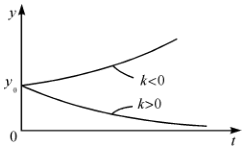
\includegraphics[width=\linewidth]{figs/fig-0001.png}
\caption{图1.1-1}
\end{figure}

平稳状态或平衡状态相应地改变。很自然地就可以想到：描述系统运动状态的微分方程的系数也是这个参数的函数。例如，作用在飞机上的空气动力就是飞机速度的函数，如果飞机的速度由于加速度或减速度而发生改变的话，那么，即使飞机本身的惯性性质保持不变，作用在飞机上的空气动力也还是要改变的。由于这个缘故，如果我们想计算飞机的离开水平飞行路线的扰动运动的话，基本的微分方程就会是一个变系数的方程。

让我们再回到方程(1.1-1)所描述的一阶系统的简单的例子上去。如果弹簧系数 $k$ 是飞机的速度的函数，而且假定飞机有一个不变的加速度 $a$，那么，$k$ 就是速度 $u = at$ 的函数。因此，微分方程就可以写成以下的形式

\[\frac{d y}{d t} + k(a t) y = 0\qquad\text{(1.2-1)}\]

这个方程的解就是

\[\log \frac{y}{y_0} = -\frac{1}{a} \int_0^{a t} k(\xi) d \xi\qquad\text{(1.2-2)}\]

其中 $y_0$ 是初始扰动。如果 $k$ 总是正数，那么，$\log (y / y_0)$ 就总是负数。而且当时间增大的时候，$\log (y / y_0)$ 这个负数的绝对值也就会越来越大。因此，$y$ 就永远小于 $y_0$。而且最后趋于消失。所以系统是稳定的。如果 $k$ 总是负数，$\log (y / y_0)$ 就是一个随着时间增大的正数。即使初始扰动 $y$ 非常微小，$y$ 的数值最后也会变得很大，所以系统就是不稳定的。这样一些系数不改变符号的变系数系统的特性和常系数系统的特性是非常相近的。

然而，有趣味的是 $k$ 既有正值也有负值的情形。我们假定 $k(at)$ 先取正值，然后取负值，最后又再取正值。如果以 $u = at$ 表示 $k$ 的第一个零点，以 $w = at$ 表示第二个零点，那么，按照我们以前的观念来判断其稳定性的问题就变为不可能了。因为在 $u$ 到 $w$ 的范围内系统似乎是“不稳定”的。但是，因为稳定性的概念本身通常是当 $t \rightarrow \infty$ 时系统的渐近性能，而不是某一瞬间的情况所能够完全确定的。因此，对变系数系统的稳定性的分析需要建立另外一些方法。这些方法将在第四章内介绍。

尽管如此，系统式(1.2-2)在这一“危险区间”内的性能对实际工程问题还是有意义的。

设 $y_{\min}$ 是 $y$ 的极小值，$y_{\max}$ 是 $y$ 的极大值。根据方程(1.2-2)就有

\[\log \frac{y_{\min}}{y_0} = -\frac{1}{a} \int_0^{u_1} k(\xi) d \xi\qquad\text{(1.2-3)}\]

和

\[\log \frac{y_{\max}}{y_0} = -\frac{1}{a} \int_0^{u_2} k(\xi) d \xi\qquad\text{(1.2-4)}\]

从工程的观点来看，有兴趣的问题常常是：系统不能正常运转的程度？我们注意到这样一个事实：为了回答以上的问题，除了大？初始扰动但是更重要的情况是：对于固定的初始扰动来说，我们可以用增大加速度法使偏差的极大值事实的实际意义就是：如果尽可能迅速地通过“危险区域”，就可以使不利的效果减少到最低的程度。以上讨论提示我们，对变系数系统应该注意研究控制系统在有限区间内的性能。例如用有限区间上的稳定性的概念去代替对时间趋于无穷大时系统渐近性能的研究。有限时间内系统性能的分析方法也将在以后做一些介绍。另一方面，从工程实际中的物理概念出发，对于一般的变系数线性系统来说，简单地提出这些系统是否稳定的问题往往是没有明确的意义的。更有意义的问题的提法是：在给定的扰动和给定的外界条件之下，对于一个确定的准则 （判断标准） 来说，这个系统的运行状态是否使人满意？在我们的简单的一阶系统的例子里，正常运行的确定的判断准则就是是加速度地改变了。 \{array\}\{ccc\}y\_\{0\} \& y\_\{ \} \& y 0 \& at\_\{1\} \& at\_\{2\} “危险区域”

\begin{figure}[htbp]\centering
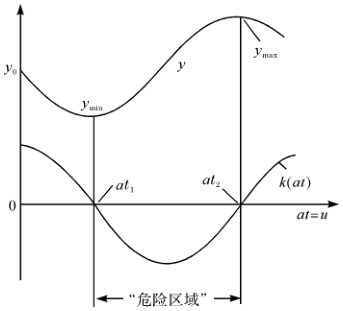
\includegraphics[width=\linewidth]{figs/fig-0002.png}
\caption{图1.2-1}
\end{figure}

为了避免发生误解起见，必须指出：以上的讨论只是为了说明常系数线性系统和变系数线性系统在基本的数学性质上的区别而已，并不是说，在实际的工程问题中对于常系数线性系统只要求它们稳定就够了，如前所述，对于这些系统的其他方面的性能（例如，过渡过程中的状态、可能发生的最大偏差 $y_{\max }$ 等）也还是要加以考虑的。同样的，在实际的工程问题里对变系数线性系统提出的问题也可以是多方面的。

如果在方程(1.1-1)所描述的简单的一阶系统里，弹簧系数 $k$ 是扰动量 $y$ 本身的函数，那么微分方程就成为

\[\frac{dy}{dt} + f(y) = 0\qquad\text{(1.3-1)}\]

其中令 $f(y) = k(y)y$。我们看到这个方程是非线性的。方程(1.3-1)所描述的系统也就是非线性系统的最简单的例子。把方程(1.3-1)积分，就可以用下列的关系式求出方程的解 $y(t)$

\[t = -\int_{\eta_0}^{y} \frac{d\eta}{f(\eta)}\qquad\text{(1.3-2)}\]

这里的 $\eta_0$ 仍然是初始扰动。

另外一方面，把方程(1.3-1)逐次地求导数就得出

\[\frac{d^2y}{dt^2} + \frac{df}{dy}\frac{dy}{dt} = 0\]

\[\frac{d^3y}{dt^3} + \frac{d^2f}{dy^2}\left[\frac{dy}{dt}\right]^2 + \frac{df}{dy}\frac{d^2y}{dt^2} = 0\]

\[\cdots\qquad\text{(1.3-3)}\]

因此，如果 $y_1$ 是函数 $f(y)$ 的零点，并且 $f(y)$ 在 $y_1$ 点是正则的，即 $f(y)$ 对于 $y$ 的所有阶的导数在 $y_1$ 点都是有限值。我们还可以假定 $f(y)$ 在 $y_1$ 点附近可以写成

\[f(y) = (y - y_1)^m\left[c_m + c_{m+1}(y - y_1) + \cdots\right]\]

的形式，其中 $m \geqslant 1$，而且 $c_m \neq 0$。因此，根据方程(1.3-1)和(1.3-3)就得出:

在 $y = y_1$ 处

\[\frac{dy}{dt} = \frac{d^2y}{dt^2} = \frac{d^3y}{dt^3} = \cdots = 0\qquad\text{(1.3-4)}\]

如果初始扰动 $y_0$ 与 $f(y)$ 的某一个零点相重合的话，那么，以后 $y$ 就保持着这个数值，并不随时间变化。因此，$f(y)$ 的各个零点都是平衡位置。如果在某一个零点上 $df/dy > 0$，就像 $y_1$ 点的情形，离开这个平衡位置的微小偏离必定会逐渐消失，因而系统最后还会回到初始状态上去（图1.3-1)。这样，我们就可以说，对于微小扰动而言，在 $y_1$ 点系统是稳定的。可是，如果在某一个零点上 $df/dy < 0$，就像 $y_2$ 点的那种情形，离开这个平衡点的任何一个微小扰动都会使得系统变回到相邻的平衡位置 $y_1$ 或 $y_3$ 上去。因此，$y_2$ 是一个不稳定的平衡状态。

我们已经看到，甚至像方程(1.3-1)所描述的这样一个非常简单的系统，它的运动状态就已经是很复杂的了。在线性系统中如果某一个运动是稳定的，则可断言系统是稳定的，即系统的每一个运动对任何初始扰动都是稳定的。与线性系统

\section{1.3 非线性系统}

相反，非线性系统由于可以同时存在稳定的和不稳定的运动，因此，对非线性系统只能对某一个或某一类具体运动的稳定性进行研究，一般地提出系统是否稳定往往是没有意义的。 像前述弹簧系数的非线性特征一样，控制系统的非线性主要是由受控对象、 执行机构、各种放大器和敏感元件的非线性特征造成的。例如放大器的饱和特性 （图 1.3-2a)，放大器的磁滞曲线（图 1.3-2b)及其继电器特性（图 1.3-2c，d)，机械传动空回特性等都是一些最常见的典型非线性因素。研究包括这类非线性特征的控制系统的运动稳定性问题已不能归结于对线性方程式的研究，而必须谨慎细心地去分析和研究非线性方程式所描绘的某些我们感兴趣的运动。

(a)

(b)

(c)

(d)

图 1.3-2

\begin{figure}[htbp]\centering
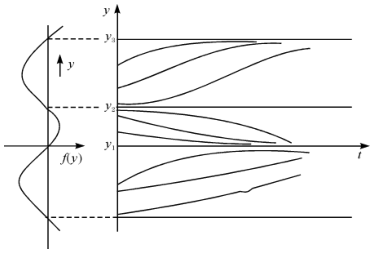
\includegraphics[width=\linewidth]{figs/fig-0003.png}
\caption{图1.3-1}
\end{figure}

\begin{figure}[htbp]\centering
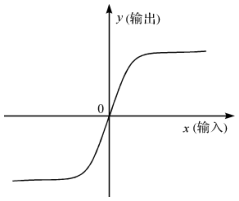
\includegraphics[width=\linewidth]{figs/fig-0004.png}
\end{figure}

\begin{figure}[htbp]\centering
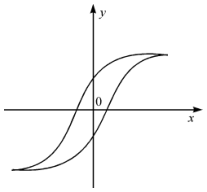
\includegraphics[width=\linewidth]{figs/fig-0005.png}
\end{figure}

\begin{figure}[htbp]\centering
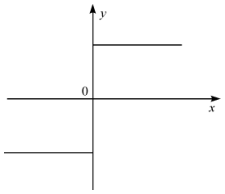
\includegraphics[width=\linewidth]{figs/fig-0006.png}
\caption{图1.3-2}
\end{figure}

\begin{figure}[htbp]\centering
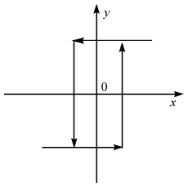
\includegraphics[width=\linewidth]{figs/fig-0007.png}
\caption{图1.3-2}
\end{figure}

\[\cdot 8 \cdot\]

\section{1.4 工程近似问题}

几乎可以肯定地说：只要加以足够精密的分析，任何一个物理系统都是非线性的。我们说某一个实际的物理系统是线性系统，其意思只是说它的某些主要性能可以充分精确地用一个线性系统加以近似地代表而已。并且，所谓“充分精确”的意思就是说：实际系统与理想化了的线性系统的差别，对于具体研究的问题来说已经小到无关紧要的程度。只有当具体的条件和具体的要求明确地给定以后，我们才能把一个实际的系统看作线性系统或是非线性系统。在这个问题上并不存在一般所谓的绝对的判断准则。举例来说，如果我们只想研究一个非线性系统在它的某一个稳定平衡点附近的微小扰动运动的最后状态的话，那么，根据李雅普诺夫(Л япунов)的关于运动稳定性的第一近似的定理，在一定的条件下，原来的系统就可以用一个线性系统很好地近似；但是，如果我们的问题是想研究系统的自激振荡的话，那么，就不能把系统的非线性的性质忽略掉，因为那样一来就会把产生自激振荡的物理根源（和数学根源）丢掉了。

以上所说的处理分类问题的原则，对于把线性系统分为常系数系统和变系数系统两类的情形也是适用的。以方程 $(1.1-1)$ 和 $(1.2-1)$ 所描述的两个简单的系统为例：如果加速度 $\alpha$ 非常小，也就是说飞行的速度几乎不变，由方程 $(1.2-3)$ 就可以看出来 $y_{\min }$ 比初始扰动 $y_{0}$ 小得多，而且这样的 $y_{\min }$ 发生在 $t$ 的数值很大的一个时刻。在一个有限的时间间隔之内，系统式 $(1.2-1)$ 的运动状态和 $k$ 是正值的系统式 $(1.1-1)$ 的运动状态是十分相近的。因此，在一定的场合之下，也可以用常系数系统很准确地近似一个变系数系统。

很明显，常系数系统是最容易研究的。很幸运的是：为数很多的工程系统经过工程近似的手续之后，都可以看作常系数系统。这也就是为什么在控制理论中，关于常系数线性系统这一部分理论特别发达的缘故。

\section{1.5 几个定义}

控制理论主要研究系统状态的运动规律和改变这种运动规律的方法和可能性。前者统称为分析问题，后者则为综合（设计）问题。如果说分析是为了认识系统的运动规律，那么综合的目的便是改造这种运动，使之满足我们的需要。这样，对于控制论来说，分析是基础，综合是目的，而后者又是前者的发展结果，是前者更高的阶段。

如果一组变量 $x_{1}, x_{2}, \cdots, x_{n}$ 能完全代表某一控制系统的状态，而且它们的变化规律 $x_{i}(t), x_{2}(t), \cdots, x_{n}(t)$ 能够单一地确定系统的运动规律，我们将说 $\left(x_{1}, \cdots\right.$，$x_{n})$ 是系统的状态，其中每一个分量 $x_{i}$ 将称之为系统的坐标。例如质点的运动方程式

\[m \frac{d^{2} x}{d t^{2}}=f\qquad\text{(1.5-1)}\]

中的位移变量 $x$ 不能完全代表质点的状态，它和质点的速度一起才能完全表示质点的状态。若写 $x=x_{1}, \frac{d x}{d t}=x_{2}$，则式 (1.5-1)变为

\[\begin{aligned} & \frac{d x_{1}}{d t}=x_{2} \\ & \frac{d x_{2}}{d t}=\frac{1}{m} f \end{aligned}\qquad\text{(1.5-2)}\]

这样，$x_{1}$ 和 $x_{2}$ 是质点 $M$ 的两个坐标，它们二者在一起才构成质点的状态。如果某一系统的运动可用下列方程组来描述

\[\begin{aligned} & \frac{d x_{1}}{d t}=f_{1}\left(x_{1}, x_{2}, \cdots, x_{n}, t\right) \\ & \frac{d x_{2}}{d t}=f_{2}\left(x_{1}, x_{2}, \cdots, x_{n}, t\right) \\ & \cdots \\ & \frac{d x_{n}}{d t}=f_{n}\left(x_{1}, x_{2}, \cdots, x_{n}, t\right) \end{aligned}\qquad\text{(1.5-3)}\]

则 $\left(x_{1}, x_{2}, \cdots, x_{n}\right)$ 完全代表了系统的状态，系统有 $n$ 个坐标。凡是可以由有限个坐标完全描绘其状态的系统，我们将称之为有穷维系统，或称之为集中参数系统。

并不是所有的受控系统均可以用有限个坐标去完全描述出它的状态。例如胡琴上的弦的运动是可以控制的，控制的方法不同，便可以奏出各种优美动听的曲调。弦的运动方程式是

\[\frac{\partial^{2} y}{\partial t^{2}}=a^{2} \frac{\partial^{2} y}{\partial x^{2}}+f(x, t)\qquad\text{(1.5-4)}\]

其中 $a$ 为常数，$y$ 为弦对平衡位置的横向偏移，$f(x, t)$ 为外界控制力。

它的运动是由一个二元 （双变量） 函数 $y(x, t)$ 描述的。如果对每一个固定点 $x=x$ 将函数 $y$ 看成为一个单变量 $t$ 的函数 $y\left(x_{i}, t\right)=y_{i}(t)$，那么这样的函数有无穷多个。因此，我们说系统式 (1.5-4) 是无穷维的。在工程上，根据明显的物理特点，称此类系统为分布参数系统。

从控制的观点来看，系统中的诸量又可分为两类：受控量和控制量。控制的目的是向对人们有利的方向改变系统的运动规律，因此，系统的诸状态坐标都是受控量。用以去改变运动规律的诸量，如式 (1.5-1) 和 (1.5-2) 中的 $f$，式 (1.5-4) 中的 $f(x, t)$，均称为控制量。在一般 $n$ 维系统中控制量常有多个，用 $u, w, \cdots, u$表示。此时方程组 (1.5-3) 可改写为

\[\begin{aligned}& \frac{d x_{1}}{d t}=f_{1}\left(t, x_{1}, x_{2}, \cdots, x_{n} ; u, w, \cdots, u_{r}\right) \\& \frac{d x_{2}}{d t}=f_{2}\left(t, x_{1}, x_{2}, \cdots, x_{n} ; u, w, \cdots, u_{r}\right) \\& \cdots \\& \frac{d x_{n}}{d t}=f_{n}\left(t, x_{1}, x_{2}, \cdots, x_{n} ; u, w, \cdots, u_{r}\right)\end{aligned}\qquad\text{(1.5-5)}\]

式内诸坐标 $x_{1}, x_{2}, \cdots, x_{n}$ 为受控量，$w, \cdots, u_{r}$ 为控制量。我们要注意到，这种分类是很重要的。因为只有对控制量我们才有一定的自由去改变它，例如用改变供油阀门的位置去改变发动机的推力，用改变舵的偏角去改变作用于飞行器上的气动力和力矩，用改变电枢电压去改变电机的转动力矩等。而受控量的变化只能通过控制量的作用按其本来的规律 （微分方程式所确定的规律） 进行。

像在数学物理方程中所看到的那样，有些具有分布参数的受控运动可用佛雷德荷姆 (Fredhoim) 积分方程来描述。如方程式

\[y(x)=\int_{a}^{b} K(x, s) g(y(s), u(s)) d s\qquad\text{(1.5-6)}\]

其中 $y(x)$ 为受控量 （函数），$K(x, s)$ 为已知二元函数 （积分方程的核函数），$g(y, u)$ 为已知二元函数，而 $u(s)$ 为控制量 （函数）。系统的 （无穷维） 坐标的变化规律只能通过控制函数 $u(s)$ 去改变。

如果注意线性自动调节理论中的研究方法，我们可以觉察到，那里无论是系统的坐标或控制量均被默默地认为不受任何限制，即任一变量的取值范围预先不加任何约束，其大小完全由线性方程式本身的特性和初始条件所确定。虽然线性调节理论的丰硕成果对自动控制技术起了并且现在依然起着重要作用，但受控量和控制量不受限制的假定是与实际技术装置的工作情况有一定距离的，这不能不认为是线性理论的重要缺陷。在实际技术问题中，一切受控量和控制量都受到客观条件的某些约束而不能超出一定的范围。对于控制量来说这一事实有着更深刻的意义。例如，作用于飞行器上的力，总有一定的限度，物体的速度和加速度受到机械结构强度和其他条件的限制，控制电压受到电源功率和绝缘强度的限制等。这些客观限制因素有时对控制系统的性能具有决定性的影响，如果在设计系统时不加考虑，计算工作就往往不能反映受控对象的主要特征，或者使定量计算的准确程度受到严重影响。例如，线性调节理论中不考虑限制条件而得到的“过渡过程的时间与阶跃输入作用的大小无关”的结论，在实际上是不完全正确的。

人们很早就发现，若考虑系统的受控量和控制量的限制条件，在控制系统的设计工作中线性理论的分析方法已经不完全适用或根本不能使用，那里应用的广泛和富有成效的许多代数方法在这里均局部或全部丧失了其优越性。这里必须采用其他的研究方法。这些方法将在本书以后的有关章节中详细介绍。

对控制量和受控量的限制条件，在设计工作中有很大不同的意义，前者是首先必须考虑的因素。对控制量的约束条件大致上可做下列分类。设 $u, \cdots, u_{r}$ 为受控系统的 $r$ 个控制量。首先，在控制过程中最常见的是每一个分量的取值范围受到限制，如

\[\left|u_{i}\right| \leqslant M_{i}, \quad i=1,2, \cdots, r\qquad\text{(1.5-7)}\]

$M_{i}$ 为不同的（或相同的）正常数。或者，更为广泛一些，限制条件可以写为

\[g_{i}\left(u, u, \cdots, u_{r}\right) \leqslant M_{i}, \quad i=1,2, \cdots, l\qquad\text{(1.5-8)}\]

此处 $g_{i}$ 为已知的连续函数。

有时在某些系统中，重要的不是控制量的每一瞬时值，而是对控制量的函数形式有特殊的要求。例如，在控制过程中诸控制分量应满足不等式

\[\int_{t_{0}}^{t_{1}} \varphi_{i}(u(\tau), u(\tau), \cdots, u(\tau)) d \tau \leqslant M_{i}, \quad i=1,2, \cdots, m\qquad\text{(1.5-9)}\]

式中 $\varphi_{i}$ 为一组特定的连续函数，$t-t$ 为某一控制过程所费的时间。在各种不同的技术问题中可能有各种不同的限制形式，这里不一一叙述。上述三种限制形式是有代表意义的。限制形式式(1.5-9)的物理意义可能是在整个控制时间内的能量损耗或其他经济损耗等。在本书的有关章节内我们将主要研究上述几类限制条件对控制系统的影响。

\section{1.6 系统运动模型的辨识}

显然，控制系统的理论分析和预先设计，要求我们对受控对象的运动规律有足够的了解，也即是说，要以一定的准确度写出受控对象的运动方程式即运动模型。在数学分析中我们总是假定一个微分方程式的形式为已知，然后去研究它的解的性质和求解办法，似乎方程式本身是早已知道了的东西。其实，在实际问题中完全不是这样。实际工作表明，无论用分析方法或用试验方法去寻找描述受控对象运动规律的方程式都往往是一件不容易的事。它不仅是一个工程实际问题，而且还是一个值得认真研究的理论问题。这就是常被称为模型辨识和参数估值的问题。

当受控对象比较简单而近似于古典数学模型时，如受力的质点或刚体，结构简单的弹性体，理想气体或液体等的运动均可用常微分方程或偏微分方程去描述。当受控对象不能归结于这些简单的数学模型，而这又是常见的情形时，问题要复杂得多。近代复杂受控对象常由各种物理性能完全不同的部分组合而成，其中包含电磁元件，光电器件，以液体或气体为工作体的发动机或传动机构，有时还包括一些逻辑部件等。这样，受控对象的运动就不能再用简单的古典方程式描绘出来。

几乎所有实际设计工作的开始，总是面临着求出受控对象的数学模型的任务。 对于复杂的受控过程，如工厂的生产过程，大范围内的交通运输过程等，辨识和建立模型常常是一件相当困难的事。现在常用的方法大致有下列三种：解析法，实验测试法和统计试验法。

所谓解析法是将一个复杂的受控系统按其结构分解为若干独立的单元或组合，每一单元或组合又分为元件或环节。根据每一环节的物理或过程特点，用分析方法写出其数学模型——运动方程式。最后将这些方程式按系统的结构原理和相互作用的关系联立起来，便得到一个方程组。这个方法的优点是无须使用实验设备，每个方程式都对应一个具体的环节，因而易于用实验办法检验其准确度。但是，这种分析方法只适用于确实易于分解为独立部分的受控对象。并不是一切受控对象都能做如此分解，因为有时分解后的环节与在系统中的该环节有质的差别。当分解成为不可能时，就不得不借助于其他方法。

应用最广泛和结果最为可靠的是实验测试法。一般受控对象的输出量（坐标）与输入量 （控制量）之间有一一对应的关系。为了求出受控对象的运动方程式，在输入端加入控制量 $u(t)$，同时记录输出量的变化规律 $x(t)$。根据这些试验数据，求出一个等效的数学模型。若经过初步分析，系统的输出和输入接近线性关系，则可用线性逼近方法，即用一个线性模型去逼近实际系统。设受控对象为线性系统，它的初始条件为零，那么必存在一个函数 $K(t, \tau)$，使控制量 $u(t)$ 和受控量 $x(t)$ 满足下列伏尔得拉 (Volterra) 积分方程

\[x(t)=\int_{0}^{t} K(t, \tau) u(\tau) d \tau, \quad t \geqslant 0\qquad\text{(1.6-1)}\]

上式中二元函数 $K(t, \tau)$ 为待求函数并常称之为受控系统的脉冲响应函数，而 $u(t), x(t)$ 均为已知函数。欲求解上述积分方程中的核函数，可以令控制量 $u(t)$ 为某些特殊形式的函数，例如当 $u(t)=1,0 \leqslant t<\infty$ 时，式 (1.6-1)变为

\[x(t)=\int_{0}^{t} K(t, t) d t\]

或者，设 $u(t)$ 为下列“脉冲函数”

u(t)=\textbackslash\{\}arrayl1/k,  t  t  t+k \textbackslash\{\}\textbackslash\{\}0,  t当 \textbackslash\{\}(k  0\textbackslash\{\}) 时显然有x(t) \textbackslash\{\}stackrel\{(1.6-2)\}\{=\} K(t，t)式中 $t$ 为脉冲瞬间。当然，积分方程 (1.6-1) 也可用其他办法求解。以后我们将可以看到，当函数 $K(t, \tau)$ 求出后，系统的数学模型就可以建立起来。另一个实验方法是基于常系数线性系统的一个特性：若在输入端加一个正弦形式的驱动作用，经过一段时间后，输出坐标将为具有同样频率的正弦函数，不同的只是幅度和相位。令 $u(t)=\sin \omega t$，输出为

\[x(t)=A(\omega) \sin (\omega t+\varphi(\omega))\qquad\text{(1.6-3)}\]

式中 $A(\omega)$ 与 $\varphi(\omega)$ 之值随输入作用的频率不同而不同，称为幅频与相频特性。利用这两个函数构成另一个复值函数

\[W(i \omega)=A(\omega) e^{i \varphi(\omega)}\qquad\text{(1.6-4)}\]

再用有理分式逼近它

\[W(i \omega) \circ \frac{b_{1}(i \omega)^{m}+b_{2}(i \omega)^{m-1} \cdots+b_{m}}{a_{0}(i \omega)^{n}+a_{1}(i \omega)^{n-1}+\cdots+a_{n}}\]

从常微分方程理论中我们知道，根据式 (1.6-5) 就可以建立一个受控对象的数学模型。从上式看，为了求出受控对象的线性逼近方程式似乎必须测出 $A(\omega)$ 和 $\varphi(\omega)$ 两个函数。实际上，在一定条件下只测出其中的一个就够了。当复值函数 $W(i \omega)$ 在复数 $\omega$ 的下半平面及实轴上没有零点和极点时，幅频特性 $A(\omega)$ 和相频特性 $\varphi(\omega)$ 按下列关系相互单值对应

\[\ln A(\omega)=-\frac{1}{\pi} \int_{-\infty}^{+\infty} \frac{\varphi(u)}{u-\omega} d u\qquad\text{(1.6-6)}\]

和

\[\varphi(\omega)=\frac{1}{\pi} \int_{-\infty}^{\infty} \frac{\ln A(u)}{u-\omega} d u\qquad\text{(1.6-7)}\]

由此可知，在通常的情况下，只需测出两个函数中的一个就够了，另一个可按上列公式之一用分析方法求出。

在很多工程技术问题中，受控对象的输入端的控制量不是确定性的，而是一个已知其统计特性的随机过程。这时，根据平稳过程的统计特性通过受控对象后所发生的变化可以求出受控对象的近似运动方程式。甚至在输入量可以任意变化时也可以采用这种试验方法。

设待求运动方程式的受控对象的输入端加进高斯 (Gauss) 平稳随机过程的一个现实 $u(t)=\xi(t)$，其自相关函数为 $R_{\xi \xi}(\tau)$，而对任意 $t$ 数学期望 $\xi(t)=0$。当该现实通过受控对象后，其输出 $x(t)$ 对于常系数线性模型也是一个平稳过程的现实，它的某些统计特性可以用实验方法求出。例如用相关仪可以求出输入的自相关函数 $R_{\xi \xi}(\tau)$ 和输入输出的互相关函数 $R_{\xi \tau}(\tau)$。这种相关仪的作用原理是以各态历经定理为依据完成下列运算

\[R_{\xi \xi}(\tau) \triangleq \frac{1}{2} \int_{-T}^{T} x(t) x(t-\tau) d t\qquad\text{(1.6-9)}\]

和

\[R_{\xi \tau}(\tau) \triangleq \frac{1}{2} \int_{-T}^{T} \xi(t) x(t-\tau) d t\qquad\text{(1.6-8)}\]

当 $\tau$ 值固定而积分限 $T$ 足够大时，上式右端 （随机量 $\mathrm{D}$ 均方收敛于非随机量 $R(\tau)$。

如果上述各相关函数均已测出，那么便可以用最佳逼近的方法求出一个线性数学模型，使之尽可能地与试验结果相吻合。用响应函数，并要求它满足下列条件 S=[x(t)-\_\{0\}\textasciicircum{}\{\} K\_\{0\}(t) (t-) d ]\textasciicircum{}\{2\}=

上式内文字上的横道表示对随机变量求数学期望。从第十五章可以看到 $K_{0}(t)$ 应满足下列佛雷德荷姆积分方程

\[R_{\mathrm{ss}}(\tau)=\int_{0}^{\infty} R_{\mathrm{ss}}(\tau-\lambda) K_{0}(\lambda) d \lambda\]

这个积分方程中的待求函数 $K_{0}(t)$ 可以用解析方法或用数值计算方法解出，然后再用拉氏变换和有理分式逼近求出线性模型的方程式。或者按照第十四章、第十五章中所讲的其他方法求出线性模型的方程式。

上面所介绍的只是求线性模型的几种方法，还有非线性模型、分布参数模型等。所谓系统辨识和参数估计就是研究这个问题的 ${ }^{[9]}$。在这里做一简短的介绍是为了提醒大家注意这个常常不被人们重视，但却有重要实际和理论意义的问题。

\section{1.7 控制系统的质量指标}

评价一个控制系的好坏，其指标是多种多样的。有经济指标，动态指标，稳态指标，强度指标和抗干扰能力等。每一个具体系统有它自己的主要指标，如不能得到满足，则系统不能良好地工作。并不是每一个指标都能用解析方法去获得答案。例如经济指标与原料来源，工艺水平，外协作的成本等有关，而且随着工业的不断发展，这些指标也将不断变化。评价某一系统的经济性如何是要靠统计来解决的，而与系统的运动规律往往无十分直接的联系。本书内将要研究的质量指标主要是与控制系统运动规律直接有关的那一部分，即由系统的稳态和动态性能所决定的那些质量指标。概括地说，我们将要研究的有下列几点:

(1) 系统的稳定性：包括系统在 $t \rightarrow \infty$ 时的渐近性能和有限时间内的稳定性问题。稳定性之重要是大家所熟知的。一个系统如果不稳定，它的行为便不受约束，受控量将忽左忽右摇摆不定，或者使运动发散，不能保持原定的工作状态不变。这种系统是不能完成控制任务的。

(2) 系统的稳态精度：对很多高精度控制系统，如火箭控制系统，各种随动系统，工业生产中的仿型和数控机床等均要求有高的稳态精度。这种稳态精度部分地取决于测量元件 （敏感元件） 本身的测量精度，又取决于控制系统的某些动态参数，即运动方程式内所包括的参数值的大小和控制规律的选择。

(3) 过渡过程的时间：这是一个典型的动态性能质量指标，在既定的工作条件下它完全取决于设计艺术，即取决于如何正确地选择控制规律，也即控制量 $u(t)$，$i=1,2, \cdots, r$ 的变化规律。

(4) 过渡过程的超调量：这也是完全取决于系统动态性能的指标之一。设主受控量 $x(t)$ 的最终平衡状态为 $x_{1}, x_{1}>0$，由初始条件和控制规律所决定的坐标 $x$ 的运动规律为 $x(t), x(t)=x_{1}, 0<t<\infty$，则超调量 $\sigma$ 可定义为

\[\sigma=\frac{\max _{t arrow_{0}}|x(t)|-x_{1}}{x_{1}}\qquad\text{(1.7-1)}\]

式中 $b$ 可根据具体问题的需要去选择。

(5) 一般积分泛函指标：更为一般的动态质量指标可用某一积分泛函表示。设受控对象的坐标为 $x_{1}, x_{2}, \cdots, x_{n}$; 控制量为 $u, w, \cdots, u_{r}$。一般性的质量指标可定义为

\[J=\int_{t_{0}}^{t_{1}} f_{0}\left(x_{1}, x_{2}, \cdots, x_{n} ; u, w, \cdots, u_{r} ; t\right) d t\qquad\text{(1.7-2)}\]

式中 $b$ 为系统的初始运动时刻，$b$ 为受控量达到某一最终状态的时刻，$b-b$ 为过渡时间，函数 $f_{0}$ 为某一给定的 $n+r+1$ 元函数，它的具体形式由工程实际问题的要求来确定。例如 $f_{0}$ 可能是一个正定二次型

\[J=\int_{t_{0}}^{t_{1}}\left[\sum_{i=1}^{n} a_{i j} x_{i} x_{j}+\sum_{i, j}^{r} b_{n \beta} u_{i} u_{\beta}\right] d t\qquad\text{(1.7-3)}\]

其中 $a_{i j}$ 和 $b_{n \beta}$ 可能是已知的时间 $t$ 的函数，也可能为常数。当 $f_{0} \equiv 1$ 时，由式 (1.7-2)我们便得到第(3)条的过渡过程时间指标。事实上

\[J=\int_{t_{0}}^{t_{1}} 1 d t=t-t_{0}\qquad\text{(1.7-4)}\]

应该指出，第(1)条的稳定性指标也可常化成式 (1.7-2) 的形式。而第 (4) 条指标则不可能化为这一积分泛函形式。

常遇到的还有一种形式

\[J=\int_{t_{0}}^{t_{1}}\left|\sum_{i=1}^{n} a_{i} x_{i}\right| d t\qquad\text{(1.7-5)}\]

也属于式 (1.7-2) 的范围。

(6) 抗扰性指标：控制系统在工作过程中受外界干扰作用是普遍存在着的现象。如飞行器受风或其他原因的气流影响，火箭制导系统受内外无线电噪声的扰动等。一个良好的控制系统对外界干扰应该具有足够的抵抗能力，而对有用的信号则迅速而准确地动作。抗干扰性能好坏是评价控制系统动态和静态品质的一个重要方面。在设计系统时必须对此采取措施。如何设计一个具有良好抗干扰性能的系统也是我们此书讨论的内容之一。

上述各种质量指标我们都将在此书内做详细程度不同的研究。我们将可以看到，它们有时是相互矛盾的。设计一个系统满足全部上述指标几乎是不可能的。以后我们将采取分别研究，个别评价的办法去讨论。至于如何对这些指标抓住重点而综合平衡，那就完全依赖于能否深入到实际中去认真做调查研究，抓住主要矛盾和矛盾的主要方面，从实际情况出发，作出判断，其他是没有出路的，也不可能存在什么统一的放之四海而皆准的处理办法。

这就是我们以后将讨论的问题的一个大致轮廓。当然，还有一些另外类型的问题，虽然在第一章内没有提到，由于它们的重要性，我们以后也将做不同程度的介绍和讨论。

\section{参考文献}

[1] 刘仙洲，中国机械工程发明史，第一编，科学出版社，1962.

[2] 万百五，我国古代自动装置的原理分析及其成就探讨，自动化学报，1962.2.

[3] 刘豹，自动调节理论基础，上海科学技术出版社，1963.

[4] 华罗庚，高等数学引论，科学出版社，1963.

[5] 吴新谋，偏微分方程讲义，科学出版社，1959.

[6] 关肇直，高等数学教程，高等教育出版社，1959.

[7] 谷超豪等，数学物理方程，上海科学技术出版社，1961.

[8] 金福临等，常微分方程，上海科学技术出版社，1962.

[9] Eykhoff，P.，System Identification，Wiley，1974.

[10] Fautre，P. \& Depeyrot，M.，Elements of System Theory，North-Holland，1977.

[11] Greensite，A. L.，Elements of Modern Control Theory. I. II.，New York，1970.

[12] Hsu，J. C. \& Mayer，A. V.，Modern Control Principle and Application，McGraw-Hill，New York，1968.

[13] Newton，G. C. \& Gould，L. A.，Kaiser，J. F.，Analytical Design of Linear Feedback Control，Wiley \& Sons，1957.

[14] Truxal，J. G.，Automatic Feedback Control System Synthesis，McGraw-Hill，New York，1955.

[15] Wiener，N.，Cybernetics or Control and Communication in the Animal and the Machine，New York，1949. [控制论（或关于在动物和机器中控制和通信的科学），郝季仁译，科学出版社，1961.]

[16] Солодовников，В. В. и Другие，Основы Автоматического регулирования，Машгиз，Москва，1954. （自动调整原理，王众托译，水利电力出版社，1958.)

[17] Фельдбаум，А. А.，Электрические системы автоматического регулирования，Оборониз，1959. （电的自动调节系统，章燕申、金兰译，国防工业出版社，1958.)

\chapter{第二章 系统分析的基本方法}

随着自动控制理论和实践的发展，研究方法和使用的工具都在不断地改进和增加。如果说在二十世纪四十年代控制理论的研究和实际设计工作中的主要方法是多项式代数和拉氏变换为基础的传递函数方法，那么现在已远远超出了这个范围。当然，对于那些以时间t为自变数的常系数微分方程来说，拉普拉斯变换方法仍是十分有用的。因为这个方法能够把所有的线性常系数系统问题归结到一个一致的代数基础上去。这样一来，求解的手续就被简化了。但是，随着研究工作的深入，人们逐渐发现这类简单的代数方法也有它的弱点，简化与深化常有相互矛盾的一面。为了对控制过程了解得更深刻，在现代控制理论中，使用和建立了新的工具以及新的概念，这些工具主要是多维空间（欧氏空间和希尔伯特空间）中的运算和算子理论。引入控制系统状态向量空间（相空间）后，控制过程的几何特性将十分清晰。近些年来在控制理论研究工作中，得到的一些新成就大部分是与相空间的概念分不开的。为了系统地介绍这些进展，我们在以后将既保留线性理论的主要方法，同时也要介绍新的概念。这一章的目的是为以后各章的讨论做必要的准备，有关这些内容的更详细的叙述和证明，读者可以在相应的专门文献中找到。

\section{2.1 拉氏变换和反转公式}

如果 $y(t)$ 是一个时间变数 $t$ 的函数，它的定义域是 $t>0$，那么 $y(t)$ 的拉普拉斯(Laplace)变换 $Y(s)$ 的定义就是

\[Y(s)=\int_{0}^{\infty} e^{-s t} y(t) d t\qquad\text{(2.1-1)}\]

这里的 $s$ 是一个具有正实数部分的复变数，$\operatorname{Re} s>0(\operatorname{Re} s$ 表示 $s$ 的实数部分）。对于其他的 $s$ 值，我们用解析开拓的方法来定义函数 $Y(s)$。 $Y(s)$ 的量纲是 $y$ 的量纲和时间的量纲的乘积。 $s$ 的量纲是时间量纲的负一次方幂。 $y(t)$ 称为原函数，$Y(s)$ 称为象函数。

如果 $Y(s)$ 是已知的，那么，拉氏变换 $Y(s)$ 的原函数（也就是原来的函数） $y(t)$总是可以由下面的反转公式计算出来

\[y(t)=\frac{1}{2 \pi i} \int_{r-i \infty}^{r+i \infty} e^{s t} Y(s) d s\qquad\text{(2.1-2)}\]

其中 $r$ 是任意的一个实数，只要它比所有的 $Y(s)$ 的奇点的实数部分都大就可以了。在实际计算 $y(t)$ 时，我们可以按照 $Y(s)$ 的特点适当地变化积分的路线。从 $Y(s)$ 求 $y(t)$ 的步骤称为拉氏反变换。

根据定义 (2.1-1) 和 (2.1-2) 不难推出拉氏变换的几个基本特性:

(1) 拉氏变换是线性变换：两个函数 $y_1(t)$ 及 $y_2(t)$ 之和的变换等于二者单独变换后之和

\[\begin{aligned}& \int_{0}^{\infty} e^{-st} [a y_1(t) + b y_2(t)] dt = a Y_1(s) + b Y_2(s) \\& a y_1(t) + b y_2(t) = \frac{1}{2 \pi i} \int_{r - i \infty}^{r + i \infty} e^{st} [a Y_1(s) + b Y_2(s)] ds\end{aligned}\]

其中 $a, b$ 是任意的常数。

(2) 推移公式：对原函数 $y(t)$ 的自变数推移时间 $\tau$，则对应的象函数乘以 $e^{-\tau t}$。因为

\[\int_{0}^{\infty} e^{-st} y(t - \tau) dt = \int_{0}^{\infty} e^{-s(\lambda + \tau)} y(\lambda) d\lambda = e^{-\tau t} Y(s)\]

式中 $\tau \geqslant 0, \lambda = t - \tau$; 当 $t < 0$ 时令 $y(t) = 0$。

(3) 若 $y(0) = 0$，则 $\frac{dy}{dt}$ 的象函数为 $s Y(s)$。

(4) 函数 $\psi(t) = \int_{0}^{t} y(\tau) d\tau$ 的象函数为 $Y(s) / s$。

(5) 两个函数卷积的象函数对应两个象函数的积

\[\int_{0}^{\infty} \left[ \int_{0}^{t} k(t - \tau) y(\tau) d\tau \right] e^{-st} dt = K(s) Y(s)\]

这一点是容易检验的。

(6) 两个原函数乘积的象函数等于两个象函数的卷积。

令 $y(t) = y_1(t) y_2(t)$，则

\[Y(s) = \int_{0}^{\infty} e^{-st} y_1(t) y_2(t) dt = \frac{1}{2 \pi i} \int_{r - i \infty}^{r + i \infty} Y_1(s) Y_2(s - s_1) ds_1\]

这说明拉氏变换对乘法没有分配律，初学者往往容易弄错。其证明我们留给读者。

(7) 如果 $y(t)$ 在 $t \to 0$ 时趋于某一极限，则有 $\lim_{t \to 0} y(t) = \lim_{s \to \infty} Y(s)$。

(8) 终值公式: $\lim_{t \to \infty} y(t) = \lim_{s \to 0} Y(s)$。

当我们用拉氏变换法处理问题时，常常需要根据已知的拉氏变换函数 $Y(s)$ 求出原函数 $y(t)$。我们当然可以利用反转公式进行这项工作，可是反转公式 (2.1-2) 中的积分运算常常是很烦琐的，而且很花费时间。因此，对于那些常用和典型的 $y(t)$ 和 $Y(s)$，人们已经编制了一些字典式的表格 [29]。利用这种变换表我们就可以根据已知的 $Y(s)$ 查出相应的 $y(t)$，也可以从已知的 $y(t)$ 查出相应的 $Y(s)$，这样就大大地减轻了计算手续。下面我们也给出一个最简略的拉氏变换的

“字典”——一个很小的拉氏变换表:

表 2.1-1 拉氏变换的小“字典”$Y(s)$ $y(t)$

1/s\$ 1
\$1s\textasciicircum{}n\$ \$t\textasciicircum{}n-1(n)\$
\$1/(s-a)\$ \$e\textasciicircum{}at\$
\$a(s\textasciicircum{}2+a\textasciicircum{}2)\$ \$ at\$
\$s(s\textasciicircum{}2+a\textasciicircum{}2)\$ \$ at\$
\$a(s\textasciicircum{}2-a\textasciicircum{}2)\$ \$ at\$
\$s(s\textasciicircum{}2-a\textasciicircum{}2)\$ \$ at\$
\$s(s\textasciicircum{}2+a\textasciicircum{}2)\textasciicircum{}2\$ \$t/2a  at\$
\$1(s\textasciicircum{}2+a\textasciicircum{}2)\textasciicircum{}2\$ \$12a\textasciicircum{}3( at - at  at)\$
\$1(s+a)\textasciicircum{}2\$ \$te\textasciicircum{}-at\$
\$s(s+a)\textasciicircum{}2\$ \$(1-at)e\textasciicircum{}-at\$
\$(s-a)\textasciicircum{}2s(s+a)\textasciicircum{}2\$ \$1-4ate\textasciicircum{}-at\$
\$1/(s+a)(s+b)\$ \$(e\textasciicircum{}-bt-e\textasciicircum{}-at)(a-b)\$
\$(s+a)/s(s+b)(s+c)\$ \$a/bc + (a-b)/a(b-c)e\textasciicircum{}-bt + (a-c)/c(c-b)e\textasciicircum{}-ct\$
\$s[(s+a)\textasciicircum{}2+b\textasciicircum{}2]\$ \$ bt - a/b bt)e\textasciicircum{}-at\$
\$(s+a)\$ \$e\textasciicircum{}-at bt\$
\$(s+a)[(s+a)\textasciicircum{}2+b\textasciicircum{}2]\$ \$e\textasciicircum{}-at bt\$
\$(s+a)\$ \$e\textasciicircum{}-at bt\$
\$1(s+a)\textasciicircum{}3\$ \$t\textasciicircum{}2e\textasciicircum{}-at2\$
\$s(s+a)\textasciicircum{}3\$ \$t(1-1/2at)e\textasciicircum{}-at\$
\$(s+a)\$
\$1s\textasciicircum{}2(s+a)(s+b)\$ \$-aa\textasciicircum{}2(b-a)e\textasciicircum{}-at + -bb\textasciicircum{}2(a-b)e\textasciicircum{}-bt + /abt + ab-(a+b)a\textasciicircum{}2b\textasciicircum{}2

续表$Y(s)$ $y(t)$

$\frac{s^{2}+\alpha s+\beta}{s^{2}(s+a)(s+b)}$ $\frac{a^{2}-\alpha a+\beta}{a^{2}(b-a)} e^{-at}+\frac{b^{2}-ab+\beta}{b^{2}(a-b)} e^{-bt}+\frac{\beta t+\alpha ab-\beta(a+b)}{ab}+\frac{\alpha ab-\beta(a+b)}{a^{2}b^{2}}$$\frac{s+\alpha}{(s+a)(s+b)^{2}}$ $\frac{\alpha-a}{(b-a)^{2}} e^{-at}+\left[\frac{\alpha-b}{a-b} t+\frac{a-\alpha}{(a-b)^{2}}\right] e^{-bt}$$\frac{1}{(s+a)(s+b)(s+c)}$ $\frac{(c-b)}{(a-b)} e^{-at}+\frac{(a-c)}{(a-b)} e^{-bt}+\frac{(b-a)}{(a-b)} e^{-ct}$$\frac{1}{s^{2}\left(s^{2}+a^{2}\right)}$ $\frac{t}{a^{2}} \frac{\sin at}{a^{3}}$$\frac{1}{s^{2}\left(s^{2}-a^{2}\right)}$ $\frac{\sin at}{a^{3}}-\frac{t}{a^{2}}$$\frac{s}{s^{4}+a^{4}}$ $\frac{1}{a^{2}} \operatorname{sh} \frac{at}{2} \cdot \sin \frac{at}{2}$$\frac{s^{2}-2 a^{2}}{s^{4}+4 a^{4}}$ $\frac{1}{a} \operatorname{sh} at \cdot \cos at$$\frac{s^{2}-a^{2}}{\left(s^{2}+a^{2}\right)^{2}}$ $t \cos at$$\frac{1}{s}$ $\frac{1}{\pi t}$$\frac{1}{s \cdot s}$ 2$\frac{1}{\sqrt{s^{2}+as+b}}$ $e^{-a / 2 t} J_{0}\left(\sqrt{\frac{b}{4}} a^{2} t\right)$ ( $J_{0}$——零阶贝尔函数）$\frac{1}{s+\sqrt{s^{2}+a^{2}}}$ $\frac{1}{at} J_{1}(at)\left(J_{1} \longrightarrow \text { 一阶贝尔函数 }\right)$2.2 用拉氏变换法解常系数线性微分方程

既然拉氏变换是对一个函数作的积分运算来定义的，而这个函数又是只在 $t>0$ 的时间内定义的，所以拉氏变换法对于初值问题特别适用。所谓“初值问题”就是这样一个问题：如果系统的初始状态（也就是 $t=0$ 时的状态）和 $t>0$ 时的驱动函数都是给定的，求在 $t>0$ 的时间间隔内系统的运动情况。我们来考虑一个 $n$ 阶的系统，假定 $a_{n}, a_{n-1}, \cdots, a_{0}$ 是各阶导数的系数，而且对于这个系统有一个非齐次项所表示的驱动函数 $x(t)$。于是，系统的微分方程就是

\[a_{n} \frac{d^{n} y}{d t^{n}}+a_{n-1} \frac{d^{n-1} y}{d t^{n-1}}+\cdots+a_{0} y=x(t)\qquad\text{(2.2-1)}\]

各个初始条件通常写作

\[\left.\frac{d^{n-1} y}{d t^{n-1}}\right|_{t=0}=y^{(n-1)}\]

\section{2.2 用拉氏变换法解常系数线性微分方程}

\[\left.\left(y\right)_{t=0}=y_{0}\right)\qquad\text{(2.2-2)}\]

在式(2.2-2)的条件下，微分方程(2.2-1)就能够把系统在 $t \geqslant 0$ 时的运动状态唯一地确定下来。

为了用拉氏变换法解这个问题，我们把方程(2.2-1)的两端，同时乘以 $e^{-s t}$，然后再从 $t=0$ 到 $t=\infty$ 积分。既然规定

\[\int_{0}^{\infty} e^{-s t} y(t) d t=Y(s)\]

我们就可以用分部积分的方法求出 $y(t)$ 的各阶导数的拉氏变换

\[\begin{aligned} & \int_{0}^{\infty} e^{-s t} \frac{d y}{d t} d t=-y_{0}+\int_{0}^{\infty} e^{-s t} y(t) d t=-y_{0}+s Y(s) \\ & \int_{0}^{\infty} e^{-s t} \frac{d^{2} y}{d t^{2}} d t=-y_{0}^{(1)}-s y_{0}+s^{2} Y(s) \\ & \cdots \\ & \int_{0}^{\infty} e^{-s t} \frac{d^{n} y}{d t^{n}} d t=-y_{0}^{(n-1)}-s y_{0}^{(n-2)}-\cdots-s^{n-1} y_{0}+s^{n} Y(s) \end{aligned}\qquad\text{(2.2-3)}\]

根据这些结果，如果再把驱动函数 $x(t)$ 的拉氏变换写成 $X(s)$，也就是说

\[X(s)=\int_{0}^{\infty} e^{-s t} x(t) d t\qquad\text{(2.2-4)}\]

那么，考虑到初始条件式(2.2-2)，方程(2.2-1)就可以写成

\[\begin{aligned} & \left(a_{n} s^{n}+a_{n-1} s^{n-1}+\cdots+a_{1} s+a_{0}\right) Y(s) \\ = & a_{n} y_{0} s^{n-1}+\left(a_{n} y_{0}^{(1)}+a_{n-1} y_{0}\right) s^{n-2}+\left(a_{n} y_{0}^{(2)}+a_{n-1}\right. \\ & \left.+a_{n-2} y_{0}\right) s^{n-3}+\cdots+\left(a_{n} y_{0}^{(n-1)}+a_{n-1}\right) y_{0}^{(n-2)} \\ & \quad+\cdots+a_{1} y_{0}+X(s) \end{aligned}\]

如果我们再规定 $D(s)$ 和 $N_{0}(s)$ 分别是下列的两个多项式

\[D(s)=a_{n} s^{n}+a_{n-1} s^{n-1}+\cdots+a_{1} s+a_{0}\qquad\text{(2.2-6)}\]

和

\[\begin{aligned} N_{0}(s)= & a_{n} y_{0} s^{n-1}+\left(a_{n} y_{0}^{(1)}+a_{n-1} y_{0}\right) s^{n-2}+\cdots \\ & +\left(a_{n} y_{0}^{(n-1)}+a_{n-1} y_{0}^{(n-2)}+\cdots+a_{1} y_{0}\right) \end{aligned}\]

于是方程(2.2-5)又可以写作

\[Y(s)=\frac{N_{0}(s)}{D(s)}+\frac{X(s)}{D(s)}\qquad\text{(2.2-8)}\]

根据方程(2.2-7)，我们看到式(2.2-8)的第一项 $N_{0}(s) / D(s)$ 是与初始条件有关的。我们把这一项写作 $Y_{c}(s)=N_{0}(s) / D(s)$。多项式 $N_{0}(s)$ 的次数最多也不会超过 $n-1$ 次，因而它的次数总比 $D(s)$ 的次数低。如果方程(2.2-2)所表示的初始条件全都等于零，$N_{0}(s)$ 也就随之等于零了。在这种情形下，$Y(s)$ 就只由第二项

x(s)/D(s)确定。第二项是与驱动函数有关的。我们把这一项写作Y(s)=X(s)/D(s)。第一项N0(s)/D(s)称为补充函数，第二项X(s)/D(s)称为特解。应用反转公式(2.1-2)，就可以由方程(2.2-8)所表示的Y(s)=Yc(s)+Y1(s)得出真正的解y(t)。

从以上的讨论，我们可以看出，拉氏变换本身只是一个“翻译”的手续，它把一个用时间变数t所描述的物理过程翻译成用变数s所描述的过程，这样的手续并不影响物理过程本身的性质，只不过是把这个过程的描述从“t的语言”翻译成“s的语言”而已。在t的语言里用分析运算（微分和积分）所描述的过程，用s的语言来叙述就只要用简单的代数运算（乘或除）就可以了;t的语言中的微分方程，用s的语言来表示就简化为代数方程，从而也就可以简化计算的手续和表达的方式。

从数学观点来看，拉氏变换是一个线性算子，它定出两族函数（原函数和象函数）之间的对应关系。这是对普通函数概念的一种推广。因为“函数”只不过是二族数之间的对应规律罢了。关于算子的概念我们下面还要详细介绍。在这里可能提出一个有意思的问题：是否一切以时间作为自变量的函数y(t)都能找到自己的象函数？是否所有的复变函数Y(s)都是某一个y(t)的象函数？对这一问题的回答是否定的。具体地说，如果不要求包括一切所谓“冲量函数”即狄拉克(Dirac)函数（参看下节）的话，这一条线可以这样划：一切增长速度不大于en(N为任意有限正实数）的函数y(t)均有自己的象函数。而函数y(t)=et就没有象函数，因为此时积分(2.1-1)不收敛，故拉氏变换没有意义。反之，并不是一切复变函数都能按式(2.1-2)找到自己的原函数。如果想包括“冲量函数”在内时，则有如下事实：设复变函数X(s)在Re s>σ的半平面内是解析函数，那么，它为象函数的充条件是在这一半平面内｜X（s）｜≤｜Pn（s）｜，这里的Pn（s）为s的n阶多项式]。

有人将拉氏变换方法推广到变系数线性系统。特别是近几年来，由于对变系数系统的研究变得十分迫切，已有很多人从事这方面的研究。但是这些方法目前还比较复杂，而且大部分结果的可用范围尚有待于扩大，需做大量工作后，才有可能将这些方法加工到工程上可以简便应用的地步。

\section{2.3 关于正弦式驱动函数的讨论}

多项式的比值N0(s)/D(s)可以分解成部分分式。如果多项式D(s)的n个根s1，s2，⋯，sn都是互不相等的，换句话说，D(s)没有重根，那么这个部分分式就是

\[\frac{N_{0}(s)}{D(s)}=\sum_{s=1}^{n} \frac{N_{0}\left(s_{s}\right)}{D\left(s_{s}\right)} \frac{1}{\left(s-s_{s}\right)}\qquad\text{(2.3-1)}\]

其中的D(s)表示D(s)对于s的导数。根据上一节里的“字典”，把这个和数逐项地“翻译”出来，就得到 $y(t)$ 解中由于初始条件而产生的 $y_{c}(t)$ 部分 （这一部分称为 “补充函数”，它也就是方程 (2.2-1) 在 $x(t)=0$ 而初始条件仍然是式 (2.2-2) 的解）

\[y_{c}(t)=\sum_{r=1}^{n} \frac{N_{0}\left(s_{r}\right)}{D\left(s_{r}\right)} e^{s_{r} t}\qquad\text{(2.3-2)}\]

一般说来，$D(s)$ 的根 $s_{r}$ 是复数。对于实际的物理系统来说，微分方程 (2.2-1) 的系数 $\omega, \alpha, \alpha, \cdots, \alpha_{n}$ 都是实数。根据方程 (2.2-6)，$D(s)$ 的各个复数根 $s_{r}$ 必然是成复共轭对出现的。这也就是说，如果 $D(s)$ 有一个复数根是 $\alpha+i \beta(\beta \neq 0)$ 的话；那么 $\alpha-i \beta$ 也必然是 $D(s)$ 的根。如果所有的根 $s_{r}$ 的实数部分都是负数，那么 $y_{c}(t)$ 就会随着时间的增加按照指数律减小，最后 $y_{c}(t) \rightarrow 0$。因此，系统就是稳定的。

如果表示外力的驱动函数 $x(t)$ 是正弦式的，为了计算的方便，我们就把它写成下列的复数形式 （真正的外力只是这个表示式的实数部分或者虚数部分）

\[x(t)=x_{m} e^{i \omega t}\qquad\text{(2.3-3)}\]

其中的 $x_{m}$ 是振幅，$\omega$ 是频率 （角频率）。根据拉氏变换的“字典”，就有

\[X(s)=x_{m} \frac{1}{s-i \omega}\]

因此，方程 (2.2-8) 的第二项在现在的情形下就是

\[Y_{i}(s)=\frac{x_{m}}{(s-i \omega) D(s)}\]

在这里，我们可以把得到的结果推广到更一般的情形中去。如果所考虑的系统不是只由一个微分方程所描述 （像以前讨论过的那样），而是用一个微分方程组所描述的。举例来说，描述系统状态的是这样一个方程组

\[\begin{aligned} & \alpha_{12} \frac{d^{2} y}{d t^{2}}+\alpha_{11} \frac{d y}{d t}+\alpha_{10} y+b_{12} \frac{d^{2} z}{d t^{2}}+b_{11} \frac{d z}{d t}+b_{10} z=x(t) \\ & \alpha_{22} \frac{d^{2} y}{d t^{2}}+\alpha_{21} \frac{d y}{d t}+\alpha_{20} y+b_{22} \frac{d^{2} z}{d t^{2}}+b_{21} \frac{d z}{d t}+b_{20} z=0 \end{aligned}\]

其中的系数 $a_{i}, b_{i}$ 都是常数。

让 $y$ 的初始条件全都等于零 （这样做的意义就是把 $y$ 用 $y_{i}$ 来代替），对系统的微分方程组进行拉氏变换，就得到一个代数方程组，然后再用代数方法把除 $Y_{i}(s)$以外的其余未知函数 （例如，上面例子里的 $Z(s)$ ) 消去，最后特解 $Y_{i}(s)$ 的拉氏变换就可以表示为下列的形状

\[Y_{i}(s)=F(s) X(s)=\frac{N(s)}{D(s)} X(s)=\frac{x_{m} N(s)}{(s-i \omega) D(s)}\qquad\text{(2.3-4)}\]

其中 $N(s)$ 的次数小于 $D(s)$ 的次数。当 $N(s)=1$ 时，问题就简化为式 (2.2-8) 所表示的比较简单的情形。在推广了的情况下，部分分式的法则式 (2.3-1) 仍旧是适用的。但是，现在的分母多项式是 $(s-i \omega) D(s)$，这个多项式的根是 $s, s, \cdots, s_{n}$ 和 $i \omega$。因而就有

\[\begin{gathered} Y_{i}(s)=x_{m}\left[\frac{N(i \omega)}{D(i \omega)} \frac{1}{s-i \omega}+\sum_{r=1}^{n} \frac{N\left(s_{r}\right)}{\left(s_{r}-i \omega\right)} \frac{1}{D\left(s_{r}\right)} \frac{1}{s-s_{r}}\right] \end{gathered}\qquad\text{(2.3-5)}\]

所以由于正弦式的驱动函数式(2.3-3)所产生的特解就是

\[y_{i}(t)=x_{m}\left[\frac{N(i \omega)}{D(i \omega)} e^{i \omega t}+\sum_{r=1}^{n} \frac{N\left(s_{r}\right)}{\left(s_{r}-i \omega\right)} e^{i s_{r} t}\right]\qquad\text{(2.3-6)}\]

对于稳定的系统来说(1)，所有的 $s_{r}$ 的实数部分都是负数，所以当 $t \rightarrow \infty$ 的时候，$y_{i}(t)$ 的第二部分就等于零。这时的系统状态称为稳态。剩下的第一部分就是系统的稳态解 $\left[y_{i}(t)\right]_{s_{i}}$

\[\left[y_{i}(t)\right]_{s_{i}}=x_{m} \frac{N(i \omega)}{D(i \omega)} e^{i \omega t}\]

稳态解与驱动函数的比值也就可以用下列简单的关系式表示出来

\[\left[y_{i}(t)\right]_{s_{i}}=\frac{N(i \omega)}{D(i \omega)}=F(i \omega)\qquad\text{(2.3-7)}\]

这个公式使我们能够十分简捷地计算出正弦驱动函数所产生的稳态解。 $\omega$ 的函数 $F(i \omega)$ 称为系统的频率特性。

如果把函数 $F(i \omega)$ 写成

\[F(i \omega)=K(\omega) e^{i \varphi(\omega)}\]

则 $K(\omega)$ 称为系统的幅频特性，而 $\varphi(\omega)$ 则称之为系统的相频特性。此时

\[\left[y_{i}(t)\right]_{s_{i}}=x_{m} K(\omega) e^{i(\omega t+\varphi(\omega))}\]

若驱动函数是 $x_{m} e^{i \omega t}$ 的实部 $x_{m} \cos \omega t$，则系统稳态解便是

\[\left[y_{i}(t)\right]_{s_{i}}=x_{m} K(\omega) \cos (\omega t+\varphi(\omega))\]

式中 $K(\omega)$ 表示在频率 $\omega$ 上系统对驱动函数的放大系数，而 $\varphi(\omega)$ 表示在该频率上的相移。

当驱动函数的角频率 $\omega$ 趋近于零的时候，驱动函数就趋近于一个不随时间改变的常数 $x_{m}$。方程 (2.3-7) 表明: $F(0)$ 就是当 $x$ 是常数的情况下 $y$ 的稳态值与 $x$的比值。这就是 $F(s)$ 在 $s=0$ 的值的物理意义。在以后的讨论中，我们还要经常地用到这个物理解释。我们把 $F(0)$ 的绝对值 $K=|F(0)|$ 称为系统的放大系数或增益。

驱动函数 $x(t)$ 可以是不连续函数。现在我们假定驱动函数 $x(t)$ 是作用在 $t=$ 0 这一瞬间的一个单位冲量 ${ }^{(2)}$，也就是

如果如果

(1) 关于稳定性的严格定义将在第四章讨论。

(2) 严格地讲，冲量函数是一种广义函数，严格定义参看第十二章，这里简化了的讨论并不会引起误解。

而且

\[\int_{-\infty}^{\infty} x(t) d t=1\]

这样规定的 $t$ 的函数称为狄拉克冲量函数，通常用 $\delta(t)$ 表示。不难证明，这样一个单位冲量驱动函数的拉氏变换 $Y(s)$ 就等于 1。如果把单位冲量驱动函数作用到一般的系统上去，那么，由于这个冲量而引起的系统的反应，按照方程 (2.3-4) 就是

\[Y_{i}(s)=\frac{N(s)}{D(s)} \cdot 1=F(s)\qquad\text{(2.3-8)}\]

由这个冲量产生的解通常用 $h(t)$ 来表示。根据反转公式 (2.1-2)有

\[h(t)=\frac{1}{2 \pi i} \int_{r-i \infty}^{r+i \infty} e^{s t} F(s) d s\qquad\text{(2.3-9)}\]

如果系统是稳定的，则所有的根 $s$ 的实数部分就都是负的，这也就是说，在复数平面上 $F(s)$ 的所有的奇点都位于虚轴的左边。因此，在表示 $h(t)$ 的积分式 (2.3-9)里，我们可以用虚轴作为积分的路线，也就是说，方程 (2.3-9)里的 $r$ 可以取作零: $r=0$。函数 $h(t)$ 常称为系统的脉冲响应函数。

\section{2.4 相空间内的几何概念}

设某一受控系统，自由度是 $n$，即用 $n$ 个变量 $x_{1}, x_{2}, \cdots, x_{n}$ 能完全单一地表示出它的状态，其中每个分量称之为系统的坐标。现在我们模仿三维空间内的情况，把这一组量看成是一个向量的 $n$ 个分量，并用粗体字母表示

\[\boldsymbol{x}=\left(x_{1}, x_{2}, \cdots, x_{n}\right)^{\mathbf{1}}\]

同在三维空间一样，对这类向量也可以进行代数运算。设 $\lambda$ 为常实数，则

\[\lambda \boldsymbol{x}=\left(\lambda x_{1}, \lambda x_{2}, \cdots, \lambda x_{n}\right)\qquad\text{(2.4-1)}\]

二个向量相加按下列规则进行

\[\boldsymbol{x}+\boldsymbol{y}=\left(x_{1}+y_{1}, x_{2}+y_{2}, \cdots, x_{n}+y_{n}\right)\qquad\text{(2.4-2)}\]

于是，所有这类向量的全体构成一个 $n$ 维线性空间。我们不妨把这些向量的分量看成是直角坐标系内的坐标。这个具有直角坐标系的空间我们记为 $R_{n}$，其中每一个出自原点的向量均代表系统的一种工作状态。不难想象，每一个向量也可以看做是一个点。所以，在没有特别说明时，向量和点我们将认为是同义语。这个空间 $R_{n}$ 将称之为系统的相空间（状态空间）。描述系统状态的向量（点） $\boldsymbol{x}$ 我们称之

(1) 本书内我们将使用粗体字母表示向量，常体字 $x_{i}$ 表示向量 $\boldsymbol{x}$ 的第 $i$ 个分量。若需注明向量的序数，则在粗体字旁注序号如 $x_{1}, x_{2}$ 等。此时用 $x_{i j}$ 表示第 $j$ 个向量的第 $i$ 个分量，即第一个注角依然表示分量序号，第二个注角表示向量序号。

为受控系统的状态。

在相空间内同样可以引进向量的数量积、长度、角度等几何概念。两个实向量的数量积（内积）我们定义为（用圆括弧和逗点表示）①

\[(\boldsymbol{x}, \boldsymbol{y})=\sum_{i=1}^{n} x_{i} y_{i}\qquad\text{(2.4-3)}\]

这里和下面都假定坐标是实数。向量 $\boldsymbol{x}$ 的长度则为

\[\|x\|=\sqrt{(\boldsymbol{x}, \boldsymbol{x})}=\sqrt{\sum_{i=1}^{n} x_{i}^{2}}\qquad\text{(2.4-4)}\]

两个向量 $\boldsymbol{x}$ 和 $\boldsymbol{y}$ 的夹角 $\varphi$ 由公式

\[\cos \varphi=\frac{(\boldsymbol{x}, \boldsymbol{y})}{\|x\| \cdot\|y\|}=\frac{\sum_{i=1}^{n} x_{i} y_{i}}{\sum_{i=1}^{n} x_{i}^{2} \cdot \sum_{i=1}^{n} y_{i}^{2}}\qquad\text{(2.4-5)}\]

确定。两个点（向量） $\boldsymbol{x}, \boldsymbol{y}$ 之连线线段由下式表出

\[\overline{\boldsymbol{x}, \boldsymbol{y}}=\lambda \boldsymbol{x}+(1-\lambda) \boldsymbol{y}, \quad 0 \leqslant \lambda \leqslant 1\qquad\text{(2.4-6)}\]

而通过此二点所作的直线 $L$ 的方程式为

\[L=\lambda(x-y)+y, \quad-\infty<\lambda<\infty\qquad\text{(2.4-7)}\]

相空间内以 $\boldsymbol{x}$ 为心，以 $r$ 为半径的球面为一切满足下列等式的点 $\boldsymbol{x}$ 的集合

\[\|x-x_{0}\|^{2}=(x-x_{0}, x-x_{0})=r^{2}\qquad\text{(2.4-8)}\]

通过点 $\boldsymbol{x}_{0}$ 并垂直于已知向量 $\boldsymbol{y}_{0}$ 的平面 $(n-1)$ 维）由等式

\[(\boldsymbol{x}-\boldsymbol{x}_{0}, \boldsymbol{y}_{0})=0\qquad\text{(2.4-9)}\]

或

\[\sum_{i=1}^{n}\left(x_{i}-x_{i 0}\right) y_{i 0}=0\]

所单一确定。

在相空间内还可以引进更为复杂的几何概念。例如，某些点的集合（区域） $\Omega$我们称之为凸面体，若其内的任何两点 $\boldsymbol{x}, \boldsymbol{y} \in \Omega^{(2)}$ 的连线式 $(2.4-6)$ 也全部属于 $\Omega_{0}$。过凸面体的任一边界点 $\boldsymbol{x}_{0}$ 可以作一个承托支面 $P$，后者的外法向量记为 $\boldsymbol{n}_{r}$，使对凸面体内的任意点 $\boldsymbol{x}$ 均满足不等式

(1) 这里假定 $\boldsymbol{x}$ 的每一坐标 $x_{i}$ 都是实数。如果允许坐标是复数，内积的定义要改成 $(\boldsymbol{x}, \boldsymbol{y})=\sum_{i=1}^{n} x_{i} \bar{y}_{i}$，$\bar{y}_{i}$ 是 $y_{i}$ 的共轭复数。这样的空间称为酉空间。

(2) 符号 $\in$ 读作属于，$\subset$ 读作不属于。

\[\left(\boldsymbol{x}-\boldsymbol{x}_{0}, \boldsymbol{n}_{p}\right) \leqslant 0\qquad\text{(2.4-10)}\]

或

\[\sum_{i=1}^{n}\left(x_{i}-x_{p}\right) n_{p} \leqslant 0\]

我们看到，相空间 $R_{n}$ 与一般三维空间相比较，除维数外，如果不考虑向量积，其他毫无差异。以后我们将利用这些几何概念去研究控制系统的运动规律。

以后还将用到关于线性算子的概念。设向量 $\boldsymbol{x}$ 属于 $n$ 维实空间 $R_{n}$，向量 $\boldsymbol{u}$ 属于另外一个 $m$ 维空间 $R_{m}$。如果有一个函数规律 $A$，使 $R_{n}$ 内的每一个向量都对应于 $R_{m}$ 内的某一个向量，并记为

\[u=A x\qquad\text{(2.4-11)}\]

而且

\[A\left(a \boldsymbol{x}+b \boldsymbol{y}\right)=a A \boldsymbol{x}+b A \boldsymbol{y}\qquad\text{(2.4-12)}\]

式中 $a, b$ 为常数，$\boldsymbol{x}, \boldsymbol{y} \in R_{n}$。这种对应规律称为线性算子。若 $R_{n}$ 和 $R_{m}$ 为同一空间，则线性算子也称为线性变换。不难证明，有限维空间内的一切线性算子与一切矩阵之间有一一对应的关系。一切线性变换均对应一个唯一的方阵。反之，每一个方阵对应一个线性变换。设 $\boldsymbol{x}, \boldsymbol{y} \in R_{n}$，则将 $\boldsymbol{x}$ 变为 $\boldsymbol{y}$ 的线性变换可写成

\[\mathbf{y}=A \boldsymbol{x}\]

向量 $\mathbf{y}$ 的每一个坐标按下列规律算出

\[y_{i}=\sum_{j=1}^{n} a_{i j} x_{j}, \quad i=1,2, \cdots, n\qquad\text{(2.4-13)}\]

式中 $A=\left(a_{i j}\right)$ 为 $n \times n$ 阶方阵。这里和以后我们将认为在 $R_{n}$ 中线性算子与矩阵等价。若方阵的行列式不为零，则称为可逆的，此时有

\[\boldsymbol{x}=A^{-1} \boldsymbol{y}\]

式中

\[A^{-1}=\left(\frac{A_{i j}}{|A|}\right)^{\mathrm{t}}\qquad\text{(2.4-14)}\]

这里 $|A|$ 为方阵 $A$ 对应的行列式之值，$A_{i j}$ 表示方阵 $A$ 的第 $i$ 行第 $j$ 列元素的代数余子式，符号“$\mathrm{t}$”表示矩阵转置。

两个算子的和对应于两个矩阵的和

\[\begin{aligned} & A \boldsymbol{x}+B \boldsymbol{x}=(A+B) \boldsymbol{x}=C \boldsymbol{x} \\ & C=\left(a_{i j}+b_{i j}\right), \quad B=\left(b_{i j}\right) \end{aligned}\qquad\text{(2.4-15)}\]

两个算子的连续作用对应两个矩阵的积

\[A(B \boldsymbol{x})=(A B) \boldsymbol{x}=D \boldsymbol{x}\]

$D$ 的元素由下式确定

\[d_{i j}=\sum_{a=1}^{n} a_{i a} b_{a j}\qquad\text{(2.4-16)}\]

应该注意的是两个矩阵的乘积次序一般是不可交换的。

数量积

\[\left(\boldsymbol{x}, A \boldsymbol{x}\right)=\sum_{\alpha, \beta}^{n} a_{\alpha \beta} x_{\alpha} x_{\beta}\qquad\text{(2.4-17)}\]

称为向量 $\boldsymbol{x}$ 的二次型 （二次齐式）。若方阵 $B$ 对任何 $\boldsymbol{x}, \boldsymbol{y} \in R_{n}$ 满足等式

\[(\boldsymbol{y}, A \boldsymbol{x})=(B \boldsymbol{y}, \boldsymbol{x})\]

则称 $B$ 为 $A$ 的伴随矩阵。容易检查，$B=A^{t}$。当 $A=A^{t}$ 时称为对称变换 （或对称矩阵），此时有 $(\boldsymbol{y}, A \boldsymbol{x})=(A \boldsymbol{y}, \boldsymbol{x})$，对于向量 $\boldsymbol{x}$ 的二次型由于 $x_{\alpha} x_{\beta}=x_{\beta} x_{\alpha}$，在式 (2.4-17)内 $A$ 可代之以 $C=\frac{1}{2}(A+A^{t})$。对任何向量 $\boldsymbol{x}$ 均有

\[(\boldsymbol{x}, A \boldsymbol{x})=(\boldsymbol{x}, C \boldsymbol{x}), \quad c_{i j}=\frac{1}{2}\left(a_{i j}+a_{j i}\right)\qquad\text{(2.4-18)}\]

若对任何非零向量 $\boldsymbol{x}$，二次型式 (2.4-18) 总大于或等于零，$A$ 或 $C$ 叫做非负变换，若总大于零则称为正定变换。此外，$C$ 是对称矩阵。对称矩阵为正定的充要条件是一切主子行列式都是正数

\[c_{11}>0, \quad \mid \begin{array}{ll}c_{11} & c_{12} \\c_{11} & c_{22}\end{array}>0, \cdots,\qquad\text{(2.4-19)}\]

\[\left.\begin{array}{lll}c_{11} & c_{12} & \cdots \cdots c_{1 n} \\c_{11} & c_{22} & \cdots \cdots c_{2 n} \\\vdots & \vdots & \vdots \\\cdots_{1} & c_{n 2} & \cdots \cdots c_{n n}\end{array}\right\}>0\]

若对任何非零 $\boldsymbol{x}$ 数量积式 (2.4-18) 均为负值，则称变换 $A$ 或 $C$ 为负定。 $C$ 为负定的充要条件是

\[c_{11}<0, \quad\left|\begin{array}{ll}c_{11} & c_{12} \\c_{11} & c_{22}\end{array}\right|>0, \cdots,(-1)^{n}\left|\begin{array}{lll}c_{11} & c_{12} & \cdots \cdots c_{1 n} \\c_{11} & c_{22} & \cdots \cdots c_{2 n} \\\vdots & \vdots & \vdots \\\cdots_{1} & c_{n 2} & \cdots \cdots c_{n n}\end{array}\right|>0\]

变换为正定或负定有着明显的几何意义。任一个线性变换均可以分解为二次顺序变换，即绕空间某一个轴的旋转和向量长度的改变。如果二种作用的结果使 $\boldsymbol{x}$和 $A \boldsymbol{x}$ 之间的夹角小于 $90^{\circ}$，那么 $A$ 就是正定变换。例如，一切正常旋转变换，当转角小于 $90^{\circ}$ 时便为正定，反之，当转角大于 $90^{\circ}$ 时便为负定。

此外，以后还要用到本征值和本征向量的概念。满足下列等式的常数 $\lambda$ 和非零向量 $\boldsymbol{x}$

\[A \boldsymbol{x}=\lambda \boldsymbol{x}\qquad\text{(2.4-21)}\]

分别称为矩阵 $A$ 的本征值和本征向量。从上式和线性代数方程式的特性可以看出，本征值 $\lambda$ 必为矩阵 $A$ 的特征方程的根

\[\left|A-\lambda E\right|=0\]

\[\begin{gathered} \text { 此处 } E \text { 是单位矩阵。代数方程 }(2.4-22) \text { 的次数为 } n \text {, 故本征值不多于 } n \text { 个。 } \\ \text { 方阵 } A-\lambda E \text { 称为方阵 } A \text { 的特征矩阵。对任何常量方阵 } A \text { 必存在可逆方阵 } \\ Q \text {, 使 } Q^{-1} A Q \text { 变为约当(Jordan)标准型 } \\ Q^{-1} A Q=\left[\begin{array}{c} J_{1} \\ J_{2} \\ \vdots \\ J_{i} \end{array}\right] \\ J_{i} \text { 之形状为 } \\ J_{i}=\left[\begin{array}{cccccc} \lambda_{i} & 1 & 0 & 0 & \cdots & 0 \\ 0 & \lambda_{i} & 1 & 0 & \cdots & 0 \\ 0 & 0 & \lambda_{i} & 1 & \cdots & 0 \\ \vdots & \vdots & \vdots & \vdots & \vdots & \vdots \\ 0 & 0 & 0 & 0 & \cdots & 1 \\ 0 & 0 & 0 & 0 & \cdots & \lambda_{i} \end{array}\right] \end{gathered}\]

此外其他元素均为零。 $J_{i}$ 称为约当块。

设 $h(\lambda)$ 为一个多项式

\[h(\lambda)=a_{\mathrm{v}} \lambda^{m}+a_{\mathrm{v}} \lambda^{m-1}+\cdots+a_{m}\]

将某一方阵 $A$ 代入后便得到一个矩阵函数

\[h(A)=a_{v} A^{m}+a_{v} A^{m-1}+\cdots+a_{m} E\qquad\text{(2.4-24)}\]

由于 $A^{m}$ 和矩阵加法均有定义，故 $h(A)$ 仍为一同阶方阵。对方阵 $A$ 同样可构成矩阵级数

\[b_{v} E+b_{v} A+b_{v} A^{2}+\cdots+b_{v} A^{n}+\cdots\]

对于方阵的无穷级数，和数列级数一样，上述和式并不是任何时候都有意义，只有在级数收敛时才能说它的和是什么。为了判别级数式 (2.4-26) 是否收敛，引进量

\[\left|A\right|=\max _{1 \leq i \leq n}\left|\alpha_{i}\right|\qquad\text{(2.4-25)}\]

称为矩阵 $A$ 的范数。不难证明，级数式 (2.4-26) 收敛的充要条件是级数

\[b+b_{v} \| A \|+b_{v} \| A \|^{2}+\cdots+b_{v} \| A \|^{n}+\cdots\]

收敛。仿照高等数学中关于指数函数和三角函数的意义，我们可以记

\[\begin{aligned} & e^{A}=E+A+\frac{1}{2} A^{2}+\frac{1}{3} A^{3}+\cdots \\ & \cos A=E-\frac{1}{2} A^{2}+\frac{1}{4} A^{4}-\cdots \\ & \sin A=A-\frac{1}{3} A^{3}+\frac{1}{5} A^{5}-\cdots \end{aligned}\qquad\text{(2.4-27)}\]

由此不难推得

\[\begin{aligned}& e^{i A}=\cos A+i \sin A \\& \cos A=\frac{1}{2}\left(e^{i A}+e^{-i A}\right) \\& \sin A=\frac{1}{2 i}\left(e^{i A}-e^{-i A}\right)\end{aligned}\]

级数式(2.4-27)对任何方阵 $A$ 都是收敛的。值得注意的是，与一般指数函数不同，$e^{A+B}$ 和 $e^{A} \cdot e^{B}$ 并不一定相等，只有当 $A B=B A$ 时才有 $e^{A+B}=e^{A} e^{B}=e^{B} e^{A}$。

如果矩阵 $A(t)=\left(a_{i j}(t)\right)$ 的每一个元素对 $t$ 是可微分的，就称矩阵 $A(t)$ 可微，它的导数定义为

\[\frac{d A(t)}{d t}=\left[\frac{d a_{i j}(t)}{d t}\right]\qquad\text{(2.4-28)}\]

同样，对矩阵 $A(t)$ 的积分定义为

\[\int_{t_{0}}^{t_{1}} A(t) d t=\left[\int_{t_{0}}^{t_{1}} a_{i j}(t) d t\right]\qquad\text{(2.4-29)}\]

容易检查

\[\frac{d A(t) B(t)}{d t}=\frac{d A(t)}{d t} \cdot B(t)+A(t) \cdot \frac{d B(t)}{d t}\]

对指数函数的微分有公式

\[\frac{d e^{A t}}{d t}=A e^{A t}=e^{A t} A\qquad\text{(2.4-30)}\]

另外，下列关系式也极为有用

\[\begin{aligned}& \left.e^{A t}\right|_{t=0}=E, \quad\left.\frac{d e^{A t}}{d t}\right|_{t=0}=A \\& \left(e^{A t}\right)^{\tau}=e^{A t_{t}}, \quad\left(e^{A t}\right)^{-1}=e^{-A t}\end{aligned}\]

设矩阵 $H$ 为斜对称的，即 $H^{t}=-H$，那么矩阵 $e^{H}$ 所对应的变换称之为等距变换，因为对任何向量 $\boldsymbol{x}$ 和 $\boldsymbol{y}$ 总有

\[\left(e^{H} \boldsymbol{x}, e^{H} \boldsymbol{y}\right)=\left(\boldsymbol{x}, e^{H} e^{H} \boldsymbol{y}\right)=\left(\boldsymbol{x}, e^{(-H+H)} \boldsymbol{y}\right)=(\boldsymbol{x}, \boldsymbol{y})\]

当 $\boldsymbol{x}=\boldsymbol{y}$ 时

\[\left\|\left.e^{H} \boldsymbol{x}\right\|^{2}=\left(e^{H} \boldsymbol{x}, e^{H} \boldsymbol{x}\right)=(\boldsymbol{x}, \boldsymbol{x})=\|\boldsymbol{x}\|^{2}\right.\qquad\text{(2.4-31)}\]

所谓等距变换的名称即由此来。更进一步，可以证明，在实空间内，任何等距变换 $U$ 都有一个斜对称矩阵 $H$ 相对应，即

\[U=e^{H}\]

本节所列举诸事实的详细证明，读者可参阅本章参考文献[22，28]。

\section{2.5 控制系统运动规律的向量表示}

本节内将以后用到的一些基本向量公式作一简单讨论。设 $\boldsymbol{x}=\left(x_{1}, x_{2}, \cdots\right.$，$x_{n}$)为受控系统的状态向量。诸控制量 $u, u, \cdots, u_{r}$ 也可以看成是一个 $r$ 维向量 $u=\left(u_{1}, u_{2}, \cdots, u_{r}\right)$，设它的值取于 $r$ 维空间的某一区域 $U$。倘若对 $u_{i}$ 每一瞬间的取值无限制，则控制向量 $u$ 的取值范围将为整个 $r$ 维空间。在这些假定的条件下运动方程式 $(1.5-5)$ 即可写成更为简单地形式

\[\frac{d \mathbf{x}}{d t}=f(t, \mathbf{x}, u)\qquad\text{(2.5-1)}\]

式中 $\boldsymbol{f}=\left(f_{1}, f_{2}, \cdots, f_{n}\right)$ 为一向量函数。此时，受控系统的每一个运动 $\mathbf{x}(t)$ 是向量方程式 $(2.5-1)$ 的一个解，它在状态空间内是一条连续曲线，称之为系统的运动轨迹。在运动轨迹上的每一点，可由式 $(2.5-1)$ 单值地决定一个运动速度向量

\[\frac{d \mathbf{x}}{d t}=\left[\frac{d x_{1}}{d t}, \frac{d x_{2}}{d t}, \cdots, \frac{d x_{n}}{d t}\right]=\left(f_{1}, f_{2}, \cdots, f_{n}\right)\]

它的大小和方向是可以控制的。改变系统在状态空间内的运动方向和运动速度，就能改变受控系统的状态，这就是控制过程的几何意义。

对于线性方程组用向量方法表示则尤为方便。设受控对象由下列方程组描述

\[\begin{aligned} & \frac{d x_{1}}{d t}=a_{11}(t) x_{1}+a_{12}(t) x_{2}+\cdots+a_{n}(t) x_{n}+b_{1}(t) u_{1}+\cdots+b_{r}(t) u_{r} \\ & \cdots \\ & \frac{d x_{n}}{d t}=a_{n 1}(t) x_{1}+a_{n 2}(t) x_{2}+\cdots+a_{n n}(t) x_{n}+b_{n 1}(t) x_{1}+\cdots+b_{n r}(t) u_{r} \end{aligned}\qquad\text{(2.5-2)}\]

此方程组用向量表示后可记为

\[\frac{d \mathbf{x}}{d t}=A(t) \mathbf{x}+B(t) \boldsymbol{u}\]

式中 $\mathbf{x}=\left(x_{1}, x_{2}, \cdots, x_{n}\right)$ 和 $\boldsymbol{u}=\left(u_{1}, u_{2}, \cdots, u_{r}\right)$ 均可视为向量，$A(t)=\left(a_{i j}(t)\right), B(t)$ $=\left(b_{i j}(t)\right)$，后者为 $n \times r$ 阶方阵，它可以看成是一个算子，将 $R_{r}$ 空间内的向量转换至 $R_{n}$ 空间，或者说它的“自变量”是 $\boldsymbol{u} \in R_{r}$ 取值于状态空间 $R_{n}$。

方程式

\[\frac{d \mathbf{y}}{d t}=A(t) \mathbf{y}\qquad\text{(2.5-3)}\]

称为式 $(2.5-2^{\prime})$ 的齐次方程式。如果 $A$ 为常量矩阵，即 $a_{i j}$ 均为常数，则其解可以用矩阵函数简单地写出。令

\[\frac{d \mathbf{y}}{d t}=A \mathbf{y}, \quad \mathbf{y}(0)=\mathbf{c}=\left(c_{1}, c_{2}, \cdots, c_{n}\right)\qquad\text{(2.5-4)}\]

则此齐次方程式满足给定初始条件的解为

\[\mathbf{y}(t)=e^{A t} \mathbf{c}\]

因为将右端代入式称为齐次方程式

当式 $(2.5-2^{\prime})$ 中 $A$ 为常量矩阵 $(B(t)$ 则不必如此），则式 $(2.5-2^{\prime})$ 的通解可写为

\[\mathbf{x}(t)=e^{A t} \mathbf{x}_{0}+\int_{0}^{t} e^{A(t-\tau)} B(\tau) u(\tau) d \tau\qquad\text{(2.5-5)}\]

其中 $\mathbf{x}_{0}=\mathbf{x}(0)$ 为系统的初始条件。上式可用下列方法得到。设式 $(2.5-2^{\prime})$ 的解可以写成 $\mathbf{x}(t)=e^{A t} \mathbf{c}(t)$，代入式 $(2.5-2^{\prime})$ 并简化后得

\[\frac{d \mathbf{c}(t)}{d t}=e^{-A t} B(t) u(t)\]

积分后有

\[c(t)=\int_{0}^{t} e^{-A \tau} B(\tau) u(\tau) d \tau+\mathbf{c}_{0}\]

$c_{0}$ 为积分常数。代入后有

\[\mathbf{x}(t)=e^{A t}\left[\int_{0}^{t} e^{-A \tau} B(\tau) u(\tau) d \tau+\mathbf{c}_{0}\right]\]

当 $t=0$ 时 $\mathbf{x}(0)=\mathbf{x}_{0}=\mathbf{c}_{0}$，于是得到了 $(2.5-5)$ 式。

在常微分方程理论中对变系数系统式 $(2.5-3)$ 和 $(2.5-2^{\prime})$ 有类似的结果。齐次方程 $(2.5-3)$ 也存在基本解矩阵，只是写不成立式 $(2.5-5)$ 的简单形式罢了。若后者用 $\Phi(t, b)$ 表示，则

\[\mathbf{y}(t)=\Phi(t, b) \mathbf{c}, \quad \Phi(b, b)=E\qquad\text{(2.5-6)}\]

通解式 $(2.5-5)$ 将变为

\[\mathbf{x}(t)=\Phi(t, b) \mathbf{x}_{0}+\int_{b_{0}}^{t} \Phi(t, b) \Phi^{-1}(\tau, b) B(\tau) u(\tau) d \tau\qquad\text{(2.5-7)}\]

上式内 $b$ 为系统运动的初始时刻。和常系数情况类似，对任何 $t$ 矩阵 $\Phi(t, b)$ 均为可逆，因为无论 $t$ 为何值它的行列式总不为零，$|\Phi(t, b)| \neq 0$。不过，这里要想求出矩阵 $\Phi(t, b)$ 就不那么简单了，而只能用数字计算机求数值解，在少数简单的情况下才可能找到解析解。

由上述可见，对于线性系统来说，它的通解总可以用向量方法迅速写出，这对详尽研究线性受控系统是极为有益的。

在第 2.2 节我们用拉氏变换的办法研究过 $n$ 阶系统式 $(2.2-1)$。那里考虑了初始条件和驱动函数的作用，指出了求解的方法。不难看出，用本节内的向量求解方法同样可以得到完整的结果。至于在何时采用何种方法须按研究目的和方便程度去选择。现在来看看如何把一个高阶方程式变为一个一阶微分方程组去研究。引进下列新的符号

\[y=y_{1}, \quad \frac{d y}{d t}=\frac{d y_{1}}{d t}=y_{2}, \quad \frac{d^{2} y}{d t^{2}}=\frac{d y_{2}}{d t}=y_{3}, \cdots, \quad \frac{d^{n-1} y}{d t^{n-1}}=\frac{d y_{n-1}}{d t}=y_{n}\]

与式(2.2-1)联立后有下列方程组

\[\begin{aligned}& \frac{d y_{1}}{d t}=y^{2} \\& \frac{d y^{2}}{d t}=y^{3} \\& \cdots \\& \frac{d y^{n}}{d t}=-\frac{a}{a_{n}} y^{1}-\frac{a}{a_{n}} y^{2}-\frac{a}{a_{n}} y^{3}-\cdots-\frac{a_{n-1}}{a_{n}} y^{n}+\frac{1}{a_{n}} x(t)\end{aligned}\]

初始条件是 $y_{10}=y^{0}, \cdots, y_{n0}=y_{0}^{(n-1)}=\left(\frac{d^{n-1}}{d t^{n-1}} y\right)_{t=0}^{(n-1)}$。与标准方程组 $(2.5-2)^{\mathrm{t}}$ 比较后可以看出

\[A=\left(\begin{array}{cccccc}0 & 1 & 0 & \cdots & 0 \\0 & 0 & 1 & \cdots & 0 \\& \vdots & \vdots & \vdots & \vdots \\& & & -\frac{a}{a_{n}} & -\frac{a}{a_{n}} & \cdots \\& & & & & -\frac{a_{n-1}}{a_{n}}\end{array}\right), \quad B=\left(\begin{array}{c}0 \\0 \\\vdots \\1 \\a_{n}\end{array}\right)\]

\[\mathbf{y}(0)=\mathbf{y}_{0}=\left(y_{10}, y_{20}, \cdots, y_{n0}\right)\qquad\text{(2.5-8)}\]

这样就把式 (2.2-1)变为一个一阶微分方程组了。用同样的方法可以把任何一个高阶线性方程式化为一阶方程组。但是，反过来却不能断言每一个方程组均能化为高阶方程式。这是因为要想将式 $(2.5-2)$ 化为式 $(2.2-1)$ 型必须对驱动作用 （控制量） 求导数，而这往往是不可以的，一般讲来，$u(t)$ 可能是不光滑的函数，因而不可微分。从这个意义来看方程组要比一个高阶方程式更为广泛一些。如果控制规律是线性的，即 $\boldsymbol{u}(t)=\left(\boldsymbol{c}, \boldsymbol{x}(t)\right)=\sum_{a=1}^{n} c_{a} x_{a}(t)$，那么 $\boldsymbol{u}(t)$ 总是可微的，这时方程组和高阶方程式等价。

在微分方程理论中还有一个有用的概念是伴随方程组或共轭方程组，以后我们将用到它。与方程 $(2.5-4)$ 一起研究方程式

\[\frac{d \boldsymbol{\Psi}}{d t}=-A^{\mathrm{r}} \boldsymbol{\Psi}\qquad\text{(2.5-9)}\]

其中 $\boldsymbol{\Psi}=\left(\phi_{1}, \phi_{2}, \cdots, \phi_{n}\right)$ 为一 $n$ 维向量函数，$A^{r}$ 为矩阵 $A$ 的转置矩阵。如果式 (2.5-9) 是一个常系数线性方程组，则它的通解为

\[\Psi(t)=e^{-A^{r} t} \Psi_{0}\qquad\text{(2.5-10)}\]

其中 $\Psi(t)=e^{-A^{r} t}$ 是式 $(2.5-9)$ 的基本解矩阵，它与式 $(2.5-4)$ 的基本解矩阵 $\Phi(t)$有明显的关系式

\[\left(\Phi^{\mathrm{r}}(t)\right)^{\mathrm{r}}=\Psi(t)\]

两个方程式 $(2.5-4)$ 和 $(2.5-9)$ 的解之间有着十分有趣的联系：二者之任意解之内积永远为常量而与时间无关。事实上，设 $\boldsymbol{\Psi}(t)$ 和 $\mathbf{y}(t)$ 分别为两个方程式的某个非零解，对其数量积分后有

\[\begin{aligned}& \frac{d}{d t}(\mathbf{y}(t), \boldsymbol{\Psi}(t))=\left(\frac{d \mathbf{y}(t)}{d t}, \boldsymbol{\Psi}(t)\right)+\left(\mathbf{y}(t), \frac{d \boldsymbol{\Psi}(t)}{d t}\right) \\= & \left(A e^{A t} \mathbf{y}_{0}, e^{-A t_{i}} \boldsymbol{\Psi}_{0}\right)+\left(e^{A t} \mathbf{y}_{0},-A e^{-A t_{i}} \boldsymbol{\Psi}_{0}\right) \\= & \left(e^{A t} \mathbf{y}_{0}, A e^{-A t_{i}} \boldsymbol{\Psi}_{0}\right)-\left(e^{t} \mathbf{y}_{0}, A e^{-A t_{i}} \boldsymbol{\Psi}_{0}\right)=0\end{aligned}\]

故

\[(\mathbf{y}(t), \boldsymbol{\Psi}(t))=\text { const }\qquad\text{(2.5-11)}\]

正是由于二者之间的这种关系，所以式 (2.5-9)称为式 (2.5-4)的伴随方程组或共轭方程组。不难证明，若矩阵 $A$ 的各元素不都是常量，式 (2.5-3)也有其相应的共轭方程式使式 (2.5-11)成立，不过此时对二者的初始时间需要进行协调。

对式 (2.5-11)的几何意义可做如下解释。设 $\mathbf{y}(t)$ 是一条运动轨迹，$\boldsymbol{\Psi}(t)$ 是以 $\mathbf{y}(t)$ 点为始点的一个向量，它随 $\mathbf{y}(t)$一同在状态空间内运动。过 $\mathbf{y}(t)$ 点作一个垂直于 $\boldsymbol{\Psi}(t)$ 的平面 $P$，它的方程式是

\[(\boldsymbol{x}(t)-\mathbf{y}(t), \boldsymbol{\Psi}(t))=\sum_{a=1}^{n}\left(x_{a}(t)-y_{a}(t)\right) \psi_{i}(t)=a\]

等式 (2.5-11)表示，在整个运动过程中向量 $\mathbf{y}(t)$ 与平面 $P$ 的法向量 $\boldsymbol{\Psi}(t)$ 之夹角不变，即若起始时是锐角 （钝角），则在以后的运动中永远保持锐角 （钝角）。若起始时 $\boldsymbol{\Psi}_{0}$ 与 $\mathbf{y}_{0}$ 正交，则以后永远保持正交。

我们继续讨论常系数方程组的通解式 (2.5-7)。设基本解矩阵已经求出并写成

\[\Phi(t)=e^{A t}=\left(\varphi_{i j}(t)\right)\]

将式 (2.5-7) 展开后有

\[\begin{gathered}x_{i}(t)=\sum_{a=1}^{n} \varphi_{i a} x_{a 0}+\int_{0}^{t} \sum_{a}^{n} \sum_{\beta}^{r} \varphi_{i a}(t-\tau) b_{\beta \beta}(\tau) u_{\beta}(\tau) d \tau \\i=1,2, \cdots, n\end{gathered}\qquad\text{(2.5-12)}\]

在这个等式内，我们可以看出，系统第 $i$ 个坐标 $x_{i}$ 的运动分为两部分，第一部分是由初始条件决定的，如前所述称为补充运动或自由运动，第二部分是由驱动作用引起的特解可称为受控运动。若 $x_{\omega}=0, \alpha=1,2, \cdots, n$，则式 (2.5-12)可写为

\[x_{i}(t)=\int_{0}^{t} \sum_{\beta=1}^{r} k_{i \beta}(t-\tau) u_{\beta}(\tau) d \tau\qquad\text{(2.5-13)}\]

式中

\[k_{i \beta}(t-\tau)=\sum_{a=1}^{n} \varphi_{i a}(t-\tau) b_{i \beta}(\tau)\]

称为驱动量 $u_{\beta}$ 对第 $i$ 个坐标的脉冲响应函数。这种函数共有 $n \times r$ 个。若只研究第一个坐标 $x_1(t)$ 的运动规律，驱动量只有一个，则系统的脉冲响应函数为 $h(t)$，此时式 (2.5-13)变为

\[x_1(t)=\int_0^t k_{11}(t-\tau)u(\tau)d\tau\]

这就得到了著名的丢阿麦 (Duhamel) 积分，而 $k_{11}(t)$ 就是在第 2.3 节内讨论过的脉冲响应函数 $h(t)$。

在本节的最后，我们试对常系数方程组或向量方程式做拉氏变换，将第 2.1—2.3 节中讨论过的方法加以推广。设方程式的向量表示为

\[\frac{d\mathbf{x}}{dt}=A\mathbf{x}+B\mathbf{u}\qquad\text{(2.5-14)}\]

$A$ 和 $B$ 为常量矩阵。对等式两边做拉氏变换后有①

\[s\mathbf{X}(s)-\mathbf{x}(0)=A\mathbf{X}(s)+B\mathbf{U}(s)\]

解出 $\mathbf{X}(s)$:

\[\begin{aligned} \mathbf{X}(s) & =(sE-A)^{-1}(\mathbf{x}(0)+B\mathbf{U}(s)) \\ & =(sE-A)^{-1}\mathbf{x}(0)+(sE-A)^{-1}B\mathbf{U}(s) \end{aligned}\qquad\text{(2.5-15)}\]

再利用拉氏反变换公式即可求出系统的补充运动和受控运动

\[\mathbf{x}(t)=\frac{1}{2\pi i}\int_{i\infty}^{r+i\infty}(sE-A)^{-1}\mathbf{x}(0)e^{st}ds+\frac{1}{2\pi i}\int_{r-i\infty}^{r+i\infty}(sE-A)^{-1}B\mathbf{U}(s)e^{st}ds\qquad\text{(2.5-16)}\]

由此可以看到，拉氏变换无论对于一个高阶方程式或是对一个一阶方程组 （向量方程式）完全具有同等效力，它的一切优点对两种情况都是一致的。在必要时候对每一种情况均可使用它。

前面我们采用有穷维空间中的向量代数去讨论常微分方程的求解方法。有穷维 $(n$ 维）空间与我们熟悉的三维空间有极其相似的几何性质。但是，在有些问题中，还要用到无穷维空间，例如分布参数系统就是这样。为了使问题具有明显的几何直观意义，必须把有穷维空间中的一些运算方法推广到无穷维空间中去，使得我们可以清晰简便地提出和解决控制理论中的一些问题。本节和下一节中，我们将力求通俗地讨论无穷维空间的构造和特点以及在其中的线性运算等。我们将看到，有穷维空间中的事实，加以必要的补充定义后，大部分可推广到无穷维空间 （函数空间）中去。

讨论函数空间遇到的第一个概念是线性空间。一组运算对象 $\left(x_{\alpha}\right)$ 构成一个

(1) 这里用大写的 $\mathbf{X}(s)$ 表示向量函数 $\mathbf{x}(t)$ 的象函数。

\section{2.6 函数空间（希尔伯特空间）}

复（实）线性空间 $L$ 是指: (1) 如果 $x$ 属于 $L$ （记为 $x \in L$ )，则 $\alpha x \in L, \alpha$ 为任意复数 （实数）; (2) 如果 $x_{1}, x_{2}, \cdots, x_{n}$ 都是 $L$ 中的元素，那么任何有穷个元素的线性组合 $y=\sum_{i=1}^{n} \alpha_{i} x_{i}$ 也属于 $L, \alpha_{i}$ 为任意 $n$ 个复数 （实数）。这就是说 $L$ 对乘常数和有穷个元的线性组合是封闭的。线性空间是一个很广泛的概念。例如，$L$ 可以是一切复数的全体，或者是一切 $m$ 维向量的全体，一切 $n \times n$ 阶方阵的全体，一切定义于同一区间上的连续函数的全体，一切定义于三维空间中同一区域上的平方可积的函数的全体，一切定义于同一概率空间上的方差有限的随机量的全体，甚至可以是定义于某一函数空间中的算子的全体等。线性空间的具体内容可能是千差万别的，它的元素将统称为元。根据线性空间的具体运算对象的特点，这些元也常称为“函数”，“向量”，“点”等。

第二步是对线性空间 $L$ 中的元素赋以“向量长度”的概念，通常称为范数，用以计算两个点 （向量） 之间的距离，两个向量之间的相对方向及计算向量的大小等。这种“尺度”的引入可以根据所研究问题的性质和目的而任意选择，但不应与我们习惯了的三维欧氏空间中的“长度”的基本特点相矛盾。设 $x$ 是线性空间 $L$ 中的元，引入一种长度计算方法，记为 $\|x\|$: 首先，它必须是实数；第二当 $x \neq 0$ 时 $\|x\|>0$，当且仅当 $x=0$ 时，$\|x\|$ 才等于 0; 第三，$\|\alpha x\|=\left|\alpha\right| \|x\|, \alpha$ 为任意复数；第四，向量加法应满足三角形不等式；两个向量的和的长度应不大于它们长度的和，即 $\|x+y\| \leqslant\|x\|+\|y\|$。在 $L$ 中引入满足这四条要求的范数后，$L$ 就变为赋范线性空间。

最后，为了能在赋范线性空间中进行各种运算，如数值计算、微分、积分等，还必须使其完备化。设对 $L$ 中的一个元素序列 $\left\{x_{n}\right\}$，存在一个元 $x \in L$ 使 $\lim _{n \rightarrow \infty}\|x_{n}-x\|=$ 0，就说 $x$ 是序列 $\left\{x_{n}\right\}$ 的极限点。如果 $L$ 含有一切可能的序列的极限点，$L$ 就叫做完备的线性赋范空间，否则它就是不完备的。在泛函分析中证明，任何一个线性赋范空间都可以用补齐极限点的办法使它成为完备的赋范线性空间。因为数值计算、级数求和、微分、积分等运算都以极限为基础。如果空间不完备，则所有这些运算都可能无法进行，因为可能存在极限点。当然，这种补充对具体问题要作具体分析，才能知道这些极限点是些什么。

下面我们举两个例子来说明建立一个完备空间所要做的事。上面讲过，引入范数的方法是很多的。我们讨论控制系统的时候，最常用的方法是通过“内积”引入范数，这就是通常的三维欧氏空间中用向量的数量积来计算向量长度和相互夹角的办法。这种空间称为内积空间。按照习惯，完备的内积空间称为希尔伯特 (Hilbert) 空间。当然，它也是赋范线性空间。在控制理论中最常用的是希尔伯特空间，所以下面主要介绍这种空间。

(1) 用 $C[a, b]$ 表示一切定义在闭区间 $[a, b]$ 上并取值于复数平面的连续函数的全体，它显然是一个线性空间。其中平方可积的那部分函数的全体记为 $C_2[a, b]$。这意味着，一切满足下列条件的函数 $x(t)$

\[\int_{a}^{b}|x(t)|^{2} dt<\infty, \quad x \in C_{[a, b]}\qquad\text{(2.6-1)}\]

都属于 $C_2[a, b]$。容易证明 $C_2[a, b]$ 也构成一个线性空间；对任意复数 $\alpha, \beta$，如果 $x(t)$ 和 $y(t)$ 是平方可积的，则 $\alpha x(t)+\beta y(t)$ 也一定是平方可积的。因为

\[|\alpha x(t)+\beta y(t)| \leqslant|\alpha||x(t)|+|\beta||y(t)|\]

所以

\[|\alpha x(t)+\beta y(t)|^{2} \leqslant|\alpha|^{2}|x(t)|^{2}+2|\alpha||\beta||x(t)||y(t)|+|\beta|^{2}|y(t)|^{2}\]

利用柯西(Cauchy)不等式

\[\int_{a}^{b}|x(t)||y(t)| dt \leqslant \int_{a}^{b}|x(t)|^{2} dt \int_{a}^{b}|y(t)|^{2} dt\qquad\text{(2.6-2)}\]

可知推 $\alpha x(t)+\beta y(t)$ 是平方可积的。所以，$C_2[a, b]$ 是一个线性空间。下一步是在 $C_2[a, b]$ 中引进内积，通过内积又可定义一种尺度来确定两个向量 （函数） 之间的距离、夹角等几何关系。对任意 $x(t), y(t) \in C_2[a, b]$ 定义内积 （类似 $R_n$ 中两个向量的数量积）

\[\langle x(t), y(t)\rangle=\int_{a}^{b} x(t) \overline{y(t)} dt\qquad\text{(2.6-3)}\]

式中 $\overline{y(t)}$ 表示 $y(t)$ 的共轭复数，$\langle\cdot, \cdot\rangle$ 表示无穷维空间的内积符号。根据不等式 (2.6-2) 可知上式右端积分是有意义的。和 $R_n$ 空间一样，函数 $x(t)$ 作为线性空间中的一个“向量”具有“长度” （以后称范数）

\[\|x(t)\|=\langle x(t), x(t)\rangle^{\frac{1}{2}}=\left(\int_{a}^{b}|x(t)|^{2} dt\right)^{\frac{1}{2}}\qquad\text{(2.6-4)}\]

两个函数 （空间 $C_2[a, b]$ 中的两个点） 之间的距离是

\[\|x(t)-y(t)\|=\langle x(t)-y(t), x(t)-y(t)\rangle^{\frac{1}{2}}=\left(\int_{a}^{b}|x(t)-y(t)|^{2} dt\right)^{\frac{1}{2}}\qquad\text{(2.6-5)}\]

两个函数 （如果看成空间的向量） 之间的夹角 $\alpha$ 的余弦可定义为

\[\cos \alpha=\frac{\langle x(t), y(t)\rangle}{\|x(t)\| \cdot\|y(t)\|}\qquad\text{(2.6-6)}\]

不等式 (2.6-2) 保证上式右端的绝对值永远不会大于 1。

这样定义的空间 $C_2[a, b]$ 虽然有几何的直观性，却有一个很大的缺点——不完备性。这个缺点给分析计算带来很大的不方便。在式 (2.6-4) 中，因为 $x(t)$ 是连续函数，我们可以用黎曼积分来计算函数的范数。假定有一列连续函数 $\left\{x_n(t)\right\}$，它们按式 (2.6-4) 定义的范数趋于零，即

\[\lim _{n arrow \infty}\|x_n(t)\|=0\]

此时可能发生很不协调的现象：当 $n \rightarrow \infty$ 时 $x_n(t)$ 根本不趋近于零函数，更有甚者，它可能根本不趋于任何连续函数。例如，在区间 $[-1,+1]$ 上定义的函数 $x_n(t)=\frac{1}{n t}+\frac{1}{1}$ 是一个很好的连续函数，而且 $\|x_n(t)\|=\int_{-1}^{+1}\left[\frac{1}{1+n x^2}\right]^2 d x=\frac{1}{n+1}$。显然，当 $n \rightarrow \infty$ 时，$\|x_n(t)\| \rightarrow 0$，但 $x_n(t)$ 却不趋近于任何连续函数。因此我们说 $C[a, b]$ 是不完备的。为了克服 $C[a, b]$ 的这一缺点，必须采取两个措施。第一，式 (2.6-3) 和式 (2.6-4) 的积分改成勒贝格 (Lebesgue) 积分 [2]; 第二，按照范数式 (2.6-4) 的定义把 $C[a, b]$ 补齐，即把所有极限函数补进去。这样，按勒贝格积分定义的范数补齐后的函数空间称为希尔伯特空间并记为 $L(a, b)$。因此可以说，一切平方可积 （勒贝格可积） 的函数全体构成 $L(a, b)$ 空间，它是完备的，即包含一切可能的极限元 （函数）。

在希尔伯特空间中，下列不等式和等式很有用处:

$\|x(t)+y(t)\| \leqslant\|x(t)\|+\|y(t)\|$ （三角形不等式）

$\|x(t)-y(t)\| \leqslant\|x(t)-z(t)\|+\|z(t)-y(t)\|$ （三角形不等式）

$\langle x(t), y(t)\rangle \leqslant\|x(t)\| \cdot\|y(t)\|$ （柯西不等式）

$\|x(t) \times y(t)\|^2+\|x(t)-y(t)\|^2=2\|x(t)\|^2+2\|y(t)\|^2$ （平行四边形等式）

\[\langle x(t), y(t)\rangle=\frac{1}{4}\left\{\|x(t)+y(t)\|^2-\|x(t)-y(t)\|^2+i\|x(t)+iy(t)\|^2\right.\qquad\text{(2.6-9)}\]

$-i\|x(t)-iy(t)\|^2\}($ 极化恒等式）

两个函数 $x(t)$ 和 $y(t)$ 相互直交，是指 $\langle x(t), y(t)\rangle=0$。此时有

$\|x(t)+y(t)\|^2=\|x(t)\|^2+\|y(t)\|^2$ （勾股弦定理）

一组 $n$ 个两两相互直交的函数 $\{x_i(t)\}_{i=1}^n$ 可以看成是 $L(a, b)$ 中的一个 $n$ 维子空间 $R_n$ 的直角坐标轴。有时也说 $R_n$ 是由 $\{x_i(t)\}_{i=1}^n$ 张成的子空间，而 $\{x_i\}_{i=1}^n$ 叫做 $R_n$ 的直交基。如果 $\|x_i(t)\|=1, i=1,2, \cdots, n$，则称为规范直交基。规范直交基常用 $\{e_i(t)\}_{i=1}^n$ 表示。在 $L(a, b)$ 中存在可数多个规范直交基 $\{e_i\}_{i=1}^\infty$，任何一个函数 $f(t) \in L(a, b)$，均可按这个基展成傅里叶级数

\[f(t)=\sum_{i=1}^\infty\langle f(t), e_i(t)\rangle e_i(t)\qquad\text{(2.6-11)}\]

而且

\[\|f(t)\|^2=\sum_{i=1}^\infty|\langle f(t), e_i(t)\rangle|^2\qquad\text{(2.6-12)}\]

上式中复数 $\langle f(t), e_i(t)\rangle$ 称为 $f(t)$ 在 $e_i(t)$ 上的投影。

对实值函数构成的 $L_2(0,1)$ 空间，下列函数列是它的规范直交基

\[1, \sqrt{2} \sin 2 \pi t, \sqrt{2} \cos 2 \pi t, \cdots, \sqrt{2} \sin 2 n \pi t, \sqrt{2} \cos 2 n \pi t, \cdots\qquad\text{(2.6-13)}\]

因为直交基由无穷多个（可数多个）函数组成，所以 $L_2(a, b)$ 叫做无穷维空间，也称为可分的希氏空间。

设 $R_n$ 是由 $n$ 个规范直交基 $\langle e_i \rangle_1^n$ 张成的 $n$ 维子空间，而 $x(t) \in R_n$。那么 $x(t)$可唯一分解为 $x(t) = y(t) + z(t)$，$y(t) \in R_n$，$z(t) \perp R_n$。显然，$z(t) = x(t) - y(t)$，而 $y(t) = \sum_{i=1}^n a_i e_i(t)$，$a_i$ 由下列代数方程式一意确定

\[a_i = \langle x(t), e_i(t) \rangle, \quad i = 1, 2, \cdots, n\qquad\text{(2.6-14)}\]

$y(t)$“平行于” $R_n$，$z(t)$ 则垂直于 $R_n$，称为从 $x(t)$ 到 $R_n$ 的垂线，它是从 $x(t)$ 到 $R_n$ 的最短距离。

上述 $L_2(a, b)$ 的构造可以推广到向量值函数 $\boldsymbol{x}(t) = \{\boldsymbol{x}_1(t), \boldsymbol{x}_2(t), \cdots, \boldsymbol{x}_n(t)\}$。设所有的 $\boldsymbol{x}_i(t)$ 都是定义在共同区间 $(a, b)$ 上的复值函数，而且都是平方可积的，则 $\{\boldsymbol{x}\}$ 构成一个线性空间 $L_2(a, b)$。引进内积

\[\langle \boldsymbol{x}(t), \boldsymbol{y}(t) \rangle = \sum_{i=1}^n \langle \boldsymbol{x}_i(t), \boldsymbol{y}_i(t) \rangle\qquad\text{(2.6-15)}\]

和范数

\[\left\| \boldsymbol{x}(t) \right\|^2 = \langle \boldsymbol{x}(t), \boldsymbol{x}(t) \rangle = \sum_{i=1}^n \langle \boldsymbol{x}_i(t), \boldsymbol{x}_i(t) \rangle = \sum_{i=1}^n \left\| \boldsymbol{x}_i(t) \right\|^2\]

$L_2(a, b)$ 就要成为一个新的希尔伯特空间。它也是可分的。按照新的内积和范数的定义，所有上述关系式 (2.6-7)-(2.6-14) 都成立。

(2) 函数空间的概念在概率论中也得到了有效的应用。从概率论中我们知道，每一个实随机变量 $\xi$ 对应一个概率分布函数 $F(x) = p(\xi < x)$，它表示随机变量 $\xi$ 取值小于 $x$ 的概率。显然，每一个概率分布函数定义一个随机变量。一个多元概率分布函数

\[F(x_1, x_2, \cdots, x_n) = p(\xi_1 < x_1, \xi_2 < x_2, \cdots, \xi_n < x_n)\]

定义一个多元实随机变量 $(\xi, \xi_2, \cdots, \xi_n)$。我们知道，两个随机变量它们的积也仍然是随机变量，这些新的随机变量的概率分布函数是由原给定的随机变量的分布函数唯一确定的。两个实的随机变量 $\xi$ 和 $\eta$ 能够构成一个复值随机变量 $\xi + i\eta$，而 $\xi - i\eta$ 是它的共轭随机变量，因此，一个随机变量也可以是复值的。

设 $\{\xi\}$ 是给定的有穷个或无穷个实值或复值随机变量所构成的集合，任意有穷个随机变量的和也是随机变量。由有穷线性组合 $\sum_{i=1}^n a_i \xi_i$ ($a_i$ 是实数或复数） 的全体所构成的集合是线性空间 $L$。不失一般性，可以假定所有 $\{\xi_i\}$ 中的元素的数学期望和方差满足下列条件

\[M(\xi) = \int_{-\infty}^\infty x dF_i(x) = 0\]

\[\left.M\left(\xi_{i}^{*}\right)=\int_{-\infty}^{+\infty} x^{2} d F_{i}(x)<\infty, \quad i=1,2, \cdots\right.\]

式中 $F_{i}(x)$ 是 $\xi$ 的概率分布函数。

在线性空间 $L$ 中引进内积，设 $\xi=\xi+i \xi, \eta=\eta+i \eta$ 是两个复值随机变量，定义

\[\left\langle\xi, \eta\right\rangle=M(\xi \eta)=M\left(\left(\xi+i \xi_{*}\right)\left(\eta-i \eta_{*}\right)\right)\]

为两随机量之间的内积。由此产生的 $\xi$ 的范数是

\[\begin{aligned} \|\xi\|^{2} & =M(\xi \xi)=M\left(\left(\xi+i \xi_{*}\right) \cdot\left(\xi-i \xi_{*}\right)\right)=M\left(\xi_{*}^{*}+\xi_{*}\right) \\ & =M\left(\xi_{*}\right)+M\left(\xi_{*}\right)=D\left(\xi_{*}\right)+D\left(\xi_{*}\right) \end{aligned}\]

这就是说，一个复随机量 $\xi$ 的范数是它的方差的平方根。这样定义的范数 （方差）满足式 $(2.6-7)-(2.6-10)$ 的所有关系式。

设 $\xi, \xi, \cdots$ 是一个随机量序列。若存在一个随机量 $\xi$，使 $\lim _{n \rightarrow \infty} \|\xi_{n}-\xi\|=0$，则说序列均方收敛于 $\xi$，记为 1 . i. m. $\xi_{n}=\xi$。不难证明，若 1 . i. m. $\xi_{n}=\xi, 1 . \mathrm{i} . \mathrm{m} . \eta_{n}=\eta$，则有

\[\begin{aligned} 1 . \mathrm{i} . \mathrm{m} . M\left(\xi_{n}\right) & =M(\xi), 1 . \mathrm{i} . \mathrm{m} . M\left(\eta_{n}\right)=M(\eta) \\ 1 . \mathrm{i} . \mathrm{m} . \|\xi_{n}\| & =\|\xi\|, 1 . \mathrm{i} . \mathrm{m} . \|\eta_{n}\|=\|\eta\| \\ 1 . \mathrm{i} . \mathrm{m} .\langle\xi, \eta\rangle_{n} & =\langle\xi, \eta\rangle \end{aligned}\]

容易检验，一切方差有限的随机变量，按上边定义的范数构成一个完备的希尔伯特空间 $H$。在这个空间中有下列特点

\[\begin{aligned} & M(a \xi \eta)=a M(\xi \eta), M\left(\left(\xi+\xi_{*}\right) \eta\right)=M(\xi \eta)+M\left(\xi_{*} \eta\right) \\ & M(\xi \eta)=M(\eta \cdot \xi), M\left(\xi^{*}\right)>0 \text { 只要 } \xi \neq 0 \end{aligned}\]

其中 $a$ 为任意常数。两个随机量之间的距离是 $\|\xi-\eta\|$，若 $\|\xi-\eta\|=0$，则必有 $\xi=\eta$。

随机量 $\xi$ 和 $\eta$ 的内积如果等于零，则说它们相互直交。换言之，它们是不相关的，即相关系数为零。 $H$ 中的任一随机量 $\xi$ 可以按规范直交基展开成傅里叶级数

\[\xi=\sum_{i=1}^{\infty}\left\langle\xi, e_{i}\right\rangle e_{i}\]

而且

\[D(\xi)=\|\xi\|^{2}=\sum_{i=1}^{\infty}\left|\left\langle\xi, e_{i}\right\rangle\right|^{2}\]

式中 $\left\{e_{i}\right\}$ 是 $H$ 中的规范直交基，它们都是相互直交的 （不相关的）随机量。

设在 $H$ 中有 $n$ 个随机量 $\left\{\xi_{i}\right\}$，它们是线性不相关的。那么它们可以张成一个 $n$ 维子空间，仍记为 $R_{n}$。如果随机量 $\eta \in R_{n}$，则 $\eta$ 必可一意分解为

\[\eta=\xi+\zeta, \xi \in R_{n}, \zeta \perp R_{n}\]

其中 $\zeta$ 是从点 $\xi$ 到 $R_{n}$ 的垂线 （最短距离）。如果企图用 $\left\{\xi_{i}\right\}$ 来逼近 $\eta$，那么可能达到的最小误差就是这个垂线 $\xi$ 的长度（范数）。这个几何概念可以推广到对随机过程的滤波和外推问题。所谓最优滤波器的最小方差正是这个垂线的长度（范数）（关于这一点第十四、十五章还要详细介绍。)

函数空间的几何学是一个很有用的概念，它能把一个很复杂的问题用空间的几何概念加以简单明了地说明，并能找到很简便的处理方法。这就要求熟习多维空间中的基本概念和方法，这是研究近代控制理论的重要工具之一。

\section{2.7 泛函和算子}

在高等数学中，函数关系有两类：数值函数和向量值函数，而自变量则可以是某一特定空间的点。第一章中曾列举过控制系统质量指标的各种表示形式，那里的自变量往往是系统运动的整个过程，例如

\[J=\int_{0}^{t_{1}} f\left(x_{1}(t), x_{2}(t), \cdots, x_{n}(t) ; t\right) d t\]

是以 $R$ 空间的曲线（轨迹）为自变量的数值函数。从前节讨论的函数空间的概念看上式，也可以认为 $J$ 是定义于某一函数空间点上的数值函数。因此，如果把“轨迹”看成是 $L_{2}(0, t)$ 中的元，则 $J$ 是定义于希尔伯特空间上的数值函数。这类函数关系统称为泛函。

在各种类型的泛函中，研究得比较透彻和用途较广的是线性泛函，即它是空间诸元素的线性函数。设 $x, y$ 是希尔伯特空间 $H$ 中的任意元素，$f(x)$ 是线性泛函，即 $f(\alpha x+\beta y)=\alpha f(x)+\beta f(y), \alpha, \beta$ 是任意复数或实数。如果在单位球上 $\|x\| \leqslant 1$，

\[\max _{\|x\| \leqslant 1} \mid f(x) \mid=M<\infty, \quad x \in H\qquad\text{(2.7-1)}\]

此时 $f$ 称为有界线性泛函，而 $M$ 称为 $f$ 的范数并记为 $\|f\|$。定义于希氏空间 $H$上的一切有界线性泛函的全体显然构成线性空间。不仅如此，一切有界线性泛函的全体，按照式 (2.7-1) 定义的范数还可构成一个赋范线性空间，常记为 $H^{*}$，称它为 $H$ 的对偶空间或共轭空间。在泛函分析中证明，$H^{*}$ 是一个完备的内积空间 ${ }^{[22]}$。更确切地说，定义于 $H$ 上的任一有界线性泛函 $f$ 均可用 $H$ 中的内积表示:

\[f(x)=\langle f, x\rangle, \quad f \in H, \quad x \in H\qquad\text{(2.7-2)}\]

换言之，定义于 $H$ 上的任一有界线性泛函 $f$ 均对应一个元 $f \in H$，并且能够用式 (2.7-2) 表示出来。从这个意义上讲，$H^{*}$ 中的一切元可以用 $H$ 中的元表示，因而可以认为 $H=H^{*}$。这个特点叫做自反性，一切希尔伯特空间，即完备的内积空间，是自反的，它的对偶空间可以认为就是它自己。当然，如果泛函是非线性的，则没有这种简单的表示方法。

定义于 $H$ 上的另一类函数是向量值函数，

\[y=f(x), \quad x \in H, \quad y \in H_{1}\]

式中 $y$ 是另一空间（希尔伯特空间） $H_{1}$ 的元。函数 $f(\cdot)$ 把 $H$ 中的元 $x$ 变换为另一希氏空间 $H_{1}$ 中的元。如果这个函数是线性的，则常写成

\[y=A x, \quad x \in H, \quad y \in H_{1}\qquad\text{(2.7-3)}\]

$A$ 称为线性算子，它把 $H$ 中的元映到 $H_{1}$ 中去。

如果

\[\sup _{\left\{x \mid \in_{1}\right\}}\left\|A x\right\|_{1}=M<\infty\qquad\text{(2.7-4)}\]

则称 $A$ 为有界线性算子，$M$ 称为 $A$ 的范数，常记为 $\left|A \mid_{1}\right.$，如果 $H=H_{1}$，则记为 $\left|A\right|$。设 $H=H_{1}, A, B$ 都是有界算子。由等式 $(A+B) x=A x+B x$ 所确定的算子 $(A+B)$ 称为有界算子 $A$ 和 $B$ 的和。设 $\lambda$ 为任一复数，由 $(\lambda A) x=\lambda A x$ 确定的算子 $(\lambda A)$ 称为有界算子 $A$ 和数 $\lambda$ 的积。这样，一切有界线性算子的全体构成一个线性空间，当按式 (2.7-4) 引进范数后，就变为赋范线性空间。容易验证 $\left|A+B\right| \leqslant$ $\left|A\right|+\left|B\right|,\left|\lambda A\right| \leqslant|\lambda||A|$。

对所有的 $x \in H$，由等式 $(A B) x=A(B x)$ 定义的算子 $(A B)$ 称为有界算子 $A$ 和 $B$ 的积。容易检查乘法对加法有分配律: $A(B+C)=A B+A C$，而且 $\left|A B\right| \leqslant$ $\left|A\right||B|$。应注意，一般说来 $A B \neq B A$。如果 $A B=B A$ 则 $A$ 和 $B$ 叫做可交换的。

由等式 $I x=x$ 所确定的算子 $I$ 叫做单位算子或恒等算子。

对任何有界线性算子 $A$，存在一个线性算子 $A^{*}$，使 $\forall^{(1)} x, y \in H$ 有 $\langle A x, y\rangle=$ $\langle x, A^{*} y\rangle$ 成立。算子 $A^{*}$ 称为 $A$ 的伴随算子或共轭算子，也有人叫 $A^{*}$ 为 $A$ 的对偶算子。如果 $A^{*}=A, A$ 叫做自伴的。显然，一般讲有 $A^{**}=A,(\lambda A)^{*}=\bar{\lambda} A^{*}$，$\left(A+B\right)^{*}=A^{*}+B^{*},\left(A B\right)^{*}=B^{*} A^{*},\left|A^{*}\right|=|A|$。容易证明 $A^{*} A$ 和 $A A^{*}$ 永远是自伴的。这里设 $A$ 是定义于全空间上的有界算子。

如果 $\forall x \in H,\langle A x, x\rangle \geqslant 0$，则 $A$ 叫做非负的，此时记作 $A \geqslant 0$。不难看出，$A^{*} A \geqslant 0, A A^{*} \geqslant 0$。

满足条件 $\left|P\right| \leqslant 1, P^{2}=P$ 和 $P^{*}=P$ 的线性算子 $P$ 叫做直交投影算子。 $P$ 的值域 $R(P)$ 是 $H$ 的一个闭的子空间。如果 $R(P)$ 是有穷维的，则 $P$ 叫做有穷维投影算子，反之，它是无穷维的。两个投影算子 $P, Q$ 叫做相互直交的，是指 $P Q=0$ （零算子）。

设 $A$ 是有界线性算子，如果存在一个线性算子 $B$，使 $A B=B A=I$，则称 $B$ 为 $A$ 的逆算子，常记为 $A^{-1}$。如果 $A^{-1}$ 也是有界的，则称 $A$ 有有界逆或为可逆算子。设 $\lambda$ 是某一复数，$(A-\lambda I)^{-1}$ 存在且有界，记

(1) 符号 $\forall$ 读作“凡是”，$\forall x \in H$ 意思是“对一切属于 $H$ 的元素 $x$”。

\[\boldsymbol{R}(\lambda, A)=(A-\lambda I)^{-1}\qquad\text{(2.7-5)}\]

称为算子 $A$ 的预解式。如果 $\lambda=\lambda$ 时 $R(\lambda, A)$ 是定义于全空间 $H$ 上的有界算子，则 $\lambda$ 称为 $A$ 的正则点。复平面上除正则点以外的一切点都是 $A$ 的谱点。当方程式 $A x=\lambda x$ 有非零解时，$A-\lambda I$ 当然不会有逆，因而此时 $\lambda$ 是 $A$ 的谱点。 $\lambda$ 和 $x$ 分别叫做 $A$ 的本征值和本征元。 $A$ 的谱点并不一定都是本征值，这一点下面还要讲到。

为了讨论一种经常遇到的算子，还需要引用关于集合的几个概念。设 $S$ 是希尔伯特空间 $H$ 中的一组元素组成的集合，如果其中每一个元素的范数都是有界的，$S$ 叫做有界集。用 $S$ 中的元素按某一规则排成一个序列 $x_{1}, x_{2}, x_{3}, \cdots, x_{n}, \cdots$，简记为 $\left\langle x_{n}\right\rangle$，如果

\[\lim _{n arrow \infty} \| x_{n}-x_{m}\|=0\]

序列 $\left\{x_{n}\right\}$ 叫做强收敛的。如果存在一个元 $x \in H$，使对任意 $y \in H$ 都有 $\lim _{n \rightarrow \infty}\left\langle x_{n}, y\right\rangle$ $=\left\langle x, y\right\rangle$ 成立，则说序列 $\left\{x_{n}\right\}$ 弱收敛于 $x$。

如果 $S$ 中的任何序列 $\left\{x_{n}\right\}$ 都含有一个强收敛的子列 $\left\{x_{n_{i}}\right\}$，则 $S$ 叫做紧集。如果 $S$ 中的任何一个序列都含有一个弱收敛子列，则 $S$ 叫做弱紧集。可以证明，在希尔伯特空间中，任一有界集合都是弱紧的，但不一定是紧集。在有穷维空间中任一有界集都是紧集，在无穷维空间中这个事实不成立。将任意有界集合 $S$ 映成 （变换成） 紧集的线性算子称为紧算子或全连续算子。紧算子一定是有界算子，并且有界算子和紧算子的积也是紧算子。如果 $A$ 是紧算子，则 $A^{*}$ 也一定是紧算子。有穷个紧算子的线性组合也是紧算子。

在无穷维空间中的紧算子有许多特点，主要的有下列几点:

(1) 紧算子没有有界逆。

(2) 紧算子 $A$ 的本征值最多为可数多个，零点是它唯一可能的聚点。换言之，在复平面上以原点为中心以 $r>0$ 为半径的圆外只能有有穷多个 $A$ 的本征值，无论 $r$ 为何如小的正数。

(3) 任何一个本征值对应的不同的本征元只能是有限个。

(4) 如果 $\lambda$ 是 $A$ 的本征值，那么 $\lambda$ 亦然；而且 $\lambda$ 和 $\lambda$ 也是 $A^{*}$ 的本征值。

(5) 紧自伴算子 $A$ 至少有一个非零本征值。它的所有本征元的全体成为 $H$的直交基。如果每一个本征元都规范化，则 $A$ 的一切本征元的全体构成 $H$ 的规范直交基。 $H$ 中的任何元 $x$ 都可按 $A$ 的本征元展开成傅里叶级数

\[x=\sum_{i=1}^{\infty}\left\langle x, e_{i}\right\rangle e_{i} \quad A e_{i}=\lambda_{k} e_{i}\]

(6) 非自伴的紧算子 $A$ 可能没有一个非零本征值。但是 $A^{*} A$ 和 $A A^{*}$ 都是自伴的紧算子。设 $\left\{\varphi_{i}\right\}_{1}^{\infty}$ 和 $\left\{\psi_{i}\right\}_{1}^{\infty}$ 分别是 $A^{*} A$ 和 $A A^{*}$ 的本征元构成的规范直交基。可以证明，它们的本征值是相同的，记为 $\left\{\lambda_{i}^{2}\right\}$。那么，任何紧算子 $A$ 可以展成级数

\[A x=\sum_{i=1}^{\infty} \lambda_{i}\left\langle x, \phi_{i}\right\rangle \varphi\qquad\text{(2.7-6)}\]

换言之，任一紧算子都可以表示成一维算子的和。

下面再讨论无界算子。上面考虑的都是有界算子。但在控制理论中所遇到的受控对象往往是由常微分方程或偏微分方程描述的。例如两端固定的弦的振动控制是由下列偏微分方程决定的

\[\begin{gathered} \frac{\partial^{2} u}{\partial t^{2}}=a^{2} \frac{\partial^{2} u}{\partial x^{2}}+f(x, t), x \in(0, l) \\ u(0, t)=u(l, t)=0 \end{gathered}\]

式中 $u(x, t)$ 是弦上坐标为 $x$ 的点在 $t$ 时刻的横向位移，$l$ 是弦长，$a=\left.\frac{T_{0}}{\rho}\right\}$，$T_{0}$ 是弦的初始张力，$\rho$ 是单位长度上的质量密度，$f(x, t)$ 是外加分布控制力。

再例如周边固定的弹性膜的振动方程是

\[\left.\frac{\partial^{2} u}{\partial t^{2}}=a^{2}\left[\frac{\partial^{2} u}{\partial x^{2}}+\frac{\partial^{2} u}{\partial y^{2}}\right]+f(x, y, t),(x, y) \in \Omega\right.\]

\[\left.u(x, y, t) \mid_{\partial \Omega}=0\right.\]

上式中 $u(x, y, t)$ 是弹性膜坐标为 $x, y$ 的点在 $t$ 时刻的位移，$\Omega$ 是它在平衡状态时所占据的平面区域，$\partial \Omega$ 表示 $\Omega$ 的边界，其他符号意义与弦的参数相同。

这两个例中，我们都遇到对函数的微分运算，因而有必要单独研究微分算子。微分算子的特点是，它的定义域不是整个函数空间，而是定义于空间的一个子集上。例如在 $L_{2}(a, b)$ 中的微分算子 $T=\frac{d}{d x}$ 只能定义在一切一次可微分的那些函数上，记为 $D(T)$。容易看出，它是无界算子。例如取 $f_{n}=\sin n \pi x, n=1,2, \cdots$，它们都是 $L_{2}(-1,+1)$ 中的可微函数且属于 $D(T)$，而 $\left\|f_{n}(x)\right\|=$ $\int_{-1}^{+1}(\sin n \pi x)^{2} d x=1_{0}$ 但 $T f_{n}=n \pi \cos n \pi x,\left\|T f_{n}\right\|=\sqrt{n \pi}$，当 $n \rightarrow \infty$ 时 $T f_{n}$ 的范数也趋于无穷大。所以说微分算子 $T=\frac{d}{d x}$ 是无界的。二维、三维的情况也是一样。

设在希尔伯特空间 $H$ 中的某一子集 $D(T)$ 上定义了一个无界算子 $T$，显然 $D(T)$ 是一个线性空间，即 $D(T)$ 中的任何有穷个元的线性组合仍然属于 $D(T)$。设 $T, S$ 是两个定义于同一空间 $H$ 中的无界算子，$D(T)$ 和 $D(S)$ 分别是它们的定义域。由等式

\[(S+T) f=S f+T f, \quad f \in D(S) \cap D(T)\]

定义的算子 $(S+T)$ 叫做 $S$ 和 $T$ 的和，其中符号 $D(S) \cap D(T)$ 表示两个集合的交，它由 $D(S)$ 和 $D(T)$ 的共同部分组成。定义复数 $\alpha$ 和 $T$ 的乘积为

\[(\alpha T) f=\alpha(T f), \quad f \in D(T)\]

又可定义两个算子的积为

\[(S T) f=S(T f), \quad f \in D(S T)=\{f \in D(T), T f \in D(S)\}\]

如果 $H$ 中不存在非零元与 $D(T)$ 中的所有元直交，则说 $D(T)$ 在 $H$ 中稠密，或说 $D(T)$ 在 $H$ 中稠，此时 $T$ 叫做稠定的。如果 $D(S)$ 包含 $D(T)$ 的一切元，并且还含有不属于 $D(T)$ 的一些元，则说 $D(S)$ 大于 $D(T)$，记为 $D(S) \supset D(T)$ 或 $D(T) \subset D(S)$。如果此时在 $D(T)$ 上 $T f=S f, f \in D(T)$，则说 $S$ 广于 $T$ 或者说 $S$ 是 $T$ 的扩张，记为 $S \supset T$ 或 $T \subset S$。

设 $T$ 是定义于 $H$ 中并取值于 $H$ 中的稠定无界算子，对任何 $f \in D(T)$ 和 $g \in$ $H$ 内积 $(T f, g)$ 当然都有意义。对稠定的无界算子有一个重要特点，即在 $H$ 中存在一部分元 $\{g\}$，内积 $(T f, g)$ 能用另一个元 $g^{*}$ 简单地表示出来，即 $(T f, g)=$ $(f, g^{*})$，而且 $g^{*}$ 是由 $T$ 和 $g$ 唯一确定的。对这一部分 $\{g\}$ 可定义 $T$ 的伴随算子 $T^{*}: (T f, g)=(f, g^{*})=(f, T^{*} g)$，即 $g^{*}=T^{*} g$。这种对应关系也是唯一确定的。能够有这种表达方式的 $g$ 的全体构成一个线性空间，叫做 $T^{*}$ 的定义域，记为 $D\left(T^{*}\right)$。应该注意到，并不是对 $H$ 中的任意元均有上述简单表达式，所以对无界算子 $T, D\left(T^{*}\right)$ 不能与全空间 $H$ 重合。$T^{*}$ 也常叫做 $T$ 的伴随算子或对偶算子。

伴随算子有下列特性:

(1) 如果 $D(T)$ 在 $H$ 中稠，那么 $D\left(T^{*}\right)$ 也稠。

(2) $(S+T)^{*} \supset S^{*}+T^{*}$。

(3) $(\alpha T)^{*}=\bar{\alpha} T^{*}$。

(4) 若 $T \subset S$，则 $S^{*} \subset T^{*}$。

(5) $(S T)^{*} \supset T^{*} S^{*}$。

(6) $(T+\lambda I)^{*}=T^{*}+\bar{\lambda} I$。

(7) 如果稠定算子 $T$ 有逆 $T^{-1}$，而且 $T^{-1}$ 也是稠定的，则 $\left(A^{-1}\right)^{*}=\left(A^{*}\right)^{-1}$。如果 $T \subset T^{*}$，就称 $T$ 为对称算子。若 $T=T^{*}$ 则 $T$ 叫做自伴的 （自共轭的）。

设 $M$ 是希尔伯特空间 $H$ 中的一个子集，如果 $M$ 中含有它自己一切可能的极限点就称为闭集。

设 $H_{1}$ 和 $H_{2}$ 是两个不相同的 （或相同的） 希尔伯特空间。用 $\mathfrak{S}$ 表示所有 $\boldsymbol{x}$ $=\left\{x_{1}, x_{2}\right\}, x_{1} \in H_{1}, x_{2} \in H_{2}$ 的全体。为了 $\mathfrak{S}$ 是线性空间，只要定义加法和乘常数的规则: $\alpha \boldsymbol{x}=\alpha\left\{x_{1}, x_{2}\right\}=\left\{\alpha x_{1}, \alpha x_{2}\right\} ; \boldsymbol{x}+\boldsymbol{y}=\left\{x_{1}, x_{2}\right\}+\left\{y_{1}, y_{2}\right\}=\left\{x_{1}+y_{1}, x_{2}+\right.$ $\left.y_{2}\right\}$。在 $\mathfrak{S}$ 中再定义内积

\[\left\langle\boldsymbol{x}, \boldsymbol{y}\right\rangle_{\mathfrak{S}}=\left\langle\left\{x_{1}, x_{2}\right\},\left\{y_{1}, y_{2}\right\}\right\rangle_{\mathfrak{S}}=\left\langle x_{1}, y_{1}\right\rangle_{n_{1}}+\left\langle x_{2}, y_{2}\right\rangle_{n_{2}}\]

容易证明，此时。

设 $T$ 是定义于 $H$ 中的线性算子。在 $\mathfrak{S}=H \times H$ 中一切元偶 $\left\langle x, T x\right\rangle, x \in$ $D(T)$ 的全体称为算子 $T$ 的图像。这是一般函数 $y=f(x)$ 的图形的自然推广。如果 $T$ 的图像 $\mathscr{F}=\left\langle x, T x\right\rangle$ 在 $\mathfrak{S}$ 中按内积产生的范数

\[\|f\|_{\mathfrak{S}}=\sqrt{\langle x, x\rangle_{u}+\langle T x, T x\rangle_{u}}=\sqrt{\|x\|_{u}^{2}+\|T x\|_{u}^{2}}\]

是闭集，则称 $T$ 为闭算子。换言之，$T$ 的闭性表示：由条件 $x_{n} \in D(T), x_{n} \rightarrow x$，$T x_{n} \rightarrow y$ 可以推知 $x \in D(T)$，且 $y=T x$。

闭算子是无界线性算子中比较接近有界算子的一类，研究的比较透彻，而且常见的受控对象的运动方程式中的微分算子都是闭的。所以闭算子的一些特性是很有用的。下面列举它的一些主要特点。

(1) 定义于全空间 $H$ 上的任何有界线性算子都是闭的。

(2) 如果 $T$ 是闭的，$A$ 是定义于全 $H$ 上的有界算子，则 $T+A$ 也是闭的，$\alpha T$也是闭的。

(3) 如果 $T$ 是闭的，且 $T$ 有逆 $T^{-1}$，则 $T^{-1}$ 也是闭的。

(4) $T$ 的豫解式 $R(\lambda, T)=(T-\lambda I)^{-1}$ 只要对一个 $\lambda$ 是有界算子，则 $T$ 和 $T-$ $\lambda I$ 都是闭算子。

(5) 设 $S, T$ 都是闭算子，$T^{-1}$ 有界，且 $TS$ 有意义，则它也是闭算子。

(6) 任意稠定算子 $T$ 的伴随算子 $T^{*}$ 是闭的。则自伴算子也是闭算子。

设有一多项式 $f(\lambda)=\omega+\alpha_{1} \lambda+\cdots+\alpha_{n} \lambda^{n}, A$ 是定义于希尔伯特空间 $H$ 上的有界算子。把 $A$ 代入多项式中得到一个有界算子，记作 $f(A)$

\[f(A)=\omega I+\alpha_{1} A+\cdots+\alpha_{n} A^{n}\]

由于 $A$ 是有界的，$n$ 是有穷数，故 $f(A)$ 是定义在全空间上的有界算子。显然 $f(A)$的范数满足不等式

\[\left|f(A)\right| \leqslant\left|\alpha_{n}\right|+|\alpha_{n}| A|+\cdots+\left|\alpha_{n}\right||A|^{n}\]

如果 $f(\lambda)$ 是无穷级数 $f(\lambda)=\sum_{n=1}^{\infty} \alpha_{n} \lambda^{n}$，且 $A$ 的范数 $\left|A\right|$ 小于级数的收敛半径，则 $f(A)=\sum_{n=1}^{\infty} \alpha_{n} A^{n}$ 仍然有意义，因为 $\left|f(A)\right| \leqslant \sum_{n=1}^{\infty}\left|\alpha_{n}\right| A^{n}<\infty$，故 $f(A)$ 是有界算子。指数函数 $e^{\lambda t}$ 和三角函数 $\sin \lambda t, \cos \lambda t$ 等，当 $t$ 固定时均可展成 $\lambda$ 的绝对收敛的级数

\[\begin{aligned} e^{i t} & =\sum_{n=0}^{\infty} \frac{(\lambda t)^{n}}{n !} \\ \sin \lambda t & =\sum_{n=0}^{\infty}(-1)^{n} \frac{(\lambda t)^{2 n+1}}{(2 n+1) !} \end{aligned}\]

\[\cos \lambda t=\sum_{n=0}^{\infty}(-1)^{n} \frac{(\lambda t)^{n}}{(2 n) !}\]

任意有界算子 $A$ 都可代入到上述一类级数中去而得到新的算子

\[\begin{aligned} & e^{A t}=\sum_{n=0}^{\infty} \frac{(A t)^{n}}{n !}, \sin A t=\sum_{n=0}^{\infty}(-1)^{n} \frac{(A t)^{2 n+1}}{(2 n+1) !} \\ & \cos A t=\sum_{n=0}^{\infty}(-1)^{n} \frac{(A t)^{2 n}}{(2 n) !} \end{aligned}\]

这些算子都是有界的，只要 $-\infty<t<+\infty$，它们的算子范数都不会超过 $e^{A t}$。这和第 2.4 节内所讨论过的矩阵算子的情况完全类似。但是，这里我们一开始就假定 $A$ 是定义于希尔伯特空间 $H$ 上的，后者可能是无穷维的。

对于无界算子，例如微分算子，有时也可定义算子函数。因为无界算子不能定义在全空间 $H$ 上，而且没有有穷的范数，所以上述那种无穷级数是没有意义的。

对 $f(\lambda)=\sum_{n=0}^{N} a_{n} \lambda^{n}$，如果定义

\[f(T)=\sum_{n=0}^{N} a_{n} T^{n}, \quad D(f(T))=D\left(T^{N}\right)\]

则 $f(T)$ 的定义域随着 $N$ 的增大不断缩小，当 $N \rightarrow \infty$ 时，按代入级数的办法得到的 $f(T)$ 的定义域将很难确定。为了定义无界算子的指数函数，必须采取别的方法。

设 $T$ 是稠定的闭算子，而且对一切正实数 $\lambda,(T+\lambda)^{-1}$ 是有界算子，并有 $\left|(T+\lambda)^{-1}\right| \leqslant \frac{1}{\lambda}, \lambda>0$. 对满足这个条件的 $T$ 可以用下述办法定义指数函数。

令

\[V_{n}(t)=\left(1+\frac{t}{n} T\right)^{-n}, \quad t \geqslant 0, \quad n=1,2, \cdots\qquad\text{(2.7-7)}\]

由上述条件可知 $\left|V_{n}(t)\right| \leqslant 1$，故 $V_{n}(t)$ 按范数是一致有界的线性算子。易证明，当 $t$ 自右趋于 0 时，$V_{n}(t) \rightarrow V_{n}(0)=I_{0}$. 我们注意到，由式 (2.7-7) 定义的 $V_{n}(t)$ 是定义在全空间上的有界算子，因为 $\left(1+\frac{t}{n} T\right)^{-1}$ 是有界的，且 $\left|\left(1+\frac{t}{n} T\right)^{-1}\right| \leqslant 1$，故 $\left|\left(1+\frac{t}{n} T\right)^{-n}\right| \leqslant\left|\left(1+\frac{t}{n} T\right)^{-1}\right|^{n} \leqslant 1$。这说明当 $n$ 增大时 $V_{n}(t)$ 的定义域并不缩小。

按普通的微分方法可以定义对自变量 $t$ 的微分

d/d t(V\_n(t))= \_ t  0 V\_n(t+ t)-V\_n(t) t=-T(1+t/n T)\textasciicircum{}-n-1(2.7-8)

当 $n \rightarrow \infty$ 时式 (2.7-7) 右端有极限存在，记为

\[U(t)=e^{-T t}=\lim _{n arrow \infty} V_{n}(t)=\lim _{n arrow \infty}\left(1+\frac{t}{n} T\right)^{-n}\qquad\text{(2.7-9)}\]

$e^{-T_{t}}$ 就称为无界算子 $T$ 的指数函数。与矩阵算子的指数函数类似，对 $t \geqslant 0, U(t)$构成半群:

\[U(t) U(s)=U(t+s), \quad t \geqslant 0, \quad s \geqslant 0\]

指数函数 $U(t)=e^{-T_{t}}$ 有下列特征:

(1) $\left|U(t)\right| \leqslant 1, U(0)=I, t \geqslant 0$。

(2) $T U(t) \supset U(t) T$。

(3) $\frac{d}{d t} U(t) f=-U(t) T f=-T U(t) f, \forall f \in D(T), t \geqslant 0$。

(4) $f(t)=U(t-s) f(s)=U(t) f(0), t \geqslant s \geqslant 0$。

$T$ 叫做半群 $U(t)$ 的生成算子。

利用这些性质，常系数线性常微分方程组和偏微分方程组都可以用算子函数的指数形式表达出来。例如，扩散方程 （热传导等）

\[\frac{\partial u}{\partial t}=\Delta u=\frac{\partial^{2} u}{\partial x^{2}}+\frac{\partial^{2} u}{\partial y^{2}}+\frac{\partial^{2} u}{\partial z^{2}}, t \geqslant 0, u(0)=u_{0}(x, y, z) \in D(\Delta)\qquad\text{(2.7-11)}\]

的通解可表示成

\[u(t)=U(t) u_{0}=e^{\Delta} u\qquad\text{(2.7-12)}\]

在波动方程 （弹性膜的振动） 中

\[\begin{gathered} \frac{\partial^{2} u}{\partial t^{2}}=\Delta u=\frac{\partial^{2} u}{\partial x^{2}}+\frac{\partial^{2} u}{\partial y^{2}}+\frac{\partial^{2} u}{\partial z^{2}}, \quad-\infty<t<+\infty \\ u(0)=u_{0}(x, y, z) \in D(\Delta), \quad \left.\frac{\partial u}{\partial t}\right|_{t=0}(0)=v_{0}(x, y, z) \in L_{2}(2.7-13) \end{gathered}\]

$\diamondsuit \frac{\partial u}{\partial t}=v, \frac{\partial v}{\partial t}=\Delta u$，则式 (2.7-13) 可写成方程组

\[\begin{aligned} & \frac{\partial u}{\partial t}=v \\ & \frac{\partial v}{\partial t}=\Delta u \end{aligned}\]

或写成矩阵形式

\[\left.\begin{array}{l} \frac{d}{d t} u \\ v \end{array}\right\}=\left(\begin{array}{cc} 0 & I \\ \Delta & 0 \end{array}\right)\left(\begin{array}{l} u \\ v \end{array}\right)\]

它的通解是

\[\left(\begin{array}{l} u(t) \\ v(t) \end{array}\right)=e^{\left[\begin{array}{c} 0 \\ \Delta_{0} \end{array}\right]}\left(\begin{array}{l} u \\ v \end{array}\right)\]

这两个例中，只要赋予拉普拉斯算子 $\Delta$ 以必要的边界条件，那么式 (2.7-12) 和式 (2.7-13) 右端的指数函数就都有严格的意义，并且确实满足各自的原微分方程式和初始条件。

如果式 (2.7-12) 和式 (2.7-13) 的右端还带有控制作用 $f(x, y, z, t)$，并且假定

$f$ 对 $t$ 是连续可微函数，那么这些方程式可以看成是定义于希氏空间中的常微分方程而写成

\[\frac{d u}{d t}=T u+f(t), \quad u(0) \in D(T) \subset H\qquad\text{(2.7-15)}\]

它的通解可用下式表达出来

\[u(t)=e^{t r}\left[u(0)+\int_{0}^{t} e^{-\tau} f(\tau) d \tau\right]\qquad\text{(2.7-16)}\]

上式与常系数常微分方程的情况类似，但实际上这是定义在希氏空间中的微分方程，$T$ 是能够生成半群的无界算子（微分算子）。前面两个例子都属于这种情况。

\section{2.8 数值计算和微分方程的数值解}

比较复杂的控制系统的运动，用解析方法求解常常是不可能的，只能用计算机进行计算。另一方面，由于半导体技术的飞速发展，出现了大面积集成电路，数字计算机越来越小型化，成本不断降低，体积越来越小，可靠性越来越高，各类控制系统已开始采用小型数字计算机或微型计算机作为控制器，计算机逐渐成为控制系统的组成部。但是有一类非常复杂的控制系统还得采用大型高速计算机作为控制系统的中心设备，使整个系统走向数字化。既然计算机是控制系统分析和设计中必不可少的手段和组成部分，因此数值计算就显得特别重要。

五十年代以前曾普遍认为用数值计算的方法去处理工程问题是一种近似方法。但是从今天看来大容量、高速度的计算机实际上可以以任何精度实时地、精确地计算出各种十分复杂的受控运动过程，甚至实时地选择最好的控制方案。事实证明，数值计算方法在现代计算技术的基础上已不再是近似方法，而是精确的方法。

各种类型的高级计算机语言的出现大大方便了对计算机的使用。十年前使用计算机的人必须有深刻的专业知识，为熟悉程序设计需要花费很多时间。现在，有了各种计算机语言，计算机的使用已逐步普及化，数值计算方法的重要性就更为明显了。

模拟计算机曾经为控制系统的设计提供了一个有力的工具。它的功能和精度的不足限制了它的使用范围。现在出现了数字-模拟混合型计算机，兼有数字机和模拟机的优点，更适合于控制系统的优点。使用这类计算机既要熟悉模拟技术，更要熟悉数字机的软件，计算机语言和计算方法。

在数字机上作四则运算是比较普通的，只要求有模拟-数字转换设备，使受控系统的数据能够实时地进入计算机内进行处理。作较为复杂的运算，解决稍为复杂的问题，还要用到微分、积分、解代数方程或函数方程、解常微分方程和偏微分方程、逻辑运算等。下面我们只讨论插值、微分、积分和解微分方程的常用的计算方法的基本思想。

设 $f(x)$ 是定义于实轴的区间 $[a, b]$ 上的足够光滑的实值函数。将区间 $[a, b]$ 等距分割为 $N$ 段，每一段长度为 $\frac{b-a}{N} = h$，$h$ 称为步长。设已知 $f(x)$ 在 $N+1$ 个节点上的值 $f(a + nh), n = 0, 1, \cdots, N$。因为函数进入数字机只能以数列的形式出现，所以无论 $N$ 怎么大，或者说无论步长怎样小，一个函数总是由有穷个节点上的值定义的。

在这类函数上定义右移算子 $U$

\[U f(a + nh) = f(a + (n + 1)h), \quad n = 0, 1, 2, \cdots, N - 1\qquad\text{(2.8-1)}\]

再记 $I$ 为恒等算子。由下式定义的算子 $\Delta$

\[\Delta f(a + nh) = f(a + (n + 1)h) - f(a + nh), \quad n = 0, 1, \cdots, N - 1\qquad\text{(2.8-2)}\]

叫做一阶右向差分，记为 $\Delta = U - I$。由下式又可定义二阶右向差分 $\Delta^2$

\[\begin{aligned}\Delta^2 f(a + nh) &= \Delta f(a + (n + 1)h) - \Delta f(a + nh) \\&= f(a + (n + 2)h) - 2f(a + (n + 1)h) + f(a + nh), \\&n = 0, 1, \cdots, N - 2\end{aligned}\qquad\text{(2.8-3)}\]

以此类推可以定义 $m$ 阶差分 $\Delta^m$，不难看出

\[\Delta^m f(a + nh) = (U - I)^m f(a + nh)\qquad\text{(2.8-4)}\]

即 $\Delta^m = (U - I)^m$，可以按二项式公式展开

\[\Delta^m = (U - I)^m = \sum_{i=0}^m (-1)^i \binom{m}{i} U^{m-i}\qquad\text{(2.8-5)}\]

这种差分是自左向右进行的。还有一种自右向左的差分。先定义左移算子 $U^{-1}$，再定义左向差分 $\nabla$

\[\begin{aligned}U^{-1} f(a + nh) &= f(a + (n - 1)h), \quad n = 1, 2, \cdots, N \\ \nabla f(a + nh) &= (I - U^{-1}) f(a + nh) \\&= f(a + nh) - f(a + (n - 1)h), \quad n = 1, 2, \cdots, N\end{aligned}\qquad\text{(2.8-6)}\]

同理可推知 $m$ 阶左向差分 $\nabla^m$ 的表达式为

\[\nabla^m = (I - U^{-1})^m = \sum_{i=0}^m (-1)^i \binom{m}{i} U^{-i}\qquad\text{(2.8-7)}\]

有时还需要一种中心差分，它是通过半移位算子 $U^{\pm \frac{1}{2}}$ 定义的

\[\begin{aligned}\delta f(a + nh) &= (U^{\frac{1}{2}} - U^{-\frac{1}{2}}) f(a + nh) \\&= f\left(a + \left(n + \frac{1}{2}\right)h\right) - f\left(a + \left(n - \frac{1}{2}\right)h\right)\end{aligned}\]

注意到 $f\left[a + \left(n \pm \frac{1}{2}\right)h\right]$ 不是给定的数据，然而

\[\delta^{2} f(a+n h)=\left(U^{\frac{1}{2}}-U^{-\frac{1}{2}}\right)^{2} f(a+n h)=\left(U-2 I+U^{-1}\right) f(a+n h)\]

却是给定的函数值。一般来讲，$\delta^{2 m} f(a+n h)$ 都是有意义的。

由此可以看到，不仅右移位算子 $U$ 的整数次幂有意义，而且它的分数幂也可以赋予意义。用极限过渡的方法可以定义 $U$ 的任何实数次幂。例如，由式 (2.8-2) 知 $U=I+\Delta$。对 $U$ 的分数次幂 $U^{n}$ 按二项式展开可以得到一种形式上的级数表达式——牛顿插值公式

\[U^{n}=I+\alpha \Delta+\frac{\alpha(\alpha-1)}{2 !} \Delta^{2}+\frac{\alpha(\alpha-1)(\alpha-2)}{3 !} \Delta^{3}+\cdots, \quad 0 \leqslant \alpha \leqslant 1\qquad\text{(2.8-8)}\]

\[U^{n} f(a+n h)=f(a+(n+\alpha) h)\]

这样，级数式 (2.8-8) 给我们一个插值公式，因为右端都是 $\Delta$ 的整数幂，因而通过 $(N+1)$ 个给定的 $f(x)$ 的值可推算出没有给出的中间值。当然，当 $N \rightarrow \infty$ 时，级数式 (2.8-8) 是否收敛是很成问题的。对有穷的 $N$ 和函数值波动不大的情况，这个级数能够给出插值的较好结果。完全类似地可以得到用左向差分算子 $\nabla$ 表示的牛顿插值公式

\[U^{n}=(I-\nabla)^{-a}=I+\alpha \nabla+\frac{\alpha(\alpha+1)}{2 !} \nabla^{2}+\cdots, \quad 0 \leqslant \alpha \leqslant 1\qquad\text{(2.8-9)}\]

当需要应用数字机求微分方程的解时，有时要求根据给定的 $N+1$ 个函数 $f(x)$ 的值求 $f(x)$ 的微商。一般来讲，微分运算比较困难，不易得到很好的结果，尤其是对不十分光滑的函数更是如此。为了提高微分运算的精度，曾提出过很多种比较好的计算方法，如各类数据平滑的处理等。这里我们只指出，以不同的近似程度，可以用差分的方法去实现微分。最简单的办法是用一阶差分来近似求微分。用 $D$ 表示微分，对光滑的缓变函数可定义

\[D f(a+n h)=\frac{f(a+(n+1) h)-f(a+n h)}{h}=\frac{1}{h} \Delta f(a+n h), \quad D=\frac{\Delta}{h}\qquad\text{(2.8-10)}\]

这个粗略的计算对线性函数是精确的。对别的函数就会有较大的误差。因而，这种粗略的方法通常是不用的。

略好一些的是算子展开法。设 $f(x)$ 在 $a$ 点附近是很光滑的函数，例如有 $N+1$ 阶连续微商。那么 $f(x)$ 在 $a$ 点附近可按泰勒级数展开

\[\begin{aligned} f(x)= & f(a)+f^{\prime}(a)(x-a)+\frac{f^{\prime \prime}(a)}{2 !}(x-a)^{2}+\cdots+\frac{f^{(N)}(a)}{N !}(x-a)^{N} \\ & +\frac{f^{(N+1)}(\xi)}{(N+1) !}(x-a)^{N+1}, \quad a \leqslant \xi \leqslant x \end{aligned}\]

如果 $f(x)$ 是解析函数，上式可形式上地写成

\[U^{n}=e^{a D}, \quad 0 \leqslant \alpha \leqslant h\]

再次指出，这个等式只有对解析函数才有严格的意义。“解出” D= U= (I+)=(-\{1\}\{2\} \textasciicircum{}\{2\}+\{\textasciicircum{}\{3\}\}\{3\}-) D f(a+n h)= f(a+n h)-\{1\}\{2\} \textasciicircum{}\{2\} f(a+n h)+

这个微分公式比(2.8-10)好些，对比较光滑的函数可取两项或三项去计算节点的函数微商。尽管这种微分公式对任意函数并不严格，但在多数的情况下能够得到粗略的估算。

为了改进数字微分运算的精度，广泛采用了多项式逼近的方法，例如用二次多项式逐段逼近给定的函数值列。设在 $N+1$ 个等分节点上的函数值是 $y_{i}=f(a+i h), i=0,1, \cdots, N$。对每三个相邻的节点 $\left\{y_{i-1}, y_{i}, y_{i+1}\right\}$，选择 $a, b, c$ 三个系数，使二项式

\[y_{i}(x)=a x^{2}+b x+c\qquad\text{(2.8-12)}\]

通过三个相邻点。只要三个函数值都不相等，由方程组

\[\begin{aligned}& y_{i-1}=a\left(a+(i-1) h\right)^{2}+b_{i}\left(a+(i-1) h\right)+c \\& y_{i}=a\left(a+i h\right)^{2}+b_{i}(a+i h)+c \\& y_{i+1}=a\left(a+(i+1) h\right)^{2}+b_{i}\left(a+(i+1) h\right)+c\end{aligned}\]

可唯一确定 $a, b_{i}$ 和 $c$。于是在 $x=a+i h$ 附近，例如在区间 $\left[a+\left(i-\frac{1}{2}\right) h, a+\left[i+\frac{1}{2}\right] h\right]$ 中 $y(x)$ 的微商可按下式计算

\[\dot{y}(x)=\frac{d y(x)}{d x}=2 a x+b_{i}, x \in\left[a+\left(i-\frac{1}{2}\right) h, a+\left(i+\frac{1}{2}\right] h\right]\]

在某些实际问题中，不仅要求得到一次微商还要求算出二次或三次以上的微商，并且要求第一和第二次微商是连续的，那就要考虑更高次的多项式逼近。这种情况用样条函数 ${ }^{[11]}$ 的方法，能够得到更好的结果。

数值积分的方法也很多，精度比微分运算要高得多。比较简单的是用黎曼 (Riemann) 积分的定义

\[\int_{a}^{b} f(x) d x=\sum_{i=1}^{N} y_{i} h\qquad\text{(2.8-13)}\]

如果 $f(x)$ 变化较慢又比较光滑，当步长 $h$ 足够小时这种计算可以保证足够的精度。否则要用更精密的办法。

比式(2.8-13)略好的是梯形法。在 $x=(a+i h)$ 和 $(a+(i+1) h)$ 之间的积分面积可用上下两底边为 $y_{i}$ 和 $y_{i+1}$，高度为 $h$ 的梯形面积代替，$S=\frac{1}{2}\left(y_{i}+y_{i+1}\right) h$。这样

\[\int_{a}^{b} f(x) d x=\sum_{i=0}^{N-1} S_{i}=\sum_{i=0}^{N-1} \frac{1}{2}\left(y_{i}+y_{i+1}\right) h\]

\[\left.=\frac{b-a}{N}\left[\frac{1}{2} y_{0}+y_{1}+\cdots+y_{N-1}+\frac{1}{2} y_{N}\right]\right.\]

当函数在相邻节点上的值变化较大时，梯形法仍嫌粗糙。如果用二次曲线来代替梯形法中的直线作 $f(x)$ 在该区间中的逼近，精度又会比式 (2.8-14)高些。

用式 (2.8-12) 计算面积的结果是

\[\begin{aligned}\int_{a^{+}(t-1) h}^{a+(t+1) h} f(x) d x & =\int_{a+(t-1) h}^{a+(t+1) h}\left(a x^{2}+b_{i} x+c_{i}\right) d x \\& =\left[\frac{a}{3} x^{3}+\frac{b}{2} x^{2}+c_{i} x\right]_{a+(t-1) h}^{a+(t+1) h} \\& =\frac{h}{3}\left(y_{t-1}+4 y_{i}+y_{i+1}\right)\end{aligned}\]

于是，当 $N$ 为偶数时

\[\begin{aligned}\int_{a}^{b} f(x) d x & =\frac{h}{3}\left[\left(y_{0}+4 y_{1}+y_{2}\right)+\left(y_{2}+4 y_{3}+y_{1}\right)+\cdots+\left(y_{N-2}+4 y_{N-1}+y_{N}\right)\right] \\& =\frac{b-a}{6 N}\left[y_{0}+4\left(y_{1}+y_{3}+y_{5}+\cdots+y_{N-1}\right)\right. \\& \left.+2\left(y_{2}+y_{4}+\cdots+y_{N-2}\right)+y_{N}\right]\end{aligned}\]

这就是常称的辛甫生(Simpson)求积公式。它在数字计算中有广泛的应用。

下面讨论常微分方程组的求解。如果系统是线性常系数的，求解初值问题可以转化为本征值问题。首先讨论方程组 (2.5-4)。它的基本解矩阵是 $e^{A t}=\left(\varphi_{i j}(t)\right)$。现在的问题是当 $A$ 为已知时如何求出矩阵诸元 $\varphi_{i j}(t)$。通常先将矩阵 $A$ 化为约当标准型。对任意 $A$ 总存在一个可逆矩阵 $Q$ 使 ${ }^{[28]}$

\[Q^{-1} A Q=J=\left(J_{i}\right)\qquad\text{(2.8-15)}\]

式中 $J$ 为约当块，它具有式 (2.4-24) 的形式。若将 $e^{A t}$ 展为级数后不难看出

\[Q^{-1} e^{A t} Q=e^{Q^{-1} A Q t}=e^{J t}\]

因为 $Q^{-1} A^{m} Q=Q^{-1} A Q Q^{-1} A \cdots A Q=\left(Q^{-1} A Q\right)^{m}$。其次，由于 $J$ 内的子矩阵均位于主对角线上，而其他一切元素均为零，故

\[J^{2}=\left[\begin{array}{c}J_{1}^{2} \\J_{2}^{2} \\\vdots \\J_{i}^{2}\end{array}\right]\]

因此，矩阵

\[e^{J t}=\left[\begin{array}{c}e^{J_{1} t} \\e^{J_{2} t} \\\vdots \\e^{J_{l} t}\end{array}\right]\qquad\text{(2.8-16)}\]

仍然由们现试图将 e\textasciicircum{}\{J\_\{i\} t\} \& =|\{array\}\{ccc\} e\textasciicircum{}\{\_\{i\} t\} \& i e\textasciicircum{}\{\_\{i\} t\} \& \{t\textasciicircum{}\{2\}\}\{2\}! e\textasciicircum{}\{\_\{i\} t\} \{t\textasciicircum{}\{l-1\}\}\{(l-1)!\} e\textasciicircum{}\{\_\{i\} t\} 0 \& e\textasciicircum{}\{\_\{i\} t\} \& t e\textasciicircum{}\{\_\{i\} t\} \{t\textasciicircum{}\{l-2\}\}\{(l-2)!\} e\textasciicircum{}\{\_\{i\} t\} \& \& 0 \& 0 \& 0 e\textasciicircum{}\{\_\{i\} t\} \{array\}|

式中 $l$ 为约当块 $J_{i}$ 的阶数，$\lambda$ 是 $A$ 的第 $i$ 个本征值。这样，矩阵 $e^{t}$ 的展式即可由式(2.8-16)和式(2.8-17)所确定。而

\[e^{A t}=Q e^{J_{t}} Q^{-1}\qquad\text{(2.8-18)}\]

由此可知，$e^{A t}$ 内的任一元素 $\varphi_{i j}(t)$ 均为下列形式的函数

\[\varphi_{i j}=\sum_{i=1}^{l_{i}} \sum_{a=0}^{l_{i}-1} c_{i a} \frac{a}{\alpha} ! e^{\lambda_{i} t}, \quad \varphi_{i j}(0)= \begin{cases}0, & \text { 若 } i \neq j \\ 1, & \text { 若 } i=j\end{cases}\]

式中常系数 $c_{i a}$ 由矩阵 $Q$ 按式 (2.8-18) 单一确定。至于如何将给定的矩阵 $A$ 求出变换矩阵 $Q$ 是个纯粹代数问题，求解 $Q$ 的程序在有关矩阵理论的书中都能找到 ${ }^{[28]}$。

求基本解矩阵的另一方法是直接求解方程式 (2.5-4)。设某一特解具有形式 $\mathbf{y}(t)=\mathbf{y}_{0} e^{\lambda t}$，代入式 (2.5-4) 后并约去不为零的因子 $e^{\lambda t}$，便得到方程式

\[\lambda \mathbf{y}_{0}=A \mathbf{y}_{0}\qquad\text{(2.8-19)}\]

这正是矩阵 $A$ 的本征值和本征向量问题。将式 (2.8-19) 写成齐次方程式

\[(A-\lambda E) \mathbf{y}_{0}=0\]

从代数学中我们知道，欲使上式有非零解必须系数行列式为零

\[\left|A-\lambda E\right|=0\]

这是一个 $n$ 阶特征方程。如果它的 $n$ 个根 $\lambda_{1}, \lambda, \lambda, \cdots, \lambda$ 都不相同，则式 (2.8-19)必有 $n$ 个特征向量 $\mathbf{y}_{1}, \mathbf{y}_{2}, \cdots, \mathbf{y}_{n}$，它们是线性不相关的。于是式 (2.5-4) 的基本解矩阵 $\Phi(t)$ 便可写成

\[\Phi(t)=\left[\begin{array}{ccc} y_{11} e^{\lambda_{1} t} & \cdots & y_{1 n} e^{\lambda_{n} t} \\ y_{21} e^{\lambda_{1} t} & \cdots & y_{2 n} e^{\lambda_{n} t} \\ \vdots & & \vdots \\ y_{n 1} e^{\lambda_{1} t} & \cdots & y_{n n} e^{\lambda_{n} t} \end{array}\right]\]

此处方阵

\[C=\left[\begin{array}{ccc} y_{11} & \cdots & y_{1 n} \\ y_{21} & \cdots & y_{2 n} \\ \vdots & & \vdots \\ y_{n 1} & \cdots & y_{n n} \end{array}\right]^{-1}\]

而 $y_{1i}, y_{2i}, \cdots, y_{ni}$ 为第 $i$ 个特征向量的 $n$ 个坐标。若特征方程中的根内有 $l$ 次重根者，且从式(2.8-19)又求不出两个特征向量时，此重根 $\lambda$ 所对应的 $l$ 个特解应由下列公式确定

\[\begin{aligned}& y_{1}(t)=y_{1} e^{\lambda t} \\& y_{2}(t)=y_{1} t e^{\lambda t}+y_{2} e^{\lambda t} \\& \cdots \\& y_{1}(t)=y_{1} \frac{t^{l-1}}{(l-1) !} e^{\lambda t}+y_{2} \frac{t^{l-2}}{(l-2) !} e^{\lambda t}+\cdots+y_{l-1} t e^{\lambda t}+y_{1} e^{\lambda t}\end{aligned}\]

$y_{1}, y_{2}, \cdots, y_{l}$ 均为某些特定常向量。将这些特解（共 $n$ 个）代入式(2.8-20)后，即得到基本解矩阵 $\Phi(t)$。

如果方程式的系数是 $t$ 的函数，欲求基本解矩阵就无规可循了。不过可以肯定它一定存在。当然，对于个别特殊问题 $\Phi(t, b)$ 还是可能找到的。但是，一般地讲，它不能通过初等函数表示出来。例如，对于这样一个简单的方程组

\[\begin{aligned}& \frac{d y_{1}}{d t}=y_{2} \\& \frac{d y_{2}}{d t}=\left[1-\frac{n_{2}^{2}}{t^{2}}\right] y_{1}+\frac{1}{t} y_{2}\end{aligned}\]

为了求解就必须建立一个新的函数，即贝塞尔函数。总之，求解变系数线性系统的有效方法是数字计算或模拟计算。当用计算方法求出基本解矩阵以后，第 2.5 节内叙述过的方法依然有效。

对于非线性方程式或方程组，一般讲，没有普遍的解析求解方法。但是，对于某些特殊情况，有一些近似方法可用。首先介绍一种接近线性系统的非线性系统，或称拟线性系统。设有一系统的运动方程式具有下列形式

\[\frac{d \boldsymbol{x}}{d t}=A \boldsymbol{x}+\mu f(\boldsymbol{x})\qquad\text{(2.8-21)}\]

式中 $A$ 为 $n \times n$ 方阵，$\mu$ 为一小参数，$f(\boldsymbol{x})$ 为一非线性向量解析函数。如果 $\mu$ 足够小，且上述方程式的解接近线性部分。

\[\frac{d \boldsymbol{x}_{0}}{d t}=A \boldsymbol{x}_{0}\]

的解，那么前述非线性方程的解可以按 $\mu$ 展成幂级数

\[\boldsymbol{x}(t)=\boldsymbol{x}_{0}(t)+\mu \boldsymbol{x}_{1}(t)+\mu^{2} \boldsymbol{x}_{2}(t)+\cdots\qquad\text{(2.8-22)}\]

$\boldsymbol{x}(t)$ 称为系统的基本解。函数 $f(\boldsymbol{x})$ 可按小参数 $\mu$ 展成幂级数

\[f(\boldsymbol{x})=f(\boldsymbol{x}_{0})+\mu f_{1}(\boldsymbol{x}, \boldsymbol{x})+\mu^{2} f_{2}(\boldsymbol{x}, \boldsymbol{x}, \boldsymbol{x})+\cdots\]

这里 $f_{1}, f_{2}, \cdots$ 均可以具体算出。将 $f(\boldsymbol{x})$ 的展式代入式(2.8-21)后，用比较系数法，可以得出求解 $\boldsymbol{x}(t), \cdots, \boldsymbol{x}_{n}(t), \cdots$ 等的线性方程式

\[\begin{aligned}& \frac{d \boldsymbol{x}_{0}}{d t}=A \boldsymbol{x}_{0} \\& \frac{d \boldsymbol{x}_{1}}{d t}=A \boldsymbol{x}_{1}+f\left(\boldsymbol{x}_{0}\right) \\& \frac{d \boldsymbol{x}_{2}}{d t}=A \boldsymbol{x}_{2}+f_{1}\left(\boldsymbol{x}_{0}, \boldsymbol{x}_{1}\right)\end{aligned}\qquad\text{(2.8-23)}\]

从上式中可以看出，如果 $\boldsymbol{x}(t)$ 为已知，则依次可以求出 $\boldsymbol{x}(t), \boldsymbol{x}_{2}(t)$ 等。可以证明，级数式 (2.8-22) 是一致收敛的。按实际需要的精度，可取前面的有限项作为近似解。这种方法，最早由潘卡来(Poincare) 提出，故也称为潘卡来方法。应该指出，这种方法的实际应用范围只限于那些特性与主线性部分的特性类似的系统。如果由于非线性项的出现，使系统的运动特性远离线性系统而去，那么要取很多项才能逼近系统的运动，此时，这种方法实际上不可能使用。另外，当式 (2.8-21)的主要部分是非线性系统时，小参数法依然可以应用。把这个方法进一步推广到结构更复杂的问题见参考文献[6]。

上面讲过，即便是线性系统，如果系数是 $t$ 的函数，能够用解析方法求解的也不多，更不用说非线性系统了。在实际问题中，主要的办法是用数字机求解，在数据是采样给出时更是如此。下面我们简要地讨论几种常用的常微分方程求解的数值方法。

设常微分方程组，用向量表示法写成

\[\frac{d \boldsymbol{x}}{d t}=f(t, \boldsymbol{x}), \boldsymbol{x}(0)=\boldsymbol{x}\qquad\text{(2.8-24)}\]

要求求出满足初始值的解。通常的办法是把此方程式化为差分方程式——递推方程式求数值解。最简单的方法是欧拉(Euler)折线法:

\[\boldsymbol{x}((n+1) h)=\boldsymbol{x}(n h)+h f(n h, \boldsymbol{x}(n h)), n=0,1, \cdots, \boldsymbol{x}(0)=\boldsymbol{x}\qquad\text{(2.8-25)}\]

由 $t=0$ 时刻的 $\boldsymbol{x}$ 值立即可推知 $\boldsymbol{x}(h)$。依此类推，在指定的时间间隔内的一系列点上

\[t=0, t_{1}=h, t_{2}=2 h, \cdots, t_{n}=n h, \cdots\]

求出对应的未知解 $\boldsymbol{x}(t)$ 的近似值

\[\boldsymbol{x}, \boldsymbol{x}, \cdots, \boldsymbol{x}_{n}, \cdots\]

这里 $h$ 叫做步长，通常取为常数，需要时也可以改变它的大小。选择步长的方法是先用 $h$ 作步长算出 $\boldsymbol{x}^{(h)}$，再用 $\frac{h}{2}$ 作步长重算一遍，算出 $\boldsymbol{x}^{\left[\frac{h}{2}\right]}$，如果满足 $\left\|\boldsymbol{x}^{(h)}-\right.$ $\left.\boldsymbol{x}^{\left[\frac{h}{2}\right]}\right\|<\varepsilon(\varepsilon$ 为允许误差范围），就认为 $\boldsymbol{x}^{(h)}$ 是所要求精度内的解。在求解的时间区间不太长，精度要求不太高时，这是一个简便的方法。

提高近似解的精度，除了缩小步长 $h$ 以外，还可用更精确的方法。亚当姆斯

(Adams)方法也是一种比较简单而实用的差分方法，精度比欧拉折线法高。我们知道初值问题(2.8-24)与积分方程

\[\mathbf{x}((n+1) h)=\mathbf{x}(n h)+\int_{t_{n}}^{t_{n+1}} f\left(t, \mathbf{x}(t)\right) d t, \quad n=0,1, \cdots\qquad\text{(2.8-26)}\]

等价。选取 $t_{n}, t_{n-1}, \cdots, t_{n-j}$ 作为插值节点，在式 (2.8-26) 中用牛顿左向差分的牛顿插值公式逼近被积函数 $f(t, \mathbf{x}(t))$，就得到亚当姆斯积分公式。通常采用四阶亚当姆斯外插积分公式

\[\begin{aligned} \mathbf{x}((n+1) h)= & \mathbf{x}(n h)+\frac{h}{24}\left[55 f(n h, \mathbf{x}(n h))-59 f((n-1) h, \mathbf{x}((n-1) h)\right. \\ & \left.+37 f((n-2) h, \mathbf{x}((n-2) h))-9 f((n-3) h, \mathbf{x}((n-3) h))\right] \end{aligned}\]

而亚当姆斯内插积分公式

\[\begin{aligned} \mathbf{x}((n+1) h)= & \mathbf{x}(n h)+\frac{h}{24}\left[9 f((n+1) h, \mathbf{x}((n+1) h))+19 f(n h, \mathbf{x}(n h))\right. \\ & \left.-5 f((n-1) h, \mathbf{x}((n-1) h))+f((n-2) h, \mathbf{x}((n-2) h))\right] \end{aligned}\]

比外插公式 (2.8-27) 精度要高，可是不能单独使用。为了提高精度，可以用式 (2.8-27) 计算出 $\mathbf{x}\left(t_{n+1}\right)$ 的近似值 $\mathbf{x}^{(0)}((n+1) h)$，再用式 (2.8-28) 进行迭代修正，即

\[\begin{aligned} \mathbf{x}^{(0)}((n+1) h)= & \mathbf{x}(n h)+\frac{h}{24}\left[55 f(n h, \mathbf{x}(n h))-59 f((n-1) h), \mathbf{x}((n-1) h)\right. \\ & \left.+37 f((n-2) h, \mathbf{x}((n-2) h))-9 f((n-3) h, \mathbf{x}((n-3) h))\right] \\ \mathbf{x}^{(k+1)}((n+1) h)= & \mathbf{x}(n h)+\frac{h}{24}\left[9 f((n+1) h, \mathbf{x}^{(k)}((n+1) h)\right. \\ & \left.+19 f(n h, \mathbf{x}(n h))-5 f((n-1) h, \mathbf{x}((n-1) h))\right. \\ & \left.+f((n-2) h, \mathbf{x}((n-2) h))\right] \end{aligned}\]

用式 (2.8-28)反复改进近似值，直到 $\left\|\mathbf{x}^{(k+1)}((n+1) h)-\mathbf{x}^{(k)}((n+1) h)\right\|<\varepsilon$ ( $\varepsilon$为允许误差） 为止，把 $\mathbf{x}^{(k)}((n+1) h)$ 作为 $\mathbf{x}\left(t_{n+1}\right)$ 的近似值。得到 $\mathbf{x}((n+1) h)$之后，又可以按这个方法求 $\mathbf{x}((n+2) h)$，等。缩小步长可使迭代过程迅速收敛。

现在广泛采用的精度较高，计算程序较简单的一种方法叫龙格-库塔 (RungeKutta) 方法。它的主要思想是将方程 (2.8-24) 中的解 $\mathbf{x}(t)$ 展成泰勒级数取其有限项，例如取前五项 （略去同阶无穷小量 $O\left(h^{5}\right)$ )

\[\mathbf{x}((n+1) h) \triangleq \mathbf{x}(n h)+h\left.\frac{d \mathbf{x}}{d t}\right|_{t=n h}+\cdots+h^{i}\left.\frac{d^{i} \mathbf{x}}{d t^{i}}\right|_{t=n h}\qquad\text{(2.8-29)}\]

在式 (2.8-29) 中计算导数往往很困难，应用也不方便。为此，考虑 $f(t, \mathbf{x})$ 在某些点上的线性组合

\[\mathbf{x}((n+1) h)=\mathbf{x}(n h)+\sum_{i=0}^{3} \alpha_{i} \mathbf{k}_{i}\qquad\text{(2.8-30)}\]

其中 $\mathbf{k}_{0}=h f(n h, \mathbf{x}(n h)), \mathbf{k}_{1}=h f\left((n+\beta) h, \mathbf{x}(n h)+\gamma_{1} \mathbf{k}_{0}\right), \mathbf{k}_{2}=h f\left((n+\beta) h\right.$，$\left.\mathbf{x}(n h)+\gamma_{2} \mathbf{k}_{0}\right), \mathbf{k}_{3}=h f\left((n+\beta) h, \mathbf{x}(n h)+\gamma_{3} \mathbf{k}_{0}\right)$。在 $t=n h$ 处将 (2.8-30) 式右端

\[\begin{gathered} \text { 展成泰勒级数以后再与 }(2.8-29) \text { 式比较 } h \text { 的同次幂的系数,定出常数 } \omega, \alpha, \alpha, \\ \alpha, \beta, \beta, \beta, \gamma, \gamma, \gamma, \gamma \text {, 便得到龙格-库塔积分公式 } \\ \mathbf{x}((n+1) h)=\mathbf{x}(n h)+\frac{1}{6}\left(k_{0}+2\left(k_{1}+k_{2}\right)+k_{3}\right) \quad(2.8-31)\end{gathered}\]

式中 $k_{0}=h f\left(n h, \mathbf{x}^{\prime}(n h)\right), k_{1}=h f\left[\left(n+\frac{1}{2}\right) h, \mathbf{x}(n h)+\frac{1}{2} k_{0}\right], k_{2}=h f\left[\left(n+\frac{1}{2}\right) h, \mathbf{x}(n h)+\frac{1}{2} k_{1}\right], k_{3}=h f((n+1) h, \mathbf{x}(n h)+k_{2})$

对简单的情况

\[\dot{y}(x)=f(x, y), \quad y(a)=y_{0}\]

龙格-库塔法的计算程序式 (2.8-31)可改写为

\[y(a+(n+1) h)=y(a+n h)+\frac{1}{6}\left(k_{1}+2\left(k_{2}+k_{3}\right)+k_{1}\right) \quad(2.8-31^{\prime})\]

其中 k\_1=h f(a+(n h), y(a+n h)), k\_2=h f[a+(n+1/2) h, y(a+n h)+1/2 k\_1], k\_3=.

\[\left.h f\left[a+\left(n+\frac{1}{2}\right) h, y(a+n h)+\frac{1}{2} k_{2}\right], k_{1}=h f\left(a+(n+1) h, y(a+n h)+k_{3}\right)\right\}\]

可以看出该方法的几何意义：先求出 $y(x)$ 在 $(a+n h)$ 点上的斜率 $k / h$，向前走一步；再以这样走半步后的斜率 $k_{2} / h$ 向前走一步；再以新的斜率 $k_{3} / h$ 又从 $\{a+n h$，$y(n+n h)\}$ 向前走一步；最后再以 $k_{1} / h$ 的斜率向前走一步。这样用四种不同的斜率向前走的距离用权重系数 $\left.\frac{1}{6}, \frac{2}{6}, \frac{2}{6}, \frac{1}{6}\right)$ 相加平均，就得到一次完整的单位步长积分。如果 $f$ 中不含 $y$，则 $(2.8-31^{\prime})$ 就与辛甫生积分公式重合。

用公式 (2.8-31) 可以逐步求出方程式 $(2.8-24)$ 满足某一初始条件 $\mathbf{x}$ 的比较精确的特解。这个方法的特点是当知道 $\mathbf{x}(t)=\mathbf{x}$ 以后就可以求出 $\mathbf{x}(t+n h)$ 的任何值。步长 $h$ 的选择依实际问题要求的精度决定。步子越小，精度越高，但计算量就越大。实际经验证明，这个方法的精度较高。它的缺点是计算工作量较大。

龙格-库塔方法对解变系数线性方程组尤为方便。此时为了求它的基本解矩阵，需要算出 $n$ 条轨迹，它们的初始条件 $\mathbf{x}(t)=\mathbf{x}$ 应分别取 $(1,0,0, \cdots, 0),(0,1$，$0, \cdots, 0), \cdots,(0,0, \cdots, 0,1)$，再将这些特解按式 $(2.8-20)$ 排成方阵即可。

在参考文献[7]中介绍并证明了有时比龙格-库塔法更有效的解常微分方程组的方法。设待求解的常微分方程的初值问题是式 $(2.8-24)$

\[\frac{d x}{d t}=f(t, \mathbf{x}), \quad \mathbf{x}(0)=\mathbf{x}_{0}\]

计算程序是

\[P_{n+2}=-4 \mathbf{x}_{n+1}+5 \mathbf{x}_{n}+2 h\left(2 f_{n+1}+f_{n}\right)\]

\[\begin{aligned}& \boldsymbol{Q}_{n+2}=4 \boldsymbol{x}_{n+1}-3 \boldsymbol{x}_{n}+\frac{2}{3} h\left(\boldsymbol{f}_{n+2}^{*}-2 \boldsymbol{f}_{n+1}-2 \boldsymbol{f}_{n}\right) \\& \boldsymbol{x}_{n+2}=\frac{1}{2}\left(\boldsymbol{P}_{n+2}+\boldsymbol{Q}_{n+2}\right)\end{aligned}\qquad\text{(2.8-32)}\]

其中 $\boldsymbol{f}_{n}=\boldsymbol{f}\left(t_{n}, \boldsymbol{x}_{n}\right), \boldsymbol{f}_{n+2}^{*}=\boldsymbol{f}\left(t_{n+2}, \boldsymbol{P}_{n+2}\right), \boldsymbol{x}_{n}=\boldsymbol{x}\left(t_{n}\right), h$ 是积分步长。

这个计算程序与龙格-库塔程序比较，在同样精度下，计算工作量 （指计算右端函数 $\boldsymbol{f}(t, \boldsymbol{x})$ 的次数） 比龙格-库塔法要少些。上述后两种方法均有通用语言编写的标准子程序，应用时很方便。

最后讨论一下偏微分方程数值求解方法的基本思想。设方程式内含有两个自变量 $x, y$，待求函数 $u(x, y)$ 满足拉普拉斯方程

\[\Delta u=\frac{\partial^{2} u}{\partial x^{2}}+\frac{\partial^{2} u}{\partial y^{2}}=0, \quad x, y \in \Omega\qquad\text{(2.8-33)}\]

式中 $\Omega$ 是平面上的一个有限区域，$\partial \Omega$ 是 $\Omega$ 的边界。为用数字机求解，首先把把偏微商换成差分。因为当步长很小时，可以近似地取

\[\begin{aligned}\frac{\partial u}{\partial x} & =\frac{u(x+h, y)-u(x, y)}{h} \\\frac{\partial^{2} u}{\partial x^{2}} & =\left.\frac{\partial}{\partial x}\right|_{x}\left[\frac{\partial u}{\partial x}\right]=\left.\frac{\partial}{\partial x}\right|_{h}\left[\frac{u(x+h, y)-u(x, y)}{h}\right] \\& =\frac{1}{h}\left[\frac{u(x+h, y)-u(x, y)}{h}-\frac{u(x, y)-u(x-h, y)}{h}\right] \\& =\frac{1}{h^{2}}\left[u(x+h, y)-2 u(x, y)+u(x-h, y)\right]\end{aligned}\]

类似有

\[\frac{\partial^{2} u}{\partial y^{2}}=\frac{1}{h^{2}}\left[u(x, y+h)-2 u(x, y)+u(x, y-h)\right]\]

代入式 (2.8-33) 后得到差分方程式。如果将 $\Omega$ 按自变量 $x$ 和 $y$ 分别以步长 $h$ 分割为 $N_{1}$ 和 $N_{2}$ 个小间隔，那么在 $x$ 的第 $i$ 步上和 $y$ 的第 $k$ 步上差分方程有下列表示式

\[u_{i+1, k}+u_{i-1, k}+u_{i, k+1}+u_{i, k-1}-4 u_{i k}=0\qquad\text{(2.8-34)}\]

同样，非齐次方程式

\[\Delta u=\left.\frac{\partial^{2} u}{\partial x^{2}}+\frac{\partial^{2} u}{\partial y^{2}}=f(x, y), \quad u\right|_{\partial \Omega}=a\qquad\text{(2.8-35)}\]

可表示成

\[u_{i+1, k}+u_{i-1, k}+u_{i, k+1}+u_{i, k-1}-4 u_{i, k}=h^{2} f_{i, k}\qquad\text{(2.8-36)}\]

将上式改写成

\[\left.u_{i, k}=\frac{1}{4}\left(u_{i+1, k}+u_{i-1, k}+u_{i, k+1}+u_{i, k-1}\right)-\frac{h_{x}}{4} f_{i k}\right|_{a \Omega}\qquad\text{(2.8-37)}\]

可看出 $u$ 在 $(i, k)$ 点上的值等于相邻四个点上的平均值加上非齐次项在 $(i, k)$ 点的值。

如果 $\Omega$ 是方形 （图 2.8-1)，差分方程 (2.8-37) 实际上是含有 $(N_{1}-1)\left(N_{2}-1\right)$个未知数的非齐次线性代数方程组。考虑到 $u(x, y)$ 在边界 $\partial \Omega$ 上的值是已知的，就可以在数字机上求代数方程的解。这样就把求解偏微分方程转变为求代数方程的解。这种方法通常称为网格法。

\begin{figure}[htbp]\centering
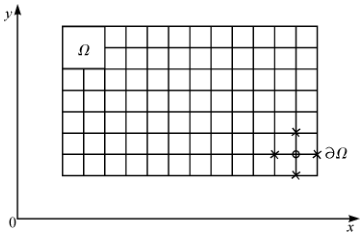
\includegraphics[width=\linewidth]{figs/fig-0008.png}
\caption{图2.8-1}
\end{figure}

y

0

图 2.8-1

另一个例是周边固定的弹性薄板的变形计算。设板在 $x, y$ 平面上占据的区域是 $\Omega$，边界是 $\partial \Omega, f(x, y)$ 是均匀分布的外载荷。板的变形方程式可写为

\[\begin{gathered}\Delta^{2} u=\frac{\partial^{4} u}{\partial x^{4}}+2 \frac{\partial^{4} u}{\partial x^{2} \partial y^{2}}+\frac{\partial^{4} u}{\partial y^{4}}=f(x, y), \quad x, y \in \Omega \\u \mid_{\partial \Omega}=0\end{gathered}\qquad\text{(2.8-38)}\]

把它化为差分方程式后有

\[\begin{aligned}&\left.h^{4} \Delta^{2} u \mid_{i, k}=20 u_{k}+\left(u_{i+2, k}+u_{i, k+2}+u_{i-2, k}+u_{i, k-2}\right)+2\left(u_{i+1, k+1}+u_{i-1, k+1}\right.\right. \\&\left.\left.+u_{i-1, k-1}+u_{i+1, k-1}\right)-8\left(u_{i+1, k}+u_{i, k+1}+u_{i-1, k}+u_{i, k-1}\right)\right) \\&=h^{4} f_{i k}, \quad u_{i, k} \mid_{\partial \Omega}=0\end{aligned}\]

这又是一个代数方程组。式内各组值的分布见图 2.8-2(a)。

为了计算 $u^{k}$ 的值需要用到 12 个点上的平均值。这里出现的困难是对边界附近的点要用到边界 $\partial \Omega$ 以外的值，而后者是边界条件没有给出的。但是为了用网格法求数值解，边界外的点上的值可以用外插的办法近似确定。例如，为了外插边界外 $C$ 点的值 （图 2.8-2b)，可把 $u(x, y)$ 在 $B$ 点展开

\[\begin{aligned}&u_{C}=u_{B}-h \frac{\partial u}{\partial y} \mid_{B}+\frac{h^{2}}{2} \frac{\partial^{2} u}{\partial y^{2}} \mid_{B}+\cdots \\&u_{A}=u_{B}+h \frac{\partial u}{\partial y} \mid_{B}+\frac{h^{2}}{2} \frac{\partial^{2} u}{\partial y^{2}} \mid_{B}+\cdots\end{aligned}\]

两式相减后得 $u_{C}-u_{A}=-2 h\left.\frac{\partial u}{\partial y}\right|_{B}+\cdots$。如果仅保留二次以下的项，则有

\[u_{C}=u_{A}-2 h\left.\frac{\partial u}{\partial y}\right|_{B}=u_{A}-2\left(u_{A}-u_{B}\right)=2 u_{B}-u_{A}\]

当然，如果 $\left.\frac{\partial u}{\partial y}\right|_{B}$ 在边界上已给定，则可直接取 $u_{C}=u_{A}-2 h\left.\frac{\partial u}{\partial y}\right|_{B}$。这样把边界外的点补齐后，就可以用迭代法求解代数方程组 (2.8-39)。

当解算发展方程时，可将网格法和常微分方程积分方法结合起来。例如，用数字机求受控热传导问题的混合解

aligned\& . u/ t-\textasciicircum{}2 u x\textasciicircum{}2=f(x, t),  0  x  l,  0  t<. \textbackslash\{\}\textbackslash\{\}\& u(x, t)|\_t=0=(x),  u(0, t)=(t) \textbackslash\{\}\textbackslash\{\}\& u(l, t)=\_c(t)aligned .(2.8-40)

把 $l$ 分割成 $N$ 段，步长为 $h, N h=l$。记 $u_{k}(t)=u(k h, t), k=0,1,2, \cdots, N$。应用近似公式

\[\left.\frac{\partial^{2} u}{\partial x^{2}}\right|_{x=k h}=\frac{u_{k+1}(t)-2 u_{k}(t)+u_{k-1}(t)}{h^{2}}, \quad\left.\frac{\partial u}{\partial t}\right|_{x=k h}=u_{k}\]

代入式 (2.8-40) 后，得一常微分方程组

\[\begin{aligned}& u_{k}=\frac{1}{h^{2}}\left(u_{k+1}(t)-2 u_{k}(t)+u_{k-1}(t)\right)+f_{k}(t), \quad k=1,2,3, \cdots, N-1 \\& w(t)=\psi(t), \quad u_{N}(t)=\psi(t) \\& u_{k}(0)=\varphi_{k}\end{aligned}\qquad\text{(2.8-41)}\]

\begin{figure}[htbp]\centering
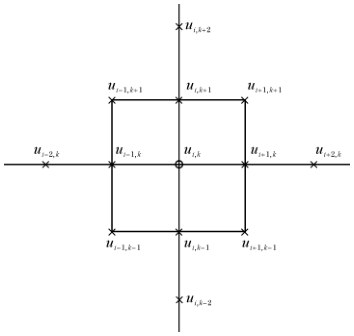
\includegraphics[width=\linewidth]{figs/fig-0009.png}
\caption{图2.8-2}
\end{figure}

\begin{figure}[htbp]\centering
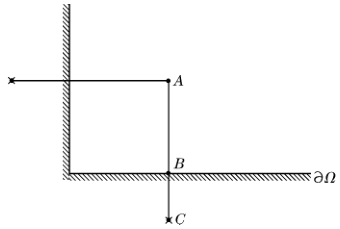
\includegraphics[width=\linewidth]{figs/fig-0010.png}
\caption{图2.8-2}
\end{figure}

记它们都是

\[\begin{aligned}& \frac{d \boldsymbol{u}}{d t}=\boldsymbol{A} \boldsymbol{u}+\boldsymbol{f}(t), \boldsymbol{u}(0)=\boldsymbol{\varphi}=\left\{\varphi_{1}, \varphi_{2}, \cdots, \varphi_{N-1}\right\} \\& A=\frac{1}{h}\left[\begin{array}{rrrrrrr} -2 & 1 & 0 & 0 & 0 & 0 & \cdots & 0 \\ 1 & -2 & 1 & 0 & 0 & 0 & \cdots & 0 \\ 0 & 1 & -2 & 1 & 0 & 0 & \cdots & 0 \\ \vdots & \vdots & \vdots & \vdots & \vdots & \vdots & \vdots & \vdots \\ 0 & 0 & 0 & 0 & 0 & 0 & \cdots & 1-2 \end{array}\right]\end{aligned}\]

于是

\[u(t)=e^{A t} \varphi+\int_{0}^{t} e^{A(t-\tau)} f(\tau) d \tau\qquad\text{(2.8-42)}\]

原方程式 (2.8-40) 的解就以 $\left\{u(h, t), u(2 h, t), \cdots, u((N-1) h, t)\right\}$ 的形式求得。

上面讲的是求解偏微分方程的基本思想。在应用时还可采用一些巧妙办法缩小计算工作量。尽管这样，解多个自变量的偏微分方程需用的存储容量仍很大，运算量也很大。近年来专为解偏微分方程边值问题发展了一种新的方法，称为有限元法。它的基本思想是利用具体问题中自然界边界条件和函数及其微商的连续性，把基本区域 $\Omega$ 划分为较大的单元，然后在相邻单元边界上选定节点，确定函数在节点上应满足的条件，最后得到一个未知数大为减少了的代数方程组。这种方法克服了网格差分法计算量太大的缺点，使节点布局合理。不受复杂的区域，不规则的边界条件所限制，又能保持物理问题的力学和其他特点，并且能提高精度、改善收敛性。关于有限元法已有专著，读者可参阅本章后面所列的参考文献。

\section{2.9 模拟技术}

数字计算机的迅速发展和广泛采用，看来并不能完全代替模拟技术在控制系统设计和分析过程中的重要作用。在精度要求不甚高的情况下，模拟计算机或模拟装置能够很容易地发现系统的运动过程，效果逼真，使用简单，成本也低些。在相同的元件数量情况下，模拟机的计算容量和运算速度都大得多。线性集成电路的出现给模拟技术的发展以新的有力的推动。在这个基础上，模拟计算装置正在向小型化方向发展。数字-模拟混合计算机的出现又使模拟机的优点和数字机的优点结合起来，模拟技术又获得了新的发展。

在模拟计算机上可以实现加法、减法、乘法、除法等算术运算，又能极简单地作微分，积分运算；可灵活地编排微分、积分网络，高速度地解常微分方程和简单的偏微分方程。与数字逻辑电路相结合又可以解一些技术设计中的参数寻优或最优控制问题。模拟计算机中最基本的器件是运算放大器，它把输入信号放大到 $K$ 倍，$K$ 是放大器增益。现在，一个或几个放大器全部线路可以在约 $2 \times 2 \mathrm{~mm}^{3}$ 的硅片上成为一个线性集成电路，它的尺寸在封装后也只有 $10 \times 10 \times 6 \mathrm{~mm}^{3}$ 那样大。图 2.9-1是我国已大量生产的集成运算放大器 BG305 的原理图和符号。它的全部电路都印制在一个单硅片上，开路增益大于 $10^{\text {d }}$，用它可简易地实现各种运算。

\begin{figure}[htbp]\centering
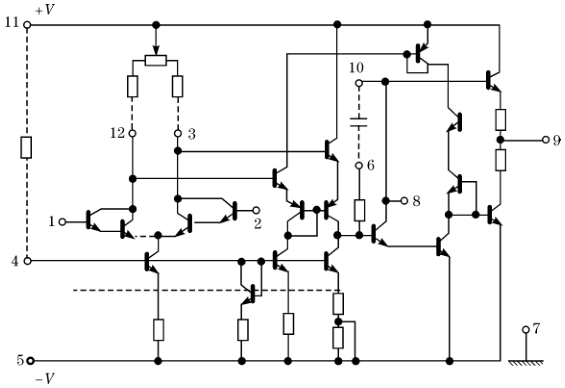
\includegraphics[width=\linewidth]{figs/fig-0012.png}
\caption{图2.9-1}
\end{figure}

\begin{figure}[htbp]\centering
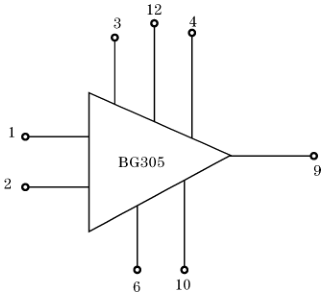
\includegraphics[width=\linewidth]{figs/fig-0011.png}
\end{figure}

(a)

(b)现把一个增益为 $K$ 的放大器用电阻、电容元件接成图 2.9-2 所示的电路。图中 $x_1, \cdots, x_n$ 和 $y$ 分别是以电压表示的输入和输出，$Z$ 和 $Z$ 分别是某些阻抗。设放大器输入点上的电压为 $\varepsilon$，由于放大器的增益是负的，故有下列电压和电流平衡关系

\begin{figure}[htbp]\centering
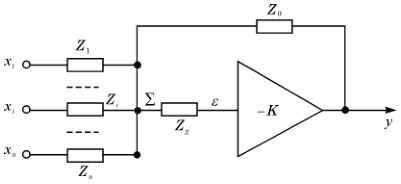
\includegraphics[width=\linewidth]{figs/fig-0013.png}
\caption{图2.9-2}
\end{figure}

图 2.9-2

\[y = -K \varepsilon\]

\[\sum_{i=1}^{n} \frac{x_i}{Z_i} + \frac{y}{Z_0} = \frac{\varepsilon}{Z_g}\]

消掉 $\varepsilon$ 后得

\[y = \frac{-\sum_{i=1}^{n} (x_i / Z_i)}{\frac{1}{K Z_g} + \frac{1}{Z_0}}\qquad\text{(2.9-1)}\]

由于 $K$ 足够大，上式可化简为

\[y = -\sum_{i=1}^{n} \frac{Z_i}{Z_0} x_i\]

由上式可以看出，当 $Z_0 = Z_i = R$ 时，上式是 $n$ 个输入量的代数和。

如果 $Z_i = R$ 是纯电阻，而 $Z_i$ 是纯电容 $C$，则式 (2.9-1)变为

\[y = -\sum_{i=1}^{n} \frac{1}{R C_s} x_i\qquad\text{(2.9-2)}\]

式中 $s$ 是复变量。当 $y$ 的初值为零时，有

\[y(t) = -\left. \frac{1}{R C_s} \right|_{0} ^{t} \sum_{i=1}^{n} x_i(\tau) d\tau\]

这就实现了对输入量的积分运算。

再设 $n = 1, Z_1 = C, Z_0 = R$，容易看出，式 (2.9-1)完成微分运算 $y(t) = \frac{C}{R} \frac{dx(t)}{dt}$。

当 $Z_0$ 和 $Z_1$ 为复杂的网络时，图 2.9-2 所示的放大器可实现更复杂的运算。对只有一个输入函数 $x$ 时，用不同的 $Z_1$ 和 $Z_0$ 得到的输出 $y(t)$ 的象函数列于表 2.9-1 中。

表 2.9-1$Z_{0}(s)$ $Z_{1}(s)$ $Y(s)$

$\frac{1}{C s}$ $R$ $-\frac{1}{R C s} X_{1}(s)$$R$ $\frac{1}{C s}$ $-R C s X_{1}(s)$$\frac{R_{0}}{C s}$ $R_{1}$ $-\frac{R_{0} X_{1}(s)}{R_{1}\left(R_{0} C s+1\right)}$$R_{0}+\frac{1}{C s}$ $\frac{R_{1}}{C s}$ $-\frac{R_{0}\left(R_{1} C s+1\right) X_{1}(s)}{R_{1}}$$R_{0}$ $\frac{1}{C s}+R_{1}$ $-\frac{R_{0} C s}{R_{1} C s+1} X_{1}(s)$$R_{0}$ $R_{1}+\frac{1}{C s}$$\frac{R_{0}}{C_{0} s}$ $R_{1}+\frac{1}{C_{1} s}$ $-\frac{R_{0} C_{1} s}{\left(R_{0} C_{0} s+1\right)\left(R_{1} C_{1} s+1\right)} X_{1}(s)$$R_{0}+\frac{1}{C_{0} s}$ $\frac{C_{1}}{C_{1} s}$ $-\frac{\left(R_{0} C_{0} s+1\right)\left(R_{1} C_{1} s+1\right)}{R_{1} C_{0} s} X_{1}(s)$$R_{1}+\frac{1}{C_{1} s}$$R_{1}+\frac{1}{C_{1} s}$ $-\frac{\left(R_{0} C_{0} s+1\right) C_{1}}{\left(R_{1} C_{1} s+1\right) C_{0}} X_{1}(s)$将这种带有不同的 $Z_i$ 和 $Z_0$ 的放大器按一定的规则编排起来，就能实现线性微分方程组和代数方程组的模拟模型。赋予各放大器以初始电压以后，又能求解常系数线性微分方程的初值问题。当需要模拟变系数线性系统时，只需用可变的 （按给定的规律随时间变化） 阻抗 $Z_r(t), Z_0(t)$ 代替固定的 $Z_r$ 和 $Z_0$ 即可。为实现简便，通常将可变阻值的电位计置于 $Z_r$ 中，然后给它以预定的变化程序。

乘法运算可以用两个非线性函数变换器来实现。例如:

\[y=x_{1} \cdot x_{2}=\frac{1}{4}\left[\left(x_{1}+x_{2}\right)^{2}-\left(x_{1}-x_{2}\right)^{2}\right]\]

可以用平方函数产生器实现乘法，原理图见图 2.9-3。

\begin{figure}[htbp]\centering
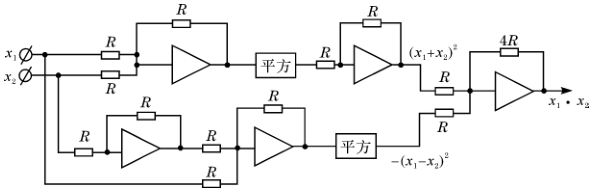
\includegraphics[width=\linewidth]{figs/fig-0014.png}
\caption{图2.9-3}
\end{figure}

另一种应用较广的乘法器是用开关电路实现的，图 2.9-4 是它的示意图。一个输入量 $x_{1}$ 送至脉冲频率调制器，后者的输出是频率 $f$ 随 $x_{1}$ 线性变化的脉冲列，每一个脉冲的高度和宽度是固定的。用这个脉冲列去控制开关，只有当脉冲到达时开关才打开第二个变量 $x_{2}$ 的通路。脉冲过后通路即断开。这样，由电压

\begin{figure}[htbp]\centering
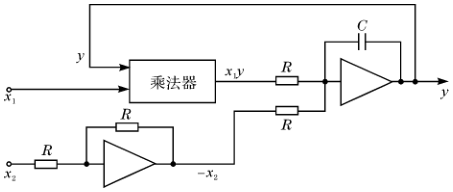
\includegraphics[width=\linewidth]{figs/fig-0016.png}
\caption{图2.9-5}
\end{figure}

\begin{figure}[htbp]\centering
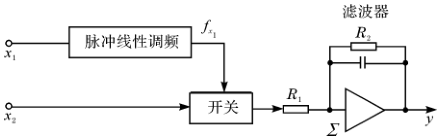
\includegraphics[width=\linewidth]{figs/fig-0015.png}
\caption{图2.9-4}
\end{figure}

图 2.9-4

$x_{2}$ 送至 $\Sigma$ 点的电流正比例于 $K_{2} f_{x_{1}} x_{2}$，而 $f_{x_{1}}$ 又正比例于 $x_{1}, f_{x_{1}}=K_{1} x_{1}$，于是有

\[y=K_{1} K_{2} x_{1} x_{2}\]

运算放大器反馈回路上用阻容元件构成的滤波器，使输出信号的交流部分得以滤除。因此，适当地选择 $R, R, C$ 就可以实现 $x_{1}$ 和 $x_{2}$ 的乘法运算。这类乘法装置的精度约为 $1 \%$ 左右。

用乘法器和运算放大器配合又可以做除法运算，图 2.9-5 是一种可能的方案。从图中可知，乘法器后面是积分器，只有 $x_{1} y=x_{2}$ 时，$y$ 才能保持平衡。故平衡时有 $x_{1} y-x_{2}=0$，即 $y=\frac{x_{2}^{2}}{x_{1}}$。这就实现了除法运算。

图 2.9-5

单变量的非线性函数可以用二极管和运算放大器来实现。例如第一章内图 1.3-2 中所列各种典型非线性函数都可以用这种办法在模拟机中实现 ${ }^{[5]}$。至于多变量非线性函数可以用单变量非线性函数去逼近，以后我们还要讨论。

\section{2.10 函数方程的数值解与极值问题}

控制系统的设计或计算机作实时控制运算时常需要求解函数方程式，而方程式的求解又常能转化成求某一泛函的极值 （极大或极小） 问题。对稍为复杂一点的系统，用解析方法求解几乎是不可能的。实践证明，用计算机求极值比较好的方法之一是最速下降法。由于它原理简单，计算程序不复杂，收效快，所以得到了相当广泛的应用。本节内我们来讨论这个方法的基本思想和应用举例。

设 $g\left(x_{1}, x_{2}, \cdots, x_{n}\right)$ 是一个依赖于 $n$ 个自变量的实值函数。已知它在某一区域中有一个（唯一的）极小值。设 $g$ 对每一个自变量有连续一阶偏微商。定义梯度向量 $(n$ 维 $)$

\[\nabla g=\operatorname{grad} g(\boldsymbol{x})=\left\{\frac{\partial g}{\partial x_{1}}, \frac{\partial g}{\partial x_{2}}, \cdots, \frac{\partial g}{\partial x_{n}}\right\}, \quad \boldsymbol{x}=\left\{x_{1}, x_{2}, \cdots, x_{n}\right\}\]

它的几何意义是：在 $\boldsymbol{x}$ 点附近函数 $g(\boldsymbol{x})$ 增长最快的方向是向量 $\nabla g$ 所指示的方向。相反 $-\nabla g$ 是下降最快的方向。换言之，$\nabla g(\boldsymbol{x})$ 的方向与 $g(\boldsymbol{x})$ 过 $\boldsymbol{x}$ 点的等高线 （等值线） 的外法向量的方向重合，而 $-\nabla g(\boldsymbol{x})$ 则与内法向量方向重合（图 2.10-1)。用最速下降法求极值的步骤如下。在极值附近任取一个初始点 $\boldsymbol{x}_{0}$，算出此点上的梯度向量 $\nabla g\left(\boldsymbol{x}_{0}\right)$，按它的负方向前进一步得 $\boldsymbol{x}=\boldsymbol{x}_{0}-\varepsilon \nabla g\left(\boldsymbol{x}_{0}\right)$，适当选择系数步

长 $\varepsilon$，使 $g\left(\boldsymbol{x}_{0}\right)-g\left(\boldsymbol{x}_{0}\right)=\max _{\varepsilon}\left[g\left(\boldsymbol{x}_{0}\right)-g\left(\boldsymbol{x}_{0}-\varepsilon \nabla g\left(\boldsymbol{x}_{0}\right)\right)\right]$，这样一步一步走下去，就会到达极值点 $\boldsymbol{x}^{*}, g\left(\boldsymbol{x}^{*}\right)=\min _{\boldsymbol{x}} g(\boldsymbol{x})$。于是，最速下降法可归纳为下列程序:

(1) 任选取初始点 $\boldsymbol{x}_{0}=\left\{x_{10}, x_{20}, \cdots, x_{n0}\right\}$。

(2) 求 $\nabla g(\boldsymbol{x})$。

(3) 求步长 $\varepsilon_{0}$，使 $g(\boldsymbol{x})-g(\boldsymbol{x})=\max _{\varepsilon}\left[g(\boldsymbol{x})-g\left(\boldsymbol{x}-\varepsilon \nabla g(\boldsymbol{x})\right)\right]$。

(4) 令 $\boldsymbol{x}=\boldsymbol{x}_{0}-\varepsilon_{0} \nabla g\left(\boldsymbol{x}_{0}\right)$，再返回 (2)，重复上述程序。

于是有

\[\boldsymbol{x}_{n+1}=\boldsymbol{x}_{n}-\varepsilon_{n} \nabla g\left(\boldsymbol{x}_{n}\right)\qquad\text{(2.10-1)}\]

式中 $\varepsilon_{n}$ 由下列条件决定

\[g\left(\boldsymbol{x}_{n}\right)-g\left(\boldsymbol{x}_{n-1}\right)=\max _{\varepsilon}\left[g\left(\boldsymbol{x}_{n}\right)-g\left(\boldsymbol{x}_{n}-\varepsilon \nabla g\left(\boldsymbol{x}_{n}\right)\right)\right]\]

这样求出的 $\varepsilon_{n}$ 叫做最佳步长，它能够保证最快的收敛速度。

如果 $g(\boldsymbol{x})$ 是正定二次型，$B$ 是 $n \times n$ 阶正定矩阵

\[g(\boldsymbol{x})=(B \boldsymbol{x}, \boldsymbol{x})=\sum_{i, j=1}^{n} b_{i j} x_{i} x_{j}\]

则最佳步长可以求出。容易算出

\[\nabla g\left(\boldsymbol{x}_{n}\right)=\left\{2 \sum_{j=1}^{n} b_{i j} x_{j}, 2 \sum_{j=1}^{n} b_{j j} x_{j}, \cdots, 2 \sum_{j=1}^{n} b_{n j} x_{j}\right\}\]

\[g\left(\boldsymbol{x}_{n}\right)-g\left(\boldsymbol{x}_{n}-\varepsilon \nabla g\left(\boldsymbol{x}_{n}\right)\right)=\left(B \boldsymbol{x}_{n}, \boldsymbol{x}_{n}\right)-\left(B \boldsymbol{x}_{n}-\varepsilon \nabla g\left(\boldsymbol{x}_{n}\right),\left(\boldsymbol{x}_{n}-\varepsilon \nabla g\left(\boldsymbol{x}_{n}\right)\right)\right)\]

\begin{figure}[htbp]\centering
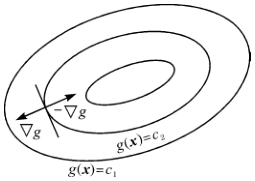
\includegraphics[width=\linewidth]{figs/fig-0017.png}
\caption{图2.10-1}
\end{figure}

=2 (B\textasciicircum{}\{\} g(x\_\{n\})，x\_\{n\})-\textasciicircum{}\{\}(B\textasciicircum{}\{\} g(x\_\{n\})，g(x\_\{n\})) 显然，为使左端获得极大值，必须令

\[\varepsilon_{n}=\frac{\left(B^{\nabla} g\left(\boldsymbol{x}_{n}\right), \boldsymbol{x}_{n}\right)}{\left(B^{\nabla} g\left(\boldsymbol{x}_{n}\right), \nabla g\left(\boldsymbol{x}_{n}\right)\right)}\]

上式利用了正定矩阵的对称性 $\left(B \boldsymbol{x}, \boldsymbol{y}\right)=\left(\boldsymbol{x}, B \boldsymbol{y}\right)$。

上面的程序可以推广到函数空间中去。设 $g(x), x \in H$，是定义于某一希尔伯特空间 $H$ 上的实值泛函。如果极限

\[\dot{g}_{h}(x)=\operatorname{li}_{\mathrm{m}}^{\mathrm{g}} \frac{g(x+\lambda h)-g(x)}{\lambda}\]

存在，则 $\dot{g}_{h}(x)$ 称为泛函 $g(x)$ 沿 $h$ 方向的微商，其中 $h$ 为 $H$ 中任一个固定的元。如果 $\dot{g}_{h}(x)$ 是 $h$ 的线性泛函 （线性函数），则必存在一个 $\varphi \in H$，使 $\dot{g}_{h}(x)=\langle\varphi, h\rangle$，$\varphi$称为泛函 $g(x)$ 的梯度向量，并记为

\[\nabla g(x)=\varphi, \dot{g}_{h}(x)=\langle\varphi, h\rangle=\langle\nabla g(x), h\rangle\qquad\text{(2.10-3)}\]

为了用最速下降法求泛函 $g(x)$ 在希尔伯特空间 （例如函数空间） 中的极值，可将式 (2.10-3) 定义的梯度向量代入程序式 (2.10-1) 中作递推运算。如果 $g(x)$ 是定义于 $H$ 上的二次型，则式 (2.10-1) 中的第二式可由式 (2.10-2) 代替，其中内积 $(\cdots, \cdot)$ 应理解为希尔伯特空间的内积。

下面举两个例，说明如何用最速下降法解代数方程组和积分方程。

例 1. 求代数方程组的解

\[\begin{aligned}& a_{1} x_{1}+a_{2} x_{2}+\cdots+a_{n} x_{n}=b \\& a_{1} x_{1}+a_{2} x_{2}+\cdots+a_{n} x_{n}=b \\& \cdots \\& a_{n 1} x_{1}+a_{n 2} x_{2}+\cdots+a_{n n} x_{n}=b_{n}\end{aligned}\qquad\text{(2.10-4)}\]

引进符号 $\boldsymbol{x}=\left\{x_{1}, x_{2}, \cdots, x_{n}\right\}, \boldsymbol{b}=\left\{b_{1}, b_{2}, \cdots, b_{n}\right\}, A=\left(a_{i j}\right)$ 为 $n \times$ 阶方阵，上式可写成

\[A \boldsymbol{x}=\boldsymbol{b}\]

如果 $A$ 的行列式不为零则有唯一解。否则，或者它是矛盾方程组，没有任何解，或者有许多解。我们定义：能够使向量 $(A \boldsymbol{x}-\boldsymbol{b})$ 的长度最小的 $\boldsymbol{x}^{*}$ 叫做式 (2.10-4) 的最优解。因而，求解代数方程组就化为求 $\boldsymbol{x}^{*}$ 使

\[g(\boldsymbol{x})=(A \boldsymbol{x}-\boldsymbol{b}, A \boldsymbol{x}-\boldsymbol{b})=\left\|\boldsymbol{A x}-\boldsymbol{b}\right\|^{2}\]

达至极小值。根据前面的讨论，用最速下降法求 $\boldsymbol{x}^{*}$ 的递推程序是

\[\begin{gathered}\boldsymbol{x}_{n+1}=\boldsymbol{x}_{n}-\varepsilon_{n} \nabla_{g}\left(\boldsymbol{x}_{n}\right) \\\varepsilon_{n}=\frac{\left(\nabla g\left(\boldsymbol{x}_{n}\right), \nabla g\left(\boldsymbol{x}_{n}\right)\right)}{\left(A \nabla g\left(\boldsymbol{x}_{n}\right), A \nabla g\left(\boldsymbol{x}_{n}\right)\right)} \\ \nabla g(\boldsymbol{x})=\left\{\sum_{j=1}^{n}\left[\left(\beta_{j 1}+\beta_{j}\right) x_{j}-2 a_{j 1} b_{j}\right], \cdots, \sum_{j=1}^{n}\left[\left(\beta_{m}+\beta_{j}\right) x_{j}-2 a_{m} b_{j}\right]\right\}\end{gathered}\]

\[\left|\mathfrak{B}_{m}\right|=\sum_{i}^{n} a_{i i} a_{i m}\qquad\text{(2.10-5)}\]

用这个程序去求代数方程组的解，从任何 $\boldsymbol{x}$ 出发都能迅速收敛于解 $\boldsymbol{x}^{*}$。

例 2. 再讨论如何用这个程序去解积分方程式。设 $K(s, t)$ 是定义于区域 $\Omega=\left\{a \leqslant s, t \leqslant b\right\}$ 上的连续对称的实值函数。用 $H$ 表示由一切定义于 $(a, b)$ 上的平方可积实值函数的全体构成的希尔伯特函数空间。在 $H$ 上定义线性算子 $K$

\[y(t)=\int_{a}^{b} K(t, s) x(s) d s, \quad x(t) \in H\]

按柯西不等式，有

\[\begin{aligned} |y(t)| & =\left|\int_{a}^{b} K(t, s) x(s) d s\right| \leqslant \int_{a}^{b} \mid K(t, s) \mid \cdot \mid x(s) \mid d s \\ & \leqslant \int_{a}^{b} \mid K(t, s) \mid^{2} d s \quad \int_{a}^{b} \mid x(t) \mid^{2} d t \\ & \leqslant M_{1} \| x \| \end{aligned}\]

上式中，$K(t, s)$ 是连续函数，所以 $\int_{a}^{b} \mid K(t, s) \mid^{2} d s$ 是 $t$ 的连续函数，因而在 $[a, b]$ 上是有界的。记 $\max _{t} \int_{a}^{b} \mid K(t, s) \mid^{2} d s=M_{1}$，便得到上述估计式。于是 $\|y\| \leqslant(b-$ $a) M_{1} \| x\|=M \| x\|, \forall x(t) \in H$ 成立。这就是说上面定义的算子 $K$ 是有界的。

设 $h(t) \in H$ 为某一固定的函数，$\lambda$ 为某一个固定的实常数，要求算出下列积分方程的解 $x^{*}(t)$

\[x(t)-\lambda \int_{a}^{b} K(t, s) x(s) d s=h(t)\qquad\text{(2.10-6)}\]

如果 $\lambda$ 不是 $K$ 的特征值，即 $\lambda K x=x$ 只有平凡解 $x=0$，则存在唯一的函数 $x^{*}(t) \neq 0$，满足式 (2.10-6)。

现在用最速下降法求式 (2.10-6) 的解。构造二次泛函

\[\begin{aligned} g(x)= & \int_{a}^{b} x^{2}(s) d s-\lambda \int_{a}^{b} \int_{a}^{b} K(t, s) x(t) x(s) d t d s-2 \int_{a}^{b} x(s) h(s) d s \\ = & \langle x, x\rangle-\lambda\langle K x, x\rangle-2\langle x, h\rangle \end{aligned}\qquad\text{(2.10-7)}\]

可以证明，式 (2.10-7) 存在唯一解 $x^{*}(t)$ 使 $g(x)$ 达到极小值，并且

\[\min _{x} g(x)=-\left\langle x^{*}, h\right\rangle=-\int_{a}^{b} x^{*}(s) h(s) d s\]

首先，任取一函数 $x_{0}(t)$ 当做“初值”然后寻求参数 $\varepsilon$ （步长） 和函数 （方向） $z(t)$，用 $x_{1}(t)=x_{0}(t)-\varepsilon z(t)$ 使 $g\left(x_{0}\right)-g\left(x_{1}\right)$ 达极大值 （下降最大）。容易算出

\[g\left(x_{0}\right)-g\left(x_{1}\right)=2 \varepsilon\left\langle x_{0}-\lambda K x_{0}-h, z\right\rangle-\varepsilon^{2}\left\langle z, z-\lambda K z\right\rangle\]

显然，为使 $g\left(x_{0}\right)-g\left(x_{1}\right)$ 获极大值必须取

\[\begin{aligned}& z=x_{0}-\lambda K x_{0}-h \\& \varepsilon=\frac{\langle z, z\rangle}{\langle z, z-\lambda K z\rangle}\end{aligned}\]

于是，解上述积分方程的最速下降法的计算程序就是

\[\begin{aligned}& x_{n+1}(t)=x_{n}(t)-\varepsilon_{n} z_{n}(t) \\& z_{n}(t)=x_{n}(t)-\lambda K x_{n}(t)-h(t) \\& \varepsilon_{n}=\frac{\langle z_{n}, z_{n}\rangle}{\langle z_{n}, z_{n}-\lambda K z_{n}\rangle}\end{aligned}\qquad\text{(2.10-8)}\]

实际计算表明这个程序收敛很快。

对于求二次泛函 $g(\boldsymbol{x})$ 的极小值，共轭梯度法更为有效。

设

\[g(\boldsymbol{x})=\frac{1}{2}(\boldsymbol{x}, A \boldsymbol{x})+(\boldsymbol{a}, \boldsymbol{x})+c\qquad\text{(2.10-9)}\]

其中 $\boldsymbol{x}=\left(x_{1}, x_{2}, \cdots, x_{n}\right) \in R_{n}, \boldsymbol{a}=\left(a_{1}, a_{2}, \cdots, a_{n}\right) \in R_{n}, c$ 为常数，$A$ 是 $n$ 阶正定方阵。应用共轭梯度法去求极值计算程序简单，容易实现，计算可靠性也好。下面介绍这个方法的几何意义和计算程序。

设两个非零向量 $\boldsymbol{x}, \boldsymbol{y} \in R_{n}$，如果

\[(\boldsymbol{x}, A \boldsymbol{y})=0\qquad\text{(2.10-10)}\]

称向量 $\boldsymbol{x}, \boldsymbol{y}$ 关于矩阵 $A$ 正交。

已知函数 $g(\boldsymbol{x})$ 在某一区域中有一个 （唯一） 极小值点 $\boldsymbol{x}^{*}$。设已得到第 $n$ 次近似值 $\boldsymbol{x}_{n}$，计算梯度向量 $\nabla g(\boldsymbol{x})$，取寻找方向

\[P_{n}=-\nabla g\left(x_{n}\right)+\beta P_{n-1}, \quad P=-\nabla g(\boldsymbol{x})\qquad\text{(2.10-11)}\]

满足条件

\[\left(P_{n}, A P_{n-1}\right)=0\qquad\text{(2.10-12)}\]

其中 $\beta$ 为某一待定常数。把式 (2.10-11) 代入式 (2.10-12) 可得

\[\beta_{n}=\frac{\left(\nabla g\left(\boldsymbol{x}_{n}\right), A P_{n-1}\right)}{\left(P_{n-1}, A P_{n-1}\right)}\qquad\text{(2.10-13)}\]

从 $\boldsymbol{x}_{n}$ 出发，按下式计算第 $n+1$ 次的近似值

\[\boldsymbol{x}_{n+1}=\boldsymbol{x}_{n}+\varepsilon_{n} P_{n}\qquad\text{(2.10-14)}\]

选择步长 $\varepsilon_{n}$，使 $g\left(\boldsymbol{x}_{n}\right)-g\left(\boldsymbol{x}_{n+1}\right)=\max _{\xi}\left[g\left(\boldsymbol{x}_{n}\right)-g\left(\boldsymbol{x}_{n}+\varepsilon \boldsymbol{P}_{n}\right)\right]$。这样一步一步计算下去。这种方法就是共轭梯度法。它有下列的性质:

(1) $n$ 个寻找方向向量 $P_{0}, P_{1}, \cdots, P_{n-1}$ 是线性不相关的。因为若有 $\sum_{i=0}^{n-1} c_{i} P_{i}=0$，就有 $\sum_{i=0}^{n-1} c_{i}\left(P_{i}, A P_{i}\right)=c_{i}\left(P_{i}, A P_{i}\right)=0$，所以 $c_{i}=0$。因此 $P_{0}, P_{1}, \cdots, P_{n-1}$ 是线性不相关的。

(2) 若 $\nabla g(\boldsymbol{x}_{k}) \neq 0$，则

\[\left(P_{k}, \nabla g\left(\boldsymbol{x}_{k+1}\right)\right)=0\]

事实上，若 $\left(P_{k}, \nabla g\left(\boldsymbol{x}_{k+1}\right)\right) \neq 0$，不失一般性，设 $\left(P_{k}, \nabla g\left(\boldsymbol{x}_{k+1}\right)\right)>0$，在 $\varepsilon_{k}$ 附近一定可以找到一个充分接近于 $\varepsilon_{k}$ 的实数 $\varepsilon<\varepsilon_{k}$，并使得 $g\left(\boldsymbol{x}_{k}+\varepsilon_{k} P_{k}\right)-g\left(\boldsymbol{x}_{k}+\varepsilon_{k} P_{k}\right) \triangleq$ $\left(\nabla g\left(\boldsymbol{x}_{k+1}\right),\left(\boldsymbol{\varepsilon}_{k}-\varepsilon_{k}\right) P_{k}\right)=\left(\boldsymbol{\varepsilon}_{k}-\varepsilon_{k}\right)\left(\nabla g\left(\boldsymbol{x}_{k}\right), P_{k}\right)<0$，这与 $\varepsilon_{k}$ 是最佳值相矛盾，因此式 (2.10-15) 成立。

(3) $\left(\nabla g\left(\boldsymbol{x}_{k}\right), \boldsymbol{P}_{j-1}\right)=0,1 \leqslant j \leqslant k$，重复利用 $\boldsymbol{x}_{k}=\boldsymbol{x}_{k-1}+\varepsilon_{k-1} \boldsymbol{P}_{k-1}$，得到

\[\boldsymbol{x}_{j}=\boldsymbol{x}_{j}+\sum_{i=j}^{k-1} \varepsilon_{i} \boldsymbol{P}_{i}, \quad 0 \leqslant j \leqslant k-1\qquad\text{(2.10-21)}\]

而

\[\begin{aligned} & \nabla g\left(\boldsymbol{x}^{*}\right)=A \boldsymbol{x}^{*}+a=0 \\ & \nabla g\left(\boldsymbol{x}_{k}\right)=A \boldsymbol{x}_{k}+a \end{aligned}\qquad\text{(2.10-19)}\]

由式 (2.10-19) 减去式 (2.10-18) 得

\[\nabla g\left(\boldsymbol{x}_{k}\right)=A\left(\boldsymbol{x}_{k}-\boldsymbol{x}^{*}\right)\qquad\text{(2.10-20)}\]

再将式 (2.10-17) 代入式 (2.10-20) 得

\[\begin{aligned} \nabla g\left(\boldsymbol{x}_{k}\right) & =A \boldsymbol{x}_{j}+\sum_{i=j}^{k-1} A \varepsilon_{i} \boldsymbol{P}_{i}-A \boldsymbol{x}^{*} \\ & =\nabla g\left(\boldsymbol{x}_{j}\right)+\sum_{i=j}^{k-1} A \varepsilon_{i} \boldsymbol{P}_{i}, \quad 0 \leqslant j \leqslant k-1 \end{aligned}\qquad\text{(2.10-17)}\]

对 (2.10-21) 式两边和 $\boldsymbol{P}_{j-1}$ 取内积，$\left(\nabla g\left(\boldsymbol{x}_{k}\right), \boldsymbol{P}_{j-1}\right)=\left(\nabla g\left(\boldsymbol{x}_{j}\right), \boldsymbol{P}_{j-1}\right)+$ $\sum_{i=j}^{k-1} \varepsilon_{i}\left(A \boldsymbol{P}_{i}, \boldsymbol{P}_{j-1}\right), 0 \leqslant j \leqslant k-1$，由性质 (2) 有 $\left(\nabla g\left(\boldsymbol{x}_{j}\right), \boldsymbol{P}_{j-1}\right)=0$，由向量关于 $A$ 直交的定义，上式第二项为零，因此式 (2.10-16) 成立。

(4) $\left(\nabla g\left(\boldsymbol{x}_{k}\right), \nabla g\left(\boldsymbol{x}_{k-1}\right)\right)=0$。因为

\[\begin{aligned} & \left(\nabla g\left(\boldsymbol{x}_{k}\right), \nabla g\left(\boldsymbol{x}_{k-1}\right)\right) \\ = & \left(\nabla g\left(\boldsymbol{x}_{k}\right),-\nabla g\left(\boldsymbol{x}_{k-1}\right)+\beta_{k-1} \boldsymbol{P}_{k-2}\right) \\ = & -\left(\nabla g\left(\boldsymbol{x}_{k}\right), \nabla g\left(\boldsymbol{x}_{k-1}\right)+\beta_{k-1}\left(\nabla g\left(\boldsymbol{x}_{k}\right), \boldsymbol{P}_{k-2}\right)\right. \end{aligned}\]

由性质 (2)，(3) 立即得 $\left(\nabla g\left(\boldsymbol{x}_{k}\right), \nabla g\left(\boldsymbol{x}_{k-1}\right)\right)=0$。

根据上述性质 (3)，令 $k=n$ 可推出 $\nabla g\left(\boldsymbol{x}_{n}\right)=0$，即 $\boldsymbol{x}_{n}$ 是二次泛函 $g(\boldsymbol{x})$ 的极小值点。这说明对于二次泛函应用共轭梯度法至多迭代 $n$ 步即可得到极小值点。

计算下列内积，同时注意式 (2.10-21)，有

\[\begin{aligned} \left(P_{n}, \nabla g\left(\boldsymbol{x}_{n}\right)\right) & =\left(P_{n}, \nabla g\left(\boldsymbol{x}_{n-1}\right)+\varepsilon_{n-1} A \boldsymbol{P}_{n-1}\right) \\ & =\left(P_{n}, \nabla g\left(\boldsymbol{x}_{n-1}\right)\right) \end{aligned}\]

\[\begin{aligned}& =(-\nabla g\left(\boldsymbol{x}_{n}\right)+\beta_{n} \boldsymbol{P}_{n-1}, \nabla g\left(\boldsymbol{x}_{n-1}\right) \\& =-\left(\nabla g\left(\boldsymbol{x}_{n}\right), \nabla g\left(\boldsymbol{x}_{n-1}\right)\right)+\beta_{n}\left(\boldsymbol{P}_{n-1}, \nabla g\left(\boldsymbol{x}_{n-1}\right)\right)\end{aligned}\]

从而

\[\begin{aligned}& \beta_{n}=\frac{\left(\boldsymbol{P}_{n}, \nabla g\left(\boldsymbol{x}_{n}\right)\right)}{\left(\boldsymbol{P}_{n-1}, \nabla g\left(\boldsymbol{x}_{n-1}\right)\right)}=\frac{\left(-\nabla g\left(\boldsymbol{x}_{n}\right)+\beta_{n} \boldsymbol{P}_{n-1}, \nabla g\left(\boldsymbol{x}_{n}\right)\right)}{\left(-\nabla g\left(\boldsymbol{x}_{n-1}\right)+\beta_{n-1} \boldsymbol{P}_{n-2}, \nabla g\left(\boldsymbol{x}_{n-1}\right)\right)} \\& =\frac{\left(\nabla g\left(\boldsymbol{x}_{n}\right), \nabla g\left(\boldsymbol{x}_{n}\right)\right)}{\left(\nabla g\left(\boldsymbol{x}_{n-1}\right), \nabla g\left(\boldsymbol{x}_{n-1}\right)\right)}\end{aligned}\qquad\text{(2.10-22)}\]

这就得到了一个完整的迭代程序，由公式 (2.10-22)确定的程序比式 (2.10-13) 简便，它只用到函数 $g(\boldsymbol{x})$ 的梯度，但对于非二次函数，式 (2.10-22) 是近似公式。

上面讨论了两个常用的方法，这两个方法计算程序简单，容易实现，且计算可靠性好。

\section{参考文献}

[1] 王柔怀，伍卓群，常微分方程讲义，人民教育出版社，1963.

[2] 夏道行、吴卓人、严绍宗，实变函数论与泛函分析概要，上海科学技术出版社，1963.

[3] 张远达、熊全淹，线性代数，人民教育出版社，1962.

[4] 复旦大学数学系，计算方法，上海科学技术出版社，1960.

[5] 朱培基，电子模拟计算装置及其应用，科学出版社，1964.

[6] 钱学森 (Tsien H.S.)，The Poincaré-Lighthill-Kuo Method. Advance in Applied Mechanics，Academic Press，1955.281-349. Van Dyke，M.，Perturbation Methods in Fluid Mechanics，The Parapolic Press，1975.

[7] 宫锡芳，常微分方程的一个积分方法，应用数学与计算数学，2(1965)，3.

[8] 冯康，基于变分原理的差分格式，应用数学与计算数学，3(1966)，1.

[9] 关肇直，解非线性函数方程的最速下降法，数学学报，6(1956)，638-650.

[10] 林群，牛顿方法及最速下降法的简化，数学进展，3(1957)，2.

[11] Ahlberg，J. H.，Nilson E. N. \textbackslash\{\}\& Walsh J. I.，The Theory of Spline and Their Applications. Academic Press，New York，1967.

[12] Balakrishnan，A. V.，Introduction to Optimization Theory in a Hilbert Space，SpringerVerlag，1971.

[13] Booth，A. D.，Numerical Methods，London，1957.

[14] Carslaw，H. S.，Jaeger J. C.，Operational Methods in Applied Mathematics，Oxford University Press，New York，1941.

[15] Churchill. R. V.，Modern Operational Methods in Engineering，McGraw-Hill Book Co.，New York，1944.

[16] Doetch，G.，Theorie und Anwendung der Laplace-Transformation，Verlag Julius Springer，1937.

[17] Dunford N.，Schwartz，J. T.，Linear Operators，part I，II，III，1958，1963，1972.

[18] Gardner，M. F.，Bernes，J. L.，Transients in Linear Systems，Studied by Laplace Transfor-

mation，J. Wiley \& Sons，Inc.，1942.

[19] Grenander，U. \& Rosenblatt，M.，Statistical Analysis of Stationary Time series，J. Wiley \& Sons Inc.，1956. （平稳时间序列的统计分析，陶宗英等译，上海科学技术出版社，1957.)

[20] Kamke，E.，Differentialgleichungen Lösungsmethoden und hösungen，Leipzig，1959. （常微分方程手册，张鸿林译，科学出版社，1977.)

[21] Kato，T.，Perturbation Theory for Linear Operators，Springer-Verlag New York Inc.，1976.

[22] Riesz，F. \& Nagy S. Z.，Functional Analysis，Frederick Ungar Publishing Co. 1955.

[23] Stone，M. H.，Linear Transformations in Hilbert Space and Their Applications to Analysis，Am. Math. Soc. 15，1932.

[24] Temam，R.，Numerical Analysis. North-Holland，1973.

[25] Widder，D. V.，The Laplace Transform，Princeton University Press，Princeton，1946.

[26] Zadeh，L. A.，Frequency analysis of variable networks，Proceeding IRE，138.291-299.

[27] Zienkiewicz，O. C.，Finite Element Method in Engineering Science，McGraw-Hill，1971.

[28] Гантмахер，Ф. Р.，Теория，Матриц，ГИТТЛ，1953. （矩阵论，上、下卷，柯召译，高等教育出版社，1955.)

[29] Диткин，В. А.，Кузнецов П. И.，Справочник по Операционному Исчислению，Москва，1951.

[30] Конторович，Л. В.，Об Одном Эффективном Методе Решения Экстремальных задач для квадратичных функционалов，ДАН СССР，48，(1945)，7.

[31] Солодов，А. В.，Линейные Системы Автоматического Управления с Переменными Параметрами，физматиз，1962.

\chapter{第三章 输入、输出和传递函数}

在前一章里我们已经看到，在用拉氏变换法处理问题的时候，常系数线性系统 (2.2-1) 的运动状态和多项式 $D(s)$ 有着本质的关联。 $D(s)$ 是由方程 (2.2-6) 规定的，而且它的系数也就是微分方程的系数。不仅如此，就是在一般的情形里，如果 $y(t)$ 的初始值和各个初始导数值都等于零，那么，系统的运动状态也是由两个多项式的比值 $N(s) / D(s)$ 所完全确定的。我们是用 $F(s)$ 表示这个比值的。如果驱动函数的拉氏变换是 $X(s)$ 而特解的拉氏变换是 $Y_{i}(s)$ 的话，方程 (2.3-4) 就给出

\[Y_{i}(s)=F(s) X(s)\qquad\text{(3.0-1)}\]

可以把这个方程看作是一个算子方程: $X(s)$ 受到算子 $F(s)$ 的作用之后就变成 $Y_{i}(s)$，或者说，$F(s)$ 把 $X(s)$ 转变为 $Y_{i}(s)$。因此我们就把函数 $F(s)$ 称为系统的传递函数。 $x(t)$ 和它的拉氏变换 $X(s)$ 都称为系统的输入，$y_{i}(t)$ 和它的拉氏变换 $Y_{i}(s)$ 都称为系统的输出。为了特别表明 $y_{i}(t)$ 只是系统的特解而不是由于初始条件而产生的补充函数，我们把 $y_{i}(t)$ 称为由于输入而产生的输出，把 $y_{c}(t)$ 称为由于初始条件而产生的输出。

拉氏变换的优点就在于把解微分方程的问题简化为代数的运算。从 $Y(s)$ 变回 $y(t)$ 的这个步骤实际上是很少需要的。理由是这样的：既然系统的运动状态 $y(t)$ 可以由 $Y(s)$ 完全确定，那么，也就可能把对 $y(t)$ 所提出的技术要求“翻译”成对 $Y(s)$ 所提出的某些要求，或者说，如果已经给定了输入的特性，那么，对 $y(t)$ 所提出的要求，也就可以变为对传递函数 $F(s)$ 所提出的某些要求。例如：如果要求系统式 (2.2-1) 是稳定系统的话，我们并不需要先把式 (2.2-8) 中的 $N_{0}(s) / D(s)=Y_{i}(s)$ 变回方程 (2.3-2)，然后再要求 $y_{c}(t)$ 随着时间的增大而趋于消失，实际上，我们只要要求传递函数 $1 / D(s)$ 的极点都位于 $s$ 平面的左半部也就足够了。这种做法显然可以减少许多计算手续。

根据传递函数来研究或者设计一个线性系统是伺服系统工程中的最简单的基本方法。在这一章里，我们将要用一系列的实例来说明这个方法。

\section{3.1 一阶系统}

作为第一个例子，我们来研究一个悬臂弹簧 （图 3.1-1)。弹簧的一个端点连接在一个阻尼器上，另外一端点可以在一根直杆上作滑动运动。阻尼器上的那一个端点的位置用 $y(t)$ 来表示，滑动端点的位置用 $x(t)$ 来表示。由于有阻尼器的缘故，$y(t)$ 就不会和 $x(t)$ 相等，$y(t)$ 的运动落后于 $x(t)$。如果我们让滑动端点按照规定好了的规律 $x(t)$ 运动，这里的问题就是要研究 $y(t)$ 的情况。 $x(t)$ 就是系统的输入（控制量），$y(t)$ 是系统的输出（受控量）。

滑动端点

弹簧

初始位置

阻尼器

图 3.1-1

设系统的弹簧常数是 $k$，阻尼器的阻尼系数 （也就是阻力与速度的比值） 是 $c$。如果再假定运动的加速度相当小，以至于惯性力可以忽略掉 ${ }^{[10]}$。由力的平衡条件就可以得到系统的运动方程

\[c \frac{d y}{d t}+k(y-x)=0\]

$c$ 与 $k$ 的比值 $c / k$ 的量纲是时间。这个数量是系统的一个特性时间 （或特征时间），我们把这个比值

\[\tau=\frac{c}{k}\qquad\text{(3.1-1)}\]

称为系统的时间常数。

运动方程可以改写为

\[\tau \frac{d y}{d t}+y=x\qquad\text{(3.1-2)}\]

初始条件是

\[y(0)=y_{0}\qquad\text{(3.1-3)}\]

用 $e^{-\tau}$乘方程 (3.1-2) 的两端，然后再从 $t=0$ 到 $t=\infty$ 积分。我们就得到作过拉氏变换的方程

\[(\tau s+1) Y(s)=X(s)+\tau y_{0}\]

于是

\[Y(s)=\frac{X(s)}{\tau s+1}+\frac{\tau y_{0}}{\tau s+1}\qquad\text{(3.1-4)}\]

因此，由于输入而产生的输出就是

\[Y_{i}(s)=\frac{1}{\tau s+1} X(s)\qquad\text{(3.1-5)}\]

\begin{figure}[htbp]\centering
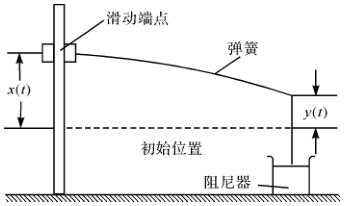
\includegraphics[width=\linewidth]{figs/fig-0018.png}
\caption{图3.1-1}
\end{figure}

而由于初始条件产生的输出就是

\[Y_{c}(s)=\frac{\tau_{1}\,y_{0}}{\tau_{1}\,s+1}\qquad\text{(3.1-6)}\]

系统的传递函数 $F(s)$ 就是

\[F(s)=\frac{1}{\tau_{1}\,s+1}\qquad\text{(3.1-7)}\]

方程(3.1-5)可以用图形表示出来，就像图 3.1-2 所画的那样。这样一个简单的形象化的表示法很能帮助我们想象或分析系统的情况。通常把这样的表示法称为方块图。

\begin{figure}[htbp]\centering
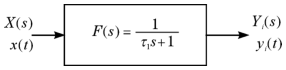
\includegraphics[width=\linewidth]{figs/fig-0020.png}
\caption{图3.1-2}
\end{figure}

\begin{figure}[htbp]\centering
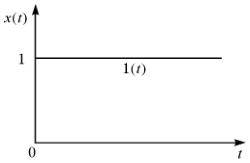
\includegraphics[width=\linewidth]{figs/fig-0019.png}
\caption{图3.1-3}
\end{figure}

\textbackslash\{\}begin\{figure\}[h]\textbackslash\{\}centering\textbackslash\{\}includegraphics[width=0.4\textbackslash\{\}textwidth]\{图3.1-2.png\}\textbackslash\{\}caption\{方块图\}\textbackslash\{\}label\{fig:3.1-2\}\textbackslash\{\}end\{figure\}

\textbackslash\{\}begin\{figure\}[h]\textbackslash\{\}centering\textbackslash\{\}includegraphics[width=0.4\textbackslash\{\}textwidth]\{图3.1-3.png\}\textbackslash\{\}caption\{图形\}\textbackslash\{\}label\{fig:3.1-3\}\textbackslash\{\}end\{figure\}

下面我们研究几种特殊输入情况下的输出 $y(t)$。

首先，考虑输入 $x(t)$ 是单位阶跃函数 $1(t)$ 的情形（图 3.1-3)

\[x(t)=1(t)=\begin{cases} 0, & t<0 \\ 1, & t\geqslant 0 \end{cases}\]

这时

\[X(s)=\int_{0}^{\infty}1(t)e^{-st}\,dt=\int_{0}^{\infty}e^{-st}\,dt=\frac{1}{s}\]

而且

\[Y_{i}(s)=\frac{1}{s(\tau_{1}\,s+1)}=\frac{1}{s}-\frac{1}{s+(\frac{1}{\tau_{1}})}\]

因此，根据我们的“字典”（表 2.1-1)，由于输入而产生的输出就是

\[y_{i}(t)=1-e^{-t/\tau_{1}}\qquad\text{(3.1-8)}\]

根据方程(3.1-6)由于初始条件而产生的输出就是

\[y_{c}(t)=y_{0}\,e^{-t/\tau_{1}}\qquad\text{(3.1-9)}\]

图 3.1-4 表示了输出的特征。由初始条件产生的输出 $y_{c}(t)$ 是一个单纯的衰减函数，这个衰减函数的时间常数就是 $\tau_{1}$ （图 3.1-4b)。由输入产生的输出 $y_{i}(t)$ 按照指数律趋近于水平渐近线，时间常数也是 $\tau_{1}$。事实上，当 $t=\tau_{1}$ 的时候，输出 $y_{i}(t)$ 的数值就达到了最后渐近值的 $63\%$。

\[\begin{aligned}& y_{1}(t) \\& \quad 1 \\& \quad 0\end{aligned}\]

(a)

\[\begin{aligned}& y_{2}(t) \\& \quad 0 \\& \quad t\end{aligned}\]

(b)

图 3.1-4

我们把输入 $x(t)$ 与输出 $y_{i}(t)$ 的差数 $e(t)=x(t)-y_{i}(t)$ 称为偏差信号，在现在所考虑的情形里

\[e(t)=x(t)-y_{i}(t)=e^{-t / \tau_{1}}\qquad\text{(3.1-10)}\]

所以，当 $t \rightarrow \infty$ 时，偏差信号趋于零。

现在，考虑另外一种输入的情形。假定输入是正弦式的，或者，更具体为

\[x(t)=x_{m} e^{i \omega t}\]

式中 $x_{m}$ 是振幅，$\omega$ 是频率。这时

\[X(s)=\frac{x_{m}}{s-i \omega}\]

由于初始条件而产生的输出 $Y_{c}(s)$ 和前一种情形一样，也是方程 (3.1-6) 或方程 (3.1-9)。由于输入而产生的输出就是

\[Y_{i}(s)=x_{m} \frac{1}{(s-i \omega)(\tau s+1)}=\frac{x_{m}}{1+i \omega \tau_{1}}\left(-\frac{1}{s+(1 / \tau)}+\frac{1}{s-i \omega}\right)\qquad\text{(3.1-11)}\]

因此，根据我们的“字典”（表 2.1-1)，输出 $y_{i}(t)$ 就是

\[y_{i}(t)=-\frac{x_{m}}{1+i \omega \tau_{1}} e^{-t / \tau_{1}}+\frac{x_{m}}{1+i \omega \tau_{1}} e^{i \omega t}\]

这个表示式中的第一项是一个单纯的衰减函数。第二项表示稳态输出 $\left[\boldsymbol{y}(t)\right]_{\mathrm{st}}$。因而就有

\[\left[\frac{y(t)}{x(t)}\right]_{\mathrm{st}}=\frac{1}{1+i \omega \tau_{1}}=F(i \omega)\]

这个关系和我们在方程 (2.3-7) 中所表达的普遍结果是完全一致的。由于

\[\frac{1}{1+i \omega \tau_{1}}=\frac{1}{\sqrt{1+\omega_{1}^{2}}} e^{-i \tan ^{-1} \omega_{1}}\qquad\text{(3.1-12)}\]

稳态输出就可以表示为

\[\left[y(t)\right]_{\mathrm{st}}=\frac{x_{m}}{\sqrt{1+\omega_{1}^{2}}} e^{i\left(\omega t-\tan ^{-1} \omega_{1}\right)}\]

因此，稳态输出的振幅就被减少到输入的振幅的 $1 / \sqrt{1+\omega_{1}^{2}}$ 倍，而且输出的相角

\begin{figure}[htbp]\centering
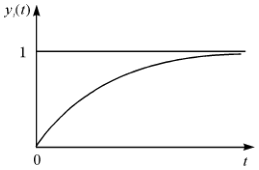
\includegraphics[width=\linewidth]{figs/fig-0021.png}
\caption{图3.1-4}
\end{figure}

\begin{figure}[htbp]\centering
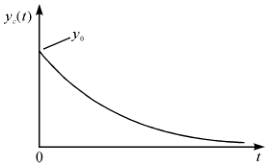
\includegraphics[width=\linewidth]{figs/fig-0022.png}
\caption{图3.1-4}
\end{figure}

比输入的相角落后的数量是 $\tan ^{-1} \omega \tau_{1}$。如果输入的频率 $\omega$ 相当低，$\omega \tau_{1} \ll 1$，因而 $\tan ^{-1} \omega \tau_{1} \triangleq \omega \tau_{1}$，这时

\[\left[y(t)\right]_{\mathrm{t}} \triangleq x_{m} e^{i \omega\left(r-\tau_{1}\right)}, \quad \tau_{1} \omega \ll 1\qquad\text{(3.1-13)}\]

这也就是说：振幅没有改变，但是有一个时滞 （时间上的落后），这个时滞也就等于传递函数的时间常数 $\tau_{1}$。如果输入的频率 $\omega$ 相当高，$\tau_{1} \omega \gg 1$，因而 $\tan ^{-1} \omega \tau_{1} \triangleq \frac{\pi}{2}$，$\frac{1}{\left|1+\omega^{2} \tau_{1}^{2}\right|} \triangleq \frac{1}{\omega \tau_{1}}$，这时就有

\[\left[y(t)\right]_{\mathrm{t}} \triangleq \frac{x_{m}}{\omega \tau_{1}} e^{\frac{i \omega\left(r-\left(\pi / 2\right)\right)}{}} \quad, \quad \tau_{1} \omega \gg 1\]

在这种情形中，振幅被减少到 $1 / \omega \tau_{1}$ 倍，而相角落后的数量是 $\pi / 2$。我们把以上所讨论的两种极端的输出情形表示在图 3.1-5 中。

\begin{figure}[htbp]\centering
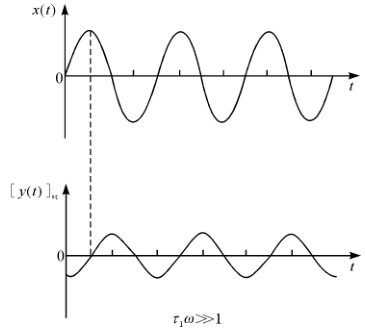
\includegraphics[width=\linewidth]{figs/fig-0024.png}
\caption{图3.1-5}
\end{figure}

\begin{figure}[htbp]\centering
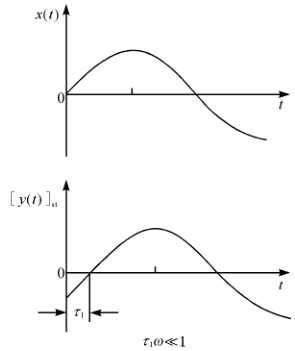
\includegraphics[width=\linewidth]{figs/fig-0023.png}
\caption{图3.1-5}
\end{figure}

\[x(t)\]

\[\left[y(t)\right]_{\mathrm{u}}\]

低频情况

\[\tau_{1} \omega \ll 1\]

(a)

\[x(t)\]

\[\left[y(t)\right]_{\mathrm{n}}\]

高频情况

\[\tau_{1} \omega \gg 1\]

(b)

图 3.1-5

\section{3.2 传递函数的表示法}

传递函数 $F(s)$ 是复变数 $s$ 的函数。因为在普通的情形下，它是两个 $s$ 的多项式的比值，所以函数 $F(s)$ 除了一个常数因数之外可以由它的零点和极点所确定。如果对于某一个特别的 $s$ 值 $F(s)$ 的值是已知的话，也就可以把常数因数确定下来，这时函数 $F(s)$ 就完全确定了。这里，最方便的就是考虑 $s$ 在原点的值 $s=0$，因为 $F(0)$ 有具体的物理意义

\[\left|F(0)\right|=K\qquad\text{(3.2-1)}\]

是系统的放大系数，也就是系统在常数输入的情况下输出的稳态值与输入的比值。又因为对于大多数的实际情形，F(0)常常是正数，因而F(0)=K。所以，传递函数F(s)就可以由零点、极点和放大系数唯一地确定。这也就是传递函数的一种可能的表示方法。举例来说，我们可以这样来表示方程(3.1-7)所给的传递函数：它的放大系数是1;在-1/σ有一个单极点；没有零点。

根据复变数函数论的结果，如果在s平面的虚轴上，F(s)的实数部分和虚数部分都已经完全给定的话，那么，用解析开拓的方法[4]就可以把s平面上其他部分的F(s)值也确定下来。因此，我们也可以用复函数F(iω)(ω是实数，-∞<ω<+∞)来代表函数F(s)。这就是传递函数的另外一种表示方法。对于实际的物理系统来说，F(s)=N(s)/D(s)的分子多项式N(s)和分母多项式D(s)的系数都是实数，所以，如果我们用F表示F的复共轭数的话，就有

\[F(-i \omega)=\overline{F(i \omega)}\qquad\text{(3.2-2)}\]

因此，对于实际的物理系统，只要知道ω≥0的F(iω)值，就可以知道ω≤0的F(iω)值，从而也就可以定出对于任意s的F(s)的值。从方程(2.3-7)我们已经知道函数F(iω)是频率ω的稳态输出与正弦输入之比，F(iω)(-∞<ω<+∞)就是系统的频率特性。例如，方程(3.1-12)就是简单的一阶系统(3.1-2)的频率特性。

伯德(Bode)创造了一种表示频率特性的方法，这种方法就称为伯德图。假定复数F(iω)的绝对值是M，相角是θ(M和θ当然都是ω的函数），也就是说

\[F(i \omega)=M e^{i \theta}\qquad\text{(3.2-3)}\]

把logω取作自变数，然后再把因变数logM和θ对logω的函数关系画在两张图上，这样得出的图就是伯德图(logM对logω的函数关系通常称为系统的对数幅特性。而θ对logω的函数关系称为系统的对数相频特性）。至于为什么在这里M取了对数尺度而θ并不取对数尺度，这个道理可以在以后的讨论中看出来。以方程(3.1-12)所表示的简单系统为例

\[\begin{gathered} M=\frac{1}{\sqrt{1+\omega^{2} \frac{\sigma}{\mathrm{u}}}}=\frac{1}{\sqrt{1+u^{2}}} \\ \theta=-\tan ^{-1} \omega \tau=-\tan ^{-1} u \end{gathered}\qquad\text{(3.2-4)}\]

其中u=ωτ是无量纲频率[2，10]。这个系统的伯德图就是图3.2-1，频率特性在低频率和高频率时的情况已经用方程(3.1-13)和(3.1-14)表示出来了。当u→∞时，logM对logu的图线的斜率是-1，对于很小的u值来说，斜率差不多是0。因此，一个一阶系统的M-u图可以用两条直线来近似地代替。这两条直线就是图3.2-1中的虚折线。这条虚折线称为渐近对数幅频特性或者梯形对数幅频特性[2，12]。

在声学和电学的文献里，为了把振幅的度量单位化为分贝(decibel，简写为db)，常常用20logM作为M-u图中的因变数。频率增加一倍就称为一个倍频

$\begin{aligned}& \theta \\& \log u\end{aligned}$M e\textasciicircum{}\{i \textbackslash\{\}beta\}=\textbackslash\{\}frac\{1\}\{1+i \textbackslash\{\}omega \textbackslash\{\}tau\_\{1\}\}$图 3.2-1程(octave,简写为 oct)。因此,图 3.2-1 中的斜率用分贝和倍频程作单位,就是$-20 \textbackslash\{\}log 2=-6.02$分贝/倍频程$(\textbackslash\{\}mathrm\{db\} / \textbackslash\{\}mathrm\{oct\})$。或者用旬频程表示, 就是$20 \textbackslash\{\}log 10=$20 分贝/旬频程。在实际计算工作中, 用后面这一单位做斜率比较方便。在图 3.2-1中我们还看到这样一个事实: 近似于$20 \textbackslash\{\}log M$的虚线在$u=1$点, 也就是$\textbackslash\{\}omega=\$1 /处通过 0 值。因此, 我们就可以用实验方法测量一个一阶系统的频率特性,把测量的结果按照上述的方式画成伯德图。只要记下伯德图上$20 \log M$的近似直线穿过横轴时的角频率$\omega_{0}$就可以简单地估计出系统的时间常数,\$\textbackslash\{\}tau \textbackslash\{\}approx 1 / \textbackslash\{\}omega\_\{0\}。

另外一个表示频率特性的方法是乃奎斯特 (Nyquist) 所创始的，称为乃氏图。这种方法是把复数 $F(i \omega)$ 或 $1 / F(i \omega)$ 直接画到 $F$ 平面或 $1 / F$ 平面上去，曲线的参数就是角频率 $\omega_{0}$。函数 $1 / F$ 有时候称为反幅相特性。 $F$ 平面上的图线 $F(i \omega)$ 就称为幅相特性。对于一个简单的一阶系统来说，$F(i \omega)=1 /(1+i \omega \tau)$ 的图线是一个半圆，在 $\omega=0$ 时，图线从 1 点出发；在 $\omega \tau=u=1$ 时，图线通过 $1 /(1+i)=(1 / 2)(1-i)$ 点；当 $\omega \rightarrow \infty$ 时，图线趋向于原点，并且以原点为终点。在这种情形里，$1 / F$ 图线比 $F$ 图线还要简单得多; $1 / F=1+i \omega \tau_{1}$。所以在 $1 / F$平面上，这条图线就是从 1 点出发的一条与虚轴平行的直线。图 3.2-2 就是阶系统的两种乃氏图。

\[F=\frac{1}{1+i u}\]

\[\frac{1}{F}=1+i u\]

\begin{figure}[htbp]\centering
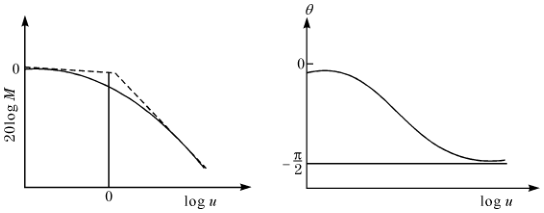
\includegraphics[width=\linewidth]{figs/fig-0025.png}
\caption{图3.2-1}
\end{figure}

\begin{figure}[htbp]\centering
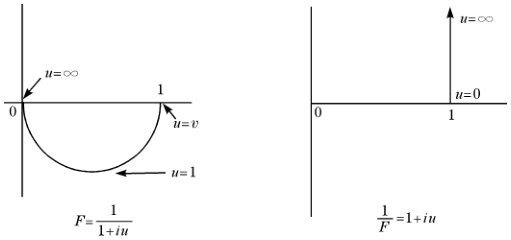
\includegraphics[width=\linewidth]{figs/fig-0026.png}
\caption{图3.2-2}
\end{figure}

在一个复合系统里，常常有很多元件可以用一阶的传递函数来近似地表示。 在这一节里，我们将要简略地讨论这类元件的几个例子。并且把它们特有的频率特性用伯德图或乃氏图表示出来。

(1) 积分元件：一个电动机的转速 $d \psi / d t$ 与输入电压 $v$ 成比例，如果不考虑过渡过程，用微分方程来表示就是

\[\frac{d \psi}{d t}=K v\qquad\text{(3.3-1)}\]

其中 $K$ 是与所采用的度量单位有关的常数。电动机的转子的角位置 $\phi$ 与下列积分成比例

\[\int_{0}^{t} v d t\]

这个关系可以用方块图 3.3-1 表示出来，假设 $V(s)$ 和 $\Phi(s)$ 分别是 $v$ 和 $\phi$ 的拉氏变换。这个系统的传递函数 $F(s)=K / s$ 是函数 $1 /(s, s+1)$ 当 $s \rightarrow \infty$ 时的极限情形，它在原点 $s=0$ 有一个极点。为了把这里的 $K$ 还看作系统的放大系数，我们就必须把以前规定的放大系数的定义修改一下，以前的那一个定义适用于原点不是传递函数的零点或极点的情形。对于一个积分系统，即对传递函数 $F(s)$ 在原点 $s=0$ 有一个单极点的系统来说，放大系数 $K$ 就应该定义为

\[K=\lim _{s arrow 0}|s F(s)|\qquad\text{(3.3-2)}\]

系统式 (3.3-1) 的频率特性是

\[F(i \omega)=\frac{K}{i \omega}=\left(\begin{array}{c}K \\ \omega\end{array}\right) e^{-i \pi / 2)}\]

因此，按照方程 (3.2-3)

\[M=\frac{K}{\omega}, \theta=-\frac{\pi}{2}\qquad\text{(3.3-3)}\]

图 3.3-2 就是伯氏图，这里斜率仍然是 -20 分贝/旬频率。图 3.3-3 是乃氏图。

(2) 微分元件：一个回转测速计 （测速陀螺） 的输出电压 $v$ 和进动轴的角速度 $d \psi / d t$ 成比例，即

\[v=K \frac{d \psi}{d t}\]

式中 $K$ 是比例常数。这个情形和前面讨论的电动机的情形恰好相反。传递函数 $F(s)=K s$ 在原点有一个零点。因此，对于一个微分系统，即对传递函数 $F(s)$ 在原

\begin{figure}[htbp]\centering
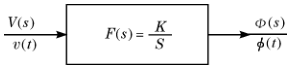
\includegraphics[width=\linewidth]{figs/fig-0027.png}
\caption{图3.3-1}
\end{figure}

\section{3.3 一阶系统的一些例子}

\[\begin{aligned}& \theta \\& \log \omega\end{aligned}\]

\[F(i \omega)=\frac{K}{i \omega}=M e^{i \theta}\]

图 3.3-2

\[\begin{aligned}& \omega=\infty \\& F(i \omega)=\frac{K}{i \omega}\end{aligned}\]

\[\begin{aligned}& \omega=0 \\& \frac{1}{F(i \omega)}=\frac{i \omega}{K}\end{aligned}\]

图 3.3-3

点 $s=0$ 有一个单零点的系统来说，放大系数 $K$ 的定义应该改为

\[K=\lim _{s arrow 0}\left|\frac{F(s)}{s}\right|\]

图 3.3-4 是这个系统的方块图，图 3.3-5 是伯德图 （图中设 $K=1$ )，图 3.3-6 是乃氏图。极易检验，伯德图内斜线的斜率是 20 分贝/句频程。

\[\frac{\varphi(s)}{\phi(t)}\]

图 3.3-4

\[\begin{aligned}& \theta \\& \log \omega\end{aligned}\]

\[F(i \omega)=K i \omega=M e^{i \theta}\]

图 3.3-5

\begin{figure}[htbp]\centering
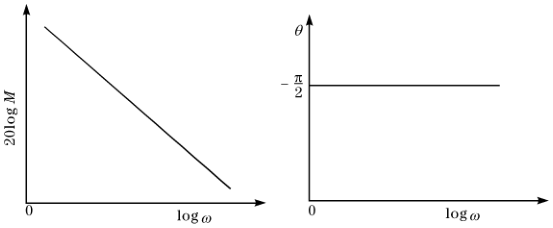
\includegraphics[width=\linewidth]{figs/fig-0028.png}
\caption{图3.3-2}
\end{figure}

\begin{figure}[htbp]\centering
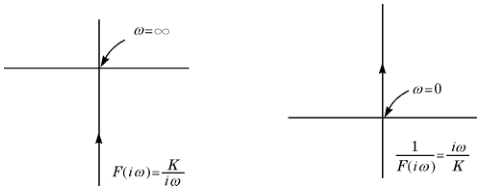
\includegraphics[width=\linewidth]{figs/fig-0029.png}
\caption{图3.3-2}
\end{figure}

\begin{figure}[htbp]\centering
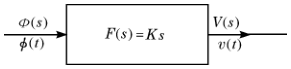
\includegraphics[width=\linewidth]{figs/fig-0030.png}
\caption{图3.3-5}
\end{figure}

\begin{figure}[htbp]\centering
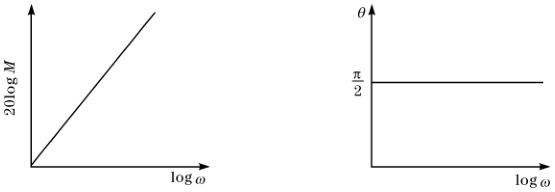
\includegraphics[width=\linewidth]{figs/fig-0031.png}
\caption{图3.3-4}
\end{figure}

(3) 简单的相角落后电路：考虑图 3.3-7 的包含电阻 $R$ 和电容 $C$ 的电路，$v_1$ 和 $v_2$ 分别是输入电压和输出电压。假设 $j=j(t)$ 是流入电阻 $R$ 和电容 $C$ 的电流，如果在 $t=0$ 的时候，电容 $C$ 上没有电荷。那么

\[\begin{aligned}& j R+\frac{1}{C} \int_{0}^{t} j(t) d t=v_{1} \\& \frac{1}{C} \int_{0}^{t} j(t) d t=v_{2}\end{aligned}\]

\[\begin{array}{ll}\omega=0 & \omega=\infty \\F(t \omega)=K t \omega & \frac{1}{F(t \omega)}=\frac{1}{K t \omega}\end{array}\]

图 3.3-6

图 3.3-7

先用 $e^{-st}$ 乘这两个方程，然后再从 $t=0$ 到 $t=\infty$ 积分，就得到这两个方程的拉氏变换

\[\begin{aligned}& \left[R+\frac{1}{C s}\right] J(s)=V_{1}(s) \\& \frac{1}{C s} J(s)=V_{2}(s)\end{aligned}\]

因此

\[\frac{V_{2}(s)}{V_{1}(s)}=F(s)=\frac{1}{1+R C s}\qquad\text{(3.3-5)}\]

从方程 (3.3-5) 可以看出，这个电阻电容电路的传递函数和有阻尼器的悬臂弹簧的传递函数式 (3.1-7) 是相同的，这个电路系统的时间常数就是 $\tau=RC$。这个系统的伯德图和乃氏图就是图 3.2-1 和图 3.2-2。这个电路常常用来产生系统的相角落后。

可以在这里附带提一下：虽然上述的悬臂弹簧系统和这一个电路系统的动态特性是相同的，但是我们知道：在实际工程中改变和调整那个系统的参数 $c$ 和 $k$ 往往是比较困难的，而且 $c$ 和 $k$ 的可能的变动范围也很有限，可是在这个电路里改变和调整 $R$ 和 $C$ 的数值就比较容易。而且 $R$ 和 $C$ 的变动范围也可以很大。从这个具体例子就可以看出用电的方法进行调节或控制常常比用机械方法方便得多。

\begin{figure}[htbp]\centering
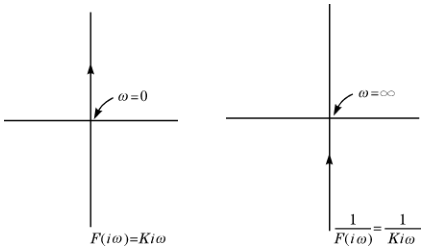
\includegraphics[width=\linewidth]{figs/fig-0032.png}
\caption{图3.3-6}
\end{figure}

\begin{figure}[htbp]\centering
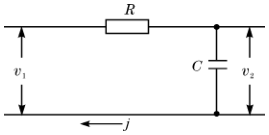
\includegraphics[width=\linewidth]{figs/fig-0033.png}
\caption{图3.3-7}
\end{figure}

(4) （4）相角超前电路：图3.3-8表示一个较复杂的电路。这个电路的方程是

\[\begin{aligned}& j=j_{1}+j_{2} \\& R_{1} j_{1}=\frac{1}{C_{1}} \int_{0}^{t} j_{2}(t) d t\end{aligned}\]

以及

\[\begin{aligned}& v_{1}=R_{1} j_{1}+R_{2} j \\& v_{2}=R_{2} j\end{aligned}\]

相应的拉氏变换后的方程就是

\[\begin{aligned}& J=J_{1}+J_{2} \\& R_{1} J_{1}=\frac{1}{C_{s}} J_{2}\end{aligned}\]

以及

\[\begin{aligned}& V_{1}=R_{1} J_{1}+R_{2} J \\& V_{2}=R_{2} J\end{aligned}\]

因此

\[\frac{V_{2}(s)}{V_{1}(s)}=F(s)=\frac{R_{2}+R_{1} R_{2} C_{s}}{\left(R_{1}+R_{2}\right)+R_{1} R_{2} C_{s}}\]

放大系数就是

\[K=\frac{R_{2}}{R_{1}+R_{2}}=r\qquad\text{(3.3-6)}\]

$K$ 当然小于 1。如果我们引进符号 $\omega_{\mathrm{a}}$

\[\omega_{\mathrm{a}}=\frac{R_{1}+R_{2}}{R_{1} R_{2} C}\qquad\text{(3.3-7)}\]

那么，传递函数就可以改写成

\[F(s)=r \frac{1+\left(s / r_{\omega 1}\right)}{1+\left(s / \omega_{\mathrm{a}}\right)}\qquad\text{(3.3-8)}\]

因此，传递函数在 $-r \omega_{\mathrm{a}}$ 有一个零点，在 $-\omega_{\mathrm{a}}$ 有一个极点。

频率特性就是

\[F(i \omega)=\frac{r \omega_{1}+i \omega}{\omega_{1}+i \omega}\qquad\text{(3.3-9)}\]

如果我们引进无量纲频率

\[u=\frac{1}{r} \frac{\omega}{\omega_{1}}\qquad\text{(3.3-10)}\]

那么

\[M=\sqrt{r} \frac{\sqrt{1+\left(u^{2} / r\right)}}{\left(1 / r\right)+u^{2}}, \quad \theta=\tan ^{-1} \frac{u}{r}-\tan ^{-1}\left(\sqrt{r} u\right)\qquad\text{(3.3-11)}\]

\begin{figure}[htbp]\centering
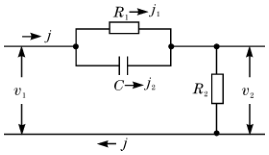
\includegraphics[width=\linewidth]{figs/fig-0034.png}
\caption{图3.3-8}
\end{figure}

于是有

\[\begin{aligned}\log M(u) &= \log \sqrt{r} + \log \sqrt{\frac{1 + (u^2 / r)}{(1 / r) + u}} \\&= \log \sqrt{r} - \log \sqrt{\frac{1 + (1 / r u^2)}{(1 / r) + (1 / u^2)}} \\\theta(u) &= \theta \left( \frac{1}{u} \right)\end{aligned}\]

因此，就像图 3.3-9 所表示的那样，伯德图的图线对于 $u=1$ （也就是 $\log u=0$) 有着对称性。 $\theta$ 的极大值 $\theta_{\text{max}}$ 是在 $u=1$ 点，并且等于

\[\theta_{\text{max}} = \tan^{-1} \frac{1}{r} - \tan^{-1} \frac{\pi}{2} - 2 \tan^{-1} \frac{1}{r}\qquad\text{(3.3-12)}\]

因此，这个电路在一个频带 （频率范围） 上给出相当大的相角超前。对于非常大的 $\omega$ 值，$M=1$; 对于非常小的 $\omega$ 值，$M=r$。在零点附近曲线的斜率接近 20 分贝/旬频程，而在 $u$ 很小和很大时斜率为零。

2010g $M$

0

\[\log u\]

\[F(i \omega) = \frac{r \omega_1 + i \omega}{\omega_1 + i \omega}, \quad u = \frac{1}{r} \frac{\omega}{\omega_1}\]

图 3.3-9

(5) 频带的相角迟后电路：图 3.3-10 所表示的电阻电容电路的传递函数是

\[\frac{V_2(s)}{V_1(s)} = F(s) = \frac{1 + R_1 C s}{1 + (R_1 + R) C s}\]

\[v_1\]

$R$

$C$

$v_2$

$R_1$

图 3.3-10

所以，这个系统的放大系数是 1。如果我们引进这样定义的两个参数 $\omega$ 和 $r$

\begin{figure}[htbp]\centering
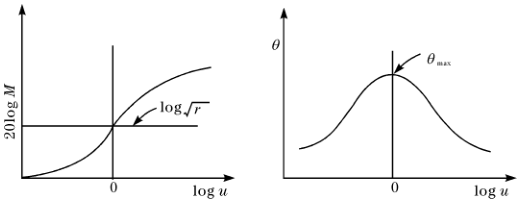
\includegraphics[width=\linewidth]{figs/fig-0035.png}
\caption{图3.3-9}
\end{figure}

\begin{figure}[htbp]\centering
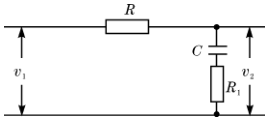
\includegraphics[width=\linewidth]{figs/fig-0036.png}
\caption{图3.3-10}
\end{figure}

\[\omega_{\mathrm{x}}=\frac{1}{R_{\mathrm{t}} C}, \quad r=\frac{R_{\mathrm{t}}}{R+R_{\mathrm{t}}}\qquad\text{(3.3-13)}\]

那么，传递函数就可以改写成

\[F(s)=\frac{1+\left(s / \omega_{\mathrm{R}}\right)}{1+\left(s / r \omega_{1}\right)}\qquad\text{(3.3-14)}\]

把这个方程和相角超前电路的方程 (3.3-8) 加以比较，我们就可以看到这两个电路的传递函数 （除了一个常数的因数之外） 是互为倒数的。其实，目前这个电路的频率特性也可以写成

\[F(i \omega)=\frac{1+i\left(\omega / \omega_{\mathrm{R}}\right)}{1+i\left(\omega / r \omega_{1}\right)}=\frac{1+i \sqrt{r} u}{1+i\left(1 / \sqrt{r}\right) u}\]

其中 $u$ 是无量纲频率

\[u=\frac{1}{r} \frac{\omega}{\omega_{1}}\]

因此

\[M=\sqrt{r} \frac{\left(1 / r\right)+u^{2}}{1+\left(u^{2} / r\right)}, \quad \theta=\tan ^{-1}\left(\sqrt{r} u\right)-\tan ^{-1} \frac{u}{r}\qquad\text{(3.3-16)}\]

图 3.3-11 就是这个系统的伯德图。从图中我们可以看出，在 $u=1$ 附近的一个频率上有着显著的相角落后。极大的相角落后发生在 $u=1$ 点，也就是频率 $\omega=\sqrt{r \omega_{1}}$ 的时候，它的大小也还是方程 (3.3-12) 所给的 $\theta_{\text {max }}$。曲线在零点附近斜率为 -20 分贝/旬频程，在 $u$ 很大或很小时斜率为零。

（6）简化的飞机的横滚运动：假设飞机对于纵轴的转动惯量是 $I, \phi$ 是滚动角，$L_{v}$ 是关于滚动的空气动力阻尼系数，$\delta$ 是副翼的倾斜度，$k \delta$ 是由于副翼偏转而引起的力偶矩。滚动角 $\phi$ 的微分方程就是

\begin{figure}[htbp]\centering
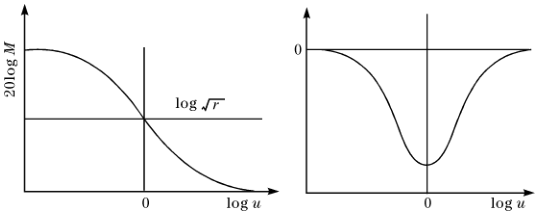
\includegraphics[width=\linewidth]{figs/fig-0037.png}
\caption{图3.3-11}
\end{figure}

\[\begin{gathered} I \frac{d^{2} \phi}{d t^{2}}+L_{p} \frac{d \phi}{d t}=k \hat{\theta} \\ \text { 设 } p=d \psi / d t \text { 是滚动速度; 以上的微分方程就变成 } \\ I \frac{d p}{d t}+L_{p} p=k \hat{\theta} \end{gathered}\]

如果 $t=0$ 时的滚动速度是 0，那么，拉氏变换后的方程就是

\[\left(I s+L_{p}\right) P(s)=k \Delta(s)\]

因此，传递函数 $F(s)$ 就是

\[\frac{P(s)}{\Delta(s)}=F(s)=\frac{k}{I s+L_{p}}=\frac{k}{L_{p}} \frac{1}{1+\left(I / L_{p}\right) s}\qquad\text{(3.3-17)}\]

正如方程(3.3-17)所示，这个系统的运动状态和具有阻尼器的悬臂弹簧以及简单的相角落后电路的运动状态是相似的。在这里，时间常数 $\tau$ 是 $I / L_{p}$，如果阻尼系数 $L_{p}$ 非常小，时间常数 $\tau$ 就接近于 $\infty$，系统的运动状态就和简单的积分元件的情况一样了。

\section{3.4 二阶系统}

我们再回到具有阻尼器的悬臂弹簧的情形 （图 3.1-1)。不过，现在我们在阻尼器这一端加上一个质量 $m$。这个质量引起一个惯性力 $m d^{2} y / d t^{2}$。因而运动方程就变为

\[m \frac{d^{2} y}{d t^{2}}+c \frac{d y}{d t}+k y=k x\]

假定初始条件是

\[\left.\left(\begin{array}{l} d y \\ d t \end{array}\right)_{t=0}=\gamma^{(1)}\right)\]

引进下列两个参数以后，就可以把微分方程改写为更方便的形式

\[\begin{aligned} & \omega_{\mathrm{p}}^{2}=\frac{k}{m} \\ & \zeta=\frac{c / m}{2 \omega_{\mathrm{p}}} \end{aligned}\]

$\omega$ 就是当阻尼器不存在时的质量弹簧系统的自然频率。$\zeta$ 就是实际的阻尼和临界阻尼的比值。这一无量纲的参数的物理意义在以下的讨论中可以说明得更加清楚。这样一来，运动方程就变成

\[\frac{d^{2} y}{d t^{2}}+2 \zeta \omega_{\mathrm{p}} \frac{d y}{d t}+\omega_{\mathrm{p}}^{2} y=\omega_{\mathrm{p}}^{2} x\qquad\text{(3.4-3)}\]

方程(3.4-3)连同它的初始条件 (3.4-1) 用拉氏变换的方式就可以表示为下列的方程

\[(s^{2}+2 \zeta \omega_{0} s+\omega_{0}^{2}) Y(s)=\omega_{0}^{2} X(s)+y_{0}^{(1)}+\left(s+2 \zeta \omega_{0}\right) y_{0}\]

由于初始条件而产生的输出就是

\[Y_{c}(s)=\frac{y_{0} s+\left(y_{0}^{(1)}+2 \zeta \omega_{0} y_{0}\right)}{s^{2}+2 \zeta \omega_{0} s+\omega_{0}^{2}}\qquad\text{(3.4-4)}\]

而传递函数就是

\[F(s)=\frac{Y_{i}(s)}{X(s)}=\frac{1}{\left(s / \omega_{0}\right)^{2}+2 \zeta\left(s / \omega_{0}\right)+1}\qquad\text{(3.4-5)}\]

因此，系统的放大系数 $K=1$，而且传递函数没有零点。但是它有两个单极点 $s_{1}$ 和 $s_{2}$。在 $\zeta^{2}>1$ 时，$s_{1}$ 和 $s_{2}$ 就是

\[\begin{aligned} & \frac{s_{1}}{\omega_{0}}=-\zeta+\sqrt{\zeta^{2}-1}, \\ & \frac{s_{2}}{\omega_{0}}=-\zeta-\sqrt{\zeta^{2}-1}, \end{aligned}\qquad\text{(3.4-6)}\]

当阻尼器的阻尼系数 $c$ 比临界阻尼 $2 \sqrt{m k}$ 小的时候，$\zeta$ 的数值就会比 1 小。在那种情况下，极点 $s_{1}$ 与 $s_{2}$ 是复共轭的，它们的实数部分和虚数部分分别是 $\lambda$ 和 $v$

\[\begin{aligned} & s_{1} / \omega_{0}=-\zeta+i \sqrt{1-\zeta^{2}}=(\lambda+i v) / \omega_{0}=e^{i \varphi_{1}}, \quad \zeta^{2}<1 \\ & s_{2} / \omega_{0}=-\zeta-i \sqrt{1-\zeta^{2}}=(\lambda-i v) / \omega_{0}=e^{-i \varphi_{1}}, \end{aligned}\qquad\text{(3.4-7)}\]

因为 $s_{1} / \omega_{0}$ 和 $s_{2} / \omega_{0}$ 的绝对值都是 1，以可以写成 $e^{\pm i \varphi_{1}}$ 的形式。如果阻尼系数 $c$ 是正的，$\lambda$ 就是一个负数。

由方程 (3.4-4)很容易就可以确定由于初始条件而产生的输出 $y_{c}(t)$。对于 $\zeta<1$ 的情形，传递函数的极点是由方程(3.4-7)所确定的，我们就有

\[y_{c}(t)=\frac{y_{0}^{(1)}}{v} e^{\lambda_{t}} \sin v t+y_{0} e^{\lambda_{t}} \cos v t+\frac{-\lambda}{v} y_{0} e^{\lambda_{t}} \sin v t\qquad\text{(3.4-8)}\]

既然 $\lambda$ 是一个负数，输出 $y_{c}(t)$ 就是衰减的，不过它是一个衰减的正弦式的函数，也就是说它是一个衰减的振荡。但是，对于 $\zeta^{2}>1$ 的情形来说，输出 $y_{c}(t)$ 就是一个单纯的衰减，因此，如果阻尼系数 $c$ 大于临界阻尼 $2 \sqrt{m k}$ 的话，输出 $y_{c}(t)$ 就没有振荡，这就是临界阻尼的物理意义。

现在，我们假定输入 $x(t)$ 是图 3.1-3 所表示的单位阶跃函数 $1(t)$。这时 $X(s)=1 / s$，对于 $\zeta^{2}<1$ 的情形

\[Y_{i}(s)=\frac{\omega_{0}^{2}}{s\left[\left(s-\lambda\right)^{2}+v^{2}\right]}\]

因此，由于输入而产生的输出 $y_{i}(t)$ 就是

\[y_{i}(t)=1-\left[\cos v t+\left(\frac{-\lambda}{v}\right) \sin v t\right] e^{\lambda_{t}}\qquad\text{(3.4-9)}\]

对于 $\zeta > 1$ 的情形，输出 $y_i(t)$ 就不是振荡的，并且由下式表示

\[y_i(t) = 1 - \frac{1}{2} \left| \frac{e^{z_1 t}}{\zeta - 1} - \frac{e^{z_2 t}}{\zeta - 1} \right|\qquad\text{(3.4-10)}\]

其中的 $s_i$ 和 $s$ 是由方程 (3.4-6) 所给定的。在图 3.4-1 中，对于若干不同的阻尼比值 $\zeta$，画出了输出 $y_i(t)$ 的运动状态。可以看出来，如果希望输出 $y_i(t)$ 最快地接近于稳态值，$\zeta$ 的值就不应该太大。可是，从另外一方面来说，如果 $\zeta$ 太小，就会发生持续较久的振荡，而且超过稳态值的超调量也会变得相当大。因此，在实际工程问题中就要有一个折中的办法，在普通的工程实践中，总是把 $\zeta$ 的值取在 0.4 和 1 之间。

\begin{figure}[htbp]\centering
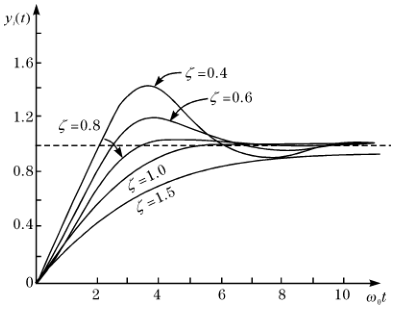
\includegraphics[width=\linewidth]{figs/fig-0038.png}
\caption{图3.4-1}
\end{figure}

\textbackslash\{\}begin\{figure\}[h]\textbackslash\{\}centering\textbackslash\{\}includegraphics[width=0.8\textbackslash\{\}textwidth]\{image.png\} \% Replace image.png with the actual image filename\textbackslash\{\}caption\{图 3.4-1\}\textbackslash\{\}label\{fig:3.4-1\}\textbackslash\{\}end\{figure\}

如果输入是一个正弦式的振荡，和方程 (3.1-11) 所表示的一样，振幅是 $x_m$，角频率是 $\omega$，那么

\[Y_i(s) = \frac{x_m}{s - i\omega} F(s) = \frac{x_m}{s - i\omega} \frac{\omega_0^2}{s^2 + 2\zeta\omega_0 s + \omega_0^2}\]

因此，在 $\zeta < 1$ 的情形里，输出 $y_i(t)$ 就是

\[y_i(t) = x_m F(i\omega) e^{i\omega t} + \frac{x_m}{2iv} \frac{\omega_0^2}{\lambda + i(v - \omega)} e^{(\lambda + iv)t} - \frac{x_m}{2iv} \frac{\omega_0^2}{\lambda - i(v - \omega)} e^{(\lambda - iv)t}\qquad\text{(3.4-11)}\]

这里的 $\lambda$ 和 $v$ 是由方程 (3.4-7) 所给定的。既然对于正的阻尼，$\lambda$ 是负数，所以，稳态的输出也还是方程 (3.4-11) 的第一项。这个事实和我们的普遍性的结果——方程 (2.3-7) 是相符合的。

根据方程 (3.4-5)，这个二阶系统的频率特性就是

\[F(i\omega) = Me^{i\theta} = \frac{1}{[1 - (\omega/\omega_0)^2]} + 2i\zeta(\omega/\omega_0)\]

因此 [4，12]

\[M=\left[\frac{1}{\left[1-\left(\omega / \infty_{0}\right)^{2}\right]^{2}}+\left[2 \zeta\left(\omega / \omega_{b}\right)\right]\right]^{-2} \cdot \tan 0=-\frac{2 \zeta\left(\alpha_{/ w b}\right)}{\left(1-(w / o x)_{3}\right.}\qquad\text{(3.4-12)}\]

这个系统的伯德图就是图 $3 .4-2 。 M$ 的极大值发生在 $\omega / \omega=1$ 附近，这时 M $\frac{1}{2} z$，而 $\theta \ominus \pi / 2$。当 $\omega / \omega \rightarrow \infty$ 时，$\theta \longrightarrow -\pi$，而 $M \square 1 /\left(\omega^{\prime} / \omega\right)$，也可以说 $\log M-$ $-2 \operatorname { l og } ( \omega ^ { \prime } / \omega )$。用声学工程师的术语来说也就是说：对于高频率，斜率为一 $40 \mathrm{db} /+$倍频程。

\begin{figure}[htbp]\centering
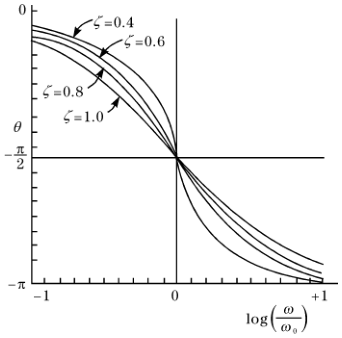
\includegraphics[width=\linewidth]{figs/fig-0040.png}
\caption{图3.4-2}
\end{figure}

\begin{figure}[htbp]\centering
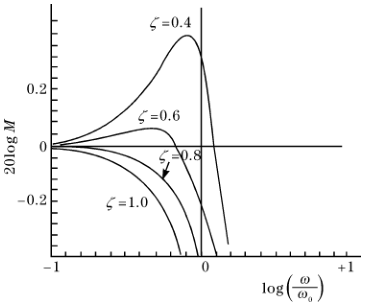
\includegraphics[width=\linewidth]{figs/fig-0039.png}
\end{figure}

aligned\&  图  3.4-2 \textbackslash\{\}\textbackslash\{\}\&   \_(x)array

图 3.4-3 就是这个二阶系统的乃氏图。

其他的物理系统往往也可以近似地看做是二阶系统。液压伺服马达就是一个例子。第 3.3 节里讨论过的回转测速计的更近似于实际运动状态的传递函数就是

\[F(s)=\frac{k s}{\left(s / \omega_{p}\right)^{2}+2 \xi\left(s / \sigma_{s}\right)+1}\]

\textbackslash\{\}begin\{figure\}[h]\textbackslash\{\}centering\textbackslash\{\}includegraphics[width=0.8\textbackslash\{\}textwidth]\{image.png\}\textbackslash\{\}caption\{图 3.4-3\}\textbackslash\{\}end\{figure\}

应该把这个更精确的传递函数和那个在图 3.3-4 中所表示的传递函数比较一下。加速度计的传递函数就是

\[F(s)=\frac{Ks^{2}}{(s/\omega_{0})^{2}+2\zeta(s/\omega_{0})+1}\]

如果把一个电动机当做一个积分元件看待的话（这也就是说，把电压 $v$ 看作输入，把电动机转子的转角 $\phi$ 看作输出量，而不是把转子的速度 $d\phi/dt$ 看作输出），更精确的传递函数就是

\[F(s)=\frac{K}{s(\tau s+1)}\]

也应该把这个传递函数和以前在图 3.3-1 中所表示的那个粗略的近似的传递函数比较一下。以上这些传递函数的分母都是一个二次多项式。这个多项式的各个常数系数的意义和前面讨论过的例子里的系数的意义是类似的。

\begin{figure}[htbp]\centering
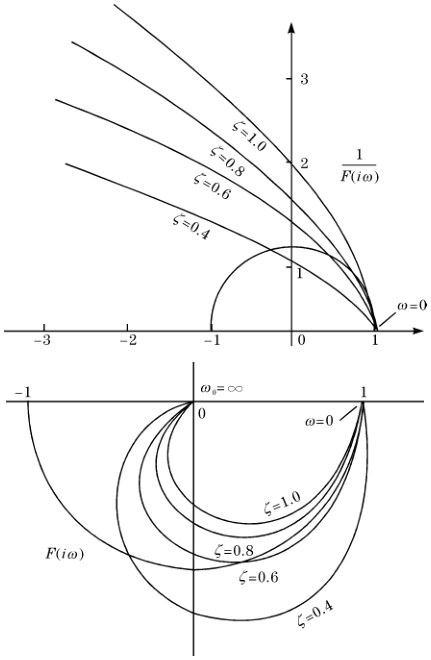
\includegraphics[width=\linewidth]{figs/fig-0041.png}
\caption{图3.4-3}
\end{figure}

\section{3.5 确定频率特性的方法}

在以前各节的讨论里，我们所考虑的问题的性质都是这样的：假定已经知道一个系统的详细的构造，根据这些知识和基本的物理定律算出系统的传递函数 $F(s)$ 和频率特性 $F(i \omega)$。不难看出，这种确定频率特性的方法是一种理论的方法，它的结果的精确度完全依赖于我们对于系统的了解的精确程度。可是，在工程实践中，我们往往对于系统的详细构造知道得很不充分；也有时候，虽然的详细构造知道得很清楚，但是系统过于复杂，以至于使频率特性的理论计算作起来也过分繁重。在这样一些情况中，我们常常用实验方法来确定系统的频率特性。我们最容易想到的方法就是利用方程(2.3-7)所表示的这样一个事实：在频率是 $\omega$ 的正弦式的输入下，稳态输出和输入的比值就是频率特性 $F(i \omega)$。输出的振幅和输入的振幅的比值就是 $M$。输出和输入的相角差就是 $\theta$。因此，如果用实验方法来确定频率特性就必须在所需用的频率范围之内，对于若干特殊的频率值 $\omega$ 测量振幅比值和相角差。事实上，确实也曾经把这个方法用到某些系统上去过，例如，比较简单的油泵系统 ${ }^{[8]}$ 和相当复杂的整个飞机的纵向运动的系统 ${ }^{[6]}$。这个方法的缺点是：对于一个比较宽的频率范围就常常需要对很多不同的频率 $\omega$ 的值做很多的测量。并且有时候也很难测量输出和输入的相角差。

另外一个更有效的方法就是：同时激起所有的频率，而不是对各个频率进行个别的激发。为了达到这个目的，最好的办法就是用一个单位冲量作输入，这时，根据方程(2.3-9)，对于稳定系统来说

\[h(t)=\frac{1}{2 \pi} \int_{-\infty}^{+\infty} F(i \omega) e^{i \omega t} d \omega=\frac{1}{\pi} \int_{0}^{\infty}\left[\operatorname{Re} F(i \omega) \cos \omega t-\operatorname{Im} F(i \omega) \sin \omega t\right] d \omega \quad(3.5-1)\]

其中 $\operatorname{Re}$ 和 $\operatorname{Im}$ 分别表示实数部分和虚数部分的符号。这个方程的第二个等式之所以成立是由于有关系式(3.2-2)的缘故。方程(3.5-1)表明，输入的单位冲量均等地激起了所有的频率（这也就是说，各个频率的振幅都是同一数量级的）。当系统对单位冲量的反应 $h(t)$ 已经知道的时候（我们只要作一次实验就可以测出 $h(t))$，我们就可以用下列公式计算频率特性

\[F(i \omega)=\int_{0}^{\infty} h(t) e^{-i \omega t} d t\qquad\text{(3.5-2)}\]

对于任何一个固定的 $\omega$ 值，我们都可以用数值积分的方法算出这个积分。

然而，实际上，一个理想的冲量是很难真正作出来的。比较实际可行的输入是矩形的脉冲和三角形的脉冲，就像图 3.5-1 所表示的那样。这样一些脉冲当然不能均等地激起所有的频率。但是，如果我们把脉冲的长度 $\tau$ 取得相当小的话，也就可以认为，已经相当理想地达到了均匀地激起所有频率的目的。西门斯(Sea-

mans)和他的同事们就曾经用这种冲量激发的方法去确定一架飞机的频率特性[7]。他们还提出一种根据测量到的输出 $y(t)$ 计算 $F(i\omega)$ 的近似方法。克尔夫曼(Curfman)和格第内尔(Gardiner)[3]把这种处理实验数据的方法又推广到输入是任意形式的情形中去。

\begin{figure}[htbp]\centering
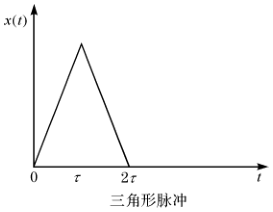
\includegraphics[width=\linewidth]{figs/fig-0043.png}
\caption{图3.5-1}
\end{figure}

\begin{figure}[htbp]\centering
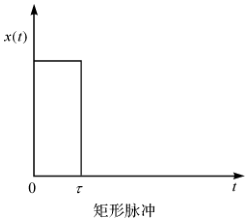
\includegraphics[width=\linewidth]{figs/fig-0042.png}
\caption{图3.5-1}
\end{figure}

矩形脉冲

三角形脉冲

图 3.5-1

\section{3.6 由多个环节组成的系统}

在第 3.1 节、3.3 节和 3.4 节所讨论过的那些系统实际上只不过是某些更复杂的系统的个别环节而已。实际工程中，稳定装置和控制装置所需要的却常常是这种复杂的系统。以飞机的横滚运动为例。通常是用电流作控制副翼转动的信号。这个电流信号就是一个包含放大器和计算装置的输入，在这个组合里当然会包含有某种电路，也还可能包含一些晶体管。这个由放大器和计算装置所组成的组合的运动状态是由它的传递函数 $F_{1}(s)$ 所确定的。再把这个组合的输出取作转动副翼的液压伺服马达的输入。液压伺服马达的运动状态是由传递函数 $F_{2}(s)$ 所描述的。最后，把伺服马达的输出，也就是副翼的转动，取作那个代表飞机的横滚动力特性的系统的输入；假设飞机的动力特性用传递函数 $F_{3}(s)$ 来表示；那么，横滚动力特性的输出就是飞机的横滚运动了。这里，从滚动的控制信号到滚动运动，在系统的各个组合之间有着一系列的联系。如果用 $x(t)$ 表示控制滚动的信号，用 $\Phi(t)$ 表示飞机的横滚角的话，那么，相当的拉氏变换的关系就是

\[\Phi(s)=F_{3}(s) F_{2}(s) F_{1}(s) X(s)\]

因此，整个的横滚控制系统的传递函数就是乘积 $F_{3}(s) F_{2}(s) F_{1}(s)$。从这个例子也还能很清楚地看到这样一个事实：一般说来，传递函数是有量纲的，因为它是两个不同量纲的物理量的比值。在现在的这个例子里，作为输入的滚动信号是一个电流，可是作为输出的横滚角却是一个角度，电流的量纲和角度的量纲当然是不同的。

一般说来，如果一个系统是由 $n$ 个个别的组合串联组成的（图 3.6-1)，并且假设这些组合的传递函数分别是 $F_1(s), F_2(s), \cdots, F_r(s), \cdots, F_n(s)$，而放大系数分别是 $K_1, K_2, \cdots, K_r, \cdots, K_n$，那么，整个系统的传递函数 $F(s)$ 就是

\[F(s)=F_1(s) F_2(s) \cdots F_r(s) \cdots F_n(s)\qquad\text{(3.6-1)}\]

整个系统的放大系数 $K$ 就是

\[K=K_1 K_2 \cdots K_r \cdots K_n\qquad\text{(3.6-2)}\]

从方程(3.6-1)很明显地看出，在一个系统里传递函数 $F(s)$ 的零点和极点也就是各个个别部件的零点和极点的全体 （当然也可能有某一个组合的零点和另外一个组合的极点互相抵消的情形）。因此，如果再用方程 (3.6-2)算出整个系统的放大系数 $K$，传递函数 $F(s)$ 就完全被确定了。

图 3.6-1

系统的频率特性是 $F(i \omega)=M e^{i \theta}$。如果第 $r$ 个部件的频率特性是 $M_r e^{i \theta}$ 的话，那么，根据方程 (3.6-1) 就有

\[\begin{aligned} M e^{i \theta} & =\left(M_1 e^{i \theta_1}\right)\left(M_2 e^{i \theta_2}\right) \cdots\left(M_r e^{i \theta_r}\right) \cdots\left(M_n e^{i \theta_n}\right) \\ & =\left(M_1 M_2 \cdots M_r \cdots M_n\right) e^{i\left(\theta_1+\theta_2+\cdots+\theta_r+\cdots+\theta_n\right)} \end{aligned}\]

所以

\[\begin{aligned} \log M & =\log M_1+\log M_2+\cdots+\log M_r+\cdots+\log M_n \\ \theta & =\theta_1+\theta_2+\cdots+\theta_r+\cdots+\theta_n \end{aligned}\qquad\text{(3.6-3)}\]

由方程 (3.6-3) 就可以理解在伯德图中为什么要采用对数尺度的理由。采用了对数尺度以后，就可以使寻求系统特性的工作大大地简化，因为只要把各个组成部件的伯德图线的坐标简单地叠加起来就行了。

\section{3.7 反馈控制系统的概念及其传递函数}

在这一节里，我们要介绍控制技术中的一个重要概念：反馈的概念。我们将要借助于最简单的系统——常系数线性系统的讨论来引进这个概念。同时，我们还要说明，为什么采用反馈方法就能够使系统大大地增加控制的准确度，并且显著地提高对于控制信号的反应速度。

让我们以控制涡轮发电机的转速问题为例来说明这一概念的重要性。在这里，最重要的要求就是使转速非常接近于额定的固定数值，而不要发生较大的偏差。对于这个问题来说，最初等的处理方式就是所谓开路控制的方法，采用这种控制方法的时候，我们就必须随时设法使汽涡轮机所产生的转矩、发电机本身所

\begin{figure}[htbp]\centering
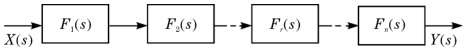
\includegraphics[width=\linewidth]{figs/fig-0044.png}
\caption{图3.6-1}
\end{figure}

需要的转矩和负载转矩处于平衡状态，具体地说，我们可以这样做：随时用仪表测量负载的数值，并且随时根据测量的结果调节汽涡轮机的阀门。但是，可以想象到，这种平衡的方法不可能是完全精确的，总会存在一个偏差转矩 $x(t)$。这个偏差转矩的存在就要使发电机的转动产生加速度。如果我们用 $y(t)$ 表示实际转速和额定转速之间的偏差，用 $I$ 表示发电机的转动部分的转动惯量，用 $c$ 表示摩擦损失的阻尼系数。那么，微分方程就是

\[I \frac{d y}{d t}+c y=x(t)\qquad\text{(3.7-1)}\]

图 3.7-1 就是这个开路控制系统的方块图。我们看到，这个系统与本章研究过的一阶系统是相似的。这个系统的时间常数是 $I / c$，偏差转速的稳态值和偏差转矩的比值是 $1 / c_{\circ}$ 因为涡轮发电机的转子的重量很大，所以 $I$ 是一个

很大的数值；但是，因为摩擦损失相当小，所以 $c$ 也是一个很小的数值；由此可见，时间常数 $I / c$ 就是一个非常大的数值，这也就意味着，任意一个转速的偏差都要保持很久的时间，而且很难使它迅速地消失掉。不仅如此，由于系统的放大系数 $1 / c$ 很大，所以，如果希望偏差转速相当小，就必须要求偏差转矩极端地微小。不言而喻，这样一个目的在于维持发电机转速不变的开路控制系统，在实际工程中是十分无用的。

现在，我们再来看一看，把开路系统改为具有反馈作用的所谓闭路控制系统以后，系统的运转性能发生怎样的变化。进行闭路控制的时候，我们使对系统起控制作用的力矩与被控制的变数发生关系。这也就是说，蒸汽阀门的调节不仅要依据负载的情况，而且也还要和偏差速度 $y$ 有关系。假定控制转矩的第二个组成部分与 $y$ 成比例，比例常数是 $-k(k>0)$。当转速过高，也就是 $y>0$ 的时候，就把阀门关闭起来，同时，使发电机加速的转矩减少 $k y$。如果转速过低，也就是 $y<0$ 的时候，使发电机加速的力矩就会增加 $k y$。因此，现在 $y$ 的微分方程就变为

\[I \frac{d y}{d t}+c y=x-k y\]

也就是

\[I \frac{d y}{d t}+(c+k) y=x(t)\qquad\text{(3.7-2)}\]

方程(3.7-2)与(3.7-1)唯一的不同之点就是把 $c$ 换成了和数 $c+k$。现在，时间常数就变为 $I /(c+k)$，而偏差转速的稳态值与不变的偏差转矩的比值就变成 $1 /(c+$ $k$ )。因此，与开路控制系统相比较，只要我们使 $k$ 比 $c$ 大得很多的话，就可以使时间常数和偏差转速大大地减小。因为 $c$ 很小，所以，实际上使 $k \gg c$ 也是很容易的。从这个例子可以看到，其余的条件都不必加以改变，只要把开路控制系统加上一个反馈线路使它变为闭路控制系统的话，系统的反应速度和控制的精确度就可以提高很多，因而也就可以大大地改进控制系统的性能。

\begin{figure}[htbp]\centering
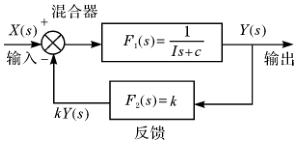
\includegraphics[width=\linewidth]{figs/fig-0045.png}
\caption{图3.7-2}
\end{figure}

图 3.7-2 就是上述闭路控制系统的方块图。图中代表汽轮发电机的原有的传递函数 $F_{1}(s)$和图 3.7-1 里的 $F_{1}(s)$ 还是相同的。在图 3.7-2里，我们还引进了控制工程中的一个规定：在表示混合器（也有时称为比较元件）的符号“$\otimes$”旁边必须用加号或者减号注明混合器对于相当的输入信号的作用。例如图 3.7-2 中的混合器的输入信号是 $X(s)$ 和 $kY(s)$，根据图上标明的作用符号，混合器的输出信号就是 $X(s)-kY(s)$。如果在两条线路的接合点上只画了一个圆点，就表示对那里的信号只有“测量”作用，并没有相加或相减的作用（在这一点上表示控制系统的构造的方块图和普通的电路图是不相同的），因此，图 3.7-2 表示偏差转速 $y$ 在系统的输出部分上被测量了，而且用测量的结果产生出控制转矩 $ky$。从图 3.7-2 可以看出，闭路控制系统中包含了一个反馈线路 $\left[F_{2}(s)\right.$ 所在的线路 $\left.\right]$。因此，把整个控制系统称为反馈控制系统是很恰当的。

虽然在上面所分析的这个简单的例子里，我们是用把方程 (3.7-1) 和 (3.7-2)加以比较的方法来说明反馈控制系统的优点，可是，对于更复杂的系统，只用到传递函数的概念的分析方法也是很方便的，在下面，我们就来说明这种分析方法。

我们来考虑一个一般的反馈控制系统，这个系统的构造和图 3.7-2 所表示的系统相同，但是 $F_{1}(s)$ 和 $F_{2}(s)$ 这两个传递函数是任意的。$F_{1}(s)$ 称为前向线路的传递函数，$F_{2}(s)$ 称为反馈线路的传递函数。在一般的情况下，输出 $Y(s)$ 与输入 $X(s)$ 之间的关系

\[Y(s)=F_{1}(s)\left[X(s)-F_{2}(s) Y(s)\right]\]

如果我们把 $Y(s)$ 从这个方程解出来，就得

\[\frac{Y(s)}{X(s)}=\frac{F_{1}(s)}{1+F_{1}(s) F_{2}(s)}=F_{c}(s)\qquad\text{(3.7-3)}\]

这里，$F_{c}(s)$ 就是系统的传递函数，也就是整个系统的输出与输入的比值。

为了以后讨论的方便，把 $F_{1}(s)$ 和 $F_{2}(s)$ 的放大系数 $K_{1}$ 和 $K_{2}$ 也明显地表示出来，我们把 $F_{1}(s)$ 和 $F_{2}(s)$ 写成

\[\begin{aligned} & F_{1}(s)=K_{1} G_{1}(s) \\ & F_{2}(s)=K_{2} G_{2}(s) \end{aligned}\qquad\text{(3.7-4)}\]

因为放大系数 $K$ 的量纲和传递函数 $F(s)$ 的量纲相同，所以，这里的 $G(s)$ 显然是无量纲的函数。因为 $G(s)$ 的零点和极点也就是 $F(s)$ 的零点和极点，所以，所有关于 $F(s)$ 的“构造”的知识都包含在 $G(s)$ 里面了。由于这样的做法，在以后的讨论中我们常常把传递函数对系统所起的作用看做是两个分别的作用的结果：一个是放大系数 $K$ 的大小所起的作用，另外一个是零点和极点的位置所起的作用，也就是 $G(s)$ 所起的作用。把作用进行这种划分的理由，还因为有以下的事实：如果在一个系统 $F(s)$ 中包含有由放大器和计算器组成的计算部件，那么，$G(s)$ 只与计算器有关，而与放大器无关；系统的放大系数可认为只决定于放大器。此外，在系统的设计里，这两种不同的控制作用常常是互不相关的。因此，$G(s)$ 和 $K$ 可以分别地加以改变，同时也可以给以分别的考虑。

利用方程 (3.7-4)，(3.7-3) 就可以写成

\[\frac{Y(s)}{X(s)} = F_{s}(s) = \frac{K_{1} G_{1}(s)}{1 + K_{1} G_{1}(s) K_{2} G_{2}(s)} = \frac{1}{\left[1/K_{1} G_{1}(s)\right] + K_{2} G_{2}(s)}\qquad\text{(3.7-5)}\]

假定由方程 (3.1-10) 定义的偏差信号 $e(t)$ 的拉氏变换是 $E(s)$，则

\[\frac{E(s)}{Y(s)} = \frac{X(s) - Y(s)}{Y(s)} = \frac{1}{F_{s}(s)} - 1 = \frac{1}{K_{1} G_{1}(s)} - \left[1 - K_{2} G_{2}(s)\right]\qquad\text{(3.7-6)}\]

对于图 3.7-3 所表示的那种简单的反馈控制系统来说，反馈线路的传递函数 $F_{2}(s)$ 就是 1，这也就是说，在进行反馈控制作用的时候，仅仅对输出作了测量，并且直接把测量的结果用作反馈信号，并没有把测量结果加以任何的改变。在这种简单的情况下，方程 (3.7-5) 和 (3.7-6) 就简化为

\begin{figure}[htbp]\centering
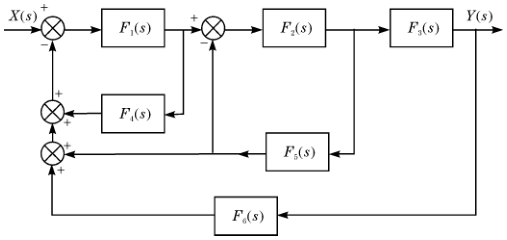
\includegraphics[width=\linewidth]{figs/fig-0047.png}
\caption{图3.7-4}
\end{figure}

\[\frac{Y(s)}{X(s)} = F_{s}(s) = \frac{KG(s)}{1 + KG(s)} = \frac{1}{\left[1/KG(s)\right] + 1}\qquad\text{(3.7-7)}\]

和

\[\frac{E(s)}{Y(s)} = \frac{1}{KG(s)}\qquad\text{(3.7-8)}\]

在较为复杂的系统中，反馈线路常常不是一个，而有很多个，如图 3.7-4 所示。这里共有三个反馈线路 $F_{4}(s)$，$F_{5}(s)$ 和 $F_{6}(s)$。因为 $Y(s)$ 是主受控量，所以 $Y(s)$ 的反馈线路 $F_{6}(s)$ 常称之为为主反馈，而 $F_{4}(s)$ 和 $F_{5}(s)$ 线路则常称为局部反馈或内反馈。至于 $F_{2}(s)$，因为它位于前向线路内，因此它不是反馈线路。

\textbackslash\{\}begin\{figure\}[h]\textbackslash\{\}centering\textbackslash\{\}includegraphics[width=\textbackslash\{\}textwidth]\{图3.7-4\}\textbackslash\{\}caption\{图 3.7-4\}\textbackslash\{\}end\{figure\}

\begin{figure}[htbp]\centering
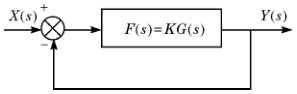
\includegraphics[width=\linewidth]{figs/fig-0046.png}
\caption{图3.7-3}
\end{figure}

应用上述基本公式，可以简捷地写出这个系统的传递函数。先从最后一部分 $F_{2}(s)$ 和 $F_{5}(s)$ 着手。由于 $F_{5}(s)$ 是 $F_{2}(s)$ 的反馈，故根据 (3.7-3) 式它们的等价传递函数是

\[H_{2}(s)=\frac{F_{2}(s)}{1+F_{2}(s) F_{5}(s)}\qquad\text{(3.7-9)}\]

用 $H_{2}(s)$ 代替 $F_{2}(s)$ 和 $F_{5}(s)$ 后，显然，图 3.7-4 可变换成图 3.7-5。此时 $F_{1}(s)$ 和 $F_{3}(s)$ 的等价传递函数是

\[\begin{array}{llll} \text { X(s) } & H_{1}(s) & H_{2}(s) & F_{3}(s) \\ & & & Y(s) \end{array}\]

图 3.7-5

\[H_{1}(s)=\frac{F_{1}(s)}{1+F_{1}(s) F_{1}(s)}\qquad\text{(3.7-10)}\]

按并联线路相加，串联线路相乘的原理，图 3.7-5 又可变换为图 3.7-6。于是，图 3.7-4 的系统传递函数就可写成

\[F(s)=\frac{H_{1}(s) H_{2}(s) F_{3}(s)}{1+H_{1}(s) H_{2}(s) F_{5}(s)+H_{1}(s) H_{2}(s) F_{3}(s) F_{6}(s)}\qquad\text{(3.7-11)}\]

将式 (3.7-9) 和 (3.7-10) 代入式 (3.7-11) 并化简后，得到系统传递函数的最后形式

\[\begin{aligned} F(s)= & \frac{F_{1}(s) F_{2}(s) F_{3}(s)}{1+F_{1}(s) F_{1}(s)+F_{2}(s) F_{5}(s)+F_{1}(s) F_{2}(s) F_{5}(s)} \\ & +F_{1}(s) F_{2}(s) F_{3}(s) F_{6}(s)+F_{1}(s) F_{2}(s) F_{1}(s) F_{3}(s) \end{aligned}\]

这个传递函数是比较复杂的，但由反馈变换规律得之并不难。

\[\begin{array}{llll} \text { X(s) } & H_{1}(s) & H_{2}(s) & F_{3}(s) \\ & 1+H_{1}(s) H_{2}(s) F_{3}(s) & & Y(s) \end{array}\]

图 3.7-6

\begin{figure}[htbp]\centering
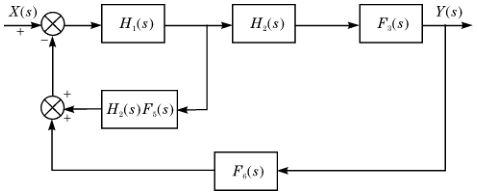
\includegraphics[width=\linewidth]{figs/fig-0048.png}
\caption{图3.7-4}
\end{figure}

\begin{figure}[htbp]\centering
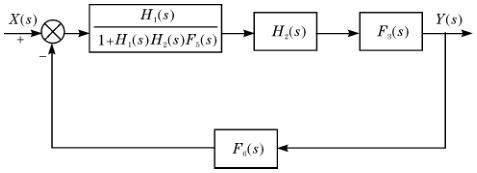
\includegraphics[width=\linewidth]{figs/fig-0049.png}
\caption{图3.7-6}
\end{figure}

\[\begin{gathered} \text { 第三章 输入、输出和传递函数 } \\ \cdot 99 \cdot \end{gathered}\]

\section{3.8 交流系统}

以前各节的讨论中假定输入和输出量都是真实地代表所研究诸量的物理实质，它们作为信息互相传递的时候未加以任何变换，而以其自然的时间函数形式去相互作用。但在实际问题中，常将输入量或输出量转变为其他形式的信号以利于信息传输或技术上的实现。最常见的信号变换方式是所谓载波调制，即将真实缓变信号 $x(t)$ 变为高频正弦波信号的包络线，随高频信号的传递，真实信号 $x(t)$ 也就随之被送走。这种方法广泛用在无线电遥控或遥测系统中。载波调制的办法很多，可以是调频，调相等，上面所指的仅为其中的一种，即幅度调制。

在工业中，也有一些控制系统采用了交流信号的传输方法，而且有的执行机构能够直接使用这些被调制了的高频信号，而无需预先将高频信号内所包含的原来信号检出（反调制）。例如交流电机（二相伺服马达）就是这类执行机构的一种。下面我们将以交流系统为例来讨论载波信号作为输入和输出的系统的处理方法 ${ }^{[5]}$。

现在我们来考虑图 3.8-1 所画的伺服系统。这个系统的设计目的就是要求电动机的转角 $\phi$ 随着输入信号变化。系统的输出角度 $\phi$ 是用一个电位计来测量的。电位计上的电压就是反馈信号。在这个系统内的电动机，放大器以及电位计上的电流和电压都是已调幅的正弦波，也就是说，它们都是频率不变而振幅随时间变化的正弦函数。假定他们的频率是 $\omega$。基本的交流电流由振荡器供给。这就是交流伺服系统的一个例子。在一定的条件下（下面我们就要讨论到这些条件），以前的理论中有很大一部分也可以应用到这种系统上来。

\begin{figure}[htbp]\centering
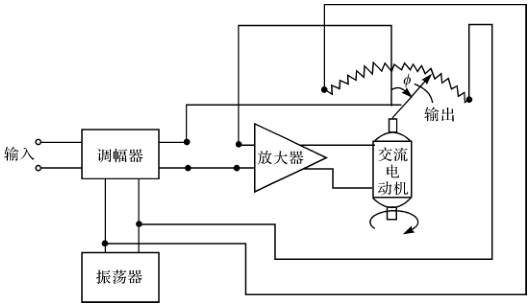
\includegraphics[width=\linewidth]{figs/fig-0050.png}
\caption{图3.8-1}
\end{figure}

输入

调幅器

输出

放大器

交流电动机

振荡器

图 3.8-1我们先来考虑常系数线性系统在已调幅的正弦式的输入信号作用下的一般的稳态理论。这里所说的“稳态”是对于调幅信号是单纯的正弦式时间函数的情况而言的。假设未调幅的载波是 $\cos \omega t$。在这里我们虽然把载波的相角取作零，但是并不影响讨论的普遍性。既然已经把载波写成实数形式，为了方便起见显然应该把调幅信号写成复数形式 $e^{i \omega t}$。这时已调幅的载波就是

\[x(t)=e^{i \omega t} \cos \omega t=\frac{1}{2}\left[e^{i\left(\omega t-\omega_{0} t\right) t}+e^{i\left(\omega t-\omega_{0} t\right) t}\right]\qquad\text{(3.8-1)}\]

如果系统的传递函数是 $F(s)$，按照方程 $(2.3-7)$ 系统的稳态输出 $\left[y(t)\right]_{\mathrm{s}}$ 就应该是

\[\left[y(t)\right]_{\mathrm{s}}=\frac{1}{2}\left[F\left(i \omega+i \omega_{0}\right) e^{i \omega_{0} t}+F\left(i \omega-i \omega_{0}\right) e^{-i \omega_{0} t}\right] e^{i \omega t}\qquad\text{(3.8-2)}\]

对于实际的系统，函数 $F(s)$ 通常是 $s$ 的两个实系数多项式的比值。所以，正如方程 (3.2-2)所表示的那样

\[F(-i \omega)=\overline{F(i \omega)}\qquad\text{(3.8-3)}\]

这里，用符号上面的横线表示复共轭值。因此，方程 $(3.8-2)$ 的右端就可以写成

\[\frac{1}{2}\left[F^{*}(i \omega) e^{i \omega_{0} t}+\overline{F^{*}\left(-i \omega\right) e^{-i \omega_{0} t}}\right] e^{i \omega t}\]

其中

\[F^{*}(i \omega)=F\left(i \omega+i \omega_{0}\right)\qquad\text{(3.8-5)}\]

现在我们假设系统具有以下的性质

\[F\left(i \omega_{0}+i \omega\right)=\overline{F\left(i \omega_{0}-i \omega\right)}\qquad\text{(3.8-3)}\]

这时，表示式 $(3.8-4)$ 就可以写成下列形状

\[F^{*}(i \omega) e^{i \omega t} \cos \omega t\]

这个结果表明：如果另外有一个对于频率是 $\omega$ 的输入，频率特性是 $F^{*}(i \omega)$ 的系统，当条件式 $(3.8-6)$ 被满足时，原来系统对于已调幅的载波式 $(3.8-1)$ 的振幅的频率特性 $F^{*}\left(i \omega\right)$ 与那个系统的频率特性是完全相同的。利用线性系统的可叠加性，可以把以上的讨论结果推广到更一般的输入函数上去，因为很多种输入函数都可以用傅里叶级数或傅里叶积分表示出来，如果在输入调幅信号 $x(t)$ 的傅里叶谱的最重要的部分上，方程 $(3.8-6)$ 至少都能近似地成立，那么，已调幅的输出信号的振幅对于输入信号而言的频率特性差不多就是 $F^{*}(i \omega)$。反馈系统的性能可以完全由频率特性所决定，既然现在频率特性的近似值是 $F^{*}(i \omega)$，所以，利用频率特性研究系统性能的方法完全可以应用到交流系统上来，唯一的区别只是在进行分析时把 $F(i \omega)$ 用 $F^{*}(i \omega)=F\left(i \omega+i \omega_{0}\right)$ 来代替。

如果我们不考虑某些过于简单的情形 （例如，单纯的电阻），那么，根据方程 (3.8-3)就有

\[F\left(i \omega+i \omega_{0}\right)=\overline{F(-i \omega-i \omega_{0})}\qquad\text{(3.8-6)}\]

这个关系和条件式 $(3.8-6)$ 是不同的，所以，不可能对于所有的实 $\omega$ 值都能精确地满足条件式(3.8-6)，或者稍微改变一下我们的看法，可以这样说，如果两个物理系统的频率特性分别是 $F^{*}(i \omega)$ 和 $F(i \omega)$，那么，关系式(3.8-5)不可能对于所有实 $\omega$ 值都严格地被满足。但是，对于特定的输入信号而言，在它的傅里叶谱的主要部分上，完全可能有，而确实也往往有一个足够大的 $\omega$ 的范围，在这个范围之内，条件式(3.8-5)可以近似地被满足。在以下的讨论中我们就会看到这种情况。

我们考虑一个频率是 $\omega^{\prime}$ 时由电感 $L$ 与电容 $C$ 串联起来的阻抗 $Z$

\[Z=i L \omega^{\prime}+\frac{1}{C_{i} \omega^{\prime}}=i L \omega^{\prime}\left(1-\frac{1}{L C \omega^{\prime 2}}\right)\]

如果我们使 $L$ 和 $C$ 的大小满足下列条件

\[\omega_{b}^{2}=\frac{1}{L C}\qquad\text{(3.8-7)}\]

那么

\[Z=i L \omega^{\prime}\left(1-\frac{\omega_{b}^{2}}{\omega^{\prime 2}}\right)=i L(\omega^{\prime}-\omega) \quad\left(1+\frac{\omega}{\omega^{\prime}}\right)\]

如果 $\omega^{\prime}-\omega=\omega$ 相当小，或者说 $\omega+\omega$ 与 $\omega$ 相当接近，则

\[Z \triangleq i 2 L\left(\omega^{\prime}-\omega_{\mathrm{b}}\right)=i 2 L \omega\]

这个关系表明：当频率是 $\omega^{\prime}=\omega+\omega$ 时，满足方程(3.8-7)的电感 $L$ 与电容 $C$ 的串联组合的阻抗差不多就等于电感 $2 L$ 在频率是 $\omega$ 时的阻抗。

类似地，如果满足条件式(3.8-7)，电感 $L$ 与电容 $C$ 的并联组合的阻抗 $Z$ 也就满足下列关系

\[\frac{1}{Z}=\frac{1}{i L \omega}+i C \omega^{\prime} \triangleq i 2 C\left(\omega^{\prime}-\omega_{\mathrm{b}}\right)=i 2 C \omega\]

因此，在频率是 $\omega^{\prime}=\omega+\omega$ 时，$L$ 与 $C$ 的并联组合的阻抗差不多就等于电容 $2 C$ 在频率是 $\omega$ 时的阻抗。

一个单纯电阻的阻抗当然是与频率没有关系的，所以它在频率是 $\omega+\omega$ 时的阻抗和它在频率是 $\omega$ 时的阻抗是相等的。因此，如果已经有了一个由电感，电容和电阻组成的物理系统，这个系统的传递函数是 $F^{*}(s)$。我们把这个系统里的每一个电感 $L$ 都用电感 $L_{1}=\frac{1}{2} L$ 与电容 $C_{1}=2 / L \omega^{2}$ 的串联组合来代替；把系统中的每一个电容 $C$ 都用电容 $C_{2}=\frac{1}{2} C$ 和电感 $L_{2}=2 / C \omega^{2}$ 的并联组合来代替；所有电阻都不予变动；这样一来，我们就得到一个新的系统，这个系统的传递函数就是 $F(s)$，只要 $\omega$ 值足够小，方程 (3.8-6) 的关系就可以近似地满足。以上所讲的由 $F^{*}(s)$ 变到 $F(s)$ 的做法就称为把传递函数提高一个频率 $\omega$。

如果 $\omega$ 是振荡器所供给的电流的频率，很显然，系统中各个电流和各个电压都是载波 $\cos \omega t$ 的已调幅波。因此，根据以上的结果立刻就得出下列的方法：如果我们想为一个交流系统设计一个放大器，我们只要先为一个直流系统设计一个合适的放大器，然后再按照上述的方法把系统提高一个频率 $\omega_{\mathrm{B}}$ 就可以了。

正如我们所提到的那样，以上的讨论中用到不少各种各样的近似方法，所以得到的结果也不是绝对精确的。如果想对交流伺服系统作一个详尽严密的讨论，就必须把这些近似方法所引起的误差加以分析，然后根据实际问题所要求的精度，确定这些方法的可用程度。

\section{参考文献}

[1] 赵民义，复变函数论，高等教育出版社，1960.

[2] 刘豹，自动调节理论基础，上海科学技术出版社，1963.

[3] Cufman，H. J.，Gardiner，R. A.，NACA TR 984，1950.

[4] James，H. M.，Nichols，N. B，Phillips，R. S.，\& others，Theory of Servomechanisms，Massachusetts Institute of Technology Radiation Laboratory Series，25，New York，1947.

[5] MacColl，L. A.，Fundamental Theory of Servomechanisms，D. van Nostrand Company，Inc.，New York，1945.

[6] Milliken，W. F.，J. Aeronaut. Sci.，14(1947)，493.

[7] Seamans，R. C.，Blasingame，B. P.，Clementson，G. C.，J. Aeronaut. Sci.，17(1950)，22.

[8] Shames，H.，Himmel，S. C.，Blivas，D.，Frequency response of positive-displacement variable-stroke fuel pump，NACA TN 2109.1950.

[9] Smith，O. J. M.，Feedback Control Systems，McGraw-Hill，New York，1958.

[10] Gardner，M. F. \& Barnes，J. L.，Transients in Linear Systems，McGraw-Hill，1947.

[11] Лаврентьев，М. А.，Шабат，Б. В.，Методы теории функций комплексного переменного，М. Л.，1958，（复变函数论方法，施祥林、夏定中译，人民教育出版社，1956.)

[12] Айзерман，М. А.，Введение в динамику автом атического регулирования двигателей，Машгиз，1950.

[13] Воронов，А. А.，Элементы теории автоматического регулирования，1950.

[14] Андронов，А. А.，Витт А. А.，Хайкин С. Э，Теория колебаний，М. -Л.，1959.

[15] Солодовников，В. В.，Основы автоматического регулирования теории，Машгиз，1954. （自动调整原理，王众托译，水利电力出版社，1957.)

[16] Остославский，И. В.，Калагев，Г. С. Продольная устойчивость и уравняемость самолета，Москва，1951.

[17] Солодовников，В. В.，Топчев，Ю. М.，Крутикова，Г. В.，Частотные методы построения переходных процессов，М. -Л.，1955.

[18] фельдбаум，А. А. Электрические системы автоматического регулирования，Оборониз，1957. （电的自动调节系统，章燕申、金兰译，国防工业出版社，1958.)

<html><body>

\chapter{第四章 控制系统分析}

假定一个控制系统的结构为已知，求出系统的运动方程之后，对这个系统的动态性能进行研究并给出评价，这就是分析问题。至于如何设计这个系统，使它具有指定的性能，满足某些特定的要求，这就属于综合问题的范畴了。研究控制理论的最终目的是学会设计系统。但是，分析是综合的基础。对于一个系统的运动规律，只有了解了它的特性之后，才有可能进而改造它，使它满足我们的需要。通过对大量系统的分析，我们又可以总结出一些典型性的共同规律，后者又指导我们如何去设计具体系统。总之，我们要从分析理论开始。

对控制系统的第一个要求是稳定性。从物理意义上说，就是要求控制系统能稳妥地保持预定的工作状态，在各种不利因素的影响下不至于摇摆不定，不听指挥，分析系统的稳定性是一个老问题。早在十九世纪末期，在力学中就广泛研究了运动的稳定性问题，研究过这一问题的有法国数学家潘卡来和俄国数学家李雅普诺夫。他们所提出的理论和方法直到今天仍不失其意义而为大家所广泛使用 ${ }^{[1,37]}$。在自动控制理论中也沿用了他们的理论，但在计算方法上有所发展。本章内我们首先介绍稳定性的古典定义和几种系统稳定性的判据准则。然后再研究其他几种动态性能。

\section{4.1 稳定性定义及李雅普诺夫直接方法}

现代力学和控制理论中，至今沿用李雅普诺夫早在 1892 年提出的稳定性定义 ${ }^{[37]}$。下面我们可看到，这个定义的优点是它反映了客观存在着的大量实际问题的特点，并且把一个定性问题转变为一个定量分析问题去研究。

设受控对象的运动方程组是

<img/>\[\begin{aligned}&amp; \frac{d x_{1}}{d t}=f_{1}\left(x_{2}, x_{2}, x_{3}, \cdots, x_{n}, t\right) \\&amp; \frac{d x_{2}}{d t}=f_{2}\left(x_{1}, x_{2}, x_{3}, \cdots, x_{n}, t\right) \\&amp; \cdots \\&amp; \frac{d x_{n}}{d t}=f_{n}\left(x_{1}, x_{2}, \cdots, x_{n}, t\right)\end{aligned}\]

而 $\boldsymbol{x}(t)=\left(x_{1}(t), x_{2}(t), \cdots, x_{n}(t)\right)$ 是它的某一特定的运动，即后者是方程组

</body></html>

(4.1-1)的特解，初始条件是 $x(b)=x_{0}$。方程组右端的诸函数 $f_{i}$ 是有界，连续可微和各自变量的单值函数。对一个特定运动的稳定性定义可叙述如下：若给定一个任意正数 $\varepsilon>0$，总存在一个大于零的数 $\delta$，当初始条件 $x_{0}$ 在 $t=b$ 时刻的变化 $\delta x_{0}$ 之长度 $\|\delta x_{0}\|$ 小于 $\delta$ 时，方程组(4.1-1)的相应的解的变化在 $t \geqslant b$ 的任何时刻 $\|\delta x(t)\|$ 总小于 $\varepsilon$，则称方程组(4.1-1)的这一特定运动是稳定的。现用图 4.1-1来说明这一定义。设系统的初始状态为 $x$，那么式(4.1-1)有唯一解 $x(x)$，图中粗线表示这个特定的运动：现将运动的初始条件 $x$ 加以改变，其变化为 $\delta x_{0}$，即新的初始条件为 $x+\delta x_{0}$。这一新的初始条件对应一个新的运动 $z(t)$，$z(b)=x+\delta x_{0}$。如果对任意给定半径为 $\varepsilon$ 的“球体”，在任何时刻 $t$ 以 $x(t)$ 为球心，沿此特定运动迁移，可以在 $x$ 附近指出一个以 $\delta$ 为半径的球，在 $b$ 时刻自球内的任何点出发的运动轨线，以后对任何时刻 $t \geqslant b$，总走不出 $\varepsilon$ 球的范围，此时称运动 $x(t)$ 为稳定。反之，则称此运动 $x(t)$ 为不稳定。其次，若存在一个 $\delta$ 球，$\delta>0$，以其内任意点为出发点的运动均随时间的增大而无限趋于 $x(t)$，这时称 $x(t)$ 为渐近稳定。对这一定义，我们应注意下面几点：首先，这一定义包括了 $t>b$ 的一切时刻的系统的行为，$t \rightarrow \infty$ 也包括在内；其次，定义中只谈特定运动的稳定性，而不提系统的稳定性，这是因为一般系统中常可能同时存在两类运动，一类是稳定的，另一类却是不稳定的。这时所谓系统的稳定性即没有意义了。只有线性系统是例外，在这里各种不同的运动具有共性，要么全体稳定，要么全体不稳定。所以，只有对线性系统可以一般地提系统是否稳定。这一点对于初学者十分重要，要避免混淆。当然，也有一类特殊的非线性系统，它的一切运动都稳定，称为系统全局稳定或绝对稳定。

\begin{figure}[htbp]\centering
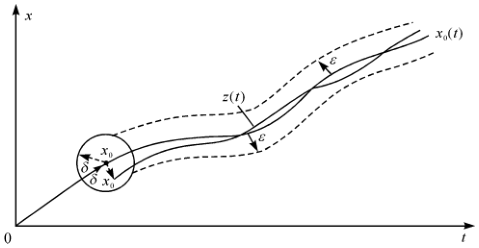
\includegraphics[width=\linewidth]{figs/fig-0051.png}
\caption{图4.1-1}
\end{figure}

$x$

\[z(t)\]

\[x_{s}(t)\]

$0$

$t$

图 4.1-1

当已知系统的运动方程式后，如何用分析方法去判断某一运动的稳定性呢？李雅普诺夫稳定性理论对这一问题提出了两个判定原则：一次近似判据方法和直接方法。为了介绍这两个方法，须对原方程组做一些变换。

令 $x(t)$ 是对应于初始条件 $x$ 的运动，而 $z(t)$ 是对应于初始条件 $x+\delta x_{0}$ 的运动。现取 $\delta \mathbf{x}(t)=\mathbf{z}(t)-\mathbf{x}(t)$，它应该满足下列向量方程式

\[\begin{aligned}\frac{d \delta \mathbf{x}(t)}{d t} & =f(\mathbf{z}(t), t)-f(\mathbf{x}(t), t) \\& =f(\mathbf{x}(t)+\delta \mathbf{x}(t), t)-f(\mathbf{x}(t), t) \\& =g(\delta \mathbf{x}(t), t), \delta \mathbf{x}(t)\end{aligned}\qquad\text{(4.1-2)}\]

当 $\delta \mathbf{x}_{0}=0$ 时，显然 $\delta \mathbf{x}(t) \equiv 0$。因此，常称 $\mathbf{x}(t)$ 或 $\delta \mathbf{x}(t) \equiv 0$ 的运动为未受扰运动，而 $\mathbf{z}(t)$ 或 $\delta \mathbf{x}(t) \neq 0$ 的运动称为受扰运动。由此可知，研究方程组 (4.1-1) 中 $\mathbf{x}(t)$的运动的稳定性与研究方程式 (4.1-2) 的解 $\delta \mathbf{x}(t) \equiv 0$ 的稳定性等价。所以，通常以研究式 (4.1-2) 的零解稳定性代替前者。

由于假定 $f_{i}\left(x_{1}, \cdots, x_{n}, t\right)$ 是连续可微函数，所以当 $\delta \mathbf{x}(t)$ 的各个分量为足够小时，式 (4.1-2) 右端可以展成

\[\frac{d \delta \mathbf{x}}{d t}=A(t) \delta \mathbf{x}+r(\delta \mathbf{x}, t)\qquad\text{(4.1-3)}\]

其中 $A(t)=\left(a_{i j}(t)\right)$ 为 $n \times n$ 阶方阵，向量 $\mathbf{r}(t)$ 包括二次和一切大于二次的项的总和，方程式

\[\frac{d \mathbf{y}}{d t}=A(t) \mathbf{y}\qquad\text{(4.1-4)}\]

称为对方程式 (4.1-2) 和 (4.1-3) 的一次近似。李雅普诺夫第一近似方法是首先研究线性方程 (4.1-4) 的稳定性，然后再根据式 (4.1-4) 的稳定性推知式 (4.1-2) 的零解稳定性。关于这一问题我们将在下节内详细讨论。

为了了解李雅普诺夫直接方法，先引进几个概念。

在零点附近连续可微的 $n$ 元函数 $V\left(y_{1}, \cdots, y_{n}\right)$ 称为正定函数，是指存在一个以原点为中心的 $h$ 球 $\|y\| \leqslant h$，使在球内

\[V(\mathbf{y})\left\{\begin{array}{l}>0, \quad \mathbf{y} \neq \mathbf{0} \\=0, \quad \mathbf{y}=\mathbf{0}\end{array}\right.\]

若在此球内当 $\mathbf{y} \neq 0$ 时 $V \geqslant 0$，则称 $V(\mathbf{y})$ 为非负。若前式内之符号“大于”改为“小于”则称 $V(\mathbf{y})$ 为负定。当在球内 $V \leqslant 0$ 时称它为非正。

现在我们研究自治系统

\[\frac{d \mathbf{y}}{d t}=f(\mathbf{y}), \quad f(\mathbf{0})=\mathbf{0}\qquad\text{(4.1-5)}\]

的零解稳定性。直接方法的判别准则则是:

(1) 若对方程式 (4.1-5)，能找到一个正定连续可微函数 $V(\mathbf{y})$，使得方程式 (4.1-5) 所决定的 $V$ 的全导数

\[\frac{d V}{d t}=\sum_{i=1}^{n} \frac{\partial V}{\partial y_{i}} \frac{d y_{i}}{d t}=\sum_{i=1}^{n} \frac{\partial V}{\partial y_{i}} f_{i}(\mathbf{y})=\left(\operatorname{grad} V, f(\mathbf{y})\right)\]

是非正，则方程(4.1-5)的零解稳定。

(2) 若上面找出的正定函数 $V$ 的全导数为负定，则方程 (4.1-5) 的零解渐近稳定。

(3) 如果对方程式 (4.1-5) 能找到一个函数 $V(\mathbf{y})$，其相应的全导数为正定，而在以原点为中心的任意小球内函数 $V$ 总能取到正值，则方程式的零解是不稳定的。

上面三条准则的证明方法类似，这里只对第一个判别准则做一几句说明 （图 4.1-2)。

设 $V(\mathbf{y})$ 在 $h$ 球内 $(\|\mathbf{y}\| \leqslant h)$ 为正定，而 $\frac{d V}{d t}$ 非正。此时对任意小的 $\varepsilon>0$，令

\[m=\min _{\varepsilon \leqslant\|\mathbf{y} \leqslant h} V(\mathbf{y})\]

因为 $V(\mathbf{y})$ 在原点为零，所以在以 $\varepsilon$ 为半径的球内必定能找到一个 $\delta$ 小球，（即 $\varepsilon>\delta$)，在这个 $\delta$ 小球内 $0 \leqslant V(\mathbf{y})<m$。若 $\mathbf{y}(t)$ 的初始条件 $\mathbf{y}_{0}$ 位于 $\delta$ 球内，则有 $V\left(\mathbf{y}_{0}\right)<m$，亦即 $\|\mathbf{y}_{0}\|<\varepsilon$。按定义，在 $h$ 球内 $\frac{d V}{d t} \leqslant 0$，以任何位于 $h$ 球内的点为初始条件时 $V(\mathbf{y}(t))$ 之值不随时间增大而增大。故 $V(\mathbf{y}(t))$ 永远小于 $m$，也就是说 $\mathbf{y}(t)$ 对任何 $t$ 总位于 $\varepsilon$ 球内。后者正是李雅普诺夫稳定性定义所要求的条件。

上面讨论了自治系统的稳定性判据。对非自治系统，即方程式右端含变数 $t$ 的系统，上述法则仍可适用。但是对非自治系统，欲求到这样不含 $t$ 的 $V$ 函数一般是比较困难的，而必须将 $V$ 函数的选取范围放宽。为此，对函数 $V$ 的定义作某些补充。

$n+1$ 元单值连续可微函数 $V(t ; \mathbf{x})$，定义于 $t \geqslant t_{0}$，和 $\|\mathbf{x}\| \leqslant h$ 的球内，并设对任何 $t \geqslant t_{0}, V(t ; \mathbf{0}) \equiv 0$。如有 $h>0$ 和 $t_{0}$ 存在，并有不依赖 $t$ 的正定函数 $W(\mathbf{x})$ 存在，使在 $h$ 球内函数 $V-W(-V-W)$ 为正定 （负定），则称 $V(t ; \mathbf{x})$ 为正定函数 （负定函

\begin{figure}[htbp]\centering
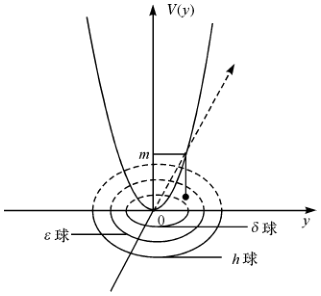
\includegraphics[width=\linewidth]{figs/fig-0052.png}
\caption{图4.1-2}
\end{figure}

\begin{figure}[htbp]\centering
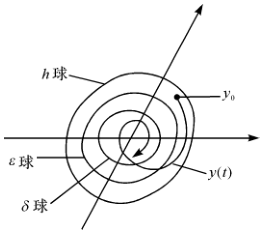
\includegraphics[width=\linewidth]{figs/fig-0053.png}
\caption{图4.1-2}
\end{figure}

数）。

其次，设 $V$ 为有界函数，对任何一个 $\epsilon>0$ 有数 $\delta>0$ 存在，使对任何 $t \geqslant b$，在 $\delta$球内总有不等式 $|V(t ; \mathbf{x})|<\epsilon$，则称 $V(t ; \mathbf{x})$ 为有无限小上界。一切不含 $t$ 之正定函数均有无限小上界。

对非自治系统有下列关于稳定性的判据准则。

(4) 如果对于方程组

\[\frac{d \mathbf{y}}{d t}=\mathbf{g}(t, \mathbf{y}), \quad \mathbf{g}(t, \mathbf{0}) \equiv \mathbf{0}\qquad\text{(4.1-6)}\]

有一正定函数 $V(t, \mathbf{y})$ 存在，后者具有无限小上界，且其由式 (4.1-6) 所确定的全导数

\[\frac{d V}{d t}=\sum_{i=1}^{n} \frac{\partial V}{\partial y_{i}} \mathbf{g}_{i}(t, \mathbf{y})+\frac{\partial V}{d t}\qquad\text{(4.1-7)}\]

为负定，则式 (4.1-6) 的未受扰运动 $\mathbf{y}(t) \equiv \mathbf{0}$ 为渐近稳定。

(5) 如果对于式 (4.1-6) 有这样的函数 $V(t ; \mathbf{y})$ 存在，它有无限小上界，$\frac{d V}{d t}$ 为正定；而对一切 $t \geqslant b, V(t ; \mathbf{y})$ 在任意小的 $\delta$ 球内取正值。此时式 (4.1-6) 的未受扰运动不稳定。

这两个判据准则的几何意义与前述判据 (1)-(3) 相似。它们的严格证明可参看文献[2]。

值得注意的是，上列五种稳定和不稳定判据只需根据运动方程式右端的函数形式和函数 $V$ 的性质，而无需求出方程式的全解。这特别对一些不可能用分析方法求出解的非线性方程或线性变系数方程有重要意义。但是，由于上列各条是充分条件，为了判别稳定性必须寻找出一个具有相应特性的函数 $V$。遗憾的是，普遍可用的构造 $V$ 函数的方法却不存在，对一些较为复杂的非线性系统，要求出 $V$ 函数是一件十分困难的任务。只有对某些线性系统和简单的非线性系统才有较为通用的方法可循。为了说明李雅普诺夫直接方法的有效性，下面举两个例子。

首先研究单摆的平衡位置的稳定性。从力学中我们知道，它的准确的运动方程式是

\[\frac{d^{2} \varphi}{d t^{2}}=-\frac{g}{l} \sin \varphi\qquad\text{(4.1-8)}\]

命 $\varphi=x, \frac{d \varphi}{d t}=y$，上式可改写为方程组

\[\begin{aligned} & \frac{d x}{d t}=y \\ & \frac{d y}{d t}=-\frac{g}{l} \sin x \end{aligned}\]

取 $V(x, y) = \frac{1}{2} y^2 + \frac{g}{l} (1 - \cos x)$。显然，它在 $0 \leqslant x < \pi$ 范围内为正定函数，对 $t$ 的全导数

\[\frac{dV}{dt} = y \left( -\frac{g}{l} \sin x \right) + y \frac{g}{l} \sin x \equiv 0\]

故为非正。由准则(1)可知，单摆的平衡位置是稳定的，而不是渐近稳定。

再研究变系数系统

\[\frac{d^2 x}{dt^2} + 2 \frac{dx}{dt} + (1 - \cos t) x = 0\qquad\text{(4.1-9)}\]

的零解的稳定性。命 $\frac{dx}{dt} = y$，上式可写为方程组

\[\begin{aligned}\frac{dx}{dt} &= y \\\frac{dy}{dt} &= (\cos t - 1) x - 2 y\end{aligned}\]

设 $V(x, y) = \frac{1}{2} (x^2 + (x + y)^2)$。显然，$V$ 为正定函数，而

\[\begin{aligned}\frac{dV}{dt} &= xy + (x + y) (y + (\cos t - 1) x - 2 y) \\&= - (y^2 + (1 - \cos t) xy + (1 - \cos t) x^2) \\\&\leqslant 0\end{aligned}\]

故 $\frac{dV}{dt}$ 是非正函数。故系统式(4.1-9)的 $x \equiv 0$ 的解是稳定的。

最后，再讨论一个不稳定运动的例子。设某一受扰运动的方程式为

\[\begin{aligned}\frac{dx}{dt} &= \frac{2 + t}{(1 + t)^2} x + \frac{1}{(1 + t)^2} y \\\frac{dy}{dt} &= -\frac{1}{(1 + t)^2} x + \frac{t}{(1 + t)^2} y\end{aligned}\qquad\text{(4.1-10)}\]

取函数 $V(x, y, t) = \frac{1}{2} (x^2 + y^2) e^{-\frac{2}{1 + t}}$

显然有

\[\begin{aligned}\frac{dV}{dt} &= \left[ \frac{t + 2}{t + 1} x - ty + dxy^2 \right] x + y (tx + e^t y + ax^2 y) \\\frac{dV}{dt} &= \frac{2}{1 + t} V + \frac{2t^2}{(1 + t)^2} e^{-\frac{2}{1 + t}}\end{aligned}\]

由于 $V$ 是正定函数，有无穷小上界，而 $\frac{dV}{dt}$ 也是正定的。由准则(5)可知，系统式 (4.1-10)的未受扰运动 $x \equiv 0, y \equiv 0$ 为不稳定。

\section{4.2 常系数线性系统的稳定性及第一近似方法}

我们在本节内将详细讨论线性常系数系统的稳定性。研究方程式

\[a_{n} \frac{d^{n} y}{d t^{n}}+a_{n-1} \frac{d^{n-1} y}{d t^{n-1}}+\cdots+a \frac{d y}{d t}+\omega y=0, \quad a_{n} \neq 0\qquad\text{(4.2-1)}\]

如在第二章内所指出的，它可以化为一个方程组

\[\frac{d \mathbf{y}}{d t}=A \mathbf{y}\]

方阵 $A$ 的元素由式 (4.2-1) 的系数排列组成:

\[A=\left(\begin{array}{cccccc} 0 & 1 & 0 & \cdots & 0 \\ 0 & 0 & 1 & \cdots & 0 \\ \vdots & \vdots & \vdots & & \vdots \\ 0 & 0 & 0 & \cdots & 1 \\ -a_{n} & -a_{n} & -a_{n} & \cdots & -a_{n-1} \end{array}\right)\]

而向量 $\mathbf{y}$ 的分量为 $y_{1}=y, y_{2}=\frac{d y}{d t}$ 等。读者容易检查，下列三个特征方程式完全等价:

(1) 第二章传递函数式 (2.2-8) 的分母 $D(s)=0$。

(2) 由式 (4.2-1) 得到的方程

\[a_{n} \lambda^{n}+a_{n-1} \lambda^{n-1}+\cdots+a_{1} \lambda+a_{n}=0\]

(3) 由式 (4.2-1) 之矩阵构成的行列式

\[\mid A-\lambda E \mid=0\]

首先指出线性系统的一个重要特性，任一线性系统，若其零点是稳定的，则它的任何一个未受扰运动都是稳定的。反之亦然，若其零点不稳定，则任何一个未受扰运动都是不稳定的。这是因为对任何特定的运动，其受扰运动的方程式与原方程式无异。因此，我们可以讲系统的稳定性。

根据第二章对常系数方程式的讨论可知:

(1) 如果特征方程的根都有负实部，或者说传递函数的极点均在左半平面，则系统是渐近稳定的。

(2) 如果特征方程哪怕有一个特征根的实部为正；则系统不稳定。

(3) 如果特征方程的所有根的实部不大于零，而等于零的特征根所对应的约当块为一阶的，（或实部等于零的特征根是一重的） 则系统是稳定的。反之，系统是不稳定的。

对于常系数线性系统的稳定性研究，应用李雅普诺夫直接方法颇为方便。此时李雅普诺夫函数 $V(\mathbf{y})$ 总可以是正定的二次型。对常系数系统有下列事实：如果特征方程的根都有负的实部，那么必存在一个正定二次型

\[V(\mathbf{y})=\left(H \mathbf{y}, \mathbf{y}\right)=\sum_{i, j=1}^{n} h_{i j} y_{i} y_{j}\]

使它对 $t$ 的全导数等于

\[\frac{d V}{d t}=-(\mathbf{y}, \mathbf{y})=-\sum_{i=1}^{n} y_{i}^{2}\qquad\text{(4.2-2)}\]

反之，若方程式 (4.2-1) 存在一个正定二次型，使式 (4.2-2) 成立，那么特征方程的所有根均有负实部。

令

\[\begin{aligned} V(\mathbf{y}) & =\int_{0}^{\infty}\left(e^{A t} \mathbf{y}, e^{A t} \mathbf{y}\right) d t=\int_{0}^{\infty}\left(e^{(A+A^{2}) t} \mathbf{y}, \mathbf{y}\right) d t \\ & =\sum_{\alpha, \beta=1}^{n} \int_{0}^{\infty} \eta_{\beta}(t) y_{\alpha} y_{\beta} d t=\sum_{\alpha, \beta=1}^{n} h_{\alpha \beta} y_{\alpha} y_{\beta} \end{aligned}\qquad\text{(4.2-3)}\]

式中 $\mathbf{y}$ 为相空间内任意固定的点，$\eta_{\beta}(t)$ 是矩阵 $e^{(A+A^{2}) t}$ 的元的函数。因为所有的 $A$ 的特征根均有负实部，故积分 $\int_{0}^{\infty} \eta_{\beta}(t) d t$ 收敛。现令式 (4.2-3) 之向量 $\mathbf{y}$ 按方程式 (4.2-1’) 之解移动，于是

\[\begin{aligned} & V\left(e^{A t} \mathbf{y}\right)=\int_{0}^{\infty}\left(e^{(A+A^{2})(t+t)} \mathbf{y}, \mathbf{y}\right) d t=\int_{t}^{\infty}\left(e^{(A+A^{2}) t} \mathbf{y}, \mathbf{y}\right) d t \\ & \left.\frac{d V}{d t}=\left.\frac{d V\left(e^{A t} \mathbf{y}\right)}{d t}\right|_{t=0}=-(\mathbf{y}, \mathbf{y})=-\|\mathbf{y}\|^{2}\right) \end{aligned}\]

这就证明了上述断言的第一部分。

再设这样的二次型已找到，它是 $V(\mathbf{y})=\left(H \mathbf{y}, \mathbf{y}\right)$。因为 $H$ 是对称正定矩阵，故其所有特征根均为正实数。令 $M, m$ 分别为最大和最小的特征根。从代数学中我们知道有不等式。

\[M\|\mathbf{y}\|^{2} \geqslant\left(H \mathbf{y}, \mathbf{y}\right) \geqslant m\|\mathbf{y}\|^{2}\]

而

\[\frac{d V}{d t}=-(\mathbf{y}, \mathbf{y}) \leqslant-\frac{1}{M} V(\mathbf{y})\]

解上述不等式有

\[e^{t} V\left(e^{A t} \mathbf{y}\right) \leqslant V(\mathbf{y})\]

或者

\[V\left(e^{A t} \mathbf{y}\right) \leqslant e^{-\frac{t}{M}} V(\mathbf{y}) \leqslant M_{e}^{-\frac{t}{M}}\|\mathbf{y}\|^{2}\]

(1) 若 $\lambda$ 是 $A$ 的特征根，则它也是 $A^{2}$ 的特征根，于是 $2 \lambda$ 是 $A+A^{2}$ 的特征根，证明留给读者。

此外由

\[\left(\mathbf{y}, \mathbf{y}\right) \leqslant \frac{1}{m}(H \mathbf{y}, \mathbf{y})\]

可得

\[\left\|e^{A t} \mathbf{y}\right\|^{2} \leqslant \frac{1}{m} V\left(e^{A t} \mathbf{y}\right) \leqslant \frac{M}{m} e^{-\frac{t}{M}}\|\mathbf{y}\|^{2}\]

或者

\[\left\|e^{A t} \mathbf{y}\right\| \leqslant \sqrt{\frac{M}{m}}\|\mathbf{y}\| e^{-\frac{t}{2 M}}\]

因此，所有系统的解，都以指数速度向零衰减，这就证明了系统的一切特征根均有负实部。

由上面的讨论可知，用二次型作为李雅普诺夫函数去判据线性常系数的稳定性是有足够根据的。问题是如何求出矩阵 $H$，亦即如何求出函数 $V$。为此，再来研究式 (4.2-2)。显然，

\[\frac{d V}{d t}=\left(H A \mathbf{y}, \mathbf{y}\right)+\left(H \mathbf{y}, A \mathbf{y}\right)=-(\mathbf{y}, \mathbf{y})\]

合项后有矩阵等式

\[H A+A^{r} H=-E\]

从这个矩阵方程中解出 $h_{i j}$ 后，函数 $V(\mathbf{y})$ 随即求出。

利用这些结果可以讨论非线性系统的稳定性。这就是李雅普诺夫第一近似方法，这个方法得到了广泛的应用。设控制系统的运动为下列非线性方程组所描绘

\[\frac{d \mathbf{x}}{d t}=f(\mathbf{x}), \quad f(\mathbf{0})=\mathbf{0}\qquad\text{(4.2-4)}\]

设向量函数 $f(\mathbf{x})$ 的每个分量为二次可微。从高等数学中可知，上式右端可展为

\[\frac{d \mathbf{x}}{d t}=A \mathbf{x}+g(\mathbf{0}, \mathbf{x})\qquad\text{(4.2-5)}\]

其中

\[A=\left[\begin{array}{c}\frac{\partial f_{i}}{\partial x_{j}} \\g_{i}=\left(B_{i} \mathbf{x}, \mathbf{x}\right)\end{array}\right.\]

而

\[B_{i}=\left(\frac{1}{2} \frac{\partial^{2} f_{i}(\theta \mathbf{x})}{\partial x_{i} \partial x_{i}}\right), \quad 0<\theta<1\]

方程 (4.2-5) 的线性部分

\[\frac{d \mathbf{y}}{d t}=A \mathbf{y}\qquad\text{(4.2-6)}\]

称为一次近似方程，或称为线性化方程。现在可以根据式 (4.2-6) 的稳定性判断非线性系统式(4.2-4)的零点稳定性。

如果系统式(4.2-6)是渐近稳定的，则式(4.2-4)的零解也是渐近稳定的。反之，若式(4.2-6)的特征根中哪怕有一个根有正实部，则式(4.2-4)的零解是不稳定的。

这个断语的第一部分的证明很简单，设系统式(4.2-6)渐近稳定，则必有一个正定二次型 $V$，使

\[V(\mathbf{y})=\left(H \mathbf{y}, \mathbf{y}\right), \quad \frac{d V}{d t}=-(\mathbf{y}, \mathbf{y})\]

现用此二次型作为式(4.2-5)的李雅普诺夫函数，对它求全导数后有

\[\frac{d V(\mathbf{x})}{d t}=-\left(\mathbf{x}, \mathbf{x}\right)+\sum_{\alpha, \beta=1}^{n}\left[\sum_{i=1}^{n} \frac{1}{2} \frac{\partial^{2} f_{i}(\theta \mathbf{x})}{\partial x_{\alpha} \partial x_{\beta}} \frac{\partial V}{\partial x_{\alpha}}\right]_{x_{\alpha} x_{\beta}}\]

右端第二项所含的每一被加量起码是关于 $x_{\alpha}, \alpha=1,2, \cdots, n$ 的三次项，每项系数都是有界的，故在零点的足够小的附近有不等式

\[\frac{d V}{d t} \leqslant-\|\mathbf{x}\|^{2}+\frac{1}{2}\|\mathbf{x}\|^{2}=-\frac{1}{2}\|\mathbf{x}\|^{2}\]

成立。因此函数 $\frac{d V}{d t}$ 是负定的。根据前节的判据法则(1)可知，系统式(4.2-4)的零解是渐近稳定的。对前述断语的第二部分的证明方法与第一部分类似。

这个一次近似方法给工程中常用的线性化方法提供了理论基础，因此其应用十分广泛。在以后讨论非线性系统时，我们还将使用这个方法。现举例说明此方法的有效性。

设有一系统，由一线性部分 $F(s)=\frac{1}{D(s)}$ 和一非线性部分 $u=f(\varepsilon)$ 组成。现试用一次近似法分析系统的稳定性。显然，系统的运动方程式为（图 4.2-1)

\[\begin{aligned} & X(s)=F(s) U(s) \\ & u=f(\varepsilon) \\ & \varepsilon=g-x \end{aligned}\qquad\text{(4.2-7)}\]

式中 $X, U$ 分别为变量 $x, u$ 的象函数。现研究系统的零点稳定性，故设 $g \equiv 0$。将 $u$ 和 $x$ 自方程式内消掉后，有方程式

\[a_{n} \frac{d^{n} \varepsilon}{d t^{n}}+a_{n-1} \frac{d^{n-1} \varepsilon}{d t^{n-1}}+\cdots+a_{1} \varepsilon=-f(\varepsilon)\qquad\text{(4.2-8)}\]

设函数 $f(\varepsilon)$ 在零点附近足够光滑，使其可展为 $f(\varepsilon)=K_{1} \varepsilon+K_{2} \varepsilon^{2}+\cdots$，代入式 (4.2-8)后有

\[a_{n} \frac{d^{n} \varepsilon}{d t^{n}}+\cdots+a_{1} \varepsilon=-\left(K_{1} \varepsilon+K_{2} \varepsilon^{2}+\cdots\right)\qquad\text{(4.2-8)}\]

或者

\[a_{n} \frac{d^{n} \varepsilon}{d t^{n}}+\cdots+\left(a_{0}+K_{1}\right) \varepsilon=-K_{2} \varepsilon^{2}+\cdots\qquad\text{(4.2-9)}\]

利用一次近似法，若方程式

\[a_{n} \frac{d^{n} \varepsilon}{d t^{n}}+\cdots+\left(a_{0}+K_{1}\right) \varepsilon=0\]

的特征根全为负实部，则图 4.2-1 所示之系统的零点渐近稳定。反之，若有一个根的实部为正，则其零点为不稳定。于是，对研究零点稳定性问题，图 4.2-1 所示之系统与图 4.2-2 所示之系统等价。

值得注意的是，当线性化方程的特征根除一部分有负实部外，尚有一个或数个根的实部为零时，一次近似方法的判别准则就不能解决稳定性问题了。这时称

\begin{figure}[htbp]\centering
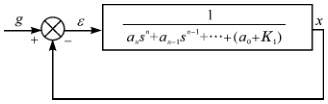
\includegraphics[width=\linewidth]{figs/fig-0055.png}
\caption{图4.2-2}
\end{figure}

\begin{figure}[htbp]\centering
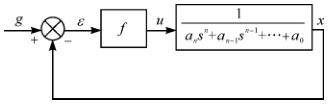
\includegraphics[width=\linewidth]{figs/fig-0054.png}
\caption{图4.2-1}
\end{figure}

为临界情况，例如，试研究系统

\[\frac{d x}{d t}=-y+a x^{3}, \quad \frac{d y}{d t}=x+a y^{3}\qquad\text{(4.2-10)}\]

的零解稳定性。此方程式的线性部分的特征方程及其根为

\[D(\lambda)=\left|\begin{array}{cc} -\lambda & -1 \\ 1 & -\lambda \end{array}\right|=\lambda^{2}+1=0, \quad \lambda=\pm i\]

这是临界情况，此时一次近似方法不能应用。为了解决稳定性问题，取李雅普诺夫函数 $V=\frac{1}{2}\left(x^{2}+y^{2}\right)$。根据式 (4.2-10) $V$ 的全导数为

\[\frac{d V}{d t}=x(-y+a x^{3})+y(x+a y^{3})=a\left(x^{4}+y^{4}\right)\]

显然，$V$ 为正定。当 $a>0$ 时，$\frac{d V}{d t}$ 也为正定，故系统的零解不稳定；当 $a=0$ 时，$\frac{d V}{d t}=0$，故系统的零解稳定，但不是渐近稳定；当 $a<0$ 时，$\frac{d V}{d t}<0$ 为负定，故零解渐近稳定。由此可知，在临界情况下，为了判别某一运动的稳定性必须考虑高次项的作用。

既然对线性系统的分析很重要，在下面几节内我们将介绍几种常用的线性系统稳定性的判别方法。

由于传递函数的概念在工程实践中应用极广，故我们将介绍几种以传递函数为依据的稳定性判别准则。正如前面曾提到过的那样，普通的传递函数都常是两个母多项式的零点是否均位于左半复平面内，这是一个古典问题。路斯(Routh)利用所谓“路斯不等式”[1]解决了这个问题。路斯不等式所包括的只是被考虑的多项式的系数以需要努力寻找更直观的方法。 由于传递函数是比较原始比较直接的资料，而且它也能被工程师所“物理地” 了解，所以工程师们宁愿采用一种直接从系统的传递函数下手的分析方法，而不愿意把传递函数再加以变化。 乃奎斯特发明了一个这样的方法 \$\{ 的数学基础是一个关于解析函数是柯西发现的。 如果点或向沿着为了把这个很强有力的定理应用到我们的问题上去，我们所选取的路线包含了整个的右半平面。因为实数部分是正数的零点只能在这一区域里。图所表示的就是这样一条路线，这条路线包括了虚轴和一个在虚轴右边的半径是情形。它的传递函数为 \{1\}\{F\_\{c\}(s)\}=\{1\}\{K G(s)\}+1 (4.3-1) 由方程面的右半部的零点的个数是如果希望走一圈的时候，就必须要求是，根据方程绕一1点转 (1) 路斯不等式常常被称为路斯-胡尔维茨(Hurwitz)不等式。这个稳定性的判定方法的详细情况在关于运动稳定性的教科书以及一般的调节理论教科书中都可以找到。

\section{4.3 乃氏方法}

1/G(s)以反时针方向围绕-K点绕m圈。不言而喻，当G（s）在s平面右半部没有零点，或者m=0，那么，乃氏稳定准则要求向量1/G（s）不围绕-K点转动。。

现在，让我们用下列的简单的传递函数来说明这个方法的应用

\[\begin{aligned} G(s) & =\frac{1}{s(1+v s)(1+v s)} \\ 1 / G(s) & =s(1+v s)(1+v s) \end{aligned}\qquad\text{(4.3-2)}\]

首先来考虑图4.3-1的路线C的沿虚轴的部分，在这一部分上

\[\frac{1}{G(s)}=\frac{1}{G(i \omega)}=i \omega(1+i v_{1} \omega)(1+i v_{2} \omega)\]

在 $\omega=0$ 点，$1 / G(i \omega)=i 0$。当 $\omega \rightarrow+\infty, 1 / G(i \omega) \rightarrow-i \infty$。因此，在 $\omega$ 从 0 增加到 $+\infty$ 的过程中，向量 $1 / G(i \omega)$ 的大小也随之增加，并且相角从 $\pi / 2$ 增加到 $3 \pi / 2$。根据方程(3.2-2)相当于负 $\omega$ 值 $(-\infty<\omega<0)$ 的 $1 / G(i \omega)$ 的端点所描画出的曲线也就是相当于正 $\omega$ 值的 $1 / G(i \omega)$ 曲线对于实轴所作的“反射”。所以，当 $s$ 在虚轴上从 $-i \infty$ 走到 $+i \infty$ 的时候，$1 / G(i \omega)$ 在图 4.3-2 上就描画出曲线 $a b 0 c$。

当 $s$ 走过图 4.3-1 上所表示的半圆的时候，$1 / G(s) \subset$ $s^{3}$。所以，当 $s$ 从 $+i \infty$ 沿着半圆以顺时针方向转到 $-i \infty$时，$1 / G(s)$ 也是顺时针转动的，不过 $1 / G(s)$ 所转过的角度 3倍于 $s$ 所转过的角度。在图 4.3-2 里，这一部分曲线是以从 $c$ 到 $a$ 的那一部分所表示的。根据这个图形来看，如果 $K=K_{1}$ 像图形所画出的那样，那么，向量 $1 / G(s)$ 围绕 $-K_{1}$点转动的总圈数等于零（因为顺时针方向旋转的一圈半 $c a$和反时针方向旋转的一圈半 $a b 0 c$ 恰恰互相抵消了）。既然方程(4.3-2)所给的这个函数 $G(s)$ 根本没有零点，而

1/G(s)对一K1的转动

圈数也是 0。所以反馈系统是稳定的。如果，像图 4.3-2 所表示的那样，$K=K_{\mathrm{H}}$，那么，向量 $1 / G(s)$ 围绕 $-K_{\mathrm{H}}$ 点就转动了两圈 （曲线的 $a b 0 c$ 部分对 $-K_{\mathrm{H}}$ 点在顺时针方向转了半圈，$c a$ 部分以顺时针方向转了一圈半），由于转动圈数 2 不等于 $G(s)$ 在右半平面的零点个数 0，所以，$F_{1}(s)$ 在右半平面有两个极点，因而反馈系统是不稳定的。从以上的讨论可以看出，如果放大系数 $K$ 的值相当大就会使这个系统不稳定。系统的稳定放大系数值与不稳定放大系数值的分界点是 $b_{0}$。使系统稳定的放大系数

图 4.3-1

图 4.3-2

\begin{figure}[htbp]\centering
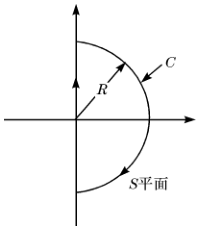
\includegraphics[width=\linewidth]{figs/fig-0056.png}
\caption{图4.3-1}
\end{figure}

\begin{figure}[htbp]\centering
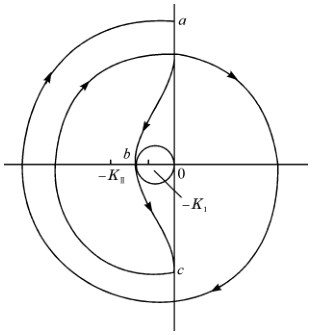
\includegraphics[width=\linewidth]{figs/fig-0057.png}
\caption{图4.3-2}
\end{figure}

值 $K$ 必须在原点和这个点之间: $b<-K<0$。

对于一般的反馈系统，根据传递函数的一般表达式 (3.7-5) 可写成

\[\frac{1}{F_{\mathrm{r}}(s)}=\frac{1}{K_{1} G_{1}(s)}+K_{2} G_{2}(s)\]

关于稳定性的问题也就是方程 (4.3-3) 所表示的函数 $1 / F_{\mathrm{r}}(s)$ 在 $S$ 平面的右半部有没有零点的问题。对这个函数直接应用柯西定理是很不方便的，因为如果这样做的话，我们就必须把向量 $1 / K_{1} G_{1}(s)$ 和向量 $K_{2} G_{2}(s)$ 相加起来才行。现在，我们假设 $G_{1}(s)$ 和 $G_{2}(s)$ 在右半平面的零点的个数分别是 $m_{1}$ 和 $m_{2}, G_{1}(s)$ 和 $G_{2}(s)$ 在右半平面的极点的个数分别是 $n_{1}$ 和 $n_{2}$。并且假定所有这些零点和极点都互不相等，那么，$1 / F_{\mathrm{r}}(s)$ 在右半平面的极点的个数显然就是 $m_{1}+n_{2}$。现在，我们把 $1 / F_{\mathrm{r}}(s)$ 用 $K_{2} G_{2}(s)$ 除一下。这个演算就使表示式 $1 / F_{\mathrm{r}}(s)$ 增加了 $m_{2}$ 个极点和 $n_{2}$个零点，但是，还有这样一种可能性：在作除法的时候，因为有些 $1 / F_{\mathrm{r}}(s)$ 的极点或零点和 $G_{2}(s)$ 的一些极点或零点是相同的，所以这些零点和极点就互相抵消掉了。假设这样抵消掉的零点或极点的个数是 $\alpha$，那么 $1 / F_{\mathrm{r}}(s) K_{2} G_{2}(s)$ 在右半平面的极点的个数就是 $m_{1}+n_{2}+m_{2}-\alpha$。现在就有

\[\frac{1}{F_{\mathrm{r}}(s) K_{2} G_{2}(s)}=\frac{1}{K_{1} K_{2} G_{1}(s) G_{2}(s)}+1\qquad\text{(4.3-3)}\]

根据方程 (4.3-4)，$1 / F_{\mathrm{r}}(s) K_{2} G_{2}(s)$ 在右半平面的极点的个数和 $1 / K_{1} K_{2} G_{1}(s) G_{2}(s)$在右半平面的极点的个数是相等的，所以也就等于 $m_{1}+n_{2}$。既然 $m_{1}+n_{2}+m_{2}-$ $\alpha=m_{1}+n_{2}$，所以 $n_{2}-\alpha=0$。我们假设反馈系统是稳定的，因此，$1 / F_{\mathrm{r}}(s)$ 在右半平面没有零点，因而 $1 / F_{\mathrm{r}}(s) K_{2} G_{2}(s)$ 在右半平面的零点的个数就是 $n_{2}-\alpha$，也就是 0。所以 $1 / F_{\mathrm{r}}(s) K_{2} G_{2}(s)$ 在右半平面也没有零点。为了清楚起见，我们把各个函数在右半平面的零点和极点的个数列在下列的表 4.3-1 中。因此，当 $s$ 走过图 4.3-1 所表示的那条曲线 $C$ 的时候，向量 $1 / F_{\mathrm{r}}(s) K_{2} G_{2}(s)$ 就应该围绕原点以顺时针方向转动 $\left(-m_{1}+m_{2}\right)$ 圈。根据方程 (4.3-4)，这个稳定条件也就相当于要求向量 $1 / K_{1} K_{2} G_{1}(s) G_{2}(s)$ 围绕 -1 点以反时针方向转动 $m_{1}+m_{2}$ 圈，或者要求向量 $1 / G_{1}(s) G_{2}(s)$ 围绕 $\left(-K_{1} K_{2}\right)$ 点以反时针方向转动 $m_{1}+m_{2}$ 圈。这就是一般的反馈系统的稳定性的乃氏判别法。

表 4.3-1函数在右半平面的零点个数在右半平面的极点个数

G\_1(s)\$ \$m\_1\$ \$n\_1\$
\$G\_2(s)\$ \$m\_2\$ \$n\_2\$
\$1 / F\_r(s)\$ 0 \$m\_1+n\_2\$
\$1 / F\_r(s) K\_2 G\_2(s)\$ \$n\_2-\$ \$m\_1+n\_2+m\_2-=m\_1+m\_2

正如图 4.3-2 所表示的那个例子一样，乃氏法中所用的曲线的最重要的一部分就是相当于 $s=i \omega$ 的那一部分。因此，我们可以用前向线路和反馈线路的频率特性来直接解决系统的稳定性的问题。既然，系统的各组件的频率特性的数据常常可以用实验方法确定，所以这种可以直接利用实验资料的方法是很有利的。这是乃氏法的优点。乃氏法的缺点在于它不能够确定稳定的程度，也就是说它不能回答这样一个问题：如果系统是稳定的，那么，它的阻尼到底有多么大呢？为了解答这个问题，我们可以把已有的准则改变成这样：要求 $1 / F_{c}(s)$ 在一条位于左半平面而平行于虚轴的直线的右方没有零点。这条直线和虚轴的距离一 $\lambda$ 就表示最低限度的阻尼。所以只要把路线 $C$ 适当地改换一下 （沿着路线的 $s$ 以及 $C$ 内所包含的零点个数当然也随之改变了） 乃氏准则仍然是可用的，但是这样做的时候，我们必须知道的是传递函数在直线 $s=-\lambda+i \omega$ 上的值，而不是在 $s=i \omega$ 上的值了。所以，关于频率特性的资料就不再能直接应用了，这样一来，乃氏法就失去了它的主要优点。但是，对于这个问题，艾文思 (Evans) [11] 发明了一个不同的处理方法，这个方法比乃氏法有其独特之处。在下一节里，我们就来讨论这个方法。

\section{4.4 艾文思方法}

我们先来考虑简单的反馈系统的情形。这时，基本的问题就是求出下列方程的根:

\[0=\frac{1}{F_{c}(s)}=1+\frac{1}{K G(s)}\qquad\text{(4.4-1)}\]

其中的 $G(s)$ 是已知的函数。艾文思法的基本做法就是把这些根确定为放大系数 $K$ 的函数，所以这个方法也称为根轨迹法。如果我们用艾文思法处理问题，那么，相应于对根所提出的任何要求，我们都可以找到合乎要求的放大系数 $K$ 的数值。因此，用这个方法所能做到的事情比前节中所述准则要多得多，并且对于反馈系统的其他设计准则来说，也可以用艾文思法把设计问题加以解决。

必须假设 $G(s)$ 是由它的零点 $p_{1}, p_{2}, \cdots, p_{m}$ 和它的极点 $q_{1}, q_{2}, \cdots, q_{n}$ 所给定的。根据由方程 (3.2-1)，(3.3-2)，(3.3-4) 所给的放大系数的定义，

\[G(s)=A \frac{\left(s-p_{1}\right)\left(s-p_{2}\right) \cdots\left(s-p_{m}\right)}{\left(s-q_{1}\right)\left(s-q_{2}\right) \cdots\left(s-q_{n}\right)}\qquad\text{(4.4-2)}\]

其中

\[A=\frac{\left(-q_{1}\right)\left(-q_{2}\right) \cdots\left(-q_{n}\right)}{\left(-p_{1}\right)\left(-p_{2}\right) \cdots\left(-p_{m}\right)}\]

对于实际的物理系统来说，$G(s)$ 的分子多项式和分母多项式的系数都是实数。所以，这些 $p$ 或者是实数或者是成对出现的共轭复数，类似的，这些 $q$ 或者是实数或者是成对出现的共轭复数。因此，$A$ 必然是实数。不但如此，在安排普通的工程系统的时候，我们还经常使 $A$ 是一个正数。因此，在以下的讨论里，我们就把 $A$ 看作是一个正实数。在普通情况下 $G(s)$ 的分母多项式的次数总是大于或者等于分子多项式的次数，也就是 $n \geqslant m$。现在，我们把方程(4.4-2)里的每一个因子都写成向量形式

\[\begin{aligned}& s-p_{1}=P_{1} e^{i \varphi_{1}} \\& s-p_{2}=P_{2} e^{i \varphi_{2}} \\& \cdots \\& s-p_{m}=P_{m} e^{i \varphi_{m}} \\& s-q_{1}=Q_{1} e^{i \varphi_{1}} \\& s-q_{2}=Q_{2} e^{i \varphi_{2}} \\& \cdots \\& s-q_{n}=Q_{n} e^{i \varphi_{n}}\end{aligned}\qquad\text{(4.4-4)}\]

$P_{i} e^{i \varphi_{i}}$ 就是从 $p_{i}$ 点到 $s$ 点的向量。$Q_{i} e^{i \varphi_{i}}$ 就是从 $q_{i}$ 点到 $s$ 点的向量。$s$ 是复 $S$ 平面上的代表变数的点。利用方程(4.4-3)和(4.4-4)，$G(s)$ 就可以写成

\[G(s)=\frac{\left(P_{1} e^{i \varphi_{1}}\right)\left(P_{2} e^{i \varphi_{2}}\right) \cdots\left(P_{m} e^{i \varphi_{m}}\right)}{\left(Q_{1} e^{i \varphi_{1}}\right)\left(Q_{2} e^{i \varphi_{2}}\right) \cdots\left(Q_{n} e^{i \varphi_{n}}\right)}\qquad\text{(4.4-5)}\]

既然 $A$ 是正实数，我们又可以把方程(4.4-5)写成

\[G(s)=R e^{i \theta}\qquad\text{(4.4-6)}\]

在这个表示式里

\[R=A \frac{\left(P_{1} P_{2} \cdots P_{m}\right)}{\left(Q_{1} Q_{2} \cdots Q_{n}\right)}\qquad\text{(4.4-7)}\]

而

\[\theta=\left(\varphi_{1}+\varphi_{2}+\cdots+\varphi_{m}\right)-\left(\theta_{1}+\theta_{2}+\cdots+\theta_{n}\right)\qquad\text{(4.4-8)}\]

因为这些 $P$ 和 $Q$ 都是方程(4.4-3)和(4.4-4)所规定的向量的长度，所以，它们都是正数。因此，$R$ 是正数。这样一来，求传递函数的倒数的根的基本方程(4.4-1)就变为

\[\frac{e^{-i \theta}}{K R}=-1\]

不难看出，如果希望满足这个方程，就必须有

\[K R=1\qquad\text{(4.4-9)}\]

和

\[\theta= \pm \pi\qquad\text{(4.4-10)}\]

艾文法包含两个步骤：首先，要找出所有满足适当的角度条件式(4.4-10)的 $s$来，这样我们就得出所谓根轨迹的曲线。然后，对于根轨迹上的每一点我们都可以算出相当的 $R$ 值，再用方程(4.4-9)我们就得出相当的 $K$ 值。关于描绘根轨迹的方法，艾文思提出了一些有用的法则。现在我们把这些法则说明一下:

法则 1. 如果 $K=0$，根据方程 (4.4-1) 必然有 $G(s) \rightarrow \infty$。所以，在 $K=0$ 时 $1 / F_{c}(s)$ 的根都是 $G(s)$ 的极点，或者说，根轨迹都是从 $G(s)$ 的极点开始的。在 $s$ 平面上用小圆点表示 $G(s)$ 的极点。

法则 2. 如果 $K \rightarrow \infty$，就必然有 $G(s) \rightarrow 0$。所以，根轨迹上相当于 $K \rightarrow \infty$ 的点，可能是 $G(s)$ 的零点。在 $s$ 平面上我们用小圆圈表示 $G(s)$ 的零点。如果 $n>m$，则 $G(s)$ 的零点的个数比 $1 / F_{c}(s)$ 的零点的个数少。但是，在这种情形中，当 $s \rightarrow \infty$ 时，$G(s) \rightarrow 0$，所以，$s=\infty$ 就补充了那些缺少的根。此外，对于非常大的 $s$

\[G(s) \underset{s}{\varpropto} \frac{A}{s}\]

因此，方程 (4.4-1) 可以近似地表示为

\[s^{-m} \varpropto-K A\]

所以，根轨迹的渐近线的相角就是

\[\frac{\pi}{n-m}+\frac{2 k \pi}{n-m}, \quad k=1,2,3, \cdots\qquad\text{(4.4-11)}\]

法则 3. 在实轴上的根轨迹是实轴上的一些交替的线段，这些线段的端点都是 $G(s)$ 的实零点或 $G(s)$ 的实极点，而且这些交替的线段从所有这些零点与极点中最右边的那一个点 （可能是零点，也可这个法则是很容易验证的。。我们在实轴上随便取一个点 $s$。从一对复共轭的零点到这个点的向量的角度就是 $+\varphi$ 与 $-\varphi$，从一对复共轭极点到这个点的向量的角度就是 $+\theta$ 与 $-\theta$ （因为复共轭点对于实轴是对称的）。所以，相当于复共轭零点或复共轭极点的角度的总和等于零。如果实轴上的一个极点或是一个零点在 $s$ 点的左面，那么，从这个极点或零点到 $s$ 点的向量的角度就是 0，如果这个点在 $s$ 点的右面，那么，从这个点到 $s$ 点的向量的角度就是 $\pi$。因此，如果在 $s$ 右面的零点与极点的总数是一个奇数，那么，角度的总和就是 $\pi$ （因为 $2 \pi$ 的整倍数对问题毫无影响）。

法则 4. 如果发生根轨迹从实轴上离开的情况，我们可以用这样一个条件来估计根轨迹在实轴上的离开点的位置：如果根轨迹上的一点离开实轴的距离是一个非常小的数 $\Delta \omega$，那么，由于在右面的 $G(s)$ 的零点与极点所引起的角度增加一定恰好被在左面的零点与极点所引起的角度减少所抵消。

例 1. 考虑下列的传递函数

\[G(s)=\frac{(0.001)(2)(6)}{(s+0.001)(s+2)(s+6)}\qquad\text{(4.4-12)}\]

当 $K=0$ 时，根轨迹从实轴上的 $-0.001,-2$ 和 $-6$ 出发。在实轴上的根轨迹就是 $-0.001$ 与 $-2$ 之间的线段以及 $-6$ 与 $-\infty$ 之间的线段。在这个情形里，$m=0$，$n=3$。所以，按照方程 (4.4-11) 渐近线的相角就是 $\pi / 3,-\pi / 3, \pi$。假设根轨迹在实轴上的 $\lambda$ 点 $(\lambda$ 点当然要在 -0.001 与 -2 之间）处离开实轴。应用法则 4 就有

\[\frac{\Delta \omega}{\lambda_{1}+0.001}+\frac{\Delta \omega}{\lambda_{1}+2}+\frac{\Delta \omega}{\lambda_{1}+6}=0\]

或者

\[(\lambda+2)(\lambda+6)+(\lambda+0.001)(\lambda+6)+(\lambda+0.001)(\lambda+2)=0\]

因而

\[3 \lambda^{2}+16.002 \lambda+12.008=0\]

\[\lambda=-\frac{16.002}{6}-\sqrt{\left[\frac{16.002}{6}\right]^{2}-\frac{12.008}{3}}=-0.904\]

法则 5. 常常可以利用直角的某些性质来估计根轨迹从左半平面过渡到右半平面时与虚轴的交点。

例 2.让我们还是来考虑由方程 (4.4-12) 所表示的传递函数。除了原点 $s=0$之外，这个传递函数可以非常近似地用下列关系式表示

\[G(s) \underset{s(s+2)(s+6)}{\underset{(0.001)(2)(6)}{\cong}}\]

正如图 4.4-1 所表示的那样，$\theta \underset{2}{\cong} \pi / 2$，因此，方程 (4.4-10) 就给出

\[\theta=-\pi \underset{2}{\cong}-\theta_{1}-\theta_{1}-\frac{\pi}{2}\]

或者

\[\theta_{1}+\theta_{1} \underset{2}{\cong} \frac{\pi}{2}\]

但是，从图上可以看到有下列关系

\[\frac{\pi}{4}=\theta_{1}+\beta, \frac{\pi}{4}+\alpha=\theta_{1}\]

因此

\[\alpha \underset{\beta}{\cong}\]

这就是确定过渡点 $U$ 的几何条件。

法则 6. 根轨迹离开一个极点 （或趋近于一个零点） 时的方向也可以计算出来，只要把平面上所有的零点与极点到这个被考虑的极点 （或零点） 的角度加以计算就可以了。

例 3.图 4.4-2 所表示的是相应于某一个传递函数 $G(s)$ 的根轨迹，$G(s)$ 在实轴上有两个极点和两个零点，同时，还有一对复共轭的极点。在根轨迹上取与极点 $q_{1}$ 非常接近的一点 $s_{0}$. $q_{1}$ 到 $s$ 的向量的相角 $\theta_{1}$ 就是根轨迹离开 $q_{1}$ 时的方向。从各个极点和各个零点到 $s$ 点的向量的角度仍然可以看做是 $\varphi_{1}, \varphi_{2}, \theta_{1}, \theta_{1}$ 和 $\theta_{1}$。所以，根据方程 (4.4-10)，$\theta_{1}$ 就由下列方程所确定

\[\left(\varphi_{1}+\varphi_{2}\right)-\left[\left(\theta_{1}+\theta_{1}+\theta_{1}\right)+\theta_{1}\right]=\pi\]

$\begin{aligned}& \omega \\& U\end{aligned}$\textbackslash\{\}begin\{aligned\}\& C\_\{i\}=\textbackslash\{\}frac\{(0.001)(2)(6)\}\{(s+0.001)(s+2)(s+6)\} \textbackslash\{\}\textbackslash\{\}\& \textbackslash\{\}text \{ 图 4.4-1 \}\textbackslash\{\}end\{aligned\}$根据以上所讲的六条法则就能得出根轨迹的主要的特性。对于中间的情形(K 既不等于零,也不趋近于$\textbackslash\{\}infty$的情形), 我们可以先在平面上适当地选取一些点,然后用试算的方法对这些点加以检验, 根据检查的结果把属于根轨迹的点保留下来。这样就可以逐步地把根轨迹完全描绘出来。沿着根轨迹曲线, 我们可以算出相应于每一点的放大系数$K$的值。如果已经把符合设计要求的$1 / F\_\{\textbackslash\{\}mathrm\{r\}\}(s)$的零点位置选择好了, 那么相当的$K$值也就可以完全确定, 这样一来, 反馈系统的设计问题就得到了解决。当然, 一般说来, 实际的设计过程当然要比所讲的要复杂一些。我们可以把根轨迹与流体力学中的某些现象相比拟。将方程 (4.4-1) 和 (4.4-2) 合并起来, 就得出$\textbackslash\{\}frac\{(s-q\_\{1\})(s-q\_\{2\}) \textbackslash\{\}cdots(s-q\_\{n\})\}\{(s-p\_\{1\})(s-p\_\{2\}) \textbackslash\{\}cdots(s-p\_\{m\})\}=-K A$如果, 先取这个方程的对数, 然后再用$2 \textbackslash\{\}pi$除一下, 我们就有$W(s)=\textbackslash\{\}frac\{1\}\{2 \textbackslash\{\}pi\} \textbackslash\{\}sum\_\{i=1\}\textasciicircum{}\{n\} \textbackslash\{\}log \textbackslash\{\}left(s-q\_\{i\}\textbackslash\{\}right)-\textbackslash\{\}frac\{1\}\{2 \textbackslash\{\}pi\} \textbackslash\{\}sum\_\{j=1\}\textasciicircum{}\{m\} \textbackslash\{\}log \textbackslash\{\}left(s-p\_\{j\}\textbackslash\{\}right)=\textbackslash\{\}frac\{1\}\{2 \textbackslash\{\}pi\} \textbackslash\{\}log K A+i\textbackslash\{\}left[\textbackslash\{\}frac\{1\}\{2\}\textbackslash\{\}right]$方程 (4.4-13) 这样一个数学表示式可以有很多种不同的物理解释。一个很明显的物理解释就是把$W(s)$看做是完全不可压缩的流体的一个二维无旋运动的复势函数$\{ \}\textasciicircum{}\{[22]\}$。如果$\textbackslash\{\}phi(\textbackslash\{\}lambda，\textbackslash\{\}omega)$是势函数,$\textbackslash\{\}psi(\textbackslash\{\}lambda，\textbackslash\{\}omega)$是流函数, 那么就有$W(s)=\textbackslash\{\}phi(\textbackslash\{\}lambda，\textbackslash\{\}omega)+i \textbackslash\{\}psi(\textbackslash\{\}lambda，\textbackslash\{\}omega)$其中$s=\textbackslash\{\}lambda+i \textbackslash\{\}omega$。因此, 表示$1 / F\_\{\textbackslash\{\}mathrm\{r\}\}(s)$的根轨迹的方程 (4.4-13) 可以这样解释: 根轨迹就是流函数取常数值$1 / 2$的那些曲线; 所以, 用流体力学的术语来说, 根轨是由1/2流线的各个分枝所组成的。。沿着这条流线势函数的值是逐点改变的, 它等于$\textbackslash\{\}frac\{1\}\{2 \textbackslash\{\}pi\} \textbackslash\{\}log K A

\begin{figure}[htbp]\centering
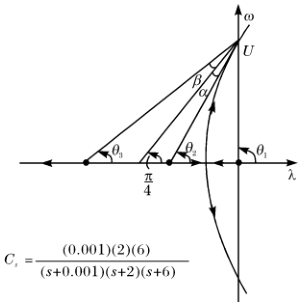
\includegraphics[width=\linewidth]{figs/fig-0058.png}
\caption{图4.4-1}
\end{figure}

\begin{figure}[htbp]\centering
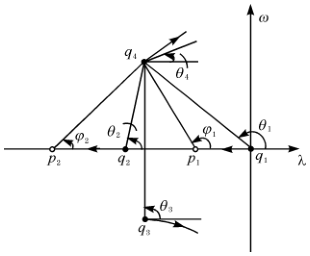
\includegraphics[width=\linewidth]{figs/fig-0059.png}
\caption{图4.4-2}
\end{figure}

方程(4.4-13)还表示这样一个事实：这个流动是由 $n$ 个单位强度的源点 $q_{1}$，$q_{2}, \cdots, q_{p}$ 和 $m$ 个单位强度的汇点 $p_{1}, p_{2}, \cdots, p_{m}$ 所构成的。在我们的图形表示法里是用小圆点表示源点，用小圆圈表示汇点。有了这样一个解释，我们就可以“理解”图 4.4-1 和图 4.4-2 中根轨迹的图形。

流体力学比拟还有另外一个很大的用处：它能够提示我们怎样把系统加以改变，使系统具有更好的性能。举例来说，假设有一个系统是由下列传递函数所代表的，

\[G(s)=\frac{q_{1} q_{2}}{s(s-q_{1})(s-q_{2})}, \quad\left|q_{1}\right|<\left|q_{2}\right|\]

那么，即使放大系数 $K$ 的值较小，在闭路控制的情形下，这个系统仍然可能是不稳定的，其根轨迹的形状和图 4.4-1 中的根轨迹相像。这时，流体力学比拟立刻就提示我们这样做：只要在 $q_{1}$ 附近增加一个汇点 $p_{c}$，并且在 $q_{2}$ 附近增加一个源点 $q_{c}$，就可以把 $U$ 点附近的流线向左方推过一些距离，因而也就把过渡点 $U$ 的位置加高一些，使临界稳定时的 $K$ 值较大。因此，修改后的传递函数就是

\[G(s)=\frac{q_{c}}{p_{c}} \frac{(s-p_{c})}{(s-q_{c})} \frac{q_{1} q_{2}}{s(s-q_{1})(s-q_{2})}\]

图 4.4-3 所表示的就是相应的根轨迹。因为 $\left|p_{c}\right|<\left|q_{1}\right|$，所以与原来的传递函数串联的附加传递函数 $\frac{q_{c}\left(s-p_{c}\right)}{p_{c}\left(s-q_{c}\right)}$ 一定是相角超前的，这个函数与第 3.3 节中方程 (3.3-8) 所表示的相角超前电路的传递函数是同一类型的。

\begin{figure}[htbp]\centering
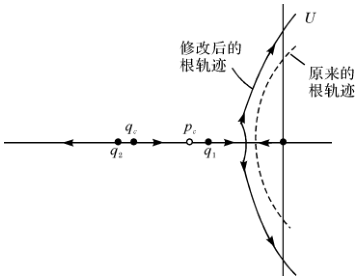
\includegraphics[width=\linewidth]{figs/fig-0060.png}
\caption{图4.4-3}
\end{figure}

修改后的根轨迹

原来的根轨迹

\[U\]

\[q_{c}\]

\[p_{c}\]

\[q_{1}\]

图 4.4-3

流体力学比拟还可以使我们了解用反馈线路使一个反应缓慢的机构增大反应速度的可能性。因为如果希望反应迅速就必须要求根的数值比较大。现在，为了简单起见，假定我们有一个一阶的线性机械系统，这个系统的特性是用负实轴上的一个数值很小的 $q$ 点来表示的。如果我们把这个系统与一个相当大的负实数 $q_{\mathrm{F}}$ 表示的反应很快的电路串接起来，这个系统的反应速度并不能够改进，因为，我们仍然还有一个数值很小的根 $q_{\mathrm{F}}$。但是，如果我们把反馈线路连接起来，从流线的形状，或者说是根轨迹，可以看出，当放大系数 $K$ 的值从 $K=0$ 开始增加时，根也就从 $q_{\mathrm{F}}$ 点开始向左方移动。因此，对于一个适当地选取的放大系数 $K$ 的值，我们就可以使得根的数值比 $q_{\mathrm{F}}$ 大一些，因而也就可以使系统的反应速度更加快一些。

以上讲过的一些描绘根轨迹的办法，对于一般的反馈系统也还可以应用。这时的问题就是要描画方程 (4.3-3) 所给的 $1 / F_{\mathrm{F}}(s)$ 的根轨迹，所以，表示根轨迹的条件就是

\[\frac{1}{K_{1} G_{1}(s)}=-K_{2} G_{2}(s)\]

因为 $1 / F_{\mathrm{F}}(s)$ 的根和 $G_{2}(s)$ 的零点不会相同，所以我们可以用 $G_{2}(s) / K_{1}$ 把上面的方程除一下，因此就有

\[\frac{1}{G_{1}(s) G_{2}(s)}=-K_{1} K_{2}\qquad\text{(4.4-15)}\]

如果我们设

\[G(s)=G_{1}(s) G_{2}(s)\qquad\text{(4.4-16)}\]

然后，再把方程 (4.4-15) 和 (4.4-1) 比较一下，就可以看到，一般的反馈系统的根轨迹的问题就化为前面讨论过的求简单的反馈系统的根轨迹的问题了。在第 4.3 节里我们曾经比较谨慎地分析了把乃氏法应用到一般的反馈系统上去的问题，事实上，对于那个问题也可以用现在的由方程 (4.4-16) 所表示的简化方法进行分析。因此，如果只就稳定性来考虑系统的定性的运转性能的话，简单的反馈系统和一般的反馈系统并没有什么区别，只不过不要忘记式 (4.4-16) 这一个关系就是了。只有在需要对系统的运转性能进行定量的研究时，我们才必须对方程 (3.7-3) 和方程 (3.7-7) 所表示的这两个系统传递函数的区别给予应有的注意。

\textbackslash\{\}subsection*\{4.5 伯德方法 ${ }^{[10]}$

根轨迹在 $U$ 点从左半 $s$ 平面过渡到右半 $s$ 平面，既然 $U$ 点在虚轴上，所以它当然就代表一个纯虚数根 $i \omega^{*}$。换句话说，方程 (4.4-1) 被 $s=i \omega^{*}$ 所满足，也就是

\[K G\left(i \omega^{*}\right)=F\left(i \omega^{*}\right)=-1=1 \cdot e^{-i \pi}\]

因此，当频率特性 $F(i \omega)$ 的振幅 $M$ 等于 1，同时相角 $\theta$ 等于 $-\pi$ 时，就发生了从稳定过渡到不稳定的临界情况。这个临界条件也可以由乃氏稳定准则推导出来，因为在 $1 / F(i \omega)$ 图上的 -1 点就是临界点。其实，只要研究一个典型的例子（例如图

\section{4.5 伯德方法}

4.3-2)4.3-2）就可以看出来，在稳定的情形里，$1 / F(i \omega)$曲线总是把-1点包围在内的。因为，在一般情况下 $1 / F(\omega)$ 的振幅总是随着 $\omega$ 的增加而增加的，所以如果希望 $1 / F(i \omega)$ 曲线把 -1 点包围在内，只要要求当 $1 / F(i \omega)$ 的相角 $\theta$ 等于 $-\pi$ 的时候，$1 / F(\omega)$ 的振幅比 1 大就可以了，或者也可以这样说：当 $\theta$ 等于 $-\pi$ 时，$M$ 必须小于 1; 或者，当 $M=1$ 的时候，$\theta$ 应该比 $-\pi$ 还要大。这个稳定条件就是伯德法的根据。我们把频率特性的振幅等于 1 时的频率称为放大系数临界点。从乃氏曲线可以推知，如果系统的开路频率特性所决定的相位方程

\[\arg K G(i \omega)=-\pi\]

的解只有一个根的话，利用伯德图去判定稳定性的规则可叙述如下：反馈系统稳定的充要条件是当 $20 \log |K G(i \omega)| \geqslant 0$ 时相位角 $\theta=\arg K G(i \omega)>-\pi$。

π。例如，图 4.5-1 所示的开路系统用 -1 反馈后是稳定的。

我们知道，稳定性本身是一个定性的概念。在实际工作中，定性的分析往往不能满足工程上的要求。因为当有人说“某一系统是稳定的”，我们只知道，当 $t \rightarrow \infty$时，这一系统的输出不会发散，但不知道衰减时间如何。为了赋予稳定性以定量的意义，在伯德图内引进稳定裕度量。图 4.5-1 内之 $\theta$ 称为相稳定裕度，$M$ 称为幅稳定裕度。经验告诉我们，良好的线性系统，一般 $\theta$ 大于 $10^{\circ}, M$ 大于 20 分贝。

还有一种情况，就是虽然开路系统是不稳定的，例如 $K G(s)$ 在右半平面内有极点，但加上简单的 -1 反馈后系统却是稳定的。采用乃氏图推理的办法可以求出对开路不稳定的反馈系统稳定性的判据准则：设 $K G(s)$ 在右半平面内有 $m$ 个极点，此时用 -1 反馈后系统稳定的充要条件是在 $20 \log |K G| \geqslant 0$ 的一切地方相频特性 $\theta(\omega)$ 从下往上穿越和 $\theta=-\pi$ 的交点比从上往下穿越和 $\theta=-\pi$ 的交点多 $\frac{m}{2}$个。此时相稳定裕度和幅稳定裕度分别为 $\arg K G(i \omega)=0$ 时 $20 \log |K G(i \omega)|$ 的最大值和 $20 \log |K G(i \omega)|=0$ 处 $\theta(\omega)$ 的最小值。

采用伯德法的时候，可以直接利用关于频率特性的资料，在这一点上伯德法与乃氏法是相似的。伯德法的优点是简单易行，但是它与艾文思的根轨迹法比较起来也还有一个很大的缺点，因为根据伯德法是不能知道稳定的程度的。为了补救这个缺点，奥斯本 (Osborn) [18] 给了一个半经验的公式，利用这个公式就可以计算相当于最危险的根（也就是离虚轴最近的根）的阻尼系数 $\zeta$。他的公式是

\[\zeta \cong \frac{1}{3} \frac{\alpha}{m}\]

\begin{figure}[htbp]\centering
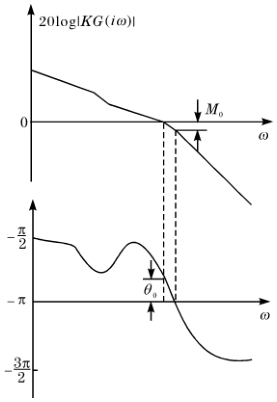
\includegraphics[width=\linewidth]{figs/fig-0061.png}
\caption{图4.5-1}
\end{figure}

其中 $\alpha$ 是在放大系数临界点处的相补角的数值，度量单位是“度”(“°”)，$m$ 是在放大系数临界点处 $20\log M$ 曲线对于 $\omega$ 而言的斜率。量度 $\zeta$ 时所用的时间单位和量度 $\omega$ 时所用的时间单位是相同的。譬如说，如果 $\alpha=30^{\circ}$ 而 $m=34$，那么 $\zeta \approx 1/3.4=0.3$。

到目前为止，我们所讨论过的系统都是单回路。也就是说，控制系统的方块图里只有一个闭合的路线。但是，在实际的工程问题中往往需要更复杂的系统；例如，图 4.6-1 所表示的方块图就是一个典型的控制系统，这个系统是用来控制飞机对于一个轴的转动的[8]。图中的内回路（也就是 $\beta$ 所在的回路）称为控制面位置的反馈（所谓“控制面”就是飞机表面的起控制作用的可动部分，例如舵，副翼等部分），或者称为硬式反馈。如果没有把内回路闭合起来，我们就得到普通的反馈控制系统，而且

\begin{figure}[htbp]\centering
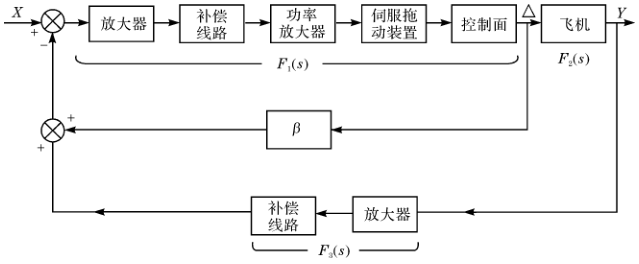
\includegraphics[width=\linewidth]{figs/fig-0062.png}
\caption{图4.6-1}
\end{figure}

\[\frac{Y(s)}{X(s)} = \frac{F_{1}(s)F_{2}(s)}{1+F_{1}(s)F_{2}(s)F_{3}(s)}\qquad\text{(4.6-1)}\]

如果把内回路和外回路($F_{3}(s)$所在的回路）都闭合起来，就有

\[\Delta(s) = F_{1}(s)[X(s)-\beta\Delta(s)-F_{3}(s)Y(s)]\]

（这里的 $\Delta(s)$ 表示控制面的运动），以及

\[Y(s) = F_{2}(s)\Delta(s)\]

因此，就得到

\[\frac{\Delta(s)}{X(s)} = \frac{F_{1}(s)}{1+\beta F_{1}(s)+F_{1}(s)F_{2}(s)F_{3}(s)}\qquad\text{(4.6-2)}\]

和

\[\frac{Y(s)}{X(s)} = \frac{F_{1}(s)F_{2}(s)}{1+\beta F_{1}(s)+F_{1}(s)F_{2}(s)F_{3}(s)}\qquad\text{(4.6-3)}\]

\section{4.6 多回路系统}

这个控制系统的稳定性与反应速度是由函数 $1+\beta F_1(s)+F_1(s)F_2(s)F_3(s)$ 所决定的。因为在这个系统中，补偿线路，放大器以及内回路的放大系数 $\beta$ 都是很容易改变的，所以我们也就不难设计出一个特性相当理想的传递函数来，而且并不需要改变飞机的结构设计以及它的机械装置。

\begin{figure}[htbp]\centering
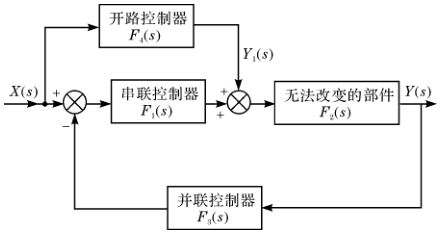
\includegraphics[width=\linewidth]{figs/fig-0063.png}
\caption{图4.6-2}
\end{figure}

\textbackslash\{\}begin\{figure\}[h]\textbackslash\{\}centering\textbackslash\{\}includegraphics[width=0.8\textbackslash\{\}textwidth]\{图4.6-2\}\textbackslash\{\}caption\{图4.6-2\}\textbackslash\{\}label\{fig:4.6-2\}\textbackslash\{\}end\{figure\}

在设计一个良好的控制系统时，常常遇到这样一个困难：如何使系统不但能进行很准确的控制 （也就是要求放大系数 $K$ 的值相当大），而且还有相当快的反应速度和合适的阻尼性质。这个问题就使人们产生了把开路控制方法与闭路控制方法结合起来的想法。这种系统很早就在实际工程中得到了应用 \textbackslash\{\}cite\{16\}。我们来考虑图 4.6-2 所表示的系统，在这个系统中开路控制部分和闭路控制部分是平行安排的。因此，有

\[F_4(s)X(s)=Y_1(s)\]

和

\[Y(s)=F_2(s)\{Y_1(s)+F_1(s)[X(s)-F_3(s)Y(s)]\}\qquad\text{(4.6-4)}\]

把输出 $Y(s)$ 解出来，就得

\[\frac{Y(s)}{X(s)}=\frac{F_2(s)F_4(s)+F_1(s)F_2(s)}{1+F_1(s)F_2(s)F_3(s)}\qquad\text{(4.6-5)}\]

因此，系统的稳定性和反应速度的特性决定于 $1+F_1(s)F_2(s)F_3(s)$ 的零点，而与 $F_1(s)$ 无关。既然 $F_2(s)$ 是不能改变的，所以关于稳定性的设计问题就是要寻求适当的传递函数 $F_1(s)$ 和 $F_3(s)$。闭路系统的放大系数 $K=\frac{F_2(0)F_4(0)+F_1(0)F_2(0)}{1+F_1(0)F_2(0)F_3(0)}$。

实际的反应速度以及稳态误差不但与 $F_1(s)$，$F_2(s)$，$F_3(s)$ 有关，而且还与开路控制部分的传递函数 $F_4(s)$ 有关。因此，反馈回路的设计可以完全决定系统的稳定性和反应的动力特性；至于系统的稳定状态或是“同步运转”的情况就与系统的开路控制部分有很密切的关系了。所以，只要适当地设计 $F_1(s)$，$F_2(s)$ 和 $F_4(s)$ 就可以使系统不但稳定而且还具有相当好的控制性能。

如果系统中有许多需要同时加以控制的变数，而且这些变数之间也有关联的话（例如火力发电站的情形）。那么，系统的方块图也就是多回路的，而且其中的反馈关系也比较复杂。这种复杂系统的一个例子是飞机的自动控制系统和导航系统 ${ }^{[20]}$。对于这样一个系统的分析工作，虽然也还是根据这一章对于简单的反馈系统所提出的同样的一些原则进行的，但是由于系统过分复杂，如果不依靠计算机，这种分析工作简直是无法进行的。

\section{4.7 关于变系数线性系统的稳定性}

工程问题中变系数系统常常遇到，如飞机，火箭等作为受控对象在整个飞行过程中其参数不断变化，有时这种变化十分剧烈。为了确定这种系统的性能，首先要判断其稳定性。遗憾的是，变系数系统的稳定判据至今没有一个既严格而又使用简便的准则。固然，用李雅普诺夫直接办法和其他近似方法 （例如特征数方法），一般说来，理论上可以解决稳定性问题，但在实际工作中这些方法均嫌过于复杂。这是因为它们都依赖于系统系数及其基本解的一些深刻的分析特征，后者却又常常得之不易。因此它们没有在实际工作中得到广泛应用。另一方面在工程实践中，对变系数系统的分析又是回避不了的现实问题，人们不得不求助于一些较为粗略的估计，虽然后者理论上不够严密，但在实用中却行之有效。本节的目的是对现有的某些方法作一些讨论，指出其优缺点使读者在使用这些方法时有所依据，而同时又保持警惕，在工作中审慎行事，不至于由于方法本身的缺陷造成技术上的恶果。

对于一类结构简单的系统，有时可以找到较为严整的处理办法。在近代计算技术条件下，可以较为简单的获得系统稳定性的判据。下面首先推荐这样一个方法。设有系统

\[a_{n}(t) \frac{d^{n} x}{d t^{n}}+a_{n-1}(t) \frac{d^{n-1} x}{d t^{n-1}}+\cdots+a(t) x=0\qquad\text{(4.7-1)}\]

其中 $a(t)$ 是连续有界变系数。如第二章所指出的那样，式 (4.7-1) 可以写成一阶向量方程式

\[\frac{d \mathbf{x}}{d t}=A(t) \mathbf{x}, \quad 0 \leqslant t<\infty\qquad\text{(4.7-2)}\]

这是一个线性系统，所以只要它的零解稳定，那么它的一切运动都是稳定的。因此，我们可以研究这个系统的稳定性。显然，式 (4.7-2) 的解可以写成

\[\mathbf{x}(t)=\mathbf{x}_{0}+\int_{t_{0}}^{t} A(\tau) \mathbf{x}(\tau) d \tau\qquad\text{(4.7-3)}\]

对系统式 (4.7-2) 我们有下列稳定性判据准则:

(1) 若式 (4.7-2) 的基本解有界则系统稳定。反之，若系统稳定，则其基本解必有界。

设 $\Phi(t, b)$ 是式 (4.7-2) 的基本解矩阵，且 $\Phi(b, b)=E$ 为单位矩阵。因此有

\[\mathbf{x}(t)=\Phi(t, b) \mathbf{x}_{0}, \quad \mathbf{x}(b)=\mathbf{x}_{0}\]

对它显然有不等式

\[\left|x_{i}(t)\right| \leqslant \sum_{a=1}^{n} \mid \varphi_{i a} \mid\left\|\mathbf{x}_{a 0}\right\|, \quad i=1,2, \cdots, n\]

由于 $\varphi_{i a}(t)$ 有界，故 $\left|\varphi_{i a}(t)\right|<M_{i a}, b \leqslant t<\infty$。令 $M$ 为所有 $M_{i a}$ 中的最大者，于是上式可改写为

\[\left|x_{i}(t)\right| \leqslant M \sum_{a=1}^{n} \mid x_{a 0} \mid \leqslant M_{1} \mid \mathbf{x}_{0} \mid, \quad i=1,2, \cdots, n\]

将上式平方相加并开方后有

\[\left\|\mathbf{x}(t)\right\| \leqslant M_{1} \underset{n}{\sqrt[n]{}} \mid \mathbf{x}_{0} \mid\]

按李雅普诺夫关于稳定性的定义，若给定 $\varepsilon>0$，则可以选 $\delta=\frac{\varepsilon}{\sqrt[n]{M_{1}}}$，此时，当 $\left\|\mathbf{x}_{0}\right\| \leqslant \delta=\frac{\varepsilon}{\sqrt[n]{M_{1}}}$ 时恒有 $\left\|\mathbf{x}(t)\right\| \leqslant \varepsilon$。因此 $\mathbf{x}(t) \equiv \mathbf{0}$ 的解是稳定的。

对系统

\[\frac{d \mathbf{x}}{d t}=(A+B(t)) \mathbf{x}\qquad\text{(4.7-4)}\]

有判别准则。

(2) 若方程式

\[\frac{d \mathbf{y}}{d t}=A \mathbf{y}\qquad\text{(4.7-5)}\]

稳定，而

\[\int_{0}^{\infty} \sum_{a, \beta=1}^{n}\left|b_{a \beta}(t)\right| d t<\infty\qquad\text{(4.7-6)}\]

则系统式 (4.7-4) 稳定。

根据判据法则 (1) 可知，这里只需检查式 (4.7-4) 的解为有界就够了。因为

\[\mathbf{x}(t)=\mathbf{x}_{0}+\int_{t_{0}}^{t}(A+B(\tau)) \mathbf{x}(\tau) d \tau\]

或者

\[\mathbf{x}(t)=e^{A t} \mathbf{x}_{0}+\int_{t_{0}}^{t} e^{A(t-\tau)} B(\tau) \mathbf{x}(\tau) d \tau\]

故

\[\left\|\mathbf{x}(t)\right\| \leqslant\left\|e^{A t} \mathbf{x}_{0}\right\|+\int_{t_{0}}^{t}\left|\sum_{a, \beta=1}^{n}\left|\varphi_{a \beta}(t-\tau)\right|\left|\sum_{a, \beta=1}^{n}\left|b_{a, \beta}(\tau)\right|\right\|\left\|\mathbf{x}(\tau)\right\| d \tau \right.\]

因为式 (4.7-5) 稳定，故 $\left\|e^{A t} \mathbf{x}_{0}\right\|$ 有界，小于某一常数 $C$，而 $\sum_{a, \beta=1}^{n}\left|\varphi_{a \beta}(t-\tau)\right|$ 也有界，设也小于 $C_{1}$。于是

\[\left\|\mathbf{x}(t)\right\| \leqslant C_{1}+C_{1} \int_{t_{0} \alpha, \beta=1}^{t} \sum_{a, \beta=1}^{n}\left|b_{a \beta}(\tau)\right\|\|\mathbf{x}(\tau)\| d \tau\]

显然，若令 $v(t)=\sum_{a, \beta=1}^{n}\left|b_{a \beta}(t)\right|$，有

\[\frac{\left\|\mathbf{x}(t)\right\| v(t)}{C_{1}+C_{1} \int_{t_{0}}^{t} v(\tau) \| \mathbf{x}(\tau) \| d \tau} \leqslant v(t)\]

对不等式两边积分后有

\[\ln \left(1+\int_{t_{0}}^{t} v(\tau) \| \mathbf{x}(\tau) \| d \tau\right) \leqslant C_{1} \int_{t_{0}}^{t} v(\tau) d \tau\]

而

\[\left\|\mathbf{x}(t)\right\| \leqslant C_{1}\left(1+\int_{t_{0}}^{t} v(\tau) \| \mathbf{x}(\tau) \| d \tau\right) \leqslant C_{1} e^{C_{1} \int_{t_{0}}^{t} v(\tau) d \tau}\]

由于有式(4.7-6)的限制条件，故知 $\|\mathbf{x}(t)\|$ 是有界的。按判别准则(1)知，此系统式(4.7-4)稳定。

用类似方法可以证明:

(3) 如果系统式(4.7-2)稳定，且

\[\int_{t_{0}}^{\infty} \sum_{a, \beta=1}^{n}\left|b_{a \beta}(\tau)\right| d \tau<\infty, \quad \int_{t_{0}}^{\infty} \sum_{i=1}^{n} a_{i i}(\tau) d \tau>-\infty\]

则系统

\[\frac{d \mathbf{x}}{d t}=(A(t)+B(t)) \mathbf{x}\qquad\text{(4.7-7)}\]

稳定。

这一组判别准则之所以值得推荐，是因为它只需判别系统的基本解是否有界就够了。为此只需给出 $n$ 种不同的初始条件，即 $\mathbf{x}=(1,0, \cdots, 0)$。 $\mathbf{x}=(0,1, \cdots$，$0, \cdots, \mathbf{x}_{n}=(0,0, \cdots, 0,1)$，求出相应的解。如果这些解都不发散，系统必然稳定。这里并不需要对系统做任何繁杂的分析。这一工作在数字机或模拟机的帮助下是极易实现的。

在变系数系统的设计工作中，沿用最广的是所谓冻结系数法。这一方法的实质是在系统整个工作时间 $[0, T]$ 内，取一些代表性的时刻，例如，$0 \leqslant t_{i} t_{i} \cdots<$ $t_{n} \leqslant T$，在每一时刻，用 $A(t)$ 代入式(4.7-2)，然后当做常系数方程式去研究。若对每一个 $t_{i}$。下列方程式所描绘的系统

\[\frac{d \mathbf{z}}{d t}=A\left(t_{i}\right) \mathbf{z}, \quad i=1,2, \cdots, n\]

都稳定，则“认为”系统(4.7-2)稳定。也就是说，若矩阵 $A(t)$ 对每一固定的 $t=t_{i}$，特征方程式

\[\left|A\left(t_{i}\right)-\lambda E\right|=0\qquad\text{(4.7-8)}\]

的根都有负实部，则认为系统(4.7-2)稳定。应该指出，这个方法在实际问题中常常是有效的，很少出现结果矛盾的不愉快现象。

虽然如此，这一方法的应用范围不是没有限制的。容易举反例证明，有的线性变系数系统如果用冻结系数法去研究，对每一时刻特征方程式的根均具有负实的零解却不稳定。研究系统

\[a t^{2} \frac{d^{2} x}{d t^{2}}+b t \frac{d x}{d t}+x=0, \quad t \geqslant t>0\qquad\text{(4.7-9)}\]

设 $t=e^{r}$，代入上式后有

\[a \frac{d^{2} x}{d \tau^{2}}+(b-a) \frac{d x}{d \tau}+x=0\qquad\text{(4.7-10)}\]

它的特征方程

\[a \lambda^{2}+(b-a) \lambda+1=0\]

的根是

\[\lambda_{1,2}=\frac{a-b \pm \sqrt{(b-a)^{2}-4 a}}{2 a}\]

设

\[a-b>0,(b-a)^{2}-4 a<0, \quad \frac{a-b}{2 a}=\rho>0, \quad \frac{\sqrt{4 a-(b-a)^{2}}}{2 a}=\omega>0\]

于是有 $\lambda_{1,2}=\rho \pm i \omega$。方程式(4.7-10)的解是

\[x(\tau)=C_{1} e^{\lambda_{1} \tau}+C_{2} e^{\lambda_{2} \tau}\]

或者

\[x(t)=t^{\rho}\left(C_{1} \cos \omega t+n t+C_{1} \sin \omega t+n t+C_{2} \cos \omega t+n t-C_{2} \sin \omega t+n t\right)\qquad\text{(4.7-11)}\]

当 $t$ 为固定值时，方程式(4.7-9)的一切特征根都具有负实部，因为当 $t>0$ 时式 (4.7-9)的系数都大于零。而它的零解是不稳定的，按式(4.7-11)，对任何非零的初始微小扰动，系统的运动 $x(t)$ 都是发散的。由此得到结论，冻结系数法对方程式(4.7-9)是不适用的。

从另一方面来看，由此例也得不出完全否定冻结系数法的结论。冻结系数法对很多变系数系统是有效的。为了说明这一点，我们继续研究方程式(4.7-2) ${ }^{[2]}$

\[\frac{d \boldsymbol{x}}{d t}=A(t) \boldsymbol{x}\]

假定矩阵 $A(t)$ 的每一个元素 $a_{i j}(t)$ 均为时间的连续函数，并且对任何时间 $t \geqslant 0$，$t \geqslant 0$，总有一个常数 $c$，使

\[\sum_{i, j=1}^{n}\left|a_{i j}(t)-a_{i j}(t)\right| \leqslant c\qquad\text{(4.7-12)}\]

同时对任何 $t=t$，特征方程的根总有

\[\operatorname{Re} \lambda_{k}\left(t_{i}\right)<-\infty\]

其中 $r$ 为某一正常数。设在初时刻 $t=b$ 时，冻结系数后的方程式 (4.7-2) 的基本解矩阵

\[\Phi_{0}(t)=e^{A\left(t_{0}\right)\left(r-t_{0}\right)}=\left(\varphi_{i j}\left(t-b_{0}\right)\right), \quad t \geqslant b_{0}\]

满足条件

\[\sum_{i, j=1}^{n} \mid \varphi_{i j}\left(t-b_{0}\right) \mid \leqslant b e^{-\frac{t}{2}\left(r-t_{0}\right)}\qquad\text{(4.7-14)}\]

式中 $b$ 显然与常数 $r$ 有关。

在上述假定条件下，若 $r, c$ 和 $b$ 满足关系式

\[b c<\frac{r}{4}\qquad\text{(4.7-15)}\]

则冻结系数法有效。换言之，若式 (4.7-15) 满足，则当式 (4.7-13) 成立时，变系数系统式 (4.7-2) 是稳定的。

事实上，将式 (4.7-2) 改写为

\[\frac{d \boldsymbol{x}}{d t}=A\left(t_{b}\right) \boldsymbol{x}+\left(A(t)-A\left(t_{b}\right)\right) \boldsymbol{x}\]

它的解可写成

\[\boldsymbol{x}(t)=e^{A\left(t_{0}\right)\left(r-t_{0}\right)} \boldsymbol{x}_{0}+\int_{t_{0}}^{t} e^{A\left(t_{0}\right)\left(r-t\right)}\left(A(\tau)-A\left(t_{b}\right)\right) \boldsymbol{x}(\tau) d \tau\qquad\text{(4.7-14)}\]

根据式 (4.7-12) 和 (4.7-14) 有

\[\|\boldsymbol{x}(t)\| \leqslant b e^{-\frac{t}{2}\left(r-t_{0}\right)} \|\boldsymbol{x}\|+\int_{t_{0}}^{t} c b e^{\frac{t}{2} \tau} \|\boldsymbol{x}(\tau)\| d \tau\]

解此不等式，有

\[\|\boldsymbol{x}(t)\| \leqslant b \|\boldsymbol{x}_{0}\| e^{-\frac{t}{2}\left(r-t_{0}\right)+b c\left(r-t_{0}\right)}\]

再利用不等式 (4.7-15)，上式可写为

\[\|\boldsymbol{x}(t)\| \leqslant b \|\boldsymbol{x}\| e^{-\frac{t}{2}\left(r-t_{0}\right)}\]

由此可知，此时系统的任何初始扰动都随时间的增大而衰减为零，因而系统是稳定的。

因为条件式 (4.7-15) 很苛刻，而且检查某一实际系统是否满足该条件又很困难，所以上述事实的应用价值不大。但是，它却说明，确实有一类变系数系统，冻结系数法对它们是严格正确且行之有效。上述两个例子告诉我们，必定存在一个分界线，使变系数线性系统分为两类，对于其中的一类，冻结系数法是严格而正确的，对另一类则完全不能应用。这一分界线在何处？如何去简捷地判别对某些具体系统应用冻结系数法的可靠性和正确性？对这些问题，现在还没有看到答案。对这个问题的答复是一个迫切的任务，我们寄予期望。彼时，怀疑将完全消失。

前面我们一直讨论按李雅普诺夫定义的系统稳定性，即研究当 $t \rightarrow \infty$ 时系统的渐近性能。对实际工作有些经验的人会发觉，李雅普诺夫的定义并不是对一切控制系统都适合。例如对火箭控制系统这个定义就不尽适宜。因为有些火箭的飞行时间有限，这时 $t$ 趋于无穷大的定义是不完全符合实际情况的。为了适应这类控制系统的需要，有人提出新的稳定性定义 ${ }^{[5,36,40]}$。这里介绍一下这个新定义的几何意义。

设系统的运动方程式依然是式(4.7-2)，而 $\delta, \varepsilon$ 和 $T$ 是三个给定的常数，其中 $T$ 是控制系统工作的时间间隔。若系统的初始扰动满足限制条件

\[\| \boldsymbol{x} \| \leqslant \delta\]

且对时间区间 $\left[b, b+T\right]$ 内的任何 $t$ 都有

\[\| \boldsymbol{x}(t) \| \leqslant \varepsilon, \quad b \leqslant t \leqslant b+T\qquad\text{(4.7-17)}\]

则说系统式(4.7-2) 对给定的一对数 $\delta$ 和 $\varepsilon$ 在 $T$ 时间内稳定。

按新定义去判别系统式 (4.7-2) 的稳定性，有以下几个主要结果 ${ }^{[29]}$。

式 (4.7-2) 中矩阵 $A=\left(a_{i k}\right), i, k=1,2, \cdots, n$，假定 $a_{i k}(t)$ 是 $t$ 的有界连续实值函数，并可表示为

\[a_{i k}(t)=a_{i k}(0)+\Delta a_{i k}(t), \quad i, k=1,2, \cdots, n\]

其中 $a_{i k}(0)$ 表示 $a_{i k}(t)$ 在 $t=b$ 时的值。现考虑特征方程式

\[D(s)=\mid a_{i k}(0)-s \hat{a}_{i k} \mid=0, \quad i, k=1,2, \cdots, n\qquad\text{(4.7-18)}\]

其中 $\hat{a}_{i k}=1$，当 $i=k ; \hat{a}_{i k}=0$，当 $i \neq k$。

如果特征方程 (4.7-18) 所有的根，均有负实部且没有重根，那么系统 (4.7-2)在有限时间 $\left[b, b+T\right]$ 内是稳定的。

如果特征方程 (4.7-18) 的根中，即使仅有一个有正实部的根，那么系统式 (4.7-2) 是不稳定的。

如果式 (4.7-18) 没有正实根或实部为正的复根，仅有重负实根 $s_{i}(i=1,2, \cdots$，$m)$ 和实部为负的重复根 $\lambda(i=1,2, \cdots, l)$，而且行列式

\[D\left(s_{i}\right)=\left|\begin{array}{cccccc} -s_{i} & -\frac{1}{2} & 0 & \cdots & 0 \\ -\frac{1}{2} & -s_{i} & -\frac{1}{2} & \cdots & -\frac{1}{2} \\ 0 & -\frac{1}{2} & -s_{i} & \cdots & -s_{i} \\ \vdots & \vdots & \vdots & -\frac{1}{2} \\ 0 & 0 & 0 & \cdots & -s_{i} \end{array}\right|, \quad i=1,2, \cdots, m\]

\begin{figure}[htbp]\centering
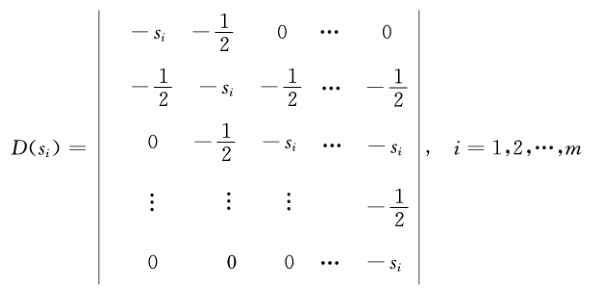
\includegraphics[width=\linewidth]{figs/fig-0064.png}
\end{figure}

\[\begin{aligned} D\left(\lambda_{i}\right)= & \left|\begin{array}{cccc} -\lambda_{i} & -\frac{1}{2} & \cdots & 0 \\ -\frac{1}{2} & -\lambda_{i} & \cdots & -\frac{1}{2} \\ \vdots & \vdots & & \vdots \\ 0 & \cdots & -\frac{1}{2} & -\lambda_{i} \end{array}\right|, i=1,2, \cdots, l \end{aligned}\]

的所有主子式皆大于零，则系统在有限时间内是稳定的。如果即使有一个主子式是负的，那么系统在有限时间内是不稳定的。

\section{4.8 系统的静态精度分析}

静态精度是控制系统的重要指标之一。对调节系统的主要要求之一是将受控量 （被调量） 准确地保持在给定值附近，例如伺服系统在过渡过程结束以后应该准确地跟踪输入量而变化。所谓系统的静态精度就是当时间足够大时对输入量的跟踪精度。继续研究线性受控系统

\[\frac{d \boldsymbol{x}}{d t}=A(t) \boldsymbol{x}+B(t) \boldsymbol{u}\qquad\text{(4.8-1)}\]

式中，$\boldsymbol{x}=\left(x_{1}, x_{2}, \cdots, x_{n}\right)$ 为受控量，$\boldsymbol{u}=\left(u, w, \cdots, u_{r}\right)$ 为控制量，$A(t)$ 和 $B(t)$ 分别为 $n \times n$ 和 $n \times r$ 阶矩阵，其元素均可能为变参数。

设 $\boldsymbol{g}(t)=\left(g_{1}(t), g_{2}(t), \cdots, g_{r}(t)\right)$ 为系统的输入作用。对控制系统的要求是 $x_{i}(t)$ 应准确地跟踪 $g_{i}(t)$。向量函数

\[\varepsilon(t)=\boldsymbol{g}(t)-\boldsymbol{x}(t)\qquad\text{(4.8-2)}\]

称为受控系统的误差向量（图 4.8-1)。将式(4.8-1)和(4.8-2)中的 $\boldsymbol{x}(t)$ 消去后有

\[\frac{d \varepsilon}{d t}=A(t) \varepsilon-B(t) \boldsymbol{u}+\left[\frac{d \boldsymbol{g}}{d t}-A(t) \boldsymbol{g}\right]\qquad\text{(4.8-3)}\]

在线性系统内控制量 $\boldsymbol{u}(t)$ 常可取为误差的线性函数，即

\[u(t)=-C(t) \varepsilon(t)\qquad\text{(4.8-4)}\]

式中 $C(t)$ 为 $r \times n$ 阶矩阵，其元素可能为时间的连续函数。利用这里引进的定义，式(4.8-3)可以改写为

\[\frac{d \varepsilon}{d t}=D(t) \varepsilon+\left[\frac{d \boldsymbol{g}}{d t}-A(t) \boldsymbol{g}\right]\qquad\text{(4.8-5)}\]

其中

\[D(t)=A(t)+B(t) C(t)\]

这样受控系统式(4.8-1)就变成一个自动控制系统了，而式(4.8-4)就称之为控制规律（图 4.8-1)。如何去确定控制规律式(4.8-4)，这是一个控制装置的设计

\begin{figure}[htbp]\centering
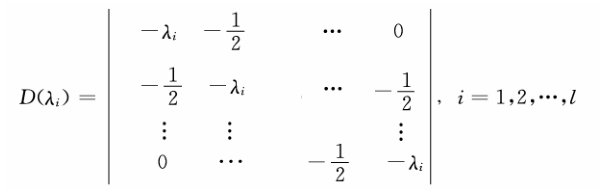
\includegraphics[width=\linewidth]{figs/fig-0065.png}
\end{figure}

控制器图

问题，本节我们先不研究它。这里只假定，按某一原则控制规律已经选定，我们的任务是去分析系统式 (4.8-5)能否保证受控量 $\boldsymbol{x}$ 准确地跟踪输入量 $\boldsymbol{g}(t)$。根据前节所述，对控制系统的第一个要求是稳定，对线性系统只要求零点稳定就够了。因此可以设想，在设计控制装置式 (4.8-4) 时，已经保证了式 (4.8-5) 的 （零解）稳定性。

设在某一初始时刻 $t$ 时 $\varepsilon(b)$ 不为零向量，而当时间足够大时，受控量 $\boldsymbol{x}(t)$ 与 $\boldsymbol{g}(t)$ 重合，此时 $\varepsilon(t)$ 将恒为零，其导数也恒为零。由此可知，系统式 (4.8-1) 在 $t$ 足够大时能精确跟踪输入作用 $\boldsymbol{g}(t)$ 的充分条件是输入作用 $\boldsymbol{g}(t)$ 满足方程式

\[\frac{d \boldsymbol{g}(t)}{d t}=A(t) \boldsymbol{g}(t)\qquad\text{(4.8-6)}\]

换言之，以方程式 (4.8-6) 的任一特解作为系统式 (4.8-1) 的输入，系统的静态误差均为零。我们称此类输入作用为受控系统的固有输入作用类。值得指出的是，系统的静态误差与控制规律式 (4.8-4) 完全无关，后者只要保证系统稳定就够了。可见，系统的静态精度主要地决定于受控对象的特性，而一般地不决定于控制装置的具体形式。

同理可推知线性高阶方程式所描述的受控系统

\[a_{n}(t) \frac{d^{p} x}{d t^{n}}+a_{n-1}(t) \frac{d^{p-1} x}{d t^{n-1}}+\cdots+a(t) x=u(t)\qquad\text{(4.8-7)}\]

的固有输入作用类函数为下列方程式的一切特解

\[a_{n}(t) \frac{d^{p} g}{d t^{n}}+a_{n-1}(t) \frac{d^{p-1} g}{d t^{n-1}}+\cdots+a g=0\qquad\text{(4.8-8)}\]

现举例说明如何求出某一系统的固有输入作用类函数。设受控系统为常系数线性系统，它的运动方程式为

\[T \frac{d^{3} x}{d t^{3}}+\frac{d^{2} x}{d t^{2}}=u\qquad\text{(4.8-9)}\]

它的固有输入作用类用方程式

\[T \frac{d^{3} g}{d t^{3}}+\frac{d^{2} g}{d t^{2}}=0\qquad\text{(4.8-10)}\]

确定。后者的解为

\begin{figure}[htbp]\centering
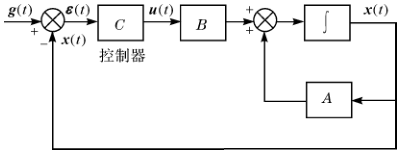
\includegraphics[width=\linewidth]{figs/fig-0066.png}
\caption{图4.8-1}
\end{figure}

\[\dot{g}(t)=g_{0}+g_{1} t+g_{2} e^{-t / T}\qquad\text{(4.8-11)}\]

其中 $g_{0}, g_{1}, g_{2}$ 为任意常数。

对于系统式 (4.8-9)来说，一切式 (4.8-11)的输入作用均不引起静态误差。

对常系数线性系统，一般的可以认为固有输入作用类函数具有下列形式:

\[g(t)=g_{0}+g_{1} t+\cdots+g_{k} t^{k}+g_{k+1} e^{\lambda_{1} t}+\cdots+g_{\pi} e^{\lambda_{\pi-k} t}\qquad\text{(4.8-12)}\]

上式内时间 $t$ 的多项式内最高次幂常称为系统的无静差次数。例如当 $k=0$ 时称零阶无静差，此时系统对一切常值输入无静差，$k=1$ 时称系统为一次无静差，此时对直线变化之输入作用无静差，以此类推。如果式 (4.8-12)内 $g_{0}=g_{1}=\cdots=g_{k}=$ 0，则系统为有静差系统，后者对任何不趋于零的输入作用，误差不趋于零。

利用传递函数的形式，容易辨别系统的无静差次数。若将受控对象的传递函数写成

\[W(s)=\frac{X(s)}{U(s)}=\frac{K N(s)}{s^{k+1} G(s)}\qquad\text{(4.8-13)}\]

式中 $G(s)$ 为 $s$ 的 $n$ 阶多项式，而且 $s=0$ 不是它的根。 $N(s)$ 为 $s$ 的 $m$ 次多项式，$m \leqslant n+k, s=0$ 也不是它的根。当 $G(s)$ 无重根时，受控系统式 (4.8-13)的固有输入作用类具有式 (4.8-12)的形式。因此，开路传递函数中极点 $s=0$ 的次数减 1 就是受控系统的无静差次数。若 $k=-1$，系统有静差。

如果 $g(t)$ 不属于固有输入作用类，那么当 $t \rightarrow \infty$ 时系统必有静态误差存在。现在我们估算一下静差的值。设自动控制系统式 (4.8-5)之 $D$ 和 $A$ 为常量矩阵。下面我们只研究常系数情况。一般的来讲，当 $g(t)$ 为任意向量函数时，相应的 $\varepsilon(t)$也是与 $\boldsymbol{g}(t)$ 有关的时间函数，当 $t$ 趋于无穷大时，它不趋于常向量，系统的这种误差称为稳态误差。

设 $\boldsymbol{g}(t)$ 不属于固有作用类，而满足条件

\[\frac{d \boldsymbol{g}(t)}{d t}-A \boldsymbol{g}(t)=\boldsymbol{g}_{0}\]

此处 $\boldsymbol{g}_{0}$ 为常向量。再设当 $t \rightarrow \infty$ 时，$\frac{d \boldsymbol{\varepsilon}}{d t}=\boldsymbol{0}$。此时误差方程式 (4.8-5)之右端变为

\[D \boldsymbol{\varepsilon}+\boldsymbol{g}_{0}=\boldsymbol{0}\qquad\text{(4.8-14)}\]

上式有解的充分条件是行列式 $|D| \neq 0$，此时系统的静差可直接解出:

\[\varepsilon=-D^{-1} \boldsymbol{g}_{0}\]

或者，将上式展开

\[\varepsilon_{i}=-\sum_{j=1}^{n} h_{i j} g_{j}, \quad i=1,2, \cdots, n\]

式中 $h_{i j}$ 是逆矩阵 $D^{-1}$ 的元素，称为静差系数。矩阵 $D$ 按关系式 $D=A+B C$ 与控制规律

\[u=-C \varepsilon\]

有关，即与控制装置有关。因此，正确地选择控制规律可以减小系统对非固有输入类作用的静态误差。

现以三阶系统(4.8-9)为例分析静差与控制规律的关系。令 $g(t) = b_1 + b_2 t + \frac{1}{2} b_3 t^2$，其中 $b_1, b_2, b_3$ 均为常值，令 $\varepsilon = g(t) - x(t)$，$\varepsilon = \frac{dg}{dt} - \frac{dx}{dt}$，$\varepsilon = \frac{d^2 g}{dt^2} - \frac{d^2 x}{dt^2}$；$u = C_1 \varepsilon + C_2 \varepsilon + C_3 \varepsilon$。系统式(4.8-9)的误差方程组是

\[\begin{aligned}\frac{d\varepsilon_1}{dt} &= \varepsilon_2 \\\frac{d\varepsilon_2}{dt} &= \varepsilon_3 \\\frac{d\varepsilon_3}{dt} &= -\frac{C_1}{T} \varepsilon_1 - \frac{C_2}{T} \varepsilon_2 - \frac{1 + C_3}{T} \varepsilon_3 + \frac{1}{T} b_2\end{aligned}\]

显然，若系统渐近稳定，当 $t \to \infty$ 时，$\varepsilon = \varepsilon_2 = 0$，而 $\varepsilon_1 = \frac{b_2}{C_1}$，此处 $\frac{1}{C}$ 称为误差 $\varepsilon_1$ 的静差系数。

最后，我们再看一个普遍情况，令

\[\frac{dg(t)}{dt} - Ag(t) = h(t) \neq 0\]

此时，$\varepsilon(t)$ 的通解为

\[\varepsilon(t) = e^{Dt} \varepsilon_0 + \int_0^t e^{Dt - \tau} h(\tau) d\tau\qquad\text{(4.8-15)}\]

因为系统稳定，当 $t$ 足够大时，右端之第一项趋于零，所以我们只研究第二项，用部分积分公式可知，若 $h(t)$ 的每一个分量为足够光滑时有

\[\begin{aligned}\int_0^t e^{-Dt} h(\tau) d\tau &= \left( \int_0^t e^{-Dt} d\tau \right) h(t) - \left( \int_0^t e^{-Dt} d\lambda d\tau \right) \dot{h}(t) \\&+ \left( \int_0^t \int_0^\tau e^{-D\lambda} d\mu d\lambda d\tau \right) \ddot{h}(t) \cdots\end{aligned}\]

代入前式后有

\[\varepsilon(t) = C_0(t) h(t) + C_1(t) \dot{h}(t) + C_2(t) \ddot{h}(t) + \cdots\qquad\text{(4.8-16)}\]

式中 $\dot{h} = \frac{dh}{dt}$，等；而 $C_i$ 为 $n \times n$ 阶矩阵。

\[\begin{aligned}C_0(t) &= e^{Dt} \int_0^t e^{-Dt} d\tau = -D^{-1}(E - e^{Dt}) \\- C_1(t) &= \left( e^{Dt} \int_0^t e^{-D\lambda} d\lambda d\tau \right) = D^{-2} - D^{-2} e^{Dt} + D^{-1} t e^{Dt} \\\cdots\end{aligned}\]

由上式决定的矩阵 $C_i(t)$ 称为系统的稳态误差系数矩阵。当系统参数给定后，这些矩阵的元素极易求出。根据这些元素的值即可估算系统跟踪任何信号的稳态误差，而不需要解出系统的具体运动形式。当 $\dot{\boldsymbol{h}}(t) \equiv \mathbf{0}$ 时，$\boldsymbol{h}(t)$ 为常向量，此时 $C_{0}(\infty)$ 为常量矩阵，其元素与前面所定义的静差系数一致。因此，静差系数是稳态误差系数的一种特殊情形。

通过对系统(4.8-9)的分析我们得到一个启示，静差反比例于系统的放大系数。当放大系数趋于无穷大时，系统的静差将趋于零。但是，粗略地分析即可看出：此时系统的稳定性将变坏，这个矛盾告诉我们，在设计系统时，片面的追求某一个高指标会使其他的性能受到影响。

\section{4.9 短程火箭的运动}

前面我们曾经指出，在有些实际问题中，李雅普诺夫稳定性的定义并不完全适用。为了研究这类问题，必须从实际问题出发，建立新的分析方法，从本节中我们可以看到，对研究短程火箭的运动李雅普诺夫稳定性的定义应改为有限时间的稳定性更切合实际些。

下面研究一个火箭弹在火箭推力起作用的过程中的运动状态，假定这个火箭是依靠尾翼来稳定的。我们特别来考虑火箭轴线与投射角之间的偏差角，这个偏差角是由于发射过程中的扰动以及飞行过程中尾翼所受到的阻力作用和火箭所受到的重力作用所引起的。关于火箭弹的动力学的一般问题，曾经在第二次世界大战时期内被不同国家的许多学者仔细地研究过。罗塞尔 (Rosser)，牛顿 (R. Newton) 和格罗司 (Gross) 曾经把美国学者的工作加以总结 ${ }^{[21]}$. 兰金 (Rankin)曾经报告了英国方面的工作 ${ }^{[19]}$，卡里埃尔 (Carrè re) 的论文代表了法国学者对于这个问题的研究工作。而甘特马赫 (Гантмахер) 和列文 (Левин) 则在文献[28]中总结了苏联在这方面的研究情况。本节内我们不打算详细地讨论如何计算短程火箭的弹道及姿态运动的细微变化规律，只希望用一个被简化了的模型，指出在变系数线性系统的研究中的几个有重要意义的特点，并指出为什么李雅普诺夫稳定性的概念和定义对这个具体问题是不适用的。

对于一个用尾翼稳定的火箭弹来说，铅直面内的运动与水平面内的运动之间的相互影响可以忽略掉，也就是说，在铅直面内由于水平面内的运动而产生的空气动力是可以忽略的。所以，我们只考虑和研究铅直面内的运动情况，也就能够知道火箭弹的特性了。因为这是短射程的火箭弹，所以，我们把地面看成是一个平面。设 $v$ 是火箭弹的速度的绝对值，$\theta$ 是速度向量的倾角，$\theta$ 是火箭弹的轴线的倾角（图 4.9-1)。于是，火箭弹的冲角就是

\[\alpha=\theta-\theta\qquad\text{(4.9-1)}\]

设 $m$ 是火箭弹的质量，$g$ 是重力加速度。所以作用在火箭弹上的重力就是铅直向下的力 $m g$。空气动力是升力 $L$，阻力 $D$ 和转矩 $M$。 $L$ 和 $D$ 分别垂直于和平行于运动的方向。这些力都是作用在火箭的重心上的。火箭的推力所画的那样，。所以，沿弹道方向的加速度的方程就是 m \{d v\}\{d t\}= (-)-m g -D

垂直于弹道方向的加速度的方程就是

\[mv \frac{d \theta}{d t}=S \sin (\alpha-\beta)-mg \cos \theta+L\qquad\text{(4.9-3)}\]

最后，如果火箭对于通过重心的横轴的回转半径是 $k$，那么，角加速度就是

\[mk_{i}^{2} \frac{\dot{d}^{2} \theta}{d t^{2}}=S \delta-M\qquad\text{(4.9-4)}\]

在方程(4.9-4)中，我们已经把所谓的喷射阻尼转矩忽略掉了，因为它比尾翼的恢复转矩小。

空气动力和空气动力转矩都与冲角 $\alpha$ 有关。但是，如果火箭的尾翼安装得不正，即使 $\alpha=0$，也还会有升力和转矩。所谓安装得不正，也就是说尾翼的安装引起了一个角度误差 $r$，以至于 $L$ 和 $M$ 在 $\alpha=r$ 时消失，而不在 $\alpha=0$ 时消失。如果 $\rho$ 是空气的密度，$d$ 是火箭弹弹身的直径，我们就可以用下列公式引进升力系数 $K_{L}$，阻力系数 $K_{D}$ 和转矩系数 $K_{M}$:

\[\begin{aligned}& L=K_{L} \rho v^{2} \dot{d} \sin (\alpha-\gamma) \\& D=K_{D} \rho v^{2} d^{2} \\& M=K_{M} \rho v^{2} \dot{d}^{2} \sin (\alpha-\gamma)\end{aligned}\qquad\text{(4.9-7)}\]

对于短射程火箭弹来说，弹道的顶点并不高，所以，我们可以把密度 $\rho$ 看做是常数。此外，最大的速度值也不是很大，以至于系数 $K_{L}, K_{D}$ 和 $K_{U}$ 都还可以看做是与飞行的马赫 (Mach) 数 （火箭弹的速度与音速的比值） 无关的常数。再者，对于短射程火箭来说，燃料的质量只占火箭弹的总质量很小的一部分，所以，把火箭弹的质量看作是一个常数也不会引起严重的误差。在方程组 (4.9-1)-(4.9-7) 内，$v, \theta$ 和 $\alpha$代表火箭弹的运动状态，$K_{L}, K_{W}, K_{D}, \rho, d, m, k$ 等是与环境条件和火箭弹的几何

\begin{figure}[htbp]\centering
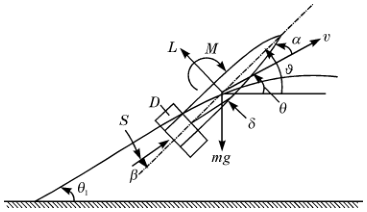
\includegraphics[width=\linewidth]{figs/fig-0067.png}
\caption{图4.9-1}
\end{figure}

形状有关的某些特定常数; $\beta, \gamma, \delta$ 和重力加速度 $g$ 可看作为决定作用于火箭弹上的外力的因素。显然，方程组 $(4.9-1)-(4.9-7)$ 是非线性的，它们和初始条件一起唯一地确定火箭弹的弹道。

这种类型的火箭弹的燃烧时间都是很短的 （譬如说，只有 $0.2-0.5$ 秒），所以就必须使加速度 $S / m$ 很大才行。事实上，推力 $S$ 是相当大的，和它比起来，重力、阻力和升力都小到可以忽略的程度。而且，推力方向与飞行方向之间的偏差角度 $\alpha-\beta$ 总是很小的，冲角 $\alpha$ 的值也总是很小的。因此，如果诸量 $\gamma, \beta, \delta$ 和 $g$ 为零时，火箭弹的理想弹道就是一条初始倾角为 $\theta$ 的直线 （图 4.9-1)。沿着这条直线的运动是一个等加速度 $S / m$ 的运动

\[\frac{d v}{d t}=S / m\qquad\text{(4.9-8)}\]

如果 $z$ 是沿着这条直线量度的距离，那么，这个运动也可以用下列方程表示

\[v^{2}=\frac{2 S}{m} z=\left(\frac{S}{m}\right)^{2} \dot{t}^{2}\qquad\text{(4.9-9)}\]

如果发射火箭弹的初始速度是零，z就是到发射点的确实距离；如果有一个初始速度，$z$ 就是到发射点前面的某一点的距离，而不是到发射点的距离。从方程 (4.9-9)我们得到

\[\frac{d}{d t}=\frac{d z}{d t} \frac{d}{d z}=v \frac{d}{d z}=\sqrt{\frac{2 S}{m} z} \frac{d}{d z}\qquad\text{(4.9-10)}\]

因为在燃烧过程中总是有外力作用的，因此真正的弹道与无外力作用时的典型弹道是有差别的。假设它们之间的偏差比较小，我们可以在理想弹道附近将运动方程线性化。我们认为真正弹道的速度特性和理想弹道的速度特性一样，因此用方程(4.9-9)来代替方程(4.9-2)，并且把方程(4.9-3)和(4.9-4)中的速度 $v$ 和时间导数用方程(4.9-9)和(4.9-10)来代替。此外，因为 $\alpha-\beta$ 很小，$\sin (\alpha-\beta)$ 也就可以用 $\alpha-\beta$ 来代替。 $\cos \theta$ 可以用 $\cos \theta$ 来代替。我们把升力 $L$ 也忽略掉，因为它比推力的横向分量以及火箭的重量都小得多。采用这些简化的假设后，方程 (4.9-3)和(4.9-4)就成为

\[2 z \frac{d \theta}{d z}=(\alpha-\beta)-\frac{m g}{S} \cos \theta\qquad\text{(4.9-11)}\]

和

\[2 z \frac{d^{2} \theta}{d z^{2}}+\frac{d \theta}{d z}=\frac{\delta}{k^{2}}-\frac{8 \pi^{2}}{\delta^{2}} z(\alpha-\gamma)\qquad\text{(4.9-12)}\]

这里的 $\sigma$ 的定义是

\[\sigma^{2}=4 \pi^{2} \frac{k^{2} m}{K_{\mathrm{mp}} d^{3}}\qquad\text{(4.9-13)}\]

很明显，$\sigma$ 的量纲是长度。我们可以把 $\sigma$ 取作火箭的扰动运动（对于典型弹道）的特征长度，并且也可以看做是扰动的弹道的“波长”。方程(4.9-1)，(4.9-11)和 (4.9-13)就是三个未知函数 $\alpha, \theta$ 和 $\vartheta$ 的线性化的方程。方程的线性化是在这样一个假设之下作的：对于一个理想的倾角 $\theta$ 来说，弹道与直线之间的差别很小。

我们可以把 $\theta$ 和 $\vartheta$ 消去而得出 $\alpha$ 的单独一个方程。做法是这样的：先用 $2 \sqrt{z}$ 除方程(4.9-11)，再把结果对 $z$ 微分。这样就得到

\[\left[\sqrt{z} \frac{d^{2} \theta}{d z^{2}}+\frac{1}{2} \frac{d \theta}{\sqrt{z} d z}+\frac{1}{2} \frac{d \alpha}{\sqrt{z} d z}-\frac{1}{4 z} \sqrt{z}\right]\left(\alpha-\beta-\frac{g m}{S} \cos \theta\right)\]

现在，我们再用 $2 \sqrt{z}$ 除方程(4.9-12)，然后，从结果中减去上面的方程，最后，再利用方程(4.9-1)的关系。就得出

\[\left[\sqrt{z} \frac{d^{2} \alpha}{d z^{2}}+\frac{1}{\sqrt{z}} \frac{d \alpha}{d z}+\left(\frac{4 \pi^{2}}{\sigma^{2}} \sqrt{z}-\frac{1}{4 z} \sqrt{z}\right) \alpha=\frac{\delta}{2 k_{i}^{2}}+\frac{4 \pi^{2}}{\sigma^{2}} \sqrt{z} r-\frac{1}{4 z} \sqrt{z}\right]\left(\beta+\frac{g m}{S} \cos \theta\right)\]

这个方程明白地表示出下列事实：用来研究火箭弹的微分方程不是常系数方程。其实，只要按照下列公式引进一个无量纲距离 $\xi$

\[\xi=\frac{2 \pi z}{\sigma}\qquad\text{(4.9-14)}\]

[ $\sigma$ 就是方程(4.9-13)所规定的“波长”]，我们就可以把 $\alpha$ 的方程化为贝塞尔方程的标准形状，也就是

\[\begin{aligned} & \frac{d^{2} \alpha}{d \xi^{2}}+\frac{1}{\xi} \frac{d \alpha}{d \xi}+\left[1-\frac{(1 / 2)^{2}}{\xi}\right] \alpha \\ & \quad=\gamma+\left(\frac{\delta \sigma}{4 \pi k_{i}^{2}}\right) \frac{1}{\xi}-\frac{1}{4}\left[\beta+\frac{g m}{S} \cos \theta\right] \frac{1}{\xi} \end{aligned}\qquad\text{(4.9-15)}\]

把 $\alpha$ 确定出以后，再积分下列方程也就可以把 $\theta$ 计算出来

\[\frac{d \theta}{d \xi}=\frac{1}{2 \xi}\left[\alpha-\beta-\frac{m g}{S} \cos \theta\right]\qquad\text{(4.9-16)}\]

这个方程是由方程(4.9-11)变化出来的。

这些微分方程中的自变量 $z$ 或 $\xi$ 并不是时间变数而是距离变数。但是，正如方程(4.9-9)所表示的那样，$z$ 是时间 $t$ 的单调增函数，$\xi$ 当然也就是 $t$ 的增函数。因此，有希望认为把自变数从 $t$ 改为 $\xi$ 并不会改变系统方程的性质。我们再仔细地研究一下方程式(4.9-15)的结构。这是对冲角 $\alpha$ 的一个线性非齐次方程式，其右端的三项均为对弹体的干扰作用。式(4.9-15)与(4.9-16)联合起来，构成一个联立方程组，它们决定火箭在发动机工作时间内的纵向运动。火箭的飞行状态是弹道倾角 $\theta$ 和冲角 $\alpha$。如果三个外干扰均等于零，那么齐次方程式

\[\frac{d^{2} \alpha}{d t^{2}}+\frac{1}{\xi} \frac{d \alpha}{d t}+\left[1-\frac{\left[\frac{1}{2}\right]^{2}}{\xi}\right] \alpha=0\]

\[\frac{d \theta}{d \xi}=\frac{1}{2} \xi^{\alpha}\qquad\text{(4.9-17)}\]

的解，$\alpha(\xi)=J_{2}^{1}(\xi)$，按 $\frac{1}{2}$ 阶贝塞尔函数的规律

\[\alpha(\xi)=J_{2}^{1}(\xi)=\sqrt{\frac{2}{\pi \xi}} \sin \xi, \quad \alpha(\xi)=J_{-1}^{-1}(\xi)=\sqrt{\frac{2}{\pi \xi}} \cos \xi\]

随 $\xi$ 的增大而逐渐减小。而 $\theta(\xi)$ 则将随 $\xi$ 的增大而趋于某稳态值 $\theta_{\infty}$。

利用上述事实，又可对非齐次方程式 (4.9-15) 做一变换。事实上方程式 (4.9-15)可以改写为

\[\frac{d^{2} \zeta}{d \xi^{2}}+\zeta=Q(\xi)\qquad\text{(4.9-18)}\]

其中

\[\zeta=\sqrt{\xi} \alpha\qquad\text{(4.9-19)}\]

而

\[Q(\xi)=r \sqrt{\xi+\left(\frac{\ddot{\alpha} \sigma}{4 \pi k^{2}}\right) \frac{1}{\xi}-\frac{1}{4}\left(\beta+\frac{g m}{S} \cos \theta\right) \frac{1}{\xi^{3 / 2}}}\qquad\text{(4.9-20)}\]

因此，对于新未知函数 $\zeta$ 来说，补充函数就是 $\sin \xi$ 和 $\cos \xi$。

火箭弹离开发射点时的条件，或者初始条件记为

\[\begin{aligned} & v=v_{0} \\ & \theta=\theta_{0} \\ & \alpha=\alpha_{0} \\ & d \beta / d t=\left(d \beta / d t\right)_{0} \end{aligned}\qquad\text{(4.9-21)}\]

这里的下标“0”表示 $t=0$ 时刻的值。 $\xi$ 和 $\zeta$ 的初始值当然就是

\[\xi_{0}=\frac{2 \pi}{\sigma} \frac{m}{2 S} v_{0}^{2}=\frac{\pi m v_{0}^{2}}{\sigma S}\qquad\text{(4.9-22)}\]

和

\[\zeta_{0}=\sqrt{\xi_{0}} \alpha\qquad\text{(4.9-23)}\]

根据方程 (4.9-16)，$t=0$ 时就有

\[\sqrt{\xi_{0}}\left[\frac{d \theta}{d \xi}\right]_{0}=\frac{\alpha-\beta-\left(m g / S\right) \cos \theta}{2 \mid \xi_{0}}\]

但是 $\theta=\vartheta-\alpha$，所以

\[\left\{\begin{array}{l} \frac{d \zeta}{d \xi} \mid_{0}=\sqrt{\xi_{0}}\left\{\frac{d \alpha}{d \xi}\right\}_{0}+\frac{1}{2} \mid \xi_{0} \mid \alpha=\sqrt{\xi_{0}}\left\{\frac{d \beta}{d \xi}\right\}_{0}+\frac{\beta+\left(g m / S\right) \cos \theta}{2 \mid \xi_{0}} \end{array}\right.\]

或更明显地，

\[\left\{\begin{array}{l} \frac{d \zeta}{d \xi} \mid_{0}=\sqrt{\xi_{0}} \frac{\sigma\left(d \beta / d t\right)_{0}}{2 \pi v_{0}}+\frac{\beta+\left(g m / S\right) \cos \theta}{2 \mid \xi_{0}} \end{array}\right.\qquad\text{(4.9-24)}\]

把初始条件这样变化以后，我们就可以把方程 (4.9-18) 的解 $\zeta$ 或 $\alpha$ 直接写出来:

\[\begin{aligned}& \alpha(\xi, \xi)=\frac{1}{\xi} \cos (\xi-\xi) \bigg[ \zeta-\int_{\xi}^{\xi} \sin (\eta-\xi) Q(\eta) d \eta \\& \quad+\frac{1}{\xi} \sin (\xi-\xi) \bigg] \bigg[ \frac{d \zeta}{d \xi} \bigg]_{0}+\int_{\xi}^{\xi} \cos (\eta-\xi) Q(\eta) d \eta\end{aligned}\]

这里的 $Q$ 就是方程 (4.9-20) 所表示的驱动函数。因为 $Q(\eta)$ 中包含有 $\eta$ 的半次方幂，所以方程 (4.9-25) 中的积分确实都是福来内尔 (Fresnel) 积分。把方程 (4.9-20) 和初始条件式 (4.9-23)，(4.9-24) 代入方程 (4.9-15) 后，再进行计算就可以得出冲角 $\alpha(\xi, \xi)$ 的表示式:

aligned\& (, )=+[+m g/S  ] F\_1(, )+ 2  k\textasciicircum{}2 F\_2(, )- [ F\_1(, ). \textbackslash\{\}\textbackslash\{\}\& .+F\_3(, )]+ F\_3(, )+2  v\_0(d /d t)\_0 F\_1(, )aligned

其中 $F_{i}(\xi, \xi), i=1,2,3,4$ 都可表示为火箭函数的组合。

\[\begin{aligned}& F_{1}(\xi, \xi)=\frac{1}{2} \bigg[ r r(\xi) \sin (\xi-\xi)+r j(\xi) \cos (\xi-\xi)-r j(\xi)\bigg] \\& F_{2}(\xi, \xi)=\frac{1}{2} \bigg[ r r(\xi)-r r(\xi) \cos (\xi-\xi)+r j(\xi) \sin (\xi-\xi)\bigg] \\& F_{3}(\xi, \xi)=\sqrt{\xi} \cos (\xi-\xi) / \sqrt{\xi} \\& F_{4}(\xi, \xi)=\sqrt{\xi} \sin (\xi-\xi) / \sqrt{\xi}\end{aligned}\]

罗色尔等 ${ }^{[21]}$ 把一些常用的福来内尔积分定义为火箭函数:

\[\begin{aligned}& r r(\omega)=\cos \omega \int_{\omega}^{\infty} \frac{\sin x}{x} d x-\sin \omega \int_{\omega}^{\infty} \frac{\cos x}{x} d x \\& r j(\omega)=\cos \omega \int_{\omega}^{\infty} \frac{\cos x}{x} d x+\sin \omega \int_{\omega}^{\infty} \frac{\sin x}{x} d x \\& r a^{2}(\omega)=r r^{2}(\omega)+r j^{2}(\omega) \\& i r(\omega)=\int_{0}^{\omega} \frac{r r(x)}{x} d x \\& i j(\omega)=\int_{0}^{\omega} \frac{r j(x)}{x} d x \\& r t(\omega)=\frac{r j(\omega)}{r r(\omega)}\end{aligned}\qquad\text{(4.9-33)}\]

并且在他们的书里 ${ }^{[21]}$ 还把这些函数作成函数表，$r r(\omega)$ 和 $r j(\omega), r a(\omega)$ 都是 $\omega$ 的单调递降函数，$j r(\omega)$ 是 $\omega$ 的单调递升函数。因此根据式 (4.9-27) 可以看出，对于很大的 $\xi F_{i}(\xi, \xi), i=1,2,3,4$ 都趋于零，这样 $\alpha(\xi, \xi)$ 就趋于 $\gamma$。把 $\alpha$ 计算出来以后，用积分方法就可以由方程(4.9-16)求出 $\theta$ 来:

\[\theta-\theta_{1}=\left(\theta_{1}-\theta_{1}\right)-\frac{1}{2}\left[\beta+\frac{m g}{S} \cos \theta_{1}\right] \ln \xi_{0}+\frac{1}{2} \int_{\xi_{0}}^{\xi} \frac{\alpha\left(\eta, \xi_{0}\right)}{\eta} d \eta\qquad\text{(4.9-34)}\]

把方程(4.9-26)代入式(4.9-34)后，再把方程(4.9-34)写成若干项，每一项都代表一种类型的扰动。这样，

\[\begin{aligned} \theta-\theta_{1}= & \left(\theta_{1}-\theta_{1}\right)+\left[\beta+\frac{m g}{S} \cos \theta_{1}\right] G_{1}\left(\xi, \xi_{0}\right)+\frac{\partial \sigma}{2 \pi k} G_{2}\left(\xi, \xi_{0}\right)-\gamma\left[G_{1}\left(\xi, \xi_{0}\right)\right. \\ & \left.+G_{2}\left(\xi, \xi_{0}\right)\right]+\alpha G_{3}\left(\xi, \xi_{0}\right)+\frac{1}{2} \frac{\sigma}{\pi v_{0}}\left[\frac{d \theta}{d t}\right]_{0} G_{4}\left(\xi, \xi_{0}\right) \end{aligned}\]

其中

\[\begin{aligned} & G_{1}\left(\xi, \xi_{0}\right)=\frac{1}{2} \int_{\xi_{0}}^{\xi} \frac{F_{1}\left(\eta, \xi_{0}\right)}{\eta} d \eta-\frac{1}{2} \ln \xi_{0} \\ & G_{2}\left(\xi, \xi_{0}\right)=\frac{1}{2} \int_{\xi_{0}}^{\xi} \frac{F_{2}\left(\eta, \xi_{0}\right)}{\eta} d \eta \\ & G_{3}\left(\xi, \xi_{0}\right)=\frac{1}{2} \int_{\xi_{0}}^{\xi} \frac{F_{3}\left(\eta, \xi_{0}\right)}{\eta} d \eta \\ & G_{4}\left(\xi, \xi_{0}\right)=\frac{1}{2} \int_{\xi_{0}}^{\xi} \frac{F_{4}\left(\eta, \xi_{0}\right)}{\eta} d \eta \end{aligned}\qquad\text{(4.9-36)}\]

方程(4.9-35)右边第一项表示弹道初始倾角偏差的影响。第二项表示推力不正和重力的影响。第三项表示推力的转矩的影响。第四项表示尾翼的安装不正所引起的影响。第五项表示初始冲角的影响。最末一项表示火箭弹的初始角速度的影响。每一个 $G$ 都是 $\xi$ 和 $\xi_{0}$ 这两个变数的函数，并且也是由一些福来内尔积分组成的。用图线表示这些函数的几个图（图 4.9-2 4.9-5)也是引自文献[21]。

图 4.9-2

图 4.9-3

\begin{figure}[htbp]\centering
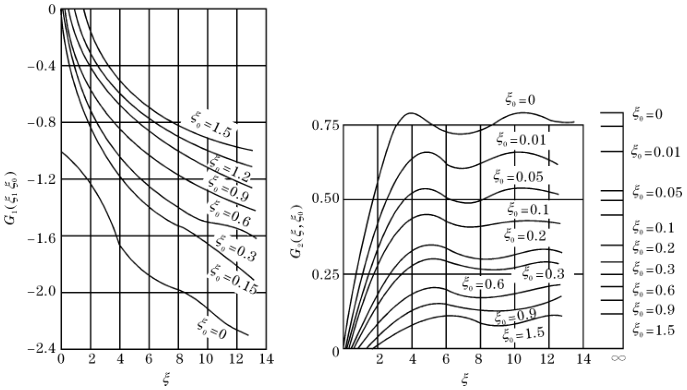
\includegraphics[width=\linewidth]{figs/fig-0068.png}
\caption{图4.9-3}
\end{figure}

\[\begin{aligned}& G\left(\xi, \xi_{0}\right) \\& \xi_{0}=0.3 \\& \xi_{0}=0.6 \\& \xi_{0}=0.9 \\& \xi_{0}=1.2 \\& \xi_{0}=1.5\end{aligned}\]

图 4.9-4

\[\begin{aligned}& \left(\sqrt{\frac{\xi}{\xi_{0}}}\right) G(\xi) \\& \xi\end{aligned}\]

图 4.9-5

把图 4.9-2 到图 4.9-5 这几个图观察一下，就可以看出这样一个事实：对于很大的 $\xi$ 值来说，所有这些火箭函数 $G$ 几乎都是常数。所以，各种扰动都不能阻尼掉。方程 (4.9-35) 的第一项和最后两项表示在发射点所受的初始扰动的影响，然而，当 $\xi$ 很大时，它们还保持不等于零的有限值。方程 (4.9-35) 的其余三项都是由于“输入” （或者说驱动函数） 而产生的“输出”。对于很大的 $\xi$ 值来说，它们的值也不是零。$G_{1}$ 函数的性质尤其恶劣：当 $\xi$ 很大的时候，它差不多等于 $\ln \xi$，所以也就要无限地增大。

我们试用李雅普诺夫稳定性的判据准则来对此具体问题作一分析。火箭纵向飞行状态 $\alpha$ 对初始状态扰动 $\alpha_{0},\left(\frac{d \delta}{d t}\right)_{0}$ 和 $\theta$ 都是稳定的，因为这些干扰引起的变化都随 $\xi$ 的增大而趋于零。但是有了外扰作用后 $\alpha(\xi)$ 并不趋于零。其次，当有外扰情况下 $\theta$ 将无限增大。根据齐次方程式 (4.9-17) 可知，当一切外扰为零时，由于初始条件式 (4.9-21) 不为零，$\theta$ 也不会趋于零。由此只能得出结论：火箭弹按稳定性的定义是不稳定的。

但是，这个结论并不能使设计师们感到震惊。因为，第一，李雅普诺夫的定义是 $\xi \rightarrow \infty$ 时系统坐标的变化情况，而这里的短程火箭的推力作用时间却很短。“$\xi$趋于无穷大”这一条件在此完全无意义；第二，即便在有限时间内 $\theta(t)$ 和 $\alpha(t)$ 将在干扰作用下随射程距离的增大而增大，或保持不为零的常量，这也无助于火箭能够较准确地命中目标。这样一来，李雅普诺夫稳定性的定义必须加以修改。这里宜于采用的是有限时间内的稳定性的概念。按第 4.7 节叙述的定义，这里稳定性的概念可以这样提：设给定火箭飞行时间 $T$，在 $t=T$ 时飞行状态偏差 $\theta$ 和 $\alpha$ 应满足条件

\[\mid \theta \mid<\theta_{1}, \quad \mid \alpha \mid<\alpha_{1}\]

其中 $\theta, \alpha$ 均为预先给定的常数。如果对任意给定的这一组正数: $T, \theta, \alpha$，均能找

\begin{figure}[htbp]\centering
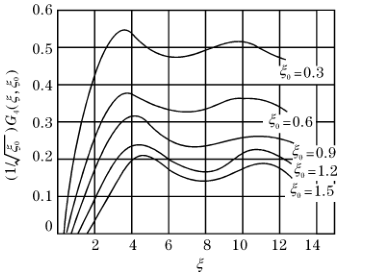
\includegraphics[width=\linewidth]{figs/fig-0069.png}
\caption{图4.9-5}
\end{figure}

\begin{figure}[htbp]\centering
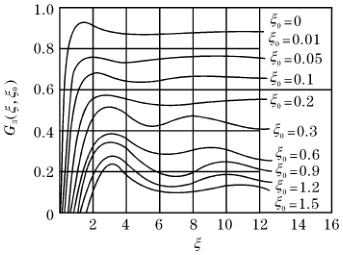
\includegraphics[width=\linewidth]{figs/fig-0070.png}
\caption{图4.9-4}
\end{figure}

出一组不为零的正数 $\gamma, \delta, \beta, \theta, \infty, \left.\left.\frac{d \theta}{d t}\right|_{0}\right)$，使在 $0 \leqslant t \leqslant T$ 间隔内，或在 $t=T$ 时刻满足条件式 (4.9-37)，那么此火箭的运动是稳定的。

这样一种提法是有重要实际意义的。如果上述条件不满足，就无法使火箭飞行达到要求的精度式 (4.9-37)。反之，如果火箭运动按上述定义是稳定的，那么根据给定的 $T, \theta, \alpha$ 就可能定出可允许的干扰 $\gamma, \delta, \beta$ 及初始条件误差 $\theta, \alpha$ 和 $\left.\frac{d \theta}{d t}\right|_{0}$ 的公差范围，而这对设计师来说是具有重要意义的。

\section{4.10 线性系统的能观测性}

在任何闭路系统中，为了形成反馈信号必须不断地测量系统的状态。在实际问题中常出现这样的情况，预先给定的测量方法不能提供足够的信息去确定系统的状态，这时就要改变测量方案。所以事先应该检查给定的测量方法能否满足要求。1960年卡尔曼(Kalman)首先从理论上提出了这一问题，并引进了关于能观测性的概念 ${ }^{[15]}$。事实证明，这是一个重要的概念。下面以雷达测量为例对这个概念加以说明。

\begin{figure}[htbp]\centering
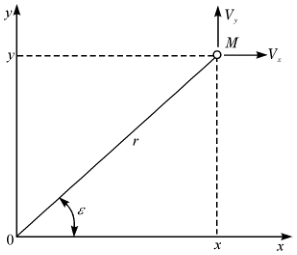
\includegraphics[width=\linewidth]{figs/fig-0071.png}
\caption{图4.10-1}
\end{figure}

由于受观测工具和测量手段的限制，受控对象的状态变化 $\boldsymbol{x}(t)=\left\{x_{1}(t), x_{2}(t), \cdots, x_{n}(t)\right\}$ 常不可能逐个地全部实时地测量出来。为了估计各个状态变量的瞬时值，必须通过能够直接测量到的数据换算出来。典型的例子是飞行器的雷达测量。设 $M$ 为要观测的目标，在平面坐标系中作为一个质点的运动有四个独立的状态分量: $x(t), y(t)$ 和 $\dot{x}(t)=V_{x}(t), \dot{y}(t)=V_{y}(t)$ （图 4.10-1)。置于 0 点的雷达能够观测到的是另外的四个量：斜距 $r$，仰角 $\varepsilon$ 和它们的变化率 $\dot{r}, \dot{\varepsilon}$。

$M$ 的状态和观测量之间的关系是

\[\begin{aligned} & r=\sqrt{x^{2}+y^{2}} \\ & \varepsilon=\tan ^{-1} \frac{y}{x} \\ & \dot{r}=\frac{1}{\sqrt{x^{2}+y^{2}}}\left(x V_{x}+y V_{y}\right) \\ & \dot{\varepsilon}=\frac{x}{x^{2}+y^{2}} V_{y}-\frac{y}{x^{2}+y^{2}} V_{x} \end{aligned}\]

图 4.10-1如果观测工具是光学仪器，则它不能精确测量出 $\dot{r}$ 和 $\dot{\varepsilon}$，只能给出 $r$ 和 $\varepsilon$ 的精确值，那就只能得到前面两个关系式，这时就不能用 $x$ 和 $y$ 的瞬时值求出另两个状态变量 $V_{x}$ 和 $V_{y}$。但是，由于 $x=r \cos \varepsilon, y=r \sin \varepsilon$，如果测得 $r$ 和 $\varepsilon$ 在 $t$ 时刻以前的数据，$V_{x}$ 和 $V_{y}$ 仍然可以通过微分运算求出来。如果测量工具只能测得一个量 $r$，情况就完全不同了，仅用一个 $r(t)$ 的哪怕是在 $[0, t]$ 时间内的全部数据也不可能得到任何状态坐标的正确估算。于是，对受控对象的状态能不能测量，取决于受控对象本身的特点和测量方程二者之间的相互关系。

下面我们只讨论线性系统的能观测性问题（对非线性系统这个问题也是存在的）。考查变系数线性系统

\[\frac{d \mathbf{x}(t)}{d t}=A(t) \mathbf{x}(t)+B(t) \mathbf{u}(t)\qquad\text{(4.10-1)}\]

式中 $\mathbf{x}(t)=\left(x_{1}(t), x_{2}(t), \cdots, x_{n}(t)\right)$ 是状态向量，$\mathbf{u}(t)=\left(u(t), \cdots, u(t)\right)$ 是控制向量，$A(t)=\left(a_{i j}(t)\right)$ 和 $B(t)=\left(b_{i j}(t)\right)$ 分别是 $n \times n$ 和 $n \times r$ 矩阵，其中 $a_{i j}(t)$ 和 $b_{i j}(t)$ 都是 $t$ 的连续函数。假定被观测的量 $\mathbf{y}$ 与状态 $\mathbf{x}$ 之间是线性关系

\[\mathbf{y}(t)=H(t) \mathbf{x}(t)\qquad\text{(4.10-2)}\]

$H(t)=\left(h_{y j}(t)\right)$ 是 $l \times n$ 阶矩阵，$l \leqslant n, h_{y j}(t)$ 也是 $t$ 的连续函数。

一个有益的概念是系统的能观测性。如果对任一时刻 $t>b$ 系统的状态 $\mathbf{x}(t)$可以根据观测到的 $\mathbf{y}(t)$ 在 $[b, t]$ 时间内的数据和已知的 $\mathbf{u}(t)$ 在同一时间内的数据唯一地确定出来，则说系统式(4.10-1)和(4.10-2)在 $t$ 时刻是完全可观测的。

注意到式 (4.10-1) 可能是一个闭路系统，即若 $\mathbf{u}(t)=C(t) \mathbf{x}(t)$，则式 (4.10-1)变为

\[\frac{d \mathbf{x}}{d t}=\left(A(t)+B(t) C(t)\right) \mathbf{x}=A_{1}(t) \mathbf{x}\qquad\text{(4.10-1)}\]

此时 $\mathbf{u}(t)$ 的数据对系统的可观测性不起作用，而矩阵 $A_{1}(t)$ 的具体形式将和 $H(t)$共同决定系统的可观测性。

第二章中我们曾讨论过，式(4.10-1)的解是

\[\mathbf{x}(t)=\Phi(t, b) \mathbf{x}_{0}+\Phi(t, b) \int_{t_{0}}^{t} \Phi^{-1}(\tau, b) B(\tau) \mathbf{u}(\tau) d \tau\]

式中 $\mathbf{x}_{0}$ 是状态的初值，$\Phi(t, b)$ 是齐次方程 $(\boldsymbol{u}=\mathbf{0})$ 的基本解矩阵。代入式 (4.10-2)，有

\[\begin{aligned} \mathbf{y}(t) & =H(t) \Phi(t, b) \mathbf{x}_{0}+H(t) \Phi(t, b) \int_{t_{0}}^{t} \Phi^{-1}(\tau, b) B(\tau) \mathbf{u}(\tau) d \tau \\ & =H(t) \Phi(t, b)\left[\mathbf{x}_{0}+\int_{t_{0}}^{t} \Phi^{-1}(\tau, b) B(\tau) \mathbf{u}(\tau) d \tau\right] \end{aligned}\]

显然，如果 $H(t)$ 对任何 $t$ 都是 $n \times n$ 可逆矩阵，系统当然是完全可观测的，因为 $\mathbf{x}(t)=H^{-1}(t) \mathbf{y}(t)$ 对任何 $t$ 成立。实际上，$H(t)$ 通常不一定是正方阵，即 $\mathbf{y}(t)$ 的维数通常小于 $n$，所以 $H(t)$ 不可能有逆。

由于 $\Phi(t, b)$ 是 $n \times n$ 阶方阵，$\mathbf{x}(t)$ 和 $\mathbf{x}$ 之间有一对一的对应关系，即每一个 $\mathbf{x}$ 对应一个唯一的 $\mathbf{x}(t)$，不同的 $\mathbf{x}$ 对应不同的 $\mathbf{x}(t)$。因此，为了根据 $\mathbf{y}(t)$ 在 $\left[b,\right.$ $t]$ 上的数据能够唯一地确定 $\mathbf{x}(t)$，只须能求出 $\mathbf{x}$ 就够了。系统可观测性条件可改述为：如果能根据 $\mathbf{y}(t)$ 在 $\left[b, t\right]$ 上的数据唯一确定 $\mathbf{x}(b)=\mathbf{x}$，系统在 $t$ 时刻是可观测的；如果对一切 $t$ 都可观测，系统叫完全可观测的。用 $H^{r}(t)$ 和 $\Phi^{r}(t, b)$ 分别表示 $H(t)$ 和 $\Phi(t)$ 的转置矩阵。对 $(4.10-2^{\prime})$ 两端作用 $\Phi^{r}(t, b) H^{r}(t)$，并在时间间隔 $\left[b, t\right]$ 上积分后有

\[\begin{aligned}& \int_{t_{0}}^{t_{1}} \Phi^{r}\left(t, b\right) H^{r}(t) H(t) \Phi(t, b) \mathbf{x} d t \\= & \int_{t_{0}}^{t_{1}} \Phi^{r}\left(t, b\right) H^{r}(t)\left[\mathbf{y}-H(t) \Phi(t, b)\right] \Phi^{r-1}(\tau, \tau) B(\tau) u(\tau) d \tau d t \\= & z(t)\end{aligned}\]

根据假定上式右端是已知的，记为 $\mathbf{z}(t)$。如果 $n \times n$ 方阵 $M_{0}(t, b)$

\[M_{0}(t, b)=\int_{t_{0}}^{t_{1}} \Phi^{r}(t, b) H^{r}(t) H(t) \Phi(t, b) d t\qquad\text{(4.10-3)}\]

是可逆的，就有 $\mathbf{x}=M_{0}^{-1}(t, b) \mathbf{z}(t)$。这意味着，如果 $M_{0}(t, b)$ 对任何 $t$ 是可逆矩阵，则系统必是完全可观测的，此时

\[\begin{aligned}& \mathbf{x}_{0}=M_{0}^{-1}(t, b) \mathbf{z}(t) \\= & M_{0}^{-1}(t, b)\left[\int_{t_{0}}^{t_{1}} \Phi^{r}(t, b) H^{r}(t)\right. \\& \left.\quad \times\left[\mathbf{y}(t)-H(t) \Phi(t, b)\right] \Phi^{r-1}(\tau, \tau) B(\tau) u(\tau) d \tau\right] d t\end{aligned}\]

即 $\mathbf{y}(t)$ 和 $\mathbf{u}(t)$ 在 $\left[b, t\right]$ 上的数据完全确定 $\mathbf{x}$，因而完全确定 $\mathbf{x}(t)$，反之，可以断言，为了使系统是完全可观测的，必需 $M_{0}(t, b)$ 对任何 $t>b$ 是可逆矩阵。显然，如果 $M_{0}(t, b)$ 是不可逆的，则同一个 $\mathbf{z}(t)$ 将有两个以上的 $\mathbf{x}$ 按下列代数方程相对应:

\[M_{0}(t, b) \mathbf{x}=\mathbf{z}(t)\]

即上式有两个以上的独立解。这就是说，根据 $\mathbf{z}(t)$ 不能单一地确定 $\mathbf{x}$，系统在 $t=t$ 时是不可观测的，因而不是完全可观测的。

总结上述，由运动方程 (4.10-1) 和测量方程 (4.10-2) 构成的系统为完全可观测的充要条件是由式 (4.10-3) 定义的 $n \times n$ 阶方阵对任何 $t_{1}>b$ 是可逆的。注意到 $\Phi^{r} H^{r} H \Phi$ 是非负对称矩阵，而对称矩阵的和也是对称矩阵，故 $M_{0}(t, b)$ 是对称的非负方阵。只有 $M$ 是正定时才可能有逆。因而 $M_{0}(t, b)$ 是可逆的等价于它的正定性。

对常系数线性系统，能观测性的充分必要条件还可以更具体化一些。设式

(4.10-1)和(4.10-2)中的矩阵 $A, B$ 和 $H$ 都是常量矩阵，这时整个系统为

\[\frac{d \boldsymbol{x}}{d t}=A \boldsymbol{x}+B \boldsymbol{u}\qquad\text{(4.10-4)}\]

可以证明，系统式 (4.10-4) 完全能观测的必要充分条件是矩阵

\[\Omega_{0}=\left(\begin{array}{c} H \\ H A \\ H A^{2} \\ \vdots \\ H A^{n-1} \end{array}\right)\qquad\text{(4.10-5)}\]

的秩为 $n$。这个条件使我们可以直接去检查常系数系统的完全能观测性。关于这一结论的详细证明，可看文献[7，14，15]。

\section{4.11 线性系统的能控性}

某种特定的系统结构能不能保证系统的所有状态坐标都受到控制作用的制约，在一个复杂的系统中这并不是显而易见的特征。在多维系统中常有一部分坐标是不能控制的；还有一部分只能通过别的坐标间接地受到控制。弄清给定系统的能控性不仅具有实际意义，在理论分析中它尤其是一个重要概念。本节内我们将介绍能控性的意义，以及能控性与能观测性之间的关系。

仍然讨论由式 (4.10-1) 描述的受控系统。当控制作用 $\boldsymbol{u}(t)$ 选定后，系统的状态变化将由式 (4.10-3) 单值确定。如果对初值 $\boldsymbol{x}_{0}$，存在 $t>b$，使它在 $t-b$ 的时间内归零，即 $\boldsymbol{x}(t)=\boldsymbol{0}$，系统叫做对 $\boldsymbol{x}$ 能控。如果对任何 $\boldsymbol{x}_{0}$ 都能控，系统叫做完全能控的。由式 (4.10-3) 知，为了使

\[\boldsymbol{x}(t)=\Phi(t, b)\left[\boldsymbol{x}_{0}+\int_{t_{0}}^{t_{1}} \Phi^{-1}(t, b) B(t) \boldsymbol{u}(t) d t\right]=\boldsymbol{0}\]

必须有

\[\boldsymbol{x}_{0}=-\int_{t_{0}}^{t_{1}} \Phi^{-1}(t, b) B(t) \boldsymbol{u}(t) d t\qquad\text{(4.11-1)}\]

因为 $\Phi(t, t)$ 永远是可逆的，只有作用到 $\boldsymbol{0}$ 向量上才能有 $\boldsymbol{x}(t)=\boldsymbol{0}$。

为了对任何 $\boldsymbol{x}_{0} \in R_{n}$ 都能选出 $t_{1}$ 和 $\boldsymbol{u}(t)$ 使式 (4.11-1) 成立，显然由

\[K u(t)=\int_{t_{0}}^{t_{1}} \Phi^{-1}(t, b) B(t) \boldsymbol{u}(t) d t\qquad\text{(4.11-2)}\]

定义的算子 $K$ 的值域应该充满整个空间 $R_{n}$。如果 $\boldsymbol{z}$ 为任一 $n$ 维常向量，取 $\boldsymbol{u}(t)=$ $B^{z}(t) \Phi^{-1}(t, b) \boldsymbol{z}=B^{z}(t) \Phi^{z}(t, b) \boldsymbol{z}$ 代入式 (4.11-2) 后有

\[K u(t)=\int_{t_{0}}^{t_{1}} \Phi^{-1}(t, b) B(t) B^{z}(t) \Phi^{z}(t, b) \boldsymbol{z} d t\qquad\text{(4.11-2)}\]

=\_\{t\_\{0\}\}\textasciicircum{}\{t\_\{1\}\} (b，t) B(t) B\textasciicircum{}\{s\}(t) \textasciicircum{}\{s\}(b，t) z d t 式中利用了关系式

\[M_{c}(t, b)=\int_{t_{0}}^{t_{1}} \Phi(b, t) B(t) B^{s}(t) \Phi^{s}(b, t) d t\]

必须是可逆的，此时 $z=M_{c}^{-1}(t, b) K u(t), z$ 和 $u(t)$ 一一对应。只要选 $n$ 个线性不相关的 $z, z, \cdots, z_{n}$，就能得到 $n$ 个线性不相关的 $\left\{K u_{i}(t)\right\}_{i}^{n}$，即它们的线性组合充满整个空间。这就是说，$M_{c}(t, b)$ 为可逆矩阵 （正定矩阵） 是系统能控性的充分条件。而 $M(t, b)$ 对任何 $t>b$ 都是可逆的 （正定的），这是系统完全能控性的充分条件。

实际上 $M_{c}$ 的正定性也是系统能控性的必要条件。设对每一个初始状态 $\boldsymbol{x} \neq$ $\mathbf{0}$，存在至少一个 $\boldsymbol{u}(t), t \in\left[b_{b}, b\right]$，使 $\boldsymbol{x}=-\int_{t_{0}}^{t_{1}} \Phi(b, t) B(t) \boldsymbol{u}(t) d t$。那么内积

\[-\left(\boldsymbol{x}, \int_{t_{0}}^{t_{1}} \Phi(b, t) B(t) \boldsymbol{u}(t) d t\right)_{R_{n}}=\left(\boldsymbol{x}, \boldsymbol{x}\right)_{R_{n}}=\|\boldsymbol{x}\|^{2}>0\qquad\text{(4.11-3)}\]

展开左端内积，记 $\Phi(b, t)=\left(\varphi_{a b}(b, t)\right), B(t)=\left(b_{b y}(t)\right), \boldsymbol{x}=\left\{x_{1}, \cdots, x_{n}\right\}$，有

\[\begin{aligned}& -\int_{t_{0}}^{t_{1}} \sum_{a=1}^{n} x_{a} \varphi_{a b}(t) \sum_{t=1}^{n} b_{b y}(t) u_{r}(t) d t \\& =-\int_{t_{0}}^{t_{1}}\left[\sum_{t=1}^{r} u_{r}(t) \sum_{a=1}^{n} \varphi_{a b}(b, t) b_{b y} x_{a}\right] d t \\& =-\left(\boldsymbol{u}(t), B^{s} \Phi^{s}(b, t) \boldsymbol{x}\right)_{R_{r_{r}}^{2}\left(t_{0}, t_{1}\right)} \geqslant 0\end{aligned}\]

上式下标 $L_{R_{r}}^{2}(b, t)$ 表示两个取值于 $r$ 维空间 $R_{r}$ 的 $t$ 的函数的内积，$B^{s}(t)$ 和 $\Phi^{s}(b, t)$ 分别是 $B(t)$ 和 $\Phi(b, t)$ 的转置矩阵。由上式知 $B^{s}(t) \Phi^{s}(b, t) \boldsymbol{x} \neq \mathbf{0}$，因而

\[\begin{aligned}& \left(B^{s}(t) \Phi^{s}(b, t) \boldsymbol{x}, B^{s}(t) \Phi^{s}(b, t) \boldsymbol{x}\right)_{R_{r_{r}}^{2}\left(t_{0}, t_{1}\right)} \\= & \left(\boldsymbol{x}, \int_{t_{0}}^{t_{1}} \Phi(b, t) B(t) B^{s}(t) \Phi^{s}(b, t) d t \boldsymbol{x}\right)_{R_{n}} \\= & \left(\boldsymbol{x}, M_{c}(b, t) \boldsymbol{x}\right)_{R_{n}} > 0\end{aligned}\qquad\text{(4.11-4)}\]

对任意非零向量 $\boldsymbol{x}$ 成立，即 $M_{c}(b, b)$ 是正定的，因而是可逆的。所以，$M_{c}(b, b)$ 为正定 （可逆） 是系统有能控性的必要条件。

对常系数方程

\[\frac{d \boldsymbol{x}}{d t}=A \boldsymbol{x}+B u\qquad\text{(4.11-5)}\]

能控性的标志比较容易检查。令 $b=0$，由第二章知，此时 $\Phi(b, t)=e^{-A t}$，所以

\[M_{c}\left(t_{1}, 0\right)=M_{c}(t)=\int_{0}^{t_{1}} e^{-A t} B B^{t} e^{-A t_{1}} d t\qquad\text{(4.11-6)}\]

$M^{r}\left(t_{i}\right)$ 的正定性或可逆性，依式 (4.11-4)，等价于 $v(t)=B^{r} e^{-A_{1}^{r} t} \boldsymbol{x}_{0} \neq \boldsymbol{0}, t \in\left[0, h_{i}\right]$，对任何非零 $\boldsymbol{x}_{0}$ 均成立，$v(t)$ 是 $r$ 维向量 $v(t)=\left\{v_{1}(t), v_{2}(t), \cdots, v_{r}(t)\right\}$。设 $\boldsymbol{h}$ 是 $R_{r}$ 中的某一非零向量，那么 $\left(\boldsymbol{h}, B^{r} e^{-A_{1}^{r} t} \boldsymbol{x}_{0}\right)_{R_{r}}=\left(e^{-A_{1}} B h, \boldsymbol{x}_{0}\right)_{R_{n}}$ 不可能对所有 $\boldsymbol{x}_{0}$ 都为 $\boldsymbol{0}$，因而有下列两个不等式成立

\[\begin{aligned} & e^{-A_{1}} B h \neq \boldsymbol{0} \quad \forall \boldsymbol{h} \neq \boldsymbol{0}, \boldsymbol{h} \in R_{r} \\ & B^{r} e^{-A_{1}^{r}} \boldsymbol{x}_{0} \neq \boldsymbol{0} \quad \forall \boldsymbol{x}_{0} \in R_{n}, \boldsymbol{x}_{0} \neq \boldsymbol{0} \end{aligned}\qquad\text{(4.11-7)}\]

今证明，常系数线性系统式 (4.11-5) 完全能控的充要条件是 $n \times n r$ 阶方阵 $\Omega$ 或 $n r \times n$ 阶方阵 $\Omega^{r}$ 的秩为 $n$:

\[\begin{aligned} & \Omega=\left(B, A B, \cdots, A^{n-1} B\right) \\ & \Omega^{r}=\left(\begin{array}{c} B^{r} \\ B^{r} A^{r} \\ B^{r}\left(A^{r}\right)^{2} \\ \vdots \\ B^{r}\left(A^{r}\right)^{n-1} \end{array}\right) \end{aligned}\]

设 $\Omega^{r}$ 的秩为 $n$，但系统不完全能控，那么必有一个 $\boldsymbol{x}_{0} \neq \boldsymbol{0}$ 使 $B^{r} e^{-A_{1}^{r} t} \boldsymbol{x}_{0} \equiv \boldsymbol{0}$。对 $t$ 微分 $n-1$ 次并令 $t=0$，得

\[B^{r} \boldsymbol{x}_{0}=\boldsymbol{0}, B^{r} A^{r} \boldsymbol{x}_{0}=\boldsymbol{0}, \cdots, B^{r}\left(A^{r}\right)^{n-1} \boldsymbol{x}_{0}=\boldsymbol{0}\qquad\text{(4.11-9)}\]

这和 $\Omega^{r}$ 的秩为 $n$ 相矛盾。所以 $\Omega^{r}$ 的秩为 $n$ （同理 $\Omega$ 的秩为 $n$ ) 是完全能控的充分条件。

再设系统为完全能控，但 $\Omega^{r}$ 的秩小于 $n$。那么必存在一个 $\boldsymbol{x}_{0} \neq \boldsymbol{0}$ 使式 (4.11-9) 成立。由矩阵函数理论 $e^{-A_{1}^{r} t}$ 可以表示成

\[e^{-A_{1} t}=\sum_{a=0}^{n-1} f_{a}(t) A^{a}\]

于是

\[B^{r} e^{-A_{1}^{r}} \boldsymbol{x}_{0}=\sum_{a=0}^{n-1} f_{a}(t) B^{r}\left(A^{r}\right)^{a} \boldsymbol{x}_{0} \equiv \boldsymbol{0}\]

这又与完全能控性的特征式 (4.11-7)矛盾。所以 $\Omega$ 或 $\Omega^{r}$ 的秩为 $n$ 又是完全能控性的必要条件。

如果 $\boldsymbol{u}$ 是一维的，则 $B$ 是列向量，记为 $\boldsymbol{b}$，因此上述完全能控的充要条件是下列 $n$ 个向量线性无关

\[\Omega=\left\{\boldsymbol{b}, A \boldsymbol{b}, A^{2} \boldsymbol{b}, \cdots, A^{n-1} \boldsymbol{b}\right\}\qquad\text{(4.11-8)}\]

此时完全能控性是很容易检查的。

最后，对方程组 (4.10-1)-(4.10-2) 构造对偶方程式

\[\frac{d \boldsymbol{z}}{d t}=-A^{r}(t) \boldsymbol{z}(t)+H^{r}(t) v(t)\qquad\text{(4.11-11)}\]

可以证明，为了使系统式(4.10-1)-(4.10-2)是完全能观测的，必须它的对偶方程(4.11-11)是完全能控的。对常系数系统这一事实可由上述能控性和第 4.10 节中讨论过的能观测性条件相比较而确信。对变系数系统也只要重复对方阵 $M\left(h_{1}, t_{0}\right)$ 和 $M^{\prime}\left(h_{1}, t_{0}\right)$ 的计算就可得到证明。详细的论述可参看文献[7，14]。

线性系统能控性和能观测性问题，与系统的稳定性、最优控制以及最优滤波等问题都有密切关系[7，14，12，41]。例如，一个完全能控的常系数线性系统，通过状态反馈可以任意配置极点（见第 5.5 节）。因此，只要系统完全能控总可以通过状态反馈使系统渐近稳定，而且具有任意指定的衰减速度。

从能控性和能观测性观点来看，一个线性系统总可以分解成四个部分，即能控、能观测部分，能控、不能观测部分，能观测、不能控部分，不能控、不能观测部分。在这四部分中，传递函数只能反映完全能控、完全能观测部分。因此，对一般线性系统，传递函数方法不是一种完全地描述。

\section{参考文献}

[1] 秦元勋，运动稳定性的一般问题讲义，科学出版社，1958.

[2] 许淞庆，常微分方程稳定性理论，上海科学技术出版社，1963.

[3] 胡金昌，关于稳定性行列式判别法的某些问题，中山大学学报，1960，3.

[4] 金福临，李训经等，常微分方程，上海科学技术出版社，1962.

[5] 张永曙等，关于有限时间运动稳定性，数学学报，11(1961)，2.

[6] 张远达，熊全淹，线性代数，人民教育出版社，1962.

[7] 数学所控制理论室编，线性控制系统的能控性和能观测性，科学出版社，1975.

[8] Becker，L.，Aeronaut. Eng. Rev.，September，1951.

[9] Bellman，R.，Stability Theory of Differential Equations，London，1953. （微分方程解的稳定性理论，张燮译，科学出版社，1957.)

[10] Bode，H. W.，Network Analysis and Feedback amplifier design，D. Van Nostrand，New York，1945.

[11] Evans，W. R.，Trans. AIEE，67(1948)，547-551.

[12] Gilbert，E. G.，Controllability and Observability in multivariable control systems，J. Control，Series，A，SIAM，1963.

[13] Kamke，E.，Differentialgleichungen. Lösungsmethoden und Lösungen. § 22.3. Leipzig，1959.

[14] Kalman，R. E.，On the General Theory of Control System，Proc. of the First Congress of IFAC，Moscow，1960.

[15] Kalman. R. E.，Falb. P. L.，Arbib. M. A.，Topics in Mathematical System Theory. McGraw-Hill. 1969.

[16] Moore，J. R.，Proc. IRE，39(1951)，1421-1432.

[17] Nyquist，H.，Bell System Techn. Journ.，11，January，1932，126-147.

[18] Osborn，R. M.，Proc. of IRE Conference，San Francisco，August，1949.

[19] Rankin，R. A.，Trans. Roy. Soci.，London(A)241(1949)，457-585.

[20] Rea，J. B.，Aeronaut. Eng. Rev.，November，1951，39.

[21] Rosser，J. B.，Newton P. R.，Gross，G. L.，Mathematical，Theory of Rocket Flight. McGraw-Hill，Comp.，Inc.，New York. 1947. （火箭飞行的数学原理，康振黄译，科学出版社，1959.)

[22] Streeter，V. L.，Fluid Dynamics，McGraw-Hill Comp. Inc.，New York，1948.

[23] Zadeh，L. A.，On Stability of Linear varying parameter systems，J. Appl. Phys. 22，April. 1951，402-405.

[24] Булгаков，Б. В.，О накоплении возмущений в линейных колебательных системах с постоянными параметрами，Дохлаы АН СССР，51(1946)，5.

[25] Барбашин，Е. А.，Об оденке максимума отклонения от заданной траекторий，Автомамика и Телемеханика，21(1960)，10.

[26] Булгаков，Б. В.，Кузовков，Н. Т.，О накоплении возмущений в линейных системах с переменными параметрами，ДММ，14(1950)，1.

[27] Гантмахер，Ф. Р.，Теория Матрид，Москва，1954. （矩阵论，上、下卷，柯召译，高等教育出版社，1955.)

[28] Гантмахер，Ф. Р.，Јевин，Л. М.，Теория полета неуправляемых ракег，Физматиз，Москва，1959.

[29] Горбатенко，С. А.，Макашов，Э. М.，Лапушкин，Ю. Ф.，Шефтель，Л. В.，Механика Лолёта—Расчёт и Анализ Движения Летатальных Аппаратов，Машиностроение，Москва，1969.

[30] Зубов，В. И.，Методы А. М.，Ляпунова и их применение，ЛГУ，1957.

[31] Красовский，Н. Н.，Некоторые задачи теории устойчивости движения，Москва，1959.

[32] Крылов，А. Н.，Сочинение，5，АН СССР.

[33] Кузовков，Н. Т.，Теория автоматического регулирования，Основанная Частотных Методах，Оборониз，1960.

[34] Кочин，Н. Е.，Розе，Н. В.，Теоретическая Гидромеханика，М.-Л，1938.

[35] Корректирующие депи в автоматике，Сб. статей，Москва，1954.

[36] Лебедев，А. А.，К задаче об устойчивости движения на конечном интервале времени，ПММ，8(1954)，2.

[37] Ляпунов，А. М.，Общая задача об устойчивости движения，Гостехиздат，1950.

[38] Малкин，Н. Г.，Теория устойчивости движения，Гостехиздат，1952. （运动稳定性理论，解伯民等译，科学出版社，1958.)

[39] Четаев，Н. Г.，Устойчивость движения，М.-Л，1955.

[40] Чжан Сы-ин（张嗣瀛），Об устойчивости движения на конечном интервале времени，ПММ，23(1959)，2.

[41] 吉田勝久，線形システム制御理論，昭晃堂，1973.

\chapter{第五章 线性控制系统参数设计}

上一章的主要内容是分析问题，即给定了系统的运动方程式后，用解析方法去评价它的各种动态和稳态性能，那里基本上没有涉及系统的设计方法。设计问题（或称之为综合问题）的含义是当受控对象的运动方程给定时，按预定的动态或其他品质指标要求，求出控制装置的运算形式或控制规律。这一章内我们将自简至繁地介绍线性系统的设计方法。这里将主要研究线性常系数微分方程式所描述的受控系统的设计。并且假定控制规律也是线性的。设运动方程式为

\[a_{\infty} \frac{d^{n} x}{d t^{n}}+a_{n-1} \frac{d^{n-1} x}{d t^{n-1}}+\cdots+a_{1} \frac{d x}{d t}+a_{0} x=b u\qquad\text{(5.0-1)}\]

式中 $x$ 为受控量，$u$ 为对象的控制量。在必要时，我们也也将式 (5.0-1)写成一阶向量方程式

\[\frac{d \boldsymbol{x}}{d t}=\boldsymbol{A} \boldsymbol{x}+\boldsymbol{B} \boldsymbol{u}\qquad\text{(5.0-2)}\]

向量 $\boldsymbol{x}=\left(x_{1}, \cdots x_{n}\right) ; x_{i}=\frac{d^{i-1} x}{d t^{i-1}}$; 矩阵 $A$ 的元素与式 (5.0-1)诸系数的关系前章内已讨论过。式 (5.0-2)的控制向量 $u$ 可能只含一个分量，如式 (5.0-1)那样，此时矩阵 $B$ 只含一列元素，因此可看成是一个常向量。当给定输入作用 $\boldsymbol{g}(t)$ 后，式 (5.0-2)可写成对误差 $\varepsilon(t)$ 的微分方程式

\[\frac{d \varepsilon}{d t}=A \varepsilon-B u+\left(\begin{array}{c}d \boldsymbol{g} \\ d t \\ -A \boldsymbol{g}\end{array}\right)\qquad\text{(5.0-3)}\]

控制系统的设计任务是找出控制规律

\[u(\varepsilon)=C \varepsilon\]

或者

\[u_{i}(\varepsilon, \cdots, \varepsilon_{n})=\sum_{n=1}^{n} c_{i n} \varepsilon_{n}, \quad i=1,2, \cdots, r\qquad\text{(5.0-4)}\]

使方程式 (5.0-3)自任何初始条件开始运动均能使误差 $\varepsilon(t)$ 趋于零。方程式 (5.0-1)的待求控制规律的形式是

\[u\left(\varepsilon_{1}, \cdots, \varepsilon_{n}\right)=\sum_{n=1}^{n} c_{n} \varepsilon_{n}\]

$c_{n}$ 称为反馈系数，其中某些系数可能为零，而 $\varepsilon_{n}=\frac{d^{n-1} \varepsilon}{d t^{n-1}}$。当输入作用属于固有类时（见前章），式 (5.0-3)与 (5.0-2)重合。如果系统的任务是稳定零解，则上面各式内的误差 $\varepsilon_{i}$ 均将换为系统的坐标 $x_{i}$。

具有式 $(5.0-4)$ 形式控制规律的控制系统我们称之为线性反馈控制系统，因为控制量是误差的线性函数。下面我们将介绍几种设计控制装置的方法，即根据各种不同的要求确定线性控制规律中的诸系数 $c_{i}$。

应该指出，线性控制规律并不是对一切品质指标都能成为最好的形式，对特定的某些品质指标这种规律确实很不错，正确选择系数，能使系统达到最理想的程度。但是，一般讲来，最好的控制装置并不是线性的。关于非线性控制装置的设计我们将在以后详细讨论。由于线性系统设计容易，装置简单，设备不复杂，所以目前采用的很多，在这里详细介绍几种设计方法是有现实意义的。

\section{5.1 稳定区域}

在线性控制系统的设计中，首先关心的是如何保证系统的稳定性，即学会正确选择控制规律式 $(5.0-4)$ 中的反馈系数以保证系统稳定。因为常系数系统的运动稳定性与输入作用无关，故只研究式 $(5.0-3) g(t) \equiv 0$ 的情况就够了。

现在研究系统式 $(5.0-1)$。设控制装置的运算规律是

\[b u=-b\left(h_{1} x_{1}+\cdots+h_{n} x_{n}\right)=-c_{1} x_{1}-\cdots-c_{n} x_{n}\qquad\text{(5.1-1)}\]

代入式 $(5.0-1)$ 后有

\[a_{n} \frac{d^{n} x}{d t^{n}}+\left(a_{n-1}+c_{n}\right) \frac{d^{n-1} x}{d t^{n-1}}+\left(a_{n-2}+c_{n-1}\right) \frac{d^{n-2} x}{d t^{n-2}}+\cdots+\left(a_{0}+c_{1}\right) x=0\]

显然，欲使式 (5.1-2) 稳定，必须正确地确定诸反馈系数 $c_{i}$，使特征方程

\[a_{n} s^{n}+\left(a_{n-1}+c_{n}\right) s^{n-1}+\cdots+\left(a_{0}+c_{1}\right)=0\qquad\text{(5.1-3)}\]

的一切根均有负实部。

当一组 $c_{i}$ 已给定后，方程式 $(5.1-3)$ 的根也唯一地被确定，若令 $c_{i}$ 连续变化，则这些根也随之连续变化，因为代数方程式的根是其系数的连续函数。现将 $\left(c_{1}, c, \cdots, c_{n}\right)$ 看成是 $n$ 维空间 $R_{n}$ 中的点，于是 $R_{n}$ 中每一个点 $\boldsymbol{c}$ 对应一组根。在 $R_{n}$ 内的一切使式 $(5.1-3)$ 的所有 $n$ 个根均有负实部的点的集合记为 $D(n)$，在很多情况下后者构成一个区域，称之为线性系统的稳定区域。如果能用简便的办法找出这个区域 $D(n)$，那么线性系统的设计便得到初步解决。继之，可以设想，$R_{n}$ 内共有 $n+1$ 个不同类型的区域 $D(0), D(1), \cdots, D(n)$，在 $D(m)$ 中的所有点 $\boldsymbol{c}$ 使式 (5.1-3) 有 $m$ 个具有负实部的根，在 $D(0)$ 内的点使一切根均有正实部，如此等等。如何找到 $D(n)$ 就是我们的任务。

上一章介绍过的艾文思方法解决了这个问题的一部分，即当可变的参数只有一个（系统的放大系数）时，用它可以求出足以保证系统稳定的放大系数的变化范围。但是，当可变参数大于一个时，艾文思方法就难以使用了。本节所介绍的稳定区域的方法首先在文献[24]内曾详细的阐述过。

我们先从一维参数空间开始讨论。假定式(5.1-3)内除一个参数以外，例如 $c = c$，其他都为零。这时式(5.1-3)可改写成

\[P(s) + cQ(s) = 0\qquad\text{(5.1-4)}\]

或者

\[c = -\frac{P(s)}{Q(s)}\]

将 $s = i\omega$ 代入上式后，再将等式右端分成实部和虚部

\[c = U(\omega) + iV(\omega)\qquad\text{(5.1-5)}\]

为了讨论方便，我们暂且令参数 $c$ 可取复值，即它可取值于一个复平面内 （图 5.1-1)。不难看出，如果多项式 $Q(s)$ 在 $S$ 平面之虚轴上及其附近没有零点，那么式(5.1-5)是将 $S$ 平面内之虚轴保角映射至 $c$ 平面。当 $s$ 沿虚轴历遍 $(-i\infty$，$i\infty)$ 时，在 $c$ 平面上出现一条连续曲线 $c(i\omega)$。由于 $U(\omega)$ 是自变量的偶函数，$V(\omega)$ 是奇函数，故曲线 $c(i\omega)$ 对实轴对称，故只需画出 $\omega$ 自 0 至 $+\infty$ 的一半就够了，另外一半可用镜面反射的方法画出（图 5.1-1)。显然，当参数 $c$ 取值于这条曲线上任何点时，特征方程式(5.1-4)至少有一对纯虚根。例如曲线 $c(i\omega)$ 上的点 $\eta$ 满足方程式

\[P(i\omega) + \eta Q(i\omega) = 0\]

如果式(5.1-4)是第一类保角变换（即保持曲线走向的保角变换），那么 $S$ 平面上虚轴附近之左半平面将变至 $c$ 平面上之曲线 $c(i\omega)$ 之左旁，图 5.1-1 内有斜线标出之部分便是。顺便提一句，变换式(5.1-4)是否是第一类，在作图时立刻可以觉察出来。

\begin{figure}[htbp]\centering
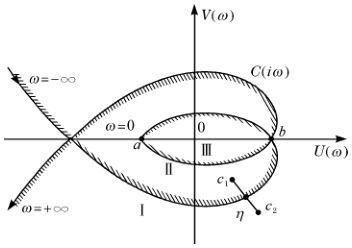
\includegraphics[width=\linewidth]{figs/fig-0073.png}
\caption{图5.1-1}
\end{figure}

\begin{figure}[htbp]\centering
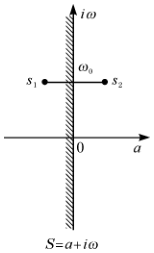
\includegraphics[width=\linewidth]{figs/fig-0072.png}
\end{figure}

相应地选择式(5.1-4)内之 $c$ 值，可以使 $S$ 平面上的任何点，例如 $s$ 点，成为特征方程式的根。要使图 5.1-1 内之 $s$ 点成为特征方程式的根，只需令

\[c=\frac{P\left(s_{\mathrm{si}}\right)}{Q\left(s_{\mathrm{si}}\right)}\]

即可。设在 $S$ 平面内有一通过 $i \omega$ 点的曲线段 $s s$，它的对应的影像在 $C$ 平面上是 $c c$，后者通过 $\eta$ 点。由于保角变换的特性，若 $s$ 位于虚轴之右边，与其相应的点 $c$ 必也位于曲线 $C(i \omega)$ 的右边。由此可以断言，在图 5.1-1 中的 $C$ 平面上，区域 II 内之任何 $c$ 值确定的具有负实部根的个数比区域 I 多一个。同理，区域 III 内的点所确定的负实部根的个数又比区域 II 多一个。这样，如果区域 I 属于 $D(m)$，那么 II 区属于 $D(m+1)$，III 区则属于 $D(m+2)$。在绝大多数情况下，根据特征方程式的阶数，曲线 $C(i \omega)$ 一旦画出，马上可以判定各个 $D(m)$ 的位置。例如，设方程式 $(5.1-4)$ 为三阶代数方程，图 5.1-1 内之曲线是相应的虚轴变换的象。从图中马上可以看出区域 III 属于 $D(3)$，区域 II 属于 $D(2)$，区域 I 则属于 $D(1)$。因此，区域 III 是系统对参数 $c$ 的稳定区域，这里任何点 $c$ 所确定的特征方程的一切根均具有负实部。在讨论中曾经假定 $c$ 可以取复值，实际上它只能取实数值。于是，参数 $c$ 只能取值于 III 区内之实轴线段 $a b$ 上，端点 $a$ 和 $b$ 不包括在内，因为当 $c=a$ 或 $c=b$ 时特征方程有一对纯虚根，系统位于稳定的边缘。

这种用区域划分的方法去确定保证系统稳定的参数取值范围，对选定系统放大系数或其他关键参数是很方便的，因为能求出该参数可能取值的全体。如果某参数已经选定，这种方法也提供一种检验系统稳定性的手段。例如，可以求出已确定的该参数值离临界值差多远，从而判断系统稳定性对参数变化的敏感程度等。这种方法还可以推广到多参数稳定域选择问题。但是如果待选定的参数超过两个，这种方法实际上便很难应用，对两个参数的情况，用作图法仍然能得到较好的效果。对这种情况的稳定域划分可参看本章所列参考文献[24]。

\section{5.2 对数频率法}

在前章内我们曾详细讨论了利用对数频率法 （伯德法） 去分析系统稳定性的原理。在分析理论的基础上，对数频率法也可以用以设计（综合）线性控制系统。设受控对象的频率特性是

\[W(i \omega)=\frac{X(i \omega)}{U(i \omega)}=K \frac{\left(P_{1} e^{i \varphi_{1}}\right)\left(P_{2} e^{i \varphi_{2}}\right) \cdots\left(P_{m} e^{i \varphi_{m}}\right)}{\left(Q_{1} e^{i \theta_{1}}\right)\left(Q_{2} e^{i \theta_{2}}\right) \cdots\left(Q_{n} e^{i \theta_{n}}\right)}\qquad\text{(5.2-1)}\]

式中 $P, Q_{i}$ 均为实变数 $\omega$ 的函数。上式取对数为

\[20 \log W(i \omega)=20 \log |W(i \omega)|+i(20 \log e)\left(\sum_{j=1}^{m} \varphi_{j}-\sum_{j=1}^{n} \theta_{j}\right)\]

上式右端之第一项是对数幅频特性，第二项是对数相频特性，将它们分别画于图 5.2-1 中。相频特性将直接画出 $\theta=\sum_{j=1}^{m} \varphi_{j}(\omega)-\sum_{j=1}^{n} \theta_{j}(\omega)$。如果对数频率特性满足伯德稳定条件，即相稳定裕度 $\theta$ 和幅稳定裕度 $M_{0}$ 为足够大时，那么可直接采用控制规律 $u=-x$，即用简单的反馈（这种反馈常称为“硬反馈”)得到的控制系统一定是稳定的。但是，一般讲来，这种简单的反馈并不能保证反馈系统稳定和具有良好的动态性能。设受控对象的对数频率特性如图 5.2-1 所示，对于这个受控对象利用简单的反馈是行不通的，因为当 $20 \log |W|=0$ 时相角小于 $-\pi$，为了使控制系统能正常工作，必须借助于更复杂的控制规律。

\begin{figure}[htbp]\centering
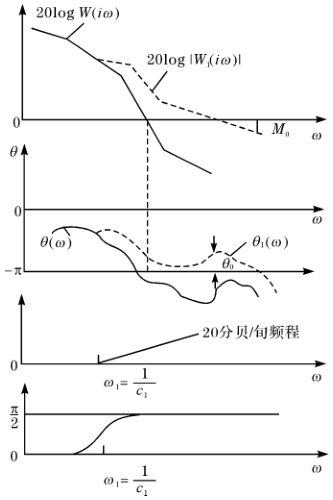
\includegraphics[width=\linewidth]{figs/fig-0074.png}
\caption{图5.2-1}
\end{figure}

20log $W(i \omega)$

\[\theta\]

\[\theta_{1}(\omega)\]

\[\omega_{1}=\frac{1}{c_{1}}\]

\[\omega_{1}=\frac{1}{c_{1}}\]

图 5.2-1

设采用控制规律

\[u=-(c s+1) x\qquad\text{(5.2-2)}\]

令 $u=-x$，有 $u=(c s+1) u$。于是，新的传递函数是

\[W_{1}(i \omega)=\frac{X(i \omega)}{U_{1}(i \omega)}=(c i \omega+1) W(i \omega)\qquad\text{(5.2-3)}\]

我们知道，环节 $(i c \omega+1)$ 的对数幅频特性是

\[20 \log \sqrt{c_{1} \omega^{2}+1}=10 \log \left(c_{1} \omega^{2}+1\right)\]

它在 $\omega=\frac{1}{c_{1}}$ 点以前以零分贝为渐近线，在 $\omega=\frac{1}{c_{1}}$ 以后则以 20 分贝/旬频率的斜率上升。它的相特性是在 $\omega \ll \omega$ 时以 0 为其渐近线，当 $\omega=\omega$ 时 $\theta=\frac{\pi}{4}$，而 $\omega \rightarrow \infty$ 时，

。将相加，再将前者和后者的相频特性

虚线所示之 $20 \log |W|$ 和 $\theta(\omega)$。采用了控制规律式(5.2-2)后，可以看到，利用 $u=-x$ 的

简单反馈 （即 $u=-(c s+1) x)$，反馈控制系统已获得足够的相稳定裕度 $\theta$ 和幅稳定裕度 $M_{\mathrm{b}}$。用这种方法设计出的控制系统的结构如图 5.2-2 所示。

当采用控制规律式 (5.2-2) 控制系统依然不能获得良好的稳定性能时，可采用更为复杂的规律，例如

\[u=-(c s^{2}+c s+1) x\qquad\text{(5.2-4)}\]

或者

\[u=-(c s^{3}+c s^{2}+c s+1) x\qquad\text{(5.2-5)}\]

等。如果式 (5.2-4) 或 (5.2-5) 之右端可分解为一次单因子之乘积，每一个因子又具有式 (5.2-2) 的形式，那么对这类控制系统的作图方法与前述无异。只需在 $20 \log |W|$ 的对数幅频特性和相频特性上加上诸单因子的对数幅频特性和相频特性后，算出相稳定裕度和幅稳定裕度即可。

如果对控制系统的动态特性要求已经给定，例如对过渡过程的时间和过渡过程的超调量已经提出要求，也可以根据经验公式和近似计算方法做出需要的开路系统的理想对数频率特性图，然后再取理想频率特性和受控对象频率特性的差作为控制装置的频率特性，以此选择式 (5.2-4) 或 (5.2-5) 内的系数 $c$，使其尽量接近需要的形式。至于如何估计对数频率特性与反馈系统动态性能之间的关系，什么样的对数频率特性才是理想的，这些问题至今没有确切的答案。在文献[27]中曾做了近似估计，并提出了一些经验性的计算方法，感兴趣的读者可以参阅。

\section{5.3 复合控制系统与稳态补偿}

至今我们研究过的各类系统都是按误差进行控制的系统，也就是说，控制量仅仅是系统误差坐标的线性函数，而与输入作用 $g(t)$ 无关。这样做的根据是系统的稳定性与输入作用无关，而仅与系统的坐标反馈方式有关，而且当输入作用属于固有类时 （参看第四章，第 4.8 节），系统对输入作用 $g(t)$ 的跟踪精度也与控制装置无关。但是，当输入作用不属于固有类时，系统必然不能准确地跟踪输入作用。误差 $\varepsilon(t)$ 将与输入 $g(t)$ 有关，其关系式是式 (4.8-14)。除输入作用外，在受控对象上还可能有外扰作用 $f(t)^{[1]}$，后者的作用点常与输入作用 $g(t)$ 的作用点不

\begin{figure}[htbp]\centering
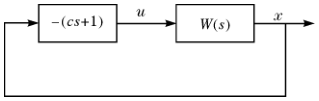
\includegraphics[width=\linewidth]{figs/fig-0075.png}
\caption{图5.2-2}
\end{figure}

同。现写出图 5.3-1 所示系统的运动方程式:

\[\begin{aligned}& \frac{d}{d t} \frac{d^{2} x}{d t^{2}}+\frac{d x}{d t}=y+f(t) \\& \frac{d y}{d t}=u \\& \varepsilon=g(t)-x(t)\end{aligned}\qquad\text{(5.3-1)}\]

令 $x=x_{1} \frac{d x}{d t}=x_{2}, y=x_{3}$，代入上式后得到一个一阶方程组:

\[\begin{aligned}& \frac{d x_{1}}{d t}=x^{2} \\& \frac{d x_{2}}{d t}=-\frac{1}{T} x_{2}+\frac{1}{T} x_{3}+\frac{1}{T} f(t) \\& \frac{d x_{3}}{d t}=u \\& \varepsilon=g(t)-x_{1}\end{aligned}\qquad\text{(5.3-2)}\]

再令 $\varepsilon=g(t)-x_{1}(t), \varepsilon=\frac{d g}{d t}-\frac{d x_{1}}{d t}, \varepsilon=x_{3}$，代入上式，有

\[\begin{aligned}& \frac{d \varepsilon_{1}}{d t}=\varepsilon_{0} \\& \frac{d \varepsilon_{2}}{d t}=-\frac{1}{T} \varepsilon_{2}-\frac{1}{T} \varepsilon_{3}+h(t)-\frac{1}{T} f(t) \\& \frac{d \varepsilon_{3}}{d t}=u\end{aligned}\]

式中 $h(t)=\frac{d^{2}}{d t^{2}} g+\frac{1}{T} \frac{d g}{d t}$。从上列方程式的形式看，如果控制规律 $u$ 只是误差 $\varepsilon_{1}$，$\varepsilon_{2}, \varepsilon_{3}$ 的线性组合，那么，一般讲来，$\varepsilon(t)$ 将是 $\left\{h(t)-\frac{1}{T} f(t)\right\}$ 的函数。当 $h-\frac{1}{T} f$为常数且系统在 $t$ 趋于很大时，$\varepsilon, \varepsilon, \varepsilon$ 也趋于某一稳态误差。

这种由外部作用引起的误差能否消除呢？答复是明显的，当外扰和输入作用可以测量时，一般讲可以用外扰补偿方法去消除动态和稳态误差，即在控制装置中引入外扰的相应坐标，使控制规律含有 $g(t)$ 和 $f(t)$ 及其导数，使 $h(t)$ 和 $f(t)$ 对系统的误差不发生影响 ${ }^{[21,22]}$。现在就来研究在外扰可以完全测量时如何设计控制装置，使前者得到补偿。

\begin{figure}[htbp]\centering
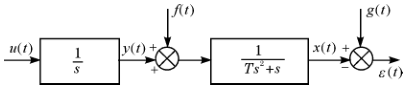
\includegraphics[width=\linewidth]{figs/fig-0076.png}
\caption{图5.3-1}
\end{figure}

设系统只有一个控制量 $u$。对于误差坐标的运动方程式设为

\[\frac{d \varepsilon}{d t}=A \varepsilon+b u+f(t)\qquad\text{(5.3-3)}\]

式中 $\varepsilon=\left(\varepsilon_{1}, \varepsilon_{2}, \cdots, \varepsilon_{n}\right), b=\left(b_{1}, b_{2}, \cdots, b_{n}\right), f(t)=\left(f_{1}(t), \cdots, f_{n}(t)\right)$。向量 $b$ 的各分量均为常数，其中一部分可以为零，向量 $f(t)$ 的某些分量也可能为零。

用外扰补偿的第一个方法是将 $u$ 分为两部分 $u=u+w$，令

\[u=\sum_{a=1}^{n} c_{a} \varepsilon_{a}\qquad\text{(5.3-4)}\]

使方程式

\[\frac{d \varepsilon}{d t}=A \varepsilon+b\left[\sum_{a=1}^{n} c_{a} \varepsilon_{a}\right]=(A+B) \varepsilon\qquad\text{(5.3-5)}\]

式中

\[B=\left(\begin{array}{llll} b_{1} & c_{1} & \cdots & b_{n} c_{n} \\ b_{2} & c_{1} & b_{2} c_{2} & \cdots \\ \vdots & \vdots & & \vdots \\ b_{n} c_{1} & b_{n} c_{2} & \cdots & b_{n} c_{n} \end{array}\right)\]

稳定并具有良好的过渡过程。而控制量的第二部分满足恒等式（如果这是可能的话）

\[b u+f(t) \equiv \mathbf{0}\qquad\text{(5.3-6)}\]

即

\[w=-\frac{1}{b_{i}} f_{i}(t), \quad i=1,2, \cdots, n\]

但是，一般说来，式(5.3-6)是不可能成立的。不难看出，欲使式(5.3-6)有解，必须要求

\[\frac{f_{1}(t)}{b_{1}}=\frac{f_{2}(t)}{b_{2}}=\cdots=\frac{f_{n}(t)}{b_{n}}\]

而当 $b_{i}=0$ 时 $f_{i}(t)$ 必须恒为零。这种情况只有在外扰的作用点与控制量的作用点相同时才可能有解。如果 $g(t)$ 属于固有作用类，而 $f(t)$ 与 $u$ 作用在同一个点上，这时自然有完全补偿公式 $w=-f(t)$。

当 $f(t)$ 的作用点与控制量的作用点不同时，式(5.3-6)不可能有解。例如前面讨论过的系统式(5.3-2)和(5.3-6)要求 $h(t)-f(t)=0$ 和 $w=0$。当前者不为零时，式(5.3-6)无解。

设 $x$ 为受控对象的主要受控量，$f(t)$ 的作用点可以是任意的，$g(t)$ 为任意足够光滑的函数。这类系统的运动方程总可化成式(5.3-3)的形式。当对误差的控制规律式(5.3-4)已经选定时，方程式(5.3-3)的解可写成

\[\varepsilon(t)=e^{D t} \varepsilon_{0}+\int_{0}^{t} e^{D(t-\tau)}\left(b u_{2}+\boldsymbol{f}(\tau)\right) d \tau\qquad\text{(5.3-7)}\]

上式内方阵 $D=A+B_{0}$. 把向量等式内的第一个坐标 $\varepsilon(t)$ 分出

\[\varepsilon(t)=\sum_{a=1}^{n} \varphi_{a}(t) \varepsilon_{0 a}+\int_{0}^{t} \sum_{a=1}^{n} \varphi_{1 a}(t-\tau)\left(b_{a} u_{2}+f_{a}(\tau)\right) d \tau\qquad\text{(5.3-8)}\]

上式右端第一项为系统的自由运动，因为 $\varphi_{a}(t)$ 为矩阵函数 $e^{D t}=\left(\varphi_{a \beta}(t)\right)$ 的第一行元素，若系统式 (5.3-5)稳定，则 $\lim _{t \rightarrow+\infty} \varphi_{a \beta}(t)=0$. 为了完全补偿外扰作用 $f_{a}(t)$，必须对任何 $t$ 使下列等式成立

\[\int_{0}^{t}\left[\sum_{a=1}^{n} \varphi_{1 a}(t-\tau) b_{a}\right] u_{2}(\tau) d \tau \equiv-\int_{0}^{t} \sum_{a=1}^{n} \varphi_{1 a}(t-\tau) f_{a}(\tau) d \tau\qquad\text{(5.3-9)}\]

等式之右端为已知函数，故上式为一积分方程

\[\int_{0}^{t} K(t-\tau) u_{2}(\tau) d \tau=v(t)\qquad\text{(5.3-10)}\]

式中

\[K(t-\tau)=\sum_{a=1}^{n} \varphi_{1 a}(t-\tau) b_{a}, \quad v(t)=-\int_{0}^{t} \sum_{a=1}^{n} \varphi_{1 a}(t-\tau) f_{a}(\tau) d \tau\]

可以用任何一种方法解积分方程式（5.3-10），例如逐步逼近法等。。这样即可求出补偿函数 $u_{2}(t)=I\left(f_{1}(t), \cdots, f_{n}(t)\right)$，后者将完全补偿掉外扰和输入函数的作用，而使系统的稳态误差为零。

如果用拉氏变换方法解积分方程 (5.3-9)，利用卷积公式可直接找出 $u_{2}(t)$ 与 $f_{\alpha}(t), \alpha=1,2, \cdots, n$，的关系式。对式 (5.3-9)两端作拉氏变换后有

\[-\Phi_{v}(s) U_{2}(s)=\sum_{a=1}^{n} \Phi_{f a}(s) F_{a}(s)\]

或者

\[\begin{aligned} U_{2}(s) & =\frac{-\sum_{a=1}^{n} \Phi_{f a}(s) F_{a}(s)}{\Phi_{u}(s)} \\ & =-\sum_{a=1}^{n} \frac{\Phi_{f a}(s)}{\Phi_{u}(s)} F_{a}(s) \end{aligned}\qquad\text{(5.3-11)}\]

不难看出，上式内 $\Phi_{\mathrm{a}}(s)$ 正是受控对象对误差 $\varepsilon$ 的传递函数，$\Phi_{f a}(s)$ 是自加入外扰点至误差 $\varepsilon$ 点的传递函数。根据式 $(5.3-11^{\prime})$ 可以确定对外扰和输入作用的补偿规律。假定设计好的系统为图 5.3-2 所示。由输入 $g(t)$ 所引起的动态误差是

\[\stackrel{\text { g }(t)^{+}}{\longrightarrow} \times \longrightarrow W_{1}(s) \longrightarrow u \longrightarrow W_{1}(s) \longrightarrow W_{a}(s)\]

图 5.3-2

\begin{figure}[htbp]\centering
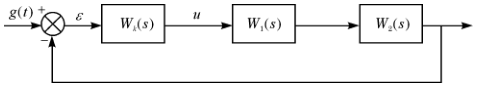
\includegraphics[width=\linewidth]{figs/fig-0077.png}
\caption{图5.3-2}
\end{figure}

\[E_{\pi}(s)=\frac{1}{1+W_{k}(s) W_{1}(s) W_{2}(s)} G(s)\qquad\text{(5.3-12)}\]

由 $w$ 作用引起的误差为

\[E_{u_{2}}(s)=\frac{-W_{1}(s) W_{2}(s)}{1+W_{1}(s) W_{2}(s) W_{k}(s)} U_{2}(s)\]

按式(5.3-11)有补偿公式

\[U_{2}(s)=\frac{1}{W_{1}(s) W_{2}(s)} G(s)\qquad\text{(5.3-13)}\]

外扰作用 $f(t)$ 引起的误差是

\[E_{f}(s)=-\frac{W_{2}(s)}{1+W_{k}(s) W_{1}(s) W_{2}(s)} F(s)\qquad\text{(5.3-14)}\]

根据式 $(5.3-11^{\prime})$ 有完全补偿公式

\[U_{2}(s)=-\frac{1}{W_{1}(s)} F(s)\qquad\text{(5.3-15)}\]

这样，我们便得到对输入作用 $g(t)$ 和对外扰作用 $f(t)$ 的全补偿公式 $(5.3-13)$ 和 $(5.3-15)$。加上补偿装置后，控制系统的方块图将如图 5.3-3 所示。在这种控制系统内控制量 $u$ 不仅是误差的函数，也是输入作用和外扰作用的函数。这种系统常称为复合控制系统。

\begin{figure}[htbp]\centering
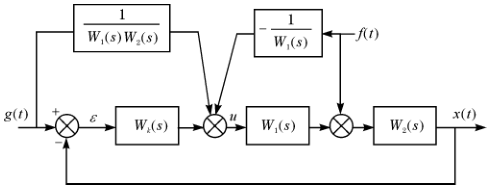
\includegraphics[width=\linewidth]{figs/fig-0078.png}
\caption{图5.3-3}
\end{figure}

图 5.3-3

从理论上看，动态补偿问题已完全由式 $(5.3-9)$ 或 $(5.3-11^{\prime})$ 所解决。但是，应该指出，要想得到这种全补偿系统在实际工作中是有困难的。这种困难主要来自两个方面：其一是测量困难，并不是所有的外扰都能准确地瞬时测量出来。例如飞行器上所受的阵风干扰，在实际上就几乎不可能直接测量出来。当然，这时补偿公式 $(5.3-11)$ 就不能应用了。第二个困难是补偿装置的实现方法，因为式 $(5.3-13)$ 和式 $(5.3-15)$ 都要求实现较为复杂的控制规律。其中包括对外扰作用和输入作用的高阶导数，而后者是不易得到的。因为即便外扰和输入作用的瞬时值可以测出，由于实际量中总含有噪声，欲得到它们的高阶导数是异常困难的。尽管如此，复合系统的应用还是十分广泛。当完全补偿不可能做到时，常不得不满足于部分的或局部的补偿。究竟补偿精度能做到何种程度，由实际工程问题中上述两种困难的克服程度而定，也与输入作用 $g(t)$ 和外扰作用 $f(t)$ 的变化规律有关。例如当 $f(t)$ 为常量或为缓变函数时，补偿通常比较简单。关于各种补偿方法的研究，还可参考文献[16，21，22，25，26]。

\section{5.4 控制装置参数选择}

前面几节内讨论过的线性系统设计方法的出发点是保证系统的稳定性，使动态误差与稳态误差完全消除或者减小到一定程度。但是，有时对控制系统的品质要求不限于此，还可能有其他类型的指标。例如，在控制系统中的能量消耗，温度控制中的温差等都常作为对控制系统的指标要求。对于伺服系统的过渡过程也有时要求均方误差小，例如图 5.4-1 内所示的过渡过程，如果要求 $\varepsilon(t)$ 迅速趋于零，那么在 $t$ 足够大时，指标

\[J=\int_{0}^{t_{1}} \dot{\varepsilon}(t) d t\qquad\text{(5.4-1)}\]

在一定程度上体现了过渡过程的快速性和平滑性。本节内我们将研究具有式 (5.4-1) 型质量指标的线性系统设计方法。

因为在本章内所讨论的对象只限于线性控制系统，所以这里只研究线性控制规律的选择方法。事前做下列互相并不独立的假定：设输入作用 $g(t)$ 属于系统的固有作用类，因此系统无静差；其次设系统渐近稳定，即任何初始误差 $\varepsilon$ 都将随时间的增大而趋于零，而衰减速度为指数规律。设用 $x$ 表示系统的误差，系统的运动方程式为

\[a_{n} \frac{d^{n} x}{d t^{n}}+a_{n-1} \frac{d^{n-1} x}{d t^{n-1}}+\cdots+a_{0} x=0\qquad\text{(5.4-2)}\]

或者写成一般的形式

\[\frac{d \boldsymbol{x}}{d t}=D \boldsymbol{x}, \quad D=A+B C\qquad\text{(5.4-3)}\]

式中 $A, B$ 分别为受控对象方程

\[\frac{d \boldsymbol{x}}{d t}=A \boldsymbol{x}+B \boldsymbol{u}\]

的 $n \times n$ 和 $n \times m$ 阶矩阵，$C$ 为待求矩阵，它决定控制装置中的控制规律。

因为系统式 (5.4-3) 或 (5.4-2) 为稳定，所以矩阵 $D$ 的一切特征根有负实部。严格说来线性系统的一切过渡过程只有 $t \rightarrow \infty$ 时才会完全结束，因为函数 $e^{-\alpha t}, \alpha$

\begin{figure}[htbp]\centering
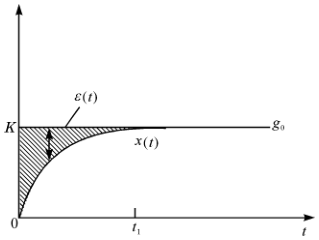
\includegraphics[width=\linewidth]{figs/fig-0079.png}
\caption{图5.4-1}
\end{figure}

0，只有在 $t \rightarrow \infty$ 时才为零。由于这两个原因，式 (5.4-1) 内之积分上限可换为无穷大，此时积分依然收敛，为了作更一般的讨论，我们设积分指标为对一非负二次型的积分

\[J=\int_{0}^{\infty} \sum_{\alpha, \beta=1}^{n} g_{\alpha \beta} x_{\alpha} x_{\beta} d t=\int_{0}^{\infty}(\boldsymbol{x}, G \boldsymbol{x}) d t\qquad\text{(5.4-4)}\]

式中 $x_{\alpha}$ 为向量 $\boldsymbol{x}$ 的分量，$G$ 为非负方阵，其元素为 $g_{\nu}$，而且 $g_{\nu}=g_{\nu}$，即 $G$ 为对称矩阵。

由于式 (5.4-3) 是一个线性齐次方程组，当系统的初始误差 $\boldsymbol{x}_{0}$ 给定时，系统的运动规律 $\boldsymbol{x}(t)$ 就已完全被确定，因此，实际上积分指标式 (5.4-4) 是初始条件 $\boldsymbol{x}_{0}$ 的连续函数。让我们首先求出这个函数关系 ${ }^{[9]}$。令 $F$ 为某一正定对称矩阵，用它构成二次型

\[h(t)=(\boldsymbol{x}(t), F \boldsymbol{x}(t))\]

对 $h(t)$ 微分后有

\[\begin{aligned} \frac{d h(t)}{d t} & =\left(D \boldsymbol{x}(t), F \boldsymbol{x}(t)\right)+\left(\boldsymbol{x}(t), F D \boldsymbol{x}(t)\right) \\ & =\left(\boldsymbol{x}(t),\left(D^{2} F+F D\right) \boldsymbol{x}(t)\right) \end{aligned}\]

式内 $D^{2}$ 为 $D$ 的转置矩阵。令

\[D^{2} F+F D=G\qquad\text{(5.4-5)}\]

那么有

\[\int_{0}^{\infty} \frac{d h(t)}{d t} d t=\left(\boldsymbol{x}(t), F \boldsymbol{x}(t)\right) \mid_{0}^{\infty}=\int_{0}^{\infty}(\boldsymbol{x}, G \boldsymbol{x}) d t\]

于是

\[-\left(\boldsymbol{x}_{0}, F \boldsymbol{x}_{0}\right)=\int_{0}^{\infty}(\boldsymbol{x}, G \boldsymbol{x}) d t\qquad\text{(5.4-6)}\]

由此可知，若矩阵 $F$ 求出后，系统质量指标式 (5.4-4)，就可直接写为初始误差 $\boldsymbol{x}_{0}$ 的函数

\[J=-\left(\boldsymbol{x}_{0}, F \boldsymbol{x}_{0}\right)=-\sum_{\alpha, \beta=1}^{n} f_{\alpha \beta} x_{\alpha 0} x_{\beta 0}\qquad\text{(5.4-7)}\]

求矩阵 $F$ 有两种方法，第一种方法是直接求解矩阵方程 (5.4-5)，此时得到 $n^{2}$ 个线性代数方程式构成的方程组。可以证明，这个方程组必然有唯一解。这个方法虽然可用，但终嫌过烦。第二个求解方法是利用矩阵函数的特性。将式 (5.4-5) 之两端左右分别乘以矩阵函数 $e^{D t_{1}}$ 和 $e^{D t_{1}}$

\[e^{D t_{1}} G e^{D t_{1}}=e^{D t_{1}} D^{2} F e^{D t_{1}}+e^{D t_{1}} F D e^{D t_{1}}\]

显然此等式之右端是 $e^{D t_{1}} F e^{D t_{1}}$ 对 $t$ 的导数，因为 $e^{D t} D=D e^{D t}$。再对前式积分

\[\int_{0}^{\infty} \frac{d}{d t}\left(e^{D t_{1}} F e^{D t_{1}}\right) d t=\int_{0}^{\infty} e^{D t_{1}} G e^{D t_{1}} d t\]

左端取积分后有

\[\int_{0}^{\infty} \frac{d}{d t}\left(e^{D_{t} t} F e^{D_{t} t}\right) d t=\left.e^{D_{t} t} F e^{D_{t} t}\right|_{0} ^{\infty}=-F\]

因此，可求出

\[F=-\int_{0}^{\infty} e^{D_{t} t} G e^{D_{t} t} d t\qquad\text{(5.4-8)}\]

上式之所以成立是由于

\[\lim _{t arrow \infty} e^{D_{t}}=\lim _{t arrow \infty} e^{D_{t}}=0\]

右端 0 为零矩阵。

现举单摆振动阻尼问题为例来说明矩阵 $F$ 的求解方法。设控制系统的误差运动方程为

\[\frac{d^{2} x}{d t^{2}}+x=u\qquad\text{(5.4-9)}\]

设控制规律为 $u=-c \frac{d x}{d t}$，则反馈系统方程式为

\[\frac{d^{2} x}{d t^{2}}+c \frac{d x}{d t}+x=0\qquad\text{(5.4-10)}\]

令 $x=x_{1}, \frac{d x}{d t}=x_{2}$，上式可改写成方程组

\[\begin{aligned} & \frac{d x_{1}}{d t}=x_{2} \\ & \frac{d x_{2}}{d t}=-x_{1}-c x_{2} \end{aligned}\qquad\text{(5.4-11)}\]

我们知道，当 $c>0$ 时系统式 (5.4-10) 总为渐近稳定。设过渡过程质量指标为

\[J=\int_{0}^{\infty}\left(x_{1}^{2}+x_{2}^{2}\right) d t=\int_{0}^{\infty}(\boldsymbol{x}, G \boldsymbol{x}) d t\qquad\text{(5.4-12)}\]

式中

\[G=\left[\begin{array}{ll} 1 & 0 \\ 0 & 1 \end{array}\right]\]

因为

\[D=\left[\begin{array}{cc} 0 & 1 \\ -1-c & 0 \end{array}\right] \cdot e^{D_{t}}=\left[\begin{array}{cc} -\lambda & & & \\ \lambda-\lambda & e^{\lambda_{1} t} & & \\ & & \lambda-\lambda & e^{\lambda_{2} t} & \\ & & & \lambda-\lambda & e^{\lambda_{3} t} \end{array}\right]\]

式中 $\lambda, \lambda$ 是代数方程式

\[\lambda^{2}+c \lambda+1=0\]

的两个根。容易计算

\[e^{D^{r_{i}}} G e^{D^{r_{i}}}=\beta^{2}\left[\begin{array}{cc} (1+\lambda_{2}^{2}) e^{2 \lambda_{1} t}-4 e^{(\lambda_{1}+\lambda_{2}) t} & -(\lambda_{1}+\lambda_{2}) e^{2 \lambda_{1} t}-(\lambda_{1}+\lambda_{2}) e^{2 \lambda_{2} t} \\ +\left(1+\lambda_{1}^{2}\right) e^{2 \lambda_{2} t} & +2\left(\lambda_{1}+\lambda_{2}\right) e^{(\lambda_{1}+\lambda_{2}) t} \\ -(\lambda_{1}+\lambda_{2}) e^{2 \lambda_{1} t}-(\lambda_{1}+\lambda_{2}) e^{2 \lambda_{2} t} & \left(1+\lambda_{2}^{2}\right) e^{2 \lambda_{1} t}+\left(1+\lambda_{1}^{2}\right) e^{2 \lambda_{2} t} \\ +2\left(\lambda_{1}+\lambda_{2}\right) e^{(\lambda_{1}+\lambda_{2}) t} & -4 e^{(\lambda_{1}+\lambda_{2}) t} \end{array}\right]\qquad\text{(5.4-14)}\]

式中 $\beta=\frac{1}{\lambda_{1}-\lambda_{2}}$。

注意到，只要 $c>0$，公式 (5.4-8) 右端积分总是收敛的，故我们可以对式 (5.4-14)作下列积分运算

\[\int_{0}^{\infty} e^{D^{r_{i}}} G e^{D^{r_{i}}} d t=\beta^{2}\left(\begin{array}{cc} \frac{c^{4}-2 c^{2}-8}{2 c} & \frac{c^{2}-4}{2} \\ \frac{c^{2}-4}{2} & \frac{c^{2}-4}{c} \end{array}\right)\qquad\text{(5.4-15)}\]

因为 $\lambda_{1}$ 和 $\lambda_{2}$ 是方程式 $\lambda^{2}+c \lambda+1=0$ 的两个根，容易算出上式右端矩阵四个元素的值为

\[-F=\int_{0}^{\infty} e^{D^{r_{i}}} G e^{D^{r_{i}}} d t=\left(\begin{array}{cc} \frac{c^{2}+2}{2 c} & \frac{1}{2} \\ \frac{1}{2} & \frac{1}{c} \end{array}\right)\qquad\text{(5.4-16)}\]

设式 (5.4-10) 表示的单摆运动的初始条件是任意的: $x_{1}(0)=x_{10}, x_{2}(0)=$ $x_{20}$，则全部过渡过程的积分质量指标式 (5.4-12)可直接求出。依式 (5.4-7) 有

\[J=-\left(\boldsymbol{x}_{0}, F \boldsymbol{x}_{0}\right)=\frac{c^{2}+2}{2 c} x_{10}^{2}+x_{10} x_{20}+\frac{1}{c} x_{20}^{2}\qquad\text{(5.4-17)}\]

今假定单摆的初始速度为 0，即 $x_{20}=0$，而初始振幅 $x_{10}$ 异于 0。由式 (5.4-17)可知，此时二次积分指标的值为

\[J=\frac{c^{2}+2}{2 c} x_{10}^{2}\qquad\text{(5.4-18)}\]

容易检查，函数 $\frac{c^{2}+2}{2 c}$ 当 $c=\sqrt{2}$ 时有极小值。所以，对一切初始速度为 0 的运动，欲使 $J$ 达极小值的最优阻尼是取 $c=\sqrt{2}$。

前面我们用矩阵函数的方法求出了均方误差的表达式。实际上表达式 (5.4-7) 也可以用拉氏变换的方法求出，即直接从工程上常用的传递函数的表达式求出函数 $J(\boldsymbol{x})$，有时这种方法可能更方便些。为此只要找出矩阵 $F$ 与传递函数的关系就够了。下面我们试建立这种新的关系式 ${ }^{[1]}$。首先对受控对象的误差方程式

\[\frac{d \boldsymbol{x}}{d t}=\boldsymbol{A} \boldsymbol{x}+\boldsymbol{B} \boldsymbol{u}\qquad\text{(5.4-19)}\]

进行拉氏变换

\[s \boldsymbol{X}(s)-\boldsymbol{x}_{0}=\boldsymbol{A} \boldsymbol{X}(s)+\boldsymbol{B} \boldsymbol{U}(s)\]

式中 $\boldsymbol{X}(s)$ 表示向量 $\boldsymbol{x}(t)$ 的拉氏变换，$\boldsymbol{U}(s)$ 为控制向量 $\boldsymbol{u}(t)$ 的象函数，二者依然是向量函数，解上述方程后

\[\boldsymbol{X}(s)=(s \boldsymbol{E}-\boldsymbol{A})^{-1} \boldsymbol{B} \boldsymbol{U}(s)+(\boldsymbol{s E}-\boldsymbol{A})^{-1} \boldsymbol{x}_{0}\qquad\text{(5.4-20)}\]

式中 $E$ 为单位矩阵，而矩阵 $(s E-A)^{-1}$ 称为受控系统的传递函数。现今控制规律为 $\boldsymbol{u}(t)=\boldsymbol{G x}(t)$，或 $\boldsymbol{U}(s)=\boldsymbol{C X}(s)$。代入式 (5.4-20) 并化简后得到 $\boldsymbol{x}(t)$ 的象函数

\[\boldsymbol{X}(s)=(s \boldsymbol{E}-(\boldsymbol{A}+\boldsymbol{B C}))^{-1} \boldsymbol{x}_{0}\qquad\text{(5.4-21)}\]

现在可以直接解算式 (5.4-4)。引入矩阵记号

\[K(s)=(s E-(A+B C))^{-1}\qquad\text{(5.4-22)}\]

可以证明式(5.4-7)的正定矩阵 $F$ 可由下式求出

\[F=-\frac{1}{2 \pi i} \int_{-i \infty}^{i \infty} K^{s}(s) G K(-s) d s\qquad\text{(5.4-23)}\]

式中 $K^{s}(s)$ 为 $K(s)$ 的转置矩阵。将 $\boldsymbol{x}(t)=\frac{1}{2 \pi i} \int_{-i \infty}^{+i \infty} \boldsymbol{X}(s) e^{t} d s$ 代入式 (5.4-4) 之右端后再作下列变换得

\[\begin{aligned} J & =\int_{0}^{\infty}\left[\frac{1}{2 \pi i} \int_{-i \infty}^{+i \infty} \boldsymbol{X}(s) e^{t} d s, \boldsymbol{G x}(t)\right] d t \\ & =\frac{1}{2 \pi i} \int_{-i \infty}^{+\infty}\left(\boldsymbol{X}(s), G \int_{0}^{\infty} \boldsymbol{x}(t) e^{t} d t\right) d s \\ & =\frac{1}{2 \pi i} \int_{-i \infty}^{+\infty}(\boldsymbol{X}(s), \boldsymbol{G X}(-s)) d s \end{aligned}\qquad\text{(5.4-24)}\]

对 $\boldsymbol{x}(t)$ 的拉氏反变换之积分线路可以取虚轴 $(-i \infty,+i \infty)$，这是因为 $\boldsymbol{x}(t)$ 渐近趋于零，$\boldsymbol{X}(s)$ 的一切奇点均位于左半平面。而式 (5.4-24) 内之积分号可以互换是由于两个积分都绝对收敛。将式 (5.4-21) 代入式 (5.4-24) 得

\[\begin{aligned} J & =\frac{1}{2 \pi i} \int_{-i \infty}^{+\infty}(K(s) \boldsymbol{x}_{0}, G K(-s) \boldsymbol{x}_{0}) d s \\ & =\frac{1}{2 \pi i} \int_{-i \infty}^{+\infty}\left(\boldsymbol{x}_{0}, K^{s}(s) G K(-s) \boldsymbol{x}_{0}\right) d s \\ & =\left[\boldsymbol{x}_{0}, \frac{1}{2 \pi i} \int_{-i \infty}^{+\infty} K^{s}(s) G K(-s) d s \boldsymbol{x}_{0}\right] \end{aligned}\]

将上式与式 (5.4-6) 比较即得到式 (5.4-23)。当 $G$ 为单位矩阵时

\[\begin{aligned} J & =\int_{0}^{\infty}\left(x_{1}^{2}(t)+\cdots+x_{n}^{2}(t)\right) d t=-\left(\boldsymbol{x}, F \boldsymbol{x}_{0}\right) \\ F & =-\frac{1}{2 \pi i} \int_{-i \infty}^{+\infty} K^{s}(s) K(-s) d s \end{aligned}\qquad\text{(5.4-25)}\]

设误差运动方程式是式(5.4-2)，而

\[J=\int_{0}^{\infty} x^{2}(t) d t\]

根据前述可推知

\[J=\frac{1}{2 \pi i} \int_{-i \infty}^{+i \infty} \frac{N_{0}(s) N_{0}(-s)}{D(s) D(-s)} d s=\frac{1}{2 \pi i} \int_{-i \infty}^{+i \infty}\left|\frac{N_{0}(s)}{D(s)}\right|^{2} d s\qquad\text{(5.4-26)}\]

其中

\[\begin{aligned} D(s) & =a_{s} s^{a}+a_{s-1} s^{n-1}+\cdots+a_{1} s+a_{0} \\ N_{0}(s) & =a_{n} x_{0} s^{n-1}+\left(a_{n} x_{0}^{(1)}+a_{n-1} x_{0}\right) s^{n-2}+\cdots \\ & +\left(a_{n} x_{0}^{(n-1)}+a_{n-1} x_{0}^{(n-2)}+\cdots+a_{1} x_{0}\right) \end{aligned}\]

这里

\[x_{0}^{(i)}=\left.\frac{d^{i} x}{d t^{i}}\right|_{t=0}, \quad \text { 若 } x_{0}^{(i)}=0, \quad i=1,2, \cdots, n-1\]

则

\[N_{0}(s)=\left(a_{s} s^{n-1}+a_{s-1} s^{n-2}+\cdots+a_{1}\right) x_{0}\]

前面分析的单摆阻尼问题例中，只含有一个待选参数 $c_{0}$。事实上本节所讨论的方法同样可以应用到多参数选择的情况。如果考虑 $n$ 阶系统，初始偏差限定为只有一个误差坐标不为零，其他 $n-1$ 个坐标初值均为 0，那么由式 (5.4-7) 确定的 $J$ 的系数，将是反馈矩阵 $\left[C_{\text {见式 }}(5.4-3)\right]$ 的每一元素的解析函数:

\[J=f\left(c_{i j}\right) x_{10}^{2}\]

容易用计算机去求最好的矩阵元素 $c_{i j}$，使系数函数 $f$ 即 $J$ 取极小值。如果系统的初始条件是任意的，$J$ 就是系统初始状态的二次型，一般来讲，$J$ 的极小 （即最好的反馈矩阵）还依赖初始条件，所以不能求出一个固定的常量矩阵，使 $J$ 对任何初始条件均为极小，这时就只能满足于对某些具有代表性的初始条件的参数选择。

\section{5.5 极点配置问题}

在第四章讨论系统稳定性时，我们已经看到线性常系数系统的稳定性，完全取决于系统传递函数的极点在复平面上的分布。实际上，不仅系统稳定性取决于极点分布，系统的其他特性和品质指标，在很大程度上都由极点在左半平面上的位置所决定。以二阶振荡系统为例，如果它有一对互为共轭的复根，即两个极点相对实轴对称，那么系统阻尼的大小，取决于极点负实部的大小，而振荡频率的高低则决定于虚部的大小。因此，为了增大系统阻尼，我们可以使远一些；要想减小振荡频率，可以使极点离实轴近一些。这样，我们就可以根据系统设计指标要求，有目的地配置系统的极点分布。回想一下我们讲过的根轨迹法，也是一种极点配置，不过它只把极点配置在左半平面使系统渐近稳定就行了。当系统的指标要求不仅是渐近稳定，而且还对系统的过渡过程有进一步要求（如超调量，振荡次数，过渡时间，通频带等），这时极点配置只在左半平面还不够，还必须更精确的配置。于是，就出现了这样的问题，就是闭路系统的极点是否可以通过反馈规律的选择而任意配置？在什么条件下可以这样配置？关于这个问题的答案是，只要系统是完全能控的，那么它的极点就可以用状态线性反馈而任意配置。这一节我们将简单地讨论这个问题[8，19]。

设单输入单输出线性系统为

\[\begin{aligned}\frac{d \boldsymbol{x}}{d t} & =A \boldsymbol{x}+b u \\y & =\boldsymbol{c}^{*} \boldsymbol{x}\end{aligned}\qquad\text{(5.5-1)}\]

其中 $A$ 是 $n \times n$ 阶常矩阵，$b, c$ 是 $n \times 1$ 阶矩阵。 $x$ 是系统状态变量，$y$ 是输出量，$u$ 是控制。

所谓极点配置，就是指经过状态（或输出）的线性反馈，$u=k^{*} x, k$ 是 $n \times 1$ 阶矩阵，使闭环系统

\[\frac{d \boldsymbol{x}}{d t}=A \boldsymbol{x}+b k^{*} \boldsymbol{x}=\left(A+b R^{*}\right) \boldsymbol{x}\]

的极点 $\left(A+b k^{*}\right.$ 的本征值）可以取任意指定的值。

应该指出，现实的物理系统都是实系数的，因此，某个极点若是复数，那么它的共轭复数也一定是极点。所以复数极点一定成对出现。当任意配置极点时，其中若有复数，则一定包含一对互为共轭的复数。

下面我们来证明，如果系统式(5.5-1)是完全能控的，即矩阵 $\left(b, A b, A^{2} b, \cdots\right.$，$\left.A^{n-1} b\right)$ 的秩为 $n$ （见第 4.11 节），那么任意一组数 $s_{1}, s_{2}, \cdots, s_{n}$，必存在一个矩阵 $k$，使 $A+b k^{*}$ 的本征值为 $s_{1}, s_{2}, \cdots, s_{n}$。这就是说，通过状态反馈可以使闭环系统的极点任意配置。

为了证明简单，首先对系统式(5.5-1)进行坐标变换。

设有一非奇异 $n \times n$ 阶矩阵 $T$，使 $x=T x$，经过变换后，式 (5.5-1) 可以变成

\[\begin{aligned}\dot{x} & =T A T^{-1} x+T b u \\y & =\boldsymbol{c}^{*} T^{-1} \boldsymbol{x}\end{aligned}\qquad\text{(5.5-2)}\]

系统式(5.5-1)和(5.5-2)是等价的（确切说是代数等价），它们有相同的传递函数阵，有相同的脉冲响应阵，如令 $A_{0}=T A T^{-1}$，则有 $e^{A_{0} t}=T e^{A t} T^{-1}$。系统的一些动态特性不因坐标变换而改变。这样，就有可能使我们找到一个适当的非奇异矩阵 $T$，把系统式(5.5-1)化成式(5.5-2)，从而使式(5.5-2)变得更方便于我们的讨论。

下面我们先选出非奇异矩阵 $T$。

令

\[\begin{aligned} & Q=\left(\boldsymbol{b}, A \boldsymbol{b}, A^{2} \boldsymbol{b}, \cdots, A^{n-1} \boldsymbol{b}\right) \\ & A_{c}=\left(\begin{array}{cccc} 0 & 1 & 0 & \cdots & 0 \\ & 1 & & & \\ & & \ddots & & \\ -\alpha_{0} & -\alpha_{1} & \cdots & -\alpha_{n-1} & 1 \end{array}\right) \\ & L=\left(\begin{array}{cccc} \alpha_{1} & \alpha_{2} & \cdots & \alpha_{n-1} & 1 \\ \alpha_{2} & & & & \\ \vdots & & \ddots & & \\ \alpha_{n-1} & & & 0 & \\ 1 & & & & \end{array}\right) \end{aligned}\]

则 $Q, L$ 都是非奇异矩阵，它们的逆矩阵都存在。

设

\[T=\left(Q L\right)^{-1}\qquad\text{(5.5-4)}\]

我们看一下，它能将式 (5.5-1) 变成什么形式。

\[T^{-1}=Q L=\left(\boldsymbol{D}_{1}, \boldsymbol{D}_{2}, \cdots, \boldsymbol{D}_{n}\right)\]

容易验证

\[\boldsymbol{D}_{i}=\sum_{j=0}^{n-i-1} \alpha_{i+j} A^{j} \boldsymbol{b}+A^{n-i} \boldsymbol{b}, \quad i=1,2, \cdots, n-1\]

所以有

\[\boldsymbol{D}_{n}=\boldsymbol{b}\]

而

\[\begin{aligned} \boldsymbol{A D}_{i} & =\boldsymbol{D}_{i-1}-\alpha_{i-1} \boldsymbol{D}_{n}, \quad i=2,3, \cdots, n \\ \boldsymbol{A D}_{1} & =A\left(\alpha_{1} \boldsymbol{b}+\alpha_{1} A \boldsymbol{b}+\cdots+\alpha_{n-1} A^{n-2} \boldsymbol{b}+A^{n-1} \boldsymbol{b}\right) \\ & =\left(\alpha_{1} A \boldsymbol{b}+\alpha_{1} A^{2} \boldsymbol{b}+\cdots+\alpha_{n-1} A^{n-1} \boldsymbol{b}+A^{n} \boldsymbol{b}\right) \\ & =-\alpha_{1} E \boldsymbol{b} \\ & =-\alpha_{1} \boldsymbol{D}_{n} \end{aligned}\]

其中 $E$ 是单位矩阵。这里利用了线性代数中的凯莱-哈密顿 (Cayley-Hamilton) 定理。于是，我们又可以推出

\[\begin{aligned} A T^{-1} & =A\left(\boldsymbol{D}_{1}, \boldsymbol{D}_{2}, \cdots, \boldsymbol{D}_{n}\right) \\ & =\left(\boldsymbol{A D}_{1}, \boldsymbol{A D}_{2}, \cdots, \boldsymbol{A D}_{n}\right) \\ & =\left(-\alpha_{1} \boldsymbol{D}_{n}, \boldsymbol{D}_{1}-\alpha_{1} \boldsymbol{D}_{2}, \cdots, \boldsymbol{D}_{n-1}-\alpha_{n-1} \boldsymbol{D}_{n}\right) \end{aligned}\]

\begin{figure}[htbp]\centering
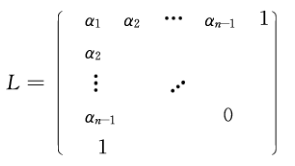
\includegraphics[width=\linewidth]{figs/fig-0080.png}
\end{figure}

\[\begin{aligned}& =\left(D_{h}, D_{h}, \cdots, D_{h}\right) \quad\left(\begin{array}{cccccc}0 & 1 & 0 & \cdots & 0 \\0 & & & & 0 \\-a_{0} & -a_{0} & & & 1\end{array}\right) \\& =T^{-1} A_{c}\end{aligned}\]

最后得到

\[T A T^{-1}=A_{c}\qquad\text{(5.5-5)}\]

通过简单运算，容易验证

\[T b=L^{-1} Q^{-1} b=\left(\begin{array}{c}0 \\0 \\\vdots \\0 \\1\end{array}\right)\]

如记

\[c^{r}=c^{r} T^{-1}=c^{r} Q L=\left(c, c, \cdots, c_{n-1}\right)\qquad\text{(5.5-7)}\]

那么，系统式(5.5-1)经过非奇异变换 $T$ 变成了如下的形式

\[\frac{d \boldsymbol{x}}{d t}=A \cdot \boldsymbol{x}+\left(\begin{array}{c}0 \\0 \\\vdots \\0 \\1\end{array}\right) u\qquad\text{(5.5-8)}\]

\[\mathbf{y}=c^{r} \boldsymbol{x}\]

其中 $A_{c}$ 如式 (5.5-3)。（这种形式，有的书上叫做可控标准形）。

由上所述，我们可以看出，对任意单输入单输出系统，只要完全能控，由矩阵 $Q$ 出发，总可以把系统变成式(5.5-8)的形式，因此，我们不妨假定系统式(5.5-1)已经是式(5.5-8)的形式，否则我们可以用上述办法化成这种形式。现在我们对具有式(5.5-8)形式的系统

\[\frac{d \boldsymbol{x}}{d t}=A \boldsymbol{x}+\boldsymbol{b} u\qquad\text{(5.5-9)}\]

其中

\[A=\left(\begin{array}{cccccc}0 & 1 & 0 & \cdots & 0 \\\vdots & & & & \\-a_{0} & -a_{0} & \cdots & & -a_{n-1}\end{array}\right), \quad b=\left(\begin{array}{c}0 \\0 \\\vdots \\0 \\1\end{array}\right), \quad c=\left(\begin{array}{c}c_{0} \\c_{1} \\\vdots \\c_{n-1}\end{array}\right)\]

来证明当它完全能控时，可以任意配置极点。

事实上，经过状态反馈 $\boldsymbol{k}^{r}=\left(k_{0}, k_{1}, \cdots, k_{n-1}\right)$ 后的闭环系统矩阵为

\[\mathbf{A}+\boldsymbol{b} \boldsymbol{k}^{r}=\left(\begin{array}{cccccc} 0 & 1 & 0 & \cdots & 0 \\ & 0 & & & 0 \\ & & \ddots & & \\ & & & 1 & \\ -\left(\alpha_{0}-k_{0}\right) & -\left(\alpha_{1}-k_{1}\right) \cdots-\left(\alpha_{n-1}-k_{n-1}\right) & & \end{array}\right)\]

而传递函数为

\[G(s)=\frac{c_{n-1} s^{n-1}+c_{n-2} s^{n-2}+\cdots+c}{s^{n}+\left(\alpha_{n-1}-k_{n-1}\right) s^{n-1}+\cdots+\left(\alpha_{n}-k_{0}\right)}\qquad\text{(5.5-11)}\]

由此可以明显看出，因为一个代数方程的根是诸系数的解析函数，当任意指定 $n$个极点 $s_{1}, s_{2}, \cdots, s_{n}$ 时，总可以找到一组数 $k_{0}, k_{1}, \cdots, k_{n-1}$ 用 $\boldsymbol{k}^{r}=\left(k_{0}, k_{1}, \cdots, k_{n-1}\right)$作反馈，而使 $s_{1}, s_{2}, \cdots, s_{n}$ 为传递函数 $G(s)$ 的极点。这样我们就证明了前面的结论。

这个事实反过来也是正确的，即是说如果系统式 (5.5-1) 通过状态反馈可以任意配置极点时，那么系统一定是完全能控的。

通过上述证明，我们还可以看到，在任意配置极点时，并不改变传递函数的零点分布。这是因为零点的位置只取决于 $\boldsymbol{c}^{r}=\left(c_{1}, c_{1}, \cdots, c_{n-1}\right)$。在配置极点时，传递函数的分子并不变化。

还可以证明，系统经过状态反馈仍保持能控性，就是说如果系统式 (5.5-1) 是完全能控的，经过状态反馈后，系统仍是完全能控的。但状态反馈不一定能保持可观测性。若用观测量 （输出） 反馈，即 $u=H y$ 时，则既保持能控性也保持能观测性。一个完全能控完全能观测的系统，它的传递函数不可能产生零点和极点完全相消的问题。由此我们可以推出，用观测量 $y$ 作反馈不能任意配置极点。否则配置的极点和零点相同，产生零极相消的问题就破坏了系统的能控性和能观测性，这和输出反馈保持能控性和能观测性是矛盾的。所以通过观测量反馈一般是不能任意配置极点的。

在实际情况中，有些状态变量是量测不到的，因此状态反馈也常不易实现，为了克服这个困难，近些年来提出用观测量来达到这个目的，有关这方面的内容，可参考有关文献 ${ }^{[19]}$。

以上事实不仅对单输入单输出的系统是对的，对多输入多输出系统也是正确的。下面我们不加证明，只把结论列出来。

设多输入多输出线性常系数系统

\[\frac{d x}{d t}=A x+B u\]

\begin{figure}[htbp]\centering
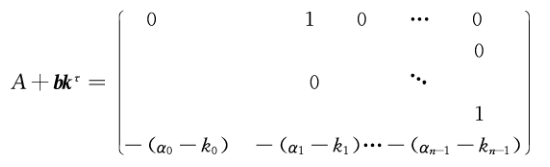
\includegraphics[width=\linewidth]{figs/fig-0081.png}
\end{figure}

y = Cx (5.5-12) 其中 A，B，C 分别是 n × n，n × r，m × n 阶矩阵。x，y，u 分别是 n，m，r 维向量，代表系统的状态，输出和控制。 如果系统式 (5.5-12) 是完全能控的，那么一定可以找到状态反馈矩阵 K(r × n 阶），使 u = Kx，可以任意配置 A + BK 的本征值。也就是说，对任意 n 个数 si，s1，…，sn，可以找到 K，使 det(sl - A - BK) = ∏n i=1 (si - si) (5.5-13) 反之，如果系统式 (5.5-12) 通过状态反馈可以任意配置极点时，那么系统一定是完全能控的。由此看出，一个系统的完全能控性和它可以任意配置极点这一事实是等价的。 参考文献 [1] 蔡金涛，契贝舍夫式工作参数滤波器的原理和计算，科学出版社，1962. [2] 陈辉堂，随动系统，人民教育出版社，1961. [3] 王新民，在连续控制系统中应用时滞元件滤波器作为校正装置的几个必要条件，自动化学报，2(1964)，1，1-6. [4] 张芷香，扰动控制原理在镇定高频淬火装置直流电源电压中的应用，自动化学报，2(1964)，3. [5] 吕应祥，绝对不变性与不变性到 ε 自适应控制系统，自动化学报，2(1964)，4. [6] 叶正明，线性复合自动控制系统的图解综合法，自动化学报，2(1964)，2. [7] 何国伟、王文贤，从所需校正网络相频或幅频曲线计算传递函数的方法，自动化学报，2(1964)，1. [8] 黄琳、郑应平、张迪，李雅普诺夫第二方法与最优控制器分析设计问题，自动化学报，2(1964)，4. [9] Bellman，R.，Notes on matrix theory-X: A problem in Control，Quarterly of Applied Math.，14(1957)，4. [10] Bliss，G. A.，Lectures on the Calculus of Variations，University of Chicago Press，Chicago，Illinois，1946. [11] Chaug，S. S. L.，Synthesis of Optimal Control Systems，McGraw-Hill，New York，1961. [12] Chestnut，H.，Mayer，R. W.，Servomechanism and Regulating System Design，Wiley，1959. [13] Kalman，R. E.，Control system analysis and design via the second method of Lyapunov. ASME Paper 59-NAC-2，59-NAC-3，1959. [14] Newton，G. C.，Gould，L. A.，\& Kaiser，J. F.，Analytical Design of Linear Feedback Controls，John Wiley \& Sons，Inc.，New York，1957. [15] Reswick，J. B.，Disturbance-response feedback a new control concept，Trans. ASME，78 (1956)，153.

\section{参考文献}

[16] Truxal，J. G.，Automatic Feedback Control System Synthesis，McGraw-Hill，New York，1955.

[17] Tou，J. T.，Modern Control Theory，McGraw-Hill，1964.

[18] Westcott，J. H.，Synthesis of optimum feedback systems satisfying a power limitation. Frequency Response Symposium. Dec.，1953. ASME Paper 53-A-17.

[19] Wonham，W. M.，On pole assignment in multi-input controllable linear systems，IEEE Trans. on Automatic Control，AC-12，1967.

[20] Айзерман，М. А.，Увеличение значения коэффициентов усиления одноконтурной системы. Автоматика и Телемеханика，1951，2.

[21] Ивахненко А. Г.，О способах устранения установившейся ошибки системы автоматического регулирования，Доклады АН СССР，87(1953)，6.

[22] Кулебакин，В. С.，О поведении непрерывно возмущаемых автоматизированных линейных систем，Доклады АН СССР，60(1948)，2.

[23] Летов，А. М.，Аналитическое конструирование регуляторов，Автоматика и Телемеханика，21(1960)，4，5，6.

[24] Неймарк，Ю. Н.，Об определении значений параметров，при которых система устойчива，Автоматика и Телемеханика，9(1948)，3.

[25] Петров，Б. Н.，О реализуемости условии инвариантности，Теория инвариантности и её применение в автоматических устройствах，Труды Совещания，АН УССР，ОТН，1959.

[26] Розоноэр，Л. И.，Вариационный подход в проблеме инвариантности систем автоматического управления，Автоматика и Телемеханика，24(1963)，6，7.

[27] Солодовников，В. В.，Основы автоматического регулирования，Машгиз，Москва，1954. （自动调正原理，王众托译，水利电力出版社，1958 年.)

<html><body>

\chapter{第六章 协调控制}

如果在一个复杂系统中有若干个受控量，而且在这些受控量之间还存在着相互的作用，那么，一般说来，对于这种系统就必须再增加一个新的设计准则，这就是互不影响的准则。举例来说，一个有加力燃烧的涡轮喷气发动机的变量是：压缩机的转速，燃烧室的喷油速率，加力燃烧室的喷油速率以及尾喷管开口面积，然而，发动机的运转状态可以设法只由压缩机的转速，燃烧室的喷油速率和加力燃烧室的喷油速率这三个量所完全控制。但是，在一般的情况下，这三个量是互有影响的。不难想到，在这个情况中，系统的伺服控制就有一个新的设计准则，也就是要求对这三个不同的量的控制是不互相影响的；加力燃烧室的喷油速率的改变不应该使压缩机的转速受到影响，而且改变压缩机转速的时候也不需要改变燃烧室的喷油速率。这也就是说解决这个特殊的设计问题的关键就是：设法使尾喷管的开口随着其余的变量发生适当的变化而且适当地设计自动控制机构。这一章的目的就是要给出一个设计这一类互不影响的控制系统的普遍方法，这个方法对于不论多么复杂的系统都是适用的。这类方法最早在文献[3，9，15]中先后被提出，后来在文献[6]中又用矩阵表示法把这个问题作了一般性处理。近些年来，采用状态变量描述方法以后，多输入多输出系统理论又有了进一步的发展 ${ }^{[7]}$。

\section{6.1 单变量系统的控制}

我们先来考虑一个简单的系统，这个系统只有一个受控的输出 $y(t)$ 和一个作为控制信号的输入 $x(t)$。 $y(t)$ 和 $x(t)$ 的拉氏变换就是 $Y(s)$ 和 $X(s)$。我们来考虑按照图 6.1-1 所设计的控制系统。 $E(s)$ 是“发动机”的传递函数，$L(s)$ 是测量仪器的传递函数 （也就是反馈线路的传递函数），$S(s)$ 是伺服马达的传递函数，$C(s)$

<img/>

图 6.1-1

</body></html>

\begin{figure}[htbp]\centering
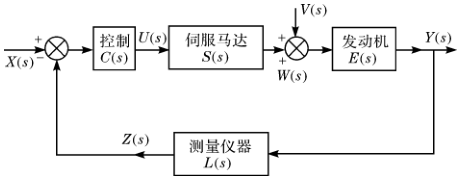
\includegraphics[width=\linewidth]{figs/fig-0082.png}
\caption{图6.1-1}
\end{figure}

是“控制”的传递函数。可以由设计者容易地加以改变的只有 C(s) 这一个传递函数。这个系统与图 (3.7-2) 的反馈系统之间的一点很小的区别就是：在伺服马达与发动机之间加上了一个任意的扰动 V(s)，用这个扰动来表示某些意外的外界影响。

发动机的输入 W(s) 与输出 Y(s) 之间的关系是

\[Y(s)=E(s) W(s)=E(s)[S(s) U(s)+V(s)]\qquad\text{(6.1-1)}\]

U(s) 是控制传递函数的输出，并且有下列关系

\[U(s)=C(s)[X(s)-Z(s)]=C(s)[X(s)-L(s) Y(s)]\qquad\text{(6.1-2)}\]

从方程 (6.1-1) 和 (6.1-2) 里把 U(s) 消去，就有

\[Y(s)=\frac{E(s) S(s) C(s)}{E(s) S(s) C(s) L(s)+1} X(s)+\frac{E(s)}{E(s) S(s) C(s) L(s)+1} V(s)\qquad\text{(6.1-3)}\]

这就是在 x(t) 与 y(t) 的适当的初始条件之下的输出的拉氏变换。如果不考虑包含扰动 V(s) 的第二项，方程 (6.1-3) 就与以前关于一般的反馈系统的方程 (3.7-3) 相同。系统的性能的分析也还可以按照与以前类似的办法来进行。然而，对于更复杂的系统来说，就必须把这个简单的情况加以推广。现在我们就来作这件事情。

\section{6.2 多变量系统的控制}

假定发动机的输出 $Y_{1}(s), Y_{2}(s), \cdots, Y_{s}(s), \cdots, Y_{i}(s)$ 的个数是 $i$，输入 $W_{1}(s)$，$W_{2}(s), \cdots, W_{k}(s), \cdots, W_{n}(s)$ 的个数是 $n$。那么，方程 (6.1-1) 的推广就是

\[\begin{aligned} & Y_{1}(s)=E_{11}(s) W_{1}(s)+E_{12}(s) W_{2}(s)+\cdots+E_{1 n}(s) W_{n}(s) \\ & Y_{2}(s)=E_{21}(s) W_{1}(s)+E_{22}(s) W_{2}(s)+\cdots+E_{2 n}(s) W_{n}(s) \\ & \cdots \\ & Y_{i}(s)=E_{i 1}(s) W_{1}(s)+E_{i 2}(s) W_{2}(s)+\cdots+E_{i n}(s) W_{n}(s) \end{aligned}\qquad\text{(6.2-1)}\]

其中每一个 $E_{k k}$ 都是一个传递函数，当这个传递函数“作用”在输入 $W_{k}(s)$ 上的时候，就得出输出 $Y_{i}(s)$ 的相应的组成部分。在普通情况下 $E_{i k}(s)$ 是两个 $s$ 的多项式的比值，因此 $E_{i k}(s)$ 可以由发动机的特性的理论分析得到，也可以用实验的方法由频率特性确定。方程 (6.2-1) 可以简写为

\[Y_{i}(s)=\sum_{k=1}^{n} E_{i k}(s) W_{k}(s), \quad \nu=1,2, \cdots, i\qquad\text{(6.2-2)}\]

所有的 $E_{i k}(s)$ 按照方程 (6.2-1) 中的位置所排成的矩形表格可以称为发动机的传递函数矩阵 $E$。我们可以这样想象：所有的输入 $W_{k}(s)$ 在纵向“进入”矩阵，所有的输出 $Y_{i}(s)$ 在横向“离开”矩阵。图 6.2-1 所表示的就是这种情况。下面我们来考虑输入的个数大于 （或等于） 输出的个数的情形，也就是 $n \geqslant i$。因此，矩阵 $E$ 就是一个纵行比横行多的矩形矩阵。为了以后的需要，我们把只由前 i 个纵行所组成的正方矩阵用 Ei 来表示。

既然发动机的输入的个数大于输出的个数，所以，如果希望完全确定系统的运转状态，除了要设法使所有输出 Yv(s)随预定的数值 Xj(s)(j=1，2，...，i)相应地变化之外，还要设法使变数 Wμ(s)(μ=i+1，i+2，...，n)也取预定的数值 Eμ(s)。因此，受控量就是 i 个输出 Yv(s)(v=1，2，...，i)和 n−i 个发动机输入 Wμ(s)(μ=i+1，i+2，...，n)。如果由测量仪器对 Wμ(s)所测出来的值是 γμ(s)，那么，误差就是 Eμ(s)−γμ(s)。发动机的输出的偏差的定义是 Xv(s)−Zv(s)，Zv(s)(v=1，2，...，i)就是 Yv(s)经过测量仪器所测量出的数值，就像图 6.2-1 的那种情形。控制的作用就在于把这些偏差当做输入来产生伺服马达的控制信号 Uk(s)。这就是系统的反馈作用。在我们所讨论的一般的系统式(6.2-1)里，控制信号 Uk(s)与所有偏差的关系是线性的。既然有 n 个偏差信号，也就有 n 个控制信号，所以 k=1，2，...，n。因此就有

\[\begin{aligned} U_{1}(s) & =G_{11}\left(X_{1}-Z_{1}\right)+G_{12}\left(X_{2}-Z_{2}\right)+\cdots+C_{1 i}\left(X_{i}-Z_{i}\right) \\ & +C_{1, i+1}^{\prime}\left(\Xi_{i+1}-\gamma_{i+1}\right)+\cdots+C_{1 n}^{\prime}\left(\Xi_{n}-\gamma_{n}\right) \end{aligned}\]

\[\begin{aligned} U_{2}(s) & =G_{21}\left(X_{1}-Z_{1}\right)+G_{22}\left(X_{2}-Z_{2}\right)+\cdots+C_{2 i}\left(X_{i}-Z_{i}\right) \\ & +C_{2, i+1}^{\prime}\left(\Xi_{i+1}-\gamma_{i+1}\right)+\cdots+C_{2 n}^{\prime}\left(\Xi_{n}-\gamma_{n}\right) \end{aligned}\]

\[\begin{aligned} & \cdots \\ & U_{n}(s)=C_{n 1}\left(X_{1}-Z_{1}\right)+C_{n 2}\left(X_{2}-Z_{2}\right)+\cdots+C_{n i}\left(X_{i}-Z_{i}\right) \\ & \quad+C_{n, i+1}^{\prime}\left(\Xi_{i+1}-\gamma_{i+1}\right)+\cdots+C_{n n}^{\prime}\left(\Xi_{n}-\gamma_{n}\right) \end{aligned}\]

在这个关系式中，我们已经把控制矩阵用不同的符号分成 C 和 C′两部分，以便区别两种不同的误差信号。方程(6.2-3)可以简写成

\begin{figure}[htbp]\centering
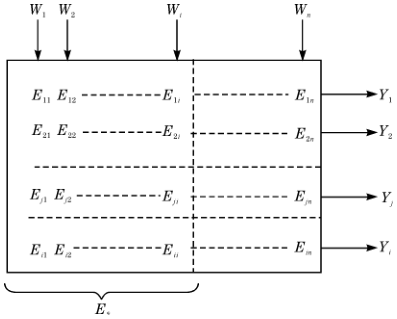
\includegraphics[width=\linewidth]{figs/fig-0083.png}
\caption{图6.2-1}
\end{figure}

\[U_{k}(s)=\sum_{v=1}^{j} C_{kv}\left(X_{v}-Z_{v}\right)+\sum_{n=i+1}^{a} \boldsymbol{C}_{kn^{\prime}}^{\prime}\left(\Xi_{e}-\gamma_{i k},\right) ; \quad v=1,2,\cdots,i\]

\[k=1,2, \cdots, n\qquad\text{(6.2-4)}\]

当然，每一个 $C_{kv}$ 和 $\mathrm{C}_{kp}^{\prime}$ 都是两个 $s$ 的多项式的比值。方程 $(6 .2-3)$ 或方程 (6.2-4)

也可以用图 6.2 -2 来表示。

\begin{figure}[htbp]\centering
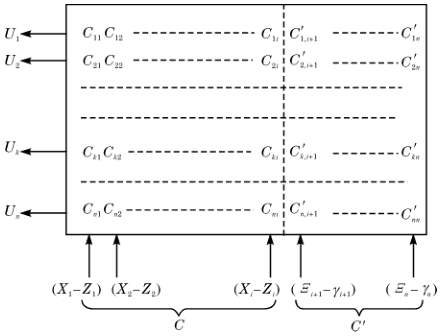
\includegraphics[width=\linewidth]{figs/fig-0084.png}
\caption{图6.2-2}
\end{figure}

测量出的数值 $Z(s)$ 和 $\gamma_{p}(s)$ 与被测量的 $Y,(s)$ 和 $W_{P}(s)$ 之间关系，由测量仪器的传递函数 $L_{y y}(s)$ 和 $L_{r p r}(s)$ 所确定

\[\begin{aligned}& Z_{V}(s)=L_{w V}(s) Y_{V}(s) \\& \gamma_{u}(s)=L_{M P R}(s) W_{R}(s)\end{aligned}\qquad\text{(6.2-6)}\]

每一个控制信号都个别地作用在伺服马达上。伺服马达的输出与意外的外界扰动 $V_{k}(s)$ 合并在一起组成发动机的输入 $W_{k}(s)$。如果 $S_{b k}(s)$ 是伺服马达的传递函数，那么

\[W_{k}(s)=S_{h k}(s) U_{k}(s)+V_{k}(s), k=1,2, \cdots, n\qquad\text{(6.2-7)}\]

从式$(6.2-1)$ 到 $(6.2-7)$ 的所有方程就是描述多变量控制系统的完备的方程组。图 6.2-3是一个多变量控制系统的方块图，这个系统有三个发动机输出 $Y_{1}(s)， Y_{2}(s)$ 和 $Y_{z}(s)$，还有两个被控制的发动机输入 $W_{1}(s)$ 和 $W_{5}(s)$。除了规定的控制信号 $X_{V}(s)$，$\mathbf{E}_{c}(s)$ 与可以对系统起作用的外界扰动信号 $V_{k}(s)$ 以外，整个控制系统是闭合的.

在以上的控制系统方程组中把 $U_{k}(s), Z,(s)$ 和 $\gamma_{t c}(s)$ 消去，就得到①年年来有人提出，用代数方法消去中间变量的运算过程中，可能出现消去系统的不稳定因子的情况，此时造成系统局部不稳定的因素可能被这种代数运算所掩盖。其实这种情况在用状态变量的方法处理问题时也可能出现。在实际系统设计时，不稳定的环节总是设计者注意的焦点，消去某种因子后是否会给系统带来意外现象应以主受控量的行为来判断。这些都可以通过模拟试验来检查。

\[\begin{aligned}& Y_{i}(s)=\sum_{k=1}^{n}\left(\sum_{\nu=1}^{i} E_{j k}(s) S_{k k}(s) C_{k \nu}(s)\left[X_{\nu}(s)-L_{\nu \nu}(s) Y_{\nu}(s)\right]\right. \\& \left.+\sum_{\mu=i+1}^{n} E_{j k}(s) S_{k k}(s) C_{k \mu}(s)\left[\Xi_{\nu}(s)-L_{\nu \mu}(s) W_{\mu}(s)\right]+E_{j k}(s) V_{k}(s)\right\}\end{aligned}\qquad\text{(6.2-8)}\]

和

\[\begin{aligned}W_{k}(s)= & \sum_{\nu=1}^{i} S_{k k}(s) C_{k \nu}(s)\left[X_{\nu}(s)-L_{\nu \nu}(s) Y_{\nu}(s)\right] \\& +\sum_{\mu=i+1}^{n} S_{k k}(s) C_{k \mu}(s)\left[\Xi_{\nu}(s)-L_{\nu \mu}(s) W_{\mu}(s)\right]+V_{k}(s)\end{aligned}\qquad\text{(6.2-9)}\]

根据方程(6.2-8)和(6.2-9)就可以把系统画成一个比图 6.2-3 更简单一些的方块图（图 6.2-4)。在这个图里只有一个系统矩阵，这个矩阵的输入是那些受控量的偏差，输出就是那些受控量。在图 6.2-4 中的 $E S C$ 矩阵中，位于第 $j$ 横行与第 $\nu$纵行的交点的元素是 $\sum_{k=1}^{n} E_{j k} S_{k k} C_{k \nu}$。同样，在 $E S C^{\prime}$ 矩阵中，第 $j$ 横行与第 $\mu$ 纵行的交点处的元素是 $\sum_{k=1}^{n} E_{j k} S_{k k} C_{k \mu}^{\prime}$。也还是一样，$S C$ 矩阵中的元素是 $S_{k k} C_{k \nu} 。 S C^{\prime}$ 矩阵中的元素是 $S_{k k} C_{k \nu}^{\prime}$。外界扰动是通过另外一个矩阵加进来的，那个矩阵主要是由发动机矩阵 $E$ 所组成的。

\begin{figure}[htbp]\centering
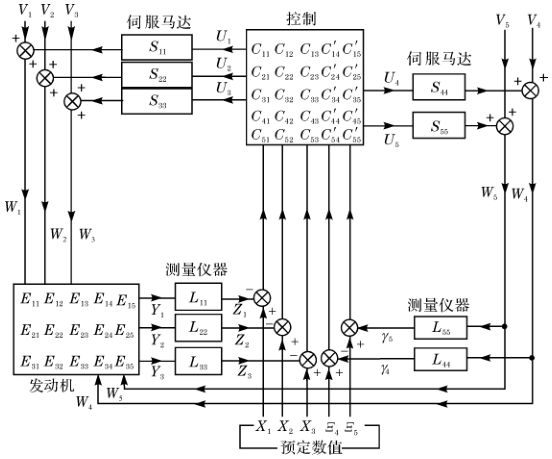
\includegraphics[width=\linewidth]{figs/fig-0085.png}
\caption{图6.2-3}
\end{figure}

图 6.2-4

\section{6.3 互不影响的条件}

以上我们所讨论的是多变量系统的控制作用的机理，在这个基础上我们就可以把控制系统的互不影响准则具体地表达出来。现在的问题就是：设法确定控制矩阵的元素 $C_{kv}(s)$ 与 $\boldsymbol{\Xi}_{kp}^{\prime}\left(s\right.$ )须要满足什么条件才能使规定的控制信号 $X_j(s)$ 与 $\mathbf{x}_i(s)$ 只影响和它们相应的受控量 $Y_i(s)$ 和 $W_n(s)($ 这里，$j=1 ， 2, \cdots, i$ 而 $\mu=i+1,$ $i+2, \cdots, n)$，而不影响其余的受控量。譬如说，控制信号 $x_2(s)$ 只能影响 $y_2(s)$， $\Xi_{+1}(s)$只能影响 $w_{i+1}(s)$。这里的数学问题也就是如何把图 6.2 -4 中的系统矩阵加以对角线化的问题。我们可以要把设计条件放在控制矩阵 $C$ 和 $C'$ 上，是因为在整个系统中只有这一部分是最容易由设计者加以变动的。发动机的特性、伺服马达以及测量仪器都认为是已经固定的，它们也不能由控制工程师随意改变。

让我们来考虑一个特定的输出 $Y_k(s), g$ 是 $1,2, \cdots, i$ 这些数中的任意一个数。方程 (6.2-8) 和(6.2-9)可以写成

aligned\& Y\_j(s)=\_k=1\textasciicircum{}n[\_v=1, v  r ; g\textasciicircum{}i E\_jk S\_kk C\_kv(X\_v-L\_vv Y\_v). \textbackslash\{\}\textbackslash\{\}\& +\_=i+1\textasciicircum{}n E\_jk S\_ik C\_kp\textasciicircum{}(\_e-L\_p k p W\_p)+E\_jk V\_k] \textbackslash\{\}\textbackslash\{\}\&+\_k=1\textasciicircum{}n E\_jk S\_ik C\_kg(X\_g-L\_gg Y\_g)aligned

和

\[W_k(S)=\sum_{r=1, v \neq r ; g}^{i} s_{ikk} c_{kv}\left(x-v-l_{vv} y_r\right)\]

\[+\sum_{\mu=i+1}^{n} s_{hk} C_{hp}^{\prime}\left(\Xi_h-L_{pp} w_h\right)+V_k+S_{hk} G_{hg}\left(X_g-L_{g g} Y_h\right)\]

\begin{figure}[htbp]\centering
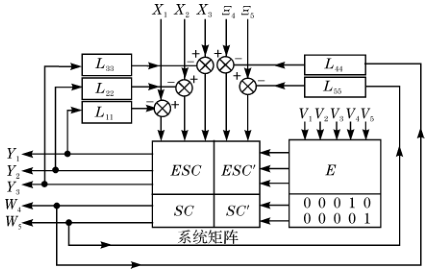
\includegraphics[width=\linewidth]{figs/fig-0086.png}
\caption{图6.2-4}
\end{figure}

现在为了使得控制信号 $X_g$ 除了 $Y_g$ 之外一不影响任何一个 $Y_j$ 或 $W_n$，所以，在 $j \neq$ $g$ 与 $k > i$ 的情形下，以上两个方程的最后一项都必须等于零。因此，对于 $1, 2, \cdots$，$i$ 中的任意一个数 $g$ 都有

如果 $j \neq g$，$\sum_{k=1}^{n} E_{jk} S_{kk} C_{kg} = 0$

以及

如果 $k > i$，$C_{kg} = 0$

方程 (6.3-2) 使我们的控制矩阵立刻就得到简化。以图 6.2-3 表示的系统为例，这时 $i = 3, n = 5$。在这个情形下，方程 (6.3-2) 就表示

\[C_{11} = C_{12} = C_{13} = C_{51} = C_{52} = C_{53} = 0\]

方程 (6.3-2) 也可以用来简化方程 (6.3-1)，方程 (6.3-1) 也就是

\[\sum_{k=1}^{i} E_{jk} S_{kk} C_{kg} = \sum_{k=1}^{i} \delta_{jk} E_{jk} S_{kk} C_{kg}\qquad\text{(6.3-3)}\]

这里的 $g$ 是 $1, 2, \cdots, i$ 中的任意一个数，$\delta_{jk}$ 是克隆内克符号 (Kronecker delta)，它的定义是

如果 $j \neq g$，$\delta_{jk} = 0$

如果 $j = g$，$\delta_{jk} = 1$

对于任意一个特定的 $g$ 来说，方程 (6.3-3) 就是一个线性代数方程组，这个方程组包含 $i - 1$ 个方程和 $i$ 个未知数 $S_{kk} C_{kg}$（这里 $k = 1, 2, \cdots, i$）。因此，我们只能确定这些未知数的比值，而不能确定这些未知数本身。然而，这正是我们所希望的，因为我们并不希望控制传递函数已经被完全确定，在现在这种情况下，我们的设计工作反而可以更加自由一些。

为了求出控制传递函数的这些比值，我们要利用行列式的一个性质：假设行列式 $|E_*|$（$|E_*|$ 是正方矩阵 $E_*$ 的行列式）中的元素 $E_{jl}$ 的余因式是 $|E_{*jl}|$，那么，下面的关系式成立

如果 $k \neq l$，$\sum_{j=1}^{i} E_{jk} \mid E_{*jl} \mid = 0$

如果 $k = l$，$\sum_{j=1}^{i} E_{jk} \mid E_{*jl} \mid = \mid E_* \mid$

把方程 (6.3-3) 先用 $\mid E_{*jl} \mid$ 乘一下，然后再对 $j$ 求和，我们就得到

\[\sum_{k=1}^{i} \sum_{j=1}^{i} \mid E_{*jl} \mid \delta_{jk} E_{jk} S_{kk} C_{kg} = \sum_{k=1}^{i} \sum_{j=1}^{i} \mid E_{*jl} \mid E_{jk} S_{kk} C_{kg}\]

因此，根据方程 (6.3-5)，就有

\[S_{ll} C_{kg} = \mid E_{*gl} \mid \sum_{k=1}^{i} E_{jk} S_{kk} C_{kg} \mid E_* \mid, \quad l = 1, 2, \cdots, i\qquad\text{(6.3-6)}\]

特别当 $l=g$ 时，有

\[S_{g g} C_{g g}=|E_{* g g}| \mid \sum_{k=1}^{i} E_{g k} S_{i k} C_{k g} \mid \mid E_{*}|\]

取方程(6.3-6)和上面这个方程的比值，我们就可以写

\[\frac{S_{i j} C_{j v}}{S_{v v} C_{v v}}=\frac{\mid E_{* v_{j}}}{\mid E_{* v v}} \mid, \quad j, v=1,2, \cdots, i\qquad\text{(6.3-7)}\]

利用这个方程就可以把 $S C$ 矩阵中不在对角线上的元素用对角线上的元素表示出来。

方程(6.3-2)和方程(6.3-7)所表示的条件就是被控制量 $Y_{x}$ 互不影响的必要条件。这些条件最先是由勃克森包姆和胡德提出来的。他们两个人还进一步证明：这些条件也是互不影响的充分条件。因此，设计一个合适的控制矩阵 $C$ 的问题就完全解决了。

为了解决控制矩阵的另外一部分 $C^{\prime}$ 的设计问题，我们就必须考虑受控量 $W_{\mu}$ $(\mu=i+1, i+2, \cdots, n)$ 的互不影响的条件，为了这个目的，我们把方程(6.2-8)和方程(6.2-9)改写为

\[\begin{aligned} Y_{j}(s)= & \sum_{k=1}^{n}\left[\sum_{v=1}^{i} E_{j k} S_{k k} C_{k v}\left(X_{v}-L_{v v} Y_{v}\right)\right. \\ & \left.+\sum_{\substack{\mu=i+1 \\ \mu \neq r}}^{n} E_{j k} S_{k k} C_{k \mu}^{\prime}\left(\Xi_{\mu}-L_{\mu \mu} W_{\mu}\right)+E_{j k} V_{k}\right] \\ & +\sum_{k=1}^{n} E_{j k} S_{k k} C_{k r}^{\prime}\left(\Xi-L_{r r} W_{r}\right) \end{aligned}\qquad\text{(6.3-8)}\]

和

\[\begin{aligned} W_{k}(s)= & \sum_{s=1}^{i} S_{i k} C_{k v}\left(X_{v}-L_{v v} Y_{v}\right) \\ & +\sum_{\substack{\mu=i+1 \\ \mu \neq r}}^{n} S_{k k} C_{k \mu}^{\prime}\left(\Xi_{\mu}-L_{\mu \mu} W_{\mu}\right)+V_{k}+S_{i k} C_{k r}^{\prime}\left(\Xi-L_{r r} W_{r}\right) \end{aligned}\qquad\text{(6.3-9)}\]

这里 $r$ 是 $i+1, i+2, \cdots, n$ 中的任意一个数，而 $j=1,2, \cdots, i$。为了现在的目的，方程(6.3-9)中的 $k$ 只是 $i+1, i+2, \cdots, n$ 中的任意一个数，因为只有这些 $W_{k}$ 才是受控量。根据方程(6.3-8)和(6.3-9)显然可以看出，如果控制信号 $\Xi$ 仅只影响受控量 $W_{r}$，那么，这两个方程的最后一项就必须等于零。也就是

\[\sum_{k=1}^{n} E_{j k} S_{i k} C_{k r}^{\prime}=0, \quad j=1,2, \cdots, i\qquad\text{(6.3-10)}\]

和

\[C_{k r}^{\prime}=0, \quad k, r=i+1, i+2, \cdots, n ; k \neq r\qquad\text{(6.3-11)}\]

和以前一样，方程(6.3-11)也使控制矩阵得到简化，以图 6.2-3 所表示的系统为例，$i=3, n=5$。就有

\[C_{45}^{\prime}=C_{54}^{\prime}=0\]

方程(6.3-11)也可以用来简化方程(6.3-10)。方程(6.3-10)化为

\[\sum_{k=1}^{i} E_{j k} S_{k k} C_{k r}^{r}=-E_{j r} S_{r r} C_{r r}^{\prime}\]

把这个方程的两端先用 $\left|E_{*}^{*} j\right|$ 乘，然后再对 $j$ 求和，就得

\[\sum_{k=1}^{i} \sum_{j=1}^{i}\left|E_{*}^{*} j\right| E_{j k} S_{k k} C_{k r}^{\prime}=-\sum_{r=1}^{i} C_{r r}^{\prime} \sum_{j=1}^{i}\left|E_{*}^{*} j\right| E_{j r}\]

根据方程(6.3-5)所表示的行列式的性质，就有

\[\mid E^{*} \mid \mid S_{i} C_{i r}^{\prime}=-\mid S_{r r} C_{r r}^{\prime} \sum_{j=1}^{i}\left|E_{*}^{*} j\right| E_{i r}\]

如果把这个方程里的 $l$ 换成 $j, j$ 换成 $l$，这个方程就可以写成下列形式

\[\begin{aligned}\frac{S_{i j} C_{j r}^{\prime}}{S_{r r} C_{r r}^{\prime}}=-\frac{1}{\mid E_{*}^{*}} \sum_{i=1}^{i}\left|E_{*}^{*} i\right| E_{i r}, \quad j=1,2, \cdots, i \\ r=i+1, i+2, \cdots, n\end{aligned}\qquad\text{(6.3-12)}\]

利用这个方程就可以把 $S C^{\prime}$ 矩阵中不在对角线上的元素用对角线上的元素表示出来。方程(6.3-11)和(6.3-12)是受控量 $W_{\mu}(s)(\mu=i+1, i+2, \cdots, n)$ 的互不影响的必要而且充分的条件。

如果希望全部受控量都互相不影响，那么，就必须满足方程(6.3-2)，(6.3-7)，(6.3-11)和(6.3-12)所表示的条件。在整个的控制矩阵中，不在对角线上的元素或者等于零，或者可以由对角线上的元素表示。如果表示发动机的特性的发动机矩阵是已知的，那么，控制矩阵的对角线元素就完全确定了整个的控制矩阵 ${ }^{\oplus}$。

\section{6.4 响应方程}

如果互不影响的条件已经全部被满足，那么，方程(6.2-8)和(6.2-9)就变得简单得多。例如，把方程(6.2-8)的求和的次序倒换一下，就有

\[\begin{aligned} Y_{j}(s)= & \sum_{i=1}^{i}\left[X_{v}(s)-L_{\nu \nu}(s) Y_{v}(s)\right] \sum_{k=1}^{n} E_{j k} S_{k k} C_{k v} \\ & +\sum_{\mu=\mu+1}^{n}\left[\Xi_{\mu}(s)-L_{\mu r}(s) W_{\mu}(s)\right] \sum_{k=1}^{n} E_{j k} S_{k k} C_{k r}^{\prime}+\sum_{k=1}^{n} E_{j k} V_{k} \end{aligned}\]

按照方程(6.3-1)和(6.3-2)，除了 $v=j$ 以外，第一项中对 $k$ 所作的和数都等于零。按照方程(6.3-10)第二项也等于零。因此

(1) 由于传递函数只能描述系统的能控和能观部分，因此，这里得到的解耦条件只能适合于完全能控和能观测的系统。对于一般情况请看文献[7]。

\[Y_{j}(s)=[X_{j}(s)-L_{ij}(s) Y_{j}(s)] \sum_{k=1}^{i} E_{jk} S_{ik} C_{kj}+\sum_{k=1}^{n} E_{jk} V_{k}\]

按照方程 (6.3-7)，$S_{ik} C_{kj}$ 既然可以用对角线元素 $S_{ij} C_{ij}$ 来表示，于是，利用方程 (6.3-5) 就有

\[\sum_{k=1}^{i} E_{jk} S_{ik} C_{kj}=\frac{S_{ij} C_{ij}}{\mid E_{*} \mid} \sum_{k=1}^{i} E_{jk} \mid E_{*} \mid=\mathrm{S}_{ij} C_{ij} \frac{\mid E_{*} \mid}{\mid E_{*} \mid}\qquad\text{(6.3-5)}\]

所以，最后就得到

\[Y_{j}(s)=\frac{\mid E_{*} \mid}{\mid E_{*} \mid} S_{ij} C_{ij}\left[X_{j}(s)-L_{ij}(s) Y_{j}(s)\right]+\sum_{k=1}^{n} E_{jk} V_{k}\qquad\text{(6.4-1)}\]

根据互不影响的条件，经过类似的计算，也可以把方程 (6.2-9) 简化为

\[W_{\mu}(s)=S_{\mu \mu} C_{\mu \mu}^{\prime}\left[\Xi_{\mu}(s)-L_{\mu \mu}(s) W_{\mu}(s)\right]+V_{\mu}(s)\qquad\text{(6.4-2)}\]

我们规定两个符号

\[R_{ij}=\frac{\mid E_{*} \mid \mid S_{ij} C_{ij}}{\mid E_{*} \mid \mid S_{ij} C_{ij} L_{ij}+\mid E_{*} \mid}\qquad\text{(6.4-3)}\]

和

\[R_{\mu \mu}^{\prime}=\frac{S_{\mu \mu} C_{\mu \mu}^{\prime}}{S_{\mu \mu} C_{\mu \mu}^{\prime} L_{\mu \mu}+\mid}\qquad\text{(6.4-4)}\]

方程(6.4-1)和(6.4-2)的解就可以写作

\[Y_{j}(s)=R_{ij}(s) X_{j}(s)-\left[R_{ij}(s) L_{ij}(s)-1\right] \sum_{k=1}^{n} E_{jk}(s) V_{k}(s)\qquad\text{(6.4-5)}\]

和

\[W_{\mu}(s)=R_{\mu \mu}^{\prime}(s) \Xi_{\mu}(s)-\left[R_{\mu \mu}^{\prime}(s) L_{\mu \mu}(s)-1\right] V_{\mu}(s)\qquad\text{(6.4-6)}\]

方程(6.4-5)和(6.4-6)给出了由控制信号和外界扰动来计算受控量的关系，这两个方程就称为响应方程。这些关系式与只有一个受控量的简单系统的关系式 (6.1-3)是十分相像的。函数 $R_{ij}(s)$ 是从输入 $X_{j}(s)$ 到输出 $Y_{j}(s)$ 的总的传递函数。函数 $R_{\mu \mu}^{\prime}(s)$ 是从输入 $\Xi_{\mu}(s)$ 到输出 $W_{\mu}(s)$ 的总的传递函数。按照方程 (6.4-3)和(6.4-4)，根据发动机，伺服马达，测量仪器和控制部分这四方面的特性就可以把这两个总的传递函数计算出来。实际的设计步骤就是先按照第五章所讲的办法对于每一个 $j$ 和 $\mu$ 确定合适的控制传递函数 $C_{ij}(s)$ 和 $C_{\mu \mu}^{\prime}(s)$，使它们具有满意的性能，然后，再按照方程 (6.3-2)，(6.3-7)，(6.3-11)和(6.3-12) 把不在对角线上的元素也确定下来。这样做了以后，对于复杂的多变量系统我们就得到一个性能良好的互不影响的控制系统。

\section{6.5 涡轮螺旋桨发动机的控制}

作为互不影响的控制的普遍理论的一个简单的例子，我们来考虑一个涡轮螺旋桨发动机的控制问题（图 6.5-1)。这样一个发动机的运转状态的变数是：转速，涡轮的进气温度，螺旋桨的桨叶角以及喷油速率。控制系统的设计要求是使发动机能够产生各种可能的正规的稳态运转状态。对于每一种稳态运转状态，我们都必须研究在那个运转点附近的过渡状态之下的控制性能。假设 $W_1(s)$ 是螺旋桨桨叶角与正规值之间的偏差的拉氏变换，$W_2(s)$ 是喷油速率与正规值之间的偏差的拉氏变换。既然我们只对离正规运转点很近的过渡状态发生兴趣，所以涡轮转矩被压缩机与螺旋桨用掉一部分以后的剩余转矩，螺旋桨桨叶角，喷油速率这三者之间的关系可以线性化。因此，剩余转矩就可以表示为 $W_1(s)$ 与 $W_2(s)$ 的线性组合。假设转速与它的正规值之间的偏差的拉氏变换是 $Y_1(s)$，剩余转矩就可以用 $(1+\tau s)Y_1(s)$ 来表示，这里的 $\tau$ 是由于发动机的转动部分的惯性所产生的时间常数[可以参看方程(3.7-1)]。$\tau$ 的值与所考虑的正规运转点有关，因为方程 (3.7-1)中的阻尼系数 $c$ 与转速有关。因此，

\[(1+\tau s)Y_1(s)=-aW_1(s)+bW_2(s)\qquad\text{(6.5-1)}\]

燃烧室

螺旋桨

压缩机

涡轮

图 6.5-1

其中的 $a$ 和 $b$ 都是正常数，这两个常数都可以由正规运转点附近的发动机特性推算出来。$a$ 和 $b$ 的物理意义是这样的：如果喷油速率一直保持正规值，$W_2(s)=0$。由方程(6.5-1)就得出 $a=-Y_1(0)/W_1(0)$。但是 $s=0$ 相当于稳态状态，所以，$a$ 就是当喷油速率保持常数时，发动机的稳态转速的减少与螺旋桨桨叶角的增加的比值。如果，对于有各种不同的常数喷油速率的稳态运转状态，把转速对于螺旋桨桨叶角画出图线来，那么，在图线上被选定的正规运转点处的斜率就是 $a$。同样的，如果螺旋桨桨叶角是常数，我们也可以把稳态状态的转速对于喷油速率画出图线来，在这种图线上被选定的正规运转点处的斜率就是 $b$。所以，$a$ 和 $b$ 这两个常数可以由表示发动机的稳态状态的图线表达出来。

对于轴式压缩机来说，在给定的压缩机转速和一定的进口条件之下，经过压缩机的空气的质量几乎是不变的。所以，在一个给定的进口条件之下，加到气体中去的热量与气体的质量的比值就是发动机转速与喷油速率的函数。因而，发动机转速和喷油速率就确定了进口温度。假设涡轮的进口温度及它的正规值之间

\begin{figure}[htbp]\centering
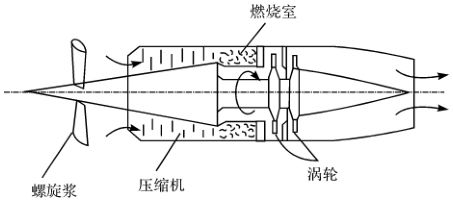
\includegraphics[width=\linewidth]{figs/fig-0087.png}
\caption{图6.5-1}
\end{figure}

的偏差的拉氏变换是 $Y_2(s)$，那么，在 $Y_2(s)$，$Y_1(s)$ 与 $W_2(s)$ 之间也可以建立一个类似于方程 (6.5-1) 的方程。然而气体达到热平衡状态的时间常数实际上等于零，所以，方程也比较简单些

\[Y_2(s) = c W_2(s) - e Y_1(s)\qquad\text{(6.5-2)}\]

这里的 $c$ 和 $e$ 也还是正常数。事实上，如果对于不变的发动机转速画出涡轮进口温度与喷油速率之间的关系图线，那么，在选定的正规的稳态运转点处的斜率就是 $c$。同样的，如果，对于不变的喷油速率，画出涡轮进口温度与发动机转速之间的关系图线，那么，在选定的正规的稳态运转点处的斜率就是 $e$。

从方程 (6.5-1) 和 (6.5-2) 中把 $Y_1(s)$ 和 $Y_2(s)$ 解出来，我们就得到

\[\begin{aligned} Y_1(s) & = \frac{-a}{1 + \tau_s} W_1(s) + \frac{b}{1 + \tau_s} W_2(s) \\ Y_2(s) & = \frac{ae}{1 + \tau_s} W_1(s) + \frac{(c - be) + c\tau_s}{1 + \tau_s} W_2(s) \end{aligned}\qquad\text{(6.5-3)}\]

这个方程组就给出了我们在理论分析中所用的发动机矩阵 $E$。我们注意到这样一个有趣的事实：在发动机矩阵里只包含一个时间常数 $\tau$。只有这一个时间常数是发动机本身所固有的。当然，整个的控制系统中还有其他的时间常数，但是，那些时间常数是由控制部分，伺服马达以及测量仪器所引进来的，所以它们不包含在发动机矩阵里面。

让我们先来考虑控制发动机转速和喷油速率的情形。这时，受控量就是 $Y_1(s)$ 和 $W_2(s)$。在这个情况下，我们只需要方程组 (6.5-3) 的第一个方程，并且 $i = 1$，$n = 2$。因而，发动机矩阵 $E$ 只有两个元素

\[E_{11} = \frac{-a}{1 + \tau_s}, \quad E_{12} = \frac{b}{1 + \tau_s}\qquad\text{(6.5-4)}\]

而

\[|E^*| = |E^*_{11}| \quad E_{11} = E_{11}, \quad |E^*_{11}| = 1\qquad\text{(6.5-5)}\]

控制系统是由下列方程组所表示的

\[U_1(s) = C_{11}(s)[X_1(s) - L_{11}(s)Y_1(s)] + C_{12}^{\prime}(s)[\Xi(s) - L_{22}(s)W_2(s)]\]

\[U_2(s) = C_{21}(s)[X_1(s) - L_{11}(s)Y_1(s)] + C_{22}^{\prime}(s)[\Xi(s) - L_{22}(s)W_2(s)]\qquad\text{(6.5-6)}\]

不互相影响的条件要求有下列关系

\[C_{21}(s) = 0\qquad\text{(6.5-7)}\]

并且利用方程 (6.5-5)

\[\frac{S_{11}(s)C_{12}^{\prime}(s)}{S_{22}(s)C_{22}^{\prime}(s)} = \frac{-|E^*_{11}|E_{12}}{|E^*|E_{11}} = -\frac{E_{12}}{E_{11}} = \frac{b}{a}\qquad\text{(6.5-8)}\]

既然 $a$ 是发动机转速对于螺旋桨桨叶角的偏导数，而 $b$ 是发动机转速对于喷油速率的偏导数，所以，比值 $b/a$ 就是当发动机转速不变时，螺旋桨桨叶角对于喷油速率的变化率。很明显，这个比值是涡轮螺旋桨发动机的飞行状况的函数。譬如说，比值 $b / a$ 是随着高度的增加而增大的。因此，一个设计得很好的控制系统就必须能够随时补偿由于飞行状态的变化和发动机运转状况的变化而引起的差异。

对于发动机转速的响应函数 $R_{11}(s)$ 就是

\[R_{11}(s)=\frac{a S_{11}(s) C_{11}(s)}{a S_{11}(s) C_{11}(s) L_{11}(s)-(1+\tau s)}\]

对于喷油速率的响应函数 $R_{22}^{\prime}(s)$ 就是

\[R_{22}^{\prime}(s)=\frac{S_{22}(s) C_{22}^{\prime}(s)}{S_{22}(s) C_{22}^{\prime}(s) L_{22}(s)+1}\qquad\text{(6.5-9)}\]

这两个方程就确定了发动机转速与喷油速率在不互相影响的控制状态中的响应特性。现在的问题就归结为如何设计控制传递函数 $G_{11}(s)$ 和 $C_{22}^{\prime}(s)$ 使得系统在我们所需要的所有运转状态下都具有使人满意的性能。

现在，我们再来考虑控制涡轮螺旋桨发动机的第二种可能的办法。我们要来控制发动机转速和涡轮的进口温度，现在的受控量就是 $Y_{1}(s)$ 和 $Y_{2}(s)$，所以在这个情形里，我们需要用到方程组 $(6.5-3)$ 的两个方程，而 $i=n=2$。由不互相影响的条件就有

\[\frac{S_{22}(s) C_{21}(s)}{S_{11}(s) C_{11}(s)}=-\frac{a e}{(c-b e)+c \tau s}\]

和

\[\frac{S_{11}(s) C_{12}(s)}{S_{22}(s) C_{22}(s)}=\frac{b}{a}\qquad\text{(6.5-10)}\]

对于发动机转速的响应函数就是

\[R_{11}(s)=\frac{S_{11}(s) C_{11}(s)}{S_{11}(s) C_{11}(s) L_{11}(s)-\frac{(c-b e)+c \tau s}{a c}}\]

对于涡轮的进口温度的响应函数就是

\[R_{22}(s)=\frac{S_{22}(s) C_{22}(s)}{S_{22}(s) C_{22}(s) L_{22}(s)+(1 / c)}\qquad\text{(6.5-11)}\]

\section{6.6 有加力燃烧的涡轮喷气发动机的控制}

在这一章开始我们曾经谈到有加力燃烧的涡轮喷气发动机，现在我们来研究这种发动机的控制问题。图 6.6-1 就是这种发动机的简略构造图。我们还是只来研究在一个选定的正规稳态运转点附近的过渡状态的控制问题，所以，把各个变数之间的关系加以线性化还是合理的。

假设 $Y_{1}(s)$ 仍然是发动机转速与它的正规值之间的偏差的拉氏变换，$W_{1}(s)$ 是尾喷管开口面积与正规值之间的偏差的拉氏变换; $W_{2}(s)$ 是燃烧室的喷油速率与燃烧室

压缩机

涡轮

可变的尾喷管开口

图 6.6-1

正规值之间的偏差的拉氏变换；最后，$W_{3}(s)$ 是尾喷管的喷油速率与正规值之间的偏差的拉氏变换。与涡轮螺旋桨发动机的方程 (6.5-1) 类似，我们可以写出下列关系

\[(1+\tau s) Y_{1}(s)=a_{1} W_{1}(s)+a_{2} W_{2}(s)+a_{3} W_{3}(s)\qquad\text{(6.6-1)}\]

这里的 $a_{1}, a_{2}$ 和 $a_{3}$ 都是实常数。和涡轮螺旋桨发动机的情形相像，这些常数都是发动机的稳态状态曲线的斜率。所以，当燃烧室的喷油速率和尾喷管的喷油速率都是常数的时候，发动机转速对于尾喷管开口面积的变化率就是 $a$。同样的，$a$就是发动机转速对于燃烧室喷油速率的变化率; $a_{2}$ 就是发动机转速对于尾喷管喷油速率的变化率。方程 (6.6-1) 里的 $\tau$ 也还是发动机的唯一的时间常数，它表示转动部件的惯性的影响。这一个关于发动机转速与其他的发动机输入之间的线性关系是费德尔 (Feder) 和胡德推导出来的 ${ }^{[4]}$。

如果发动机的压缩机是轴式压缩机的话，前一节的方程 (6.5-2) 在这里仍然是适用的。 $Y_{2}(s)$ 所表示的是涡轮的进口温度，所以

\[Y_{2}(s)=-e Y_{1}(s)+c W_{2}(s)\]

从这个方程和方程 (6.6-1) 里把 $Y_{1}(s)$ 和 $Y_{2}(s)$ 解出来，就得到

\[\begin{aligned} Y_{1}(s) & =\frac{a_{1}}{1+\tau s} W_{1}(s)+\frac{a_{2}}{1+\tau s} W_{2}(s)+\frac{a_{3}}{1+\tau s} W_{3}(s) \\ Y_{2}(s) & =-\frac{a_{2} e}{1+\tau s} W_{1}(s)+\frac{(c-a e)+c \tau s}{1+\tau s} W_{2}(s)-\frac{a_{3} e}{1+\tau s} W_{3}(s) \end{aligned}\qquad\text{(6.6-2)}\]

所以，发动机矩阵的元素就是

\[\begin{aligned} E_{11} & =\frac{a_{1}}{1+\tau s}, \quad E_{12}=\frac{a_{2}}{1+\tau s}, \quad E_{13}=\frac{a_{3}}{1+\tau s} \\ E_{21} & =-\frac{a_{2} e}{1+\tau s}, \quad E_{22}=\frac{(c-a e)+c \tau s}{1+\tau s}, \quad E_{23}=-\frac{a_{3} e}{1+\tau s} \end{aligned}\qquad\text{(6.6-3)}\]

我们来考虑控制发动机转速，涡轮的进口温度与尾喷管喷油速率的问题。这时的受控量是 $Y_{1}(s), Y_{2}(s)$ 和 $W_{3}(s)$。而控制方程就是

\[\begin{aligned} U_{1}(s)= & C_{11}(s)\left[X_{1}(s)-L_{11}(s) Y_{1}(s)\right]+C_{12}(s)\left[X_{2}(s)-L_{22}(s) Y_{2}(s)\right] \\ & +C_{13}^{\prime}(s)\left[\Xi_{s}(s)-L_{33}(s) W_{3}(s)\right] \end{aligned}\]

\begin{figure}[htbp]\centering
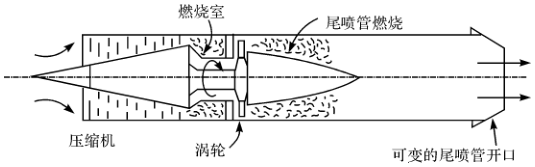
\includegraphics[width=\linewidth]{figs/fig-0088.png}
\caption{图6.6-1}
\end{figure}

\[\begin{aligned}& U_{2}(s)=C_{21}(s)\left[X_{1}(s)-L_{11}(s) Y_{1}(s)\right]+C_{22}(s)\left[X_{2}(s)-L_{22}(s) Y_{2}(s)\right] \\& \quad+C_{23}^{\prime}(s)\left[\Xi_{\varepsilon}(s)-L_{33}(s) W_{3}(s)\right] \\& U_{3}(s)=C_{31}(s)\left[X_{1}(s)-L_{11}(s) Y_{1}(s)\right]+C_{32}(s)\left[X_{2}(s)-L_{22}(s) Y_{2}(s)\right] \\& \quad+C_{33}^{\prime}(s)\left[\Xi_{\varepsilon}(s)-L_{33}(s) W_{3}(s)\right]\end{aligned}\]

这里的 $X_{1}(s), X_{2}(s)$ 和 $\Xi(s)$ 分别是发动机转速，涡轮进口温度和尾喷管喷油速率的控制信号。

方程(6.3-2)的互不影响条件要求

\[C_{11}(s)=C_{32}(s)=0\qquad\text{(6.6-5)}\]

方程(6.3-7)的条件给出

\[\begin{gathered}\frac{S_{11}(s) C_{12}(s)}{S_{22}(s) C_{22}(s)}=-\frac{a}{a} \\\frac{S_{22}(s) C_{21}(s)}{S_{11}(s) C_{11}(s)}=\frac{a e}{(c-a e)+c t s}\end{gathered}\qquad\text{(6.6-6)}\]

方程(6.3-12)的互不影响条件给出

\[\frac{S_{11}(s) C_{13}^{\prime}(s)}{S_{33}(s) C_{33}^{\prime}(s)}=-\frac{a}{a}\]

和

\[C_{23}^{\prime}(s)=0\qquad\text{(6.6-7)}\]

以上这些方程里的比值 $-\alpha / a$ 和 $-\alpha_{b} / a$ 都有很简单的物理意义：当发动机转速和尾喷管喷油速率都是常数的时候，尾喷管的开口面积对于燃烧室喷油速率的变化率就是 $-\alpha / a_{\mathrm{a}}$。当发动机转速和燃烧室喷油速率都是常数的时候，尾喷管的开口面积对于尾喷管喷油速率的变化率就是 $-\alpha / a_{\mathrm{a}}$。

如果方程(6.6-5)，(6.6-6)和(6.6-7)都被满足了，我们就得到互不影响的控制。这时，对于发动机转速的响应函数就是

\[R_{11}(s)=\frac{S_{11}(s) C_{11}(s)}{S_{11}(s) C_{11}(s) L_{11}(s)+\frac{(c-a e)+c t s}{a_{1} c}}\qquad\text{(6.6-8)}\]

对于涡轮进口温度的响应函数就是

\[R_{22}(s)=\frac{S_{22}(s) C_{22}(s)}{S_{22}(s) C_{22}(s) L_{22}(s)+(1 / c)}\qquad\text{(6.6-9)}\]

对于尾喷管喷油速率的响应函数就是

\[R_{33}^{\prime}(s)=\frac{S_{33}(s) C_{33}^{\prime}(s)}{S_{33}(s) C_{33}^{\prime}(s) L_{33}(s)+1}\qquad\text{(6.6-10)}\]

根据以上这些方程就可以适当地设计控制传递函数 $C_{11}(s), C_{22}(s), C_{33}^{\prime}(s)$，因而也就可以确定 $C_{12}(s), C_{21}(s)$ 和 $C_{13}^{\prime}(s)$。

如何正确地处理各受控量之间的相互关联（耦合），是多变量控制系统设计的关键问题之一。从不同的观点，有不同的设计原则。 “互不影响”的控制原则，从物理概念上来说，是利用控制器之间的相互关联完全或部分抵消受控对象中的相互关联，也就是“去耦”，使各个受控量的控制过程不相互影响，从而将多变量关联的大系统分解为单变量“自主”的小系统。所以，互不影响的控制原则也称为“自主”调节原则，或“去耦”设计原则。从数学方法上来说，是要设计控制矩阵，使系统矩阵“对角线”化，也就是使系统矩阵中非对角线上的元素都等于零。如果满足了互不影响条件，那么，各受控量的控制器就可以按单变量系统进行设计，因而使系统结构大为简化。如前面几章所讲过的，互不影响的控制原则已经在发动机控制、锅炉调节等多变量控制系统的设计中得到了应用。但是，互不影响的控制并不是多变量系统唯一的设计原则。因为在多变量控制的实践中，有很多场合不必要求各受控量互不影响，而是需要各受控量的控制过程相互配合和“协调”，使各变量之间保持某种协调关系，使整个系统处在技术上合理、经济上合算的协调工作状态中。 例如，连续轧钢机各机架轧辊速度的协调关系；分部传动造纸机各分部电动机速度的协调关系；化工、热工生产过程中，各种反应物质或原料成分的比例关系；电力系统中各电站或机组的负荷分配关系；垂直升船机、大型龙门吊车的多电机拖动系统的同步关系其他等。 一般说来，协调关系是各受控量应满足的某种线性或非线性函数关系 f(y\_\{1\}，y\textasciicircum{}\{2\}，，y\_\{n\})=c 常见的是比例关系 \_\{1\} y\_\{1\}=\_\{2\} y\_\{2\}==\_\{n\} y\_\{n\} 当比例系数文献[1，2]研究了这类多变量的协调控制系统，并提出了“协调控制”原则进行设计的方法。 第一种方法是按“协调偏差”控制，自整定“内部”给定量。它不同于通常的控制系统——按外部给定量与受控量的偏差，进行反馈闭环控制；在多变量协调控制系统中，给定的是各受控量之间的协调关系，而不是个别受控量的给定值。因此，为了保持各受控量之间的协调关系，减少系统实际运行状态对指定协调状态的偏离，需要按“协调偏差”进行反馈闭环控制。协调偏差定义为 =\{y\}\_\{i\}-y\_\{i\}，i=1，2，，n 式中

\section{6.7 多变量系统的协调控制}

\[\dot{y}_{i}^{*}=f_{i}\left(y_{1}, y_{2}, \cdots, y_{n}\right)\qquad\text{(6.7-4)}\]

这里，“内部”给定量 $\left(y_{i}\right)$ 是根据给定的协调关系与系统的实际运行状态，考虑稳态与动态品质要求，由系统内部自行整定的，而不是由系统外部给定的。

当系统受到扰动或其他因素影响而偏离协调工作状态时，在按协调偏差的闭环控制作用下，将迫使各受控量向内部给定量靠近，以减少协调偏差，使系统进入协调工作状态。

由于内部给定量 $\left(y_{i}\right)$ 是各受控量 $\left(y_{1}, y_{2}, \cdots, y_{n}\right)$ 的函数，所以，任何一个受控量的变化，都将使系统重新整定相应的内部给定量，从而，引起协调偏差的重新分配，使其他受控量都向有利于协调的方向变化。因此，各受控量的控制过程不是独立自主的；而是相互影响、相互配合的，这将有助于加快协调过程，提高协调准确度。

第二种方法是建立控制作用之间的协调联系。各受控量之间通过受控对象或过程形成的相互关联——耦合，并不总是有害的，有时没有必要都用控制器中的相互关联去抵消它们。而且，有些耦合作用是有益的，比如，升船机、龙门吊车的机械耦合有强迫同步作用。在实际系统设计中，适当地利用受控对象中固有的耦合，有可能减少所需测量元件或执行机构的数量，简化控制系统。如果不具体分析受控对象中固有耦合的利弊，片面要求完全去耦，不仅将使控制系统复杂化，去耦器也难以实现。同时，由于实际对象特性的变化与不确定性，互不影响条件不易准确地得到满足，残留的耦合有可能恶化系统品质。

因此，应当建立控制作用之间的协调联系，利用控制器中的耦合，抵消或削弱受控对象中有害的耦合，保留或加强有益于协调的耦合。这种协调联系装置构成控制系统的内反馈，可以根据稳定性、协调准确度、最快协调过程的要求进行设计。

第三种方法是按外扰补偿的原则进行协调。作用于系统的外界扰动，如负荷变化，常常是破坏协调关系的主要因素。如果外扰是可以测量的，那么，采用扰动补偿装置，实现协调关系对外扰的不变性，可以在不影响系统稳定性的情况下，大大提高协调准确度与动态性能。按扰动的开环控制与按协调偏差的闭环控制相结合，构成复合控制的协调控制系统。

扰动补偿装置可以应用不变性原理进行设计，但是，这里不是个别受控量对扰动的不变性，而是协调关系对扰动的不变性，或协调偏差对外扰的不变性。这样有可能使补偿装置适当地简化，便于实现。

根据上述协调控制原则，一种可能的多变量协调控制系统的方块图如图 6.7-1 所示。图中 $D$ 为受控对象，$C$ 为控制器，$B, G$ 分别为协调计算装置和联系装置，$F$ 为外扰补偿装置，$\left\{y_{1}, y_{2}, \cdots, y_{n}\right\}$ 为受控量，$\left\{w, w, \cdots, w_{n}\right\}$ 为控制量，$\left\{v_{1}, \cdots, v_{n}\right\}$ 为外扰作用，$\left\{x_{1}, \cdots, x_{n}\right\}$ 为协调偏差量，$\left\{s, s, \cdots, s_{n}\right\}$ 为协调联系信号，$\left\{r_{1}, r_{2}, \cdots, r_{n}\right\}$ 是外扰补偿信号。

设给定的协调关系是各受控量的线性函数关系。对于线性常系数系统，按照方块图 6.7-1，可得协调控制系统的矩阵方程如下

\[\begin{aligned}& y=D w \\& w=u+v \\& u=C(x+r+s) \\& x=B y \\& r=F v \\& s=G u\end{aligned}\qquad\text{(6.7-5)}\]

式中 $D, C, B, G, F$ 都是 $n$ 阶方阵，而 $\boldsymbol{y}, \boldsymbol{u}, \boldsymbol{v}, \boldsymbol{w}, \boldsymbol{x}, \boldsymbol{r}, \boldsymbol{s}$ 为相应维数的列向量。由 (6.7-5) 可得到系统矩阵为

\[\Phi_{v / v}=\left(E-B D C_{e}\right)^{-1} B D\left(E+C_{e} F\right)\qquad\text{(6.7-6)}\]

式中 $E$ 为 $n$ 阶单位矩阵

\[C_{e}=\left(E-C G\right)^{-1} C\qquad\text{(6.7-7)}\]

相应地闭环系统特征方程为

\[\Delta=\left|E-B D C_{e}\right|=0\qquad\text{(6.7-8)}\]

\begin{figure}[htbp]\centering
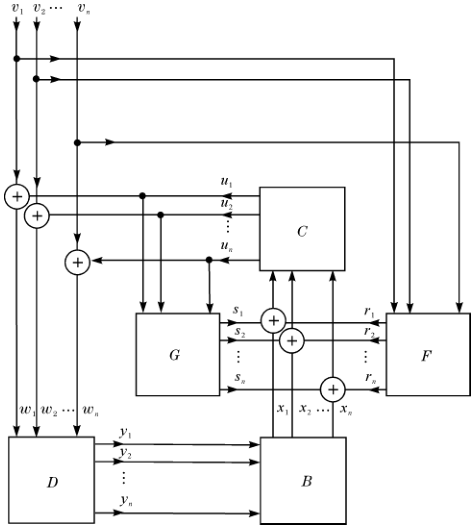
\includegraphics[width=\linewidth]{figs/fig-0089.png}
\caption{图6.7-1}
\end{figure}

利用式(6.7-5)，(6.7-6)，(6.7-7)，(6.7-8)，文献[1]中分析了协调控制系统的稳定性、准确度及其他动态性能，并研究了“大—小系统稳定性关系”，“协调离散度极小化”、“最快协调控制过程”等问题。给出了协调偏差计算装置(B)、协调联系装置(G)、扰动补偿装置(F)的综合方法。

协调控制原则在垂直升船机、分部造纸机、连续轧钢机等多变量控制系统的设计与调整中得到了应用[1，16]。

\section{参考文献}

[1] 涂序彦，多变量协调控制问题，第一届国际自动化会议论文集，上海科学技术出版社，1963.

[2] 龚炳铮，不变性理论及其发展综述，自动化技术进展，科学出版社，1963.

[3] Boksenbom，A.S.，\& Hood，R.，NACA TR 980，1950.

[4] Feder，M. S.，\& Hood，R.，Analysis for Control Application of Dynamic Characteristics of Turbojet Engine with Tail-pipe Burning，NACA TN 2183，1950.

[5] Finkelstein，L.，The Theory of Invariance，Control，3(1960)，29.

[6] Kavanagh，R.J.，J. Franklin Inst.，262(1956)，5，349.

[7] Gilbert，E. G.，The decoupling of multivariable systems by state variable feedback，J. SIAM，on Control，7(1969)，1.

[8] Айзерман，М. А.，Теория авт. регулирования двигателей，1952.

[9] Вознесенский，И. И.，О регулировании машин с большим числом регулируемых параметров，Автоматика и Телемеханика，1938，4-5.

[10] Луцин，Н. Н.，Кузнецов，П. Н.，К абсолютной инвариантности до ε в теории дифференциальных уравнений ДАН СССР，68(1949)，5.

[11] Мееров，М. В.，Управление много-связными системами，Москва，1975.

[12] Стрейц，В. и Ружичка，И.，Теория автономности и инвариантности многопараметрических систем с цифровыми регуляторами，Нзв. АН СССР，энер. и авт.，ОТН，1961，5.

[13] Чинаев П. И.，О принципах синтеза автоматических систем со многими регулируемым величинами，Автоматика и Телемеханика，21(1960)，6.

[14] Шевалев，А. Г.，Цринцип инвариантности для многомерных систем автоматического регулирования，электромеханика，Изв. ВУЗ，1962，6-7.

[15] Шипанов，Г. В.，Теория и методы проектирования авт. регуляторов，Автоматика и Телемеханика，1939，1.

[16] Заицева，Е. В.，Моделирование систем гармонического регулирования，в кн. Математическое моделирование и теория электрическихцепей，Киев，1965.

\chapter{第七章 非线性系统}

在前几章内我们讨论了各类线性系统的分析和设计方法。由于线性系统的结构相对比较简单，线性系统的通解，线性依赖于初始状态和控制函数，所以讨论起来比较方便。对非线性系统，由于没有这种线性依赖关系，分析和综合问题都更复杂些。正是由于处理上的困难，对非线性系统的研究至今不如对线性系统研究的那样全面和细致。几十年来，对非线性系统的研究多数限于分析方面，而对非线性系统的设计则只有在一些简单的情况下才得到了实际可用的结果。

非线性系统的一个重要特点是常常出现周期性振荡。由于非线性的作用，在很多实际问题中都有出现这种振荡的可能性，然而，一般来说，振荡是控制系统特别是伺服系统所不希望出现的现象。只有少数系统例外，那里微小幅度的振荡对系统工作的精度无大的影响，可以把振荡作为系统的基本工作状态，使系统结构简单，还能收到特有的技术效益，例如减少静摩擦引起的系统误差等。这样，对非线性系统振荡状态的研究通常集中在下列几个方面：若系统的运动方程式已经给定，并确知它的典型工作状态是周期振荡，需要求出振荡周期和振幅，分析周期运动的稳定性；计算这种系统对给定的输入信号的反应或跟踪精度；最后，找到改变振荡周期和振幅的方法，在需要时又如何防止这种振荡的发生。因此，研究周期运动是非线性系统分析问题中的一个重要方面。

为了精确地分析非线性系统的一些特定运动的性质，尤其是对复杂的系统，必须用计算机求出精确解。在计算技术飞速发展的现在，非线性系统的分析和设计完全可以用数字计算机去进行，在精度、速度和容量等方面实际上没有什么限制；应用计算机已经解决了大量的用一般理论分析方法所不能解决的问题；对解决非线性系统的设计提供了有效的工具。然而，这并不排除理论分析工作的重要性。相反，理论分析工作可以为计算技术提供指导，能够更深刻地认识非线性系统的主要特征即主要矛盾，从而提出解决主要矛盾的方法。因此，计算技术的发展又对理论分析工作提出了新的更高的要求，它不可能完全代替理论分析。

非线性受控系统的运动方程式一般可写成

\[f\left(\frac{d^{r} x}{d t}, \cdots, \frac{d x}{d t}, x, u\right)=0\qquad\text{(7.0-1)}\]

式中 $x$ 是系统的输出，$u$ 是控制量，$f$ 是某一非线性函数。和线性系统一样，上式可以化为一个一阶非线性方程组

\[\begin{aligned}& \frac{d x_{1}}{d t}=f_{1}\left(x_{1}, x_{2}, \cdots, x_{n} ; u_{1}, u_{2}, \cdots, u_{r} ; t\right) \\& \frac{d x_{2}}{d t}=f_{2}\left(x_{1}, x_{2}, \cdots, x_{n} ; u_{1}, u_{2}, \cdots, u_{r} ; t\right) \\& \cdots \\& \frac{d x_{n}}{d t}=f_{n}\left(x_{1}, x_{2}, \cdots, x_{n} ; u_{1}, u_{2}, \cdots, u_{r} ; t\right)\end{aligned}\qquad\text{(7.0-2)}\]

式中 $x_{i}, i=1,2, \cdots, n$，是状态变量; $u, i=1,2, \cdots, r$，是控制量。如果采用向量书写方式，上式可简写为

\[\frac{d \boldsymbol{x}}{d t}=\boldsymbol{f}(\boldsymbol{x}, \boldsymbol{u}, t)\qquad\text{(7.0-3)}\]

式中 $\boldsymbol{x}=\left(x_{1}, x_{2}, \cdots, x_{n}\right)$ 是系统的状态向量，$\boldsymbol{u}=\left(u_{1}, \cdots, u_{r}\right)$ 是控制向量，$\boldsymbol{f}=\left(f_{1}\right.$，$\left.f_{2}, \cdots, f_{n}\right)$ 是速度向量。和线性系统一样，式 (7.0-2) 或 (7.0-3) 的形式包含了式 (7.0-1)，但是前者所能描述的非线性系统的种类更为广泛些。

以后我们将假定，由式 (7.0-1)-(7.0-3) 所描述的非线性系统的运动将由初始状态 $\boldsymbol{x}=\left(x_{10}, x_{20}, \cdots, x_{n 0}\right)$ 和选定的控制函数 $\boldsymbol{u}(t)$ 所唯一确定，也就是说，系统满足常微分方程解的存在和唯一性定理。本章内我们将讨论几种典型的非线性系统，以便使我们对非线性系统的几个重要特征有充分的了解。

\section{7.1 振荡伺服控制系统}

现在我们来考虑振荡伺服控制系统，与有交流电动机的交流伺服系统相似，振荡控制伺服系统的信号也是用来调制一个周期振荡的，不过，在振荡控制伺服系统中，信号调制的方法不再是普通的调幅方法。为了能够简单明了地介绍振荡控制伺服系统的概念，我们必须先提出一些预备知识。

我们来介绍一种很原始的但是也很普通的伺服系统。假如我们在系统里加一个包含一个继电器的电路，而且这个继电器的特性是这样的：如果输入电压 $x(t)$ 的绝对值不超过一个一定的阈限 （也就是一个一定的常数） 的话，输出端就没有电压，如果输入电压 $x(t)$ 的绝对值 $\left|x(t)\right|$ 超过那个阈限的话，输出就是一个常数电动势 $E$。这个电动势是由一个电源所供给的，这个电动势的极性决定于偏差信号的符号，它倾向于使偏差信号的绝对值逐渐减少。这就是所谓开关伺服系统 （也就是包含有继电器的伺服系统） 的一个例子。

这种系统的运动方程式一般可写为下列形式

\[a_{n} \frac{d^{n} z}{d t^{n}}+a_{n-1} \frac{d^{n-1} z}{d t^{n-1}}+\cdots+a_{0} z=y\]

\[x=\sum_{i=0}^{n} c_{i} \frac{d^{i} z}{d t^{i}}\qquad\text{(7.1-1)}\]

\[y=f(x)\]

这里 $z$ 是伺服系统的输出; $y$ 是反馈信号，它是 $x$ 的非线性函数，如图 7.1-1 所示。

\begin{figure}[htbp]\centering
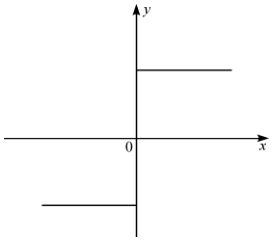
\includegraphics[width=\linewidth]{figs/fig-0091.png}
\caption{图7.1-1}
\end{figure}

\begin{figure}[htbp]\centering
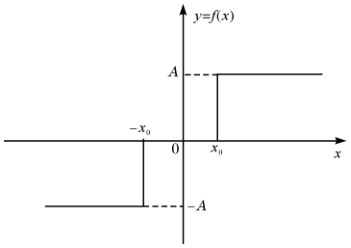
\includegraphics[width=\linewidth]{figs/fig-0090.png}
\caption{图7.1-1}
\end{figure}

(a)

(b)

图 7.1-1

这种开关伺服系统有一个很大的优点：我们可以用相当简单的开关系统来操纵相当大的功率。这个优点对于其他类型的伺服系统来说往往是很难做到的。但是，从另外一方面来说，开关伺服系统当然是一个非线性系统，并且以后我们还要看到，它们的运转性能也不如以前讨论过的各种系统好。简言之，振荡控制伺服系统是开关伺服系统的一种变形，它保持了线性性质的优点还能够操纵相当大的功率。

在进行讨论振荡控制伺服系统之前，我们先提出一个理论的结果，所有这一类系统的理论都是以这个结果为基础的。让我们考虑一个具有下列性质的装置：如果输入 $x(t)$ 是正数，输出就是 $+A$，如果输入 $x(t)$ 是负数，输出就是 $-A$。 $A$ 是一个固定的常数。我们可以把这样一个装置想象为一个理想的继电器 （一个阈限是零的开关伺服系统见图 (7.1-1b))。假定继电器的输入信号是

\[x(t)=E_{0} \sin \omega t+k E_{0} \sin \omega t\qquad\text{(7.1-2)}\]

这里 $E_{0}, k, \omega$ 和 $\omega$ 都是常数。在振荡控制伺服系统的情形中，$E_{0} \sin \omega t$ 是系统中的持续振荡，$k E_{0} \sin \omega t$ 是所用的信号，也就是调制信号。现在我们来计算相应的输出 $y(t)$。

如果输入是由方程 (7.1-2) 所表示的，那么，继电器的输出必为周期函数，也就可以写成下列形状

\[\sum_{m=0}^{\infty} \sum_{n=-\infty}^{\infty} a_{m n} \sin \left[(m \omega_{0}+n \omega) t\right]\qquad\text{(7.1-3)}\]

\[\begin{gathered} \text { 这里的各个系数 } a \text { 都是与 } t \text { 无关的常数。当 } m=0 \text { 时,内部的求和只对于正的 } n \\\text { 值进行。为了我们预定的目的, 最有兴趣的系数就是 } a_{0} \text { 和 } a_{1} \text {, 因为振荡控制伺服 } \\\text { 系统在正规的运转状态之下, 其他的系数或者是非常小, 或者由于适当的滤波手 } \\\text { 续而被过滤掉。 } \end{gathered}\]

当 $k=0$ 时，也就是当继电器的输入是一个频率为 $\omega$ 的单纯的正弦函数时，继电器的输出就是正负交替的矩形波，这个矩形波的高度是 $A$ 而每一个矩形的长度都是 $\pi / \omega$。我们已经知道这样一个矩形波的傅里叶展开式的第一项的系数等于

\[a_{01}=\frac{4 A}{\pi}\qquad\text{(7.1-4)}\]

当 $k \neq 0$ 时，继电器的输出就是图 7.1-2 所表示的样子。 $k \neq 0$ 时的输出与 $k=0$ 时的输出的差别就是一系列高度是 $2 A$ 的矩形，在图 7.1-2 里我们用阴影的区域表示这些矩形。当 $|k| \ll 1$ 时，开关点 （也就是输出变换符号的时刻） 与均匀分布的各点 $t_{n}=n \pi / \omega$ 之间的差别是十分微小的。因此，正如图中所表示的样子，表示输出信号的修正量的那些矩形也是很狭窄的。这些矩形的宽度可以这样近似地计算：在 $t_{n}$ 处的矩形的宽度等于调制信号在 $t_{n}$ 处的值被持续振荡在 $t_{n}$ 处的斜率除得的商数。因此，这个宽度就是

\[\left|\frac{k E_{0} \sin \omega t_{n}}{E_{0} \cos \omega t_{n}}\right|=\frac{k}{\omega_{0}}\left|\sin \omega t_{n}\right|\]

输入和输出

如果 $\sin \omega t_{n}$ 是正数就要把矩形加到 (+) 未调制的输出上去，如果 $\sin \omega t_{n}$ 是负数就要把矩形从未调制的输出上减去（-）。所以矩形的面积可以看做是

\[\frac{2 A k}{\sin \omega t_{n}}\]

方程 (7.1-3) 里的系数 $a_{0}$ 就是这一系列狭窄矩形波的傅里叶展开式中的第一项

\begin{figure}[htbp]\centering
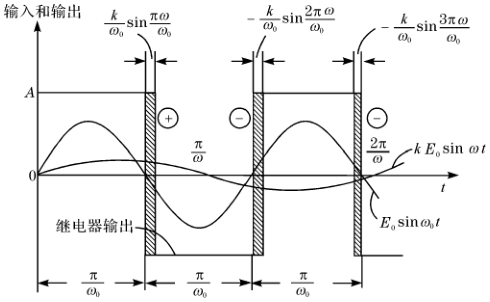
\includegraphics[width=\linewidth]{figs/fig-0092.png}
\caption{图7.1-2}
\end{figure}

$\sin \omega t$ 的系数。因为 $\sin \omega t$ 在矩形区域中的值是 $\sin \omega t_{n}$，所以，如果取 $N$ 个这类的 “改正矩形” 就有

\[a_{0} \int_{0}^{N \pi / \omega_{0}} \sin ^{2} \omega t d t=2 A \frac{k}{\omega_{0}} \sum_{n=0}^{N} \sin ^{2} \omega t_{n}\]

但是

\[\begin{aligned} \int_{0}^{N \pi / \omega_{0}} \sin ^{2} \omega t d t & =\frac{1}{2} \int_{0}^{N \pi / \omega_{0}}(1-\cos 2 \omega t) d t \\ & =\frac{1}{2} \frac{N \pi}{\omega_{0}}-\frac{1}{4 \omega} \sin \left[2 N \pi \frac{\omega}{\omega_{0}}\right] \end{aligned}\]

而

\[\begin{aligned} \sum_{n=0}^{N} \sin ^{2} \omega t_{n} & =\sum_{n=1}^{N} \sin ^{2}\left(n \pi \frac{\omega}{\omega_{0}}\right) \\ & =\frac{1}{2} \sum_{n=1}^{N}\left[1-\cos \left[2 n \pi \frac{\omega}{\omega_{0}}\right]\right] \\ & =\frac{N}{2}-\frac{1}{2} \sum_{n=1}^{N} \cos \left[2 n \pi \frac{\omega}{\omega_{0}}\right] \end{aligned}\]

当我们把 $N$ 无限增大时，这个公式中的和数仍然保持有限，所以，让 $N$ 很大，我们就有

\[a_{0}=2 \frac{A k}{\pi}\qquad\text{(7.1-6)}\]

方程 (7.1-4) 和 (7.1-5) 对于 $k$ 很小的情况给出了两个重要的系数 $a_{01}$ 与 $a_{00}$。对于一般的 $k$ 值，卡尔普 (Kalb) 和本尼特 (Bennett) ${ }^{[16]}$ 曾经计算了这两个系数。当 $0当$0这里 $K(k)$ 和 $E(k)$ 分别表示第一类与第二类的完全椭圆积分。如果 $k$ 相当小，椭圆积分是可以展开的，这时就有$\begin{aligned} a_{01} & =\frac{4 A}{\pi}\left[1-\frac{k^{2}}{4}-\cdots\right] \\ a_{0} & =\frac{2 A k}{\pi}\left[1+\frac{k^{2}}{8}+\cdots\right] \end{aligned}$方程 (7.1-7) 表明，我们原来的简单计算方法在分析的准确度上是相当正确的。然而它也表明方程 (7.1-4) 与 (7.1-5) 所给的简单结果对于不是很小的 $k$ 值也还能适用，因为方程 (7.1-7) 与 (7.1-4)，(7.1-5) 的差别的数量级是 $k^{2}$。因此，输出中频率是 $\omega$ 的成分与输入中同样频率的成分的比，也就是频率特性 $F_{\mathrm{t}}(i \omega)$ 近似地等于

\[F_{t}(i \omega)=\frac{2 A}{\pi E_{0}}\qquad\text{(7.1-8)}\]

正如方程(7.1-4)与(7.1-7)所表明的那样，当 $k$ 相当小的时候，输出中频率是 $\omega$ 的成分的振幅差不多是一个常数，而这个常数是由继电器本身的特性所完全确定的。而且，输出中频率是 $\omega$ 的成分与输入中同频率的成分的比是 $4 A / \pi E$。所以，继电器对于频率是 $\omega$ 的成分的放大率比对于频率是 $\omega$ 的成分的放大率多 6 分贝 $(\mathrm{db})$。

不难看出，以上的讨论可以推广到输出不是 $k E_{0} \sin \omega t$ 而是 $x(t)$ 的情况，$x(t)$是任意形状的函数而且 $x(t)$ 的大小比持续振荡的振幅 $E$ 小得多。在这种情形下，主要的结果可以这样表述：如果调制信号中的高次项小到可以忽略不计的程度或者可以用适当的滤波的方法把它们最后过滤掉；如果继电器的输入是

\[E_{0} \sin \omega t+x(t)\]

而 $x(t)$ 比 $E$ 小得多，那么，对于信号 $x(t)$ 的传递来说，继电器的性质就近似与一个线性系统一样，这时的频率特性就是方程 (7.1-8) 所表示的常数。

\section{7.2 利用固有振荡的振荡控制伺服系统}

现在我们来进一步讨论振荡控制伺服系统。我们已经看到，如果只从信号的传递作用的角度来考虑问题，持续振荡的作用只是使继电器变成一个具有真实频率特性的相当近似的线性元件。因此，从一开始我们就可以不必提到持续振荡 $E_{0} \sin \omega t$ 而把继电器看作是一个线性元件 ${ }^{[25-35]}$，因而也就可以利用以前各章的各种概念和方法来处理这种系统。下面介绍的方法是罗吉埃 (Lozier) 所提出的。

为了简单起见，我们一直假定伺服系统本身就具有滤波的性质，能够把继电器产生的所有的不需要的调制项过滤掉。但是，在实际情形中为了达到滤波的目的，有时候也还需要附加一些滤波器。自然，不论系统中的滤波器是怎样的，它们都必须能够使有用的信号通过。把这一点和其他方面的考虑联系起来就得到这样的结论：频率 $\omega$ 必须大于信号的傅里叶谱的主要部分的频率。

不论在系统中采用哪一种滤波的方法，输出中总包含有一个频率是 $\omega$ 的振荡成分。特别应该注意：如果用滤波的方法把这个振荡成分的振幅减低到一定的数值以下，后果有时反而不好。因为在事实上这个振荡能够起“动力润滑”的作用，它能够减少静力摩擦，松弛以及其他各种与系统有关的非线性作用的影响，而这些作用都是使伺服系统的运转性能变坏的。

我们一直还没有特别讨论用什么方法把持续振荡 $E_{0} \sin \omega t$ 加到继电器上去的问题，我们仅只附带地提到过，可以用一个附加的振荡器来供给这个振荡。用振荡器供给持续振荡的系统在可变化性方面是有优点的。因为持续振荡的振幅 $E_0$ 与频率 $\omega$ 都不加以改变；可是这种系统总是需要一定数量的额外设备，这是它们的一个重大缺点。以下我们将要简单地介绍一类振荡控制伺服系统，这类伺服系统本身就能够供给持续振荡而不需要额外的设备。

我们来看图 7.2-1 所表示的系统。假定这个系统被设计得具有这样的性能：当没有输入信号时系统也能以某一个固定的频率 $\omega$ 振荡，这个 $\omega$ 的值是由反馈迴路中的线性元件的频率特性的相角偏移所确定的。正如我们已经看到的，对于持续振荡而言，继电器所起的作用就像一个线性元件一样，而且频率特性 $4 A / (\pi E_0)$ 是一个与振幅成反比的正实数。正因为如此，振荡的振幅也能自行调整，使得由于迴路中的继电器和线性元件而产生的放大率最后变为一。

\begin{figure}[htbp]\centering
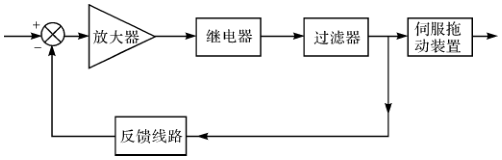
\includegraphics[width=\linewidth]{figs/fig-0093.png}
\caption{图7.2-1}
\end{figure}

图 7.2-1

现在假定有一个信号加在系统上。如果在继电器的输入部分上相应的偏差信号相当小，那么，继电器对于持续振荡的放大率基本上就不受到影响，因而还可以以原有的频率和振幅继续振荡。我们已经证明，继电器对于信号所起的作用也是线性的，继电器对于信号的放大比对于持续振荡的放大大小 6 个分贝。很明显，在这种情况下，我们就得到一种振荡控制伺服系统。这种系统基本上与以前所讨论过的那种系统是相同的，唯一的区别在于：这种系统的持续振荡 $E_0 \sin \omega t$ 的频率和振幅都是由系统本身所确定的 （这种振荡称为固有振荡），然而在以前的那种情形中我们实际上假设持续振荡是与系统无关的。

如果把系统当做一个伺服系统来考虑，那么，在所有的讨论里我们只需要考虑继电器对于信号的频率特性，也可以按照以前各章所提出的方法进行处理。并不需要顾虑持续振荡。但是，因为要维持系统的持续振荡，所以，从伺服系统的角度来说，性能的改善还是受到一定的限制的。在以下的讨论里就可以看到这一点。

假设 $F(s)$ 是控制线路对于信号的传递函数，这个函数是按照方程 (7.1-8) 计算的。对于持续振荡而言的传递函数当然就是 $2 F(s)$。既然系统有持续振荡。所以系统的传递函数 $1 + [1 / 2 \ F(s)]$ 有一个纯虚数零点 $s = i \omega$。所以因此，当 $s$ 沿着虚轴变化时，乃氏图的 $1 / F(s)$ 图线必须经过 -2 点。另一方面，当我们把系统看作伺服系统时，为了保证它具有满意的性能，$1 / F(s)$ 图线就必须离开 -1 点相当远。很明显，由于多了一个限制条件，就使得系统比没有这个限制条件的系统更难满足这些条件。在这个意义上，从可变化性的角度来看，这一类利用本身的固有振荡的系统是不如那些利用外加的振荡器供给持续振荡的振荡控制伺服系统的。所以，当系统能进行持续振荡时，$1 / F(i \omega)$ 图线必须经过 -2 点。为了避免图线经过 -1 点的附近，可以采取这样一个办法：设法使图线在 -2 点与实轴垂直地相交。这也就表示，在系统的固有频率 $\omega$ 处，向量 $1 / F(i \omega)$ 的长度变化得非常缓慢，而相角却变化得比较快。

继电器是非线性装置。但是如果沿用上述线性化的方法，把一个高频率大振幅的正弦振荡加到信号上去，那么，对于信号而言，就可以使得输出与输入之间的关系变成线性的。所以，振荡控制伺服系统的基本概念就是把非线性系统线性化。罗埃布 (Loeb) [19] 已经证明：这个概念可以应用到任何非线性系统上去，并且他把这个方法称为非线性控制系统的一般线性化方法。因此，我们也就把利用这种方法的伺服系统称为一般的振荡控制伺服系统。

我们来考虑一个一般的函数 $y(x)$，这里的 $y$ 是输出，$x$ 是输入。如果把变数 $x$ 换成 $x + \varepsilon$。而 $\varepsilon$ 是一个比 $x$ 小得多的数。如果 $y(x)$ 是一个正则函数，我们就可以把 $y(x + \varepsilon)$ 展开为泰勒级数

\[y(x + \varepsilon) = y(x) + \varepsilon\left(\frac{d y}{d x}\right)_{x} + \varepsilon^{2}\left(\frac{d^{2} y}{d x^{2}}\right)_{x} + \cdots\qquad\text{(7.2-1)}\]

现在我们假定输入 $x$ 是一个时间 $t$ 的周期函数，周期是 $T$，并且 $\varepsilon$ 是一个常数。显然，$y(x)$ 也是时间 $t$ 的周期函数，周期也还是 $T$。不难想到，$d y / d x$ 与 $d^{2} y / d x^{2}$ 也是时间 $t$ 的周期函数，而且周期也是 $T$。周期函数可以展开为傅里叶级数，所以，如果把 $\varepsilon$ 的高于一次的方幂忽略不计，我们就得到

\[\begin{aligned} y(x + \varepsilon) \cong & a^{0} + \sum_{n=1}^{\infty}\left(a_{n} \cos n \omega t + b_{n} \sin n \omega t\right) \\ & + \varepsilon\left[a_{0} + \sum_{n=1}^{\infty}\left(a_{n} \cos n \omega t + b_{n} \sin n \omega t\right)\right] \end{aligned}\qquad\text{(7.2-2)}\]

其中 $\omega = 2 \pi / T$ 是输入 $x$ 的频率。

如果 $\varepsilon$ 不是一个真正的常数，而是一个变化得相当缓慢的时间函数，它的基本频率比 $\omega$ 小得很多。这时，方程 (7.2-2) 仍然近似地正确。现在把 $y(x)$ 看做是非线性装置的输入与输出之间的关系，把 $\varepsilon(t)$ 看做是信号，把 $x(t)$ 看做是附加上去的高频率大振幅的持续振荡，这个持续振荡不需要是正弦振荡。在非线性元件的输出中表示信号的是方程 (7.2-2) 的第二项。既然频率 $\omega$ 比

$\epsilon(t)$ 的频率高很多。所以，我们就可以把下列傅里叶级数所表示的周期函数看做是载波

\[a_{0}+\sum_{n=1}^{\infty}\left(a_{n} \cos n \omega t+b_{n} \sin n \omega t\right)\]

把 $\epsilon(t)$ 看做是调幅信号。在以上的讨论中，我们都是假定非线性元件的输入 $x$ 与输出 $y$ 之间有直接的函数关系 $y(x)$。罗埃布曾经证明：即使 $y$ 与 $x$ 之间的关系是一般的泛函数关系 （也就是说，$y$ 在时刻 $t$ 的值不仅仅与 $x$ 在时刻 $t$ 的瞬时值有关，而且也与在所有过去的时刻的 $x$ 值有关），方程 (7.2-2) 也还是成立的。这种更广泛的输入输出关系的概念就可以把例如齿轮松弛等的滞后现象包括在内，而且这种概念几乎对于所有的实际的非线性装置都能适用。因此，对于一般的振荡控制伺服系统来说，输出中的信号的形式是被调制的载波，而且对于信号而言，输入输出之间的关系是线性的。

现在，我们假定附加的持续振荡的波形是对称的，例如正弦波或图 7.2-2 表示的锯齿波等。如果 $y(x)$ 是偶函数，或者说

\[\left|\frac{d y}{d x}\right|_{x}=-\left|\frac{d y}{d x}\right|_{-x}\qquad\text{(7.2-3)}\]

那么，对于周期函数 $y(x)$ 与 $d y / d x$ 就有下列关系

\[\left|\frac{d y}{d x}\right|_{t}=-\left|\frac{d y}{d x}\right|_{t+\frac{T}{2}}\qquad\text{(7.2-4)}\]

从这两个条件就推导出

\[a_{b 1}=b_{v 1}=0, a_{0}=0 \quad(y(x) \text { 是偶函数时 })\qquad\text{(7.2-5)}\]

\[x(t)\]

图 7.2-2

因此，如果把高次谐波忽略不计，载波就是一个频率是 $\omega$ 的正弦振荡。这也就是前一节所讨论过的交流伺服系统的情形。在那里所提出的设计方法仍然可以用到这类一般的振荡控制伺服系统上来。如果 $y(x)$ 是奇函数，或者说 $y(x)=$

\begin{figure}[htbp]\centering
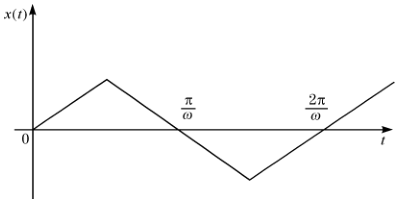
\includegraphics[width=\linewidth]{figs/fig-0094.png}
\caption{图7.2-2}
\end{figure}

- y(-x)，我们也可以写出一组类似于方程(7.2-3)和(7.2-4)的条件，而且可以导出下列条件

\[a_{00}=0, a_{11}=b_{11}=0 \quad(y(x) \text { 是奇函数时 })\qquad\text{(7.2-6)}\]

如果忽略掉高次谐波，这个情形与前面所讨论过的振荡控制伺服系统是完全相同的。

以上的讨论表明：如果伺服系统中包含有非线性元件，我们就可以用在输入信号上附加持续振荡的方法使非线性元件的特性线性化，同时把原来的系统变为性能较好的振荡控制伺服系统。而且，完全可以用这里所讲的各种方法来设计这一类伺服系统。

\section{7.3 继电系统的周期运动及其稳定性}

在第一节中我们曾介绍了对非线性元件的线性化方法，并用该方法研究了系统对输入信号的反应。那里我们引进了等效频率特性（或等效传递函数）的概念，用类似于线性系统的分析方法去近似求出伺服系统的跟踪能力。这种方法可以推广到对非线性系统的周期运动的研究。本节内我们将以一个具体的例子来说明这一方法的基本思想——幅相平衡原理。下面我们将看到，应用线性化的方法不仅可以求出周期运动的近似参数，而且还能够得到关于所研究的周期运动的稳定性判据。

\begin{figure}[htbp]\centering
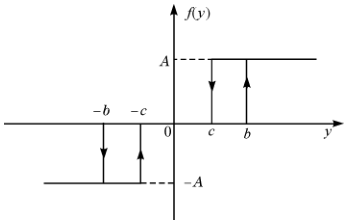
\includegraphics[width=\linewidth]{figs/fig-0095.png}
\caption{图7.3-1}
\end{figure}

假定非线性系统是由线性部分和一个继电器串联而成，具有比例反馈的闭路结构，如图 7.2-1 所示。主要非线性元件的特性示于图 7.3-1 中。为了讨论的方便，我们把继电器的性能加以理想化：假设继电器没有时间延迟的现象，而且它的开关动作都可以在一瞬间完成，而不需要花费时间，总之，没有时滞现象。但是，继电器特性本身的滞后现象还是被考虑的；在输入是正数而且逐渐增大的过程中，如

果输入在 0 与 $b c$ 是一个比较小的正常数）之间，继电器的输出是零。当输入增加到 $b$ 的时候，输出就立刻从零变到满值 $A$ ( $A$ 是一个正常数）。在输入是正数可是逐渐减小的过程中，只要输入大于 $c(c$ 也是一个正常数）输出就总是 $A$，一旦输入减小到 $c$ 的时候。输出就由满值 $A$ 立刻变为零。一般来说，$b$ 总是比 $c$ 大。如果把电流看做是继电器的输入，那么，$b$ 就称为接通电流，$c$ 就称为开断电流。当输入是负数的时候，$-b$ 和 $-c$ 分别是接通电流和开断电流，输出的满值是一 $A$。图

7.3-1所画的就是上述的输入-输出关系，而图7.3-2是继电器输出函数的变化曲线。

\begin{figure}[htbp]\centering
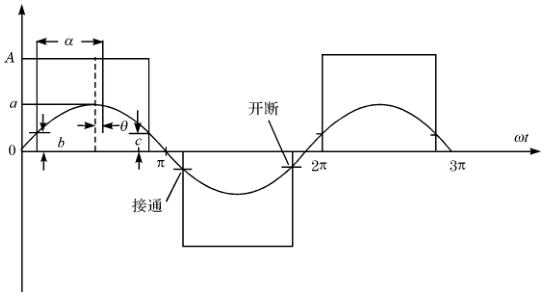
\includegraphics[width=\linewidth]{figs/fig-0096.png}
\caption{图7.3-2}
\end{figure}

\textbackslash\{\}begin\{figure\}[h]\textbackslash\{\}centering\textbackslash\{\}includegraphics[width=0.8\textbackslash\{\}textwidth]\{图7.3-2\}\textbackslash\{\}caption\{图7.3-2\}\textbackslash\{\}label\{fig:7.3-2\}\textbackslash\{\}end\{figure\}

由于$b\neq c$，所以输入与输出之间就有一个相差差。输入的相角落后的值$\theta$

\[\theta=\frac{1}{2}\left[\sin^{-1}\frac{b}{a}-\sin^{-1}\frac{c}{a}\right]\qquad\text{(7.3-1)}\]

输出的每一个矩形波的长度都是$2\alpha/\omega$，这里的$\alpha$是由下列公式给定的

\[\alpha=\frac{\pi}{2}+\theta-\sin^{-1}\frac{b}{a}=\frac{1}{2}\left[\pi-\sin^{-1}\frac{b}{a}-\sin^{-1}\frac{c}{a}\right]\qquad\text{(7.3-2)}\]

输出的周期与输入的周期是相等的，它们都是$2\pi/\omega$。

现在，输出就可以展成一个傅里叶级数

\[y(t)=\sum_{n=1}^{\infty}a_{n}\sin[n(\omega t-\theta)]\qquad\text{(7.3-3)}\]

基本谐波（第一次谐波）的系数$a$就是

\[a=\frac{4A}{\pi}\sin\alpha\]

这里的$\alpha$是由方程(7.3-2)所给出的。在图7.3-3所画的继电器伺服系统中，继电器的输出就是控制伺服机构的控制信号。伺服机构通常都具有滤波器的性质，它能够使高次谐波的影响大大地减小。因此，作为一个近似的考虑，我们把所有高次谐波都忽略掉，把输出就看做是$a\sin(\omega t-\theta)$。如果$\omega\geqslant 0$，采用复数形式，输出与输入的比值就是

\[F_{r}(i\omega)=\frac{4A\sin\alpha}{\pi a}e^{-i\theta}(\omega\geqslant 0)\]

如果$\omega<0$，输入$a\sin\omega t=-a\sin|\omega|t$，这时输出的基本谐波就是

\[-\frac{4A}{\pi}\sin\alpha\sin[|\omega|t-\theta]=\frac{4A}{\pi}\sin\alpha\sin(\omega t+\theta)\]

图 7.3-3

所以，用复数形式表示，输出与输入的比值就是

\[F_{r}(i \omega)=\frac{4 A \sin \alpha}{\pi a} e^{i \theta}\]

总结起来，输出与输入的比值就是

\[F_{r}(i \omega)= \begin{cases}\frac{4 A \sin \alpha}{\pi a} e^{-i \theta}, & \omega \geqslant 0 \\ \frac{4 A \sin \alpha}{\pi a} e^{i \theta}, & \omega \leqslant 0\end{cases}\qquad\text{(7.3-4)}\]

我们把 $F_{r}(i \omega)$ 看做是继电器的“频率特性”，但是，这只是一种说法而已，$F_{r}(i \omega)$ 并不是真正的频率特性。正像以前各章所定义的那样，真正的频率特性只是频率 $\omega$的函数，与输入的振幅是没有关系的。可是，恰好相反，这里的 $F_{r}(i \omega)$ 是振幅 $a$ 的函数，除了与 $\omega$ 的符号有关系之外，$F_{r}(i \omega)$ 与 $\omega$ 的大小并没有关系。由此可见，我们所用的函数符号 $F_{r}(i \omega)$ 以及“频率特性”的名称并不合理，但是，为了与普通

符号和名称统一，我们还是采用了这种符号和名称。应该注意到，和普通的情形一样，$F_{r}(i \omega)$ 也有下列的重要性质:

\[\overline{F_{r}(i \omega)}=F_{r}(-i \omega)\]

如果输入的振幅 $a$ 非常大，根据方程 (7.3-1)，(7.3-2) 和 (7.3-4) 就有

\[F_{r}(i \omega) \stackrel{(7.3-5)}{=} \frac{4 A}{\pi} \frac{1}{a}, \quad a \gg 1\]

如果振幅 $a$ 相当小 $(a \leqslant b)$，继电器根本就没有反应。

如果振幅 $a$ 刚好等于接通电流 $b, a=b$。那么

\[\theta=\alpha=\frac{1}{2}\left(\frac{\pi}{2}-\sin ^{-1} \frac{c}{b}\right), \quad a=b\qquad\text{(7.3-6)}\]

这个临界情形称为继电器的开断点。

可见，这些极端情况下的 $F_{r}(i \omega)$ 的值是由继电器的特性所确定的。下面我们

将介绍一个方法，用以求出振荡的参数和判别其稳定性及系统零位稳定性。

我们暂且假定输入的各个调和分量 （也就是各次谐波） 的振幅都是 $a$。这时，继电器的频率特性就是一个由方程 (7.3-4) 所给定的复常数。图 (7.3-3) 的控制线路中除了继电器之外，还有其他的部件，假设这些部分的频率特性是 $F_{1}(i \omega)$。那么，前向控制线路的总的频率特性就是 $F_{r}(i \omega) F_{1}(i \omega)$。我们让 $\omega$ 从 0 变到 $\infty$，把相当的乃氏图线 $1 /\left[F_{r}(i \omega) \cdot F_{1}(i \omega)\right]$ 画在复平面上，可以根据乃氏准则，去判

\begin{figure}[htbp]\centering
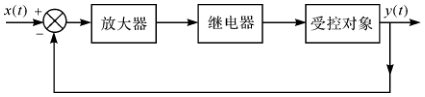
\includegraphics[width=\linewidth]{figs/fig-0097.png}
\caption{图7.3-3}
\end{figure}

别系统的稳定性，此时乃氏图线必定要“包围”-1点，换句话说，乃氏图线一定要在-1点的左方穿过实轴。但是，在振幅都是常数 $a$ 的情况中，$F_{r}(i \omega)$ 是一个常数，所以上述的稳定性条件也就相当于要求频率特性曲线 $1 / F_{1}(i \omega)(\omega$ 从 0 变到 $\infty)$ 包围 $F_{r}(i \omega)$ 点。以上的讨论结果就是确定继电器伺服系统的柯氏方法的基础 ${ }^{[17]}$。果德发尔布 ${ }^{[29]}$ (Гольдфарб) 在比较早的时候已经采用过这种方法，都梯尔 (Dutilh)也独立地发明了一个类似的方法 ${ }^{[12]}$。

柯氏(Kochonburger)指出：当输入的各个调和分量的振幅不都相等的时候，只要把上一段中所讲的稳定条件应用到相当于 $a$ 从 0 变到 $\infty$ 的所有的 $F_{r}(i \omega)$ 值上去就可以了。当 $a$ 从 0 变到 $\infty$ 的时候，$-F_{r}(i \omega)$ 的轨迹也是一条曲线，这条曲线的起点就是方程 (7.3-6) 所表示的开断点，终点就是复平面的原点。图 7.3-4 所画的就是这种情形。这种图线就称为柯氏图。因此，柯氏方法中的零点稳定的充分条件就是: $1 / F_{1}(i \omega)$ 图线必须像图 7.3-4 那样把整个 $-F_{r}(i \omega)$ 图线包围起来。图 7.3-5 所画的是绝对不稳定的情形。 $-F_{r}(i \omega)$ 图线上的箭头所表示的是继电器的输入振幅 $a$ 增大的方向。 $F_{1}(i \omega)$ 图线上的箭头所表示的是频率 $\omega$ 增大的方向，而且这条图线当 $\omega=0$ 时从原点出发。

图 7.3-4

图 7.3-5

除了这两种绝对稳定与绝对不稳定的情形外，也还有部分稳定 （或部分不稳定） 的情形，在这种部分稳定的情形中可能在一个固定的频率上发生一个振幅也是常数的自激振荡。例如，图 7.3-6 表示一种有收敛点的情形。如果振幅 $a$ 足够小，$-F_{r}(i \omega)$ 点就在图线 $1 / F_{1}(i \omega)$ 的“外面”，因而系统是不稳定的，于是振荡的振幅就逐渐增大，当振幅增大的时候，$-F_{r}(i \omega)$ 点就朝向 $1 / F_{1}(i \omega)$ 图线移动。最后就到达 $P_{1}$ 点。这时候，系统就以相当于 $P_{1}$ 点的频率和振幅进行稳定的自激振荡。可见，只要有一个振幅不太大的初始扰动，（这个扰动并不需要持续地作用） 系统最后就会自动地达到这个自激振荡，这种运动状态称为软性的自激发。不难看出，系统不可能有离开自持振荡点 $P_{1}$ 的倾向，原因是这样的：只要振幅有一些增大，$-F_{r}(i \omega)$ 点就进入图形上的稳定区域，因而也就受到阻尼的作用迫使振幅减

\begin{figure}[htbp]\centering
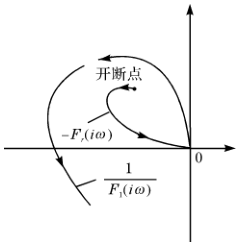
\includegraphics[width=\linewidth]{figs/fig-0098.png}
\caption{图7.3-5}
\end{figure}

\begin{figure}[htbp]\centering
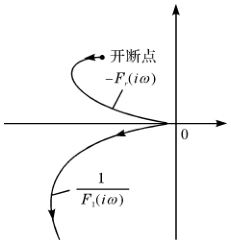
\includegraphics[width=\linewidth]{figs/fig-0099.png}
\caption{图7.3-5}
\end{figure}

小而使系统回到 $P_1$ 点的自激振荡状态。所以，$P_1$ 点才称为“收敛点”，而系统也就会持续地振荡。图 7.3-7 表示的是另外一种情形。 $-F_r(i\omega)$ 图线与 $1/F_1(i\omega)$图线的交点 $P_2$ 是一个发散点。和以上的讨论相似，我们可以看出：系统在 $P_2$点也可能发生自激振荡，不过这个振荡是不稳定的，系统的运动状态有离开 $P_2$ 点的倾向，只要有一点扰动，系统就会离开 $P_2$ 点的振荡状态。但是，如果系统最初是静止的，而且所受到的扰动不太大。 $-F_r(i\omega)$ 点就不会跑出稳定区域，因而系统的静止状态就是稳定的。

\begin{figure}[htbp]\centering
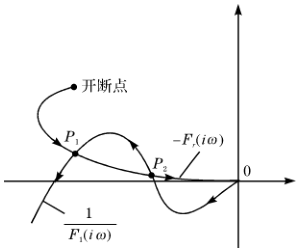
\includegraphics[width=\linewidth]{figs/fig-0103.png}
\caption{图7.3-9}
\end{figure}

\begin{figure}[htbp]\centering
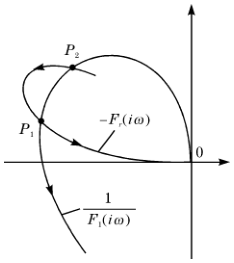
\includegraphics[width=\linewidth]{figs/fig-0102.png}
\caption{图7.3-9}
\end{figure}

\begin{figure}[htbp]\centering
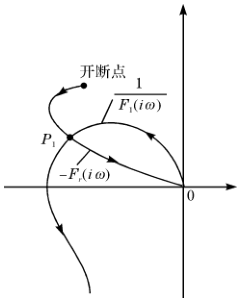
\includegraphics[width=\linewidth]{figs/fig-0101.png}
\caption{图7.3-6}
\end{figure}

\begin{figure}[htbp]\centering
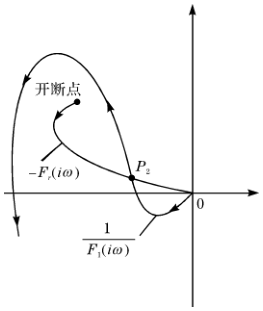
\includegraphics[width=\linewidth]{figs/fig-0100.png}
\caption{图7.3-7}
\end{figure}

图 7.3-6

图 7.3-7

图 7.3-8 和图 7.3-9 所表示的是更复杂一些的情形，在这两种情形中，既有收敛点 $P_1$ 也有发散点 $P_2$。对于图 7.3-8 的系统来说，初始扰动的振幅必须充分大 （具体地说，要大于 $P_2$ 点所相当的振幅） 才能使系统发生自激振荡，所以这种运动状态称为硬性的自激发。图 7.3-9 所表示的系统，总是可以由不大的初始扰动引起稳定的自持振荡。但是，如果初始扰动的振幅太大 （具体地说，大于与 $P_2$ 点相当的振幅），系统就不能发生自激振荡，这时系统的振幅将要无限地增大。

图 7.3-8

图 7.3-9从图 7.3-6 到图 7.3-9 所表示的各种情形，可以明显地看到系统的运动状态与扰动振幅之间有着密切的关系。并且也看到发生频率与振幅都是固定常数的自激振荡的可能性。所有这些性质都是非线性系统的特性，也是以前各章讨论过的的线性系统所没有的。其实，只要根据第一章的讨论，我们就可以猜想到非线性系统可能有这样一些“不寻常”的性质。

对于继电器伺服系统的稳定性问题来说，柯氏方法是一个很有效的解决方法。这个方法对于相当复杂的系统都能够应用，而且，只要用实验方法测出关于频率特性的数据就可以用这个方法，并不需要求出频率特性的解析表示式。在绝大多数的实际情形中，继电器后面所连接的伺服机构都有相当的滤波作用，所以，在以前的讨论中把输出中的高次谐波忽略掉的做法也是很合理的。用以上的理论分析所得的结果与实验结果是十分符合的。因此，如果稳定性是唯一的设计准则，那么，柯氏方法就解决了继电器伺服系统的全部问题。

其实，柯氏方法不仅能应用到继电器伺服系统上，而且对于许多其他的非线性机构来说，用柯氏方法也能得到同样好的效果。这个分析方法的重要关

\begin{figure}[htbp]\centering
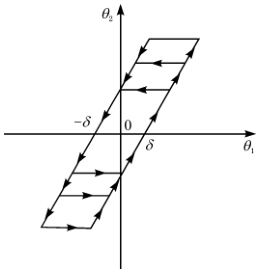
\includegraphics[width=\linewidth]{figs/fig-0104.png}
\caption{图7.3-10}
\end{figure}

键就是：继电器的运动特性与频率无关，只与振幅有关。然而，线性系统的运动特性却只与频率有关而与振幅无关。实际上，有很多非线性机构与继电器有相同的特性。譬如说，一个有间隙的传动齿轮组就是一种这样的机构。从以下的讨论就可以看出这件事实：设 $\theta$ 是发动机的主动轴的转角，这个轴与齿轮组的第一个齿轮的连接是刚固的; $\theta$ 是刚固地连接在齿轮组的最后一个齿轮上的从动轴的转角。 $\theta$ 与 $\theta$ 之间的关系可以用图 7.3-10来表示，其中的 $2 \delta$ 是齿轮组的总间隙。如果齿轮组的输入 $\theta$ 是一个正弦式的振动，那么，输出 $\theta$ 就是一种“被压扁”的正弦波，而且有一个相角落后 （图 7.3-11)。不难看出：既然 $\theta$ 和 $\theta$ 之间与时间的关系不明显，所以，$\theta$ 的频率的改变也不会使 $\theta$ 的波形受到影响。因此，齿轮组的反应只随振幅改变，而与频率无关，所以和继电器一样，齿轮组也是一个频率迟钝的机构。

如果我们用频率特性 $F_{\varepsilon}(i \omega)$ 表示输出 $\theta$ 的基本谐波与输入 $\theta$ 的基本谐波的振幅比值与相角落后。那么，$F_{\varepsilon}(i \omega)$ 只是 $\theta$ 的振幅 $a$ 的函数，而不是频率 $\omega$ 的函数。利用频率特性 $F_{\varepsilon}(i \omega)$，我们就可以研究包含这种有间隙的齿轮组的伺服系统，其作法与上一节中用频率特性 $F_{\varepsilon}(i \omega)$ 研究继电器伺服系统的办法完全相同。

图 7.3-11

\section{7.4 非线性系统周期运动的对数分析法}

前面三节，我们讨论了振动线性化方法。根据这个方法可以应用线性系统中的某些数学方法来处理复杂的非线性周期运动。我们知道，在处理线性系统稳定性的问题上，对数频率法是很方便的。把这个方法推广来研究非线性系统的周期运动，也会收到同样的效果 ${ }^{[3,28]}$。

图 7.4-1

以图 7.3-3 中的继电器伺服系统为例，我们假定它是一个理想的继电器（见图 7.4-1)，它在正弦波 $x_{1}=a \sin \omega t$ 的输入作用下，输出为一系列的矩形波，由方程 (7.1-4)可知，其输出基波振幅为

\[a_{1}=\frac{4 A}{\pi}\qquad\text{(7.4-1)}\]

我们假定线性部分的频率特性具有理想的高频滤波性质，因此在非线性元件的输出中，虽然包含有各种频谱的谐波，但是经过系统线性部分滤波后，回到非线性元

\begin{figure}[htbp]\centering
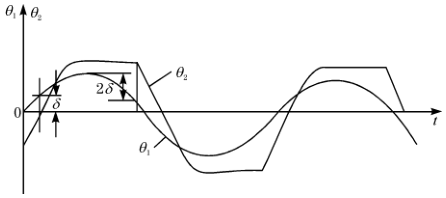
\includegraphics[width=\linewidth]{figs/fig-0105.png}
\caption{图7.3-11}
\end{figure}

\begin{figure}[htbp]\centering
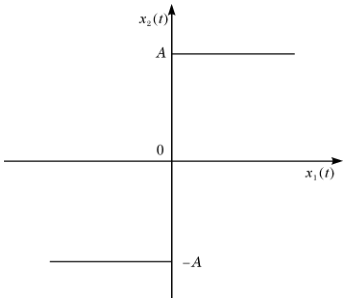
\includegraphics[width=\linewidth]{figs/fig-0106.png}
\caption{图7.4-1}
\end{figure}

件的输入端，起主要作用的将是一次谐波。这时，非线性元件可以近似地用它的等效传递函数来描述

\[F_{r}(i \omega)=\frac{4 A}{\pi a}\qquad\text{(7.4-2)}\]

如果系统线性部分的传递函数是

\[F_{1}(s)=\frac{k}{s\left(1+T_{1} s\right)\left(1+i T_{2} s\right)}\qquad\text{(7.4-3)}\]

频率特性为

\[F_{1}(i \omega)=\frac{k}{i \omega\left(1+i T_{1} \omega\right)\left(1+i T_{2} \omega\right)}\qquad\text{(7.4-4)}\]

那么，当系统的输入为零时，图 7.3-3 的系统就变为图 7.4-2 的结构。如前所述，为了保持持续振荡，$y(t)$ 和 $x_{1}(t)$ 必须幅值相等相位相反，这个条件常称为谐波平衡原理，于是系统中自持振荡的振幅 $a$ 和频率 $\omega$ 就取决于如下方程式的解

\begin{figure}[htbp]\centering
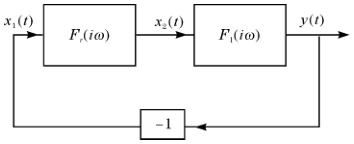
\includegraphics[width=\linewidth]{figs/fig-0107.png}
\caption{图7.4-2}
\end{figure}

\[x_{1}(t) \quad F_{r}(i \omega) \quad x_{2}(t) \quad F_{1}(i \omega) \quad y(t)\]

图 7.4-2

\[1+F_{r}(i \omega) F_{1}(i \omega)=0\qquad\text{(7.4-5)}\]

或

\[F_{1}(i \omega)=-\frac{1}{F_{r}(i \omega)}\qquad\text{(7.4-6)}\]

显然，此等式与下列两式是等价的

\[20 \log H_{1}(\omega)=-20 \log H_{r}(a)\]

\[\theta_{1}(\omega)=-\pi\]

其中

\[\begin{gathered} H_{1}(\omega)=\left|\frac{4 A}{\pi i \omega\left(1+i T_{1} \omega\right)\left(1+i T_{2} \omega\right)}\right|, \quad \theta_{1}(\omega)=\arg F_{1}(i \omega) \\ H_{r}(a)=\frac{1}{a} \end{gathered}\]

当系统的参数给出以后，就可以用作图的办法确定方程 (7.4-7) 的两个根 $a$ 和 $\omega$。例如，当 $\frac{4 A}{\pi} k=100, T_{1}=2, T_{2}=0.05$ 时，方程组 (7.4-7) 所描绘的继电器伺服系统的对数曲线就像图 7.4-3 所示那样。可以看出，按图中箭头所示的方向，立即可以确定自振荡参数。从图7.4-3看到，系统中存在$a\sin\omega t$的自持振荡。文献[3]中曾证明，当线性频率特性满足条件

\[\left.\frac{dH_{1}(\omega)}{d\omega}\right|_{\omega=\omega_{0}}\left.\frac{d\theta(\omega)}{d\omega}\right|_{\omega=\omega_{0}}>0\]

时，只要非线性特性满足不等式

\[\left.\frac{dH(\omega)}{da}\right|_{a=\omega_{0}}<0\]

以$\omega$和$\omega$为参数的周期运动就是稳定的运动。显然，图7.4-3中的曲线满足这个条件。

\begin{figure}[htbp]\centering
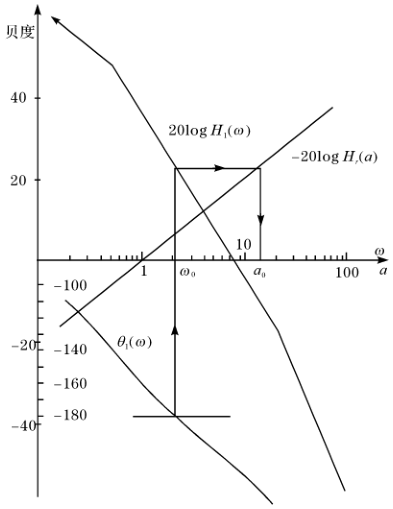
\includegraphics[width=\linewidth]{figs/fig-0108.png}
\caption{图7.4-3}
\end{figure}

如果由于某些原因需要改变振荡参数，或需要消除振荡，只要对频率特性加以相应修改，引入必要的校正网络就能达到预期的目的。

这个方法可以推广到包括图7.3-10那样更为复杂一些的非线性特性。令$\delta$为齿轮啮合间隙的半个宽度，$a$为振动的振幅，不难求出这种非线性的等效传递函数为

\[F_{g}(i\omega)=F_{g}\left[\frac{a}{\delta}\begin{bmatrix}i\theta\\ \end{bmatrix}g\begin{bmatrix}\delta\\ a\end{bmatrix}\right]\qquad\text{(7.4-8)}\]

式中

\[\left.F_{\varepsilon}\left(\frac{a}{\delta}\right)=\sqrt{q_{2}^{2}\left(\frac{\delta}{a}\right)+q_{12}^{2}\left(\frac{\delta}{a}\right)}, \quad \theta_{\varepsilon}\left(\frac{a}{\delta}\right)=\tan ^{-1} \frac{q_{1}^{\prime}\left(\frac{\delta}{a}\right)}{q\left(\frac{\delta}{a}\right)}\right\}\]

而

\[\begin{aligned} & q\left(\frac{\delta}{a}\right)=\frac{1}{\pi}\left[\frac{\pi}{2}+\sin ^{-1}\left(1-2 \frac{\delta}{a}\right)+2\left(1-2 \frac{\delta}{a}\right) \sqrt{\frac{\delta}{a}\left(1-\frac{\delta}{a}\right)}\right] \\ & q_{1}^{\prime}\left(\frac{\delta}{a}\right)=-\frac{4 \delta}{\pi a}\left[1-\frac{\delta}{a}\right] \end{aligned}\]

设线性部分的传递函数为

\[F_{1}(s)=\frac{k}{s(1+T s)}\qquad\text{(7.4-9)}\]

频率特性是

\[F_{1}(i \omega)=\frac{k}{i \omega(1+i T \omega)}\qquad\text{(7.4-10)}\]

根据谐波平衡原理，自振荡的参数 $a$ 和 $\omega$ 将由下列方程组的根确定:

\[\begin{aligned} & 20 \log H_{1}(\omega)=-20 \log H_{\varepsilon}\left(\frac{a}{\delta}\right) \\ & \theta_{\varepsilon}(\omega)=-\left[\theta_{\varepsilon}\left(\frac{a}{\delta}\right)+\pi\right] \end{aligned}\]

式中

\[H_{1}(\omega)=\left|F_{1}(i \omega)\right|, \quad \theta_{\varepsilon}(\omega)=\arg F_{1}(i \omega), \quad H_{\varepsilon}\left(\frac{a}{\delta}\right)=F_{\varepsilon}\left(\frac{a}{\delta}\right)\]

方程组 (7.4-11) 的左端是 $\omega$ 的函数，而右端是 $a$ 的函数，所以它是一组变量分离的代数方程。当 $20 \log k=38$ 分贝，$T=0.1$ 时，它们的对数特性就像图 7.4-4 所示那样。利用图中给出的四条曲线，可以用作图法求出方程 (7.4-11) 的根 $a$ 和 $\omega$。任取一水平线 $c$，它与相频特性 $\theta(\omega)$ 和 $\theta(a)$ 分别交于 $c$ 和 $c$ 点 （相平衡）。过 $c$ 点的垂线与 $L_{2}$ 交于 $h$ 点; $e$ 点是矩形 $c_{1} c_{2} h e$ 的一个顶点，当直线 $c$ 上下平移时，$e$ 点就描绘出一条曲线 $L(\omega)$，后者和 $L_{1}$ 的两个交点①和②都满足谐波平衡条件，它们唯一地确定了代数方程 (7.4-11) 的两个根，因此可能出现两个周期运动。但可以证明，①所决定的周期运动是不稳定的，而②是稳定的 ${ }^{[3]}$。图 7.4-4 中的曲线还告诉我们，当系统的增益减少时，例如由 $L_{1}$ 变为 $L_{1}^{\prime}$ 时，$L(\omega)$ 和 $L_{1}$ 将没有交点，自持振荡也就消失了。

用对数法不仅能够方便地分析非线性系统的自持振荡，而且还能应用到非线性系统的强迫振荡、跳跃共振和利用正弦信号来改善伺服系统的性能等方面，关于这些问题的讨论，读者可参看本章参考文献[3]。

分贝度

\[L_{2}=-20 \log H_{\pi}\left(\frac{a}{\delta}\right)\]

\[L_{1}=20 \log H_{1}(\omega)\]

\[\theta_{2}=-\left|\theta\left(\frac{a}{\delta}\right)+\pi\right|\]

图 7.4-4

\section{7.5 弱非线性系统}

现在我们将要考虑的方程不是式 (2.2-1) 型的线性系统，而是一个 $n$ 阶的非线性系统。假定描绘系统运动的微分方程是

\[a_{\nu} \frac{d^{\nu} y}{d t^{\nu}}+a_{\nu-1} \frac{d^{\nu-1} y}{d t^{\nu-1}}+\cdots+a \frac{d y}{d t}+\omega y+\mu f\left\{y, \frac{d y}{d t}, \cdots, \frac{d^{\nu-1} y}{d t^{\nu-1}}\right\}=x(t)\qquad\text{(7.5-1)}\]

其中的各个系数 $a$ 和 $\mu$ 都是常数，$x(t)$ 是输入，$y(t)$ 是输出，$f$ 是它的自变量的一个非线性函数。方程 (7.5-1) 的左端的前一部分是一个与方程 (2.2-1) 的左端相同的线性微分算子，系统的全部非线性性质都是由方程左端的后一部分 $\mu f$ 所表示的。我们当然可以假定方程 (7.5-1) 的变数 $t$ 已经是一个无量纲的时间变数了，

\begin{figure}[htbp]\centering
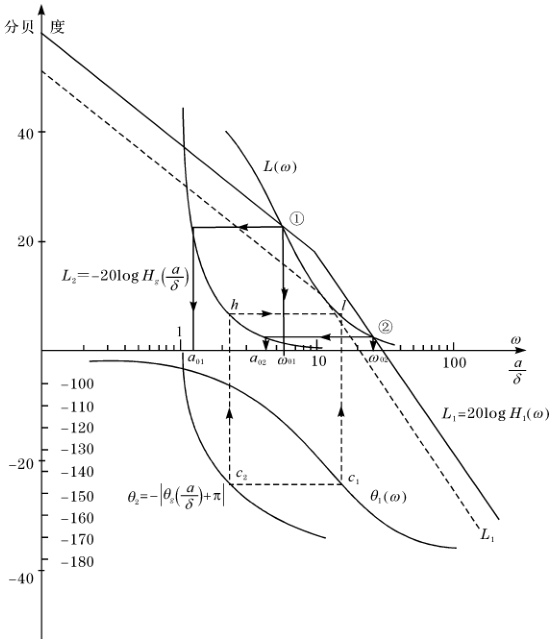
\includegraphics[width=\linewidth]{figs/fig-0109.png}
\caption{图7.4-4}
\end{figure}

所以，各个系数 $a$ 和 $\mu$ 的量纲都是相同的。所谓弱非线性，也就是说，$\mu$ 比各个系数 $a$ 都小得多。

对于这种“弱非线性”的情形，我们就可以设法把方程的解形式地写成 $\mu$ 的幂级数的样子

\[y(t)=y^{(0)}(t)+\mu y^{(1)}(t)+\mu^{2} y^{(2)}(t)+\cdots\qquad\text{(7.5-2)}\]

把方程(7.5-2)代入方程(7.5-1)，然后，再让方程两端的 $\mu$ 的同次方幂相等，就得出

\[a_{n} \frac{d^{n} y^{(0)}}{d t^{n}}+a_{n-1} \frac{d^{n-1} y^{(0)}}{d t^{n-1}}+\cdots+a_{1} \frac{d y^{(0)}}{d t}+a_{0} y^{(0)}=x(t)\qquad\text{(7.5-3)}\]

\[a_{n} \frac{d^{n} y^{(1)}}{d t^{n}}+a_{n-1} \frac{d^{n-1} y^{(1)}}{d t^{n-1}}+\cdots+a_{1} \frac{d y^{(1)}}{d t}+a_{0} y^{(1)}=-f\left\{y^{(0)}, \cdots, \frac{d^{n-1} y^{(0)}}{d t^{n-1}}\right\}\qquad\text{(7.5-4)}\]

以及相当于 $\mu$ 的更高次方幂的一系列方程。所以，系统的运动方程的第零次近似式(7.5-3)就是像方程(2.2-1)那样的线性方程。但是，更重要的事情是：由于非线性性质而引起的第一次改正项是由方程(7.5-4)所确定的，从形式上就可以看出，这个方程与第零次近似[方程(7.5-3)]在特性上是完全一样的。换言之，如果系统的第零次线性近似式(7.5-3)表明近似的系统 $y^{(0)}(t)$ 是有阻尼的，而且还具有伺服系统所必需的其他特性，那么第一次改正项 $y^{(1)}(t)$ 也同样具有这些特性。此外，因为在展开式(7.5-2)中 $y^{(1)}(t)$ 之前有一个相当小的因数 $\mu$，所以，由于非线性效应所必须作的改正是很小的。这也就是说，在一个性能良好的系统中，微弱的非线性性质不会使系统的运转状态与它的线性近似发生重大的差别。因此，从工程近似的观点来看，我们就可以把这些系统当做线性系统来处理。就是在工程实际中的“线性”系统里，也还是有一些微弱的非线性性质的，但是，根据上面所讲的道理，只用线性伺服系统理论来研究这些系统也就可以得到很好的结果。

另一方面，如果近似的线性系统的阻尼非常小，这时就有发生共振现象的可能性。也就是说，即使输入 $x(t)$ 的数量级和 1 相同，$x \simeq 1$，近似的线性系统式 (7.5-3)的输出 $y^{(0)}(t)$ 就可能比 1 大很多，$y^{(0)} \gg 1$。在这种情形里，虽然 $\mu$ 很小，可是 $\mu f\left\{y^{(0)}, \cdots, \frac{d^{n-1} y^{(0)}}{d t^{n-1}}\right\}$ 个数，或者说非线性效应，仍然可以和线性项的数量级相同。换句话说，我们在上一段里所作的形式上的级数展开式就不能成立了。所以，在系统的阻尼作用很微弱的情形里，即使非线性性质很弱，我们也必须考虑到可能发生的强大影响。在以下各节里，我们将要简短地描述一下非线性系统的多种多样的运动状态。非线性力学中这样一些现象的详细处理方法可以在米诺尔斯基 (Minorsky) [20]与斯托克尔 (Stoker) [21]的著作中找到。

\section{7.6 非线性系统内的几种振荡状态}

正像第 7.3 节所讲过的那样，如果系统的自激振荡能够由于离开平衡状态的微小偏差而自动地形成，那么，它就称为软的自激振荡；如果离开平衡状态足够大的偏差才能引起自激振荡，这个自激振荡就称为硬的自激振荡。在某些情形里，系统的微分方程的系数与系统的一个参数 $\lambda$ 有关。如果当 $\lambda$ 取某一个特别的临界值 $\lambda$ 时，系统的平衡状态的特性就从稳定状态变为不稳定状态。那么，在 $\lambda \geqslant \lambda$ 的时候就会出现极限环，也就是自激振荡。如果这种自激振荡是软的，发生的现象就像图 7.6-1(a) 所画的那样；如果自激振荡是硬的，那就像图 7.6-1(b) 所画的那样。对于第一种情形来说，如果 $\lambda$ 是逐渐增大的，那么，当 $\lambda$ 还没有增大到临界值 $\lambda$ 的时候，系统的平衡状态并没有任何变化。当 $\lambda$ 增加到 $\lambda$ 时，系统的平衡状态就由稳定的变为不稳定的，同时也就出现了一个稳定的极限环。而且这个极限环的振幅随着 $\lambda$ 的增加而逐渐加大。如果，再让 $\lambda$ 逐渐减小，那么，系统的平衡状态的情况就沿着原来的变化路线变化回来 （图 7.6-1a)，当 $\lambda$ 减小到 $\lambda$ 时，极限环就消失了。对于第二种情形来说，自激振荡是硬的，这时的情况就不同了 （图 7.6-1b)。在 $\lambda$ 逐渐增大的过程中，在 $\lambda=\lambda$ 时，突然就出现一个振幅是有限的极限环; $\lambda$ 继续增大的时候，相应的极限环的振幅也随之增大。如果 $\lambda$ 逐渐减小，那么，当 $\lambda$ 减小到 $\lambda$ 时，极限环（自激振荡）并不立刻消失，直到 $\lambda$ 再继续减小到一定的数值时，极限环的振幅才由一个有限数值突然变为零。所以，这种现象称为跳跃现象，它是和系统的运动状态的滞后现象相联系着的。

\begin{figure}[htbp]\centering
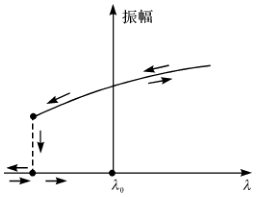
\includegraphics[width=\linewidth]{figs/fig-0111.png}
\caption{图7.6-1}
\end{figure}

\begin{figure}[htbp]\centering
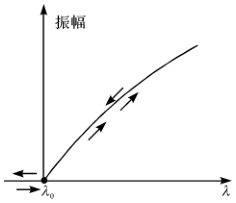
\includegraphics[width=\linewidth]{figs/fig-0110.png}
\caption{图7.6-1}
\end{figure}

振幅

(a) 软的自激发

振幅

(b) 硬的自激发

图 7.6-1

非线性系统中的频率缩减现象也是在实际技术问题中常得到应用的一种。如果作用在一个非线性系统上周期性的输入中包含两个频率 $\omega$ 和 $\omega$，那么，系统的输出中不但包含有这两个频率以及相应于这两个频率的高次谐波，而且还有一个额外的频率谱，借用声学的术语，这个谱称为合成音，它是由频率 $m\omega_{1}\pm n\omega_{2}$ ($m$，$n$ 是整数）组成的。譬如说，把一个电压 $x=x_{0}(\cos\omega_{1}t+\cos\omega_{2}t)$ 加到一个非线性导体上去，假设这个导体的电流 $y$ 与电压 $x$ 之间的关系是 $y=a\,x+a\,x^{2}+a\,x^{3}$。那么，输出 $y(t)$ 的频谱中就包含有下列各种频率:$\omega_{1},\omega_{1},2\omega_{1},2\omega_{1},3\omega_{1},3\omega_{1},\omega_{1}+\omega_{2}$，$\omega_{1}-\omega_{2},2\omega_{1}+\omega_{2},2\omega_{1}-\omega_{2},\omega_{1}+2\omega_{2}$ 以及 $\omega_{1}-2\omega_{2}$。前六个频率是普通的谐波，但是后六个频率就是由于导体的非线性性质所引起的合成音。这些合成音中，有一些比原来的 $\omega_{1}$ 和 $\omega_{2}$ 高，而另外一些就比 $\omega_{1}$ 和 $\omega_{2}$ 低。这些频率比较低的谐波就称为次谐波。产生次谐波的过程就称为频率缩减。

不难了解，如果 $\omega_{1}$ 和 $\omega_{2}$ 相当接近，那么 $\omega_{1}-\omega_{2}$ 就比原来的两个频率都小得很多。此外，如果对于这样低的频率，系统还是稳定的，我们就可以得到频率的数量级只是输入频率的 $1/100$，甚至于更低的次谐波。如果把若干个这样的系统串联起来，使一个系统的输出是其次一个系统的输入，我们还可以得到更低的频率。

非线性系统中的另一个有意思的现象是所谓频率侵占现象。

\begin{figure}[htbp]\centering
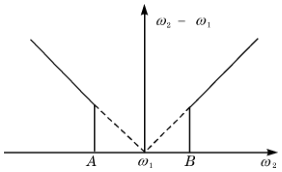
\includegraphics[width=\linewidth]{figs/fig-0112.png}
\caption{图7.6-2}
\end{figure}

如果一个非线性系统有一个自激振荡的频率 $\omega_{1}$，那么，当系统的输入的频率 $\omega$ 与 $\omega_{1}$ 相差很小时，我们自然会想到输出中不但同时有 $\omega$ 和 $\omega_{1}$ 两种频率，而且，由于非线性的交互作用，输出中还有拍频率 $\omega-\omega_{1}$。但是，在实际中，现象是按照图 7.6-2 的那种情形发生的：只要 $\omega$ 进入一定的同步区域 $AB$ 时，拍频率就立刻消失。在这个区域内只有 $\omega$

\textbackslash\{\}begin\{figure\}[h]\textbackslash\{\}centering\textbackslash\{\}includegraphics[width=0.8\textbackslash\{\}textwidth]\{图7.6-2.png\}\textbackslash\{\}caption\{图 7.6-2\}\textbackslash\{\}end\{figure\}

这一个频率，所有发生的现象都好像是可变频率 $\omega$ 把原有频率 $\omega_{1}$ “侵占”掉了一样。

万・德尔・波尔(van der Pol)是最先解释了这种频率侵占现象的人，后来，又有些其他的人发展了这方面的理论。

假定系统是二阶的，它的微分方程是

\[\frac{d^{2}y}{dt^{2}}-\alpha\frac{dy}{dt}+\gamma\left(\frac{dy}{dt}\right)^{3}+\omega_{1}^{2}y = B\omega_{1}^{2}\sin\omega_{1}t\qquad\text{(7.6-1)}\]

这里的 $\alpha$，$\gamma$ 和 $B$ 都是正常数。如果 $B=0$，那么，当振荡的振幅足够小的时候，系统的阻尼就是负的，当振幅足够大的时候，系统的阻尼就是正的，因此，就存在一个特别的振幅值，系统可以用这个振幅进行持续的自激振荡。不仅如此，如果 $\alpha$ 和 $\gamma$ 都相当小；那么，这个自激振荡的频率就与 $\omega_{1}$ 相当接近。万・德尔・波尔证明：当 $\omega_{1}$ 与 $\omega_{1}$ 相当接近时，方程(7.6-1)的解就可以写成下列形式

\[y(t) = b_{1}(t)\sin\omega_{1}t+b_{2}(t)\cos\omega_{1}t\qquad\text{(7.6-2)}\]

而且，$b_{1}(t)$ 和 $b_{2}(t)$ 都是变化得相当缓慢的时间函数，它们变化速度满足下列条件

\[\left|\frac{d b_{1}}{d t}\right| \ll\left|\omega b_{1}(t)\right|,\left|\frac{d b_{2}}{d t}\right| \ll\left|\omega b_{2}(t)\right|\]

把方程 (7.6-2) 代入方程 (7.6-1)，并且只保留一阶以下的项，我们就可以把 $b_{1}$ 和 $b_{2}$ 的微分方程组写成下列形式

\[\begin{aligned} & \frac{d b_{1}}{d t}=f_{1}\left(b_{1}, b_{2} ; \omega\right) \\ & \frac{d b_{2}}{d t}=f_{2}\left(b_{1}, b_{2} ; \omega\right) \end{aligned}\qquad\text{(7.6-3)}\]

这是一个自治的一阶微分方程组。所以，我们可以用等倾法来解，就像第 7.8 节在相平面上解二阶线性系统的作法一样。分析的结果表明：如果 $\omega$ 在 $\omega$ 附近的一个一定范围内，方程组 (7.6-3) 在 $b_{1} b_{2}$ 平面上有一个稳定的结点，那么，不论 $b_{1}$ 和 $b_{2}$ 的初始值是多少，$b_{1}(t)$ 和 $b_{2}(t)$ 最后总要分别趋近于相当这一固定点的 $b_{1}$ 值和 $b_{2}$ 值。因此，根据方程 (7.6-2)，就只有频率是 $\omega$ 的振荡，根本不再有频率是 $\omega-\omega$ 的振荡。如果 $\omega$ 在那个范围之外，么，在 $b_{1} b_{2}$ 平面上就有一个稳定的极限环，因而也就可以说明图 7.6-2 所表示的现象。

在某些非线性系统里，一个频率是 $\omega$ 的振荡可以被另一个频率是 $\omega$ 的振荡激发起来或者抑制下去，而 $\omega$ 却根本不等于 $\omega_{0}$。在第一种情形中，那种现象就称为异步激发，而第二种情形中的现象就称为异步抑制。我们从以下的事实就可以理解这些现象：即使在相空间中存在一个极限环，系统也不一定有持续的自激振荡。如果要发生持续的振荡，极限环就必须是稳定的，所谓“稳定”的意思，也就是说，当系统受到扰动或者从极限环移到相空间的其他一点以后，系统具有一个再回到极限环上去的倾向。不稳定的极限环在一个实际的物理系统中是不可能实现的。既然如此，我们就不难看出，在一定的情况下，一个新的振荡的发生，就可能给另一个振荡创造出稳定的条件，也可能破坏另一个振荡的稳定条件，第一种情形就是“异步激发”现象，第二种情形就是“异步抑制”现象。这里，“异步”这样一个形容词只是用来强调 $\omega$ 与 $\omega$ 之间的关系是完全任意的而已。

\section{7.7 参数激发和参数阻尼}

很久以来人们就知道，如果一个振荡系统中有一个以频率 $\omega$ 作周期变化的参数，系统就以频率 $\omega / 2$ 开始振荡。瑞雷 (Rayleigh) 曾经用以下的实验来说明这种现象：把一根拉紧了的金属线的一端系在音叉的一股上，如果音叉以频率 $\omega$ 进行振荡，那么，金属线就以频率 $\omega / 2$ 进行横向振荡。我们再举一个类似的例子：一个单摆（也就是悬挂在一根没有重量的杆子的一个质量）在杆的上端受到一个正弦变化的外力（图 7.7-1)。假设置的微小角度位移，不损害普遍性，我们还可以假定正弦变化的外力的频率是方程就是

\begin{figure}[htbp]\centering
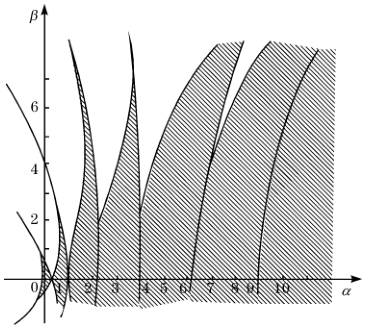
\includegraphics[width=\linewidth]{figs/fig-0114.png}
\caption{图7.7-2}
\end{figure}

其中 $m$ 是质量，$g$ 是重力加速度，$l$ 是摆的长度，$a$ 是周期外力的振幅。这个方程可以写成

所以，$\alpha$ 就等于 $g / l, \beta$ 等于 $\alpha / m l$。对于倒立摆 （也就是质量在支承点上方的摆） 的情形，$\theta$ 的方程也还是 (7.7-1)，只不过把其中的 $g$ 换成 $-g$ 就是了。所以，对于普通的摆，$\alpha$ 是正数；对于倒立摆，$\alpha$ 是负数。方程 (7.7-1) 是一个线性方程，只是加在摆上的外力做周期性的变化而已。因此，我们就可以把这个系统看做是参数作周期性变化的系统。

方程 (7.7-1) 就是有名的马丢 (Mathieu) 方程。解的稳定性是由 $\alpha$和 $\beta$ 这两个常数来确定的。具体地说，可以把 $\alpha \beta$ 平面分成一个稳定的区域和一个不稳定区域，就像图 7.7-2 所画的那样 （这个图中有阴影的就是稳定区域）。可以从图 7.7-2 看出，对于正的 $\alpha$，也就是普通的摆的情形来说，当周期外力不存在的时候，或者说 $\beta=0$ 的时候，系统就是稳定的。这当然是显而易见的事实。然而，有兴趣的事实是：如果 $\beta$ 取某些适当的值，系统就成为不稳定的了。这时，

摆的摆动的振幅就会越来越大，直到非线性效应最后把振幅固定在一个相当大的常数上为止。这种现象就称为参数激发。对于负的 $\alpha$，也就是倒立摆的情形来说，当支点上没有周期外力的时候，系数自然是不稳定的；但是，当 $\beta$ 在一个一定的狭小范围之内的时候，系统还可以是稳定的，只要 $\alpha$ 也取某些适当的数值就可以了。这个现象就称为参数阻尼。

任何一个系统，只要它有一个作周期变化的参数，在这个系统中就可能发生

\begin{figure}[htbp]\centering
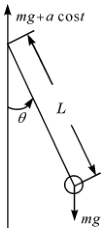
\includegraphics[width=\linewidth]{figs/fig-0113.png}
\caption{图7.7-1}
\end{figure}

参数激发和参数阻尼的现象。

这种现象和以前介绍过的几种非线性现象，都可以在控制系统中加以利用，使控制系统得到所需要的性能。事实上，的确也有不少非线性现象已经被应用到伺服控制系统的许多元件上去了。但是，这些非线性元件在目前还只是一些“新奇”的重要性不大的东西，而且，与其说它们是根据理论分析设计出来的，倒不如更恰当地说它们是依靠经验和试验“设计”出来的。我们在以上几节中的讨论只不过是说明这种应用的广泛的可能性而已。

\section{7.8 相平面全局分析法}

对低阶非线性系统的分析可以应用相空间内的几何方法 （或者称为拓扑方法）。这种方法的实质是在相空间内将系统的运动轨线分为各种类别，并将各类运动在相空间内绘出图来。根据全局运动的各种几何特点，便可一目了然地判定这个非线性系统内特有的周期解的参数及其稳定性，零点的稳定性，过渡过程的主要特征等。这种方法对二阶系统的分析特别有效，因为此时系统的一切运动轨迹均可完整地在平面上绘制出来。因此，这一方法得到了广泛的应用 ${ }^{[20,23,26]}$。本节将主要介绍如何利用相平面法分析典型非线性系统的性能。为此，我们先以二阶线性系统为例，说明这个方法的实质。

如果 $y$ 是输出量（受控量），$x$ 是输入量（控制量），那么一般的二阶系统的微分方程可以写为

\[f(y, \dot{y}, \ddot{y} ; t)=x(t)\qquad\text{(7.8-1)}\]

这里的 $\dot{y}$ 和 $\dot{y}^{\prime}$ 表示对时间 $t$ 的一次和二次导数。根据第二章内的讨论可以把式 (7.8-1)改写成完全等价的方程组

\[\begin{aligned} & f\left(y, \dot{y}, \frac{d \dot{y}}{d t} ; t\right)=x(t) \\ & \frac{d y}{d t}=\dot{y} \end{aligned}\qquad\text{(7.8-2)}\]

如果我们把 $y$ 与 $\dot{y}$ 看做是因变数，那么，方程组 (7.8-2) 就是未知函数 $y$ 与 $\dot{y}$ 的两个一阶联立微分方程。如果像常常遇到的情形一样，系统是自治的，也就是说，不但方程 (7.8-1) 中的函数 $f$ 与时间 $t$ 无关，而且输入 $x \equiv 0$，那么，就可以把 $\dot{y} / d t$从方程组 (7.8-2) 的第一个方程中解出来，而把 $\dot{y} / d t$ 表示为 $y$ 与 $\dot{y}$ 的函数，假定系统的方程组又可以写成

\[\begin{aligned} & \frac{d \dot{y}}{d t}=\dot{y} k(y, \dot{y}) \\ & \frac{d y}{d t}=\dot{y} \end{aligned}\qquad\text{(7.8-3)}\]

这个方程组不明显地包含 $k$ （除了运算符号 $d/dt$ 之外）。把方程组 (7.8-3) 的第一个方程用第二个方程除一下，我们就得出

\[\frac{d \dot{y}}{d y}=k(y, \dot{y})\qquad\text{(7.8-4)}\]

这是一个以 $y$ 为自变量而以 $\dot{y}$ 为因变量的一阶微分方程。把这个方程解出来以后，就可以利用方程组 (7.8-3) 把 $y$ 和 $t$ 的关系计算出来。

从物理的观点来看，上一段所提到的做法是以下列的概念为依据的：只用 $y$ 和 $\dot{y}$ 就可以描述系统的状态，而不像比较普通的方法那样，用 $y$ 和 $t$ 来描述。如果说 $y$ 是描写一个质点的位置的变数，那么 $\dot{y}$ 就是速度。因此，也就可以用 $\dot{y}$ 来代表质点的动量。所以，$y$ 和 $\dot{y}$ 就分别代表质点的位置和动量。物理学家把这样一种不用时间变数 $t$ 的状态表示法称为相空间中的表示法。在我们所讨论的特殊情形中，相空间只是二维的 $(y$ 和 $\dot{y})$，所以，它就是相平面。这样一来，二阶系统式 (7.8-3) 的运动状态就可以用相平面上的一条曲线来描述。这条曲线上的每一点都表示系统在某一个时刻 $t$ 的状态。根据一般的习惯，在这条曲线上，我们用箭头表示时间增加的方向，就像图 7.8-1 所画的那样。如果系统的阶数 $n$ 大于 2，相空间就是 $n$ 维的，系统的运动状态就要用这个 $n$ 维空间中一条曲线来表示。

相平面表示法的具体优点就是：非常多的二阶非线性系统都是自治的，而且都能表示成方程 (7.8-4) 的形式。这个方程至少总可以用等倾法把解用图线表示出来。事实上，只要把方程 (7.8-4) 所规定的曲线的方向场在相平面上表示出来以后，系统的特性就很清楚了。相平面的这样一些性质的应用是非线性振动理论的基本方法之一。这种方法称为非线性力学的拓扑方法。

为了把以前的一些概念改用相平面的方法来表示，我们举一个例子：考虑一个没有驱动函数的二阶线性系统

\[\frac{d^{2} y}{d t^{2}}+2 \zeta \frac{d y}{d t}+y=0\qquad\text{(7.8-5)}\]

只要把时间的量度单位适当地加以选择就可以使方程 (3.4-3) 中的自然频率 $\omega$ 等于 1，因而就得出方程 (7.8-5)。$\zeta$ 当然就是系统的阻尼与临界阻尼的比值。对于振荡的情形来说，$|\zeta|<1$。可以把方程 (7.8-5) 改写成

\begin{figure}[htbp]\centering
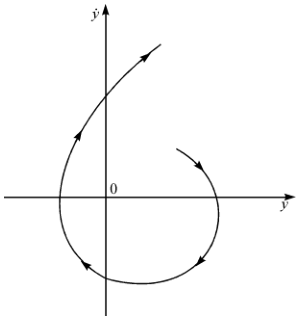
\includegraphics[width=\linewidth]{figs/fig-0115.png}
\caption{图7.8-1}
\end{figure}

\[\begin{aligned}& \frac{d \dot{y}}{d t}=-2 \zeta \dot{y}-y \\& \frac{d y}{d t}=\dot{y}\end{aligned}\qquad\text{(7.8-6)}\]

因此，我们就得到相当于方程(7.8-4)的方程

\[\frac{d \dot{y}}{d y}=-\frac{2 \zeta \dot{y}+y}{\dot{y}}=-2 \zeta-\frac{y}{\dot{y}}\qquad\text{(7.8-7)}\]

根据方程(7.8-7)，不难看出，曲线斜率 $\dot{y} / d y$ 只在从相平面的原点出发的每一条射线上是相同的常数。图 7.8-2\textasciitilde{}图 7.8-6 所画的是五种不同的运动类型，它们分别相当于 $\zeta<-1,-1<\zeta<0, \zeta=0,0<\zeta<1$ 以及 $1<\zeta$。图 7.8-2 和图 7.8-6是非振荡的情形。图 7.8-3\textasciitilde{}图 7.8-5 都是振荡的情形。图 7.8-4 是真正的简谐振荡。

\begin{figure}[htbp]\centering
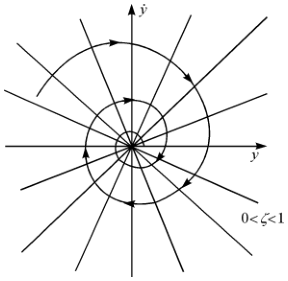
\includegraphics[width=\linewidth]{figs/fig-0119.png}
\caption{图7.8-5}
\end{figure}

\begin{figure}[htbp]\centering
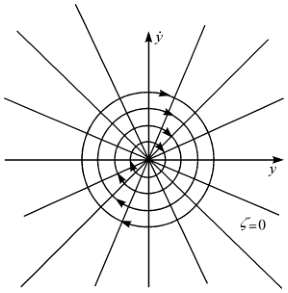
\includegraphics[width=\linewidth]{figs/fig-0118.png}
\caption{图7.8-2}
\end{figure}

\begin{figure}[htbp]\centering
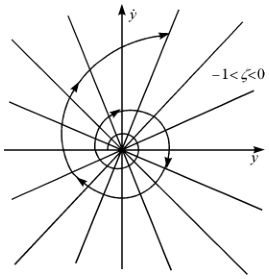
\includegraphics[width=\linewidth]{figs/fig-0117.png}
\caption{图7.8-2}
\end{figure}

\begin{figure}[htbp]\centering
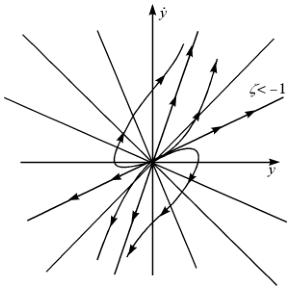
\includegraphics[width=\linewidth]{figs/fig-0116.png}
\caption{图7.8-5}
\end{figure}

\[\dot{y}\]

\[\zeta<-1\]

\[y\]

图 7.8-2

\[\dot{y}\]

\[-1<\zeta<0\]

\[y\]

图 7.8-3

\[\dot{y}\]

\[\zeta=0\]

\[y\]

图 7.8-4

\[\dot{y}\]

\[0<\zeta<1\]

\[y\]

图 7.8-5在以上所画的这些图里，相平面的原点相当于平衡状态，因为在这一点 $d y / d t$ 和 $d y / d t$ 都等于零。用数学的术语来说，原点是方程 (7.8-6) 的奇点。然而，在 $\zeta<0, \zeta=0$ 和 $\zeta>0$ 这三种不同的情形下，平衡状态的特性是十分不同的。图 7.8-2 和图 7.8-3 表明，当 $\zeta<0$ 时，系统的运动曲线总是从平衡状态发散出去的。所以，原点是一个不稳定的平衡点。图 7.8-5 和图 7.8-6 表明，当 $\zeta>0$ 时，系统的运动曲线总是收敛到平衡状态上来的，所以原点就是一个稳定的平衡点。用数学的术语来说，在图 7.8-2 和图 7.8-6 中，因为原点是所有运动曲线都要经过的点，所以称为结点。图 7.8-3 和图 7.8-5 的原点是螺线的中心，这时，它被称为焦点。在图 7.8-4 的特殊情形中，$\zeta=0$，运动曲线总是把原点包围在内部，这时，原点就称为中心点。

如果二阶系统的基本方程有一个常数驱动项，也就是说

\[\frac{d}{d t} \dot{y}+2 \zeta \frac{d y}{d t}+y=c\qquad\text{(7.8-8)}\]

这里的 $c$ 是一个常数。这时也就有

\[\frac{d^{2}}{d t^{2}}(y-c)+2 \zeta \frac{d(y-c)}{d t}+(y-c)=0\]

因此，相平面上的运动曲线和图 7.8-2\textasciitilde{}图 7.8-6 所画的完全相似，只不过把平衡点改为 $y$ 轴上的 $y=c$ 点就是了。

掌握了对二阶线性系统的分析方法后，我们试讨论二阶继电系统的运动特征。在以下的讨论中，为了简化继电器的开关问题的讨论，我们先假设继电器只能有两种状态：单位大小的正输出和单位大小的负输出，没有输出等于零的情形。不难了解，输出总是单位大小的假设并不会限制问题的普遍性。

我们先来考虑比较简单的线性开关的情形，所谓“线性开关”，就是继电器所产生的输出驱动函数 $c$ 的大小总是 $1:|c|=1$，而且这个输出的符号与 $a y+b y$ 的符号相同。在这里讨论线性开关的目的就是想借此说明开关问题的一些特点。

在弗吕格-罗茨 (Flügge-Lotz) 的论文 ${ }^{[13]}$ 以及弗吕格-罗茨与克罗特尔 (Klotter) 合著的论文 ${ }^{[14]}$ 中都分析过有线性开关的继电器的伺服系统的运动状态。以下的讨论就是他们在定性方面的研究结果的简单总结。

这两位作者所研究过的系统的微分方程是

\[\frac{d}{d t} \dot{y}+2 \zeta \frac{d y}{d t}+y=\operatorname{sgn}(a y+b y), \quad 0<\zeta<1\qquad\text{(7.8-9)}\]

当驱动函数是 $+1$ 时，那么，相平面上的一条相当的运动曲线弧就称为一个正弧

\begin{figure}[htbp]\centering
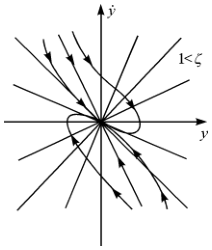
\includegraphics[width=\linewidth]{figs/fig-0120.png}
\caption{图7.8-6}
\end{figure}

（简写为 $P$ )。反之，当驱动函数是 -1 时，相当的一条运动曲线弧就称为一个负弧 （简写为 $N$ )。所有的正弧的总体称为正系统。所有负弧的总体称为负系统。根据我们对方程 (7.8-9) 的讨论，已经知道，方程 (7.8-9) 的正系统是由收敛的螺线所组成的，这些螺线的焦点都是 $y=+1, \dot{y}=0$; 方程 (7.8-9) 的负系统也是由收敛的螺线所组成的，这些螺线的焦点都是 $y=-1, \dot{y}=0$。我们当然希望系统的最终状态就是原点 $y=\dot{y}=0$。

按照方程 (7.8-9) 右端的开关函数中 $a$ 与 $b$ 的符号。可以规定四种情形:

我们把 $a>b, b>0$ 的情形称为第一种情形。这时，开关曲线 $a y+b \dot{y}=0$ 是一条经过相平面的原点而且位置是在第二象限和第四象限内的直线。在这条直线的右方 $a y+b \dot{y}$ 是正数。所以，那里是一个正系统的区域。在这条直线的左方，$a y+b \dot{y}$ 是负数，所以，是一个负系统的区域。在这条开关线上，正系统和负系统连接起来，而且，运动曲线的隅角 （即正弧与负弧的连接点） 也发生在这条线上 （图 7.8-7)。存在周期解的条件就是：存在一个正弧，这个正弧与开关线的两个交点与原点距离相等。理由是这样的：如果确实存在这样一个正弧，那么，根据对称性，在开关曲线的另一方也必然有一个连接这两个交点的负弧。因此，这两个弧就组成一条相平面上的闭合曲线。用非线性力学的术语来说，这种周期解就称为极限环。在以下的讨论中我们就会看到，在所考虑的情形中确实可以发生周期解。

不难看出，总会有一个正弧和一个负弧与开关曲线相切，设这两个切点分别是 $S_{p}$ 和 $S_{N}$ （图 7.8-8)。而且，设这两个弧与开关曲线的另外的交点分别是 $R_{p}$ 和 $R_{N}$。$S_{p}$ 与 $S_{N}$ 对于原点是对称的。$R_{p}$ 与 $R_{N}$ 也是这样的。先假设 $\zeta_{a}$ 和 $b$ 之间的关系，使得 $R_{N}$ 点在 $S_{p} S_{N}$ 线段之外 （就像图 7.8-8 的情形）。这时，如果某一个解在开关曲线上的起点与 $S_{p} S_{N}$ 线段足够接近，那么，经过这个点的运动曲线必然在开关曲线的左方或右方离开开关曲线，不再与开关曲线相交。至于在哪一方离开开关线就要由起点的位置来确定。譬如说，起点在 $S_{N}$ 与 $R_{p}$ 之间，那么，经过这个点的运动曲线就在开关曲线的右方离开开关线。我们也可以证明，如果开关线右方的正弧与开关曲线相交于两点，那么，这个弧的终点 （第二个交点） 到原点的距离小于起点 （第一个交点） 到原点的距离。因此，永远不可能满足有周期解的条件。所以，系统的运动曲线永远是围绕某一个焦点的螺线，因此，最终状态不可能是相平面的原点。

\begin{figure}[htbp]\centering
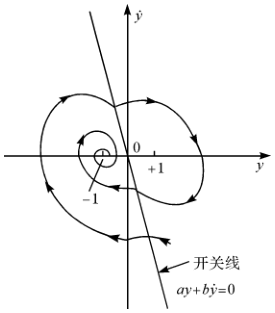
\includegraphics[width=\linewidth]{figs/fig-0121.png}
\caption{图7.8-7}
\end{figure}

但是，如果 $R_N$ 和 $R_P$ 都在 $S_P S_N$ 线段上（图 7.8-9)，就存在一个周期解。理由是这样的：根据我们的假设，正弧 $R_P S_P$ 的起点 $R_P$ 到原点的距离小于终点 $S_P$ 到原点的距离。但是，把图 7.8-5 的收敛螺线的焦点从原点移到 $+1$ 点（相当于正弧）和 $-1$ 点（相当于负弧）的手续对于离原点很远的部分影响非常小。所以，如果一个正弧在开关线上的起点离原点非常远，那么，这个弧在开关线上的终点与原点的距离就比较近一些（这是螺线的性质）。因此，这种弧与 $R_P S_P$ 弧的性质刚好相反。因为曲线之间的变化是连续的，所以，一定有一个中间状态的正弧，这个正弧的起点和终点与原点的距离相等。这就是存在周期解的条件。图 7.8-9 中所画的闭合曲线就是这个周期解。事实上，已经作过的数学分析不但证明了上述的事实，而且还进一步证明：这个周期解不只是唯一的，而更重要的是，这个解还是稳定的，具体地说：所有初始点在这个闭合曲线外面的解，最后都趋近于这个周期解；所有初始点在这个闭合曲线内部而在闭曲线 $R_P S_P R_N S_N R_P$ 所包围的区域（也就是图 7.8-9 的阴影区域）之外的解，最后也趋近于这个周期解。初始点在闭曲线 $R_P S_P R_N S_N R_P$ 内部的运动曲线最后总是趋近于某一个焦点，也还是没有趋近于原点的可能性。

\begin{figure}[htbp]\centering
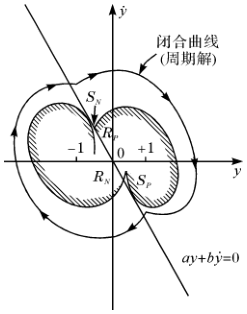
\includegraphics[width=\linewidth]{figs/fig-0123.png}
\caption{图7.8-9}
\end{figure}

\begin{figure}[htbp]\centering
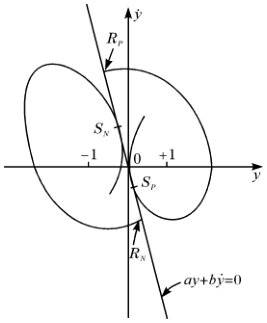
\includegraphics[width=\linewidth]{figs/fig-0122.png}
\caption{图7.8-8}
\end{figure}

\textbackslash\{\}begin\{figure\}[h]\textbackslash\{\}centering\textbackslash\{\}includegraphics[width=0.4\textbackslash\{\}textwidth]\{图7.8-8.png\}\textbackslash\{\}caption\{图 7.8-8\}\textbackslash\{\}label\{fig:7.8-8\}\textbackslash\{\}end\{figure\}

\textbackslash\{\}begin\{figure\}[h]\textbackslash\{\}centering\textbackslash\{\}includegraphics[width=0.4\textbackslash\{\}textwidth]\{图7.8-9.png\}\textbackslash\{\}caption\{图 7.8-9\}\textbackslash\{\}label\{fig:7.8-9\}\textbackslash\{\}end\{figure\}

第二种情形就是 $a>0$ 而 $b<0$ 的情形。这时，开关曲线 $a y + b \dot{y} = 0$ 经过第一象限和第三象限。正系统和负系统与前一种情形是一样的。在这种情形中不可能有周期解。$R_P$，$R_N$，$S_P$ 和 $S_N$ 的定义也与以前相同。这些点和原点在开关线上的位置的顺序是 $R_P$，$S_P$，$0$，$S_N$，$R_N$; 图 7.8-10 所画的就是这种情形。在 $S_P S_N$ 线段上有一种新的现象：我们来考虑一个在 $E$ 点与这个线段相交的解($E$ 点是 $S_P S_N$ 上某一点）。假设这个解与开关线的相互位置就像图 7.8-10 所画的那样，那么，这个解在 $E$ 点将会怎样呢？既然 $E$ 点在开关线上，照道理讲，到达 $E$ 点以后，表示系统运动状态的动点就应该沿一个负弧前进。但是，从 E 点开始的负弧又会使动点再回到原来的半平面（也就是到达 E 点以前所在的半平面）上来，可是，在这个半平面上 ay + by > 0，解只能由正弧组成，所以，到达 E 点以后，动点不可能再沿负弧前进；另一方面，动点到达 E 点以后也一定不能再继续沿正弧前进，因为只有刚刚走过的路线是经过 E 点的唯一的正弧，因此，我们可以说，E点以后的解是不存在的，或者说，解在 E 点终止。任何一个从 RP RN 线段的外部开始的解，在没

有与 RP RN 线段相交之前总是旋转地逐渐接近原点。最后，如果这个解与 SP RP 相交，它就趋近于 +1;如果与 SN RN 相交，它就趋近于 -1 点；如果这个解最后与 SP SN 交，那就会发生古怪的“终止”现象。在“终止”的情况下，系统的“位置”和“速度”都固定不变，这当然是不合情理的事情。

其实，在真实情况中，系统的运动状态是不可能“终止”的，它总是在时间过程中进行的。得出上述的荒谬结果的理由也是可以解释的：因为实际的开关动作总是有时滞的，所以，一个解与开关线相交时驱动函数并不立刻改变符号，所以解还要继续前进一段时间，在这一段继续前进的时间中驱动函数还保持原来的符号。在第一种情形中，因为这样一个时滞不很大，所以对系统的基本运动状态没有什么影响，但是，在现在的情形中，时滞就可以使系统的解避免发生“终止”现象。现在我们来观察一个到达“终止点”的解。由于时滞的缘故，解不再在这一点终止，而要继续前进某一段距离，然后才发生开关动作，开关动作就使解在相平面上画出一个隅角，但是，在隅角上解还是存在的。从这个隅角出发，解又在相反的方向上越过开关线，解越过开关线一个短的距离以后，又在相平面上画出另一个隅角，以后的过程也是类似的，就像图 7.8-11 所画的那样。从这个图可以看到，这种“锯齿状”的运动，最后就使得系统“爬出”SP SN 区域，最后，解就趋近于某一个焦点。所以，时滞可以消除解的终止现象，但是，系统的运动状态还是不能令人满意，因为，解还是不能最后到达原点。

在第三种情形中，a < 0，而 b > 0。这种情形的开关线也是通过相平面的第一象限和第三象限的，但是，现在的正系统在开关线的左方，负系统在开关线的右方（这与第二种情形恰好相反）。在这种情形中，总是存在一个稳定的周期解（或者说是一个稳定的极限环）（图 7.8-12)。而且，这个周期解就决定了所有的情况，因

\begin{figure}[htbp]\centering
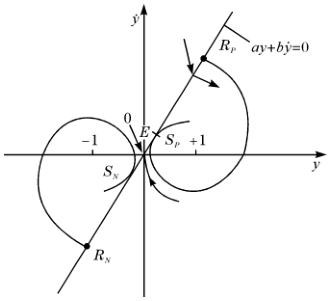
\includegraphics[width=\linewidth]{figs/fig-0124.png}
\caption{图7.8-10}
\end{figure}

为，所有其他的解最后都趋近于这个周期解。所以，在这种情形里，还是不能使系统达到相平面的原点。

\begin{figure}[htbp]\centering
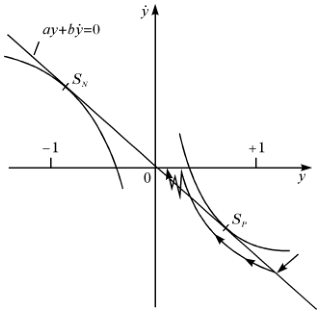
\includegraphics[width=\linewidth]{figs/fig-0127.png}
\caption{图7.8-13}
\end{figure}

\begin{figure}[htbp]\centering
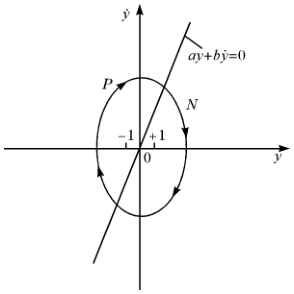
\includegraphics[width=\linewidth]{figs/fig-0126.png}
\caption{图7.8-12}
\end{figure}

\begin{figure}[htbp]\centering
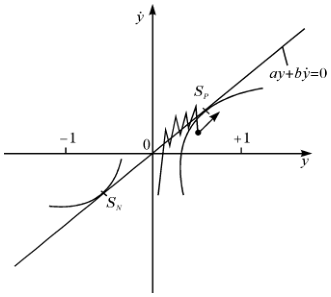
\includegraphics[width=\linewidth]{figs/fig-0125.png}
\caption{图7.8-11}
\end{figure}

\textbackslash\{\}begin\{figure\}[h]\textbackslash\{\}centering\textbackslash\{\}includegraphics[width=0.4\textbackslash\{\}textwidth]\{图7.8-11.png\}\textbackslash\{\}caption\{图 7.8-11\}\textbackslash\{\}label\{fig:7.8-11\}\textbackslash\{\}end\{figure\}

\textbackslash\{\}begin\{figure\}[h]\textbackslash\{\}centering\textbackslash\{\}includegraphics[width=0.4\textbackslash\{\}textwidth]\{图7.8-12.png\}\textbackslash\{\}caption\{图 7.8-12\}\textbackslash\{\}label\{fig:7.8-12\}\textbackslash\{\}end\{figure\}

第四种情形就是 $a<0$ 同时 $b<0$ 的情形。这种情形的开关线与第一种情形相同，而正弧和负弧的分布状态与第三种情形相同。可以证明，在这种情形中不可能有周期解。如果，开关动作没有时滞，那么，$S_{P}S_{N}$ 线段（图 7.8-13)就是由终止点组成的。如果，从 $S_{P}S_{N}$ 线段上每一点出发向后（也就是在时间减小的方向上）描画解的图线，就可以看到这些曲线盖满了全平面，这也就是说，所有的解都“终止”在开关线的 $S_{P}S_{N}$ 线段上。

\textbackslash\{\}begin\{figure\}[h]\textbackslash\{\}centering\textbackslash\{\}includegraphics[width=0.4\textbackslash\{\}textwidth]\{图7.8-13.png\}\textbackslash\{\}caption\{图 7.8-13\}\textbackslash\{\}label\{fig:7.8-13\}\textbackslash\{\}end\{figure\}

但是，这里也和第二种情形一样，时滞的存在就使情况大不相同了。当解还没有到达 $S_{P}S_{N}$ 线段的时候。时滞并没有什么重要作用；但是，当解到达 $S_{P}S_{N}$ 线段时，时滞就使解不再终止，而能使解越过开关线一段不大的距离。然而，画出一个隅角，接着又越过开关线。又作出另一个隅角，以后还是这样继续下去。从图 7.8-13 可以看出，这种锯齿状的运动就使系统的运动状态趋近于原点，最后，系统就在原点附近作频率高振幅小的振动。时滞越小，振动的频率就越高。这种状态就称为继电器伺服系统的颤震。

这样一来，我们就看出，讨论过的四种情形中，只有第四种情形能使系统趋于所希望的平衡状态，但是，即使如此，系统还是在平衡状态附近颤震。

以上就是弗吕格-罗茨和克罗特尔的理论分析的介绍，从这里就可以看出线性开关的缺点，同时也就会知道，使伺服系统具有最优运转状态的最优开关函数一定不会是线性开关函数。究竟什么样的开关函数是最好的呢？这一问题最早由布绍(Bushaw)给出了确切的答案，目前任一线性受控对象的理想开关函数的形式均可迅速求出。关于二阶系统的最优开关理论的主要结论和更一般的线性系统最优开关函数的综合理论将在下章内详细介绍。

\section{7.9 非线性元件的有益应用}

如本章前面几节所指出的，通常非线性元件对系统产生不利影响。最常见的是使系统的稳定性变坏，对信号的相位产生迟后效应等。但是，巧妙地应用某些非线性环节，可以使它们的不利因素变成有利的因素。前节内讲到的具有最优开关的继电系统便是一个重要例证。在一般随动系统中继电元件常引起不衰减的持续振荡。但是正确地选择开关时刻以后，系统就会获得快速性。以后还要严格证明，当控制信号的强度受到限制时，一切最速控制系统都有继电系统的特性。

文献[8]中指出了另外一种情况，通常认为有害的间隙性的元件（参看图 7.3-10)，也可以反其害而得利，用它构成一个简单的相位超前环节。为了介绍这个思想，我们将图 7.3-10 所示的元件运动方程式写出

\[\begin{aligned} \dot{\theta}_{2}= & \left\{\begin{array}{l} \dot{\theta}-\delta, \quad \dot{\theta}_{1}>0 \\ \dot{\theta}+\delta, \quad \dot{\theta}_{1}<0 \end{array}\right. \\ & \mid \theta_{-}-\theta_{1} \mid<\delta, \quad \dot{\theta}_{2}=0 \end{aligned}\]

若将这种环节按图 7.9-1 所示办法连接，就得到一个新的非线性系统。当 $K_{1}>K_{2}$ 时，这个新系统的运动特性示于图 7.9-2 中，它的运动方程式为

\begin{figure}[htbp]\centering
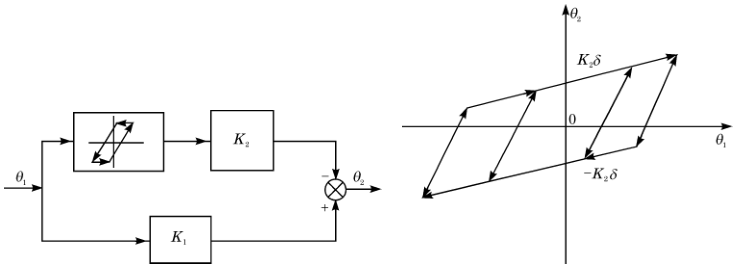
\includegraphics[width=\linewidth]{figs/fig-0128.png}
\caption{图7.9-2}
\end{figure}

图 7.9-1

图 7.9-2

\[\theta_{t}=\left\{\begin{array}{l} \left(K_{1}-K_{2}\right) \theta_{t}+K_{2} \delta, \quad \dot{\theta}_{t}>0 \\ \left(K_{1}-K_{2}\right) \theta_{t}-K_{2} \delta, \quad \dot{\theta}_{t}<0 \\ K_{1} \theta_{t}-K_{2}\left(\theta_{\max }-\delta\right), \quad \theta_{\max }-\theta_{t} \leqslant 2 \delta \\ K_{1} \theta_{t}-K_{2}\left(\theta_{\min }+\delta\right), \quad \theta_{t}-\theta_{\min } \leqslant 2 \delta \end{array}\right.\qquad\text{(7.9-2)}\]

式中 $\theta_{\max }$ 和 $\theta_{\min }$ 为 $\dot{\theta}_{1}$ 变号时刻 $\theta$ 的取值，前者为 $\dot{\theta}_{1}$ 自正值变为负值时 $\theta$ 的取值，后者为 $\dot{\theta}_{1}$ 自负值变为正值时 $\theta$ 的取值。

设 $\theta$ 按余弦函数变化，即

\[\theta=A \cos \omega t\]

代入式 (7.9-2) 以后，$\theta$ 的变化规律为

\[\theta_{t}=\left\{\begin{array}{l} K_{1} A \cos \omega t-K_{2} A+K_{2} \delta, \quad 2 m \pi \leqslant \omega t \leqslant 2 m \pi+\varphi_{2 \delta} \\ \left(K_{1}-K_{2}\right) A \cos \omega t-K_{2} \delta, \quad 2 m \pi+\varphi_{2 \delta} \leqslant \omega t \leqslant(2 m+1) \pi \\ K_{1} A \cos \omega t+K_{2} A-K_{2} \delta,(2 m+1) \pi \leqslant \omega t \leqslant(2 m+1) \pi+\varphi_{2 \delta} \\ \left(K_{1}-K_{2}\right) A \cos \omega t+K_{2} \delta,(2 m+1) \pi+\varphi_{2 \delta} \leqslant \omega t \leqslant 2(m+1) \pi \end{array}\right.\]

式中 $m=0,1 ， 2, \cdots, \varphi_{2 \delta}=c o s ^{-1}\left[1-\frac{2 \delta}{A}\right]$。当输入 $\theta_{i}=A \cos \omega t$ 时，新的非线性系统的输出形式示于图 7.9 -3 中。

\begin{figure}[htbp]\centering
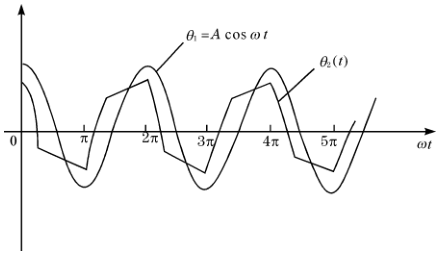
\includegraphics[width=\linewidth]{figs/fig-0129.png}
\caption{图7.9-3}
\end{figure}

把 $\theta(t)$ 展成傅氏级数，并写出第一次谐波的表达式

\[\ddot{\theta}(t)=a \cos \omega t+b \sin \omega t+R(t)\qquad\text{(7.9-3)}\]

式中 $R(t)$ 为各次谐波的和。容易检查，上式内一次谐波的两个系数可由下式算出

\[a=k_{2} \delta\left[c_{1} c+c_{1} \frac{\cos ^{-1}\left(1-\frac{2}{c}\right)}{\pi}-c_{1}-2 \sqrt{c_{1}}-1\right]\left[1-\frac{2}{c}\right] b=\frac{4 k_{2} \delta}{\pi}\left[\frac{1}{c}-1\right]\]

\[\begin{aligned}& c_{1}=\frac{A}{\delta} \\& c_{2}=\frac{K_{1}}{K_{2}}\end{aligned}\qquad\text{(7.9-4)}\]

当 $c_{2}$ 足够大的时候，即 $K_{1}$ 比 $K_{2}$ 大得多的时候，$a>0, b<0$。记

\[\begin{aligned}& \sin \varphi=-\frac{b}{\sqrt{a^{2}+b^{2}}} \\& \cos \varphi=-\frac{a}{\sqrt{a^{2}+b^{2}}}\end{aligned}\]

这样定义的角度 $\varphi$ 为正值。于是，式(7.9-3)可以写成

\[\vartheta(t)=\sqrt{a^{2}+b^{2}} \cos (\omega t+\varphi)+R(t)\qquad\text{(7.9-5)}\]

由此可知，图 7.9-1 所示的结构图的确具有相位超前的作用，只要 $K_{1}$ 取得合理，使 $a>0$ 就可以了。同时，第一次谐波的相位超前量可以用变化 $K_{1}$ 和 $K_{2}$ 的比任意加以调整。

在文献[8]中，作者还指出，如果在图 7.9-1 所示的网络后面串联一个极化继电器类的元件，则输出与输入之间依然可以有相位超前的作用。这种网络在原理上可以用来补偿系统中的时延或惯性。

\begin{figure}[htbp]\centering
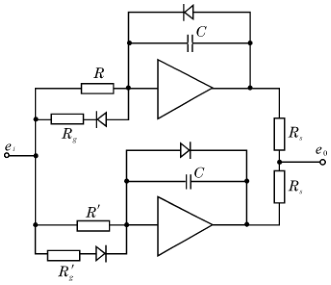
\includegraphics[width=\linewidth]{figs/fig-0130.png}
\caption{图7.9-4}
\end{figure}

为了用具有非线性特性的器件改善线性系统的性能，有人专门设计了一种非线性积分器，用以代替普通的积分器，它的线路见图 7.9-4。从图中可以看出，它实际上是由两个积分器联合组成的，上面一半专为积分正信号而设置的，下面一半积分负信号。当输入端 $e$ 信号后，这个线路输出信号基波振幅是输入信号的振幅的积分，然而相位滞后却不像通常的积分器那样为 $90^{\circ}$，而只有 $-38.1^{\circ}$。这样一来，它与普通积分器进行比较，图中所示的线路好像具有“相位超前”的作用。下面我们概略分析一下它的工作特点。

假定图 7.9-4 所示的非线性积分器的输入 $e_{1}$ 为

\[e_{1}=E_{1} \sin \omega t\]

在正半周期中，上半积分器起积分作用，输出为

\[e_{11}=\frac{1}{\omega R C} \int_{0}^{t} E_{1} \sin \omega t d \omega t\]

\[\frac{E_{i}}{\omega R C}\left(1-\cos \omega t\right), \quad 0 \leqslant t \leqslant \pi / \omega\]

在负半周期中，下半积分器起积分作用，输出为

\[\begin{aligned} e_{2} & =\frac{1}{\omega R C} \int_{\pi}^{\pi+t} E_{i} \sin \omega t d \omega t \\ & =-\frac{E_{i}}{\omega R C}\left(1-\cos \omega t\right), \quad \pi / \omega \leqslant t \leqslant 2 \pi / \omega \end{aligned}\qquad\text{(7.9-6)}\]

因此，一个周期中非线性积分器的输出 $e$ 应为

\[e=\left\{\begin{array}{l} \frac{E_{i}}{\omega R C}\left(1-\cos \omega t\right), \quad 0 \leqslant t \leqslant \pi / \omega \\ -\frac{E_{i}}{\omega R C}\left(1-\cos \omega t\right), \quad \pi / \omega \leqslant t \leqslant 2 \pi / \omega \end{array}\right.\qquad\text{(7.9-7)}\]

这个函数的波形画在图 7.9-5 中。将式 (7.9-7) 定义的非线性函数 $e(t)$ 展开为傅里叶级数:

\[e=-\frac{E_{i}}{\omega R C} \cos \omega t+\frac{4}{\pi} \frac{E_{i}}{\omega R C}\left[\sin \omega t-\frac{\sin 3 \omega t}{3}+\frac{\sin 5 \omega t}{5}-\cdots\right]\]

略去展式中的高次谐波，近似地取

\[\begin{aligned} e_{1} & =\frac{4}{\pi} \frac{E_{i}}{\omega R C} \sin \omega t-\frac{E_{i}}{\omega R C} \cos \omega t \\ & =\frac{E_{i}}{\omega R C} \sqrt{\frac{4}{\pi}}^{2}+1 \sin (\omega t-\theta) \end{aligned}\qquad\text{(7.9-8)}\]

式中 $\theta=\tan ^{-1} \frac{\pi}{4}=38.1^{\circ}$，所以它的等效传递函数为

\[F_{r}(i \omega)+\frac{e_{1}(i \omega)}{e_{1}(i \omega)}=\frac{1.62}{\omega R C} e^{-i \theta_{0}}\qquad\text{(7.9-9)}\]

应用这种积分器能起线性积分器所不能起到的作用。譬如说，在以干摩擦为主要负载的伺服系统中，用通常的线性积分器就无法消除干摩擦造成的静态误

\[\frac{4}{\pi} \frac{E}{\omega R C}\]

图 7.9-5

\begin{figure}[htbp]\centering
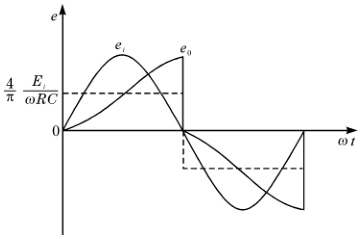
\includegraphics[width=\linewidth]{figs/fig-0131.png}
\caption{图7.9-5}
\end{figure}

差。但是应用非线性积分器代替它，不仅可以在相当大的程度上消除静态误差，而且系统的动态性能也将得到改善 [22]。

非线性特性有益利用的例子当然不只这两例，举这两例只是说明这样一点，一些非线性元件在特定的条件下巧妙地应用，可以收到很好的效果。

\section{参考文献}

[1] 秦元勋，微分方程所定义的积分曲线，科学出版社，1959.

[2] 高为炳，用谐波平衡法研究具有几个非线性元件的单回路调节系统，自动化学报，2 (1964)，3.

[3] 项国波，a)非线性自动控制系统若干问题的对数分析法，自动化学报，3(1965)，3.

b)非线性自动调整系统自振荡之对数分析法，福州大学学报，1962，总第 3 期.

[4] 许淞庆、胡金昌，一类非线性微分方程组在临界情况中的稳定性，中山大学学报，1960，3.

[5] 李岳生，非线性微分方程的解的界，稳定性和误差估计，数学学报，12(1962)，1.

[6] 黄琳，控制系统动力学及运动稳定性理论的若干问题，力学学报，1963，2.

[7] 张学铭等，微分方程稳定性理论，山东省人民出版社，1959.

[8] 杨荫第，机械间隙和干摩擦在自动控制系统中的应用，第二届自动化学会代表大会论文，北京，1965.

[9] Atherton，D.P.，Nonlinear Control Engineering，Van Nostrand Reinhold Company，London，1975.

[10] Brockett，R.W.，Feedback invariants for nonlinear systems，Proc. of 7th IFAC Congress，Helsinki，1978.

[11] Buland，R.A.，Analysis of non-linear servos by phase-plane delta method，J. of Franklin Institute，257(1954).

[12] Dutilh，J.R.，L’ondeé lectrique，30，435-438，1950.

[13] Flügge-Lotz，I.，a)ZAMM，25-27，97-113(1947)，b) Discontinuous Automatic Control，Princeton，1953.

[14] Flügge-Lotz，I.，Klotter，K.，ZAMM，28，317-337，1948.

[15] Huang Ling（黄琳），On estimation of the decaying time，Proc. of 2nd IFAC Congress，Basel，1963.

[16] Kalb，R.M.，\& Bennett，W.R.，Bell System Techn. J. 14 (1935)，322-359.

[17] Kochenburger，R.J.，Trans. AIEE，69(1950)，270-284.

[18] Ku，Y.H.，The phase space method for analysis of nonlinear control systems，ASMR. 56A-103，1956.

[19] Loeb，J.M.，Ann.de Telecommunications，5 (1950)，65-71.

[20] Minorsky，N.，Introduction to Nonlinear Mechanics. Edwards Bros.，Inc.，Ann Arbor，Mich.，1947.

[21] Stoker，J.J.，Nonlinear Vibrations，Interscience Publishers，New York，1950.

[22] Thaler，G.J.，Pastel，M.P.，Analysis and Design of nonlinear feedback control systems，

McGraw-Hill Book Company，Inc. New York，1962.

[23] Tustin，A.，A method of analysing the effect of certain kinds of non-linearities in closed-cycle control systems，J. Inst. Electr. Engs.，94(1947)，Part IIa，152.

[24] West，J. C.，Analytical Techniques for Non-linear Control Systems，London，1960.

[25] Айзерман，М. А.，Сопоставление приближенных методов исследования периодических режимов и область их применения，Основы автоматического регулирования，Глава 34，Машгиз，1954.

[26] Андронов，А. А.，Колебания，Москва，1954.

[27] Боголюбов，Н. Н.，Митропольский Ю. А.，Асимптотические методы в теории пellинейных колебаний，ФНЗМАТИЗ，1958.

[28] Вавилов，А. А.，Метод исследования автоколебаний в релейных системах автоматического регулирования по логарифмически характеристикам，Автоматика и Телемеханика，23 (1962)，8.

[29] Гольдфарб，Л. С.，Методы исследования веланейных систем регулирования，в книге Основы Авт. Регулирования，Гл. 33，Машгиз，1954.

[30] Летов，А. М.，устойчивость нелинейных систем автоматического регулирования，ГОСТЕХИЗДАТ，Москва，1955.

[31] Лурье，А. И.，Некоторые нелинейные задачи автоматического регулирования，ГОСТЕХИЗДАТ，Москва，1951.

[32] Малкин，И. Г.，Методы Ляпунова и Пуанкаре в теории нелинейных колебаний，ГОСТЕХИЗДАТ，1949.

[33] Попов，Е. П.，О выделении областей устойчивости нелинейных автоматических систем на основе гармонической линеаризации. Известия АН СССР，Энергетика и Автоматика，1959，1.

[34] Поспелов，Г. С.，Некоторые вопросы теории релейных систем авт. регулирования，в книге Основы Автом. Регулирования，гл. 35，Машгиз，1954.

[35] Федоров，С. М.，(Ред.)，Методы синтеза нелинейных систем авт. управления，Москва，1970.

\chapter{第八章 最速控制系统设计}

第五章内我们曾研究过线性系统的设计，那里设计出来的控制装置产生的控制规律是系统误差坐标的线性函数。这种线性规律的结构形式常常是预先给定的，或者是设计指标所要求的。这样设计出来的线性系统的一个重要特点是控制量的取值与误差的大小成比例，当系统误差很大时控制量的值一般来讲也是很大的。因此可以说在线性系统中控制量是被假定为不受任何限制的。这种假定在系统误差较小的情况下是与实际情况相符合的，例如在稳态工作的随动系统，它的基本工作方式是消除小误差，误差坐标和控制量之间的这种线性关系总能准确地保持。

但是，当误差坐标很大时，控制量按比例送出大的控制作用往往是不现实的。实际问题表明，任何控制作用的取值总要受到客观条件的限制。例如液压伺服阀的位移受到结构尺寸的限制；如果它是电信号，将受到电源电压或电源电流的限制；如果控制量是飞行器的舵偏角，则它将受极限位置的限制等。这种限制最具有代表性的例子是前章内曾讨论过的继电伺服系统。如果用继电器作为控制装置的输出元件，则控制量的取值只可能有两个或三个，即最大值，最小值和零值。在控制量受限制情况下如何设计控制装置，这就是我们将要讨论的问题。这一章主要讨论最速控制问题。我们假定:

（1）设计指标是过渡时间最小。

（2）受控对象的运动方程式是线性的（除第 8.7 节外），其诸系数可能是常值或为时间的已知函数。

（3）控制量的取值范围受限制，其限制形式为

\[\|u \mid \leqslant M, \quad i=1,2, \cdots, r\qquad\text{(8.0-1)}\]

或

\[\|u\|=\sqrt{\sum_{i=1}^{r}(u)^{2}} \leqslant M\qquad\text{(8.0-2)}\]

以后我们将称第一种限制为 $A$ 型限制，第二种限制为 $B$ 型限制。每一分量 $w$ 的变化速率假定不受任何限制，它们可以瞬时变化取值，如果需要的话，可以像继电器一样的工作。

对最速系统的研究，近二十年来有很大进展，对线性受控对象来讲，设计方法问题已基本解决。本章内我们将主要叙述这些方法的基本原理。至于对数学严格理论感兴趣的读者，可参看本章的参考文献。

上一章曾用相平面的方法讨论了二阶继电系统的各种开关规律对系统性能的影响。从那里可以看到线性开关的缺点。从前章的讨论中我们也得到了启发，最好的开关函数一定不是线性函数。本节内我们先介绍一些早期的研究结果，即在相平面上如何找出最好的开关函数。这里我们先不谈一般理论，以使读者能看到一般理论是如何在这些具体研究工作的基础上发展起来的。

如果一个二阶系统的控制量的取值只能是 $\pm 1$，这个系统的方程可以写成

\[\frac{dy}{dt} = y\]

\[\frac{d\dot{y}}{dt} + g(y,\dot{y}) = \varphi(y,\dot{y})\qquad\text{(8.1-1)}\]

其中 $\varphi(y,\dot{y})$ 是一个不连续的函数，它只能取 $+1$ 和 $-1$ 这两个值。我们可以提出这样一个最优开关问题：要求找出一个函数 $\varphi(y,\dot{y})$，使得方程 (8.1-1) 的经过相平面上任何一点 $P$ 的解都能到达原点 $0$; 而且，沿着这条经过 $P$ 的解的路线，从 $P$ 变动到 $0$ 所需要的时间对于 $\varphi$ 来说是极小的，也就是说，任何一个其他的函数 $\varphi$ 都不能使这个时间更短。这样求出的函数 $\varphi(y,\dot{y})$ 就是这个特殊问题的“最优开关函数”。这个特别的开关问题曾经被布绍研究过 [8]。对于 $g(y,\dot{y})$ 为线性的特殊情形 $g(y,\dot{y}) = 2\zeta\dot{y} + y(\zeta$ 是任何实数），他给出了完全的解答。然而，布绍所用的数学方法非常复杂，而且很难推广到其他情形中去，所以，在以下的讨论中，我们只限于说明他所得到的结果。

只要 $g(y,\dot{y})$ 是连续函数，那么，布绍所提出的正则路线的概念就是一个很有用的普遍概念。所谓路线就是相平面上的运动轨线。既然 $\varphi(y,\dot{y})$ 只能取 $+1$ 和 $-1$ 两个值，所以一条路线便只由正弧 $(P)$ 和负弧 $(N)$ 组成的。在时间增加的过程中，当控制函数从 $+1$ 变为 $-1$ 时，路线就由一个正弧转到一个负弧上去，这两个弧的交点称为一个正负隅角。类似地，相当于开关函数从 $-1$ 变到 $+1$ 的交点就称为负正隅角。如果一条路线在 $y$ 轴的上方不包含负正隅角而且在 $y$ 轴的下方不包含正负隅角，那么，这条路线就称为正则路线。正则路线的重要性在于：极小路线 （所用的时间是极小值的路线） 一定是正则路线。这也就是说，如果从 $P$ 点出发给定一条不是正则的路线 $\Delta$，那么，总可以找到一条从 $P$ 出发的正则路线，经过这条路线所用的时间比经过 $\Delta$ 所用的时间短。这是很容易证明的。譬如说，一条路线在 $y$ 轴上方有一个负正隅角 $P$。就像图 8.1-1 所画的那样。用 $P'$ 表示路线在 $P$ 点以前的最后一个隅角或者路线与 $y$ 轴的交点，这两个点中哪一个点离 $P$ 比较近，就规定 $P'$ 是那一点。在 $P$ 点以后的相当点用 $P''$ 表示。从 $P'$ 点出发向前画

\section{8.1 最优开关函数}

\[\frac{d \dot{y}}{d y}=-g\left(y, \dot{y}\right)+\varphi\left(y, \dot{y}\right)\qquad\text{(8.1-2)}\]

因此，在相平面上的任何一点正路线的斜率的代数值总是大于负路线的斜率的代数值。所以，路线之间的几何形式就是图 8.1-1 所画的那种情形。如果我们把给定的路线 $P^{\prime} P P^{\prime \prime}$ 改为 $P^{\prime} P^{\prime \prime \prime} P^{\prime \prime}$，那么，路线在 $y$ 轴上方的负正隅 $P$ 就被消除了掉，因而也就变成了正则路线。如果我们用 $t\left(P^{\prime} P P^{\prime \prime \prime}\right)$ 表示从 $P^{\prime}$ 经过 $P$ 到 $P^{\prime \prime \prime}$ 所用的时间，用 $t\left(P^{\prime} P^{\prime \prime \prime} P^{\prime \prime \prime}\right)$ 表示经过正则路线 $P^{\prime} P^{\prime \prime \prime} P^{\prime \prime \prime}$ 所用的时间，那么

\[\begin{aligned} & t\left(P^{\prime} P P^{\prime \prime}\right)=\int_{P^{\prime} P P^{\prime \prime}} \frac{d y}{y} \\ & t\left(P^{\prime} P^{\prime \prime \prime} P^{\prime \prime \prime}\right)=\int_{P^{\prime} P^{\prime \prime} P^{\prime \prime}} \frac{d y}{y} \end{aligned}\]

但是，对于任何一个固定的 $y$ 值来说，正则路线上的 $\dot{y}$ 值总是大于原来路线 $\left(P^{\prime} P P^{\prime \prime}\right)$ 上的 $\dot{y}$ 值，因而，$t\left(P^{\prime} P^{\prime \prime \prime} P^{\prime \prime \prime}\right)<t\left(P^{\prime} P P^{\prime \prime}\right)$。所以，正则路线比非正则路线 “短”。

作为应用最优开关函数理论的一个简单例子，我们取 $g(y, \dot{y})=\zeta \dot{y}$。于是，方程组 (8.1-1)变为

\[\begin{aligned} & \frac{d y}{d t}=\dot{y} \\ & \frac{d \dot{y}}{d t}=-\zeta \dot{y}+\varphi(y, \dot{y}) \end{aligned}\qquad\text{(8.1-3)}\]

路线弧的正系统和负系统当然与 $\zeta$ 值有关；但是，由于方程组 (8.1-3) 中不明显地包含 $y$，所以，弧的系统所包含的弧都是沿 $y$ 轴方向移动而得出的平行曲线。在图 8.1-2 中，对于 $\zeta$ 值的三种可能的情形，画出了通过原点的一个典型的正弧和一个典型的负弧。$\zeta<0$ 的情形与其余两种情形不同，如果要求最后到达原点，那么 $\dot{y}$ 的初始值就必须在 $-1 / \zeta$ 与 $+1 / \zeta$ 之间。所以，对于这种情形来说，只有当 $\dot{y}$ 的初始值在所说的范围内的时候，最优开关问题才有意义。

我们用 $\Gamma^{+}$表示经过原点的正路线在 $y$ 轴下方的那一部分，用 $\Gamma^{-}$表示 $\Gamma^{+}$对原点的“反射”（斜对称曲线）。所以，$\Gamma^{-}$就是经过原点的负路线在 $y$ 轴上方的部分。$\Gamma^{+}$和 $\Gamma^{-}$组成一个曲线 $\Gamma$。如果在某一条曲线的上方，开关函数 $\varphi(y, \dot{y})$ 取 $-1$ 值，在这条曲线的下方，开关函数 $\varphi(y, \dot{y})$ 取 $+1$ 值，这条曲线就称为开关曲线;

\begin{figure}[htbp]\centering
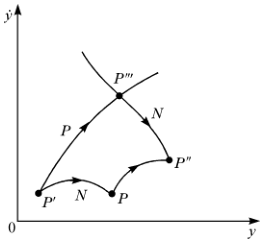
\includegraphics[width=\linewidth]{figs/fig-0132.png}
\caption{图8.1-1}
\end{figure}

\[\dot{y}=\frac{1}{\zeta}\]

\[\dot{y}=-\frac{1}{\zeta}\]

\[\dot{y}=\frac{1}{\zeta}\]

\[\dot{y}=-\frac{1}{\zeta}\]

\[0<\zeta\]

图 8.1-2

布绍证明，上述的曲线 $\Gamma$ 就是最优开关曲线。图 8.1-3 就是这种情形。开关动作的物理过程是这样的：从 $\Gamma$ 上方的任何一点 $P$ 开始，控制函数的值是 -1，系统的运动沿着一个负弧到达开关曲线 $\Gamma$。此后控制函数的值就变为 +1，然后，系统就沿着 $\Gamma$ 最后达到原点。如果初始点 $P$ 在 $\Gamma$ 的下方，控制函数的值是 +1。于是系统沿着一个正弧到达开关曲线 $\Gamma$。在开关线上，控制函数的值变为 -1，然后系统就沿着 $\Gamma$ 达到原点。

\[\dot{y}=-\frac{1}{\zeta}\]

\[\Gamma^{-}\]

\[\phi=+1\]

\[\zeta<0\]

\[\Gamma^{-}\]

\[\phi=0\]

\[\Gamma\]

\[\phi=+1\]

\[0<\zeta\]

图 8.1-3

从以下的说明中，就可以看到布绍所解出的最优开关曲线是正确的。首先，我们都知道，为了达到原点，路线的最后一部分必须是 $\Gamma$，因为只有 $\Gamma$ 是通过原点的路线。假定初始点在 $\Gamma$ 的上方，按照布绍的结果，最优路线的第一部分是一个从 $P$ 到 $\Gamma$ 的负弧，第二部分就是沿着 $\Gamma$ 到达原点的路线。这也就是图 8.1-4(a)中包含虚线部分的路线。如果开关动作开始得太早，在到达 $\Gamma$ 之前就有一个负正隅角。为了到达原点，我们还必须使开关动作再进行一次，因而也就要再作出一

\begin{figure}[htbp]\centering
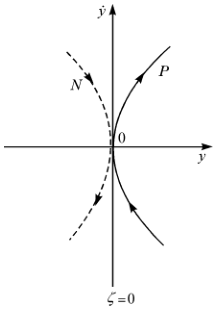
\includegraphics[width=\linewidth]{figs/fig-0133.png}
\caption{图8.1-2}
\end{figure}

\begin{figure}[htbp]\centering
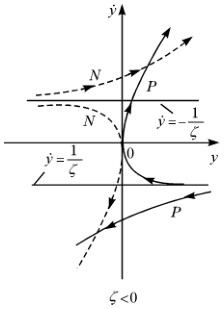
\includegraphics[width=\linewidth]{figs/fig-0134.png}
\end{figure}

\begin{figure}[htbp]\centering
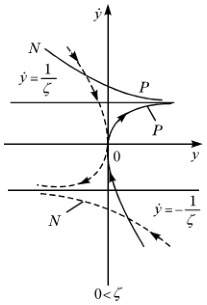
\includegraphics[width=\linewidth]{figs/fig-0135.png}
\caption{图8.1-3}
\end{figure}

\begin{figure}[htbp]\centering
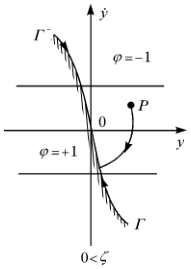
\includegraphics[width=\linewidth]{figs/fig-0136.png}
\end{figure}

\begin{figure}[htbp]\centering
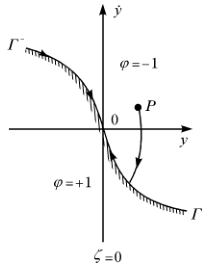
\includegraphics[width=\linewidth]{figs/fig-0137.png}
\caption{图8.1-3}
\end{figure}

\begin{figure}[htbp]\centering
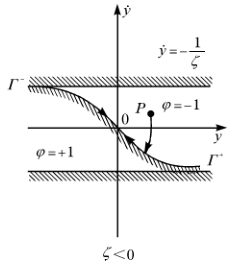
\includegraphics[width=\linewidth]{figs/fig-0138.png}
\caption{图8.1-3}
\end{figure}

个正负隅角。如果这个开关动作在 $P'$ 点发生，这时 $\dot{y}$ 还是负数，于是路线就不能满足正则路线的条件。因此，在这条变化了的路线上所用的时间一定比最优路线长。如果正负隅角在 $P''$ 点，这时 $\dot{y}$ 是正数，然而，沿这条路线到达原点所用的时间还要更长一些，因为在这条路线中还包含了一条花费时间的多余的闭路线。因此我们可以看出：过早的开关动作是不利的。图 8.1-4(b) 表示的是开关动作过迟发生的情形。既然 $P'0$ 和 $P''P''$ 这两条路线是平行的，经过这两条路线所用的时间也应该是一样长的，所以从图 8.1-4(b) 来看，过迟发生开关动作也是有害的。图 8.1-4(c) 所表示的又是另一种情形，这时，路线的第一部分是一个正弧而不是负弧。可是，从图形上能明显地看出，这个情形也比最优路线的情形坏。以上的各种考虑表明，选取正则路线为最优路线的做法是正确的。

\begin{figure}[htbp]\centering
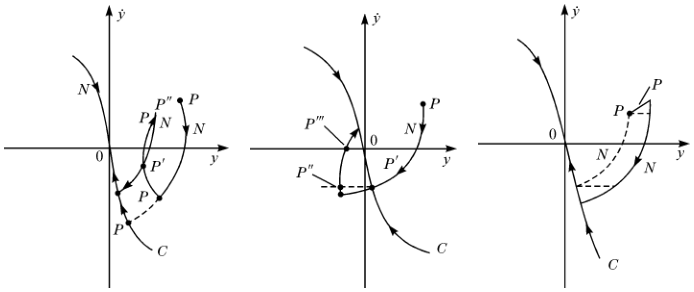
\includegraphics[width=\linewidth]{figs/fig-0139.png}
\caption{图8.1-4}
\end{figure}

(a)

(b)

(c)

图 8.1-4

布绍把 $g(\gamma, \dot{\gamma})=2 \zeta \dot{\gamma}+\gamma(\zeta$ 可以是任意实数） 的二阶线性系统的最优开关曲线具体地确定了出来。下面，我们将只叙述他的结果而不加以证明；从上述比较简单情形的讨论来看，所要介绍的结果的一般性质也是不难理解的。对于这个 $g(\gamma, \dot{\gamma})$ 来说，正系统和负系统就是把图 7.7-2 到图 7.7-6 中的原点分别移到 $(+1,0)$ 点和 $(-1,0)$ 点所得到的两族曲线。

和上面的简单情形最相似的就是 $\zeta>1$ 的情形。开关曲线 $C$ 是由一条从相平面上的无限远处到原点的正弧和一条从无限远处到原点的负弧组成的。和前述情况一样。在 $C$ 的上方，开关函数 $\varphi$ 的值是 $-1$; 在 $C$ 的下方，$\varphi$ 的值是 $+1$。如果初始点在 $C$ 的上方，最优路线就是图 8.1-5 所画的那样。

当 $\zeta<-1$ 时，也和前面的简单情形一样，只有当初始点在相平面的一个有限的区域之内时，系统才能最后到达原点；这是因为当控制函数 $\varphi$ 为零的时候，系统是不稳定的缘故。布绍证明：这个区域的边界是由两个弧组成的：一个弧是从

(+1，0)点到（-1，0）点的正弧，另一个弧是从（-1，0）到（+1，0）点的负弧。。

图 8.1-6 所画的就是这种情形。只有当初始点在这个区域内的时候，开关问题才有意义。最优开关曲线 $C$ 是由一条走向原点的正弧和一条走向原点的负弧组成的。在 $C$ 的上方，关开函数 $\varphi$ 等于 -1，在 $C$ 的下方，$\varphi$ 等于 +1。图 8.1-6 画出了一条初始点 $P$ 在 $C$ 上方的最优路线。

\[\begin{aligned}
& P \\
& N \\
& z>1
\end{aligned} \quad \text { 图 } 8.1-\dot{\mathrm{s}}\]

\[y=+1\]

$<-1$图 8.1-6

当 $\zeta=0$ 时，正系统和负系统分别是以（+1，0）点和（-1，0）点为中心的无限。最优开关曲线 $C$ 是一系列半径是 1 的半圆弧（图 8.1-7)，这一系列半圆从原点出发沿着 $y$ 轴向左右两个方向无限地延伸出去。在 $y$ 是正数的部分，这些半圆都在 $y$ 轴的下方；在 $y$ 是负数的部分，这些半圆都在 $y$ 轴的上方。在 $C$ 的上方，关开函数 $\varphi$ 等于 -1，在 $C$ 的下方，$\varphi$ 等于 +1。从图 8.1-7 中所画的那个一个 $P$ 点出发，路线的第一部分是一个负弧，负弧当然就是一个以 (-1，0) 点为圆心的圆弧。当路线与 $C$ 在 $a$ 点相交的时候，路线就变成一个正弧，正弧就是一个以 (+1，0) 点为圆心的圆弧。然后，路线又在 $b$ 点与 $C$ 相交，于是路线又在 $b$ 点变为负弧，接着，又在下一个交点处变为正弧，以后的过程也是类似的。路线与 $C$ 的最后一个交点是 $d$，从 $d$ 点开始，系统就沿着 $C$ 达到原点。这样一个开关动作的过程就比 $\zeta>1$ 的情形复杂得多了。

$0<\zeta<1$ 的情形，也就是收敛螺线的情形。它比上面的情形还要困难一些。对于这种情况，布绍证明最优开关曲线的画法是这样的：我们先从原点开始沿随着时间的反方向画一条正螺线。从原点到这条螺线与 $y$ 轴的第一个交点之间的螺线弧就是 $C$ 的第一个弧（见图 8.1-8）。既然，每一个 $y$ 轴上方的螺旋弧都与 $y$ 轴相交于两点，我们就可以把每一个弧对于它的右边的交点的反射图形画出来，这样就得出现了一系列“反射”的螺线弧。最后，我们再把这些弧平行于 $y$ 轴移动，使它

\begin{figure}[htbp]\centering
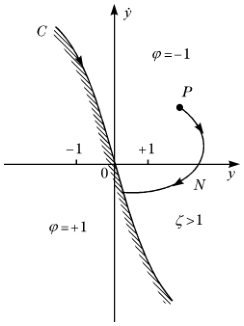
\includegraphics[width=\linewidth]{figs/fig-0140.png}
\caption{图8.1-5}
\end{figure}

\begin{figure}[htbp]\centering
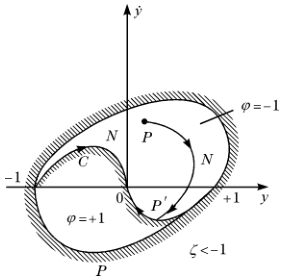
\includegraphics[width=\linewidth]{figs/fig-0141.png}
\caption{图8.1-6}
\end{figure}

\[\begin{aligned}& \dot{y} \\& \varphi=-1\end{aligned}\]

\[\begin{aligned}& \varphi=+1 \\& -1\end{aligned}\]

\[\begin{aligned}& P \\& \zeta=0\end{aligned}\]

图 8.1-7

们按着顺序首尾相接地排列成 $y$ 轴下面的一条连续曲线，这条曲线从原点开始向 $y$ 轴右方无限的延展下去。这就是最优开关曲线的正半部分；这条曲线对于原点的反射图形就是最优开关曲线的负半部分。同样，在这条开关曲线 $C$ 的上方开关函数 $\varphi$ 等于 -1; 在 $C$ 的下方，$\varphi$ 等于 +1（图 8.1-8)。这个情形和图 8.1-7 所画的 $\zeta=0$ 的情形是十分类似的。唯一的区别就是把半圆弧换成了螺线弧。

\[\begin{aligned}& \dot{y} \\& \varphi=-1\end{aligned}\]

\[\begin{aligned}& C \\& N \\& -1\end{aligned}\]

\[\begin{aligned}& P \\& \varphi=+1\end{aligned}\]

\[0<\zeta<1\]

图 8.1-8

最后一种情形就是发散螺线的情形，这时 $-1<\zeta<0$。最优开关曲线的做法基本上和前一种情形完全相同，不过这里的一系列螺线弧是越向外越小的，和前一种情形中越向外越大的情况恰好相反。虽然螺线弧的个数是无限多的，但是开关曲线所占据的范围却是有限的，正如图 8.1-9 所画的那样，它的宽度是在 $y$ 轴上的 $(-a, 0)$ 点到 $(+a, 0)$ 之间。事实当然也应该该是这样的；因为这里的阻尼是负的，正像图 8.1-6 的情形一样，只有当初始点在原点附近的某一个有限的范围之内时，路线才能够最后到达原点。这里的边界是由一条从 $(+a, 0)$ 到 $(-a, 0)$ 的正弧和一条从 $(-a, 0)$ 到 $(+a, 0)$ 的负弧组成的。在开关曲线 $C$ 的上方的相平面部分最优开关函数 $\varphi$ 取 -1 值，在 $C$ 的下方，$\varphi$ 取 +1 值。

\begin{figure}[htbp]\centering
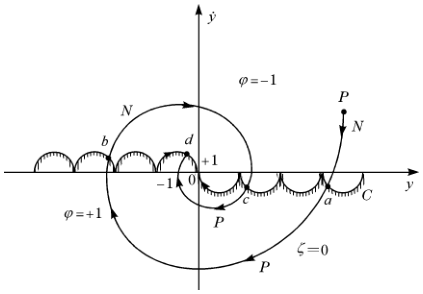
\includegraphics[width=\linewidth]{figs/fig-0142.png}
\caption{图8.1-7}
\end{figure}

\begin{figure}[htbp]\centering
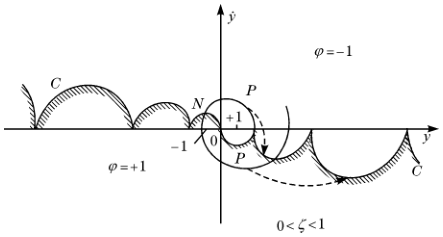
\includegraphics[width=\linewidth]{figs/fig-0143.png}
\caption{图8.1-8}
\end{figure}

在图8.1-9和图8.1-6的情形中，最优开关状态的初始值的范围可能都是有限的，而且这个范围是由闭合的边界曲线所限定的，很显然，这两个闭曲线都是在发生开关动作的极限环。每一个都表示相应的继电伺服系统的一个周期解。 但是，也可以明显地看出：这样的周期解是不稳定的，即是微小的一点扰动都会使得系统的运动曲线离开这个周期解，或者趋近于原点，或者无限地发散出去。因此，实际上是不可能有周期解的。

在上述最优开关问题的各种解中，我们可以看出一个共同的性质：在所有情形中，最优开关函数 $\varphi$ 在相平面的第一象限里总是取 $-1$ 值，在第三象限里总是取 $-1$ 值。把方程 (8.1-3) 写成下列形状:

\[\frac{d}{d t} y=-2 \zeta \frac{d y}{d t}=-y+\varphi\left[y, \frac{d y}{d t}\right]\]

从这个方程可以很容易地看出上述性质的原因。我们的设计目的就是要求在尽可能短的时间内使系统回到 $y=0$ 的状态 （或 $t$ 轴） 上去。当 $y$ 和 $d y / d t$ 都是正数的时候，为了达到设计目的，我们就使 $\dot{d}^{2} y / d t^{2}$ 或 $y(t)$ 的曲率为一个数值尽可能大的负数，所以 $\varphi$ 应该是 $-1$。当 $y$ 和 $d y / d t$ 都是负数的时候，$\dot{d}^{2} y / d t^{2}$ 就应该是一个尽可能大的正数，所以 $\varphi$ 应该是 $+1$。这样一个直观的推理与关于最优开关函数的严密结果是一致的。当 $y$ 与 $d y / d t$ 的符号不相同时，最优开关函数 $\varphi$ 的值就不能这样简单地确定出来了，因为这时系统回到 $t$ 轴的速度与 $y$ 和 $y$ 之间的复杂的交互作用有关；布绍的贡献就在于把开关函数 $\varphi$ 在这一部分 （相平面的第二象限和第四象限） 也确定出来了。但是，从以上讨论中，我们可以肯定，最优开关曲线 $C$ 一定在第二象限和第四象限里。

对于阶数更高的系统以及被控制量的个数大于一的系统来说，就不能再用相

\begin{figure}[htbp]\centering
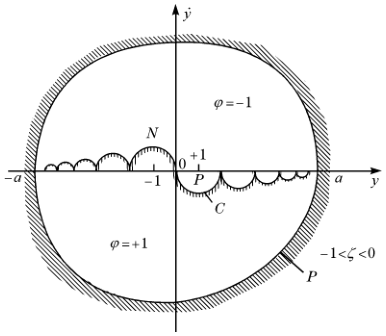
\includegraphics[width=\linewidth]{figs/fig-0144.png}
\caption{图8.1-9}
\end{figure}

平面来表示运动状态了，对于这些情形，我们就必须用多维的相空间来表示运动状态。因而布绍的方法也就难以应用了。为了解决更复杂的问题要发展新的方法。近二十年来所提供的方法，从理论上讲，对任意高阶系统和多个控制量的系统都能找出最优开关函数。布绍的方法虽然只限于二阶系统的讨论，但它的普遍意义在于这样一个事实：当控制量受限制时，线性系统内的最速控制必定是开关式函数，这一点在以后几节内我们将进行详细的讨论和证明，并且给出一个普遍的综合方法。

\section{8.2 最速控制函数的特性}

设受控对象的运动方程为

\[\frac{d \boldsymbol{x}}{d t}=A \boldsymbol{x}+B u\qquad\text{(8.2-1)}\]

式中 $A$ 为常量方阵; $\boldsymbol{x}=\left(x_{1}, \cdots, x_{n}\right)$ 为 $n$ 维相空间内系统的状态向量; $B$ 为 $n \times r$阶长方矩阵; $\boldsymbol{u}=\left(u, \cdots, u_{r}\right)$，即系统具有 $r$ 个控制量。当然，式 (8.2-1) 的形式也包括了一个高阶方程所描述的受控对象

\[a_{n} \frac{d^{n} x}{d t^{n}}+a_{n-1} \frac{d^{n-1} x}{d t^{n-1}}+\cdots+\omega_{n} x=u\qquad\text{(8.2-2)}\]

为了讨论方便，我们假定每一个控制量 $u$ 所受到的限制均为

\[\left\|u\right\| \leqslant 1, \quad i=1,2,3, \cdots, r\]

或

\[\left\|\boldsymbol{u}\right\| \leqslant 1\]

(8.2-3a)型的限制条件的物理意义已为大家所熟悉，而 (8.2-3b)型的限制也是在实际问题中时常出现的。例如，设火箭的飞行路线靠其主发动机的摇摆去控制，或者在火箭尾部装有专为控制用的小型摇摆发动机。此时欲使火箭改变飞行路线，必须使发动机的推力方向偏转，从而使其产生相应的弹道弯曲。若火箭在大气层外飞行，它不受各种气动力的作用，速度向量的方向与火箭纵轴重合，这时火箭重心的运动方程是

\[\begin{aligned} & m \frac{d v}{d t}=P \sin \alpha \sin \beta-m g \sin \theta \\ & m v \dot{\theta}=P \cos \alpha-m g \cos \theta \\ & m v \dot{\psi}=P \sin \alpha \cos \beta \end{aligned}\]

式中 $m$ 为火箭质量，$\theta$ 为弹道轨迹角，$\phi$ 为弹道偏航角，$\alpha$ 和 $\beta$ 分别为推力及其投影与 $y, z$ 轴的夹角。如果火箭按预定轨道飞行，而控制的目的是微量修正的话，那么，可认为上式内的 $v \dot{\theta}=\dot{y}, v \dot{\psi}=\dot{z}$; 于是在垂直于弹道的平面上，上列第二、三两式可改写为

\[\begin{aligned}& \frac{d^{2} y}{d t^{2}}=u_{1}-m g \cos \theta \\& \frac{d^{2} z}{d t^{2}}=u \cos \beta\end{aligned}\]

上式可在引入两个新变数后改写为由四个一阶方程式组成的方程组。对我们重要的是上式内的 $u_1, u_2$ 集体受限制。因为 $u_1 = P \cos \alpha / m$，$u_2 = P \sin \alpha / m$，限制条件是发动机推力 $|P| \leqslant P_{\text {max }}$。这样一来，对控制量的限制就成为条件

\[\|u\|=\sqrt{u_{1}^{2}+u_{2}^{2}} \leqslant P_{\max } / m\]

这无论在数学意义上或在实际意义上均与限制条件式 (8.2-3a) 不同。这里受限制的是控制向量的长度，而限制条件式 (8.2-3a) 是分别独立地加在每个控制分量上的。本节内我们将同时讨论具有式 (8.2-3a) 和 (8.2-3b) 型的限制条件时最速控制的一些特点。由于它们之间的许多共性，因而我们在本节内统一地讨论它们。在以后讨论系统综合问题时，再分别考虑 A 型和 B 型的具体特点。

式 (8.2-3) 内 $u_1$ 和 $\|u\|$ 的最大值假设为 1 并不影响问题讨论的一般性，因为限制形式式 (8.0-1) 和 (8.0-2) 中的 $M_i$ 可以合并到每项的系数因子中去。例如，令 $\vartheta = \frac{u_1}{m_i}$，将 $u = M_i \vartheta_i$ 代入方程式 (8.2-1) 后，其新系数为 $b_i' = b_i M_i$，此时，当 $\vartheta_i = 1$ 时 $u_i$ 依然为 $M_i$。总之，式 (8.2-3) 的限制形式仍然具有一般性。

一切 $u(t)$，如果每一个分量在整个控制过程中都满足限制条件式 (8.2-3)，则说它是可准控制。不等式 (8.2-3a) 和 (8.2-3b) 可以看成是在 $r$ 维欧氏空间内的一个正方体和单位球，前者的每一边边长为 2（以原点为中心），后者的半径为 1（以原点为球心）。这一个正方体和单位球用符号 $U$ 表示。若 $u(t)$ 为可准控制，我们将简写为 $u(t) \in U$。

设系统的初始条件是 $\boldsymbol{x} = (x_{10}, x_{20}, \cdots, x_{n0})$，如果有一个可准控制 $u(t) = (u(t), \cdots, u(t)) \in U$，能使系统式 (8.2-1) 自 $\boldsymbol{x}_0$ 状态以最短时间归零，那么，这一组控制函数将称之为最速控制。这个最短的时间 $t$ 称为最速过渡时间。

方程式 (8.2-1) 的通解可写成

\[\boldsymbol{x}(t)=e^{A t} \boldsymbol{x}_{0}+e^{A t} \int_{0}^{t} e^{-A \tau} \boldsymbol{B} \boldsymbol{u}(\tau) d \tau\qquad\text{(8.2-4)}\]

式中 $e^{A t} = (\varphi_{ij}(t))$ 为式 (8.2-1) 的齐次方程式的基解矩阵。当 $t = 0$ 时显然有 $\boldsymbol{x}(0) = \boldsymbol{x}_0$，初始条件得到满足。设选定某一可准控制 $u(t)$ 后，在 $t = T$ 时系统状态的各分量均归零，即 $\boldsymbol{x}(T) = 0$，此时有

\[\boldsymbol{x}_{0}=-\int_{0}^{T} e^{-A \tau} \boldsymbol{B} \boldsymbol{u}(\tau) d \tau\qquad\text{(8.2-5)}\]

比较式 (8.2-4) 和 (8.2-5) 可知，在 $T$ 时间内系统式 (8.2-4) 归零这一事实可以写成另外形式。因为受控对象方程式诸系数与时间无关，故研究式 (8.2-1)的同时，可讨论它的逆运动方程式

\[\begin{aligned}& \frac{d \mathbf{y}}{d t}=-A \mathbf{y}-B \mathbf{u}^{\prime} \\& \mathbf{y}(0)=\mathbf{0}\end{aligned}\qquad\text{(8.2-6)}\]

后者的解是

\[\mathbf{y}(t)=-e^{-A t} \int_{0}^{t} e^{A s} B \mathbf{u}^{\prime}(s) d s\qquad\text{(8.2-7)}\]

式中 $\boldsymbol{u}^{\prime}(t)$ 与式 (8.2-1) 内的 $\boldsymbol{u}(t)$ 的关系是 $\boldsymbol{u}\left(t^{\prime}\right)=\boldsymbol{u}^{\prime}(T-t)$，即 $t=T-t^{\prime}$。当不可能发生误会时，以后 $t^{\prime}$ 和 $\boldsymbol{u}^{\prime}$ 的上标略而不写。设 $\boldsymbol{u}(t)$ 使初始状态 $\boldsymbol{x}$ 在时间 $T$ 内引至原点 （按式 (8.2-4))，则 $\boldsymbol{u}(T-t)$ 必使 $\mathbf{y}(t)$ 在同一时间内按式 (8.2-7) 自原点到达 $\boldsymbol{x}$ 点，且一切式 (8.2-7) 所能到达的点 $\mathbf{y}(T)$，式 (8.2-1) 都能用同一个控制在同一时间内将其引至原点。因此，式 (8.2-1) 与其逆运动方程式 (8.2-6) 完全等价。以后这两种方程式都将被应用。

现设自 $\boldsymbol{x}$ 原点的最速控制已经找到，它是 $\dot{\boldsymbol{u}}(t)$，我们看看它有些什么特点。为此假定自 $\boldsymbol{x}$ 至原点的最速过渡时间是 $t_{0}$。现在先研究一下在 $t$ 时间内式 (8.2-6)内的 $\mathbf{y}(t)$ 都可能是些什么点。任意取一个可准控制 $\boldsymbol{u}(t)$ 代入式 (8.2-6)后就可以得到一个 $\mathbf{y}(t)$，变化 $\boldsymbol{u}(t)$ 时，$\mathbf{y}(t)$ 也随之而变。一切可准控制 $\langle\boldsymbol{u}(t)$，$0 \leqslant t \leqslant t_{0}\rangle$，（它们有无穷多个 $\lambda)$ 所对应的 $\{\mathbf{y}(t)\}$ 用 $G(t)$ 表示。它是在 $t$ 时间内式 (8.2-1)所能引至原点的一切初始点的集合。显然，它是个凸性区域，并且对原点对称。事实上，从式 (8.2-7) 的线性形式可知，若 $\boldsymbol{u}(t)$ 使 $\mathbf{y}(t)$ 在 $t$ 时间内到达 $\mathbf{y}=\boldsymbol{x}$ 点，那么，$-\boldsymbol{u}(t)$ 必使 $\mathbf{y}(t)$ 到达 $-\mathbf{y}=-\boldsymbol{x}$。也就是说若 $\boldsymbol{x} \in G(t)$，则必有 $-\boldsymbol{x} \in G(t)$，因此，$G(t)$ 对原点对称。其次，$\boldsymbol{x}$ 和 $\boldsymbol{x}$ 都属于 $G(t)$，那么，这两个点的连线上的一切点 $\boldsymbol{z}=\lambda \boldsymbol{x}+(1-\lambda) \boldsymbol{x}, 0 \leqslant \lambda \leqslant 1$，也都属于 $G(h)$。这是因为：若 $\boldsymbol{u}(t)$ 和 $\boldsymbol{u}(t)$ 分别使 $\mathbf{y}(t)$ 达到 $\boldsymbol{x}$ 和 $\boldsymbol{x}$，那么，控制 $\boldsymbol{u}(t)=\boldsymbol{\lambda} \boldsymbol{u}_{1}(t)+(1-\lambda) \boldsymbol{u}(t)$ 必使 $\mathbf{y}(t)$ 达到 $\boldsymbol{z}$ 点。事实上

\[\begin{aligned}& z=-e^{-A t_{1}} \int_{0}^{t_{1}} e^{A \tau} B\left[\boldsymbol{\lambda} \boldsymbol{u}_{1}(\tau)+(1-\lambda) \boldsymbol{u}(\tau)\right] d \tau \\& =-\lambda e^{-A t_{1}} \int_{0}^{t_{1}} e^{A \tau} B \boldsymbol{u}_{1}(\tau) d \tau-(1-\lambda) e^{-A t_{1}} \int_{0}^{t_{0}} e^{A \tau} B \boldsymbol{u}_{2}(\tau) d \tau \\& =\boldsymbol{\lambda} \boldsymbol{x}_{1}+(1-\lambda) \boldsymbol{x}\end{aligned}\]

同时 $\boldsymbol{\lambda} \boldsymbol{u}_{1}(t)+(1-\lambda) \boldsymbol{u}(t)$ 也是可准控制，因为对 A 型限制，任何分量 $\boldsymbol{u}(t)$ 均有

\[\begin{aligned}& u_{1}(t)=\lambda u_{1}(t)+(1-\lambda) u_{2}(t) \\& \mid u_{1}(t) \mid \leqslant \lambda \mid u_{1}(t) \mid+(1-\lambda) \mid u_{2}(t) \mid \leqslant \lambda+1-\lambda=1\end{aligned}\]

对 B 型限制则有

\[\|\lambda \boldsymbol{u}_{1}(t)+(1-\lambda) \boldsymbol{u}(t)\| \leqslant \lambda\|\boldsymbol{u}(t)\|+(1-\lambda)\|\boldsymbol{u}(t)\| \leqslant 1\]

于是，在 $t$ 时间内式 (8.2-6)所能到达的一切点的集合 $G(t)$ 是一个凸性区域，它称之为等时区 ${ }^{\left[5,6,14\right]}$。

如果 $\dot{u}(t)$ 是将 $\boldsymbol{x}$ 引至原点的最速控制，那么，$\boldsymbol{x}$ 点必在等时区 $G(t)$ 的边界上，否则 $\dot{u}(t)$ 就不会是最速控制了，关于这一点的证明以后将给出。由于 $G(t)$ 是凸性区域，那么，通过其边界上任一点均可做一个超平面 $P$，使 $G(t)$ 完全位于此平面的一侧，它称为等时区的支面。这个平面的与 $G(t)$ 不在同侧的法向量称为 $P$ 的外法向量，或简称为 $G(t)$ 的外法向量，后者用 $\boldsymbol{\psi}_{0}$ 表示。依定义，对 $G(t)$ 内的一切点 $\boldsymbol{x}$ 均有下列不等式成立 （图 8.2-1)

\[\left(\boldsymbol{\psi}_{0}, \boldsymbol{x}-\boldsymbol{x}_{0}\right)=\sum_{n=1}^{n} \boldsymbol{\psi}_{\omega}\left(\boldsymbol{x}_{n}-\boldsymbol{x}_{\omega}\right) \leqslant 0\]

或者改写为

\[\left(\boldsymbol{\psi}_{0}, \boldsymbol{x}\right) \geqslant\left(\boldsymbol{\psi}_{0}, \boldsymbol{x}\right)\qquad\text{(8.2-8)}\]

设 $\dot{u}(t)$ 和 $u(t)$ 是分别对应于 $\boldsymbol{x}$ 和 $\boldsymbol{x}$ 的控制，$\boldsymbol{y}=\boldsymbol{x}, \boldsymbol{y}_{0}=\boldsymbol{x}$，将式 (8.2-7) 代入式 (8.2-8)化简后得到不等式

\[\int_{0}^{t_{1}}\left(e^{A^{t_{1}}} \boldsymbol{\Psi}_{1}, B \dot{u}(t)\right) d t \geqslant \int_{0}^{t_{1}}\left(e^{A^{t_{1}}} \boldsymbol{\Psi}_{1}, B u(t)\right) d t\qquad\text{(8.2-9)}\]

式中 $\boldsymbol{\Psi}_{1}=-e^{-A^{t_{1}}} \boldsymbol{\Psi}_{0}, A^{\tau}$ 是 $A$ 的转置矩阵。从第二章可知，向量函数 $e^{A^{t_{1}}} \boldsymbol{\Psi}_{1}$ 是式 (8.2-6) 的共轭方程组的解

\[\frac{d \boldsymbol{\Psi}}{d t}=A^{\tau} \boldsymbol{\Psi}, \quad \boldsymbol{\Psi}(0)=\boldsymbol{\Psi}_{1}=-e^{-A^{t_{1}}} \boldsymbol{\Psi}_{0}\qquad\text{(8.2-10)}\]

由于式 (8.2-8)内的 $\boldsymbol{x}$ 和其相应的 $\boldsymbol{u}(t)$ 是任意的，所以不等式 (8.2-9) 只有在下列条件下才能成立

\[(\boldsymbol{\Psi}(t), B \dot{u}(t))=\max _{u \in t}(\boldsymbol{\Psi}(t), B u(t))\qquad\text{(8.2-11)}\]

这意味着，最速控制 $\dot{u}(t)$ 在任何时刻都使式 (8.2-11) 右端获得极大值。令 $\dot{\boldsymbol{x}}(t)$ 是自 $\boldsymbol{x}$ 引至原点的最速轨线，在式 (8.2-11) 的两端分别加以 $(\boldsymbol{\Psi}(t), A \dot{\boldsymbol{x}}(t))$ 后，便有

\[H=(\boldsymbol{\Psi}(t), A \dot{\boldsymbol{x}}(t)+B \ddot{u}(t))=\max _{u \in t}(\boldsymbol{\Psi}(t), A \dot{\boldsymbol{x}}(t)+B u)\qquad\text{(8.2-12)}\]

$H$ 常称为哈密顿函数。最速控制使 $H$ 沿最速轨线取极大值这一事实就称之为极大值原理 ${ }^{[20]}$。

欲使 $\dot{u}(t)$ 满足极大值条件式 (8.2-11) 或 (8.2-12)，对 A 型限制便有

\[\dot{u}(t)=\operatorname{sign}\left(B^{T} \boldsymbol{\Psi}(t)\right)\]

\begin{figure}[htbp]\centering
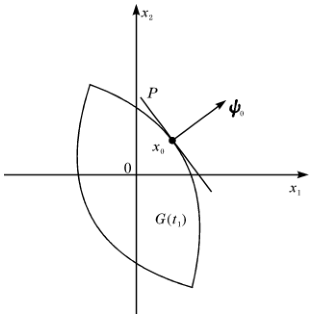
\includegraphics[width=\linewidth]{figs/fig-0145.png}
\caption{图8.2-1}
\end{figure}

式中 $B^{r}$ 是 $B$ 的转置矩阵。

或者将上式展开

\[\dot{\boldsymbol{u}}(t)=\operatorname{sign}(\boldsymbol{\Psi}(t), \boldsymbol{b}_{i})\]

式中 $\boldsymbol{b}_{i}$ 为矩阵 $B$ 的第 $i$ 列向量，$\boldsymbol{\Psi}(t)$ 是式 (8.2-10) 以 $\boldsymbol{\Psi}(0)=-e^{-A^{r} t_{1}} \boldsymbol{\Psi}_{0}$ 为初始条件的解。对 $\mathbf{B}$ 型限制则有

\[\dot{\boldsymbol{u}}(t)=\frac{B^{r} \boldsymbol{\Psi}(t)}{\left\|B^{r} \boldsymbol{\Psi}(t)\right\|}\]

因为只有 $\boldsymbol{u}$ 的方向与 $B^{r} \boldsymbol{\Psi}$ 相同时，$H$ 才才能获得极大值。这样就得到了最速控制的一个重要特性：如果数量积 $(\boldsymbol{\Psi}(t), \boldsymbol{b})$ 在任何小的正区间内不恒为零，则受 $\mathbf{A}$ 型限制的 $\dot{\boldsymbol{u}}(t)$ 的每一个分量 $\dot{\boldsymbol{u}}_{i}(t)$ 都是开关函数，而受 $\mathbf{B}$ 型限制的 $\dot{\boldsymbol{u}}(t)$ 必取值于单位球的表面。此时最速控制函数为共轭方程式 (8.2-10) 的解所唯一确定。

如何判别 $(\boldsymbol{\Psi}(t), \boldsymbol{b})$ 不恒为零呢？这只需将它微分 $n-1$ 次后找出各阶导数不为零的条件

\[\begin{aligned}& \frac{d}{d t}(\boldsymbol{\Psi}(t), \boldsymbol{b})=\left(A^{r} e^{A^{r} t} \boldsymbol{\Psi}_{1}, \boldsymbol{b}\right) \\& \cdots \\& \frac{d^{n-1}}{d t^{n-1}}(\boldsymbol{\Psi}(t), \boldsymbol{b})=\left(\left(A^{r}\right)^{n-1} e^{A^{r} t} \boldsymbol{\Psi}_{1}, \boldsymbol{b}\right)\end{aligned}\]

这组函数不同时为零的条件是向量组

\[b, A b_{i}, A^{2} b_{i}, \cdots, A^{n-1} b_{i}\]

线性无关。如果对任何 $i=1,2, \cdots, r$，上列向量组均线性无关，则称系统式 (8.2-1) 为非蜕化系统，或者说该系统是能控的。一切非蜕化系统的受 $\mathbf{A}$ 型限制的最速控制均为开关函数，而且为式 (8.2-13) 所单一确定。容易检查，形如式 (8.2-2) 的 $n$ 阶系统都是能控的，因而它的最速控制一定是开关函数或取值于单位球表面上的点。

还有一个有意思的事实是沿最速轨迹式 (8.2-12) 内的函数 $H=\operatorname{const}$，而且不小于零。函数 $H$ 是常数可以用直接微分的方法检查，$\frac{d H}{d t} \equiv 0$。至于 $H>0$ 这一事实下面我们将会看出。

对于等时区 $G(h)$ 的特性还可以补充两点。首先 $G(h)$ 是严格凸的。也就是说 $G(h)$ 的任何支面 $P$，只可能与 $G(h)$ 的边界交于一点。假设这一事实不成立，那么，$G(h)$ 的边界必包含一个直线线段。设 $\boldsymbol{x}_{1}$ 和 $\boldsymbol{x}_{2}$ 不为同一点，而且两者的连线均位于 $G(h)$ 的边界上。设开关函数 $\dot{\boldsymbol{u}}(t)$ 和 $\dot{\boldsymbol{u}}(t)$ 分别为自两点引至原点的最速控制。到达边界点 $\boldsymbol{z}=\lambda \boldsymbol{x}_{1}+(1-\lambda) \boldsymbol{x}_{2}$ 的控制将是 $\boldsymbol{u}(t)=\lambda \dot{\boldsymbol{u}}_{1}(t)+(1-\lambda) \dot{\boldsymbol{u}}_{2}(t)$。因为 $\boldsymbol{x}_{1} \neq \boldsymbol{x}_{2}$，故 $\dot{\boldsymbol{u}}(t) \neq \dot{\boldsymbol{u}}(t)$。既然最速控制 $\dot{\boldsymbol{u}}(t)$ 和 $\dot{\boldsymbol{u}}(t)$ 总取值于正方体的顶点或单位球的边界，那么，必有一个时间间隔存在，在该时间间隔里 $u(t)$ 的取值，不在顶点或不在球面上，因此 $u(t)$ 不是到达边界点的控制。这与 $z$ 是 $G(t)$ 的边界点相矛盾。由此可知 $G(t)$ 的边界上的任何两个点的连线除端点外均位于 $G(t)$ 的内部。这恰恰是 $G(t)$ 严格凸的定义。

当原点是系统的终点时，等时区 $G(t)$ 的另一个特性是它对 $t$ 单调扩张，或者说 $G(t)$ 随 $t$ 的增大而连续增大。若 $t_{2}>t_{1}$，则 $G(t)$ 完全位于 $G(t)$ 的内部，二者没有共同的边界点。这个特性几乎是“常微分方程的解连续依赖于初始条件”这个众所周知定理的推论。这一情况可以用简单的几何事实来加以解释。设 $x_{1}$ 是 $G(t)$ 的边界点，以原点为中心做一个小球 $S_{1}$ （图 8.2-2)，如果用 $x$ 对应的控制 $\dot{u}(t)$ 代入式 $(8.2-7)$，但初始条件取小球 $S_{1}$ 内的任意点 $x$。那么，当 $t=t$ 时小球 $S_{1}$ 内的所有点均到达 $x$ 附近的小区域 $S_{2}$ 内，且 $x$ 点是它的内点。另一方面可用可准控制使原点到达 $S_{1}$ 内的任何点。$S_{1}$ 越小，到达其内各点所需的时间 $\Delta t$ 越小。由此可知对任何 $\Delta t>0$，均

有一相应的小球 $S_{2}\left(\Delta t_{2}\right)$，其内的任何点均可用 $t+\Delta t_{2}$ 的时间自原点到达，因此 $S_{2}$ 内的一切点均属于 $G\left(t+\Delta t_{2}\right)$。也就是说 $G(t)$ 必完全位于 $G\left(t+\Delta t_{2}\right)$ 的内部，因此 $G(t)$ 是严格扩张的。这一事实的详细证明请参看文献[5]。由于这个特性便可推知自等时区的任一边界点到达原点的控制式 $(8.2-13)$ 是最速控制。根据 $G(t)$ 是单调扩张这一事实又可以推知：方程 $(8.2-1)$ 自 $x$ 达到原点的最速控制是唯一的。其次，如果可以用某一种控制 $u(t)$ 将 $x$ 点引至原点，那么，必存在一个（唯一的）最速控制 $\dot{u}(t)$，后者以最短时间将 $x$ 引至原点。这样，我们就得到了关于最速控制的存在和唯一性定理。

根据 $G(t)$ 的单调扩张特性也可以推知式 $(8.2-12)$ 中的哈密顿函数 $H$ 沿最速轨迹永远大于零。这从几何意义来看是十分明显的。

归纳上述讨论，最速控制的特性可简述如下。若系统式 $(8.2-1)$ 为能控的，最速控制如果存在，则必是唯一的，对 A 型限制它是开关函数，对 B 型限制它取值于单位球的表面，并由最速过渡时间 $t$ 的等时区的外法向量 $\Psi_{0}$ 所单一确定；位于等时区 $G(t)$ 边界上的任何点只能用最速控制才能在 $t$ 时间内到达原点。

A 型最优控制函数每个分量的开关次数和 B 型每一分量的变号次数，一般说来，与初始条件和函数 $\Psi(t)$ 的变化规律有关。但是，如果受控对象运动方程式内

\begin{figure}[htbp]\centering
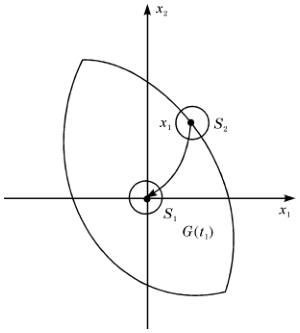
\includegraphics[width=\linewidth]{figs/fig-0146.png}
\caption{图8.2-2}
\end{figure}

的矩阵 $A$ 的所有特征根均是实数，这时它们的变号次数 （对 A 型是开关次数） 可以确定下来。确切的答案是变号次数不大于 $n-1$，而且，对几乎所有的初始条件变号次数都等于 $n-1$。变号次数小于 $n-1$ 的一切初始点的总和在 $n$ 维空间中所占的体积等于零。这一事实首先在文献[5]中给出了说明。这里我们根据前面的讨论来证明。将式 (8.2-13a) 展开后有

\[\dot{\boldsymbol{u}}(t)=\operatorname{sign}\left[\sum_{a=1}^{n} \psi_{k}(t) b_{i}\right]\qquad\text{(8.2-15)}\]

假定矩阵 $A$ 的所有特征根均为实数单根; $\lambda, \lambda, \cdots, \lambda_{n}$，那么，$\psi_{k}(t)$ 必为下列形式

\[\psi_{k}(t)=a_{n} e^{-\lambda_{1} t}+a_{n} e^{-\lambda_{2} t}+\cdots+a_{n} e^{-\lambda_{n} t}\qquad\text{(8.2-16)}\]

式中 $a_{n}$ 均为常数。当 $A$ 的特征根为 $\lambda$ 时，则 $-\lambda$ 是 $-A^{r}$ 的特征根，因为行列式

\[|I-A^{r}+\lambda E|=|I-A+\lambda E|=(-1)^{n} \mid A-\lambda E|=0\]

将式 (8.2-16) 代入式 (8.2-15) 后有

\[h_{i}(t)=\sum_{i=1}^{n} \psi_{i}(t) b_{i}=c_{i} e^{-\lambda_{1} t}+c_{i} e^{-\lambda_{2} t}+\cdots+c_{i} e^{-\lambda_{n} t}\qquad\text{(8.2-17)}\]

其中 $c_{i}$ 为常量。上式右端每一项都是 $t$ 的单调函数，例如当 $c_{i}>0,-\lambda_{i}>0$，则 $c_{i} e^{-\lambda_{1} t}$ 单调上升；若 $c_{i}>0$，而 $-\lambda_{i}<0$，则 $c_{i} e^{-\lambda_{1} t}$ 单调下降，如此等。因此，当式 (8.2-17) 之右端只有一项时，$h(t)$ 不会变号，故 $\dot{u}(t)$ 也不会变号。当式 (8.2-17) 之右端只有两项时，$h_{i}(t)$ 只能通过零点一次；若只有三项，则 $\dot{u}(t)$ 最多变号两次；以此类推，当所有系数均不为零时，$h_{i}(t)$ 最多变号 $n-1$ 次，即 $\dot{u}(t)$ 最多变号 $n-1$ 次。

在上面的讨论中曾假定 $\lambda, \cdots, \lambda_{n}$ 都是单根，若其中有重根，上述讨论依然有效。因为此时式 (8.2-16) 变为

\[\psi_{k}(t)=a_{n} P_{1}(t)+a_{n} P_{2}(t)+\cdots+a_{m} P_{n}(t)\qquad\text{(8.2-18)}\]

式中 $a_{n}$ 均为常数，$P_{i}(t)=\left(\sum_{k=1}^{m} \frac{t}{k} \mid e^{-\lambda_{k} t}\right.$ 仍然为 $t$ 的单调函数 （参看第 2.7 节），所以前面的讨论继续有效。总之，在这种情况下，一般来讲，最速控制函数的变号次数比系统的阶数少 1。或者说，最速控制一般由 $n$ 段组成 （图 8.2-3)，这一事实后来被称为 $n$ 段定理 ${ }^{[20]}$。上述讨论对 B 型控制也有效。

在本节的最后，值得指出下列事实：当控制量 $u$ 的取值范围不受限制时，最速控制就完全没有意义。此时任何离原点为有限距离的初始点 $x_{0}$ 均可以在无穷小的时间内被引至原点。这从下列事实中可以看出。对 $t>0$，等时区 $G(t)$ 是 $n$ 维凸性区域。引用关系式 (8.2-7)，设只有一个控制量 $u$。而 $u \equiv u_{3} \equiv \cdots \equiv u \equiv 0$。此时

\[\mathbf{y}(t)=-e^{-A t_{1}} \int_{0}^{t_{1}} e^{A t} \boldsymbol{b}_{1} w(\tau) d \tau\qquad\text{(8.2-7)}\]

现找出 $n$ 个不同的控制函数 $u_{1}^{(1)}(t), \cdots, u_{1}^{(n)}(t)$

\[u_{1}^{(i)}(t)=\frac{1}{m}\left(\varphi_{i}(t), \boldsymbol{b}_{1}\right), \quad i=1,2, \cdots, n\qquad\text{(8.2-19)}\]

式中 $\varphi_{i}(t)$ 为矩阵 $e^{-A\left(t_{1}-t\right)}=\left(\varphi_{i}(t)\right)$ 的第 $i$ 行向量，$m$ 为足够大的正数，使 $\left|u_{1}^{(i)}(t)\right|$ $\leqslant 1$。将式 (8.2-19) 代入 (8.2-7) 后有

y\_i(t)=-\_0\textasciicircum{}t\_1(arrayc(\_1(t), b\_1) \textbackslash\{\}\textbackslash\{\}(\_2(t), b\_1) \textbackslash\{\}\textbackslash\{\} \textbackslash\{\}(\_n(t), b\_1)array)((\_i(t), b\_1)m d t.(8.2-20)

\[i=1,2, \cdots, n\]

因为假设系统为能控的，故 $n$ 个函数 $\left(\varphi_{i}(t), \boldsymbol{b}_{1}\right), i=1,2, \cdots, n$，性无关。否则将存在一个非零向量 $\boldsymbol{c}$ 使

\[\left(e^{A t} \boldsymbol{b}_{1}, \boldsymbol{c}\right)=0\]

\[\left(A e^{A t} \boldsymbol{b}_{1}, \boldsymbol{c}\right)=0\]

\[\left(A^{n-1} e^{A t} \boldsymbol{b}_{1}, \boldsymbol{c}\right)=0\]

令 $t=0$ 则 $\boldsymbol{b}, A \boldsymbol{b}_{1}, \cdots, A^{n-1} \boldsymbol{b}$ 线性相关，这与假定不符。

\[\therefore h_{i}(t)=\left(\varphi_{i}(t), \boldsymbol{b}_{1}\right),\left\langle h_{i}(t), h_{i}(t)\right\rangle=\int_{0}^{t_{1}} h_{i}(t) h_{i}(t) d t\]

将 $\mathbf{y}_{1}\left(h_{1}\right), \mathbf{y}_{2}\left(h_{1}\right), \cdots, \mathbf{y}_{n}\left(h_{1}\right)$ 排成矩阵，便得到一个格拉姆 (Gram) 行列式，从代数学中我们知道它必大于零，即

\[\left|\begin{array}{llll}\mathbf{y}_{11} & \mathbf{y}_{21} & \cdots & \mathbf{y}_{n 1} \\\mathbf{y}_{12} & \mathbf{y}_{22} & \cdots & \mathbf{y}_{n 2} \\\vdots & \vdots & & \vdots \\\mathbf{y}_{1 n} & \mathbf{y}_{2 n} & \cdots & \mathbf{y}_{m n}\end{array}\right|=\frac{1}{m}\left|\begin{array}{ccc}\left\langle\boldsymbol{h}_{1}, \boldsymbol{h}_{1}\right\rangle & \cdots & \left\langle\boldsymbol{h}_{1}, \boldsymbol{h}_{n}\right\rangle \\\left\langle\boldsymbol{h}_{2}, \boldsymbol{h}_{1}\right\rangle & \cdots & \left\langle\boldsymbol{h}_{2}, \boldsymbol{h}_{n}\right\rangle \\\vdots & & \vdots \\\left\langle\boldsymbol{h}_{n}, \boldsymbol{h}_{1}\right\rangle & \cdots & \left\langle\boldsymbol{h}_{n}, \boldsymbol{h}_{n}\right\rangle\end{array}\right|>0\]

由此可知，用 $n$ 个式 (8.2-19) 的控制得到 $n$ 个线性不相关的点，故等时区 $G(t)$ 是

\begin{figure}[htbp]\centering
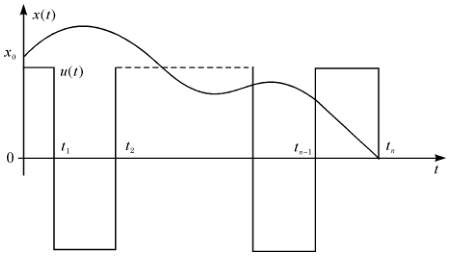
\includegraphics[width=\linewidth]{figs/fig-0147.png}
\caption{图8.2-3}
\end{figure}

n维凸性区域，并包含着原点。若 $u$ 的取值不加限制，$G(h)$ 将无限制地扩展，当 $|u| \rightarrow \infty$ 时，$G(h)$ 将包含整个相空间内可控区域的有限部分。由于 $h$ 是任意的，令 $h \rightarrow 0$，但 $h \not\equiv 0, |u| \rightarrow \infty$，这样相空间可控区内任何点 $y(t)$ 均可以用任意小的时间到达。换言之，系统式 (8.2-1) 自任意可控点出发，总能以任意小的时间到达原点。这在实际问题中是没有意义的。这样的讨论告诉我们，若控制量的取值范围不受限制，则所谓最速控制既没有实际意义，也没有数学上的意义。

\section{8.3 特定的最速控制综合}

实际工程中常出现这样一类问题：系统的初始条件是已知的，即系统的初始误差只能取若干个有限的值，后者在系统工作开始之前可以较为准确地测量出来。这种例子很多，例如飞行器进入轨道的问题，轨道和发射场地都是预先选定的，这时飞行器对轨道的初始偏差为已知。在这类问题中，当初始条件 $x$ 为已知时，要求综合 （设计） 出一个特定的最速控制函数 $\dot{u}(t)$，使系统的误差以最快速度归零。这一节的目的就是要解决这类特定的最速控制函数的设计。

在解决这个问题之前，让我们先讨论另一个与此有密切联系的问题，即自面至点的最速控制的综合。设在相空间内有一个通过 $x$ 点的 $n-1$ 维超平面 $P, \boldsymbol{\phi}_{0}$是它的外法向量 （图 8.3-1)。平面的方程式是

\[\left(\boldsymbol{\phi}_{0}, \boldsymbol{x}-\boldsymbol{x}\right)=\sum_{a=1}^{n} \boldsymbol{\phi}_{a}\left(x_{0 a}-x_{a}\right)=0\qquad\text{(8.3-1)}\]

已知系统的初始误差在平面 $P$ 上。设从平面上的每一个点到达原点都对应自己的最速控制函数。要求找出平面上的一个离原点“最近”的点 $\boldsymbol{x}$，自此点到达原点所需最短时间比此平面上所有其他点到达原点所需的最小时间还要短。形象地说，就是要找出自平面 $P$ 到达原点的“捷径”。利用前节得到的结果解决这一问题是极其简单的。

这个问题表面看来似乎很复杂，因为这里是“双重”即速问题，既要从所有最速控制中找出一个时间最短者。但是，不难看出，如果利用方程式 (8.2-6) 那么就会得到一个简单的等价命题：求出式 (8.2-6) 自原点至平面 $P$ 的最速控制。为了解决后一个问题我们已经有了足够的知识。从前节中我们知道，方程式 (8.2-6) 的等时区 $G(t)$ 是单调扩张的。当 $t$ 不断增大时，$G(t)$ 也不断增大，必存在这样一个时刻 $h$，使 $G(h)$ 恰好碰上平面 $P$。由于 $G(h)$ 是严格凸的，所以此时它与 $P$ 只相遇在一个孤立点 $\boldsymbol{x}_{1}$ 上 （图 8.3-1)。此时平面 $P$ 自然成为 $G(h)$ 的支面，而支面的外法向量为已知，它就是 $\boldsymbol{\phi}_{0}$。上节中我们曾指出，最速控制是由公式 (8.2-13) 所单一确定的，而式 (8.2-13) 内的 $h$ 为已知，$\boldsymbol{\psi}(t)$ 是共轭方程式

\[\frac{d \boldsymbol{\Psi}}{d t}=A^{\varepsilon} \boldsymbol{\Psi}, \quad \boldsymbol{\Psi}(0)=-e^{-A^{x} t_{1}} \boldsymbol{\Psi}_{0}\qquad\text{(8.2-10)}\]

的解。这一个解又由初始条件 $\boldsymbol{\Psi}(0)$ 所完全决定。而这个初始条件已经给定，这就是平面 $P$ 的外法向量 $\boldsymbol{\Psi}_{0}$，于是式 (8.2-6) 的原点至平面 $P$ 的最速控制必定是

对 A 型限制对 B 型限制

式中，$i=1,2, \cdots, r, \boldsymbol{\Psi}_{1}=-e^{-A^{x} t_{1}} \boldsymbol{\Psi}_{0}$。

如果仔细察看上式便会发现，这里还

有一个未知数——最速过渡时间 $t$，在后者尚未找到之前问题还不能算完全解决。为此不得不求助于原方程式 (8.2-1) 和 (8.2-4)。设 $\boldsymbol{x}$ 为 $P$ 上到原点的“最近”点，自 $\boldsymbol{x}$ 至原点的最速控制必为

对 A 型限制对 B 型限制

式中 $\boldsymbol{\Psi}(t)$ 是式 (8.2-1) 的共轭方程组

\[\frac{d \boldsymbol{\Psi}}{d t}=-A^{\varepsilon} \boldsymbol{\Psi}, \quad \boldsymbol{\Psi}(0)=\boldsymbol{\Psi}_{0}\qquad\text{(8.3-4)}\]

的解。这里的初始条件 $\boldsymbol{\Psi}_{0}$ 与 $t$ 和 $\boldsymbol{x}$ 无关，这是与式 (8.3-2) 的一大差异。当 $t=$ $t_{1}$ 时按式 (8.2-4) 有

\[\boldsymbol{x}\left(t_{1}\right)=e^{A t_{1}} \boldsymbol{x}_{1}+e^{A t_{1}} \int_{0}^{t_{1}} e^{-A \tau} B \dot{u}\left(\boldsymbol{\Psi}_{0}, \tau\right) d \tau=0\]

或

\[\boldsymbol{x}=-\int_{0}^{t_{1}} e^{-A \tau} B \dot{u}\left(\boldsymbol{\Psi}_{0}, \tau\right) d \tau\qquad\text{(8.3-5)}\]

由于

\[\left(\boldsymbol{x}_{0}-\boldsymbol{x}, \boldsymbol{\Psi}_{0}\right)=0\]

故 $t$ 满足方程式

\[\left[\int_{0}^{t_{1}} e^{-A \tau} B \dot{u}\left(\boldsymbol{\Psi}_{0}, \tau\right) d \tau, \boldsymbol{\Psi}_{0}\right]+\left(\boldsymbol{x}_{0} ; \boldsymbol{\Psi}_{0}\right)=0\qquad\text{(8.3-6)}\]

因此，$t$ 可以由上式解出，解出 $t$ 后，$\boldsymbol{x}$ 便可以由式 (8.3-5) 求出。这样，自平面 $P$至原点的最速控制函数就已经找到了，同时也已经找到了自平面 $P$ 至原点的

\begin{figure}[htbp]\centering
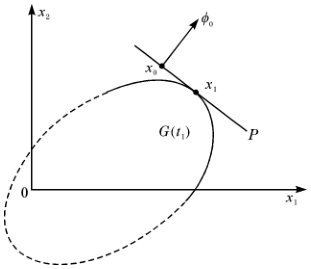
\includegraphics[width=\linewidth]{figs/fig-0148.png}
\caption{图8.3-1}
\end{figure}

“捷径”。

现在我们开始讨论本节初提出的找自给定点 $\boldsymbol{x}$ 至原点的最速控制函数。这里介绍的是一种逐步逼近法 ${ }^{[4]}$。这个方法的机理很简单，设系统的初始误差 $\boldsymbol{x}$ 已经给定，方程式 (8.2-6) 自原点至此点的最速控制是 $\dot{u}\left(\boldsymbol{\psi}_{0}^{\prime}, t\right)$。根据前节的讨论可知，必存在一个非零向量 $\boldsymbol{\psi}_{0}^{\prime}=-e^{-A_{1}} \boldsymbol{\psi}_{0}$ 使这个最速控制为式 (8.3-2) 所唯一确定。逐步逼近法的目的就是找到这个向量 $\boldsymbol{\psi}_{0}^{\prime}$。

设 $t_{0}$ 是自原点至 $\boldsymbol{x}_{0}$ 点的最速过渡时间。那么 $\boldsymbol{x}_{0}$ 点必位于等时区 $G(t)$ 的边界上，$\boldsymbol{\psi}_{0}$ 是 $G(t)$ 的过 $\boldsymbol{x}_{0}$ 点支面 $P_{0}$ 的外法向量。假定 $\boldsymbol{x}_{0}$ 点是 $G(t)$ 的光滑点，即 $P_{0}$ 是 $G(t)$ 过 $\boldsymbol{x}_{0}$ 点的切面。此时，由于等时区的严格凸性，过 $\boldsymbol{x}_{0}$ 点的一切平面，除 $P_{0}$ 外均通过等时区的内部。令 $\boldsymbol{\psi}_{1}$ 为过 $\boldsymbol{x}_{0}$ 点的任意平面 $P_{1}$ 的外法向量。因为等时区 $G(t)$ 对 $t$ 严格扩张的，故自平面P1到达原点的最速过渡时间t1，也 $t$，也就是

\[\mathbf{y}(t)=-e^{-A_{t}} \int_{0}^{\prime} e^{A t} B \dot{u}\left(\boldsymbol{\psi}_{1}^{\prime}, \tau\right) d \tau, \quad \psi_{1}^{\prime}=-e^{-A_{1}} \boldsymbol{\psi}_{1}\qquad\text{(8.3-7)}\]

自原点到达平面 $P_{1}$ 的最速过渡时间 $t_{1}$ 必小于 $t_{0}$。或者说由于 $P$ 是任意的，式 (8.3-7) 内之 $\mathbf{y}(t)$ 自原点到达 $\boldsymbol{x}$ 的最速过渡时间 $t$ 比到达任何其他过 $\boldsymbol{x}$ 的平面 $P_{1}$ 的最速过渡时间 $t$ 为大。于是有基本关系式

\[t_{0}\left(\boldsymbol{x}_{0}\right)=\max _{\Psi} t\left(\boldsymbol{x}_{0}, \boldsymbol{\Psi}\right)\qquad\text{(8.3-8)}\]

上式之右端 $t\left(\boldsymbol{x}_{0}, \boldsymbol{\Psi}\right)$ 表示由向量 $\boldsymbol{\Psi}$ 决定的过 $\boldsymbol{x}_{0}$ 点的平面 $P_{1}$ 达到原点的最速过渡时间。关系式 (8.3-8) 指出了求 $\boldsymbol{\Psi}_{0}^{\prime}$ 的逐步逼近方法。

对给定的初始状态 $\boldsymbol{x}_{0}$，构造一个函数 $F$ [沿用式 (8.3-7) 中的符号]:

\[F\left(\boldsymbol{x}_{0}, \boldsymbol{\Psi}\right)=\left(-\boldsymbol{x}_{0}+\mathbf{y}(t), \boldsymbol{\Psi}\right)=\left(\boldsymbol{x}_{0}-\mathbf{y}(t), e^{A_{1}} \boldsymbol{\Psi}^{\prime}\right)\qquad\text{(8.3-9)}\]

由于等时区 $G(t)$ 包含原点，由公式 (8.2-8) 可以知道 $(\mathbf{y}(t), \boldsymbol{\Psi})$ 是一个非负的量，且随着 $t$ 的增大而增大，只要 $\boldsymbol{\Psi}$ 满足条件 $\left(-\boldsymbol{x}_{0}, \boldsymbol{\Psi}\right)<0$。那么，把 $t$ 看成 $\boldsymbol{\Psi}$ 的函数 $t(\boldsymbol{\Psi})$ 或 $t\left(\boldsymbol{\Psi}^{\prime}\right)$，就一定存在着某个 $t\left(\boldsymbol{\Psi}^{\prime}\right)$ 使得

\[F\left(\boldsymbol{x}_{0}, \boldsymbol{\Psi}\right)=0\qquad\text{(8.3-10)}\]

逐步逼近法的程序是这样的：对于给定的 $\boldsymbol{x}_{0}$ 任给一 $\boldsymbol{\Psi}_{1}$，只要符合条件 $\left(-\boldsymbol{x}_{0}, \boldsymbol{\Psi}_{1}\right)$ $<0$ 即可。根据 $\boldsymbol{\Psi}_{1}$ 确定一个相应的时间 $t\left(\boldsymbol{\Psi}_{1}\right)$ 使式 (8.3-10) 成立，同时也得到了 $\mathbf{y}\left(t_{1}\right)=\boldsymbol{y}_{1}$。如果这样找到的 $\boldsymbol{y}_{1}$ 恰巧等于 $\boldsymbol{x}_{0}$，那么问题已经解决。但由于 $\boldsymbol{\Psi}_{1}$ 猜测的成分很大，一般说来这种情况是不可能发生的。这时候把 $t_{1}$ 固定，考虑 $F$ 为 $\boldsymbol{\Psi}$的函数 $F\left(\boldsymbol{x}_{0}, \boldsymbol{\Psi}\right)$，这个函数当 $\boldsymbol{\Psi}=\boldsymbol{\Psi}_{1}$ 时其值为 0。然后利用第二章所述的最速下降法求 $F$ 的极小。根据凸集合的性质可知 ${ }^{[12]}$

\[\frac{\partial F}{\partial \Psi_{1}}=y_{1}\left(t_{1}, \boldsymbol{\Psi}\right)-\boldsymbol{x}_{0}\qquad\text{(8.3-11)}\]

于是就可以得到 $F$ 对于 $\boldsymbol{\Psi}$ 的梯度向量。

令

\[\Psi_{2}=\Psi_{1}-K \operatorname{grad} F=\Psi_{1}-K\left(\mathbf{y}_{1}-\mathbf{x}_{0}\right)\]

或

\[\Psi_{2}^{\prime}=\Psi_{1}^{\prime}-K e^{-A_{1}}\left(\mathbf{y}_{1}-\mathbf{x}_{0}\right)\qquad\text{(8.3-12)}\]

式中 $K$ 是正值常数或者是 $\Psi$ 的正值函数。对于固定的 $t$，只要适当地选取 $K$，就可以得到

\[F\left(\Psi_{2}\right)<F\left(\Psi_{1}\right)=0\]

因此对于 $\Psi_{2}$ 就可以确定一个相应的时间 $t_{2}\left(\Psi_{2}\right)$ 使 $F=0$ 成立，而且

\[t_{1}\left(\Psi_{1}\right)<t_{2}\left(\Psi_{2}\right)\]

换句话说，式 $(8.3-9)$ 所决定的新的法线方向，就是使得 $t(\mathbf{x}, \Psi)$ 的值上升的方向。在式 $(8.3-12)$ 中，将 $t_{\mathrm{t}}$ 看为 $\Psi_{1}$ 的隐函数，利用求隐函数微商的法则得

\[\begin{gathered} \frac{\partial F}{\partial \Psi_{i}}=\left(\frac{d \mathbf{y}\left(t_{i}\right)}{d t_{i}} \frac{\partial t_{i}}{\partial \Psi_{i}}, \Psi_{1}\right)-\mathbf{x}_{0}+\mathbf{y}_{i}\left(t_{i}\right)=0 \\ i=1,2, \cdots, n \end{gathered}\]

当 $\left(\frac{d \mathbf{y}\left(t_{i}\right)}{d t_{i}}, \Psi_{1}\right) \neq 0$ 时，解出

\[\frac{\partial t_{i}}{\partial \Psi_{i}}=\frac{x_{i 0}-y_{i}\left(t_{i}\right)}{\left.\frac{d \mathbf{y}\left(t_{i}\right)}{d t_{i}}, \Psi_{1}\right)}\]

这里 $K$ 值的选取与逐步逼近的速度关系很大。从公式 $(8.3-12)$ 中可以看出，如 $K$ 取得很大，则由 $\Psi_{2}$ 所决定的平面 $P_{2}$ 可能转至待求平面 $P_{0}$ 的另一侧，故 $K$ 值的选取应该适当。 $\Psi_{2}$ 决定后，同时求得 $\Psi_{2}^{\prime}$，再将其代入式 $(8.3-7)$ 中得到 $\mathbf{y}(t)$ 的表达式，然后根据式 $(8.3-10)$ 求出由 $\Psi_{2}$ 决定的 $t\left(\Psi_{2}\right)$，再由式 $(8.3-7)$ 求得 $\mathbf{y}_{2}=\mathbf{y}\left(t_{2}\right)$。如果 $\mathbf{x} \neq \mathbf{y}_{2}$，那么用相类似的步骤取

\[\Psi_{3}=\Psi_{2}-K\left(\mathbf{y}_{2}-\mathbf{x}_{0}\right)\]

或者

\[\Psi_{3}^{\prime}=\Psi_{2}^{\prime}-K e^{-A_{1}}\left(\mathbf{y}_{2}-\mathbf{x}_{0}\right)\]

以此类推，便可逐步求出 $\Psi_{0}^{\prime}$，它就是作为等时区边界点 $\mathbf{x}$ 的外法向量。于是式 $(8.2-6)$ 自原点至给定点 $\mathbf{x}$ 的最速控制便是

\[\dot{\mathbf{u}}(t)= \begin{cases}-\operatorname{sign}\left(B^{x} e^{-A_{1}} \Psi_{0}^{\prime}\right), & \text { 对 A 型限制 } \\ -\frac{B^{x} e^{-A_{1}}}{\left\|\left.B^{x} e^{-A_{1}} \Psi_{0}^{\prime}\right\|\right.}, & \text { 对 B 型限制 }\end{cases}\qquad\text{(8.3-3)}\]

上面所述求 $\Psi_{0}^{\prime}$ 的方法中，采用了逆运动方程 $(8.2-6)$。这样做在实际中可能不太方便。此时可直接采用原方程式 $(8.2-1)$ 和 $(8.2-4)$。首先任意给定 $\Psi_{1}$ 而不是 $\Psi_{1}^{\prime}$，代入式 $(8.3-2)$，解式 $(8.2-1)$ 得

\[\mathbf{x}(t)=e^{A t} \mathbf{x}_{0}+e^{A t} \int_{0}^{t} e^{-A \tau} B u\left(\Psi_{1}, \tau\right) d \tau\qquad\text{(8.3-13)}\]

再由下式求 $t$ 的根 $t_{1}$:

\[(\boldsymbol{x}(t), e^{-A^{*} t} \boldsymbol{\Psi}_{1})=0\qquad\text{(8.3-14)}\]

将 $t$ 代入式 (8.3-13) 求出 $\boldsymbol{x}(t)=\boldsymbol{x}$。这里利用了下列事实：设 $G^{-}(t)$ 代表一切以 $t$ 时间到达原点的始点的集合，$\dot{\boldsymbol{x}}(t)$ 是自 $\boldsymbol{x}$ 点到达原点的最速轨迹，$\boldsymbol{\Psi}_{0}$ 是过 $\boldsymbol{x}$点对 $G^{-}(t)$的支面的外法向量；由前面我们知道，自 $\boldsymbol{x}$ 出发的最速控制由向量 $\boldsymbol{\Psi}_{0}$单一定决定。由定义可推知，当 $0<t_{b}$ 时，$\dot{x}(t)$ 点必也位于 $G^{-}(t)$的边界。过 $\dot{x}(t)$点也可做一个支面，其外法向量为 $\boldsymbol{\Psi}(t)$。根据前节的讨论，不难推知，$\boldsymbol{\Psi}(t)$ 与 $\boldsymbol{\Psi}_{0}$的关系正是 $\boldsymbol{\Psi}(t)=e^{-A^{*} t} \boldsymbol{\Psi}_{0}$，而后者是式 (8.2-1) 的共轭方程式

\[\frac{d \boldsymbol{\Psi}}{d t}=-A^{t} \boldsymbol{\Psi}, \boldsymbol{\Psi}(0)=\boldsymbol{\Psi}_{0}\]

的解。故常称上式为伴随方程，即它伴随最速轨迹，处处是 $G^{-}(t)$上过点 $\dot{x}(t)$ 的支面的外法向量。现任取一向量 $\boldsymbol{\Psi}_{1}$，并按式 (8.3-3)构成控制函数 $\boldsymbol{u}\left(\boldsymbol{\Psi}_{1}, t\right)$。由 $\boldsymbol{\Psi}_{1}$ 决定的平面是 $G^{-}(t)$的过点 $\boldsymbol{x}$ 的支面。因此 $\boldsymbol{u}\left(\boldsymbol{\Psi}_{1}, t\right)$ 是自 $\boldsymbol{x}$ 点至原点的最速控制。将 $\boldsymbol{x}$ 写成 $\boldsymbol{x}=\boldsymbol{x}+(\boldsymbol{x}-\boldsymbol{x})$，代入式 (8.3-13) 后有

\[\boldsymbol{x}(t)=e^{A t} \boldsymbol{x}_{1}+\boldsymbol{e}^{\int_{0}^{t} e^{-A t} B u\left(\boldsymbol{\Psi}_{1}, \tau\right)} d \tau+e^{A t}(\boldsymbol{x}-\boldsymbol{x})\]

当 $t=t$ 时，有 $\boldsymbol{x}(t)=e^{A t_{1}}(\boldsymbol{x}-\boldsymbol{x})$。按共轭方程式的特性 （参看第 2.5 节），有 $\left(e^{-A^{*} t_{1}} \boldsymbol{\Psi}_{1}, \boldsymbol{x}(t)\right)=0$，这就是上面式 (8.3-14) 的由来。显然，当 $\boldsymbol{\Psi}_{1}=\boldsymbol{\Psi}_{0}$ 时，式 (8.3-14) 的根 $t$ 为极大值。令 $e^{-A^{*} t_{1}} \boldsymbol{\Psi}_{1}=\boldsymbol{\Psi}_{1}^{\prime}, \boldsymbol{x}(t)=\boldsymbol{x}\left(\boldsymbol{\Psi}_{1}^{\prime}, t\right)$。此时式 (8.3-14)可改写成

\[F=\left(\boldsymbol{x}\left(\boldsymbol{\Psi}_{1}^{\prime}, t\right), \boldsymbol{\Psi}_{1}^{\prime}\right)=0\]

求 $F$ 对 $\boldsymbol{\Psi}_{1}^{\prime}$ 的偏导数

\[\frac{\partial F}{\partial \Psi_{t}^{\prime}}=\frac{\partial F}{\partial t} \frac{\partial t_{b}}{\partial \Psi_{t}^{\prime}}+\frac{\partial F}{\partial \Psi_{t}^{\prime}}=\frac{\partial t_{b}}{\partial \Psi_{t}}\left[\frac{d x\left(\boldsymbol{\Psi}_{1}^{\prime}, t_{b}\right)}{d t_{1}}, \boldsymbol{\Psi}_{1}^{\prime}\right]+x_{i}\left(\boldsymbol{\Psi}_{1}^{\prime}, t_{b}\right)=0\]

由此得

\[\frac{\partial t_{b}}{\partial \Psi_{1}}=\left.\frac{-x_{i}\left(\boldsymbol{\Psi}_{1}^{\prime}, t_{b}\right)}{\frac{d x\left(\Psi_{1}^{\prime}, t_{b}\right)}{d t_{1}}, \boldsymbol{\Psi}_{1}^{\prime}}\right)\]

或

\[\begin{aligned} \operatorname{grad} t_{b} & =-\left(\frac{d x\left(\boldsymbol{\Psi}_{1}^{\prime}, t_{b}\right)}{d t_{1}}, \boldsymbol{\Psi}_{1}^{\prime}\right)^{-1} \boldsymbol{x}\left(\boldsymbol{\Psi}_{1}^{\prime}, t_{b}\right) \\ & =-\left(\frac{d x(t)}{d t_{1}}, \boldsymbol{\Psi}_{1}^{\prime}\right)^{-1} \boldsymbol{x}(t) \end{aligned}\]

上面利用了关系式 $\frac{\partial}{\partial \Psi_{1}}(\boldsymbol{x}(t, \boldsymbol{\Psi}), \boldsymbol{\Psi})=x_{i}(t)$。由于 $\boldsymbol{\Psi}_{1}$ 是外法向量，故

$\left[\frac{d \mathbf{x}\left(t_{1}\right)}{d t_{1}}, \boldsymbol{\psi}_{1}^{\prime}\right]<0$，所以第二步逼近时应取

\[\boldsymbol{\psi}_{2}^{\prime}=\boldsymbol{\psi}_{1}^{\prime}+K \mathbf{x}\left(t_{1}\right)\]

或

\[\boldsymbol{\psi}_{2}=\boldsymbol{\psi}_{1}+K\left(\mathbf{x}_{0}-\mathbf{x}_{1}\right)=\boldsymbol{\psi}_{1}+K e^{A t_{1}} \mathbf{x}\left(t_{1}\right)\qquad\text{(8.3-15)}\]

式中 $K$ 为某一正常数，需要用试探法确定。

无论以逆运动方程式或者用原始运动方程式为基础去逐步逼近求解最速控制，都可以用数字机或模拟机来进行。只要在程序中排出系统运动方程式和共轭方程式，最优控制的形成规律，以式 (8.3-10)作为逐步逼近的根据去求出 $t$，然后改变初始条件 $\boldsymbol{\psi}_{1}$，使 $t<t<\cdots$。当然，除上述最速下降法外，还可以用第二章中介绍过的共轭梯度法或其他逼近方法。

\section{8.4 自点至域的最速控制}

在控制技术中常遇到另外一类问题，即系统的终点状态往往不是原点，而是相空间的某一个区域。可以举下面几个例子来说明这类问题的实际意义。如果一个伺服系统允许有终点误差，但这个误差不能大于某个值 $\varepsilon$。这时允许的终点误差范围可以看作是在相空间内以原点为中心而半径为 $\varepsilon$ 的球体，如图 8.4-1 所示。此时对控制的要求是以最短的时间自初始状态 $\mathbf{x}$ 到达 $\varepsilon$ 球上的某一点。

再例如，在某一设备中需要用四个电机并联作为大型起重机的动力，控制装置要求保证四个电机的转速完全相等，使工件不至于因电机的转速不同而翻转，并且保证四个电机的功率平均分配，如果 $\omega, \omega, \omega$ 和 $\omega$ 是四个电机的旋转速度，上述要求就是 $\omega=\omega=\omega=\omega$。此外还可能要求它们严格同步，即三个转角恒等。如果每个电机的运动方程是三阶，那么，等速等角条件便在 9 维相空间内决定一个三维的超平面，控制装置的任务就是将任何初始速度和角度偏差引导至这个三维超平面上去 ${ }^{[1]}$。

又例如探空火箭的控制问题。假如要求火箭达到某一指定高度时获得预定的速度。控制量是发动机的推力。如果火箭的运动方程式是 $n$ 阶，那么，上述条件便在相空间内确定一个 $n-2$ 维超平面。类似的工程技术上的例子还可以举出很多。这一节我们将讨论自点至区域的最速控制问题。

如果系统预定的终端状态是一个 $n-1$ 维超平面，自给定点到达这一超平面的最速控制的求解方法在前节内已经讨论过，这里不再重复，这里我们讨论另外一种较为普遍的情况。设可允许的系统的终点状态在相空间内构成一个凸性区域 $\Omega$，它的边界是逐段光滑的，而且，一般讲来，它不一定包含原点。区域 $\Omega$ 由下列一组不等式所确定

\[g_{i}\left(x_{1}, x_{2}, \cdots, x_{n}\right)=g_{i}(\boldsymbol{x}) \leqslant 0, \quad i=1,2, \cdots, l\qquad\text{(8.4-1)}\]

为了书写方便，我们以后用 $g(\boldsymbol{x}) \leqslant 0$ 这个不等式来代表式 (8.4-1) 的全体 （图 8.4-2)。在相空间内给定一个点 $\boldsymbol{x}$，它是系统的初始误差或初始状态。要求找出一个控制函数 $u(t)$，使受控系统自 $\boldsymbol{x}$ 出发，以最短时间到达区域 $\Omega_{0}$。系统的运动方程式依然是式 (8.2-1)，即常系数线性系统。对控制量的限制条件可以是前面讨论过的两种情况中的任一种。这两种情况我们将同时研究，因为从分析理论来看它们没有本质上差别。

图 8.4-1

图 8.4-2

作为最速控制设计的理论基础，我们将利用等时区的概念 ${ }^{[5,6]}$，用它做一个桥梁，导出需要的设计方法。一切用可准控制在 $T$ 时间内能够到达终点区域 $\Omega$ 的初始点的全体记为 $G(\Omega, T)$，称为 $\Omega$ 的等时区。如果受控对象运动的方程式是完全能控的，重复第 8.2 节中的讨论可知，$G(\Omega, T)$ 是一个凸的 $n$ 维区域。由于式 (8.2-1) 的通解的线性特点，若两个点 $\boldsymbol{x}$ 和 $\boldsymbol{x}$ 都属于 $G(\Omega, T)$，那么此两点的连线上的任一点均可以在 $T$ 的时间内到达 $\Omega$。更进一步，当 $\Omega$ 为凸性区域时，$G(\Omega$，$T)$ 必为严格凸。即 $G(\Omega, T)$ 的表面不可能包含任何长度大于零的直线。后面这一事实可用下列方法去证明：设 $\boldsymbol{x}$ 为等时区 $G(\Omega, T)$ 的边界点，那么，必有一个点 $\boldsymbol{z}, \boldsymbol{z}$ 属于 $\Omega$ 的边界 $S$，写为 $\boldsymbol{z} \in S$，和存在一个控制函数 $\boldsymbol{u}(t)$，使

\[\boldsymbol{z}_{0}=e^{A T} \boldsymbol{x}_{0}+e^{A T} \int_{0}^{T} e^{-A \tau} B \boldsymbol{u}_{0}(\tau) d \tau\qquad\text{(8.4-2)}\]

因为 $G(\Omega, T)$ 是一个 $n$ 维凸性区域，故过 $\boldsymbol{x}$ 点可以做一支面 $P_{0}$，后者的外法向量是 $\boldsymbol{\Phi}_{0}$。它使下列不等式成立

\[\left(\boldsymbol{\Psi}_{0}, \boldsymbol{x}_{0}\right) \geqslant\left(\boldsymbol{\Psi}_{0}, \boldsymbol{x}\right)\qquad\text{(8.4-3)}\]

式中 $\boldsymbol{x}$ 为 $G(\Omega, T)$ 内的任意点，将上式展开后有

\[\left|\boldsymbol{\Psi}_{0}, e^{-A T} \boldsymbol{z}_{0}-\int_{0}^{T} e^{-A \tau} B \boldsymbol{u}_{0}(\tau) d \tau\right| \geqslant\left|\boldsymbol{\Psi}_{0}, e^{-A T} \boldsymbol{z}-\int_{0}^{T} e^{-A \tau} B \boldsymbol{u}(\tau) d \tau\right|\]

式中 $\boldsymbol{z}$ 为点 $\boldsymbol{x}$ 所对应的终点状态，$\boldsymbol{z} \in S$。由于 $\boldsymbol{x}$ 是任意的，故 $\boldsymbol{z}$ 也是任意的。因

\begin{figure}[htbp]\centering
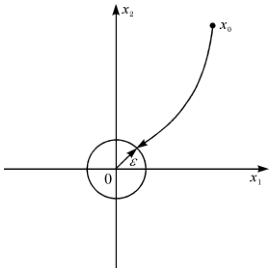
\includegraphics[width=\linewidth]{figs/fig-0149.png}
\caption{图8.4-1}
\end{figure}

\begin{figure}[htbp]\centering
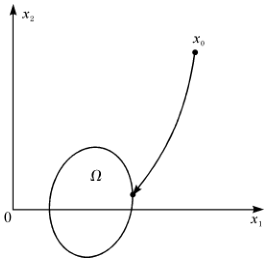
\includegraphics[width=\linewidth]{figs/fig-0150.png}
\caption{图8.4-2}
\end{figure}

此，上述不等式可改写为

\[\begin{aligned}& \left(-\boldsymbol{\Psi}_{0} \cdot \int_{0}^{T} e^{-A t} B u_{0}(t) d t\right)=\int_{0}^{T}\left(-e^{-A t_{i}} \boldsymbol{\Psi}_{0}, B u_{0}(t)\right) d t \\& \geqslant\left\{\boldsymbol{\Psi}_{0}, e^{A T}\left(\boldsymbol{z}-\boldsymbol{z}_{0}\right)-\int_{0}^{T} e^{-A t} B u(t) d t\right\}\end{aligned}\]

不难看出，欲使上式始终成立，自 $\boldsymbol{x}$ 至 $\boldsymbol{z}$ 的控制 $\boldsymbol{u}(t)$ 应满足条件[限制条件式 $(8.0-1)]$

\[\boldsymbol{u}(t)=-\operatorname{sign}\left(B^{x} e^{-A t_{i}} \boldsymbol{\Psi}_{0}\right)\qquad\text{(8.0-1)}\]

或者[限制条件式 $(8.0-2)]$

\[u(t)=-\frac{B_{e}^{-A t_{i}} \boldsymbol{\Psi}_{0}}{\|B_{e}^{-A t_{i}} \boldsymbol{\Psi}_{0}\|}\]

换言之，上面式 $(8.4-4 \mathrm{a})$ 对应 $\mathrm{A}$ 型限制，而 $(8.4-4 \mathrm{~b})$ 对应 $\mathrm{B}$ 型限制条件。这里我们得到了与前节自点至点最速控制的类似形式。

另外，$G(\Omega, T)$ 的单调扩张性这一概念对我们很重要。因为条件式 $(8.4-3)$ 仅仅是最速控制的必要条件，因此，一切最速控制只能具有式 $(8.4-4 \mathrm{a})$ 和 $(8.4-4 \mathrm{~b})$ 的形式。但是一般说来，一切具有此种形式的控制却不一定都是最速控制。当然，如果通过分析后确信只有一个具有式 $(8.4-4)$ 形式的将 $\boldsymbol{x}$ 引至 $\Omega$ 的控制，那么，它当然是最速控制了。有时这种控制有很多个，那么，就需要从一切满足条件式 $(8.4-4)$ 的控制中选出过渡时间最短者。这样问题就变得比较复杂。只有在等时区 $G(\Omega, T)$ 是单调严格扩张时 （对 $T$ )，一切式 $(8.4-4)$ 形的控制函数都是将 $G(\Omega, T)$ 的边界点 $\boldsymbol{x}$ 引至 $\Omega$ 的控制，因此它必是最速控制。这时式 $(8.4-4 \mathrm{a})$ 和 $(8.4-4 \mathrm{~b})$ 既是最速控制的必要条件也是最速控制的充分条件。由于等时区的连续性和凸性，可以推知，最速控制如果存在的话，则必是唯一的。于是，当等时区 $G(\Omega, T)$ 单调扩张时，设计问题就简单得多了。只要能找到一个满足条件式 $(8.4-4)$ 的控制，它必是唯一的，且一定是最速控制。

既然等时区的单调扩张性这样重要，这里需要指出等时区单调扩张的两个充分条件。设 $z$ 是 $\Omega$ 的边界 $S$ 上的任一点，$\operatorname{grad} g(\boldsymbol{z})$ 是过 $\boldsymbol{z}$ 点 $S$ 的支面的外法向量。若对 $S$ 上的每一点 $\boldsymbol{z}$ 均能找到一个控制向量 $\boldsymbol{u} \in U$ （它不取值于 $U$ 的边界），使下列两式之一成立

\[\begin{aligned}& \left(-\operatorname{grad} g(\boldsymbol{z}), A \boldsymbol{z}+B \boldsymbol{u}\right)>0 \\& A \boldsymbol{z}+B \boldsymbol{u}=0\end{aligned}\qquad\text{(8.4-6)}\]

那么，等时区 $G(\Omega, T)$ 对 $T$ 单调扩张。

条件式 $(8.4-5)$ 和 $(8.4-6)$ 的几何意义是极其明显的。如果终点状态 $\Omega, G$ 控量值域 $U$ 满足条件式 $(8.4-6)$，那么，$\Omega$ 的边界 $S$ 上的任何点，都可以成为系统的平衡点。根据第 8.2 节的讨论可知，此时 $\boldsymbol{z}$ 的等时区 $G(\boldsymbol{z}, \boldsymbol{T})$ 是单调扩张的，故

G(Ω，T)对T单调扩张。另一方面，若Ω和U满足条件式(8.4-5)，则Ω内必有系统的平衡点，即存在u(t)，使x(t)自边界S上的任一点出发，将永远停留在Ω内，而不会逸出界外。于是，当T2>T时必有G(Ω，T1)G(Ω，T2)。设x是G(Ω，T)的边界点，u(t)是自x至zΩ的某一控制，且u(T)=u满足条件式(8.4-5)。根据常微分方程的解对初始条件的连续依赖性，x附近必存在一个以x为中心的小球，其中的每一点都可以用u(t)引至z附近的球体S(z，δ)之中，δ为小球的半径。再根据条件式(8.4-5)可知，离Ω的边界S足够近的点均能用某一控制引至Ω，这是因为式(8.4-5)不等式的左端函数对z和u是连续的。于是，靠x足够近的一切点都能用某一控制在T+△T的时间内引至Ω，这就说明了G(Ω，T)对T是单调扩张的。这两个充分条件的严格证明可参看文献[5]。

介绍了单调性条件后，我们继续研究最速控制规律式(8.4-4)。下面的讨论总是假定等时区是单调扩张的。当然这不是一个完全必要的条件，在这个条件不满足时，下面所介绍的计算方法仍然可以使用，但在使用时必须要做其他辅助性的检验计算。可以看出，式(8.4-4)的右端eA5TΦ0是式(8.2-1)的共轭方程式

\[\frac{d \Psi}{d t}=-A^{t} \Psi, \quad \Psi(0)=\Psi_{0}\qquad\text{(8.4-7)}\]

的解。由此可知，自G(Ω，T)边界上的任何点x在T时间内到达Ω的控制u(t)必为最速控制u(t)。

再研究z与Φ0的关系。我们知道，若Φ0是G(Ω，T)过x点的支面的外法向量，那么，式(8.4-7)的解Ψ(t)在t<T时刻的向量Φ(t)是等时区G(Ω，t)过x(t)，x(0)=x，点支面的外法向量。当t=0时，G(Ω，0)=Ω。而eA5TΦ0=Ψ(T)是G(Ω，0)即Ω过x(T)点支面的外法向量。从这里可以看出一个重要事实：若在z点上，式(8.4-1)中的函数g(z)为光滑，而梯度向量gradg(z)z=0=gradg(z)z=0不为零向量，则必有

\[e^{-A^{5} T} \Psi_{0}=a \operatorname{grad} g(z)\qquad\text{(8.4-8)}\]

式中a为某一正常数。换言之，向量eA5TΦ0与向量gradg(z)方向相同，自式(8.4-8)解出Φ0得

\[\Psi_{0}=a e^{A^{5} T} \operatorname{grad} g(z)\qquad\text{(8.4-9)}\]

由此可知，向量Φ0由最速轨迹x(t)的终点z0所唯一确定。从而，最速控制u(t)也为z0点所唯一决定。

既然自x至z的最速控制为式(8.4-4a)或(8.4-4b)，那么，G(Ω，T)必为严格凸。读者不难证明，若x和x0位于G(Ω，T)的边界，那么，二者连线上的任何点x均位于G(Ω，T)的内部，证明过程几乎完全重复第8.2节中有关的讨论。

\[\frac{d \mathbf{y}}{d t}=-A \mathbf{y}-B \mathbf{u}\qquad\text{(8.4-10)}\]

引进符号

对 A 型限制对 B 型限制

则逆运动方程(8.4-10)的解是

\[y(t, z)=e^{-A t} z-e^{-A t} \int_{0}^{t} e^{A t} B u(\tau, z) d \tau\qquad\text{(8.4-12)}\]

如果对给定的 $\boldsymbol{x}$ 能找到一个点 $\boldsymbol{z}_{0}$，使 $\mathbf{y}(t, \boldsymbol{z}_{0})$ 通过 $\boldsymbol{x}_{0}$ 点，那么，相应的 $u(t, z)$ 便是 $\mathbf{y}(t)$ 自 $\Omega$ 达 $\boldsymbol{x}_{0}$ 的最速控制。

为了求出自 $\Omega$ 至 $\boldsymbol{x}_{0}$ 的最速控制函数，我们还采用逐步逼近法。先任意给定一个 $z_{1}$，求出 $\operatorname{grad} g(z)$，作为式 $(8.4-10)$ 和 $(8.4-11)$ 的初始条件，做函数

F(t, z)=(x\_0-y(t-z), e\textasciicircum{}A\textasciicircum{}T\_1.\$ grad \$g(z))

令 $z=z_{1}$，并设所选择的 $z$ 使 $\left(x-z, \operatorname{grad} g(z)\right)>0$。利用条件式 $(8.4-3)$ 不难证明，$F(t)$ 是单调递减函数，在某一 $t=t_{0}$ 时 $F=0$。利用式 $(8.4-13) F=0$ 的条件确定 $t$ 的最小根 $t_{0}$。由于 $\mathbf{y}(t, z)$ 的特有性质，满足 $F(t, z)=0$ 的 $\mathbf{y}(t)$ 必位于等时区 $G(\Omega$，$t)$ 的边界上，而向量 $e^{A^{T_{1}}}$ grad $g(z)$ 是过 $\mathbf{y}(t)$ 点等时区支面的外法向量。条件

F(t, z)=(x-y(t, z), e\textasciicircum{}A\textasciicircum{}T\_1.\$ grad \$g(z))=0(8.4-13)

的几何意义是向量 $x-y(t, z)$ 和 $e^{A^{T_{1}}}$ grad $g(z)$ 直交。由于等时区 $G(\Omega, T)$ 是凸的且严格扩张的，只有当 $\boldsymbol{\Psi}_{1}=e^{A^{T_{1}}} \operatorname{grad} g(z)=\boldsymbol{\Psi}_{0}$，即 $\boldsymbol{\Psi}_{1}$ 为等时区 $G(\Omega, T)$ 过 $x_{0}$ 点的外法向量 $\boldsymbol{\Psi}_{0}$ 时，式 $(8.4-14)$ 的根 $t=T$ 为最大。或者说，对一切基于 $\boldsymbol{\Psi}$ 的向量 $\boldsymbol{\Psi}_{1}$ 所确定的

\[F=\left(x-y(t, z), \boldsymbol{\Psi}_{1}\right)=0\]

的根 $t$ 均小于 $T$。因此，决定最速控制的初始点 $z \in S$ 应该满足条件

\[T_{0}(x)=\max _{z \in S} t(x, z)\qquad\text{(8.4-15)}\]

式中，$t(x, z)$ 为方程式 $(8.4-14)$ 的根，当然它也是 $x$ 和初始点 $z$ 的连续函数。

现在我们用逐步逼近法求式 $(8.4-15) z=z_{0}$ 的解。为此，先任意给出 $z \in S$，根据函数 $g(z)$ 求出 $\operatorname{grad} g(z)$，代入式 $(8.4-4)$，得到最速控制 $u(t, z)$。再将 $u(t$，$z)$ 代入式 $(8.4-12)$ 解出 $\mathbf{y}(t, z)$; 然后构成函数 $F(t, z)$，求解 $F=0$ 的根 $t=t_{0}$。如果 $\mathbf{y}(t, z)=\boldsymbol{x}$，那么，最速控制 $\dot{u}(t)$ 便已经找到了。如果 $\mathbf{y}(t, z) \neq \boldsymbol{x}$，则需找其他的点 $z$，使 $\mathbf{y}(t, z)$ 更逼近于 $x$ 点。 $z$ 的选择可按下列方法进行：记 $e^{A^{T_{1}}}$

grad $g\left(z_{1}\right)=\boldsymbol{\psi}_{1}$，则有

\[F\left(t, \boldsymbol{\psi}_{1}\right)=\left(\boldsymbol{x}_{0}-\boldsymbol{y}\left(t, \boldsymbol{\psi}_{1}\right), \boldsymbol{\psi}_{1}\right) \geqslant 0\qquad\text{(8.4-16)}\]

式中 $\boldsymbol{\psi}_{1}$ 为等时区 $G(\Omega, t)$ 过 $y\left(t, \boldsymbol{\psi}_{1}\right)$ 点的外法向量。求 $F$ 对各分量 $\psi_{i}$ 的偏导数，并利用关系式

\[\frac{\partial}{\partial \psi_{i}}\left(\boldsymbol{y}\left(t, \boldsymbol{\psi}_{1}\right), \boldsymbol{\psi}_{1}\right)=y_{i}\left(t, \boldsymbol{\psi}_{1}\right)\]

则得到

\[\operatorname{grad} h=\left.\left(\frac{d \boldsymbol{y}\left(t, \boldsymbol{\psi}_{1}\right)}{d t}, \boldsymbol{\psi}_{1}\right)^{-1}\left(\boldsymbol{x}-\boldsymbol{y}\left(t, \boldsymbol{\psi}_{1}\right)\right) \right.\qquad\text{(8.4-17)}\]

由于 $\left.\left.\frac{d \boldsymbol{y}\left(t, \boldsymbol{\psi}_{1}\right)}{d t}, \boldsymbol{\psi}_{1}\right\rangle>0\right.$，故上式内向量 grad $h$ 只有在 $\boldsymbol{x}=\boldsymbol{y}\left(t, \boldsymbol{\psi}_{1}\right)$ 时为零。因此，作为第二步逼近，可取

\[\boldsymbol{\psi}_{2}=\boldsymbol{\psi}_{1}+K_{1} \operatorname{grad} h=\boldsymbol{\psi}_{1}+K_{1}\left(\boldsymbol{x}_{0}-\boldsymbol{y}\left(t, \boldsymbol{\psi}_{1}\right)\right)\]

其中，$\boldsymbol{\psi}_{1}=e^{A_{1} t_{1}} \operatorname{grad} g\left(\boldsymbol{z}_{1}\right)$。上式两端乘以 $e^{-A_{1} t_{1}}$ 后有

\[e^{-A_{1} t_{1}} \boldsymbol{\psi}_{2}=\operatorname{grad} g\left(\boldsymbol{z}_{2}\right)=\operatorname{grad} g\left(\boldsymbol{z}_{1}\right)+K_{1} e^{-A_{1} t_{1}}\left(\boldsymbol{x}_{0}-\boldsymbol{y}\left(t, \boldsymbol{\psi}_{1}\right)\right)\qquad\text{(8.4-18)}\]

上式右端第二项为已知向量，而第一项中的 $\boldsymbol{z}_{1}$ 也为已知，故 $\boldsymbol{z}_{2}$ 可从下式内求出

\[g(\boldsymbol{z})=0, \quad\left.\frac{\partial g(\boldsymbol{z})}{\partial \boldsymbol{z}_{i}}=\left.\frac{\partial g(\boldsymbol{z})}{\partial\left(\boldsymbol{z}_{i}\right)}\right|_{z=z_{1}}+K_{1} h_{i}(t)\right)\qquad\text{(8.4-19)}\]

这里 $h_{i}(t)$ 为向量 $e^{-A_{1} t_{1}}\left(\boldsymbol{x}-\boldsymbol{y}\left(t, \boldsymbol{\psi}_{1}\right)\right)$ 的第 $i$ 个分量。用 $\boldsymbol{z}_{2}$ 和 $\operatorname{grad} g\left(\boldsymbol{z}_{2}\right)$ 代入式 (8.4-10) 和 (8.4-11)，求出 $\boldsymbol{y}\left(t, \boldsymbol{z}_{2}\right)$，再从式 (8.4-14) 内求出 $\boldsymbol{t}$。如果 $\boldsymbol{y}\left(t, \boldsymbol{z}_{2}\right) \neq$ $\boldsymbol{x}$，或者 $\|\boldsymbol{x}-\boldsymbol{y}\left(t, \boldsymbol{z}_{2}\right)\|$ 仍为足够大时，上述程序可继续进行。这样，经过数步后，计算过程将较为迅速地向 $\boldsymbol{z}_{2}$ 收敛。

\section{8.5 控制装置的综合}

前面几节内讨论的是自给定点至原点或至给定区域的最速控制函数的求解方法。正如前面曾指出的那样，这种设计方法只适用于初始状态为已知的一次使用的控制系统。如果系统的初始状态是任意的，而控制装置的任务是要对系统任意的初始状态 $\boldsymbol{x}$ 自动算出最速控制函数 $u(\boldsymbol{x})$，若将这一函数代入式 (8.2-1)，使其变为自治系统

\[\frac{d \boldsymbol{x}}{d t}=A \boldsymbol{x}+B u(\boldsymbol{x})\qquad\text{(8.5-1)}\]

无论初始状态为何，式 (8.5-1) 的解总是自初始条件 $\boldsymbol{x}$ 至原点或给定终点区域 $\Omega$ 的最速轨迹。换句话说，设计最速控制装置的任务是找出一个 $r$ 维向量函数 $u(\boldsymbol{x})=\left(u(\boldsymbol{x}), \cdots, u(\boldsymbol{x})\right)$，并在技术上实现它，用这种规律构成的控制装置，将保证系统的任何运动均是最速运动。当然，函数 $u(\boldsymbol{x})$ 的取值必须满足限制条件 $u \in U$。

事实上，本章第一节内介绍过的布绍的方法正是解决控制装置综合的方法。那里借助相平面的图解工具找出了这个最速控制函数 $u(\boldsymbol{x})$。在本节内，我们希望建立一个普遍的方法，使其不仅适用于二阶系统，而且适用于高阶系统，不用纯粹图解法，而采用解析方法。初看起来，前面几节内的讨论似乎可以应用到控制装置综合中来，只要对可能出现的各种初始误差 $\boldsymbol{x}$，求出相应的最速控制函数就可以了。其实，问题完全不是这样。首先，对绝大多数系统（特别是伺服系统）来说，可能的初始条件不是几个或几十个，而是整个 $n$ 维区域，要想对每一个点都进行计算是不可能的。退一步讲，即便每一个初始状态所对应的最速控制函数都已经找到，也难以在一个简单的电的或机械的装置里实现。因此，前几节内的方法，不太适合于解决控制装置的综合问题。设计最速控制装置，必须另找出路。

为了讨论上的方便，我们假定受控系统的可允许的终点状态不是一个点，而是一个区域 $\Omega$。若 $\Omega$ 只包含一个孤立点，例如原点，那么，就变为至原点的最速控制了。我们还假定区域 $\Omega$ 和控制量的取值区域 $U$ 满足下列条件:(1) $\Omega$ 的等时区是单调扩张的，当 $T \rightarrow \infty$，时，等时区与可控区 $M$ 重合。以后的综合问题都将只在可控区 $M$ 讨论;(2)系统是非蜕化的;(3)控制量的取值限制属于 $\mathrm{A}$ 型（见前节），即 $\left|u_{i}\right| \leqslant 1, i=1,2, \cdots, r$。

根据式 (8.4-4a) 可知，在上述假定下最速控制函数的每一个分量 $u$ 在每一个时刻 $t$ 只取 +1 或 -1，且任何最速轨迹不可能有自交点。因此，最速控制的综合问题可以归结为对每一 $u$ 把可控区分成两个部分 $M_{i}^{+}$和 $M_{i}^{-}$，使 $u$ 在 $M_{i}^{+}$中取 $+1$，在 $M_{i}^{-}$中取 -1。用 $M_{i}^{+}$表示 $M_{i}^{+}$和 $M_{i}^{-}$的公共边界。下面将看到，$M_{i}^{+}$是相空间内 $n-1$ 维超曲面，称为系统的关于分量 $u$ 的开关曲面。如果这种区域划分已经完成，则最速控制的综合函数可以写成

\[u(\boldsymbol{x})=\left\{\begin{array}{l} +1, \quad \text { 若 } \boldsymbol{x} \in M_{i}^{+} \\ -1, \quad \text { 若 } \boldsymbol{x} \in M_{i}^{-} \end{array}\right.\]

在最速轨道上控制分量 $u(t)$ 的变号时刻所对应的系统状态 $\boldsymbol{x}$ 称为 $u$ 的开关点。这样，如果对每一个控制分量的上述取值区域都划分完后，最速控制函数的综合问题也就得到了解决。

设 $\boldsymbol{x}$ 为可控区 $M$ 内的任意点，且 $\boldsymbol{x}$ 不属于 $\Omega$，自 $\boldsymbol{x}$ 至 $\Omega$ 的最速过渡时间为 $T$，则自 $\boldsymbol{x}$ 至 $\Omega$ 的最速控制是（参看式 (8.4-11a))

\[u(t)=\operatorname{sign}\left(-B^{e^{-A^{T}(r-T)}} \operatorname{grad} g(\boldsymbol{z})\right)\qquad\text{(8.5-3)}\]

其中 $\boldsymbol{z}$ 为 $\Omega$ 的边界 $S$ 上的某一个点。当 $t=0$ 时有

\[u(\boldsymbol{x})=-\operatorname{sign}\left(B^{r} e^{A^{T} T} \operatorname{grad} g(\boldsymbol{z})\right)\]

根据前节的讨论可知，$\boldsymbol{x}$ 点是等时区 $G(\Omega, T)$ 的边界点，而且 $\boldsymbol{\Psi}=e^{A^{T} T} \operatorname{grad} g(\boldsymbol{z})$ 是过 $\boldsymbol{x}$ 点的 $G(\Omega, T)$ 的外法向量。令 $b$ 是矩阵 $B$ 的第 $i$ 列向量，当外法向量与 $\boldsymbol{b}$ 的数量积为负时，$x \in M_{+}^{i}$; 当 $\boldsymbol{\phi}$ 与 $\boldsymbol{b}_{i}$ 的数量积为正时 $x \in M_{-}^{i}$; 数量积为零时 $x \in M_{0}^{i}$。当 $\boldsymbol{x}$ 为可控区内任意点而属于开关曲面 $M_{0}^{i}$ 时，则 $\boldsymbol{x}$ 必满足下列方程组

\[\begin{aligned}& \boldsymbol{x}=e^{-A T}\left[\boldsymbol{z}+\int_{0}^{T} e^{A t} B \operatorname{sign}\left(B^{r} e^{A s_{i}} \operatorname{grad} g(\boldsymbol{z}) d t\right)\right. \\& \left.\left(\operatorname{grad} g(\boldsymbol{z}), e^{A T} \boldsymbol{b}_{i}\right)=0, \quad g(\boldsymbol{z})=0\right.\end{aligned}\qquad\text{(8.5-4)}\]

现让 $T$ 在 $[0, \infty)$ 内变化，则可以找到 $u$ 的开关曲面的参数表达式为

\[\begin{aligned}& \boldsymbol{x}=e^{-A t}\left[\boldsymbol{z}+\int_{0}^{t} e^{A s} B \operatorname{sign}\left(B^{r} e^{A s_{i}} \operatorname{grad} g(\boldsymbol{z})\right) d s\right] \\& \left(\operatorname{grad} g(\boldsymbol{z}), e^{A t} \boldsymbol{b}_{i}\right)=0, \quad g(\boldsymbol{z})=0\end{aligned}\qquad\text{(8.5-5)}\]

上面共有 $n+2$ 个方程式，独立变数只有 $n-1$ 个。自第一式内消掉两个自由变量后，它就变成了含有 $n-1$ 个自由变量的开关曲面参数表达式。当 $n=2$ 时，即受控对象的方程式是二阶时，应用表达式 (8.5-5) 可以很方便地求出开关曲线。这样，在第 8.1 节内布绍曾研究过的一些特例中均可用这个参数表达式导出开关曲线。

若终点区域 $\Omega$ 只包含一个点 $\boldsymbol{x}_{0}$ 时 $(\boldsymbol{x})$ 可以不是原点，但满足等时区单调扩张的条件），上列参数表达式可写为

\[\begin{aligned}& \boldsymbol{x}=e^{-A t}\left[\boldsymbol{x}_{0}+\int_{0}^{t} e^{A s} B \operatorname{sign}\left(B^{r} e^{A s_{i}} \boldsymbol{\Psi}_{0}\right) d s\right] \\& \left(\boldsymbol{\Psi}_{0}, e^{A t} \boldsymbol{b}_{i}\right)=0, \quad\left\|\boldsymbol{\Psi}_{0}\right\|=1, \quad 0 \leqslant t<\infty\end{aligned}\qquad\text{(8.5-6)}\]

于是，我们就得到了求开关曲面的一种普遍方法。

现在再介绍另一种综合方法。这个方法是以等时区的一些几何特性为依据的。设可控区 $M$ 内任一点 $\boldsymbol{x}$ 到达 $\Omega$ 的最速过渡时间是 $T(\boldsymbol{x})$，由于最速控制的唯一性可知 $n$ 元函数 $T(\boldsymbol{x})$ 是非负的单值函数，它只在 $\Omega$ 上等于零。可以证明，函数 $T(\boldsymbol{x})$ 在可控区内除在诸开关曲面 $M_{i}^{i}, i=1,2, \cdots, r$，上的点外，在其他点上都是可微函数 ${ }^{[5]}$。当 $T_{0}$ 为大于零的常数时，方程式 $T(\boldsymbol{x})=T_{0}$ 决定一个 $n-1$ 维的封闭曲面，它正是等时区 $G(\Omega, T_{0})$ 的边界曲面。因此 $\operatorname{grad} T(\boldsymbol{x}) \mid_{r=T_{0}}$ 是等时区 $G(\Omega, T_{0})$ 的过边界点 $\boldsymbol{x}$ 的外法向量。根据式 (8.4-4a) 知，此时最速控制必为

\[u(\boldsymbol{x})=-\operatorname{sign}\left(B^{r} \operatorname{grad} T(\boldsymbol{x})\right)\qquad\text{(8.5-7)}\]

或

\[u(\boldsymbol{x})=-\operatorname{sign}(\operatorname{grad} T(\boldsymbol{x}), \boldsymbol{b}_{i})\]

由此可知，若能求出最速过渡时间函数 $T(\boldsymbol{x})$，那么，最速控制函数的综合问题就按式 (8.5-7) 完全解决。如何求出函数 $T(\boldsymbol{x})$ 呢？从物理概念可以推知，如果 $T(\boldsymbol{x})$是可微函数，那么，$T$ 对时间 $t$ 的全导数应恒等于 $-1$。于是可以写出方程式

\[\frac{d T}{d t}=\sum_{i=1}^{n} \frac{\partial T}{\partial x_{i}} \frac{d x_{i}}{d t}=(\operatorname{grad} T(\boldsymbol{x}), A \boldsymbol{x}+\boldsymbol{b} \dot{u})=-1\qquad\text{(8.5-8)}\]

式中 $\boldsymbol{u}$ 是最速控制函数，因此，它的每个分量只取 $\pm 1$。方程式 (8.5-8) 是关于 $T$的一阶偏微分方程，它的边界条件是在 $\Omega$ 的边界 $S$ 上为零，即

\[T(\boldsymbol{x}) \mid_{1}=0\]

方程式 (8.5-8) 和 (8.5-9) 联合起来便得到偏微分方程中的柯西问题。它的求解方法可按下列方法进行:

欲从式 (8.5-8) 求解 $T(\boldsymbol{x})$ 必须先确定 $\dot{u}$ 的值。根据最速控制的特点，在 $\Omega$ 的边界 $S$ 上的 $\dot{u}$ 的值可以完全确定，即

\[\dot{u}=-\operatorname{sign}\left(B^{r} \operatorname{grad}(\boldsymbol{z})\right)\qquad\text{(8.5-10)}\]

式中 $\boldsymbol{z}$ 为 $S$ 上的点。用关系式 $\left(\operatorname{grad} g(\boldsymbol{z}), \boldsymbol{b}_{i}\right)=0, i=1,2, \cdots, r$，将曲面 $S$ 分为 $2^{r}$个不相重合的部分 $S_{1}, S_{2}, \cdots, S_{2^{r}}$。在每一个 $S_{k}$ 上 $\dot{u}(\boldsymbol{x})$ 的值由式 (8.5-10) 完全确定。于是柯西问题

\[\begin{gathered} \left(\operatorname{grad} T(\boldsymbol{x}), \boldsymbol{A x}+B \operatorname{sign}(-\operatorname{grad} g(\boldsymbol{z}))\right)=-1 \\ T(\boldsymbol{x}) \mid_{s_{k}}=0 \end{gathered}\qquad\text{(8.5-11)}\]

有唯一解。再将此解 $T(\boldsymbol{x})$ 自 $S_{k}$ 沿方程组

\[\frac{d \boldsymbol{x}}{d t}=-\boldsymbol{A} \boldsymbol{x}-B \dot{\boldsymbol{u}}\]

的积分曲线向 $t$ 增加的方向延拓，直到对某一个 $j$，使

\[\left(\operatorname{grad} T(\boldsymbol{x}), \boldsymbol{b}_{j}\right)=0\qquad\text{(8.5-12)}\]

为止，然后以 $\left(\operatorname{grad} T(\boldsymbol{x}), \boldsymbol{b}_{j}\right)=0$ 所确定的曲面为定解曲面，再解方程式

\[\left(\operatorname{grad} T(\boldsymbol{x}), \boldsymbol{A x}+B \dot{\boldsymbol{u}}_{m}\right)=-1\]

其中 $\dot{u}_{m}$ 与式 (8.5-11) 中的控制只差第 $j$ 个分量的符号。式 (8.5-12) 所确定的曲面就是开关曲面 $M_{j}^{0}$ 的一部分。这样继续进行便可以求出全部 $T(\boldsymbol{x})$。

总结上述讨论，用相空间坐标表示的最速控制为式 (8.5-7)，而关于 $u$ 的开关曲面 $M_{j}^{0}$ 由方程式

\[\left(\operatorname{grad} T(\boldsymbol{x}), \boldsymbol{b}_{i}\right)=0\qquad\text{(8.5-13)}\]

所确定。显然，它是 $n-1$ 维分片光滑的 $n-1$ 维超曲面。这样，常系数线性受控系统的最速控制装置的设计问题就得到了解决。

现举例说明如何利用后一个方法去综合一个最速控制函数。设受控对象的传递函数为 （见图 8.5-1)

\[\begin{array}{ll} \text { 最速控制器 } & \frac{1}{s^{2}} \\ \end{array}\]

图 8.5-1

\[F(s)=\frac{1}{s}\qquad\text{(8.5-14)}\]

\begin{figure}[htbp]\centering
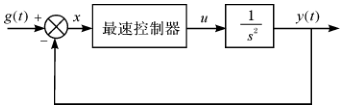
\includegraphics[width=\linewidth]{figs/fig-0151.png}
\caption{图8.5-1}
\end{figure}

输入作用为 $g(t)=g_{0}+g_{1} t$。引入坐标 $y_{1}=y, \frac{d y}{d t}=y_{2}, g(t)-y_{1}=x_{1}, \frac{d x_{1}}{d t}=x_{2}$; 那么，受控对象的误差方程组可写为

\[\frac{d x_{1}}{d t}=x_{2}, \quad \frac{d x_{2}}{d t}=u, \quad|u| \leqslant 1\qquad\text{(8.5-15)}\]

设终点状态 $\Omega$ 为以原点为中心，以 $\rho$ 为半径的圆，它由不等式

\[g\left(x_{1}, x_{2}\right)=x_{1}^{2}+x_{2}^{2}-\rho^{2} \leqslant 0\qquad\text{(8.5-16)}\]

所确定。不难检验，系统式 (8.5-15) 的可控区是整个相平面，即相平面的任何一点 $\boldsymbol{x}$ 均可以用用可准控制引至 $\Omega$，其次，若 $\rho<1$ 时，$\Omega$ 的等时区 $G(\Omega, T)$ 为单调扩张。因为此时单调性条件式 (8.4-5) 得到满足。因此不等式

\[\left(\operatorname{grad} g(\boldsymbol{x}), A \boldsymbol{x}+\boldsymbol{b} u\right)=2 x_{1} x_{2}+2 x_{2} u>0\]

总可以成立，注意到 $|x|<1$，只要取 $2 x_{2} u>2 x_{1} x_{2}$ 即可。由于 $\operatorname{grad} g(\boldsymbol{x})=(2 \boldsymbol{x}$，$2 \boldsymbol{x})$，故在上半圆周上最速控制 $u=-1$，在下半圆周上 $u=+1$。将此值代入式 (8.5-11) 后，对上半平面有偏微分方程

\[\frac{\partial T}{\partial x_{1}} x_{2}-\frac{\partial T}{\partial x_{2}}+1=0, \quad T\left(x_{1}, x_{2}\right) \mid x_{1}^{2}+x_{2}^{2}-\rho^{2}=0\qquad\text{(8.5-17)}\]

解上述柯西问题得

\[T\left(x_{1}, x_{2}\right)=x_{2}-\left[2 \sqrt{\rho^{2}+1-2\left(x_{1}+\frac{1}{2} x_{2}^{2}\right)-2\left(1-x_{1}-\frac{1}{2} x_{2}^{2}\right)}\right]\qquad\text{(8.5-18)}\]

下半平面内的 $T$ 函数与此斜对称，故 $u$ 的开关曲面为方程式 $\frac{\partial T}{\partial x_{2}}=0$ 所确定，如图 8.5-2 所示。于是，整个相平面被两个斜对称曲线 $M^{\rho}$ 和圆周分为两个部分 $M^{+}$和 $M^{-}$，最速控制函数可写为下列形式

\[u\left(x_{1}, x_{2}\right)= \begin{cases}+1, & \text { 若 } \boldsymbol{x} \in M^{+} \\ -1, & \text { 若 } \boldsymbol{x} \in M^{-}\end{cases}\qquad\text{(8.5-19)}\]

按此式所构成的最速控制系统的方块图示于图 8.5-1 中。图中的最速控制器的作用是实现函数式 (8.5-19)。这个系统对任何 $g(t)=$ $g_{0}+g_{1} t$ 类型的输入作用，$g_{0}$ 和 $g_{1}$ 为任意常数，从任何初始状态出发，均以最短时间使误差 $x_{1}, x_{2}$ 趋向圆 $\Omega$。容易看出，当 $\rho \rightarrow 0$ 时，表达式 (8.5-18) 就变为自任何点至原点的最速过渡时间函数。由此求出的最速控制式 (8.5-19) 就变为自任意点至原点的最速控制了。

\begin{figure}[htbp]\centering
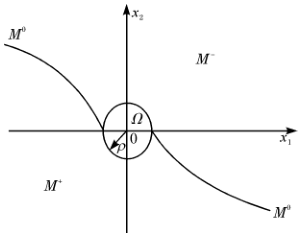
\includegraphics[width=\linewidth]{figs/fig-0152.png}
\caption{图8.5-2}
\end{figure}

\[\begin{gathered} \text { 前面几节内的讨论中,我们总假定受控对象的运动方程式是线性常系数的。 } \\ \text { 这一个假定只是为了讨论时方便,而不是问题的本质所需要的。相反,前面几节 } \\ \text { 内的一切讨论均适用于变系数系统,只要在各公式中做适当的变化就行了 }^{[6,14]} \text { 。 } \\ \text { 变系数系统在实际工程中十分常见。例如,飞机的控制,火箭弹道的控制都要处 } \\ \text { 理变系数方程组。因此,我们在本节内将扼要地讨论当方程式是变系数时,如何 } \\ \text { 改变前面几节内的讨论,使之适用于这种情况。 } \end{gathered}\qquad\text{(8.6-1)}\]

研究方程式

\[a_{u}(t)=\frac{d^{p} x}{d t^{n}}+a_{n-1}(t) \frac{d^{n-1} x}{d t^{n-1}}+\cdots+a(t) x=u\qquad\text{(8.6-2)}\]

或者方程组

\[\frac{d \boldsymbol{x}}{d t}=A(t) \boldsymbol{x}+B(t) \boldsymbol{u}\qquad\text{(8.6-3)}\]

式中 $A(t)$ 为 $n \times n$ 阶矩阵，其元素 $a_{i j}(t)$ 为时间 $t$ 的连续函数; $B(t)$ 为 $n \times r$ 阶方矩阵，其诸元素 $b_{i j}(t)$ 也是时间 $t$ 的连续函数。像过去曾指出过的那样，方程式 (8.6-1) 总可以化成一阶方程组 (8.6-2)。所以我们以后只研究后者。设矩阵 $\Phi(b, t)$ 是方程组 (8.6-2) 的齐次方程的解

\[\frac{d \Phi}{d t}=A(t) \Phi, \quad \Phi(b, b)=E\qquad\text{(8.6-4)}\]

式中 $E$ 为单位矩阵。我们称 $\Phi(b, t)$ 为式 (8.6-3) 的基本解矩阵。利用 $\Phi$，式 (8.6-2) 的通解可以写成

\[\boldsymbol{x}(t)=\Phi(b, t)\left[\boldsymbol{x}_{0}+\int_{t_{0}}^{t} \Phi^{-1}(b, \tau) B(\tau) \boldsymbol{u}(\tau) d \tau\right]\]

这里 $\boldsymbol{x}$ 为系统的初始状态。与式 (8.2-4) 比较即可看出，如果用 $\Phi(b, t)$ 代替 $e^{A t}$后，式 (8.6-4) 与 (8.2-4) 类似。唯一的区别是积分下界不同，这是变系数系统的重要特点，即初始运动的时间 $b$ 必须给定，否则初始条件无意义。

至于对控制量 $\boldsymbol{u}$ 的限制条件依然假定为第 8.5 节内的 A 型和 B 型两种。设终点状态为原点。在时刻 $b$ 开始运动，在 $b+T$ 时刻能到达原点的初始点的全体称为关于原点的 $T$ 等时区，用符号 $G_{0}(T)$ 表示。如果系统式 (8.6-2) 为完全能控的系统，那么，重复第 8.2 节内的讨论，可以证明，当 $T>0$ 时，$G_{0}(T)$ 为 $n$ 维凸性区域。系统的完全能控条件这里变为每组向量: $\boldsymbol{b}_{k}(t)=\boldsymbol{b}_{k}^{(1)}(t), \boldsymbol{b}_{k}^{(k)}(t), k=2$，$3, \cdots, n$，在任何时刻为线性不相关，$\boldsymbol{b}_{k}^{(k)}(t)=A(t) \boldsymbol{b}_{k}^{(k-1)}(t)+\frac{d}{d t} \boldsymbol{b}_{k}^{(k-1)}(t)$。这个条件一般是难以检查的，但是在实践中受控对象通常都是完全能控的，例如方程式

\section{8.6 变系数系统的综合}

(8.6-1)无论系数 $a_{i}(t)$ 是什么函数，系统都是完全能控的。因此，对一般工程系统这个条件总是能满足的。

对于满足完全能控条件的系统，如果控制量受 A 型限制，则任何最速控制也必是开关控制。利用第 8.2 节内的证明方法可以算出自 $\boldsymbol{x}$ 点到达原点的最速控制为

\[\dot{u}(t, \boldsymbol{\Psi})=\left\{\begin{array}{l}\operatorname{sign}\left(B^{r}(t) \boldsymbol{\Psi}(t)\right), \quad \text { 若 } \boldsymbol{u} \text { 是 A 型限制 } \\ \frac{B^{r}(t) \boldsymbol{\Psi}(t)}{\left\|\boldsymbol{B}^{r}(t) \boldsymbol{\Psi}(t)\right\|}, \quad \text { 若 } \boldsymbol{u} \text { 是 B 型限制 }\end{array}\right.\qquad\text{(8.6-5)}\]

这里 $\boldsymbol{\Psi}(t)$ 是下列方程的解:

\[\frac{d \boldsymbol{\Psi}}{d t}=-\boldsymbol{A}^{r}(t) \boldsymbol{\Psi}, \quad \boldsymbol{\Psi}(b)=-\boldsymbol{\Psi}_{0}\qquad\text{(8.6-6)}\]

$\boldsymbol{\Psi}_{0}$ 是等时区 $G_{10}(T)$ 过其边界点 $\boldsymbol{x}$ 的支面的外法向量。

由于最速控制是式 (8.6-5)型函数，故可推知等时区 $G_{10}(T)$ 是严格凸的并且对 $T$ 单调扩张。自它的任何边界点 $\boldsymbol{x}$ 达到原点的最速过渡时间是 $T_{1}$ 最速控制按式 (8.6-5) 由 $\boldsymbol{x}$ 点的外法向量 $\boldsymbol{\Psi}_{0}$ 单一确定，因此最速控制是唯一的，这些性质可以用类似于第 8.2 节的方法证明。

\begin{figure}[htbp]\centering
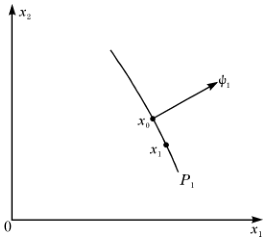
\includegraphics[width=\linewidth]{figs/fig-0153.png}
\caption{图8.6-1}
\end{figure}

设系统的初始条件是 $\boldsymbol{x}$，初始运动时刻是 $t$，现写出来求自 $\boldsymbol{x}$ 至原点的最速控制的逐步逼近公式：过 $\boldsymbol{x}$ 作一任意平面 $P_{1}$，其外法向量是 $\boldsymbol{\Psi}_{1}$，自该平面到达原点的最速控制必为式 (8.6-5)，其中 $\boldsymbol{\Psi}(b)=-\boldsymbol{\Psi}_{1}$ （图 8.6-1)。设 $\boldsymbol{x}$ 为平面 $P_{1}$ 上离原点的“最近点”，且自此点至原点的最速过渡时间为 $t$，那么，在 $t=b+t$ 时，必有关系式

\[\begin{aligned}\left(\boldsymbol{x}(t),\left(\boldsymbol{\Phi}^{r}\left(b, b+t_{b}\right)\right)^{-1} \boldsymbol{\Psi}_{1}\right) & =\left(\boldsymbol{x}(t), \boldsymbol{\Psi}(t)\right) \\& =0\end{aligned}\]

这里利用了这样一个事实: $\left(\boldsymbol{\Phi}\left(b, t\right)\right)^{-1}$ 是共轭方程式 (8.6-6) 的基本解矩阵。因为当 $\boldsymbol{\Psi}_{1}=\boldsymbol{\Psi}_{0}$ 时，式 (8.6-7) 的根为极大，故第二步逼近应取

\[\boldsymbol{\Psi}_{2}=\boldsymbol{\Psi}_{1}+K \operatorname{grad}_{t}=\boldsymbol{\Psi}_{1}+K \Phi^{r}\left(b, b+t_{b}\right) \boldsymbol{x}(t)\qquad\text{(8.6-8)}\]

式中 $K$ 为某一正常数。将 $-\boldsymbol{\Psi}_{2}$ 作为式 (8.6-6) 的新的初始条件，再按式 (8.6-5)构成新的控制函数 $\boldsymbol{u}(t, \boldsymbol{\Psi}_{2})$，并代入式 (8.6-4) 解出运动轨迹为

\[\boldsymbol{x}(t, \boldsymbol{\Psi}_{2})=\Phi\left(b, b_{b}+t\right)\left[\boldsymbol{x}_{0}+\int_{t_{0}}^{t} \Phi^{-1}\left(b, \tau\right) B \boldsymbol{u}(\tau, \boldsymbol{\Psi}_{2}) d \tau\right]\]

再代入式 (8.6-7) 求新根 $t$，依此类推，数步后即可求出自 $\boldsymbol{x}$ 达到原点的最速控制 $\boldsymbol{u}(t, \boldsymbol{\Psi}_{0})$。

自给定点至平面或自给定点至区域 $\Omega$ 的逐步求解方法与第 8.5 节内的讨论基本相同，只需将各式中的基本解矩阵按下列关系置换后即可继续使用

\[\begin{aligned}& e^{A t} \rightarrow \Phi(b, t) \\& e^{-A t} \rightarrow \Phi^{-1}(b, t)=\Phi(t, b) \\& e^{A^{T} t} \rightarrow \Phi^{T}(b, t) \\& e^{-A^{T} t} \rightarrow\left[\Phi^{T}(b, t)\right]^{-1}=\Phi^{T}(t, b)\end{aligned}\]

对变系数系统最速控制装置的综合（设计）要比前节所述方法更为复杂，但原理都是一样的。变系数系统的最速控制装置综合的任务是找出一个 $n+1$ 元函数 $\dot{u}(t, \boldsymbol{x})$，将其代入式 (8.6-2) 后，方程式以任何初始条件和初始时刻开始运动都能以最短时间到达终点状态。最速控制系统的运动方程式将为

\[\frac{d \boldsymbol{x}}{d t}=A(t) \boldsymbol{x}+B(t) \dot{u}(t, \boldsymbol{x})\qquad\text{(8.6-9)}\]

式中 $\dot{u}(t, \boldsymbol{x})=\left(\dot{u}(t, \boldsymbol{x}), \cdots, \dot{u}(t, \boldsymbol{x})\right)$，它的每一个分量均满足给定的限制条件 $A$ 或 $B$。

设控制量受 $\mathrm{A}$ 型限制，试讨论最速控制函数 $\dot{u}(t, \boldsymbol{x})$ 的求解方法。系统的终点状态设为凸性区域 $\Omega, \mathrm{t}$ 它由下列不等式组所确定

\[g_{i}(\boldsymbol{x}) \leqslant 0, \quad i=1,2, \cdots, m\qquad\text{(8.6-10)}\]

$g_{i}(\boldsymbol{x})=0, i=1,2, \cdots, m$，决定 $\Omega$ 的边界 $S$。假定这些函数在 $S$ 上足够光滑，梯度向量 $\operatorname{grad} g_{i}(\boldsymbol{x})$ 处处不为零向量。和前节一样，用符号 $g(\boldsymbol{x})$ 代表 $g_{i}(\boldsymbol{x})$ 的全体。用 $G_{0}(\Omega, T)$ 表示 $t$ 时刻开始运动而在 $t+T$ 时能到达 $\Omega$ 的一切初始点的集合，称为 $T$ 等时区。与常系数系统类似，等时区单调扩张的充分条件是：对任何 $\boldsymbol{z} \in S$ 和 $t \geqslant b$，存在 $u(t)$，后者不在 $U$ 的顶点取值，且使

\[\left(\operatorname{grad} g(\boldsymbol{z}), A(t) \boldsymbol{z}+B(t) \boldsymbol{u}(t)\right)<0\]

或

\[A(t) \boldsymbol{z}+B(t) \boldsymbol{u}(t) \equiv 0\]

将 $t$ 和 $\boldsymbol{x}$ 看成是 $n+1$ 维空间 $R_{n+1}$ 内的点，令 $M(b)$ 是以 $b$ 时刻出发并能到达 $\Omega$ 的一切点的全体，我们称它为关于 $b$ 的可控区。当 $G_{0}(\Omega, T)$ 为单调扩张时，$G_{0}(\Omega, \infty)$ 与 $M(b)$ 相重合。称一切 $M(t), 0 \leqslant t<\infty$ 的总和为变系数系统在 $R_{n+1}$ 内的可控区，用 $M$ 表示。按定义，自 $M$ 中的一切点 $(t, \boldsymbol{x})$ 均能用某一可准控制在有限时间内到达 $\Omega$。以后最速控制函数 $\dot{u}(t, \boldsymbol{x})$ 的综合 （设计） 将在 $M$ 内进行。重复前面的讨论，可以证明，一切自 $G(\Omega, T)$ 的边界点 $(t, \boldsymbol{x})$ 以 $T$ 时间到达 $\Omega$ 的控制只能是最速控制，后者的每一个分量必是开关函数 （对 $\mathrm{A}$ 型限制）。因此，对最速控制函数的综合问题可归结为对每一控制分量 $u_{i}$，在 $R_{n+1}$ 内的可控区 $M$ 中分为两个部分 $M_{+}^{+}$和 $M_{-}^{-}$，使

\[u_{i}(t, \boldsymbol{x})=\left\{\begin{array}{l}+1, \quad \text { 若 }(\boldsymbol{x}, t) \in M_{+}^{+} \\ -1, \quad \text { 若 }(\boldsymbol{x}, t) \in M_{-}^{-}\end{array}\right.\]

\[\dot{u}_{i}(t, \boldsymbol{x})=\left\{\begin{array}{ll} +1, & \text { 若 } \boldsymbol{x} \in M_{i}^{+}(t) \\ -1, & \text { 若 } \boldsymbol{x} \in M_{i}^{-}(t) \end{array}\right.\qquad\text{(8.6-13)}\]

在 $R_{n+1}$ 内 $M_{i}^{+}$和 $M_{i}^{-}$的共同边界是一个 $n$ 维超曲面 $M_{i}^{c}$，称为 $\dot{u}$ 的开关曲面。而在 $R_{n}$ 内 $M_{i}^{+}(t)$ 和 $M_{i}^{-}(t)$ 的共同边界 $M_{i}^{c}(t)$ 是 $n-1$ 维超曲面，后者在相空间内将随时间的变化而连续变动。这是与常系数系统的开关曲面所不同之处，在那里开关曲面是与时间无关的固定超曲面。

由于等时区的凸性和单调扩张性，因此自 $M$ 内的任一点 $(t, \boldsymbol{x})$ 到达 $\Omega$ 的最速控制是唯一的，它由下式所确定:

\[\dot{u}(t)=-\operatorname{sign}\left(B^{i}(t) \Phi^{i}(t+T, t) \operatorname{grad} g(\boldsymbol{z})\right)\qquad\text{(8.6-14)}\]

式中 $T$ 为自 $(t, \boldsymbol{x})$ 到达 $\Omega$ 的最速过渡时间，$z$ 为 $\Omega$ 边界 $S$ 上的某一点。最速过渡时间 $T$ 是初始状态和初始时间 $t$ 的连续函数，写为 $T(t, \boldsymbol{x})$。方程式 $T(t, \boldsymbol{x})=T_{0}$在 $R_{n}$ 内所确定的超曲面正是等时区 $G_{\mathrm{t}}\left(\Omega, T_{0}\right)$ 的边界 $S_{\mathrm{t}}\left(\Omega, T_{0}\right)$。显然，当 $S_{\mathrm{t}}\left(\Omega, T\right)$ 上的过点 $\boldsymbol{x}$ 的外法向量与 $\boldsymbol{b}_{i}(t)$ 的内积为正时，$\boldsymbol{x} \in M_{i}^{+}(t)$; 反之，当外法向量与 $\boldsymbol{b}_{i}(t)$ 的内积为负时，$\boldsymbol{x} \in M_{i}^{-}(t)$。因此，在 $S_{i}\left(\Omega, T\right)$ 的一切边界点上，最速控制可以确定出来:

\[\dot{u}(t, \boldsymbol{x})=\left\{\begin{array}{l} +1, \quad \text { 若 }(\boldsymbol{\Psi}(x, t), \boldsymbol{b}_{i}(t))<0 \\ -1, \quad \text { 若 }(\boldsymbol{\Psi}(x, t), \boldsymbol{b}_{i}(t))>0 \end{array}\right.\qquad\text{(8.6-15)}\]

式中 $\boldsymbol{\Psi}(t, \boldsymbol{x})$ 为 $S_{i}\left(\Omega, T\right)$ 过 $\boldsymbol{x}$ 点的外法向量。如果函数 $T(t, \boldsymbol{x})$ 是可微的，那么，由等时区的单调性可知，向量 $\left(\frac{\partial T}{\partial x_{1}}, \frac{\partial T}{\partial x^{2}}, \cdots, \frac{\partial T}{\partial x_{n}}\right)$ 的方向与 $S_{i}\left(\Omega, T\right)$ 的外法向量 $\boldsymbol{\Psi}(t, \boldsymbol{x})$ 方向相同，即

\[\operatorname{grad}_{\boldsymbol{x}} T(t, \boldsymbol{x})=a \boldsymbol{\Psi}(t, \boldsymbol{x})\qquad\text{(8.6-16)}\]

式中 $a>0$，为一常数。再根据最速控制的特性式 (8.6-14) 知，每一个向量 $\boldsymbol{\Psi}(t, \boldsymbol{x})$必对应 $\Omega$ 的边界 $S$ 上的一个点 $\boldsymbol{z}$，使

\[\boldsymbol{\Psi}(t, \boldsymbol{x})=\Phi^{i}(t, t+T(t, \boldsymbol{x})) \operatorname{grad} g(\boldsymbol{z})\qquad\text{(8.6-17)}\]

于是，$G_{i}\left(\Omega, T\right)$ 的边界 $S_{i}\left(\Omega, T\right)$ 可用下列参数方程组表达出来:

\[\begin{aligned} \boldsymbol{x} & =\Phi(t+T, t)\left[\boldsymbol{z}+\int_{t}^{t+T} \Phi^{-1}(t+T, s) B(s) \operatorname{sign}\left(B^{i}(s) \Phi^{i}(s, t+T)\right.\right. \\ & \left.\left.\cdot \operatorname{grad} g(\boldsymbol{z})\right) d s\right] g(\boldsymbol{z})=0 \end{aligned}\qquad\text{(8.6-18)}\]

而 $\dot{u}$ 的 $n-1$ 维开关曲面的参数表达式为

\[\begin{aligned} \boldsymbol{x} & =\Phi(t+T, t) \boldsymbol{z}+\int_{t}^{t+T} \Phi(s, t) B(s) \operatorname{sign}\left(B^{i}(s) \Phi^{i}(s, t+T)\right) \operatorname{grad} g(\boldsymbol{z}) d s \\ & \left(\Phi^{i}(t, t+T) \operatorname{grad} g(\boldsymbol{z}), \boldsymbol{b}_{i}(t)\right)=0, \quad g(\boldsymbol{z})=0, \quad 0 \leqslant T<\infty \end{aligned}\qquad\text{(8.6-19)}\]

当 $\Omega$ 只含一个孤立点 $\boldsymbol{x}_{0}$ 时，式 (8.6-19)变为

\[\boldsymbol{x}=\boldsymbol{\Phi}(t+T, t) \boldsymbol{x}_{0}+\int_{t}^{t+T} \Phi(s, t) B(s) \operatorname{sign}\left(B^{r}(s) \Phi^{\prime}(s, t+T) \boldsymbol{\Psi}\right) d s\qquad\text{(8.6-20)}\]

前述式 (8.6-19) 仅确定了 $\dot{u}(t, \boldsymbol{x})$ 在 $M_{+}^{0}$和 $M_{-}^{0}$内的值，而在开关曲面 $M_{i}^{0}$ 上的值尚未确定。但是，当最速运动轨迹遇到 $M_{i}^{0}$ 使 $\dot{u}_{i}$ 变号并穿过开关曲面时，$\dot{u}_{i}$ 在 $M_{i}^{0}$上的取值无需单独确定。不能排除最速轨线的一段或全部位于M情况，这时 $\dot{u}_{i}$ 在 $M_{i}^{0}$ 上的取值就必须预先求出。容易证明这时 $\dot{u}_{i}$ 的取值可按下式确定

\[\dot{u}_{i}(t, \boldsymbol{x})=\left\{\begin{array}{cc} +1, & \text { 若 } \frac{d}{d t}\left(\Phi^{\prime}(t, s+T) \operatorname{grad} g(\boldsymbol{z}), \boldsymbol{b}(t)\right) \mid_{s-i}<0 \\ -1, & \text { 若 } \frac{d}{d t}\left(\Phi^{\prime}(t, s+T) \operatorname{grad} g(\boldsymbol{z}), \boldsymbol{b}(t)\right) \mid_{s-i}>0 \end{array}\right.\qquad\text{(8.6-21)}\]

如果 $\frac{d}{d t}\left(\Phi^{\prime}(t, s+T) \operatorname{grad}(\boldsymbol{z}), \boldsymbol{b}(t)\right) \mid_{s-i}=0$ 时，可继续取对 $t$ 的二次导数，而 $\dot{u}_{i}(t, \boldsymbol{x})$ 的取值规律依然可以按式 (8.6-21) 决定。因此，利用参数式 (8.6-19)可以求出变系数线性系统的开关曲面 $M_{i}^{0}(t)$。

例设受控对象的运动方程式是

\[\begin{aligned} & \frac{d x_{1}}{d t}=x_{2}+\left(1+e^{-t}\right) u \\ & \frac{d x_{2}}{d t}=-x_{1}+\left(1+e^{-t}\right) u, \quad|u| \leqslant 1, \quad|w| \leqslant 1 \end{aligned}\qquad\text{(8.6-22)}\]

系统的终点状态设为原点。显然，系统是完全可控的。根据式 (8.6-20)，在相平面上开关曲线的参数表达式为

\[\boldsymbol{x}=\int_{t}^{t+T} \Phi(s, t) B(s) \operatorname{sign}\left(B^{r}(s) \Phi^{\prime}(s, t+T) \boldsymbol{\Psi}\right) d s\qquad\text{(8.6-23)}\]

式中

\[\Phi(t, \tau)=\left(\begin{array}{cc} \cos (\tau-t) & \sin (\tau-t) \\ -\sin (\tau-t) & \cos (\tau-t) \end{array}\right)\]

解式 (8.6-23)之第二式有

\[\begin{aligned} & \boldsymbol{\Psi}_{1}= \pm(\cos T,-\sin T) \\ & \boldsymbol{\Psi}_{2}= \pm(\sin T, \cos T) \end{aligned}\]

于是，开关曲线上的点由下列参数式表示

\[\boldsymbol{x}=\int_{0}^{T}\left(\begin{array}{cc} \cos T & -\sin T \\ \sin T & \cos T \end{array}\right)\left(\begin{array}{c} \operatorname{sign} \cos \tau \\ -\operatorname{sign} \sin \tau \end{array}\right)\left(1+e^{-\tau}\right) d \tau\]

在区间 $\frac{n \pi}{2} \leqslant T \leqslant \frac{n+1}{2} \pi$ 内积分上式

\[\mathbf{x}=\left(\begin{array}{c}(2 n+1)+e^{-t} \sum_{i=0}^{n} e^{-i \frac{\pi}{2}}+\sin \alpha-\cos \alpha-e^{\left(t+\frac{\pi}{2}+\alpha\right)} \cos \alpha \\-e^{-t} \sum_{i=1}^{n} e^{-i \frac{\pi}{2}}+1-\cos \alpha-\sin \alpha-e^{\left(t+\frac{\pi}{2}+\alpha\right)} \sin \alpha\end{array}\right)\qquad\text{(8.6-24)}\]

式中右端之 $\alpha=T-\frac{n}{2} \pi$。将式 (8.6-24) 画在相平面上，便得到图 8.6-2 所示之开关曲线。开关曲线 $M_{1}^{0}(t)$ 随 $t$ 的增加而连续变化，自 $M_{1}^{0}(0)$ 的位置连续变至 $M_{1}^{0}(\infty)$ 处，如虚线所示。设系统自 $\mathbf{x}(0)$ 点出发在 $t$ 时刻与 $M_{1}^{0}(t)$ 上之 $A$ 点相遇，于是 $u(t)$ 变号。然后，行至 $B$ 点又与开关曲线 $M_{1}^{0}(t)$ 相遇，$w(t)$ 又变号。此后 $\mathrm{x}(t)$ 沿最速轨线进至原点。显然，$u(t)$ 的变号次数与初始条件有关，这与第 8 .1 节内的常系数情况相同。

\begin{figure}[htbp]\centering
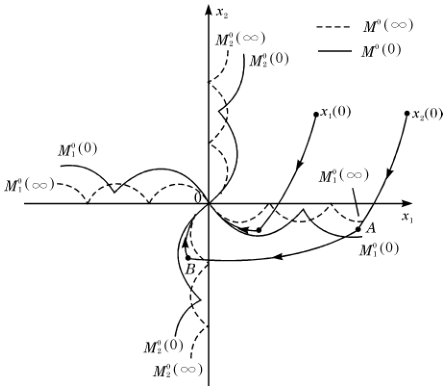
\includegraphics[width=\linewidth]{figs/fig-0154.png}
\caption{图8.6-2}
\end{figure}

\[x_{2}\]

\[M_{x}^{(0)}\]

\[M_{r}^{(0)}\]

\[M_{l}^{(0)}\]

\[M_{1}^{(\infty)}\]

\[M_{1}^{(0)}\]

\[M_{1}^{(\infty)}\]

\[x_{1}(0)\]

\[A\]

\[M_{1}^{(0)}\]

再讨论另一个综合方法——利用最速过渡时间函数 $T(t, x)$ 的方法，按式 $(8.6-15)$ 和 $(8.6-16)$ 所示之关系可知

\[i u_{*}(t)= \begin{cases}+1 & \text { 若 } (\operatorname{grad}_{x} T(t, x), b(t))<0 \\ -1 & \text { 若 }(g r a d_{x} T(t, x), b(t))>0\end{cases}\qquad\text{(8.6-25)}\]

现在的问题是如何求出函数，$T(t, x)$。

设 $\boldsymbol{x}(t)$ 是式 $(8.6-2)$ 的某一定解，由恒等式

\[T(b+t), \boldsymbol{x}(b+t)=T(t, \boldsymbol{x}(b))-t\]

可知最速过渡时间函数满足下列一阶线性偏微分方程

\[\frac{\partial T}{\partial t}+(\operatorname{grad}, T(t, \boldsymbol{x}), A(t) x+B(t) i u(t, \boldsymbol{x}))=-1\qquad\text{(8.6-26)}\]

上式的边界条件是，在 $\Omega$ 的边界 $S$ 上有

\[T(t, \boldsymbol{x}) \mid_{s}=0\qquad\text{(8.6-27)}\]

这里又得到一个柯西问题，求解的方法完全与前节常系数的情况相同，只是变元增加了一个 $t_{0}$。求解的次序依然是将曲面 $S$ 分成区域 $S_{i}(t), i=1,2, \cdots, 2^{\prime}$，每一区域上的最速控制由式 (8.6-25) 所唯一确定，而 $S$ 上的梯度向量 $\operatorname{grad} T \mid_{s}=$ grad $g(\boldsymbol{x})$。此后再用逐步延拓法，即可在全空间内求出 $T(\boldsymbol{x}, t)$。于是最速控制函数 $u(\boldsymbol{x}, t)$ 就可以按式 (8.6-25) 完全确定。

\section{8.7 非线性系统综合举例}

至今我们讨论过的综合问题中受控对象的运动方程式均假定是线性的。前面已经看到，利用等时区的概念可以顺利地解决最速控制的综合问题。但是，在实际问题中常常会遇到一些典型的非线性系统，即受控对象的运动方程式不是式 (8.2-1) 或 (8.6-2) 型的，而控制量和受控量往往以非线性形式出现在运动方程式右端。一般可写成下列形式

\[\begin{aligned} & \frac{d x_{1}}{d t}=f_{1}\left(x_{1}, x_{2}, \cdots, x_{n} ; u, \cdots, u_{r}\right) \\ & \cdots \\ & \frac{d x_{n}}{d t}=f_{n}\left(x_{1}, x_{2}, \cdots, x_{n} ; u, \cdots, u_{r}\right) \end{aligned}\qquad\text{(8.7-1)}\]

或写成向量方程式

\[\frac{d \boldsymbol{x}}{d t}=f(\boldsymbol{x}, \boldsymbol{u})\]

这里依然假定控制量 $\boldsymbol{u}$ 受 A 型和 B 型限制。

对非线性系统的分析和综合要比线性系统困难得多。但是对某些接近线性的非线性系统，即所谓拟线性系统则可以利用线性系统所使用的办法去综合。本节内将详细讨论一个在工程问题中比较典型的非线性系统的实例。通过对这一系统的综合来看看应如何处理这类问题。

首先让我们研究一下式 (8.7-1) 的最速控制 $\dot{u}(t)$ 应该满足什么条件 ${ }^{\circledR}$。设函数 $f_{i}$ 对每一分量 $x_{i}$ 具有连续一阶偏导数，$\dot{\boldsymbol{x}}(t)$ 和 $\dot{\boldsymbol{u}}(t)$ 分别为自初始状态 $\boldsymbol{x}_{0}$ 至原点的最速轨迹和控制函数。令控制量 $\dot{\boldsymbol{u}}(t)$ 不变，而将初始条件 $\boldsymbol{x}$ 作微小变化 $\varepsilon \boldsymbol{y}_{0}, \varepsilon$ 为一小的正常数，$\varepsilon>0, \boldsymbol{y}$ 为某一预定的任意常向量。利用轨道摄动法可以

(1) 以下的讨论是极大值原理——最速控制必要条件的简要说明。详细的讨论和证明请参看第九章及所引文献。

求出以 $\boldsymbol{x}+\varepsilon \mathbf{y}_{0}$ 为起点，以 $\dot{\boldsymbol{u}}(t)$ 为控制的方程式 $(8.7-1)$ 的解的主要部分是 $\dot{\boldsymbol{x}}(t)+$ $\varepsilon \mathbf{y}(t)$，其中 $\mathbf{y}(t)$ 是下列振动方程式的解

\[\frac{d \mathbf{y}}{d t}=A(t) \mathbf{y}, \quad \mathbf{y}(0)=\mathbf{y}_{0}\qquad\text{(8.7-2)}\]

\[A(t)=\left[\begin{array}{c}\partial f_{i}(\dot{\boldsymbol{x}}(t), \dot{\boldsymbol{u}}(t)) \\\partial \dot{\boldsymbol{x}}\end{array}\right]\]

式中 $A(t)$ 是 $n \times n$ 阶方阵。现将最速控制 $\dot{\boldsymbol{u}}(t)$ 在 $t=\varepsilon$ 处做微小的改动，用以观察最速轨线 $\dot{\boldsymbol{x}}(t)$ 所发生的变化。令

\[u(t)= \begin{cases}\dot{u}(t), & \text { 若 } t<s-\varepsilon l, t \geqslant s \\ v, & \text { 若 } s-\varepsilon l \leqslant t<s\end{cases}\qquad\text{(8.7-3)}\]

即在 $s-\varepsilon l \leqslant t<s$ 的区间内将最速控制函数换成另一个向量 $v \in U$，而在此区间以外的一切时间上最速控制函数不做任何变化；定义式 $(8.7-3)$ 中的 $l$ 是任一正常数，$\varepsilon$ 为某一足够小的正数。显然，在 $0 \leqslant t \leqslant s-\varepsilon l$ 区间内最速轨线 $\dot{\boldsymbol{x}}(t)$ 没有变化，而在 $s-\varepsilon l \leqslant t<s$ 区间内轨线发生了变化，这个变化量的主要部分是 $\varepsilon l y_{0}$。

\[\int_{-d}^{r}[f(\dot{\boldsymbol{x}}(t), v)-f(\dot{\boldsymbol{x}}(t), \dot{\boldsymbol{u}}(t))] d t=\varepsilon l y_{0}+0(\varepsilon)\]

式中 $\mathbf{y}=f\left(\dot{\boldsymbol{x}}(s), v\right)-f\left(\dot{\boldsymbol{x}}(\tau), \dot{\boldsymbol{u}}(s)\right)$，并假定 $\dot{\boldsymbol{u}}(t)$ 的每一个分量在这个小区间内是连续的。令 $\Phi(s, t)$ 是式 $(8.7-2)$ 的基本解矩阵，$\Phi(t, t)=E$。于是，$\boldsymbol{u}(t)$ 对应的变化了的轨线是

\[\boldsymbol{x}(t)= \begin{cases}\dot{\boldsymbol{x}}(t), & t \leqslant s-\varepsilon l \\\dot{\boldsymbol{x}}(t)+\varepsilon l \mathbf{y}(t)+0(\varepsilon), & t>s\end{cases}\]

式中

\[\mathbf{y}(t)=\Phi(s, t) \mathbf{y}_{0}\]

由于 $\mathbf{y}(t)$ 是 $\mathbf{y}_{0}$ 的线性函数，而 $\boldsymbol{x}(t)$ 又是 $\varepsilon$ 和 $\mathbf{y}(t)$ 的线性函数，不难理解，当 $l$固定且 $\varepsilon$ 足够小时，一切式 $(8.7-3)$ 型的控制函数所对应的轨线终点构成一个凸性锥体，而且过 $\dot{\boldsymbol{x}}(t)$ 点可以做一个支面 $P$，使一切变动了的轨线端点 $\boldsymbol{x}(t)$ 位于此支面 $P$ 的一侧。设 $\boldsymbol{\Phi}_{1}$ 为此支面的外法向量，于是有

\[(\boldsymbol{\Psi}_{1}, \mathbf{y}(t)) \leqslant 0\]

将 $\mathbf{y}(t)$ 之表达式代入上式后有

\[\left(\boldsymbol{\Psi}_{1}, \Phi(s, t)\left[\boldsymbol{f}\left(\dot{\boldsymbol{x}}(s), v\right)-\boldsymbol{f}\left(\dot{\boldsymbol{x}}(s), \dot{\boldsymbol{u}}(s)\right)\right]\right) \leqslant 0\]

或

\[\left(\Phi^{\mathrm{r}}(s, t) \boldsymbol{\Psi}_{1}, \boldsymbol{f}\left(\dot{\boldsymbol{x}}(s), \dot{\boldsymbol{u}}(s)\right)\right) \geqslant\left(\Phi^{\mathrm{r}}(s, t) \boldsymbol{\Psi}_{1}, \boldsymbol{f}\left(\dot{\boldsymbol{x}}(s), v\right)\right)\]

由于 $\left[\Phi^{\mathrm{r}}(t, s)\right]^{-1} \boldsymbol{\Psi}_{1}$ 是式 $(8.7-2)$ 的共轭方程式

\[\frac{d \boldsymbol{\Psi}}{d t}=-A^{\mathrm{r}}(t) \boldsymbol{\Psi}, \quad \boldsymbol{\Psi}(t)=\boldsymbol{\Psi}_{1}\qquad\text{(8.7-4)}\]

的解，$v$ 是任意且属于 $U$ 的向量，$s$ 也是任意的，$0 \leqslant s \leqslant t$。因此上述不等式的含义为

\[H=\left(\boldsymbol{\psi}(t), \boldsymbol{f}\left(\dot{\boldsymbol{x}}(t), \dot{\boldsymbol{u}}(t)\right)\right)=\max _{v \in U}\left(\boldsymbol{\psi}(t), \boldsymbol{f}\left(\dot{\boldsymbol{x}}(t), v\right)\right)\qquad\text{(8.7-5)}\]

式中 $H=(\boldsymbol{\psi}(t), \boldsymbol{f}(\boldsymbol{x}, \boldsymbol{u}))$，称为哈密顿函数，它与原方程式 (8.7-1) 及其摄动共轭方程式 (8.7-4) 的关系显然是

\[\begin{aligned} & \frac{\partial H}{\partial \psi_{i}}=\frac{d x_{i}}{d t}=f_{i}(\boldsymbol{x}, \boldsymbol{u}) \\ & \frac{\partial H}{\partial x_{i}}=-\frac{d \psi_{i}}{d t} \end{aligned}\]

归纳上述，得到式 (8.7-1) 最速控制的必要条件是存在一个非零连续向量函数 $\boldsymbol{\psi}(t)$，沿最速轨线上的每一时刻 $t$，最速控制 $\boldsymbol{u}(t)$ 使哈密顿函数 $H$ 获极大值。此外，可以证明，沿最速轨线 $H \geqslant 0$，而且等于常数。下面我们就利用这个定理去解决一个非线性最速控制系统的综合问题。

现讨论带有电机放大器的电力拖动系统 [21]，如图 8.7-1 所示。图内左边加到电机放大器控制绕组上的电压 $u$ 是对拖动系统的主要控制量，加到右边直流电机激磁绕组上的电压 $w$ 可以看成是第二个控制量。通常在这类系统中取 $w$ 为常值电压。实际上，若将激磁电压 $w$ 看成为控制量，而在控制过程中按需要去变化它的电平，那么，拖动系统的性能可以提高。这一点通过下面的分析可以看出。令 $x$ 表示电机输出的转角，$\omega$ 为电机旋转速度，$e$ 为电机放大器的输出电压，$\dot{u}$ 和 $\dot{u}$ 分别为控制绕组和激磁绕组的电流。于是受控对象的运动方程式是

\begin{figure}[htbp]\centering
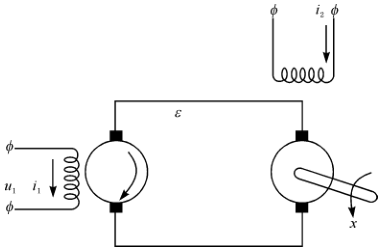
\includegraphics[width=\linewidth]{figs/fig-0155.png}
\caption{图8.7-1}
\end{figure}

\[\begin{aligned} & \frac{d x}{d t}=\omega \\ & \frac{d \omega}{d t}=\alpha i_{2} e+\omega i_{2}^{2} \end{aligned}\]

图 8.7-1

\[\begin{aligned}& \frac{d e}{d t}=-\beta_{e}+\beta_{i 1} \\& \frac{d i_{1}}{d t}=-\gamma i_{1}+\gamma u_{1} \\& \frac{d i_{2}}{d t}=-\varepsilon i_{2}+\varepsilon u_{2}\end{aligned}\qquad\text{(8.7-6)}\]

式中 $\alpha, \beta, \gamma, \varepsilon$ 均为正常数，为系统结构参数所确定。为了容易掌握综合方法的实质，我们假定两个绕组的时间常数 $T_{1}=\frac{1}{\gamma}, T_{2}=\frac{1}{\varepsilon}$ 和电机放大器的时间常数 $T_{3}=\frac{1}{\beta}$ 均很小，从而把式 (8.7-6) 的五个方程式化简为一个二阶系统。于是综合问题即可以在相平面上进行。

设控制系统的任务是位置随动，即跟随输入作用 $g(t)=A=\operatorname{const}$。引进误差坐标 $x_{1}=A-x, x_{2}=\frac{d x_{1}}{d t}=-\omega, w=e, w=\dot{v}$ 后，方程组 (8.7-6) 可化简为

\[\begin{aligned}& \frac{d x_{1}}{d t}=x_{2} \\& \frac{d x_{2}}{d t}=-w_{2} x_{2}-\alpha u_{1} w\end{aligned}\qquad\text{(8.7-7)}\]

可以看到这是一个非线性系统。因此线性综合方法这里不能应用，但是必要条件式(8.7-5)却是适用的。控制量 $w$ 受到控制电源的电压限制，而 $w$ 除受到电源电压限制外，还需保证直流电机不因激磁电流太小而发生“飞散”现象，即转速太大而失去控制。因而 $w$ 的下端要受到限制，这些限制条件可写成（适当选择受控量的单位）

\[|u| \leqslant 1, \quad 0<\lambda \leqslant w \leqslant 1\qquad\text{(8.7-8)}\]

为了求出最速控制，首先应写出式 (8.7-7) 的共轭方程组

\[\begin{aligned}& \frac{d \psi_{1}}{d t}=0 \\& \frac{d \psi_{2}}{d t}=-\psi_{1}+w_{2}^{2} \psi_{2}\end{aligned}\qquad\text{(8.7-9)}\]

然后再构成哈密顿函数

\[H(\boldsymbol{x}, \boldsymbol{\psi}, \boldsymbol{u})=\psi_{1} x_{2}+\psi_{2}\left(-w_{2}^{2} x_{2}-\alpha u_{1} u_{2}\right)\qquad\text{(8.7-10)}\]

解方程组 (8.7-9) 有

\[\begin{aligned}& \psi_{1}(t)=\psi_{10}=\text { const } \\& \psi_{2}(t)=\mathrm{e}^{\int_{0}^{t} u_{2}^{2}(t) d t}\left[\psi_{20}-\int_{0}^{t} \psi_{10} e^{-\int_{0}^{t} u_{2}^{2}(s) d s} d \tau\right]\end{aligned}\qquad\text{(8.7-11)}\]

由上式的结构可以看出，$\psi_{2}(t)$ 右端的两项都是 $t$ 的单调函数，故 $\psi_{2}(t)$ 最多变号一次，再根据极值条件式(8.7-5)和(8.7-10)之右端可知，由于 $u > 0$，所以最速控制之一是

\[\dot{u}(t) = -\operatorname{sign} \psi_2(t)\qquad\text{(8.7-12)}\]

为了找到另一个最速控制函数 $\dot{u}(t)$ 的形式，将哈密顿函数改写成下列形式

\[H(x, \psi, u) = \psi_1 x_2 + \psi_2 \left[ -x_2 \left( u + \frac{\alpha u_1}{2 x_2} \right)^2 + \frac{\alpha^2 u^2}{4 x_2^2} \right]\]

最速控制 $\dot{u}(t)$ 应使上式获极大值。现分别研究两种情况:

(1) 设 $\psi_2(t) < 0$，此时 $\dot{u}_1 = 1$。在上半平面内 $x_2 > 0$，$\dot{u}$ 应取最大值 +1。在下半平面内 $x_2 < 0$ 处，最速控制 $\dot{u}$ 的表达式为

\[\dot{u} = \begin{cases} 1, & \text{若} \left| \frac{\alpha}{2 x_2} \right| \geqslant 1 \\ \frac{\alpha}{2 x_2}, & \text{若} \lambda \leqslant \left| \frac{\alpha}{2 x_2} \right| \leqslant 1 \\ \lambda, & \text{若} \left| \frac{\alpha}{2 x_2} \right| \leqslant \lambda \end{cases}\qquad\text{(8.7-13)}\]

(2) 设 $\psi_2(t) > 0$，$\dot{u} = -1$。于是在上半平面内 $x_2 > 0$ 处有

\[\dot{u} = \begin{cases} 1, & \text{若} \frac{\alpha}{2 x_2} \geqslant 1 \\ \frac{\alpha}{2 x_2}, & \text{若} \lambda \leqslant \frac{\alpha}{2 x_2} \leqslant 1 \\ \lambda, & \text{若} \frac{\alpha}{2 x_2} \leqslant \lambda \end{cases}\qquad\text{(8.7-14)}\]

在下半平面内 $x_2 < 0$，$\dot{u} = 1$。

显然，一般来讲，每一个 $\dot{u}(t)$ 均由两段组成，因为当 $\psi_0$ 和 $\psi_2$ 不均为零时 $\psi_2(t)$ 不可能恒为零，故 $\dot{u}(t)$ 必为开关函数。另一个控制 $\dot{w}(t)$ 一般是由四段组成，在其中的一段内，它连续地取从 $\lambda$ 到 1 的所有值。在最后一段 $\dot{w}(t)$ 必为 +1，否则在最速轨迹的终点，（这里 $x_1 = 0$，$x_2 = 0$)哈密顿函数 $H$ [参看式(8.7-10)]不可能达最大值。其次，在原点附近只有两条可能的最速控制通向原点，一条来自下半平面，另一条来自上半平面。在图 8.7-3 中用 $L^+$ 和 $L^-$ 表示这两条线。显然，在 $L^+$ 上 $\dot{w} = -1$，在 $L^+$ 上 $\dot{w} = +1$;在这些线上 $\dot{w}$ 均取极大值；而这些线上的每一点必同时为 $\dot{u}(t)$ 的开关点。

总结前面的讨论，我们得到相平面上的最速控制函数的取值区域。整个相平面被开关曲线 $L^+$ 和 $L^-$ 划分为两半，每半平面内又被两条直线 $S_1$，$S_2$ 和 $S_1'$，$S_2'$ 分为三部分。以左半平面为例，在直线 $S_1$ 下面 $\dot{u} = -1$，$\dot{w} = +1$;在 $S_1$ 和 $S_2$ 的中间 $\dot{u}_{1}=-1$，$\dot{u}_{2}=\frac{\alpha}{2x_{2}}$; 在 $L^{+}$ 和 $S_{2}$ 的中间 $\dot{u}_{1}=-1$，$\dot{u}_{2}=\lambda$; 在 $L^{+}$ 上 $\dot{u}_{1}=+1$，$\dot{u}_{2}=+1$。在右半面上的最速控制的值域划分完全类似。

设系统的初始误差 $\mathbf{x}$ 点位于第一象限，则最速过程和最速控制函数随时间的变化规律如图 8.7-2 所示。这样，最速控制函数的综合问题就完全解决了。我们看到。虽然极值条件式 (8.7-5) 只是最速控制的必要条件，但对某些具体非线性系统则可以提供解决综合问题的足够知识。当然，一般来讲，这个条件是不够的。

\begin{figure}[htbp]\centering
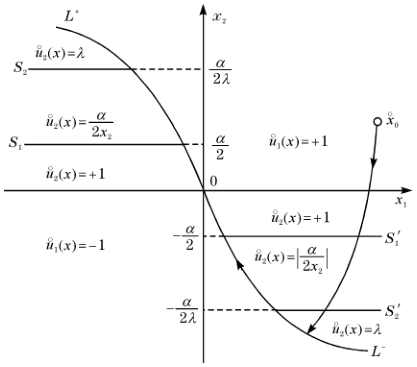
\includegraphics[width=\linewidth]{figs/fig-0157.png}
\caption{图8.7-3}
\end{figure}

\begin{figure}[htbp]\centering
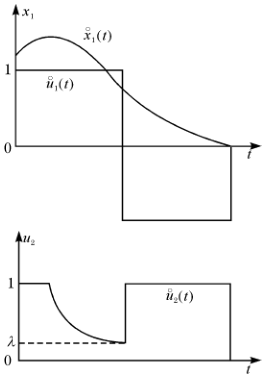
\includegraphics[width=\linewidth]{figs/fig-0156.png}
\caption{图8.7-2}
\end{figure}

\textbackslash\{\}begin\{figure\}[h]\textbackslash\{\}centering\textbackslash\{\}includegraphics[width=0.3\textbackslash\{\}textwidth]\{图8.7-2.png\}\textbackslash\{\}caption\{图 8.7-2\}\textbackslash\{\}label\{fig:8.7-2\}\textbackslash\{\}end\{figure\}

\textbackslash\{\}begin\{figure\}[h]\textbackslash\{\}centering\textbackslash\{\}includegraphics[width=0.3\textbackslash\{\}textwidth]\{图8.7-3.png\}\textbackslash\{\}caption\{图 8.7-3\}\textbackslash\{\}label\{fig:8.7-3\}\textbackslash\{\}end\{figure\}

前面我们详细地讨论了特定最速控制函数的求法和最速控制系统的综合方法。但是系统的设计工作尚未最后完成。因为设计工作要求技术设计者按求得的函数形式做成控制装置，用机械的，电的方法在实际系统中实现这些控制规律。当然，在原理上它们是可以实现的，因为现代计算技术已给我们提供了充分条件去实现任何复杂的，已知的函数形式。如果控制系统是一次作用的，而最速控制函数只有一个向量函数 $\dot{\mathbf{u}}(t)$ 时，它的技术实现在技术上是毫无困难的。如果它的每一个分量都是开关函数，那么，可用时间程序装置去实现每次开关动作，或者用 $r$ 个时间函数产生器就足够了。

当控制系统的初始误差坐标不能预先测出时，就需要设计出一个自动控制装置，该装置根据每一瞬间测得的误差坐标，按给定的函数规律去算出最速控制函

\section{8.8 最速控制函数的技术实现}

数的取值。这就不是一个简单的程序装置或者简单的函数产生器所能实现了的事。特别是当受控对象的运动方程式的阶数较高时，欲实现 $r$ 个 $n$ 元函数，只靠计算机的存储器是很不经济的，甚至现有的大型计算机的数据存储能力都将无能为力。因此必须找出其他途径来完成最速控制函数的技术实现。

一个普遍可行的办法是用简单的函数去逼近最速控制规律。实际工程问题的物理特点给这种逼近方法提供了有利的条件。每一个受控系统的初始误差值总不可能是无限的。系统中每一个物理量都有自己的最大工作范围。因此，实际系统的工作状态不可能是相空间的任何点，而是终点状态附近的某一有界区域。区域的边界只能根据每一实际问题的物理特点去确定。我们称这个区域为系统的基本工作区，并且用符号 $D$ 表示。如果能利用简单的函数在区域 $D$ 内较精确地逼近最速控制函数，而前者在技术上又是容易实现的函数，那么，设计问题所遇到的困难就不再成为阻碍，幸运的是这种方法是存在的[13，22]。

设 $u\left(x_{1}, \cdots, x_{n}\right)$ 是最速控制函数 $\dot{u}(\boldsymbol{x})$ 的某一分量。现试用 $n$ 个单变量函数的积去逼近它。设 $h_{1}\left(x_{1}\right), h_{2}\left(x_{2}\right), \cdots, h_{n}\left(x_{n}\right)$ 为一串单变元函数，它们按下列意义在区域 $D$ 上最优逼近函数 $u\left(x_{1}, x_{2}, \cdots, x_{n}\right)$

\[R_{1}=\int_{D}\left[u\left(x_{1}, x_{2}, \cdots, x_{n}\right)-\lambda h_{1}\left(x_{1}\right) h_{2}\left(x_{2}\right) \cdots h_{n}\left(x_{n}\right)\right]^{2} d \omega=\min \quad(8.8-1)\]

式中 $\lambda$ 为某一常数，$\omega$ 为 $n$ 维相空间内的体积元素，这一串函数如果能找到，而 $R_{1}$又足够小，那么，我们就有理由用函数

\[S_{1}\left(x_{1}, \cdots, x_{n}\right)=\lambda h_{1}\left(x_{1}\right) h_{2}\left(x_{2}\right) \cdots h_{n}\left(x_{n}\right)\qquad\text{(8.8-2)}\]

去代替最速控制 $u\left(x_{1}, \cdots, x_{n}\right)$。假如函数 $S_{1}$ 尚不能“足够好”的代表 $u$，可对差函数 $u(\boldsymbol{x})-S_{1}(\boldsymbol{x})=R_{1}(\boldsymbol{x})$ 再继续用第二次逼近，即找出另一串函数 $g_{1}\left(x_{1}\right)$，$g_{2}\left(x_{2}\right), \cdots, g_{n}\left(x_{n}\right)$ 使

\[R_{2}=\int_{D}\left[R_{1}\left(x_{1}, \cdots, x_{n}\right)-\lambda \varepsilon g_{1}\left(x_{1}\right) \cdots, g_{n}\left(x_{n}\right)\right]^{2} d \omega=\min \quad(8.8-3)\]

当 $R_{2}$ 足够小时就可以用

\[S=S_{1}(\boldsymbol{x})+S_{2}(\boldsymbol{x})=\lambda h_{1}\left(x_{1}\right) \cdots h_{n}\left(x_{n}\right)+\lambda \varepsilon g_{1}\left(x_{1}\right) \cdots g_{n}\left(x_{n}\right)\]

去代替控制函数 $u(\boldsymbol{x})$。如果第二次逼近仍嫌不足，可连续取第三次逼近，等。我们可以相信条件式(8.8-1)，取少数几次逼近后，即可得到技术上足够的精度(1)。

设这一串最优逼近的单元函数已经找到，那么，最速控制装置的技术实现就没有任何困难了。只需做出 $n$ 个或 $2 n$ 个单元函数产生器；再把它们连续乘起来即可。而单元函数产生器和乘法器的线路结构即便使用模拟电路也是比较容易实

(1) 关于这种逼近的收敛性，当 $n=2$ 时已有证明，当 $n>2$ 时尚无严格证明，见文献[22]。

现的。下面我们就来讨论用什么方法求出满足极值条件式(8.8-1)的那一串单元函数。

引进希尔伯特空间 $L_{2}(D)$，其中任一平方可积的函数 $u(\boldsymbol{x})$ 有

\[\|u\|^{2}=\int_{D}\left[u\left(x_{1}, \cdots, x_{n}\right)\right]^{2} d \omega=\langle u, u\rangle\]

我们称函数 $\|u\|$ 为函数 $u(\boldsymbol{x})$ 的范数。于是

\[R_{1}=\|u(\boldsymbol{x})-\lambda h_{1} \cdots h_{n}\|^{2}=\left\langle u-\lambda h_{1} \cdots h_{n}, u-\lambda h_{1} \cdots h_{n}\right\rangle\]

设 $\eta\left(x_{i}\right), i=1,2, \cdots, n$，为一串任意平方可积的单元函数 ${ }^{\text {① }} \varepsilon_{i}$ 为一串足够小的常数。为了讨论方便，我们假定

\[\int_{D_{i}}\left(h_{i}\left(x_{i}\right)+\varepsilon_{i} \eta_{i}\left(x_{i}\right)\right)^{2} d x_{i}=\left\|h_{i}+\varepsilon_{i} \eta_{i}\right\|^{2}=1\]

式中 $D_{i}$ 是函数 $h_{i}\left(x_{i}\right)$ 的定义区间。将 $h+\varepsilon_{i} \eta_{i}$ 代入式 (8.8-1)，根据 $h$ 的极值条件可知，在 $\varepsilon_{i}=0, i=1,2, \cdots, n$，处有极小值。令

\[R_{1}\left(h_{i}+\varepsilon_{i} \eta_{i}\right)=\|u-\lambda \prod_{i=1}^{n}\left(h_{i}+\varepsilon_{i} \eta_{i}\right)\|^{2}\]

求 $R_{1}$ 对 $\varepsilon_{i}$ 的导数，于是有

\[\left.\frac{\partial R_{1}}{\partial \varepsilon_{i}}\right|_{\varepsilon_{1}-\cdots-\varepsilon_{n}=0}=-2\left\{u-\lambda \prod_{a=1}^{n} h_{a}, \eta \prod_{a=1}^{n} h_{a}\right\}=0\]

或

\[\int_{D}\left[\left[u(\boldsymbol{x})-\lambda \prod_{a=1}^{n} h_{a}\left(x_{a}\right)\right] \prod_{a \neq i}^{n} h_{a}\left(x_{a}\right)\right] \eta_{i}\left(x_{i}\right) d \omega=0\]

因为 $\eta\left(x_{i}\right)$ 是任意函数，所以上式只有在方括号内的函数积分等于零时才能成立，于是便得到对 $h$ 的下列积分方程组

\[\begin{aligned} \lambda h_{i}\left(x_{i}\right)= & \int_{D_{i}} u\left(x_{1}, \cdots, x_{n},\right) h_{i}\left(x_{1}\right) \cdots h_{i-1}\left(x_{i-1}\right) h_{i+1}\left(x_{i+1}\right) \cdots h_{n}\left(x_{n}\right) d \omega_{i} \\ & i=1,2, \cdots, n \end{aligned}\qquad\text{(8.8-4)}\]

式中 $D_{i}^{\prime}$ 和 $d \omega_{i}$ 分别表示区域 $D$ 在不含第 $i$ 分量的 $n-1$ 维空间的投影及此空间内的体积元素。可以看到，方程组 (8.8-4) 是一组循环积分方程，其中的核函数 $u(\boldsymbol{x})$ 为已知。可以证明，此组方程式一定有解，或者说至少有一个解。如果加上限制条件 $\int_{D_{i}}\left[h_{i}\left(x_{i}\right)\right]^{2} d x_{i}=1$，则 $\lambda$ 称为方程组的本征值。如果有许多解，最大的 $\lambda$ 所对应的一串 $h_{i}\left(x_{i}\right)$ 将是方程式 (8.8-1) 的解。

求解方程组 (8.8-4) 的方法很多，例如逐步逼近法，最速下降法等均可以使

① 实际上我们假定 $u(\boldsymbol{x})$ 是平方可积的 $n$ 元函数。于是 $u(\boldsymbol{x})$ 和 $h_{i}\left(x_{i}\right), \eta\left(x_{i}\right)$ 均为希尔伯特函数空间 $L_{2}(D)$ 中的元素。

用。也可以采用数学分析中的特征函数求解方法。这里不再赘述。这一串函数求出后，即可算出式(8.8-1)内的 $R_{\mathrm{t}}$。若 $R_{\mathrm{t}}$ 的值还相当大，就在求出函数 $u(\boldsymbol{x})-$ $S_{1}(\boldsymbol{x})$ 以后，把它当做新的核函数，再一次求解方程组 $(8.8-4)$，这样就找到了 $S_{2}(\boldsymbol{x})$，依此类推。

实际经验表明，这个方法的收敛速度很快。当 $n=2$ 时，方程组的求解极其简单。欲达到 $1 \%$ 的逼近精度，只需取二组或三组单元函数就够了。在采用这个方法时，对线性系统还可用开关曲面函数代替最速控制函数 $u(\boldsymbol{x})$，这时函数的变元可以减少一个。例如，对三阶系统可以只处理二元函数，对四阶系统只处理三元函数等。当然，在实际中可以根据实际问题的特点，利用其他类型的近似方法去处理计算问题。上面介绍的方法虽有普遍意义，却不是唯一可行的，因为对每一个系统不一定都经济省事。

上面的讨论基于一个没有明确提到的假设条件，即系统的每一个误差坐标都必须在每一瞬间完全测出，否则上述 $n$ 元的最速控制函数的瞬时取值就无法确定了。为了测出误差坐标，必须同时测出受控对象的一切坐标取值和输入作用的一切坐标。如果受控对象的运动方程式是一个 $n$ 阶线性方程式，为了确定每一个瞬间最速控制函数的取值，必须连续不断地测出受控对象的输出量及其各次导数和输入作用的各阶导数。如果受控对象的运动为一个方程组所描绘，则可不必测出输出和输入的各阶导数，只需测出各坐标就够了。尽管如此，欲实现最速控制装置，仍然需要大量的测量装置，这在实际上有时可以做到，有时也很困难。当某些坐标原则上不能测量时，最速控制系统就难以实现了。很多实际问题中的情况正是如此。在这种情况下，设计师们便只得采用其他方法，利用不完全的坐标信息去设计系统。但是，即便在这种情况下，最速控制理论依然有其指导意义。利用这个理论可求出理想的过渡过程，原理上能够达到的最短过渡时间。算出这些极限值后就可以用此来评价设计出来的系统，看它离理想指标差多少。这样，最速控制理论至少具有认识论方面的意义。同时，这里可以提出一个重要的理论问题，即当某些坐标在实际上不能测量时（或者说系统没有完全能观测性），如何综合系统，使系统的过渡过程的时间在某一种意义上最短。这个问题也可称为非全信息的最速控制综合问题。这方面的研究无疑在理论上和实践上都有重大的意义。

在应用最速控制理论设计系统时，还要考虑到另一个困难。由于线性受控对象的最速控制是开关函数并且求出的运动方程式不可能完全精确地反映实际情况，可能在零点附近发生自振现象。为了避免这种现象发生，可以将设计工作分为两段进行，在误差较大时用最速控制函数，在误差足够小时用第五章内所介绍的方法去设计。这样既保证了运动的快速性，又保证了零点的稳定性。当运动方程足够准确时，可以不为零点的稳定性担心，此时最速控制装置将使系统具有最好的零点稳定性。因为前节内求出的函数 $T(\mathbf{x})$ 就是李雅普诺夫函数，它满足稳定性定理规定的一切条件，即

\[\begin{aligned}& T(\mathbf{x})>0 \text {, 若 } \mathbf{x} \neq \mathbf{0} \\& \frac{d T(\mathbf{x})}{d t}=-1<0\end{aligned}\]

这就是说，最速控制系统的一切运动都将是稳定的。

当控制系统受到随机干扰时，最速控制系统显然没有良好的滤波性能。由于它对输入作用的反应太快，输入噪声也将最大限度地在输出端复现。从这一意义来看，最速控制的要求与系统对“噪声”有良好的过滤能力的要求是有矛盾的。只有当确信系统不受有害噪声扰动时或信杂比很高时，才能采用本章内讨论的方法去进行设计。关于如何设计具有良好过滤“噪声”能力的系统，将在以后详细讨论。这里我们只指出，在有随机干扰作用时，设计者应巧妙地对各种指标进行综合平衡，在各种矛盾中寻求技术上合理的设计方案。

\section{参考文献}

[1] 涂序彦，多变量协调控制问题，第一届国际自动化学会论文选集，上海科学技术出版社，1963.

[2] 张嗣瀛，常系数线性系统的快速控制问题，自动化学报，2(1964)，2.

[3] 周恒，关于利用继电式元件改进控制系统的一个问题，力学学报，1(1957)，3.

[4] 戴汝为、李宝绶、王玉莹，关于线性快速控制的一个计算方法，自动化学报，2(1964)，3.

[5] 宋健、韩京清，线性最速控制系统的分析与综合理论，数学进展，5(1962)，4.

[6] 宋健、韩京清，变系数最速控制系统的分析与综合，中国科学，13(1964)，6.

[7] Bellman，R. \& Glicksberg，I. \& Gross，O.，On the Bang-Bang Control Problem，Quat. Appl. Math.，14(1956)，1.

[8] Bushaw，D. W.，Experimental Towing Tank，Stevens Institute of Technology Report，469，Haboken，1953，7.

[9] Hopkin，A. M. \& Ivama M. A.，A study of a Predictor-type Air-frame Controller Designed by Phase-Space Analysis，Trans. of AIEE II (1956).

[10] Kalman，R. E.，Optimal Nonlinear Control of Saturating Systems; Systems by Intermittent Action，IRE Wescon. Convention Record. Part 4，1957，1.

[11] LaSalle，J. P.，Time Optimal Control Systems，Proc. of National Academic Science，1959，4.

[12] Neustadt，L. W.，Paiewonski，B.，On Synthesizing Optimal Control，Proceedings of the Second IFAC Congress，Basel，1963.

[13] Pike. E. W.，Silverberg，T. R.，Designing Mechanical Computer，Machine Design，24 (1952)，7，8.

[14] Sun Jian \& Hang King-Ching，Analysis and Synthesis of Time Optimal Control Systems，Proc. of the Second IFAC Congress，Basel，1963.

[15] Антонанов，Ю. Г.，Автоматическое управление с применением вычислительных машин (синтез систем，оптимальных по быстродействию)，Ленинград，1962.

[16] Гамкрелидзе，Р. В. К теории оптимальных процессов в линейных системах，ДАН СССР，116(1957)，1.

[17] Кириллова，Ф. М.，О предельном переходе в решении одной задачи оптимального управления，ПММ，24(1960)，2.

[18] Красовский，Н. Н.，К теории оптимального регулирования，Автоматика и Телемеханика，18(1957)11.

[19] Лернер，А. Я.，О предельном быстродействии систем автоматического регулирования，Автоматика и Телемеханика，15(1964)，6.

[20] Понтрягин Л. С.，Балтиякий В. Г.，Гамкрелизе Р. В.，Мищенко Е. Ф.，Математическая теория оптимальных процессов，физматиз，Москва，1961. （庞特里亚金等，最优过程的数学理论，陈祖浩等译，上海科学技术出版社，1965.)

[21] Сун Цзянь（宋健），Оптимальное управление в одной нелинейной системе，Автоматика и Телемеханика，21(1960)，1.

[22] Сун Цзянь（宋健），Бутковский А. Г.，К построению функциональных преобразователей со многими входами，Изв. АН СССР，ОТН，1961，2.

[23] Фельдбаум，А. А.，Оптимальные процессы в системах автоматического регулирования，Автоматика и Телемеханика，14(1953)，6.

[24] Фельдбаум，А. А.，Основы теории оптимальных автоматических систем，Москва，1963.

[25] Сун Цзянь（宋健），Синтез оптимального устройства следящей системы，Автоматика и Телемеханика，20(1959)，1.

\chapter{第九章 满足指定积分指标的控制系统设计}

在前面几章里，我们主要从分析的观点去讨论控制系统的设计问题。那就是首先假定了系统的结构，然后找出系统具有什么样的性能。

在上面一章里，我们第一次引入了一种不同的、更为直接的观点：我们首先指定某些性能，然后寻求能够给出所要求的性能的控制系统。本章内，我们将把这一原理用到任意的系统上去。在这种控制系统中，被满足的性能准则是用被控制量的积分表示的，因此可以得到一个非常普遍的用微分方程来表示的系统的性能。一般说来，这是一个非线性的微分方程。按这种原理设计成功的控制系统通常就是一个非线性系统。

\section{9.1 基本概念}

实际上，第八章内曾研究过的最速控制系统，就是属于具有最短过渡时间的系统，而最短过渡时间可以用积分公式表达出来。下面我们将讨论一个更为一般的问题：系统质量指标是具有更为普遍的积分形式。设受控对象的运动规律为下列一阶常微分方程组所描述

\[\begin{aligned}& \frac{d x_{1}}{d t}=f_{1}\left(x_{1}, x_{2}, \cdots, x_{n}, u, w, \cdots, u_{r}\right) \\& \frac{d x_{2}}{d t}=f_{2}\left(x_{1}, x_{2}, \cdots, x_{n}, u, w, \cdots, u_{r}\right) \\& \cdots \\& \frac{d x_{n}}{d t}=f_{n}\left(x_{1}, x_{2}, \cdots, x_{n}, u, w, \cdots, u_{r}\right)\end{aligned}\qquad\text{(9.1-1)}\]

式中 $x_{i}, i=1,2, \cdots, n$，为受控对象的状态坐标分量，$u, w, \cdots, u$ 为控制量。上式也可以写成向量方程式，令 $\boldsymbol{x}=\left(x_{1}, x_{2}, \cdots, x_{n}\right), \boldsymbol{u}=\left(u, w, \cdots, u_{r}\right)$，则有

\[\frac{d \boldsymbol{x}}{d t}=f(\boldsymbol{x}, \boldsymbol{u})\]

式中 $\boldsymbol{f}=\left(f_{1}, f_{2}, \cdots, f_{n}\right)$。

受控运动的性能指标，我们用积分

\[J=\int_{0}^{t_{1}} f_{0}(\boldsymbol{x}, \boldsymbol{u}) d t\qquad\text{(9.1-2)}\]

来表示，右边积分上限 $t$ 是评价运动优劣的时间区间，即仅在 $[0, t]$ 时间间隔内评价系统的运动。显然，当的时间就是评价受控运动优劣的指标。这一问题我们已在前一章内详细地讨论过了。设使受控对象由此点出发到达某一特定状态特定区域）。

如果式 (9.1-2) 表示控制过程中某种物理量的耗损，如能量或燃料消耗等，则希望选择控制 $u(t)$ 使

\[J=\int_{0}^{t_{1}} f_{0}(\boldsymbol{x}(t), \boldsymbol{u}(t)) d t=\min , \quad \boldsymbol{x}(0)=\boldsymbol{x}_{0}\qquad\text{(9.1-3)}\]

有时又希望使 $J=\max$，这时只需将函数 $f_{0}$ 变号后，便可归结为条件式 (9.1-3)。

设 $\boldsymbol{x}$ 是受控对象的初始状态，控制的目的是使受控对象到达某一状态集合 $D$ （区域）。自 $\boldsymbol{x}$ 达 $D$ 且满足条件式 (9.1-3) 的控制函数称为最优控制。不难想象，这里可能有四种情况:

(1) 自 $\boldsymbol{x}$ 点用任何控制 $\boldsymbol{u}(t)$ 都不可能到达区域 $D$，此时不存在任何能达到目的地的控制函数，当然也无最优控制可言。

(2) 自 $\boldsymbol{x}$ 点只有一个控制 $\boldsymbol{u}(t)$ 使受控对象的状态到达 $D$。此时，到达终端状态的控制只有一个，它所对应的式 (9.1-3) 的 $J$ 也唯一地被确定，对于这种情况最优控制也是没有意义的。

(3) 自 $\boldsymbol{x}$ 引至 $D$ 的控制函数有多个 （有无穷多个或无穷多个）。如果这种控制为有穷多个，那么其中使 $J$ 取最小值的控制便是要求的最优控制，若这些控制所对应的 $J$ 相等，则可认为其中任何一个控制都是最优的。如果自 $\boldsymbol{x}$ 引到 $D$ 的控制函数有无穷多个，其中有一个或数个控制使 $J$ 取最小值，此时我们说最优控制函数存在，控制设计的任务就是找出这个最优控制来。

(4) 自 $\boldsymbol{x}$ 点引到 $D$ 的控制有无穷多个，但其中没有一个能使 $J$ 取极小。此时最优控制依然是不存在的。

上述四种情况中的第四种；初看起来很奇怪。其实这种情况是常见的。试看下面的例子。设在水平面上有一质量为 $m$ 的物体，在 $t=0$ 时处于静止状态。现用一个力 $F$，将物体推至 $\boldsymbol{x}$ 点 （图 9.1-1)。忽略空气阻力和摩擦力，物体运动方程式为

\[\frac{d^{2} x}{d t^{2}}=\frac{F(t)}{m}, \quad F(t) \geqslant 0\]

图 9.1-1

\begin{figure}[htbp]\centering
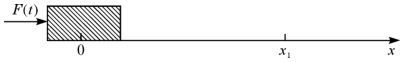
\includegraphics[width=\linewidth]{figs/fig-0158.png}
\caption{图9.1-1}
\end{figure}

要求找到一种控制力 $F(t)$，使物体到过 $x_{1}$ 点，且消耗能量为最小。显然，这种控制力 （函数）有无穷多个。但是，消耗能量最小的控制力却不存在。实际上，能量损耗由下式表示

\[J=\int_{0}^{x_{1}} F(t) \, dx = \int_{0}^{t} F(t) v(t) \, dt = \frac{1}{2} m \left[ v(t) \right]^2\]

式中 $\frac{dx(t)}{dt} = v(t)$，$t$ 是物体到达 $x_1$ 点的时刻，$F(t) \geq 0$。为使耗能减少，需减小 $v(t)$，当 $v(t) \to 0$ 时，耗能 $J \to 0$。当 $J = 0$ 时，$v(t) = 0$，此时 $F(t) \equiv 0$，而这种控制又不能使物体到达 $x_1$ 点。由此看到，使物体到达 $x_1$ 点的控制力有无穷多个，其中却没有最优控制。对任何使 $v(t)$ 足够小的 $F_1(t)$，还可找到“更小的” $F_2(t)$，使 $v(t)$ 更小，在极限的情况下，$J = 0$，而 $F(t) \equiv 0$ 不属于可准控制范围，所以，在这种情况下，最优控制并不存在。

由这样一个简单例子就可以看到，并不是所有的情况下，最优控制都存在。因此，在进行控制设计时，首先重要的是搞清楚最优控制是否存在。否则，寻求最优控制的努力可能是徒劳的。

另一个值得提及的概念是关于对控制量取值的限制。有时，若控制量 $u(t)$ 的取值不受限制，即它的取值范围可以是整个 $r$ 维空间，这时最优控制也常常没有意义。还以上述例子来说明这点。设图 9.1-1 内所示之力 $F(t)$ 不受限制，要求找出一个最优控制使物体自零点到达 $x_1$ 点费时最短。显然，$F(t)$ 在起始时刻的取值越大，物体的运动速度也越大，如果对 $F(t)$ 取值没限制，当 $F(t)$ 的取值趋于无穷大时，物体到达 $x_1$ 点的时间将趋于无穷小，这在实际上是没有意义的。

由此可见，做最优控制器的设计时，首先要关心的问题是最优控制的存在性。即首先弄清欲达到的终点状态实际上是否能够到达，对控制量有哪些限制条件，以及在这种限制条件下最好的控制函数是否存在等。这些问题往往只能从技术问题的物理概念中寻求解答。在一般情况下，最优控制的存在性难以用数学方法加以证明。对存在性问题有了肯定的答案以后，就可以开始最优控制的设计。

当最优控制找到以后，在某些闭路系统中，设计控制装置时还要考虑到控制系统在终点状态是否稳定。若闭路系统不能保证终点状态稳定，那么有时它就不能作为实际装置加以实现。稳定性的要求是一种特殊的准则，在过渡过程里，主要控制系统的设计，常不考虑这一特殊准则。这种情况像上一章一样，因为系统满足了那些指定条件后，整个系统已经具有了合适的性能。设计完毕后，如果系统在终点状态上是稳定的，自然就无须采取特殊措施。也有另外一种可能，即满足最优条件的控制装置，不能保证闭路系统的稳定性，此时必须在系统里另加一个稳定装置，后者只在过渡过程完毕后才发生作用，因此它不会影响控制系统已经设计好了的运转性能。例如，对一个二阶系统，用 $y$ 表示输出，$y_{r}$ 表示必须保持的终点状态，稳定装置应保证使系统在 $y=y_{r}, \dot{y}=0$ 的状态上稳定。对于三阶系统，稳定装置应保证下列状态稳定

\[y=y_{r}, \quad \dot{y}=0, \quad \ddot{y}=0\]

当这样的一个装置加到控制系统以后，控制系统有两种运行方式，这也就是一个多方式控制系统。在过渡过程期间，主要控制系统按照指定的性能运行。过渡过程终止时，再换到第二个系统进行控制，这时候将保证系统最后处于稳定状态，避免系统离开希望到达的运转点。

除了对控制量常常存在一些客观限制条件以外，还可能存在某些对受控量的限制。这种限制条件也可以写成积分形式，如要求最优控制满足附加条件

\[J_{i}=\int_{0}^{\gamma_{1}} g_{i}(\boldsymbol{x}, \boldsymbol{u}) d t \leqslant \lambda, \quad i=1,2, \cdots, m\]

式中 $g_{i}$ 是 $\boldsymbol{x}=\left(x_{1}, x_{2}, \cdots, x_{n}\right)$ 和 $\boldsymbol{u}=\left(u, u, \cdots, u_{r}\right)$ 的 $n+r$ 元连续或连续可微函数。下节内将用实例加以说明。

\section{9.2 几个实例}

先让我们回忆一下古典变分法中的一个例子，即所谓贝努利(Bernoulli)捷线问题。设欲使一物体依重力沿某曲线自 0 点下滑至 $P$ 点。需求出一条曲线，物体沿此曲线下滑时将以最短时间到达 $P$ 点。设任取一光滑的曲线 $y(x)$，重力加速度为 $g$。若忽略摩擦力后，初始为静止的物体滑至 $y(x)$ 点时的速度为 $\sqrt{2 g y}$。物体滑过弧

图 9.2-1

元 $d s=\sqrt{1+\left(\dot{y}(x)\right)^{2}} d x$ 所需的时间为

\[d t=\frac{\sqrt{1+\left(\dot{y}(x)\right)^{2}}}{2 g y} d x\]

于是，当曲线 $y(x)$ 已给定时，物体自 0 点滑至 $P$ 点所需的时间为

\[J=\int_{0}^{1} \frac{\sqrt{1+\left(\dot{y}^{2}\right)}}{2 g y} d x\qquad\text{(9.2-1)}\]

现需找出一条“最好的”曲线 $\dot{y}(x)$，使时间 $J$ 为最小。从控制理论的观点，上述捷线问题可以改为下列等价问题：设有一“受控对象”，其运动方程式为

\begin{figure}[htbp]\centering
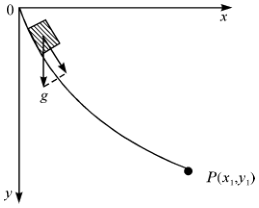
\includegraphics[width=\linewidth]{figs/fig-0159.png}
\caption{图9.2-1}
\end{figure}

\[\frac{d y}{d x}=u, \quad y(0)=0, \quad y\left(x_{1}\right)=y_{1}\qquad\text{(9.2-2)}\]

性能指标为

\[J=\int_{0}^{*_{1}} \frac{\sqrt{1+u^{2}}}{2 g y} d x\qquad\text{(9.2-3)}\]

我们看到，选择一条捷线等价于求出一个最优“控制函数” $u(x)=\frac{d \dot{y}(x)}{d x}$ 和相应的满足条件式 (9.2-2) 的“系统运动”。这一问题的解早在 1696 年为瑞士数学家贝努利和牛顿等人得到，因而开创了一门称为“变分法”的数学分支。以后我们将会看到，古典变分法对最优控制系统的设计是极为有用的。但是，对一些比较复杂的问题，古典变分法中的一些定理和计算方法不能完全满足控制系统设计的要求。为此必须对古典变分法的理论加以扩充。

为了说明最优控制系统的命题方法，让我们再看一个实例：关于喷气发动机工作过程的控制问题 ${ }^{[8]}$。喷气发动机的主要运转状态是它的运转速率 $N(t)$，它是受控对象的受控量。当 $N(t)$ 的变化规律被确定后，其他的工作特征，例如发动机的推力也就被决定了。在发动机运转时对它的限制条件是关于超速，超温，压缩机的浪涌，燃烧室的熄灭等。令 $N$ 表示指定的速度。 $T$ 表示加到轮机里的温度，$P$ 表示压缩机出口处的压力，于是可以用下述积分表示发动机的性能准则:

控制速度超速温度容许的上限和下限压缩机浪涌熄灭

以及

\[\int_{0}^{t_{1}} d t, \quad \text { 升起的时间 }\]

这些被积函数的性质如图 9.2-2 所示，量 $P-g(N)$ 是压缩机出口处的压力超出安全压力而发生浪涌的总量，$g(N)$ 表示对于浪涌以下的安全值，是每-个发动机速压缩机出口处压力。燃烧室熄灭的情况可以用同样方式处理。升起的时间是系统从一个主要运行状态过渡到另一状态总共需要的时间。

这里和第 6.6 节谈到过的喷气发动机的情形相似，线性化以后发动机的特性可以表示如下

\[\begin{aligned}& T=a N+a \dot{N} \\& P=b N+c \dot{T}\end{aligned}\qquad\text{(9.2-5)}\]

\[\begin{array}{ll}\dot{f}_{1}(N-N) & \dot{f}_{2}(N) \\0 & 0\end{array}\]

\[\begin{array}{ll}\dot{f}_{3}(T) & \dot{f}_{4}[P-g(N)] \\L_{1} & 0 \\L_{2} & P-g(N)\end{array}\]

\[\begin{array}{ll}\dot{f}_{5}[P-h(N)] & \dot{g}(N) \\0 & 0 \\& N\end{array}\]

图 9.2-2

其中 $\tau$ 是发动机的时间常数。将这些关系式代到方程(9.2-4)的积分里，我们看到它们全都有下面的形式

\[\int_{0}^{t_{1}} f(N, \dot{N}) d t\]

其中 $f$ 是 $N$ 和 $\dot{N}$ 的连续函数，$N$ 是时间 $t$ 的连续函数。关于这个问题，在第 9.5 节内还要讨论。

\section{9.3 古典变分法的应用}

古典变分法给控制系统设计提供的理论和方法大体分为两类。一类是不考虑受控对象的运动方程式，即在整个运动过程中受控对象本身的特性并不重要，重要的是运动规律的全局。例如，求探空火箭的最优弹道问题 ${ }^{[17]}$，要求找出一条

\begin{figure}[htbp]\centering
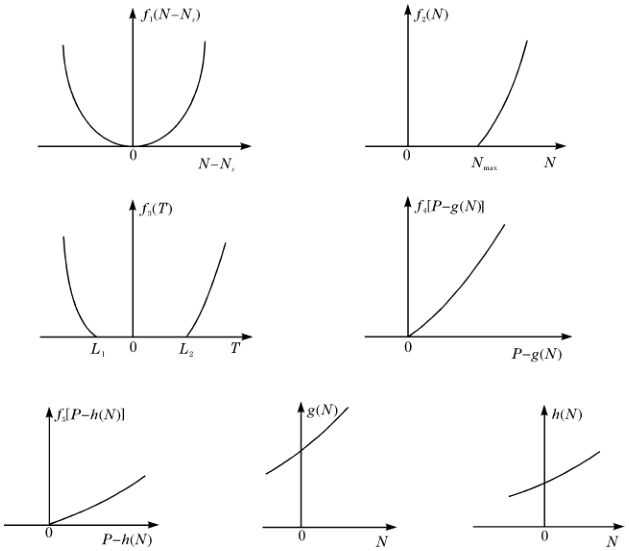
\includegraphics[width=\linewidth]{figs/fig-0160.png}
\caption{图9.2-2}
\end{figure}

理想弹道，在相同的燃料消耗条件下，使火箭达到的高度最大。由于这种弹道很长，而弹体上控制系统的动作速度相对于这条最优弹道来说是足够大的，因而在考虑最优弹道的选择时，可把弹体看成是其重心（质点）的运动，而忽略刚体运动及弹上控制设备的运动规律。另一类问题是当积分指标的计算时间间隔与控制系统的动作速度为同一数量级时，受控对象本身的运动规律必须考虑在内，甚至成为决定性的因素。

第一类问题可叙述如下：设 $\boldsymbol{x}=\left(x_{1}, x_{2}, \cdots, x_{n}\right)$ 为控制系统的 $n$ 个状态坐标。对控制系统的要求是找出连接两个给定点 $\boldsymbol{x}$ 和 $\boldsymbol{x}_{1}$ 的连续光滑的曲线，使受控对象沿此曲线运动时积分

\[J=\int_{0}^{t_{1}} f_{0}\left(t, x_{1}, x_{2}, \cdots, x_{n} ; \dot{x}_{1}, \dot{x}_{2}, \cdots, \dot{x}_{n}\right) d t\qquad\text{(9.3-1)}\]

取极小值。上式内 $\dot{x}_{i}=\frac{d x_{i}}{d t}, i=1,2, \cdots, n_{0}$。如果引进向量符号，式 $(9.3-1)$ 可改写成

\[\begin{aligned} & J=\int_{0}^{t_{1}} f_{0}\left(t, \boldsymbol{x}, \boldsymbol{u}\right) d t \\ & \frac{d \boldsymbol{x}}{d t}=\boldsymbol{u}, \quad \boldsymbol{u}=\left(u_{1}, u_{2}, \cdots, u_{n}\right) \end{aligned}\qquad\text{(9.3-3)}\]

式中 $\boldsymbol{u}$ 为曲线 $\boldsymbol{x}(t)$ 的切线向量，要求找出函数 $\boldsymbol{u}(t)$，使 $\boldsymbol{x}(t)$ 由固定点 $\boldsymbol{x}_{0}$ 引到 $\boldsymbol{x}_{1}$，且使式 $(9.3-2)$ 取极小值。这类问题的提法也可以改为端点不固定的情况，即端点 $\boldsymbol{x}_{0}$ 和 $\boldsymbol{x}_{1}$ 满足一些附加条件

\[g_{i}\left(\boldsymbol{x}, \boldsymbol{x}_{1}\right)=0, \quad i=1,2, \cdots, l\qquad\text{(9.3-4)}\]

在满足这些条件的点中，找出最好的初始点和终点。

第二类问题与上述问题的不同点在于受控对象的运动方程式比式 $(9.3-3)$ 更复杂，即除式 $(9.3-2)$ 和式 $(9.3-4)$ 外，运动 $\boldsymbol{x}(t)$ 必须满足条件式 $(9.1-1)$

\[\frac{d \boldsymbol{x}(t)}{d t}=f(t, \boldsymbol{x}, \boldsymbol{u})\]

为了掌握古典变分法处理这类问题的主要思想，下面先对第一类问题当 $n=1$ 时，略加讨论。设控制指标为

\[J=\int_{0}^{t_{1}} F(\boldsymbol{y}, \dot{\boldsymbol{y}}) d t=\min\qquad\text{(9.3-5)}\]

其中 $y(t)$ 为受控对象的一个唯一输出坐标; $\dot{y}=\frac{d y}{d t}, F$ 是 $y$ 和 $\dot{y}$ 的连续可微函数，设受控对象的初始状态为 $y_{0}=y\left(t_{0}\right)$，而受控对象的终点状态是不固定的，且积分上界 $t$ 也是不固定的。若将 $y(t)$ 看成是一个一阶系统的输出

\[\frac{d y}{d t}=\dot{y}=u\qquad\text{(9.3-6)}\]

则指标式(9.3-5)也可改写为

\[J=\int_{0}^{t_{1}} F(y, u) d t=\min\]

如果我们认为 $y(t)$ 是一个最优解，那就是说 $y(t)$ 是所有可能得到的输出里的某个输出，它满足方程(9.3-5)表示的条件。我们考虑 $y(t)$ 附近的一些解 $y(t)+$ $\varepsilon \delta y(t)$。其中 $\delta y(t)$ 是一个任意的函数，$\varepsilon$ 是一个数值很小的参数。如果 $y(t)$ 满足方程(9.3-5)表示的条件，那么 $J$ 应在 $\varepsilon=0$ 处达极小值，即

\[\left.\left[\frac{d}{d \varepsilon}\right]_{\varepsilon=0}^{t_{1}+\varepsilon \delta t_{1}} F\left(y+\varepsilon \delta y, \dot{y}+\varepsilon \delta \dot{y}\right) d t\right]_{\varepsilon=0}=0\]

或

\[\int_{0}^{t_{1}} \frac{\partial F}{\partial y} \delta y d t+\int_{0}^{t_{1}} \frac{\partial F}{\partial y} \delta \dot{y} d t+F(t) \delta t_{1}=0\qquad\text{(9.3-7)}\]

变分 $\delta t_{1}$ 出现的原因在于：方程 (9.3-5) 里那个积分的上限并非固定，而是在图 9.3-1 表示的曲线 $y=f(t)$ 上变动。这就是前面讨论过的从一个主要变量运行状态过渡到另外一个状态的边界条件。用部分积分法，方程(9.3-7)变成

\[\int_{0}^{t_{1}}\left[\frac{\partial F}{\partial y}-\frac{d}{d t}\left[\frac{\partial F}{\partial y}\right]\right] \delta y d t+\left[\frac{\partial F}{\partial y}\right]_{t_{1}} \delta y\left(t_{1}\right)-\left[\frac{\partial F}{\partial y}\right]_{0} \delta y(0)+F(t) \delta t_{1}=0\]

由于终端满足的条件，很容易计算出 $\delta y(t)$ 和 $\delta t_{1}$ 之间的关系，即

\[\dot{y}\left(t_{1}\right)+\delta y\left(t_{1}\right)=\dot{f}\left(t_{1}\right) \delta t_{1}\]

然后把 $\delta y(t)$ 消掉，因为 $\delta t_{1}$ 是任意的，我们得到

\[\int_{0}^{t_{1}}\left[\frac{\partial F}{\partial y}-\frac{d}{d t}\left[\frac{\partial F}{\partial y}\right]\right] \delta y d t=0\qquad\text{(9.3-8)}\]

以及

\[\delta t_{1}\left\{F\left(t_{1}\right)+\left[\frac{\partial F}{\partial y}\right]_{t_{1}}\left[\dot{f}\left(t_{1}\right)-\dot{y}\left(t_{1}\right)\right]\right\}-\left[\frac{\partial F}{\partial y}\right]_{0} \delta y(0)=0\qquad\text{(9.3-9)}\]

如果在方程(9.3-5)中，时间间隔 $t$ 被考虑为系统从一个主要运行状态过渡到另一个状态的时间；在这种情况下，系统变数 $y$ 从一个固定值变化到另一个固定值。那么曲线 $y=f(t)$ 必须是一条直线，这条直线的方程是 $f(t)=\operatorname{const}$，因此可认为

\[\begin{aligned} & \delta y(0)=0 \\ & \dot{f}\left(t_{1}\right)=0 \end{aligned}\qquad\text{(9.3-10)}\]

于是方程(9.3-8)和方程(9.3-9)变成

\begin{figure}[htbp]\centering
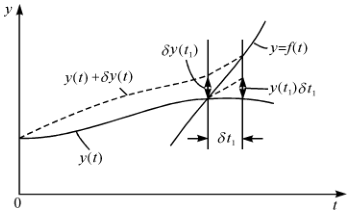
\includegraphics[width=\linewidth]{figs/fig-0161.png}
\caption{图9.3-1}
\end{figure}

\[\left.\frac{\partial F}{\partial y}-\frac{d}{d t}\left[\frac{\partial F}{\partial y}\right]\right)\qquad\text{(9.3-11)}\]

以及

如果 $\left[\frac{\partial F}{\partial y}\right]$ 是有限数，$F(t)=\dot{y}(t)\left[\frac{\partial F}{\partial y}\right]_{t_{1}}$

因为 $\delta_{y}(0)=0$，当 $t=0$ 时，并不一定要求方程 $(9.3-11)$ 成立，唯一的条件是: $t=0$时 $(\partial F / \partial y)_{0}$ 是有限数，而且 $y$ 连续变化。一个新的过渡过程开始时，$y, F$，$(\partial F / \partial y)$ 和 $(\partial F / \partial \dot{y})$ 可以不连续。因为方程 $(9.3-11)$ 的缘故，在其他点 $(0<t \leqslant t)$，$\partial F / \partial \dot{y}$ 将是连续的。

方程 $(9.3-11)$ 表示满足方程 $(9.3-5)$ 那个条件的变量 $y(t)$ 的微分方程。通常把方程 $(9.3-11)$ 叫做变分问题的尤拉-拉格朗日 (Euler-Lagrange) 方程。这里所考虑的问题中，函数 $F$ 不明显地包含时间变数 $t$。于是我们可以立刻得到方程 $(9.3-11)$ 的一个第一积分。方程 $(9.3-11)$ 的第一积分中，满足边界条件方程 $(9.3-12)$ 的第一积分具有下述形式

\[F(y, \dot{y})=\dot{y} \frac{\partial F}{\partial \dot{y}}\qquad\text{(9.3-13)}\]

把这个方程对时间 $t$ 微分，我们得到

\[\left.\frac{\partial F}{\partial y} \dot{y}+\dot{y} \frac{\partial F}{\partial \dot{y}}=\dot{y} \frac{\partial F}{\partial \dot{y}}+\dot{y} d\left[\frac{\partial F}{\partial y}\right]\right|\]

既然在那些 $y, \partial F / \partial \dot{y}$，等连续的地方，下面公式成立

\[\left.\dot{y}\left[\frac{\partial F}{\partial y}-\frac{d}{d t}\left[\frac{\partial F}{\partial \dot{y}}\right]\right]=0\right)\]

那么，或者 $\dot{y}=0$，或者满足方程 $(9.3-11)$。但是通常在过渡过程中 $\dot{y}$ 不会等于零 （也即无论在任何时间间隔内不恒等于零），于是由方程 $(9.3-11)$ 和方程 $(9.3-12)$所描述的 $y(t)$ 的两个必须满足的条件，可以用单独一个方程 $(9.3-13)$ 代替。

这样，我们称方程式 $(9.3-11)$ 为最优控制所应满足的必要条件。引进式 (9.3-6)内的符号，这个必要条件又可以写为

\[\begin{aligned} & \frac{\partial F}{\partial y}-\frac{d}{d t} \frac{\partial F}{\partial u}=0 \\ & \frac{d y}{d t}=u \\ & F(y(t), u(t))-u(t)\left[\frac{\partial F}{\partial u}\right]_{t_{1}}=0 \end{aligned}\qquad\text{(9.3-14)}\]

由上列三个方程式可求出两个未知函数 $u(t), y(t)$ 和一个未知量 $t$。这三个条件中的前两个实际上与终端条件固定与否无关，只有第三个条件才是由 $t$ 变分而得到的。因而前两个条件具有普遍性。

再来研究一个普遍的情况。设受控对象的输出坐标不是一个，而是 $n$ 个。此时指标泛函式(9.3-5)将变为

\[J=\int_{0}^{t_{1}} F\left(y_{1}, y_{2}, y_{3}, \cdots, y_{n} ; \dot{y}_{1}, \cdots, \dot{y}_{n}\right) d t\qquad\text{(9.3-15)}\]

或者写成

\[J=\int_{0}^{t_{1}} F\left(y_{1}, y_{2}, \cdots, y_{n} ; u, w, \cdots, u_{n}\right) d t\qquad\text{(9.3-16)}\]

\[\frac{d y_{i}}{d t}=u, \quad i=1,2, \cdots, n\qquad\text{(9.3-17)}\]

重复前述讨论，无论初始条件和终端条件是否已经给定，都可以得到相应于式 (9.3-14)中的前两个必要条件

\[\begin{aligned} & \frac{\partial F}{\partial y_{i}}-\frac{d}{d t} \frac{\partial F}{\partial u_{i}}=0, \quad i=1,2, \cdots, n \\ & \frac{d y_{i}}{d t}=u, \quad i=1,2, \cdots, n \end{aligned}\]

如果初始条件和终端条件已经给定，那么这两组方程式中含有 $2 n$ 个未知函数 $y_{1}(t), \cdots, y_{n}(t) ; u(t), \cdots, u_{n}(t)$。如果初始条件和终点条件是不固定的，则与式(9.3-17)同时还会出现两个附加条件，有如条件式(9.3-9)或(9.3-12)那样。

下面再来研究一类更为复杂一些的泛函指标

\[J=\int_{0}^{t_{1}} F\left(y, \dot{y}, \dot{y} ; z, \dot{z}, \ddot{z}\right) d t=\min\qquad\text{(9.3-18)}\]

式中 $y$ 和 $z$ 是受控对象的两个主要输出坐标。如果引进新的符号 $y=y_{1}, y=y_{1}$，$\dot{y}=w ; z=y_{3}, \dot{z}=y_{3}, \ddot{z}=w$，则式(9.3-18)可写成

\[\begin{aligned} & J=\int_{0}^{t_{1}} F\left(y_{1}, y_{2}, y_{3}, y_{4} ; w, w\right) d t \\ & \frac{d y_{1}}{d t}=y_{2} \\ & \frac{d y_{2}}{d t}=w \\ & \frac{d y_{3}}{d t}=y_{4} \\ & \frac{d y_{4}}{d t}=w \end{aligned}\qquad\text{(9.3-20)}\]

由此看到，这相当于由两个二阶方程描述的受控对象，$u$ 和 $w$ 是两个独立的控制量。

设受控对象在 $t=0$ 时刻的状态为固定，而终点时刻 $t$ 是待求的，但终点状态是给定的。再设 $y(t)$ 和 $z(t)$ 是两个最优的受控运动，它们都具有二次连续导数。令 $y(t)$ 和 $z(t)$ 分别获得微小增量 （变分） $\varepsilon \delta y(t)$ 和 $\varepsilon \delta z(t)$，其中 $\delta y(t)$ 和 $\delta z(t)$ 为二阶连续可微的固定函数，$\varepsilon$ 为任意小的常数。于是 $y(t)$ 和 $z(t)$ 使式 (9.3-18) 或式 (9.3-19) 取极值，即当 $\varepsilon=0$ 时有

\[\int_{0}^{t_{1}} \frac{d}{d \varepsilon} \int_{0}^{t_{1}+\varepsilon \delta t_{1}} F\left(y+\varepsilon \delta y, y+\varepsilon \delta y, \dot{y}+\varepsilon \delta \dot{y}, z+\varepsilon \delta z, z+\varepsilon \delta z, \dot{z}+\varepsilon \delta \dot{z}\right) d t=0\qquad\text{(9.3-21)}\]

方程 (9.3-18) 中积分的时间间隔由一个固定时刻 $(t=0)$ 开始，可是不是在某个固定时刻终止，而是终止在曲线 $y=f_{1}(t), \dot{y}=f_{2}(t), z=g_{1}(t)$，以及 $\dot{z}=g_{2}(t)$ 上。 $\delta y$ 和 $\delta z$ 是任意的函数，自然是时间的互相无关的函数。

我们把方程 (9.3-21) 的微分运算写出来

\[\int_{0}^{t_{1}}\left[\frac{\partial F}{\partial y} \delta y+\frac{\partial F}{\partial \dot{y}} \delta \dot{y}+\frac{\partial F}{\partial \ddot{y}} \delta \ddot{y}+\frac{\partial F}{\partial z} \delta z+\frac{\partial F}{\partial \dot{z}} \delta \dot{z}+\frac{\partial F}{\partial \ddot{z}} \delta \ddot{z}\right] d t+F(t) \delta t_{1}=0\]

经过部分积分以后，我们得到

\[\begin{aligned} & \int_{0}^{t_{1}}\left[\frac{\partial F}{\partial y}-\frac{d}{d t}\left(\frac{\partial F}{\partial \dot{y}}\right)+\frac{\dot{d}^{2}}{d t^{2}}\left(\frac{\partial F}{\partial \ddot{y}}\right)\right] \delta y d t+\int_{0}^{t_{1}}\left[\frac{\partial F}{\partial z}-\frac{d}{d t}\left(\frac{\partial F}{\partial \dot{z}}\right)+\frac{\dot{d}^{2}}{d t^{2}}\left(\frac{\partial F}{\partial \ddot{z}}\right)\right] \delta z d t \\ & \quad+\left[\frac{\partial F}{\partial \dot{y}} \delta y+\frac{\partial F}{\partial \ddot{y}} \delta \dot{y}-\frac{d}{d t}\left(\frac{\partial F}{\partial \dot{y}}\right) \delta \dot{y}\right]_{0}^{t_{1}}+F(t) \delta t_{1} \\ & \quad+\left[\frac{\partial F}{\partial \dot{z}} \delta z+\frac{\partial F}{\partial \ddot{z}} \delta \dot{z}-\frac{d}{d t}\left(\frac{\partial F}{\partial \dot{z}}\right) \delta z\right]_{0}^{t_{1}}=0 \end{aligned}\qquad\text{(9.3-22)}\]

和前面的讨论相类似，积分中被积函数以及边界条件必须分别等于零。从给出的终端条件，我们得到

\[\begin{aligned} \delta y\left(t_{1}\right) & =\left[\dot{f}_{1}\left(t_{1}\right)-\dot{y}\left(t_{1}\right)\right] \delta t_{1} \\ \delta \dot{y}\left(t_{1}\right) & =\left[\dot{f}_{2}\left(t_{1}\right)-\dot{y}\left(t_{1}\right)\right] \delta t_{1} \\ \delta z\left(t_{1}\right) & =\left[\dot{g}_{1}\left(t_{1}\right)-z\left(t_{1}\right)\right] \delta t_{1} \\ \delta \dot{z}\left(t_{1}\right) & =\left[\dot{g}_{2}\left(t_{1}\right)-\dot{z}\left(t_{1}\right)\right] \delta t_{1} \end{aligned}\qquad\text{(9.3-23)}\]

从方程 (9.3-22) 得到的三个条件可以写成两个联立的尤拉-拉格朗日方程

\[\begin{aligned} & \frac{\partial F}{\partial y}-\frac{d}{d t}\left[\frac{\partial F}{\partial \dot{y}}\right]+\frac{\ddot{d}}{d t^{2}}\left[\frac{\partial F}{\partial \ddot{y}}\right]=0 \\ & \frac{\partial F}{\partial z}-\frac{d}{d t}\left[\frac{\partial F}{\partial \dot{z}}\right]+\frac{\ddot{d}}{d t^{2}}\left[\frac{\partial F}{\partial \ddot{z}}\right]=0 \end{aligned}\qquad\text{(9.3-24)}\]

以及

\[\left\{\left\{F-y \frac{\partial F}{\partial \dot{y}}+\dot{y} \frac{d}{d t}\left(\frac{\partial F}{\partial \dot{y}}\right)-\dot{y} \frac{\partial F}{\partial \dot{y}}-\dot{z} \frac{\partial F}{\partial z}+\dot{z} \frac{d}{d t}\left(\frac{\partial F}{\partial \dot{z}}\right)-\dot{z} \frac{\partial F}{\partial \ddot{z}}\right\}_{t=t_{1}}\right.\]

\[\begin{aligned}& +\dot{f}_{1}\left(t_{1}\right)\left[\frac{\partial F}{\partial \dot{y}}-\frac{d}{d t}\left[\frac{\partial F}{\partial \dot{y}}\right]\right]_{t=t_{1}}+\dot{f}_{2}^{2}\left(t_{1}\right)\left[\frac{\partial F}{\partial \dot{y}}\right]_{t=t_{1}}+\dot{g}_{0}^{2}\left(t_{1}\right)\left[\frac{\partial F}{\partial \dot{z}}-\frac{d}{d t}\left[\frac{\partial F}{\partial \dot{z}}\right]\right]_{t=t_{1}} \\& +\dot{g}_{0}^{2}\left(t_{1}\right)\left[\frac{\partial F}{\partial \dot{z}}\right]_{t=t_{1}} \dot{\delta} t_{1}+\dot{\delta} y(0)\left[\frac{\partial F}{\partial \dot{y}}-\frac{d}{d t}\left[\frac{\partial F}{\partial \dot{y}}\right]\right]_{t=0}+\dot{\delta} \dot{y}(0)\left[\frac{\partial F}{\partial \dot{y}}\right]_{t=0} \\& +\dot{\delta} z(0)\left[\frac{\partial F}{\partial \dot{z}}-\frac{d}{d t}\left[\frac{\partial F}{\partial \dot{z}}\right]\right]_{t=0}+\dot{\delta} z(0)\left[\frac{\partial F}{\partial \dot{z}}\right]_{t=0}=0\end{aligned}\qquad\text{(9.3-25)}\]

方程(9.3-24)表示两个微分方程的系统，这个系统满足方程(9.3-18)原来给出的准则。这种问题的物理解答必须满足方程(9.3-18)，除此以外还要满足方程 (9.3-25)的那些边界条件。但是，因为 $F$ 不明显地包含变数 $t$，这一系列的条件可以加以修改；如果把方程 (9.3-24) 中第一个方程乘以 $\dot{y}$，第二个方程乘以 $\dot{z}$，然后加起来，就得到一个全微分，它的积分就是

\[F-\dot{y} \frac{\partial F}{\partial \dot{y}}+\dot{y} \frac{d}{d t}\left[\frac{\partial F}{\partial \dot{y}}\right]-\dot{y} \frac{\partial F}{\partial \dot{y}}-\dot{z} \frac{\partial F}{\partial \dot{z}}+\dot{z} \frac{d}{d t}\left[\frac{\partial F}{\partial \dot{z}}\right]-\dot{z} \frac{\partial F}{\partial \dot{z}}=C\qquad\text{(9.3-26)}\]

因为 $F$ 是 $\dot{y}$ 和 $\dot{y}$ 的一个函数，$\partial F / \partial \dot{y}$ 和 $\partial F / \partial \dot{y}$ 未必会等于零，$\partial F / \partial \dot{y}$ 也不一定是时间的常数函数，于是 $\frac{\partial F}{\partial \dot{y}}-\frac{d}{d t}\left[\frac{\partial F}{\partial \dot{y}}\right]$ 不一定等于零。由于初始条件和终点状态是给定的，所以在式 (9.3-25) 中可取

\[\delta \dot{y}(0)=\dot{\delta} \dot{y}(0)=\dot{f}_{1}\left(t_{1}\right)=\dot{f}_{2}\left(t_{1}\right)=0\]

变量 $z$ 也有类似的情形。于是得到一系列边界条件如下

\[\begin{aligned}& \delta \dot{y}(0)=0, \quad \dot{f}_{1}\left(t_{1}\right)=0 \\& \delta \dot{y}(0)=0, \quad \dot{f}_{2}\left(t_{1}\right)=0 \\& \delta z(0)=0, \quad \dot{g}_{0}^{2}\left(t_{1}\right)=0 \\& \dot{\delta} z(0)=0, \quad \dot{g}_{0}^{2}\left(t_{1}\right)=0\end{aligned}\qquad\text{(9.3-27)}\]

这些边界条件也是与变量 $y, \dot{y}, z$ 和 $\dot{z}$ 的起始值和终止值对应的条件，但是过渡过程的时间间隔 $t$ 可以变化。由方程 (9.3-27) 的边界条件，方程 (9.3-25) 指出方程 (9.3-26) 右端的那个常数 $C$ 必须等于零。方程 (9.3-18) 的最后解答如下

\[F-y \cdot \frac{\partial F}{\partial \dot{y}}+\dot{y} \frac{d}{d t}\left[\frac{\partial F}{\partial \dot{y}}\right]-\dot{y} \frac{\partial F}{\partial \dot{y}}-\dot{z} \frac{\partial F}{\partial \dot{z}}+\dot{z} \frac{d}{d t}\left[\frac{\partial F}{\partial \dot{z}}\right]-\dot{z} \frac{\partial F}{\partial \dot{z}}=0\qquad\text{(9.3-28)}\]

并且满足下面两个方程中的一个

\[\begin{aligned}& \frac{\partial F}{\partial y}-\frac{d}{d t}\left[\frac{\partial F}{\partial \dot{y}}\right]+\frac{\dot{d}}{d t^{2}}\left[\frac{\partial F}{\partial \dot{y}}\right]=0 \\& \frac{\partial F}{\partial z}-\frac{d}{d t}\left[\frac{\partial F}{\partial \dot{z}}\right]+\frac{\dot{d}}{d t^{2}}\left[\frac{\partial F}{\partial \dot{z}}\right]=0\end{aligned}\qquad\text{(9.3-29)}\]

方程(9.3-28)和(9.3-29)表示一个系统的两个变量 $y$ 和 $z$ 的微分方程，它们是控制方程，也是设计计算机所用的方程。

边界条件式(9.3-27)确定系统由一个主要运行状态过渡到另一状态的过渡过程的初始和终点条件。这样，如果方程式(9.3-27)所表示的条件都成立，系统便由一组固定的 $y, \dot{y}, z, \dot{z}$ 过渡到另一组固定的 $y, \dot{y}, z, \dot{z}$。方程(9.3-28) 是一个三阶微分方程。方程(9.3-29)是一个四阶微分方程。于是除了 $y, \dot{y}, z$ 和 $\dot{z}$ 的四个初始值而外，还可以假设一组与最后的 $y$ 相应的三个值 $\dot{y}, z$ 和 $\dot{z}$，那就是，当 $y$ $=y_{1}$ 时; $\dot{y}=0, z=z_{1}$，以及 $\dot{z}=0$。还必须在系统里加入一个稳定装置，使得在终止点，满足

\[\dot{y}=0 \text { 以及 } \dot{z}=0\]

我们看到，虽然上述情况比前面讨论过的一阶系统更为复杂，但是完全可以用同样的办法处理。

从此例中我们又看到，决定最优控制的两个条件中，式(9.3-29) 是一个普遍的必要条件，它与初始状态和终点状态无关，条件式(9.3-28) 是由终点时刻 $t$ 的不固定得到的。若引进式(9.3-19) 和式(9.3-20) 内曾用过的符号，则可将上述三个条件改写为

\[\begin{aligned}& \frac{\partial F}{\partial y_{1}}-\frac{d}{d t} \frac{\partial F}{\partial y_{2}}+\frac{d^{2}}{d t^{2}} \frac{\partial F}{\partial w}=0 \\& \frac{\partial F}{\partial y_{3}}-\frac{d}{d t} \frac{\partial F}{\partial y_{1}}+\frac{d^{2}}{d t^{2}} \frac{\partial F}{\partial w}=0 \\& F-y_{2} \frac{\partial F}{\partial y_{2}}+y_{2}^{2} \frac{d}{d t} \frac{\partial F}{\partial w}-u \frac{\partial F}{\partial w}-y_{1} \frac{\partial F}{\partial y_{1}}+y_{1} \frac{d}{d t} \frac{\partial F}{\partial w}-u \frac{\partial F}{\partial w}=0\end{aligned}\qquad\text{(9.3-32)}\]

\[\begin{aligned}& \frac{d y_{1}}{d t}=y_{2} \\& \frac{d y_{2}^{2}}{d t}=u \\& \frac{d y_{3}}{d t}=y_{1} \\& \frac{d y_{1}^{4}}{d t}=u\end{aligned}\]

这里共有七个方程式，含有六个未知函数和一个未知数: $y_{1}(t), y_{2}(t), y_{3}(t)$，$y_{4}(t), w(t), u(t)$ 和 $t$。对方程组(9.3-30) 和(9.3-32) 积分后将出现八个积分常数，后者将由四个初始状态和四个终点状态决定，它们是 $y_{1}(0), y_{2}(0), y_{3}(0)$，$y_{4}(0) ; y_{1}(t), y_{2}(t), y_{3}(t), y_{4}(t)$。方程式(9.3-31) 就变为一个代数等式，由它可解出 $t$。

在讨论了几种类型的系统之后，我们再来回顾一下这些问题的解中包括的一些重要假设。在推导尤拉-拉格朗日必要条件时，我们只是做了形式上的推导，却故意没有提到两点重要的假设。首先，在推导时，我们先假定最优控制函数 $u(t)$ 是存在的。得到的结果是，如果它们存在的话，必满足尤拉-拉格朗日方程及相应的决定 $h$ 的条件。在实际问题中，任意给定泛函指标式 $(9.3-5),(9.3-15)$ 或 $(9.3-19)$ 后是否一定存在最优控制函数呢？从上述讨论中是得不到答案的，而且像第一节那种不存在最优控制的情况是完全可能发生的。遗憾的是，关于存在性至今没有普遍的行之有效的判别准则，对这一问题的研究在数学上是一个困难的问题。

其次，在推导过程中，我们对 $y(t)$ 的增量 $\delta y(t)$ 未做任何限制，只说它是任意固定的足够光滑的函数。这意味着对控制量 $u(t)$ 的取值不做任何限制，如果最优控制存在的话，那么欲满足条件式 $(9.3-14)$ 或 $(9.3-30), u(t)$ 可以在实轴上的任何处取值。这种情况有时在技术问题中是可以允许的，有时却是不能允许的。当 $u(t)$ 受限制时，例如，在实际问题中如果要求 $|u(t)| \leqslant M$，则尤拉-拉格朗日方程就未必有解。当然，如果求出的最优控制函数满足限制条件的话，事情就简单了。否则，前述古典变分法所提供的方法就将无能为力了。此时必须建立新的理论，以适应这种实际要求。这将在以后详细讨论。

\section{9.4 决定最优控制的标准方程组}

前节内我们讨论了古典变分法中的几种特殊情况。那里受控对象的运动方程式实际上是多个一阶或二阶环节的联合。前面曾提到过另外一种普遍性问题，即系统的受控运动方程式已给定，须求出满足给定积分指标的最优控制函数。为了清楚起见，我们再将问题的数学内容叙述如下。设受控对象的运动由下列方程组所描述

\[\frac{d x_{i}}{d t}=f_{i}\left(x_{1}, \cdots, x_{n} ; u, \cdots, u_{r}\right), \quad i=1,2, \cdots, n, \quad r \leqslant n\qquad\text{(9.4-1)}\]

受控运动的质量指标是

\[J=\int_{0}^{t_{1}} f_{0}\left(x_{1}, \cdots, x_{n} ; u, \cdots, u_{r}\right) d t\qquad\text{(9.4-2)}\]

式中，$f_{0}, f_{i}$ 均为诸自变量的连续可微函数，而且不明显依赖于 $t$; 积分上限 $t$ 为受控对象由某一初始状态到达指定的终点状态所需时间。

设 $\boldsymbol{x}=\left(x_{10}, x_{20}, \cdots, x_{n 0}\right)$ 为受控对象的初始状态，$\boldsymbol{x}=\left(x_{11}, x_{21}, \cdots, x_{n 1}\right)$ 为终点状态。须求出一个向量控制函数 $\dot{u}(t)=\left(\dot{u}(t), \cdots, \dot{u}(t)\right)$，使受控对象自 $\boldsymbol{x}$ 点到达 $\boldsymbol{x}$ 点，且使沿 $\dot{\boldsymbol{x}}(t)$ 和 $\dot{u}(t)$ 的积分 $J$ 取极小值，即

\[J(\dot{u}(t))=\int_{0}^{t_{1}} f_{0}\left(\dot{\boldsymbol{x}}(t), \dot{\boldsymbol{u}}(t)\right) d t=\min\qquad\text{(9.4-3)}\]

必须指出该问题的几个特点:

(1) 受控对象的两个端点都假设为固定的。所谓最优控制 $\dot{u}(t)$ 是指一切将 $\boldsymbol{x}_{0}$ 引至 $\boldsymbol{x}_{1}$ 的控制函数中，使其在式 (9.4-3) 意义上是最好的。

(2) 在 $t=0$ 时刻，受控对象自 $\boldsymbol{x}_{0}$ 出发，到达 $\boldsymbol{x}_{1}$ 的时刻 $t$ 并不固定。

(3) 假设 $\boldsymbol{u}(t)$ 的每个分量 $u(t)$ 均为 $t$ 的分段连续函数。每一个 $u(t)$ 在每一时刻 $t$ 的取值不受限制，只要有界即可，在任意有限时间内，只有有限个第一类间断点。

在上述的假设条件下，我们来讨论最优控制所应满足的条件。下面的证明方法不同于古典变分法中常采用的变分方法，而采用文献[22]中的思想，用更为直观的几何证明。这种几何方法还将在下节内应用，那里将讨论 $\boldsymbol{u}(t)$ 受限制的情况下最优控制应满足的必要条件。

研究方程组 (9.4-1) 的同时，引进新坐标 $x_{0}=J$，并按式 (9.4-2) 写出关于 $x_{0}(t)$ 的微分方程式

\begin{figure}[htbp]\centering
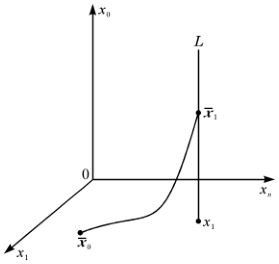
\includegraphics[width=\linewidth]{figs/fig-0162.png}
\caption{图9.4-1}
\end{figure}

\[\frac{d x_{0}}{d t}=f_{0}\left(x_{1}, \cdots, x_{n} ; u, \cdots, u_{r}\right)\qquad\text{(9.4-4)}\]

将式 (9.4-1) 和 (9.4-4) 合并后就得到一个由 $n+1$ 个方程式组成的方程组。用 $\bar{x}$表示 $n+1$ 维向量 $\left(x_{0}, x_{1} \cdots, x_{n}\right)$，式 (9.4-1) 和 (9.4-4) 可联合写成一个向量方程式

\[\frac{\bar{d} \boldsymbol{x}}{d t}=\bar{f}(\boldsymbol{x}, \boldsymbol{u}), \quad \bar{\boldsymbol{x}}(0)=\bar{x}_{0}=\left(0, x_{10}, \cdots, x_{n 0}\right)\qquad\text{(9.4-5)}\]

式中 $\bar{x}=\left(x_{0}, x_{1}, \cdots, x_{n}\right) ; \bar{f}=\left(f_{0}, f_{1}, \cdots, f_{n}\right)$。最优控制 $\dot{u}(t)$ 所对应的最优运动 $\dot{x}(t)$ 和 $J(t)=x_{0}(t)$ 可以合并为 $\dot{x}$，并看成是 $n+1$ 维空间的一条曲线。这条曲线自 $\boldsymbol{x}_{0}$ 点出发，在 $t=t_{1}$ 时到达 $\boldsymbol{x}_{1}$点，并使 $x_{0}\left(t_{1}\right)$ 取最小值 （图 9.4-1)。

应用几何概念，求最优控制的问题可以转述成如下问题。对方程式 (9.4-5) 须求出一个控制函数 $\dot{u}(t)$，使系统自 $\boldsymbol{x}$ 点出发，在某一时刻 $t=$ $t_{1}$，达达平行于 $x_{0}$ 轴且通过 $\left(0, \boldsymbol{x}_{1}\right)$ 点的直线 $L$上。使交点 $\bar{x}_{1}$ 的第一个分量 $x_{0}$ 达极小值。

为了寻求最优控制函数的特点，现将 $\dot{u}(t)$ 做某些微小的变化。取一个异于 $\dot{u}(t)$ 的控制函数

\[u(t)= \begin{cases}\dot{u}(t)+\delta u, & s-\varepsilon \delta t \leqslant t \leqslant s<t \\ \dot{u}(t), & 0 \leqslant t<s-\varepsilon \delta t, & s<t \leqslant t\end{cases}\qquad\text{(9.4-6)}\]

上式内 $\varepsilon$ 为一足够小的正数，$\delta t$ 为任意正常数，$s$ 为小于 $t$ 的任意固定时刻，$\delta u$ 为任意余时刻均与依然是最优的，只在小区间内系统运动的偏离量可用下列公式算出

\[\begin{aligned}& \int_{s-\varepsilon \delta t}^{s}\left[\bar{f}\left(\dot{\boldsymbol{x}}(t), \dot{\boldsymbol{u}}(t)+\delta \boldsymbol{u}\right)-\bar{f}\left(\dot{\boldsymbol{x}}(t), \dot{\boldsymbol{u}}(t)\right)\right] d t \\= & \int_{s-\varepsilon \delta t}^{s}\left(\sum_{a=1}^{r} \frac{\partial \bar{f}}{\partial u_{a}} \delta u_{a}\right) d t+\bar{O}_{1}(\varepsilon, \delta \boldsymbol{u}) \\= & \varepsilon \delta t \sum_{a=1}^{r}\left(\frac{\partial \bar{f}\left(\dot{\boldsymbol{x}}(s), \dot{\boldsymbol{u}}(s)\right)}{\partial u_{a}} \delta u_{a}\right)+\bar{O}(\varepsilon, \delta \boldsymbol{u})\end{aligned}\qquad\text{(9.4-7)}\]

上式右端之第一项由于用 $\dot{\boldsymbol{x}}$ 代换了 $\bar{\boldsymbol{x}}(s)$ 所产生的误差对 $\varepsilon$ 来说将是高阶无穷小，并于 $\bar{O}(\varepsilon, \delta \boldsymbol{u})$ 内。不难证明，当 $\varepsilon \rightarrow 0$ 时，$\lim \frac{\bar{O}(\varepsilon, \delta \boldsymbol{u})}{\varepsilon}$ 为零向量；当 $\|\delta \boldsymbol{u}\| \rightarrow 0$ 时 $\frac{\bar{O}(\varepsilon, \delta \boldsymbol{u})}{\|\delta \boldsymbol{u}\|} \rightarrow \mathbf{0}$。

最优运动轨线在 $s$ 时刻已经发生了偏差。在 $s$ 以后，控制函数没有改变。令

\[\dot{\boldsymbol{u}}\left(\dot{\boldsymbol{x}}(s), \dot{\boldsymbol{u}}+\delta \boldsymbol{u}\right)-\bar{f}\left(\dot{\boldsymbol{x}}(s), \dot{\boldsymbol{u}}(s)\right))=\bar{\boldsymbol{y}}(s)\qquad\text{(9.4-8)}\]

在 $s$ 时刻的轨线偏离是 $\bar{\boldsymbol{y}}(s)$。从微分方程的理论中我们知道，由于小的初始偏差引起的轨道偏差主要部分可用线性化的办法算出，即在 $s \leqslant t \leqslant t$ 区间内 $\delta \bar{\boldsymbol{x}}(t)=$ $\bar{\boldsymbol{y}}(t)$ 可由下列线性化方程组求出

\[\frac{d \boldsymbol{y}_{i}(t)}{d t}=\sum_{a=1}^{n} \frac{\partial f_{i}}{\partial x_{a}} y_{a}, \quad i=0,1, \cdots, n, \quad s \leqslant t \leqslant t\qquad\text{(9.4-9)}\]

或写成向量方程式

\[\frac{d \bar{\boldsymbol{y}}}{d t}=A(t) \bar{\boldsymbol{y}}\qquad\text{(9.4-10)}\]

此处

\[A(t)=\left(\begin{array}{cccc}\frac{\partial f_{0}}{\partial x_{0}} & \frac{\partial f_{0}}{\partial x_{1}} & \cdots & \frac{\partial f_{0}}{\partial x_{n}} \\\vdots & \vdots & & \vdots \\\frac{\partial f_{n}}{\partial x_{0}} & \frac{\partial f_{n}}{\partial x_{1}} & \cdots & \frac{\partial f_{n}}{\partial x_{n}}\end{array}\right)\]

其中各系数是沿最优轨线求出的，即

\[\frac{\partial f_{i}}{\partial x_{a}}=\frac{\partial f_{i}\left(\dot{\boldsymbol{x}}(t), \dot{\boldsymbol{u}}(t)\right)}{\partial x_{a}}\]

故它们均为已知的时间 $t$ 的函数。

式(9.4-9)或(9.4-10)是一个线性方程组。设 $\Phi(t, s)$ 是它的基本解矩阵。那么，它的解将是

\[\mathbf{y}(t)=\Phi(t, s) \mathbf{y}(s), \quad s \leqslant t \leqslant t\qquad\text{(9.4-11)}\]

现在研究在 $t=t$ 时刻轨道偏离的情况。显然当 $t=t$ 时有

\[\bar{\delta} \bar{\mathbf{x}}\left(t_{1}\right)=\bar{\mathbf{y}}\left(t_{1}\right)=\varepsilon \Phi\left(t_{1}, s\right) \mathbf{y}(s)\qquad\text{(9.4-12)}\]

再根据式(9.4-7)和 $\bar{\mathbf{y}}(s)$ 的定义，我们有

\[\mathbf{y}(s)=\partial_{t} B(s) \partial u\qquad\text{(9.4-13)}\]

上式中 $B(s)$ 为 $n \times r$ 阶长方阵，

\[B(s)=\left(\begin{array}{cccc}\frac{\partial f_{0}}{\partial u} & \frac{\partial f_{0}}{\partial u} & \cdots & \frac{\partial f_{0}}{\partial u_{r}} \\\vdots & \vdots & & \vdots \\\frac{\partial f_{n}}{\partial u} & \frac{\partial f_{n}}{\partial u} & \cdots & \frac{\partial f_{n}}{\partial u_{r}}\end{array}\right)\qquad\text{(9.4-14)}\]

其中每个元素都是在最优轨线的 $s$ 时刻算出的，即

\[\frac{\partial f_{i}}{\partial u_{j}}=\frac{\partial f_{i}\left(\dot{\mathbf{x}}(t), \dot{\mathbf{u}}(t)\right)}{\partial u_{j}}\]

按式(9.4-13)和(9.4-12)，若 $\varepsilon$ 为足够小的正数，$s$ 为固定时刻，于是每一个特定的 $\delta u$ 便对应一个 $\bar{\mathbf{y}}(s)$，进而有一个 $\bar{\delta} \bar{\mathbf{x}}\left(t_{1}\right)$。当常向量 $\delta u$ 在 $r$ 维空间零点周围变化时，$\mathbf{y}(s)$ 和 $\bar{\delta} \bar{\mathbf{x}}\left(t_{1}\right)$ 也将在 $\bar{\mathbf{x}}_{1}$ 点周围改变其方向及大小。一切可能的 $(\delta u)$ 按式(9.4-12)和(9.4-13)构成的所有 $(\delta \bar{\mathbf{x}}\left(t_{1}\right))$ 将是一个线性子空间 $K$ （把 $\bar{\mathbf{x}}$ 看成它们的坐标原点）。子空间 $K$ 的维数将不大于 $r$。由于 $\bar{\mathbf{x}}$ 是最优运动，通过点 $\bar{\mathbf{x}}$ 而平行于 $x_{0}$ 轴的直线 $L$ 不可能包含于子空间 $K$ 内。否则按式(9.4-6)的方法将 $\dot{u}(t)$加以改变，受控系统式(9.4-5)有可能在 $t$ 时刻到达直线 $L$ 上比 $x_{0}(J)$ 取值更小的点，而这与 $\dot{u}(t)$ 为最优控制的假定相矛盾，故是不可能的。由此可知，当 $r=n$时，$K$ 的维数不可能大于 $n-1$，否则直线 $L$ 将包含于其内。

既然 $K$ 的维数不大于 $r$ （当 $r=n$ 时不大于 $n-1$ )，则存在一个通过 $\bar{\mathbf{x}}$ 点的 $n-1$ 维超平面 $P$，它能将 $K$ 和以 $\bar{\mathbf{x}}_{1}$ 为始点的向量 $\mathbf{z}=(\cdots, 0, \cdots, 0)$ 完全隔开。取 $\bar{\Psi}_{1}$ 为 $P$ 的与向量 $\mathbf{z}$ 位于同侧的法向量，称之为 $P$ 的外法向量，此时不等式

\[\left(\bar{\delta} \bar{\mathbf{x}}\left(t_{1}\right), \bar{\Psi}_{1}\right) \leqslant 0\qquad\text{(9.4-15)}\]

对任何 $\bar{\mathbf{y}}(s)$ 均成立。考虑到 $\varepsilon>0, \partial t>0$，根据式(9.4-8)，上式可写为

\[\left(\Phi\left(t_{1}, s\right) \mathbf{y}(s), \bar{\Psi}_{1}\right) \leqslant 0\]

其中 $\bar{\Psi}_{1}=\left(\phi_{\mathrm{v} 1}, \phi_{1}, \phi_{2}, \cdots, \phi_{n}\right)$ 为非零向量，且 $\phi_{1} \leqslant 0$。由于内积的特性有

\[\left(\Phi\left(t_{1}, s\right) \bar{\mathbf{y}}(s), \bar{\Psi}_{1}\right)=\left(\bar{\mathbf{y}}(s), \Phi^{\top}\left(t_{1}, s\right) \bar{\Psi}_{1}\right)\qquad\text{(9.4-16)}\]

再研究线性化方程组(9.4-9)的共轭方程组

\[\begin{aligned}& \frac{d \psi_{b}}{d t}=-\sum_{a=0}^{n} \frac{\partial f_{a}}{\partial x_{0}} \psi_{b} \\& \cdots \\& \frac{d \psi_{n}}{d t}=-\sum_{a=0}^{n} \frac{\partial f_{a}}{\partial x_{n}} \psi_{b}\end{aligned}\qquad\text{(9.4-17)}\]

或者写成向量的方程式

\[\frac{d \boldsymbol{\Psi}}{d t}=-\boldsymbol{A}^{r}(t) \bar{\Psi}\qquad\text{(9.4-18)}\]

令 $F(t, s)$ 是式 (9.4-18) 的基本解矩阵，$F(\tau, \tau)=E$。不难证明，$F(t, s)=(\Phi^{r}(t$，$s))^{-1}$ 这个关系式总成立。这是因为

\[\frac{d \Phi^{-1} \Phi}{d t}=\frac{d \Phi^{-1}}{d t} \Phi+\Phi^{-1} \frac{d \Phi}{d t}=0\]

故

\[\frac{d \Phi^{-1}}{d t}=-\Phi^{-1} A(t) \Phi \Phi^{-1}=-\Phi^{-1} A(t)\]

将上式两端转置后有

\[\frac{d(\Phi)^{-1}}{d t}=-A^{r}(t)(\Phi^{-1})\qquad\text{(9.4-19)}\]

这就证明了 $(\Phi(t, s))^{-1}$ 是式 (9.4-18) 的基本解矩阵。令 $\bar{\Psi}(t)$ 是式 (9.4-18) 的一个特解，且

\[\bar{\Psi}(t)=\bar{\Psi}_{1}\qquad\text{(9.4-20)}\]

此处 $\bar{\Psi}_{1}$ 是前述之外法向量。于是

\[\bar{\Psi}_{1}=\left(\Phi^{r}(t, s)\right)^{-1} \bar{\Psi}(s)\]

将上式代入式 (9.4-16) 后便有

\[(\bar{y}(s), \Phi^{r}(t, s)\left(\Phi^{r}(t, s)\right)^{-1} \bar{\Psi}_{1}(s))=(\bar{y}(s), \bar{\Psi}(s)) \leqslant 0\]

再由式 (9.4-8) 将 $\bar{y}(s)$ 之值代入上式，便得到最后不等式

\[\bar{f}(\hat{x}(s), \dot{u}(s)+\hat{\delta} u)-\left(\bar{f}(\hat{x}(s), \dot{u}(s)), \bar{\Psi}(s)\right) \leqslant 0\]

或者

\[\bar{f}(\hat{x}(s), \dot{u}(s), \bar{\Psi}(s)) \geqslant\left(\bar{f}(\hat{x}(s), \dot{u}+\hat{\delta} u), \bar{\Psi}(s)\right)\qquad\text{(9.4-21)}\]

记函数

\[H\left(\bar{x}, \bar{\Psi}, \boldsymbol{u}\right)=\sum_{n=0}^{n} f_{n} \psi_{n}\qquad\text{(9.4-22)}\]

不难直接检查此函数 $H$ 与方程组 (9.4-5) 及 (9.4-18) 的关系是

\[\frac{\partial H}{\partial \psi_{i}}=\frac{d x_{i}}{d t}, \quad i=0,1, \cdots, n\]

\[\frac{\partial H}{\partial x_{i}}=-\frac{d \psi_{i}}{d t}, \quad i=0,1, \cdots, n\qquad\text{(9.4-23)}\]

函数 $H$ 与分析力学中的哈密顿函数的结构形式很类似，故常称为哈密顿函数。通过函数 $H$ 可知条件式 (9.4-21) 等价于下列等式:

\[H\left(\hat{\mathbf{x}}(s), \hat{\boldsymbol{\Psi}}(s), \dot{\boldsymbol{u}}(s)\right)=\operatorname{ext} H\left(\hat{\mathbf{x}}, \hat{\boldsymbol{\varphi}}(s), \dot{\boldsymbol{u}}(s)+\delta \boldsymbol{u}\right)\qquad\text{(9.4-24)}\]

这就是说，在受控系统的最优运动轨线上，在 $s$ 时刻对任意足够小的 $\delta u$，最优控制 $\dot{u}(s)$ 使 $H$ 取极值。但是，由于 $s$ 是任意的，$0<s<t$，故条件式 (9.4-24) 对最优轨线上除两个端点外的一切点均成立。若函数 $f_{i}(\mathbf{x}, \boldsymbol{u})$ 对 $\boldsymbol{u}$ 的每个分量 $u_{i}$ 是连续可微函数，则式 (9.4-24) 还可以写成

\[\begin{gathered} \frac{\partial}{\partial u} H\left(\hat{\mathbf{x}}(t), \bar{\Psi}(t), \boldsymbol{u}\right)=0 \\ i=1,2, \cdots, r, \quad 0<t \leqslant t \end{gathered}\]

上述讨论中，我们均假定系统到达终点的时间 $t$ 已经给定，因此在推导上述条件时，对 $t$ 未做变化。实际上由于到达端点的时间也可以变化，由变化 $t$ 还可以求出另外一个最优控制必须满足的必要条件。现设到达终点的时间不是 $t$ 而是 $t+\Delta t, \Delta t$ 是任意足够小的正数或负数。在区间 $[0, t+\Delta t]$ 定义控制函数为

\[u(t)= \begin{cases}\dot{u}(t), & 0 \leqslant t \leqslant t \\ \dot{u}(t), & t \leqslant t \leqslant t+\Delta t\end{cases}\]

由于终端时刻的变化而产生的增量 $\delta \mathbf{x}(t)$ 同样应满足条件式 (9.4-15)，即

\[\left(f\left(\hat{\mathbf{x}}(t), \dot{\boldsymbol{u}}(t)\right) \Delta t, \bar{\Psi}(t)\right) \leqslant 0\qquad\text{(9.4-26)}\]

由于 $\Delta t$ 是任意的，其符号可正可负，故上式只有在左端为零时才能成立。因此，可以断言在 $t$ 时刻有

\[H\left(\hat{\mathbf{x}}(t), \bar{\Psi}(t), \dot{\boldsymbol{u}}(t)=\left(\bar{f}\left(\hat{\mathbf{x}}(t), \dot{\boldsymbol{u}}(t)\right), \bar{\Psi}(t)\right)=0\right.\qquad\text{(9.4-25)}\]

但是，根据关系式 (9.4-22) 可以算出当 $\dot{u}(t)$ 为固定时

\[\begin{aligned} \frac{d H}{d t} & =\left[\frac{\bar{d} \boldsymbol{f}}{d t}, \bar{\Psi}\right]+\left[\bar{\boldsymbol{f}}, \frac{d \bar{\Psi}}{d t}\right] \\ & =\left(A(t) \frac{d \hat{\mathbf{x}}}{d t}, \bar{\Psi}\right)+\left(\bar{\boldsymbol{f}},-A^{s}(t) \bar{\Psi}\right) \\ & =\left(\bar{\boldsymbol{f}}, A^{s}(t) \bar{\Psi}\right)-\left(\bar{\boldsymbol{f}}, A^{s}(t) \bar{\Psi}\right) \\ & \equiv 0 \end{aligned}\]

此处 $A(t)$ 为式 (9.4-10) 中的方阵。故沿最优运动轨线，哈密顿函数恒为常数

\[H\left(\hat{\mathbf{x}}(t), \bar{\Psi}(t), \dot{\boldsymbol{u}}(t)\right)=\operatorname{const}, \quad 0 \leqslant t \leqslant t\]

由式 (9.4-27) 知 $H(t)=0$，所以又有

\[H\left(\dot{\mathbf{x}}\left(t_{h}\right), \dot{\boldsymbol{\Psi}}\left(t_{h}\right), \dot{u}\right) \equiv 0, \quad 0 \leqslant t \leqslant t_{h}\]

这样我们就得到了一套完整的最优控制应该满足的必要条件。现将这些条件集中写出

\[\begin{aligned}& \frac{d x_{i}}{d t}=f_{i}\left(\dot{\mathbf{x}}(t), \dot{u}(t)\right), \quad i=0,1, \cdots, n \\& \overline{\mathbf{x}}(0)=\left(0, x_{10}, x_{20}, \cdots, x_{n 0}\right) \\& \mathbf{x}(t)=\left(x_{11}, x_{21}, \cdots, x_{n 1}\right) \\& \frac{d \psi_{i}}{d t}=-\sum_{i=0}^{n} \frac{\partial f_{i}}{\partial x_{i}} \psi_{i}, \quad i=0,1, \cdots, n \\& \frac{\partial H}{\partial u}=0, \quad i=1,2, \cdots, r \\& H \equiv 0\end{aligned}\qquad\text{(9.4-28)}\]

总之，如果控制量 $u(t)$ 的取值不受限制，自 $\mathbf{x}$ 点至 $\mathbf{x}$ 点的最优控制 $\dot{u}(t)$ 存在，那么必存在一组非零函数 $\psi(t), \cdots, \psi_{n}(t)$，后者是式 (9.4-28) 中第二组方程式的解，使哈密顿函数 $H$ 在每一时刻对变量 $u$ 取极值，而且沿最优运动轨迹 $H$ 恒等于零。

现分析一下必要条件式 (9.4-28) 的结构。首先，由于各 $f_{i}$ 中不含 $x_{0}$，故

\[\frac{d \psi_{0}}{d t}=0, \quad \psi_{0}=\operatorname{const}, \quad \psi_{0} \leqslant 0\]

这里的第三个条件是由于一切 $\overline{\mathbf{x}}(t)$ 所构成的子空间 $K$ 不包含向量 $\mathbf{z}=(-1$，$0, \cdots, 0)$。其次，式 (9.4-28) 内共含有 $2 n+r+2$ 个未知函数和一个未知数 $h$，即共有 $2 n+r+3$ 个未知因素，而恰恰有 $2 n+r+3$ 个方程式，若最优控制存在的话，可以由式 (9.4-28) 求出。式 (9.4-28) 内包括了 $2 n+2$ 个微分方程式，其他 $r+1$ 个方程式是代数方程。为了解两组微分方程式必须有 $2 n+2$ 个边界条件。实际上我们只有 $2 n+1$ 个边界条件，因为 $x_{0}(t)$ 的终点值 （最优值） 是未知的。看起来，似乎还缺少一个条件。事实上，由于对 $\overline{\Psi}$ 的方程组是线性齐次的，初始条件只能准确到某一常数公因子，故对它的求解只需要有 $n$ 个初始条件就够了。此外，还有一个初始条件应由式 (9.4-27’) 在 $t=0$ 时确定，所以实际上只需有 $2 n$ 个初始条件就能求出两组微分方程的解。剩下的一个边界条件恰好留给 $t$。因此，式 (9.4-28) 中不仅方程式的个数是足够的，而且边界条件也恰恰满足需要。正由于这个理由，我们说式 (9.4-28) 给出了求最优控制所必需的完整条件。因此，我们称式 (9.4-28) 为决定最优控制的标准方程组。

但是，还应该注意到，如果式 (9.4-28) 只有一个孤立的解，它连接 $\mathbf{x}$ 和 $\mathbf{x}$，那么它就是唯一的最优运动和最优控制。如果满足式 (9.4-28) 的控制和运动不止一个，而有很多个，则在这些运动中仍有必要加以选择。这就是说，条件式

(9.4-28)仅仅是最优控制和最优运动的必要条件。满足式(9.4-28)的控制函数不能保证都是最优的。还有一种情况可能是不存在式(9.4-28)能够使受控系统自 $\boldsymbol{x}_{0}$ 点出发到达 $\boldsymbol{x}$ 点的解，此时最优控制将不存在。如果满足式(9.4-28)的解有很多个，每一个都使 $\boldsymbol{x}_{0}=J=\min$，这时最优控制将不唯一，在设计实际系统时可任选其中的一个加以实现。

\section{9.5 附加限制时的最优控制和喷气发动机控制设计}

在实际问题中，除预先给定控制过程的积分指标外，还可能提出某些关于受控对象输出坐标的限制条件。例如第 9.2 节中喷气发动机的工作过程中，常要求对发动机温度进行限制。这种限制也往往是以积分形式给定的，例如要求控制过程满足条件

\[J_{1}=\int_{0}^{t_{1}} g(\boldsymbol{x}, \boldsymbol{u}) d t \leqslant l\qquad\text{(9.5-1)}\]

其中 $l$ 为某一给定常数。这样必须在使受控对象式(9.4-1)自状态 $\boldsymbol{x}$ 引至 $\boldsymbol{x}$，且满足条件(9.5-1)的一切控制中寻求使式(9.4-2)达极小值的控制函数——条件最优控制函数 $\boldsymbol{u}(t)$。

如果设计控制系统时先不考虑式 (9.5-1) 的限制条件，而直接解方程组 (9.4-28)，这样求出的 $\boldsymbol{u}(t)$ 和 $\boldsymbol{x}(t)$，必须再代入 $(9.5-1)$，检查该条件是否被满足。自然，这时有两种可能：由式 (9.4-28) 出的最优控制满足条件式 (9.5-1)，此时限制条件式 $(9.5-1)$ 不改变前述的设计结果；另一种可能是由式 (9.4-28) 求出的最优控制不满足条件式 $(9.5-1)$，此时就不能按原来的计算进行了，而要寻求满足式 $(9.5-1)$ 的新的条件最优控制。上述两种情况中，对设计者有意义的是第二种，因此，当由式 (9.4-28) 求出的最优控制不满足式 $(9.5-1)$ 时，我们有理由在式 $(9.5-1)$ 内取等号，即将式 $(9.5-1)$ 改写成条件

\[J_{1}=\int_{0}^{t_{1}} g(\boldsymbol{x}, \boldsymbol{u}) d t=l\qquad\text{(9.5-2)}\]

用类似前节的方法可以证明 ${ }^{[22]}$ 如果 $\dot{\boldsymbol{u}}(t)$ 和 $\dot{\boldsymbol{x}}(t)$ 是满足条件式 $(9.5-2)$ 的自 $\boldsymbol{x}$ 点引至 $\boldsymbol{x}$ 点的最优控制，如果它们不是 $J_{1}$ 的极值函数，则必存在一个常数 $\lambda$，使 $\dot{\boldsymbol{u}}(t)$ 和 $\dot{\boldsymbol{x}}(t)$ 成为满足下列积分泛函指标的最优控制

\[J_{0}=\int_{0}^{t_{1}}\left[f_{0}(\boldsymbol{x}, \boldsymbol{u})+\lambda g(\boldsymbol{x}, \boldsymbol{u})\right] d t=\min\qquad\text{(9.5-3)}\]

以新的积分指标式 $(9.5-3)$ 代替原积分式 $(9.4-2)$ 后，依然可以利用标准方程组 (9.4-28) 求出条件最优控制。此时又多了一个未知常数 $\lambda$。但是，为了求 $\lambda$ 我们却又多了一个条件式 $(9.5-2)$。于是，如果条件最优控制函数存在的话，由式

(9.4-28)，(9.5-2)，(9.5-3)有希望将它求出。

作为例子，我们继续研究第 9.2 节中曾经介绍过的喷气发动机的过程控制问题，并对发动机输入至轮机的工作物体的温度加以限制。根据式(9.2-4)和(9.2-5)，当控制速度时，若只把旋转速度误差看做是最重要的因素，控制准则就变成

\[\int_{0}^{t_{1}} f(N-N_{s}) d t=\min\qquad\text{(9.5-4)}\]

于是，由方程(9.3-13)的控制条件可以简单地给出等式

\[f_{1}\left(N-N_{s}\right)=0\]

由于 $f_{1}$ 的性质，我们有 $N=N_{s}$。这个结果表示：在发动机的性能没有受到其他限制条件的情况下，这种速度控制将保持速度误差恒等于零，然而只有允许温度无限升高，才可能实际达到上述要求。这个结果和前面的方程(9.3-13)前后不一致，在那个方程里，$N$ 并不是一个时间的不连续的函数。这个例子是一般问题的一种显然情形。但是这个结果指出必须附带有另外的准则才能给出实际上有意义的系统。

设 $T$ 表示发动机工作温度的瞬时值，根据式(9.2-4)内的温度限制表达式，对温度的限制条件可写成

\[J_{1}=\int_{0}^{t_{1}} f_{3}(T(t)) d t\qquad\text{(9.5-5)}\]

现在假设在速度控制问题中把条件式(9.5-4)和(9.5-5)合并考虑。根据本节内前面的讨论，可以写成一个类似式(9.5-3)的积分指标

\[J_{0}=\int_{0}^{t_{1}}\left[f_{1}\left(N-N_{s}\right)+\lambda f_{3}(T)\right] d t=\min\qquad\text{(9.5-6)}\]

所以 $F=f_{1}\left(N-N_{s}\right)+\lambda f_{3}(T)$。由于利用了方程(9.2-5)，方程(9.3-13)变成

\[f_{1}\left(N-N_{s}\right)+\lambda f_{3}(T)=\lambda a \tau \dot{N} f_{3}(T)\qquad\text{(9.5-7)}\]

这是过渡过程的控制方程。当过渡过程终止时，理想的稳定装置发生作用，所以就有

\[N=N_{s}\qquad\text{(9.5-8)}\]

\[\dot{N}=0\]

方程(9.5-7)和(9.5-8)描写出整个控制系统的性质。我们可以设想，有一架计算机安装在系统里，它由测量机构获得有关 $N$ 和 $T$ 的资料，贮藏有 $\lambda, a$ 和 $\tau$ 的资料，以及燃料速度和 $N, T$ 之间的联系，然后根据方程(9.5-7)，产生适当的燃料喷射率的信号。当 $N$ 即将到达 $N_{s}$ 时，稳定机构参与作用，所以过渡过程终止时方程 (9.5-8)自然满足，一般说来，控制方程(9.5-7)是非线性方程，计算机不可能是线性元件，不像简单的电阻电容线路那样。

作为一个例子，考虑下述情况，当 $T>L_{2}$ 时，$f_{3}(T)=\left(T-L_{2}\right)^{n}$，当 $T<L_{1}$ 时，$f_{3}(T)=(L_{1}-T)^{a}$。通常，次数 $n$ 必须大于 1，因为如果 $n<1, T$ 可以是无限大，这样即使积分

\[\int_{0}^{1} f_{3}(T) d t\]

是有限的，将使 $N$ 不连续，这不符合实际情况。在讨论中，令 $n=2$，并且令 $f_{1}\left(N-N_{s}\right)=\left(N-N_{s}\right)^{2}$。所以我们又以对于给定值所发生的平均平方误差作为误差的量度，于是方程(9.5-7)变成

\[\frac{\left(N-N_{s}\right)^{2}}{\lambda}+\left(L-a N\right)^{2}=a^{2} \tau^{2} \dot{N}^{2}\qquad\text{(9.5-9)}\]

在这个式子里：对加速度的情形，即当 $N<N$，时

\[\dot{N}>0, L=L_{2}\]

对减速度的情形，即当 $N>N$，时有

\[\dot{N}<0, L=L_{1}\]

此时，控制系统的方块图可用图 9.5-1 表示如下。

\begin{figure}[htbp]\centering
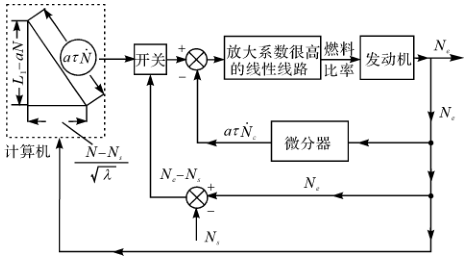
\includegraphics[width=\linewidth]{figs/fig-0163.png}
\caption{图9.5-1}
\end{figure}

图 9.5-1

$N_{\mathrm{r}}$ 是真正的发动机速度，假定我们考虑减速度的情况，$N>N_{\mathrm{r}}$。在过渡过程中，$N_{\mathrm{r}}-N_{\mathrm{r}}$ 是正的，所以计算机和发动机伺服系统之间的开关闭合，计算机发出信号。计算机根据方程(9.5-9)产生信号 $\alpha \tau \dot{N}$。在图 9.5-1 中用一个直角三角形边长的关系描写信号之间的联系。发动机伺服控制系统要设计得使发动机尽可能服从计算机所发出的信号 $\alpha \tau \dot{N}$。这只要利用图中所表示的放大系数很高的线路就可以达到目的。当速度误差的值变得非常小的时候，计算机就停止发出信号，于是系统的稳定装置将保证系统保持指定速度 $N$，而处于稳定状态，于是系统满足方程(9.5-8)的条件。

控制系统里有一个可调整的参数 $\lambda$。对于任意一个给定的 $\lambda$ 和得到的超温积分来说，这个系统将会使速率误差平方的积分取极小值。 $\lambda$ 的值确定超温积分的值式(9.5-6)，我们考虑 $a N_{i}=L$ 这一特殊情况，那就是，与温度的限制相适应的加速度或减速度是服从方程(9.2-5)的。有兴趣地注意到，在这个特殊例子里，根据方程(9.5-9)的控制条件，当 $N=N$ 时，$\dot{N}=0$，所以并不需要一个额外的稳定装置，图(9.5-1)中控制系统里的开关也就可去掉。在这一特殊情况下，方程 (9.5-9)变成线性的，可以写成

\[E(L-\alpha N)=\alpha \tau \dot{N}\qquad\text{(9.5-10)}\]

其中

\[E=\left(1+\frac{1}{a^{2} \lambda}\right)^{\frac{1}{2}}\qquad\text{(9.5-11)}\]

现在那些积分可以很容易的计算出来，例如，温度积分是

\[\begin{aligned} \int_{0}^{t_{1}}(T-L)^{2} d t & =\int_{0}^{t_{1}}(a N-L+\alpha \tau \dot{N})^{2} d t \\ & =\left(E-1\right)^{2} \int_{0}^{t_{1}}(L-a N)^{2} d t \\ & =a^{2}(E-1)^{2} \int_{N_{0}}^{t_{1}}(N_{s}-N)^{2} d t \\ & =a^{2}(E-1)^{2} \int_{N_{0}}^{N_{s}}(N_{s}-N)^{2} \frac{d N}{\dot{N}} \\ & =a^{2} \tau(E-1)^{2} \int_{N_{0}}^{N_{s}} \frac{\left(N_{s}-N\right)^{2} d N}{E a\left(N_{s}-N\right)} \\ & =\frac{a^{2}}{2} \tau \frac{(E-1)^{2}}{E} \frac{1}{2}\left(N_{s}-N_{0}\right)^{2} \\ & =\frac{\tau}{2} \frac{(E-1)^{2}}{E}\left(L-a N_{0}\right)^{2} \end{aligned}\]

于是得到

\[\frac{1}{\tau} \int_{0}^{t_{1}} \frac{(T-L)^{2}}{\left(L-a N_{0}\right)^{2}} d t=\frac{(E-1)^{2}}{2 E}\qquad\text{(9.5-12)}\]

其中 $N_{0}$ 是过渡过程开始时的发动机速度。同样，速度积分是

\[\frac{a^{2}}{\tau} \int_{0}^{t_{1}}\left[\frac{N-N_{i}}{L-a N_{0}}\right]^{2} d t=\frac{1}{2 E}\qquad\text{(9.5-13)}\]

假设 $T_{\text {max }}$ 是最高温度，于是

\[\frac{T_{\text {max }}-L}{L-a N_{0}}=E-1\qquad\text{(9.5-14)}\]

从方程(9.5-10)我们有

\[E a\left(N_{s}-N\right)=\alpha \tau \frac{d N}{d t}\]

在过渡过程中，控制系统的特性时间用 $\tau^{*}$ 表示

\[\tau^{*}=\frac{\tau}{E}\qquad\text{(9.5-15)}\]

这些方程的左端已经化成无量纲的形式了。最高温度 $T_{\max }$ 是过渡过程开始时的温度。

当 $E=1(\lambda=\infty)$ 时，这时候温度不超出，这与我们前面的叙述相符：当 $\lambda \rightarrow \infty$时，表示超温的积分等于零。速率积分等于 0.5，并且 $\tau^{*}=\tau$。如果 $E$ 增大 （或者 $\lambda$减小），温度积分和最高温度增大，而速度积分和时间常数减小。可以取 $2$ 为 $E$ 的一个折中值，或者 $a^{2} \lambda=1$。只要把 $E$ 或者 $\lambda$ 的值给定，控制计算机的程序也就确定了，于是可以进行控制系统的设计工作。

对于方程 $(9.5-9)$ 的普遍情形，积分值计算起来非常麻烦，但是可以采用同样的步骤设计控制系统。勃克森包姆和胡德给出方程 $(9.5-10)$ 真正的解答，那就是求出 $t$ 的函数 $N^{[8]}$，但是我们在这里对于控制系统的设计并不着重在求得这种解。控制系统的全部资料由方程 $(9.5-10)$ 本身给出，因为这个方程已经告诉我们应该如何构造控制计算机。如果根据那些条件做出计算机，于是就能保证得到希望的性能。 $N$ 对于时间的具体变化情况倒并不重要。因此我们的设计方法与其说是根据假设的方程的解去进行设计。倒不如说是“设计”非线性方程本身。

\section{9.6 控制量受限制时的最优控制设计}

前面数节内所讨论的最优控制问题都基于一个重要假定，控制函数 $u(t)$ 的取值范围事先不受任何限制。按方程组 $(9.4-28)$ 求出的最优控制函数 $\dot{u}(t)=(\dot{u}(t), \cdots, \dot{u}(t))$ 可以在 $r$ 维空间的任何地方取值。我们曾经指出过，控制量 $u$ 的取值在绝大多数情况下总是受限制的。控制量的变化只能在预先确定的范围内取值。而古典变分法的理论中其主要方法的证明和主要结论实质上都没有充分地，或完全没有考虑这种限制条件。为了确切地反映这一基本事实，古典变分法的理论和方法就难于直接采用。这里需要有另外一种研究方法，以使古典变分法的应用范围得以改进，使之更适合于实际控制问题的基本特点。

值得指出的是，这种附加的控制系统特有的限制条件，无论在实际技术问题中或在理论上都使得最优问题与古典变分法内所研究的问题具有本质上的不同。例如在古典变分法的意义上并不存在最优解的时候，考虑了限制条件后，最优解就不仅存在，而且还具有重要的实际意义。举例来说，在 $x, y$ 平面上有一条光滑曲线y=f（x），如果此曲线在全平面内确实有极小值存在，那么用求极值的古典方法可以求出极值及其对应的横坐标 $x_{0}$。但是，当 $x$ 的取值范围受限制时，如 $a \leqslant x \leqslant b$，该函数 $f(x)$ 在此区间内可能没有极值，而最小值却总是存在的。此时古典方法就完全无能为力了。本章初我们曾讨论过的物体运动一例中，按古典变分法的提法（即图 9.1-1 中力从简单的物理概念中推知。

总之，本节内我们将介绍控制量受限制时的最优控制的设计问题。设受控对象的运动方程依然为式 (9.4-1)，性能指标为式 (9.4-2)型的积分泛函。控制量 $u$的取值范围假定为 $r$ 维空间的某一点集 $U$，后者可能是一个区域，例如由下列不等式组所确定

\[g_{i}\left(u_{1}, u_{2}, \cdots, u_{n}\right) \leqslant 0, \quad i=1,2, \cdots, m\qquad\text{(9.6-1)}\]

也可能是一个正方体，由下列条件决定

\[\left|u_{i}\right| \leqslant M, \quad i=1,2, \cdots, r\qquad\text{(9.6-2)}\]

或者只包含几个孤立点和线。例如，若控制器是由数个双极继电器组成的，那么控制量的每个分量 $u_{i}$ 只可能取值 $\pm M$，此时点集 $U$ 只含有 $2^{r}$ 个孤立点。当 $r=1$时，控制量只能取两个值: $+M$ 或 $-M, M$ 为某一给定的正数。

在这种特定条件下讨论的最优控制问题是由庞特里亚金 (Понтрягин)及其学生们完成的[22]。这里仅限于叙述他们的基本方法和此方法的几何意义。最后我们将指出这种方法与前述古典变分法之间的联系。

如果控制函数 $u(t)$ 在任何时刻均取值于 $U$，而且它的每一分量 $u_{i}(t), i=1$，$2, \cdots, r$，都是逐段连续的函数，在任何有限时间内只可能有有限个第一类断续点，则称这类 $u(t)$ 为可准控制。控制量的取值域 $U$ 是 $r$ 维空间的任意点集，它也可以是全空间，此时问题将与古典变分法的命题一致。以后我们将假定控制量的值域 $U$ 已被给定。

与前节类似，对受控对象式 (9.4-1)引进一个新的坐标 $x_{0}, x_{0}(t)=J(t)$，则

\[\frac{d x_{0}}{d t}=f_{0}\left(x_{1}, \cdots, x_{n} ; u, \cdots, u_{r}\right)\]

于是式 (9.4-1) 和 (9.4-2) 可联合成为一个包含 $n+1$ 个一阶方程式的方程组，将它写成向量形式

\[\frac{d \bar{x}}{d t}=\bar{f}(\bar{x}, \boldsymbol{u}), \bar{\boldsymbol{x}}(0)=(0, \boldsymbol{x})\qquad\text{(9.6-3)}\]

式中 $\bar{f}=\left(f_{0}, f_{1}, \cdots, f_{n}\right), \bar{x}=\left(x_{0}, x_{1}, \cdots, x_{n}\right)$。设受控对象的终点条件 $\boldsymbol{x}=\left(x_{11}\right.$，$\left.x_{21}, \cdots, x_{n 1}\right)$ 已经给定。所谓最优控制是指在一切可准控制中寻求使受控对象自 $\boldsymbol{x}$ 到达 $\boldsymbol{x}$ 并使 $x_{0}$ 达极小值的控制函数。这一问题的几何意义如图 9.4-1 所示。这与前节内的古典问题的提法不同点在于，这里的控制函数必须在可准函数的范

(1) 在文献[22]中作者研究了更为广泛的可准控制类，即 $u_{i}(t)$ 为有界可测函数。为了叙述简单易懂，这里只限于分段连续的控制函数。

围内选取，故 $u(t)$ 的取值不能是任意的。

为了叙述最优控制所应满足的 （必要） 条件，与前节的讨论类似，引进一组 $n+1$ 维向量函数 $\bar{\Psi}(t)=\left(\psi_{1}(t), \psi_{2}(t), \cdots, \psi_{n}(t)\right)$，假定它们是下列方程组的解

\[\frac{d \psi_{i}}{d t}=-\sum_{a=0}^{n} \frac{\partial f_{a}}{\partial x_{i}} \psi_{a}, \quad i=0,1,2, \cdots, n\qquad\text{(9.6-4)}\]

类似地构造哈密顿函数 $H$

\[H(\bar{x}, \bar{\Psi}, u)=\left(\bar{\Psi}, \bar{f}(\bar{x}, u)\right)=\sum_{a=0}^{n} \psi_{k} f_{a}(\bar{x}, u)\qquad\text{(9.6-5)}\]

上式内用 $(\bar{x}, \bar{y})$ 表示两个 $n+1$ 维向量的数量积。于是，式 (9.6-3) 和 (9.6-4) 可以通过函数 $H$ 写成哈密顿方程组

\[\begin{aligned} & \frac{d x_{i}}{d t}=\frac{\partial H}{\partial \psi_{i}}, \quad i=0,1,2, \cdots, n \\ & \frac{d \psi_{i}}{d t}=-\frac{\partial H}{\partial x_{i}}, \quad i=0,1,2, \cdots, n \end{aligned}\qquad\text{(9.6-7)}\]

如果 $u(t)$ 已经给定，则 $\bar{x}(t)$ 可从式 (9.6-3) 中求出，于是式 (9.6-4) 的诸系数就成为已知的时间函数了，$\bar{\Psi}(t)$ 将是这个线性方程组的解。

文献[22]证明了下列事实：设 $\dot{u}(t)$ 和 $\dot{x}$ 分别是式 (9.6-3) 的最优控制和最优运动，$t$ 是最优运动自 $\dot{x}$ 点到达 $\dot{x}$ 点的时间，则 $\dot{u}(t)$ 必满足下列条件：即存在式 (9.6-4) 的非零解 $\dot{\Psi}(t)$，使下列两个条件成立:

(1) 哈密顿函数 $H$ 沿最优运动轨迹 $\dot{x}(t)$ 在任何时刻对 $u$ 取极大值，即

\[H(\dot{x}(t), \dot{\Psi}(t), \dot{u}(t))=\max _{u \in U}\left(\dot{\Psi}(t), \bar{f}(\dot{x}, u)\right), \quad 0 \leqslant t \leqslant t\qquad\text{(9.6-8)}\]

(2) 沿最优运动的轨线上 $\psi(t)=\operatorname{const} \leqslant 0$，且

\[H(\dot{x}(t), \dot{\Psi}(t), \dot{u}(t)) \equiv 0, \quad 0 \leqslant t \leqslant t\qquad\text{(9.6-9)}\]

这就是著名的关于最优控制的极大值原理。

表面上看来，上述两个条件与前节的古典问题的必要条件式 (9.4-28) 颇为类似，差别仅在于式 (9.4-24) 是“极值条件”，式 (9.6-8) 则是“条件最大值”。换言之，式 (9.4-24) 中 $H$ 在一切 $\delta u$ 中取极值。而式 (9.6-8) 中 $H$ 在 $u \in U$ 中取最大值。这一点绝不仅是字面上的差别，而反映了一种深刻的质的变化。

关于极大值原理的详细证明读者可参阅专著[22]。这里我们仅指出它与前节的讨论中有本质性差别的地方。前节内我们证明极值条件式 (9.4-24) 时，利用了一个基本事实，即由于 $\delta u$ 的各种变化所引起的最优轨线构成一个线性子空间 $K$。后者的线性是由于最优控制的变化 $\delta u$ 所引起的最优轨线的末端变化 $\delta \bar{x}(t)$ 对 $\delta u$ 是线性关系。由于对 $\delta u$ 无任何限制，故 $\delta \bar{x}(t)$ 构成一个线性集合。而在 $\delta u$ 受限制的情况下，如果最优控制函数 $\dot{\boldsymbol{u}}(t)$ 的取值完全位于 $U$ 的内部，则前节内所述之证明方法在这里依然可以采用，此时条件式 $(9.6-8)$ 和 $(9.4-24)$ 将完全重合。但是，当最优控制 $\dot{\boldsymbol{u}}(t)$ 的取值位于 $U$ 的边界时，前述的证明方法就完全无效了，因为此时 $\delta \boldsymbol{u}$ 不能任意取值，否则 $\dot{\boldsymbol{u}}(t)+\delta \boldsymbol{u}$ 可能超出 $U$ 的限制范围，变成为不可准许的控制函数了。文献 [22]的作者们利用一种独特的变分方法构造了一种关于 $\dot{\boldsymbol{u}}(t)$ 的变分集合，并证明了由于这种特殊的变分所造成的最优轨迹的末端偏离 $\delta \boldsymbol{u}(t)$ 的全体构成的集合是一个凸锥体 $K$，而不是一个线性子空间。以 $\boldsymbol{x}_{0}$ 为始点的向量 $\boldsymbol{z}=(-1,0, \cdots, 0)$ 必然处于此凸锥体的外部。这样，就可以建立一个超平面，使向量 $\boldsymbol{z}$ 与凸锥体 $K$ 位于此超平面的两侧，$\boldsymbol{\Psi}_{1}$ 是此超平面的外法向量，即它与 $K$ 不在超平面的同侧。除此之外的其他证明过程与前节所述的基本思想是相同的。

以后我们还将利用极大值原理去解决一类具体问题。

\section{9.7 末端不固定时的最优控制}

前面几节讨论的问题都是关于受控对象自某一给定初始状态到达另外一个固定的端点状态的最优控制所应满足的必要条件。我们曾经指出，无论控制量 $\boldsymbol{u}(t)$ 的取值是否受到限制，在最优控制确实存在的情况下，只要方程 $(9.4-28)$ 和 $(9.6-8)$ 给出足够的方程式个数，就可以求出最优运动的一切未知变量和未知常量。

在实际技术问题中常有另外一种情况，就是运动的端点并不完全固定，而仅需满足某些较为“不严”的限制条件。例如，对受控对象的终点状态只有局部限制：某几个坐标分量的状态为给定，而另一种分坐标则是任意的。用多维空间的几何术语来讲，终点状态不是相空间内的某一个固定点，而是一个维数小于 $n$ 的超曲面，终点状态，即受控运动的轨线端点，应该位于此超曲面上。此时前面得到的最优控制所应满足的条件就不能充分决定最优控制函数了，因为这超曲面上的点有无穷多个，究竟这些点中那一个点从损耗最小的意义上来看是系统理想的终端状态呢？甚之，系统的初始点状态也可能是不固定的，而仅要求位于某一超曲面上。总之，这类问题可以叙述如下。在 $n$ 维相空间内给定两个维数不大于 $n-1$ 维的超曲面 $S_{1}$ 和 $S_{2}$，它们互不相交。要求找出 $S_{1}$ 和 $S_{2}$ 上的某些点 $\boldsymbol{x} \in S_{1}$ 和 $\boldsymbol{x} \in S_{2}$，使自 $\boldsymbol{x}$ 至 $\boldsymbol{x}$ 点的最优控制就是自超曲面 $S_{1}$ 至超曲面 $S_{2}$ 的最优控制。这里实际上包含了三个问题：求出 $S_{1}$ 上的点 $\boldsymbol{x}$，使自该点到达 $S_{2}$ 的最优控制比自 $S_{1}$ 上任何其他点到达 $S_{2}$ 的最优控制还要好。也就是在很多最优控制中求更优者；其次要求出自此“理想点”到达 $S_{2}$ 的最优控制函数；最后还须求出 $S_{2}$ 上的理想端点的位置。

设受控对象的运动方程依然是式 $(9.4-1)$

\[\frac{d x_{i}}{d t}=f_{i}\left(x_{1}, \cdots, x_{i} ; w, \cdots, u_{r}\right), \quad i=1,2, \cdots, n\]

受控运动的质量指标是式(9.4-2)

\[x_{0}=\quad J=\int_{0}^{t_{1}} f_{0}\left(x_{1}, x_{2}, \cdots, x_{n} ; u, \cdots, u_{r}\right) d t\]

系统的初始状态位于初始超曲面 $S_{1}$ 上，后者由方程式

\[h\left(x_{1}, \cdots, x_{n}\right)=0\qquad\text{(9.7-1)}\]

所确定。系统的终点状态应在超曲面 $S_{2}$ 上，它由方程式

\[q\left(x_{1}, \cdots, x_{n}\right)=0\qquad\text{(9.7-2)}\]

决定。欲求自 $S_{1}$ 至 $S_{2}$ 的最优控制最直观的方法是先任意选择 $\boldsymbol{x}_{0} \in S_{1}$ 和 $\boldsymbol{x} \in S_{2}$，求出自 $\boldsymbol{x}_{0}$ 至 $\boldsymbol{x}$ 的最优控制，然后再找出最好的始点和终点。这样便得到一个三重最优问题，可写成

\[x_{0}=J=\min _{x_{1} \in s_{2}} \min _{x_{0} \in s_{1}} \min _{u \in U} \int_{0}^{t_{1}} f(\boldsymbol{x}(t), \boldsymbol{u}(t)) d t\]

显然，这种方法在实际上几乎是毫无用处的。为了求出最好的 $\dot{\boldsymbol{x}}_{0}$ 和 $\dot{\boldsymbol{x}}_{1}$，需要找出一些附加条件，用来寻找最理想的始点和端点。

在未开始讨论这些附加条件以前，先指出下列明显事实：如果理想的端点 $\dot{\boldsymbol{x}}_{0}$和 $\dot{\boldsymbol{x}}_{1}$ 已经找到，那么最优控制问题就变为前面已经详细讨论过的自固定点至固定点的最优控制问题。在受控量不受限制时最优控制函数必须满足条件式 (9.4-28)，而在控制量受限制时则应满足条件式 (9.6-8)。因此，前节内得到的结果依然适用于本节初提出的问题。

为了讨论简单，我们假定决定超曲面 $S_{1}$ 和 $S_{2}$ 的方程式(9.7-1)和(9.7-2)中的函数 $h(\boldsymbol{x}), q(\boldsymbol{x})$ 为连续可微函数，即它们所确定的超曲面是光滑的。在其上的每一点都有一次偏导数存在，且梯度向量

\[\begin{aligned} \operatorname{grad} h(\boldsymbol{x}) & =\left(\frac{\partial h}{\partial x_{1}}, \frac{\partial h}{\partial x^{2}}, \cdots, \frac{\partial h}{\partial x_{n}}\right) \neq \boldsymbol{0} \\ \operatorname{grad} q(\boldsymbol{x}) & =\left(\frac{\partial q}{\partial x_{1}}, \frac{\partial q}{\partial x_{2}}, \cdots, \frac{\partial q}{\partial x_{n}}\right) \neq \boldsymbol{0} \end{aligned}\]

换言之，梯度向量处处不为零向量，即曲面上没有奇点。此外还假定超曲面 $S_{1}$ 和 $S_{2}$都是 $n-1$ 维的。关于维数的假定并不是完全必要的，只是为了讨论方便而已。

先讨论控制量不受限制的情况。现假定 $S_{1}$ 上的 $\dot{\boldsymbol{x}}_{0}$ 已经找到，来研究 $S_{2}$ 上的理想端点 $\dot{\boldsymbol{x}}$ 应该满足什么条件。从第 9.5 节中我们已经知道，如果 $\dot{u}(t)$ 是自 $\dot{\boldsymbol{x}}_{0}$ 点到达 $\dot{\boldsymbol{x}}$ 点的最优控制，在最优运动的中间任一时刻 $\tau, 0 \leqslant \tau \leqslant t$，对最优控制函数 $\dot{u}(t)$ 做一系列的微小变化 $\left\{\delta u\right\}$，在最优轨线终点 $\dot{\boldsymbol{x}}(t)$ 所产生的偏离 $\left\{\delta \boldsymbol{x}(t)\right\}$ 的全体构成一个线性子空间 $K$，它的维数不超过 $r$。在 $n+1$ 维空间内通过 $\dot{\boldsymbol{x}}$ 点所做的平行于 $x$ 轴的直线 $\mathscr{Z}$ （图 9.4-1)绝不会包含在子空间 $K$ 的内部。 $n$ 维相空间内超曲面 $S_{2}$ 在 $n+1$ 维相空间内变成一个柱面 $S_{2}^{\prime}$ 直线 $\mathscr{Z}$ 是此柱面的一条基线，从几何结构上可以推知，若过 $\dot{\boldsymbol{x}}$ 点做此柱面的切平面 $P$，它的方程式应该是

\[\sum_{i=0}^{n} \frac{\partial q}{\partial x_{i}}\left(x_{i t}-x_{i}\right)=\left(\operatorname{grad} q(\dot{\boldsymbol{x}}), \dot{\boldsymbol{x}}-\bar{\boldsymbol{x}}\right)=0\qquad\text{(9.7-3)}\]

式中

grad q(x)=...|\_x arrow 1|\_x  1.

是切平面 $P$ 的法向量。由于 $\dot{\boldsymbol{x}}$ 是自 $S_{1}^{\prime}$ 到达 $S_{2}^{\prime}$ 的最优端点，故切平面以 $\dot{\boldsymbol{x}}$ 为中心的邻域不可能包含于子空间 $K$ 的内部，否则将存在一种式 $(9.4-6)$ 形的控制，使轨线端点的第一个坐标小于 $\dot{x}_{01}$，这与最优的假定相矛盾。于是，过 $P$ 上垂直于 $x_{0}$ 轴的直线可做一个超平面 $P^{\prime}$，使 $\mathscr{K}$ 的下半部与 $K$ 完全隔开。因而 $P^{\prime}$ 的法向量必然是 $\left\{\psi, \operatorname{grad} q\left(\bar{x}^{\prime}\right)\right\}$。重复前面的讨论，可以得到如下结论：决定最优控制的向量函数 $\tilde{\boldsymbol{\Psi}}(t)$ 在轨线末端应与 $P^{\prime}$ 垂直。换言之，$\tilde{\boldsymbol{\Psi}}(t)$ 在末端的方向应有下列形式

(t)=...|\_x arrow 1|\_x  1.(9.7-4)

此式就是古典变分法中的横截条件。

由于受控对象的运动方程式 $(9.4-1)$ 之右端不明显包含时间变量 $t$，用逆运动的方法，对最优轨线的始点也可以得到同样的结果，即在 $t=0$ 时，$\tilde{\Psi}(0)$ 应具有下面形式

(0)=...|\_x arrow 0|\_x  0.(9.7-5)

这样一来，决定最优控制的标准方程组 $(9.4-28)$ 将变成下列新的形式

aligned \& d x\_id t=f\_i(x(t), u(t)),  i=0,1,2, , n \textbackslash\{\}\textbackslash\{\} \& x(0)  S\_1,  x\_1  S\_2 \textbackslash\{\}\textbackslash\{\} \& d \_id t=-\_a=0\textasciicircum{}n  f\_a x\_i \_a,  i=0,1,2, , n \textbackslash\{\}\textbackslash\{\} \& (0)=...|\_x arrow 0|\_x arrow 0. \textbackslash\{\}\textbackslash\{\} \& (t)=...|\_x  1|\_x  1. \textbackslash\{\}\textbackslash\{\} \& H(x(t), (t), u(t))=ext((t), f(x, u))  0 \textbackslash\{\}\textbackslash\{\} \&  H/ w=0,  i=1,2, , r aligned(9.7-6)

读者不难看出，标准方程组(9.7-6)提供了足够的条件解 $2n+2$ 个一阶常微分方程式。于是最优控制函数及最优轨线的两个端点，如果它们存在的话，就可以从方程组(9.7-6)中求出。

上面讨论的依然是受控量不受限制的情况。如果 $u$ 的取值受某种限制，则式 (9.7-6)中的最后一个条件将改为

\[H(\dot{\boldsymbol{x}}, \dot{\boldsymbol{\psi}}(t), \dot{u}(t))=\max _{u \in U}(\dot{\boldsymbol{\psi}}(t), f(\dot{\boldsymbol{x}}(t), \boldsymbol{u})) \equiv 0\qquad\text{(9.7-7)}\]

这与端点完全固定的情况是一样的。对后一种情况更严格的数学证明这里不再详述，读者可参看文献[22]。此外，前面假定的 $S_{1}$ 和 $S_{2}$ 均为 $n-1$ 维超曲面也不是必要的。当它们的维数小于 $n-1$ 时，限制条件式(9.7-1)和(9.7-2)中，将包含数个方程式。例如，假定 $S_{2}$ 由 $m$ 个等式所确定

\[q(\boldsymbol{x})=0, \quad i=1,2, \cdots, m\qquad\text{(9.7-8)}\]

同时满足这 $m$ 个方程式的一切点构成一个 $n-m$ 维超曲面 $S_{2}$，此时下列向量

\[\operatorname{grad} q(\boldsymbol{x}), \operatorname{grad} q(\boldsymbol{x}), \cdots, \operatorname{grad} q_{m}(\boldsymbol{x})\]

对于 $S_{2}$ 上的一切点，都是线性无关的，也就是说下列 $n \times m$ 阶方阵

\[\left(\begin{array}{ccc} \frac{\partial q}{\partial x_{1}} & \frac{\partial q}{\partial x_{1}} & \cdots & \frac{\partial q_{m}}{\partial x_{1}} \\ \frac{\partial q}{\partial x_{2}} & \frac{\partial q}{\partial x_{2}} & \cdots & \frac{\partial q_{m}}{\partial x_{2}} \\ \vdots & \vdots & & \vdots \\ \frac{\partial q}{\partial x_{n}} & \frac{\partial q}{\partial x_{n}} & \cdots & \frac{\partial q_{m}}{\partial x_{n}} \end{array}\right)\qquad\text{(9.7-10)}\]

对一切 $\boldsymbol{x} \in S_{2}$ 均有最大秩 $m$。

式(9.7-8)中的每一个等式决定一个 $n-1$ 维超曲面，它的每一点上的切平面 $P$ 的法向量是 $\operatorname{grad} q(\boldsymbol{x})$。在任意点 $\boldsymbol{x} \in S_{2}$ 上所作的 $m$ 个切平面

\[(\operatorname{grad} q(\boldsymbol{x}), \boldsymbol{x}-\boldsymbol{y})=\sum_{a=1}^{n} \frac{\partial q_{i}}{\partial x_{a}}\left(x_{a}-y_{a}\right)=0, \quad i=1,2, \cdots, m\qquad\text{(9.7-11)}\]

的交，称为 $S_{2}$ 在 $\boldsymbol{x}$ 点的切平面 $P$，它的维数也是 $n-m$。不难理解，$P$ 的法向量可由式(9.7-9)诸向量的线性组合表示，即

\[\boldsymbol{n}(\boldsymbol{x})=\sum_{a=1}^{m} \mu_{k} \operatorname{grad} q_{a}(\boldsymbol{x})\qquad\text{(9.7-12)}\]

在这种情况下，式(9.7-6)中确定 $\dot{\boldsymbol{\psi}}$ 的边界条件的关系式将改为

\[\begin{aligned} \dot{\boldsymbol{\psi}}(0) & =\left(\psi_{b}, n(\boldsymbol{x}), \cdots, n_{n}(\boldsymbol{x})\right) \mid_{\boldsymbol{x}=x_{0}} \\ \dot{\boldsymbol{\psi}}\left(t_{1}\right) & =\left(\psi_{b}, n(\boldsymbol{x}), \cdots, n_{n}(\boldsymbol{x})\right) \mid_{\boldsymbol{x}=x_{1}} \end{aligned}\qquad\text{(9.7-13)}\]

我们看到，在式(9.7-12)中又引进了 $m$ 个常数 $\mu_{1}, \mu_{2}, \cdots, \mu_{m}$，它们是未知的。但是比前面的讨论中又多了 $m-1$ 个约束方程式 $q_{i}(\boldsymbol{x})=0, i=2, \cdots, m$。这样总的未知数和已知条件依然相互平衡，故决定最优控制函数与最优端点的标准方程组式 (9.7-6) 在新的条件下依然是完备的。如果这种问题有解的话，那么式 (9.7-6) 就提供了求解的必要条件。

\section{9.8 最优控制函数综合举例}

作为前节所述理论的应用，现研究线性系统内的最优控制函数的综合问题，设受控对象的运动方程是线性方程组

\[\frac{d \boldsymbol{x}}{d t}=\boldsymbol{A} \boldsymbol{x}+\boldsymbol{B} \boldsymbol{u}\qquad\text{(9.8-1)}\]

和过去的符号一样，$A$ 是 $n \times n$ 阶常量矩阵，$B$ 是 $n \times r$ 阶常量矩阵，$\boldsymbol{u}=(\boldsymbol{u}, \boldsymbol{u}, \cdots$，$\boldsymbol{u}_{r})$ 是 $r$ 个控制量。假定控制量的取值是受限制的，例如

\[\mid u_{i} \mid \leqslant 1, \quad i=1,2, \cdots, r\qquad\text{(9.8-2)}\]

令 $\Omega$ 表示系统要求的终点状态区域。即无论受控系统的初始条件如何，经一段时间后，受控对象式 (9.8-1) 应该以 $\Omega$ 内的任意点作为终点状态。我们假定 $\Omega$ 是一个凸面体，或者是一个凸性区域，它由 $m$ 个不等式

\[g_{i}(\boldsymbol{x}) \leqslant 0, \quad i=1,2, \cdots, m\qquad\text{(9.8-3)}\]

所确定，例如，它可能是以原点为中心以 $\rho$ 为半径的小球体，此时

\[g(\boldsymbol{x})=\sum_{i=1}^{n} x_{i}^{2} \leqslant \rho^{2}\]

$\rho$ 为某一给定的常数。

过渡过程的质量指标是一个二次型的积分式

\[J(\boldsymbol{u})=\int_{0}^{t_{1}}\left[(Q \boldsymbol{x}, \boldsymbol{x})+\left(P \boldsymbol{u}, \boldsymbol{u}\right)\right] d t\qquad\text{(9.8-4)}\]

上式内 $\Omega$ 为非负定方阵，即对任何 $\boldsymbol{x}$ 总有

\[(Q \boldsymbol{x}, \boldsymbol{x}) \geqslant 0\]

为了讨论简单，假设 $P$ 是一个非负的对角矩阵，即

\[p_{i j}=\left\{\begin{array}{l} p_{i} \geqslant 0, \quad \text { 若 } i=j \\ 0, \quad \text { 若 } i \neq j \end{array}\right.\]

这样，式 (9.8-4) 可以写成

\[J(\boldsymbol{u})=\int_{0}^{t_{1}}\left[\sum_{i, j=1}^{n} q_{i j} x_{i} x_{j}+\sum_{i=1}^{r} p_{i}\left(u_{i}\right)^{2}\right] d t\qquad\text{(9.8-5)}\]

所谓综合问题就是控制装置的设计问题，要求求出一组 $n$ 元函数 $u_{i}\left(x_{1}, x_{2}, \cdots\right.$，$\left.x_{n}\right), i=1,2, \cdots, r$，若将其代入式 (9.8-1) 后所得到的自治系统

\[\frac{d \boldsymbol{x}}{d t}=\boldsymbol{A} \boldsymbol{x}+\boldsymbol{B} \boldsymbol{u}(\boldsymbol{x})\qquad\text{(9.8-6)}\]

对任何初始条件 $\boldsymbol{x}_{0}$，均能自动地将受控对象引至 $\Omega$ 上的某一点，且使沿此轨线所算出的 $J$ 值取极值。这样求出的函数 $u_{i}\left(x_{1}, \cdots, x_{n}\right), i=1,2, \cdots, r$，正是待求的控制装置必须实现的控制规律。

现用第 9.6 节内所述的原理进行控制装置的设计。首先引进新坐标 $x_{0}=J$，它应满足方程式

\[\frac{d x_{0}}{d t}=\left(\Omega \boldsymbol{x}, \boldsymbol{x}\right)+\left(\boldsymbol{P u}, \boldsymbol{u}\right)=\sum_{i, j=1}^{n} q_{i j} x_{i} x_{j}+\sum_{i=1}^{r} p_{i} u_{i}^{2}\qquad\text{(9.8-7)}\]

此式与式(9.8-1)联合后得到一个由 $n+1$ 个方程式构成的方程组，不难直接检查，它们的共轭方程组

\[\frac{d \psi_{0}}{d t}=0\qquad\text{(9.8-8)}\]

\[\frac{d \boldsymbol{\Psi}}{d t}=-\boldsymbol{A}^{\top} \boldsymbol{\Psi}-2 \psi_{0} \boldsymbol{Q x}\qquad\text{(9.8-9)}\]

构成哈密顿函数

\[H(\boldsymbol{x}, \boldsymbol{\Psi}, u)=\psi\left[\left(\boldsymbol{Q x}, \boldsymbol{x}\right)+\left(\boldsymbol{P u}, \boldsymbol{u}\right)\right]+\left(\boldsymbol{\Psi}, \boldsymbol{A x}+\boldsymbol{B u}\right)\qquad\text{(9.8-10)}\]

根据第 9.6 节内的叙述可知，如果 $\dot{u}(t)$ 是最优控制，它应使 $H$ 取极大值

\[H\left(\dot{\boldsymbol{x}}(t), \boldsymbol{\Psi}(t), \dot{u}(t)\right)=\max _{u \in U}\left[\psi\left(\boldsymbol{P u}, \boldsymbol{u}\right)+\left(\boldsymbol{\Psi}, \boldsymbol{B u}\right)+v(t)\right]\qquad\text{(9.8-2)}\]

上式内 $\dot{\boldsymbol{x}}(t), \boldsymbol{\Psi}(t)$ 分别为最优运动轨线和其所对应的式 (9.8-8) 的某一特解。 $U$为由式 (9.8-2) 所确定的一个 $r$ 维正方体; $v(t)=\psi\left(\boldsymbol{Q} \dot{\boldsymbol{x}}(t), \dot{\boldsymbol{x}}(t)\right)+\left(\boldsymbol{\Psi}(t), \boldsymbol{A} \dot{\boldsymbol{x}}(t)\right)$是一个不依赖于 $\boldsymbol{u}$ 的 $t$ 的函数。条件式(9.8-10)等价于下列条件

\[\varphi(t)=\psi\left(\boldsymbol{P u}^{\prime}(t), \dot{u}(t)\right)+\left(\boldsymbol{\Psi}(t), \boldsymbol{B u}(t)\right)=\max _{u \in U}\left[\psi\left(\boldsymbol{P u}, \boldsymbol{u}\right)+\left(\boldsymbol{\Psi}, \boldsymbol{B u}\right)\right]\]

假定 $p_{v} \neq 0$，若 $i=1,2, \cdots, l$; 当 $i>t$ 时 $p_{i}=0$。此时将上式右端配方，经过整理后，可以得到

\[\varphi(t)=\max _{u \in U}\left[\sum_{i=1}^{l}\left[u+\left(\frac{\left(\boldsymbol{b}_{i}, \boldsymbol{\Psi}(t)\right)}{2 \psi_{p i}}\right)^{2}+\sum_{i=p+1}^{r}\left(\boldsymbol{\Psi}(t), \boldsymbol{b}_{i}\right) u_{i}+w(t)\right]\right.\]

这里 $w(t)$ 为不含 $\boldsymbol{u}$ 的时间 $t$ 的函数。由上式不难推知，当 $p_{i} \neq 0$ 时，考虑到 $\psi_{0}$ $0$，唯一的最优控制函数 $\dot{u}(t)$ 应具有下列形式

u(t)= cases1, \&  若  (b\_i, (t))2 \_p i -1 \textbackslash\{\}\textbackslash\{\} -1, \&  若  (b\_i, (t))2 \_p i  1 \textbackslash\{\}\textbackslash\{\} -((b\_i, (t))2 \_p i, \&  若 -1 ((b\_i, (t))2 \_p i)  1.cases

\[i=1,2, \cdots, l\qquad\text{(9.8-11)}\]

对应于 $p_{\alpha \alpha}=0$ 的那些控制量应为

\[\dot{u}(t)=\operatorname{sign}\left(b, \dot{\Psi}(t)\right), \quad \alpha=l+1, \cdots, r\qquad\text{(9.8-12)}\]

如果上式右端符号 sign 后的函数只在一些孤立点上才为零，那么 $\dot{u}_{\alpha}$ 将唯一地为式(9.8-12)所确定，否则 $\boldsymbol{u}_{\alpha}$ 的最优控制 $\dot{u}_{\alpha}(t)$ 将不能用这个办法求出。

我们看到，如果 $\boldsymbol{\Psi}(t)$ 和 $\Psi_{\mathrm{b}}$ 都为已知函数和已知数时，最优控制函数 $\dot{u}(t)$ 将有希望按式 (9.8-11) 和 (9.8-12) 所唯一地被求出。这样，求最优控制函数的问题就转化为求相应的 $\Psi_{\mathrm{b}}$ 和 $\Psi_{\mathrm{t}}(t)$。再回来观察式 (9.8-8)。为了求出这些函数，必须求出式 (9.8-8) 的初始条件 $\dot{\Psi}(0)$，而这是一件十分困难的事。为此，我们必须利用前节内关于不定端点的横截条件。利用这个条件可以写出最优轨线在到达 $\Omega$ 时的终端条件。设 $t$ 是受控对象自 $\boldsymbol{x}$ 点到达 $\Omega$ 所需的时间；显然，我们有理由断定最优轨线在 $t=t$ 时刻所到达的点 $\boldsymbol{z}=\dot{\boldsymbol{x}}(t)$ 必位于 $\Omega$ 的边界，而且在 $\boldsymbol{z}$ 点上有

\[\dot{\Psi}\left(t_{1}\right)=-\operatorname{grad} g(\boldsymbol{x}) \mid_{x-z}\qquad\text{(9.8-13)}\]

而未知数 $\Psi_{\mathrm{b}}$ 则应满足条件

\[\max _{u \in U}\left[\Psi\left(Q z, z\right)+\Psi_{\mathrm{b}}\left(P u, u\right)+(-\operatorname{grad} g(\boldsymbol{x}) \mid_{x-z}, A z+B u)\right]=0\qquad\text{(9.8-14)}\]

这样，当终点 $\boldsymbol{z}$ 为已知时 $\dot{\Psi}(t)$ 和 $\Psi_{\mathrm{b}}$ 便可以从式 (9.8-13) 和 (9.8-14) 求出。这是问题的第二次转化，把求最优控制函数 $\dot{u}(t)$ 又转化为求终点 $\boldsymbol{z}$。因为终点 $\boldsymbol{z}$ 也是未知量，表面看来这种转化依然是徒劳的。其实不然，经两次转化后，我们已经接近于最后解决本节初提出的综合问题了。

为此，我们研究原始方程 (9.8-1) 的逆转运动方程，因为它的右端不含 $t$，这种方法极易实现，用 $-t$ 代替 $t$ 后，方程组 (9.8-1) 和 (9.8-8) 可写成

\[\begin{aligned} & \frac{d \boldsymbol{x}}{d t}=-A \boldsymbol{x}-B u, \boldsymbol{x}(0)=\boldsymbol{z} \\ & \frac{d \Psi}{d t}=A^{\mathrm{d}} \Psi+2 \Psi Q \boldsymbol{x}, \quad \Psi(0)=\operatorname{grad} g(\boldsymbol{x}) \mid_{x-z}, \quad \Psi<0 \end{aligned}\qquad\text{(9.8-15)}\]

因为我们要解决的是综合问题，即求出一切到达 $\Omega$ 的最优控制函数，所以 $\Omega$ 的边界上的任一个点 $\boldsymbol{z}$ 都可能成为某一最优轨线的终点，或者说任一个 $\boldsymbol{z}$ 都可能是式 (9.8-15) 的始点，于是 $\Omega$ 边界上的每一个始点 $\boldsymbol{z}$ 都决定一条最优轨线。这样，当 $\boldsymbol{z}$遍历 $\Omega$ 的表面以后，就可求出一切最优轨线了。任取 $\Omega$ 边界上的一点 $\boldsymbol{z}$，即可按式 (9.8-15) 求出 $\Psi(0)$，再按式 (9.8-14) 求出 $\Psi_{\mathrm{b}}$ 来。由于 $\Psi_{\mathrm{b}}$ 沿最优轨线是常量，故 $\Psi_{\mathrm{b}}$ 只依赖于 $\boldsymbol{z}$ 点的位置，再由于式 (9.8-15) 是关于 $\boldsymbol{x}$ 和 $\Psi$ 的线性方程组，有可能在它的通解中消掉 $\boldsymbol{u}(t)$ 或者 $\Psi(t)$，使 $\Psi(t)$ 表达为 $\boldsymbol{x}(t)$ 的函数。

完成上述计算后，$\boldsymbol{x}$ 的相空间对每一个 $u_{i}$ 将分为三类控制区域。第一类区域 $\dot{u}(\boldsymbol{x}) \equiv 1$; 第二类区域 $\dot{u}_{i}=-1$; 第三类区域

\[\dot{u}_{i}(t)=-\frac{\left(b_{i}, \dot{\boldsymbol{\phi}}(t)\right)}{2 \dot{\psi}_{p i}}=-\frac{\left(b_{i}, \dot{\boldsymbol{\phi}}(\boldsymbol{x})\right)}{2 \dot{\psi}_{p i}}\]

这些区域找到后，就得到函数 $\dot{u}(\boldsymbol{x})$。这就是待求的最优控制函数。应指出的是，用纯分析方法去设计控制装置，一般看来，是十分复杂的事，但是，如果借助于高速度数字计算机或模拟计算装置这种设计程序就变得轻而易举了。

还有一种情况的最优设计问题有希望直接求出控制器即反馈信号的具体形式。设给定的受控对象的初始状态为 $\boldsymbol{x}$; 控制作用从 $t=0$ 开始，于给定的时间 $t$结束；对控制作用 $\boldsymbol{u}$ 没有约束。受控对象的运动方程是式(9.8-1)，而指标泛函改写成更方便的形式

\[J(\boldsymbol{u})=\frac{1}{2} \int_{0}^{t_{1}}\left[(Q \boldsymbol{x}, \boldsymbol{x})+\left(P \boldsymbol{u}, \boldsymbol{u}\right)\right] d t\qquad\text{(9.8-16)}\]

式中 $Q$ 和 $P$ 均假定为正定方阵。今要求设计最优线性反馈控制，使系统在 $t=0$时刻开始，在 $[0, t]$ 的时间间隔内，从任意点 $\boldsymbol{x}$ 出发向任何方向运动 （即端点不固定）指标泛函式 (9.8-16) 取极小值。

重复本节前面的讨论可知，最优控制应从下列方程组中求出 [见式(9.8-8)]

\[\begin{aligned} & \frac{d \boldsymbol{x}}{d t}=A \boldsymbol{x}+B \boldsymbol{u}, \quad \boldsymbol{x}(0)=\boldsymbol{x} \\ & \frac{d \boldsymbol{\phi}}{d t}=-\boldsymbol{A}^{*} \boldsymbol{\phi}-\boldsymbol{\phi}_{i} Q \boldsymbol{x} \\ & H\left(\dot{\boldsymbol{x}}(t), \dot{\boldsymbol{\phi}}(t), \dot{\boldsymbol{u}}(t)\right)=\max _{u}\left[\frac{\boldsymbol{\phi}_{i}\left(Q \dot{\boldsymbol{x}}, \dot{\boldsymbol{x}}\right)+\boldsymbol{\phi}_{i}\left(P \boldsymbol{u}, \boldsymbol{u}\right)+\left(\dot{\boldsymbol{\phi}}, A \dot{\boldsymbol{x}}+\boldsymbol{B} \boldsymbol{u}\right)}{2}\right] \end{aligned}\qquad\text{(9.8-17)}\]

由于终端状态可以是任意的，根据前节内极大值原理的证明，可推知 $\boldsymbol{\phi}$ 和 $\boldsymbol{\psi}$ 的终端条件一定是

\[\psi_{i} \equiv-1, \boldsymbol{\phi}\left(t_{i}\right)=0\qquad\text{(9.8-18)}\]

前面已经讨论过，如果 $Q$ 和 $P$ 是正定矩阵，哈密顿函数 $H$ 是 $\boldsymbol{u}$ 的非蜕化二次型，因而 $H$ 的极大值一定是极值，即对 $\boldsymbol{u}$ 的每一分量 $u_{i}$ 均应有 $\frac{\partial H}{\partial u_{i}}=0$ 在整个最优轨迹上成立。不难算出，由这个极值条件可得到向量等式

\[\frac{\partial H}{\partial u}=-P u+B^{*} \boldsymbol{\phi}=0\]

或者

\[\dot{u}(t)=P^{-1} B^{*} \boldsymbol{\phi}(t)\qquad\text{(9.8-19)}\]

我们希望把最优反馈控制表示成下列线性形式

\[\dot{u}(t)=-K(t) \mathbf{x}(t)\qquad\text{(9.8-20)}\]

式中 $K(t)$ 是某一随时间 $t$ 变化的 $r \times n$ 长方矩阵。为此只需把 $\boldsymbol{\Psi}(t)$ 表示成 $\mathbf{x}(t)$ 的线性函数，然后依式 (9.8-19) 即可得到线性反馈式 (9.8-20)。

令

\[\boldsymbol{\Psi}(t)=-R(t) \mathbf{x}(t)\qquad\text{(9.8-21)}\]

并和式 (9.8-19)一起代入式 (9.8-17)，注意到 $\phi_{i}=-1$，可立即得到下列恒等式

\[\begin{aligned} \dot{\Psi}(t) & =-\dot{R}(t) \mathbf{x}(t)-R(t) \mathbf{x} \\ & =-\dot{R}(t) \mathbf{x}(t)-R(t)(A \mathbf{x}+B u) \\ & =A^{\mathrm{f}} R(t) \mathbf{x}(t)+Q \mathbf{x}(t) \end{aligned}\]

注意到式 (9.8-19)，则上式等价于一个矩阵微分方程

\[-\dot{R}(t)=Q+A^{\mathrm{f}} R-R B P^{-1} B^{\mathrm{f}} R+R A\qquad\text{(9.8-22)}\]

上两式内矩阵上方的点表示对 $t$ 的导数。式 (9.8-22) 是一个矩阵微分方程，常称为黎卡提 (Riccati) 方程，可以证明它的解对任意初始条件是唯一存在的。剩下的只是确定 $R(t)$ 的边界条件。由式 (9.8-18) 知，在 $t=t_{\mathrm{h}}$ 时 $\boldsymbol{\Psi}\left(\mathrm{h}_{\mathrm{h}}\right)=0$，因而 $R\left(\mathrm{~h}_{\mathrm{h}}\right)=$ 0（零矩阵）。由于式 (9.8-22) 与系统的初始条件无关，当求出式 (9.8-22) 的一个特解后，即可按式 (9.8-20) 构造线性反馈控制器，式中

\[K(t)=P^{-1} B^{\mathrm{f}} R(t)\]

是待求的线性反馈矩阵，在一般情况下它是变系数矩阵。如果式 (9.8-22) 有稳态解，即存在一个常量矩阵 $R$ 使下列恒等式成立

\[Q+A^{\mathrm{f}} R-R B P^{-1} B^{\mathrm{f}} R+R A=0\qquad\text{(9.8-23)}\]

则最优反馈控制器是线性常系数的，反馈矩阵 $K$ 不仅与系统的初始状态无关，而且也不依赖于时间 $t_{\mathrm{h}}$，即对任何时间间隔 $\left[0, t_{\mathrm{h}}\right]$，由式 (9.8-20) 确定的反馈控制总能使指标泛函 $J$ 取极小值。

\section{9.9 短程火箭的最佳推力程序}

作为不固定端点的最优控制设计的一个例子，我们试讨论短程飞航式火箭的最佳推力程序设计方法。设 $m(t)$ 是火箭的瞬时质量; $V_{r}$ 是火箭喷射物质的分离相对速度，假定其为常数; $P(t)$ 代表推力，$P_{\max }$ 为发动机的最大可能推力；地心引力 $g$ 认为是常数; $x, y$ 为火箭在以发射点为坐标原点的直角坐标系内的坐标 （图 9.9-1)。因为是短射程火箭，我们将假定地心的引力始终平行于 $y$ 轴向下; $\dot{m}=\frac{d m}{d t}$为燃料的秒耗量；再假定空气阻力为 $Q=Q(y, V)=Q(y, \dot{x}, \dot{y})$。在上述假定的条件下，我们可以通过改变发动机的秒消耗量 $\dot{m}$ 和轨迹角 $\theta$ 来控制火箭的飞行速度和飞行方向。火箭的运动方程式可写成

\[\begin{aligned}& \frac{d^{2} x}{d t^{2}}=\frac{1}{m(t)}\left(P(t)-Q\left(y, \dot{x}, \dot{y}\right)\right) \cos \theta \\& \frac{d^{2} y}{d t^{2}}=\frac{1}{m(t)}\left(P(t)-Q\left(y, \dot{x}, \dot{y}\right)\right) \sin \theta-g \\& \frac{d m}{d t}=-\frac{1}{V_{r}} P(t)\end{aligned}\qquad\text{(9.9-1)}\]

引进新的变量 $x_{1}=x, x_{2}=x, x_{3}=y, x_{4}=$ $y, x_{5}=\frac{m(t)}{m_{b}} ; u_{1}=\frac{P}{P_{\max }}, u_{2}=\theta$。方程组

(9.9-1)可改写成一阶方程组

\[\begin{aligned}& \frac{d x_{1}}{d t}=x_{2} \\& \frac{d x_{2}}{d t}=a u_{1}-b \frac{Q\left(x_{2}, x_{3}, x_{4}\right)}{x_{3}} \cos w \\& \frac{d x_{3}}{d t}=x_{4} \\& \frac{d x_{4}}{d t}=a u_{1}-b \frac{Q\left(x_{2}, x_{3}, x_{4}\right)}{x_{3}} \sin w-g \\& \frac{d x_{3}}{d t}=-c u_{1}\end{aligned}\qquad\text{(9.9-2)}\]

式中 $a=P_{\max } / m_{b}, b=\frac{1}{m}, c=\frac{P_{\max }}{V_{r} m_{b}}$。

这个方程组内含有两个控制量 $u_{1}$ 和 $u_{2}$，它们的取值是受限制的，限制条件是

\[0 \leqslant u \leqslant 1, \quad 0 \leqslant w \leqslant 2 \pi\qquad\text{(9.9-3)}\]

对这种飞航式短射程火箭可以提出下列问题：在给定的时间 $T$ 内按预定的方向 $\boldsymbol{n}$ 飞行最远，应如何选择最好的巡航推力程序 $u(t)(P(t))$ 和 $w(t)(\theta(t))$? 规定飞行最远的方向 $\boldsymbol{n}$ 可以用向量 $(n, n)$ 表示，$n_{1}^{2}+n_{2}^{2}=1$。当 $n=0, n>0$ 时，预定的方向将是垂直飞行。当 $n>0, n=0$ 时，将是水平飞行。这里还假定在规定的时间 $T$ 内，火箭上所储燃料足以使发动机的秒消耗量达最大值。

从这一问题的物理意义来看，最优解是存在的。对于给定的飞行方向显然存在一个程序 $\theta(t)$，使每一瞬间速度方向为最优。推力程序 $P(t)$ 受阻力 $Q$的约束，如果速度很大，则气动阻力急剧增大，消耗燃料也将随之增加。如果推力很小，则不能在给定的时间内达到很大的射程。上述运动的指标可以用下式表示

\[J=n_{1} x+n_{2} y=n_{1} x_{1}+n_{2} x_{3}=\max\qquad\text{(9.9-4)}\]

\begin{figure}[htbp]\centering
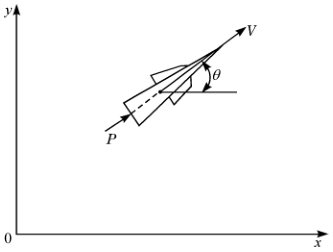
\includegraphics[width=\linewidth]{figs/fig-0164.png}
\caption{图9.9-1}
\end{figure}

J=-n x\_\{1\}-n\_\{2\} x\_\{3\}= 这一问题可以转换成轨线末端受限制的情况。

事实上，过与单位向量 $\boldsymbol{n}_{0}=\left(n_{1}, n_{2}, 0,0,0\right)$ 平行的直线 $L$ （图 9.9-2) 上的任一点做一垂直的 $n-1$ 维超平面 $P, \boldsymbol{n}$ 将是它的法向量。上述命题可等价地转述为：将火箭引导到平面 $P$ 上，使交点 $S$ 在直线 $L$ 上离原点最远。交点 $S$ 是未知的，但这并不影响我们对前节所述理论的应用。

取火箭的助推段终点为求解上述问题的初始条件 $\boldsymbol{x}=\left(x_{10}, x_{20}, x_{30}, x_{40}, x_{50}\right)$。于是，可以根据标准方程组 (9.7-6) 写出求解最优控制的方程组

\[\begin{aligned} & \frac{d x_{0}}{d t}=-n x_{2}-n_{2} \frac{a u_{1}-b Q\left(x_{2}, x_{3}, x_{4}\right)}{x_{5}} \cos u, \quad x_{0}(0)=0 \\ & \frac{d x_{1}}{d t}=x_{2}, \quad x_{1}(0)=x_{10} \\ & \frac{d x_{2}}{d t}=\frac{a u_{1}-b Q\left(x_{2}, x_{3}, x_{4}\right)}{x_{5}} \cos u, \quad x_{2}(0)=x_{20} \\ & \frac{d x_{3}}{d t}=x_{4}, \quad x_{3}(0)=x_{30} \\ & \frac{d x_{4}}{d t}=\frac{a u_{1}-b Q\left(x_{2}, x_{3}, x_{4}\right)}{x_{5}} \sin u-g, \quad x_{4}(0)=x_{40} \\ & \frac{d x_{5}}{d t}=-c u_{1}, \quad x_{5}(0)=x_{50} \end{aligned}\qquad\text{(9.9-6)}\]

它的共轭方程组是

\[\begin{aligned} & \frac{d \psi_{0}}{d t}=0, \quad \psi_{1} \leqslant 0 \\ & \frac{d \psi_{1}}{d t}=0, \quad \psi_{1}(T)=\psi_{1}(t) \equiv-n \\ & \frac{d \psi_{2}}{d t}=n \psi_{0}-\psi_{1}+\frac{b}{x_{5}} \frac{\partial Q}{\partial x_{2}}\left(\left(\psi_{2}-n_{2} \psi_{0}\right) \cos u+\psi_{1} \sin u\right), \quad \psi_{2}(T)=-n_{2} \\ & \frac{d \psi_{3}}{d t}=\frac{b}{x_{5}} \frac{\partial Q}{\partial x_{3}}\left(\left(\psi_{2}-n_{2} \psi_{0}\right) \cos u+\psi_{1} \sin u\right), \quad \psi_{3}(T)=0 \\ & \frac{d \psi_{4}}{d t}=-\psi_{1}+\frac{b}{x_{5}} \frac{\partial Q}{\partial x_{4}}\left(\left(\psi_{2}-n_{2} \psi_{0}\right) \cos u+\psi_{1} \sin u\right), \quad \psi_{4}(T)=0 \end{aligned}\]

\begin{figure}[htbp]\centering
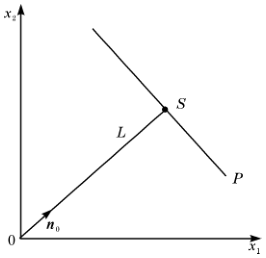
\includegraphics[width=\linewidth]{figs/fig-0165.png}
\caption{图9.9-2}
\end{figure}

\[\frac{d \psi_{5}}{d t}=-\frac{a u_{1}-b Q\left(x_{2}, x_{3}, x_{4}\right)}{x_{5}^{2}}\left(\left(\psi_{5}-n_{5} \psi_{5}\right) \cos w+\psi_{5} \sin w\right), \quad \psi_{5}(T)=0\qquad\text{(9.9-7)}\]

哈密顿函数为

\[\begin{aligned} H & =\varphi\left(x_{2}, x_{4} ; \psi_{5}, \psi_{5}\right)-n_{5} \psi_{5} \frac{a u_{1}-b Q}{x_{5}} \cos w+\psi_{5} \frac{a u_{1}-b Q}{x_{5}} \cos w \\ & +\psi_{5} \frac{a u_{1}-b Q}{x_{5}} \sin w-c \psi_{5} w \end{aligned}\]

式中

\[\varphi\left(x_{2}, x_{4} ; \psi_{5}, \psi_{5}, \psi_{5}\right)=-n_{5} x_{2} \psi_{5}+\psi_{5} x_{2}+\psi_{5} x_{4}-\psi_{5} g\]

从前节的讨论可知，函数 $H$ 沿最优运动取最大值:

\[H\left(\dot{\mathbf{x}}(t), \tilde{\Psi}(t), \tilde{u}(0)\right)=\max _{u \in U} H\left(\dot{\mathbf{x}}(t), \tilde{\Psi}(t), \mathbf{u}\right) \equiv 0, \quad 0 \leqslant t \leqslant T\qquad\text{(9.9-9)}\]

条件式 (9.9-9)意味着

\[\begin{aligned} & \frac{a u_{1}}{\dot{x}_{5}}(t)-b Q\left(\dot{x}_{2}, \dot{x}_{3}, \dot{x}_{4}\right)\left(\left(\tilde{\psi}_{5}(t)-n_{5} \psi_{5}\right) \cos \dot{w}(t)+\dot{\psi}_{5}(t) \sin \dot{w}(t)\right)-c \dot{\psi}_{5}(t) \dot{w}(t) \\ = & \max _{u \in U}\left[\frac{a u_{1}-b Q\left(\dot{x}_{2}, \dot{x}_{3}, \dot{x}_{4}\right)}{\dot{x}_{5}(t)}\left(\left(\tilde{\psi}_{5}(t)-n_{5} \psi_{5}\right) \cos w+\dot{\psi}_{5}(t) \sin w\right)-c \dot{\psi}_{5}(t) u\right] \end{aligned}\qquad\text{(9.9-10)}\]

上面共得到 12 个一阶微分方程式，14 个未知函数，11 个边界条件。未知数 $\psi$ 可以从式 (9.9-7) 求出，$i w(t)$ 和 $i w(t)$ 可以从式 (9.9-9) 或 (9.9-10) 求出。令

\[\eta(t, \dot{\mathbf{x}}(t), \dot{\Psi}(t), \dot{w}(t))=\frac{a}{\dot{x}_{5}(t)}\left(\dot{\psi}_{5}(t)-n_{5} \psi_{5}\right) \cos \dot{w}(t)+\dot{\psi}_{5}(t) \sin \dot{w}(t)-c \dot{\psi}_{5}(t)\]

则

\[i w(t)= \begin{cases}1, & \text { 若 } \eta>0 \\ 0, & \text { 若 } \eta<0\end{cases}\qquad\text{(9.9-11)}\]

由此可知最优的推力程序是开关式函数，要么以最大推力工作，要么以最小推力工作。最优方向程序 $i w(t)$ 的变化规律要复杂些。但是按限制条件式 (9.9-3)，它实际上是不受限制的。因此 $H$ 对 $w$ 应取极值。所以，我们可以对式 (9.9-10) 右端求对 $w$ 的偏导数并令其等于零，解出后得

\[\tan \dot{w}(t)=\frac{\dot{\psi}_{5}(t)}{\dot{\psi}_{5}(t)-n_{5} \psi_{5}}\]

或者

\[\cos \dot{w}(t)=\pm \frac{\dot{\psi}_{5}(t)-n_{5} \psi_{5}}{\sqrt{\dot{\psi}_{5}^{2}+\left(\dot{\psi}_{5}(t)-n_{5} \psi_{5}\right)^{2}}}\]

\[\sin \dot{w}(t)= \pm \sqrt{\frac{\dot{\psi}_{\mathrm{t}}(t)}{\dot{\psi}_{\mathrm{t}}^{2}+\left(\dot{\psi}_{\mathrm{t}}-n_{\mathrm{t}} \psi_{\mathrm{t}}\right)^{2}}}\qquad\text{(9.9-12)}\]

上式右端之符号应该这样选取，使 $\cos \dot{w}(t)$ 和 $\sin \dot{w}(t)$ 均为正。将式 (9.9-12) 代入式 $(9.9-11)$ 后，$\dot{w}(t)$ 也就不依赖于 $\dot{w}(t)$ 了。

如果在某种特定的条件下，空气阻力可以忽略不计，则式 $(9.9-6)$ 和 $(9.9-7)$还可以大为化简。但是，不管是否忽略阻力，用一般的理论分析方法求解方程组 $(9.9-4)-(9.9-10)$ 几乎是不可能的。通常是利用计算机对特定的问题进行研究并求解。

\section{9.10 动态规划与最优控制原理}

归纳前面几节的讨论，为了求得受控系统满足某一给定的积分型指标的最优控制，必须同时研究问题的全局特征，写出完整的标准方程组，然后才可能求出最优控制规律。这是变分方法的基本特点，特别适宜于对控制问题的分析处理，然而用分析方法只能处理比较简单的情况。在实际问题中，大多数受控运动方程是比较复杂的，只能用数字计算机去作最优控制设计。本节内我们再介绍另一种最优控制的设计方法，叫动态规划法。这种方法的基本思想和变分方法不同，对某些问题更适宜于在计算机上作最优设计。

\begin{figure}[htbp]\centering
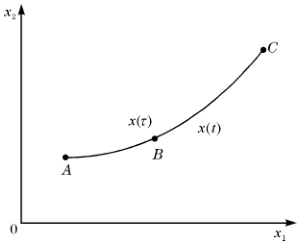
\includegraphics[width=\linewidth]{figs/fig-0166.png}
\caption{图9.10-1}
\end{figure}

动态规划的基本思想是把整个控制过程分为若干段，在每一段内选择最优控制，使满足给定的指标要求。它可以概括成一个原理：无论系统的初始状态如何，也无论第一段运动过程中的最优控制是何种形式，全局为最优的控制函数，对应于第一阶段的终点状态，第二段运动过程中控制函数的选择，按给定的指标也一定是最优的。这就是最优控制原理。用图 9.10-1 对这一原理略作说明，设自 $A$ 点至 $C$ 点的按某种意义最优的运动是 $\boldsymbol{x}(t), 0 \leqslant t \leqslant$ $T$，其相应的最优控制是 $\boldsymbol{u}(t), 0 \leqslant t \leqslant T$。系统

运动经过 $B$ 点的时刻记作 $\tau, 0<\tau<T$。最优控制原理的几何含意是，以 $A$ 点为始点，以 $C$ 点为终点的最优控制 $\boldsymbol{u}(t), 0 \leqslant t \leqslant T$，也一定是以 $B$ 点为始点，以 $C$ 点为终点，定义于时间 $\tau \leqslant t \leqslant T$ 上的最优控制。

为简单起见，先假定受控对象是一个一阶非线性系统

\[\frac{d x}{d t}=f(x, u), \quad x(0)=x_{0}\qquad\text{(9.10-1)}\]

终点状态假定是完全“自由”的，无任何约束，但是对控制量 $u$ 的约束形式不是像前面讨论的那样，而是具有下列形式

\[g^{1}(\boldsymbol{x}) \leqslant u \leqslant g^{2}(\boldsymbol{x})\qquad\text{(9.10-2)}\]

我们看到，$u$ 的取值范围不是一成不变的，而与系统的状态有关，上式内左右两端的函数 $g^{1}(x)$ 和 $g^{2}(x)$ 是预先给定的。选择控制量 $u(t)$ 的目的是在给定的时间间隔 $T$ 内，使下列泛函取极小值

\[J(u)=\int_{0}^{T} f_{0}(x, u) d t=\min\qquad\text{(9.10-3)}\]

由于终点状态无任何约束，如果这种最优控制存在且唯一的话，极小值 $J\left(\dot{u}(t)\right)$ 将是初始条件 $x_{0}$ 和时间间隔 $T$ 的单值函数。这个泛函的最小值记为 $F\left(x_{0}, T\right)$，于是

\[F\left(x_{0}, T\right)=\min J(u(t))\qquad\text{(9.10-4)}\]

如果将时间间隔 $T$ 稍微增大，使终端时刻变为 $T+\tau$，则上述等式将变成

\[\begin{aligned}F\left(x_{0}, \tau+T\right)=\min _{\substack{0 \leqslant t_{1} \\ 0 \leqslant t_{2} \leqslant \tau}}\left[\int_{0}^{t_{1}} f_{0}(x, u) d t+F(x(\tau), T)\right]\end{aligned}\qquad\text{(9.10-5)}\]

而且 $u(t)$ 的取值范围应该满足条件式 (9.10-2) 的限制。

如果设 $f(x, u)$ 和 $F\left(x_{0}, T\right)$ 均为连续可微的二元函数，则

\[\begin{aligned} & F\left(x_{0}, T+\tau\right)=F\left(x_{0}, T\right)+\frac{\partial F}{\partial T} \tau+O(\tau) \\ & F(x(\tau), T)=F\left(x_{0}, T\right)+\frac{\partial F}{\partial x_{0}} f\left(x_{0}, u\right) \tau+O(\tau) \end{aligned}\]

当 $\tau \rightarrow 0$ 时，应用上面两式的关系，式 (9.10-5) 可以写成

\[\frac{\partial F}{\partial T}=\min _{u}\left[f_{0}(\boldsymbol{x}, \boldsymbol{u})+\frac{\partial F}{\partial x_{0}} f(\boldsymbol{x}, \boldsymbol{u})\right]\qquad\text{(9.10-6)}\]

如果函数 $F\left(x_{0}, T\right)$ 为已知，则式 (9.10-6) 将给予可能求出最优控制函数 $\dot{u}(t)$ 的初始值 $\dot{u}(t)$。我们看到，式 (9.10-6) 是一个一阶偏微分方程。其中 $f_{0}$ 和 $f$ 为已知二元函数。为了求解此方程式，需要给定某些边界条件。如果在全平面上求出函数 $F\left(x_{0}, T\right)$，那么在每一瞬间的最优控制 $\dot{u}$ 即可按式 (9.10-6) 求出。

对于更为一般的受控对象

\[\frac{d \boldsymbol{x}}{d t}=f(\boldsymbol{x}, \boldsymbol{u}), \quad \boldsymbol{u} \in U(\boldsymbol{x})\qquad\text{(9.10-7)}\]

和泛函指标

\[J(u(t))=\int_{0}^{T} f_{0}(\boldsymbol{x}, \boldsymbol{u}) d t=\min\qquad\text{(9.10-8)}\]

记

\[F(\boldsymbol{x} ; T)=\min _{u \in U(\boldsymbol{x})} J(u(t))\qquad\text{(9.10-9)}\]

符号 $U(\boldsymbol{x})$ 表示 $\boldsymbol{u}$ 的取值范围随受控对象的状态 $\boldsymbol{x}$ 的变化而变化。重复前面的讨论，并注意到多元自变量的特点，基本函数方程可按下列次序推出

\[\begin{aligned}F(\boldsymbol{x}, T+\tau)=\min _{\substack{u(t) \in U(\boldsymbol{x}) \\ 0 \leqslant t \leqslant \tau}}\left[\int_{0}^{\tau} f_{0}(\boldsymbol{x}, \boldsymbol{u}) d t+F(\boldsymbol{x}(\tau), T)\right]\end{aligned}\qquad\text{(9.10-10)}\]

当 $\tau$ 很小时

\[\begin{aligned} & \boldsymbol{x}(\tau)=\boldsymbol{x}(0)+\boldsymbol{f}(\boldsymbol{x}(0), \boldsymbol{u}(0)) \tau+O(\tau) \\ & F(\boldsymbol{x}(0), T+\tau)=F(\boldsymbol{x}(0), T)+\frac{\partial F}{\partial T} \tau+O(\tau) \\ & F(\boldsymbol{x}(\tau), T)=F(\boldsymbol{x}(0), T)+\sum_{n=1}^{n} \frac{\partial F}{\partial \boldsymbol{x}_{n}} f_{n}(\boldsymbol{x}(0), \boldsymbol{u}(0)) \tau+O(\tau) \\ & =F(\boldsymbol{x}(0), T)+\tau(\operatorname{grad} F(\boldsymbol{x}(0), T), \boldsymbol{f}(\boldsymbol{x}(0), \boldsymbol{u}(0)))+O(\tau) \end{aligned}\]

令 $\tau \rightarrow 0$，按上面讨论次序，可最后得到关于函数 $F$ 的特种偏微分方程

\[\frac{\partial F}{\partial T}=\min _{u(0) \in U(\boldsymbol{x}(0))}(\operatorname{grad} F(\boldsymbol{x}(0), T), \boldsymbol{f}(\boldsymbol{x}(0), \boldsymbol{u}(0)))\qquad\text{(9.10-11)}\]

根据最优控制原理，上面的讨论不仅对始点 $\boldsymbol{x}(0)$ 是正确的，对最优轨线上的任何点也都成立。故上式也可对任意点 $\boldsymbol{x}(\tau)$ 改写为

\[\frac{\partial F}{\partial \theta}=\min _{u(\tau) \in U(\boldsymbol{x}(\tau))}(\operatorname{grad} F(\boldsymbol{x}(\tau), \theta), \boldsymbol{f}(\boldsymbol{x}(\tau), \boldsymbol{u}(\tau)))\qquad\text{(9.10-12)}\]

式中 $\theta=T-\tau$，符号 $\operatorname{grad} F$ 表示只对 $\boldsymbol{x}$ 取偏导数的梯度向量

\[\operatorname{grad} F(\boldsymbol{x}, \theta)=\left(\begin{array}{c} \frac{\partial F}{\partial x_{1}}, \cdots, \frac{\partial F}{\partial x_{n}} \end{array}\right)\]

基本方程 $(9.10-11)$ 或 $(9.10-12)$ 有两种用途。当函数 $F(\boldsymbol{x}, T)$ 为已知时，可由此求出最优控制 $\dot{u}(t)$。反之，当 $\dot{u}(t)$ 为已知时，可以由此求出函数 $F(\boldsymbol{x}, \theta)$。有时函数 $F$ 可由其他途径求出，此时按式 $(9.10-12)$ 即可完全确定最优控制函数了。在第八章讨论最速控制系统时，我们曾得到过类似的方程（参看第 8.6 节）。那里我们曾指出求解此方程式的方法。实际上这个方程式与那里得到的结果有深刻的联系。此外，对控制量不受限制的情况至今研究得比较详细。读者在文献[2]中可以找到对这一类特殊问题的计算方法。

\section{9.11 拦截问题中的导引律}

作为最优控制理论的一个很好的应用，我们介绍一下关于拦截问题中的导引规律的最优选择 ${ }^{[4]}$。设有一目标 $M$ 以速度向量 $\boldsymbol{v}_{M}$ 飞来（见图 9.11-1)。今用一个横向可机动的拦截飞行器 $D$ 对目标进行拦截，速度向量为 $\boldsymbol{v}_{D}$。用 $\boldsymbol{x}_{M}$ 和 $\boldsymbol{x}_{D}$ 分别表示目标和拦截器的空间坐标，它们之间的相对距离是 $\boldsymbol{x}=\boldsymbol{x}_{M}-\boldsymbol{x}_{D}$，相对速度是 $v = v_W - v_D$。拦截器 $D$ 的飞行方向可以用改变横向加速度 $\alpha_D$ 的办法加以控制。拦截任务的目的是找出一种控制规律，使拦截器 $D$ 在某一时刻与目标 $M$ 相碰撞，或者使相对距离 $\boldsymbol{x}$ 在某一时刻达到极小值。相对距离 $\boldsymbol{x}(t) = \boldsymbol{x}_W(t) - \boldsymbol{x}_D(t)$ 在 $t > 0$ 以后的极小值称为拦截脱靶量。为了达到拦截目的而选择的控制规律称为导引律。

导引律是由系统的实时状态决定的控制律。这种控制律使系统在某一时刻达到零脱靶，或达到某一种终止状态。从控制理论的观点看，导引律就是依赖于实时状态的综合控制

（或反馈控制）。下面将看到，用最优控制的综合理论讨论各种导引律可以得到一些新的、很有意思的结论。在这一节中，我们先用最优控制理论推导空间比例导引律，然后引进“零控拦截状态”及“零控拦截曲面 $L$”的概念，并用这些概念讨论各种导引律。

在相对体制下，导引问题的运动方程可描述为

\[\begin{aligned}& \dot{\boldsymbol{x}} = \boldsymbol{v} \\& \dot{\boldsymbol{v}} = \alpha + \boldsymbol{u}\end{aligned}\qquad\text{(9.11-1)}\]

这里，$\boldsymbol{x}, \boldsymbol{v}, \alpha$ 分别为目标和拦截器之间的相对位置、相对速度和相对加速度向量，而 $\boldsymbol{u}$ 为控制加速度向量。相对加速度 $\alpha$ 可以叫做固有加速度，它是不能随意改变的，它的大小和方向依赖于状态变量。为简单起见，通常假定 $\alpha$ 是关于 $t$ 的已知函数。

在导引问题中，通常假定系统的初始状态 $\boldsymbol{x}, \boldsymbol{v}$ 为已知，而对终点状态可以提出各种不同要求。例如，要求终点状态为零脱靶，即 $\boldsymbol{x}(T) = 0$ ( $T$ 为导引终止时刻）。一般地，终点状态可描述为

\[\boldsymbol{g}(\boldsymbol{x}(T), \boldsymbol{v}(T)) = \boldsymbol{0}\qquad\text{(9.11-2)}\]

$\boldsymbol{g}$ 是向量，由终点状态约束条件决定。除终点状态约束外，还可能有表明导引过程好坏的性能指标。在系统式 (9.11-1) 中，加速度 $\boldsymbol{u}$ 是由载或推力产生的控制。这时，通常以所消耗的总能量的大小，即

\[J = \frac{1}{2} \int_0^T \dot{\boldsymbol{u}} \boldsymbol{u} dt\qquad\text{(9.11-3)}\]

作为性能指标。这里 $T$ 是事先给定的时刻。式 (9.11-1)，(9.11-2)，(9.11-3) 是典型的最优控制问题。

所谓最优导引律，就是这个最优控制问题的综合控制 $\boldsymbol{u}(\boldsymbol{x}, \boldsymbol{v})$。如果把这个综

\begin{figure}[htbp]\centering
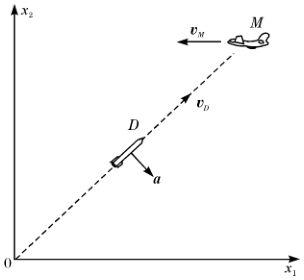
\includegraphics[width=\linewidth]{figs/fig-0167.png}
\caption{图9.11-1}
\end{figure}

合控制求出来，并代入方程 (9.11-1) 中，则方程组的任意轨线都应该是上述最优控制问题的最优轨线。综合控制 $\dot{u}(\boldsymbol{x}, \boldsymbol{v})$ 可按如下方式确定：对任意给定的初值 $\boldsymbol{x}_{0}, \boldsymbol{v}_{0}$，先按极大值原理求出最优程序控制 $\dot{u}(t, \boldsymbol{x}_{0}, \boldsymbol{v}_{0})$，然后令 $t=0$ 得 $\dot{u}(0, \boldsymbol{x}_{0}$，$\boldsymbol{v}_{0})$。控制 $\dot{u}(0, \boldsymbol{x}_{0}, \boldsymbol{v}_{0})$ 是系统处于 $\boldsymbol{x}_{0}, \boldsymbol{v}_{0}$ 状态时所应取的控制量，因此有 $\dot{u}(\boldsymbol{x}, \boldsymbol{v})$ $=\dot{u}\left(0, \boldsymbol{x}_{0}, \boldsymbol{v}_{0}\right)$。

下面求解最优控制问题式 (9.11-1)-(9.11-3)。为此，先用 $\boldsymbol{x}^{0}(t), \boldsymbol{v}^{0}(t)$ 表示 $u \equiv 0$ 时系统运动的轨线 （叫做零控弹道）。积分方程组 (9.11-1) 得

\[\begin{aligned} \boldsymbol{x}^{0}(t) & =\boldsymbol{x}_{0}+\boldsymbol{v}_{0} t+\int_{0}^{t}(t-\tau) \alpha(\tau) d \tau \\ \boldsymbol{v}^{0}(t) & =\boldsymbol{v}_{0}+\int_{0}^{t} \alpha(\tau) d \tau \end{aligned}\qquad\text{(9.11-4)}\]

引入零控平均速度 $\bar{v}^{0}(t)=\boldsymbol{v}_{0}+\frac{1}{t} \int_{0}^{t}(t-\tau) \alpha(\tau) d \tau$，则 $\boldsymbol{x}^{0}(t)$ 又可表示为

\[\boldsymbol{x}^{0}(t)=\boldsymbol{x}_{0}+\bar{v}^{0}(t) t\]

当 $u(t) \neq 0$ 时，方程组 (9.11-1) 的轨线为

\[\begin{aligned} \boldsymbol{x}(t) & =\boldsymbol{x}^{0}(t)+\int_{0}^{t}(t-\tau) \boldsymbol{u}(\tau) d \tau \\ v(t) & =\boldsymbol{v}^{0}(t)+\int_{0}^{t} \boldsymbol{u}(\tau) d \tau \end{aligned}\qquad\text{(9.11-5)}\]

最优控制问题式 (9.11-1)-(9.11-3) 的哈密顿函数为①

\[H=\boldsymbol{\phi}_{1}^{*} \boldsymbol{v}+\boldsymbol{\phi}_{2}^{*} \alpha+\boldsymbol{\phi}_{2}^{*} \boldsymbol{u}-\frac{1}{2} \dot{\boldsymbol{u}} \dot{\boldsymbol{u}}\qquad\text{(9.11-6)}\]

而共轭方程和边界条件为

\[\left\{\begin{array}{l} \dot{\boldsymbol{\psi}}_{1}=0, \boldsymbol{\psi}_{1}(T)=\lambda_{1} \\ \dot{\boldsymbol{\psi}}_{2}=-\boldsymbol{\psi}_{1}, \boldsymbol{\psi}_{2}(T)=\lambda_{2} \end{array}\right.\]

其中 $\lambda_{1}, \lambda_{2}$ 分别等于 $\frac{\partial}{\partial \boldsymbol{x}(T)}\left(\lambda_{1}^{*} \boldsymbol{g}(\boldsymbol{x}(T), \boldsymbol{v}(T))\right), \frac{\partial}{\partial \boldsymbol{v}(T)}\left(\lambda_{2}^{*} \boldsymbol{g}(\boldsymbol{x}(T), \boldsymbol{v}(T))\right), \lambda$ 为待定向量。如果 $\boldsymbol{g}(\boldsymbol{x}(T), \boldsymbol{v}(T))=\boldsymbol{x}(T)$，则 $\lambda_{2}=\boldsymbol{0}$。积分方程组 (9.11-7) 得

\[\boldsymbol{\psi}_{1}(t)=\lambda_{1}, \boldsymbol{\psi}_{2}(t)=\lambda_{1}(T-t)+\lambda_{2}\qquad\text{(9.11-8)}\]

根据极大值原理，最优控制 $\dot{u}(t)$ 为

\[\dot{u}(t)=\boldsymbol{\psi}_{2}(t)=\lambda_{1}(T-t)+\lambda_{2}\qquad\text{(9.11-9)}\]

取 $t=0$，得

\[\dot{u}(0)=\lambda_{1} T+\lambda_{2}\qquad\text{(9.11-10)}\]

为了求出综合控制 $\dot{u}(\boldsymbol{x}, \boldsymbol{v})$，必须把 $\lambda_{1}, \lambda_{2}$ 表示成初始状态 $\boldsymbol{x}_{0}, \boldsymbol{v}_{0}$ 的函数。为此，

(1) 这里和以后用 $\boldsymbol{x}^{*} \boldsymbol{y}$ 表示两个向量的积，即 $\boldsymbol{x}^{*} \boldsymbol{y}=(\boldsymbol{x}, \boldsymbol{y})$。

把式(9.11-9)代到式(9.11-5)中，然后积分，取 $t=T$，得

\[\begin{aligned}& \mathbf{x}(T)=\mathbf{x}^{0}(T)+\frac{T^{3}}{3} \lambda_{1}+\frac{T^{2}}{2} \lambda_{2} \\& \nu(T)=\nu^{0}(T)=\frac{T^{2}}{2} \lambda_{1}+T \lambda_{2}\end{aligned}\qquad\text{(9.11-11)}\]

其次，用条件 $\mathbf{g}(\mathbf{x}(T), \nu(T))=\mathbf{0}$ 和 $\lambda_{1}, \lambda_{2}$ 的表达式决定定向量 $\lambda$ 作为 $\mathbf{x}^{0}(T)$，$\nu^{0}(T)$ 的函数，从而把控制 $\dot{\mathbf{u}}(0)$ 表示成零控弹道终止状态 $\mathbf{x}^{0}(T), \nu^{0}(T)$ 的函数。如果再把 $\mathbf{x}^{0}(T), \nu^{0}(T)$ 表示成 $\mathbf{x}, \nu$ 的函数，就得综合控制 $\dot{\mathbf{u}}(\mathbf{x}, \nu)$。用零控弹道终止状态 $\mathbf{x}^{0}(T), \nu^{0}(T)$ 表示出来的控制律 $\dot{\mathbf{u}}\left(\mathbf{x}^{0}(T), \nu^{0}(T)\right)$ 叫做“预测导引律”。

当 $\mathbf{g}(\mathbf{x}(T), \nu(T))=\mathbf{x}(T)$ （即终止状态为零脱靶状态）时，$\lambda=\mathbf{0}, \lambda=\lambda$，从而 $\dot{\mathbf{u}}(0)=\lambda_{1} T, \mathbf{x}(T)=\mathbf{x}^{0}(T)+\frac{T^{3}}{3} \lambda_{1}$。由 $\mathbf{x}(T)=\mathbf{0}$ 得

\[\dot{\mathbf{u}}(0)=-\frac{3 \mathbf{x}^{0}(T)}{T^{3}}\qquad\text{(9.11-12)}\]

这是终止状态为零脱靶时的“预测导引律”。 $\mathbf{x}^{0}(T)$ 叫做“预测脱靶量”。

再讨论空间比例导引律。把式(9.11-12)中的预测脱靶量具体表示出来，得

\[\dot{\mathbf{u}}(0)=-\frac{3(\mathbf{x}+\overrightarrow{\nu}^{0}(T) T)}{T^{2}}\qquad\text{(9.11-13)}\]

这里 $T$ 是事先给定的，可按适当方式选取。如果取

\[T=-\frac{(\mathbf{x}, \nu^{0}(T))}{\mid \nu^{0}(T) \mid^{2}}\]

则式(9.11-13)变为

alignedu(0) \& =-3 x(\textasciicircum{}0(T), \textasciicircum{}0(T))-\textasciicircum{}0(T)(x, \textasciicircum{}0(T))(x, \textasciicircum{}0(T))\textasciicircum{}2  \textasciicircum{}0(T) \textasciicircum{}2 \textbackslash\{\}\textbackslash\{\}\& =3 |x|\textasciicircum{}2  \textasciicircum{}0(T) \textasciicircum{}2 (x  \textasciicircum{}0(T)) x \textasciicircum{}2  \textasciicircum{}0(T)aligned

其中用 $\mathbf{x} \times \mathbf{y}$ 表示两个向量的向量积，而 $(\mathbf{x} \times \overrightarrow{\nu}^{0}(T)) / \mid \mathbf{x} \mid^{2}$ 是由平均速度 $\overrightarrow{\nu}^{0}(T)$ 引起的视线 $\mathbf{x}$ 的旋转角速度——视线转率。如果把这个视线转率记成 $\omega$，则有

\[\dot{\mathbf{u}}(0)=3 \frac{\mid \mathbf{x} \mid^{2} \mid \overrightarrow{\nu}^{0}(T) \mid^{2} \omega \times \overrightarrow{\nu}^{0}(T)}{(\mathbf{x}, \overrightarrow{\nu}^{0}(T))^{2}}\qquad\text{(9.11-14)}\]

如果在系统式(9.11-1)中假定 $\alpha \equiv 0$，则 $\overrightarrow{\nu}^{0}(T)=\nu$ 从而式(9.11-14)变为

\[\dot{\mathbf{u}}(0)=3 \frac{\mid \mathbf{x} \mid^{2} \mid \nu \mid^{2}}{(\mathbf{x}, \nu)} \omega \times \nu\qquad\text{(9.11-15)}\]

这就是我们所说的空间比例导引律；控制式(9.11-15)的大小与视线转率成正比，而控制方向垂直于相对速度 $\nu$。

如果取

\[\begin{gathered} T=-\frac{\left|\boldsymbol{x}\right|^{2}}{\left(\boldsymbol{x}, \boldsymbol{v}^{0}(T)\right)} \\ \text { 则得到另一种比例导律 } \\ \dot{\boldsymbol{u}}(0)=3 \frac{\left(\boldsymbol{x}, \boldsymbol{v}^{-0}(T)\right)}{\left|\boldsymbol{x}\right|^{2}} \omega \times \boldsymbol{x} \end{gathered}\]

这个控制方向是垂直于视线 $\boldsymbol{x}$ 的。

在导引问题中，一般“初始偏差”都比较大。通常希望在导引的初始阶段，用较大的控制力把初始偏差的大部分消除掉。比较理想的导引律应该是在导引的初始阶段能提供较大的控制力以便消除较大的初始偏差，而在导引过程的后期，则用较小的控制力进行“微调”。但是，导引律式 (9.11-12)-(9.11-16)都不能做到这一点。因为，它们都是从“整个导引过程都在消除初始偏差”这样观点出发推导的公式，因而横向过载的分布在整个导引过程中是比较平均的。横向过载的这种平均分布在实际上是很不理想的。因为在拦截器接近目标时，为了保持导引规律不被破坏，需要付出很大的横向控制过载，而这在实际上是做不到的。事实上，当 $T \rightarrow 0$ 或 $\left|\boldsymbol{x}\right| \rightarrow 0$ 时，只要 $\boldsymbol{x}^{0}(T)$ 或 $\omega$不趋于零，控制过载式 $(9.11-12)-(9.11-16)$ 都将趋于无穷大，这就是通常的比例导引法在导引过程后期出现“过载饱和”的原因。有没有一种办法能克服这种缺点呢？把上面的“整个过程的平均”换成“短时间内的平均”是克服上述缺点的一种办法。

为了进一步研究导引问题，“零控拦截状态”及曲面 $L$ 的概念很有用处。从控制律式 $(9.11-12),(9.11-14)$ 和 $(9.11-16)$ 中可看出，如果零控预测脱靶 $\boldsymbol{x}^{0}(T)$ 或 $\omega$ 等于零，控制力 $\dot{\boldsymbol{u}}(0)$ 也等于零，并且在整个过程中不加控制力也能实现拦截。如果系统在某一时刻已处于这样的状态，从这个状态预测的零控脱靶量为零，那么不加控制力，经有限时间也能实现准确命中。我们把这种特殊的状态称之为“零控拦截状态”，即无控也能实现拦截的状态，在导引问题中“零控拦截状态”的存在是一个普遍现象。古典导引法中的所有直线弹道和所谓基准弹道，实质上都是由零控拦截状态所组成的。

由方程 $(9.11-1)$ 所描述的导引问题中，凡是满足条件

\[\boldsymbol{x}^{0}(\mu)=\boldsymbol{x}+\mu \bar{\boldsymbol{v}}(\mu)=0\]

的初始状态 $\boldsymbol{x}, \boldsymbol{v}$，都是零控拦截状态。这里 $\mu$ 是非负数。如果 $\alpha \equiv 0$，则 $\bar{\boldsymbol{v}}^{0}(\mu)=\boldsymbol{v}_{0}$。这时零控拦截状态为满足

\[\boldsymbol{x}+\mu \boldsymbol{v}_{0}=0, \quad \mu \geqslant 0\qquad\text{(9.11-16)}\]

的初始状态。所有这种状态在整个状态空间 (6 维空间） 中组成 4 维曲面[式 (9.11-18) 是含 7 个变量 $\boldsymbol{x}, \boldsymbol{v}, \mu$ 的三个方程]。所有零控拦截状态所组成的曲面叫做“零控拦截曲面”，用 $L$ 记之，简称 $L$ 曲面，或曲面 $L$。

如果导引问题的系统方程写成

\[\left\{\begin{array}{l}\dot{\boldsymbol{x}}=\nu, \boldsymbol{x}(0)=\boldsymbol{x}_{0} \\\dot{\nu}=-\omega^{2} \boldsymbol{x}+\boldsymbol{u}, \quad \nu(0)=\nu_{0}\end{array}\right.\]

则零控预测脱靶量为

\[\boldsymbol{x}^{0}(T)=\cos \omega T \boldsymbol{x}_{0}+\frac{1}{\omega} \sin \omega T \nu_{0}\]

于是 $\boldsymbol{x}, \nu_{0}$ 为零控拦截状态的充分必要条件是

\[\boldsymbol{x}_{0}+\mu \nu_{0}=0, \quad \mu=\frac{1}{\omega} \tan \omega T\]

这里 $\mu$ 的取值可正可负。

对一般情形，分别用目标和拦截器的运动方程式能更好地说明零控拦截状态的意义。设目标和拦截器的运动方程分别为

\[\left\{\begin{array}{l}\dot{\boldsymbol{x}}_{M}=\nu_{M} \\\dot{\nu}_{M}=\alpha_{M}\left(\boldsymbol{x}_{M}, \nu_{M}\right) \\\dot{\boldsymbol{x}}_{D}=\nu_{D} \\\dot{\nu}_{D}=\alpha_{D}\left(\boldsymbol{x}_{D}, \nu_{D}\right)+\boldsymbol{u}\end{array}\right.\]

给定了目标的初始状态 $\boldsymbol{x}_{M 0}, \nu_{M 0}$ 以及拦截器的初始位置 $\boldsymbol{x}_{D 0}$ 和导弹的初始速度 $\left|\nu_{D 0}\right|$ 以后，这时只要 $\left|\nu_{D 0}\right|$ 足够大，我们总可以选择拦截器的速度方向，使得它沿这个方向飞行，没有控制力作用也能实现拦截。这种方向叫做“零控拦截方向”。这个零控拦截方向和给定的目标、拦截器的初始条件一起组成一个零控拦截状态。所有这种零控拦截状态，在整个状态空间 (12 维空间） 中组成 10 维曲面 $L$ （由于只有 10 个独立变量 $\boldsymbol{x}_{M 0}, \boldsymbol{u}_{M 0}, \boldsymbol{x}_{D 0},\left|\nu_{D 0}\right|$ )。在一般的导引问题中，要精确描述出曲面 $L$ 是个复杂的问题。但是，导引问题中存在着曲面 $L$，是肯定的。

再看一看古典导引法和曲面 $L$ 的关系。追踪法、平行接近法、前置量法及三点法等古典导引法，指的是受控制力作用之后的系统状态所应满足的条件。这些导引法并不直接回答“怎样加控制力”的问题。它们只说明，如果系统的状态始终保持在那种状态，就能够实现准确拦截。从前面的讨论中可以看出，系统受控制力作用之后所应保持的理想的状态是零控拦截状态。古典导引法实质上是对各种特殊情况下的 $L$ 曲面的近似描述。

先讨论追踪法。用各自的速度描述零控拦截状态所满足的条件式 (9.11-17) 是

\[\boldsymbol{x}+\mu \nu_{M}^{0}(\mu)=\mu \nu_{D}^{0}(\mu), \quad \mu \geqslant 0\qquad\text{(9.11-19)}\]

如果假定 $\left|\nu_{W}^{-0}(\mu)\right| \ll\left|\nu_{D}^{-0}(\mu)\right|$，即 $\left|\nu_{W}^{-0}(\mu)\right|$ 比 $\left|\nu_{D}^{-0}(\mu)\right|$ 小得多，则近似地有

\[\boldsymbol{x}=\mu \nu_{D}^{-0}(\mu), \quad \mu \geqslant 0\]

即视线 $\boldsymbol{x}$ 与速度 $\overline{\boldsymbol{v}}_{D}(\mu)$ 方向一致。再假定 $\alpha \equiv 0$，则 $\overline{\boldsymbol{v}}_{D}^{0}(\mu)=\boldsymbol{v}_{D 0}$，因而有

\[\boldsymbol{x}^{0}=\mu \boldsymbol{v}_{D 0}, \quad \mu \geqslant 0\]

现在把 $\boldsymbol{x}, \boldsymbol{v}_{D 0}$ 看做受控制作用后的状态，那么受控制作用后的拦截器的速度方向应指向目标，这就是追踪法。追踪法是目标速度 （相对于拦截器速度） 很小时的曲面 $L$ 的近似描述。

再看平行接近法。对式 $(9.11-18)$ 的两边向量乘上 $\boldsymbol{x}$，得

\[\boldsymbol{x} \times \overline{\boldsymbol{v}}_{M}^{0}(\mu)=\boldsymbol{x} \times \overline{\boldsymbol{v}}_{D}^{0}(\mu)\qquad\text{(9.11-20)}\]

如果假定 $\alpha_{M} \equiv 0, \alpha_{D} \equiv 0$，则 $\overline{\boldsymbol{v}}_{M}^{0}(\mu)=\boldsymbol{v}_{M 0}, \overline{\boldsymbol{v}}_{D}^{0}(\mu)=\boldsymbol{v}_{D 0}$，这时上式变成

\[\boldsymbol{x} \times \boldsymbol{v}_{M 0}=\boldsymbol{x} \times \boldsymbol{v}_{D 0}\]

受控制力作用后的拦截器速度 $\boldsymbol{v}_{D 0}$ 应使上式成立。这就是平行接近法。用 $\varphi$ 记 $\boldsymbol{x}_{0}$与 $\boldsymbol{v}_{D 0}$ 的夹角，$\delta$ 记 $\boldsymbol{x}_{0}$ 与 $\boldsymbol{v}_{M 0}$ 的夹角，则由上式得

\[\sin \varphi=\frac{\left|\boldsymbol{v}_{M 0}\right|}{\left|\boldsymbol{v}_{D 0}\right|} \sin \delta\]

平行接近法是自由运动 （无控弹道） 为等速运动时的曲面 $L$ 的描述。

在前置量导引法中，先把 $\overline{\boldsymbol{v}}_{D}^{0}(\mu), \overline{\boldsymbol{v}}_{M}^{0}(\mu)$ 具体表示出来

\[\begin{aligned} & \overline{\boldsymbol{v}}_{D}^{0}(\mu)=\boldsymbol{v}_{D 0}+\frac{1}{\mu_{J}} \int_{0}^{\tau}(\mu-\tau) \alpha_{D}(\tau) d \tau \\ & \overline{\boldsymbol{v}}_{M}^{0}(\mu)=\boldsymbol{v}_{M 0}+\frac{1}{\mu_{J}} \int_{0}^{\tau}(\mu-\tau) \alpha_{M}(\tau) d \tau \end{aligned}\]

记

\[\Delta \boldsymbol{v}=\frac{1}{\mu_{J}} \int_{0}^{\mu}(\mu-\tau)\left(\alpha_{M}(\tau)-\alpha_{D}(\tau)\right) d \tau\]

这时从式 $(9.11-20)$ 可得到

\[\boldsymbol{x} \times\left(\boldsymbol{v}_{M 0}+\Delta \boldsymbol{v}\right)=\boldsymbol{x} \times \boldsymbol{v}_{D 0}\]

记 $\varphi$ 为 $\boldsymbol{x}_{0}$ 与 $\boldsymbol{v}_{D 0}$ 的夹角，$\delta$ 为 $\boldsymbol{x}_{0}$ 与 $\boldsymbol{v}_{M 0}$ 的夹角，而 $\delta+\Delta \delta$ 为 $\boldsymbol{x}_{0}$ 与 $\boldsymbol{v}_{M 0}+\Delta \boldsymbol{v}$ 的夹角，则有

\[\sin \varphi=\frac{\left|\boldsymbol{v}_{M 0}+\Delta \boldsymbol{v}\right|}{\left|\boldsymbol{v}_{D 0}\right|} \sin (\delta+\Delta \delta)\]

受控制力作用后的拦截器前置角 （视线 $\boldsymbol{x}$ 与拦截器速度之间夹角 $\varphi$ ) 可由式 $(9.11-21)$ 的右端来估计。当然，一般来说，这种估计只能是近似的。从这里看出，前置量法是 $\alpha \neq 0$ 时的曲面 $L$ 的近似描述。

最后再讨论三点法。由于 $\boldsymbol{x}=\boldsymbol{x}_{M 0}-\boldsymbol{x}_{D 0}$，故式 $(9.11-19)$ 可改写为

\[\boldsymbol{x}_{M 0}+\mu \overline{\boldsymbol{v}}_{M}^{0}(\mu)=\boldsymbol{x}_{D 0}+\mu \overline{\boldsymbol{v}}_{D}^{0}(\mu), \quad \mu \geqslant 0\]

如果 $\mu \overline{\boldsymbol{v}}_{M}^{0}(\mu)$ 比较小，则近似地有

\[\boldsymbol{x}_{M 0}=\boldsymbol{x}_{D 0}+\mu \overline{\boldsymbol{v}}_{D}^{0}(\mu), \quad \mu \geqslant 0\]

这个近似等式说明，当 $\boldsymbol{x}_{D 0}$ 平行于 $\boldsymbol{x}_{W 0}$ 时，$\boldsymbol{v}_{D 0}$ 也应平行于 $\boldsymbol{x}_{W 0}$，而当 $\boldsymbol{x}_{D 0}$ 不平行于 $\boldsymbol{x}_{W 0}$时，挡截器的速度 $\boldsymbol{v}_{D 0}$ 应使 $\boldsymbol{x}_{D 0}$ 接近 $\boldsymbol{x}_{W 0}$ 方向 （因为 $\mu \geqslant 0)$，这就是三点法的几何意义。因此，三点法是目标速度（相对于拦截器速度）比较小时，曲面 $L$ 在绝对坐标系中的近似表示。

从以上讨论可看出，古典导引法给出的是受控制后的系统状态所应满足的条件，并没有给出加控制力的办法。用什么样的控制去实现古典导引法呢？这个问题，实质上是用什么样的控制律把系统引到曲面 $L$ 上的问题。

现在我们讨论曲面 $L$ 上的一般导引律。导引的最终目的是实现拦截，即达到零脱靶、有了曲面 $L$，我们可以把导引的着眼点从“终点零脱靶”移到“曲面 $L$”上，即把系统导引到曲面 $L$ 上并消除控制力的办法达到拦截的目的。这种导引律可以统称“曲面 $L$ 上的导引律”，也就是说，实质上是把拦截器的速度方向对准到零控拦截方向上。因此，也可以叫做“对准法”或“瞄准法”。

下面就 $\alpha \equiv 0$ 的情形讨论在零控曲面 $L$ 上的导引律。作为最优控制问题，这里的终止状态为曲面 $L$，它在相空间中的方程式是

\[\boldsymbol{x}(T)=\mu v(T)=0, \quad \mu \geqslant 0\qquad\text{(9.11-22)}\]

即

\[\boldsymbol{g}(\boldsymbol{x}(T), \boldsymbol{v}(T))=\boldsymbol{x}(T)+\mu \boldsymbol{v}(T)\]

其中 $\mu$ 为某个独立参数。用待定常向量 $\lambda$ 乘式 $(9.11-22)$，使得内积恒等式

\[(\lambda, \boldsymbol{x}(T)+\mu \boldsymbol{v}(T))=0\qquad\text{(9.11-23)}\]

由于 $\mu$ 是独立参数，上式左端对它微分后得

\[(\lambda, \boldsymbol{v}(T))=0\]

就是说，待定常向量 $\lambda$ 应满足上式。在式 $(9.11-23)$ 中对 $\boldsymbol{x}(T)$ 和 $\boldsymbol{v}(T)$ 的分量微分，得最优问题的共轭方程的边界条件 [见式 $(9.11-7)$ ]

\[\lambda=\lambda, \lambda=\mu \hat{\lambda}\]

把这个 $\lambda, \lambda$ 代到式 $(9.11-10)$ 和 $(9.11-11)$，又得到

\[\dot{u}(0)=\lambda(T+\mu)\]

\[\boldsymbol{x}(T)=\boldsymbol{x}^{\circ}(T)+\lambda\left(\frac{T^{3}}{3}+\frac{T^{2}}{2} \mu\right)\qquad\text{(9.11-26)}\]

\[v(T)=v^{0}(T)+\lambda\left(\frac{T^{2}}{2}+T \mu\right)\]

从式 $(9.11-25)$ 中解出 $\lambda$

\[\lambda=\frac{\dot{u}(0)}{T+\mu}\]

再把它代到式 $(9.11-26)$ 中，得

\[\boldsymbol{x}(T)=\boldsymbol{x}^{\circ}(T)+\dot{u}(0)\left(\frac{T^{3}}{3}+\frac{T^{2}}{2} \mu\right) /(T+\mu)\]

\[\nu(T)=\nu^{0}(T)+\dot{u}(0)\left(\frac{T^{2}}{3}+T \mu\right) /\left(T+\mu\right)\qquad\text{(9.11-27)}\]

将第二式乘上 $\mu$ 后加到第一式，可解出

\[\dot{u}(0)=-\frac{\left(x^{0}(T)+\mu \nu^{0}(T)\right)\left(T+\mu\right)}{\left(\frac{T^{2}}{3}+T \mu+\mu^{2}\right) T}\qquad\text{(9.11-28)}\]

这里，参数 $\mu$ 还没有被确定。根据式 (9.11-24)，(9.11-25) 知，$\dot{u}(0)$ 垂直于 $\nu(T)$。因此，由式 (9.11-26)又得到

\[\left(\dot{u}(0), \nu(T)\right)=\left(\dot{u}(0), \nu^{0}(T)\right)+\mid \dot{u}(0) \mid^{2}\left(\frac{T^{2}}{2}+T \mu\right) /\left(T+\mu\right)=0\qquad\text{(9.11-29)}\]

这正是决定参数 $\mu$ 的方程式。

显然，当 $\alpha \equiv 0$ 时，$\nu^{0}(T)=\nu, \boldsymbol{x}^{0}(T)=\boldsymbol{x}+\nu T$，故式 (9.11-28)，(9.11-29)分别成为

\[\begin{aligned} & \dot{u}(0)=-\left(\boldsymbol{x}_{0}+\nu_{0}(T+\mu)\right)\left(T+\mu\right) /\left(\frac{T^{2}}{3}+T \mu+\mu^{2}\right) T \\ & \left(\dot{u}(0), \nu(T)\right)=\left(\dot{u}(0), \nu_{0}\right)+\mid \dot{u}(0) \mid^{2}\left(\frac{T}{2}+\mu\right) T /\left(T+\mu\right) \end{aligned}\qquad\text{(9.11-31)}\]

为了便于讨论，引入新的参数 $S$

\[S=\frac{T}{T+\mu}\]

这是从初始状态到曲面 $L$ 的过渡时间 $T$ （这个时间可称为“引入”时间） 和从初始状态到实现拦截的整个过渡时间 $T+\mu$ 的比值，是拦截过程中“引入”时间所占的比例。显然，$0 \leqslant S \leqslant 1$。利用这个参数可把式 (9.11-30) 和 (9.11-31) 整理成如下形式

gathered u(0)=-1S(1-S+1/3 S\textasciicircum{}2) x\_0+\_0(T+)(T+)\textasciicircum{}2 \textbackslash\{\}\textbackslash\{\} (T/3(x\_0, \_0)+|x\_0|\textasciicircum{}22) S\textasciicircum{}2-|x\_0|\textasciicircum{}2-T\textasciicircum{}23|\_0|\textasciicircum{}2 S-(x\_0, \_0) T+T\textasciicircum{}22|\_0|\textasciicircum{}2=0 gathered(9.11-33)

这两式结合在一起就构成把系统引入到曲面L的最优控制律。。按这种规律实现最优控制的程序是先给定引入时间T，然后从式（9.11-33）中解出满足 $0 \leqslant S \leqslant 1$ 的根 $S_{0}$。有了 $S_{0}$ 就可按定义求 $\mu_{0}$。从而由式 (9.11-32) 决定出所需的控制 $\dot{u}(0)$。这样决定的控制就是 $T$ 时间内把系统引到曲面 $L$ 上的“需用加速度”。如果这个加速度超出允许加速度的限制范围，那么另选一个较大的引入时间 $T$，并重新计算。这样，我们总可以选取比较合适的引入时间 $T$。按这种方式决定控制，可以在导引的初始阶段用较大的加速度尽快消除初始偏差，从而克服了前面讨论过的比例导引的缺点。在方程(9.11-33)中，也可以先给定比值 $S$ 或 $\mu$，然后反过来决定 $T$。当 $S=1(\mu=0)$ 时，导引律式(9.11-32)就变成导引律式 (9.11-12)。这说明，导引律式(9.11-12)是把整个拦截过程都当做引入时间的导引律。

上面讨论的是终止状态为整个曲面 $L$ 的情况，而 $L$ 由方程 $\boldsymbol{x}(T)+\mu \nu(T)=$ $0, \mu \geqslant 0$，所决定。如果给定参数 $\mu$ 的特定值 $\mu_{0}$，则方程

\[L_{0}: \boldsymbol{x}(T)+\mu_{0} \nu(T)=0\]

决定出 $L$ 的子曲面。我们也可以讨论以 $L$ 为终止状态的最优控制律。这时的控制律仍然是式(9.11-32)。但是，在这里 $S_{0}=T /\left(T+\mu_{0}\right)$ 是确定的，因此方程 (9.11-33) 就不需要了。从以上讨论可以看出，导引律式(9.11-32)，(9.11-33)中的参数 $T, \mu, S$，都可以按需要“灵活地”改变。

如果取 $T+\mu_{0}$ 等于

\[\frac{-|\boldsymbol{x}_{0}|^{2}}{(\boldsymbol{x}_{0}, \nu_{0})}\]

或

\[\frac{-\left(\boldsymbol{x}_{0}, \nu_{0}\right)}{\left|\nu_{0}\right|^{2}}\]

和空间比例导引的推导一样，可分别得到导引到曲面 $L$ 上的比例导引律

\[\dot{u}(0)=S_{0}^{\prime} \frac{\left(\boldsymbol{x}_{0}, \nu_{0}\right)}{\left|\boldsymbol{x}_{0}\right|^{2}} \omega \times \boldsymbol{x}_{0}\]

或

\[\dot{u}(0)=S_{0}^{\prime} \frac{\left|\boldsymbol{x}_{0}\right|^{2}\left|\nu_{0}\right|^{2}}{\left(\boldsymbol{x}_{0}, \nu_{0}\right)^{2}} \omega \times \nu_{0}\]

其中

\[S_{0}^{\prime}=\left.\frac{1}{S_{0}\left(1-S_{0}+\frac{1}{3} S_{0}^{2}\right)}\right|\]

当 $S_{0}$ 从 1 变到 0 时，$S_{0}^{\prime}$ 从 3 变到 $\infty$。这说明，比例导引律中的放大系数 $S_{0}^{\prime}$，只要它大于 3，都是对应于某一子曲面 $L$ 的最优控制律。

对 $\alpha \neq 0$ 的情形，利用平均速度也可以讨论曲面 $L$ 上的导引律。也可以讨论，除总能量最小指标外的其他性能指标的最优控制律（见文献[4])。

\section{参考文献}

[1] 张嗣瀛，轨线末端受限制时的最优控制问题，自动化学报，1(1963)，2.

[2] 黄琳，郑应平，张迪：李雅普诺夫第二方法与最优控制器分析设计问题，自动化学报，2 (1964)，4.

[3] 宋健，具有一般质量指标的控制系统综合，自动化学报，1(1963)，1.

[4] 韩京清，拦截问题中的导引律，国防工业出版社，北京，1977.

[5] Balakrishnan，A. V.，Optimal Control Problems in Banach Spaces，J. SIAM Control-3，1965，152-180.

[6] Bellman，R. E.，Applied Dynamic Programming，Princeton Univ. Press，1962.

[7] Bliss，G. A.，Lectures on the Calculus of Variations，1959.

[8] Boksenbom，A. S. \& Hood，R.，NASA TR 1068，1952.

[9] Bryson，A. E.，\& Ho Yu-Chi，Applied Optimal Control，Wiley，1975.

[10] Garber，V.，Optimum intercept laws for accelerating targets，AIAA Journal，6(1968)，11，2196-2198.

[11] Ho，Y. C.，Bryson A. E. \& Baron，S.，Differential games and optimal pursuit-evasion strategies，IEEE Trans.，AC-10(1965)，385-389.

[12] Lanczos，C.，The Variational Principle of Mechanics，Univ. of Toronto Press，1946.

[13] Neustadt，L.，An Abstract variational theory with applications to a borad class of optimization problems，J. SIAM，Control-4，5，1966-1967.

[14] Sage，A. P.，Optimum Systems Control，Princtice-Hall，1968.

[15] Salmon，D. M.，Multi-points guidance-an efficient implementation of predictive guidance，AIAA J.，11(1973)，1749-1755.

[16] Tou，J. T.，Modern Control Theory，McGraw-Hill，1964.

[17] Tsien，H. S.，（钱学森） \& Evans，R. C.，Optimum thrust programming for a soding rocket，J. ARS，21(1951)，5.

[18] Воронов А. А.，Теория автоматического управления，2，Москва，1977.

[19] Кельзон，А. С.，Динамические задачи кибернетики，Судпромиз，1959.

[20] Кочетов，В. Т.，Половко А. М.，Пономарев В. М.，Теория систем телеуправления ракет，Наука，Москва，1969.

[21] Гельфанд，И. М.，Фомин С. В.，Вариационное исчисление，ФИЗМАТПИЗ，Москва，1961.

[22] Понтрягин Л. С.，Болтянский В. Г.，Гамкрелизе Р. В.，Мищенко Е. Ф.，Математическая теория оптимальных процессов，ФИЗМАТПИЗ，Москва，1961.

[23] Розонор Л. И.，Принцип максимума понятрягиа в теории оптимальных систем，Автоматика и Телемеханика，20(1959)，10，11，12.

[24] Фельдбаум，А. Я.，Основы Теории Оптимальных Автоматических Систем，ФИЗМАТПИЗ，1963.

[25] Чжан Жен-вей （章仁为），Синтез релейных систем по минимуму интегральных квадратичных отклонений，Автоматика и Телемеханика，22(1961)，12.

\chapter{第十章 离散控制系统}

到现在为止，我们所讨论的各系统中，输入和输出量或者说受控量和控制量都是时间 $t$ 的连续函数，即时间是连续变化的。但是，随着计算机和数字式通信线路的大量使用，很多情况下信号不是连续传输的，而是用离散的数据序列去传递信息，这种数据序列又常以各种不同的编码形式通过信道进入控制器或计算装置。举例来说，某一信号 $x(t)$，只有在间隔相等的各时刻 $t=0, T, 2 T \cdots$ 的值 $x(n T), n=0,1,2, \cdots$，才有可能被采集、传输和接收，而在这些采样时刻之间的信号值或者被遗弃，或者无法确定，这就是离散形信号。

如果一个控制系统的输入信号是离散型的，输出量则可能是连续型的；为了计算方便，常对这种连续输出量进行同步采样或异步采样，把一个连续信号转变成数据序列。如果一个控制系统的输入和输出都是以离散数据列的形式被采集和接收，就称它为离散控制系统，或叫采样控制系统。还有一类系统，虽然输入和输出都是连续的，但它的工作方式是离散的。例如，用脉冲调制方式工作的电机，含有脉冲调制的放大器等，都具有采样器件的特征。含有采样器件的系统常当做离散系统去研究。在本书内采样系统和离散系统将被认为

是同义语。

离散系统在现代控制技术中得到越来越广泛的应用，这是因为很多系统中的执行机构或放大器件应用了采样器件；另一方面，也是主要的，因为数字技术的发展，而数字技术中的器件大多数只能以离散的方式工作。中小型过程控制计算机的大量采用，特别是微型计算机的普及，使绝大部分的精密控制系统和复杂的过程控制走向数字化。数字机和数字器件所能达到的精度远高于连续器件，它的容量和功能也是连续工作的器件所不能比拟的。

由常微分方程描述的运动过程本身也常常可以用离散的方法进行计算。由数值计算方法可知，当计算步长足够小时，用离散方法所得到的结果与原连续工作方式的结果相比差别很小。所以在分析和设计连续系统时也可以用离散系统的处理方法去简化计算过程，而不致产生很大误差。

任一离散控制系统，可以用一种标准的方框图表示，如图 10.0-1 所示。可以认为系统的输入信号 $x(t)$，反馈信号 $f(t)$，误差信号 $\varepsilon(t)$ 和输出量 $y(t)$ 都是时间 $t$ 的连续函数，而采样器件把连续量 $\varepsilon(t)$ 按某一采样频率转换成数字序列 $\varepsilon(n T)$，送到数字控制器中进行数字运算，然后经过数模转换把数字序列变成连续控制作用 $u(t)$ 去驱动受控对象。采样器件通常可以认为是一个模数转换装置，它的工作方采样器件 (n T)

图 10.0-1

式如图 10.0-2 所示，它把连续信号 $\varepsilon(t)$ 变换成一个数字序列 $\varepsilon(n T)=\left(\varepsilon(0)\right.$，$\varepsilon(T), \varepsilon(2 T), \cdots, \varepsilon(n T), \cdots\}$，$T$ 是采样周期。

\[\varepsilon(t)\]

图 10.0-2

然而从动力学观点来看，采样器件的工作方式与图 10.0-2 所示的有所不同，可以把离散控制器的输出表示成图 10.0-3(a) 的形式：把系统中的连续工作部分集中起来，把离散的特点集中于采样器件本身，而后者对连续信号进行脉冲调制、调幅、调宽或调频，这种调制方法示意于图 10.0-3(b)(c) 和(d) 中。从动力学的观点来看，脉冲宽度为常数的脉冲调幅，脉宽很窄的脉冲调频都属于线性调制方式，而脉冲调宽 （频率固定） 则是非线性的。本章内我们将主要讨论线性调制的情况，即线性采样系统或线性离散系统。

g(t)

连续部分

\[\left.u(m T)\right)\]

\[\begin{array}{llll}0 & T & 2 T & m T \\& \gamma T\end{array}\]

(a)

(b)

\[\begin{array}{llll}0 & g(t) & u(m T) & t \\& & & (c)\end{array}\]

\begin{figure}[htbp]\centering
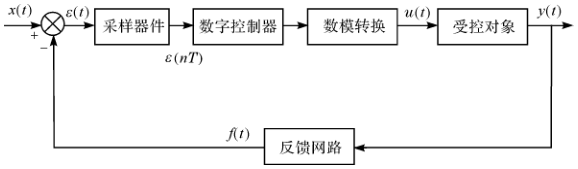
\includegraphics[width=\linewidth]{figs/fig-0168.png}
\caption{图10.0-1}
\end{figure}

\begin{figure}[htbp]\centering
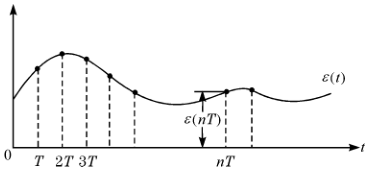
\includegraphics[width=\linewidth]{figs/fig-0169.png}
\caption{图10.0-2}
\end{figure}

\begin{figure}[htbp]\centering
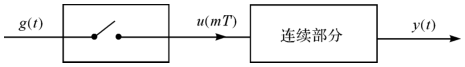
\includegraphics[width=\linewidth]{figs/fig-0170.png}
\end{figure}

\begin{figure}[htbp]\centering
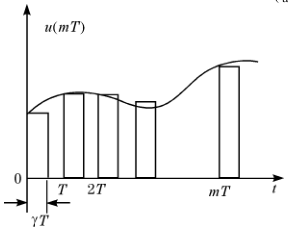
\includegraphics[width=\linewidth]{figs/fig-0171.png}
\end{figure}

\begin{figure}[htbp]\centering
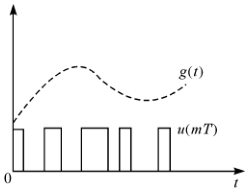
\includegraphics[width=\linewidth]{figs/fig-0172.png}
\end{figure}

\[\begin{aligned}& \text { (d) } \\& \text { 图 } 10.0-3\end{aligned}\]

\section{10.1 离散系统的运动规律——差分方程式}

差分方程最适合于描述采样系统的运动，借助于差分方程可以顺利地研究采样系统的一切特性，诸如稳定性和动态品质的分析，线性系统和最优系统的综合等。因此，研究采样系统的第一步就是正确地建立描绘它的运动规律的差分方程式或差分方程组。本节内我们将详细地讨论这个问题。

以图 10.0-3(a) 为例，设受控对象的连续部分的运动方程是常微分方程式

\[a_{\boldsymbol{v}} \frac{d^{n} y}{d t^{n}}+a_{n-1} \frac{d^{n-1} y}{d t}+\cdots+a \frac{d y}{d t}+a_{y} y=k_{v} u\qquad\text{(10.1-1)}\]

或方程组

\[\frac{d \mathbf{y}}{d t}=A \mathbf{y}+B \mathbf{u}\qquad\text{(10.1-2)}\]

方程式 (10.1-1)内假定控制量仅有一个，而(10.1-2)内则假定有多个相互独立的控制量 $\boldsymbol{u}=\left(w, w, \cdots, u_{r}\right)$。根据第二章内的讨论知道，方程式 (10.1-1) 总可以化为一阶方程组

\[\frac{d \mathbf{y}}{d t}=A \mathbf{y}+\mathbf{b u}, \quad \mathbf{b}=\left(b_{1}, b_{2}, \cdots, b_{n}\right)\qquad\text{(10.1-3)}\]

上式内矩阵 $A$ 和向量 $\mathbf{b}$ 的每一个元素由方程式 (10.1-1) 的诸系数所单一确定，它们可以用比较系数法得到。

设控制量 $u(t)$ 是被第一类采样器件所调制出来的脉冲序列，如图 10.0-3(b)所示。设脉冲宽度为 $\gamma T, T$ 为脉冲重复周期，即采样周期，$0<\gamma \leqslant 1$。我们先讨论高阶方程式 (10.1-1)，即方程组 (10.1-3)，并在 $0 \leqslant t \leqslant T$ 的时间内求解方程 (10.1-3)。令 $\Phi(t)=e^{A t}$ 为方程 (10.1-3) 的齐次方程组的基本解矩阵，$\Phi(0)=E$为单位矩阵。于是在 $t=T$ 这一时刻有

\[\mathbf{y}(T)=e^{A T} \mathbf{y}(0)+\int_{0}^{T} e^{A(T-\tau)} \mathbf{b} u(\tau) d \tau\]

\begin{figure}[htbp]\centering
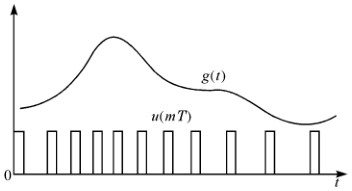
\includegraphics[width=\linewidth]{figs/fig-0173.png}
\caption{图10.0-3}
\end{figure}

\[\begin{aligned}& =e^{A T} \mathbf{y}(0)+\int_{0}^{\gamma T} e^{A(T-\tau)} b u(0) d \tau \\& =e^{A T} \mathbf{y}(0)+\left[\int_{0}^{\gamma T} e^{A(T-\tau)} b d \tau\right] \cdot u(0)\end{aligned}\]

同样，如果以 $\mathbf{y}(T)$ 作为新的初始条件，又可以求出在 $t=2 T$ 时刻的输出 $\mathbf{y}(2 T)$的值

\[\mathbf{y}(2 T)=e^{A T} \mathbf{y}(T)+\left[\int_{0}^{\gamma T} e^{A(T-\tau)} b d \tau\right] u(T)\]

依此类推，若记

\[c=\int_{0}^{\gamma T} e^{A(T-\tau)} b d \tau, \quad D=e^{A T}\]

则对任何 $t=N T$ 有

\[\mathbf{y}\left[(N+1) T\right]=D \mathbf{y}(N T)+c u(N T)\qquad\text{(10.1-4)}\]

这样，我们就得到了采样控制对象的第一种差分方程式。

如果矩阵 $A$ 是可逆的，向量 $\boldsymbol{c}$ 可以由下式算出

\[\begin{aligned}& c=e^{A T} \int_{0}^{\gamma T} e^{-A \tau} b d \tau \\& =e^{A T}\left[\int_{0}^{\gamma T} e^{-A \tau} d \tau\right] b \\& =A^{-1}\left(e^{A T}-e^{(1-\gamma) A T}\right) b\end{aligned}\qquad\text{(10.1-5)}\]

当矩阵 $A$ 为不可逆时，上式依然有效，此时应理解为

\[c=\left[\gamma T E-\frac{1}{2} !\left(\gamma T\right)^{2} A+\frac{1}{3} !\left(\gamma T\right)^{3} A^{2}-\cdots\right] e^{A T} b\qquad\text{(10.1-6)}\]

显然，上式右端的级数对任何矩阵 $A$ 总是收敛的，因而(10.1-5)内的向量 $\boldsymbol{c}$ 总有定义。

差分方程组 $(10.1-4)$ 内的向量 $\mathbf{y}=\left(y_{1}, y_{2}, \cdots, y_{n}\right)$ 中的各分量是方程式 $(10.1-1)$ 内受控量 $y$ 的各阶导数和控制量 $u(t)$ 在 $t=N T$ 时刻的值的线性组合。因此，它们代表受控对象的主要输出 $y_{1}=y$ 和它的各阶导数在各采样点的取值。如果我们只对系统的主要输出 $y(N T)$ 感兴趣的话，差分方程组 $(10.1-4)$ 可以化为仅含有一个主要输出变数 $y_{1}$ 的高阶差分方程式。为此，我们想法消掉式 $(10.1-4)$ 内除 $y_{1}$ 以外的其他变数。例如写出下列 $n^{2}$ 个方程式

\[\begin{aligned}& \mathbf{y}\left[(N+1) T\right]=D \mathbf{y}(N T)+c u(N T) \\& \mathbf{y}\left[(N+2) T\right]=D \mathbf{y}\left[(N+1) T\right]+c u\left[(N+1) T\right] \\& \cdots \\& \mathbf{y}\left[(N+n) T\right]=D \mathbf{y}\left[(N+n-1) T\right]+c u\left[(N+n-1) T\right]\end{aligned}\]

在 $n^{2}$ 个方程式中包括了 $y_{i}(N T), y_{i}\left[(N+1) T\right], \cdots, y_{i}\left[(N+n) T\right], i=1$，$2, \cdots, n$ 等 $(n+1) \cdot n=n^{2}+n$ 个未知量，从中消掉下列 $(n+1)(n-1)=n^{2}-1$

个量:

\[\begin{aligned}& y_{2}(N T), \cdots, y_{2}^{2}[(N+n) T] \\& y_{3}(N T), \cdots, y_{3}^{3}[(N+n) T] \\& \cdots \\& y_{n}(N T), \cdots, y_{n}^{n}[(N+n) T]\end{aligned}\]

最后剩下一个方程式，其中仅含有 $y_{1}\left[(N+n) T\right], \cdots, y_{1}(N T)$ 等 $n+1$ 个量。由于矩阵 $D$ 的特性，这种消除是可能的。这样消掉的结果便得到一个 $n$ 阶差分方程，其内只包括系统的主要受控量 $y_{1}=y$，它的形式是

\[\begin{aligned}& y_{1}\left[(N+n) T\right]+e_{1} y_{1}\left[(N+n-1) T\right]+\cdots+e_{n} y(N T) \\= & f_{1} u\left[(N+n-1) T\right]+f_{2} u\left[(N+n-2) T\right]+\cdots+f_{n} u(N T)\end{aligned}\qquad\text{(10.1-7)}\]

式中诸系数 $e_{1}, \cdots, e_{n} ; f_{1}, \cdots, f_{n}$ 为常量，它们是由矩阵 $D$ 和向量 $\boldsymbol{e}$ 的元素所算一确定的。于是，我们又得到另一种只含主要输出变量的差分方程式。这种方程式常称为 $n$ 阶线性差分方程式。我们可以看到，高阶差分方程式(10.1-7)与差分方程组(10.1-4)是等价的。

在实际工作中常可采用差分方程式的第三种形式。引进符号

\[\begin{aligned}\Delta y(N T) & =y_{1}\left[(N+1) T\right]-y(N T) \\\Delta^{2} y(N T) & =\Delta y_{1}\left[(N+1) T\right]-\Delta y(N T) \\& =y_{1}\left[(N+2) T\right]-2 y_{1}\left[(N+1) T\right]+y(N T) \\\cdots \\\Delta^{n} y(N T) & =\sum_{i=0}^{n}(-1)^{n-i} C_{n}^{i} y_{1}\left[(N+i) T\right]\end{aligned}\qquad\text{(10.1-8)}\]

式中 $C_{n}$ 为 $n$ 对 $i$ 的组合数

\[C_{n}=\frac{n(n-1) \cdots(n-i+1)}{i !}=\frac{n !}{i !(n-i) !}\]

从式(10.1-8)内解出 $y(i T)$ 代入式 (10.1-7)后就得到差分方程式的另一种形式

\[\begin{aligned}& g_{0} \Delta^{n} y(N T)+g_{1} \Delta^{n-1} y(N T)+\cdots+g_{n} y(N T) \\= & h_{1} \Delta^{n-1} u(N T)+h_{2} \Delta^{n-2} u(N T)+\cdots+h_{n} u(N T)\end{aligned}\qquad\text{(10.1-9)}\]

式中 $g_{0}, g_{1}, \cdots, g_{n} ; h_{n}, h_{2}, \cdots, h_{n}$ 均为常量，它们为(10.1-7)内的诸系数 $e$ 和 $f_{j}$ 所单值确定。不难看出差分方程式(10.1-9)与(10.1-7)是相互等价的，两者可以按关系式(10.1-8)互化，因此式(10.1-9)与(10.1-4)也等价。

最后，式(10.1-7)还可以写成另一种形式。引进新变量，$y_{1}(N T)=y(N T)$，并设符号 $H$ 表示移位算子，即 $H y_{1}(N T)=y_{1}\left[(N+1) T\right]$，那么，方程式(10.1-7)可以化为新的方程组

\[\begin{aligned}& H y_{1}(N T)=y_{2}(N T)+b_{1} u(N T) \\& H y_{2}(N T)=y_{3}(N T)+b_{2} u(N T) \\& \cdots \\& H y_{n}(N T)=-a_{n} y_{1}(N T)-a_{n-1} y_{2}(N T)-\cdots-a_{1} y_{n}(N T)+b_{n} u(N T)\end{aligned}\qquad\text{(10.1-10)}\]

式中各系数为方程式(10.1-7)的各系数所单一确定。

若令

\[\begin{aligned}& \mathbf{y}=\left(y_{1}, \cdots, y_{n}\right) \\& \boldsymbol{c}=\left(b_{1}, \cdots, b_{n}\right) \\& A=\left(\begin{array}{cccccc}0 & 1 & 0 & 0 & \cdots & 0 \\0 & 0 & 1 & 0 & \cdots & 0 \\& \vdots & \vdots & \vdots & & \vdots \\-a_{n} & -a_{n-1} & -a_{n-2} & -a_{n-3} & \cdots & -a_{1}\end{array}\right)\end{aligned}\]

则上式又可以写成向量形式

\[H \mathbf{y}(N T)=A \mathbf{y}(N T)+\boldsymbol{c} \boldsymbol{u}(N T)\qquad\text{(10.1-11)}\]

这就得到了描绘采样系统的第四种差分方程式。方程式(10.1-11)虽然形式上与式(10.1-4)相同，但是实际上完全是两回事。因为式(10.1-11) $\mathbf{y}$ 的各分量是主输出量 $y$ 和控制量 $u$ 在各个不同采样时刻的值，而方程式，(10.1-4)的各分量是由主输出量 $y$ 和控制量 $u$ 的各阶导数所构成。所以方程式(10.1-4)和(10.1-11)是截然不同的两类方程式。但是，从描述采样系统的运动规律这一意义来看，他们是等价的，是可以互化的。

这样，我们讨论了描述采样系统的四种差分方程，它们是式(10.1-4)，(10.1-7)，(10.1-9)和(10.1-11)。在实际工作中究竟采用何种形式，要由具体情况而定。从原理上来看，它们都可以作为对采样系统分析或综合的基础。

现举例以说明这四种方程式的求法。设连续受控对象的方程式是

\[\frac{d^{2} y}{d t^{2}}+\alpha \frac{d^{2} y}{d t^{2}}+\alpha \frac{d y}{d t}+\alpha y=k \frac{d^{2} u}{d t^{2}}+k^{2} \frac{d u}{d t}+k_{3} u\qquad\text{(10.1-12)}\]

令 $y=y_{1}$，于是式(10.1-12)可写为方程组

\[\begin{aligned}& \frac{d y_{1}}{d t}=y_{2}+b_{1} u \\& \frac{d y_{2}}{d t}=y_{3}+b_{2} u \\& \frac{d y_{3}}{d t}=-a_{3} y_{1}-a_{2} y_{2}-a_{1} y_{3}+b_{3} u\end{aligned}\]

式中 $b=k, b=k_{2}-a_{1} k_{1}, b=k_{3}+a_{2}^{2} k_{1}-a_{2} k_{1}-a_{1} k_{2}$

令

\[\begin{aligned}& \boldsymbol{b}=\left(b_{1}, b_{2}, b_{3}\right) \\& \boldsymbol{y}=\left(y_{1}, y_{2}, y_{3}\right) \\& A=\left(\begin{array}{ccc}0 & 1 & 0 \\0 & 0 & 1 \\-\alpha_{3} & -\alpha_{2} & -\alpha_{1}\end{array}\right)\end{aligned}\]

则上式可以写成向量等式

\[\frac{d \boldsymbol{y}}{d t}=\boldsymbol{A} \boldsymbol{y}+\boldsymbol{b} u\]

设 $u(t)$ 为第一类采样元件 （图 10.0-3b) 所调制，则第一种差分方程是

\[\mathbf{y}[(N+1) T]=\boldsymbol{D} \mathbf{y}(N T)+\boldsymbol{c} u(N T)\]

式中

\[D=e^{A T}, \quad \boldsymbol{c}=A^{-1}\left(e^{A T}-e^{A T(1-u t)}\right) \boldsymbol{b}\]

第二种差分方程是

\[\begin{aligned}& y[(N+3) T]+e_{1} y[(N+2) T]+e_{2} y[(N+1) T]+e_{3} y(N T) \\= & f_{1} u[(N+2) T]+f_{2} u[(N+1) T]+f_{3} u(N T)\end{aligned}\qquad\text{(10.1-16)}\]

第三种差分方程是

\[\begin{aligned}& g_{0} \Delta_{1}^{3} y(N T)+g_{1} \Delta_{2}^{2} y(N T)+g_{2} \Delta_{3} y(N T)+g_{3} y(N T) \\= & h \Delta_{1}^{2} u(N T)+h \Delta_{2} u(N T)+h_{3} u(N T)\end{aligned}\qquad\text{(10.1-15)}\]

式中

\[\begin{aligned}& g_{0}=1, \quad g_{1}=3+e_{1}, \quad g_{2}=3+2 e_{1}+e_{2}, \quad g_{3}=1+e_{1}+e_{2}+e_{3} \\& h_{1}=f_{1}, \quad h_{2}=2 f_{1}+f_{2}, \quad h_{3}=f_{1}+f_{2}+f_{3}\end{aligned}\]

再令 $y_{1}(N T)=y(N T)$，式 (10.1-14) 又可写成

\[\begin{aligned}& H y_{1}(N T)=y_{2}(N T)+c_{1} u(N T) \\& H y_{2}(N T)=y_{3}(N T)+c_{2} u(N T) \\& H y_{3}(N T)==d_{3} y_{1}(N T)-d_{2} y_{2}(N T)-d_{1} y_{3}(N T)+c_{3} u(N T)\end{aligned}\qquad\text{(10.1-13)}\]

式中

\[\begin{aligned}& c_{1}=f_{1}, \quad c_{2}=f_{2}-e_{1} f_{1}, \quad c_{3}=f_{3}+e_{1}^{2} f_{1}-e_{1} f_{1}-e_{1} f_{2} \\& d_{1}=e_{1}, \quad d_{2}=e_{2}, \quad d_{3}=e_{3}\end{aligned}\]

这就得到了第四种差分方程组

\[H \mathbf{y}(N T)=A \mathbf{y}(N T)+\boldsymbol{c} u(N T)\]

式中

\[A=\left(\begin{array}{ccc}0 & 1 & 0 \\0 & 0 & 1 \\-d_{3} & -d_{2} & -d_{1}\end{array}\right), \quad \boldsymbol{c}=\left(c_{1}, c_{2}, c_{3}\right)\]

对于有多个控制量的系统，差分方程式(10.1-2)的建立方法是完全类似的。相应的向量方程式的形式是

\[\mathbf{y}\left[\begin{array}{c}N+1 \\T\end{array}\right]=D \mathbf{y}(N T)+C \mathbf{u}(N T)\qquad\text{(10.1-17)}\]

式中

\[D=e^{A T}, \quad C=\left(e^{A T}-e^{A T(1-\gamma)}\right) A^{-1} B\]

这里与式(10.1-4)所不同的是 $C$ 是 $n \times r$ 阶矩阵，$\boldsymbol{u}$ 是 $r$ 维向量，而式(10.1-4)内的 $\boldsymbol{c}$ 是一个 $n$ 维向量，$u$ 是一维控制量。用前面叙述过的方法可以类似地得到具有多个控制量的第二种至第四种差分方程式，只不过后者的具体形式略有变化罢了。上述的第一、第二和第四种差分方程式以后都将在不同的场合分别采用。

用差分方程式描绘采样系统时，我们只能得到输出变量在各采样时刻的取值变化规律。至于在两个采样时刻的中间输出量的变化情况从上列任何一种差分方程式的解中都得不到任何解答。但是采样系统的输出量恰恰是连续变化的，这与输入量或控制量的脉冲序列完全不同，后者本身是不连续的信号，而前者本来是连续变化的，只是为了信息处理的方便，我们才人为地取其在采样点的值加以研究。为了更全面地了解输出量的变化情况，可以将前述各差分方程改写，使其所描绘的输出量（受控量）的值不在采样点上，而在采样点的中间，或者说，使差分方程的解，表示受控量 $\mathbf{y}$ 在 $t=\varepsilon T, T+\varepsilon T, 2 T+\varepsilon T, \cdots, N T+\varepsilon T, \cdots$ 等时刻的值。

设 $0 \leqslant \varepsilon \leqslant \gamma$，那么根据式(10.1-2)有

\[\begin{aligned} & \mathbf{y}(\varepsilon T)=e^{A \varepsilon T} \mathbf{y}(0)+e^{A \varepsilon T} \int_{0}^{\varepsilon T} e^{-A \tau} B \boldsymbol{u}(0) d \tau \\ & \mathbf{y}(T+\varepsilon T)=e^{A T} \mathbf{y}(\varepsilon T)+e^{A T} \int_{0}^{(\gamma-\varepsilon) T} e^{-A \tau} B \boldsymbol{u}(0) d \tau+e^{A \varepsilon T} \int_{0}^{\varepsilon T} e^{-A \tau} B \boldsymbol{u}(T) d \tau \end{aligned}\]

依此类推，可以得到

\[\mathbf{y}\left[(N+1+\varepsilon) T\right]=D \mathbf{y}\left[(N+\varepsilon) T\right]+B_{1}(\varepsilon) \boldsymbol{u}(N T)+B_{2}(\varepsilon) \boldsymbol{u}\left[(N+1) T\right]\qquad\text{(10.1-18)}\]

式中

\[D=e^{A T}, \quad B_{1}(\varepsilon)=e^{A T} \int_{0}^{(\gamma-\varepsilon) T} e^{-A \tau} B d \tau, \quad B_{2}(\varepsilon)=e^{A \varepsilon T} \int_{0}^{\varepsilon T} e^{-A \tau} B d \tau\]

当 $\gamma<\varepsilon \leqslant 1$ 时，则有

\[\mathbf{y}\left[(N+1+\varepsilon) T\right]=D \mathbf{y}\left[(N+\varepsilon) T\right]+B_{3}(\varepsilon) \boldsymbol{u}\left[(N+1) T\right]\qquad\text{(10.1-19)}\]

式中

\[B_{3}(\varepsilon)=e^{A \varepsilon T} \int_{0}^{\varepsilon T} e^{-A \tau} B d \tau\]

从式(10.1-18)和(10.1-19)内可以看出；当输出量的采样时刻与输入量的采样时刻不同时，差分方程式的形成也不相同。与(10.1-17)比较这种差别就一目了然了。根据式(10.1-18)和(10.1-19)又可以推出第二种至第四种差分方程式，如式(10.1-7)，(10.1-9)和(10.1-11)那样。

讨论上面的采样系统时，我们假定脉冲调制后的每一个脉冲是方形的，其高度仅与输入量 $g(t)$ 在采样时刻的值有关（图 10.0-3b)。有时为了更好地逼近输入信号，脉冲元件的调制规律可采用一次线性外插，输出端的脉冲序列中的每一脉冲均为“斜顶”，它的形状如图 10.1-1 所示。脉冲顶部的斜率与相邻两个采样时刻的输入信号 $g(N T)$ 和 $g[(N-1) T]$ 的连线斜率相同，此时第一种差分方程式将具有下列形式

\[\mathbf{y}\left[(N+1) T\right]=D \mathbf{y}(N T)+B_{1} \mathbf{u}(N T)+B_{2} \mathbf{u}\left[(N-1) T\right]\qquad\text{(10.1-20)}\]

式中

\[\begin{aligned} & D=e^{A T}, \quad B_{1}=e^{A T} \int_{0}^{\gamma T} e^{-A \tau} B\left[1+\frac{\tau}{T}\right] d \tau \\ & B_{2}=-e^{A T} \int_{0}^{\gamma T} e^{-A \tau} B \cdot \frac{\tau}{T} d \tau \end{aligned}\]

以式(10.1-20)做基础可以推出其他几种差分方程式。由此我们看到，图 10.1-1 所示的调制方式是线性的。

本节内讨论过的方法同样适用于变系数系统。如果受控对象是由变系数常微分方程所描绘，那么相应的差分方程式也是具有变系数的线性方程。例如式(10.1-17)此时变为

\[\mathbf{y}\left[(N+1) T\right]=D(N T) \mathbf{y}(N T)+C(N T) \mathbf{u}(N T)\qquad\text{(10.1-21)}\]

式中矩阵 $D(N T)$ 和 $C(N T)$ 的每一元素是时间的函数。这两个矩阵的求算公式与式(10.1-17)内的矩阵求法相同，只需将 $e^{A T}$ 换为变系数系统的基本解矩阵 $\Phi(t$，$t+T)$ 即可，此处 $t=0, T, 2 T, \cdots, N T, \cdots$。

0

$T$

\[\gamma T\]

$m T$

\[g(t)\]

图 10.1-1

前面讨论中的输出向量 $\mathbf{y}$ 是离散系统的状态向量。为了设计控制规律 $\mathbf{u}(t)$当然要不间断地对系统的状态进行测量。然而并不是状态向量的每一个坐标在

\begin{figure}[htbp]\centering
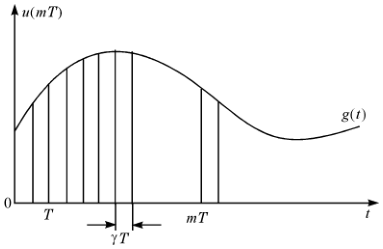
\includegraphics[width=\linewidth]{figs/fig-0174.png}
\caption{图10.1-1}
\end{figure}

实际上都可以直接用传感器或测量装置测出。这和连续系统中的情况完全类似，能够测到的关于系统状态的信息往往必须通过某种函数关系表达出来。最典型的例子是用雷达测量运动物体的坐标，雷达测得的数据要经换算后才能求出运动物体的坐标，这在本书的前几章已经提到过。一般来讲，假定测量装置可以直接测到 $m$ 个参数: $z_{1}, z_{2}, \cdots, z_{m}$，用向量 $\boldsymbol{z}$ 表示，称为离散系统的观测向量。观测向量 $\boldsymbol{z}$ 和状态向量 $\mathbf{y}$ 之间的函数关系可表示成

\[\boldsymbol{z}(N T)=\boldsymbol{f}(\mathbf{y}(N T), N T)\qquad\text{(10.1-22)}\]

式中 $\boldsymbol{f}$ 为 $m$ 维的非线性向量函数。由于通常能够观测到的参数 $z_{1}, \cdots, z_{m}$ 的个数小于状态向量的维数，也就是说，在每一瞬间不能由关系式 (10.1-22) 反解出 $\mathbf{y}(N T)$ 来。即使向量函数 $\boldsymbol{f}$ 的 $m$ 个分量都是相互独立的，这在实际问题中是最常见的情况。在简单的情况下，观测方程 (10.1-22)右端是状态变量的线性函数，此时用 $F(N T)=\left(f_{i j}(N T)\right)$ 表示 $m \times n$ 阶方矩阵，它的每一元素 $f_{i j}(n T)$ 是时间 $t$ 的函数。于是观测方程变为

\[z(N T)=F(N T) \mathbf{y}(N T)\qquad\text{(10.1-23)}\]

另一方面，当函数关系式 (10.1-22) 中的 $\boldsymbol{f}$ 是各自变量的足够光滑的函数，而且 $F(0, N T)=0$，那么在小范围内可以将函数 $\boldsymbol{f}$ 按泰勒级数展开，只保留展式中的线性项，忽略高次项，线性表达式 (10.1-23) 将在一定程度上逼近式 (10.1-22)。因此，线性观测方程对研究非线性观测问题也是有意义的。由这种方程描述的测量装置也有人称之为观测器。

归纳上述，一个离散线性系统的完整的方程式将由受控对象的运动方程式和观测方程式两者所组成

\[\begin{aligned} & \mathbf{y}((N+1) T)=D(N T) \mathbf{y}(N T)+C(N T) \boldsymbol{u}(N T) \\ & z(N T)=F(N T) \mathbf{y}(N T) \end{aligned}\qquad\text{(10.1-24)}\]

我们称方程 (10.1-24) 为离散系统的完全描述模型。

\section{10.2 差分方程式解的特性}

前节内我们讨论了各种差分方程式的建立方法和运算步骤。本节内我们将讨论各种差分方程的特解和通解的特性。对这些特性的讨论将有助于对离散系统运动规律的细致了解，同时对离散系统的分析和综合将提供足够的理论基础。四种差分方程式中，我们将重点讨论第一种式 (10.1-4)、第二种式 (10.1-7) 和第四种式 (10.1-11)，因为这几种在实际工作中使用最广泛，应用也较方便。其中第一种和第四种，即式 (10.1-4) 和式 (10.1-11)，虽然物理意义不同，但数学结构却完全相同，它们的通解和特解的性质也完全一致。所以我们先讨论第一种，然后再讨论第二种。

第一种差分方程是

\[H \mathbf{y}(N T)=D \mathbf{y}(N T)+C u(N T)\qquad\text{(10.2-1)}\]

式中符号 $H$ 表示移位算子，其作用规律是 $H \mathbf{y}(N T)=\mathbf{y}\left[\begin{array}{c}(N+1) T \\D\end{array}\right], D$ 和 $C$ 为常量矩阵。如果 $D$ 和 $C$ 是时间 $N T$ 的函数则系统变成变系数系统，但下面得到的很多结论略作修改后将完全适用于这种变系数离散系统。式 $(10.2-1)$ 内 $u(N T)$ 为控制向量，它的每一个分量 $u_{i}(N T)$ 是相互独立的控制量，如果控制量只有一个，则 $u(N T)$ 只包含一个分量，而矩阵 $C$ 则变为一个向量 $c$。

当式 $(10.2-1)$ 之右端 $u(N T) \equiv \mathbf{0}$ 时，方程式

\[H \mathbf{y}(N T)=D \mathbf{y}(N T)\qquad\text{(10.2-2)}\]

称为式 $(10.2-1)$ 的齐次方程式。

齐次线性差分方程式的解与齐次线性常微分方程式的解有很多共同的特点。如果式 $(10.2-2)$ 是由 $n$ 个方程式组成，则必有 $n$ 个线性不相关的特解，而且只有 $n$个这种解，任何其他解均可用这 $n$ 个“基本解”的线性组合表示出来。设这 $n$ 个线性不相关的解已经找到，它们是

\[\begin{aligned} & \mathbf{y}_{1}(N T)=\left(\gamma_{11}(N T), \gamma_{21}(N T), \cdots, \gamma_{n 1}(N T)\right) \\ & \mathbf{y}_{2}(N T)=\left(\gamma_{12}(N T), \gamma_{22}(N T), \cdots, \gamma_{n 2}(N T)\right) \\ & \cdots \\ & \mathbf{y}_{n}(N T)=\left(\gamma_{1 n}(N T), \gamma_{2 n}(N T), \cdots, \gamma_{n n}(N T)\right) \end{aligned}\]

由于对任何 $t \equiv N T, N=0,1,2, \cdots$，上述 $n$ 个解线性不相关，那么，由它们所构成的行列式对任何 $N T$ 总不为零。于是，对式 $(10.2-2)$ 的任何特解 $\mathbf{y}(N T)$ 存在一组常数 $c_{1}, c_{2}, \cdots, c_{n}$，使

\[\mathbf{y}(N T)=c_{1} \mathbf{y}_{1}(N T)+c_{2} \mathbf{y}_{2}(N T)+\cdots+c_{n} \mathbf{y}_{n}(N T)\]

而这 $n$ 个基本解是什么呢？从原则上看任何 $n$ 个线性不相关的解均可成为基本解。现在我们只选择一种，作为以后讨论的基础。

由于式 $(10.2-2)$ 内的 $D=e^{A T}, A$ 是描述连续受控对象的常微分方程中的矩阵，故矩阵 $D$ 的行列式永不为零。现在证明，式 $(10.2-2)$ 的 $n$ 个基本解是矩阵 $D^{N}=e^{N A T}$ 的几个列向量。显然，矩阵 $D^{N}$ 满足方程式 $(10.2-2)$，因为

\[H D^{N}=D D^{N}=D^{N+1}\]

于是

\[\begin{aligned} & \mathbf{y}_{1}(N T)=\left(D^{N}\right)_{1}=\left(e^{N A T}\right)_{1} \\ & \cdots \\ & \mathbf{y}_{n}(N T)=\left(D^{N}\right)_{n}=\left(e^{N A T}\right)_{n} \end{aligned}\qquad\text{(10.2-3)}\]

上式右端的右下角注 $i, i=1,2, \cdots, n$ 表示矩阵的第 $i$ 列向量。或者用 $Y(N T)$ 表示式 $(10.2-2)$ 的基本解矩阵，有

\[Y(N T)=D^{N}=e^{N A T}=\left(\mathbf{y}_{1}(N T), \cdots, \mathbf{y}_{n}(N T)\right)\]

.\{array\}\{ccc\}y\_\{11\}(N T) \& \& y\_\{1 n\}(N T) y\_\{21\}(N T) \& \& y\_\{2 n\}(N T) \& \& y\_\{n 1\}(N T) \& \& y\_\{m n\}(N T)\{array\}\textbackslash\{\}\} 上式左边的矩阵的第一列是等。由于

设受控对象的 $n$ 个初始条件是 $c=\left(c_{1}, \cdots, c_{n}\right)$，即 $y_{1}(0)=c_{1}, y_{2}(0)=c_{2}, \cdots$，$y_{n}(0)=c_{n}$，或者 $\mathbf{y}(0)=c$。那么，满足这一组初始条件的式 (10.2-2) 的特解将是

\[\mathbf{y}(N T)=e^{N A T} \boldsymbol{c}=D^{N} \boldsymbol{c}=D^{N} \mathbf{y}(0)\qquad\text{(10.2-4)}\]

事实上

\[H \mathbf{y}(N T)=D D^{N} \boldsymbol{c}=D^{N+1} \boldsymbol{c}=\mathbf{y}\left[(N+1) T\right]\]

而且，$\mathbf{y}(0)=D^{0} \boldsymbol{c}=\boldsymbol{c}$。因为按矩阵函数的定义，任何矩阵的零次幂为单位矩阵。由于上述初始条件 $\boldsymbol{c}$ 是任意的，故式 (10.2-4) 称为齐次差分方程式 (10.2-2) 的通解。

现在求非齐次方程式 (10.2-1) 的通解，我们用待定系数法求解。设式 (10.2-1) 的通解为下列形式

\[\mathbf{y}(N T)=Y(N T) \boldsymbol{c}(N T)=D^{N} \boldsymbol{c}(N T)\qquad\text{(10.2-1)}\]

式中 $\boldsymbol{c}(N T)=\left(c_{1}(N T), c_{2}(N T), \cdots, c_{n}(N T)\right)$。令式 (10.2-1) 的初始条件为常向量 $\mathbf{y}_{0}$，现求出满足这个初始条件的解式 (10.2-5)。将式 (10.2-5) 代入式 (10.2-1) 后有

\[\begin{aligned}H \mathbf{y}(N T) & =\mathbf{y}\left[(N+1) T\right] \\& =Y\left[(N+1) T\right] \boldsymbol{c}\left[(N+1) T\right] \\& =D Y(N T) \boldsymbol{c}(N T)+C u(N T) \\& =Y\left[(N+1) T\right] \boldsymbol{c}(N T)+C u(N T)\end{aligned}\]

移项后有

\[c\left[(N+1) T\right]-c(N T)=Y^{-1}\left[(N+1) T\right] C u(N T)\]

对上式两端求和得

\[c(m T)-c(0)=\sum_{N=0}^{m-1} Y^{-1}\left[(N+1) T\right] C u(N T)\]

将 $\boldsymbol{c}(m T)$ 代入式 (10.2-5)，并考虑 $\mathbf{y}(0)=\mathbf{y}_{0}$，最后得到

\[\mathbf{y}(m T)=D^{m} \mathbf{y}_{0}+D^{m} \sum_{N=0}^{m-1} Y^{-1}\left[(N+1) T\right] C u(N T)\]

\[\mathbf{y}(N T)=D^{N} \mathbf{y}_{0}+\sum_{m=0}^{N-1} D^{N-(m+1)} C u(m T)\qquad\text{(10.2-6)}\]

不难检查，式 (10.2-6) 满足方程式 (10.2-1)，并且同时满足初始条件 $\mathbf{y}(0)=\mathbf{y}_{0}$。推导时我们曾假定 $u(m T)$ 当 $m<0$ 恒为零向量，因为控制作用是在 $t=0$ 时开始作用的。这样，由于 $\mathbf{y}_{0}$ 是任意的，式 (10.2-1) 的解式 (10.2-6) 我们将称为非齐次方程的通解。

其次，令向量函数 $\boldsymbol{\Psi}(N T)$ 是下列方程式

\[H^{*} \boldsymbol{\Psi}(N T)=\boldsymbol{\Psi}\left[(N-1) T\right]=D^{\varepsilon} \boldsymbol{\Psi}(N T)\qquad\text{(10.2-7)}\]

的基本解，$H^{*}$ 是逆移位算子，则

\[\boldsymbol{\Psi}(N T)=e^{-A^{T} N T} \boldsymbol{\Psi}_{0}=\left(D^{*}\right)^{-N} \boldsymbol{\Psi}_{0}\qquad\text{(10.2-8)}\]

是式 (10.2-7) 的解，其中 $\boldsymbol{\Psi}$ 为任意非零常向量，是式 (10.2-7) 的初始条件，因为

\[H^{*} \boldsymbol{\Psi}(N T)=H^{*}\left(D^{*}\right)^{-N} \boldsymbol{\Psi}_{0}=D^{\varepsilon}\left(D^{*}\right)^{-N} \boldsymbol{\Psi}_{0}=\left(D^{*}\right)^{-(N-1)} \boldsymbol{\Psi}_{0}=\boldsymbol{\Psi}\left[(N-1) T\right]\]

不难看出，式 (10.2-7) 的任何非零解 $\boldsymbol{\Psi}(N T)$ 与齐次方程式 (10.2-2) 的任何非零解 $\mathbf{y}(N T)$ 的内积为常数，而与 $N$ 无关，因为

\[\begin{aligned} & (\mathbf{y}\left[(N+1) T\right], \boldsymbol{\Psi}\left[(N+1) T\right])-(\mathbf{y}(N T), \boldsymbol{\Psi}(N T)) \\ & \quad=\left(D^{N+1} \boldsymbol{c},\left(D^{*}\right)^{-(N+1)} \boldsymbol{\Psi}_{0}\right)-\left(D^{N} \boldsymbol{c},\left(D^{*}\right)^{-N} \boldsymbol{\Psi}_{0}\right) \\ & \quad=\left(\boldsymbol{c}, \boldsymbol{\Psi}_{0}\right)-\left(\boldsymbol{c}, \boldsymbol{\Psi}_{0}\right)=0 \end{aligned}\]

故与齐次常微分方程相似，满足关系式

\[(\boldsymbol{\Psi}(N T), \mathbf{y}(N T))=\text { const }\]

的 $\boldsymbol{\Psi}(N T)$ 的方程组 (10.2-7) 称为式 (10.2-2) 的共轭方程组，有时也称其为伴随方程组。而 $\boldsymbol{\Psi}(N T)$ 则称为式 (10.2-2) 的共轭解。

设离散受控系统式 (10.2-1) 的初始条件为 $\mathbf{y}_{0}$，在其输入端作用的 $u(N T)$ 不是控制量，而是扰动作用。那么，容易证明，由于扰动所引起的输出 $\mathbf{y}(N T)$ 可以通过共轭方程式的解表示出来。首先写出下列恒等式

\[\begin{aligned} & (\mathbf{y}\left[(m+1) T\right], \boldsymbol{\Psi}\left[(m+1) T\right])-(\mathbf{y}(m T), \boldsymbol{\Psi}(m T)) \\ & \quad=\left(D \mathbf{y}(m T)+C u(m T),\left(D^{*}\right)^{-1} \boldsymbol{\Psi}(m T)\right)-(\mathbf{y}(m T), \boldsymbol{\Psi}(m T)) \\ & \quad=\left(C u(m T),\left(D^{*}\right)^{-1} \boldsymbol{\Psi}(m T)\right) \end{aligned}\]

令 $N_{1}$ 为一固定正整数，将上式两端对 $m$ 求和后有

\[\begin{aligned} & \left(\mathbf{y}\left(N_{1} T\right), \boldsymbol{\Psi}\left(N_{1}, T\right)\right)-(\mathbf{y}(0), \boldsymbol{\Psi}(0)) \\ & \quad=\sum_{m=0}^{N_{1}-1}\left(C u(m T),\left(D^{*}\right)^{-1} \boldsymbol{\Psi}(m T)\right) \end{aligned}\qquad\text{(10.2-9)}\]

设受控对象的初始条件为零，即 $\mathbf{y}_{0}=\mathbf{0}$，再令 $\boldsymbol{\Psi}\left(N_{1}, T\right)=\left(1,0,0, \cdots, 0\right)$，向量 $\mathbf{y}\left(N_{1} T\right)$的第一个坐标 $y_{1}$ 在 $N_{1} T$ 时刻由扰动所积累的值将为

\[\gamma_{1}(N, T)=\sum_{m=0}^{\Lambda_{1}-1}\left(C u(m T),\left(D^{*}\right)^{-1} \boldsymbol{\Psi}(m T)\right)\qquad\text{(10.2-10)}\]

等式(10.2-9)称为格林公式，而式 (10.2-10) 是它的一个特殊形式。利用式(10.2-10)常可简单地求出系统受干扰后在指定时间间隔内所积累的输出误差。

至于第二种差分方程(10.1-7)，因为它可以化成第四种方程，所以上面讨论中所得到的一些结论对它也完全有效。这里只简单地列举有关方程式(10.1-7)的一些特性，而不再重复前面的证明。方程(10.1-7)内若 $u(N T) \equiv 0$，则

\[y_{1}\left[(N+n) T\right]+e_{1} y_{1}\left[(N+n-1) T\right]+\cdots+e_{n} y_{1}(N T)=0 \quad(10.2-11)\]

称为它的齐次差分方程式。$n$ 阶方程式 (10.2-11) 必有 $n$ 个线性不相关的解 $\gamma_{1}(N T), y_{2}(N T), \cdots, y_{n}(N T)$，其中每一个均满足方程式 (10.2-11)。根据方程 (10.1-10) 和 (10.1-11) 的特点可知，这 $n$ 个线性不相关的解可以是矩阵

\[D^{N}=\left(\begin{array}{cccccc} 0 & 1 & 0 & \cdots & 0 \\ 0 & 0 & 1 & \cdots & 0 \\ \vdots & \vdots & \vdots & \vdots & \vdots \\ e_{n} & e_{n-1} & e_{n-2} & \cdots & e_{1} \end{array}\right)^{N}\]

内第一列的 $n$ 个元素。齐次方程式 (10.2-11) 的通解可写成下列形式

\[y(N T)=c_{1} y_{1}(N T)+c_{2} y_{2}(N T)+\cdots+c_{n} y_{n}(N T)\]

式中诸系数 $c_{i}$ 由 $n$ 个初始条件 $y(0), y(T), \cdots, y_{1}[(n-1) T]$ 所单一决定。为了求出 $n$ 个线性不相关的解，还可用另外的办法求出，令式 (10.2-11) 的解具有下列形式: $y(N T)=\lambda^{N}$，代入原式并化简后得到一个 $n$ 阶代数方程

\[\lambda^{n}+e_{1} \lambda^{n-1}+e_{2} \lambda^{n-2}+\cdots+e_{n-1} \lambda+e_{n}=0\qquad\text{(10.2-12)}\]

它是式 (10.2-11) 的特征方程。由于上式是 $n$ 阶的，故有 $n$ 个根 $\lambda_{1}, \lambda_{2}, \cdots, \lambda_{n}$。如果它们之间没有重根，则 $n$ 个线性不相关的解便是

\[y_{1}(N T)=\lambda_{1}^{N}, y_{2}(N T)=\lambda_{2}^{N}, \cdots, y_{n}(N T)=\lambda_{n}^{N}\]

容易看出，它们是线性不相关的。

如果特征方程式的根中有复根，则一定成双共轭出现，例如 $\lambda=\rho(\cos \omega+$ $i \sin \omega), \lambda=\rho(\cos \omega-i \sin \omega)$。那么，适当的选取 $c_{1}$ 和 $c_{2}$，可以使前两个基本解变为

\[y_{1}(N T)=\rho^{N} \cos \omega N, \quad y_{2}(N T)=\rho^{N} \sin \omega N, \quad N=0,1,2, \cdots\]

与常微分方程类似，当 $\lambda$ 是重根时，例如 $s$ 次重根，它所对应的 $s$ 个线性不相关的解是

\[y_{1}(N T)=\lambda^{N}, y_{2}(N T)=N \lambda^{N}, \cdots, y_{s}(N T)=N^{\prime-1} \lambda^{N}\]

至于非齐次方程式的通解，仍可以利用式 (10.2-6) 的第一个分量等式写出。

前面的讨论中经常利用矩阵 $D^{N}$ 作为齐次方程组的基本解矩阵，如何求出 $D^{N}$呢？最简单的方法是把它写为连乘式 $D^{N}=D D \cdots D$ 逐步相乘 $N$ 次算出。但是，这样求不出 $D^{N}$ 的解析表达式。为了求出各基本解的解析表达式，可以用矩阵函数的方法进行。从代数学中我们知道，对任一矩阵 $D$，总可以找到一个非蜕化矩阵 $Q$，使

\[J=Q^{-1} D Q\]

变为约当标准形。于是

\[J^{t}=\left(\begin{array}{c} J_{1}^{t} \\ J_{2}^{t} \\ \cdots \\ J_{k}^{t} \end{array}\right), \quad t=0, T, 2 T, \cdots, N T\]

其中 $J$ 是标准形内的标准块 （约当块）。将每一个约当块展开后具有下列形式:

\[J_{i}^{t}=\left(\begin{array}{cccc} \lambda_{1}^{t} & \frac{t}{T} \lambda_{1}^{t-1} & \frac{1}{2 !} \frac{t}{T}\left(\frac{t}{T}-1\right) \lambda_{1}^{t-2} & \cdots \\ 0 & \lambda_{1}^{t} & \frac{t}{T} \lambda_{1}^{t-1} & \cdots \\ \vdots & \vdots & \ddots & \vdots \\ 0 & 0 & \cdots & \lambda_{n}^{t} \end{array}\right)\]

矩阵 $J$ 的阶数决定于约当块的阶数，$\lambda$ 是矩阵 $D$ 的特征根，若 $D$ 的 $n$ 个特征根内无重根，则

\[J^{t}=\left(\begin{array}{cccc} \lambda_{1}^{t} & 0 & 0 & \cdots & 0 \\ 0 & \lambda_{2}^{t} & 0 & \cdots & 0 \\ \vdots & \vdots & \vdots & \vdots & \vdots \\ 0 & 0 & 0 & \cdots & \lambda_{n}^{t} \end{array}\right)\]

由此便得到 $D^{t}$ 的解析表达式为

\[D^{N}=Q J^{N} Q^{-1}\]

至于如何将矩阵 $D$ 化为标准型，即如何求出变换矩阵 $Q$，在代数学中有详细讨论，这里不再赘述。

下面我们把线性离散系统的通解式 (10.2-6) 推广到变系数线性系统，并且把通解的形式写得更简单些。首先记 $\mathbf{y}(k T)=\mathbf{y}(k)$，即省掉采样周期 $T$，仅用 $k$ 表示 $k T$，用 $l$ 表示 $l T$ 等。设差分方程组 (10.2-1) 中的矩阵 $D$ 和 $C$ 不是常量矩阵，而是 $t$ 的某一函数，那么方程式 (10.2-1) 就变为

\[\mathbf{y}(k+1)=D(k) \mathbf{y}(k)+C(k) \mathbf{u}(k)\qquad\text{(10.2-13)}\]

定义双变量函数 $\Phi(k, l)$

\[\Phi(k, l)=\prod_{i=l}^{k-1} D(i), \quad \Phi(k, k)=E\qquad\text{(10.2-14)}\]

式中 $E$ 为单位方阵。直接把上式代入式 $(10.2-13)$ 的齐次方程中，极易检验，下列恒等式

\[\Phi(k+1, l)=D(k) \Phi(k, l)\qquad\text{(10.2-15)}\]

对一切正整数 $k$ 和 $l, k \geqslant l$，都成立。而且 $\Phi(k, l)$ 还有下列特性

\[\Phi^{-1}(k, l)=\Phi(l, k)\qquad\text{(10.2-16)}\]

\[\Phi(k, m) \Phi(m, l)=\Phi(k, l)\]

上式对一切正整数 $k, l, m$ 都成立。利用函数矩阵 $\Phi(k, l)$，应用前面用过的待定系数法，线性变系数离散系统式 $(10.2-13)$ 的通解可写成更为方便简捷的形式

\[\mathbf{y}(k)=\Phi(k, l) \mathbf{y}(l)+\sum_{i=1}^{k-1} \Phi(k, i+1) C(i) u(i)\qquad\text{(10.2-17)}\]

不难检查，当 $l=0$ 和 $D, C$ 是常矩阵时，此式与式 $(10.2-6)$ 完全重合。但是，式 $(10.2-17)$ 确定线性离散系统任何两个时刻 $t=k T$ 和 $t^{\prime}=l T$ 的状态之间的关系，所以这种写法往往更为方便。

本节讨论的内容是进一步研究系统分析和综合的基础。这里需要进行较复杂的计算工作是求出矩阵 $D$ 和 $C$，因为要从常微分方程转变为差分方程的形式，需要找出常微分方程的基本解矩阵和通解表达式。为了做到这一点，我们还可以应用离散拉氏变换的方法。这种方法对常系数系统是很有效的，下一节内我们将进行详细的讨论。

得到线性离散系统通解的一般表达式以后，我们又可以讨论它的能控性和能观测性。和常微分方程描述的连续系统类似，设系统式 $(10.2-13)$ 在 $b=b T$ 时刻的状态是 $\mathbf{y}(b T)=\mathbf{y}(b)$，如果对任何初始状态都能找到一个控制 $u(i T)=u(i)$，$i=b, \cdots, k$，使 $\mathbf{y}(k)=\mathbf{0}$，则系统称为在 $b$ 时刻能控。如果该系统在任何时刻都是能控的，则系统式 $(10.2-13)$ 是完全能控的。

由式 $(10.2-17)$ 可知，为了在 $t=k T$ 时刻能使 $\mathbf{y}(k)=\mathbf{0}$，必须有

\[\Phi(k, b) \mathbf{y}(b)=-\sum_{i=l_{0}}^{k-1} \Phi(k, i+1) C(i) u(i)\qquad\text{(10.2-18)}\]

因为矩阵 $\Phi(k, b)$ 是 $n \times n$ 阶满秩方阵，$\mathbf{y}(b)$ 是任意向量，故上式右端的一切可能的 $n$ 维向量必须能充满整个空间；换言之，因为 $\Phi(k, b)$ 是非蜕化方阵，上式等价于 $n$ 个代数方程式构成的方程组，共有 $r(k-b)$ 个未知量 $\left\{u(b), u(b+1), \cdots\right.$，$\left.u(k-1)\right\}$。如果对任何给定的初始状态 $\mathbf{y}(b)$，都至少存在一组解 $\left\{u(i)\right\}$，使等式 $(10.2-18)$ 成立，则系统必是完全能控的。如果记

\[T_{k, l_{0}} \mathbf{u}=\sum_{i=l_{0}}^{k-1} \Phi(k, i+1) C(i) u(i)\]

说要求 $T_{k, l_{0}} T_{k, l_{0}}$ 是正定算子，$T_{k, l_{0}}^{\varepsilon}$ 是 $T_{k, l_{0}}$ 的转置矩阵，即对任何非零 $n$ 维向量 $\boldsymbol{z}$

\[\left(T_{k, l_{0}} T_{k, l_{0}}^{\varepsilon} \boldsymbol{z}, \boldsymbol{z}\right)=\left(T_{k, l_{0}}^{\varepsilon} \boldsymbol{z}, T_{k, l_{0}}^{\varepsilon} \boldsymbol{z}\right)>0\]

把 $T_{k, l_{0}} T_{k, l_{0}}^{\varepsilon}$ 展开得

\[T_{k, l_{0}} T_{k, l_{0}}^{\varepsilon}=\sum_{i=0}^{k-1} \Phi(k, i+1) C(i) C^{\varepsilon}(i) \Phi^{\varepsilon}(k, i+1)\qquad\text{(10.2-19)}\]

和连续系统一样，离散系统式 (10.2-13)完全能控的充要条件是式 (10.2-19)定义的算子对任何 $b$ 是正定的。

如果离散系统是常系数的，如式 (10.2-1) 所描述的系统为完全能控的充要条件是矩阵

\[\left(C, D C, D^{2} C, \cdots, D^{r-1} C\right)\]

的秩为 $n_{0}$。

设离散系统式 (10.2-13)的观测方程是

\[\boldsymbol{z}(k)=F(\boldsymbol{k}) \boldsymbol{y}(k)\qquad\text{(10.2-20)}\]

系统式 (10.2-13)和(10.2-20)在 $b=b T$ 时刻叫做能观测的，是指如果存在一个时刻 $b=k T$，由观测数据 $\boldsymbol{z}(b), \boldsymbol{z}(b+1), \cdots, \boldsymbol{z}(k)$ 和控制信息 $\boldsymbol{u}\left(b_{b}\right), \cdots, \boldsymbol{u}(k)$ 可唯一地确定系统式 (10.2-13)的初始状态 $\boldsymbol{y}(b)$。如果该系统在任何时刻都是能观测的，则称为完全能观测的。将式 (10.2-17)代入式 (10.2-20)后有

\[\boldsymbol{z}(k)=F(k)\left[\Phi\left(k, b_{b}\right) \boldsymbol{y}\left(b_{b}\right)+\sum_{i=l_{0}}^{k-1} \Phi(k, i+1) C(i) \boldsymbol{u}(i)\right]\]

或者

\[\boldsymbol{z}(k)-F(k) \sum_{i=l_{0}}^{k-1} \Phi(k, i+1) C(i) \boldsymbol{u}(i)=F(k) \Phi\left(k, b_{b}\right) \boldsymbol{y}\left(b_{b}\right)\]

依设，上式左端两项都是已知的 $m$ 维向量，$m \leqslant n, n$ 是状态向量 $\boldsymbol{y}$ 的维数。将上式改写为

\[\boldsymbol{x}(k)=F(k) \Phi\left(k, b_{b}\right) \boldsymbol{y}\left(b_{b}\right)\]

并展开

\[\begin{aligned} & \boldsymbol{x}\left(b_{b}\right)=F\left(b_{b}\right) \boldsymbol{y}\left(b_{b}\right) \\ & \boldsymbol{x}\left(b_{b}+1\right)=F\left(b_{b}+1\right) \Phi\left(b_{b}+1, b_{b}\right) \boldsymbol{y}\left(b_{b}\right) \\ & \cdots \\ & \boldsymbol{x}(k)=F(k) \Phi\left(k, b_{b}\right) \boldsymbol{y}\left(b_{b}\right) \end{aligned}\]

这里共有 $m(k+1)$ 个方程式，并且有 $n$ 个未知量 $\boldsymbol{y}\left(b_{b}\right)=\left\{\gamma_{1}\left(b_{b}\right), \gamma_{2}\left(b_{b}\right), \cdots\right.$，$\left.\gamma_{n}\left(b_{b}\right)\right\}$。从代数学中我们知道，为了从上述方程组中解出这 $n$ 个未知数，必须且只需存在一个 $k$ 使下列矩阵的秩等于 $n$

\[\begin{aligned} D_{k, l_{0}}= & \left(\begin{array}{c} F\left(l_{0}\right) \\ F\left(l_{0}+1\right) \Phi\left(l_{0}+1, l_{0}\right) \\ \vdots \\ F(k) \Phi\left(k, l_{0}\right) \end{array}\right) \end{aligned}\]

或者，完全等价地讲，必须且只需 $D_{k, l_{0}} D_{k, l_{0}}$ 是满秩的。

显然，为了使系统式 (10.2-13) 和 (10.2-20) 是完全能观测的，则要求对任何时刻 $i, l_{0} \leqslant i \leqslant k$，矩阵 $F(i) \Phi(i, l_{0})$ 的各列向量是线性独立的。对常系数系统，上述条件等价于下列矩阵

\[\left(\begin{array}{c} F \\ F D \\ \vdots \\ F D^{n-1} \end{array}\right)\qquad\text{(10.2-21)}\]

的秩等于 $n_{0}$。

\section{10.3 离散拉氏变换与传递函数}

第四章讨论过的拉氏变换方法对常系数微分方程的研究曾发挥了很大的作用。但是由于离散系统内自变量的连续性，那种方法不能直接应用到这里来。为了适应离散系统的特点，必须对拉氏变换的定义作必要的改变。在离散系统内，我们所研究的过程是一个函数序列 $u(N T)$ 或 $y(N T)$。一般来讲，我们只对这些变量在特定时刻的值感兴趣。为此，我们引进新定义。设 $y(N T)$ 是一个采样函数，或者说它是一个函数序列。复变函数

\[Y^{*}(s)=\sum_{N=0}^{\infty} y(N T) e^{-N T s}\]

称为采样函数的象函数，而 $y(N T)$ 称为 $Y^{*}(s)$ 的原函数。由原函数 $y(N T)$ 求象函数 $Y^{*}(s)$ 的运算称为离散拉氏变换，用符号 $L^{*}$ 表示。

并不是一切采样函数都可以进行拉氏变换的，只有使式 (10.3-1) 的右端级数收敛的那些采样函数才可能有自己的象函数。与第四章的讨论类似，对 $y(N T)$的要求是它的增长速度不大于某一指数函数，即它对任何 $N$ 均应满足不等式

\[|y(N T)|<M e^{\sigma_{0} N T}\qquad\text{(10.3-1)}\]

式中 $\sigma$ 为某一有限的正数，称为 $y(N T)$ 的收敛横标。

离散拉氏变换具有连续拉氏变换的一切特性:

(1) 它是线性变换，即

\[\begin{aligned} L^{*}\left[a y_{1}(N T)+b y_{2}(N T)\right] & =a L^{*} y_{1}(N T)+b L^{*} y_{2}(N T) \\ & =a Y_{1}^{*}(s)+b Y_{2}^{*}(s) \end{aligned}\]

(2) 对自变数的推移公式为

\[L^{*} y\left[(N+k) T\right]=e^{k T_{s}} Y^{*}(s)-\sum_{m=0}^{k-1} e^{(k-m) T_{s}} y(m T)\qquad\text{(10.3-2)}\]

(3) 对复变数的推移公式。设 $\lambda$ 为实数，则有

\[L^{*}\left[\left.e^{\pm \lambda N T} y(N T)\right]=Y^{*}(s \mp \lambda)\right)\qquad\text{(10.3-3)}\]

(4) 对差分的变换公式

\[\begin{aligned} L^{*}\left[\Delta y(N T)\right] & =\sum_{N=0}^{\infty}\left[y\left[(N+1) T\right]-y(N T)\right] e^{-N s T} \\ & =\left(e^{T s}-1\right) Y^{*}(s)-e^{T} y(0) \end{aligned}\qquad\text{(10.3-4)}\]

此外，下列几个公式在实际计算中很有用:

(5) $\frac{d^{k} Y^{*}(s)}{d s^{k}}=(-1)^{k} L^{*}\left[(N T)^{k} y(N T)\right]$

(6) $L^{*}\left[\sum_{m=0}^{N} y_{1}(m T) y_{2}((N-m) T)\right]=Y_{1}^{*}(s) \cdot Y_{2}^{*}(s)$

(7) $Y^{*}(0)=\sum_{N=0}^{\infty} y(N T)$

(8) $\lim _{N \rightarrow \infty} y(N T)=\lim _{r \rightarrow 0}\left(e^{s T}-1\right) Y^{*}(s)$

(9) $y(0)=\lim _{r \rightarrow \infty} Y^{*}(s)$

当然式 (10.3-7) 只有当右端级数收敛时才有意义，而式 (10.3-8) 只有当 $y(N T)$ 确有极限时才能使用。(1)-(9) 的正确性是容易检验的，此处不再赘述。下面列出一个小字典，以供查对，表内设 $T=1$。$y(N)$ $Y^{*}(s)$

1 $\frac{e^{s}}{e^{s}-1}$$N$ $\frac{e^{s}}{\left(e^{s}-1\right)^{2}}$$N^{2}$ $\frac{e^{s}\left(e^{s}+1\right)}{\left(e^{s}-1\right)^{3}}$$e^{a N}$ $\frac{e^{s}}{e^{s}-e^{a}}$$N e^{a N}$ $\frac{e^{s} e^{a}}{\left(e^{s}-e^{a}\right)^{2}}$$\cos a N$ $\frac{e^{2 s}-e^{s} \cos a}{e^{2 s}-2 e^{s} \cos a+1}$$\sin a N$ $\frac{e^{s} \sin a}{e^{2 s}-2 e^{s} \cos a+1}$

\[\begin{aligned}& \operatorname{ch} a N \\& \operatorname{sh} a N\end{aligned}\]

上面我们已经熟悉了如何从原函数求象函数的方法。下面再看看如何根据象函数求原函数。这种运算称为离散拉氏反变换，并用符号 $L^{*-1}$ 表示

\[y(N T)=L^{*-1} Y^{*}(s)\]

不难证明，如果复变函数 $Y^{*}(s)$ 确实有自己的原函数，那么有 （图 10.3-1)

\[y(N T)=\frac{T}{2 \pi i} \int_{c-i \frac{\pi}{T}}^{c+i \frac{\pi}{T}} Y^{*}(s) e^{N T s} d s\qquad\text{(10.3-10)}\]

图 10.3-1

这个公式就是拉氏反变换公式，式中 $c$ 为某一实数，它应大于 $Y^{*}(s)$ 的一切奇点的实部。反变换公式可用下法推得，将式 (10.3-1) 的两端乘以 $e^{m T s}$ 后，沿线段 $\left[c^{-i \frac{\pi}{T}}, c+\frac{i \pi}{T}\right]$ 积分

aligned\_c-i /T\textasciicircum{}c+i /T Y\textasciicircum{}*(s) e\textasciicircum{}m T s d s \& =\_c-i /T\textasciicircum{}c+i /T[\_N=0\textasciicircum{} y\_[ N T] e\textasciicircum{}-N T s e\textasciicircum{}m T s d s \textbackslash\{\}\textbackslash\{\}\& =\_N=0\textasciicircum{} y\_[ N T] \_c-i /T\textasciicircum{}c+i /T e\textasciicircum{}-(N T-m T) s d saligned

积分与求和之所以能互换，是由于级数绝对收敛，因为沿积分路线上的 $\operatorname{Res}>\sigma$，当 $N \neq m$ 时

\[\int_{c-\frac{i \pi}{T}}^{c+\frac{i \pi}{T}} e^{-(N-m) T s} d s=\left[\frac{-e^{-(N-m) T s}}{(N-m) T}\right]_{c-\frac{i \pi}{T}}^{c+\frac{i \pi}{T}}=0\]

当 $N=m$ 时，则有

\[\int_{c-\frac{i \pi}{T}}^{c+\frac{i \pi}{T}} e^{-(N-m) T s} d s=\frac{2 i \pi}{T}\]

由此，式 (10.3-10)便得到证明。

\begin{figure}[htbp]\centering
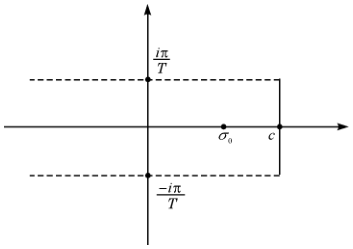
\includegraphics[width=\linewidth]{figs/fig-0175.png}
\caption{图10.3-1}
\end{figure}

一般来讲，当为最简分式，然后利用拉氏变换的线性特点，逐项去查表，按“字典”求出原函数，后面这一方法最为简便。

上面拉氏变换是指一个采样函数而言的。拉氏变换也可以对向量采样函数作用。对向量函数序列变换的定义与式 (10.3-1)相同。令 $\mathbf{y}(N T)=\left(y_{1}(N T),\right.$ $\left.y_{2}(N T), \cdots, y_{n}(N T)\right)$，则

\[\mathbf{Y}^{*}(s)=\sum_{n=0}^{\infty} \mathbf{y}\left[N T\right] e^{-N T_{i}}=\left(Y_{1}^{*}(s), Y_{2}^{*}(s), \cdots, Y_{n}^{*}(s)\right)\qquad\text{(10.3-11)}\]

反变换公式为

\[\mathbf{y}(N T)=\frac{T}{2 \pi i} \int_{-i \frac{\pi}{T}}^{+i \frac{\pi}{T}} \mathbf{Y}^{*}(s) e^{N_{s} T} d s\qquad\text{(10.3-12)}\]

不难看出，对向量函数序列的变换与对普通函数序列的变换本质上没有差别。前面列举过的性质式 (10.3-2) 至式 (10.3-9) 也依然有效。

讨论了拉氏变换的定义及公式后，现在可以建立传递函数的概念了。首先研究如何用拉氏变换的方法去求解第二种差分方程式。设差分方程式 (10.1-7) 的初始条件是 $y(0), y(T), y(2 T), \cdots, y\left[(n-1) T\right]$，对式 (10.1-7) 的两端进行拉氏变换。利用特性式 (10.3-2)有

\[\left(e^{n T}+e_{i} e^{(n-1) s T}+\cdots+e_{n}\right) Y^{*}(s)=\left(f_{1} e^{(n-1) s T}+\cdots+f_{n}\right) U^{*}(s)+R^{*}(s)\]

上式内 $R^{*}(s)$ 为 $e^{s T}$ 的多项式，其诸系数由上述初始条件所确定。将上式移项后得

\[Y^{*}(s)=\frac{Q^{*}(s)}{P^{*}(s)} U^{*}(s)+\frac{R^{*}(s)}{P^{*}(s)}\qquad\text{(10.3-13)}\]

上式右端包含两项，它们都是 $e^{s T}$ 的有理分式。第一项所确定的运动是由控制量 $u(N T)$ 所引起的，称为离散系统的强迫运动，第二项称为系统的特解，或称为系统的自由运动，它完全由系统的初始条件所决定，若初始条件均为零，则 $R^{*}=0$。令

\[F^{*}(s)=\frac{Q^{*}(s)}{P^{*}(s)}\qquad\text{(10.3-14)}\]

$F^{*}(s)$ 称为输出 $y(N T)$ 对控制量 $u(N T)$ 的采样传递函数。换句话说，采样传递函数就是受控对象的初始条件 （状态） 为零时输出和输入拉氏变换之比。如果控制量 $u(N T)$ 的规律给定，则可用拉氏反变换法求出系统的受控运动 $y_{i}(N T)$。同样，当初始条件给定时，$R^{*}(s)$ 也即被确定，自由运动 $y_{c}(N T)$ 也就可以用拉氏反变换的方法求出。这样输出量

\[y(N T)=y_{i}(N T)+y_{c}(N T)\]

其中

\[y_{i}(N T)=L^{*} \quad\left[F^{*}(s) U^{*}(s)\right]\]

\[y_{c}(N T)=L^{-1}\left[\frac{R^{*}(s)}{P^{*}(s)}\right]\]

这种反变换可以先将复变函数 $F^{*}(s) U^{*}(s)$ 及 $\frac{R^{*}(s)}{P^{*}(s)}$ 分解为部分分式，再按字典去查出每一项的原函数，相加后便得到 $y(N T)$。如果方便的话也可以直接采用反变换公式 (10.3-10)。

设在式 (10.1-7) 所代表的受控对象内引进负反馈 （也称硬反馈），使它变成闭路控制系统，如图 10.3-2 所示。系统的输入作用为 $g(t)$，它是连续函数。因为系统的输出 $y(t)$ 本来是连续函数，所以误差 $\varepsilon(t)=g(t)-y(t)$ 也是连续函数。只有经过采样装置的调制后 $u(N T)$ 才变为一个采样函数现试写出闭路系统的传递函数。根据图 10.3-2 当诸初始条件为零时离散系统的运动方程式为

\[\begin{aligned} & Y^{*}(s)=F^{*}(s) U^{*}(s) \\ & U^{*}(s)=E^{*}(s) \\ & E^{*}(s)=G^{*}(s)-Y^{*}(s) \end{aligned}\]

g

采样装置

\[F^{*}(s)\]

图 10.3-2

从上列三式中消掉 $U^{*}(s), E^{*}(s)$ 后，便得到

\[Y^{*}(s)=\frac{F^{*}(s)}{1+F^{*}(s)} G^{*}(s)\qquad\text{(10.3-15)}\]

这里的

\[\Phi^{*}(s)=\frac{F^{*}(s)}{1+F^{*}(s)}\]

称为闭路系统的传递函数。如果从前述三式中消掉 $Y^{*}(s), U^{*}(s)$ 后，便得到

\[E^{*}(s)=\frac{1}{1+F^{*}(s)} G^{*}(s)\qquad\text{(10.3-16)}\]

其中

\[\Phi_{s}^{*}(s)=\frac{1}{1+F^{*}(s)}\]

称为闭路系统对误差的传递函数。我们看到，离散系统的传递函数与第三章内的闭路传递函数的形式是完全类似的。

如果反馈回路中还包含另一个传递函数 $F_{1}^{*}(s)$，如图 10.3-3 所示，那么，对输出和误差的闭路传递函数将是

\begin{figure}[htbp]\centering
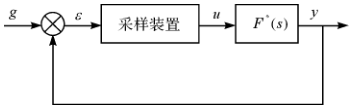
\includegraphics[width=\linewidth]{figs/fig-0176.png}
\caption{图10.3-2}
\end{figure}

\[\begin{aligned}& \Phi^{*}(s)=\frac{F^{*}(s)}{1+F^{*}(s) F_{1}^{*}(s)} \\& \Phi_{\mathrm{A}}^{*}(s)=\frac{1}{1+F_{1}^{*}(s) F^{*}(s)}\end{aligned}\]

由第一种和第四种差分方程组 $(10.1-4)$ 和 $(10.1-11)$ 可以确定与传递函数类似的传递矩阵。我们将以式 $(10.1-17)$ 为依据求传递矩阵。对式 $(10.1-17)$ 的两端进行拉氏变换，移项整理后得到

\[\mathbf{Y}^{*}(s)=(E e^{s T}-D)^{-1} C U^{*}(s)+(E e^{s T}-D)^{-1} \mathbf{y}(0)\qquad\text{(10.3-17)}\]

上式 $E$ 为单位矩阵，并假定 $u(0)=\mathbf{0}$。矩阵函数

\[F^{*}(s)=(E e^{s T}-D)^{-1} C\]

称为受控对象的传递矩阵。而式 $(10.3-17)$ 的第二项决定系统的自由运动。如果用硬反馈 （图 10.3-4)

\[g \xrightarrow{\varepsilon} K \longrightarrow H y=D y+C u \longrightarrow y\]

图 10.3-4

\[u(N T)=K[\mathbf{g}(N T)-\mathbf{y}(N T)]\]

式中 $K$ 为 $n \times r$ 阶矩阵，则闭路运动方程式是

\[\begin{aligned}& \mathbf{Y}^{*}(s)=F^{*}(s) \boldsymbol{U}^{*}(s) \\& \boldsymbol{U}^{*}(s)=K\left(\boldsymbol{G}^{*}(s)-\mathbf{Y}^{*}(s)\right)\end{aligned}\]

消掉 $\boldsymbol{U}^{*}(s)$ 后，则有

\[\mathbf{Y}^{*}(s)=(E+F^{*}(s) K)^{-1} F^{*}(s) K \boldsymbol{G}^{*}(s)\qquad\text{(10.3-18)}\]

式中

\[\Phi^{*}(s)=(E+F^{*}(s) K)^{-1} F^{*}(s) K\]

称为闭路系统的传递矩阵。令 $\boldsymbol{E}^{*}(s)=\boldsymbol{G}^{*}(s)-\boldsymbol{Y}^{*}(s)$ 为误差向量 $\varepsilon(N T)$ 的拉氏变换，不难推出

\[\boldsymbol{E}^{*}(s)=(E+F^{*}(s) K)^{-1} \boldsymbol{G}^{*}(s)=\Phi_{s}^{*}(s) \boldsymbol{G}^{*}(s)\qquad\text{(10.3-19)}\]

\begin{figure}[htbp]\centering
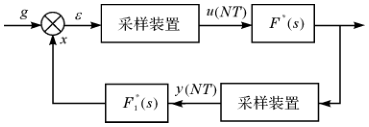
\includegraphics[width=\linewidth]{figs/fig-0177.png}
\caption{图10.3-3}
\end{figure}

\begin{figure}[htbp]\centering
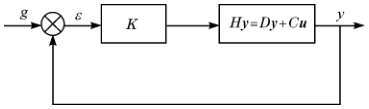
\includegraphics[width=\linewidth]{figs/fig-0178.png}
\caption{图10.3-4}
\end{figure}

\[\Phi_{s}^{*}(s)=\left(E+F^{*}(s) K\right)^{-1}\]

称为对误差向量的传递矩阵。由式(10.3-18)和式(10.3-19)可以看到，方程组的传递矩阵与方程式的传递函数形式类似，只是由于两个矩阵一般没有互换性，故不能将它写成分式。

现今式(10.1-7)右端之控制量按余弦规律变化，即 $u(N T)=\cos \omega N T$，要求求出输出受控量 $y(N T)$ 的变化规律。为此，我们利用线性系统的叠加原理。假定 $u(N T)$ 由两部分组成，一部分是前面给定的 $u(N T)=\cos \omega N T$，另一部分是 $w(N T)=\sin \omega N T$。两者的和是 $u(N T)=w(N T)+w(N T)=\cos \omega N T+$ $i \sin \omega N T=e^{i \omega N T}, N=0,1,2, \cdots$。因为式(10.1-7)的诸系数均为实数，故对控制量 $u(N T)=e^{i \omega N T}$ 有两个独立 （互不影响） 的解，解的实函数部分对应 $w(N T)$，虚部则对应 $w(N T)$。于是求出系统对 $u(N T)$ 的响应后，便同时求出了两个特解，其实数部分恰恰是待求的特解。

设受控量的运动规律是 $A(i \omega) e^{i \omega N T}$，需要求出系数 $A(i \omega)$。将 $u=e^{i \omega N T}$ 和 $A(\omega) e^{i \omega N T}$ 代入式(10.1-7)之两端，消去不为零的因子 $e^{i \omega N T}$ 后，可以求得待求系数

\[A(i \omega)=\frac{f_{1} e^{i \omega(n-1) T}+f_{2} e^{i \omega(n-2) T}+\cdots+f_{n}}{e^{i \omega n T}+e_{1} e^{i \omega(n-1) T}+\cdots+e_{n}}\qquad\text{(10.3-20)}\]

我们立刻看到，$A(i \omega)$ 不是别的，正是离散系统的传递函数式(10.3-14)，只不过将变数 $s$ 换为 $i \omega$ 堵了。由此可知，式(10.1-7)对 $u=e^{i \omega N T}$ 的响应是

\[y(N T)=F^{*}(i \omega) e^{i \omega N T}\qquad\text{(10.3-21)}\]

$F^{*}(i \omega)$ 称为采样频率特性。如果系统式(10.1-17)中的控制量是正弦函数

\[\begin{aligned} \boldsymbol{u}(N T) & =\left(b_{1} e^{i \omega N T}, b_{2} e^{i \omega N T}, \cdots, b_{n} e^{i \omega N T}\right) \\ & =\boldsymbol{b} e^{i \omega N T} \end{aligned}\qquad\text{(10.3-22)}\]

那么，输出向量 $\mathbf{y}(N T)=F^{*}(i \omega) \boldsymbol{b} e^{i \omega N T}$，式中

\[F^{*}(i \omega)=\left(E e^{i \omega}-D\right)^{-1} C\]

称为频率特性矩阵。

若图 10.3-2 所示之闭路系统的输入作用为 $g(t)=e^{i \omega t}$，那么，输出 $y(t)$ 在 $t=$ 0，$T, 2 T, \cdots$，等采样点上的稳态值将是

\[y(N T)=\Phi^{*}(i \omega) e^{i \omega N T}=\frac{F^{*}(i \omega)}{1+F^{*}(i \omega)} e^{i \omega N T}\qquad\text{(10.3-23)}\]

而误差

\[\epsilon(N T)=\Phi_{s}^{*}(i \omega) e^{i \omega N T}=\frac{1}{1+F^{*}(i \omega)} e^{i \omega N T}\qquad\text{(10.3-24)}\]

$\Phi^{*}(i \omega)$ 称为闭路系统输出对输入的采样频率特性，$\Phi_{s}^{*}(i \omega)$ 称为闭路系统误差采样频率特性。如果在式 (10.1-17)所构成的闭路系统的输入端加上 $\mathbf{g}(N T)=$

$\mathbf{g}_{0}^{*} e^{i \omega t}$，则闭路系统的输出将是

\[\mathbf{y}(\boldsymbol{N} T)=\Phi^{*}(i \omega) \mathbf{g}_{0}^{*} e^{i \omega N T}=\left(E+F^{*}(i \omega) K\right)^{-1} F^{*}(i \omega) K \mathbf{g}_{0}^{*} e^{i \omega N T}\qquad\text{(10.3-25)}\]

误差向量的运动将是

\[\begin{aligned} \epsilon(\boldsymbol{N} T) & =\Phi_{0}^{*}(i \omega) \mathbf{g}_{0}^{*} e^{i \omega N T} \\ & =\left(E+F^{*}(i \omega) K\right)^{-1} \mathbf{g}_{0}^{*} e^{i \omega N T} \end{aligned}\qquad\text{(10.3-26)}\]

式中

\[F^{*}(i \omega)=\left(E e^{i \omega T}-D\right)^{-1} C\]

复函数 $F^{*}(i \omega)$ 称为开路系统式 (10.1-7) 的采样频率特性。将 $F^{*}(i \omega)$ 写成 $K^{*}(\omega) e^{-i \theta^{*}(\omega)}$ 后，得到两个 $\omega$ 的实函数 $K^{*}(\omega)$ 和 $\theta^{*}(\omega)$，式 (10.3-21) 可以改写为

\[y(\boldsymbol{N} T)=K^{*}(\omega) e^{i N T_{0}-\theta^{*}(\omega)}\qquad\text{(10.3-27)}\]

显然，$K^{*}(\omega)$ 表示输出运动的幅度，$\theta^{*}(\omega)$ 表示相位移动。因此，$K^{*}(\omega)$ 称为离散系统的幅频特性，而 $\theta^{*}(\omega)$ 称为它的相频特性。将式 (10.3-27) 分为实虚两部分后，便得到式 (10.1-7) 对 $\cos \omega N T$ 的响应

\[\gamma_{1}(N T)=K^{*}(\omega) \cos (\omega N T-\theta^{*}(\omega))\qquad\text{(10.3-28)}\]

对式 (10.3-22) 进行同样的处理，便可得到系统式 (10.1-17) 的开路和闭路的幅频和相频特性矩阵。利用矩阵函数的运算规律即可求出，我们把它们的推导留给读者。

例。设连续受控对象的运动方程式是

\[\frac{d \hat{y}}{d t}=u\qquad\text{(10.3-29)}\]

脉冲元件是方波幅度调制，重复周期为 $T=1$，脉冲宽度为 $\gamma T, \gamma=1$，于是式 (10.3-29) 的开路传递函数是

\[F^{*}(s)=\frac{\frac{1}{2}\left(e^{s}+1\right)}{\left(e^{s}-1\right)^{2}}\]

其中各参数的值用 $i \omega$ 置换复变数 $s$ 后，便得到开路采样频率特性

\[F^{*}(i \omega)=K^{*}(\omega) e^{+i \theta^{*}(\omega)}\]

其中

\[\begin{aligned} K^{*}(\omega) & =\frac{1}{2} \frac{\sqrt{\cos \omega+1}}{\cos \omega-1} \\ \theta^{*}(\omega) & =\tan ^{-1} \frac{-\sin \omega}{1+\cos \omega} \end{aligned}\]

这样，我们就不难画出频率特性了。用 -1 作为系统的反馈，式 (10.3-29) 变为闭路系统，通过简单的计算，可以得出闭路传递函数。

\[\begin{aligned}& \Phi^{s}(s)=\frac{\frac{1}{2}\left(e^{s}+1\right)}{\left(e^{s}-1\right)^{2}+\frac{1}{2}\left(e^{s}+1\right)} \\& \Phi^{s}(s)=\frac{\left(e^{s}-1\right)^{2}}{\left(e^{s}-1\right)^{2}+\frac{1}{2}\left(e^{s}+1\right)}\end{aligned}\]

其相应的频率特性为

\[\Phi^{*}(i \omega)=K^{*}(\omega) e^{i \theta^{*}(\omega)}\]

其中

\[\begin{aligned}K^{*}(\omega)= & \frac{\sqrt{12 \cos ^{3} \omega-12 \cos ^{2} \omega-10 \cos \omega+5}}{12 \cos ^{2} \omega-15 \cos \omega+5} \\& \theta^{*}(\omega)=\tan ^{-1} \frac{2 \sin \omega(1-\cos \omega)}{2 \cos ^{2} \omega+\cos \omega-1}\end{aligned}\]

当然，也可以画出闭路系统的频率特性。

上面我们讨论的传递函数都是以输出和输入量在采样点上，$t=0, T, 2 T, \cdots$，的值为依据的。如果我们关心的不是采样点的值，而是在两个采样点中间某一时刻的输出量的变化情况，例如输出量在 $t=N T+\varepsilon T, N=0,1,2, \cdots$，各点上的变化规律，在 $0 \leqslant \varepsilon<r$ 时，可应用公式 (10.1-18)，或在 $1>\varepsilon>r$ 时，应用式 (10.1-19) 求开路系统和闭路系统的传递函数及频率特性。此时传递函数中将含有参数 $\varepsilon$。对式 (10.1-18) 的两端进行拉氏变换，再加以整理后，可以写出开路传递函数矩阵

\[F^{*}(s, \varepsilon)=\left(E e^{s T}-D\right)^{-1}\left(B_{1}(\varepsilon)+e^{T} B_{2}(\varepsilon)\right)\qquad\text{(10.3-30)}\]

而闭路系统传递矩阵为

\[\Phi^{*}(s, \varepsilon)=\left(E+F^{*}(s, \varepsilon)\right)^{-1} F^{*}(s, \varepsilon)\qquad\text{(10.3-31)}\]

上式内代入 $s=i \omega$ 后，又得到频率特性矩阵。

10.4 一种特殊情况下 $F^{*}(s)$ 的计算

前节内传递函数的推导是基于方程组的基本解矩阵得到的。在某些特殊情形下，采样传递函数可以从受控对象的连续传递函数 $F(s)$ 出发经过变换后，直接求出来，而不必首先求出离散系统的差分方程式。 $F(s)$ 与 $F^{*}(s)$ 这两个函数都是用来表示控制系统的特性的，当控制系统是连续作用的组成部分时，$F(s)$ 就是很重要的特性。但是，当控制系统用在离散控制系统上的时候，$F^{*}(s)$ 就成为重要的特性了。从数学上看 $F(s)$ 比 $F^{*}(s)$ 简单得多，而且我们也常常把 $F(s)$ 直接用到设计系统的方法上去，因此，当可能时，找出 $F^{*}(s)$ 与 $F(s)$ 的关系，就是很重要的事情了。当然，直接从 $F(s)$ 求 $F^{*}(s)$ 并不是对所有离散系统都那么简单可行。但

\section{10.4 一种特殊情况下F*（s）的计算}

是，当脉冲元件所调制的脉冲宽度 $\gamma T \ll T$，即 $\gamma \ll 1$ 时，这种直接换算是可能的。

重新研究方程组 $(10.1-3)$，它是受控对象的连续运动方程组。设系统的初始条件为零，那么式 $(10.1-3)$ 的特解是

\[\mathbf{y}(t)=\int_{0}^{t} e^{\mathbf{A}(t-\tau)} \mathbf{b} u(\tau) d \tau\qquad\text{(10.4-1)}\]

令 $e^{A(t-\tau)} b=h(t-\tau)$，显然，$\boldsymbol{h}(t)$ 是系统的脉冲过渡函数 （见第二章）。根据连续拉氏变换的特点可知

\[Y(s)=F(s) U(s), F(s)=\left(F_{1}(s), F_{2}(s), \cdots, F_{n}(s)\right)\]

而

\[F(s)=\int_{0}^{\infty} \boldsymbol{h}(t) e^{-t} d t\qquad\text{(10.4-2)}\]

当 $u(t)$ 是一个方形脉冲序列时，式 $(10.4-1)$ 可以写成

\[\begin{aligned} \mathbf{y}(N T) & =\sum_{m=0}^{N} \int_{m T}^{(m+1) T} \boldsymbol{h}(N T-\tau) u(\tau) d \tau \\ & =\sum_{m=0}^{N} \int_{m T}^{(m+\gamma) T} \boldsymbol{h}(N T-\tau) u(\tau) d \tau \end{aligned}\qquad\text{(10.4-3)}\]

当 $\gamma \ll 1$ 时，上式右端的积分间隔远远小于 $T$。当 $\boldsymbol{h}(t)$ 的变化较慢时，可以以足够的精度认为

\[\int_{m T}^{(m+\gamma) T} \boldsymbol{h}(N T-\tau) u(\tau) d \tau=\gamma T \boldsymbol{h}(N T-m \mathrm{T}) u(m T)\qquad\text{(10.4-4)}\]

将式 $(10.4-4)$ 代入式 $(10.4-3)$ 后有

\[\mathbf{y}(N T)=\gamma T \sum_{m=0}^{N} \boldsymbol{h}(N T-m T) u(m T)\]

对上式两端进行拉氏变换

\[Y^{*}(s)=\sum_{N=0}^{\infty} \mathbf{y}(N T) e^{-N T s}=\gamma T \sum_{N=0}^{\infty}\left(\sum_{m=0}^{N} \boldsymbol{h}(N T-m T) u(m T)\right) e^{-N T s}\]

根据前节拉氏变换特性式 $(10.3-6)$，上式可以写成

\[Y^{*}(s)=\boldsymbol{F}^{*}(s) U^{*}(s)\qquad\text{(10.4-5)}\]

式中

\[\begin{aligned} & \boldsymbol{F}^{*}(s)=\gamma T \sum_{N=0}^{\infty} \boldsymbol{h}(N T) e^{-N T s} \\ & U^{*}(s)=\sum_{N=0}^{\infty} u(N T) e^{-N T s} \end{aligned}\qquad\text{(10.4-7)}\]

式 $(10.4-6)$ 和 $(10.4-3)$ 是两个向量等式。取它们的第一个分量，即系统的主受控量 $y_{1}$，后者对应的两个传递函数是 $F(s)$ 和 $F^{*}(s)$，前者对应的脉冲过渡函数写为 $h(t)$。于是有

\[\begin{aligned}& F(s)=\int_{0}^{\infty} h(t) e^{-s t} d t \\& F^{*}(s)=\gamma T \sum_{N=0}^{\infty} h(N T) e^{-s N T}\end{aligned}\qquad\text{(10.4-8)}\]

将

\[h(t)=\frac{1}{2 \pi i} \int_{c-i \infty}^{c+i \infty} F(s) e^{s t} d s\]

代入式(10.4-8)的第二式后有

\[\begin{aligned}F^{*}(s) & =\frac{\gamma T}{2 \pi i} \sum_{N=0}^{\infty} e^{-s N T} \int_{c-i \infty}^{c+i \infty} F(q) e^{N T q} d q \\& =\frac{\gamma T}{2 \pi i} \int_{c-i \infty}^{c+i \infty} F(q)\left[\sum_{N=0}^{\infty} e^{-N T(s-q)}\right] d q \\& =\frac{\gamma T}{2 \pi i} \int_{c-i \infty}^{c+i \infty} \frac{F(q)}{1-e^{T(s-q)}} d q\end{aligned}\qquad\text{(10.4-9)}\]

上式内当 $s$ 的实部 $\operatorname{Res} s>\sigma$ 时，级数绝对收敛，故上面的运算是正确的。这样，在一种特殊情况下我们获得了自 $F(s)$ 至 $F^{*}(s)$ 的直接变换公式。以下我们就用留数方法来计算式(10.4-9)右端的积分。

被积函数有无穷多个极点: $F(s)$ 的极点都在积分路线的左方；但是那些由方程 $1-e^{-T(s-q)}=0$ 的零点所构成的极点都在积分路线的右方。不难看出：沿着从 $c-i \infty$ $c+i \infty$ 的直线的积分值等于在顺时针方向上，沿着这样一条闭合积分路线上的积分值；这条闭合路线是由原来的直线和右半平面上以那条直线为直径的一个无限大的半圆周所组成的。因此，方程(10.4-9)右端的积分值等于 $-\gamma T$ 与被积函数在方程 $1-e^{-T(s-q)}=0$ 的各个零点的留数的和的乘积。

方程 $1-e^{-T(s-q)}=0$ 的零点的一般形式是 $q=s+(2 \pi i m / T), m$ 是任何整数。被积函数在这样一个极点处的留数是 $-\left(\frac{1}{T}\right) F[s+(2 \pi i m / T)]$。所以，就得出

\[F^{*}(s)=\gamma \sum_{m=-\infty}^{\infty} F\left[s+\frac{2 \pi i m}{T}\right]\qquad\text{(10.4-10)}\]

这个公式使我们能够相当深刻的看出 $F^{*}(s)$ 的性质，有时候也可以利用这个公式进行近似的计算。但是，我们还可以用相当简单的有限形式把 $F^{*}(s)$ 精确地表示出来。

函数 $F(s)$ 可以写成有限多个部分分式的和

\[F(s)=\sum_{k=-\infty}^{n} \frac{a_{k}}{s-s_{k}}\qquad\text{(10.4-11)}\]

这里的各个 $a_{k}$ 和 $s_{k}$ 都是常数，$n$ 是 $F(s)$ 的分母多项式的次数。于是，利用方程式

(10.4-10) 并令 $\gamma=1$ 就有

\[\begin{aligned} F^{*}(s) & =\sum_{k=1}^{n} a_{k}\left[\frac{1}{s-s_{k}}+\sum_{m=1}^{\infty}\left[\frac{1}{\left(2 \pi i m / T\right)+\left(s-s_{k}\right)}-\frac{1}{\left(2 \pi i m / T\right)-\left(s-s_{k}\right)}\right]\right\} \\ & =\sum_{k=1}^{n} a_{k}\left[\frac{1}{s-s_{k}}+\sum_{m=1}^{\infty}\left(\frac{2\left(s-s_{k}\right)}{\left(4 \pi^{2} m^{2} / T^{2}\right)+\left(s-s_{k}\right)^{2}}\right)\right. \end{aligned}\qquad\text{(10.4-12)}\]

但是，我们知道 $\operatorname{coth} z$ 有如下的展开式

\[\operatorname{coth} z=\frac{1}{z}+2 z \sum_{m=1}^{\infty} \frac{1}{m^{2} \pi^{2}+z^{2}}\]

所以，方程 (10.4-12) 中对 $m$ 所求的和数可以计算出来，因此就得出

\[F^{*}(s)=\frac{T}{2} \sum_{k=1}^{n} a_{k} \operatorname{coth}\left[\frac{\left(s-s_{k}\right) T}{2}\right]\qquad\text{(10.4-13)}\]

利用这个公式，对于任意的 $s$ 值都可以把 $F^{*}(s)$ 准确地计算出来。

如果 $T$ 很小，$F(i \omega)$ 的值在 $-\pi / T<\omega<\pi / T$ 间隔之外小到略去不计的程度，那么，根据方程 (10.4-10) 就可以很清楚地看出 $F^{*}(s)$ 的定性的性质。事实上，在间隔 $-\pi / T<\omega<\pi / T$ 里 $F^{*}(i \omega)$ 差不多就等于 $F(i \omega)$。我们将要看到，如果 $T$ 相当大，我们也还可以得到一个相当简单的 $F^{*}(i \omega)$ 的近似表示式。把各个零点 $s_{k}$写作

\[s_{k}=-\lambda_{k}+i \omega_{k}\qquad\text{(10.4-14)}\]

这些 $\lambda_{k}$ 和 $\omega_{k}$ 都是实数。我们假设，所有的 $\lambda_{k}$ 都是正数。按照方程 (10.4-13) 现在就得出

\[\begin{aligned} F^{*}(i \omega) & =\frac{T}{2} \sum_{k=1}^{n} a_{k} \operatorname{coth}\left[\frac{T}{2}\left[\lambda_{k}+i(\omega-\omega_{k})\right]\right] \\ & =\frac{T}{2} \sum_{k=1}^{n} a_{k} \frac{1+e^{-\pi\left[\lambda_{k}+\delta\left(\omega-\omega_{k}\right)\right]}}{1-e^{-\pi\left[\lambda_{k}+\delta\left(\omega-\omega_{k}\right)\right]}} \end{aligned}\]

因此，对于大的 $T$ 值就有

\[F^{*}(i \omega) \simeq \frac{T}{2} \sum_{k=1}^{n} a_{k}\left\{1+2 e^{-\pi\left[\lambda_{k}+\delta\left(\omega-\omega_{k}\right)\right]}\right\}\qquad\text{(10.4-15)}\]

当 $s$ 很大的时候，方程式 (10.4-11) 可以写作

\[F(s)=\frac{1}{s} \sum_{k=1}^{n} a_{k}+\frac{1}{s} \sum_{k=1}^{n} a_{k} s_{k}+\cdots\]

但是我们曾经假定：反馈线路对于 $\delta$ 函数的反应是连续的。所以，当 $s$ 很大时; $F(s) \simeq 1 / s^{2}$，因此

\[\sum_{k=1}^{n} a_{k}=0\qquad\text{(10.4-16)}\]

这样一来，方程 (10.4-15) 就变成

\[F^{*}(i \omega) \cong T e^{-i T_{\omega}} \sum_{k=1}^{n} a_{k} e^{T_{k}}\qquad\text{(10.4-17)}\]

对于实际的物理系统来说，$s_{k}$ 或者是实数，或者成复共轭对出现，所以方程 (10.4-17)中的和数一定是实数。因此，当 $\omega$ 从 $-\pi / T$ 变到 $\pi / T$ 的时候，$F^{*}(i \omega)$ 的图线是一个圆，这个圆的半径是

\[\left|T \sum_{k=1}^{n} a_{k} e^{T_{k}}\right|\qquad\text{(10.4-18)}\]

在实际情况中，$F(s)$ 很可能在 $s=0$ 处有一个极点。为了避免某些不必要的麻烦；以前我们并没有考虑这种情形。现在，我们把这种情形简短的讨论一下。

首先，我们可以看到，如 $s=0$ 是 $F(s)$ 的一个极点，那么常数 $c$ 就必须是正数，而且 $F^{*}(s)$ 的无穷级数表示式 (10.4-10) 只在 $s$ 的实数部分是正数时成立。这种情形中，$F^{*}(s)$ 的有限表示式，(10.4-13) 仍然成立。如果，设 $s_{1}=0$，那么，方程 (10.4-13) 就变为

\[F^{*}(i \omega)=\left.\frac{T}{2}\right\}-i a_{1} \cot \frac{\omega T}{2}+\sum_{k=2}^{n} a_{k} \operatorname{coth} \frac{T\left[\lambda_{k}+i(\omega-\omega_{k})\right]}{2}\]

如果 $T$ 的值很大，我们就得到一个类似于方程 (10.4-15) 的公式

\[\left.F^{*}(i \omega)=\frac{T}{2}\right\}-i a_{1} \cot \frac{\omega T}{2}+\sum_{k=2}^{n} a_{k}\left\{1+2 e^{-T\left[\lambda_{k}+i(\omega-\omega_{k})\right]}\right\}\]

但是按照式 (10.4-16)

\[a+a_{3}+\cdots+a_{n}=-a\]

所以

\[F^{*}(i \omega)=-\frac{a_{1}}{2} T\left[1+\mathrm{i} \cot \frac{\omega T}{2}\right]+T e^{-i T_{\omega}} \sum_{k=2}^{n} a_{k} e^{T_{k}}\qquad\text{(10.4-19)}\]

常数 $a_{1}$ 当然是一个正实数。当 $\omega$ 从 $-\pi / T$ 变化到 $\pi / T$ 时，式 (10.4-19) 的第一项就给出一条平行于虚轴的直线，其余部分是一个正弦函数。

\section{10.5 闭路离散系统分析}

在讨论了描述离散系统的差分方程的建立方法及各种求解方法以后，可以开始研究闭路离散系统的动态和静态品质。如前几章内曾叙述过的那样，我们将研究闭路离散系统的稳定性、静差和过渡过程。本节内我们主要研究系统的稳定性判别准则，最后将讨论系统的静态误差。这也是线性系统的两个最重要的品质特性。关于如何设计系统使之具有良好的过渡特性，将在下一节内讨论。

首先讨论系统的稳定性问题。设受控对象的运动方程式是式 (10.1-17)，即第一种和第四种差分方程

\[H y(N T)=D y(N T)+C u(N T)\qquad\text{(10.1-17)}\]

令系统的输入作用是 $\boldsymbol{g}(t)$，它是一个连续向量函数 （或采样输入）。用简单的硬反馈所构成的闭路系统如图 10.3-4 所示。用 $C u(N T)=K \varepsilon(N T)=K\left(\boldsymbol{g}(N T)-\right.$ $\left.\boldsymbol{y}(N T)\right)$ 代入式 (10.1-17) 后，得到闭路运动方程式

\[H \mathbf{y}(N T)=(D-K) \mathbf{y}(N T)+K \boldsymbol{g}(N T)\qquad\text{(10.5-1)}\]

式中 $K$ 为一 $n \times n$ 阶常量方阵，它表示了采样装置的增益矩阵。这样，系统的输出量 $\mathbf{y}$ 便受到输入作用的驱动。设 $\boldsymbol{g}(t)$ 为任意已知的时间函数。显然，当系统的初始状态给定后，$\mathbf{y}(t)$ 的运动规律便已经完全确定了。再令这个初始状态为 $\mathbf{y}_{0}$，它所对应的运动是 $\mathbf{y}(t)$。读者应该注意 $\mathbf{y}(t)$ 实际上可以是连续函数，虽然差分方程 (10.1-17) 只能描绘它在采样时刻 $t=0, T, 2 T, \cdots$，上的变化情况但对任何 $t$ 它都有确定的值。按李雅普诺夫定义，如果对给定的 $\mathbf{y}$ 和 $\boldsymbol{g}(t)$，系统的运动是稳定的，则对任何 $\varepsilon>0$，总有 $\delta>0$，一旦 $\|\mathbf{x}_{0}\|<\delta, \mathbf{x}$ 为任意 $n$ 维向量，则对应于初始条件 $\mathbf{x}+\mathbf{y}_{0}$ 和 $\boldsymbol{g}(t)$ 的系统运动 $\boldsymbol{z}(t)$ 将永远满足不等式

\[\|z(t)-\mathbf{y}(t)\|<\varepsilon\]

这里 $\mathbf{x}$ 称为对 $\mathbf{y}(t)$ 的初始扰动，$\boldsymbol{z}(t)$ 称为系统的受扰运动，$\mathbf{y}(t)$ 则称为未受扰运动。显然，受扰运动也满足式 (10.5-1)

\[H z(N T)=(D-K) z(N T)+K \boldsymbol{g}(N T), \quad z(0)=\mathbf{x}_{0}+\mathbf{y}\qquad\text{(10.5-2)}\]

受扰运动与未受扰运动的差是 $\boldsymbol{x}(t)=\boldsymbol{z}(t)-\mathbf{y}(t)$。自式 (10.5-2) 分别减掉式 (10.5-1) 的两端，得到 $\mathbf{x}(t)$ 在采样点上的运动规律

\[H \mathbf{x}(N T)=(D-K) \mathbf{x}(N T), \quad \mathbf{x}(0)=\mathbf{x}_{0}\qquad\text{(10.5-3)}\]

由于系统是线性的，我们也可以称 $\mathbf{x}(t)=0$ 为系统的未受扰运动，因为此时 $\boldsymbol{z}(t)=$ $\mathbf{y}(t)$。由此可知，为了研究式 (10.5-1) 内 $\mathbf{y}(N T)$ 的运动稳定性，只要研究式 (10.5-3) 的零解稳定性就够了。我们看到这里的情形与第四章内的情况相同。如果线性系统的齐次方程式的零解稳定，则系统的一切可能的运动都是稳定的。反之，如果任何一个运动是稳定的，则它的零解 （平衡状态） 也是稳定的，于是系统的一切运动都是稳定的。因此，我们可以一般地讲系统的稳定性。这里再一次指出，对非线性系统这一事实一般是不存在的，如果系统的平衡状态 （零解） 稳定，不能保证系统的任何运动稳定，所以对非线性系统，一般的去讲系统稳定有时是没有意义的。

式 (10.5-3) 的零解何时稳定？用什么方法判别？这正是我们想要解决的问题。根据式 (10.2-4)，如果式 (10.5-3) 的初始条件是 $\mathbf{x}_{0}$，那么，它的特解是

\[\mathbf{x}(N T)=(D-K)^{N} \mathbf{x}_{0}=A^{N} \mathbf{x}_{0}, \quad A=(D-K)\qquad\text{(10.5-4)}\]

因为 $A^{N}$ 可以写成

\[A^{N}=Q^{-1} J^{N} Q\]

$Q$ 是某一非蜕化 （即其行列式不为零） 矩阵。如果对任何 $\mathbf{x}, \mathbf{x}(N T)$ 都随着 $N$ 的增长而趋近于零向量，显然式 (10.5-4) 的零解将是稳定的。根据第 10.2 节内的讨论可知，只要矩阵 $A$ 所构成的特征方程式

\[\left|A-E \lambda\right|=0\qquad\text{(10.5-5)}\]

的一切根的模小于 1 即可。其实，$J^{N}$ 内的每一元素都是由 $\lambda_{i}^{N}$ 所构成的，当 $|\lambda|<$ $1, N \rightarrow \infty$ 时，总有 $\left|\lambda_{i}^{N}\right| \rightarrow 0$。因此，当 $|\lambda|<1$ 时，$J^{N}$ 趋于零矩阵，由此可知 $A^{N}$ 也趋于零。故有

\[\lim _{N arrow \infty} A^{N} \mathbf{x}_{0}=\mathbf{0}\]

这时，式 (10.5-1) 稳定的充分条件是矩阵 $A=$ $D-K$ 的一切特征根在复平面上均位于单位圆的内部（图 10.5-1)。反之，哪怕特征根中有一个位于单位圆之外，则系统将是不稳定的。因为此时至少有一个约当块 $J^{N}$，它的某一些元素随 $N$ 的无限增大而无限增长，对某一初始条件 $\boldsymbol{x}$，使 $\lim _{N \rightarrow \infty} \boldsymbol{x}(N T)=\infty$。由此可以断言，系统式 (10.5-1) 不稳定的充分条件是矩阵 $A=D-K$ 至少有一个特征根的模大于 1，即位于复平面的单位圆外。如果一部分在单位圆内，另一部分在单位圆上，圆外无根，这是一种临界状态，即系统处于稳定边缘。对这类系统的研究只具有数学上的意义，实际上是不允许出现的。

图 10.5-1

让我们再看看稳定系统的传递函数应具有何种性质。回顾式 (10.3-17) 可以看到，如果输入作用 $\boldsymbol{g}(t) \equiv \mathbf{0}$ 且 $C$ 为单位矩阵时有

\[\boldsymbol{Y}^{*}(s)=\left(E e^{s T}-D\right)^{-1} \mathbf{y}_{0}=\Phi^{*}(s) \mathbf{y}_{0}\]

式中 $\Phi^{*}(s)$ 的每一元素为 $e^{s T}$ 的有理分式，上式可以写成一个线性方程组

\[Y_{i}^{*}(s)=\sum_{j=1}^{n} \varphi_{i j}^{*}(s) y_{0 j}, \quad i=1,2, \cdots, n\]

根据拉氏变换的特性可知，当一切 $\varphi_{i j}^{*}(s)$ 的极点 $s$ 均为负实部时，$\lim _{N \rightarrow \infty} y_{i}(N T)=$ 0。由此可以断言，闭路系统稳定的另一充分条件是传递矩阵的每一元素的极点都位于复平面的左半平面上。这个充分条件对第二种差分方程式的传递函数式 (10.3-14) 也是完全适用的。读者从式 (10.3-13) 可以直接看出，这里不再赘述。由于逆矩阵的特点，$\varphi_{i j}^{*}(s)$ 的极点又恰恰是行列式

\[\Delta(s)=\left|E e^{s T}-D\right|=\operatorname{det}\left(E e^{s T}-D\right)=0\qquad\text{(10.5-6)}\]

的零点。上式称为离散系统的特征方程式，而且式 (10.5-6) 的零点也正是 $\Phi^{*}(s)=$ $\left(\Phi_{i}^{*}(s), \cdots, \Phi_{n}^{*}(s)\right)$ 每一个分量的极点。因此，欲检查闭路系统的稳定性，可以检查 $\Delta(s)$ 的零点，或者检查任一 $\Phi_{i}^{*}(s)$ 的极点是否位于复数平面的左半平面即可。

\begin{figure}[htbp]\centering
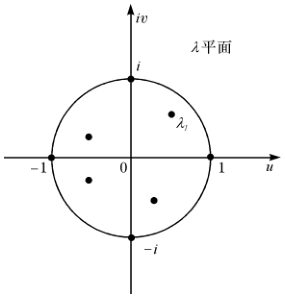
\includegraphics[width=\linewidth]{figs/fig-0179.png}
\caption{图10.5-1}
\end{figure}

当 $\Phi_{i}^{*}(s)$ 的极点或 $\Delta(s)$ 的零点 $s_{j}, j=1,2, \cdots, n$，有负实部时，可保证序列 $\left\{\mathbf{y}(N T)\right\}$ 中的每一个分量序列当 $N \rightarrow \infty$ 时趋于零。但系统的输出量 $\mathbf{y}(t)$ 实际上是 $t$ 的连续函数。仅仅在采样点 $0, T, 2 T, \cdots, N T, \cdots$ 上趋近于零，严格说来还不能保证 $\lim _{t \rightarrow \infty} \mathbf{y}(t)=\mathbf{0}$。

为了检查后者的存在，还要检查在节点

的 $\varepsilon T$ 位移，即在 $N T+\varepsilon T$ 上的运动规律，$N=0,1,2, \cdots$。例如，原理上可能出现图 10.5-2 所示的情况，虽然，$y_{i}(N T) \rightarrow 0$，但在采样点的位移点上，$y_{i}(N T+\varepsilon T)$ 不趋向于零，故为了确信系统的输出 $\mathbf{y}(t) \rightarrow \mathbf{0}$，必须对某一 $\varepsilon>0$，检查式 $(10.3-31)$ 的任一分量的极点分布情况，稳定系统的传递函数 $\Phi_{i}^{*}(s, \varepsilon)$ 的一切极点 $s_{i}$ 也必须满足前述条件，即所有 $s_{i}$ 均在复平面的左半平面上。虽然如此，图 10.5-2 的情况是非常罕见的，因此，一般来讲只检查在节点 $\Phi_{i}^{*}(s)$ 的极点就够了。为了不发生意外情况，当然可以选取某一 $\varepsilon>0$，再检查一次 $\Phi_{i}^{*}(s, \varepsilon)$ 的极点。

实际上，求特征方程式的根，只有在一次和二次方程式时，求解才比较容易。三次以上的方程式根的一般表达式或者过于繁冗，或者不可能写出。更高次的方程式，一般地说没有根的普遍表达式。因此，不必解出根来而能决定系统稳定性的法则就具有很大的实际意义了。利用这类所谓稳定判据的法则，我们不仅能够确定系统是否稳定，同时也能说明系统中各种参量和结构变化时对稳定性的影响。

连续系统中现有的几种稳定判据稍加改变后同样能用到离散系统上来。各种形式的稳定判据，它们所表示的是同一个事实：特征方程式所有的根都位于复平面上单位圆内。但是，在解决具体问题时，如果方法选择得当，就可以收到计算简单的效益。下面将要讨论的几种稳定判据，是以复变函数理论中所熟知的幅角定理为基础的。首先我们用来哈依洛夫 (МИХАЙЛОВ) 判别法来研究差分方程式的稳定性。设差分方程的特征方程式为

\[\mid D-\lambda E \mid=f(\lambda)=\left(\lambda-\lambda_{1}\right)\left(\lambda-\lambda_{2}\right) \cdots\left(\lambda-\lambda_{n}\right)\]

令 $\lambda=e^{i \theta}, \lambda=\rho e^{i \theta_{1}}, \lambda_{2}=\rho_{2} e^{i \theta_{2}}, \cdots, \lambda_{n}=\rho_{n} e^{i \theta_{n}}$，代入式 (10.5-7) 中后

\[\begin{aligned} f\left(e^{i \theta}\right) & =\left(e^{i \theta}-\rho_{1} e^{i \theta_{1}}\right)\left(e^{i \theta}-\rho_{2} e^{i \theta_{2}}\right) \cdots\left(e^{i \theta}-\rho_{n} e^{i \theta_{n}}\right) \\ & =R_{1}(\theta) e^{i \theta_{1}(1)} R_{2}(\theta) e^{i \theta_{2}(1)} \cdots R_{n}(\theta) e^{i \theta_{n}(1)} \\ & =R(\theta) e^{\sum_{j=1}^{n} \psi_{j}(1)} \end{aligned}\qquad\text{(10.5-8)}\]

式 (10.5-8) 中我们取出 $R_{i}(\theta) e^{i \theta_{i}(1)}$ 来研究。若 $\lambda_{i}$ 点在单位圆内，也就是说 $\rho<1$，由图 10.5-3(a) 中可以看出，当 $\theta$ 角由 0 变到 $2 \pi$ 时，$R_{i}(\theta) e^{i \theta_{i}(1)}$ 向量绕 $\lambda_{i}$ 点转 $2 \pi$

\begin{figure}[htbp]\centering
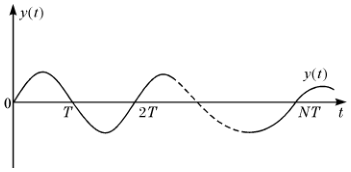
\includegraphics[width=\linewidth]{figs/fig-0180.png}
\caption{图10.5-2}
\end{figure}

角度。当 $\lambda$ 在单位圆外，也就是 $\rho>1$，由图 10.5-3(b) 中可以看出，当 $\theta$ 角由 0 变到 $2 \pi$ 时，$R_{1}(\theta) e^{\rho_{1}(\theta)}$ 绕 $\lambda$ 点转之角度为零。但是 $n$ 阶方程一定有 $n$ 个根，如果 $n$个根均在单位圆内，则式 (10.5-8) 的总转角为 $2 n \pi$，若都在单位圆外则转角为零。若一部分根在单位圆内另一部分在单位圆外时，转角一定小于 $2 n \pi$。于是我们把米哈依洛夫稳定判别法则转述如下：当 $\theta$ 角由 0 变到 $2 \pi$ 时，曲线 $f(\lambda)$ 绕原点转 $2 n \pi$ 角度，则系统稳定。否则是不稳定的。

\begin{figure}[htbp]\centering
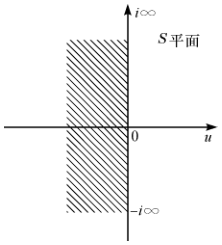
\includegraphics[width=\linewidth]{figs/fig-0184.png}
\caption{图10.5-4}
\end{figure}

\begin{figure}[htbp]\centering
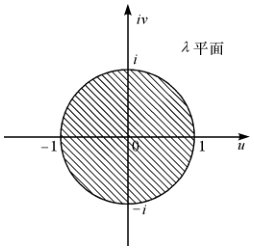
\includegraphics[width=\linewidth]{figs/fig-0183.png}
\caption{图10.5-4}
\end{figure}

\begin{figure}[htbp]\centering
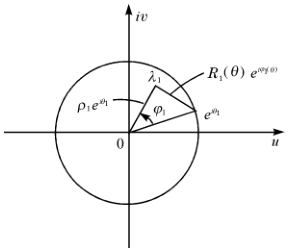
\includegraphics[width=\linewidth]{figs/fig-0182.png}
\end{figure}

\begin{figure}[htbp]\centering
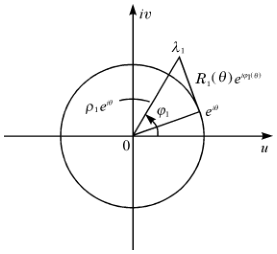
\includegraphics[width=\linewidth]{figs/fig-0181.png}
\end{figure}

(a)

(b)

图 10.5-3

$\lambda$ 平面

(a)

$S$ 平面

(b)

图 10.5-4

稳定性的另一判据方法是把闭环系统的稳定条件化为代数中著名的劳斯-霍尔维茨不等式。为此，在多项式 (10.5-7) 中进行分式线性变换

\[s=\frac{\lambda-1}{\lambda+1} \text { 或 } \lambda=\frac{s+1}{s-1}\]

这种变换把 $\lambda$ 平面上之单位圆的内部变换成 $S$ 复平面上的左半平面。如图 10.5-4所示。也就是把

\[f(\lambda)=a_{n} \lambda^{n}+a_{n-1} \lambda^{n-1}+a_{n-2} \lambda^{n-2}+\cdots+a\]

变成

\[F(s)=b_{n} s^{n}+b_{n-1} s^{n-1}+\cdots+b_{1}\]

经过变换后多项式的系数由下式确定

\[\begin{aligned} b_{k}= & \sum_{m=0}^{n} a_{n-m}(-1)^{m}\left[\mathcal{C}_{n-m}^{\prime}-\mathcal{C}_{n}^{\prime} \mathcal{C}_{n-m}^{k-1}+\mathcal{C}_{m}^{2} \mathcal{C}_{n-m}^{k-2}+\cdots\right. \\ & \left.+\left(-1\right)^{k-1} \mathcal{C}_{m}^{k-1} \mathcal{C}_{n-m}^{\prime}+\left(-1\right)^{k} \mathcal{C}_{m}^{k}\right] \end{aligned}\]

式中

\[\mathcal{C}_{m}^{k}=\frac{m !}{k !(m-k) !}\]

如果 $f(\lambda)$ 的一切零点均位于单位圆内，则 $F(s)$ 的一切零点将位于 $S$ 平面上之左半平面内。这样，我们便可以用霍尔维茨行列式判别离散系统的稳定性。这些行列式是

\begin{figure}[htbp]\centering
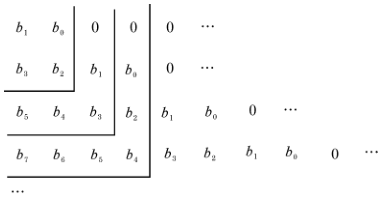
\includegraphics[width=\linewidth]{figs/fig-0185.png}
\end{figure}

\[\left|\begin{array}{lll} b_{1} & b_{b} & 0 \\ b_{3} & b_{2} & b_{1} \\ b_{5} & b_{4} & b_{3} \\ b_{7} & b_{6} & b_{5} \\ \cdots & & \end{array}\right|\left|\begin{array}{lll} 0 & \cdots \\ 0 & \cdots \\ b_{1} & b_{0} & 0 & \cdots \\ b_{3} & b_{2} & b_{1} & b_{b} & 0 & \cdots \end{array}\right|\]

记

\[\Delta_{1}=b_{1}, \quad \Delta_{2}=\left|\begin{array}{ll} b_{1} & b_{b} \\ b_{b} & b_{b} \end{array}\right|, \quad \Delta_{3}=\left|\begin{array}{lll} b_{1} & b_{b} & 0 \\ b_{b} & b_{x} & b_{b} \\ b_{b} & b_{1} & b_{b} \end{array}\right|, \cdots\]

于是，霍尔维茨判据可以叙述如下：系统稳定的充分条件为不等式 $b_{b}>0$，并且各个霍尔维茨行列式 $\Delta_{1}, \Delta_{2}, \Delta_{3}, \cdots, \Delta_{n}$ 均大于零。此时 $F(s)$ 的一切根均有负实部。

上面介绍的两种方法简化了稳定判别的过程，从而使我们比较直观地看出离散系统的稳定情况。

我们在开始时还提到过一个重要的系统品质指标，即系统的静态误差。这一概念是在跟踪问题中产生的。欲使受控对象式 (10.1-4) 的输出状态向量 $\mathbf{y}(t)$ 随着某一输入作用变化，控制量 $u(t)$ 应使在 $t \rightarrow \infty$ 时跟踪误差最小或为零。遗憾的是并不是任何系统对任何输入作用都可以使跟踪误差为零，而只有某些所谓无静差系统，对某些特定类型的输入作用，才有这种性能。下面我们将研究一个系统无静差的充分条件。设 $n$ 维向量函数 $\mathbf{g}(t)=\left(\mathbf{g}_{1}(t), \mathbf{g}_{2}(t), \mathbf{g}_{3}(t), \cdots, \mathbf{g}_{n}(t)\right), t=0, T, 2 T, \cdots, m T, \cdots$，为系统的输入作用，受控系统输出 $\mathbf{y}(t)$ 应跟踪它。或者，需选择控制参数，使经过足够大时间后，误差向量

\[\varepsilon(t)=\mathbf{g}(t)-\mathbf{y}(t)\qquad\text{(10.5-9)}\]

将一致趋于零。我们将 $\mathbf{y}(t)=\mathbf{g}(t)-\varepsilon(t)$ 代入式 (10.5-4) 就得到

\[H \mathbf{g}(t)-H \varepsilon(t)=D \mathbf{g}(t)-D \varepsilon(t)+\mathbf{c} u(t)\qquad\text{(10.5-10)}\]

或

\[H \varepsilon(t)=D \varepsilon(t)-\mathbf{c} u(t)+H \mathbf{g}(t)-D \mathbf{g}(t)\]

现将 $\varepsilon(t)=\left(\varepsilon_{1}(t), \varepsilon_{2}(t), \varepsilon_{3}(t), \cdots, \varepsilon_{n}(t)\right)$ 看成系统的状态向量。控制量 $u$ 的作用是使 $\varepsilon(t)$ 的每一个坐标趋于零。方程式 (10.5-10) 与 (10.1-4) 的差别，就在于前者有干扰作用。此外两种方程式本身无大的差别，其中 $D$ 矩阵和 $\mathbf{c}$ 向量都保持了原来的形式。显然，若输入作用满足差分方程式

\[H \mathbf{g}(t)=D \mathbf{g}(t)\qquad\text{(10.5-11)}\]

而且按误差反馈的闭路系统是渐近稳定的，则无论系统初始状态如何，误差 $\varepsilon(N T)$ 将趋于零。我们常称系统式 (10.1-4) 对满足条件式 (10.5-11) 的输入作用为无静差系统，而等式 (10.5-11) 为系统无静差的充分条件。我们把满足方程式 (10.5-11) 的输入函数称之为系统的固有输入作用类。

例。讨论具有两个积分环节的系统，如图 10.5-5 所示。令 $\gamma=1, T=1$，则其差分方程式为

\[H \mathbf{y}(m T)=D \mathbf{y}(m T)+\mathbf{c} u\]

式中

\begin{figure}[htbp]\centering
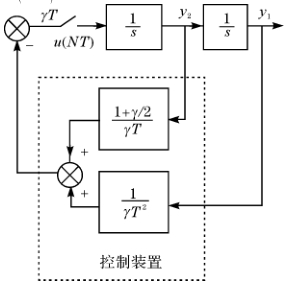
\includegraphics[width=\linewidth]{figs/fig-0186.png}
\caption{图10.5-5}
\end{figure}

\[D=\left[\begin{array}{ll} 1 & T \\ 0 & 1 \end{array}\right], \quad \mathbf{c}=\left(\begin{array}{c} T^{2} \\ 2 \\ 1 \end{array}\right)\]

(a)

图 10.5-5

设输入作用 $g_{1}(t)=\omega+a t$，式中 $\omega, a$ 均为常系数，该输入作用所确定的相对应的输入作用向量为

\begin{figure}[htbp]\centering
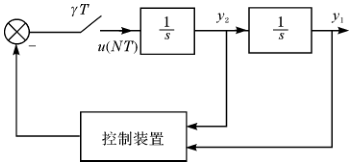
\includegraphics[width=\linewidth]{figs/fig-0187.png}
\caption{图10.5-5}
\end{figure}

\[\mathbf{g}(t)=\left(\begin{array}{c}\alpha_{\mathbf{v}}+\alpha_{\mathbf{v}} t \\\alpha\end{array}\right)\]

不难检查，$\mathbf{g}(t)$ 满足方程式 $(10.5-11)$

\[H \mathbf{g}(m T)-D \mathbf{g}(m T)=\left(\begin{array}{c}\alpha_{\mathbf{v}}+\alpha_{\mathbf{v}}(m+1) T \\a\end{array}\right)-\left[\begin{array}{ll}1 & T \\0 & 1\end{array}\right]\left(\begin{array}{c}\alpha_{\mathbf{v}}+\alpha_{\mathbf{v}} m T \\\alpha\end{array}\right)=\mathbf{0}\]

因此，上述系统对这样的输入作用 $\mathbf{g}(t)$ 是无静差系统。但是当输入作用不为 $t$ 的线性函数，而含有 $t$ 的二次项时，系统将变为有静差的了。

如 $g_{1}(t)=\alpha_{\mathbf{v}}+\alpha_{\mathbf{v}} t+\alpha_{\mathbf{v}} t^{2}$，式中 $\alpha_{\mathbf{v}}, \alpha$ 和 $\alpha$，均为常量。对于这样的输入作用所确定的相对应的输入作用向量为

\[\mathbf{g}(t)=\left(\begin{array}{c}\alpha_{\mathbf{v}}+\alpha_{\mathbf{v}} t+\alpha_{\mathbf{v}} t^{2} \\\alpha+2 \alpha t\end{array}\right)\]

我们计算出

\[H \mathbf{g}(m T)-D \mathbf{g}(m T)=\left(\begin{array}{c}\alpha_{\mathbf{v}} T^{2} \\2 \alpha_{\mathbf{v}} T\end{array}\right)=\boldsymbol{f}\]

不为零向量，所以系统是有静差系统。把上式代入式 $(10.5-10)$ 中，便得到

\[H \varepsilon(m T)=D \varepsilon(m T)-\mathbf{c u}(m T)+\boldsymbol{f}\]

当我们把上式变成以误差反馈的闭路系统时，例如，令 $u(m T)=k_{1} \varepsilon(m T)+$ $k_{2} \varepsilon(m T)$，当 $t$ 足够大而系统达到稳态时，$\lim _{m \rightarrow \infty} H \varepsilon(m T)=\varepsilon(m T)$。不难检查，当 $k_{1} \neq 0, c_{2} \neq 0$ 时，$(E+K-D)$ 是可逆矩阵，此处

\[\begin{gathered}K=\left(\begin{array}{ll}c_{1} & c_{1} k_{2} \\c_{2} & k_{1} & c_{2} k_{2}\end{array}\right) \\{\mathrm{det}}(E+K-D)=c_{1} k_{1} T \neq 0\end{gathered}\]

于是，系统的静态误差为

\[\begin{aligned}\varepsilon(m T) & =(E+K-D)^{-1} f \\& =\left(\begin{array}{c}\frac{k_{2}}{k_{1}} T \quad \frac{1}{c_{2} k_{1}}-\frac{c_{1} k_{2}}{c_{2} k_{1} T} \\-\frac{1}{T} \quad \frac{c_{1}}{c_{2} T}\end{array}\right)\left(\begin{array}{c}\alpha_{\mathbf{v}} T^{2} \\2 \alpha_{\mathbf{v}} T\end{array}\right)=\alpha_{\mathbf{v}}\left(\begin{array}{c}\frac{k_{2}}{k_{1}}+2 \frac{T-c_{1} k_{2}}{c_{2} k_{1}} \\\frac{2 c_{1}}{c_{2}}-T\end{array}\right)\end{aligned}\]

从上式我们可以看出，系统的静差与输入作用的加速度 $\alpha_{\mathbf{v}}$ 成正比，并和采样周期 $T$ 有关。而矩阵

\[(E+K-D)^{-1}=\left(\begin{array}{c}\frac{k_{2}}{k_{1}} T \quad \frac{1}{c_{2} k_{1}}-\frac{c_{1} k_{2}}{c_{2} k_{1} T} \\-\frac{1}{T} \quad \frac{c_{1}}{c_{2} T}\end{array}\right)\]

称为系统的静差系数矩阵。

当然，上列关于静态误差的讨论仅对按误差反馈的闭路系统才是正确的。如果采用复合控制方法，即 $u$ 不仅是 $\varepsilon$ 的线性函数，而且也是 $\boldsymbol{g}(t)$ 的线性函数时，原来是有静差的系统，现在就可能变为无静差了。关于复合控制系统的理论在线性连续系统的理论中已做过详细讨论。那些计算方法可以完全类似地适用于对离散系统的分析，故此处不再重复。

\section{10.6 线性离散系统的综合}

前面几节我们对线性离散系统进行了分析，这一节将研究线性离散系统的综合问题。由于高阶差分方程式和一阶方程组等价，故只研究方程组的情形，所得到的结论可直接应用到高阶差分方程式所描述的离散系统。

设受控对象的运动规律是由下述线性常系数差分方程组描述的，

\[H \mathbf{y}(N T)=D \mathbf{y}(N T)+\boldsymbol{c} u(N T)\]

其中控制量 $u(t)$ 假定不受限制。当然，在实际问题中，一般说来这是不可能的。但当 $u(t)$ 为误差坐标的线性组合，而误差又比较小时，此时 $u(t)$ 的取值也不会很大，往往处于其可准取值范围之内。这样就可以认为 $u(t)$ 取值不受限制。在这种假定下设计出来的系统，一般能满足对系统的基本要求，如稳定性，较短的过渡过程时间等。

若系统初始误差为 $\mathbf{y}_{0}=\left(y_{10}, y_{20}, \cdots, y_{n 0}\right)$，按差分方程的通解公式有

\[\mathbf{y}(N T)=D^{\mathrm{N}} \mathbf{y}_{0}+D^{\mathrm{N}} \sum_{m=0}^{N-1} D^{-(m+1)} \boldsymbol{c} u(m T)\]

现选择控制规律，使系统误差为零。我们先来证明一个简单的事实，就是在断续系统中，利用线性控制规律，可以使任何初始条件在有限时间内使其误差为零。设系统的差分方程是 $n$ 阶的，或者说差分方程组含有 $n$ 个方程式，现证明对完全能控的系统可以选择一种线性控制规律，在 $n T$ 时间内无论初始偏差为何，总有 $\mathbf{y}(n T)=\mathbf{0}_{\text {。 }}$ 为此将式 (10.2-6) 整理后令 $\mathbf{y}(n T)=\mathbf{0}$，有

\[\mathbf{y}_{0}=-D^{-n} \boldsymbol{c} u[(n-1) T]-D^{-n+1} \boldsymbol{c} u[(n-2) T]-\cdots-D^{-1} \boldsymbol{c} u(0)\qquad\text{(10.6-1)}\]

或者写成

\[D^{n} \mathbf{y}_{0}=-\boldsymbol{c} u[(n-1) T]-D c u[(n-2) T]-\cdots-D^{n-1} \boldsymbol{c} u(0)\]

当系统为完全能控时向量

\[c, D c, D^{2} c, \cdots, D^{n-1} c\]

线性不相关，他们构成 $n$ 维相空间的基底向量，任何误差向量所确定的 $D^{n} \mathbf{y}_{0}$ 均可由式(10.6-2)各向量的线性组合表示出来。不难检查，若 $c, D c, D^{2} c \cdots D^{n-1} c$ 线性不相关，那么向量

\[\boldsymbol{r}_{\mathrm{r}}=-D^{-1} \boldsymbol{c}, \boldsymbol{r}_{2}=-D^{-2} \boldsymbol{c}, \cdots, \boldsymbol{r}_{n}=-D^{-n} \boldsymbol{c}\]

也必然线性无关。将 $\boldsymbol{r}_{\mathrm{r}}=\left(r_{11}, r_{12}, \cdots, r_{n}\right)$ 代入式 $(10.6-1)$ 中后，得到线性代数方程组

\[\begin{aligned} & y_{10}=r_{n 1} u_{n-1}+r_{n-1,1} u_{n-2}+\cdots+r_{11} u_{0} \\ & y_{20}=r_{n 2} u_{n-1}+r_{n-1,2} u_{n-2}+\cdots+r_{12} u_{0} \\ & \cdots \\ & y_{n 0}=r_{n n} u_{n-1}+r_{n-1, n} u_{n-2}+\cdots+r_{n n} u_{0} \end{aligned}\qquad\text{(10.6-3)}\]

其中 $y_{10}, y_{20}, \cdots, y_{n 0}$ 为给定的系统初始误差坐标。 $u=u(i T), i=0,1,2, \cdots, n-1$，为待求的控制量。由于诸向量 $\boldsymbol{r}_{\mathrm{r}}$ 所组成的矩阵行列式不为零，即 $\operatorname{det}\left(\boldsymbol{r}_{\mathrm{r}}, \boldsymbol{r}_{\mathrm{r}}\right.$，$\left.\boldsymbol{r}_{\mathrm{r}}, \cdots, \boldsymbol{r}_{n}\right) \neq 0$，所以代数方程式中的 $u$ 有唯一解

\[u_{i}=\frac{\operatorname{det}\left(\boldsymbol{r}_{1}, \cdots, \boldsymbol{r}_{n-1}, \boldsymbol{y}_{0}, \boldsymbol{r}_{n+1} \cdots \boldsymbol{r}_{n}\right)}{\operatorname{det}\left(\boldsymbol{r}_{1}, \boldsymbol{r}_{2}, \cdots, \boldsymbol{r}_{n}\right)}, \quad i=1,2, \cdots, n\qquad\text{(10.6-4)}\]

将 $u$ 之值代入式 $(10.2-6)$ 中后，无论系统初始误差状态如何，式 $(10.6-4)$ 所决定的控制参数将最多在 $n$ 步内使系统的误差归零。或者说任何过渡过程都在 $n$ 个采样周期内结束。当然过渡时间也可以小于 $n T_{0}$。初看式 $(10.6-4)$ 似乎是为了确定控制参数之值，必须算出它的 $n$ 步内之诸值: $u(0), u(T), u(2 T), \cdots, u[(n-1) T]$。其实为了使离散系统获得上述性能，只需算出 $u(0)$ 之值就足够了。因为差分方程 $(10.1-4)$ 为常系数方程式，在任何时刻 $t=\alpha T$ 均能将 $\mathbf{y}(\alpha T)$ 看作下一步的初始条件，只要系统诸坐标的价值不断地测量即可。根据式 $(10.6-4)$ 可求出

\[\begin{aligned} & w=u(0) \\ & =\frac{\operatorname{det}\left(\boldsymbol{y}_{0}, \boldsymbol{r}_{1}, \boldsymbol{r}_{2}, \cdots, \boldsymbol{r}_{n}\right)}{\operatorname{det}\left(\boldsymbol{r}_{1}, \boldsymbol{r}_{2}, \cdots, \boldsymbol{r}_{n}\right)} \\ & =\frac{R_{11}}{\Delta} y_{10}+\frac{R_{12}}{\Delta} y_{20}+\cdots+\frac{R_{n n}}{\Delta} y_{n 0} \end{aligned}\]

其中 $\Delta=\operatorname{det}\left(\boldsymbol{r}_{1}, \boldsymbol{r}_{2}, \cdots, \boldsymbol{r}_{n}\right), R_{n}$ 为此行列式元素 $r_{n i}$ 之代数余子式。将 $u(0)$ 之值代入式 $(10.1-4)$，去掉 $y_{10}, y_{20}, \cdots, y_{n 0}$ 的零注角则得到闭路方程式。

\[\begin{aligned} H \mathbf{y}(t) & =D \mathbf{y}(t)+\boldsymbol{c} \boldsymbol{u}(t) \\ & =D \mathbf{y}(t)+\boldsymbol{c}\left(\frac{R_{11}}{\Delta} y_{1}+\frac{R_{12}}{\Delta} y_{2}+\cdots+\frac{R_{1 n}}{\Delta} y_{n}\right) \\ & =\left(D+C\right) \mathbf{y}(t)=B \mathbf{y}(t), t=0, T, 2 T, \cdots \end{aligned}\qquad\text{(10.6-5)}\]

式中

\[B=(D+C)\qquad\text{(10.6-6)}\]

C=1/(arrayc@c@c@c c\_1 R\_11 \& c\_1 R\_12 \&  \& c\_1 R\_1 n \textbackslash\{\}\textbackslash\{\} c\_2 R\_11 \& c\_2 R\_12 \&  \& c\_2 R\_1 n \textbackslash\{\}\textbackslash\{\}  \&  \& \&  \textbackslash\{\}\textbackslash\{\} c\_n R\_11 \& c\_n R\_12 \&  \& c\_n R\_1 n array)

由此可知，用上述办法综合的闭路系统依然是一个为线性差分方程所描绘的系统。由于它能在 $n$ 步内使任何初始误差归零，故式 (10.6-6) 所描述的闭路系统常称之为最优线性离散系统。

作为例子，试综合受控对象为串联的两个积分环节的系统。我们可以写出开环系统的运动微分方程式

\[\frac{d y_{1}}{d t}=y_{2}^{2}, \quad \frac{d y_{2}}{d t}=u\]

或者

\[\frac{d \mathbf{y}}{d t}=A \mathbf{y}+\boldsymbol{b} u\]

其中

\[A=\left[\begin{array}{ll} 0 & 1 \\ 0 & 0 \end{array}\right], \quad \boldsymbol{b}=\left[\begin{array}{l} 0 \\ 1 \end{array}\right]\]

又可以求出相应的差分方程式

\[H \mathbf{y}(N T)=D \mathbf{y}(N T)+\boldsymbol{c} u(N T)\]

式中

\[D=\left[\begin{array}{ll} 1 & T \\ 0 & 1 \end{array}\right], \quad \boldsymbol{c}=\left(\begin{array}{c} \gamma T^{2}\left(1-\frac{1}{2} \gamma\right) \\ \gamma T \end{array}\right)\]

经过检查可知 $\boldsymbol{c}$ 和 $D \boldsymbol{c}$ 是线性不相关的。根据上述讨论可以求出

\[\begin{aligned} & r_{1}=-D^{-1} c=-\left[\begin{array}{cc} 1 & -T \\ 0 & 1 \end{array}\right]\left(\begin{array}{c} \gamma T^{2}\left(1-\frac{1}{2} \gamma\right) \\ \gamma T \end{array}\right)=\left(\begin{array}{c} \frac{1}{2}(\gamma T)^{2} \\ -\gamma T \end{array}\right) \\ & r_{2}=-D^{-2} c=\left[\begin{array}{cc} 1 & -T \\ 0 & 1 \end{array}\right]\left(\begin{array}{c} \frac{1}{2}(\gamma T)^{2} \\ -\gamma T \end{array}\right)=\left(\begin{array}{c} \gamma T^{2}\left(1+\frac{1}{2} \gamma\right) \\ -\gamma T \end{array}\right) \\ & \Delta=\left(\begin{array}{cc} \frac{1}{2}(\gamma T)^{2} & \gamma T^{2}\left(1+\frac{1}{2} \gamma\right) \\ -\gamma T & -\gamma T \end{array}\right)=\gamma^{2} T^{2} \end{aligned}\]

再根据式 (10.6-5) 求出

\[R_{11}=-\gamma T, \quad R_{12}=-\gamma T^{2}\left[1+\frac{1}{2} \gamma\right]\]

代入式 (10.6-5) 即求出控制函数

\[u(0)=\frac{-1}{\gamma T^{2}} y_{01}-\frac{\left[1+\frac{1}{2} \gamma\right]}{\gamma T} y_{02}\qquad\text{(10.6-7)}\]

所以

\[\begin{aligned} C & =\left|\begin{array}{cc} 1-\frac{1}{2} \gamma & -T\left(1-\frac{1}{4} \dot{\gamma}\right) \\ -\frac{1}{T} & -\left(1+\frac{1}{2} \gamma\right) \end{array}\right| \\ B & =\left(\begin{array}{cc} \frac{1}{2} \gamma & \frac{1}{4} \dot{\gamma} T \\ -\frac{1}{T} & -\frac{1}{2} \gamma \end{array}\right) \end{aligned}\]

于是闭路系统差分方程式

\[H \mathbf{y}=B \mathbf{y}, \quad c u(\alpha T)=C y(\alpha T), \quad \alpha=0,1,2, \cdots,(n-1)\]

或者，写成展开形式:

\[\begin{aligned} & y_{1}(m T)=\frac{1}{2} \gamma y_{1}\left[(m-1) T\right]+\frac{1}{4} \dot{\gamma}^{2} T y_{2}\left[(m-1) T\right] \\ & y_{2}(m T)=-\frac{1}{T} y_{1}\left[(m-1) T\right]-\frac{1}{2} \gamma y_{2}\left[(m-1) T\right] \end{aligned}\qquad\text{(10.6-8)}\]

不难检查式 (10.6-8) 是最优系统，因为无论 $\mathbf{y}_{0}=\left(\gamma_{10}, \gamma_{20}\right)$ 为何，只需 $m=2$ 便有 $y_{1}(2 T)=0, y_{2}(2 T)=0$。且此后 $y_{1}(m T) \equiv y_{2}(m T) \equiv 0, m>2$。事实上，根据通解公式有

\[\mathbf{y}(m T)=B^{m} \mathbf{y}_{0}\]

但是

\[B^{2}=\left(\begin{array}{cc} \frac{1}{2} \gamma & \frac{1}{4} \dot{\gamma} T \\ -\frac{1}{T} & -\frac{1}{2} \gamma \end{array}\right)\left(\begin{array}{cc} \frac{1}{2} \gamma & \frac{1}{4} \dot{\gamma} T \\ -\frac{1}{T} & -\frac{1}{2} \gamma \end{array}\right)=\left(\begin{array}{ll} 0 & 0 \\ 0 & 0 \end{array}\right)\]

所以，$m \geqslant 2$ 时，$\mathbf{y}(m T) \equiv \mathbf{0}$。这样我们就可以按式 (10.6-7) 中的关系式得到待求之控制装置。

\section{10.7 最优控制函数的综合}

前节内我们讨论的线性系统，曾假定控制量 $u$ 取值范围没有限制，这只是在某些情况下，例如在小扰动的情况下才有意义。几乎所有的线性理论的应用范围都大致如此。但是，在实际技术问题中控制量 $u$ 不受限制的情况是比较少见的。当控制量有了限制之后，系统的运动状态就要发生重要的变化，其综合方法也与以前讨论的不同。一般来讲，系统的限制条件有两类，一类为对控制量的限制，一类为对某些系统状态坐标的限制。这两种限制不是一回事，在设计系统时应考虑这两种限制。实际技术问题中，对坐标限制往往能利用一些特殊装置自动地实现。如随动系统常用的角度限制器，速度限制器与加速度限制器等。对控制量的限制是由控制器本身的特性决定的。例如放大器输出的最大电压和最大功率，已经由它的结构参数所确定，飞行器舵的最大转角常由机械结构情况和飞行器的气动特性所确定。从控制系统综合来看，以上两种限制都应该考虑。

在本节内我们只讨论控制量有限制的控制装置的综合问题，因为在这方面的研究工作近些年来有不少进展 ${ }^{[25-27]}$。对最速控制系统已经提出了一些工程技术上可以采用的理论结果和计算方法。现讨论前面提出的线性差分方程

\[H y=D y+c u\qquad\text{(10.7-1)}\]

其中 $u$ 的取值范围受到下列条件的限制:

\[|u| \leqslant M\qquad\text{(10.7-2)}\]

满足式 (10.7-2) 的控制 $u$ 叫做准控制。

设已知系统式 (10.7-1) 的初始状态为 $\mathbf{y}=\left(y^{10}, y_{20}, \cdots, y_{w 0}\right)$，需要求出一个准控制 $u(t), t=0, T, 2 T, \cdots, N T$; 代入式 (10.7-1) 后，系统将以最采样周期，到达预定的状态。当然，预定状。当然，预定状态不同，最优控制也将不同。下面我们

将认为预定的终点状态是原点。

我们再讨论一下系统的能控性问题。在 10.2 节中我们曾讨论了线性系统能控性的充要条件。那个条件是在控制量不受限制的情况下得到的，在控制量受限制的条件下，情况将发生变化。我们需要重新定义系统性的能控性。设 $\mathbf{y}$ 是系统的初始状态，如果可以用某一可准控制 $u(t),|u(t)| \leqslant M$，可把 $\mathbf{y}$ 引到原点，我们称 $\mathbf{y}$ 为可控点；如果状态空间中有一个区域完全由可控点组成，则称为可控区；如果全部状态空间中的点都是可控的，则该系统称为全局可控。在控制量受限制的情况下，弄清可控性当然是很重要的。因为如果受控量和控制量不受限制的线性系统是完全能控的，当控制量受限制时就不一定是能控的，此时所谓最优控制问题就不一定有解。下面我们介绍全局可控性的充要条件。设式 (10.7-1) 为常系数线性系统，限制条件为式 (10.7-2)，$D$ 为非蜕化矩阵。系统为全局可控的充要条件是

(1) $n$ 个向量 $\mathbf{c}, D \mathbf{c}, D^{2} \mathbf{c}, \cdots, D^{n-1} \mathbf{c}$ 线性无关。

(2) 矩阵 $D$ 的一切本征值满足不等式。

\[\mid \lambda \mid \leqslant 1, \quad i=1,2, \cdots, n\qquad\text{(10.7-4)}\]

为了说明这两个条件的意义，我们再把式 (10.7-1) 的通解写出

\[\mathbf{y}(N T)=D^{N} \mathbf{y}_{0}+D^{N-1} c u(0)+\cdots+c u((n-1) T)\]

设存在自然数 $N$，用控制 $u(t)=\left\{u(0), u(T), \cdots, u((N-1) T)\right\}$ 可把 $\mathbf{y}$ 引到原点，$\mathbf{y}(N T)=\mathbf{0}$。因为 $D$ 为非蜕化矩阵，上式可改写为式 (10.6-1) 的形式。令

\[r_{1}=-D^{-1} \mathbf{c}, r_{2}=-D^{-2} \mathbf{c}, \cdots, r_{N}=-D^{-N} \mathbf{c}\qquad\text{(10.7-5)}\]

于是有

\[\mathbf{y}_{0}=u_{0} \mathbf{r}+u_{1} \mathbf{r}_{2}+\cdots+u_{N-1} \mathbf{r}_{N}\qquad\text{(10.7-6)}\]

式中 $u_{i}$ 满足限制条件 $\left|u_{i}\right| \leqslant M$。从上式可以看出，凡是能用式 (10.7-6) 表达出来的 $\mathbf{y}_{0}$ 点均为可控点，并且可以用可准控制在不大于NT的时间内到达原点。依据这种几何概念，我们来检查条件式 (10.7-3)和(10.7-4)的充分性和必要性。

若 $c, D c, D^{2} c, \cdots, D^{n-1} c$ 向量线性相关，那么，式(10.7-5)向量序列中任意 $N$个线性相关，$N \geqslant n_{0}$。由定义式 (10.7-5) 知此时 $\mathbf{r}, \mathbf{r}_{2}, \cdots, \mathbf{r}_{n}$ 线性相关，即存在 $n$ 个不全为零的常数 $C_{1}, C_{2}, \cdots, C_{n}$，使

\[C_{1} \mathbf{r}+C_{2} \mathbf{r}_{2}+\cdots+C_{n} \mathbf{r}_{n}=\mathbf{0}\qquad\text{(10.7-7)}\]

由此可知，$\mathbf{r}_{n}$ 向量可由前面 $n-1$ 个向量的线性组合表示出来，它属于前 $m$ 个向量所构成的子空间 $R_{m}$，其中 $m<n_{0}$。不难检查，无论 $N$ 为什么大，式 (10.7-7)所能达到的点均属于 $R_{m}$。由于子空间 $R_{m}$ 的维数小于 $n$，那么必存在大于 1 维的子空间 $R_{l}, l=n-m, l \geqslant 1$，其中任何点均不能用式 (10.7-6) 表示出来。换言之，若式 (10.1-4) 的初始状态为 $R_{l}$ 中之某一点，那么无论用什么可准控制都不能使系。这就说明条件式 (10.7-3) 是全局可控的必要条件。

设式 (10.7-4) 不等式不成立，也就是说某个根 $\left|\lambda_{i}\right|>1$。现对式 (10.1-4) 进行坐标变换，令 $P$ 为某一非蜕化方阵，令

\[x=P \mathbf{y}, \quad \operatorname{det} P \neq 0\]

代入式 (10.1-4) 后有

\[H \mathbf{x}=P D P^{-1} \mathbf{x}+P c u\qquad\text{(10.7-8)}\]

选择矩阵 $P$ 使 $J=P D P^{-1}$ 成为约当标准型。用 $J_{l}$ 表示对应于 $\lambda_{l}$ 的约旦块，它的行数为 $l$，用 $\mathbf{d}$ 表示 $P c_{l}$，则方程式 (10.7-8)到达零点的通解可以写成

\[\mathbf{x}_{0}=u_{0} \mathbf{r}+u_{1} \mathbf{r}_{2}+\cdots+u_{N-1} \mathbf{r}_{N-1}\]

其中

\[\mathbf{r}=-J^{-1} \mathbf{d}, \mathbf{r}_{2}=-J^{-2} \mathbf{d}, \cdots, \mathbf{r}_{N}=-J^{-N} \mathbf{d}\]

而

J\textasciicircum{}-m=(.\$ \$.J\_1\textasciicircum{}m, , J\_k\textasciicircum{}m)

\[J_{1}^{m}=\left(\begin{array}{ccccccc} \frac{1}{\lambda_{1}^{m}} & -\frac{m}{\lambda_{1}^{m+1}} & \cdots & -\frac{d^{l-1}\left[\frac{1}{\lambda_{1}^{m}}\right]}{(l-1) !} & \left.\right| d \lambda_{1}^{l-1} \\ 0 & \frac{1}{\lambda_{1}^{m}} & \cdots & \cdots & \\ \vdots & \vdots & \vdots & \vdots & \\ 0 & 0 & \cdots & \frac{1}{\lambda_{1}^{m}} \end{array}\right)\]

令 $\mathbf{d}=\left(d_{1}, d_{2}, \cdots, d_{n}\right)$，其中至少有一个 $d_{i} \neq 0$，设 $\lambda_{i}$ 为实数。某一个向量 $\mathbf{x}_{0}$ 能用式(10.7-6’)之右端有限项之和表示的必要条件之一是 $\boldsymbol{x}$ 的第 $l$ 个分量 $\boldsymbol{x}_{0 l}$ 需能写成

\[x_{0 l}=d\left(\frac{u_{l}}{\lambda_{l}}+\frac{u_{l}}{\lambda_{l}^{2}}+\cdots+\frac{u_{l-1}}{\lambda_{l}^{m}}+\cdots+\frac{u_{l}^{N-1}}{\lambda_{l}^{N}}\right)\]

由于 $|\lambda|>1$，则右端之和满足下列不等式

\[\mid \boldsymbol{x}_{0 l} \mid \leqslant \mid d M \mid \sum_{a=1}^{\infty} \frac{1}{\mid \lambda^{a}}=\frac{\mid d_{l} M \mid}{\mid \lambda_{l}|-1}=M_{1}\]

若取向量 $\boldsymbol{x}$，它的分量 $x_{0 l}>M_{1}$，则用任何可准控制均不能使受控对象由点 $\boldsymbol{x}_{0}=$ $\left(x_{10}, x_{20}, \cdots, x_{l-1,0}, \cdots, x_{n0}\right)$ 在有限时间内到达原点。当 $\lambda$ 为复数时，上述讨论变化不大，而结论相同。这说明，为了使式(10.1-4)为全局可控，条件式(10.7-4)和 (10.7-3)必须成立。

其次我们再证明当这些条件满足时，对任何非零的初始误差 $\boldsymbol{y}$ 和对任何自然数 $p$ 均能找到一组不为零的控制参数 $u_{p+1}, u_{p+2}, \cdots, u_{p+n}$，使

\[\boldsymbol{y}_{0}=q\left(u_{p} r_{p+1}+u_{p+1} r_{p+2}+\cdots+u_{p+n-1} r_{p+n}\right)=q \eta_{p}\]

$p=0,1,2, \cdots, \mid u_{p+i} \mid \leqslant M, q>0$。这是因为对任何 $p$ 诸向量 $r_{p+1}, r_{p+2}, \cdots, r_{p+n}$ 为线性不相关，可以构成 $n$ 维空间的基底，任何一个向量均可以用它们的线性组合表示。依假定我们知道，矩阵 $D$ 的特征根 $|\lambda| \leqslant 1$，重复前面的讨论可知，向量 $r_{p+i}, i=1,2, \cdots, n$ 的长度不随 $p$ 的增加而减小，于是上式内向量 $\eta_{p}$ 的长度总大于某一正数。对于任何 $\boldsymbol{y}$，均可取有限个向量，使

\[\boldsymbol{y}_{0}=\sum_{a=1}^{N} \eta_{p}\]

由上述讨论可知，若系统式 $(10.1-4)$ 满足式 $(10.7-3)$ 和 $(10.7-4)$ 两个条件，对任何初始点 $\boldsymbol{y}$ 都可以找到一个可准控制 $u(\alpha T), \alpha=1,2, \cdots, N$ 使系统在有限时间内归零。

参照对连续系统的讨论，在解决综合问题时我们主要应用等时区的概念。下面我们就来研究等时区的性质。从线性离散系统的运动规律式 (10.7-6) 可知，当 $N$ 为有限数时所能得到的 $\boldsymbol{y}_{0}$ 的范围总是有限的。这是因为诸向量的系数 $u$ 受到条件式 $(10.7-2)$ 的限制。我们称由式 $(10.7-6)$ 所决定的一切 $\boldsymbol{y}_{0}$ 点的集合为等时区，记为 $G(N T)$。同样我们从式 $(10.7-6)$ 的几何意义可知，$G(N T)$ 在 $N \geqslant n$ 时构成 $n$ 维多面体，坐标原点为它的内点。当 $N=1$ 时，$G(T)$ 只含有一个通过原点的向量，$\boldsymbol{y}=\boldsymbol{r}_{0} u_{0}=-D^{-1} c u_{0},-M \leqslant u_{0} \leqslant M ; G(2 T)$ 为包含原点的一个平行四边形，其各边为 $\pm M r_{1}$ 和 $\pm M r_{2} ; G(3 T)$ 为包含原点的一个平行六面体，其各棱边为 $\pm M r_{1}, \pm M r_{2}$ 和 $\pm M r_{3}$; 依此类推，$G(n T)$ 为包含原点在内的一个 $n$ 维多面体，其棱边分别为 $\pm M r_{1}, \pm M r_{2}, \cdots, \pm M r_{n}$。

容易检查，$G(N T)$ 是闭凸多面体，若 $\boldsymbol{y}$ 属于 $G(N T), \boldsymbol{y}_{2}$ 也属于 $G(N T)$，那么它们连线上的任一点 $\boldsymbol{y}$ 也属于 $G(N T)$。

因为对 $\lambda, 0 \leqslant \lambda \leqslant 1$，有

alignedy \& =(1-) y\_1+ y\_2 \textbackslash\{\}\textbackslash\{\}\& =(1-) \_a=1\textasciicircum{}N(arrayl(1) \textbackslash\{\}\textbackslash\{\}(1)array u\_a-1 r\_a+ \_a=1\textasciicircum{}N.u\_a-1\textasciicircum{}(2) r\_a\textbackslash\{\}. \textbackslash\{\}\textbackslash\{\}\& =[(1-) \_a=1\textasciicircum{}N.u\_a-1\textasciicircum{}(1)+ \_a=1\textasciicircum{}N.u\_a-1\textasciicircum{}(2)\textbackslash\{\}] r\_a \textbackslash\{\}\textbackslash\{\}\& =\_a=1\textasciicircum{}N[(1-) u\_a-1\textasciicircum{}(1)+ u\_a-1\textasciicircum{}(2)] r\_aaligned

而 $\left|u_{a-1}^{(1)}\right| \leqslant M,\left|u_{a-1}^{(2)}\right| \leqslant M$。所以 $\left|(1-\lambda) u_{a-1}^{(1)}+\lambda u_{a-1}^{(2)}\right| \leqslant M$。这就证明了 $\mathbf{y}$ 点用可

准控制在 $N$ 步内可以到达。当 $N \geqslant n$ 时，$G(N T)$ 为一个 $n$ 维凸多面体，它的表面是有限个平面和棱线组合成的。按等时区的定义可知，若有一点 $\mathbf{y}$ 不属于 $G(N T)$，那么，自该点到达原点，如果可能的话，所费时间一定大于 $N T$。若 $\mathbf{y}$ 点属于 $G(N T)$ 而不属于 $G_{c}^{*}\left[(N-1) T_{1}\right]$，则自该点到达原点至少需要 $N$ 步。

例。一个系统运动的方程式为

\[\begin{aligned}& \frac{d y_{1}}{d t}=y^{2} \\& \frac{d y_{2}}{d t}=u, \quad \mid u \mid \leqslant 1\end{aligned}\]

相应的离散运动方程式为

\[\begin{aligned}& H y_{1}(m T)=y_{1}(m T)+T y_{2}(m T)+\gamma T^{2}\left(1-\frac{1}{2} \gamma\right) u(m T) \\& H y_{2}(m T)=y_{2}(m T)+\gamma T u(m T)\end{aligned}\]

当 $\gamma=1, T=1$ 时有

\[\begin{aligned}& H y_{1}(m T)=y_{1}(m T)+y_{2}(m T)+\frac{1}{2} u(m T) \\& H y_{2}(m T)=y_{2}(m T)+u(m T)\end{aligned}\]

由此可知

\[\begin{aligned}& D=\left[\begin{array}{ll}1 & 1 \\0 & 1\end{array}\right] \\& \mathbf{c}=\left[\begin{array}{l}1 \\\frac{1}{2} \\1\end{array}\right] \\& \mathbf{r}=-D^{-1} \mathbf{c}=-\left[\begin{array}{ll}1 & -1 \\0 & 1\end{array}\right]\left[\begin{array}{l}\frac{1}{2} \\1\end{array}\right]=\left[\begin{array}{l}\frac{1}{2} \\-1\end{array}\right] \\& \mathbf{r}_{2}=-D^{-2} \mathbf{c}=\left[\begin{array}{ll}1 & -1 \\0 & 1\end{array}\right]\left[\begin{array}{l}\frac{1}{2} \\-1\end{array}\right]=\left[\begin{array}{l}\frac{3}{2} \\-1\end{array}\right]\end{aligned}\]

\[\begin{aligned}& r_{0}=-D^{-2} \boldsymbol{c}=\left(\begin{array}{cc}1 & -1 \\0 & 1\end{array}\right)\left(\begin{array}{c}\frac{3}{2} \\-1\end{array}\right)=\left(\begin{array}{c}\frac{5}{2} \\-1\end{array}\right) \\& \cdots \\& r_{N}=-D^{-N} \boldsymbol{c}=\left(\begin{array}{c}2 N-1 \\2 \\-1\end{array}\right)\end{aligned}\]

按定义知，$G(N T)$ 是由下列一切向量组成的凸多面体

\[\mathbf{y}=\sum_{k=1}^{N} \boldsymbol{r}_{k} U_{\alpha-1}, \quad \mid u_{k} \mid \leqslant 1, \quad \alpha=1,2, \cdots, N\]

图 10.7-1 内画出了 $N=1,2,3,4$ 时的等时区的几何形状。当 $N=1$ 时，$G(T)$ 为由 $+\boldsymbol{r}$ 和一 $\boldsymbol{r}$ 组成的通过原点的一段直线; $G(2 T)$ 为 $\boldsymbol{r}$ 和 $\boldsymbol{r}$ 所决定的平行四边形; $G(3 T)$ 为 $\boldsymbol{r}, \boldsymbol{r}$ 和 $\boldsymbol{r}$ 所组成的平面六边形; $G(4 T)$ 为 $\boldsymbol{r}, \boldsymbol{r}, \boldsymbol{r}$ 和 $\boldsymbol{r}$ 所组成的平面八边形。依此类推，可以画出任意 $G(N T)$ 来。可以看出，由于 $G(N T)$ 是凸的，所以只要求出所有的顶点用直线连接即可以。从上例中，我们得到启发，欲从 $G_{-}[(N-1) T]$ 中得到 $G(N T)$，只需在 $G_{-}[(N-1) T]$ 中的一切边界点上加上一个向量 $\pm M r_{N}$ 经过一切 $G_{-}[(N-1) T]$ 的边界点之后，便画出 $G(N T)$ 的一切边界点。不难看出这种作图法，对任何具有式 (10.1-4) 形式的系统都适合，这一事实可以写成

\[G(N T) \supset G_{-}[(N-1) T]\]

这种包含关系，不仅是终点为原点时才成立，而对于一切满足代数式 $(D-E) \mathbf{y}_{0}+$ $c u_{0}=\mathbf{0}, \mid u \mid<M$ 的系统终点状态 $\mathbf{y}_{0}$ 均有这种包含关系。此时我们称等时区为非降的。显然，当系统的终点为原点时，等时区总是非降的。

下面我们开始研究最优控制系统的综合方法。所谓最优控制函数的综合是指找出一个多元函数 $u\left(y_{1}, y_{2}, \cdots, y_{n}\right)$ 将其代入式 (10.1-4) 后，系统从任何初始状态出发，均能以最短的步数自动回到原点。一般来讲，这一 $n$ 元最优控制函数难以用解析式表达出来，而是分段取常值的离散函数。下面我们将通过对等时区的详细研究，求出最优控制函数之值在状态空间的分布规律。

设系统式 (10.1-4) 的初始条件为 $\mathbf{y}_{0}$，若存在一个可准控制函数 $\mid u(t) \mid \leqslant M$，$t=0, T, 2 T, \cdots, N T$，它能使系统以最短的时间 （最少步数） 达到原点，就称 $u(t)$ 是最速控制函数。我们将要看到，在绝大多数情况下与连续系统相反，最速控制函数不是唯一的，自 $\mathbf{y}$ 点有无穷多个不同的可准控制函数均能使系统以最短的时间到达原点，此时我们可以任选其中的一个作为设计的依据。设 $\mathbf{y}_{0}$ 位于等时区 $G(N T)$ 内，但不属于 $G_{-}[(N-1) T]$，那么按等时区的定义，自 $\mathbf{y}_{0}$ 到达原点的最短时间为 $N T$。任何可准控制函数 $u(t)$ 若能在 $N$ 步内使描绘点到达原点，它就是最速的。其次，若 $y_0 \in G(NT), N > 2$，但 $y_0$ 不属于 $G[(N-1)T]$，此时不存在任何可准控制 $u(0)$ 使 $y_0$ 在一步内进入 $G[(N-2)T]$，否则此点必属于 $G[(N-1)T]$。于是，任何可准控制 $u(t), t = 0, T, \cdots, (N-1)T$，如果它能使系统按下列规律变化

\[y_0 \in G(NT), y(T) \in G[(N-1)T], \cdots, y[(N-1)T] \in G(T), y(NT) = 0\qquad\text{(10.7-9)}\]

它一定是最速控制。因此在任何瞬间 $t = t_0$，若 $u(t_0)$ 能保证使 $y_0$ 进入相邻更小的等时区，则控制函数的该值为最优。

由于等时区形状为凸性多面体，所以它的一切顶点足以决定等时区的全体，又因为任何一条棱线都是两个顶点的连线，而任一平面都是两条棱线组成的平面，因此为了得到等时区，必须首先研究如何得到它的顶点。设 $y_0$ 是等时区 $G(NT)$ 的一个顶点，由于它是凸的，从此点出发通过 $G(NT)$ 的任何两条射线的夹角均小于 $180^\circ$，否则 $y_0$ 不会是等时区的顶点。通过 $y_0$ 作一支面 $P$，使 $G(NT)$ 完全位于支面 $P$ 的一侧，而且 $G(NT)$ 与 $P$ 只有一个交点 $y_0$ 如图 10.7-2 所示。过 $y_0$ 点作 $P$ 平面之外法向量 $\boldsymbol{\phi}_0, \boldsymbol{\phi}_0$ 与 $G(NT)$ 不在同一侧，而 $y_0$ 为顶点，所以对 $G(NT)$ 内任何异于 $y_0$ 之点 $y$ 均有不等式

\[(\boldsymbol{\phi}, y - y_0) \leqslant 0\qquad\text{(10.7-10)}\]

设自 $y$ 点到达原点的最速控制为 $u(t)$，而自 $y$ 点到达原点的控制为 $u(t)$，那么根据式 (10.7-6) 和 (10.7-10) 可得

\[\left\{\boldsymbol{\phi}, \sum_{s=1}^{N} \left\{[u(\alpha-1)T] - [u(\alpha-1)T]\right\}r_s\right\} \geqslant 0\qquad\text{(10.7-10)}\]

\begin{figure}[htbp]\centering
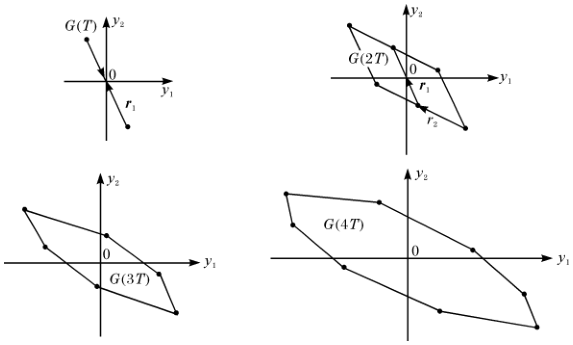
\includegraphics[width=\linewidth]{figs/fig-0188.png}
\caption{图10.7-1}
\end{figure}

\[\begin{aligned}& \text { 因为 } \mathbf{y} \text { 是任意选的,若令 } \\& u_{-}[(\alpha-1) T]=\left\{\begin{array}{l}u_{-}[(\alpha-1) T], \quad \alpha \neq N \\u^{\prime}, u^{\prime} \neq u_{-}[(\alpha-1) T], \quad \alpha=N, \mid u^{\prime} \mid \leqslant 1\end{array}\right.\end{aligned}\]

此时有

\[(\boldsymbol{\Psi}, \boldsymbol{r}_{N})\left(u_{-}(N-1) T\right)-u^{\prime} \geqslant 0\]

根据前面的讨论可知，若将 $\boldsymbol{r}_{N}=-D^{-N} \boldsymbol{c}$ 代入式后有

\[(-\left(D^{-N}\right)^{\mathrm{c}} \boldsymbol{\Psi}, \boldsymbol{c})\left(u_{-}(N-1) T\right)-u^{\prime} \geqslant 0\]

则

\[u_{-}(N-1) T=-M \operatorname{sign}\left(\left(D^{-N}\right)^{\mathrm{c}} \boldsymbol{\Psi}, \boldsymbol{c}\right)\]

重复上面的讨论，使 $\mathbf{y}_{0}$ 点到达原点的最速控制 $\dot{u}(t)$，在任意时刻 $t=0, T, 2 T, \cdots$，$m T$ 满足不等式

\[-(\left(D^{-m}\right)^{\mathrm{c}} \boldsymbol{\Psi}, \boldsymbol{c})\left(u_{-}(m-1) T\right)-u_{-}(m-1) T] \geqslant 0 \quad(10.7-11)\]

式中 $u_{-}[(m-1) T]-u_{-}[(m-1) T] \neq 0$; 欲使不等式 $(10.7-11)$ 成立，则要求向量 $\boldsymbol{\Psi}$满足下列条件

\[\left(\left(D^{-m}\right)^{\mathrm{c}} \boldsymbol{\Psi}, \boldsymbol{c}\right) \neq 0, \quad m=1,2, \cdots, N\]

因为 $\left(D^{-m}\right)^{\mathrm{c}} \boldsymbol{\Psi}$ 是式 $(10.2-7)$ 的解，我们可以把上面讨论的问题归纳成下列必要条件：设 $\dot{u}(t)$ 为自等时区 $G(N T)$ 的顶点 $\mathbf{y}_{0}$ 达到原点的最速控制，那么必存在一个非零向量 $\boldsymbol{\Psi}$，以它作为下列方程式的初始条件

\[\begin{aligned}H^{+} \boldsymbol{\Psi}(m T) & =\boldsymbol{\Psi}[(m-1) T]=D^{c} \boldsymbol{\Psi}(m T), \quad \boldsymbol{\Psi}(0)=\boldsymbol{\Psi} \\& (\boldsymbol{\Psi}(m T), \boldsymbol{c}) \neq 0, \quad m=1,2, \cdots, N\end{aligned}\qquad\text{(10.7-12)}\]

那么最速控制可表示为

\[\dot{u}(m T)=-M \operatorname{sign}(\boldsymbol{\Psi}((m+1) T), \boldsymbol{c})\qquad\text{(10.7-13)}\]

式 $(10.7-12)$ 和 $(10.7-13)$ 说明由等时区 $G(N T)$ 任意顶点到达原点的最速控制一定是极性控制，即 $\dot{u}(t)$ 的值只能是 $\pm M$，任何其他控制作用均不是最优的。为了以后讨论方便，和方程 $(10.1-4)$ 一起讨论它的逆运动方程式

\begin{figure}[htbp]\centering
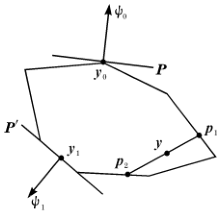
\includegraphics[width=\linewidth]{figs/fig-0189.png}
\caption{图10.7-2}
\end{figure}

\begin{figure}[htbp]\centering
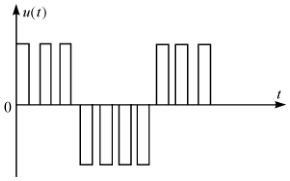
\includegraphics[width=\linewidth]{figs/fig-0190.png}
\caption{图10.7-3}
\end{figure}

\[H \mathbf{y}(m T)=D^{-1} \mathbf{y}(m T)-\mathbf{r}_{*} u(m T)\qquad\text{(10.7-14)}\]

式中 $\mathbf{r}=D^{-1} \mathbf{c}_{0}$。式 (10.7-14) 的共轭方程为

\[H^{*} \boldsymbol{\Psi}(m T)=\left(D^{-1}\right)^{\top} \boldsymbol{\Psi}(m T)\qquad\text{(10.7-15)}\]

前面所述的自 $G(N T)$ 的顶点至原点的最速控制，同时也将是方程式 (10.7-14) 自原点到 $G(N T)$ 的顶点的最优控制。等时区 $G(N T)$ 同样可以认为是在 $N T$ 的时间内系统式 (10.7-14) 自原点所能到达的一切点的集合，而等式 (10.7-6) 恰恰是式 (10.7-14) 的通解。这样，必要条件式 (10.7-12) 和 (10.7-13) 可转变为系统式 (10.7-14) 自原点到达等时区 $G(N T)$ 顶点的最速控制的必要条件。因此，如果存在一个 $\boldsymbol{\phi}$，使其轭方程式

\[H^{*} \boldsymbol{\Psi}(m T)=\left(D^{-1}\right)^{\top} \boldsymbol{\Psi}(m T), \quad \boldsymbol{\Psi}_{0}=\boldsymbol{\Psi}(N T)\]

的解满足条件

\[\left(\boldsymbol{\Psi}(m T), \mathbf{r}\right) \neq 0, \quad m=1,2, \cdots, N\]

则最速控制必为

\[i(u T)=M \operatorname{sign}(\boldsymbol{\Psi}[(m+1) T], \mathbf{r}), \quad m=0,1, \cdots, N-1\]

我们再研究等时区 $G(N T)$ 内部一点 $\mathbf{y}$，这里 $N \geqslant n$，并设它不属于更小的 $G_{-}^{*}(N-1) T_{0}$。自此点到达原点至少要 $N$ 步。这时最优控制 $u(t)$ 不是唯一的，而是有无穷多个不相同的控制能在 $N T$ 时间内将 $\mathbf{y}$ 点引至原点。为了说明这一事实，我们在图 10.7-2 中通过 $\mathbf{y}$ 点作一任意直线与 $G(N T)$ 边界相交于 $\boldsymbol{p}_{1}$ 和 $\boldsymbol{p}_{2}$，自 $\boldsymbol{p}_{1}$ 和 $\boldsymbol{p}_{2}$ 两点到达原点的控制分别为 $u_{1}(t)$ 和 $u_{2}(t)$，它们是不相等的。令 $u(t)$ 和 $w(t)$ 分别表示自 $\boldsymbol{p}_{1}$ 和 $\boldsymbol{p}_{2}$ 点到达原点的最速控制，则

\[u(t)=\lambda u_{1}(t)+(1-\lambda) u_{2}(t), \quad 0 \leqslant \lambda \leqslant 1\]

必将 $\mathbf{y}$ 点于 $N$ 步内引至原点，式中 $\lambda$ 由下式确定:

\[\frac{\lambda}{1-\lambda}=\frac{\left\|\mathbf{y}-\boldsymbol{p}_{2}\right\|}{\left\|\mathbf{y}-\boldsymbol{p}_{1}\right\|}\]

因为过 $\mathbf{y}$ 点可以作无穷多直线与等时区边界相交，因而这种控制也有无穷多个，即说是自 $\mathbf{y}$ 点到达原点的控制不是唯一的。如果 $\mathbf{y}_{0}$ 是等时区的顶点，则自 $\mathbf{y}_{0}$ 到达原点的最速控制是唯一的。显然，设两个不相等的最速控制 $u(t)$ 和 $w(t)$ 都能将 $\mathbf{y}_{0}$ 点在 $N$ 步内控制到原点则用控制

\[u(t)=\frac{u(t)+w(t)}{2}\]

也能使 $\mathbf{y}_{0}$ 点在 $N$ 步内到达原点。但是根据必要条件 $w(t)$ 和 $w(t)$ 必为极性控制，这与上述假定矛盾，因为若两个控制不相等时则至少有一个时刻二者符号相反，此时 $u(t)=0$，这不是极性控制，由此知 $w(t) \equiv w(t)$ 所以自顶点至原点的最速控制是唯一的。

在一定条件下，可以证明由等时区的边界点到达原点的最速控制也是唯一的。下面我们指出一个充分条件。

设受控对象的差分方程式的基本解矩阵 $D$ 能使 $N$ 个向量 $(N>n)$

\[\boldsymbol{r}_{1}=-D^{-1} \boldsymbol{c}, \boldsymbol{r}_{2}=-D^{-2} \boldsymbol{c}, \boldsymbol{r}_{3}=-D^{-3} \boldsymbol{c}, \cdots, \boldsymbol{r}_{N}=-D^{-N} \boldsymbol{c}\qquad\text{(10.7-5)}\]

中的任意 $n$ 个 $\boldsymbol{r}_{m_{1}}, \boldsymbol{r}_{m_{2}}, \boldsymbol{r}_{m_{3}}, \cdots, \boldsymbol{r}_{m_{n}}$ 线性无关，那么自等时区边界上的任一点到达原点的最速控制是唯一的。设 $\boldsymbol{y}_{1}$ 为等时区 $G(N T)$ 边界上的任一点，如图 10.7-2 所示。因为 $G(N T)$ 的边界是由若干个 $n-1$ 维超平面组成的，故可以假定 $\boldsymbol{y}_{1}$ 点是位于 $n-1$ 维超平面 $P^{\prime}$ 上，其外法向量为 $\boldsymbol{\psi}$，对 $G(N T)$ 内的任何点 $\boldsymbol{y}$，包括超平面 $P^{\prime}$ 上的点在内，有不等式

\[\left(\boldsymbol{\psi}, \boldsymbol{y}_{1}-\boldsymbol{y}\right) \geqslant 0\]

设 $u(t)$ 与 $v(t), t=0, T, 2 T, \cdots, N T$，分别为自 $\boldsymbol{y}_{1}$ 点和 $\boldsymbol{y}$ 点到达原点的控制，与前面的讨论类似，我们有

\[\left[\boldsymbol{\psi}, \sum_{a=1}^{N}\left(u[(\alpha-1) T]-v[(\alpha-1) T] \boldsymbol{r}_{a}\right)\right] \geqslant 0\]

或改写为

\[\sum_{a=1}^{N}(\boldsymbol{\psi}, \boldsymbol{r}_{a})\left(u[(\alpha-1) T]-v(\alpha-1) T\right) \geqslant 0\qquad\text{(10.7-16)}\]

由于向量序列 (10.7-5) 中，任意 $n$ 个线性无关，故关系式 (10.7-16) 的左端诸积为零的项数不多于 $n-1$ 个。否则 $\boldsymbol{\psi}$ 与 $n$ 个线性无关的向量正交，则自己一定为零向量，这与 $\boldsymbol{\psi}$ 为超平面 $P^{\prime}$ 的外法向量的假定相矛盾，故为不可能。从式 (10.7-16) 可看出，如果内积 $(\boldsymbol{\psi}, \boldsymbol{r}) \neq 0$，那么自边界点 $\boldsymbol{y}$ 到达原点的控制必为

\[u^{[(\alpha-1) T]}=M \operatorname{sign}(\boldsymbol{\psi}, \boldsymbol{r})\qquad\text{(10.7-17)}\]

只有当上述内积为零时，$\boldsymbol{u}$ 之值才不可能由上式确定。此时为了定出控制函数 $u(t)$ 之值，需研究其他附加条件。假设有两个控制 $u^{1}(t)$ 和 $u^{2}(t), t=0, T, 2 T, \cdots$，$N T$。它们均能于 $N$ 步内把 $\boldsymbol{y}_{1}$ 点引到原点，我们把两值代入到式 (10.7-6) 中，两者相减则得出

\[\sum_{a=1}^{N}\left(u^{1}[(\alpha-1) T]-u^{2}[(\alpha-1) T]\right) \boldsymbol{r}_{a}=\mathbf{0}\qquad\text{(10.7-18)}\]

$u^{1}(t)$ 和 $u^{2}(t)$ 是最优控制，它们必须满足条件式 (10.7-17)，对一切 $\alpha$ 若 $(\boldsymbol{\psi}, \boldsymbol{r}_{\alpha}) \neq$ 0。则有

\[u^{1}[(\alpha-1) T]=u^{2}[(\alpha-1) T]=M \operatorname{sign}(\boldsymbol{\psi}, \boldsymbol{r}_{a})\]

故式 (10.7-18) 中最多有 $n-1$ 项系数不为零，但我们已知任意 $n$ 个向量 $\boldsymbol{r}_{m_{1}},$ $\boldsymbol{r}_{m_{2}}, \cdots, \boldsymbol{r}_{m_{n}}$ 线性不相关，当然 $n-1$ 个向量也线性不相关，这样若

\[\sum_{a=1}^{N} C_{m_{a}} r_{m_{a}}=\mathbf{0}\]

必有 $C_{m_{1}}=C_{m_{2}}=\cdots=C_{m_{n}}=0$，这意味着对任何 $t$ 均有等式 $u^{1}(t) \equiv u^{2}(t)$。由此可以看出，自边界点到达原点是唯一的。

顺便指出，我们在上面唯一性的证明中，还得到这样一个结论：自边界点到达原点的最速控制 $u(t)$ 最多有 $n-1$ 个时刻不为极值 $\pm M$。同理可推知，对应于两个顶点连线上某点的最速控制最多有一个时刻不为极值。$G(2 T)$ 的二维边界线上的任意点所对应的最速控制，最多有一个时刻的值不为 $\pm M$，如此等。由此，不难理解，任何自边界点到达原点的最速控制，均可由包含此点在内的边界超平面 $G(N T)$ 的顶点所对应的最速控制线性组合而成。即

\[u(t)=\sum_{i=1}^{i} \lambda u^{i}(t), \quad 1 \geqslant \lambda \geqslant 0\]

这里 $u^{i}(t)$ 为第 $i$ 个顶点所对应的最速控制。

为了确定自 $G(N T)$ 的边界点至原点的最速控制的唯一性，需指出一些判别条件。这些条件满足后，唯一性就有了保证。我们在这里指出两个不完全等价的判别条件。

(1) 若受控对象的运动方程式为

\[\frac{d \mathbf{y}}{d t}=A \mathbf{y}+b u\qquad\text{(10.7-19)}\]

其中矩阵 $A$ 的一切特征根均为实数，而向量

\[c=e^{A T} \int_{0}^{y T} e^{-A \tau} b d \tau\qquad\text{(10.1-5)}\]

的一切分量均不为零，则序列式(10.7-5)中任意 $n$ 个向量线性无关。

(2) 设运动方程式的矩阵 $A$ 为正规矩阵，即 $A A^{r}=A^{r} A$。若斜对称矩阵 $\left(A-\right.$ $\left.A^{r}\right)$ 的一切特征根中至少有一个，如 $b_{k}$，使 $i b_{k} T$ 不为 $2 \pi$ 的有理数倍，那么，向量序列式(10.7-5)内任取 $n$ 个向量都为线性无关。

以上两个条件的证明因为与综合无关，在此不再叙述。

这里我们再指出一个连续系统内曾有过的类似事实。设受控对象的运动方程为

\[\frac{d \mathbf{y}}{d t}=A \mathbf{y}+b u, \quad|u| \leqslant M\]

式中矩阵 $A$ 的特征根均为实数（包括零根在内），那么有如下 $n$ 段定理：自等时区的任何顶点到达原点的最速控制最多由 $n$ 段组成，在每一段内最速控制 $u$ 取值 $+M$ 和 $-M$，在相邻两段内符号相反，如图 10.7-3 所示。前面已经证明，自等时区的顶点到达原点的最速控制在任一节点上，均不为零，并且满足必要条件式(10.7-13)。当式 $\left(10.7-19^{\prime}\right)$ 内矩阵 $A$ 的一切特征根 $\lambda, \alpha=1,2, \cdots, n$ 均为实数时，上列微分方程所对应的共轭差分方程式

\[H^{*} \Psi(m T)=D^{r} \Psi(m T)\qquad\text{(10.7-20)}\]

的任何解 $\Psi(m T)=\left(D^{r}\right)^{-m} \Psi$ 与向量 $\mathbf{c}$ 所构成的内积为

\[\left(\boldsymbol{\Psi}(m T), \boldsymbol{c}\right)=\sum_{a=1}^{n} C_{a} a_{a}(m T) e^{-m T_{a}}\qquad\text{(10.7-21)}\]

上式内 $C_{a}, \alpha=1,2, \cdots, n$ 为与向量 $\boldsymbol{\Psi}$ 有关的常数，$a_{a}(m T), \alpha=1,2, \cdots, n$ 为 $m$ 的单调函数。因此，这一内积是由 $n$ 个单调函数组合而成，那么对自变数 $m$ 的方程式，

\[\varphi(m T)=\left(\boldsymbol{\Psi}(m T), \boldsymbol{c}\right)=0\]

最多有 $n-1$ 个实根，两个根之间的 $\varphi(m T)$ 的符号相同。故由式 (10.7-13) 所决定的控制函数，最多只变号 $n-1$ 次，换言之，$u(m T)$ 最多由 $n$ 段常值组成，至于每段内的脉冲数，则由初始条件 $\varphi$ 所单值决定。根据前面讨论可知，欲求控制函数 $u(t)$，只要找出 $u(t)$ 的诸变号点的位置即可。

具备了上面的几个概念后，我们可以开始研究最速控制函数的综合问题。综合的任务是找出一个以系统状态 $\mathbf{y}=\left(y_{1}, y_{2}, \cdots, y_{n}\right)$ 为自变量的 $n$ 元函数 $u\left(y_{1}\right.$，$\left.y_{2}, \cdots, y_{n}\right)$，将其代入式 (10.1-4) 中，就得到一个差分方程式:

\[H y=D y+c u(y)\qquad\text{(10.7-22)}\]

若系统式 (10.1-4) 为全局可控，则式 (10.7-22) 对任何初始条件能以最少的步数到达原点。求出这个多元函数的过程就叫做最速控制函数的综合。与常微分方程描述的系统不同的是，对任取的初始条件 $\mathbf{y}_{\mathrm{t}}$，最速控制一般没有唯一性，这给综合问题带来了一些困难。但是，如果能够在很多种最速控制中选定一种来加以实现，综合问题也就得到了解决。

最速控制综合方法的基本思想和连续系统一样，是寻找开关曲面，在状态空间中，求出等时区 $G(N T)$，当 $N$ 足够大时，它将包含以原点为中心的足够大的区域。在 $G(N T)$ 中按控制 $u$ 的不同取值，划分为两个半区域 $G^{+}(N T)$ 和 $G^{-}(N T)$，在 $G^{+}(N T)$ 中 $u=+M$，而在 $G^{-}(N T)$ 中 $u=-M$。当 $N>n$ 时，两个半区域的分界面将是 $n-1$ 维超平面。显然，如果系统是全局可控的，当 $N \rightarrow \infty$ 时，$G(N T)$ 的这种分界曲面也将随之扩大，最后能将整个状态空间分为两半。用一个函数 $f$ 表示这个分界面，开关曲面上的点应满足等式 $f(\mathbf{y})=0$; 在半空间 $G^{-}$中 $f(\mathbf{y})<0$，在半空间 $G^{+}$中 $f(\mathbf{y})>0$。由 $f(\mathbf{y})=0$ 所决定的这个曲面就是开关曲面。于是最速控制就可以表示成

\[\dot{u}(\mathbf{y})=M \operatorname{sign} f(\mathbf{y})\qquad\text{(10.7-23)}\]

对于给定的离散系统，用计算机来求出开关曲面的办法很多。如果矩阵 $D$ 的特征根是 $n$ 个不同的实数，则可以根据本节中前面讨论过的性质 （任一最速控制由 $n$ 段组成），应用逆轨线方法求出整个开关曲面。计算过程如下:

(1) 将原方程式中的过程逆转，

\[\mathbf{y}(N T)=D^{-1} \mathbf{y}((N+1) T)-D^{-1} \mathbf{c u}(N T)\]

或者

\[\mathbf{y}((N-1) T)=D^{-1} \mathbf{y}(N T)-D^{-1} \mathbf{c u}((N-1) T)\qquad\text{(10.7-24)}\]

(2) 令 $u \equiv +M, \mathbf{y}(0)=0$，求解式 (10.7-24) 得到一组解 $\mathbf{y}(0), \mathbf{y}(-T),$ $\mathbf{y}(-2 T), \cdots, \mathbf{y}(-N T), \cdots$。用直线将这些点分段连接起来，得到一条由原点出发的折线，记为 $\Gamma^{+}$。

(3) 令 $\mathbf{y}(0)=0, u \equiv-M$ 递推求解式 (10.7-24)，可得到另一条发自原点的折线 $\Gamma^{-}$。

(4) 将 $\Gamma^{+}$和 $\Gamma^{-}$上任何点作为初始条件求解式 (10.7-24)，分别取 $u$ 为 $-M$ 和 $+M$，使其符号与第一次取号相反。当初始条件历遍 $\Gamma^{+}$和 $\Gamma^{-}$后就得到一个二维曲面，记为 $\Gamma_{2}$。当然 $\Gamma_{2}$ 是由 $\Gamma_{2}^{+}$和 $\Gamma_{2}^{-}$组成的，第一半是由 $\Gamma_{1}^{+}$和 $u \equiv +M$ 生成的，第二半是以 $\Gamma_{1}^{+}$为初始条件，$u \equiv-M$ 生成的;

(5) 以此类推到第 $n-1$ 次就得到一个 $n-1$ 维超曲面 $\Gamma_{n-1}$。用某一满足前述要求的 $n$ 元函数 $f(\mathbf{y})=0$ 去逼近 $\Gamma_{n-1}$，最速控制函数 $u(\mathbf{y})$ 即可按式 (10.7-23) 确定。

由于这种方法的近似性，在原点附近可能发生振荡。为了克服这一缺点，系统设计可以分为两种工作状态进行。当大偏差时采用式 (10.7-23) 所确定的控制规律，在小偏差时采用第 10.6 节内所介绍的线性控制规律，这样就可以避免系统在原点附近的振荡现象。上面讨论的方法只对矩阵 $D$ 有纯实根的情况有效。对任意矩阵 $D$ 的最速控制综合是比较复杂的，没有简便的方法可以采用。本章后的参考文献[10]中介绍了一种较为精密的方法，应用的范围可以更广泛些。

对于二阶系统，由于可以在平面上作图，因此用等时区的方法可以有效地求出任何系统的开关曲线。我们再回过来讨论本节前面举的例。我们把图 10.7-1 中的四个等时区画在一块，就可以很明显地找出开关曲线了。从图 10.7-4 中可以看出，一切属于 $G(4 T)$ 而不属于 $G(3 T)$ 的点 $\mathbf{y}$ 都可以用 $u=1$ 或 $u=-1$ 一步到达 $G(3 T)$ 而不能到达 $G(2 T)$。 $G(4 T)$ 的一切边界点一步以后只能到达 $G(3 T)$ 的边界，而不属于 $G(3 T)$ 的 $G(4 T)$ 的内点则可以于一步后进入 $G(3 T)$ 的内部，但不可能进入 $G(2 T)$。由 $n, n, n$ 和 $n$ 连成的折线 $\Gamma^{+}$，由 $-n,-n,-n$ 和 $-n$ 连成的折线记为 $\Gamma^{-}$，它们和成 $\Gamma_{0}$。在折线 $\Gamma_{1}$ 的上面 $u$ 都必须取 $+1$，在折线 $\Gamma_{1}$ 的下面 $u$ 应取 $-1$。因此，折线 $\Gamma_{1}$ 正是待求的开关曲线。这里有两个问题。一个问题靠近 $\Gamma_{1}$ 的点有可能在一步之后超过开关线而进入另一半平面，甚至进入步数比原来更多的等时区。另一个问题是 $G(2 T)$ 中的情况，这里几乎所有的点按照规律式 (10.7-23) 都不能在两步之内达到原点。因此对平面上多数点来说，控制值总取极值的控制并不一定是最速控制。为了实现最速控制必须对控制规律作适当修改，这方面的详细研究读者可参看文献[10]。

这里需要指出，线性断续系统的最速控制与线性连续系统不同，并不是所有时刻最速控制都取极值。这是因为线性断续系统的控制只能在采样时刻变化，并且这样的取值要延续一个采样周期，而线性连续系统的控制在任何时刻都可变化。当采样周期愈来愈小时，线性断续系统的最速控制就愈来愈趋于线性连续系统的最速控制。

\section{10.8 对固定的初始状态求最速控制}

在上一节，我们主要讨论了最速离散控制系统的综合方法，可以看出主要在于分析开关曲面，然后根据开关曲面来设计采样系统的控制装置。对于系统可控区内任意点作为初始状态的情形，很明显，控制装置的任务是对于任意初始状态都能决定相应的控制，能使系统以最短的时间归零。这种方法对于低阶系统是有效的，而且也必须这样才能解决问题。对于阶数高的采样系统，按上述方法就比较复杂。在第八章我们曾经讨论过有一类系统，初始状态已给定，而且这种系统只使用一次，在这种情况下，只要决定与初始状态相对应的控制，即具体求出控制量 $u$ 在 $t=0, T, 2 T, \cdots$ 的值就能满足要求，这一节就来讨论关于对给定的初始条件最速控制的一种综合方法。

假设受控系统的误差用 $\mathbf{y}$ 表示，初始误差等于 $\mathbf{y}_{0}$，系统特性由方程 (10.1-4)描绘，控制量 $u$ 的取值范围受到式 (10.7-2) 的限制。要求选择满足限制条件的控制，使系统初始误差 $\mathbf{y}_{0}$ 在最短时间之内归零。

这里仍然从等时区入手。前面已经谈到，在满足某些条件情况下，当 $N \geqslant n(n$ 是系统阶数）时，等时区 $G(N T)$ 是一个 $n$ 维凸多面体，它的边界由有限个小于或等于 $n-1$ 维的超平面组合而成。当 $N$ 增大时，$G(N T)$ 随着 $N$ 的增大而向外扩张，用 $z(N, \boldsymbol{\Psi})$ 表示等时区 $G(N T)$ 边界上的点，$G(N T)$ 过该点支面的外法向量等于 $\boldsymbol{\Psi}$，由 $z(N, \boldsymbol{\Psi})$ 到达原点的控制形式如 (10.7-17) 所示

其中 $\alpha=1,2, \cdots, N$，

\[u_{\left[\alpha-1\right] T}^{*}=M \operatorname{sign}(\boldsymbol{\Psi}, r_{\alpha})\]

\[z(N, \boldsymbol{\Psi})=u_{0}(\boldsymbol{\Psi}) r_{0}+u_{0}(\boldsymbol{\Psi}) r_{0}+\cdots+u_{N-1}(\boldsymbol{\Psi}) r_{N}\qquad\text{(10.8-1)}\]

当 $z(N, \boldsymbol{\Psi})$ 是 $G(N T)$ 的顶点时，$(\boldsymbol{\Psi}, r_{\alpha}) \neq 0, \alpha=1,2, \cdots, N$，当 $z(N, \boldsymbol{\Psi})$ 不是顶点时，则在 $N$ 个 $(\boldsymbol{\Psi}, r_{\alpha})$ 中至多有 $n-1$ 个等于零，这时候与其相应的控制是绝对值小于 $M$ 的任意实数。有了等时区的概念，那么要求系统的初始误差 $\mathbf{y}_{0}$ 以最短时间归零的问题可以理解为：在 $n$ 维空间中给定一点 $\mathbf{y}_{0}$，另外有一个随着 $N$ 的增加而向外扩张的凸多面体 $G(N T)$，使 $\mathbf{y}_{0} \in G\left(N_{0} T\right.$，而 $\mathbf{y}_{0} \in G_{\left[\left(N_{0}-1\right) T\right]}$ 的正整数 $N_{0}$，就是使系统由 $\mathbf{y}_{0}$ 归零的最少步数，$N_{0} T$ 就是归零的最短时间。如果 $\mathbf{y}_{0}$ 恰好位于 $G(N T)$ 的边界面上，那么最优控制由式 (10.7-17)确定，这时候，根据式 (10.7-6)

\[\mathbf{y}_{0}=u_{0}(\boldsymbol{\Psi}) \boldsymbol{r}_{0}+u_{0}(\boldsymbol{\Psi}) \boldsymbol{r}_{0}+\cdots+u_{N-1}(\boldsymbol{\Psi}) \boldsymbol{r}_{N}\qquad\text{(10.8-2)}\]

其中 $\boldsymbol{\Psi}$ 表示 $G(N, T)$ 过 $\mathbf{y}_{0}$ 点的支面外法向量。另一种可能性是 $\mathbf{y}_{0}$ 位于 $G(N, T)$的内部，这时候最优控制不是唯一的。进一步分析就会发现，问题的焦点在于，不容易根据 $\mathbf{y}_{0}$ 来确定使系统由 $\mathbf{y}_{0}$ 归零的最短时间 $N_{0} T$，以及 $\mathbf{y}_{0}$ 究竟是 $G\left(N_{0} T\right)$ 的边界点呢？还是 $G\left(N_{0} T\right)$ 的内点。为此从直观方面来加以考虑。对于任意给定小于 $N_{0}$ 的正整数 $N$，如果控制量的限制条件 $\left|u\right| \leqslant M$ 的界限放得宽一些，并且当控制量能取较大值时，系统可以在 $N T$ 时间内，由 $\mathbf{y}_{0}$ 归零。反之，对于任意大于 $N_{0}$ 的正整数，即使控制量的取值范围缩小一些，也能使系统由 $\mathbf{y}_{0}$ 在 $N T$ 时间内归零。这一事实是很简单而明显的，说得很确切一些，把式 (10.7-2) 的限制条件改变成

\[\mid u \mid \leqslant \alpha M\]

其中 $\alpha$ 满足下述条件

\[0<\alpha<+\infty\qquad\text{(10.8-4)}\]

在 $u$ 满足式 (10.8-3) 的限制条件情况下，相应的等时区用符号 $G_{\alpha}(N T)$ 表示，通过 $\alpha$ 的变化就可以把等时区 $G(N T)$ 加以放大或缩小。很明显 $G_{\alpha}(N T)$ 也具有 $G(N T)$ 所具有一切性质，且随着 $\alpha$ 的变化而连续变化。引进 $G_{\alpha}(N T)$ 以后，对于给定的 $\mathbf{y}_{0}$，一定可以确定一个相应的 $\alpha$，使 $\mathbf{y}_{0}$ 位于 $G_{\alpha_{0}}(N T)$ 的边界面上，这样就排除了 $\mathbf{y}_{0}$ 可能是 $G_{\alpha}(N T)$ 的内点的情形，由于进行系统设计时，限制条件是预先给定而不能改变的，即式 (10.7-2) 中的 $M$ 是给定数，所以最后确定的控制仍然不能超过 $M$。这就需要确定适当的最短归零时间 $N_{0} T$。很明显，$\alpha, N_{0}$ 和 $N$ 之间有如下关系:

如果 $N<N_{0}$，则 $\alpha>1$; $N \geqslant N_{0}$，则 $\alpha \leqslant 1$

由 $\alpha$ 是否大于 1，就可以用来决定 $N_{0}$。为了确定 $\alpha$ 引进函数

\[F(\boldsymbol{\Psi}, \alpha)=\left(\boldsymbol{\Psi},[-\mathbf{y}_{0}+\alpha \boldsymbol{z}(N, \boldsymbol{\Psi})]\right)\qquad\text{(10.8-6)}\]

上述函数中的 $\mathbf{z}(N, \boldsymbol{\Psi})$ 表示 $G(N T)$ 边界上的点，它的表达式由式 (10.8-1) 给出。由于 $G(N T)$ 具有凸性，因此当 $\mathbf{y} \in G(N T)$ 则有

\[\left(\boldsymbol{\Psi},-\mathbf{z}(N, \boldsymbol{\Psi})+\mathbf{y}\right) \leqslant 0\]

或

\[\left(\boldsymbol{\Psi}, \mathbf{z}(N, \boldsymbol{\Psi})\right)=\max _{y \in G(N T)}\left(\boldsymbol{\Psi}, \mathbf{y}\right)\qquad\text{(10.8-7)}\]

又由于 $G(N T)$ 包含原点，所以上式左端是一个非负的量。如果只考虑满足下列条件的 $\boldsymbol{\Psi}$:

\[\left(\boldsymbol{\Psi},-\mathbf{y}_{0}\right)<0\qquad\text{(10.8-8)}\]

那么，$F(\boldsymbol{\Psi}, \alpha=0)<0$，而 $F(\boldsymbol{\Psi}, \alpha)$ 是 $\alpha$ 的连续单调递增函数，任给一个满足式 (10.8-8) 的 $\boldsymbol{\Psi}$，就可以由 $\boldsymbol{\Psi}$ 确定一个相应的 $\alpha(\boldsymbol{\Psi})$，使

\[F(\boldsymbol{\Psi}, \alpha(\boldsymbol{\Psi}))=0\qquad\text{(10.8-9)}\]

由于函数F表示两个向量的内积，所以有两种情形使式 (10.8-9) 成立:

(1) 向量 $\boldsymbol{\Psi}$ 和向量 $-\mathbf{y}+\alpha \boldsymbol{z}(N, \boldsymbol{\Psi})$ 正交。

(2) $-\mathbf{y}+\alpha \boldsymbol{z}(N, \boldsymbol{\Psi})=\mathbf{0}$。

我们感兴趣的是第(2)种情形。下面就来分析使第二种情形成立的 $\boldsymbol{\psi}$ 和 $\alpha(\boldsymbol{\psi})$。这时候

\[\mathbf{y}_{0}=\alpha(\boldsymbol{\psi}) \mathbf{z}(N, \boldsymbol{\psi})\qquad\text{(10.8-10)}\]

即 $\mathbf{y}_{0}$ 是 $G_{\alpha_{0}}(N T)$ 边界上的点，$\alpha$ 所具有的性质可以这样分析，对任意符合式 $(10.8-8)$ 的 $\boldsymbol{\psi}, \boldsymbol{\psi} \neq \boldsymbol{\psi}$，那么由式 $(10.8-1)$，这个 $\boldsymbol{\psi}$ 将确定 $G_{\alpha_{0}}(N T)$ 上的某一点 $\alpha \mathbf{z}(\boldsymbol{\psi})$，根据 $G_{\alpha_{0}}(N T)$ 的凸性，向量 $-\mathbf{y}_{0}+\alpha \mathbf{z}(N T)$ 与 $\boldsymbol{\psi}$ 的夹角小于 $\pi / 2$。于是得到

\[F(\boldsymbol{\psi}, \alpha)=\left(\boldsymbol{\psi},-\mathbf{y}_{0}+\alpha \mathbf{z}(N, \boldsymbol{\psi})\right)>0\]

前面已经提到函数 $F(\boldsymbol{\psi}, \alpha)$ 是 $\alpha$ 的单调增函数，故可以找到一个 $\alpha(\boldsymbol{\psi}), 0<\alpha(\boldsymbol{\psi})<\alpha$，使 $F(\boldsymbol{\psi}, \alpha(\boldsymbol{\psi}))=0$ 成立。这个结论对于任意满足式 $(10.8-8)$ 的 $\boldsymbol{\psi}$ 都成立，只要 $\boldsymbol{\psi} \neq \boldsymbol{\psi}$，那么 $\alpha(\boldsymbol{\psi})$ 就小于 $\alpha$，因此得出 $\boldsymbol{\psi}$ 使 $\alpha(\boldsymbol{\psi})$ 取极大值的结论。从 $F(\boldsymbol{\psi}$，$\alpha(\boldsymbol{\psi}))=0$ 解出 $\alpha(\boldsymbol{\psi})$

\[\alpha(\boldsymbol{\psi})=\frac{\left(\boldsymbol{\psi}, \mathbf{y}_{0}\right)}{(\boldsymbol{\psi}, \mathbf{z}(N, \boldsymbol{\psi})}\qquad\text{(10.8-11)}\]

然后求 $\alpha(\boldsymbol{\psi})$ 的极大值就可以得到 $\infty$，即

\[\alpha(\boldsymbol{\psi})=\max _{\boldsymbol{\psi}} \alpha(\boldsymbol{\psi})=\max _{\boldsymbol{\psi}} \frac{\left(\boldsymbol{\psi}, \mathbf{y}_{0}\right)}{(\boldsymbol{\psi}, \mathbf{z}(N, \boldsymbol{\psi})}\qquad\text{(10.8-12)}\]

这里 $\boldsymbol{\psi}$ 只受到 $(\boldsymbol{\psi},-\mathbf{y}_{0})<0$ 的限制。求 $\alpha(\boldsymbol{\psi})$ 的极大值就仅仅是多元函数的极值问题。

以下我们不直接求 $\alpha(\boldsymbol{\psi})$ 的极大值，而间接地用最速下降法求 $F(\boldsymbol{\psi}, \alpha)$ 的极小值。逐步逼近的步骤大致是，先取一个 $\boldsymbol{\psi}$，由 $\boldsymbol{\psi}$ 决定 $\alpha(\boldsymbol{\psi})$，使 $F(\boldsymbol{\psi}, \alpha(\boldsymbol{\psi}))=0$。然后求 $F(\boldsymbol{\psi}, \alpha)$ 的极小，这时候 $\alpha$ 是固定的数。可以知道

\[\operatorname{grad} F(\boldsymbol{\psi}, \alpha)=-\mathbf{y}_{0}+\alpha \mathbf{z}(N, \boldsymbol{\psi})\qquad\text{(10.8-13)}\]

令

\[\boldsymbol{\psi}=\boldsymbol{\psi}-K\left[-\mathbf{y}_{0}+\alpha \mathbf{z}(N, \boldsymbol{\psi})\right]\qquad\text{(10.8-14)}\]

其中 $K$ 是正数，只要适当选择 $K$，那么就求得一个新的 $\boldsymbol{\psi}$，并且可以证明此 $\boldsymbol{\psi}$ 仍满足条件式 $(10.8-8)$，且

\[F(\boldsymbol{\psi}, \alpha)<F(\boldsymbol{\psi}, \alpha)=0\qquad\text{(10.8-15)}\]

因为 $F$ 是 $\alpha$ 的单调函数，由 $\boldsymbol{\psi}$ 就可以确定一个 $\alpha(\boldsymbol{\psi})$，使得

\[F(\boldsymbol{\psi}, \alpha(\boldsymbol{\psi}))=0\qquad\text{(10.8-16)}\]

并且

\[\alpha(\boldsymbol{\psi})>\alpha(\boldsymbol{\psi})\qquad\text{(10.8-17)}\]

可以看出，使 $F(\boldsymbol{\psi}, \alpha)$ 最速下降的方向实际上也就是使 $\alpha(\boldsymbol{\psi})$ 最速上升的方向。求得 $\boldsymbol{\psi}$ 后，再以它代替原先的 $\boldsymbol{\psi}$ 继续进行，最后逼近到 $\boldsymbol{\psi}_{0}$。

按上述步骤进行时，可能发生这种情况，到第 $i$ 次逼近时，$(\boldsymbol{\psi}_{i}, \boldsymbol{r}_{i})$ 中有 $\sigma$ 个等于 $0(1 \leqslant \sigma \leqslant n-1)$。其原因在于 $G_{\sigma}(N T)$ 的边界面由有限个小于等于 $n-1$ 维的平面组成，因此由 $\boldsymbol{\phi}$ 决定的控制量在 $\sigma$ 个采样点的值只能确定到绝对值小于 $M$ 的程度，遇到这种情形时，把未能完全确定的量表示成 $u_{N_{1}}, u_{N_{2}}, \cdots, u_{N_{\sigma}}$，然后求解退化线性代数方程

\[-\mathbf{y}_{0}+\alpha \mathbf{z}\left(N, \boldsymbol{\phi}_{1}\right)=0\qquad\text{(10.8-18)}\]

把 $\mathbf{y}_{0}$ 和 $z(N, \boldsymbol{\phi})$ 中确定的项移到等式的另一端，并且用 $\beta$ 表示，于是上式可写成

\[u_{N_{1}} r_{N_{1}}+u_{N_{2}} r_{N_{2}}+\cdots+u_{N_{\sigma}} r_{N_{\sigma}}=\beta\qquad\text{(10.8-19)}\]

如果解上述方程所得 $\sigma$ 个量的绝对值小于等于 $M$，这就意味着控制是可准控制，在 $\sigma$ 个量中只要有一个的绝对值大于 $M$，则控制不是可准控制，当出现这种情况时只消把 $\sigma$ 个量都取为 0 （或者每个量的绝对值都小于 $M$ 的一组数），然后求出 $\operatorname{grad} F(\boldsymbol{\phi}, \alpha(\boldsymbol{\phi}))$，继续进行。有一点重要的事实是值得注意的，对于给定的 $\mathbf{y}_{0}$，我们是从较小的正整数 $N$ 开始计算的，在计算过程中，没有必要求出 $\alpha$，当第 $i$ 次逼近，只要 $\alpha(\boldsymbol{\phi})>1$，就不必继续下去，因为再往下其值会更大。由关系式 (10.8-5) 知，一旦 $\alpha>1$，说明 $N<N_{0}$，此时自然把 $N$ 换成 $N+1$ 再进行。这样交替的修改 $\boldsymbol{\phi}$ 和 $N$，当 $N=N_{0}-1$ 时，$\alpha>1$ 而 $N=N_{0}$ 时，$\alpha \leqslant 1$，那么 $N_{0} T$ 就是使系统由 $\mathbf{y}_{0}$ 归零的最短时间，这个使 $\alpha$ 取极大值 $\alpha_{0}$ 的 $\boldsymbol{\phi}_{0}$，就完全决定了最速控制。

以只叙述了从初始状态，到达原点的最速控制综合方方法，至于到达给定区域的问题，完全可以用类似方法进行，这里不再加以讨论。具体计算方法及例题读者可参看文献[8]。

\section{10.9 具有其他指标的最优控制}

前面几节中，我们主要讨论了最速控制的一些特性和控制装置的设计，即所谓综合问题。在某些系统中速度问题并不是特别重要的，例如卫星的姿态控制或某一慢变过程的控制，那里有关于能量消耗或均方误差方面的要求，于是主要要求将是按别的指标达到尽量好的性能。正像在连续系统中那样，这种质量指标常可以用下列形式表示出来

\[J=\sum_{i=0}^{k-1} f_{0}\left(\mathbf{x}(i T), \boldsymbol{u}(i T)\right)=\min\qquad\text{(10.9-1)}\]

式中 $\mathbf{x}(i T)$ 和 $\boldsymbol{u}(i T)$ 是某一离散受控系统的相应维数的状态向量和控制向量，它们满足方程组

\[H \mathbf{x}(k T)=\mathbf{x}((k+1) T)=f\left(\mathbf{x}(k T), \boldsymbol{u}(k T)\right)\qquad\text{(10.9-2)}\]

式中 $\boldsymbol{f}=\left(f_{1}, f_{2}, \cdots, f_{n}\right)$; 我们先假定 $f_{i}$ 是各自变量的连续可微函数，而不必是线性函数。

类似于在连续系统中的处理方法，我们引进新的状态变量 $x_{0}(k T)=J$，由式

(10.9-1)显然有

\[H x_{0}(k T)=x_{0}((k+1) T)=f_{0}\left(\boldsymbol{x}(k T), \boldsymbol{u}(k T)\right)+x_{0}(k T)\qquad\text{(10.9-3)}\]

现在把式(10.9-3)和式(10.9-2)联立起来，就得到一个扩大了的方程组

\[\begin{aligned} & H x_{0}(k T)=x_{0}(k T)+f_{0}\left(\boldsymbol{x}(k T), \boldsymbol{u}(k T)\right) \\ & H x_{1}(k T)=f_{1}\left(\boldsymbol{x}(k T), \boldsymbol{u}(k T)\right) \\ & \cdots \\ & H x_{n}(k T)=f_{n}\left(\boldsymbol{x}(k T), \boldsymbol{u}(k T)\right) \end{aligned}\qquad\text{(10.9-4)}\]

上式内符号 $H$ 是右移算子。

为了下面讨论的需要，再引进一个 $n+1$ 维的向量函数 $\overline{\boldsymbol{\Psi}}=\left(\psi, \psi, \psi, \cdots\right.$，$\left.\psi_{n}\right)$，用它和状态向量构成函数

\[\begin{aligned} \Pi(k T)= & \left(\boldsymbol{\Psi}(k T), \boldsymbol{x}(k T)\right) \\ = & \psi(k T)\left(x_{0}(k T)+f_{0}(k T)\right)+\sum_{a=1}^{n} \psi_{i}(k T) f\left(\boldsymbol{x}(k T), \boldsymbol{u}(k T)\right) \end{aligned}\qquad\text{(10.9-5)}\]

并要求向量 $\boldsymbol{\Psi}(k T)$ 满足方程组

\[H^{*} \psi_{i}(k T)=\frac{\partial \Pi}{\partial x_{i}}, \quad i=0,1,2, \cdots, n\qquad\text{(10.9-6)}\]

$H^{*}$ 是左移算子，将上式展开后有

\[\begin{aligned} & H^{*} \psi_{i}(k T)=\psi_{i}((k-1) T)=\frac{\partial \Pi}{\partial x_{0}}=\psi_{i}(k T) \\ & H^{*} \psi_{i}(k T)=\psi_{i}((k-1) T)=\frac{\partial \Pi}{\partial x_{1}}=\sum_{a=0}^{n} \psi_{i}(k T) \frac{\partial f_{n}}{\partial x_{1}}\left(\boldsymbol{x}(k T), \boldsymbol{u}(k T)\right) \\ & \cdots \\ & H^{*} \psi_{i}(k T)=\psi_{i}((k-1) T)=\frac{\partial \Pi}{\partial x_{n}}=\sum_{a=0}^{n} \psi_{i}(k T) \frac{\partial f_{n}}{\partial x_{n}}\left(\boldsymbol{x}(k T), \boldsymbol{u}(k T)\right) \end{aligned}\]

所谓最优控制问题，是指对给定的初始条件 $\overline{\boldsymbol{x}}(0)=\overline{\boldsymbol{x}}_{0}=\left(0, x_{01}, x_{02}, \cdots, x_{0 n}\right)$，求控制函数 $\boldsymbol{u}(k T)=\left(i_{0}(k T), i_{0}(k T), \cdots, i_{0}(k T)\right), k=0,1, \cdots$，使系统式 (10.9-2) 在有限时间内归零。假定 $N_{0} T$ 表示到达原点的时间，那么最优控制应使 $x_{0}\left(N_{0} T\right)$ 达最小值。

用第九章内曾用过的方法，可以把极大值原理移植到离散系统的情况中来。类似在第 9.6 节中的讨论，可以得到最优控制所必须满足的极值条件。用 $\dot{\boldsymbol{x}}(k T)$和 $\dot{\boldsymbol{u}}(k T)$ 分别表示最优轨迹和与其对应的最优控制。那么，必存在一个非零向量函数 $\dot{\Psi}(k T), k=0,1, \cdots, N_{0}$ 满足式 (10.9-6)，使在每一时刻均有

\[\Pi(\dot{\mathbf{x}}(k T), \dot{\boldsymbol{\Psi}}(k T), \dot{u}(k T))=\max _{u \in U} \Pi(\dot{\mathbf{x}}(k T), \dot{\boldsymbol{\Psi}}(k T), \boldsymbol{u})\qquad\text{(10.9-7)}\]

\[k=0,1, \cdots, N_{0}\]

上式内 $U$ 是控制 $\boldsymbol{u}$ 的被允许的取值集合；而且，沿最优轨迹恒有

\[\begin{gathered} \Pi(\dot{\mathbf{x}}(k T), \overline{\boldsymbol{\Psi}}(k T), \dot{u}(k T))=\operatorname{const} \geqslant 0 \\ k=0,1, \cdots, N_{0} \end{gathered}\qquad\text{(10.9-8)}\]

这就是极大值原理对离散系统的应用。它的证明留给读者。实际上这个证明与第九章中的证明完全类似，只需要注意到三点：第一，这里对最优轨迹可以用点变分，而不是像在连续系统中那样在小区间内变分；第二，系统式 (10.9-4) 的变分 $\delta \boldsymbol{x}$满足方程式

\[H \delta x_{i}(k T)=\sum_{a=0}^{n} \frac{\partial f_{a}(\dot{\mathbf{x}}(k T), \dot{\boldsymbol{u}}(k T))}{\partial x_{i}} \delta x_{i}(k T), \quad i=0,1, \cdots, n\]

它与 $\overline{\boldsymbol{\Psi}}(k T)$ 之间有关系式

\[(\overline{\boldsymbol{\Psi}}(k T), \overline{\mathbf{x}}(k T))=\operatorname{const}\qquad\text{(10.9-9)}\]

第三，$\dot{\boldsymbol{\Psi}}\left(N_{0} T\right)$ 是一切变分后的轨线终点构成的锥体的外法向量。

注意到上述事实和式 (10.9-6’)的第一式知 $\boldsymbol{\Psi}$ 为常数。又因式 (10.9-7) 是一个线性齐次方程组，故可取 $\Psi=-1$。于是，决定最优控制的全部问题变为两点边值问题

\[\begin{aligned} & H \mathbf{x}(k T)=\boldsymbol{f}(\mathbf{x}(k T), \boldsymbol{u}(k T)), \boldsymbol{x}(0)=\boldsymbol{x}_{0} \\ & H^{*} \boldsymbol{\Psi}(k T)=F(\mathbf{x}(k T), \boldsymbol{u}(k T)) \boldsymbol{\Psi}(k T), \boldsymbol{\Psi}\left(N_{0} T\right)=\boldsymbol{\Psi} \end{aligned}\]

$F(\mathbf{x}(k T), \boldsymbol{u}(k T))$ 是由 $\frac{\partial f_{i}}{\partial x_{i}}$ 构成的 $(n+1) \times(n+1)$ 阶方阵

\[F=\left(\begin{array}{cccc} 1, & 0 & \cdots & 0 \\ \partial f_{0} & \partial f_{1} & \cdots & \partial f_{n} \\ \partial x_{1} & \partial x_{1} & \cdots & \partial x_{1} \\ \vdots & \vdots & \vdots & \vdots \\ \frac{\partial f_{0}}{\partial x_{n}} & \frac{\partial f_{1}}{\partial x_{n}} & \cdots & \frac{\partial f_{n}}{\partial x_{n}} \end{array}\right)\]

最后 $\boldsymbol{u}(k T)$ 应满足极值条件式 (10.9-7)。如果从某些其他考虑能决定边值条件 $\boldsymbol{\Psi}$，那么问题就完全解决了。实质上在第 10.7 节中我们对最速控制问题就是用等时区的概念来确定 $\boldsymbol{\Psi}$ 的。

最后，我们应用上面得到的条件，具体讨论一下具有二次型指标的线性离散系统的最优控制问题。设到达终点的时间 $N_{0} T$ 是给定的，而且终点是不固定的，指标泛函是

\[\begin{aligned} J & =\sum_{i=0}^{N_{0}-1}\left(\boldsymbol{x}(i T), Q \boldsymbol{x}(i T)\right)+\sum_{i=0}^{N_{0}-1}\left(u(i T), R u(i T)\right) \\ & +\left(\boldsymbol{x}\left(N_{0} T\right), \operatorname{Sx}\left(N_{0} T\right)\right) \end{aligned}\]

式中 $Q, R, S$ 都是正定矩阵。记 $x\left(N_{0} T\right)=J$，于是有

\[\begin{aligned} H x_{0}(k T) & =x_{0}(k T)+\left(\boldsymbol{x}(k T), Q \boldsymbol{x}(k T)\right)+\left(u(k T), R u(k T)\right) \\ x_{0}(0) & =\left(\boldsymbol{x}\left(N_{0} T\right), \operatorname{Sx}\left(N_{0} T\right)\right) \end{aligned}\qquad\text{(10.9-11)}\]

受控对象的方程式是

\[H \boldsymbol{x}(k T)=D \boldsymbol{x}(k T)+C u(k T), \quad \boldsymbol{x}(0)=\boldsymbol{x}\]

构造函数

\[\begin{aligned} \Pi(k T) & =\psi_{0}\left[x_{0}(k T)+\left(\boldsymbol{x}, Q \boldsymbol{x}\right)+\left(u, R u\right)\right]+\left(\boldsymbol{\Psi}(k T), D \boldsymbol{x}(k T)\right) \\ & +\left(\boldsymbol{\Psi}(k T), C u(k T)\right) \end{aligned}\]

我们看到，函数 $\Pi(k T)$ 在每一时刻都是 $u$ 的二次型。注意到 $\psi=-1$，有

\[\Pi(k T)=g(\boldsymbol{x}, \boldsymbol{\Psi})+\left(\boldsymbol{\Psi}(k T), C u(k T)\right)-\left(u(k T), R u(k T)\right)\]

由最大值条件知，$\Pi$ 的最大值正是 $u$ 对应的极值。于是由极值条件

\[\frac{\partial \Pi}{\partial u}=0, \quad i=1,2, \cdots, r\qquad\text{(10.9-14)}\]

立即可以求出最优控制与 $\boldsymbol{\Psi}(k T)$ 之间的线性关系

\[u(k T)=\frac{1}{2} R^{-1} C \boldsymbol{\Psi}(k T)\qquad\text{(10.9-15)}\]

式中 $C$ 是 $C$ 的转置矩阵。把 $u(k T)$ 的值代入式 (10.9-12)，并同时按式 (10.9-6)写出 $\boldsymbol{\Psi}(k T)$ 所应满足的方程式，最后便得到最优控制系统的结构

\[H \boldsymbol{x}(k T)=D \boldsymbol{x}(k T)+\frac{1}{2} C R^{-1} C \boldsymbol{\Psi}(k T), \quad \boldsymbol{x}(0)=\boldsymbol{x}\qquad\text{(10.9-16)}\]

\[H^{*} \boldsymbol{\Psi}(k T)=D^{*} \boldsymbol{\Psi}(k T)-2 Q \boldsymbol{x}(k T), \quad \boldsymbol{\Psi}\left(N_{0} T\right)=\boldsymbol{\Psi}\]

我们看到，为了具体地求出最优控制，在这两个联立的方程组中，必须也只需求出 $\boldsymbol{\Psi}(k T)$ 在另一端点的边界条件 $\boldsymbol{\Psi}\left(N_{0} T\right)=\boldsymbol{\Psi}$，这就是两点边值问题。在这个具体问题中，应该存在 $\boldsymbol{x}$ 和 $\boldsymbol{\Psi}$ 之间的一一对应关系，如何去求出这种关系的表达式，就是最优控制的综合问题。这需要其他的补充知识，例如，像第九章中所作过的那样，把综合问题转化成一个黎卡提矩阵方程的求解问题；或者应用等损耗区的概念去求出 $\boldsymbol{x}$ 和 $\boldsymbol{\Psi}$ 之间的关系等。最后，还可以用数字计算方法去迭代逼近，求出使 $J$ 达极小值的 $\boldsymbol{\Psi}$。

\section{参考文献}

[1] 钟士模、郑维敏、童诗白，电子调节器，清华大学学报，1956，2，164-169.

[2] 王新民，采用多拍脉冲的快速脉冲系统，自动化学报，1(1963)，1.

[3] 范崇惠、施颂平、余雅声，内燃机车驾驶自动化，自动化学报，1(1963)，1.

[4] 薛景瑄，脉冲控制系统综述，自动化技术进展，科学出版社，1963.

[5] 王传善等，远动技术，上册，科学出版社，1965.

[6] 赵访熊，Power Series Transform，清华大学科学报告，5，A 类，1948，2，122-138.

[7] 福田武熊，差分方程，穆鸿基译，上海科学技术出版社，1962.

[8] 戴汝为、李宝绥，关于离散线性快速控制的一个计算方法，中国自动化学会代表大会报告，北京，1965.

[9] 宋健、韩京清，最速控制系统的分析与综合，自动化报，3(1965)，3.

[10] 宋健、韩京清、唐志强，线性常系数断续系统最速控制的综合，常微分方程会议报告，北京，1962.

[11] Bertram，J. E.，Factors in the Design of Digital Controllers for Sampled-Data Feedback control Systems，Trans. AIEE，75(1956)，151-159.

[12] Cheng，G-S. J.，Tarn，T. J.，\& Elliot，D. L.，Controllability of Bilinear Systems，In "Lecture Note in Economics and Mathematical Systems，Variable Structure Systems with Application to Economics and Biology"，ed. by A. Ruberti \& R. R. Mohler，Springer-Verlag. New York，1975.

[13] Chestnut，H.，Dabul，A.，\& Leiby，D.，Analog computer study of sampled-data systems，Trans. AIEE 78(1959)，pt. II，634-640.

[14] Desoer，C. A.，Polak，E.，\& Wing J.，Theory of Minimum Time Discrete Regulators Proc. of the Second IFAC Congress，Basel，1963.

[15] Jury，E. I.，Sampled-Data Control Systems. New York，1958.

[16] Kalman，R. E.，Optimal nonlinear control of saturating systems by intermittent action，IRE，Wescon. Conv. Record，1(1957)，part 4，130-135.

[17] Kranc，G. M.，Compensation of an error-sampled systems by multirate controller，Trans.，AIEE，76(1957)，pt. II，149-158.

[18] Milne-Tomson，L. M.，On the operational solution of linear finite difference equations，Proc. of Cambridge Philosophical Society，27(1931)，1.

[19] Polak，E.，Stability and graphical analysis of First-Order pulse-width-modulated sampledData regulator systems，Trans. IRE，PGAC-6，(1961)，3，376-382.

[20] Ragazzini，J. R.，\& Zadeh，L. A.，Analysis of sampled-data systems，AIEE Trans.，71(1952)，pt. II，225-234.

[21] Stone，W. M.，The Generalized Laplace transformation with applications to problems involving finite difference，J. of Science，Iowa College，21(1947)，81-83.

[22] Tarn，T. J.，Elliott，D. L.，\& Goka，Controllability of discrete bilinear systems with bounded control，IEEE Trans. on AC，AC-18(1973)，3，289-301.

[23] Temam，R.，Numerical Analysis，D. Reidel Publishing Company，1973.

[24] Tou，J. T.，Digital and Sampled-Data Control Systems，McGraw-Hill Book Company，Inc.，1959.

[25] Атомонов，Ю. Г.，Автоматическое Управление с Применением Вычислительных Машин，

Ленинград，1962.

[26] Ван Синь-Минь （王新民），Получение конечного времени переходного процесса в непрерывных системах автом. регулирования，Автоматическое управление，Изв. АН СССР，1960.

[27] Гельфанд，А. О.，Исчисление Конечных Разностей，Москва，1952. （有限差计算，刘绍祖译，高等教育出版社，1960.)

[28] Кузин，Л. Т.，Расчет и Проектирование Дискретных Систем Управления，Москва，1961.

[29] Пышкин，И. В.，Процессы конечной длительности в широтно-импульсных системах，Автоматика и Телемеханика，21(1960)，2.

[30] Рутман，Р. С.，Быстродействующие импульсные системы с переключениями внутри такта，Автоматика и Телемеханика，23(1962)，9.

[31] Тартаковский，Г. П.，Устойчивость линейных импульсных систем с переменными параметрами，Рациотехника и Электроника，2(1957)，1.

[32] Фань Чун-вуй （范崇惠），Об импульсных следящих системах，содержащих два импульсных элемента с неравными периодами повторения，Автоматика и Телемеханика，19(1958).

[33] Фань Чун-вуй （范崇惠），Об одном методе анализа импульсных следящих систем，Автоматика и Телемеханика，20(1959)，4.

[34] Цыпкин，Я. З.，Теория Импульсных Систем，Физматгиз，1958. （脉冲系统理论，王众托译，科学出版社，1962.)

\chapter{第十一章 有时滞的线性系统}

在这一章里，我们将要在常系数线性系统里再引进一种新的因素，这就是时滞。所谓时滞 $\tau$ 的意义是：系统的各个变数之间的关系不能够用这些变数在同一时刻 $t$ 的值的关系来表示，相反地，这个关系牵涉到某些变数在时刻 $t$ 的值，同时也牵涉到某些变数在时刻 $t-\tau$ 的值。那些在时刻 $t-\tau$ 取数值的变数与那些在时刻 $t$ 取数值的变数比较，在时间上的滞后（时滞）就是 $\tau$。如输气管道中压力波的传播过程是时滞环节的一个例子，因为压力波在管道中是以有限速度传播的，管道始端的压力波要经过时间 $\tau$ 才传到管道末端。此外，还存在某些高阶系统，它们很难用一般的简单的微分方程来描述，有时就在系统方程中引进时滞量 $\tau$，把它作为时滞系统来近似研究，以达到化简的目的。例如，对单位阶跃函数的反应如图 11.0-1 所示的系统，有时可以认为它是一个时滞环节与惯性环节的串联。时滞 $\tau$ 与第 3.1 节所讲的一阶线性系统的时间常数是完全不同的。时滞系统（有时滞作用的系统）的运动状态是用常系数的微分差分方程描述的，这当然比以前所讨论过的只用微分方程描述的系统要复杂得多。曾有很多人研究过有时滞的系统，譬如说：卡兰德尔(Callander)，哈尔垂 (Hartree)，波特尔 (Porter) ${ }^{[7]}$ 以及米诺斯基 (Minorsky) ${ }^{[11]}$，崔泊金 (Цыпкин) ${ }^{[25]}$ 等，秦元勋等曾对此类系统作过综合性研究 ${ }^{[1]}$。但是，我们要讨论的问题的范围是更狭小的。我们只希望知道：如果反馈控制系统有一个固有的时滞 $\tau$，那么，应该怎样分析这个系统的运动状态？我们特别希望把第 4.3 节的乃氏方法加以修改，使这个方法也能应用到时滞系统上来。

以下我们在研究一般理论的同时，还要通过时滞系统的一个特例的处理来说明这种理论。这个特例就是利用反馈控制的方法使火箭发动机中的燃烧过程稳定。很多学者研究过火箭发动机中燃烧过程的不稳定现象，但是下面关于燃烧时滞现象的分析是根据的克洛科 (Crocco) 的研究结果 ${ }^{[8]}$。这个观点虽然已经证明不能用在所谓“高频振荡”，但对火箭发动机的所谓“低频率振荡”却是适用的，我们

\begin{figure}[htbp]\centering
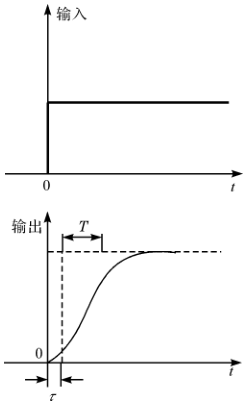
\includegraphics[width=\linewidth]{figs/fig-0191.png}
\caption{图11.0-1}
\end{figure}

为了使计算简单起见，假设只用一种液体燃料 ${ }^{[15]}$。

\section{11.1 燃烧中的时滞}

液体燃料从射入燃烧室加热到即将燃烧的临界状态，需要一段时间（这就是燃烧的时滞），然后就迅速地燃烧而变为热燃气。假设 $\dot{m}_{v}(t)$ 是时刻 $t$ 时由于燃烧而产生的热燃气的质量速率（所谓“质量速率”就是按照质量来计算的时间变化率）。 $\dot{m}_{v}(t)$ 是在时刻 $t$ 时喷入燃料的质量速率。 $\tau(t)$ 是在时刻 $t$ 开始燃烧的那些燃料的时滞。所以，在从 $t$ 到 $t+d t$ 这一段时间间隔内燃烧的燃料是在从 $t-\tau$ 到 $t-\tau+d(t-\tau)$ 这一段时间间隔内喷射进来的。因此

\[\dot{m}_{v}(t) d t=\dot{m}_{v}(t-\tau) d(t-\tau)\]

产生出来的热燃气，有一部分被用来充加在燃烧室中，从而提高燃烧室中的压力 $p(t)$，另外一部分通过喷口被喷射出去。如果燃烧室中可能发生的振荡的频率相当低，因此，就可以把燃烧室内的压力看做是均匀的，而且，作为第一次的近似 ${ }^{[15]}$，我们也可以把流过喷口的气流看做是似稳的（所谓“似稳”的意思就是：在任何一段不太长的时间间隔内都可以看做是平稳的）。所以，经过喷口的喷气的质量速率与火箭发动机中的热燃气的密度成正比。但是，对于“单一燃料”（也就是只用一种燃料）的火箭发动机来说，热燃气的温度几乎与燃烧压力无关，而热燃气的密度只与压力成正比，所以，如果 $\bar{m}$ 是流过整个系统的稳态质量速率; $M_{r}$ 是发动机中的热燃气的平均质量; $p$ 是燃烧室中的压力的稳态平均值。如果把尚未燃烧的液体燃料在燃烧室中所占据的容积忽略不计，我们就

\[\dot{m}_{v} d t=\overline{\dot{m}}_{s} \frac{p}{p} d t+d\left(\overline{M_{s}} \frac{p}{p}\right)\qquad\text{(11.1-2)}\]

现在，对于燃烧室压力与燃料喷入速率，我们分别引进两个无量纲变数 $\psi$ 和 $\eta$，它们的定义是

\[\psi=\frac{p-\bar{p}}{p}, \quad \eta=\frac{\dot{m}_{i}-\dot{m}}{\dot{m}}\qquad\text{(11.1-3)}\]

所以 $\psi$ 和 $\eta$ 就是压力和喷入速率对于稳态平均值的相对偏差。利用式 (11.1-3)，并且把 $\dot{m}_{b}$ 从方程(11.1-1)和方程(11.1-2)消去，就得到

\[\frac{\overline{M_{s}}}{\dot{m}} \frac{d \psi}{d t}+\psi+1=\left[\begin{array}{c} 1-\frac{d \tau}{d t} \\ \end{array}\right]\left[\eta(t-\tau)+1\right]\qquad\text{(11.1-4)}\]

为了计算 $\frac{d \tau}{d t}$，就必须引进克洛科的压力与时滞相关的概念。假定液体燃料达到燃烧临界状态的质量速率是 $f(p)$，那么，时滞 $\tau$ 就由下列公式确定

\[\int_{r}^{t} f(p) d t=\text { const }\qquad\text{(11.1-5)}\]

可以把常数看做是为了把单位质量的喷入的冷燃料变到即将燃烧的状态所必须加进去的热量。$f(p)$ 的物理意义就是：从热燃气到喷入的液体燃料的传热速率。把方程 (11.1-5) 对 $t$ 微分就得

\[\left[f(p)\right]_{t}-\left[f(p)\right]_{t-\tau}\left(1-\frac{d \tau}{d t}\right)=0\]

现在我们就可以明确地引进离开均匀稳定状态的微小扰动的概念。假设压力 $p$ 与稳态值 $\bar{p}$ 之间的偏差相当小。那么 $f(p)$ 在时刻 $t$ 的值以及 $f(p)$ 在时刻 $t-\tau$ 的值都可以用 $\bar{p}$ 附近的泰勒级数表示。如果不考虑级数中二次和二次以上的方幂，则有

\[\left[f(p)\right]_{t}=f(\bar{p})+\left.\overline{\left.\frac{d f}{d p}\right|_{p=\bar{p}}}\right] \psi(t)\]

和

\[\left[f(p)\right]_{t-\tau}=f(\bar{p})+\left.\overline{\left.\frac{d f}{d p}\right|_{p=\bar{p}}}\right] \psi(t-\tau)\]

以上方程中的 $\tau$ 是相当于平均压力 $\bar{p}$ 的时滞，所以是一个常数。把 $(*)$ 的两个关系式相除，再利用 $(*)$ 的关系就得出下列近似公式

\[1-\frac{d \tau}{d t}=1+\left[\frac{d \log f}{d \log p}\right]_{p=\bar{p}}[\psi(t)-\psi(t-\tau)]\qquad\text{(11.1-6)}\]

把方程 (11.1-4) 和 (11.1-6) 合并起来，并且略去二次项，就得出下列方程

\[\frac{d \varphi}{d z}+\varphi=u(z-\delta)+n[\varphi(z)-\varphi(z-\delta)]\qquad\text{(11.1-7)}\]

在这个方程里

\[\begin{gathered} n=\left(\frac{d \log f}{d \log p}\right)_{p=\bar{p}} \\ \theta_{k}=\frac{\overline{M_{k}}}{m}, \quad z=\frac{t}{\theta_{k}}, \quad \delta=\frac{\tau}{\theta_{k}} \end{gathered}\qquad\text{(11.1-9)}\]

而

\[\begin{aligned} \varphi(z) & =\varphi\left(\frac{t}{\theta_{k}}\right)=\psi(t) \\ \mu(z-\delta) & =\mu\left[\frac{1}{\theta_{k}}(t-\tau)\right]=\eta(t-\tau) \end{aligned}\]

$Q_{k}$ 是发动机内的燃气的质量的平均值与流过发动机的燃气的平均质量速率的比值，因此它也就是热燃气从被燃烧产生到经过喷口喷射出去的平均时间，所以 $Q_{k}$ 就称为“燃气通过时间”。在以下的计算中，我们就用这个基本的时间常数作为测量时间的单位。$z$ 是无量纲的时间变数。$\delta$ 是燃烧的无量纲的时滞常数。

如果 $n$ 是一个与 $p$ 无关的常数，那么 $f(p)$ 就与 $p^{n}$ 成正比。这就是克洛科所假设的 $f(p)$ 的形状。现在，我们把问题提得稍微普遍一些; $f(p)$ 是任意的; $n$ 是由方程(11.1-8)计算的；因而也就是 $\bar{p}$ 的函数。如果把 $f(p)$ 看作是从热燃气到雾状的液体燃料的传热速率，那么，关于传热的物理定律指出，$n$ 的值在 $1 / 2$ 与 1 之间。

这样，我们就建立了描述燃烧室中压力变化规律的方程(11.1-7)。

\section{11.2 时滞系统的运动规律}

在上一节，我们推导了火箭发动机燃烧室中压力变化的运动方程(11.1-7)，这是一个一阶常系数微分差分方程。现在采用常用的符号 $t$ 代替时间变量 $z$，用 $\tau$代替时滞量 $\delta$，于是方程(11.1-7)可改写为

\[\frac{d \varphi}{d t}=(n-1) \varphi(t)-n \varphi(t-\tau)+\mu(t-\tau)\]

由此可见，压力变化的趋势（方程左端）不仅依赖于当时的压力 $\varphi(t)$，而且明显地依赖于过去的历史状况 $\varphi(t-\tau)$ 和 $\mu(t-\tau), \tau>0$。这样，与微分方程就有一个根本的差别，为了求解方程式(11.1-7)初值不能只给在初始瞬时 $t=b$，而必须给在一个区间上，例如给定

\[\varphi(t)=\psi(t), \quad b-\tau \leqslant t \leqslant b\]

一般来讲，时滞系统的运动都可以用一阶微分差分方程组来描述，如果将时间坐标原点向右移动 $b-\tau$，那么初始条件就给在区间 $0 \leqslant t \leqslant \tau$ 上。本节内我们先一般地讨论具有一个常时滞量 $\tau$ 的线性常系数系统，看看它们具有何种特性。假定有任一个具有时滞因素的线性系统，其运动方程为

\[\begin{gathered} \frac{d y_{i}}{d t}=\sum_{j=1}^{n} a_{i} y_{j}(t)+\sum_{j=1}^{n} b_{i} y_{j}(t-\tau)+u(t), \quad t>\tau \\ y_{i}(t)=\varphi_{i}(t), \quad 0 \leqslant t \leqslant \tau \\ i=1,2, \cdots, n \end{gathered}\]

写成向量和矩阵的形式即为

\[\begin{gathered} \frac{d \mathbf{y}}{d t}=A \mathbf{y}(t)+B \mathbf{y}(t-\tau)+\mathbf{u}(t), \quad t>\tau \\ \mathbf{y}(t)=\varphi(t), \quad 0 \leqslant t \leqslant \tau \end{gathered}\qquad\text{(11.2-2)}\]

其中 $\mathbf{y}(t), \varphi(t)$ 和 $\mathbf{u}(t)$ 为 $n$ 维向量函数，$A$ 和 $B$ 为 $n \times n$ 矩阵，$\mathbf{u}(t)$ 称为驱动函数，$\varphi(t)$ 称为初始函数，它定义在初始区间 $[0, \tau]$ 上。当然，对于变时滞的情形，即 $\tau$ 是 $t$ 的函数 $\tau(t)$ 时，方程

\[\frac{d \mathbf{y}}{d t}=A \mathbf{y}(t)+B \mathbf{y}(t-\tau(t))+\mathbf{u}(t)\]

的初始区间由初始时刻 $b$ 及 $b$ 处的延迟时间 $\tau(b)$ 而定。初始函数给定在初始区间 $E_{v}$ 上，例如

\[\mathbf{y}(t)=\varphi(t), \quad t \in E_{0}\]

$E_{0}$ 是由 $t=t_{b}$ 及 $t_{b}+\tau\left(t_{b}\right)$ 的点组成。

这一节里我们将讨论满足方程 (11.2-1) 和初始条件式 (11.2-2) 的解的存在性及解的形式问题。为了便于叙述，我们先定义几个基本概念。首先必须指出，初始条件式 (11.2-2)，即函数 $\varphi(t)$ 实际上不可能是任意的。既然它代表系统的初始状态，$\varphi(t)(0 \leqslant t \leqslant \tau)$ 必然为“足够好”的一条曲线。由于 $\varphi(t)$ 的性质对系统在 $\tau$ 以后的运动有很大影响，下面我们将指出 $\varphi(t)$ 与 $\mathbf{y}(t)$ 之间的某些简单关系。

如果函数 $f(t)$ 在开区间 $t<t<t$ 上有 $K$ 阶连续导数，则称函数 $f(t)$ 是 $C^{k}\left(t, t_{t}\right)$ 类的，记为 $f(t) \in C^{k}\left(t, t_{t}\right)$。在方程 (11.2-1) 和 (11.2-2) 中如果 $\boldsymbol{u}(t)$ 是 $C^{0}(0, \infty)$ 类函数，$\varphi(t)$ 是 $C^{1}[0, \tau]$ 类函数，那么在 $t \geqslant 0$ 上存在唯一的连续函数 $\mathbf{y}(t)$，它满足初始条件式 (11.2-2) 且在 $t>\tau$ 时满足方程 (11.2-1)。如果 $\boldsymbol{u}(t)$ 属于 $C^{1}(0, \infty)$ 类和 $C^{2}(2 \pi, \infty)$ 类，那么解 $\mathbf{y}(t)$ 就是 $C^{1}(\tau, \infty)$ 类的函数。如果初始函数 $\varphi(t)$ 是 $C^{1}[0, \tau]$ 类函数，而且在 $t=\tau$ 时有

\[\frac{d \varphi(\tau)}{d \tau}=A \varphi(\tau)+B \varphi(0)+\boldsymbol{u}(\tau)\qquad\text{(11.2-3)}\]

那么解的一阶导数 $\dot{\mathbf{y}}(t)$ 在 $\tau$ 处连续，即 $\mathbf{y}(t)$ 是 $C^{1}[0, \infty)$ 类的函数 ${ }^{[1]}$。

这样，无论对哪一类初始条件，和对增长速度不快于某一指数幂的 $\boldsymbol{u}(t)$，我们就可以利用拉氏变换的方法对方程 (11.2-1) 求解。

利用分部积分可以得到

\[\int_{\tau}^{\infty} \mathbf{y}(t-\tau) e^{-s t} d t=e^{-\tau s} \int_{0}^{\infty} \mathbf{y}(t) e^{-s t} d t\qquad\text{(11.2-5)}\]

和

\[\int_{\tau}^{\infty} \dot{\mathbf{y}}(t) e^{-\tau t} d t=-\varphi(\tau) e^{-\tau s}+\int_{0}^{\infty} \mathbf{y}(t) e^{-s t} d t-\int_{0}^{\tau} \varphi(t) e^{-s t} d t\qquad\text{(11.2-4)}\]

将方程 (11.2-1) 乘以 $e^{-t}$，并从 $\tau$ 到 $\infty$ 对 $t$ 积分，将式 (11.2-4) 和 (11.2-5) 代入就得到

\[D(s) \int_{0}^{\infty} \mathbf{y}(t) e^{-s t} d t=\boldsymbol{p}(s)+\boldsymbol{q}(s)\qquad\text{(11.2-10)}\]

其中

\[\begin{gathered} D(s)=s E-A-B e^{-\tau s} \\ \boldsymbol{p}(s)=e^{-\tau s} \varphi(\tau)+(s E-A) \int_{0}^{\tau} \varphi(t) e^{-s t} d t \\ \boldsymbol{q}(s)=\int_{\tau}^{\infty} \boldsymbol{u}(t) e^{-s t} d t \end{gathered}\qquad\text{(11.2-9)}\]

若 $D(s)$ 的逆矩阵存在，则

\[\int_{0}^{\infty} \mathbf{y}(t) e^{-s t} d t=D^{-1}(s)[\boldsymbol{p}(s)+\boldsymbol{q}(s)]\qquad\text{(11.2-6)}\]

行列式 $\operatorname{det} D(s)$ 称为方程 (11.2-1) 的特征函数，方程 $\operatorname{det} D(s)=0$ 称为特征方程，特征方程的根称为特征根。

特征方程是一个超越代数方程，在复 $S$ 平面上一般有无穷多个根，记为 $s_{k}(k=$ $1,2, \cdots)$，而特征方程在任意半平面 $\operatorname{Res}>\sigma(\sigma$ 是任意实数 $)$，内只有有限个根。这只要在该半平面内以原点为中心的充分大的圆内部分利用特征函数的解析性质，在圆外部分利用儒歇 (Rouchi) 定理 ${ }^{[19]}$ 就可看出。因此总可以找到这样的常数 $c$，使

\[\operatorname{Res}_{s_{k}}<c, \quad k=1,2, \cdots\qquad\text{(11.2-11)}\]

因而就可以通过对式 (11.2-10) 的拉氏反变换得到解 $\mathbf{y}(t)$

\[\mathbf{y}(t)=\frac{1}{2 \pi i} \int_{(c)} e^{s t} D^{-1}(s)[\boldsymbol{p}(s)+\boldsymbol{q}(s)] d s, \quad t>0\qquad\text{(11.2-12)}\]

这里，积分路径 $(C)$ 满足式 (11.2-11)。这就是满足初始条件式 (11.2-2)，方程 (11.2-1) 的解的一般形式。

式 (11.2-12) 可以展开为级数形式。以原点为中心作一系列圆围道 $C_{l}$，$C_{2}, \cdots, C_{l}, C_{l+1}, \cdots$，使

(1) $C_{l} \subset C_{l+1},(l=1,2, \cdots)$。

(2) $C_{l}$ 上没有特征根。

(3) 在 $C_{l}$ 与 $C_{l+1}$ 之间只有有限个特征根。

圆 $C_{l}$ 上位于 $\operatorname{Res}>c$ 的部分记为 $C_{l}^{+}$，圆 $C_{l}$ 上位于 $\operatorname{Res}<c$ 的部分记为 $C_{l}^{-}$，那么

\[\begin{aligned} & \int_{c_{l}} D^{-1}(s)[\boldsymbol{p}(s)+\boldsymbol{q}(s)] e^{s t} d s=\int_{c_{l}^{+}} D^{-1}(s)[\boldsymbol{p}(s)+\boldsymbol{q}(s)] e^{s t} d s \\ & \quad+\int_{c_{l}^{-}} D^{-1}(s)[\boldsymbol{p}(s)+\boldsymbol{q}(s)] e^{s t} d s \end{aligned}\qquad\text{(11.2-16)}\]

可以证明，当 $t$ 足够大时

\[\lim _{t arrow \infty} \int_{c_{l}^{-}} D^{-1}(s)[\boldsymbol{p}(s)+\boldsymbol{q}(s)] e^{s t} d s=0^{[1]}, \quad t>n \tau\qquad\text{(11.2-14)}\]

又根据留数定理有

\[\frac{1}{2 \pi i} \int_{c_{l}} D^{-1}(s)[\boldsymbol{p}(s)+\boldsymbol{q}(s)] e^{s t} d s=\sum_{s_{k} \in C_{l}} \operatorname{Res} D^{-1}(s)[\boldsymbol{p}(s)+\boldsymbol{q}(s)] e^{s t}\qquad\text{(11.2-13)}\]

和

\[\lim _{t arrow \infty} \int_{c_{l}^{+}} D^{-1}(s)[\boldsymbol{p}(s)+\boldsymbol{q}(s)] e^{s t} d s=\int_{(c)} D^{-1}(s)[\boldsymbol{p}(s)+\boldsymbol{q}(s)] e^{s t} d s\qquad\text{(11.2-15)}\]

因而

1/2  i \_(C) D\textasciicircum{}-1(s)[p(s)+q(s)] e\textasciicircum{}s t d s= \_t   \_k  C\_l Res D\textasciicircum{}-1(s)[p\_v(s)+q(s)] e\textasciicircum{}s t

利用式(11.2-12)即得

\[\mathbf{y}(t)=\lim _{t arrow \infty} \sum_{s_{k} \in C_{l}} \operatorname{Res} D^{-1}(s)\left[\boldsymbol{p}(s)+\boldsymbol{q}(s)\right] e^{s t}, \quad t>n \tau\qquad\text{(11.2-17)}\]

而 $D^{-1}(s)\left[\boldsymbol{p}(s)+\boldsymbol{q}(s)\right] e^{s t}$ 在 $s_{k}$ 的留数具有

\[e^{s_{k} t} \boldsymbol{p}_{k}(t)\]

的形式，其中 $s_{k}$ 为特征根，$\boldsymbol{p}_{k}(t)$ 为多项式向量，其幂次小于 $s_{k}$ 的重数。因此 $\mathbf{y}(t)$可表示为

\[\mathbf{y}(t)=\lim _{t arrow \infty} \sum_{k \in C_{l}} e^{t} k_{k} \boldsymbol{p}_{k}(t), \quad t>n \tau\qquad\text{(11.2-18)}\]

它在任何有限闭区间

\[b \leqslant t \leqslant b^{\prime}, \quad b>n \tau\]

上一致收敛。如果所有特征根都具有负实部，即

\[\operatorname{Res}_{s}<C<0\]

那么，极限式(11.2-18)在区间

\[b \leqslant t<\infty, \quad b>n \tau\]

上一致收敛。式(11.2-18)可进一步表示为

\[\mathbf{y}(t)=\sum_{k=1}^{\infty} e^{t} k_{k} \boldsymbol{p}_{k}(t)\qquad\text{(11.2-22)}\]

此级数的收敛性总可得到保证。

\section{11.3 时滞系统的运动稳定性}

这一节我们将一般地讨论常系数常时滞系统的稳定性问题，这对我们讨论具体问题时在方法和概念上会有所帮助。现研究齐次方程组

\[\frac{d x(t)}{d t}=A \boldsymbol{x}(t)+B \boldsymbol{x}(t-\tau), \quad t>b+\tau\qquad\text{(11.3-1)}\]

这里仍然沿用李雅普诺夫稳定性定义作为研究系统稳定性的依据。由初始函数 $\varphi(t)$ 所决定的一个特定运动 （未受扰运动） $\boldsymbol{x}(t)$ 的稳定性定义可以这样叙述：若对任何正数 $\varepsilon>o$，总存在一个正数 $\delta$，当初始函数变为 $\boldsymbol{\Psi}(t)$ 并在区间 $b \leqslant t \leqslant b+\tau$ 内满足 （按欧氏空间的向量范数）

\[\|\boldsymbol{\Psi}(t)-\varphi(t)\|<\delta\qquad\text{(11.2-19)}\]

时，方程 (11.3-1) 相应的解 $\boldsymbol{x}(t)$ （受扰运动） 在 $t \geqslant b$ 上都有

\[\|\boldsymbol{x}(t)-\boldsymbol{x}(t)\|<\varepsilon\]

则称方程(11.3-1)的这一特定未受扰运动 $\boldsymbol{x}(t)$ 是稳定的。反之，若对某个 $\varepsilon>0$，找不到这样的 $\delta>0$，则称未受扰运动 $\boldsymbol{x}(t)$ 为不稳定。特别是，当运动 $\boldsymbol{x}(t)$ 稳定，且

\[\lim _{t arrow+\infty} \boldsymbol{x}(t)=\boldsymbol{x}(t)\]

时，则称 $\boldsymbol{x}(t)$ 为渐近稳定。

\begin{figure}[htbp]\centering
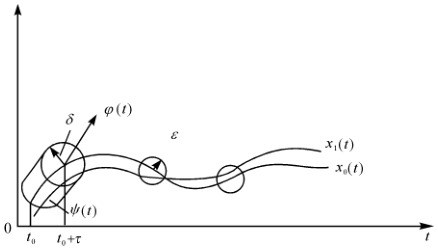
\includegraphics[width=\linewidth]{figs/fig-0192.png}
\caption{图11.3-1}
\end{figure}

稳定的几何意义可由图 11.3-1 说明。图中粗实线表示由初始函数 $\varphi(t)$ 所决定的特定未受扰运动 $\boldsymbol{x}(t)$。对于任意给定半径为 $\varepsilon$，球心随 $\boldsymbol{x}(t)$ 迁移的 $\varepsilon$ 球体，可以在 $\varphi(t)$ 附近指定一个以 $\delta$ 为半径，$\varphi(t)$ 为球心的 $\delta$ 球体，使得在 $b$ 到 $b+\tau$ 时间内以 $\varphi(t)$ 为球心的 $\delta$ 球体内的任何一条曲线作为初始轨迹的运动，在任何 $t \geqslant b$时刻都走不出 $\boldsymbol{x}(t)$ 的 $\varepsilon$ 球体的范围时，则称运动 $\boldsymbol{x}(t)$ 是稳定的。如果对 $\boldsymbol{x}(t)$ 的某一个 $\varepsilon$ 球体，在 $\varphi(t)$ 附近找不到这样的 $\delta$ 球体，则称运动 $\boldsymbol{x}(t)$ 不稳定。在 $\boldsymbol{x}(t)$稳定的情况下，如果随着时间 $t$ 的增长，$\boldsymbol{x}(t)$ 无限趋近于 $\boldsymbol{x}(t)$，则称运动 $\boldsymbol{x}(t)$ 为渐近稳定。

与线性微分方程类似，线性微分差分方程也有这样的特点：要么全体解都稳定，要么全体解都不稳定。因为方程 $(11 .3-1)$ 由任何初始函数 $\varphi(t), t \leqslant t_{0}-+,\overline{\mathrm{n}}$，所决定的一个特定解 $\mathbf{x}_{n}(t)$，通过下列变换

y (t) = x (t) - x\_*(t)

y(y)仍然满足方程组$(11.3-1)$，因而任一特定义 $\boldsymbol{x}(t)$ 的稳定性问题就化为同一方程组的零解——y(t)=0 的稳定性问题。这样，若零解稳定，则全体系都稳定。之，若零解不稳定，则全体解都不稳定。。因面也就有系统稳定性的问题。下面我们只研究零解的稳定性。

这里还要特别指出运动稳定性与初始区间 $[b, b+\tau]$ 的关系。对于线性常系数时常滞微分差分方程（11.3-1）来说，与线性常常数微分方程类似，稳定性与初始区间 $[\dot{b}, \dot{b}+\pi]$ 无关。因为发生在任何区间 $[\dot{b}, \dot{b}+\tau](l \geqslant 0)$ 上的扰动 $\psi(t)$ 经过变换

\[\lambda=t-b\]

后就可变为在区间 $[0, \tau]$ 上的扰动

\[\Psi(\lambda+b)=f(\lambda)\]

所以，若对初始区间 $[0, \tau]$ 上的扰动，运动 $\mathbf{x}(t)$ 是稳定的，那么，对任何初始区间 $[b, b+\tau], t \geqslant 0$ 上的扰动，运动也都稳定。然而，对于变时滞系统则不然，若运动对初始区间 $E_{0}$ 上的扰动稳定，而对初始区间 $E_{1}(t>b)$ 的扰动未必稳定。这样，稳定定义就需要加强，只有对任何初始区间 $E_{1}(t>b)$ 都能找到相应的 $\delta(\varepsilon)$，满足条件式 (11.3-3)，才称它是稳定的。反之，只要对某个初始区间 $E_{1}(t>b)$，找不到 $\delta(\varepsilon)$，满足条件式 (11.3-3)，就称运动不稳定。

现在我们再来讨论线性常系数常时滞系统

\[\frac{d \mathbf{y}}{d t}=A \mathbf{y}(t)+B \mathbf{y}(t-\tau)+\mathbf{u}(t), \quad t>\tau\qquad\text{(11.3-6)}\]

满足初始条件

\[\mathbf{y}(t)=\varphi(t), \quad 0 \leqslant t \leqslant \tau\qquad\text{(11.3-7)}\]

的运动稳定的条件。这里，我们所关心的仍然是渐近稳定问题。与通常无时滞的线性系统类似，系统渐近稳定的充分必要条件是特征方程 $\operatorname{det} D(s)=0$ 的全部根都具有负实部。这一条件的必要性是显然的，因为只要有一个根具有正实部，例如 $\operatorname{Res}_{s}=\sigma_{k}>0$，么，由展开式 (11.2-22) 可以看到，$\mathbf{y}(t)$ 中包含有 $\boldsymbol{p}_{k}(t) e^{s_{k} t}$ 项。显然，不论初始偏差如何小，随着 $t$ 之增长，$\|\mathbf{y}(t)\|$ 总将无限增大，即

\[\lim _{t arrow \infty} \|\mathbf{y}(t)\|=\infty\]

所以解是不稳定的，当然也就不断渐近稳定。这个准则的充分性，我们可以这样来说明，如果初始函数 $\varphi(t)$ 是定义在区间 $0 \leqslant t \leqslant \tau$ 上的 $C^{1}$ 类函数，设

\[m=\max _{0 \leqslant k \leqslant t}\|\varphi(t)\|\]

那么可以证明

\[\|\mathbf{y}(t)-\lim _{t arrow \infty} \sum e^{s_{k} t} \boldsymbol{p}_{k}(t)\|<\varphi_{t} m e^{c t[1]}, \quad t>\tau\qquad\text{(11.3-8)}\]

这里 $\varphi_{t}$ 为某正常数，$e^{s_{k} t} \boldsymbol{p}_{k}(t)$ 是 $D^{-1}(s) \boldsymbol{p}(s)$ 在特征根 $s_{k}$ 处的留数，$\boldsymbol{p}_{k}(t)$ 是 $t$ 的多项式，其幂次小于 $s_{k}$ 的重数，$c$ 为任意实数，求和是对 $G$ 圆与半平面 $\operatorname{Res}>c$ 交集内的所有特征根进行的。如果所有特征根均具有负实部，那么可以选 $c<0$，使所有特征根都位于半平面 $\operatorname{Res}<c<0$ 内，这样式 (11.3-8) 就成为

$\|\mathbf{y}(t)\|因为$c<0$, 所以$\textbackslash\{\}|\textbackslash\{\}mathbf\{y\}(t)\textbackslash\{\}|<\textbackslash\{\}varphi\_\{t\} m，\textbackslash\{\}quad t>\textbackslash\{\}tau$对于任意给定的$\textbackslash\{\}varepsilon$, 只要选择$m 满足

\[m=\frac{\varepsilon}{c_{0}}\]

那么 $\mathbf{y}(t)$ 就满足

\[\left\|\mathbf{y}(t)\right\|<c_{0} \frac{\varepsilon}{c_{0}}=\varepsilon, \quad t>\tau\]

在有限时间 $0 \leqslant t \leqslant \tau$ 内，$\left\|\mathbf{y}(t)\right\|$ 是有界的，而且选择适当的 $m$ 可使

\[\left\|\mathbf{y}(t)\right\|<\varepsilon, \quad 0 \leqslant t \leqslant \tau\]

因而总能找到这样的 $m$，在 $t \geqslant 0$ 内都满足

\[\left\|\mathbf{y}(t)\right\|<\varepsilon\]

所以系统是稳定的。再利用式 (11.3-9) 便得到

\[\lim _{t arrow \infty}\|\mathbf{y}(t)\|=\lim _{t arrow \infty} c_{0} m e^{t}=0\qquad\text{(11.3-10)}\]

因而系统是渐近稳定的。

关于第 11.2 和第 11.3 节的详细论述，读者可参阅文献[4]，那里还讨论了更为一般的时滞系统。

现在我们就以第 11.1 节的燃烧过程为例，分析它的稳定性。克洛科把燃料喷入速率是常数时的燃烧不稳定性称为固有不稳定性。如果喷入速率是一个与燃烧室压力 $p$ 无关的常数，那么，$t \equiv 0$。因此，根据方程 (11.1-7)，稳定性问题就由下列齐次方程限定:

\[\frac{d \varphi}{d z}+(1-n) \varphi(z)+n \varphi(z-\delta)=0\qquad\text{(11.4-1)}\]

也可以用前节内讨论过的拉氏变换的方法来处理方程 (11.4-1)，作法和以前各章中处理没有时滞的方程的方法相同。事实上，安索夫 (Ansoff) 也用过这个方法 ${ }^{[3]}$。然而，在目前的燃烧的稳定性问题里，基本方程没有驱动项，所以，可以用一个比较直接的解法，这个解法就是解线性微分差方程的古典方法，作法是这样的：设

\[\varphi(z) \underset{\text { 由 }}{\underset{\text { 由 }}{=}} e^{s z}\]

于是得到特征方程

\[s+(1-n)+n e^{-\delta_{s}}=0\qquad\text{(11.4-2)}\]

这是一个 $s$ 的超越方程。燃烧的稳定性的条件就是：方程 (11.4-1) 的根 $s$ 的实数部分是负数。

也可以应用拉氏变换方法从方程 (11.4-1) 得出方程 (11.4-2) 来。假定 $\varphi(z)$的拉氏变换是 $\Phi(s)$，对方程 (11.4-1) 进行拉氏变换，就得到

\section{11.4 萨奇（Satche）图}

sΦ(s) - φ(0) + (1 - n)Φ(s) + ne-ṡ0Φ(s) + ṡ0Φ(z′)e-z′dz′ = 0

如果 φ(z) 的初始条件是所谓的零初始条件，也就是说: z ≤ 0 时 φ(z) = 0，那么就有

[s + (1 - n) + ne-ṡ0]Φ(s) = 0

于是，我们就得到方程 (11.4-2)。这里的 s 和以前各章中的变数 s 具有相同的“意义”。这两者之间的唯一区别，就是这里的 s 已经通过式 (11.1-9) 的 θs 的变换成为无量纲的量了。也可以看到这样一个有趣的事实：如果方程 (11.4-1) 是一个在方程右端有驱动项的非齐次方程，那么，对这个方程施行拉氏变换法以后，所得到的方程仍然是非齐次的。如果把 φ(z) 看做是系统在单位阶跃函数作用下的输出，系统的传递函数就会是

F(s) = 1s + (1 - n) + ne-ṡ0

这个 F(s) 又是一个超越的传递函数的例子。

克洛科把方程 (11.4-2) 的实数部分和虚数部分分离开来得到两个方程，根据这两个方程他解出了方程的复数根 s。然而，如果只对系统是否稳定的问题感兴趣，那么，根据第 11.3 节关于稳定条件的结论我们仍然可以成功地利用第 4.3 节的柯西定理。设

G(s) = e-ṡ0 - -1 - nns - sn

于是，系统的稳定性问题就归结为 G(s) 在复 S 平面的右半部有没有零点的问题。当 s 在一条包围右半平面的闭合曲线上转动一周时，我们只要把变数 G(s) 的相应的变化情况加以考察，就能够回答系统是否稳定的问题。如果向量 G(s) 旋转的总圈数是某一个数，按照柯西定理这个数就是 G(s) 在右半 S 平面上的零点个数与极点个数的差。既然，在全 S 平面上 G(s) 显然没有极点，所以，G(s) 旋转的总圈数就是零点的个数。因此，如果系统是稳定的，那么，当 s 在上述的闭合曲线上转动一周时，G(s) 旋转的总圈数一定是零。所以，可以用描画乃氏图的办法来回答稳定性的问题。

但是，对方程 (11.4-3) 所表示的 G(s) 直接应用上述的方法是很不方便的，因为时滞项 e-ṡ0 的存在，这个表示式是比较复杂的。对于这样一些有时滞的系统，萨奇 (Satche) 提出了一个富有创造性的巧妙的处理方法 [14]: 不直接处理 G(s) 本身，而把它分成两部分

G(s) = g1(s) - g2(s)

其中

g1(s) = e-ṡ0

g2(s) = -1 - nns - sn

\textbackslash\{\}begin\{figure\}[h]\textbackslash\{\}centering\textbackslash\{\}includegraphics[width=0.8\textbackslash\{\}textwidth]\{image.png\}\textbackslash\{\}caption\{图11.4-1\}\textbackslash\{\}end\{figure\}

这样一来，向量 $G(s)$ 就是一个顶点在 $g_1(s)$ 而起点在 $g_2(s)$ 的向量了。如果 $s$ 在虚轴上变动，$g_1(s)$ 的图线就是一个单位圆。如果 $s$ 在大的半圆周上，$g_1(s)$ 就在单位圆的内部。当 $s$ 在虚轴上变动的时候，$g_2(s)$ 就是一条与虚轴平行的直线（图 11.4-1)。当 $s$ 在大的半圆周上变动时，$g_2(s)$ 就在左方描画成一个大的半圆周，这个半圆周与 $s$ 所在的那个半圆周恰好组成一个圆周。只要稍微考虑一下，就可以想到：如果希望对于任何时滞 $\delta$ 的值，$G(s)$ 旋转的总圈数都是零，那么，$g_2(s)$ 图线就必须完全在 $g_1(s)$ 图线的外面。这也就是

说，对于本质上稳定的系统，即绝对稳定系统\textbackslash\{\}footnote\{若对于任何 $\delta$ 值，系统都是稳定的，则称系统绝对稳定。\}来说，必须有

\[\frac{1-n}{n}>1 \quad \text{或者} \quad \frac{1}{2}>n>0\qquad\text{(11.4-6)}\]

现在，很容易看出把 $G(s)$ 分解为 $g_1(s)$ 和 $g_2(s)$ 两部分的做法可以使得相当的两条图线都比原来的 $G(s)$ 图线简单得多。$g_1(s)$ 的图线与 $g_2(s)$ 的图线组成的图线就称为萨奇图。

如果 $n>\frac{1}{2}$，$g_1(s)$ 的图线就与 $g_2(s)$ 的图线相交，因而就有一部分 $g_2(s)$ 点在图 11.4-2 的单位圆的内部，但是，只要相当于这些 $g_2(s)$ 的 $g_1(s)$ 点都在 $g_2(s)$ 点的右方，$G(s)$ 图线就不绕原点转，系统仍然是稳定的。如果对于同一个 $s=i\omega^*$，$g_2(s)$ 与 $g_1(s)$ 重合，则 $G(s)$ 图线就通过原点，系统处于临界稳定状态。这时，必须满足条件

\[g_2(i\omega^*) =1\]

\[\arg g_2(i\omega^*)=\arg g_2^*(i\omega^*)\]

再从式 (11.4-5) 就可求出临界稳定状态下的 $\omega^*$ 和 $\delta^*$

\[\omega^* = \sqrt[2n-1]{2}\qquad\text{(11.4-7)}\]

\textbackslash\{\}begin\{figure\}[h]\textbackslash\{\}centering\textbackslash\{\}includegraphics[width=0.4\textbackslash\{\}textwidth]\{image.png\}\textbackslash\{\}caption\{图11.4-2\}\textbackslash\{\}end\{figure\}

\begin{figure}[htbp]\centering
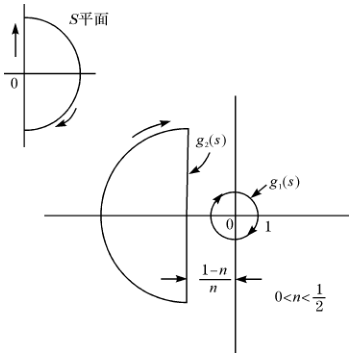
\includegraphics[width=\linewidth]{figs/fig-0193.png}
\caption{图11.4-1}
\end{figure}

\begin{figure}[htbp]\centering
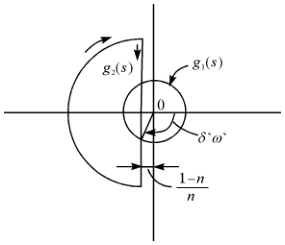
\includegraphics[width=\linewidth]{figs/fig-0194.png}
\caption{图11.4-2}
\end{figure}

\[\delta^{*}=\frac{\cos ^{-1}\left[\frac{1-n}{2 n-1}\right]}{\sqrt{2 n-1}}=\frac{1}{\sqrt{2 n-1}}\left[\pi-\cos ^{-1}\left[\frac{1-n}{n}\right]\right]\qquad\text{(11.4-8)}\]

所以当 $\delta=\delta^{*}$ 时，$\varphi(z)$ 有一个频率是 $\omega^{*}$ 的振荡解。因而 $\delta^{*}$ 是无量纲的临界时滞，而 $\omega^{*}$ 是无量纲的临界频率。当 $\delta<\delta^{*}$，也就是说当

\[\cos (\delta \sqrt{2 n-1})>-\frac{1-n}{n}\]

时，系统就是稳定的。

\section{11.5 有反馈伺服机构的火箭发动机的系统动力学性质}

现在我们来考虑图 11.5-1 所画的火箭发动机系统，这个系统包含三部分：火箭发动机，供应燃料的馈送机构 （燃料泵和附属的传导装置） 及反馈伺服机构。为了近似地表示出实在的导管的弹性效应，我们可以假想在刚硬的导管的中点 （燃料泵与燃料喷嘴之间）有一个附有弹簧活塞的容器，在喷嘴附近还有另外一个由伺服机构控制的容器。传感器 （测量仪器） 测量了燃烧室的压力，测量的结果经过一个放大器而成为伺服机构的输入信号。如果设计者已经把燃料的馈送机构和火箭发动机本身的设计完全确定，不允许再加以更改，现在的问题就是：是否可以设计一个使整个系统稳定的合适的放大器？因为关于燃烧的时滞还没有确切的知识，所以，在进行实际设计的时候，我们就必须设法使系统无条件地稳定，也就是说，对于任何的时滞 $\delta$ 的值系统都是稳定的。

有弹簧的容器

伺服机构

燃料泵

控制容器

测量仪器

放大器

火箭发动机

图 11.5-1

假定 $\dot{m}_{\mathrm{v}}$ 是流出燃料泵的燃料的瞬时质量速率; $p^{0}$ 是燃料泵的出口处的瞬时压力，燃料流动的平均速率一定是 $\bar{m}$。平均压力是 $\bar{p}^{0}$。燃料泵的特性可以用下列方程表示

\begin{figure}[htbp]\centering
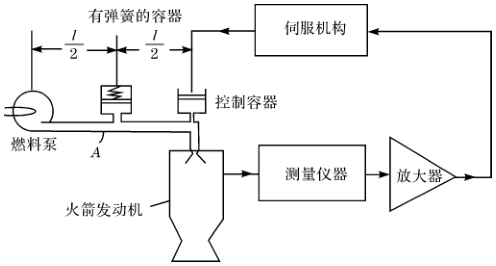
\includegraphics[width=\linewidth]{figs/fig-0195.png}
\caption{图11.5-1}
\end{figure}

\[\frac{p_{0}-\overline{p_{0}}}{p_{0}}=-\alpha \frac{\dot{m}_{0}-\dot{m}}{\dot{m}}\qquad\text{(11.5-1)}\]

如果质量的流动的变化的时间速率比弹性波在液体中的传播速度小，但是比燃料泵的转速的缓慢的时间变化率大，那么，相当于常数转速的情况，燃料泵的压力体积曲线在稳态工作点的斜率就是 $\alpha$ （这里所说的“体积”就是流出燃料泵的燃料按照体积计算的速率）。对于普通的离心泵来说，$\alpha$ 差不多等于 1。对于传输泵 （输出的流量几乎是不变的泵）来说，$\alpha$ 非常大。对于等压泵或者简单的增压装置来说，$\alpha$ 等于零。

假设 $\dot{m}_{\mathrm{t}}$ 是喷嘴与弹簧容器口之间的燃料流动的瞬时质量速率; $\chi$ 是容器的弹簧常数，$p_{1}$ 是作用在容器上的瞬时压力。于是就有

\[\dot{n}_{\mathrm{w}}-\dot{m}_{\mathrm{t}}=\rho \chi \frac{d p_{1}}{d t}\qquad\text{(11.5-2)}\]

这里的 $\rho$ 是燃料的密度，它是一个常数。

在以下的计算里，由于摩擦力而在导管上引起的压力降落是忽略不计的。因此，压力差 $p^{0}-p^{1}$ 只是由流动的加速度引起的，也就是说

\[p^{0}-p^{1}=\frac{l}{2 A} \frac{d \dot{m}_{0}}{d t}\qquad\text{(11.5-3)}\]

这里的常数 $A$ 是导管的横截面的面积；常数 $l$ 是导管的总长度。与此类似，如果 $p_{2}^{2}$ 是控制容器上的瞬时压力，也就有

\[p_{1}-p_{2}=\frac{l}{2 A} \frac{d \dot{m}_{1}}{d t}\qquad\text{(11.5-4)}\]

如果控制容器中所容纳的质量是 $C$，那么

\[\dot{m}_{\mathrm{v}}-\dot{m}_{\mathrm{t}}=\frac{d C}{d t}\qquad\text{(11.5-5)}\]

因为控制容器与燃料喷嘴非常接近，所以，在燃料从控制容器流到燃料喷嘴的过程中，由于质量而引起的惯性效应是可以忽略的。因此

\[p_{2}-p=\frac{1}{2} \frac{\dot{m}_{i}^{2}}{\rho A_{i}^{2}}\qquad\text{(11.5-6)}\]

其中的 $A_{i}$ 是燃料喷嘴的有效开口面积。因为在稳定状态下压力 $\overline{p_{0}}$ 与 $\overline{p}$ 的差 $\Delta p$ 是

\[\overline{p_{0}}-\overline{p}=\Delta \overline{p}=\frac{1}{2} \frac{\overline{m}^{2}}{\rho A_{i}^{2}}\qquad\text{(11.5-7)}\]

所以在计算中可以把 $A_{i}$ 消去。方程(11.5-1)和(11.5-7)就描述了燃料馈送系统的动力学性质。直接利用消去某些变数的计算方法，就得出 $m, p$，与 $C$ 之间的关系式。为了把这个关系写成无量纲的形式，我们引进下列几个参数

\[\begin{gathered} P=\frac{\bar{p}}{2 \Delta p}, \quad E=\frac{2 \Delta p}{\bar{m}} \rho \chi, \quad J=\frac{l \bar{m}}{2 \Delta p A} \theta_{k} \\ \text { 以及 } \\ \kappa=\frac{C}{\bar{m} \theta_{k}} \end{gathered}\]

这里的 $\theta_{k}$ 就是方程 (11.1-9) 所给的燃气通过时间。这样一来，联系 $\varphi, \mu$ 与 $\kappa$ 的无量纲方程就是

\[\begin{aligned} & P\left[1+\alpha E\left(P+\frac{1}{2}\right) \frac{d}{d z}+\frac{1}{2} J E \frac{d^{2}}{d z^{2}}\right] \varphi+\left[\left(1+\alpha\left(P+\frac{1}{2}\right)\right]\right. \\ & \left.+\alpha E\left(P+\frac{1}{2}\right)+J \frac{d}{d z}+\left[\frac{1}{2} \alpha J E\left(P+\frac{1}{2}\right)+\frac{1}{2} J E\right] \frac{d^{2}}{d z^{2}}+\frac{1}{4} J^{2} E \frac{d^{3}}{d z^{3}}\right] \mu \\ & \left.+\left\{\alpha\left(P+\frac{1}{2}\right) \frac{d}{d z}+J \frac{d^{2}}{d z^{2}}+\frac{1}{2} \alpha J E\left(P+\frac{1}{2}\right) \frac{d^{3}}{d z^{3}}+\frac{1}{4} J^{2} E \frac{d^{4}}{d z^{4}}\right\} \kappa=0\right. \end{aligned}\]

这里的 $z$ 就是方程 (11.1-9) 所定义的无量纲时间变数。

伺服控制的动力学性质是由下列各种因素的综合所确定的：测量压力的仪器的特性，放大器的反应性能以及伺服机构的特性。伺服控制的总的力学性质是由下列算子方程表示的

\[F\left(\frac{d}{d z}\right) \varphi=\kappa\]

这里的 $F$ 是两个多项式的比值，而且分母的次数高于分子的次数。

方程 (11.1-7)，(11.5-10) 和 (11.5-11) 是三个变数 $\varphi, \mu, \kappa$ 的三个方程。既然，它们都是常系数的方程，这些变数的适当的形式就是

\[\varphi=a e^{s z}, \quad \mu=b e^{z z}, \quad \kappa=c e^{s z}\qquad\text{(11.5-12)}\]

把方程 (11.5-12) 代入方程 (11.1-7)，(11.5-10) 和 (11.5-11)，就得到 $a, b, c$ 的三个齐次方程。所以我们有

\[\begin{gathered} a_{-}^{*}[s+(1-n)+n e^{-\delta s}]-b e^{-\delta s}=0 \\ P\left[1+\alpha E\left(P+\frac{1}{2}\right) s+\frac{1}{2} J E s^{2}\right] a+\left[\left(1+\alpha\left(P+\frac{1}{2}\right)\right]\right. \\ \left.+\left[\alpha E\left(P+\frac{1}{2}\right)+J s+\left[\frac{1}{2} \alpha J E\left(P+\frac{1}{2}\right)+\frac{1}{2} J E\right] s^{2}+\frac{1}{4} J^{2} E s^{3}\right\}\right. \\ \left.+s\left\{\alpha\left(P+\frac{1}{2}\right)+J s+\frac{1}{2} \alpha J F\left(P+\frac{1}{2}\right) s^{2}+\frac{1}{4} J^{2} E s^{3}\right\} c=0\right. \\ F(s) a-c=0 \end{gathered}\]

为了使 $a, b, c$ 三个数不全是零，它们的系数所组成的行列式就必须等于零。系数行列式除以 $n$ 后，就有

aligned E(s)= \& [s/n+1-n/n]\textbackslash\{\}1/4 J\textasciicircum{}2 E s\textasciicircum{}3+1/2 J E[1+(P+1/2)]\textbackslash\{\} s\textasciicircum{}2 \textbackslash\{\}\textbackslash\{\} \& +[ E(P+1/2)+J] s+[1+(P+1/2)] \textbackslash\{\}\textbackslash\{\} \& +e\textasciicircum{}- s[1/4 J\textasciicircum{}2 E s\textasciicircum{}2+[1/2 J E[1+(P+1/2)]+1/2 n J E P] s\textasciicircum{}2. \textbackslash\{\}\textbackslash\{\} \& .+[ E(P+1/2)+J+ E P/n(P+1/2)] s+[1+(P+1/2)+P/n]. \textbackslash\{\}\textbackslash\{\} \& .+s F(s)/n[1/4 J\textasciicircum{}2 E s\textasciicircum{}3+1/2  J E(P+1/2)] s\textasciicircum{}2. \textbackslash\{\}\textbackslash\{\} \& .+J s+(P+1/2)] aligned

\[=0\]

为简单起见，我们写成下列形式

\[E(s)=L_{0}(s)+H(s) e^{-\delta s}\]

其中

aligned L\_0(s)= \& [s/n+1-n/n]\textbackslash\{\}1/4 J\textasciicircum{}2 E s\textasciicircum{}3+1/2 J E[1+(P+1/2)]\textbackslash\{\} s\textasciicircum{}2 \textbackslash\{\}\textbackslash\{\} \& +[ E(P+1/2)+J] s+[1+(P+1/2)] \textbackslash\{\}\textbackslash\{\} H(s)= \& 1/4 J\textasciicircum{}2 E s\textasciicircum{}3+[1/2 J E[1+(P+1/2)]+1/2 n J E P] s\textasciicircum{}2+[ E(P+1/2). \textbackslash\{\}\textbackslash\{\} \& .+J+ E P/n(P+1/2)] s+[1+(P+1/2)+P/n]+s F(s)/n[1/4 J\textasciicircum{}2 E s\textasciicircum{}3. \textbackslash\{\}\textbackslash\{\} \& .+1/2  J E(P+1/2)] s\textasciicircum{}2+J s+(P+1/2)] aligned

式(11.5-13)就是用来确定指数 $s$ 的特征方程。于是 $F(s)$ 就被认为是反馈部分的总传递函数。整个系统的稳定性问题就决定于方程(11.5-13)是否有实部为正的根。

\section{11.6 没有反馈伺服机构时的不稳定性}

如果没有反馈伺服机构，那么，只要在方程(11.5-13)中使 $F(s)=0$，就得出系统的特征方程。和通常的情况一样，我们假设方程(11.5-13)中与 $e^{-\delta s}$ 相乘的部分 $H(s)$ 在右半 $S$ 平面没有零点。因此，就可以用 $H(s)$ 除方程(11.5-13)而不会使除得的商数在右半 $S$ 平面上有极点。这样一来，就又得到了描绘萨奇图所需要的表示式

\[G(s)=\frac{E(s)}{H(s)}=g_{0}(s)-g_{2}(s)\]

\[\mathbf{g}_{1}(s)=e^{-\delta_{s}}\]

所以 $\mathbf{g}_{1}(s)$ 的图线仍是一个“单位圆”，然而 $\mathbf{g}_{2}(s)$ 就复杂得多了

\[\begin{aligned} \mathbf{g}_{2}(s)= & -\left[\frac{s}{n}+\frac{1-n}{n}\right] \\ & \times\left\{\frac{1}{4} J^{2} E s^{3}+\frac{1}{2} J E\left[1+\alpha\left(P+\frac{1}{2}\right)\right] s^{2}+\left[\alpha E\left(P+\frac{1}{2}\right)+J\right] s\right. \\ & \left.+\left[1+\alpha\left(P+\frac{1}{2}\right)\right]\right\} \div\left\{\frac{1}{4} J^{2} E s^{3}-\frac{1}{2} J E\left[1+\alpha\left(P+\frac{1}{2}\right)+\frac{P}{n}\right] s^{2}\right. \\ & \left.+\left[\alpha E\left(P+\frac{1}{2}\right)\right]\left[1+\frac{P}{n}+J\right] s+\left[1+\alpha\left(P+\frac{1}{2}\right)+\frac{P}{n}\right]\right\} \end{aligned}\]

如果 $s$ 是纯虚数，$s=i \omega$，那么，$\mathbf{g}_{2}(s)$ 的图线在 $x$ 轴上的“截距”的坐标就是方程 (11.6-1) 在 $s=0$ 时的值。也就是

\[\mathbf{g}_{2}(0)=-\frac{1-n}{n} \frac{1+\alpha\left(P+\frac{1}{2}\right)}{1+\alpha\left(P+\frac{1}{2}\right)+\left(P / n\right)}\qquad\text{(11.6-2)}\]

因为 $n, \alpha$ 和 $P$ 这三个参数都是正数，所以现在的 $\mathbf{g}_{2}(0)$ 的绝对值小于方程 (11.4-5)所给的 $\mathbf{g}_{2}(0)$ 的绝对值，我们已经知道那个 $\mathbf{g}_{2}(0)$ 的值是与系统的无条件稳定性有关系的。现在我们就看到，由于有了燃料馈送系统，结果就使得萨奇图的 $\mathbf{g}_{2}(s)$ 图线更接近于 $\mathbf{g}_{1}(s)$ 的单位圆图线。譬如说，如果不考虑馈送系统，那么，当 $n=\frac{1}{2}$时，$\mathbf{g}_{2}(s)$ 图线就刚好与相当于发动机本身的单位圆图线相切。但是，如果把馈送系统也考虑进去，$\mathbf{g}_{2}(s)$ 图线就与单位圆相交了，而且，当时滞 $\delta$ 超过某一个有限的数值时，系统就失去稳定性。因此，馈送系统的影响是不利于系统的稳定的。从方程 (11.6-1) 可得出对于 $s$ 的大的虚数值的渐近表示式 (11.6-3)，考虑了这个表示式就会使我们更加确信上述的事实

\[g_{2}(i \omega) \cong-\left[\frac{i \omega}{n}+\left(\frac{1-n}{n}-\frac{2 P}{J n^{2}}\right)+\cdots\right], \quad|\omega| \gg 1\qquad\text{(11.6-3)}\]

因此，对于 $s$ 的大虚数值来说，$\mathbf{g}_{2}(s)$ 渐近地趋近于一条平行于虚轴的直线，这条直线在虚轴的左方，与虚轴的距离是

\[\frac{1-n}{n}-\frac{2 P}{J n^{2}}\]

所以，还是可以看到，馈送系统的作用是使 $\mathbf{g}_{2}(s)$ 图线更接近单位圆。

这样就很明显，如果参数 $n$ 差不多等于 $1 / 2$，或者大于 $1 / 2$，就不可能把系统设计成无条件稳定的，因为在没有反馈伺服机构的情况下，$\mathbf{g}_{1}(s)$ 图线与 $\mathbf{g}_{2}(s)$ 图线总是相交的。

\section{11.7 有反馈伺服机构时系统的稳定性}

如果方程(11.5-13)中 $H(s)$ 在右半 $S$ 平面没有零点或极点，那么从 $g_1(s)$ 和 $g_2(s)$ 的萨奇图就可以判断方程(11.5-13)在右半 $S$ 平面有没有零点。

这时

\[\begin{aligned}g_1(s) = e^{-\delta s} \\g_2(s) = -\left(\frac{s}{n} + \frac{1-n}{n}\right)\left\{\frac{1}{4}J^2Es^3 + \frac{1}{2}JE\left[1 + \alpha\left(P + \frac{1}{2}\right)\right]\right\}^2 \\+ \left[\alpha E\left[P + \frac{1}{2}\right] + J\right]s + \left[1 + \alpha\left(P + \frac{1}{2}\right)\right]\end{aligned}\]

这里的 $H(s)$ 就如式(11.5-14)所示。

当 $s$ 在图 11.4-1 所画的路线上转动时，$g_1(s)$ 的图线仍然是一个单位圆。因此，如果相应的 $g_2(s)$ 图线完全在单位圆的外面，方程(11.5-13)就不会在右半 $S$ 平面上有根。换句话说，如果在设计伺服控制部分的传递函数 $F(s)$ 的时候，使 $g_2(s)$ 图线完全在单位圆的外面（图 11.7-1)，那么，对于任何的时滞值，系统都是稳定的。

\begin{figure}[htbp]\centering
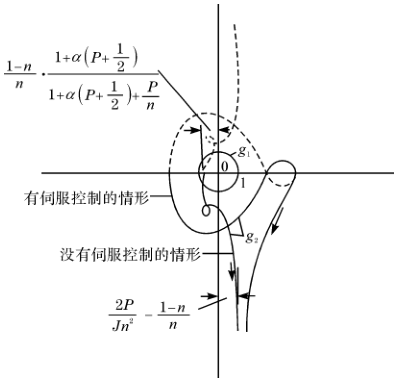
\includegraphics[width=\linewidth]{figs/fig-0196.png}
\caption{图11.7-1}
\end{figure}

有伺服控制的情形

没有伺服控制的情形

\[\frac{2P}{Jn^2} - \frac{1-n}{n}\]

图 11.7-1

作为一个例子，我们取

\[n = \frac{1}{2}, \quad P = \frac{3}{2}\]

\[J = 4\]

\[\begin{aligned}& E=\frac{1}{4} \\& \alpha=1\end{aligned}\]

$\alpha$ 的数值相当于燃料泵是一个离心泵的情形。如果没有伺服控制，$g_{\mathrm{c}}(s)$ 就是

\[g_{\mathrm{c}}(s)=-\frac{1}{2} \frac{(2 s+1)\left(2 s^{3}+3 s^{2}+9 s+6\right)}{s^{3}+3 s^{2}+6 s+6}\]

主要的兴趣在于 $s$ 取纯虚数 $i \omega(\omega$ 是实数） 时的 $g_{\mathrm{c}}(s)$ 的变化情况。因而

\[\begin{aligned}g_{\mathrm{c}}(i \omega)= & -\frac{1}{2} \frac{\left(6-21 \omega^{2}+4 \omega^{4}\right)\left(6-3 \omega^{2}\right)+\omega^{2}\left(21-8 \omega^{2}\right)\left(6-\omega^{2}\right)}{\left(6-3 \omega^{2}\right)^{2}+\omega^{2}\left(6-\omega^{2}\right)^{2}} \\& -\frac{1}{2} i \omega \frac{\left(21-8 \omega^{2}\right)\left(6-3 \omega^{2}\right)-\left(6-21 \omega^{2}+4 \omega^{4}\right)\left(6-\omega^{2}\right)}{\left(6-3 \omega^{2}\right)^{2}+\omega^{2}\left(6-\omega^{2}\right)^{2}}\end{aligned}\]

图 11.7-2 中画出了这条图线的 $\omega>0$ 的部分。可以明显地看到，如果时滞的值足够大，系统就会不稳定。从另一方面来看，如果考虑了伺服控制，而且假设 $g_{\mathrm{c}}(s)$能够相应地变为

\[g_{\mathrm{c}}(s)=-2 \frac{(s+2)(s+3)}{(s+6)}\]

那么，正如图 11.7-2 所画的那样，新的 $g_{\mathrm{c}}(s)$ 图线就完全在 $g_{\mathrm{c}}(s)$ 的单位圆图线的外面，因而，现在的系统就是无条件稳定的。根据方程 (11.6-1) 和 (11.7-1) 直接加以计算，就知道反馈部分的传递函数 $F(s)$ 应当是

\[F(s)=-4.875 \frac{(s+1.0528)\left(s^{2}+0.7164 s+2.6304\right)}{s(s+2)(s+3)\left(s+0.5332\right)\left(s^{2}+0.4668 s+3.7511\right)}\]

所以，反馈部分具有第 3.3 节讨论过的积分线路的那种特性。如果测量燃烧室压力的传感器的反应性能和带动控制容器的伺服机构的特性都已经给定了，那么，我们就可能设计出一个放大器，使得总的传递函数接近于上面提到的传递函数 $F(s)$，用这个伺服控制系统就可以使燃烧过程得到稳定。

作为第二个例子，我们取

\[n=\frac{1}{2}, \quad P=\frac{3}{2}, \quad J=4, \quad E=\frac{1}{4}, \quad \alpha=0\]

因为 $\alpha=0$，所以燃料泵的出口压力 $p_{0}$ 是一个常数，即使燃料流出的速率发生变化的时候 $p_{0}$ 也不会变动。这就相当于简单的增压装置的情形。如果没有反馈伺服机构，则

\[g_{\mathrm{c}}(s)=-\frac{1}{2} \frac{(2 s+1)\left(2 s^{3}+s^{2}+8 s+2\right)}{s^{3}+2 s^{2}+4 s+4}\]

当 $s$ 是纯虚数时

\[\begin{aligned}g_{\mathrm{c}}(i \omega)= & -\frac{1}{2} \frac{\left(4-2 \omega^{2}\right)\left(2-17 \omega^{2}+4 \omega^{4}\right)+\omega^{2}\left(4-\omega^{2}\right)^{2}\left(12-4 \omega^{2}\right)}{\left(4-2 \omega^{2}\right)^{2}+\omega^{2}\left(4-\omega^{2}\right)^{2}} \\& -\frac{1}{2} i \omega \frac{\left(4-2 \omega^{2}\right)\left(12-4 \omega^{2}\right)-\left(4-\omega^{2}\right)\left(2-17 \omega^{2}+4 \omega^{4}\right)}{\left(4-2 \omega^{2}\right)^{2}+\omega^{2}\left(4-\omega^{2}\right)^{2}}\end{aligned}\]

这条 $g_2$ 的图线被画在图 11.7-3 上。很明显，如果没有伺服控制，而且时滞 $\delta$ 的值也足够大，燃烧就会是不稳定的。事实上，这个系统的稳定性能还不如前一个例子的系统好；也就是说，对于比较小的时滞值这个系统就会变为不稳定的。$g_2$ 图线在 $\omega=2$ 点附近的部分是特别有趣的。在 $\omega=2$ 附近 $g_2$ 图线与 $g_1$ 的单位圆图线非常接近，如果时滞 $\delta$ 的值又能使得在 $\omega \simeq 2$ 时，$g_1(i\omega)$ 与 $g_2(i\omega)$ 也相当接近 $g_1(i\omega) \simeq g_2(i\omega)$，那么，在 $\omega \simeq 2$ 处就会发生一个几乎不衰减的振荡。这个临界的 $\delta$ 值显然小于那个由 $g_2$ 与单位圆在 $\omega \simeq 0.65$ 的实在的交点所确定的时滞 $\delta$ 的临界值。

\begin{figure}[htbp]\centering
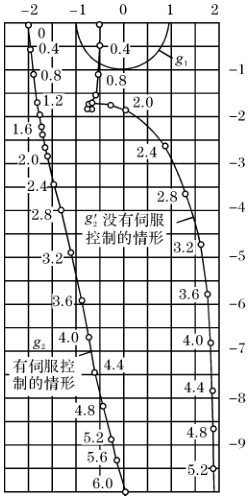
\includegraphics[width=\linewidth]{figs/fig-0198.png}
\caption{图11.7-2}
\end{figure}

\begin{figure}[htbp]\centering
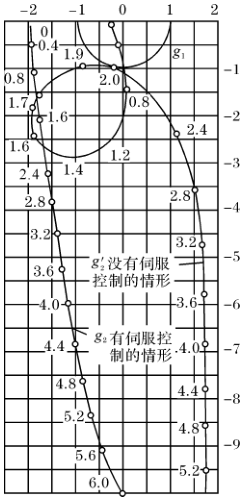
\includegraphics[width=\linewidth]{figs/fig-0197.png}
\caption{图11.7-3}
\end{figure}

为了实现无条件的稳定性，必须把 $g_2$ 图线移出单位圆，譬如说，如果希望把 $g_2$ 也变为与第一个例子中的那个图线完全相同的“稳定”的图线

\[g_2(s) = -2 \frac{(s+2)(s+3)}{s+6}\]

计算的结果表明：传递函数 $F(s)$ 就必须是

\[F(s) = -4.875 \frac{(s+0.8126)(s^2 - 0.04337s + 2.6506)}{s^2(s+2)(s+3)(s^2 + 4)}\]

所以，反馈部分必须具有二重积分线路那样的特性。而且，传递函数在 $2i$ 有两

\textbackslash\{\}begin\{figure\}[h]\textbackslash\{\}centering\textbackslash\{\}includegraphics[width=0.45\textbackslash\{\}textwidth]\{图11.7-2.png\}\textbackslash\{\}caption\{$p=\frac{3}{2}$，$J=4$，$E=\frac{1}{4}$，$\alpha=1$\}\textbackslash\{\}end\{figure\}

\textbackslash\{\}begin\{figure\}[h]\textbackslash\{\}centering\textbackslash\{\}includegraphics[width=0.45\textbackslash\{\}textwidth]\{图11.7-3.png\}\textbackslash\{\}caption\{$p=\frac{3}{2}$，$J=4$，$E=\frac{1}{4}$，$\alpha=0$\}\textbackslash\{\}end\{figure\}个纯虚数的极点。因为我们在原有的系统中忽略了导管的摩擦阻尼的作用，所以在这里才对放大器发生了这个不现实的要求。在任何一个实际的系统中，导管的摩擦阻尼作用必然会把所需要的传递函数 $F(s)$ 中的这两个纯虚数极点消除掉，并且把它们变为两个复共轭的极点。

必须强调指出，利用反馈伺服机构来稳定燃烧过程的做法的优点就是：由于反馈伺服机构的可变化性很大，对于任何的时滞 $\delta$ 或 $\tau$ 的值，我们都可以使系统无条件地稳定。既然我们没有关于时滞的准确的数据，所以，这个实现无条件稳定性的可能性对于工程实际来说确实是十分重要的。不但如此，如果要求在参数 $n$ 发生任何的变化的情况下系统都是稳定的，我们也可以用以上这种伺服稳定的方法进行设计。由于物理学的理由，$n$ 可以取 $1 / 2$ 与 1 之间的一个值。我们来处理最坏的可能性 $n \geqslant 1$，并且在这种情形下进行设计，使系统是无条件稳定的。这样设计出来的系统对于所有可能的 $n$ 的值，当然都是稳定的。因此，即使不知道系统的确切的参数值，我们也还能保证反馈伺服机构的稳定作用。

\section{11.8 利用萨奇图判断时滞系统稳定性的一般准则}

在以前的伺服稳定作用的讨论中，我们都假定方程 (11.7-1) 的多项式 $H(s)$ 在右半 $S$ 平面上没有零点和极点。然而，事实并不一定是这样的。所以，首先我们应该研究 $H(s)$ 在右半 $S$ 平面的零点和极点的个数。

我们把方程 (11.5-14)简写为

\[H(s)=H_{0}(s)+F(s) I(s)=1+L(s)\]

其中

\[\begin{aligned} H_{0}(s)= & \frac{1}{4} J^{2} E s^{3}+\left[\frac{1}{2} J E\left[1+\alpha\left(P+\frac{1}{2}\right)\right]+\frac{1}{2 n} J E P\right] s^{2} \\ & +\left[\alpha E\left[P+\frac{1}{2}\right]+J+\frac{\alpha E P}{n}\left(P+\frac{1}{2}\right)\right] s+\left[1+\alpha\left(P+\frac{1}{2}\right)+\frac{P}{n}\right] \\ I(s)= & \frac{s}{n}\left[\frac{1}{4} J^{2} E s^{3}+\frac{1}{2} \alpha J E\left[P+\frac{1}{2}\right] s^{2}+J E+\alpha\left(P+\frac{1}{2}\right)\right] \end{aligned}\]

假定 $H(s)$ 在右半 $S$ 平面有 $r$ 个零点和 $q$ 个极点，由 $H(s)$ 的表达式可以看到，它的 $q$ 个极点一定都是 $F(s)$ 的极点，于是 $E(s)$ 在右半 $S$ 平面上也就有 $q$ 个极点。另一方面，为了得到 $g_{1}(s)$ 和 $g_{2}(s)$，就要用 $H(s)$ 去除方程 (11.5-13) 中的 $E(s)$。这样做的结果就在右半 $S$ 平面引进了 $q$ 个零点和 $r$ 个极点。因此，如果要求 $E(s)$ 在右半 $S$ 平面上没有零点，$G(s)$ 就要围绕原点顺时针方向转 $-q+(q-r)=-r$ 圈，也就要求 $g_{2}(s)$ 围绕单位圆 $g_{1}(s)$ 以顺时针方向旋转 $-r$ 圈。于是，就需要确定 $H(s)$ 在右半 $S$ 平面上的零点数 $r$。因此只要画 $H(s)$ 的分子多项式 $H_{1}(s)$ 的乃氏图就够了。当s沿着图11.4-1的曲线转动一周时，H1(s)围绕原点顺时针方向转的圈数就是H(s)在右半S平面的零点数。所以，为了解决一般情况下的稳定性问题，萨奇图和乃氏图都是要用到的（图11.8-1)。

(a) 1+L(s)在右半平面上有两个零点的 $L(s)$ 的乃氏图

(b) 稳定的萨奇图

图 11.8-1 （实线表示正的 $\omega$，虚线表示负的 $\omega$)

显然，这里所讲的把萨奇图和乃氏图结合起来的稳定性准则，对于任意一个同类的时滞系统都是适用的。这一类系统的稳定性判据可以化为这样一个问题，即确定特征方程

\[E(s)=0\]

是否有大于零的实数部分的根。这里的 $E(s)$ 包含有 $e^{-\tau s}$ 因数的项。正像前面讨论过的那样，用 $E(s)$ 里的 $e^{-\tau s}$ 的系数 $H(s)$ 去除 $E(s)$ 便得到

\[\frac{E(s)}{H(s)}=G(s)=g_{1}(s)-g_{2}(s)\]

其中

\[g_{1}(s)=e^{-\tau s}\]

当 $s$ 在图 11.4-1 所画的右半圆的路上转动时，$g_{1}(s)$ 和 $g_{2}(s)$ 的图线就构成了萨奇图，$g_{1}(s)$ 的图线是单位圆。用 $H(s)$ 除 $E(s)$ 可能在萨奇图中引进若干个正实数部分的零点。为了判断这个情况，我们必须画出 $H(s)$ 分子的乃氏图。然后，根据 $G(s)$ 围绕原点沿顺时针方向转的圈数就可以确定 $E(s)=0$ 在右半 $S$ 平面上的根的个数。

函数 $g_{2}(s)$ 里包含有反馈部分的传递函数，反馈部分中的放大器是可以由设计者自由处理的。由于系统的其他部分的原因，$g_{2}(s)$ 里也可能包含有 $s$ 的超越函

\begin{figure}[htbp]\centering
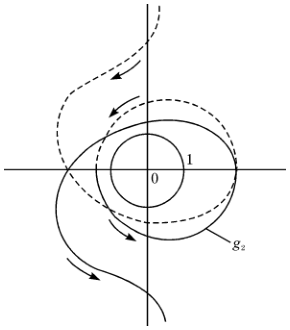
\includegraphics[width=\linewidth]{figs/fig-0199.png}
\caption{图11.8-1}
\end{figure}

\begin{figure}[htbp]\centering
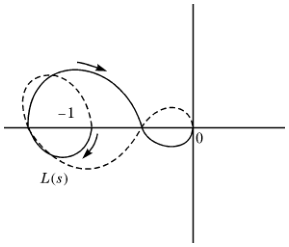
\includegraphics[width=\linewidth]{figs/fig-0200.png}
\end{figure}

数。因为，反馈部分的放大器的传递函数通常都是两个多项式的比值，所以很难把来源于超越函数的损害稳定性的不良影响完全补偿掉。可是，在萨奇图中 $g_{2}^{e}(s)$图线上最危险的部分就是最接近 $g_{1}^{e}(s)$ 的单位圆图线的那一部分。然而，接近单位圆的 $g_{2}^{e}(s)$ 点通常都是相应于小的 $s$ 值，所以在 $g_{2}^{e}(s)$ 的危险的部分上超越函数可以展开为 $s$ 的泰勒级数。我们可以只取级数的少数几项作为超越函数的近似值 ${ }^{[25]}$，并且根据这个近似的结果来设计反馈部分的放大器。这样一来系统在危险部分的损害稳定性的不良影响就可以被放大器补偿掉。不言而喻，最后还必须根据放大器的设计特性用已有的稳定性准则校验系统的性能。以上所讲的方法是马伯尔 (Marble) 和柯克司 (Cox) 所提出的。如果想知道详细的论述，读者可以去参阅原著 ${ }^{[12]}$。

\section{11.9 频率法的稳定性准则}

这一节我们力图把乃氏法更直接地应用到时滞系统中来，希望利用无时滞的开环频率特性来判断有时滞的闭环系统的稳定性问题。这种方法是建立在图 11.9-1(c)结构图的基础上的。由第三章关于传递函数的知识可以知道，任何一个时滞系统，不论时滞环节位于系统的主回路（图 11.9-1a)还是位于反馈线上（图 11.9-1b)，它们的闭环传递函数的分母（特征方程）是相同的。例如图 11.9-1(a)的闭环传递函数为

\[\phi^{*}(s)=\frac{F_{0}(s) e^{-t_{s}}}{1+F_{0}(s) e^{-t_{s}}}=\frac{N_{0}(s) e^{-t_{s}}}{D_{0}(s)+N_{0}(s) e^{-t_{s}}}\]

(a)

(b)

(c)

图 11.9-1

\begin{figure}[htbp]\centering
\includegraphics[width=\linewidth]{figs/fig-0201.png}
\end{figure}

\begin{figure}[htbp]\centering
\includegraphics[width=\linewidth]{figs/fig-0202.png}
\caption{图11.9-1}
\end{figure}

\begin{figure}[htbp]\centering
\includegraphics[width=\linewidth]{figs/fig-0203.png}
\caption{图11.9-1}
\end{figure}

其中 $F_{0}(s)=F_{1}(s) F_{2}(s)$ 是无时滞开环传递函数，$N_{0}(s), D_{0}(s)$ 分别为 $F_{0}(s)$ 的分子多项式和分母多项式。而图 11.12(b) 的闭环传递函数是

\[\begin{aligned}& \phi^{*}(s) F_{s}^{*}=\frac{F_{1}(s)}{1+F_{0}(s) e^{-\tau s}}=\frac{N_{1}(s) D_{2}(s)}{D_{0}(s)+N_{0}(s) e^{-\tau s}} \\& F_{0}(s)=F_{1}(s) F_{2}(s)\end{aligned}\]

可见图 11.9-1(a) 和图 11.9-1(b) 的闭环特征方程相同，因而两者的稳定性是等价的。这样，我们就可以从结构图 11.9-1(c) 出发来考虑有时滞的闭环系统的稳定性。

第 4.3 节所介绍的无时滞系统的稳定判据准则是利用开环传递函数的倒数 $\frac{1}{F_{0}(s)}$ 来判别的。当然，也可以利用传递函数 $F(s)$ 本身的图线来判断。由于大部分实际系统传递函数分母的阶数大于分子的阶数，仅在个别情况下两者相等。因此，当 $s$ 绕图 4.3-1 的曲线旋转时，$F_{0}(s)$ 图线的主要部分由频率特性 $F_{0}(i \omega)$ 所决定。由于 $F_{0}(-i \omega)=\overline{F_{0}(i \omega)}^{(1)}$，故可以直接利用开环频率特性 $F_{0}(i \omega), 0 \leqslant \omega<\infty$，来判断闭环的稳定性。如果开环的传递函数在右半平面无极点，那么闭环稳定的充要条件是开环频率特性在复平面上不包围 $(-1, i 0)$ 点。

从时滞系统的典型结构图 （图 11.9-1c) 可以看出，有时滞的开环频率特性 $F_{0}^{*}(i \omega)$ 可以由无时滞的开环频率特性 $F_{0}(i \omega)$ 求得。因为

\[F_{0}^{*}(i \omega)=F_{0}(i \omega)^{-i \tau \omega}\]

即对任何固定的自变量 $\omega$，向量 $F_{0}^{*}(i \omega)$ 可由 $F_{0}(i \omega)$ 顺时针方向转以 $\tau \omega$ 角而得到。因此，可以直接利用无时滞的开环频率特性来判断有时滞的闭环系统的稳定性。

首先我们讨论无时滞的开环系统稳定或中性稳定时，时滞系统的稳定情况。此时与无时滞的系统类似，闭环时滞系统稳定的充要条件是开环时滞系统频率特性在 $0 \leqslant \omega<\infty$ 段内不包围 $(-1, i 0)$ 点。

我们来考察特性 $1+F_{0}^{*}(i \omega), F_{0}^{*}(i \omega)$ 是开环时滞系统的频率特性，而 $N_{0}(i \omega)$和 $D_{0}(i \omega)$ 分别是开环无时滞系统频率特性的分子与分母，于是

\[1+F_{0}^{*}(i \omega)=1+\frac{N_{0}(i \omega)}{D_{0}(i \omega)} e^{-i \tau \omega}=\frac{D_{0}(i \omega)+N_{0}(i \omega) e^{-i \tau \omega}}{D_{0}(i \omega)}\]

其中分母是无时滞开环系统的特征方程，分子是有时滞闭环系统的特征方程。若要求有时滞的闭环系统稳定，那么当 $\omega$ 由 0 变至 $+\infty$ 时，开环时滞系统频率特性 $F_{0}^{*}(i \omega)$ 应该不包围 $(-1, i 0)$ 点。如果 $F_{0}^{*}(i \omega)$ 不包围 $(-1, i 0)$ 点而通过该点，那么系统就处于临界稳定状态。临界时滞时间 $\tau$ 和临界频率 $\omega_{\mathrm{H}}$ 应该由下列两式决定

(1) “一”表示共轭复数。

\[\left|F_{0}\left(i\omega_{k}\right)\right|=1\qquad\text{(11.9-1)}\]

\[\arg\left[F_{0}\left(i\omega_{k}\right)\right]-v_{k}\omega_{k}=-\pi\pm 2\pi q,\quad q=0,1,\cdots\]

从上述讨论似乎可以得出结论：一切具有时滞的元件都会使系统的稳定性变坏。实际上并非完全如此。有时，利用具有时滞的元件还可以改善闭路系统的稳定性。例如，设有一个闭路系统当没有时滞元件时不稳定，如具有图11.9-2那种频率特性的系统，显然它的闭路系统是不稳定的，因为频率特性包围了$(-1,i0)$点。此时如果在系统中的主回路或反馈回路内增加一个时滞元件，使频率特性曲线顺时针旋转一个角度，当时滞$\tau$选择恰当时，可以使原来包围$(-1,i0)$点的频率特性曲线转到此点的外部，于是增加了时滞元件的闭路系统就一变而为稳定系统了。在工程实际问题中，就有人利用时滞元件的这种性能去改善系统的稳定性，试验的结果也是很成功的。

\begin{figure}[htbp]\centering
\includegraphics[width=\linewidth]{figs/fig-0204.png}
\caption{图11.9-2}
\end{figure}

\textbackslash\{\}begin\{figure\}[h]\textbackslash\{\}centering\textbackslash\{\}includegraphics[width=0.5\textbackslash\{\}textwidth]\{图11.9-2.png\}\textbackslash\{\}caption\{图11.9-2\}\textbackslash\{\}end\{figure\}

关于时滞系统的线性综合方法，即控制装置的设计，也可以用频率特性去进行。比较成功的方法可参看文献[22]。

\section{参考文献}

[1] 秦元勋、刘泳清、王联，带有时滞的动力系统的运动稳定性，科学出版社，1963.

[2] 赵民义，复变函数论，高等教育出版社，1960.

[3] Ansoff，H. I.，Stability of linear oscillating systems with constant time lag，J. Appl. Mechanics(ASME)，16(1949)，158-164.

[4] Bellman，R.，Cooke，K. L.，Differential-Difference Equations，Academic Press，New York，1963.

[5] Balezstrino，A.，Celetano，G.，Stabilization by Digital Controllers of Multivariable Linear Systems with time-lays，Proc. of 7th IFAC Congress，Helsinki，1978.

[6] Bhat，K. P. M.，Koivo，H. N.，Modal characterization of controllability and observability for time delay systems，IEEE Trans. on AC，AC-21(1976)，2，232-233.

[7] CaHander，A.，Hartree，D.，Porter，A.，Trans. Roy. Soc.，London(A)，(1935)，415-444.

[8] Crocco，L.，Jour. Amer. Rocket Soc.，21(1951)，163-178.

[9] Goldenberg，A.，Davison，E. J.，The Robust Control of a Servomechanism Problem with Time Delay. Proc. of 7th IFAC Congress，Helsinki，1978.

[10] Jakubczyk，B.，Olbrot，A. W.，Dynamic Feedback Stabilization of Linear Time-lag Systems. Proc. of 7th IFAC Congress，Helsinki，1978.

[11] Minorsky，J. N.，Self-Excited oscillations in dynamical systems Possessiny retarded actions J. Appl. Mechanics (ASME)，9(1942)，67-71.

[12] Marble，F. E.，Cox，D. W.，Jour. Amer. Rocket Soci. 23(1953)，75-81.

[13] Pandolfi，L.，Stabilization of neutral functional differential equations. J. of optimization Theory and Appl.，20(1976)，2，191-204.

[14] Satche，M.，J. Appl. Mechanics，(ASME)，16(1949)，419-420.

[15] Tsien H. S. （钱学森），J. Amer. Rocket Soci. 22(1952)，139-143.

[16] Wonham，W. M.，Linear Multivariable Control，Springer-Verlay，New York，1974.

[17] Вулгаков В. В.，Колебание，Москва，1954.

[18] Лаврентьев М. А.，Шабат В. В.，Методы Теории Функций Комплексного Переменного，Москва，1958.

[19] Попов Е. П.，Динамика Систем Автоматического Регулирования，Гл. 7，Государственное издательство технико-теоретической литературы，Москва，1954.

[20] Понтрягин Л. С.，О нулях некоторых элементарных трансцендентных функций，изв. АН. СССР，Серия матем.，6(1942)，115-134.

[21] Уланов Г. К.，Анализ устойчивости систем автоматического регулирования с запаздыванием，в книге основы теории автоматического регулирования，под ред. Солодовникова，В. В. Гл. 13，Машиниз，1954.

[22] Фань Чун-вуй （范崇惠），Анализ качества и синтез автоматического регулирования с запаздыванием，Автаматика и Телемеханика，19(1958)，3.

[23] Фельдбаум А. А.，Электрические системы автоматического регулирования，Государственное издательство оборонный промышленности，Москва，1957. （电的自动调节系统，章燕申，金兰，石定机等译，国防工业出版社，1961.)

[24] Харатишвили Г. А.，Принцип Максимума в теории оптимальных процессов с запаздыванием，Доклады АН СССР，136(1961)，39-42.

[25] Цыпкин Я. З.，Устойчивость систем с запаздывающей обратной связью，Автаматика и Телемеханика，7(1946)，2-3.

<html><body>

\chapter{第十二章 分布参数控制系统}

在第一章里，我们曾经讲过，有很多受控对象的运动规律，不能用常微分方程来描述。例如，弹性梁型的运动体、大型加热炉、水轮机和汽轮机，物理学中的电磁场、流场、等离子体约束、温度场以及化学中的扩散过程等。这些物理量的变化规律，必须用偏微分方程才能准确地加以描述。而且在工程技术上，常常要求对这些物理量加以控制，使其变化规律满足技术上的要求。受控对象如此，控制装置或执行机构也有类似的情况。如液压和气动执行机构是目前应用比较广泛的元件。当油路和气路结构比较复杂且路线过长时，在其运动规律中也要考虑流体 （工作体） 本身的状态变化，而这种状态同样是由偏微分方程描述的。前一章讨论过的具有时滞的系统，如果时滞是由于运动在某种场内传递而造成的话，那么时滞系统就是分布参数系统的一个特例。

由此看来，工程实践向我们提出了不同于集中参数系统的一种控制系统。在这种系统中，一部分环节的运动用偏微分方程描述，而另一部分环节则用常微分方程描述，或者全部环节都用偏微分方程来描述。我们把这种动力学系统称之为分布参数控制系统。如弹性的振动控制、装有流体的刚性容器的晃动控制、温度场的控制，以及热核受控反应中的等离子体约束的控制等，都是典型的分布参数控制系统。

从工程技术角度来说，对于这类系统，我们自然会提出，什么是系统的稳定性，什么是它的过渡特性，如何进行系统分析，怎样设计一个满足实际限制而又能达到既定指标的控制装置，使系统满足规定的技术要求等。对于集中参数控制系统，这些方面的理论和实践都较成熟，但对分布参数系统来说，尚处在发展阶段。五十年代，当分布参数系统的理论还没有建立起来时，人们曾用集中参数的理论去逼近，如用带有时滞环节的常微分方程去讨论特殊类型的分布参数控制系统 ${ }^{[41]}$。即使这种比较简单的分布参数系统，就已经表现出了它的复杂性。以线性常系数分布参数系统来说，我们将会看到，第三章用过的传递函数方法对它还是可以应用的。但是，其传递函数已不再是有理分式，而是亚纯函数。系统的特征方程也不是多项式而是整函数，它的特征根也不是有限个而是无穷多个。显然，分析这种系统比集中参数系统复杂得多。至于线性变系数系统和非线性系统就更为复杂。

近十几年来，由于理论和实践的发展，特别是在分布参数控制系统的研究中，由于广泛应用现代偏微分方程和泛函分析的理论成果，不仅为分布参数系统建立

</body></html>了比较严格的理论基础，同时也提供了比较有力的工具，从而使分布参数系统的研究有了很大进展，成为现代控制理论中一个重要分支，并越来越引起人们的广泛重视。

目前，在分布参数系统理论的研究中，某些方面是和集中参数系统平行进行的。在某种意义上，它是集中参数系统理论的推广。如分布参数系统的镇定问题、最优控制问题、能控性和能观测性问题，以及分布参数系统的辨识和滤波问题等，都取得了类似于集中参数系统的结果。但是，由于分布参数系统描述的物理现象的复杂性，它具有无穷多个自由度，这一事实本身就决定了分布参数系统有其固有特点，而这些特点是集中参数系统所没有的。

在这一章里，我们仅就分布参数系统的基本特点和典型分布参数系统的构成，以及系统分析和综合的基本方法和概念，作一些初步介绍。对于这些问题的各种专门研究，读者可参阅本章所附的文献。

应该说明，十几年来，关于分布参数系统的研究工作很多，这当然是很好的事情，但用来解决工程实际问题的研究还不够多。而且偏微分方程理论本身也还有很多空白，尤其是从控制理论的角度提出的新问题还需要进一步深入地研究。

\section{12.1 分布参数环节的数学描述}

具有分布参数特性的物质运动，其运动状态不仅依赖于时间，而且还依赖于空间变量。例如横向振动的弦，它的横向位移 $u(t, x)$，既是时间 $t$ 又是弦上不同点位置 $x$ 的函数。不同的时间，弦的位移是不同的，即使同一时间，在弦的不同点 $x$ 处的位移也不同。在工程上，所有具有分布参数特性的对象和元件，都有着同样的性质。描述这类对象的运动方程是偏微分方程或积分方程。

例如，一个受控的均匀圆柱体的扭转运动。设其长为 $l$，材料的剪切模量为 $G$，质量密度为 $\rho$。若 $t$ 时刻 $x$ 点处的扭角为 $r(t, x)$，则圆柱体的扭转振动，可以用下述偏微分方程描述

\textbackslash\{\}frac\{\textbackslash\{\}partial\textasciicircum{}\{2\} r(t，x)\}\{\textbackslash\{\}partial t\textasciicircum{}\{2\}\}=\textbackslash\{\}frac\{G\}\{\textbackslash\{\}rho\} \textbackslash\{\}frac\{\textbackslash\{\}partial\textasciicircum{}\{2\} r(t，x)\}\{\textbackslash\{\}partial x\textasciicircum{}\{2\}\}+f(t，x)，\textbackslash\{\}quad 0

其中 $f(t, x)$ 是控制作用。

再如，一个均匀各向同性的物体，它在三维空间占有的区域为 $\Omega$，其边界为 $\partial \Omega$。设它的热传导系数为 $k$，比热为 $c$，密度为 $\rho$。用 $u=u(t, x, y, z)$ 表示物体在 $(x, y, z)$ 点处 $t$ 时刻的温度，那么，这个物体的温度变化应满足方程

\textbackslash\{\}frac\{\textbackslash\{\}partial u\}\{\textbackslash\{\}partial t\}=a\textbackslash\{\}left(\textbackslash\{\}frac\{\textbackslash\{\}partial\textasciicircum{}\{2\} u\}\{\textbackslash\{\}partial x\textasciicircum{}\{2\}\}+\textbackslash\{\}frac\{\textbackslash\{\}partial\textasciicircum{}\{2\} u\}\{\textbackslash\{\}partial y\textasciicircum{}\{2\}\}+\textbackslash\{\}frac\{\textbackslash\{\}partial\textasciicircum{}\{2\} u\}\{\textbackslash\{\}partial z\textasciicircum{}\{2\}\}\textbackslash\{\}right)+f(t，x，y，z)，\textbackslash\{\}quad(x，y，z) \textbackslash\{\}in \textbackslash\{\}Omega，\textbackslash\{\}quad 0其中 $a_{\rho}^{2}=\frac{k}{c \rho}, f(t, x, y, z)$ 为可调的热源。

如果不加热源，即 $f(t, x, y, z) \equiv 0$，而且物体的外部环境不随时间变化，这时，不管初始温度如何，经过一段时间之后，物体内部温度趋于平衡，此时热量仍在流动，只是流出和流入物体热量的代数和等于零，物体内部的温度 $u(t, x, y, z)$ 已与 $t$无关，在这种情况下，它满足所谓拉普拉斯方程

\[\frac{\partial^{2} u}{\partial x^{2}}+\frac{\partial^{2} u}{\partial y^{2}}+\frac{\partial^{2} u}{\partial z^{2}}=0, \quad(x, y, z) \in \Omega\qquad\text{(12.1-3)}\]

上述这些方程都是典型的偏微分方程，而且都是线性的，即在方程中对未知函数及其导数都是线性的。当方程中所有系数都是常数时，叫做常系数方程。如果右端函数[如式 (12.1-1) 中的 $f(t, x)$ ]不为零时，叫做非齐次方程。否则叫做齐次方程，如式 (12.1-3)。对线性二阶方程，按其特点又分为双曲型、抛物型和椭圆型三种。许多分布参数环节是由这些方程描述的，所以我们稍微介绍得详细一点。

方程 (12.1-1) 是双曲型方程中的一种。这类方程含有对时间 $t$ 的二阶偏导数项，即加速度项。自然界中波的传播，物体振动等的运动方程大都属于这一类。它们表现出对时间具有可逆的性质。同是双曲型方程，可以描述完全不同的物理现象。比如一维双曲型方程

\[\frac{\partial^{2} u}{\partial t^{2}}=a_{x}^{2} \frac{\partial^{2} u}{\partial x^{2}}\]

当 $a_{\rho}^{2}=\frac{T}{\rho}, T$ 是张力，$\rho$ 是质量密度时，它描述了弦的横向振动。但是一个充满气体的细长管子受到小扰动时，管中气体压力 $p$ 也满足相同形式的方程，

\[\frac{\partial^{2} p}{\partial t^{2}}=a_{x}^{2} \frac{\partial^{2} p}{\partial x^{2}}\]

只是系数 $a_{\rho}^{2}$ 的物理意义不同了。此时 $a_{\rho}^{2}=\frac{k p_{0}}{\rho}, p_{0}, \rho$ 分别是初始时刻气体压力和密度，$k=\frac{C_{p}}{C_{v}}$ 是比热比，$c_{p}$ 是定压比热，$c_{v}$ 是定容比热。

方程 (12.1-2) 是抛物型方程中的一种。这类方程中，含有对 $t$ 的一阶偏导数项，即速度项。它描述着自然界中的热传导过程、气体扩散以及电磁场传播等物理过程。同样，在量子力学、统计物理、概率论等理论研究中也会遇到这类方程。这类运动过程在时间上，通常没有可逆性。和双曲型方程类似，同一方程描述完全不同的物理现象。比如，导电线圈所围圆柱体内的磁场 $H$，就用方程 (12.1-2) 来描述

\[\frac{\partial H}{\partial t}=a_{x}^{2}\left(\frac{\partial^{2} H}{\partial x^{2}}+\frac{\partial^{2} H}{\partial y^{2}}+\frac{\partial^{2} H}{\partial z^{2}}\right)\]

其中 $a^{2}=\frac{c^{2}}{4 \pi \sigma \mu}, c$ 是光速，$\mu$ 是磁导率，$\sigma$ 是电导率。

双曲线和抛物型方程，描述了运动的动态过程，而式(12.1-3)这类椭圆型方程，则描述了运动的稳态过程。诸如稳态下的热传导问题，在固定外力作用下，膜的平衡问题以及不可压缩理想流体无旋流动的速度势，静电场的电位等，都属于椭圆型方程。

从工程技术上说，所谓分布参数受控对象和元件，即分布参数环节，就是指其运动方程是由上述各类偏微分方程描述的。这些描述运动过程的方程式也叫发展方程。如果方程和边界条件都是线性的，则这个环节就叫做线性环节。

例如，在飞行控制中，一个细长体飞行器，有时不能完全看成刚体而必须考虑弹性振动。此时作为弹性体，它的运动可以近似用弹性梁的运动来描述，其运动方程就是 ${ }^{[9]}$

m(x) \textbackslash\{\}frac\{\textbackslash\{\}partial\textasciicircum{}\{2\} u\}\{\textbackslash\{\}partial t\textasciicircum{}\{2\}\}+C(x) \textbackslash\{\}frac\{\textbackslash\{\}partial u\}\{\textbackslash\{\}partial t\}+B(x) \textbackslash\{\}frac\{\textbackslash\{\}partial u\}\{\textbackslash\{\}partial x\}+\textbackslash\{\}frac\{\textbackslash\{\}partial\textasciicircum{}\{2\}\}\{\textbackslash\{\}partial x\textasciicircum{}\{2\}\} E J(x) \textbackslash\{\}frac\{\textbackslash\{\}partial\textasciicircum{}\{2\} u\}\{\textbackslash\{\}partial x\textasciicircum{}\{2\}\}=f(t，x)，\textbackslash\{\}quad 0

其中 $m(x)$ 是梁的质量密度，$E$ 是杨氏模量，$E J(x)$ 是 $x$ 处的弯曲刚度，$C(x)$ 是介质对梁横向振动的阻尼系数，$B(x)$ 是局部升力系数，$f(t, x)$ 是控制作用。 $u=u(t$，$x)$ 是梁在 $x$ 点处 $t$ 时刻的横向位移。显然，这样的受控对象就是分布参数对象。

和集中参数系统一样，为了进行系统分析，首先要分析分布参数环节的动态特性和静态特性，因此就必须对描述环节的方程求解。但是这个问题要比集中参数环节复杂得多。

一个用常微分方程描述的对象，只要初始状态给定，它的运动就唯一确定了。对偏微分方程描述的对象，为了确定它的解，也必须给出初始状态，即初始条件。对双曲线方程要给出初始位移和初始速度，比如方程(12.1-1)，它的初始条件可以是

\[r(t, x) \mid_{t=0}=\varphi(x), \quad \left.\frac{\partial r(t, x)}{\partial t}\right|_{t=0}=\psi(x)\qquad\text{(12.1-5)}\]

对抛物型方程要给出初始位置，比如，方程(12.1-2)的初始条件可为

\[u(t, x, y, z) \mid_{t=0}=\varphi(x, y, z)\qquad\text{(12.1-6)}\]

但是，只有初始条件，对偏微分方程来说，往往还不能唯一确定它的解。比如，同样作扭转振动的圆柱体，它可以是两端固定不动的，也可以是一端固定不动而另一端是自由的。这两种不同的边界情况，圆柱体的振动规律显然不一样。同样，一个传热介质的边界，如方程(12.1-2)中的 $\partial \Omega$，它可以是绝热的，也可以和外界有热交换，在这两种边界条件下，介质的热传导规律也不一样。因此，为了使方程的解确定，除了初始条件外，还必须有所谓的边界条件，这是不同于集中参数系统的。例如，上述圆柱体的扭转振动，当两端固定时，边界条件为

\[r(t, x) \mid_{x=0}=0, r(t, x) \mid_{x=l}=0\qquad\text{(12.1-7)}\]

如果 $x=0$ 一端固定，$x=l$ 一端是自由的，则边界条件为

\[r(t, x) \mid_{x=0}=0, \frac{\partial r(t, x)}{\partial x} \mid_{x=l}=0\qquad\text{(12.1-8)}\]

边界条件反映了在物体运动过程中，加在其边界上的约束。不同的约束条件，其运动规律也不一样。当初始条件和边界条件都给定以后，方程的解才能唯一确定，这在数学中叫做偏微分方程的定解问题，而初始条件和边界条件叫做定解条件。给定了运动方程，它描述了物体的一般运动，在方程和定解条件都给定的情况下，方程的解就描述了物体的一类特殊运动。

对上述三种不同类型的方程，在形式上有着完全相似的三种边界条件 ${ }^{[2,3]}$。以方程 (12.1-2) 为例，第一类边界条件是

\[u(t, x, y, z) \mid_{\partial \Omega}=\varphi_{c}(t, x, y, z), \quad(x, y, z) \in \partial \Omega\qquad\text{(12.1-9)}\]

它表示在物体边界上，$u(t, x, y, z)$ 的变化规律是已知的。

第二类边界条件是

\[\left.\frac{\partial u(t, x, y, z)}{\partial n}\right|_{\partial \Omega}=\varphi_{c}(t, x, y, z), \quad(x, y, z) \in \partial \Omega\qquad\text{(12.1-10)}\]

其中 $n$ 表示边界曲面 $\partial \Omega$ 的外法线方向。这个条件表明，在物体边界 $\partial \Omega$ 的法线方向上，$u(t, x, y, z)$ 的变化规律是给定的。

第三类边界条件是

\[\left[\frac{\partial u(t, x, y, z)}{\partial n}+k u(t, x, y, z)\right] \mid_{\partial \Omega}=\varphi_{c}(t, x, y, z), \quad(x, y, z) \in \partial \Omega\qquad\text{(12.1-11)}\]

其中 $k$ 是已知常数。这个条件是式 (12.1-9) 和 (12.1-10) 的线性组合，它表明在物体边界 $\partial \Omega$ 及 $\partial \Omega$ 的法线方向上，两者合在一起 $u(t, x, y, z)$ 的变化规律是已知的。

如果 $\varphi_{1}=\varphi_{2}=\varphi_{3}=0$，则叫做齐次边界条件，否则叫做非齐次边界条件。

在受控对象的分析中，我们能够遇到的有三种问题，即初值问题，边值问题，混合问题。

所谓初值问题 （柯西问题） 是指只有初始条件就可定解。这类问题描述的是相当于空间变量的变化区域为无限大时的动态过程。它往往出现在双曲型和抛物型方程中。如无限长圆柱体的扭转振动，无限大介质中的热传导，无限长电力线的传输等。所谓无限大的区域，是指当物体的体积很大，而所要研究的问题是在较短时间里，较小范围内的变化规律。比如大气中某个局部范围短期内温度变化的情况，那时边界条件产生的影响很小，以致可以忽略，这时不妨把整个物体看成无限大，而把边界条件去掉。于是就变成了只有初始条件的初值问题。

边值问题是在定解条件中只有边界条件，没有初始条件。这类问题描述的是运动的稳态过程。边值问题往往出现在椭圆型方程中。

混合问题是在定解条件中既有初始条件也有边界条件。这类问题描述了空间区域为有限时的动态过程。它大多出现在双曲型和抛物型方程中。如有限长弦的横向振动，有限体积内物体热传导，有限长电力线的传输等。从控制观点看，我们首先感兴趣的是动态过程，然后才是稳态过程，因此，我们讨论的重点是混合问题。

\begin{figure}[htbp]\centering
\includegraphics[width=\linewidth]{figs/fig-0205.png}
\caption{图12.1-1}
\end{figure}

以上所讲的分布参数对象，其空间区域和边界，在运动过程中始终保持不变，这叫做固定域分布参数对象。与此相反，当空间区域和边界在运动过程中随着时间而变化时，叫做可变域分布参数对象。比如，带有烧蚀表面的再入飞行器的烧蚀问题 ${ }^{[33]}$。我们研究再入飞行器烧蚀部分最简单的一维模型。设厚为 $l$ 的烧蚀板，在 $x=0$ 处有热输入为 $Q(t), Q(t)$ 可表示为宇宙飞行器再入大气层速度 $v(t)$ 的函数，即 $Q(t)=q(v(t))$。在 $x=l$ 处烧蚀板被绝热。如图 12.1-1。

在 $t$ 时飞行器开始再入飞行，由于气动加热，在 $x=0$ 处到 $t$ 时达到了烧蚀板的熔点 $u_{m}$。在 $t \leqslant t \leqslant t$ 这段时间内，烧蚀板内的温度分布可用一维热传导方程描述

$\frac{\partial u(t, x)}{\partial t}=\mu \frac{\partial^{2} u(t, x)}{\partial x^{2}}, \quad 0在初始条件是$u(t，x) \textbackslash\{\}mid\_\{t=t\_\{0\}\}=u\_\{0\}(x)$边界条件为$\textbackslash\{\}left.\textbackslash\{\}frac\{\textbackslash\{\}partial u(t，x)\}\{\textbackslash\{\}partial x\}\textbackslash\{\}right|\_\{x=0\}=\textbackslash\{\}frac\{1\}\{k\} q(v(t))，\textbackslash\{\}quad\textbackslash\{\}left.\textbackslash\{\}frac\{\textbackslash\{\}partial u(t，x)\}\{\textbackslash\{\}partial x\}\textbackslash\{\}right|\_\{x=l\}=0$其中$k$是热传导系数。由于板的一端是绝热的,随着时间$t$的增大,热量不断积累,当$t>t$时板开始熔解。这时板的边界和内部温度都将发生变化。用$S(t)$表示板的固体部分的边界,用$\textbackslash\{\}tilde\{u\}(t，x)$表示板内温度分布。当$t>t$时,$\textbackslash\{\}tilde\{u\}(t，x)$满足下述方程$\textbackslash\{\}frac\{\textbackslash\{\}partial\}\{\textbackslash\{\}partial t\} \textbackslash\{\}tilde\{u\}(t，x)=\textbackslash\{\}mu \textbackslash\{\}frac\{\textbackslash\{\}partial\textasciicircum{}\{2\}\}\{\textbackslash\{\}partial x\textasciicircum{}\{2\}\} \textbackslash\{\}tilde\{u\}(t，x)，\textbackslash\{\}quad S(t)<x<l，\textbackslash\{\}quad t<t$初始条件为$S(t)=0，\textbackslash\{\}quad \textbackslash\{\}tilde\{u\}(t，x)=u(t，x)边界条件是

\[\begin{aligned}& \left.\tilde{u}(t, x)\right|_{x=S(t)}=u_{m} \\& \rho \alpha \frac{d S(t)}{d t}-k\left.\frac{\partial}{\partial x} \tilde{u}(t, x)\right|_{x=S(t)}=q(v(t)) \\& \left.\frac{\partial}{\partial x} \tilde{u}(t, x)\right|_{x=l}=0\end{aligned}\qquad\text{(12.1-17)}\]

其中 $\rho$ 是板的密度，$\alpha$ 是熔解热。

在这个例子中，分布参数对象的区域和边界都是随着时间而变化的。因此，它是可变域的分布参数对象。但是，经过适当的变换可以把可变域的分布参数系统变成一个固定域分布参数系统耦合一个集中参数系统，对于后者研究起来就比较方便。今后，我们主要讨论固定域的分布参数对象。

下面，我们再说明一下偏微分方程解的含义。在定解问题中，解函数的类别与具体问题的性质有关，需要每次具体确定。例如它可以是指这样的函数，它以及出现在定解条件中它的偏导数，都在所考虑的区域上连续，而在方程中所出现的它的导数在区域内部连续，他们都同时满足方程，当区域内部的点以任意方式趋于边界时，他们满足定解条件。以方程 (12.1-2) 为例。运动方程和定解条件如下:

\[\begin{aligned}& \left.\frac{\partial u}{\partial t}=d\left(\frac{\partial^{2} u}{\partial x^{2}}+\frac{\partial^{2} u}{\partial y^{2}}+\frac{\partial^{2} u}{\partial z^{2}}\right), \quad(x, y, z) \in \Omega, \quad 0<t<\infty\right. \\& \left.u(t, x, y, z)\right|_{t=0}=\varphi(x, y, z), \quad(x, y, z) \in \Omega, \quad t=0 \\& \left.\left(\frac{\partial u}{\partial n}+k u\right)\right|_{\partial \Omega}=\psi(t, x, y, z), \quad(x, y, z) \in \partial \Omega, \quad t \geqslant 0\end{aligned}\]

它的解 $u(t, x, y, z)$ 是指它在 $\Omega$ 和 $\partial \Omega$ 上以及 $t \geqslant 0$ 时连续，$\frac{\partial u}{\partial n}$ 在 $\partial \Omega$ 和 $t \geqslant 0$ 时连续。其次，$\left.\frac{\partial u}{\partial t}, \frac{\partial^{2} u}{\partial x^{2}}, \frac{\partial^{2} u}{\partial y^{2}}, \frac{\partial^{2} u}{\partial z^{2}}\right.$ 在 $\Omega$ 和 $t>0$ 处连续，把这个 $u(t, x, y, z)$ 代到方程 (12.1-2) 中使其成为恒等式。当 $t \rightarrow 0$ 时，$u(t, x, y, z) \rightarrow \varphi(x, y, z)$ 对任意的点 $(x$，$y, z) \in \Omega$ 处处成立。当 $(x, y, z) \in \Omega$ 并以任意方式趋于边界 $\partial \Omega$ 上任意点 $\left(x_{0}, y_{0}\right.$，$\left.z_{0}\right)$ 时，对 $t \geqslant 0$ 都有 $\left[\frac{\partial u}{\partial n}+k u\right] \rightarrow \psi\left(t, x_{0}, y_{0}, z_{0}\right)$ 成立。这样的解通常叫做方程的古典解。古典解的存在往往对初始条件要求比较严格，而实际上给定的初始条件常常不能满足这些要求。因此，古典解有很大的局限性。为了满足实际问题的需要，要用广义解代替古典解，它在较广的范围内给出了定解问题的解。这样就比较接近工程实际问题的特点。关于广义解的定义和求解方法，将在本章第 12.6 节中讨论。

\section{12.2 分布参数环节的传递函数}

分布参数环节是由偏微分方程描述的，为了分析这种环节的特性，需要求解偏微分方程。在给定了定解条件后，解偏微分方程的方法很多，但在控制理论中常用的是拉普拉斯变换法和分离系数法。特别是拉普拉斯变换法，还可以使我们去定义分布参数环节的传递函数。

我们首先定义分布参数系统中遇到的拉普拉斯变换 (1)。

设二元函数 $y(t, x)$，在 $t > 0$ 时是逐段连续的函数。在 $t < 0$ 时为零。对任意固定的 $x$，作为 $t$ 的函数 $y(t, x)$ 的增长速度小于 $e^{\sigma_0 t}, 0 < \sigma < \infty$。我们定义

\[Y(s, x) = \int_0^\infty y(t, x) e^{-st} dt, \quad \text{Res} > \sigma_0\qquad\text{(12.2-1)}\]

式中 $s$ 为复数。Res 是 $s$ 的实部。$Y(s, x)$ 称为函数 $y(t, x)$ 的拉氏变换。$Y(s, x)$ 在 $\text{Res} \leq \sigma$ 上的值可用解析延拓方法确定。今后把 $Y(s, x)$ 叫做 $y(t, x)$ 的象函数，而 $y(t, x)$ 为 $Y(s, x)$ 的原函数。容易验证，第二章所讲的拉氏变换性质，在这里也是正确的。例如，当 $y(0, x) = \varphi(x)$ 时，则有

\[\int_0^\infty \frac{dy(t, x)}{dt} e^{-st} dt = y(t, x) e^{-st} \bigg|_0^\infty + \int_0^\infty y(t, x) e^{-st} dt = -\varphi(x) + sY(s, x)\]

即 $\frac{dy(t, x)}{dt}$ 的象函数为 $-\varphi(x) + sY(s, x)$。

除此而外，还有以下性质:

(1) $Y(s, 0) = \int_0^\infty y(t, 0) e^{-st} dt$

\[Y(s, l) = \int_0^\infty y(t, l) e^{-st} dt\]

(2) 若 $\frac{\dot{\varphi} y(t, x)}{\partial x}$ 对任意固定的 $x$，作为 $t$ 的函数其增长速度不大于 $e^{\beta t}, \beta \geqslant \sigma$，则

\[\int_0^\infty \frac{\dot{\varphi} y(t, x)}{\partial x} e^{-st} dt = \frac{\dot{\varphi}}{\partial x} \int_0^\infty y(t, x) e^{-st} dt = \frac{\dot{\varphi} Y(s, x)}{\partial x}, \quad \text{Res} > \beta\]

$\text{Res} \leqslant \beta$ 的值可用解析延拓方法得到。这就是说，在上述条件下，$\frac{\dot{\varphi} y(t, x)}{\partial x}$ 的象函数为 $\frac{\dot{\varphi} Y(s, x)}{\partial x}$。

(3) 当 $\text{Res} > \sigma$ 时，

\[\lim_{x \to \infty} Y(s, x) = \int_0^\infty \lim_{x \to \infty} y(t, x) e^{-st} dt\]

(1) 在一般函数空间中的拉普拉斯变换的严格定义请参看 Hille，E \& Phillips，R. S.，Functional Analysis and Semi-groups，Amer. Math. Soc.，1957。

$\operatorname{Res} \leqslant \sigma$ 的值可用解析延拓方法确定。

设 $Y(s, x)$ 是 $\gamma(t, x)$ 的象函数，则 $\gamma(t, x)$ 可用拉氏反变换求得

\[\gamma(t, x)=\frac{1}{2 \pi i} \int_{\gamma-i \infty}^{\gamma+i \infty} Y(s, x) e^{s t} d s, \quad \gamma>\sigma\qquad\text{(12.2-2)}\]

在常微分方程中，应用拉氏变换将原函数的微分方程变成了象函数的代数方程。在偏微分方程中，应用拉氏变换后，仍是象函数的偏微分方程，但自变量的数目将减少一个 （有时变成了象函数的常微分方程）。然后我们应用边界条件将象函数的微分方程解出，再进行拉氏反变换就得到了方程的解。这个解由两部分组成，一部分是由初始条件引起的运动，叫做自由运动。另一部分由外加作用引起的运动，叫做强迫运动。当把外加作用看成输入，而把它引起的运动看作输出，这时输出输入象函数的比，仍是一个以 $s$ 为自变量的函数，我们把这个函数叫做分布参数环节的传递函数。和集中参数环节不同的是，这个传递函数不再是有理分式，一般地说，它是 $s$ 的超越函数，而且还是空间变量的函数。

我们举几个例子，说明拉氏变换法的应用。

例 1. 求初始位移为 $\varphi(x)$，初始速度为 $\psi(x)$，在 $x=0$ 点处受集中力矩 $u(t)$ 控制，两端自由的圆柱体扭转振动的传递函数 （见图 12.2-1)。

\[r(t, x)\]

\[u(t)\]

图 12.2-1

圆柱体扭转振动方程及定解条件为

\[\begin{gathered} \frac{\partial^{2}}{\partial t^{2}} r(t, x)=a^{2} \frac{\partial^{2}}{\partial x^{2}} r(t, x), \quad 00, \quad 0<t<\infty \\ \left.\frac{\partial r(t, x)}{\partial x}\right|_{x=0}=u(t), \quad\left.\frac{\partial r(t, x)}{\partial x}\right|_{x=l}=0 \\ r(0, x)=\varphi(x), \quad\left.\frac{\partial r(t, x)}{\partial t}\right|_{t=0}=\psi(x) \end{gathered}\qquad\text{(12.2-3)}\]

对上述方程进行拉氏变换，则得到

\[\begin{gathered} a^{2} \frac{d^{2}}{d x^{2}} R(s, x)=s^{2} R(s, x)-\varphi(x)-\psi(x), \quad \frac{d R(s, x)}{d x}\left.\right|_{x=0}=U(s) \\ \left.\frac{d R(s, x)}{d x}\right|_{x=t}=0 \end{gathered}\qquad\text{(12.2-4)}\]

把 $x$ 看成参数，这就是常微分方程的两点边值问题，它的通解是

\begin{figure}[htbp]\centering
\includegraphics[width=\linewidth]{figs/fig-0206.png}
\caption{图12.2-1}
\end{figure}

\[\begin{gathered} R(s, x)=c_{1} e^{a x}+c_{2} e^{-a x}-a \int_{0}^{x} \operatorname{sh} \frac{s}{a}(x-\zeta)[s \varphi(\zeta)+\psi(\zeta)] d \zeta \\ c_{1}, c_{2} \text { 是任意常数,利用边界条件,得到 } c_{1}, c_{2} \text { 应满足的方程式 } \\ U(s)=\frac{s}{a} c_{1}-\frac{s}{a} c_{2} \\ 0=\frac{s}{a} c_{1} e^{a t}-c_{2} \frac{s}{a} e^{-a t}-\frac{1}{a} \int_{0}^{l} \operatorname{ch} \frac{s}{a}(l-\zeta)[s \varphi(\zeta)+\psi(\zeta)] d \zeta \end{gathered}\qquad\text{(12.2-6)}\]

解出 $c_{1}, c_{2}$ 代到式 (12.2-5)中，便得到

\[\begin{aligned} & R(s, x)=-\frac{a \cdot \operatorname{ch} \frac{l-x}{a}}{s \cdot \operatorname{sh} \frac{l}{s}} U(s)+2 s a \cdot \operatorname{sh} \frac{l}{a} \int_{0}^{l} \operatorname{ch} \frac{s}{a}(l-x-\zeta) \\ & \quad \cdot[s \varphi(\zeta)+\psi(\zeta)] d \zeta+\int_{x}^{l} \operatorname{ch}(l+x-\zeta)[s \varphi(\zeta)+\varphi(\zeta)] d \zeta \end{aligned}\qquad\text{(12.2-8)}\]

我们可以看到，第一项是由控制作用 $u(t)$ 引起的输出，其余是由初始条件引起的输出。当初始条件为零时，输出为

\[R(s, x)=-\frac{a \cdot \operatorname{ch} \frac{l-x}{a}}{s \cdot \operatorname{sh} \frac{l}{s}} U(s)\qquad\text{(12.2-7)}\]

由此，环节的传递函数为

\[W(s, x)=\frac{R(s, x)}{U(s)}=-\frac{a}{s} \frac{\operatorname{ch} \frac{l-x}{a}}{\operatorname{sh} \frac{l}{s}}\qquad\text{(12.2-9)}\]

例 2. 研究一维热传导问题。一座墙壁 （见图 12.2-2)，它的厚度为 $l$，高度和宽度认为是无限大。墙的热传导系数为 $k$，热容量 （即密度和比热之积） 是 $c$，墙的左面 $(x=0)$ 处的温度是一个已知的时间函数 $u(t)$，它是控制量。墙的右面 $(x \geqslant l$ 处） 是绝热的。墙的初始温度为零。我们感兴趣的是墙在 $x=l$ 处的温度随 $u(t)$ 的变化规律。

设墙内各点的温度为 $y(t, x), y(t, x)$ 应满足抛物型方程

0

\begin{figure}[htbp]\centering
\includegraphics[width=\linewidth]{figs/fig-0207.png}
\caption{图12.2-2}
\end{figure}

c \{ y(t，x)\}\{ t\}=k \{\textasciicircum{}\{2\} y(t，x)\}\{ x\textasciicircum{}\{2\}\}，0应用拉氏变换方法，可以得到\{aligned\}\& c s Y(s，x)=k \{d\textasciicircum{}\{2\} Y(s，x)\}\{d x\textasciicircum{}\{2\}\} Y(s，0)=U(s)，.\{d Y(s，x)\}\{d x\}|\_\{x=l\}=0\{aligned\}\{aligned\}$令$=\{c s\}\{k\}$，则方程的解为当$x=l$时，便有而传递函数为例 3. 考虑一个电力线传输问题。有一半无限长的电力传输线，每单位长度的电阻为$R$，电容为$C$，假定导线上的电感和电漏为零，传输线端点接入一电压源，其电压$e=e(t)$可以人为改变，把它作为控制量。电力传输线上各点处的电流$i(t，x)$及电压$u(t，x)应满足方程aligned\& - i(t，x) x=C  u(t，x) t - u(t，x) x=R i(t，x)aligned初始条件和边界条件为应用拉氏变换法，由式 (12.2-14) 和 (12.2-15) 可得到\{aligned\}\& -\{d I(s，x)\}\{d x\}=C s U(s，x) -\{d U(s，x)\}\{d x\}=R I(s，x) U(s，0)=E(s)，\_\{x arrow \} U(s，x)<解方程组便得到

\[U(s, x)=E(s) e^{-\sqrt{C R_{s x}}}\]

\[I(s, x)=\sqrt{\frac{C_{s}}{R}} E(s) e^{-\sqrt{C R_{s x}}}\qquad\text{(12.2-17)}\]

若感兴趣的是传输线上某点 $x=x_{1}$ 处的电压 $U\left(s, x_{1}\right)$，则传递函数为

\[W\left(s, x_{1}\right)=\frac{U\left(s, x_{1}\right)}{E(s)}=e^{-\sqrt{C R_{s x_{1}}}}\qquad\text{(12.2-18)}\]

例 4.我们再来考虑一个二维机翼的理论问题 ${ }^{[31]}$，第十四章里将要用到它。假定在均匀的以水平速度 $V$ 流动的气流里，有一个弦长为 $c$ 的机翼 （见图 12.2-3)。

若气流在 $x=0$ 点的垂直方向上发生了一个扰动速度 $v(t)$，那么，沿着翼弦方向 $x$ 便有扰动的分布升力产生，记扰动升力密度为 $f(t, x)$，它满足气体动力学中的偏微分方程。流过机翼的气体是分布参数的。把升力密度 $f(t, x)$ 对 $x$ 从 0 到 $c$ 积分，所得到的合力就是升力

\[Y(t)=\int_{0}^{c} f(t, x) d x\]

机翼每单位面积所受到的升力和速压头 $\frac{1}{2} \rho V^{2}$ 之比称为升力系数 $\varphi(t)$，这里 $\rho$ 是气体密度。西尔思(Sears)证明了 ${ }^{[31]}$，当扰动速度为正弦函数时

\[v(t)=\alpha_{m} V e^{i \omega t}\qquad\text{(12.2-19)}\]

升力系数的稳态解 $c_{\text {est }}(t)$ 为

\[c_{\text {est }}(t)=2 \pi \alpha_{m} e^{i \omega t} \varphi(k)=\frac{2 \pi}{V} \varphi(k) v(t)\qquad\text{(12.2-20)}\]

式中 $k=\frac{\omega c}{2 V}$，而

\[\varphi(k)=\frac{J_{0}(k) K_{1}(i k)+i J_{1}(k) K_{0}(i k)}{K_{1}(i k)+K_{0}(i k)}\qquad\text{(12.2-21)}\]

这里 $J_{0}$ 和 $J_{1}$ 分别是零阶和一阶第一类贝塞尔函数，$K_{0}$ 和 $K_{1}$ 表示第二类变态的贝塞尔函数。

如果把 $v(t)$ 当做输入，$c_{e}(t)$ 作为输出，那么环节传递函数为

\[W(s)=\frac{C_{e}(s)}{V(s)}\]

取 $s=i \omega$，代到上式，便得到了环节的频率特性

\begin{figure}[htbp]\centering
\includegraphics[width=\linewidth]{figs/fig-0208.png}
\caption{图12.2-3}
\end{figure}

\[W(i \omega)=\frac{2 \pi}{V} \varphi(k)\qquad\text{(12.2-22)}\]

用拉氏变换法解偏微分方程时，一般来说，应该检查它的原函数是否是方程的解，是否满足初始条件和边界条件。更详细的步骤，读者可参看书后的文献 [17，2，3]。

由上边的例子可以看出，对线性常系数的分布参数环节，传递函数方法是可以应用的，但这时传递函数是超越函数，而且还依赖于空间变量。在对象的不同点上，传递特性是不一样的，这也说明了分布参数环节的特点。

在结束本节之前，再讨论一下解线性偏微分方程的分离变量法。这个方法的物理依据就是叠加原理。大家知道电子学中的振荡回路和力学中的简谐振动，它们的特点是运动可以表达成一个时间 $t$ 的函数和一个空间变量 $x$ 的函数之积，而较为复杂的振动就是这些不同频率谐波的叠加。基于这样的想法，在解线性偏微分方程时，认为它的解 $u(t, x)$ 是两个单变量的函数之积即 $u(t, x)=T(t) X(x)$，然后利用初始条件和边界条件求出 $T(t)$ 和 $X(x)$，从而也就得到了 $u(t, x)$。

我们考察例 1 中圆柱体的扭转振动。作用在 $x=0$ 处的力矩 $u(t)$，可以用集中力矩的形式反映在运动方程中，这时有

\[\begin{aligned}& \left.\frac{\partial^{2} r(t, x)}{\partial t^{2}}\right|_{x=0}=a^{2}\left.\frac{\partial^{2} r(t, x)}{\partial x^{2}}-a^{2} u(t) \delta(x)\right. \\& \left.\left.\frac{\partial r(t, x)}{\partial x}\right|_{x=0}, \frac{\partial r(t, x)}{\partial x}\right|_{x=t}=0 \\& r(0, x)=\varphi(x), \quad\left.\frac{\partial r(t, x)}{\partial t}\right|_{t=0}=\phi(x)\end{aligned}\qquad\text{(12.2-23)}\]

其中 $\delta(x)$ 是狄拉克函数 ${ }^{\text {。 }}$。此时边界条件是齐次的。

首先解齐次方程

\[\frac{\partial^{2} r(t, x)}{\partial t^{2}}=a^{2} \frac{\partial^{2} r(t, x)}{\partial x^{2}}\qquad\text{(12.2-24)}\]

寻求形式为 $r(t, x)=T(t) X(x)$ 的解，代到式 (12.2-24) 中，有

\[\ddot{T}(t) X(x)=a^{2} T(t) \ddot{X}(x)\]

或写成

\[a \frac{\ddot{X}(x)}{X(x)}=\frac{\ddot{T}(t)}{T(t)}\qquad\text{(12.2-25)}\]

两个不同自变量的函数值相等，只有当它们共同为某一常数时才能成立。即

(1) 引进 $\delta(x)$ 函数以后，就意味着 $r(t, x)$ 对 $x$ 不是连续可微的，也就是说 $r(t, x)$ 是广义解。关于使用广义函数的合法性的定义和证明请看第 12.6 节。

\[\alpha^{2} \frac{\ddot{X}(x)}{X(x)}=\frac{\ddot{T}(t)}{T(t)}=-\lambda^{2}\qquad\text{(12.2-26)}\]

其中 $\lambda$ 是常数。于是 $X(x)$ 应满足方程式

\[\alpha^{2} \dot{X}(x)+\dot{\lambda}^{2} X(x)=0\qquad\text{(12.2-27)}\]

把解 $r(t, x)=T(t) X(x)$ 代到边界条件中，又得到

\[\dot{X}(0)=0, \quad \dot{X}(L)=0\qquad\text{(12.2-28)}\]

于是方程 (12.2-27) 的通解为

\[X(x)=c \sin \frac{\lambda}{a} x+c \cos \frac{\lambda}{a} x\]

为了使 $X(x)$ 能满足边界条件式 (12.2-28)，只有当 $\lambda=0, \lambda_{n}=\frac{n \pi a}{l}, n=1,2, \cdots$，才有可能，而相应的解 $X_{n}(x)$ 为

\[X_{0}(x)=1, \quad X_{n}(x)=\cos \frac{n \pi}{l} x, \quad n=1,2, \cdots\]

我们把 $\lambda_{n}=\frac{n \pi a}{l}$ 叫做圆柱扭转振动的固有频率，而 $X_{n}(x)$ 叫做固有振型。 $X_{0}(x)$，$X_{n}(x), n=1,2, \cdots$ 构成了 $L_{2}$ 空间一组直交基。

对非齐次方程 (12.2-23) 的解 $r(t, x)$，应用叠加原理，先把 $r(t, x)$ 依上组直交基展成级数

\[r(t, x)=P_{0}(t)+\sum_{n=1}^{\infty} P_{n}(t) X_{n}(x)\qquad\text{(12.2-29)}\]

式中 $P_{0}(t), P_{1}(t), \cdots$ 叫做广义坐标。把式 (12.2-29) 代到式 (12.2-23) 中，便得到

\[\ddot{P}_{0}(t)+\sum_{n=1}^{\infty} \dot{P}_{n}(t) X_{n}(x)=-\sum_{n=1}^{\infty} P_{n}(t)\left(\frac{n \pi a}{l}\right)^{2} X_{n}(x)-\alpha^{2} u(t) \delta(x)\qquad\text{(12.2-30)}\]

利用固有振型的正交性

\[\int_{0}^{l} X_{n}(x) X_{m}(x) d x=\left\{\begin{array}{l} 0, \quad n \neq m \\ \frac{l}{2}, \quad n=m \end{array}\right.\]

把方程 (12.2-30) 两端乘以 $X_{m}(x)$ 并从 0 到 $l$ 积分，则得到广义坐标满足的无限维方程组

\[\begin{aligned} & \dot{\dot{P}}_{0}(t)=-\frac{\dot{a}^{2}}{l} u(t) \\ & \ddot{\dot{P}}_{n}(t)=-\left(\frac{n \pi a}{l}\right)^{2} P_{n}(t)-\frac{2 \dot{a}^{2}}{l} u(t), \quad n=1,2, \cdots \end{aligned}\qquad\text{(12.2-31)}\]

在解式 (12.2-29) 时，将方程 (12.2-23) 中的初始条件代入，并利用振型正交性，两端乘以 $X_m(x)$，从 0 到 $l$ 积分后，便得到

\[\begin{aligned}& P_0(0)=\frac{1}{l} \int_0^l \varphi(x) dx \\& P_n(0)=\frac{2}{l} \int_0^l \varphi(x) X_n(x) dx, \quad n=1,2,\cdots \\& \dot{P}(0)=\frac{1}{l} \int_0^l \psi(x) dx \\& \dot{P}_n(0)=\frac{2}{l} \int_0^l \psi(x) X_n(x) dx, \quad n=1,2,\cdots\end{aligned}\qquad\text{(12.2-32)}\]

在式 (12.2-32) 的初始条件下，解无穷维方程组 (12.2-31)，求出 $P_0(t)$，$P_n(t)$，$n=1,2,\cdots$ 再代到式 (12.2-29) 中，就得到解 $r(t,x)$。

若初始条件为零，则 $P_0(0)=0$，$\dot{P}_0(0)=0$，$P_n(0)=0$，$\dot{P}_n(0)=0$，$n=1,2,\cdots$，这时可解出广义坐标为

\[\begin{aligned}& P_0(t)=-\frac{a}{l} \int_0^t (t-\tau) u(\tau) d\tau \\& P_n(t)=-\frac{2a}{n\pi} \int_0^t \sin \frac{n\pi a}{l} (t-\tau) u(\tau) d\tau, \quad n=1,2,\cdots\end{aligned}\qquad\text{(12.2-33)}\]

代到式 (12.2-29) 中，有

\[\begin{aligned}r(t,x) &=-\frac{a}{l} \int_0^t (t-\tau) u(\tau) d\tau + \sum_{n=1}^\infty \cos \frac{n\pi}{l} x \left[-\frac{2a}{n\pi} \int_0^t \sin \frac{n\pi a}{l} (t-\tau) u(\tau) d\tau\right. \\& \left.=-\frac{a}{l} \int_0^t (t-\tau) u(\tau) d\tau - \frac{2a}{\pi} \sum_{n=1}^\infty \frac{1}{n} \cos \frac{n\pi}{l} x \int_0^t \sin \frac{n\pi a}{l} (t-\tau) u(\tau) d\tau\right)\end{aligned}\qquad\text{(12.2-34)}\]

将上式两端进行拉氏变换

\[R(s,x)=-\frac{a}{l} \left[\frac{1}{s} + 2 \sum_{n=1}^\infty \frac{1}{s^2 + \left(\frac{n\pi a}{l}\right)^2} \cos \frac{n\pi}{l} x\right] U(s)\qquad\text{(12.2-35)}\]

由此推得传递函数为

\[W(s,x)=\frac{R(s,x)}{U(s)}=-\frac{a}{l} \left[\frac{1}{s^2} + 2 \sum_{n=1}^\infty \frac{1}{s^2 + \left(\frac{n\pi a}{l}\right)^2} \cos \frac{n\pi}{l} x\right]\]

这就是传递函数的级数表达式。利用复变函数论中亚纯函数最简分式展开定理，可以证明，这个级数形式的传递函数，就是我们已经得到过的传递函数式 (12.2-9)

\[W(s,x)=-\frac{a}{s} \frac{\text{ch} \frac{l-x}{a} s}{\text{sh} \frac{l}{a} s}\]

\section{12.3 分布参数控制系统的构成和特点}

上两节我们讨论了分布参数环节的一些特点，在这一节里，我们要讨论由分布参数环节组成分布参数控制系统的一些特点。

如同集中参数控制系统一样，分布参数控制系统的主要组成部分是受控对象，观测器和控制器。观测器测得受控对象的运动状态，并将测得的信息送到控制器。控制器根据控制要求，把观测信息经过变换、处理和加工，然后形成控制信号，再将它加在受控对象上，使其按控制作用而运动。

\begin{figure}[htbp]\centering
\includegraphics[width=\linewidth]{figs/fig-0209.png}
\caption{图12.3-1}
\end{figure}

以图 12.2-1 所示的系统为例，假定要求控制弹性圆柱体的扭转运动，使 $x=x_{\varepsilon}$ 处的扭角保持为零。为此，只要在 $x=x_{\varepsilon}$ 处放一个传感器，当 $x_{\varepsilon}$ 处出现扭角，传感器敏感出来后便立即产生信号，并把该信号送到电动机，使其产生扭矩，即控制作用。这个控制信号经放大后，加在圆柱体 $x=0$ 处，控制圆柱体以消除在 $x_{\varepsilon}$ 处产生的扭角 （见图 12.3-1)。

在这个例子中，受控对象就是圆柱体，受控量是 $r(t, x_{\varepsilon})$。观测器就是传感器，而电动机和放大器构成了控制器。

受控对象的动力学方程为

\[\begin{aligned} & \left.\frac{\partial^{2} r\left(t, x\right)}{\partial t^{2}}=\dot{a} \frac{\partial^{2} r\left(t, x\right)}{\partial x^{2}}-a^{2} u(t) \delta(x)\right. \\ & \left.\left.\frac{\partial r\left(t, x\right)}{\partial x}\right|_{x=0}=0,\left.\frac{\partial r\left(t, x\right)}{\partial x}\right|_{x=t}=0\right. \end{aligned}\]

$r(t, x)$ 是圆柱体的扭角，$u(t)$ 是控制作用，它由传感器感受扭角而产生信号，经放大后驱动电机产生的扭转力矩其动力学方程为

\[T \frac{d u(t)}{d t}+u(t)=-k r\left(t, x_{\varepsilon}\right)\]

观测器 （传感器） 输出方程为

\[r\left(t, x_{\varepsilon}\right)=\int_{0}^{t} r\left(t, x\right) \delta\left(x-x_{\varepsilon}\right) d x=S r\left(t, x\right)\]

其中 $S$ 是测量算子，$\delta(x)$ 是狄拉克函数。

这样，整个闭路控制系统的方程就为

\[\frac{\partial^{2} r\left(t, x\right)}{\partial t^{2}}=a \frac{\partial^{2} r\left(t, x\right)}{\partial x^{2}}-a^{2} u(t) \delta(x)\]

\[\begin{aligned}& \left.\frac{\partial r(t, x)}{\partial x}\right|_{x=0}=0, \quad\left.\frac{\partial r(t, x)}{\partial x}\right|_{x=l}=0 \\& T \frac{d u(t)}{d t}+u(t)=-k S r(t, x)\end{aligned}\qquad\text{(12.3-1)}\]

这就是一个具有反馈控制的分布参数控制系统。

所谓分布参数控制系统，就是指系统中至少含有一个分布参数环节的系统。如果系统全部由分布参数环节组成，就叫纯分布参数控制系统。对这类系统，理论研究工作比较多，但由于技术实现上的困难，实际应用中还很少见到。

目前，在工程实际中，经常遇到的分布参数系统，往往是分布参数环节和集中参数环节互相耦合而成的控制系统，而且多数是受控对象为分布参数环节，而控制器是集中参数环节，如上例所述的系统。

我们再来考察一个典型的分布参数控制系统。受控对象是式 (12.1-4) 描述的弹性梁，其运动方程为

m(x) \textbackslash\{\}frac\{\textbackslash\{\}partial\textasciicircum{}\{2\} u\}\{\textbackslash\{\}partial t\textasciicircum{}\{2\}\}+C(x) \textbackslash\{\}frac\{\textbackslash\{\}partial u\}\{\textbackslash\{\}partial t\}+B(x) \textbackslash\{\}frac\{\textbackslash\{\}partial u\}\{\textbackslash\{\}partial x\}+\textbackslash\{\}frac\{\textbackslash\{\}partial\textasciicircum{}\{2\}\}\{\textbackslash\{\}partial x\textasciicircum{}\{2\}\} E J(x) \textbackslash\{\}frac\{\textbackslash\{\}partial\textasciicircum{}\{2\} u\}\{\textbackslash\{\}partial x\textasciicircum{}\{2\}\}=f(t，x)，\textbackslash\{\}quad 0

边界条件是两端自由的，即

\[\begin{aligned}& \left.\frac{\partial^{2} u}{\partial x^{2}}\right|_{x=0}=0, \quad\left.\frac{\partial^{2} u}{\partial x^{2}}\right|_{x=l}=0 \\& \left.\frac{\partial}{\partial x} E J(x) \frac{\partial^{2} u}{\partial x^{2}}\right|_{x=0}=0, \quad\left.\frac{\partial}{\partial x} E J(x) \frac{\partial^{2} u}{\partial x^{2}}\right|_{x=l}=0\end{aligned}\qquad\text{(12.3-3)}\]

初始条件为

\[u \mid_{t=0}=\varphi(x), \quad\left.\frac{\partial u}{\partial t}\right|_{t=0}=\psi(x)\qquad\text{(12.3-4)}\]

为了实现反馈控制，必须测量受控对象的运动状态，如运动的位移、速度、加速度；角度，角速度等，并用它们来形成反馈信号。为了测量这些状态，可以在梁上安装各种传感器，如加速度表，速率陀螺等惯性元件。在实际工程问题中，不可能测出对象所有点上的状态，只能测出有限个孤立点上的状态或者某个区域上的平均状态。我们研究两种反馈信号，即“姿态”反馈和速度反馈。姿态是指位移和偏角，而速度则指它们对时间 $t$ 的一次微商，如位移速度，角速度等。传感器的输出可以表达如下，设 $a(x), i=1,2$ 是定义在 $[0, l]$ 上两个确定的函数，它由传感器的安装位置确定。$S_{i}, i=1,2$ 表示状态测量的线性算子 （有界或无界），它决定于被测量状态的性质。这样，姿态传感器的输出就可以表示成

\[q\left(a, t\right)=\int_{0}^{l} S_{i} u\left(t, x\right) a(x) d x\qquad\text{(12.3-5)}\]

速度传感器的输出为

\[q_{x}\left(a_{x}, t\right)=\int_{0}^{l} S_{x} \frac{\partial u(t, x)}{\partial t} a_{x}(x) d x=\frac{\partial}{\partial t} \int_{0}^{l} S_{x} u(t, x) a_{x}(x) d x \quad(12,3-6)\qquad\text{(12.3-6)}\]

例如，当 $S_{1}=S_{2}=I$ （恒等算子），且

\[a_{x}(x)=\left\{\begin{array}{cc} \frac{1}{\Delta}, & x \in\left[x_{0}-\frac{\Delta}{2}, x_{0}+\frac{\Delta}{2}\right] \\ 0, & x \in\left[x_{0}-\frac{\Delta}{2}, x_{0}+\frac{\Delta}{2}\right], \quad x_{0} \in(0, l), \quad i=1,2 \end{array}\right.\]

其中 $\Delta$ 是一个小的常数，这时 $q, q$ 分别是 $x_{0}$ 点附近小区域 $\Delta$ 上的平均位移和平均速度。而当 $S_{1}=S_{2}=\frac{\partial}{\partial x}$ （无界算子） 时，$q, q$ 就是 $x_{0}$ 点附近小区域 $\Delta$ 上的平均偏角和平均角速度。特别是当 $a_{x}(x)=\delta\left(x-x_{0}\right)$ 时，$q, q$ 就是对象在 $x_{0}$ 点的姿态和速度，这就是点测量，而前者叫做分布测量 ${ }^{[10]}$。

传感器的输出 $q, q$，要经过放大，网络变换和计算机处理。完成这些任务的装置就是控制器，它是由常微分方程描述的。设 $x(t)=\left(x_{1}(t), x_{2}(t), \cdots, x_{n}(t)\right)$是控制器的 $n$ 个输出信息，$\boldsymbol{k}, \boldsymbol{k}$ 是诸通道对量测量 $q, q$ 的放大系数，$\boldsymbol{k}=\left(k_{i i}\right.$，$\left.k_{i i}, \cdots, k_{n i}\right), i=1,2$。则控制器的动力学方程为

\[\frac{d \boldsymbol{x}(t)}{d t}=\boldsymbol{J} \boldsymbol{x}(t)+\boldsymbol{k}_{1} q\left(a_{x}, t\right)+\boldsymbol{k}_{2} q\left(a_{x}, t\right)\qquad\text{(12.3-7)}\]

$J$ 是 $n \times n$ 阶方阵。

控制器的输出 $\boldsymbol{x}(t)$ 经过执行机构功率放大后，变成为受控对象上某一点或某一区域上的控制力 （或力矩） $f(t, x)$

\[f(t, x)=\left(\sum_{i=1}^{n} x_{i}(t) g_{i}\right) b(x)\]

$\boldsymbol{g}=\left(g_{1}, g_{2}, \cdots, g_{n}\right)$ 是诸通道中的功率放大系数。 $b(x)$ 是定义在 $[0, l]$ 上的确定函数，它由控制力 （或力矩） 的作用点或区域决定。例如，取

\[b(x)=\left\{\begin{array}{cc} 1, & x \in\left[x_{c}-\frac{\Delta}{2}, x_{c}+\frac{\Delta}{2}\right] \\ 0, & x \in\left[x_{c}-\frac{\Delta}{2}, x_{c}+\frac{\Delta}{2}\right], \quad x_{c} \in(0, l) \end{array}\right.\]

则 $b(x)$ 表示控制力加在 $x_{c}$ 点附近的小区域 $\Delta$ 上。特别当 $b(x)=\delta\left(x-x_{c}\right)$ 时，则它表示是在 $x$ 处的点控制，而前者叫做分布控制。

于是，整个反馈闭合系统的方程组为

\[\begin{gathered} m(x) \frac{\partial^{2} u}{\partial t^{2}}+C(x) \frac{\partial u}{\partial t}+B(x) \frac{\partial u}{\partial x}+\frac{\partial^{2}}{\partial x^{2}} E J(x) \frac{\partial^{2} u}{\partial x^{2}}=-\left(\sum_{i=1}^{n} x_{i}(t) g_{i}\right) b(x) \\ \left.\frac{\partial^{2} u}{\partial x^{2}}\right|_{x=0}=0, \quad\left.\frac{\partial^{2} u}{\partial x^{2}}\right|_{x=l}=0 \end{gathered}\]

\[\begin{aligned}& \left.\frac{\partial}{\partial x} E J(x) \frac{\partial^{2} u}{\partial x^{2}}\right|_{x=0}=0, \quad\left.\frac{\partial}{\partial x} E J(x) \frac{\partial^{2} u}{\partial x^{2}}\right|_{x=t}=0 \\& u \mid_{t=0}=\varphi(x), \quad\left.\frac{\partial u}{\partial t}\right|_{t=0}=\psi(x) \\& \frac{d \mathbf{x}(t)}{d t}=\mathbf{J} \mathbf{x}(t)+\mathbf{k}_{1} q_{1}(a, t)+\mathbf{k}_{2} q_{2}(a, t) \\& q_{1}(a, t)=\int_{0}^{t} S_{1} u(t, x) a(x) d x \\& q_{2}(a, t)=\int_{0}^{t} S_{2} \frac{\partial u(t, x)}{\partial t} a(x) d x\end{aligned}\qquad\text{(12.3-8)}\]

系统的方块图示于图 12.3-2 中。

\begin{figure}[htbp]\centering
\includegraphics[width=\linewidth]{figs/fig-0210.png}
\caption{图12.3-2}
\end{figure}

受控对象

功率放大

控制器

图 12.3-2

这是一个用常微分方程描述的控制器作线性反馈的分布参数控制系统。对这个系统，后面我们还要详细讨论。

一个分布参数控制系统，如果组成系统的所有环节都是线性的，则叫做线性系统。这里再强调一下，对线性分布参数环节，不仅指描述它的方程是线性的，同时它的边界条件也必须是线性的。对线性系统来说，叠加原理总是成立的。反之，当系统中含有非线性环节时，就叫做非线性分布参数控制系统。

在线性系统中，如果所有环节对时间变量 $t$ 都是常系数的，则叫做线性常系数系统。而当环节的系数随着时间 $t$ 而变化时，就叫做线性变系数系统。如前面所述的圆柱体扭角控制系统 (12.2-1) 就是线性常系数系统。

一般来说，开环分布参数控制系统，可用偏微分方程组表示如下

\[\frac{\partial u_{i}(t, \boldsymbol{x})}{\partial t}=L_{i}\left(u_{i}(t, \boldsymbol{x}), u_{i}(t, \boldsymbol{x}), \cdots u_{n}(t, \boldsymbol{x}), f^{i}(t, \boldsymbol{x}), \cdots f^{r}(t, \boldsymbol{x})\right), i=1,2, \cdots, n\]

其中 $\boldsymbol{x}=\left(x_{1}, x_{2}, \cdots, x_{m}\right) \in \Omega, \Omega$ 是空间变量的变化区域，其边界为 $\partial \Omega, \Omega$ 是 $m$ 维欧氏空间中的某一连通区域。$f^{j}(t, \boldsymbol{x}), j=1,2, \cdots, r$ 是系统的控制量。$L_{i}, i=1$，$2, \cdots, n$，是偏微分算子。令 $U(t, \boldsymbol{x})=\left(u_{i}(t, \boldsymbol{x}), u_{i}(t, \boldsymbol{x}), \cdots, u_{n}(t, \boldsymbol{x})\right), f(t, \boldsymbol{x})=$ $\left(f^{1}(t, \boldsymbol{x}), f^{2}(t, \boldsymbol{x}), \cdots, f^{r}(t, \boldsymbol{x})\right), \boldsymbol{L}=\left(L_{1}, L_{2}, \cdots, L_{n}\right)$，那么上述方程可以写成向量形式

\[\frac{\partial U(t, \boldsymbol{x})}{\partial t}=L\left(U(t, \boldsymbol{x}), f(t, \boldsymbol{x})\right), \quad \boldsymbol{x} \in \Omega\qquad\text{(12.3-9)}\]

系统的初始条件为

\[U(t, \boldsymbol{x}) \mid_{t=0}=U_{0}(\boldsymbol{x})\qquad\text{(12.3-10)}\]

边界条件为

\[M_{j}\left(u\left(t, \boldsymbol{x}^{\prime}\right), \cdots, u_{n}\left(t, \boldsymbol{x}^{\prime}\right)\right)=0, \quad j=1,2, \cdots, N, \quad \boldsymbol{x}^{\prime} \in \partial \Omega\]

如令 $\boldsymbol{M}=\left(M_{1}, M_{2}, \cdots, M_{N}\right)$，则边界条件可写成向量方程

\[M\left(U\left(t, \boldsymbol{x}^{\prime}\right)\right)=0, \quad \boldsymbol{x}^{\prime} \in \partial \Omega\qquad\text{(12.3-11)}\]

其中 $M_{j}, j=1,2, \cdots, N$ 是偏微分算子。

如果系统是线性的，$L$ 将是线性算子，这时式 (12.3-9) 将变成

\[\frac{\partial U(t, \boldsymbol{x})}{\partial t}=L(t, \boldsymbol{x}) U(t, \boldsymbol{x})+D(t, \boldsymbol{x}) f(t, \boldsymbol{x}), \quad \boldsymbol{x} \in \Omega\qquad\text{(12.3-12)}\]

边界条件为

\[M U\left(t, \boldsymbol{x}^{\prime}\right)=0, \quad \boldsymbol{x}^{\prime} \in \partial \Omega\qquad\text{(12.3-13)}\]

其中 $L$ 和 $M$ 分别是 $n \times n, N \times n$ 阶矩阵线性微分算子。 $D(t, \boldsymbol{x})$ 是 $n \times r$ 阶矩阵。

在这些方程中，$U(t, \boldsymbol{x})$ 叫做系统的状态，$f(t, \boldsymbol{x})$ 也叫做系统的输入。在一般情况下，系统状态不能直接测量到，测量元件所能给出的量往往是系统状态的一个函数，这时观测器方程可以表示为

\[V(t, \boldsymbol{x})=s U(t, \boldsymbol{x})\qquad\text{(12.3-14)}\]

其中 $\boldsymbol{V}(t, \boldsymbol{x})$ 叫做系统的输出。 $S$ 是测量算子。

一个分布参数系统，就其控制和测量方式来说，较集中参数系统有更大的灵活性和多样性，这是分布参数控制系统的一个重要特点。比如，为了控制一个物体内部温度的分布，我们可以在物体内部有限个点 （或区域） 上进行控制，也可以在物体边界的有限个点 （或区域） 上进行控制，甚至在整个区域内部或整个边界上进行控制等。目前，分布参数控制系统，按其控制方式，常见到的有以下几种。

一种是点控制。这种控制的特点是控制作用集中加在分布参数对象的有限个孤立点上，如前面所说的弹性梁的点控制，就是控制力 $f(t, x)$ 集中加在梁上一点 $x$ 处。再如温度场的控制。在式 (12.1-2) 中，如果 $f(t, x, y, z)=\sum_{i=1}^{n} \theta_{i}(t) \delta(x$ $-x_{i}, y-y_{i}, z-z_{i}),\left(x_{i}, y_{i}, z_{i}\right) \in \Omega, i=1,2, \cdots, n, \theta_{i}(t)$ 是集中可调热源。这就是在 $\Omega$ 内有限个孤立点上集中加热来控制 $\Omega$ 内的温度分布 ${ }^{[10]}$。

在点控制的情况下，系统方程中出现 $\delta$ 函数，这种函数不同于一般的函数，叫做广义函数，在第 12.6 节中我们将讨论这种系统的分析方法。

另一种控制方式是分布控制。即控制作用分别加在受控对象的有限个区域上，甚至在整个受控对象上。如弹性梁的分布控制，控制作用是加在 $x$ 点附近的小区域 $\Delta$ 上。同样，在温度控制中，如果控制作用取成 $f(t, x, y, z)=\sum_{i=1}^{n} \theta_{i}(t) W_{i}(x$，

y，z)，W:(x，y，z) 是定义在 Ω 上的函数，Ω ⊂ Ω，这就是温度分布控制。

第三种方式是边界控制，控制作用只加在受控对象的边界上。反映在系统方程中，控制作用将出现在边界条件里，对式 (12.3-9) 的边界条件式 (12.3-11) 将变成以下形式

\[M\left(U\left(t, x^{\prime}\right), f_{\partial \Omega}\left(t, x^{\prime}\right)\right)=0, \quad x^{\prime} \in \partial \Omega\qquad\text{(12.3-15)}\]

其中 f\_\{\textbackslash\{\}partial \textbackslash\{\}Omega\}\textbackslash\{\}left(t，x\textasciicircum{}\{\textbackslash\{\}prime\}\textbackslash\{\}right) 是边界控制输入。而对式 (12.3-12) 的线性系统其边界条件式 (12.3-13) 将变成

\[M U\left(t, x^{\prime}\right)=f_{\partial \Omega}\left(t, x^{\prime}\right), \quad x^{\prime} \in \partial \Omega\qquad\text{(12.3-16)}\]

所以对线性系统来说，变成了非齐次边界条件问题。

控制作用加在边界上的方法，可以是点控制，也可以是分布控制。比如，在圆柱体扭角控制系统中，就是在边界 x=0 处加的控制作用，因而是点控制。再如前面说过的温度场控制，如把边界 ∂Ω 分成两部分 ∂Ω，∂Ω，在 ∂Ω 上 $\left.\frac{\partial u}{\partial n}=0\right.$ 在 ∂Ω 上，$\left.\frac{\partial u}{\partial n}\right|_{\partial \Omega_{2}}=W(t, x, y, z),(x, y, z) \in \partial \Omega, W(t, x, y, z)$ 是控制作用，这就是边界分布控制。

相应于上面的几种控制方式，也有相应的测量方式。这就是点测量，分布测量和边界测量。

在点测量的情况下，测得的是分布参数对象的一个或有限个孤立点上的运动状态。例如弹性梁的点测量，温度场的点测量等。

如果观测器能够测量到受控对象的一个或有限个区域甚至是整个区域上各点的运动状态，那就是分布测量。在实际工程问题中这种测量是很难实现的。

当测量元件放在对象的边界上，测得的量是对象边界上的运动状态，这就是边界测量。这种测量可以是点测量也可以是分布测量。

分布参数控制系统在控制和测量方式上的这些特点，相应地带来了系统分析和设计上的复杂性。如点测量点控制的分布参数系统分析问题，就是一个比较复杂而困难的问题。

下面，我们再简单地讨论一下分布参数系统分析的传递函数方法。

研究一维空间变量的分布参数控制系统，其运动方程为

\[a_{u}(x) \frac{\partial^{u} y\left(t, x\right)}{\partial t^{n}}=\sum_{i+j-r} a_{i j}(x) \frac{\partial^{r} y\left(t, x\right)}{\partial x^{i} \partial t^{j}}+u(t) \delta(x), \quad 0<x<l, \quad 0<t<\infty\qquad\text{(12.3-17)}\]

初始条件为

\[y(0, x)=\varphi(x), \left.\frac{\partial y(t, x)}{\partial t}\right|_{t=0}=\varphi(x), \cdots, \left.\frac{\partial^{n-1} y(t, x)}{\partial t^{n-1}}\right|_{t=0}=\varphi_{n-1}(x)\qquad\text{(12.3-18)}\]

\[\sum_{i=0}^{k-1} c_{ij} \left. \frac{\partial^{j} y}{\partial x^{i}} \right|_{x=0} + \sum_{i=0}^{k-1} d_{ij} \left. \frac{\partial^{j} y}{\partial x^{i}} \right|_{x=l} = 0, \quad j = 1, 2, \cdots, k\qquad\text{(12.3-19)}\]

其中 $c_{ij}, d_{ij}$ 都是常数，$k$ 是方程中 $y(t, x)$ 对 $x$ 偏导数的最高次项。$y(t, x)$ 对 $x$ 的零阶导数就是 $y(t, x)$ 本身。这是齐次边界条件。$u(t) \delta(x)$ 一项是控制器的输出并且以集中力的形式作用在 $x = 0$ 处。控制器的动力学方程为

\[b_{i} \left. \frac{d^{m} u(t)}{d t^{m}} + b_{i} \left. \frac{d^{m-1}}{d t^{m-1}} u(t) + \cdots + b_{m} u(t) = f(t) - y(t, x_{g}) \right) \right.\qquad\text{(12.3-20)}\]

其中 $b_{i}, i = 0, 1, 2, \cdots, m$ 是常数，$f(t)$ 是系统的输入，$y(t, x_{g})$ 是受控对象在 $x = x_{g}$ 处的状态。$m$ 个初始条件为

\[\left. u(0) = u_{00}, \left. \frac{d u}{d t} \right|_{t=0} = u_{0}, \cdots, \left. \frac{d^{m-1}}{d t^{m-1}} u \right|_{t=0} = u_{m-1, 0} \right.\]

整个系统是一个点测量，边界点控制的分布参数反馈系统。

用高阶方程化成方程组的方法，可以把它化成式 (12.3-12)，(12.3-13) 的形式。但我们直接对式 (12.3-17) 和 (12.3-19) 作拉氏变换。

\[\begin{aligned} & \text { 在式 } (12.3-17) \text { 两边作拉氏变换后, 得到象函数的 } k \text { 阶微分方程 } \\ & a_{w}(x)\left[s^{i} Y(s, x) - s^{i-1} \varphi(x) - \cdots - \varphi_{i-1}(x)\right] \\ & = \sum_{i+j=r} a_{ij}(x) \left. \frac{d^{i}}{d x^{i}} \left[ s^{i} Y(s, x) - s^{i-1} \varphi(x) - \cdots - \varphi_{i-1}(x) \right] + U(s) \delta(x) \right. \end{aligned}\]

同样，对边界条件式 (12.3-19) 两边作拉氏变换，得到

\[\left. \sum_{i=0}^{k-1} c_{ij} \frac{d^{k} Y(s, x)}{d x^{i}} \right|_{x=0} + \sum_{i=0}^{k-1} d_{ij} \left. \frac{d^{k} Y(s, x)}{d x^{i}} \right|_{x=l} = 0, \quad j = 1, 2, \cdots, k\qquad\text{(12.3-22)}\]

将方程 (12.3-21) 整理后，可以变成

\[\begin{aligned} & P_{k}(s, x) \frac{d^{k} Y}{d x^{k}} + P_{k-1}(s, x) \frac{d^{k-1} Y}{d x^{k-1}} + \cdots + P_{0}(s, x) Y \\ & = \sum_{i=0}^{n-1} Q_{i}(x, s, \varphi(x)) + U(s) \delta(x) \end{aligned}\]

式中

\[\begin{aligned} & P_{j}(s, x) = \sum_{p \cdot q, j} s^{p} a_{qj}(x) \\ & Q(x, s, \varphi(x)) = \sum_{p=0}^{n-1} s^{p} a_{qj}(x) \frac{d^{r} \varphi_{i}(x)}{d x^{p \cdot q, l}} \end{aligned}\]

当 $\alpha = 0$ 时，$\frac{d^{r} \varphi_{i}}{d x^{a}}$ 就是 $\varphi_{i}$ 本身。

在边界条件式 (12.3-22) 下，求解方程

\[\begin{gathered} P_{k}(s, x) \frac{d^{k} Y(s, x)}{d x^{k}}+P_{k-1}(s, x) \frac{d^{k-1} Y(s, x)}{d x^{k-1}}+\cdots+P_{0}(s, x) Y(s, x)=\delta(x-\xi) \end{gathered}\qquad\text{(12.3-23)}\]

设式 (12.3-23) 对应的齐次方程的基本解组为 $Y_{1}(s, x), \cdots, Y_{k}(s, x)$，而系统的脉冲过渡函数为 $G(x, \eta, s)$，则式 (12.3-23) 的通解为

\[\begin{aligned} Y(s, x) & =\sum_{i=1}^{k} A_{i} Y_{i}(s, x)+\int_{0}^{x} G(x, \eta, s) \delta(\eta-\xi) d \eta \\ & =\left\{\begin{array}{l} \sum_{i=1}^{k} A_{i} Y_{i}(s, x)+G(x, \xi, s), \quad x>\xi \\ \sum_{i=1}^{k} A_{i} Y_{i}(s, x), \quad x<\xi \end{array}\right. \end{aligned}\qquad\text{(12.3-24)}\]

式中 $A_{i}$ 为任意常数。根据 $k$ 个边界条件式 (12.3-22)，可以得到 $A_{i}$ 应满足的代数方程，从方程中解出 $A_{i}$ 再代到式 (12.3-24) 中，这时得到的 $Y(s, x)$ 便是方程 (12.3-23) 在边界条件式 (12.3-22) 下的解。这个解有明确的物理意义，它是在 $x=\xi$ 处加一集中力作为控制量对环节的响应 $y(t, x)$ 之间的传递函数。我们用 $\mathscr{A}(x, \xi, s)$ 来记它，即

\[\mathscr{A}(x, \xi, s)=\left\{\begin{array}{l} \sum_{i=0}^{k} A_{i} Y_{i}(s, x)+G(x, \xi, s), \quad x>\xi \\ \sum_{i=0}^{k} A_{i} Y_{i}(s, x), \quad x<\xi \end{array}\right.\qquad\text{(12.3-25)}\]

$\mathscr{A}(x, \xi, s)$ 就是方程 (12.3-23) 的格林函数。一旦知道了格林函数，方程 (12.3-21) 的解就可以很容易地给出。它是

\[\begin{aligned} Y(s, x) & =\int_{0}^{l} \mathscr{A}(x, \xi, s)\left[\sum_{i=1}^{n-1} Q_{i}\left(\xi, s, \varphi_{i}(\xi)\right)+U(s) \delta(\xi)\right] d \xi \\ & =W(x, s) U(s)+\sum_{i=1}^{n-1} \int_{0}^{l} \mathscr{A}(x, \xi, s) Q_{i}\left(\xi, s, \varphi_{i}(\xi)\right) d \xi \end{aligned}\qquad\text{(12.3-26)}\]

式中 $W(x, s)=\mathscr{A}(x, 0, s)$，它的物理意义是在 $x=0$ 处加集中力作为控制量对环节响应 $y(t, x)$ 之间的传递函数。由式 (12.3-26) 看出，$y(t, x)$ 由两部分组成，第一部分 $W(x, s) U(s)$ 是控制作用引起的强迫运动，而第二部分则是由初始条件引起的自由运动。

按第二章已经讲过的常微分方程拉氏变换解法，求解控制器方程，其解为

\[U(s)=\frac{1}{D(s)}\left[F(s)-Y\left(s, x_{R}\right)\right]+\frac{N_{0}(s)}{D(s)}\qquad\text{(12.3-27)}\]

式中 \textbackslash\{\}(D(s)=b\_\{0\} s\textasciicircum{}\{n\}+b\_\{1\} s\textasciicircum{}\{n-1\}+\textbackslash\{\}cdots+b\_\{n-1\} s+b\_\{n\}，N\_\{0\}(s)=b\_\{w 0\} s\textasciicircum{}\{n-1\}+\textbackslash\{\}left(b\_\{w 0\}+b\_\{i\} w\_\{00\}\textbackslash\{\}right) s\textasciicircum{}\{n-2\}

\[+\cdots+\left(b_{i} u_{m-1,0}+b_{i} u_{m-2,0}+\cdots+b_{m} u_{00}\right)\]

$\frac{1}{D(s)}$ 为控制器对输入的传递函数。将式 (12.3-27) 代到式 (12.3-26) 中，便得到

\[\begin{aligned} Y\left(s, x\right)= & W(x, s)\left\{\frac{1}{D(s)}\left[F(s)-Y\left(s, x_{\varepsilon}\right)\right]+\frac{N_{0}(s)}{D(s)}\right\} \\ & +\sum_{i=0}^{n-1} \int_{0}^{t} \mathscr{K} x, \xi, s) Q_{i}(\xi, s, \varphi_{i}(\xi)) d \xi \end{aligned}\qquad\text{(12.3-30)}\]

在该式中，令 $x = x_{\varepsilon}$，便有

\[\begin{aligned} Y\left(s, x_{\varepsilon}\right)= & W\left(x_{\varepsilon}, s\right)\left\{\frac{1}{D(s)}\left[F(s)-Y\left(s, x_{\varepsilon}\right)\right]+\frac{N_{0}(s)}{D(s)}\right\} \\ & +\sum_{i=0}^{n-1} \int_{0}^{t} \mathscr{K} x_{\varepsilon}, \xi, s) Q_{i}(\xi, s, \varphi_{i}(\xi)) d \xi \end{aligned}\qquad\text{(12.3-29)}\]

解出 $Y\left(s, x_{\varepsilon}\right)$，得到

\[\begin{aligned} Y\left(s, x_{\varepsilon}\right)= & \frac{W\left(x_{\varepsilon}, s\right)}{1+W\left(x_{\varepsilon}, s\right)} \frac{1}{D(s)} F(s) \\ & +\frac{W\left(x_{\varepsilon}, s\right) N_{0}(s)}{D(s)}+\frac{\sum_{i=0}^{n-1} \int_{0}^{t} \mathscr{K} x_{\varepsilon}, \xi, s) Q_{i}(\xi, s, \varphi_{i}(\xi)) d \xi}{1+W\left(x_{\varepsilon}, s\right)} \end{aligned}\qquad\text{(12.3-28)}\]

当系统的初始条件为零时，式 (12.3-30) 第二项为零，这时有

\[Y\left(s, x_{\varepsilon}\right)=\frac{W\left(x_{\varepsilon}, s\right)}{1+W\left(x_{\varepsilon}, s\right)} \frac{1}{D(s)} F(s)\qquad\text{(12.3-26)}\]

由此

\[\frac{Y\left(s, x_{\varepsilon}\right)}{F(s)}=\frac{W\left(x_{\varepsilon}, s\right)}{1+W\left(x_{\varepsilon}, s\right)} \frac{1}{D(s)}\qquad\text{(12.3-32)}\]

这就是闭路系统输出对输入的传递函数。

把式 (12.3-31) 代到式 (12.3-27) （此时 $N_{0}(s) \equiv 0$ )，得到

\[U(s)=\frac{1}{1+W\left(x_{\varepsilon}, s\right)} \frac{1}{D(s)} F(s)\qquad\text{(12.3-31)}\]

将式 (12.3-33) 代回到式 (12.3-26) 中 （此时 $Q_{i}(\xi, s, \varphi_{i}(\xi)) \equiv 0$ )，便有

\[Y(s, x)=\frac{W(x, s)}{1+W\left(x_{\varepsilon}, s\right)} \frac{1}{D(s)} F(s)\]

由此

\[\frac{Y(s, x)}{F(s)}=\frac{W\left(x_{s}, s\right)}{1+W\left(x_{s}, s\right) \frac{1}{D(s)}}\qquad\text{(12.3-34)}\]

这就是系统状态对输入的闭路传递函数。

我们注意到系统输出对输入的传递函数

\[\Phi\left(s, x_{s}\right)=\frac{Y\left(s, x_{s}\right)}{F(s)}\]

是闭环传递函数，而

\[K\left(s, x_{s}\right)=\frac{W\left(x_{s}, s\right)}{D(s)}\]

是开环传递函数，它们之间的关系是

\[\Phi\left(s, x_{s}\right)=\frac{K\left(s, x_{s}\right)}{1+K\left(s, x_{s}\right)}\]

这和第三章中式 (3.7-7) 完全一致。

对本节式 (12.3-1) 的系统，分布参数对象的传递函数由式 (12.2-9) 知道为

\[W\left(x, s\right)=-\frac{a \operatorname{ch} \frac{l-x}{a} s}{s \cdot \operatorname{sh} \frac{l}{a} s}\]

控制器的传递函数为

\[\frac{1}{D(s)}=\frac{k}{T s+1}\]

所以系统的闭环传递函数为

\[\Phi(s, x)=\frac{-a k \operatorname{ch} \frac{l-x}{a} s}{s\left(T s+1\right) \operatorname{sh} \frac{l}{a} s-a k \operatorname{ch} \frac{l-x}{a} s}\]

最后，我们特别指出一类经常遇到的分布参数系统。在这类系统中，分布参数环节的传递函数是亚纯函数。所谓亚纯函数就是除去极点外再没有其他奇点并在所有其余点上解析的复变函数。亚纯函数一定能表示成两个整函数之比。整函数是在复平面上处处解析的复函数。分母整函数的零点就是亚纯函数的极点。因为整函数至多有可数多个零点，所以亚纯函数也至多有可数多个极点，而且没有有穷聚点。亚纯函数可以看成有理分式的推广，整函数可以看成多项式的推广。亚纯函数和有理分式有许多类似的性质。

当分布参数系统传递函数为亚纯函数时，我们把这种分布参数系统叫做正则系统。

对于前面讨论的这类系统，如果是正则系统，根据式(12.3-25)，格林函数可以写成

\[\mathscr{A} x, \xi, s)=\frac{B(x, \xi, s)}{A(s)}\]

式中 $B(x, \xi, s)$ 和 $A(s)$ 都是 $s$ 的整函数，而

\[W(x, s)=\mathscr{A} x, 0, s)=\frac{B(x, 0, s)}{A(s)}\]

由式(12.3-31)知道

\[Y\left(s, x_{\varepsilon}\right)=\frac{B\left(x_{\varepsilon}, 0, s\right)}{1+\frac{B\left(x_{\varepsilon}, 0, s\right)}{A(s) D(s)}} F(s)=\frac{B\left(x_{\varepsilon}, 0, s\right)}{A(s) D(s)+B\left(x_{\varepsilon}, 0, s\right)} F(s)\]

我们把方程

\[\mathscr{D}(s)=A(s) D(s)+B\left(x_{\varepsilon}, 0, s\right)=0\qquad\text{(12.3-35)}\]

叫做系统的特征方程。显然 $\mathscr{D}(s)$ 是个整函数。以后会看到，这个整函数的零点 （即特征根）分布，决定了这个系统的稳定性。

\section{12.4 分布参数控制系统的稳定性}

对于分布参数控制系统的动态性能，首要和基本的要求是系统的稳定性。也就是要求系统在各种不利因素的影响下，仍能稳定地工作而不发散。这一点和对集中参数系统稳定性的要求是一样的。但是，由于分布参数系统有无穷多个自由度，其稳定性问题要比集中参数系统复杂。例如，对线性集中参数系统，只要系统所有的本征值都有负实部，那么系统一定是渐近稳定的。但对分布参数系统来说，即使系统的本征值都有负实部，系统也不一定渐近稳定。目前，关于分布参数系统稳定性的研究，仍然是个十分重要的问题。

分布参数系统的稳定性包括两个方面的问题，一个是系统稳定性的准则是什么，另一个就是按给定的准则如果系统不稳定时，如何能使系统稳定，即所谓系统的镇定问题。我们先来说明分布参数系统稳定性的概念。

我们知道，稳定性概念的一个中心思想就是未受扰运动 $U(t)$ 和一切相对于 $U(t)$ 的受扰运动作比较，也就是说，把系统的预定工作状态和一切受到扰动后的工作状态作比较，由此来研究系统在受到扰动后，是否仍能保持在预定的工作状态上。为了要做这种比较，就必须有一个用来权衡系统所处的两个不同状态是“接近”还是“远离”的尺度。这个尺度就是两种状态的“距离”。对于集中参数系统来说，这种尺度就是第二章中式 (2.4-3) 所规定的欧氏空间中两点的距离。由于分布参数系统有无穷多个自由度，我们自然会想到，应该在无穷维空间来研究这个问题。第二章中所讲的距离空间，希尔伯特空间等就是我们所需要的这种空间。

我们先从一个具体系统的稳定性问题研究起，然后就一般系统的稳定性给出严格定义。

给定系统的状态方程为

\[\begin{aligned}& \frac{\partial^{n} y(t, x)}{\partial t^{n}}=f\left(t, x, y, \frac{\partial y}{\partial t}, \cdots, u\right) \\& \frac{d^{m} u(t)}{d t^{n}}=f\left(t, u, \frac{d u}{d t}, \cdots, y\right)\end{aligned}\qquad\text{(12.4-1)}\]

当系统的边界条件和初始条件给定后，系统的解就唯一确定了。

这个系统的状态是由 $n$ 个双变量函数 $y(t, x), \frac{\partial y(t, x)}{\partial t}, \cdots, \frac{\partial^{n-1} y(t, x)}{\partial t^{n-1}}$ 及 $m$个单变量函数 $u(t), \frac{d u(t)}{d t}, \cdots, \frac{d^{m-1} u(t)}{d t^{m-1}}$ 描述的。固定任一时刻 $t$，系统状态是 $n$ 个 $x$ 的函数和 $m$ 个数，即 .y(t, x)|\_t=t\_1,  y(t, x)/ t|\_t=t\_1, ,.\textasciicircum{}n-1 y(t, x) t\textasciicircum{}n-1|\_t=t\_1, u(t)|\_t=t\_1, d u(t)/d t|\_t=t\_1, ,.d\textasciicircum{}m-1 u(t)d t\textasciicircum{}m-1|\_t=t\_1。要想在欧氏空间来描述这种状态显然是不行的。但我们可以仿照欧氏空间的情况，把 $n$ 个单变量 $x$ 的函数 $\alpha_{1}(x), \cdots$，$\alpha_{n}(x)$ 和 $m$ 个数 $\beta_{1}, \beta_{2}, \cdots, \beta_{m}$ 看成一个向量 （或点） $\boldsymbol{z}$，并记作 $\boldsymbol{z}=\left(\alpha_{1}(x), \cdots, \alpha_{n}(x)\right.$，$\left.\beta_{1}, \beta_{2}, \cdots, \beta_{m}\right)$，其中 $\alpha_{i}(x), i=1,2, \cdots, n ; \beta_{i}, j=1,2, \cdots, m$ 仍叫做向量的分量。我们规定，当且仅当 $\boldsymbol{z}$ 中所有分量都恒为零时，叫 $\boldsymbol{z}$ 为零向量。两个向量 $\boldsymbol{z}$ 和 $\boldsymbol{z}^{\prime}$，当且仅当它们对应的分量都相等时，则称 $\boldsymbol{z}$ 和 $\boldsymbol{z}^{\prime}$ 是相等的。把所有这种向量的全体记作 $\mathfrak{S}$，对 $\mathfrak{S}$ 中任意两个向量 $\boldsymbol{z}=\left(\alpha_{11}(x), \alpha_{21}(x), \cdots, \alpha_{n 1}(x), \beta_{1}, \beta_{2}, \cdots, \beta_{m}\right)$ 和 $\boldsymbol{z}^{\prime}=\left(\alpha_{22}(x), \alpha_{22}(x), \cdots, \alpha_{n 2}(x), \beta_{1}, \beta_{2}, \cdots, \beta_{m}\right)$ 定义一个正的实数和它们对应

\[\begin{aligned}\rho(\boldsymbol{z}, \boldsymbol{z}^{\prime})= & \left\{\sum_{i=1}^{n}\left(\max _{x} \mid \alpha_{1 i}(x)-\alpha_{2}(x)\right)^{2}+\sum_{i=1}^{n}\left(\max _{x}\left|\frac{d \alpha_{1 i}(x)}{d x}-\frac{d \alpha_{2}(x)}{d x}\right|\right)^{2}\right. \\& +\cdots+\sum_{i=1}^{n}\left[\max _{x}\left|\frac{d^{n-1} \alpha_{1 i}(x)}{d x^{n-1}}-\frac{d^{n-1} \alpha_{2}(x)}{d x^{n-1}}\right|^{2}\right. \\& \left.+\left(\beta_{1}-\beta_{2}\right)^{2}+\cdots+\left(\beta_{m 1}-\beta_{m 2}\right)^{2}\right\}^{\frac{1}{2}}\end{aligned}\qquad\text{(12.4-2)}\]

我们把 $\rho(\cdot, \cdot)$ 叫做 $\mathfrak{S}$ 中的距离。它有以下三个性质:

(1) $\rho(\boldsymbol{z}, \boldsymbol{z}) \geqslant 0$，当且仅当 $\boldsymbol{z}=\boldsymbol{z}^{\prime}$ 时 $\rho(\boldsymbol{z}, \boldsymbol{z})=0$ （非负性）。

(2) $\rho(\boldsymbol{z}, \boldsymbol{z})=\rho(\boldsymbol{z}, \boldsymbol{z})$ （对称性）。

(3) $\rho(\boldsymbol{z}, \boldsymbol{z}) \leqslant \rho(\boldsymbol{z}, \boldsymbol{z})+\rho(\boldsymbol{z}, \boldsymbol{z})$ （三角不等式）。在 $\mathfrak{S}$ 上赋予距离 $\rho$ 以后，$\mathfrak{S}$ 叫做距离空间。当然，式 (12.4-2) 并不是 $\mathfrak{S}$ 上赋距的唯一方法。可以根据具体问题的需要而赋予不同的距离。

如同欧氏空间中两个点间距离一样，式 (12.4-2) 定义的距离 $\rho$ 就表示了 $\mathscr{S}_{0}$ 中两点 $z, z$ 的“接近”或“远离”的程度。如果 $z$ 和 $z$ 很接近，即 $\alpha_{1}(x)-\alpha_{2}(x)$，$i=1,2, \cdots, n ; \beta_{1}-\beta_{2}, j=1,2, \cdots, m$ 都很小时，那么 $\rho$ 就很小。反之，如果距离 $\rho$ 很小，那么这些差值也就很小，从而 $z$ 和 $z$ 就很接近。当 $\rho=0$ 时，$z$ 和 $z$ 就完全相等了。距离 $\rho$ 好比一把尺子，用它可以度量空间中任意两点之间的相对距离。

在 $\mathscr{S}_{0}$ 中给定一个点 $z$ 和一个小的正数 $\varepsilon$，一切和 $z$ 的距离小于 $\varepsilon$ 的点 $z$ 的全体，叫做点 $z$ 的 $\varepsilon$ 邻域。它是一个以 $z$ 为球心 $\varepsilon$ 为半径的小球。凡在这个小球内的点和 $z$ 的距离都小于 $\varepsilon$。

如果距离空间 $\mathscr{S}_{0}$ 中的点 $z$ 是 $t$ 的函数，即 $z$ 的每个分量都是 $t$ 的函数，记作 $z(t)=\left(\alpha_{1}(t, x), \alpha_{2}(i, x), \cdots, \alpha_{n}(t, x), \beta_{1}(t), \cdots, \beta_{m}(t)\right)$。那么当 $t$ 变化时，点 $z(t)$便从空间 $\mathscr{S}_{0}$ 中一个点变到另一个点。我们把由于 $t$ 的变化而使 $z(t)$ 变化所历经的点集合，叫做 $\mathscr{S}_{0}$ 中的“曲线”。若 $z(t)$ 的每个分量对 $t$ 都是连续函数，就说曲线 $z(t)$对 $t$ 也是连续的。

假如我们任意固定一个时刻 $t$，并令 $y(t, x)=\alpha(x), \frac{\partial y(t, x)}{\partial t}=\alpha(x), \cdots$，$\frac{\partial^{n-1} y(t, x)}{\partial t^{n-1}}=\alpha_{n}(x), u(t)=\beta, \cdots, \frac{d^{m-1} u(t)}{d t^{m-1}}=\beta_{m}$，那么系统式 (12.4-1) 在 $t$ 时刻的状态便对应于距离空间 $\mathscr{S}_{0}$ 中一个点 $z=(\alpha(x), \cdots, \alpha_{n}(x), \beta, \cdots, \beta_{m})$，称 $z$ 为系统的描绘点。当 $t$ 连续变化时，系统状态也随之变化，从而描绘点 $z$ 在 $\mathscr{S}_{0}$ 中对应地描绘出一条“曲线”，把它叫做系统的运动轨迹，记作 $z(t)$。因此，系统式 (12.4-1) 是在 $t=b$ 初始条件为 $z_{0}=\left(\varphi_{0}(x), \cdots, \varphi_{n-1}(x), u_{00}, u_{00}, \cdots, u_{m-1,0}\right)$ 时的运动，并在空间 $\mathscr{S}_{0}$ 中对应一条从 $z_{0}$ 出发的运动轨迹 $z(t)$。

现在，我们来建立系统式 (12.4-1) 的稳定性概念。

设系统在 $t=b$ 时从 $z_{0}$ 出发的运动轨迹为 $z(t)$，它是系统的预定工作状态，称它为未受扰运动，如果系统在 $t=b$ 时受到了某种干扰，使初始条件不再是 $z_{0}$，而是 $\tilde{z}_{0}=\left(\tilde{\varphi}_{0}(x), \tilde{\varphi}_{1}(x), \cdots, \tilde{\varphi}_{n-1}(x), \tilde{u}_{00}, \cdots, \tilde{u}_{m-1,0}\right), z_{0} \neq \tilde{z}_{0}$。那么，受到干扰后的系统工作状态，便是一条在 $t=b$ 时，从 $\tilde{z}_{0}$ 出发的运动轨迹 $\tilde{z}(t)$，它称之为相对于 $z(t)$ 的受扰运动。

如果任意给定一个正数 $\varepsilon$，总存在一个正数 $\delta$，它只和 $b, \varepsilon$ 有关，对任意 $\rho\left(z_{0}\right.$，$\left.\tilde{z}_{0}\right)<\delta$ 的 $\tilde{z}_{0}$，使所有 $t>t_{0}$ 都有 $\rho\left(z(t), \tilde{z}(t)\right)<\varepsilon$，我们就说未受扰运动 $z(t)$ 是稳定的。此外，如果当 $t \rightarrow \infty$ 时，若有 $\rho(z(t), \tilde{z}(t)) \rightarrow 0$，则称未受扰运动 $z(t)$ 是渐近稳定的。当 $\delta$ 只和 $\varepsilon$ 有关而与 $t_{0}$ 无关时，则叫做一致渐近稳定。

反之，对任意的正数 $\varepsilon$，找不到这样的 $\delta$，那么未受扰运动 $z(t)$ 就是不稳定的。

未受扰运动 $z(t)$ 是空间 $\mathscr{S}_{0}$ 中一条从 $z_{0}$ 开始的连续曲线。我们沿这曲线的每个点 $\boldsymbol{z}(t)$，作出它的 $\varepsilon$ 邻域，同时对 $\boldsymbol{z}$ 点作出它的 $\delta$ 邻域。如果系统在 $b$ 时从 $\boldsymbol{z}$的 $\delta$ 邻域内任意点出发，其运动轨迹在任意时刻 $t>b$ 时的状态，总位于未受扰运动同一时刻 $t$ 的状态 $\boldsymbol{z}(t)$ 的 $\varepsilon$ 邻域内，那么未受扰运动 $\boldsymbol{z}(t)$ 是稳定的，这就是运动稳定性的定义在距离空间 $\boldsymbol{S}$ 中的几何解释。

可以看出，分布参数系统稳定性的这种定义，实质上是集中参数系统李雅普诺夫稳定性定义的推广。

我们来讨论一个例子。式 (12.3-1) 给出的分布参数系统，其状态是 $r(t, x)$，$\frac{\partial r(t, x)}{\partial t}, u(t)$。令 $\boldsymbol{z}=(\alpha(x), \alpha(x), u), 0 \leqslant x \leqslant l$。定义距离

\[\rho(\boldsymbol{z}, \boldsymbol{z})=\left\{\left(\max _{x}\left|\alpha_{1}(x)-\alpha_{2}(x)\right|\right)^{2}+\left(\max _{x}\left|\alpha_{1}(x)-\alpha_{2}(x)\right|\right)^{2}+\left(u-u_{2}\right)^{2}\right\}^{\frac{1}{2}}\]

则所有的 $\boldsymbol{z}$ 构成距离空间 $\boldsymbol{S}$，系统的运动描述了 $\boldsymbol{S}$ 中一条曲线 $\boldsymbol{z}(t)=\left(r(t, x),\right.$ $\left.\frac{\partial r(t, x)}{\partial t}, u(t)\right)$。

现在看一下系统零解的稳定性，即 $r(t, x) \equiv 0, \frac{\partial r(t, x)}{\partial t} \equiv 0, u(t) \equiv 0$ 的稳定性，它相当于零初始条件下系统的解 （平凡解）。现给任一非零初始条件 $r(0, x)=$ \_0(x),  r(t, x)/ t|\_t=0=\_1(x), u(0)=w，即 $\boldsymbol{z}=\left(\varphi_{1}(x), \varphi_{1}(x), w\right)$，由 $\boldsymbol{z}$ 出发的系统运动记为 $\boldsymbol{z}(t)=\left(r(t, x), \frac{\partial r(t, x)}{\partial t}, u(t)\right)$，这时零解的稳定性就是，对任意给定的正数 $\varepsilon$，总存在正数 $\delta$，它只和 $\varepsilon$ 有关，对任意的 $\boldsymbol{z}$ 只要 $\left\{\left(\max _{x}\left|\varphi_{0}(x)\right|\right)^{2}+\right.$ $\left.\left(\max _{x}\left|\varphi_{1}(x)\right|\right)^{2}+u^{2}\right\}^{\frac{1}{2}}<\delta$，就有 $\left\{\left(\max _{x}|r(t, x)\right|^{2}+\left[\max _{x}\left|\frac{\partial r(t, x)}{\partial t}\right|\right]^{2}+u^{2}(t)\right\}^{\frac{1}{2}}<\varepsilon$，则零解是稳定的。此外，当 $t \rightarrow \infty$ 时，还有 $\left\{\left(\max _{x}|r(t, x)\right|^{2}+\left[\max _{x}\left|\frac{\partial r(t, x)}{\partial t}\right|\right]^{2}+\right.$ $\left.u^{2}(t)\right\}^{\frac{1}{2}} \rightarrow 0$，则系统是渐近稳定的。

如果系统的任务是保持圆柱体在 $x=x_{\varepsilon}$ 处的扭角为零，这时受扰运动和未受扰运动就不必作全局性比较，只要对 $\boldsymbol{z}(t)$ 中的一个分量 $r\left(t, x_{\varepsilon}\right)$ 和零状态作比较就能反映出系统工作性能了。这时稳定性可以定义如下：对任意给定的正数 $\varepsilon$，总存在正数 $\delta$，它只和 $\varepsilon$ 有关，对任意 $\boldsymbol{z}$，只要 $\left\{\left(\max _{x}\left|\varphi_{0}(x)\right|\right)^{2}+\left(\max _{x}\left|\varphi_{1}(x)\right|\right)^{2}+\right.$ $\left.u^{2}\right\}^{\frac{1}{2}}<\delta$，就有 $\left|r\left(t, x_{\varepsilon}\right)\right|<\varepsilon$，我们就说系统的零解是稳定的。此外，当 $t \rightarrow \infty$ 时，还有 $\left|r\left(t, x_{\varepsilon}\right)\right| \rightarrow 0$，那么系统就是渐近稳定的。

下面，我们讨论一般分布参数系统的稳定性定义。

在第 12.3 节中，我们曾指出，一般分布参数系统可以用偏微分方程组表示成式(12.3-9)的形式。稳定性问题只考虑系统的自由运动就够了，即可令 $f(t, \boldsymbol{x}) \equiv$ 0。这时给定系统的状态方程为

\[\frac{\partial U(t, \boldsymbol{x})}{\partial t}=L(t, \boldsymbol{x}, U(t, \boldsymbol{x}))\qquad\text{(12.4-3)}\]

边界条件和初始条件分别由式(12.3-11)和(12.3-10)确定。我们假定系统的解存在而且是唯一的。

设系统的状态空间为 $\mathfrak{S}$，在其上定义的距离为 $\rho$，它具有前面说过的距离的三个性质，因此 $\mathfrak{S}$ 就是距离空间。在讨论稳定性的问题时，只要有了距离就够了。但在讨论分布参数系统其他问题时，仅仅有了距离还不够，还必须要求状态空间有更多的性质，这时一般的距离空间不便于作为系统的状态空间，通常是巴拿赫 (Banach)空间或希尔伯特空间等作为系统的状态空间。选取什么样的函数空间作为系统的状态空间，这与研究分布参数系统的具体问题有关。

对系统式 (12.4-3)，在给定边界条件式 (12.3-11) 和初始条件 $U(t, \boldsymbol{x}) \mid_{t=0}=$ $U_{0}(\boldsymbol{x})$ 后，方程的解便决定了系统的一个特殊运动，用 $\Phi(t, \boldsymbol{x}, U_{0}(\boldsymbol{x}), b)$ 表示这个解，它是 $\mathfrak{S}$ 中的一条曲线，用 $\Gamma_{0}$ 表示 $\Gamma_{0} \subset \mathfrak{S}$，$\mathfrak{S}$ 中任意点 $U$ 到 $\Gamma_{0}$ 的距离定义为

\[\rho\left(U, \Gamma_{v_{0}}\right)=\inf _{v \in \Gamma_{v_{0}}} \rho\left(U, U^{\prime}\right)\qquad\text{(12.4-4)}\]

现给定另一初始条件 $\widetilde{U}_{0}(\boldsymbol{x})$，系统式 (12.4-3) 在这个初始条件和边界条件式 (12.3-11) 下的解 $\Phi\left(t, \boldsymbol{x}, \widetilde{U}_{0}(\boldsymbol{x}), b\right)$ 也是 $\mathfrak{S}$ 中的一条曲线，记作 $\Gamma_{\tilde{v}_{0}}$，定义 $\Gamma_{\tilde{v}_{0}}$ 和 $\Gamma_{\tilde{v}_{0}}$ 的距离为

\[\rho\left(\Gamma_{v}, \Gamma_{\tilde{v}_{0}}\right)=\sup _{v \in \Gamma_{\tilde{v}_{0}}} \rho\left(U, \Gamma_{v_{0}}\right)\qquad\text{(12.4-5)}\]

现在来定义系统式 (12.4-3) 的运动 $\Phi\left(t, \boldsymbol{x}, U_{b}(\boldsymbol{x}), b\right)$ 的稳定性。如果对任意给定的正数 $\varepsilon$，总存在一个正实数 $\delta$，它依赖于 $\varepsilon$ 和 $t_{0}$，当任意给定的 $\widetilde{U}_{0}(\boldsymbol{x})$ 使 $\rho\left(\widetilde{U}_{0}, \Gamma_{v_{0}}\right)$ $<\delta\left(\varepsilon, b\right)$ 时，总有 $\rho\left(\Gamma_{\tilde{v}_{0}}, \Gamma_{v_{0}}\right)<\varepsilon$ 成立，我们就说未受扰运动 $\Phi\left(t, \boldsymbol{x}, U_{0}(\boldsymbol{x}), b\right)$ 是稳定的。此外，如果当 $t \rightarrow \infty$ 时，还有 $\rho\left(\Gamma_{\tilde{v}_{0}}, \Gamma_{v_{0}}\right) \rightarrow 0$，我们就说未受扰运动 $\Phi\left(t, \boldsymbol{x}, U_{0}(\boldsymbol{x}), b\right)$ 是渐近稳定的。如果 $\delta$ 只和 $\varepsilon$ 有关而和 $t_{0}$ 无关时，则叫做一致渐近稳定。

当给定了正数 $\varepsilon$，找不到上述的 $\delta\left(\varepsilon, b\right)$ 时，则未受扰运动 $\Phi\left(t, \boldsymbol{x}, U_{0}(\boldsymbol{x}), b\right)$ 叫做不稳定的。

运动稳定性的这个定义和我们对系统式 (12.4-1) 所作的定义实质上都是一致的。

需要强调指出的是，未受扰运动的稳定性显然与距离 $\rho$ 的具体选择形式有关。同一个系统，未受扰运动在这样规定的距离下是稳定的，而在另外规定的距离下却可能是不稳定的。因此，对具体系统所选择的距离 $\rho$ 必须能反映系统的工作性能和工程实际的需要。

如果系统是线性的，则式(12.4-3)变成了如下形式:

\[\frac{\partial U(t, \boldsymbol{x})}{\partial t}=L(t, \boldsymbol{x}) U(t, \boldsymbol{x})\qquad\text{(12.4-6)}\]

其中 $L(t, x)$ 是矩阵微分算子。

和集中参数系统一样，对于线性系统，任何一个未受扰运动的稳定性等价于系统零解的稳定性（所谓零解就是系统在零初始条件下的解，它在任何时刻的状态都为零）。从而系统要么全体运动都稳定，要么全体运动都不稳定。因此，对线性系统来说，提系统是否稳定是有意义的。

但对非线性系统来说，一般存在稳定和不稳定两类运动。系统可能在这种预定状态下是稳定的，而在另外预定的工作状态下却是不稳定的。因此，对非线性系统，应严格区别某个运动的稳定性和整个系统的稳定性。

在给出了系统稳定性准则以后，如何判断一个系统的运动是否稳定呢？对集中参数系统有李雅普诺夫函数直接方法。这个方法不要求解系统的运动方程，而是构造一个李雅普诺夫函数，根据这个函数的性质去判别系统运动是否稳定。无论线性或非线性系统，常系数和变系数系统，这个方法都可以应用。但是在应用中，一个很大的困难就是不容易找到李雅普诺夫函数。

对于分布参数系统，把集中参数系统的李雅普诺夫方法推广到分布参数系统上来，也有许多工作，下面我们介绍一下这方面的内容[33]。

对系统式 (12.4-3)，当初始条件 $U_{0}(\boldsymbol{x})$ 给定后，令在边界条件式 (12.3-11)下的解 $\Phi(t, \boldsymbol{x}, \widetilde{U}_{0}(\boldsymbol{x}), t)$ 是未受扰运动。它是 $\widetilde{\mathcal{G}}$ 中一条曲线，用 $\Gamma_{v}$ 表示它。 $\Gamma_{v}$ 的 $r$ 邻域是指凡是 $\rho\left(U, \Gamma_{v_{0}}\right)<r$ 的 $\widetilde{\mathcal{G}}$ 中点 $U$ 的集合，记作 $N\left(\Gamma_{v_{0}}, r\right)$。任给一初始条件 $\widetilde{U}_{0}(\boldsymbol{x})$，在这个初始条件下，系统式 (12.4-3)的运动 $\Phi(t, \boldsymbol{x}, \widetilde{U}_{0}(\boldsymbol{x}), t)$ 对 $\Phi(t, \boldsymbol{x}$，$U_{0}(x), t)$ 是受扰运动，记 $\Phi(t, \boldsymbol{x}, \widetilde{U}_{0}(\boldsymbol{x}), t)$ 对应 $\widetilde{\mathcal{G}}$ 中的曲线为 $\Gamma_{v_{0}}$。

未受扰运动 $\Phi(t, \boldsymbol{x}, U_{0}(\boldsymbol{x}), t)$ 稳定的必要和充分条件是，存在一个实泛函 $V(t, U(\boldsymbol{x}))$，它对所有 $t \geqslant 0$ 和 $N\left(\Gamma_{v_{0}}, r\right)$ 中的点 $U(\boldsymbol{x})$ 都有定义。并且

(1) 对任意充分小的正数 $\varepsilon$，当 $\rho\left(U, \Gamma_{v_{0}}\right)>\varepsilon$ 时，总存在一个正数 $\varepsilon$，使得对所有的 $t \geqslant 0$，都有 $V(t, U(\boldsymbol{x}))>\varepsilon$。

(2) 当 $\rho\left(U, \Gamma_{v_{0}}\right) \rightarrow 0$ 时，对 $t \geqslant t$ 一致地有

\[\lim _{V(t, U(\boldsymbol{x}))=0}\]

(3) 泛函 $V(t, U(\boldsymbol{x}))$ 在 $\Gamma_{v_{0}}$ 上的最大值，即

\[V^{\prime}\left(t, \widetilde{U}_{0}(\boldsymbol{x}), t\right)=\sup _{t \in \Gamma_{v_{0}}} V(t, U^{\prime}(\boldsymbol{x}))\]

对所有 $t \geqslant t$ 是不增加的。

以上是系统运动稳定的必要充分条件。在这些条件下，如果还有

(4) 函数 $V^{\prime}\left(t, \widetilde{U}_{0}(\boldsymbol{x}), t\right)$ 对于 $\Gamma_{v_{0}}$ 的 $\delta$ 邻域 $N\left(\Gamma_{v_{0}}, \delta\right)$ 内的所有 $\widetilde{U}_{0}(\boldsymbol{x})$，当

$\left.t \rightarrow \infty\right.$ 时，$V^{\prime}\left(t, \tilde{U}_{b}, t_{b}\right) \rightarrow 0$，那么 (1)-(4) 是运动 $\Phi\left(t, \boldsymbol{x}, U_{b}(\boldsymbol{x}), t_{b}\right)$ 渐近稳定的必要充分条件。

(5) 如果对 $\Gamma_{b_{0}}$ 的 $\delta$ 邻域 $N\left(\Gamma_{b_{0}}, \delta\right)$ 内的所有 $\tilde{U}_{b}(\boldsymbol{x})$，对 $b$ 一致地有 $\lim _{t \rightarrow 0} V^{\prime}\left(t_{t}\right.$，$\tilde{U}_{b}(\boldsymbol{x}), t_{b})=0$，则 (1)-(5) 是运动 $\Phi\left(t, \boldsymbol{x}, U_{b}(\boldsymbol{x}), t_{b}\right)$ 一致渐近稳定的必要充分条件。

这一事实的详细证明，可参阅文献[33]。从上述我们可以看出，问题的关键在于找到实泛函 $V(t, \boldsymbol{U}(\boldsymbol{x}))$。对于一般的分布参数系统，找到这个实泛函 $V(t$，$\boldsymbol{U}(\boldsymbol{x})$ ) 是比较困难的，但对某些特殊系统，$V(t, \boldsymbol{U}(\boldsymbol{x}))$ 是可以作出来的。作为上述结果的应用，我们讨论下述的线性系统

\[\frac{\partial U(t, \boldsymbol{x})}{\partial t}=L U(t, \boldsymbol{x})\qquad\text{(12.4-7)}\]

系统的状态空间 $\mathfrak{G}=\boldsymbol{L}_{2}(\Omega) \times \boldsymbol{L}_{2}(\Omega) \times \cdots \times \boldsymbol{L}_{2}(\Omega), \boldsymbol{L}_{2}(\Omega)$ 是希尔伯特空间，$\mathfrak{G}$ 是 $n$ 个 $\boldsymbol{L}_{2}(\Omega)$ 空间的积空间，它仍是一个希尔伯特空间。 $L$ 是 $\mathfrak{G}$ 中矩阵线性算子。 $\mathfrak{G}$ 中的函数 （也叫 $\mathfrak{G}$ 中的元） $U(t, \boldsymbol{x})$ 的范数定义为

\[\|U(t, \boldsymbol{x})\|=\left\langle U(t, \boldsymbol{x}), U(t, \boldsymbol{x})\right\rangle_{\mathfrak{G}}^{1 / 2}=\left\{\int_{\Omega} U^{r}(t, \boldsymbol{x}) U(t, \boldsymbol{x}) d \Omega\right\}^{1 / 2}\qquad\text{(12.4-8)}\]

式中 $\tau$ 表示向量的转置，$\langle\cdot, \cdot\rangle_{\mathfrak{G}}$ 表示 $\mathfrak{G}$ 中的内积。由范数式 (12.4-8)，可以给出 $\mathfrak{G}$ 中任意两个元的距离

\[\rho\left(U_{1}, U_{2}\right)=\|U_{1}-U_{2}\|,\left.U_{1}, U_{2} \in \mathfrak{G}\right\}\qquad\text{(12.4-9)}\]

由于式 (12.4-7) 是线性系统，我们可以只考虑零解的稳定性。为此，考虑如下的正定实泛函

\[V(t, \boldsymbol{U}(\boldsymbol{x}))=\int_{\Omega} U^{r}(t, \boldsymbol{x}) U(t, \boldsymbol{x}) d \Omega=\left\langle U(t, \boldsymbol{x}), U(t, \boldsymbol{x})\right\rangle_{\mathfrak{G}}\qquad\text{(12.4-10)}\]

容易验证，上述的 (1)-(2) 条件，$V(t, \boldsymbol{U}(\boldsymbol{x}))$ 都自动满足。如果 $V(t, \boldsymbol{U}(\boldsymbol{x}))$ 对 $t$ 的导数小于或等于零，即

\[\begin{aligned} \frac{d}{d t} V(t, \boldsymbol{U}(\boldsymbol{x})) & =\frac{d}{d t}\left\langle U(t, \boldsymbol{x}), U(t, \boldsymbol{x})\right\rangle_{\mathfrak{G}} \\ & =\left\langle L U(t, \boldsymbol{x}), U(t, \boldsymbol{x})\right\rangle_{\mathfrak{G}}+\left\langle U(t, \boldsymbol{x}), L U(t, \boldsymbol{x})\right\rangle_{\mathfrak{G}} \leqslant 0 \end{aligned}\qquad\text{(12.4-11)}\]

其中 $\boldsymbol{U}(t, \boldsymbol{x})$ 是非零初始条件 $\boldsymbol{U}_{0}(\boldsymbol{x})$ 下，方程 (12.4-7) 的解。条件式 (12.4-11) 说明 $V(t, \boldsymbol{U}(\boldsymbol{x}))$ 对 $t$ 是不增的，因此 (3) 中的，$V^{\prime}\left(t, \boldsymbol{U}_{b}(\boldsymbol{x}), t_{b}\right)$ 也是对 $t \geqslant b$ 不增加的，这样，条件 (3) 满足，所以系统式 (12.4-7) 是稳定的。式 (12.4-11) 有明确的物理意义。在很多实际系统中，$V(t, \boldsymbol{U}(\boldsymbol{x}))$ 代表系统的能量，当条件式 (12.4-11) 满足时，表明这种系统只有能量的转换和耗损，而没有能量的增加。所以它是稳定的系统。线性算子 $L$，在满足条件式 (12.4-11) 时，叫做逸散算子。

以上关于系统运动稳定性的准则，并没有和系统的具体结构建立直接联系。

因此，它适用的范围比较大。在考虑到具体系统的特点时，我们还可以有其他稳定性判定制。下面我们就线性常系数系统的稳定性作进一步的讨论。

我们知道，一个线性常系数集中参数系统

\[\frac{d \mathbf{x}(t)}{d t}=A \mathbf{x}(t), \mathbf{x}(0)=\mathbf{x}_{0}\]

的解为 $\mathbf{x}(t)=e^{A t} \mathbf{x}_{0}, e^{A t}$ 是系统的基本解矩阵，它是 $R_{n}$ 中的算子函数 （矩阵函数），具有以下性质，$e^{A t} \mid_{t=0}=E\left(R_{n}\right.$ 中恒等矩阵 $), e^{A t_{1}} \cdot e^{A t_{2}}=e^{A t_{1}+t_{2}}, e^{A t_{1}} \cdot\left(e^{A t_{1}}\right)^{-1}=$ $e^{A t_{1}} \cdot e^{-A t_{1}}=E\left[\left(e^{A t_{1}}\right)^{-1}\right.$ 表示 $e^{A t_{1}}$ 的逆矩阵 $]$. 这就是说 $e^{A t}$ 具有群的性质。这个系统的稳定性完全取决于算子 （矩阵） $A$ 的本征值在复平面上的分布。例如，$A$ 的本征值均有负实时，这个系统一定是渐近稳定的。

对于线性常系数分布参数系统，在一定条件下，也有类似的性质。考虑下述线性分布参数系统

\[\frac{\partial U(t, \boldsymbol{x})}{\partial t}=L U(t, \boldsymbol{x}), U(t, \boldsymbol{x}) \mid_{t=0}=U_{0}(\boldsymbol{x})\qquad\text{(12.4-12)}\]

$L$ 的定义域记作 $D(L)$。 $U_{0}(\boldsymbol{x}) \in D(L)$。

系统式 (12.4-12) 的解 $U(t, \boldsymbol{x})$，一般来说，不是群而是半群。在第二章里已经讲过，当 $L$ 是 $\mathfrak{S}$ 中有界算子半群 $T(t)$ 的生成算子时，式 (12.4-12) 的解可以表示成

\[U(t, \boldsymbol{x})=T(t) U_{0}(\boldsymbol{x})=e^{L t} U_{0}(\boldsymbol{x}), U_{0}(\boldsymbol{x}) \in D(L)\qquad\text{(12.4-13)}\]

这时系统式 (12.4-12) 的稳定性完全取决于 $L$ 的本征值在复平面上的分布 ${ }^{\text {。 }}$ 类似于集中参数系统，对于系统式 (12.4-12) 有以下事实成立。

对于系统式 (12.4-12)，假如 $L$ 是有界算子半群的生成算子，$L$ 的本征值都有负实时，并且所有本征值负实时的确界 $\gamma$ 小于零，即 $\gamma<0$，那么系统式 (12.4-12) 是渐近稳定的。如果 $L$ 的本征值都是单重的，并且都有负实部，那么系统式（12.4-12）。假如至少有一个本征值具有正实部，那么系统式（12.4-12）一定是不定的。

作为例子，我们讨论第 12.3 节中带有常微分控制器的分布参数反馈系统式 (12.3-8) ${ }^{[9]}$。

受控对象的运动方程为

\[m(x) \frac{\partial^{2} u}{\partial t^{2}}+C(x) \frac{\partial u}{\partial t}+B(x) \frac{\partial u}{\partial x}+\frac{\partial^{2}}{\partial x^{2}} E J(x) \frac{\partial^{2} u}{\partial x^{2}}=-\left(\sum_{i=1}^{n} x_{i}(t) g_{i}\right) b(x)\]

取 $L_{2}$ 空间作为受控对象的状态空间，即一切在 $(0, l)$ 上平方可积复值函数的全体，按通常的函数相加和乘以复数的运算，构成线性空间。若在其中引入内积

(1) 关于一般算子的本征值概念，我们将在第 12.5 节中详细介绍。

和范数

\[\langle\varphi, \psi\rangle=\int_{0}^{1} \varphi(x) \overline{\Psi(x)} d x\qquad\text{(12.4-14)}\]

\[\|\varphi\|=\langle\varphi, \varphi\rangle^{\frac{1}{2}}=\left\{\int_{0}^{1}|\varphi(x)|^{2} d x\right\}^{\frac{1}{2}}\qquad\text{(12.4-15)}\]

则 $L^{2}$ 是一个完备可分的复希尔伯特空间。记这个空间为 $L^{2}(0,1)$，该空间的函数叫做空间中的元。

受控对象的状态 $u(t, x)$，当 $t$ 给定后是 $x$ 的函数，它是 $L_{2}(0,1)$ 中的一个元。因此，$u(t, x)$ 可以看成是自变量为 $t$ 取值于 $L_{2}(0,1)$ 中的函数，今后记作 $u(t)$。于是，上述方程可以写成

\[m(x) \frac{d^{2} u}{d t^{2}}+C \frac{d u}{d t}+B u+A u=-(\mathbf{x}, \mathbf{g}) b\qquad\text{(12.4-16)}\]

其中 $A, B, C$ 是 $L^{2}(0,1)$ 中的线性算子

\[A=\frac{\partial^{2}}{\partial x^{2}} E J(x) \frac{\partial^{2}}{\partial x^{2}}\]

$A$ 的定义域 $D(A)$ 是由 $L_{2}(0,1)$ 中具有下述性质的函数 $u(x)$ 所组成: $\frac{d u(x)}{d x}, E J(x) \times$ $\frac{d^{2} u(x)}{d x^{2}}, \frac{d}{d x} E J(x) \frac{d^{2} u(x)}{d x^{2}}$ 都是绝对连续函数且属于 $L_{2}(0,1), \frac{d^{2}}{d x^{2}} E J(x) \frac{d^{2} u(x)}{d x^{2}}$ 也属于 $L_{2}(0,1)$，并且 $E J(x)\left.\frac{d^{2} u(x)}{d x^{2}}\right|_{x=0}^{x=1}=0,\left.\frac{d}{d x} E J(x) \frac{d^{2} u(x)}{d x^{2}}\right|_{x=0}^{x=1}=0$。此外设

\[B=B(x) \frac{\partial}{\partial x}\]

$B$ 的定义域 $D(B)$ 是由 $L_{2}(0,1)$ 中那些绝对连续函数且其导数仍属于 $L_{2}(0,1)$ 的函数 $u(x)$ 所组成。设 $C(x)$ 是有界函数，则算子 $C$ 是定义在全空间 $L_{2}(0,1)$ 上的有界算子，而 $A, B$ 是无界算子。

在式 (12.4-16) 中 $b$ 是 $L_{2}(0,1)$ 中的元。 $(\cdot, \cdot)$ 表示 $R_{n}$ 中的内积。如记 $G x=(\mathbf{x}, \mathbf{g}) b$，那么 $G$ 就是一个从 $R_{n}$ 到 $L_{2}(0,1)$ 中的线性算子，叫做反馈算子。

控制方程为

\[\frac{d \mathbf{x}}{d t}=J \mathbf{x}+\mathbf{k}_{1} q_{1}+\mathbf{k}_{2} q_{2}\]

$\mathbf{k}_{1}, \mathbf{k}_{2}$ 是 $R_{n}$ 中固定的常向量，$J$ 是 $n \times n$ 阶方阵，它是 $R_{n}$ 到 $R_{n}$ 中的线性算子。利用 $L_{2}(0,1)$ 中的内积符号，可以把测量方程 $q, q^{\prime}$ 写成

\[\begin{aligned} & \mathbf{k}_{1} q_{1}(a, t)=\mathbf{k} \int_{0}^{1} S_{1} u(t, x) a(x) d x=\langle S_{1} u, a\rangle \mathbf{k}_{1}=S_{1} u \\ & \mathbf{k}_{2} q_{2}(a, t)=\mathbf{k}_{2} \int_{0}^{1} S_{2} \frac{\partial u(t, x)}{\partial t} a(x) d x=\left\langle S_{2} \frac{d u}{d t}, a\right\rangle \mathbf{k}_{2}=S_{2} \frac{d u}{d t} \end{aligned}\qquad\text{(12.4-17)}\]

式中 $a$，$a$ 是 $L_{2}(0, l)$ 中固定的元。显然，$S_{1}, S_{2}$ 是从 $L_{2}(0, l)$ 到 $R_{n}$ 中的线性算子，叫做测量算子。因此，控制器方程可以写成

\[\frac{d \boldsymbol{x}}{d t}=J \boldsymbol{x}+S_{1} u+S_{2} \frac{d u}{d t}\qquad\text{(12.4-19)}\]

整个系统的方程为

\[m \frac{d^{2} u}{d t^{2}}+C \frac{d u}{d t}+B u+A u=-G \boldsymbol{x}\qquad\text{(12.4-18)}\]

\[\frac{d \boldsymbol{x}}{d t}=J \boldsymbol{x}+S_{1} u+S_{2} \frac{d u}{d t}\]

式中 $m=m(x)$ 是梁的质量密度。在式 (12.4-14) 中，如果带有权 $m(x)>0$，即

\[\langle\varphi, \psi\rangle_{m}=\int_{\Omega} m(x) \varphi(x) \overline{\psi(x)} d x\]

则两者定义的范数等价。此时将式 (12.4-18) 第一式中的首项系数变为 1，从而得到

\[\begin{aligned} & \frac{d^{2} u}{d t^{2}}+C \frac{d u}{d t}+B u+A u=-G \boldsymbol{x} \\ & \frac{d \boldsymbol{x}}{d t}=J \boldsymbol{x}+S_{1} U+S_{2} \frac{d u}{d t} \end{aligned}\]

现把式 (12.4-19) 化成方程组，令 $u=u, w=\frac{d u}{d t}, \boldsymbol{y}=\boldsymbol{x}-S_{2} w$，则上述方程变为

\[\begin{aligned} & \frac{d u_{1}}{d t}=w \\ & \frac{d u_{2}}{d t}=-\left(A+B\right) u-C u_{2}-G \boldsymbol{y}-G S_{2} u \\ & \frac{d \boldsymbol{y}}{d t}=J \boldsymbol{y}+\left(S_{1}+J S_{2}\right) u \end{aligned}\qquad\text{(12.4-20)}\]

式中 $u_{1}, u_{2} \in L_{2}(0, l), \boldsymbol{y} \in R_{n}$。积空间 $\tilde{\mathcal{Y}}=L_{2}(0, l) \times L_{2}(0, l) \times R_{n}$ 是一个希尔伯特空间，取 $\tilde{\mathcal{Y}}$ 作为系统式 (12.4-20) 的状态空间，上述方程组可以写成

\[\frac{d Y}{d t}=\mathscr{B} Y\]

式中 $Y=\left(u_{1}, u_{2}, \boldsymbol{y}\right) \in \tilde{\mathcal{Y}}_{0}$

\[\mathscr{B}=\left(\begin{array}{ccc} 0 & I & 0 \\ -(A+B)-G S_{2} & -C & -G \\ S_{1}+J S_{2} & 0 & J \end{array}\right)\]

$\mathscr{B}$ 是 $\tilde{\mathcal{Y}}$ 中的线性算子。式 (12.4-21) 就是系统的状态方程。状态空间 $\tilde{\mathcal{Y}}$ 中的元 $Y$ $=\left(u_{1}, u_{2}, \boldsymbol{y}\right)$ 的范数为

\[\|Y\|=\left\{\left\|u_{1}\right\|_{L_{2}^{2}}^{2}+\left\|u_{2}\right\|_{L_{2}^{2}}^{2}+\left\|\boldsymbol{y}\right\|_{R_{n}^{2}}^{2}\right\}^{\frac{1}{2}}\qquad\text{(12.4-23)}\]

在这个空间中任意两点 $Y=(u, w, y)$ 和 $Z=(v_{1}, v_{2}, z)$ 的距离就是

\[\rho(Y, Z)=\|Y-Z\|=\left\{\|u-v_{1}\|_{2}^{2}+\|u-v_{2}\|_{2}^{2}+\|\mathbf{y}-\mathbf{z}\|_{n}^{2}\right\}^{\frac{1}{2}}\]

根据前面的讨论，系统式 (12.4-21) 的稳定性问题，完全取决于算子 $\mathscr{A}$ 及其本征值的分布。关于这个系统的稳定性问题在第 12.5 节中还要详细研究。

在应用传递函数方法研究线性集中参数系统稳定性时，传递函数的极点分布完全决定了系统的稳定性。根据极点是否在左半平面，提出了各种稳定性判据。这种方法也可以相应地推广到线性常系数分布参数系统，我们以第 12.3 节讲到的正则系统为例来说明这个问题。

式 (12.3-30) 系统的输出为

\[\begin{aligned} Y\left(s, x_{\varepsilon}\right)= & \frac{W\left(x_{\varepsilon}, s\right)}{D(s)} \frac{1}{1+W\left(x_{\varepsilon}, s\right)} F(s) \\ & +\frac{W\left(x_{\varepsilon}, s\right) \frac{N_{0}(s)}{D(s)}+\sum_{i=0}^{n-1} \int_{0}^{t} \mathscr{K}\left(x_{\varepsilon}, \xi, s\right) Q_{i}\left(\xi, s, \varphi_{i}(\xi)\right) d \xi}{1+W\left(x_{\varepsilon}, s\right) \frac{1}{D(s)}} \end{aligned}\]

在讨论稳定性时，令 $F(s)=0$。将 $W\left(x_{\varepsilon}, s\right)=\frac{B\left(x_{\varepsilon}, 0, s\right)}{A(s)}$ 代到上式便得到

\[Y\left(s, x_{\varepsilon}\right)=\frac{N_{0}(s) B\left(x_{\varepsilon}, 0, s\right)+D(s) \sum_{i=0}^{n-1} \int_{0}^{t} B\left(x_{\varepsilon}, \xi, s\right) Q_{i}\left(\xi, s, \varphi_{i}(\xi)\right) d \xi}{A(s) D(s)+B\left(x_{\varepsilon}, 0, s\right)}\]

它是由初值引起的自由运动 $\gamma\left(t, x_{\varepsilon}\right)$ 的象函数。设它满足第 12.2 节中有关拉氏变换的一切性质，这时 $\gamma\left(t, x_{\varepsilon}\right)$ 可由反演公式求出

\[\gamma\left(t, x_{\varepsilon}\right)=\frac{1}{2 \pi i} \int_{r-i \infty}^{r+i \infty} Y\left(s, x_{\varepsilon}\right) e^{t t} d s\qquad\text{(12.4-25)}\]

根据式 (12.3-35) 知

\[\mathscr{A}(s)=A(s) D(s)+B\left(x_{\varepsilon}, 0, s\right)=0\qquad\text{(12.4-26)}\]

是系统的特征方程。

可以证明，解 (12.4-25) 的稳定性取决于特征方程式 (12.4-26) 特征根的分布。

如果正则系统特征方程 (12.4-26) 的特征根都有负实部，且负实部都小于某一负数 $\gamma<0$，那么系统一定是渐近稳定的。

同样，利用位移定理还可以证明，如果正则系统的特征根至少有一个具有正实部，那么系统一定是不稳定的。

这种根据特征方程的根在复平面上的分布来判别运动的稳定性，和前面所讲的根据算子本征值在复平面上的分布来判别运动的稳定性，这两者完全是一回事，特征根就是算子本征值。事实上，当用拉氏变换法解方程时，设方程的解 $y(t$，$x)$ 的象函数 $Y(s,x)=\frac{M(s,x)}{\mathscr{A}(s)}, \mathscr{A}(s)=0$ 是系统的特征方程，$M(s,x)$ 是包括系统初值在内的关于 $s$ 的整函数。如果这个系统在希尔伯特空间 $\mathscr{S}$ 内化成如下微分方程:

\[\frac{\partial y(t, x)}{\partial t}=A y(t, x), y(t, x)\mid_{t=0}=\varphi(x)\qquad\text{(12.4-27)}\]

其中 $A$ 是根据方程边界条件决定的微分算子。假定它是 $\mathscr{S}$ 中有界算子半群 $T(t)$的生成算子，根据半群的性质，这时方程(12.4-27)的解为

\[y(t, x)=T(t) \varphi(x)\qquad\text{(12.4-28)}\]

将式(12.4-28)两边进行拉氏变换，便得到

\[\begin{aligned} \int_{0}^{\infty} y(t, x) e^{-\mu} d t & =\int_{0}^{\infty} e^{-\mu} T(t) \varphi(x) d t=\int_{0}^{\infty} e^{-\mu} T(t) d t \varphi(x) \\ & =(s-A)^{-1} \varphi(x) \end{aligned}\qquad\text{(12.4-29)}\]

这里利用了半群性质: $(s-A)^{-1}=\int_{0}^{\infty} e^{-\mu} T(t) d t^{[12,24]}$。由此得到

\[Y(s, x)=(s-A)^{-1} \varphi(x)\]

或者

\[\frac{M(s, x)}{\mathscr{A}(s)}=(s-A)^{-1} \varphi(x)\qquad\text{(12.4-30)}\]

下一节我们会看到，$(s-A)^{-1}$ 是算子 $A$ 的预解式，它的极点就是 $A$ 的本征值（我们这里仅指具有紧预解式的算子）。而式(12.4-30)左边的极点就是 $\mathscr{A}(s)$ 的零点，也就是特征根。

和集中参数系统一样，如令传递函数中 $s=i \omega$，得到的便是系统的频率特性。上述按特征方程根的分布判别系统稳定性的方法，也可以使我们建立频率判据，如乃奎斯特准则。同样，也可以建立类似于路斯-霍尔维茨的准则。所有这些，这里就不详细介绍了。

\section{12.5 带有常微分控制器的分布参数系统}

在第 12.4 节中，曾把带有常微分方程控制器的弹性梁控制系统式 (12.3-8)化成积空间 $\mathscr{S}=L(0, l) \times L(0, l) \times R_{n}$ 中的微分方程（也叫发展方程）

\[\frac{d Y}{d t}=\mathscr{A} Y\qquad\text{(12.5-1)}\]

其中

\[\mathscr{B}=\left(\begin{array}{ccc} 0 & 1 & 0 \\ -(A+B+G S_{2}) & -C & -G \\ \left(S_{1}+J S_{2}\right) & 0 & J \end{array}\right)\]

$\mathscr{B}$ 是 $\mathfrak{S}_{2}$ 中的线性算子。

用双曲型方程描述的弹性膜、板等一类受控对象的运动，最后也都能化成类似的方程。不同的只是空间变量不是一维而是多维的。因此，没有必要把问题限制在一个空间变量的情况，我们可以讨论更广泛一些的问题。为此，在 $m$ 维欧氏空间 $R_{m}$ 中，取一有界开连通域 $\Omega$，其边界为 $\partial \Omega_{0}$ 和第 12.4 节中所讨论的情况一样，作 $L_{2}(\Omega)$ 空间，即一切在 $\Omega$ 上平方可积复值函数的全体，在其中定义内积

\[\langle\varphi, \psi\rangle=\int_{\Omega} \varphi(p) \bar{\psi(p)} d p, \quad p \in \Omega\qquad\text{(12.5-2)}\]

和范数

\[\|\varphi\|=\langle\varphi, \varphi\rangle^{\frac{1}{2}}=\left\{\int_{\Omega} \mid \varphi(p) \mid^{2} d p\right\}^{\frac{1}{2}}, \quad p \in \Omega\qquad\text{(12.5-3)}\]

则 $L_{2}(\Omega)$ 就是一个可分的希尔伯特空间。显然，当 $\Omega$ 是 $R_{1}$ （直线） 上的 $(0, l)$ 时，$L_{2}(\Omega)$ 就是前面用到过的 $L_{2}(0, l)$。

作积空间 $\mathfrak{S}_{2}=L_{2}(\Omega) \times L_{2}(\Omega) \times R_{n}$，它仍是希尔伯特空间。 $\mathfrak{S}_{2}$ 中任一元 $Y=$ $(w, u, \mathbf{y})$ 的范数定义为

\[\|Y\|_{\mathfrak{S}}=\left\{\|u\|_{2}^{2}+\|w\|_{2}^{2}+\|\mathbf{y}\|_{n}^{2}\right\}^{\frac{1}{2}}\qquad\text{(12.5-4)}\]

研究控制系统

\[\begin{aligned} & \frac{d^{2} u}{d t^{2}}+C \frac{d u}{d t}+B u+A u=-G \mathbf{x}, \\ & \frac{d \mathbf{x}}{d t}=J \mathbf{x}+S_{1} u+S_{2} \frac{d u}{d t} \end{aligned}\qquad\text{(12.5-5)}\]

其中

\[\begin{aligned} & G \mathbf{x}=(\mathbf{x}, \mathbf{g}) b \\ & S_{1} u=\left\langle S_{1} u, a\right\rangle \mathbf{k} \\ & S_{2} \frac{d u}{d t}=\left\langle S_{2} \frac{d u}{d t}, a\right\rangle \mathbf{k} \end{aligned}\qquad\text{(12.5-6)}\]

$u=u(t, p)$ 是受控对象 （梁、板、膜等） 的状态。 $A, B, C$ 都是 $L_{2}(\Omega)$ 中的线性算子。 $a_{i}(p), i=1,2, b(p)$ 都是 $L_{2}(\Omega)$ 中固定的元。

控制系统式 (12.5-5) 同样可以化成 $\mathfrak{S}_{2}$ 中的微分方程

\[\frac{d Y}{d t}=\mathscr{B} Y\qquad\text{(12.5-7)}\]

其中 $Y \in \mathfrak{S}_{2}$. $\mathscr{B}$ 是 $\mathfrak{S}_{2}$ 中的线性算子。

在受控对象的方程中，算子 $A$ 的一些属性是比较重要的。一方面，受控对象的边界条件能单独决定 $A$ 的定义域 $D(A)$; 另一方面，算子 $B, C, S, i=1,2$ 的定义域一般都大于 $D(A)$，即 $D(B) \supset D(A), D(C) \supset D(A), D(S) \supset D(A), i=1,2$。今后把 $A$ 叫做主算子。

算子 $A$ 通常是闭稠定的无界算子。不失一般性，还假定它是自伴、正定算子。它的逆 （如果存在的话） 是紧算子，所以也把这种算子叫做具有紧预解式的算子。比如，两端自由的弹性梁，其主算子 $A$ 就是描述弹性恢复力 $\frac{\partial^{2}}{\partial x^{2}} E J(x) \frac{\partial^{2}}{\partial x^{2}} u$一项加上边界条件所确定的算子。$A$ 的定义域 $D(A)$ 就是 $D(A)=\left\{u \mid u \in L_{2}^{2}(0, l)\right.$，$u, \dot{u}, E J(x) \ddot{u}_{x x}, \frac{\partial}{\partial x} E J(x) \ddot{u}_{x x}$ 都是绝对连续函数，且 $\left.\frac{\partial^{2}}{\partial x^{2}} E J(x) \ddot{u}_{x x}\right\} \in L_{2}^{2}(0, l)$，E J(x) u\_x x|\_x=0=0,./ x E J(x) u\_x x|\_x=l=0\textbackslash\{\}。容易验证 $A$ 是自伴算子，即 $\langle A u, v\rangle$ $=\langle u, A v\rangle, \forall u, v \in D(A)$。但不是正定的，因为当 $u=k$ （常数） 和 $u=x$ 时，$A u=$ 0，$\langle A u, u\rangle=0$。这就是说，$u=k$ 和 $u=x$ 构成了 $A$ 的零子空间。以后我们会看到，它们恰好是弹性振动的零阶振型，对应的是刚体运动。

利用泛函分析中商空间的办法 ${ }^{[4]}$，可以去掉 $A$ 的零子空间，从而使其变为正定算子。泛函分析中还证明了，在这种情况下，$A^{\frac{1}{2}}$ 也是自伴正定、具有紧预解式的算子。

今后还假定 $D(B) \supset D\left(A^{\frac{1}{2}}\right), D(C) \supset D\left(A^{\frac{1}{2}}\right), D(S) \supset D\left(A^{\frac{1}{2}}\right), i=1,2$。并且 $C, B A^{-\frac{1}{2}}, S A^{-\frac{1}{2}}, i=1,2$ 都是定义在全空间 $L_{2}(\Omega)$ 上的有界算子。在实际问题中，这些条件通常是能满足的。下面的所有讨论都在这些假定下进行，以后不再重复。

现在把方程组 (12.5-5) 化成更对称的形式。为此，设 $u=w=A^{-\frac{1}{2}} \varphi, w=$ $i w=\psi, \mathbf{y}=\mathbf{x}-S_{x} u$，则

\[\begin{aligned} & \frac{d \varphi}{d t}=A^{\frac{1}{2}} \psi \\ & \frac{d \psi}{d t}=-A^{\frac{1}{2}} \varphi-B A^{-\frac{1}{2}} \varphi-C \psi-G S_{2} A^{-\frac{1}{2}} \varphi-G \mathbf{y} \\ & \frac{d \mathbf{y}}{d t}=J \mathbf{y}+\left(S_{1}+J S_{2}\right) A^{-\frac{1}{2}} \varphi \end{aligned}\qquad\text{(12.5-8)}\]

令 $W=(\varphi, \psi, \mathbf{y})$

\[\mathscr{J}=\left(\begin{array}{ccc} 0 & A^{\frac{1}{2}} & 0 \\ -A^{\frac{1}{2}}-B A^{-\frac{1}{2}}-G S_{2} A^{-\frac{1}{2}} & -C & -G \\ \left(S_{1}+J S_{2}\right) A^{-\frac{1}{2}} & 0 & J \end{array}\right)\]

则式(12.5-8)可以写成向量形式

\[\frac{d W}{d t}=\mathscr{N} W\qquad\text{(12.5-9)}\]

再令

\[\begin{aligned} \mathscr{A} & =\left(\begin{array}{ccc} 0 & A^{\frac{1}{2}} & 0 \\ -A^{\frac{1}{2}} & 0 & 0 \\ 0 & 0 & i E_{1} \end{array}\right) \\ \mathscr{P} & =\left(\begin{array}{ccc} 0 & 0 & 0 \\ -B A^{-\frac{1}{2}} & -C & 0 \\ 0 & 0 & J-i E_{1} \end{array}\right) \\ \mathscr{F} & =\left(\begin{array}{ccc} 0 & 0 & 0 \\ -G S_{2} A^{-\frac{1}{2}} & 0 & -G \\ \left(S_{1}+J S_{2}\right) A^{-\frac{1}{2}} & 0 & 0 \end{array}\right) \end{aligned}\]

则 $\mathscr{A} \approx \mathscr{A}+\mathscr{P}+\mathscr{F} E_{1}$ 是 $n \times n$ 阶对角矩阵

\[E_{1}=\left(\begin{array}{ccc} \alpha_{\infty} & 0 & \\ \infty & \ddots & \\ 0 & \alpha_{\infty} & \end{array}\right), \quad 0<\alpha<\alpha<\cdots<\alpha_{\infty}<t_{\mathrm{u}}^{2}\]

$t_{\mathrm{u}}^{2}$ 是 $A$ 的最小本征值。

不失一般性可设 $A$ 是自伴正定算子 ${ }^{\text {(1) }} \mathscr{A}$ 是反自伴算子，即 $\mathscr{A}=-\mathscr{A}, \mathscr{A}$是 $\mathscr{A}$ 的伴随算子。 $\mathscr{P}$ 和 $\mathscr{F}$ 是 $\mathscr{S}$ 上的有界算子，因此有 $D(\mathscr{A})=D(\mathscr{A})$。显然，算子 $\mathscr{A}+\mathscr{P}$ 是由受控对象和控制器的结构决定的，而 $\mathscr{F}$ 是把受控对象和控制器耦合起来的反馈算子。

现用分离变量法求解方程 (12.5-7)，令 $U(t)=\left(w e^{u}, w e^{u}, \mathbf{y e}^{u}\right)$ 是它的某一非零解，代到方程中消去非零因子 $e^{u}$，便得到

\[\begin{aligned} & \lambda w=w \\ & \lambda w=-A w-B w-C w-G y-G S_{2} w \\ & \lambda \mathbf{y}=J \mathbf{y}+\left(S_{1}+J S_{2}\right) w \end{aligned}\qquad\text{(12.5-10)}\]

即有

\[\lambda Y=\mathscr{A} Y\qquad\text{(12.5-11)}\]

(12.5-11)

(1) 如果 $A$ 不是正定算子，可以在式 (12.5-5) 中用 $A+\alpha I$ 代替 $A, \alpha>0$，再令 $B-\alpha I$ 代替 $B, I$ 是恒等算子。

式中 $Y=(u,u_{2},y)$。

同理，如设 $\Phi(t)=(\varphi_{1} e^{\lambda t}, \varphi_{2} e^{\lambda t}, z e^{\lambda t})$ 是方程 (12.5-9) 的非零解，代到方程中消去 $e^{\lambda t}$，便得到

\[\begin{aligned}& \lambda \varphi_{1}=A^{\frac{1}{2}} \varphi_{2} \\& \lambda \varphi_{2}=-A^{\frac{1}{2}} \varphi_{1}-B A^{-\frac{1}{2}} \varphi_{1}-C \varphi_{2}-G_{2}-G S_{2} A^{-\frac{1}{2}} \varphi_{1} \\& \lambda z=J_{2}+\left(S_{1}+J S_{2}\right) A^{-\frac{1}{2}} \varphi_{1}\end{aligned}\qquad\text{(12.5-12)}\]

即有

\[\lambda W=\mathscr{A} W\]

其中 $W=(\varphi_{1}, \varphi_{2}, z)$。

可以看出，用分离变量法求解方程时，如果 $U(t)=(u, u, y) e^{\lambda t}\left(\Phi(t)=(\varphi_{1}\right.$，$\left.\varphi_{2}, z\right) e^{\lambda t}$ ) 是方程 $(12.5-7)((12.5-9))$ 的解，那么 $\lambda$ 和对应的 $(u, u, y)\left((\varphi_{1}, \varphi_{2}\right.$，$\left.z)\right)$ 必是方程 $(12.5-11)((12.5-13))$ 的解。反之，如果 $\lambda,(u, u, y)\left((\varphi_{1}, \varphi_{2}, z)\right)$ 是方程 $(12.5-11)((12.5-13))$ 的解，那么 $U(t)=(u, u, y) e^{\lambda t}\left((\varphi_{1}, \varphi_{2}, z) e^{\lambda t}\right)$ 必是方程 $(12.5-7)((12.5-9))$ 的解。 $\lambda$ 和 $(u, u, y)\left((\varphi_{1}, \varphi_{2}, z)\right)$ 不是别的，就是算子 $\mathscr{A}(\mathscr{A})$ 的本征值和本征元。

设 $H$ 为希尔伯特空间，$T$ 是 $H$ 中的线性算子 （有界或无界）。对于复数 $\lambda$，如果 $H$ 中有非零元 $u$ 存在，使 $\lambda u=T u$ 成立，或 $(\lambda-T) u=0$，那么 $\lambda$ 叫做算子 $T$ 的本征值，而 $u$ 叫做对应于 $\lambda$ 的 $T$ 的本征元。如果对于 $\lambda,(\lambda-T)$ 有有界逆算子 $(\lambda-T)^{-1}$ 存在，则 $\lambda$ 叫做 $T$ 的正则点。这时非齐次方程 $(\lambda-T) u=f$ 有唯一解 $u=$ $(\lambda-T)^{-1} f 。(\lambda-T)^{-1}$ 也叫做 $T$ 的预解式，它使 $(\lambda-T)(\lambda-T)^{-1}=(\lambda-$ $T)^{-1}(\lambda-T)=I$ 成立，$I$ 是 $H$ 中的恒等算子。

当 $\lambda$ 是 $T$ 的本征值时，对应于 $\lambda$ 的本征元可能是一个，也可能是有限多个，甚至是无穷多个。这些本征元之间是线性无关的，它们张成 $H$ 中一个子空间，叫做本征子空间。这个子空间的维数叫做 $\lambda$ 的几何重数。显然，本征元构成本征子空间一组基底。

设 $\lambda$ 是 $T$ 的本征值，$u_{0}$ 是对应于 $\lambda$ 的 $T$ 的本征元，此外，如果 $H$ 中还有 $n-1$ 个元 $u, u_{2}, \cdots, u_{n-1}$ 使得

\[\begin{aligned}& (T-\lambda) u_{0}=0 \\& (T-\lambda) u=u_{0} \\& \cdots \\& (T-\lambda) u_{n-1}=u_{n-2}\end{aligned}\qquad\text{(12.5-14)}\]

成立，则 $u, u, \cdots, u_{n-1}$ 叫做对应于 $\lambda$ 的 $T$ 的广义本征元 （也叫根元）。它们也是线性无关的，由它们张成的子空间叫做广义本征子空间 （也叫根子空间）。

假如 $\lambda$ 的几何重数为 $m$，而所有根子空间的维数为 $n$，那么 $m+n$ 就叫做 $\lambda$ 的代数重数 ${ }^{[24]}$。

在线性算子谱理论中，一个算子有三种谱，即点谱，连续谱，剩余谱。所谓点谱就是算子的本征值。一个算子可能三种类型的谱都有，也可能只有其中一种，甚至有的算子根本没有谱点。

我们前面说过的具有紧预解式的线性算子就只有一种谱，即点谱。在数学物理方程中遇到的大多数微分算子，如梁，板，膜等的主算子都是这种类型的。它只有纯点谱并以无穷远点为唯一聚点，每个点谱 （本征值） 对应的本征子空间都是有穷维的，而且在一定条件下，这些本征元构成空间的基 ${ }^{[16,24]}$，即空间中任何元都可按这个基展成傅氏级数。

本征值和本征元有明确的物理意义。以梁的主算子 $A$ 为例，零是它的本征值，对应有两个本征元 $w=k, w=x$。其他本征值就是梁的固有振动频率，对应的本征元就是固有振型。零本征值对应的是刚体运动，$w=k$ 对应质心的平移，$w=x$ 则对应于刚体的旋转。

现在回来讨论方程 $(12.5-11)$ 和 $(12.5-13)$，可以证明 $\mathscr{A}$ 和 $\mathscr{B}$ 的本征值问题是等价的，就是说，$\mathscr{A}$ 和 $\mathscr{B}$ 有相同的本征值，而且对应于同一本征值的代数重数也是相同的，在本征元和广义本征元之间有一一对应关系 ${ }^{[9]}$。设 $\lambda$ 是 $\mathscr{A}$ 和 $\mathscr{B}$ 的本征值，$m_{i}$ 是 $\lambda_{i}$ 的代数重数，$\mathscr{A}$ 的广义本征元为 $\left\{\Phi_{j}\right\}_{j=0}^{m_{i}-1}, \mathscr{B}$ 的广义本征元为 $\left\{Y_{j}\right\}_{j=0}^{m_{i}-1}$，则它们之间有以下对应关系

\[\begin{gathered} Y_{i j}=\mathscr{A} \Phi_{i j}, \quad j=0,1, \cdots, m_{i}-1 \\ \mathscr{A}=\left(\begin{array}{ccc} A^{-\frac{1}{2}} & 0 & 0 \\ 0 & I & 0 \\ 0 & 0 & E \end{array}\right) \end{gathered}\qquad\text{(12.5-15)}\]

$1, E$ 分别是 $L_{2}(\Omega)$ 和 $R_{n}$ 中的恒等算子。

既然 $\mathscr{A}$ 和 $\mathscr{B}$ 的本征值问题是等价的，那么我们只要研究一个算子的本征值问题所得到的结论对另外一个也适用。下面我们以 $\mathscr{A}$ 为主来讨论本征值问题。

算子 $\mathscr{A}=\mathscr{A}+\mathscr{P} \neq \mathscr{A}+\mathscr{A}$ 其中 $\mathscr{A}=\mathscr{A}+\mathscr{P} 。 \mathscr{A}$ 是由受控对象和控制器结构决定的。在没加反馈算子 $\mathscr{P}$ 前，它们是分开的。设 $\mathscr{A}$ 是具有紧预解式的算子，它只有点谱。复平面上的点，或者是它的本征值，或者是它的正则点，而它的本征值和本征元，一般说来，可以事先求出。

当系统闭合后，由于 $\mathscr{A}$ 的作用，有可能使 $\mathscr{A}$ 的正则点变成 $\mathscr{A}$ 的本征值，也可能使 $\mathscr{A}$ 的本征值变成 $\mathscr{A}$ 的正则点。设计控制器的目的之一就是为了使 $\mathscr{A}$ 的本征值经过反馈算子 $\mathscr{P}$ 闭合后，使本征值朝着我们需要的方向变化。比如 $\mathscr{A}$ 的本征值具有正实部，系统不稳定，但适当设计控制器，使 $\mathscr{A}$ 经扰动后，新的本征值具有负实部，从而使系统稳定，这就是系统的镇定问题。

为了书写方便，把 \_\{0\}=(\{array\}\{cc\} 0 \& A\textasciicircum{}\{\{1\}\{2\}\} -A\textasciicircum{}\{\{1\}\{2\}\}-B A\textasciicircum{}\{-\{1\}\{2\}\} \& -C \{array\})

则

\[\mathscr{A}=\left(\begin{array}{cc} \Gamma_{0} & 0 \\ 0 & J \end{array}\right)\]

再设 $\boldsymbol{a}=(0, \boldsymbol{a}), \boldsymbol{a}=(0, \boldsymbol{a}), \boldsymbol{b}=(0, \boldsymbol{b})$，

\[\mathfrak{G}=\left(\begin{array}{cc} 0 & 0 \\ \mathrm{~S}_{1} A^{-\frac{1}{2}} & 0 \end{array}\right), \quad i=1,2\]

则 $\mathscr{F}$ 变成

\[\mathscr{F}=\left(\begin{array}{cc} -\langle\mathfrak{G} \cdot, \boldsymbol{a}\rangle\langle\boldsymbol{k}, \boldsymbol{g}\rangle \boldsymbol{b} & -(\cdot, \boldsymbol{g}) \boldsymbol{b} \\ \langle\mathfrak{G} \cdot, \boldsymbol{a}\rangle \boldsymbol{k}+\langle\mathfrak{G} \cdot, \boldsymbol{a}\rangle \boldsymbol{J k}_{2} & 0 \end{array}\right)\]

$\Gamma_{0}, \mathfrak{G}, i=1,2$ 是 $L_{2}(\Omega) \times L_{2}(\Omega)$ 中的线性算子，而 $\boldsymbol{a}, i=1,2, \boldsymbol{b}$ 是 $L_{2}(\Omega) \times L_{2}(\Omega)$中固定的元。算子 $\Gamma_{0}$ 完全由受控对象决定，$\mathfrak{G}, i=1,2$ 是由测量算子决定的，而 $J$ 是由控制器决定的。

这样，把三维矩阵算子变成了二维矩阵算子。显然，$\mathscr{A}$ 的预解式是

\[\mathscr{A} \lambda_{*} \mathscr{A}=\left(\lambda-\mathscr{A}^{-1}\right)=\left(\begin{array}{cc} R(\lambda, \Gamma_{0}) & 0 \\ 0 & R_{J}(\lambda) \end{array}\right)\]

其中 $R(\lambda, \Gamma_{0})=(\lambda-\Gamma_{0})^{-1}, R_{J}(\lambda)=(\lambda-J)^{-1}$。

定义以下复值函数，它对下面讨论谐扰动是很重要的。

\[\begin{aligned} & W_{1}(\lambda)=\left(R_{J}(\lambda) \boldsymbol{k}, \boldsymbol{g}\right), W_{2}(\lambda)=\left(R_{J}(\lambda) \boldsymbol{k}, \boldsymbol{g}\right) \\ & H_{1}(\lambda)=\langle\mathfrak{G} R(\lambda, \Gamma_{0}) \boldsymbol{b}, \boldsymbol{a}\rangle, H_{2}(\lambda)=\langle\mathfrak{G} R(\lambda, \Gamma_{0}) \boldsymbol{b}, \boldsymbol{a}\rangle \\ & K(\lambda)=1+W_{1}(\lambda) H_{1}(\lambda)+\lambda W_{2}(\lambda) H_{2}(\lambda) \end{aligned}\qquad\text{(12.5-16)}\]

先看一下 $\mathscr{A}$ 的正则点经 $\mathscr{F}$ 扰动后的变化情况。

设 $\lambda$ 是 $\mathscr{A}$ 的正则点，如果 $K(\lambda) \neq 0$，则 $\lambda$ 仍是 $\mathscr{A}=\mathscr{A}+\mathscr{F}$ 的正则点；但若 $K(\lambda)=0$，那么 $\lambda$ 必是 $\mathscr{A}$ 的本征值，相应的本征元为

\[\Phi=\left\{R(\lambda, \Gamma_{0}) \boldsymbol{b}, R_{J}(\lambda)\left(H_{1} \boldsymbol{k}_{1}+H_{2} \boldsymbol{J k}_{2}\right)\right\}\qquad\text{(12.5-17)}\]

此时，$\lambda$ 的几何重数为 1，而代数重数是 $K(\lambda)=0$ 的零点重数。设 $\lambda$ 是 $K(\lambda)$ 的 $m$重零点，$\left.\frac{d^{l} K(\xi)}{d \xi^{l}}\right|_{\xi=\lambda}=0, l=0,1,2, \cdots, m-1$，则对应的广义本征元为

\[\Phi_{j}=\left\{(-1)^{l} R^{j+1}\left(\lambda, \Gamma_{0}\right) \boldsymbol{b}, \sum_{i=0}^{j} \frac{(-1)^{i+j}}{i !} R_{J}^{j+1-i}(\lambda)\left(H_{1}^{(i)}(\lambda) \boldsymbol{k}_{1}+H_{2}^{(i)}(\lambda) \boldsymbol{J k}_{2}\right)\right\}\qquad\text{(12.5-18)}\]

式中 $H_{s}^{(i)}(\lambda)=\left.\frac{d^{l} H_{s}(\xi)}{d \xi^{l}}\right|_{\xi=\lambda}, s=1,2$。

再看一下 $\mathscr{A}$ 的本征值经 $\mathscr{F}$ 扰动后的变化情况。设 $\lambda$ 是 $\Gamma_{0}$ 的本征值 $J$ 的正则点。对应 $\lambda$ 的 $\Gamma_{0}$ 本征元为 $\varphi_{l}$。 $\widetilde{\lambda}$ 是 $\Gamma_{0}^{*}$ 的本征值，对应的本征元为 $\boldsymbol{\psi}_{l}, \Gamma_{0}^{*}$ 是 $\Gamma_{0}$ 的伴随算子。再设 $\lambda$ 的几何重数、代数重数都是 1。这时 $\lambda$ 是 $\mathscr{A}$ 的本征值，而对应的本征元为 $\left(\varphi_{l}, 0\right)$，其几何、代数重数也都是 1。由于 $\lambda$ 是 $J$ 的正则点，所以式 (12.5-16) 中定义的函数 $W_{1}(\lambda), W_{2}(\lambda)$ 都有意义。再定义函数

\[W(\lambda)=W_{1}(\lambda)\left(\bigotimes \varphi_{l}, \boldsymbol{a}\right)+\lambda W_{2}(\lambda)\left(\bigotimes \varphi_{l}, \boldsymbol{a}\right)\qquad\text{(12.5-19)}\]

这时，经反馈算子 $\mathscr{A}$ 闭合后，可能有以下几种情况。

(1) 如果 $\left\langle\boldsymbol{b}, \boldsymbol{\psi}_{l}\right\rangle \neq 0, W(\lambda) \neq 0$，则 $\lambda$ 是 $\mathscr{A} \cap \mathscr{A}+\mathscr{F}$ 的正则点。

(2) 如果 $\left\langle\boldsymbol{b}, \boldsymbol{\psi}_{l}\right\rangle \neq 0, W(\lambda)=0$，则 $\lambda$ 是 $\mathscr{A}$ 的本征值，且几何重数不变。

(3) 如果 $\left\langle\boldsymbol{b}, \boldsymbol{\psi}_{l}\right\rangle=0$，则 $\lambda$ 是 $\mathscr{A}$ 的本征值，并且当 $W(\lambda) \neq 0$ 时，$\lambda$ 的几何重数不变，而 $W(\lambda)=0$ 时，$\lambda$ 的几何重数可能为 2，且至多为 2。

这个事实对控制器同样也是适用的。设 $\alpha$ 是 $J$ 的本征值，$\Gamma_{0}$ 的正则点。对应于 $\alpha$ 的 $J$ 的本征元为 $\boldsymbol{z}_{l}, \alpha$ 是 $J^{*}$ 的本征值，对应的本征元为 $\boldsymbol{y}_{l}, J^{*}$ 是 $J$ 的伴随矩阵。 $\alpha$ 的几何、代数重数都为 1。显然，$\alpha$ 是 $\mathscr{A}$ 的本征值，对应的本征元为 $(0$，$\boldsymbol{z}_{l})$。同样定义函数

\[H(\alpha)=H_{1}(\alpha)\left(\boldsymbol{k}, \boldsymbol{y}_{l}\right)+\alpha H_{2}(\alpha)\left(\boldsymbol{k}, \boldsymbol{y}_{l}\right)\qquad\text{(12.5-20)}\]

这时，$\mathscr{A}$ 的本征值 $\alpha$ 经 $\mathscr{F}$ 反馈闭合后，可能有以下几种情况:

(1) 如果 $\left(\boldsymbol{z}, \boldsymbol{g}\right) \neq 0, H(\alpha) \neq 0$，那么 $\alpha$ 是 $\mathscr{A} \cap \mathscr{A}+\mathscr{F}$ 的正则点。

(2) 如果 $\left(\boldsymbol{z}, \boldsymbol{g}\right) \neq 0, H(\alpha)=0$，则 $\alpha$ 是 $\mathscr{A}$ 的本征值，且几何重数不变。

(3) 如果 $\left(\boldsymbol{z}, \boldsymbol{g}\right)=0, \alpha$ 一定是 $\mathscr{A}$ 的本征值，若 $H(\alpha) \neq 0$ 时，$\alpha$ 的几何重数不变，而 $H(\alpha)=0$ 时，$\alpha$ 的几何重数可能变为 2，且至多为 2。

以上是受控对象 $\mathscr{A}$ 的某个本征值在反馈闭合后的变化情况。根据上面所述不难得到 $\mathscr{A}$ 全部本征值经 $\mathscr{F}$ 反馈后的变化情况。

设 $\Gamma_{0}$ 的全部本征值为 $\left\{\lambda\right\}_{l=-\infty}^{\infty}$，对应的本征元为 $\left\{\left(\varphi_{l}\right)_{l=-\infty}^{\infty},\left\{\widetilde{\lambda}\right\}_{l=-\infty}^{\infty}\right.$ 是 $\Gamma_{0}^{*}$ 的本征值列，对应的本征元列为 $\left\{\boldsymbol{\psi}_{l}\right\}_{l=-\infty}^{\infty},\left\{\lambda\right\}_{l=-\infty}^{\infty}$ 是 $\boldsymbol{J}$ 的正则点。这时 $\left\{\lambda\right\}_{l=-\infty}^{\infty}$是 $\mathscr{A}$ 的本征值，而对应的本征元为 $\left\{\left(\varphi_{l}, 0\right)\right\}_{l=-\infty}^{\infty}$。

其次设 $\boldsymbol{J}$ 的本征值为 $\left\{\alpha\right\}_{l=1}^{n}$，对应的本征元为 $\left\{\boldsymbol{z}\right\}_{l=1}^{n},\left\{\alpha\right\}_{l=1}^{n}$ 是 $\boldsymbol{J}^{*}$ 的本征值，对应的本征元为 $\left\{\boldsymbol{y}_{l}\right\}_{l=1}^{n},\left\{\alpha\right\}_{l=1}^{n}$ 是 $\Gamma_{0}$ 的正则点。此时 $\left\{\alpha\right\}_{l=1}^{n}$ 是 $\mathscr{A}$ 的本征值，对应的本征元为 $\left\{\left(0, \boldsymbol{z}_{l}\right)\right\}_{l=1}^{n}$。所以 $\mathscr{A}$ 的本征值为 $\left\{\lambda\right\}_{l=-\infty}^{\infty}$ 和 $\left\{\alpha\right\}_{l=1}^{n}$。由以上的事实可以看到，当下述条件同时成立时

\[\begin{aligned} & \left\langle\boldsymbol{b}, \boldsymbol{\psi}_{l}\right\rangle \neq 0, \quad l= \pm 1, \pm 2, \cdots \\ & W(\lambda) \neq 0, \quad l= \pm 1, \pm 2, \cdots \\ & \left(\boldsymbol{z}, \boldsymbol{g}\right) \neq 0, \quad l=1,2, \cdots, n \\ & H(\alpha) \neq 0, \quad l=1,2, \cdots, n \end{aligned}\qquad\text{(12.5-21)}\]

算子 $\mathscr{A}$ 和 $\mathscr{A}$ 没有共同的本征值。反之，只要有一个条件对某个 $l$ 不成立，那时 $\mathscr{A}$和 $\mathscr{A}$ 必有共同的本征值，这个本征值就是 $l$ 所对应的那个 $\lambda_{l}$ 或 $\alpha_{l}$。因此，当式 (12.5-21) 成立时，$\mathscr{A}$ 的本征值只能由 $\mathscr{A}$ 的正则点经 $\mathscr{A}$ 反馈而来，它就是前面说过的 $K(\lambda)$ 的零点。由此可以推出，当式 (12.5-21) 成立时，复数 $\lambda$ 是 $\mathscr{A}$ 的 $m$ 重本征值的必要充分条件是

\[\left.\frac{d^{l} K(\xi)}{d \xi^{l}}\right|_{\xi=\lambda}=0, \quad l=1,2, \cdots, m-1\qquad\text{(12.5-22)}\]

下面，我们来讨论方程 (12.5-7) 和 (12.5-9) 的定解和稳定性问题。为此，我们先说明一下 $\mathscr{A}$ 的本征子空间的几何结构，它对研究系统运动的特点是非常有用的。

设 $\lambda$ 是 $\mathscr{A}$ 的本征值，几何重数为 1，代数重数为 $m_{l}$，对应的本征元和广义本征元为 $\left\{\Phi_{l j}\right\}_{j=0}^{m_{l}-1}$，本征子空间记为 $M_{l} 。 \bar{\lambda}$ 是 $\mathscr{A}$ 的本征值，具有和 $\lambda$ 一样的几何、代数重数，对应于 $\bar{\lambda} \mathscr{A}$ 的本征元和广义本征元为 $\left\{\Psi_{l j}\right\}_{j=0}^{m_{l}-1}$，本征子空间记作 $M^{*}$。按定义有

\[\mathscr{A} \Phi_{l j}=\lambda \Phi_{l, j-1}, \mathscr{A} \Psi_{l j}=\bar{\lambda} \Psi_{l, j+1}, \quad j=0,1, \cdots, m_{l}-1\qquad\text{(12.5-23)}\]

不难证明 $\left\{\Phi_{l j}\right\}_{j=0}^{m_{l}-1}$ 和 $\left\{\Psi_{l j}\right\}_{j=0}^{m_{l}-1}$ 是双直交的，即

\[\left\langle\Phi_{l j}, \Psi_{l, j}\right\rangle=\left\{\begin{array}{ll} 0, & j \neq i \\ \neq 0, & j=i \end{array}\right.\]

如果 $\Phi_{l j}=\left(\varphi_{l j}^{1}, \varphi_{l j}^{2}, \mathbf{y}_{l j}\right), \Psi_{l j}=\left(\psi_{l j}^{1}, \psi_{l j}^{2}, \mathbf{z}_{l j}\right)$，按下述方法规范化

\[\begin{gathered} \left\|\Phi_{l j}\right\|=\left\{\left\|\varphi_{l j}^{1}\right\|^{2}+\left\|\varphi_{l j}^{2}\right\|^{2}+\left\|\mathbf{y}_{l j}\right\|^{2}\right\}^{\frac{1}{2}}=1 \\ \left\langle\Phi_{l j}, \Psi_{l j}\right\rangle=\left\langle\varphi_{l j}^{1}, \psi_{l j}^{1}\right\rangle+\left\langle\varphi_{l j}^{2}, \psi_{l j}^{2}\right\rangle+\left\langle\mathbf{y}_{l j}, \mathbf{z}_{l j}\right\rangle=1 \end{gathered}\]

则 $\left\{\Phi_{l j}\right\}_{j=0}^{m_{l}-1},\left\{\Psi_{l j}\right\}_{j=0}^{m_{l}-1}$ 是归范双直交基。

这时，在本征子空间 $M_{l}$ 上的投影算子 $Q_{l}$，即 $Q_{l} \widetilde{\mathfrak{Q}}=M_{l}$ 为

\[Q_{l}=\sum_{j=0}^{m_{l}-1}\left\langle\cdot, \Psi_{l j}\right\rangle \Phi_{l j}\qquad\text{(12.5-24)}\]

在 $M^{*}$ 上的投影算子 $Q^{*}$，即 $Q^{*} \widetilde{\mathfrak{Q}}=M_{l}^{*}$ 可以表述成

\[Q^{*}=\sum_{j=0}^{m_{l}-1}\left\langle\cdot, \Phi_{l j}\right\rangle \Psi_{l j}\qquad\text{(12.5-25)}\]

由于 $M_{l} \subset D(\mathscr{A})$，当把 $\mathscr{A}$ 限制在 $M_{l}$ 上时，即对任意的 $u \in M_{l}, \mathscr{A} u=\mathscr{A} u$，则 $\mathscr{A}$ 叫做 $\mathscr{A}$ 在 $M_{l}$ 上的缩，它可以表示为

\[\mathscr{A}=\mathscr{A} Q_{l}=\lambda Q_{l}+D_{l}\qquad\text{(12.5-26)}\]

其中 $D_{l}$ 是幂零算子

\[D_{l}=\sum_{j=0}^{m_{l}-2}\left\langle\cdot, \Psi_{l, j+1}\right\rangle \Phi_{l j}\]

同样 $\mathscr{A}$ 在 $M_{t}^{*}$ 上的缩 $\mathscr{A}$ 为

\[\mathscr{A}=\mathscr{A} Q^{*}=\bar{\lambda} Q^{*}+D_{t}^{*}\qquad\text{(12.5-27)}\]

其中 $D_{t}^{*}$ 为

\[D_{t}^{*}=\sum_{j=0}^{m_{t}-2}\left\langle\boldsymbol{\sigma}, \boldsymbol{\Phi}_{t, j+1}\right\rangle \Psi_{t j}\]

特别当 $\lambda$ 是单重本征值时，则有

\[\begin{aligned} & Q_{t}=\left\langle\boldsymbol{\sigma}, \boldsymbol{\Psi}_{t}\right\rangle \Phi_{t}, \quad D_{t}=0 \\ & Q_{t}^{*}=\left\langle\boldsymbol{\sigma}, \Phi_{t}\right\rangle \Psi_{t}, \quad D_{t}^{*}=0 \end{aligned}\qquad\text{(12.5-28)}\]

而

\[\begin{aligned} & \mathscr{A}=\lambda\left\langle\boldsymbol{\sigma}, \boldsymbol{\Psi}_{t}\right\rangle \Phi_{t} \\ & \mathscr{A}=\bar{\lambda}\left\langle\boldsymbol{\sigma}, \Phi_{t}\right\rangle \Psi_{t} \end{aligned}\qquad\text{(12.5-29)}\]

容易算出，$\mathscr{A}$ 的预解式 $\mathscr{A} \lambda, \mathscr{A}$ 在 $M$ 上的缩为

\[\mathscr{A}(\lambda, \mathscr{A}) Q_{t}=\frac{Q_{t}}{\lambda-\lambda_{t}}+\frac{D_{t}}{(\lambda-\lambda_{t})^{2}}+\cdots+\frac{D_{t}^{m_{t}-1}}{(\lambda-\lambda_{t})^{m_{t}}}\qquad\text{(12.5-30)}\]

前面我们曾经说过，一个算子的本征元在一定条件下构成空间的基。现在我们讨论一下，算子 $\mathscr{A}$ 的本征元在什么条件下构成 $\mathscr{S}_{t}$ 中的基。首先来说明 $\mathscr{A}$ 的投影算子列 $\left\{Q_{t}\right\}_{t=-\infty}^{\infty}$ 构成 $\mathscr{S}_{t}$ 中基的概念。如果投影算子列 $\left\{Q_{t}\right\}_{t=-\infty}^{\infty}$ 使得 $\mathscr{S}_{t}$ 中任意元 $F$ 都有

\[\sum_{t=-\infty}^{\infty} Q_{t} F=F\qquad\text{(12.5-31)}\]

这里，级数是按 $\mathscr{S}_{t}$ 中范数收敛 （也叫强收敛）。也就是说

\[\sum_{t=-\infty}^{\infty} Q_{t}=I(\text { 强 })\]

式中 $I$ 是 $\mathscr{S}_{t}$ 中的恒等算子，我们就称 $\left\{Q_{t}\right\}_{t=-\infty}^{\infty}$ 构成 $\mathscr{S}_{t}$ 中基。由式 (12.5-24) 和 (12.5-31)，对 $\mathscr{S}_{t}$ 中任意元 $F$ 都可依 $\mathscr{A}$ 的本征元和广义本征元展成傅氏级数

\[F=\sum_{t=-\infty}^{\infty}\left[\sum_{j=0}^{m_{t}-1}\left\langle F, \Psi_{t j}\right\rangle \Phi_{t j}\right]\qquad\text{(12.5-32)}\]

特别是当 $m=1$ 时 （对所有的 $t$ )，式 (12.5-32) 就变成

\[F=\sum_{t=-\infty}^{\infty}\left\langle F, \Psi_{t}\right\rangle \Phi_{t}\]

这里 $\Phi$ 相当于欧氏空间的坐标轴，而 $\left\langle F, \Psi_{t}\right\rangle$ 就是 $F$ 向这个轴上的投影。这种展开是唯一的。

由上所述，如果 $\mathscr{A}$ 的投影算子列构成 $\mathscr{S}_{t}$ 中基，那么 $\mathscr{A}$ 的本征元和广义本征元也构成 $\mathscr{S}_{t}$ 中的基。在什么条件下，$\mathscr{A}$ 的投影算子列构成 $\mathscr{S}_{t}$ 中的基呢？在文献[24]中曾证明过一个重要的命题，我们下面叙述的事实是这个命题的具体应用。

如果式(12.5-5)的算子 $A$ 是自伴、正定、有紧预解式的线性算子，$\left\{\left(\mu_{i}^{2}\right)_{i=1}^{\infty}\right.$ 是它的本征值并按大小顺序排成的自然列，每个本征值都是单重的，且满足条件 $\lim _{n \rightarrow \infty}\left(\mu_{n}\right.$ $-\mu_{n-1})=\infty$，这时 $\mathscr{A}=\mathscr{A}+\mathscr{P}+\mathscr{P} \mathscr{P}$ 和 $\mathscr{F}$ 是 $\mathfrak{S}$ 上的有界算子）也是具有紧预解式的闭算子。 $\mathscr{A} \mathscr{A}$ 的本征值 $\left\{\lambda_{i}\right\}_{i=-\infty}^{\infty}\left(\left\{\lambda_{i}\right\}_{i=-\infty}^{\infty}\right)$ 对应的 $\mathscr{A} \mathscr{A}$ 的本征子空间为 $\left\{M_{l}\right\}_{l=-\infty}^{\infty}\left(\left\{M_{l}^{*}\right\}_{l=-\infty}^{\infty}\right)$，这时在本征子空间 $\left\{M_{l}\right\}_{l=-\infty}^{\infty}\left(\left\{M_{l}^{*}\right\}_{l=-\infty}^{\infty}\right)$ 上的投影算子 $\left\{Q_{l}\right\}_{l=-\infty}^{\infty}\left(\left\{Q_{l}^{*}\right\}_{l=-\infty}^{\infty}\right)$ 在 $\mathfrak{S}$ 中构成基，而且除有穷个外，所有的 $Q_{l}\left(Q_{l}^{*}\right)$ 都是一维的。对 $\mathfrak{S}$ 中任意元 $F$ 都可展成级数

\[\begin{aligned} & F=\sum_{l=-\infty}^{\infty} Q_{l} F=\sum_{1 \neq \neq N_{0}}\left[\sum_{j=0}^{m_{l}-1}\left\langle F, \Psi_{l j}\right\rangle \Phi_{l j}\right]+\sum_{1 \neq \neq N_{0}}\left\langle F, \Psi_{l}\right\rangle \Phi_{l} \\ & F=\sum_{l=-\infty}^{\infty} Q_{l}^{*} F=\sum_{1 \neq \neq N_{0}}\left[\sum_{j=0}^{m_{l}-1}\left\langle F, \Phi_{l j}\right\rangle \Psi_{l j}\right]+\sum_{1 \neq \neq N_{0}}\left\langle F, \Phi_{l}\right\rangle \Psi_{l} \end{aligned}\qquad\text{(12.5-33)}\]

其中 $N_{0}$ 是 $Q_{l}$ 的维数不为 1 的投影算子的个数。 $\left\{\Phi_{l j}\right\}_{j=0}^{m_{l}-1},\left\{\Psi_{l j}\right\}_{j=0}^{m_{l}-1}, l=\pm 1$，$\pm 2, \cdots$ 分别为 $\mathscr{A}$ 和 $\mathscr{A}$ 对应于 $\lambda$ 及 $\bar{\lambda}$ 的广义本征元。

如果在式 (12.5-33) 中，$F \in D(\mathscr{A}), \mathscr{A} F \in \mathfrak{S}$，则有

\[\begin{aligned} \mathscr{A} F & =\sum_{1 \neq \neq N_{0}}\left[\sum_{j=0}^{m_{l}-1}\left\langle\mathscr{A} F, \Psi_{l j}\right\rangle \Phi_{l j}\right]+\sum_{1 \neq \neq N_{0}}\left\langle\mathscr{A} F, \Psi_{l}\right\rangle \Phi_{l} \\ & =\sum_{1 \neq \neq N_{0}}\left[\sum_{j=0}^{m_{l}-1}\left\langle F, \mathscr{A} \Psi_{l j}\right\rangle \Phi_{l j}\right]+\sum_{1 \neq \neq N_{0}}\left\langle F, \mathscr{A} \Psi_{l}\right\rangle \Phi_{l} \\ & =\sum_{1 \neq \neq N_{0}}\left[\lambda \sum_{j=0}^{m_{l}-1}\left\langle F, \Psi_{l j}\right\rangle \Phi_{l j}+\sum_{j=0}^{m_{l}-2}\left\langle F, \Psi_{l, j+1}\right\rangle \Phi_{l j}\right]+\sum_{1 \neq \neq N_{0}} \lambda\left\langle F, \Psi_{l}\right\rangle \Phi_{l} \end{aligned}\qquad\text{(12.5-33)}\]

这里利用了关系式 $\mathscr{A} \Psi_{l}=\bar{\lambda} \Psi_{l}$，以及 $\mathscr{A} \Psi_{l j}=\bar{\lambda} \Psi_{l j}+\Psi_{l, j+1}$。因此，$\mathscr{A}$ 在其定义域 $D(\mathscr{A})$ 上，可表示为

\[\mathscr{A}=\sum_{1 \neq \neq N_{0}}\left[\lambda \sum_{j=0}^{m_{l}-1}\left\langle\bullet, \Psi_{l j}\right\rangle \Phi_{l j}+\sum_{j=0}^{m_{l}-2}\left\langle\bullet, \Psi_{l, j+1}\right\rangle \Phi_{l j}\right]+\sum_{1 \neq \neq N_{0}} \lambda\left\langle\bullet, \Psi_{l}\right\rangle \Phi_{l}\qquad\text{(12.5-34)}\]

根据式 (12.5-30)，$\mathscr{A}$ 的预解式可以表达如下

\[\mathscr{A} \lambda_{*} \mathscr{A}=\sum_{1 \neq \neq N_{0}}\left(\frac{Q_{l}}{\lambda-\lambda_{l}}+\frac{D_{l}}{\left(\lambda-\lambda_{l}\right)^{2}}+\cdots+\frac{D_{l}^{m_{l}-1}}{\left(\lambda-\lambda_{l}\right)^{m_{l}}}\right)+\sum_{1 \neq \neq N_{0}} \frac{Q_{l}}{\lambda-\lambda_{l}}\qquad\text{(12.5-35)}\]

有了以上这些准备之后，现在我们来讨论方程 (12.5-9) 的定解和稳定性问题。先从本征运动研究起。假定系统式 (12.5-9) 的初值 $W_{0}=\left(\varphi_{l}, \psi_{l}, \mathbf{y}_{0}\right) \in M_{l}$，这时，可以证明[9]

\[\boldsymbol{W}(t)=U_{t}(t) \boldsymbol{W}_{0}=e^{\lambda t}\left\{Q_{t}+t D_{t}+\frac{\left(t D_{t}\right)^{2}}{2 !}+\cdots+\frac{\left(t D_{t}\right)^{m_{t}-1}}{\left(m_{t}-1\right) !}\right\} W_{0}\]

是方程(12.5-9)的唯一解。

从解 $W(t)$ 的结构可以看出，$W(t) \in M_{t}$，这就是说，当 $W_{0} \in M_{t}$ 时，由 $W_{0}$ 出发的系统运动将永远保持在本征子空间 $M_{t}$ 中，我们把它叫做本征运动。其次，$U_{t}(0)=Q_{t}$. 可以验证 $U_{t}(t)$ 构成有界单参数群，即 $U_{t}(t+s)=U_{t}(t) \cdot U_{s}(t)$，$-\infty<t, s<+\infty$，

由本征运动 $U_{t}(t) W_{0}$ 的表达式可以看出，如果本征值 $\lambda$ 具有负实部时，本征运动是渐近稳定的。因为对 $t>0$，有

\[\begin{aligned} \|U_{t}(t) W_{0}\| & \leqslant e^{\lambda t}\left\|Q_{t}+t D_{t}+\cdots+\frac{\left(t D_{t}\right)^{m_{t}-1}}{(m_{t}-1) !}\right\| \| W_{0} \| \\ & \leqslant e^{\lambda t}\left[\|Q_{t}\|+\sum_{n=1}^{m_{t}-1}\left(\frac{\left(t\|D_{t}\|\right)^{n}}{n !}\right)\right] \| W_{0} \| \end{aligned}\qquad\text{(12.5-36)}\]

$\lambda$ 具有负实部时，不等式右边当 $t \rightarrow \infty$ 时趋于零，所以

\[\lim _{t arrow \infty}\|U_{t}(t) W_{0}\|=0\]

如果 $\lambda$ 是纯虚数且 $m_{t}=1$，这时本征运动为

\[U_{t}(t) W_{0}=e^{\lambda t} Q_{t} W_{0}, \quad W_{0} \in M_{t}\]

不难看出，本征运动 $U_{t}(t) W_{0}$ 是稳定的 （但不渐近稳定）。这是由于

\[\|U_{t}(t) W_{0}\|=\|e^{\lambda t} Q_{t} W_{0}\| \leqslant\|Q_{t} W_{0}\|\]

但如果 $m_{t}>1$，本征运动就是不稳定的。

如果 $\lambda$ 具有正实部，从式 (12.3-36) 中可以看出，本征运动一定是不稳定的。

综上所述，本征运动稳定与否完全取决于本征值是否具有负实部，当实部为零时，则取决于 $\lambda$ 的代数重数大小。

现在讨论方程 (12.5-9) 对任意初始条件 $W_{0} \in D(\mathscr{A})$ 的解。首先，我们指出，对 $\mathscr{A}$ 中的主算子 $A$，除了满足式 (12.5-33) 展开所要求的条件外，还满足条件 $\sum_{n=0}^{\infty}\left(\mu_{n}-\mu_{n-1}\right)^{-1}<\infty$ 时，$\mathscr{A}$ 一定是强连续单参数有界算子群 $U(t)$ 的生成算子，而 $U(t)$ 就是 $\mathscr{A}$ 的一切本征运动群之和，即

\[U(t)=\sum_{t=-\infty}^{\infty} U_{t}(t)=\sum_{1 \leqslant t \leqslant N_{0}} e^{\lambda t}\left\{Q_{t}+t D_{t}+\cdots+\frac{\left(t D_{t}\right)^{m_{t}-1}}{\left(m_{t}-1\right) !}\right\}+\sum_{1 \leqslant t>N_{0}} e^{\lambda t} Q_{t}\]

这里，级数是按 $\mathscr{Q}$ 中算子范数收敛的。 $U(t)$ 有以下性质:

(1) $U(0)=\sum_{t=-\infty}^{\infty} U_{t}(0)=\sum_{t=-\infty}^{\infty} Q_{t}=1($ 强 $)$

(2) $U(t)$ 是算子群，即 $U(t+s)=U(t) U(s)$。

(3) 对任意 $W_{0} \in D(\mathscr{A})$

\[U(t) W_{0}=\sum_{1 n \leqslant N_{0}} e^{\lambda_{t}}\left(Q_{t}+t D_{t}+\cdots+\frac{\left(t D_{t}\right)^{m_{t}-1}}{\left(m_{t}-1\right) !} W_{0}+\sum_{1 n>N_{0}} e^{\lambda_{t}} Q_{t} W_{0} \right.\qquad\text{(12.5-38)}\]

是方程 (12.5-9) 的唯一解，即

\[\frac{d U(t) W_{0}}{d t}=\mathscr{A} U(t) W_{0}, \quad U(0) W_{0}=W_{0}\]

由式 (12.5-38)可以看到，只要知道了 $\mathscr{A}$ 的本征值列 $\left\{\lambda_{i}\right\}_{i=-\infty}^{\infty}$，本征元和广义本征元列 $\left\{\Phi_{i}\right\},\left\{\Psi_{i}\right\}$，那么方程 (12.5-9) 的解就可解析表达成式 (12.5-38) 的形式。这为我们研究系统的稳定性带来了很大方便。

最后，我们讨论系统式 (12.5-9) 的全局稳定性:

(1) 如果 $\mathscr{A}$ 的一切本征值都有负实部，而且对所有本征值 $\lambda$，都有 $\operatorname{Re} \lambda \leqslant \alpha<$ 0，那么系统是渐近稳定的 （充分条件）。这个结论和第 12.4 节已讨论过的结论完全一致。

(2) 如果 $\mathscr{A}$ 的本征值都位于左半平面 （包括虚轴），而所有纯虚数本征值都是单重的，那么系统式 (12.5-9) 是稳定的。但不一定渐近稳定。假如至少有一个纯虚数本征值，它的代数重数大于 1，那么系统一定是不稳定的。

(3) 如果至少有一个本征值具有正实部，则系统一定是不稳定的。

这些结论的详细证明，可看文献[9]。

由上所述可以看出，系统的稳定性完全取决于算子 $\mathscr{A}$ 的本征值在复平面上的分布。

值得指出的是，在实际问题中，系统全局稳定性并没有像在理论分析中所赋予的那种重要意义。一个实际系统高于某一频率 （本征值） 的振型，事先就能预料不会出现。这种与线性模型不一致的地方，不是实际观测数据的不对，而是模型的缺点。比如，弹性梁的振动控制中，材料的内阻尼在方程 (12.3-2) 虑，但实际上是存在的，尽管它很小，但对有较大影响。在工程实际中，重要的往往不是考察反馈系统的全局稳定性，而是某几个低频本征运动的稳定性。这时，我们前面所述的结论可直接应用于工程计算。计算步骤大致如下:

(1) 首先计算未加反馈时，受控对象和控制器的本征值，即 $\mathscr{A}$ 的本征值和本征元，特别是对系统功能影响最大的前几个固有频率和振型。

(2) 加反馈算子 $\mathscr{A}$ 使系统闭合后，研究这些本征值是否发生变化，判别的方法可按前面讲过的谱扰动方法。如果本征值没有变化，那就必须改变反馈方法和参数。比如，为了使闭合后系统是稳定的，这时反馈算子的选择必须使闭合后系统本征值具有负实部。要想做到这一点，可以改变放大系数 $k, k, g$，控制器矩阵

J的参数，也可以改变观测器的位置（相当于改变a，a)和控制作用位置b。

(3) 如果反馈作用的结果，使A的正则点变成了A的本征值，这时可按式(12.5-22)求出这个本征值和本征元。

在文献[8]中讨论弹性振动的镇定问题时，曾经找到了闭合后系统本征值具有负实部和反馈算子的直接关系，通过这个关系设计控制器，可以达到使系统稳定的目。

\section{12.6 点测量、点控制的分布参数系统}

对于点测量点控制的分布参数系统，由于在系统方程中出现了广义函数，致使对系统的研究遇到了一定的数学困难。以上节讨论的带有常微分方程控制器的分布参数系统为例，在点测量和点控制的情况下，ai(p)，i=1，2;b(p)都是6函数或它们的导数。正如我们知道的那样，这类函数并不包括在L2(0)空间内，因此，在系统方程中出现的一些项，如(x，g)b就不在L2(0)空间内。同样，当ai(p)=6(p-pi)时，测量算子〈Su，a〉在L2(0)中也没有意义。这样，整个系统在L2(0)空间内进行讨论就失去了严格的理论基础。

下面，我们介绍一种处理这个问题比较可行的方法，其结果是，前面得到的一些结论，都可稍加改变后推广到点测量和点控制的情况[10]。

这种方法的基本思想是选择含有6函数的空间，即有限阶广义函数空间（阴范空间）作为系统的状态空间。这个空间比L2(0)空间要大，包含着L2(0)。然后把原来定义在L2(0)空间中的线性算子A，B，C，S延拓到阴范空间，从而把整个系统放在阴范空间中去研究。这样，在系统方程中出现6函数及其导数就是很平常的事了。同时，阴范空间又是一个希尔伯特空间，它和L2(0)空间一样，有着明晰的几何结构。

一般的广义函数空间，由于对基本空间函数要求太严，而且这个空间的内部结构也比较复杂，所以在应用中造成一定的困难。一个有效的方法是根据受控对象的特点，把L2(0)空间适当扩大，使它包含系统方程中出现的给定阶广义函数，同时又能保持希尔伯特空间的优点。吉田耕作(Yosida)、利翁斯(Lions)、别列赞斯基(Березанский)等提出的阴范空间[34，25，39]，恰恰具有这些特点，比较适合于我们的目的。

我们从主算子A出发，构造所需要的阴范空间。

设A是L2(0)中闭稠定算子，对其定义域D(A)中的元u，赋予图像范数

\[\|u\|_{+1}=\langle u, u\rangle_{-1}^{\frac{1}{2}}=\left\langle\left(u, u\right)_{0}+\left\langle A u, A u\right\rangle_{0}\right\rangle^{\frac{1}{2}}\qquad\text{(12.6-1)}\]

容易验证，D(A)在这个范数下构成希尔伯特空间。记成H+1(A)，∥·∥+1是

$H_{+1}(A)$ 中的范数。为了区别，今后把 $L_{2}(\Omega)$ 记成 $H_{0}$，其上的范数记作 $\|\cdot\|_{0}$。

范数式 (12.6-1) 还可等价定义为

\[\|u\|_{+1}=\langle(1+A^{*} A)^{\frac{1}{2}} u,(1+A^{*} A)^{\frac{1}{2}} u\rangle_{0}^{1 / 2}=\langle T u, T u\rangle_{0}^{1 / 2}, \quad \forall u \in D(A)\qquad\text{(12.6-2)}\]

其中 $T=(1+A^{*} A)^{\frac{1}{2}} 。\left(1+A^{*} A\right)$ 是 $H_{0}$ 中自伴正定算子，这时 $\left(1+A^{*} A\right)^{\frac{1}{2}}$ 也存在，而且它的逆算子同样存在，记 $R=T^{-1}=\left(1+A^{*} A\right)^{-\frac{1}{2}}$。 $T$ 把 $H_{+1}(A)$ 等距映到 $H_{0}$ 中，而且也容易验证，$T$ 的值域是整个空间 $H_{0}=L_{2}(\Omega)$。因此，$T$ 是 $H_{+1}(A)$ 到 $H_{0}$ 上的等距算子，而 $R$ 是 $H_{0}$ 到 $H_{+1}(A)$ 上的等距算子。

由于 $D(A)$ 在 $H_{0}$ 中稠，所以 $H_{+1}(A)$ 也在 $H_{0}$ 中稠，$H_{+1}(A) \subset H_{0}$。对 $H_{+1}(A)$ 中的元 $u$ 有两种范数，一种是 $\|u\|_{+1}$，另一种是把 $u$ 看成 $H_{0}$ 中的元时，它还有范数 $\|u\|_{0}$，从式 (12.6-1) 可以看出

\[\|u\|_{0} \leqslant\|u\|_{+1}, \quad \forall u \in H_{+1}(A)\qquad\text{(12.6-3)}\]

对 $H_{0}$ 中的元 $f, g$，可以推出

\[\langle f, g\rangle_{0}=\langle R f, R g\rangle_{+1}\qquad\text{(12.6-6)}\]

现在我们看一下，$H_{+1}(A)$ 的对偶空间是什么。 $H_{+1}(A)$ 的对偶空间就是一切定义在 $H_{+1}(A)$ 上有界线性泛函的全体。按这个定义，对任意 $f \in H_{0}$，线性泛函 $f(u)=\langle f, u\rangle_{0}$，因为 $\left|f(u)\right|=|\langle f, u\rangle_{0}| \leqslant\|f\|_{0}\|u\|_{0} \leqslant\|f\|_{0}\|u\|_{+1}$，所以 $f(u)$ 是 $H_{+1}(A)$ 上的有界线性泛函。这就是说，$f$ 属于 $H_{+1}(A)$ 的对偶空间，即 $H_{0}$ 是 $H_{+1}(A)$ 对偶空间的子集。 $f(u)=\langle f, u\rangle_{0}$ 作为 $H_{+1}(A)$ 上的有界线性泛函，其范数为

\[\|f\|_{-1}=\sup _{u \in H_{+1}(A)}\left\|\frac{\langle f, u\rangle_{0}}{u}\right\|_{+1}, \quad f \in H_{0}\qquad\text{(12.6-5)}\]

以后我们会看到，按这个范数完备化 $H_{0}$ 后，得到的就是 $H_{+1}(A)$ 的对偶空间。

在 $H_{0}$ 中我们引入另外一种内积和由它产生的范数，即对任意 $f, g \in H_{0}$，定义

\[\langle f, g\rangle_{-1}=\langle R f, R g\rangle_{0}\qquad\text{(12.6-4)}\]

由于 $R$ 是 $H_{0}$ 中自伴正定算子，式 (12.6-6) 满足内积的一切要求。由它引出的范数仍记作 $\|\cdot\|_{-1}$

\[\|f\|_{-1}=\|R f\|_{0}, \quad \forall f \in H_{0}\qquad\text{(12.6-7)}\]

对 $H_{0}$ 中的元，我们引出的两种范数式 (12.6-5) 和 (12.6-7)，其实是相等的，即

\[\|f\|_{-1}=\sup _{u \in H_{+1}(A)}\left\|\frac{\langle f, u\rangle_{0}}{u}\right\|_{+1}=\|R f\|_{0}\qquad\text{(12.6-8)}\]

因为对任意 $f \in H_{0}$

\[\|f\|_{-1}=\sup _{u \in H_{+1}(A)}\left\|\frac{\langle f, u\rangle_{0}}{u}\right\|_{+1}=\sup _{u \mid \mid=1}\left|\langle f, u\rangle_{0}\right|=\sup _{T u \mid \mid=1}\left|\langle R f, T u\rangle_{0}\right| \leqslant\|R f\|_{0}\]

另一方面，由于 $R^{2} f \in H_{+1}(A)$，令 $u=R^{2} f$，则有

\[\left\|\langle f, u\rangle_{0}\right\|_{u \mid+1}=\left\|\frac{R f}{R^{2} f}\right\|_{+1}=\left\|\frac{R f}{R f}\right\|_{0}=\left\|R f\right\|_{0}\]

由此推得

\[\sup _{u \in H_{+1}^{1}(A)} \frac{\left|\langle f, u\rangle_{0}\right|}{\|u\|_{+1}} \geqslant\|R f\|_{0}\]

综合两个不等式，便得到

\[\|f\|_{-1}=\sup _{u \in H_{+1}^{1}(A)} \frac{\left|\langle f, u\rangle_{0}\right|}{\|u\|_{+1}}=\|R f\|_{0}\]

按这个范数完备化 $H_{0}$，得到的空间记作 $H_{-1}(A)$，它是一个完备的希尔伯特空间，$H_{-1}(A)$ 就是 $H_{+1}(A)$的对偶空间。

对于 $H_{-1}(A)$ 中任意元 $\alpha, \langle\alpha, u\rangle_{0}$ 是定义在 $H_{+1}(A)$ 上的有界线性泛函，反之，$H_{+1}(A)$ 上的有界线性泛函 $\alpha(u)$ 也必可唯一地表示成

\[\alpha(u)=\langle\alpha, u\rangle_{0}, \quad \forall u \in H_{+1}(A)\qquad\text{(12.6-9)}\]

而 $\alpha \in H_{-1}(A)$。

由于 $H_{-1}(A)$ 是 $H_{0}$ 经完备化后得到的，所以 $H_{0} \subseteq H_{-1}(A)$，而 $H_{+1}(A) \subseteq$ $H_{0}$，因此三个空间有如下关系

\[H_{+1}(A) \subseteq H_{0} \subseteq H_{-1}(A)\qquad\text{(12.6-10)}\]

其中 $H_{0}$ 叫做基本空间，$H_{+1}(A)$ 叫做阳范空间，$H_{-1}(A)$ 叫做阴范空间。

为了进一步说明这三个空间的关系，我们把算子 $T, R$ 加以延拓。首先看 $T$的延拓。

对 $H_{0}$ 中任意元 $f, \langle f, T u\rangle_{0}$ 是 $H_{+1}(A)$ 上有界线性泛函，这是因为 $\left|\langle f, T u\rangle_{0}\right| \leqslant$ $\|f\|_{0} \|T u\|_{0}=\|f\|_{0} \|u\|_{+1}$。根据上面所说的事实，它一定能表示成 $\langle f$，$T u\rangle_{0}=\langle\alpha_{f}, u\rangle_{0}$ 的形式，而 $\alpha_{f} \in H_{-1}(A)$。如令 $\alpha_{f}=T^{+} f$，则有 $\langle f, T u\rangle_{0}=\langle T^{+} f$，$u\rangle_{0}$，这里 $T^{+}$是 $T$ 的伴随算子，它把 $H_{0}$ 映到 $H_{-1}(A)$ 上。不仅如此，它还是等距算子，即对任意 $f \in H_{0}$，有 $\|f\|_{0}=\|T^{+} f\|_{-1}$。事实上，由于 $H_{+1}(A)$ 在 $H_{0}$ 中稠，对 $f \in H_{0}$，必有 $H_{+1}(A)$ 中的元列 $\left\langle u_{n}\right\rangle$ 存在，使 $\lim _{n \rightarrow \infty} \|u_{n}-f\|_{0}=0$，且 $\lim _{n} \|u_{n}\|_{0}=$ $=\|f\|_{0}$。对 $u_{n}, T u_{n} \in H_{0}$，下述极限等式成立

\[\begin{aligned} \lim _{n} \|T u_{n}-T^{+} f\|_{-1} & =\lim _{n, m} \|T u_{n}-T^{+} u_{m}\|_{-1}=\lim _{n, m} \|T\left(u_{n}-u_{m}\right)\|_{-1} \\ & =\lim _{n, m}\|u_{n}-u_{m}\|_{0}=0 \end{aligned}\]

所以有 $\lim _{n} T u_{n}=T^{+} f, \lim _{n} \|T u_{n}\|_{-1}=\|T^{+} f\|_{-1}$。但是 $\|T u_{n}\|_{-1}=\|u_{n}\|_{0}$ 最后得到 $\|f\|_{0}=\|T^{+} f\|_{-1}$，这就说明 $T^{+}$是等距映 $H_{0}$ 到 $H_{-1}(A)$ 中。另外，$T^{+}$的值域必充满整个空间，$H_{-1}(A)$。如果不是这样，存在 $H_{-1}(A)$ 中一元 $\alpha$，它不在 $T^{+}$的值域内，这时，由于 $\langle\alpha, u\rangle_{0}$ 是 $H_{+1}(A)$ 上的有界线性泛函，根据黎斯 (Riesz) 有界线性泛函表现定理 ${ }^{[34]}$ 知道

\[\langle\alpha, u\rangle_{0}=\langle v_{n}, u\rangle_{+1}=\langle T v_{n}, T u\rangle_{0}=\langle T^{+} T v_{n}, u\rangle_{0}\]

所以有 $\alpha=T^{+} T_{v_{\alpha}}$，这时 $\alpha$ 又在 $T^{+}$的值域内，因此出现了矛盾，$T^{+}$的值域是全空间 $H_{-1}(A)$。这就表明 $T^{+}$是 $H_{0}$ 到 $H_{-1}(A)$ 上的等距算子。今后记 $T^{+}=T, T$ 就是 $T$ 的延拓。 $T$ 的逆算子 $R=T^{-1}$ 也是等距算子，它是 $R$ 的延拓，是 $H_{-1}(A)$ 到 $H_{0}$ 上的等距算子。

综上所述，三个空间的范数关系如下

\[\begin{aligned} & \left\|\alpha\right\|_{-1}=\left\|R \alpha\right\|_{0}=\left\|R R \alpha\right\|_{+1}, \quad \forall \alpha \in H_{-1}(A) \\ & \left\|u\right\|_{+1}=\left\|T u\right\|_{0}=\left\|T T u\right\|_{-1}, \quad \forall u \in H_{+1}(A) \end{aligned}\qquad\text{(12.6-11)}\]

这三个空间的关系，可表示为

\[\frac{R}{H_{-1}(A) \supseteq H_{0} \supseteq H_{+1}(A)}\]

这样，我们由算子 $A$ 出发，构造了阴范空间，它确实是包含 $L_{2}(\Omega)=H_{0}$ 的一个希尔伯特空间。但这个空间是否包括 $\delta$ 函数及其导数呢？下面来回答这个问题。

假如 $H_{+1}(A)$ 中（也就是 $D(A)$ 中）的函数 $u(p)$，在 $\Omega$ 和 $\partial \Omega$ 上有直到 $q$ 阶连续导数。 $\delta$ 函数及其导数的定义是

\[\begin{aligned} \left\langle u, \delta\left(p-p_{0}\right)\right\rangle_{0} & =\int_{\Omega} u(p) \delta\left(p-p_{0}\right) d p=u\left(p_{0}\right) \\ \left\langle u, \delta^{(q)}\left(p-p_{0}\right)\right\rangle_{0} & =\int_{\Omega} u(p) \delta^{(q)}\left(p-p_{0}\right) d p=(-1)^{q} u^{(q)}\left(p_{0}\right) \end{aligned}\qquad\text{(12.6-12)}\]

其中

\[u^{(q)}(p)=\frac{\partial^{q} u}{\partial x_{1}^{q_{1}} \cdots \partial x_{n}^{q_{n}}}, \quad q=q_{1}+q_{2}+\cdots+q_{n}\]

可以证明，如果 $H_{+1}(A)$ 包含在 $L$ 阶索波列夫 (Соболев)空间 ${ }^{\oplus}$内，只要 $q<\left.l-\frac{n}{2}, n\right.$ 是空间变量的维数，那么式 (12.6-12)定义的 $\delta$ 函数及其导数一定属于 $H_{-1}(A)$。这就是说 $H_{-1}(A)$ 是含有广义函数的空间。对于梁、板、膜等一类受控对象，从主算子 $A$ 出发构造的阴范空间 $H_{-1}(A)$ 确实包含有 $\delta$ 函数及其导数。

如果 $R R$ 是正定的紧算子；并且有格林函数 $K(p, s)$ 时，$\delta$ 函数及其导数作为 $H_{-1}(A)$ 中的元，它们的阴范数还可以用格林函数表示如下

\[\begin{gathered} \left\|\delta\left(p-p_{0}\right)\right\|_{-1}=\sqrt{K\left(p_{0}, p_{0}\right)} \\ \left\|\delta^{(q)}\left(p-p_{0}\right)\right\|_{-1}=\sqrt{K_{p s}^{(2 q)}\left(p_{0}, p_{0}\right)}, \quad q=0,1,2, \cdots, \quad k<l-\frac{n}{2} \end{gathered}\qquad\text{(12.6-13)}\]

(12.6-13)

(1) 关于索波列夫空间可参看文献[25，26]。

其中

\[K_{p s}^{(2 q)}\left(p_{0}, p_{0}\right)=\left.\frac{\partial^{2 q} K\left(p, s\right)}{\partial p^{r} \partial s^{q}}\right|_{p=s=p_{0}}\]

在把 $L_{2}(\Omega)$ 空间扩大到 $H_{-1}(A)$ 后，它包含了所需要的广义函数，因此，用 $H_{-1}(A)$ 作为状态空间就解决了由于点测量，点控制时出现 $\delta$ 函数及其导数所带来的困难。但是，在空间这样扩大以后，还必须解决系统方程中诸算子 $A, B, C$ 等的延拓问题，因为这些算子都是在 $L_{2}(\Omega)$ 空间中的某些子集上定义的。

首先讨论有界算子的延拓。设 $L$ 是 $H_{0}=L_{2}(\Omega)$ 上的有界算子，在 $H_{0}$ 上 $L$ 和 $R$ 可交换，即 $R L=L R$。我们的目的是把 $L$ 延拓到 $H_{-1}(A)$ 上，使其成为 $H_{-1}(A)$中的有界算子。容易验证，$T L R$ 就是 $L$ 的这种延拓。实际上，$R$ 是 $R$ 的延拓，对凡 $H_{0}$ 中的元 $R f=R f$，而 $T$ 是 $T$ 的延拓，对凡是 $H_{+1}(A)$ 中的元 $u, T u=T u$。因此，$T L R f=T L R f=T R L f=T R L f=L f$，这就是说对凡是 $H_{0}$ 中的元 $f$，恒有 $T L R f=L f$。对 $H_{-1}(A)$ 中的元，$L$ 没有定义，但 $T L R$ 却有意义，当 $\alpha \in H_{-1}(A)$时，$T L R \alpha \in H_{-1}(A)$，所以 $T L R$ 确实是 $L$ 的延拓。不仅如此，$T L R$ 还是 $H_{-1}(A)$中的有界算子，而且依 $H_{-1}(A)$ 中的算子范数和 $L$ 依 $H_{0}$ 中的算子范数是相等的。也就是说 $T L R$ 是 $L$ 的有界保范延拓。事实上，根据式 (12.6-11) 有

\[\left\|T L R\right\|_{-1}=\sup _{\|a\|_{-1}}\|\| T L R \alpha\|_{-1}=\sup _{\|R \alpha\|_{0}}\|\| L R \alpha\|_{0}=\sup _{\|f\|_{0}}\|\| L f\|_{0}=\left\|L\right\|_{0}\]

其中 $f=R \alpha$。

这一事实说明，在 $H_{0}$ 上定义的与 $R$ 可交换的有界算子，可保范延拓到 $H_{-1}(A)$ 中。但在 $H_{0}$ 上的一般有界算子，这一事实并不成立。对于一般情况有以下事实成立:

设 $L$ 是定义在 $H_{0}$ 上的任意有界算子，$L^{*}$ 是它的伴随算子。如果 $L^{*} D(T) \subseteq$ $D(T)(D(T)$ 是算子 $T$ 的定义域），那么 $L$ 一定可以延拓到 $H_{-1}(A)$ 中，并成为 $H_{-1}(A)$ 中的有界算子 ${ }^{[10]}$。

再看 $H_{0}$ 中投影算子的延拓问题。设 $P$ 是 $H_{0}$ 中的直交投影算子，$\left\{\varphi_{i}\right\}_{i=1}^{\nu}$ 是投影子空间 $P H_{0}$ 中的直交基，如果 $\left\{\varphi_{i}\right\}_{i=1}^{\nu} \subseteq D(T)$，那么 $P$ 在 $H_{-1}(A)$ 中有有界延拓 $P$

\[P=\sum_{i=1}^{\nu}\left\langle R \bullet, T \varphi_{i}\right\rangle_{0} \varphi_{i}\qquad\text{(12.6-14)}\]

事实上，对任意 $f \in H_{0}$

\[P f=\sum_{i=1}^{\nu}\left\langle R f, T \varphi_{i}\right\rangle_{0} \varphi_{i}=\sum_{i=1}^{\nu}\left\langle R f, T \varphi_{i}\right\rangle_{0} \varphi_{i}=\sum_{i=1}^{\nu}\left\langle f, \varphi_{i}\right\rangle_{0} \varphi_{i}=P f\]

而对任意 $\alpha \in H_{-1}(A), P \alpha$ 有意义，所以 $P$ 确实是 $P$ 的延拓。 $P$ 不仅是 $H_{-1}(A)$ 中的有界延拓，而且还是 $H_{-1}(A)$ 中的投影算子，因为

aligned P\textasciicircum{}  \& =P \_i=1\textasciicircum{} R , T \_i \_0 \_i=\_i=1\textasciicircum{} R , T \_i \_0 \_j=1\textasciicircum{} R \_i, T \_j \_0 \_j.. \textbackslash\{\}\textbackslash\{\} \& =\_i=1\textasciicircum{} R , T \_i \_0 \_i=P  aligned

即 $P^{\alpha} \alpha=P \alpha$。但一般说来，$P$ 已不是直交投影算子了。如果 $P$ 和 $R$ 可交换，那么 $P$的延拓 $P$ 仍是 $H_{-1}(A)$ 中的直交投影算子。

类似上边的讨论，还可以推出，在 $H_{0}$ 上的任意有穷维线性算子 $K=\sum_{i=1}^{n}\left\langle\cdot, \psi_{i}\right\rangle \varphi_{i}$，只要 $\left\{\psi_{i}\right\}_{i=1}^{n} \subset D(T)$，那么 $K$ 在 $H_{-1}(A)$ 中有有界延拓 $K$

\[K \alpha=\sum_{i=1}^{n}\left\langle R \alpha, T \psi_{i} \rangle_{0} \varphi_{i} \right.\qquad\text{(12.6-15)}\]

其中 $\alpha \in H_{-1}(A)$。 $K$ 仍是有穷维算子。

如果 $\left\{\varphi_{i}\right\},\left\{\psi_{i}\right\}$ 是 $H_{0}$ 中规范双直交基，即

\[\left\langle\varphi_{i}, \psi_{j}\right\rangle_{0}=\delta_{i j}, \quad \delta_{i j}=\left\{\begin{array}{ll} 0, & i \neq j \\ 1, & i=j \end{array}\right.\]

这时，$\left\{\boldsymbol{T} \varphi_{i}\right\},\left\{\boldsymbol{T} \psi_{i}\right\}$ 是 $H_{-1}(A)$ 中规范双直交基。这是因为

\[\left\langle T \varphi_{i}, T \psi_{j}\right\rangle_{-1}=\left\langle R T \varphi_{i}, R T \psi_{j}\right\rangle_{0}=\left\langle\varphi_{i}, \psi_{j}\right\rangle_{0}=\delta_{i j}\]

于是 $H_{-1}(A)$ 中任意元 $\alpha$，均可按双直交基 $\left\{\boldsymbol{T} \varphi_{i}\right\},\left\{\boldsymbol{T} \psi_{i}\right\}$ 展开

\[\alpha=\sum_{i=1}^{\infty}\left\langle\alpha, \boldsymbol{T} \psi_{i}\right\rangle_{-1} \boldsymbol{T} \varphi_{i}=\sum_{i=1}^{\infty}\left\langle\alpha, R \psi_{i}\right\rangle_{0} \boldsymbol{T} \varphi_{i}\qquad\text{(12.6-16)}\]

右端级数按 $H_{-1}(A)$ 中范数强收敛。显然，这个级数在 $H_{0}$ 中是没有意义的。

以上是有界算子的延拓问题。下面再讨论一下 $H_{0}$ 中无界算子向 $H_{-1}(A)$ 中扩张的问题。

设 $M$ 是 $H_{0}$ 中的稠定算子，$D(M) \supset D(A), M$ 的值域，$\mathscr{K}(M) \subset H_{0}$，如何把 $M$扩张到 $H_{-1}(A)$ 中成为 $H_{-1}(A)$ 中的稠定算子，这就是无界算子的扩张问题。

如果 $R M$ 在 $D(M)$ 上是有界算子，由于 $D(M)$ 在 $H_{0}$ 中稠，故 $R M$ 可有界延拓到 $H_{0}$ 上，记这个延拓为 $R M$，即凡是 $u \in D(M)$，都有 $R M u=R M u$，而对于属于 $H_{0}$不在 $D(M)$ 中的元，$R M$ 有定义。对凡是 $D(M)$ 中的元 $u, M u=T R M u$ 是恒等式，但 $R M$ 有延拓 $R M, T$ 有延拓 $T$，这时可把 $M$ 扩张到 $H_{-1}(A)$ 中 $M=T R M, M$ 就是 $M$ 的一种扩张。因为对凡是 $u \in D(M)$，都有 $R M u=R M u, R M u \in H_{+1}(A)$，所以 $T R M u=T R M u=M u$。而对 $H_{0}$ 中不在 $D(M)$ 里的元，$M$ 都有意义，因此 $M$ 是定义在 $H_{0}$ 上而值域. $\mathscr{K}(M) \subset H_{-1}(A)$ 中的算子，又因 $H_{0}$ 在 $H_{-1}(A)$ 中稠，所以 $M$是 $H_{-1}(A)$ 中的稠定算子，$M$ 确实是 $M$ 的一种扩张。

特别是当 $M=A$ 时，$A$ 在 $H_{-1}(A)$ 中的扩张为 $A=T A R$。 $A$ 在 $H_{+1}(A)$ 上和 $R, T$ 可交换，在 $H_{0}$ 中是自伴算子，$A$ 的扩张 $A$ 在 $H_{-1}(A)$ 中也是自伴算子，也就是说，A 是 A 在 H-1(A) 中的自伴扩张。实际上，对 D(A) 中的元 u，Au = TARu = TARu = TRAu = Au。TAR 是定义在 H0 上其值域，R(A) ⊂ H-1(A)，所以 A 确实是 A 的扩张。另外，对任意 f，g ∈ H0，有

\[\langle f, T A R g\rangle_{-1}=\langle R f, A R g\rangle_{0}=\langle A R f, R g\rangle_{0}=\langle T A R f, g\rangle_{-1}\]

因此，A = TAR 是 H-1(A) 中的自伴算子，A 是 A 的自伴扩张。不难证明 A 的这种扩张 A，有一个非常重要的性质，就是 A 和 A 有完全相同的本征值，A 的本征值并不由于扩张而有变化 [10]。

下面，我们用阴范空间作为系统的状态空间来讨论系统式 (12.5-9) 的定解和稳定性问题。在方程 (12.5-9) 中

\[\frac{d W}{d t}=\mathscr{A} W=(\mathscr{A}+\mathscr{P}+\mathscr{J}) W\]

A 是基本空间 S0 = L2(Ω) × L2(Ω) × Rn = H0 × H0 × Rn 中的反自伴算子，它的定义域 D(A) = D(A1/2) × D(A1/2) × Rn ⊂ S0，而其值域，R(A) ⊂ S0。在 D(A) 上引进图像范数后，构成阳范空间，记作 S0+1，S0-1 = H+1(A1/2) × H+1(A1/2) × Rn。S0-1 的对偶空间记作 S0-1，S0+1 = H-1(A1/2) × H-1(A1/2) × Rn，这三个空间的关系是

\[\mathfrak{S}_{+1}(\mathscr{A}) \subset \mathfrak{S}_{0} \subset \mathfrak{S}_{-1}(\mathscr{A})\]

由 S0-1 到 S0 的等距算子 T 为

\[T=\left(\begin{array}{ccc} (1+A)^{\frac{1}{2}} & 0 & 0 \\ 0 & (1+A)^{\frac{1}{2}} & 0 \\ 0 & 0 & (E+E_{1})^{\frac{1}{2}} \end{array}\right)\qquad\text{(12.6-19)}\]

而由 S0 到 S0+1 上的等距算子 R = T-1 为

\[R=\left(\begin{array}{ccc} (1+A)^{-\frac{1}{2}} & 0 & 0 \\ 0 & (1+A)^{-\frac{1}{2}} & 0 \\ 0 & 0 & (E+E_{1})^{-\frac{1}{2}} \end{array}\right)\qquad\text{(12.6-18)}\]

按前面讲过的方法，把 T，R 分别延拓，记作 T，R，则 R 是 S0-1 到 S0 上的等距算子，而 T 是 S0 到 S0-1 上的等距算子。

反自伴算子 A 在 S0-1 中有反自伴扩张，记作 A0，它和 A 有相同的本征值。

算子 P 是 S0 中的有界算子，根据前面讲过的对有界算子的延拓，P 中的算子 BA-1/2，(BA-1/2)* = A-1/2 B*，A-1/2 B D(A1/2) ⊂ D(A1/2)，所以 BA-1/2 可有界延拓到 H-1(A1/2) 中，同理对算子 C，只要 C* D(A1/2) ⊂ D(A1/2)，那么 C 也可有界延拓到 H-1(A1/2)，从而 P 可有界延拓到 S0-1 中成为 S0-1 中的有界算子，记作 P。

反馈算子 P 中其中控制算子 G = (•，g) b，在点控制时，b = δ(p - p0)，只要

$\delta(p-p_{0}) \in H_{-1}\left(A_{0}^{\frac{1}{2}}\right)$，那么 $G$ 是从 $R_{n}$ 到 $H_{-1}\left(A_{0}^{\frac{1}{2}}\right)$ 中的有界算子。

至于测量算子 $S_{i} A^{-\frac{1}{2}} \varphi=\left\langle S_{i} A^{-\frac{1}{2}} \varphi, a_{i}\right\rangle k_{i}, i=1,2, \varphi \in H_{0}$，在点测量时，$a_{i}(p)$ $=\delta(p-p_{0})$，如果 $S_{i} A^{-\frac{1}{2}} \varphi \in H_{+1}\left(A_{0}^{\frac{1}{2}}\right)$，那么 $S_{i} A^{-\frac{1}{2}}$ 可有界延拓到 $H_{-1}\left(A_{0}^{\frac{1}{2}}\right)$ 上。

这样，反馈算子 $\mathscr{F}$ 可有界延拓到 $\widetilde{\mathfrak{S}}_{\mathscr{E}}^{-1}$ 上，记作 $\widetilde{\mathscr{F}}$。

综上所述，我们把原来的系统状态空间由 $\widetilde{\mathfrak{S}}_{\mathscr{E}}$ 扩大到 $\widetilde{\mathfrak{S}}_{\mathscr{E}}^{-1}$，它仍然是希尔伯特空间，且含有所要求的广义函数。把 $\widetilde{\mathfrak{S}}_{\mathscr{E}}^{-1}$ 作为系统式 (12.5-9) 的状态空间，$\mathscr{A}$ 在 $\widetilde{\mathfrak{S}}_{\mathscr{E}}^{-1}$ 有自伴扩张 $\widetilde{\mathscr{A}}$，它和 $\mathscr{A}$ 有相同的本征值，而算子 $\mathscr{A}, \mathscr{F}$ 都可有界延拓到 $\widetilde{\mathfrak{S}}_{\mathscr{E}}^{-1}$中。这样，式 (12.5-9) 在 $\widetilde{\mathfrak{S}}_{\mathscr{E}}^{-1}$ 中就成为

\[\frac{d W}{d t}=\widetilde{\mathscr{A}} W=(\widetilde{\mathscr{A}}+\widetilde{\mathscr{P}}+\widetilde{\mathscr{F}}) W\qquad\text{(12.6-20)}\]

$\widetilde{\mathscr{A}}_{0}$ 的定义域是 $D\left(\widetilde{\mathscr{A}}_{0}\right)=H_{0} \times H_{0} \times R_{n}$。

方程 (12.6-20) 的本征值问题和定解问题，与分布测量、分布控制时方程 (12.5-9) 是完全类似的，重复上节的讨论，可以证明以下事实：如果 $A$ 是自伴正定有紧顶解式的算子，它的本征值列 $\left\{\mu_{n}^{2}\right\}$ 都是单重的，且满足 $\lim _{n} \mu_{n}-\mu_{n-1}=\infty$，而 $B A^{-\frac{1}{2}}, C$ 是 $H_{0}$ 中的有界算子，$C^{*} D\left(A_{0}^{\frac{1}{2}}\right) \subseteq D\left(A_{0}^{\frac{1}{2}}\right), S_{i} A^{-\frac{1}{2}}$ 是 $H_{0}$ 到 $R_{n}$ 中的有界算子，且对 $H_{0}$ 中的元 $S_{i} A^{-\frac{1}{2}} \varphi \in H_{+1}\left(A_{0}^{\frac{1}{2}}\right), i=1,2, a_{i}(p) \in H_{-1}\left(A_{0}^{\frac{1}{2}}\right), G$ 中 $b \in$ $H_{-1}\left(A_{0}^{\frac{1}{2}}\right)$. 那么，$\widetilde{\mathscr{A}}$ 在 $\widetilde{\mathfrak{S}}_{\mathscr{E}}^{-1}$ 中的本征值除有穷个外都是单重的，且它的本征元列 $\left\{\left(\Phi_{j}\right)_{j=0}^{m_{l}-1}\right\}_{l=-\infty}^{\infty}$ 与伴随算子 $\widetilde{\mathscr{A}}^{*}$ 的本征元列 $\left\{\left(\Psi_{j}\right)_{j=0}^{m_{l}-1}\right\}_{l=-\infty}^{\infty}$ 构成 $\widetilde{\mathfrak{S}}_{\mathscr{E}}^{-1}$ 中的双直交基，对任意 $W \in \widetilde{\mathfrak{S}}_{\mathscr{E}}^{-1}$，可展成下列强收敛级数

\[\begin{aligned} & W=\sum_{1 H \leqslant N_{0}}\left[\sum_{j=0}^{m_{l}-1}\left\langle W, \Psi_{j}\right\rangle_{-1} \Phi_{j}\right]+\sum_{1 H>N_{0}}\left\langle W, \Psi_{l}\right\rangle_{-1} \Phi_{l} \\ & W=\sum_{1 H \leqslant N_{0}}\left[\sum_{j=0}^{m_{l}-1}\left\langle W, \Phi_{l}\right\rangle_{-1} \Psi_{j}\right]+\sum_{1 H>N_{0}}\left\langle W, \Phi_{l}\right\rangle_{-1} \Psi_{l} \end{aligned}\qquad\text{(12.6-21)}\]

这里右端级数按 $\widetilde{\mathfrak{S}}_{\mathscr{E}}^{-1}$ 中的阴范数收敛。如果 $A$ 的本征值还满足 $\sum\left(\mu_{n}-\mu_{n-1}\right)^{-2}$ $<\infty$，同样可以证明，$\widetilde{\mathscr{A}}$ 是 $\widetilde{\mathfrak{S}}_{\mathscr{E}}^{-1}$ 中强连续单参数有界算子群 $U(t)$ 的生成算子，它是一切本征运动群之和

\[U(t)=\sum_{l=-\infty}^{\infty} U_{l}(t)=\sum_{1 H \leqslant N_{0}} e^{\lambda_{t}}\left\{Q_{l}+t D_{l}+\cdots+\frac{\left(t D_{l}\right)^{m_{l}-1}}{(m u-1) !}+\sum_{1 H>N_{0}} e^{\lambda_{t}} Q_{l}\right.\qquad\text{(12.6-22)}\]

上式右端按算子阴范数收敛。而

\[Q_{l}=\sum_{j=0}^{m_{l}-1}\left\langle\cdot, \Psi_{j}\right\rangle_{-1} \Phi_{l}, \quad D_{l}=\sum_{j=0}^{m_{l}-1}\left\langle\cdot, \Psi_{l, j+1}\right\rangle_{-1} \Phi_{l}\]

$\Phi_{b}, \Psi_{b}$ 分别是 $\widetilde{\mathscr{A}}$ 和 $\widetilde{\mathscr{B}}^{*}$ 对应于 $\lambda$ 和 $\widetilde{\lambda}_{\mathrm{r}}$ 的规范广义本征元。

方程 (12.6-20) 对任意初值 $W_{0} \in H_{0} \times H_{0} \times R_{n}$ 有唯一解 $W(t)=U(t) W_{0}$。

解 $U(t) W_{0}$ 和分布测量、分布控制时 (12.5-9) 的解 $U(t) W_{0}$ 有两点不同：一个是 $W_{0} \in H_{0} \times H_{0} \times R_{n}$ 而 $W_{0} \in D\left(A_{0}^{\frac{1}{2}}\right) \times D\left(A_{n}^{\frac{1}{2}}\right) \times R_{n}, D\left(A_{0}^{\frac{1}{2}}\right) \times D\left(A_{n}^{\frac{1}{2}}\right) \times R_{n} \subset$ $H_{0} \times H_{0} \times R_{n}$。这就是说，点控制、点测量时，系统方程有解的初值范围要比分布控制、分布测量时大。另一个是 $U(t) W_{0} \in H_{0} \times H_{0} \times R_{n}$ 而 $U(t) W_{0} \in H_{-1}\left(A_{0}^{\frac{1}{2}}\right) \times$ $H_{-1}\left(A_{n}^{\frac{1}{2}}\right) \times R_{n}=\mathfrak{S}_{-1}^{0}$，也就是说分布测量、分布控制时系统方程的解在 $L$ 空间 $\mathfrak{S}_{0}$中，而点测量、点控制时，这个解在阴影空间 $\mathfrak{S}_{-1}^{0}$ 中。 $U(t) W_{0}$ 叫做方程的古典解，而 $U(t) W_{0}$ 则叫做广义解。当初始条件 $W_{0} \in D\left(A_{0}^{\frac{1}{2}}\right) \times D\left(A_{n}^{\frac{1}{2}}\right) \times R_{n}$，而且方程式内不含 $\delta$ 函数时，古典解和广义解是一致的。否则，古典解不存在，但广义解是存在的。

在点测量、点控制情况下，线性系统稳定性问题和分布测量、分布控制时的情况一样，完全取决于系统本征值在复平面上的分布，这里就不再重复了。

目前，在工程技术中应用的振型分析方法，是分析分布参数系统一种比较有效的方法。我们上边所讨论的结果恰好为这种方法建立了严格的理论基础。这种方法不仅对分布测量、分布控制的系统是有效的，对点测量、点控制的分布参数系统也是有效的。同时还可以看出，在对分布参数系统作有穷维逼近时是有严格理论根据的。依据实际问题的精度要求，对无穷维系统作有穷维逼近时，除去逼近误差外，再没有别的误差。

\section{12.7 分布参数系统的能控性和能观测性}

在第 4.10 和 4.11 节中，我们介绍了线性集中参数系统能控性和能观测性的概念。文献[33]是最早把集中参数系统能控性和能观测性概念推广到线性分布参数系统，并且得到了类似于集中参数系统的完全能控性和完全能观测性的条件。

系统能控性概念是系统控制能力的表现，它反映了系统状态和输入 （控制） 之间的关系。由于分布参数系统的状态空间是希尔伯特空间，所以我们将在这种空间中来讨论这个问题 ${ }^{[12]}$。设给定的分布参数系统为

\[\frac{d U(t)}{d t}=A U(t)+B F(t)\qquad\text{(12.7-1)}\]

其中 $U(t)$ 是系统状态。设系统状态空间 $\mathfrak{S}_{0}$ 是一可分的希尔伯特空间，对任意固定的 $t, U(t) \in \mathfrak{S}_{0}$。 $A$ 是 $\mathfrak{S}_{0}$ 中的线性算子，其定义域为 $D(A)$。 $F(t)$ 是系统的控制，也就是系统的输入，它的取值也是一可分希尔伯特空间，记作 $\mathfrak{S}_{0}$。 $B$ 是从 $\mathfrak{S}_{0}$ 到 $\mathfrak{S}_{0}$中的有界线性算子。

在第 12.3 节中我们曾经说过，分布参数系统的控制 $F(t, \boldsymbol{x})$ 不仅是 $t$ 而且也是空间变量 $\boldsymbol{x}$ 的函数。当 $t$ 固定后，它是 $\boldsymbol{x}$ 的函数，即空间 $\mathfrak{S}_{\boldsymbol{Y}}$ 中的元。所以控制 $F(t)$ 是自变量为 $t, 0 \leqslant t \leqslant T, T<\infty$，取值于 $\mathfrak{S}_{\boldsymbol{Y}}$ 的函数。在讨论能控性问题时，先限定控制 $F(t)$ 的类别：要求对 $\mathfrak{S}_{\boldsymbol{Y}}$ 中每一个元 $v,\langle F(t), v\rangle$ 是 $t$ 的可测函数（勒贝格意义下），并且 $\int_{0}^{T} \| F(t) \| d t$ 对每个有限的 $T$ 都是有穷值。也就是说，对每个控制 $F(t), \| F(t) \|$ 是一可积函数。这种控制的全体构成了在 $\mathfrak{S}_{\boldsymbol{Y}}$ 上的 $L_{1}$ 空间，今后记作 $L_{1}((0, T), \mathfrak{S}_{\boldsymbol{Y}})$。

在系统式 $(12.7-1)$ 中，假定 $A$ 是 $\mathfrak{S}_{\boldsymbol{Y}}$ 中强连续有界算子半群 $S(t)$ 的生成算子，当给定 $U(0) \in D(A)$，在 $(0, T)$ 上 $F(t)$ 是强连续函数时，方程 $(12.7-1)$ 有唯一解，并可表达为

\[U(t)=S(t) U(0)+\int_{0}^{t} S(t-\tau) B F(\tau) d \tau\qquad\text{(12.7-2)}\]

其中第一项 $S(t) U(0)$ 只与初值有关，而第二项是由控制 $F(t)$ 决定的。在讨论能控性问题时，主要和这一项有关。整个解式 $(12.7-2)$ 表示了在给定初值 $U(0)$ 和控制 $F(t)$ 的情况下，系统状态的演化过程。但这里对初值 $U(0)$ 和控制 $F(t)$ 的要求比较强，事实上当 $U(0)$ 不在 $D(A)$ 内或者控制 $F(t) \in L_{1}((0, T), \mathfrak{S}_{\boldsymbol{Y}})$ 时，解式 $(12.7-2)$ 仍然是存在的，这时它在下述意义下满足方程 $(12.7-1)$: 对 $D\left(A^{*}\right)\left(A^{*}\right.$ 是 $A$ 的伴随算子） 中每个元 $v$，都有

\[\frac{d}{d t}\langle U(t), v\rangle=\langle U(t), A^{*} v\rangle+\langle F(t), B^{*} v\rangle\qquad\text{(12.7-3)}\]

以及

\[\lim _{t arrow 0}\langle U(t), v\rangle=\langle U(0), v\rangle\qquad\text{(12.7-4)}\]

而且满足式 $(12.7-3)$ 和 $(12.7-4)$ 的解式 $(12.7-2)$ 是唯一的。

这就是说解式 $(12.7-2)$ 在两种意义下满足式 $(12.7-1)$，一种是当 $U(0) \in$ $D(A), F(t)$ 强连续时，这时解 $U(t)$ 叫做强解，而在式 $(12.7-3)$ 和 $(12.7-4)$ 意义下的解叫弱解。在讨论能控性问题时，式 $(12.7-1)$ 的解是指它的弱解。

现假定初值为零，$F(t) \in L_{1}((0, T), \mathfrak{S}_{\boldsymbol{Y}})$，定义算子

\[K F=\int_{0}^{T} S(T-\tau) B F(\tau) d \tau\qquad\text{(12.7-5)}\]

它是从 $L_{1}((0, T), \mathfrak{S}_{\boldsymbol{Y}})$ 到 $\mathfrak{S}_{\boldsymbol{Y}}$ 中的有界算子。用 $\omega(T)$ 表示算子 $K$ 的值域，它是系统式 $(12.7-1)$ 在所有 $F(t) \in L_{1}((0, T), \mathfrak{S}_{\boldsymbol{Y}})$ 控制作用下，从初始零状态出发，在 $T$时刻系统能够到达的所有状态，这和集中参数系统的等时区很相似。显然，$\omega(T)$是 $\mathfrak{S}_{\boldsymbol{Y}}$ 中的子空间，当 $T_{1}>T_{2}$ 时，$\omega\left(T_{1}\right) \supseteq \omega\left(T_{2}\right)$，这就是说，当 $T$ 增大时，$\omega(T)$ 也变大。把所有 $\omega(T)$ 合起来，它仍是 $\mathfrak{S}_{\boldsymbol{Y}}$ 中的子空间，用 $\omega=\bigcup_{T>0} \omega(T)$ 记这个子空间 （这里 $\cup$ 表示集合的并），则 $\omega$ 叫做系统的能达状态集。

系统式 $(12.7-1)$ 叫做完全能控的，是指它的能达状态集 $\omega$ 在状态空间 $\mathfrak{S}_{\boldsymbol{Y}}$ 中稠，即 $\bar{\omega}=\hat{\mathfrak{S}}_{\mathfrak{Y}}$，$\bar{\omega}$ 表示 $\omega$ 的闭包。这就是说，对 $\hat{\mathfrak{S}}_{\mathfrak{Y}}$ 中任意状态 $V$，总可以找到能达到状态集 $\omega$ 中的状态 $U$，使 $U$ 和 $V$ 非常接近，$\|V-U\|<\varepsilon, \varepsilon$ 是任意小的正数。确切地说，对 $\hat{\mathfrak{S}}_{\mathfrak{Y}}$ 中任意状态 $V$ 和任意小的正数 $\varepsilon$，总存在有限的时间 $T(T$ 依赖于 $V$ 和 $\varepsilon)$，以及控制 $F(t) \in L_{1}((0, T), \hat{\mathfrak{S}}_{\mathfrak{Y}})$ 使

\[U(T)=\int_{0}^{T} S(T-\tau) B F(\tau) d \tau \in \omega(T) \subset \omega\]

并且有 $\|V-U(T)\|<\varepsilon$ 成立。

值得注意的是，分布参数系统完全能控性只要求能达到状态集 $\omega$ 在 $\hat{\mathfrak{S}}_{\mathfrak{Y}}$ 中稠，而不是 $\omega=\hat{\mathfrak{S}}_{\mathfrak{Y}}$，这和集中参数系统是不一样的。

下面，我们进一步讨论系统完全能控的判定准则。

首先我们注意到，$S(t) B$ 是 $\hat{\mathfrak{S}}_{\mathfrak{Y}}$ 到 $\hat{\mathfrak{S}}_{\mathfrak{Y}}$ 中的有界算子，记这个算子的值域为 $\mathscr{A}(S(t) B), t$ 不同时，$\mathscr{A}(S(t) B)$ 也不相同。把所有 $\mathscr{A}(S(t) B)$ 合起来，记作 $\mathscr{A}=$ $\bigcup_{t \geqslant 0} \mathscr{A}(S(t) B)$，它仍是 $\hat{\mathfrak{S}}_{\mathfrak{Y}}$ 中子空间。现在我们来说明，如果 $\mathscr{A}$ 在 $\hat{\mathfrak{S}}_{\mathfrak{Y}}$ 中稠必有 $\omega$ 在 $\hat{\mathfrak{S}}_{\mathfrak{Y}}$中稠，从而系统是完全能控的。

我们反证，设 $\mathscr{A}$ 在 $\hat{\mathfrak{S}}_{\mathfrak{Y}}$ 中稠，而 $\omega$ 在 $\hat{\mathfrak{S}}_{\mathfrak{Y}}$ 中不稠，看看会出现什么矛盾。如果 $\omega$ 在 $\hat{\mathfrak{S}}_{\mathfrak{Y}}$ 中不稠，必存在 $\hat{\mathfrak{S}}_{\mathfrak{Y}}$ 中的元 $y$，它和 $\omega$ 直交，也就是对每个有限的 $T, y$ 直交于 $\omega(T)$，即

\[\left\langle\int_{0}^{T} S(T-\tau) B F(\tau) d \tau, y\right\rangle=\int_{0}^{T}\langle S(T-\tau) B F(\tau), y\rangle d \tau=0\]

但 $\langle S(T-\tau) B F(\tau), y\rangle=\langle F(\tau), B^{*} S^{*}(T-\tau) y\rangle$，所以有

\[\int_{0}^{T}\langle S(T-\tau) B F(\tau), y\rangle d \tau=\int_{0}^{T}\langle F(\tau), B^{*} S^{*}(T-\tau) y\rangle d \tau=0\]

现选择一个特殊的控制 $F(\tau)$

\[F(\tau)=B^{*} S^{*}(T-\tau) y\]

它显然属于 $L_{1}((0, T), \hat{\mathfrak{S}}_{\mathfrak{Y}})$，代到上式则有

\[\int_{0}^{T}\|B^{*} S^{*}(T-\tau) y\|^{2} d \tau=0\]

因而有 $B^{*} S^{*}(T-\tau) y=0,0 \leqslant \tau \leqslant T_{0}$. 对固定的 $\tau, B^{*} S^{*}(T-\tau) y \in \hat{\mathfrak{S}}_{\mathfrak{Y}}$，由于它是零元，故必和 $\hat{\mathfrak{S}}_{\mathfrak{Y}}$ 中所有元 $\boldsymbol{x}$ 直交，即

\[\langle B^{*} S^{*}(T-\tau) y, x\rangle=0\qquad\text{(12.7-6)}\]

或者

\[\langle y, S(T-\tau) B x\rangle=0\]

这个等式对于所有有限 $T$ 和 $\hat{\mathfrak{S}}_{\mathfrak{Y}}$ 中所有元 $x$ 都成立，也就是对所有 $t \geqslant 0$ 有

\[\langle y, S(t) B x\rangle=0\]

这说明，算子 $S(t) B, t \geqslant 0$ 的值域 $\mathscr{A}$ 在 $\hat{\mathfrak{S}}_{\mathfrak{Y}}$ 中不稠，因而和原来假定 $\mathscr{A}$ 在 $\hat{\mathfrak{S}}_{\mathfrak{Y}}$ 中稠相矛盾。所以必须有 $\omega$ 在 $\hat{\mathfrak{S}}_{\mathfrak{Y}}$ 中稠。

这个事实反过来也是对的，就是说，如果 $\omega$ 在 $\mathscr{G}$ 中稠，那么 $\mathscr{A}$ 也一定在 $\mathscr{G}$ 中稠。因此，$\omega$ 在 $\mathscr{G}$ 中稠和 $\mathscr{A}$ 在 $\mathscr{G}$ 中稠是等价的，这样，我们就可以用 $\mathscr{A}$ 是否在 $\mathscr{G}$ 中稠来判别系统是否完全能控。

应用类似的方法还可以证明，系统式 (12.7-1)完全能控的必要充分条件是，对每个 $t>0$，如果 $\mathscr{G}$ 中有某个元 $x$，使

\[\int_{0}^{t} S(\tau) B B^{*} S^{*}(\tau) x d \tau=0\qquad\text{(12.7-7)}\]

则必定有 $x=0$。

分布参数系统完全能控性的这两个准则，可以看成是集中参数系统完全能控性的相应推广。当 $\mathscr{G}$ 是有穷维空间时，这时算子 $K$ 是有穷维算子，系统完全能控性就是要求 $K$ 的值域 $\omega=\mathscr{G}$，即 $K$ 是不降秩的。这时上述两个能控性准则就简化为线性集中参数系统的能控性准则。

下面，我们再介绍一下系统能观测性的概念。在线性系统式 (12.7-1)中，由于测量手段的限制，往往不能直接测量到全部状态 $U(t)$，直接测量到的系统输出，通常是状态 $U(t)$ 的函数。它可以表达成

\[y(t)=C U(t)\qquad\text{(12.7-8)}\]

$y(t)$ 叫做系统输出或叫状态的观测值，它属于希尔伯特空间 $\mathscr{G}_{\mathrm{F}}$。 $C$ 是由 $\mathscr{G}$ 到 $\mathscr{G}$上的有界算子 $(C$ 可以是无界算子，这里为了说明方便，假定 $C$ 是有界的）。

系统能观测性概念，反映了输出和状态之间的关系。就是说能否根据系统的输出 $y(t)$ 来唯一确定系统的状态。比如，当控制 $F(t)=0$ 时，系统的运动是初值引起的，这时方程 (12.7-1) 的解是 $U(t)=S(t) U(0)$，能观测到的系统输出是 $y(t)=C S(t) U(0)$。如果测得到在 $[0, T]$ 时间内系统的输出 $y(t)$，我们能否根据 $y(t)$ 唯一确定初值 $U(0)$，因为一旦 $U(0)$ 确定，系统的状态 $U(t)$ 也就确定了。显然，这一点和算子 $C S(t)$ 的性质有直接关系。

首先需要定义算子 $C S(t)$ 的零子空间 $\mathscr{G}_{\mathrm{e}} \mathscr{G}_{\mathrm{e}}=\left\{u \mid u \in \mathscr{G}_{\mathrm{e}}, C S(t) u=0, t \geqslant 0\right\}$ 容易检查它确是 $\mathscr{G}$ 的子空间。显然，凡 $\mathscr{G}$ 中的元无法根据输出来唯一确定，因为 $\mathscr{G}$中不同的元输出都是零，在输出和状态之间没有一一对应关系。

给定线性系统式 (12.7-1)和(12.7-8)，系统叫做完全能观测的是指子空间 $\mathscr{G}$是空集，即

\[\mathscr{G}=\left\{u \mid u \in \mathscr{G}, C S(t) u=0, t \geqslant 0\right\}=\varnothing\qquad\text{(12.7-9)}\]

其中 $\varnothing$ 表示空集。

现在我们看一下，如何判断一个线性系统是完全能观测的，对 $t \geqslant 0$，若 $C S(t) u=$ 0，则它必和 $\mathscr{G}$ 中所有元 $y$ 直交

\[\langle y, C S(t) u\rangle=0\qquad\text{(12.7-10)}\]

但 $\langle y, C S(t) u\rangle=\left\langle S^{*}(t) C^{*} y, u\right\rangle$，所以对 $t \geqslant 0$，有 $\left\langle S^{*}(t) C^{*} y, u\right\rangle=0$。根据定义，完全能观测性要求 $u=0$，由此推得，对 $t \geqslant 0$，如果算子 $S^{*}(t) C^{*}$ 的值域，$\mathscr{A}\left(S^{*}(t) C^{*}\right)$

在 $\mathscr{S}$ 中稠的话，必有 $u=0$，因此，我们得到完全能观测性的第一个准则是

\[\bigcup_{t \geq 0} \mathscr{A} \boldsymbol{S}^{*}(t) \boldsymbol{C}^{*}\qquad\text{(12.7-11)}\]

在 $\mathscr{S}$ 中稠。

和讨论能控性问题时一样，式 (12.7-11)又等价于下面这样的事实，对 $t>0$，如果 $\mathscr{S}$ 中存在某个元 $u$，使

\[\int_{0}^{t} \boldsymbol{S}^{*}(\tau) \boldsymbol{C}^{*} \boldsymbol{C S}(\tau) u d \tau=0\qquad\text{(12.7-12)}\]

则一定有 $u=0$。

这就是完全能观测性的第二个准则。

下面举个例子来说明完全能观测性和完全能控性的物理意义。

在第 12.5 节中，讨论带有常微分控制器的分布参数反馈系统时，曾经得到过，算子 $\mathscr{A}$ 和 $\mathscr{B}$ 没有共同本征值的充要条件是式 (12.5-21)成立，即

\[\begin{aligned} & \langle\boldsymbol{b}, \boldsymbol{\psi}\rangle \neq 0, \quad l=\pm 1, \pm 2, \cdots \\ & W(\lambda) \neq 0, \quad l=\pm 1, \pm 2, \cdots \\ & \langle\boldsymbol{z}, \boldsymbol{g}\rangle \neq 0, \quad l=1,2, \cdots, n \\ & H(\alpha) \neq 0, \quad l=1,2, \cdots, n \end{aligned}\]

这组条件和系统能控性、能观测性有密切关系。

现把第 12.4 节中式 (12.4-19)化成 (12.7-1) 的形式。令 $w=u, w=\dot{u}, \boldsymbol{x}$ $=\boldsymbol{z}, U=(w, w, \boldsymbol{z})$，则有

\[\frac{d U(t)}{d t}=\mathscr{A} U(t)+\mathscr{B} F(t)\qquad\text{(12.7-13)}\]

其中

\[\mathscr{A}=\left[\begin{array}{ccc} 0 & I & 0 \\ -A-B & -C & 0 \\ 0 & 0 & J \end{array}\right], \quad \mathscr{B}=\left[\begin{array}{lll} 0 & 0 & 0 \\ 0 & 0 & b \\ \boldsymbol{k} & \boldsymbol{k} & 0 \end{array}\right]\]

$F(t)=\left(f_{1}(t), f_{2}(t), f_{3}(t)\right)$ 是系统的输入，$f_{1}, f_{2}, f_{3}$ 是连续的实值函数。

假定测量方程是

\[V(t)=G U(t)\qquad\text{(12.7-14)}\]

其中

\[C=\left(\begin{array}{ccc} \langle S_{1} \cdot, \alpha\rangle & 0 & 0 \\ 0 & \left\langle S_{2} \cdot, \alpha\right\rangle & 0 \\ 0 & 0 & (\boldsymbol{\cdot}, \boldsymbol{g}) \end{array}\right)\]

$V(t)$ 是系统输出。

我们指出，在式 (12.5-21) 条件中

\[\langle b, \boldsymbol{\psi}\rangle \neq 0, \quad l=\pm 1, \pm 2, \cdots\]

\[H(\omega) \neq 0, \quad l=1,2, \cdots, n\qquad\text{(12.7-15)}\]

是系统式 (12.7-13) 完全能控的必要充分条件，而

\[(\mathbf{z}, \mathbf{g}) \neq 0, \quad l=1,2, \cdots, n\]

\[W(\lambda) \neq 0, \quad l=\pm 1, \pm 2, \cdots\qquad\text{(12.7-16)}\]

是系统式 (12.7-13)，(12.7-14) 完全能测的必要充分条件。为了更明显地看出它的物理意义，我们讨论式 (12.7-13) 和 (12.7-14) 的一个特殊情况

\[\frac{\dot{d}^{2} u}{d t^{2}}+A u=b f(t)\qquad\text{(12.7-17)}\]

测量方程是

\[V(t)=\left\langle S \frac{d u}{d t}, a\right\rangle\qquad\text{(12.7-18)}\]

其中 $S$ 是微分算子 $\frac{\partial}{\partial x}, a \in \mathfrak{S}$. $V(t)$ 表示测量的是弹性梁的角速度。现把它化成式 (12.7-13) 的形式，令 $u=w, w=\dot{u}_{1}=\dot{u}, U=(w, w), F(t)=(0, f(t))$，则有

\[\frac{d U(t)}{d t}=\mathscr{A} U(t)+\mathscr{B} F(t)\qquad\text{(12.7-19)}\]

其中

\[\mathscr{A}=\left[\begin{array}{cc} 0 & I \\ -A & 0 \end{array}\right], \quad \mathscr{B}=\left[\begin{array}{cc} 0 & 0 \\ 0 & b \end{array}\right]\]

测量方程是

\[V(t)=\left[\begin{array}{cc} 0 & 0 \\ 0 & \left\langle S \cdot, a\right\rangle \end{array}\right] U(t)=C U(t)\qquad\text{(12.7-20)}\]

在文献[8]中曾证明，系统式 (12.7-19) 完全能控的必要充分条件是

\[\left\langle\varphi_{n}, b\right\rangle \neq 0, \quad n=1,2, \cdots\qquad\text{(12.7-21)}\]

其中 $\varphi_{n}, n=1,2, \cdots$ 是算子 $A$ 的本征元，也就是梁的固有振型。系统完全能观测的必要充分条件是

\[\left\langle S \varphi_{n}, a\right\rangle \neq 0, \quad n=1,2, \cdots\qquad\text{(12.7-22)}\]

这两组条件有明确的物理意义。 $\left\langle\varphi_{n}, b\right\rangle \neq 0, n=1,2, \cdots$ 说明控制作用分布函数 $b$ 在 $A$ 的所有本征子空间上都有投影分量，因而在 $b$ 上施加控制作用 $f(t)$ 时，对所有振型 $\varphi_{n}$ 都能产生影响。如果某个振型 $\varphi_{m}$，使 $\left\langle\varphi_{m}, b\right\rangle=0$，那么控制作用对这个振型以及由它张成的本征子空间不产生任何效果，而系统状态也到达不了由 $\varphi_{n}$ 产生的子空间内。为了说明这一点，看一下系统式 (12.7-19) 的算子 $K$ 的具体形式。按式 (12.7-5)，有

\[K F(t)=\int_{0}^{t} S(t-\tau) \mathscr{B} F(\tau) d \tau\qquad\text{(12.7-23)}\]

$S(t)$ 是 $\mathfrak{S}$ 中有界算子半群，$\mathscr{A}$ 是它的生成算子。 $S(t)$ 可表示成

gathered S(t)=\_-\textasciicircum{} e\textasciicircum{}\_n t , \_n \_n \textbackslash\{\}\textbackslash\{\}  其中  \_h, \_n  是  N  的本征值和相应的本征元。若 \textbackslash\{\}.\_n\textasciicircum{}2\textbackslash\{\}\_1\textasciicircum{}\textbackslash\{\}  是  A  的本征值, \textbackslash\{\}\_n\textbackslash\{\}\_1\textasciicircum{}  是对应  \textbackslash\{\}\textbackslash\{\}  的本征元,容易验证,  \_n= \_n i , 而  \_n=(\_n, \_n \_n),  令  \_n=\_-n, \_n=\_-n, \_-n=. \textbackslash\{\}\textbackslash\{\} .-i \_n, n= 1,  2, .,这时,半群  S(t)  可具体表示为  \textbackslash\{\}\textbackslash\{\} S(t)=\_-\textasciicircum{} e\textasciicircum{}\_n t,(arrayc \_n \textbackslash\{\}\textbackslash\{\} .\_h \_n)(arrayc \_n \textbackslash\{\}\textbackslash\{\} \_h \_n array) gathered(12.7-24)

式中要求 $\varphi_{n}$ 是规范本征元，$\|\varphi_{n}\| \mathfrak{G}=1$ 必须要求 $\|\varphi_{n}\|_{2}=\frac{1}{\mid 1+\alpha_{n}^{2}}$ 将它代到式(12.7-23)中，则有

\[\begin{aligned} K F(t) & =\int_{0}^{t} \sum_{-\infty}^{\infty} e^{\alpha_{n}(r-t)}\left\langle\mathscr{B} F(\tau),\left(\begin{array}{c} \varphi_{n} \\ \alpha_{\boldsymbol{h}} \varphi_{n} \end{array}\right)\right\rangle\left(\begin{array}{c} \varphi_{n} \\ \alpha_{\boldsymbol{h}} \varphi_{n} \end{array}\right) d \tau \\ & =\sum_{-\infty}^{\infty} \int_{0}^{t} e^{\alpha_{n}(r-t)}\langle b f(\tau), \alpha_{\boldsymbol{h}} \varphi_{n}\rangle\left(\begin{array}{c} \varphi_{n} \\ \alpha_{\boldsymbol{h}} \varphi_{n} \end{array}\right) d \tau \\ & =\sum_{-\infty}^{\infty} \alpha_{\boldsymbol{h}}\langle b, \varphi_{n}\rangle\left(\begin{array}{c} \varphi_{n} \\ \alpha_{\boldsymbol{h}} \varphi_{n} \end{array}\right) \int_{0}^{t} e^{\alpha_{n}(r-t)} f(\tau) d \tau \end{aligned}\]

\[\Leftrightarrow \alpha_{\mathrm{h}} \int_{0}^{t} e^{\alpha_{n}(r-t)} f(\tau) d \tau=\alpha_{n}(t) \text {, 则上式变成 }\qquad\text{(12.7-25)}\]

\[K F(t)=\sum_{-\infty}^{\infty} \alpha_{n}(t)\langle b, \varphi_{n}\rangle\left(\begin{array}{c} \varphi_{n} \\ \alpha_{\boldsymbol{h}} \varphi_{n} \end{array}\right)\qquad\text{(12.7-23)}\]

由此可以明显看出，如果 $\langle b, \varphi_{m}\rangle=0$，无论控制 $F(t)$ 如何选择，这时算子 $K$ 的值域中不含有 $\left(\begin{array}{c}\varphi_{m} \\\alpha_{n} \varphi_{m}\end{array}\right)$ 生成的子空间。因此，$K$ 的值域在 $\mathfrak{G} \times \mathfrak{G}$ 中不稠，从而系统不是完全能控的。

完全类似，条件式 (12.7-22)说明，当且仅当所有振型 $\varphi_{n}, n=1,2, \cdots$，都能测量并有输出的时候，系统是完全能测的。比如，对某一振型 $\varphi_{m},\left\langle S \varphi_{m}, a\right\rangle=0$，这时系统不是完全能观测的。因为在这种情况下，根据系统输出确定不了初值 （只考虑非强迫运动）。设系统初值为 $U(0)=(u(0), w(0))$，系统的输出为

\[V(t)=C S(t) U(0)\]

根据式 (12.7-20) 和 (12.7-25)，可以得到

\[\begin{aligned} V(t) & =\mathcal{C} \sum_{-\infty}^{\infty} e^{\alpha_{n} t}\left\langle U(0), \varphi_{n}\right\rangle \varphi_{n} \\ & =\sum_{-\infty}^{\infty} e^{\alpha_{n} t}\left\langle U(0), \varphi_{n}\right\rangle C \varphi_{n} \end{aligned}\]

\[\begin{aligned}& =\sum_{n=-\infty}^{\infty} e^{\omega_{n} t}\left\langle U(0), \varphi_{n}\right\rangle\left(\begin{array}{cc}0 & 0 \\0 & \left\langle S \cdot, a\right\rangle\end{array}\right)\left(\begin{array}{c}\varphi_{n} \\\omega_{n} \varphi_{n}\end{array}\right) \\& =\sum_{n=-\infty}^{\infty} e^{\omega_{n} t}\left\langle U(0), \varphi_{n}\right\rangle\left(\begin{array}{c}0 \\\omega_{n}\left\langle S \varphi_{n}, a\right\rangle\end{array}\right) \\& =\left(\begin{array}{c}0 \\\sum_{n=-\infty}^{\infty} e^{\omega_{n} t} \omega_{n}\left\langle S \varphi_{n}, a\right\rangle\left\langle U(0), \varphi_{n}\right\rangle\end{array}\right)\end{aligned}\qquad\text{(12.7-27)}\]

如果 $\left\langle S \varphi_{n}, a\right\rangle=0$，不论初值 $U(0)$ 如何，在输出 $V(t)$ 中，不含有初值 $U(0)$ 在 $\varphi_{n}$ 张成子空间内的分量，因此根据输出 $V(t)$ 不能唯一确定初值 $U(0)$。

\section{12.8 满足给定积分指标的控制设计}

在前面几节中，讨论了分布参数系统的稳定性、能控性以及能观测性等问题，它们属于系统分析的范畴。从这节起，将讨论给定了系统指标要求后，如何设计控制器，使系统性能满足某些预定的要求，这就是系统的设计问题。系统性能指标通常可用受控量和控制量函数的一个积分来表达，如能量指标，时间指标等都可用积分形式来表示。和集中参数系统一样，在给定了系统性能指标后，如何寻找使性能指标达到极小 （或极大） 的控制问题，即所谓的最优控制问题。实际的工程系统，受控量和控制量由于受到结构和技术实现上的限制，它们只能在一定范围内变化，这种控制受到约束的最优控制问题，将在下一节里讨论。

在这一节里，假定控制量的取值不受限制。这种控制没有约束的最优设计问题仍有实际意义。比如，当受控对象偏离预定状态很小时，用来修正这个偏差的控制量往往也很小，在这种情况下，可以认为控制量不受任何约束。

在控制不受约束的情况下，可用变分法求出最优控制。

设给定系统的运动方程为

\textbackslash\{\}frac\{\textbackslash\{\}partial u(t，x)\}\{\textbackslash\{\}partial t\}=f\textbackslash\{\}left(t，x，u \textbackslash\{\}frac\{\textbackslash\{\}partial\textasciicircum{}\{2\} u\}\{\textbackslash\{\}partial x\textasciicircum{}\{2\}\}，F(t，x)\textbackslash\{\}right)，\textbackslash\{\}quad 0

边界条件是

\[u(t, 0)=0, \quad u(t, l)=0\qquad\text{(12.8-2)}\]

初始条件为

\[u(0, x)=\varphi(x)\qquad\text{(12.8-3)}\]

其中 $F(t, x)$ 是系统的控制。

系统的积分指标是

\[J[F(t, x)]=\int_{0}^{r} \int_{0}^{t} Q\left(t, x, u_{t}, \frac{\partial u}{\partial x}, F\right) d x d t\qquad\text{(12.8-4)}\]

式中 $T$ 是给定的正常数。

我们的目的是找出控制规律 $F(t, x)$，它使受控对象在 $t=T$ 时刻到达状态 $u(T, x)=u^{*}(x), u^{*}(x)$ 是事先给定的状态，同时使性能指标 $J$ 达到极小。这里对控制 $F(t, x)$ 不加约束，只要求它是 $x$ 和 $t$ 的连续函数。假定 $f, Q$ 分别对各自的自变量有一至二阶连续偏导数。设使指标 $J$ 达到极小的最优控制存在，记为 $\dot{F}(t$，$x)$，而相应的最优轨迹记为 $\dot{u}(t, x)$。现对控制 $\dot{F}(t, x)$ 作一个微小变动 （控制变分），

\[F(t, x)=\dot{F}(t, x)+\delta F(t, x)\qquad\text{(12.8-5)}\]

这时，在 $F(t, x)$ 的作用下，受控对象的运动也发生相应变化，

\[u(t, x)=\dot{u}(t, x)+\delta u(t, x)\qquad\text{(12.8-6)}\]

控制的变分 $\delta F(t, x)=F(t, x)-\dot{F}(t, x)$ 引起了受控对象运动的变分，$\delta u(t, x)$ $=u(t, x)-\dot{u}(t, x)$，它们是通过方程 (12.8-1) 联系起来的。使 $J$ 达到极小的控制 $\dot{F}(t, x)$ 是 $J$ 在方程 (12.8-1) 约束下的条件极值问题。根据变分学中拉格朗日乘子法，可以把这个条件极值变成无条件极值问题。令

\[R=Q\left[t, x, u, \frac{\partial u}{\partial x}, F\right]+\psi(x, t)\left[f\left[t, x, u, \frac{\partial^{2} u}{\partial x^{2}}, F\right]-\frac{\partial u}{\partial t}\right]\qquad\text{(12.8-7)}\]

其中 $\psi(x, t)$ 是拉格朗日乘子，是待定的未知函数。这样，寻求最优控制 $\dot{F}(t, x)$ 的问题，就变成了使

\[\int_{[} F(t, x)]=\int_{0}^{T} \int_{0}^{r} R d t d x\qquad\text{(12.8-8)}\]

取极小的无条件极值问题。

记 $\frac{\partial u}{\partial x}=\dot{u}, \frac{\partial^{2} u}{\partial x^{2}}=\ddot{u}, \frac{\partial u}{\partial t}=\dot{u}$，而 $\delta \dot{u}, \delta \ddot{u}, \delta \dot{u}$，分别表示 $\dot{u}, \ddot{u}, \dot{u}$ 的变分。略去高阶小量，指标 $\dot{I}[F(t, x)]$ 的变分为

\textbackslash\{\}begin\{aligned\} \textbackslash\{\}delta I[F(t，x)] \& =\textbackslash\{\}dot\{I\}[F(t，x)]-\textbackslash\{\}dot\{I\} \textbackslash\{\}dot\{F\}(t，x)]=\textbackslash\{\}int\_\{0\}\textasciicircum{}\{T\} \textbackslash\{\}int\_\{0\}\textasciicircum{}\{r\}(R-\textbackslash\{\}dot\{R\}) d t d x \textbackslash\{\}\textbackslash\{\} \& =\textbackslash\{\}int\_\{0\}\textasciicircum{}\{T\} \textbackslash\{\}int\_\{0\}\textasciicircum{}\{r\}\textbackslash\{\}left\textbackslash\{\}\{Q\textbackslash\{\}left[t，x，u，\textbackslash\{\}frac\{\textbackslash\{\}partial u\}\{\textbackslash\{\}partial x\}，F\textbackslash\{\}right]+\textbackslash\{\}psi(x，t)\textbackslash\{\}left[f\textbackslash\{\}left[t，x，u，\textbackslash\{\}frac\{\textbackslash\{\}partial\textasciicircum{}\{2\} u\}\{\textbackslash\{\}partial x\textasciicircum{}\{2\}\}，F\textbackslash\{\}right]-\textbackslash\{\}frac\{\textbackslash\{\}partial u\}\{\textbackslash\{\}partial t\}\textbackslash\{\}right.\textbackslash\{\}right. \textbackslash\{\}\textbackslash\{\} \& \textbackslash\{\}left.\textbackslash\{\}left.-Q\textbackslash\{\}left[t，x，\textbackslash\{\}dot\{u\}，\textbackslash\{\}frac\{\textbackslash\{\}partial \textbackslash\{\}dot\{u\}\}\{\textbackslash\{\}partial x\}，F\textbackslash\{\}right]-\textbackslash\{\}psi(x，t)\textbackslash\{\}left[f\textbackslash\{\}left[t，x，\textbackslash\{\}dot\{u\}，\textbackslash\{\}frac\{\textbackslash\{\}partial\textasciicircum{}\{2\} \textbackslash\{\}dot\{u\}\}\{\textbackslash\{\}partial x\textasciicircum{}\{2\}\}，F\textbackslash\{\}right]-\textbackslash\{\}frac\{\textbackslash\{\}partial \textbackslash\{\}dot\{u\}\}\{\textbackslash\{\}partial t\}\textbackslash\{\}right]\textbackslash\{\}right\textbackslash\{\}\} d t d x\textbackslash\{\}right. \textbackslash\{\}\textbackslash\{\} \& =\textbackslash\{\}int\_\{0\}\textasciicircum{}\{T\} \textbackslash\{\}int\_\{0\}\textasciicircum{}\{r\}\textbackslash\{\}left\textbackslash\{\}\{\textbackslash\{\}frac\{\textbackslash\{\}partial Q\}\{\textbackslash\{\}partial u\} \textbackslash\{\}delta u+\textbackslash\{\}frac\{\textbackslash\{\}partial Q\}\{\textbackslash\{\}partial \textbackslash\{\}dot\{u\}\} \textbackslash\{\}delta \textbackslash\{\}dot\{u\}+\textbackslash\{\}frac\{\textbackslash\{\}partial Q\}\{\textbackslash\{\}partial F\} \textbackslash\{\}delta F+\textbackslash\{\}psi(x，t) \textbackslash\{\}frac\{\textbackslash\{\}partial f\}\{\textbackslash\{\}partial u\} \textbackslash\{\}delta u\textbackslash\{\}right. \textbackslash\{\}\textbackslash\{\} \& \textbackslash\{\}left.\textbackslash\{\}left.+\textbackslash\{\}psi(x，t) \textbackslash\{\}frac\{\textbackslash\{\}partial f\}\{\textbackslash\{\}partial \textbackslash\{\}dot\{u\}\} \textbackslash\{\}delta \textbackslash\{\}dot\{u\}+\textbackslash\{\}psi(x，t) \textbackslash\{\}frac\{\textbackslash\{\}partial f\}\{\textbackslash\{\}partial \textbackslash\{\}ddot\{u\}\} \textbackslash\{\}delta \textbackslash\{\}ddot\{u\}\textbackslash\{\}right\textbackslash\{\}\} d t d x\textbackslash\{\}right. \textbackslash\{\}\textbackslash\{\} \& =\textbackslash\{\}int\_\{0\}\textasciicircum{}\{T\} \textbackslash\{\}int\_\{0\}\textasciicircum{}\{r\}\textbackslash\{\}left\textbackslash\{\}\{\textbackslash\{\}frac\{\textbackslash\{\}partial Q\}\{\textbackslash\{\}partial u\} \textbackslash\{\}delta u+\textbackslash\{\}psi(x，t) \textbackslash\{\}frac\{\textbackslash\{\}partial f\}\{\textbackslash\{\}partial u\} \textbackslash\{\}delta u+\textbackslash\{\}frac\{\textbackslash\{\}partial Q\}\{\textbackslash\{\}partial \textbackslash\{\}dot\{u\}\} \textbackslash\{\}delta \textbackslash\{\}dot\{u\}+\textbackslash\{\}psi(x，t) \textbackslash\{\}frac\{\textbackslash\{\}partial f\}\{\textbackslash\{\}partial \textbackslash\{\}dot\{u\}\} \textbackslash\{\}delta \textbackslash\{\}dot\{u\}\textbackslash\{\}right. \textbackslash\{\}\textbackslash\{\}

\[\begin{aligned}& -\psi\left(x, t\right) \delta \dot{u}_{t} \mid d t d x+\int_{0}^{T} \int_{0}^{t} \mid \frac{\partial Q}{\partial F} \delta F+\psi\left(x, t\right) \frac{\partial f}{\partial F} \delta F \mid d t d x \\& \text { 式中 } Q \text { 和 } f \text { 的各阶偏导数都在点 }\left[t, x, u\left(t, x\right), \frac{\partial}{\partial x} u(t, x), \dot{F}(t, x)\right] \text { 上取值。因为 }\end{aligned}\qquad\text{(12.8-9)}\]

\[\psi(x, t) \frac{\partial f}{\partial \dot{u}_{x x}} \delta \dot{u}_{x x}=\frac{\partial}{\partial x}\left[\psi(x, t) \frac{\partial f}{\partial \dot{u}_{x x}} \delta \dot{u}_{t}\right]-\frac{\partial}{\partial x}\left[\psi(x, t) \frac{\partial f}{\partial \dot{u}_{x x}}\right] \delta \dot{u}_{x}\]

所以有

\[\begin{aligned}\int_{0}^{T} \int_{0}^{t} \psi(x, t) \frac{\partial f}{\partial \dot{u}_{x x}} \delta \dot{u}_{x x} d t d x & =-\int_{0}^{T} \int_{0}^{t} \frac{\partial}{\partial x}\left[\psi(x, t) \frac{\partial f}{\partial \dot{u}_{x x}}\right] \delta \dot{u}_{x} d t d x \\& +\int_{0}^{T} \int_{0}^{t} \frac{\partial}{\partial x}\left[\psi(x, t) \frac{\partial f}{\partial \dot{u}_{x x}} \delta \dot{u}_{x}\right] d t d x \\& =-\int_{0}^{T} \int_{0}^{t} \frac{\partial}{\partial x}\left[\psi(x, t) \frac{\partial f}{\partial \dot{u}_{x x}}\right] \delta \dot{u}_{x} d t d x \\& +\int_{0}^{T} \psi(x, t) \frac{\partial f}{\partial \dot{u}_{x x}} \mid_{0}^{t} d t\end{aligned}\]

若令

\[\psi(0, t)=0, \quad \psi(l, t)=0\qquad\text{(12.8-10)}\]

则有

\[\int_{0}^{T} \int_{0}^{t} \psi(x, t) \frac{\partial f}{\partial \dot{u}_{x x}} \delta \dot{u}_{x x} d t d x=-\int_{0}^{T} \int_{0}^{t} \frac{\partial}{\partial x}\left[\psi(x, t) \frac{\partial f}{\partial \dot{u}_{x x}}\right] \delta \dot{u}_{x} d t d x\qquad\text{(12.8-11)}\]

把式(12.8-11)代到式(12.8-9)，便得到

\[\begin{aligned}\delta I\left[F(t, x)\right] & =\int_{0}^{T} \int_{0}^{t}\left\{\frac{\partial Q}{\partial u} \delta u+\psi(x, t) \frac{\partial f}{\partial \dot{u}_{x}} \delta u+\left[\frac{\partial Q}{\partial \dot{u}_{x}}-\frac{\partial}{\partial x}\left[\psi(x, t) \frac{\partial f}{\partial \dot{u}_{x x}}\right]\right] \delta \dot{u}_{x}\right. \\& \left.-\psi(x, t) \delta \dot{u}_{t}\right\} d t d x+\int_{0}^{T} \int_{0}^{t} \frac{\partial Q}{\partial F}+\psi(x, t) \frac{\partial f}{\partial F} d t d x\end{aligned}\qquad\text{(12.8-12)}\]

另一方面，由于

\[\begin{aligned}\left[\frac{\partial Q}{\partial \dot{u}_{x}}-\frac{\partial}{\partial x}\left[\psi(x, t) \frac{\partial f}{\partial \dot{u}_{x x}}\right]\right] \delta \dot{u}_{x} & =\frac{\partial}{\partial x}\left[\left(\frac{\partial Q}{\partial \dot{u}_{x}}-\frac{\partial}{\partial x}\left[\psi(x, t) \frac{\partial f}{\partial \dot{u}_{x x}}\right]\right] \delta u\right. \\& \left.-\frac{\partial}{\partial x}\left[\frac{\partial Q}{\partial \dot{u}_{x}}-\frac{\partial}{\partial x}\left[\psi(x, t) \frac{\partial f}{\partial \dot{u}_{x x}}\right]\right] \delta u\right\}\end{aligned}\]

从而有

\[\begin{aligned}& \int_{0}^{T} \int_{0}^{t} \mid \frac{\partial Q}{\partial \dot{u}_{x}}-\frac{\partial}{\partial x}\left[\psi(x, t) \frac{\partial f}{\partial \dot{u}_{x x}}\right] \mid \delta \dot{u}_{x} d t d x \\& =-\int_{0}^{T} \int_{0}^{t} \mid \frac{\partial}{\partial x}\left[\frac{\partial Q}{\partial \dot{u}_{x}}-\frac{\partial}{\partial x}\left[\psi(x, t) \frac{\partial f}{\partial \dot{u}_{x x}}\right]\right] \delta u d t d x\end{aligned}\]

\[\begin{aligned}& +\int_{0}^{T} \int_{0}^{t} \frac{\partial}{\partial x}\left[\left.\frac{\partial Q}{\partial \dot{u}_{*}}-\frac{\partial}{\partial x}\left(\psi\left(x, t\right) \frac{\partial f}{\partial \dot{u}_{* x}}\right)\right|_{\delta u}\right] d t d x \\& =-\int_{0}^{T} \int_{0}^{t} \frac{\partial}{\partial x}\left[\frac{\partial Q}{\partial \dot{u}_{*}}-\frac{\partial}{\partial x}\left[\psi\left(x, t\right) \frac{\partial f}{\partial \dot{u}_{* x}}\right]\right]_{\delta u} d t d x \\& +\int_{0}^{T}\left[\frac{\partial Q}{\partial \dot{u}_{*}}-\frac{\partial}{\partial x}\left[\psi\left(x, t\right) \frac{\partial f}{\partial \dot{u}_{* x}}\right]\right]_{\delta u}^{t} d t \\& =-\int_{0}^{T} \int_{0}^{t} \frac{\partial}{\partial x}\left[\frac{\partial Q}{\partial \dot{u}_{*}}-\frac{\partial}{\partial x}\left(\psi\left(x, t\right) \frac{\partial f}{\partial \dot{u}_{* x}}\right)\right]_{\delta u} d t d x\end{aligned}\]

其中第二项积分为零，是因为边界条件是固定的，所以 $\left.\delta u\left(t, x\right)\right|_{x=0}=0,\left.\delta u\left(t, x\right)\right|_{x=t}=0$。把上式代到式 (12.8-12) 中，则有

\[\begin{aligned}& \delta I\left[F(t, x)\right]=\int_{0}^{T} \int_{0}^{t}\left[\frac{\partial Q}{\partial \dot{u}} \delta u+\psi(x, t) \frac{\partial f}{\partial u} \delta u\right. \\& \left.-\frac{\partial}{\partial x}\left[\frac{\partial Q}{\partial \dot{u}_{*}}-\frac{\partial}{\partial x}\left[\psi\left(x, t\right) \frac{\partial f}{\partial \dot{u}_{* x}}\right]\right] \delta u\right. \\& \left.-\psi(x, t) \delta \dot{u}_{*}\right] d t d x+\int_{0}^{T} \int_{0}^{t}\left[\frac{\partial Q}{\partial F}+\psi(x, t) \frac{\partial f}{\partial F}\right] \delta F d t d x\end{aligned}\qquad\text{(12.8-13)}\]

此外

\[\begin{aligned}& \int_{0}^{T} \int_{0}^{t} \psi(x, t) \delta \dot{u}_{*} d t d x=\int_{0}^{t}\left[\psi(x, t) \delta u\right]_{0}^{T} d x-\int_{0}^{T} \int_{0}^{t} \frac{\partial \psi(x, t)}{\partial t} \delta u d t d x \\& =-\int_{0}^{T} \int_{0}^{t} \frac{\partial \psi(x, t)}{\partial t} \delta u d t d x\end{aligned}\qquad\text{(12.8-14)}\]

其中第一项积分为零，是因为 $\left.\delta u(t, x)\right|_{t=0}=0,\left.\delta u(t, x)\right|_{t=T}=0$ （初始条件和终端条件是固定不动的）。

将式 (12.8-14) 代到式 (12.8-13) 中，便得到

aligned\&  I[F(t, x)]=\_0\textasciicircum{}T \_0\textasciicircum{}t[ Q/ u+(x, t)  f/ u-/ x[ Q u\_*.. \textbackslash\{\}\textbackslash\{\}\& ..-/ x[(x, t)  f u\_* x]]+ (x, t)/ t]\_ u d t d x \textbackslash\{\}\textbackslash\{\}\& .+\_0\textasciicircum{}T \_0\textasciicircum{}t[ Q/ F+(x, t)  f/ F]  F d t d xaligned(12.8-15)

我们这样选择 $\psi(x, t)$，使它满足方程

\[\frac{\partial \psi(x, t)}{\partial t}=\frac{\partial}{\partial x}\left[\frac{\partial Q}{\partial \dot{u}_{*}}-\frac{\partial}{\partial x}\left[\psi\left(x, t\right) \frac{\partial f}{\partial \dot{u}_{* x}}\right]\right]-\psi(x, t) \frac{\partial f}{\partial u}-\frac{\partial Q}{\partial u}\qquad\text{(12.8-16)}\]

及边界条件式 (12.8-10)。于是式 (12.8-15) 的第一项为零，而

\[\delta I\left[F(t, x)\right]=\int_{0}^{T} \int_{0}^{t}\left[\frac{\partial Q}{\partial F}+\psi(x, t) \frac{\partial f}{\partial F}\right] \delta F d t d x\qquad\text{(12.8-17)}\]

当 $\dot{F}(t, x)$ 是最优控制，$\dot{u}(t, x)$ 是对应的系统的最优轨迹时，应有 $\partial I_{t}^{t}[F(t, x)]=0$，于是得到

\[\int_{0}^{T} \int_{0}^{t}\left[\frac{\partial Q}{\partial F}+\psi(x, t) \frac{\partial f}{\partial F}\right] \delta F d t d x=0\qquad\text{(12.8-18)}\]

由于控制 $F$ 不受拘束，$\delta F$ 可以任意选择，式 (12.8-18) 只有当

\[\frac{\partial Q}{\partial F}+\psi(x, t) \frac{\partial f}{\partial F}=0\qquad\text{(12.8-19)}\]

才能得到满足。这个方程就是使 $J$ 达到极小的最优控制所应满足的必要条件。

我们把方程 (12.8-1)，(12.8-16)，(12.8-19) 以及边界条件和初始条件 (12.8-2)，(12.8-3)，(12.8-10) 写在一起，构成一组联立方程式

\[\begin{aligned} & \frac{\partial u}{\partial t}=f\left[t, x, u, \frac{\partial^{2} u}{\partial x^{2}}, F\right] \\ & u(t, 0)=0, \quad u(t, l)=0 \\ & u(0, x)=\varphi(x), \quad u(T, x)=u^{\prime}(x) \\ & \frac{\partial \psi(x, t)}{\partial t}=\frac{\partial}{\partial x}\left[\frac{\partial Q}{\partial \dot{u}}-\frac{\partial}{\partial x}\left[\psi(x, t) \frac{\partial f}{\partial u_{x x}}\right]\right]-\psi(x, t) \frac{\partial f}{\partial u}-\frac{\partial Q}{\partial u} \\ & \psi(0, t)=0, \quad \psi(l, t)=0 \\ & \frac{\partial Q}{\partial F}+\psi(x, t) \frac{\partial f}{\partial F}=0 \end{aligned}\qquad\text{(12.8-21)}\]

注意到，$\frac{\partial Q}{\partial F}+\psi(x, t) \frac{\partial f}{\partial F}=\frac{\partial}{\partial F}[Q+\psi(x, t) f]$，如果令 $H=Q+\psi(x, t) f$，则有

\[\frac{\partial H}{\partial F}=0\qquad\text{(12.8-22)}\]

这就是说，最优控制 $\dot{F}$ 应使 $H$ 达到极值。由式 (12.8-21) 解出 $\dot{F}$，它是 $t, x, u, \dot{u}$，$\ddot{u}_{x x}, \psi$ 的函数，把 $\dot{F}$ 代到方程 (12.8-20) 中，解出 $u$ 和 $\psi$，再代回到 $\dot{F}$ 的表达式中，$\dot{F}$ 就是待求的最优控制。

现在讨论一个例子。设受控对象方程为

\textbackslash\{\}begin\{aligned\} \& \textbackslash\{\}frac\{\textbackslash\{\}partial u(t，x)\}\{\textbackslash\{\}partial t\}=a\_\{2\} \textbackslash\{\}frac\{\textbackslash\{\}partial\textasciicircum{}\{2\} u(t，x)\}\{\textbackslash\{\}partial x\textasciicircum{}\{2\}\}+F(t，x)，\textbackslash\{\}quad 0

式中 $u(t, x)$ 是受控量，$F(t, x)$ 是控制量。这是一维热传导问题。 $F(t, x)$ 的物理意义就是单位时间内在单位长度上加入或传出的热量。它是连续取值不受约束的控制量。今要求在给定时间 $T$ 内，使对象由 $t=0$ 时的温度分布 $u(0, x)=\varphi(x)$ 下降到零度，$u(T, x)=0$，并使性能指标

\[\left.J_{-}^{\prime} F(t, x)\right]=\int_{0}^{T} \int_{0}^{t} F^{2}(t, x) d t d x\qquad\text{(12.8-23)}\]

达到极小值。$J$ 代表了在受控过程中，加入或流出热量的总和。

从问题的物理意义上看，这个最优控制是存在的。另外，$J$ 是一个正定泛函，极小值总是存在的。现按前面说过的方法，找出这个最优控制。

方程组 (12.8-20)，这时可改写成

\[\begin{aligned} & \frac{\partial u}{\partial t}=a^{2} \frac{\partial^{2} u}{\partial x^{2}}+F(t, x) \\ & u(t, 0)=0, \quad u(t, l)=0 \\ & u(0, x)=\varphi(x), \quad u(T, x)=0 \\ & \frac{\partial \psi}{\partial t}=-a^{2} \frac{\partial^{2} \psi}{\partial x^{2}} \\ & \psi(0, t)=0, \quad \psi(l, t)=0 \\ & 2 F(t, x)+\psi(x, t)=0 \end{aligned}\qquad\text{(12.8-24)}\]

由式 (12.8-24) 可得

\[F(t, x)=-\frac{1}{2} \psi(x, t)\]

代到第一个方程后得

\[\frac{\partial u}{\partial t}=a^{2} \frac{\partial^{2} u}{\partial x^{2}}-\frac{1}{2} \psi(x, t)\qquad\text{(12.8-25)}\]

应用分离变量法可以求得 $\psi(x, t)$

\[\psi(x, t)=\sum_{n=1}^{\infty} c_{n} e^{\left(\frac{n \pi}{l}\right)^{2} a^{2} t} \sin \frac{n \pi}{l} x\qquad\text{(12.8-26)}\]

式中 $c_{n}, n=1,2, \cdots$ 是待定常数。将式 (12.8-26) 代到式 (12.8-25) 中

\[\frac{\partial u}{\partial t}=a^{2} \frac{\partial^{2} u}{\partial x^{2}}-\frac{1}{2} \sum_{n=1}^{\infty} c_{n} e^{\left(\frac{n \pi}{l}\right)^{2} a^{2} t} \sin \frac{n \pi}{l} x\qquad\text{(12.8-27)}\]

同样用分离变量法求解式 (12.8-27)，得到

\[u(t, x)=\sum_{n=1}^{\infty} b_{n} e^{-a^{2}\left(\frac{n \pi}{l}\right)^{2} t} \sin \frac{n \pi}{l} x-\sum_{n=1}^{\infty} \frac{c_{n} l^{2}}{2 a \frac{2}{2} \pi^{2}} \sin \left(\frac{n \pi}{l}\right)^{2} t \cdot \sin \frac{n \pi}{l} x\qquad\text{(12.8-28)}\]

利用边界条件和初始条件可以确定出 $b_{n}, c_{n}, n=1,2, \cdots$。由 $u(0, x)=\varphi(x)=$ $\sum_{n=1}^{\infty} b_{n} \sin \frac{n \pi}{l} x, n=1,2, \cdots$ 得到

\[b_{n}=\frac{2}{l} \int_{0}^{t} \varphi(x) \sin \frac{n \pi}{l} x d x, \quad n=1,2, \cdots\qquad\text{(12.8-29)}\]

再由 $u(T, x)=0$ 得到由此推得

\[\begin{gathered} u(T, x)=0=\sum_{n=1}^{\infty} b_{n} e^{-e\left(\frac{m}{l}\right)^{2} T} \sin \frac{n \pi x}{l}-\sum_{n=1}^{\infty} \frac{c_{n} l^{2}}{2 a^{2} n^{2} \pi^{2}} \sin a\left(\frac{n \pi}{l}\right)^{2} T \cdot \sin \frac{n \pi x}{l} \\ c_{n}=\frac{e^{-a^{2}\left(\frac{m}{l}\right)^{2} T}}{\sin a\left(\frac{n \pi}{l}\right)^{2}} \frac{2 a^{2} n^{2} \pi^{2} b_{n}}{l^{2}}, \quad n=1,2, \cdots \end{gathered}\]

得到 $\psi(x, t)$ 以后，便可以最后求出最优控制 $F(t, x)$

\[\dot{F}(t, x)=-\frac{1}{2} \psi(x, t)=-\sum_{n=1}^{\infty} \frac{e^{-a^{2}\left(\frac{\pi}{l}\right)^{2} T}}{\sin a\left(\frac{n \pi}{l}\right)^{2}} \frac{a^{2} n^{2} \pi^{2} b_{n}}{l^{2}} e^{\left(\frac{\pi}{l}\right)^{2} a_{t}} \sin \frac{n \pi x}{l} x\qquad\text{(12.8-31)}\]

这是开环分布最优控制。

\section{12.9 分布参数系统最优控制}

在上一节中，我们讨论了控制为时间的连续函数，并且是在没有约束情况下的最优控制问题。但在工程技术中，经常遇到的分布参数系统，其控制并不总是连续的 （比如系统中含有继电元件时）。特别是由于技术实现上的限制，控制通常是有的约束的。例如第 12.2 节例 1 中受控的弹性圆柱体，控制是加在 $x=0$ 处的外力矩，这个力矩由于电动机功率上的限制其大小也要受到限制。同样，在例 2 中，受控对象是金属板，控制作用是在一端人为改变的温度。这个温度也只能在有限范围内变化。对这类控制有约束的问题，上一节的结论不能应用。而且由于控制有约束，古典变分法不能用来解决这类问题。比如上节的式 (12.8-18) 中，由于控制受到约束，$\delta F$ 就不能任意选取，因而也就推不出式 (12.8-19)。

对于控制有约束的分布参数系统的最优控制问题，近年来有大量的研究工作 ${ }^{[26,33,39]}$。在这一节里，主要介绍这方面的基本思想和方法。

首先讨论用式 (12.3-9) 描述的分布参数系统最优控制问题。设系统状态方程为

\[\frac{\partial \boldsymbol{U}(t, \boldsymbol{x})}{\partial t}=L(\boldsymbol{U}(t, \boldsymbol{x}), f_{\alpha}(t, \boldsymbol{x}), \quad \boldsymbol{x} \in \Omega\qquad\text{(12.9-1)}\]

式中 $\boldsymbol{U}(t, \boldsymbol{x})=\left(w(t, \boldsymbol{x}), w(t, \boldsymbol{x}), \cdots, u_{*}(t, \boldsymbol{x})\right)$ 是系统的状态向量。对固定的 $t$，$w(t, \boldsymbol{x}) \in \mathfrak{S}_{\boldsymbol{x}}, i=1,2, \cdots, n, \mathfrak{S}_{\boldsymbol{x}}$ 是希尔伯特空间，于是系统的状态空间 $\mathfrak{S}_{\boldsymbol{x}}=\mathfrak{S}_{\boldsymbol{x}} \times$ $\mathfrak{S}_{\boldsymbol{x}} \times \cdots \times \mathfrak{S}_{\boldsymbol{x}}$ 仍是希尔伯特空间; $f_{\alpha}(t, \boldsymbol{x})=\left(f_{\alpha}^{2}(t, \boldsymbol{x}), f_{\alpha}^{2}(t, \boldsymbol{x}), \cdots, f_{\alpha}(t, \boldsymbol{x})\right)$ 是系统的控制向量，它满足给定的约束条件。满足约束条件的控制向量的全体，叫做可准控制类，记成 $\mathfrak{A}[\left.0, \infty\right) \times \Omega$。如果指定 $t$ 的变化区间为 $[\left.b, t_{1}\right]$，则可准控制类记成 $\mathfrak{A}\left[b, t_{1}\right] \times \Omega$。 $L\left(\boldsymbol{U}(t, \boldsymbol{x}), f_{\alpha}(t, \boldsymbol{x})\right)=\left(L_{1}\left(\boldsymbol{U}(t, \boldsymbol{x}), f_{\alpha}(t, \boldsymbol{x})\right), \cdots\right.$，$\left.L_{n}\left(\boldsymbol{U}(t, \boldsymbol{x}), f_{\alpha}(t, \boldsymbol{x})\right), L_{i}\left(\boldsymbol{U}(t, \boldsymbol{x}), f_{\alpha}(t, \boldsymbol{x})\right), i=1,2, \cdots, n\right.$ 是把 $\mathfrak{S}_{\boldsymbol{x}} \times \mathfrak{A}\left[\left.0, \infty\right) \times \Omega\right)$ 映到 $\hat{S}$ 的微分算子。整个系统式 (12.9-1) 是一偏微分方程组，它能描述相当广泛的分布参数系统。

系统式 (12.9-1) 的边界条件是用下述向量方程给定的

\[M\left(U\left(t, x^{\prime}\right), f_{\partial \Omega}\left(t, x^{\prime}\right)\right)=0, \quad x^{\prime} \in \partial \Omega\qquad\text{(12.9-2)}\]

式中 $M=\left(M_{1}, M_{2}, \cdots, M_{N}\right), M_{i}\left(U\left(t, x^{\prime}\right), f_{\partial \Omega}\left(t, x^{\prime}\right)\right), i=1,2, \cdots, N$ 是边界条件微分算子，它依实际问题的物理意义而确定; $f_{\partial \Omega}\left(t, x^{\prime}\right)=\left(f_{\partial \Omega}^{\prime}\left(t, x^{\prime}\right), f_{\partial \Omega}^{\prime \prime}\left(t, x^{\prime}\right), \cdots\right.$，$\left.f_{\partial \Omega}\left(t, x^{\prime}\right)\right)$ 是边界控制向量，它同样满足一定约束条件，满足约束条件的边界控制的全体，叫做可准边界控制类，记成 $\mathscr{A}[\left[0, \infty\right) \times \partial \Omega)$。当指定 $t$ 的变化区间 $[b, t]$ 后，可准边界控制类记成 $\mathscr{A}[\left[b, t_{1}\right] \times \partial \Omega)$。

系统的初始条件是

\[U(t, \boldsymbol{x}) \mid_{t=t_{0}}=U_{0}(\boldsymbol{x}), \quad \boldsymbol{x} \in \Omega\qquad\text{(12.9-3)}\]

$U_{0}(\boldsymbol{x})$ 是 $\hat{S}$ 中的元。

为了今后讨论上的方便，把 $\Omega$ 上的可控控制 $f_{\partial}(t, \boldsymbol{x})$ 和边界 $\partial \Omega$ 上的可控控制 $f_{\partial \Omega}\left(t, x^{\prime}\right)$ 的全体记成 $\mathscr{A}[\left[0, \infty\right) \times \Omega), \bar{\Omega}=\Omega \cup \partial \Omega$。给定 $f_{\Omega}\left(t, \boldsymbol{x}\right) \in \mathscr{A}[\left[0, \infty\right)$ $\times \Omega)$，意味着在 $\Omega$ 和 $\partial \Omega$ 上的控制都已给定。当指定 $t$ 的变化区间 $[b, t]$ 后，这个可控控制类记成 $\mathscr{A}\left[b, t_{1}\right] \times \Omega)$。

加在控制 $f_{\Omega}(t, \boldsymbol{x})$ 上的约束条件，是由系统的实际结构和技术实现上的限制而确定的。例如，控制量的幅值约束，可以写成

\[\mid f_{\Omega}^{\prime}(t, \boldsymbol{x}) \mid \leqslant g_{i}, \quad i=1,2, \cdots, r\qquad\text{(12.9-4)}\]

$g_{i}>0$，它可以是常值，也可以是 $t$ 或者 $\boldsymbol{x}$ 的已知函数。

在有的问题中，对控制量的变化速度要加以限制，例如

\[\left|\frac{\partial f_{\Omega}^{\prime}(t, \boldsymbol{x})}{\partial t}\right| \leqslant A_{i}, \quad i=1,2, \cdots, r\qquad\text{(12.9-5)}\]

式中 $A_{i} \geqslant 0$。

在一般情况下，控制约束条件可以写成

\[d_{i}=Q_{i}(t, \boldsymbol{x}, U(t, \boldsymbol{x}), f_{\Omega}(t, \boldsymbol{x})) \leqslant g_{i}, \quad i=1,2, \cdots, l\qquad\text{(12.9-6)}\]

$Q_{i}$ 是 $U(t, \boldsymbol{x}), f_{\Omega}(t, \boldsymbol{x})$ 的泛函，$g_{i}, d_{i}$ 是常数，也可以是 $t$ 或者 $\boldsymbol{x}$ 的已知函数。例如，积分不等式约束

\[\int_{t_{0}}^{1} q_{i}(t, \boldsymbol{x}, U(t, \boldsymbol{x}), f_{\Omega}(t, \boldsymbol{x})) d t d \Omega \leqslant g_{i}, \quad i=1,2, \cdots, l\qquad\text{(12.9-7)}\]

$g_{i}$ 是已知常数。在这种约束形式中，不仅对控制 $f_{\Omega}(t, \boldsymbol{x})$ 有约束，而且对系统状态 $U(t, \boldsymbol{x})$ 也有约束。

对可准控制类 $\mathscr{A}[\left[0, \infty\right) \times \Omega)$ 中任意控制 $f_{\Omega}(t, \boldsymbol{x})$，给定初始条件和边界条件以后，我们总假定系统存在唯一的解，而且这个解连续依赖于初值，也就是说，初值的微小变化，对应解的变化也很小。

系统状态演化用算子 $\Phi\left(t, \boldsymbol{x}, \boldsymbol{U}_{0}(\boldsymbol{x}), T_{b}, \boldsymbol{f}_{\mathrm{n}}(t, \boldsymbol{x})\right)$ 表示，即系统式 (12.9-1) 和边界条件式 (12.9-2)，在给定初值 $\boldsymbol{U}_{0}(\boldsymbol{x})$ 和可准控制 $\boldsymbol{f}_{\mathrm{n}}(t, \boldsymbol{x})$ 后，系统在 $t$ 时刻所到达的状态 $\boldsymbol{U}(t, \boldsymbol{x})=\Phi\left(t, \boldsymbol{x}, \boldsymbol{U}_{0}(\boldsymbol{x}), t, \boldsymbol{f}_{\mathrm{n}}(t, \boldsymbol{x})\right)$，今后把 $\boldsymbol{U}(t, \boldsymbol{x})$ 写成 $\boldsymbol{U}_{f_{\mathrm{n}}}(\boldsymbol{t}, \boldsymbol{x}$，$\boldsymbol{U}_{0}(\boldsymbol{x}), t), \boldsymbol{U}_{f_{\mathrm{n}}}(\boldsymbol{t}, \boldsymbol{x}, \boldsymbol{U}_{0}(\boldsymbol{x}), t)=\Phi\left(t, \boldsymbol{x}, \boldsymbol{U}_{0}(\boldsymbol{x}), t, \boldsymbol{f}_{\mathrm{n}}(t, \boldsymbol{x})\right)$。如果系统式 (12.9-1) 是线性系统，且 $L$ 是 $\mathscr{S}_{\infty}$ 中强连续有界算子半群的生成算子，这时 $\Phi$ 可用半群表示出来，如式 (12.7-2) 的形式。

在有控制作用 $\boldsymbol{f}_{\mathrm{n}}(t, \boldsymbol{x})$ 的情况下，系统运动是强迫运动，如果 $\boldsymbol{f}_{\mathrm{n}}(t, \boldsymbol{x}) \equiv 0$，则是自由运动。特别当 $\frac{\partial U}{\partial t} \equiv 0, \boldsymbol{f}_{\mathrm{n}} \equiv 0$，即 $L\left(U(t, \boldsymbol{x}), t, \boldsymbol{x}\right)=0, M\left(U(t, \boldsymbol{x}^{\prime})\right)=0$ 时的解叫做系统的平衡态或稳态。

系统的性能指标，可用一个泛函来表示

\[\begin{aligned} J= & \int_{\Omega} g_{0}\left(t, \boldsymbol{x}, \boldsymbol{U}_{f_{\mathrm{n}}}^{\prime}\left(t, \boldsymbol{x}, \boldsymbol{U}_{0}(\boldsymbol{x}), t\right)\right) d \Omega \\ & +\int_{t_{0}}^{t_{1}} g_{1}^{\prime}\left(t, \boldsymbol{x}, \boldsymbol{U}_{f_{\mathrm{n}}}^{\prime}\left(t, \boldsymbol{x}, \boldsymbol{U}_{0}(\boldsymbol{x}), t\right), \boldsymbol{f}_{\mathrm{n}}(t, \boldsymbol{x})\right) d t d \Omega \end{aligned}\qquad\text{(12.9-8)}\]

右端第一项代表终端 $t$ 时的指标要求，第二项代表在整个 $[\boldsymbol{b}, \boldsymbol{t}]$ 过程上的指标要求。各种不同的最优控制问题的性能指标常能表示成式 (12.9-8) 的形式。

系统的终端状态，可以是自由的，也可以是固定的。在后一种情况下，它是 $\mathscr{S}_{\infty}$中的一个子集。用 $\mathscr{S}_{\infty}^{\prime}$ 表示 $\mathscr{S}_{\infty}^{\prime} \subset \mathscr{S}_{\infty} \mathscr{S}_{\infty}^{\prime}$ 也叫目标集。

现在，可以把控制有约束的最优控制问题叙述如下:

对系统式 (12.9-1)，给定边界条件式 (12.7-2) 和初值 $\boldsymbol{U}_{0}(\boldsymbol{x})$ 以后，要求找到一个可准控制 $\hat{\boldsymbol{f}}_{\mathrm{n}}(t, \boldsymbol{x}) \in \mathscr{X}\left[\left[b, t_{1}\right] \times \Omega\right.$，使系统从 $\boldsymbol{U}_{0}(\boldsymbol{x})$ 出发的运动 $\boldsymbol{U}_{f_{\mathrm{n}}}(\boldsymbol{t}, \boldsymbol{x}$，$\boldsymbol{U}_{0}(\boldsymbol{x}), t)$ 在 $t$ 时刻到达目标集 $\mathscr{S}_{\infty}^{\prime}$，并使得 $J$ 对所有其他可准控制来说达到极小值 （或极大值）。这时 $\hat{\boldsymbol{f}}_{\mathrm{n}}(t, \boldsymbol{x})$ 叫做最优控制，而 $\hat{\boldsymbol{U}}_{f_{\mathrm{n}}}^{\prime}\left(t, \boldsymbol{x}, \boldsymbol{U}_{0}(\boldsymbol{x}), t\right)$ 叫做最优轨道。如果最优控制 $\hat{\boldsymbol{f}}_{\mathrm{n}}(t, \boldsymbol{x})$ 存在，那么这是一种开环控制。假如我们还能找到最优控制 $\hat{\boldsymbol{f}}_{\mathrm{n}}(t, \boldsymbol{x})$ 和系统状态 $\boldsymbol{U}(t, \boldsymbol{x})$ 的关系，即 $\hat{\boldsymbol{f}}_{\mathrm{n}}(t, \boldsymbol{x})=F\left(U(t, \boldsymbol{x})\right)$，这时最优控制是系统状态的反馈，因此是闭环最优控制。

以上是分布参数系统最优控制的一般提法，当给定性能指标的具体形式后，就可描述各种特殊形式的最优控制问题。

(1) 最速控制。给定系统式 (12.9-1) 在 $t=t_{b}$ 时的初值 $\boldsymbol{U}_{0}(\boldsymbol{x})$ 和系统的终端值 $\boldsymbol{U}_{d}(\boldsymbol{x})$ （即目标集 $\mathscr{S}_{\infty}^{\prime}=\left\{\boldsymbol{U}_{d}(\boldsymbol{x})\right\}$ ) 以后，要求找到一个可准控制 $\hat{\boldsymbol{f}}_{\mathrm{n}}(t, \boldsymbol{x})$，使系统从 $\boldsymbol{U}_{0}(\boldsymbol{x})$ 出发到达 $\boldsymbol{U}_{d}(\boldsymbol{x})$ 的时间最小，这就是最速控制。此时

\[\begin{gathered} g_{0}=0, \quad \int_{\Omega} g_{1}^{\prime}\left(t, \boldsymbol{x}, \boldsymbol{U}_{f_{\mathrm{n}}}^{\prime}\left(t, \boldsymbol{x}, \boldsymbol{U}_{0}(\boldsymbol{x}), t\right), \boldsymbol{f}_{\mathrm{n}}(t, \boldsymbol{x})\right) d \Omega=1 \\ J=t-t_{b} \end{gathered}\qquad\text{(12.9-9)}\]

(2) 最优终端控制。给定系统式 (12.9-1) 在 $b$ 时的初值 $U_{0}(\boldsymbol{x})$ 和目标集 $\hat{\mathcal{Y}}_{\Omega}$，$b$ 固定。要求找到一个可准控制 $f_{\Omega}(t, \boldsymbol{x})$，使系统从 $U_{0}(\boldsymbol{x})$ 出发在 $b$ 时刻的状态 $U_{f_{\Omega}}(t, \boldsymbol{x}, U_{0}(\boldsymbol{x}), b)$ 和 $\hat{\mathcal{Y}}_{\Omega}$ 的距离最小，这就是最优终端控制。此时，$g_{0}^{1}=0$，而 $\int_{\Omega} g_{0}^{0}(t, \boldsymbol{x}, U_{f_{\Omega}}(t, \boldsymbol{x}, U_{0}(\boldsymbol{x}), b)) d \Omega$ 被距离

\[\begin{aligned}
J & =\min _{f_{\Omega} \in \mathscr{J}_{0}\left[\left[t_{0}, t_{1}\right] \times \Omega\right]} \rho\left(U_{f_{\Omega}}(t, \boldsymbol{x}, U_{0}(\boldsymbol{x}), b), \hat{\mathcal{Y}}_{\Omega}\right) \\
& =\min _{f_{\Omega} \in \mathscr{J}_{0}\left[\left[t_{0}, t_{1}\right] \times \Omega\right]} \min _{v_{d}(t) \in \hat{\mathscr{Y}}_{\Omega}}\left\|U_{f_{\Omega}}(t, \boldsymbol{x}, U_{0}(\boldsymbol{x}), b)-U_{d}(\boldsymbol{x})\right\|^{2} d \Omega
\end{aligned}\qquad\text{(12.9-10)}\]

所代替。

(3) 最小能量问题。给定系统的初值 $U_{0}(\boldsymbol{x}), b$ 固定，终端状态给定 $U_{d}(\boldsymbol{x})$，要求找到一个可准控制 $f_{\Omega}(t, \boldsymbol{x})$，使系统从 $U_{0}(\boldsymbol{x})$ 出发，在 $b$ 时刻到达 $U_{d}(\boldsymbol{x})$ 并使消耗的控制能量最小。这时 $g_{0}^{1}=0, g_{1}^{1}$ 是控制 $f_{\Omega}(t, \boldsymbol{x})$ 的非负函数，且不依赖于 $U_{f_{\Omega}}(t, \boldsymbol{x}, U_{0}(\boldsymbol{x}), b)$，这就是最小能量问题。

以上这些问题，在文献 [33] 中最先进行了研究，那里应用动态规划方法，得到了最优控制所满足的偏微分-积分方程。这个方程类似于集中参数系统的哈密顿-雅各比 (Hamilton-Jacobi) 方程。由它可以求出最优控制。下面来讨论这个问题。

给定系统式 (12.9-1)，初始条件和边界条件由式 (12.9-3) 和 (12.9-2) 确定，但假定边界条件中 $f_{\Omega a}(t, \boldsymbol{x})=0$，即不加边界控制，只考虑在 $\Omega$ 上的控制，因此，可准控制类是 $\mathscr{A}\left[b, b\right] \times \Omega$。系统性能指标为

\[\begin{aligned}
J & =\int_{0}^{1} g_{0}^{0}(t, \boldsymbol{x}, U_{f_{\Omega}}(t, \boldsymbol{x}, U_{0}(\boldsymbol{x}), b)) d \Omega \\
& +\int_{t_{0}}^{t_{1}} \int_{\Omega} g_{1}^{1}(t, \boldsymbol{x}, U_{f_{\Omega}}(t, \boldsymbol{x}, U_{0}(\boldsymbol{x}), b), f_{\Omega}(t, \boldsymbol{x})) d t d \Omega
\end{aligned}\qquad\text{(12.9-11)}\]

我们的目的是找到一个可准控制，$\dot{f}_{\Omega}(t, \boldsymbol{x}) \in \mathscr{A}\left[b, b\right] \times \Omega$，使系统式 (12.9-1) 在 $b$ 时刻从状态 $U_{0}(\boldsymbol{x})$ 出发的运动为 $\dot{U}_{f_{\Omega}}(t, \boldsymbol{x}, U_{0}(\boldsymbol{x}), b)$，把它们代到式 (12.9-12)中，使 $J$ 达到极小 （或极大） 值 $\dot{J}$。求最优控制 $\dot{f}_{\Omega}(t, \boldsymbol{x})$ 的实质，就是在有约束条件下，求泛函式 (12.9-11) 的极值问题。动态规划方法是解决这类问题的有力工具，现应用它去解决上述最优控制问题。

引入记号

\[\begin{aligned}
\Pi\left(U_{0}(\boldsymbol{x}), T\right)= & \min _{f_{\Omega} \in \mathscr{A}\left[t_{0}, t_{1}\right] \times \Omega} J \\
= & \min _{f_{\Omega} \in \mathscr{A}\left[t_{0}, t_{1}\right] \times \Omega}\left\{\int_{\Omega} g_{0}^{0}(b, \boldsymbol{x}, U_{f_{\Omega}}(t, \boldsymbol{x}, U_{0}(\boldsymbol{x}), b)) d \Omega\right. \\
& \left.+\int_{t_{0}}^{t_{1}} \int_{\Omega} g_{1}^{1}(t, \boldsymbol{x}, U_{f_{\Omega}}(t, \boldsymbol{x}, U_{0}(\boldsymbol{x}), b), f_{\Omega}(t, \boldsymbol{x})) d t d \Omega\right\}
\end{aligned}\qquad\text{(12.9-12)}\]

其中 $T = t_1 - t_0$.

应用动态规划最优原理，可以得到[33]

\[\begin{aligned}\frac{\partial \Pi\left(U_0(t, x), T\right)}{\partial T} = & \min _{f_{\Omega} \in \mathcal{A}\left[t_0, t_1\right] \times \Omega} \int_{\Omega}\left\{\left[\frac{\delta \Pi\left(U(t, x), T\right)}{\delta U(t, x)}\right]^{\mathrm{t}} L\left(U\left(T, x\right), f_{\Omega}(t, x)\right)\right. \\& \left.+ g_{\mathrm{r}}^{\mathrm{r}}\left(t, x, U(t, x), f_{\Omega}(t, x)\right)\right\} d \Omega\end{aligned}\]

这是一个偏微分-积分方程，类似于哈密顿-雅各比方程，它的初始条件为

\[\Pi\left(U(t, x), 0\right)=\int_{\Omega} g_{0}\left(t, x, U(t, x)\right) d \Omega\qquad\text{(12.9-14)}\]

令

\[\begin{aligned}& p = \left(p^1, p^2, \cdots, p^n, p^{n+1}\right) = \left(\frac{\delta \Pi\left(U(t, x), T\right)}{\delta u_1(t, x)}, \cdots, \frac{\delta \Pi\left(U(t, x), T\right)}{\delta u_n(t, x)}, 1\right) \\& q = \left(q^1, q^2, \cdots, q^n, q^{n+1}\right) = \left(L_1, L_2, \cdots, L_n, g_{\mathrm{r}}^{\mathrm{r}}\left(t, x, U(t, x), f_{\Omega}(t, x)\right)\right)\end{aligned}\]

于是式 (12.9-13) 的右端可以写成

\[\begin{aligned}& \int_{\Omega}\left\{\left[\frac{\delta \Pi\left(U(t, x), T\right)}{\delta U(t, x)}\right]^{\mathrm{t}} L\left(U(t, x), f_{\Omega}(t, x)\right) + g_{\mathrm{r}}^{\mathrm{r}}\left(t, x, U(t, x), f_{\Omega}(t, x)\right)\right\} d \Omega \\& = \int_{\Omega} \sum_{i=1}^{n+1} p_i q_i \mid d \Omega\end{aligned}\]

设

\[H\left(U, p, f_{\Omega}, t\right)=\int_{\Omega}\left[\sum_{i=1}^{n+1} p_i q_i\right] d \Omega\qquad\text{(12.9-15)}\]

$H\left(U, p, f_{\Omega}, t\right)$ 叫做哈密顿量，而 $H_0 = \sum_{i=1}^{n+1} p_i q_i$ 叫做哈密顿密度。 $p$ 叫做协态变量。因此，最优控制 $\dot{f}_{\Omega}(t, x)$ 是使哈密顿量 $H$ 达到极小的可准控制。记

\[\dot{H}\left(U, p, t\right)=\min _{f_{\Omega} \in \mathcal{A}\left[t_0, t_1\right] \times \Omega} H\left(U, p, f_{\Omega}, t\right)\]

于是方程 (12.9-13) 变成

\[\frac{\partial \Pi\left(U(t, x), T\right)}{\partial T} = \dot{H}\left(U, p, t\right)\]

初始条件是式 (12.9-14)。

系统最优轨道是下述哈密顿典型方程的解

\[\begin{aligned}\frac{\partial U(t, x)}{\partial t} = & \frac{\dot{\delta} H\left(U, p, t\right)}{\delta p(t, x)} \\& \frac{\partial p(t, x)}{\partial t} = -\frac{\dot{\delta} \dot{H}\left(U, p, t\right)}{\delta U(t, x)}\end{aligned}\qquad\text{(12.9-16)}\]

方程组的初始条件为

\[U\left(t, x\right)=U_0(x)\]

\[p(t, \boldsymbol{x})=\left(\frac{\partial g_{0}^{v}(t, \boldsymbol{x}, U(t, \boldsymbol{x}))}{\partial u_{1}(t, \boldsymbol{x})}, \cdots, \frac{\partial g_{0}^{v}(t, \boldsymbol{x}, U(t, \boldsymbol{x}))}{\partial u_{n}(t, \boldsymbol{x})}, 1\right)\]

于是解方程组 (12.9-16) 的问题，就变成了两点边值问题。

综合上述，要求出系统式 (12.9-1)，(12.9-12) 的最优控制 $\dot{f}_{\alpha}(t, \boldsymbol{x})$，首先要作哈密顿量 $H(U, p, f_{\alpha}, t)$，然后，求出使 $H$ 达到极小的控制 $f_{\alpha}$，它是 $U, p, t$ 的函数，$\dot{f}_{\alpha}=\dot{f}_{\alpha}(U, p, t)$ 将 $\dot{f}_{\alpha}$ 代到 $H$ 中得到 $\dot{H}(U, p, t)$，最后解式 (12.9-16) 的两点边值问题，得到系统最优轨道 $U(t, \boldsymbol{x})$ 和协态变量 $\boldsymbol{p}(t, \boldsymbol{x})$，再将 $\boldsymbol{U}, \boldsymbol{p}$ 代到 $\dot{f}_{\alpha}$ 中，就得到了所要求的最优控制。

作为一个例子，下面求线性常系数系统最小能量问题的最优控制。系统状态方程为

\[\frac{\partial U(t, \boldsymbol{x})}{\partial t}=L U(t, \boldsymbol{x})+D f_{\alpha}(t, \boldsymbol{x})\]

\[U=\left(u_{1}, u_{2}, \cdots, u_{n}\right), \boldsymbol{f}_{\alpha}=\left(f_{1}, \cdots, f_{r}\right), L \text { 是 } n \times n \text { 阶矩阵线性微分算子, } D \text { 是 } n \times r\qquad\text{(12.9-17)}\]

阶常值矩阵。

系统的初始条件为

\[U(t, \boldsymbol{x}) \mid_{t=t_{0}}=U_{0}(\boldsymbol{x})\qquad\text{(12.9-18)}\]

终端条件是

\[U(t, \boldsymbol{x}) \mid_{t=t_{1}}=0\qquad\text{(12.9-19)}\]

性能指标为

\[J=\int_{0}^{t_{1}} \int_{\Omega} f_{\alpha}^{*} f_{\alpha} d t d \Omega\qquad\text{(12.9-20)}\]

要求找到一个可准控制 $\dot{f}_{\alpha}(t, \boldsymbol{x})$，使系统式 (12.9-17) 从 $U_{0}(\boldsymbol{x})$ 出发在 $t$ 时刻到达原点而消耗的控制能量最小。

应用前述的结果，注意到这里 $g_{0}^{v}=0, g_{1}^{v}=f_{\alpha}^{*} f_{\alpha}$，因此相应于方程 (12.9-13)，有

\[\frac{\partial \Pi(U(t, \boldsymbol{x}), T)}{\partial T}=\min _{f_{\alpha} \in \mathcal{X}\left[t_{0}, t_{1}\right] \times \alpha_{n}} \int_{\Omega}\left\{\left[\frac{\partial \Pi}{\partial U}\right]^{*}\left[L U+D f_{\alpha}\right]+\dot{f}_{\alpha} f_{\alpha}\right\} d \Omega\qquad\text{(12.9-21)}\]

由于 $\dot{f}_{\alpha}$ 没有任何约束，故使式 (12.9-21) 取极小的 $\dot{f}_{\alpha}$ 为

\[\dot{f}_{\alpha}=-\frac{1}{2} D^{*} \frac{\delta \Pi}{\delta U}\]

由此

\[\begin{aligned}& \dot{H}=\int_{\Omega}\left\{\left[\frac{\delta \Pi}{\delta U}\right]^{\top} L U-\frac{1}{2} D D^{\varepsilon} \frac{\delta \Pi}{\delta U}+\frac{1}{4}\left[\frac{\delta \Pi}{\delta U}\right]^{\top} D D^{\varepsilon}\left[\frac{\delta \Pi}{\delta U}\right]\right\} d \Omega \\& =\int_{\Omega}\left[\frac{\delta \Pi}{\delta U}\right]^{\top} L U-\frac{1}{4} D D^{\varepsilon}\left[\frac{\delta \Pi}{\delta U}\right] d \Omega\end{aligned}\qquad\text{(12.9-22)}\]

令

\[\begin{aligned}& p=\frac{\delta \Pi}{\delta U}=\left(p_{1}, p_{2}, \cdots, p_{n}\right) \\& q=L U=\left(q_{1}, q_{2}, \cdots, q_{n}\right)\end{aligned}\]

哈密顿典型方程为

\[\begin{aligned}& \frac{\partial U(t, \boldsymbol{x})}{\partial t}=L U(t, \boldsymbol{x})-\frac{1}{2} D D^{\varepsilon} \boldsymbol{p}(t, \boldsymbol{x}) \\& \frac{\partial \boldsymbol{p}(t, \boldsymbol{x})}{\partial t}=-L^{\boldsymbol{s}} \boldsymbol{p}(t, \boldsymbol{x})\end{aligned}\qquad\text{(12.9-23)}\]

式中 $L^{\boldsymbol{s}}$ 是 $L$ 的伴随算子。

假定 $L$ 是 $\hat{S}_{0}$ 中有界算子半群 $T(t)$ 的生成算子，则式 (12.9-23)第一个方程的解是

\[U(t, \boldsymbol{x})=T(t) U_{0}(\boldsymbol{x})-\frac{1}{2} \int_{t_{0}}^{t} T(t-s) D D^{\varepsilon} \boldsymbol{p}(s, \boldsymbol{x}) d s\]

第二个方程的解为

\[\boldsymbol{p}(t, \boldsymbol{x})=T^{*}(t) \boldsymbol{p}_{0}(\boldsymbol{x})\]

这里 $\boldsymbol{p}_{0}(\boldsymbol{x})$ 是 $\boldsymbol{p}(t, \boldsymbol{x})$ 的待求初值。

把它代到 $U(t, \boldsymbol{x})$ 的表达式中，就有

\[\begin{aligned}& U(t, \boldsymbol{x})=T(t) U_{0}(\boldsymbol{x})-\frac{1}{2} \int_{t_{0}}^{t} T(t-s) D D^{\varepsilon} T^{*}(s) \boldsymbol{p}_{0}(\boldsymbol{x}) d s \\& =T(t) U_{0}(\boldsymbol{x})-\frac{1}{2} \int_{t_{0}}^{t} T(t-s) D D^{\varepsilon} T^{*}(s) d s \boldsymbol{p}_{0}(\boldsymbol{x})\end{aligned}\]

再利用终端条件 $\boldsymbol{U}\left(t_{t}, \boldsymbol{x}\right)=0$，又有

\[2 T\left(t_{0}\right) U_{0}=\int_{t_{0}}^{t_{1}} T\left(t_{t}-s\right) D D^{\varepsilon} T^{*}(s) d s \boldsymbol{p}_{0}(\boldsymbol{x})\]

令 $S=\int_{t_{0}}^{t_{1}} T(t-s) D D^{\varepsilon} T^{*}(s) d s$，并假定 $S$ 有逆，则有

\[\boldsymbol{p}_{0}(\boldsymbol{x})=2 S^{-1} T(t) U_{0}(\boldsymbol{x})\]

这样，协态变量就为

\[\boldsymbol{p}(t, \boldsymbol{x})=2 T^{*}(t) S^{-1} T(t) U_{0}(\boldsymbol{x})\]

将它代到最优控制表达式中，便得到

\[\dot{f}_{0}=-D^{\varepsilon} T^{*}(t) S^{-1} T(t) U_{0}(\boldsymbol{x})\qquad\text{(12.9-24)}\]

这是闭环最优控制。

以上我们讨论了用偏微分方程描述的分布参数系统的最优控制问题。在有些情况下，分布参数系统可以用积分方程或积分方程组来描述，它对讨论系统的最优控制问题有时比较方便。而且这种描述方式还有一个好处，就是系统的边界条件已包含在积分方程的表达式中。

一般来说，一个高阶方程或偏微分方程组描述的分布参数系统，如果能求出它的格林函数，就都可化成积分方程或方程组的形式。

在一般情况下，用积分方程组描述的分布参数系统，可以表达为

\[\begin{aligned}U(t, x)= & \int_{\Omega} K_{b}\left(t, b, x, x^{\prime}, U_{b}\left(x^{\prime}\right)\right) d \Omega^{\prime} \\& +\int_{t_{0}^{\prime}}^{t_{1}} \int_{\Omega} K\left(t, t^{\prime}, x, x^{\prime}, U\left(t^{\prime}, x^{\prime}\right), f_{\mathrm{b}}\left(t^{\prime}, x^{\prime}\right)\right) d t^{\prime} d \Omega^{\prime}\end{aligned}\qquad\text{(12.9-25)}\]

式中 $K_{b}, K$ 是 $n$ 维向量函数，$U=\left(u, u_{2}, \cdots, u_{n}\right), f_{\mathrm{b}}=\left(f_{\mathrm{b}}^{\mathrm{t}}, \cdots, f_{\mathrm{b}}^{\mathrm{n}}\right)$ 分别是系统的状态向量和控制向量。 $K_{b}$ 应具有如下性质

\[\int_{\Omega} K_{b}\left(t, b, x, x^{\prime}, U_{b}\left(x^{\prime}\right)\right) d \Omega^{\prime}=U_{b}(x)\]

$U_{b}(x)$ 是系统的初值。下面将假定，$K_{b}, K_{b}$ 是定义在 $[b, t] \times \Omega$ 上的平方可积函数，且相对于 $U(t, x)$ 的分量 $u, i=1,2, \cdots, n$ 有连续一阶偏导数。不失一般性，还假定 $U_{b}(x)=0$。

系统式 (12.9-25) 的约束条件是

\[\mathscr{Z}\left[\zeta\left(U(t, x), f_{n}(t, x)\right)\right]=0, \quad i=1,2, \cdots, N\qquad\text{(12.9-26)}\]

这里 $\mathscr{Z}$ 是泛函，而 $\zeta$ 为向量

\[\zeta=\int_{t_{0}^{\prime}}^{t_{1}} \int_{\Omega} z\left(t^{\prime}, x^{\prime}, U\left(t^{\prime}, x^{\prime}\right) f_{n}\left(t^{\prime}, x^{\prime}\right)\right) d t^{\prime} d \Omega^{\prime}\qquad\text{(12.9-27)}\]

$z$ 是向量，$z=\left(z_{1}, z_{2}, \cdots, z_{t}\right)$，这里假定 $\mathscr{Z}$ 对 $\zeta$ 和 $z_{i}$ 对 $U$ 都有一阶连续偏导数。这种类型的约束条件，不仅对控制 $f_{\mathrm{b}}$ 有约束，而且对系统状态 $U$ 也有约束。满足约束条件式 (12.9-26) 和 (12.9-27) 的可准控制类记成 $\mathscr{X}\left[b, t_{1}\right] \times \Omega$。

设系统性能指标有下列形式

\[J=\int_{t_{0}^{\prime}}^{t_{1}} \int_{\Omega} g_{1}\left(t, x, U(t, x), f_{n}(t, x)\right) d t d \Omega\qquad\text{(12.9-28)}\]

系统式 (12.9-25) 的最优控制问题，就是要求找到一可准控制 $\hat{f}_{n}(t, x) \in \mathscr{X}\left[\left[b,\right.\right.$，$\left.t_{1}\right] \times \Omega)$，它以及由它决定的系统状态 $\hat{U}(t, x)$ 满足条件式 (12.9-26)，并使性能指标式 (12.9-28) 达到极小值。 $\hat{f}_{n}(t, x)$ 就是系统的最优控制。

下述事实给出了这个问题最优控制存在的必要条件。如果 $\hat{f}_{n}$ 是最优控制，那么一定存在一非零向量 $c=\left(c_{0}, c_{1}, c, \cdots, c_{N}\right), c_{0}=-1$，使得对一切 $(t, x) \in\left[b, t_{1}\right]$ $\times \Omega, \hat{f}_{n}$ 使下列函数 $H\left(t, x, \hat{f}_{n}\right)$ 相对一切 $\hat{f}_{n}(t, x) \in \mathscr{X}\left[b, t_{1}\right] \times \Omega$ 达到极大值

H(t，x，f\_\{\textbackslash\{\}mathrm\{A\}\})=\textbackslash\{\}circ\_\{\textbackslash\{\}mathrm\{g\}\}\textbackslash\{\}left(t，x，U(t，x)，f\_\{\textbackslash\{\}mathrm\{A\}\}(t，x)\textbackslash\{\}right)

\[+\circ_{1} \int_{0}^{t_{1}} \Omega \frac{\partial g_{0}\left(t^{\prime}, x^{\prime \prime}, U\left(t^{\prime \prime}, x^{\prime \prime}\right), f_{\mathrm{A}}\left(t^{\prime \prime}, x^{\prime \prime}\right)\right)}{\partial U} K\left(t^{\prime \prime}, x^{\prime \prime}, t, x, U(t, x), f_{\mathrm{A}}(t, x)\right)\]

\[-\int_{t_{0}}^{t_{1}} \Omega M\left(t^{\prime \prime}, x^{\prime \prime}, t^{\prime}, x^{\prime}\right) K\left(t^{\prime}, x^{\prime}, t, x, U(t, x), f_{\mathrm{A}}(t, x)\right) d t^{\prime} d \Omega^{\prime}\qquad\text{(12.9-29)}\]

\[+\sum_{i=1}^{N} c_{i} \frac{\partial \mathcal{Z}_{i}(\zeta)}{\partial \zeta}\left\{z\left(t, x, U(t, x), f_{\mathrm{A}}(t, x)\right)\right\}\]

\[+\int_{t_{0}}^{t_{1}} \Omega \frac{\partial z\left(t^{\prime \prime}, x^{\prime \prime}, U\left(t^{\prime \prime}, x^{\prime \prime}\right), f_{\mathrm{A}}\left(t^{\prime \prime}, x^{\prime \prime}\right)\right)}{\partial U}\left[K\left(t^{\prime \prime}, x^{\prime \prime}, t, x, U(t, x), f_{\mathrm{A}}(t, x)\right)\right.\qquad\text{(12.9-31)}\]

\textbackslash\{\}(-\textbackslash\{\}int\_\{0\}\textasciicircum{}\{t\_\{1\}\} \textbackslash\{\}Omega M\textbackslash\{\}left(t\textasciicircum{}\{\textbackslash\{\}prime \textbackslash\{\}prime\}，x\textasciicircum{}\{\textbackslash\{\}prime \textbackslash\{\}prime\}，t\textasciicircum{}\{\textbackslash\{\}prime\}，x\textasciicircum{}\{\textbackslash\{\}prime\}\textbackslash\{\}right) K\textbackslash\{\}left(t\textasciicircum{}\{\textbackslash\{\}prime\}，x\textasciicircum{}\{\textbackslash\{\}prime\}，U(t，x)，f\_\{\textbackslash\{\}mathrm\{A\}\}(t，x)\textbackslash\{\}right) d t\textasciicircum{}\{\textbackslash\{\}prime\} d \textbackslash\{\}Omega\textasciicircum{}\{\textbackslash\{\}prime\}\textbackslash\{\}]

也就是说

\[H(t, x, f_{\mathrm{A}})=\sup _{f_{\mathrm{A}} \in \mathcal{X}\left[t_{0}, t_{1}\right] \times \Omega} H(t, x, f_{\mathrm{A}})\qquad\text{(12.9-30)}\]

式中函数矩阵 $M\left(t^{\prime \prime}, x^{\prime \prime}, t^{\prime}, x^{\prime}\right)$ 满足如下积分方程

\[\begin{aligned} & M\left(t^{\prime \prime}, x^{\prime \prime}, t^{\prime}, x^{\prime}\right)=\int_{t_{0}}^{t_{1}} \Omega M\left(t^{\prime \prime}, x^{\prime \prime}, t, x\right) \frac{\partial K\left(t, x, t^{\prime}, x^{\prime}, U\left(t^{\prime}, x^{\prime}\right), f_{\mathrm{A}}\left(t^{\prime}, x^{\prime}\right)\right)}{\partial U} d t d \Omega \\ & \quad-\frac{\partial K\left(t^{\prime \prime}, x^{\prime \prime}, t^{\prime}, x^{\prime}, U\left(t^{\prime}, x^{\prime}\right), f_{\mathrm{A}}\left(t^{\prime}, x^{\prime}\right)\right)}{\partial U} \end{aligned}\]

这个事实类似于集中参数系统的极大值原理，所以也叫分布参数系统的极大值原理，$H(t, x, f_{\mathrm{A}})$ 叫做哈密顿函数 ${ }^{[37,38]}$。

我们现在应用上面建立的关系式来讨论圆柱扭转运动的最优控制。利用格林函数，解出

\[r(t, x)=\int_{0}^{T} \int_{0}^{t} K\left(t, x, \tau, \xi\right) u(\tau) d \tau d \xi\qquad\text{(12.9-32)}\]

设圆柱体两端是自由的，初始条件为零，在 $x=0$ 一端加控制 $u(t)$。

假定控制量是分段连续函数，且受到 $\left|u(t)\right| \leqslant 1$ 的约束。又设性能指标为

\[J_{-}[u(t)]=\int_{0}^{t}\left[r(t, x)-r_{0}\right]^{2} d x\qquad\text{(12.9-33)}\]

式中 $r_{0}$ 是常数。

要求找到可准控制 $u(t)$，使圆柱体在零初始条件下和给定时间 $T$ 内，达到某一状态和 $r_{0}$ 的均方差最小。为了应用上面的极大值原理，把性能指标改写为

\[J_{-}[u(t)]=\int_{0}^{T} \int_{0}^{t}\left[r(t, x)-r_{0}\right]^{2} \delta(t-T) d t d x\qquad\text{(12.9-34)}\]

式中 $\delta(t)$ 是狄拉克函数。

因为式 (12.9-32) 中 $K(t, x, \tau, \xi)$ 不含未知函数 $r(t, x)$，根据式 (12.9-31)，$M\left(t, x, \tau, \xi\right) \equiv 0$. 由式 (12.9-29) 得到哈密顿函数为

\[\begin{aligned} H(t, x, u)= & -\left\{\int_{0}^{T} \int_{0}^{t} 2\left(r\left(t^{\prime}, x^{\prime}\right)-r_{0}\right) \delta\left(t^{\prime}-T\right)\left[K\left(t^{\prime}, x^{\prime}, t, x\right) u(t)\right] d t^{\prime} d x^{\prime}\right. \\ & \left.+\left[r\left(t, x\right)-r_{0}\right]^{2} \delta(t-T)\right\} \\ = & \left\{2 u(t) \int_{0}^{t}\left[r\left(T, x^{\prime}\right)-r_{0}\right] K\left(T, x^{\prime}, t, x\right) d x^{\prime}+\left[r\left(t, x\right)-r_{0}\right]^{2} \delta(t-T)\right\} \\ = & \left\{2 u(t) \int_{0}^{t}\left[r\left(T, x^{\prime}\right)-r_{0}\right] K\left(T-t, x^{\prime}\right) d x^{\prime}+\left[r\left(t, x\right)-r_{0}\right]^{2} \delta(t-T)\right\} \end{aligned}\]

按式 (12.9-31)，最优控制应使上式达到极大值，于是

\[u(t)=\operatorname{sgn}\left\{-\int_{0}^{t}\left[r\left(T, x^{\prime}\right)-r_{0}\right] K\left(T-t, x^{\prime}\right) d x^{\prime}\right\}\]

但 $r\left(T, x\right)$ 又可表示成

\[r\left(T, x^{\prime}\right)=\int_{0}^{T} K\left(T-\tau, x^{\prime}\right) u(\tau) d \tau\]

代到式 (12.9-35) 中

\[u(t)=\operatorname{sgn}\left\{-\int_{0}^{t}\left[\int_{0}^{T} K\left(T-\tau, x^{\prime}\right) u(\tau) d \tau-r_{0}\right] K\left(T-t, x^{\prime}\right) d x^{\prime}\right\}\]

最后，令

\[\begin{aligned} & R(t)=\int_{0}^{t} K\left(T-t, x^{\prime}\right) d x^{\prime} \\ & S(\tau, t)=\int_{0}^{t} K\left(T-\tau, x^{\prime}\right) K\left(T-t, x^{\prime}\right) d x^{\prime} \end{aligned}\]

得到

\[u(t)=\operatorname{sgn}\left\{r_{0} R(t)-\int_{0}^{T} S(\tau, t) u(\tau) d \tau\right\}\qquad\text{(12.9-36)}\]

这就是最优控制应满足的积分方程，解出 $u(t)$ 便是系统最优控制。它是一个边界最优控制问题。一般来说，分布参数极大值原理，可以用来解决边界最优控制问题。这是与前面叙述的动态规划方法所不同的。

\section{12.10 分布参数系统的最速控制}

在这一节里，我们讨论一类用积分方程描述的分布参数系统的最速控制问题，应用矩量法给出最速控制应满足的必要条件，这种方法有可能用近似方法求出最速控制，这样得到的最速控制，虽然不是最优的，但接近最优，所以把它叫做次最优控制，而次最优控制在工程上往往容易实现。

给定一维分布参数系统

y(t，x)=\textbackslash\{\}int\_\{0\}\textasciicircum{}\{t\_\{1\}\} K(t-\textbackslash\{\}tau，x) u(\textbackslash\{\}tau) d \textbackslash\{\}tau

y(t，x) 是系统在 t 时刻的状态，u(t) 是系统控制量，K(t，x) 是积分方程的核，它是平方可积函数。

我们假定控制 u(t) 是分段连续函数，具有幅值约束

\textbackslash\{\}|u(t)\textbackslash\{\}| \textbackslash\{\}leqslant \textbackslash\{\}alpha

满足这个要求的控制就是可准控制类C。。再假定系统初值为零，终端状态是预先给定的 $y^{*}(x)$。所谓最速控制问题，就是找到可控控制 $\dot{u}(t) \in C$，使系统式 (12.10-1) 从零状态出发到达状态 $y^{*}(x)$ 的时间 $t$ 最小。

这个问题可以转化成矩量问题。事实上，由第二章所讲过的 $L_{2}$ 空间性质，我们在实希尔伯特空间 $L_{2}$ 中，可以选择一组归范直交基 $\varphi_{i}(x) \in L_{2}, i=1,2, \cdots$，把平方可积函数 $y^{*}(x)$ 和 $K(t, x)$ 依这组基展开

\[\begin{aligned}
K(t, x) & =\sum_{i=1}^{\infty} g_{i}(t) \varphi_{i}(x) \\
y^{*}(x) & =\sum_{i=1}^{\infty} c_{i} \varphi_{i}(x)
\end{aligned}\]

这两个级数依 $L_{2}$ 空间范数收敛。把这两个级数代到方程 (12.10-1) 中，便得到

\[\sum_{i=1}^{\infty}=c_{i} \varphi_{i}(x)=\sum_{i=1}^{\infty} \varphi_{i}(x) \int_{0}^{t_{1}} g_{i}(t-\tau) u(\tau) d \tau\]

由于 $\left\{\varphi_{i}\right\}$ 是基，因此有

\[c_{i}=\int_{0}^{t_{1}} g_{i}(t-\tau) u(\tau) d \tau, \quad i=1,2, \cdots\qquad\text{(12.10-3)}\]

由于 $y^{*}(x), K(t, x)$ 都是已知函数，故 $c, g_{i}, i=1,2, \cdots$ 都是已知的。这样，寻求最速控制 $\dot{u}(t)$ 的问题，就变成了寻求函数 $u(t),|u(t)| \leqslant \alpha$，使式 (12.10-3) 无穷多个等式成立，且 $t$ 是最小的。

为了应用矩量法解决最速控制问题；我们先简单介绍一下矩量问题的基本概念和性质。各种矩量问题的详细讨论，可参考有关文献 [36]。

设 $[0, T]$ 是实轴上的有限区间，$E$ 是定义在 $[0, T]$ 上可测并可积的函数全体所组成的集合。对 $E$ 中任一函数 $x(t)$，定义范数

\[\|x\|=\int_{0}^{T}|x(t)| d t\qquad\text{(12.10-4)}\]

容易验证，$E$ 是一线性赋范空间。$E$ 上的每一线性泛函 $F(x)$ 都有如下表述式

\[F(x)=\int_{0}^{T} x(t) f(t) d t, \quad x(t) \in E\qquad\text{(12.10-5)}\]

$f(t)$ 是 $[0, T]$ 上的可测函数，并且在 $[0, T]$ 上是有界函数。定义 $F(x)$ 的范数为

\[\|F(x)\|=\operatorname{Vrai} \max _{t \in[0, T]}|f(t)|\qquad\text{(12.10-6)}\]

符号 $\mathrm{V} \operatorname{rai} \max$ 称为真性最大值，它是指在 $[0, T]$ 上除去零测集外使 $f(t)$ 为有界函数所达到的最大值。

对 $E$ 中任意 $n$ 个函数 $x_{i}(t), i=1,2, \cdots, n$，叫做完全独立的，是指如果对任意一组不完全为零的数 $\xi_{i}, i=1,2, \cdots, n$，使线性组合 $\sum_{i=1}^{n} \xi_{i} x_{i}(t)$ 在 $[0, T]$ 中的任何测度大于零的子集上都不为零。

如果给定 $E$ 中 $n$ 个完全独立的函数 $x_{i}(t), i=1,2, \cdots, n$，同时给定常数 $c_{i}$，$c_{i}, \cdots, c_{n}, \alpha\left[\alpha>0, \sum_{i=1}^{n} c_{i}^{2}>0\right]$，要求找到形如式 (12.10-5) 的泛函 $F$ （也就是函数 $f(t)$ ) 满足 $\|F\|=\alpha$，并使如下 $n$ 个等式成立

\[F\left(x_{i}\right)=\int_{0}^{T} x_{i}(t) f(t) d t=c_{i}, \quad i=1,2, \cdots, n\qquad\text{(12.10-7)}\]

这就是赋范空间 $E$ 中的矩量问题。

在讨论矩量问题的同时，还考虑如下的极值问题，即在 $\sum_{i=1}^{n} \xi_{c i}=1$ 的条件下，求使积分

\[\int_{0}^{T}\left|\sum_{i=1}^{n} \xi_{i} x_{i}(t)\right| d t\]

达到极小的点 $\xi, i=1,2, \cdots, n_{0}$ 记这时的极小值为 $\lambda_{n}$

\[\lambda_{n}=\min _{\sum_{i=1}^{n} \xi_{i}=1} \int_{0}^{T}\left|\sum_{i=1}^{n} \xi_{i} x_{i}(t)\right| d t\qquad\text{(12.10-8)}\]

上述矩量问题和式 (12.10-8) 的极值问题有密切关系，在文献 [36] 中指出，矩量问题有解的必要充分条件是 $\lambda_{n} \geqslant \frac{1}{\alpha}$，当且仅当 $\lambda_{n}=\frac{1}{\alpha}$ 时，$(\alpha$ 是泛函 $F$ 的范数） 矩量问题有唯一解，这个解 $f(t)$ 由下式给出

\[f(t)=\alpha \cdot \operatorname{sign}\left[\sum_{i=1}^{n} \xi_{i} x_{i}(t)\right]\qquad\text{(12.10-9)}\]

式中 $\xi, i=1,2, \cdots, n$ 是使式 (12.10-8) 取极小的 $\xi, i=1,2, \cdots, n$ 值。关于式 (12.10-8) 的极值问题，还有以下性质:

(1) $\frac{\mu}{\left(\sum_{i=1}^{n} c_{i}^{2}\right)^{\frac{1}{2}}} \leqslant \lambda_{n} \leqslant \frac{M}{\left(\sum_{i=1}^{n} c_{i}^{2}\right)^{\frac{1}{2}}}$

$\mu, M$ 是两个正数。

(2) 当 $m>n$ 时，$\lambda_{n} \leqslant \lambda_{n}$。

(3) 当 $T$ 给定时，把 $\lambda_{n}$ 看成 $c_{i}, i=1,2, \cdots, n$ 的函数，$\lambda_{n}=\lambda_{n}\left(c_{i}, c_{i}, \cdots, c_{n}\right)$ 是 $c_{i}$ 的凸函数。

下面我们应用矩量问题的这些基本事实，来讨论上边提到的最速控制问题。

设函数组 $g_{i}(t), i=1,2, \cdots$ 中每个函数 $g_{i}(t)$ 在区间 $[0, \infty)$ 是可测函数，并是可积的。假定其中任意 $n$ 个函数是完全独立的，也就是说对任意二组不完全为零的数 $\xi_{i}, i=1,2, \cdots, n$，使线性组合 $\sum_{i=1}^{n} \xi_{i} g_{i}(t)$ 在区间 $[0, \infty)$ 任意测度不为零的子集上都不为零，我们把这个条件叫做非蜕化条件。

现在要寻找 $u(t), \mid u(t) \mid \leqslant \alpha$，使

\[\int_{0}^{T} g_{i}(t) u(t) d t=a, \quad i=1,2, \cdots, n\]

并使 $T$ 为最小。

根据上面说过的矩量问题的性质，为了解决这个问题，在给定终端时刻 $T$ 后，可先求出极值

\[\min _{\sum_{i=1}^{n} \xi_{i}=1} \int_{0}^{T}\left|\sum_{i=1}^{n} \xi_{i} g_{i}(T-\tau)\right| d \tau=\lambda_{n}(T)\qquad\text{(12.10-10)}\]

然后按式 (12.10-9) 求出 $u(t)$。

我们总假定存在一个 $T^{*}$ 使得 $\lambda_{n}\left(T^{*}\right) \geqslant \frac{1}{\alpha}$，否则最速控制 $u(t)$ 就不存在了。由式 (12.10-10) 和系统非蜕化条件，不难验证函数 $\lambda_{n}(T)$ 是 $T$ 的单调递增函数，同时，由于 $\lambda_{n}(0)=0, \lambda_{n}\left(T^{*}\right) \geqslant \frac{1}{\alpha}, 0 \leqslant T^{*}<\infty$，则必存在一个 $\dot{T}_{n}$，使 $\lambda_{n}\left(\dot{T}_{n}\right)=\frac{1}{\alpha}$。显然，在一切使等式 $\int_{0}^{T} g_{i}(t) u(t) d t=a, i=1,2, \cdots, n$ 成立的 $T$ 中，$\dot{T}_{n}$ 是最小的。按上面矩量问题的性质，这时必存在唯一解

\[u_{v}(t)=\alpha \cdot \sin \left[\sum_{i=1}^{n} \xi_{i} g_{i}\left(\dot{T}_{n}-t\right)\right]\qquad\text{(12.10-11)}\]

式中 $\xi_{i}^{*}$ 是极值问题

\[\min _{\sum_{i=1}^{n} \xi_{i}=1} \int_{0}^{\dot{T}_{n}}\left|\sum_{i=1}^{n} \xi_{i} g_{i}\left(\dot{T}_{n}-t\right)\right| d t=\lambda_{n}\left(\dot{T}_{n}\right)=\frac{1}{\alpha}\qquad\text{(12.10-12)}\]

的极值点。

可以证明，由式 (12.10-11) 给出的 $u_{v}(t)$，当 $n \rightarrow \infty$ 时，$u_{v}(t)$ 的极限 $\dot{u}(t)$ 存在，且 $\left|\dot{u}(t)\right| \leqslant \alpha, \dot{u}(t)$ 便是系统式 (12.10-1) 的最速控制 ${ }^{[37,38]}$。由于 $u_{v}(t)$ 是 $\dot{u}(t)$ 的 $n$阶近似，用它代替 $\dot{u}(t)$ 可以得到足够的准确性，这一点对工程来说是有重要意义的。但是，用矩量法求出的 $n$ 阶逼近毕竟不是真正的最优控制 $\dot{u}(t)$，所以把 $u_{v}(t)$叫做系统的次最优控制。

根据 $\lambda_{\mathrm{w}}$ 的性质和条件 $\sum_{i=1}^{\infty} c_{i}^{2}<\infty$，可以看出，序列 $\left\{\lambda_{\mathrm{w}}(T)\right\}$ 是一单调下降有界序列，因此必有极限存在，$\lambda(T)=\lim _{n \rightarrow \infty} \lambda_{n}(T) 。 \lambda(T)$ 也是 $T$ 的单调函数，于是方程

\[\lambda(T)=\frac{1}{\alpha}\qquad\text{(12.10-15)}\]

必有唯一解 $T=T$，它就是系统在最速控制 $u(t)$ 作用下，由零点到 $y^{*}(x)$ 的最短时间。

以下是在带有自动寻优器的计算装置中，实现最速控制的方案。这个方案的程序如下：令

\[\rho_{\varepsilon}(T)=\int_{0}^{T}\left|\sum_{i=1}^{n} \xi_{i} g_{i}(T-t)\right| d t\qquad\text{(12.10-13)}\]

首先任取一满足条件

\[(\xi, \boldsymbol{c})=\sum_{i=1}^{n} \xi_{i} c_{i}=1\]

$\xi=\left(\xi, \xi, \cdots, \xi_{n}\right), \boldsymbol{c}=\left(c, c, \cdots, c_{n}\right)$ 的 $\xi$，按式 (12.10-13) 计算出函数 $\rho_{\gamma_{0}}(T)$。根据上面的讨论，当 $T$ 增大时，函数 $\rho_{\gamma_{0}}(T)$ 是从零开始的单调递增函数，并存在 $T^{*}$，使 $\rho_{\gamma_{0}}\left(T^{*}\right) \geqslant \frac{1}{\alpha}$。我们计算 $\rho_{\gamma_{0}}(T)$，直到 $\mathrm{P}_{\gamma_{0}}\left(T_{0}\right)=\frac{1}{\alpha}$ 为止，这时记下 $T_{0}$ 值，并由寻优器求出函数 $\rho_{\varepsilon}\left(T_{0}\right)$ 在条件 $(\xi, \boldsymbol{c})=1$ 下的极值点 $\xi_{0}$。由于

\[\rho_{\varepsilon_{1}}\left(T_{0}\right)=\min _{(\xi, c)=1} \rho_{\varepsilon}\left(T_{0}\right)<\rho_{\varepsilon_{0}}\left(T_{0}\right)=\frac{1}{\alpha}\]

因此，用 $\xi$ 代 $\xi$，重新计算函数 $\rho_{1}(T)$，并重复上述程序。这种过程一直进行到第 $s$ 个循环，使得

\[\left|\rho_{s}\left(T_{s}\right)-\frac{1}{\alpha}\right|<\varepsilon\]

或

\[\mid T_{s}-T_{s-1} \mid<\varepsilon\]

为止。 $\varepsilon$ 是事先给定的正数。这时 $\xi$ 便是式 (12.10-12) 的极值点，$T_{s}$ 便是最短的过渡时间。

每个循环中，寻求极值。

\[\min _{(\xi, \varepsilon)=1} \rho_{\varepsilon}(T)\]

的方法是很多的，比如梯度法，最速下降法，或者两种方法的结合等。详细的讨论可参看第二章。

作为例子，将矩量法应用到弹性圆柱体的最速控制。设系统状态方程是由积分方程描述的

\[\begin{gathered} r(t, x)=\int_{0}^{t}\left[-\frac{a^{2}}{l}(t-\tau)-\sum_{n=1}^{\infty} \frac{2 a}{n \pi} \cos \frac{n \pi}{l} x \cdot \sin \frac{n \pi a}{l}(t-\tau)\right] u(\tau) d \tau \end{gathered}\qquad\text{(12.10-16)}\]

系统初值为零，终端状态为给定的 $r^{*}(x)$。求由零状态到 $r^{*}(x)$ 的最速控制 $u(t)$。控制应满足 $\left|u(t)\right| \leqslant \alpha$ 的约束。

由第 12.2 节知道，圆柱体扭转振动的固有振型为

\[\varphi_{0}(x)=1, \quad \varphi_{n}(x)=\cos \frac{n \pi}{l} x, \quad n=1,2, \cdots\]

它构成 $L_{2}$ 空间的一组基，积分方程的核函数可以按这组基展开

\[K(t, x)=-\frac{a^{2}}{l} t-2 \frac{a}{\pi} \sum_{n=1}^{\infty} \frac{1}{n} \cos \frac{n \pi}{l} x \sin \frac{n \pi a}{l} t\]

这里，$g_{0}=-\frac{a^{2}}{l} t, g_{n}(t)=-\frac{2 a}{n \pi} \sin \frac{n \pi a}{l} t, n=1,2,3, \cdots$。终端状态 $r^{*}(x)$ 在这组基上的级数展开为

\[r^{*}(x)=\varphi+\sum_{n=1}^{\infty} c_{n} \varphi_{n}(x)\]

式中

\[\begin{aligned} & \varphi=\int_{0}^{l} r^{*}(x) d x \\ & \cdots \\ & c_{n}=\int_{0}^{l} r^{*}(x) \cos \frac{n \pi}{l} x d x, \quad n=1,2, \cdots \end{aligned}\]

因此，最速控制问题就转化为求控制 $u(t),\left|u(t)\right| \leqslant \alpha$，并使无穷多个等式成立

\[\begin{aligned} & \varphi=\int_{0}^{T} g_{0}(T-\tau) u(\tau) d \tau=-\frac{a^{2}}{l} \int_{0}^{T}(T-\tau) u(\tau) d \tau \\ & \cdots \\ & c_{n}=\int_{0}^{T} g_{n}(T-\tau) u(\tau) d \tau=-\frac{2 a}{n \pi} \int_{0}^{T} \sin \frac{n \pi a}{l}(T-\tau) u(\tau) d \tau \\ & n=1,2, \cdots \end{aligned}\]

且 $T$ 取极小值的问题。

应用矩量法，寻找次最优控制，就是找到 $u(t),\left|u(t)\right| \leqslant \alpha$，使下述有限个等式成立

\[\begin{aligned} & \varphi=-\frac{a^{2}}{l} \int_{0}^{T}(T-\tau) u(\tau) d \tau \\ & c_{n}=-\frac{2 a}{n \pi} \int_{0}^{T} \sin \frac{n \pi a}{l}(T-\tau) u(\tau) d \tau, \quad n=1,2, \cdots, p \end{aligned}\]

并使 $T$ 达到极小。上式内 $p$ 是一正整数。假设式 (12.10-16) 是非蜕化的，应用前面的讨论，必须求下述极值问题的解

\[\min _{\zeta_{0} \xi_{0}+\sum_{i=1}^{p} \xi_{i}=1} \int_{0}^{T}\left|\xi\left(-\frac{a^{2}}{l}\right)(T-\tau)+\sum_{k=1}^{p} \xi_{k}\left(-\frac{2 a}{k \pi} \sin \frac{k \pi a}{l}(T-\tau)\right)\right| d \tau=\lambda_{p}(T)=\frac{1}{\alpha}\]

得到极值点 $\xi=\left(\xi_{1}, \xi_{2}, \cdots, \xi_{p}\right)$ 以后，最速控制的 $p+1$ 阶就近似为

\[u_{p+1}(t)=\operatorname{asing}\left\{\xi_{1}\left(-\frac{a^{2}}{l}\right)\left(\dot{T}_{p}-t\right)+\sum_{k=1}^{p} \xi_{k}\left(-\frac{2 a}{k \pi} \sin \frac{k \pi a}{l}\left(\dot{T}_{p}-t\right)\right)\right\}\]

式中 $\dot{T}_{p}$ 为 $T$ 的最小值。当 $p \rightarrow \infty$ 时，$u_{p+1}(t)$ 的极限就是系统的最速控制。在 $p+1$ 阶近似下，求解 $\xi=\left(\xi_{1}, \xi_{2}, \cdots, \xi_{p}\right)$ 和 $\dot{T}_{p}$ 可容易地由计算机来实现。

在第 12.5 节中，我们曾谈到过对分布参数对象的有穷维逼近问题。在实际问题中实现分布参数系统的最优控制，这种逼近方法对处理具体技术问题具有实际意义。上面讨论的矩量法也是一种有穷维逼近的方法。例如，一个受控的弹性体，有无穷多个固有振动频率和振型。当控制器是由常微分方程描述时，整个系统的通频带是有限的，只能有有限个固有频率（固有振型）位于通频带内，其他高阶振型将被滤掉。在这种情况下，用有穷维运动去逼近无穷维运动是有足够准确度的。经有穷维逼近后，整个系统成为集中参数系统，再应用集中参数系统的最优控制理论解决最优控制问题。从这个意义上讲，用有穷维逼近得到的最优控制叫做次最优控制。在文献[32，35]中研究的数值方法，为分布参数系统的有穷维逼近提供了有力的理论根据。

\section{12.11 等离子体约束的控制问题}

在热核受控聚变反应中，等离子体的约束是一个核心问题。目前普遍采用的是磁约束。托卡马克就是这样一种装置。下面仅就托卡马克装置中与等离子体约束有关的最优控制问题 ${ }^{[14]}$，作一简单介绍。

托卡马克装置的简单原理如图 12.11-1 所示。当变压器初级线圈通以电流时，在真空室内的等离子体感应产生一环电流（相当变压器的次级线圈）。它产生的“欧姆热”把等离子体加热到高温。同时，产生的磁场约束等离子体。通过真空室外部的环形线圈产生环向磁场，用以把等离子体约束在一个轮环形的磁瓶中。这两个磁场合成的结果，形成一个螺旋磁场 $B$ 使等离子体处于平衡状态。

假定等离子体和导电壳是轮环形的瓶，围绕 $z$ 轴对称。它的截面如图 12.11-2 所示。处在平衡状态的等离子体，其截面为 $\Omega_{r}$;边界为 $\Gamma_{r}$，真空部分是 $\Omega$，导电壳的截面为 $\Omega=\Omega_{r} \cup \Gamma_{r} \cup \Omega, \Omega$ 的边界为 $\Gamma$。

如果等离子体特性和各种参数都已给定，这时磁场 $B$ 在边界 $\Gamma_{p}$ 上的值是确定的，用 $B_{m}$ 表示，它是已知的。在平衡状态下，$B_{m}$ 正切于 $\Gamma_{p}$。迈赛尔 (Mercier)磁绕组变压器架

诊断口传导壳电流磁场等离子体真空室主绕组

图 12.11-1

\[z\]

\[\Omega_{p}\]

\[\Gamma_{p}\]

0

\[\rho\]

图 12.11-2

曾建议，在 $\Omega_{\mathrm{e}}$ 内装有导体并通以密度为 $\boldsymbol{J}$ 的电流，它在真空室内产生一磁场，并使整个磁场 $\boldsymbol{B}$ 满足使等离子体处于平衡状态的边界条件 $\boldsymbol{B} \mid_{\Gamma_{p}}=\boldsymbol{B}_{m}$。问题是如何选择所加的电流 $\boldsymbol{J}$，使等离子体的平衡状态具有预定的外形，同时又能使所消耗的能量最小。比如使整个电流

\[\int_{\Omega_{v}}|\boldsymbol{J}| \, dx\]

或者使整个能量

\[\int_{\Omega_{v}}|\boldsymbol{J}|^{2} \, dx\]

达到最小。在文献[14]中，把这个问题化成了分布参数系统的最优控制问题。

电流密度 $\boldsymbol{J}$ 和磁场强度 $\boldsymbol{B}$ 满足麦克斯韦方程

\[\operatorname{rot} \boldsymbol{B}=\mu_{0} \boldsymbol{J}\]

\[\operatorname{div} \boldsymbol{B}=0\]

\begin{figure}[htbp]\centering
\includegraphics[width=\linewidth]{figs/fig-0211.png}
\caption{图12.11-1}
\end{figure}

\begin{figure}[htbp]\centering
\includegraphics[width=\linewidth]{figs/fig-0212.png}
\caption{图12.11-1}
\end{figure}

其中 rot，div 分别是向量的旋度和散度，$t_{b}$ 是常数。

在柱面坐标系内，$\boldsymbol{B}$ 可表示成 （见图 12.11-3)

\[\boldsymbol{B}=B_{\rho} \boldsymbol{e}_{\rho}+B_{\varphi} \boldsymbol{e}_{\varphi}+\boldsymbol{B}_{z} \boldsymbol{e}_{z}\]

图 12.11-3

由于轮环相对 $z$ 轴是对称的，$B_{\rho}, B_{\varphi}, B_{z}$ 不依赖于 $\varphi$，且 $B_{\varphi}=\operatorname{const}$。因此式 (12.11-2)变为

\[\frac{1}{\rho} \frac{\partial}{\partial \rho}\left(\rho B_{\varphi}\right)+\frac{\partial}{\partial z} B_{z}=0\qquad\text{(12.11-3)}\]

这说明，存在一个定义在 $\Omega$ 上的势函数 $u(\rho, z)$，使得

\[\begin{aligned} & B_{z}=-\frac{1}{\rho} \frac{\partial u}{\partial \rho} \\ & B_{\rho}=\frac{1}{\rho} \frac{\partial u}{\partial z} \end{aligned}\qquad\text{(12.11-4)}\]

对我们有意义的是电流的径向分量，故假定

\[J=J(\rho, z) \boldsymbol{e}_{\psi}\qquad\text{(12.11-5)}\]

将式 (12.11-1) 投影到 $\boldsymbol{e}_{\psi}$ 后，便得到主要方程

\[\frac{\partial B_{\rho}}{\partial z}-\frac{\partial B_{z}}{\partial \rho}=t_{b} J\qquad\text{(12.11-6)}\]

考虑到式 (12.11-4)，便有

\[\left.\frac{\partial}{\partial \rho}\right|_{\rho^{-1}} \frac{\partial u}{\partial \rho}+\frac{1}{\rho} \frac{\partial^{2} u}{\partial z^{2}}=t_{b} J\qquad\text{(12.11-7)}\]

当等离子体处在平衡状态时，不难推得 ${ }^{[14]}$ 其边界条件为

\[\begin{aligned} & u \mid_{r_{p}}=0 \\ & u \mid_{r}=\gamma \\ & \left.\frac{1}{\rho} \frac{\partial u}{\partial \nu}\right|_{r_{p}}=|\boldsymbol{B}_{m}| \end{aligned}\qquad\text{(12.11-10)}\]

\begin{figure}[htbp]\centering
\includegraphics[width=\linewidth]{figs/fig-0213.png}
\caption{图12.11-3}
\end{figure}

其中 $\nu$ 是 $\Gamma_{p}$ 或 $\Gamma$ 的单位外法线，$\mid \boldsymbol{B}_{m}$ 是 $\boldsymbol{B}_{m}$ 的模长，$\gamma$ 是未知常数。令 $D=$ $\int_{\Gamma_{p}} \mid \boldsymbol{B}_{m} \mid d l$，则有

\[\int_{\Gamma_{p}} \frac{1}{\rho} \frac{\partial u}{\partial \nu} d l=D\qquad\text{(12.11-11)}\]

$D$ 是事先给定的常值。

现在定义希尔伯特空间 （一阶索波列夫空间）

\[H^{1}\left(\Omega_{\infty}\right)=\left\{u \in L_{2}\left(\Omega_{\infty}\right), \frac{\partial u}{\partial \rho} \frac{\partial u}{\partial z} \in L_{2}\left(\Omega_{\infty}\right)\right\}\]

其内积定义为

\[\left\langle u, v\right\rangle_{u^{1}\left(\Omega_{v}\right)}=\left\langle u, v\right\rangle_{L_{2}\left(\Omega_{v}\right)}+\left\langle\frac{\partial u}{\partial p}, \frac{\partial v}{\partial \rho}\right\rangle_{L_{2}\left(\Omega_{v}\right)}+\left\langle\frac{\partial u}{\partial z}, \frac{\partial v}{\partial z}\right\rangle_{L_{2}\left(\Omega_{v}\right)}\]

在 $H^{1}\left(\Omega_{\infty}\right)$ 中取那些凡在 $\Gamma_{p}$ 上为零而在 $\Gamma$ 上为常数的元所构成的集合 $V$，在其中定义新的内积

\[\left\langle u, v\right\rangle_{V}=\int_{\Omega_{v}}\left[\frac{\partial u}{\partial \rho} \frac{\partial v}{\partial \rho}+\frac{\partial u}{\partial z} \frac{\partial v}{\partial z}\right] \frac{d \rho d z}{\rho}\]

容易验证，$V$ 也是希尔伯特空间。取 $V$ 中的元 $G, G(\Gamma)$ 表示 $G$ 在 $\Gamma$ 上的值，文献 [14]中指出，方程 $(12.11-7)-(12.11-11)$ 有解的必要充分条件是 $u$ 满足如下方程

\[\left\langle u, G\right\rangle_{V}=-\mu \int_{\Omega_{v}} J\left(G-G(\Gamma)\right) d \rho d z+D G(\Gamma), \quad \forall G \in V\qquad\text{(12.11-12)}\]

而且，对每一个 $J \in L_{2}\left(\Omega_{\infty}\right)$ 都存在唯一的一个 $u \in V$ 满足方程 $(12.11-12)$。

方程 $(12.11-12)$ 是一分布参数系统，$J$ 是控制，$u$ 是系统状态。 $V$ 是状态空间，$L_{2}\left(\Omega_{\infty}\right)$ 是控制空间。

系统的性能指标为

\[I(J)=\int_{\Omega_{v}} J^{2} d \rho d z\qquad\text{(12.11-13)}\]

对系统状态的约束是式 $(12.11-10)$。

于是，最优控制问题为寻找一个分布电流 $J \in L_{2}\left(\Omega_{\infty}\right)$，它使系统状态满足约束条件式 $(12.11-10)$ 并使消耗的能量式 $(12.11-13)$ 达到极小。

文献[14]中证明，这个最优控制 $J$ 和最优状态 $\dot{u}=u(J)$ 存在而且是唯一的。对于控制 $J$ 也可以加各种约束，比如，整个电流

\[\int_{\Omega_{v}} J d \rho d z=0\]

或者在某个面积上 （例如放置测量装置的地方） 电流为零。如果在真空部分的某些点上加电流 （点源）

\[\dot{J}=\sum_{u=1}^{N} J_{u} \partial\left(\rho-\rho_{u}\right) \partial(z-z_{u})\]

这里 $\left(\rho_{\mathrm{u}}, z_{u}\right)$ 是 $\alpha$ 线圈的坐标，$N$ 是线圈的个数。这就是点控制的情况。

在文献[14]中对上述最优控制问题，还给出了数值解，得到了许多有趣的结论。当然真要实施这种控制还有许多待研究的复杂性，如由于小等微秒级的时间特征数的限制，必须把控制信号的传递时间也计算在内。

\section{12.12 液浮陀螺温控问题}

在惯性导航系统中，要求陀螺有很高的指向精度，对其漂移率有严格的限制，精度的进一步提高，不仅要靠机械加工方面的努力，还要在误差补偿方面采取措施。对单自由度液浮陀螺来说，其误差力矩 $W_{d}$ 按起因和作用的部位可分离成如下形式

\[\begin{aligned} W_{d}= & D_{F}+D_{I}\left(S F\right)_{I}+D_{s}\left(S F\right)_{0}+D_{s}\left(S F\right)_{s}+D_{I r}\left(S F\right)_{I}^{2} \\ & +D_{10}\left(S F\right)_{0}^{2}+D_{\mathrm{ss}}\left(S F\right)_{s}^{2}+D_{\mathrm{is}}\left(S F\right)_{I}\left(S F\right)_{s}+D_{\mathrm{is}}\left(S F\right)_{0}\left(S F\right)_{s} \\ & +D_{\mathrm{B}}\left(S F\right)_{I}\left(S F\right)_{0}+\cdots \end{aligned}\]

其中 $S F$ 是比力向量，$\left(S F\right)_{I},\left(S F\right)_{0},\left(S F\right)_{s}$ 分别是比力向量在输入轴、输出轴、转子自旋轴方向上的分量，$D_{I}, D_{0}, D_{s}, D_{10}$ 等是比例系数。这些系数都与温度有关，在温度变化比较小的范围内，式 (12.12-1) 中零次项和一次项各系数与温度变化有以下关系

\[\begin{aligned} D_{F}= & D_{F 0}+D_{T F} \bar{T} \\ D_{I}\left(S F\right)_{I}= & {\left[U_{s}-D_{T S I} \triangle T_{s}\right]\left(S F\right)_{I} } \\ D_{0}\left(S F\right)_{0}= & {\left[U_{0}+D_{T 00} \triangle T_{0}\right]\left(S F\right)_{0} } \\ D_{s}\left(S F\right)_{s}= & {\left[-U_{I}+D_{T I S} \triangle T_{I}\right]\left(S F\right)_{s} } \end{aligned}\qquad\text{(12.12-2)}\]

其中，$\bar{T}$ 是浮液平均温度; $\triangle T_{I}, \triangle T_{0}, \triangle T_{s}$ 分别是沿输入、输出、自旋轴的平均温度梯度; $U_{s}, U_{I}$ 是沿自旋轴和输入轴的质量失配; $U_{0}$ 是沿输出轴的比力引起的漂移分量的比例系数; $D_{T F}, D_{T S I}, D_{T 00}, D_{T I S}$ 是温度系数。

当环境温度有了变化时，必然引起陀螺内部温度场的变化，同时将出现浮液的对流，从而产生黏滞型误差力矩。本来，液浮陀螺由于减小了摩擦力矩而提高了精度，但当温度变化引起黏滞型误差力矩时，却又影响了精度的进一步提高。如果能采取温度控制的方法，控制陀螺内部温度场的形态，减小温度因素对各主要系数的影响，这将为陀螺在系统中运用时，进行误差分离和补偿创造便利条件，同时还能减小漂移量。这就是陀螺温度控制问题的物理背景。

热扰动分为外部扰动和内部扰动两种。内部热扰动主要是力矩器和转子马达的功率损耗产生的热量。由于力矩器通常采用等幅电流的正负相位调制方法，其电流平方为常值，故产生的热功率可以认为是常数。转子的功率损耗在长期工作中也是基本稳定的。所以在下面讨论中，我们假定内部热源总处于稳态。

外部热扰动是由于环境温度变化引起陀螺同外部环境的热交换而产生的热扰动。固体和气体的热交换有三个因素。第一，边界面热传导服从傅里叶定律

\[q(x)=f(x)\left[T(x)-T_{e}(x)\right] \quad(12,12-3)\qquad\text{(12.12-3)}\]

其中 $T(x)$ 是固体在边界面上的温度，$T_{e}(x)$ 是环境温度。 $f(x)$ 是比例因子，在常温下近似与 $T, T_{e}$ 无关。第二，边界面热辐射服从于波耳兹曼(Baltzman)定律

\[q(x)=k A(x)\left[T^{t}(x)-T_{e}^{t}(x)\right] \quad(12,12-4)\qquad\text{(12.12-4)}\]

$k$ 是波耳兹曼常数，$A(x)$ 取决于材料表面物理性质的参数。第三，对流热交换这一项比较复杂，同许多因素有关，还有待于气体热动力学的研究。但可以肯定的是这一项 $q_{f}(x)$ 是连续依赖于 $T(x), T_{e}(x)$，并且是 $T(x)$ 的单调递增函数，同时又是 $T_{e}(x)$ 的单调递减函数。总之，在边界上同环境的热交换率可表达成:

\[Q(x)=q(x)+q_{c}(x)+q_{f}(x)=\Phi(x, T(x), T_{e}(x)) \quad(12,12-5)\qquad\text{(12.12-5)}\]

$\Phi(x, T, T_{e})$ 对 $T$ 是严格单调递增函数，对 $T_{e}$ 是严格单调递减函数，并且对 $T, T_{e}$的依赖具有相当的光滑性。

值得注意的是，关于流体力学中的诺维尔-斯托克斯(Navier-Stokes)方程的稳态解有一个重要性质：在每一特定场合，存在总体稳定性雷诺(Reynold)数 $R_{c}$，当雷诺数 $R<R_{c}$ 时，流体有唯一确定的稳定运动。当 $R \geqslant R_{c}$ 时，流体存在至少两种稳定的运动，甚至是湍流 ${ }^{[23]}$。经各种扰动后，其渐近状态至少也有两种解，因而对浮液来说，存在至少两种可能的误差黏滞力矩。由于 $R$ 正比于 $\nu^{-1}, \nu$ 是液体的黏度，而黏度又正比于温度。因此，今后我们假定陀螺充液部分的几何特性和浮液工作点的设计，将使运转时的雷诺数 $R$ 永远小于 $R_{c}$。于是稳态的温度场连续唯一地决定了一种运动，从而连续唯一地决定了一种黏滞力矩。

进行温度控制的设备有：分布热敏系数的温度传感器，分布电阻的电热片，有限个固体放大器，用它们来构成闭环控制器。

温度控制的目的是，针对外面环境的变化，用若干个分布型温度传感器，分布型电热片构成有限个控制回路，使对流型误差力矩较为稳定，并且使它随环境温度度变化而变化最小。

外部环境温度变化是缓慢的，测量和控制以及内部热传导过程较快，控制回路经常处于稳态条件下，所以，我们讨论稳态下的最优控制问题。

温度热传导过程可用第 12.1 节所讲到的抛物型方程来描述。设 $\Omega$ 是三维欧氏空间 $R_{3}$ 中开连通有界集，其边界为 $\partial \Omega 。 R_{+}=\left\{t, t \geqslant 0\right\}$。受控对象热传导方程是

\[c(\boldsymbol{x}) \rho(\boldsymbol{x}) \frac{\partial T(t, \boldsymbol{x})}{\partial t}=\sum_{i=1}^{3} \frac{\partial}{\partial x_{i}}\left[K_{i}(x) \frac{\partial T(t, \boldsymbol{x})}{\partial x_{i}}\right]+f(t, \boldsymbol{x}),(\boldsymbol{t}, \boldsymbol{x}) \in R_{+} \times \Omega\qquad\text{(12.12-6)}\]

\[\begin{gathered} -\sum_{i, j=1}^{3} K_{i j}(\boldsymbol{x}) x_{i} \frac{\partial T(t, \boldsymbol{x})}{\partial x_{i}}=\Phi(\boldsymbol{x}, T(t, \boldsymbol{x}), T_{e}(t, \boldsymbol{x}))-\Phi_{T e}(t, \boldsymbol{x}),\left(t, \boldsymbol{x}\right) \in R_{+} \times \partial \Omega \end{gathered}\qquad\text{(12.12-7)}\]

其中 $c(\boldsymbol{x})$ 是比热，$\rho(\boldsymbol{x})$ 是密度，$K_{i j}(\boldsymbol{x})=K_{\mu}(\boldsymbol{x})$ 是热传导系数，$T(t, \boldsymbol{x})$ 是温度场分布，$T_{e}(t, \boldsymbol{x})$ 是边界上环境温度分布，$f(t, \boldsymbol{x})$ 是内部热源分布，$\Phi_{T e}(t, \boldsymbol{x})$ 是供选择的控制作用，$x_{i}$ 是边界 $\partial \Omega$ 的外法线向量的分量。 $\Phi(\boldsymbol{x}, T, T)$ 是同外界总的热交换率，如同前述。

由于限定考虑稳态过程，所以我们考虑下述椭圆型方程的边界控制问题（即 T/ t=0)

\[\begin{gathered} \sum_{i, j=1}^{3} \frac{\partial}{\partial x_{i}}\left[K_{i j}(\boldsymbol{x}) \frac{\partial T}{\partial x_{j}}\right]+f(t, \boldsymbol{x})=0, \quad x \in \Omega \\ -\sum_{i, j=1}^{3} K_{i j}(\boldsymbol{x}) n_{i} \frac{\partial T}{\partial x_{i}}=\Phi(\boldsymbol{x}, T(\boldsymbol{x}), T_{e}(\boldsymbol{x}))-\Phi_{T e}(\boldsymbol{x}), \quad x \in \partial \Omega \end{gathered}\qquad\text{(12.12-9)}\]

考虑到浮潜工作温度的要求，一般可将 $\Phi_{T e}(\boldsymbol{x})$ 分为两项

\[\Phi_{T e}(\boldsymbol{x})=\Phi(\boldsymbol{x})-\Phi(\boldsymbol{x})\qquad\text{(12.12-10)}\]

其中 $\Phi(\boldsymbol{x})$ 为标称的加热工作点，$\Phi(\boldsymbol{x})$ 用于闭环反馈作用。因此式 (12.12-6)，(12.12-7)可分解为下述问题

\[\begin{gathered} \sum_{i, j=1}^{3} \frac{\partial}{\partial x_{i}}\left[K_{i j}(\boldsymbol{x}) \frac{\partial T_{i}}{\partial x_{i}}\right]+f(\boldsymbol{x})=0, \quad \boldsymbol{x} \in \Omega \\ -\sum_{i, j=1}^{3} K_{i j}(\boldsymbol{x}) n_{i} \frac{\partial T_{i}}{\partial x_{i}}=-\Phi(\boldsymbol{x})+\Phi(\boldsymbol{x}, T_{1}, \overline{T_{e}}), \quad \boldsymbol{x} \in \partial \Omega \end{gathered}\qquad\text{(12.12-12)}\]

以及

\[\begin{gathered} \sum_{i, j=1}^{3} \frac{\partial}{\partial x_{i}}\left[K_{i j}(\boldsymbol{x}) \frac{\partial T_{2}}{\partial x_{i}}\right]=0, \quad \boldsymbol{x} \in \Omega \\ -\sum_{i, j=1}^{3} K_{i j}(\boldsymbol{x}) n_{i} \frac{\partial T_{2}}{\partial x_{i}}=-\Phi(\boldsymbol{x})+\Phi(\boldsymbol{x}, T_{1}+T_{2}, T_{e})-\Phi(\boldsymbol{x}, T, \overline{T_{e}}), \quad \boldsymbol{x} \in \partial \Omega \end{gathered}\qquad\text{(12.12-14)}\]

式(12.12-14)可以线性化为

\[-\sum_{i, j=1}^{3} K_{i j}(\boldsymbol{x}) n_{i}=\frac{\partial T_{2}}{\partial x_{i}}=-\Phi(\boldsymbol{x})+\dot{\Phi}(\boldsymbol{x}) T_{2}-\dot{\Phi}_{e}(\boldsymbol{x})\left(T_{e}-\overline{T_{e}}\right), \quad \boldsymbol{x} \in \partial \Omega\qquad\text{(12.12-15)}\]

式(12.12-11)，(12.12-12)的解是在标称环境温度分布 $\overline{T_{e}}(\boldsymbol{x})$ 下的内部温度分布 $T_{1}(\boldsymbol{x})$。式(12.12-13)，(12.12-14)或(12.12-15)的解 $T_{2}(\boldsymbol{x})$ 是当环境温度分布对标称值 $\overline{T_{e}}(\boldsymbol{x})$ 的偏离温度分布。而 $T(\boldsymbol{x})=T_{1}(\boldsymbol{x})+T_{2}(\boldsymbol{x})$ 是原来问题式(12.12-8)，(12.12-9)的解。由于 $\Phi(\boldsymbol{x}, T, T_{e})$ 对 $T, T_{e}$ 的依赖性相当光滑，可令 $\dot{\Phi}_{1}(\boldsymbol{x})=\frac{\partial}{\partial T} \Phi\left(\boldsymbol{x}, T_{1}, \overline{T_{e}}\right), \dot{\Phi}_{2}(\boldsymbol{x})=-\frac{\partial}{\partial T_{e}} \Phi\left(\boldsymbol{x}, T_{1}, \overline{T_{e}}\right)$。依 $\Phi$ 对 $T, T_{e}$ 的严格递增和递减性质，所以有 $\dot{\Phi}_{1}(\boldsymbol{x})>0, \dot{\Phi}_{2}(\boldsymbol{x})<0$。

经这样分解后，现在研究式 (12.12-13)，(12.12-15)的边界控制问题。取 $\Phi_{r}(\boldsymbol{x})=\Phi_{e}(\boldsymbol{x})+\dot{\Phi}_{2}(\boldsymbol{x})\left(T_{e}(\boldsymbol{x})-\overline{T_{e}}(\boldsymbol{x})\right)$，考虑

\[\sum_{i, j=1}^{3} \frac{\partial}{\partial x_{i}}\left[K_{i j}(\boldsymbol{x}) \frac{\partial T}{\partial x_{j}}\right]=0, \quad \boldsymbol{x} \in \Omega\qquad\text{(12.12-17)}\]

的边界控制问题。其中 $\dot{\Phi}_{1}(\boldsymbol{x})>0$。对 $K_{i j}(\boldsymbol{x}), \dot{\Phi}_{1}(\boldsymbol{x})$ 和 $\Phi_{r}(\boldsymbol{x})$ 的光滑性作了一些假定之后，在文献[29]中证明了，式 (12.12-16)，(12.12-17)存在唯一正则解，且同下列积分方程的解等价

\[T(\boldsymbol{x})=2 \int_{\partial \Omega} G(\boldsymbol{x}, \eta) \zeta(\eta) d_{\eta} \sigma, \quad \boldsymbol{x} \in \overline{\Omega}\qquad\text{(12.12-20)}\]

\[\zeta(\xi)=-2 \int_{\partial \Omega} P_{\varepsilon} G(\xi, \eta) \zeta(\eta) d_{\eta} \sigma+\Phi_{r}(\xi), \quad \xi \in \partial \Omega\]

其中 $P_{\varepsilon}=\sum_{i, j=1}^{3} K_{i j}(\xi) n_{i} \frac{\partial}{\partial \xi}+\dot{\Phi}(\xi)$。按迭代核的性质 ${ }^{[29]}$，存在问题的格林函数 $W(\boldsymbol{x}, \eta)$，它在 $\boldsymbol{x} \neq \eta$ 处是连续可微的，$W(\boldsymbol{x}, \eta)=W(\eta, \boldsymbol{x})$，同时

\[T(\boldsymbol{x})=\int_{\partial \Omega} W(\boldsymbol{x}, \eta) \Phi_{r}(\eta) d_{\eta} \sigma\]

注意到当 $\Phi_{r}(\eta) \in L^{2}\left(\partial \Omega\right)$ 时，$T(\boldsymbol{x}) \in C_{\left[\theta, \lambda\right]}^{0, \lambda}(\overline{\Omega})^{0}$。因此，可按式 (12.12-20) 来定义原问题的广义解。又因核函数 $W(\eta, \boldsymbol{x})$ 在 $\boldsymbol{x} \neq \eta$ 上连续，故当 $\Phi_{r}=\delta(\boldsymbol{x}-\boldsymbol{x})$，$\boldsymbol{x} \in \partial \Omega$ 时，$T(\boldsymbol{x})=W(\boldsymbol{x}, \boldsymbol{x})=\int_{\partial \Omega} W(\boldsymbol{x}, \eta) \delta(\eta-\boldsymbol{x}) d_{\eta} \sigma, \boldsymbol{x} \neq \boldsymbol{x}_{0}$。把式 (12.12-20) 看成是 $L_{2}(\partial \Omega)$ 到 $L_{2}(\partial \Omega)$ 的算子时，它是自伴紧算子，所有本征值是实数并有界，本征子空间是有穷维的，零是本征值的唯一聚点。

单自由度液浮陀螺有四个主要温度因素，即 $D_{T F} \overline{T}, D_{T S I} \triangle T_{s}, D_{T \circ 0} \triangle T_{t}$，$D_{T I S} \triangle T_{t}$。在标称环境温度 $\overline{T_{e}}$ 下，陀螺内部是标称温度场，陀螺转子呈现中性悬浮状态。此时按比例状态分离的各主要线性误差系数分别记成 $D_{F}=D_{F 0}+$ $D_{T F} \overline{T_{1}}, \overline{U_{s}}=U_{s}-D_{T S I} \triangle s T_{1}, \overline{U_{0}}=U_{0}+D_{T \circ 0} \triangle_{0} T_{1}, \overline{U_{t}}=U_{t}-D_{T I S} \triangle_{t} T_{1}$。当环境温度变化成 $T_{e}$ 时，内部温度场同标称温度场发生偏离，这个偏离的温度分布是式

(1) $C^{[0, \lambda]}(\Omega)$ 是连续函数类，但对其中函数加了某些限制，请看文献[29]。

(12.12-16)，(12.12-17)的解，上述各系数分别发生 $D_{T F} \overline{T},-\left.D_{T S I} \triangle_{S} T, D_{T 00} \triangle_{0} T\right.$，$-D_{T I S} \triangle_{t} T$ 的偏差。

若取 $x_{1}, x_{2}, x_{3}$ 坐标轴同单自由度陀螺 $I, O, S$ 轴重合，则 $\overline{T}, \triangle_{s} T, \triangle_{0} T, \triangle_{t} T$ 分别是 $T(\boldsymbol{x}), \frac{\partial T(\boldsymbol{x})}{\partial x_{3}}, \frac{\partial T(\boldsymbol{x})}{\partial x_{2}}, \frac{\partial T(\boldsymbol{x})}{\partial x_{1}}$ 诸梯度分量在 $\Omega$ 上的积分平均值 $\int_{\Omega} a_{1}(\boldsymbol{x}) T(\boldsymbol{x}) d \boldsymbol{x}, \int_{\Omega} a_{2}(\boldsymbol{x}) \frac{\partial T(\boldsymbol{x})}{\partial x_{3}} d \boldsymbol{x}, \int_{\Omega} a_{3}(\boldsymbol{x}) \frac{\partial T(\boldsymbol{x})}{\partial x_{2}} d \boldsymbol{x}, \int_{\Omega} a_{4}(\boldsymbol{x}) \frac{\partial T(\boldsymbol{x})}{\partial x_{1}} d \boldsymbol{x}$，其中 $0 \leqslant a_{i}(\boldsymbol{x}) \leqslant a<\infty, a_{i}(\boldsymbol{x}) C(\overline{\Omega}), i=1,2,3,4$。

当考虑椭圆方程的狄里克雷 (Dirichlet)问题时

\[\begin{aligned} & \sum_{i, j=1}^{3} \frac{\partial}{\partial x_{i}}\left(K_{i j}(\boldsymbol{x}) \frac{\partial T}{\partial x_{j}}\right)=0, \quad \boldsymbol{x} \in \Omega \\ & T(\boldsymbol{x})=T_{0}(\boldsymbol{x}), \quad \boldsymbol{x} \in \partial \Omega \end{aligned}\]

则由 $T_{0}$ 决定的解 $T$ 的关系是由 $L_{2}(\partial \Omega)$ 到一阶索波列夫空间 $H^{1}(\Omega)$ 的线性连续映象。因而 $D_{T F} \overline{T},-\left.D_{T S I} \triangle_{S} T, D_{T 00} \triangle_{0} T,-D_{T I S} \triangle_{t} T\right.$ 是 $L_{2}(\partial \Omega)$ 中的线性泛函，即存在 $\psi_{i}(\boldsymbol{x}) \in L_{2}(\partial \Omega), i=1,2,3,4$，使

\[\begin{aligned} & M_{1}=D_{T F} \overline{T}=\int_{\partial \Omega} T(\boldsymbol{x}) \psi_{1}(\boldsymbol{x}) d_{s} \sigma \\ & M_{2}=-D_{T S I} \triangle_{s} T=\int_{\partial \Omega} T(\boldsymbol{x}) \psi_{2}(\boldsymbol{x}) d_{s} \sigma \\ & M_{3}=D_{T 00} \triangle_{0} T=\int_{\partial \Omega} T(\boldsymbol{x}) \psi_{3}(\boldsymbol{x}) d_{s} \sigma \\ & M_{4}=-D_{T I S} \triangle_{t} T=\int_{\partial \Omega} T(\boldsymbol{x}) \psi_{4}(\boldsymbol{x}) d_{s} \sigma \end{aligned}\qquad\text{(12.12-23)}\]

式内 $d_{s} \sigma$ 是边界上的面积元素。

控制的目的是使温度因素引起的误差变化为最小，故定义指标泛函为

\[J=\sum_{i=1}^{4} \frac{\boldsymbol{M}_{i}^{2}}{\sigma_{i}^{2}}\qquad\text{(12.12-24)}\]

其中 $\sigma_{i}^{2}$ 是设计者根据实际问题需要确定的加权因子。假定控制作用的功率是有限制的，即

\[\int_{\partial \Omega} \Phi_{i}^{2}(\boldsymbol{x}) d_{s} \sigma \leqslant C\qquad\text{(12.12-25)}\]

在条件式 (12.12-25) 的限制下，使 $J$ 取极小值。这个限制也可取成下述的最优指标

\[\bar{J}=J+\frac{1}{\lambda \int_{\partial \Omega}} \Phi_{i}^{2}(\boldsymbol{x}) d_{s} \sigma, \quad \lambda>0\qquad\text{(12.12-26)}\]

因此功率限制条件可以通过调节 $\lambda$ 的大小来达到。由上述定义知道

\[M_{i}^{2}=\int_{\partial \Omega} \int_{\partial \Omega} \psi_{i}(\boldsymbol{x}) \psi_{i}(\xi) T(\boldsymbol{x}) T(\xi) d_{s} \sigma d_{t} \sigma\qquad\text{(12.12-27)}\]

\[\begin{aligned}& \bar{J}=\int_{\partial \Omega} \lambda^{-1} \Phi_{c}^{2}(\boldsymbol{x}) d x \sigma+\int_{\partial \Omega} \int_{\partial \Omega} T(\boldsymbol{x}) A(\boldsymbol{x}, \xi) T(\xi) d x \sigma d \xi \sigma \\& A(\boldsymbol{x}, \xi)=\sum_{i=1}^{4} \sigma_{i}^{-2} \psi_{i}(\boldsymbol{x}) \psi_{i}(\xi)\end{aligned}\qquad\text{(12.12-29)}\]

控制的结果使 $\bar{J}$ 取极小，就意味着在控制功率限制条件下，温度因素的变化取极小，从而使陀螺漂移按式 (12.12-1) 分解的主要系数因温度变化而引起的变化最小。

有了指标后，可以提出如下最优边界控制问题：求 $\Phi_{c}(\boldsymbol{x})$ 同 $T(\boldsymbol{x}) \mid_{\partial \Omega}$ 的关系，使

\[T(\boldsymbol{x})=\int_{\partial \Omega} W(\boldsymbol{x}, \xi)\left[\Phi_{c}(\xi)+\dot{\Phi}_{c}(\xi)\left(T_{c}(\xi)-\bar{T}_{c}(\xi)\right)\right] d \xi \sigma\qquad\text{(12.12-30)}\]

并使 $\bar{J}$ 取极小值。下面，我们应用泛函变分 （弱变分） 来解决这个问题。

对任意给定的 $T_{c}(\boldsymbol{x}), \boldsymbol{x} \in \partial \Omega$，对 $\Phi_{c}$ 作弱变分，则

\[\delta T(\boldsymbol{x})=\int_{\partial \Omega} W(\boldsymbol{x}, \xi) \delta \Phi_{c}(\xi) d \xi \sigma\qquad\text{(12.12-31)}\]

又因 $A(\boldsymbol{x}, \xi)=A(\xi, \boldsymbol{x})$，所以 $\bar{J}$ 的变分为

\[\begin{aligned}\delta \bar{J} & =\int_{\partial \Omega} \frac{2}{\lambda} \Phi_{c}(\boldsymbol{x}) \delta \Phi_{c}(\boldsymbol{x}) d x \sigma+\int_{\partial \Omega} \int_{\partial \Omega} 2 T(\xi) A(\boldsymbol{x}, \xi) \delta \Phi_{c}(\boldsymbol{x}) d x \sigma d \xi \sigma \\& =\int_{\partial \Omega} \frac{2}{\lambda} \Phi_{c}(\boldsymbol{x}) \delta \Phi_{c}(\boldsymbol{x}) d x \sigma \\& \quad+\int_{\partial \Omega} \int_{\partial \Omega} 2 T(\xi) A(\boldsymbol{x}, \xi) \int_{\partial \Omega} W(\boldsymbol{x}, \eta) \delta \Phi_{c}(\boldsymbol{\eta}) d_{\eta} \sigma d x d \xi \sigma \\& =2 \int_{\partial \Omega}\left[\frac{\Phi_{c}(\boldsymbol{x})}{\lambda}+\int_{\partial \Omega} \int_{\partial \Omega} T(\xi) A(\boldsymbol{\eta}, \xi) W(\boldsymbol{\eta}, \boldsymbol{x}) d \xi d_{\eta} \sigma\right] \delta \Phi_{c}(\boldsymbol{x}) d x \sigma \\& =2 \int_{\partial \Omega}\left[\frac{\Phi_{c}(\boldsymbol{x})}{\lambda}+\int_{\partial \Omega} H(\boldsymbol{x}, \xi) T(\xi) d \xi \sigma\right] \delta \Phi_{c}(\boldsymbol{x}) d \boldsymbol{\sigma}\end{aligned}\qquad\text{(12.12-32)}\]

其中

\[H(\boldsymbol{x}, \xi)=\int_{\partial \Omega} A(\boldsymbol{\eta}, \xi) W(\boldsymbol{\eta}, \boldsymbol{x}) d_{\eta} \sigma\qquad\text{(12.12-33)}\]

如果 $\Phi_{c}(\boldsymbol{x})$ 是最优控制，应有

\[\bar{\delta} \bar{J}=0\qquad\text{(12.12-34)}\]

那么最优控制应为

\[\begin{aligned}\Phi_{c}(\boldsymbol{x}) & =-\lambda \int_{\partial \Omega} H(\boldsymbol{x}, \xi) T(\xi) d \xi \sigma \\& =-\lambda \int_{\partial \Omega} \int_{\partial \Omega} \sum_{i=1}^{4} \frac{\psi_{i}(\boldsymbol{\eta}) \psi_{i}(\xi)}{\sigma_{i}^{2}} W(\boldsymbol{\eta}, \boldsymbol{x}) d_{\eta} \sigma T(\xi) d \xi \sigma\end{aligned}\]

\[\begin{aligned}& =-\lambda \sum_{i=1}^{4} \frac{1}{\sigma_{i}}\left[\int_{\partial \Omega} \psi_{i}(\eta) W(\eta, \boldsymbol{x}) d_{\eta} \sigma\right]\left[\int_{\partial \Omega} \psi_{i}(\xi) T(\xi) d_{\xi} \sigma\right] \\& \text { 因而 }\end{aligned}\]

\[\begin{aligned}\overline{J} & =\int_{\partial \Omega} \frac{1}{\lambda} \Phi_{i}^{2}(\boldsymbol{x}) d_{x} \sigma+\int_{\partial \Omega} \int_{\partial \Omega} \int_{\partial \Omega} W(\boldsymbol{x}, \eta)\left[\Phi_{i}(\eta)+\hat{\Phi}_{i}(\eta)\left(T_{i}(\eta)-\boldsymbol{T}_{i}(n)\right)\right] d_{\eta} \sigma \\& \cdot \sum_{i=1}^{4} \frac{\psi_{i}(\boldsymbol{x}) \psi_{i}(\xi)}{\sigma_{i}} \int_{\partial \Omega} W(\xi, \eta)\left[\Phi_{i}(\zeta)+\hat{\Phi}_{i}(\zeta)\left(T_{i}(\zeta)-\overline{T_{i}}(\zeta)\right)\right] d_{i} \sigma d_{x} \sigma d_{\xi} \sigma \\& =\int_{\partial \Omega} \frac{1}{\lambda} \Phi_{i}^{2}(\boldsymbol{x}) d_{x} \sigma+\sum_{i=1}^{4} \frac{1}{\sigma_{i}}\left[\int_{\partial \Omega} \int_{\partial \Omega} W(\boldsymbol{x}, \eta)\left[\Phi(\eta)+\hat{\Phi}(\eta)\left(T_{i}(\eta)-\overline{T_{i}}(\eta)\right)\right] d_{\eta} \sigma\right. \\& \left.\cdot \psi_{i}(\boldsymbol{x}) d_{i} \sigma\right]^{2} \\& =\frac{1}{\lambda} \int_{\partial \Omega} \Phi_{i}^{2}(\boldsymbol{x}) d_{x} \sigma \\& +\sum_{i=1}^{4} \frac{1}{\sigma_{i}}\left\{\int_{\partial \Omega}\left[\int_{\partial \Omega} \psi_{i}(\eta) W(\eta, \boldsymbol{x}) d_{\eta} \sigma\right]\left[\Phi(\boldsymbol{x})+\hat{\Phi}(\boldsymbol{x})\left(T_{i}(\boldsymbol{x})-\overline{T_{i}}(\boldsymbol{x})\right)\right]\right\}^{2}\end{aligned}\qquad\text{(12.12-35)}\]

由此可以看出，$\overline{J}$ 在 $L^{2}(\partial \Omega)$ 上对 $\Phi$ 是二次凸泛函。因为

\_.\textbackslash\{\}| \_i|\_L\_2( )\textasciicircum{}2   J()=+(12.12-37)

故极小值存在，因此最优控制存在，并具有式 (12.12-35) 的形式。

再令

\[M_{i}(\boldsymbol{x})=\int_{\partial \Omega} \psi_{i}(\eta) W(\eta, \boldsymbol{x}) d_{i} \sigma, \quad i=1,2,3,4\qquad\text{(12.12-38)}\]

则观测值为

\[T_{i}=\int_{\partial \Omega} \psi_{i}(\eta) T(\eta) d_{i} \sigma, \quad i=1,2,3,4\qquad\text{(12.12-39)}\]

最优控制变成

\[\Phi_{i}(\boldsymbol{x})=-\lambda \sum_{i=1}^{4} \frac{1}{\sigma_{i}} M_{i}(\boldsymbol{x}) T_{i}\]

也就是在 $\Omega$ 的边界 $\partial \Omega$ 上，分别安装分布热敏系数为 $\psi_{i}(\boldsymbol{x})$ 的最优温度传感器，使四个加热电流 （其平方值为 $T_{i}$ ) 分别以 $-\frac{\lambda}{\sigma_{i}}$ 的增益，并通过阻抗密度为 $M_{i}(\boldsymbol{x})$ 的加热片，就可以实现最优控制。

实现最优控制所需要的参量 $\psi_{i}(\boldsymbol{x}), W(\boldsymbol{x}, \eta)$ 和 $M_{i}(\boldsymbol{x})$ 都可用陀螺温度测试来得到。前已指出

\[T(\boldsymbol{x})=W(\boldsymbol{x}, \boldsymbol{y})=\int_{\partial \Omega} W(\boldsymbol{x}, \eta) \delta(\eta-\boldsymbol{y}) d_{\eta} \sigma\qquad\text{(12.12-41)}\]

即 $W(\boldsymbol{x}, \boldsymbol{y})$，是在标称的环境温度下，在 $\partial \Omega$ 上 $\boldsymbol{y}$ 处作用以单位点热源后，量得的稳态表面温度分布。而

\[M_{i}(\boldsymbol{x})=\int_{\partial \Omega} \psi_{i}(\boldsymbol{\eta}) W(\boldsymbol{\eta}, \boldsymbol{x}) d_{\eta} \boldsymbol{\sigma}\qquad\text{(12.12-42)}\]

是在标称环境温度 $\bar{T}_{i}$ 下，在 $\boldsymbol{x}$ 点处作用以单位点热源后，分离出的诸主要误差系数 $D_{F}, D_{I}, D_{S}, D_{b}$ 同在标称温度下，无其他扰动时的诸系数 $\bar{D}_{F}, \bar{D}_{I}, \bar{D}_{b}, \bar{D}_{S}$ 的增量，即

\[\begin{aligned} & M_{1}(\boldsymbol{x})=D_{F}-\bar{D}_{F} \\ & M_{2}(\boldsymbol{x})=D_{I}-\bar{D}_{I} \\ & M_{3}(\boldsymbol{x})=D_{b}-\bar{D}_{b} \\ & M_{4}(\boldsymbol{x})=D_{S}-\bar{D}_{S} \end{aligned}\qquad\text{(12.12-43)}\]

而 $\psi_{i}(\boldsymbol{\eta})$ 可通过已知量 $M_{i}(\boldsymbol{x}), W(\boldsymbol{x}, \boldsymbol{y})$ 按式 (12.12-38) 求逆来逼近。

在工程实现时，温度量测可由 $N$ 个温度传感器测到的 $\partial \Omega$ 上一些点的温度插值求出。

\[\hat{T}(\boldsymbol{x})=\sum_{j=1}^{N} g_{j}(\boldsymbol{x}) T_{j}\]

其中

\[T_{j}=\int_{\partial \Omega} T(\boldsymbol{x}) \delta(\boldsymbol{x}-\boldsymbol{x}_{j}) d_{x} \boldsymbol{\sigma}\]

或

\[T_{j}=\int_{\partial \Omega} T(\boldsymbol{x}) a_{j}(\boldsymbol{x}) d_{x} \boldsymbol{\sigma}\]

而

\[\begin{aligned} T_{i} & =\int_{\partial \Omega} \psi_{i}(\boldsymbol{x}) \sum_{j=1}^{N} g_{j}(\boldsymbol{x}) T_{j} d_{x} \boldsymbol{\sigma} \\ & =\sum_{j=1}^{N} \int_{\partial \Omega} \psi_{i}(\boldsymbol{x}) g_{j}(\boldsymbol{x}) d_{x} \sigma T_{j}, \quad i=1,2,3,4 \end{aligned}\qquad\text{(12.12-44)}\]

分层加热片可选用 $M$ 个彼此不重叠的加热片 $b_{k}(\boldsymbol{x})>0, k=1,2, \cdots, M$。通过与放大器组闭合来实现最优逼近。选 $\left\{G_{k k}\right\}, i=1,2,3,4 ; k=1,2, \cdots, M$，使

\[\sum_{k=1}^{M} G_{k k} b_{k}(\boldsymbol{x}) \cong M_{i}(\boldsymbol{x})=\int_{\partial \Omega} \psi_{i}(\boldsymbol{\eta}) W(\boldsymbol{\eta}, \boldsymbol{x}) d_{\eta} \boldsymbol{\sigma}\]

上式在下述意义下成立

\[\int_{\partial \Omega}\left(M_{i}(\boldsymbol{x})-\sum_{k=1}^{M} G_{k k} b_{k}(\boldsymbol{x})\right)^{2} d_{x} \boldsymbol{\sigma}=\min _{G_{k k}}, \quad i=1,2,3,4\]

故

\[\begin{aligned} G_{i k}=\frac{\int_{\partial \Omega} M_{i}(\boldsymbol{x}) b_{k}(\boldsymbol{x}) d x \sigma}{\int_{\partial \Omega} b_{k}^{o}(\boldsymbol{x}) d x \sigma}, \quad i=1,2,3,4, \quad k=1,2, \cdots, M \end{aligned}\]

此时近似最优控制为

\[\begin{aligned} \widehat{\Phi}_{i}(\boldsymbol{x}) & =-\lambda \sum_{i=1}^{4} \frac{1}{\sigma_{i}^{2}} \sum_{k=1}^{M} G_{i k} b_{k}(\boldsymbol{x}) \sum_{j=1}^{N}\left(\int_{\partial \Omega} \psi_{i}(\boldsymbol{x}) g_{i}(\boldsymbol{x}) d x \sigma\right) T_{j} \\ & =-\lambda \sum_{i=1}^{M} \sum_{j=1}^{N}\left(\sum_{i=1}^{4} \frac{G_{i k}}{\sigma_{i}^{2}} \int_{\partial \Omega} \psi_{i}(\boldsymbol{x}) g_{i}(\boldsymbol{x}) d x \sigma\right) b_{k}(\boldsymbol{x}) T_{j} \end{aligned}\]

又令

\[A_{k j}=\sum_{i=1}^{4} \frac{G_{i k}}{\sigma_{i}^{2}} \int_{\partial \Omega} \psi_{i}(\boldsymbol{\eta}) g_{j}(\boldsymbol{\eta}) d_{\eta} \sigma\]

则

\[\widehat{\Phi}_{i}(\boldsymbol{x})=-\lambda\left(b_{k}(\boldsymbol{x}), \cdots, b_{M}(\boldsymbol{x})\right)\left(\begin{array}{c} \Phi_{i 1} \\ \vdots \\ \Phi_{i M} \end{array}\right)\]

而

\[\left(\begin{array}{c} \Phi_{i 1} \\ \vdots \\ \Phi_{i M} \end{array}\right)=\left(\begin{array}{c} T_{1} \\ \vdots \\ T_{N} \end{array}\right)\]

式中 $\left(A_{k j}\right)$ 是 $M \times N$ 阶矩阵。可以看出，这样的控制规律是很容易实现的。

\section{参考文献}

[1] 钱学森，物理力学讲义，科学出版社，1962.

[2] 谷超豪，数学物理方程，上海科学技术出版社，1960.

[3] 梁昆森，数学物理方法，人民教育出版社，1958.

[4] 关肇直，泛函分析讲义，高等教育出版社，1958.

[5] 冯康，广义函数的对偶关系，数学进展，3(1957)，2.

[6] 毕大川，热传导方程的最优边界控制，应用数学与计算数学，3(1966)，2.

[7] 毕大川，王康宁，具有分布参数控制系统的最优控制问题，科学通报，1966，6.

[8] 王康宁，关肇直，弹性振动的镇定问题 (Ⅲ)，中国科学，1976，2.

[9] 宋健，于景元，带有常微分控制器的分布参数反馈系统，中国科学，1975，2.

[10] 宋健，于景元，点测量、点控制的分布参数系统，中国科学，1979，2.

[11] 侯天相，关于常系数线性偏微分方程组柯西问题的弱渐近稳定性，数学学报，12，(1962)，1.

[12] Balakrishnan. A. V.，Applied Functional Analysis，New York，1976.

[13] Brogan，W. L. Optimal control theory applied to systems described by partial differential

equations. Advan control systems，6，1968.

[14] Boujot，J. P.，Morera，J. P.，Teman，R.，An optimal control problem related to the equilibrium of a plasma in a cavity. Applied Math. and Optimization，2(1975)，2.

[15] Courant，R.，Hilbert，D.，Methods of Mathematical Physics Wiley New York，1953.

[16] Dunford，N.，Schwartz，T.，Linear Operators，I，II，III，New York，1958-1972.

[17] Doetch，G.，Handbuck der Laplace-Transformations，Basel，1950-1956.

[18] Fottorini，H. O.，On complete controllability of linear systems，Jour. Differential Equations，3(1967)，3.

[19] Foguel，S. R.，Finite dimensional perturbations in Banach space，Amer. Jour. Math. (1960)，2.

[20] Goldberg，S.，Unbounded Linear Operators，Theory and Application. New York，1966.

[21] Goodson，R. E.，Klein，R. E.，A definition and some results for distributed observability，IEEE Trans. Automatic control，AC-15(1970)，2.

[22] Herget，C. J.，On the controllability of distributed parameter systems，Intern. Jour. Control 11(1970)，3.

[23] Joseph. D. D.，Stability of connection in containers of arbitrary shape，Jour. Fluid. Mech. 47 (1971)，2.

[24] Kato，T.，Perturbation Theory for Linear Operators，Springer-Verlag，1976.

[25] Lions，J. L.，Magenes，E.，Problems aux limites Non-homogenes et Applications，Paris 1，Dunod，1968.

[26] Lions，J. L.，Optimal Control of Systems Governed by Partial Differential Equations. Berlin，Springer，1971.

[27] Lax，P. D.，On Cauchy's probleme for hyperbolic equations and the differentiability of solutions of elliptic equations. Comm. Pure and Appl. Math. 8(1955)，1-4，615-633.

[28] Leray，J.，Hyperbolic Differential Equations，Princeton，1952.

[29] Miranda，C.，Partial Differential Equations of Elliptic Type，1970.

[30] Russell，D. L.，Problems of Control and Stabilization for Partial differential equations. Proceeding of IFAC. Par 1 A，1975.

[31] Sears，W. R.，J. Aeronaut. Sci. 8(1941)，104.

[32] Temam，R.，Variational principles related to the equilibrium shape of a plasma in on axisymmetric torus. Plasma Physics，17，1975.

[33] Wang，P. K.，Control of distributed parameter systems，Advan. Control Systems，1，1964.

[34] Yosida，K.，Functional Analysis，Springer-Verlag，1974.

[35] Yvon，J. P.，Some optimal control problems for distributed systems and their numerical solutions，Proceeding of IFAC，Part 1 A，1975.

[36] Ахиезер，Н.，Крейн М.，О некоторых вопросах теории моментов，ГОНОИ，Харьков，1938.

[37] Бутковский，А. Г.，Теория Оптимального Управления Системами С распределенными параметрами，Наука，1965.

[38] Бутковский，Г.，Лернер А. Я.，Об оптимальном управлении системами С распределенными параметрами，Автоматика и Телемеханика，21(1960)，6.

[39] Березанский，Ю. М.，Разложение по Собственным функциям Самосоприженных операторов，Киев，1965.

[40] Боднер，В. А.，Теория Автоматического Управления Полетом，М.，«Наука»，1964.

[41] Воробьев，Ю. В.，Дроздавиг，В. И.，О методах исследования устойчивости систем регулирования с распределенными параметрами，Автоматика и Телемеханика，10(1949)，2.

[42] Гохберг，И. Ц.，Крейн М. Г.，Основные положения о дефектных числах и индексах линейных операторов，УМН，12(1957)，2.

[43] Гохберг，И. Ц.，Крейн М. Г.，Введение в теорию ленейных несамосоприженных операторов в гильбертовом пространстве，Масква，1965.

[44] Гельфанд，И. М.，Шлов Г. Е.，Некоторые вопросы теории дифференциальных уравнений，Москва，1958.

[45] Егоров，А. Л.，Об оптимальном управлении процессом в некоторых системах с распределенными параметрами，Автоматика и Телемеханика，25(1964)，5.

[46] Лернер，А. Я.，Оптимальное управление непрерывными процессами，доклад на втором конгрессе IFAC，1963.

[47] Мовган，А. А.，Прикладная Математика и механика，23(1959)，3.

[48] Михлин，С. Г.，Проблема минимума квадратичного функционала，гостроидат，1952. （二次泛函的极小问题，王维新译，1964.)
\part{下册}

\chapter{书名页与内容简介}

中国科学技术经典文库

工程控制论（下册）

（第三版）

钱学森宋健著

科学出版社

北京

<html><body>

内容简介

本书是《工程控制论》（第三版）的下册。这一册共九章。第十三章讨论摄动理论在控制系统设计中的应用，其中特别说明在飞行控制系统中的应用。第十四、十五两章介绍控制系统在随机干扰下的分析和设计。第十六、十八章讨论了适应性控制系统的设计。第十九章介绍了提高控制系统可靠性的各种方法。第十七、二十、二十一这三章分别是：逻辑控制和有限自动机 （第十七章），信号与信息 （第二十章），大系统 （第二十一章）。这些方面已构成工程控制论这门学科的重要研究方向。书末还附有“有关中文著作目录选辑”，可供读者查阅。

本书对从事自动化、计算机科学、信息处理、通信理论、宇航技术及系统工程等专业的理论研究工作者和工程设计人员是一本有重要参考价值的著作，同时也可作为高等院校相关专业的教学参考书。

图书在版编目 (CIP) 数据

工程控制论。下册/钱学森，宋健著. -3 版. -北京：科学出版社，2011 （中国科学技术经典文库）

ISBN 978-7-03-030099-7

I. ①工… II. ①钱…②宋… III. ①工程控制论 IV. ①TB114.2

中国版本图书馆 CIP 数据核字 (2011) 第 013257 号

责任编辑：魏英杰王志欣李淑兰 / 责任校对：林青梅

责任印制：赵博 / 封面设计：王浩

<img/>

中国科学院印刷厂印刷

科学出版社发行各地新华书店经销

1958年8月第一版

1980年10月第二版

2011年2月第三版开本: B5(720×1000)

2011年2月第四次印刷印张: 32 3/4

印数: 21061-24060 字数: 652000

定价: 150.00 元

（如有印装质量问题，我社负责调换）

</body></html>

<html><body>

\chapter{第十三章 摄动理论和制导系统}

弹道摄动理论是用来计算炮弹、火箭等在标准弹道附近的运动状态的。标准弹道是一条有着特定的初始条件、飞行程序、大气状态以及额定的结构参数的确定性弹道。如果实际情况与这些特定的条件有差别，例如飞行器在飞行过程中受到随机的风的扰动而偏离了标准弹道，这时，实际的弹道就不同于标准弹道了。但是，如果扰动作用都很小，则受扰弹道 （实际弹道） 还是在标准弹道的附近，而且两者之间的差别也是很小的。标准弹道可以认为是已知的，可由精确的计算得到，所以实际弹道与标准弹道相当接近这一事实就成为实际弹道的微分方程线性化的依据。经过线性化处理后，受扰系统的运动方程就成为变系数的线性微分方程，系数随时间变化是由于飞行器本身的状态和所处的环境是随时间变化的缘故。

应用弹道摄动理论的本来目的只是计算飞行器弹道相对于标准弹道的微小修正量 （这种修正是由于飞行器的重量与标准值之间的误差，大气状态的改变，风的扰动作用等因素引起的）。但是，由于现代的大型快速电子计算机的出现，完全可以分别地直接计算每一条受扰弹道，所以弹道摄动理论在弹道计算问题上的用处也就随之消失了。然而，变系数线性控制系统的设计问题却恰好可以应用弹道摄动理论。在这一章里，我们将要通过远程导弹制导问题的讨论来说明这种理论。德瑞尼克 (Drenick) 曾经研究过这个问题 ${ }^{[7]}$，但是，我们的讨论将是更完善的，除了要谈到这样一类飞行器的制导问题外 ${ }^{[14]}$，还要把这个问题的讨论推广成为设计一类高精度变系数线性控制系统的一般理论 ${ }^{[2]}$。最后，将摄动理论和控制理论相结合，用于弹道火箭惯性制导系统的设计 ${ }^{[3]}$。

\section{13.1 飞航式导弹的运动方程}

为了使讨论不过分复杂，我们假设火箭在旋转着的地球的赤道平面内运动，如图 13.1-1 所示。在赤道平面内的运动因为不会受到柯氏 (Coriolis) 力的作用，所以就可以保持平面运动。我们所选取的坐标系统对于旋转的地球来说是固定的，也就是说，坐标系统也是以地球自转的角度 $\Omega$ 转动着的。在任何一个时刻 $t$，火箭在赤道平面内的位置总可以用 $r$ 和 $\theta$ 两个量来确定，这里，$r$ 是向径，也就是从火箭到地心的距离，$\theta$ 是到发射点的角度，也就是火箭所在的位置与发射点之间的经度差。设 $n$ 是地球的半径。 $g$ 是地面上的引力加速度，其中不包含地球自转的离心力的因素。设 $\boldsymbol{R}$ 和 $\boldsymbol{\theta}$ 分别是火箭的每单位质量平均受到的推力与空气动

</body></html>力的径向（半径方向）分量和切向（垂直于半径的方向）分量。于是，火箭的重心的运动方程就是

\[\begin{aligned}& \frac{d r}{d t}=\dot{r} \\& \frac{d \theta}{d t}=\dot{\theta} \\& \frac{d r}{d t}=R+r\left(\dot{\theta} \pm \Omega\right)^{2}-g\left[\frac{r_{0}}{r}\right]^{2} \\& r \frac{d \dot{\theta}}{d t}=\Theta-2 \dot{r}\left(\dot{\theta} \pm \Omega\right)\end{aligned}\qquad\text{(13.1-1)}\]

如果火箭从西向东飞行，方程 (13.1-1) 的右端的第二项中就必须取+号，如果，火行，就取一号。

升降舵

\[L\]

\[V\]

\[v_{\theta}\]

\[w\]

飞行路线

机翼发射点 r\_\{0\}

着陆点图

$R$ 和 $\Theta$ 这两个力都是由推力 $S$，升力 $L$ 和阻力 $D$ 组成的。设 $W$ 是火箭对于 $g$而言的瞬时重量 （也就是火箭的瞬时质量与 $g$ 的乘积）; $V$ 是空气对于火箭的相对速度的大小。我们引进下列公式定义的三个参数 $\Sigma, \Lambda$ 和 $\triangle$ 可以使讨论更方便些

\[\Sigma=\frac{S g}{W}, \quad \Lambda=\frac{L g}{W V}, \quad \triangle=\frac{D g}{W V}\qquad\text{(13.1-2)}\]

假设实际的风速 $w$ 是水平方向的，而且也在赤道平面之内，如果是迎风，$w$ 就取正号；反之，如果风向和火箭的飞行方向相同，$w$ 就取负号。我们把 $w$ 看作只是高度 $r$ 的函数。如果 $v_{r}$ 是径向速度，$v_{0}$ 是切向速度，也就是说

\[\begin{aligned}& v_{r}=\dot{r} \\& v_{0}=r \dot{\theta}\end{aligned}\]

\begin{figure}[htbp]\centering
\includegraphics[width=\linewidth]{figs/fig-0214.png}
\caption{图13.1-1}
\end{figure}

相对的空气速度 $V$ 就可以这样计算

\[V^{2}=\dot{r}^{2}+\left(r \dot{\theta}+w\right)^{2}\qquad\text{(13.1-4)}\]

如果 $\beta$ 是推力方向与水平方向之间的角度，那么，单位质量上所受的推力和空气动力的径向分量 $R$ 和切向分量 $\Theta$ 就是

\[\begin{aligned} & R=\Sigma \sin \beta+\left(v_{b}+w\right) \Delta-v_{r} \Delta \\ & \Theta=\Sigma \cos \beta-v_{r} \Delta-\left(v_{b}+w\right) \Delta \end{aligned}\qquad\text{(13.1-5)}\]

如果 $N$ 是对于重心的力矩被火箭对于重心的转动惯量除得的商数，那么，角加速度的方程就是

\[\frac{d \dot{\beta}}{d t}=\frac{d \dot{\theta}}{d t}+N\qquad\text{(13.1-6)}\]

为了完全确定火箭的运动状态，必须用时间函数的形式把升力 $L$，阻力 $D$ 和对于重心的力矩 $m$ 表示出来。按照空气动力学的习惯，我们用升力系数 $C_{L}$ 和阻力系数 $C_{D}$ 来表示 $L$ 和 $D$

\[\begin{aligned} & L=\frac{1}{2} \rho V^{2} A C_{L} \\ & D=\frac{1}{2} \rho V^{2} A C_{D} \end{aligned}\qquad\text{(13.1-7)}\]

其中，$\rho$ 是空气的密度，是高度 $r$ 的函数。 $A$ 是一个固定的特征面积，譬如说，可以设火箭的尾翼面积是 $A$。在我们所考虑的这个问题里，既然火箭只在赤道平面内运动，从空气动力学计算的角度来看，火箭的运动状态是由冲角 $\alpha$ 决定的（冲角就是推力的作用线与空气的相对速度向量之间的角度（图 13.1-1))。然而，对于火箭的运动的控制是通过升降舵 $\gamma$ 的控制来执行的。所以，能够影响 $C_{L}$ 和 $C_{D}$ 的参数就是 $\alpha$ 和 $\gamma$。此外，这些空气动力学的系数还是雷诺(Reynold)数 Re 和马赫 (Mach)数 $M$ 的函数。如果 $a$ 是空气的音速，马赫数就是

\[M=\frac{V}{a}\qquad\text{(13.1-8)}\]

设 $a$ 也是高度 $r$ 的函数。如果 $l$ 是火箭的一个特征长度，$\mu$ 是空气的黏性系数，雷诺数就是

\[\operatorname{Re}=\frac{\rho V l}{\mu}\qquad\text{(13.1-9)}\]

黏性系数 $\mu$ 也是高度 $r$ 的函数。这样，我们就有

\[\begin{aligned} & C_{L}=C_{L}(\alpha, \gamma, M, \operatorname{Re}) \\ & C_{D}=C_{D}(\alpha, \gamma, M, \operatorname{Re}) \end{aligned}\qquad\text{(13.1-10)}\]

我们再假定，推力作用线通过火箭的重心；因此，推力就不产生力矩。不难想到在火箭发动机工作的飞行过程中，火箭的角度运动（转动）一定很慢，所以喷射阻尼力矩是可以忽略不计的。因此，空气动力力矩 $m$ 是作用在火箭上的唯一的力矩，$m$ 也可以按照下列公式用系数 $C_{m}$ 表示

\[m=\frac{1}{2} \rho V^{2} A l C_{m}\qquad\text{(13.1-11)}\]

力矩系数 $C_{m}$ 也是四个变数 $\alpha, \gamma, M$ 和 $\operatorname{Re}$ 的函数

\[C_{m}=C_{m}(\alpha, \gamma, M, \operatorname{Re})\qquad\text{(13.1-12)}\]

如果 $I$ 是火箭对于重心的瞬时的横向转动惯量，方程 (13.1-6) 里的 $N$ 就是

\[N=\frac{m}{l}\]

利用以上引入的符号，运动的微分方程组可以写成以下形式

\[\begin{aligned} & \frac{d r}{d t}=v_{r} \\ & \frac{d \theta}{d t}=\frac{v_{0}}{r} \\ & \frac{d \beta}{d t}=\dot{\beta} \end{aligned}\]

\[\begin{aligned} & \frac{d v_{r}}{d t}=\Sigma \sin \beta+\left(v_{0}+w\right) \Delta-v_{r} \Delta+r\left(\frac{v_{0}}{r} \pm \Omega\right)^{2}-g\left(\frac{r_{0}}{r}\right)^{2}=F \\ & \frac{d v_{0}}{d t}=\Sigma \cos \beta-v_{r} \Delta-\left(v_{0}+w\right) \Delta-2 v_{r}\left(\frac{v_{0}}{r} \pm \Omega\right)+\frac{v_{0} v_{r}}{r}=G \\ & \frac{d \beta}{d t}=\frac{1}{r}\left\{\Sigma \cos \beta-v_{r} \Delta-\left(v_{0}+w\right) \Delta-2 v_{r}\left(\frac{v_{0}}{r} \pm \Omega\right)\right\}+N=H \end{aligned}\qquad\text{(13.1-14)}\]

这个方程组是六个未知函数 $r, \theta, \beta, v_{r}, v_{0}$ 和 $\dot{\beta}$ 的一阶方程组。如果要解这个方程组，就必须先知道开始时 $(t=0)$ 这些未知函数的初始值；而且，推力 $S$，重量 $W$ 和转动惯量 $I$ 在每一时刻 $t$ 的瞬时值也必须事先给定。如果要确定各个空气动力，升降舵角 $\gamma$ 的运动也要用一个时间函数 $\gamma(t)$ 事先给定。大气的状态也必须知道，即风速 $w$，密度 $\rho$，空气的黏性系数 $\mu$ 以及音速 $\alpha$ 都必须是高度 $r$ 的已知的函数。冲角 $\alpha$ 不能预先给定，它必须根据角度 $\beta$ 和相对的空气速度向量 $V$ 来计算。

我们将取标准大气状态和弹体、发动机的额定参数作为式 (13.1-14) 的参数。利用这些具体的数据，只要给定了升降舵角度 $\gamma$ 的运动规律 $\gamma=\gamma(t)$，我们就可以把方程组 (13.1-14) 积分，从而把火箭的飞行路线 （弹道） 计算出来。计算工作可以用计算机完成。这样计算出来的飞行路线，是一个标准的火箭在标准的大气状态下的飞行路线，这也就是标准飞行路线或标准弹道。

标准弹道的最重要的特性就是它的射程。所谓射程就是发射点和着陆点之间的距离。所谓火箭的制导问题就是要算出火箭发动机合适的关机时间并且找出飞行过程中升降舵角度的合适的运动规律，使得射程正好是我们所需要的数值。对于标准火箭在标准大气中的制导问题，可以在火箭发射之前用数学方法完全解决，因为计算这条标准弹道所需要的全部资料都是已知的或者是预先给定了的。

\section{13.2 摄动方程}

实际的大气的特性并不一定与所说的标准大气状态相符合。每一个高度上的风速都随气候条件变化；温度 $T$ 也是随时间变化的。因此，我们可以想到，由于大气条件的不同，实际的飞行弹道与标准弹道一定也有些差别。实际的火箭在重量以及发动机性能等方面与理想的标准火箭也总会有些差别，因此，如果升降舵角度 $\gamma$ 仍然采用原来给定的动作程序，那么，实际的飞行弹道就会与标准弹道不同。所以，实际的火箭的制导问题就是要适当地随时修正升降舵角度的动作程序，设法使实际的射程与标准弹道的射程相同，准确无误地在标准着陆点着陆。因为火箭的速度非常高，这样一个制导问题就不能用普通的方法来解决，在普通的制导问题（譬如汽车或轮船的驾驶问题）中，因为速度相当低，惯性作用相当小，所以只要随时根据位置的偏差改正运动路线就可以使总的运动路线符合要求，完全不需要考虑惯性的影响。但是，对于像火箭这样的高速度飞行器的情形来说，就不能只根据运动学的考虑来进行操纵，因为惯性作用相当大，所以，必须考虑系统的动力学的效应才能使路线符合要求，对于这种情形，制导问题就必须依靠高速的自动计算系统来解决，对于每一个离开标准情况的偏差，这个计算系统都能在一段几乎等于零的时间内发生反应，同时发出修正运动状态的信号。我们把实现这种制导的控制系统称为制导系统。

一般性的制导问题实在是非常困难的。但是，我们可以相信离开标准状态的偏差总是很小的，因为，标准弹道毕竟是一条最有代表性的平均弹道。这个事实使我们立刻想到，作为初步近似只要考虑偏差的一阶量就够了。这个“线性化”的做法就是弹道摄动理论的基础。经过线性化以后，新的方程组（当然是线性方程组）的系数都只是根据标准弹道的参数计算出来的，一般说来，这些系数都是随时间变化的。我们关于远程火箭的制导问题所作的讨论也就是这一类控制系统设计的一个例子。这个例子的特定的设计要求，就是设法消除射程的误差。这里，被控制的“输入”就是升降舵角度的修正动作。在以下的讨论中我们就通过具体的情况来说明这些概念。

本章我们用符号上的横线“-”表示标准弹道的各个状态分量，用 $\delta$ 符号表示相同时间上各个状态分量的偏差。所以实际的飞行路线的各个状态分量就是

\[\begin{aligned} & r=\bar{r}+\delta r, \quad \theta=\bar{\theta}+\delta \theta, \quad \beta=\bar{\beta}+\delta \beta \\ & v_{r}=\bar{v}_{r}+\delta v_{r}, \quad v_{\theta}=\bar{v}_{\theta}+\delta v_{\theta}, \quad \dot{\beta}=\bar{\beta}+\delta \dot{\beta} \end{aligned}\qquad\text{(13.2-1)}\]

实际的大气状态与标准大气状态之间的偏差是用密度偏差 $\delta \rho$，温度偏差 $\delta T$ 和风速偏差 $\delta w$ 来表示的，所以

\[\rho=\bar{\rho}+\delta\rho, \quad T=\bar{T}+\delta T, \quad w=\bar{w}+\delta w\qquad\text{(13.2-2)}\]

如果我们假设在任何一个高度上空气的化学成分都与标准大气在这个高度上的成分相同，那么，只要知道 $\delta \rho$ 和 $\delta T$ 也就可以计算出压力偏差 （如果需要的话）。假设实际的火箭与标准火箭之间只有重量偏差 $\delta W$ 和转动惯量偏差 $\delta I$，也就是说

\[W=\bar{W}+\delta W, \quad I=\bar{I}+\delta I\qquad\text{(13.2-3)}\]

还假设推力 $S$ 与标准值完全相同。此外，火箭的尾翼面积 $A$ 以及方程 (13.1-10) 和(13.1-12)所表示的空气动力特性也都假定是不变的。

把方程(13.2-1)，(13.2-2)和(13.2-3)代入方程(13.1-14)，然后，再从每一个方程里减去相应的标准飞行路线的方程，根据线性化的原则只保留各个偏差的一阶量。我们就得到下列方程

\[\begin{aligned} & \frac{d \delta r}{d t}=\delta v_{r} \\ & \frac{d \delta \theta}{d t}=-\frac{v_{0}}{r} \delta r+\frac{1}{r} \delta v_{v} \\ & \frac{d \delta \beta}{d t}=\delta \beta \end{aligned}\]

\[\frac{d \delta v_{r}}{d t}=a \delta r+a \delta \beta+a \delta v_{r}+a \delta v_{\theta}+a \delta \gamma+a \delta \rho+a \delta T+a_{\beta} \delta w+a_{\psi} \delta W\]

\[d \delta v_{v}=b \delta r+b \delta \beta+b \delta v_{r}+b \delta v_{\theta}+b \delta \gamma+b \delta \rho+b \delta T+b \delta w+b \delta W\]

\[\frac{d \delta \beta}{d t}=c_{1} \delta r+c_{2} \delta \beta+c_{3} \delta v_{r}+c_{4} \delta v_{v}+c_{5} \delta \gamma+c_{6} \delta \rho+c_{7} \delta T+c_{8} \delta w+c_{9} \delta W+c_{10} \delta I\qquad\text{(13.2-5)}\]

方程中的系数 $a, b, c_{i}$ 都是式 (13.1-14)所定义的函数 $F, G, H$ 在标准弹道上计算的偏导数。例如

\[\begin{aligned} & a=\left[\frac{\partial F}{\partial r}\right], \quad a=\left[\frac{\partial F}{\partial \beta}\right], \quad a=\left[\frac{\partial F}{\partial v_{r}}\right] \\ & a=\left[\frac{\partial F}{\partial v_{0}}\right], \quad a=\left[\frac{\partial F}{\partial \gamma}\right], \quad a=\left[\frac{\partial F}{\partial \rho}\right] \\ & a=\left[\frac{\partial F}{\partial T}\right], \quad a=\left[\frac{\partial F}{\partial w}\right], \quad a=\left[\frac{\partial F}{\partial W}\right] \end{aligned}\qquad\text{(13.2-6)}\]

这些系数的详细表达式见本章附录。

方程(13.2-4)和(13.2-5)是六个偏差量的变系数线性微分方程组。如果已知大气状态的偏差 $\delta \rho, \delta T$ 和 $\delta w$，并且给定 $\delta \gamma, \delta W$ 和 $\delta I$，则从这个方程组里我们可以解出 $\delta r, \delta \theta, \delta \beta, \delta v_{r}, \delta v_{v}$ 和 $\delta \beta$。然而，制导问题的提法和这个问题是不同的，在制导系统的设计里要求根据弹体运动的状态参数来确定控制函数 $\delta \gamma$ （升降舵的修正程序）使射程偏差为零。正如德瑞尼克所建议的，这个制导问题可以用布利斯 (Bliss)的伴随函数法来解决[6]。

\section{13.3 伴随方程}

设 $y_{i}(t)(i=1,2, \cdots, n)$ 是由下列 $n$ 阶线性微分方程组确定的函数

\[\frac{d y_{i}}{d t}-\sum_{j=1}^{n} a_{i j} y_{j}=Y_{i}(t), \quad i=1,2, \cdots, n\qquad\text{(13.3-1)}\]

其中 $a_{i j}$ 是给定的系数，它们可以是时间 $t$ 的函数。 $Y_{i}(t)$ 是“驱动”函数（输入）。现在我们再引进一组新的函数 $\lambda_{i}(t)(i=1,2, \cdots, n)$，它们满足下列齐次方程组

\[\frac{d \lambda_{i}}{d t}+\sum_{j=1}^{n} a_{i j} \lambda_{j}=0, \quad i=1,2, \cdots, n\qquad\text{(13.3-2)}\]

这一组函数 $\lambda(t)$ 就称为原来一组 $y_{i}(t)$ 的伴随函数。方程 (13.3-2) 称为 (13.3-1) 的伴随方程。用 $\lambda$ 乘方程 (13.3-1)，再用 $y_{i}$ 乘方程 (13.3-2)，然后再对于 $i$ 把这些方程加起来，我们就得出

\[\frac{d}{d t} \sum_{i=1}^{n} \lambda y_{i}-\sum_{i=1}^{n} \sum_{j=1}^{n}\left(a_{i j} \lambda_{i} y_{j}-a_{i j} \lambda_{j} y_{i}\right)=\sum_{i=1}^{n} \lambda Y_{i}\]

显然，双重和符号后面的两项刚好互相对消，所以，我们就得到

\[\frac{d}{d t} \sum_{i=1}^{n} \lambda y_{i}=\sum_{i=1}^{n} \lambda Y_{i}\qquad\text{(13.3-3)}\]

把这个方程从时刻 $t=t_{0}$ 积分到时刻 $t=t_{0}$，我们有

\[\sum_{i=1}^{n} \lambda\left.y_{i}\right|_{t=t_{2}}=\sum_{i=1}^{n} \lambda\left.y_{i}\right|_{t=t_{1}}+\int_{t_{1}}^{t_{2}}\left(\sum_{i=1}^{n} \lambda Y_{i}\right) d t\qquad\text{(13.3-4)}\]

布利斯称这个方程为基本公式。

对于我们所讨论的远程导弹问题，$y_{i}$ 就是那些摄动量

\[\begin{aligned} & y_{1}=\delta r, \quad y_{2}=\delta \theta, \quad y_{3}=\delta \varphi \\ & y_{4}=\delta v_{r}, \quad y_{5}=\delta v_{\theta}, \quad y_{6}=\delta \dot{\varphi} \end{aligned}\qquad\text{(13.3-5)}\]

根据方程 (13.2-4) 和 (13.2-5)，这时伴随函数满足下列方程组

\[\begin{aligned} & -\frac{d \lambda_{1}}{d t}=-\frac{\overline{v_{0}}}{r} \lambda_{2}+a \lambda_{4}+b \lambda_{4}+c_{1} \lambda_{6} \\ & -\frac{d \lambda_{2}}{d t}=0 \\ & -\frac{d \lambda_{3}}{d t}=a \lambda_{4}+b \lambda_{4}+c_{2} \lambda_{6} \\ & -\frac{d \lambda_{4}}{d t}=\lambda_{4}+a_{3} \lambda_{4}+b_{3} \lambda_{4}+c_{3} \lambda_{6} \end{aligned}\]

\[\begin{aligned}& -\frac{d \lambda_{5}}{d t}=\frac{1}{r} \lambda_{2}+\alpha_{b} \lambda_{b}+b_{b} \lambda_{c}+c_{a} \lambda_{b} \\& -\frac{d \lambda_{6}}{d t}=\lambda_{3}\end{aligned}\qquad\text{(13.3-6)}\]

各个输入 $Y_{i}$ 为

\[Y_{1}=Y_{2}=Y_{3}=0\qquad\text{(13.3-7)}\]

和

\[\begin{aligned}& Y_{4}=\alpha_{b} \delta \gamma+\alpha_{b} \delta \rho+\alpha \delta T+\alpha_{b} \delta w+\alpha_{b} \delta W \\& Y_{5}=b_{b} \delta \gamma+b_{b} \delta \rho+b_{b} \delta T+b_{b} \delta w+b_{b} \delta W \\& Y_{6}=c_{5} \delta \gamma+c_{5} \delta \rho+c_{5} \delta T+c_{5} \delta w+c_{5} \delta W+c_{10} \delta I\end{aligned}\qquad\text{(13.3-8)}\]

\section{13.4 射程控制基本方程}

方程(13.3-6)并不能完全确定 $\lambda$ 函数。如果要完全确定 $\lambda$ 函数，就必须给出在某一个一定时刻的一组 $\lambda$。至于应该在哪一个时刻选取一组 $\lambda$ 的值并且究竟等于什么数值，这个问题是与特定的控制系统设计的要求有关的。在我们的制导问题中，我们的设计要求射程偏差是零。或者，作为一次近似，要求射程偏差的一阶量为零。所以，我们感兴趣的量就是 $\delta \theta_{2}$ （火箭落地时刻的 $\delta \theta$ )。以后，我们用下标“2”表示落地时刻的各个量。下面可以看到：射程偏差为零的条件足以完全确定所有的 $\lambda$。

如果 $t_{2}$ 是实际的火箭落地时刻，$t_{2}$ 是标准弹道的落地时刻，于是，可以用一阶偏差 $\delta$ 近似地代表绝对偏差 $\triangle$

实际弹道

标准弹道

图 13.4-1

\[t_{2}=\bar{t}_{2}+\delta t_{2}\qquad\text{(13.4-1)}\]

同样

\begin{figure}[htbp]\centering
\includegraphics[width=\linewidth]{figs/fig-0215.png}
\caption{图13.4-1}
\end{figure}

\[\begin{aligned}& r_{2}=\bar{r}_{2}+\delta r_{2} \\& \theta=\bar{\theta}+\delta \theta_{2}\end{aligned}\qquad\text{(13.4-2)}\]

当用一阶偏差近似地表示全偏差，用 $(\delta \cdot)$，表示 $t$ 时刻的等时偏差，则有

\[\begin{aligned}& \delta r_{2}=\left(v_{r}\right)_{r=t_{2}} \delta t_{2}+\left(\delta r\right)_{r=t_{2}} \\& \delta \theta_{2}=\frac{1}{r_{0}}\left(v_{0}\right)_{r=t_{2}} \delta t_{2}+\left(\delta \theta\right)_{r=t_{2}}\end{aligned}\qquad\text{(13.4-3)}\]

然而，因为不论什么弹道的落地点都在地球表面上，即 $r_{2}=r_{1}=r$，所以 $\delta r_{2}$ 一定是零。从方程组 (13.4-3) 中消去 $\delta t_{2}$ 就得

\[\delta \theta_{2}=\left[-\frac{1}{r}\left(\frac{\bar{v}_{0}}{\bar{v}_{r}}\right) \delta r+\delta \theta\right]_{r=t_{2}}\qquad\text{(13.4-4)}\]

因此，如果让各个 $\lambda$ 函数在标准落地时刻 $t=\bar{t}$ 时的值为

\[\begin{aligned}& \lambda_{i}=-\frac{1}{r}\left[\frac{\bar{v}_{0}}{\bar{v}_{r}}\right], \quad \lambda_{i}=1 \\& \lambda_{i}=\lambda_{i}=\lambda_{i}=\lambda_{i}=0\end{aligned}\qquad\text{(13.4-5)}\]

于是射程偏差就是

\[\delta \theta_{2}=\left.\sum_{i=1}^{6} \lambda_{i} y_{i}\right|_{t=t_{2}}=\left[\lambda_{i} \delta r+\lambda_{i} \delta \theta+\lambda_{i} \delta \beta+\lambda_{i} \delta v_{r}+\lambda_{i} \delta v_{0}+\lambda_{i} \delta \beta\right]_{t=t_{2}}\qquad\text{(13.4-6)}\]

如果标准弹道已经确定，则方程组 (13.3-6) 的各个系数就都是已知的时间函数。方程组 (13.3-6) 加上终点条件 (13.4-5) 唯一地完全确定伴随函数 $\lambda_{i}$。可以用计算机从 $t=\bar{t}$ 开始把方程组 (13.3-6) 进行“倒向”积分 （在逆转了的时间内）。伴随函数确定后，我们就可以利用式 (13.3-4) 来描述制导问题的设计要求

\[\begin{aligned}& \delta \theta_{2}=0=\left[\lambda_{i} \delta r+\lambda_{i} \delta \theta+\lambda_{i} \delta \beta+\lambda_{i} \delta v_{r}+\lambda_{i} \delta v_{0}+\lambda_{i} \delta \beta\right]_{t=t_{1}} \\& \quad+\int_{t_{1}}^{t_{2}}\left[\lambda_{i} Y_{4}+\lambda_{i} Y_{5}+\lambda_{i} Y_{6}\right] d t\end{aligned}\qquad\text{(13.4-7)}\]

这就是射程控制的基本方程。

\section{13.5 制导系统}

对于远程飞航式地地导弹来说，从 $t=0$ 到 $t=\bar{t}$ 是发动机工作的助推段，从 $t=\bar{t}$ 以后到落地时刻为止是滑翔段。在前面我们曾经假设推力 $S$ 与标准值完全相同，这点对于飞航式导弹的冲压式发动机，在采取适当形式的推力控制条件下是可能的。发动机工作的时间对应于一定的射程而言也是固定不变的，即我们准确地按时间 $t=\bar{t}$ 关闭发动机。在助推段可以不采用弹道控制，也可以采用弹道控制，我们将区别这两种情况来讨论制导系统的设计问题以满足基本方程 (13.4-7)。

第一种情况：我们只控制滑翔段的弹道，即我们选择升降舵在滑翔段的机动规律，使基本方程(13.4-7)在任意干扰规律作用下得到满足。由于助推段的弹道是不控制的，所以在一般情况下式(13.4-7)中的第一项$\left[\lambda_{i} \delta r+\lambda_{i} \delta \theta+\lambda_{i} \delta \beta+\lambda_{i} \delta v_{i}\right.$ +\_i  v\_i+\_i  ]\_r=1.自然是不等于零的，但是我们的制导问题并没有必要要求基本方程(13.4-7)中的两项都分别为零。我们只要求在任意干扰规律作用下这两项的总和为零就足够了。当发动机在 $t=\bar{t}$ 关机以后，根据实际测得的弹道参数和事先存储的标准弹道参数，我们立即可以从制导计算机里得到

\[\left[\lambda_{i} \delta r+\lambda_{i} \delta \theta+\lambda_{i} \delta \beta+\lambda_{i} \delta v_{i}+\lambda_{i} \delta v_{0}+\lambda_{i} \delta \beta\right]_{r=1}=\boldsymbol{K}\]

对应助推段的不同干扰情况来讲 $K$ 当然是变化的，但是只要发动机一关机，$K$ 就是一个确定的数。所以从这个意义上讲对于滑翔段 $K$ 是一个常值。这样的常值偏差我们很容易在滑翔段用一个常值的升降舵偏角来消除掉。现在来看基本方程(13.4-7)的第二项，考虑式(13.3-8)，并引入符号

\[\begin{aligned} & d_{\delta}=\lambda_{i} \alpha+\lambda_{i} b_{i}+\lambda_{i} c_{i} \\ & d_{\delta}=\lambda_{i} \alpha+\lambda_{i} b_{i}+\lambda_{i} c_{i} \\ & d_{\delta}=\lambda_{i} \alpha+\lambda_{i} b_{i}+\lambda_{i} c_{i} \\ & d_{\delta}=\lambda_{i} \alpha+\lambda_{i} b_{i}+\lambda_{i} c_{i} \end{aligned}\qquad\text{(13.5-1)}\]

\[\boldsymbol{D}=-\left(\lambda_{i} \alpha_{\delta}+\lambda_{i} b_{\delta}+\lambda_{i} c_{\delta}\right) \delta W-\lambda_{i} c_{\delta} \delta I\qquad\text{(13.5-2)}\]

和

\[\delta \gamma=\delta \gamma_{1}+\delta \gamma_{2}\qquad\text{(13.5-3)}\]

于是有

\[\begin{aligned} & \int_{1}^{t_{2}}\left[\lambda_{i} Y_{i}+\lambda_{i} Y_{5}+\lambda_{i} Y_{6}\right] d t=\int_{1}^{t_{2}} d_{\delta} \delta \gamma_{1} d t \\ & +\int_{1}^{t_{2}}\left[d_{\delta} \delta \gamma_{2}+d_{\delta} \delta \rho+d_{\delta} \delta T+d_{\delta} \delta w-D\right] d t \end{aligned}\qquad\text{(13.5-4)}\]

我们把滑翔段升降舵偏角分成两部分，其中常值部分 $\delta \gamma_{1}$ 用以消除助推段干扰的影响 $K$，这样就可以确定

\[\delta \gamma_{1}=-\frac{K}{\int_{1}^{t_{2}} d_{\delta} d t}\qquad\text{(13.5-5)}\]

现在我们讨论如何确定 $\delta \gamma_{2}$ 来消除滑翔段干扰的影响。对于滑翔段 $\delta W$ 和 $\delta I$ 是常值性质的干扰，譬如说，在燃料箱内装有液面传感器，发动机关机后就可以确定剩余的燃料量，这样，只要一关机，$\delta W, \delta I$ 也就确定下来了。然而，大气状态的偏差量 $\delta \rho, \delta T$ 和 $\delta w$ 就不同了，只有随时随地加以测量才能得到这些量的数据。它们的变化可以是任意的，事前无法确定它们的规律。因此，要求式(13.5-4)中右端第二项积分在任意干扰规律下等于零的条件就是被积函数必须在整个时间区间上恒等于零，亦即

\[\begin{gathered} d_{s} \delta \gamma_{2}+d_{s} \delta \varphi+d_{s} \delta T+d_{s} \delta w=D \\ \text { 方程组(13.2-5)可以改写成 } \\ \alpha_{s} \delta \gamma+\alpha_{b} \delta \varphi+\alpha_{s} \delta T+\alpha_{b} \delta w=A \\ b_{s} \delta \gamma+b_{s} \delta \varphi+b_{s} \delta T+b_{s} \delta w=B \\ c_{s} \delta \gamma+c_{s} \delta \varphi+c_{s} \delta T+c_{s} \delta w=C \end{gathered}\]

其中

\[\begin{aligned} & A=\frac{d}{d t} \delta v_{r}-\alpha_{s} \delta r-\alpha_{s} \delta \beta-\alpha_{b} \delta v_{r}-\alpha_{s} \delta v_{0}-\alpha_{b} \delta W \\ & B=\frac{d}{d t} \delta v_{0}-b_{s} \delta r-b_{s} \delta \beta-b_{s} \delta v_{r}-b_{s} \delta v_{0}-b_{s} \delta W \\ & C=\frac{d}{d t} \delta \beta-\alpha_{s} \delta r-c_{s} \delta \beta-c_{s} \delta v_{r}-c_{s} \delta v_{0}-c_{s} \delta W-c_{0} \delta I \end{aligned}\qquad\text{(13.5-8)}\]

如果弹上的测速定位系统和制导计算机随时测量和计算 $A, B, C$ 这三个量，而且，弹上仪器又能把 $\delta \rho, \delta T$ 和 $\delta w$ 这三个量中的某一个随时加以测量，利用这些测量的结果，根据方程组 (13.5-7) 中的两个方程就可以把其余两个大气情况偏差量用 $\delta \gamma$ 和已知的时间函数表示出来 （譬如说，弹上仪器随时把温度偏差 $\delta T$ 测量出来，再从测得的三个量 $A, B, C$ 中选用 $A$ 和 $B$ 两个量，最后，利用方程组 (13.5-7) 的前两个方程就可以把 $\delta \rho$ 和 $\delta w$ 用已知的时间函数和 $\delta \gamma$ 表示出来）。这个作法的实质也就是借助于火箭本身来确定 $\delta \rho, \delta T$ 和 $\delta w$。这样定出 $\delta \rho, \delta T$ 和 $\delta w$ 以后，把这些量代入方程 (13.5-6) 就得出 $\delta \gamma$ 的方程

\[\delta \gamma_{2}=\frac{1}{d_{s}}\left[D-d_{s} \delta \varphi-d_{s} \delta T-d_{s} \delta w\right]\qquad\text{(13.5-9)}\]

在式 (13.5-5) 所确定的常值 $\delta \gamma_{2}$ 上再叠加按式 (13.5-9) 确定的升降舵机动规律 $\delta \gamma_{2}$，我们就可以满足基本方程 (13.4-7)。前面已经讲过，这些 $a, b, c$ 和 $A, B, C, D$中有一部分是可以预先根据标准弹道计算出来的，而另一部分则是根据对于火箭的位置和速度的测量得出的。如果在实际飞行中使升降舵就按照 $\delta \gamma+\delta \gamma_{2}$ 的规律运动，那么，尽管实际飞行情况与标准情况之间有各种偏差，火箭还是在规定的地点着陆，这样就达到了预定的目的：射程偏差等于零。

如果对助推段的弹道也加以控制，就可以做到使基本方程 (13.4-7) 的两项分别为零。不难看出，只要在助推段和滑翔段升降舵都按照式 (13.5-9) 所确定的规律机动，控制整条弹道，两项分别为零的要求就满足了。我们同样可以对式 (13.4-7) 的第一项应用布利斯基本公式，取起飞时刻为积分的下限，发动机关机时刻为积分上限，于是

\[\begin{aligned} & {\left[\lambda_{s} \delta \gamma+\lambda_{s} \delta \theta+\lambda_{s} \delta \beta+\lambda_{s} \delta v_{r}+\lambda_{s} \delta v_{0}+\lambda_{s} \delta \beta\right]_{t=1}} \\ & =\left[\lambda_{s} \delta r+\lambda_{s} \delta \theta+\lambda_{s} \delta \beta+\lambda_{s} \delta v_{r}+\lambda_{s} \delta v_{0}+\lambda_{s} \delta \beta\right]_{t=0} \end{aligned}\]

\[\left.+\int_{0}^{1} \quad\left[\lambda Y_{4}+\lambda Y_{5}+\lambda_{6} Y_{6}\right] d t\right.\qquad\text{(13.5-10)}\]

在 $t=0$ 时，显然弹道参数偏差 $\delta r, \delta \theta, \cdots$ 等均为零。所以式 (13.4-7) 中右边的第一项等于零和式 (13.5-10) 右边的第二项等于零是等效的。而式 (13.5-10) 右边的第二项的形式完全类似于式 (13.4-7) 右边的第二项。助推段和滑翔段的运动方程是完全一样的，都用式 (13.1-14) 方程组描述，只是在滑翔段的推力用 $S=0$ 代入就可以了，所以它们的摄动方程和伴随方程也都完全一样。在计算助推段伴随函数时所用的终点条件就是用滑翔段伴随方程由 $t=t$ “倒积”到 $t=\bar{t}$ 时刻的值 $\lambda\left(h_{t}\right), \lambda\left(h_{t}\right), \cdots, \lambda\left(h_{t}\right)$，所以把式 (13.5-10) 代入式 (13.4-7) 得到一个统一的积分形式

\[\left[\lambda \delta r+\lambda \delta \theta+\lambda \delta \beta+\lambda_{6} \delta v_{r}+\lambda_{6} \delta v_{\theta}+\lambda_{6} \delta \dot{\beta}\right]_{t=\tau_{2}}=\int_{0}^{t_{2}}\left[\lambda Y_{4}+\lambda Y_{5}+\lambda_{6} Y_{6}\right] d t\qquad\text{(13.5-11)}\]

$\lambda$ 函数仍由式 (13.3-6) 和 (13.4-5) 确定，积分从 $t=\bar{t}$ 时刻开始一直“倒积”到 $t=0$为止。由被积函数在全弹道恒等于零的条件导出了全弹道控制的统一规律。只要注意在助推段计算 $D$ 时需要代入 $\delta W$ 和 $\delta I$ 的瞬时偏差值。

我们还可以进一步看到：在导出射程控制基本方程式 (13.4-7) 时，积分的下限 （弹道的起控时刻） 并没有必要一定要求是发动机的关机时刻 $\bar{t}$，它可以是助推段或滑翔段的任意时刻 $t$，于是，基本方程可以有以下形式

\[\begin{aligned} \delta \theta_{t} & =0=\left[\lambda \delta r+\lambda_{6} \delta \theta+\lambda_{6} \delta \beta+\lambda_{6} \delta v_{r}+\lambda_{6} \delta v_{\theta}+\lambda_{6} \delta \dot{\beta}\right]_{t=t} \\ & +\int_{t}^{t_{2}}\left[\lambda Y_{4}+\lambda Y_{5}+\lambda_{6} Y_{6}\right] d t \end{aligned}\qquad\text{(13.5-12)}\]

当然，必须考虑到升降舵的偏转角是有限制的，所以起控时刻 $t$ 不能太晚。否则起控以前的干扰积累造成的偏差太大，有可能超过控制机构的最大可能限制，基本方程 (13.5-12) 的要求就不能满足了。例如，我们可以进行如下的估值，令

\[\begin{aligned} & \mid \delta \gamma \mid \leqslant M_{\delta \gamma} \\ & \mid \delta \varphi \mid \leqslant M_{\delta \varphi} \\ & \mid \delta T \mid \leqslant M_{\delta r} \\ & \mid \delta w \mid \leqslant M_{\delta w} \\ & \mid \delta W \mid \leqslant M_{\delta W} \\ & \mid \delta I \mid \leqslant M_{\delta I} \end{aligned}\qquad\text{(13.5-13)}\]

则应有

\[\begin{aligned} & \mid\left[\lambda \delta r+\lambda \delta \theta+\lambda_{6} \delta \beta+\lambda_{6} \delta v_{r}+\lambda_{6} \delta v_{\theta}+\lambda_{6} \delta \dot{\beta}\right]_{t=t} \mid \\ & \triangleq \int_{0}^{t}\left[d M_{\delta \varphi} \operatorname{sign} d+\delta M_{\delta r} \operatorname{sign} d+\delta M_{\delta w} \operatorname{sign} d+\left(\lambda_{6} \varphi+\lambda_{6} b+\lambda_{6} \varphi\right) M_{\delta w}\right. \end{aligned}\]

\[\times \operatorname{sign}\left(\lambda_{b}+\lambda_{b}+\lambda_{c} \alpha_{0}\right)+\lambda_{c} \alpha_{0} M_{B t} \operatorname{sign}\left(\lambda_{c} \alpha_{0}\right) \mid d t \leqslant\left|\int_{t}^{t_{2}} d_{s} M_{B t} d t\right|\qquad\text{(13.5-14)}\]

同样，从式 (13.5-11) 我们也可以进一步看到：式 (13.5-11) 的积分上限也可以是全弹道的任意时刻。如果把 $(\lambda, \lambda, \lambda, \lambda, \lambda, \lambda, \lambda)$ 看作是一个六维向量，而运动状态 $(\delta r, \delta \theta, \delta \beta, \delta v, \delta v, \delta \beta)$ 是另一个向量。则射程偏差为零的条件意味着要求制导系统在任意干扰作用下都要把运动状态向量在 $t=t_{2}$ 时刻控制到 $(\lambda, \lambda$，$\lambda, \lambda, \lambda, \lambda)$ $t=t_{2}$ 这一已知法向量所决定的超平面上去。而全弹道控制则意味着受控的运动状态向量和另一已定的，但随时间变化着的伴随向量在全弹道上时正交。如果用全弹道控制来实现射程偏差为零的设计准则时则要求运动状态向量本身每时每刻和伴随向量正交。

制导系统的组成部分包括测速定位系统，制导计算机和升降舵的伺服控制机构。

从理论上讲，计算机收到测量信息时就必须立刻把 $\delta \gamma$ 算出来，不应该有时间的迟延，因为方程 (13.5-9) 是两个量在同一时刻的值相等的条件。计算出来的 $\delta \gamma$ 和 $\delta \gamma$ 与从标准弹道计算出来的已知的 $\gamma$ 合并起来就给出实际的升降舵角应取的值 $\gamma=\gamma+\delta \gamma$。根据这个信号 $\gamma$ 来转动升降舵的控制机构就可以用普通的反馈伺服系统的方法加以设计，使这个机构在反应速度，稳定性和准确性上都能满足要求。这里所用的计算机是安装在火箭上的，它从测速定位系统接收到关于位置和速度的信息，这就是整个控制系统的反馈部分。这里，适当地设计出来的计算机能够使系统具有规定的性能，它们的作用与普通的伺服系统里的放大器或补偿线路的作用是一样的。所以，从总的基本概念上来看，制导系统与以前各章研究过的普通的伺服系统是非常类似的。可是，制导系统是一种很复杂的系统，在它的设计工作中需要用到弹道摄动理论，因而也牵涉到伴随函数的概念。这个远程火箭的制导问题的例子，虽然简化得有些过分，可是，还可以用来说明怎样用弹道摆动理论来设计控制系统的问题。在这个例子里，只有使射程偏差等于零这样一个设计要求。在某些更复杂的系统里，往往会提出若干个设计要求，因而也就需要若干组伴随函数。虽然如此，设计那些系统的原则还是和所讲的简单例子相同。

\section{13.6 控制计算机}

在现代化的控制系统中计算机的作用非常重要，所以在这里把它们的特性和对它们的要求一般地讨论一下。至于详细的情形，读者可以去参考这方面的专题文献。

常用的计算机有两类：一类是模拟计算机，另一类是数字计算机。模拟计算机，正像它的名称的含义一样，是设计者所企图解决的问题的一个物理模拟。所以，模拟计算机也就是具有以下的性质的一个系统：描写这个系统的数学形式（譬如，系统的运动方程）和需要进行计算的问题的数学形式相同。这种计算机的输入总是某种物理量的值，例如，电压，电流，一个轴的转角的度数，一个弹簧的压缩量等。计算机按照它本身的构造的物理规律把这种输入转换成作为输出的其他的物理量，计算机的构造当然是设计者为了代表（模拟）预定的数学形式（或计算程序）而特别设计的。所以，在控制系统中，模拟计算机的输入就是被控制系统的某几个物理量的测量读数，计算机的输出就是一些指令信号，这些指令信号直接送到那些被控制量的个别的伺服系统中去。

与模拟计算机相反，数字计算机是用计数（数值计算）的方式工作的。问题的数据必须用数字的形式放到计算机里去，计算机就按照算术的规则以及其他必需的形式逻辑的规则根据输入的信息进行计算，最后，把计算的结果（输出）仍然用数字的形式表示出来。如果采用这种计算方法，就会产生两个很重要的结论：第一，必须适当地设计转换器（也就是送进输入信号和送出输出信号的装置），设法使数字计算机的“逻辑世界”与被控制系统的“物理世界”之间建立一种合适的转换关系，也就是说，转换器必须能把具体的物理量化为抽象的数字，也能把抽象的数字用具体的物理量表示出来。第二，必须把需要计算的问题明确地用数学方式（计算程序或方程等）表达出来。

在模拟计算机的情形里，问题的性质（数学性质）已经被计算机本身的构造决定了，也就是说，只能解决某些数学性质与计算机的构造的数学性质相同的特别的问题。可是，数字计算机的构造就并不是由某一个特别的物理问题或者某一类物理问题决定的（模拟计算机就是那样的D)，而是由解决某一类计算问题所需要的逻辑规则所确定的（请注意计算的逻辑规则相同的问题并不一定是数学性质相同的问题D)。

当计算问题更加复杂的时候（例如这一章所讨论的制导问题的情形）模拟计算机就失去它的优越性，同时我们又可以看到两种计算机的第二个根本的区别：模拟计算机是问题的一个物理模拟装置，所以，计算问题越复杂，模拟计算机也就越复杂，如果它是一个机械系统，那么，系统中的齿轮组，球盘积分器的个数也就越多，而且还需要增加其他的装置；如果模拟计算机是电气的，那么，系统中的放大器的个数也就要越多。在机械的情形里，齿轮和接头的间隙总是不可避免的，虽然在简单的情形里这种影响可以忽略，可是当系统越来越庞大的时候，这些效应就逐渐增加，增加到一定的程度以后，系统的总间隙（或者称为“游隙”)就会比重要的输出量还大，于是这个计算机就毫无用处了。在电模拟机里，在电路中总是有随机的电磁干扰和噪声，这些作用也同样地会随着系统的增大而增加，没有十分有效的办法完全消除这种干扰。然而在高可靠的数字计算机中，这种噪声干扰的可能性将大为减小，因为大规模集成电路广泛应用以后，可以用冗余技术和纠错技术去纠正那些由干扰引起的偶然性错误。

模拟计算机与数字计算机之间，第三个重要的区别就是可能达到的准确度。在模拟计算机里，对于各个有关的物理量的测量和处理总有一定的误差，而且根据一些理想化的物理定律来表示或设计实际的物理系统也必然有误差，所以模拟计算机的准确度也就受到限制。在实际情况中，最好的模拟计算机的准确度差不多是 $1 / 10000$，普通的模拟计算机只能准确到 $1 / 100$ 或 $2 / 100$。对于某些具体问题来说，这种准确度已经够了，对于另外一些问题这种准确度就完全不够了。相反地，数字计算机所处理的是数字，所以，需要多么准确就可以做到多么准确。如果希望提高准确度，我们只要把代表每一个被处理的量的有效数字的位数增加就可以了。当然，整个计算机的准确度由于转换器的准确度的限制也还是有限制的，但是，这并不能改变这样的事实：在需要准确度很高的情况中，数字计算机总是比模拟计算机好得多。

两类计算机之间还有第四个不同之处。我们可以说，模拟计算机是“实时”工作的，这也就是说，它连续地给出它所处理的问题的解，而且，在每一个时刻这个给出的解都相应于在同一时刻进入计算机的所有的输入值。与此相反，数字计算机的工作方式是：把问题先化为数值计算的问题，然后再去解这个计算问题的一个明确的“逻辑模型”。所以，数字计算机只能在一系列离散的时刻上给出输出的数值。因此，就发生了两个问题：第一，如何用内插法把各个离散时刻之间的输出确定出来？第二，如何根据已有输出值用预报法预报以后的输出值，从而可以避免输出的时滞。很明显，如果计算过程所用的时间比被控制系统的时间常数小得很多，就不必考虑预报问题，同时也就可以认为计算机是“实时”工作的。在这一点上，现代的电子数字计算机对于前面所讨论的远程火箭的制导问题来说似乎是足够迅速了，但是，对于高速度的导弹来说，电子计算机的时滞的影响还必须在控制系统的设计中加以考虑。

\section{13.7 问题的一般提法}

使用弹道摄动理论设计远程火箭制导系统的讨论，对建立一类高精度要求的变参数线性自动控制系统设计的一般方法提供了启示。远程火箭的飞行由于受到外干扰的影响偏离标准弹道，如果弹上仪器可以把 $\delta \rho, \delta T$ 和 $\delta w$ 这三个干扰中的一个直接加以测量，并利用方程组 (13.5-7) 来确定另外两个干扰，实质上也就是借助于火箭本身来间接测量干扰，那么，尽管实际飞行条件与标准条件之间有各种未知的偏差，我们在升降舵的机动规律中引进了经过适当变换的含有干扰信息的控制信号后，总能使火箭命中预定弹着点，即射程偏差为零。这样的设计思想和处理方法可以推广为一般的变参数线性系统对一类高精度指标的设计方法。

设控制对象的特性随时间而变化，它的运动规律由下列变参数的线性微分方程组所描述

\[\frac{d x_{i}}{d t}=\sum_{j=1}^{n} a_{i j}(t) x_{j}+\sum_{k=1}^{m} b_{k}(t) u_{k}+f_{i}(t), \quad i=1,2, \cdots, n\]

或者用向量形式描述

\[\frac{d \boldsymbol{x}}{d t}=A(t) \boldsymbol{x}+B(t) \boldsymbol{u}+f(t)\qquad\text{(13.7-1)}\]

$\boldsymbol{x}$ 为 $n$ 维状态向量，$A(t)$ 为已知时间函数的 $n \times n$ 阶矩阵，它反映了各个相坐标之间在不同时刻的相互作用关系; $\boldsymbol{u}$ 为 $m$ 维控制向量; $B(t)$ 为 $n \times m$ 阶矩阵，表征控制向量对状态向量在不同时刻的作用关系; $f(t)$ 为 $n$ 维干扰向量，对 $f(t)$ 仅加以幅值有界的限制。

如果 $f(t)$ 及 $\boldsymbol{u}(t)$ 为给定的时间函数，并且已知受控对象的初始状态为 $\boldsymbol{x}(t)=\boldsymbol{x}$，则式 (13.7-1) 唯一地决定受控对象在 $n$ 维状态空间中的轨道。但是 $f(t)$ 的变化规律是不由我们所掌握的，故 $\boldsymbol{x}(t)$ 受 $f(t)$ 变化的影响，不能保持预定的轨道。例如民航客机总是力图保持水平等高的飞行状态，但大气紊流和阵风的影响迫使飞机偏离预定的飞行规律。我们的任务在于设计 $\boldsymbol{u}$ 的规律，控制在状态空间中的运动轨道，尽量减小以至完全消除干扰作用所产生的不利影响。

控制器本身 （如机电、液压系统） 具有本征的运动特性，如具有一定的惯性。我们假定控制器运动规律可用以下微分方程组来描述

\[\frac{d u_{i}}{d t}=\sum_{k=1}^{m} d_{k}(t) u_{k}+\sum_{i=1}^{n} c_{i k}(t) x_{i}+U_{j}(t), \quad j=1,2, \cdots, m\]

或者用向量形式写成

\[\frac{d \boldsymbol{u}}{d t}=D(t) \boldsymbol{u}+C(t) \boldsymbol{x}+\boldsymbol{U}(t)\qquad\text{(13.7-2)}\]

$D(t)$ 为 $m \times m$ 阶矩阵，反映控制器本征的运动特性和控制器坐标之间的相互作用; $C(t)$ 为 $m \times n$ 阶矩阵，即通常的偏差反馈控制规律; $\boldsymbol{U}(t)$ 为我们将要讨论的干扰补偿规律。

我们可以提出这样的问题：假定 $\boldsymbol{U}(t)=0$，即不进行干扰补偿，对 $f(t)$ 只加以幅值有界的限制条件

\[\left\|\boldsymbol{f}(t)\right\| \leqslant M\]

于是，我们将选择反馈矩阵 $C(t)$ 来使干扰造成的影响趋于极小。例如我们要控制的泛函指标为第一个相坐标 $\boldsymbol{x}_{1}(t)$ 偏离标准轨道 $\overline{\boldsymbol{x}}_{1}(t)$ 的差值平方的积分 $\int_{0}^{t_{0}}\left[\boldsymbol{x}_{1}(t)-\overline{\boldsymbol{x}}_{1}(t)\right]^{2} d t$ 或者 $\boldsymbol{x}_{1}$ 在终端的取值 $\boldsymbol{x}_{1}\left(t_{k}\right)$。一般的控制泛函指标有以下形式

\[I=\left[\begin{array}{l}\mathbf{x}, C(t), \boldsymbol{f}(t)\end{array}\right]\]

每当已经选定反馈矩阵 $C(t)$ 后，泛函指标 $I$ 就由初始条件和干扰变化规律唯一地决定，我们可以针对每一个已选定的矩阵 $C(t)$ 选取最不利的干扰变化规律 $\boldsymbol{f}(t)$ 使泛函 $I$ 达到最大值

\[I=\max _{f(t)}\left[\begin{array}{ll}\mathbf{x}(t), C(t), \boldsymbol{f}(t)\end{array}\right]\]

这样，每一个矩阵 $C(t)$ 将对应一个最不利的干扰规律造成的最大偏差 $\max _{f(t)}\left[\mathbf{x}(t), C(t), \boldsymbol{f}(t)\right]$，我们的任务是设计反馈矩阵 $C(t)$，使这一最不利 $\boldsymbol{f}(t)$ 干扰规律造成的最大偏差趋于极小，即

\[I=\min _{C} \max _{f(t)}\left[\begin{array}{ll}\mathbf{x}(t), C(t), \boldsymbol{f}(t)\end{array}\right]\]

这种最优化问题的提法把控制规律选择范围限制在反馈矩阵 $C(t)$ 之内，所以即使我们找到 $C(t)$ 满足了 $\min \max$ 的最优化条件，但是任意变化的 $\boldsymbol{f}(t)$ 规律总还是会引起一定的 $I, C(t)$ 最优化条件不能完全消除外干扰的影响。因此，在控制规律式 (13.7-2) 中必须引入干扰补偿向量 $\boldsymbol{U}(t)$。

因此，我们在充分利用选择 $C(t)$ 来满足稳定性和精度的基本要求外，我们还将通过引进补偿向量在很大程度上消除外干扰的影响。

如果要求在系统运行过程中的每一时刻指标 $I$ 都完全为零而且又是能够实现的，我们称之为过程不变性问题。

如果只要求在系统运行的终端时刻指标 $I$ 为零，我们称之为终端不变性问题。

\section{13.8 过程不变性问题}

把式 (13.7-1) 和 (13.7-2) 联立起来我们就得到描绘整个系统的微分方程组

\[\begin{aligned}& \frac{d \mathbf{x}}{d t}=A(t) \mathbf{x}+B(t) \boldsymbol{u}+\boldsymbol{f}(t) \\& \frac{d \boldsymbol{u}}{d t}=C(t) \mathbf{x}+D(t) \boldsymbol{u}+\boldsymbol{U}(t)\end{aligned}\]

或者

\[\frac{d}{d t} \begin{bmatrix}\mathbf{x} \\ \boldsymbol{u}\end{bmatrix}=P(t) \begin{bmatrix}\mathbf{x} \\ \boldsymbol{u}\end{bmatrix}+\begin{bmatrix}\boldsymbol{f}(t) \\ \boldsymbol{U}(t)\end{bmatrix}\]

式中

\[P(t)=\left[\begin{array}{ll}A(t) & B(t) \\ C(t) & D(t)\end{array}\right]\qquad\text{(13.8-1)}\]

假定在进行补偿向量 $\boldsymbol{U}(t)$ 的设计之前我们已经出于稳定性和精度的各种考虑选定了反馈矩阵 $C(t)$，因此将认为式 (13.8-1) 中 $P(t)$ 是已知的 $(n+m) \times$

(n + m)阶函数矩阵。

在系统式 (13.8-1) 中我们将通过 m 维控制向量 u 来控制一个 m 维的指标向量 I(t) 使满足过程不变性的设计要求。为达到这个要求，可通过引进 m 维补偿向量 U(t) 驱动系统的状态向量在 n + m 维的相空间运动，并在任意可测量的干扰作用下使指标 I(t) ≡ 0

\[I(t) = \xi(t) \begin{bmatrix} x(t) \\ u(t) \end{bmatrix}\qquad\text{(13.8-2)}\]

ξ(t) 为给定的 m × (n + m) 指标矩阵。

初始条件 \{x(b)，u(b)\} 的影响将另作考虑。过程不变性的要求是指 I(t) 对干扰的不变性，系统的状态向量在相空间中的轨道将随初始条件而变化，另外在不同规律的干扰作用下相轨道一般说来也是不同的，然而我们希望各种轨道都满足同一指标的不变性要求。

系统的状态可以通过下式

\[\begin{bmatrix} x(t) \\ u(t) \end{bmatrix} = G(t, b) \begin{bmatrix} x(b) \\ u(b) \end{bmatrix} + \int_{t_0}^t G(t, \tau) \begin{bmatrix} f(\tau) \\ U(\tau) \end{bmatrix} d\tau\qquad\text{(13.8-3)}\]

来表示。

公式 (13.8-3) 可以通过简单的推导得到。引进 (n + m) × (n + m) 阶矩阵函数 G(t，τ)，对 G(t，τ) 的解析性质暂不作任何假设，仅要求有 G(t，τ) 参与的一切运算都是容许的，在我们得到 G(t，τ) 的微分方程后，则由微分方程解的性质，这一问题自然得到解决。

将式 (13.8-1) 乘以 G(t，τ) 并从 b 积分到 t

\[\int_{t_0}^t G(t, \tau) \frac{d}{dt} \begin{bmatrix} x(\tau) \\ u(\tau) \end{bmatrix} d\tau = \int_{t_0}^t G(t, \tau) P(\tau) \begin{bmatrix} x(\tau) \\ u(\tau) \end{bmatrix} d\tau + \int_{t_0}^t G(t, \tau) \begin{bmatrix} f(\tau) \\ U(\tau) \end{bmatrix} d\tau\]

对上式左边进行分部积分后得到

\[G(t, t) \begin{bmatrix} x(t) \\ u(t) \end{bmatrix} - G(t, b) \begin{bmatrix} x(b) \\ u(b) \end{bmatrix}\]

\[= \int_{t_0}^t \left[ \frac{\partial G(t, \tau)}{\partial \tau} + G(t, \tau) P(\tau) \right] \begin{bmatrix} x(\tau) \\ u(\tau) \end{bmatrix} d\tau + \int_{t_0}^t G(t, \tau) \begin{bmatrix} f(\tau) \\ U(\tau) \end{bmatrix} d\tau\qquad\text{(13.8-4)}\]

现在我们由式 (13.8-4) 右边第一个积分号下，列出求 G(t，τ) 的线性微分方程

\[\frac{\partial G(t, \tau)}{\partial \tau} = -G(t, \tau) P(\tau), \quad t \geqslant \tau\qquad\text{(13.8-5)}\]

初始条件为

\[G(t, t) = E\qquad\text{(13.8-6)}\]

E 为单位矩阵。

如果从式 (13.8-5) 和 (13.8-6) 求得 G(t，τ)，t ≥ τ，并代入式 (13.8-4)，最后我们就得到式(13.8-3)。它在研究力学、物理和自动控制的许多问题中都经常遇到，对函数 $G(t, \tau)$ 可赋予不同的名称和物理意义。这里我们称 $G(t, \tau)$ 为脉冲过渡函数。

利用公式 (13.8-3) 把指标式 (13.8-2) 分写成初始条件和干扰影响两部分

\[\mathbf{I}(t)=\xi(t)\left(\begin{array}{l}\mathbf{x}(t) \\ \mathbf{u}(t)\end{array}\right)=\mathbf{I}_{0}(t)+\mathbf{I}_{1}(t)\qquad\text{(13.8-7)}\]

其中 $\mathbf{I}_{0}(t)$ 为初始条件对指标的影响，表示式如下

\[\begin{aligned}& \mathbf{I}_{0}(t)=\tilde{G}(t, b)\left(\begin{array}{l}\mathbf{x}(b) \\ \mathbf{u}(b)\end{array}\right) \\& \tilde{G}(t, b)=\xi(t) G(t, b)\end{aligned}\qquad\text{(13.8-9)}\]

按照对外干扰不变性的要求，初始条件的影响将另作考虑，我们主要讨论外干扰对控制指标的影响 $\mathbf{I}(t)$，考虑式 (13.8-3) 后 $\mathbf{I}_{1}(t)$ 的表达式如下

\[\begin{aligned}& \mathbf{I}_{1}(t)=\int_{t_{0}}^{t} \tilde{G}(t, \tau)\left(\begin{array}{c}\mathbf{f}(\tau) \\ \mathbf{U}(\tau)\end{array}\right) d \tau \\& \tilde{G}(t, \tau)=\xi(t) G(t, \tau)\end{aligned}\qquad\text{(13.8-11)}\]

$\tilde{G}(t, \tau)$ 为 $m \times(n+m)$ 阶矩阵。为了完全补偿外干扰的影响，满足指标 $\mathbf{I}_{1}(t)$ 对外干扰的过程不变性要求，我们在控制规律中引进以下形式的补偿向量

\[U(\tau)=\int_{t_{0}}^{\tau} K(\tau, s) f(s) d s\qquad\text{(13.8-12)}\]

式中 $K(\tau, s)$ 为待求的 $m \times n$ 阶补偿矩阵。

将 $m \times(n+m)$ 阶矩阵 $\tilde{G}(t, \tau)$ 改写成以下形式

\[\tilde{G}(t, \tau)=\left(G_{f}(t, \tau), G_{v}(t, \tau)\right)\qquad\text{(13.8-13)}\]

其中 $\tilde{G}_{f}(t, \tau)$ 为 $m \times n$ 阶矩阵，$\tilde{G}_{v}(t, \tau)$ 为 $m \times m$ 阶矩阵。

将式 (13.8-12) 和 (13.8-13) 代入式 (13.8-10) 得到

\[\mathbf{I}(t)=\int_{t_{0}}^{t}\left[\tilde{G}_{f}(t, \tau) \mathbf{f}(\tau)+\tilde{G}_{v}(t, \tau) \int_{t_{0}}^{\tau} K(\tau, s) \mathbf{f}(s) d s\right] d \tau\qquad\text{(13.8-14)}\]

式 (13.8-14) 中包含了两个部分，第一部分是干扰向量 $\mathbf{f}(t)$ 通过脉冲过渡函数矩阵 $\tilde{G}_{f}(t, \tau)$ 对系统的控制指标产生的影响，第二部分是在控制规律中引进干扰信息经过脉冲过渡函数矩阵 $K(\tau, s)$ 变换后再作用在脉冲过渡函数矩阵 $\tilde{G}_{v}(t, \tau)$ 上产生补偿干扰影响的作用。由于干扰向量 $\mathbf{f}(t)$ 的变化规律是任意的，所以只有在特定的 $K(\tau, s)$ 把输入信息变换后这两部分才能完全对消。为了求出待定的 $K(\tau, s)$ 我们按照狄利克雷公式变换积分次序后得到

\[\mathbf{I}_{1}(t)=\int_{t_{0}}^{t}\left[\tilde{G}_{f}(t, \tau)+\int_{\tau}^{t} \tilde{G}_{v}(t, \tau) K(s, \tau) d s\right] \mathbf{f}(\tau) d \tau\qquad\text{(13.8-15)}\]

在式(13.8-15)中我们把变化规律不定的 $f(\tau)$ 单独提出来，如果能选择 $K(s, \tau)$ （如果存在的话） 使积分号下的方括弧恒等于零，则不论外干扰 $f(\tau)$ 如何变化，$I(t)$将总等于零。所以指标向量 $I(t)$ 对任意干扰的过程不变性要求下列矩阵方程对所有允许的 $t$ 和 $\tau$ 成立

\[\tilde{G}_{r}(t, \tau)+\int_{s}^{t} \tilde{G}_{v}(t, s) K(s, \tau) d s \equiv \mathbf{0}\qquad\text{(13.8-16)}\]

矩阵恒等于零的条件相当于每个矩阵元素恒等于零，所以式 (13.8-16) 决定了 $m \times n$ 个第一类伏尔得拉型积分方程，解这组积分方程可以求得待定的 $m \times n$ 阶补偿矩阵 $K(t, \tau)$。

由于

\[\tilde{G}_{r}(\tau, \tau)=\xi(\tau) G(\tau, \tau)=\xi(\tau) \neq 0\]

所以积分方程的解 $K(t, \tau)$ 可能存在于广义函数类中。

干扰信息或者能直接测量，或者可以通过微分方程本身，即通过系统的相坐标和相速度间接测量。由式 (13.7-1) 得到

\[f(t)=\frac{d \boldsymbol{x}}{d t}-A(t) \boldsymbol{x}-B(t) \boldsymbol{u}\qquad\text{(13.8-17)}\]

把式 (13.8-12) 和 (13.8-17) 代入式 (13.7-2)，得到以下形式的控制规律

\[\frac{d \boldsymbol{u}}{d t}=D(t) \boldsymbol{u}+C(t) \boldsymbol{x}+\int_{0}^{t} K(t, \tau)\left[\frac{d \boldsymbol{x}}{d t}-A(\tau) \boldsymbol{x}-B(\tau) \boldsymbol{u}\right] d \tau\qquad\text{(13.8-18)}\]

如果系统的初始条件并不处于所需要的状态，则除设计对于干扰的补偿向量外，还需要设计在某种意义上的过渡轨道，将系统的初始状态引渡到给定的状态。对于线性系统满足这种最优化问题提法的幅值受限制的控制常常是“继电器式”的，当这种“继电器式”的最优控制全力以赴地把系统引导到给定状态之后，由于系统处于连续作用的干扰影响下，所以干扰将不断使系统偏离给定的状态。这时“继电器式”的全力以赴的控制对抵消连续作用的干扰影响将失去其“最优”的意义，可能引起系统在零点附近振荡，在这种情况下比较切合问题实质的提法是对干扰影响的部分或完全补偿，使系统状态满足不变性要求。可见对于一个复杂的综合性系统不仅同时要求对多种指标进行控制，而且在运行的不同阶段上也要求多种方式的控制。

例。保持飞机水平等高飞行的控制规律。

飞机纵向运动摄动方程如下 [21]

\[\begin{aligned} & \Delta \dot{v}+b_{10} \Delta v+a_{10} \Delta \alpha_{B}+c_{10} \Delta \vartheta=x_{1}(t) \\ & \Delta \dot{\vartheta}+c_{10} \Delta \vartheta-\Delta \alpha_{B}-a_{10} \Delta \alpha_{B}+b_{10} \Delta v-\bar{y}^{\delta} \Delta \delta_{B}=y_{1}(t) \\ & \Delta \ddot{\gamma}+c_{31} \Delta \dot{\gamma}+\dot{a}_{31} \Delta \alpha_{B}+a_{30} \Delta \alpha_{B}+b_{30} \Delta v+e_{30} \Delta \delta_{B}=m_{1}(t) \end{aligned}\]

我们的任务在于设计自动操纵升降舵 $\Delta \delta_{B}$ 的控制规律使飞机不论在何种扰动因素作用下不变地保持等高飞行状态。

考虑到 $\Delta a_{b}=\Delta \alpha+\Delta \alpha r, \Delta \theta=\Delta \vartheta-\Delta \alpha$，并引入符号 $x_{1}=\Delta v, x_{2}=\Delta \alpha, x_{3}=\Delta \vartheta$，$x_{1}=\Delta \vartheta, u=\Delta \delta_{b}$。经过简单运算后，飞机和自动驾驶仪系统的微分方程可写成以下标准形式

\[\begin{aligned} & \dot{x}_{1}=a_{11} x_{1}+a_{12} x_{2}+a_{13} x_{3}+f_{1}(t) \\ & \dot{x}_{2}=a_{21} x_{1}+a_{22} x_{2}+a_{23} x_{3}+a_{24} x_{4}+b_{1} u+f_{2}(t) \\ & \dot{x}_{3}=x_{4} \\ & \dot{x}_{1}=a_{11} x_{1}+a_{12} x_{2}+a_{13} x_{3}+a_{14} x_{4}+b_{1} u+f_{1}(t) \\ & \dot{u}=c_{1} x_{2}+c_{3} x_{3}+c_{1} x_{4}+d u+U(t) \end{aligned}\]

首先我们从稳定性或其他角度考虑确定 $c, c_{3}, c_{1}$，然后求出矩阵 $G(t, \tau)$。

\[\begin{array}{llllll} x_{1}(t) & x_{2}(t) & x_{3}(t) & x_{4}(t) & u \\ & \uparrow & & & \\ f_{1}(\tau) arrow & G_{11}(t, \tau) & G_{21}(t, \tau) & G_{31}(t, \tau) & G_{51}(t, \tau) & G_{51}(t, \tau) \\ & & & & & \\ f_{2}(\tau) arrow & G_{21}(t, \tau) & G_{22}(t, \tau) & G_{23}(t, \tau) & G_{2}(t, \tau) & G_{52}(t, \tau) \\ & G_{13}(t, \tau) & G_{23}(t, \tau) & G_{33}(t, \tau) & G_{3}(t, \tau) & G_{53}(t, \tau) \\ & & & & & \\ f_{4}(\tau) arrow & G_{41}(t, \tau) & G_{24}(t, \tau) & G_{4}(t, \tau) & G_{4}(t, \tau) & G_{54}(t, \tau) \\ & & & & & \\ U(\tau) arrow & G_{51}(t, \tau) & G_{25}(t, \tau) & G_{5}(t, \tau) & G_{5}(t, \tau) & G_{55}(t, \tau) \end{array}\]

水平等高飞行的不变性要求指标为

\[I(t)=\theta(t)=-x_{2}(t)+x_{3}(t) \equiv 0\]

设初始条件为零

\[x_{1}(b)=x_{2}(b)=x_{3}(b)=x_{4}(b)=u(b)=0\]

由式 (13.8-3) 可得

\[\begin{aligned} I(t)= & \int_{t_{0}}^{t}\left[\left[G_{51}(t, \tau)-G_{21}(t, \tau)\right] f_{1}(\tau)+\left[G_{22}(t, \tau)-G_{22}(t, \tau)\right] f_{2}(\tau)\right. \\ & \left.+\left[G_{34}(t, \tau)-G_{24}(t, \tau)\right] f_{1}(\tau)+\left[G_{55}(t, \tau)-G_{25}(t, \tau)\right] U(\tau)\right] d \tau \end{aligned}\]

为满足过程不变性 $\Delta \theta(t) \equiv 0$ 的要求选取以下形式的补偿量

\[U(\tau)=\int_{t_{0}}^{\tau} K_{1}(t, s) f_{1}(s) d s+\int_{t_{0}}^{\tau} K_{2}(t, s) f_{2}(s) d s+\int_{t_{0}}^{\tau} K_{4}(t, s) f_{4}(s) d s\]

把 $U(\tau)$ 代入 $I(t)$ 表示式后得到

\[\begin{aligned} I(t)= & \int_{t_{0}}^{t}\left[G_{51}(t, \tau)-G_{21}(t, \tau)\right] f_{1}(\tau) d \tau+\int_{t_{0}}^{t}\left[G_{55}(t, \tau)-G_{25}(t, \tau)\right] \\ & \times \int_{t_{0}}^{\tau} K_{1}(t, s) f_{1}(s) d s d \tau+\int_{t_{0}}^{t}\left[G_{22}(t, \tau)-G_{22}(t, \tau)\right] f_{2}(\tau) d \tau \\ & +\int_{t_{0}}^{t}\left[G_{55}(t, \tau)-G_{25}(t, \tau)\right] \int_{t_{0}}^{\tau} K_{2}(t, s) f_{2}(s) d s d \tau \end{aligned}\]

\[\begin{aligned}& +\int_{t_{0}}^{t}\left[G_{31}\left(t, \tau\right)-G_{24}\left(t, \tau\right)\right] f_{4}(\tau) d \tau \\& +\int_{t_{0}}^{t}\left[G_{35}\left(t, \tau\right)-G_{25}\left(t, \tau\right)\right] \int_{t_{0}}^{t} K_{1}(\tau, s) f_{4}(s) d s d \tau\end{aligned}\]

变换积分序后得

\[\begin{aligned}I(t)= & \int_{t_{0}}^{t}\left[\left[G_{31}\left(t, \tau\right)-G_{21}\left(t, \tau\right)\right]+\int_{\tau}^{t}\left[G_{35}\left(t, s\right)-G_{25}\left(t, s\right)\right] K_{1}(s, \tau) d s\right] f_{1}(\tau) d \tau \\& +\int_{t_{0}}^{t}\left\{\left[G_{32}\left(t, \tau\right)-G_{22}\left(t, \tau\right)\right]+\int_{t}^{t}\left[G_{35}\left(t, s\right)-G_{25}\left(t, s\right)\right] K_{2}(s, \tau) d s\right\} f_{2}(\tau) d \tau \\& +\int_{t_{0}}^{t}\left\{\left[G_{34}\left(t, \tau\right)-G_{24}\left(t, \tau\right)\right]+\int_{\tau}^{t}\left[G_{35}\left(t, s\right)-G_{25}\left(t, s\right)\right] K_{4}(s, \tau) d s\right\} f_{4}(\tau) d \tau\end{aligned}\]

“补偿网络” $K_{1}(s, \tau), K_{2}(s, \tau), K_{4}(s, \tau)$ 由以下积分方程组求出

\[\begin{aligned}& G_{31}(t, \tau)-G_{21}(t, \tau)+\int_{\tau}^{t}\left[G_{35}(t, s)-G_{25}(t, s)\right] K_{1}(s, \tau) d s=0 \\& G_{32}(t, \tau)-G_{22}(t, \tau)+\int_{\tau}^{t}\left[G_{35}(t, s)-G_{25}(t, s)\right] K_{2}(s, \tau) d s=0 \\& G_{34}(t, \tau)-G_{24}(t, \tau)+\int_{\tau}^{t}\left[G_{35}(t, s)-G_{25}(t, s)\right] K_{4}(s, \tau) d s=0\end{aligned}\]

干扰信息 $f_{1}(t), f_{2}(t), f_{4}(t)$ 由运动微分方程本身获得

\[\begin{aligned}& f_{1}(t)=\dot{x}_{1}-a_{11} x_{1}-a_{12} x_{2}-a_{13} x_{3} \\& f_{2}(t)=\dot{x}_{2}-a_{21} x_{1}-a_{22} x_{2}-a_{23} x_{3}-a_{41} x_{4}-b_{1} u \\& f_{4}(t)=\dot{x}_{4}-a_{41} x_{1}-a_{42} x_{2}-a_{43} x_{3}-a_{44} x_{4}-b_{4} u\end{aligned}\]

最后得到自动操纵升降舵满足等高飞行不变性条件的控制方程形式如下

\[\begin{aligned}& \dot{u}=c_{2} x_{2}+c_{3} x_{3}+c_{4} x_{4}+d_{u}+\int_{t_{0}}^{t} K_{1}(t, \tau)\left[\dot{x}_{1}-a_{11} x_{1}-a_{12} x_{2}-a_{13} x_{3}\right] d \tau \\& \quad+\int_{t_{0}}^{t} K_{2}(t, \tau)\left[\dot{x}_{2}-a_{21} x_{1}-a_{22} x_{2}-a_{23} x_{3}-a_{44} x_{4}-b_{1} u\right] d \tau \\& \quad+\int_{t_{0}}^{t} K_{4}(t, \tau)\left[\dot{x}_{4}-a_{41} x_{1}-a_{42} x_{2}-a_{43} x_{3}-a_{44} x_{4}-b_{4} u\right] d \tau\end{aligned}\]

\section{13.9 终端不变性问题}

还有一类问题只要求控制系统在终端时刻的状态，指标向量取决于系统在终端时刻 $t_{\mathrm{t}}$ 的相坐标。终端不变性问题的提法是要求完全补偿外干扰在整个运行过程中所累积的对终端指标 $I\left(t_{\mathrm{t}}\right)$ 的影响。终端控制指标形式如下

\[I\left(t_{\mathrm{t}}\right)=\xi_{\mathrm{x}}\left(\begin{array}{c}\boldsymbol{x}\left(t_{\mathrm{t}}\right) \\ \boldsymbol{u}\left(t_{\mathrm{t}}\right)\end{array}\right)\qquad\text{(13.9-1)}\]

式中 $\xi_{\mathrm{x}}$ 为 $m \times(n+m)$ 阶终端指标矩阵，$\boldsymbol{x}\left(t_{\mathrm{t}}\right)$ 和 $\boldsymbol{u}\left(t_{\mathrm{t}}\right)$ 分别为控制对象和控制器在终端时刻的状态。

显然可以把终端不变性的问题归结为过程不变性的问题，假如我们可以使系统的某一个坐标在运动全过程的每时每刻都是保持不变的话。如以上讨论的飞机在每一点的高度都是对干扰不变的，则在终端时刻自然也是不变的。但这个条件当然并不是必要的。我们看到，求出满足过程不变性要求的补偿网络需要解第一类伏尔得拉型积分方程。所以，当只要求我们控制终端的指标时，我们尽可能切合问题的提法，简化系统的设计。例如对要求严格按时刻表运行的班机的运行时间进行自动控制，这类问题的提法既不能是要求运行的时间越短越好（最优化），也不必要求在航迹上每一点的时间都是严格不变的（过程不变性），而恰恰是要求在机场着陆的时刻是严格不变的，这就是终端不变性问题。满足终端不变性要求的设计比过程不变性的设计难度和计算量都显著降低。

按照式(13.8-3)，系统在 $t_{k}$ 时刻的状态由下式表示

\[\left(\begin{array}{l}\mathbf{x}\left(t_{k}\right) \\ \boldsymbol{u}\left(t_{k}\right)\end{array}\right)=G\left(t_{k}, t_{b}\right)\left(\begin{array}{l}\mathbf{x}\left(t_{b}\right) \\ \boldsymbol{u}\left(t_{b}\right)\end{array}\right)+\int_{t_{0}}^{t_{k}} G\left(t_{k}, \tau\right)\left(\begin{array}{l}f(\tau) \\ U(\tau)\end{array}\right) d \tau\qquad\text{(13.9-2)}\]

这里我们感兴趣的是在整个控制过程中，不同时刻所加的干扰作用和控制作用引起的在终端时刻 $t_{k}$ 的系统响应 $G\left(t_{k}, \tau\right)$。

按式(13.8-5) $G\left(t_{k}, \tau\right)$ 应满足矩阵方程

\[\frac{d}{d \tau} G\left(t_{k}, \tau\right)=-G\left(t_{k}, \tau\right) P(\tau)\qquad\text{(13.9-3)}\]

和终端条件

\[G\left(t_{k}, t_{k}\right)=E\qquad\text{(13.9-4)}\]

$E$ 为单位矩阵。

把控制指标式(13.9-1)分写成初始条件的影响和干扰的影响两部分

\[I\left(t_{k}\right)=\boldsymbol{I}_{b}\left(t_{k}\right)+\boldsymbol{I}\left(t_{k}\right)\qquad\text{(13.9-5)}\]

其中 $\boldsymbol{I}_{b}\left(t_{k}\right)$ 为初始条件对终端指标的影响，表示式如下

\[\begin{aligned} & \boldsymbol{I}_{b}\left(t_{k}\right)=G\left(t_{k}, t_{b}\right)\left(\begin{array}{l}\mathbf{x}\left(t_{b}\right) \\ \boldsymbol{u}\left(t_{b}\right)\end{array}\right) \\ & G\left(t_{k}, t_{b}\right)=\hat{\xi}_{k} G\left(t_{k}, t_{b}\right) \end{aligned}\qquad\text{(13.9-7)}\]

干扰向量和补偿向量的影响都反映在 $\boldsymbol{I}_{t}\left(t_{k}\right)$ 中，$\boldsymbol{I}\left(t_{k}\right)$ 的表示式如下

\[\begin{aligned} & \boldsymbol{I}\left(t_{k}\right)=\int_{t_{0}}^{t_{k}} G\left(t_{k}, \tau\right)\left(\begin{array}{l}f(\tau) \\ U(\tau)\end{array}\right) d \tau \\ & G\left(t_{k}, \tau\right)=\hat{\xi}_{k} G\left(t_{k}, \tau\right) \end{aligned}\qquad\text{(13.9-9)}\]

$G\left(t_{k}, \tau\right)$ 为 $m \times(n+m)$ 阶矩阵，可以分写成以下形式

\[\boldsymbol{G}\left(t_{k}, \tau\right)=\left(\boldsymbol{G}_{r}\left(t_{k}, \tau\right), \boldsymbol{G}_{\theta}\left(t_{k}, \tau\right)\right)\qquad\text{(13.9-10)}\]

其中 $G_{f}\left(t_{k}, \tau\right)$ 为 $m \times n$ 阶矩阵，$G_{v}\left(t_{k}, \tau\right)$ 为 $m \times m$ 阶矩阵。

把式 (13.9-10) 代入式 (13.9-8) 得到

\[I_{t}\left(t_{k}\right)=\int_{t_{0}}^{t_{k}}\left[G_{f}\left(t_{k}, \tau\right) f(\tau)+G_{v}\left(t_{k}, \tau\right) U(\tau)\right] d \tau\qquad\text{(13.9-11)}\]

在设计满足过程不变性指标的补偿向量 $\boldsymbol{U}(\tau)$ 时，式 (13.8-14) 中 $G_{f}\left(t_{k}, \tau\right)$，$G_{v}\left(t_{k}, \tau\right)$ 都是二元函数，所以必须选择二元函数形式的“补偿网络” $K(t, \tau)$，这样的问题需要解积分方程才能解决。但现在要满足的终端指标式 (13.9-11) 中的 $G_{f}\left(t_{k}, \tau\right)$ 和 $G_{v}\left(t_{k}, \tau\right)$，当终端时刻 $t_{k}$ 确定后就不再是二元函数而是一元函数了。所以补偿向量选择成以下简单的形式

\[U(\tau)=K(\tau) f(\tau)\qquad\text{(13.9-12)}\]

式中 $K(\tau)$ 为待求的 $m \times n$ 阶补偿矩阵。把式 (13.9-12) 代入式 (13.9-11) 后得到

\[I\left(t_{k}\right)=\int_{t_{0}}^{t_{k}}\left[G_{f}\left(t_{k}, \tau\right)+G_{v}\left(t_{k}, \tau\right) K(\tau)\right] f(\tau) d \tau\qquad\text{(13.9-13)}\]

对任意变化规律的 $f(\tau)$ 要求 $I\left(t_{k}\right)$ 恒为零的充分必要条件是积分号下的方括号恒等于零，由此得到对任意外干扰 $f(\tau)$ 的补偿条件是

\[G_{f}\left(t_{k}, \tau\right)+G_{v}\left(t_{k}, \tau\right) K(\tau) \equiv 0\qquad\text{(13.9-14)}\]

从以上条件我们求得补偿矩阵

\[K(\tau)=-\left[G_{v}\left(t_{k}, \tau\right)\right]^{-1} G_{f}\left(t_{k}, \tau\right)\qquad\text{(13.9-15)}\]

干扰信息或直接测量，或通过方程 (13.8-17) 测量，我们得到将相速度和相坐标通过变系数补偿矩阵反馈满足终端不变性条件的控制规律是

\[\frac{d \boldsymbol{u}}{d t}=S(t) \boldsymbol{u}+K(t) \dot{\boldsymbol{x}}+R(t) \boldsymbol{x}\qquad\text{(13.9-16)}\]

式中

\[\begin{aligned} & R(t)=C(t)-K(t) A(t) \\ & S(t)=D(t)-K(t) B(t) \end{aligned}\]

初始条件的影响可以在控制规律中加一个常值的补偿向量 $\boldsymbol{U}_{0}$ 把它消去，$\boldsymbol{U}_{0}$由下式决定

\[\boldsymbol{U}_{0}=-\left[\int_{t_{0}}^{t_{k}} G_{v}\left(t_{k}, \tau\right) d \tau\right]^{-1} G\left(t_{k}, t_{b}\right)\left(\begin{array}{c} \boldsymbol{x}\left(t_{b}\right) \\ \boldsymbol{u}\left(t_{b}\right) \end{array}\right)\qquad\text{(13.9-17)}\]

例。飞航式远程导弹制导系统。

在本章第 13.5 节中针对一个飞航式远程导弹的制导系统进行了具体的设计，这个设计的思路和方法是富有启发性的。但在第 13.5 节的设计过程中我们做了一些假设并加一些限制条件，如忽略控制机构的惯性，假设在所有高度上大气的成分与标准大气的成分相同，火箭空气动力特性和翼面积不变等。在这些假设的前提下，可以把干扰因素归结为 $\delta \rho, \delta w, \delta T$ 三个量。我们现在试把本节中建立的一般方法用于这个具体系统的设计中，引进控制器的运动方程，去掉上述限制条件，按利用火箭本身作为干扰测量工具的思想，简化掉 $\delta T$ 干扰测量器。我们假定干扰是任意的，不必限制干扰的具体表示形式和数目。

首先建立系统的摄动运动方程

\[\begin{aligned}& \frac{d \delta r}{d t}=\delta v_{r} \\& \frac{d \delta \theta}{d t}=-\frac{v_{0}}{r} \delta r+\frac{1}{r} \delta v_{\theta} \\& \frac{d \delta \beta}{d t}=\delta \dot{\beta} \\& \frac{d \delta v_{r}}{d t}=a \delta r+\alpha \delta \beta+\alpha_{\delta} \delta v_{r}+a_{1} \delta v_{\theta}+\alpha_{\delta} \delta \gamma+f_{1} \\& \frac{d \delta v_{\theta}}{d t}=b \delta r+b \delta \beta+b \delta v_{r}+b_{1} \delta v_{\theta}+b \delta \gamma+f_{2} \\& \frac{d \delta \beta}{d t}=c_{1} \delta r+c_{2} \delta \beta+c_{3} \delta v_{r}+c_{1} \delta v_{\theta}+c \delta \gamma+f_{3} \\& \frac{d \delta \gamma}{d t}=d_{1} \delta \beta+d_{2} \delta \beta+d_{3} \delta \gamma+K_{1} f_{1}+K_{2} f_{2}+K_{3} f_{3}\end{aligned}\qquad\text{(13.9-18)}\]

在式 (13.9-18) 中除第 13.2 节中建立的弹体运动方程 (13.2-4) 和 (13.2-5)外还引入了控制方程。在控制方程中我们考虑了控制机构的惯性。式 (13.2-4)和 (13.2-5) 再加上控制方程就组成了制导系统的运动方程。于是，$\delta \gamma$ 就由原来方程的非齐次项变成了系统状态向量的一个坐标。控制方程的齐次部分就是通常作为姿态稳定的控制规律，例如

\[\frac{d \delta \gamma}{d t}=\frac{1}{\tau} a^{\beta} \delta \beta+\frac{1}{\tau} a^{\beta} T_{1} \delta \beta-\frac{1}{\tau} \delta \gamma\qquad\text{(13.9-19)}\]

式中 $\tau, T_{1}$ 为时间常数，$a^{\beta}$ 为静态放大系数。

系统式 (13.9-18) 的伴随方程和终端条件如下

\[\begin{aligned}& -\frac{d \lambda_{1}}{d t}=-\frac{v_{0}}{r} \lambda_{2}+\alpha \lambda_{4}+b_{\lambda} \lambda_{3}+c_{1} \lambda_{\delta} \\& -\frac{d \lambda_{2}}{d t}=0 \\& -\frac{d \lambda_{3}}{d t}=\alpha_{\delta} \lambda_{4}+b_{2} \lambda_{2}+c_{2} \lambda_{\delta}+d_{2} \lambda_{\delta} \\& -\frac{d \lambda_{4}}{d t}=\lambda_{4}+\alpha_{3} \lambda_{4}+b_{\delta} \lambda_{\delta}+c_{3} \lambda_{\delta} \\& -\frac{d \lambda_{5}}{d t}=\frac{1}{r} \lambda_{2}+\alpha_{4} \lambda_{4}+b_{1} \lambda_{\delta}+c_{1} \lambda_{\delta}\end{aligned}\]

\[\begin{aligned}& -\frac{d \lambda_{\delta}}{d t}=\lambda_{\delta}+d_{b} \lambda \\& -\frac{d \lambda_{\gamma}}{d t}=+\alpha_{*} \lambda_{\delta}+b_{*} \lambda_{\delta}+c_{*} \lambda_{\delta}+d_{*} \lambda_{\delta} \\& \lambda_{\delta}\left(t_{\delta}\right)=-\frac{1}{r}\left(\frac{v_{y}}{v_{r}}\right), \quad \lambda_{\delta}\left(t_{\delta}\right)=1 \\& \lambda_{\delta}\left(t_{\delta}\right)=\lambda_{\delta}\left(t_{\delta}\right)=\lambda_{\delta}\left(t_{\delta}\right)=\lambda_{\delta}\left(t_{\delta}\right)=\lambda_{\delta}\left(t_{\delta}\right)=0\end{aligned}\qquad\text{(13.9-21)}\]

对外干扰的完全补偿条件为

\[\lambda_{\delta}+K_{1} \lambda_{\delta} \equiv 0, \quad \lambda_{\delta}+K_{2} \lambda_{\delta} \equiv 0, \quad \lambda_{\delta}+K_{3} \lambda_{\delta} \equiv 0\]

由此得到

\[K_{1}=-\frac{\lambda_{\delta}}{\lambda_{\delta}}, \quad K_{2}=-\frac{\lambda_{\delta}}{\lambda_{\delta}}, \quad K_{3}=-\frac{\lambda_{\delta}}{\lambda_{\delta}}\qquad\text{(13.9-22)}\]

利用火箭本身作为干扰测量工具时，我们有

\[\begin{aligned}& f_{1}=\frac{d \delta v_{r}}{d t}-\alpha_{*} \delta r-\alpha_{*} \delta \beta-\alpha_{*} \delta v_{r}-\alpha_{*} \delta v_{\theta}-\alpha_{*} \delta \gamma \\& f_{2}=\frac{d \delta v_{\theta}}{d t}-b_{*} \delta r-b_{*} \delta \beta-b_{*} \delta v_{r}-b_{*} \delta v_{\theta}-b_{*} \delta \gamma \\& f_{3}=\frac{d \delta \beta}{d t}-c_{*} \delta r-c_{*} \delta \beta-c_{*} \delta v_{r}-c_{*} \delta v_{\theta}-c_{*} \delta \gamma\end{aligned}\qquad\text{(13.9-23)}\]

把式(13.9-22)和(13.9-23)代入式(13.9-18)的控制方程，我们就得到在任何干扰作用下能保证火箭命中目标的控制规律。

\[\begin{aligned}& \frac{d \delta \gamma}{d t}+\frac{1}{\tau} \delta \gamma=K_{1} \frac{d \delta v_{r}}{d t}+K_{2} \frac{d \delta v_{\theta}}{d t}+K_{3} \frac{d \delta \beta}{d t} \\& \quad+K_{4} \delta \beta+K_{5} \delta \beta+K_{6} \delta r+K_{7} \delta v_{r}+K_{8} \delta v_{\theta}+K_{9} \delta \gamma\end{aligned}\]

式中 $K_{i}$ 都是与标准轨道参数有关的已知时间函数。它们的表示式如下

\[\begin{aligned}& K_{1}=-\frac{\lambda_{\delta}}{\lambda_{\delta}}, \quad K_{2}=-\frac{\lambda_{\delta}}{\lambda_{\delta}}, \quad K_{3}=-\frac{\lambda_{\delta}}{\lambda_{\delta}}, \quad K_{4}=d_{b} \\& K_{5}=\frac{1}{\lambda_{\delta}}\left(\alpha_{*} \lambda_{\delta}+b_{*} \lambda_{\delta}+c_{*} \lambda_{\delta}+d_{*} \lambda_{\delta}\right) \\& K_{5}=\frac{1}{\lambda_{\delta}}\left(\alpha_{*} \lambda_{\delta}+b_{*} \lambda_{\delta}+c_{*} \lambda_{\delta}\right) \\& K_{7}=\frac{1}{\lambda_{\delta}}\left(\alpha_{*} \lambda_{\delta}+b_{*} \lambda_{\delta}+c_{*} \lambda_{\delta}\right) \\& K_{8}=\frac{1}{\lambda_{\delta}}\left(\alpha_{*} \lambda_{\delta}+b_{*} \lambda_{\delta}+c_{*} \lambda_{\delta}\right) \\& K_{5}=\frac{1}{\lambda_{\delta}}\left(\alpha_{*} \lambda_{\delta}+b_{*} \lambda_{\delta}+c_{*} \lambda_{\delta}\right)\end{aligned}\]

下面几节我们将摄动理论和控制理论相结合，研究弹道火箭惯性制导系统的设计问题。弹道火箭的弹道特点是，在主动段（发动机工作段）结束后，沿自由弹道飞行，将有效载荷送到地球上已知位置的目标点。如作为运载火箭，则是将人造卫星、飞船等空间飞行器送入预定的飞行轨道。弹道火箭具有标准的飞行条件和相应的标准弹道。实际飞行条件在小范围内偏离标准值，使实际弹道对标准弹道产生摆动。火箭的主动段惯性制导系统通过对火箭质心运动的控制，消除实际飞行中各种干扰作用的影响，达到终端受控的要求。例如弹道式导弹射程偏差为零和落点横向偏差为零的要求。用主动段飞行过程中的运动参数，或主动段关机点参数预测终端受控参数（如射程偏差和落点横向偏差或卫星轨道参数偏差），是进行弹道火箭主动段制导的基础。因而弹道火箭的制导系统是一类预测制导系统。当预测的终端受控参数为零时，制导系统处于零控无偏状态，即无须标准飞行条件之外的制导控制，在与标准飞行条件相应的零控加速度作用下达到终端受控参数为零的要求。因而制导系统的任务只在于将系统引导到零控无偏状态。预测制导系统除具有零控无偏状态的特点之外，和通常的反馈控制系统类似，在有导航计算的条件下可看成是状态反馈控制系统。若直接利用加速度表的测量值进行制导计算，则可看成是加速度表输出反馈控制系统。皮特曼(Pitman)和依斯林斯基(Ишлинский)都曾研究过弹道火箭的惯性制导问题[12，16]。我们在这里将用控制理论中的状态变量方法和极大值原理，并与摄动理论相结合，运用文[3]中提出的“零控无偏状态”的概念来设计惯性制导系统。由于射程控制系统和横向控制系统各具有不同的特点，我们将分别加以研究。

\section{13.10 弹道火箭的运动方程}

\begin{figure}[htbp]\centering
\includegraphics[width=\linewidth]{figs/fig-0216.png}
\caption{图13.10-1}
\end{figure}

弹道式火箭普遍采用惯性制导系统。为便于研究火箭的惯性制导问题，我们在发射点惯性坐标系内建立火箭的运动方程。这种运动方程不仅直接反映了惯性器件测量的火箭运动参数，而且不出现由于地球自转引起的哥氏加速度项，运动方程显得十分简单，物理意义也很明确。

首先建立发射点惯性坐标系（见图 13.10-1).坐标原点取在火箭的发射点，$OY$轴通过地心 $O_{E}$ 和发射点 $O$ 指向上方，$OX$轴垂直于 $OY$ 轴指向火箭的瞄准方向。$OX$轴与过发射点 $O$ 的子午线正北方向之夹角为 $\psi$，称 $\psi$ 为发射方位角。$OZ$轴按右手坐标系确定。发射瞬间将此坐标系固定在惯性空间。

弹道火箭制导系统的控制对象是火箭的质心运动，我们研究制导系统时，通常只需建立火箭的质心运动方程，这个方程可以写成作用在火箭质心上的力平衡方程的形式

\begin{figure}[htbp]\centering
\includegraphics[width=\linewidth]{figs/fig-0217.png}
\end{figure}

\[\dot{\boldsymbol{x}}=\left(\begin{array}{ccc} 0 & 1 & 0 \\ I & 0 & 0 \\ 0 & 0 & 1 \end{array}\right) \boldsymbol{x}+\left(\begin{array}{c} I \\ 0 \\ 0 \end{array}\right) \boldsymbol{g}+\left(\begin{array}{c} I \\ 0 \\ 0 \end{array}\right) \dot{\boldsymbol{\omega}}\]

式中

\[I=\left(\begin{array}{ccc} 1 & 0 & 0 \\ 0 & 1 & 0 \\ 0 & 0 & 1 \end{array}\right)\]

\[\boldsymbol{x}=\left(v_{x}, v_{y}, v_{z}, x, y, z\right)^{\mathrm{T}}\]

为火箭质心运动的参数。 $v_{x}, v_{y}, v_{z}$ 为火箭质心速度在发射点惯性坐标系中的三个分量，$x, y, z$ 为火箭质心位置的三个分量。这里 $\tau$ 表示向量的转置。

\[\dot{\omega}=\left(\dot{\omega}_{x}, \dot{\omega}_{y}, \dot{\omega}_{z}\right)^{\mathrm{T}}\]

是作用于火箭上除地球引力以外的各种力产生的加速度，即发动机推力加速度和空气动力加速度，通常称 $\dot{\omega}$ 为视加速度，它在惯性坐标系中的三个分量为 $\dot{\omega}_{x} 、 \dot{\omega}_{y} 、$ $\dot{\omega}_{z}$，可在惯性稳定平台上按 $X, Y, Z$ 定向的三个加速度表测量出来。

\[\boldsymbol{g}=\left(\boldsymbol{g}^{x}, \boldsymbol{g}^{y}, \boldsymbol{g}^{z}\right)^{\mathrm{T}}\]

表示作用于火箭上的地球引力加速度，它在发射点惯性坐标系中的三个分量为

\[\begin{aligned} & g^{x}=-\mu \frac{x}{r} \\ & g^{y}=-\mu \frac{(r+y)}{r^{2}} \\ & g^{z}=-\mu \frac{z}{r^{3}} \\ & \mu=g_{0}^{2} r_{0}^{2} \end{aligned}\qquad\text{(13.10-2)}\]

火箭质心到地心 $O_{\mathrm{K}}$ 的距离为向径 $r$

\[r=\left[x^{2}+\left(r_{0}+y\right)^{2}+z^{2}\right]^{\frac{1}{2}}\qquad\text{(13.10-3)}\]

$g_{0}^{0}$ 是地面引力加速度，$r_{0}$ 是地球半径。显然引力加速度 $\boldsymbol{g}$ 是火箭位置的非线性函数。

在标准推力程序和标准空气动力条件下飞行的弹道式火箭，可按式(13.10-1)和(13.10-2)计算出主动段的标准飞行弹道。

式(13.10-1) 是非线性微分方程，不便于用线性系统的理论来研究，像本章第 13.2 节中的情况一样，我们用弹道摄动理论对式 (13.10-1) 作线性化处理。注意到式(13.10-1)中火箭运动视加速度 $\dot{\omega}$ 是可以直接用加速度表测量出来的物理量，因而线性化时把它作为方程的驱动项，不必将 $\dot{\omega}$ 再分成推力加速度部分和气动力加速度部分。引力加速度是火箭位置的非线性函数，不能用惯性仪表来测量，它只能在知道火箭位置后按式(13.10-2)计算出来。我们只要对引力加速度 $\boldsymbol{g}$进行线性化处理，就可以使式 (13.10-1) 成为变系数线性微分方程。

首先，完全类似于第 13.2 节的做法，用 $\delta$ 表示同一时刻各参量的偏差，很容易推出式 (13.10-1) 的摄动方程 ${ }^{[16]}$

\[\delta \dot{\boldsymbol{x}}(t)=A(t) \delta \boldsymbol{x}(t)+B \delta \omega(t)\qquad\text{(13.10-4)}\]

式中

\[\begin{gathered} \delta \boldsymbol{x}(t)=\boldsymbol{x}(t)-\overline{\boldsymbol{x}}(t) \\ \delta \dot{\omega}(t)=\dot{\omega}(t)-\overline{\omega}(t) \end{gathered}\qquad\text{(13.10-5)}\]

系数矩阵

\begin{figure}[htbp]\centering
\includegraphics[width=\linewidth]{figs/fig-0218.png}
\end{figure}

\[\begin{gathered} A(t)=\left(\begin{array}{cc} 0 & G(t) \\ I & 0 \end{array}\right), \quad B=\left(\begin{array}{c} I \\ 0 \end{array}\right) \\ G(t)=\left(\begin{array}{ccc} \frac{\partial g_{x}}{\partial x} & \frac{\partial g_{x}}{\partial y} & \frac{\partial g_{x}}{\partial z} \\ \frac{\partial g_{y}}{\partial x} & \frac{\partial g_{y}}{\partial y} & \frac{\partial g_{y}}{\partial z} \\ \frac{\partial g_{z}}{\partial x} & \frac{\partial g_{z}}{\partial y} & \frac{\partial g_{z}}{\partial z} \end{array}\right) \end{gathered}\qquad\text{(13.10-7)}\]

$G(t)$ 中各元素是由标准弹道确定的随时间变化的量，它们的计算公式如下

\[\begin{aligned} & \frac{\partial g_{x}}{\partial x}=N\left(1-\frac{3 x^{2}}{r}\right) \\ & \frac{\partial g_{x}}{\partial y}=N\left(-\frac{3 x(r+y)}{r^{2}}\right) \\ & \frac{\partial g_{x}}{\partial z}=N\left(-\frac{3 x z}{r^{2}}\right) \\ & \frac{\partial g_{y}}{\partial x}=\frac{\partial g_{x}}{\partial y} \\ & \frac{\partial g_{y}}{\partial y}=N\left(1-\frac{3\left(r_{0}+y\right)^{2}}{r^{2}}\right) \\ & \frac{\partial g_{y}}{\partial z}=N\left(-\frac{3(r+y) z}{r^{2}}\right) \\ & \frac{\partial g_{z}}{\partial x}=\frac{\partial g_{x}}{\partial z} \\ & \frac{\partial g_{z}}{\partial y}=\frac{\partial g_{y}}{\partial z} \\ & \frac{\partial g_{z}}{\partial z}=N\left(1-\frac{3 z^{2}}{r^{2}}\right) \\ & N=-\frac{g}{r} \end{aligned}\]

g=g\_0  r\_0r \textasciicircum{}2(13.10-8)

注意到式 (13.10-1) 的非线性因素仅仅是引力加速度 $\boldsymbol{g}$ 造成的，我们只需对引力加速度 $\boldsymbol{g}$ 作线性化处理，不必把方程 (13.10-1) 的状态量化为偏差量，也可以推出一组线性方程。引力加速度沿标准弹道的一阶近似线性展式为

\[\boldsymbol{g}(t)=\boldsymbol{g}(t)+\delta \boldsymbol{g}(t)=\boldsymbol{g}(t)+(0 \stackrel{\text { }}{G}(t))\qquad\text{(13.10-9)}\]

将式 (13.10-5) 代入式 (13.10-9) 后有

\[\boldsymbol{g}(t)=\boldsymbol{g}(t)-(0 \stackrel{\text { }}{G}(t)) \boldsymbol{x}(t)+(0 \stackrel{\text { }}{G}(t)) \boldsymbol{x}(t)\qquad\text{(13.10-10)}\]

记

\begin{figure}[htbp]\centering
\includegraphics[width=\linewidth]{figs/fig-0219.png}
\end{figure}

\[d(t)=\left(\frac{\bar{g}(t)}{0}\right)-\left(\frac{0}{0} \mid \frac{G(t)}{0}\right) \bar{\boldsymbol{x}}(t)\qquad\text{(13.10-11)}\]

$\boldsymbol{d}(t)$ 为由标准弹道确定的已知时间函数组成的向量。再将式 (13.10-10) 和 (13.10-11) 代入式 (13.10-1)，得到

\[\dot{\boldsymbol{x}}(t)=A(t) \boldsymbol{x}(t)+B \dot{\omega}(t)+\boldsymbol{d}(t)\qquad\text{(13.10-12)}\]

式 (13.10-12) 是火箭主动段质心运动的线性方程，它的状态变量是火箭质心运动的参数 $\boldsymbol{x}(t)$，而不是偏差量 $\delta \boldsymbol{x}(t)$，驱动项是 $(B \dot{\omega}(t)+\boldsymbol{d}(t))$

本节推导出的摄动方程 (13.10-4) 和线性方程 (13.10-12) 将在本章以后各节用状态变量法去设计制导系统时应用。

\section{13.11 终端受控参数}

弹道式导弹制导的任务在于通过控制火箭推力向量，以达到主动段推力终止条件，使关机点的参数符合能精确命中目标的要求。当精确命中目标时，则落点的射程偏差和横向偏差均为零。在只进行主动段制导的情况下，火箭的被动段及其落点完全由主动段关机点的参数确定，我们可以用主动段关机点参数预测出弹道式导弹的射程偏差和落点横向偏差。这些偏差就是弹道式导弹主动段制导的终端受控参数。

同样，发射人造地球卫星或宇宙飞船时，运载火箭制导系统的任务也是通过对主动段弹道的控制，使关机点的参数满足卫星或飞船预定轨道的要求。因而用关机点运动参数表示的轨道参数偏差就是运载火箭主动段终端受控参数。下面我们分别研究这些终端受控参数的具体表达式。

假设地球为球形，不考虑大气和地球以外其他天体对火箭运动的摄动影响，火箭在被动段只受到地球引力的作用，被动段弹道是惯性空间的平面椭圆轨道，椭圆的一个焦点为地心。利用椭圆运动的基本关系，可推导用关机点运动参数表达的射程或卫星轨道参数的解析公式。

首先讨论弹道式导弹的射程及落点偏差计算公式。计算弹道式导弹的射程，就是计算导弹在地球上的发射点 $O$ 和落点 $b$ 之间在地球表面上的最短距离 $\mathscr{Z}$ 也就是计算发射点和落点之间的地心角 $\beta$。落点在地球上的位置由导弹在惯性坐标系中的运动与地球在惯性坐标系中的运动共同决定，发射点 $O$ 也是随着地球一起运动的。为了描述地球在惯性空间的运动，我们引入一个紧套在地球表面的球壳，火箭发射瞬间，将此球壳固定在惯性空间，不随地球运动。称这个球壳为惯性球壳。在惯性球壳上可以找出各时刻发射点的位置和落地时刻落点的位置。图13.11-1中，NMP表示惯性球壳，O 表示发射时时刻发射点的位置，角 $\varphi_{0}$ 为发射点纬度。$O_{k}$ 表示关机时刻发射点在惯性球壳上的位置，$K^{\prime}$ 表示关机时刻导弹在惯性球壳上投影点的位置，角 $\varphi_{\mathrm{k}}$ 为 $K^{\prime}$ 点的纬度。$)_{k}$ 表示落地时时刻发射点的位置，b表示落地时刻的落点位置，角 $\varphi_{p}$ 为落点的纬度。

过 $b$ 点的子午面与过 $O$ 点的子午面之间的夹角为 $\lambda, \lambda$ 表示落地时时刻发射点与落点间的经度差。 $\omega k$ 表示地球自转角速度，$T$ 表示导弹在被动段飞行的时间。过 $O$ 的子午面与过 $O$ 点子午面之间的夹角 $\omega x T$，表示在被动段飞行时间内，发射点随地球转过的经度。 $t_{k}$ 表示在主动段飞行的时间，过 $O$ 点的子午面与过 $O$ 点的子午面之间的夹角 $\alpha K t_{k}$，表示主动段飞行时间内发射点随地球转过的经度。 $\lambda$ 表示由于导弹的主动段飞行引起的关机点的投影点 $K^{\prime}$ 与点 $O_{k}$ 间的经度差。所要求的射

\begin{figure}[htbp]\centering
\includegraphics[width=\linewidth]{figs/fig-0220.png}
\caption{图13.11-1}
\end{figure}

\[\mathscr{Z}=r_{0} \beta\qquad\text{(13.11-1)}\]

实际落点 $b$ 与预定目标 $b$ 不重合，$\Delta r_{\mathrm{B}}$ 生射程偏差 $\Delta \mathscr{Z}=r(\beta-\bar{\beta})$，而落点的横向偏差 $H$ 是由射向角 $\psi$ 的偏差引起的。

为了直接用椭圆弹道的基本公式来计算被动段对应的地心角 $\beta$ 和被动段飞行时间 $T_{c}$，需要在关机点惯性坐标系中来描述导弹关机点的运动参数。关机点惯性坐标系的原点为 $K^{\prime}$，$K^{\prime} Y_{A}$ 轴通过地心 $O_{E}$ 和 $K^{\prime}$ 点指向上方，$K^{\prime} X_{A}$ 轴垂直于 $K^{\prime} Y_{A}$ 轴并取在 $O_{E} O K^{\prime}$ 平面内，$K^{\prime} Z_{A}$ 轴按右手坐标系确定。关机时刻导弹在该坐标系中的位置和速度分别用 $x_{A}, y_{A}, z_{A}, v_{x A}, v_{y A}, v_{z A}$ 表示。关机点惯性坐标系和发射点惯性坐标系的关系由角 $\gamma_{k}$ 和角 $\beta_{k}$ 确定。 $\gamma_{k}$ 角是由于关机点横向位移引起 $O K^{\prime}$ 弧对发射方向 $O X$ 的偏角，$\beta_{k}$ 角是 $K^{\prime}$ 点与发射点 $O$ 间的地心角。不难看出

\[\begin{aligned} & \sin \gamma_{k}=\mathrm{z}_{k} /\left(\mathrm{x}_{k}^{2}+\mathrm{z}_{k}^{2}\right)^{\frac{1}{2}} \\ & \sin \beta_{k}=\left(\mathrm{x}_{k}^{2}+\mathrm{z}_{k}^{2}\right)^{\frac{1}{2}} / r_{k} \\ & r_{k}=\left[x_{k}^{2}+\left(\gamma_{k}+r_{0}\right)^{2}+\mathrm{z}_{k}^{2}\right]^{\frac{1}{2}} \end{aligned}\qquad\text{(13.11-4)}\]

\[\left(\begin{array}{c} v_{x A} \\ v_{y A} \\ v_{z A} \end{array}\right)=\left(\begin{array}{ccc} \cos \gamma_{k} \cos \beta_{k} & -\sin \beta_{k} & \sin \gamma_{k} \cos \beta_{k} \\ \cos \gamma_{k} \sin \beta_{k} & \cos \beta_{k} & \sin \gamma_{k} \sin \beta_{k} \\ -\sin \gamma_{k} & 0 & \cos \gamma_{k} \end{array}\right)\left(\begin{array}{c} v_{x k} \\ v_{y k} \\ v_{z k} \end{array}\right)\qquad\text{(13.11-5)}\]

式中，下标 $k$ 表示在发射点惯性坐标系中导弹的关机点对应的参数。显然，导弹在关机点的当地速度倾角 $\Theta_{k}$ （即关机点速度矢量与当地水平面的夹角）可按下式计算

\[\begin{aligned} & \cos \Theta_{k}=\left(v_{x A}^{2}+v_{z A}^{2}\right)^{\frac{1}{2}} / v_{A} \\ & v_{A}=\left(v_{x k}^{2}+v_{y k}^{2}+v_{z k}^{2}\right)^{\frac{1}{2}}=v_{k} \end{aligned}\qquad\text{(13.11-7)}\]

由于导弹在关机点存在横向速度分量 $v_{z A}$，所以引起被动段椭圆弹道平面偏离 $K^{\prime} X_{A} Y_{A}$ 平面，偏离角 $\gamma_{A}$ 可用下式计算

\[\sin \gamma_{A}=v_{z A} /\left(v_{x A}^{2}+v_{z A}^{2}\right)^{\frac{1}{2}}\qquad\text{(13.11-8)}\]

因而，导弹在关机点处的射向角 $\psi_{k}$ 为

\[\psi_{k}=\psi_{A}+\gamma_{A}\qquad\text{(13.11-9)}\]

式中 $\psi_{A}$ 是 $K^{\prime} X_{A}$ 轴与过 $K^{\prime}$ 点的子午线正北方向的夹角。

我们在关机点惯性坐标系中应用椭圆轨道方程来建立计算被动段地心角 $\beta$的公式。我们知道，椭圆轨道的参数方程式为

\[r=\frac{p}{1+\varepsilon \cos f}\qquad\text{(13.11-10)}\]

式中 $p$ 为半通径，$e$ 为偏心率，$f$ 为真近点角。分别对关机点 $K$ 和落点 $b$ （见图 13.11-2)运用轨道方程，可得出被动段地心角 $\beta$ 的计算公式

\[\beta_{c}=\cos ^{-1}\left[\frac{1}{e}\left(1-\frac{p}{r_{0}}\right)\right]+\cos ^{-1}\left[\frac{1}{e}\left(1-\frac{p}{r_{k}}\right)\right]\qquad\text{(13.11-11)}\]

为了计算被动段飞行时间 $T_{c}$，我们看椭圆运动的开普勒(Kepfer)方程

\[\begin{aligned} t-t_{p} & =\left[\frac{a}{\mu^{k}}\left(E-\operatorname{esin} E\right)\right. \\ E & =\cos ^{-1} \frac{1}{e}\left(1-\frac{r}{a}\right) \end{aligned}\qquad\text{(13.11-13)}\]

式中 $t-t_{p}$ 为火箭从近地点 $P$ 飞到某一点的时间，$E$ 为该点的偏近点角。火箭从 $K$ 点飞到 $b$ 点的时间即被动段飞行时间 $T_{c}$ 为

\[\begin{aligned} T_{c} & =\left[\frac{a}{\mu^{k}}\left[\left(E_{b}-E_{k}\right)-e\left(\sin E_{b}-\sin E_{k}\right)\right]\right. \\ & =\left[\frac{a}{\mu^{k}}\left(\cos ^{-1} \frac{1-r_{b}}{a}-\cos ^{-1} \frac{1-r_{k}}{a}\right)\right. \\ & \left.-e \sin \cos ^{-1} \frac{1-r_{b}}{a}-\sin \cos ^{-1} \frac{1-r_{k}}{a}\right] \end{aligned}\]

式中椭圆的偏心率的表达式是

\[e=\left[1-(2-v_{k}) v_{k} \cos ^{2} \Theta_{k}\right]^{\frac{1}{2}}\qquad\text{(13.11-15)}\]

定义椭圆的能量参数

\begin{figure}[htbp]\centering
\includegraphics[width=\linewidth]{figs/fig-0221.png}
\caption{图13.11-2}
\end{figure}

椭圆的半通径

\[p=r_{k} v_{k} \cos ^{2} \Theta_{1}\qquad\text{(13.11-16)}\]

和椭圆的长半轴

\[a=\frac{p}{1-e^{2}}\qquad\text{(13.11-18)}\]

现在，我们回到惯性球壳上，利用发射点 $O\left(O_{k}, O_{k}\right)$，关机点的投影点 $K^{\prime}$，落点 $b$ 以及地心 $O_{E}$ 和北极 $N$ 之间的几何关系，用球面三角学中的正弦定理和余弦定理，依次从球面三角形 $h O_{k} b, N O_{k} b, N K^{\prime} b, N O K^{\prime}$ 中，推出计算射程 $\mathscr{Z}$ 和落点横向偏差 $H$ 的几何关系式

\[\begin{aligned} & \mathscr{Z}=r_{1} \beta \\ & H=r \sin \beta \sin (\psi-\bar{\psi}) \\ & \cos \beta=\sin \varphi_{\mathrm{b}} \sin \varphi_{\mathrm{b}}+\cos \varphi_{\mathrm{b}} \cos \varphi_{\mathrm{b}} \cos \lambda_{\mathrm{b}} \\ & \sin \psi=\cos \varphi_{\mathrm{b}} \sin \lambda_{\mathrm{b}} / \sin \beta \\ & \cos \psi=\left(\sin \varphi_{\mathrm{b}}-\cos \beta \sin \varphi_{\mathrm{b}}\right) / \sin \beta \cos \varphi_{\mathrm{b}} \\ & \sin \varphi_{\mathrm{b}}=\sin \varphi_{\mathrm{b}} \cos \beta+\cos \varphi_{\mathrm{b}} \sin \beta \cos \psi_{\mathrm{b}} \\ & \cos \left(\omega_{\mathrm{E}} T_{c}+\lambda_{\mathrm{b}}-\lambda_{\mathrm{b}}\right)=\left(\cos \beta_{\mathrm{b}}-\sin \varphi_{\mathrm{b}} \sin \varphi_{\mathrm{b}}\right) / \cos \varphi_{\mathrm{b}} \cos \varphi_{\mathrm{b}} \\ & \sin \left(\omega_{\mathrm{E}} T_{c}+\lambda_{\mathrm{b}}-\lambda_{\mathrm{b}}\right)=\sin \beta_{\mathrm{b}} \sin \psi_{\mathrm{b}} / \cos \varphi_{\mathrm{b}} \\ & \sin \psi_{\mathrm{b}}=\cos \varphi_{\mathrm{b}} \sin \psi_{\mathrm{b}} / \cos \varphi_{\mathrm{b}} \\ & \cos \psi_{\mathrm{b}}=\left(\sin \varphi_{\mathrm{b}} \cos \beta_{\mathrm{b}}-\sin \varphi_{\mathrm{b}}\right) / \cos \varphi_{\mathrm{b}} \sin \beta_{\mathrm{b}} \\ & \sin \left(\omega_{\mathrm{E}} t_{\mathrm{b}}+\lambda_{\mathrm{b}}\right)=\sin \varphi_{\mathrm{b}} \sin \beta_{\mathrm{b}} / \cos \varphi_{\mathrm{b}} \\ & \cos \left(\omega_{\mathrm{E}} t_{\mathrm{b}}+\lambda_{\mathrm{b}}\right)=\left(\cos \beta_{\mathrm{b}}-\sin \varphi_{\mathrm{b}} \sin \varphi_{\mathrm{b}}\right) / \cos \varphi_{\mathrm{b}} \cos \varphi_{\mathrm{b}} \\ & \sin \varphi_{\mathrm{b}}=\sin \varphi_{\mathrm{b}} \cos \beta_{\mathrm{b}}+\cos \varphi_{\mathrm{b}} \sin \beta_{\mathrm{b}} \cos \psi_{\mathrm{b}} \\ & \psi_{b}=\psi_{a}+\gamma_{k} \end{aligned}\]

至此，我们给出了用关机点参数计算射程和横向落点偏差的解析计算公式。注意到关机点的经度 $\lambda$ 是关机时间 $t_{k}$ 的函数，因而射程和横向偏差 $H$ 也是 $t_{k}$ 的函数。对式(13.11-19)这一组相当复杂的非线性函数关系，我们可以写成函数关系的一般形式

\[\begin{aligned} & \mathscr{Z}=\mathscr{A}\left(\mathbf{x}_{k}, t_{k}\right) \\ & H=H\left(\mathbf{x}_{k}, t_{k}\right) \end{aligned}\]

式中

\[\mathbf{x}_{k}=\left(\mathbf{x}_{1 k}, \mathbf{x}_{2 k}, \mathbf{x}_{3 k}, \mathbf{x}_{4 k}, \mathbf{x}_{5 k}, \mathbf{x}_{6 k}\right)^{\mathrm{c}}=\left(\mathbf{v}_{x k}, \mathbf{v}_{y k}, \mathbf{v}_{z k}, \mathbf{x}_{k}, \gamma_{k}, \mathbf{z}_{k}\right)^{\mathrm{c}}\]

若关机点参数都是标准值，那么导弹的射程就等于预定的射程

\[\mathscr{A}(\bar{\mathbf{x}}_{k}, \bar{t}_{k})=\mathscr{L}\qquad\text{(13.11-27)}\]

落点的横向偏差 $H$ 为零

\[H(\bar{\mathbf{x}}_{k}, t_{k})=\bar{H}=0\qquad\text{(13.11-23)}\]

当实际关机点参数偏离标准值时，实际的落点 $b$ 将偏离预定的目标 $\bar{b}_{\text {。 }}$。由于主动段的干扰较小且有火箭控制系统的作用，因此关机点参数偏差一般属于小偏差范围。利用弹道摄动理论在标准关机点处将式 (13.11-20) 和 (13.11-21) 线性展开，就得到射程偏差 $\Delta \mathscr{K}$ 和落点横向偏差 $\Delta H$ 的线性近似表示式

\[\begin{aligned} & \Delta \mathscr{K}\left(t_{k}\right)=\left(a, \Delta \mathbf{x}\left(t_{k}\right)\right)+\frac{\partial \mathscr{K}}{\partial t_{k}} \Delta t_{k} \\ & \Delta H\left(t_{k}\right)=\left(b, \Delta \mathbf{x}\left(t_{k}\right)\right)+\frac{\partial H}{\partial t_{k}} \Delta t_{k} \end{aligned}\qquad\text{(13.11-25)}\]

式中符号 $(\cdot, \cdot)$ 表示向量的内积，而

aligned \& a=(arrayc  K \textbackslash\{\}\textbackslash\{\}  x\textasciicircum{}1 k array,  K x\textasciicircum{}2 k,  K x\textasciicircum{}3 k,  K x\textasciicircum{}4 k,  K x\textasciicircum{}5 k,  K aligned

b=(arrayc  H \textbackslash\{\}\textbackslash\{\}  x\textasciicircum{}1 k array,  H x\textasciicircum{}2 k,  H x\textasciicircum{}3 k,  H x\textasciicircum{}4 k,  H x\textasciicircum{}5 k,  H array)\textasciicircum{}t

关机点状态变量偏差 $\Delta \mathbf{x}\left(t_{k}\right)$ 是指实际关机时刻 $\left(t_{k}\right)$ 的状态量与标准关机时刻 $\left(t_{k}\right)$ 的标准值之差，$\Delta \mathbf{x}\left(t_{k}\right)$ 表示全偏差。

\[\begin{aligned} & \Delta \mathbf{x}\left(t_{k}\right)=\mathbf{x}\left(t_{k}\right)-\bar{\mathbf{x}}\left(t_{k}\right) \\ & \Delta t_{k}=t_{k}-\bar{t}_{k} \end{aligned}\qquad\text{(13.11-29)}\]

各偏导数 $\frac{\partial \mathscr{K}}{\partial \mathbf{x}^{1 k}}, \frac{\partial H}{\partial \mathbf{x}^{2 k}}, \frac{\partial \mathscr{K}}{\partial t_{k}}, \frac{\partial H}{\partial t_{k}}(i=1,2,3,4,5,6)$ 的计算公式可由射程计算公式求出。当标准弹道确定之后，这些偏导数都是确定的常数。把式 (13.11-28) 和 (13.11-29) 代入式 (13.11-24)，并将 $t_{k}$ 换成 $t$，得到射程偏差函数

\[\Delta \mathscr{K}(t)=\left(a, \mathbf{x}(t)\right)-\left(a, \bar{\mathbf{x}}\left(t_{k}\right)\right)+\frac{\partial \mathscr{K}}{\partial t_{k}}\left(t-\bar{t}_{k}\right)\qquad\text{(13.11-30)}\]

这是一个用 $t$ 时刻的运动参数 $\mathbf{x}(t)$ 预测导弹射程偏差的公式，可以看出 $\Delta \mathscr{K}(t)$ 是时间的单调递增函数，在接近关机点时，$\Delta \mathscr{K}(t)$ 由负值通过零变为正值。式 (13.11-30) 是射程控制的基本公式。

式 (13.11-24) 和 (13.11-25) 描述的射程偏差 $\Delta \mathscr{K}$ 和横向偏差 $\Delta H$ 就是弹道式导弹主动段终端受控参数的基本公式。有时我们也用关机点参数在关机时刻的等时偏差 $\delta \mathbf{x}\left(t_{k}\right)$ 来表示这些终端受控的参数

\[\begin{aligned} & \Delta \mathscr{K}\left(t_{k}\right)=\left(a, \delta \mathbf{x}\left(t_{k}\right)\right)+\dot{\mathscr{K}} \Delta t_{k} \\ & \Delta H\left(t_{k}\right)=\left(b, \delta \mathbf{x}\left(t_{k}\right)\right)+\dot{H}_{k} \Delta t_{k} \end{aligned}\qquad\text{(13.11-32)}\]

式中

\[\delta \mathbf{x}\left(t_{k}\right)=\mathbf{x}\left(t_{k}\right)-\bar{\mathbf{x}}\left(t_{k}\right)\qquad\text{(13.11-33)}\]

\[\begin{aligned}& \dot{\mathscr{L}}=\sum_{i=1}^{6} \frac{\partial \mathscr{L}}{\partial x_{i k}} \dot{\boldsymbol{x}}_{i}\left(t_{k}\right)+\frac{\partial \mathscr{L}}{\partial t_{k}} \\& \dot{H}_{k}=\sum_{i=1}^{6} \frac{\partial H}{\partial x_{i k}} \dot{\boldsymbol{x}}_{i}\left(t_{k}\right)+\frac{\partial H}{\partial t_{k}}\end{aligned}\qquad\text{(13.11-35)}\]

因为关机时刻 $\Delta \mathscr{L}\left(t_{k}\right)=0$，由式 (13.11-31) 可得

\[\Delta t_{k}=\frac{-1}{\dot{\mathscr{L}}}\left(a, \delta \boldsymbol{x}\left(t_{k}\right)\right)\qquad\text{(13.11-36)}\]

将式 (13.11-36)代入式 (13.11-32)得到

\[\Delta H\left(t_{k}\right)=\left[\left(b-\frac{\dot{H}_{k}}{\dot{\mathscr{L}}}\right) \boldsymbol{a}, \delta \boldsymbol{x}\left(t_{k}\right)\right]\qquad\text{(13.11-37)}\]

此式是横向制导系统终端受控参数的表达式，因而也是横向制导的基本方程。

现在我们再来考察发射人造卫星过程中的制导问题。首先讨论人造地球卫星的轨道参数计算方法。

人造地球卫星在惯性空间沿平面椭圆轨道飞行。卫星的运动规律与弹道导弹自由飞行段的运动规律是相同的。如果我们知道了卫星运载火箭主动段关机点（即卫星入轨点）的运动参数 $\boldsymbol{x}_{k}$ 和时间 $t_{k}$，就可确定人造卫星在惯性空间的运动。通常采用“轨道根数”来描述卫星轨道。为了说明轨道根数的含义，我们建立地心惯性坐标系 $O_{E}-X_{E} Y_{E} Z_{E}$ （见图 13.11-3) $O_{E}$ 为地心，$Z_{E}$ 轴指向北极，$X_{E}$ 轴在赤道平面内指向惯性空间一固定点——春分点 $\gamma$ 春分点的位置可由天文年历查得），$Y_{E}$ 轴在赤道平面内按右手坐标系确定。

卫星的轨道平面在地球表面截出一个大圆，此圆与赤道交于两点，当卫星从南向北穿过赤道平面时，对应的点称为升交点 $\Omega$，从北向南穿过赤道平面时，相应的点称为降交点 $O$。能完全确定卫星轨道的六个轨道根数是：轨道长半轴 $a$ （或半通径 $p$ ); 偏心率 $e$; 通过近地点的时间 $t_{b}$; 轨道平面倾角 $i$; 升交点赤经 $\Omega_{i}$; 近地点幅角 $\omega$。升交点赤经 $\Omega$ 和轨道平面倾角 $i$ 确定轨道平面在惯性空间的位置，近地点幅角 $\omega$ 确定椭圆在轨道平面内的位置，半通径 $p$ 和偏心率 $e$ 确定椭圆的形状和大小。当六个轨道根数给定后，卫星在惯性空间中任一时刻的位置和速度即可完全确定。

根据已知轨道根数去确定卫星的位置和速度，是“卫星预报”所研究的问题。根据已知某些时刻卫星的位置和速度去确定轨道根数，是“卫星定轨”研究的问题。我们研究的是运载火箭的制导问题，其任务是将卫星准确送入预定轨道，即要控制关机时刻（入轨点）的位置和速度，使卫星的轨道根数等于预定值。这个问题与“定轨”问题关系密切。为了找出卫星轨道根数与关机点参数间的关系，我们先建立坐标系 $O_{E}-\xi \eta \zeta$ （见图 13.11-3)，坐标原点为地心 $O_{E}, \xi$ 轴与过近地点的地心距矢径一致，在轨道平面内取 $\eta$ 轴垂直于 $\xi$ 轴，$\zeta$ 轴与卫星动量矩 $\boldsymbol{r}_{E} \times \boldsymbol{v}_{E}$ 的方向一

\textbackslash\{\}begin\{figure\}[htbp]\textbackslash\{\}centering\textbackslash\{\}includegraphics[width=0.4\textbackslash\{\}textwidth]\{image.png\}\textbackslash\{\}caption\{图13.11-3\}\textbackslash\{\}end\{figure\}

致，使$O_{E}-\xi\boldsymbol{\eta}_{\zeta}$构成右手坐标系。三轴的单位矢量分别记为$\boldsymbol{i}_{\zeta},\boldsymbol{i}_{\eta},\boldsymbol{i}_{\xi}$。

如果在地心惯性坐标系中已知关机点的位置和速度$\boldsymbol{r}_{k},\boldsymbol{v}_{k}$则有

\[\boldsymbol{i}_{\zeta}=\frac{\boldsymbol{r}_{E}\times\boldsymbol{v}_{E}}{\left\|\boldsymbol{r}_{E}\times\boldsymbol{v}_{E}\right\|}\qquad\text{(13.11-38)}\]

\[\boldsymbol{r}_{k}\times\boldsymbol{v}_{k}=\begin{bmatrix}\boldsymbol{i}_{E} & \boldsymbol{i}_{E} & \boldsymbol{i}_{E}\\ \boldsymbol{x}_{E} & \boldsymbol{y}_{E} & \boldsymbol{z}_{E}\\ \boldsymbol{x}_{E} & \dot{\boldsymbol{y}}_{E} & \dot{\boldsymbol{z}}_{E}\end{bmatrix}\qquad\text{(13.11-39)}\]

\[\left\|\boldsymbol{r}_{k}\times\boldsymbol{v}_{k}\right\|=\left[\left(\boldsymbol{y}_{E}\dot{\boldsymbol{z}}_{E}-\boldsymbol{z}_{E}\dot{\boldsymbol{y}}_{E}\right)^{2}+\left(\boldsymbol{z}_{E}\dot{\boldsymbol{x}}_{E}-\boldsymbol{x}_{E}\dot{\boldsymbol{z}}_{E}\right)^{2}+\left(\boldsymbol{x}_{E}\dot{\boldsymbol{y}}_{E}-\boldsymbol{y}_{E}\dot{\boldsymbol{x}}_{E}\right)^{2}\right]^{\frac{1}{2}}\qquad\text{(13.11-40)}\]

由坐标系$O_{E}-X_{E}Y_{E}Z_{E}$与坐标系$O_{E}-\xi\boldsymbol{\eta}_{\zeta}$间的转换关系可知

\[\boldsymbol{i}_{\zeta}=\sin\Omega\sin\boldsymbol{u}_{E}^{\prime}-\cos\Omega\sin\boldsymbol{u}_{E}^{\prime}+\cos\boldsymbol{u}_{E}^{\prime}\qquad\text{(13.11-41)}\]

将式(13.11-39)，(13.11-40)和(13.11-41)代入式(13.11-38)可得出

\[\begin{aligned}\frac{\boldsymbol{y}_{E}\boldsymbol{z}_{E}-\boldsymbol{z}_{E}\boldsymbol{y}_{E}}{\left\|\boldsymbol{r}_{E}\times\boldsymbol{v}_{E}\right\|}&=\sin\Omega\sin i \\
\frac{\boldsymbol{x}_{E}\boldsymbol{z}_{E}-\boldsymbol{z}_{E}\boldsymbol{x}_{E}}{\left\|\boldsymbol{r}_{E}\times\boldsymbol{v}_{E}\right\|}&=\cos\Omega\sin i \\
\frac{\boldsymbol{x}_{E}\dot{\boldsymbol{y}}_{E}-\boldsymbol{y}_{E}\dot{\boldsymbol{x}}_{E}}{\left\|\boldsymbol{r}_{E}\times\boldsymbol{v}_{E}\right\|}&=\cos i\qquad\text{(13.11-42)}\end{aligned}\]

\begin{figure}[htbp]\centering
\includegraphics[width=\linewidth]{figs/fig-0222.png}
\caption{图13.11-3}
\end{figure}

由式(13.11-42)即可确定角 $\Omega$ 及角 $i_{0}$。由椭圆基本关系知，半通径

\[p=\frac{\hbar^{2}}{\mu^{2}}=\frac{\left\|\boldsymbol{r}_{E} \times \boldsymbol{v}_{E}\right\|^{2}}{\mu^{2}}\qquad\text{(13.11-43)}\]

偏心率为

\[e=\left[1+\left(\frac{2 \mu}{r_{E}}-2 \mu\right) \frac{p}{\mu}\right]^{\frac{1}{2}}\qquad\text{(13.11-44)}\]

式中

\[\begin{aligned} & v_{E}^{2}=\frac{2}{x_{E}^{2}}+\frac{2}{y_{E}^{2}}+\frac{2}{z_{E}^{2}} \\ & r_{E}=\left(x_{E}^{2}+y_{E}^{2}+z_{E}^{2}\right)^{\frac{1}{2}} \end{aligned}\qquad\text{(13.11-46)}\]

由轨道方程

\[r_{E}=\frac{p}{1+e \cos f_{k}}\qquad\text{(13.11-47)}\]

和

\[\dot{r}_{E}=\frac{\mu}{p} e \sin f_{k}=\left(\boldsymbol{v}_{E}, \frac{\boldsymbol{r}_{E}}{r_{E}}\right)=\frac{x_{E} \dot{x}_{E}+y_{E} \dot{y}_{E}+z_{E} \dot{z}_{E}}{r_{E}}\qquad\text{(13.11-48)}\]

可确定出关机点的真近点角 $f_{k}$，由

\[\tan \frac{E_{k}}{2}=\frac{\sqrt{1-e}}{\sqrt{1+e}} \tan \frac{f_{k}}{2}\qquad\text{(13.11-49)}\]

又可求出关机点的偏近点角 $E_{k}$。再由开普勒方程

\[t_{k}-t_{p}=\sqrt{\frac{a}{\mu}}\left(E_{k}-e \sin E_{k}\right)\qquad\text{(13.11-50)}\]

就可求出 $t_{p}$。最后，若令升交点 $\Omega$ 处的地心矩矢径的单位矢量为 $\beta$，则

\[\beta=\cos \Omega \boldsymbol{i}_{E}+\sin \Omega \boldsymbol{i}_{E}\qquad\text{(13.11-51)}\]

由

\[\left[\beta, \frac{\boldsymbol{r}_{E}}{r_{E}}\right]=\frac{x_{E} \cos \Omega+y_{E} \sin \Omega}{r_{E}}=\cos \left(\omega+f_{k}\right)\qquad\text{(13.11-52)}\]

和

\[\left|\beta \times \frac{\boldsymbol{r}_{E}}{r_{E}}\right|=\frac{1}{r_{E}}\left[z_{E}^{2}+\left(y_{E} \cos \Omega-x_{E} \sin \Omega\right)^{2}\right]^{\frac{1}{2}}=\sin \left(\omega+f_{k}\right)\qquad\text{(13.11-53)}\]

可确定 $\omega$ 角。至此得到了六个轨道根数与运载火箭关机点运动参数 $\left(\boldsymbol{r}_{E}, \boldsymbol{v}_{E}, t_{k}\right)$ 之间的关系。类似于弹道式导弹射程偏差和横向落点偏差公式，我们也可以求出卫星轨道根数偏差与关机点运动参数偏差的线性化关系式，并作为运载火箭主动段的终端受控参数的状态方程。

然而对于不同用途的卫星，具体的受控参数并不一定需要用六个轨道根数来表示。而且某些运载火箭受到控制能力的限制，也不能使六个轨道根数都达到预定值。通常是根据具体要求和可能对某些最重要的轨道参数进行控制，例如控制轨道周期 $T$，轨道平面倾角 $i$，近地点高度 $h_{p}$，远地点高度 $h_{a}$，入轨点星下点位置 $\left(\varphi_{k}, \lambda_{t}\right)$ 等。下面给出用发射点惯性坐标系中运载火箭关机点的参数 $(x t, k)$ 计算这些常用的轨道参数的公式。

轨道周期

\[T=2 \pi \sqrt{\frac{a}{l^{*}}}\qquad\text{(13.11-54)}\]

在球面三角形 $N O K^{\prime}$ 中（见图 13.11-4)，应用正弦定理可求出轨道平面倾角 $i$ （图中 $K^{\prime}$ 为运载火箭入轨点在地球上的投影点）

\[\cos i=\cos \varphi_{k} \sin \psi\qquad\text{(13.11-55)}\]

图 13.11-4

近地点高度

\[h_{p}=\frac{p}{1+e}-r_{0}\qquad\text{(13.11-56)}\]

远地点高度

\[h_{a}=\frac{p}{1-e}-r_{0}\qquad\text{(13.11-57)}\]

以上公式中出现的椭圆长半轴 $a$，半通径 $p$，偏心率 $e$，关机点射向角 $\psi_{k}$，绕度 $\varphi_{k}$，经度 $\lambda_{k}$ 等有关机关点参数 $\boldsymbol{x}_{k} 、 t_{k}$ 表示的计算公式，已在前面射程计算公式中给出。可以看出，除了入轨点经度 $\lambda$ 与关机时间 $t_{k}$ 有关外，其他参数都只是关机点运动参数 $\mathbf{x}_{k}$ 的函数，所以上述轨道参数的一般表示式为

\[\begin{aligned}& T=T\left(x_{k}\right), \quad i=i\left(x_{k}\right), \quad h_{b}=h_{b p}\left(x_{k}\right), \quad h_{a}=h_{a}\left(x_{k}\right) \\& \varphi_{k}=\varphi_{k}\left(x_{k}\right), \quad \lambda_{s}=\hat{\lambda}_{k}\left(x_{k}, t_{k}\right)\end{aligned}\qquad\text{(13.11-58)}\]

利用摄动理论，得到轨道参数偏差的线性表示式

\begin{figure}[htbp]\centering
\includegraphics[width=\linewidth]{figs/fig-0223.png}
\caption{图13.11-4}
\end{figure}

\[\begin{aligned}& \triangle T=\left(\boldsymbol{c}, \triangle \boldsymbol{x}\left(t_{k}\right)\right), \quad \triangle i=\left(\boldsymbol{d}, \triangle \boldsymbol{x}\left(t_{k}\right)\right), \quad \triangle h_{p}=\left(\boldsymbol{e}, \triangle \boldsymbol{x}\left(t_{k}\right)\right) \\& \triangle h_{a}=\left(f, \triangle \boldsymbol{x}\left(t_{k}\right)\right), \quad \triangle \varphi_{k}=\left(\boldsymbol{g}, \triangle \boldsymbol{x}\left(t_{k}\right)\right) \\& \triangle \lambda_{k}=\left(\boldsymbol{h}, \triangle \boldsymbol{x}\left(t_{k}\right)\right)+\frac{\partial \lambda_{k}}{\partial t_{k}} \triangle t_{k}\end{aligned}\qquad\text{(13.11-59)}\]

式中

\[\begin{aligned}& \boldsymbol{c}=\left[\begin{array}{lllll}\frac{\partial T}{\partial x_{1 k}}, & \frac{\partial T}{\partial x_{2 k}}, & \frac{\partial T}{\partial x_{3 k}}, & \frac{\partial T}{\partial x_{4 k}}, & \frac{\partial T}{\partial x_{5 k}}\end{array}\right]^{*} \\& \boldsymbol{d}=\left[\begin{array}{lllll}\frac{\partial i}{\partial x_{1 k}}, & \frac{\partial i}{\partial x_{2 k}}, & \frac{\partial i}{\partial x_{3 k}}, & \frac{\partial i}{\partial x_{1 k}}, & \frac{\partial i}{\partial x_{5 k}}, \\\frac{\partial i}{\partial x_{5 k}}\end{array}\right. \\& \boldsymbol{e}=\left[\begin{array}{lllll}\frac{\partial h_{p}}{\partial x_{1 k}}, & \frac{\partial h_{p}}{\partial x_{2 k}}, & \frac{\partial h_{p}}{\partial x_{3 k}}, & \frac{\partial h_{p}}{\partial x_{4 k}}, & \frac{\partial h_{p}}{\partial x_{5 k}}\end{array}\right. \\& \boldsymbol{f}=\left[\begin{array}{lllll}\frac{\partial h_{a}}{\partial x_{1 k}}, & \frac{\partial h_{a}}{\partial x_{2 k}}, & \frac{\partial h_{a}}{\partial x_{3 k}}, & \frac{\partial h_{a}}{\partial x_{4 k}}, & \frac{\partial h_{a}}{\partial x_{5 k}}, \\\frac{\partial h_{a}}{\partial x_{5 k}}\end{array}\right. \\& \boldsymbol{g}=\left[\begin{array}{lllll}\frac{\partial \varphi_{k}}{\partial x_{1 k}}, & \frac{\partial \varphi_{k}}{\partial x_{2 k}}, & \frac{\partial \varphi_{k}}{\partial x_{3 k}}, & \frac{\partial \varphi_{k}}{\partial x_{4 k}}, & \frac{\partial \varphi_{k}}{\partial x_{5 k}}, \\\frac{\partial \varphi_{k}}{\partial x_{5 k}}\end{array}\right. \\& \boldsymbol{h}=\left[\begin{array}{lllll}\frac{\partial \lambda_{k}}{\partial x_{1 k}}, & \frac{\partial \lambda_{k}}{\partial x_{2 k}}, & \frac{\partial \lambda_{k}}{\partial x_{3 k}}, & \frac{\partial \lambda_{k}}{\partial x_{4 k}}, & \frac{\partial \lambda_{k}}{\partial x_{5 k}}\end{array}\right]\end{aligned}\qquad\text{(13.11-60)}\]

所有这些偏导数都是由标准弹道、标准关机点所决定的常数。同样，也可用关机时刻关机点参数的等时偏差 $\delta \boldsymbol{x}\left(t_{k}\right)$，表示这些轨道参数的偏差。

\[\begin{aligned}& \triangle T=\left(\boldsymbol{c}, \delta \boldsymbol{x}\left(t_{k}\right)\right)+\dot{T}_{k} \triangle t_{k}, \triangle i=\left(\boldsymbol{d}, \delta \boldsymbol{x}\left(t_{k}\right)\right)+\dot{I}_{k} \triangle t_{k} \\& \triangle h_{p}=\left(\boldsymbol{e}, \delta \boldsymbol{x}\left(t_{k}\right)\right)+\dot{h}_{p k} \triangle t_{k}, \triangle h_{a}=\left(\boldsymbol{f}, \delta \boldsymbol{x}\left(t_{k}\right)\right)+\dot{h}_{a k} \triangle t_{k} \\& \triangle \varphi_{k}=\left(\boldsymbol{g}, \delta \boldsymbol{x}\left(t_{k}\right)\right)+\dot{\varphi}_{k} \triangle t_{k}, \triangle \lambda_{k}=\left(\boldsymbol{h}, \delta \boldsymbol{x}\left(t_{k}\right)\right)+\dot{\lambda}_{k} \triangle t_{k}\end{aligned}\qquad\text{(13.11-61)}\]

式中

\[\begin{aligned}& \dot{T}_{k}=\sum_{i=1}^{6} \frac{\partial T}{\partial x_{i k}} \boldsymbol{x}_{i}\left(t_{k}\right), \quad \dot{I}_{k}=\sum_{i=1}^{6} \frac{\partial i}{\partial x_{i k}} \boldsymbol{x}_{i}\left(t_{k}\right) \\& \dot{h}_{p k}=\sum_{i=1}^{6} \frac{\partial h_{p}}{\partial x_{i k}} \boldsymbol{x}_{i}\left(t_{k}\right), \quad \dot{h}_{a k}=\sum_{i=1}^{6} \frac{\partial h_{a}}{\partial x_{i k}} \boldsymbol{x}_{i}\left(t_{k}\right) \\& \dot{\varphi}_{k}=\sum_{i=1}^{6} \frac{\partial \varphi_{k}}{\partial x_{i k}} \boldsymbol{x}_{i}\left(t_{k}\right), \quad \dot{\lambda}_{k}=\sum_{i=1}^{6} \frac{\partial \lambda_{k}}{\partial x_{i k}} \boldsymbol{x}_{i}\left(t_{k}\right)+\frac{\partial \lambda_{k}}{\partial t_{k}}\end{aligned}\qquad\text{(13.11-62)}\]

式(13.11-59)和式(13.11-61)是运载火箭制导的基本方程。可以看出，这些方程和弹道式导弹制导的基本方程完全类似。下面我们以弹道式导弹为例，根据本节中给出的基本方程式 (13.11-30)，(13.11-37)来研究弹道火箭的制导问题。以式 (13.11-30)为基础研究射程控制系统，以式 (13.11-37)为基础研究横向制导系统。

<html><body>

\section{13.12 关机方程设计}

弹道火箭的任务是将导弹的战斗部送到已知的目标，或者将有效载荷送入预定的运行轨道。当发射点和目标，或者卫星运行轨道参数确定之后，可以按照火箭发动机和弹体结构的额定参数，大气和地球引力场的标准参数，事先设计标准飞行弹道。如果在实际飞行中一切条件都和标准飞行条件一样，则制导系统非常简单，只需弹上计时机构在预定的关机时刻发出关闭发动机的信号就行了。因为发动机关闭之后导弹沿标准被动段弹道飞行，就能准确命中目标。但是，实际飞行条件总会偏离标准条件，例如发动机推力偏差、弹体结构参数偏差、大气条件偏差等，我们称这些偏差为作用于火箭上的干扰。在这些干扰作用下火箭不能沿标准弹道飞行，如果不加适当的制导，仍然按照预定标准关机时刻关机，必然出现关机点运动参数偏差 $\delta \mathbf{x}\left(t_{k}\right)$，由式 (13.11-24) 和 (13.11-25) 知道，导弹的实际落点对预定目标将产生射程偏差 $\Delta \mathscr{Z}\left(t_{k}\right)$ 和横向偏差 $\Delta H\left(t_{k}\right)$。在各种干扰存在的条件下，研究引导导弹准确命中目标的问题，就是导弹的制导问题。控制射程偏差为零的系统称为射程控制系统，控制横向偏差为零的系统称为横向制导系统。我们知道射程偏差是外干扰作用引起实际弹道偏离标准弹道造成的。式 (13.11-24) 是弹道参数偏差 $\Delta \mathbf{x}\left(t_{k}\right)$、关机时间偏差 $\Delta t_{k}$ 与射程偏差 $\Delta \mathscr{Z}\left(t_{k}\right)$ 间的数学关系，这个关系说明，只要参数偏差向量 $\left(\Delta \mathbf{x}\left(t_{k}\right), \Delta t_{k}\right)^{\mathrm{r}}$ 与偏导数向量 $\left(\boldsymbol{a}, \partial \mathscr{Z} / \partial t_{k}\right)^{\mathrm{r}}$ 正交，就可使射程偏差为零。从弹道学的观点看，其物理实质是达到同一目标的被动段弹道可有无数条，或者说为达到同一射程 $\mathscr{Z}=\mathscr{Z}(\mathbf{x}\left(t_{k}\right), t_{k})$，式 (13.11-20) 有无穷多组解。我们只需求出标准值附近的一组解，即在标准关机点附近选择一个实际关机点，使 $\Delta \mathscr{Z}\left(t_{k}\right)=0$，并不需要把导弹控制到标准关机点，使 $\Delta \mathscr{Z}\left(t_{k}\right)=0$。显然，这样做将给制导系统的设计带来很大的方便。进一步研究式 (13.11-30) 发现，弹道参数 $\mathbf{x}(t)$ （主要是 $v_{x}, v_{y}, x, y$ ) 是飞行时间 $t$ 的单调递增函数，而且当 t\&lt;t\_k 时有

<img/>\textbackslash\{\}(a, x(t\_k))+ Z t\_k\textbackslash\{\}\&gt;\textbackslash\{\}(a, x(t))+ Z t\textbackslash\{\}>0

因而射程偏差函数 $\Delta \mathscr{Z}(t)$ 在主动段飞行过程中是时间 $t$ 的单调递增函数，而且最初是负值，逐渐增加到零再达到正值。 $\Delta \mathscr{Z}\left(t_{k}\right)=0$ 的时刻 $t_{k}$，就是关闭发动机使导弹开始自由飞行的时刻。因此射程控制归结为对关机时间的控制。

从控制系统的观点看，主动段射程控制系统还具有以下特点。首先，它是一个振动预测制导系统。在弹道摄动原理的基础上得到的射程控制基本方程式 (13.11-30)，是一个用 $t$ 时刻的系统状态变量 $\mathbf{x}(t)$ 预测落点射程偏差的公式，射程控制是根据这个预测值 $\Delta \mathscr{Z}(t)$ 来进行的。其次，它是一个反馈控制系统，因为它的控制信号 $\Delta \mathscr{Z}(t)$ 是用系统的状态变量 $\mathbf{x}(t)$ 计算出来的。但是它是一个特殊的状态

</body></html>反馈控制系统，当根据令，火箭发动机继续按预定程序工作，当根据指令，关闭发动机。即这种反馈控制是通过让发动机继续工作或是停止工作来实现的。如果差为 \{Z\}(t\_\{k\})=(a，x(t\_\{k\}))+\{ \{Z\}\}\{ t\_\{k\}\} t\_\{k\}=0

则 $t_{k}$ 以后不需要发动机推力，火箭将在地球引力加速度作用下沿椭圆弹道命中目标。我们称发动机的推力加速度为控制加速度，地球引力加速度为零控加速度，则 $t_{k}$ 时满足约束条件

\[\Delta \mathscr{Z}\left(t_{k}\right)=0\]

的状态可称为零控无偏状态。当 $\Delta \mathscr{Z}(t)<0$ 时，火箭在发动机程序推力（即控制加速度）的作用下加速飞行，并且在 $t_{k}$ 附近某时刻达到零控无偏状态 $\left(\Delta \mathscr{Z}\left(t_{k}\right)=0\right.$，截止推力（控制加速度为零），火箭沿零控弹道（自由飞行弹道）命中目标。

在主动段飞行过程中，用来选择火箭达到零控无偏状态 $\left(\Delta \mathscr{Z}\left(t_{k}\right)=0\right)$ 的时刻 $t_{k}$ 的方程称为关机方程。关机方程的设计是制导系统设计的主要任务。我们可以直接从射程控制的基本方程 (13.11-30)出发，代入导航计算得到的系统状态变量 $\mathbf{x}(t)$，就可得出关机方程的一般形式

\[\Delta \mathscr{Z}(t)=\sum_{i}^{6} \frac{\partial \mathscr{Z}}{\partial \mathbf{x}_{i}} \mathbf{x}_{i}(t)+\frac{\partial \mathscr{Z}}{\partial t_{k}} \Delta t_{k}-\sum_{i}^{6} \frac{\partial \mathscr{Z}}{\partial \mathbf{x}_{i}} \mathbf{x}_{i}\left(t_{k}\right)\qquad\text{(13.12-3)}\]

如前所述，这是一个有导航计算的，特殊的状态反馈预测制导系统的关机方程，简称为有导航计算的关机方程。然而仅仅为了控制关机，复杂的导航计算并不是必须的，因为控制关机只需要预测出

\[\Delta \mathscr{Z}\left(t_{k}\right)=\left(\boldsymbol{a}, \Delta \mathbf{x}\left(t_{k}\right)\right)+\frac{\partial \mathscr{Z}}{\partial t_{k}} \Delta t_{k}\]

并不一定需要像飞机和舰船导航系统那样，去求飞行过程中各点的位置和速度。我们可以利用摄动理论和状态变量方法来设计直接利用加速度表输出量进行反馈控制的关机方程。

首先，我们建立射程控制系统的状态方程。为了描述这个特殊的输出反馈控制系统的状态变量除了火箭质心运动的六个参数外，还可以引入一个描述关机控制的关机状态变量 $K(t)$，当 $K\left(t_{k}\right)=K\left(t_{k}\right)$ 时：发出关闭发动机的指令。描述关机状态变量 $K(t)$ 与系统输出信号（即加速度表测量的信号 $\dot{w}_{x}, \dot{w}_{y}, \dot{w}_{z}$ )的关系的微分方程

\[\dot{K}=f\left(\dot{w}_{x}, \dot{w}_{y}, \dot{w}_{z}\right)\qquad\text{(13.12-4)}\]

称为关机状态量方程。

注意到一般的控制系统设计的目的，是综合出满足一定控制指标的最优控制规律。然而在射程控制这个特殊系统中，控制加速度的形式已经给定了，即发动机推力按预定程序变化，需要加以控制的是发动机工作的时间，即让发动机工作或者让它从某时刻起关闭。关机方程就是用来选择发动机的关机时刻，设计者的任务就是要找出用系统输出量 $(\dot{w}_{x}, \dot{w}_{y}, \dot{w}_{z})$ 表达的关机方程的形式。显然，只要我们找出关机状态量 $K(t)$ 的表达式，就可设计出关机方程。关机状态量方程 (13.12-4)中函数 $f$ 的具体形式是不知道的，只有通过设计射程控制系统来确定。下面我们就来讨论这个问题。

射程控制系统的状态方程可由式 (13.10-12)和(13.12-4)合并得到

\[\dot{\boldsymbol{x}}=\boldsymbol{A} \boldsymbol{x}+\boldsymbol{u}\qquad\text{(13.12-5)}\]

系统的状态变量

\[\boldsymbol{x}=\left(x_{1}, x_{2}, x_{3}, x_{4}, x_{5}, x_{6}, x_{7}\right)^{\mathrm{T}}=\left(v_{1}, v_{2}, v_{3}, x, y, z, \boldsymbol{K}\right)^{\mathrm{T}}\]

驱动项

\[\boldsymbol{u}=\left(\dot{w}_{x}+d_{x}, \dot{w}_{y}+d_{y}, \dot{w}_{z}+d_{z}, 0,0,0, f\right)^{\mathrm{T}}\]

系数矩阵为

\[\boldsymbol{A}=\left[\begin{array}{cccccc} 0 & 0 & 0 & \frac{\partial g_{x}}{\partial x} & \frac{\partial g_{x}}{\partial y} & \frac{\partial g_{x}}{\partial z} \\ 0 & 0 & 0 & \frac{\partial g_{y}}{\partial x} & \frac{\partial g_{x}}{\partial y} & \frac{\partial g_{y}}{\partial z} \\ 0 & 0 & 0 & \frac{\partial g_{z}}{\partial x} & \frac{\partial g_{z}}{\partial y} & \frac{\partial g_{z}}{\partial z} \\ 1 & 0 & 0 & 0 & 0 & 0 \\ 0 & 1 & 0 & 0 & 0 & 0 \\ 0 & 0 & 1 & 0 & 0 & 0 \\ 0 & 0 & 0 & 0 & 0 & 0 \end{array}\right]\]

系统的测量方程，即加速度表的测量方程为

\[\dot{w}_{i}=\dot{v}_{i}-g_{i} \quad(i=x, y, z)\]

初始条件

\[t_{0}=0, \quad v_{x}(0)=v_{x 0}, \quad v_{y}(0)=0, \quad v_{z}(0)=v_{z 0}\qquad\text{(13.12-7)}\]

\[x(0)=y(0)=z(0)=\boldsymbol{K}(0)=0\]

注意到，如果按条件 $K\left(t_{k}\right)=K\left(t_{k}\right)$ 关机，即在 $t_{k}$ 时刻系统达到零控无偏状态，故而 $\Delta \mathscr{K}\left(t_{k}\right)=0$。因此 $K\left(t_{k}\right)=K\left(t_{k}\right)$ 关机 $\Leftrightarrow \Delta \mathscr{K}\left(t_{k}\right)=0$。

由式 (13.11-24)，(13.11-28)可知

\[\Delta \mathscr{K}\left(t_{k}\right)=\sum_{i=1}^{6} \frac{\partial \mathscr{K}}{\partial x_{i k}} x_{i}\left(t_{k}\right)+\frac{\partial \mathscr{K}}{\partial t_{k}} \Delta_{t_{k}}-\sum_{i=1}^{6} \frac{\partial \mathscr{K}}{\partial x_{i k}} \bar{x}_{i}\left(t_{k}\right)=0\qquad\text{(13.12-8)}\]

现取

\[\bar{K}\left(t_{k}\right)=\sum_{i=1}^{6} \frac{\partial \mathscr{K}}{\partial x_{i k}} \bar{x}_{i}\left(t_{k}\right)\qquad\text{(13.12-10)}\]

由式的状态变量满足以下关系式 J(t\_\{k\})=\_\{i=1\}\textasciicircum{}\{6\} \{ \{Y\}\}\{ x\_\{i\}\} x\_\{i\}(t\_\{k\})+\{ \{Y\}\}\{ t\_\{k\}\} t\_\{k\}-K(t\_\{k\})=0

我们把式 (13.12-11)作为关机方程的设计指标，如果这个指标得到满足，必然使 $\Delta \mathscr{Y}\left(t_{k}\right)=0$ 成立。于是我们的问题归结为，对系统式 (13.12-5)，选择关机状态变量 $K(t)$，使其在实际关机时刻 $\left(t_{k}\right)$ 满足终端设计指标 $J\left(t_{k}\right)=0$。

式 (13.12-5)描述的射程控制系统，是一个七维的线性系统，设计指标式 (13.12-11)只与主动段终端状态参数有关，所以可以利用线性系统的伴随函数方法来进行设计。式 (13.12-5)对应的伴随方程为

\[-\dot{\lambda}=A^{\prime} \lambda, \quad \lambda \in R\]

由布利斯公式得到

\[(\lambda, \boldsymbol{x})\left.\right|_{t_{0}} ^{t_{k}}=\int_{t_{0}}^{t_{k}}(\lambda, \boldsymbol{u}) d \tau\]

令

\[\begin{aligned} & \lambda\left(t_{k}, t_{k}\right)=\frac{\partial \mathscr{Y}}{\partial v_{k}}, \quad \lambda\left(t_{k}, t_{k}\right)=\frac{\partial \mathscr{Y}}{\partial v_{y k}}, \quad \lambda\left(t_{k}, t_{k}\right)=\frac{\partial \mathscr{Y}}{\partial v_{z k}} \\ & \lambda\left(t_{k}, t_{k}\right)=\frac{\partial \mathscr{Y}}{\partial x_{k}}, \quad \lambda\left(t_{k}, t_{k}\right)=\frac{\partial \mathscr{Y}}{\partial y_{k}}, \quad \lambda_{k}\left(t_{k}, t_{k}\right)=\frac{\partial \mathscr{Y}}{\partial z_{k}} \\ & \lambda\left(t_{k}, t_{k}\right)=-1 \end{aligned}\qquad\text{(13.12-11)}\]

以式 (13.12-14)为终端条件，解伴随方程 (13.12-12)，将得出的伴随函数代入式 (13.12-13)，并利用式 (13.12-11)可得出

\[\begin{aligned} J\left(t_{k}\right)= & \frac{\partial \mathscr{Y}}{\partial t_{k}} \Delta t_{k}+\lambda\left(t, t_{k}\right) v_{x 0}+\lambda_{k}\left(t_{0}, t_{k}\right) v_{z 0} \\ & +\int_{t_{0}}^{t_{k}}\left\{\lambda\left(\boldsymbol{\tau}, t_{k}\right)\left(\dot{w}_{x}+d_{x}\right)+\lambda_{k}\left(\boldsymbol{\tau}, t_{k}\right)\left(\dot{w}_{y}+d_{y}\right)+\lambda_{k}\left(\boldsymbol{\tau}, t_{k}\right)\left(\dot{w}_{z}+d_{z}\right)\right. \\ & \left.+\lambda_{k}\left(\boldsymbol{\tau}, t_{k}\right) f\left(\dot{w}_{x}, \dot{w}_{y}, \dot{w}_{z}\right)\right\} d \tau=0 \end{aligned}\]

由伴随方程 (13.12-12)显然有

\[\dot{\lambda}=0\]

所以

\[\lambda\left(t_{*}, t_{k}\right) \equiv \lambda\left(t_{k}, t_{k}\right)=-1\qquad\text{(13.12-14)}\]

式 (13.12-15)可化为

\[\begin{aligned} K\left(t_{k}\right)= & \int_{0}^{t_{k}} f\left(\dot{w}_{x}, \dot{w}_{y}, \dot{w}_{z}\right) d \tau \\ = & \frac{\partial \mathscr{Y}}{\partial t_{k}} \Delta t_{k}+\lambda\left(t_{k}, t_{k}\right) v_{x 0}+\lambda_{k}\left(t_{k}, t_{k}\right) v_{z 0} \\ & +\int_{0}^{t_{k}}\left\{\lambda_{k}\left(\boldsymbol{\tau}, t_{k}\right) \dot{w}_{x}(\boldsymbol{\tau})+\lambda_{k}\left(\boldsymbol{\tau}, t_{k}\right) \dot{w}_{y}(\boldsymbol{\tau})+\lambda_{k}\left(\boldsymbol{\tau}, t_{k}\right) \dot{w}_{z}(\boldsymbol{\tau})\right\} d \tau \end{aligned}\qquad\text{(13.12-15)}\]

+\_\{0\}\textasciicircum{}\{t\_\{k\}\}\textbackslash\{\}\{\_\{i\}(，t\_\{k\}) d\_\{x\}+\_\{\}(，t\_\{k\}) d\_\{y\}+\_\{i\}(，t\_\{k\}) d\_\{z\}\textbackslash\{\}\} d 利用分部积分法则，并注意到伴随方程化为

\[\begin{aligned}& K\left(t_{k}\right)=\frac{\partial \mathscr{G}}{\partial v_{x k}} w_{x}\left(t_{k}\right)+\frac{\partial \mathscr{G}}{\partial v_{y k}} w_{y}\left(t_{k}\right)+\frac{\partial \mathscr{G}}{\partial v_{z k}} w_{z}\left(t_{k}\right) \\& \quad+\int_{0}^{t_{k}}\left\{\lambda_{i}\left(\boldsymbol{\tau}, t_{k}\right) w_{x}(\tau)+\lambda_{\zeta}\left(\boldsymbol{\tau}, t_{k}\right) w_{y}(\tau)+\lambda_{\zeta}\left(\boldsymbol{\tau}, t_{k}\right) w_{z}(\tau)\right\} d \tau \\& \quad+\frac{\partial \mathscr{G}}{\partial t_{k}} \Delta t_{k}+\lambda_{i}\left(b_{,} t_{k}\right) v_{x 0}+\lambda_{\zeta}\left(b_{,} t_{k}\right) v_{z 0} \\& \quad+\int_{0}^{t_{k}}\left\{\lambda_{i}\left(\boldsymbol{\tau}, t_{k}\right) d_{x}+\lambda_{\zeta}\left(\boldsymbol{\tau}, t_{k}\right) d_{y}+\lambda_{i}\left(\boldsymbol{\tau}, t_{k}\right) d_{z}\right\} d \tau\end{aligned}\qquad\text{(13.12-23)}\]

显然标准关机状态变量 $\overline{K\left(t_{k}\right)}$ 也可以表达成类似的形式

\[\begin{aligned}& \overline{K\left(t_{k}\right)}=\frac{\partial \mathscr{G}}{\partial v_{x k}} \overline{w_{x}}\left(t_{k}\right)+\frac{\partial \mathscr{G}}{\partial v_{y k}} \overline{w_{y}}\left(t_{k}\right)+\frac{\partial \mathscr{G}}{\partial v_{z k}} \overline{w_{z}}\left(t_{k}\right) \\& \quad+\int_{0}^{t_{k}}\left\{\lambda_{i}\left(\boldsymbol{\tau}, t_{k}\right) \overline{w_{x}}(\tau)+\lambda_{\zeta}\left(\boldsymbol{\tau}, t_{k}\right) \overline{w_{y}}(\tau)+\lambda_{\zeta}\left(\boldsymbol{\tau}, t_{k}\right) \overline{w_{z}}(\tau)\right\} d \tau \\& \quad+\lambda_{i}\left(b_{,} \bar{t}_{k}\right) v_{x 0}+\lambda_{\zeta}\left(b_{,} \bar{t}_{k}\right) v_{z 0} \\& \quad+\int_{0}^{t_{k}}\left\{\lambda_{i}\left(\boldsymbol{\tau}, \bar{t}_{k}\right) d_{x}+\lambda_{\zeta}\left(\boldsymbol{\tau}, \bar{t}_{k}\right) d_{y}+\lambda_{\zeta}\left(\boldsymbol{\tau}, \bar{t}_{k}\right) d_{z}\right\} d \tau\end{aligned}\qquad\text{(13.12-19)}\]

因而关机条件可表示为

\[K\left(t_{k}\right)-\overline{K\left(t_{k}\right)}=0\qquad\text{(13.12-21)}\]

再令

\[\begin{aligned}Q= & \frac{\partial \mathscr{G}}{\partial t_{k}} \Delta t_{k}+\lambda_{i}\left(b_{,} t_{k}\right) v_{x 0}+\lambda_{\zeta}\left(b_{,} t_{k}\right) v_{z 0} \\& +\int_{0}^{t_{k}}\left\{\lambda_{i}\left(\boldsymbol{\tau}, t_{k}\right) d_{x}+\lambda_{\zeta}\left(\boldsymbol{\tau}, t_{k}\right) d_{y}+\lambda_{i}\left(\boldsymbol{\tau}, t_{k}\right) d_{z}\right\} d \tau \\& -\left[\lambda_{i}\left(b_{,} \bar{t}_{k}\right) v_{x 0}+\lambda_{\zeta}\left(b_{,} \bar{t}_{k}\right) v_{z 0}\right. \\& \left.+\int_{0}^{t_{k}}\left\{\lambda_{i}\left(\boldsymbol{\tau}, \bar{t}_{k}\right) d_{x}+\lambda_{\zeta}\left(\boldsymbol{\tau}, \bar{t}_{k}\right) d_{y}+\lambda_{i}\left(\boldsymbol{\tau}, \bar{t}_{k}\right) d_{z}\right\} d \tau\right]\end{aligned}\]

$Q$ 是关机时间偏差 $\Delta t_{k}$ 的函数，因此可记为 $Q\left(\Delta t_{k}\right)$。并且令

\[\begin{aligned}& \overline{K^{0}\left(t_{k}\right)}=\frac{\partial \mathscr{G}}{\partial v_{x k}} \overline{w_{x}}\left(t_{k}\right)+\frac{\partial \mathscr{G}}{\partial v_{y k}} \overline{w_{y}}\left(t_{k}\right)+\frac{\partial \mathscr{G}}{\partial v_{z k}} \overline{w_{z}}\left(t_{k}\right) \\& \quad+\int_{0}^{t_{k}}\left\{\lambda_{i}\left(\boldsymbol{\tau}, \bar{t}_{k}\right) \overline{w_{x}}(\tau)+\lambda_{\zeta}\left(\boldsymbol{\tau}, \bar{t}_{k}\right) \overline{w_{y}}(\tau)+\lambda_{\zeta}\left(\boldsymbol{\tau}, \bar{t}_{k}\right) \overline{w_{z}}(\tau)\right\} d \tau\end{aligned}\]

和

\[K^{0}(t)=\frac{\partial \mathscr{G}}{\partial v_{x k}} w_{x}(t)+\frac{\partial \mathscr{G}}{\partial v_{y k}} w_{y}(t)+\frac{\partial \mathscr{G}}{\partial v_{z k}} w_{z}(t)\]

+ \textbackslash\{\}int\_\{0\}\textasciicircum{}\{t\}\textbackslash\{\}left\textbackslash\{\}\{\textbackslash\{\}lambda\_\{\textbackslash\{\}mathrm\{t\}\}\textbackslash\{\}left(\textbackslash\{\}tau，t\_\{k\}\textbackslash\{\}right) w\_\{\textbackslash\{\}tau\}(\textbackslash\{\}tau)+\textbackslash\{\}lambda\_\{\textbackslash\{\}mathrm\{t\}\}\textbackslash\{\}left(\textbackslash\{\}tau，t\_\{k\}\textbackslash\{\}right) w\_\{\textbackslash\{\}gamma\}(\textbackslash\{\}tau)+\textbackslash\{\}lambda\_\{\textbackslash\{\}mathrm\{t\}\}\textbackslash\{\}left(\textbackslash\{\}tau，t\_\{k\}\textbackslash\{\}right) w\_\{:\}(\textbackslash\{\}tau)\textbackslash\{\}right\textbackslash\{\}\} d \textbackslash\{\}tau

\[+Q\left(\Delta t_{k}\right)\qquad\text{(13.12-24)}\]

关机条件式 (13.12-21)可变换为

\[K^{0}\left(t_{k}\right)-\overline{K^{0}}\left(t_{k}\right)=0\qquad\text{(13.12-25)}\]

弹上制导计算机根据加速度表测量的火箭视加速度 $\dot{w}_{\sim}, \dot{w}_{\gamma}, \dot{w}_{-}$，不断按式 (13.12-24) 计算出 $K^{0}(t)$，与由标准弹道决定的常量 $\overline{K^{0}}\left(t_{k}\right)$ 相比较，当满足式 (13.12-25)时，发出关机指令，关闭发动机。由此，得到加速度表输出反馈的关机方程

\[\Delta K^{0}(t)=K^{0}(t)-\overline{K^{0}}\left(t_{k}\right)\qquad\text{(13.12-26)}\]

和关机条件

\[\Delta K^{0}\left(t_{k}\right)=K^{0}\left(t_{k}\right)-\overline{K^{0}}\left(t_{k}\right)=0\qquad\text{(13.12-27)}\]

\section{13.13 横向预测制导及最优控制}

弹道式导弹主动段横向制导系统的任务是控制落点横向偏差。第 13.11 节中给出的横向偏差公式 (13.11-37) 是一个用 $t_{k}$ 时刻的系统状态变量 $\mathbf{x}\left(t_{k}\right)$ 预测落点横向偏差的线性化公式。由于关机时间 $t_{k}$ 是按射程偏差 $\Delta \mathscr{Z}\left(t_{k}\right)=0$ 来选定的，因而 $t_{k}$ 时刻对应的落点横向偏差 $\Delta H\left(t_{k}\right)$ 不能通过选择 $t_{k}$ 来控制，只能通过对主动段弹道进行控制，才能使 $t_{k}$ 时刻的 $\Delta H\left(t_{k}\right)=0$。注意到式 (13.11-37) 是落点横向偏差在关机点泰勒展开式的一阶项，它只在关机点附近才近似表示预测的落点横向偏差，但是到十分接近关机点才来控制火箭的弹道以消除主动段飞行过程中干扰作用累积的偏差 $\Delta H\left(t_{k}\right)$，往往为时过晚，在控制能力有限的情况下，会引起落点横向偏差，降低制导精度。因此必须在主动段飞行过程中求出合理的横向导引信号，及时控制火箭的飞行弹道，不断消除干扰的影响，使其在关机点处满足落点横向偏差 $\Delta H\left(t_{k}\right)=0$ 的要求。

我们已经有了用 $t_{k}$ 时刻的运动参数预测落点横向偏差的公式 (13.11-37)。现在还需要推导出用主动段飞行中任意时刻 $t$ 的运动参数预测落点横向偏差 $\Delta H\left(t_{k}\right)$ 的公式，我们记这个偏差为 $\Delta H\left(t_{k}, t\right)$，然后运用极大值原理综合出消除偏差 $\Delta H\left(t_{k}, t\right)$ 的最优控制规律。

第 13.10 节中已推导出弹道火箭主动段运动的摄动方程为

\[\begin{aligned} \delta \dot{\mathbf{x}}(t) & =A(t) \delta \mathbf{x}(t)+B \delta \dot{\mathbf{w}}(t) \\ \delta \mathbf{x}\left(t_{k}\right) & =\delta \mathbf{x}_{0} \\ \delta \dot{\mathbf{w}}(t) & =\dot{\mathbf{w}}(t)-\overrightarrow{\mathbf{w}}(t) \end{aligned}\qquad\text{(13.13-1)}\]

视加速度是由作用于火箭上除地球引力以外的力，即发动机推力和空气动力引起的加速度，视加速度的偏差是由推力偏差、气动力偏差和火箭质量偏差等因素共同造成的，因而可将 $\delta \dot{\boldsymbol{w}}$ 作为系统的干扰项。

弹道式导弹在主动段飞行过程中，由于各种干扰的作用，使实际飞行弹道偏离标准弹道，因此 $t$ 时刻之前干扰作用的效果直接反映在 $t$ 时刻的弹道参数偏差 $\delta \boldsymbol{x}(t)$ 上，主动段“预测”的任务就是要用 $t$ 时刻的运动参数偏差 $\delta \boldsymbol{x}(t)$，计算出落点横向偏差 $\Delta H\left(t_{k}, t\right)$. 横向制导系统利用 $\triangle H\left(t_{k}, t\right)$ 形成 $t$ 时刻的反馈控制信号，以消除 $t$ 时刻之前干扰作用引起的落点横向偏差。显然，$t$ 时刻之后可能出现的干扰无法确知，所以在计算 $\triangle H\left(t_{k}, t\right)$ 时不予考虑，即是说从 $t$ 到 $t_{k}$ 的预测是按标准条件进行的。因而有

\[\delta \dot{\boldsymbol{w}}(\tau)=0, \quad \forall \tau \in\left(t, t_{k}\right]\qquad\text{(13.13-2)}\]

系统的摄动方程 (13.13-1)变为齐次方程

\[\delta \dot{\boldsymbol{x}}(t)=A(t) \delta \boldsymbol{x}(t), \quad t \in\left(t, t_{k}\right]\qquad\text{(13.13-3)}\]

我们的目的是由 $\delta \boldsymbol{x}(t)$ 计算 $\triangle H\left(t_{k}, t\right)$，而不是计算 $\delta \boldsymbol{x}\left(t_{k}\right)$. 由第 13.11 节可知，横向制导系统的终端受控参数 $\triangle H\left(t_{k}\right)$，是关机点运动参数偏差 $\delta \boldsymbol{x}\left(t_{k}\right)$ 分量的线性组合，因而用 $\delta \boldsymbol{x}(t)$ 计算 $\triangle H\left(t_{k}, t\right)$ 的问题可用伴随函数的方法解决。式 (13.13-3)的伴随方程为

\[-\dot{\lambda}=A^{c}(t) \lambda\qquad\text{(13.13-4)}\]

由布利斯公式知

\[(\lambda\left(t_{k}\right), \delta \boldsymbol{x}\left(t_{k}\right))=(\lambda(t), \delta \boldsymbol{x}(t))\qquad\text{(13.13-5)}\]

令 $t=t_{k}$ 时刻的终端条件为

\[\lambda\left(t_{k}\right)=\left(b-\frac{\dot{H}_{k}}{L_{k}} \boldsymbol{a}\right)\qquad\text{(13.13-6)}\]

解方程 (13.13-4)，得出的伴随向量记为 $\lambda\left(t_{k}, t\right), t \in\left[t, t_{k}\right]$，将 $\lambda\left(t_{k}, t\right)$ 代入式 (13.13-5) 得

\[\triangle H\left(t_{k}, t\right)=\left(b-\frac{\dot{H}_{k}}{L_{k}} \boldsymbol{a}, \delta \boldsymbol{x}\left(t_{k}\right)\right)=(\lambda\left(t_{k}, t\right), \delta \boldsymbol{x}(t))\qquad\text{(13.13-7)}\]

$\triangle H\left(t_{k}, t\right)$ 表示由 $t$ 时刻的运动参数偏差 $\delta \boldsymbol{x}(t)$ 预测的落点横向偏差，或者看成 $t$ 时刻以前的干扰引起的落点横向偏差。这种利用伴随函数方法进行的预测，建立在弹道摄动的基础上，我们称这种预测制导为摄动预测制导。因为 $\lambda\left(t_{k}, t\right)$ 可以在导弹发射之前预先计算出来，$\delta \boldsymbol{x}(t)$ 可由制导系统的导航计算实时给出，利用式 (13.13-7) 即可实时计算 $\triangle H\left(t_{k}, t\right)$. 用 $\triangle H\left(t_{k}, t\right)$ 作为反馈控制信号，通过横向控制系统使 $\triangle H\left(t_{k}, t\right) \rightarrow 0$，即可消除飞行过程中干扰作用引起的横向偏差，从而保证在实际关机时刻 $\triangle H\left(t_{k}\right)=0$。

和第 13.12 节一样，仅仅为了进行横向制导，复杂的导航计算并不是必须的。

我们利用摄动理论，可以推出直接用于干扰测量值 $\delta \dot{\boldsymbol{w}}$ 预测落点横向偏差 $\Delta H\left(t_{k}, t\right)$的计算公式。对方程式 $(13.13-1)$ 和伴随方程 $(13.13-4)$ 运用布利斯公式

\[\left(\lambda, \delta \boldsymbol{x}\right)\left|_{t_{0}} ^{t_{k}}=\int_{t_{0}}^{t_{k}}(\lambda(\tau), B \delta \dot{\boldsymbol{w}}(\tau)) d \tau\right.\qquad\text{(13.13-8)}\]

并注意到伴随方程 $(13.13-4)$ 的终端条件仍然为

\[\lambda\left(t_{k}\right)=b-\frac{\dot{H}_{k}}{L_{k}} a\]

在不考虑初始条件的偏差的前提下，即 $\delta \boldsymbol{x}\left(t_{b}\right)=0$，式 $(13.13-8)$ 可化为

\[\Delta H\left(t_{k}\right)=\left(\lambda\left(t_{k}\right), \delta \boldsymbol{x}\left(t_{k}\right)\right)=\int_{t_{0}}^{t_{k}}\left(\lambda\left(t_{k}, \tau\right), B \delta \dot{\boldsymbol{w}}(\tau)\right) d \tau\qquad\text{(13.13-9)}\]

再注意到由 $t$ 到 $t_{k}$ 的预测是按标准条件进行的，故干扰作用为零，即

\[\delta \dot{\boldsymbol{w}}(\tau)=0, \quad \forall \tau \in\left(t, t_{k}\right]\qquad\text{(13.13-10)}\]

所以

\[\Delta H\left(t_{k}, t\right)=\int_{t_{0}}^{t}\left(\lambda\left(t_{k}, \tau\right), B \delta \dot{\boldsymbol{w}}(\tau)\right) d \tau\qquad\text{(13.13-11)}\]

利用分部积分法，在不考虑初始干扰影响的情况下有

\[\begin{aligned} \Delta H\left(t_{k}, t\right)= & \left(\lambda\left(t_{k}, t\right), \delta \boldsymbol{w}(t)\right)-\int_{t_{0}}^{t}\left(\dot{\lambda}\left(t_{k}, \tau\right), B \delta \boldsymbol{w}(\tau)\right) d \tau \\ = & \lambda\left(t_{k}, t\right) \delta w_{+}(t)+\lambda\left(t_{k}, t\right) \delta w_{-}(t)+\lambda\left(t_{k}, t\right) \delta w_{+}(t) \\ & +\int_{t_{0}}^{t}\left\{\lambda\left(t_{k}, \tau\right) \delta w_{+}(\tau)+\lambda\left(t_{k}, \tau\right) \delta w_{-}(\tau)+\lambda\left(t_{k}, \tau\right) \delta w_{-}(\tau)\right\} d \tau \end{aligned}\qquad\text{(13.13-12)}\]

上式是利用加速度表测量的信息计算落点横向偏差的基本公式。

伴随向量 $\lambda\left(t_{k}, t\right)$ 是随时间 $t$ 变化的，实现起来比较复杂，在某些情况下可以采用简化的预测制导公式 ${ }^{[16]}$。例如在式 $(13.11-37)$ 中用 $\delta \boldsymbol{x}(t)$ 代替 $\delta \boldsymbol{x}\left(t_{k}\right)$ 以后，即可得到最简单的计算公式

\[\Delta H\left(t_{k}, t\right)=\left[\left(b-\frac{\dot{H}}{L} a\right), \delta \boldsymbol{x}(t)\right]\qquad\text{(13.13-13)}\]

这种简化的物理意义在于，认为 $\delta \boldsymbol{x}(t)$ 中各分量互不相关地、一比一地外推到关机点。当 $t$ 趋近于 $t_{k}$ 时，式 $(13.13-13)$ 逐渐逼近式 $(13.13-7)$，在飞行过程中制导系统不断消除偏差 $\Delta H\left(t_{k}, t\right)$，关机时刻如按式 $(13.13-13)$ 实现了 $\Delta H\left(t_{k}, t_{k}\right)=0$，也就实现了所要求的终端条件。

由于 $b-\frac{\dot{H}}{L} a$ 是常向量，以式 $(13.13-13)$ 作为导引信号使制导计算变得十分简单，因而这类简化的预测制导公式曾得到广泛应用。值得注意的是，以上简化是有条件的，通常的运用条件为

(1) $\frac{\partial H}{\partial v_{i k}} \gg \frac{\partial H}{\partial t_{k}}, \quad(i=x, y, z)$

(2) $t_{i}-t$ 较小。 $t_{i}$ 为关机时间，$t$ 为进行导引的时间。

由条件(1)可知，在落点横向偏差表达式(13.11-37)中，$\frac{\partial H}{\partial v_{i k}} \delta v_{i}\left(t_{k}\right)(i=x, y$，$z$ )是主要项，而 $\frac{\partial H}{\partial t_{k}} \delta i\left(t_{k}\right)(i=x, y, z)$ 是次要项，再加上条件(2)，即可忽略 $t$ 时刻的速度偏差 $\delta v_{i}(t)$ 对关机时刻位置偏差的影响。通常在小偏差条件下，$t$ 时刻的位置偏差对关机时刻的速度偏差 $\delta v_{i}\left(t_{k}\right)$ 的影响也是可以忽略的。

当上述简化条件不成立时，应适当注意由 $\delta \boldsymbol{x}(t)$ 外推 $\delta \boldsymbol{x}\left(t_{k}\right)$ 时速度偏差和位置偏差相互间的影响。实际上式(13.13-7)和(13.13-12)就是较好地考虑了这些影响的预测制导公式。根据对具体系统的全面考虑，还可以对式 (13.13-7) 和 (13.13-12)作其他形式的简化，使其既保证制导精度又便于实现。

最后我们讨论一下如何应用最优控制的方法去达到预测制导的零控无偏状态。

弹道式导弹制导系统按式 (13.13-7)，(13.13-12) 或 (13.13-13) 计算出 $\Delta H\left(t_{k}, t\right)$ 后，通过控制系统可以产生不同形式的控制加速度，改变火箭的质心运动以消除落点横向偏差。对这一消除偏差 $\Delta H\left(t_{k}, t\right)$ 的控制过程，可以应用最优控制理论中的极大值原理，综合出最优控制。注意到我们研究最优制导系统时，目标集是主动段终端 （即关机点） 满足约束条件

\[\Delta H\left(t_{k}, t_{k}\right)=\left(\lambda\left(t_{k}, t_{k}\right), \delta \boldsymbol{x}\left(t_{k}\right)\right)=0\qquad\text{(13.13-15)}\]

的状态集合，也可以是主动段飞行过程中满足约束条件

\[\Delta H\left(t_{k}, T\right)=\left(\lambda\left(t_{k}, T\right), \delta \boldsymbol{x}\left(t_{k}\right)\right)=0, \quad T \in\left(t_{k}, t_{k}\right]\qquad\text{(13.13-16)}\]

的状态集合。显然，前者仅是后者的特例。我们称满足式 (13.13-16) 的状态为横向制导系统的“零控无偏状态”。由基本公式 (13.13-5) 可知

\[\left(\lambda\left(t_{k}, t_{k}\right), \delta \boldsymbol{x}\left(t_{k}\right)\right)=\left(\lambda\left(t_{k}, t\right), \delta \boldsymbol{x}(t)\right), \quad t \in\left(t_{k}, t_{k}\right]\qquad\text{(13.13-17)}\]

如果在 $t=T$ 时刻 $\left(T \in\left(t_{k}, t_{k}\right]\right)$ 火箭的运动状态满足条件

\[\Delta H\left(t_{k}, T\right)=\left(\lambda\left(t_{k}, T\right), \delta \boldsymbol{x}(T)\right)=0\qquad\text{(13.13-18)}\]

只要 $T$ 时刻之后不出现新的干扰作用，则必有

\[\Delta H\left(t_{k}, \tau\right) \equiv 0, \quad \forall \tau \in\left[T, t_{k}\right]\qquad\text{(13.13-19)}\]

因此，在 $T$ 时刻之后，横向制导系统的反馈控制信号为零，火箭在不受干扰也不受横向控制加速度作用的情况下，将按标准条件飞行，并在预计关机时刻保证 $\Delta H\left(t_{k}, t_{k}\right)=0$。所以我们称主动段飞行过程中满足式 (13.13-18) 的飞行状态为零控无偏状态。从式 (13.13-18) 还可以看出，零控无偏状态是六维状态空间中的五维流形，因此也可称为零控无偏流形。按早期弹道式导弹横向制导系统中习用的术语“射面”来说，也可以称这个零控无偏流形为“广义活动射面”。只要导弹的运动状态参数达到这个射面，预测的落点横向偏差就为零，如果没有新的干扰，导弹就沿广义活动射面飞行，不再需要标准状态之外的制导反馈控制。如果出现新的干扰，导弹又会偏离“射面”，横向制导系统将控制导弹，消除偏差以达到新时刻所建立的广义活动射面之内。可以看出，广义活动射面是随时间变化的五维流形。

对于具有标准弹道，并按摄动理论设计的弹道火箭制导系统来说，零控无偏状态代表了飞行控制过程中的标准状态。显然制导系统应尽量保持这种标准状态，尤其在关机点附近，应尽量减少弹道的扰动，使系统尽早达到标准状态并稳定地保持这种状态，对提高制导精度是有益的。对于某些弹道式火箭，若能尽早处于零控无偏状态，还将大大节省控制能量，这对某些情况来说是十分重要的。向零控无偏状态导引的最优控制指标，可以根据具体要求来确定。下面以最速控制指标为例，综合出闭环的最优控制律。

为了研究问题方便起见，将火箭主动段的摄动方程式(13.10-4)改写为

\[\begin{aligned} \delta \boldsymbol{v}^{*}(t) & =G(t) \delta r(t)+\boldsymbol{u} \\ \delta \dot{r}^{*} & =\delta \boldsymbol{v} \\ \delta \boldsymbol{x}(t) & =\delta \boldsymbol{x}_{0}=\left(\delta \boldsymbol{v}_{0}, \delta \boldsymbol{r}_{0}\right)^{r} \end{aligned}\qquad\text{(13.13-20)}\]

式中

\[\delta \boldsymbol{x}(t)=\left(\delta \boldsymbol{v}^{*}(t), \delta \boldsymbol{r}^{*}(t)\right)^{r}=\left(\delta v_{r}, \delta v_{r}, \delta v_{r}, \delta x, \delta y, \delta z\right)^{r}\]

表示火箭运动参数的偏差。控制加速度可写成

\[\boldsymbol{u}(t)=f(t) \boldsymbol{\eta}(t)\qquad\text{(13.13-21)}\]

$\eta(t)$ 为单位向量，表示控制加速度的方向。 $f(t)$ 表示控制加速度的大小。控制约束条件为

\[0 \leqslant f(t) \leqslant F(\text { 常数 }), \quad\|\eta(t)\|=1(\text { 方向任意 })\qquad\text{(13.13-22)}\]

假定初始偏差为 $\delta \boldsymbol{x}_{0}$，对应的预测落点横向偏差是

\[\Delta H\left(t_{t}, t_{b}\right)=\left(\lambda\left(t_{t}, t_{b}\right), \delta \boldsymbol{x}\left(t_{b}\right)\right) \neq 0\qquad\text{(13.13-23)}\]

控制性能指标为

\[J=\int_{t_{0}}^{T} 1 \mathrm{~d} t\qquad\text{(13.13-24)}\]

目标集由下式确定

\[\Delta H\left(t_{t}, T\right)=\left(\lambda\left(t_{t}, T\right), \delta \boldsymbol{x}(T)\right)=0\qquad\text{(13.13-25)}\]

要解决的问题是求满足方程 (13.13-20)及约束条件式 (13.13-22)和(13.13-25)，使性能指标式 (13.13-24)达到极小的最速控制 $\hat{\boldsymbol{u}}(t)$。

我们已把横向制导系统的设计问题，化成了最速控制系统的设计问题。下面我们应用极大值原理来进行设计。

按最优控制理论，系统的哈密顿函数 $\mathscr{H}$ 为

\[\mathscr{H}=\left(\boldsymbol{\Psi}_{1}, G(t) \delta \boldsymbol{r}\right)+\left(\boldsymbol{\Psi}_{1}, f \boldsymbol{\eta}\right)+\left(\boldsymbol{\Psi}_{2}, \delta \boldsymbol{v}\right)-1\qquad\text{(13.13-26)}\]

伴随方程为

\[\dot{\Psi}_{1}=-\frac{\partial \mathscr{H}}{\partial \delta \boldsymbol{v}}=-\boldsymbol{\Psi}_{2}, \quad \dot{\Psi}_{2}=-\frac{\partial \mathscr{H}}{\partial \delta \boldsymbol{r}}=-G^{r}(t) \boldsymbol{\Psi}_{1}\qquad\text{(13.13-27)}\]

横截条件为

\[\boldsymbol{\Psi}_{1}(T)=\frac{\mu \partial(\lambda(t, T), \delta \boldsymbol{x}(T))}{\partial \delta \boldsymbol{v}(T)}, \quad \boldsymbol{\Psi}_{2}(T)=\frac{\mu \partial(\lambda(t, T), \delta \boldsymbol{x}(T))}{\partial \delta \boldsymbol{r}(T)}\qquad\text{(13.13-28)}\]

式中 $\mu$ 为待定常量，$\lambda(t, T)$ 是方程式 (13.13-4) 在终端条件式 (13.13-6) 下求出的伴随向量，记

\[\begin{aligned} & \lambda(t, t)=\left(\lambda^{r}\left(t_{k}, t\right), \lambda^{r}\left(t_{k}, t\right)\right)^{r} \\ & \lambda^{r}\left(t_{k}, t\right)=\left(\lambda_{i}\left(t_{k}, t\right), \lambda_{c}\left(t_{k}, t\right), \lambda_{c}\left(t_{k}, t\right)\right)^{r} \\ & \lambda^{r}\left(t_{k}, t\right)=\left(\lambda_{c}\left(t_{k}, t\right), \lambda_{c}\left(t_{k}, t\right), \lambda_{c}\left(t_{k}, t\right)\right)^{r} \end{aligned}\qquad\text{(13.13-29)}\]

等式 (13.13-25)可改写成

\[\left(\lambda\left(t_{k}, T\right), \delta \boldsymbol{x}(T)\right)=\left(\lambda^{r}\left(t_{k}, T\right), \delta \boldsymbol{v}(T)\right)+\left(\lambda^{r}\left(t_{k}, T\right), \delta \boldsymbol{r}(T)\right)=0\qquad\text{(13.13-30)}\]

由横截条件式 (13.13-28)得到

\[\Psi_{1}(T)=\mu \lambda^{r}\left(t_{k}, T\right), \quad \Psi_{2}(T)=\mu \lambda^{r}\left(t_{k}, T\right)\qquad\text{(13.13-31)}\]

注意到伴随方程式 (13.13-27) 和伴随方程式 (13.13-4) 是同一个方程的两种不同写法，于是可以得出

\[\Psi_{1}(t)=\mu \lambda^{r}\left(t_{k}, t\right), \quad \Psi_{2}(t)=\mu \lambda^{r}\left(t_{k}, t\right)\qquad\text{(13.13-32)}\]

由极大值原理，为使控制指标 $J$ 达到极小，应选取最优控制 $\hat{u}$，使哈密顿函数达到极大。因而最优控制 $\hat{u}$ 为

\[\hat{u}(t)=F \frac{\boldsymbol{\Psi}_{1}(t)}{\|\Psi_{1}(t)\|}=F \frac{\mu \lambda^{r}\left(t_{k}, t\right)}{\left|\mu \mid \cdot \mid \lambda^{r}\left(t_{k}, t\right)\right|}\qquad\text{(13.13-33)}\]

式 (13.13-33) 表明，最优控制加速度其数值应取最大值 $F$，其方向或者与 $\lambda^{r}\left(t_{k}, t\right)$同向，或者与 $\lambda^{r}\left(t_{k}, t\right)$ 反向。为了找出最优控制与初始状态变量 $\delta \boldsymbol{x}$ 之间的关系，我们将式 (13.13-33) 代入状态方程式 (13.13-20)

\[\delta \dot{\boldsymbol{v}}=G(t) \delta \boldsymbol{r}+\dot{\boldsymbol{u}}, \quad \delta \dot{\boldsymbol{r}}=\delta \boldsymbol{v}\qquad\text{(13.13-34)}\]

设式 (13.13-34) 的基本解阵为

\[\Phi(t, s)=\left[\begin{array}{ll} \Phi_{11}(t, s) & \Phi_{2}(t, s) \\ \Phi_{1 r}(t, s) & \Phi_{2 r}(t, s) \end{array}\right]\qquad\text{(13.13-35)}\]

方程 (13.13-34) 的解可表示为

\[\left(\begin{array}{l} \delta \boldsymbol{v}(t) \\ \delta \boldsymbol{r}(t) \end{array}\right)=\Phi(t, t)\left(\begin{array}{l} \delta \boldsymbol{v}(t) \\ \delta \boldsymbol{r}(t) \end{array}\right)+\int_{t_{0}}^{t} \Phi(t, s)\left(\begin{array}{l} \hat{\boldsymbol{u}}(s) \\ 0 \end{array}\right) d s\qquad\text{(13.13-36)}\]

将式 (13.13-33) 代入式 (13.13-36)，并令 $t=T$，可得

\[\left[\begin{array}{l}\delta \boldsymbol{v}(T) \\\delta \boldsymbol{r}(T)\end{array}\right]=\Phi(T, t_{b})\left[\begin{array}{l}\delta \boldsymbol{v}\left(t_{b}\right) \\\delta \boldsymbol{r}\left(t_{b}\right)\end{array}\right]+\left|\frac{\mu}{\mid \mu \mid}\right|\left\{\int_{t_{0}}^{T} \Phi_{11}\left(T, s\right) \frac{F \lambda^{v}\left(t_{k}, s\right)}{\left\|\lambda^{v}\left(t_{k}, s\right)\right\|} d s\right.\]

再将式(13.13-37)代入式(13.13-30)得到

\[\begin{aligned}& \left(\lambda\left(t_{k}, T\right), \delta \boldsymbol{x}(T)\right)=\left(\lambda\left(t_{k}, T\right), \Phi\left(T, t_{b}\right) \delta \boldsymbol{x}\left(t_{b}\right)\right) \\& \quad+\frac{\mu}{\mid \mu \mid} \Delta H^{u}\left(t_{k}, T\right)=0\end{aligned}\qquad\text{(13.13-37)}\]

式中

H\textasciicircum{}u(t\_k, T)=\textbackslash\{\}arrayc(t\_k, T), \textbackslash\{\}\textbackslash\{\}\_t\_0\textasciicircum{}T \_11(T, s) F \textasciicircum{}v(t\_k, s)\textbackslash\{\}|\textasciicircum{}v(t\_k, s)\textbackslash\{\}| d s\textbackslash\{\}(13.13-39)

假设 $\boldsymbol{x}, \boldsymbol{y}$ 分别表示两个 $n$ 维向量，$A$ 表示 $n$ 阶方阵，$A^{*}$ 表示 $A$ 的伴随矩阵，于是有关系式

\[(\boldsymbol{x}, \boldsymbol{A} \boldsymbol{y})=\left(A^{*} \boldsymbol{x}, \boldsymbol{y}\right)\qquad\text{(13.13-40)}\]

成立。利用式(13.13-40)，将式(13.13-38)右端第一项化为

\[\left(\lambda\left(t_{k}, T\right), \Phi\left(T, t_{b}\right) \delta \boldsymbol{x}\left(t_{b}\right)\right)=\left(\Phi^{*}\left(T, t_{b}\right) \lambda\left(t_{k}, T\right), \delta \boldsymbol{x}\left(t_{b}\right)\right)\qquad\text{(13.13-41)}\]

可以证明

\[\Phi^{*}\left(T, t_{b}\right)=\Phi^{\prime}\left(T, t_{b}\right), \quad \lambda\left(t_{k}, t_{b}\right)=\Phi^{\prime}\left(T, t_{b}\right) \lambda\left(t_{k}, T\right)\qquad\text{(13.13-42)}\]

利用式(13.13-41)和(13.13-42)，可将式(13.13-38)表示成

\[\begin{aligned}\Delta H\left(t_{k}, T\right) & =\left(\lambda\left(t_{k}, T\right), \delta \boldsymbol{x}(T)\right) \\& =\left(\lambda\left(t_{k}, t_{b}\right), \delta \boldsymbol{x}\left(t_{b}\right)\right)+\left|\frac{\mu}{\mid \mu \mid} \Delta H^{u}\left(t_{k}, T\right)\right. \\& =\Delta H\left(t_{k}, t_{b}\right)+\left|\frac{\mu}{\mid \mu \mid} \Delta H^{u}\left(t_{k}, T\right)=0\right.\end{aligned}\qquad\text{(13.13-38)}\]

由 $\Delta H^{u}\left(t_{k}, T\right)$ 的定义式 (13.13-39) 可知，由于在 $\left[t_{b}, T\right]$ 时间间隔内控制加速度 $\dot{\boldsymbol{u}}(t)$ 起作用，引起 $T$ 时刻运动参数变化，相应地 $T$ 时刻的预计落点横向偏差也要变化，其改变量为 $\Delta H^{u}\left(t_{k}, T\right)$。式 (13.13-43) 表明，初始状态 $\delta \boldsymbol{x}$ 对应的预计落点横向偏差 $\Delta H\left(t_{k}, t_{b}\right)$，经 $\left[t_{b}, T\right]$ 区间内的控制加速度的作用完全消除了。由式 (13.13-43) 可知

\[\mid \Delta H^{u}\left(t_{k}, T\right)=\mid \Delta H\left(t_{k}, t_{b}\right)\qquad\text{(13.13-43)}\]

由式(13.13-44)可求出时间 $T$，由式 (13.13-39) 可求出 $\Delta H^{u}\left(t_{k}, T\right)$，由式 (13.13-43) 得到

\[\frac{\mu}{\mid \mu \mid}=\frac{-\Delta H\left(t_{k}, t_{k}\right)}{\Delta H^{\mu}\left(t_{k}, T\right)}\qquad\text{(13.13-45)}\]

将式(13.13-45)代入式(13.13-33)可得最优控制

\[\dot{\boldsymbol{u}}(t)=-\frac{\Delta H\left(t_{k}, t_{k}\right)}{\Delta H^{\mu}\left(t_{k}, T\right)} \frac{\lambda^{\nu}\left(t_{k}, t\right)}{\left|\lambda^{\nu}\left(t_{k}, t\right)\right|} \boldsymbol{F}\qquad\text{(13.13-46)}\]

将控制过程中任意时刻 $t$ 作为初始时刻，可得到最优控制加速度的解

\[\dot{\boldsymbol{u}}(t)=-\frac{\Delta H\left(t_{k}, t\right)}{\Delta H^{\mu}\left(t_{k}, T\right)} \frac{\lambda^{\nu}\left(t_{k}, t\right)}{\left|\lambda^{\nu}\left(t_{k}, t\right)\right|} \boldsymbol{F}\qquad\text{(13.13-47)}\]

式(13.13-47)表明，向零控无偏状态导引的最速控制加速度，必须与向量 $\lambda^{\nu}\left(t_{k}, t\right)$平行，当 $\Delta H\left(t_{k}, t\right) / \Delta H^{\nu}\left(t_{k}, T\right)>0$ 时，取 $\lambda^{\nu}\left(t_{k}, t\right)$ 的负方向，当 $\Delta H\left(t_{k}, t\right) /$ $\Delta H^{\mu}\left(t_{k}, T\right)<0$ 时，取 $\lambda^{\nu}\left(t_{k}, t\right)$ 的正方向。而且最速控制加速度的数值应取允许的最大值。控制加速度只在 $\left[b_{-} T\right]$区间内起作用，$T$ 时刻横向制导系统到达零控无偏流型，如无新的干扰作用，横向控制加速度则为零，火箭沿横向零控无偏流型飞到关机点，保证落点横向偏差 $\Delta H\left(t_{k}\right)=0$。伴随向量 $\lambda\left(t_{k}, t\right)$ 可由系统的伴随方程在给定的终端条件下求解，而伴随方程和终端条件都是由火箭主动段的标准飞行条件确定的，因而最优控制加速度的平行方向 $\lambda^{\nu}\left(t_{k}, t\right) / \mid \mid \lambda^{\nu}\left(t_{k}, t\right) \mid \mid$ 是已知的，只随时间 $t$ 而变化。当横向制导系统实时计算 $\Delta H\left(t_{k}, t\right), \Delta H^{\nu}\left(t_{k}, T\right)$ 时，按它们的符号即可完全确定最优控制加速度的方向。

第十三章的附录：摄动系数的计算

$F, G$ 和 $H$ 是由方程组 (13.1-14) 所定义的。它们包含有参数 $\Sigma, \Delta, \Delta$ 和 $N$。根据方程 (13.1-2) 和 (13.1-13) 所给的定义，这些参数可以写成下列形式

\[\begin{aligned} & \Sigma=\frac{S_{g}}{W} \\ & \Delta=\frac{g}{W} \frac{1}{2} \rho A C_{L} \sqrt{\frac{v_{r}^{2}}{v_{r}^{2}}+\left(v_{0}+w\right)^{2}} \\ & \Delta=\frac{g}{W} \frac{1}{2} \rho A C_{b} \sqrt{\frac{v_{r}^{2}}{v_{r}^{2}}+\left(v_{0}+w\right)^{2}} \\ & N=\frac{1}{l} \frac{1}{2} \rho A C_{u}\left(v_{r}^{2}+\left(v_{0}+w\right)^{2}\right) \end{aligned}\]

其中的空气动力系数 $C_{L}, C_{b}$ 和 $C_{M}$ 都是冲角 $\alpha$，升降舵角 $\gamma$，马赫数 $M$ 和雷诺数 Re 的函数；这些空气动力学参数与飞行路线的各个量显然有以下的关系

\[\alpha=\beta-\tan ^{-1}\left(\frac{v_{r}}{v_{0}+w}\right), \quad M=\frac{V}{a(r)}, \quad \operatorname{Re}=\frac{\rho V l}{\mu(r)}\]

其中 $a(r)$ 是空气的音速，$\mu(r)$ 是空气的黏性系数，这两个量都是高度 $r$ 的函数。在以下的计算中，推力 $s$ 只看作是高度的函数。我们也假定空气在各个高度上的化学成分都与标准大气的情况相同；只有密度 $\rho$ 和温度 $T$ 与标准值不相同。所以，在任意高度上 $a$ 和 $\mu$ 的偏差都只是由于温度 $T$ 的偏差而产生的。

对于 $\Sigma$ 来说

\[\frac{\partial \Sigma}{\partial r}=\frac{g}{W} \frac{\partial S}{\partial r}, \quad \frac{\partial \Sigma}{\partial W}=-\frac{\Sigma}{W}\]

所有其余的偏导数都是零。

对于 $\Delta$ 来说

\[\begin{aligned} \frac{\partial \Lambda}{\partial r} & =\Lambda\left(\frac{1}{\rho} \frac{d \rho}{d r}\right)\left[1+\frac{\operatorname{Re} \partial C_{L}}{C_{L} \partial \operatorname{Re}}+\frac{1}{V^{2}} \frac{d w}{d r}\left[\left(\frac{M}{C_{L}} \frac{\partial C_{L}}{\partial M}+\frac{\operatorname{Re} \partial C_{L}}{C_{L}} \partial \operatorname{Re}\right.\right.\right. \\ & \left.\left.\left.\times\left(v_{v}+w\right)+\frac{1}{C_{L}} \frac{\partial C_{L}}{\partial \alpha} v_{r}\right)-\frac{M}{C_{L}} \frac{\partial C_{L}}{\partial M} \frac{1}{a} \frac{d a}{d r}-\frac{\operatorname{Re} \partial C_{L}}{C_{L}} \frac{1}{\mu} \frac{d \mu}{d r}\right)\right. \\ \frac{\partial \Lambda}{\partial v_{r}} & =\Lambda \frac{v_{r}}{V^{2}}\left(\frac{M}{C_{L}} \frac{\partial C_{L}}{\partial M}+\frac{\operatorname{Re} \partial C_{L}}{C_{L}} \partial \operatorname{Re}+1-\frac{1}{C_{L}} \frac{\partial C_{L}}{\partial \alpha} \frac{v_{v}+w}{v_{r}}\right) \\ \frac{\partial \Lambda}{\partial v_{0}} & =\Lambda \frac{v_{0}+w}{V^{2}}\left(\frac{M}{C_{L}} \frac{\partial C_{L}}{\partial M}+\frac{\operatorname{Re} \partial C_{L}}{C_{L}} \partial \operatorname{Re}+1+\frac{1}{C_{L}} \frac{\partial C_{L}}{\partial \alpha} \frac{v_{r}}{v_{0}+w}\right) \\ \frac{\partial \Lambda}{\partial \beta} & =\Lambda \frac{1}{C_{L}} \frac{\partial C_{L}}{\partial \alpha} \\ \frac{\partial \Lambda}{\partial \gamma} & =\Lambda \frac{1}{C_{L}} \frac{\partial C_{L}}{\partial \gamma} \\ \frac{\partial \Lambda}{\partial \rho} & =\Lambda \frac{1}{\rho}\left[1+\frac{\operatorname{Re} \partial C_{L}}{C_{L} \partial \operatorname{Re}}\right] \\ \frac{\partial \Lambda}{\partial T} & =-\Lambda\left(\frac{M}{C_{L}} \frac{\partial C_{L}}{\partial M} \frac{1}{2 T}+\frac{\operatorname{Re} \partial C_{L}}{C_{L}} \frac{1}{\mu} \frac{\partial \mu}{\partial T}\right) \\ \frac{\partial \Lambda}{\partial w} & =\Lambda \frac{v_{0}+w}{V^{2}}\left(\frac{M}{C_{L}} \frac{\partial C_{L}}{\partial M}+\frac{\operatorname{Re} \partial C_{L}}{C_{L}} \partial \operatorname{Re}+1+\frac{1}{C_{L}} \frac{\partial C_{L}}{\partial \alpha} \frac{v_{r}}{v_{0}+w}\right)=\frac{\partial \Lambda}{\partial v_{0}} \\ \frac{\partial \Lambda}{\partial W} & =-\frac{\Lambda}{W} \end{aligned}\]

只要在方程(13. A-4)中用 $\Delta$ 代替 $\Lambda$，以 $C_{D}$ 代替 $C_{L}$ 就可以得到 $\Delta$ 的各个偏导数。这里不再写出。对于 $N$ 来说

\[\begin{aligned} \frac{\partial N}{\partial r} & =N\left(\frac{1}{\rho} \frac{d \rho}{d r}\right)\left[1+\frac{\operatorname{Re} \partial C_{u}}{C_{u} \partial \operatorname{Re}}+\frac{1}{V^{2}} \frac{d w}{d r}\left[\left(\frac{M}{C_{u}} \frac{\partial C_{u}}{\partial M}+\frac{\operatorname{Re} \partial C_{u}}{C_{u}} \partial \operatorname{Re}\right.\right.\right. \\ & \left.\left.\left.\times\left(v_{v}+w\right)+\frac{1}{C_{u}} \frac{\partial C_{u}}{\partial \alpha} v_{r}\right)-\frac{M}{C_{u}} \frac{\partial C_{u}}{\partial M} \frac{1}{a} \frac{d a}{d r}-\frac{\operatorname{Re} \partial C_{u}}{C_{u}} \frac{1}{\mu} \frac{d \mu}{d r}\right)\right] \\ \frac{\partial N}{\partial v_{r}} & =N \frac{v_{r}}{V^{2}}\left(\frac{M}{C_{u}} \frac{\partial C_{u}}{\partial M}+\frac{\operatorname{Re} \partial C_{u}}{C_{u}} \partial \operatorname{Re}+2-\frac{1}{C_{u}} \frac{\partial C_{u}}{\partial \alpha} \frac{v_{v}+w}{v_{r}}\right) \\ \frac{\partial N}{\partial v_{0}} & =N \frac{v_{0}+w}{V^{2}}\left(\frac{M}{C_{u}} \frac{\partial C_{u}}{\partial M}+\frac{\operatorname{Re} \partial C_{u}}{C_{u}} \partial \operatorname{Re}+2+\frac{1}{C_{u}} \frac{\partial C_{u}}{\partial \alpha} \frac{v_{r}}{v_{0}+w}\right) \end{aligned}\]

\[\begin{aligned}& \frac{\partial N}{\partial \beta}=N \frac{1}{C_{w}} \frac{\partial C_{w}}{\partial \alpha} \\& \frac{\partial N}{\partial \gamma}=N \frac{1}{C_{w}} \frac{\partial C_{w}}{\partial \gamma} \\& \frac{\partial N}{\partial \rho}=N \frac{1}{\rho}\left(1+\operatorname{Re} \frac{\partial C_{w}}{C_{w} \operatorname{Re}}\right) \\& \frac{\partial N}{\partial T}=-N\left[\frac{M}{C_{w}} \frac{\partial C_{w}}{\partial M} \frac{1}{2 T}+\operatorname{Re} \frac{\partial C_{w}}{C_{w}} \frac{1}{\operatorname{Re}} \frac{\partial \mu}{\mu} \frac{\partial T}{T}\right] \\& \frac{\partial N}{\partial W}=\frac{\partial N}{\partial v_{0}} \\& \frac{\partial N}{\partial I}=-\frac{N}{I}\end{aligned}\]

根据以上这些偏导数，系数 $a, b, c$ 就不难算出

\[\begin{aligned}& a=\frac{\partial F}{\partial r}=\frac{\partial \Sigma}{\partial r} \sin \beta+\frac{d w}{d r} \Lambda+\left(v_{0}+w\right) \frac{\partial \Lambda}{\partial r}-v_{r} \frac{\partial \Delta}{\partial r}+\left(\frac{v_{0}}{r} \pm \Omega\right)^{2} \\& \quad-2 \frac{v_{0}}{r}\left(\frac{v_{0}}{r} \pm \Omega\right)+2 \frac{g}{r}\left(\frac{r_{0}}{r}\right)^{2}\end{aligned}\]

\[\begin{aligned}& a=\frac{\partial F}{\partial \beta}=\Sigma \cos \beta+\left(v_{0}+w\right) \frac{\partial \Lambda}{\partial \beta}-v_{r} \frac{\partial \Delta}{\partial \beta} \\& a_{s}=\frac{\partial F}{\partial v_{r}}=\left(v_{0}+w\right) \frac{\partial \Lambda}{\partial v_{r}}-\Delta-v_{r} \frac{\partial \Delta}{\partial v_{r}} \\& a^{s}=\frac{\partial F}{\partial v_{0}}=\Lambda+\left(v_{0}+w\right) \frac{\partial \Lambda}{\partial v_{0}}-v_{r} \frac{\partial \Delta}{\partial v_{0}}+2\left(\frac{v_{0}}{r} \pm \Omega\right) \\& a_{s}=\frac{\partial F}{\partial \gamma}=\left(v_{0}+w\right) \frac{\partial \Lambda}{\partial \gamma}-v_{r} \frac{\partial \Delta}{\partial \gamma} \\& a_{s}=\frac{\partial F}{\partial \rho}=\left(v_{0}+w\right) \frac{\partial \Lambda}{\partial \rho}-v_{r} \frac{\partial \Delta}{\partial \rho} \\& a^{r}=\frac{\partial F}{\partial T}=\left(v_{0}+w\right) \frac{\partial \Lambda}{\partial T}-v_{r} \frac{\partial \Delta}{\partial T} \\& a_{s}=\frac{\partial F}{\partial w}=\Lambda+\left(v_{0}+w\right) \frac{\partial \Lambda}{\partial w}-v_{r} \frac{\partial \Delta}{\partial w} \\& a_{s}=\frac{\partial F}{\partial W}=\frac{\partial \Sigma}{\partial W} \sin \beta+\left(v_{0}+w\right) \frac{\partial \Lambda}{\partial W}-v_{r} \frac{\partial \Delta}{\partial W} \\& b_{1}=\frac{\partial G}{\partial r}=\frac{\partial \Sigma}{\partial r} \cos \beta-v_{r} \frac{\partial \Lambda}{\partial r}-\frac{d w}{d r} \Delta-\left(v_{0}+w\right) \frac{\partial \Delta}{\partial r}+\frac{v_{r} v_{0}}{r^{2}} \\& b_{s}=\frac{\partial G}{\partial \beta}=-\Sigma \sin \beta-v_{r} \frac{\partial \Lambda}{\partial \beta}-\left(v_{0}+w\right) \frac{\partial \Delta}{\partial \beta} \\& b_{s}=\frac{\partial G}{\partial v_{r}}=-\Lambda-v_{r} \frac{\partial \Lambda}{\partial v_{r}}-\left(v_{0}+w\right) \frac{\partial \Delta}{\partial v_{r}}-2\left(\frac{v_{0}}{2} \frac{v_{0}}{r} \pm \Omega\right)\end{aligned}\]

\[\begin{aligned}& b_{4}=\frac{\partial G}{\partial v_{0}}=-v_{r} \frac{\partial \Lambda}{\partial v_{0}}-\Delta-\left(v_{0}+w\right) \frac{\partial \Delta}{\partial v_{0}}-\frac{v_{r}}{r} \\& b_{5}=\frac{\partial G}{\partial \gamma}=-v_{r} \frac{\partial \Lambda}{\partial \gamma}-\left(v_{0}+w\right) \frac{\partial \Delta}{\partial \gamma} \\& b_{5}=\frac{\partial G}{\partial \rho}=-v_{r} \frac{\partial \Lambda}{\partial \rho}-\left(v_{0}+w\right) \frac{\partial \Delta}{\partial \rho} \\& b_{7}=\frac{\partial G}{\partial T}=-v_{r} \frac{\partial \Lambda}{\partial T}-\left(v_{0}+w\right) \frac{\partial \Delta}{\partial T} \\& b_{8}=\frac{\partial G}{\partial w}=-v_{r} \frac{\partial \Lambda}{\partial w}-\Delta-\left(v_{0}+w\right) \frac{\partial \Delta}{\partial w} \\& b_{9}=\frac{\partial G}{\partial W}=\frac{\partial \Sigma}{\partial W} \cos \beta-v_{r} \frac{\partial \Lambda}{\partial W}-\left(v_{0}+w\right) \frac{\partial \Delta}{\partial W} \\& c_{1}=\frac{\partial H}{\partial r}=-\frac{1}{r^{2}}\left[\Sigma \cos \beta-v_{r} \Lambda-\left(v_{0}+w\right) \Delta-2 v_{r}\left[\frac{v_{0}}{r} \pm \Omega\right]\right. \\& \left.+\frac{1}{r}\left[\frac{\partial \Sigma}{\partial r} \cos \beta-v_{r} \frac{\partial \Lambda}{\partial r}-\left(v_{0}+w\right) \frac{\partial \Delta}{\partial r}+\frac{d w}{d r} \Delta+2 \frac{v_{r} v_{0}}{r^{2}}\right]+\frac{\partial N}{\partial r}\right. \\& c_{2}=\frac{\partial H}{\partial \beta}=\frac{1}{r}\left[-\Sigma \sin \beta-v_{r} \frac{\partial \Lambda}{\partial \beta}-\left(v_{0}+w\right) \frac{\partial \Delta}{\partial \beta}\right]+\frac{\partial N}{\partial \beta} \\& c_{3}=\frac{\partial H}{\partial v_{r}}=\frac{1}{r}\left[-\Lambda-v_{r} \frac{\partial \Lambda}{\partial v_{r}}-\left(v_{0}+w\right) \frac{\partial \Delta}{\partial v_{r}}-2\left[\frac{v_{0}}{r} \pm \Omega\right]\right]+\frac{\partial N}{\partial v_{r}} \\& c_{4}=\frac{\partial H}{\partial v_{0}}=\frac{1}{r}\left[-v_{r} \frac{\partial \Lambda}{\partial v_{0}}-\Delta-\left(v_{0}+w\right) \frac{\partial \Delta}{\partial v_{0}}-2 \frac{v_{r}}{r}\right]+\frac{\partial N}{\partial v_{0}} \\& c_{5}=\frac{\partial H}{\partial \gamma}=\frac{1}{r}\left[-v_{r} \frac{\partial \Lambda}{\partial \gamma}-\left(v_{0}+w\right) \frac{\partial \Delta}{\partial \gamma}\right]+\frac{\partial N}{\partial \gamma} \\& c_{5}=\frac{\partial H}{\partial \rho}=\frac{1}{r}\left[-v_{r} \frac{\partial \Lambda}{\partial \rho}-\left(v_{0}+w\right) \frac{\partial \Delta}{\partial \rho}\right]+\frac{\partial N}{\partial \rho} \\& c_{7}=\frac{\partial H}{\partial T}=\frac{1}{r}\left[-v_{r} \frac{\partial \Lambda}{\partial T}-\left(v_{0}+w\right) \frac{\partial \Delta}{\partial T}\right]+\frac{\partial N}{\partial T} \\& c_{8}=\frac{\partial H}{\partial w}=\frac{1}{r}\left[-v_{r} \frac{\partial \Lambda}{\partial w}-\Delta-\left(v_{0}+w\right) \frac{\partial \Delta}{\partial w}\right]+\frac{\partial N}{\partial w} \\& c_{9}=\frac{\partial H}{\partial W}=\frac{1}{r}\left[\frac{\partial \Sigma}{\partial W} \cos \beta-v_{r} \frac{\partial \Lambda}{\partial W}-\left(v_{0}+w\right) \frac{\partial \Delta}{\partial W}\right]+\frac{\partial N}{\partial W} \\& c_{10}=\frac{\partial H}{\partial I}=\frac{\partial N}{\partial I}\end{aligned}\]

发动机关机以后，推力 $S$ 就消失了。因此，在 $t>t$ 时，$\Sigma$ 和 $\Sigma$ 的各个偏导数都等于零。

\section{参考文献}

[1] 钱学森，星际航行概论，科学出版社，1963.

[2] 林金，变参数线性自动控制系统的外干扰完全补偿理论，自动化学报，1980，1.

[3] 郭孝宽、岳丕玉，运载火箭的摄动预测制导，自动化学报，1979，3.

[4] 曹昌佑，地球诸因素影响下命中和制导的计算与修正，哈尔滨工程学院，1962.

[5] Battin，R. H.，Astronautical Guidance，McGraw-Hill Book Co.，New York，1964.

[6] Bliss，G. A.，Mathematics for Exterior Ballistics，John Wiley \& Sons，Inc.，New York，1944.

[7] Drenik，R.，J. Franklin Inst. 251(1951)，423-436.

[8] Fournre，P.，Navigation Inertielle Optimale et Filtrage Statistique，Dunod，Paris，1971.

[9] Guided Missiles，Operation，Design and Theory，McGraw-Hill Book Co.，Inc.，New York，1958.

[10] Korn，G. A. \& Korn，T. M.，Electronic Analog Computers，McGraw-Hill Book Co.，Inc.，New York，1952.

[11] Locke，A. S.，Guidance，D. Van Norstand Co.，1955. （制导，屈其华译，国防工业出版社，1959.)

[12] Pitman，G. R.，Inertial Guidance. Wiley，New York，1962.

[13] Terger，T. T.，System Preliminary Design，New York，1960. （系统工程设计初步，丁永满、连桂森等译，国防工业出版社，1965.)

[14] Tsien，H. S. （钱学森），Adamson T. C. \& Knuth，E. L.，J. Amer. Rocket Soc.，22(1952)，192-199.

[15] Доброденский，Ю. П.，Иванова，В. И.，Поспелов Г. С.，Автоматика Управляемых Снарядов，Оборониз，1963.

[16] Ишлинский，А. Ю.，Инерциальное Управление Баллистическими Ракетами，Наука，Москва，1968.

[17] Кулебакин，В. С.，Теория инвариантности автоматических регулируемых и управляемых систем，Труды I Международного Конгресса ИГАК，Москва，1961.

[18] Остославский，И. В.，Стражева，И. В.，Динамика Полета，Устойчивость и Управляемость Летательная Аппаратов，Машиностроение，Москва，1965.

[19] Петров，Б. Н.，Принцип инвариантности и условия его применения при расчете линейных и нелинейных систем，Труды I Международного Конгресса ИГАК，Москва，1961.

[20] Феодосьев，В. Н.，Синярев，Г. Б.，Введение в Ракетную Технику，Оборониз，Москва，1960. （火箭技术导论，王根伟等译，国防工业出版社，1958.)

[21] Фридлендр，Г. О.，Инерциальные Системы Навигации，Физматиз，Москва，1961.

<html><body>

\chapter{第十四章 随机输入作用下的控制系统}

在以前各章里，系统的输入是确切知道的时间函数。但是在很多控制系统中，输入信号并不是确切知道的，只能用某些统计特性加以描述。例如，由于空气的湍流在飞机的机翼结构内引起的运动和应力就属于这一类问题。在这个例子中，可以把随时间变化的气流状态看做是系统的输入，它是一个随机函数，只能知道它的统计特性。机翼的应力是系统的输出，它也是一个随机函数，也只能知道它的统计特性。随机输入的另一个例子就是控制信号中的噪声。在本章里，我们讨论随随机输入作用下控制系统的分析，而在下一章则将讨论设计问题。

\section{14.1 随机变量和随机向量}

随机量是通过概率来描述的，概率论是讨论和处理随机量的理论基础。所以我们首先回忆一下几个基本定义。在讨论有关概率的问题时，最重要的概念就是概率三要素:

(1) 基本事件空间 $\Omega ; \Omega$ 是一个集合，它包含有限个或无限个元素 $\omega, \omega$ 叫做基本事件。

例如，如果认为实数轴上所有点都是基本事件，则基本事件空间 $\Omega$ 就是整个实数轴，$\Omega$ 内包含了无限个而且是不可数的基本事件 $\omega$。

(2) 事件体 $\mathscr{F}$。在 $\Omega$ 内规定某些子集合，每一个子集合称为事件。所有这些规定好的子集合的全体叫做事件体 $\mathscr{F}$。 $\mathscr{F}$ 要满足下面几个要求:

a) 基本事件空间 $\Omega$ 也是一个事件，用集合的符号表示即 $\Omega \in \mathscr{F}$; b) 如果可数个事件都属于事件体 $\mathscr{F}$，那么它们的并也属于事件体 $\mathscr{F}$，即若 $A_{n} \in \mathscr{F}, n=1,2, \cdots$，$\infty$ 则 $\bigcup_{n=1}^{\infty} A_{n} \in \mathscr{F}$; c) 如果事件 $A$ 属于事件体 $\mathscr{F}$，那么它的逆事件也属于事件体 $\mathscr{F}$。

例如，在实数轴上存在从某个整数 $\omega$ 开始到另一个整数 , \&gt; 为止的半开区间 $[\omega, \omega)$，这种半开区间的并我们称之为事件，如 $A_{1}=[0,5), A_{2}=[-2$，$-1) \cup[0,5), \cdots$。因此事件体 $\mathscr{F}$ 就是所有这种半开区间的并的全体。显然，$\mathscr{F}$ 是满足 a)，b)，c) 三个要求的。

(3) 概率 $P$。对于 $\mathscr{F}$ 中每一个事件 $A$ 存在一个实数 $p(A)$，我们称它为事件 $A$ 的概率，它应满足下面三个要求: a) $P$ 的取值在 0 到 1 之间，即对 $A \in \mathscr{F}, 0 \leqslant$ $p\{A\} \leqslant 1$; b) 基本事件空间 $\Omega$ 的概率等于 1，即 $p(\Omega)=1$; c) 两两不相交的事件的

</body></html>联合概率等于这些事件的概率的和，即若 $\mathrm{A}_{n} \in \mathscr{A}, n=1,2, \cdots$，而且 $A_{i} \cap A_{i}=\varnothing^{\mathbb{D}}$，$i \neq j, i, j=1,2, \cdots$，则 $p\left[\bigcup_{n=1}^{\infty} A_{n}\right]=\sum_{n=1}^{\infty} p\left\{A_{n}\right\} \leqslant 1$，右端级数总是收敛的，且其极限小于等于 1。

例如，对上面规定的事件体我们规定事件 $A=\left[\omega_{1}, \omega_{2}\right)$ 的概率是

\[p\{A\}=\frac{1}{|2 \pi|} \int_{\omega_{1}}^{\omega_{2}} e^{-\omega_{2}^{2}} d \omega\]

显然这样规定的概率是满足上面三个要求的。

即使基本事件空间 $\Omega$ 是一样的，根据不同问题的不同需要可以有不同的事件体 $\mathscr{A}$ 和不同的概率 $P$。即使 $\Omega$ 和 $\mathscr{A}$ 都一样，由于客观实践的规律不同可以有不同的概率函数测度 $p$，于是 $\mathscr{A}$ 中的每一个事件有它不同的出现概率。因此三要素 $\left\{\Omega, \mathscr{A}, P\right\}$ 应该看为统一的整体，后者常称之为概率场或概率空间。

今后在研究某一个概率问题时，应该以同一个概率场 （三要素） 出发。同一个问题中不允许出现两个不同的概率场。例如，进行两个随机变量同时参加的运算中，们应该定义在相同的概率场上。

从概率场 （三要素） 出发我们可以给出随机变量的严格定义。假定 $X(\omega)$ 是定义在基本事件空间 $\Omega$ 上的单值实函数，后者的取值范围是整个实数轴，且对任意一个实数 $x$，一切满足于不等式 $X(\omega)<x$ 的 $\omega$ 的集合是事件体 $\mathscr{A}$ 中的事件，即 $\left\{\omega ; X(\omega)<x\right\} \in \mathscr{A}$，那么我们称 $X(\omega)$ 为实随机变量，函数 $W(x)=p\left\{X(\omega)<x\right\}$ 称为随机变量 $X$ 的概率分布函数。显然，$W(x)$ 是一个单调非降的左连续函数，它只取正值，并且 $W(-\infty)=0, W(+\infty)=1$。 $W(x)$ 对 $x$ 的导数 （如果存在的话）

\[w(x)=\frac{d}{d x} W(x)\]

称为随机变量 $X$ 的概率密度函数。如果我们引进 $\delta$ 函数，那么概率密度函数 $w(x)$ 对常见的随机变量都是存在的。例如，随机变量 $X$ 取值 $x_{i}$ 的概率为 $p_{i}$，那么 $W(x)$ 在 $x_{i}$ 点有一个数值为 $p_{i}$ 的跳跃，$w(x)$ 含有一个 $p_{i} \delta\left(x-x_{i}\right)$的分量。由 $W(x)$ 的非降性可知 $w(x)$ 恒取非负的值。当一个随机变量的概率分布函数或概率密度函数为已知时，就认为此随机变量已给定。由此可知，只有概率场 $\left\{\Omega, \mathscr{A}, P\right\}$ 和函数 $X(\omega)$ 二者联合起来才决定一个随机变量。

随机变量 $X$ 的主要数值特性定义如下:

$X$ 的数学期望 （本章用符号“一”表示数学期望）

\[\bar{X}=\int_{-\infty}^{\infty} x w(x) d x\qquad\text{(14.1-1)}\]

$X$ 的函数 $f(X)$ 的数学期望

(14.1-1)

(1) $\varnothing$ 表示恒不可能的事件或空集，$A_{i} \cap A_{j}=\varnothing$ 表示 $A_{i}, A_{j}$ 两个事件不可能同时发生。

\[\overline{f(X)}=\int_{-\infty}^{\infty} f(x) w(x) d x\qquad\text{(14.1-2)}\]

$X$ 的方差

\[\sigma_{X}^{2}=\overline{\left[X-X^{-}\right]^{2}}=\int_{-\infty}^{\infty}(x-\overline{X})^{2} w(x) d x\qquad\text{(14.1-3)}\]

由方差的定义可知 $\delta_{X}^{2} \geqslant 0$，当随机变量恒取常值时 $\sigma_{X}^{2}$ 等于零。

现在来考虑建立在同一个概率场 $\left\{\Omega, \mathscr{F}, P\right\}$ 上的两个随机变量 $X$ 与 $Y$。单个随机变量 $X$ 的概率密度函数是 $w_{X}(x)$，单个随机变量 $Y$ 的概率密度函数是 $w_{Y}(y)$。事件 $A=\left\{\omega_{2}: X(\omega)<x, Y(\omega)<y\right\}$ 是同时满足 $X(\omega)<x, Y(\omega)<y$ 的 $\omega$ 组成的集合，它的概率 $p\{A\}=p\{X<x, Y<y\}=W(x, y)$ 称为两个随机变量 $X$ 和 $Y$的联合概率分布函数。 $w(x, y)=\frac{\partial^{2}}{\partial x \partial y} W(x, y)$ 称为 $X$ 和 $Y$ 的联合概率密度函数。如果随机变量 $X$ 取值 $x$ 的概率不为零，事件 $B=\left\{\omega_{2}: X(\omega)=x, Y(\omega)<y\right\}$ 的概率记为 $p\{B\}$，那么

\[W_{Y \mid X}(y \mid x)=\frac{p\{B\}}{p\{X=x\}}\qquad\text{(14.1-4)}\]

称为 $X$ 取 $x$ 值时随机变量 $Y$ 的条件概率分布函数。如果 $X$ 在实轴上连续取值，那么 $X$ 取某一点值的概率等于零，这时

\textbackslash\{\}begin\{aligned\} W\_\{Y \textbackslash\{\}mid X\}(y \textbackslash\{\}mid x) \& =\textbackslash\{\}lim \_\{h \textbackslash\{\}rightarrow 0\} P\textbackslash\{\}\{Y<y \textbackslash\{\}mid x \textbackslash\{\}leqslant X

$w_{Y \mid X}(y \mid x)=\frac{\partial}{\partial y} W_{Y \mid X}(y \mid x)$称为条件概率密度函数。显然，下面等式成立

\[w(x, y)=w_{X}(x) w_{Y \mid X}(y \mid x)=w_{Y}(y) w_{X \mid Y}(x \mid y)\qquad\text{(14.1-6)}\]

如果 $w(x, y)=w_{X}(x) w_{Y}(y)$，即 $w_{Y \mid X}(y \mid x)=w_{Y}(y), w_{X \mid Y}(x \mid y)=w_{X}(x)$，那么称 $X$ 和 $Y$ 是互相独立的。在一般情况下则是 $w_{Y \mid X}(y \mid x) \leqslant w_{Y}(y), w_{X \mid Y}(x \mid y)<$ $w_{X}(x)$，所以 $w(x, y)<w_{X}(x) w_{Y}(y)$。单个随机变量的概率密度函数可以由联合概率密度函数求得

\[w_{X}(x)=\int_{-\infty}^{\infty} w(x, y) d y, \quad w_{Y}(y)=\int_{-\infty}^{\infty} w(x, y) d x\qquad\text{(14.1-7)}\]

两个随机变量的乘积 $X Y$ 也是随机变量，它的数学期望是

\[\overline{X Y}=\int_{-\infty}^{\infty} \int_{-\infty}^{\infty} x y w(x, y) d x d y\qquad\text{(14.1-8)}\]

我们把

\[r_{X Y}=\overline{[X-X][Y-Y]}\]

称为 $X$ 与 $Y$ 的相关系数，显然有 $r_{X Y}=r_{Y X}$。

\[\rho_{X Y}=\frac{1}{\sigma_{X} \sigma_{Y}} r_{X Y}\qquad\text{(14.1-11)}\]

称为 $X$ 与 $Y$ 的比相关系数。由于对任意的 $a, b,\left.\left.a \frac{X}{\sigma_{X}}+b \frac{Y}{\sigma_{Y}}\right)\right\}$ 这个随机变量的方差总是大于或等于零的，所以显然有 $\left|\rho_{X Y}\right| \leqslant 1$。如果 $\rho_{X Y}=\pm 1$，那么 $X$ 和 $Y$ 有完全相互依赖的关系。如果 $\rho_{X Y}=0$，即 $r_{X Y}=0$，则称随机变量 $X$ 与 $Y$ 是互不相关的。如果 $X$ 与 $Y$ 互相独立，那么 $X$ 与 $Y$ 一定是互不相关的；但是如果 $X$ 与 $Y$ 互不相关，那么它们不一定互相独立。类似地

\[\overline{(Y \mid X=x)}=\int_{-\infty}^{\infty} y w_{Y \mid X}(y \mid x) d y\qquad\text{(14.1-10)}\]

称为 $X$ 取 $x$ 值时 $Y$ 的条件数学期望。如果 $X$ 与 $Y$ 互相独立，则 $\overline{(Y \mid X=x)}=\overline{Y}$。

如果随机变量 $X$ 可以写为 $X=Y+i Z$，其中 $Y$ 和 $Z$ 是定义在同一个概率场上的实随机变量，那么 $X$ 称为定义在这个概率场上的复随机变量。 $X$ 的复共轭随机变量是 $X^{*}=Y-i Z$。本章用 “$*$”号表示复共轭值。对于复随机变量，数学期望是个复数

\[\bar{X}=\bar{Y}+i Z\]

方差却是实数

\[\sigma_{X}^{2}=\overline{\left[X-X\right]\left[X-X\right]^{*}}=\overline{\left[X-X\right]^{2}}=\sigma_{Y}^{2}+\sigma_{Z}^{2}\qquad\text{(14.1-13)}\]

两个复随机变量 $X$ 与 $W$ 的相关系数定义为

\[r_{X W}=\overline{\left[X-X\right]\left[W-W\right]^{*}}\qquad\text{(14.1-14)}\]

显然有 $r_{X W}=r_{W X}^{*},\left|r_{X W}\right| \leqslant \sigma_{X} \sigma_{W}$。

现在来讨论随机变量序列的极限。在普通数列的极限问题中，如果数列 $\left\{x_{n}\right\}, n=1,2, \cdots$ 满足 $\lim _{n \rightarrow \infty}\left|a-x_{n}\right|=0, a$ 为某一常数，则 $a=\lim _{n \rightarrow \infty} x_{n}, a$ 称为数列 $\left\{x_{n}\right\}$的极限。在随机问题中随机变量序列 $\left\{X_{n}\right\}, n=1,2, \cdots$ 不能按一般方法取极限，随机变量模的平方的数学期望是一个数，可对这种数列取极限。假定对一个随机变量序列 $\left\{X_{n}\right\}$ 存在一个随机变量 $X$，使 $\lim _{n \rightarrow \infty}\left\|X-X_{n}\right\|^{2}=0$，那么 $X$ 就称为随机变量序列 $\left\{X_{n}\right\}$ 的均方极限，用 $X=1, \mathrm{i}, \mathrm{m}, X_{n}$ 来表示，以便区别于一般的极限。今后在随机的极限问题中，如求导数或求积分的运算中常采用均方极限。

如果 $g(X)$ 是实随机变量 $X$ 的一个非负函数那么

\[\overline{g(X)}=\int_{-\infty}^{\infty} g(x) w(x) d x \geqslant K \int_{g(x) \geqslant k} w(x) d x\]

后面一个积分是在所有满足 $g(x) \geqslant K$ 的部分上进行的，这个积分正好就是 $p\left\{g(X) \geqslant K\right\}$。所以

\[p\left\{g(X) \geqslant K\right\} \leqslant \frac{1}{K} \overline{g(X)}\qquad\text{(14.1-15)}\]

称为切比雪夫(Чебышев)不等式。现在取 $g(X)=\left(X-\overline{X}\right)^{2}$，那么 $\overline{g(X)}=\sigma_{X}^{2}$，设

K=k²σx，就可以得到必耐梅-切比雪夫(Bienayme-Чебышев)不等式

\[p\left\{\mid X-\overline{X} \mid>k \sigma_{X}\right\}=p\left\{\mid X-\overline{X} \mid^{2} \geqslant k^{2} \sigma_{X}^{2}\right\} \leqslant \frac{1}{k^{2}}\qquad\text{(14.1-16)}\]

如果数学期望为零的随机变量序列\{Xn\}均方收敛于X（数学期望也为零），即X=1.i.m.Xn，那么任意给定小的ε>0由不等式(14.1-16)就可以得到

p\textbackslash\{\} X-X\_n   \textbackslash\{\}  1/ \_X-X\_n\textasciicircum{}2  。再由均方收敛的定义, 由  \_X-X\_n\textasciicircum{}2=|X-X\_n|\textasciicircum{}2  0

则可得出limn→∞p\{|X-Xn|≥ε\}=0。这就是说，如果序列\{Xn\}均方收敛于X，那么X也是序列\{Xn\}在概率上的极限，或\{Xn\}依概率收敛于X。

这种序列极限的一个十分重要的例子是所谓的中心极限定理。在很多实际问题中，一个随机变量往往是由许多相互独立的随机因素的影响而引起的，每一个因素在总的影响中所起的作用基本上是均匀地大小。我们可以把这种随机变量看做是许多个相互独立的随机变量的和，每一个随机变量的方差远小于总的随机变量的方差。那么不管每一个随机变量的概率分布函数如何，它们之和的极限随机变量的概率分布将是高斯分布（也称正态分布）

\[w(x)=-\frac{1}{2 \pi \sigma_{X}} \exp \left\{-\frac{\left(x-\overline{X}\right)^{2}}{2 \sigma_{X}^{2}}\right\}\qquad\text{(14.1-17)}\]

这就是中心极限定理[1]。

我们现在来讨论随机向量。由建立在同一个概率场上的n个随机变量X1，X2，...，Xn组成了一个n维随机向量

\[\boldsymbol{X}^{\prime}=\left(X_{1}, X_{2}, \cdots, X_{n}\right)\qquad\text{(14.1-18)}\]

对Ω中给定的元ω，X(ω)是一个n维列向量x=(x1，x2，...，xn)。随机向量X的概率分布（或密度）函数就是n个随机变量X1，X2，...，Xn的联合概率分布（或密度）函数。它有如下特性

\[\begin{aligned} & \int_{-\infty}^{\infty} \cdots \int_{-\infty}^{\infty} w(x) d x_{2} \cdots d x_{n}=w_{X_{1}}\left(x_{1}\right) \\ & \int_{-\infty}^{\infty} \cdots \int_{-\infty}^{\infty} w(x) d x_{3} \cdots d x_{n}=w_{X_{1} X_{2}}\left(x_{1}, x_{2}\right) \end{aligned}\qquad\text{(14.1-20)}\]

于是可以推得随机向量X的数学期望X是一个n维列向量，它的每个分量就是随机向量每个分量的数学期望

\[\overline{\boldsymbol{X}}=\left(\overline{X_{1}}, \overline{X_{2}}, \cdots, \overline{X_{n}}\right)\qquad\text{(14.1-21)}\]

X的方差是一个n×n阶方阵，记为

\_X\textasciicircum{}2=[X-X][X-X]\textasciicircum{}*=(arrayc@c@c@c \_1\textasciicircum{}2 \& r\_11 \_1 \&  \& r\_1 n \_1 \textbackslash\{\}\textbackslash\{\} r\_12 \_1 \& \_2\textasciicircum{}2 \& r\_22  \& r\_2 n \_2 \textbackslash\{\}\textbackslash\{\}  \&  \&  \&  \textbackslash\{\}\textbackslash\{\} r\_n 1 \_1 \& r\_n 2 \_2 \&  \& \_n\textasciicircum{}2 array)(14.1-22)

上角注“-”是矩阵转置符号。当 $X$ 为实随机向量时，$X$ 的方差阵是对称正定阵。如果 $X$ 各分量两两不相关，那么方差阵是对角阵，对角线上的元是它各分量的方差 $\sigma_{x_{i}}^{2}$。两个随机向量 （不一定是相同维数的） $X, Y$ 的联合概率分布 （或密度） 函数是它们各分量 $X_{1}, X_{2}, \cdots, X_{n}, Y_{1}, Y_{2}, \cdots, Y_{m}$ 的联合概率分布 （或密度） 函数，且

\[\int_{-\infty}^{\infty} \cdots \int_{-\infty}^{\infty} w x Y(\boldsymbol{x}, \boldsymbol{y}) d x_{n} d y_{1} d y_{3} \cdots d y_{m}=w x_{1} y_{2}\left(x_{1}, y_{2}\right)\qquad\text{(14.1-23)}\]

因此，$n$ 维随机向量 $X$ 与 $m$ 维随机向量 $Y$ 的相关系数是 $n \times m$ 阶矩阵，它的每一个元素是 $X$ 的某个分量与 $Y$ 的某个分量的相关系数

\[R_{X Y}=\left[\begin{array}{c}X-X \mid \overline{\left\{\boldsymbol{Y}-\boldsymbol{Y}\right\}}^{*} \\ \end{array}\right]^{*}=\left[\begin{array}{cccc}\Gamma_{X_{1} Y_{1}} & \Gamma_{X_{1} Y_{2}} & \cdots & \Gamma_{X_{1} Y_{m}} \\\Gamma_{X_{2} Y_{1}} & \Gamma_{X_{2} Y_{2}} & \cdots & \Gamma_{X_{2} Y_{m}} \\ \vdots & \vdots & \vdots & \vdots \\ \Gamma_{X_{n} Y_{1}} & \Gamma_{X_{n} Y_{2}} & \cdots & \Gamma_{X_{n} Y_{m}}\end{array}\right]\qquad\text{(14.1-24)}\]

随机向量的条件概率分布，条件数学期望，均方极限等都和随机变量相类似，这里就不再叙述了。我们仅提一下，具有高斯分布的 $n$ 维随机向量 $X$ 的概率密度函数是

\[\begin{aligned} w(\boldsymbol{x}) & =w\left(x_{1}, x_{2}, \cdots, x_{n}\right) \\ & =\frac{1}{(2 \pi)^{\frac{n}{2}} \mid \boldsymbol{\Sigma}_{\mid}^{2}} \exp \left[-\frac{1}{2} \mid \boldsymbol{\Sigma}_{\mid}^{2} \sum_{i=1}^{n} \sum_{j=1}^{n} \mid \boldsymbol{\Sigma}_{\mid}^{2} \mid_{i j}\left(x_{i}-\overline{x_{i}}\right)\left(x_{j}-\overline{x_{j}}\right)^{*}\right] \end{aligned}\qquad\text{(14.1-25)}\]

其中 $\mid \boldsymbol{\Sigma}_{\mid}^{2}$ 是方差阵 $\boldsymbol{\Sigma}^{2}$ 的行列式，$\mid \boldsymbol{\Sigma}_{\mid}^{2}$ 是方差阵 $\boldsymbol{\Sigma}^{2}$ 的元素 $r_{x_{i} x_{j}}$ 的代数余子式。

\section{14.2 随机变量和随机向量的几何概念}

任何一个数学期望不等于零的随机变量可以看作为一个不为零的数和一个数学期望为零的随机变量之和。不失一般性，下面我们只讨论数学期望为零的、方差有界的随机变量。假定 $X$ 与 $Y$ 是同一个概率场上的两个实随机变量，$X$ 取值 $x$ 的概率密度函数为 $w_{x}(x), Y$ 取值 $y$ 的概率密度函数为 $w_{y}(y)$，那么两个随机变量的线性组合 $Z=a X+b Y$，其中 $a, b$ 为任意实常数，也是同一概率场上的实随机变量，它们的值域都可看作为整个实数轴 $R$。 $Z$ 的概率分布函数是

\[W_{Z}(z)=\int_{-\infty}^{\infty} d y \int_{-\infty}^{\frac{z-b y}{a}} w(x, y) d x\qquad\text{(14.2-1)}\]

如果 $X$ 与 $Y$ 互相独立，那么

\[w z(z)=\int_{-\infty}^{\infty} \frac{1}{\mid a \mid} w x\left(\frac{z-b y}{a}\right) w_{Y}(y) d y\qquad\text{(14.2-2)}\]

$Z$ 的数学期望仍等于零，$\overline{Z}=a \overline{X}+b \overline{Y}=0$; 它的方差是

\[\sigma_{x}^{2}=\overline{(a X+b Y)^{2}}=a^{2} \sigma_{X}^{2}+b^{2} \sigma_{Y}^{2}+2 a b \sigma_{X} \sigma_{Y} \rho_{X Y}\]

由于 $\sigma_{Y}^{2}, \sigma_{Y}^{2}$ 都有界，$\left|\rho_{X Y}\right| \leqslant 1$，所以 $\sigma_{x}^{2}$ 仍然有界。由此得到，一切建立在同一概率场上的取值于实轴的实随机变量 （数学期望为零、方差有界）构成一个线性空间，而每一个这样的实随机变量都是此线性空间中的元（向量）。

在此空间中引进内积

\[\langle X, Y\rangle=r_{X Y}=\overline{X Y}=\int_{-\infty}^{\infty} \int_{-\infty}^{\infty} x y w(x, y) d x d y\qquad\text{(14.2-3)}\]

很容易证明，这种用相关系数定义的内积满足条件: (1) $\langle X, Y\rangle=\langle Y, X\rangle$。

(2) $\langle a X_{1}+a X_{2}, Y\rangle=a \langle X_{1}, Y\rangle+a \langle X_{2}, Y\rangle$，其中 $a, a$ 是实常数。

(3) $\langle X, X\rangle \geqslant 0$，当且仅当 $X=0$ 时才等于零。

根据此内积的定义，此空间的元的范数 $\|X\|$ 为

\[\|X\|^{2}=\langle X, X\rangle=\int_{-\infty}^{\infty} x^{2} w(x) d x=\sigma_{X}^{2} \geqslant 0\]

同样，可以证明:

(4) $\|a X\|=|a| \cdot\|X\|$，其中 $a$ 是实常数。

(5) $\left|\langle X, Y\rangle\right| \leqslant\|X\| \cdot\|Y\|$，这就是施瓦尔茨-布涅柯夫斯基(SchwarzБуняковский)不等式，即第 14.1 节中已说过的

\[\left|\rho_{X Y}\right| \leqslant \sigma_{X} \sigma_{Y}\qquad\text{(14.2-4)}\]

(6) $\|X+Y\| \leqslant\|X\|+\|Y\|$，这就是三角形不等式，这是因为

\[\|X+Y\|^{2}=\|X\|^{2}+\|Y\|^{2}+2\langle X, Y\rangle \leqslant\|X\|^{2}+\|Y\|^{2}+2\left|\langle X, Y\rangle\right| \leqslant\]

\[\|X\|^{2}+\|Y\|^{2}+2\|X\| \cdot\|Y\|=\left(\|X\|+\|Y\|\right)^{2}\]

只有在 $Y=\lambda X, \lambda$ 为正实数时才取等号。

于是，这个线性空间是个内积空间。我们可以把 $\|X-Y\|$ 看作为两个随机变量 $X$ 和 $Y$ 的距离。在这空间中，如果 $\langle X, Y\rangle=0$，则称此两个随机变量直交。在空间内任一随机变量序列的均方极限如存在，那么它仍是数学期望为零、方差有界的实随机变量。我们把所有这些极限点和线性空间联合起来就是一个完备空间。这样，建立在同一概率场的这种随机变量及极限点构成了一个希尔伯特空间 （完备的内积空间） $H_{1}$。每一个这样的随机变量是希尔伯特空间 $H_{1}$ 中的一个元 （向量）。像一般函数空间一样，$H_{1}$ 是无穷维的。

如果 $X, Y$ 是复随机变量，以上论断仍然有效，即一切数学期望为零、方差有界的复随机变量也构成一个希尔伯特空间 $H_{1}$。不过内积的定义应改为

\[\langle X, Y\rangle=r_{X Y}=\overline{X Y^{*}}\qquad\text{(14.2-5)}\]

它是一个复数。上述条件 (1) 应改为 $\langle X, Y\rangle=\langle Y, X\rangle^{*}$，(2) 和 (4) 中的系数均为复数。范数 $\|X\|$ 应改为

\[\|X\|^{2}=\langle X, X\rangle=\int\left|x\right|^{2} w(x) d x=\sigma_{X}^{2} \geqslant 0\qquad\text{(14.2-6)}\]

假定在空间 $H$ 中任意给定两个元 $X$ 和 $Y$，那么元 $Y$ 总可以表示成为两个互相直交的分量的和

\[Y=Y_{X}+Y\qquad\text{(14.2-7)}\]

其中 $Y$ 与 $X$ 直交，$\langle Y, X\rangle=0 ; Y_{X}$ 是 $Y$ 在 $X$ 上的直交投影，我们以后记以 $P(X) Y$，它等于某个常数乘以 $X$

\[Y_{X}=P(X) Y=a X\qquad\text{(14.2-8)}\]

我们来求 $Y$ 与 $X$ 的积

\[\langle Y, X\rangle=\langle P(X) Y, X\rangle+\langle Y, X\rangle=a\langle X, X\rangle\]

如果 $\langle X, X\rangle \neq 0$，就可以得到常数 $a$

\[a=\langle Y, X\rangle \cdot\langle X, X\rangle^{-1}=r_{Y X} \sigma_{X}^{-2}\qquad\text{(14.2-9)}\]

$Y$ 的两个互相直交的分量分别是

\[P(X) Y=r_{Y X} \sigma_{X}^{-2} X\]

和

\[Y=Y-P(X) Y=Y-r_{Y X} \sigma_{X}^{-2} X\]

数学期望为零的 $n$ 维随机向量就是由 $n$ 个数学期望为零的随机变量组成的。如果这些随机变量的方差有界，那么 $n$ 维随机向量的方差阵的每个元素都有界。由于每一个数学期望为零、方差有界的随机变量可以看作为 $H$ 空间中的一个元，因此 $n$ 维数学期望为零的随机向量可以看作为 $n$ 个 $H$ 空间的积空间 $H_{n}$ 中的一个元。在 $H_{n}$ 中两个 $n$ 维随机向量 $X$ 和 $Y$ 的内积定义为

\[\langle X, Y\rangle=\sum_{i=1}^{n}\langle X_{i}, Y_{i}\rangle=\sum_{i=1}^{n} r_{X Y_{i}}=\operatorname{tr} R_{Y X}=\overline{Y^{T} X}\qquad\text{(14.2-10)}\]

其中 $\operatorname{tr}$ 是方阵诸对角线元素之和，叫做迹。显然，由此内积定义的范数为

\[\|X\|=\langle X, X\rangle=\sum_{i=1}^{n} \sigma_{i}^{2}=\operatorname{tr}\left(\Sigma_{X}^{2}\right)\qquad\text{(14.2-11)}\]

它满足前面所述的性质 (1)一(6)。

在 $H_{n}$ 中如果 $\langle X, Y\rangle=0$，就称 $X$ 与 $Y$ 直交。要注意，如果两个 $n$ 维随机向量 $X, Y$ 的相关矩阵是零矩阵，那么 $X$ 与 $Y$ 一定直交；反之，如果 $X$ 与 $Y$ 直交，那么相关矩阵不一定是零矩阵，即 $X$ 的任意分量 $X_{i}$ 与 $Y$ 的任意分量 $Y_{i}$ 不一定是直交的。这与 $H$ 中的情况不同。

假定在 $H_{n}$ 中任意给定两个元 $X$ 和 $Y$，那么 $Y$ 总可以表示为两个相互直交的元的和

\[Y=Y_{X}+Y\qquad\text{(14.2-12)}\]

其中 $Y$ 与 $X$ 直交，$Y_{X}$ 是 $Y$ 在 $X$ 上的直交投影

\[Y_{X}=P(X) Y=a X\qquad\text{(14.2-13)}\]

如果 $\operatorname{tr}\left(\Sigma_{x}^{2}\right) \neq 0$，那么可求出常数 $a$

\[a=\langle Y, X\rangle \cdot\langle X, X\rangle^{-1}=\langle Y, X\rangle \operatorname{tr}^{-1}\left(\Sigma_{X}^{2}\right)=\frac{\sum_{i=1}^{n} r_{i} x_{i}}{\sum_{i=1}^{n} \sigma_{x_{i}}^{2}}\qquad\text{(14.2-14)}\]

根据希尔伯特空间 $H_{n}$ 的几何特性，$Y$ 到 $X$ 方向的最短距离就是 $Y$ 的范数。

用希尔伯特空间的方法讨论随机向量，使得一些问题在几何意义上变得十分清晰、简单。必要时我们就用希尔伯特空间的一些定理来处理随机变量和随机向量。在下一章，我们将用它来解决预测、过滤等问题。

\section{14.3 随机函数}

随机函数 $Y(\omega, t)$ 是以 $t$ 为参变量的一簇随机变量。对于每一个固定的 $t=t_{k}$，$Y\left(\omega, t_{k}\right)$ 是定义在给定概率场 $\left\{\Omega, \mathscr{F}, P\right\}$ 上的一个随机变量。今后在一般情况下我们将省略 $\omega$ 只写为 $Y(t)$。如果 $t$ 只取某些离散值，如 $t, t, t, \cdots$，则 $Y(t)$ 称为随机序列，简记为 $Y_{t}, k=0,1,2, \cdots$。如果 $t$ 在某个时间区间内连续取值，则 $Y(t)$ 称为随机过程。如果 $\omega$ 是基本事件空间 $\Omega$ 中的一个确定的元，那么 $Y(\omega, t)$ 就是一个非随机的数量函数。对每一个给定的 $\omega$ 就相应地有一个确定的数量函数 $y(\omega, t)$，简记为 $y(t)$，它称为随机函数 $Y(t)$ 的一个现实。

$n$ 个随机函数 $Y_{1}(t), Y_{2}(t), \cdots, Y_{n}(t)$ 组成一个 $n$ 维的向量随机函数 $\boldsymbol{Y}(t)$。它是以 $t$ 为参变量的一簇随机向量，对每一个固定的 $t_{k}, \boldsymbol{Y}\left(t_{k}\right)$ 是一个随机向量。对每一个给定的 $\omega \boldsymbol{Y}(t)$ 就对应一个非随机的向量函数 $\mathbf{y}(t), \mathbf{y}(t)$ 就称为向量随机函数 $\boldsymbol{Y}(t)$ 的一个现实。根据 $t$ 的取值情况又可分为向量随机序列 $\boldsymbol{Y}_{k}, k=0,1,2, \cdots$和向量随机过程。随机函数我们可以看作为一维的向量随机函数。

假定 $t$ 在时间轴上某一个集合 $T$ 内取值。对于任意的 $t \in T, \boldsymbol{Y}(t)$ 的分布函数 $W_{1}(\boldsymbol{y}, t)=p\left\{Y_{1}(t)<y_{1}, \cdots, Y_{n}(t)<y_{n}\right\}$ 称为向量随机函数的第一概率分布函数，它是 $t$ 和 $y_{1}, y_{2}, \cdots, y_{n}$ 的函数，它也就是 $\boldsymbol{Y}(t)$ 这个随机向量的概率分布函数。同样，可以定义次数更高的概率分布函数。第二概率分布函数 $W_{2}\left(\boldsymbol{y}_{1}, t ; \boldsymbol{y}_{2}, t\right)$ 就是两个随机向量 $\boldsymbol{Y}\left(t_{k}\right)$ 和 $\boldsymbol{Y}\left(t_{k}\right)$ 的联合概率分布函数。如果对 $T$ 内任意 $n$ 个 $t, n$ 是任意的正整数，$\boldsymbol{Y}(t)$ 的第 $n$ 次概率分布函数已确定的话，则认为向量随机函数 $\boldsymbol{Y}(t)$ 已给定。同样，也可以定义各次概率密度函数。概率分布函数和概率密度函数之间的关系为

\[W_{m}\left(\boldsymbol{y}_{1}, t ; \boldsymbol{y}_{2}, t, \cdots ; \boldsymbol{y}_{m}, t_{m}\right)=\underbrace{\int_{-\infty}^{\gamma_{1}} \cdots \int_{-\infty}^{\gamma_{m}}}_{m \text { 个 }} w_{n}\left(\boldsymbol{y}_{1}, t ; \boldsymbol{y}_{2}, t, \cdots ; \boldsymbol{y}_{m}, t_{m}\right) d y_{1} d y_{2} \cdots d y_{m}\qquad\text{(14.3-1)}\]

其中每一个积分都是重积分，重数是向量随机函数的维数。根据概率的基本性质，$W_{m}$ 和 $w_{m}$ 满足下列条件:

(1) $W_{m}$ 对每个 $\mathbf{y}_{1}, \mathbf{y}_{2}, \cdots, \mathbf{y}_{m}$ 的分量都是单调非降左连续的，$0 \leqslant W_{n} \leqslant 1$。 $w_{m}$恒取非负值。

(2) 对各对变量 $\mathbf{y}_{i}, t, i=1,2, \cdots, m, \cdots, W_{m}$ 与 $w_{m}$ 都是对称的，例如

\[W_{2}\left(\mathbf{y}_{1}, t ; \mathbf{y}_{2}, t_{2}\right)=W_{2}\left(\mathbf{y}_{2}, t_{2} ; \mathbf{y}_{1}, t_{1}\right)\]

\[w_{3}\left(\mathbf{y}_{1}, t_{1} ; \mathbf{y}_{2}, t_{2} ; \mathbf{y}_{3}, t_{3}\right)=w_{3}\left(\mathbf{y}_{3}, t_{3} ; \mathbf{y}_{1}, t_{1} ; \mathbf{y}_{2}, t_{2}\right)=w_{3}\left(\mathbf{y}_{2}, t_{2} ; \mathbf{y}_{3}, t_{3} ; \mathbf{y}_{1}, t_{1}\right)\]

(3) 由次数较高的概率密度函数可以导出次数较低的概率密度函数，例如，设 $k<n$，则

\[\begin{aligned}
w_{k}\left(\mathbf{y}_{1}, t_{1} ; \cdots ; \mathbf{y}_{k}, t_{k}\right)= & \int_{-\infty}^{\infty} \cdots \int_{-\infty}^{\infty} w_{m}\left(\mathbf{y}_{1}, t_{1} ; \cdots ; \mathbf{y}_{k}, t_{k} ; \mathbf{y}_{k+1}, t_{k+1} ; \cdots ; \mathbf{y}_{m}, t_{m}\right) \\
& \times d \mathbf{y}_{k+1} \cdots d \mathbf{y}_{m}
\end{aligned}\]

并且有 $\int_{-\infty}^{\infty} w_{1}\left(\mathbf{y}_{1}, t_{1}\right) d \mathbf{y}_{1}=1$。

(4) $W_{m}\left(\mathbf{y}_{1}, t_{1} ; \cdots ;-\infty, t_{k} ; \cdots ; \mathbf{y}_{m}, t_{m}\right)=0, \quad 1 \leqslant k \leqslant m$

\[W_{m}\left(\infty, t_{1} ; \cdots ; \infty, t_{k} ; \cdots ; \infty, t_{m}\right)=1\]

这里，在 $t_{k}$ 时 $\mathbf{y}_{k}$ 为 $-\infty$ 或 $+\infty$ 是指它的每个分量都取值 $-\infty$ 或 $+\infty$。

可以看出随机函数的概率分布 （密度） 函数都是和参变量 $t$ 有关的，$m$ 次分布 （密度） 函数就和 $m$ 个时间有关。因此，由各次概率密度函数确定的一些统计特性也和时间有关；由第一概率密度函数确定的统计特性是一个时间的函数，由第二概率密度函数确定的统计特性是两个时间的函数。

由第一概率密度函数确定的统计特性主要有:

数学期望 （或系集平均值） 是个非随机的列向量函数

\[\overline{\mathbf{Y}}(t)=\int_{-\infty}^{\infty} \mathbf{y} w^{1}(\mathbf{y}, t) d \mathbf{y}\qquad\text{(14.3-3)}\]

它的每个分量是向量随机函数每个分量的数学期望

\[\overline{\mathbf{Y}}(t)^{\mathrm{c}}=\left(\overline{\mathbf{Y}}_{1}(t), \overline{\mathbf{Y}}_{2}(t), \cdots, \overline{\mathbf{Y}}_{n}(t)\right)\qquad\text{(14.3-5)}\]

它们都是时间的函数。

方差阵

\[\begin{aligned}
\boldsymbol{\Sigma}_{\mathbf{x}}^{0}(t)= & {\left[\overline{\mathbf{Y}}(t)-\overline{\mathbf{Y}}(t)\right]\left[\left\{\overline{\mathbf{Y}}(t)-\overline{\mathbf{Y}}(t)\right\}^{*}\right]^{*} } \\
= & \left\langle\mathbf{Y}(t)-\overline{\mathbf{Y}}(t), \mathbf{Y}(t)-\overline{\mathbf{Y}}(t)\right\rangle
\end{aligned}\qquad\text{(14.3-4)}\]

是非随机的方阵，它也是时间的函数，对每个固定的 $t$ 它是非负阵。对于一维随机函数来说，方差是非负的时间函数。

由第二概率密度函数确定的统计特性主要有:

$\mathbf{Y}(t)$ 的自相关函数阵是两个时间变量的函数

\[R_{Y}\left(t_{1}, t_{2}\right)=\left[\overline{\mathbf{Y}}\left(t_{1}\right)-\overline{\mathbf{Y}}\left(t_{2}\right)\right]\left[\left\{\overline{\mathbf{Y}}\left(t_{2}\right)-\overline{\mathbf{Y}}\left(t_{2}\right)\right\}^{*}\right]^{*}\]

=\_\{-\}\textasciicircum{}\{\} \_\{-\}\textasciicircum{}\{\}[y\_\{1\}-\{Y(t)\}][\textbackslash\{\}\{y\_\{2\}-\{Y(t)\}\textbackslash\{\}\}\textasciicircum{}\{*\}] w\_\{2\}(y\_\{1\}，t\_\{1\}; y\_\{2\}，t\_\{2\}) d y\_\{1\} d y\_\{2\} 它代表向量随机函数

与 $\mathbf{Y}\left(t_{2}\right)$ 互不相关，那么 $R_{Y}\left(t_{1}, t_{2}\right)=0$。当 $t_{1}=t_{2}=t$ 时 $R_{Y}\left(t_{1}, t_{2}\right)=R_{Y}(t)=\sum_{i}^{s_{2}}(t)$。显然 $R_{Y}\left(t_{1}, t_{2}\right)=\left(R_{Y_{1}}^{*}\left(t_{2}, t_{1}\right)\right)^{*}$。

建立在同一个概率场上的两个向量随机过程 $\boldsymbol{X}(t)$ 和 $\boldsymbol{Y}(t)$ 的互相关函数阵也是两个时间变量的函数

\[\begin{aligned}R_{X Y}\left(t_{1}, t_{2}\right) & =\left[\boldsymbol{X}\left(t_{1}\right)-\overline{\boldsymbol{X}\left(t_{1}\right)}\right]\left[\left\{\boldsymbol{Y}\left(t_{2}\right)-\boldsymbol{Y}\left(t_{2}\right)\right\}^{*}\right] \\& =\int_{-\infty}^{\infty} \int_{-\infty}^{\infty}\left[\boldsymbol{x}-\overline{\boldsymbol{X}\left(t_{1}\right)}\right]\left[\left\{\boldsymbol{y}-\overline{\boldsymbol{Y}\left(t_{2}\right)}\right\}^{*}\right] w_{2}\left(\boldsymbol{x}, t_{1} ; \boldsymbol{y}, t_{2}\right) d \boldsymbol{x} d \boldsymbol{y}\end{aligned}\qquad\text{(14.3-7)}\]

其中 $w_{2}\left(\boldsymbol{x}, t_{1} ; \boldsymbol{y}, t_{2}\right)$ 是联合第二概率密度函数。显然，$R_{X Y}\left(t_{1}, t_{2}\right)=\left[\boldsymbol{R}_{X Y}^{*}\left(t_{1}, t_{2}\right)\right]^{*}$。

假定 $\boldsymbol{Y}(t)$ 是一个在时间区间 $T$ 上定义的向量随机过程。对于 $T$ 内任意一点 $t_{0}$，如果属于 $T$ 的变量 $t$ 自任何方向无限趋于 $t_{0}$ 时，$\boldsymbol{Y}(t)$ 的每一个分量都有 $1, \mathrm{i}, \mathrm{m}, Y_{i}(t)=Y_{i}\left(t_{0}\right), i=1,2, \cdots, n$ 成立，那么称 $Y_{i}(t)$ 和 $\boldsymbol{Y}(t)$ 在 $t_{0}$ 点是均方连续的，简称连续。如果随机过程 $\boldsymbol{Y}(t)$ 对 $T$ 内每一点都连续，那么称 $\boldsymbol{Y}(t)$ 在 $T$ 上连续。容易检验，如果随机过程是连续的，那么它的数学期望 $\overline{\boldsymbol{Y}(t)}$ 和自相关函数阵 $R_{Y}\left(t_{1}, t_{2}\right)$ 的每个分量也是连续的；相反，如果随机过程的数学期望和自相关函数阵的每个分量都连续，那么随机过程也连续。

可以对随机过程 $\boldsymbol{Y}(t)$ 进行各种运算。如果随机过程 $\boldsymbol{X}(t)$ 是几个不同维数的向量随机过程 $\boldsymbol{Y}_{k}(t), k=1,2, \cdots, r$ 的线性叠加

\[\boldsymbol{X}(t)=\sum_{k=1}^{r} C_{k}(t) \boldsymbol{Y}_{k}(t)\qquad\text{(14.3-8)}\]

其中 $C_{k}(t)$ 是相应阶数的矩阵，是 $t$ 的函数，那么 $\boldsymbol{X}(t)$ 的数学期望为

\[\overline{\boldsymbol{X}(t)}=\sum_{k=1}^{r} C_{k}(t) \overline{\boldsymbol{Y}_{k}(t)}\qquad\text{(14.3-9)}\]

自相关函数阵为

\[R_{X}\left(t_{1}, t_{2}\right)=\sum_{k=1}^{r} \sum_{l=1}^{r} C_{k}\left(t_{1}\right) R_{Y_{k} Y_{l}}\left(t_{1}, t_{2}\right) C_{l}\left(t_{2}\right)^{*}\qquad\text{(14.3-10)}\]

其中 $C_{k}\left(t_{2}\right)^{*}$ 是 $C_{k}\left(t_{2}\right)$ 的复共轭矩阵。

现在我们来定义随机过程的导数和积分。随机过程 $\left[Y(t+\Delta t)-Y(t)\right] / \Delta t$ 当 $\Delta t$ 趋于零时的均方极限，如果存在的话，称为随机过程 $Y(t)$ 的导数

\[\dot{\boldsymbol{Y}}(t)=\frac{d}{d t} \boldsymbol{Y}(t)=\operatorname{ld}_{\Delta t arrow 0} \frac{Y(t+\Delta t)-Y(t)}{\Delta t}\qquad\text{(14.3-11)}\]

向量随机过程的导数也是一个向量随机过程，导数的每个分量是原过程相应分量的导数

\[\dot{\mathbf{Y}}^{c}(t)=\frac{d}{d t} \mathbf{Y}^{c}(t)=\left(\frac{d}{d t} Y_{1}(t), \frac{d}{d t} Y_{2}(t), \cdots, \frac{d}{d t} Y_{n}(t)\right)\qquad\text{(14.3-12)}\]

根据导数和数学期望的定义可以知道，求数学期望和求导数这两个运算是可以交换的。所以随机过程的导数的数学期望等于数学期望的导数

\[\frac{d}{d t} \mathbf{Y}(t)=\frac{d}{d t} \overline{\mathbf{Y}(t)}\qquad\text{(14.3-13)}\]

随机过程导数的相关函数阵等于过程的相关函数阵对两个时间变量的联合二阶偏导数

\[R^{c}\left(t_{1}, t_{2}\right)=\frac{\partial^{2}}{\partial t_{1} \partial t_{2}} R_{V}\left(t_{1}, t_{2}\right)\qquad\text{(14.3-14)}\]

并不是所有随机过程都有导数存在，导数存在的充分必要条件是随机过程的相关函数阵对两个变量的联合二阶偏导数存在。

假定 $Y(t)$ 是一个随机过程，$g(s, t)$ 是一确定的两个变量的函数，如果

\[X(s)=\int_{a}^{b} g(s, t) Y(t) d t\qquad\text{(14.3-15)}\]

存在，那么称 $X(s)$ 为 $Y(t)$ 的积分变换，$g(s, t)$ 称为核函数。公式 (14.3-15) 理解为当最大的 $\Delta_{b}$ 趋于零时黎曼(Riemann)和 $\sum_{k} g\left(s, t_{k}\right) Y\left(t_{k}\right) \Delta_{b}$ 的均方极限，其中 $\Delta_{b}$ 是区间 $[a, b]$ 任意划分成的无数小区间中的一个，$t_{k}$ 是小区间 $\Delta_{b}$ 中的任意一个点。并不是所有随机过程对核函数的积分都存在，积分存在的充分必要条件是双重积分

\[\int_{a}^{b} \int_{a}^{b} g\left(s_{1}, t_{1}\right) g^{*}\left(s_{2}, t_{2}\right) R_{V}\left(t_{1}, t_{2}\right) d t_{1} d t_{2}\]

存在并且有界，其中 $g^{*}(s, t)$ 是 $g(s, t)$ 的共轭复函数。一般情况下只需要用到它的充分条件就够了，即 $g(s, t)$ 均方可积

\[\int_{a}^{b} \mid g(s, t) \mid^{2} d t<\infty\]

向量随机过程的积分也是向量随机过程，积分的每个分量等于原过程相应分量的积分

\[\int_{a}^{b} g(s, t) \mathbf{Y}(t) d t=\left(\begin{array}{c} \int_{a}^{b} g(s, t) Y_{1}(t) d t \\ \vdots \\ \int_{a}^{b} g(s, t) Y_{n}(t) d t \end{array}\right)\qquad\text{(14.3-16)}\]

同样，积分变换存在时，数学期望和积分这两种运算可以互相交换。随机过程积分 $X(s)$ 的数学期望为

\[\overline{\mathbf{X}(s)}=\int_{a}^{b} g(s, t) \overline{\mathbf{Y}(t)} d t\qquad\text{(14.3-17)}\]

X(s)的相关函数是

\[R_{X}\left(s_{1}, s_{2}\right)=\int_{a}^{b} \int_{a}^{b} g\left(s_{1}, t_{1}\right) R_{Y}\left(t_{1}, t_{2}\right) g^{*}\left(s_{2}, t_{2}\right) d t_{1} d t_{2}\qquad\text{(14.3-18)}\]

今后我们经常会遇到一类特殊的随机过程或随机序列。对任意正整数 $m$，它的第 $m$ 次概率密度函数 $w^{n}\left(\mathbf{y}^{1}, t_{1} ; \mathbf{y}^{2}, t_{2} ; \cdots ; \mathbf{y}^{m}, t_{m}\right)$ 如式 (14.1-22) 形式的话，就叫做高斯随机过程或高斯随机序列。如是一维高斯过程 （或序列），对任意正整数 $m, m$ 个随机变量 $Y\left(t_{1}\right), Y\left(t_{2}\right), \cdots, Y\left(t_{m}\right)$ 组成的 $m$ 维随机向量是高斯分布的，如是 $n$ 维高斯过程 （或序列），$m$ 个随机向量 $\mathbf{Y}\left(t_{1}\right), \mathbf{Y}\left(t_{2}\right), \cdots, \mathbf{Y}\left(t_{m}\right)$ 组成的 $m n$ 维随机向量将是高斯分布的。对于高斯过程 （或序列） 来说，只要知道它的数学期望和相关矩阵，那么它的分布就完全确定了。如果高斯过程在 $t, t_{2}, \cdots, t_{m}$ 上取值的随机向量是互不相关的，那么它们也是互相独立的。

\section{14.4 平稳随机函数}

在实际的工程问题中常碰到这样一类随机过程 $\mathbf{Y}(t)$: 当所有的时间沿时间轴同时移动一个位置时它的各次概率密度函数都保持不变，也就是对任意的 $\mathbf{y}^{1}$，$\mathbf{y}^{1}, \cdots, \mathbf{y}^{m}$ 和 $t_{1}, t_{2}, \cdots, t_{n}, m$ 为任意的正整数，和任意的 $\lambda$，下列等式永远成立

\[w^{m}\left(\mathbf{y}^{1}, t_{1} ; \cdots ; \mathbf{y}^{m}, t_{m}\right)=w^{m}\left(\mathbf{y}^{1}, t_{1}+\lambda ; \cdots ; \mathbf{y}^{m}, t_{m}+\lambda\right)\qquad\text{(14.4-1)}\]

我们称这种随机过程 $\mathbf{Y}(t)$ 为窄平稳过程。在分析控制系统在随机干扰下的准确度及与此有关的随机函数的性质时，往往只用到数学期望和相关函数阵，也就是只以第一、第二概率密度函数为基础。设随机过程 $\mathbf{Y}(t)$ 的数学期望恒为常值，它的相关函数 $R_{Y}\left(t_{1}, t_{2}\right)$ 只与 $\lambda=t_{1}-t_{2}$ 有关，而且方差阵 $\Sigma_{\mathrm{Y}}$ 为有界 （它的每个元素有界），那么我们称它为宽平稳过程。显然，如果窄平稳过程的方差阵为有界，那么它一定也是宽平稳过程。今后，我们只讨论宽平稳过程。同样，具有类似性质的随机序列称为宽平稳序列。

根据平稳随机函数的定义我们就可以得到它的相关函数 $R_{Y}(\lambda)$ 的性质:

(1) $R_{Y}(0)=\left\langle\mathbf{Y}(t), \mathbf{Y}(t)\right\rangle=\Sigma_{Y}^{2}$

$\lambda$ 等于零时的相关函数阵就是方差阵，它是不随时间变化的常方阵，而且是非负的。当平稳随机过程是一维时

\[r_{Y}(0)=\left\langle Y(t), Y(t)\right\rangle=\sigma_{Y}^{2} \geqslant 0\qquad\text{(14.4-4)}\]

(2) $R_{Y}(\lambda)=\left\langle\mathbf{Y}(t+\lambda), \mathbf{Y}(t)\right\rangle=\left\langle\mathbf{Y}(t), \mathbf{Y}(t+\lambda)\right\rangle^{*}=\left\{\left[R_{Y}(-\lambda)\right]^{*}\right\}^{*}$

如是一维实平稳随机过程 $\mathbf{Y}(t)$，则

\[r_{Y}(\lambda)=r_{Y}(-\lambda)\qquad\text{(14.4-5)}\]

(3) 对一维平稳随机过程来说

r$\gamma(\lambda) \leqslant r_{Y}(0)$这是因为 $|r_{Y}(\lambda)|=|Y(t+\lambda), Y(t)| \leqslant\|Y(t+\lambda)\| \cdot\|Y(t)\|=s_{Y}^{2}=r_{Y}(0)$。

读者容易验证，平稳随机过程 $Y(t)$ 在所有的 $t$ 上连续的充分必要条件是它的相关函数阵 $R_{Y}(\lambda)$ 的各元素在 $\lambda=0$ 点连续。对一维随机过程来说，根据第 14.3 节中随机过程导数的定义可推得数学期望为零的可微实平稳随机过程 $Y(t)$ 的自相关函数，$r_{Y}(\lambda)$ 的导数在 $\lambda=0$ 点的值为零，即

\[\left.\left[\frac{d}{d t} r_{Y}(\lambda)\right]\right|_{\lambda=0}=0\qquad\text{(14.4-7)}\]

也就是平稳随机过程和它的导数在同一时刻的值是互不相关的。这是因为

\[r_{Y}(\lambda)=Y(t) Y(t-\lambda)=Y(t+\lambda) Y(t)\]

它们对 $\lambda$ 的导数在 $\lambda=0$ 点的值是

\[\left.\left[\frac{d}{d \lambda} r_{Y}(\lambda)\right]\right|_{\lambda=0}=-Y(t)\left[\frac{d}{d t} Y(t)\right]=\left[\frac{d}{d t} Y(t)\right] Y(t)\]

此式只有等于零才可能成立，所以等式 (14.4-7) 是正确的。根据同样方法对于足够光滑的平稳过程 $Y(t)$ 可以得到

\[\begin{aligned} & \left[\frac{d}{d \lambda} r_{Y}(\lambda)\right]_{\lambda=0}=\left[\frac{d}{d \lambda} r_{Y}(\lambda)\right]_{\lambda=0}=\left[\frac{d}{d \lambda} r_{Y}(\lambda)\right]_{\lambda=0}=\cdots=0 \\ & \left[\frac{d^{2}}{d \lambda^{2}} r_{Y}(\lambda)\right]_{\lambda=0}=-\sigma_{d t}^{2 Y} \\ & \left[\frac{d^{t}}{d \lambda} r_{Y}(\lambda)\right]_{\lambda=0}=\sigma_{d t}^{2} r_{Y}(\lambda), \cdots \end{aligned}\qquad\text{(14.4-8)}\]

于是，无限次可微的平稳随机过程 $Y(t)$ 的自相关函数可以展开为泰勒级数

\[r_{Y}(\lambda)=r_{Y}(0)+\frac{\lambda^{2}}{2 !} \frac{d^{2}}{d \lambda^{2}} r_{Y}(0)+\frac{\lambda^{4}}{4 !} \frac{d^{4}}{d \lambda^{4}} r_{Y}(0)+\cdots\qquad\text{(14.4-9)}\]

从式 (14.4-9) 也可以导出式 (14.4-5)。

如果在同一概率场上的两个平稳向量随机函数 $X(t)$ 和 $Y(t)$ 的互相关函数阵 $R_{X Y}(t, t)$ 只和 $\lambda=t-t$ 有关，那么称 $X(t)$ 和 $Y(t)$ 是平稳相关的。向量随机函数 $X(t)$ 是平稳的必须且只需它的每个分量 $X_{i}(t)$ 是平稳的和各分量之间是平稳相关的。对平稳相关的 $X(t)$ 和 $Y(t)$ 的互相关函数阵来说

\[R_{X Y}(\lambda)=\left[R_{X X}^{*}(-\lambda)\right]^{*}\qquad\text{(14.4-10)}\]

根据实验所得的数据来确定平稳随机过程的相关函数和数学期望时，如果采用系集平均的方法，就要同时对同一个系统进行大量的重复观测，这种做法在实际上是有困难的，或者要付出高昂的代价。因为平稳随机过程的数学期望和相关函数与实验观测计时的起点无关，我们要问是否可以用平稳随机过程的一个现实 $\mathbf{y}(\omega, t)$ 来确定它的数学期望和相关函数呢？可以证明，对于连续平稳的一维随机过程 $Y(t)$ 等式

\[\bar{Y}=1, \mathrm{i}, \mathrm{m} \cdot \frac{1}{2} \int_{-r}^{T} Y(t) d t\qquad\text{(14.4-11)}\]

成立的充分必要条件是

\[1, \mathrm{i}, \mathrm{m} \cdot \frac{1}{2} \int_{-\infty}^{T} r_{Y}(\lambda) d \tau=0\qquad\text{(14.4-12)}\]

这是因为

\[\begin{aligned} \left|\frac{1}{2} \int_{-T}^{T} Y(t) d t-\bar{Y}\right|^{2} & =\left|\frac{1}{2} \int_{-T}^{T}\left[Y(t)-\bar{Y}\right] d t\right|^{2} \\ & =\frac{1}{4} \int_{-T}^{T} \int_{-T}^{T}\left[Y(t)-Y\right] d t \cdot \int_{-T}^{T}\left[Y(t)-\bar{Y}\right] d t \\ & =\frac{1}{4} \int_{-T}^{T} \int_{-T}^{T} r_{Y}\left(t_{1}, t_{2}\right) d t_{1} d t_{2} \end{aligned}\qquad\text{(14.4-13)}\]

由于 $r_{Y}\left(t_{1}, t_{2}\right)=r_{Y}\left(t_{1}-t_{2}\right)$，令 $\lambda=t_{1}-t_{2}$，在作变换后

\[\left|\frac{1}{2} \int_{-T}^{T} Y(t) d t-\bar{Y}\right|^{2}=\frac{1}{2} \int_{-2 T}^{2 T}\left|1-\frac{1}{T} \frac{\lambda}{T}\right| r_{Y}(\lambda) d \lambda\]

由于等式(14.4-12) 成立，因此 $\left|\frac{1}{2} \int_{-T}^{T} Y(t) d t-\bar{Y}\right|^{2}$ 当 $\boldsymbol{T}$ 趋于无穷大时趋于零，因此上述论断是正确的。同样，如果 $\left[Y(t+\lambda) Y(t)\right]$ 对固定的 $\lambda$ 也是平稳过程，它的相关函数记为 $b_{\lambda}(u)$，那么等式

\[\begin{aligned} r_{Y}(\lambda) & =1, \mathrm{i}, \mathrm{m} \cdot \frac{1}{2} \int_{T \rightarrow \infty}^{T}\left[Y(t+\lambda)-\bar{Y}\right]\left[Y(t)-\bar{Y}\right] d t \\ & =1, \mathrm{i}, \mathrm{m} \cdot \frac{1}{2} \int_{T \rightarrow \infty}^{T} Y(t+\lambda) Y(t) d t-\bar{Y}^{2} \end{aligned}\]

成立的充分必要条件是

\[\lim _{T arrow \infty} \frac{1}{2} \int_{-T}^{T} b_{\lambda}(u) d u=0\qquad\text{(14.4-14)}\]

这就是各态历经定理。

对某一特定的随机过程当 $r(\lambda)$ 衰减得足够快时，这些充分必要条件是满足的。根据等式(14.4-11)，再由切比雪夫不等式可知，对于任意小量 $\varepsilon$，概率

\[P\left\{\left|\frac{1}{2} \int_{-T}^{T} Y(t) d t-\bar{Y}\right| \geqslant \varepsilon\right\}\]

当 $T$ 趋于无穷大时趋于零。这是因为

\[p\left\{\left|\frac{1}{2} \int_{-T}^{T} Y(t) d t-\bar{Y}\right| \geqslant \varepsilon\right\} \leqslant \frac{1}{\varepsilon^{2}}\left|\frac{1}{2} \int_{-T}^{T} Y(t) d t-\bar{Y}\right|\]

而后者则在给定的 $\varepsilon$ 和 $T \rightarrow \infty$ 时趋于零，所以上述论断是正确的。同样，当 $T$ 趋于无穷大时

p\textbackslash\{\}|1/2 \_-T\textasciicircum{}T(Y(t+)-Y)(Y(t)-Y) d t-r\_Y()|  \textbackslash\{\}  0

在实际问题中，根据上述各态历经定理，当 $T$ 足够大时，可以认为下列两式成立的概率接近于 1

\[\begin{aligned}& \overline{Y} \cong \frac{1}{2} T \int_{-T}^{T} y(\omega, t) d t \\& r_{Y}(\tau) \cong \frac{1}{2} T \int_{-T}^{T} y(\omega, t+\lambda) y(\omega, t) d t-\overline{Y}^{2}\end{aligned}\qquad\text{(14.4-16)}\]

请读者注意：上列两式在使用时并不一定完全可靠。因为实际测量时 $T$ 不能趋于无穷大，故上式成立的概率小于 1。其次，即使是概率为零的事件也是可能发生的，所以公式(14.4-15)和(14.4-16)对某些特定的测试结果可能有不成立的危险性，因此，在使用这些公式时要小心。采用公式(14.4-15)和(14.4-16)来计算数学期望和相关函数时，仍然需要多观测几个相同的系统，或者对每一个随机函数多观测几次，然后按系集取平均值，这样可以提高结论的可靠性。

现在来讨论平稳随机函数的一些具体例子。

例 1. 假定 $\left\{Y_{k}\right\}$ 是一个具有相同概率分布的互不相关的复值平稳随机序列。 $k=\cdots,-2,-1,0,1,2, \cdots$，它的数学期望 $\overline{Y}$ 等于零，相关函数为

\[r_{Y}\left[\lambda\right]=\left\langle Y_{k+\lambda}, Y_{k}\right\rangle=\overline{Y_{k+\lambda} Y_{k}^{*}}=\left\{\begin{array}{l}0, \quad \lambda \neq 0 \\1, \quad \lambda=0\end{array}\right.\]

设序列 $\left\{X_{k}\right\}$ 是 $\left\{Y_{k}\right\}$ 的滑动和，即

\[X_{k}=\sum_{i=0}^{n} a_{i} Y_{k-i}, \quad k=\cdots,-2,-1,0,1,2, \cdots\]

不难检查，对任意 $k, \overline{X_{k}}=0, X$ 的相关函数是

\[\begin{aligned}r_{X}\left[\lambda\right]=\overline{X_{k+\lambda} X_{k}^{*}}=\sum_{\substack{0 \leqslant i \leqslant n \\ 0 \leqslant \lambda-i \leqslant n}}^{n} a_{i} a_{\lambda-i}^{*}\end{aligned}\]

由此可见，序列 $\left\{X_{k}\right\}$ 也是平稳序列。如果 $n \rightarrow \infty, \sum_{i=0}^{\infty}\left|a_{i}\right|^{2}<\infty$，则对任何 $n, X_{k}$均为平稳序列。

根据第 14.2 节中所讲的随机变量的几何概念，此例中平稳序列 $\left\{Y_{k}\right\}$ 是在希尔伯特空间 $H$ 中互相直交，范数等于 1 的单位向量序列，对某固定的 $k, X_{k}$ 是随机变量希尔伯特空间中某一个 $n$ 维子空间中的一个元素，在各种可能的 $a_{i}$ 值时的所有 $X_{k}$ 及其均方极限组成了这个 $n$ 维子空间。

例 2. 假定随机过程 $Y(t)=Y e^{i w t}, Y$ 是数学期望为零的复随机变量，那么不难检查 $Y(t)$ 是平稳的。数学期望和自相关函数分别是

\[\overline{Y(t)}=\overline{Y e^{i w t}}=0\]

\[r_{Y}(\lambda)=\left\langle Y, Y\right\rangle e^{i w(\tau+\lambda)} e^{-i w t}=\sigma_{Y}^{2} e^{i w \lambda}\]

如果复随机过程 $Y(t)$ 是

\[Y(t)=Y_{1} e^{i \omega_{1} t}+Y_{2} e^{i \omega_{2} t}+\cdots+Y_{n} e^{i \omega_{n} t}=\sum_{k=1}^{n} Y_{k} e^{i \omega_{k} t}\]

其中 $Y_{k}, k=1,2, \cdots, n$，是数学期望为零的互不相关的复随机变量，$\omega_{k}, k=1,2, \cdots$，$n$ 互不相等，那么立刻可以证明 $Y(t)$ 也是平稳的。它的数学期望仍等于零，它的相关函数

\[r_{Y}(\lambda)=\sigma_{Y_{1}}^{2} e^{i \omega_{1} \lambda}+\sigma_{Y_{2}}^{2} e^{i \omega_{2} \lambda}+\cdots+\sigma_{Y_{n}}^{2} e^{i \omega_{n} \lambda}=\sum_{k=1}^{n} \sigma_{Y_{k}}^{2} e^{i \omega_{k} \lambda}\]

当 $n \rightarrow \infty$，要级数 $r_{Y}(\lambda)$ 收敛，必须使 $\sum_{k=1}^{\infty}\left|Y_{k}\right|^{2}=\sum_{k=1}^{\infty} \sigma_{Y_{k}}^{2}<\infty$，这时 $\sum_{k=1}^{\infty} Y_{k} e^{i \omega_{k} t}$ 也收敛于 $Y(t), Y(t)$ 的数学期望为零，自相关函数为

\[r_{Y}(\lambda)=\sum_{k=1}^{\infty} \sigma_{Y_{k}}^{2} e^{i \omega_{k} \lambda}\]

这种平稳随机过程称为具有纯离散谱点的过程，$\omega, \omega, \cdots$ 的总体称为平稳过程的点谱系。

例 3. 假定实随机过程是

\[Y(t)=X \cos \omega t+Z \sin \omega t\]

其中 $X$ 和 $Z$ 都是数学期望为零的实随机变量，如果 $\sigma_{X}^{2}=\sigma_{Z}^{2}=b$，而且 $\langle X, Z\rangle=0$，则 $Y(t)$ 是平稳的，这时相关函数

\[r_{Y}(\lambda)=b \cos \omega \lambda\]

同样的，设实随机过程是

\[Y(t)=\sum_{k=1}^{n}\left(X_{k} \cos \omega t+Z_{k} \sin \omega t\right)\]

其中 $X_{k}, Z_{k}, k=1,2, \cdots, n$，都是数学期望为零的实随机变量，如果要 $Y(t)$ 是平稳的，则必须有

gathered  X\_i, Z\_j=0,  i, j=1,2, , n \textbackslash\{\}\textbackslash\{\}  X\_i, X\_j= Z\_i, Z\_j=\textbackslash\{\}arrayll 0, \& i  j \textbackslash\{\}\textbackslash\{\} b\_k, \& i=j array  i, j=1,2, , n array .

这时 $Y(t)$ 的相关函数为

\[r_{Y}(\lambda)=\sum_{k=1}^{n} b_{k} \cos \omega \lambda \lambda\]

当 $n \rightarrow \infty$ 时，若 $\sum_{k=1}^{\infty} b_{k}<\infty$，则 $\sum_{k=1}^{\infty} b_{k} \cos \omega \lambda \lambda$ 收敛，且级数

\[\sum_{k=1}^{\infty}\left(X_{k} \cos \omega \lambda t+Z_{k} \sin \omega \lambda t\right)\]

也均方收敛于 $Y(t)$，后者的相关函数为

\[r_{Y}(\lambda)=\sum_{k=1}^{\infty} b_{k} \cos \omega \lambda \lambda\]

<html><body>

\section{14.5 平稳随机函数的谱分解}

首先让我们回忆一下普通函数的谱分解。设有一普通函数 $f(t)$，它定义于区间 $[- \theta, \theta]$ 上。从数学分析中我们知道，如果 $f(t)$ 在此区间内平方可积，那么它可以展成傅里叶级数

<img/>\[f(t)=\sum_{k=-\infty}^{\infty} a_{k} e^{i \omega_{k} t}, \quad-\theta \leqslant t \leqslant \theta\]

其中 $\omega_k = k \pi / \theta$，$k = 0, \pm 1, \pm 2, \cdots$。$a_k$ 称为傅里叶系数，它由下式决定

<img/>\[a_{k}=\frac{1}{2 \theta} \int_{-\theta}^{\theta} f(t) e^{-i \omega_{k} t} d t, \quad k=0, \pm 1, \pm 2, \cdots\]

式 (14.5-1) 右边的级数是周期函数，周期为 $2\theta$，它只在 $[- \theta, \theta]$ 区间上均方收敛于 $f(t)$，即

<img/>\[\lim _{n \rightarrow \infty} \int_{-0}^{0}|f(t)-\sum_{k=-n}^{n} a_{k} e^{i \omega_{k} t}|^{2} d t=0\]

在 $[- \theta, \theta]$ 区间外级数与 $f(t)$ 可能截然不同或毫无意义。如果把 $f(t)$ 看作为函数空间（$L^2$ 空间）的向量，并用 $\| f(t) \|$ 表示此向量的范数，那么就有派雪伐尔 (Parseval) 等式

<img/>\[\|f(t)\|=\int_{-\theta}^{\theta}|f(t)|^{2} d t=2 \theta \sum_{k=-\infty}^{\infty}|a_{k}|^{2}\]

这意味着下列三角函数序列

<img/>\[-\frac{1}{2 \theta}, \frac{1}{2 \theta} e^{i \frac{\pi}{\theta}}, \frac{1}{2 \theta} e^{i \frac{2 \pi}{\theta}}, \cdots\]

构成函数空间的规范直交基底，它们的范数等于 1，并互相正交

<img/>\[\frac{1}{2 \theta} \int_{-\theta}^{\theta} e^{i k \pi} e^{-i l \pi} d t=\left\{\begin{array}{ll} 0, &amp; k \neq l \\ 1, &amp; k=l \end{array}\right.\]

如果将 $|a_k|$ 画在图内，便得到函数 $f(t)$ 的谱密度图，如图 14.5-1(a)。在图 14.5-1(b) 中坚轴画出的是 $|a_k|^2$，这就是函数 $f(t)$ 的功率谱密度图，此时 $|a_k|^2$ 表示谐波 $e^{i \omega_k t}$ 所载负的信号功率。因此式 (14.5-1) 可称为函数 $f(t)$ 的谱分解。

<img/>

(a)

<img/>

(b)

图 14.5-1

</body></html>

\begin{figure}[htbp]\centering
\includegraphics[width=\linewidth]{figs/fig-0224.png}
\caption{图14.5-1}
\end{figure}

\begin{figure}[htbp]\centering
\includegraphics[width=\linewidth]{figs/fig-0225.png}
\caption{图14.5-1}
\end{figure}

如果它可展成傅里叶积分 f(t)=\_\{-\}\textasciicircum{}\{\} e\textasciicircum{}\{i t\} s() d

等式右边积分均方收敛于 $f(t)$，即

\[\lim _{a arrow \infty} \int_{-\infty}^{\infty}\left|f(t)-\int_{-a}^{a} e^{i \omega t} s(\omega) d \omega\right|^{2} d t=0\qquad\text{(14.5-7)}\]

$s(\omega)$ 称为谱密度函数，把它与频率特性 $F(i \omega)$ 比较可以看出，$F(i \omega)$ 是 $s(\omega)$ 的 $2 \pi$倍。这时

\[s(\omega)=\frac{1}{2 \pi} \int_{-\infty}^{\infty} f(t) e^{-i \omega t} d t\qquad\text{(14.5-8)}\]

和前面一样，等式 (14.5-8) 的右边均方收敛于 $s(\omega)$，即

\[\left.\lim _{a arrow \infty} \int_{-\infty}^{\infty}\left|s(\omega)-\frac{1}{2 \pi} \int_{-a}^{a} e^{-i \omega t} f(t) d t\right|^{2} d \omega=0\right)\qquad\text{(14.5-9)}\]

对函数空间 $\left(L_{2}\right.$ 空间） 中向量 $f(t)$ 的范数有下列“功率”等式

\[\int_{-\infty}^{\infty}\|f(t)\|^{2} d t=2 \pi \int_{-\infty}^{\infty}\|s(\omega)\|^{2} d \omega\qquad\text{(14.5-10)}\]

我们把 $s(\omega)$ 的积分

\[S(\omega)=\int_{-\infty}^{\omega} s(\omega) d \omega\]

称为 $f(t)$ 的谱函数。

由于这种分解在技术上用处很大，例如可以根据谱密度函数来判断信号的变化速度，并估计各种频率的谐波通过线性系统所发生的变化。自然会产生这样的问题：一个随机函数能否进行谱分解？如果能够找到谱函数的话，那么人们可以从某种意义上判断这个随机函数主要集中于高频谐波部分或是低频谐波部分。幸运的是，答案是肯定的。平稳随机函数和普通函数有类似的特性，可以分解成谐波，即可以进行谱分解。平稳随机函数的谱分解给控制系统的分析和综合提供了一个十分清晰和严整的全套理论和处理方法。在没有开始讨论以前我们先把结论写出。设 $Y_{n}, n=0, \pm 1, \pm 2, \cdots$ 是一个数学期望为零的平稳随机序列，而且方差有界，那么它可以分解成傅里叶-司蒂吉斯 (Stieltjes) 积分

\[Y_{n}=\int_{-\pi}^{\pi} e^{i \omega n} d Z(\omega)\qquad\text{(14.5-12)}\]

式中 $Z(\omega)$ 为某一个随机谱函数，它的特性以后再仔细研究。

若平稳随机过程 $Y(t)$ 定义在全部时间轴 $(-\infty, \infty)$ 上，而且数学期望为零，方差有界，则它可以按谱函数进行分解

\[Y(t)=\int_{-\infty}^{\infty} e^{i \omega t} d Z(\omega)\qquad\text{(14.5-13)}\]

式中 $Z(\omega)$ 为随机谱函数。谱展式 (14.5-12) 与 (14.5-13) 的右端随机积分都是在均方意义上收敛于 $Y_n$ 或 $Y(t)$ 的。

我们先来研究随机序列的谱分解。设 $\{Y_n\}$ 是某一个数学期望为零，方差有界的平稳随机序列，根据第 14.2 节的讨论，对于每一个固定的 $n$ 可以把 $Y_n$ 看成为希尔伯特空间 $H$ 内的一个向量，而当 $n$ 变化时 $Y_n$ 构成一个向量序列 $\cdots, Y_{-1}, Y_0, Y_1, \cdots$。由于该序列的平稳性可知两个向量的内积 $\langle Y_n, Y_{n-k} \rangle = r_Y[k]$ 只与 $k$ 有关而不依赖于 $n$。如果用 $U$ 表示移位算子

\[U Y_n = Y_{n+1}\qquad\text{(14.5-18)}\]

那么有

\[\langle U Y_n, U Y_{n-k} \rangle = \langle Y_{n+1}, Y_{n+1-k} \rangle = r_Y[k] = \langle Y_n, Y_{n-k} \rangle\qquad\text{(14.5-15)}\]

同样

\[\langle U Y_n, U Y_{n-k} \rangle = \langle Y_n, U^* U Y_{n-k} \rangle\qquad\text{(14.5-16)}\]

式中 $U^*$ 是 $U$ 的伴随算子。由式 (14.5-15) 和 (14.5-16) 可知

\[U^* U = I\qquad\text{(14.5-17)}\]

$I$ 是希尔伯特空间 $H$ 中的单位算子。

上式告诉我们 $U^* = U^{-1}$。对于每一个平稳随机序列都存在一个保范算子 $U$ 使

\[Y_n = U^n Y_0\]

而且这个保范算子 $U$ 可以扩充作用至希尔伯特空间的子空间 $H_Y$，即由随机序列 $\{Y_n\}$ 组成的线性闭子空间。由泛函分析得知，在希尔伯特空间 $H_Y$ 中的保范算子 （酉算子） 可以展成 ${ }^{[5]}$

\[U = \int_{-\pi}^\pi e^{i \omega} d E_\omega\qquad\text{(14.5-19)}\]

上式内 $E_\omega$ 为由某一个自伴算子 $A$ 派生的投影算子，下角注 $\omega$ 表示投影算子将整个子空间 $H_Y$ 的所有向量投影到自伴算子 $A$ 在区间 $(-\pi, \omega]$ 的一切谱点所确定的特征子空间 $H_\omega$ 中去。若 $Y_0$ 表示任一数学期望为零，方差有界的随机变量，那么它属于希氏空间 $H_Y$，向量 $E_\omega Y_0$ 便属于子空间 $H_\omega$。投影算子有下列特性:

(1) $E_\omega E_\omega = E_\omega$。

(2) 若 $\omega \leqslant \omega$，则 $\| E_{\omega_1} Y_0 \| \leqslant \| E_{\omega_2} Y_0 \|$。

(3) $\| E_{-\pi} Y_0 \| = 0$，$\| E_\pi Y_0 \| = \| Y_0 \| = \sigma_r$。

(4) 由于相应于两个互不相交区间内诸谱点对应的特征子空间内的向量互相正交，若令 $E_{\Delta \omega} = E_{\omega + \Delta \omega} - E_\omega$，而 $\Delta \omega$ 与 $\Delta \omega$ 互不相交，则必有

\[\| E_{\Delta \omega_1} E_{\Delta \omega_2} Y_0 \| = 0\]

利用投影算子的特性，当 $\Delta \omega = \Delta \omega$ 时有

\[\| E_{\Delta \omega_1} E_{\Delta \omega_2} Y_0 \| = \| E_{\Delta \omega_1} Y_0 \|\]

根据 $E_{\infty}$ 的上述特性，等式 (14.5-19) 也可以改写为

\[U=\int_{-\pi}^{\pi} e^{i \omega} E_{d \infty}\qquad\text{(14.5-20)}\]

进一步不难推得，算子 $U$ 的整数次方幂可展成

\[U^{n}=\int_{-\pi}^{\pi} e^{i \omega n} d E_{\infty}\qquad\text{(14.5-21)}\]

等式 (14.5-19) 和 (14.5-21) 的实际意义是，对任意两个建立在同一概率场上的数学期望为零，方差有界的随机变量，下列关系式总成立

\[\langle U X, Y\rangle=\int_{-\pi}^{\pi} e^{i \omega} d\langle E_{\infty} X, Y\rangle\]

\[\langle U^{n} X, Y\rangle=\int_{-\pi}^{\pi} e^{i \omega n} d\langle E_{\infty} X, Y\rangle, \quad n=0, \pm 1, \pm 2, \cdots\]

利用式 (14.5-21) 立即可得到平稳随机序列的谱展式

\[Y_{n}=U^{n} Y_{0}=\int_{-\pi}^{\pi} e^{i \omega n} d E_{\infty} Y_{0}=\int_{-\pi}^{\pi} e^{i \omega n} d Z(\omega)\]

式中 $Z(\omega)=E_{\infty} Y_{0}$ 是随机函数。由投影算子特性可推出随机谱函数的特性:

(1) $\overline{Z(\omega)}=0$，这是由于 $\overline{Y_{0}}=0$。

(2) $\|Z(-\pi)\|=0, \|Z(\pi)\|=\|Y_{0}\|=\sigma_{Y}$。

(3) 设 $Z(\Delta \alpha)=Z(\omega+\Delta \alpha)-Z(\alpha)$，区间 $(\omega, \alpha+\Delta \alpha]$ 与 $(\alpha, \alpha+\Delta \alpha]$互不相交，则有

\[\overline{Z(\Delta \alpha) Z^{*}(\Delta \alpha)}=\langle Z(\Delta \alpha), Z(\Delta \alpha \alpha\rangle)=0\]

这是因为

\[\langle Z(\Delta \alpha), Z(\Delta \alpha \alpha\rangle=\langle E_{\Delta \omega_{1}} Y_{0}, E_{\Delta \omega_{2}} Y_{0}\rangle=\langle Y_{0}, E_{\Delta \omega_{1}}^{*} E_{\Delta \omega_{2}} Y_{0}\rangle=0\]

式中 $E_{\Delta \omega_{1}}^{*}$ 是 $E_{\Delta \omega_{1}}$ 的伴随算子，由于 $E_{\Delta \omega_{1}}$ 是由自伴算子派生出来的投影算子，所以 $E_{\Delta \omega_{1}}$ 也是自伴的，$E_{\Delta \omega_{1}}^{*}=E_{\Delta \omega_{1}}$。再由 $E_{\infty}$ 的特性 (4) 可推知上式成立。

平稳随机序列的相关函数为

\[r_{Y}[k]=\langle Y_{n+t}, Y_{n}\rangle=\langle U^{n+k} Y_{0}, U^{n} Y_{0}\rangle\]

根据序列的谱展式可得到

\[r_{Y}[k]=\int_{-\pi}^{\pi} e^{i \omega k} d\langle E_{\infty} Y_{0}, Y_{0}\rangle=\int_{-\pi}^{\pi} e^{i \omega k} d F_{Y}(\omega)\qquad\text{(14.5-22)}\]

上式内 $F_{Y}(\omega)=\langle E_{\infty} Y_{0}, Y_{0}\rangle$ 称为平稳随机序列的谱函数 （它是非随机的），它是非降有界函数，因为

\[\langle E_{\infty} Y_{0}, Y_{0}\rangle=\langle E_{\infty} Y_{0}, E_{\infty} Y_{0}\rangle=\|E_{\infty} Y_{0}\|^{2}=\|Z(\omega)\|^{2}\]

所以

\[F(-\pi)=0, \quad F(\pi)=\|Y_{0}\|^{2}=\sigma_{Y}^{2}\]

当 $F(\omega)$ 为可微函数时，$d F(\omega) / d \omega=f(\omega)$ 称为平稳随机序列的谱密度。于是式

(14.5-22)可写为

\[r_{Y}\left[k_{i}\right]=\int_{-\pi}^{\pi} e^{i k_{0}} f_{Y}(\omega) d \omega\qquad\text{(14.5-23)}\]

当 $F(\omega)$ 为不可微时，因为 $F(\omega)$ 是有界差函数，引进 $\delta$ 函数，使式 (14.5-23) 依然有效。类似地两个平稳相关的平稳随机序列的相关函数也可有

\[r_{Y Y}\left[k_{i}\right]=\int_{-\pi}^{\pi} e^{i k_{0}} d F_{Y Y}(\omega)=\int_{-\pi}^{\pi} e^{i k_{0}} f_{Y Y}(\omega) d \omega\]

式中 $F_{Y Y}(\omega)=\left\langle E_{\omega} Y_{0}, X_{0}\right\rangle=\left\langle E_{\omega} Y_{0}, E_{\omega} X_{0}\right\rangle$。因此我们无论对自相关函数或互相关函数都可写为

\[r_{i}^{*}\left[k_{i}\right]=\int_{-\pi}^{\pi} e^{i k_{0}} f(\omega) d \omega, \quad k=0, \pm 1, \pm 2, \cdots\qquad\text{(14.5-24)}\]

如果注意式 (14.5-24) 的结构便可发现，它与第十章中的离散拉氏反变换公式相类似。读者不难证明

\[f(\omega)=\frac{1}{2 \pi k_{k}} \sum_{k=-\infty}^{\infty} r_{i}^{*}[k] e^{-i \omega k}\qquad\text{(14.5-25)}\]

这样我们就得到了 $r_{i}^{*}[k]$ 与 $f(\omega)$ 的直接相互转换关系。

对于实过程来说，$r_{Y}[k]$ 是个偶函数，因此 $f(\omega)$ 也是偶函数。为了计算方便我们设

\[\Phi(\omega)=2 f(\omega), \quad \omega \geqslant 0\qquad\text{(14.5-26)}\]

展成傅里叶级数后有

\[\begin{gathered} \Phi(\omega)=\frac{r_{i}^{*}[0]}{\pi}+\frac{2}{\pi} \sum_{k=0}^{\infty} r_{i}^{*}[k] \cos k \omega \\ r_{i}^{*}[k]=\int_{0}^{\pi} \cos \omega k \Phi(\omega) d \omega \end{gathered}\qquad\text{(14.5-28)}\]

我们再来研究谱展式 (14.5-13)。连续的平稳随机过程 $Y(t)$ 是一个参变量为 $t$ 的随机变量族 $\left\{Y(t)\right\},-\infty<t<\infty$。由 $\left\{Y(t)\right\}$ 组成的线性闭包，即 $\left\{Y(t)\right\}$ 中向量的线性组合及其均方极限的集合，组成希氏空间中的一个子空间 $H_{Y}$。我们定义算子 $U(t)$

\[U(t) Y(\lambda)=Y(t+\lambda)\qquad\text{(14.5-29)}\]

很明显算子具有如下性质

\[U(t+s)=U(t) U(s)=U(s) U(t)\qquad\text{(14.5-30)}\]

由于过程是平稳的，所以对于 $\left\{Y(t)\right\}$ 中任何 $Y\left(t_{t}\right)$ 和 $Y\left(t_{t}\right)$ 和任意的 $\lambda$，有

\[\begin{aligned} \left\langle U(\lambda) Y\left(t_{t}\right), U(\lambda) Y\left(t_{t}\right)\right\rangle & =\left\langle Y\left(t_{t}+\lambda\right), Y\left(t_{t}+\lambda\right)\right\rangle=r_{Y}\left(t_{t}-t_{t}\right) \\ & =\left\langle Y\left(t_{t}\right), Y\left(t_{t}\right)\right\rangle \end{aligned}\qquad\text{(14.5-31)}\]

所以算子 $U(t)$ 是保范算子 （酉算子），而且 $U^{+}(t)=U^{-1}(t)$。可以把保范算子 $U(t)$扩充作用至整个子空间 $H_{Y}$。可以证明，$\left\{U(t)\right\},-\infty<t<\infty$ 是保范算子的单参数连续群，它有唯一的谱分解式

\[U(t)=\int_{-\infty}^{\infty} e^{i \omega t} d E_{\omega}\qquad\text{(14.5-32)}\]

式内 $E_{\omega}$ 是由某一个自伴算子 $A$ 派生的投影算子，下角注 $\omega$ 表示投影算子将整个子空间 $H_{Y}$ 的向量投影到自伴算子 $A$ 在区间 $(-\infty, \omega]$ 的一切谱点所确定的特征子空间 $H_{\omega}$ 中去。这样

\[Y(t)=U(t) Y(0)=\int_{-\infty}^{\infty} e^{i \omega t} d E_{\omega} Y(0)=\int_{-\infty}^{\infty} e^{i \omega t} d Z(\omega)\]

式中 $Z(\omega)$ 为随机谱函数，它具有前述的相同性质，差别仅在于此处它定义于 $(-\infty, \infty)$ 上，所以它的特性 (2) 应改为

\[\|Z(-\infty)\|=0, \quad\|Z(\infty)\|=\|Y(0)\|=\sigma_{Y}^{2}\]

根据平稳随机过程的谱分解公式 (14.5-13) 和投影算子的特性，可以求出相关函数的谱分解公式

\[\begin{aligned} r_{Y}(t-s) & =\langle Y(t), Y(s)\rangle=\left\langle U^{\prime} Y(0), U^{\prime} Y(0)\right\rangle \\ & =\int_{-\infty}^{\infty} e^{\left\langle E_{w} Y(0), Y(0)\right\rangle} \\ & =\int_{-\infty}^{\infty} e^{\left\langle E_{w} s\right\rangle_{\omega}} d F_{Y}(\omega) \end{aligned}\qquad\text{(14.5-33)}\]

上式内 $F_{Y}(\omega)=\left\langle E_{w} Y(0), Y(0)\right\rangle$ 称为随机函数的谱函数，注意，$F_{Y}(\omega)$ 已是非随机的了。由投影算子 $E_{w}$ 的特性知道

\[F_{Y}(\omega)=\left\langle E_{w} Y(0), Y(0)\right\rangle=\left\langle E_{w} Y(0), E_{w} Y(0)\right\rangle=\|Z(\omega)\|^{2}\]

因此 $F_{Y}(\omega)$ 是非降有界函数，而且

\[F_{Y}(-\infty)=0, \quad F_{Y}(\infty)=\|Z(\infty)\|^{2}=\sigma_{Y}^{2}\]

当 $F(\omega)$ 为可微函数时，$f(\omega)=\frac{d}{d \omega} F(\omega)$ 称为谱密度。这时

\[r_{Y}(\lambda)=\int_{-\infty}^{\infty} e^{i \omega \lambda} f_{Y}(\omega) d \omega\qquad\text{(14.5-34)}\]

如果 $F(\omega)$ 不可微，当引进 $\sigma$ 函数后式 (14.5-34) 仍然有效。对两个平稳相关的平稳随机过程的互相关函数也有类似的谱分解公式。总的来说，对平稳随机过程的相关函数，谱分解公式为

\[r(\lambda)=\int_{-\infty}^{\infty} e^{i \omega \lambda} f(\omega) d \omega\qquad\text{(14.5-35)}\]

并且我们可以得到

\[f(\omega)=\frac{1}{2 \pi} \int_{-\infty}^{\infty} e^{-i \omega \lambda} r(\lambda) d \lambda\qquad\text{(14.5-36)}\]

这是因为

\[\frac{1}{2 \pi} \int_{-\infty}^{\infty} e^{-i \omega \lambda} r(\lambda) d \lambda=\frac{1}{2 \pi} \int_{-\infty}^{\infty} e^{-i \omega \lambda} d \lambda \int_{-\infty}^{\infty} e^{i \sigma \lambda} f(\sigma) d \sigma\]

\[\begin{aligned}& =\int_{-\infty}^{\infty} f(\sigma) d \sigma \frac{1}{2 \pi} \int_{-\infty}^{\infty} e^{i \lambda(\sigma-\omega)} d \lambda \\& =\int_{-\infty}^{\infty} f(\sigma) \delta(\sigma-\omega) d \sigma=f(\omega)\end{aligned}\]

如果 $r(\lambda)$ 在 $-\infty$ 到 $+\infty$ 上绝对可积，那么 $f(\omega)$ 是存在的。如果 $r(\lambda)$ 在 $-\infty$ 到 $+\infty$ 上不是绝对可积的，那么在引进 $\delta$ 函数后 $f(\omega)$ 还是存在的。

当平稳随机过程 $Y(t)$ 是实过程时，相关函数是偶函数，这时谱密度 $f(\omega)$ 也是偶函数，因此只需要研究 $\omega \geqslant 0$ 时的值就可以了。为了计算方便，我们引进

\[\Phi(\omega)=2 f(\omega), \quad \omega \geqslant 0\qquad\text{(14.5-37)}\]

这时有

\[\begin{aligned}& r(\lambda)=\int_{0}^{\infty} \cos \omega \lambda \Phi(\omega) d \omega, \quad \lambda \geqslant 0 \\& \Phi(\omega)=\frac{2}{\pi} \int_{0}^{\infty} \cos \omega \lambda r(\lambda) d \lambda, \quad \omega \geqslant 0\end{aligned}\qquad\text{(14.5-39)}\]

方程 (14.5-38) 和 (14.5-39) 称为维纳-辛钦 (Wiener-Xинчин) 关系。如果随机过程的范数的平方代表它所载负的功率

\[\|Y(t)\|^{2}=r_{Y}(0)=\int_{0}^{\infty} \Phi(\omega) d \omega\qquad\text{(14.5-40)}\]

那么 $\Phi(\omega)$ 就代表 $Y(t)$ 在不同频率上所载负的功率密度，所以常称为功率谱密度。

如果 $F(\omega)$ 有第一类断续，则在谱密度 $f(\omega)$ 里可以包含用 $\delta$ 函数所表示的冲量。当平稳随机过程中包含有角频率为 $\omega_{\mathrm{k}}$ 的随机振幅的周期振动分量时，在相关函数 $r(\lambda)$ 里一定包含一个频率为 $\omega_{\mathrm{k}}$ 的周期振动分量。根据 $\delta$ 函数的性质

\[\frac{1}{2 \pi} \int_{-\infty}^{\infty} e^{i \lambda t} d t=\delta(\lambda)\]

谱密度 $f(\omega)$ 中将包含一个 $\left(F\left(\omega_{\mathrm{k}+0}\right)-F\left(\omega_{\mathrm{k}-0}\right)\right) \delta(\omega-\omega_{\mathrm{k}})$ 的分量。

现在我们来讨论两个由相关函数计算功率谱密度的实例。

例 1. 如果相关函数是以高斯曲线给定的

\[r(\lambda)=r(0) e^{-a^{2} \lambda^{2}}\]

相应的功率谱密度就是

\[\Phi(\omega)=\frac{2}{\pi} r(0) \int_{0}^{\infty} \cos \omega \lambda e^{-a^{2} \lambda^{2}} d \lambda=\Phi(0) e^{-\left(\omega^{2} / 4 a^{2}\right)}\]

其中

\[\Phi(0)=\frac{1}{\alpha} \frac{1}{\pi} r(0)\]

有趣的事实是：当保持 $\Phi(0)$ 不变时，令 $\alpha \rightarrow \infty$，这时对于所有有限的 $\lambda$ 来说，相关函数都趋于零。同时，$r(0)$ 以一种使 $r(\lambda)$ 变为 $\delta$ 函数的方式趋于 $\infty$。这也就是说，不同时刻的 $Y(t)$ 值是毫不相关的。所以这个随机过程是所有随机过程中“最杂乱无章”的一个。这时，功率谱密度是一个与频率无关的常数，这个最杂乱的随机过程称为白色噪声。常常用白色噪声来描述物理系统中自然发生的随机变化。

严格地说，白色噪声不是宽平稳过程，因为它的方差为无界

\[\sigma^{2}=r(0)=\int_{0}^{\infty} \Phi(\omega) d \omega=\int_{0}^{\infty} \Phi(0) d \omega=\infty\]

但是从真实的物理系统中永远取不出纯粹的白色噪声，因为真实物理系统总有有限的通频带，白色噪声通过此系统后功率谱密度在足够大的频率段以外就趋于零，并且 $\int_{0}^{\infty} \Phi(\omega) d \omega$ 有限 $\int_{0}^{\infty} \Phi(\omega) d \omega<\infty$ 是指信号总的负载功率有限。如果用仪器去测量白色噪声的统计特性，由于仪器总有有限的通频带，所以得到的结果也不是纯粹的白色噪声。其实，白色噪声是一个广义的平稳随机过程 ${ }^{[12]}$，它是中间运算的一个工具，而不代表真正物理量的统计特性。它通常总是以通过某个通频带有限的系统而得到的平稳过程来表示的。如果平稳随机过程的功率谱密度在足够大的一段频率范围内近似于常数，那么可以把它看作为白色噪声。这里所指的“足够大”是与被研究系统的通频带相比较而言。

\begin{figure}[htbp]\centering
\includegraphics[width=\linewidth]{figs/fig-0226.png}
\caption{图14.5-2}
\end{figure}

例 2. 对于流体的匀速运动中的微小各向同性湍流，冯・卡门 (Von Kármán) 和霍瓦尔斯 (Howarth) 曾经证明 ${ }^{[15]}$，基本的二阶相关函数就是 $n(\lambda)$ 和 $r_{2}(\lambda), n(\lambda)$ 是在同一空间点上平行于平均流动方向的扰动速度分量对于时间间隔 $\lambda$ 的相关函数，$r_{2}(\lambda)$ 是与平均流动方向垂直的扰动速度分量的相应的相关函数 （图 14.5-2)。如果 $v$ 是平均速度，$l$ 是湍流的特性长度，那么这两个相关函数就可以近似地表示为

\[\begin{aligned} & r_{1}(\lambda)=r(0) e^{-\lambda v / l}, \quad \lambda \geqslant 0 \\ & r_{2}(\lambda)=r_{2}(0) e^{-\lambda v / l}\left(1-\frac{1}{2} \frac{\lambda v}{l}\right), \quad \lambda \geqslant 0 \end{aligned}\]

根据方程 (14.5-39)，平行于平均流动方向的扰动速度分量的功率谱密度 $\Phi(\omega)$ 和垂直于这个方向的扰动速度分量的功率谱密度 $\Phi(\omega)$ 就是

\[\begin{aligned} & \Phi(\omega)=\Phi(0) \frac{1}{1+(\omega l / v)^{2}}, \quad \omega \geqslant 0 \\ & \Phi(\omega)=\Phi(0) \frac{1+3(\omega l / v)^{2}}{\left[1+(\omega l / v)^{2}\right]^{2}}, \quad \omega \geqslant 0 \end{aligned}\]

这里的 $\Phi(0)$ 和 $\Phi_{2}(0)$ 是相应的功率谱密度在 $\omega=0$ 处的值。 $\Phi(0), \Phi_{2}(0)$ 与

$r_{1}(0), r_{2}(0)$ 的关系是

\[\begin{aligned}& \Phi_{1}(0)=\frac{2}{\pi} \frac{l}{v} r_{1}(0) \\& \Phi_{2}(0)=\frac{1}{\pi} \frac{l}{v} r_{2}(0)\end{aligned}\]

上面所说的是平稳的一维随机函数的谱分解。平稳的向量随机函数是由好几个一维随机函数所组成的，不过要注意，除了各分量本身是平稳随机函数外各分量之间还是平稳相关的。它的功率谱密度与相关函数阵相对应，也是一个矩阵。

\section{14.6 功率谱密度的直接计算}

根据相关函数来计算功率谱密度的做法不是绝对必须的。有时候也可以根据随机函数 $Y(t)$ 本身的已知性质把功率谱密度直接计算出来。

我们先来讨论一维平稳随机序列功率谱密度的直接计算。假定 $\left\{Y_{n}\right\}$ 是数学期望为零，方差有界的平稳随机序列，那么有限的滑动和

\[A_{N}(\omega)=\sum_{k=N}^{N} Y_{k} e^{-i \omega k}\qquad\text{(14.6-1)}\]

也是数学期望为零，方差有界的随机函数，$\omega$ 是参变量。 $A_{N}(\omega)$ 的范数平方是

\[\begin{aligned}\left\|A_{N}(\omega)\right\|^{2} & =\sum_{k=-N}^{N} \sum_{l=-N}^{N} Y_{k} Y_{l}^{-i \omega k} e^{i \omega l} \\& =\sum_{k=-N}^{N} \sum_{l=-N}^{N} r_{V}\left[k-l\right] e^{-i \omega(k-l)}\end{aligned}\]

在引进 $k-l=n$ 后，$n$ 就取自 $-2 N$ 到 $2 N$ 的整数值。对同一个 $n$，相同的项就有 $2 N+1-|n|$ 个。所以有

\[\left\|A_{N}(\omega)\right\|^{2}=\sum_{n=2 N}^{2 N}(2 N+1-|n \mid) r_{V}\left[n\right] e^{-i \omega n}\qquad\text{(14.6-2)}\]

因此

\[\begin{aligned}\lim _{n \rightarrow \infty} \frac{1}{\pi(2 N+1)}\left\|A_{N}(\omega)\right\|^{2} & =\lim _{N \rightarrow \infty} \frac{1}{\pi} \sum_{n=2 N}^{2 N}\left(1-\frac{|n|}{2 N+1}\right) r_{V}[n] e^{-i \omega n} \\& =\frac{1}{\pi} \sum_{n=-\infty}^{\infty} r_{V}(n) e^{-i \omega n}=\Phi_{1}(\omega)\end{aligned}\]

这样就可以按下列公式直接求功率谱密度

\[\Phi_{1}(\omega)=\lim _{N arrow \infty} \frac{1}{\pi(2 N+1)}\left\|A_{N}(\omega)\right\|^{2}\qquad\text{(14.6-3)}\]

假定 $Y(t)$ 是一数学期望为零，方差有界的平稳随机过程，那么它的积分

\[A_{\delta}(\omega)=\int_{-\theta}^{\theta} Y(t) e^{-i \omega t} d t\qquad\text{(14.6-4)}\]

也是数学期望为零方差有界的随机函数，\textbackslash\{\}|A\_\{0\}()\textbackslash\{\}|\textasciicircum{}\{2\}=\_\{-\}\textasciicircum{}\{\} \_\{-\}\textasciicircum{}\{\} \{Y(t) Y\textasciicircum{}\{*\}(t\textasciicircum{}\{\}) e\textasciicircum{}\{-i t\} e\textasciicircum{}\{i t\}\} d t d t\textasciicircum{}\{\} =\_\{-\}\textasciicircum{}\{\} \_\{-\}\textasciicircum{}\{\} r\_\{Y\}(t-t\textasciicircum{}\{\}) e\textasciicircum{}\{-i (t-t\textasciicircum{}\{\})\} d t d t\textasciicircum{}\{\}

在变量置换 $\lambda=t-t^{\prime}$ 后可简化为

\[\left\|A_{0}(\omega)\right\|^{2}=2 \theta \int_{-2 \theta}^{2 \theta}\left(1-\frac{|\lambda|}{2 \theta}\right) r_{Y}(\lambda) e^{-i \omega \lambda} d \lambda\qquad\text{(14.6-5)}\]

因此

\[\begin{aligned}\lim _{\theta \rightarrow \infty} \frac{1}{2 \pi \theta}\left\|A_{0}(\omega)\right\|^{2} & =\lim _{\theta \rightarrow \infty} \frac{1}{\pi} \int_{-2 \theta}^{2 \theta}\left(1-\frac{|\lambda|}{2 \theta}\right) r_{Y}(\lambda) e^{-i \omega \lambda} d \lambda \\& =\frac{1}{\pi} \int_{-\infty}^{\infty} r_{Y}(\lambda) e^{-i \omega \lambda} d \lambda=\Phi_{Y}(\omega)\end{aligned}\]

这样就可以按下列公式直接求功率谱密度

\[\Phi_{Y}(\omega)=\lim _{\theta arrow \infty} \frac{1}{2 \pi \theta}\left\|A_{0}(\omega)\right\|^{2}\]

我们现在来讨论几个直接计算平稳随机过程的功率谱密度的例子。

例 1. 平稳随机过程 $Y(t)$ 是一系列形状相同的脉冲，脉冲的频率是一个常数，脉冲的高度是一个数学期望为零，方差有界的随机变量，并具有一定的概率密度分布函数。此外，还假定这一系列的脉冲高度是互不相关的。如果脉冲是矩形的，那么这一系列脉冲就像图 14.6-1 所画的那样。如果一个高度为 1 的脉冲表示式是 $\eta(t)$，那么

\[Y(t)=\sum_{k} X_{k} \eta(t-k T)\]

其中 $T$ 是两个相邻脉冲之间的时间间隔，$X_{k}$ 是第 $k$ 个脉冲的幅度。设 $\theta=N T$，那么

\[\begin{aligned}& A_{0}(\omega)=\int_{-N T}^{N T} Y(t) e^{-i \omega t} d t=\int_{-N T}^{N T} \sum_{k} X_{k} \eta(t-k T) e^{-i \omega t} d t \\& =\sum_{k=N}^{N} X_{k} e^{-i \omega k T} \int_{-\infty}^{\infty} \eta(\xi) e^{-i \omega \xi} d \xi\end{aligned}\]

\begin{figure}[htbp]\centering
\includegraphics[width=\linewidth]{figs/fig-0227.png}
\caption{图14.6-1}
\end{figure}

\[\begin{aligned}& =\alpha(\omega) \sum_{k=-N}^{N} X_{k} e^{-i \omega k T} \\& \text { 式中 } \\& \alpha(\omega)=\int_{-\infty}^{\infty} \eta(\xi) e^{-i \omega \xi} d \xi\end{aligned}\]

如果脉冲是宽度为 $2 \varepsilon$ 高度为 1 的矩形脉冲，则

\[\alpha(\omega)=\int_{-\xi}^{\varepsilon} e^{-i \omega \xi} d \xi=\frac{2 \sin \omega \varepsilon}{\omega}\]

根据方程(14.6-6)，功率谱密度就是

\[\begin{aligned}& \Phi(\omega)=\frac{1}{\pi T} \mid \alpha(\omega) \mid^{2} \lim _{N \rightarrow \infty} \frac{1}{2 N}\left[\sum_{k=-N}^{N} \sum_{l=-N}^{N} X_{k} X_{l} e^{-i \omega(k-l) T}\right] \\& =\frac{1}{\pi T} \mid \alpha(\omega) \mid^{2} \lim _{N \rightarrow \infty} \frac{1}{2 N}\left[\sum_{k=-N}^{N} \sum_{l=-N}^{N} r_{X}[k-l] e^{-i \omega(k-l) T}\right]\end{aligned}\]

因为这一系列脉冲的高度是互不相关的，所以除了 $k=l$ 外 $r_{X}[k-l]$ 都等于零，当 $k=l$ 时 $r_{X}[k-l]=\sigma_{X}^{2}$，所以

\[\lim _{N arrow \infty} \frac{1}{2 N}\left[\sum_{k=-N}^{N} \sum_{l=-N}^{N} r_{X}[k-l] e^{-i \omega(k-l) T}\right]=\sigma_{X}^{2}\]

最后就得到

\[\Phi(\omega)=\frac{\sigma_{X}^{2}}{\pi T} \mid \alpha(\omega) \mid^{2}\]

例 2. 我们来考虑图 14.6-2 所表示的平稳随机过程 $Y(t)$。这个过程在时间间隔 $T$ 中的值或是 +1 或是 -1。这里的 $T$ 不是常数，而是一个随机变量。$T$ 的概率密度函数 $w(T)$ 是已知的。不言而喻，$T \geqslant 0$。还要假定这一系列时间间隔 $T$ 是互不相关的。我们用 $T_{k}(k=1,2,3, \cdots)$ 来表示第 $k$ 个时间间隔。假设时间间隔的数学期望是 $\bar{T}$

\[T=\int_{0}^{\infty} T w(T) d T\]

我们令 $2 \theta=N \overline{T}$，这样

图 14.6-2

\begin{figure}[htbp]\centering
\includegraphics[width=\linewidth]{figs/fig-0228.png}
\caption{图14.6-2}
\end{figure}

\[\begin{aligned} A_{\theta}(\omega)= & \int_{0}^{N T} Y(t) e^{-i \omega t} d t=\frac{1}{i \omega} \sum_{k=1}^{N}(-1)^{k}\left(e^{-i \omega t_{k}}-e^{-i \omega t_{k-1}}\right) \end{aligned}\]

这里的 $t_{k}$ 表示第 $k$ 个时间间隔的终点。以上的表示式又可以改写为

\[A_{\theta}(\omega)=\left[\frac{2}{i \omega} \sum_{k=1}^{N}(-1)^{k} e^{-i \omega t_{k}}\right]-\frac{1}{i \omega}(-1)^{N} e^{-i \omega t_{N}}+\frac{1}{i \omega}\]

根据方程(14.6-6)，再进行一定化简后得到

\[\Phi(\omega)=\frac{4}{\pi} \frac{1}{T \omega} \lim _{N arrow \infty} \frac{1}{N} \sum_{k=1}^{N} \sum_{k=1}^{N}(-1)^{k+k} e^{-i \omega\left(t_{k}-t_{k}\right)}\]

我们先考虑 $k>k^{\prime}$ 的情况，譬如说 $k=k^{\prime}+m$，这时就有

\[e^{-i \omega\left(t_{k}-t_{k}^{\prime}\right)}=e^{-i \omega T_{k+1}} e^{-i \omega T_{k+2}} \cdots e^{-i \omega T_{k+m}}\]

既然这一系列时间间隔是互不相关的，因此 $T_{k+1}, T_{k+2}, \cdots, T_{k+m}$ 的联合概率密度函数就等于它们各自概率密度函数之积。如果引进 $e^{-i T \omega}$ 的数学期望

\[\overline{e^{-i T \omega}}=\chi(\omega)=\Phi(\omega)+i \psi(\omega)=\int_{0}^{\infty} e^{-i \omega T} w(T) d T\]

$\chi(\omega)$ 是复函数，实部为 $\Phi(\omega)$，虚部为 $\Psi(\omega), \chi(\omega)$ 又称为 $T$ 的特征函数，那么

\[\overline{e^{-i \omega\left(t_{k}-t_{k}^{\prime}\right)}}=\left[\chi(\omega)\right]^{m}\]

在求 $\Phi(\omega)$ 的双重和式中，像 $e^{-i \omega\left(t_{k}-t_{k}^{\prime}\right)}$ 这样的乘积的个数有 $N-m$ 个，而每一个这样的乘积的符号都是 $(-1)^{m}$，所以求极限后就有来源于这些乘积的一项

\[\lim _{N arrow \infty} \frac{N-m}{N}\left[-\chi(\omega)\right]^{m}\]

$m$ 可以是从 1 到 $\infty$ 的所有正整数，而且从 $\chi(\omega)$ 的定义可知 $|\chi(\omega)| \leqslant 1$，因此这样一些项的总和为

\_m=1\textasciicircum{}  \_N arrow  N-m/N[-()]\textasciicircum{}m=-()/1+()- \_N   ()N[1+()]\textasciicircum{}2=-()/1+()

不难看出，来源于 $k^{\prime}>k$ 的那些项的总和与来源于 $k>k^{\prime}$ 的各项总和刚好是复共轭的。此外，来源于 $k=k^{\prime}$ 各项的总和刚好等于 1。所以最后得出

\[\Phi(\omega)=\frac{4}{\pi} \frac{1}{T \omega}\left\{1-\operatorname{Re}\left[\frac{\chi(\omega)}{1+\chi(\omega)}\right]\right\}\]

这里的 $\operatorname{Re}[\ldots]$ 就是取 $[\ldots]$ 里的实数部分。如果 $\chi(\omega)$ 的实数部分和虚数部分分别是 $\Phi(\omega)$ 和 $\Psi(\omega)$，那么

\[\Phi(\omega)=\frac{4}{\pi} \frac{1-\Phi^{2}(\omega)-\Psi^{2}(\omega)}{T \omega^{2}\left[1+\Phi^{2}(\omega)\right]+\Psi^{2}(\omega)}\]

如果概率密度函数 $w(T)$ 是泊松(Poisson)分布函数

\[w(T)=\left\{\begin{array}{l} \frac{1}{T} e^{-T / T}, \quad T \geqslant 0 \\ 0, \quad T<0 \end{array}\right.\]

\[\Phi(\omega)=\frac{T}{\pi}\frac{1}{1+(\omega T/2)^2}\]

因为这个随机过程没有任何有规则的周期性，所以功率谱密度是连续而光滑的。

\section{14.7 随机函数离开平均值大偏差的概率及超过一个固定值的频率}

如果随机函数是一个结构中的应力，那么只知道这个应力的平均值是很不够的，因为结构的破坏与应力本身的大小有关系。为了安全起见，我们就需要知道应力超过结构材料的容许工作应力的概率，也就是随机函数$Y(t)$的函数值$Y$的大小超过常数值$K$的概率$p\{\mid Y\geqslant K\}$，如果第一概率密度函数$w_1(y)$是已知的，那么这个问题的答案就很简单

\[p\{\mid Y\geqslant K\}=\int_{-\infty}^{-K}w_1(y)dy+\int_{K}^{\infty}w_1(y)dy\qquad\text{(14.7-1)}\]

但是，在不少工程问题中并不知道概率密度函数，而只知道数学期望$\bar{Y}$和方差$\sigma_Y^2$。就是在这种情况下，对于离开平均值（即数学期望）的大偏差的概率，我们还是可以给出一个一般的估计的。这个估计就是必耐梅-切比雪夫不等式

\[p\{\mid Y-\bar{Y}\mid\geqslant k\sigma\}=p\{(Y-\bar{Y})^2\geqslant k^2\sigma^2\}\leqslant\frac{1}{k^2}\qquad\text{(14.1-16)}\]

对于最实际的应用来说，必耐梅-切比雪夫不等式所给的估计还嫌太宽，也就是说，这个不等式所给的上限常常是过高的。如果$w_1(y)$只有一个极大值，我们就可以给出一个比较精确的估计。这时$w_1(y)$的极大值所在的点$y_0$称为众数。这样的分布密度函数称为单众数密度函数（或单峰密度函数）。对于单众数密度函数的情形，大偏差概率的估计是高斯首先作出的。为了证明高斯的不等式，我们来考虑图14.7-1所画的函数$w_1(x)$，$w_1(x)$在$x>0$的区域内是单调减小的。可以把

$w_1(x)$看做是许多矩形函数的和，这些矩形函数都是这样的：在$0\leqslant x\leqslant x_0$间隔内等于一个常数，在$x>x_0$区域内等于零。我们先来考虑矩形函数$v(x)$

如果$0\leqslant x\leqslant x_0,\quad v(x)=1$

如果$x>x_0,\quad v(x)=0$

对于任意一个$K>x_0$

\begin{figure}[htbp]\centering
\includegraphics[width=\linewidth]{figs/fig-0229.png}
\caption{图14.7-1}
\end{figure}

\[\begin{gathered} K^{2} \int_{k}^{\infty} v(x) d x=0 \\ K^{2} \int_{k}^{\infty} v(x) d x=K^{2}\left(x_{0}-K\right) \end{gathered}\]

但是，如果 $0<K \leqslant x_{0}$

不难证明，对于这个范围内的 $K$ 来说 $K^{2}\left(x_{0}-K\right)$ 的极大值是 $\frac{4}{27} x_{0}^{3}$。所下列关系式对所有 $K$ 值都是成立的

\[K^{2} \int_{k}^{\infty} v(x) d x \leqslant \frac{4}{9} \int_{0}^{\infty} x^{2} v(x) d x\]

用叠加的方法就可以得出

\[K^{2} \int_{k}^{\infty} w_{1}(x) d x \leqslant \frac{4}{9} \int_{0}^{\infty} x^{2} w_{1}(x) d x\]

现在，来考虑一个横坐标是 $x=y-y_{0}$ 的单众数密度函数 $w_{1}(x)$。这里的 $y_{0}$是众数。这时

\[K^{2} \int_{k}^{\infty} w_{1}(x) d x \leqslant \frac{4}{9} \int_{0}^{\infty} x^{2} w_{1}(x) d x\]

而且

\[K^{2} \int_{-\infty}^{k} w_{1}(x) d x \leqslant \frac{4}{9} \int_{-\infty}^{0} x^{2} w_{1}(x) d x\]

把这两个不等式加起来，就得到

\[K^{2} p\left\{\left|Y-y_{0}\right| \geqslant K\right\} \leqslant \frac{4}{9} v^{2}\]

这里的 $v$ 是离开众数的偏差的平均值

\[v^{2}=\overline{\left(Y-y_{0}\right)^{2}}=\int_{-\infty}^{\infty}\left(y-y_{0}\right)^{2} w_{1}(y) d y\qquad\text{(14.7-2)}\]

设 $K=k v$，我们就得到高斯不等式

\[p\left\{\left|Y-y_{0}\right| \geqslant k v\right\} \leqslant \frac{4}{9 k^{2}}\qquad\text{(14.7-3)}\]

如果密度函数 $w_{1}(y)$ 对于 $y=y_{0}$ 是对称的，即 $w_{1}\left(y_{0}+x\right)=w_{1}\left(y_{0}-x\right)$，那么就有 $y_{0}=\overline{Y}, v=\sigma_{0}$。因而方程(14.7-3) 就化为

\[p\left\{\left|Y-\overline{Y}\right| \geqslant k \sigma_{r}\right\} \leqslant \frac{4}{9 k^{2}}\qquad\text{(14.7-4)}\]

所以方程(14.7-4) 所表示的概率估计比方程(14.1-16) 的估计更精确。

在很多情况下，我们可以认为 $w_{1}(y)$ 是高斯分布概率密度函数 （至少也可以近似地这样假设）。这时，利用误差函数 $f(x)=\frac{2}{\pi^{x}} \int_{0}^{x} e^{-t^{2}} d t$ 的渐近展开式，不难直接算出

\[\left.p\left\langle|Y-\bar{Y}|| \geqslant k \sigma_{Y}\right\rangle \cong \frac{\sigma^{-\frac{1}{2} k^{2}}}{k} \cdot k \gg 1\right.\qquad\text{(14.7-5)}\]

这个概率的数值很小。例如在 $k=3$ 时，这个概率只有 0.003。可是，如果利用方程(14.1-16) 只能知道这个概率比 0.1111 小。即使用方程(14.7-4) 来估计，也只知道这个概率小于 0.0493。这三种估计结果所以有这样悬殊的差别，当然是因为些估计方法所依据的资料在确切程度上有很大差别的缘故。所根据的假设越一般化，所能得出的估计结果就越不精确。

如果所考虑的平稳随机函数是结构中的应力，并且假设需要根据应力超过某一个固定值 （也就是材料的疲劳应力） 的重复次数来进行设计，那么就必须知道随机函数在单位时间内超过固定值 $y=\xi$ 的可能次数。这个次数显然是随机函数在单位时间内经过 $\xi$ 值的可能次数的一半。用 $N_{0}(\xi)$ 表示上述的经过 $\xi$ 值的次数。这个数最先是由瑞斯 (Rice) 计算出来的 ${ }^{[18]}$，下面我们介绍他的计算方法。

设 $Y(t)$ 是可微的随机过程，$w(y, \dot{y}) d y d \dot{y}$ 是在同一时刻随机函数 $Y(t)$ 的值在 $y$ 和 $d y$ 之间，而它对时间导数 $\dot{Y}(t)$ 的值在 $\dot{y}$ 和 $\dot{y}+d \dot{y}$ 之间的联合概率。这个概率也可以解释为在单位时间内 $Y(t)$ 和 $\dot{Y}(t)$ 同时在上述范围内的时间比率。但是，随机函数经过 $d y$ 所需的时间是 $d y /|\dot{y}|$。所以，所需要的经过 $\xi$ 和 $\dot{y}$ 的可能次数就等于 $w_{2}(\xi, \dot{y}) d y d \dot{y}$ 被 $d y /|\dot{y}|$ 除得的商 $|\dot{y}| w_{2}(\xi, \dot{y}) d \dot{y}$。因此，对所有的 $\dot{y}$值积分就可以得到次数 $N_{0}(\xi)$

\[N_{0}(\xi)=\int_{-\infty}^{\infty} \mid \dot{y} \mid w_{2}(\xi, \dot{y}) d \dot{y}\qquad\text{(14.7-6)}\]

但是方程(14.4-7)表明，只要平稳随机函数是可微的，$Y(t)$ 和 $\dot{Y}(t)$ 就是互不相关的。如果 $Y(t)$ 和 $\dot{Y}(t)$ 的联合分布是高斯分布，那么 $Y(t)$ 和 $\dot{Y}(t)$ 还是互相独立的，$Y(t)$ 和 $\dot{Y}(t)$ 独自的分布也是高斯分布，于是

\[w_{2}(y, \dot{y})=w_{1}(y) w_{1}(\dot{y})\]

方程(14.7-6) 就可以写成

\[N_{0}(\xi)=w_{1}(\xi) \int_{-\infty}^{\infty} \mid \dot{y} \mid w_{1}(\dot{y}) d \dot{y}\qquad\text{(14.7-7)}\]

如果 $w_{1}(\dot{y})$ 是对称的，即 $w_{1}(\dot{y})=w_{1}(-\dot{y})$，则

\[N_{0}(\xi)=2 w_{1}(\xi) \int_{0}^{\infty} \dot{y} w_{1}(\dot{y}) d \dot{y}\qquad\text{(14.7-8)}\]

设 $\dot{Y}$ 的数学期望为零，方差为 $\sigma_{Y}^{2}, Y$ 的数学期望为 $\bar{Y}$，方差为 $\sigma_{Y}^{2}$，按照方程 (14.1-17) 和(14.7-8) 就有

\[N_{0}(\xi)=\left.\frac{2 w_{1}(\xi)}{\sigma_{Y}^{2}}\right|_{2 \pi} ^{\infty} \dot{y} \exp \left[-\frac{\dot{y}^{2}}{2 \sigma_{Y}^{2}}\right] d \dot{y}=\frac{2 \sigma_{Y} w_{1}(\xi)}{2 \pi}\qquad\text{(14.7-9)}\]

利用方程(14.4-8)和(14.5-38)，可以由 $Y(t)$ 的功率谱密度算出方差

\[\sigma_{Y}^{2}=\int_{0}^{\infty} w^{2} \Phi_{Y}(\omega) d \omega\qquad\text{(14.7-10)}\]

再根据方程(14.1-17)，(14.5-40)，(14.7-9)和(14.7-10)就得出

\[\begin{aligned} N_{0}(\xi) & =\frac{1}{\pi} \frac{\sigma_{Y}^{2}}{\sigma_{Y}} \exp \left[-\frac{1}{2} \frac{\left(\xi-\overline{Y}\right)^{2}}{\sigma_{Y}^{2}}\right] \\ & =\frac{1}{\pi} \int_{0}^{\infty} \int_{0}^{\infty} \frac{\omega^{2} \Phi_{Y}(\omega) d \omega}{\Phi_{Y}(\omega) d \omega} \exp \left[-\frac{1}{2} \frac{\left(\xi-\overline{Y}\right)^{2}}{\sigma_{Y}^{2}}\right] \end{aligned}\qquad\text{(14.7-11)}\]

这就是瑞斯给出的公式。$N_{0}(\xi) / 2$ 就是 $Y(t)$ 超过 $\xi$ 值的频率。

\section{14.8 随机函数的线性变换}

在第 14.3 节中已经讨论了三种特定的对随机函数的变换。它们都是线性变换，并得到了随机函数的数学期望和相关函数的变换规律。可以看出，这几种线性变换和求数学期望的运算是可以互相交换作用次序的。假定随机函数 $Y(s)$ 是对随机函数 $X(t)$ 进行变换后的结果

\[Y(s)=A_{1} X(t)\qquad\text{(14.8-1)}\]

$Y$ 和 $X$ 可以有相同的自变量 （即 $s=t$ ) 或不同的自变量 （即 $s \neq t$ )。例如控制系统的输出就是对输入进行变换的结果。如果这种变换满足下列两个条件，就称为线性变换，我们用 $L$ 表示线性变换，它满足:

(1) $L_{t}\left[X_{1}(t)+X_{2}(t)\right]=L_{t} X_{1}(t)+L_{t} X_{2}(t)$。

(2) $L_{t}\left[c X(t)\right]=c L_{t} X(t)$。

其中 $c$ 为任意常数。线性控制系统的输出就是对输入进行线性变换的结果。在控制系统中我们常用到的基本线性变换有:

(1) $L_{t} X(t)=P(d / d t) X(t)$，其中 $P(d / d t)$ 是微分算子 $d / d t$ 的多项式。

(2) $L_{t} X(t)=P(U) X(t)$，其中 $P(U)$ 是移位算子 $U$ 的多项式。

(3) $L_{t} X(t)=\int_{a}^{b} g(s, t) X(t) d t$，其中 $g(s, t)$ 是核函数。

(4) $L_{t} X(t)=\sum_{i=0}^{\infty} g_{i}(s) X_{i}(t)$，其中 $g_{i}(s), i=0,1,2, \cdots$ 是加权函数。

(5) $L_{t} X(t)=\boldsymbol{c}^{\top} \boldsymbol{X}(t)=\sum_{i=1}^{n} c_{i} X_{i}(t)$。

其中 $\boldsymbol{X}$ 是向量随机函数。$X_{i}(t)$ 是它的分量; $\boldsymbol{c}$ 是某个常数向量; $c_{i}$ 是它的分量。这些基本线性变换的积也是线性变换。可以证明，对于这些类型的线性变换，只要它们变换后的结果是存在的，那么线性变换和求数学期望这两种运算是可以交换作用次序的，因此，随机函数的数学期望和相关函数的变换规律是

\[\begin{aligned}& \overline{Y(s)}=L_{t} \bar{X}(t)=\underline{L_{t}} \overline{X(t)} \\& r_{Y}\left(s_{1}, s_{2}\right)=\overline{Y\left(s_{1}\right) Y\left(s_{2}\right)^{*}}=\underline{L_{1}}_{1} L_{t_{2}}^{*} X\left(t_{1}\right) X\left(t_{2}\right)^{*} \\& \quad=L_{1_{1}} L_{t_{2}}^{*} \overline{X\left(t_{1}\right) X\left(t_{2}\right)^{*}}=L_{1_{1}} L_{t_{2}}^{*} r_{X}\left(t_{1}, t_{2}\right) \\& r_{Y X}\left(s_{1}, t_{2}\right)=Y\left(s_{1}\right) X\left(t_{2}\right)^{*}=\underline{L_{1_{1}}} X\left(t_{1}\right) \overline{X\left(t_{2}\right)^{*}} \\& \quad=\underline{L_{1_{1}}} \overline{X\left(t_{1}\right) X\left(t_{2}\right)^{*}}=\underline{L_{1_{1}}} r_{X}\left(t_{1}, t_{2}\right)\end{aligned}\qquad\text{(14.8-6)}\]

这里 $L_{t}^{*}$ 表示 $L_{t}$ 的共轭线性变换。如果线性变换是实的，那么 $L_{t}^{*}=L_{t}$。

如果随机函数 $X(t)$ 是高斯分布的，那么可以证明，通过线性变换后得到的 $Y(s)=L_{t} X(t)$ 也是高斯分布的 ${ }^{[26]}$。如果 $Y(s)$ 是 $X(t)$ 的线性变换

\[Y(s)=\int_{a}^{b} g(s, t) X(t) d t\]

即使 $X(t)$ 不是高斯分布的，但如果 $X\left(t_{1}\right)$ 和 $X\left(t_{2}\right)$ 不相关的最大区间 $\left|t_{1}-t_{2}\right|$ 比 $\left|b-a\right|$ 小得多，那么 $Y(s)$ 也是近于高斯分布的。不相关的最大区间 $\left|t_{1}-t_{2}\right|$ 小也就意味着 $X(t)$ 的相关函数很快地衰减为零，因此 $X(t)$ 的功率谱密度相应地就比较宽。 $\left|b-a\right|$ 区间大也就意味着 $g(s, t)$ 实际不为零的时间长，线性变换的系统的惯性较大。因此当一个不是高斯分布的功率谱密度较宽的随机过程 $X(t)$ 通过一个惯性较大（即通带较窄）的线性系统后，输出 $Y(s)$ 就近于高斯分布的。

假定 $X(t)$ 是可微的平稳随机过程，它的谱分解式为

\[X(t)=\int_{-\infty}^{\infty} e^{i \omega t} d Z(\omega)\qquad\text{(14.5-13)}\]

相关函数的谱分解式为

\[r_{X}(\lambda)=\int_{-\infty}^{\infty} e^{i \omega \lambda} f_{X}(\omega) d \omega\qquad\text{(14.5-35)}\]

那么可以证明它的导数 $Y(t)=\frac{d}{d t} X(t)$ 的谱分解式为

\[Y(t)=\int_{-\infty}^{\infty}(i \omega) e^{i \omega t} d Z(\omega)\qquad\text{(14.8-7)}\]

$Y(t)$ 的自相关函数的谱分解式为

\[r_{Y}(\lambda)=\int_{-\infty}^{\infty} \mid i \omega \mid^{2} e^{i \omega \lambda} f_{X}(\omega) d \omega=\int_{-\infty}^{\infty} \omega^{2} e^{i \omega \lambda} f_{X}(\omega) d \omega\qquad\text{(14.8-8)}\]

而 $Y(t)$ 的自谱密度为

\[f_{Y}(\omega)=\omega^{2} f_{X}(\omega)\qquad\text{(14.8-9)}\]

同样，$Y(t)$ 与 $X(t)$ 的互谱密度为

\[f_{Y X}(\omega)=(i \omega) f_{X}(\omega)\qquad\text{(14.8-10)}\]

把此结果更推广一步。如果

\[Y(t)=P\left[\frac{d}{d t}\right] X(t)\qquad\text{(14.8-11)}\]

P(d/dt)是微分算子 d/dt 的多项式，只要 Y(t) 存在，那么 Y(t) 的谱分解式就为

\[Y(t)=\int_{-\infty}^{\infty} P(i \omega) e^{i \omega t} d Z(\omega)\qquad\text{(14.8-12)}\]

$Y(t)$ 的自谱密度为

\[f_{Y}(\omega)=\mid P(i \omega) \mid^{2} f_{X}(\omega)\qquad\text{(14.8-13)}\]

$Y(t)$ 与 $X(t)$ 的互谱密度

\[f_{Y X}(\omega)=P(i \omega) f_{X}(\omega)\qquad\text{(14.8-14)}\]

如果平稳随机序列 $\left\{X_{n}\right\}$ 和它的相关函数 $r_{X}[n]$ 的谱分解式分别是

\[\begin{aligned} & X_{n}=\int_{-\pi}^{\pi} e^{i \omega n} d Z(\omega) \\ & r_{X}[n]=\int_{-\pi}^{\pi} e^{i \omega n} f_{X}(\omega) d \omega \end{aligned}\qquad\text{(14.5-24)}\]

随机序列 $\left\{Y_{n}\right\}$ 是 $\left\{X_{n}\right\}$ 的线性变换

\[Y_{n}=P(U) X_{n}\qquad\text{(14.8-15)}\]

其中 $P(U)$ 是移位算子 $U$ 的多项式，那么 $Y_{n}$ 的谱分解是

\[Y_{n}=\int_{-\pi}^{\pi} P\left(e^{i \omega}\right) e^{i \omega n} d Z(\omega)\qquad\text{(14.8-16)}\]

自谱密度与 $Y_{n}, X_{n}$ 的互谱密度分别为

\[\begin{aligned} & f_{Y}(\omega)=\mid P\left(e^{i \omega}\right) \mid^{2} f_{X}(\omega) \\ & f_{Y X}(\omega)=P\left(e^{i \omega}\right) f_{X}(\omega) \end{aligned}\qquad\text{(14.8-18)}\]

\section{14.9 线性常系数系统对于平稳随机输入的反应}

现在我们开始来讨论这一章的第二部分，也就是各类控制系统在随机作用下系统的分析问题。我们先从简单的问题开始。如果对一个线性常系数控制系统加上一个平稳随机输入，那么我们希望知道的是输出的数学期望，相关函数或方差，可能还需要估计离开平均值的大偏差的概率以及超过某个固定值的频率等。对于很多的工程问题来说，关于输出量的这些统计特性的知识已经足够了。

假设平稳随机输入 $X(t)$ 的数学期望为 $\overline{X}$，相关函数是 $r_{X}(\lambda)$，功率谱密度是 $\Phi_{X}(\omega)$. 再设线性常系数系统只有一个输入和一个输出。表示输出和输入之间的特性关系是传递函数 $F(s)$ 和脉冲响应函数 $h(t)$。我们讨论的系统假定都是稳定的，因此 $F(s)$ 的所有极点都在左半 $S$ 平面，即所有极点的实部都是负数。依脉冲响应函数的定义，$h(t)$ 当 $t<0$ 时等于零。对于一个从 $t=-\infty$ 就开始作用的输入作用来说，输出量

\[y(t)=\int_{0}^{\infty} h(u) x(t-u) d u\qquad\text{(14.9-1)}\]

输出量 $y(t)$ 是输入量的线性变换。当输入是平稳随机过程 $X(t)$ 时，输出量 $Y(t)$ 是个随机过程

\[Y(t)=\int_{0}^{\infty} h(u) X(t-u) d u\qquad\text{(14.9-2)}\]

利用随机函数线性变换的特性就能算出输出量的数学期望和相关函数分别是

\[\overline{Y}(t)=\overline{X} \int_{0}^{\infty} h(u) d u=\text { const }\]

\[r_{Y}(t+\lambda, t)=\int_{0}^{\infty} \int_{0}^{\infty} r_{X}\left(\lambda+u-u^{\prime}\right) h(u) h\left(u^{\prime}\right) d u d u^{\prime}=r_{Y}(\lambda)\qquad\text{(14.9-4)}\]

由于 $\overline{Y(t)}$ 是常数，$r_{Y}(t+\lambda, t)$ 只与 $\lambda$ 有关，所以 $Y(t)$ 也是平稳的。同时输出与输入之间的互相关函数为

\[r_{Y X}(t+\lambda, t)=\int_{0}^{\infty} r_{X}(\lambda-u) h(u) d u=r_{Y X}(\lambda)\qquad\text{(14.9-5)}\]

所以输出与输入是平稳相关的。根据相关函数与功率谱密度之间的关系式 (14.5-36) 和 (14.5-37) 我们就得到

\[\begin{aligned} \Phi_{X}(\omega) & =\frac{1}{\pi} \int_{-\infty}^{\infty} r_{Y}(\lambda) e^{-i \omega \pi} d \lambda \\ & =\frac{1}{\pi} \int_{-\infty}^{\infty} \int_{0}^{\infty} \int_{0}^{\infty} r_{X}\left(\lambda-u+u^{\prime}\right) e^{-i \omega\left(\pi-u^{\prime}+\lambda\right)} h\left(u^{\prime}\right) e^{i \omega u^{\prime}} h(u) e^{-i \omega u} d u d u^{\prime} d \lambda \\ \Phi_{Y X}(\omega) & =\frac{1}{\pi} \int_{-\infty}^{\infty} r_{Y X}(\lambda) e^{-i \omega \lambda} d \lambda \\ & =\frac{1}{\pi} \int_{-\infty}^{\infty} \int_{0}^{\infty} r_{X}\left(\lambda-u\right) e^{-i \omega(\lambda-u)} h(u) e^{-i \omega u} d u d \lambda \end{aligned}\]

再根据传递函数与脉冲过渡函数之间的关系

\[F(i \omega)=\int_{0}^{\infty} h(u) e^{-i \omega u} d u\]

就得到

\[\begin{aligned} \Phi_{Y}(\omega) & =\Phi_{X}(\omega) F(i \omega) F(-i \omega)=\mid F(i \omega) \mid^{2} \Phi_{X}(\omega) \\ \Phi_{Y X}(\omega) & =\Phi_{Y}(\omega) F(i \omega) \end{aligned}\qquad\text{(14.9-7)}\]

在这里我们用到了 $F(i \omega)$ 是 $F(-i \omega)$ 的复共轭的事实。根据方程 (14.9-6) 就可以由输入的功率谱密度和线性常系数系统的频率特性算出输出的功率谱密度。甚至于当频率特性只是用曲线或数字表格来表示的情况下，$\Phi_{X}(\omega)$ 也还是不难计算出来的。从这里我们也可以看到，在线性常系数系统中传递函数和频率特性的概念是很有用的。根据等式 (14.9-3) 可以由输入的数学期望求出输出的数学期望。可以看出式 (14.9-3) 中的积分 $\int_{0}^{\infty} h(u) d u$ 实际上就是传递函数 $F(s)$ 在 $s=0$ 时的值，也就是稳态放大系数 $K$，所以

\[\overline{Y}=F(0) \overline{X}=K X\qquad\text{(14.9-8)}\]

在一般的情况下，传递函数幂次低，因此当输入功率谱密度它表明随机输出高频分量的强度比随机输入高频分量的强度要小得多。所以一般线性常系数系统有一种使输出比输入更“光滑”的“过滤”作用。

假定线性常系数控制系统有几个输入（或控制量）和几个输出量（或受控量），则系统的特性可以用向量形式的微分方程来描述

\[\frac{d}{d t} \mathbf{y}=A \mathbf{y}+B \mathbf{x}\qquad\text{(14.9-9)}\]

式中 $\mathbf{x}$ 是 $m$ 维向量，表示系统的输入作用; $\mathbf{y}$ 是 $n$ 维向量，表示系统的状态；它的某几个分量可能是输出量; $A$ 是 $n \times n$ 阶常方阵，$B$ 是 $n \times m$ 阶矩阵; $n$ 是系统的阶数。假定系统是稳定的，那么方阵 $A$ 的所有特征值都有负实部。对于从 $t=-\infty$ 就开始作用的输入量来说，输出量

\[\mathbf{y}(t)=\int_{-\infty}^{t} \Phi(t-\sigma) B \mathbf{x}(\sigma) d \sigma\qquad\text{(14.9-10)}\]

输出量也是输入量的线性变换，其中 $\Phi(t-\sigma)=e^{A(t-\sigma)}$，它是方程 (14.9-9) 的齐次方程的基本解矩阵。 $\Phi(t-\sigma) B$ 是 $n \times m$ 阶矩阵，它代表输入和系统状态之间的关系，相当于脉冲响应函数的性质。当输入是 $m$ 个平稳随机过程时，还假定任意两个之间又是平稳相关的，那么就相当于输入一个 $m$ 维平稳随机向量函数 $\mathbf{X}(t)$，这时输出是向量函数 $\mathbf{Y}(t)$

\[\mathbf{Y}(t)=\int_{-\infty}^{t} e^{A(t-\sigma)} B \mathbf{X}(\sigma) d \sigma=\int_{0}^{\infty} e^{A u} B \mathbf{X}(t-u) d u\qquad\text{(14.9-11)}\]

利用随机函数线性变换的特性不难算出 $\mathbf{Y}(t)$ 的数学期望和自相关矩阵分别是

\[\overline{\mathbf{Y}}(t)=\int_{0}^{\infty} e^{A u} B d u \bar{X}\]

\[\begin{aligned} R_{Y}(t+\lambda, t) & =\int_{0}^{\infty} \int_{0}^{\infty} e^{A u_{1}} B R_{X}\left(\lambda-w_{1}+w_{2}\right) B e^{A_{n_{2}}} d u_{1} d u_{2} \\ & =R_{Y}(\lambda)=\left[\begin{array}{ccc} r_{Y_{1} Y_{1}}(\lambda) & r_{Y_{1} Y_{2}}(\lambda) \cdots r_{Y_{1} Y_{n}}(\lambda) \\ \vdots & \vdots & \vdots \\ r_{Y_{n} Y_{1}}(\lambda) & r_{Y_{n} Y_{2}}(\lambda) \cdots r_{Y_{n} Y_{n}}(\lambda) \end{array}\right] \end{aligned}\]

所以 $\mathbf{Y}(t)$ 也是平稳的随机向量函数。同样，输出与输入之间也是平稳相关的，互相关矩阵为

\[\begin{aligned} R_{X X}(t+\lambda, t) & =\int_{0}^{\infty} e^{A u} B R_{X}\left(\lambda-u\right) d u \\ & =R_{X X}(\lambda)=\left[\begin{array}{ccc} r_{Y_{1} X_{1}}(\lambda) & r_{Y_{1} X_{2}}(\lambda) \cdots r_{Y_{1} X_{n}}(\lambda) \\ \vdots & \vdots & \vdots \\ r_{Y_{n} X_{1}}(\lambda) & r_{Y_{n} X_{2}}(\lambda) \cdots r_{Y_{n} X_{m}}(\lambda) \end{array}\right] \end{aligned}\]

自相关矩阵 $R_{Y}(\lambda)$ 是 $n \times n$ 阶的，它的元素表示系统状态的自相关函数或互相关函数。互相关矩阵 $R_{XY}(\lambda)$ 是 $n \times m$ 阶的，它的元素是系统的某个状态与某个输入的互相关函数。如果 $m$ 个输入作用互不相关，则 $R_{X}(\lambda)$ 是对角矩阵

\[R_{X}(\lambda)=\left[\begin{array}{ccc} r_{x_{1}}(\lambda) & 0 & \cdots & 0 \\ 0 & r_{x_{2}}(\lambda) & \cdots & 0 \\ \vdots & \vdots & & \vdots \\ 0 & 0 & \cdots & r_{x_{m}}(\lambda) \end{array}\right]\]

这时

\[R_{Y}(\lambda)=\sum_{k=1}^{m} \int_{0}^{\infty} \int_{0}^{\infty} e^{A u_{1}} b_{k} r_{x_{k}}(\lambda-u_{1}+u_{2}) b_{k}^{*} e^{A^{*} u_{2}} d u_{1} d u_{2}\qquad\text{(14.9-15)}\]

其中 $b_{k}$ 是矩阵 $B$ 的第 $k$ 列向量，$b_{k}^{*}$ 是 $b_{k}$ 的转置。方程 (14.9-15) 表明，只有输入作用各分量互不相关时，系统状态的相关矩阵才等于输入作用各分量单独作用时的状态相关矩阵之和。

如果我们把

\[\begin{aligned} & \Phi_{Y}(\omega)=\frac{1}{\pi} \int_{-\infty}^{\infty} R_{Y}(\lambda) e^{-i \omega \lambda} d \lambda \\ & \Phi_{XY}(\omega)=\frac{1}{\pi} \int_{-\infty}^{\infty} R_{XY}(\lambda) e^{-i \omega \lambda} d \lambda \end{aligned}\qquad\text{(14.9-17)}\]

称为自功率谱密度矩阵和互功率谱密度矩阵，它们的元素为自功率谱密度和互功率谱密度，那么读者不难证明类似于方程 (14.9-6) 和 (14.9-7) 的公式

\[\begin{aligned} & \Phi_{Y}(\omega)=F(i \omega) \Phi_{X}(\omega) F^{*}(-i \omega) \\ & \Phi_{XY}(\omega)=F(i \omega) \Phi_{X}(\omega) \end{aligned}\qquad\text{(14.9-19)}\]

式中 $F(s)$ 是系统的传递函数矩阵

\[F(s)=\int_{0}^{\infty} e^{A t} B e^{-s t} d t\]

$F^{*}(s)$ 是 $F(s)$ 的转置矩阵。同样，与方程 (14.9-8) 相类似有

\[Y=F(0) X\qquad\text{(14.9-20)}\]

当系统阶数很高时，用上述方法计算输出的功率谱密度和相关函数就比较麻烦。现在我们来介绍兰宁和白亭 (Lanin，Batin) 所提出的模拟计算方法 [14]，当系统是以实物给出时这种方法也完全可以应用。我们来看一个输入和一个输出的系统。根据方程 (14.9-4)，输出量的相关函数为

\[r_{Y}(\lambda)=\int_{0}^{\infty} h\left(u^{\prime}\right) d u^{\prime} \int_{0}^{\infty} h(u) r_{Y}\left(\lambda-u+u^{\prime}\right) d u\]

作变量置换 $t=\lambda+u^{\prime}$，有

\[r_{Y}(\lambda)=\int_{\lambda}^{\infty} h(t-\lambda) d t \int_{0}^{\infty} h(u) r_{Y}(t-u) d u\]

考虑到互相关函数的公式有

\[r_{Y X}(t)=\int_{0}^{\infty} h(u) r_{X}(t-u) d u\]

\[r_{Y}(\lambda)=\int_{\lambda}^{\infty} h(t-\lambda) r_{Y X}(t) d t=\int_{-\infty}^{\infty} h(t-\lambda) r_{Y X}(t) d t\qquad\text{(14.9-22)}\]

后一等式的成立是因为当 $t<0$ 时 $h(t)=0$。这样，模拟的方框图就如图 14.9-1 所示。模拟的原理如下:

(1) 在 $t=0$ 时开始将输入相关函数 $r_{X}(t)$ 输入第一个系统 $F(s)$。

(2) 在 $t=\lambda$ 时再将单位脉冲输入第二个系统，它的传递函数也是 $F(s)$，或者可以把单位脉冲输入等效为系统 $F(s)$ 的相应的初始条件。

(3) 将(1)和(2)得到的结果送入乘法器，相乘，再把乘积送入积分器进行积分，当 $t \rightarrow \infty$ （实际上只要第 (1) 和 (2) 项输出近于零后） 时，积分器的输出就趋于 $r_{Y}(\lambda)$。当 $\lambda=0$ 时得到的结果就是方差 $\sigma_{r}^{2}$。

\[\begin{array}{llllll}t=0 & F(s) & \times & \int & r_{Y}(\lambda) \\\delta(t-\lambda) & F(s) & \text { 乘法器 } & \text { 积分器 }\end{array}\]

图 14.9-1

现在我们引进成型滤波器 ${ }^{[14]}$ 的概念，利用这个概念可以使模拟或者分析计算方便很多。在实际工程问题中我们常碰到的平稳随机过程的功率谱密度是 $\omega$ 的有理分式，并常可写成下列形式

\[\Phi(\omega)=\frac{Q(\omega)}{P(\omega)}=\frac{A(i \omega) A(-i \omega)}{B(i \omega) B(-i \omega)}=\Psi(i \omega) \Psi(-i \omega)\qquad\text{(14.9-23)}\]

其中 $\Psi(i \omega)$ 的所有零点和极点，即 $A(i \omega)$ 和 $B(i \omega)$ 的零点，都在上半 $\omega$ 平面，也就是这些点的虚部都大于零; $A(s)$ 和 $B(s)$ 都是 $s$ 的多项式，$A(s)$ 的幂次小于 $B(s)$ 的幂次。把白色噪声自 $t=-\infty$ 开始就加入至某一线性常系数系统，它输出的功率谱密度可以按方程式 (14.9-23)求出。如果某一系统当输入为功率谱密度恒等于 1 的白色噪声时，它的输出功率谱密度等于 $\Phi_{\mathrm{x}}(\omega)$，我们称此系统为成型滤波器。显然，它的传递函数等于 $\Psi(s)=A(s) / B(s)$。按照上面的假定，它是稳定的，所以有可能用电阻电容等元件简单地构成。

可以把成型滤波器 $\Psi(s)$ 与系统 $F(s)$ 串联起来看作一个新的线性常系数系统 $F_{1}(s)$

\[F_{1}(s)=\Psi(s) F(s)\qquad\text{(14.9-24)}\]

\begin{figure}[htbp]\centering
\includegraphics[width=\linewidth]{figs/fig-0230.png}
\caption{图14.9-1}
\end{figure}

如果原系统 $F(s)$ 是稳定的，那么新系统 $F_1(s)$ 也是稳定的。新系统的脉冲响应函数为

\[h(t)=\frac{1}{2 \pi} \int_{-\infty}^{\infty} F_1(i \omega) e^{i \omega t} d \omega=\int_{0}^{\infty} f(\sigma) \psi(t-\sigma) d \sigma\qquad\text{(14.9-25)}\]

其中

\[\psi(t)=\frac{1}{2 \pi} \int_{-\infty}^{\infty} \Psi(i \omega) e^{i \omega t} d \omega\]

如果在系统 $F_1(s)$ 的输入端加上一个功率谱密度等于 1，即相关函数为 $\pi \delta(\lambda)$ 的随机过程，那么 $F_1(s)$ 输出的功率谱密度仍为 $\Phi_V(\omega)$。这时

\[\begin{aligned} r_V(\lambda) & =\int_{0}^{\infty} \int_{0}^{\infty} \pi \delta(\lambda-u+u') h(u) h(u') d u d u' \\ & =\pi \int_{0}^{\infty} h(u) h(\lambda+u) d u \end{aligned}\qquad\text{(14.9-26)}\]

输出的方差为

\[\sigma_V^2=r_V(0)=\pi \int_{0}^{\infty} h^2(u) d u\qquad\text{(14.9-27)}\]

由方程 (14.9-27) 可以看出，$\sigma_V^2$ 可以用模拟计算方法简单地求出，其模拟计算的方块图可以表示成图 14.9-2 的形式。其中单位脉冲 $\delta(t)$ 的输入可以化为等效的初始条件。

\begin{figure}[htbp]\centering
\includegraphics[width=\linewidth]{figs/fig-0231.png}
\caption{图14.9-2}
\end{figure}

图 14.9-2

现在我们来讨论平稳随机输入作用下线性常系数系统分析的几个例子。

(1) 考虑第四章曾讨论过的二阶线性常系数系统。设系统的运动方程是

\[m \frac{d^2 y}{d t^2}+c \frac{d y}{d t}+k y=x(t)\]

不难检验，系统的传递函数 $F(s)$ 是

\[F(s)=\frac{1}{m s^2+c s+k}=\frac{1}{k\left(s^2 / \omega_0^2\right)+2 \zeta\left(s / \omega_0\right)+1}\]

这里的 $\omega_0$ 是指没有阻尼时的自然频率，$\zeta$ 是实际阻尼与临界阻尼的比值

\[\omega_0^2=\frac{k}{m}, \quad \zeta=\frac{c / m}{2 \omega_0}\]

于是可求出

F(iω) ² = F(iω)F(-iω) = k² / [(ω/ω₀)² - 1]² + 4ζ(ω/ω₀)²如果平稳随机输入的数学期望是 X，功率谱密度是 Φₓ(ω)，那么输出的数学期望和功率谱密度就分别是

Y = F(0)X = (1/k)X

Φᵧ(ω) = Φₓ(ω) / k² / [(ω/ω₀)² - 1]² + 4ζ(ω/ω₀)²

如果我们想知道输出的方差，那么有

σᵧ² = ∫₀\textasciicircum{}∞ Φᵧ(ω) dω = (1/k²) ∫₀\textasciicircum{}∞ Φₓ(ω) / [(ω/ω₀)² - 1]² + 4ζ(ω/ω₀)² dω

如果 ζ 很小，则被积函数的分母在 ω = ω₀ 处几乎等于零。因此，如果 Φₓ(ω) 是一个变化缓慢的函数，就有

σᵧ² ≅ (ω₀/ζ) Φₓ(ω₀) ∫₀\textasciicircum{}∞ dx / [(x² - 1)² + 4ζ²x²] = (1/ζ) ω₀ Φₓ(ω₀) π / (4ζ²) = π / (2mc) Φₓ(ω₀)

这个等式表明，如果阻尼系数 c 趋于零，输出的方差就趋于无穷大。当 c 等于零时，传递函数 F(s) 有一对纯虚数极点 iω₀。一般来说，只要线性系统的传递函数有实部大于或等于零的极点，就会发生输出方差是无限大的现象。因此，如果要求线性系统在随机输入作用下具有符合需要的运转状态，那么传递函数 F(s) 的所有极点必须都要有负实部。这就是本节开始时我们对系统所加的限制。这种要求与在普通非随机的输入作用下对系统的要求是相同的。一般来说，可以用进一步改变系统的传递函数的方法来改变输出的其他性能。例如，我们完全可以设想在某一个合用的频率 ω₀ 处，函数 Φₓ(ω/ω₀) 取极小值，就像图 14.9-3 所画的那样。那么，输出的随机振幅的大小就可以减小到几乎是最低的限度。其实，这是容易做到的，只要在系统上加一个传递函数是常数 α 的反馈线路就可以了 （参看图 14.9-4)。这样一来，系统的运动方程就变为

m d²y/dt² + c dy/dt + ky = x - αy

或者

m d²y/dt² + c dy/dt + (k + α)y = x

系统的自然频率变为 √(k + α)/m。所以只要适当地选择 α 的值，就可以使系统的自然频率等于 ω₀。

(ω₀)² = (k + α)/m

\[\frac{\boldsymbol{\Phi}(\omega,)}{\omega_{b}^{*}}\]

0

\[\omega_{b}\]

图 14.9-3

如果既要使输出的方差最小，又要使输出的数学期望不变，那么反馈线路的传递函数应该选择得使系统稳态放大系数不变，因此这时反馈线路应是微分环节。具体参数的选择问题，我们将在下一章里讨论。

（2）作为第二个例子，我们考虑一个弦长是 $c$ 的薄平板状的机翼，这个机翼以一个常速度 $V$ 在空气的湍流中运动。设 $x$ 轴在弦的方向上，$z$ 轴在机翼的跨度方向上，$y$ 轴与跨度方向和弦都垂直。假设湍流的扰动速度分量 $u, v, w$ 与 $V$ 相比较都是很小的。由于这些湍流扰动速度的存在，机翼就有一个随时间变化的明显的冲角 $\alpha$，因而也就在机翼上产生了随时间变化的升力。只要扰动速度相当小，变化着的冲角 $\alpha$ 就由下列公式给出

\[\alpha=\frac{v}{V}\]

这时，可以把冲角 $\alpha=\alpha(t)$ 看做是系统驱动函数。系统的“反应”（输出） 就是机翼上变化着的升力，或者，把升力系数 $C$ 看做是系统的反应。这是李普曼 (Liepmann)研究过的一个问题 ${ }^{[15]}$。

为了求出升力系数的平均平方值 $\overline{C_{i}^{2}}(t)$，首先必须确定机翼的一个传递函数。这个工作已经在第 12.2 节里做过了。其实，如果 $v$ 是输入，升力系数 $C_{i}$ 是输出，那么，频率特性 $F(i \omega)$ 就是由方程 (12.2-19) 到 (12.2-22) 的各个方程所表示的。

虽然，实质上湍流扰动是三维的，也就是说，$u, v, w$ 都是 $x, y, z, t$ 的函数。可是，对于第一次近似的分析来说，只考虑v以及v与x，t的关系似乎就很够了。所。所以在湍流中我们只来考虑下列形状的扰动速度或冲角

\[\alpha(x, t)=\frac{v(x, t)}{V}\]

假定，在数量级是 $c / V$ 的时间里，湍流的特性没有显著的变化，冲角就只与 $t-(x /$ $V)$ 有关，第 12.2 节所给的西尔思的结果也就可以应用。在分析湍流的时候，常常采用这一个假设。这个假设实质上也就是要求下面的条件成立：一个流体质点的流速的时间变化率小于一个固定的空间点处的流速的时间变化率。根据这个假

\begin{figure}[htbp]\centering
\includegraphics[width=\linewidth]{figs/fig-0232.png}
\caption{图14.9-3}
\end{figure}

\begin{figure}[htbp]\centering
\includegraphics[width=\linewidth]{figs/fig-0233.png}
\caption{图14.9-4}
\end{figure}

设，就有

\[\overline{C_{i}^{2}}=4 \pi^{2} \int_{0}^{\infty} \Phi(\omega) \mid \varphi(k) \mid^{2} d \omega\]

其中的 $\Phi(\omega)$ 是 $v / V$ 的功率谱。

按照第 14.4 节的例 2

\[\Phi(\omega)=\frac{\overline{v^{2}}}{V^{2}} \frac{L}{\pi V\left[1+\left(L^{2} \omega^{2} / V^{2}\right)\right]^{2}}\]

此外，李普曼还发现 $\left|\varphi(k)\right|^{2}$ 可以近似地表示为

\[\left|\varphi(k)\right|^{2} \approx \frac{1}{1+2 \pi k}\]

所以

\[\begin{aligned} \overline{C_{i}^{2}} & =4 \pi^{2} \frac{\overline{v^{2}}}{V^{2}} \int_{0}^{\infty} \frac{1+3 \bar{u}^{2}}{\left(1+\bar{u}^{2}\right)^{2}} \frac{1}{1+\eta u} d u \\ & =4 \pi^{2} \frac{\overline{v^{2}}}{V^{2}}\left[\frac{4 \eta-\pi}{2 \pi\left(\eta^{2}+1\right)}+\frac{\eta^{2}+3}{2 \pi\left(\eta^{2}+1\right)^{2}}\left(\eta \log \eta^{2}+\pi\right)\right] \end{aligned}\]

其中

\[\eta=\frac{\pi c}{L}\]

升力系数的平均平方值与参数 $\eta$ 之间的关系如图 14.9-5 所示。

\begin{figure}[htbp]\centering
\includegraphics[width=\linewidth]{figs/fig-0234.png}
\caption{图14.9-5}
\end{figure}

\[\frac{\bar{C}_{i}^{2}}{4 \pi^{2} \frac{\overline{\mathrm{v}}^{2}}{\mathrm{~V}^{2}}}\]

很显然，如果 $c / L \rightarrow 0$，这就是弦长比湍流的尺度小得多的情形。这时

\[\overline{C_{i}^{2}} arrow 4 \pi^{2} \frac{\overline{v^{2}}}{V^{2}}=4 \pi^{2} \frac{\overline{\alpha^{2}}}{\alpha^{2}}\]

在似稳状态中，机翼的升力系数与冲角的关系曲线的斜率就是 $2 \pi$。相反地，如果 $c / L$ 非常大，这就是机翼的弦长比湍流的尺度大得多的情形，这时 $\bar{C}_{i}$ 几乎等于零。这也就是说：各个局部的扰动总起来说都互相抵消掉了，所以，总的升力是零。其实这个结果是可以想象到的。

（3）间歇输入的问题：关于空气动力学的扰流抖振问题有一个极为重要的现象，这就是尾流中的间歇现象。所谓间歇现象是这样的：一个尾流的边缘的运动尺度很大，以至于边缘附近的一个点有时候处于尾流的内部，有时候又在尾流的外面。如果一个尾翼与一个失速或者部分失速的机翼的尾流的边缘很接近，这种间歇现象对于尾翼上的升力就会发生很重要的影响。对于这种作用可以作这样一个粗略的理解：可以把尾部的流动看作是一个均匀洗流的区域，这个洗流是有时存在有时消失的，洗流作用的时间是一系列不规则的时间间隔。这样一个流动对于间歇地失速的机翼的尾流中的情况来说，或许就是一个好的模型。在这种情况下，尾翼上的流动状态就是时而这样时而那样的，从一种状态变到另一种状态（从有洗流的状态变到没有洗流的状态，或者反过来）的时间间隔的长度 $T$ 就是一个随机函数，假定 $T$ 的概率分布函数是泊松分布函数，那么按照第 14.6 节中例 2 的结果，稍微修改一下就可以得出 $T$ 的功率谱密度。这里的平均偏差不是 1 而是角度平均值 $\sqrt{\frac{\pi}{V}} / V$ 驱动函数（洗流）起作用的时间间隔的平均值也就是 $T$ 的平均值 $\overline{T}$。所以功率谱密度就是

\[\Phi(\omega)=\frac{\overline{v^{2}}}{V^{2}} \frac{T}{\pi} \frac{1}{1+(\omega T / 2)^{2}}\]

于是升力系数的平均平方值的近似值就是

aligned C\_i\textasciicircum{}2 \& =v\textasciicircum{}2V\textasciicircum{}2 T/ 4 \textasciicircum{}2 \_0\textasciicircum{} d [1+( T / 2)\textasciicircum{}2[1+( c / V)]  \textbackslash\{\}\textbackslash\{\} \& =4 \textasciicircum{}2 v\textasciicircum{}2V\textasciicircum{}2 2/[  +/21+\textasciicircum{}2] =2  c/V T aligned

$C_{i}^{2}$ 与 $\eta$ 的这个关系画在图 14.9-6 上。$\eta \rightarrow 0$ 和 $n \rightarrow \infty$ 时的极限值当然是与上面研究过的那种情形相等的。

\begin{figure}[htbp]\centering
\includegraphics[width=\linewidth]{figs/fig-0235.png}
\caption{图14.9-6}
\end{figure}

\[\frac{\overline{C_{i}^{2}}}{4 \pi^{2} \frac{b^{2}}{V^{2}}}\]

0 2 4 6 8 10

图 14.9-6

\[\begin{gathered} \text { 在上节中谈到: 对于一个线性常系数系统, 如果在 } t=-\infty \text { 开始加上一个平稳 } \\ \text { 随机输入, 那么它的输出也是一个平稳随机过程。但是, 输入常常是在某一个时 } \\ \text { 刻才开始加入的, 至如在 } t=0 \text { 的时刻才开始加入, 这时系统的输出将是怎样的呢? } \\ \text { 我们将要看到, 虽然输入是平稳随机过程, 但系统的输出, 一般讲来, 是个非平稳 } \\ \text { 的随机过程。事实上系统的输出是 } \\ Y(t)=\int_{0}^{t} h(t-\sigma) X(\sigma) d \sigma \quad(14.10-1) \end{gathered}\]

这里积分上限为 $t$ 是由于 $\sigma>t$ 时 $h(t-\sigma)=0$，积分下限为零是由于输入 $X(t)$ 在 $t=0$ 时才开始加入。在作变量置换 $u=t-\sigma$ 后得到

\[Y(t)=\int_{0}^{t} h(u) X(t-u) d u\qquad\text{(14.10-2)}\]

可以看出输出量仍是输入量的线性变换。方程 (14.10-2) 与 (14.9-2) 不同之处就是积分上限是 $t$ 而不是 $\infty$。输出随机过程的数学期望和相关函数分别是

\[\bar{Y}(t)=\bar{X} \int_{0}^{t} h(u) d u\]

\[r_{Y}(t+\lambda, t)=\int_{0}^{t+\lambda} d u \int_{0}^{t} h(u) h\left(u^{\prime}\right) r_{X}\left(\lambda-u+u^{\prime}\right) d u^{\prime}\qquad\text{(14.10-4)}\]

可以看出随机过程 $Y(t)$ 是非平稳的。只有 $t$ 足够大，$\int_{0}^{t} h(u) d u \rightarrow \int_{0}^{\infty} h(u) d u$ 时，$Y(t)$ 才是近于平稳的。

现在来看更一般的情况。假定已给定的系统是一个线性变系数系统，它只有一个输入和一个输出。代表系统输出和输入之间的特性关系的是脉冲响应函数 $h(t, \sigma)$，它是两个变量 $t$ 和 $\sigma$ 的函数，它就是在 $\sigma$ 时刻系统输入端加以单位脉冲函数 $\delta(t-\sigma)$ 时系统输出端在 $t$ 时刻的反应。显然 $t<\sigma$ 时 $h(t, \sigma)=0$。如果在 $t=0$时刻开始在此系统输入端加上一个非平稳随机过程 $X(t)$，那么系统的输出也是非平稳的

\[Y(t)=\int_{0}^{t} h(t, \sigma) X(\sigma) d \sigma\]

同样根据随机过程线性变换的原理得出输出 $Y(t)$ 的数学期望和相关函数分别为

\[\overline{Y(t)}=\int_{0}^{t} h(t, \sigma) \overline{X(\sigma)} d \sigma\qquad\text{(14.10-5)}\]

\[r_{Y}(t+\lambda, t)=\int_{0}^{t+\lambda} d u_{1} \int_{0}^{t} h(t+\lambda, w) h(t, w) r_{X}(w, w) d u_{1} d u_{2}\qquad\text{(14.10-7)}\]

输出与输入的互相关函数为

\section{14.10 线性变系数系统对非平稳随机输入的反应}

\[r_{Y X}(t+\lambda, t)=\int_{0}^{t+\lambda} h(t+\lambda, \sigma) r_{X}(\sigma, t) d \sigma\qquad\text{(14.10-8)}\]

如果输入是一个数学期望等于零的白色噪声，它的相关函数是 $r_{Y}(t, t)=\delta(t-t)$，那么输出随机过程的自相关函数就为

\[\begin{aligned} r_{Y}(t+\lambda, t) & =\int_{0}^{t+\lambda} d u_{1} \int_{0}^{t} h(t+\lambda, w) h(t, w) \delta(w-w) d u_{2} \\ & =\left\{\begin{array}{l} \int_{0}^{t} h(t+\lambda, w) h(t, w) d u_{2}, \quad \lambda>0 \\ \int_{0}^{t+\lambda} h(t+\lambda, w) h(t, w) d u_{1}, \quad \lambda<0 \end{array}\right. \end{aligned}\qquad\text{(14.10-9)}\]

这时输出与输入的互相关函数将是

\[\begin{aligned} r_{Y X}(t+\lambda, t) & =\int_{0}^{t+\lambda} h(t+\lambda, \sigma) \delta(\sigma-t) d \sigma \\ & =\left\{\begin{array}{l} h(t+\lambda, t), \quad \lambda>0 \\ \frac{1}{2} h(t, t), \quad \lambda=0 \\ 0, \quad \lambda<0 \end{array}\right. \end{aligned}\qquad\text{(14.10-10)}\]

要知道输出随机过程的统计特性必须要知道以第二个变量 $\sigma$ 为自变量的脉冲响应函数 $h(t, \sigma)$，也就是在不同的时刻 $\sigma, \sigma<t$，输入一个单位脉冲函数 $\delta(t-\sigma)$ 时系统在 $t$ 时刻的输出反应。这一点在一般情况下难以做到。下面我们介绍一种用第十三章所讲的伴随函数和格林公式来解决这类问题的方法。

为了更一般起见我们用向量形式来表示线性变系数系统的状态。假定 $n$ 线性变系数系统的运动规律是

\[\frac{d}{d t} \mathbf{y}=A(t) \mathbf{y}+B(t) \mathbf{x}\qquad\text{(14.10-11)}\]

其中 $m$ 维向量 $\mathbf{x}$ 是系统的输入作用，$n$ 维向量 $\mathbf{y}$ 表示系统的状态，它的某几个分量是输出量，$A(t)$ 是 $n \times n$ 阶函数方阵，$B(t)$ 是 $n \times m$ 阶函数矩阵，它们的元素都是变量 $t$ 的函数。系统式 (14.10-11) 的伴随方程是

\[\frac{d}{d t} \boldsymbol{\Psi}=-A^{\mathrm{r}}(t) \boldsymbol{\Psi}\qquad\text{(14.10-12)}\]

其中 $A^{r}(t)$ 是 $A(t)$ 的转置矩阵，$\boldsymbol{\Psi}$ 也是 $n$ 维向量，称为伴随函数。根据格林公式有

\[(\mathbf{y}(t), \boldsymbol{\Psi}(t))=(\mathbf{y}(t), \boldsymbol{\Psi}(t))+\int_{t_{1}}^{t_{2}}(B(t) \mathbf{x}(t), \boldsymbol{\Psi}(t)) d t\qquad\text{(14.10-13)}\]

其中 $(\mathbf{y}, \boldsymbol{\Psi})$ 表示两个向量的数量积，$\boldsymbol{\Psi}(t)$ 是伴随方程 (14.10-12) 在某种初始或终端条件下的解。

假定从t=0开始给系统输入-个非平稳的向量随机函数 $\mathbf{X}(t)$，那么系统的状态 $\mathbf{Y}(t)$ 就是一个非平稳的向量随机函数。下面我们分几种情况讨论。

(1) 系统状态的初值 $t=0$ 时，$Y(t)=0$，输出量是 $Y(t)$ 的某个分量 $Y_{i}(t)$。这时只需令伴随方程 (14.10-12) 的终端条件为

\[\psi_{i}(t=T)= \begin{cases}0, & j \neq i \\ 1, & j=i\end{cases}\]

把求出的伴随函数 $\boldsymbol{\Psi}(t)$ 代入式 (14.10-13) 中就得到

\[Y_{i}(t=T)=\int_{0}^{T}(B(t) \boldsymbol{X}(t), \boldsymbol{\Psi}(t)) d t\]

$Y_{i}$ 仍是输入 $\boldsymbol{X}(t)$ 的线性变换。根据随机函数线性变换的原理，$Y_{i}(t)$ 的数学期望和相关函数分别是

\[\overline{Y_{i}(T)}=\int_{0}^{T}(B(t) \overline{\boldsymbol{X}(t)}, \boldsymbol{\Psi}(t)) d t\qquad\text{(14.10-14)}\]

\[r_{Y_{i}}(T+\lambda, T)=\int_{0}^{T+\lambda} d u_{1} \int_{0}^{T} \boldsymbol{\Psi}_{1}^{i}(u) B(u) R_{X}(u, w) B^{\prime}(u) \boldsymbol{\Psi}_{2}(w) d u_{2}\qquad\text{(14.10-16)}\]

在式 (14.10-16) 中 $\boldsymbol{\Psi}_{1}(u)$ 是终端条件为

\[\psi_{i}(t=T+\lambda)= \begin{cases}0, & j \neq i \\ 1, & j=i\end{cases}\]

时的伴随方程的解，$\boldsymbol{\Psi}_{2}(u)$ 是终端条件为

\[\psi_{i}(t=T)= \begin{cases}0, & j \neq i \\ 1, & j=i\end{cases}\]

时伴随方程的解；向量或矩阵上的右上角注 “$\tau$”仍表示转置; $R_{\mathrm{x}}$ 是输入随机向量函数的自相关矩阵。如果输入是互不相关的数学期望等于零的白色噪声

\[R_{\mathrm{x}}(t, \sigma)=\left[\begin{array}{ccc} \sigma_{1}^{2} & 0 & \cdots & 0 \\ 0 & \sigma_{2}^{2} & \cdots & 0 \\ \vdots & \vdots & \vdots & \vdots \\ 0 & 0 & \cdots & \sigma_{m}^{2} \end{array}\right] \delta(t-\sigma)\qquad\text{(14.10-17)}\]

那么输出的数学期望 $\overline{Y_{i}(T)}=0$，相关函数为

\[r_{Y_{i}}(T+\lambda, T)= \begin{cases}\int_{0}^{T} \sum_{k=1}^{m} \sigma_{k}^{2}\left[\boldsymbol{\Psi}_{i}^{i}(u) \boldsymbol{b}_{k}(u) \boldsymbol{b}_{k}^{i}(u) \boldsymbol{\Psi}_{2}(u)\right] d u, & \tau \geqslant 0 \\ \int_{0}^{T+\tau} \sum_{k=1}^{m} \sigma_{k}^{2}\left[\boldsymbol{\Psi}_{i}^{i}(u) \boldsymbol{b}_{k}(u) \boldsymbol{b}_{k}^{i}(u) \boldsymbol{\Psi}_{2}(u)\right] d u, & \tau<0\end{cases}\qquad\text{(14.10-18)}\]

其中 $\boldsymbol{b}_{k}(t)$ 是长方矩阵 $B(t)$ 的第 $k$ 列向量。

(2) 系统状态的初值 $t=0$ 时 $\boldsymbol{Y}(t)=0$，设输出量为

\[\left(\boldsymbol{Y}(t), \boldsymbol{c}(t)\right)=\sum_{i=1}^{n} c_{i}(t) Y_{i}(t)\]

$\boldsymbol{c}(t)$ 是某个确定的向量函数。那么它的输出 $\left(\boldsymbol{Y}(T), \boldsymbol{c}(T)\right)$ 仍用 $\int_{0}^{T}(B(t) \boldsymbol{X}(t)$，$\Psi(t) d t$ 表示，不同的是 $\Psi(t)$ 是伴随方程 (14.10-12) 在终端条件 $\Psi(t=T)=$ $c(t=T)$ 时的解。它的数学期望和相关函数的求法和 (1) 相仿。

(3) 系统状态的初值不为零，它是一个随机向量 $\mathbf{Y}(t=0)=\mathbf{Y}_{0}$，系统无外作用。如果由终端条件

\[\Psi_{i}(t=T)= \begin{cases}0, & j \neq i \\ 1, & j=i\end{cases}\]

解出伴随函数在 $t=0$ 时的值 $\Psi(0)$，那我们就可以得到系统状态分量 $Y_{i}(t)$ 在 $t=T$时刻的值

\[Y_{i}(T)=\left(\mathbf{Y}_{0}, \Psi(0)\right)=\Psi^{\top}(0) \mathbf{Y}_{0}\qquad\text{(14.10-19)}\]

还可以得到系统状态分量 $Y_{i}(T)$ 的数学期望和相关函数，

\[\overline{Y_{i}(T)}=\Psi^{\top}(0) \overline{\mathbf{Y}_{0}}\]

\[r_{Y_{i}}(T+\lambda, T)=\Psi_{1}^{\top}(0) \Sigma_{x}, \Psi_{2}(0)\qquad\text{(14.10-21)}\]

在式 (14.10-21) 中 $\Psi_{1}$ 和 $\Psi_{2}$ 所表示的仍与 (1) 中的相同。

(4) 系统状态的初值不为零，是一个随机向量，在 $t=0$ 时开始加入一个随机输入 $\boldsymbol{X}(t)$，它与初始状态不相关。这样可以按照它们分别作用时得到的结果相加，这里也就不再赘述了。

按照上面的方法可以方便地求出输出在某个固定时刻的统计特性。如果要求的是以 $t$ 为自变量的输出的统计特性，那么上面的方法仍然合适。下面我们来介绍一种由邓肯 (Duncan) ${ }^{[9]}$ 首先提出的方法。

假定变系数线性系统的运动规律是

\[\frac{d \mathbf{y}}{d t}=A(t) \mathbf{y}+B(t) \mathbf{x}\qquad\text{(14.10-11)}\]

在 $t=0$ 时 $\mathbf{y}(0)=0$。假定从 $t=0$ 开始给系统输入一个 $m$ 维向量的随机函数 $\boldsymbol{X}(t)$，它的各个分量都是数学期望为零的白色噪声，各个分量之间互不相关

\[R_{X}(t, \sigma)=\left[\begin{array}{cccc} \sigma_{1}^{2} & 0 & \cdots & 0 \\ 0 & \sigma_{2}^{2} & \cdots & 0 \\ \vdots & \vdots & \vdots & \\ 0 & 0 & \cdots & \sigma_{m}^{2} \end{array}\right] \hat{\sigma}(t-\sigma)\qquad\text{(14.10-17)}\]

这时，系统的状态或输出是

\[Y(t)=\int_{0}^{r} \Phi(t, \sigma) B(\sigma) X(\sigma) d \sigma\]

其中 $\Phi(t, \sigma)=e^{\int_{0}^{t} A(u) d u}$ 是齐次方程 $\frac{d}{d t} \mathbf{y}=A(t) \mathbf{y}$ 的基本解矩阵，$\Phi(t, t)=E, E$ 是单位矩阵。显然 $\overline{\boldsymbol{Y}(t)}=\mathbf{0}$。在 $t$ 时刻输出 $\mathbf{Y}(t)$ 与输入 $\mathbf{X}(t)$ 的互相关矩阵为

\[R_{Y X}(t, t)=\overline{\boldsymbol{Y}(t) \boldsymbol{X}^{\tau}(t)}\]

\[\begin{aligned}& =\int_{0}^{t} \Phi(t, \sigma) B(\sigma) \overline{X(\sigma) X^{\prime}(t)} d \sigma \\& =\int_{0}^{t} \Phi(t, \sigma) B(\sigma) R_{X}(\sigma, t) d \sigma \\& =\frac{1}{2} B(t) \Sigma_{x}\end{aligned}\qquad\text{(14.10-22)}\]

其中

\[\Sigma_{x}=\left[\begin{array}{cccc}\sigma_{1}^{2} & 0 & \cdots & 0 \\0 & \sigma_{2}^{2} & \cdots & 0 \\\vdots & \vdots & & \vdots \\0 & 0 & \cdots & \sigma_{n}^{2}\end{array}\right]\qquad\text{(14.10-23)}\]

矩阵 $\left[Y(t) Y^{\prime}(t)\right]$ 的导数为

\[\begin{aligned}\frac{d}{d t}\left[Y(t) Y^{\prime}(t)\right] & =\left[A(t) Y(t)+B(t) X(t)\right] Y^{\prime}(t)+Y(t)\left[Y^{\prime}(t) A^{\varepsilon}(t)+X^{\varepsilon}(t) B^{\prime}(t)\right] \\& =A(t) Y(t) Y^{\prime}(t)+B(t) X(t) Y^{\prime}(t)+Y(t) Y^{\prime}(t) A^{\varepsilon}(t) \\& +Y(t) X^{\varepsilon}(t) B^{\prime}(t)\end{aligned}\]

在两边取数学期望后，再把式 (14.10-22)代入就可得到

\[\frac{d}{d t} R_{Y}(t, t)=A(t) R_{Y}(t, t)+R_{Y}(t, t) A^{\varepsilon}(t)+B(t) \Sigma_{X} B^{\varepsilon}(t)\qquad\text{(14.10-24)}\]

这样就得到了自相关矩阵 $R_{Y}(t, t)$ 满足的微分方程。因为 $R_{Y}(t, t)$ 是对称矩阵，所以将方程 (14.10-24) 展开后得到的是 $\frac{n \times(n+1)}{2}$ 个线性变系数微分方程的方程组。解此微分方程组就可以得到输出 $Y_{i}(t)$ 的方差 $\sigma_{i}^{2}(t)$ 和其他一些统计特性。

现在再来看一个例子。所给定的系统是

\[T \frac{d y}{d t}+y=x, \quad y(0)=0\]

在 $t=0$ 开始给系统加入一个数学期望为零的平稳随机过程 $X(t)$，它的相关函数为 $r_{X}(\lambda)=a e^{-c|\lambda|}$。根据式 (14.5-36) 得出输入的功率谱密度为

\[\Phi_{X}(\omega)=\frac{2 a c}{\pi(c+j \omega)(c-j \omega)}\]

所以成型滤波器的传递函数为 $\sqrt{\frac{2 a c}{\pi}} \cdot \frac{1}{c+s}$。如果 $N(t)$ 是一个数学期望为零的白色噪声 $r_{N}(t, \sigma)=\pi \delta(t-\sigma)$，那么 $X(t)$ 和 $N(t)$ 满足下列微分方程

\[\frac{d X}{d t}+c X=\sqrt{\frac{2 a c}{\pi}} N(t)\]

我们以 $Y$ 和 $X$ 作为向量 $\boldsymbol{Y}(t)$ 的两个分量，输入作用为 $N(t)$，因此

\[\frac{d \boldsymbol{Y}}{d t}=A(t) \boldsymbol{Y}+\boldsymbol{b}(t) N(t)\]

其中

\[A(t)=\left[\begin{array}{cc}-\frac{1}{T} & \frac{1}{T} \\ 0, & -c\end{array}\right], \quad \boldsymbol{b}(t)=\left[\begin{array}{c}0 \\ \frac{2 a c}{\pi}\end{array}\right], \quad \boldsymbol{Y}(t)=\left[\begin{array}{c}Y(t) \\ X(t)\end{array}\right]\]

将方程(14.10-24)展开后就得到:

\[\begin{aligned}& \frac{d}{d t} r_{Y}(t, t)=-\frac{2}{T} r_{Y}(t, t)+\frac{2}{T} r_{Y X}(t, t) \\& \frac{d}{d t} r_{Y X}(t, t)=-\left(\frac{1}{T}+c\right) r_{Y X}(t, t)+\frac{1}{T} r_{X}(t, t) \\& \frac{d}{d t} r_{X}(t, t)=-2 c r_{X}(t, t)+2 a c\end{aligned}\]

相应的初始条件为 $r_{Y}(0,0)=0, r_{Y X}(0,0)=0, r_{X}(0,0)=a_{0}$。于是

\[\overline{\boldsymbol{Y}}^{2}(t)=r_{Y}(t)=a\left(\frac{1}{1+c T}+\frac{1}{1-c T} e^{-2 \mu / T}-\frac{2}{1-c^{2}} \dot{T}^{2} e^{-(1+c T) / T}\right)\]

在前面的讨论中我们看到，如果系统的输入是白色噪声，那么分析计算的公式就比较简单，在计算输出的相关函数时只要求单重积分就可以了。但是，系统的输入 $X(t)$ 往往不是白色噪声，而在某些情况下是非平稳过程，我们只知它的相关矩阵 $R_{X}(t, t)$。根据在线性常系数系统中引进的成型滤波器的概念，我们也可以设想 $\boldsymbol{X}(t)$ 是某一个线性变系数系统在输入为白色噪声时的输出，这个系统就是成型滤波器。现在我们就设法根据相关矩阵 $R_{X}(t, t)$ 来求成型滤波器的方程 ${ }^{[20]}$。我们先假定成型滤波器的方程已给定

\[\frac{d}{d t} \boldsymbol{x}=D(t) \boldsymbol{x}+\boldsymbol{f}(t) n(t)\qquad\text{(14.10-25)}\]

其中 $D(t)$ 和 $\boldsymbol{f}(t)$ 为待求的函数矩阵和函数向量，滤波器的输入 $N(t)$ 是数学期望等于零的白色噪声 $r_{Y}(t, t)=\delta(t-t)$，输出为非平稳随机过程 $\boldsymbol{X}(t)$，输入 $N(t)$是自 $t=b$ 时刻开始加入的，$\boldsymbol{X}(b)=0$。那么我们可以得到

\[\boldsymbol{X}(t)=\int_{t_{0}}^{t} \Phi(t, u) \boldsymbol{f}(u) N(u) d u\]

其中 $\boldsymbol{\Phi}(t, u)$ 是方程(14.10-25)的齐次方程的基本解矩阵

\[\frac{d}{d t} \Phi(t, u)=D(t) \Phi(t, u)\]

当 $n(t)$ 是单位脉冲函数 $\delta(t-\sigma)$ 时，我们记输出为 $\boldsymbol{h}(t, \sigma)$。显然，$\boldsymbol{h}(t, \sigma)$ 代表系统的脉冲响应函数

\[\boldsymbol{h}(t, \sigma)=\int_{t_{0}}^{t} \Phi(t, u) \boldsymbol{f}(u) \delta(u-\sigma) d u\]

\[\begin{aligned}& =\left\{\begin{array}{ll}\Phi(t, \sigma) f(\sigma), & t>\sigma>t_{b} \\\frac{1}{2} f(\sigma), & t=\sigma \\0, & \sigma>t>t_{b}\end{array}\right. \\R\left(t_{1}, t_{2}\right)=\overline{\boldsymbol{X}\left(t_{1}\right) \boldsymbol{X}^{\varepsilon}\left(t_{2}\right)}=\int_{t_{0}}^{t_{1}} d u_{1} \int_{t_{0}}^{t_{2}} \Phi\left(t_{1}, u_{1}\right) f\left(u_{1}\right) \delta\left(u_{1}-u_{2}\right) \boldsymbol{f}^{\varepsilon}\left(u_{2}\right) \boldsymbol{\Phi}^{\varepsilon}\left(t_{2}, u_{2}\right) d u_{2} \\& =\left\{\begin{array}{l}\int_{t_{0}}^{t_{1}} \boldsymbol{h}\left(t_{1}, \sigma\right) \boldsymbol{h}^{\varepsilon}\left(t_{2}, \sigma\right) d \sigma, \quad t_{1} \leqslant t_{2} \\\int_{t_{0}}^{t_{2}} \boldsymbol{h}\left(t_{1}, \sigma\right) \boldsymbol{h}^{\varepsilon}\left(t_{2}, \sigma\right) d \sigma, \quad t_{1} \geqslant t_{2}\end{array}\right.\end{aligned}\qquad\text{(14.10-27)}\]

自相关矩阵 $R\left(t_{1}, t_{2}\right)$ 具有如下特性:

(1) 当 $t>t_{2}>t_{b}$ 时 $\left|\frac{d}{d t_{1}} R\left(t_{1}, t_{2}\right)=D\left(t_{1}\right) R\left(t_{1}, t_{2}\right)\right.$

当 $t>t_{b}>t_{b}$ 时 $\left.\frac{d}{d t_{2}} R\left(t_{1}, t_{2}\right)=R\left(t_{1}, t_{2}\right) D^{\varepsilon}\left(t_{2}\right)\right)$

(2) 当 $t>t_{b}>t_{b}$ 时

\[\frac{d}{d t_{1}} R\left(t_{1}, t_{2}\right)=D\left(t_{1}\right) R\left(t_{1}, t_{2}\right)+\boldsymbol{f}\left(t_{1}\right) \boldsymbol{h}^{\varepsilon}\left(t_{2}, t_{2}\right)\qquad\text{(14.10-31)}\]

当 $t>t_{b}>t_{b}$ 时

\[\frac{d}{d t_{2}} R\left(t_{1}, t_{2}\right)=R\left(t_{1}, t_{2}\right) D^{\varepsilon}\left(t_{2}\right)+\boldsymbol{h}\left(t_{1}, t_{2}\right) \boldsymbol{f}^{\varepsilon}\left(t_{2}\right)\qquad\text{(14.10-33)}\]

(3) 自相关矩阵 $R\left(t_{1}, t_{2}\right)$ 总可以分解为单自变量矩阵的乘积

R(t\_1, t\_2)=\textbackslash\{\}arrayccH(t\_1, t\_2) \textasciicircum{}(t\_2, t\_2), \& t\_1实际上, 当t\_\{1\} 实际上，当 $t_{1} R\left(t_{1}, t_{2}\right)=\int_{t_{0}}^{t_{1}} \boldsymbol{h}\left(t_{1}, \sigma\right) \boldsymbol{f}^{\varepsilon}(\sigma) \boldsymbol{\Phi}^{\varepsilon}\left(t_{2}, \sigma\right) d \sigma=\int_{t_{0}}^{t_{1}} \boldsymbol{h}\left(t_{1}, \sigma\right) \boldsymbol{f}^{\varepsilon}(\sigma) \boldsymbol{\Psi}(\sigma, t_{b}) \boldsymbol{\Phi}^{\varepsilon}\left(t_{2}, t_{b}\right) d \sigma$其中 $\boldsymbol{\Psi}(\boldsymbol{\sigma}, \boldsymbol{b})=\boldsymbol{\Phi}^{-1}(\boldsymbol{\sigma}, \boldsymbol{b})$。如果令$H\left(t_{1}, b\right)=\int_{t_{0}}^{t_{1}} \boldsymbol{h}\left(t_{1}, \sigma\right) \boldsymbol{f}^{\varepsilon}(\sigma) \boldsymbol{\Psi}(\boldsymbol{\sigma}, \boldsymbol{b}) d \sigma$其中 $\boldsymbol{\Psi}(\boldsymbol{\sigma}, \boldsymbol{b})=\boldsymbol{\Phi}(\boldsymbol{b}, \boldsymbol{\sigma})$，就可得到式 (14.10-32) 的上半等式。同样也可以得到式 (14.10-33) 的下半等式。可以看出，矩阵 $H\left(t_{1}, t_{b}\right)$ 满足下面的微分方程$\frac{d}{d t_{1}} H\left(t_{1}, t_{b}\right)=D\left(t_{1}\right) H\left(t_{1}, t_{b}\right)+\boldsymbol{f}\left(t_{1}\right) \boldsymbol{f}^{\varepsilon}\left(t_{1}\right) \boldsymbol{\Psi}\left(t_{1}, t_{b}\right)$根据自相关矩阵的以上特性，我们就可以由自相关矩阵 $R\left(t_{1}, t_{2}\right)$ 求出待求的函数矩阵 $D(t)$ 和函数向量 $f(t)$。

在求出 $D(t)$ 和 $f(t)$ 后，就可以把成型滤波器式 (14.10-25) 和原来的系统式 (14.10-11)，合并成一个新的线性变系数系统。在 $t=t_{b}$ 开始在新的系统上加上一个数学期望为零的白色噪声 $N(t), R_{N}(\tau)=\delta(\tau)$。新系统的输出中的一部分分量就组成了 $\mathbf{Y}(t)$。根据前面的分析我们可以求出输出 $\mathbf{Y}(t)$ 的统计特性。

在通常情况下，$\mathbf{X}(t)$ 不是向量随机函数，而是一般的随机过程，

\[r_{X}\left(t_{1}, t_{2}\right)=\left\{\begin{array}{cc} h\left(t_{1}, t_{b}\right) \cdot \varphi\left(t_{2}, t_{b}\right), & t_{2}>t_{1}>t_{b} \\ \varphi\left(t_{1}, t_{b}\right) \cdot h\left(t_{2}, t_{b}\right), & t_{1}>t_{2}>t_{b} \end{array}\right.\]

这时，很容易求出成型滤波器的 $d(t)$ 和 $f(t)$。例如，非平稳随机过程 $X(t), t>0$ 的相关函数为

\[r_{X}\left(t_{1}, t_{2}\right)=\left\{\begin{array}{cc} 3 t / t_{2}^{2}, & t>t_{1}>0 \\ 3 t / t_{1}^{2}, & t_{1}>t_{2}>0 \end{array}\right.\]

这时 $t_{b}=0, h\left(t_{1}, t_{b}\right)=3 t, \varphi\left(t_{1}, t_{b}\right)=1 / t^{2}, \psi\left(t_{1}, t_{b}\right)=t^{2}$。

因此

\[\begin{aligned} & d(t)=\frac{d}{d t}\left[\frac{3 t}{t^{2}}\right] / \frac{3 t}{t^{2}}=-\frac{2}{t} \\ & f^{2}(t)=\left[\frac{d}{d t}(3 t)-\left(-\frac{2}{t}\right) 3 t\right] \frac{1}{t^{2}}=\frac{9}{t^{2}} \\ & f(t)=\frac{3}{t} \end{aligned}\]

所以，成型滤波器的方程为

\[\frac{d x}{d t}=-\frac{2}{t} x+\frac{3}{t} n(t), \quad t>t_{b}=0\]

即

\[t \frac{d x}{d t}+2 x=3 n(t), \quad t>t_{b}=0\]

\section{14.11 在随机输入作用下非线性系统的分析}

在实际系统中总是存在着各种非线性的因素，最常见的就是饱和现象和非灵敏区现象。在某些特定条件下，有可能把非线性系统近似看作线性系统来分析，但是在很多情况下这种近似是不允许的。例如，我们来看一个飞机上自动驾驶仪的舵机系统，它的作用是根据输入到舵机系统的信号大小，按比例地产生舵偏角，使飞机拐弯飞行。舵机系统的作用原理方框图见图 14.11-1。如果控制信号 $x$ 中没有随机分量，那么在最大舵偏角的范围内，舵偏角是正比于控制信号的。如果在控制信号中还夹杂了随机干扰，那么舵偏角也是作随机摆动的。在随机干扰比较小时，舵偏角的平均值还是正比于控制信号的平均值的大小；当随机干扰比较剧烈时，在同样的控制信号的平均值下舵偏角的平均值会剧烈变小，就是舵系统“失效”了。“失效”的原因是在于舵机系统的放大器有饱和现象。因此即使控制信号中的平均分量使放大器工作在线性段，但是随机干扰剧烈时会使整个舵机系统的性能受到放大器饱和的影响。放大器放大系数选择得越大，则这种“失效”的可能性也越大。在这一节中我们将介绍一种能够包括上述这类问题的分析方法，即在随机输入作用下非线性闭路控制系统的近似分析方法。

\begin{figure}[htbp]\centering
\includegraphics[width=\linewidth]{figs/fig-0236.png}
\caption{图14.11-1}
\end{figure}

舵面偏转

控制信号

放大器

舵机

舵面偏转角

图 14.11-1

先讨论无惯性非线性环节在随机输入时的输出特性。无惯性非线性环节的输出是输入的非线性函数

\[y=f(x)\]

当加入随机输入时，在任何时刻 $t_{k}$，输出的随机变量 $Y\left(t_{k}\right)$ 只与输入随机变量 $X\left(t_{k}\right)$ 有关

\[Y\left(t_{k}\right)=f\left[X\left(t_{k}\right)\right]\qquad\text{(14.11-2)}\]

$t_{k}$ 在这里只是作为参数引入的。如果已经知道随机输入的概率分布特性，那么我们就可以求得随机输出的数学期望，自相关函数，方差及输出输入之间的互相关函数

\[\overline{Y(t)}=\int_{-\infty}^{\infty} f(x) w_{1}(x, t) d x\]

\[\begin{aligned} r_{Y}(t, t_{2}) & =\overline{Y\left(t_{1}\right) Y\left(t_{2}\right)}-\overline{Y\left(t_{1}\right)} \cdot \overline{Y\left(t_{2}\right)} \\ & =\int_{-\infty}^{\infty} \int_{-\infty}^{\infty} f\left(x_{1}\right) f\left(x_{2}\right) w_{2}\left(x_{1}, t_{1} ; x_{2}, t_{2}\right) d x_{1} d x_{2} \\ & -\int_{-\infty}^{\infty} f\left(x_{1}\right) w_{1}\left(x_{1}, t_{1}\right) d x_{1} \cdot \int_{-\infty}^{\infty} f\left(x_{2}\right) w_{1}\left(x_{2}, t_{2}\right) d x_{2} \end{aligned}\qquad\text{(14.11-5)}\]

\[\begin{aligned} & \sigma_{Y}^{2}(t)=\int_{-\infty}^{\infty}\left[f(x)\right]^{2} w_{1}(x, t) d x-\left[\int_{-\infty}^{\infty} f(x) w_{1}(x, t) d x\right]^{2} \\ & r_{Y X}\left(t_{1}, t_{2}\right)=\overline{Y\left(t_{1}\right) X\left(t_{2}\right)}-\overline{Y\left(t_{1}\right)} \cdot \overline{X\left(t_{2}\right)} \\ & =\int_{-\infty}^{\infty} \int_{-\infty}^{\infty} x_{2}^{2}\left(t_{2}\right) f\left(x_{1}\right) w_{2}\left(x_{1}, t_{1} ; x_{2}, t_{2}\right) d x_{1} d x_{2} \end{aligned}\]

-\_\{-\}\textasciicircum{}\{\} f(x\_\{1\}) w\_\{1\}(x\_\{1\}，t) d x\_\{1\} \_\{-\}\textasciicircum{}\{\} x\_\{2\}(t) w\_\{1\}(x\_\{2\}，t) d x\_\{2\} 假设随机输入

\[\begin{aligned}w_{1}\left(x, t\right)= & \frac{1}{\left|2 \pi \sigma_{X}(t)\right|} \exp \left\{-\frac{1}{2}\left[\frac{x(t)-X(t)}{\sigma_{X}(t)}\right]^{2}\right\} \\w_{2}\left(x_{1}, t ; x_{2}, t\right)= & \frac{1}{2 \pi \sigma_{X}(t) \sigma_{X}(t)} \frac{1}{\left|1-\rho_{X\left(t_{1}\right) X\left(t_{2}\right)}\right|} \\& \times \exp \left\{-\frac{1}{2\left(1-\rho_{X\left(t_{1}\right) X\left(t_{2}\right)}\right)}\left[\frac{x(t)-\overline{X(t)}}{\sigma_{X}(t)}\right]^{2}\right\} \\& +\left[\frac{x(t)-\overline{X(t)}}{\sigma_{X}(t)}\right]^{2}-2 \rho_{X\left(t_{1}\right) X\left(t_{2}\right)} \\& \times\left(\frac{x(t)-\overline{X(t)}}{\sigma_{X}(t)} \sigma_{X}(t)\right)\end{aligned}\]

其中 $\rho_{X\left(t_{1}\right) X\left(t_{2}\right)}$ 是随机变量 $X(t)$ 和 $X(t)$ 的比相关系数。为了使计算简化，常将第二概率密度函数按照切比雪夫-埃尔米特 (Чебышев-Hermite) 多项式展开为无穷级数

\[\begin{aligned}w_{2}\left(x_{1}, t ; x_{2}, t\right)= & \frac{1}{2 \pi \sigma_{X\left(t_{1}\right)} \sigma_{X\left(t_{2}\right)}} \exp \left\{-\frac{1}{2}\left[\frac{x(t)-\overline{x(t)}}{\sigma_{X}(t)}\right]^{2}-\frac{1}{2}\left[\frac{x(t)-\overline{x(t)}}{\sigma_{X}(t)}\right]^{2}\right\} \\& \times \sum_{n=0}^{\infty} \frac{1}{n !} \rho_{X\left(t_{1}\right) X\left(t_{2}\right)}^{n} H_{n}\left(\frac{x(t)-\overline{x(t)}}{\sigma_{X}(t)}\right) \cdot H_{n}\left(\frac{x(t)-\overline{x(t)}}{\sigma_{X}(t)}\right)\end{aligned}\qquad\text{(14.11-9)}\]

其中 $H_{n}(\zeta)$ 为切比雪夫-埃尔米特多项式，它可以从递推公式中得到

\[\begin{aligned}H_{n+1}(\zeta)= & \zeta H_{n}(\zeta)-n H_{n-1}(\zeta) \\H_{0}(\zeta)= & 1, \quad H_{1}(\zeta)=\zeta\end{aligned}\qquad\text{(14.11-10)}\]

多项式 $H_{n}(\zeta), n=0,1,2, \cdots$ 在 $-\infty<\zeta<\infty$ 上对权函数 $e^{-\frac{\zeta^{2}}{2}}$ 是正交的

\[\int_{-\infty}^{\infty} H_{n}(\zeta) H_{m}(\zeta) e^{-\frac{\zeta^{2}}{2}} d \zeta=\left\{\begin{array}{cc}0, & m \neq n \\2 \pi n !, & m=n\end{array}\right.\]

这样，高斯过程 $X(t)$ 经过无惯性非线性环节后输出的统计特性就是

\[\begin{aligned}Y(t)= & \int_{-\infty}^{\infty} X(t)]=\varphi(t)=\varphi\left(\overline{X(t)}, \sigma_{X}(t)\right) \\r_{Y}(t, t)= & \sum_{n=1}^{\infty} \rho_{X\left(t_{1}\right) X\left(t_{2}\right)}^{n} a_{n}(t) a_{n}(t) \\= & \sum_{n=1}^{\infty} \rho_{X\left(t_{1}\right) X\left(t_{2}\right)}^{n} a_{n}\left(\overline{X(t)}, \sigma_{X}(t)\right) a_{n}\left(\overline{X(t)}, \sigma_{X}(t)\right)\end{aligned}\qquad\text{(14.11-14)}\]

\[\sigma_{Y}^{2}(t)=\sum_{n=0}^{\infty} a_{n}^{2}\left(\overline{X(t)}, \sigma_{X}(t)\right)\]

\[\begin{aligned} r_{Y X}(t, t) & =\sum_{n=1}^{\infty} \rho_{X\left(t_{1}\right) X\left(t_{2}\right)}^{a_{n}} a_{n}(t) b_{n}(t) \\ & =\sum_{n=1}^{\infty} \rho_{X\left(t_{1}\right) X\left(t_{2}\right)}^{a_{n}} \overline{\left(X(t) \sigma_{X}(t)\right) b_{n}\left(\overline{X(t)}, \sigma_{X}(t)\right)} \end{aligned}\]

其中

\[a_{n}(t)=a_{n}\left(\overline{X(t)}, \sigma_{X}(t)\right)=\frac{1}{\sqrt{n} !} \overline{f \bigcup X(t)} H_{n} \sqrt{\frac{X(t)-X(t)}{\sigma_{X}(t)}} \quad, \quad n=0,1,2, \cdots\qquad\text{(14.11-15)}\]

\[b_{n}(t)=\frac{1}{\sqrt{n} !} \overline{X(t) H_{n}\left(\frac{X(t)-X(t)}{\sigma_{X}(t)}\right)}, \quad n=1,2, \cdots\qquad\text{(14.11-17)}\]

利用公式(14.11-10)中的 $H_{0}(\zeta)=1, H_{1}(\zeta)=\zeta$ 和正交性式 (14.11-11) 可以最后得到

\[r_{Y X}(t, t)=\frac{1}{\sigma_{X}(t)} a_{n}\left(\overline{X(t)}, \sigma_{X}(t)\right) r_{X}(t, t)\qquad\text{(14.11-18)}\]

如果 $X(t)$ 是平稳高斯过程，那么公式 (14.11-12)-(14.11-17) 和 (14.11-18) 将分别为

\[\begin{aligned} & \overline{Y}=\overline{f(X)}=\omega_{0}\left(\overline{X}, \sigma_{X}\right) \\ & r_{Y}(\lambda)=\sum_{n=1}^{\infty} \rho_{X}^{n}(\lambda) a_{n}^{2}\left(\overline{X}, \sigma_{X}\right) \\ & \sigma_{Y}^{2}=\sum_{n=1}^{\infty} a_{n}^{2}\left(\overline{X}, \sigma_{X}\right) \\ & a_{n}\left(\overline{X}, \sigma_{X}\right)=\frac{1}{\sqrt{n} !} f(X) H_{n}\left(\frac{X-\overline{X}}{\sigma_{X}}\right), \quad n=1,2, \cdots \\ & r_{Y X}(\lambda)=\frac{1}{\sigma_{X}} a_{1} r_{X}(\lambda) \end{aligned}\qquad\text{(14.11-23)}\]

其中 $\rho_{X}(\lambda)$ 就是 $\rho_{X\left(r+\lambda\right) X(t)}$。级数 $r_{Y}(\lambda)$ 具有明显的物理意义，与它第一项相应的输出的那一个分量，其相关函数的形式与输入的相关函数是一致的，其余分量表示由于非线性引起的畸变。这些畸变通常不是很显著的，首先是因为级数的系数以 $1 / n$ 的速度递减，其次是由于相关函数本身当 $\lambda>0$ 时，$\left|\rho_{X}(\lambda)\right|<1$，所以 $\rho_{X}^{n}(\lambda)$ 随着 $\lambda$ 的增加也急剧减小。主要的畸变也只能在 $\lambda$ 值较小时发生。

假设，非线性环节是理想的继电器 （图14.11-2），它的输出输入关系是

图 14.11-2

\begin{figure}[htbp]\centering
\includegraphics[width=\linewidth]{figs/fig-0237.png}
\caption{图14.11-2}
\end{figure}

\[\begin{aligned} Y = f(X) = \begin{cases} l, & x < 0 \\ -l, & x > 0 \end{cases} \end{aligned}\]

如果输入的平稳随机过程 $X(t)$ 的数学期望 $X(t)=0$，比相关函数 $\rho_{X}(\lambda)=e^{-|\lambda|}$，方差 $\sigma_{X}^{2}=1$，那么输出的自相关函数为

\[r_{Y}(\lambda)=\sum_{n=1}^{\infty} \rho_{X}^{n}(\lambda) a_{n}^{2}=\frac{2 l^{2}}{\pi} \sin ^{-1} \rho_{X}(\lambda)\]

$r_{Y}(\lambda)$ 的第一项是 $\rho_{X}(\lambda) a_{1}^{2}$，它们的关系见图 14.11-3。当 $|\lambda| \geqslant 0.65$ 时，用 $r_{Y}(\lambda)$ 的第一项 $\rho_{X}(\lambda) a_{1}^{2}$ 来代替 $r_{Y}(\lambda)$ 的误差将不超过 $5 \%$。

图 14.11-3

对于一些常用到的典型非线性环节，根据公式 (14.11-12) 和 (14.11-16) 可以算出系数 $a_{0}, a_{1}, a_{2}$ 等来。对于理想继电器环节 （图 14.11-2) 来说，

\[\begin{aligned} & \frac{a_{0}}{l}=2 \Phi(\overline{X} / \sigma_{X}) \\ & \frac{a_{1}}{l}=\sqrt{\frac{2}{\pi}} e^{-\frac{1}{2}\left(X / \sigma_{X}\right)^{2}} \\ & \frac{a_{2}}{l}=-\left(\overline{X} / \sqrt{2} \sigma_{X}\right) \frac{a_{1}}{l} \\ & \frac{a_{3}}{l}=\frac{1}{6}\left[\left(\overline{X} / \sigma_{X}\right)^{2}-1\right] \frac{a_{1}}{l} \end{aligned}\]

其中 $\Phi(X)=\left.\frac{1}{|2 \pi|} \int_{0}^{X} e^{-\frac{1}{2} t^{2}} d t, \frac{a_{0}}{l}\right\}$ 与 $\frac{\overline{X}}{\sigma_{X}}$ 的关系曲线，$n=0,1,2,3, \cdots$ 可见图 14.11-4。对于有限幅特性的线性放大环节 （图 14.11-5)，它的输出输入关系是

\[\begin{aligned} Y = f(X) = & \begin{cases}l, & X \geqslant \Delta \\ \frac{l}{\Delta} X, & -\Delta \leqslant X \leqslant \Delta \\ -l, & X \leqslant -\Delta\end{cases} \end{aligned}\]

\begin{figure}[htbp]\centering
\includegraphics[width=\linewidth]{figs/fig-0238.png}
\caption{图14.11-3}
\end{figure}

aligned\& =[(1+m)  1+m/-(1-m)  1-m/+/2 ] e\textasciicircum{}-1/2[(1+m\_1q\_1)\textasciicircum{}2-e\textasciicircum{}-1/2[(1-m\_1q\_1)\textasciicircum{}2]] \textbackslash\{\}\textbackslash\{\}\& a\_1=l \_1[ 1+m\_1\_1+ 1-m\_1\_1] \textbackslash\{\}\textbackslash\{\}\& =l \_12 [e\textasciicircum{}-1/2(1+m\_1q\_1)\textasciicircum{}2-e\textasciicircum{}-1/2(1-m\_1q\_1)\textasciicircum{}2] \textbackslash\{\}\textbackslash\{\}\& =-l2 3 (1+m) e\textasciicircum{}1/2(1+m\_1q\_1)\textasciicircum{}2+(1-m) e\textasciicircum{}-1/2(1-m\_1q\_1)\textasciicircum{}2]aligned

其中 $m_{1}=\overline{X} / \Delta, \sigma=\sigma_{x} / \Delta, \Phi(x)=\left[\frac{1}{2 \pi}\right]_{0}^{x} e^{-\frac{1}{2} \frac{1}{2}} d t, \frac{\omega}{l}, \frac{\Delta}{l} \cdot \frac{a}{\sigma_{x}}$ 与 $m_{1}, \sigma$ 的关系曲线示于图 14.11-6 中。

(a)

\begin{figure}[htbp]\centering
\includegraphics[width=\linewidth]{figs/fig-0239.png}
\caption{图14.11-4}
\end{figure}

\begin{figure}[htbp]\centering
\includegraphics[width=\linewidth]{figs/fig-0240.png}
\caption{图14.11-5}
\end{figure}

\begin{figure}[htbp]\centering
\includegraphics[width=\linewidth]{figs/fig-0241.png}
\end{figure}

知道了无惯性非线性环节在随机输入时的输出特性，就很容易求出开路非线性系统在高斯随机过程的输入作用下的输出特性。在一般情况下，开路非线性系统可以表示为由三个环节串联组成，中间是无惯性非线性环节，前后都是线性惯性环节 （图 14.11-7) 它们的关式是

\[\begin{aligned}& U(t)=\int_{-\infty}^{t} h_{t}(t, \sigma) X(\sigma) d \sigma \\& V(t)=f(U(t)) \\& Y(t)=\int_{-\infty}^{t} h_{t}(t, \sigma) V(\sigma) d \sigma\end{aligned}\qquad\text{(14.11-24)}\]

图 14.11-7

要求得输出 $Y(t)$ 的统计特性，就需要知道非线性环节输出 $V(t)$ 的统计特性。如果只知道非线性环节输入 $U(t)$ 的数学期望和相关函数是不够的，必须知道 $U(t)$ 的分布，才能求出 $V(t)$ 的统计特性。假设开路非线性系统的输入 $X(t)$ 是高斯过程，那么高斯过程经过任何线性变换后仍是高斯过程，$U(t)$ 也是高斯过程。知道了系统输入 $X(t)$ 的数学期望和相关函数就可以算出系统输出 $Y(t)$ 的数学期望和相关函数。如果线性环节是常系数的，而且 $X(t)$ 是从 $t=-\infty$ 时输入的平稳过程，那么在计算中有关随机过程线性变换的部分，可以考虑利用输出输入之间功率谱密度的关系与相关函数和功率谱密度的关系，以便使计算简单些。

对于非线性系统来说，开路系统的计算方法不能搬用到闭路系统中去。对于线性系统，我们可以根据开路系统的传递函数或特性求出闭路系统的传递函数或

\begin{figure}[htbp]\centering
\includegraphics[width=\linewidth]{figs/fig-0242.png}
\caption{图14.11-6}
\end{figure}

\begin{figure}[htbp]\centering
\includegraphics[width=\linewidth]{figs/fig-0243.png}
\caption{图14.11-7}
\end{figure}

特性，它与输入的大小无关。对于非线性系统，没有传递函数的概念，系统的特性与输入作用的大小有关，闭路内每个环节的输入及特性都与它的输出有关。即使整个闭路非线性系统的输入是一个高斯过程，但在闭路内的非线性环节的输入，严格说来还不是高斯过程，它的分布规律与很多因素有关，一般来说，比较难于准确确定。不能确定非线性环节输入的分布规律，就不能准确地确定它的输出的统计特性。现在我们来介绍一种工程近似方法——统计线性化方法。这一方法是由波顿(Booton)首先提出的 \$\{ 的条件下，它具有足够的准确度，但是也很难确定它在一般情况下的准确程度。 统计线性化的实质就是按照一定的准则用线性放大环节来代替非线性环节，然后按线性系统的方法来分析。我们假设非线性环节的输入是高斯分布的，这样就可以求出非线性环节输出的数学期望、相关函数与输入的数学期望、相关函数的关系。设非线性环节的输出输入特性是 Y=f(X) 近似的线性环节的输出输入特性为 Y\_\{1\}=k\_\{v\} \{X\}+k\_\{t\}(X-\{X\}) 这里对输入的平均分量和随机分量采用了不同的放大系数值根据不同的准则来确定，它是与非线性环节的输入有关系的。有一种线性化的准则是使近似偏差 E\textasciicircum{}\{2\}=[\{Y\_\{1\}\}-Y]\textasciicircum{}\{2\}=[\{k\_\{v\} X+k\_\{t\}(X-X)-Y\}]\textasciicircum{}\{2\}= 把式 E\textasciicircum{}\{2\}=[\{k\_\{v\} X-Y\}]\textasciicircum{}\{2\}+k\_\{v\}\textasciicircum{}\{2\} \{\}\_\{x\}+\{\}\textasciicircum{}\{2\}-2 k\_\{v\} r\_\{v\}(t，t) 要使 \{ E\_\{2\}\}\{ k\_\{v\}\}=\{0\}，\{ E\_\{2\}\}\{ k\_\{t\}\}=\{0\} 这样就得到使 k\_\{v\}=\{Y / X\} k\_\{t\}=r\_\{v x\} / \_\{x\} 根据公式 k\_\{v\}= / \{X\} k\_\{t\}= / \_\{x\} 和不是奇对称的，即 f(-X) -f(X) 那么即使输入的数学期望近似的线性环节的输出输入特性式(14.11-26)中用 $\bar{Y}$ 来代替 $k_{0} \bar{X}$，则

\[\begin{aligned} & Y_{1}=\bar{Y}+k_{1}(X-\bar{X}) \\ & \bar{Y}=a_{0} \\ & k_{1}=\alpha_{1} / \sigma_{\mathrm{x}} \end{aligned}\qquad\text{(14.11-34)}\]

自然，也可以按照其他准则来确定 $k_{0}$ 和 $k_{1}$ [24]。

在统计线性化后，闭路非线性系统就成为了闭路线性系统，但是它还有两个待定参数，我们可以把非线性环节的 $a, a$ 与 $\bar{X}, \sigma_{\mathrm{x}}$ 的关系和线性系统统计分析的方法联系在一起来求出等效的放大系数 $k_{0}$ 和 $k_{1}$ 以及非线性闭路系统的近似统计特性。

下面我们用一个极简单的控制系统来作为例子说明如何应用统计线性化方法。假设此控制系统的结构图是图 14.11-8，它所包含的非线性环节是带有限幅特性的放大器。在 $t=-\infty$ 时就开始给系统加上一个已知的平稳随机过程 $X(t)$，现在来求此控制系统的输出特性。根据统计线性化的假设，非线性环节的等效放大系数是 $k_{0}$ 和 $k_{1}$ 利用线性系统的分析方法，我们得出输出量 $Y$ 和非线性环节的输入量的数学期望和方差分别是

\[\begin{aligned} \bar{Y} & =\frac{k_{0} K_{1}}{1+k_{0} K_{1} K_{2}} \bar{X} \\ \bar{U} & =\frac{1}{1+k_{0} K_{1} K_{2}} \bar{X} \\ \sigma^{2}_{Y} & =\frac{1}{2} \int_{-\infty}^{\infty}\left|\frac{l_{l} K_{1}}{1+l_{i} K_{1} K_{2}+\boldsymbol{T}_{j}(\omega)}\right|^{2} \Phi_{x}(\omega) d \omega \\ \sigma_{W}^{2} & =\frac{1}{2} \int_{-\infty}^{\infty}\left|\frac{1+T_{J}(\omega)}{1+k_{1} K_{1} K_{2}+T_{f j}(\omega)}\right|^{2} \Phi_{X}(\omega) d \omega \end{aligned}\]

其中 $\Phi_{X}(\omega)$ 是输入 $X(t)$ 的功率谱密度。

图 14.11-8

假设输入随机过程的相关函数为 $r x(\lambda)=\hat{o} \delta e^{-a|\lambda|}$，那么 $\Phi_{X}(\omega)=\frac{2 \alpha \dot{\sigma}_{X}^{2}}{\pi}$. $\frac{1}{\alpha^{2}+\omega^{2}}$，经过一定的运算后可得

\begin{figure}[htbp]\centering
\includegraphics[width=\linewidth]{figs/fig-0244.png}
\caption{图14.11-8}
\end{figure}

\[\begin{aligned}& \sigma_{v}^{2}=\frac{\left(k_{1} K_{1}\right)^{2}}{\left(1+k_{1} K_{1} K_{2}\right)\left(1+k_{1} K_{1} K_{2}+\alpha T\right)} \sigma_{X}^{2} \\& \sigma_{v}^{2}=\frac{1+\alpha T\left(1+k_{1} K_{1} K_{2}\right)}{\left(1+k_{1} K_{1} K_{2}\right)\left(1+k_{1} K_{1} K_{2}+\alpha T\right)} \sigma_{X}^{2}\end{aligned}\]

再根据限幅特性和非线性环节输入是高斯过程的假设，我们可以得到等效放大系数 $k_{v}, k_{1}$ 和非线性环节输入量 $U$ 的统计特性的关系:

\[\begin{aligned}& k_{v}=\frac{l}{\Delta} \frac{\sigma}{m}\left[\left|\frac{1+m}{\sigma}\right| \Phi\left(\frac{1+m}{\sigma}\right)-\left|\frac{1-m}{\sigma}\right| \Phi\left(\frac{1-m}{\sigma}\right)+\Phi\left(\frac{1+m}{\sigma}\right)-\Phi\left(\frac{1-m}{\sigma}\right)\right] \\& k_{1}=\frac{l}{\Delta}\left[\Phi\left(\frac{1+m}{\sigma}\right)+\Phi\left(\frac{1-m}{\sigma}\right)\right]\end{aligned}\]

其中

\[\begin{aligned}& m_{1}=\frac{\bar{U}}{\Delta}, \quad \sigma=\frac{\sigma_{v}}{\Delta} \\& \Phi(u)=\frac{1}{2 \pi} \int_{0}^{u} e^{-\frac{u}{2}} d t \\& \dot{\Phi}(u)=\frac{1}{2 \pi} e^{-\frac{u}{2}}\end{aligned}\]

由此我们可以建立联立方程式:

\[\begin{aligned}& k_{v}=\frac{l}{\Delta} \frac{\sigma}{m}\left[\left|\frac{1+m}{\sigma}\right| \Phi\left(\frac{1+m}{\sigma}\right)-\left|\frac{1-m}{\sigma}\right| \Phi\left(\frac{1-m}{\sigma}\right)\right. \\& \left.+\Phi\left(\frac{1+m}{\sigma}\right)-\Phi\left(\frac{1-m}{\sigma}\right)\right] \\& k_{1}=\frac{l}{\Delta}\left[\Phi\left(\frac{1+m}{\sigma}\right)+\Phi\left(\frac{1-m}{\sigma}\right)\right] \\& \sigma=\frac{l}{\Delta} \cdot \frac{\sigma_{x}}{l} \sqrt{\frac{1+\alpha T\left(1+k_{1} K_{1} K_{2}\right)}{\left(1+k_{1} K_{1} K_{2}\right)\left(1+k_{1} K_{1} K_{2}+\alpha T\right)}} \\& m_{1}=\frac{l}{\Delta} \cdot \frac{\bar{X}}{l} \cdot \frac{1}{1+K_{1} K_{2} k_{v}}\end{aligned}\]

解上面联立方程式就可以求出等效放大系数 $k_{v}$ 与 $k_{1}$，再根据 $k_{v}$ 和 $k_{1}$ 可以求出输出的 $Y$ 和 $\sigma_{v}$。假设 $\alpha T=0.1, l / \Delta=1, K_{1} K_{2}=1, K_{1}=2, \bar{Y} / l=0.8$，那么 $k_{v}, k_{1}, \bar{Y} / \bar{X}$ 与 $\sigma_{v} / l$ 的关系见图 14.11-9。从图中可以看出，当输入中的平均分量固定不变时，输入中随机分量愈大，输出的平均分量就愈小。如果把非线性环节的线性段的放大系数 $l / \Delta$ 增大，那么反而使这种“失效”现象更厉害。例如，在 $\alpha T=0.1, K_{1} K_{2}=1, \bar{X} / l=$ 0.8 的条件下，当 $l / \Delta=1$ 时，$\sigma_{v} / l=1.0$ 时的 $\bar{Y} / \bar{X}$ 等于 $\sigma_{v} / l=0$ 时的 0.94 倍；而当 $l / \Delta=2$ 时，$\sigma_{v} / l=1.0$ 时的 $\bar{Y} / \bar{X}$ 等于 $\sigma_{v} / l=0$ 时的 0.84 倍。如果在 $l / \Delta$ 增大时，闭合回路中的放大系数 $K_{1} K_{2} \frac{l}{\Delta}$ 不变，那么这种“失效”现象更为急剧。在 $\alpha T=0.1$，

K1 K2 l/△=1，X/l=0.8 的条件下，当 l/△=2 时，σx/l=1.0 时的 Y/X 等于 σx/l=0 时的 0.64 倍。

\begin{figure}[htbp]\centering
\includegraphics[width=\linewidth]{figs/fig-0245.png}
\caption{图14.11-9}
\end{figure}

1.0

0.8

0.6

0.4

0.2

0

0.5

1.0

1.5

2.0

图 14.11-9

统计线性化方法在原则上也可以推广到变系数非线性系统和非平稳随机输入的情况。这时，等效放大系数就不是待定常数，而是与输入的相关函数、数学期望有关的待定时间函数了。

\section{14.12 离散系统对随机输入的反应}

前几节讨论的都是连续系统对随机输入的反应。在很多离散控制系统中，它的输入也含有严重的随机干扰。例如，脉冲雷达的距离跟踪系统和角跟踪系统都是离散控制系统，它的输入作用是从目标反射回来的脉冲回波，除了真正代表目标位置的信号外，还夹杂了很多随机噪声和干扰。下面我们就来分析一下最简单的离散系统——线性常系数离散系统对随机输入的反应。

在第十章我们已经谈到，如果离散系统内的连续部分是线性常系数系统的，采样元件是脉冲线性调幅元件 （它的输出是宽度相同、相位相同的矩形脉冲，每一个采样周期的脉冲幅度与采样时刻脉冲元件输入值成正比关系），那么此离散系统也是线性常系数的。线性常系数离散系统的运动规律是用线性常系数差分方程组来描述的，在一般情况下它是

\[\mathbf{y}_{n+1+\varepsilon}=D \mathbf{y}_{n+\varepsilon}+B_{1} \mathbf{x}_{n}+B_{2} \mathbf{x}_{n+1}\qquad\text{(14.12-1)}\]

其中 yn+ε 是 yn(t) 在 t=(n+ε)T 时刻的值，xn 是 xn(t) 在 t=nT 时刻的值。εT 表示状态取值延迟于采样时刻的时间，1>ε≥0，如果 ε=0，就表示在采样时刻取值。设 x 是 m 维向量，代表系统的输入。y 是 n 维向量，代表系统的状态，它的某几个分量是系统的输出。D 是 n×n 阶常方阵，如果它的特征值都在复平面上的单位圆内，则此采样系统是稳定的。B1 和 B2 都是 n×m 阶常矩阵，它们都随 ε 不同而不同。假设输入作用在 t=−∞ 时就加入到系统里去了，而且系统又是稳定的，那么在 nT+εT 时刻系统的状态就为

\[\mathbf{y}_{n+\varepsilon}=\sum_{k=0}^{\infty} D^{k} B_{1} \mathbf{x}_{n-1-k}+\sum_{k=0}^{\infty} D^{k} B_{2} \mathbf{x}_{n-k}\qquad\text{(14.12-2)}\]

我们令

\[H_{\varepsilon}^{*}[k T]=\left\{\begin{array}{l} 0, \quad k<0 \\ B_{2}, \quad k=0 \\ D^{k} B_{2}+D^{k-1} B_{1}, \quad k=1,2, \cdots \end{array}\right.\qquad\text{(14.12-3)}\]

那么等式 (14.12-2) 就成为

\[\mathbf{y}_{n+\varepsilon}=\sum_{k=0}^{\infty} H_{\varepsilon}^{*}[k T] \mathbf{x}_{n-k}\qquad\text{(14.12-4)}\]

显然，Hε*[kT] 是 n×m 阶函数矩阵，它相当于离散系统的脉冲过渡函数。可以看出 yn+ε 是输入作用 x 的线性变换。

如果输入作用是平稳随机序列 \{xn\} 那么系统的状态 \{yn+ε\} 也是随机序列，其中

\[Y_{n+\varepsilon}=\sum_{k=0}^{\infty} H_{\varepsilon}^{*}[k T] X_{n-k}\qquad\text{(14.12-5)}\]

根据随机函数线性变换的特性我们可以算出 Yn+ε 的数学期望和自相关函数矩阵:

\[\overline{\mathbf{Y}}_{n+\varepsilon}=\left(\sum_{k=0}^{\infty} H_{\varepsilon}^{*}[k T]\right) \overline{\mathbf{X}}_{n}\qquad\text{(14.12-7)}\]

\[R_{Y}\left[n+k+\varepsilon, n+\varepsilon\right]=\left\langle Y_{n+k+\varepsilon}, \mathbf{Y}_{n+\varepsilon}\right\rangle\]

\[=\sum_{l=0}^{\infty} \sum_{m=l}^{\infty} H_{\varepsilon}^{*}[l T] R_{X}\left[k-l+m\right]\left(H_{\varepsilon}^{*}[m T]\right)^{\varepsilon}\]

\[=R_{Y}[k]\]

Yn+ε 是与 n 无关的常矩阵 （当 ε 不同时，它是不同的），RY[n+k+ε，n+ε] 只与 k 有关，所以 \{Yn+ε\} 是平稳随机序列。系统的状态与输入之间的互相关函数矩阵是

\[R_{Y X}\left[n+k+\varepsilon, n\right]=\left\langle Y_{n+k+\varepsilon}, \mathbf{X}_{n}\right\rangle\qquad\text{(14.12-8)}\]

\[=\sum_{l=0}^{\infty} H_{\varepsilon}^{*}[l T] R_{X}\left[k-l\right]=R_{Y X}[k]\]

所以它们是平稳相关的。

根据相关函数和功率谱密度的关系式 (14.5-25) 和 (14.5-26) 可得到

\[\Phi_{Y E}(\omega)=\frac{1}{\pi} \sum_{k=-\infty}^{\infty} R_{Y}[k] e^{-i \omega k T}\]

\[\begin{aligned}& =\frac{1}{\pi} \sum_{l=0}^{\infty} \sum_{k=-\infty}^{\infty} \sum_{m=0}^{\infty} H_{\xi}^{*}[l T] e^{-i a l T} R_{X}\left[k-l+m\right] e^{-i a\left(k-l+m\right) T}\left(H_{\xi}^{*}[m T]\right)^{\tau} e^{i a m T} \\& =\boldsymbol{F}_{\xi}^{*}(i \omega) \Phi_{X}(\omega)\left[\boldsymbol{F}_{\xi}^{*}(i \omega)\right]^{\tau}\end{aligned}\]

\[\begin{aligned}\Phi_{X \xi}(\omega) & =\frac{1}{\pi} \sum_{k=-\infty}^{\infty} R_{Y}[k] e^{-i \omega k T} \\& =\frac{1}{\pi} \sum_{l=0}^{\infty} \sum_{k=-\infty}^{\infty} H_{\xi}^{*}[l T] e^{-i a l T} R_{X}\left[k-l\right] e^{-i a\left(k-l\right) T} \\& =\boldsymbol{F}_{\xi}^{*}(i \omega) \Phi_{X}(\omega)\end{aligned}\qquad\text{(14.12-10)}\]

其中

\[\boldsymbol{F}_{\xi}^{*}(i \omega)=\sum_{l=0}^{\infty} H_{\xi}^{*}[l T] e^{-i a l T}\qquad\text{(14.12-11)}\]

就是离散系统式 (14.12-1) 的离散频率特性矩阵。同样，等式 (14.12-6) 可以改写为

\[\overline{\boldsymbol{Y}}_{n+\xi}=\boldsymbol{F}_{\xi}^{*}(0) \overline{\boldsymbol{X}}_{n}\]

假设离散控制系统只有一个输出 $y$ 和一个输入 $x$，它的运动规律是用线性常系数高阶差分方程来表示的

\[a_{y} y_{n+l}+a_{y} y_{n+l-1}+\cdots+a_{y} y_{n}=b_{y} x_{n+l}+b_{y} x_{n+m-1}+\cdots+b_{m} x_{n}, \quad m \leqslant l\qquad\text{(14.12-14)}\]

假设系统是稳定的，并在 $t=-\infty$ 时就开始给系统加入一个平稳的随机系列，那么系统的输出输入关系就是

\[a_{y} Y_{n+l}+a_{y} Y_{n+l-1}+\cdots+a_{y} Y_{n}=b_{y} X_{n+l}+b_{y} X_{n+m-1}+\cdots+b_{m} X_{n}, \quad m \leqslant l\qquad\text{(14.12-13)}\]

根据前面所述，我们已经知道输出 $\left\{Y_{n}\right\}$ 也是平稳随机序列。根据第 14.8 节的随机函数线性变换的特性式 (14.8-17)，我们求方程 (14.12-14) 两边的功率谱密度，就可以得到

a\_y e\textasciicircum{}i a l+a\_y e\textasciicircum{}i a(l-1)++a\_l|\textasciicircum{}2 \_Y()=|b\_y e\textasciicircum{}i a m+b\_l e\textasciicircum{}i a(m-1)++b\_m|\textasciicircum{}2 \_X()

于是，输出与输入功率谱密度之间的关系是

\[\Phi_{Y}(\omega)=\left|\frac{b_{y} e^{i a m}}{a_{y} e^{i a l}}+\frac{b_{l} e^{i a\left(m-1\right)}}{a_{y} e^{i a l}}+\cdots+\frac{b_{m}}{a_{y}}\right|^{2} \Phi_{X}(\omega)\]

由此可得离散系统式 (14.12-13) 的 $\xi$ 为零的离散频率特性

\[F_{\xi-0}^{*}(i \omega)=\frac{b_{y} e^{i a m}+b_{y} e^{i a\left(m-1\right)}}{a_{y} e^{i a l}+a_{y} e^{i a\left(l-1\right)}}+\cdots+\frac{b_{m}}{a_{y}}\]

这正好与我们以前的概念相符合。

线性变系数离散系统和非线性离散系统对随机输入的反应的分析方法与连续系统的分析方法相类似，我们在这里就不再赘述了。

<html><body>

\section{14.13 平稳输入时控制系统的设计举例}

在第 14.9 节里，我们曾讨论了二阶系统对于随机输入的反应，在那里的讨论中已经说明了用反馈控制来改进系统性能的可能性。但是，在那个例子里反馈机构是相当原始的，因为进行反馈控制作用所需要的力的数量级与输入驱动函数的数量级相同。在一个更实际的设计中，我们可以把反馈机构设计得更巧妙一些，使得反馈作用所需要的力减少很多。例如，可以用反馈伺服机构带动可以转动的附加翼片，从而控制湍流中的机翼的运动。转动翼片所需要的力与机翼运动所引起的空气动力效应 （升力、阻力、转矩等） 相比较，可以小得很多。我们可以把这个控制系统的方式图想象为图 14.13-1 的情形。输入的随机函数 $X$ 是扰动气流。输出 $Y$ 就是机翼的位移。第一个传递函数 $F_{1}(s)$ 表示扰动气流和这个气流所引起的升力之间的关系。升力与转矩变化的结果，就使得机翼产生垂直方向的运动和旋转运动。这些由于空气动力的原因所产生的外力与机翼运动之间的关系是由结构的传递函数 $F_{2}(s)$ 所描述的。机翼的运动又要产生两种作用。机翼的运动通过第二个空气动力学的传递函数 $F_{3}(s)$ 又产生空气动力。这是第一个反馈线路，然而，这个反馈线路不是设计者所能任意改动的。设计者能够处理的是第二个反馈线路。机翼的运动可以用来控制襟翼的运动，假设这一部分的传递函数是 $F_{4}(s)$。襟翼的运动通过传递函数 $F_{5}(s)$ 又产生空气动力。所以输入与输出之间的关系就是

\begin{figure}[htbp]\centering
\includegraphics[width=\linewidth]{figs/fig-0246.png}
\caption{图14.13-1}
\end{figure}

<img/>

图 14.13-1

\[Y(s)=F_{2}(s)\left[F_{1}(s) X(s)+F_{3} Y(s)+F_{5}(s) F_{1}(s) Y(s)\right]\]

或者

<img/>\[\frac{\mathbf{Y}(s)}{\mathbf{X}(s)}=F_{5}(s)=\frac{F_{1}(s) F_{2}(s)}{1-F_{2}(s)\left[F_{3}(s)+F_{5}(s) F_{1}(s)\right]}\]

所以，改动伺服机构的传递函数 $F_{4}(s)$ 就可以使系统的总传递函数得到改善。

</body></html>如果 $\Phi_{\mathrm{Y}}(\omega)$ 是输入 $X$ 的功率谱密度，$\Phi_{\mathrm{Y}}(\omega)$ 是输出 $Y$ 的功率谱密度，那么按照方程 (14.8-13)

\[\Phi_{\mathrm{Y}}(\omega)=\Phi_{\mathrm{Y}}(\omega) F_{\mathrm{Y}}(i \omega) F_{\mathrm{Y}}(-i \omega)\]

这里的 $F_{\mathrm{Y}}(s)$ 是由方程 (14.13-1) 给定的。完全可以想到，如果希望飞机里的乘客得到最大的安适，我们就必须使加速度 $\frac{d^{2}}{d t^{2}} Y(t)$ 尽可能地小，这也就意味着 $\left|\frac{d^{2}}{d t^{2}} Y(t)\right|^{2}$ 取极小值。因为

\[\overline{X^{2}}(t)=\sigma_{\mathrm{Y}}^{2}(t)+\left[\overline{X(t)}\right]^{2}\]

所以在相同的方差下，数学期望 $\left|\frac{d^{2}}{d t^{2}} Y(t)\right|$ 等于零可使 $\left|\frac{d^{2}}{d t^{2}} Y(t)\right|^{2}$ 取极小。因此要求 $\left|\frac{d^{2}}{d t^{2}} Y(t)\right|^{2}$ 取极小也意味着要求 $\frac{d^{2}}{d t^{2}} Y(t)$ 等于零，同时还要 $\frac{d^{2}}{d t^{2}} Y(t)$ 的方差 $\sigma_{\mathrm{Y}}^{2}$取极小。根据方差与功率谱密度的关系和导数的功率谱的表示式就可得出

\[\sigma_{\mathrm{Y}}^{2}=\int_{0}^{\infty} \omega^{4}\left|\frac{F_{1}(i \omega) F_{2}(i \omega)}{1-F_{2}(i \omega)\left[F_{3}(i \omega)+F_{5}(i \omega) F_{4}(i \omega)\right]}\right|^{2} \Phi_{\mathrm{Y}}(\omega) d \omega\qquad\text{(14.13-3)}\]

因为 $F_{1}(s), F_{2}(s), F_{3}(s)$ 和 $F_{5}(s)$ 都已经固定下来了，不能加以改变，所以我们只能用改变传递函数 $F_{1}(s)$ 的方法使 $\sigma_{\mathrm{Y}}^{2}$ 达到极小值。可以采用下列做法：先作出一个传递函数 $F_{1}(s)$，但暂时先不确定其中的参数数值；根据式 (14.13-3) 就可以把 $\sigma_{\mathrm{Y}}^{2}$ 计算出来，结果中包含 $F_{1}(s)$ 的未定参数；再用普通求极小值的方法确定使 $\sigma_{\mathrm{Y}}^{2}$ 取极小的参数。这样确定的 $F_{1}(s)$ 就是使乘客最舒适的伺服机构的传递函数。必须指出，在此方法中，$F_{1}(s)$ 的基本形式还是由设计者根据某些实际情况和经验相当随意地选定的，只是某些参数尚未确定而已。所以上面得到的极小值并不一定是真正能够达到的极小值。因为，如果把 $F_{4}(s)$ 的基本形式加以改变，还是用同样的计算方法就可能得出一个更好的结果。所以，如果希望得到更好的结果，还必须研究 $F_{4}(s)$ 应是哪一种形式的函数问题，这一个问题可以用最优化的方法解决。在下一章中我们还要讨论。对于特定的输入条件，设计目的不一样时，所得到的 $F_{4}(s)$ 的形式即使是同一个形式，但参数也可能不同，甚至相差甚远。某些参数对这个设计目的来说是比较好的，但对另一个设计目的来说，可能是极不好的。这就是下一章要讨论的控制系统在随机输入下的综合问题。

\section{参考文献}

[1] 复旦大学数学系编，概率论与数理统计（第二版），上海科技出版社，1961.

[2] 王寿仁，关于广义随机过程的一个注记，科学记录，新辑 2(1958)，1.15-18.

[3] 郑绍濂，多维平稳随机过程的谱分解，复旦大学学报，2(1960).

[4] 冯康，广义函数论，数学进展，1(1955)，3.

[5] 关肇直，泛函分析讲义，高等教育出版社，1958.

[6] Bendat，J. S.，Principles and Application of Random Noise Theory，John Wiley \& Sons，Inc.，New York，1958.

[7] Booton，R. C.，Nonlinear control system with random inputs IRE Trans.，GT-1(1954)，1.

[8] Craner，H.，Mathematical Methods of Statistics，Princeton University Press，Princeton，New Jersey，1946. （统计学的数学方法，魏宗舒等译，上海科技出版社，1966.)

[9] Duncan，D. B.，Response of time-dependent systems to random inputs，J. Appl. Phys.，24 (1953)，May，609-611.

[10] Grenader，U.，Rosenblatt，M.，Statistical Analysis of Stationary Time Series，John Wiley \& Sons，Inc.，1957. （平稳时间序列的统计分析，郑绍濂等译，上海科技出版社，1962.)

[11] James，H. F.，Nichols，N. B，\& Phillips，R. S.，Theory of Servomechanisms，Chap. 7，MIT Radiation Laboratory Series Vol. 25，McGraw-Hill Company，Inc.，New York，1947.

[12] Karhunun，K.，Über lineare methoden in der wahrscheinlichkeitsrechnung，Ann. Acad. Sci. Fennical A. I. Math-Phys.，37，1947，1-79.

[13] Von Kármán，Howarth. On the statistical theory of isotropic turbulence，Proc. Roy. Soc. (A)，164(1938)，192.

[14] Laning，J. H.，Battin，R. H.，Random Processes in Automatic Control，McGraw-Hill Book Co.，Ins.，New York，1956. （自动控制中的随机过程，涂其栵译，科学出版社，1963.)

[15] Liepmann，H. W.，On the application of statistical concepts to the buffeting problem，J. Aeronaut. Science，19(1952)，793-801.

[16] Papoulis，A.，Probability，Random Variables and Stochastic Processes，McGraw-Hill Book Co.，New York，1965.

[17] Pelegrin，M. J.，Calcul Statistique des Systèmes Asservis，Paris，1953. （随动系统的统计计算，涂其栵译，科学出版社，1960.)

[18] Rice，S. O.，Mathematical analysis of random noise，Bell system Tech. J.，23(1944)，July，282-332，24(1945)，Jan.，46-156.

[19] Vowels，R. E.，The application of statistical methods to servomechanisms，Australian J. Appl. Science，4(1953)，469-488.

[20] Батков，А. М.，Обобщение метода формирующих фильтров на Нестационарные процессы，АuT，20(1959)，8.

[21] Бернштейн，С. Н.，Распространение предельной теоремы теории вероятностей на суммы зависимых случайных величин，Успехи Мат. Наук，вып. 10(1944)，55-114.

[22] ГельфOND，И. М. Обобщенные случайные процессы，ДАН СССР，100(1955)，5，852-856.

[23] Доступов，Б. Г. Приближенное определение вероятностных характеристик выходных координат нелинейных систем Автоматического регулирования，АuT，18(1957)，11.

[24] Казаков，И. Е.，Приближенный вероятностный анализ точность работы существенно нелинейных автоматических систем，АuT，17(1956)，5.

[25] Колмогоров，А. Н.，1) Аналитические методы в теории вероятностей，Успехи Мат. Наук，

БЮЛЛ. МТУ，2(1941)，6，1-40.

[26] Пугачев，В.С.，Теория Случайных Процессов и её Применение к Задачам Автоматического Управления，Издание Второе，Физматиз，1960. （随机过程理论及其在自动控制中的应用，田欣为等译，科学出版社，1966.)

[27] Пупков，К. А.，Метод исследования точность существенно помощи эквивалентной передаточной функции，АиТ，21，(1960)，2.

[28] Яглом А.М.，Введение в теории стационарных случайных функций，Успехи Мат. Наук，7 (1952)，5. （平衡随机函数引论，梁之舜译，数学进展，2(1952)，1.)

<html><body>

\chapter{第十五章 噪声过滤的设计原理}

上一章讨论了在随机输入作用下控制系统的分析问题，这一章将讨论有随机输入作用时控制系统的综合问题。这里控制系统没有完全给定，可能是已给定了系统的结构形式，但是某些参数并没有确定；也可能是连系统的结构形式都没有给定。综合就是要根据已知的系统输入特性，系统的结构形式，对系统输出的要求等来设计控制系统使它具有优良的性能。一般是从准确度的观点来看系统的性能的。例如，要求设计一个随动系统，它的输出应很准确地复现输入中的有用信号，因为输入中除了有用信号外还夹杂着各种各样的噪声。又例如，要设计一个接收机，它能很准确地判断在强烈的噪声中有无微弱信号的存在，并能准确地估计信号的某些参数。这些系统的综合都是要把输入中的有用信号与噪声分离开来，使信号尽量少受噪声的影响，所以这里谈的综合问题通常可以化为噪声过滤的问题。

\section{15.1 噪声过滤的均方误差}

我们先来讨论信号的复现问题。假定过滤器的输入观测值 $x(t)$ 是有用信号 $f(t)$ 和噪声 $n(t)$ 的叠加

<img/>\[x(t)=f(t)+n(t)\]

过滤器的输出是 $y(t)$，如图 15.1-1 所示。有用信号和噪声可能是随机的，也可能是非随机的。有用信号的特性与噪声的特性总是有一定的差异，一般说来，有用信号 $f(t)$ 变化比较缓慢，噪声 $n(t)$ 变化比较剧烈。过滤器是这样一种系统：它能够更多地让有用信号通过而一定程度地阻止噪声的通过，使得输出 $y(t)$ 较多地与输入中的有用信号 $f(t)$ 有关，与噪声 $n(t)$ 有尽量少的联系。过滤器的作用就是在一定程度上过滤掉噪声，正是由于有用信号和噪声的特性的差异，才使过滤器的作用在一定程度上能够实现。

对于最简单的信号复现问题要求输出 $y(t)$ 尽可能地复现输入中的有用信号 $f(t)$，这时理想的输出 $y_{\mathrm{L}}(t)$ 就等于 $f(t)$。有时，在一般的信号复现问题中要求输出 $y(t)$ 能复现有用信号 $f(t)$ 的某种变换，例如 $f(t)$ 的一阶导数或高阶导数，在 $\sigma$ 时刻后

</body></html>

\begin{figure}[htbp]\centering
\includegraphics[width=\linewidth]{figs/fig-0247.png}
\caption{图15.1-1}
\end{figure}

的 $f(t)$ 的值或它的导数的值等，这时过滤器的理想输出 $y_{1}(t)$ 不等于 $f(t)$ 而是

\[y_{1}(t)=\int_{-\infty}^{\infty} h(t-u) f(u) d u=\int_{-\infty}^{\infty} h(\sigma) f(t-\sigma) d \sigma\qquad\text{(15.1-2)}\]

式中 $h(t)$ 是定义于 $(-\infty, \infty)$ 上的某一给定的绝对可积函数或为 $\delta$ 函数及其高阶导数。

假定过滤器已经给定，它是一个线性常系数系统，传递函数是 $F(s)$，脉冲响应函数是 $h(t)$。当然，过滤器应该是一个稳定的系统，即 $F(s)$ 的极点都在复数 $s$ 的左半平面上，故 $F(s)$ 与 $h(t)$ 之间可用傅里叶变换式联系起来

\[h(t)=\frac{1}{2 \pi} \int_{-\infty}^{\infty} e^{i \omega t} F(i \omega) d \omega\qquad\text{(15.1-3)}\]

在一般情况下，$F(s)$ 是 $s$ 的有理分式，且分子多项式幂次比分母多项式幂次低，那么当 $t<0$ 时 $h(t)=0$。当输入作用 $x(t)$ 加至过滤器输入端后，过滤器的输出信号将是

\[y(t)=\int_{-\infty}^{t} x(u) h(t-u) d u\]

这里假定输入作用是从 $t=-\infty$ 开始的。根据卷积公式的对称性，令 $t-u=\sigma$ 就有

\[y(t)=\int_{0}^{\infty} h(\sigma) x(t-\sigma) d \sigma\qquad\text{(15.1-4)}\]

既然过滤器已经给定，一般来讲它的输出 $y(t)$ 与理想的输出 $y_{1}(t)$ 是不同的。 $y(t)$ 与 $y_{1}(t)$ 之差就是误差 $e(t)$，根据方程 (15.1-2) 和 (15.1-4) 有

\[\begin{aligned} e(t) & =y_{1}(t)-y(t)=\int_{-\infty}^{\infty}\left\{f(t-\sigma) h(\sigma)\right. \\ & \left.-\left[f(t-\sigma)+n(t-\sigma)\right] h(\sigma)\right\} d \sigma \end{aligned}\]

误差的平方是

\[\begin{aligned} e^{2}(t)= & \int_{-\infty}^{\infty} \int_{-\infty}^{\infty}\left\{f(t-\sigma) h(\sigma)-\left[f(t-\sigma)+n(t-\sigma)\right] h(\sigma)\right\} \\ & \times\left\{f(t-u) h_{1}(u)-\left[f(t-u)+n(t-u)\right] h(u)\right\} d \sigma d u \end{aligned}\]

在许多信号复现的问题中噪声是随机函数，我们用 $N(t)$ 来表示；同时信号的特性我们也不能确切预知，只能知道它的统计特性，例如，随动系统的输入有用信号常常是无法确切预知的，我们在这里也假设它是随机的，用 $F(t)$ 表示。这时方程 (15.1-2)，(15.1-4)，(15.1-5) 和 (15.1-6) 中的积分都是随机积分，观测值，理想输出，实际输出和误差也都是随机函数，分别用 $X(t), Y_{1}(t), Y(t)$ 和 $E(t)$ 来表示。如果 $F(t), N(t)$ 的统计特性已知，则根据式 (15.1-6) 可以求出 $E^{2}(t)$ 的数学期望（系集平均值），它叫做均方误差。通常这个值是一个时间函数。

如果假设 $F(t), N(t)$ 都是平稳随机过程，而且它们之间是平稳相关的，那么 $\overline{E^{2}}$ （本章用“—”表示数学期望） 与时间 $t$ 无关。如果 $F(t)$ 和 $N(t)$ 的数学期望都等于零，那么很明显，此时误差 $E(t)$ 的数学期望也为零。这时，均方误差 $\overline{E^{2}}$ 就是误差

E(t)的方差 $\sigma_{E}^{2}$。设 $F(t), N(t)$ 是平稳相关的平稳实随机过程，因此它们的自相关函数 $r_{F}(\lambda), r_{N}(\lambda)$ 都是偶函数，互相关函数则满足下列关系

这时的均方误差为

\[\begin{aligned}& \overline{E^{2}}=\int_{-\infty}^{\infty} \int_{-\infty}^{\infty}\left\{r_{F}(\sigma-u)\left[h_{1}(\sigma)-h(\sigma)\right]\left[h_{1}(u)-h(u)\right]\right. \\& \left.\quad-r_{F N}(\sigma-u)\left[h_{1}(\sigma)-h(\sigma)\right] h(u)-r_{N F}(\sigma-u) h(\sigma)\left[h_{1}(u)-h(u)\right]\right. \\& \left.\quad+r_{N}(\sigma-u) h(\sigma) h(u)\right\} d \sigma d u\end{aligned}\]

现在来找均方误差和信号，噪声的功率谱密度的关系。在上一章中已谈到功率谱密度与相关函数的关系是

\[\Phi(\omega)=\frac{1}{\pi} \int_{-\infty}^{\infty} r(\lambda) e^{-i \omega \lambda} d \lambda\qquad\text{(15.1-9)}\]

可以看出实平稳随机过程的自功率谱密度 $\Phi_{F}(\omega), \Phi_{N}(\omega)$ 是偶函数，平稳相关的互功率谱密度根据式 (15.1-7) 有

\[\Phi_{F N}(\omega)=\Phi_{N F}(-\omega)\qquad\text{(15.1-7)}\]

相关函数可以表示为

\[r(\lambda)=\frac{1}{2} \int_{-\infty}^{\infty} \Phi(\omega) e^{i \omega \lambda} d \omega\qquad\text{(15.1-11)}\]

根据前面对 $h_{1}(t), h(t)$ 的假定可以得到 $h_{1}(t)$ 的傅里叶变换

\[F_{1}(i \omega)=\int_{-\infty}^{\infty} h_{1}(t) e^{-i \omega t} d t\qquad\text{(15.1-13)}\]

和过滤器的频率特性

\[F(i \omega)=\int_{-\infty}^{\infty} h(t) e^{-i \omega t} d t=\int_{0}^{\infty} h(t) e^{-i \omega t} d t\]

利用公式 (15.1-11)，(15.1-12) 和 (15.1-13) 可以将方程 (15.1-8) 化简，最后得到

\[\begin{aligned}& E^{2}=\sigma_{E}^{2} \\& =\frac{1}{2} \int_{-\infty}^{\infty}\left\{\Phi_{F}(\omega)\left[F_{1}(i \omega)-F(i \omega)\right]\left[F_{1}(-i \omega)-F(-i \omega)\right]\right. \\& \left.\quad-\Phi_{F N}(\omega)\left[F_{1}(i \omega)-F(i \omega)\right] F(-i \omega)-\Phi_{N F}(\omega) F(i \omega)\left[F_{1}(-i \omega)\right.\right. \\& \left.\left.\quad-F(i \omega)\right]+\Phi_{N}(\omega) F(i \omega) F(-i \omega)\right\} d \omega\end{aligned}\]

式中大括号 $\{\}$ 内的表示式就是误差的功率谱密度 $\Phi_{E}(\omega)$。根据第 14.5 节所述，被积函数的最后一项实际上就是噪声通过过滤器 $F(s)$ 后输出的功率谱密度，被积函数的第一项是由于过滤器的实际性能与理想性能差异而产生有用信号的误差功率谱密度。显然第一项和最后一项是 $\omega$ 的实函数。如果信号与噪声是平稳相关的，那么被积函数的第二项和第三项是 $\omega$ 的复函数，但由于满足等式 (15.1-10)，此二项是复共轭的，相加以后仍为实数，此二项是由于有用信号和噪声相关而引起的均方误差。当信号和噪声互不相关时，均方误差只由第一项和最后一项产生。如果 $F_1(i\omega)$ 是某一个真实的稳定系统的频率特性，那么当 $F(i\omega)=F_1(i\omega)$ 时，误差就只由噪声通过过滤器 $F(i\omega)$ 后输出的功率谱密度产生。一般来说，$F(i\omega)$ 的通频带较宽，也就是在较大的 $\omega$ 值以后 $F_1(i\omega)$ 才趋近于零，那么即使 $F(i\omega)=F_1(i\omega)$，信号本身不产生误差，但是总的均方误差仍较大。如果选用通频带很窄的过滤器，即 $F(i\omega)$ 在不大的 $\omega$ 值以后就很快地趋于零，那么由噪声产生的误差将是很小的，但由于过滤器实际性能和理想性能差异很大因而信号本身产生的均方误差较大，总的均方误差仍然较大。从这里可以看出，如果过滤器的设计准则则是使均方误差最小，那么应该选择一个适当的过滤器，它的通频带既不太宽，又和理想特性差异不太大。我们将在下面几节中讨论这种过滤器的设计。

\section{15.2 待定系数的最优过滤器设计原理}

如果信号和噪声的统计特性和理想传递函数 $F_1(s)$ 已经给定，那么式 (15.1-14) 的均方误差中只有过滤器的传递函数 $F(s)$ 是没有确定的。设计使均方误差最小的最优过滤器的一种方法就是先假定过滤器的传递函数 $F(s)$ 取某种合适的形式，但是含有某些待定的参数。于是均方误差就是这些待定参数的某个确定函数。最后再根据均方误差最小的要求来确定这些参数的最优值。最优过滤器的设计问题就化成一个求已知函数的极值问题。菲利普斯(Phillips)假设最优过滤器的传递函数 $F(s)$ 是 $s$ 的有理分式，解决了这种最优过滤器的设计问题[15]。这的确是很自然的一种选择方法。因为我们知道线性常系数系统的传递函数就是 $s$ 的有理分式。

由于平稳随机过程的功率谱密度 $\Phi(\omega)$ 常有 $\Phi(\omega)=\Psi(i\omega)\Psi(-i\omega)$ 的形式，其中 $\Psi(i\omega)$ 也是 $i\omega$ 的有理分式，它的极点和零点都在复平面 $\omega$ 的上半平面。既然 $F(s)$ 是稳定的，$F(i\omega)$ 的极点都在复平面 $\omega$ 的上半平面，根据式 (15.1-14)，均方误差 $\overline{E^2}$ 总可表示为

\[\overline{E^2}=\frac{1}{2} \int_{-\infty}^{\infty} \frac{g_n(\omega)}{h_n(\omega) h_n(-\omega)} d \omega\qquad\text{(15.2-1)}\]

其中 $h_n(\omega)$ 和 $g_n(\omega)$ 的系数或是实数或是纯虚数的多项式

\[\begin{aligned} & h_n(\omega)=a \omega^n+a \omega^{n-1}+\cdots+a_n \\ & g_n(\omega)=b \omega^{2 n-2}+b \omega^{2 n-4}+\cdots+b_{n-1} \end{aligned}\qquad\text{(15.2-3)}\]

而且 $h_n(\omega)$ 的零点全在复平面 $\omega$ 的上半平面。

我们令

\[I_n=\frac{1}{2 \pi i} \int_{-\infty}^{\infty} \frac{g_n(x)}{h_n(x) h_n(-x)} d x\qquad\text{(15.2-4)}\]

那么均方误差

\[\overline{E^{2}}=\pi i I_{n}\]

$I_{n}$ 与各系数 $a_{i}, b_{i}$ 的关系可见表 15.2-1。因此，在这种假设下我们求出了均方误差 $\overline{E^{2}}$ 的表达式，它是某些待定参数的函数。这样，我们就可以利用求多变量函数的极值方法求出待定参数的最优值。

表 15.2-1 积分值 $I_{n}$ 与 $g_{n}(\boldsymbol{x})$ 和 $\boldsymbol{h}_{n}(\boldsymbol{x})$ 式内诸系数的关系

\[\begin{aligned} & I_{1}=\frac{b_{0}}{2 a_{0} a_{1}} \\ & I_{2}=\frac{-b_{0}+\frac{a_{0} b_{1}}{a_{2}}}{2 a_{0} a_{1}} \\ & I_{3}=\frac{-a_{2} b_{0}+a_{0} b_{1}-\frac{a_{0} a_{1} b_{2}}{a_{3}}}{2 a_{0}\left(a_{0} a_{3}-a_{1} a_{2}\right)} \\ & I_{4}=\frac{b_{0}\left(-a_{1} a_{4}+a_{2} a_{3}\right)-a_{0} a_{3} b_{1}+a_{0} a_{1} b_{2}+\frac{a_{0} b_{3}}{a_{4}}\left(a_{0} a_{3}-a_{1} a_{2}\right)}{2 a_{0}\left(a_{0} a_{3}^{2}+a_{1}^{2} a_{4}-a_{0} a_{1} a_{2} a_{3}\right)} \\ & I_{5}=\frac{M_{5}}{2 a_{0} \Delta_{5}} \\ & M_{5}=b_{0}\left(-a_{0} a_{4} a_{5}+a_{1} a_{1}^{2}+a_{2}^{2} a_{5}-a_{2} a_{3} a_{4}\right)+a_{0} b_{1}\left(-a_{2} a_{5}+a_{3} a_{4}\right) \\ & \quad+a_{0} b_{2}\left(a_{0} a_{5}-a_{1} a_{4}\right)+a_{0} b_{3}\left(-a_{0} a_{3}-a_{1} a_{2}\right) \\ & \quad+\frac{a_{0} b_{4}}{a_{5}}\left(-a_{0} a_{1} a_{5}+a_{0} a_{3}^{2}+a_{1}^{2} a_{4}-a_{1} a_{2} a_{3}\right) \\ & \Delta_{5}=a_{0}^{2} a_{5}^{2}-2 a_{0} a_{1} a_{4} a_{5}-a_{0} a_{2} a_{3} a_{5}+a_{0} a_{3}^{2} a_{4}+a_{1}^{2} a_{4}^{2}+a_{1} a_{2}^{2} a_{5}-a_{1} a_{2} a_{3} a_{4} \end{aligned}\]

\section{15.3 最优过滤问题}

在上一节中，最小均方误差是在过滤器的传递函数 $F(s)$ 的形式已给定的情况下求出的，在一般情况下，它不是最小的均方误差。现在再来讨论传递函数形式未知并以均方误差最小为准则的最优过滤问题。

先从随机序列的纯预测这样一个具体例子开始。假定预测器的输入只有有用信号而没有噪声。有用信号是一个随机序列 $F\left[t_{k}\right]$，我们以后简记为 $F_{k}$。对每一个任意给定的时刻 $t_{k}$，我们要求根据信号在 $t_{k}$ 时刻以前有限个或无限个时刻的值 $F_{k-1}, F_{k-2}, \cdots, F_{k-n}, \cdots$ 来预测以后某个时刻，例如 $t_{k+i}$ 时刻的有用信号 $F_{k+i}$，$i \geqslant 0$。用此预测值作为预测器的输出 $Y_{k}$，也就是预测器在 $t_{k}$ 时刻的输出 $Y_{k}$ 是输入 $F_{k-1}, F_{k-2}, \cdots, F_{k-n}, \cdots$ 等的函数

\[Y_{k}=\boldsymbol{g}\left(F_{k-1}, F_{k-2}, \cdots, F_{k-n}, \cdots\right)\qquad\text{(15.3-1)}\]

$\boldsymbol{g}$ 叫做纯预测函数。预测器输出 $Y_{k}$ 与被预测值 $F_{k+1}$ 之差叫做预测误差

\[E_{k}=F_{k+1}-Y_{k}\qquad\text{(15.3-2)}\]

它也是个随机序列。如果选择这样的纯预测函数 $\boldsymbol{g}$ 使预测的均方误差在任何时刻 $t_k$ 都最小，即

\[\left(\overline{E_k}\right)^2=\overline{\left(F_{k+l}-\dot{Y}_k\right)^2}=\min \left\{\left(F_{k+l}-Y_k\right)^2\right\}\qquad\text{(15.3-3)}\]

则这个预测器叫做最优预测器，这时 $Y_k$ 叫做 $F_{k+1}$ 的最优预测，$\dot{g}$ 叫做最优预测函数。当给预测器输入随机序列 $F_k$ 的某一个现实 $f_k$ 时，它的输出序列 $Y_k$ 取值 $y_k$

\[y_k=g(f_{k-1}, f_{k-2}, \cdots, f_{k-n}, \cdots)\]

可以证明，由最优预测函数 $\dot{g}$ 确定的最优输出 $\dot{y}_k$ 是随机变量 $F_{k+l}$ 在 $F_{k-n}$，$n=1,2, \cdots$ 取值 $f_{k-n}$ 条件下的条件数学期望，也就是

\[y_k=\dot{g}\left(f_{k-1}, f_{k-2}, \cdots\right)=\left\{\left.F_{k+l} \mid F_{k-n}=f_{k-n}, n=1,2, \cdots\right\} \right.\qquad\text{(15.3-4)}\]

事实上，如果随机序列 $F_k$ 的联合概率密度存在，均方误差 $\overline{E_k^2}$ 可表示为

\[\overline{E_k^2}=\iint \cdots \int\left(f_{k+l}-y_k\right)^2 w\left(f_{k+l}, f_{k-1}, f_{k-2}, \cdots\right) d f_{k+l} d f_{k-1} d f_{k-2} \cdots\qquad\text{(15.3-5)}\]

根据贝叶斯定理，概率密度函数是

\[w\left(f_{k+l}, f_{k-1}, f_{k-2}, \cdots\right)=w\left(f_{k+l} \mid f_{k-1}, f_{k-2}, \cdots\right) w\left(f_{k-1}, f_{k-2}, \cdots\right)\qquad\text{(15.3-6)}\]

因此

\[\begin{aligned} \overline{E_k^2} & =\int \cdots \int\left\{\int\left(f_{k+l}-y_k\right)^2 w\left(f_{k+l} \mid f_{k-1}, f_{k-2}, \cdots\right) d f_{k+l}\right\} \\ & \times w\left(f_{k-1}, f_{k-2}, \cdots\right) d f_{k-1} d f_{k-2} \cdots \end{aligned}\]

现在考虑大括号内的积分，因 $y_k$ 只是 $f_{k-1}, f_{k-2}, \cdots$ 的函数而与 $f_{k+l}$ 无关，所以

aligned \& (f\_k+l-y\_k)\textasciicircum{}2 w(f\_k+l  f\_k-1, f\_k-2, ) d f\_k+l \textbackslash\{\}\textbackslash\{\} \& =y\_k\textasciicircum{}2-2 y\_k[F\_k+l  f\_k-1, f\_k-2, ]+ f\_k+l\textasciicircum{}2 w(f\_k+l  f\_k-1, f\_k-2, ) d f\_k+l \textbackslash\{\}\textbackslash\{\} \& =\textbackslash\{\}y\_k-[F\_k+l  f\_k-1, f\_k-2, ]\textasciicircum{}2\textbackslash\{\}\textasciicircum{}2-\textbackslash\{\}F\_k+l  f\_k-1, f\_k-2, \textbackslash\{\}\textasciicircum{}2 \textbackslash\{\}\textbackslash\{\} \& + f\_k+l\textasciicircum{}2 w(f\_k+l  f\_k-1, f\_k-2, ) d f\_k+l aligned(15.3-7)

要使均方误差 $\overline{E_k^2}$ 最小就要使式 (15.3-7) 这个正值取最小值。式 (15.3-7) 中只有第一项与 $y_k$ 有关，因此就得出式 (15.3-4)。

如果随机序列 $F_k$ 是高斯分布的，那么 $F_{k+l}$ 的条件概率分布也是高斯型的。此时 $F_{k+l}$ 的条件数学期望同时又是它的众数 （在此值条件概率密度函数取极大值），中值 （概率密度函数的中心点） 和平方均值，因此用它来作 $F_{k+l}$ 的最优预测是最为恰当的。如果随机序列 $F_k$ 不是高斯分布的，那么选择条件数学期望作为 $F_{k+l}$ 的最优预测就没有什么明显理由。

当随机序列 $F_k$ 是高斯分布时，最优预测函数 $\dot{g}$ 一定是线性函数。因为概率密度函数的形式为 w(f\_\{k+1\}，f\_\{k-1\}，f\_\{k-2\}，)=c \textbackslash\{\}\{-\{1\}\{2\} \_\{p，q\} b\_\{p q\} f\_\{p\} f\_\{q\}\textbackslash\{\}\}，p，q=k+l，k-1，k-2，

其中 $c$ 和 $b_{p, q}$ 都是常数。随机变量 $F_{k+1}$ 的条件概率密度函数的形式为

\[c_{i} \text { 和 } b_{k+l, k-n} \text { 是常数, 它是一维高斯分布, 条件数学期望与 } f_{k-n}, n=1,2, \cdots \text { 呈线性 }\]

关系，而最优预测就是 $F_{k+}$，的条件数学期望，所以 $g$ 是线性函数。当随机序列不是高斯分布时，最优预测函数不一定是线性函数。在实际情况下，我们所遇到的随机函数常常是高斯分布或近于高斯分布的，因此通常只限于求最优线性预测。

能够完全实现准确预测的序列称为奇异序列，这时 $E_{k}^{2}=0$。例如，由有限个具有互不相关的随机振幅与随机相位的简谐振动之和组成的平稳随机序列信号可以做到预测的均方误差等于零，即知道了序列在过去某些时刻上的值就能以等于 1 的概率去确定它在以后任一时刻上的值。但是一般说来，实际上常遇到的随机序列都不是奇异的，因此即使是最优预测也仍然有误差。

一般来说，最优预测函数 $g$ 是与时间有关的。当随机序列是平稳的，而且预测器的输入是 $t$ 以前无限时刻开始的，那么最优预测函数 $g$ 与时间无关。

现在来讨论随机序列的一般最优过滤问题。假定过滤器的输入是观测值 $X_{k}$，它是 $m$ 维随机序列，由 $n$ 维有信号随机序列 $F_{k}$ 和 $m$ 维噪声随机序列 $N_{k}$ 组成

\[X_{k}=C_{k} F_{k}+N_{k}\qquad\text{(15.3-8)}\]

其中 $C_{k}$ 是 $m \times n$ 阶非随机矩阵，它是下标 $k$ 的函数。过滤器的理想输出 $Y_{k}$ 是 $F_{k}$本身或 $F_{k}$ 某个已知的线性函数。如果 $F_{k}$ 的统计特性已知，那么 $Y_{k}$ 的统计特性也可知道。现在要根据 $t_{k}$ 时刻以前 $N$ 个时刻的观测值 $X_{k-n}, n=1,2, \cdots, N$，来确定过滤器的输出 $Y_{k}$ （它和 $Y_{1 k}$ 的维数相同）

\[Y_{k}=G\left[X_{k-1}, X_{k-2}, \cdots, X_{k-n}\right]\qquad\text{(15.3-9)}\]

其中 $N$ 是正整数，可以趋于无穷大。过滤器 $G$ 的输出误差 $E_{k}$ 是实际输出与理想输出之差

\[E_{k}=Y_{1 k}-Y_{k}\qquad\text{(15.3-11)}\]

它也是一个 $n$ 维随机序列。如果过滤器 $G$ 使输出误差的均方值

\[\overline{E_{k}^{2}} E_{k}=\left(Y_{1 k}-Y_{k}\right)^{\mathrm{T}}\left(Y_{1 k}-Y_{k}\right)\qquad\text{(15.3-10)}\]

最小，那么这样的过滤器就叫做最优过滤器，$G$ 叫最优过滤函数。当 $m=n=1$，则 $F_{k}, N_{k}, X_{k}, Y_{1 k}, Y_{k}$ 都是随机变量序列，如果又有 $C_{k}=1, N_{k}=0, Y_{1 k}=F_{k+1}$，$\mathcal{D} \geqslant 0$，这就成为我们上面提到的随机信号 $F_{k}$ 的纯预测问题。如果 $N_{k} \neq 0$，则是一般的预测问题。如果 $C_{k}=1, N_{k} \neq 0, Y_{1 k}=F_{k-l}, \mathcal{D} \geqslant 0$，则是随机信号的平滑问题。当 $m=n=1, C_k=1$ 和 $Y_{1k}=F_k$ 时，就是纯过滤问题。在观测值中包含有随机噪声时，一般说来，即使最优的过滤器仍存在大于零的极限均方误差，这主要是因为噪声的功率谱密度和有用信号的功率谱密度有叠接的部分，而过滤器相当于一个对于不同频率有不同通过能力的滤波器。对于这部分叠接频率，分不清观测值中哪些属于有用信号，哪些属于噪声，所以不可能把噪声过滤掉而又同时使有用信号完全通过。因此就不可避免产生过滤的误差。如果随机噪声是白色噪声，它的功率谱密度是个常数，那么即便是最优过滤，输出的均方误差也不可能等于零。

在随机序列的一般最优过滤问题中，可以证明，在观测值已给定为 $\boldsymbol{X}$ 时，最优过滤器的输出 $\dot{\boldsymbol{y}}_{k}$ 是理想输出 $\boldsymbol{Y}_{1 k}$ 的条件数学期望。如果在要求过滤均方误差 $\overline{\boldsymbol{E}}_{k} \boldsymbol{E}_{k}$ 最小的同时，还要求过滤器必须是线性的，即 $G$ 必须是线性函数，那么实现这种要求的过滤器叫做最优线性过滤器，$\hat{G}$ 叫做最优线性过滤函数。通常我们要求的最优过滤器就是求最优线性过滤器，因为如果有用信号和噪声是高斯分布时，求得的最优线性过滤器是一切过滤器中最好的，不可能再有其他的过滤器使过滤的均方误差更小。

对于随机过程来说，一般的最优过滤问题的提法和随机序列的过滤问题相似。这时过滤器的输入即观测值 $\boldsymbol{X}(t)$ 是 $m$ 维随机过程，它由 $n$ 维有用信号随机过程 $\boldsymbol{F}(t)$ 和 $m$ 维噪声随机过程组合而成

\[\boldsymbol{X}(t)=C(t) \boldsymbol{F}(t)+\boldsymbol{N}(t)\qquad\text{(15.3-12)}\]

其中 $C(t)$ 是 $m \times n$ 阶非随机的函数矩阵。过滤器的理想输出 $\boldsymbol{Y}_{1}(t)$ 是对有用信号 $\boldsymbol{F}(t)$ 进行某种已知的线性运算的结果。过滤器的实际输出 $\boldsymbol{Y}(t)$ （与 $\boldsymbol{Y}_{1}(t)$ 维数相同）是对输入 $\boldsymbol{X}(t)$ 进行物理上能实现的运算的结果。过滤误差 $\boldsymbol{E}(t)$ 就是理想输出 $\boldsymbol{Y}_{1}(t)$ 与实际输出 $\boldsymbol{Y}(t)$ 之差，它也是 $n$ 维随机过程

\[\boldsymbol{E}(t)=\boldsymbol{Y}_{1}(t)-\boldsymbol{Y}(t)\qquad\text{(15.3-13)}\]

使均方误差 $\overline{\boldsymbol{E}}^{T}(t) \boldsymbol{E}(t)$ 最小的过滤器就是最优过滤器。和随机序列的情况一样，在观测值 $\boldsymbol{X}(t)$ 是某一个现实 $\boldsymbol{x}(t)$ 时，最优过滤器的输出 $\dot{\boldsymbol{y}}(t)$ 是理想输出 $\boldsymbol{Y}_{1}(t)$ 的条件数学期望。当信号 $\boldsymbol{F}(t)$ 和噪声 $\boldsymbol{N}(t)$ 是联合高斯分布时，最优线性过滤器是一切过滤器中均方误差 $\overline{\boldsymbol{E}}^{T}(t) \boldsymbol{E}(t)$ 最小的。

如果 $m=n=1$，那么 $F(t), N(t), X(t), Y_{1}(t), Y(t)$ 都是纯量随机过程。此时 $Y_{1}(t)=F(t+\sigma)$，根据 $\sigma$ 分别为大于零，等于零或小于零，便可得到随机信号 $F(t)$ 的预测、过滤或平滑问题。

下面几节，我们就来讨论各种类型观测值时以均方误差最小为准则的一般最优过滤问题。

gathered  设计最优线性过滤器的一种有效方法是柯尔莫果洛夫(Kolmogorov)理论和  \textbackslash\{\}\textbackslash\{\}  维纳(Wiener)理论。这两种理论的实质和结果是相同的,但是处理方法各有特  \textbackslash\{\}\textbackslash\{\}  点。由于柯尔莫果洛夫理论有很好的几何直观性,利用希尔伯特空间的几何原理  \textbackslash\{\}\textbackslash\{\}  使过滤问题十分清晰而严密,所以先介绍这一理论。我们在这里只讨论一维的实  \textbackslash\{\}\textbackslash\{\}  随机序列。  \textbackslash\{\}\textbackslash\{\}  假设过滤器(以后也称为系统)的输入是观测随机序列  \textbackslash\{\}\textbackslash\{\} X\_k=F\_k+N\_k,  k=,-2,-1,0,+1,+2,  (15.4-1) \textbackslash\{\}\textbackslash\{\}  其中有用信号  F\_k  和噪声  N\_k  是平稳相关的数学期望为零,方差有界的平稳随机序  \textbackslash\{\}\textbackslash\{\}  列,所有的相关函数都为已知。假定系统的理想输出  Y\_k  是有用信号  F\_1 k  的已知线  \textbackslash\{\}\textbackslash\{\}  性函数,它的数学期望也为零,方差也有界,它的相关函数以及它与输入的互相关  \textbackslash\{\}\textbackslash\{\}  函数也为已知。我们先假定系统的实际输出  Y\_k  是  t\_k  时刻以前  n  个时刻的输入的  \textbackslash\{\}\textbackslash\{\}  线性组合  \textbackslash\{\}\textbackslash\{\} Y\_k=a\_k-1 X\_k-1+a\_k-2 X\_k-2++a\_k-n X\_k-n (15.4-2) \textbackslash\{\}\textbackslash\{\}  输出误差是  \textbackslash\{\}\textbackslash\{\} E\_k=Y\_1 k-Y\_k (15.4-3) \textbackslash\{\}\textbackslash\{\}  最最优线性过滤问题就是选择系数  a\_k, i=1,2, , n,  使最优输出  \textbackslash\{\}\textbackslash\{\} Y\_k=a\_1 k X\_1+a\_k 2 X\_2++a\_k n X\_n (15.4-4) \textbackslash\{\}\textbackslash\{\}  保证均方误差  E\_k  达到最小。  \textbackslash\{\}\textbackslash\{\}  为此把随机序列  X\_k, k=,-1,0,+1,   看做是随机变量空间  H\_1  中的一个  \textbackslash\{\}\textbackslash\{\}  序列,每一个  X\_k  都是希尔伯特空间  H\_1  中的元。当  a\_k, i=1,2, , n  取各种不同  \textbackslash\{\}\textbackslash\{\}  值时,所有由式 (15.4-2)  确定的  Y\_k  在  H\_1  中构成一个子空间  H\_X  。  H\_1  是无穷维  \textbackslash\{\}\textbackslash\{\}  的,而  H\_X  却是有穷维的,其维数不超过  n\_0  。子空间  H\_X  中每个元都可以表示为式  \textbackslash\{\}\textbackslash\{\} (15.4-2)  的形式,如果  X\_k-1, X\_k-2, , X\_k-n  线性不相关,子空间  H\_X  是  n  维,那么  \textbackslash\{\}\textbackslash\{\}  系数  a\_1 k, a\_k 2, , a\_k n  是唯一的。既然理想输出  Y\_1 k  是有用信号  F\_1 k  的线性函数,可以  \textbackslash\{\}\textbackslash\{\}  认为它也是随机变量空间  H\_1  中的一个元。输出误差  E\_k  是  H\_1  中由  Y\_1 k  到子空间  \textbackslash\{\}\textbackslash\{\} H\_X  中某个元的差向量,它的数学期望等于零,均方误差就是  E\_k  的范数的平方,因  \textbackslash\{\}\textbackslash\{\}  此,要均方误差最小,必需而且只须  E\_k  是  Y\_1 k  到子空间  H\_X  的垂线,最优输出  Y\_k \textbackslash\{\}\textbackslash\{\}  是  Y\_1 k  在子空间  H\_X  的直交投影,而  E\_k  与  H\_X  直交。因此,  E\_k  与  X\_k-1, X\_k-2, ,  \textbackslash\{\}\textbackslash\{\} X\_k-n  的内积分别等于零。这样就可得到下列  n  个方程式  \textbackslash\{\}\textbackslash\{\} E\_k, X\_k-i=0,  i=1,2, , n (15.4-5) gathered

\section{15.4 平稳随机序列的最优线性过滤}

展开后得到线性方程组 Y\_\{1 k\}，X\_\{k-i\}=\{a\}\_\{k l\} X\_\{k-1\}，X\_\{k-i\}+\{a\}\_\{k 2\} X\_\{k-2\}，X\_\{k-i\}++\{a\}\_\{k n\} X\_\{k-n\}，X\_\{k-i\} i=1，2，，n

只要 $X_{k-1}, X_{k-2}, \cdots, X_{k-n}$ 线性不相关，就可得到 $\dot{a}_{k-1}, \dot{a}_{k-2}, \cdots, \dot{a}_{k n}$ 的唯一解

\[\dot{a}_{k l}=\frac{\left\langle Y_{1 k}, X_{k-1}\right\rangle,\left\langle X_{k-2}, X_{k-1}\right\rangle, \cdots,\left\langle X_{k-n}, X_{k-1}\right\rangle}{\left\langle X_{k-1}, X_{k-1}\right\rangle,\left\langle X_{k-2}, X_{k-1}\right\rangle, \cdots,\left\langle X_{k-n}, X_{k-1}\right\rangle}\]

\[\frac{\left\langle Y_{1 k}, X_{k-2}\right\rangle,\left\langle X_{k-2}, X_{k-2}\right\rangle, \cdots,\left\langle X_{k-n}, X_{k-2}\right\rangle}{\left\langle X_{k-1}, X_{k-2}\right\rangle,\left\langle X_{k-2}, X_{k-2}\right\rangle, \cdots,\left\langle X_{k-n}, X_{k-2}\right\rangle}\qquad\text{(15.4-6)}\]

\[\frac{\left\langle X_{k-1}, X_{k-n}\right\rangle,\left\langle X_{k-2}, X_{k-n}\right\rangle, \cdots,\left\langle X_{k-n}, X_{k-n}\right\rangle}{\left\langle X_{k-1}, X_{k-n}\right\rangle,\left\langle X_{k-2}, X_{k-n}\right\rangle, \cdots,\left\langle X_{k-n}, X_{k-n}\right\rangle}\]

如果把 $X_{k-1}, X_{k-2}, \cdots, X_{k-n}$ 看作是一个 $n$ 维随机列向量 $\boldsymbol{X}$ 的诸分量

\[\boldsymbol{X}^{x}=\left(X_{k-1}, X_{k-2}, \cdots, X_{k-n}\right)\]

那么

\[\dot{a}_{k i}=\sum_{j}^{n}\left\langle Y_{1 k}, X_{k-j}\right\rangle \frac{\left|\sum_{X}^{x_{i}}\right|_{i, j}}{\left|\sum_{X}^{x_{i}}\right|}, \quad i=1,2, \cdots, n\qquad\text{(15.4-7)}\]

其中 $\left|\Sigma_{X}^{x}\right|$ 是方差阵 $\Sigma_{X}^{x}$ 的行列式，$\left|\Sigma_{X}^{x}\right|_{i, j}$ 是方差阵 $\Sigma_{X}^{x}$ 的第 $i$ 行第 $j$ 列元素的代数余子式，因此最优输出是

\[Y_{k}^{*}=P\left(H_{X}\right) Y_{1 k}=\sum_{i=1}^{n}\left(\sum_{j=1}^{n}\left\langle Y_{1 k}, X_{k-j}\right\rangle \frac{\left|\sum_{X}^{x_{i}}\right|_{i, j}}{\left|\sum_{X}^{x_{i}}\right|}\right) X_{k i}=R_{Y_{1 k}} x \Sigma_{X}^{2} \boldsymbol{X}\qquad\text{(15.4-8)}\]

其中 $P\left(H_{X}\right)$ 是向 $H_{X}$ 子空间的直交投影算子。由于 $Y_{1 k}$ 和 $X_{k}$ 是平稳的，因此求得的系数 $\dot{a}_{k i}, i=1,2, \cdots, n$ 和 $R_{Y_{1 k}} x \Sigma_{X}^{2}$ 与 $k$ 无关。用 $\dot{Y}_{k}$ 去逼近 $Y_{k l}$ 所产生的最小的均方误差为

\[\begin{aligned}E_{k}^{2} & =\left(Y_{1 k}-\dot{a}_{k 1} X_{k-1}-\dot{a}_{k 2} X_{k-2}-\cdots-\dot{a}_{k n} X_{k-n}\right)^{2} \\& =r_{Y 1}[0]-\sum_{l=1}^{n} \sum_{m=1}^{n} \dot{a}_{k i} \dot{a}_{k m} r_{X}[l-m] \\& =\sigma_{Y 1}^{2}-\sum_{l=1}^{n} \sum_{m=1}^{n} \dot{a} \dot{a}_{m} r_{X}[l-m] \\& =\sigma_{k}^{2}\end{aligned}\qquad\text{(15.4-9)}\]

它与 $k$ 无关。当 $X_{k-1}, X_{k-2}, \cdots, X_{k-n}$ 线性相关时，子空间 $H_{X}$ 的维数小于 $n$，可以确定无穷多组最优系数 $\dot{a}, \dot{a}, \cdots, \dot{a}$，但无论取哪一组最优系数，得到的输出都是最优的，且最小均方误差是同一个 $\sigma_{k}^{2}$ 值。

当理想输出 $Y_{1k}=F_{k-1}$ 时，最小均方误差是

\[\min \hat{\sigma}_{k}^{2}=\hat{\sigma}_{F}^{2}-\sum_{l=1}^{n} \sum_{m=1}^{n} a_{l} a_{m} r_{X}\left[l-m\right]\qquad\text{(15.4-10)}\]

要噪声完全过滤掉，即 $\hat{\sigma}_{k}^{2}=0$，必须使 $F_{k-1}$ 包含在子空间 $H_{X}$ 中，此时称噪声 $N_{k}$ 为有用信号 $F_{k}$ 的从属序列。在一般技术问题中从属序列不存在，所以最优过滤器的均方误差是不可能等于零的。当 $F_{k}$ 和 $N_{k}$ 都是高斯分布时，最优线性过滤器的 $\hat{\sigma}_{k}^{2}$ 就是最小的均方误差，不可能再加以改善。

在上面的讨论中，系统的输出只与有限个时刻的观测值有关，故求得的最优系统称为有限记忆的。当 $n$ 趋于无穷大，即输出与 $t_{k}$ 以前所有时刻的观测值有关时，则系统称为无限记忆的，这时系统输出是无限个输入值线性组合的均方极限

\[Y_{k}=\alpha X_{k-1}+\alpha X_{k-2}+\cdots+\alpha_{n} X_{k-n}+\cdots=\sum_{l=1}^{\infty} \alpha X_{k-l}\qquad\text{(15.4-11)}\]

上式内右边的无穷级数应均方收敛于左边的 $Y_{k}$，故 $Y_{k}$ 的方差应是有界的。当 $\alpha$，$\alpha, \cdots, \alpha_{n}, \cdots$ 取各种不同的数值并使无穷级数式 (15.4-11) 均方收敛时，所有可能的 $Y_{k}$ 及其均方极限在数学期望为零，方差有界的随机变量空间 $H$ （希尔伯特空间） 中构成一个子空间 $H_{X}$，它一般是无穷维的。同样，最优过滤器的设计问题，就是要找一组有无限个数的数列 $\dot{\alpha}, \dot{\alpha}, \cdots, \dot{\alpha}, \cdots$，它使得最优输出

\[\dot{Y}_{k}=\dot{\alpha} X_{k-1}+\dot{\alpha} X_{k-2}+\cdots+\dot{\alpha}_{n} X_{k-n}+\cdots=\sum_{l=1}^{\infty} \dot{\alpha} X_{k-l}\qquad\text{(15.4-12)}\]

达到均方误差 $E_{k}$ 最小。式 (15.4-12) 中右边无穷级数是均方收敛于 $\dot{Y}_{k}$ 的。例如，当 $\dot{\alpha}$ 满足条件 $\sum_{l=1}^{\infty}|\dot{\alpha}|<\infty$ 时，式 (15.4-12) 的右端肯定是均方收敛的。

根据前述原理，这组 $\dot{\alpha}, \dot{\alpha}, \cdots, \dot{\alpha}, \cdots$ 必须满足无限个线性联立方程

\[r_{Y_{1} X}[l]-\sum_{m=1}^{\infty} \dot{\alpha}_{m} r_{X}[l-m]=0, \quad l=1,2, \cdots, n\qquad\text{(15.4-13)}\]

这时就难以利用互相关函数，自相关函数来求系数 $\dot{\alpha}, \dot{\alpha}, \cdots, \dot{\alpha}_{n}, \cdots$ 了。

利用平稳随机序列相关函数与功率谱密度的关系

\[\begin{aligned} r\left[k^{\prime}\right] & =\frac{1}{2} \int_{-\frac{\pi}{T}}^{\frac{\pi}{T}} \Phi(\omega) e^{i \omega k T} d \omega \\ \Phi(\omega) & =\frac{T}{\pi} \sum_{k=-\infty}^{\infty} r\left[k^{\prime}\right] e^{-i \omega k T} \end{aligned}\qquad\text{(15.4-15)}\]

就可以把方程组 (15.4-13) 写成

\[\int_{-\frac{\pi}{T}}^{\frac{\pi}{T}} e^{i \omega l T}\left\{\Phi_{Y_{1} X}(\omega)-\dot{F}^{*}(i \omega) \Phi_{X}(\omega)\right\} d \omega=0, \quad l=1,2, \cdots, n\qquad\text{(15.4-16)}\]

其中

\[\dot{F}^{*}(i \omega)=\sum_{m=1}^{\infty} \dot{a}_{m} e^{-i \omega m T}\]

$\dot{F}^{*}(i \omega)$ 就是过滤器在采样周期为 $T$ 时的离散频率特性。由于要求系统应该是稳定的，因此式 (15.4-17) 的右边级数 $\sum_{m=1}^{\infty} \dot{a}_{m} e^{-i \omega T}$ 应一致收敛。同时最优线性过滤器的离散频率特性 $\dot{F}_{i w}^{*}(i \omega)$ 应满足方程 (15.4-16)。

我们令

\[G^{*}(i \omega)=\left[\Phi_{1 \mathrm{X}}(\omega)-\dot{F}^{*}(i \omega) \Phi_{X}(\omega)\right]\qquad\text{(15.4-18)}\]

由于 $\Phi_{1 \mathrm{X}}(\omega), \Phi_{X}(\omega)$ 和 $\dot{F}^{*}(i \omega)$ 都是周期为 $2 \pi / T$ 的 $\omega$ 的函数，所以 $G^{*}(i \omega)$ 可以展为无穷傅里叶级数。根据方程 (15.4-16) 和傅里叶级数的正交性

\[\int_{-\frac{\pi}{T}}^{\frac{\pi}{T}} e^{i \omega l T} e^{-i \omega m T} d \omega=\left\{\begin{array}{cc} 0, & l \neq m \\ 2 \pi, & l=m \end{array}\right.\qquad\text{(15.4-19)}\]

我们可以得出结论: $G^{*}(i \omega)$ 只可以展成含非负幂次的傅里叶级数，即

\[G^{*}(i \omega)=\sum_{m=0}^{\infty} c_{m} e^{-i \omega m T}\qquad\text{(15.4-20)}\]

由于过滤器是稳定的，$\dot{F}^{*}(i \omega)$ 恒为有界，所以最优输出的方差为

\[\sigma_{Y}^{2}=\dot{Y}_{k}^{2}=\frac{1}{2} \int_{-\frac{\pi}{T}}^{\frac{\pi}{T}} \mid \dot{F}^{*}(i \omega) \mid^{2} \Phi_{X}(\omega) d \omega<\infty\qquad\text{(15.4-21)}\]

因此，最优线性过滤器的采样频率特性 $\dot{F}^{*}(i \omega)$ 应满足下面两个条件:

(1) $\quad \dot{F}^{*}(i \omega)=\sum_{m=1}^{\infty} a_{m} e^{-i \omega m T}$。

(2) $G^{*}(i \omega)=\left[\Phi_{1 \mathrm{X}}(\omega)-\dot{F}^{*}(i \omega) \Phi_{X}(\omega)\right]=\sum_{m=0}^{\infty} c_{m} e^{i \omega m T}$。

这时理想输出与实际输出之间的最小均方误差 （也就是方差） 为

\[\sigma_{k}^{2}=\left\|Y_{1 k}-\dot{Y}_{k}\right\|^{2}=\sigma_{Y_{1}}^{2}-\frac{1}{2} \int_{-\frac{\pi}{T}}^{\frac{\pi}{T}} \mid \dot{F}^{*}(i \omega) \mid^{2} \Phi_{X}(\omega) d \omega\qquad\text{(15.4-22)}\]

在通常的情况下，随机序列的功率谱密度 $\Phi_{1 \mathrm{X}}(\omega)$ 和 $\Phi_{X}(\omega)$ 常可写成 $e^{i \omega T}$ 的有理函数。在引进复变数 $z=e^{i \omega T}$ 后，$\Phi_{X}(i \omega)$ 就是复变有理函数 $\widetilde{\Phi}_{X}(z)$ 在单位圆周 $z=e^{i \omega T}$ 上的值。这时

\[F(z)=\sum_{n=1}^{\infty} \frac{a_{m}}{z}\qquad\text{(15.4-23)}\]

\[\tilde{G}(z)=[\tilde{\Phi}_{1 \chi}(z)-\tilde{F}(z) \tilde{\Phi}_{\mathrm{X}}(z)]=\sum_{m=0}^{\infty} C_{m} z^{m}\qquad\text{(15.4-24)}\]

由于决定 $\dot{F}^{*}(i \omega)$ 的级数是一致收敛的，故式 (15.4-23) 在单位圆周 $e^{i \omega T}=z$ 上是收敛的。由式 (15.4-23) 还可以看出 $\tilde{F}(z)$ 当 $|z|$ 趋于无穷大时趋于零。同时 $G^{*}(i \omega)$ 也是一致收敛的，故式 (15.4-24) 在单位圆周 $e^{i \omega T}=z$ 上也是收敛的。最后我们得出在 $\tilde{\Phi}(z)$ 为复变数 $z$ 的有理函数时最优线性过滤器的采样传递函数 $\tilde{F}(z)$ 应满足下面三个条件:

(1’) $\tilde{F}(z)$ 在 $z$ 平面的单位圆上和单位圆外，即 $|z| \geqslant 1$ 时，无极点。

(2’) $\tilde{F}(\infty)=0$。

(3’) $\tilde{G}(z)=[\tilde{\Phi}_{1 \chi}(z)-\tilde{F}(z) \Phi_{\mathrm{X}}(z)]$ 在 $z$ 平面的单位圆上和单位圆内，即 $|z| \leqslant 1$，无极点。

根据这些最优条件，在很多情况下可以求出最优线性过滤器的解析表达式。

例 1. 假定在过滤器的输入作用中，有用信号与噪声都是数学期望为零的平稳随机序列，它们之间是互不相关的，它们的相关函数分别是

\[\begin{aligned} r_{F}\left[k^{\prime}\right] & =c_{1} e^{-a l k T}, \quad \alpha>0 \\ r_{N}\left[k^{\prime}\right] & =\left\{\begin{array}{ll} c, & k=0 \\ 0, & k \neq 0 \end{array}\right. \end{aligned}\]

现在要求构造最优线性纯过滤器，即 $Y_{1 k}=F_{k-1}$。我们先求相关函数 $r_{Y 1 \chi}, r_{X}$ 和 $r_{Y 1}$，

\[\begin{aligned} r_{Y 1 \chi}\left[k^{\prime}\right] & =r_{Y 1} r_{F}\left[k^{\prime}\right]=r_{F}\left[k-1\right] \\ r_{X}\left[k^{\prime}\right] & =r_{F}\left[k^{\prime}\right]+r_{N}\left[k^{\prime}\right] \\ r_{Y 1}\left[k^{\prime}\right] & =r_{F}\left[k^{\prime}\right] \end{aligned}\]

然后再根据公式 (15.4-15) 求出所需的各种功率谱密度

\[\begin{aligned} \Phi_{F}(\omega) & =\frac{c_{1} T}{\pi} \frac{\left(1-a^{2}\right)}{\left(e^{i \omega T}-a\right)\left(e^{-i \omega T}-a\right)} \\ \Phi_{N}(\omega) & =\frac{c_{2} T}{\pi} \\ \Phi_{N}(\omega) & =\Phi_{F}(\omega)+\Phi_{N}(\omega)=\frac{c_{1} T\left(e^{i \omega T}-b\right)\left(e^{-i \omega T}-b\right)}{\pi\left(e^{i \omega T}-a\right)\left(e^{-i \omega T}-a\right)} \\ \Phi_{1 \chi}(\omega) & =e^{-i \omega T} \Phi_{F}(\omega) \end{aligned}\]

其中

\[a=e^{-a T}, \quad|a|<1\]

\[b c_{3}=a c_{2}, \quad c_{3}\left(1-b^{2}\right)=\left(c_{1}+c_{2}\right)\left(1-a^{2}\right), \quad|b|<1, c_{3}>0\]

作变换 $e^{i \omega T}=z$ 后，得到

\[\begin{aligned}& \tilde{\Phi}_{F}(z)=A \frac{z}{(z-a)(1-z a)}, \quad A=\frac{c t}{\pi}\left(1-a^{2}\right) \\& \tilde{\Phi}_{X}(z)=B \frac{(1-z b)(z-b)}{(1-z a)(z-a)}, \quad B=\frac{c t}{\pi} T \\& \tilde{\Phi}_{Y_{1}}(z)=z^{-1} \tilde{\Phi}_{F}(z)\end{aligned}\]

这时

\[\tilde{G}(z)=\tilde{\Phi}_{Y_{1} \chi}(z)-\tilde{F}(z) \tilde{\Phi}_{X}(z)=\frac{A-F(z) B(1-b z)(z-b)}{(1-a z)(z-a)}, \quad|a|<1\]

由于要满足最优条件 $\left(1^{\prime}\right)$ 和 $\left(3^{\prime}\right)$，即 $\tilde{F}(z)$ 不能有模大于或等于 1 的极点，$\tilde{G}(z)$ 不能有模小于或等于 1 的极点，因此 $\tilde{F}(z)$ 的极点只有可能在 $b$ 点

\[\tilde{F}(z)=\frac{\tilde{\omega}(z)}{z-b}\]

其中 $\tilde{\omega}(z)$ 为 $z$ 的整函数，它在整个 $z$ 平面上无极点；同时 $\tilde{G}(z)$ 的分子在 $z=a$ 点上一定要等于零，即

\[A-B(1-b a)(a-b) \tilde{F}(a)=A-B(1-b a) \tilde{\omega}(a)=0\]

由此得到

\[\tilde{\omega}(a)=\frac{A}{B(1-a b)}\]

再根据最优条件 $\left(2^{\prime}\right), \tilde{F}(\infty)=0$，所以 $\tilde{\omega}(z)$ 应是常数

\[\tilde{\omega}(z)=\frac{A}{B(1-a b)}=\operatorname{const}\]

这样就求出了

\[\tilde{F}(z)=\frac{A}{B(z-b)(1-a b)}\]

它可以展开成 $z$ 的幂级数

\[\tilde{F}(z)=\frac{A}{B(1-a b)} \sum_{m=1}^{\infty} \frac{b^{m-1}}{z^{m}}\]

因此最优线性过滤器的采样频率特性为

\[\dot{F}^{*}(i \omega)=\frac{A}{B(1-a b)} \cdot \frac{1}{\left(e^{i \omega T}-b\right)}=\frac{A}{B(1-a b)} \sum_{m=1}^{\infty} b^{m-1} e^{-i m \omega T}\]

最优输出为

\[\dot{Y}_{k}=\frac{A}{B(1-a b)} \sum_{m=1}^{\infty} b^{m-1} X_{k-m}\]

这时，最小的均方误差为

\[\begin{aligned}\sigma_{k}^{2} & =r_{Y_{1}}[0]-\frac{1}{2} \int_{-\frac{\pi}{T}}^{\frac{\pi}{T}} \mid \dot{F}^{*}(i \omega) \mid^{2} \Phi_{X}(\omega) d \omega \\& =r_{F}[0]-\frac{1}{2} \int_{-\frac{\pi}{T}}^{\frac{\pi}{T}} \frac{A^{2}}{B(1-a b)^{2}} \mid e^{i \omega T}-a \mid^{2} d \omega \\& =c\left[1-\frac{A}{B(1-a b)^{2}}\right]\end{aligned}\]

如果要求输出 $Y_{k}$ 是输入 $X_{k}, X_{k-1}, \cdots, X_{k-N}, \cdots$ 的函数，而理想的输出定为 $Y_{1 k}=$ $F_{k}$，那么就相当于把上述系统的输出提前一个采样周期，这时最优输出 $\dot{Y}_{k}$ 为

\[\dot{Y}_{k}=\frac{A}{B(1-a b)} \sum_{m=0}^{\infty} b^{m} X_{k-m}\]

最优线性过滤器的采样频率特性为

\[\dot{F}^{*}(i \omega)=\frac{A}{B(1-a b)} \sum_{m=0}^{\infty} b^{m} e^{-i \omega m T}=\frac{A}{B(1-a b)} \frac{e^{i \omega T}}{e^{i \omega T}-b}\]

例 2. 假设已知观测随机序列 $X_{k}=F_{k}+N_{k}$ 在所有采样时刻的值，而且有用信号 $F_{k}$ 和噪声 $N_{k}$ 都是数学期望为零的平稳随机序列，它们之间是互不相关的。现在要寻求用观测序列在所有时刻取值的线性函数来估计有用信号产生的均方误差的最小值。于是，系统的理想输出为 $Y_{1 k}=F_{k}$，实际输出 $Y_{k}$ 是所有 $X_{k}, k=\cdots$，$-2,-1,0,1,2, \cdots$ 的线性函数

\[Y_{k}=\sum_{m=-\infty}^{\infty} a_{m} X_{k-m}\]

同样，为了求出最小的均方误差必须先寻找函数

\[\dot{F}^{*}(i \omega)=\sum_{m=-\infty}^{\infty} \dot{a}_{k} e^{-i \omega m T}\]

并使

\[\int_{-\frac{\pi}{T}}^{\frac{\pi}{T}} e^{i \omega T}\left\langle\Phi_{F X}(\omega)-\dot{F}^{*}(i \omega) \Phi_{X}(\omega)\right\rangle d \omega=0, \quad l=\cdots,-2,-1,0,1,2, \cdots\]

这说明函数 $G^{*}(i \omega)=\Phi_{F X}(\omega)-\dot{F}^{*}(i \omega) \Phi_{X}(\omega)$ 的所有傅里叶系数都等于零，因此

\[G^{*}(i \omega)=\Phi_{F X}(\omega)-\dot{F}^{*}(i \omega) \Phi_{X}(\omega)=0\]

这样就可求出

\[\dot{F}^{*}(i \omega)=\frac{\Phi_{F X}(\omega)}{\Phi_{X}(\omega)}=\frac{\Phi_{F}(\omega)}{\Phi_{X}(\omega)}\]

因此最小的均方误差为

\[\sigma_{k}^{2}=r_{F}[0]-\frac{1}{2} \int_{-\frac{\pi}{T}}^{\frac{\pi}{T}} \mid \dot{F}^{*}(i \omega) \mid^{2} \Phi_{X}(\omega) d \omega\]

\[\begin{aligned}& =\frac{1}{2} \int_{-\frac{\pi}{7}}^{\frac{\pi}{7}}\left[\Phi_{F}(\omega)-\mid F^{*}(i \omega) \mid^{2} \Phi_{X}(\omega)\right] d \omega \\& =\frac{1}{2} \int_{-\frac{\pi}{7}}^{\frac{\pi}{7}} \frac{\Phi_{F}(\omega)\left[\Phi_{X}(\omega)-\Phi_{F}(\omega)\right]}{\Phi_{X}(\omega)} d \omega\end{aligned}\]

由于 $F_{k}$ 与 $N_{k}$ 互不相关，$\Phi_{X}(\omega)=\Phi_{F}(\omega)+\Phi_{N}(\omega)$，所以

\[\sigma_{k}^{2}=\frac{1}{2} \int_{-\frac{\pi}{7}}^{\frac{\pi}{7}} \frac{\Phi_{F}(\omega) \Phi_{N}(\omega)}{\Phi_{F}(\omega)+\Phi_{N}(\omega)} d \omega\]

由此可见，即使可以利用所有的输入值来过滤噪声；也只有在有用信号的功率谱密度与噪声的功率谱密度不互相覆盖，即 $\Phi_{F}(\omega) \cdot \Phi_{V}(\omega) \equiv 0$ 时才能把噪声完全过滤掉。

\section{15.5 平稳随机过程的最优线性过滤}

现在来讨论平稳随机过程的最优过滤问题，这时要求设计的系统将是线性常系数连续系统。假定观测值 $X(t)$ 是有用信号 $F(t)$ 和噪声 $N(t)$ 的叠加

\[X(t)=F(t)+N(t)\qquad\text{(15.5-1)}\]

$F(t)$ 和 $N(t)$ 都是数学期望为零的平稳随机过程，它们之间是平稳相关的，它们的相关函数都已给定，设系统的理想输出 $Y_{1}(t)$ 是输入有用信号 $F(t)$ 的已知线性变换

\[Y_{1}(t)=\int_{-\infty}^{\infty} h(\sigma) F(t-\sigma) d \sigma\qquad\text{(15.5-2)}\]

其中 $h(t)$ 是定义于 $(-\infty, \infty)$ 上的某一给定的绝对可积函数或是 $\delta$ 函数及其高阶导数，并且满足条件

\[\int_{-\infty}^{\infty} \int_{-\infty}^{\infty} h(\lambda) h(\sigma) R_{F}(\lambda-\sigma) d \lambda d \sigma<\infty\qquad\text{(15.5-3)}\]

系统的输出 $Y(t)$ 是 $t$ 时刻以前所有观测值 $X(t-\sigma), \sigma \geqslant 0$ 的线性变换

\[Y(t)=\int_{0}^{\infty} h(\sigma) X(t-\sigma) d \sigma\]

$h(t)$ 就是系统的脉冲响应函数，它应满足下列三个条件:

(1) 当 $t<0$ 时 $h(t)=0$。

(2) $\int_{0}^{\infty}|h(t)| d t<\infty$ 或是 $\delta$ 函数及其高阶导数。

(3) $\int_{0}^{\infty} \int_{0}^{\infty} h(t) h\left(t^{\prime}\right) R_{X}\left(t-t^{\prime}\right) d t d t^{\prime}<\infty$。

这时系统显然是稳定的，传递函数

\[F(s)=\int_{0}^{\infty} h(t) e^{-s t} d t\]

的极点全在左半 $S$ 平面上。从等式 (15.5-2) 和 (15.5-4) 中可以看出 $Y(t)$ 与 $Y_{1}(t)$都是数学期望为零的平稳随机过程，它们都与 $X(t)$ 平稳相关。现在要在所有满足上述三个条件的线性系统 $h(t)$ 中寻找最优的线性系统 $\dot{h}(t)$ 使得过滤后误差 $E(t)=Y_{1}(t)-Y(t)$ 的均方值 （也就是方差） 取最小值

\[\overline{E^{2}}(t)=\left[Y_{1}(t)-\dot{Y}(t)\right]^{2}=\min _{h(t)}\left[Y_{1}(t)-Y(t)\right]^{2}\qquad\text{(15.5-5)}\]

在第 15.1 节中已经给出了相应于脉冲响应函数 $h(t)$ 的均方误差 $\overline{E^{2}}$ 的表示式 (15.1-8)。我们用 $h(t)=\dot{\eta}(t)+\varepsilon \eta(t)$ 表示对最优脉冲响应函数 $\dot{h}(t)$ 的变分，其中 $\eta(t)$ 也是满足上述三个条件的任意函数，$\varepsilon$ 是任意小的数。把 $h(t)=\dot{h}(t)+\varepsilon \eta(t)$代入方程 (15.1-8) 后，不难求出均方误差增量的主要部分为

aligned  E\textasciicircum{}2 \& =\_-\textasciicircum{} \_-\textasciicircum{}  ()-r\_F(-u)[h\_1(u)-h(u)]+r\_FN(-u) h(u) \textbackslash\{\}\textbackslash\{\} \& -r\_NF(-u)[h\_1(u)-h(u)]+r\_N(-u) h(u) d  d u \textbackslash\{\}\textbackslash\{\} \& +\_-\textasciicircum{} \_-\textasciicircum{}  (u)-r\_F(-u)[h\_1()-h()]-r\_FN(-u)[h\_1(.. \textbackslash\{\}\textbackslash\{\} \& ..-h()]+r\_NF(-u) h()+r\_N(-u) h() d  d u) aligned

因为 $\dot{h}(t)$ 是最优的，所以对任意 $\eta(t), \delta \overline{E^{2}}$ 都必须等于零，这个条件给出了 $\dot{h}(t)$ 应满足的方程式

\[\begin{aligned} & \int_{-\infty}^{\infty}\left[r_{F}(\sigma-u)+r_{FN}(\sigma-u)\right] h_{1}(u) d u \\ = & \int_{-\infty}^{\infty}\left[r_{F}(\sigma-u)+r_{FN}(\sigma-u)+r_{NF}(\sigma-u)+r_{N}(\sigma-u)\right] \dot{h}(u) d u \end{aligned}\]

由于

\[r_{F}+r_{FN}=r_{FX}\]

和

\[r_{F}+r_{FN}+r_{NF}+r_{N}=r_{X}\]

所以 $\dot{h}(t)$ 应满足等式

\[\int_{-\infty}^{\infty} r_{FX}(\sigma-u) h_{1}(u) d u=\int_{-\infty}^{\infty} r_{X}(\sigma-u) \dot{h}(u) d u\qquad\text{(15.5-7)}\]

方程 (15.5-7) 的左边正好就是理想输出 $Y_{1}(t)$ 与观测值 $X(t)$ 的互相关函数，所以

\[r_{Y_{1} X}(\sigma)=\int_{0}^{\infty} r_{X}(\sigma-u) \dot{h}(u) d u\qquad\text{(15.5-8)}\]

这个方程就是维纳-何甫 (Hopf) 积分方程。

维纳-何甫方程具有明显的几何意义。随机过程 $X(t-\tau)$ 在 $\tau \geqslant 0$ 时的所有的值都是希尔伯特空间 $H_{1}$ 中的向量。在 $t$ 时刻所有可能的线性过滤器的输出 $Y(t)$

及其均方极限组成了 $H_{1}$ 中的子空间 $H_{x}$，它一般是无穷维的。理想输出 $Y_{1}(t)$ 也是希尔伯特空间 $H_{1}$ 中的一个向量。根据希尔伯特空间的几何原理可以得出结论：均方误差最小的最优线性过滤器的输出 $\dot{Y}(t)$ 是向量 $Y_{1}(t)$ 在子空间 $H_{X}$ 内的直交投影，差向量

\[E(t)=Y_{1}(t)-\dot{Y}(t)\]

就是向量 $Y_{1}(t)$ 到子空间 $H_{X}$ 的垂线。垂线应与子空间 $H_{X}$ 直交，即与子空间 $H_{X}$内每一个向量直交，因此 $\dot{Y}(t)$ 应满足方程

\[\left\langle Y_{1}(t)-\dot{Y}(t), X(t-\sigma)\right\rangle=0, \quad \sigma \geqslant 0\]

根据内积的定义有

\[r_{Y_{1} x}(\sigma)=r_{Y x}(\sigma), \quad \sigma \geqslant 0\]

再根据线性常系数系统输出与输入之间互相关函数的表示式，即可得到式 (15.5-7)。

我们利用平稳随机过程相关函数的谱分解公式

\[r(\sigma)=\frac{1}{2} \int_{-\infty}^{\infty} e^{i \sigma \omega} \Phi(\omega) d \omega\qquad\text{(15.5-9)}\]

就可以把方程 (15.5-8) 写成

\[\int_{-\infty}^{\infty} e^{i \sigma \omega}\left\{\Phi_{1} x(\omega)-\dot{F}(i \omega) \Phi_{X}(\omega)\right\} d \omega=0, \quad \sigma \geqslant 0\qquad\text{(15.5-10)}\]

其中

\[\dot{F}(i \omega)=\int_{0}^{\infty} h(t) e^{-i \omega t} d t\]

这就是最优过滤器的频率特性，它应满足方程 (15.5-10)。

再令

\[G(i \omega)=\Phi_{1 x}(\omega)-\dot{F}(i \omega) \Phi_{X}(\omega)\qquad\text{(15.5-11)}\]

如果 $G(i \omega)$ 的极点都在复平面 $\omega$ 的下半平面，而且在上半平面当 $|\omega|$ 沿某一射线趋于无限时它趋于零的速度不慢于 $1 / \omega$，那么这时

\[\int_{-\infty}^{\infty} e^{i \sigma \omega} G(i \omega) d \omega=\oint e^{i \sigma \omega} G(i \omega) d \omega=0, \quad \sigma \geqslant 0\]

上式中闭路积分路线是复平面 $\omega$ 上实轴以及包含上半 $\omega$ 平面的一个封闭半圆 （图 15.5-1)，因为积分路线内不包含 $e^{i \sigma \omega} G(i \omega)$ 的极点，所以积分等于零。由于过滤器的三个限制条件，因此最优过滤器的频率特性 $\dot{F}(i \omega)$ 的极点应在上半 $\omega$ 平面，并且积分

\[\frac{1}{2} \int_{-\infty}^{\infty}\left|\dot{F}(i \omega)\right|^{2} \Phi_{X}(\omega) d \omega<\infty\]

\textbackslash\{\}begin\{figure\}[h]\textbackslash\{\}centering\textbackslash\{\}includegraphics[width=0.5\textbackslash\{\}textwidth]\{image.png\}\textbackslash\{\}caption\{图 15.5-1\}\textbackslash\{\}end\{figure\}

综上所述，要求的最优线性过滤器的频率特性 $F(i\omega)$ 应满足下面三个条件:

(1) $F(i\omega)$ 的极点都在上半 $\omega$ 平面（保证系统稳定）。

(2) $G(i\omega)=\Phi_{1X}(\omega)-\dot{F}(i\omega)\Phi_X(\omega)$ 的极点都在下半 $\omega$ 平面，在上半 $\omega$ 平面中，当 $|\omega|\to\infty$ 时，它的减小速度不小于 $1/\omega$ （保证均方误差最小）。

(3) $\int_{-\infty}^{\infty}|F(i\omega)|^2\Phi_X(\omega)d\omega<\infty$ （保证输出的方差有界）。这时最小的均方误差是

\[\sigma_k^2 = r_{Y_1}(0)-\frac{1}{2}\int_{-\infty}^{\infty}|F(i\omega)|^2\Phi_X(\omega)d\omega\qquad\text{(15.5-12)}\]

如果

\[F_1(i\omega)=\int_{-\infty}^{\infty}h(t)e^{-i\omega t}dt\]

那么由式(15.5-2)可以得到

\[\Phi_{1X}(\omega)=F_1(i\omega)\Phi_{FX}(\omega)\qquad\text{(15.5-13)}\]

在很多情况下 $\Phi_X(\omega)$ 可分解为

\[\Phi_X(\omega)=\Psi(i\omega)\Psi(-i\omega)\qquad\text{(15.5-14)}\]

$\Psi(i\omega)$ 是零点和极点都在上半 $\omega$ 平面的函数，例如是 $i\omega$ 的有理函数。把方程 (15.5-13)和(15.5-14)代入等式(15.5-11)后可以得到

\[\begin{aligned}G(i\omega) &= F_1(i\omega)\Phi_{FX}(\omega)-\dot{F}(i\omega)\Psi(i\omega)\Psi(-i\omega) \nonumber \\
&=\Psi(-i\omega)\left[\frac{F_1(i\omega)\Phi_{FX}(\omega)}{\Psi(-i\omega)}-\dot{F}(i\omega)\Psi(i\omega)\right]\qquad\text{(15.5-15)}\end{aligned}\]

如果 $\frac{F_1(i\omega)\Phi_{FX}(\omega)}{\Psi(-i\omega)}$ 可以分成两部分之和

\begin{figure}[htbp]\centering
\includegraphics[width=\linewidth]{figs/fig-0248.png}
\caption{图15.5-1}
\end{figure}

\[\frac{F_{1}(i \omega) \Phi_{F X}(\omega)}{\Psi(-i \omega)}=\left[\frac{F_{1}(i \omega) \Phi_{F X}(\omega)}{\Psi(-i \omega)}\right]_{+}+\left[\frac{F_{1}(i \omega) \Phi_{F X}(\omega)}{\Psi(-i \omega)}\right]_{-}\qquad\text{(15.5-16)}\]

$[\quad]$ 代表它的极点在上半 $\omega$ 平面，$[\quad]$ 代表它的极点在下半 $\omega$ 平面的那部分。那么

\[G(i \omega)=\Psi(-i \omega)\left[\frac{F_{1}(i \omega) \Phi_{F X}(\omega)}{\Psi(-i \omega)}\right]_{-}+\Psi(-i \omega)\left\{\left[\frac{F_{1}(i \omega) \Phi_{F X}(\omega)}{\Psi(-i \omega)}\right]_{+}-\dot{F}(i \omega) \Psi(i \omega)\right\}\]

上式中第一项极点都在下半 $\omega$ 平面；第二项前面部分因子的极点都在下半 $\omega$ 平面，后面部分因子的极点都在上半 $\omega$ 平面。因此，第二项的极点在上半、下半 $\omega$ 平面都有，要满足最优条件 (2) 中前一部分必须使 $\{\quad\}$ 内的算式等于零，也就是

\[\dot{F}(i \omega)=\frac{1}{\Psi(i \omega)}\left[\frac{F_{1}(i \omega) \Phi_{F X}(\omega)}{\Psi(-i \omega)}\right]_{+}\qquad\text{(15.5-17)}\]

可以看出由式 (15.5-17) 得出的 $F(i \omega)$ 是满足最优条件 (1) 的。方程 (15.5-17) 只是最优线性过滤器的必要条件，它还应满足最优条件 (2) 的后一部分和最优条件 (3)。在实际的 $\Phi_{F X}(\omega), \Phi_{X}(\omega)$ 和 $F_{1}(i \omega)$ 稳定时这些最优条件总是可以满足的。想从函数 $F_{1}(i \omega) \Phi_{F X}(\omega) / \Psi(-i \omega)$ 中分出极点在上半 $\omega$ 平面的那部分运算，也可以用解析式来表达。实际上 $\dot{F}(i \omega)$ 可写成下列解析表达式

\[\dot{F}(i \omega)=\frac{1}{2 \pi \Psi(i \omega)} \int_{0}^{\infty} e^{-i \omega t} d t \int_{-\infty}^{\infty} \frac{F_{1}(i \omega) \Phi_{F X}(\omega)}{\Psi(-i \omega)} e^{i \omega t} d \omega\qquad\text{(15.5-18)}\]

用 $\omega$ 平面上的回路积分方法不难判断这个积分的正确性。至于在实际计算中到底采用方程 (15.5-17) 还是 (15.5-18) 要依据不同的具体情况来决定，有时还可以直接利用最优条件 (1)，(2)，(3)。对于确定的 $h_{1}(t)$ 或 $F_{1}(i \omega)$ 和确定的各种功率谱密度 $\Phi_{N}, \Phi_{F}, \Phi_{F N}, \Phi_{F F}$ 来说，最优线性过滤器的特性就完全被确定了。

当噪声不存在时，$\Phi_{N}=\Phi_{F N}=\Phi_{F F}=0, \Phi_{F X}=\Phi_{F}, \Phi_{F}(w)=\Psi(i \omega) \Psi(-i \omega)$。如果确定理想输出的函数 $h_{1}(t)$ 除了满足以上条件外并在 $t<0$ 时 $h_{1}(t)=0$，那么 $F_{1}(i \omega)$ 的极点都在上半 $\omega$ 平面。这时根据方程 (15.5-17) 就有 $\dot{F}(i \omega)=F_{1}(i \omega)$，$E(t)=0$，这是可以事先想到的。如果 $F_{1}(i \omega)$ 的极点不全在上半 $\omega$ 平面，那么即使没有噪声实际的最优线性过滤器的频率特性 $\dot{F}(i \omega)$ 也不可能等于 $F_{1}(i \omega)$，这时误差 $E(t)$ 不可能等于零，即总有均方误差存在。如果有噪声存在的话，$\dot{F}(i \omega)$ 将不等于 $F_{1}(i \omega)$，即使最好的过滤器也不可能完全消除均方误差，换言之，过滤总是有限度的。

关于选取一个函数的极点在上半 $\omega$ 平面的那一部分运算，我们可以作如下解释。假定 $F(i \omega)$ 在复平面 $\omega$ 的实轴上无极点，且当 $|\omega|$ 沿平面上某一射线趋于无穷大时，$F(i \omega)$ 趋于零的速度不慢于 $1 / \omega$。现在根据

\[h(t)=\frac{1}{2 \pi} \int_{-\infty}^{\infty} e^{i \omega t} F(i \omega) d \omega\]

来求 $h(t)$。由于 $F(i \omega)$ 有以上特性，所以可以把沿复平面 $\omega$ 实轴的积分为沿闭路积分路线的积分。因为被积函数中有因子 $e^{i \omega t}$，对于正的 $t$ 和负的 $t$ 这两种情况，在复数 $\omega$ 平面上所取的积分路线也一定有所不同，正如图 15.5-2 所画的那样。假设 $F(i \omega)$ 只有在上半 $\omega$ 平面上的极点，那么对 $t>0$ 的情况，闭路积分路线包含了 $F(i \omega)$ 的极点，这时 $h(t)$ 不等于零；对 $t<0$ 的情况，闭路积分路线不包含 $F(i \omega)$ 的极点，这时 $h(t)=0$。如果 $F(i \omega)$ 在下半 $\omega$ 平面上也有极点，那么对 $t<0$ 的情况，闭路积分路线包含了 $F(i \omega)$ 的某些极点，这时 $h(t)$ 不等于零。如果 $h(t)$ 是表示的系统的脉冲响应函数，那么 $F(i \omega)$ 在下半 $\omega$ 平面上有极点就意味着系统在冲量作用以前就有了反应，事实上任何实际物理系统都不可能发生这种情况。所以，从已知函数选取极点只有在上半 $\omega$ 平面的那一部分的运算，目的在于使得最优线性过滤器实际上能够实现。因为在这种情况下 $t<0$ 时 $h(t)=0$。在实际上能实现的传递函数这一概念的基础上，伯德和香农对方程 (15.5-17) 作了一个解释[8]。假定过滤器的输入 $X(t)$ 是白色噪声，功率谱密度 $\Phi_{\mathrm{v}}(\omega) \equiv 1$，那么 $R_{\mathrm{x}}(t-u)=\pi \delta(t-u)$，根据方程 (15.5-7) 就得出

\[\dot{h}(t)=\frac{1}{\pi} \int_{-\infty}^{\infty} h_{1}(u) r_{F X}(t-u) d u=\frac{1}{\pi} r_{Y 1 x}(t), \quad t>0\]

同时根据物理上能实现的概念就有

\[h(t)=0, \quad t<0\]

因此根据上面的解释，物理上能实现的最优线性过滤器的频率特性必然是

\[F(i \omega)=\left[\Phi_{1 x}(\omega)\right]_{+}=\left[F_{1}(i \omega) \Phi_{F X}(\omega)\right]_{+}\qquad\text{(15.5-19)}\]

此处 $\left[\quad\right]_{+}$是原功率谱密度 $\Phi_{1 x}(\omega)$ 中极点在上半 $\omega$ 平面的分量。如果过滤器的输入不是白色噪声，而是某一可进行下列分解的函数 $X(t)$

\[\Phi_{\mathrm{x}}(\omega)=\Psi(i \omega) \Psi(-i \omega)\qquad\text{(15.5-14)}\]

那么输入 $X(t)$ 通过一个传递函数为 $1 / \Psi(s)$ 的系统后输出 $Z(t)$ 是个白色噪声 （见图 15.5-3)，并且 $\Phi_{x}(\omega)=1$。输入是白色噪声 $Z(t)$，输出为 $Y(t)$ 的最优线性过滤器的频率特性根据式 (15.5-19) 应是 $\left[\Phi_{Y Z}(\omega)\right]_{+}=\left[F_{1}(i \omega) \Phi_{F Z}(\omega)\right]_{+}$。那么输入是 $X(t)$ 输出为 $Y(t)$ 的最优线性过滤器应是上述两个环节的串联，它的频率特性应该是

\begin{figure}[htbp]\centering
\includegraphics[width=\linewidth]{figs/fig-0249.png}
\caption{图15.5-2}
\end{figure}

\[\dot{F}(i \omega)=\frac{1}{\Psi(i \omega)}\left[F_{1}(i \omega) \Phi_{F Z}(i \omega)\right]_{+}\]

arrow 最优线性过滤器

图 15.5-3

由于 $\Psi(i \omega)$ 的零极点都在上半 $\omega$ 平面，所以 $F(i \omega)$ 的极点都在上半 $\omega$ 平面，即过滤器是稳定的。又由于 $Z(t)$ 是输入 $X(t)$ 通过环节 $1 / \Psi(i \omega)$ 后的输出，所以

\[\Phi_{F Z}(\omega)=\Phi_{F X}(\omega) \frac{1}{\Psi(-i \omega)}\qquad\text{(15.5-20)}\]

这样最优线性过滤器的频率特性的最终形式就是

\[\dot{F}(i \omega)=\frac{1}{\Psi(i \omega)}\left[\frac{F_{1}(i \omega) \Phi_{F X}(\omega)}{\Psi(-i \omega)}\right]_{+}\qquad\text{(15.5-17)}\]

上面的讨论还有另外一点需要说明。我们曾假设可以把 $\Phi_{X}(\omega)$ 进行如式 (15.5-14) 所示的分解，但是对于 $\omega$ 的任意一个正值偶函数 $\Phi(\omega)$ 不见得总能分解成那种形式。如果要使 $\Phi(\omega)$ 能这样分解，$\Phi(\omega)$ 还必须满足维纳-派勒 (Paley)准则 ${ }^{[22]}$

\[\int_{-\infty}^{\infty} \frac{\left|\log \Phi(\omega)\right|}{1+\omega^{2}} d \omega<\infty\qquad\text{(15.5-21)}\]

具体地说，$\Phi(\omega)$ 或者像在白色噪声的情况时那样，是个常数；或者当 $\omega \rightarrow \infty$ 时 $\Phi(\omega)$趋近于零，但趋于零的速度不能过快。如果 $\Phi(\omega)$ 像 $\omega^{-n}$ 那样的速度趋于零，不等式 (15.5-21) 将成立，但是如果它像 $e^{-\left|\omega\right|}$ 或者 $e^{-\omega^{2}}$ 那样快地趋于零就会使积分发散。后面两种类型的 $\Phi(\omega)$ 不能按式 (15.5-14) 进行分解。在实际工作中信号和噪声的功率谱密度通常是 $\omega^{2}$ 的有理分式，所以式 (15.5-14) 那样的分解是可能的。

\section{15.6 例子和应用}

例 1. 假设信号和噪声为互不相关的平稳随机过程，它们的功率谱密度相应为

\[\Phi_{F}(\omega)=\frac{1}{1+\omega^{4}}, \quad \Phi_{N}(\omega)=n^{4}\]

要求设计对信号起微分作用的最优线性过滤器，也就是给定的理想特性 $F_{1}(s)=s$。

\begin{figure}[htbp]\centering
\includegraphics[width=\linewidth]{figs/fig-0250.png}
\caption{图15.5-3}
\end{figure}

首先我们求出输入作用的功率谱密度

\[\Phi_{\mathrm{V}}(\omega)=\Phi_{\mathrm{F}}(\omega)+\Phi_{\mathrm{N}}(\omega)=\frac{\left(1+n^{4}\right)+n^{4} \omega}{1+\omega}\]

这个函数显然可以按式(15.5-14)进行分解，即

\[\begin{aligned} \Psi(i \omega)= & -n^{2} \omega^{2}+\sqrt{2} n^{4} \mid 1+n^{4} i \omega+\sqrt{1+n^{4}} \\ & -\omega^{2}+\mid 2 i \omega+1 \end{aligned}\]

它的零点和极点都在上半 $\omega$ 平面。令 $i \omega=s$，那么得到

\[\Psi(s)=\frac{n^{2} s^{2}+\sqrt{2} n^{4} \mid 1+n^{4} s+\mid 1+n^{4}}{s^{2}+\mid 2 s+1}\]

它的极点零点都在左半 $S$ 平面。

于是

\[\begin{aligned} \frac{F_{1}(i \omega) \Phi_{F}(\omega)}{\Psi(-i \omega)} & =\frac{F_{1}(s) \Phi_{F}(s / i)}{\Psi(-s)} \\ & =\frac{s}{\left(s^{2}+\mid 2 s+1\right)\left(n^{2} s^{2}-\mid 2 n^{4} \mid 1+n^{4} s+\mid 1+n^{4}\right)} \\ & =\frac{a s+b}{s^{2}+\mid 2 s+1}+\frac{c s+d}{n^{2} s^{2}-\mid 2 n^{4} \mid 1+n^{4} s+\mid 1+n^{4}} \end{aligned}\]

其中 $a, b, c, d$ 都是常数。很明显，它的极点只在左半 $S$ 平面（即上半 $\omega$ 平面）的部分是第一项，因此

\[\left|\frac{F_{1}(i \omega) \Phi_{F}(\omega)}{\Psi(-i \omega)}\right|_{+}=\left|\frac{F_{1}(s) \Phi_{F}(s / i)}{\Psi(-s)}\right|_{+}=\frac{a s+b}{s^{2}+\mid 2 s+1}\]

把 $a, b$ 确定后我们得到

\[\begin{aligned} F(s)= & \frac{1}{\Psi(s)}\left[\frac{F_{1}(s) \Phi_{F}(s / i)}{\Psi(-s)}\right. \\ & \times \frac{\left(\mid 1+n^{4}-n\right) s-\mid 2 n}{n^{2} s^{2}+\mid 2 n^{4} \mid 1+n^{4} s+\mid 1+n^{4}} \end{aligned}\]

这就是最优线性过滤器的传递函数。当没有噪声时，$n \rightarrow 0, F(s)$ 就随之趋于 $s$，这是当然的结果。

例 2.假设噪声的强度非常高，而信号比较微弱，信号与噪声之间互不相关，它们的功率谱密度分别是

\[\Phi_{N}(\omega)=1, \quad \Phi_{F}(\omega)=k \varphi(\omega)\]

其中 $k$ 是一个很小的量，$\varphi(\omega)$ 是 $\omega$ 的偶函数。假设 $K(s)$ 是函数 $\varphi(s / i)$ 的极点在左半 $S$ 平面的部分，也就是

\[K(s)=\left[\varphi\left(\frac{s}{i}\right)\right]_{+}=\frac{1}{2 \pi} \int_{0}^{\infty} e^{-s t} d t \int_{-\infty}^{\infty} \varphi(\omega) e^{i \omega t} d \omega\]

因为 $\varphi(\omega)$ 是 $\omega$ 的偶函数，于是

\[\varphi\left(\frac{s}{l}\right)=K(s)+K(-s)\]

并且

\[\Phi_{\mathrm{Y}}(\omega)=\Psi(i \omega) \Psi(-i \omega)=1+k \varphi(\omega) \cong\left[1+k K(i \omega)\right]\left[1+k K(-i \omega)\right]_{+}\]

所以，假设 $F_{1}(s)$ 表示对信号所希望进行的作用，则最优线性过滤器的传递函数将是

\[F(s) \cong \frac{k}{1+k K(s)}\left[\frac{F_{1}(s) \varphi(s / i)}{1+k K(-s)}\right]_{+}\]

这是对于数值小的 $k$ 的二次近似式，一次近似式甚至于还要简单一些

\[F(s) \cong k\left[F_{1}(s) \varphi\left(\frac{s}{l}\right)\right]_{+}\]

如果 $\varphi(\omega)=\frac{1}{1+\omega}, F_{1}(s)=s$，则当 $k$ 很小时

\[F(s) \cong-\frac{k}{2 \mid 2} \frac{1}{s^{2}+\mid 2 s+1}\]

当 $n$ 很大时，再设 $k=1 / n^{i}$，把此结果和例 1 的结果对照，就可以验证例 1 的结果。所以在有强烈噪声干扰的情况下，起微分作用的最优线性过滤器的传递函数改变得非常厉害，和 $F_{1}(s)=s$ 完全没有相似之处。

例 3.假设输入作用中信号和噪声是互不相关的平稳随机过程，数学期望都等于零，信号 $F(t)$ 是一个随机开关函数，噪声 $N(t)$ 是白色噪声，它们的功率谱密度分别是

\[\Phi_{F}(\omega)=\frac{1}{1+\omega^{2}}, \quad \Phi_{N}(\omega)=\frac{1}{n^{2}}\]

要求设计对信号进行预测的最优线性过滤器，即过滤器的理想输出 $Y_{1}(t)=F(t+$ $\alpha), \alpha>0$，这时 $F_{1}(s)=e^{\alpha s}$。首先求出输入作用 $X(t)$ 的功率谱密度

\[\Phi_{\mathrm{Y}}(\omega)=\Phi_{\mathrm{F}}(\omega)+\Phi_{\mathrm{N}}(\omega)=\frac{(1+n^{2})+n^{2} \omega^{2}}{1+\omega^{2}}\]

所以

\[\Psi(i \omega)=\frac{\sqrt{1+n^{2}}+n i \omega}{1+i \omega}\]

因此

\[\frac{F_{1}(i \omega) \Phi_{F X}(\omega)}{\Psi(-i \omega)}=\frac{e^{i \omega}}{(1+i \omega)\left(\mid 1+n^{2}-n i \omega\right)}\]

在这种情况下，需要利用方程(15.5-18)来计算 $F(s)$。首先，当 $t>0$ 时

\[\frac{1}{2 \pi} \int_{-\infty}^{\infty} \frac{F_{1}(i \omega) \Phi_{F X}(\omega)}{\Psi(-i \omega)} e^{i \omega t} d \omega=\frac{1}{2 \pi} \int_{-\infty}^{\infty} \frac{e^{i \omega(t+\alpha)}}{(1+i \omega)\left(\mid 1+n^{2}-n i \omega\right)} d \omega\]

\[\frac{e^{-\left(r^{+} \omega\right)}}{n+\sqrt{1+n^{2}}}\]

再根据式(15.5-18)，得到

\[\begin{aligned} F(s) & =\frac{1+s}{\sqrt{1+n^{2}}+n s} \int_{0}^{\infty} e^{-s t} \frac{e^{-\left(r^{+} \omega\right)}}{n+\sqrt{1+n^{2}}} d t \\ & =\frac{(1+s) e^{-\infty}}{(n+\sqrt{1+n^{2}})\left(\sqrt{1+n^{2}}+n s\right)} \\ & =\frac{e^{-a}}{(n+\sqrt{1+n^{2}})\left(\sqrt{1+n^{2}}+n s\right)} \end{aligned}\]

也可以直接利用最优条件 (1)，(2)，(3) 来求最优线性预测过滤器的传递函数，把 $\Phi_{\mathrm{x}}(\omega)$ 化为

\[\Phi_{\mathrm{A}}(\omega)=\frac{n^{2}\left(\omega^{2}+b^{2}\right)}{\left(\omega^{2}+1\right)}=\frac{n^{2}(\omega-i b)(\omega+i b)}{(\omega-i)(\omega+i)}\]

其中 $b=\sqrt{1+\frac{1}{n}}>0$，根据假设的条件

\[\Phi_{1,1}(\omega)=F_{1}(i \omega) \Phi_{F}(\omega)=\frac{e^{i \omega a}}{(\omega-i)(\omega+i)}\]

可以求得

\[G(i \omega)=\frac{e^{i \omega a}-F(i \omega)(\omega-i b)(\omega+i b) n^{2}}{(\omega-i)(\omega+i)}\]

因为 $G(i \omega)$ 在上半 $\omega$ 平面不应有极点，$F(i \omega)$ 在下半 $\omega$ 平面不应有极点，所以 $F(i \omega)$ 的分母只能包含 $(\omega-i b)$ 的因子。 $F(i \omega)$ 又要满足最优条件 (3)

\[\int_{-\infty}^{\infty}|F(i \omega)|^{2} \Phi_{\mathrm{x}}(\omega)<\infty\]

所以 $F(i \omega)=\frac{a}{\omega-i b}$，其中 $a$ 是常数。把它代入 $G(i \omega)$ 后得到

\[G(i \omega)=\frac{e^{i \omega a}-a n^{2}(\omega+i b)}{(\omega-i)(\omega+i)}\]

在上半 $\omega$ 平面，当 $|\omega|$ 沿某一射线趋于无穷大时，$e^{i \omega a}$ 趋于零，$G(i \omega)$ 趋于零的速度与 $1 / \omega$ 相仿。由于 $G(i \omega)$ 不能有极点在上半 $\omega$ 平面，所以当 $\omega=i$ 时它的分子应等于零

\[e^{-a}-a(i+i b) n^{2}=0\]

所以

\[a=\frac{e^{-a}}{i n^{2}(1+b)}\]

最后得到

\[\begin{gathered} F(i \omega)=\frac{e^{-a}}{i n^{2}(1+b)(\omega-i b)}=\frac{e^{-a}}{n^{2}(1+b)(i \omega+b)} \\ \text { 把 } b=\sqrt{1+\frac{1}{n}} \text { 代入,最后求得的最优线性预测过滤器的传递函数和前面的结果完全一样。 } \end{gathered}\]

例 4.除了 $\alpha<0$ 外，其余条件与例 3 一样。求得的过滤器称为滞后过滤器。滞后过滤器的传递函数与预测过滤器差别很大。先用最优条件 (1)，(2)，(3) 来确定最优滞后过滤器的传递函数。这里 $G(i \omega)$ 的表示式和上例中相同，只不过 $\alpha<0$，我们把它写为

\[G(i \omega)=\frac{e^{-i \omega|a|}-F(i \omega)(\omega-i b)(\omega+i b) n^{2}}{(\omega-i)(\omega+i)}\]

在上半 $\omega$ 平面，当 $|\omega|$ 沿某一射线趋于无穷大时，$e^{-i \omega|a|}$ 趋于无穷大，如果 $F(i \omega)$ 仍采用 $\frac{a}{\omega-i b}$ 的形式就不能满足最优条件 (2)，因此在 $F(i \omega)$ 中一定要有一项与 $e^{-i \omega|a|}$ 抵消，所以

\[F(i \omega)=\frac{e^{-i \omega|a|}-\gamma(\omega)}{n^{2}(\omega-i b)(\omega+i b)}\]

其中 $\gamma(\omega)$ 是 $\omega$ 的多项式。这时

\[G(i \omega)=\frac{\gamma(\omega)}{(\omega-i)(\omega+i)}\]

根据最优条件 (2) 和最优条件 (1)，$G(i \omega)$ 的极点只能在下半 $\omega$ 平面，$F(i \omega)$ 的极点只能在上半 $\omega$ 平面，而且在上半 $\omega$ 平面当 $|\omega|$ 沿某一射线趋于无穷大时 $G(i \omega)$ 趋于零的速度不慢于 $1 / \omega$，所以 $\gamma(\omega)=c(\omega-i), c$ 是常数。当 $\omega=-i b$ 时，$F(i \omega)$ 的分母等于零，它的分子也应该等于零

\[e^{-b|a|}-c(-i b-i)=0\]

由此可以求出常数 $c$

\[c=\frac{e^{-b|a|}}{-i(1+b)}=i \frac{e^{b a}}{1+b}\]

最后求得最优滞后过滤器的频率特性为

\[F(i \omega)=\frac{e^{i \omega a}-i \frac{e^{b a}}{1+b}(\omega-i)}{n^{2}(\omega-i b)(\omega+i b)}\]

传递函数是

\[F(s)=\frac{s+1}{(s+b)(s-b)} \cdot \frac{e^{b a}}{n^{2}(1+b)}-\frac{e^{a}}{n^{2}(s+b)(s-b)}\]

它是稳定的，只有 $s=-b$ 是它的极点，而 $s=b$ 并不是它的极点。

同样，我们也可以利用公式 (15.5-18) 来求 $F(i \omega)$。由于 $\alpha<0$，所以在求

\[\begin{aligned}\frac{1}{2 \pi} \int_{-\infty}^{\infty} \frac{F_{1}(i \omega) \Phi_{F X}(\omega)}{\Psi(-i \omega)} e^{i \omega t} d \omega &= \frac{1}{2 \pi} \int_{-\infty}^{\infty} \frac{e^{i \omega(t+\alpha)}}{(1+i \omega)\left(1+n_{-}^{2}-n i \omega\right)} d \omega \\&= \frac{1}{2 \pi} \int_{-\infty}^{\infty} \frac{e^{i \omega(t+\alpha)}}{(1+i \omega)(b-i \omega) n} d \omega\end{aligned}\]

时，$t>\left|\alpha\right|$ 和 $0<t<\left|\alpha\right|$ 将得到两个不同的结果。在 $t>\left|\alpha\right|$ 时上述积分等于沿包围上半 $\omega$ 平面的闭曲线的闭路积分，而在 $0<t<\left|\alpha\right|$ 时上述积分等于沿包围下半 $\omega$ 平面的闭曲线的积分，因此得到

aligned\& e\textasciicircum{}-r+an(1+b), (t>||) \textbackslash\{\}\textbackslash\{\}\& e\textasciicircum{}b(r+a)n(1+b), (0最后得到\textbackslash\{\}begin\{aligned\}\& F(s)=\textbackslash\{\}frac\{1+s\}\{n(s+b)\} \textbackslash\{\}int\_\{0\}\textasciicircum{}\{a\} e\textasciicircum{}\{-s t\} \textbackslash\{\}frac\{e\textasciicircum{}\{b(r+a)\}\}\{n(1+b)\} d t+\textbackslash\{\}int\_\{a\}\textasciicircum{}\{\textbackslash\{\}infty\} e\textasciicircum{}\{-s t\} \textbackslash\{\}frac\{e\textasciicircum{}\{-r+a\}\}\{n(1+b)\} d t \textbackslash\{\}\textbackslash\{\}\& =\textbackslash\{\}frac\{1+s\}\{n\textasciicircum{}\{2\}(s+b)(1+b)\}\textbackslash\{\}left[\textbackslash\{\}int\_\{0\}\textasciicircum{}\{a\} e\textasciicircum{}\{(b-a) r+b\_\{0\}\} d t+\textbackslash\{\}int\_\{a\}\textasciicircum{}\{\textbackslash\{\}infty\} e\textasciicircum{}\{-(r+1) r-a\} d t\textbackslash\{\}right] \textbackslash\{\}\textbackslash\{\}\& =\textbackslash\{\}frac\{(1+s) e\textasciicircum{}\{b\_\{0\}\}\}\{n\textasciicircum{}\{2\}(s+b)(s-b)(1+b)\}-\textbackslash\{\}frac\{e\textasciicircum{}\{s a\}\}\{n\textasciicircum{}\{2\}(s+b)(s-b)\}\textbackslash\{\}end\{aligned\}$这和前面的结果一样。上面求得的传递函数不能用简单的电阻电容元件组成的网络来实现。我们可以利用下面的近似式$F\_\{1\}(s)=e\textasciicircum{}\{\textbackslash\{\}alpha s\} \textbackslash\{\}cong\textbackslash\{\}left[\textbackslash\{\}frac\{1+(\textbackslash\{\}alpha s / 2 \textbackslash\{\}nu)\}\{1-(\textbackslash\{\}alpha s / 2 \textbackslash\{\}nu)\}\textbackslash\{\}right]\textasciicircum{}\{\textbackslash\{\}nu\}，\textbackslash\{\}quad \textbackslash\{\}alpha<0，\textbackslash\{\}quad \textbackslash\{\}nu=\textbackslash\{\}text \{ 整数 \}来求近似的最优滞后过滤器, \textbackslash\{\}(\textbackslash\{\}) 越大, 则越准确。上面几个例子只是求出了最优过滤器的传递函数, 尚未和闭路控制系统联系起来。下面介绍在闭路控制系统中最优过滤器的设计原理。(1) 噪声作用下的反馈系统。假设反馈系统如图 15.6-1 所示, \textbackslash\{\}(F\_f(s)\textbackslash\{\}) 表示前向线路的传递函数, \textbackslash\{\}(F\_b(s)\textbackslash\{\}) 表示反馈线路的传递函数。系统的输入是信号 \textbackslash\{\}(F(t)\textbackslash\{\}) 与噪声 \textbackslash\{\}(N(t)\textbackslash\{\}) 之和 \textbackslash\{\}(X(t)\textbackslash\{\}), 它们都是平稳随机过程。假定理想输出 \textbackslash\{\}(Y\_1(t)\textbackslash\{\}) 是 \textbackslash\{\}(F\_1(s)\textbackslash\{\}) 对信号 \textbackslash\{\}(F(t)\textbackslash\{\}) 作用的结果。现在要求在给定的 \textbackslash\{\}(F\_f(s), F\_1(s)\textbackslash\{\}) 和信号, 噪声的特性的情况下求出使 \textbackslash\{\}(\textbackslash\{\}|Y\_1(t)-Y(t)\textbackslash\{\}|\textasciicircum{}2\textbackslash\{\}) 达最小值的 \textbackslash\{\}(F\_b(s)\textbackslash\{\}) 。正如图 15.6-1所画的那样, 等价的 \textbackslash\{\}(F(s)\textbackslash\{\}) 是F(s)=\textbackslash\{\}frac\{F\_\{f\}(s)\}\{1+F\_\{f\}(s) F\_\{b\}(s)\}由最优线性过滤器的理论得知，最优线性过滤器的传递函数 $F(s)$ 可由方程 (15.5-17) 或 (15.5-18) 求得。知道了 $F(s)$ 以后，就可得到最优的反馈线路传递函数 $F_{b}(s)$

\[\left.F_{b}(s)=\frac{1}{F(s)}-\frac{1}{F_{f}(s)}\right)\qquad\text{(15.6-2)}\]

(2) 本身产生噪声的反馈系统。

图 15.6-1

图 15.6-2

前面，都是假设噪声来自于反馈控制系统外面，系统本身不产生噪声。然而在很多情况下，反馈控制系统的内部会产生噪声。例如像图 15.6-2 所表示的系统除了外来的噪声 $N(t)$ 以外，还会从测量输出的仪器那里产生内噪声 $M(t)$。这里仍用 $F_{f}(s)$ 表示前向线路的传递函数，$F_{b}(s)$ 表示反馈线路的传递函数，$F_{1}(s)$ 表示希望对信号所进行的作用。令 $F(s), N(s), M(s), Y(s)$ 和 $Y_{1}(s)$ 表示 $F(t)$，$N(t), M(t), Y(t)$ 和 $Y_{1}(t)$ 的拉氏变换。于是有

\[Y(s)=F_{f}(s)\left\{F(s)+N(s)-F_{b}(s)\left[Y(s)+M(s)\right]\right\}\]

以及

\[Y_{1}(s)=F_{1}(s) F(s)\]

所以误差的拉氏变换就是

\[\begin{aligned} E(s)= & Y_{1}(s)-Y(s)=\frac{-F_{f}(s)}{1+F_{f}(s) F_{b}(s)}\left[F(s)+N(s)\right] \\ & +\frac{F_{f}(s) F_{b}(s)}{1+F_{f}(s) F_{b}(s)} M(s)+F_{1}(s) F(s) \end{aligned}\]

令

\[G(s)=\frac{F_{f}(s) F_{b}(s)}{1+F_{f}(s) F_{b}(s)}\qquad\text{(15.6-3)}\]

就有

\[1-G(s)=\frac{1}{1+F_{f}(s) F_{b}(s)}\]

和

\[\begin{aligned} E(s)= & {\left[1-G(s)\right]\left[F_{1}(s) F(s)-F_{f}(s) N(s)\right] } \\ & -F_{f}(s) F(s)]-G(s)\left[-M(s)-F_{1}(s) F(s)\right] \end{aligned}\]

\begin{figure}[htbp]\centering
\includegraphics[width=\linewidth]{figs/fig-0251.png}
\caption{图15.6-1}
\end{figure}

\begin{figure}[htbp]\centering
\includegraphics[width=\linewidth]{figs/fig-0252.png}
\caption{图15.6-2}
\end{figure}

这个方程表明，现在的反馈控制系统的问题和图 15.6-3 的传递函数为 $G(s)$ 的过滤器的问题等价，相应的输入信号 $\tilde{F}(s)$ 和相应的噪声输入 $\tilde{N}(s)$ 是

\[\begin{aligned}& \tilde{F}(s)=\left\{F_{1}(s)-F_{f}(s)\right\} F(s)-F_{f}(s) N(s) \\& \tilde{N}(s)=-M(s)-F_{1}(s) F(s)\end{aligned}\qquad\text{(15.6-5)}\]

理想的输出就是 $\tilde{F}(s)$。原来的问题是求最优的 $F_{b}(s)$，现在是求最优的 $G(s)$，这里相应的信号 $\tilde{F}(s)$ 和噪声 $\tilde{N}(s)$ 与未知量 $F_{b}(s)$ 无关。我们假设原来信号和噪声之间互不相关，因此只有功率谱密度 $\Phi_{F}, \Phi_{N}, \Phi_{M}$。利用方程 (15.6-4) 和 (15.6-5)，在等价的过滤器问题中，各功率谱密度是

\[\begin{aligned}& \Phi_{F}\left(\frac{s}{l}\right)=\left[F_{1}(s)-F_{f}(s)\right]\left[F_{1}(-s)-F_{f}(-s)\right] \Phi_{F}\left(\frac{s}{l}\right) \\& \quad+F_{f}(s) F_{f}(-s) \Phi_{N}\left(\frac{s}{l}\right)\end{aligned}\qquad\text{(15.6-12)}\]

\[\begin{aligned}& \Phi_{F N}^{-}\left(\frac{s}{l}\right)=\left[F_{f}(s)-F_{1}(s)\right] F_{1}(-s) \Phi_{F}\left(\frac{s}{l}\right) \\& \Phi_{N F}^{-}\left(\frac{s}{l}\right)=F_{1}(s)\left[F_{f}(-s)-F_{1}(-s)\right] \Phi_{F}\left(\frac{s}{l}\right) \\& \Phi_{N}^{-}\left(\frac{s}{l}\right)=\Phi_{N}\left(\frac{s}{l}\right)+F_{1}(s) F_{1}(-s) \Phi_{F}\left(\frac{s}{l}\right)\end{aligned}\qquad\text{(15.6-9)}\]

由上面的公式可以看出，虽然原来的问题中信号和噪声互不相关，但是等价的过滤器问题中仍然有功率谱密度 $\Phi_{F N}^{-}$和 $\Phi_{N F}^{-}$。利用方程 (15.6-6)-(15.6-9)被分解的函数就是

\[\Phi_{N}^{-}(\omega)=\Psi(i \omega) \Psi(-i \omega)=F_{f}(i \omega) F_{f}(-i \omega)\left\{\Phi_{F}(\omega)+\Phi_{N}(\omega)\right\}+\Phi_{N}(\omega)\qquad\text{(15.6-10)}\]

根据方程 (15.5-17)，最优的 $G(s)$ 是

\[\dot{G}(s)=\frac{1}{\Psi(s)}\left[\frac{F_{f}(s) F_{f}(-s)\left\{\Phi_{F}(s / i)+\Phi_{N}(s / i)\right\}-F_{1}(s) F_{f}(s) \Phi_{F}(s / i)}{\Psi(-s)}\right]\]

当 $G(s)$ 已知时，方程 (15.6-3) 给出的最优反馈线路的传递函数如下

\[\dot{F}_{b}(s)=\frac{1 / F_{f}(s)}{\left[1 / \dot{G}(s)\right]-1}=\frac{\dot{G}(s)}{F_{f}(s)-\dot{G}(s) F_{f}(s)}\qquad\text{(15.6-11)}\]

\begin{figure}[htbp]\centering
\includegraphics[width=\linewidth]{figs/fig-0253.png}
\caption{图15.6-3}
\end{figure}

(3) 饱和限制。

图 15.6-4

考虑图 15.6-4 所表示的反馈系统，要求使得输出 $Y(t)$ 尽可能地和输入 $X(t)=F(t)$ 接近。放大器的传递函数是 $F_{a}(s)$，伺服马达的传递函数是 $F_{m}(s)$。如果设计的条件是适当地改变 $F_{a}(s)$，使得误差 $E(t)=Y(t)-F(t)$ 的均方值尽可能地小。这样在运转过程中加到马达里的控制功率就有可能达到非常高的数值。为了避免发生这种功率过高的情况，我们要求加到马达的功率的平均值必须不大于某一额定值。在这种情况下，均方误差是

\[\overline{E^{2}}=\frac{1}{2} \int_{-\infty}^{\infty}\left|\frac{F_{a}(i \omega) F_{m}(i \omega)}{1+F_{a}(i \omega) F_{m}(i \omega)}-1\right|^{2} \Phi_{F}(\omega) d \omega\qquad\text{(15.6-13)}\]

加到伺服马达的输入平均功率由加到伺服马达里的信号的均方值来表示，这个均方值应不大于额定值 $\dot{\sigma}$，于是

\[\sigma^{2} \geqslant \frac{1}{2} \int_{-\infty}^{\infty}\left|\frac{F_{a}(i \omega)}{1+F_{a}(i \omega) F_{m}(i \omega)}\right|^{2} \Phi_{F}(\omega) d \omega\qquad\text{(15.6-14)}\]

我们利用拉格朗日乘子法。以方程 (15.6-14) 为约束条件求 $\overline{E^{2}}$ 的极小值问题；可以化为求

\[\overline{E^{2}}+\lambda \frac{1}{2} \int_{-\infty}^{\infty}\left|\frac{F_{a}(i \omega)}{1+F_{a}(i \omega) F_{m}(i \omega)}\right|^{2} \Phi_{F}(\omega) d \omega\qquad\text{(15.6-15)}\]

的极小值问题，$\lambda$ 是拉格朗日乘子。待求极小的积分为

\[\frac{1}{2} \int_{-\infty}^{\infty}\left\{\mid F(i \omega)-1|^{2} \Phi_{F}(\omega)+\left|\frac{F(i \omega)}{F_{m}(i \omega)}\right|^{2} \lambda \Phi_{F}(\omega)\right\} d \omega\qquad\text{(15.6-16)}\]

其中

\[F(i \omega)=\frac{F_{a}(i \omega) F_{m}(i \omega)}{1+F_{a}(i \omega) F_{m}(i \omega)}\qquad\text{(15.6-17)}\]

这时这个问题可以与一个传递函数为 $F(s)$ 的最优过滤问题等价。对后者来说，理想传递函数 $F_{1}(s)=1$，输入信号是 $F(t)$，输入噪声的功率谱密度是

\[\Phi_{N}(\omega)=\frac{\lambda \Phi_{F}(\omega)}{F_{m}(i \omega) F_{m}(-i \omega)}\]

且 $F(t)$ 与 $N(t)$ 互不相关。这时被分解的函数是

\[\Phi_{X}(\omega)=\Psi(i \omega) \Psi(-i \omega)=\left[1+\frac{\lambda}{F_{m}(i \omega) F_{m}(-i \omega)}\right] \Phi_{F}(\omega)\qquad\text{(15.6-18)}\]

根据方程 (15.5-17)，最优过滤器的传递函数是

\begin{figure}[htbp]\centering
\includegraphics[width=\linewidth]{figs/fig-0254.png}
\caption{图15.6-4}
\end{figure}

\[\dot{F}(s)=\frac{1}{\Psi(s)}\left[\frac{\Phi_{F}(s / i)}{\Psi(-s)}\right]_{+}\qquad\text{(15.6-19)}\]

除了一个常数 $\lambda$ 外，方程 (15.6-17) 和 (15.6-19) 确定了最优放大器的传递函数 $\dot{F}_{u}(s)$. 可以得出均方误差 $\overline{\dot{E}}^{2}$ 是 $\lambda$ 的递增函数，而伺服马达的输入平均功率是 $\lambda$ 的递减函数。因此令式 (15.6-14) 中的“$\geqslant$”符号为“$=$”时，就可以求出 $\lambda$ 值，把它代入式 (15.6-19) 和 (15.6-17) 就可以求出所要求的最优的 $F_{v}(s)$ 来。

\textbackslash\{\}subsection*\{15.7 有限记忆的最优线性过滤器 ${ }^{[36]}$

在一类实际问题中，常要求所设计的过滤器的脉冲响应函数在有限时间以后等于零，也就是要求过滤器的输出 $Y(t)$ 只是 $t$ 时刻以前有限时间区间内所有输入 $X(t-\sigma), 0 \leqslant \sigma \leqslant T$ 的线性变换

\[Y(t)=\int_{0}^{T} h(\sigma) X(t-\sigma) d \sigma\]

这类过滤器称为有限记忆过滤器。当 $T \rightarrow \infty$ 时称为无限记忆过滤器。有限记忆的最优线性过滤器的设计问题的提法和第 15.5 节内无限记忆的最优线性过滤器的设计问题的提法相同，只不过输出 $Y(t)$ 应为

\[Y(t)=\int_{0}^{\infty} h r(\sigma) X(t-\sigma) d \sigma\qquad\text{(15.7-1)}\]

$hr(t)$ 是系统的脉冲响应函数，它除了应满足第 15.5 节中的三个条件外，还应满足。

(4) 当 $t>T$ 时，$hr(t)=0$。

显然，这时系统的传递函数 $F_{T}(s)=\int_{0}^{\infty} h r(t) e^{-s t} d t$ 在整个 $s$ 平面上无极点。

前面已经谈到，数学期望为零的平稳随机过程 $X(t-\sigma)$ 在 $0 \leqslant \sigma \leqslant T$ 时的值域是希尔伯特空间 $H_{1}$ 中的无穷集合。在 $t$ 时刻所有可能的有限记忆线性过滤器的输出 $Y(t)$ 及其均方极限组成了 $H_{1}$ 中的一个子空间 $H_{x, T}$，它一般是无限维的。理想输出 $Y_{1}(t)$ 也是 $H_{1}$ 中的一个向量。寻求最优有限记忆线性过滤器，就是要在子空间 $H_{x, T}$ 内寻找最优输出向量

\[\dot{Y}(t)=\int_{0}^{\infty} \dot{h}_{r}(\sigma) X(t-\sigma) d \sigma\qquad\text{(15.7-2)}\]

使得最优输出误差 $\dot{E}(t)=Y_{1}(t)-\dot{Y}(t)$ 的范数的平方取极小值

\[\sigma_{E}^{2}=\|Y_{1}(t)-\dot{Y}(t)\|_{2}^{2} \min _{h_{t}^{(t)}}\|Y_{1}(t)-Y(t)\|^{2}\qquad\text{(15.7-3)}\]

类似前面的讨论，按空间的几何原理可以得出结论：最优输出 $\dot{Y}(t)$ 是 $Y_{1}(t)$ 在子空

\section{15.7 有限记忆的最优线性过滤器}

间 $H_{X, T}$ 上的直交投影，最优输出误差 $Y_{1}(t)-\dot{Y}(t)$ 是向量 $Y_{1}(t)$ 到子空间 $H_{X, T}$ 的垂线。垂线与子空间内任一向量直交，因此 $\dot{Y}(t)$ 满足方程

\[\langle Y_{1}(t)-\dot{Y}(t), X(t-\sigma)\rangle=0, \quad 0 \leqslant \sigma \leqslant T\qquad\text{(15.7-4)}\]

根据内积的定义有

\[r_{Y_{1} X}(\sigma)=r_{Y X}(\sigma), \quad 0 \leqslant \sigma \leqslant T\qquad\text{(15.7-5)}\]

利用平稳随机过程相关函数的谱分解公式可以把式 (15.7-5) 写成

\[\int_{-\infty}^{\infty} e^{i \sigma \omega}\left\{\Phi_{Y_{1} X}(\omega)-\dot{F}_{T}(i \omega) \Phi_{X}(\omega)\right\} d \omega=0, \quad 0 \leqslant \sigma \leqslant T\qquad\text{(15.7-6)}\]

其中 $\dot{F}_{T}(i \omega)=\int_{0}^{\infty} h_{T}(t) e^{-i \omega t} d t$ 就是最优有限记忆线性过滤器的频率特性。

我们令

\[G_{T}(i \omega)=\Phi_{Y_{1} X}(\omega)-\dot{F}_{T}(i \omega) \Phi_{X}(\omega)\qquad\text{(15.7-7)}\]

那么方程 (15.7-6) 可写为

\[\int_{-\infty}^{\infty} e^{i \sigma \omega} G_{T}(i \omega) d \omega=0, \quad 0 \leqslant \sigma \leqslant T\qquad\text{(15.7-8)}\]

此条件比第 15.5 节中相应的条件要弱一些。

现构造

\[G_{T}(i \omega)=G_{T}^{(1)}(i \omega)+e^{-i \omega T} G_{T}^{(2)}(\omega)\qquad\text{(15.7-9)}\]

使其满足式 (15.7-8)，即

\[\int_{-\infty}^{\infty} e^{i \sigma \omega} G_{T}^{(1)}(i \omega) d \omega+\int_{-\infty}^{\infty} e^{-i \omega T} G_{T}^{(2)}(i \omega) d \omega=0, \quad 0 \leqslant \sigma \leqslant T\qquad\text{(15.7-10)}\]

显然，如果 $G_{T}^{(1)}(i \omega)$ 在上半 $\omega$ 平面无极点，而且在上半 $\omega$ 平面上当 $|\omega|$ 沿某一射线趋于无穷大时 $G_{T}^{(1)}(i \omega)$ 趋于零的速度不慢于 $1 / \omega$，那么式 (15.7-10) 中等号左边的第一项就等于 $e^{i \sigma \omega} G_{T}^{(1)}(i \omega), 0 \leqslant \sigma \leqslant T$ 沿上半 $\omega$ 面的闭路积分见图 15.7-1(a)，由于 $e^{i \sigma \omega} G_{T}^{(1)}(i \omega)$ 在上半 $\omega$ 平面内无极点，所以闭路积分等于零；如果 $G_{T}^{(2)}(i \omega)$ 在下半 $\omega$ 平面无极点，而且在下半 $\omega$ 平面当 $|\omega|$ 沿某一射线趋于无穷大时 $G_{T}^{(2)}(i \omega)$ 趋于零的速度不慢于 $1 / \omega$，那么式 (15.7-10) 中等号左边的第二项就等于 $e^{-i(T-\sigma) \omega} G_{T}^{(2)}(i \omega), 0 \leqslant \sigma \leqslant T$ 沿下半 $\omega$ 平面的闭路积分见图 15.7-1(b)，由于 $e^{-i(T-\sigma) \omega} G_{T}^{(2)}(i \omega)$ 在下半平面无极点，所以闭路积分也等于零。这时等式 (15.7-10) 才得以成立。由构造的 $G_{T}(i \omega)$ 式 (15.7-9) 可以解出 $\dot{F}_{T}(i \omega)$

\[\dot{F}_{T}(i \omega)=\frac{\Phi_{Y_{1} X}(\omega)-G_{T}(i \omega)}{\Phi_{X}(\omega)}\]

可以看出此时 \{F\}\_\{T\}(i )=F\_\{T\}\textasciicircum{}\{(1)\}(i )+e\textasciicircum{}\{-i T\} F\_\{T\}\textasciicircum{}\{(2)\}(i )

由于最优输出 $\dot{Y}(t)$ 的方差应有界，所以

\[\int_{-\infty}^{\infty}\left|\dot{F}_{T}(i \omega)\right|^{2} \Phi_{X}(\omega) d \omega<\infty\]

在构造的 $G_{T}(i \omega)$ 这种假设下，最优的有限记忆线性过滤器的频率特性应满足下面三个条件:

(1) $\dot{F}_{T}(i \omega)$ 在整个 $\omega$ 平面上无极点，并且

\[\dot{F}_{T}(i \omega)=F_{T}^{(1)}(i \omega)+e^{-i \omega T} F_{T}^{(2)}(i \omega)\qquad\text{(15.7-11)}\]

(2) $G_{T}(i \omega)=\Phi_{1, X}(\omega)-\dot{F}_{T}(i \omega) \Phi_{X}(\omega)$ 可表示为

\[G_{T}(i \omega)=G_{T}^{(1)}(i \omega)+e^{-i \omega T} G_{T}^{(2)}(i \omega)\]

\[G_{T}^{(1)}(i \omega) \text { 和 } G_{T}^{(2)}(i \omega) \text { 分别在上半和下半 } \omega \text { 平面上无极点, 并在相应的半平面上当 }\]

\[|\omega| \text { 沿某一射线趋于无穷大时, 它们趋于零的速度不慢于 } 1 / \omega_{0}\]

(3)

\[\int_{-\infty}^{\infty}\left|\dot{F}_{T}(i \omega)\right|^{2} \Phi_{X}(\omega) d \omega<\infty\]

以上三个最优条件是寻找 $F_{T}(i \omega)$ 的充分条件，并不一定是必要的。但根据这三个条件一般总是可以求出 $\dot{F}_{T}(i \omega)$ 来。现在我们根据上面所讲的最优条件 (1)，(2)，(3) 来求有限记忆的最优预测过滤器和滞后过滤器。假设输入信号和噪声的各个功率谱密度与第 15.6 节中例 3 和例 4 相同。

例 1. 有限记忆的最优预测过滤器。

\begin{figure}[htbp]\centering
\includegraphics[width=\linewidth]{figs/fig-0255.png}
\caption{图15.7-1}
\end{figure}

根据第 15.6 节中例 3 所述，输入的功率谱密度为

\[\Phi_{\chi}(\omega)=\frac{n^{2}(\omega-i b)(\omega+i b)}{(\omega-i)(\omega+i)}, \quad b=\sqrt{1+\frac{1}{n^{2}}}\]

互功率谱密度为

\[\Phi_{1 \chi}(\omega)=F_{1}^{\mathrm{r}}(i \omega) \Phi_{r}(\omega)=\frac{e^{i \omega a}}{(\omega-i)(\omega+i)}, \quad \alpha>0\]

根据上面所述，我们先求出 $G_{r}(i \omega)$ 的表示式

\[\begin{aligned} G_{r}(i \omega) & =G_{r}^{(1)}(i \omega)+e^{-i \omega T} G_{r}^{(2)}(i \omega) \\ & =e^{i \omega a}-\left[F_{r}^{(1)}(i \omega)+e^{-i \omega T} F_{r}^{(2)}(i \omega)\right] n^{2}(\omega-i b)(\omega+i b) \\ & (\omega-i)(\omega+i) \end{aligned}\]

由于在上半 $\omega$ 平面，当 $|\omega|$ 沿某一射线趋于无穷大时 $e^{i \omega a}, \alpha>0$ 趋于零，再根据最优条件(2)中 $G_{r}^{(1)}(i \omega)$ 和 $G_{r}^{(2)}(i \omega)$ 的渐近特性，所以只需令 $F_{r}^{(1)}(i \omega)$ 和 $F_{r}^{(2)}(i \omega)$ 为 $\omega$的有理函数，而且分母的幂次比分子高一次就可以了，这样

\[\begin{aligned} & G_{r}^{(1)}(i \omega)=\frac{e^{i \omega a}-F_{r}^{(1)}(i \omega) n^{2}(\omega-i b)(\omega+i b)}{(\omega-i)(\omega+i)} \\ & G_{r}^{(2)}(i \omega)=-\frac{F_{r}^{(2)}(i \omega) n^{2}(\omega-i b)(\omega+i b)}{(\omega-i)(\omega+i)} \end{aligned}\]

如果 $F_{r}^{(1)}(i \omega)$ 的极点不是一 $i b$ 或 $i b$，那么它一定是 $G_{r}^{(1)}(i \omega)$ 的极点，如果 $F_{r}^{(2)}(i \omega)$的极点不是一 $i b$ 或 $i b$，那么它一定是 $G_{r}^{(2)}(i \omega)$ 的极点；根据最优条件 (1)，$F_{r}^{(1)}(i \omega)$和 $F_{r}^{(2)}(i \omega)$ 必须有相同的极点，否则 $F_{r}(i \omega)$ 就不可能在整个 $\omega$ 平面上无极点；再由最优条件 (2) $G_{r}^{(1)}(i \omega)$ 的极点不能在上半 $\omega$ 平面，$G_{r}^{(2)}(i \omega)$ 的极点不能在下半 $\omega$平面；因此得出结论，$F_{r}^{(1)}(i \omega)$ 和 $F_{r}^{(2)}(i \omega)$ 只可能有一 $-i b$ 和 $i b$ 作为它的极点，并且

\[\begin{aligned} & F_{r}^{(1)}(i \omega)=\frac{a_{1} \omega+a_{2}}{(\omega-i b)(\omega+i b)} \\ & F_{r}^{(2)}(i \omega)=\frac{c_{1} \omega+c_{2}}{(\omega-i b)(\omega+i b)} \end{aligned}\]

这时

\[\begin{aligned} & G_{r}^{(1)}(i \omega)=\frac{e^{i \omega a}-(a_{1} \omega+a_{2}) n^{2}}{(\omega-i)(\omega+i)} \\ & G_{r}^{(2)}(i \omega)=\frac{-(b_{1} \omega+b_{2})}{(\omega-i)(\omega+i)} \end{aligned}\]

根据最优条件 (2) 中 $G_{r}^{(1)}(i \omega)$ 和 $G_{r}^{(2)}(i \omega)$ 极点的分布情况，$G_{r}^{(1)}(i \omega)$ 的分子在 $\omega=i$时应等于零，$G_{r}^{(2)}(i \omega)$ 的分子在 $\omega=-i$ 时应等于零，所以有方程组

\[\left\{\begin{array}{l} e^{-a}-n^{2}(a_{1} i+a_{2})=0 \\ c_{1}=c_{2} i \end{array}\right.\]

最优条件(1)

\[\begin{aligned} F_{r}(i \omega)= & \frac{\left(a_{1} \omega+a_{2}\right)+e^{-i \omega T}\left(c_{1} \omega+c_{2}\right)}{(\omega-i b)(\omega+i b)} \\ \text { 在整个 } \omega \text { 平面上无极点, 所以它的分子在 } \omega=i b \text { 和 }-i b \text { 时应等于零, 于是有方程组 } \\ & \left\{\begin{array}{l} a_{1} b i+a_{2}+e^{b T}\left(b c_{1} i+c_{2}\right)=0 \\ -a_{1} b i+a_{2}+e^{-b T}\left(-b c_{1} i+c_{2}\right)=0 \end{array}\right. \end{aligned}\]

由上述四个方程式可以解出 $a_{1}, a_{2}, c_{1}$ 和 $c_{2}$ 来，

\[\begin{aligned} a_{1} & =-i \frac{e^{-a}\left[e^{b T}(b-1)+e^{b T}(b+1)\right]}{n^{2}\left[e^{b T}(b-1)^{2}+e^{b T}(b+1)^{2}\right]} \\ a_{2} & =b \frac{e^{-a}\left[e^{-b T}(1-b)+e^{b T}(1+b)\right]}{n^{2}\left[-e^{-b T}(b-1)^{2}+e^{b T}(b+1)^{2}\right]} \\ c_{1} & =i \frac{2 b e^{-a}}{n^{2}\left[-e^{-b T}(b-1)^{2}+e^{b T}(b+1)^{2}\right]} \\ c_{2} & =c_{1} i=-\frac{2 b e^{-a}}{n^{2}\left[-e^{-b T}(b-1)^{2}+e^{b T}(b+1)^{2}\right]} \end{aligned}\]

把 $a_{1}, a_{2}, a_{1}, c_{2}$ 代入 $\dot{F}_{r}(i \omega)$ 中就可以得出最优的有限记忆线性过滤器。根据 $\dot{F}_{r}(i \omega)$ 又可以求均方误差的最小值

\[\hat{\sigma}_{E}^{2}=\hat{\sigma}_{1}^{2}-\frac{1}{2} \int_{-\infty}^{\infty}|\dot{F}_{T}(i \omega)|^{2} \Phi_{x}(\omega) d \omega\]

可以看出当 $T \rightarrow \infty$ 时，由于 $b>0$，因此

\[a_{1} arrow-i \frac{e^{-a}}{n^{2}(1+b)}, \quad a_{2} arrow \frac{b e^{-a}}{n^{2}(1+b)}, \quad c_{1} arrow 0, \quad c_{2} arrow 0\]

所以

\[\dot{F}_{r}(i \omega) arrow \frac{a_{1} \omega+a_{2}}{(\omega-i b)(\omega+i b)}=\frac{e^{-a}}{n^{2}(i \omega+b)(1+b)}\]

结果和第 15.6 节例 3 相同。

例 2. 现在来求有限记忆的最优滞后过滤器，也就是例 1 中 $\alpha<0$ 的情况。这时求得的 $G_{r}(i \omega)$ 的表示式为

\[\begin{aligned} G_{r}(i \omega) & =G_{r}^{(1)}(i \omega)+G_{r}^{(2)}(i \omega) e^{-i \omega T} \\ & =e^{-i \omega|a|}\left[-\left[F_{r}^{(1)}(i \omega)+e^{-i \omega T} F_{r}^{(2)}(i \omega)\right] n(\omega-i b)(\omega+i b)\right. \\ & \left.(\omega-i)(\omega+i)\right] \end{aligned}\]

如果 $\alpha<-T$，令 $\alpha=(-T)+(-\sigma), \sigma>0$，可将上式化为

\[\begin{aligned} G_{r}^{(1)}(i \omega)+G_{r}^{(2)}(i \omega)= & -\frac{\left(F_{r}^{(1)}(i \omega) n^{2}(\omega-i b)(\omega+i b)\right)}{(\omega-i)(\omega+i)} \\ & +e^{-i \omega T}\left[\frac{e^{-i \omega \sigma}-F_{r}^{(2)}(i \omega) n^{2}(\omega-i b)(\omega+i b)}{(\omega-i)(\omega+i)}\right] \end{aligned}\]

由于在下半 $\omega$ 平面，当 $|\omega|$ 沿某一射线趋于无穷大时，$e^{-i \omega \sigma}$ 趋于零，因此仍可令

\[\begin{aligned}& F_{T}^{(1)}(i \omega), F_{T}^{(2)}(i \omega) \text { 为 } \omega \text { 的有理函数, 并且 } \\& G_{T}^{(1)}(i \omega)=\frac{-F_{T}^{(1)}(i \omega) n^{2}(\omega-i b)(\omega+i b)}{(\omega-i)(\omega+i)} \\& G_{T}^{(2)}(i \omega)=\frac{e^{-i \omega \sigma}-F_{T}^{(2)}(i \omega) n^{2}(\omega-i b)(\omega+i b)}{(\omega-i)(\omega+i)}\end{aligned}\]

我们仍按例 1 中所用的方法求出最优的 $F_{T}(i \omega)$。显然，本例中求得的 $F_{T}^{(2)}(i \omega)$ 是例 1 中求得的 $F_{T}^{(1)}(i \omega)$ 的共轭复值，本例中求得的 $F_{T}^{(1)}(i \omega)$ 是例 1 中求得的 $F_{T}^{(2)}(i \omega)$ 的共轭复值，此外还应用 $\sigma=|\alpha+T|$ 代替例 1 结果中的 $\alpha$。于是我们就得到 $\alpha<-T$ 时最优滞后过滤器的频率特性为

\[F_{T}(i \omega)=e^{-i F_{\omega}} \tilde{F}_{T}^{*}(i \omega)\]

其中 $\tilde{F}_{T}(i \omega)$ 是 $\tilde{\alpha}=|\alpha+T|$ 时最优的有限记忆预测过滤器的频率特性，$\tilde{F}_{T}^{*}(i \omega)$ 是 $\tilde{F}_{T}(i \omega)$ 的共轭复值。

如果 $0>\alpha>-T$，那么情况就有所变化。在 $G_{T}(i \omega)$ 表示式中的 $e^{-i \omega|a|}$ 项，当 $|\omega|$ 沿上半 $\omega$ 平面某一射线趋于无穷大时它也趋于无穷大；如果把它归并至 $G_{T}^{(2)}(i \omega)$ 中去，再提出一项 $e^{-i \omega T}$ 后，它就成为 $e^{-i \omega|a|+i \omega T}$，当 $|\omega|$ 沿下半 $\omega$ 平面某一射线趋于无穷大时，$e^{i \omega(T-|a|)}$ 仍趋于无穷大。所以 $F_{T}^{(1)}(i \omega)$ 不能是 $\omega$ 的有理函数，它应包含可以抵消 $e^{-i \omega|a|}$ 项的某一项。我们令

\[\begin{aligned}& F_{T}^{(1)}(i \omega)=\frac{e^{-i \omega|a|}+\gamma^{(1)}(\omega)}{n^{2}(\omega-i b)(\omega+i b)} \\& F_{T}^{(2)}(i \omega)=\frac{\gamma^{(2)}(\omega)}{n^{2}(\omega-i b)(\omega+i b)}\end{aligned}\]

这时

\[G_{T}(i \omega)=G_{T}^{(1)}(i \omega)+e^{-i \omega T} G_{T}^{(2)}(i \omega)=\frac{-\gamma^{(1)}(\omega)+e^{-i \omega T} \gamma^{(2)}(\omega)}{(\omega-i)(\omega+i)}\]

根据最优条件 (2) 中 $G_{T}^{(1)}(i \omega)$ 和 $G_{T}^{(2)}(i \omega)$ 的渐近特性，可以令 $\gamma^{(1)}(\omega) \gamma^{(2)}(\omega)$ 为 $\omega$的有理函数，而且它们的分子幂次与分母幂次相比应不高于一次，这时

\[\begin{aligned}& G_{T}^{(1)}(i \omega)=\frac{-\gamma^{(1)}(\omega)}{(\omega-i)(\omega+i)} \\& G_{T}^{(2)}(i \omega)=\frac{-\gamma^{(2)}(\omega)}{(\omega-i)(\omega+i)}\end{aligned}\]

根据最优条件 (2)，$G_{T}^{(1)}(i \omega)$ 在上半 $\omega$ 平面无极点，$G_{T}^{(2)}(i \omega)$ 在下半 $\omega$ 平面无极点；再根据最优条件 (1)，$F_{T}(i \omega)$ 在整个 $\omega$ 平面上无极点，因此 $r^{(1)}(\omega)$ 和 $\gamma^{(2)}(\omega)$ 只能有相同的极点；所以 $\gamma^{(1)}(\omega)$ 和 $\gamma^{(2)}(\omega)$ 是 $\omega$ 的多项式，并且

\[\begin{aligned}& \gamma^{(1)}(\omega)=a(\omega-i) \\& \gamma^{(2)}(\omega)=c(\omega+i)\end{aligned}\]

于是

\[F_{T}(i \omega)=\frac{e^{-i \omega|a|+a(\omega-i)+e^{-i \omega T} c(\omega+i)}}{n^{2}(\omega-i b)(\omega+i b)}\]

由于 $F_{T}(i \omega)$ 在整个 $\omega$ 平面上无极点，所以它的分子在 $\omega=i b$ 和 $-i b$ 时应等于零，这样得到方程组

\[\left\{\begin{array}{l} a i(b-1)+e^{b T} c i(b+1)+e^{b i a l}=0 \\ -a i(b+1)+e^{-b T} c i(1-b)+e^{-b i a l}=0 \end{array}\right.\]

解方程组，得到

\[\begin{aligned} & a=i \frac{e^{-b T+b i a l}(1-b)-e^{b T-b i a l}(1+b)}{e^{-b T}(1-b)^{2}+e^{b T}(1+b)^{2}} \\ & c=i \frac{e^{-b i a l}(b-1)+e^{b i a l}(b+1)}{e^{-b T}(1-b)^{2}+e^{b T}(1+b)^{2}} \end{aligned}\]

把它代入 $F_{T}(i \omega)$ 就可以求出有限记忆最优滞后过滤器的频率特点。当 $T \rightarrow \infty$ 时，由于 $b>0$，所以

\[a arrow i \frac{e^{-b|a|}}{1+b}, \quad c arrow 0\]

所以

\[F_{T}(i \omega) arrow \frac{(1+i \omega) e^{-b i a l}}{n^{2}(i \omega-b)(i \omega+b)(1+b)}-\frac{e^{-i \omega|a|}}{n^{2}(i \omega+b)(i \omega-b)}\]

结果和第 15.6 节例 4 相同。

\section{15.8 输入信号数学期望不等于零时的有限记忆最优过滤器}

在前面的讨论中，我们曾认为输入信号和噪声都是数学期望等于零的平稳随机过程。但在实际中却常有这种情况，即输入信号的数学期望是个随时间变化的函数，它的相关函数 $r_{F}(t, t-\sigma)$ 只和 $\sigma$ 值有关；或者输入信号纯粹是个确定的时间函数。严格地讲，这种输入信号已经不是平稳随机过程了，但由于它的相关函数的特性，它与平稳随机过程的差别仅是表面上的。我们可以把这种信号看作为一个确定的时间函数与一个数学期望为零的平稳随机过程之和。在某一段有限时间内一个连续的时间函数常可以用有限次幂的 $t$ 的多项式来逼近，因此可以认为在某一段有限时间内这个确定的时间函数就是有限次幂的 $t$ 的多项式。在本节我们将把前几节所用过的方法进行推广来解决现在的这一类问题 ${ }^{[36]}$。

假设过滤器的输入是个均方连续的随机过程，是由信号和噪声叠加而组成的。有用信号有两个分量，一个是数学期望为零的平稳随机过程 $F(t)$，另一个是已知其函数形式的时间函数 $g(t)$，在一段有限时间区间内，$g(t)$ 可表示为

\[g(t)=\sum_{k=0}^{l} g_{k} t^{k}, \quad t \in[a, b]\qquad\text{(15.8-1)}\]

其中 $g_{k}, k=0,1,2, \cdots, l$ 为 $l+1$ 个未知常数。噪声 $N(t)$ 是数学期望为零的平稳随机过程，它与 $F(t)$ 平稳相关。因此输入是

\[X(t)=N(t)+F(t)+g(t)\qquad\text{(15.8-2)}\]

设 $t$ 是区间 $[a, b]$ 内某一个任意的固定时刻。过滤器在 $t$ 时刻的理想输出 $Y_{1}(t)$ 是 $[a, b]$ 区间内输入有用信号的线性变换

\[Y_{1}(t)=\int_{t-b}^{t-a} h_{1}(\sigma)\left[g(t-\sigma)+F(t-\sigma)\right] d \sigma\qquad\text{(15.8-3)}\]

其中 $h_{1}(\sigma)$ 是在 $[t-b, t-a]$ 上给定的某个绝对可积函数或是 $\delta$ 函数及其高阶导数，并且

\[\int_{t-b}^{t-a} \int_{t-b}^{t-a} h_{1}(\sigma) h_{1}(\sigma) r_{R}(\sigma-\sigma) d \sigma_{1} d \sigma_{2}<\infty\]

过滤器的实际输出 $Y(t)$ 是 $t$ 时刻以前某段有限时间区间内输入的线性变换

\[Y(t)=\int_{t-b}^{t-a} h_{R}(\sigma) X(t-\sigma) d \sigma=\int_{0}^{T} h_{R}(\sigma) X(t-\sigma) d \sigma\qquad\text{(15.8-4)}\]

并且 $[t-T, t] \subset[a, b], h_{R}(t)$ 就是有限记忆线性过滤器的脉冲响应函数，它满足如下条件:

(1) 当 $t<0$ 和 $t>T$ 时，$h_{R}(t)=0$。

(2) $\int_{t-b}^{\Gamma-a} \mid h_{R}(\sigma) \mid d \sigma<\infty$ 或是 $\delta$ 函数及其高阶导数。

(3) $\int_{t-b}^{t-a} \int_{t-b}^{\Gamma-a} h_{R}(\sigma) h_{R}(\sigma) r_{X}(\sigma-\sigma) d \sigma_{1} d \sigma_{2}<\infty$。

这样，有限记忆线性过滤器的传递函数 $F_{R}(s)=\int_{0}^{\infty} h_{R}(t) e^{-s t} d t$ 在整个 $S$ 平面上无极点。现在要在满足这些条件的过滤器 $h_{R}(t)$ 中寻找一个最优的 $\dot{h}_{R}(t)$，使其相应的输出 $\dot{Y}(t)$ 满足“无偏”条件 $Y_{1}(t)-\dot{Y}(t)=0$，和均方误差最小

\[\left[\dot{Y}_{1}(t)-\dot{Y}(t)\right]^{2}=\min _{h_{R}(t)}\left[\dot{Y}_{1}(t)-Y(t)\right]^{2}\]

根据等式 (15.8-3) 和 (15.8-4)，所有满足“无偏”条件的过滤器 $h_{R}(t)$ 应满足

\[\int_{0}^{T} h_{R}(\sigma) g(t-\sigma) d \sigma=\int_{t-b}^{t-a} h_{1}(\sigma) g(t-\sigma) d \sigma\qquad\text{(15.8-5)}\]

由于 $g(t)$ 是未知系数的 $l$ 次幂多项式，故条件 (15.8-5) 就等于条件组

\[\int_{0}^{T} h_{R}(\sigma) \sigma^{k} d \sigma=\int_{t-b}^{t-a} h_{1}(\sigma) \sigma^{k} d \sigma, \quad k=0,1,2, \cdots, l\qquad\text{(15.8-6)}\]

最优的 $\dot{h}_{R}(t)$ 必须在满足条件组 (15.8-6) 的 $h_{R}(\sigma)$ 中去找。

数学期望等于零的平稳随机过程 $X(t-\sigma)-\overline{X(t-\sigma)}$ 在 $0 \leqslant \sigma \leqslant T$ 时的所有值都是希尔伯特空间 $H_{1}$ 中的向量。所有满足条件 (1)，(2)，(3) 的过滤器 $h_{r}(t)$ 的输出 $Y(t)-\overline{Y(t)}$ 及其均方极限组成了 $H$ 中的子空间 $H_{\mathrm{x}, r}$，它一般是无限维的，而所有同时满足条件 (1)，(2)，(3) 和式 (15.8-6) 中 $l+1$ 个条件的过滤器 $h_{r}(t)$ 的输出 $Y(t)-Y(t)$ 及其均方极限组成了子空间 $H_{\mathrm{x}, r}$ 中的一个超平面 $Q_{\mathrm{x}}$，它的维数比 $H_{\mathrm{x}, r}$ 的维数少 $l+1$。 $Y_{1}(t)-\overline{Y_{1}(t)}$ 是数学期望为零方差有界的随机变量，它也是希尔伯特空间 $H$ 中的一个向量。 $Y_{1}(t)-Y(t)$ 就是希尔伯特空间 $H$ 中向量 $Y_{1}(t)$ $-\overline{Y_{1}(t)}$ 与超平面 $Q_{\mathrm{x}}$ 上某一个向量 $Y(t)-\overline{Y(t)}$ 的差向量。最优过滤问题就是要在超平面 $Q_{\mathrm{x}}$ 上寻找向量 $\dot{Y}(t)-\overline{\dot{Y}(t)}$，使差向量 $Y_{1}(t)-\dot{Y}(t)$ 的范数平方最小。根据希尔伯特空间的几何原理，要使差向量的范数平方最小，那么 $\dot{Y}(t)-\dot{Y}(t)$ 应是 $Y_{1}(t)-\overline{Y_{1}(t)}$ 在超平面 $Q_{\mathrm{x}}$ 上的直交投影，$Y_{1}(t)-\dot{Y}(t)$ 是向量 $Y_{1}(t)-\overline{Y_{1}(t)}$ 到超平面 $Q_{\mathrm{x}}$ 的垂线。由原点到超平面的任意两个向量之差向量位于超平面上，所以 $Y(t)-\dot{Y}(t)$ 位于超平面 $Q_{\mathrm{x}}$ 上，它与垂线 $Y_{1}(t)-\dot{Y}(t)$ 直交，

\[\langle Y_{1}(t)-\dot{Y}(t), Y(t)-\dot{Y}(t)\rangle=0\qquad\text{(15.8-8)}\]

由式 (15.8-5) 知，$\overline{Y_{1}(t)}=\overline{Y(t)}=\dot{Y}(t)$，因此可把式 (15.8-7) 展成

\[\int_{0}^{T} h_{r}(\sigma)\left[r_{Y_{1} x}(\sigma)-r_{Y x}(\sigma)\right] d \sigma=r_{Y_{1}}(0)-r_{Y}(0)\]

等式右边是个待定的常数，等式左边的 $r_{Y_{1}} \dot{Y}(\sigma)-r_{Y x}(\sigma)$ 是与 $\dot{h}_{r}(\sigma)$ 有关的量。其中 $h_{r}(\sigma)$ 是满足条件 (1)，(2)，(3) 以及条件式 (15.8-6) 的任意函数，等式 (15.8-6)的右边都是些确定的常数。显然，如果

\[r_{Y_{1} x}(\sigma)-r_{Y x}(\sigma)=-\sum_{k=0}^{l} c_{k} \sigma^{k}, \quad 0 \leqslant \sigma \leqslant T\qquad\text{(15.8-9)}\]

其中 $c_{k}$ 为待定常数，那么在适当地选取 $c_{k}$ 值后总可以同时满足式 (15.8-8) 和 (15.8-6)。而且，$\dot{Y}(t)-\overline{\dot{Y}(t)}$ 位于超平面 $Q_{\mathrm{x}}$ 上，因此应满足等式

\[\int_{0}^{T} h_{r}(\sigma) \sigma^{k} d \sigma=\int_{r-b}^{r-a} h_{1}(\sigma) \sigma^{k} d \sigma, \quad k=0,1,2, \cdots, l\qquad\text{(15.8-10)}\]

由此可以证明，同时满足等式 (15.8-8) 和条件 (15.8-6)，(15.8-10) 的 $r_{Y_{1} x}(\sigma)-$ $r_{Y x}(\sigma)$ 必然有式 (15.8-9) 的形式。

由于假定了输入 $X(t)$ 是均方连续的，所以只要在 $0<\sigma<T$ 内满足等式 (15.8-9) 则在 $0 \leqslant \sigma \leqslant T$ 区间内也满足，这时

\[r_{Y_{1} x}(\sigma)-r_{Y x}(\sigma)+\sum_{k=0}^{l} c_{k} \sigma^{k}=0, \quad 0<\sigma<T\qquad\text{(15.8-11)}\]

利用相关函数和功率谱密度的关系可得到

\[\frac{1}{2} \int_{-\infty}^{\infty} e^{i \sigma t}\left[\Phi_{1} \chi(\omega)-\dot{F}_{T}(i \omega) \Phi_{\mathrm{X}}(\omega)\right] d \omega+\sum_{k=0}^{l} c_{k} \sigma^{k}=0, \quad 0<\sigma<T\qquad\text{(15.8-12)}\]

其中 $\dot{F}_{T}(i \omega)=\int_{0}^{T} h_{T}(t) e^{-i \sigma t} d t$ 是最优有限记忆过滤器的频率特性。当 $0<\sigma<T$ 时我们可以把 $t^{k}$ 写成

\[t^{k}=\int_{-\infty}^{\infty} e^{i \sigma t} f_{k}(\omega) d \omega, \quad k=0,1, \cdots, l\qquad\text{(15.8-13)}\]

其中

\[f_{k}(\omega)=\frac{1}{2 \pi} \int_{0}^{T} t^{k} e^{-i \sigma t} d t, \quad k=0,1, \cdots, l\qquad\text{(15.8-14)}\]

把方程 (15.8-13) 代入 (15.8-12) 后就得到

\[\int_{-\infty}^{\infty} e^{i \omega \sigma}\left[\Phi_{1} \chi(\omega)-\dot{F}_{T}(i \omega) \Phi_{\mathrm{X}}(\omega)+\sum_{k=0}^{l} 2 c_{k} f_{k}(\omega)\right] d \omega=0, \quad 0<\sigma<T\qquad\text{(15.8-15)}\]

这样就可以用类似于上一节的方法得出最优的 $\dot{F}_{T}(i \omega)$ 应满足的条件:

(1) $\dot{F}_{T}(i \omega)$ 在整个 $\omega$ 平面上无极点，并且

\[\dot{F}_{T}(i \omega)=F_{T}^{(1)}(i \omega)+e^{-i \omega T} F_{T}^{(2)}(i \omega)\]

(2) $G_{T}(i \omega)=\Phi_{1} \chi(\omega)-\dot{F}_{T}(i \omega) \Phi_{\mathrm{X}}(i \omega)+\sum_{k=0}^{l} c_{k} f_{k}(\omega)$ 可以表示为

\[G_{T}(i \omega)=G_{T}^{(1)}(i \omega)+e^{-i \omega T} G_{T}^{(2)}(i \omega)\]

$G_{T}^{(1)}(i \omega)$ 和 $G_{T}^{(2)}(i \omega)$ 分别在上半和下半 $\omega$ 平面上无极点，并在相应半平面上当 $|\omega|$沿某一射线趋于无穷大时它们都一致趋于零 ${ }^{(1)}$。

(3) $\int_{-\infty}^{\infty}\left|\dot{F}_{T}(i \omega)\right|^{2} \Phi_{\mathrm{X}}(\omega) d \omega<\infty$。

(4) $\int_{0}^{T} h_{T}(t) t^{k} d t=\int_{t-a}^{t-b} h_{1}(t) t^{k} d t$，即 $\left[\frac{d^{k}}{d s^{k}} \dot{F}_{T}(s)\right]_{s=0}=\left[\frac{d^{k}}{d s^{k}} F_{1}(s)\right]_{s=0}, \quad k=$ $0,1, \cdots, l$

最优过滤器的均方误差为

\[\begin{aligned} \sigma_{E}^{2} & =\left\|Y_{1}(t)-\dot{Y}(t)\right\|^{2} \\ & =r_{1}(0)+\frac{1}{2} \int_{-\infty}^{\infty}\left|\dot{F}_{T}(i \omega)\right|^{2} \Phi_{\mathrm{X}}(\omega) d \omega \\ & -\int_{-\infty}^{\infty} \dot{F}_{T}(-i \omega) \Phi_{1 \mathrm{X}}(\omega) d \omega \end{aligned}\qquad\text{(15.8-16)}\]

(1) 这里没有提出趋于零的速度的要求，因为这里只要求在 $0<\tau<T$ 时 $\int_{-\infty}^{\infty} e^{i \omega \sigma} G_{T}(i \omega) d \omega=0$。

现在我们来举三个例子说明这种方法的应用。

例 1. 设输入端只有平稳随机有用信号 $F(t)$，它的数学期望是个常数，功率谱密度为 $\Phi_{F}(\omega)=\frac{1}{1+\omega}$，噪声 $N(t) \equiv 0$。要求设计最优的有限记忆为 $T$ 的线性预测过滤器。根据上面的最优条件，我们得到下列原始数据

\[\begin{aligned}& \Phi_{X}(\omega)=\Phi_{F}(\omega)=\frac{1}{1+\omega}, \quad F_{1}(s)=e^{\alpha s}, \quad \alpha \geqslant 0 \\& \Phi_{1,1}(\omega)=\frac{e^{i \omega a}}{1+\omega}, \quad f_{0}^{(0)}(\omega)=\frac{1}{2 \pi i \omega}-e^{-i \omega T} \frac{1}{2 \pi i \omega} \\& f_{1}(\omega)=\cdots=f_{i}(\omega)=0\end{aligned}\]

于是我们就得到

\[\begin{aligned}G_{T}(i \omega) & =G_{T}^{(1)}(i \omega)+G_{T}^{(2)}(i \omega) \\& =\frac{e^{i \omega a}}{(\omega-i)(\omega+i)}-\left[F_{T}^{(1)}(i \omega)+e^{-i \omega T} F_{T}^{(2)}(i \omega)\right]+\frac{2 c}{2 \pi i \omega}-\frac{2 c e^{-i \omega T}}{2 \pi i \omega}\end{aligned}\]

由于在上半 $\omega$ 平面，当 $|\omega|$ 某一射线趋于无穷大时 $e^{i \omega}$ 一致趋于零或为常数，所以可以令

\[\begin{aligned}G_{T}^{(1)}(i \omega) & =\frac{\omega \mathbf{x}}{\omega(\omega-i)(\omega+i)}+\frac{c}{i \pi \omega}=\frac{\omega \mathbf{x}^{i \omega a}-\omega F_{T}^{(1)}(i \omega)+\frac{c}{i \pi}(\omega-i)(\omega+i)}{\omega(\omega-i)(\omega+i)} \\G_{T}^{(2)}(i \omega) & =\frac{-\omega F_{T}^{(2)}(i \omega)}{\omega(\omega-i)(\omega+i)}-\frac{c}{i \pi \omega}=\frac{-\left[\omega F_{T}^{(2)}(i \omega)-\frac{c}{i \pi}(\omega-i)(\omega+i)\right]}{\omega(\omega-i)(\omega+i)}\end{aligned}\]

根据最优条件 (1) 和 (2)，$F_{T}^{(1)}(i \omega)$ 和 $F_{T}^{(2)}(i \omega)$ 只可能有 $\omega=0$ 的极点，不可能再有其他极点。根据最优条件 (3) 可得出 $F_{T}^{(1)}(i \omega)$ 和 $F_{T}^{(2)}(i \omega)$ 的形式为

\[F_{T}^{(1)}(i \omega)=\frac{a_{1} \omega+a_{0}}{\omega}, \quad F_{T}^{(2)}(i \omega)=\frac{b_{1} \omega+b_{0}}{\omega}\]

这时

\[\begin{aligned}& F_{T}(i \omega)=\frac{a_{1} \omega+a_{0}+e^{-i \omega T}\left(b_{1} \omega+b_{0}\right)}{\omega} \\& G_{T}^{(1)}(i \omega)=\frac{\omega \mathbf{x}^{i \omega a}}{\omega(\omega-i)(\omega+i)}-\frac{\left(a_{1} \omega+a_{0}\right)}{(\omega-i)(\omega+i)}+\frac{c}{i \pi \omega} \\& G_{T}^{(2)}(i \omega)=\frac{-\left(b_{1} \omega+b_{0}\right)}{\omega(\omega-i)(\omega+i)}-\frac{c}{i \pi \omega}\end{aligned}\]

根据最优条件 (1) 和 (2)，$F_{T}(i \omega)$ 的分子在 $\omega=0$ 时应等于零，$G_{T}^{(1)}(i \omega)$ 的分子在 $\omega=i$ 和 $\omega=0$ 时应等于零，$G_{T}^{(2)}(i \omega)$ 的分子在 $\omega=-i$ 和 0 时应等于零，因此得到

\[\left\{\begin{array}{l} \alpha_{0}+b_{0}=0 \\ i e^{-\alpha}-\alpha_{0} i-\alpha_{0}=0 \\ -\alpha_{0}+\frac{\phi_{0}}{i \pi}=0 \\ -b_{0} i+b_{0}=0 \\ -b_{0}-\frac{\phi_{0}}{i \pi}=0 \end{array}\right.\]

再由最优条件(4)，$\left[\dot{F}_{r}(s)\right]_{s=0}=\left[F_{1}(s)\right]_{s=0}=1$，就得到

\[a_{0}+(-i T) b_{0}+b_{0}=1\]

现有五个未知数 $\alpha_{0}, a_{1}, b, b_{0}$ 和 $\omega$，六个线性方程，其中有一个是不独立的，这样可以解出未知数:

\[b_{1}=\frac{1-e^{-\alpha}}{2+T} i, \quad b_{1}=\frac{1-e^{-\alpha}}{2+T}\]

\[a_{0}=-\frac{1-e^{-\alpha}}{2+T} i, \quad a_{1}=\frac{1+e^{-\alpha}(1+T)}{2+T}=e^{-\alpha}+\frac{1-e^{-\alpha}}{2+T}\]

\[\phi_{0}=-\left|\frac{1-e^{-\alpha}}{2+T}\right| \pi\]

最后得到最优的有限记忆线性过滤器的传递函数是

\[\dot{F}_{r}(s)=e^{-\alpha}+\frac{1-e^{-\alpha}}{2+T}\left[(1+e^{-s T})+\frac{1}{s}(1-e^{-s T})\right]\]

最优脉冲响应函数就是

\begin{figure}[htbp]\centering
\includegraphics[width=\linewidth]{figs/fig-0256.png}
\caption{图15.8-1}
\end{figure}

\[\dot{h}_{r}(t)=\frac{1-e^{-\alpha}}{2+T}\left[\delta(t)+1(t)-1(t-T)+\delta(t-T)\right]+e^{-t} \delta(t)\]

其中 $1(t)$ 为单位阶跃函数，$1(t)=\left\{\begin{array}{ll} 0, & t \leqslant 0 \\ 1, & t>0 \end{array}\right.$

$\dot{h}_{r}(t)$ 的图形见图 15.8-1。最优过滤器 $F_{r}(s)$的物理意义很明显，因为不存在噪声，当 $\alpha=0$时最优过滤器的输出 $Y(t)$ 就是输入信号 $X(t)$在 $t$ 时刻的值，当 $a \neq 0$ 时，最优过滤器的输出 $Y(t)$ 就是输入信号 $X(t)$ 在 $t$ 时刻的值和在闭区间 $[t-T, t]$ 内输入信号 $X(t)$ 的等加权平均

值之和。因为输入信号的数学期望是常数所以是等加权的，加权的系数 $\frac{1-e^{-\alpha}}{2+T}$ 是 $\alpha$ 的递增函数，也是有限记忆时间 $T$ 的递降函数，当 $T \gg 2$ 时加权系数几乎与 $T$ 成反比。加权系数的特性是由信号的统计特性决定的。

例 2. 假设输入端的有用信号中没有随机分量，它只是时间 $t$ 的线性函数

，参数功率谱密度样，根据假设，我们得到下列原始数据

\[\begin{aligned}& \Phi_{X}(\omega)=\Phi_{N}(\omega)=\frac{1}{1+\omega^{2}}, \quad \Phi_{F}(\omega)=\Phi_{1,1}(\omega)=0 \\& F_{1}(s)=e^{\alpha s}, \quad \alpha \geqslant 0,\left[\frac{d}{d s} F_{1}(s)\right]_{s=0}=\alpha,\left[F_{1}(s)\right]_{s=0}=1 \\& f^{0}(\omega)=\frac{1-e^{-i \omega T}}{2 \pi i \omega}, \quad f_{1}(\omega)=\frac{e^{-i \omega T}-1}{2 \pi \omega^{2}}-\frac{T e^{-i \omega T}}{2 \pi i \omega}\end{aligned}\]

因此我们就得到

\[\begin{aligned}& G_{T}^{(1)}(i \omega)=G_{T}^{(1)}(i \omega)+e^{-i \omega T} G_{T}^{(2)}(i \omega) \\& =-\left[\frac{F_{T}^{(1)}(i \omega)+e^{-i \omega T} F_{T}^{(2)}(i \omega)}{(\omega-i)(\omega+i)}\right]+c_{1} \frac{1-e^{-i \omega T}}{i \pi \omega}+c_{1}\left[\frac{e^{-i \omega T}-1}{\pi \omega^{2}}-\frac{T e^{-i \omega T}}{i \pi \omega}\right]\end{aligned}\]

令

\[\begin{aligned}& G_{T}^{(1)}(i \omega)=-\frac{F_{T}^{(1)}(i \omega) \omega^{2}}{\omega^{2}(\omega-i)(\omega+i)}+\frac{-c_{1}-c_{1} i \omega}{\pi \omega} \\& G_{T}^{(2)}(i \omega)=-\frac{F_{T}^{(2)}(i \omega) \omega^{2}}{\omega^{2}(\omega-i)(\omega+i)}+\frac{c_{1}+c_{1} i \omega T+c_{1} i \omega}{\pi \omega^{2}}\end{aligned}\]

根据最优条件(1)和(2)中关于 $\dot{F}_{T}(i \omega)$ 和 $G_{T}^{(1)}(i \omega) G_{T}^{(2)}(i \omega)$ 极点分布的规则，$F_{T}^{(1)}(i \omega)$和 $F_{T}^{(1)}(i \omega)$ 只可能有相同的二重极点 $\omega=0$，除此以外不可能再有其他极点，再根据最优条件(3)可得出 $F_{T}^{(1)}(i \omega)$ 和 $F_{T}^{(2)}(i \omega)$ 的形式为

\[\begin{aligned}& F_{T}^{(1)}(i \omega)=\frac{a \omega^{2}+a_{1} \omega+a_{0}}{\omega^{2}} \\& F_{T}^{(2)}(i \omega)=\frac{b_{2} \omega^{2}+b_{1} \omega+b_{0}}{\omega^{2}}\end{aligned}\]

这时

\[\begin{aligned}& \dot{F}_{T}(i \omega)=\frac{\left(a_{2} \omega^{2}+a_{1} \omega+a_{0}\right)+e^{-i \omega T}\left(b_{2} \omega^{2}+b_{1} \omega+b_{0}\right)}{\omega^{2}} \\& \quad-\left(a_{2} \omega^{2}+a_{1} \omega+a_{0}\right)+\frac{1}{\pi}(-c_{1}-c_{1} i \omega)(\omega^{2}+1) \\& G_{T}^{(1)}(i \omega)=\frac{\omega^{2}(\omega-i)(\omega+i)}{\omega^{2}(\omega-i)(\omega+i)} \\& \quad-\left(b_{2} \omega^{2}+b_{1} \omega+b_{0}\right)+\frac{1}{\pi}\left(c_{1}+c_{1} i \omega T+c_{1} i \omega\right)(\omega^{2}+1) \\& G_{T}^{(2)}(i \omega)=\frac{\omega^{2}(\omega-i)(\omega+i)}{\omega^{2}(\omega-i)(\omega+i)}\end{aligned}\]

根据最优条件(1)和(2)，$\dot{F}_{T}(i \omega)$ 的分子及其导数在 $\omega=0$ 时应等于零，$G_{T}^{(1)}(i \omega)$ 的分子在 $\omega=i$ 和 $\omega=0$ 以及它的导数在 $\omega=0$ 时应等于零，$G_{T}^{(2)}(i \omega)$ 的分子在 $\omega=-i$

和 $\omega=0$ 以及它的导数在 $\omega=0$ 时应等于零，因此我们得到

\[\left\{\begin{array}{l} a_{\omega}+b_{\omega}=0 \\ a_{\omega}+(-i T) b_{\omega}+b_{\mathrm{t}}=0 \\ -\left(a_{\omega}-a_{\omega}+i a_{1}\right)=0 \\ -a_{\omega}-\frac{c_{1}}{\pi}=0 \\ -a_{\omega}-\frac{c_{1}}{\pi} i=0 \\ -\left(b_{\mathrm{t}}-b_{\mathrm{t}}-i b_{1}\right)=0 \\ -b_{\mathrm{t}}+\frac{c_{1}}{\pi}=0 \\ -b_{\mathrm{t}}+\frac{i c_{1} T}{\pi}+\frac{i c_{0}}{\pi}=0 \end{array}\right.\]

再由最优条件(4)，$\left.F_{T}(i \omega)\right|_{\omega=0}=F_{1}(i \omega)\left|_{\omega=0}=1\right.$

\[\left.\frac{\partial}{\partial \omega} \dot{F}_{T}(i \omega)\right|_{\omega=0}=\left.\frac{\partial}{\partial \omega} F_{1}(i \omega)\right|_{\omega=0}=i \alpha\]

可知

\[\left\{\begin{array}{l} 2 a_{\omega}-T_{-}^{2} b_{\mathrm{t}}-i T b_{1}+2 b_{-}=2 \\ -i b_{0} T^{3}-T^{2} b_{1}-6 i T b_{2}=6 i \alpha \end{array}\right.\]

这样就得到八个未知数 $a_{\omega}, a_{1}, a_{\omega}, b_{\mathrm{t}}, b_{\mathrm{t}}, b_{\mathrm{t}}, c_{1}, c_{1}$，和十个方程式，其中两个方程式是不独立的，于是解出

\[\begin{aligned} & b_{\mathrm{t}}=-\left(T^{2}+6 T+3 \alpha T+12 \alpha\right) \quad a_{\omega}=\frac{T^{2}+6 T+3 \alpha T+12 \alpha}{T^{4}+6 T^{3}+9 T^{2}+12 T} \\ & b_{1}=\frac{i\left(T^{3}+6 T-3 \alpha T^{2}-6 \alpha T\right)}{T^{4}+6 T^{3}+9 T^{2}+12 T} \quad a_{\omega}=-\frac{i\left(2 T^{3}+6 T^{2}+6 T+6 \alpha T\right)}{T^{4}+6 T^{3}+9 T^{2}+12 T} \\ & b_{x}=\frac{T^{3}-\left(T^{2}+3 \alpha T^{2}+9 \alpha T+12 T\right)}{T^{4}+6 T^{3}+9 T^{2}+12 T} \quad a_{\omega}=\frac{2 T^{3}+7 T^{2}+12 T+9 \alpha T+12 \alpha}{T^{4}+6 T^{3}+9 T^{2}+12 T} \\ & c_{1}=\frac{\pi\left(2 T^{3}+6 T^{2}+6 T+6 \alpha T\right)}{T^{4}+6 T^{3}+9 T^{2}+12 T} \quad c_{1}=-\frac{\pi\left(T^{2}+6 T+3 \alpha T+12 \alpha\right)}{T^{4}+6 T^{3}+9 T^{2}+12 T} \end{aligned}\]

最优过滤器的传递函数就是

\[\dot{F}_{T}(s)=a_{\omega}+\frac{i a_{1}}{s}+\frac{-a_{\omega}}{s^{2}}+e^{-s r}\left[b_{x}+\frac{i b_{1}}{s}+\frac{-b_{-}}{s^{2}}\right]\]

最优脉冲响应函数就是

\[\begin{aligned} h_{r}(t) & =a_{\omega} \delta(t)+(i a_{1}-\omega t) \cdot 1(t)+\left[i b_{1}-b_{-}(t-T)\right] \cdot 1(t-T)+b_{x} \delta(t-T) \\ & =\frac{T^{2}+6 T+3 \alpha T+12 \alpha}{T^{4}+6 T^{3}+9 T^{2}+12 T}\left[\delta(t)-\delta(t-T)\right]+h_{r}(t) \end{aligned}\]

其中

\[h_{r}(t)= \begin{cases}\frac{\left(2 T^{3}+6 T^{2}+6 T+6 \alpha T\right)-\left(T^{2}+6 T+3 \alpha T+12 \alpha\right) t}{T^{3}+6 T^{3}+9 T^{2}+12 T}, & 0 \leqslant t \leqslant T \\ 0, & t<0, t>T\end{cases}\]

例 3. 假设平稳随机过程的数学期望是某个常数，功率谱密度仍是 $\frac{1}{1+\omega^{2}}$，那么怎样根据平稳过程在有限时间区间上测得的值来估计此过程的数学期望，并使估计的均方误差最小？我们把它化为类似于例 2 的问题。这时信号是某个未知常数；把平稳过程与它的数学期望的差看作为噪声，功率谱密度 $\Phi_{X}(\omega)=\Phi_{X}(\omega)=\frac{1}{1+\omega^{2}}$，并且预测时间 $\alpha=0$。根据这些条件可以求出

\[\alpha_{\mathrm{v}}=b_{\mathrm{v}}=0, \quad \alpha_{\mathrm{v}}=-b_{\mathrm{v}}=\frac{1}{\iota(2+T)}, \quad \alpha_{\mathrm{x}}=b_{\mathrm{x}}=\frac{1}{2+T}\]

因此，数学期望的估计应是

\[\widehat{m}_{T}=\frac{1}{2+T}\left[X(t)+X(t-T)+\int_{0}^{T} X(t-\tau) d \tau\right]\]

这时估计的方差为

\[\sigma_{\widehat{m}_{T}}^{2}=\frac{2 \pi}{2+T}\]

可以看出，当 $T$ 趋于无穷大时估计的均方误差 $\sigma_{\widehat{m}_{T}}^{2}$ 趋近于零，$\lim _{T \rightarrow \infty}\left[\sigma_{m_{T}}^{2} T\right]=2 \pi$。如果我们只用

\[\mu_{r}=\frac{1}{T} \int_{0}^{T} X(t-\tau) d \tau\]

来估计数学期望，即把有限区间内测得的值作简单平均，那么这种估计仍是无偏估计，但是估计的均方误差要比最优估计的大

\[\sigma_{\mu_{T}}^{2}=\frac{2 \pi}{T}\left(e^{-r}-1+T\right)>\sigma_{\mu_{T}}^{2}\]

可以看出当 $T \rightarrow \infty$ 时 $\lim _{T \rightarrow \infty} \frac{2}{\sigma_{\mu_{T}}^{2}}=1$。

假设有一个平稳随机过程，它的功率谱密度是 $\omega$ 的有理函数，现在要估计此平稳随机过程的数学期望，那么最优估计的均方误差 $\sigma_{m_{T}}^{2}$ 仍应满足下列极限关系

\[\begin{aligned} & \lim _{T \rightarrow \infty}\left[\sigma_{m_{T}}^{2} T\right]=2 \pi \Phi_{X}(0) \\ & \lim _{T \rightarrow \infty} \frac{\sigma_{m_{T}}^{2}}{\sigma_{p T}}=1 \end{aligned}\]

<html><body>

\section{15.9 最优检测过滤器}

在很多控制系统中，常常需要在随机噪声的干扰作用下把信号 $f(t)$ 探测出来。例如，信号检测系统就是要在随机噪声干扰作用下判断噪声中是否夹杂有信号或估计信号中的参数值。在这类控制系统中一般总是附有一个检测过滤器，它的作用就是加强通过过滤器后信号与噪声的强度比，然后使检测过程更加准确。例如，在脉冲制雷达中如果存在回波脉冲而且信号中不夹杂噪声，那么它的形状一般是固定的。当回波脉冲出现时信号达到它的最大强度。如果在信号中夹杂有随机噪声，回波脉冲在 $b$ 时刻出现，那么夹杂有噪声的信号在通过过滤器后在 $b$ 时刻应给出最小的信号变形，即过滤器输出的信号与噪声的强度比在 $b$ 时刻应最大。

假设过滤器的输入是夹杂有噪声的信号

<img/>\[X(t)=f(t)+N(t)\]

信号 $f(t)$ 是某个确定的时间函数，噪声 $N(t)$ 是数学期望为零的平稳随机过程，它的功率谱密度是 $\Phi_{N}(\omega)$。如果过滤器是线性的，它的输出是夹杂有噪声 $\tilde{N}(t)$ 的被交换了的信号 $\tilde{f}(t)$，其中 $\tilde{f}(t)$ 和 $\tilde{N}(t)$ 分别是信号 $\tilde{f}(t)$ 和噪声 $N(t)$ 单独作用于过滤器时的输出。显然，过滤器必须是稳定的，物理可实现的，而且输出的噪声应是方差有界的，即过滤器的脉冲响应函数 $h(t)$ 满足下列条件:

(1) 当 t\&lt;0 时，$h(t)=0$。

(2) \_0\textasciicircum{}|h(t)| dt\&lt;。

(3) \_0\textasciicircum{} \_0\textasciicircum{} h(t) h(t\_2) r\_N(t-t\_2) d t\_1 d t\_2\&lt;。

最优检测过滤器应使得经过过滤作用后的信号 $\tilde{f}(t)$ 在 $b$ 时刻的值实际上和 $f(b)$相同，即满足约束条件

<img/>\[\tilde{f}(b)=f(b)=\text { const }\]

同时输出的噪声的强度最小

<img/>\[\left[\tilde{N}(t)\right]^{2}=\min\]

因此问题就可以化为在 $f(t), b$ 以及 $\Phi_{N}(\omega)$ 已给定的情况下，确定最优检测过滤器的传递函数 $\hat{F}(s)$ 或脉冲响应函数 $h(t)$，使得与它相应的 $\tilde{f}(t)$ 和 $\tilde{N}(t)$ 满足

<img/>\[\left\langle\left[\tilde{N}\left(b_{b}\right)\right]^{2}-2 \lambda f\left(b_{b}\right)\right\rangle=\min _{h(t)}\left\{\left[\tilde{N}(t)\right]^{2}-2 \lambda \tilde{f}\left(b_{b}\right)\right\}\]

</body></html>其中 $\lambda$ 是拉格朗日乘子，由约束条件式 (15.9-2) 确定。显然，当条件式 (15.9-2) 和 (15.9-3) 满足时

\[\widetilde{f}^{2}\left(b_{t}\right) / \overline{\left[\widetilde{N}\left(b_{t}\right)\right]^{2}}=\max\]

即在 $b_{t}$ 时刻信号与噪声的强度比最大。这一类问题可以化成第 15.8 节中已讨论过的问题来解决。下面叙述扎弟 (Zadeh) 和拉格基尼 (Ragazzini) 解决此问题的结果 ${ }^{[31(2)]}$。

如果随机噪声 $N(t),-\infty<t<\infty$ 的功率谱密度 $\Phi_{N}(\omega)$ 能够分解成

\[\Phi_{N}(\omega)=\Psi(i \omega) \Psi(-i \omega)\qquad\text{(15.9-5)}\]

其中 $\Psi(i \omega)$ 的零点和极点都在上半 $\omega$ 平面上。我们引进成型滤波器 $1 / \Psi(s)$，它的输出信号和噪声分别是 $f^{\prime}(t)$ 和 $N^{\prime}(t)$ （见图 15.9-1)。假设确定的信号 $f(t)$，$-\infty<t<\infty$ 的傅里叶变换是 $S(i \omega)$

\[S(i \omega)=\int_{-\infty}^{\infty} f(t) e^{-i \omega t} d t\qquad\text{(15.9-6)}\]

那么

\[f^{\prime}(t)=\frac{1}{2 \pi} \int_{-\infty}^{\infty} \frac{S(i \omega)}{\Psi(i \omega)} e^{i \omega t} d \omega\qquad\text{(15.9-7)}\]

图 15.9-1

此时 $N^{\prime}(t)$ 的功率谱密度 $\Phi_{N}(\omega)=1$，它的相关函数

\[r N(\sigma)=\pi \delta(\sigma)\]

假定输入为 $f^{\prime}(t)$ 和 $N^{\prime}(t)$ 时最优检测过滤器的传递函数是 $\dot{F}^{\prime}(s)$，脉冲响应函数是 $\dot{h}^{\prime}(t)$，那么

\[\dot{F}(s)=\dot{F}^{\prime}(s) \frac{1}{\Psi(s)}\qquad\text{(15.9-9)}\]

于是最优检测过滤器的输出 $\widetilde{f}(t)+\widetilde{N}(t)$ 可以写成

\[\widetilde{f}(t)=\int_{0}^{\infty} \dot{h}^{\prime}(\sigma) f^{\prime}(t-\sigma) d \sigma\qquad\text{(15.9-10)}\]

以及

\begin{figure}[htbp]\centering
\includegraphics[width=\linewidth]{figs/fig-0257.png}
\caption{图15.9-1}
\end{figure}

\[\tilde{N}(t)=\int_{0}^{\infty} h^{\prime}(\sigma) N^{\prime}(t-\sigma) d \sigma\qquad\text{(15.9-11)}\]

输出噪声的均方值就是

\[\left[\tilde{N}(t)\right]^{2}=\int_{0}^{\infty} \int_{0}^{\infty} h^{\prime}(\sigma) h^{\prime}(\varphi) r_{N}(\sigma-\varphi) d \sigma_{1} d \sigma_{2}\]

考虑到 $N^{\prime}(t)$ 的相关函数的特性可以写出

\[\left[\tilde{N}(t)\right]^{2}=\pi \int_{0}^{\infty}\left[h^{\prime}(\tau)\right]^{2} d \tau\qquad\text{(15.9-12)}\]

利用方程(15.9-10)和(15.9-12)可以把方程(15.9-4)写成

\[\begin{aligned} & \pi \int_{0}^{\infty}\left[\dot{h}^{\prime}(t)\right]^{2} d t-2 \lambda \int_{0}^{\infty} h^{\prime}(t) f^{\prime}(b-t) d t \\ & =\min _{h(0)}\left\{\pi \int_{0}^{\infty}\left[h^{\prime}(t)\right]^{2} d t-2 \lambda \int_{0}^{\infty} h^{\prime}(t) f^{\prime}(b-t) d t\right\} \end{aligned}\qquad\text{(15.9-13)}\]

方程(15.9-13)对任意确定的函数 $f^{\prime}(b-t)$ 成立的必要和充分条件是

\[\dot{h}^{\prime}(t)=\frac{\lambda}{\pi} f^{\prime}(b-t), \quad t \geqslant 0\qquad\text{(15.9-14)}\]

自然，实际上可实现的系统当 $t<0$ 时 $\dot{h}^{\prime}(t) \equiv 0$。换句话说，对于任何 $t>0, \dot{F}^{\prime}(s)$对 $\delta(t)$ 的最优反应函数恒等于信号 $f^{\prime}(t)$ 对 $b / 2$ 的镜像（见图 15.9-2)。对于白色噪声的特殊情况，在早些时候这个结果就已经知道了，首先推导出这个结果的是诺斯(North) ${ }^{[20]}$。

由方程(15.9-14)和(15.9-7)可得到

\[\begin{aligned} \dot{F}^{\prime}(i \omega) & =\int_{0}^{\infty} h^{\prime}(t) e^{-i \omega t} d t=\frac{\lambda}{\pi} \int_{0}^{\infty} f^{\prime}(b-t) e^{-i \omega t} d t \\ & =\frac{\lambda}{2 \pi} \int_{0}^{\infty} e^{-i \omega t} d t \int_{-\infty}^{\infty} \frac{S(-i \omega)}{\Psi(-i \omega)} e^{i \omega t(-t_{0})} d \omega \end{aligned}\qquad\text{(15.9-15)}\]

图 15.9-2

此结果与方程(15.5-18)的形式类似，所以

\[\dot{F}^{\prime}(s)=\frac{\lambda}{\pi}\left[\frac{e^{s_{0}} S(-s)}{\Psi(-s)}\right]_{+}\qquad\text{(15.9-16)}\]

\begin{figure}[htbp]\centering
\includegraphics[width=\linewidth]{figs/fig-0258.png}
\caption{图15.9-2}
\end{figure}

\[\dot{F}(s)=\frac{\lambda}{\pi \Psi(s)}\left[\frac{e^{-\mu_{0}} S(-s)}{\Psi(-s)}\right]_{+}\qquad\text{(15.9-17)}\]

其中 $\lambda$ 由约束条件 $(15.9-2)$ 确定。[ ]+仍然表示只取极点在左半 $S$ 平面的那一部分分量，也就是要使传递函数 $\dot{F}(s)$ 是稳定的，实际上可实现的。如果要求的最优检测过滤器是有限记忆的，那么根据第 15.8 节中的方法也不难求出最优的 $\dot{F}_{r}(s)$。对于白色噪声 $N(t)$ 的有限记忆最优检测过滤器的脉冲响应函数是

\[\dot{h}_{r}(t)= \begin{cases}\frac{\lambda}{\pi} f(b-t), & b \leqslant t \leqslant T \\ 0, & t<0, t>T\end{cases}\]

\section{15.10 非平稳随机过程的最优线性过滤}

在有的工程系统中会遇到非平稳的随机过程，它的数学期望可以是零或某种时间函数，重要的是它的相关函数是两个变量的函数。对这种非平稳过程要求进行滤波。本节将介绍对非平稳过程最优过滤的设计方法。最优过滤器将在线性变系数系统中去寻找，最优的准则仍是真实过滤器的输出是无偏的，且它与理想输出之间的均方误差最小。

我们先从类似于第 15.5 节的简单情况开始。假定系统的输入 $X(t)$ 是有用信号 $F(t)$ 和噪声的叠加

\[X(t)=F(t)+N(t)\qquad\text{(15.10-1)}\]

它们都是数学期望为零方差有界的非平稳随机过程。设过滤器的理想输出 $Y_{1}(t)$是信号 $F(t),-\infty<t<\infty$ 的已知线性变换

\[Y_{1}(t)=\int_{-\infty}^{\infty} h_{t}(\boldsymbol{t}, \boldsymbol{\sigma}) F(\boldsymbol{\sigma}) d \boldsymbol{\sigma}\qquad\text{(15.9-18)}\]

其中 $h_{t}(t, \boldsymbol{\tau})$ 对任意 $t,(0 \leqslant t<\infty)$ 是在 $-\infty<\sigma<\infty$ 上绝对可积的函数或是 $\delta$ 函数及其高阶导数。设输入作用是从 $t=0$ 开始作用于过滤器的，它的输出 $Y(t)$ 为

\[Y(t)=\int_{0}^{t} h(t, \sigma) X(\sigma) d \sigma, \quad 0 \leqslant t<\infty\qquad\text{(15.10-3)}\]

其中 $h(t, \sigma)$ 是过滤器的脉冲响应函数，它满足下列三个条件:

(1) 当 $\sigma<t$ 时，$h(t, \sigma)=0$。

(2) 对任何 $0 \leqslant t<\infty, \int_{0}^{t} \mid h(t, \sigma) \mid d \sigma<\infty$。

(3) $\int_{0}^{t} \int_{0}^{t} h(t, \sigma) h(t, \infty) r_{X}(\sigma-\infty) d \sigma_{1} d \sigma_{2}<\infty$。

这就是说，系统是物理上可以实现的，稳定的且输出是均方有界的。最优过滤问题就是要在这一类系统中寻找最优的系统 $\dot{h}(t, \sigma)$，使其相应的输出满足

\[\|Y_{1}(t)-\dot{Y}(t)\|^{2}=\min _{h(t, \sigma)}\|Y_{1}(t)-Y(t)\|^{2}, \quad 0 \leqslant t<\infty\qquad\text{(15.10-4)}\]

同样，根据希尔伯特空间的几何原理，要满足条件式(15.10-4)，$Y_{1}(t)-\dot{Y}(t)$ 必须是 $Y_{1}(t)$ 到子空间 $H_{X}^{k}$ 的垂线，$H_{X}^{k}$ 是由所有可能的过滤器 $h(t, \sigma)$ 的输出及其均方极限组成的，因此垂线与子空间 $H_{X}^{k}$ 内任一向量直交

\[\left\langle Y_{1}(t)-\dot{Y}(t), X(u)\right\rangle=0, \quad 0 \leqslant u \leqslant t\qquad\text{(15.10-5)}\]

根据数量积的定义我们得到

\[r_{Y_{1} X}(t, u)=r_{Y X}(t, u), \quad 0 \leqslant u \leqslant t\qquad\text{(15.10-6)}\]

再根据线性变系数系统输出输入的互相关函数和系统脉冲响应函数的关系，可以把方程(15.10-6)写为

\[r_{Y_{1} X}(t, u)=\int_{-\infty}^{t} h(t, \sigma) r_{Y X}(\sigma, u) d u=\int_{0}^{t} \dot{h}(t, \sigma) r_{X}(\sigma, u) d u, \quad 0 \leqslant u \leqslant t\qquad\text{(15.10-7)}\]

由于输入的各种统计特性（相关函数）和 $h(t, \sigma)$ 已给定，故方程(15.10-7)的左边已给定，右边积分号内 $r_{X}(\sigma, u)$ 也给定，因此求解 $\dot{h}(t, \sigma)$ 即意味着求解伏尔德拉型积分方程(15.10-7)。这类方程要得到解析解，在一般情况下是比较困难的，只能用逐次逼近法或数值求解法。输入通过最优过滤器后最小的均方误差为 $\left\|Y_{1}(t)-\dot{Y}(t)\right\|^{2}$，把它展开后得到

\[\sigma_{k}^{2}(t)=\left\|Y_{1}(t)-\dot{Y}(t)\right\|^{2}=r_{Y_{1}}(t, t)-2 r_{Y_{1}} \dot{r}(t, t)+r_{i}(t, t)\]

因为

\[\begin{aligned} & r_{Y_{1}} \dot{r}(t, t)=\int_{0}^{t} r_{Y_{1} X}(t, \sigma) \dot{h}(t, \sigma) d \sigma \\ & r_{\dot{Y}}(t, t)=\int_{0}^{t} r_{Y X}(t, \sigma) \dot{h}(t, \sigma) d \sigma \end{aligned}\]

根据等式(15.10-6)就可以得到 $r_{Y_{1}} \dot{r}(t, t)=r_{\dot{Y}}(t, t)$，所以最后得到

\[\begin{aligned} \sigma_{k}^{2} & =r_{Y_{1}}(t, t)-r_{\dot{Y}}(t, t) \\ & =\left[Y_{1}(t)\right]^{2}-\int_{0}^{t} \int_{0}^{t} \dot{h}(t, \sigma) \dot{h}(t, \sigma) r_{X}(\sigma, \sigma) d \sigma_{1} d \sigma_{2} \end{aligned}\qquad\text{(15.10-8)}\]

假定系统的输入 $X(t)$ 包含三个部分，除了数学期望为零方差有界的非平稳随机有用信号 $F(t)$ 和噪声 $N(t)$ 外还有用非随机的时间函数 $g(t)$ 表示的有用信号，$g(t)$ 在有限时间区间 $[0, b]$ 内可以用 $t$ 的有限次幂多项式表示

\[g(t)=\sum_{k=0}^{l} g_{k} t^{k}, \quad 0 \leqslant t \leqslant b\qquad\text{(15.10-9)}\]

其中 $g_{i}, k=0,1, \cdots, l$ 为未知常数。过滤器的理想输出 $Y_{1}(t)$ 是有用信号的已知线性变换

\[Y_{1}(t)=\int_{0}^{b} h_{1}\left(t, \sigma\right)\left[g(\sigma)+F(\sigma)\right] d \sigma, \quad 0 \leqslant t \leqslant b\qquad\text{(15.10-11)}\]

其中 $h_{1}(t, \sigma)$ 对任何 $0 \leqslant t \leqslant b$ 来说是在 $[0, b]$ 上给定的某个绝对可积函数或是 $\delta$ 函数及其高阶导数，并且

\[\int_{0}^{b} \int_{0}^{b} h_{1}\left(t, \sigma_{1}\right) h_{1}\left(t, \sigma_{2}\right) r_{F}\left(\sigma_{1}, \sigma_{2}\right) d \sigma_{1} d \sigma_{2}<\infty\]

设输入作用 $X(t)$ 是从 $t=0$ 的时刻开始作用于过滤器的，它的输出 $Y(t)$ 为

\[Y(t)=\int_{0}^{b} h_{r}(t, \sigma) X(\sigma) d \sigma, \quad 0 \leqslant t \leqslant b\]

其中 $h_{r}(t, \sigma)$ 是过滤器的脉冲响应函数，它满足下列三个条件:

(1) 当 $\sigma>t$ 或 $\sigma<t-T$ 时，$h_{r}(t, \sigma)=0$。

(2) 对任何 $0 \leqslant t \leqslant b, \int_{0}^{t} \mid h_{r}(t, \sigma) \mid d \sigma<\infty$。

(3) $\int_{0}^{t} \int_{0}^{t} h_{r}(t, \sigma) h_{r}\left(t, \sigma_{2}\right) r_{X}\left(\sigma_{1}, \sigma_{2}\right) d \sigma_{1} d \sigma_{2}<\infty$。

最优过滤问题就是要在这一类系统中寻找最优的 $\dot{h}_{r}(t, \sigma)$，使得其相应的输出 $\dot{Y}(t)$ 对任何 $t, T \leqslant t \leqslant b$，满足无偏条件

\[\overline{Y_{1}(t)-\dot{Y}(t)}=0\]

和均方误差最小

\[\left[\overline{Y_{1}(t)-\dot{Y}(t)}\right]^{2}=\min _{h_{r}(t, \sigma)}\left[\overline{Y_{1}(t)-Y(t)}\right]^{2}\]

根据等式 (15.10-10) 和 (15.10-11) 所有满足无偏条件的过滤器 $h_{r}(t, \sigma)$ 对任意固定的 $T \leqslant t \leqslant b$ 必须满足

\[\int_{-T}^{t} h_{r}(t, \sigma) g(\sigma) d \sigma=\int_{0}^{b} h_{1}\left(t, \sigma\right) g(\sigma) d \sigma\qquad\text{(15.10-12)}\]

由于 $g_{k}$ 是未知常数，故条件式 (15.10-12) 就等于条件组

\[\int_{-T}^{t} h_{r}(t, \sigma) \sigma^{k} d \sigma=\int_{0}^{b} h_{1}(t, \sigma) \sigma^{k} d \sigma, \quad k=0,1, \cdots, l\qquad\text{(15.10-13)}\]

最优的 $\dot{h}_{r}(t, \sigma)$ 必须在满足式 (15.10-13) 的 $h_{r}(t, \sigma)$ 中去找。

同样，所有满足于条件 (1)，(2)，(3) 和条件组式 (15.10-13) 的过滤器 $h_{r}(t, \sigma)$ 的输出 $Y(t)-\overline{Y(t)}, T \leqslant t \leqslant b$，在随机变量的希尔伯特空间内组成了一个超平面 $Q_{X}$，最优的输出 $\dot{Y}(t)$ 使得向量 $\left(Y_{1}(t)-\dot{Y}(t)\right)$ 是向量 $\left(Y_{1}(t)-\overline{Y_{1}(t)}\right)$ 到超平面 $Q_{X}$ 的垂线，它与任何位于超平面上的线段直交

\[\left\langle Y_{1}(t)-\dot{Y}(t), Y(t)-\dot{Y}(t)\right\rangle=0\qquad\text{(15.10-14)}\]

根据数量积的定义，把式(15.10-14)展开后得到

\[\int_{-T}^{t} h_{r}\left(t, \sigma\right)\left[r_{Y_{1} X}\left(t, \sigma\right)-r_{Y X}\left(t, \sigma\right)\right] d \sigma=r_{Y_{1}} \dot{r}\left(t, t\right)-r_{Y}^{\dot{r}}\left(t, t\right)\qquad\text{(15.10-15)}\]

其中 $h_{r}(t, \sigma)$ 是满足条件 (1)，(2)，(3) 和式 (15.10-13) 的任意函数。等式 (15.10-15) 的右边是待定常数，左边的 $\left[r_{Y_{1} X}\left(t, \sigma\right)-r_{Y X}\left(t, \sigma\right)\right]$ 与 $\dot{h}_{r}(t, \sigma)$ 有关。 $\dot{h}_{r}(t, \sigma)$ 也必须满足条件 (1)，(2)，(3) 和式 (15.10-13)，而条件组式 (15.10-13) 的右边都是些确定的常数，所以得出

\[r_{Y_{1} X}(t, \sigma)-r_{Y X}(t, \sigma)=\sum_{k=0}^{l} c_{k}(t) \sigma^{k}, \quad t-T \leqslant \sigma \leqslant t\qquad\text{(15.10-18)}\]

其中 $c_{k}(t)$ 是待定的 $t$ 的函数。再利用输出输入互相关函数与脉冲响应函数的关系就可以得到

\[\begin{aligned} & \int_{-T}^{t} \dot{h}_{r}\left(t, \sigma\right) r_{X}\left(\sigma, u\right) d \sigma \\ = & \int_{0}^{b} h_{t}\left(t, \sigma\right) r_{r X}\left(\sigma, u\right) d \sigma+\sum_{k=0}^{l} c_{k}(t) u^{k}, \quad t-T \leqslant u \leqslant t \end{aligned}\qquad\text{(15.10-17)}\]

解联立积分方程 (15.10-17) 和 (15.10-13) 就可以求出最优脉冲响应函数 $\dot{h}_{r}(t, \tau)$来。正如前面所说，要得出 $\dot{h}_{r}(t, \tau)$ 的解析表达式在一般情况下是不太可能的，只能求出它的近似解或数值解。

同样，由最优过滤器 $h_{r}(t, \tau)$ 所产生最小均方偏差为

\[\sigma_{E}^{2}=r_{Y_{1}}(t, t)-2 r_{Y_{1}} \dot{r}(t, t)+r_{Y}^{\dot{r}}(t, t)\]

由于满足方程 (15.10-16)，可以得出

\[\begin{aligned} r_{Y_{1}} \dot{r}(t, t) & =r_{Y}(t, t)+\sum_{k=0}^{l} c_{k}(t) \int_{-T}^{t} \dot{h}_{r}\left(t, \sigma\right) \sigma^{k} d \sigma \\ & =r_{Y}^{\dot{r}}(t, t)+\sum_{k=0}^{l} c_{k}(t) \int_{0}^{b} h_{t}\left(t, \sigma\right) \sigma^{k} d \sigma \end{aligned}\qquad\text{(15.10-16)}\]

于是，最后得到

\[\begin{aligned} \sigma_{E}^{2} & =r_{Y_{1}}(t, t)-r_{Y}^{\dot{r}}(t, t)-2 \sum_{k=0}^{l} c_{k}(t) \int_{-\infty}^{t} h_{t}\left(t, \sigma\right) \sigma^{k} d \sigma \\ & =r_{Y_{1}}(t, t)-\int_{-T}^{t} \int_{-T}^{t} \dot{h}_{r}\left(t, \sigma_{\infty}\right) h_{r}\left(t, \sigma_{\infty}\right) r_{Y}\left(\sigma_{1}, \sigma_{2}\right) d \sigma_{1} d \sigma_{2} \\ & -2 \sum_{k=0}^{l} c_{k}(t) \int_{0}^{b} h_{t}\left(t, \sigma\right) \sigma^{k} d \sigma \end{aligned}\qquad\text{(15.10-19)}\]

现在我们来介绍一种最优过滤器的脉冲响应函数 $\dot{h}_{r}(t, \sigma)$ 的近似计算方法 ${ }^{[33]}$，利用这种方法可以很快地求出足够准确的 $\dot{h}_{r}(t, \sigma)$ 来，而且这种 $\dot{h}_{r}(t, \sigma)$ 是物理上可以实现的。因为平稳随机过程是非平稳随机过程的一种特例，所以这种方法在求解平稳随机过程的最优过滤问题中也可以应用。

假定任意一个过滤器的脉冲响应函数是 $h r(t, \sigma)$，由于它应是无偏的，所以它所造成的均方误差是

\[\begin{aligned}& \hat{\sigma}_{E}^{2}(t)=\left\|Y_{1}(t)-Y(t)\right\|^{2}=r_{Y_{1}}(t, t)-2 \quad r_{Y_{1}}(t, t)+r^{v}(t, t) \\& \quad=r_{Y_{1}}(t, t)-2 \int_{t-T}^{t} h_{T}\left(t, \sigma_{2}\right) \int_{0}^{b} h_{1}\left(t, \sigma_{1}\right) r_{F X}\left(\sigma_{1}, \sigma_{2}\right) d \sigma_{1} d \sigma_{2} \\& \quad+\int_{t-T}^{t} \int_{t-T}^{t} h_{T}\left(t, \sigma_{1}\right) h_{T}\left(t, \sigma_{2}\right) r_{X}\left(\sigma_{1}, \sigma_{2}\right) d \sigma_{1} d \sigma_{2}, \quad T \leqslant t \leqslant b\end{aligned}\qquad\text{(15.10-20)}\]

寻找最优的 $\dot{h}_{r}(t, \sigma)$ 就是在满足条件组式 (15.10-13) 时，使 $\hat{\sigma}_{E}^{2}(t)$ 取条件极小值。利用拉格朗日乘子法将条件极值问题化为绝对极值问题，为此我们作一个 $h r(t, \sigma)$的二次泛函

\[\begin{aligned}J\left(h_{T}\right)= & \int_{t-T}^{t} \int_{t-T}^{t} h_{T}\left(t, \sigma_{1}\right) h_{T}\left(t, \sigma_{2}\right) r_{X}\left(\sigma_{1}, \sigma_{2}\right) d \sigma_{1} d \sigma_{2} \\& -2 \int_{t-T}^{t} h_{T}\left(t, \sigma_{2}\right) \int_{0}^{t} h_{1}\left(t, \sigma_{1}\right) r_{F X}\left(\sigma_{1}, \sigma_{2}\right) d \sigma_{1} d \sigma_{2} \\& -2 \sum_{k=0}^{l} \lambda_{k} \int_{t-T}^{t} h_{T}\left(t, \sigma\right) \sigma^{k} d \sigma, \quad T \leqslant t \leqslant b\end{aligned}\qquad\text{(15.10-21)}\]

式中 $\lambda_{k}$ 是拉格朗日乘子。寻找使 $\hat{\sigma}_{E}^{2}$ 取条件极小值的 $\dot{h}_{r}(t, \sigma)$ 就是寻找使泛函 $J\left(h_{r}\right)$取极小值的 $\dot{h}_{r}(t, \sigma)$，其中 $\lambda_{k}$ 由条件组式 (15.10-13) 确定。等式 (15.10-21) 可以写为

\[\begin{aligned}J\left(h_{T}\right)= & \int_{t-T}^{t} \int_{t-T}^{t} h_{T}\left(t, \sigma_{1}\right) h_{T}\left(t, \sigma_{2}\right) r_{X}\left(\sigma_{1}, \sigma_{2}\right) d \sigma_{1} d \sigma_{2} \\& -2 \int_{t-T}^{t} h_{T}\left(t, \sigma_{2}\right) \varphi\left(t, \sigma_{2}\right) d \sigma_{2}, \quad T \leqslant t \leqslant b\end{aligned}\qquad\text{(15.10-22)}\]

其中

\[\varphi\left(t, \sigma_{2}\right)=\int_{0}^{t} h_{1}\left(t, \sigma_{1}\right) r_{F X}\left(\sigma_{1}, \sigma_{2}\right) d \sigma_{1}-\sum_{k=0}^{l} \lambda_{k} \sigma_{2}^{k}\qquad\text{(15.10-23)}\]

$\varphi\left(t, \sigma_{2}\right)$ 一般是在 $[t-T, t]$ 区间内对 $\sigma_{2}$ 的平方可积函数。因为 $\dot{h}_{T}\left(t, \sigma_{1}\right)$ 在一般的情况下可能包括 $\delta$ 函数及其高阶导数，所以我们要在广义函数类中来讨论二次泛函的极值问题。

在区间 $[t-T, t]$ 上定义的广义函数的线性空间内我们引入两个向量的内积为

\[\langle\boldsymbol{x}, \boldsymbol{y}\rangle_{A}=\int_{t-T}^{t} \int_{t-T}^{t} x(\sigma) y(\sigma) r_{X}\left(\sigma_{1}, \sigma_{2}\right) d \sigma_{1} d \sigma_{2}\qquad\text{(15.10-24)}\]

向量的范数平方为

\[\left\|\boldsymbol{x}\right\|_{4}^{2}=\left\langle\boldsymbol{x}, \boldsymbol{x}\right\rangle_{A}=\int_{r-T}^{t} \int_{r-T}^{t} x(\sigma, \sigma) x(\sigma, \sigma) r_{X}(\sigma, \sigma) d \sigma_{1} d \sigma_{2}\qquad\text{(15.10-25)}\]

由于相关函数 $r_{X}(\sigma, \sigma)$ 的对称性和正定性，这样定义的内积满足希尔伯特空间内积公理。在这个函数线性空间内加上所有这个空间的函数序列的极限点就组成了一个希尔伯特空间，我们记为 $H_{A}$。显然 $H_{A}$ 是包括了一切对 $r_{X}(\sigma, \sigma)$ 平方可积函数组成的希尔伯特空间。一切在 $[t-T, t]$ 上平方可积的函数组成希尔伯特空间 $H$，在 $H$ 空间内两个向量的内积和范数平方分别为

\[\begin{aligned} \langle\boldsymbol{x}, \boldsymbol{y}\rangle & =\int_{r-T}^{t} x(\sigma) y(\sigma) d \sigma \\ \left\|\boldsymbol{x}\right\|^{2} & =\langle\boldsymbol{x}, \boldsymbol{x}\rangle=\int_{r-T}^{t} x^{2}(\sigma) d \sigma \end{aligned}\qquad\text{(15.10-27)}\]

显然所有属于空间 $H$ 的向量一定也是 $H_{A}$ 空间中的向量，反之则不然。等式 (15.10-22)右边的后面一项是 $h_{T}\left(t, \sigma_{2}\right) \in H_{A}$ 的线性泛函，它是有界的，否则求 $J\left(h_{T}\right)$ 的极小值就没有意义了。根据泛函分析中的黎茨定理，总可以在 $H_{A}$ 中找到唯一的向量 $\varphi^{*}$ 使得

\[\begin{aligned} & \int_{r-T}^{t} h_{T}\left(t, \sigma_{2}\right) \varphi\left(t, \sigma_{2}\right) d \sigma_{2}=\left\langle\boldsymbol{h}_{T}, \boldsymbol{\varphi}^{*}\right\rangle_{A} \\ & =\int_{r-T}^{t} \int_{r-T}^{t} h_{T}\left(t, \sigma_{2}\right) \varphi_{A}^{*}\left(t, \sigma_{2}\right) r_{X}(\sigma, \sigma) d \sigma_{1} \\ & T \leqslant t \leqslant b, \quad \boldsymbol{h}_{T} \in H_{A} \end{aligned}\qquad\text{(15.10-28)}\]

这样二次泛函 $J\left(\boldsymbol{h}_{T}\right)$ 就可以写为

\[\begin{aligned} J\left(\boldsymbol{h}_{T}\right) & =\left\langle\boldsymbol{h}_{T}, \boldsymbol{h}_{T}\right\rangle_{A}-2\left\langle\boldsymbol{h}_{T}, \boldsymbol{\varphi}^{*}\right\rangle_{A} \\ & =\left\langle\boldsymbol{h}_{T}-\boldsymbol{\varphi}^{*}, \boldsymbol{h}_{T}-\boldsymbol{\varphi}^{*}\right\rangle_{A}-\left\langle\boldsymbol{\varphi}^{*}, \boldsymbol{\varphi}^{*}\right\rangle_{A} \end{aligned}\qquad\text{(15.10-29)}\]

由此得到当 $\boldsymbol{h}_{T}=\boldsymbol{\varphi}^{*}$ 时，$J\left(\boldsymbol{h}_{T}\right)$ 最小

\[\min _{\boldsymbol{h}_{T} \in H_{A}} J\left(\boldsymbol{h}_{T}\right)=\left.-\left\langle\boldsymbol{\varphi}^{*}, \boldsymbol{\varphi}^{*}\right\rangle_{A}=-\left\|\boldsymbol{\varphi}^{*}\right\|_{A}^{2}\right)\qquad\text{(15.10-30)}\]

要求得准确的 $\boldsymbol{\varphi}^{*} \in H_{A}$ 是比较困难的。现在我们用在 $[t-T, t]$ 内平方可积的函数来逐次逼近 $\boldsymbol{\varphi}^{*}$。式 (15.10-22) 也可表示为在 $H$ 空间内的二次泛函 $J\left(\boldsymbol{h}_{T}\right)$，$\boldsymbol{h}_{T} \in H$

\[J\left(\boldsymbol{h}_{T}\right)=\left\langle\boldsymbol{h}_{T}, A \boldsymbol{h}_{T}\right\rangle-2\left\langle\boldsymbol{h}_{T}, \boldsymbol{\varphi}\right\rangle, \quad \boldsymbol{h}_{T}, \varphi \in H\qquad\text{(15.10-31)}\]

其中 $A$ 是线性算子

\[A \boldsymbol{h}_{T}=\int_{r-T}^{t} h_{T}\left(t, \sigma_{2}\right) r_{X}\left(\sigma_{1}, \sigma_{1}\right) d \sigma_{2}\qquad\text{(15.10-32)}\]

由于相关函数 $r_{X}(\sigma, \sigma)$ 具有对称性和正定性，所以 $A$ 是对称算子

\[\left\langle\boldsymbol{A x}, \boldsymbol{x}\right\rangle=\left\langle\boldsymbol{x}, \boldsymbol{A x}\right\rangle\]

在开始时可取任意的 $\boldsymbol{h}_{T_{0}} \in H$ 作为 $\boldsymbol{\varphi}^{*}$ 的零次近似。我们可以求出二次泛函 $J\left(\boldsymbol{h}_{T}\right)$在 $\boldsymbol{h}_{T_{0}}$ 点的梯度向量 $\boldsymbol{z}$，它应使 $d\left[J\left(\boldsymbol{h}_{T_{0}}+\varepsilon \boldsymbol{z}\right) / d \varepsilon\right]_{\varepsilon=0}$ 达到最大值，其中 $\boldsymbol{z} \in H$。

根据方程(15.10-31)我们得到（参看第 2.8 节）

\[\begin{aligned}& J\left(\boldsymbol{h}_{r_{0}}+\varepsilon \boldsymbol{z}\right)=J\left(\boldsymbol{h}_{r_{0}}\right)+2 \varepsilon\left\langle A \boldsymbol{h}_{r_{0}}-\varphi, \boldsymbol{z}\right\rangle+\varepsilon^{2}\left\langle A \boldsymbol{z}, \boldsymbol{z}\right\rangle \\& \frac{d}{d \varepsilon}\left[J\left(\boldsymbol{h}_{r_{0}}+\varepsilon \boldsymbol{z}\right)\right] \mid_{\varepsilon=0}=2\left\langle A \boldsymbol{h}_{r_{0}}-\varphi, \boldsymbol{z}\right\rangle\end{aligned}\]

显然梯度向量

\[\boldsymbol{z}_{1}=A \boldsymbol{h}_{r_{0}}-\varphi\qquad\text{(15.10-33)}\]

当 $\boldsymbol{h}_{r}$ 点从 $\boldsymbol{h}_{r_{0}}$ 点沿梯度向量 $\boldsymbol{z}$ 变化时，在 $\boldsymbol{h}_{r_{1}}=\boldsymbol{h}_{r_{0}}+\varepsilon \boldsymbol{z}$ 点二次泛函 $J(\boldsymbol{h}_{r})$ 将取极小值，由于

\[\frac{d}{d \varepsilon}\left[J\left(\boldsymbol{h}_{r_{0}}+\varepsilon_{1} \boldsymbol{z}_{1}\right)\right]=2\left\langle A \boldsymbol{h}_{r_{0}}-\varphi, \boldsymbol{z}_{1}\right\rangle+2 \varepsilon_{1}\left\langle A \boldsymbol{z}_{1}, \boldsymbol{z}_{1}\right\rangle\]

所以

\[\varepsilon_{1}=-\frac{\left\langle\boldsymbol{z}_{1}, A \boldsymbol{h}_{r_{0}}-\varphi\right\rangle}{\left\langle\boldsymbol{z}_{1}, A \boldsymbol{z}_{1}\right\rangle}=-\frac{\left\langle\boldsymbol{z}_{1}, \boldsymbol{z}_{1}\right\rangle}{\left\langle\boldsymbol{z}_{1}, A \boldsymbol{z}_{1}\right\rangle}\qquad\text{(15.10-34)}\]

因此以 $\boldsymbol{h}_{r_{1}}=\boldsymbol{h}_{r_{0}}+\varepsilon_{1} \boldsymbol{z}_{1}$ 为一次近似时 $J\left(\boldsymbol{h}_{r_{1}}\right)$ 比 $J\left(\boldsymbol{h}_{r_{0}}\right)$ 有最大的减少。依次类推，$\boldsymbol{\varphi}^{*}$ 的 $n$ 次近似为

\[\begin{aligned}& \boldsymbol{h}_{r_{n}}=\boldsymbol{h}_{r_{n-1}}+\varepsilon_{n} \boldsymbol{z}_{n} \\& \boldsymbol{z}_{n}=A \boldsymbol{h}_{r_{n-1}}-\varphi \\& \varepsilon_{n}=-\left\langle\boldsymbol{z}_{n}, \boldsymbol{z}_{n}\right\rangle /\left\langle\boldsymbol{z}_{n}, A \boldsymbol{z}_{n}\right\rangle\end{aligned}\qquad\text{(15.10-35)}\]

把式(15.10-35)代入方程(15.10-31)可以得到

\[J\left(\boldsymbol{h}_{r_{n-1}}\right)-J\left(\boldsymbol{h}_{r_{n}}\right)=\frac{\left\langle\boldsymbol{z}_{n}, \boldsymbol{z}_{n}\right\rangle^{2}}{\left\langle\boldsymbol{z}_{n}, A \boldsymbol{z}_{n}\right\rangle}\qquad\text{(15.10-36)}\]

由此可见 $\left\{J\left(\boldsymbol{h}_{r_{n}}\right)\right\}$ 是单调递降序列，它有下界一 $\|\boldsymbol{\varphi}^{*}\|_{\mathrm{A}}$，所以序列 $\left\{J\left(\boldsymbol{h}_{r_{n}}\right)\right\}$ 是收敛的

J(h\_r\_n-1)-J(h\_r\_n)  0,  n

并且可以证明 $\left\{\boldsymbol{h}_{r_{n}}\right\}$ 在空间 $H_{A}$ 中收敛于 $\boldsymbol{\varphi}^{*}$。如果 $\boldsymbol{\varphi}^{*} \in H_{A}$ 但 $\boldsymbol{\varphi}^{*} \in H$ 时，序列 $\left\{\boldsymbol{h}_{r_{n}}\right\}$ 在空间 $H$ 中是发散的。

类似地，我们可以按

为某个正数 z\_\{n\}=A h\_\{r\_\{n-1\}\}-

来求逐次渐近于 $\boldsymbol{\varphi}^{*}$ 的函数序列。可以证明，当 $0 \leqslant \alpha \leqslant \frac{2}{\sup _{t} r_{x}(t, t)}$ 时逐次渐近的函数序列一定收敛于 $\boldsymbol{\varphi}^{*}(t, \tau)=h_{r}(t, \tau)$，但是它的渐近速度要比按最速下降法式(15.10-35)求出的序列慢，在一般情况下两种序列的收敛情况相差不大。有时用最速下降法式(15.10-35)比较麻烦，所以也常常应用式(15.10-37)。

例如，过滤器的输入 $X(t)=g(t)+N(t)$。信号 $g(t)=g_{0}+g_{1} t$，其中 $g_{0}, g_{1}$ 为未知常数。噪声 $N(t)$ 的数学期望为零，相关函数 $r_N(t_1, t_2) = e^{-20|t_1 - t_2|}$，过滤器的理想输出 $Y_1(t) = g(t)$，现在要寻找最优的有限记忆 $T = 1$ 的线性过滤器。我们用式 (15.10-37) 来求逐次渐近序列。令 $hr_0(t, \tau) = 1, \alpha = 1/2$，那么求得 $\varphi$ 的二次近似就是

\[\begin{aligned}hr_2(t, \sigma) = 4.029 - 6.088(t - \sigma) + 0.1322e^{-20(r - \sigma)} - 0.0454e^{20(r - \sigma - 1)} \\- 0.0125(t - \sigma)e^{-20(r - \sigma)} + 0.0125(t - \sigma)e^{20(r - \sigma - 1)}, \quad t - 1 \leqslant \sigma \leqslant t\end{aligned}\]

这个近似已经比较好，它所引起的均方误差只有 0.375，而最小的均方误差为 0.316。

\section{15.11 随机过程的卡尔曼滤波方法}

在第 15.5 节中已经指出，平稳随机过程的最优线性过滤器是个线性常系数系统，它的脉冲响应函数 $\dot{h}(t)$ 应满足维纳-何甫方程

\[r_{11}x(t) = \int_0^\infty h(\sigma)rx(t - \sigma)d\sigma\qquad\text{(15.5-7)}\]

我们不直接由这个积分方程求解 $h(t)$，而是通过功率谱密度来求最优线性过滤器的传递函数 $F(s)$。对于非平稳随机过程，在上节也已指出最优线性过滤器的脉冲响应函数 $h(t, \sigma)$ 应满足维纳-何甫方程

\[r_{11}x(t, u) = \int_0^t h(t, \sigma)rx(\sigma, u)d\sigma\qquad\text{(15.10-7)}\]

它也需满足前几节所述的限制条件。$h(t, \sigma)$ 是个线性变系数系统，无法用谱分解和传递函数的方法，而直接解积分方程 (15.10-7) 又比较困难，即使用最速下降法或梯度法来近似计算也很不方便。卡尔曼 (Kalman) 提出了一种递推式滤波器 [17，18]，他不是从维纳-何甫方程出发，而是直接从信号模型出发，用递推的办法或求解微分方程的方法来求最优线性滤波器的结构和其中的参数——最优增益，最后得到一种动态跟踪系统。这种滤波方法的主要特点是适合用数字计算机进行运算，这对实时数据处理有很大的优点。随着数字计算机的普及，这种滤波方法得到了广泛的应用。下面为了说明卡尔曼滤波方法与维纳-何甫方程内在联系，我们将从维纳-何甫方程出发来求出卡尔曼滤波器的结构和最优参数的表达式。

假定 $F(t)$ 是待检测的有用信号，$N(t)$ 是混入的噪声，送到滤波器作为输入的是观测值 $X(t)$，它满足下列观测方程

\[X(t) = c(t)F(t) + N(t)\qquad\text{(15.11-1)}\]

式中 $c(t)$ 是某一已知变参数；待检测信号是下列微分方程 （信号模型） 的解

\[\frac{d}{d t} F(t)=a(t) F(t)+b(t) W(t)\qquad\text{(15.11-2)}\]

式中 $a(t), b(t)$ 都是已知变参数; $W(t)$ 和 $N(t)$ 是数学期望为零的高斯白噪声，它们只有在同一时刻的值才相关; $t=0$ 时刻的信号 $F(0)$ 是个数学期望为零、方差已给定的随机变量，它与 $t>0$ 时的 $W(t), N(t)$ 都不相关；因此

\[\begin{aligned} & W(t)=0, \quad N(t)=0, \quad r_{W}(t, \sigma)=\sigma_{W}^{2}(t) \delta(t-\sigma) \\ & r_{N}(t, \sigma)=\sigma_{N}^{2}(t) \delta(t-\sigma), \quad r_{W N}(t, \sigma)=r_{W N}(t) \delta(t-\sigma) \\ & r_{W N}(t)=r_{N W}(t), \quad \overline{F(0)}=0, \quad r_{F N}(0, t)=0 \end{aligned}\qquad\text{(15.11-3)}\]

从式 (15.11-3)，(15.11-1) 和 (15.11-2) 可知:

(1) 待检测信号 $F(t)$ 和观测值 $X(t)$ 的数学期望都等于零。

(2) $W(t), N(t)$ 与 $t$ 时刻以前的信号 $F(\sigma)$，观测值 $X(\sigma), \sigma<t$ 都不相关，即

\[r_{W F}(t, \sigma)=0, \quad r_{W X}(t, \sigma)=0, \quad r_{N F}(t, \sigma)=0, \quad r_{N X}(t, \sigma)=0, \quad \sigma<t\qquad\text{(15.11-4)}\]

我们将研究线性过滤问题，假定过滤器的理想输出 $Y_{1}(t)$ 就是被检测信号本身

\[Y_{1}(t)=F(t)\qquad\text{(15.11-7)}\]

线性过滤器输出 $Y(t)$ 与输入观测值 $X(t)$ 的关系是

\[Y(t)=\int_{0}^{t} h(t, \sigma) X(\sigma) d \sigma\qquad\text{(15.11-6)}\]

输出 $Y(t)$ 与理想输出 $Y_{1}(t)$ 之间的误差记为

\[E(t)=Y_{1}(t)-Y(t)=F(t)-Y(t)\]

依上面所述，输出和误差的数学期望都等于零

\[\overline{Y(t)}=0, \quad \overline{E(t)}=0\qquad\text{(15.11-8)}\]

我们知道，为了使输出的均方误差 $\overline{E^{2}(t)}$ 最小，最优线性过滤器 $\dot{h}(t, \sigma)$ 必须且只需满足维纳-何甫方程

\[r_{Y_{1} \cdot X}(t, u)=r_{F X}(t, u)=\int_{0}^{t} h(t, \sigma) r_{X}(\sigma, u) d \sigma=r_{Y X}(t, u), \quad 0 \leqslant u \leqslant t\qquad\text{(15.11-9)}\]

它在希尔伯特空间中的几何解释就是信号向量 $F(t)$ 与观测值向量的内积等于最优线性过滤器最优输出 $\dot{Y}(t)$ 与观测值向量 $X(u)$ 的内积，也就是说最优输出 $Y(t)$是信号 $F(t)$ 在所有观测值 $X(u), 0 \leqslant u \leqslant t$ 组成的线性子空间 $H_{X}$ 上的直交投影；均方误差最小的输出误差 $\dot{E}(t)$ 就是由信号 $F(t)$ 到子空间的垂线，它应与直交投影 $\dot{Y}(t)$ 正交

\[r_{E Y}(t, t)=r_{F Y}(t, t)-r_{Y}(t, t)=0\qquad\text{(15.11-10)}\]

首先，对积分方程(15.11-9)的两边，对 $t$ 求偏导数，根据相关函数的定义，应用关系式(15.11-1)-(15.11-5)不难得到对 $t$ 的偏导数为

\[\begin{aligned}\frac{\partial}{\partial t} r_{1+}^{r_{1}}(t, u) & =\frac{\partial}{\partial t} r_{F X}(t, u) \\& =a(t) r_{F X}(t, u)+b(t) r_{W X}(t, u)=a(t) r_{F X}(t, u) \\\frac{\partial}{\partial t} \int_{0}^{t} h(t, \sigma) r_{X}(\sigma, u) d \sigma \\& =\int_{0}^{t} \frac{\partial h(t, \sigma)}{\partial t} r_{X}(\sigma, u) d \sigma+h(t, t) r_{X}(t, u) \\& =\int_{0}^{t} \frac{\partial h(t, \sigma)}{\partial t} r_{X}(\sigma, u) d \sigma+\dot{h}(t, t) c(t) r_{F X}(t, u)\end{aligned}\qquad\text{(15.11-12)}\]

当然它们应该是相等的。再由维纳-何甫方程(15.11-9)有

\_0\textasciicircum{}t[a(t) h(t, )-h(t, t) c(t) h(t, )- h(t, ) t] r\_X(, u) d =0,  0  u因为 \textbackslash\{\}(r\_X(, u)=c() r\_F(, u) c(u)+r\_N(, u)\textbackslash\{\}), 它不等于零, 所以 \textbackslash\{\}(h(t, )\textbackslash\{\}) 要满足式 (15.11-9)必须且只需a(t) \textbackslash\{\}dot\{h\}(t，\textbackslash\{\}sigma)-\textbackslash\{\}dot\{h\}(t，t) c(t) \textbackslash\{\}dot\{h\}(t，\textbackslash\{\}sigma)-\textbackslash\{\}frac\{\textbackslash\{\}partial \textbackslash\{\}dot\{h\}(t，\textbackslash\{\}sigma)\}\{\textbackslash\{\}partial t\}=0，\textbackslash\{\}quad 0 \textbackslash\{\}leqslant \textbackslash\{\}sigma \textbackslash\{\}leqslant t$同时,由式(15.11-6)和(15.11-13)可得到$\textbackslash\{\}begin\{aligned\}\textbackslash\{\}frac\{d\}\{d t\} \textbackslash\{\}dot\{Y\}(t) \& =\textbackslash\{\}frac\{d\}\{d t\} \textbackslash\{\}int\_\{0\}\textasciicircum{}\{t\} \textbackslash\{\}dot\{h\}(t，\textbackslash\{\}sigma) X(\textbackslash\{\}sigma) d \textbackslash\{\}sigma=\textbackslash\{\}int\_\{0\}\textasciicircum{}\{t\} \textbackslash\{\}frac\{\textbackslash\{\}partial \textbackslash\{\}dot\{h\}(t，\textbackslash\{\}sigma)\}\{\textbackslash\{\}partial t\} X(\textbackslash\{\}sigma) d \textbackslash\{\}sigma+\textbackslash\{\}dot\{h\}(t，t) X(t) \textbackslash\{\}\textbackslash\{\}\& =\textbackslash\{\}int\_\{0\}\textasciicircum{}\{t\}\textbackslash\{\}left[a(t) \textbackslash\{\}dot\{h\}(t，\textbackslash\{\}sigma)-\textbackslash\{\}dot\{h\}(t，t) c(t) \textbackslash\{\}dot\{h\}(t，\textbackslash\{\}sigma)\textbackslash\{\}right] X(\textbackslash\{\}sigma) d \textbackslash\{\}sigma+\textbackslash\{\}dot\{h\}(t，t) X(t) \textbackslash\{\}\textbackslash\{\}\& =a(t) \textbackslash\{\}dot\{Y\}(t)-\textbackslash\{\}dot\{h\}(t，t) c(t) \textbackslash\{\}dot\{Y\}(t)+\textbackslash\{\}dot\{h\}(t，t) X(t) \textbackslash\{\}\textbackslash\{\}\& =a(t) \textbackslash\{\}dot\{Y\}(t)-\textbackslash\{\}dot\{h\}(t，t)\textbackslash\{\}left[X(t)-c(t) \textbackslash\{\}dot\{Y\}(t)\textbackslash\{\}right]\textbackslash\{\}end\{aligned\}$记$k(t)=\textbackslash\{\}dot\{h\}(t，t)$为最优增益系数,那么最优线性滤波器的输出就是下列方程的解$\textbackslash\{\}frac\{d\}\{d t\} \textbackslash\{\}dot\{Y\}(t)=a(t) \textbackslash\{\}dot\{Y\}(t)+k(t)\textbackslash\{\}left[X(t)-c(t) \textbackslash\{\}dot\{Y\}(t)\textbackslash\{\}right]它的初始条件是

\[\dot{Y}(0)=0\]

从上式可以看出，为了得到滤波器的最优输出 $\dot{Y}(t)$ 必须确定最优增益系数。由式 (15.11-2) 可得

\[F(t)=\varphi(t, 0) F(0)+\int_{0}^{t} \varphi(t, \sigma) b(\sigma) W(\sigma) d \sigma\qquad\text{(15.11-17)}\]

其中 $\varphi(t, \sigma)$ 是式 (15.11-2) 的基本解，它满足条件

\[\frac{d \varphi(t, \sigma)}{d t}=a(t) \varphi(t, \sigma)\]

\[\varphi(t, \sigma) \varphi(\sigma, t)=\varphi(t, t)=1\qquad\text{(15.11-18)}\]

考虑在区间 $0 \leqslant u<t$ 中的维纳-霍甫方程 (15.11-9)，并令 $u$ 趋于 $t$。由相关函数的性质可以推知

\[\begin{aligned} r_{1} \chi(t, u) & =r_{F X}(t, u)=r_{F}(t, u) c(u)+r_{F N}(t, u) \\ & =r_{F}(t, u) c(u)+\varphi(t, 0) r_{F N}(0, u)+\int_{0}^{t} \varphi(t, \sigma) b(\sigma) r_{W N}(\sigma, u) d \sigma \\ & =r_{F}(t, u) c(u)+\varphi(t, u) b(u) r_{W N}(u) \end{aligned}\]

和

\[\begin{aligned} r_{X}(\sigma, u) & =r_{X F}(\sigma, u) c(u)+r_{X N}(\sigma, u) \\ & =r_{F F}(\sigma, u) c(u)+c(\sigma) r_{F N}(\sigma, u)+r_{N}(\sigma, u) \end{aligned}\]

同时有

\[\begin{aligned} \int_{0}^{t} h(t, \sigma) r_{N}(\sigma, u) d \sigma & =\int_{0}^{t} h(t, \sigma) r_{X F}(\sigma, u) c(u) d \sigma+\int_{0}^{t} h(t, \sigma) c(\sigma) r_{F N}(\sigma, u) d \sigma \\ & +\int_{0}^{t} h(t, \sigma) r_{N}(\sigma, u) d \sigma \\ & =r_{F F}(t, u) c(u)+\int_{0}^{t} h(t, \sigma) c(\sigma) r_{F N}(\sigma, u) d \sigma \\ & +\dot{h}(t, u) \sigma_{N}^{2}(u) \end{aligned}\]

由式 (15.11-9)，有

\[\begin{aligned} \dot{h}(t, u) & =\left[r_{F}(t, u) c(t)-r_{F F}(t, u) c(u)+\varphi(t, u) b(u) r_{W N}(u)\right. \\ & \left.-\int_{0}^{t} h(t, \sigma) c(\sigma) r_{F N}(\sigma, u) d \sigma\right] \sigma_{N}^{2}(u) \\ & =\left[r_{E F}(t, u) c(u)+\varphi(t, u) b(u) r_{W N}(u)\right. \\ & \left.-\int_{0}^{t} h(t, \sigma) c(\sigma) r_{F N}(\sigma, u) d \sigma\right] \sigma_{N}^{2}(u) \end{aligned}\]

注意到脉冲响应函数 $h(t, u)$ 对第一个变量是右连续的，而对第二个变量是左连续的，因此

\[\dot{h}(t, t)=\lim _{u arrow t} \dot{h}(t, u)=\left[\dot{r}_{E F}(t, t) c(t)+b(t) r_{W N}(t)\right] \sigma_{N}^{2}(u)\]

因为

\[\begin{aligned} r_{F N}(\boldsymbol{\sigma}, u) & =\varphi(\sigma, 0) r_{F N}(0, u)+\int_{0}^{s} \varphi(\sigma, \lambda) b(\lambda) r_{W N}(\lambda, u) d \lambda \\ & =\int_{0}^{s} b(\sigma, \lambda) b(\lambda) r_{W N}(\lambda, u) d \lambda \end{aligned}\]

$\lambda$ 自 0 变化到 $\sigma, \sigma$ 又在 0 到 $t$ 之间变化，只有在 $\sigma>t$ 时 $r_{F N}(t, u)$ 才取有限值，在其余情况下都是 0。当 $u$ 从小于 $t$ 而趋于 $t$ 时，$r F(\sigma, u)$ 仅在 $u=t$ 时不为零，其余均为零，因此当 $u$ 从小于 $t$ 而趋于 $t$ 时

\[\int_{0}^{t} \dot{h}(t, \sigma) c(\sigma) r_{F N}(\sigma, u) d \sigma\]

趋于 0。再则，由于 $\dot{r}_{E F}(t, t)=\dot{r}_{E}(t, t)+\dot{r}_{E \dot{Y}}(t, t)$，垂线 $\dot{E}(t)$ 与 $\dot{Y}(t)$ 互为直交，所以 $\dot{r}_{E F}(t, t)=\dot{r}_{E}(t, t)$。最后我们得出最优增益系数的表达式为

\[k(t)=\dot{h}(t, t)=\left[\dot{r}_{E}(t, t) c(t)+b(t) r_{W N}(t)\right] \sigma_{N}^{2}(t)\qquad\text{(15.11-19)}\]

将 $k(t)$ 代入式 (15.11-15) 就得到一个最优滤波器。经过最优线性过滤后的误差是

\[\dot{E}(t)=Y_{1}(t)-\dot{Y}(t)=F(t)-\dot{Y}(t)\qquad\text{(15.11-20)}\]

显然它的数学期望为零。由信号模型式 (15.11-2) 和最优过滤器输出公式 (15.11-15)可求得

\[\begin{aligned} \frac{d}{d t} \dot{E}(t) & =\frac{d}{d t} F(t)-\frac{d}{d t} \dot{Y}(t) \\ & =\left[a(t)-k(t) c(t)\right] \dot{E}(t)+b(t) W(t)-k(t) N(t) \end{aligned}\qquad\text{(15.11-21)}\]

因为数学期望为零，所以最小方差就是最小均方误差 $\dot{\sigma}_{E}^{2}(t)=\dot{r}_{E}(t, t)=\overrightarrow{\dot{E}^{2}}(t)$。它的导数是

\[\begin{aligned} \frac{d}{d t} \dot{\sigma}_{E(t)}^{2} & =\frac{d}{d t} \dot{r}_{E}(t, t)=2 r_{d t}^{a} \dot{E}(t, t) \\ & =2\left[a(t)-k(t) c(t)\right] r_{E}(t, t)+2 b(t) r_{W E}(t)-2 k(t) r_{N E}(t, t) \end{aligned}\]

现在分别求 $r_{W E}(t, t)$ 和 $r_{N E}(t, t)$

\[\begin{aligned} r_{W E}(t, t) & =r_{W F}(t, t)-r_{W \dot{Y}}(t, t) \\ & =r_{W F}\left(t, 0\right) \varphi\left(t, 0\right)+\int_{0}^{t} r_{W}\left(t, \sigma\right) b(\sigma) \varphi\left(t, \sigma\right) d \sigma-r_{W \dot{Y}}\left(t_{*} 0\right) \varphi\left(t, 0\right) \\ & -\int_{0}^{t} r_{W F}\left(t, \sigma\right) \varphi\left(t, \sigma\right) c(\sigma) k(\sigma) d \sigma-\int_{0}^{t} r_{W N}\left(t, \sigma\right) \varphi\left(t, \sigma\right) k(\sigma) d \sigma \end{aligned}\]

\[\begin{aligned}& +\int_{0}^{t} r_{W \dot{Y}}(t, \sigma) \varphi(t, \sigma) c(\sigma) k(\sigma) d \sigma \\= & \frac{1}{2} \sigma_{W}^{2}(t) b(t)-\frac{1}{2} r_{W N}(t) k(t)\end{aligned}\]

这是因为 $r_{W F}(t, \sigma)$ 和 $r_{W \dot{Y}}(t, \sigma)$ 只在 $\sigma=t$ 时才取不为 0 的有限值，$\sigma$ 为其他值时它们都等于零。类似可求得

\[r_{N \dot{E}}(t, t)=r_{N F}(t, t)-r_{N \dot{Y}}(t)=\frac{1}{2} r_{W N}(t) b(t)-\frac{1}{2} \sigma_{N}^{2}(t) k(t)\]

这样最小均方误差满足下列方程

\[\begin{aligned}\frac{d}{d t} \sigma_{\dot{E}}^{2}(t)= & 2\left[a(t)-k(t) c(t)\right] \sigma_{\dot{E}}^{2}(t)+b^{2}(t) \sigma_{W}^{2}(t) \\& -2 b(t) r_{W N}(t) k(t)+k^{2}(t) \sigma_{N}^{2}(t)\end{aligned}\]

初始条件可根据式 (15.11-6) 和 (15.11-20) 得到

\[\sigma_{E}^{2}(0)=r_{E}(0,0)=r_{F}(0,0)\qquad\text{(15.11-23)}\]

对于非最优的线性过滤器，即增益系数不是由式 (15.11-19) 确定的而是另一个 $\tilde{k}(t)$，那么式 (15.11-15) 输出 $Y(t)$ 的均方误差 $\overline{E^{2}(t)}=\sigma_{\dot{E}}^{2}(t)$ 仍满足式 (15.11-22)，但要用 $\tilde{k}(t)$ 来代替最优的 $k(t)$。这样得到的均方误差就不是最小的，对任何 $t$ 都有 $\sigma_{\dot{E}}^{2}(t) \geqslant \sigma_{\dot{E}}^{2}(t)$。

最优过滤器的输出 $\dot{Y}(t)$ 与待检测信号 $F(t)$ 之间的最小均方误差 $\sigma_{\dot{E}}^{2}(t)$ 的表达式可直接将式 (15.11-19) 代入 (15.11-22) 并加以整理后得到

\[\begin{aligned}\frac{d}{d t} \sigma_{\dot{E}}^{2}(t)= & 2\left[a(t)-b(t) r_{W N}(t) \sigma_{N}^{2}(t) c(t)\right] \sigma_{\dot{E}}^{2}(t) \\& -\sigma_{\dot{E}}^{2}(t) c^{2}(t) \sigma_{N}^{2}(t)+b^{2}(t)\left[\sigma_{W}^{2}(t)-r_{W N}^{2} \sigma_{N}^{2}(t)\right]\end{aligned}\]

于是，用递推求解微分方程 (15.11-15)，(15.11-19) 和 (15.11-22) 的办法就可得到最优过滤器的输出 $Y(t)$，最优增益系数 $k(t)$ 和最小均方误差 $\sigma_{\dot{E}}^{2}(t)$，这就是卡尔曼滤波方法。可以把这种滤波方法连同信号模型，观测方程画成如图 15.11-1 所示的方块图。

\begin{figure}[htbp]\centering
\includegraphics[width=\linewidth]{figs/fig-0259.png}
\caption{图15.11-1}
\end{figure}

图 15.11-1上面我们假定观测值 $X(t)$ 的数学期望等于 0，实际上观测值中可能含有非随机的时间函数分量。例如，待检测的有用信号 $F(t)$ 满足下列方程式

\[\frac{d}{d t} F(t)=a(t) F(t)+b(t) W(t)+g(t)\qquad\text{(15.11-25)}\]

而观测方程是

\[X(t)=c(t) F(t)+N(t)+d(t)\qquad\text{(15.11-26)}\]

其中 $g(t)$ 和 $d(t)$ 都是给定的非随机时间函数，$W(t)$ 和 $N(t)$ 与以前的假设相同。此外，还假定信号初值 $F(0)$ 是个随机变量，数学期望为 $\overline{F(0)}$，方差为 $\sigma_{F}^{2}(0)=r_{r}(0,0)$。现在要构造一个最优的无偏线性过滤器，使输出的数学期望 $\overline{Y(t)}$ 等于信号的数学期望 $F(t)$，而且输出的均方误差最小。这时，观测值 $X(t)$ 和信号 $F(t)$ 的数学期望都不等于零，它们分别满足于下列方程

\[\begin{aligned} & \frac{d}{d t} \overline{F(t)}=a(t) \overline{F(t)}+g(t) \\ & \overline{X(t)}=c(t) \overline{F(t)}+d(t) \end{aligned}\qquad\text{(15.11-28)}\]

但随机过程 $\left[F(t)-\overline{F(t)}\right]$ 和 $\left[X(t)-\overline{X(t)}\right]$ 的数学期望都等于零，它们分别满足于下列方程

\[\begin{aligned} & \frac{d}{d t}\left[F(t)-\overline{F(t)}\right]=a(t)\left[F(t)-\overline{F(t)}\right]+b(t)+W(t) \\ & \left[X(t)-\overline{X(t)}\right]=c(t)\left[F(t)-\overline{F(t)}\right]+N(t) \end{aligned}\qquad\text{(15.11-30)}\]

在这里只要将待检测信号改为 $\left[F(t)-\overline{F(t)}\right]$，观测值改为 $\left[X(t)-\overline{X(t)}\right]$，问题就又可归结为式 (15.11-1) 和 (15.11-2)。引用前面的结果可立即得到最优无偏线性过滤器的输出应满足方程

\[\frac{d}{d t} \dot{Y}(t)=a(t) \dot{Y}(t)+g(t)+k(t)\left[X(t)-d(t)-c(t) \dot{Y}(t)\right]\qquad\text{(15.11-31)}\]

初始条件应是

\[\dot{Y}(0)=F(0)\qquad\text{(15.11-32)}\]

而最优过滤系数 $k(t)$ 和最小均方误差 $\sigma_{k}^{2}(t)$ 与数学期望无关，故仍满足于方程 (15.11-19) 和 (15.11-22)。

前面谈到的待检测信号和观测值都是一维的。上述讨论很容易推广到多维的情况。假设待检测信号 $\boldsymbol{F}(t)$ 是 $n$ 维向量随机过程，观测值是 $m$ 维向量随机过程，它们分别满足方程式

\[\begin{gathered} \frac{d}{d t} \boldsymbol{F}(t)=A(t) \boldsymbol{F}(t)+B(t) \boldsymbol{W}(t)+\boldsymbol{g}(t) \\ \boldsymbol{X}(t)=C(t) \boldsymbol{F}(t)+\boldsymbol{N}(t)+\boldsymbol{d}(t) \end{gathered}\qquad\text{(15.11-34)}\]

其中 $\boldsymbol{g}(t)$ 和 $\boldsymbol{d}(t)$ 分别是 $n$ 维和 $m$ 维非随机向量函数，$A(t), B(t), C(t)$ 都是相应阶数的非随机矩阵，$W(t), N(t)$ 分别是数学期望为零向量的 $p$ 维和 $m$ 维向量高斯白色随机过程，它们的相关矩阵是

\[\begin{aligned}& R_{W}(t, \sigma)=\Sigma_{W}^{o}(t) \delta(t-\sigma), \quad R_{N}(t, \sigma)=\Sigma_{N}^{o}(t) \delta(t-\sigma) \\& R_{W N}(t, \sigma)=R_{W N}(t) \delta(t-\sigma), \quad R_{W N}(t)=R_{N W}(t)^{\mathrm{e}}\end{aligned}\]

设 $t=0$ 时 $F(0)$ 是随机向量，它的数学期望是 $\overline{F(0)}$，方差阵为 $\Sigma_{F}^{2}(0), F(0)$ 与 $W(t), N(t), t>0$ 都是不相关的。现在的任务是要构造一个无偏的，均方误差为最小的最优线性过滤器。无偏要求就是最优输出 $\dot{Y}(t)$ 的数学期望与待检测信号的数学期望相等

\[\overline{\dot{Y}(t)}=\overline{F(t)}\]

这时最优输出误差 $\dot{E}(t)=F(t)-\dot{Y}(t)$ 的数学期望 $\overline{\dot{E}(t)}$ 是个零向量，而最小均方误差就是在希尔伯特空间 $H_{s}$ 中向量 $\overline{\dot{E}(t)}$ 的范数平方最小，也就是方差阵 $\Sigma_{E}^{2}(t)$ 或相关函数阵 $R_{E}(t, t)$ 的迹最小。经过类似的推导我们可以得到多维随机过程的最优过滤公式，即最优无偏线性过滤器的输出 $\dot{Y}(t)$ 应满足方程

\[\frac{d}{d t} \dot{Y}(t)=A(t) \dot{Y}(t)+g(t)+K(t)\left[X(t)-d(t)-C(t) \dot{Y}(t)\right]\qquad\text{(15.11-36)}\]

初始条件是

\[\dot{Y}(0)=\overline{F(0)}\]

其中 $K(t)$ 是最优增益矩阵，它是 $n \times m$ 阶的且满足方程

\[\dot{K}(t)=\left[\Sigma_{E}^{2}(t) C^{c}(t)+B(t) R_{W N}(t)\right] \Sigma_{N}^{2}(t)\qquad\text{(15.11-38)}\]

$\Sigma_{E}^{2}(t)$ 是均方误差最小的方差阵，它是 $n \times n$ 阶的对称阵，并满足矩阵方程

\[\begin{aligned}\frac{d}{d t} \Sigma_{E}^{2}(t)= & \left[A(t)-B(t) R_{W N}(t) \Sigma_{N}^{2}(t) C(t)\right] \Sigma_{E}^{2}(t) \\& +\Sigma_{E}^{2}(t)\left[A^{c}(t)-C^{c}(t) \Sigma_{N}^{2}(t) R_{W N}(t) B^{c}(t)\right] \\& -\Sigma_{E}^{2}(t) C^{c}(t) \Sigma_{N}^{2}(t) C(t) \Sigma_{E}^{2}(t) \\& +B(t)\left[\Sigma_{W}^{2}(t)-R_{W N}(t) \Sigma_{N}^{2}(t) R_{W N}(t)\right] B^{c}(t)\end{aligned}\]

和初始条件

\[\Sigma_{E}^{2}(0)=\Sigma_{E}^{2}(0)\qquad\text{(15.11-40)}\]

当待检测信号和观测向量都是平稳随机过程，$A, B, C$ 为与时间无关的常矩阵，设观测向量从 $t=-\infty$ 开始进入过滤器，这时 $K(t)$ 和 $\Sigma_{E}^{2}(t)$ 都趋于常矩阵，用卡尔曼滤波方法所得的结果与用维纳方法过滤的结果是一致的。我们用第 15.6 节中的例 3 来说明。根据所给的条件可得到待检测信号模型和观测方程分别是

\[\begin{aligned}& \frac{d}{d t} F(t)=-F(t)+W(t) \\& X(t)=F(t)+N(t)\end{aligned}\]

也就是说 $a(t)=-1, b(t)=1, c(t)=1 ; W(t)$ 和 $N(t)$ 是互不相关的两个数学期望为零的平稳白噪声

\[\begin{gathered}r_{W}(t, \sigma)=\sigma_{W}^{2}(t) \delta(t-\sigma), \quad \sigma_{W}^{2}(t)=\pi, \quad r_{N}(t, \sigma)=\sigma_{N}^{2}(t) \delta(t-\sigma) \\\sigma_{N}^{2}(t)=\pi n^{2}, \quad r_{W N}(t, \sigma)=0\end{gathered}\]

根据最优过滤公式可得出

\[\begin{aligned}& \frac{d \dot{Y}(t)}{d t}=-\dot{Y}(t)+k(t)\left[X(t)-\dot{Y}(t)\right] \\& k(t)=\sigma_{E}^{2}(t) \sigma_{N}^{2}(t)=\frac{1}{\pi n} \sigma_{E}^{2}(t)\end{aligned}\]

和

\[\frac{d}{d t} \sigma_{E}^{2}(t)=-2 \sigma_{E}^{2}(t)-\frac{1}{\pi n} \sigma_{E}^{4}(t)+\pi\]

因为 $\sigma_{E}^{2}(t)$ 是个正值，整个过滤器是从 $t=-\infty$ 时开始工作的，因此 $\frac{d}{d t} \sigma_{E}^{2}(t)=0$，$\sigma_{E}^{2}(t)=\pi n(-n+\sqrt{1+n^{2}}), k(t)=\frac{1}{n}\left(\sqrt{1+n^{2}}-n\right)$，于是最优过滤器的传递函数就是

\[F(s)=\frac{k}{s+(1+k)}=\frac{\sqrt{1+n^{2}}-n}{n s+\sqrt{1+n^{2}}}=\frac{1}{(n+\sqrt{1+n^{2}})\left(\sqrt{1+n^{2}}+n s\right)}\]

这与第 15.6 节中例 3 的结果是一致的。

我们来看方程 (15.11-39)，当待检测信号 $F(t)$ 是 $n$ 维向量随机过程时，方差阵 $\Sigma_{K}^{2}(t)$ 有 $n \times n$ 个元素，由于它是对称的，因此实际上只有 $\frac{1}{2} n(n+1)$ 个未知函数。这是一个非线性微分方程，叫做黎卡提 (Ricatti) 方程。要解这个方程也比较困难。有一种解的方法是把它化为一组联立的线性微分方程

\[\begin{aligned}\frac{d}{d t} V(t)= & {\left[A(t)-B(t) R_{W N}(t) \Sigma_{N}^{2}(t) C(t)\right] V(t)} \\& +B(t)\left[\Sigma_{W}^{x}(t)-R_{W N}(t) \Sigma_{N}^{2}(t) R_{W N}^{x}(t)\right] B^{x}(t) Z(t) \\\frac{d}{d t} Z(t)= & C^{x}(t) \Sigma_{N}^{2}(t) C(t) V(t) \\& -\left[A^{x}(t)-C^{x}(t) \Sigma_{N}^{2}(t) R_{W N}^{x}(t) B^{x}(t)\right] Z(t)\end{aligned}\]

其中 $V(t)$ 和 $Z(t)$ 都是 $n \times n$ 阶方阵，初始条件为

\[V(0)=\Sigma_{E}^{2}(0), \quad Z(0)=E\]

在求出 $V(t)$ 和 $Z(t)$ 后，如果 $Z(t)$ 的逆存在，那么最小方差阵就是

\[\Sigma_{k}^{2}(t)=V(t) Z^{-1}(t)\qquad\text{(15.11-42)}\]

当 $n$ 较大时解方程 (15.11-41) 也是比较麻烦的，要用到数值方法。对于从 $t=-\infty$开始的平稳随机过程来说，在 $t$ 时刻系统已达到稳态，$R_{E}(t, t)$ 的导数将等于零，因此式 (15.11-39) 成为一个代数黎卡提方程。近年来，随着计算技术的飞跃发展，大容量、高速度、高可靠性的数字计算机可以作为控制系统的一个组成部分参加工作。对任何连续的待测信号作数据处理时，总要用采样的方法把连续量变成离散的数列。对这种随机量序列利用卡尔曼方法可以得到随机序列线性过滤的递推公式，它特别便于在数字计算机上计算。下一节我们就来讨论随机序列线性过滤的递推方法。

\section{15.12 随机序列的最优递推线性过滤}

假设每一个时刻的观测量 $\boldsymbol{X}_{k}^{i}=\left(X_{k 1}, X_{k 2}, \cdots, X_{k m}\right)$ 是一个数学期望为零的 $m$维随机列向量，它可以看做是希尔伯特空间 $H_{m}$ 中的一个元，$H_{m}$ 是由 $m$ 个随机变量空间 $H_{1}$ （无穷维希尔伯特空间） 组成的积空间。 $k$ 个时刻的观测量 $\boldsymbol{X}_{1}, \boldsymbol{X}_{2}, \cdots$，$\boldsymbol{X}_{k}$ 是 $H_{m}$ 空间中的 $k$ 个元，也可以把它们看作为一个 $k m$ 维的随机列向量

\[\boldsymbol{X}_{k}^{i}=\left(X_{1}^{i}, X_{2}^{i}, \cdots, X_{k}^{i}\right)=\left(X_{11}, X_{12}, \cdots, X_{1 m} ; X_{21}, \cdots, X_{2 m} ; \cdots, X_{k 1}, \cdots, X_{k m}\right)\qquad\text{(15.12-1)}\]

$\boldsymbol{X}_{k}^{i}$ 是 $H_{k m}$ 空间中的一个元，$H_{k m}$ 是 $k m$ 个 $H_{1}$ 空间的积空间。在 $t$ 时间把这 $k$ 个观测量 $\boldsymbol{X}, \boldsymbol{X}, \cdots, \boldsymbol{X}$，即 $\boldsymbol{X}_{k}^{i}$ 输入给过滤器，这时过滤器的输出 $\boldsymbol{Y}_{k}$ 是一个 $n$ 维随机列向量，它的每个分量 $Y_{k j}$ 是输入观测量 $\boldsymbol{X}_{k}^{i}$ 的各分量 $X_{k}$ 的某种确定的线性组合，即

\[Y_{k j}=\sum_{i=1}^{k} \sum_{l=1}^{m} a_{j, i} X_{i}, \quad j=1,2, \cdots, n\]

因此输出 $\boldsymbol{Y}_{k}$ 总可以写成下列表达式

\[Y_{k}=A \boldsymbol{X}_{k}^{i}\qquad\text{(15.12-2)}\]

其中 $A=\left(a_{j, i}\right), j=1,2, \cdots, n, i=1,2, \cdots, k, l=1,2, \cdots, m$ 是一个 $n \times k m$ 阶矩阵。显然，式 (15.12-2) 所表示的 $\boldsymbol{Y}_{k}$ 的数学期望为零，可以把它看作为另一个空间 $H_{n}$中的一个元，$H_{n}$ 是由 $n$ 个 $H_{1}$ 组成的积空间。矩阵 $A$ 就是一个由 $H_{k m}$ 到 $H_{n}$ 空间的线性算子。所有形如式 (15.12-2) 的过滤器的输出 $\boldsymbol{Y}_{k}$ 在 $H_{n}$ 空间中构成了一个子空间 $H_{\boldsymbol{X}_{k}}$ 它的维数不大于 $n k m$。过滤器在 $t$ 时间的理想输出 $\boldsymbol{Y}_{1 k}$ 也是个数学期望为零的 $n$ 维随机列向量，它也是空间 $H_{n}$ 中的一个元。因此，过滤器在 $t$ 时间的输出误差是

\[E_{k}=Y_{1 k}-Y_{k}\qquad\text{(15.12-3)}\]

它的数学期望也是零，它也是空间 $H_{n}$ 中的一个元。最优过滤器就是要输出的均方误差最小，也就是要 $\hat{\boldsymbol{E}}_{k}$ 的范数平方最小，那么 $\hat{\boldsymbol{E}}_{k}$ 就必须与 $H_{n}$ 的子空间 $H_{\boldsymbol{X}_{k}}$ 直交。

在 $H_{n}$ 中 $\dot{\boldsymbol{E}}_{k}$ 与子空间 $H_{\boldsymbol{X}_{k}}$ 直交，因此 $\dot{\boldsymbol{E}}_{k}$ 必须和 $H_{\boldsymbol{X}_{k}}$ 中的任何向量直交

\[\left\langle\dot{\boldsymbol{E}}_{k}, \boldsymbol{Y}_{k}\right\rangle=\sum_{j=1}^{n}\left\langle\dot{\boldsymbol{E}}_{k j}, \boldsymbol{Y}_{k j}\right\rangle=0\]

根据式 (15.12-2)，存在这样的 $\boldsymbol{Y}_{k}$，它的第 $j$ 个分量 $\boldsymbol{Y}_{k j}$ 等于 $\boldsymbol{X}_{k}$ 的某个分量 $X_{i}$，而 $\boldsymbol{Y}_{k}$ 的其余分量都等于零，$j$ 是 1 到 $n$ 中的任意数，$i$ 是 1 到 $k$ 中的任意数，$l$ 是 1 到 $m$ 中的任意数。这样

\[\left\langle\dot{\boldsymbol{E}}_{k}, \boldsymbol{Y}_{k}\right\rangle=\left\langle\dot{\boldsymbol{E}}_{k j}, X_{i}\right\rangle=0, \quad j=1, \cdots, n, \quad i=1, \cdots, k, \quad l=1, \cdots, m\]

这就是说在 $H_{1}$ 中两个随机变量 $\dot{E}_{k j}$ 和 $X_{i}$ 必须直交，它们的相关系数 $r_{\dot{E}_{k j} X_{i}}=0$。 $H_{n}$ 中的随机向量 $\dot{\boldsymbol{E}}_{k}$ 与 $H_{k m}$ 中的随机向量 $\boldsymbol{X}_{k}$ 的相关矩阵是由 $n k m$ 个相关系数 $r_{\dot{E}_{k j} X_{i}}$ 组成的，因此它必须是零矩阵

\[R_{\dot{E}_{k} \boldsymbol{X}_{k}}=\left(r_{\dot{E}_{k j} X_{i}}\right)=O\]

最优过滤器在 $t_{k}$ 时刻的输出 $\dot{\boldsymbol{Y}}_{k}=\dot{A} \boldsymbol{X}_{k}$ 就是 $\boldsymbol{Y}_{k}$ 在子空间 $H_{\boldsymbol{X}_{k}}$ 上的直交投影

\[\dot{\boldsymbol{Y}}_{k}=P\left(H_{\boldsymbol{X}_{k}}\right) \boldsymbol{Y}_{1 k}\]

其中 $P\left(H_{\boldsymbol{X}_{k}}\right)$ 是向子空间 $H_{\boldsymbol{X}_{k}}$ 的直交投影算子。现在来求 $\dot{A}$，根据式 (15.12-2) 和 (15.12-3) 可得到

\[\dot{\boldsymbol{E}}_{k}=\boldsymbol{Y}_{1 k}-\dot{A} \boldsymbol{X}_{k}\]

对上述等式的两边分别求与 $\boldsymbol{X}_{k}$ 的相关阵就有

\[O=R_{\dot{E} \boldsymbol{X}_{k}}=R_{\boldsymbol{Y}_{1 k} \boldsymbol{X}_{k}}-\dot{A} \boldsymbol{X}_{k}^{2}\]

和

\[\dot{A}=R_{\boldsymbol{Y}_{1 k} \boldsymbol{X}_{k}} \boldsymbol{\Sigma}_{\boldsymbol{X}}^{-2}\]

于是最优过滤器的输出可表达为

\[\dot{\boldsymbol{Y}}_{k}=P\left(H_{\boldsymbol{X}_{k}}\right) \boldsymbol{Y}_{1 k}=R_{\boldsymbol{Y}_{1 k} \boldsymbol{X}_{k}} \boldsymbol{\Sigma}_{\boldsymbol{X}}^{-2} \boldsymbol{X}_{k}\qquad\text{(15.12-4)}\]

最优输出误差为

\[\dot{\boldsymbol{E}}_{k}=\boldsymbol{Y}_{1 k}-P\left(H_{\boldsymbol{X}_{k}}\right) \boldsymbol{Y}_{1 k}=\boldsymbol{Y}_{1 k}-R_{\boldsymbol{Y}_{1 k} \boldsymbol{X}_{k}} \boldsymbol{\Sigma}_{\boldsymbol{X}}^{-2} \boldsymbol{X}_{k}\qquad\text{(15.12-5)}\]

很容易验证，这样表达的直交投影算子 $P\left(H_{\boldsymbol{X}_{k}}\right)$ 的确是线性，自伴且幂等的。

同样，在观测量这个 $m$ 维随机向量空间 $H_{m}$ 中也可以构成一个子空间 $\dot{\boldsymbol{S}}_{\boldsymbol{X}_{k}}$，$\dot{\boldsymbol{S}}_{\boldsymbol{X}_{k}}$ 中的任意元的每一个分量都是观测量 $\boldsymbol{X}_{k}$ 的各分量的某种线性组合。一般来说，在 $H_{m}$ 中 $t_{k+1}$ 时刻的观测量 $\boldsymbol{X}_{k+1}$ 与子空间 $\dot{\boldsymbol{S}}_{\boldsymbol{X}_{k}}$ 不是直交的，但是

\[\widetilde{\boldsymbol{X}}_{k+1}=\boldsymbol{X}_{k+1}-P\left(\dot{\boldsymbol{S}}_{\boldsymbol{X}_{k}}\right) \boldsymbol{X}_{k+1}=\boldsymbol{X}_{k+1}-R_{\boldsymbol{X}_{k+1} \boldsymbol{X}_{k}} \boldsymbol{\Sigma}_{\boldsymbol{X}}^{-2} \boldsymbol{X}_{k}\qquad\text{(15.12-6)}\]

是与子空间 $\mathfrak{S}_{\mathbf{X}_{k}}$ 直交的，$\widetilde{\boldsymbol{X}}_{k+1}$ 就是在 $H_{m}$ 中 $\boldsymbol{X}_{k+1}$ 到子空间 $\mathfrak{S}_{\mathbf{X}_{k}}$ 的垂线，所以

\[P\left(\mathfrak{S}_{\mathbf{X}_{k}}\right) \widetilde{\boldsymbol{X}}_{k+1}=\mathbf{0}\qquad\text{(15.12-7)}\]

$\widetilde{\boldsymbol{X}}_{k+1}$ 的每个分量与 $\boldsymbol{X}_{k}$ 的每个分量分别互相直交，因此

\[R_{\widetilde{\boldsymbol{X}}_{k+1} \mathbf{X}_{k}}=0\qquad\text{(15.12-8)}\]

$t_{k+1}$ 时刻的过滤器输入是观测量 $\widetilde{\boldsymbol{X}}_{k+1}=\left(\boldsymbol{X}_{k}, \boldsymbol{X}_{k+1}\right)$，过滤器的输出 $\boldsymbol{Y}_{k+1}$ 在空间 $H_{n}$ 中构成一个子空间 $H_{\boldsymbol{X}_{k}}, H_{\boldsymbol{X}_{k+1}}$ 中任意元的每一个分量分别是观测量 $\boldsymbol{X}_{k}$，$\boldsymbol{X}_{k+1}$ 的各分量的某种线性组合，由式 (15.12-6) 可知，它们也是 $\boldsymbol{X}_{k}, \boldsymbol{X}_{k+1}$ 各分量的某种线性组合。这样，子空间 $H_{\boldsymbol{X}_{k+1}}$ 可以分解为两个互相直交的子空间 $H_{\boldsymbol{X}_{k}}$ 和 $H_{\widetilde{\boldsymbol{X}}_{k+1}}$ 的直交和。 $H_{\boldsymbol{X}_{k+1}}, H_{\boldsymbol{X}_{k}}$ 和 $H_{\boldsymbol{X}_{k+1}}$，都是 $H_{n}$ 中的子空间，$H_{\widetilde{\boldsymbol{X}}_{k+1}}$ 中的任意元的每个分量是 $\widetilde{\boldsymbol{X}}_{k+1}$ 各分量的某种线性组合。因此，直交投影算子有如下的关系

\[P\left(H_{\boldsymbol{X}_{k+1}}\right)=P\left(H_{\boldsymbol{X}_{k}}\right)+P\left(H_{\widetilde{\boldsymbol{X}}_{k+1}}\right)\qquad\text{(15.12-9)}\]

$\boldsymbol{X}_{k+1}$ 是 $t_{k}$ 时刻新增加的观测量，但它的一部分 $P\left(\mathfrak{S}_{\mathbf{X}_{k}}\right) \boldsymbol{X}_{k+1}$ 是以前观测量 $\boldsymbol{X}_{k}$，$\boldsymbol{X}_{1}, \cdots, \boldsymbol{X}_{k}$ 中含有的信息，只有 $\widetilde{\boldsymbol{X}}_{k+1}$ 才是 $t_{k+1}$ 时刻新增加的信息，所以称 $\widetilde{\boldsymbol{X}}_{k+1}$ 为新息。新息序列 $\left\{\widetilde{\boldsymbol{X}}_{k}\right\}$ 就是观测量序列 $\left\{\boldsymbol{X}_{k}\right\}$ 经过直交化后得到的。

在下列随机序列线性过滤问题中，待检测信号 $\boldsymbol{F}_{k}$ 是数学期望为零的 $n$ 维随机列向量，它满足下列方程

\[\boldsymbol{F}_{k+1}=\Phi_{k+1, k} \boldsymbol{F}_{k}+G_{k} \boldsymbol{W}_{k}, \quad k=0,1,2, \cdots\qquad\text{(15.12-10)}\]

观测量 $\boldsymbol{X}_{k}$ 是数学期望为零的 $m$ 维随机向量，它满足方程

\[\boldsymbol{X}_{k}=\boldsymbol{C}_{k} \boldsymbol{F}_{k}+\boldsymbol{N}_{k}, \quad k=0,1,2, \cdots\qquad\text{(15.12-14)}\]

其中 $\boldsymbol{W}_{k}, \boldsymbol{N}_{k}$ 分别是 $p$ 维，$m$ 维的白色高斯随机序列，数学期望为零，它们之间互不相关，即

\[\begin{gathered} \overline{\boldsymbol{W}}_{k}=\mathbf{0}, \quad R_{\boldsymbol{W}_{k} \boldsymbol{W}_{j}}=\sum_{k} \delta_{k j}, \quad \partial_{j}=\left\{\begin{array}{l} 0, \quad k \neq j \\ 1, \quad k=j \end{array}\right. \\ \overline{\boldsymbol{N}}_{k}=\mathbf{0}, \quad R_{\boldsymbol{N}_{k} \boldsymbol{N}_{j}}=\sum_{k}^{\infty} \delta_{k j}, \quad R_{\boldsymbol{W}_{k} \boldsymbol{N}_{j}}=0 \\ k=0,1,2, \cdots, \quad j=0,1,2, \cdots \end{gathered}\qquad\text{(15.12-12)}\]

$\Phi_{k+1, k}, G_{k}, C_{k}$ 分别是相应阶的非随机矩阵。设 $t$ 时刻的信号初值 $\boldsymbol{F}_{0}$ 的数学期望为零，方差是 $\sum_{F_{0}}^{2}$，它与 $\boldsymbol{W}_{k}, \boldsymbol{N}_{k}$ 都不相关

\[\overline{\boldsymbol{F}}_{0}=\mathbf{0}, \quad R_{\boldsymbol{F}_{0} \boldsymbol{W}_{k}}=0, \quad R_{\boldsymbol{F}_{0} \boldsymbol{N}_{k}}=0, \quad k=0,1,2, \cdots\qquad\text{(15.12-13)}\]

设过滤器的理想输出是待检测信号本身，即

\[Y_{1 k}=\boldsymbol{F}_{k}, \quad k=0,1,2, \cdots\qquad\text{(15.12-11)}\]

过滤器在 $t_{k}$ 时刻的输出 $\boldsymbol{Y}_{k}$ 是输入的观测量 $\boldsymbol{X}_{1}, \boldsymbol{X}_{2}, \cdots, \boldsymbol{X}_{k}$ 各分量的线性函数，现在要找一个输出均方误差最小的最优线性过滤器。

从方程 (15.12-10)-(15.12-14) 可以立即得出：待检测信号 $\boldsymbol{F}_{k}$ 和观测量 $\boldsymbol{X}_{k}$

与 $t_k$ 时刻以后的 $W_j, N_j$ 都不相关

\[\begin{aligned}R_{k W_j} &= O, \quad j \geqslant k; \quad R_{k W_j} = O; \quad j \geqslant k \\R_{k N_{j+1}} &= O, \quad j \geqslant k; \quad R_{k N_j} = O \\k &= 0, 1, 2, \cdots, \quad j = 0, 1, 2, \cdots\end{aligned}\qquad\text{(15.12-15)}\]

从前面已知，最优过滤器在 $t_k$ 时刻和 $t_{k+1}$ 时刻的输出分别是

\[\begin{aligned}\dot{Y}_k &= P(H_{\dot{X}_k}) F_k \\\dot{Y}_{k+1} &= P(H_{\dot{X}_{k+1}}) F_{k+1}\end{aligned}\qquad\text{(15.12-17)}\]

根据式 (15.12-9)，$F_{k+1}$ 在子空间 $H_{\dot{X}_{k+1}}$ 上的直交投影等于 $F_{k+1}$ 分别在子空间 $H_{\dot{X}_k}$ 和 $H_{\dot{X}_{k+1}}$ 上直交投影之和（见图 15.12-1)。

\[P(H_{\dot{X}_{k+1}}) \dot{Y}_{k+1} = P(H_{\dot{X}_k}) F_{k+1} + P(H_{\dot{X}_{k+1}}) F_{k+1}\qquad\text{(15.12-18)}\]

上式中第一项是 $F_{k+1}$ 在子空间 $H_{\dot{X}_k}$ 上的直交投影，由式 (15.12-10)，(15.12-15) 和 (15.12-16) 就得到

\[\begin{aligned}P(H_{\dot{X}_k}) F_{k+1} &= P(H_{\dot{X}_k})(\Phi_{k+1,k} F_k + G_k W_k) \\&= \Phi_{k+1,k} P(H_{\dot{X}_k}) F_k + P(H_{\dot{X}_k}) G_k W_k = \Phi_{k+1,k} \dot{Y}_k\end{aligned}\qquad\text{(15.12-19)}\]

$F_{k+1}$ 到子空间 $H_{\dot{X}_k}$ 的垂线记为 $\tilde{F}_{k+1}$，由式 (15.12-3)，(15.12-10) 和 (15.12-19) 可以得到

\[\tilde{F}_{k+1} = F_{k+1} - P(H_{\dot{X}_k}) F_{k+1} = \Phi_{k+1,k} (F_k - \dot{Y}_k) + G_k W_k = \Phi_{k+1,k} \dot{E}_k + G_k W_k\qquad\text{(15.12-20)}\]

显然，$\tilde{F}_{k+1}$ 在子空间 $H_{\dot{X}_{k+1}}$ 上的投影就等于 $F_{k+1}$ 在子空间 $H_{\dot{X}_{k+1}}$ 上的投影

图 15.12-1

\begin{figure}[htbp]\centering
\includegraphics[width=\linewidth]{figs/fig-0260.png}
\caption{图15.12-1}
\end{figure}

\[\begin{gathered} P\left(H_{\tilde{X}_{k+1}}\right) \widetilde{\boldsymbol{F}}_{k+1}=P\left(H_{\tilde{X}_{k+1}}\right)\left[\widetilde{\boldsymbol{F}}_{k+1}-P\left(H_{\tilde{X}_{k}}\right) \boldsymbol{F}_{k+1}\right]=P\left(H_{\tilde{X}_{k+1}}\right) \boldsymbol{F}_{k+1} \end{gathered}\qquad\text{(15.12-21)}\]

由式(15.12-20)可得出 $\widetilde{\boldsymbol{F}}_{k+1}$ 的方差阵为

\[\Sigma_{k+1}^{2}=\Phi_{k+1, k} \Sigma_{k}^{2} \Phi_{k+1, k}^{r}+G_{k} \Sigma_{W_{k}}^{2} G_{k}^{r}\qquad\text{(15.12-22)}\]

其中 $\Sigma_{k}^{2}$ 是 $t_{k}$ 时刻最优输出误差的方差阵。

由式(15.12-6)，(15.12-11)，(15.12-15)和(15.12-20)可以得到新息 $\boldsymbol{X}_{k+1}$ 的表达式

\[\begin{aligned} \widetilde{\boldsymbol{X}}_{k+1} & =\boldsymbol{X}_{k+1}-P\left(\tilde{\Sigma}_{\tilde{X}_{k}}\right) \boldsymbol{X}_{k+1}=\boldsymbol{X}_{k+1}-P\left(\tilde{\Sigma}_{\tilde{X}_{k}}\right) \boldsymbol{C}_{k+1} \boldsymbol{F}_{k+1}-P\left(\tilde{\Sigma}_{\tilde{X}_{k}}\right) \boldsymbol{N}_{k+1} \\ & =\boldsymbol{X}_{k+1}-\boldsymbol{C}_{k+1} P\left(H_{\tilde{X}_{k}}\right) \boldsymbol{F}_{k+1}=\boldsymbol{X}_{k+1}-\boldsymbol{C}_{k+1} \Phi_{k+1, k} \dot{\boldsymbol{Y}}_{k} \end{aligned}\qquad\text{(15.12-23)}\]

或

\[\widetilde{\boldsymbol{X}}_{k+1}=\boldsymbol{C}_{k+1} \Phi_{k+1, k} \dot{\boldsymbol{Y}}_{k}+\boldsymbol{C}_{k+1} \boldsymbol{G}_{k} \boldsymbol{W}_{k}+\boldsymbol{N}_{k+1}=\boldsymbol{C}_{k+1} \widetilde{\boldsymbol{F}}_{k+1}+\boldsymbol{N}_{k+1}\qquad\text{(15.12-24)}\]

现在来计算式(15.12-18)中右边的第二个分量。根据式(15.12-4)中直交投影算子 $P\left(H_{\tilde{X}_{k}}\right)$ 的表达形式可以得到

\[P\left(H_{\tilde{X}_{k+1}}\right) \boldsymbol{F}_{k+1}=P\left(H_{\tilde{X}_{k+1}}\right) \widetilde{\boldsymbol{F}}_{k+1}=R_{\boldsymbol{F}_{k+1}, \boldsymbol{x}_{k+1}} \Sigma_{\tilde{X}_{k+1}}^{-2} \widetilde{\boldsymbol{X}}_{k+1}\qquad\text{(15.12-15)}\]

根据式(15.12-20)，(15.12-15)和 $\dot{\boldsymbol{Y}}_{k} \in H_{\tilde{X}_{k}}$，所以得到

\[R_{\widetilde{F}_{k+1}, \boldsymbol{n}_{k+1}}=\Phi_{k+1, k} R_{\boldsymbol{F}_{k}, \boldsymbol{n}_{k+1}}-\Phi_{k+1, k} \dot{R}_{\dot{\boldsymbol{Y}}_{k}, \boldsymbol{n}_{k+1}}+G_{k} R_{\boldsymbol{W}_{k}, \boldsymbol{n}_{k+1}}=0\qquad\text{(15.12-26)}\]

因此

\[\begin{aligned} \widetilde{R}_{\widetilde{F}_{k+1}, \boldsymbol{x}_{k+1}} & =\Sigma_{k+1}^{2} \boldsymbol{C}_{k+1}+\widetilde{R}_{\widetilde{F}_{k+1}, \boldsymbol{n}_{k+1}}=\Sigma_{k+1}^{2} \boldsymbol{C}_{k+1} \\ \Sigma_{\tilde{X}_{k+1}}^{2} & =\boldsymbol{C}_{k+1} \Sigma_{\tilde{X}_{k+1}}^{2} \boldsymbol{C}_{k+1}^{2}+\Sigma_{k+1}^{2}+\boldsymbol{C}_{k+1} \widetilde{R}_{\widetilde{F}_{k}, \boldsymbol{n}_{k+1}}+\boldsymbol{R}_{\boldsymbol{N}_{k+1}, \boldsymbol{F}_{k+1}} \boldsymbol{C}_{k+1} \\ & =\boldsymbol{C}_{k+1} \Sigma_{\widetilde{F}}^{2} \boldsymbol{C}_{k+1}^{2}+\Sigma_{k+1}^{2} \end{aligned}\qquad\text{(15.12-27)}\]

我们把 $R_{F_{k+1} \widetilde{x}_{k+1}} \Sigma_{\widetilde{x}_{k+1}}^{2}$ 叫做最优线性过滤的增益阵，记以 $K_{k+1}$，它是一个 $n \times m$ 阶矩阵

\[K_{k+1}=R_{F_{k+1}} \widetilde{x}_{k+1} \Sigma_{\tilde{X}_{k+1}}^{2}=\Sigma_{\widetilde{F}}^{2} \boldsymbol{C}_{k+1}^{\varepsilon}\left(\boldsymbol{C}_{k+1} \Sigma_{\widetilde{F}}^{2} \boldsymbol{C}_{k+1}^{r}+\Sigma_{\boldsymbol{N}_{k+1}}^{2}\right)^{-1}\]

$K_{k+1}$ 的几何意义就是 $\boldsymbol{F}_{k+1}$ （或 $\widetilde{\boldsymbol{F}}_{k+1}$ ) 在子空间 $H_{\widetilde{x}_{k+1}}$ 上的直交投影的系数阵。于是，$t_{k+1}$ 时刻最优线性过滤的输出 $\dot{\boldsymbol{Y}}_{k+1}$ 就可以由 $t_{k}$ 时刻的输出 $\dot{\boldsymbol{Y}}_{k}$ 递推得到

\[\dot{\boldsymbol{Y}}_{k+1}=\Phi_{k+1, k} \dot{\boldsymbol{Y}}_{k}+K_{k+1}\left[\boldsymbol{X}_{k+1}-\boldsymbol{C}_{k+1} \Phi_{k+1, k} \dot{\boldsymbol{Y}}_{k}\right]\qquad\text{(15.12-28)}\]

如果取信号初值的数学期望 $\widetilde{\boldsymbol{F}}_{0}$ 作为最优输出的初值 $\dot{\boldsymbol{Y}}_{0}$; 那么 $\dot{\boldsymbol{Y}}_{k+1}$ 的数学期望和 $\boldsymbol{F}_{k+1}$ 的数学期望同样都是零，所以是无偏的。

为了完成递推计算，还需要知道最优输出误差的方差阵 $\Sigma_{\tilde{X}_{k}}^{2}$ 的递推公式。由式(15.12-10)，(15.12-11)和(15.12-28)得到

\[\begin{aligned}\dot{\boldsymbol{E}}_{k+1} & =\boldsymbol{F}_{k+1}-\dot{\boldsymbol{Y}}_{k+1}=\left(E-K_{k+1} C_{k+1}\right)\left[\Phi_{k+1, k} \dot{\boldsymbol{E}}_{k}+\boldsymbol{G}_{k} \boldsymbol{W}_{k}\right]-K_{k+1} \boldsymbol{N}_{k+1} \\& =\left(E-K_{k+1} C_{k+1}\right) \tilde{\boldsymbol{F}}_{k+1}-K_{k+1} \boldsymbol{N}_{k+1}\end{aligned}\qquad\text{(15.12-29)}\]

因此

\[\Sigma_{k+1}^{2}=\left(E-K_{k+1} C_{k+1}\right) \Sigma_{k+1}^{2}\left(\boldsymbol{E}-K_{k+1} C_{k+1}\right)^{x}+K_{k+1} \Sigma_{k+1}^{x} K_{k+1}^{x}\qquad\text{(15.12-30)}\]

其中 $E$ 为单位矩阵，将 $\boldsymbol{F}_{0}$ 的方差阵 $\Sigma_{0}^{2}$ 作为输出误差方差阵的初值 $\Sigma_{0}^{2}$，最小的均方误差就是方差阵 $\Sigma_{k}^{2}$ 的迹。

如果 $K_{t+1}$ 不取式 (15.12-27) 中计算出来的值，那么由式 (15.12-28) 得出的输出 $\boldsymbol{Y}_{k}$ 就不是最优的，由式 (15.12-30) 得出的输出误差方差阵 $\Sigma_{k}^{2}$ 也不是最优的，故 $\operatorname{tr}\left(\Sigma_{k}^{2}\right) \geqslant \mathrm{tr}\left(\Sigma_{k}^{2}\right)$。

把上面叙述的递推计算公式综合起来可以建立如下的计算流程图。

\begin{figure}[htbp]\centering
\includegraphics[width=\linewidth]{figs/fig-0261.png}
\caption{图15.12-2}
\end{figure}

这样，在已给定的信号模型和观测量模型特性 $\Phi_{i+1, i}, G$，和 $\boldsymbol{W}_{k}, N_{k}$ 的统计特性 $\Sigma_{n}^{\circledast}, \Sigma_{k}^{\infty}$ 的条件下，由初始条件 $\hat{Y}_{0} \sum_{0}^{z}$ 和观测值的某个现实 $\mathbf{x}_{k}, k=0,1,2, \cdots$ 就可以递推算出最优线性过滤的增益阵 $K_{*}$，最优输出的某个现实 $\boldsymbol{j}_{k}, k=0,1,2, \cdots$和最优输出误差的方差 $\Sigma_{E_{k}}^{2}$。如果只对输出误差的方差感兴趣，那可以不必计算增益阵和最优输出，这时 $\Sigma_{k+1}^{2}$ 也可以不必从 $K_{k+1}$ 算出。把式 $(15 .12-27)$ 代入式 (15.12-30)就得到

\[\Sigma_{k+1}^{2}=Z_{F k+1}^{\infty}-\sum_{k+1}^{2} C_{k+1}\left(C_{k+1} \Sigma_{F k+1}^{2} C_{k+1}+\Sigma_{E k+1}^{2}\right)^{-1} C_{k+1} \Sigma_{k+1}^{2}\qquad\text{(15.12-31)}\]

只用式 (15.12-22) 和式(15.12-31) 就可直接递推算出最优输出误差的方差阵，同样，式 $(15.12-30)$ 也可写成另一种形式

\[\Sigma_{k+1}^{2}=\left(E-K_{k+1} C_{k+1}\right) \Sigma_{k+1}^{2}\qquad\text{(15.12-32)}\]

最优线性递推过滤器的结构可以用图 $15 .12-$ 3 来表示，它与信号模型有很密切的关系。$\mathrm{W}_{i}$ Bt

\begin{figure}[htbp]\centering
\includegraphics[width=\linewidth]{figs/fig-0262.png}
\caption{图15.12-3}
\end{figure}

\[B_{k}\qquad\text{(15.12-34)}\]

延迟

信号模型

观测模型

最优化递推线性过路器

图 15.12-3

正因为理想输出（即待检测信号）有它的规律性，根据前一时刻的值可以大概估计现时值，所以过滤器的实际输出也应遵循此规律。但是还知道与待测信号现时值有关系的观测试值，这样可以根据现时的观测值对实际输出进行修正。。而现时观测试中的一部分与以前的观测值有关，因此只需用现时观值中的新息部分来际输出。这相当于一个反馈控制系统，只要选择合适的增益阵就能使输出的均方误差最小。如果信号是白色的，无法根据前一时刻的值来估计现时值，那么过滤器只能根据现时观测试值来估计现时信号值。如果在观测试中噪声 $\boldsymbol{N}_{*}$ 占了很大比重，那么增益阵 $K_{b}$ 就“很小”，过滤器基本上根据信号的规律性由前一时刻的输出值来推算现时的输出值。

从这个最优递推线性过滤器出发，现在已有了许多推广，我们在这里只叙述几种情况，其他情况可以参看文献[21，25]。

第一种情况：如果信号和观测量随机向量的数学期望不是零，或者含有非随机的分量，我们都可以把它归结为含有非随机的分量。这时信号和观测试值可表示为

其中 $\mathbf{u}, \boldsymbol{d}$ 分别是 $r$ 维、 $m$ 维非随机的向量序列，$\Psi_{k}$ 为 $n \times r$ 阶矩阵，信号初值 $\boldsymbol{F}_{0}$ 的数学期望可能不是零，其他都和以前的假设一样。这时，信号和观测量的数学期望都不等于零

\[\begin{aligned}& \overline{\boldsymbol{F}}_{k+1}=\Phi_{k+1, k} \overline{\boldsymbol{F}}_{k}+\Psi_{k} \boldsymbol{u}_{k} \\& \overline{\boldsymbol{X}}_{k}=C_{k} \overline{\boldsymbol{F}}_{k}+\boldsymbol{d}\end{aligned}\qquad\text{(15.12-36)}\]

为了保证输出的无偏性，要求

\[\overline{\boldsymbol{Y}}_{k}=\overline{\boldsymbol{F}}_{k}\qquad\text{(15.12-37)}\]

这时 $\boldsymbol{F}_{k}-\overline{\boldsymbol{F}}_{k}, \boldsymbol{X}_{k}-\overline{\boldsymbol{X}}_{k}$ 的数学期望都是零，它们满足于式 (15.12-10) 和 (15.12-11)，我们可以得到 $\dot{\boldsymbol{Y}}_{k+1}-\dot{\boldsymbol{Y}}_{k+1}$ 的最优输出，再考虑到式 (15.12-35)-(15.12-37) 就可以得出 $t_{k+1}$ 时刻的最优输出

\[\dot{\boldsymbol{Y}}_{k+1}=\Phi_{k+1, k} \dot{\boldsymbol{Y}}_{k}+\Psi_{k} \boldsymbol{u}_{k}+K_{k+1}\left(\boldsymbol{X}_{k+1}-\boldsymbol{d}_{k+1}-C_{k+1} \Phi_{k+1, k} \dot{\boldsymbol{Y}}_{k}-C_{k+1} \Psi_{k} \boldsymbol{u}_{k}\right)\qquad\text{(15.12-38)}\]

初值是 $\dot{\boldsymbol{Y}}_{0}=\overline{\boldsymbol{F}}_{0}$，而 $\sum_{k+1}^{2}, K_{k+1}, \sum_{k+1}^{2}$ 的计算都和数学期望无关，所以式 (15.12-22)，(15.12-27) 和 (15.12-30) 仍有效。

第二种情况：在信号和输入模型式 (15.12-10) 和 (15.12-11) 中，信号 $\boldsymbol{F}_{k}$ 和噪声 $\boldsymbol{N}_{k}$ 相关。

(1) 如果

\[R_{\boldsymbol{W}_{k} \boldsymbol{N}_{j+1}}=R_{\boldsymbol{W} \boldsymbol{N}_{k}} \delta_{k j}\qquad\text{(15.12-42)}\]

那么 $\boldsymbol{F}_{k}$ 和 $\boldsymbol{N}_{k}$ 只在同一时刻才相关。这时求 $\dot{\boldsymbol{Y}}_{k+1}$ 的式 (15.12-27) 和求 $\sum_{k+1}^{2}$ 的式 (15.12-22) 都不变，而求 $K_{k+1}$ 的式 (15.12-27) 就应改为

\[\begin{aligned}& K_{k+1}=\left(\sum_{k+1}^{2} C_{k+1}^{c}+G_{k} R_{\boldsymbol{W} \boldsymbol{N}}\right) \\& \quad \times\left[\boldsymbol{C}_{k+1} \sum_{k+1}^{2} \boldsymbol{C}_{k+1}^{c}+\sum_{k+1}^{\infty}+\boldsymbol{C}_{k+1} \boldsymbol{G}_{k} R_{\boldsymbol{W} \boldsymbol{N}}+\boldsymbol{R}_{\boldsymbol{W} \boldsymbol{N}}^{c} \boldsymbol{G}_{k}^{c} \boldsymbol{C}_{k+1}^{c}\right]^{-1}\end{aligned}\]

求 $\sum_{k+1}^{2}$ 的式 (15.12-30) 应改为

\[\begin{aligned}& \sum_{k+1}^{2}=\left(E-K_{k+1} C_{k+1}\right) \sum_{k+1}^{c}\left(E-K_{k+1} C_{k+1}\right)^{c}+K_{k+1} \sum_{k+1}^{\infty} K_{k+1} \\& \quad-\left(E-K_{k+1} C_{k+1}\right) G_{k} R_{\boldsymbol{W} \boldsymbol{N}} K_{k+1}^{c}-K_{k+1} R_{\boldsymbol{W} \boldsymbol{N}}^{c} K_{k}^{c}\left(I-K_{k+1} C_{k+1}\right)^{c}\end{aligned}\]

(2) 如果

\[R_{\boldsymbol{W}_{k} \boldsymbol{N}_{j}}=R_{\boldsymbol{W} \boldsymbol{N}_{k}} \delta_{k j}\qquad\text{(15.12-39)}\]

这时，求最优递推输出 $\dot{\boldsymbol{Y}}_{k+1}$ 的式 (15.12-28) 应改为

\[\begin{aligned}& \dot{\boldsymbol{Y}}_{k+1}=P\left(H_{\boldsymbol{X}} \boldsymbol{X}\right) \boldsymbol{F}_{k+1}+K_{k+1}\left[\boldsymbol{X}_{k+1}-\boldsymbol{C}_{k+1} P\left(H_{\boldsymbol{X}} \boldsymbol{X}\right) \boldsymbol{F}_{k+1}\right] \\& P\left(H_{\boldsymbol{X}}\right) \boldsymbol{F}_{k+1}=\Phi_{k+1, k} \dot{\boldsymbol{Y}}_{k}+\left(G_{k} R_{\boldsymbol{W} \boldsymbol{N}} \sum_{N_{k}}^{2}\right)\left(\boldsymbol{X}_{k}-C_{k} \dot{\boldsymbol{Y}}_{k}\right)\end{aligned}\qquad\text{(15.12-44)}\]

求 $\sum_{k+1}^{2}$ 的式 (15.12-22) 应改为

\[\begin{aligned}& \Sigma_{F}^{2}=\left(\Phi_{k+1, k}-G_{k} R_{\mathrm{WN}_{k}} \Sigma_{N_{k}}^{-2}\right) \Sigma_{E}^{2}\left(\Phi_{k+1, k}-G_{k} R_{\mathrm{WN}_{k}} \Sigma_{N_{k}}^{-2}\right)^{\top} \\& +G_{k} \Sigma_{W_{k}}^{2} G_{k}^{i}-G_{k} R_{\mathrm{WN}_{k}} \Sigma_{N_{k}}^{-2} R_{\mathrm{WN}_{k}} G_{k}^{r}\end{aligned}\]

而求 $K_{k+1}$ 的式 (15.12-27) 和求 $\Sigma_{k+1}^{2}$ 的式 (15.12-30) 都不变。

显然，在这两种情况中如果 $R_{\mathrm{WN}_{k}}=0$，即 $W_{k}$ 序列和 $N_{k}$ 序列根本不相关，那么最优线性递推公式就是式 (15.12-22)，(15.12-27)，(15.12-28) 和 (15.12-30)。当 $t_{k+1}-t_{k} \rightarrow 0$ 时，随机序列就趋于随机过程，这两种情况的过滤公式都趋于第 15.11 节中的式 (15.11-15)，(15.11-19) 和 (15.11-22)。

第三种情况为有色噪声问题。如果信号模型式 (15.12-10) 中随机序列 $W_{k}$ 不是白色的，它有某种不均匀的谱密度，那么可以把它看成是白色随机序列 $V_{k}$ 作用于某一线性成型滤波器后的输出序列

\[W_{k+1}=\mathcal{E}_{k+1, k} W_{k}+V_{k}\qquad\text{(15.12-46)}\]

其中 $V_{k}$ 与 $N_{k}$ 是互不相关的随机序列。把式 (15.12-46) 与 (15.12-10) 结合起来，可以构成一个新的信号模型

\[\left(\begin{array}{l} F_{k+1} \\ W_{k+1} \end{array}\right)=\left(\begin{array}{l} \Phi_{k+1, k} \\ 0 \end{array}\right)\left(\begin{array}{l} G_{k} \\ \Xi_{k} \end{array}\right)\left(\begin{array}{l} F_{k} \\ W_{k} \end{array}\right)+\left(\begin{array}{l} 0 \\ E \end{array}\right) V_{k}\qquad\text{(15.12-47)}\]

其中 $E$ 是单位矩阵而观测模型为

\[X_{k}=\left(C_{k}, 0\right)\left(\begin{array}{l} F_{k} \\ W_{k} \end{array}\right)+N_{k}\qquad\text{(15.12-48)}\]

这样就可以按照白随机序列的情况去进行过滤。这种方法的缺点是新信号的维数扩大了，增加了计算量，而我们要求的输出只和新信号中部分分量有关。

对于观测模型中的随机序列 $N_{k}$ 是有色噪声的情况，也可以用扩大信号维数的方法。但这种新的观测模型中没有新的白噪声，这在计算中可能会碰到不可逆矩阵的求逆问题，使计算难于继续进行。处理输入模型中有色随机噪声的问题还有一些方法 ${ }^{[5]}$，们在这里就不再一一列举了。

第四种情况为预测过滤问题。如果过滤器在 $t_{k}$ 时刻的理想输出不是 $t_{k}$ 时刻的信号 $F_{k}$，而是 $t_{k+1}$ 时刻的信号 $F_{k+t}, t>0$，而过滤器的输入仍是 $t_{k}$ 以及以前时刻的观测值 $X_{1}, X_{2}, \cdots, X_{k}$，这就是预测过滤问题。由于信号模型式 (15.12-10) 中的 $\Phi_{k+1, k}$ 有这样的性质

\[\begin{aligned} \Phi_{k t} \Phi_{j t} & =\Phi_{k t} \\ \Phi_{t, k} & =E \end{aligned}\qquad\text{(15.12-50)}\]

因此

\[\begin{aligned} F_{k+t}= & \Phi_{k+t, k} F_{k}+\Phi_{k+t, k+1} G_{k} W_{k}+\cdots+\Phi_{k+t, k+t-1} G_{k+t-2} W_{k+t-2} \\ & +G_{k+t-1} W_{k+t-1} \end{aligned}\]

最优预测过滤器在 $t_{k}$ 时刻的输出是

\[\begin{aligned} P\left(H_{\mathbf{x}}\right) \mathbf{Y}_{t k} & =P\left(H_{\mathbf{x}}\right) \mathbf{F}_{k+t} \\ & =\Phi_{k+1, k} P\left(H_{\mathbf{x}}\right) \mathbf{F}_{k}+\Phi_{k+l, k+1} P\left(H_{\mathbf{x}}\right) G_{k} \mathbf{W}_{k}+\cdots \\ & +P\left(H_{\mathbf{x}}\right) G_{k+t-1} \mathbf{W}_{k+t-1} \end{aligned}\qquad\text{(15.12-53)}\]

由式(15.12-15)知，$\mathbf{W}_{j}(j \geqslant k)$ 的各分量与 $\mathbf{X}, \mathbf{X}, \cdots, \mathbf{X}$ 的各分量 （即 $\mathbf{X}$ 的各分量）互相直交，因此上式中 $P\left(H_{\mathbf{x}}\right) G_{k} \mathbf{W}_{k}=\mathbf{0}, \cdots, P\left(H_{\mathbf{x}}\right) G_{k+t-1} \mathbf{W}_{k+t-1}=0$，最优输出是

\[P\left(H_{\mathbf{x}}\right) \mathbf{F}_{k+t}=\Phi_{k+l, k} P\left(H_{\mathbf{x}}\right) \mathbf{F}_{k}\]

最优预测过滤器在 $t_{k}$ 时刻的输出误差是

\[F_{k+1}-P\left(H_{X}\right) \mathbf{F}_{k+t}=\Phi_{k+l, k} \dot{\mathbf{E}}_{k}+\Phi_{k+l, k+1} G_{k} \mathbf{W}_{k}+\cdots+G_{k+t-1} \mathbf{W}_{k+t-1}\]

它的方差阵是

\[\begin{aligned} \boldsymbol{\Sigma}_{F_{k+t}-P\left(H_{\mathbf{x}}\right) F_{k+t}}^{z} & =\Phi_{k+l, k} \Sigma_{k}^{2} \Phi_{k+1, k}^{r}+\Phi_{k+l, k+1} G_{k} \Sigma_{k}^{2} \Phi_{k+l, k+1}^{r} \\ & +\Phi_{k+l, k+t-1} G_{k+t-2} \Sigma_{k+t-2}^{2} G_{k+t-1}^{r} \Phi_{k+l, k+t-1}^{r} \\ & +G_{k+t-1} \Sigma_{k+t-1}^{2} G_{k+t-1}^{r} \end{aligned}\]

其中 $\dot{\mathbf{E}}_{k}$ 是最优线性过滤器在 $t_{k}$ 时刻的输出误差，$\Sigma_{k}^{2}$ 是最优线性过滤器输出误差的方差阵。

同样可以用这种基本方法去解决各种最优线性平滑问题。

\section{15.13 递推过滤的渐近特性和误差分析}

现在我们来对最优线性递推过滤作进一步的分析。已经知道，在作递推计算时，需要知道信号在初始时刻的统计特性 （数学期望和方差）。如果我们不能确切知道这些统计特性，甚至完全不知道，那么在取初值时就会有一定的误差，甚至是随机地选取。最优输出，输出误差的方差阵和最优增益阵都是从选定的初值开始递推计算的，那么这对过滤有些什么影响?

过滤器的最优输出可以写为

\[\dot{\mathbf{Y}}_{k+1}=\left(E-K_{k+1} C_{k+1}\right) \Phi_{k+1, k} \dot{\mathbf{Y}}_{k}+K_{k+1} \mathbf{X}_{k}\qquad\text{(15.13-1)}\]

当输入的一个现实 $\mathbf{x}_{k}$ 时间序列加到已设计好的最优过滤器后，就可以得到输出的一个现实 $\mathbf{y}_{k+1}$ 的时间序列

\[\mathbf{y}_{k+1}=\left(E-K_{k+1} C_{k+1}\right) \Phi_{k+1, k} \mathbf{y}_{k}+K_{k+1} \mathbf{x}_{k}\qquad\text{(15.13-2)}\]

这是一个变系数线性差分方程。我们知道:

(1) 如果对任何非负的整数 $M$，矩阵 $\prod_{k=0}^{M}\left(E-K_{k+1} C_{k+1}\right) \Phi_{k+1, k}$ 的范数 ${ }^{\text {(1) }}$ 都小

(1) $n \times m$ 阶矩阵 $A$ 的范数 $|A|$ 定义为 $|A|^{2}=\operatorname{tr}\left(A^{2} A\right)=\sum_{i=1}^{n} \sum_{j=1}^{m} a_{i j}^{2}$。

于某个常数，那么过滤器对初始值来说是稳定的，也就是只要过滤器的两个初值 $\mathbf{y}_{0}$的差充分地小，那么由这两个初值开始计算的两个输出的差也是小的。

(2) 如果 $\prod_{k=0}^{M}\left(E-K_{k+1} C_{k+1}\right) \Phi_{k+1, k}$ 矩阵的范数在 $M$ 增长时趋于零，那么此过滤器对初值是渐近稳定的，也就是无论输出的初值 $\mathbf{y}_{0}$ 怎么取，只要 $k$ 充分大后输出 $\mathbf{y}_{k}$ 都趋于同一个解。

(3) 如果对所有的非负整数 $M \geqslant L \geqslant 0$，矩阵 $\prod_{k=0}^{M}\left(E-K_{k+1} C_{k+1}\right) \Phi_{k+1, k}$ 的范数小于指数序列 $c e^{-c_{1}(M-L)}, c_{1}, c$ 都是大于零的常数，那么此过滤器是一致渐近稳定的，也就是除了对初值渐近稳定外，只要输入序列 $\mathbf{x}$ 是有界的，那么输出序列 $\mathbf{y}_{k}$ 也是有界的。在用数字机计算时，如果输入数据的字长是有界的，就总可以选定机器的字长使输出数据在任何时刻都不溢出。

为了说明什么样的信号和观测模型对应的最优线性递推过滤器是一致渐近稳定的，我们先介绍“一致完全能控制”和“一致完全能观测”这两个概念。假定信号和输入模型仍满足式 $(15.12-10)-(15.12-15)$，如果存在某个正整数 $N$，使得能控矩阵 $C(k-N+1, k)$ 是正定的，即

\[C(k-N+1, k)=\sum_{i=k-N+1}^{k} \Phi_{k, i} G_{i-1} \sum_{i=1}^{\infty} G_{i-1}^{\mathrm{r}} \Phi_{k, i}^{r}>0\qquad\text{(15.13-3)}\]

那么信号和观测模型式 $(15.12-10)$ 和 $(15.12-11)$ 叫做在 $t_{k}$ 时刻完全能控的。能控矩阵 $C(k-N+1, k)$ 与 $t_{k}$ 有关。如果存在正整数 $N$，使对所有的 $k \geqslant N$，矩阵 $C(k-N+1, k)$ 有一致的上下界

\[\alpha_{c} E \leqslant C(k-N+1, k) \leqslant \beta_{c} E, \quad \alpha_{c}>0, \quad \beta_{c}>0\qquad\text{(15.13-4)}\]

其中 $E$ 是单位矩阵，那么信号和观测模型式 $(15.12-10)$ 和 $(15.12-11)$ 叫做一致完全能控的。如果存在正整数 $N$，使得能观测矩阵 $O(k-N+1, k)$ 正定，即

\[O(k-N+1, k)=\sum_{j=k-N+1}^{k} \Phi_{i, k}^{\mathrm{r}} C_{i}^{\mathrm{r}} \sum_{j=1}^{\infty} C_{i} \Phi_{k k}>0\qquad\text{(15.13-5)}\]

那么信号和观测模型式 $(15.12-10)$ 和 $(15.12-11)$ 叫做在 $t_{k}$ 时刻完全能观测的。如果存在正整数 $N$，使对所有的 $k \geqslant N$，矩阵 $O(k-N+1, k)$ 有一致的上下界

\[\infty E \leqslant O(k-N+1, k) \leqslant \beta E, \quad \infty>0, \quad \beta>0\qquad\text{(15.13-6)}\]

那么信号和观测模型式 $(15.12-10)$ 和 $(15.12-11)$ 叫做一致完全能观测的。

我们可以看出，当 $\sum_{i=1}^{k}, \sum_{j}^{2}$ 是单位矩阵 $E$ 时，能控矩阵 $C$ 和能观测矩阵 $O$ 就相当于 $W_{k}=0, N_{k}=0$，并且 $F_{k}, \mathbf{x}_{k}$ 是非随机序列 $f_{k}, \mathbf{x}_{k}$ 时的线性离散系统的能控矩阵和能观测矩阵。这里的“能控”和“能观测”概念有它自己的物理意义。由信号模型式 $(15.12-10)$ 可知，在 $t_{k}$ 时刻的信号可以表达为

\[F_{k}=\Phi_{k, k-N} F_{k-N}+\sum_{i=k-N+1}^{k} \Phi_{k i} G_{i-1} W_{i-1}\qquad\text{(15.13-7)}\]

因此 $F_k - \Phi_{k, k-N} F_{k-N}$ 的方差阵就是

\[\sum_{(F_k - \Phi_{k, k-N} F_k)^2} = \sum_{i=k-N+1}^k \Phi_{k,i} G_{i-1} \sum_{N_{i-1}}^s G_{i-1}^t \Phi_{k,i} = C(k-N+1,k)\]

能控矩阵 $C(k-N+1,k)$ 的正定性说明在 $t_k-N$ 时刻信号是 $F_{k-N}, t_k$ 时刻信号是 $F_k$的概率是正的，是可能的。如果能观测矩阵 $O(k-N+1,k)$ 正定，那么它的逆存在，取 $F_k$ 的估计值 $\hat{Y}_k$ 为

\[\mathbf{Y}_k = O^{-1}(k-N+1,k) \sum_{j=k-N+1}^N \Phi_{j,k}^t C_j \sum_{N_j^s}^2 \mathbf{X}_j\qquad\text{(15.13-8)}\]

我们就可以只用 $N$ 个时刻的观测值 $\mathbf{X}_{k-N+1}, \cdots, \mathbf{X}_k$ 来估计 $\mathbf{F}_k$，这样的估计是无偏的，$\bar{\mathbf{Y}}_k = \overline{\mathbf{F}}_k = \mathbf{0}$，但它一般不是最优的。

如果信号和观测模型是一致完全能控和一致完全能观测的，那么可以证明下列事实:

(1) 最优递推线性过滤的输出误差的方差阵当 $k \geq 2N$ 时有上下界

\[\frac{\alpha_c}{1 + n^2 \beta_c} E \leq \Sigma_{\hat{E}_k}^2 \leq \frac{1 + n^2 \beta_c \beta_c}{\alpha_c} E\]

其中 $n$ 是 $\mathbf{F}_k$ 和 $\hat{\mathbf{Y}}_k$ 的维数。

(2) 最优递推线性过滤器式 (15.13-2) 是一致渐近稳定的，即

\[\left| \prod_{k=L}^M (E - K_{k+1} C_{k+1}) \Phi_{k+1,t} \right| \leq c e^{-\gamma_1 (M-L)} \quad, \quad M \geq L \geq 0 \quad, \quad c > 0 \quad, \quad c > 0\]

(3) 当过滤时间充分长后，最优输出 $\hat{\mathbf{Y}}_k$ 将不依赖于初值 $\hat{\mathbf{Y}}_0$ 的选取，最优输出误差的方差阵 $\Sigma_{\hat{\mathbf{F}}_k}^2$ 也不依赖于初始方差阵 $\Sigma_{\hat{\mathbf{F}}_0}^2$ 的选取。这里需要说明一下，一致完全能控和一致完全能观测是一致渐近稳定和误差方差阵有上下界的充分条件。如果不满足一致完全能控和一致完全能观测的某些条件，误差的方差阵仍可能有界或一致渐近稳定。

如果信号和输入模型是线性常系数的，白色噪声序列 $\mathbf{N}_k$ 和 $\mathbf{W}_k$ 是平稳的，那么经过充分长时刻后信号和输入都近于平稳随机序列。对这种情况，一致完全能控与完全能控是一样的，一致完全能观测与完全能观测是一样的。当 $\sum_{N}^s > 0$ 和 $\Sigma_N^s > 0$ 时，它们的充分必要条件分别是

\[\begin{aligned} \sum_{L=0}^{N-1} \Phi^t G G^t (\Phi^t)^r & > 0 \\ \sum_{L=0}^{N-1} (\Phi^r)^t C^r C \Phi^t & > 0 \end{aligned}\qquad\text{(15.13-10)}\]

它们都与 $\Sigma_N^s$ 和 $\Sigma_N^s$ 的具体值无关，这与非随机的线性常系数离散系统的完全能控、完全能观测的性能类似。我们还可以证明：对完全能控和完全能观测的线性常系数系统，不管取怎样的初值，当时间充分长后，它的输出误差的方差阵趋于一个唯一确定的矩阵，同时它的最优增益阵也趋于一个确定的矩阵，这时过滤达到稳态。

上面考虑初值对过滤结果的影响是假设信号和观测模型都是准确的。实际上，经常发生这样的情况：按理论上说，最优过滤器是稳定的，可以算出有界的最优输出值和输出的方差阵；但是当这种理论上计算出来的最优过滤器加上观测值后，实际上得到的滤波器输出和输出误差的方差阵与理论上相差很远，甚至输出误差的方差会趋于无穷大，这样的过滤器就根本失去了作用。这称作发散现象。滤波“发散”的主要原因有下列几个方面:(1)由于对物理问题了解不够或在简化数学模型时造成信号和观测模型不准确。(2)对信号和噪声的统计特性取得不合适。(3)由于在数字计算中，受有穷字长的限制，计算的近似而引起的，特别是方差项或均方项逐渐失去正定和对称性时使真实值和理论值的差别愈来愈大。下面我们就模型不准和统计特性不准来进行分析。

假设，真实的信号和观测模型是

\[\begin{aligned} F_{k+1} & =\Phi_{k+1, k} F_{k}+u_{k}+W_{k} \\ X_{k} & =C_{k} F_{k}+d_{k}+N_{k} \end{aligned}\qquad\text{(15.13-15)}\]

其中 $W_{k}, N_{k}$ 是互不相关的数学期望是零的白色随机序列，它们的方差阵分别是 $\Sigma_{W_{k}}, \Sigma_{N_{k}} ; u_{k}, d_{k}$ 是非随机的时间序列；信号初值与 $W_{k}, N_{k}$ 都不相关。但是在我们计算时却采取另外的信号和观测模型

\[\begin{aligned} F_{k+1} & =\Phi_{k+1, k}^{*} F_{k}^{*}+u_{k}^{*}+W_{k}^{*} \\ X_{k} & =C_{k}^{*} F_{k}^{*}+d_{k}^{*}+N_{k}^{*} \end{aligned}\qquad\text{(15.13-14)}\]

其中符号的意义与上面相同但数值不同，加上右上角注“*”以示区别。根据式 (15.13-13)和(15.13-14)得到的最优线性逆推公式为

\[\begin{gathered} \dot{Y}_{k+1}^{*}=\Phi_{k+1, k}^{*} \dot{Y}_{k}^{*}+u_{k}^{*}+K_{k+1}^{*}\left(X_{k+1}^{*}-d_{k+1}^{*}-C_{k+1}^{*} \Phi_{k+1, k}^{*} \dot{Y}_{k}^{*}-C_{k+1}^{*} u_{k}^{*}\right) \\ K_{k+1}^{*}=\left(\Phi_{k+1, k}^{*} \Sigma_{E_{k}}^{2} \Phi_{k+1, k}^{*}+\Sigma_{W_{k}}^{2}\right) C_{k+1}^{*}\left(C_{k+1}^{*} \Phi_{k+1, k}^{*} \Sigma_{E_{k}}^{2} \Phi_{k+1, k}^{*} C_{k+1}^{* \mathrm{t}}\right. \\ \left.+\dot{C}_{k+1}^{*} \Sigma_{W_{k}}^{2} C_{k+1}^{* \mathrm{t}}+\Sigma_{N_{k}}^{2}\right)^{-1} \\ \Sigma_{E_{k+1}^{*}}^{2}=\left(E-K_{k+1}^{*} C_{k+1}^{*}\right)\left(\Phi_{k+1, k}^{*} \Sigma_{E_{k}}^{2} \Phi_{k+1, k}^{*}+\Sigma_{W_{k}}^{2}\right)\left(E-K_{k+1}^{*} C_{k+1}^{*}\right) \\ \left.+K_{k+1}^{*} \Sigma_{N_{k}}^{2} K_{k+1}^{* \mathrm{t}}\right) \\ =\left(E-K_{k+1}^{*} C_{k+1}^{*}\right)\left(\Phi_{k+1, k}^{*} \Sigma_{E_{k}}^{2} \Phi_{k+1, k}^{*}+\Sigma_{W_{k}}^{2}\right) \end{gathered}\]

初值 $\dot{Y}_{0}^{*}=\overline{F_{0}^{*}}, \Sigma_{E_{0}}^{2}=\Sigma_{0}^{2}$。它的渐近特性已在前面分析过。因为 $\dot{Y}_{k}^{*}$ 是无偏的，因此 $\overline{E_{k}^{*}}=0$，方差阵 $\Sigma_{E_{k}}^{2}$ 就是均方误差阵 $\overline{E_{k}^{*} E_{k}^{* \mathrm{t}}}$。而现在真实的误差是

\[E_{k}=F_{k}-\dot{Y}_{k}^{*}\]

\[\begin{aligned}& =\left(E-K_{k}^{*} C_{k}^{*}\right) \Phi_{k, k-1}^{*} E_{k-1}+\left(E-K_{k}^{*} C_{k}^{*}\right) \Delta \Phi_{k, k-1} F_{k-1}-K_{k}^{*} \Delta C_{k} F_{k} \\& \quad+\left(E-K_{k}^{*} C_{k}^{*}\right) \Delta u_{k-1}+\left(E-K_{k}^{*} C_{k}^{*}\right) W_{k-1}-K_{k}^{*} N_{k}-K_{k}^{*} \Delta d_{k}\end{aligned}\]

其中

\[\triangle d_{k-1}=\boldsymbol{d}_{k-1}-\boldsymbol{d}_{k-1}^{*}\qquad\text{(15.13-19)}\]

它与式(15.13-11)一起组成递推关系式，初值 $E=F_{0}-F_{0}^{*}$。 $E_{k}$ 的数学期望就往往不等于零了，那么均方误差阵是

\[\begin{aligned}\overline{E_{k}} E_{k}^{*} & =\left(E-K_{k}^{*} C_{k}^{*}\right)\left[\Phi_{k, k-1}^{*} \overline{E_{k-1}^{*}} \Phi_{k, k-1}^{*}+\Delta \Phi_{k, k-1} \overline{F_{k-1}^{*}} \overline{F_{k-1}^{*}} \Delta \Phi_{k, k-1}^{*}\right. \\& +\triangle u_{k-1} \Delta \underline{u}_{k-1}^{*}+\Sigma_{k-1}^{w_{k}}+\Phi_{k, k-1}^{*} \overline{E_{k-1}^{*}} \overline{F_{k-1}^{*}} \Delta \Phi_{k, k-1} \\& +\triangle \Phi_{k, k-1} \overline{F_{k-1}^{*}} \overline{E_{k}^{*}} \Phi_{k, k-1}^{*}+\Phi_{k, k-1}^{*} \overline{E_{k-1}^{*}} \Delta u_{k-1}^{*}+\triangle u_{k-1} \overline{E_{k-1}^{*}} \Phi_{k, k-1}^{*} \\& +\triangle \Phi_{k, k-1} \overline{F_{k-1}^{*}} \Delta u_{k-1}^{*}+\triangle u_{k-1} \overline{F_{k-1}^{*}} \Delta \Phi_{k, k-1}^{*}\left[\left(E-K_{k}^{*} C_{k}^{*}\right)^{x}\right. \\& +K_{k}^{*}\left(\triangle C_{k} \overline{F_{k}^{*}} \overline{F_{k}^{*}} \Delta C_{k}+\Sigma_{k}^{w_{k}}+\triangle d_{k} \Delta d_{k}+\triangle C_{k} \overline{F_{k}} \Delta d_{k}\right. \\& \left.+\triangle d_{k} \overline{\left(\overline{F_{k}^{*}} \Delta C_{k}^{*}\right)} K_{k}^{*}-\left(E-K_{k}^{*} C_{k}^{*}\right)\left[\Phi_{k, k-1}^{*} \overline{E_{k-1}^{*}} \overline{F_{k}^{*}} \Delta C_{k}^{*}\right.\right. \\& +\triangle \Phi_{k, k-1} \overline{F_{k-1}^{*}} \overline{F_{k}^{*}} \Delta C_{k}^{*}+\triangle u_{k-1} \overline{F_{k}} \Delta C_{k}^{*}+\Sigma_{w_{k}}^{w_{k}} \Delta C_{k}^{*}+\triangle \Phi_{k, k-1} \overline{F_{k-1}^{*}} \Delta d_{k} \\& +\Phi_{k, k-1}^{*} \overline{E_{k-1}^{*}} \Delta d_{k}^{*}\left] K_{k}^{*}-K_{k}^{*}\left[\triangle C_{k} \overline{F_{k}} E_{k-1}^{*} \Phi_{k, k-1}^{*}+\triangle C_{k} \overline{F_{k}} \overline{F_{k}^{*}} \Delta \Phi_{k, k-1}^{*}\right.\right. \\& \left.+\triangle C_{k} \overline{F_{k}} \Delta \underline{u}_{k-1}^{*}+\triangle C_{k} \Sigma_{w_{k-1}}^{w_{k}}+\triangle d_{k} \overline{E_{k-1}^{*}} \Phi_{k, k-1}^{*}+\triangle d_{k} \overline{F_{k-1}^{*}} \Delta \Phi_{k, k-1}^{*}\right] \\& \times\left(E-K_{k}^{*} C_{k}^{*}\right)^{r}\end{aligned}\]

其中

\[\begin{aligned}\overline{F_{k}} \overline{F_{k}^{*}} & =\Phi_{k, k-1} \overline{F_{k-1}^{*}} \Phi_{k, k-1}^{*}+\underline{u}_{k-1} \underline{u}_{k-1}^{*}+\Sigma_{w_{k-1}}^{w_{k}}+\Phi_{k, k-1} \overline{F_{k-1}^{*}} \underline{u}_{k-1}^{*} \\& +\underline{u}_{k-1} \overline{F_{k-1}^{*}} \Phi_{k, k-1}^{*} \\E_{k-1} \overline{F_{k}^{*}} & =\overline{E_{k-1}^{*}} \overline{F_{k-1}^{*}} \Phi_{k, k-1}^{*}+\overline{E_{k-1}^{*}} \underline{u}_{k-1}^{*}\end{aligned}\qquad\text{(15.13-24)}\]

\[\begin{aligned}\overline{E_{k}} \overline{F_{k}^{*}} & =\left(E-K_{k}^{*} C_{k}^{*}\right)\left[\Phi_{k, k-1}^{*} \overline{E_{k-1}^{*}} \overline{F_{k}^{*}}+\triangle \Phi_{k, k-1} \overline{F_{k-1}^{*}}+\triangle u_{k-1} \overline{F_{k}^{*}}+\Sigma_{k-1}^{w_{k}}\right] \\& -K_{k}^{*}\left[\triangle C_{k} \overline{F_{k}} \overline{F_{k}^{*}}+\Delta d_{k} \overline{F_{k}^{*}}^{*}\right] \\& \overline{F_{k-1}^{*}}=\overline{F_{k-1}^{*}} \Phi_{k, k-1}+\overline{F_{k-1}^{*}} \underline{u}_{k-1}\end{aligned}\qquad\text{(15.13-22)}\]

\[\begin{aligned}\overline{E_{k}} & =\left(E-K_{k}^{*} C_{k}^{*}\right)\left[\Phi_{k, k-1} \overline{E_{k-1}}+\triangle \Phi_{k, k-1} \overline{F_{k-1}}+\triangle u_{k-1}\right] \\& -K_{k}^{*}\left[\triangle C_{k} \overline{F_{k}}+\Delta d_{k}\right] \\& \overline{F_{k}}=\Phi_{k, k-1} \overline{F_{k-1}}+\underline{u}_{k-1}\end{aligned}\]

而初值

\[\begin{aligned}\overline{E_{0}} E_{0}^{*} & =\left(F_{0}-F_{0}^{*}\right)\left(F_{0}-F_{0}^{*}\right)^{x}=\triangle F_{0} \cdot \Delta F_{0}^{*} \\& \overline{F_{0}} \overline{F_{0}^{*}}=\overline{F_{0}} \cdot \overline{F_{0}^{*}}+\Sigma_{F_{0}}^{w_{0}} \\& \overline{E_{0}} \overline{F_{0}^{*}}=\Sigma_{0}^{w_{0}}+\triangle F_{0} \cdot \overline{F_{0}^{*}}\end{aligned}\qquad\text{(15.13-29)}\]

\[\overline{\boldsymbol{E}}=\Delta \overline{\boldsymbol{F}}_{0}=\overline{\boldsymbol{F}}_{0}-\overline{\boldsymbol{F}}_{0}^{*}\qquad\text{(15.13-30)}\]

现在来讨论几种情况

(1) $\Phi_{k, k-1}, C_{k}, \boldsymbol{u}, \boldsymbol{d}$ 都准确无误差，只是 $\Sigma_{k}^{*}, \Sigma_{k}^{*}$ 和初值有误差。这时

\[\boldsymbol{E}_{k}=\left(E-K_{k}^{*} C_{k}\right) \Phi_{k, k-1} \boldsymbol{E}_{k-1}+\left(E-K_{k}^{*} C_{k}\right) \boldsymbol{W}_{k-1}-K_{k}^{*} \boldsymbol{N}_{k}\qquad\text{(15.13-32)}\]

\[\overline{\boldsymbol{E}} \boldsymbol{E}_{k}^{*}=\left(E-K_{k}^{*} C_{k}\right)\left[\Phi_{k, k-1} \overline{\boldsymbol{E}}_{k-1}^{*} \Phi_{k, k-1}^{*}+\Sigma_{k-1}^{*}\right]\left(E-K_{k}^{*} C_{k}\right)^{\tau}+K_{k}^{*} \Sigma_{k}^{*} K_{k}^{*}\qquad\text{(15.13-35)}\]

把式 (15.13-32) 与 (15.13-17) 相比较，可得出结论：只要计算时模型式 (15.13-13) 和 (15.13-14) 的 $\Sigma_{k}^{*}, \Sigma_{k}^{*}$ 和初值 $\Sigma_{k}^{*}$ 分别大于或等于真实的 $\Sigma_{k}^{*}, \Sigma_{k}^{*}$ 和初值 $\boldsymbol{E} \boldsymbol{E}^{*}$，那么对所有时刻 $k$，按模型式 (15.13-13) 和 (15.13-14) 计算出来的 $\Sigma_{k}^{*}=\overline{\boldsymbol{E}}^{*} \overline{\boldsymbol{E}}^{* \tau}$ 永远大于或等于真实的均方误差阵 $\overline{\boldsymbol{E}} \boldsymbol{E}^{*}$. 另外，如果模型式 (15.13-13) 和 (15.13-14) 是一致完全能控和一致完全能观测的，那么真实的均方误差阵是有界的，不发生发散现象。

(2) $\Phi_{k, k-1}$ 和 $C_{k}$ 都准确而 $\boldsymbol{u}_{k-1}$ 和 $\boldsymbol{d}$ 不准确，这是由于某些模型中含有不准确的参数或非线性系统线性化后引起的。这时

aligned E\_k \& =(E-K\_k\textasciicircum{}* C\_k)[\_k, k-1 E\_k-1+ u\_k-1+W\_k-1]-K\_k\textasciicircum{}k(N\_k+ d\_t) \textbackslash\{\}\textbackslash\{\} E E\_k\textasciicircum{}*= \& ..E-K\_i \textasciicircum{}r C\_k)[\_k, k-1 E\_k-1\textasciicircum{}- E\_k-1\textasciicircum{}- \_k, k-1\textasciicircum{}*+ u\_k-1  u\_k-1\textasciicircum{}*+\_k-1\textasciicircum{}c x]  \textbackslash\{\}\textbackslash\{\} \& +\_k, k-1 E\_k-1\textasciicircum{}-  u\_k-1\textasciicircum{}*+ u\_k-1 E\_k-1\textasciicircum{}- \_k, k-1\textasciicircum{}*] /(E-K\_k\textasciicircum{}* C\_k)\textasciicircum{}* \textbackslash\{\}\textbackslash\{\} \& +K\_k\textasciicircum{}*(\_N\_k\textasciicircum{}x+ d\_k-1  d\_k-1) K\_k\textasciicircum{}* *-(E-K\_k\textasciicircum{}* C\_k)[\_k, k-1 E\_k-1  d\_k. \textbackslash\{\}\textbackslash\{\} \& .(E-K\_k\textasciicircum{}* C\_k)\textasciicircum{}  \textbackslash\{\}\textbackslash\{\} E= \& (E-K\_k\textasciicircum{}* C\_k) \_k, k-1 E\_k-1+(E-K\_k\textasciicircum{}* C\_k)  u\_k-1-K\_k\textasciicircum{}*  d aligned .(15.13-33)

同样可以证明：如果信号和观测模型式 $(15 .13-$ 13$)$ 和 (15.13-14)是一致完全能控和一致完全能观测的，且对所有的 $k, \Delta u_{k}$ 有一致的上界，真实的是 $\Sigma_{w_{k}}^{a} \leqslant c_{1} \Sigma_{k}^{* *}, \quad \Sigma_{k}^{s} \leqslant c_{2} \Sigma_{k}^{*}$

$c_{1}, c$ 是大于零的常数，$\Sigma_{n_{k}}^{*}$ 是正定的，那么真实的均方误差阵 $\overline{\boldsymbol{E}} \boldsymbol{E}_{k}^{*}$ 定有一定一至的上界，也就是不出人“发散”现象。

这样，在设计最优线性递推过滤器时，对模型式 (15.13-13)，(15.13-14)选取合适的 $\Sigma_{w_{z}}^{*}, \Sigma_{k}^{*}$ 有可能使模型具有一致完全能控和一致完全能观测的性能从而防止模型和统计特性不准确而引起的“发散”现象。

现在举一个简单的例子。假设真实的信号和观测模型是

\[F_{k}=F_{k-1}+u, \quad X_{k}=F_{k}+N_{k}\]

而在设计最优过滤器时，由于对参数 $u$ 了解不准确，我们的模型取作

\[F_{k}^{*}=F_{k-1}^{*}+u^{*}, \quad X_{k}=F_{k}^{*}+N_{k}\]

其中 $N_{k}$ 是数学期望为零的平稳白色噪声 $\dot{\sigma}_{N_{k}}^{*}=\dot{\sigma}_{N}^{*}$。对于初值我们只知道数学期望为零，散布很大，于是我们取 $\dot{Y}_{0}^{*}=\overline{F_{0}}=0, \sigma_{E_{0}}^{2} \rightarrow \infty$。根据最优过滤公式可以算出

\[\sigma_{F_{k}}^{2}=\sigma_{k-1}^{2}, \quad k_{k}^{*}=\sigma_{F_{k}}^{2} /\left(\sigma_{F_{k}}^{2}+\sigma_{N_{k}}^{2}\right)\]

\[\sigma_{k}^{2}=\left(1-k_{k}^{*}\right) \sigma_{F_{k}}^{2}\left(1-k_{k}^{*}\right)+k_{k}^{*} \sigma_{N}^{2} k_{k}^{*}=\sigma_{F_{k}}^{2} \sigma_{N}^{2} /\left(\sigma_{F_{k}}^{2}+\sigma_{N}^{2}\right)\]

再根据初值 $\sigma_{E_{0}}^{2} \rightarrow \infty$，可得到 $k_{1}^{*}=1, \sigma_{E_{1}}^{2}=\sigma_{N}^{2}$，依次递推就得到

\[k_{k}^{*}=\frac{1}{k}, \quad \sigma_{k_{k}}^{2}=\frac{1}{k} \sigma_{N}^{2}\]

最优输出为

\[\begin{aligned} \dot{Y}_{k}^{*} & =\dot{Y}_{k-1}^{*}+u^{*}+k_{k}^{*}\left(X_{k}-\dot{Y}_{k-1}^{*}-u^{*}\right) \\ & =\left(1-\frac{1}{k}\right)\left(\dot{Y}_{k-1}^{*}+u^{*}\right)+\frac{1}{k} X_{k} \\ & =\frac{k-1}{2} u^{*}+\frac{1}{k} \sum_{i=1}^{k} X_{k} \\ \overline{E_{k}^{*}} & =0 \end{aligned}\]

在理论上计算出来的过滤器的输出均方误差 $\overline{\left(\dot{E}_{k}^{*}\right)^{2}}=\sigma_{k_{k}}^{2}=\frac{1}{k} \sigma_{N}^{2}$ 随 $k$ 的增长趋于零。但是当我们把真实的观测量 $X_{k}=F_{k}+N_{k}$ 加到滤波器后，得到的输出则是

\[Y_{k}=\frac{k-1}{2} u^{*}+\frac{1}{k} \sum_{i=1}^{k}\left(F_{t}+N_{t}\right)=F_{0}+\frac{k-1}{2} u^{*}+\frac{k+1}{2} u+\frac{1}{k} \sum_{i=1}^{k} N_{t}\]

输出误差是

\[E_{k}=F_{k}-Y_{k}=\frac{k-1}{2} \Delta u-\frac{1}{k} \sum_{i=1}^{k} N_{t}\]

其中 $\Delta u=u-u^{*}$，它的数学期望 $\overline{E_{k}}=\frac{k-1}{2} \Delta u$，不等于零，而且随着 $k$ 的增长而增长。输出的均方误差是

\[\overline{E_{k}^{2}}=\frac{(k-1)^{2}}{4} \Delta u^{2}+\frac{1}{k} \sigma_{N}^{2}\]

它随 $k$ 的增长而更迅速地增长，这就出现了“发散”现象。

在这个例子中，因为过滤器的增益系数 $K_{k}$ 随 $k$ 的增长迅速减小，于是，新的观测信息在过滤器中的作用迅速变弱，到后来，主要依靠信号的模型来决定输出，模型不准起了突出作用，引起“发散”。在此例中 $\mathbf{W}_{k}$ 的方差阵 $\Sigma_{w_{k}}^{2}$ 是零矩阵，如果选用正定阵 $\Sigma_{w_{k}}^{*}$，那么可以改善“发散”的趋势，因模型不准确的影响会减弱些，但不能改变“发散”的本质。因为此例中Φ=1，因此加了Σk>0的条件后仍不能得到一致完全能控和一致完全能观测的性能。当Δu=0时，输出的均方误差尚可趋于稳定，但它不是那种以指数形式趋于稳定，而是以1/k的形式趋于稳定，已经处于稳定的边缘。当有Δu常值误差后，输出误差的数学期望就不断地增大，所以均方误差就必然发散了。这个例子可以用加大新息的作用，或采用有限记忆的方法来克服“发散”现象。也可以把参数u看作系统信号中的待定参数，在进行最优过滤的同时对参数进行估计。现在来看一个更为一般的例子。假设信号和观测模型是

\[\begin{aligned} F_{k+1} & =\Phi_{k+1, k} F_{k}+\Psi_{k} u_{k}+\Omega_{k} a_{k}+G_{k} W_{k} \\ X_{k} & =C_{k} F_{k}+b_{k}+N_{k} \end{aligned}\qquad\text{(15.13-37)}\]

其中，ak，bk为未知常参数，所以

\[\begin{aligned} a_{k} & =a_{k-1} \\ b_{k} & =b_{k-1} \end{aligned}\qquad\text{(15.13-40)}\]

把ak，bk看做是新的信号的一部分，构成新的信号和观测模型

\[\begin{aligned} \left(\begin{array}{c} F_{k+1} \\ a_{k+1} \\ b_{k+1} \end{array}\right)= & \left(\begin{array}{ccc} \Phi_{k+1, k} & 0 & F_{k} \\ 0 & E & \Psi_{k} \\ 0 & 0 & 0 \end{array}\right)\left(\begin{array}{c} a_{k} \\ b_{k} \\ u_{k} \end{array}\right)+\left(\begin{array}{c} 0 \\ 0 \\ 0 \end{array}\right)\left(\begin{array}{c} G_{k} \\ 0 \\ 0 \end{array}\right) \\ X_{k} & =\left(C_{k}, 0, E\right) \cdot\left(\begin{array}{c} F_{k} \\ a_{k} \\ b_{k} \end{array}\right)+N_{k} \end{aligned}\]

对新模型进行最优过滤时，就包含了对未知常参数的估计。在对新模型进行最优过滤就需要知道新信号初值(F0，a，b)的数学期望和方差阵，但a，b的统计特性又是不知道的。只要最优过滤器是稳定的，那么a，b统计特性不准确对最优过滤器的输出影响是不大的，这种影响随着k的增大而趋于消失。利用扩大维数的方法还可以解决输入信号中含有非随机的且参数待定的函数问题。

对于Wk，Nk的统计特性不准确的问题，也可以采用自适应过滤的方法，即在用输入Xk进行过滤的同时，设法对Wk，Nk的统计特性进行估计或修正。这方面的情况读者可以参看文献[5]。

\section{15.14 线性二次高斯问题}

以前考虑最优控制问题时，系统中没有考虑随机作用的影响。这时系统的状态可以准确测量，使系统的某种性能指标达到极值的最优控制是系统状态的某种函数。本章前几节中考虑的最优过滤问题，虽然信号模型中也可能有非随机的控制输入，但它是已知的时间函数，与过滤器的输出毫无关系。实际上，经常碰到的是这样的最优控制问题，系统中有不可忽略的随机作用的影响，这叫做最优随机控制问题。这时系统的状态是随机过程或随机序列，它不能直接测量到，只能根据与状态有关的输出来估计它。控制是根据系统的初值和系统在控制时刻的输出来决定，它应该是非随机的。性能指标应是某种统计特性。最优控制就是要寻找某种控制规律，使某项性能指标达到极值。

在各种最优随机控制问题中，线性二次高斯问题是最简单的一类，发展得较完善，且有广泛的应用。我们先较详细地讨论一下离散的（采样的）线性二次高斯问题，以后再简单地叙述连续的线性二次高斯问题，最后讨论它的应用。

在离散的线性二次高斯问题中，假设系统模型是

\[F_{k+1}=\Phi_{k+1, k} F_{k}+\Psi_{k} u_{k}+G_{k} W_{k}, \quad k=0,1,2, \cdots, N\qquad\text{(15.14-2)}\]

\[X_{k}=C_{k} F_{k}+N_{k}, \quad k=0,1, \cdots, N\]

其中系统的状态 $F_{k}$ 是 $n$ 维随机向量序列；观测值 $X_{k}$ 是 $m$ 维随机向量序列; $u_{k}$ 是 $r$维控制序列，它是确定性的; $W_{k}, N_{k}$ 是互不相关的数学期望为零的 $p$ 维，$m$ 维白高斯随机序列，方差阵是 $\Sigma_{N_{k}}, \Sigma_{N_{k}}$; 状态初值 $F_{0}$ 是高斯随机向量，其数学期望为 $F_{0}$，方差阵是 $\Sigma_{F_{0}}$; $\Phi, \Psi, G, C$ 为相应阶数的矩阵。现在要寻找这样的最优控制序列 $u_{k}$，它是系统状态初值 $F_{0}$ 以及 $t_{k}$ 和以前时刻观测值 $\boldsymbol{X}=\left(X_{1}, X_{2}, \cdots, X_{k}\right)$ 的某种确定函数，使得性能指标

\[J=\frac{1}{2} F_{N}^{k} S F_{N}+\frac{1}{2} \sum_{k=0}^{N-1}\left(F_{k}^{k} Q_{k} F_{k}+\boldsymbol{u}_{k}^{r} R_{k} \boldsymbol{u}_{k}\right)\qquad\text{(15.14-4)}\]

达到极小，其中 $S$ 和 $Q_{k}$ 是非负的对称矩阵，$R_{k}$ 是正定的对称矩阵。在这里，应注意到:(1)控制的时间是固定的，从 $b$ 到 $t_{N}$; (2)控制 $u_{k}$ 不受限制。为了要 $J$ 达到最小，$u_{k}$ 必然不能很大，所以不必加上限制; (3)对系统状态的终值 $F_{k}$ 不加限制。同样因为要 $J$ 达到最小，终值不可能很大。

我们采用动态规划的方法解决此问题。先讨论无随机作用的线性二次最优控制问题，它是一个最优离散系统问题。这时 $W_{k}=N_{k}=\boldsymbol{0}$，状态可直接测量，不必考虑式(15.14-2)，系统模型是

\[f_{k+1}=\Phi_{k+1, k} f_{k}+\Psi_{k} u_{k}\qquad\text{(15.14-3)}\]

性能指标是

\[J=\frac{1}{2} f_{N}^{k} S f_{N}+\frac{1}{2} \sum_{k=0}^{N-1}\left(f_{k}^{k} Q_{k} f_{k}+\boldsymbol{u}_{k}^{r} R_{k} \boldsymbol{u}_{k}\right)\]

要求 $J$ 达到极小。

我们定义一个泛函序列 $v, l=0,1, \cdots, N-1$

\[v=\min _{u_{l}} \min _{u_{l+1}} \cdots \min _{u_{N-1}}\left[\frac{1}{2} f_{N}^{k} S f_{N}+\frac{1}{2} \sum_{k=l}^{N-1}\left(f_{k}^{k} Q_{k} f_{k}+\boldsymbol{u}_{k}^{r} R_{k} \boldsymbol{u}_{k}\right)\right]\qquad\text{(15.14-5)}\]

当 $l = N - 1$ 时，

\[v_{N-1} = \min_{u_{N-1}} \left[ \frac{1}{2} f_N^x S f_N + \frac{1}{2} f_{N-1}^x Q_{N-1} f_{N-1} + \frac{1}{2} \hat{u}_{N-1}^x R_{N-1} u_{N-1} \right]\]

把式 (15.14-3) 代入 $v_{N-1}$ 后得到

\[\begin{aligned} v_{N-1} = \min_{u_{N-1}} & \left[ \frac{1}{2} \left[ f_{N-1}^x (\Phi_{N,N-1}^x S \Phi_{N,N-1} + Q_{N-1}) f_{N-1} \right. \right. \\ & \left. \left. + \hat{u}_{N-1}^x (\Psi_{N-1}^x S \Psi_{N-1} + R_{N-1}) u_{N-1} \right. \right. \\ & \left. \left. + f_{N-1}^x \Phi_{N,N-1}^x S \Psi_{N-1} u_{N-1} + \hat{u}_{N-1}^x \Psi_{N-1}^x S \Phi_{N,N-1} f_{N-1} \right] \right] \end{aligned}\]

它是 $\boldsymbol{u}$ 的二次三项式，由 $S$ 的非负对称性和 $R_{N-1}$ 的正定对称性可知 $(\Psi_{N-1}^x S \Psi_{N-1} + R_{N-1})$ 是正定对称的，因此可以得到使上式达到极小的 $\hat{u}_{N-1}$ 应是状态 $f_{N-1}$ 的线性函数:

\[\begin{aligned} \hat{u}_{N-1} = & - \Delta_{N-1} f_{N-1} \\ \Delta_{N-1} = & (\Psi_{N-1}^x S \Psi_{N-1} + R_{N-1})^{-1} \Psi_{N-1}^x S \Phi_{N,N-1} \end{aligned}\qquad\text{(15.14-7)}\]

把它代入 $v_{N-1}$ 后得到

\[v_{N-1} = \frac{1}{2} f_{N-1}^x P_{N-1} f_{N-1}\qquad\text{(15.14-8)}\]

其中

\[P_{N-1} = Q_{N-1} + \Phi_{N,N-1}^x \left[ S - S \Psi_{N-1}^x (\Psi_{N-1}^x S \Psi_{N-1} + R_{N-1})^{-1} \Psi_{N-1}^x S \right] \Phi_{N,N-1}\qquad\text{(15.14-9)}\]

由 $Q_{N-1}$ 和 $S$ 的非负对称性可知 $P_{N-1}$ 也是非负对称阵，现在来看 $v_l$ 与 $v_{l+1}$ 的关系，

\[v_l = \min_{u_l} \min_{u_{l+1}} \cdots \min_{u_{N-1}} \frac{1}{2} \left[ f_N^x S f_N + \sum_{k=l+1}^{N-1} \left( f_k^x Q_k f_k + \hat{u}_k^x R_k u_k \right) + f_l^x Q_l f_l + \boldsymbol{u}_l^x R_l u_l \right]\]

由系统模型式 (15.14-3) 知 $\boldsymbol{u}_{l+1}, \cdots, \boldsymbol{u}_N$ 对 $f_l$ 无影响，因此

\[\begin{aligned} v_l = & \min_{u_l} \left[ \min_{u_{l+1}} \cdots \min_{u_{N-1}} \frac{1}{2} \left[ f_N^x S f_N + \sum_{k=l+1}^{N-1} \left( f_k^x Q_k f_k + \frac{1}{2} \hat{u}_k^x R_k u_k \right) \right] \right. \\ & \left. + \frac{1}{2} \left( f_l^x Q_l f_l + \hat{u}_l^x R_l u_l \right) \right] \\ = & \min_{u_l} \left\{ \min_{u_{l+1}} + \frac{1}{2} f_l^x Q_l f_l + \frac{1}{2} \hat{u}_l^x R_l u_l \right\} \end{aligned}\]

根据式 (15.14-8)，可以设 $v_{l+1} = \frac{1}{2} f_{l+1}^x P_{l+1} f_{l+1}$，那么

\[v_l = \min_{u_l} \frac{1}{2} \left[ f_{l+1}^x P_{l+1} f_{l+1} + f_l^x Q_l f_l + \hat{u}_l^x R_l u_l \right]\qquad\text{(15.14-8)}\]

与 $t_{N-1}$ 时刻相类似，可以得到

\[\begin{aligned} \dot{\boldsymbol{w}} = & - \Delta_l \boldsymbol{f}_l \\ \Delta_l = & (\Psi_l^x P_{l+1} \Psi_l^x + R_l)^{-1} \Psi_l^x P_{l+1} \Phi_{l+1,l} \end{aligned}\qquad\text{(15.14-11)}\]

\[v_{l}=\frac{1}{2} f_{l}^{r} P_{l} f_{l}\]

\[P_{l}=Q_{l}+\Phi_{l+1, l}^{r}\left[P_{l+1}-P_{l+1} \Psi_{l}\left(\Psi_{l}^{r} P_{l+1} \Psi_{l}+R_{l}\right)^{-1} \Psi_{l}^{r} P_{l+1}\right] \Phi_{l+1, l}\qquad\text{(15.14-13)}\]

只要令 $P_{N}=S$，就可递推求出 $\Delta$ 和 $P_{l}, l=N-1, N-2, \cdots, 0$。非随机的线性二次问题的最优控制规律就是 $\dot{u}=-\Delta_{l} f_{l}, l=0,1, \cdots, N-1$。在这个最优控制规律作用下，所达到的最小性能指标就是

\[\min J=v_{0}=\frac{1}{2} f_{0}^{r} P_{0} f_{0}\qquad\text{(15.14-14)}\]

现在来讨论考虑了随机作用的线性二次高斯问题。先定义一个泛函序列

\[v_{l}=\min _{u_{l}} \min _{u_{l+1}} \cdots \min _{u_{N-1}} \frac{1}{2}\left[\overline{F_{N}^{r} S F_{N}}+\sum_{k=l}^{N-1}\left(\overline{F_{k}^{r} Q_{k} F_{k}}+\overline{u_{k}^{r} R_{k} u_{k}}\right)\right]\qquad\text{(15.14-15)}\]

当 $l=N-1$ 时，

\[v_{N-1}=\min _{u_{N-1}} \frac{1}{2}\left[\overline{F_{N}^{r} S F_{N}}+\overline{F_{N-1}^{r} Q_{N-1} F_{N-1}}+\overline{u_{N-1}^{r} R_{N-1} u_{N-1}}\right]\]

把式 (15.14-1) 代入后得到

\[\begin{aligned} v_{N-1}= & \min _{u_{N-1}} \frac{1}{2}\left[\overline{F_{N-1}^{r}\left(\Phi_{N, N-1} S \Phi_{N, N-1}+Q_{N-1}\right) F_{N-1}}\right. \\ & +\overline{u_{N-1}^{r}\left(\Psi_{N-1}^{r} S \Psi_{N-1}+R_{N-1}\right) u_{N-1}}+\overline{W_{N-1}^{r} G_{N-1}^{r} G_{N-1} W_{N-1}} \\ & +\overline{\dot{u}_{N-1}^{r} \Psi_{N-1}^{r} S \Phi_{N, N-1} F_{N-1}}+\overline{F_{N-1}^{r} \Phi_{N, N-1} S \Psi_{N-1} u_{N-1}} \\ & +\overline{\dot{F}_{N-1}^{r} \Phi_{N, N-1} S G_{N-1} W_{N-1}}+\overline{W_{N-1}^{r} G_{N-1}^{r} S \Phi_{N, N-1} F_{N-1}} \\ & +\overline{\dot{u}_{N-1}^{r} \Psi_{N-1}^{r} S G_{N-1} W_{N-1}}+\overline{W_{N-1}^{r} G_{N-1}^{r} S \Psi_{N-1} u_{N-1}} \end{aligned}\]

由于 $W_{N-1}$ 的数学期望是零向量，$W_{N-1}$ 与 $F_{N-1}$ 互不相关，于是

\[\begin{aligned} v_{N-1}= & \min _{u_{N-1}} \frac{1}{2}\left[\overline{F_{N-1}^{r}\left(\Phi_{N, N-1} S \Phi_{N, N-1}+Q_{N-1}\right) F_{N-1}}\right. \\ & +\overline{u_{N-1}^{r}\left(\Psi_{N-1}^{r} S \Psi_{N-1}+R_{N-1}\right)^{-1} u_{N-1}} \\ & +\overline{W_{N-1}^{r} G_{N-1}^{r} G_{N-1} W_{N-1}}+\overline{\dot{u}_{N-1}^{r} \Psi_{N-1}^{r} S \Phi_{N, N-1} F_{N-1}}+\overline{\dot{F}_{N-1}^{r} \Phi_{N, N-1} S \Psi_{N-1} u_{N-1}}] \end{aligned}\]

因为 $u_{N-1}$ 的选择不会影响 $F_{N-1}$，而且 $u_{N-1}$ 是初值 $F_{0}$ 以及 $t_{k}$ 和以前时刻的观测值 $\boldsymbol{\chi}_{N-1}=\left(X_{1}^{r}, X_{1}^{r}, \cdots, X_{N-1}^{r}\right)$

的函数，所以要得到上述的极小值就相当于函数

aligned \& [u\_N-1\textasciicircum{}r \_N-1\textasciicircum{}r S \_N, N-1(F\_N-1.. \textbackslash\{\}\textbackslash\{\} \& ..+u\_N-1\textasciicircum{}r(\_N-1\textasciicircum{}r S \_N-1+R\_N-1) u\_N-1]. aligned

达到极小值，那么最优控制 $\dot{u}_{N-1}$ 应是

\[u_{N-1}=-\left(\Psi_{N-1}^{r} S \Psi_{N-1}^{r}+R_{N-1}\right)^{-1} \Psi_{N-1}^{r} S \Phi_{N, N-1}\left(\overline{F_{N-1}^{r}}\right.\]

\[\left.=\Delta_{N-1}\left(\boldsymbol{F}_{N-1} \mid \boldsymbol{\hat{X}}_{N-1}^{*}\right)\right)\]

在第十四章和第 15.3 节中已经指出，在高斯分布的随机作用 $\boldsymbol{W}_{k}, \boldsymbol{N}_{k}, \boldsymbol{F}_{0}$ 影响下，由系统线性模型式 (15.14-1) 和 (15.14-2) 得到的 $\boldsymbol{F}_{k}, \boldsymbol{X}_{k}$ 是联合高斯分布的。条件数学期望 $\left(\boldsymbol{F}_{N-1} \mid \boldsymbol{\hat{X}}_{N-1}^{*}\right)$ 就是使输出均方误差最小的最优过滤器的最优输出 $\dot{\boldsymbol{Y}}_{N-1}$，它是系统式 (15.14-1) 和 (15.14-2) 的输出 $\boldsymbol{\hat{X}}_{N-1}^{*}$ （也是过滤器的输入） 的线性函数，所以

\[\dot{\boldsymbol{u}}_{N-1}=-\Delta_{N-1} \dot{\boldsymbol{Y}}_{N-1}\qquad\text{(15.14-16)}\]

把式 (15.14-16) 代入 $v_{N-1}$，考虑到最优过滤输出 $\dot{\boldsymbol{Y}}_{N-1}=\boldsymbol{F}_{N-1}-\dot{\boldsymbol{E}}_{N-1}$，于是得到

\[v_{N-1}=\frac{1}{2}\left[\overline{\boldsymbol{F}_{N-1}^{*} \boldsymbol{P}_{N-1} \boldsymbol{F}_{N-1}}\right]+\alpha_{N-1}\qquad\text{(15.14-17)}\]

其中 $P_{N-1}$ 满足式 (15.14-9)，而 $\alpha_{N-1}$ 是

\[\begin{aligned} \alpha_{N-1}= & \frac{1}{2}\left[\overline{\boldsymbol{E}_{N-1} \Phi_{N, N-1}^{*} \boldsymbol{S} \Psi_{N-1}\left(\Psi_{N-1}^{*} \boldsymbol{S} \Psi_{N-1}+\boldsymbol{R}_{N-1}\right)^{-1} \Psi_{N-1}^{*} \boldsymbol{S} \Phi_{N, N-1} \dot{\boldsymbol{E}}_{N-1}}\right. \\ & \left.+\overline{\boldsymbol{W}_{N-1}^{*} \boldsymbol{G}_{N-1}^{*} \boldsymbol{G}_{N-1}^{*} \boldsymbol{W}_{N-1}}\right] \end{aligned}\]

当 $P$ 是对称矩阵时，下列等式成立

\[\left[\boldsymbol{X}^{*} \boldsymbol{P} \boldsymbol{X}\right]=\overline{\boldsymbol{X}}^{*} \boldsymbol{P} \overline{\boldsymbol{X}}+\operatorname{tr}\left[\boldsymbol{P} \Sigma_{\boldsymbol{X}}^{2}\right]\qquad\text{(15.14-19)}\]

因 $\dot{\boldsymbol{E}}_{N-1}$ 和 $\boldsymbol{W}_{N-1}$ 的数学期望都是零向量，所以

aligned \_N-1= \& 1/2 tr[\_N, N-1\textasciicircum{}* S \_N-1(\_N-1\textasciicircum{}* S \_N-1+R\_N)\textasciicircum{}-1 \_N-1\textasciicircum{}* S \_N, N-1 \_E\textasciicircum{}2\_N-1] \textbackslash\{\}\textbackslash\{\} \& +1/2 tr[G\_N-1\textasciicircum{}* G\_N-1 \_W\textasciicircum{}*] aligned

方差阵 \_E\textasciicircum{}2\_N-1 在最优过滤器的设计计算中可递推得出，它与控制向量 $\boldsymbol{u}_{N-1}$ 无关，因此 $\alpha_{N-1}$ 与 $\boldsymbol{u}_{N-1}$ 无关。现在再来求 $v_{l}$ 与 $v_{l+1}$ 的关系。由于 $\boldsymbol{u}_{l+1}, \boldsymbol{u}_{l+2}, \cdots, \boldsymbol{u}_{N-1}$ 对 $\boldsymbol{F}_{l}$无影响，所以可得到

\[v_{l}=\min _{u_{l}}\left\{v_{l+1}+\overline{\frac{1}{2} \boldsymbol{F}_{l} Q_{l} \boldsymbol{F}_{l}+\frac{1}{2} \boldsymbol{u}^{*} \boldsymbol{R}_{l} \boldsymbol{u}}\right\}\]

根据式 (15.14-17) 可以设 $v_{l+1}=\frac{1}{2}\left[\overline{\boldsymbol{F}_{l+1}^{*} \boldsymbol{P}_{l+1} \boldsymbol{F}_{l+1}}\right]+\alpha_{l+1}, \alpha_{l+1}$ 与 $\boldsymbol{u}$ 无关，那么

\[v_{l}=\min _{u_{l}} \frac{1}{2}\left[\overline{\boldsymbol{F}_{l+1}^{*} \boldsymbol{P}_{l+1} \boldsymbol{F}_{l+1}+\boldsymbol{F}_{l}^{*} Q \boldsymbol{F}_{l}+\boldsymbol{u}^{*} \boldsymbol{R}_{l} \boldsymbol{u}}\right]+\alpha_{l+1}\qquad\text{(15.14-17)}\]

类似于 $t_{N-1}$ 时刻，可以得到最优控制

\[\dot{\boldsymbol{u}}=\frac{1}{2}=-\Delta \dot{\boldsymbol{Y}}_{l}=-\left(\Psi_{l+1}^{*} \boldsymbol{P}_{l+1} \Psi_{l}+\boldsymbol{R}_{l}\right)^{-1} \Psi_{l}^{*} \boldsymbol{P}_{l+1} \Phi_{l+1}^{*} \dot{\boldsymbol{Y}}_{l}\qquad\text{(15.14-20)}\]

把式 (15.14-20) 代入 $v_{l}$ 后得到

\[\nu_{l}=\frac{1}{2}\left[\overline{\boldsymbol{F}_{l} P_{l} \boldsymbol{F}_{l}}\right]+\omega\qquad\text{(15.14-21)}\]

其中

\[\begin{gathered} P_{l}=Q_{l}+\Phi_{k+1, l}^{k}\left[P_{l+1}-P_{l+1} \Psi_{l}\left(\Psi_{l}^{c} P_{l+1} \Psi_{l}+R_{l}\right)^{-1} \Psi_{l}^{c} P_{l+1}\right] \Phi_{k+1, l}^{2} \\ \alpha=\alpha_{+1}+\frac{1}{2} \operatorname{tr}\left[\Phi_{k+1, l}^{c} P_{l+1} \Psi_{l}\left(\Psi_{l}^{c} P_{l+1} \Psi_{l}+R_{l}\right)^{-1} \Psi_{l} P_{l+1} \Phi_{k+1, l}^{2} \Sigma_{l}^{2}\right] \\ +\frac{1}{2} \operatorname{tr}\left[G_{l}^{c} G_{l} \Sigma_{w l}^{2}\right] \end{gathered}\qquad\text{(15.14-13)}\]

只要令 $P_{N}=S, \alpha_{N}=0$，就可以递推得到 $\Lambda_{l}, P_{l}, \alpha$ 和 $\nu_{l}, l=N-1, \cdots, 1,0$。性能指标 $J$ 的极小值就是 $v_{0}$。这样就得到了采样线性二次高斯问题的全部解，即最优控制规律是

\[\dot{u}_{k}=-\Lambda_{k} Y_{k}, \quad k=0,1, \cdots, N-1\qquad\text{(15.14-20)}\]

其中

\[\Lambda_{k}=\left[\Psi_{k}^{c} P_{k+1} \Psi_{k}+R_{k}^{c}\right]^{-1} \Psi_{k} P_{k+1} \Phi_{k+1, k}, \quad k=0,1, \cdots, N-1\qquad\text{(15.14-24)}\]

\[\begin{gathered} P_{k}=Q_{k}+\Phi_{k+1, k}^{c}\left[P_{k+1}-P_{k+1} \Psi_{k}\left(\Psi_{k}^{c} P_{k+1} \Psi_{k}+R_{k}^{c}\right)^{-1} \Psi_{k}^{c} P_{k+1}\right] \Phi_{k+1, k}^{c} \\ k=0,1, \cdots, N-1 \end{gathered}\]

终端条件为 $P_{N}=S$

\[\begin{gathered} \dot{Y}_{k}=\Phi_{k, k-1} \dot{Y}_{k-1}+\Psi_{k-1} \boldsymbol{u}_{k-1}+K_{k}\left(X_{k}-C_{k} \Phi_{k, k-1} \dot{Y}_{k-1}-C_{k} \Psi_{k-1} \boldsymbol{u}_{k-1}\right) \\ K_{k}=\Sigma_{F_{k}}^{2} C_{k}^{c}\left(C_{k} \Sigma_{F_{k}} C_{k}^{c}+\Sigma_{N_{k}}^{c}\right)^{-1} \\ \Sigma_{F_{k}}^{2}=\Phi_{k, k-1} \Sigma_{F_{k-1}}^{2} \Phi_{k, k-1}+G_{k-1} \Sigma_{k-1}^{2} G_{k-1}^{c} \\ \Sigma_{E_{k}}^{2}=\Sigma_{F_{k}}^{2}-\Sigma_{F_{k}}^{2} C_{k}^{c}\left(C_{k} \Sigma_{F_{k}}^{-} C_{k}^{c}+\Sigma_{N_{k}}^{c}\right)^{-1} C_{k} \Sigma_{F_{k}}^{2} \end{gathered}\qquad\text{(15.14-28)}\]

初始条件为 $\dot{Y}_{0}=\overline{\boldsymbol{F}_{0}}, \Sigma_{E_{0}}^{2}=\Sigma_{F_{0}}^{2}$，这样得到的性能指标的最小值为

\[\begin{aligned} \min J= & \frac{1}{2}\left[\overline{\boldsymbol{F}_{0}^{c} P_{0} \boldsymbol{F}_{0}}\right]+\infty=\frac{1}{2} \overline{\boldsymbol{F}_{0}^{c} P_{0} \overline{\boldsymbol{F}_{0}}}+\frac{1}{2} \operatorname{tr}\left[P_{0} \Sigma_{F_{0}}^{c}\right] \\ & +\frac{1}{2} \sum_{k=0}^{N-1}\left[\Phi_{k+1}^{c} P_{k+1} \Psi_{k}\left(\Psi_{k}^{c} P_{k+1} \Psi_{k}+R_{k}\right)^{-1} \Psi_{k} P_{k+1} \Phi_{k+1, k}^{2} \Sigma_{E_{k}}^{2}\right] \\ & +\frac{1}{2} \sum_{k=d}^{N-1}\left[G_{k} G_{k}^{c} \Sigma_{w_{k}}^{2}\right] \end{aligned}\qquad\text{(15.14-29)}\]

上式中第二项是由于初值的随机性引起的附加性能指标值，第四项是由于系统状态的随机性引起的附加性能指标值，第三项是由于状态估计不准确而引起的附加性能指标值。当所有的随机作用都不存在时，$J$ 的最小值就是确定性线性二次问题的最小性能指标值。

我们可以把结果用图 15.14-1 所示的方块图来表示。

\begin{figure}[htbp]\centering
\includegraphics[width=\linewidth]{figs/fig-0263.png}
\caption{图15.14-1}
\end{figure}

最优控制

\[\ddot{u}_{\dot{x}}\]

延时

状态测量模型 $\mathrm{N}_{k+1}$ $+\bar{\mathbf{x}}_{k+1} \quad K_{k+1}{ }^{*} \Psi_{i}$ 最优过滤器

从上述结果可以看出，在线性二次高斯问题中可以把过滤问题和控制问题分离开来自独考虑。在考虑过滤问题时不需考虑控制是什么，只需把它看作一个确定性的输入就可以了。在考虑控制问题是不需考虑随机作用的影响，只需求出控制规律的最优反馈系数 $\Delta$。即可，然后，把它们两个串联起来，最优随机控制就用最优反馈系数乘以经过最优过滤后的输出而得到的，这就是所谓的“分离定理”。要注意，对于一般的最优随机控制问题，“分离定理”并不是都可以应用的。

对于连续的线性二次高斯问题，“分离定理”仍然成立。我们这里只叙述结果而不加证明。

假设系统的模型为

\[\begin{gathered}\frac{d}{d t} F(t)=A(t) F(t)+B(t) W(t)+\boldsymbol{\Psi}(t) u(t) \\X(t)=C(t) F(t)+\boldsymbol{N}(t), \quad b \leqslant t \leqslant t_N\end{gathered}\qquad\text{(15.14-31)}\]

其中系统的状态 $F(t)$ 是 $n$ 维向量随机过程，观测值 $X(t)$ 是 $m$ 维向量随机过程，$r$维控制函数 $u(t)$ 是非随机性的，$W(t)$ 和 $N(t)$ 是互不相关的数学期望为零的 $p$ 维，$m$ 维白色高斯随机过程，方差是 $\Sigma_w^2(t)，\Sigma_n^2(t)$，状态初值 $F(b)$ 是随机向量，数学期望是 $F_0$，方差是 $\Sigma_f^2$，它与 $W(t)， N(t)$ 都互不相关，$A,B,\Psi,C$ 为相应阶数的矩阵。要求寻找这样的最优控制函数 $u(t)$，它是系统状态初值 $F(b)$ 和 $t$ 时刻以前观测值 $X(s)，b \leqslant s<t$ 的某种确定函数，使得性能指标

\[I=\frac{1}{2} F(t_N)^s S F(f_N)+\frac{f_N}{2} \int_{t_0}^{t_N}[F(t)^s Q(t) F(t)+u^*(t) R(t) u(t)] d t\qquad\text{(15.14-32)}\]

达到极小值。其中 $S$ 和 $Q(t)$ 是负的对称矩阵，$R(t)$ 是正定的对称矩阵。

可以证明，最优控制函数

\[\dot{u}(t)=-\Delta(t) \dot{Y}(t)\qquad\text{(15.14-33)}\]

其中最优反馈系数

\[\Lambda(t)=R(t) \Psi^{\tau}(t) P(t)\qquad\text{(15.14-34)}\]

矩阵 $P(t)$ 满足黎卡提方程

\[\frac{d}{d t} P(t)=-A^{\tau}(t) P(t)-P(t) A(t)-Q(t)+P(t) \Psi(t) R^{-1}(t) \Psi^{\tau}(t) P(t)\qquad\text{(15.14-35)}\]

终端条件是

\[P\left(t_{N}\right)=S\]

$\dot{Y}(t)$ 是最优过滤器的输出，它由下式确定

\[\frac{d}{d t} \dot{Y}(t)=A(t) \dot{Y}(t)+\Psi(t) u(t)+K(t)\left[X(t)-C(t) \dot{Y}(t)\right]\qquad\text{(15.14-36)}\]

其中

\[K(t)=\Sigma_{E}^{2}(t) C^{\tau}(t) \Sigma_{N}^{-2}(t)\]

\[\frac{d}{d t} \Sigma_{E}^{2}(t)=A(t) \Sigma_{E}^{2}(t)+\Sigma_{E}^{2}(t) A^{\tau}(t)-\Sigma_{E}^{2}(t) C^{\tau}(t) \Sigma_{N}^{2}(t) C(t) \Sigma_{E}^{2}(t)\qquad\text{(15.14-38)}\]

初始条件为

\[\dot{Y}(b)=\overline{F(b)}, \quad \Sigma_{E}^{2}(b)=\Sigma_{F}^{2}(b)\]

此结果也可以用方块图表示（图 15.14-2)

在最优控制式 (15.14-33) 的作用下，性能指标的最小值是

\[\min J=\frac{1}{2} F(b) P(b) \bar{F}(b)+\frac{1}{2} \operatorname{tr}\left[P(b) \Sigma_{f_{0}}^{2}\right]+\mathrm{tr}\left[\int_{i}^{l N} K(\sigma) \Sigma_{v}^{\infty}(\sigma) K^{\tau}(\sigma) P(\sigma) d \sigma\right]\]

\begin{figure}[htbp]\centering
\includegraphics[width=\linewidth]{figs/fig-0264.png}
\caption{图15.14-2}
\end{figure}

+ \textbackslash\{\}operatorname\{tr\}\textbackslash\{\}left[\textbackslash\{\}mathrm\{S\} \textbackslash\{\}Sigma\_\{k\}\textasciicircum{}\{u\}\textbackslash\{\}left(t\_\{v\}\textbackslash\{\}right)+\textbackslash\{\}int\_\{t\_\{0\}\}\textasciicircum{}\{t\} Q(\textbackslash\{\}sigma) \textbackslash\{\}Sigma\_\{k\}\textasciicircum{}\{u\}(\textbackslash\{\}sigma) d \textbackslash\{\}sigma\textbackslash\{\}right]

最后，我们来看线性二次高斯问题在控制系统设计中的作用 ${ }^{[7]}$。在具体的集中参数控制系统中，受控对象（包括执行机构）的运动通常可用一个非线性变系数的常微分方程来描述

\[\frac{d}{d t} f(t)=\varphi(f(t), u(t), t), f(t)=f_{0}\qquad\text{(15.14-40)}\]

$f(t)$ 是系统的状态，$u(t)$ 是控制输入。受控对象的状态由测量装置经过某种变换而测得。测量装置的输出为

\[x(t)=g(f(t), t)\qquad\text{(15.14-41)}\]

如果测量装置有明显的动力学特性，那么也可以把它并入在受控对象的方程中。假设 $\varphi, \boldsymbol{g}$ 都是连续的，并且对 $f$ 和 $u$ 都有足够次数的导数。当给定状态的初值和给定某个控制输入后，按式 (15.14-40) 和 (15.14-41) 就可准确地算出系统的状态 $f(t)$ 和观测值 $\boldsymbol{x}(t)$。根据需要，可以确定符合某种需要的较好的控制输入 $u(t)$ 以及系统状态 $f_{1}(t)$ 和观测值 $\boldsymbol{x}(t)$。例如在地地导弹的飞行控制系统中，可以根据某种性能指标确定一条从发射点到弹着点的理想弹道曲线 $f_{1}(t)$ 和实现此弹道曲线的理想控制输入 $u(t)$，测量装置也可给出此弹道曲线的观测值 $\boldsymbol{x}(t)$。这可以用极大值原理或动态规划等方法来完成。如果运动方程 (15.14-41) 是准确的，状态的初值是准确的，没有什么干扰因素，那么给了准确地控制输入 $u(t)$ 后，就可以准确地实现系统状态 $f(t)$。但是，这在实际上是不可能的，因为运动方程不可能完全准确 （包括其中某些参数），初值 $f_{1}(t)$ 也不可能完全准确，还有各种干扰因素，因此再加上控制输入 $u(t)$ 后，不可能准确地实现最优的系统状态。那么，我们就要使实际的控制输入 $u(t)$稍加改变，使系统的状态 $f(t)$ 尽可能地接近于最优 $f_{1}(t)$。

定义状态的扰动量是

\[\delta f(t)=f(t)-f_{1}(t)\qquad\text{(15.14-42)}\]

输出的扰动量是

\[\delta \boldsymbol{x}(t)=\boldsymbol{x}(t)-\boldsymbol{x}(t)\qquad\text{(15.14-43)}\]

控制输入的修正量是

\[\delta \boldsymbol{u}(t)=\boldsymbol{u}(t)-\boldsymbol{u}(t)\qquad\text{(15.14-44)}\]

我们可以加一个反馈控制，根据状态的扰动量 $\delta f$ 来确定控制输入的修正量，使以后的状态扰动量尽可能地小。把运动方程和输出方程 (15.14-40)，(15.14-41) 在 $f_{1}(t), \boldsymbol{u}(t)$ 附近展开成泰勒级数就可以得到

\[\begin{aligned} & \frac{d}{d t} \delta f(t)=\varphi\left(f(t), u(t), t\right)-\varphi\left(f_{1}(t), u(t), t\right) \\ & =\left.\frac{\partial \varphi}{\partial f}\right|_{f_{1}(t), u_{1}(t)} \delta f(t)+\left.\frac{\partial \varphi}{\partial u}\right|_{f_{1}(t), u_{1}(t)} \delta u(t)+\boldsymbol{a}\left(\delta f(t), \delta \boldsymbol{u}(t), t\right) \end{aligned}\qquad\text{(15.14-45)}\]

\[\begin{aligned}\frac{d}{d t} \delta \mathbf{x}(t) & =\mathbf{g}\left(f(t), t\right)-\mathbf{g}\left(f_{1}(t), t\right) \\& =\left.\frac{\partial \mathbf{g}}{\partial \mathbf{f}}\right|_{f_{1}(t)} \delta f(t)+\beta_{-}\left(\delta f(t), t\right)\end{aligned}\qquad\text{(15.14-46)}\]

在忽略扰动的高次项后，就可以得到线性变系数方程

\[\frac{d}{d t} \delta \mathbf{f}(t)=A(t) \delta \mathbf{f}(t)+B(t) \delta \mathbf{u}(t)\qquad\text{(15.14-48)}\]

\[\delta \mathbf{x}(t)=C(t) \delta \mathbf{f}(t)\]

其中

\[A(t)=\left.\frac{\partial \varphi}{\partial \mathbf{f}}\right|_{f_{1}(t), u_{1}(t)}, \quad B(t)=\left.\frac{\partial \varphi}{\partial \mathbf{u}}\right|_{f_{1}(t), u_{1}(t)}, \quad C(t)=\left.\frac{\partial \mathbf{g}}{\partial \mathbf{f}}\right|_{f_{1}(t)}\qquad\text{(15.14-49)}\]

为了保证线性模型的有效性，必须使 $\delta \mathbf{f}(t)$ 和 $\delta \mathbf{u}(t)$ 都相当的小，因此在选择最优的 $\delta \mathbf{u}(t)$ 时使二次泛函性能指标

\[J=\frac{1}{2} \delta \mathbf{f}\left(t_{N}\right)^{\mathrm{s}} S \delta \mathbf{f}\left(t_{N}\right)+\frac{1}{2} \int_{t_{0}}^{t_{N}} \delta \mathbf{f}(t)^{\mathrm{s}} Q(t) \delta \mathbf{f}(t)+\delta \mathbf{u}(t)^{\mathrm{s}} R(t) \delta \mathbf{u}(t) d t\qquad\text{(15.14-50)}\]

取最小值是很恰当的。这里 $S$ 和 $Q(t)$ 是非负的对称阵，$R(t)$ 是正定的对称阵。这样就产生了一个非随机的线性二次问题。设计者可以选用适当的 $S, Q(t)$，$R(t)$，使非随机的线性二次问题有合适的解。在实际物理问题中，受控对象和执行机构都受到各种随机干扰的影响，并且系统的状态并不是能够直接、全部测量到的，在测量过程中也受到随机干扰的影响，因此就需要考虑线性二次高斯问题，这时系统的状态 $\mathbf{F}(t)$ 和观测试 $\mathbf{X}(t)$ 都是向量随机过程。选择 $\delta \mathbf{u}(t)$ 使性能指标

\[J=\frac{1}{2} \delta \mathbf{F}^{\mathrm{s}}\left(t_{N}\right) S \delta \mathbf{F}\left(t_{N}\right)+\frac{1}{2} \int_{t_{0}}^{t_{N}} \delta \mathbf{F}(t)^{\mathrm{s}} Q(t) \delta \mathbf{F}(t)+\delta \mathbf{u}(t)^{\mathrm{s}} R(t) \delta \mathbf{u}(t) d t\]

达到极小，这与保证线性模型的有效性是一致的。线性二次高斯问题的结果已列在式 (15.14-33)-(15.14-38)中。对于设计者来说，现在的问题就是选择合适的 $S, Q(t), R(t)$ 和 $\Sigma_{W}^{2}(t), \Sigma_{N}^{2}(t)$，使整个控制系统有较好的性能。

\section{15.15 从噪声中检测信号}

在很多控制系统中被测量、控制量或系统的状态都不可能直接得到，必须用某种被调制了的信号以各种物理过程的形式传送。我们把未调制时的原始量称为消息，用 $d(t)$ 表示，载负消息而用来传输消息的物理量称为信号，用 $f_{d}(t)$ 表示。如果消息和信号是随机函数，那么我们分别用 $D(t)$ 和 $F_{0}(t)$ 来表示。例如，在脉冲制雷达的距离测量系统中，目标离雷达的斜距是消息，它是随时间连续变化的量，在调制后，视频信号是相位随距离变化的脉冲序列，射频信号是用视频信号调制的超高频正弦振荡（见图 15.15-1)。当然，在某些控制系统中消息和信号是完全相同的。在前面各节中已经比较详细地讨论了信号浮现的问题。在本节和下一节内将讨论信号的检测和信号参数估计的问题，在这些问题中最优过滤的设计往往不采用均方误差最小的准则，而采用其他准则。

\begin{figure}[htbp]\centering
\includegraphics[width=\linewidth]{figs/fig-0265.png}
\caption{图15.15-1}
\end{figure}

\[d(t) \text { 消息 }\]

\[f_{\mathrm{v}}(t) \text { 视频信号 }\]

\[0 \quad T \quad 2 T \quad 3 T \quad n T\]

射频信号

0

图 15.15-1

在一般控制系统的观测量中无论信号是否存在总是有随机噪声作用的。对于某些系统，例如雷达接收机，随机噪声作用较强，不能予以忽略。信号检测的目就是要根据已知的信号噪声统计特性来辨识观测量中只有噪声呢还是有信号存在，所以通常称作“从噪声中检测信号”。

假设系统的观测值是信号和噪声的叠加

\[X(t)=F_{b}(t)+N(t)\qquad\text{(15.15-1)}\]

噪声 $N(t)$ 是数学期望为零的平稳随机过程，信号 $F_{b}(t)$ 也是随机函数，它是消息 $D$ 的真正载负者。假设在某一时间间隔中，消息 $D$ 只可能取两个值之一: 0 或 1。如果消息 $D=0$ 时 $F_{0}(t)=0$; 消息 $D=1$ 时 $F_{1}(t)=f(t)$，那么称信号为“已知”的；如果消息 $D=0$ 时 $F_{0}(t)=0$，消息 $D=1$ 时，$F_{1}(t)$ 是依赖于某个随机参数 $\Phi$ 的随机函数 $F_{1}(t)=F(t, \Phi)$，那么 $F(t)$ 称为是带有随机参数的信号。假设 $\Phi$ 与 $N(t)$ 的统计特性和信号 $F(t, \Phi)$ 或 $f(t)$ 的函数形式都已知，现在要根据在一段有限时间间隔 $0 \leqslant t \leqslant T$ 内的观测值 $X(t)$ 的一个现实 $x(t)$ 来辨别消息 $D$ 取 0 还是取 1。通常是把 $X(t)$ 在 $0 \leqslant t \leqslant T$ 内所有的取值划分为两个部分 $Z_{0}$ 和 $Z_{1}$，如果 $x(t)$ 属于 $Z_{0}$，则认为消息 $D=0$; 如果 $x(t)$ 不属于 $Z_{0}$ 而属于 $Z_{1}$，那么就认为消息 $D=1$。因为我们是根据一个观测值 $x(t), 0 \leqslant t \leqslant T$ 来辨别的，所以通常不可能绝对正确，总有出差错的可能。可能发生两种差错：第一种称为“虚警”，即 $D=0$ 时而 $x(t)$ 属于 $Z_{1}$，误认为 $D=1$。虚警概率即条件概率 $p\left\{x(t) \in Z_{1} \mid D=0\right\}$，简记为 $p_{0}\left(Z_{1}\right)$;第二种是“漏警”，即当 $D=1$ 时，而 $x(t)$ 属于 $Z_{0}$ 误认为 $D=0$。漏警概率即条件概率 $p\left\{x(t) \in Z_{0} \mid D=1\right\}$，简记为 $p_{1}\left(Z_{0}\right)$。另外还有两种正确的情况，它们的概率分别用 $p_{0}\left(Z_{0}\right)$ 和 $p_{1}\left(Z_{1}\right)$ 表示。显然

\[p_{0}\left(Z_{0}\right)+p_{0}\left(Z_{1}\right)=1, \quad p_{1}\left(Z_{0}\right)+p_{1}\left(Z_{1}\right)=1\qquad\text{(15.15-2)}\]

条件概率 $p_{0}\left(Z_{1}\right)$ 和 $p_{1}\left(Z_{0}\right)$ 分别是条件概率密度函数的积分

\[\begin{aligned} & p_{0}\left(Z_{1}\right)=\int_{z_{1}} w(x \mid D=0) d x \\ & p_{1}\left(Z_{0}\right)=\int_{z_{0}} w(x \mid D=1) d x \end{aligned}\qquad\text{(15.15-4)}\]

这里 $w$ 是指多维条件概率密度函数。

我们可以按照不同的准则来划分 $Z_{0}$ 和 $Z_{1}$，在划分好以后可根据任意一次的观测值 $x(t), 0 \leqslant t \leqslant T$，去辨别有何种消息存在。为此可采用下列准则:

(1) 发生差错的全概率最小：假定消息为 1 或 0 的先验概率分别是 $p(1)$ 和 $p(0)$，它们都是已知的，则发生差错的全概率为

\[p=p(1) p_{1}\left(Z_{0}\right)+p(0) p_{0}\left(Z_{1}\right)\qquad\text{(15.15-5)}\]

(2) 贝叶斯准则，即要使平均损耗最小：假定“虚警”和“漏警”相应的损耗值为 $R_{01}$ 和 $R_{10}$，两种正确的情况相应的损耗值为 $R_{00}$ 和 $R_{11}$，那么平均损耗 $\overline{R}$ 定义为

\[\overline{R}=p(0)\left[R_{00} p_{0}\left(Z_{0}\right)+R_{01} p_{0}\left(Z_{1}\right)\right]+p(1)\left[R_{11} p_{1}\left(Z_{1}\right)+R_{10} p_{1}\left(Z_{0}\right)\right]\qquad\text{(15.15-6)}\]

(3) 诺曼-皮尔生 (Neyman-Person)准则：在虚警概率小于一定的水平的条件下使漏警概率最小。这就要求 $Z_{1}$ 满足下列条件

\[p_{0}\left(Z_{1}\right)=\varepsilon, p_{1}\left(Z_{1}\right) \geqslant p_{1}(Z) \text { (所有的 } Z \text { 应满足 } p_{0}(Z)=\varepsilon)\qquad\text{(15.15-7)}\]

(4) 似然比准则：规定 $Z_{1}$ 由那些使 $D=1$ 和 $D=0$ 的条件概率密度函数之比不小于某个阈值 $\beta$ 的 $x(t), 0 \leqslant t \leqslant T$ 组成，$\beta$ 是大于或等于零的值。这种条件概率密度函数之比称为似然比，用符号 $l(x)$ 表示。那么似然比准则就是要求

\[\begin{aligned} & \text { 当 } l(x)=w(x \mid D=1) / w(x \mid D=0) \geqslant \beta \text { 时 } \\ & x(t) \in Z_{1}, \quad 0 \leqslant t \leqslant T, \quad \beta \geqslant 0 \end{aligned}\qquad\text{(15.15-8)}\]

可以证明，只要选择恰当的 $\beta$ 值，第 (1)，(2)，(3) 种准则都可以化为似然比准则。

事实上，根据关系式(15.15-2)，(15.15-3)和(15.15-4)，式(15.15-5)可以化为

\[p=p(1)-\int_{z_{1}}^{1}\left[p(1) w(x \mid D=1)-p(0) w(x \mid D=0)\right] d x\qquad\text{(15.15-9)}\]

为了使 $p$ 达到最小，必须使积分式最大，即被积式当 $x(t) \in Z_{1}$ 时应该是非负的。于是发生差错的全概率最小的条件就化为不等式

\[p(1) w(x \mid D=1)-p(0) w(x \mid D=0) \geqslant 0, \quad x(t) \in Z_{1}\]

进一步简化后又得到选择 $Z_{1}$ 的条件是

\[l(x)=\frac{w(x \mid D=1)}{w(x \mid D=0)} \geqslant \frac{p(0)}{p(1)}\qquad\text{(15.15-10)}\]

若取 $\beta=\frac{p(0)}{p(1)}$，那么发生差错的全概率最小准则就等价于似然比准则。同样，若令

\[\beta=\frac{p(0)}{p(1)} \cdot \frac{\left(R_{11}-R_{00}\right)}{\left(R_{10}-R_{11}\right)}\]

那么似然比准则就变成贝叶斯准则。在采用似然比准则时，取不同的 $\beta$ 值就可以得到不同的发生差错的概率 $p_{0}\left(Z_{1}\right)$ 和 $p_{1}\left(Z_{1}\right)$。我们以 $p_{0}\left(Z_{1}\right)$ 为横坐标，以 $p_{1}\left(Z_{1}\right)=1-$ $p_{1}\left(Z_{0}\right)$ 为纵坐标就可以画出系统的工作特性（如图 15.15-2 所示）。显然当 $\beta=0$ 时，$l(x) \geqslant \beta$ 对所有的 $x(t), 0 \leqslant t \leqslant T$，都能满足，因此 $p_{0}\left(Z_{1}\right)=1, p_{1}\left(Z_{1}\right)=1$; 当 $\beta=\infty$ 时，$l(x) \geqslant \beta$ 对所有 $x(t), 0 \leqslant t \leqslant T$，都有 $p_{0}\left(Z_{1}\right)=0, p_{1}\left(Z_{1}\right)=0$。当 $\beta$ 在 0 到 $\infty$ 之间变化时，$0 \leqslant p_{0}\left(Z_{1}\right) \leqslant 1,0 \leqslant p_{1}\left(Z_{0}\right) \leqslant 1$。可以证明，系统的工作特性曲线是条单调的曲线，曲线上每一点的斜率就等于按似然比准则的相应于该点的 $p_{0}\left(Z_{1}\right)$ 和 $p_{1}\left(Z_{1}\right)$ 的阈值 $\beta$。如果给定了诺曼-皮尔生准则中的 $\varepsilon$ 值，那么由 $p^{0}\left(Z_{1}\right)=\varepsilon$ 就可以在系统的工作特性曲线上寻到相应的 $\beta$ 值，因此诺曼-皮尔生准则也可以化成似然比准则。

在讨论信号检测问题时，常假定噪声 $N(t)$ 是个高斯分布的数学期望为零的白色噪声。如果噪声不是高斯分布的，那么解决信号检测问题就困难得多。幸好，实际上我们所遇到的随机噪声大多是高斯分布的。在讨论时，我们常以一个有限带宽的功率谱密度的平稳随机过程来近似白色噪声，如令

\[\Phi_{N}(\omega)= \begin{cases}N, & 0 \leqslant \omega \leqslant \omega_{*} \\ 0, & \omega>\omega_{*}\end{cases}\]

由功率谱密度可以求出它的相关函数

\begin{figure}[htbp]\centering
\includegraphics[width=\linewidth]{figs/fig-0266.png}
\caption{图15.15-2}
\end{figure}

\[\left.r_{N}(\sigma)=\int_{0}^{\infty} \Phi_{N}(\omega) \cos \omega \sigma d \omega=N \int_{0}^{\omega_{c}} \cos \omega \sigma d \omega=\frac{N \sin \omega_{c} \sigma}{\sigma}\right)\qquad\text{(15.15-12)}\]

功率谱密度 $\Phi_{N}(\omega)$ 和相关函数 $r_{N}(\sigma)$ 示于图 15.15-3 中。由图可以看出，在

\[\sigma=h \frac{\pi}{\omega_{c}}, \quad k=1,2, \cdots\]

\[\begin{array}{ll}\Phi_{x}(\omega) & \\0 & \omega_{c} arrow \omega\end{array}\]

时 $r_{N}(\sigma)$ 等于零，如果 $\omega_{k}$ 足够大，使 $T \gg \pi / \omega_{k}$ 时，$r_{N}(\sigma)$ 可近似看为 $\delta$ 函数，$r_{N}(\sigma) \approx$ $\pi N \delta(\sigma)$，就很近于白色噪声。如果噪声不是白色的，那么可以通过相应的转换，把它变成白色噪声来考虑。

现在来讨论几个从噪声中检测信号的例子。

例 1. 假定信号是“已知”的，即 $D=0$ 时，$F_{0}(t)=0, D=1$ 时 $F_{1}(t)=f(t)$ 是给定的确定函数，$N(t)$ 是高斯分布的白色噪声。现在要由观测到的一个现实 $x(t), 0$ $\leqslant t \leqslant T$ 来辨别 $D=0$ 是 $D=1$，要求根据似然比准则来确定 $Z_{1}$。

我们用有限带宽的平稳随机过程来近似白色噪声。先在区间 $0 \leqslant t \leqslant T$ 内取 $n$个分点 $n=\frac{T \omega}{\pi}$，取 $t_{k}=h \Delta t=h \frac{T}{n}$，并令 $x\left(t_{k}\right)=x_{k}, f\left(t_{k}\right)=f_{k}$。这样我们就得到条件概率密度函数

\[\begin{aligned} & w\left(x_{1}, \cdots, x_{n} \mid D=0\right)=\left(2 \pi N \omega_{c}\right)^{-\frac{n}{2}} \exp \left\{-\sum_{k=1}^{n} \frac{x_{k}^{2}}{2 N \omega_{c}}\right\} \\ & w\left(x_{1}, \cdots, x_{n} \mid D=1\right)=\left(2 \pi N \omega_{c}\right)^{-\frac{n}{2}} \exp \left\{-\sum_{k=1}^{n} \frac{\left(x_{k}-f_{k}\right)^{2}}{2 N \omega_{c}}\right\} \end{aligned}\]

依定义似然比是

\[l\left(x_{1}, x_{2}, \cdots, x_{n}\right)=\frac{w\left(x_{1}, \cdots, x_{n} \mid D=1\right)}{w\left(x_{1}, \cdots, x_{n} \mid D=0\right)}=\exp \left\{\sum_{k=1}^{n} \frac{2 f_{k} x_{k}-f_{k}^{2}}{2 N \omega_{c}}\right\}\]

对指数的分子和分母都分别乘以 $\Delta t=T / n=\pi / \omega_{k}$ 后，又有

\[l\left(x_{1}, x_{2}, \cdots, x_{n}\right)=\exp \left\{\sum_{k=1}^{n}\left(2 f_{k} x_{k} \Delta t-f_{k}^{2} \Delta t\right) / 2 \pi N\right\}\]

现令 $\omega_{k} \rightarrow \infty$，即 $n \rightarrow \infty, \Delta t=\frac{T}{n} \rightarrow 0$，对上式取极限后便得到

\begin{figure}[htbp]\centering
\includegraphics[width=\linewidth]{figs/fig-0267.png}
\caption{图15.15-3}
\end{figure}

\[l(x)=\exp \left\{\frac{1}{\pi N} \int_{0}^{T} x(t) f(t) d t-\frac{1}{2 \pi N} \int_{0}^{T} f^{2}(t) d t\right\}\]

按似然比准则 $Z$ 应这样选择，使 $l(x) \geqslant \beta$，即

\[\frac{1}{\pi N} \int_{0}^{T} x(t) f(t) d t \geqslant \ln \beta+\frac{1}{2 \pi N} \int_{0}^{T} f^{2}(t) d t, \quad x(t) \in Z\]

$\int_{0}^{T} f^{2}(t) d t$ 代表信号 $f(t), 0 \leqslant \leqslant T$ 的载负功率 $E$，而 $2 \pi N$ 代表单位赫兹上的噪声功率，一般把 $\frac{1}{2 \pi N} \int_{0}^{T} f^{2}(t) d t$ 叫做信噪比，用 $q$ 来表示

\[q=\frac{E}{2 \pi N}=\frac{1}{2 \pi N} \int_{0}^{T} f^{2}(t) d t\]

从第 15.9 节中我们知道，对信号 $f(t)$ 的有限记忆最优检测过滤器的脉冲响应函数为

\[h_{r}(t)=\left\{\begin{array}{cc} \frac{\lambda}{\pi} f(T-t), & 0 \leqslant t \leqslant T \\ 0, & t<0 \text { 或 } t>T \end{array}\right.\]

如果取 $\lambda=1 / N$，并在对 $f(t)$ 的最优检测过滤器的输入端加上系统的观测值 $x(t)$，那么在 $T$ 时刻的输出为

\[y(T)=\int_{0}^{T} x(t) h_{r}(T-t) d t=\frac{1}{\pi N} \int_{0}^{T} x(t) f(t) d t\]

这种信号检测系统的原理图见图 15.15-4，它也可以用相关器的形式来实现 （图 15.15-5)。

图 15.15-4

图 15.15-5

当观测值 $X(t)$ 是随机函数时，最优检测过滤器的输出 $Y(T)$ 也是随机变量:

\[Y(T)=\frac{1}{\pi N} \int_{0}^{T} X(t) f(t) d t\]

\begin{figure}[htbp]\centering
\includegraphics[width=\linewidth]{figs/fig-0268.png}
\caption{图15.15-4}
\end{figure}

\begin{figure}[htbp]\centering
\includegraphics[width=\linewidth]{figs/fig-0269.png}
\caption{图15.15-4}
\end{figure}

当 $D=0$ 时，$Y(T)$ 的数学期望为零，当 $D=1$ 时

\[\overline{Y(T)}=\frac{1}{\pi \mathcal{N}} \int_{0}^{T}\left[f(t)+\mathcal{N}(t) \underline{f}(t) d t=\frac{1}{\pi \mathcal{N}} \int_{0}^{T} f^{2}(t) d t=2 q\right.\]

无论 $D=0$ 还是 $D=1, Y(T)$ 的方差都等于

\[\begin{aligned} \sigma_{r(T)}^{2} & =\frac{1}{(\pi \mathcal{N})^{2}} \int_{0}^{T} \int_{0}^{T} \frac{\mathcal{N}(t) \mathcal{N}(t)}{\mathcal{N}(t)} f(t) f(t) d t_{1} d t_{2} \\ & =\frac{1}{\pi \mathcal{N}} \int_{0}^{T} \int_{0}^{T} \delta(t-t) f(t) f(t) d t_{1} d t_{2} \\ & =\frac{1}{\pi \mathcal{N}} \int_{0}^{T} f^{2}(t) d t \\ & =\frac{E}{\pi \mathcal{N}} \\ & =2 q \end{aligned}\]

因为 $Y(t)$ 是高斯分布的 $X(t)$ 的线性泛函，所以它也是高斯分布的，知道了它的数学期望和方差后，它的分布就确定了。我们就可以算出相应于不同阈值 $\beta$ 的 $p_{0}\left(Z_{1}\right)$ 和 $p_{1}\left(Z_{1}\right)$

\[p_{0}\left(Z_{1}\right)=\left[\frac{1}{4 \pi q}\right]_{0}^{\infty} \exp \left[-\frac{y^{2}}{4 q}\right] d y\]

\[p_{1}\left(Z_{1}\right)=\sqrt{\frac{1}{4 \pi q}} \int_{0}^{\infty} \exp \left[-\frac{1}{4 q}\left(y-2 q\right)^{2}\right] d y\]

其中 $\alpha=\ln \beta+q$。对于不同的信噪比 $q$ 又可以得到信号检测系统的不同工作特性 （见图 15.15 -6)。

图 15.15-6

\begin{figure}[htbp]\centering
\includegraphics[width=\linewidth]{figs/fig-0270.png}
\caption{图15.15-6}
\end{figure}

例 2. 假定 $D=1$ 时信号是带有随机相位的正弦振荡信号

\[F(t, \Phi)=d(t) \cos (\omega t-\Phi)\]

其中 $d(t)$ 是已知的时间函数，$\omega$ 为确定的频率，$\omega \gg 2 \pi / T$ 而相位 $\Phi$ 是随机变量，它在 0 到 $2 \pi$ 之间均匀分布

\[w(\varphi)= \begin{cases}\frac{1}{2 \pi}, & 0 \leqslant \varphi \leqslant 2 \pi \\ 0, & \varphi<0, \varphi>2 \pi\end{cases}\]

在 $\Phi$ 取某个确定的值 $\varphi$ 时，$F(t, \Phi)$ 取值为

\[f(t, \varphi)=d(t) \cos (\omega t-\varphi)=d(t) \cos \omega t \cos \varphi+d(t) \sin \omega t \sin \varphi .\]

假定噪声仍与例 1 中相同。在 $\Phi$ 取确定的值 $\varphi$ 时

\[\begin{aligned} l(x, \varphi) & =\exp \left\{\frac{1}{\pi N} \int_{0}^{T} x(t) f(t, \varphi) d t-\frac{1}{2 \pi N} \int_{0}^{T} f^{2}(t, \varphi) d t\right\} \\ & =\exp \left\{\frac{1}{\pi N} \int_{0}^{T} x(t) f(t, \varphi) d t-q\right\} \end{aligned}\]

其中

\[\begin{aligned} & \frac{1}{\pi N} \int_{0}^{T} x(t) f(t, \varphi) d t \\ & =\frac{\cos \varphi}{\pi N} \int_{0}^{T} x(t) d(t) \cos \omega t d t+\frac{\sin \varphi}{\pi N} \int_{0}^{T} x(t) d(t) \sin \omega t \end{aligned}\]

令

\[\begin{aligned} & \int_{0}^{T} x(t) d(t) \cos \omega t d t=M \cos \theta \\ & \int_{0}^{T} x(t) d(t) \sin \omega t d t=M \sin \theta \end{aligned}\]

则

\[\frac{1}{\pi N} \int_{0}^{T} x(t) f(t, \varphi) d t=\frac{M}{\pi N} \cos (\varphi-\theta)\]

似然比

\[l(x)=\int_{-\infty}^{\infty} w(\varphi) l(x, \varphi) d \varphi\]

因此

\[\begin{aligned} l(x) & =e^{-q} \int_{0}^{2 \pi} \frac{1}{2 \pi} \exp \left[\frac{M}{\pi N} \cos (\varphi-\theta)\right] d \varphi=e^{-q} \cdot \mathbf{L}\left(\frac{M}{\pi N}\right) \\ \ln l(x) & =\ln \mathbf{L}\left(\frac{M}{\pi N}\right)-q \end{aligned}\]

其中 $\mathbf{L}(u)=\frac{1}{2 \pi} \int_{0}^{2 \pi} e^{\mathrm{u} \cos \varphi} d \varphi$ 是零阶贝塞尔函数，它是一个单调增加的函数。按似比准则要求 $l(x) \geqslant \beta$，就相当于 $M / \pi N$ 大于或等于某个与 $\beta$ 相应的数。

因为

\[M=\left(\int_{0}^{T} x(t) d(t) \cos \omega t d t\right)^{2}+\left(\int_{0}^{T} x(t) d(t) \sin \omega t d t\right)^{2}\]

所以它可以按原理图 15.15-7 来计算 $M$，其中 $\Omega$ 可以是任意的某个固定的较高频率，但 $M$ 与 $\Omega$ 无关，图内的相关器就是我们前面讲到的按某个已知信号的最优检测过滤器，例如相关器 1 就是脉冲响应函数为

\[h_{r}(t)= \begin{cases}d(T-t) \cos \omega(T-t), & 0 \leqslant t \leqslant T \\ 0, & t<0, t>T\end{cases}\]

的检测过滤器。

\begin{figure}[htbp]\centering
\includegraphics[width=\linewidth]{figs/fig-0271.png}
\caption{图15.15-7}
\end{figure}

相关器1

\[\times \int_{0}^{T} d(t) \cos \Omega t\]

平方器

相关器2

\[\times \int_{0}^{T} d(t) \sin \Omega t\]

平方器

\[\pi \operatorname{Narc} I_{\theta}\left(\beta_{e}^{e}\right)\]

图 15.15-7

根据例 1 中所谈到的情况，当 $D=0$ 时，

\[\frac{M}{\pi N} \cos \theta=\frac{1}{\pi N} \int_{0}^{T} x(t) d(t) \cos \omega t d t\]

和

\[\frac{M}{\pi N} \sin \theta=\frac{1}{\pi N} \int_{0}^{T} x(t) d(t) \sin \omega t d t\]

的数学期望都为零，方差是 $2 q$，它们都是高斯分布的随机变量。由于 $\cos \omega t$ 与 $\sin \omega t$ 是正交的，因此 $\frac{M}{\pi N} \cos \theta$ 与 $\frac{M}{\pi N} \sin \theta$ 统计无关，因此 $\left[\frac{M}{\pi N}\right]^{2}$ 是二阶 $\chi^{2}$ 分布的随机变量。 $\frac{M}{\pi N} \sqrt{\frac{1}{2 q}}$ 的方差等于 1，数学期望为零，所以

\[p_{\alpha}\left(\frac{M}{\pi N} \sqrt{\frac{1}{2 q}} \geqslant \alpha\right)=\exp \left[-\frac{\alpha^{2}}{2}\right]\]

如果取

\[\beta=e^{-q} \mathrm{I}(\sqrt{2 q} \alpha)\]

那么

\[p_{\alpha}\left(Z_{1}(\beta)\right)=\exp \left[-\frac{\alpha^{2}}{2}\right]\]

由于 $\beta$ 随 $\alpha$ 的增加而单调增加，所以

\[dp_{0}\left(Z_{1}(\beta)\right)=-\alpha\exp\left[-\frac{\alpha^{2}}{2}\right]d\alpha\]

若根据系统的工作特性，按似然比准则来辨别消息 $D$，则

\[dp_{1}\left(Z_{1}(\beta)\right)/dp_{0}\left(Z_{1}(\beta)\right)=\beta\]

因此

\[p_{1}\left(Z_{1}(\beta)\right)=\int^{\infty}_{\beta}\beta dp_{0}\left(Z_{1}(\beta)\right)=e^{-q}\int^{\infty}_{\alpha}-\alpha\exp\left[-\frac{\alpha^{2}}{2}\right]\mathrm{I}_{\alpha}\left(\frac{2}{\alpha}q\alpha\right)d\alpha\]

这样我们就可以得到在不同的信杂比 $q$ 时系统的工作特性曲线（图 15.15-8)。

\textbackslash\{\}begin\{figure\}[h]\textbackslash\{\}centering\textbackslash\{\}includegraphics[width=0.4\textbackslash\{\}textwidth]\{image.png\}\textbackslash\{\}caption\{$p_{1}(Z_1)$\}\textbackslash\{\}label\{fig:15\_15\_8\}\textbackslash\{\}end\{figure\}

例 3. 假定信号 $f(t)$ 恒等于某个常数 $m$，噪声是数学期望为零，相关函数为 $R_{V}(\sigma)=e^{-\lambda_{V}^{2}|\sigma|}$ 的高斯分布的平稳随机过程。要求根据观测到的一个现实 $x(t)$，$0\leqslant t\leqslant T$，来确定 $D=0$ 还是 $D=1$。先在 $0\leqslant t\leqslant T$ 内取有限个观测值，$x_{k}=x(t_{k})$，$e^{-\lambda_{k}^{2}(t_{k+1}-t_{k})}=\rho_{k}$，$k=0,1,2,\cdots,n$。我们可以得到条件概率密度函数为

\[w\left(x^{0},x^{1},\cdots,x^{n}\mid D=0\right)=\frac{1}{(2\pi)^{\frac{n+1}{2}}}\prod_{k=0}^{n-1}(1-\rho_{k})^{\frac{1}{2}}\]

\[\times\exp\left\{-\frac{1}{2}x_{0}^{2}-\frac{1}{2}\sum_{k=0}^{n-1}\left[\frac{x_{k+1}-\rho_{k}x_{k}}{1-\rho_{k}}\right]^{2}\right\}\]

\begin{figure}[htbp]\centering
\includegraphics[width=\linewidth]{figs/fig-0272.png}
\caption{图15.15-8}
\end{figure}

\[w\left(x_{0}, x, \cdots, x_{n} \mid D=0\right)=\frac{1}{(2 \pi)^{\frac{n+1}{2}} \prod_{k=0}^{n-1}\left(1-\rho_{k}\right)^{\frac{1}{2}}}\left\{-\frac{1}{2}\left(x_{0}-m\right)^{2}\right.\]

\[\left.-\frac{1}{2} \sum_{k=0}^{n-1}\left[\frac{x_{k+1}}{1-\rho_{k}}-\rho_{k} x_{k}-\frac{m\left(1-\rho_{k}\right)^{2}}{1-\rho_{k}^{2}}\right]\right\}\]

当 $n \rightarrow \infty$ 时，$\Delta_{n}=\max _{k}\left(t_{k+1}-t_{k}\right) \rightarrow 0$，不难得到

\[l(x)=\exp \left\{\frac{m}{2} x(0)+\frac{m}{2} x(T)-\frac{m^{2}}{2}+\frac{m}{4} \lambda^{2}\right\}_{0}^{T} x(t) d t-\frac{m^{2}}{4} \lambda^{2} T\}\]

因此按似然比准则，当

\[x(0)+x(T)+\lambda^{2} \int_{0}^{T} x(t) d t \geqslant K\]

时认为 $D=1$，反之则认为 $D=0$，其中

\[K=\frac{2}{m} \ln \beta+m+\frac{m}{2} \lambda^{2} T\]

当 $K$ 趋于 $-\infty$ 时，虚警概率 $p_{v}\left(Z_{1}\right)=1$，漏警概率 $p_{1}\left(Z_{v}\right)=0$; 而 $K$ 趋于 $+\infty$ 时，虚警概率 $p_{v}\left(Z_{1}\right)=0$，漏警概率 $p_{1}\left(Z_{v}\right)=1$; 当 $K$ 在 $-\infty$ 到 $+\infty$ 之间取值时，虚警概率与漏警概率都在 0 到 1 之间。

上面我们讨论的都是根据一次的观测值辨别 $D=0$ 或 $D=1$ 的。当然还可以根据多次观测来作出辨别。这里我们不再作讨论，读者可以参看文献[14，24，25]。

\section{15.16 信号参数的估计}

现在来讨论从噪声中测定信号所携带的消息，也就是“估计信号的参数”。显然，上一节中讨论的在噪声中检测信号的问题只是一个特殊情况，在这种特殊情况下，消息 $D$ （即参数） 只取 0 和 1 两个值。例如，在脉冲制雷达中，目标离雷达天线的距离和回波脉冲与发射脉冲之间的时间间隔成正比，为了测量距离，我们必须去估计信号中时间间隔这个参数。又例如对活动目标来说，射频信号的载频的变化与在雷达天线方向目标速度的分量成正比，如果这个速度也是一个消息，那么我们就要估计信号中载频的变化这个参数。假设观测量是信号与噪声的叠加

\[X(t)=F_{D}(t)+N(t)\qquad\text{(15.16-1)}\]

信号 $F_{D}(t)$ 是消息 $D$ 的已知函数或是消息 $D$ 的带有随机参数 $\Phi$ 的函数 $F_{D}(t, \Phi)$;消息 $D$ 可以是随机变量，也可以是未知的非随机量。假定在 $X(t)$ 的一个现实中消息 $D$ 总是取某一个不变的值 $d$; 噪声 $N(t)$ 是数学期望为零的平稳随机过程。现在要求根据 $X(t)$ 的每一个现实 $x(t), 0 \leqslant t \leqslant T$，估计与此现实相应的消息值。消息 $D$ 的估计值 $\hat{D}$ 应是输入 $X(t), 0 \leqslant t \leqslant T$ 的确定函数，它与消息 $D$ 的取值 $d$

无关，

\[\widehat{D}=D(X(t)), \quad 0 \leqslant t \leqslant T\qquad\text{(15.16-2)}\]

当 $X(t)$ 取不同的现实时，$\widehat{D}$ 也就取相应的不同值。通常用 $w(x \mid d)$ 来表示信息 $D$ 取 $d$ 值时输入 $X(t)$ 的条件概率密度函数。当 $D$ 取 $d$ 值时估计 $\widehat{D}$ 的条件数学期望是

\[\left(\widehat{D} \mid d\right)=\int_{-\infty}^{\infty} \widehat{d}(x) w(x \mid d) d x\qquad\text{(15.16-3)}\]

它显然是 $d$ 的函数，如果 $\left(\widehat{D} \mid d\right)=d, \widehat{D}$ 称为无偏估计。如果消息 $D$ 可以在某个范围内连续地取值，那么可以证明在 $D$ 取 $d$ 值时任何估计 $\widehat{D}$ 都满足不等式

\[\left[\widehat{D}-d\right]^{2} \geqslant\left[\frac{\partial}{\partial d}(\widehat{D} \mid d)\right]^{2}\left|\frac{\partial}{\partial d} \ln w(x \mid d)\right|^{2}\qquad\text{(15.16-4)}\]

当 $\widehat{D}$ 是无偏估计时，

\[\sigma_{n}^{2}=\left[\widehat{D}-d\right]^{2} \geqslant 1 /\left|\frac{\partial}{\partial d} \ln w(x \mid d)\right|^{2}\qquad\text{(15.16-5)}\]

当无偏估计 $\widehat{D}$ 使式 (15.16-5) 中的左右两边相等时，此估计 $\widehat{D}$ 就称为有效估计。可以证明，无偏有效估计是唯一的，它的充分必要条件是

\[\frac{\partial \ln w(x \mid d)}{\partial d}=k\left[\widehat{D}-\left(\widehat{D} \mid d\right)\right]\qquad\text{(15.16-6)}\]

$k$ 是任何不等于零的常数。显然，如果无偏有效估计存在的话，那么这个估计就是最好的。但是，在求有效估计时要计算 $\frac{\partial}{\partial d} \ln (x \mid d)$ 和 $\left|\frac{\partial}{\partial d} \ln (x \mid d)\right|^{2}$，这通常是比较困难的；另外，有效估计可能不存在，$D$ 可能是未知非随机量或取离散值的随机变量，这时有效估计便失去了意义。所以通常不采用有效估计，而采用其他的估计方法。常用的有下列两种估计方法:

(1) 最大事后概率密度函数法：事后概率密度就是已经得到了观测量 $X(t)$ 后再来反算消息 $D$ 的概率密度，也就是当 $X(t)$ 取值 $x(t)$ 时的消息 $D$ 的条件概率密度 $w(d \mid x(t))$。根据全概率公式有

\[w(d \mid x(t))=w(x \mid d) w(d) / w(x)\qquad\text{(15.16-7)}\]

其中 $w(d)$ 是消息 $D$ 的先验概率密度函数。可选用使 $w(d \mid x(t))$ 取极大值的 $d$ 作为估计，它是 $x(t)$ 的函数

\[w\left(\widehat{D} \mid x(t)\right)=\max _{d} w(d \mid x(t))\qquad\text{(15.16-8)}\]

这样就得到了 $\widehat{D}$ 与 $X(t)$ 的关系，在运用此种方法时，消息 $D$ 必须是随机变量，而且需要知道它的先验概率 $w(d)$。如果 $D$ 是连续取值的随机变量，那么可以按照连续函数求极值的方法求出 $\widehat{D}$ 来。

(2) 最大似然法：把消息 D 取 d 值时的观测量 X(t)，0 ≤ t ≤ T 的条件概率密度函数称为似然函数。记为 L(x(t); d)

\[L(x(t) ; d)=w(x \mid d)\qquad\text{(15.16-9)}\]

无论消息 D 是未知的非随机量或是随机变量时，似然函数 L(x(t); d) 都存在。最大似然法就是对于观测量的一个现实 x(t) 来说，选取使似然函数取极大值的 d 作为估计 $\hat{D}$，对于非随机量来说是 $\hat{d}$，因此 $\hat{D}$ 是 x(t) 的函数

\[\hat{D}(x(t))=\max _{d} L(x(t) ; d)=\max _{d} w(x \mid d)\qquad\text{(15.16-10)}\]

当 d 可以连续变化时

\[\left.\frac{\partial}{\partial d} L(x(t), d)\right|_{d=\hat{d}}=\left.\frac{\partial}{\partial d} w(x \mid d)\right|_{d=\hat{d}}=0\qquad\text{(15.16-11)}\]

按最大似然法求估计时可以不需要知道消息 D 的先验统计特性，这是它的优点之一。另外可以证明下列事实：如果对消息 D 存在有效估计 $\hat{D}$，那么 $\hat{D}$ 一定是按最大似然法求出的唯一的估计；如果观测现实 x(t) 的时间趋于无穷，则按最大似然法求得的估计渐近趋于无偏有效估计，并且它的分布渐近趋于正态分布。

可以指出最大似然法和最大事后概率密度法二者之间的联系。由公式 (15.16-7) 可以看出，如果在 w(x | d) 取最大值的 d 值附近的区域内消息 D 的先验概率密度 w(d) 是均匀分布的，那么 w(d | x) 和 w(x | d) 取最大值时的 d 值是相同的。因此，在这种情况下，按这两种方法求出的估计是相同的。

正是由于以上这个特点，最大似然法在信号参数的估计问题中应用得很广泛。下面我们叙述几个按最大似然法估计消息的例子。

例 1. 假定信号 $f_{d}(t)$ 是由消息 d 调制而成

\[f_{d}(t)=(1+md) B(t)\]

其中 m 是调制系数，$B(t)$ 是载波，它可能是频率较高的正弦波，也可能是等幅等宽的窄脉冲序列，$B(t)$ 和 m 都是已给定的，消息 d 是个未知的非随机量；噪声 $N(t)$ 是数学期望为零的高斯分布的白色噪声；功率谱密度 $\Phi_{V}(\omega)=N_{1}$ 现在要求由观测 $X(t)=f_{d}(t)+N(t)$ 的一个现实 $x(t), 0 \leqslant t \leqslant T$，来估计消息 d 的值。

根据第 15.15 节中例 1 的讨论不难得到似然函数

\[\begin{aligned} L(x(t) ; d) & =w(x(t) \mid d) \\ & =K \exp \left\{-\int_{0}^{T}\left[x(t)-(1+md) B(t)\right]^{2} d t / 2 \pi N\right\} \end{aligned}\]

其中常数 K 可由条件 $\int w(x(t) \mid d) d x(t)=1$ 来确定。如果按最大似然法求 $\hat{d}$，则

\[\frac{\partial L(x(t) ; d)}{\partial d}\]

在 $d$ 等于 $\hat{d}$ 时应等于零，于是有

\[\begin{aligned} \hat{d} & =\left[\int_{0}^{T} x(t) B(t) d t / \int_{0}^{T} B^{2}(t) d t\right]-\frac{1}{m} \\ & =\frac{1}{m E_{0}} \int_{0}^{T} x(t) B(t) d t-\frac{1}{m} \end{aligned}\]

其中 $E$ 是载波 $B(t), 0 \leqslant t \leqslant T$ 载负的功率。只要用最优检测过滤器来得到

\[\int_{0}^{T} x(t) B(t) d t\]

就可以得到要求的消息 $d$ 的估计 $\hat{d}_{0}$。

例 2. 假定消息参数是由脉冲前沿距初始时刻的时间间隔 $d$ 来表示的，并假定它是未知的非随机量；信号 $F_{d}(t)$ 是用高频正弦振荡调制的脉冲信号

\[F_{d}(t, \Phi)=a(t-d) \cos (\omega t+\Phi)\]

其中 $\Phi$ 是随机参量，在 0 到 $2 \pi$ 内均匀分布，$a(t-d)$ 是已知的脉冲信号

$a(t-d)=0$，若 $t<d$ 和 $t>d+\sigma$

$\sigma$ 为已知的脉冲持续时间，$\omega$ 为已知的高频正弦振荡的频率；噪声 $N(t)$ 仍与例 1 相同；现在要根据观测量 $X(t)=F_{d}(t, \Phi)+N(t)$ 的一个现实 $x(t), 0 \leqslant t \leqslant T$，来估计相应的 $d$ 值。同样，根据第 15.15 节中例 1 和例 2 的讨论不难得到在固定的 $\varphi$ 时的似然函数

\[\begin{aligned} L(x(t) ; d, \varphi) & =K \exp \left\{-\frac{1}{2 \pi N} \int_{0}^{T}\left[x(t)-a(t-d) \cos (\omega t+\varphi)\right]^{2} d t\right. \\ & =K \exp \left\{-\frac{1}{2 \pi N} \int_{0}^{T} x^{2}(t) d t\right\} \exp \left\{-\frac{E}{2 \pi N}\right\} \exp \left\{\eta(d, \varphi)\right\} \end{aligned}\]

其中

\[E=\int_{0}^{r} a^{2}(t-d) \cos ^{2}(\omega t+\varphi) d t\]

是信号载负的能量，而

\[\begin{aligned} \eta(d, \varphi) & =\frac{1}{\pi N} \int_{d}^{d+\sigma} x(t) a(t-d) \cos (\omega t+\varphi) d t \\ & =\frac{1}{\pi N} M(d) \cos (\varphi+\theta) \end{aligned}\]

式中

\[M(d)=\left[\int_{d}^{d+\sigma} x(t) a(t-d) \cos \omega t d t\right]^{2}+\left[\int_{d}^{r+d+\sigma} x(t) a(t-d) \sin \omega t d t\right]^{2}\]

似然函数为

\[L(x(t) ; d)=\int_{0}^{2 \pi} \frac{1}{2 \pi} L(x(t) ; d, \varphi) d \varphi\]

所以

\[\begin{aligned} L(x(t) ; d) & =K_{1} \exp \left\{-\frac{1}{2 \pi N} \int_{0}^{T} x^{2}(t) d t\right\} \exp \left\{-\frac{E}{2 \pi N}\right\} \int_{0}^{2 \pi} \exp \left\{\eta(d, \varphi)\right\} d \varphi \\ & =K_{1} \exp \left\{-\frac{1}{2 \pi N} \int_{0}^{T} x^{2}(t) d t\right\} \exp \left\{-\frac{E}{2 \pi N}\right\} \cdot \mathbf{L}\left[\frac{M(d)}{\pi N}\right] \end{aligned}\]

因为 $\mathrm{L}(x)$ 是 $x$ 的单调增加函数，按最大似然法求得的估计应满足条件

\[M(\hat{d})=\max _{d} M(d)\]

$M(d)$ 是 $\eta(d, \varphi)$ 的包络线，$\eta(d, \varphi)$ 可以用最优检测过滤器得到，检测过滤器在 $d+\sigma$ 时刻得到最大值。因此将输入 $x(t)$ 通过最优检测过滤器后再通过无惯性检波器，使最后的输出达极大的时刻就是 $\hat{d}+\sigma_{0}$。

例 3. 假定信号就是消息，它等于某个未知常数 $d$; 噪声是平稳随机高斯过程，数学期望等于零，相关函数为 $R_{N}(\sigma)=e^{-\lambda^{2} \mid \sigma]}$。现在要根据观测值 $X(t)=$ $d+N(t)$ 的一个现实 $x(t), 0 \leqslant t \leqslant T$，来估计消息值 $d$。用与上节例 3 相同的方法可以求出似然函数

\[L(x(t) ; d)=\operatorname{Kexp}\left\{\frac{d}{2}\left[x(0)+x(T)+\lambda \int_{0}^{T} x(t) d t\right]-\frac{d^{2}}{2}\left[1+\frac{\lambda^{2}}{2} T\right]\right\}\]

$K$ 是与 $d$ 值无关的常数，可由 $\int_{-\infty}^{\infty} L(x(t) ; d) d x(t)=1$ 来决定。根据最大似然法，估计 $\hat{d}$ 等于

\[\hat{d}=\frac{1}{2+\sigma} \frac{1}{T}\left[x(0)+x(T)+\lambda \int_{0}^{T} x(t) d t\right]\]

可以看出，$d$ 的估计 $\hat{d}$ 与第 15.9 节中例 3 的结果一样。

如果信号中包含两个不同的消息 $D_{1}$ 和 $D_{2}$，那么可以按最大似然法求出消息 $D_{1}$ 和 $D_{2}$ 的联合估计 $\left(\hat{D}_{1}, \hat{D}_{2}\right)$。这时似然函数 $L(x(t) ; d_{1}, d_{2})$ 就是当 $D_{1}$ 取 $d_{1}$ 值和 $D_{2}$ 取 $d_{2}$ 值时 $X(t), 0 \leqslant t \leqslant T$ 的条件概率密度函数 $w\left(x(t) \mid d_{1}, d_{2}\right)$。在给定的观测现实 $x(t), 0 \leqslant t \leqslant T$ 时，消息 $d_{1}$ 和 $d_{2}$ 的联合估计 $\left(\hat{D}_{1}, \hat{D}_{2}\right)$ 应是下列联立方程组的解

\[\begin{aligned} & \frac{\partial L\left(x(t) ; d_{1}, d_{2}\right)}{\partial d_{1}}=0 \\ & \frac{\partial L\left(x(t) ; d_{1}, d_{2}\right)}{\partial d_{2}}=0 \end{aligned}\]

同样，最大似然法可以推广到对任意 $n$ 个消息的估计。在有多个消息存在时，只估计一个消息而不估计其他消息并不会提高此消息估计的准确程度。例如，在雷达的回波信号中估计距离和目标的径向速度，如果只估计距离而不去估计目标的径向速度就不能提高估计距离的准确性。

本章讨论了各种准则的最优过滤问题，如信号的最优复现，信号的最优检测和信号参数的最优估计等。究竟采用什么准则要由具体的工程问题的要求来确定。实际上可以把大部分已有的准则归结为一般的准则。 假定系统的观测量是有用信号 X(t)=F(t)+N(t) 在一般情况下，可以认为噪声是数学期望为零的平稳随机过程。有用信号时间的，也可能是未知的非随机量或非随机函数。通常信号 F(t)=f(t，D(t)，(t)) 为消息，系统的输出端得到某些消息或对这些消息进行某种运算后的结果的估计。理想输出可以表示为对信息进行某种已知运算的结果 Y\_\{1\}(t)=g(D(t)) 系统的实际输出成函数关系 Y(t)=h\textbackslash\{\}\{X(t)\textbackslash\{\}\} 实际上，系统的输出来度量这种差别，它是理想输出函）或条件确定函数（泛函）。对于理想输出件数学期望称为条件风险，它只依赖于。条件风险定义为 r(h y\_\{1\})=[.l(Y\_\{1\}，Y\_\{1\}) Y\_\{1\}=\_\{1\}(t)]. 理想输出依赖于运算 r(h)=[R(h Y\_\{1\})]=[l(Y\_\{1\}，Y)] 实际上平均风险问题就是要选择运算某种限制条件下相应于某个（条件损耗）函数的条件平均风险取最小值。几乎所有的统计准则都是这种一般准则的个别情况。下面我们就列举出相应于某些统计准则的损耗函数或条件损耗函数 (1) 均方误差最小准则：这时取 l(Y\_\{1\}，Y)=(Y\_\{1\}-Y)\textasciicircum{}\{2\}(Y\_\{1\}-Y)

\section{15.17 一般的最优过滤问题}

因此

\[\min _{h}(\boldsymbol{h})=\min _{h}(\overline{(Y_{1}-Y)^{\prime}}(Y_{1}-Y))\]

(2) 误差的范数不超过某个给定函数的概率最大准则：这时取

\[l\left(Y_{1}, Y\right)= \begin{cases}0, & \left|Y_{1}-Y\right| \leqslant \varphi(t) \\ 1, & \left|Y_{1}-Y\right|>\varphi(t)\end{cases}\qquad\text{(15.17-7)}\]

因此

\[\min _{h}(\boldsymbol{h})=\min _{h}\left\{\left|Y_{1}-Y\right|>\varphi(t)\right\}=\max _{h}\left\{\left|Y_{1}-Y\right| \leqslant \varphi(t)\right\}\]

(3) 信号检测时差错的全概率最小准则：假设 $Y_{1}$ 只取 0 和 1 两种值，如果根据实际观测而得的 $Y \geqslant \beta$，则认为信号是 1，如 $Y<\beta$，则认为信号为 0。这时取

\[l\left(Y_{1}, Y\right)= \begin{cases}0, & \left\{Y_{1}=0, Y<\beta\right\} \text { 或 }\left\{Y_{1}=0, Y \geqslant \beta\right\} \\ 1, & \left\{Y_{1}=0, Y \geqslant \beta\right\} \text { 或 }\left\{Y_{1}=1, Y<\beta\right\}\end{cases}\qquad\text{(15.17-8)}\]

因此

\[r(\boldsymbol{h})=p\left\{Y_{1}=0, Y \geqslant \beta\right\}+p\left\{Y_{1}=1, Y<\beta\right\}=p_{0}\]

$p_{0}$ 就是发生差错的全概率，$r(\boldsymbol{h})$ 取最小值也就是发生差错的最小全概率。

(4) 诺曼-皮尔生准则：要求虚警概率不超过某个值时漏警概率最小。从第 15.15 节可知，当漏警概率最小时，虚警概率应该取它上限。因此诺曼-皮尔生准则就化为在虚警概率 $P\left\{Y \geqslant \beta \mid Y_{1}=0\right\}=\alpha$ 时，差错全概率 $p_{0}$ 最小的条件极值问题。这时取

\[l\left(Y_{1}, Y\right)= \begin{cases}0, & \left\{Y_{1}=1, Y \geqslant \beta\right\} \text { 或 }\left\{Y_{1}=0, Y<\beta\right\} \\ \lambda, & \left\{Y_{1}=0, Y \geqslant \beta\right\} \\ 1, & \left\{Y_{1}=1, Y<\beta\right\}\end{cases}\qquad\text{(15.17-9)}\]

其中 $\lambda$ 是拉格朗日不定乘子。如果 $Y_{1}=1$ 的先验概率是 $p, Y_{1}=0$ 的先验概率是 $q=1-p$，那么

\[\begin{aligned} r(\boldsymbol{h}) & =\left[l\left(Y_{1}, Y\right)\right]=p\left\{Y_{1}=1, Y<\beta\right\}+\lambda \cdot p\left\{Y_{1}=0, Y \geqslant \beta\right\} \\ & =p \cdot p\left\{Y<\beta \mid Y_{1}=1\right\}+q \cdot p\left\{Y \geqslant \beta \mid Y_{1}=0\right\}+(\lambda-1) q \\ & \cdot p\left\{Y \geqslant \beta \mid Y_{1}=0\right\} \\ & =p_{0}+\lambda \cdot p\left\{Y \geqslant \beta \mid Y_{1}=0\right\} \end{aligned}\]

其中 $\lambda=(1-\lambda) q$ 也是不定乘子，$p_{0}$ 是发生差错的全概率。因此平均风险最小也就是在 $p\left\{Y \geqslant \beta \mid Y_{1}=0\right\}=0$ 条件下差错全概率最小。不定乘子 $\lambda$ 或 $\lambda_{1}$ 应在找到最小值后再从条件 $p\left\{Y \geqslant \beta \mid Y_{1}=0\right\}=\alpha$ 来确定。

(5) 事后概率最大准则：它要求对观测量 $X(t)$ 的任意给定的现实 $x(t)$，条件概率密度 $w\left(y_{1} \mid x\right)$ 在 $y_{1}=y$ 时取最大值。这时只要令

\[l\left(Y_{1}, Y\right)=c-\delta\left(Y_{1}-Y\right)\qquad\text{(15.17-10)}\]

即可，其中 $c$ 为任意常数。这种损耗函数的平均风险为

\[r(\boldsymbol{h})=\left[\boldsymbol{l}\left(Y_{1}, Y\right)\right]=c-\int \int \delta\left(y_{1}-y\right) w\left(y_{1}, y\right) d y_{1} d y\]

因为输出 $y$ 是运算 $\boldsymbol{h}$ 对输入 $x(t)$ 作用的结果，所以

\[\begin{aligned} r(\boldsymbol{h}) & =c-\int \int \delta\left(y_{1}-\boldsymbol{h}^{\langle} x\right) w\left(y_{1}, x\right) d y_{1} d x \\ & =c-\int w(x) d x \int \delta\left(y_{1}-\boldsymbol{h}^{\langle} x\right) w\left(y_{1} \mid x\right) d y_{1} \\ & =c-\int w(x) w(y \mid x) d x \end{aligned}\]

因为 $w(x) \geqslant 0$，所以当，$r(\boldsymbol{h})$ 取极小值时 $w(y \mid x)$ 取最大值，这意味着事后概率密度 $w\left(y_{1} \mid x\right)$ 在 $y_{1}=y$ 时取最大值。

(6) 最大似然法：它要求对观测量 $X(t)$ 的一个现实 $x(t)$，条件概率密度 $w\left(x \mid y_{1}\right)$ 在 $y_{1}=y$ 时取极大值。这时令

\[L\left(Y_{1}, Y\right)=c-\delta\left(Y_{1}, Y\right)\qquad\text{(15.17-11)}\]

其中 $c$ 为任意常数。这种损耗函数的条件风险为

\[\begin{aligned} r(\boldsymbol{h} \mid y_{1}) & =\int l\left(y_{1}, y\right) w\left(x \mid y_{1}\right) d y_{1} \\ & =c-\int \delta\left(y_{1}-y\right) w\left(x \mid y_{1}\right) d y_{1} \\ & =c-w(x \mid y) \end{aligned}\]

当条件风险 $R(\boldsymbol{h} \mid y_{1})$ 取极小值时，输出 $y$ 就满足最大似然法的条件。

对应于所有可能的损耗函数 $l\left(Y_{1}, Y\right)($ 它还可能包含某些待定参数 $)$ 的平均风险 $r(\boldsymbol{h})$ 最小的准则通常称为贝叶斯准则。显然，为了按贝叶斯准则确定最优过滤系统，必须知道信号和噪声的所有统计特性。而对某些个别的准则才可能只利用信号和噪声的局部统计特性。如果只知道相对于理想输出 $Y_{1}$ 的观测值 $X(t)$ 的条件概率特性，而 $Y_{1}$ 的概率特性不知道，那么最优过滤问题只能按最大似然法来设计或者按极小极大准则来设计。极小极大准则就是要保证系统在最坏可能的条件下最好地工作，即使所有可能的Y1的现实的条件风险值中最大者达极小值

\[\min _{h} \max _{y_{1}} r(\boldsymbol{h} \mid \mathbf{y}_{1})\]

这种准则对于某类系统的设计特别有用，例如，用导弹去攻击作机动飞行的敌机时，敌机总想作某种机动使导弹击中它的概率减小，这时导弹的控制系统应这样设计使得在敌机作最坏的机动时仍能使导弹尽可能准确地接近它。

一般来讲，在相同的条件下，按不同的准则设计出来的最优运算 $\boldsymbol{h}$ 或最优过滤器将不相同。但是在个别的情况下，也可能同一个过滤器对好几种准则都是最优的。这里特别要指出，按第 15.3 节到第 15.13 节的方法设计出来的线性过滤器，如果随机信号和随机噪声是正态分布它不仅对均方误差最小的准则是最优的，而且对于以 $|Y_1 - Y|$ 为变量的任意非降损耗函数的平均风险最小准则来说，它也是最优的，并且对于事后概率密度最大的准则来说也是最优的。

\section{参考文献}

[1] 江泽培，1) 多维平稳过程的预测理论，数学学报，13(1963)，2.

2) On the estimation of regression coefficient of a continuous parameter time sevies with a statio. nary residual.，Теория Вероятн. и её Примен.，4(1959)，4.

3) О линейной экстраполяции непрерывного однородного поля，Теория Вероятн. и её Примен.，2(1957)，1.

[2] 王传善，弱干扰下连续运动信号的最佳接收，自动化学报，2(1964)，2.

[3] 安鸿志，加权滤波方法，数学的实践和认识，1973，4.

[4] 安鸿志，严加安，限定记忆滤波方法，数学的实践和认识，1973，4.

[5] 中国科学院数学研究所概率组编，离散时间系统滤波的数学方法，国防工业出版社，1975.

[6] 陈翰馥，关于随机能观测性，中国科学，1976，7.

[7] Athans，M.，The role and use of the stochastic linear-quadraticness problem in control system design，IEEE Trans.，AC-16(1971). Dec.，529-552.

[8] Bode，H. W.，Shannon，C. E.，A simplified derivation of linear least square smoothing and prediction theory，Proc. IRE，38(1950)，April 417-425.

[9] Bokesembom，A. S.，Novik，D.，Optimum controllers for linear closed-loop systems，NACA TN.2939，1953.

[10] Booton，R. C.，An optimization theory for time-varying linear system with non-stationary statis tical inputs，Proc. IRE，40(1952)，977-981.

[11] Chang S. S. L.，Synthesis of Optimum Control Systems，Mc-Graw Hill Book Co. Inc.，1961.

[12] Deustch，R.，Estimation Theory，Prentice-Hall. Inc.，Englewood Cliffs，N. J.，1968.

[13] Flanklin，G.，Linear filtering of sampled-data，IRE Conv. Record，1955，pt. 4，119-128.

[14] Helstron，C. W.，Statisical Theory of Signal Detection，Pergamon. New York，1960. （信号检测的统计理论，陈宗骘译，上海科技出版社，1965.)

[15] James，H. F.，Nichols，N. B.，Phillips，R. S.，Theory of Seruomechanisms，Chap. 7，M. I. T. Radiation Laboratory Series，25，McGraw-Hill Book Co. Inc.，New York，1947.

[16] Kailath，T.，An innovations approach to least squares estimation IEEE Trans.，AC-13 (1968)，Dec.，646-660.

[17] Kalman，R. E.，A new results to linear filtering and prediction problems，ASME Trans. Series D，82(1960)，35-45.

[18] Kalman，R. E.，Bucy，R. S.，New results in Linear filtering and prediction theory，ASME Trans.Series D，83(1961)，95-108.

[19] Laning，J. H.，Battin，R. H.，Random Processes in Automatic Control，McGraw-Hill Book Co.，Inc.，New-York，1956. （自动控制中的随机过程，涂其栵译，科学出版社，1963.)

[20] Lawson，J. L.，Uhlenbeck，G. E.，Threshold Signals，MIT Radiation Laboratory Series Vol. 26，McGraw-Hill Book Co.，Inc.，New York，1950.

[21] Meditch，J. S.，Stochastic Optimal Linear Estimation and Control，McGraw-Hill Book Co.，Inc.，New York，1969.

[22] Paley，R. E. A. C.，Wiener，N.，Fourier transforms in the complex domain，Amer. Math. Soc. Colloquium 19(1934)，17.

[23] Pelegrin，M. J.，Calcul Statistique des Syst`emes Asservis，Paris，1953. （随动系统的统计计算，涂其栵等译，科学出版社，1960.)

[24] Person，W. W.，Birdsall，T. G.，Fox，W. C.，The theory of signal detectability，IRE Trans.，PGIT-4(1954)，171-212.

[25] Sage，A. P.，Melsa，J. L.，Estimation Theory with Applications to Communications and Control，McGraw-Hill，1971. （估计理论及其在通讯与控制中的应用，田承骏、唐策善等译，科学出版社，1978.)

[26] Slepin，D.，Estimation of signal parameter in the presence of noise. IRE Trans.，PGIT-3 (1954)，march，68-69.

[27] Sorenson，H. W.，On the behavior in Linear minimum variance estimation problems，IEEE Trans.，AC-12(1967)，Oct.，557-562.

[28] Turn，T. J.，Zaborszky，J.，A pratical nondiverging filter，AIAA J. 8 (1970)，6，1127- 1133.

[29] Wiener，N.，The Extrapolation，Interpolation and Smoothing of Stationary Time Series with Engineering Applications，John Wiley \& Sons，Inc.，New York，1949.

[30] Wonham，W. M. On the separation theorem of stochastic control，SIAM J. Control 6 (1968)，312-326.

[31] Zadeh，L. A.，Ragazzini，J. R.，1) An extension of Wiener's theory of prediction，J. Appl. Phs.，21(1950)，July，645-655.

2) Optimum filters for the detection of signals in noise，Proc. IRE 40(1952)，Oct.，1223-1231.

[32] Колмогоров，А. Н.，Интерполирование и экстраполирование стационарных случайных последовательностей，Изв АН СССР，отделение Мат.，5(1941)，3-14.

[33] Jlesonov，Ю. П.，О приближенном метода синтеза оптимальных линейных систем для выделения полезного сигнал из шума，Aut，20(1959)，8.

[34] Перов，В. П.，Статистический Синтез Импульных Систем，Советском Радио，1959.

[35] Пугачев，В. С.，Теория Случайных Процессов и её Применение к Задачам Автоматического Управления，издание второе，Физматиз，1960. （随机过程理论及其在自动控制中的应用，田欣为等译，科学出版社，1966.)

[36] Яглом，А. М.，1) Экстраполирование，интеполирование и фильтрация стационарных

случайных процессов с рациональной спектральной плотностью，Трулы Мось. Матем. Общества，4，1955. （具有有理谱密度的平稳随机过程的外推，内插和平滑，数学进展，2 (1956)，2.)

2) Введение в теории стационарных случайных функций，Успехи Мат. Наук，7 (1952)，5. （平稳随机函数引论，梁之舜译，数学进展，2(1956)，2.)

<html><body>

\chapter{第十六章 自寻最优点的控制系统}

在以前各章中，我们所讨论的各种控制系统，在普遍性和复杂性上都是逐渐增加的。可是自始至终有一个基本假设：假设已经知道了被控制的系统所具有的性质和特征。普通线性伺服控制系统的情形是伺服机构以及其他元件的传递函数在设计前已经确定。至于变系数线性系统的情形，我们举出长距离火箭的导航系统为例子，那里，在设计以前，火箭的动力学特性和空气动力学性质就已经确定了。第九章处理过的根据指定积分条件进行设计的一般控制系统中，系统对于被化的反应也假定是预先确定了的，控制系统的设计工作是以系统的这些知识为依据。反馈作用仅仅是把输出处的资料传送到计算机里，然后计算机就根据它所有的关于系统性质的知识发出“明智的”控制信号。

在这一章里，我们还希望把上述设计控制系统的要求作进一步的放宽，我们将引入连续“理解”和连续测量的控制设计原理。根据这种原理，进行控制设计时就不需要有关控制系统性质的确切知识，在这里我们采用在控制过程中不断测量的办法来代替预先了解控制性质的要求，这种系统就称为自动寻求最优运转点的控制系统 （以下简称自寻最优点系统）。下面我们将特别地讨论关于这种控制系出的一个简单例子。

\section{16.1 基本概念}

无论我们从控制计算机中得到的信号是多么准确，一个控制系统性能的精确程度总是与设计所依据的数据的精确程度有关。假设像前面各章那样默认：在了解控制系统的整个设计之前，我们已经确定了控制系统的性质，那么点理由我们不可能获得非常精确的控制性能：第一，原来假定的对象在制造过程中常常会发生微小的差异。例如，火箭模型的机翼的性能是依靠在风洞中进行实验所测定，然而，真正的火箭机翼的性能和模型机翼的性能就不会完全相同，所以火箭的空气动力学特性实际上和实验结果有些不同。二，任何一个工程系统都会在时间过程中发生一些变化，这种变化可能是由于磨损和疲劳而使系统逐渐损坏，也可能是由于系统所处的周围环境有所改变的缘故。简言之，在系统实际进行运转之前永远不可能丝毫不差地知道一个工程系出的性质。因此，如果要求系统具有高度精确的控制性能，我们就必须采用

</body></html>连续理解和测量的控制原理。

希望控制设计能够非常精确，这个要求也并不是改变控制概念的唯一原因；实际上，常常会发生这种情况：系统的性质会发生某些预料不到的巨大变化，因而使得我们非采用连续理解和测量的控制原理不可。在处理长距离火箭导航问题，考虑空气扰动的影响时我们已经引进了这个原理；在那里，我们利用火箭的动力学状态本身作为连续测量那些影响的测量仪器。此外飞机在结冰的气候条件下飞行是一个更明显的例子。在机翼和机身表面上冰层的堆积和溶化会使飞机的外形有一些改变。而且，冰块的堆积方式就是无法预先精确测定的那种变量，所以由于冰块的影响飞机的空气动力学特性会发生相当大的变化，而且这种变化方式无法预料到，更不幸的是：所有这些变化总是使飞机的性能降低，也就是说，每公升汽油所能飞行的公里数一定减少。所以，我们的兴趣在于：设法了解发动机的功率，发动机每分钟旋转次数，以及飞机的飞行情况应该如何配合起来才会使每公升汽油得到最大的公里数。因为我们应该使飞机在最优状态下飞行，尽量少消耗那不多的燃料，可是就在这种危急情况下，由于结冰的作用，我们原先关于飞机性能的了解和实际情况却又不相符合了，因此，在这种不利的情势之下，只有一个解决这种飞行控制问题的办法，这就是采用自动理解和测量的控制系统，也就是自寻最优点系统。这种系统自动地使飞机保持最优的运动条件。

一个熟练的工作人员自然而然地采用寻求最优的原理控制机器的运转。他随时注意机器的输入和输出的仪表读数，然后根据他的知识和经验来断定需要向哪一个方向调节，把输入调节以后，输出读数也就改变了，根据这个新的输出读数他又来判断是否到达或者超过最优运转条件，然后再进行输入的调节。连续调节输入是“理解”的过程，念出输出的读数是反馈过程。然而，人工控制的办法只有系统反应缓慢的情况下才能成功，但是对于复杂的系统，用人工直接来控制的办法无论动作得怎样好都不容易得到合乎理想的效果。自寻最优点的控制在美国是由椎拍(Draper)李耀滋(Y. T. Li) ${ }^{[7,10]}$ 和拉宁(Laning)提出的，舒尔(shull) ${ }^{[11]}$ 曾经讨论过这种原理在操纵飞机方面的应用。在苏联卡扎切维奇(Казакевич)于 1943 年曾研究过自寻最优点系统并成功地做过工业试验 ${ }^{[15]}$。近年来这类系统已得到了广泛的应用，研究工作也开展得极为迅速。

\section{16.2 自寻最优点控制原理}

自寻最优点控制系统的重要部分是一个非线性环节，通过这个环节来确定相应的最优运转条件，为了讨论简单起见，我们假设这个基本元件只有一个输入和一个输出。在现阶段，我们将忽略时滞的影响，假设输出仅仅由于输入的瞬时值所决定。因为系统有一个最优的运转点，作为输入的函数，这个输出函数在有一个极大值通常输出和输入的关系以最优点作为参考点，于是输出，最优点就是系统的目的在于找到这个最优点，使系统保持在这一点附近运转。在这一点附近和 y\textasciicircum{}\{*\}=-k x\textasciicircum{}\{2\} (16.2-1)

\begin{figure}[htbp]\centering
\includegraphics[width=\linewidth]{figs/fig-0274.png}
\end{figure}

在概念方面，关于得到一个自寻最优点系统的方法，可以叙述如下：假设我们开始有一个负的输入，也就是比最优输入的值要小一些的输入，像图 16.2-2(a) 所表示的那样，我们以速率等于常数的方式使输入增加，相应的输出 $y^{*}$ 首先将会增加，逐渐到达最优值，然后开始减少，如图 16.2-2(b) 所示。 $y^{*}$ 对于时间的微商，$d y^{*} / d t$，首先是正的，在 1 那一点降到零 （图 16.2-2(c))，以后就变成负的。在 2 那一点，$d y^{*} / d t$ 的值达到系统中设计时确定的临界值，于是输入变化的方向就反转过来。现在的输入 $x$ 开始减少，它下降的速率和以前增加时的常数速率相等。现在 $y^{*}$ 又增加了，$d y^{*} / d t$ 跳到正的值。在 3 那一点，输出达到了它的极大值，于是 $d y^{*} / d t$ 又变成零。在 4 那一点，$d y^{*} / d t$ 又到达临界值，使输入再改变它的方向。系统自己重复地进行这种过程，而且这种状态是有周期性的，这时，我们说系统围绕着最优点进行搜索；周期 $T^{*}$ 叫做搜索周期，输出的最小值 $\Delta^{*}$ 叫做输出 $y^{*}$ 的搜索范围。因为方程 (16.2-1) 表示输入和输出是抛物线关系，输出的平均值等于 $\frac{1}{3} \Delta^{*}$，比最优输出小，这个差别 $D^{*}$ 是一种损失，$D^{*}$ 称为搜索损失，这是为了把控制系统保持在最优点附近而付出的代价。我们知道

\[D^{*}=\frac{1}{3} \Delta^{*}\qquad\text{(16.2-2)}\]

(a)

\begin{figure}[htbp]\centering
\includegraphics[width=\linewidth]{figs/fig-0273.png}
\caption{图16.2-1}
\end{figure}

<html><body>

<img/>

(b)

<img/>

(c)

图 16.2-2

系统的其他特征数量可以用 $\Delta^{*}$ 和 $T^{*}$ 来进行计算；利用方程 (16.2-1)，输入的极值等于 $\pm \sqrt{\Delta^{*} / k}$。输入的变化速率等于 $2 \sqrt{\Delta^{*} / k / T^{*}}$。输出的变化速率的临界值是一 $4 \Delta^{*} / T^{*}$。所以，假设我们把搜索范围 $\Delta^{*}$ （或者搜索损失 $D^{*}$ )，以及搜索周期 $T^{*}$ 确定下来以后，系统就确定了。这种自寻最优点系统的主要部分是输入的试探变化、测量输出的装置、对输出求微商的装置以及 $d y^{*} / d t$ 达到预先规定的临界数值时使输入反转方向的开关装置。理解和找到最优点的这种作用是由于强制输入变化而实现的。但是输入一直在变化也使得输出有微小的损失 $D$。我们希望搜索范围 $\Delta^{*}$ 比较小，但是如果 $\Delta^{*}$ 小，那么决定输入变化反转方向的 $d y^{*} / d t$ 的临界值也就减小。由于系统中难免有干扰或者噪声出现，于是就增加了发生意外的输入反向的危险性。假设系统运转离开了最优点，很明显，再找到最优运转点的时间和搜索周期 $T^{*}$ 成正比。确切地说，$T^{*}$ 越大，这个时间也就越长，在非线性系统里的这种关系是单调的，但不是线性的；当 $T^{*}$ 小的时候这种关系大致是线性的关系。这样看来，希望搜索周期短一些，但是如果 $T^{*}$ 太小，那么在搜索运转中就很难把输出信号和其他随机干扰区分开来。关于这一点我们将再下一节里再加以讨论。

系统中的试探输入变化可以是一个光滑的时间函数而不是图 16.2-2(a)那种

</body></html>

\begin{figure}[htbp]\centering
\includegraphics[width=\linewidth]{figs/fig-0275.png}
\end{figure}

\begin{figure}[htbp]\centering
\includegraphics[width=\linewidth]{figs/fig-0276.png}
\caption{图16.2-2}
\end{figure}

齿形曲线。例如，我们可以使输入 $x$ 由一个变化缓慢的量 $x_{a}$ 和一个正弦函数组合而成，这个正弦函数的振幅是常数 $a$，频率是 $\omega$，这样

\[x=x_{a}+a \sin \omega t\qquad\text{(16.2-3)}\]

于是，根据方程(16.2-1)，相应的输出 $y^{*}$ 是

\[y^{*}=-k\left[x_{a}^{2}+\frac{a^{2}}{2}\right]-2 k a x_{a} \sin \omega t+\frac{k a^{2}}{2} \cos (2 \omega t)\qquad\text{(16.2-4)}\]

把输出信号加到一个通频带滤波器上，可以消除变化缓慢的第一项和第三项的倍频部分。过滤后留下的信号是 $-2 k a x_{a} \sin \omega t$，然后通过一个整流相乘器，把这个信号乘以正弦信号 $a \sin \omega t$，得到

\[-2 k a^{2} x_{a} \sin ^{2} \omega t=-k a^{2} x_{a}\left[1-\cos (2 \omega t)\right]\qquad\text{(16.2-5)}\]

然后再滤掉倍频项，于是最后我们得到信号 $-k a^{2} x_{a}$。这个信号可以用来改变输入的分量 $x_{a}$，并使得

\[\alpha \frac{d x_{a}}{d t}=-k a^{2} x_{a}\qquad\text{(16.2-6)}\]

于是 $x_{a}$ 趋于零，它衰减的时间常数等于 $2 T^{*}$

\[2 T^{*}=\frac{\alpha}{k a^{2}}\qquad\text{(16.2-7)}\]

因为输入和输出之间是抛物线关系，输出衰减的时间常数等于 $T^{*}$。所以这样一种控制系统也会找到最优点而渐近地接近最优点。这种具有连续试探信号的自寻最优点系统，它的运转情况表示在图 16.2-3 上。图 16.2-3(c)表示过滤后的输出信号。图 16.2-3(d)表示整流相乘器的影响。

(a)

(b)

\begin{figure}[htbp]\centering
\includegraphics[width=\linewidth]{figs/fig-0277.png}
\end{figure}

\begin{figure}[htbp]\centering
\includegraphics[width=\linewidth]{figs/fig-0278.png}
\end{figure}

当系统运转接近最优点时，因为输入有一个正弦振动，输出是以仍然有输出损失由于要考虑系统中干扰和噪声的影响，又有一定的限制，振幅不可能太小。这里里输出的搜索范围

\[D^{*}=\frac{1}{2} \Delta^{*}\qquad\text{(16.2-8)}\]

图16.2-3

方程(16.2-7)指出与输入策动信号有关的设计参数 $\alpha$ 根据下面关系式由 $D^{*}$ 和时间常数 $T^{*}$ 决定

\[\alpha=4 D^{*} T^{*}=2 \Delta^{*} T^{*}\qquad\text{(16.2-9)}\]

由方程(16.2-3)试探输入，得到的信号[方程(16.2-5)]的整流部分 $-k a^{2} x_{*}$，真实地表示了输入信号对最优输入的偏差的一个量度。根据方程(16.2-6)来连续策动输入信号的办法，只是很多种可能采用办法中的-种办法。显然，也可以个信号给出一个按照齿形变化的输入并且加上一个正弦振动，当信号 $\left|-k a^{2} x_{*}\right|$ 达到临界值，就反转输入的方向。这个自寻最优点系统的搜索运转过程包含两个不同的频率：一个是低频分量 $x_{*}$，另外一个是由正弦输入振荡产生的高频分量。

\section{16.3 干扰的影响}

以前关于理想化的自寻最优点控制系统的讨论已经表明：尽量减小试探输入变化的振幅以及减小时间常数 $T^{*}$ 是有重要意义的。然而，由于物理系统中普遍

\begin{figure}[htbp]\centering
\includegraphics[width=\linewidth]{figs/fig-0279.png}
\end{figure}

\begin{figure}[htbp]\centering
\includegraphics[width=\linewidth]{figs/fig-0280.png}
\caption{图16.2-3}
\end{figure}

存在噪声和干扰，因此在实际的设计中就有一些限制。为了有效地测量由于为了探测到最优点的距离而加的输入变化而得到的输出变化，那么随时间变化的输出信号的这一部分频率分量，应该能够与由于噪声和干扰而产生的输出部分区分开来。由于干扰而产生的输出的频率分量的相对振幅可以画成一个以频率为变数的函数图线。这种干扰输出的频率谱通常像图 16.3-1 所画的那样：有一个低频部分（飘移干扰），以及一个高频部分。在这两部分中间，通常有一个噪声影响较小的频率区域。如果设计自寻最优点系统时，使试探输入变化的频率在这个区域内，那么试探输入的振幅可以很小，不致被干扰影响掩蔽而丧失了作用。于是，一般情况下，输入变化中试探函数必须使输入变化得足够快以避免飘移干扰的影响，同时为了防止杂乱的高频噪声；变化又不能过快。

\begin{figure}[htbp]\centering
\includegraphics[width=\linewidth]{figs/fig-0281.png}
\caption{图16.3-1}
\end{figure}

噪声的振幅

飘移干扰区自寻最优点控制设计的有效区高频干扰区

图 16.3-1

噪声影响的这些考虑，指出了前面讨论过的那两类自寻最优点系统的困难所在。第一类系统具有齿形输入，它们采用输出对时间的微商作为控制信号。假设输出中有随机干扰，由于采用输出对时间的微商，于是高频分量的相对振幅将会有所增加，那么就减小了自寻最优点系统的有效频率区域。这是一个严重的缺点。第二类自寻最优点系统，采用光滑的正弦试探函数，要求噪声影响小的频带相当宽，因为除了输入中 $x$ 的变化而外，还有一个频率相当高的正弦变化。所以，如果控制系统中的噪声影响小的频带相当狭窄，以上讨论过的这两类自寻最优点系统都是不适用的。在下一节，我们将讨论另一种比较好的系统，那种系统叫做自动保持最高点的控制系统。

\section{16.4 自动保持最高点的控制系统}

自动保持最高点控制系统的输入变化情形和这里研究过的第一类自寻最优点系统相同，也是速率等于常数的周期变化。这里主要的区别在于产生反转输入信号方向的方法有所改进：当输出达到它的极大值以后逐渐下降接近于限制的搜索范围时就反转输入信号的方向。现在就用这个事实本身作为策动这种自动保持最高点控制系统输入信号反转方向的条件。可以用下述办法实现这个条件：用一个电压量度输出 $y^{*}$。这个电压称为输出的指示电压，这个电压经过一个只会充电而不能放电的阀门通到一个电容器上。所以，在 $y^{*}$ 达到最大值以前，电容器的电压，其数值和表示 $y^{*}$ 的电压相同。当输入增加超过最优值时，输出 $y^{*}$ 逐渐下降，但是电容器的电压将仍然保持那个极大值，于是电容器的电压和输出的指示电压之间，有一个电压差 $v$。这个电压差所容许的最大值由搜索范围 $\Delta^{*}$ 决定。当 $v$ 达到 $\Delta^{*}$ 时，安装在系统里的一个开关发生作用，反转输入信号的方向，在同一时刻，电容器放电，使它的电压等于输出的指示电压 $y^{*}$。关于这类自寻最优点控制。系统的运转情况，可以用图 16.4-1 表示出来。

\begin{figure}[htbp]\centering
\includegraphics[width=\linewidth]{figs/fig-0284.png}
\caption{图16.4-1}
\end{figure}

\begin{figure}[htbp]\centering
\includegraphics[width=\linewidth]{figs/fig-0283.png}
\end{figure}

\begin{figure}[htbp]\centering
\includegraphics[width=\linewidth]{figs/fig-0282.png}
\end{figure}

(a)

(b)

(c)

搜索范围 $\Delta^{*}$ 和搜索损失 $D^{*}$ 之间的关系，也像方程 (16.2-2) 给出的那样。输入的极值仍然等于 $\pm \sqrt{\Delta^{*} / k}$，输入的速率还是 $2 \sqrt{\Delta^{*} / k / T^{*}}$。可以看出，自动保持最高点控制系统的输出只有一个基本频率，这个频率由搜索周期 $T^{*}$ 决定，而不采用输出的微商。这种方法特别适用于噪声影响小的频率区域比较狭窄的系统。事实上，这方面有更好的改善办法，不直接利用电容器的电压和输出指示电压 $y^{*}$

之间的电压差制止高频干扰的影响，那么搜索范围和搜索损失可以减小而不至于发生输入信号出人意料而反转的情形。

\section{16.5 动力学现象的影响}

前面几节的讨论中，我们已经假定输入与输出之间的关系是方程(16.2-1)确定的抛物线关系，并且与输入的速率或者输入对时间的高级微商无关。实际上只有在输出对输入的反应是瞬时的，根本没有时滞的情形下，这个假设才正确。但是在任何一个物理系统中，这个假设都不可能严格地被满足，事实上，总是有惯性或者其他动力学现象的影响。于是我们把方程(16.2-1)给出的输出 $y^{*}$ 作为虚构地“可能输出”，而不是由指示输出的仪表上真正量得的输出 $y_{0}$。只有当自寻最优点系统的时间常数 $T^{*}$ 无限增大时，$y^{*}$ 才和 $y$ 相等。 $y^{*}$ 与 $y$ 的关系决定于动力学现象的影响。但是我们已经看到，可以相当准确地用一个线性系统近似地描述这种影响。假设把自寻最优点控制原理用到一个内燃发动机上，如同椎拍和李耀滋所做过的那样，可能输出基本上是仪表上指示的发动机的平均有效压力，而真正的输出是发动机的实际平均有效压力。这里，动力学现象的影响主要是由于发动机的活塞，曲柄轴，以及其他会移动部分的惯性影响所产生的。如果发动机的运转条件变化得很小，这种影响可以通过一个常系数线性微分方程来表示。由于指定输入和输出以最优输入 $x_{0}$ 以及最优输出 $y_{0}$ 为参考点。这样，实际上的可能输出 $y^{*}+y_{0}$ 与实际上由仪表指出的输出 $y+y_{0}$之间可以写成一个算子形式的方程

\[(y+y_{0})=F_{0}\left(\frac{d}{d t}\right)\left(y^{*}+y_{0}\right)\]

其中 $F_{0}$ 通常是算子 $d / d t$ 的两个多项式相除的有理分式。采用拉氏变换的说法，$F_{0}(s)$ 是传递函数。这个线性系统把可能输出转变为用来控制输入变化的指示输出。我们把这一部分线性系统叫做自寻最优点系统的输出线性部分。所以 $F_{0}(s)$ 是输出线性部分的传递函数，但是忽略动力学现象的影响时，或者当 $s=0$，可能输出就等于指示输出。所以下面公式成立

\[F_{0}(0)=1\qquad\text{(16.5-1)}\]

因为 $y_{0}$ 是一个常数，所以可能输出和指示输出之间的算子方程可以化简成

\[y=F_{0}\left(\frac{d}{d t}\right) y^{*}\qquad\text{(16.5-2)}\]

与上述情况类似，我们可以引入一个“可能输入” $x^{*}$，这是自寻最优点系统中实际产生的驱动函数，而不是真正地输入 $x_{0}$。 $x$ 和 $x^{*}$ 两者之间的关系是由输入策动系统中惯性以及其他动力学影响所决定。我们把这个输入策动系统叫做自寻最优点系统的输入线性部分。可能输入 $x^{*}$ 和真正输入 $x$ 之间有下面算子方程的关系

\[x=F_{t}\left(\frac{d}{d t}\right) x^{*}\qquad\text{(16.5-3)}\]

$F_{t}(s)$ 就是输入线性部分的传递函数。与方程 (16.5-1) 类似，我们有

\[F_{t}(0)=1\qquad\text{(16.5-4)}\]

于是，整个自寻最优点系统的方块图可以画成图 16.5-1 那样。系统中非线性元件是最优输入策动机构以及系统本身。

\begin{figure}[htbp]\centering
\includegraphics[width=\linewidth]{figs/fig-0285.png}
\caption{图16.5-1}
\end{figure}

输入 $x$ 和输出 $y$ 之间的关系是由方程 (16.2-1)，(16.5-2)，(16.5-3) 以及某种特定类型的最优输入策动机构所决定。例如，假设最优输入策动机构是前面一节讨论过的自动保持最高点那一种类型，于是可能输入 $x^{*}$ 是周期等于 $2 T$，振幅等于 $a$ 的齿形波，如图 16.5-2(a) 那样。

令

\[\omega_{0}=\frac{2 \pi}{T}\qquad\text{(16.5-5)}\]

$x^{*}$ 可以展开成傅氏级数

\[\begin{aligned} x^{*} & =\frac{8 a}{\pi^{2}} \sum_{n=0}^{\infty}(-1)^{n} \frac{1}{(2 n+1)^{2}} \sin \left[2(n+1) \frac{\omega_{0} t}{2}\right] \\ & =\frac{8 a}{\pi^{2}} \sum_{n=0}^{\infty}(-1)^{n} \frac{1}{(2 n+1)^{2}} \frac{1}{2 i}\left[e^{\frac{2 n+1}{2} i \omega_{0} t}-e^{-\frac{2 n+1}{2} i \omega_{0} t}\right] \end{aligned}\qquad\text{(16.5-6)}\]

根据方程 (2.3-7) 那个关系式，由方程 (16.5-3) 所表示的真正输入 $x$，可以计算如下

\[x=\frac{8 a}{\pi^{2}} \sum_{n=0}^{\infty} \frac{(-1)^{n}}{2 i(2 n+1)^{2}}\left[F_{t}\left(\frac{2 n+1}{2} i \omega_{0}\right) e^{\frac{2 n+1}{2} i \omega_{0} t}-F_{t}\left(-\frac{2 n+1}{2} i \omega_{0}\right) e^{-\frac{2 n+1}{2} i \omega_{0} t}\right]\qquad\text{(16.5-7)}\]

可能输出 $y^{*}$ 由方程 (16.2-1) 给出。利用方程 (16.2-7)，我们得到

\[y^{*}=\frac{16 a^{2}}{\pi^{4}} \sum_{n=0}^{\infty} \sum_{m=0}^{\infty} \frac{(-1)^{n+m}}{(2 n+1)^{2}(2 m+1)^{2}}\]

\textbackslash\{\}begin\{figure\}[htbp]\textbackslash\{\}centering\textbackslash\{\}subfloat[]\{\textbackslash\{\}includegraphics[width=0.45\textbackslash\{\}textwidth]\{a.png\}\}\textbackslash\{\}subfloat[]\{\textbackslash\{\}includegraphics[width=0.45\textbackslash\{\}textwidth]\{b.png\}\}\textbackslash\{\}subfloat[]\{\textbackslash\{\}includegraphics[width=0.45\textbackslash\{\}textwidth]\{c.png\}\}\textbackslash\{\}caption\{图 16.5-2\}\textbackslash\{\}end\{figure\}

\[\begin{aligned}
&\times\left|F_{i}\left(\frac{2n+1}{2}i\omega_{0}\right)F_{i}\left(\frac{2m+1}{2}i\omega_{0}\right)e^{(n+m+1)i\omega_{0}t}\right.\\
&-\left|F_{i}\left(\frac{2n+1}{2}i\omega_{0}\right)F_{i}\left(-\frac{2m+1}{2}i\omega_{0}\right)e^{(-n-m)i\omega_{0}t}\right.\\
&-\left|F_{i}\left(-\frac{2n+1}{2}i\omega_{0}\right)F_{i}\left(\frac{2m+1}{2}i\omega_{0}\right)e^{-(n-m)i\omega_{0}t}\right.\\
&+\left|F_{i}\left(-\frac{2n+1}{2}i\omega_{0}\right)F_{i}\left(-\frac{2m+1}{2}i\omega_{0}\right)e^{-(n+m+1)i\omega_{0}t}\right]
\end{aligned}\qquad\text{(16.5-8)}\]

再利用方程(2.3-7)，并且根据方程(16.5-2)，最后得到指示输出 $y$

\[\begin{aligned}
y &= \frac{16a^{2}k}{\pi^{4}}\sum_{n=0}^{\infty}\sum_{m=0}^{\infty}\frac{(-1)^{n+m}}{(2n+1)^{2}(2m+1)^{2}}\\
&\times\left|F_{0}\left[(n+m+1)i\omega_{0}\right]F_{i}\left(\frac{2n+1}{2}i\omega_{0}\right]F_{i}\left(\frac{2m+1}{2}i\omega_{0}\right)e^{(n+m+1)i\omega_{0}t}\right.\\
&-\left|F_{0}\left[(n-m)i\omega_{0}\right]F_{i}\left(\frac{2n+1}{2}i\omega_{0}\right]F_{i}\left(-\frac{2m+1}{2}i\omega_{0}\right)e^{(n-m)i\omega_{0}t}\right.\\
&-\left|F_{0}\left[-(n-m)i\omega_{0}\right]F_{i}\left(-\frac{2n+1}{2}i\omega_{0}\right]F_{i}\left(\frac{2m+1}{2}i\omega_{0}\right)e^{-(n-m)i\omega_{0}t}\right.\\
&+\left|F_{0}\left[-(n+m+1)i\omega_{0}\right]F_{i}\left(-\frac{2n+1}{2}i\omega_{0}\right]\right.\\
&\times\left|F_{i}\left(-\frac{2m+1}{2}i\omega_{0}\right)e^{-(n+m+1)i\omega_{0}t}\right].
\end{aligned}\qquad\text{(16.5-9)}\]

\begin{figure}[htbp]\centering
\includegraphics[width=\linewidth]{figs/fig-0286.png}
\caption{图16.5-2}
\end{figure}

<html><body>

方程 (16.5-8) 和 (16.5-9) 清楚地表示出，输出的搜索周期 $T$ 只是输入的变化周期的二分之一。由于输入和输出之间的基本抛物线关系，这自然是可以预料得到的结论。

$y$ 对于时间的平均值给出以最优输出 $y_{0}$ 作为参考的搜索损失 $D$。由方程 (16.5-9) 可知，平均值是那个方程中第二项和第三项内 $m=n$ 的量相加得到的结果。注意到方程 (16.5-1)，就得出

<img/>\[D=\frac{32 a^{2} k}{\pi^{4}} \sum_{n=0}^{\infty} \frac{1}{(2 n+1)^{4}}\left|F_{t}\left(\frac{2 n+1}{2} i \omega_{0}\right)\right|^{2}\]

当没有动力学现象影响的时候，$F_{t} \equiv 1$，我们可以很容易地检验这个公式是否正确，如果 $F_{t} \equiv 1$，级数的求和就简单了，这时得到 $D=D^{*}=a^{2} k / 3=\Delta^{*} / 3$，正与方程 (16.2-2) 要求的相同。方程 (16.5-10) 也表明：输出的平均值和搜索损失与输出线性部分无关，自然，这正是我们想象得到的情形，因为输出的状态由输入 $x$ 决定，并不受输出线性部分动力学现象的影响。输出线性部分的影响仅仅是使输出有一些微小的变化。在内燃发动机的例子中，发动机的功率是输出，输出线性部分动力学现象的影响由那些能活动部分的惯性所决定。发动机的功率必然与那些能活动部分的惯性无关。

如果输入和输出之间只有一般形式的传递函数，那么，根据方程 (16.5-9) 计算输出 $y$ 是件很困难的事情。但是实际设计自寻最优点系统的时候，为了避免高频干扰，通常使搜索周期 $T$ 比较长，这时动力学影响虽然不是完全可以忽略的，但影响也不大。换句话说，我们可以假设输入线性部分以及输出线性部分的时间常数比搜索周期小，然后根据这种假设进行分析。例如，假设输入线性部分可以近似地用一个一阶系统表示，它的时间常数等于 $\tau$，也就是

<img/>\[F_{t}(s)=\frac{1}{1+\tau_{t s}}\]

由于假设 $\tau$ 和 $T$ 比较起来是一个小的数量，于是无量纲量 $\tau_{t} \omega_{0}$ 也相当小，在这种条件下，方程 (16.5-6) 和 (16.5-7) 那个级数中开始几个谐波差不多具有相同的振幅。根据方程 (3.1-13)，$x^{*}$ 和 $x$ 中所包含的相应的低频谐波之间，差别只在于相角间有一个大小等于 $\tau$ 的滞后。所以离策动反转点比较远的那些 $x^{*}$ 以及 $x$ 的区域，$x^{*}(t)$ 以及 $x(t)$ 曲线的曲率很小，它们的值主要由开始几个谐波决定，曲线 $x(t)$ 滞后于曲线 $x^{*}(t)$ 一个相角 $\tau$，而振幅不改变。从 $x^{*}$ 变到 $x$，齿形波的尖角变圆了，但曲线的形状大致没有改变，正如图 16.5-2(a) 那样。假设输出线性部分也可以近似地用一个特性时间等于 $\tau$ 的一阶系统表示，于是也可以同样地考虑 $y$ 和 $y^{*}$ 之间的关系，不难看出 $y$ 和 $y^{*}$ 的曲线形状基本相同，只是 $y$ 滞后于 $y^{*}$ 一个相角 $\tau$。这个事实正如图 16.5-2(b) 所画的那样。

对于方程 (16.5-11) 给出的输入线性部分的传递函数，我们可以由方程

</body></html>

(16.5-10)来计算搜索损失

\[\begin{aligned} D & =\frac{32 a^{2} k}{\pi^{4}} \sum_{n=0}^{\infty} \frac{1}{(2 n+1)^{4}} \frac{1}{1+(2 n+1)^{2}\left(\tau_{t} \omega_{0} / 2\right)^{2}} \\ & =\frac{32 a^{2} k}{\pi^{4}}\left[\sum_{n=0}^{\infty} \frac{1}{(2 n+1)^{4}}-\left(\frac{\tau_{t} \omega_{0}}{2}\right)^{2} \sum_{n=0}^{\infty} \frac{1}{(2 n+1)^{2}}\right. \\ & \left.+\left(\frac{\tau_{t} \omega_{0}}{2}\right)^{4} \sum_{n=0}^{\infty} \frac{1}{1+(2 n+1)^{2}\left(\tau_{t} \omega_{0} / 2\right)^{2}}\right] \end{aligned}\]

但是

\[\sum_{n=0}^{\infty} \frac{1}{(2 n+1)^{4}}=\frac{\pi^{4}}{96}, \quad \sum_{n=0}^{\infty} \frac{1}{(2 n+1)^{2}}=\frac{\pi^{2}}{8}\]

利用大家所熟悉的双曲余切函数展开式（这种展开式在第 10.5 节曾经引用过），就得到

\[\sum_{n=0}^{\infty} \frac{1}{1+(2 n+1)^{2}\left(\tau_{t} \omega_{0} / 2\right)^{2}}=\frac{\pi}{\tau_{t} \omega_{0}}\left[\coth \frac{2 \pi}{\tau_{t} \omega_{0}}-\frac{1}{2} \coth \frac{\pi}{\tau_{t} \omega_{0}}\right]\]

从方程(16.5-5)，$T=2 \pi / \omega$，最后得到

\[D=\frac{a^{2} k}{3}\left[1-12\left(\frac{\tau_{t}}{T}\right)^{2}+48\left(\frac{\tau_{t}}{T}\right)^{3} \coth \frac{T}{\tau_{t}}-\frac{1}{2} \coth \frac{T}{2 \tau_{t}}\right]\qquad\text{(16.5-12)}\]

如果时滞 $\tau$ 比周期 $T$ 小得很多，双曲余切函数几乎等于一，于是

\[D \simeq \frac{a^{2} k}{3}\left[1-12\left(\frac{\tau_{t}}{T}\right)^{2}+24\left(\frac{\tau_{t}}{T}\right)^{3} \frac{\tau_{t}}{T}\right] \ll 1\qquad\text{(16.5-13)}\]

因为输入的振幅 $a$ 可以用输入的速率和周期 $T$ 表示，借助输入的速率以及周期 $T$，方程(16.5-12)和(16.5-13)可以具体给出搜索损失 $D$，对于自动保持最高点控制系统，如果它的输入线性部分是一阶系统，时滞等于 $\tau$，这些方程将明显地指出，由于输入线性部分的滞后的影响，搜索损失可以减小，然而，事实并不如此：因为给出决定策动输入反转方向的临界电压差 $v$ 时，必须考虑噪声和干扰的影响，搜索周期 $T$ 应该大一些，因此当有时滞 $\tau$ 以及 $\tau$ 时，搜索周期 $T$ 就比没有时滞时要大一些，$a$ 也随之大一些。总的结果是搜索损失增加了，而不是减少了。

\section{16.6 稳定运转的设计}

对于任何控制系统，稳定的意义是：即使出现内部的或外来的干扰时，系统也将会达到设计中所要求的性能。我们已经看到，对于一般伺服控制系统，以及前面几章所谈到的那些更具有普遍性的控制系统中，这个要求是怎样被满足的。至于自寻最优点系统的运转，主要之点是：必须使输入信号的策动和输出信号配合得恰当，使得输出保持在最优点附近，这种运转情况必须不至于因为内部的或外来的干扰影响而遭到破坏。如果系统设计得好，能达到上述要求，我们就得到运转稳定的系统。

对于自动保持最高点的控制系统，我们已经叙述过，采用输出量的电压对一个电容器充电和放电来策动输入信号。如果输出下降，电容器的电压和输出指示电压有一个电压差 $v$，当 $v$ 达到规定的临界值，就使输入的方向反转，在输入反转方向的时刻，电容器放电，它的电压又和输出指示电压相等。如果有力力学现象的影响，那么即使输入信号反转方向以后，由于输入线性部分以及输出线性部分的时滞作用，输出仍然继续下降，输出和电容器之间又有电压差。只有当输出的值增加到输入反转方向时对应的那个输出值的时候，才没有电位差，这个过程可以用图 16.5-2(c) 表示出来。在时刻 1 和 2（图 16.5-2)之间，我们当然不希望那个发生混淆作用的正电压 $v$ 出现，因为在这段时间内会产生反转输入信号方向的危险。为了大大地减小这个起混淆作用的正电压，在反转输入信号方向的时刻，使电容器的电压比那一个时刻输出指示电压低一些，以后电容器的电压又随着输出的指示电压而改变。把电容器的电容和线路电阻加以适当的选择，使得输出增加的时候，电容器的电压差不多和输出指示电压相等。这个电压的变化如图 16.6-1 所示，这样就大大地减小了那个起混淆作用的正电压差的危险性（图 16.6-1b)，控制系统的稳定性能也就得到改善。

\begin{figure}[htbp]\centering
\includegraphics[width=\linewidth]{figs/fig-0288.png}
\caption{图16.6-1}
\end{figure}

\begin{figure}[htbp]\centering
\includegraphics[width=\linewidth]{figs/fig-0287.png}
\caption{图16.6-1}
\end{figure}

我们已经谈到过，因为有干扰和噪声的存在，要想减小搜索范围和搜索损失是受到一定限制的。这又是一个关于稳定运转的问题：我们不希望产生不正确的使输入信号反转方向的信号。如果决定输入信号反转方向的临界电压差太小，那么就会产生不正确的信号。这种情形可以由图16.6-2表示，其中输出y包含着一个高频正弦噪声。很容易看出来，假设临界电压差太小，那么噪声的作用将会使输入按一种不规则的状态变化。为了运转稳定起见，临界电压差必须比干扰的振幅来得大。这样，自寻最优点系统的搜索损失不能够比系统中噪声的振幅小。自然，如果像图中表示的那样，干扰的振幅是常数的真正的纯粹高频正弦波，那么可以采用过滤器消除噪声的影响，于是也就可以采用一个小得多的搜索范围，实际上，如果噪声或者干扰具有某种固定状态，我们就可以设计一个合适的过滤器来改善这种受到限制的系统性能。

\begin{figure}[htbp]\centering
\includegraphics[width=\linewidth]{figs/fig-0289.png}
\caption{图16.6-2}
\end{figure}

\textbackslash\{\}begin\{figure\}[h]\textbackslash\{\}centering\textbackslash\{\}includegraphics[width=0.8\textbackslash\{\}textwidth]\{图16.6-2\}\textbackslash\{\}caption\{图16.6-2\}\textbackslash\{\}label\{fig:16.6-2\}\textbackslash\{\}end\{figure\}

\section{16.7 步进探测自寻最优点系统}

前面讨论的几种自寻最优点系统方案都属于连续探测，连续调整的系统。无论输入探测信号是锯齿形扫描，或者是正弦信号，输出量y都不断地被测量，比较和调整。它们的主要特点是：探测信号本身同时又是控制信号，自寻最优点控制装置的调整过程同时又是理解受控对象特性的过程。我们说，这种控制装置具有理解（探索）和控制的两重性。这是与一般随动系统的根本区别所在。连续工作的系统不是唯一可行的方案。近年来由于数字技术的迅速发展，逻辑控制原理的广泛应用，又发展了一种新的技术，即步进搜索和步进调整的自寻最优点系统。

步进探测和调整系统的工作原理在于输入信号不做连续变化，而是在起始状态的基础上做某一有限的变化，然后测量由于该输入信号的改变引起输出量变化的大小和方向。辨明了方向以后，再正式控制对象，使其按需要的方向运动。这种步进系统比连续系统具有更大的灵活性。步进探测和步进调整系统能够运用到较为复杂的系统，例如多变量甚至无穷维系统中去，它的基本工作原理如图16.7-1所示。设系统某一时刻工作在由$\left\{x_{i}, y_{i}\right\}$ 表示的状态上。再假定系统的全局特性曲线 $y=f(x)$ 有一个极小值 $\left\{x_{0}, y_{0}\right\}$，这个极小值正是希望的最优运转点。步进探测和调整的任务是从由 $\left\{x_{i}, y_{i}\right\}$ 所表示的状态出发，逐步地将工作点引向 $\left\{x_{0}, y_{0}\right\}$。为此，先给控制变量 $x$ 以任意向方向的增量 $\Delta x$，那么，系统的工作点将移住 $\left\{x_{i}+\Delta x, y_{i}+\Delta y\right\}$。如果 $x$ 的探测增量 $\Delta x$ 是固定的常数，显然，$\Delta y / \Delta x$ 的大小和方向近似为曲线 $y=$ $f(x)$ 在 $x_{i}$ 点的梯度

\[\left.\operatorname{grad} f(x)\right|_{x_{i} \approx \frac{y\left(x_{i}+\Delta x\right)-y\left(x_{i}\right)}{\Delta x}}\qquad\text{(16.7-1)}\]

如果曲线 $y=f(x)$ 只有一个极小值，则上式的符号将唯一地确定最优运转点 $\left\{x_{0}, y_{0}\right\}$ 相对于 $\left\{x_{i}, y_{i}\right\}$ 的位置。例如，若 $\operatorname{grad} f(x)$ 在 $x_{i}$ 点的值为正，则最优运转点将位于 $\left\{x_{i}, y_{i}\right\}$ 的左面，否则最优运转点将位于 $x_{i}$ 的右面，如图 16.7-1 所示。于是，控制装置根据增量 $\Delta y$ 的大小和符号决定对输入量 $x$ 的调正方向和大小。调整规律一般可写成

\[\Delta_{i+1} x=-K\left(\Delta_{i} y\right) \operatorname{sign} \Delta_{i} y\qquad\text{(16.7-2)}\]

上式内 $\operatorname{sign} \Delta_{i} y$ 决定增量 $\Delta_{i+1} x$ 的符号，函数 $K\left(\Delta_{i} y\right)>0$，决定增量的大小。如果函数 $K=$ 常数，即不随增量 $\Delta, y$ 的变化而变化，那么调整的步长总是常数。这类系统常称为等步长寻优系统。若取 $K=a\left|\Delta_{i} y\right|$，即

\[\Delta_{i+1} x=-a \Delta_{i} y\qquad\text{(16.7-3)}\]

则每步接近最优运转点的增量与对象特性曲线在此点的斜率成比例。

等步长寻优装置的唯一优点是装置简单，技术上易于实现。它的缺点却很多，每步步长若选的太大，搜索损失将增大，即使在没有干扰的情况下，也不能保证系统准确地工作在最优运转点上，这一点与前节讨论过的连续作用的系统是类似的。如果在最优点附近对象特性曲线接近抛物线 $y=a x^{2}$，那么不难算出，在稳态情况下，搜索损失 $D^{*}$ 将为

\[\frac{1}{2} a K^{2} \geqslant D^{*} \geqslant \frac{1}{4} a K^{2}\qquad\text{(16.7-4)}\]

如果步长 $K$ 选得很小，稳态损失将急剧减小，而探索所需时间将增长。如果每步

\begin{figure}[htbp]\centering
\includegraphics[width=\linewidth]{figs/fig-0290.png}
\caption{图16.7-1}
\end{figure}

探索和控制所需时间记为优点 T=\{l\}\{K\} T\_\{0\}

它与步长 $K$ 成反比。步长越小，系统的动作速度越慢，按时间计算的平均损失也增大。步进长度与增量 $\left|\Delta, y\right|$ 成正比例的控制规律式 (16.7-3) 就没有这种缺点。当离最优运转点很远时，特性曲线斜率很大 （如果特性曲线果真如此），步长就随之加大，当接近最优运转点时，曲线斜率变小，步长就相应地减小，使稳态损失 $D^{*}$变小。当然，如果对象的特性曲线斜率处处均很小，采用这种方法的好处也明显减少。所以，究竟要采用哪种方案，需视对象的具体条件而定。

上面曾经指出，步进式寻优原理可适用于多变量系统。设系统的输出点取决于几个输入变量，这种关系可用一个多元函数 $y=f\left(x_{1}, \cdots, x_{n}\right)$ 表示。再假设它在某一个特定的区域内仅有一个最优点，记为 $y^{*}=f\left(x_{1}^{*}, \cdots, x_{n}^{*}\right)$。对单变量的搜索和调整规律在这里依然可以使用。但是由于输入数目的增多，带来了新的问题：如何选择对多变量的搜索和控制方式，以使调节过程收敛较快?

根据多元函数求极值的逐步逼近方法，搜索和控制程序可分为三类：逐个变量依次搜索调整，梯度向量调整和最速下降调整。现分别对这几种方法的实质做一介绍。

输入变量逐个依次搜索调整可分为两种：设系统的瞬时工作点是 $y_{0}$ 和 $x_{0}=\left(x_{10}, \cdots, x_{n 0}\right)$。在此点上首先对第一个变量 $x_{10}$ 做一微小变化 $\Delta x_{1}$，求出

\[\Delta y_{1}=f\left(x_{10}+\Delta x_{1}, x_{20}, \cdots, x_{n 0}\right)-f\left(x_{10}, x_{20}, \cdots, x_{n 0}\right)\qquad\text{(16.7-6)}\]

然后根据 $\Delta y_{1}$ 的大小和符号，按式 (16.7-2) 或 (16.7-3) 的规律使输入量 $x_{1}$ 向接近最优点的方向前进一步。系统新的工作点变为 $x_{11}=\left(x_{11}, x_{20}, x_{30}, \cdots, x_{n 0}\right)$

\[x_{11}=x_{10}-K \operatorname{sign} \Delta y_{1}\]

在 $x_{1}$ 点上继续对第二个输入量 $x$ 进行探测和调整。系统的第二个工作点是 $x_{12}=\left(x_{11}, x_{21}, x_{30}, \cdots, x_{n 0}\right), x_{21}=x_{20}-K \operatorname{sign} \Delta y_{2}$。以此类推，对第 $n$ 个输入量进行探测和调整后，系统便工作在 $x$ 点上，如此便完成了一个工作循环。结果得到图 16.7-2 中第一象限所示的系统运动轨迹 I。图内诸封闭曲线是函数 $y=f(x)$的等高线。经过几个循环以后，系统便会接近最优运转点 $y^{*}=f\left(x^{*}\right)$。

输入变量逐个依次搜索调整的另一个方法是，首先将 $x_{1}$ 一直调到条件极值点，即令 $x_{20}, x_{30}, \cdots, x_{n 0}$ 保持起始状态，首先按上述原理调至

\[\begin{aligned} y_{1} & =\min _{x_{1}} f\left(x_{1}, x_{20}, \cdots, x_{n 0}\right) \\ & =f\left(x_{11}, x_{20}, \cdots, x_{n 0}\right) \\ & =f\left(x_{1}\right) \end{aligned}\qquad\text{(16.7-7)}\]

然后再将 $x_{11}, x_{30}, \cdots, x_{n0}$ 固定，而对第二个输入量进行搜索和调整，使运点变至

\[\begin{aligned} y_{2} & =\min _{x_{2}}^{x_{2}}\left(f\left(x_{11}, x_{2}, x_{30}, \cdots, x_{n0}\right)\right) \\ & =f\left(x_{11}, x_{21}, x_{30}, \cdots, x_{n0}\right) \\ & =f\left(x_{2}\right) \end{aligned}\]

以此类推，得到图 16.7-7 中的运动轨迹 II。其中每个变量的终点都是一个条件极值点。从收敛速度看两种方法相差不多。

按梯度向量搜索调整的方法与上述二者所不同的是依次搜索，全局同时调整。在系统的工作点 $x$ 处依次搜索，求出每一个变量的增量 $\Delta x$ 所对应的输出增量 $(\Delta y_{1}, \Delta y_{2}, \cdots, \Delta y_{n})$。我们知道，当诸输入变量的增量相近时，诸输出增量构成的向量 $\Delta y=(\Delta y_{1}, \cdots, \Delta y_{n})$ 与函数 $f(x)$ 在此点的梯度向量成比例

\[\Delta y=K \operatorname{grad} f(\boldsymbol{x})=\left(K \frac{\partial f}{\partial x_{1}}, K \frac{\partial f}{\partial x_{2}}, \cdots, K \frac{\partial f}{\partial x_{n}}\right)\]

测出增量 $\Delta y$ 以后，令输入诸量 $x$ 按梯度向量的反方向同时运动，使系统的运转点自 $x$ 变为 $x$

\[x_{1}=-K \operatorname{grad} f(\boldsymbol{x}) \mid_{x_{0}}\qquad\text{(16.7-8)}\]

依次搜索全局调整比第一个方法好的是节约调整时间，又具有比例调整和减小稳态损失的好处 （图 16.7-2，曲线 III)。

对多变量对象的寻优控制比较完善的方法是最速下降法。在 $x$ 点测量出此点的梯度向量的方向以后，令诸输入量 $x$ 沿 $-\operatorname{grad} f(\boldsymbol{x})$ 的方向前进，直至输出量 $y$ 达到条件极小值时为止。然后，再开始第二个循环，再次测量梯度向量，重复求条件极值的过程，直至最后达到最优运转点为止。关于最速下降法的详细结构曾在第二章中叙述过，这里不再赘述。

\section{16.8 一种极值搜索方法——斐波那契分段法}

前面讨论过的各种搜索寻找系统最优运转点的方法，不论原理如何，都利用了较多的关于对象特性的已知信息。例如系统只有一个极值（最大值或最小值）;

\begin{figure}[htbp]\centering
\includegraphics[width=\linewidth]{figs/fig-0291.png}
\caption{图16.7-2}
\end{figure}

最大值或最小值两侧函数的特性比较光滑，等。1953年美国其费尔(Kiefer)提出了一种方法[9]，它可以根据较少的关于对象特性的知识，从某种意义上以最快的程序找到最优运转点的位置。这就是现在称之为“优选法”的搜索方法。下面我们看到，这个方法的搜索程序很容易用数字计算机实现，所以在各个领域中都获得了广泛的应用[1]。

先从最简单的情况开始。设系统的控制变量只有一个，工作点的状态用函数 $f(x)$ 表示。控制变量的变化范围假定是有限制的，例如它是实轴上从0到1的区间$[0,1]$。关于受控对象的特性我们只知道下列几点:

(1) 在区间$[0,1]$上 $f(x)$ 只有一个最大值或最小值，它可能是极值，也可能不是极值，而只是在端点处达到最大或最小，如图16.8-1中所示。其次，(2)假定

\textbackslash\{\}begin\{figure\}[h]\textbackslash\{\}centering\textbackslash\{\}includegraphics[width=0.4\textbackslash\{\}textwidth]\{图16.8-1.png\}\textbackslash\{\}caption\{函数 $f(x)$ 的图像\}\textbackslash\{\}end\{figure\}

\textbackslash\{\}begin\{figure\}[h]\textbackslash\{\}centering\textbackslash\{\}includegraphics[width=0.4\textbackslash\{\}textwidth]\{图16.8-1.png\}\textbackslash\{\}caption\{函数 $f(x)$ 的图像\}\textbackslash\{\}end\{figure\}

最大值的两边（或一边） $f(x)$ 是逐增或逐减的，即除最大值外没有别的极值存在。显然，满足上述两个条件的函数 $f(x)$ 有无穷多个，构成一个类别，记为 $\mathscr{F}$，用符号 $f(x)\in\mathscr{F}$ 表示 $f(x)$ 满足上述两个条件。

设已知 $f(x)$ 属于 $\mathscr{F}$ 类。预先确定搜索最大值的试验次数 $N$，即在区间$[0,1]$ 中按某种规则选出 $N$ 个点 $x_{1},x_{2},\cdots,x_{N}$，测出 $f(x)$ 在这 $N$ 个点上的值 $f(x_{1}),f(x_{2}),\cdots,f(x_{N})$。通过 $N$ 次试验要确定一个子区间$[s,t]$，保证最大值 $f(x^{*})$ 正好位于这个子区间内。要求确定一种试验程序，即选择 $N$ 个试验点和试验次序，使最后得到的子区间$[s,t]$ 的长度尽可能小，把系统的工作点置于此子区间内的任何点上，即可使系统的工作点接近于最优状态。当试验次数 $N$ 确定后，确定试验程序的方法有无穷多种，每一种确定的程序 $C_{N}$ 包括：选取 $N$ 个测试点 $x_{1},x_{2},\cdots,x_{N}$，测量受控对象对这些点上的状态 $f(x_{1}),f(x_{2}),\cdots,f(x_{N})$;最后根据测试结果来判断最大值所在的子区间$[s,t]$，把控制量 $x$ 调到该子区间内。当然，子区间的两个端点 $s$ 和 $t$ 是根据 $N$ 次试验结果决定的，所以可写成

s = s(x\_1,x\_2,,x\_N;f(x\_1),f(x\_2),,f(x\_N))
equation
equation
t = t(x\_1,x\_2,,x\_N;f(x\_1),f(x\_2),,f(x\_N))(16.8-1)

\begin{figure}[htbp]\centering
\includegraphics[width=\linewidth]{figs/fig-0292.png}
\caption{图16.8-1}
\end{figure}

于是，一种确定的试验和判断程序可记为

\[C_{N}=\left\{x_{1}, x_{2}, \cdots, x_{N} ; f\left(x_{1}\right), f\left(x_{2}\right), \cdots, f\left(x_{N}\right) ; s, t\right\}\qquad\text{(16.8-2)}\]

一切可能的 $N$ 次试验程序的全体记为 $\Sigma_{N}$。

根据 $\mathscr{F}$ 类中一切 $f(x)$ 的特性可知，如果预定要作两次试验，即 $N=2$，定义 $x_{1}$ $<x_{2}$，得到的测试结果是 $f\left(x_{1}\right) \geqslant f\left(x_{2}\right)$，则 $f(x)$ 的最大值必在子区间 $\left[0, x_{2}\right]$ 中。相反，如果测试结果是 $f\left(x_{1}\right) \leqslant f\left(x_{2}\right)$，则最大值必在子区间 $\left[x_{1}, 1\right]$ 中。于是，根据测得的数据即可判断

\[x^{*} \in\left[s, t\right]=\left\{\begin{array}{l}\left[0, x_{2}\right], \quad f\left(x_{1}\right) \geqslant f\left(x_{2}\right) \\\left[x_{1}, 1\right], \quad f\left(x_{1}\right) \leqslant f\left(x_{2}\right)\end{array}\right.\]

经过 $N$ 次试验后，最后判定的子区间 $D=\left[s, t\right]$ 一方面依赖于试验程序 $G_{N}$，另一方面还依赖于 $f(x)$ 的具体形式，故 $D=\left[s, t\right]$ 依赖于 $C_{N} \in \Sigma_{N}$ 和 $f(x) \in \mathscr{F}$。用 $D$表示子区间 $\left[s, t\right]$，用 $\mathscr{A}$ 表示子区间 $D$ 的长度，这种依赖关系可记为 $\mathscr{A} D\left(f, C_{N}\right)$。寻找最优的试验程序可定义为：对 $\mathscr{F}$ 中所有可能的 $f(x)$ 和一切可能的 $N$ 次试验程序 $C_{N} \in \Sigma_{N}$，找到一种 $C_{N}^{*}$，使下式成立

\[\sup _{f \in \mathscr{F}} \mathscr{A} D\left(f, C_{N}^{*}\right) \leqslant \inf _{C_{N} \in \Sigma_{N}} \sup _{f \in \mathscr{F}} \mathscr{A} D\left(f, C_{N}\right)+\varepsilon\qquad\text{(16.8-3)}\]

上式内 $\varepsilon$ 为给定的任意小的正数。满足上式的试验程序称为最优程序并记为 $C_{N}^{*}$。用语言来说明：式 (16.8-3) 意味着最好的试验程序能够保证 $\mathscr{F}$ 中一切函数 $f(x)$经 $N$ 次试验后，含有最大值的子区间 $D=\left[s, t\right]$，其长度的最大值是最小的。

满足条件式 (16.8-3) 的最优试验程序发现于 1952 年 ${ }^{[9]}$。证明的方法是数学归纳法，后来又有一些比较精确的证明。最近几年华罗庚教授指出，所有这些证明都不甚完备，但是结论是完全正确的。这里我们将不拘泥于这些证明的细节，而是叙述这个正确的结论。对证明细节感兴趣的读者可在本章末所列有关文献中找到。

在讨论前述意义下的最优程序之前，先介绍一个很有用的数列，叫做斐波那契 (Fibonacci) 数列，记为 $F$ 数列：任意给定两个不全为零的数 $w, w$，然后按下列递推式向后推得 $u_{3}, u_{4}, \cdots, u_{n}, \cdots$

\[u_{3}=u_{1}+u_{2}, \quad u_{4}=u_{2}+u_{3}, \cdots\]

总之 $F$ 数列中每一个数满足关系式

\[u_{n}=u_{n-1}+u_{n-2}, \quad n \geqslant 2\qquad\text{(16.8-4)}\]

例如数列

\[0,1,1,2,3,5,8,13,21,34,55,89, \cdots\]

就是一个斐波那契数列。这里事先给定的是 $w=0, w=1$。

为了求出 $F$ 数列中任何一项的一般表达式，利用等比级数的规律，求出一个公比数 $q$，使每一项都可写成

\[\left.u_{n}=a q^{n}\right.\qquad\text{(16.8-5)}\]

的形式。式内 $a$ 为任意的系数。把式(16.8-5)代入式(16.8-4)，得到公比数 $q$ 应满足的方程式

\[1+q=q^{2}\qquad\text{(16.8-6)}\]

这里 $q$ 有两个根

\[q^{2}=\frac{1+\sqrt{5}}{2}=1.618033989 \cdots, q^{2}=\frac{1-\sqrt{5}}{2}=-1.618033989 \cdots\]

于是，数列

\[\begin{aligned} & \alpha, \alpha, q, \alpha, q^{2}, \alpha, q^{3}, \cdots, \alpha, q^{n}, \cdots \\ & \alpha, \alpha, \alpha, \alpha, q^{2}, \alpha, q^{3}, \cdots, \alpha, q^{n}, \cdots \\ & \alpha+\alpha, \alpha, q^{n}+\alpha, q^{2}, \alpha, q^{3}+\alpha, q^{2}, \cdots, \alpha, q^{n}+\alpha, q^{n}, \cdots \end{aligned}\]

都是 $F$ 序列。

为了求出 $F$ 数列中每项的一般表达式，现对递推关系式(16.8-4)作 $z$ 变换：对该式两端乘以 $z^{*}$ 并从 $n=2$ 至 $\infty$ 求和

\[\sum_{n=2}^{\infty} u_{n} z^{n}=\sum_{n=2}^{\infty} u_{n-1} z^{n}+\sum_{n=2}^{\infty} u_{n-2} z^{n}\qquad\text{(16.8-7)}\]

记

\[U(z)=\sum_{n=2}^{\infty} u_{n} z^{n}\qquad\text{(16.8-8)}\]

式(16.8-7)可写成

\[U(z)=(z+z^{2}) U(z)+u_{0} z^{2}+u_{1}\left(z^{2}+z^{3}\right)\]

解出后有

\[U(z)=\frac{u_{0} z^{2}+u_{1}\left(z^{2}+z^{3}\right)}{1-z-z^{2}}=w z-w+\frac{u_{0}-(u_{0}+u_{1}) z}{1-z-z^{2}}\qquad\text{(16.8-9)}\]

因为

\[1-z-z_{2}^{2}=\left(\frac{\sqrt{5}-1}{2}-z\right)\left(\frac{\sqrt{5}+1}{2}+z\right)\]

故上式又可写成

\[\begin{aligned} U(z) & =-u_{0}-u_{1} z+\frac{u_{0}-(u_{0}+u_{1}) z}{\sqrt{5}}\left(\frac{1}{\sqrt{5}-1}-\frac{1}{z}+\frac{1}{\sqrt{5}+1}+z\right. \\ & =-u_{0}-u_{1} z+\frac{u_{0}-(u_{0}+u_{1}) z}{\sqrt{5}} \\ & \times \sum_{n=1}^{\infty}\left(\frac{2^{n+1} z^{n}}{\left(\sqrt{5}-1\right)^{n+1}}+(-1)^{n} \frac{2^{n+1} z^{n}}{\left(\sqrt{5}+1\right)^{n+1}}\right) \end{aligned}\qquad\text{(16.8-10)}\]

将此式与 $U(z)$ 的原定义式 (16.8-8) 比较，可立即得到 $F$ 数列中的 $n$ 项 $u_n$ 的解析表达式

\[\begin{aligned}u_n &= \frac{u_0}{\sqrt{5}}\left(\frac{2^{n+1}}{(\sqrt{5}-1)^{n+1}} + (-1)^n \frac{2^{n+1}}{(\sqrt{5}+1)^{n+1}}\right) \\&= \frac{u_0 + u_1}{\sqrt{5}}\left(\frac{2^n}{(\sqrt{5}-1)^n} + (-1)^{n-1} \frac{2^n}{(\sqrt{5}+1)^n}\right)\end{aligned}\qquad\text{(16.8-11)}\]

注意到上式右端 $n \rightarrow \infty$ 时，$\left(\frac{2}{\sqrt{5}-1}\right)^n \rightarrow 0$，而 $\left(\frac{2}{\sqrt{5}-1}\right)^n \rightarrow \infty$。显然，如果令 $u_0 = 0$ 和 $u_1 \neq 0$，则 $u_n$ 和 $u_{n+1}$ 的极限比 $\rho$ 为

\[\rho = \lim_{n arrow \infty} \frac{u_n}{u_{n+1}} = \frac{\sqrt{5}-1}{2} = 0.618033989 \cdots\qquad\text{(16.8-12)}\]

讨论了 $F$ 数列的特性后，现在我们再回头讨论在式 (16.8-3) 意义下的最优程序问题。文献[9]中提出了并且用数学归纳法证明了下列程序是最优的。在试验次数 $N$ 给定的条件下，$N \geqslant 2$，最优程序 $C_N^x$ 中的 $N$ 个试验点中的前两个的取法如下:

(1) 首先取

\[x_1 = \frac{u_n}{u_{n+1}}, \quad x_2 = 1 - x_1 = \frac{u_{n-1}}{u_{n+1}}\qquad\text{(16.8-13)}\]

式中 $u_n$ 是以 $u_0 = 0$，$u_1 = 1$ 为初始条件产生的 $F$ 序列中第 $n$ 项的数值；测出 $f(x_1)$ 和 $f(x_2)$ 以后比较它们的大小，若 $f(x_1) < f(x_2)$ 则 $f(x)$ 的最大值必位于子区间 $[0, x_1]$ 中，而子区间 $[x_1, 1]$ 可以舍掉。反之，如果测试结果表明 $f(x_1) > f(x_2)$，则应取 $[x_2, 1]$ 而舍掉 $[0, x_2]$。经过两次测量后余下的子区间记为 $D_1$。

(2) 第三个试验点应在余下的子区间内按 $C_{N-1}^x$ 的要求取

\[x_3' = \frac{u_{n-1}}{u_n} D_1 \text{ 或 } x_3 = (1 - x_3') D_1 = \frac{u_{n-2}}{u_n} D_1\qquad\text{(16.8-14)}\]

这两个点中必有一个在第一步已作过试验。例如，如果前两次试验后留下的 $D_1 = [0, x_2]$，则按最优程序 $C_{N-1}^x, x_3'$ 所决定的试验点是

\[x_3' = \frac{u_n}{u_{n+1}} \cdot \frac{u_{n-1}}{u_n} = x_2\]

此点在第一步中已测试过。现在只需测试点

\[x_3 = \frac{u_{n-2}}{u_n} D_1 = \frac{u_{n-2}}{u_n} \cdot \frac{u_n}{u_{n+1}} = \frac{u_{n-2}}{u_{n+1}}\]

这一点在第一步中尚未测试过。这样，在子区间 $D_1$ 中只需再测一个点即可又舍弃一个子区间。剩下的子区间记为 $D_2$，见图 16.8-2。

(3) 第四个测试点是按照最优程序 $C_{N-z}^x$ 在 $D_2$ 中确定

\begin{figure}[htbp]\centering
\includegraphics[width=\linewidth]{figs/fig-0293.png}
\caption{图16.8-2}
\end{figure}

\[\left.x_{4}^{\prime}=\frac{u_{u-3}}{u_{u-1}} D_{2}, \quad x_{4}=\left(1-x_{4}^{\prime}\right) D_{2}=\frac{u_{u-2}}{u_{u-1}} D_{2}\right)\qquad\text{(16.8-15)}\]

这里同样可以发现，在任何情况下，$x_{4}$ 和 $x_{4}^{\prime}$ 这两个点中有一个已试验过，例如它是 $x_{4}^{\prime}$。那么，为了完成第三步缩小剩余区间，只需再测量一个点就够了。以此类推，直到作完 $N$ 次试验为止，剩下的子区间 $[s, t]$ 的长度 $\mathscr{Z}\left(D\left(f_{*} C_{N}^{*}\right)\right)$ 将在式 (16.8-3)的意义下是最小的。

从这种一般的讨论中读者马上可以觉察到利用斐波那契数列作为分段方法的优点：从第二个测试点开始每一步都可以利用前一个测量的结果去缩小剩余子区间。这个过程本身几乎就是对最优程序 $C_{N}^{*}$ 的一种归纳法“证明”。下面举几个具体例子说明最优程序的结构。

当 $N=2$ 时，只允许做两次试验。取 $F$ 数列 $u_{0}=0, u=1, u=1, u_{3}=2$，依最优程序 $C_{2}^{*}$ 应取

\[x_{1}=\frac{u_{2}}{u_{3}}=\frac{1}{2}, \quad x_{2}=\frac{u}{u_{3}}+\varepsilon=\frac{1}{2}+\varepsilon\]

式中 $\varepsilon$ 为任意小数。如果 $f\left(x_{1}\right)>f\left(x_{2}\right)$，应把 $x_{2}$ 以后的区间舍掉，剩下的区间 $[0,1 / 2+\varepsilon]$ 中必含有 $f(x)$ 的最大值。反之则应舍掉区间 $[0,1 / 2]$，剩下的是 $[1 / 2$，1]。由此可见，当只允许做两次试验时，两个试验点都应在区间 $[0,1]$ 的中心附近。

对 $N=3$ 的情况，$C_{3}^{*}$ 的程序要求取

\[x_{1}=\frac{u_{3}}{u_{4}}=\frac{2}{3}, \quad x_{2}=1-x_{1}=\frac{1}{3}\]

舍掉 $[0,1 / 3]$ 或 $[1 / 3,1]$ 后，剩下的第三次测量与 $N=2$ 的情况相同。三次试验后剩下的子区间不大于 $1 / 3$。

最后，令 $N=7$，即允许做 7 次试验。按最优程序 $C_{7}^{*}$ 规定，首先取的两个试验点是

\[x_{1}=\frac{u}{u_{8}}=\frac{13}{21}=0.619, \quad x_{2}=\frac{u_{6}}{u_{8}}=\frac{8}{21}=0.381\]

第三个试验点为 （把剩下的线段长度当作 1)

\[x_{3}=\frac{u_{6}}{u_{7}}=\frac{8}{13}=0.615, \text { 或 } x_{3}^{\prime}=1-x_{3}=\frac{x_{3}}{x_{7}}=\frac{5}{13}=0.385\]

第四个试验点为

\[x_{4}=\frac{u_{6}}{u_{8}}=\frac{5}{8}=0.625 \text {, 或 } x_{4}^{\prime}=\frac{u_{4}}{u_{6}}=\frac{3}{8}=0.375\]

第五个试验点是

\[x_{5}=\frac{u_{5}}{u_{8}}=\frac{3}{5}=0.600 \text {, 或 } x_{5}^{\prime}=\frac{u_{5}}{u_{5}}=\frac{2}{5}=0.400\]

第六次试验应取

\[x_{6}=\frac{u_{6}}{u_{6}}=\frac{2}{3}=0.667 \text {, 或 } x_{6}^{\prime}=\frac{u_{2}}{u_{1}}=\frac{1}{3}=0.333\]

第七次试验取

\[x_{7}=\frac{1}{2}=0.500\]

从上面几个例中可以看出，无论预定要做多少次试验，最后一次总应取 $x=1 / 2$ 或 $x=\frac{1}{2}+\varepsilon$; 倒数第二次试验应取 $x=2 / 3$ 或 $x=1 / 3$; 倒数第三次应取 $x=3 / 5=$ 0.600 或 $x=2 / 5=0.400$; 倒数第四次试验应取 $x=5 / 8=0.625$，或 $x=3 / 8=$ 0.375; 倒数第五次试验取 $x=8 / 13=0.615$，或 $x=5 / 13=0.385$; 以此类推。依前面所证，这一比值逐步趋向 $x=0.618$，和 $x=1-0.618=0.382$。

这样确定的最优试验程序 $C^{*}$ 有一个很大的缺点，就是事先要决定总试验次数，然后才能确定第一、二点的取法。这对任何连续工作的自寻最优点控制系统来说是没有实际意义的。当试验次数超过 5 以后，每次取的点差不多都是以剩余长度的 0.618 所确定。因此，作为一种近似方法，可以在所有情况下，无论 $N$ 为多少，每次都以 0.618 或以 $1-0.618=0.382$ 来选定下一次试验点的位置。即总取式 (16.8-12) 所确定的极限值 $\rho$ 来决定试验点的位置，令

\[x=\rho D=\frac{\sqrt{5}-1}{2} D\]

这就得到华庚教授在文献[1]中提*的“优选法”。这个近似的优选法用起来简单，在自动系统中实现起来也简单。

容易证明，应用最优程序 $C_{N}^{*}, N$ 次试验 （搜索） 后，确定的含有 $f(x)$ 的最大值 （最小值） 的区间的最大长度 $\mathscr{Z}_{N}$ 不超过

\[\mathscr{Z}_{N}=\mathscr{A} D\left(f, C_{N}^{*}\right)=\frac{1}{u_{w}}+\frac{u_{w-2}}{u_{w}} \cdot \varepsilon\qquad\text{(16.8-16)}\]

而应用简化了的“优选法”，经过 $N$ 次搜索后，剩下的 （含最大值） 区间长度是

\[\mathscr{Z}_{N}=\left(\frac{2}{\sqrt{5}+1}\right)^{N-1}=\left(\frac{1}{1.618033989}\right)^{N-1}\qquad\text{(16.8-17)}\]

当 $N$ 足够大时

\[\frac{\mathscr{Z}_{N}}{\mathscr{Z}_{N}}=\frac{(1+\sqrt{5})^{2}}{2^{2} \sqrt{5}}=1.1708\qquad\text{(16.8-18)}\]

可见，简化了的“优选法”程序比严格的最优搜索程序损失约为 $17 \%$。

设控制变量的起始区间长度为 $\mathscr{Z}$。经过 $N$ 次搜索后，$\mathscr{Z}$ 与最后找到的区间长度 $\mathscr{Z}_{N}$ （用最优程序 $C_{N}^{*}$ ) 的比值以及 $\mathscr{Z}$ 与 $\mathscr{Z}_{N}$ （用简化了的优选法） 的比值列于下表中。

表 16.8-1试验次数用最优程序 $G_{\mathrm{S}}$ 得到的 $\mathscr{K} / \mathscr{K}$ 用简化优选法得到的 $\mathscr{K} / \mathscr{K}$ $\mathscr{K} / \mathscr{K}$

2 2 1.62 1.22 3 3 2.62 1.14 4 5 4.24 1.18 5 8 6.85 1.17 6 13 11.09 1.18 7 21 17.94 1.175 8 34 29.0 1.17 9 55 47.0 1.17 10 89 76.0 1.17 11 144 123 1.17 12 233 199 1.17 13 377 322 1.17 14 610 521 1.17 15 987 843 1.17 16 1597 1364 1.17 17 2584 2207 1.17 18 4181 3570 1.17 19 6765 5778 1.17 20 10946 9349 1.17 21 17711 15127 1.17 22 28657 24476 1.17 23 46368 39602 1.17 24 75025 64078 1.17 25 121393 103680 1.17参考文献

[1] 华罗庚，优选法平话及其补充，国防工业出版社，1971.

[2] 汪成为，一种可同时提高寻优速度和寻优精度的寻优方案，自动化学报，4(1966)，18-27.

\section{参考文献}

[3] 王新民、吕应祥，自适应控制系统综述，自动化技术进展，科学出版社，1963.

[4] 蔡福元、童丽珠，自寻最佳点控制系统综述，中国自动化学会第六次学术会议报告，1963.

[5] 欧阳景正，在随机干扰影响下两种极值调节系统的分析，自动化学报，1(1963)，2.

[6] Chang S. S. L.，Optimum Control Systems，McGraw-Hill，New York，1961.

[7] Draper，C. S. \& Li，Y. T.，Principle of Optimizing Control Systems and an Application to Internal Combustion Engine，ASME Publications，1951.

[8] Howard，R. A.，Dynamic Programming and Markov Processes，MIT Press，New York，1960.

[9] Kiefer，J.，Sequential minimax search for a maximum，Proc. Amer. Math. Soc.，4(1953)，3，502-506.

[10] Li Y. T.，Instruments，25(1952)，72-77，190-193，228，324-327，350-352.

[11] Shull，J. R.，IRE Trans.，EC-1(1952)，Dec.，47-51.

[12] Tsien，H. S. \& Sergenjecki S.，Analysis of peak holding optimization control systems，J. of the Aeronautical Sciences，8(1955)，561-570.

[13] Wilde，D. J.，Optimum Seeking Methods，Prentice-Hall，1964.

[14] Ивахненко，А. Г.，Техническая Кибернетика，Киев，1962.

[15] Казакевич，В. В.，Системы Экстремального регулирования и некоторые способы улучшения их устойчивости，Автом. Управ. и Вычисл. Техника，Москва，1958.

[16] Стоховский，Р. И.，О，сравнении некоторых методов поиска Для автоматического оптимизатора，Теория и Применение Дискретных Автоматических Систем，Труды Конференции，Москва，1960，505-522.

[17] Фельдбаум，А. А.，1) Автоматический оптимизатор，AuT，19(1958)，8. 2) Основы Теории Оптимальных Автоматических Систем，Физматгиз，Москва，1963.

<html><body>

\chapter{第十七章 逻辑控制和有限自动机}

\section{17.1 引言}

以数字计算机为中心的逻辑自动机正在日益广泛地渗入到工农业生产、科学技术研究、工厂企业管理等各个方面。在逻辑控制机的帮助下，人们对各种物理过程、生产过程，甚至社会活动过程作精细的统计计算以及数量的分析，从而直接地或间接地控制这些过程的发展。实践已经证明，逻辑自动机还能为非常复杂的人的思维过程提供支援，从而扩大和延伸人的智能活动，有如工作母机之扩大和延伸入的体力一样。大量地、普遍地采用数字计算机和其他逻辑自动机是现代化工业、农业、科学技术和国防的一个重要特征。一个广泛应用数字-逻辑技术的时代已经到来。生产和科学技术发展的需要是数字-逻辑技术飞速发展的客观条件，而半导体集成电路的出现又给它提供了可靠的物质基础。

到目前为止，我们所讨论的问题的范围仅限于如何去影响或控制某些物理过程，使受控对象的运动在某种既定意义上满足我们的要求，以适应人们在生产技术或其他方面的需要。这些物理过程的变化规律是由特定的常微分方程，偏微分方程或差分方程所描述的。由这类客体所构成的系统常称之为动力系统。对动力控制系统的分析和综合，二十多年来一直是自动控制科学技术工作者的主要研究对象。其中关于线性系统的理论。现在已发展到相当完善的程度，因此形成了控制理论的主要组成部分。这种动力学理论二十多年来指导解决了大量的生产、工艺、航空和宇航等方面极其复杂的技术难题，对自动控制技术的进步起了很大的推动作用。

然而，随着科学技术的飞速发展，动力学控制理论已不能完全满足客观实践的需要。现代复杂的控制系统与十九世纪末期最早出现的水轮机或蒸汽机的速度调节器——控制系统的雏型相比已发生了质的变化。“调节器”在现代控制系统全局中仅是一个局部，尽管有时它是重要的组成部分。现代控制系统的一个新的特点是它必须具有逻辑判断的能力。它不仅能正确地控制受控对象的运动，而且，特别重要的是还要根据系统所获得的各种类型的信息，按预定的逻辑程序判断情况，迅速决策，发出信号和执行动作指令。完成这些工作的控制装置我们统称为逻辑控制装置，它常常是由数字计算机来完成的。例如，近代军事防空体系中的中心指挥控制系统，包括警戒雷达系统，目标跟踪测量系统，弹道计算装置和

</body></html>兵器控制系统。这些大量的技术设备联合自动工作的基础是通过高速电子计算机去实现可靠的逻辑判断和决策的。在初期，这些工作是由人来完成的。今天，没有完善的逻辑控制装置——高速数字计算机，这些工作的进行将是很困难的。事实上，现在很难找到不含有逻辑元件或装置的实际控制系统。

其实，在机构中或系统中采用简单的逻辑元件，使其具有逻辑判断或逻辑计算能力的事情可以追溯至很早以前。早在一千多年以前，我国古代劳动人民就创造了极为巧妙的，按逻辑规律运动的机构或系统[1]。例如早在东晋时代 （公元 318—321 年），有个名叫区纯的人“作鼠市，四方丈余，开四门，门有一木人。纵四五鼠于中。欲出门，木人辄以手击之。”推想起来，这与近年来外国所研究的所谓解决“迷途之鼠”问题的逻辑结构原理可能相似[1]。此外古代发明的各种自鸣时器，护墓机构，自动木船等均具有逻辑运动的能力，只不过多限于机械器件罢了。近数十年来，由于电子技术尤其是数字技术的发展，使各种自动机的逻辑运动规律更加复杂化。最早的近代自动机，如自动电话，电报，继电保护等早已广泛地应用在人们的生产和社会活动中，但是，只是在近二十年来，由于计算技术飞速发展的需要，逻辑机的运动规律才被概括到理论高度上去研究。随着计算技术和理论研究的发展，现在已初步形成一门逻辑控制理论，它对指导解决计算机本身的设计和使用以及对工程技术问题，已经开始起着很大的作用。随着电子数字计算机的广泛应用，特别是控制机的广泛应用，把逻辑控制理论的重要性提到了更新的高度，其应用的范围也大大扩展了。

逻辑控制系统的任务概括说来是信息变换。现以较简单的目标警报系统为例，说明逻辑控制系统的作用。设有某远程警戒雷达对某一固定空域进行周期性搜索，以早期发现从这一指定空域方向飞来的飞机或其他飞行器。当目标距离较远时，由于雷达所接收到的信号强度较弱且夹有空间噪声，每次搜索时都可能发生错误的判断；在没有目标出现时，雷达的输出端出现假信号，此称为虚警信号；在有目标飞来时，雷达输出端却没有信号出现，此谓之漏警。雷达接收到的信号与噪声强度之比值很小，无论虚警或漏警的可能性都很大。用 0 表示雷达输出无警报信号出现，用 1 表示该次搜索时有信号出现，那么雷达对给定空域上连续做 $N$ 次周期搜索以后，在输出端就得到一个信号序列

001101011100011111…100001

此序列中的每一个符号表示该次搜索时雷达输出有无警报信号出现。为了尽早判断此空域内是否有真的目标出现，消除由噪声引起的虚、漏警的扰乱，常要求对此信号序列做出较为正确的逻辑判断。例如，可以规定，凡是在三次或三次以上连续搜索时均发现有目标信号出现时，则认为确实应该发出警报。反之，警报发出以后，若连续四次或四次以上雷达输出端或荧光屏上不出现目标信号时就应该解除警报。不难理解，这是一个典型的逻辑判断系统。为了分析或设计这样一个自动警报系统，前面各章内所述的原理和方法很少有所帮助，因为这里需要处理的是一个有限长的，仅取值为0或1的信号序列，对后者的分析只能以逻辑代数为工具。

类似上述的自动系统实际上是很多的。一个变量的取值可以仅限于0和1，其物理含义却随实际问题的不同而各异。但是，和动力控制系统类似，在这类问题中，可归纳出一种普遍的规律，建立统一的理论，找出一般的分析和综合的方法，这就是逻辑运算的理论。

设在某一实际问题中，有n个信号序列需要做逻辑处理，其中每一个信号序列，例如xi(p)=〈01001110…〉，i=1，2，…，n，其序列的长度可以是有限的，也可以是无限的。用xi(p)表示此序列的全体，p表示序列中每一符号的序号，或者为其出现时间次序。n个序列的全体记为x(p)，后者可视为一个向量，xi(p)为其分量。对此n个序列进行逻辑处理的装置称为计算装置或自动机，x(p)称为自动机的输入。经自动机按某一特定规律处理以后的信号序列记为zi(p)，i=1，2，…，l，其全体记为z(p)，称为自动机的输出。自动机内部出现的诸中间变量记为q(p)=〈qi(p)，…，qm(p)〉，称为自动机的状态序列。设fi(xi(p)，…，xn(p);qi(p)，…，qm(p))，j=1，…，m，为含有n+m个自变量的二值函数，即仅取值为0或1的函数，用f表示这些函数的全体。用g=〈g1，…，gl〉表示另一组l个含有n+m个自变量的二值函数。自动机的信息变换规律可以用下列一般性的方程式描述

\[\begin{aligned} & q(p+1)=f(\mathbf{x}(p), \mathbf{q}(p)) \\ & z(p)=g(\mathbf{x}(p), \mathbf{q}(p)) \end{aligned}\qquad\text{(17.1-2)}\]

式中p为离散的时间瞬间;f和g分别为m维和l维向量，每一个分量都是二值函数。在每一时刻输入、状态和输出向量的可能取值数分别为2n，2m和2l个，它们的数目是有限的，因此这种逻辑控制系统常称为有限自动机或时序逻辑机。如果自动机有无限多个状态、输出量，则称之为无限自动机。任何一个数字机不管它的规模多大，状态总是有限的。

方程(17.1-1)和(17.1-2)也可用它们的分量来表示

\[\begin{aligned} & q(p+1)=f_{1}\left(x_{1}(p), \cdots, x_{n}(p) ; q(p), \cdots, q_{n}(p)\right) \\ & q(p+1)=f_{2}\left(x_{1}(p), \cdots, x_{n}(p) ; q(p), \cdots, q_{n}(p)\right) \\ & \cdots \\ & q_{m}(p+1)=f_{m}\left(x_{1}(p), \cdots, x_{n}(p) ; q(p), \cdots, q_{m}(p)\right) \\ & z_{1}(p)=g_{1}\left(x_{1}(p), \cdots, x_{n}(p) ; q(p), \cdots, q_{m}(p)\right) \\ & z_{2}(p)=g_{2}\left(x_{1}(p), \cdots, x_{n}(p) ; q(p), \cdots, q_{m}(p)\right) \\ & \cdots \\ & z_{l}(p)=g_{l}\left(x_{1}(p), \cdots, x_{n}(p) ; q(p), \cdots, q_{m}(p)\right) \end{aligned}\qquad\text{(17.1-4)}\]

上式内fi和gj都是诸自变量的单值的二值函数。

由于式中各变量 $x_i, q_i$ 和 $z_i$ 均只取 0 或 1 两值，故通常称为逻辑变量。因而一般的数学分析方法不再适用于这类问题。为了对逻辑控制系统进行分析和综合就需要另外的数学工具。有限自动机的数学基础是逻辑代数，或称布尔代数。这是以最早 (1847 年） 研究了这个数学工具的英国数学家布尔 (Boole) 命名的。约 90 年后美国工程师香农 (shannon) 于 1938 年指出，这种代数学可以用于自动机即后来的数字机的分析和设计 ${ }^{[13(1)]}$。电子数字计算机的出现加速了对这一问题的研究。今天已有可能广泛应用到逻辑控制中来。熟悉这种基本知识是有益的，因为它可以指导实际系统的设计工作，有助于对数字-逻辑技术的深刻理解。

\section{17.2 逻辑代数的基本运算}

在逻辑控制或数字计算中，各种量的基本表示方法是用的二进位计数制，这一点决定了它的每一组成单元的状态只有 0 和 1 两种。如果用函数去描述这类系统的运动，这个函数必然是二值函数，即它的取值只是 0 和 1。可是为什么要采用只有两个状态的器件作为逻辑-数字机的基本器件呢？这有三个原因。第一，制造具有两个稳定态的元件比制造具有多个稳定态的元件要容易得多，如具有两个状态的继电器，晶体管的导通与截止，铁氧体的两种方向的饱和态，磁带表面磁性膜的磁化和不磁化等皆是。从可靠性方面看具有两种稳定态的器件比线性器件的可靠性高得多。第二，用二进制可以简单地实现各种逻辑和数字运算。第三，如果要用这类元件来表示数时，用二进制需要的其他设备数量较少。设每一元件有 $m$ 个稳定态，用 $N$ 个元件可以表示的最大信息量 $I$ 为 $I=m^{N}$，如果要求能够表示的信息量 $I$ 是常数，即

\[\log I=N \log m=C\]

式内 $C$ 为常数，由于 $N$ 个具有 $m$ 个稳定态的元件要联成一个电路所需要的设备量大概正比于 $m N$，所以根据上式有

\[m N=\frac{C m}{\log m}\]

容易算出，上式右端在 $m=e=2.718$ 时有极小值。这说明，对 $m=2$ 和 $m=3$ 时，电路所需设备是接近最少的两种情况。由于 $m=2$ 还兼有其他优点，所以常优先采用二进制。

数理逻辑给二进制运算提供了一个很好的理论基础，而逻辑代数 （布尔代数）又是数理逻辑中的重要基础工具。现在就从逻辑代数讨论起。

设 $\{A, B, \cdots\}$ 为一组逻辑变量，其中每一个变量只能取 0 和 1 两种值。在这一组变量之间规定三种基本运算：加法，乘法和补运算。

(1) 加法：对于任意两个逻辑量 $A$ 和 $B$ 定义逻辑和为 $C$，记为 $A \vee B=C, C$ 的值由下表 17.2-1（真值表）规定;

表 17.2-1$A$ $B$ $C$

0 0 0 1 0 1 0 1 1 1 1 1(a)

(b) 或门

图 17.2-1

或者用图 17.2-1(a) 表示，图中的粗点表示 $C$ 的取值。这意味着，只要 $A$ 和 $B$ 中间哪怕有一个取值为 1 时，它们的和 $C$ 都为 1; 当且仅当二者皆为 0 时，它们的和才为 0。这种加法有“或”的意思，所以也称为或运算。对于或运算 （加法） 显然有下列特性

\[\begin{aligned} & A \vee B=B \vee A \text { (交换律) } \\ & A \vee 0=A \\ & A \vee 1=1 \\ & A \vee A=A \end{aligned}\]

在逻辑机或计算机中，加法运算常用图 17.2-1(b)。所示的符号表示，称为或门。

(2) 乘法：两个逻辑量的积记为 $A \wedge B=C$，它的值由表 17.2-2 规定，函数图形见图 17.2-2(a)。对于乘法，当且仅当 $A$ 和 $B$ 都为 1 时，它们的积 $C$ 才为 1; 在别的情况下 $C$ 都为零。

表 17.2-2$A$ $B$ $C$

0 0 0 1 0 0 0 1 0 1 1 1(a)

(b) 与门

图 17.2-2

由于这种乘法有“与”的意思，故称为与运算。与运算显然有下列特性

\begin{figure}[htbp]\centering
\includegraphics[width=\linewidth]{figs/fig-0294.png}
\caption{图17.2-1}
\end{figure}

\begin{figure}[htbp]\centering
\includegraphics[width=\linewidth]{figs/fig-0295.png}
\caption{图17.2-2}
\end{figure}

A \textbackslash\{\}wedge 0=0

A \textbackslash\{\}wedge 1=A

A \textbackslash\{\}wedge A=A

A \textbackslash\{\}wedge B=B \textbackslash\{\}wedge A(\textbackslash\{\}text \{ 乘法交换律））

这种乘法运算在逻辑图中常用 17.2-2(b) 所示符号表示，称为与门。

(3) 补运算（非运算）。设 A 是一个逻辑量，定义补运算，记为 $\bar{A}$，取值见表 17.2-3 或图 17.2-3(a)。

表 17.2-3 A A

0 1 1 0(a)

(b) 非门

图 17.2-3

由于补运算的意义可以用一个“非”字代表，所以通称为非运算。在逻辑图中常用图 17.2-3(b) 所示的符号表示，称为非门。在实际电路中，非运算总是用放大器实现的，所以用三角形表示放大器，而圆圈表示非运算。

上述三种运算：加 （或）、乘 （与）、补 （非） 是逻辑代数 （布尔代数） 中的基本运算。其他种种运算都是由这三种运算派生出来的，也叫复合运算。但是，所有这些运算现在都可以用晶体管集成电路来实现，为使复合运算的种类规格化，便于大批量的工业生产，有一些复合运算有时也当做基本运算。

(4) 或非运算；定义两个逻辑变量的或非运算为 $C=A \vee \bar{B}$，即先作加法，然后对它们的和作非运算。$C$ 的取值列入表 17.2-4 中或用图 17.2-4(a) 表示。完成这一运算的电路叫或非门，常用图 17.2-4(b) 中的符号表示。

表 17.2-4 A B $C=A \vee B$

0 0 1 0 1 0 1 0 0 1 1 0(a)

(b) 或非门

\begin{figure}[htbp]\centering
\includegraphics[width=\linewidth]{figs/fig-0296.png}
\caption{图17.2-3}
\end{figure}

\begin{figure}[htbp]\centering
\includegraphics[width=\linewidth]{figs/fig-0297.png}
\end{figure}

\begin{figure}[htbp]\centering
\includegraphics[width=\linewidth]{figs/fig-0298.png}
\end{figure}

\[\begin{array}{llll}\text { (c) } & \text { (d) } \\& \overline{\mathrm{x}+\mathrm{y}=\mathrm{x} \cdot \mathrm{y}}\end{array}\]

图 17.2-4

用一种或非门可以实现所有的三种基本逻辑运算：逻辑加、逻辑乘和非运算，这可以从图 17.2-4(c)，(d)，(e) 清楚地看出。

(5) 与非运算的定义是 $C=A \wedge \bar{B}$，即先作乘法，然后对它们的积作非运算。与非运算的取值列于表 17.2-5 中或用图 17.2-5(a) 表示，图 17.2-5(b) 是常用的符号，在电路中称为与非门。

表 17.2.5$A$ $B$ $C=A \wedge \bar{B}$

0 0 1 1 0 1 0 1 1 1 1 0用一种与非门也可以实现全部基本逻辑运算：非运算，逻辑加和逻辑乘。实现各种运算的逻辑图见图 17.2-5(c)，(d)，(e)。

\[\begin{array}{lll}C \\1 \\1 \\A \\B \\1\end{array}\]

(a)

\[\begin{array}{ll}C=A \wedge \bar{B} \\A\end{array}\]

(b) 或非门

\[x\]

(c) $\overline{x \cdot 1}=\bar{x}$

\begin{figure}[htbp]\centering
\includegraphics[width=\linewidth]{figs/fig-0299.png}
\end{figure}

\begin{figure}[htbp]\centering
\includegraphics[width=\linewidth]{figs/fig-0300.png}
\caption{图17.2-4}
\end{figure}

\begin{figure}[htbp]\centering
\includegraphics[width=\linewidth]{figs/fig-0301.png}
\end{figure}

(6) 异或运算: $C=(\bar{A} \vee B) \vee(A \wedge \bar{B})$ 称为异或运算，运算规则列于表 17.2-6 中或用图 17.2-6(a) 表示。在电路中的符号如图 17.2-6(b) 所示，称为异或门。

表 17.2-6$A$ $B$ $C=(\bar{A} \wedge B) \vee(A \vee \bar{B})$

0 0 0 0 1 1 1 0 1 1 1 0 C

A

B

(a)

C=($\bar{A} \wedge B) \vee(A \wedge \bar{B})$

A

B

(b) 异或门

图 17.2-6

除上述三种复合运算外，也有人定义其他运算如等价运算，蕴涵运算等，这些运算都可以用加、乘和非三种基本运算表示出来。

为了在数字机和逻辑机中实现这些运算，通常把各种门电路做一个集成电路的单晶基片上。在中规模或大规模集成电路的基片上可以作几百个、几千个门电路。图 17.2-7 中所列三种单门晶体管逻辑电路的原理图，都是用照相制版和扩散法在硅单片上制造的集成电路的一部分。无论是输出量 $C$ 和输入量 $A 、 B$ 的值都可以用高电位表示 1，用低电位表示 0。

和普通代数运算类似，利用三种基本逻辑运算可以构成逻辑算式，称为组合逻辑。为了书写方便，可把加法符号 $V$ 和乘法符号 $\wedge$ 化简。在不会引起误会的情况下，下面我们将用普通代数的写法: $A \vee B \equiv A+B, A \wedge B \equiv A \cdot B \equiv A B$。这样加

\begin{figure}[htbp]\centering
\includegraphics[width=\linewidth]{figs/fig-0302.png}
\caption{图17.2-5}
\end{figure}

\begin{figure}[htbp]\centering
\includegraphics[width=\linewidth]{figs/fig-0303.png}
\caption{图17.2-5}
\end{figure}

\begin{figure}[htbp]\centering
\includegraphics[width=\linewidth]{figs/fig-0304.png}
\caption{图17.2-6}
\end{figure}

\begin{figure}[htbp]\centering
\includegraphics[width=\linewidth]{figs/fig-0305.png}
\caption{图17.2-6}
\end{figure}

法和乘法的几个特性就可写成

\begin{figure}[htbp]\centering
\includegraphics[width=\linewidth]{figs/fig-0307.png}
\caption{图17.2-7}
\end{figure}

\begin{figure}[htbp]\centering
\includegraphics[width=\linewidth]{figs/fig-0306.png}
\end{figure}

(a)

(b) 单与非门

(c) 单异或门

图 17.2-7

\[\begin{aligned}& A+B=B+A, \quad A \cdot B=B \cdot A \\& A+A=A, \quad A \cdot A=A \\& A+1=1, \quad A \cdot 0=0 \\& A+A=A, \quad A \cdot 1=A\end{aligned}\qquad\text{(17.2-1)}\]

当一个算式中同时含有加法和乘法时，为了使算式有确定的意义，必须首先规定算法的先后次序，即规定强弱关系；乘法运算强于（优先于）加法运算。例如算式 $A B+C D$，应先将 $A B$ 相乘，$C D$ 相乘，然后再相加。当然，这种优先关系也可以用括号来规定。非运算仍用变量上面的横划表示，如 $A B+C D$，要求先把其下面的算式算完，然后取其反值。

两个逻辑代数式 $q\left(x_{1}, x_{2}, \cdots, x_{k}\right)$ 和 $q\left(x_{1}, x_{2}, \cdots, x_{n}\right), x_{i}$ 是仅取值 0 或 1 的逻辑自变量，$n \geqslant k$，如果对任何一组自变量 $\left\{x_{i}\right\}$ 的确定值都有 $q=q$，则称它们是等价代数式，它们可以相互代换。利用三种基本运算的性质，不难看出下列等价关系

\[(A B) C=A(B C) \quad(\text { 乘法结合律 })\]

\[A(B+C)=A B+A C \quad(\text { 分配律 })\qquad\text{(17.2-2)}\]

这两个代数式是普通代数中就有的。然而下面三个等式确是逻辑代数中特有的

\[\begin{aligned} A+B \cdot C & =(A+B) \cdot(A+C) \\ \frac{A+B}{A \cdot B} & =\frac{A \cdot B}{A+B} \end{aligned}\qquad\text{(17.2-3)}\]

上式中第一个说明加法对乘法有分配律，这在普通代数中是没有的；第二和第三个是相互对称的。形象地说，或非运算与非与运算等价，与非运算和非或运算等价。这样，仅用与非门和或非门就可以实现右端规定的运算。

等价式 (17.2-3) 的后两个是逻辑代数式对偶关系的特例。设 $u\left(x_{1}, \cdots, x_{n}\right)$ 为由 $n$ 个逻辑自变量 $x_{i}$ 通过三个基本运算构成的代数式。将 $u$ 中的每一个加换成乘，乘换成加以后得到的代数式记为 $u^{*}$，它叫做 $u$ 的对偶式，可以证明下列等式成立

\[\bar{u}\left(x_{1}, \cdots, x_{n}\right)=u^{*}\left(\bar{x}_{1}, \cdots, \bar{x}_{n}\right)\qquad\text{(17.2-4)}\]

或者写成

\[u\left(x_{1}, \cdots, x_{n}\right)=\bar{u}^{*}\left(\bar{x}_{1}, \cdots, \bar{x}_{n}\right)\qquad\text{(17.2-5)}\]

例如，$\left(x+\overline{y}\right) z$ 与 $x \cdot \overline{y}+z$ 相互对偶，$x\left(y+\overline{x+y}\right) z$ 与 $\overline{x+y} \cdot x \cdot y+z$ 相互对偶等。因为 1 和 0 相互对偶，所以在求对偶式时，如果原式中含有 0 或 1 的常量，必须换成它们的对偶量: 0 换成 1，1 换成 0。不难证明，两个相互等价的代数式的对偶式也是相互等价的。

设有 $n$ 个逻辑变量 $\left\{x_{i}\right\}, k$ 个 $(k \leqslant n)$ 自变量或者它的非的逻辑和称为基本和式。数个基本和式的逻辑乘积叫做和积式。如 $x_{1}+\overline{x_{2}}+\cdots+x_{k}$ 是基本和式，而 $\left(x_{1}+\overline{x_{3}}\right) \cdot\left(x_{2}+\overline{x_{3}}+\cdots\right) \cdot\left(\overline{x_{1}}+x_{n-1}+\cdots\right)$ 是和积式。同样，$k$ 个自变量的积称为基本积式。数个基本积式的逻辑和称为积和式，如

\[\left(x_{1} \cdot x_{2} \cdots x_{k}\right)+\left(\overline{x_{1}} \cdot x_{n}\right)+\left(x_{1} \cdot x_{3} \cdot \overline{x_{4}}\right)+\cdots+\left(x_{i} \cdot x_{j} \cdots x_{k}\right)\]

就是一个积和式。利用代数式的等价变换，可以把任一个逻辑代数式化成积和式或和积式。但是，任一代数式的和积式或积和式不是唯一的。

满足下列四个条件的，由 $n$ 个变量构成的和积式称为标准和积式:

(1) 和积式中没有相同的基本和式。

(2) 任何一个基本和式中都不含有两个以上的相同逻辑量。

(3) 任一基本和式中不同时含 $x_{i}$ 及 $\bar{x}_{i}, i=1,2, \cdots, n$。

(4) 每一个基本和式中都含有 $n$ 个不同逻辑变量: $\left(x_{i}\right.$ 或 $\left.\overline{x_{i}}\right)$。

含有 $n$ 个逻辑变量的积和式如果满足下列四个条件，则称为标准积和式:

(1) 代数式中不含有相同的基本积式。

(2) 在每个基本积式中任一变量只出现一次。

(3) 任一基本积式中不同时出现 $x_{i}$ 和 $\overline{x_{i}}, i=1,2, \cdots, n$。

(4) 每一基本积式中都含有 $n$ 个自变量。

标准积和式在数理逻辑中常称为完标准和积式称为完备合取。由上述定义和特性不难推知：任何不恒为常数的逻辑代数式都可以化为等价的标准和积式或标准积和式，这两者都是唯一的。而恒等于常数 (0 或 1) 的逻辑代数式当然不能化为标准形，因为此式与 1 或 0 等价。

设有任意一个单值函数 $f\left(x_{1}, x_{2}, \cdots, x_{n}\right), x_{1}, x_{2}, \cdots, x_{n}$ 是自变量。若函数 $f$ 和自变量 $x_{i}(i=1,2, \cdots, n)$ 仅能取值 0 或 1，我们便称这个函数为二值函数。一个二值函数可用不同的方法来表示，例如可用表格或式子来表示。现在试问，是否所有的二值函数都可以用逻辑代数式表示出来呢？回答是肯定的。根据二值函数的单值性我们知道，每一组自变量的值唯一地确定二值函数 $f\left(x_{1}, x_{2}, \cdots, x_{n}\right)$的一个值。对于含有 $n$ 个自变量的二值函数，其自变量的取值最多可以有 $2^{n}$ 组，我们可以把使 $f\left(x_{1}, x_{2}, \cdots, x_{n}\right)$ 取值为 1 的那 $l$ 组 $(l \leqslant 2^{n})$ 自变量的取值选出来。当自变量 $x_{1}, x_{2}, \cdots, x_{n}$ 的取值属于这 $l$ 组时，函数 $f\left(x_{1}, x_{2}, \cdots, x_{n}\right)$ 便等于 1，否则，函数等于 0。这样一来，判别函数 $f\left(x_{1}, x_{2}, \cdots, x_{n}\right)$ 的取值问题就等价于判别其自变量 $x_{1}, x_{2}, \cdots, x_{n}$ 的取值是不是属于这 $l$ 组的问题。根据自变量的这 $l$ 组取值，可以容易地构造出一个逻辑代数式 $f^{\prime}\left(x_{1}, x_{2}, \cdots, x_{n}\right)$，使 $f^{\prime}\left(x_{1}, x_{2}, \cdots, x_{n}\right)$ 和 $f\left(x_{1}, x_{2}, \cdots, x_{n}\right)$ 等价。例如，当 $x_{1}, x_{2}, x_{3}$ 和 $x_{4}$ 的取值组合如表 17.2-7 时 $f$ 的值为 1，此时可以构造如下的代数式

\[f^{\prime}\left(x_{1}, x_{2}, x_{3}, x_{4}\right)=\overline{x_{1}} \overline{x_{2}} x_{3} x_{4}+\overline{x_{1}} x_{2} x_{3} \overline{x_{4}}+\overline{x_{1}} x_{2} x_{3} x_{4}+\overline{x_{1}} \overline{x_{2}} x_{3} x_{4}\]

不难看出，$f^{\prime}\left(x_{1}, x_{2}, x_{3}, x_{4}\right)$ 取值为 1 的充要条件就是 $x_{1}, x_{2}, x_{3}$ 和 $x_{4}$ 的取值为表 17.2-7 中表示的那几个组合，当自变量的取值组不属于这几个组合时，$f^{\prime}\left(x_{1}\right.$，$\left.x_{2}, x_{3}, x_{4}\right)$ 便等于 0。对于任一二值函数都可用一个代数式表示这个结论，我们现在再仔细地加以说明。

表 17.2-7取值组变量 $x_{1}$ $x_{2}$ $x_{3}$ $x_{4}$

1 0 0 1 1 2 1 1 1 0 3 0 1 1 1 4 0 0 0 1根据给定的二值函数 $f\left(x_{1}, x_{2}, \cdots, x_{n}\right)$ 我们构造如下的式子

\[\begin{aligned}
& f(1,1, \cdots, 1) x_{1} \cdot x_{2} \cdots x_{n}+f(1,1, \cdots, 1,0) x_{1} x_{2} \cdots x_{n-1} \overline{x_{n}} \\
& \quad+f(1,1, \cdots, 1,0,0) x_{1} x_{2} \cdots x_{n-2} \overline{x_{n-1}} \overline{x_{n}}+\cdots+f(0,0, \cdots, 0) \overline{x_{1}} x_{2} \cdots \overline{x_{n}}
\end{aligned}\]

式中共有 $2^{n}$ 项，每一项是一个乘积。每项的第一个因子都对应了二值函数 $f$ 的一个取值，而其他因子则是 $x_{i}$ 或 $\bar{x}_{i}(i=1,2, \cdots, n)$，并且满足条件:

(1) $x_{i}$ 和 $\bar{x}_{i}(i=1,2, \cdots, n)$ 不能同时作为因子在同一项中出现。

(2) 只能在其第一个因子中取 0 值的那些 $x_{i}(i=1,2, \cdots, n)$ 才在非号之下，也一定在非号之下。式 (17.2-6) 中包含了函数 $f$ 所有可能的取值情况。当把任一组变量的取值代入后，根据式 (17.2-6) 的结构不难看出，其中只有一项，其第一个因子即为此组变量取值所确定的函数值，而该项的其他因子全等于 1 （因为等于 0 的变量全在非号之下，而等于 1 的变量不带非号）。根据加法的特性该项即等于函数 $f$ 的取值。在其他项中，第一个因子不论为何值，由于其他因子中至少有一个因子取值为 0，根据乘法的特性，这些项都等于 0。因此，表达式 (17.2-6) 和 $f\left(x_{1}, x_{2}, \cdots, x_{n}\right)$ 是等价的。

假定二值函数 $f\left(x_{1}, x_{2}, \cdots, x_{n}\right)$ 是不恒为 0 的，那么，在其等价式 (17.2-6) 中一定有一项的第一个因子等于 1。因而，当 $x_{1}, x_{2}, \cdots, x_{n}$ 取相应值时，式 (17.2-6) 也等于 1。我们已经指出，和式中恒为 0 的项可以略去，乘积中恒为 1 的因子可以去掉，其函数值不会改变。根据这一点，去掉式 (17.2-6) 中那些恒为 0 的项 （由函数 $f$ 之 0 值决定），在留下的不恒为 0 项中去掉其恒为 1 的因子 （第一个因子）。这样一来，就把式 (17.2-6) 变成一个与其等价的逻辑代数式了。

当 $f\left(x_{1}, x_{2}, \cdots, x_{n}\right)$ 是一恒为 0 的二值函数时，也可以化为一个与其等价的代数式。这时，若考虑二值函数 $\overline{f\left(x_{1}, x_{2}, \cdots, x_{n}\right)}$，那么它一定和

\[\begin{aligned}
& \overline{f(1,1, \cdots, 1) x_{1} x_{2} \cdots x_{n}+\overline{f(1,1, \cdots, 1,0) x_{1} x_{2} \cdots x_{n-1} x_{n}+\overline{f(0,0, \cdots, 0) x_{1} x_{2} \cdots x_{n}}}} \\
& \text { 等价。由于等价式的否定式也是等价的, 所以 }
\end{aligned}\]

\[\begin{aligned}
\overline{f\left(x_{1}, x_{2}, \cdots, x_{n}\right)}= & \overline{\left[f(1,1, \cdots, 1) x_{1} x_{2} \cdots x_{n}+f(1,1, \cdots, 1,0) x_{1} x_{2} \cdots x_{n-1} x_{n}\right.} \\
& \left.\cdots+f(0,0, \cdots, 0) \overline{x_{1} x_{2} \cdots \overline{x_{n}}}\right)
\end{aligned}\]

根据等式 (17.2-3) 可把上式写成

\[\begin{aligned}
f\left(x_{1}, x_{2}, \cdots, x_{n}\right)= & {\left[f(1,1, \cdots, 1)+\overline{x_{1}}+\overline{x_{2}}+\cdots+\overline{x_{n}}\right] } \\
& \times\left[f(1,1, \cdots, 1,0)+\overline{x_{1}}+\overline{x_{2}}+\cdots+\overline{x_{n-1}}+x_{n}\right] \\
& \times \cdots \\
& \times\left[f(0,0, \cdots, 0)+x_{1}+x_{2}+\cdots+x_{n}\right]
\end{aligned}\]

我们仍然去掉各因子中恒为 0 的项，也就是各因子的第一项，于是式 (17.2-7) 也就具有逻辑代数式的形式了。

由于对任意二值函数都可构造一个和它等价的逻辑代数式，因此，可用逻辑代数式来研究二值函数。

\section{17.3 逻辑代数式的极小化}

前面已经指出，利用等价关系式可以对逻辑代数式进行各种变换。同一个二值函数可以用多种形式的代数式表示，这就提出一个问题：能否找到一个最简表达式（即式中包含最少的变量字母）?如果这种最简代数式能够找到，不论对逻辑控制系统的分析或综合都会具有很大的意义。故逻辑代数式的简化（或称极小化）问题具有一定的实际意义。从技术观点来看，每一个逻辑代数式都可以用一个相应结构的逻辑网络来实现。一般说来，极小化后的代数式所对应的网络也是比较简单的，在技术实现中所需要的开关电路，放大器等各种门电路的数量也相应地要少些。

下面介绍几种常用的比较有效的简化逻辑代数式的方法。

(1) 试探法：这种方法，是设计者依靠经验和判别能力利用前节内所列各等式，对给出的逻辑代数式进行变换，以消去多余的项和多余的变量，使式子达到极小化。在作简化时，下列恒等式是很有用的。它们的证明都很简单：故只列出结果。

\[\begin{aligned} A + AB &= A(1 + B) = A, \quad AB(A + B) = AB \\ A(A + B) &= A, \quad AB(A + B) = AB + BA \\ A + AB &= A + B, \quad AB + BA &= AB + AB \\ A + AB &= A + B, \quad (A + B)(B + C)(A + C) &= AB + BC + AC \\ A(A + B) &= AB, \quad (A + B)(A + C) &= AC + AB \\ A(A + B) &= AB, \quad (A + B)(B + C)(A + C) &= (A + B)(A + C) \end{aligned}\qquad\text{(17.3-1)}\]

下面举例说明试探简化法的过程。

例 1. 简化 （极小化） 代数式

\[f = A \overline{B} + C + \overline{A} \overline{C} D + B \overline{C} D\]

首先应用式 (17.2-2) 得到

\[f = A \overline{B} + C + \overline{C} (AD + BD)\]

按式 (17.3-1) 有

\[f = A \overline{B} + C + \overline{A} \overline{D} + BD\]

再利用式 (17.2-2)，(17.2-3) 和 (17.3-1) 有

\[f = A \overline{B} + C + D(A + B) = A \overline{B} + C + D(A \cdot B) = A \overline{B} + D + C\]

例 2. 把 $f = A \overline{B} + B \overline{C} + \overline{B} C + \overline{A} B$ 极小化。

首先应用加法和乘法的一般特性，上式可改写为

\[\begin{aligned} f &= A \overline{B} + B \overline{C} + \overline{B} C(A + A) + \overline{A} B(C + C) \\ &= A \overline{B} + A \overline{B} C + \overline{B} C + \overline{A} B \overline{C} + \overline{A} B C + \overline{A} B C \end{aligned}\]

再根据分配律和恒等式 (17.2-1)，上式可化简为

\[f = A \overline{B}(1 + C) + B \overline{C}(1 + A) + \overline{A} C(\overline{B} + B) = A \overline{B} + B \overline{C} + \overline{A} C\]

从这两个例题中可以看出，用这种方法简化代数式时，没有一定规律可循，同时难以确定所得到的简化式是否是最简单的（即极小化的）。与此相比，下面的方法就好些。

（2）图解法：首先把逻辑代数式的诸项用几何图形表示出来（卡诺图）。用对几何图形合并的方法来达到简化式子的目的。这种方法原则上可用于具有任意一个变量的代数式的简化，当逻辑变量数目较少时（如不大于四个），此法的优点就更明显。下面便以例题说明这种方法。

若把标准积和式中每一个基本积式称作最小项，不难看出，把含有 $n$ 个逻辑变量的代数式化成标准积和式时，至少有 $2^{n}$ 个最小项。若每一个最小项用一个小方格表示，那么，在含有 $2^{n}$ 个小方格的图形上就一定能表示任何 $n$ 个变量的代数式。例如，具有两个变量的逻辑代数式可用图 17.3-1 表示。在那里，图形左半部分表示 $A$，右半部分表示 $\bar{A}$; 上半部分表示 $B$，下半部分表示 $\bar{B}$。这种分法，把整个图形分成四个小方格。于是，小方格 3 对应最小项 $A \bar{B}$; 小方格 2 对应最小项 $\bar{A} B$;方格 1 对应于 $\bar{A} B$ 以及方格 0 对应于 $\bar{A} \bar{B}$。由于任一个二元二值函数都可以用这四个最小项中某些项的逻辑和描述，因此，它的图形也可用这四个方格的一部或全部来表示。在图解法中，我们仍采用第二节中引用的运算符号，即 $\vee$ 代表加法，$\wedge$ 代表乘法，理由将在下面看到。例如，代数式 $f=\bar{A} B \vee A \bar{B} \vee \bar{A} B$ 可用图 17.3-1 中的方格 3，2 和 1 来表示。利用等式 $(17.2-1),(17.2-2)$ 和 $(17.3-1)$ 简化函数，可得

\[\begin{aligned} f & =A B \vee A \bar{B} \vee \bar{A} B \\ & =A B \vee \bar{A} \bar{B} \vee A B \vee \bar{A} B \\ & =A(B \vee \bar{B}) \vee B(A \vee \bar{A}) \\ & =A \vee B \end{aligned}\]

从图形上看，这个简化相当于把小方格 2 和 3 间的界线及小方格 3 和 1 间的界线去掉，也就是说，把小方格 2 和 3 及小方格 3 和 1 合并。图解法就是这样把小方格进行合并来简化代数式的。不难看出，图 17.3-1 中任何两个相邻小方格合并后的图形可用一个变量来表示。

具有三个变量的逻辑代数式，一定能表示在图 17.3-2 上。在这里，左边两列表示 $A$，右边两列表示 $\bar{A}$; 中间两列表示

C，两边两列表示 C; 上面一行表示 $B$，下面一行表示 $B$。这样把图形共分成八小方格。每一小方格都对应一个最小项：方格 7 对应最小项 $A B C$; 方格 6 对应最小项 $A B C$; 方格 5 对应 $A B C$; 方格 4 对应 $A B C$; 方格 3 对应 $A B C$; 方格 2 对应于 $A B C$; 方格 1 对应于 $A B C$。方格 0 对应于最小项 $A B C$。由于任一三元二值函数都可用这八个最小项中某些项的逻辑和表示，因此，它对应于图 17.3-2 的一部或

\begin{figure}[htbp]\centering
\includegraphics[width=\linewidth]{figs/fig-0308.png}
\caption{图17.3-1}
\end{figure}

全部小方格。例如，代数式 f=\{A B C\} \{A B C\} \{A B C\} \{A B C\} \{A B C\} \{A B C\}

就可用图 17.3-2 中的小方格 6，7，5，3，1 及 0 的和来表示。我们把方格 6，7 合并; 7，5 合并; 3，1 合并; 1，0 合并，那么，将得到

\[f=\overline{A B} \vee \overline{A C V} \overline{A C V} \overline{A B}\]

若再使 $A C$ 和 $\overline{A C}$ 合并，也就是使合并后的方格 7，5 和方格 3，1 再合并，又可得到

f=A B V C V A B\$
A \$A

B 6 7 3 2$\bar{B}$ 4 5 1 0$\bar{C}$ $C$ $\bar{C}$图 17.3-2$\bar{A}$ A

$\bar{B}$ 1 0 4 5 B 3 2 6 7 C $\bar{C}$ C图 17.3-3

不难看出，图 17.3-2 中任何两个相邻方格合并后的图形，可用两个变量描述。任何四个小方格若其中每一个方格都与其他任意两个方格相邻，则将它们合并后可用一个变量表示。若整个图形的所有方格都可合并在一起，则可用常值表示。这里要说明一点，就是我们不仅把有公共边界的方格视作是相邻的，对那些处于同一行或同一列两端的小方格也视作相邻，而且把两侧的两列或顶末两行也视作相邻。因为当用不同方法分割图形时，这些小方格 （列或行） 确实可以变为相邻的。图 17.3-3 就表示了三变量图形的另一分割方法，比较图 17.3-3 和 17.3-2 可以明显看到这一点。

具有四个逻辑变量的代数式可用图 17.3-4 表示；具有五个逻辑变量的代数式可用图 17.3-5 表示；如此等。图 17.3-4，图 17.3-5 以及表示更多变量的图形的划分方法，与图 17.3-1 和图 17.3-2 的划分方法是相同的。这里不再重复。从几何意义上来说，每个小方格为表示各变量的图形的交，表征代数式的图形则是这些交集的和。这样一来，我们便可知道乘法运算“$\wedge$”的几何意义是相应变量图形的交，加法运算“$\vee$”的几何意义是相应图形的和。从这种意义上来说，代数式的简化就是把表征它的图形如何以最少的字母描述出来。例如，欲简化逻辑代数式

\[f=\overline{A B C D} \vee \overline{A B C D} \vee \overline{A B C D} \vee \overline{A B C D} \vee \overline{A B C D} \vee \overline{A B C D}\]

由于它含有四个变量，因此，它能用图 17.3-4 那样的图形表示。图中标出了 $A$，$\overline{A}, \overline{B}, \overline{B}, \overline{C}, \overline{C}$，$\overline{D}$ 和 $\overline{D}$ 的图形。根据加法运算“$\vee$”及乘法运算“$\wedge$”的几何意义，不

\begin{figure}[htbp]\centering
\includegraphics[width=\linewidth]{figs/fig-0309.png}
\caption{图17.3-2}
\end{figure}

\begin{figure}[htbp]\centering
\includegraphics[width=\linewidth]{figs/fig-0310.png}
\caption{图17.3-3}
\end{figure}

array|c|c|c|c|c|c|c|c| \&  A  \&  A  \&  A  \&  D  \&  B  \&  14  \&  13  \&  10  \&  9  \textbackslash\{\}\textbackslash\{\}   B \&  15  \&  12  \&  11  \&  8  \&  D  \&  6  \&  5  \&  2  \&  1  \textbackslash\{\}\textbackslash\{\}   B \&  7  \&  4  \&  3  \&  0  \& D \& C \&  C  \& C \& C \textbackslash\{\}\textbackslash\{\} array

图 $17 .3-4$

\[\begin{aligned}& \mathrm{A} \\& \underline{\mathrm{~B}} \\& \underline{\bar{E}} \\& E \\& \overrightarrow{D} \\& \overrightarrow{D} \\& \overrightarrow{D}\end{aligned}\]

难看出，上式各项分别对应图 17.3-4 中小方格 $2,5,11,12,13,14$ 和 15。如果我们把相邻小方格合并起来描述，那么，前述代数式便简化为$f=A B \vee C D=A B+C D$对于四变量图形的简化，下列规则很有用处：（1）任意两个相邻小方格合并后，则变成一个三变量的项。（2）若把任一行或一列的所有方格合并，或把四个相邻方格构成的正方形合并，并它们合并后的图形可用两个变量的项表示。（3）若任意相邻两行或两列合并后，则可用一个变量的项表示它。

不难看出，对这几个法则稍加修改，便可用于更多变量的图形的简化，道理完全一样。

逻辑代数的简化方法还有很多，如展示法、图表法等。它们一般较繁，但当代数式中变量较多时，用来颇为清晰有效。由于它们简化的原理也是基于项的合并和消去多余字母，因此，这里不再重述。

17.4 逻辑代数式的实现从第二节中可以知道，逻辑代数中最基本的运算只有三种：逻辑加法，逻辑乘法和逻辑非运算。这三种基本运算都可以用晶体管做成门电路，封装在一个很小

\begin{figure}[htbp]\centering
\includegraphics[width=\linewidth]{figs/fig-0311.png}
\caption{图17.3-4}
\end{figure}

\begin{figure}[htbp]\centering
\includegraphics[width=\linewidth]{figs/fig-0312.png}
\caption{图17.3-4}
\end{figure}

\section{17.4 逻辑代数式的技术实现}

的壳体中。给定一个逻辑代数式，就可以用这种门电路（集成电路）顺序连接成网络，以实现代数式要求的运算。但是，仅仅有这三种对应基本运算的门电路，还不能满足实际要求。因为有些电路，虽然可以用三种基本运算电路组合而成，但是用起来很不方便，浪费器件。因此有必要对它进行逻辑化简，然后做成标准的集成电路，供系统设计者选用。这样做一方面可以降低电路成本，又可以提高集成电路的集成密度。这里介绍三种代数式的电路实现：半加器、全加器和通道译码选择器。

半加器是具有两个输入和两个输出的逻辑电路。设$A,B$均为取值0或1的逻辑变量，半加器的逻辑功能由下表定义：表中$S$叫做被加数$A$和加数$B$的“和”，$C$是加法进位。按照上表的规定，和$S$当且仅当$A$和$B$不同时为0或不同时为1时才为1，其他情况下$S$都为0。进位$C$只有在$A$和$B$都为1时才等于1，否则总为0。因此，半加器要求的逻辑代数式为

\[S=\overline{AB}+BA,\quad C=AB\qquad\text{(17.4-1)}\]

\textbackslash\{\}begin\{center\}表17.4-1\textbackslash\{\}end\{center\}\textbackslash\{\}begin\{center\}\textbackslash\{\}begin\{tabular\}\{|c|c|c|c|\}\textbackslash\{\}hline$A$ \& $B$ \& $S=\overline{AB}+BA$ \& $C=AB$ \textbackslash\{\}\textbackslash\{\}\textbackslash\{\}hline 0 \& 0 \& 0 \& 0 \textbackslash\{\}\textbackslash\{\}0 \& 1 \& 1 \& 0 \textbackslash\{\}\textbackslash\{\}1 \& 0 \& 1 \& 0 \textbackslash\{\}\textbackslash\{\}1 \& 1 \& 0 \& 1 \textbackslash\{\}\textbackslash\{\}\textbackslash\{\}hline\textbackslash\{\}end\{tabular\}\textbackslash\{\}end\{center\}

用三种基本运算构成的半加器逻辑电路示于图17.4-1(a)。

但是，利用代数运算可知，半加器也可以用其他方法构成，例如用三个门就可完成式(17.4-1)要求的运算，见图17.4-1(b)。

\textbackslash\{\}begin\{center\}\textbackslash\{\}begin\{tabular\}\{l\}\textbackslash\{\}begin\{tabular\}\{c c c\}A \& $\overline{\text{与}}$ \& $S=\overline{A}B+\overline{B}A$ \textbackslash\{\}\textbackslash\{\}B \& $\overline{\text{与}}$ \& $C=AB$ \textbackslash\{\}\textbackslash\{\}\textbackslash\{\}end\{tabular\}\textbackslash\{\}\textbackslash\{\}图17.4-1(a) 半加器逻辑图\textbackslash\{\}end\{tabular\}\textbackslash\{\}end\{center\}\textbackslash\{\}begin\{center\}\textbackslash\{\}begin\{tabular\}\{l\}\textbackslash\{\}begin\{tabular\}\{c c c\}A \& $\overline{\text{或非}}$ \& $S=\overline{A}B+\overline{B}A$ \textbackslash\{\}\textbackslash\{\}B \& $\overline{\text{与}}$ \& $C=AB$ \textbackslash\{\}\textbackslash\{\}\textbackslash\{\}end\{tabular\}\textbackslash\{\}\textbackslash\{\}图17.4-1(b) 半加器逻辑图\textbackslash\{\}end\{tabular\}\textbackslash\{\}end\{center\}

\begin{figure}[htbp]\centering
\includegraphics[width=\linewidth]{figs/fig-0313.png}
\end{figure}

\begin{figure}[htbp]\centering
\includegraphics[width=\linewidth]{figs/fig-0314.png}
\end{figure}

这两个电路是等价的，因为应用前节所述的演算规则有

\[\begin{aligned}& S=\overline{\mathrm{A}} \bar{B}+\underline{\mathrm{BA}}=A \bar{B}+AB+A A+B B=A(A+B)+\overline{B(\dot{A}+\dot{B})} \\& =(A+B)(\dot{A}+\dot{B})=(A+B) AB=((A+B)+(AB))\end{aligned}\]

而图 17.4-1(b) 中的结构正是上式右端代数式的准确实现。这样，就比图 17.4-1(a)

中的逻辑结构化简了很多。特别是与门、或门和非门常常是作在一起的，当输入是高电平时，输出往往是低电平，使电路工作可靠。图 17.4-1(c)中给出半加器 （集成电路）的电原理图。

\begin{figure}[htbp]\centering
\includegraphics[width=\linewidth]{figs/fig-0315.png}
\end{figure}

（C）

(1)

\[14\]

(S)

图 17.4-1(e)

半加器不能作完整的加法，因为仅有两个输入端。在完整的加法运算中，还需要有第三个输入端，供低位数字的进位用。具有三个输入和两个输出的加法器称为全加器。用 $C_{n n}$ 表示相临低位数的进位，$\left.C_{o u t}\right.$ 表示向高位数的输出，$S$ 表示 $A, B$两个量的和减掉进位后的余数，则全加器的运算规则列于表 17.4-2 中。按照表中所取值的规定，可立即写出 $S$ 和 $C_{\text {out }}$ 的逻辑代数标准积和式

\[\begin{gathered}S=A B C_{i n}+A B C_{i n}+A B C_{i n}+ABC_{i n} \\C_{\text {out }}=\overline{A B C}_{i n}+\overrightarrow{A B C}_{i n}+\overline{A B C}_{i n}+A B C_{m}\end{gathered}\qquad\text{(17.4-2)}\]

表 17.4 2$A$ $B$ $C_{\mathrm{n}}$ $s$ $c_{\mathrm{oxt}}$

0 0 0 0 0

array|c|c|c|c|c| A \& B \& C\_in \& S \& C\_out  \textbackslash\{\}\textbackslash\{\}   1 \& 0 \& 0 \& 1 \& 0 \textbackslash\{\}\textbackslash\{\}   1 \& 1 \& 0 \& 0 \& 1 \textbackslash\{\}\textbackslash\{\}   1 \& 1 \& 1 \& 1 \& 1 \textbackslash\{\}\textbackslash\{\}   0 \& 1 \& 0 \& 1 \& 0 \textbackslash\{\}\textbackslash\{\}   0 \& 1 \& 1 \& 0 \& 1 \textbackslash\{\}\textbackslash\{\}   0 \& 0 \& 1 \& 1 \& 0 \textbackslash\{\}\textbackslash\{\}   1 \& 0 \& 1 \& 0 \& 1 \textbackslash\{\}\textbackslash\{\}array

首先，全加器当然可用两个半加器串联而成，如图 17.4-2(a)所示。应用前节叙述的代数运算等价规律或用图解法，可以把式(17.4-2)化简。下面写出两个代数式的化简过程

\[S=\overline{A B} C_{\mathrm{in}}+A B C_{\mathrm{in}}+\overline{A B} \overline{C_{\mathrm{in}}}+A B \overline{C_{\mathrm{in}}}=\left(\overline{A B}+A B\right) C_{\mathrm{in}}+\left(\overline{A B}+A B\right) \overline{C_{\mathrm{in}}}\]

因为按式(17.3-1)有

\[\overline{A B}+A B=\overline{A+B}+A B=(A+B) \cdot \overline{A B}=(A+B)(A+B)=\overline{A B}+\overline{A B}\]

故

\[S=\overline{(A B+A B)} C_{\mathrm{in}}+\left(\overline{(A B+A B)}\right) C_{\mathrm{in}}\qquad\text{(17.4-3)}\]

这一等式恰恰说明了全加器的和是由两个半加器串联而成的。第一个半加器完成运算 $S_{1}=\overline{A B}+\overline{B A}$，第二个半加器完成运算 $S=\overline{S_{1}} C_{\mathrm{in}}+S_{1} \overline{C_{\mathrm{in}}}$。至于进位 $C_{\text {out }}$ 的运算从图中可以清楚看出。

式(17.4-2)中的第二式还可以化简（用作图法或试探法）

\[\begin{aligned} C_{\text {out }} & =\overline{A B} C_{\mathrm{in}}+A B C_{\mathrm{in}}+A B \overline{C_{\mathrm{in}}}+A \overline{B} C_{\mathrm{in}} \\  & =\left(\overline{A B}+A B\right) C_{\mathrm{n}}+A\left(B \overline{C_{\mathrm{in}}}+\overline{B} C_{\mathrm{in}}\right) \\  & =B C_{\mathrm{in}}+A B+A C_{\mathrm{in}} \end{aligned}\qquad\text{(17.4-4)}\]

这里应用了式(17.3-1)中的 $\overline{A B(A+B)}=\overline{A B}+\overline{B A}$ 和 $A B+A \overline{B}=A$ 两个恒等式。

图 17.4-2(b) 是用八个与非门组成的全加器的逻辑原理图。由图的结构，并利用式(17.3-1)中的诸恒等式，容易写出各中间变量 $Z$ 的表达式

\[Z=\overline{A B}=\overline{A}+\overline{B}\]

\begin{figure}[htbp]\centering
\includegraphics[width=\linewidth]{figs/fig-0316.png}
\end{figure}

\[Z_{2}=\overline{A Z_{1}} C_{\mathrm{in}}=\overline{A B C_{\mathrm{in}}}=\overline{A}+\overline{B}+\overline{C_{\mathrm{in}}}\]

\[Z_{3}=\overline{B Z_{1}} C_{\mathrm{in}}=\overline{A B C_{\mathrm{in}}}=\overline{A}+\overline{B}+\overline{C_{\mathrm{in}}}\]

\[Z_{4}=\overline{A Z_{1}} Z_{2}=\overline{A(A+B)(A+B+C_{\mathrm{in}})}=\overline{A B C_{\mathrm{in}}}=\overline{A}+\overline{B}+\overline{C_{\mathrm{in}}}\]

\[Z_{5}=\overline{Z_{2}} Z_{3} C_{\mathrm{in}}=\overline{(A+B+C_{\mathrm{in}})}\left(A+B+C_{\mathrm{in}}\right) C_{\mathrm{in}}\]

\[=\left(\overline{A B}+\overline{A} B\right) \cdot C_{\mathrm{in}}=\overline{A B}+\overline{B} A+\overline{C_{\mathrm{in}}}\]

\[Z_{6}=\overline{B Z_{1}} Z_{3}=\overline{B(A+B)\left(A+B+C_{\mathrm{in}}\right)}=\overline{A B C_{\mathrm{in}}}=\overline{A}+\overline{B}+\overline{C_{\mathrm{in}}}\]

图 17.4-2(b) 全加器逻辑图

于是，可推知

\[\begin{aligned} Z_{7} & =Z_{1} Z_{2} Z_{3}=\overline{Z_{1}}+\overline{Z_{2}}+\overline{Z_{3}}=A B+\overline{A B C_{\mathrm{in}}}+A B C_{\mathrm{in}} \\ & =A\left(B+\overline{B C_{\mathrm{in}}}\right)+\overline{A B C_{\mathrm{in}}}=\overline{A B}+A C_{\mathrm{in}}+\overline{A B C_{\mathrm{in}}} \\ & =A C_{\mathrm{in}}+B\left(A+\overline{A C_{\mathrm{in}}}\right)=A C_{\mathrm{in}}+A B+B C_{\mathrm{in}} \end{aligned}\]

所以 $Z_{7}$ 的输出恰恰是全加器进位输出 $C_{\mathrm{out}}$ 的表达式 (17.4-4)。同样，可以算出，输出 $Z_{8}$ 是由式 (17.4-2) 中第一个代数式要求的全加器的和输出 $S$。

\[Z_{8}=\overline{Z_{4}} Z_{5} Z_{6}=\overline{Z_{1}}+\overline{Z_{5}}+\overline{Z_{6}}=\overline{A B C_{\mathrm{in}}}+\overline{A B C_{\mathrm{in}}}+\overline{A B C_{\mathrm{in}}}+\overline{A B C_{\mathrm{in}}}\]

图 17.4-2(c) 是国产 $Z 52$ 全加器电路图和封装接线图。

从上述两例中可以看到，由三种基本运算组成的逻辑代数式能够用各种电路的组合去实现。由于大、中规模集成电路的生产，几乎任何一种逻辑电路都可以用这些标准集成电路去实现它，只需要事先确定逻辑连接图，并按照要求去连接各输出、输入端引线，正确地供给电源和接地就行了。下面再讨论一个另外类型的例子，即如何用基本逻辑电路去实现多路译码选择器。

设有八个不同的信号通道，要求设计一个选通电路，按照需要由指令选通其中一个。设信号通道是 $A_{1}, A_{2}, \cdots, A_{8}$。可以用三个逻辑变量 $X, Y, Z$ 组成编码，每一种编码对应一个通道选通指令，因为三个逻辑变量能组成 $2^{3}=8$ 种码。此外，还要求输出有开启-闭锁措施，只有在需要时才按指令送出被选通道的信息，否则应禁止任何信号输出，现规定各通道的选通编码指令如表 17.4-3 所示。当

\begin{figure}[htbp]\centering
\includegraphics[width=\linewidth]{figs/fig-0317.png}
\end{figure}

选通指令数据输出。整个电路由六个非门、八个与门和两个或非门组成。

例如，讨论 $A_{7}$ 通道的选通过程，与门 7 的输出是

\[B_{7}=X Y Z A_{7}\]

表 17.4-3选通指令 $T$ 被选通道编码指令 $X Y Z$ 输出 $f$

1 $A_{1}$ 000 $\overline{X} \cdot \overline{Y} \cdot \overline{Z} \cdot A_{1}$1 $A_{2}$ 001 $\overline{X} \cdot \overline{Y} \cdot Z \cdot A_{2}$1 $A_{3}$ 010 $\overline{X} \cdot Y \cdot \overline{Z} \cdot A_{3}$1 $A_{4}$ 011 $\overline{X} \cdot Y \cdot Z \cdot A_{4}$

\begin{figure}[htbp]\centering
\includegraphics[width=\linewidth]{figs/fig-0318.png}
\end{figure}

续表选通指令 $T$ 被选通道编码指令 $\boldsymbol{X Y Z}$ 输出 $f$

1 $A_{5}$ 100 $X \cdot \bar{Y} \cdot Z \cdot A_{6}$1 $A_{6}$ 101 $X \cdot \bar{Y} \cdot Z \cdot A_{7}$1 $A_{7}$ 110 $X \cdot Y \cdot \overline{\dot{Z}} \cdot A_{7}$1 $A_{8}$ 111 $X \cdot Y \cdot Z \cdot A_{9}$0 禁止任意 0或非门 9 的输出是

\[B_{9}=|\left(B_{1}+B_{2}+\cdots+B_{s}+T\right)=\overrightarrow{B}_{3} \cdot B_{2} \cdot \cdots \cdot \overrightarrow{B}_{8} \cdot T\]

图 17.4-3 多路译码选择器

总输出为

\[\begin{aligned}& f=\underline{(B)}=T=T=(B_{1}+B_{2}+\cdots+B_{8}) \\& =B_{1} T + B_2 T + \ldots + B_8 T\end{aligned}\qquad\text{(17.4-5)}\]

由表 17.4 -3 可以看出，当送来的指令码对应 $B_i$ 时，上式中其他项均为 0，输出 $f=B: T=A:T$。故当 $T=1$ （高电位）时，输出端 $f$ 就与通道 $A_i$ 接通。

\section{17.5 时序逻辑方程和有限自动机}

前几节内的讨论是以逻辑代数式为基础的。它类似初等数学中的四则运算。逻辑代数式是由几种最基本的运算法则组合而成，故有人称为组合逻辑理论。但

\begin{figure}[htbp]\centering
\includegraphics[width=\linewidth]{figs/fig-0319.png}
\caption{图17.4-3}
\end{figure}

是，用代数式不能描述过程，即随时间变化的逻辑变量。正如在高等数学中为了描述一个过程不得不建立一个量或一组量在变化过程中所应该满足的条件，即方程式，如微分方程、差分方程那样。这类方程式中的主要变量是时间 $t$，故称为发展方程。在逻辑运算中也出现同样的问题，即建立模型的问题。这个模型能够描述随时间变化的整个逻辑过程。这种模型常称为时序逻辑方程。又由于一切数字机或其他数控装置都是按节拍工作的（虽然节拍频率或间隔不一定是相等的），所以每一个时序逻辑方程也称为一个自动机，这和通常称一组常微分方程为动力系统一样。

最简单的例子是同步触发器。例如一种叫 $R-S$ 触发器的，它有两个互补输出 $Q$ 和 $Q$，当 $Q=1$ 时，$Q=0$; 反之当 $Q=0$ 时，$Q=1$。它有三个输入端：置 1 端 $S$，置零 （清零） 端 $R$ 和时钟同步端 $CP$，见图 17.5-1 中的符号和逻辑示意图。它的工作原理是时钟脉冲信号 $CP$ 给触发器规定离散的节拍即时间顺序: $t=0,1,2, \cdots$，$n, \cdots$。在 $t=n$ 时 $Q(n)$ 的状态依赖于前一节拍上输入端的值，这种关系见表 17.5-1。$Q(n), R(n), S(n)$ 和 $CP(n)$ 都表示它们在 $t=n$ 时刻的取值，而 $Q(n+1)$ 是 $t=n+1$ 时刻的值。表中规定的输出、输入关系可以用两个时序逻辑方程式描述出来:

表 17.5-1$R(n)$ $S(n)$ $CP(n)$ $Q(n+1)$

0 0 0 $Q(n)$0 0 1 $Q(n)$0 1 0 $Q(n)$0 1 1 1 1 0 0 $Q(n)$1 0 1 0 1 1 0 $Q(n)$1 1 1 不定图 17.5-1 $R-S$ 触发器

\[\frac{Q(n+1)}{Q(n+1)}=\frac{(Q(n)+S(n))(CP(n) R(n)+CP(n) Q(n))}{Q(n+1)=\overline{(n)} \cdot S(n) \cdot C P(n)+R(n) \cdot \overline{(n)} \cdot C P(n)}\qquad\text{(17.5-1)}\]

我们看到，这个器件的输出是由前一时刻的状态和输入量的值决定的，这与前节的逻辑代数式是根本不同的，这里输入信号和状态（输出）都是随时间变化的过程。

现在我们一般地讨论这类系统的特点。设有一个时序逻辑系统，它的内部状态用向量表示，记为 $\boldsymbol{q}, \boldsymbol{q}=\left\{q_{1}, q_{2}, \cdots, q_{n}\right\}$; 输入信号用向量 $\boldsymbol{x}=\left(x_{1}, x_{2}, \cdots, x_{n}\right)$ 表示；输出向量记为 $\boldsymbol{z}=\left\{z_{1}, z_{2}, \cdots, z_{1}\right\}$。在每一瞬间，这三种逻辑量由下列方程式联

\begin{figure}[htbp]\centering
\includegraphics[width=\linewidth]{figs/fig-0320.png}
\caption{图17.5-1}
\end{figure}

系着:

\[\begin{aligned} & q(n+1)=f(\boldsymbol{x}(n), \boldsymbol{q}(n) ; n), \quad q(0)=q \\ & z(n)=g(\boldsymbol{x}(n), \boldsymbol{q}(n) ; n) \\ & n=0,1,2, \cdots \end{aligned}\qquad\text{(17.5-3)}\]

式中 $\boldsymbol{f}=\left\{f_{1}, f_{2}, \cdots, f_{m}\right\}$ 和 $\boldsymbol{g}=\left\{g_{1}, g_{2}, \cdots, g_{1}\right\}$ 是向量逻辑函数，即 $f_{i}, g_{i}$ 是诸自变量的二值函数，依第 17.2 节的证明，上式是逻辑代数式；它们显含 $t=n$，是指代数式 $f_{i}, g_{i}$ 可能随时间而发生变化; $\boldsymbol{q}$ 是初始状态。

如果式 (17.5-2)和(17.5-3)右端不显含时间变量 $n$，则称为定常时序逻辑方程，由它描述的逻辑系统称为定常自动机，否则叫做非定常的。

由一切可能的有穷长的输入序列 $\left\{\boldsymbol{x}(0), \boldsymbol{x}(1), \cdots, \boldsymbol{x}(n)\right\}, n=0,1,2, \cdots ; n<\infty$的全体构成的集合记为 $X$; 一切可能的状态 $\boldsymbol{q}$ 的全体记为 $Q$，叫做状态空间；用 $Z$表示输出量 $\boldsymbol{z}$ 的值构成的集合，称为输出集合。于是，一个逻辑自动机可以用 $(X$，$(Q, Z, f, g)$ 这五个要素完全描述出来。如果状态空间 $Q$ 所含有的元为有穷多个，则称为有限自动机。为了具体地讨论问题，有时可用符号 $M(X, Q, Z ; f, g)$ 来指出自动机的具体形式。

按照数字技术中的习惯，输入 $\boldsymbol{x}$，状态 $\boldsymbol{q}$ 和输出 $\boldsymbol{z}$ 在每一时刻的取值叫做“字”。所以，每一时刻与自动机联系着的是输入字，状态字和输出字。

定常有限自动机的工作可以用典型表来描述，如表 17.5-2 所示。设输入 $\boldsymbol{x}$可能有 $\boldsymbol{r}$ 个值（字），而状态空间 $Q$ 含 $k$ 个不同的状态（字），则典型表中应含有 $r \times$ $k$ 个行。对每一行按照关系式 $f$ 和 $g$ 可以求出相应的状态字 $\boldsymbol{q}$ 和输出字 $\boldsymbol{z}$。这样，只要给出一个特定的输入序列 $\left\{\boldsymbol{x}(n)\right\}$，就可立即按表列内容读出状态和输出的序列。

表 17.5-2$\boldsymbol{x}(n)$ $q(n)$ $q(n+1)$ $z(n)$

x\_0\$ \$q\_0\$ \$q\_1,0\$ \$z\_l\_1, 0\$
\$x\_0\$ \$q\_1\$ \$q\_2,0\$ \$z\_l\_2, 0\$
\$\$ \$\$ \$\$ \$z\_l\_k, 0\$
\$x\_0\$ \$q\_k-1\$ \$q\_1 k, 0\$
\$x\_1\$ \$q\_0\$ \$q\_11,1\$ \$z\_l\_1, 1\$
\$x\_1\$ \$q\_1\$ \$q\_2,1\$ \$z\_l\_2, 1\$
\$\$ \$\$ \$\$ \$z\_l\_k, 1\$
\$\$ \$\$ \$\$ \$\$
\$x\_r-1\$ \$q\_0\$ \$q\_l\_1, k-1\$ \$z\_l\_1, k-1\$
\$x\_r-1\$ \$q\_1\$ \$q\_l\_2, k-1\$ \$z\_l\_2, k-1\$
\$\$ \$\$ \$\$ \$\$
\$x\_r-1\$ \$q\_k-1\$ \$q\_k, k-1\$ \$z\_l\_k, k-1

为了描述自动机的工作过程，还可以采用一种叫做树的图示法。对简单的自动机可以得到较好的直观性。

若自动机有 $r$ 个输入单字，在平面上取一点作为始点，自该点出发引出 $r$ 个带有箭头的分支，称为第一层分支。再以每个箭头的顶点作为新的始点，以同样的方法分别引出 $r$ 个分支，称为第二层分支。如此继续下去，可得到无穷层分支，于是就得到了图 17.5-2(a) 所示的树状图形。规定从每个端点所引出的 $r$ 个分支按自左向右的顺序与输入单字 $x_{0}, x_{1}, \cdots, x_{r-1}$ 一一对应（当然，这种对应关系可以任定，但一旦确定后，就不再改变）。这样的图形称为输入树。从树的 0 点出发，沿箭头方向前进经过的道路称为输入路。显然，第一层分支表示第一个节拍的输入，第二层分支表示第二个节拍的输入，$\cdots \cdots$。因而，每条输入路与输入序列就有一一对应的关系。图 17.5-2(a)粗线画的输入路所对应的输入序列为 $x x x x x \cdots$，即第一拍输入 $x$，第二拍输入 $x$，第三拍输入 $x, \cdots$。

假定自动机的初始状态 $q$ 已经给定，一旦 $x(0)$ 给定后，输出状态 $z(0)$ 也就确定了。假定把输入 $x$ 的可能取值（有穷多个）的编号用字母 $\alpha$ 表示，状态空间 $Q$ 中的元素编号用 $\beta$ 表示，而输出状态 $z$ 的编号用 $r$ 表示，则图 17.5-2(a) 上的起始点的输入、状态和输出就可用三个自然数标志出来 $(\alpha, \beta, \gamma)$。同样，图中任一个分支点都可以用三个数指出它所代表的输入、状态和输出，例如 $(\alpha, \beta, \gamma)$ 表示第一步（节拍）末系统的输入、状态和输出，$(\alpha_{n}, \beta, \gamma_{n})$ 表示第 $n$ 节拍末的输入、状态和输出等。这样，就把图 17.5-2(a) 的输入树变为图 17.5-2(b) 的状态树，图上的任何一条顺序连线都表示了一个具体的过程。

\begin{figure}[htbp]\centering
\includegraphics[width=\linewidth]{figs/fig-0321.png}
\caption{图17.5-2}
\end{figure}

(a) 输入树

(b) 状态树

图 17.5-2我们再回来讨论时序逻辑方程式(17.5-2)，(17.5-3)和它所描述的自动机的一些特点。首先，这类系统常包含反馈作用，即$t=n$时刻的状态或输出要在$t=n+1$时刻当做输入信号进入逻辑代数式。例如图17.5-1所示的$R$-$S$触发器中就包含两条反馈线：把输出$Q$再送回第4个与非门的输入端，$\bar{Q}$则又送到第三个与非门的输入端。由于触发器是一切数字电路和逻辑电路的基本器件，其中$D$触发器和$J$-$K$触发器是应用最广的，它们的逻辑原理图中都包含反馈作用。

$D$触发器又叫延迟触发器。图17.5-3是国产SC3101型$D$触发器固体电路的封装接线和逻辑图。它广泛应用于数控系统中，作数码寄存器、移位寄存器和计数器等，如果在信号输入端$D$处接上控制门，可构成多功能触发器。它的工作方式列于表17.5-3中。时钟脉冲是正脉冲列。时钟脉冲从0变为1以前的时间为$t=n$，自0变为1以后的时间为$t=n+1$。在时钟脉冲从0变为1时$D$端输入传送到$Q$端，时钟脉冲变为1以后，即$t=n+1$时$D$端输入对输出$Q$无影响。如果需要把$Q$置0或1，则必须在$CP=0$时间内从$R$或$S$端加入高电位信号。

\textbackslash\{\}begin\{center\}\textbackslash\{\}begin\{tabular\}\{cc\}\textbackslash\{\}begin\{tabular\}\{c\}$1\ 2\ 3\ 4\ 5\ 6\ 7$ \textbackslash\{\}\textbackslash\{\}\$1\textbackslash\{\} 4\textbackslash\{\} 13\textbackslash\{\} 2\textbackslash\{\} 11\textbackslash\{\} 10\textbackslash\{\} 9\textbackslash\{\} 8\textbackslash\{\}\textbackslash\{\}tabular \& tabularcR\textbackslash\{\}\textbackslash\{\}CP\textbackslash\{\}\textbackslash\{\}S\textbackslash\{\}\textbackslash\{\}D\textbackslash\{\}\textbackslash\{\}Q\textbackslash\{\}\textbackslash\{\}\textbackslash\{\}bar\{Q\}\textbackslash\{\}\textbackslash\{\}tabular \textbackslash\{\}\textbackslash\{\}tabularcCP\textbackslash\{\}\textbackslash\{\}Q\textbackslash\{\}\textbackslash\{\}R\textbackslash\{\}\textbackslash\{\}S\textbackslash\{\}\textbackslash\{\}K\textbackslash\{\}\textbackslash\{\}J\textbackslash\{\}\textbackslash\{\}K\textbackslash\{\}bar\{S\}\textbackslash\{\}\textbackslash\{\}Q\textbackslash\{\}bar\{S\}\textbackslash\{\}\textbackslash\{\}R\textbackslash\{\}bar\{S\}\textbackslash\{\}\textbackslash\{\}Q\textbackslash\{\}bar\{R\}\textbackslash\{\}\textbackslash\{\}tabular \& tabularcR\textbackslash\{\}\textbackslash\{\}Q\textbackslash\{\}\textbackslash\{\}S\textbackslash\{\}\textbackslash\{\}D\textbackslash\{\}\textbackslash\{\}CP\textbackslash\{\}\textbackslash\{\}Q\textbackslash\{\}\textbackslash\{\}\textbackslash\{\}bar\{Q\}\textbackslash\{\}\textbackslash\{\}R\textbackslash\{\}\textbackslash\{\}S\textbackslash\{\}\textbackslash\{\}K\textbackslash\{\}\textbackslash\{\}J\textbackslash\{\}\textbackslash\{\}K\textbackslash\{\}bar\{S\}\textbackslash\{\}\textbackslash\{\}Q\textbackslash\{\}bar\{S\}\textbackslash\{\}\textbackslash\{\}R\textbackslash\{\}bar\{S\}\textbackslash\{\}\textbackslash\{\}Q\textbackslash\{\}bar\{R\}\$ \textbackslash\{\}\textbackslash\{\}\textbackslash\{\}end\{tabular\} \textbackslash\{\}\textbackslash\{\}\textbackslash\{\}end\{tabular\}\textbackslash\{\}end\{center\}

图17.5-3 SC3101型$D$触发器的封装符号和逻辑图

图17.5-4 J-K触发器的封装符号和逻辑图

\textbackslash\{\}begin\{center\}表17.5.3\textbackslash\{\}begin\{tabular\}\{|c|c|c|c|c|c|c|c|\}\textbackslash\{\}hline\& $t=n$ \& \& \& \& $t=n+1$ \& \& \textbackslash\{\}\textbackslash\{\}\textbackslash\{\}hline$CP$ \& $R$ \& $S$ \& $D$ \& $CP$ \& $Q$ \& \& $Q$ \textbackslash\{\}\textbackslash\{\}\textbackslash\{\}hline 0 \& 1 \& 1 \& 0 \& 1 \& 0 \& \& 1 \textbackslash\{\}\textbackslash\{\}\textbackslash\{\}hline 0 \& 1 \& 1 \& 1 \& 1 \& 1 \& \& 0 \textbackslash\{\}\textbackslash\{\}\textbackslash\{\}hline 1 \& 1 \& 0 \& 0 \& 0 \& 0 \& \& 1 \textbackslash\{\}\textbackslash\{\}\textbackslash\{\}hline 1 \& 0 \& 1 \& 0 \& 0 \& 1 \& \& 0 \textbackslash\{\}\textbackslash\{\}\textbackslash\{\}hline\textbackslash\{\}end\{tabular\}\textbackslash\{\}end\{center\}

\begin{figure}[htbp]\centering
\includegraphics[width=\linewidth]{figs/fig-0322.png}
\caption{图17.5-3}
\end{figure}

\begin{figure}[htbp]\centering
\includegraphics[width=\linewidth]{figs/fig-0323.png}
\caption{图17.5-3}
\end{figure}

D 触发器的时序逻辑方程式是

\[Q(n+1)=D(n), \quad n=0,1,2, \cdots\qquad\text{(17.5-4)}\]

如果 D 输入数据形式是高低电位，时钟信号是短脉冲，则 D 触发器对输入信号来说就是一个延迟单元。

另一种更为通用的是 J-K 触发器 （图 17.5-4)，它既能在时钟脉冲的驱动下同步工作，也能作为普通触发器非同步工作。它的工作方式列于表 17.5-4 中。表 17.5-4(a) 是在有同步时序脉冲 CP 时的工作情况，表 17.5-4(b) 是非同步工作时的情况。J-K 触发器的非同步工作可由下列时序逻辑方程描述

\[Q(n+1)=K(n) Q(n)+J(n) Q(n)\qquad\text{(17.5-5)}\]

表 17.5-4(a)$J$ $K$ $C P$ $Q(n+1)$

0 0 0 $Q(n)$0 0 1 $Q(n)$0 1 0 $Q(n)$0 1 1 0 1 0 0 $Q(n)$1 0 1 1 1 1 0 $Q(n)$1 1 1 $\overline{Q(n)}$表 17.5-4(b)$J$ $K$ $Q(n+1)$

0 0 $Q(n)$0 1 0 1 0 1 1 1 $\overline{Q(n)}$从这两个例中可以看到，时序逻辑网络有两个特点: (1) 有反馈回路; (2) 有记忆 （延迟） 能力，即保持前一步的信息来确定以后的状态。其实，这两个特点是一切由时序逻辑方程描述的自动机的共同特点。一般的自动机可以表示成图 17.5-5 所示的逻辑方块图。记忆能力越强，自动机所能完成的工作就越复杂，这是很自然的。功能复杂的数控设备要求有较大容量的存储器，前面出现的数据不仅能供下一步计算使用，而且可以多次使用。在必要时，还可以改变系统结构，从存储器中选取过去任何时刻的状态作为输入。这在数字计算机中是主要的工作方式。

比较简单的带有反馈的逻辑网络是反馈计数器。图 17.5-6 是一个典型的 $(n-1)$ 位二进制计数器。计数开始时每一触发器都处于 0 状态。当时钟脉冲总数达到 $2^{n-1}$ 时，全部触发器回零，计数量新开始。当脉冲总数达到 $2^{n-1}$ 时，第 $n$ 个触发器的状态 $Q_{n}$ 由 0 变为 1，而 $Q_{1}, \cdots, Q_{n-1}$ 均为 0，这时第 $n$ 个触发器的作用有如移位计存器。当计数到 $2^{n-2}$ 时第 $n-1$ 个触发器的输出 $Q_{n-1}=1$。但由于与非

\begin{figure}[htbp]\centering
\includegraphics[width=\linewidth]{figs/fig-0324.png}
\caption{图17.5-5}
\end{figure}

门的输出禁止时钟脉冲进入第 $n$ 个触发器，故 $Q_{n}=0$。当计数至 $2^{n-1}$ 时，$Q_{n-1}$ 由 1 变 0，与非门打开，$Q_{n}$ 变为 1。第 $2^{n-1}+1$ 个脉冲到来时，第一个触发器因为被 $\bar{Q}_{n}$关闭，故不能开始计数，但第 $n$ 个触发器 $Q_{n}$ 将又从 1 变为 0，这样一个循环结束。

\begin{figure}[htbp]\centering
\includegraphics[width=\linewidth]{figs/fig-0327.png}
\caption{图17.5-7}
\end{figure}

\begin{figure}[htbp]\centering
\includegraphics[width=\linewidth]{figs/fig-0326.png}
\caption{图17.5-8}
\end{figure}

\begin{figure}[htbp]\centering
\includegraphics[width=\linewidth]{figs/fig-0325.png}
\end{figure}

计数脉冲数列

\[\begin{array}{llllll}J & Q & & J & Q & \bar{Q} \\C P 1 & & & C P 2 & & \\K & \bar{Q} & & K & \bar{Q} & \\& & & C P n-1 & & \bar{Q}_{n}\end{array}\]

图 17.5-6 $(n-1)$ 位反馈计数器

可以看到，反馈作用是该计数器的基础，不仅整个计数器有一条总反馈线，而且每一个触发器都有自己的反馈线。这类反馈计数器在各类控制器中都有广泛的应用。

按时序逻辑工作的系统中，由于引进了反馈，可能出现新的问题。在设计不好时，系统可能是不稳定的。例如一个非门被反馈作用后，输出是不确定的，或者会发生振荡，或者输出在 0 和 1 间中，辨不清输出状态 （图 17.5-7)。这种状态叫做不稳定态。

输出

图 17.5-7 不稳定的反馈非门

\[\begin{array}{ll}x & \text { 延迟 } \\& q\end{array}\]

图 17.5-8 状态不确定的网络

即便反馈不是瞬时的，当输入作用不变时，输出状态可能是不确定的。例如，图 17.5-8 所表示的逻辑网络，虽然输入 $x$ 恒为 1，输出 $q$ 却是不能确定的。设初始状态 $q(0)=1$，因为与门被激发，第二步后 $q$ 就变为 0，这样每一步 $q$ 都要变化，即没有确定的输出状态。

由两个与门和延迟反馈的网络可能同时存在稳定态和不稳定态。例如图 17.5-9 中所示的网络有两个稳定状态 $\left(q, q_{2}\right)=(1,1)$ 和 $(0,0)$，而状态 $(1,0)$ 和 $(0,1)$ 是不稳定的。

上述几个例子说明，一个由时序逻辑方程描述的自动机可能出现不稳定的工作状态和过程。图 17.5-9 所示网络的时序方程式是

\[q_{1}(n+1)=x_{1}(n) \cdot q_{2}(n)\qquad\text{(17.5-6)}\]

\[q_{2}(n+1)=x_{2}(n) \cdot q_{1}(n)\]

如果两个反馈延迟的时间不严格相等，则$(q_1,q_2)=(1,0)$和$(0,1)$这两个状态（在$x_1=1,x_2=1$情况下）是不稳定的，可能以$(0,0)$或$(1,1)$中的某一个稳定态结束振荡。

\begin{figure}[htbp]\centering
\includegraphics[width=\linewidth]{figs/fig-0329.png}
\caption{图17.6-1}
\end{figure}

\begin{figure}[htbp]\centering
\includegraphics[width=\linewidth]{figs/fig-0328.png}
\caption{图17.5-9}
\end{figure}

\[x_{1}=1 arrow \text { 延迟 } arrow q_{1}\]

\[x_{2}=1 arrow \text { 延迟 } arrow q_{2}\]

延迟

延迟

图 17.5-9 同时具有稳定态和不稳定态的网络

\section{17.6 逻辑网络的分析}

当一个逻辑网络的结构给定后，首先要分析判断它能否正常工作，进一步确定它的逻辑功能。这就是逻辑网络的分析任务。

逻辑网络能够正常工作是指在任何可能的输入作用下，每个接点在每一时刻都有确定的状态，这个状态单一地为该时刻及以前的输入、状态所决定。上节已指出，有限自动机是由逻辑（代数）单元和延迟单元组成的，不是随便什么网络都能正常工作。实际上，绝大多数不含延迟单元的反馈网络都不能正常工作。如果认为逻辑单元是瞬时作用的，每一逻辑（代数）单元的输出直接决定于该时刻的输入值。如果在一个反馈网络中不含信号延迟单元，则反馈信号可能与输入信号互相影响，甚至相互矛盾。因此，可能存在这样一类具有反馈的逻辑网络，它的状态不是输入信号和以前状态的单值函数，甚至是完全不确定的。还有更为严重的情况，如果逻辑单元之间连接不适当，反馈线路上又没有延迟单元，从而使局部的甚至整个系统的接点之间形成矛盾的依赖关系，这类反馈网络称为矛盾环。图 17.6-1就是一个矛盾环。图中当输入 $x$ 取值为 0 时，若输出 $q$ 也取 0 值，则 $y$ 为 0，就使 $q$ 由 0 变为 1，因而 $y$ 应为 1，$q$ 又该为 0。这样，就将无法确定输出的状态，这就是网络本身存在的相互矛盾关系所引起。此外还有一类含延迟单元的反馈网络，在同一节拍上各接点状态的依赖关系虽然没有矛盾，但在某些输入作用下网络内某些接点的状态并不单值取决于输入。图17.5-8即为一例。

含有矛盾环的网络称为矛盾网络。显然矛盾网络是不能正常工作的，因而在设计时要避免。当然，可能有某些不含延迟单元的反馈网络也能正常工作。但是，一般情况下比较复杂的无延迟的反馈网络中出现矛盾环的可能性很大。所以凡是不含延迟的反馈网络，都视为可疑的矛盾环。能够正常工作的可疑矛盾环称为假矛盾环。在设计中要避免出现不含延迟的反馈逻辑网络。

现在讨论含有延迟单元的反馈网络，如图17.6-2所示。由于输出 $q$ 信号经过延迟单元后，至少经一个节拍后才能进入输入端。所以延迟单元对反馈信号起隔离作用，中断输入和反馈信号的瞬时循环影响，避免出现矛盾环，使系统的状态能够在每一瞬间都能唯一地确定。这类逻辑网络称为正则网络。归纳起来，为了保证一个时序逻辑网络是正则的，只要满足下面两个条件即可:

\begin{figure}[htbp]\centering
\includegraphics[width=\linewidth]{figs/fig-0331.png}
\caption{图17.6-3}
\end{figure}

\begin{figure}[htbp]\centering
\includegraphics[width=\linewidth]{figs/fig-0330.png}
\caption{图17.6-3}
\end{figure}

（1）两个以上的基本逻辑单元串联或并联工作时，它们的输出端不相互连接。

（2）任何反馈回路上都至少包含一个延迟时间为一个节拍以上的延迟单元。

对于比较复杂的网络，用直接观察的方法去判断是否存在矛盾环较为困难。这里再介绍另一种方法，即直接由逻辑网络的结构图来判断它能否正常工作。为此，对网络的接点引进秩的概念。假设一个接点某时刻的状态不依赖于该时刻所有其他接点的状态，则定义此接点的秩为 0。因而，网络的所有输入接点及延迟单元的输出接点的秩都为 0。若某一单元的输出接点的状态依赖于同一时刻该单元输入接点的状态，则输出点的秩就比诸输入端的最大秩大 1。网络中的所有逻辑单元（逻辑加单元、逻辑乘单元和非单元等）都可以按此规定去确定输入端和输出端的秩。根据秩的定义，在图17.6-3所示的网络中，输入接点 $x_{1}$ 和 $x_{2}$ 的秩就为 0，接点 $y$ 的秩为 2，输出 $q$ 的秩为 4。因此，开环网络总可以唯一地定出各接点的秩。闭环正则网络，由于延迟单元的存在，环路中各接点的秩不会循环递增，因而是一唯确定的。这样，对于正则网络的每个接点都可定出确定的秩。若网络的每个接点都有确定的秩，那么可以断言，它一定不是矛盾网络。如果是矛盾网络，那么接点的秩一定是循环递增的，也就是没有确定的秩。这样，我们就可以根据上述原则，来判断网络的正则性。图17.6-3的网络中，每个接点都有秩，所以是正则网络。

\[x(n)\]

\[q(n)\]

组合逻辑

延迟

\[q(n+1)\]

图 17.6-2

\[x_{1}\]

\[x_{2}\]

\[y\]

延迟

\[q\]

图 17.6-3此外，我们还可以按网络的代数方程组来判断网络的正则性。如果对逻辑网络的每个单元列出输出与输入的关系式，那么整个网络就对应一个方程组，它反映了网络的结构形式。若网络的每个接点都有秩，那么描述它的方程组可以按照接点秩非减的规律排列，使得出现在逻辑单元方程式右端的变量不再在该方程以及在它以后的所有方程的左端出现。此种方程组称为正则的。反之，若方程组正则，则网络的每个接点必定都有确定的秩，因而网络一定是正则的。

判断了给定的逻辑网络能够正常工作以后，进一步要研究网络具有怎样的逻辑功能。第17.5节已经指出了几种描述有限自动机功能的方法，例如典型方程组和典型表等。这里，我们采用典型方程组的方法来描述逻辑网络的功能。为此，只要对网络的每个组成单元列出输出-输入逻辑代数和时序逻辑关系式，它们的全体就是描述网络功能的方程组，进而把它化为典型方程组。为了将前者转化为后者，需要进一步说明关于网络内部状态的实质，以正确确定网络的状态分量。如前所述，如果一个正则网络全部由逻辑单元组成，而不含有延迟单元，网络的输出信号将单值地决定于每拍上的输入信号，而与以前各节拍的输入无关，这种网络也可称为无记忆的自动机。若正则网络中含有一个（或数个）延迟单元，后者把某些信号延迟一拍或数拍后向下传递，例如通过各类触发器、延迟线等。由于瞬间各节点状态不同，一个确定的输入信号，就可能对应不同的状态和输出。

能够完全地单一确定一个时序逻辑网络或整个自动机在一切时刻的变化规律的一组逻辑变量称为状态变量。例如，图17.6-4(a)所示的时序逻辑网络中的三个变量$q_{1}$，$q_{2}$和$q_{3}$就构成了状态变量的全体，其他中间变量$J_{1}$，$J_{2}$，$J_{3}$，$K_{1}$，$K_{2}$，$K_{3}$等都可由三个状态变量表示出来。

\begin{figure}[htbp]\centering
\includegraphics[width=\linewidth]{figs/fig-0332.png}
\end{figure}

\textbackslash\{\}begin\{figure\}[h]\textbackslash\{\}centering\textbackslash\{\}includegraphics[width=0.8\textbackslash\{\}textwidth]\{图17.6-4(a)\}\textbackslash\{\}caption\{图17.6-4(a)\}\textbackslash\{\}end\{figure\}

现在分析一下图中的逻辑结构。显然有下列关系式:$J_{1}(n)=\overline{q_{1}}(n)$，$K_{1}(n)=1$; $J_{2}(n)=q_{1}(n)$，$K_{2}(n)=q_{1}(n)$; $J_{3}(n)=q_{1}(n)\cdot q_{2}(n)$，$K_{3}(n)=1$。无论用前述两个条件或用秩数的检查办法均可验证，这是一个正则网络，不包含任何矛盾环。因为三个J-K触发器都含有延迟环节，如式(17.5-5)所表示的那样。将上面列出的关系式和式(17.5-5)联立，消掉中间变量后，就得到时序逻辑方程为

\[q_{1}(n+1)=\overline{q_{1}(n)} \cdot \overline{q_{3}(n)}\qquad\text{(17.6-1)}\]

\[q_{2}(n+1)=\overline{q_{2}(n)} \cdot \overline{q_{2}(n)}+\overline{q_{1}(n)} \cdot \overline{q_{2}(n)}\]

\[q_{3}(n+1)=\overline{q_{1}(n)} \cdot \overline{q_{2}(n)} \cdot \overline{q_{3}(n)}\]

根据这个时序逻辑方程组，可以推算出工作过程的状态表（图 17.6-4(b))。从表中取值可以看出，图 17.6-4(b) 中所示的时序网络是一个五分频计数器。每五个时钟脉冲对应一个 $q_{1}$ 的输出高电位，同时前三个触发器清零。当第六个时钟脉冲到来时 $q_{1}$ 又变为 1，而 $q_{1}$ 变为 0，其他依然保持零，开始第三个循环。以此类推，如果 $f_{0}$ 是时钟脉冲的频率，则第四个触发器的输出端 $q_{1}$ 送出频率为 $f_{0} / 5$ 的正脉冲列。时间序列 $t=n$ $q_{3}(n)$ $q_{2}(n)$ $q_{1}(n)$ $q_{3}(n+1) q_{2}(n+1) q_{1}(n+1)$

0 0 0 0 0 0 1 1 0 0 1 0 1 0 2 0 1 0 0 1 1 3 0 1 1 1 0 0 4 1 0 0 0 0 0图 17.6-4(b)

图 17.6-5 是 $n$ 位循环移位计数器。这种计数器常用在数控技术中。它是以移位寄存器的方式工作的。起始时，用置零脉冲清除所有触发器，同时在第一个触发器中置 1。此后，每一个时钟脉冲使 1 后推一位。第一个脉冲到来以后，$q$ 变为 0，$q$ 变为 1; 第二个脉冲到来以后，$q$ 变为 0，$q$ 变为 1，以此类推。每一时刻，$n$个触发器中只有一个为 1，其余输出都为 0。第 $n-1$ 个脉冲到来之后，$q_{n}$ 从 0 变为 1，其余均为 0。第 $n$ 个脉冲到来后 $q_{n}$ 从 1 又变为 0，而由于反馈作用，同时使第一个触发器置 1。这样每 $n$ 个脉冲循环一次。可以看到，这是通过反馈实现的。它的时序逻辑方程式为

\[q_{i}(n+1)=q_{i-1}(n), \quad i=1,2, \cdots, n\qquad\text{(17.6-2)}\]

时钟脉冲

\[q_{1}\]

\[J S Q\]

\[C P 1\]

\[K C\]

\[q_{2}\]

\[J S Q\]

\[C P 2\]

\[K R\]

\[q_{3}\]

\[J S Q\]

\[C P 3\]

\[K R\]

\[q_{n}\]

\[J S Q\]

\[C P_{n}\]

\[K R\]

置零

图 17.6-5 循环移位计数器

总之，应用组合逻辑和时序逻辑可以设计出各种各样用途的逻辑网络。除计

\begin{figure}[htbp]\centering
\includegraphics[width=\linewidth]{figs/fig-0333.png}
\caption{图17.6-5}
\end{figure}

数器、寄存器以外，还可以构成能完成各种算术运算和逻辑运算的装置。可以说现代数字计算机完全由这两类逻辑网络组成。这就是把一切由时序逻辑方程组描绘的对象称为有限自动机的原因。

\section{17.7 线性自动机}

在第 17.5 节中定义过时序逻辑系统的数学描述。一个自动机由五个要素构成：输入集合 $X$，状态集合 $Q$，输出集合 $Z$，转移函数 $f$ 和输出函数 $g$。因此，给定这五个要素 $(X, Q, Z ; f, g)$ 以后，就定义了一个自动机 $M$。假定 $X, Q$ 和 $Z$ 都仅含有穷个元素，$M$ 就称为有限自动机。把各集合中的元素编号后，可记为 $X=\left\{x_{1}\right.$，$\left.x_{1}, \cdots, x_{r}\right\}, Q=\left\{q, q, \cdots, q_{k}\right\}, Z=\left\{z_{p}, z_{p}, \cdots, z_{p}\right\}$。设输入 $x$ 是由 $n$ 个二进制码构成的，状态 $q$ 是由 $m$ 个二进制码构成的，输出 $z$ 是由 $l$ 个二进制码构成的。那么，输入集合 $X$ 中最多含有 $2^{n}$ 个不同元素，$Q$ 和 $Z$ 最多含 $2^{k}$ 和 $2^{m}$ 个元素。

如果在时序逻辑方程

\[\begin{aligned}
q(t+1)= & f(q(t), x(t)), \quad t=0,1,2, \cdots \\
z(t)= & g(q(t), x(t)), \quad t=0,1,2, \cdots
\end{aligned}\qquad\text{(17.7-1)}\]

中，函数 $f$ 和 $g$ 对 $2^{k}$ 个状态和 $2^{n}$ 个输入都有定义，并且是诸自变量的单值函数，则式 (17.7-1) 称为完全定义的自动机。此时显然有 $r+1=2^{n}, k+1=2^{m}$ 和 $p+$ $1=2^{l}$，按照数字技术的习惯，$x, q$ 和 $z$ 分别叫做输入字、状态字和输出字。

转移函数 $f$ 和输出函数 $g$ 可以用流程表来定义，例如用图 17.7-1 中所示的表将唯一确定两个函数。表的左半部分称为状态转移表，记为 $T_{v}$; 右半部分叫做输出表，记为 $T_{z}$。由流程表的结构可知，$T_{q}$ 中含有 $(k+1)(r+1)$ 个元素，但总状态数只有 $k+1$ 个，所以其中必有重复。对输出流程表 $T_{r}^{\prime}$ 也如此。根据流程表，当输入字列和初始状态为已知后，可以立即写出整个状态的转移过程和输出过程。流程表是有限自动机设计中，常用来定义转移函数和输出函数的方法。

\begin{figure}[htbp]\centering
\includegraphics[width=\linewidth]{figs/fig-0334.png}
\caption{图17.7-1}
\end{figure}

图 17.7-1 流程表在由个数域，记为 0 0=0，1 1=0，1 0=0 1=1

这种加法称为模 2 加法。用普通加法表示，上式可写为

\[0+0=0, \quad 1+1=2=0, \quad 1+0=0+1=1(\bmod 2)\qquad\text{(17.7-2)}\]

在 $G F(2)$ 中，因为负数 $-1=-1+2(\bmod 2)=+1(\bmod 2)$，所以 $(-1)=+1$ (mod2)，即减法和加法是等价的。如果用 $\oplus$ 表示 $G F(2)$ 中的减法，则

\[0 \ominus 1=0 \oplus 1=1, \quad 1 \ominus 1=1 \oplus 1=0\qquad\text{(17.7-3)}\]

所以，加法和减法是等价的。

乘法和除法的定义与普通实数域中的乘法没有差别

\[0 \cdot 0=0, \quad 0 \cdot 1=1 \cdot 0=0, \quad 1 \cdot 1=1\qquad\text{(17.7-4)}\]

$G F(2)$ 中的非零元只有一个 1，除法只定义下列两个等式就够了

\[\frac{0}{1}=0 \cdot 1^{-1}=0, \quad \frac{1}{1}=1 \cdot 1^{-1}=1\qquad\text{(17.7-5)}\]

因此由 0 和 1 构成的数域 $G F(2)$ 常称为二元域。可以认为，在 $G F(2)$ 中只要有加法和乘法两种运算就够了。

今将 $r+1$ 个输入字用 $G F(2)$ 的数编成 $n$ 位二进制码，每一位看成是向量的一个分量，然后定义两个字的加法 (mod2) 和乘常数，则 $X$ 变成一个 $n$ 维线性空间。例如，设 $n=4, \boldsymbol{x}=1100, \boldsymbol{x}=1011$，则定义

\[\begin{aligned} \boldsymbol{x}+\boldsymbol{x} & =1100+1011=0111(\bmod 2) \\ \alpha x_{1} & =\alpha \alpha 00, \quad \alpha=0 \text { 或 } 1 \end{aligned}\]

这样，输入集合 $X$ 就变成一个线性空间，叫做定义于数域 $G F(2)$ 上的线性空间，每一个输入字 $\boldsymbol{x}$ 也可称为输入向量。用同样的办法，可以把状态集合 $Q$ 和输出集合 $Z$ 变为 $G F(2)$ 上的线性空间，称为状态空间和输出空间，故 $q$ 和 $z$ 可分别称为状态向量和输出向量。显然线性空间 $X, Q, Z$ 的维数分别是 $n, k, p$。

时序逻辑方程 $(17.7-1)$ 中的函数 $f$ 和 $g$ 如果是诸自变量的线性函数，则它所描述的自动机 $M$ 叫做线性自动机。在三种基本逻辑运算中，显然逻辑加运算是线性的，即 $\alpha(x+y)=\alpha x+\alpha y$。由于在线性空间中没有定义向量相乘的运算，所以逻辑乘不是线性运算。

为了扩大线性自动机理论所能研究的范围，常选择异或运算作为线性空间中的加法。前面已经讲过 （图 17.2-6a)，异或运算仍用符号 $\oplus$ 表示，它的定义是

\[x \oplus y=x \cdot \bar{y}+\bar{x} \cdot y\qquad\text{(17.7-6)}\]

或者说，它是在 $G F(2)$ 中的加法，即模 2 加法

\[x \oplus y=x+y(\bmod 2)\]

容易检查异或运算是一种线性运算，设 $\alpha \in G F(2)$，即 $\alpha=1$ 或 0，那么就有 $\alpha(x+$

y) = αx ⊕ αy，和 (α ⊕ β)x = αx ⊕ βx，这两个恒等式都可以用取值表进行检查。下面几个恒等式是式 (17.7-6) 的直接结果

\[\begin{aligned}& x \oplus 0 = x \cdot \bar{0} + \bar{x} \cdot 0 = x \\& x \oplus 1 = x \cdot \bar{1} + \bar{x} \cdot 1 = \bar{x} \\& x \oplus x = 0, \quad \bar{x} \oplus x = 1 \\& x \oplus y = y \oplus x = x \cdot \bar{y} + \bar{x} \cdot y\end{aligned}\qquad\text{(17.7-7)}\]

\[x \oplus y \oplus 1 = x \oplus 1 \oplus y = x \cdot y + \bar{x} \cdot \bar{y} = x \cdot y + (\bar{x} \oplus y)\]

由上列各式可知，用异或门可以作非运算，如图 17.7-2 所示。但是，对于两个逻辑变量 x 和 y 来说，异或运算既不是逻辑加法也不是逻辑乘法，而是二者的混合。但是和或非门、与非门不同，异或门不能单独实现逻辑加法或逻辑乘法。因此，由异或运算为基础的线性自动机不可能实现全部逻辑运算，即不能实现逻辑代数所可能提供的全部功能。。尽管如此，由异或运算为基础的线性自动机仍可以具有可观的逻辑功能，因而线性理论在实际问题中获得了广泛的应用。例如，存储器的读写电路，有限位长二进制的四则运算 （全加器和半加器），各种计算器和分频器，自动纠错码的实现，各种量的编码和译码，各种码之间的相互转换等，都可以用线性理论去描述、分析并设计。

设 X，Q，Z 分别是某一有限自动机的输入空间、状态空间和输出空间。如果该自动机可以用下列线性方程描述，则称它为线性有限自动机。

\[q(t+1) = A q(t) \oplus B x(t)\]

\[z(t) = C q(t) \oplus D x(t), \quad t = 0, 1, 2, \cdots\qquad\text{(17.7-8)}\]

式中 A 是 m × m 阶矩阵，B是m×n阶长方矩阵，C是l×m阶长方矩阵，D是。由于各线性空间中的加法运算是 ⊕，数域是 GF(2)，那么这些矩阵中的元素都属于 GF(2)，即 0 或 1。在矩阵之间和向量之间作加法时要按模 2 规则进行，即用异或运算 ⊕。从式 (17.7-8) 中可以看出，A，B，C，D 都是从一个线性空间到另一线性空间（或在同一空间内）的线性变换。

前面已经指出，任一个有限自动机的功能可以由图 17.7-1 所示的流程表完全确定。当然，任意规定的一个流程表不一定能用线性自动机去实现它，而可能为非线性的自动机所实现。具有何种特征的流程表可以用线性自动机去实现，什么样的表不可能用线性自动机去实现，有一些简单的特征可供参考，下面还要讲到。

数码变换器是一种典型的逻辑自动机，能用线性理论来处理。例如，用以标定其传动轴的角度位置的数控系统中常用循环码 （灰码） 来表示。这种码也叫等距离码，用这种码做成的码盘在实际应用中比较方便。将圆周分为 32 等分的码

\begin{figure}[htbp]\centering
\includegraphics[width=\linewidth]{figs/fig-0335.png}
\caption{图17.7-2}
\end{figure}

盘，其三种码的表示方法列于表 17.7-1 中。

表 17.7-1 三种码的比较十进制码二进制码灰码十进制码二进制码灰码

0 00000 00000 16 10000 11000 1 00001 00001 17 10001 11001 2 00010 00011 18 10010 11011 3 00011 00010 19 10011 11010 4 00100 00110 20 10100 11110 5 00101 00111 21 10101 11111 6 00110 00101 22 10110 11101 7 00111 00100 23 10111 11100 8 01000 01100 24 11000 10100 9 01001 01101 25 11001 10101 10 01010 01111 26 11010 10111 11 01011 01110 27 11011 10110 12 01100 01010 28 11100 10010 13 01101 01011 29 11101 10011 14 01110 01001 30 11110 10001 15 01111 01000 31 11111 10000用 $b_{i}$ 和 $g_{i}$ 分别表示二进制码和灰码的第 $i$ 位数字（自右向左），那么，这两种码的关系可由线性运算所单一确定。

\[g_{i}=b_{i} \oplus b_{i+1}=\bar{b} \cdot b_{i+1}+b \cdot \bar{b}_{i+1}, \quad i=1,2, \cdots, n\]

为简单起见，现写出用灰码表示的两位计数器的线性时序逻辑方程。它需要计数器顺序出现四种状态

\[\boldsymbol{q}_{1}=(001), \quad \boldsymbol{q}_{2}=(011), \quad \boldsymbol{q}_{3}=(110), \quad \boldsymbol{q}_{4}=(100)\qquad\text{(17.7-9)}\]

若输出为 $\boldsymbol{z}(t)=\left(\boldsymbol{q}_{1}(t), \boldsymbol{q}_{2}(t)\right)$。按式 (17.7-8)，设

\[B=\left[\begin{array}{l} 1 \\ 1 \\ 1 \end{array}\right]\qquad\text{(17.7-8)}\]

于是计数器的一般表达式为

\[\begin{aligned} & q_{1}(t+1)=a_{11} q_{1}(t) \oplus a_{12} q_{2}(t) \oplus a_{13} q_{3}(t) \oplus x(t) \\ & q_{2}(t+1)=a_{21} q_{1}(t) \oplus a_{22} q_{2}(t) \oplus a_{23} q_{3}(t) \oplus x(t) \\ & a_{3}(t+1)=a_{31} q_{1}(t) \oplus a_{32} q_{2}(t) \oplus a_{33} q_{3}(t) \oplus x(t) \end{aligned}\qquad\text{(17.7-11)}\]

代入式 (17.7-10) 的值以后，解代数方程，可以立即得到

\[\begin{aligned} A= & \left[\begin{array}{lll} a_{11} & a_{12} & a_{13} \\ a_{21} & a_{22} & a_{23} \\ a_{31} & a_{32} & a_{33} \end{array}\right]=\left[\begin{array}{lll} 1 & 1 & 1 \\ 1 & 0 & 0 \\ 0 & 1 & 0 \end{array}\right] \end{aligned}\]

于是以灰码表示的两位计数器的时序方程式就为

\[\begin{aligned} & q_{1}(t+1)=q_{1}(t) \oplus q_{2}(t) \oplus q_{3}(t) \oplus x(t) \\ & q_{2}(t+1)=q_{1}(t) \oplus x(t) \\ & q_{3}(t+1)=q_{2}(t) \oplus x(t) \end{aligned}\qquad\text{(17.7-12)}\]

设初始状态为 $\boldsymbol{q}_{1}(0)=(001)$，于是式 (17.7-12) 的状态序列如下表所示:

表 17.7-2$q_{1}$ $q_{2}$ $q_{3}$ $z_{1}$ $z_{2}$

$t=0$ 0 0 1 0 1$t=1$ 0 1 1 1 1$t=2$ 1 1 0 1 0$t=3$ 1 0 0 0 0$t=4$ 0 0 1 0 1$\vdots$ $\vdots$ $\vdots$ $\vdots$ $\vdots$ $\vdots$根据方程式 (17.7-12) 可立即画出计数器的逻辑结构图 17.7-3 图中小方块表示同步延迟单元。

\begin{figure}[htbp]\centering
\includegraphics[width=\linewidth]{figs/fig-0336.png}
\caption{图17.7-3}
\end{figure}

\[x(t)\]

\[q_{1}\]

\[q_{2}\]

\[q_{3}(t)\]

\[z_{\mathrm{a}}\]

图 17.7-3

将式 (17.7-12) 写成向量等式 (17.7-8) 时，输出矩阵 $D=0$

\[C=\left[\begin{array}{lll} 0 & 1 & 0 \\ 0 & 0 & 1 \end{array}\right]\]

我们再回来讨论式 (17.7-8) 的通解问题。设自动机的初始状态是 $\boldsymbol{q}$，初始时刻为 $t=0$。由递推计算可知

\[\begin{aligned} & q(1)=A q_{0} \oplus B x(0) \\ & q(2)=A^{2} q_{0} \oplus A B x(0) \oplus B x(1) \\ & \cdots \\ & q(n)=A^{n} q_{0} \oplus \sum_{i=0}^{n-1} \oplus A^{i} B x(i) \end{aligned}\qquad\text{(17.7-13)}\]

应注意到 $A^{0}=E$ 为单位方阵。计算 $A$ 的各次幂和任意两矩阵相乘时，一切数的加法都要按 $G F(2)$ 定义的 $\oplus$ 来计算，即模 2 加法。将上式代入式 (17.7-8) 的第二式（输出方程式），又有

\[\mathbf{z}(n)=C A^{n} \boldsymbol{q}_{0} \oplus \sum_{i=0}^{n-1} \oplus C A^{i} B \boldsymbol{x}(i) \oplus D \boldsymbol{x}(n)\qquad\text{(17.7-14)}\]

设系统的状态向量是 $m$ 维的，由于每一个分量只取 0 或 1 两种值，故总共可能的状态为 $2^{m}$ 个。如果从任何状态 $\boldsymbol{q}$ 出发可以用某一输入序列 $\left\{\boldsymbol{x}(i)\right\}_{i=0}^{n}$ 达到另一个任意状态，这时由 $2^{m}$ 个点构成的状态空间 $Q$ 叫做联通空间，而被该方程式描述的自动机叫完全能控的。几乎和第四章中对微分方程和差分方程的讨论完全一样，自动机式 (17.7-8) 完全能控的充分必要条件是矩阵

\[\mathscr{L}=\left(A^{m-1} B, A^{m-2} B, \cdots, A B, B\right)\]

的秩为 $m$。因为按照向量加法的定义

\[\begin{aligned} p \oplus q & =\left(p_{1}, p_{2}, \cdots, p_{m}\right) \oplus\left(q_{1}, q_{2}, \cdots, q_{m}\right) \\ & =\left(p_{1} \oplus q_{1}, p_{1} \oplus q_{2}, \cdots, p_{m} \oplus q_{m}\right) \\ q \oplus q & =0 \end{aligned}\]

在式 (17.7-13) 两端加 $A^{n} q_{0}$ 后得

\[\boldsymbol{q}(n) \oplus A^{n} \boldsymbol{q}_{0}=\sum_{i=0}^{n-1} \oplus A^{i} B \boldsymbol{x}(i)=\mathscr{L}\left\{\begin{array}{c} \boldsymbol{x}(0) \\ \boldsymbol{x}(1) \\ \vdots \\ \boldsymbol{x}(n-1) \end{array}\right\}\qquad\text{(17.7-15)}\]

而 $\boldsymbol{q}(n) \oplus A^{n} \boldsymbol{q}_{0}$ 可以是 $m$ 维状态空间 $Q$ 中的任何向量，故 $\mathscr{L}$ 的秩必须为 $m$。另一方面，只要 $\mathscr{L}$ 的秩是 $m$，那么，无论式 (17.7-15) 的左端为何向量，必存在一组 $\{\boldsymbol{x}(i)\}$，使式 (17.7-15) 有非零解 （可能不是唯一的）。

最后，我们再回来讨论流程表图 17.7-1。前面已经指出，仅用一种异或运算 $\oplus$ 不能实现所有的三种基本逻辑运算。所以异或门和与非门、或非门不同，后两种是“万能的”。用一种与非门就可以实现全部三种基本逻辑运算，或非门也一样。假定用流程表图 17.7-1 指定了自动机应该具有的逻辑功能，那么就有两种可能：可能用线性时序逻辑机实现它，或者不可能用线性机实现它。而线性机能够实现的流程表又有什么特点呢？下面可以看到，凡线性时序逻辑能够实现的流程表都有一个特点，即奇偶不变性的特点。

\begin{figure}[htbp]\centering
\includegraphics[width=\linewidth]{figs/fig-0337.png}
\caption{图17.7-4}
\end{figure}

设状态空间的向量 $\boldsymbol{q}$ 是 $m$ 维的，共有 $k+1=2^{m}$个状态，输入空间的向量 $\boldsymbol{x}$ 是 $n$ 维的，因而总共右 $r+$ $1=2^{n}$ 个不同的输入向量。设有一时序逻辑自动机

（有限自动机），它的流程表如图 17.7-4 所示。假定这个表定义的自动机可用线性机实现，或者说它与某种线性机等价。那么输入和状态之间的时序关系必然能为线性方程所描述，即

\[\boldsymbol{q}_{i}(t+1)=A \boldsymbol{q}_{i}(t)+B \boldsymbol{x}_{i}(t)\]

设 $\boldsymbol{x}(t)=\boldsymbol{x}_{i}$，而 $\boldsymbol{q}_{i}(t)=\boldsymbol{q}$，则

\[\boldsymbol{q}_{i}(t+1)=A \boldsymbol{q}_{0}+B \boldsymbol{x}_{i}\]

当 $\boldsymbol{x}(t)=\boldsymbol{x}_{i}$ 时

\[\boldsymbol{q}_{i}(t+1)=A \boldsymbol{q}_{0}+B \boldsymbol{x}_{i}\qquad\text{(17.7-18)}\]

将(17.7-17)和(17.7-18)两式按模 2 相加，注意到向量在 $G F(2)$ 中的加法

\[\boldsymbol{q} \oplus \boldsymbol{q}=\left(q_{1} \oplus q_{1}, q_{2} \oplus q_{2}, \cdots, q_{m} \oplus q_{m}\right)=\left(0,0, \cdots, 0\right)\]

则有

\[\boldsymbol{q}_{i}(t+1) \oplus \boldsymbol{q}_{i}(t+1)=B \boldsymbol{x}_{i}+B \boldsymbol{x}_{i}=B\left(\boldsymbol{x}_{i} \oplus \boldsymbol{x}_{i}\right)\]

由上式知，在流程表同一行中，对任何初始条件相同的两个下一步状态的和与初始状态无关。例如，对第二行的下一步状态也有

\[\boldsymbol{q}_{i}(t+1) \oplus \boldsymbol{q}_{i}(t+1)=B\left(\boldsymbol{x}_{i} \oplus \boldsymbol{x}_{i}\right)\]

比较式(17.7-19)和(17.7-20)，可知

\[\boldsymbol{q}_{i} \oplus \boldsymbol{q}_{i}=\boldsymbol{q}_{i} \oplus \boldsymbol{q}_{i}\]

而这个等式对任何两行都成立，故又有

\[\boldsymbol{q}_{i} \oplus \boldsymbol{q}_{i}=\boldsymbol{q}_{i} \oplus \boldsymbol{q}_{i}=\boldsymbol{q}_{i} \oplus \boldsymbol{q}_{i}=\cdots=\boldsymbol{q}_{i j} \oplus \boldsymbol{q}_{i}\]

由于 $j$ 和 $l$ 是任意的，故流程表中对应任意两个输入，各行对应应该输入的两个状态的和（模 2)都相等。又因为任意一个状态向量的偶次和都为 0 向量，例如

\[\boldsymbol{q} \oplus \boldsymbol{q} \oplus \boldsymbol{q} \oplus \boldsymbol{q}=\left(\boldsymbol{q} \oplus \boldsymbol{q}\right) \oplus\left(\boldsymbol{q} \oplus \boldsymbol{q}\right)=\boldsymbol{0} \oplus \boldsymbol{0}=\boldsymbol{0}\]

所以表中各行相应于同列的偶数个状态的和（模 2)都应该相等

\[\sum_{a=0}^{s} \oplus \boldsymbol{q}_{a}=\sum_{a=0}^{s} \oplus \boldsymbol{q}_{a}, \quad s \leqslant r, s+1 \text { 为偶数, } i, j=0,1,2, \cdots, k\qquad\text{(17.7-22)}\]

由于每一状态向量的分量仅取 0 或 1 两个值，所以等式(17.7-22)就意味着：流程表中任意指定的偶数个列中，每一行相应列的诸状态的模 2 和的奇偶性是一个不变特征。这是用线性自动机能够实现给定的流程表的必要条件。

\section{17.8 传递函数与状态多项式}

设 $f(t)$ 为取值于二元域 $G F(2)$ 中的任一函数，自变量 $t$ 是按节拍变化的，$t=$ $0,1,2, \cdots$。每一个函数 $f(t), f(t)=0, \forall t<0$，都可以用一个数列表示，例如

\[f(t)=\left\langle 00110100111100 \cdots\right\rangle\]

表示 $f(0)=0, f(1)=0, f(2)=1, f(3)=1$ 等。设 $s$ 为取值于复平面上的单位圆内的变量，$|s|<1$。定义函数

\[S\left[f(t)\right]=F(s)=\sum_{t=0}^{\infty} f(t) s^{t}\qquad\text{(17.8-1)}\]

显然 $F(s)$ 是一个复变量的复值函数，右端级数按照复数的加法是绝对收敛的。这种线性变换和第十章中对离散系统的拉氏变换是相同的，差异仅在于 $f(t)$ 的取值域变为 $G F(2)$。由于这种变换的线性特点，容易检查下列恒等式的正确性：对一切满足条件 $f(t)=0, \forall t<0$ 的函数 $f(t)$ 有

\[\begin{aligned} S\left[f_{1}(t) \oplus f_{2}(t)\right] & =F_{1}(s) \oplus F_{2}(s) \\ S\left[\alpha f(t)\right] & =\alpha F(s), \quad(\alpha \in G F(2) \text { 的常数 }) \\ S\left[f(t-n)\right] & =s^{n} F(s) \\ S\left[f(t+n)\right] & =s^{-n} F(s) \oplus s^{-n}(f(0)+f(1) s+\cdots+f(n-1) s^{n-1}) \end{aligned}\qquad\text{(17.8-2)}\]

经过这种线性变换后，原函数 $f(t)$ 变为它的象函数 $F(s)$。 $F(s)$ 是以 0 或 1 为系数的复变量 $s$ 的多项式。从代数学中我们知道，定义于二元域 $G F(2)$ 上的一切多项式之间可以作加减乘除等四则运算，在这些运算以后的结果仍然是 $G F(2)$ 上的多项式。定义于 $G F(2)$ 上的一切多项式也构成一个域。因此，在式 (17.8-2) 中的 $F_{1}(s) \oplus F_{2}(s)$ 这种写法意味着相同阶的系数按模 2 加法相加。注意到这一点，下列恒等式也容易验证

\[\begin{aligned} S\left[f_{1}(t) * f_{2}(t)\right] & =S\left[\sum_{t=0}^{t} \oplus f_{1}(v) f_{2}(t-v)\right]=F_{1}(s) F_{2}(s) \\ S\left[\sum_{v=0}^{t} \oplus f(v)\right] & =\frac{F(s)}{1 \oplus s} \end{aligned}\qquad\text{(17.8-3)}\]

对周期函数 $f(t+T)=f(t)$ 有

\[S\left[f(t)\right]=\frac{\sum_{t=0}^{r-1} f(i) s^{i}}{1 \oplus s^{r}}\qquad\text{(17.8-4)}\]

上式中的分母上 $1 \oplus s$ 正是指 $G F(2)$ 上的多项式按模 2 相加。对单位圆内的复变量 $s$，下列级数是一致收敛的

\[\frac{1}{1-s}=1+s+s^{2}+\cdots\]

如果把这个级数看成是定义于 $G F(2)$ 上的多项式的级数。不难证明

\[1 \oplus s=1 \oplus s \oplus s^{2} \oplus s^{3} \oplus \cdots\qquad\text{(17.8-5)}\]

事实上，对上式左右均乘以 $1 \oplus S$，立即得

\[1=\frac{1 \oplus s}{1 \oplus s}=\left(1 \oplus s \oplus s^{2} \oplus \cdots\right)(1 \oplus s)=\left(1 \oplus s \oplus s^{2} \oplus \cdots\right) \oplus\left(s \oplus s^{2} \oplus s^{3} \oplus \cdots\right)=1\]

上节中我们讨论过，在线性时序自动机中只有两种运算，一种是延迟，另一种是模 2 加法，前者可用任何具有时滞特性的器件来实现，如用延迟触发器 (D 触发器） 等，而模 2 加法可用异或门来实现。在逻辑网络中，移位寄存器是广泛用作延迟运算的器件。图 17.8-1 中所示的由 $n$ 位和 $m$ 位移位寄存器并联的网络对输入函数 $f(t)$ 的作用可写为

\[Z(s)=s^{n} F(s) \oplus s^{m} F(s)=\left(s^{n} \oplus s^{m}\right) F(s)\]

\[f(t) \quad S_{1} \quad S_{2} \quad \cdots \quad S_{m}\]

\[z(t)\]

图 17.8-1

所以，用移位寄存器联成的并联网络可以用一个 $n$ 阶多项式表示，记为

\[W(s)=q \oplus q_{1} s \oplus q_{2} s^{2} \oplus \cdots \oplus q_{n} s^{n}\qquad\text{(17.8-6)}\]

式中 $q_{i}$ 为 0 或 1。

图 17.8-2 中所示的反馈网络也可用线性运算表示出来。

\[c(t)\]

\[W(s)\]

\[z(t)\]

图 17.8-2

由图示符号有: $Z(s)=W(s) \cdot E(s), E(s)=F(s) \oplus Z(s)$ 因为多项式可以相除，解出 $Z(s)$ 和 $E(s)$ 后有

\[\begin{aligned} & Z(s)=\frac{W(s)}{1 \oplus W(s)} F(s) \\ & E(s)=\frac{1}{1 \oplus W(s)} F(s) \end{aligned}\qquad\text{(17.8-7)}\]

由此看出，在线性时序逻辑网络中，输出和输入之间的关系与一般线性反馈控制系统是一样的，所不同的地方仅在于把通常的加法换成 $G F(2)$ 中的加法，即模 2 加法。上式中 $W(s)$ 叫做开路传递函数，而 $\Phi(s)=\frac{W(s)}{1+W(s)}$ 则叫做闭路传递函数。

现用传递函数的方法试分析图 17.8-3 中所示的反馈系统，图中 $S_{i}$ 是四级移

\begin{figure}[htbp]\centering
\includegraphics[width=\linewidth]{figs/fig-0338.png}
\caption{图17.8-1}
\end{figure}

\begin{figure}[htbp]\centering
\includegraphics[width=\linewidth]{figs/fig-0339.png}
\caption{图17.8-2}
\end{figure}

位寄存器。用象函数写出各变量之间的关系，并假定在 $t=0$ 时，$q_1(0)=0$。

\textbackslash\{\}begin\{figure\}[h]\textbackslash\{\}centering\textbackslash\{\}includegraphics[width=0.8\textbackslash\{\}textwidth]\{image.png\}\textbackslash\{\}caption\{图 17.8-3\}\textbackslash\{\}end\{figure\}

\[\begin{aligned}Q_1(s) &= s^2 Q_2(s) \\
Q_2(s) &= s^2 E_2(s) \\
E_1(s) &= Q_2(s) \oplus Q_1(s) \\
E_2(s) &= E_1(s) \oplus F(s)\end{aligned}\]

解出 $Q_1(s)$ 后有

\[Z(s) = Q_1(s) = \frac{s^4}{1 \oplus s^2 \oplus s^4} F(s)\qquad\text{(17.8-8)}\]

用式 (17.8-5) 展开右端

\[\frac{s^4}{1 \oplus (s^2 \oplus s^4)} = s^4 (1 \oplus s^2 \oplus s^6 \oplus s^8) + s^{16} (1 \oplus s^2 \oplus s^5 \oplus s^8) + \cdots\]

所以

\[Z(s) = s^4 (1 \oplus s^2 \oplus s^6 \oplus s^8) F(s) + s^{16} (1 \oplus s^2 \oplus s^5 \oplus s^8) F(s) + \cdots\]

如果 $f(t) = \{1111111\cdots\}$，则 $z(t) = \{00001100001100001100\cdots\}$。

这个例子表明，用传递函数的办法可以求出对任何输入作用的反应。上例中假定在 $t=0$ 时各移位寄存器的初始状态都是 0。当初始状态不是 0 时，只要考虑到初始状态和线性控制系统类似，也可以容易地求出对任何输入的反应。

和普通多项式代数一样，以 $GF(2)$ 为系数的任一多项式有唯一的因式分解。设 $Q(s)$ 为一 $n$ 阶多项式，它必定可以唯一地分解为

\[Q(s) = (P_1(s))^{\gamma} (P_2(s))^{\gamma_2} \cdots (P_m(s))^{\gamma_m}\qquad\text{(17.8-9)}\]

\[r_1 + r_2 + \cdots + r_m = n\qquad\text{(17.8-9)}\]

其中每一个 $P_i(s)$ 都是最简因式。

设 $F(s)$ 和 $Q(s)$ 为任意两个 $GF(2)$ 上的多项式，$Q(s)$ 有式 (17.8-9) 的因式分解。那么，分式 $F(s)/Q(s)$ 有唯一的部分分式展开

\[\frac{F(s)}{Q(s)} = P(s) \oplus \sum_{i=1}^{m} \sum_{j=1}^{\gamma_i} \frac{q_{ij}(s)}{(P_i(s))^j}\qquad\text{(17.8-10)}\]

式中 $P(s)$ 是商多项式，$q_{ij}(s)$ 是阶数比 $P_i(s)$ 低的多项式。

如果给定一个由闭路传递函数 $\Phi(s)$ 描述的时序逻辑网络

\[\Phi(s) = \frac{\omega \oplus a_1 \oplus \omega \oplus s^2 \oplus \cdots \oplus a_n \oplus s^n}{1 \oplus b_1 s \oplus b_2 s^2 \oplus \cdots \oplus b_n s^n}\qquad\text{(17.8-11)}\]

\begin{figure}[htbp]\centering
\includegraphics[width=\linewidth]{figs/fig-0340.png}
\caption{图17.8-3}
\end{figure}

按前述计算方法检查，可以用 $n$ 级移位寄存器和相应的线性输入和反馈来实现，如图 17.8-4 所示。图中 $S_{i}$ 是第 $i$ 级移位寄存器，$a_{i}$ 和 $b_{i}$ 都是等于 0 或 1 的系数，如果系数为 1，则通路接通，如果系数为 0，则此路断开。因为 $a_{i}$ 和 $b_{i}$ 都是任意常数，所以用图 17.8-4 的方法可以实现任何传递函数。

实现给定的传递函数的另一个方法，是利用部分分式展开式 (17.8-10)。对每一个分式按图 17.8-4 表示的反馈回路实现，然后把这些分式用模 2 加法（异或门）并联起来。

\begin{figure}[htbp]\centering
\includegraphics[width=\linewidth]{figs/fig-0341.png}
\caption{图17.8-4}
\end{figure}

\[f(t)\]

\[a_{t} \quad+a_{\pi-1}\left(\begin{array}{lll} & S_{s}- \\ b_{p} & B_{n+3} \end{array}\right.\]

设 $F(s)$ 为 $n$ 阶多项式，$F(s)=f_{0}+f_{1} s+\cdots+f_{n}, f_{i}=f(i)$。在 $F(s)$ 中用 $\frac{1}{\sigma}$ 替代 $s$，再乘以 $\sigma^{*}$，得到一个新的以 $\sigma=1 / s$ 为自变量的多项式 $F^{\prime *}(s)$

\[F^{* *}(\sigma)=\sigma F\left[\frac{1}{\sigma}\right]\qquad\text{(17.8-12)}\]

称为 $F(s)$ 的互反多项式。显然

\[\begin{aligned}& F^{* *}(\sigma)=\sigma F\left[\frac{1}{\sigma}\right] \\& F^{*-}(s)=s\left[\frac{1}{s}\right]^{\eta} F(S)=F(S)\end{aligned}\]

这就是所谓互反性。

设有 - r 级移位寄存器构成的逻辑网络，它的传递函数为一 $r$ 阶多项式

\[W(s)=q \oplus q_{1} s \oplus q_{2} s^{2} \oplus \cdots \oplus q_{r-1} s^{-1} \oplus q_{r} s\]

它的互反多项式是

\[W^{*}(\sigma)=q: \sigma \oplus q_{1} \sigma^{-1} \oplus \cdots \oplus q_{r-1} \otimes \oplus q_{r}\]

按定义，输出 $Z(s)=W(s) F(s)$ 的互反多项式就是

\[Z^{*}(\sigma)=\sigma^{n+r} W\left[\frac{1}{\sigma}\right] F\left[\frac{1}{\sigma}\right]=W^{*}(\sigma) \cdot F^{*}(\sigma)\qquad\text{(17.8-13)}\]

由此可知，用互反多项式表示的输入、输出象函数之间也有类似传递函数之间的关系。只要 $W(s)$ 是一个多项式，式 $(17 .8-13)$ 总成立，其中 $Z^{*}(\sigma)$ 是 $n+r$ 阶的 $\sigma$的多项式。等式 $(17.8-13)$ 所决定的三个互反多项式之间的关系，可以用图 17.8-5所示的时序逻辑网络来实现。图中 $S_i$ 表示第 $i$ 级移位寄存器，$q_i$ 表示输入信号的连线，当 $q_i$ 为 0 时此连线断开，$q_i$ 为 1 时连线接通。输入互反多项式为 $F^*(\sigma)$ 输出互反多项式为 $Z^*(\sigma)$，中间的网络表示传递函数 $W(s)$ 的互反多项式 $W^*(\sigma)$

图 17.8-5

\[\begin{aligned}
& F^*(\sigma)=f_0\sigma'\oplus f_1\sigma'^{-1}\oplus\cdots\oplus f_n \\
& W^*(\sigma)=q\sigma'\oplus q\sigma'^{-1}\oplus\cdots\oplus q \\
& Z^*(\sigma)=z_0\sigma'^{n+r}\oplus z_1\sigma'^{n+r-1}\oplus\cdots\oplus z_{n+r}
\end{aligned}\qquad\text{(17.8-14)}\]

按等式 (17.8-13) 解出 $Z^*(\sigma)$ 的诸系数为

\[z_i=\sum_{\alpha+\beta=i}\oplus f_\alpha q^\beta\qquad\text{(17.8-15)}\]

再把 $Z^*(\sigma)$ 恢复成 $s$ 的多项式，即

\[Z(s)=z_0\oplus z_1s\oplus z_2s^2\oplus\cdots\oplus z_{n+r}s^{n+r}\]

可以看出，当 $t=i$ 时的 $Z(i)$ 恰恰是 $Z^*(\sigma)$ 的第 $i$ 项系数 （从 $\sigma^{n+r}$ 开始）。

再注意到下列关系式，在 $t=n+1$ 时刻各级移位寄存器的状态分别是

\[\begin{aligned}
& s_i(n+1)=q_if(n) \\
& s_i(n+1)=s_i(n)\oplus q_{r-1}f(n) \\
& \cdots \\
& s_i(n+1)=s_{r-1}(n)\oplus q_{r-i+1}f(n) \\
& \cdots \\
& s_i(n+1)=s_{r-1}(n)\oplus q_if(n)
\end{aligned}\qquad\text{(17.8-17)}\]

从上式中解出 $s_i(n+1)$，

\[s_i(n+1)=\sum_{\alpha+\beta=n+r-f+1}\oplus q_\beta f(\beta)\qquad\text{(17.8-16)}\]

与式 (17.8-15) 比较立即可得到

\[z_{n+1}=s_i(n+1), \quad z_{n+r-1}=s_i(n+1), \quad \cdots, \quad z_{n+r-i+1}=s_i(n+1)\]

于是输出多项式 $Z^*(\sigma)$ 可写为

\[Z^*(\sigma)=z_0\sigma'^{n+r}\oplus z_1\sigma'^{n+r-1}\oplus\cdots\oplus z_n\sigma'\oplus s_r(n+1)\sigma'^{-1}\oplus\cdots\oplus s_s(n+1)\sigma\oplus s_i\qquad\text{(17.8-18)}\]

这就是说，输出多项式的前 $n+1$ 项代表从 $t=0$ 到 $t=n$ 的输出 $z(t), 0 \leqslant t \leqslant n$; 而

\begin{figure}[htbp]\centering
\includegraphics[width=\linewidth]{figs/fig-0342.png}
\caption{图17.8-5}
\end{figure}

最后 $r$ 项的系数是 $r$ 级移位寄存器在 $t=n+1$ 时刻的状态。

对线性反馈的逻辑网络也有同样的事实。现讨论图 17.8-6 中的一般情况。

\begin{figure}[htbp]\centering
\includegraphics[width=\linewidth]{figs/fig-0343.png}
\caption{图17.8-6}
\end{figure}

\textbackslash\{\}begin\{figure\}[h]\textbackslash\{\}centering\textbackslash\{\}includegraphics[width=0.8\textbackslash\{\}textwidth]\{图17.8-6\}\textbackslash\{\}caption\{图 17.8-6\}\textbackslash\{\}label\{fig:17.8-6\}\textbackslash\{\}end\{figure\}

由式 (17.8-11) 知，它的传递函数是

\[\Phi(s)=\frac{s^{r}}{1\oplus b_{1}s\oplus b_{2}s^{2}\oplus\cdots\oplus b_{r}s^{r}}\qquad\text{(17.8-19)}\]

设输入信号 $f(t)$ 是长度为 $n+1$ 的序列 $f(t)=\{f_{0},f_{1},\cdots,f_{n},00,\cdots\}$ 显然，输出 $z(t)$ 的象函数 $Z(s)=\Phi(s)F(s)$

\[Z(s)=\frac{s^{r}(f_{0}\oplus f_{1}s\oplus\cdots\oplus f_{n}s^{n})}{1\oplus b_{1}s\oplus b_{2}s^{2}\oplus\cdots\oplus b_{r}s^{r}}\]

将 $Z(s)$ 的右端分为主部和剩余真分式两部分，并设 $n\geqslant r$，则

\[Z(s)=(z_{0}+z_{1}s+\cdots+z_{n-r}s^{n-r})s^{r}+\frac{Z_{r}(s)}{1\oplus b_{1}s\oplus\cdots\oplus b_{r}s^{r}}\qquad\text{(17.8-20)}\]

式中 $Z_{r}(s)$ 的最高幂低于 $r$，因而第二项是真分式。于是输出信号在时间 $[0,n]$ 内为

\[z(t)=\left\langle 00\cdots0;\ z_{0}\ z_{1}\ \cdots\ z_{n-r}\right\rangle_{r,\text{延}}\]

这意味着，当各移位寄存器的初始状态都为 0 时，输出端要在第 $r+1$ 拍时才可能出现非零信号。从图示结构可以推出，$t=n+1$ 时刻的各寄存器的状态是

\[\begin{aligned}s_{1}(n+1) &= f(n)\oplus b_{s}(n) \\
s_{2}(n+1) &= s_{1}(n)\oplus b_{r-1}s_{r}(n) \\
&\cdots \\
s_{r}(n+1) &= s_{r-1}(n)\oplus b_{r-i+1}s_{r}(n) \\
&\cdots \\
s_{r}(n+1) &= s_{r-1}(n)\oplus b_{r}s_{r}(n)\qquad\text{(17.8-21)}\end{aligned}\]

定义状态多项式

\[S^{*}(\sigma,t)=s_{r}(t)\sigma^{r-1}\oplus s_{r-1}(t)\sigma^{r-2}\oplus\cdots\oplus s_{1}(t)\sigma\oplus s_{1}(t)\qquad\text{(17.8-22)}\]

式中 $s_{i}(t)$，$(t=0,1,2,\cdots,n)$ 是在 $t$ 时刻第 $i$ 级移位寄存器的状态。再定义输入多项式

\[F^{*}(\sigma)=f_{0}\sigma^{n}\oplus f_{1}\sigma^{n-1}\oplus\cdots\oplus f_{n}\]

它是 $F(s)$ 的互反多项式。再令 $Z^{*}(\sigma)$ 为输入多项式

\[Z^{*}(\sigma)=z_{0} \sigma^{n} \oplus z_{1} \sigma^{n-1} \oplus \cdots \oplus z_{n}\]

将式 (17.8-21) 分别乘以 $\sigma^{-1}$ 后相加，解出 $S^{*}(\sigma, t)$ 如下

\[\begin{aligned}& S^{*}(\sigma, 0)=f(0)=f_{0} \\& S^{*}(\sigma, 1)=f_{1} \oplus \sigma f_{0} \oplus B^{*}(\sigma) z_{0} \\& S^{*}(\sigma, 2)=f_{2} \oplus \sigma f_{1} \oplus \sigma^{2} f_{0} \oplus B^{*}(\sigma)\left[z_{1} \oplus \sigma z_{0}\right] \\& \cdots \\& S^{*}(\sigma, n)=\left(f_{n} \oplus \sigma f_{n-1} \oplus \sigma^{2} f_{n-2} \oplus \cdots \oplus \sigma^{n} f_{0}\right) \oplus B^{*}(\sigma)\left(z_{n} \oplus \sigma z_{n-1} \oplus \cdots \oplus \sigma^{n} z_{0}\right) \\& =F^{*}(\sigma) \oplus B^{*}(\sigma) Z^{*}(\sigma)\end{aligned}\qquad\text{(17.8-19)}\]

式中 $B^{*}(\sigma)=\sigma \oplus b_{1} \sigma^{-1} \oplus b_{2} \sigma^{-2} \oplus \cdots \oplus b_{n}$ 是式 (17.8-19) 所定义的传递函数 $\Phi(s)$ 分母的互反多项式。于是，由式 (17.8-23) 可推知

\[\frac{F^{*}(\sigma)}{B^{*}(\sigma)}=Z^{*}(\sigma) \oplus \frac{S^{*}(\sigma, n)}{B^{*}(\sigma)}\]

或者展开写成

\[\begin{aligned}& \frac{f_{0} \sigma^{n} \oplus f_{1} \sigma^{n-1} \oplus \cdots \oplus f_{n}}{\sigma^{r} \oplus b_{1} \sigma^{-1} \oplus \cdots \oplus b_{n-1} \sigma+b_{n}} \\= & \left(z_{0} \sigma^{n} \oplus z_{1} \sigma^{n-1} \oplus \cdots \oplus z_{n}\right) \oplus \frac{s \cdot(n) \sigma^{-1} \oplus \cdots \oplus \infty(n) \sigma \oplus_{1} s_{1}(n)}{\sigma^{r} \oplus b_{1} \sigma^{-1} \oplus \cdots \oplus b_{n-1} \sigma+b_{n}}\end{aligned}\qquad\text{(17.8-24)}\]

把输出、输入和传递函数都改写成互反多项式以后，$F^{*}(\sigma) / B^{*}(\sigma)$ 的整式部分恰恰是网络的输出序列 $z(t), (t=0,1,2, \cdots, n)$，而真分式部分的分子各项正是各移位寄存器在 $t=n$ 时刻的状态。显然，这个有趣的事实也可以直接从式 (17.8-20) 中的 $Z(s)$ 转化得到，结果是完全一样的。

更为一般的表达式可以叙述如下。设网络的传递函数是式 (17.8-11) 的形式

\[\Phi(s)=\frac{a \oplus a \cdot s \oplus a \cdot s^{2} \oplus \cdots \oplus a \cdot s^{r}}{1 \oplus b_{1} s \oplus b_{2} s^{2} \oplus \cdots \oplus b_{n} s^{r}}\]

输入 $f(t)$ 是长度为 $n+1$ 的序列，它的象函数是

\[F(s)=f_{0} \oplus f_{1} s \oplus \cdots \oplus f_{n} s^{n}\]

长度为 $n+1$ 的输出 $z(t)$ 的象函数是

\[Z(s)=z_{0} \oplus z_{1} s \oplus \cdots \oplus z_{n} s^{n}\]

那么

\[Z^{*}\left(\sigma^{2}\right)=\left\langle\frac{a \cdot \sigma^{r} \oplus a_{1} \sigma^{r-1} \oplus \cdots \oplus a_{r}}{\sigma^{r} \oplus b_{1} \sigma^{-1} \oplus \cdots \oplus b_{n-1} \sigma+b_{n}} \cdot F^{*}(\sigma)\right\rangle\]

式中〈·〉表示整商部分，而各级移位寄存器的状态是 $(t=n$ 时刻）

\[S^{*}(\sigma, n)=\operatorname{Rg}\left[\frac{A^{*}(\sigma) F^{*}(\sigma)}{B^{*}(\sigma)}\right]\qquad\text{(17.8-25)}\]

$\text { 式中 } A^{*}(\sigma)=a \sigma^{\prime} \oplus \cdots \oplus a, \mathrm{Rg}$ 表示 $A^{*}(\sigma) F^{*}(\sigma)$ 被 $B^{*}(\sigma)$ 除后的余式。

\section{17.9 具有无限记忆能力的自动机}

在第 17.5 节中我们讨论了由时序逻辑网络构成的有限自动机，那里还介绍了如计数器、触发器等最初的有限自动机的实例。在这一节，我们将从更为一般的概念上去研究有限自动机的性能和性能极限，并简单地讨论一下，自动机能做什么和不能做什么。重复第 17.5 节中的定义，一个有限自动机是由五个要素组成的：输入集合 $X$，状态集合 $Q$ 和输出集合 $Z$，从 $X \times Q$ 到 $Q$ 上的映象是 $f$，从集合 $Q$ 到 $Z$ 的映象是 $g$。所以，任何一个有限自动机可以简记为 $M(X, Q, Z, f, g)$。依定义，映象 $f, g$ 都是由时序逻辑函数定义的[见式 (17.5-2) 和 (17.5-3)]。因为 $X, Q$ 和 $Z$ 都只含有有穷个不同的元素，所以当序列长度为有限时，有限自动机所能表达的输入序列、状态序列和输出序列都是有限的。如果事先约定各种不同序列的具体含义，每一个序列将代表一种事件，那么有限自动机所能表达的事件集合是有限的。当然，随着状态集合的增大，自动机所能表达的事件种类也将增多。

但是，很容易看出，只用时序逻辑来构造自动机，就有很多数据处理问题从原理上表现不出来。例如，有限自动机不能完成数列的对称性比较：给定 $2 n+1$ 个数排成的序列 $x_{0} x_{1} \cdots x_{n} x_{n-1} \cdots x_{1} x_{0}$，状态总数小于 $2 n+1$ 的时序自动机不能发现它是不是前后对称的，因为它需要记忆和等待，待全部序列接收完毕后，才能逐位加以比较，而有限自动机的记忆能力是有限的，只要状态空间 $Q$ 的状态数目小于 $2 n+1$，那么即使 $M$ 能产生无穷长的输出序列也是无济于事的，另一个例子是倒序：对给定的输入序列 $x_{0} x_{1} \cdots x_{n}$，要求输出倒转顺序变成 $x_{n} x_{n-1} \cdots x_{1} x_{0}$，这个任务仅靠有限状态小于 $n$ 的时序逻辑自动机也不能完成，而必须借助于足够大的记忆容量，等待输入序列接收完毕后才能倒序送出需要的数据。

总之，有限自动机能够完成任务的范围是有限的，但是这样的论断仍嫌不足。因为尽管有限自动机的记忆能力是有限的，这并不妨碍它接收和输出先穷序列，一旦它开始按节拍工作，无论是输入或输出序列都可以是无限长的。可以设想，只要不需要有很大记忆能力的数据加工，有限自动机就有可能完成对无穷序列的处理。能不能给出一个确切的定义来描述有限自动机的功能范围呢？答复是肯定的。这种功能范围的确定是由克林(Kleene)完成的 ${ }^{[15]}$。下面概略地叙述一下这个主要结果。

设 $x, x \cdots x, \cdots x_{s}$ 是有限自动机的某一输入序列。由于序列长度 $p$ 可以是任意的，所以各种不同长度的不同序列有无穷多个，用 $G=\left\{X,(0, \infty)\right\}$ 表示它。在 $G$ 中一切长度为 $p$ 且具有某种指定特征 $c$ 的序列的全体记为 $G_{c}(c, p)$，它是 $G$ 的子集。例如，一切长度为 10，最后三位都为 0 的二进制序列的全体，或者长度为

100而最后四位是1010的序列全体等都可以构成一个子集。在一切子集 $\left\{G_{i}(c, p)\right\}$ 之间规定下列运算:

(1) 并运算：按照通常集合的并运算定义，$D=G_{1}\left(c_{1}, p_{1}\right) \bigcup G_{2}\left(c_{2}, p_{2}\right)$，集合 $D$是由一切长度为 $p_{1}$ 且具有 $c_{1}$ 特征的序列和长度为 $p_{2}$ 且具有 $c_{2}$ 特征的序列组成的。一切有穷个或无穷个子集的并

\[D=\bigcup_{i, j, k} G_{i}\left(c_{i} ; p_{k}\right)\qquad\text{(17.9-1)}\]

仍然是 $G$ 中的集合。

(2) 集合 $D$ 叫做 $G_{1}\left(c_{1}, p_{1}\right)$ 和 $G_{2}\left(c_{2}, p_{2}\right)$ 的积，记为 $D=G_{1} \cdot G_{2}$。它是含有一切长度为 $p_{1}+p_{2}$，前面 $p_{1}$ 个符号具有特征 $c_{1}$，后面 $p_{2}$ 个符号具有特征 $c_{2}$ 的序列全体。

(3) 重复：属于任何一个子集 $G_{i}\left(c_{i}, p_{i}\right)$ 的同一个序列接连重复任意多次。

如果输入序列集合 $G$ 中的子集按照上列三种运算是封闭的，则 $G$ 叫做正则输入序列集合。

设 $Q$ 是有限自动机的状态集合，用 $Q_{i}$ 表示它的某一子集。如果对给定的具有指定特征 $c$ 的长度为 $p$ 的输入序列子集 $G_{i}(c, p)$ 可以找到 $Q$ 中的子集 $Q_{i}$，使 $\boldsymbol{q}\left(p+1\right) \in Q_{i}$ 当且仅当 $\left\langle\boldsymbol{x}_{0}, \boldsymbol{x}_{1}, \cdots, \boldsymbol{x}_{p}\right\rangle \in G\left(c, p\right)$ 时成立，而与初始状态 $q(0)$ 无关，则说输入序列子集 $G_{i}(c, p)$ 可为有限自动机表示。换言之，任何具有特征 $c$ 的长度为 $p$ 的输入序列，都可以而且只能在第 $p+1$ 步由有限自动机发现 （状态 $q(p+1)$ 进入 $Q_{i}$ )，而不应该在 $p+1$ 以前，即当特征 $c$ 尚未表现出来以前，出现 $Q_{i}$ 中的状态。

利用这样的可表现性的定义，克林证明了一个重要事实：一切正则性输入序列都能为有限自动机所表示；有限自动机也只能表示正则性输入序列 ${ }^{[15]}$。这样一来，有限自动机的表现功能范围就清楚地被确定了。这是从有限自动机对输入序列的反应这个观点去研究有限自动机的功能的。是否还有别的方法去描述它的功能范围呢？这与其他概念有关，但是，目前我们还不知道有比克林的这种功能划分更为广泛的结束。

因为有限自动机的记忆能力有限，它的功能是贫乏的，用处也是有限的。在现代计算机技术中，有限自动机大概只能具有计数器、移位寄存器、串行-并行数码转换器、时序信号译码器等较为初等的功能。更为复杂的逻辑运算和数字运算都需要有足够数量的存储器。

为了进一步研究带有存储器的自动机的功能，我们需要引进关于算法 (algorithm) 的概念。我们知道，在数字计算机上解算问题要编程序，而在编制程序之前要选定解决所处理问题的算法。只要有了解决问题的算法，就能实现解算问题的过程机械化和自动化。不仅如此，只要计算机的容量足够大，在给定了运算对象，选定了算法以后，不管多么复杂的问题都能用计算机自动地求解。从这个意义上讲，对自动机来说，算法具有根本的重要性。

算法通常定义为对解决特定问题所规定的严格的计算规则，包括运算对象，运算步骤，每一步的运算法则，达到运算终点的条件等。例如两个二进制数的相乘、相除、相加和相减，就规定了严格的算法，只要遵照算法的规则，一步一步地就能得到正确的计算结果。稍微复杂一点的算法，如求两个正整数 $a$ 和 $b$ 的最大公因子（欧几里得算法）。这个算法可叙述如下:

(1) 比较 $a, b$ 两数的大小，可能出现三种情况，$a=b, a>b, a<b$。

(2) 若 $a=b$，则每一个都是最大公因子，计算停止。否则进入下一步骤。

(3) 如果 $a<b$，则两者互换位置，进入下一步。

(4) 如果 $b>a$，则从 $b$ 中减去 $a$，求出 $c=b-a$。再进入下一步。

(5) 比较 $c$ 和 $a$，返回(1)。

这是一个非常典型的算法。对任何两个正整数，只要机械地按照规定的步骤去执行，最后一定能求出它们的最大公因子。其实，现在通用的各种计算方法，如解常微分方程的龙格-库塔法，求积分的辛普生法，解偏微分方程的网格法和有限元法，求函数极值的牛顿法、最速下降法、优选法等都是解各种类型问题的算法。

\begin{figure}[htbp]\centering
\includegraphics[width=\linewidth]{figs/fig-0344.png}
\caption{图17.9-1}
\end{figure}

所有现代的计算机都属于具有有穷存储能力的自动机。所以，可以说，凡是确定了算法的问题都能用自动机以机械化的方式解决，然而不一定能为有限时序自动机所解决，因为按定义，有限自动机除了它的有穷个状态以外没有另外的存储能力。为了克服有限自动机的这一缺点，早在数字计算机出现以前，英国科学家图灵 (Turing，见文献[46]) 提出了一种具有无穷记忆能力的最简单的自动机模型；它“几乎”能完成所有可能的算法。这种自动机由一个有限自动机加上一个无穷容量的存储装置（磁带）构成，它的原理示于图 17.9-1 中。 $M$ 是左右均为无穷长的磁带，上面划分为均匀的记忆单元。 $A$ 是具有有限状态的自动机，它按固定的节拍工作，每一个节拍中它从磁带上读出一个字和擦去原字再写上一个字（改变存储内容） $G$ 是磁带控制器，它根据 $A$ 的状态确定下一节拍磁带应该移动的方向，$S$ 是磁带移动驱动器。每经过一个节拍，$A$ 可以沿磁带右移一位，或左移一位，或者仍停留在原位置。 $A$ 和 $G$ 联合构成一下具有有限内存储能力的有限自动机。在工作开始以前将原始数据记录在磁带上。开始工作后，$A$ 不断加工从磁带上读出来的数据，擦去原来的数据，再写上 $A$ 的输出数据，按照一定的规则，$G$ 和 $S$ 决定下一步磁带应该移动的方向，移动后，$A$ 又开始读、擦、写等，以此类推，直到 $A$ 读遍原始数据，又改写成它自己的中间输出数据，达到某一条件后而停机。这样就完成了对原始数据的改造（处理）。图灵机的这些动作可以分解为 6 个基本指

（令（假定磁带上记录的是二进制码）：

（1）擦去磁带上的原码。

（2）写 1。

（3）向地址序号增大的方向移动一位。

（4）向地址序号减小的方向移动一位。

（5）条件转移：如果磁带上原码为 1，则转向第 $n$ 条指令，否则按顺序执行下一条指令。

（6）停机。

可以证明，用这 6 条最简单的指令可以完成图灵机的一切动作。所以只有这六条指令的计算机与图灵机等价 [23]。利用图灵机的程序，或利用这 6 条指令可以编出执行已知的各种算法的计算机程序。也就是说；用这种最简单的指令系统能够进行四则运算、逻辑运算等。于是，就出现了一种猜想：图灵机是一种最简单的 “万能” 计算机，它能完成人们所规定的一切可能的算法。也就是说，凡是人们所能发明的一切算法，都能用图灵机去自动地实现全部运算。至今这一断言仍然是一种猜想，四十多年来没有人能够推翻它，也没有人能够严格地证明它。为了检验这个猜想的正确性，人们用这种简单的指令系统编出了各种算法程序，这说明这种猜想是有根据的。

直到现在，人们还常常提出下列最有兴趣的问题：计算机的功能极限是否存在？是不是在人类活动中所提出的任何问题；即便人自己还不会解答它，却能在计算机的帮助下找到答案？到现在为止，对这个问题的答复是否定的。如果关于图灵机的猜想是对的，那么，计算机 （自动机） 只能解决一切人们已经找到了算法的那些问题。也就是说，凡是人们自己规定了计算方法的那些问题计算机都可以机械地求出答案。这样一来，问题就归结为：是不是人们所能提出的任何合乎逻辑的问题都存在一种算法，按照这种算法可以得到正确的答案？对现在还没有找到算法的那些合乎逻辑的问题，是否将来会找到相应的算法？于是，问题又可归结为：是否有这样的合乎逻辑的命题，对它们根本不存在算法，而人们也永远找不到这样一种算法，我们把这种找不到算法的问题叫做“算法不可解”的问题。

遗憾的是，这种算法不可解的问题是存在的。从 1936 年以来，人们不断地找到了各种类型的命题，严格证明了这些问题的算法不可解性 [57]。这个事实提醒我们，世界上存在这样的命题，人类将永远不能找到算法，至少在现有的数学工具的条件下，不可能编出计算机程序，从而借助于计算机求得答案。因此从这个意义上讲，计算机的功能范围是有限度的。在计算机科学已经相当发达的今天，我们还只能认为：只有人们自己会算的题目计算机才能算。

然而，这个现在的结论不应该引起某种悲观的情绪。即便是确实存在很多算法不可解的问题，这并不意味着某一具体问题是没有办法解的。在某类算法不可解的问题中，每一个具体问题不一定是不可解的。算法不可解性只是证明了对某类问题不存在“通解算法”。其次，数学本身还在发展。不能认为我们现在掌握的全部数学工具构成了人类历史上的最后的知识范围。在现在的知识范围内不可解的问题，应用新的概念和新的数学工具去提出新的命题以后，将可能从另外的意义上变成可解的。这种现象在历史上是不乏先例的。

\section{17.10 有限自动机综合举例}

并设计出网络的结构图，这一步可以叫做逻辑综合；第二步要选取合适的元件来实现这个网络，这是技术实现的任务。在综合时还常对自动机的某些指标事先提出要求，例如，要求装置所用的元件最少。这里我们将讨论一个逻辑综合问题的例子。

在警戒雷达系统中要求设计一个自动报警装置，使它具有这样的逻辑功能：雷达作周期性搜索时，若来自目标的反射信号连续出现三次，逻辑装置便送去警报信号；此后，只有当连续四次没有接收到反射信号时，逻辑装置才解除警报，否则，它一直发出警报信号。我们试根据前面的讨论来设计一个这样的装置。综合的步骤是首先根据上述要求画出相应的“树”，然后，由“树”列出典型方程并加以简化，最后画出它的结构图。

本例中的输入和输出信号都只有两种取值，我们以 1 表示有信号（警报）脉冲，0 表示没有信号（警报）脉冲。那么对于任何一个输入脉冲序列，例如图 17.10-1(a)所示，要求逻辑装置的输出脉冲序列如图 17.10-1(b)所示。从平面上一点出发引出一棵树（图 17.10-2)，从它的每个端点只引出两个分支，左侧分支表示输入为 0，右侧分支表示输入为 1(0 和 1 未标注在图中）。这样树中每一条从始点出发的路都对应一个确定的输入序列，根据对装置的逻辑要求，就可确定相应的输出序列。例如，树中粗线所标的路对应于输入序列 111000…。当第一，二拍上输入为 1 时，输出应都为 0，当第三拍上输入再出现 1，输出就为 1，接着第 4，5，6 拍上输入虽然都为 0。但按要求输出仍都为 1，直到第 7 拍上输入再为 0 时，输出才为 0，若第 8，9，… 拍输入仍为 0，则输出也都为 0，因而相应的输出序列就为 001111100…。按这样的方法，树上每一分支都对应一个确定的输出单字。在图 17.10-2 上比较从各端点派生的子树，可以发现端点 $N_{12}, N_{13}, N_{15}, N_{16}, N_{22}$ 等与 $N_{0}$ 同类，而 $N_{14}, N_{17}, N_{21}, N_{24}$ 等端点与 $N_{1}$ 同类。在每一类中选出其中一个端点所引的分支，其他同类端点所引分支都可省略。本例中所有端点共分 7 类，它们分别表示网络的 7 种状态，以状态向量（单字） $\boldsymbol{q}, \boldsymbol{q}, \cdots, \boldsymbol{q}$ 表示。这样，就得到只含有限个分支的基本树（图 17.10-3)，树上的同类端点标以相同的状态符号 $N_{0}$，$N_{1}, N_{2}, \cdots, N_{r}$，并不是根据任何给定的逻辑要求都能建立基本树，因而也不是根据任何给定的要求都能设计出正常工作的逻辑网络来。例如，对装置提出这样的要求：输入脉冲序列中当有脉冲的顺序号码是质数时，装置就有输出脉冲信号，否则没有输出脉冲信号。这个逻辑关系所对应的树的异类端点将有无限多个。它要求逻辑网络的状态向量具有无限多个分量，故用有限自动机是不能实现的。

\begin{figure}[htbp]\centering
\includegraphics[width=\linewidth]{figs/fig-0348.png}
\caption{图17.10-2}
\end{figure}

\begin{figure}[htbp]\centering
\includegraphics[width=\linewidth]{figs/fig-0347.png}
\caption{图17.10-3}
\end{figure}

\begin{figure}[htbp]\centering
\includegraphics[width=\linewidth]{figs/fig-0346.png}
\end{figure}

\begin{figure}[htbp]\centering
\includegraphics[width=\linewidth]{figs/fig-0345.png}
\end{figure}

输入 $x$

0

(a)

输出 $z$

0

(b)

图 17.10-1

\[\begin{aligned} & \text { 图 } 17.10-2 \\ & \text { 图 } 17.10-3 \end{aligned}\]

要建立网络的典型方程，还需要把“树”变为典型表。为了使逻辑网络具有 7 种状态，我们采用三个状态分量 $\boldsymbol{q}, \boldsymbol{q}$ 和 $\boldsymbol{q}$，每个分量的取值为 0 或 1。这样，它们组合起来共有 $2^{3}=8$ 个状态单字，定义为 $\boldsymbol{q}_{1}=000 ; \boldsymbol{q}_{2}=001 ; \boldsymbol{q}_{3}=010 ; \boldsymbol{q}_{4}=011$; $\boldsymbol{q}_{5}=100 ; \boldsymbol{q}_{6}=101 ; \boldsymbol{q}_{7}=110 ; \boldsymbol{q}_{8}=111$。逻辑网络的典型表见表 17.10-1。表的左半部分是 $t=p$ 时刻上的输入 $x(p)$ 和网络状态 $\boldsymbol{q}(p)$ 各种可能的取值。总起来共有四个分量 $\boldsymbol{x}(p), \boldsymbol{q}(p), \boldsymbol{q}_{2}(p)$ 和 $\boldsymbol{q}_{3}(p)$，因而它们的取值组合共有 $2^{4}=16$ 种。表的右半部分是同一节拍上网络的输出和下一节拍上网络状态的取值，它们分别与每组 $\boldsymbol{x}(p) \boldsymbol{q}(p) \boldsymbol{q}_{2}(p) \boldsymbol{q}_{3}(p)$ 的值相对应。这种对应关系可以这样来求得：对于每一组确定的 $q(p) q_{2}(p) q_{3}(p)$ 的值，可以在树上找到相应的端点，再根据 $x(p)$ 的值找到从此端点引出的相应的分支，分支端点所对应的输出单字即为所求的输出 $z(p)$，分支箭头顶点所注的状态序号即为所求的 $q(p+1)$，再把它转化为二进制数码，就得到每个状态分量 $q(p+1),q(p+1)$ 和 $q(p+1)$ 的值。把它们填写在表右半部相应的格子内，这样就得到了表 17.10-1。表中最后两行 $q(p)=1$，$q(p)=1,q(p)=1$。这种状态在网络中是不会出现的，因而，相应的输出单字 $z(p)$ 和下一拍的状态单字 $q(p+1)$ 可以根据简化逻辑方程的需要任意选定。下面我们可以看到表中所确定的值将使逻辑方程组大为简化。

\textbackslash\{\}begin\{center\}表 17.10-1\textbackslash\{\}end\{center\}\textbackslash\{\}begin\{center\}\textbackslash\{\}begin\{tabular\}\{ccccccc\}\textbackslash\{\}hline序号 \& $x(p)$ \& $q_1(p)$ \& $q_2(p)$ \& $q_3(p)$ \& $z(p)$ \& $q_1(p+1)$ \& $q_2(p+1)$ \& $q_3(p+1)$ \textbackslash\{\}\textbackslash\{\}\textbackslash\{\}hline 1 \& 0 \& 0 \& 0 \& 0 \& 0 \& 0 \& 0 \& 0 \textbackslash\{\}\textbackslash\{\}2 \& 1 \& 0 \& 0 \& 0 \& 0 \& 0 \& 0 \& 1 \textbackslash\{\}\textbackslash\{\}3 \& 0 \& 0 \& 0 \& 1 \& 0 \& 0 \& 0 \& 0 \textbackslash\{\}\textbackslash\{\}4 \& 1 \& 0 \& 0 \& 1 \& 0 \& 0 \& 1 \& 0 \textbackslash\{\}\textbackslash\{\}5 \& 0 \& 0 \& 1 \& 0 \& 0 \& 0 \& 0 \& 0 \textbackslash\{\}\textbackslash\{\}6 \& 1 \& 0 \& 1 \& 0 \& 1 \& 0 \& 1 \& 1 \textbackslash\{\}\textbackslash\{\}7 \& 0 \& 0 \& 1 \& 1 \& 1 \& 1 \& 0 \& 0 \textbackslash\{\}\textbackslash\{\}8 \& 1 \& 0 \& 1 \& 1 \& 1 \& 0 \& 1 \& 1 \textbackslash\{\}\textbackslash\{\}9 \& 0 \& 1 \& 0 \& 0 \& 1 \& 1 \& 0 \& 1 \textbackslash\{\}\textbackslash\{\}10 \& 1 \& 1 \& 0 \& 0 \& 1 \& 0 \& 1 \& 1 \textbackslash\{\}\textbackslash\{\}11 \& 0 \& 1 \& 0 \& 1 \& 1 \& 1 \& 1 \& 0 \textbackslash\{\}\textbackslash\{\}12 \& 1 \& 1 \& 0 \& 1 \& 1 \& 0 \& 1 \& 1 \textbackslash\{\}\textbackslash\{\}13 \& 0 \& 1 \& 1 \& 0 \& 0 \& 0 \& 0 \& 0 \textbackslash\{\}\textbackslash\{\}14 \& 1 \& 1 \& 1 \& 0 \& 1 \& 0 \& 1 \& 1 \textbackslash\{\}\textbackslash\{\}15 \& 0 \& 1 \& 1 \& 1 \& 1 \& 1 \& 1 \& 0 \textbackslash\{\}\textbackslash\{\}16 \& 1 \& 1 \& 1 \& 1 \& 1 \& 0 \& 1 \& 1 \textbackslash\{\}\textbackslash\{\}\textbackslash\{\}hline\textbackslash\{\}end\{tabular\}\textbackslash\{\}end\{center\}

现在，再根据逻辑表 17.10-1 列写逻辑方程组。表中当 $x(p)q(p)q(p)q(p)$ 的取值为第 6—12 行及第 14—16 行之一时 $z(p)$ 才为 1，其他行中 $z(p)$ 都为 0，因而 $z(p)$ 可以表示为 $x(p),q(p),q(p)$ 和 $q(p)$ 的二值函数，这样就得到了输出方程

\[\begin{aligned}
z(p) &= x(p)q(p)q(p)q(p) + x(p)q(p)q(p)q(p) + x(p)q(p)q(p)q(p) \\
&+ x(p)q(p)q(p)q(p) + x(p)q(p)q(p)q(p) + x(p)q(p)q(p)q(p) \\
&+ x(p)q(p)q(p)q(p)
\end{aligned}\qquad\text{(17.10-1)}\]

同理可以列写状态方程组

\[\begin{aligned}& q_{1}(p+1)=x(p) q_{1}(p) q_{2}(p) q_{3}(p)+x(p) q_{1}(p) q_{2}(p) q_{3}(p) \\& \quad+x(p) q_{1}(p) q_{2}(p) q_{3}(p)+x(p) q_{1}(p) q_{2}(p) q_{3}(p) \\& q_{2}(p+1)=x(p) q_{1}(p) q_{2}(p) q_{3}(p)+x(p) q_{1}(p) q_{2}(p) q_{3}(p) \\& \quad+x(p) q_{1}(p) q_{2}(p) q_{3}(p)+x(p) q_{1}(p) q_{2}(p) q_{3}(p) \\& \quad+x(p) q_{1}(p) q_{2}(p) q_{3}(p) \\& q_{3}(p+1)=x(p) q_{1}(p) q_{2}(p) q_{3}(p)+x(p) q_{1}(p) q_{2}(p) q_{3}(p) \\& \quad+x(p) q_{1}(p) q_{2}(p) q_{3}(p)+x(p) q_{1}(p) q_{2}(p) q_{3}(p) \\& \quad+x(p) q_{1}(p) q_{2}(p) q_{3}(p)+x(p) q_{1}(p) q_{2}(p) q_{3}(p)\end{aligned}\]

利用第 17.3 节所介绍的图解法对方程组 (17.10-2) 进行化简，用相邻小方格归并的方法就得到简化的时序逻辑方程组。简化后的状态方程组为

\[\begin{aligned}& q_{1}(p+1)=x(p)\left(q_{1}(p) q_{2}(p)+q_{1}(p) q_{3}(p)\right) \\& q_{2}(p+1)=x(p) q_{1}(p)+x(p) q_{1}(p)+x(p) q_{2}(p)+q_{1}(p) q_{2}(p) \\& q_{3}(p+1)=x(p) q_{1}(p)+x(p) q_{1}(p)+x(p) q_{2}(p)+q_{1}(p) q_{3}(p)\end{aligned}\]

输出方程为

\[z(p)=q_{1}(p) q_{2}(p)+q_{2}(p) q_{3}(p)+x(p) q_{2}(p)\]

这就是所求的自动警报系统的逻辑方程组，其中 $z(p)$ 就是输出警报信号。容易检查，输出 $z(p)$ 对输入信号序列 $\{x(p)\}$ 的反应完全满足本例中提出的要求。时序逻辑方程组 (17.10-3) 不一定是最简单的，因为当状态单字以另一种方式与 $q_{1}$，$q_{2}, q_{3}$ 的组合对应时，就可得到另一种时序逻辑方程组，但这些系统都具有同样的逻辑功能，因而是等价的。一般情况下，这两个方程组的简单程度是不同的。

下面就可以根据时序方程组 (17.10-3) 画出逻辑网络的结构图。因为时序逻辑方程实质上是一个含有时间变量的逻辑代数式，利用基本逻辑单元和延迟单元可以实现任何方程。本例的结构图如图 17.10-4 所示，它需要 6 个与门，5 个或门，3 个非门和 3 个延迟单元。

随着控制技术的发展，很多自动控制系统中已引进了逻辑元件，作为控制装置的组成部分。可以设想，在这些地方有限自动机的理论都可以得到广泛应用。因此，有限自动机——逻辑控制装置不仅像前节举例中那样可以独立地构成系统，它也可以引入到通常的动力学系统中去，使后者的功能获得改善。下面我们以一个自寻最优点系统为例来说明如何利用逻辑装置的设计原理解决控制装置的综合问题。

第十六章中所介绍的自寻最优运转点控制系统的控制器，便有可能用有限自工程控制论 \{array\}\{r\}x x\_\{0\}\{array\} \{array\}\{ll\}r \& q\_\{2\} r \& q\_\{1\}\{array\} \{array\}\{ll\}r \& q\_\{1\}\{array\}

图 17.10-4

动机理论进行综合。现在我们讨论一个具体的系统，如果对象的特性如第 16.1 节所述，输入和输出在极值点附近的关系如图 17.10-5。假若实现自寻最优运转特点的方法是在每一个节拍上，例如在为一固定小量），此时输出量。这里的输出量，中可以明显看出，若工作点值的时，则有输出增量的四种符号关系，如图 17.10-7 所示。实现了这些符号所确定的逻辑关系，可使系统自动地处于最优运转特点附近工作。若以和负；就可写成图 17.10-7(b) 的形式。不难利用有限自动机理论来实现此表的逻辑关系。 z\_\{1\}(p+1)=z\_\{1\}(p) z\_\{2\}(p)+z\_\{1\}(p) z\_\{2\}(p)

根据这个典型方程便可容易地画出相应的自动机的结构图，如图 17.10-6(a)。此时，自寻最优运转特点控制系统的方块图如图 17.10-6(b) 所示。在图中，测量装置，求差装置，符号测量器等可以是连续工作的，也可以按自动机的节拍工作。若自寻最优运转特点控制系统采用数字测量装置，那么，求差装置和符号测量器则都可以

\begin{figure}[htbp]\centering
\includegraphics[width=\linewidth]{figs/fig-0349.png}
\caption{图17.10-4}
\end{figure}

\begin{figure}[htbp]\centering
\includegraphics[width=\linewidth]{figs/fig-0350.png}
\caption{图17.10-4}
\end{figure}

综合于自动机中，即整个控制装置成为一个有限自动机。当然，那时系统采用的元件数目要多些，构造也要复杂些。执行机构的动作方向由自动机的输出所确定，但每一步的步长是相等的。图 17.10-6 这个系统能从原理上实现自寻最优运转点的控制。

\begin{figure}[htbp]\centering
\includegraphics[width=\linewidth]{figs/fig-0352.png}
\caption{图17.10-6}
\end{figure}

\begin{figure}[htbp]\centering
\includegraphics[width=\linewidth]{figs/fig-0351.png}
\caption{图17.10-6}
\end{figure}

(a)

(b)

图 17.10-6

\[\begin{array}{llll}\Delta x(p) & \Delta y(p) & \Delta x(p+1) & \\\hline+ & + & + & \\+ & - & - & \\- & + & - & \\- & - & + & \\\end{array}\]

\[\begin{array}{lll}z_{1}(p) & z_{2}(p) & z_{1}(p+1) \\1 & 1 & 1 \\1 & 0 & 0 \\0 & 1 & 0 \\0 & 0 & 1\end{array}\]

(a) (b)

图 17.10-7 输入、输出增量的符号

\section{17.11 人工智能}

在工程控制论这个技术领域内还有一类新的研究方向，统称之为“人工智能”。它的确切的研究范围并没有明确的界限，更没有形成统一的理论。但是，在人工智能这个名称下所研究的大量技术问题却明显地反映了科学实验、生产过程甚至人类社会活动中的具体的需要，在某些方面已经取得了具有实用价值的成果，为工业、社会事业的现代化提供了新的技术手段。从这个主要方面来看，作为工程控制论的一个组成部分，对人工智能的各种问题的深入研究无疑具有现实的和长远的意义。

在人工智能这个标题下所研究的问题涉及面很广。图像识别、文字识别、声音识别、语言识别和翻译通常被列入人工智能的范畴，这也是近十几年来已经取得巨大成就的领域，并已广泛应用到印刷、出版、邮政、生产、工艺、电子计算机技术中。在现代航天、导弹、反潜等军事技术中的应用则导致了新的技术突破。属于拉丁语系的各国语言文字的识别和翻译已经自动化了，有的已经商业化了，它大大减轻了专业翻译人员的脑力劳动强度，提高了文献出版印刷的速度和能力。

另一类被列入人工智能范围的是仿生学。识别动物的神经系统的工作原理，尤其是认识人类大脑的思维活动原理和具体的结构功能始终是一个最引人入胜的，具有重大科学意义的课题。高速数字计算机的出现又进一步推动了这一研究工作的进展。工程控制论不是从细胞的分子生物学方面去研究动物神经系统，而是着重研究它对输入信息（不管是否以具体的物理量形式进入感觉器官）的接收、传递、贮存和处理的原理，既然动物的神经系统的存在是物质的，它的活动（包括人的大脑的思维活动）是物质运动的一种表现形式，那么它一定是可认识的。因此，从人工智能的角度去研究人类神经系统的工作原理，特别是研究它对信息处理的原理即思维活动的原理，不仅在科学上是非常重要的，而且对工程控制论的发展也具有现实的和深远的意义。普遍认为，人的大脑是自然界由生物进化而形成的一种最精密、最完善、最可靠的“机器”，对它的功能的哪怕是部分的真实了解都会给自动化技术提供启示，从而推动它的发展和进步。

到目前为止，从控制论方面对神经系统的活动规律的研究大致分为两类：首先是结构模拟，如第 17.12 节中介绍的关于神经元的模型就是一种仿生模拟的尝试。第二种是对生物有目的活动的宏观模拟，称为进化过程模拟 ${ }^{[25]}$，用具有较为丰富的逻辑功能的数字计算机去模仿某些生物对外界作用的反应活动的逻辑规律，从而得到局部的定量描述。用以描述过程的数学工具是数学分析和逻辑代数，特别是有限自动机理论。

作为一个精确定义的问题去研究人工智能还有很多困难。例如什么是“智能”就很难给出确切的定义。有人认为“智能”可定义为“在各种复杂的条件下，为成功的达到某一类目的而作出决断的能力 ${ }^{[25]}$。还有人把人工智能和“智能放大器”等同起来，等。从工程控制论的观点来看，作为一门技术学科，人工智能的任务是用机器去部分地代替人的脑力劳动。自从电子数字计算机出现以来，已有大量事实证明，机器不仅能作很复杂的计算，例如解微分方程、积分方程、代数方程等，而且能作数学推理、逻辑判断，把人从繁重的、单调的脑力劳动中解脱出来。这就如工作母机是人手的延伸一样，机器也能帮助人思维。在有些问题中它比人的思维能力更快，更精细，并且还能完成光靠人的脑力劳动无法完成的课题。我们说机器能代替人进行一些脑力劳动，是因为脑力劳动——思维过程同世界上其他一切事物一样都是物质的运动或运动着的物质；不然就会陷入唯心论。但是，机器不可能代替人的全部思维活动，因为第一，机器是人设计制造的，人是机器的主人，机器永远是从属的；第二，当人从简单的、繁琐的脑力劳动中解脱出来以后又可以向更高一级发展，对客观世界的认识将更全面更深刻，人就变得更聪明。不这样认识问题，就要陷入机械唯物论。

电子计算机能够完成光靠人的脑力很难完成的复杂的数学计算；存储量大量的数据和情报资料，用户可以随时索取；自动管理生产、交通运输、银行资金存取等业务；这些都已经被事实所证明，也已经是常识了。但是，从工程技术角度来看，人工智能主要的不是指机器所特有的巨大的计算和存储能力，而是指用它解决一些通常认为属于人的智力范围的问题：例如，用机器进行逻辑推演从而证明定理，用机器下象棋，用机器解答各种智力难题等。本节内我们列举几种具有代表性的问题，用以说明人工智能研究工作的部分内容。

1950 年美国科学家香农首先指出数字计算机可以用来下象棋。1957 年出现了第一个下棋程序。随着计算机存储容量的增大，通过很多人的研究工作，十年后，于 1967 年出现了较好的机器棋手 （程序），它在比赛中战胜了一大批象棋爱好者，被评为三级棋手，并被一个地方象棋协会吸收为荣誉会员。此后，机器下象棋的智力还在不断提高。[37]

1976 年美国数学家阿帕尔 (Appel) 和哈肯 (Haken) 用计算机证明了一个 100 多年来几代数学家都没能证明的一个著名的猜想[16]: 任何一个平面地图至多用四种颜色即可把相邻的区域区别开来 （任何区域的边界线段的两个顶点不在同一颜色中）。在这以前由于问题的复杂性，多数数学家认为这个猜想可能是对的，但是对于任意的大规模的地图大概永远无法证明四色定理的正确性。二十世纪的前 50 年，经过不少人的艰苦努力只证明了四色定理对于含有不多于 40 个区域的地图是正确的。而彻底证明这一猜想，对于多于 40 个区域的地图要分别讨论 $10^{10}$ 种情况，而详尽地分析所有这些情况，人一辈子也做不完。然而计算机帮了大忙。阿帕尔和哈肯把所有可能的情况归纳为 1900 种基本情况。他们用了大约四年的时间，在计算机上作了 $10^{10}$ 步逻辑运算，花 1000 多机器小时，终于全部算完。人们认为，两位数学家的主要贡献不在于证明了四色定理，而是用机器完成了人的脑力不能完成的工作。

有一种“重排九宫”的游戏，能够相当清楚地说明机器如何用试探法或动态规划法去解决一大类智力选择问题。在有 $3 \times 3$ 个方格的棋盘上有 8 个格子放上顺序编号的 8 个棋子，一个是空的，如何能以最少的步数把给定的一种布局 $A$ 重排成 $B$ （图 17.11-1)。为了从 $A$ 排成 $B$，当然有多种走法。首先，第一步有四种走法，第二步有两种走法，第三步有一种，第四步又有两种，第五步有五种等，前五步就有80种走法，可见从A到B路子是很多的。如果盲目地试探，大约就需要在4×107种可能性中找出一种步子最少的走法。对这样一个简单的题目，要用逐个试探的办法去分析完所有的可能性也是很费力的，这种方法叫做“穷举”。如果棋子数目不是8个，而是15个(4×4个方格）或更多，用这种穷举的办法就更为困难了。

\begin{figure}[htbp]\centering
\includegraphics[width=\linewidth]{figs/fig-0354.png}
\caption{图17.11-2}
\end{figure}

\begin{figure}[htbp]\centering
\includegraphics[width=\linewidth]{figs/fig-0353.png}
\caption{图17.11-1}
\end{figure}

A

B

图17.11-1

为了使机器能够模仿人的智力活动，从棋盘上当前的布局出发，选定较快的达到终结状态B的步子，可以定义一个代价函数或决策函数，它的极小值恰好对应通向终结状态的最优走法。例如，用n表示第n步后出现的态势；用P(n)表示第n步后各子离开自己的终态位置的距离的总合；S(n)为态势函数；凡是处于边上的子，经移动后，下一步就有一个子占据自己的终态位置，这个子的态势权取为0，否则它的态势权重取为2;凡处于中间格子上的子态势权重取为1。态势函数S(n)的值是在第n步后所有子的态势权重的总和。构造决策函数

\[J(n)=P(n)+3 S(n)\qquad\text{(17.11-1)}\]

第n+1步的选择应该使J(n+1)取极小值。计算机根据这一准则去选择每一步的走法，结果经过23步即可由A状态达到终态B，而且这是最少的步数。。用类似的办法，机器走30步即可从图17.11-2中所示的状态A达到终点B，而十九世纪有一位数学家曾认为至少需要36步。

A

B

图17.11-2

再一个公认属于智力难题范围的是“金币去伪”问题[58]:有12个外观完全一样的金币，其中有一个是假的，所有11个真金币有相同的重量，假金币的重量则不同。要求设计一种机器程序，求出用无法码天平至少称重多少次后能够找出假的，并确定真假金币哪个重。用机器解决这种问题所需要的工具属于另一个领域——概率论和信息论。

设有一个随机事件 $A$ 中包括 $n$ 种可能性 $A_{1}, A_{2}, \cdots, A_{n}$，相应的出现概率是 $p\left(A_{i}\right), p\left(A_{2}\right), \cdots, p\left(A_{n}\right), \sum_{i=1}^{n} p\left(A_{i}\right)=1$。定义函数

\[H(A)=-\sum_{i=1}^{n} p\left(A_{i}\right) \log p\left(A_{i}\right)\qquad\text{(17.11-2)}\]

叫做随机事件 $A$ 的熵。由于 $\sum_{i=1}^{n} p\left(A_{i}\right)=1,0 \leqslant p\left(A_{i}\right) \leqslant 1$，故 $H(A) \geqslant 0$，显然，当且仅当有一个 $A$ 的出现概率为 1，而其他 $n-1$ 个 $A_{i}, j \neq i$ 的出现概率为 0 时，才有 $H(A)=0$。另一方面，只有这 $n$ 个事件 $A_{1}, A_{2}, \cdots, A_{n}$ 是等概率时，即 $p\left(A_{i}\right)=$ $1 / n$ 时，$H(A)$ 取极大值。此时

\[H(A)=-\frac{1}{n} \sum_{i=1}^{n} \log \frac{1}{n}=\log n\qquad\text{(17.11-3)}\]

这样，随机事件 $A$ 的熵 $H(A)$ 以数量的形式表示事件的不确定性。

设 $A$ 和 $B$ 是两个独立的随机事件，$A$ 如上述，$B$ 含有 $m$ 个可能性 $B_{1}, B_{2}, \cdots$，$B_{m}$，相应的出现概率为 $p\left(B_{i}\right), i=1,2, \cdots, m$，容易证明，同时发生 $A$ 和 $B$ 两个事件的熵 $H(A B)$ 为

\[H(A B)=H(A)+H(B)\qquad\text{(17.11-4)}\]

如果 $A$ 和 $B$ 不是相互独立的，则

\[H(A B)=H(A)+H_{A}(B)=H(B)+H_{B}(A)\qquad\text{(17.11-5)}\]

而且总有

\[0 \leqslant H_{A}(B) \leqslant H(B)\qquad\text{(17.11-6)}\]

式中 $H_{A}(B)$ 称为条件熵

\[H_{A}(B)=p\left(A_{1}\right) H_{A_{1}}(B)+p\left(A_{2}\right) H_{A_{2}}(B)+\cdots+p\left(A_{n}\right) H_{A_{n}}(B)\qquad\text{(17.11-8)}\]

\[H_{A_{1}}(B)=-\sum_{j=1}^{m} p\left(B_{j} \mid A_{i}\right) \log p\left(B_{j} \mid A_{i}\right), \quad i=1,2, \cdots, n\qquad\text{(17.11-7)}\]

而 $p\left(B_{j} \mid A_{i}\right)$ 是 $A_{i}$ 出现后 $B_{j}$ 出现的条件概率。

显然，如果 $A$ 和 $B$ 不是相互独立的事件，那么事件 $B$ 出现后会带来一些关于 $A$ 的“信息”，于是事件 $A$ 的不确定性将减小，也就是说，事件 $A$ 的熵将减小，用 $I(B, A)$ 表示 $B$ 出现后 $A$ 的熵的减少量

\[I(B, A)=H(A)-H_{B}(A)\]

称为事件 $B$ 对事件 $A$ 含有的信息量。

应用上述信息论的基本概念便可以找到一种机器可以接受的计算程序，去解决金币去伪这一类智力难题。首先，在未称重以前 12 个金币中每一个都可能是假的，可能比真的轻，也可能比真的重，所以总共有 24 种可能性，并且可以认为是等概率的，这样，问题 (A) 含有的总信息量是 $H(A)=-\log \frac{1}{24}=\log 24=1.3802$。在无砝码天平上称重一次（当然两端放置相等数量的金币）有三种可能的结果：两端平衡，左重右轻和左轻右重。所以每称重一次所得到的信息量最多是 $\log 3=$ $0.4771$。而 $\frac{\log 24}{\log 3}=2.892<3$，故只要称重 3 次即可得到必要的信息量，以解决金币去伪问题。于是最少的称重次数 $K$ 由下式确定

\[K=\left\lceil\frac{\log 24}{\log 3}\right\rceil+1=3\qquad\text{(17.11-9)}\]

式中右端方括号表示整数部分。

用 $A_{1}, A_{2}$ 和 $A_{3}$ 表示依次三次称重办法，于是，整个金币去伪问题 （记为 $A$ ) 便由三个依次实现的三个程序组成 $A=A_{1} A_{2} A_{3}$，先看第一次称重。设天平的两端各放 $m$ 个金币，余下的是 $12-2 m$ 个，这一种称法记为 $A_{1}^{(m)}$ 对 $A_{1}^{(m)}$。可能有三种情况：若天平出现平衡状态，假的必在 $12-2 m$ 中，共有 $2(12-2 m)$ 种可能性；若右重左轻，则要么右边 $m$ 个中有一个是重的，要么左边 $m$ 个中有一个是轻的，于是共有 $2 m$ 种可能性；第三种情况是左重右轻，一共也有 $2 m$ 种可能性。于是 $A_{1}^{(m)}$ 本身由三个基本事件构成，它们的出现概率分别是 $\frac{2(12-2 m)}{24}=\frac{6-m}{6} \cdot \frac{2 m}{24}=\frac{m}{12}$ 和 $\frac{m}{12}$ （因为总共有 24 种可能性），当 $m$ 确定后，依式 (17.11-2)，第一次称重所带来的信息（熵）是

\[\begin{aligned} H\left(A_{1}^{(m)}\right) & =-\frac{6-m}{6} \log \frac{6-m}{6}-\frac{m}{12} \log \frac{m}{12}-\frac{m}{12} \log \frac{m}{12} \\ & =\frac{6-m}{6} \log \frac{6}{6-m}+\frac{m}{6} \log \frac{12}{m} \end{aligned}\qquad\text{(17.11-10)}\]

因为只有当三个基本事件的出现概率相等时，$H\left(A_{1}^{(m)}\right)$ 才有极大值，故

\[\max H\left(A_{1}^{(m)}\right)=H\left(A_{1}^{(4)}\right)=\log 3\qquad\text{(17.11-11)}\]

即第一次称重只有在天平两端各放 4 个金币时才能得到最大的信息。

再讨论第二次称重程序 $A_{2}$，显然 $A_{2}$ 依赖第一次称重试验的结果。设第一次称重时两端各 4 个金币重量相等，假的必在其余的 4 个中间。把这 4 个中的 $l$ 个放在左端，$j$ 个放在右端，$l+j \leqslant 4$，设 $i \geqslant j$，右端补上真金币 $l-j$ 个，这种安排可记为 $A_{2}^{(l, j)}$，用对 $A_{1}^{(m)}$ 相类似的分析方法，可以算出信息量 $H\left(A_{2}^{(l, j)}\right)$，用 $p(Q), p(Z)$ 和 $p(Y)$ 分别表示出现平衡、左重和右重的概率，对不同的 $l$ 和 $j$ 可算出下表。

表 17.11-1$l$ $j$ $p(Q)$ $p(Z)$ $p(Y)$ $H\left(A_{2}^{(l, j)}\right)$

1 1 1/2 1/4 1/4 0.452 1 0 3/4 1/8 1/8 0.320续表$l$ $j$ $p(Q)$ $p(Z)$ $p(Y)$ $H\left(A_{2}^{(l, j)}\right)$

2 2 0 1/2 1/2 0.301 2 1 1/4 3/8 3/8 0.470 2 0 1/2 1/4 1/4 0.452 3 1 0 1/2 1/2 0.301 3 0 1/4 3/8 3/8 0.470 4 0 0 1/2 1/2 0.301从上表中可立即看出

\[\max _{l, j} H\left(A_{2}^{(l, j)}\right)=0.470\qquad\text{(17.11-12)}\]

即 $(l, j)=(2,1)$ 或 $(3,0)$。

如果第一次称重 $A_{1}$ 的结果是左重右轻，则其余 4 个必是真金币，第二次称重 $A_{2}$ 可以按下述办法进行，从左端四个中取出 $i$ 个和右边 4 个中取出 $i$ 个放到左端，取 $j_{1}$ 个左端的和 $j_{2}$ 个右端的放在右端，然后再用真金币补齐，这种方法记为 $A_{2}^{(i_{1}, i_{2}, i_{1}, j_{2})}$，仍用表 17.11-1 中的符号，对不同的 $i, i, j_{1}$ 和 $j_{2}$ 算出 $H\left(A_{2}^{(i_{1}, i_{2}, j_{1}, j_{2})}\right)$，并列于表 17.11-2 中。

表 17.11-2$i_{1}$ $i_{2}$ $j_{1}$ $j_{2}$ $p(Q)$ $p(Z)$ $p(Y)$ $H\left(A_{2}^{(i_{1}, i_{2}, j_{1}, j_{2})}\right)$

2 1 2 1 1/4 3/8 3/8 0.470 2 1 2 0 3/8 1/4 3/8 0.470 2 1 1 1 3/8 3/8 1/4 0.470 1 2 1 2 1/4 3/8 3/8 0.470 1 2 0 2 3/8 3/8 1/4 0.470 1 2 1 1 3/8 1/4 3/8 0.470 3 1 1 0 3/8 3/8 1/4 0.470 1 3 0 1 3/8 1/4 3/8 0.470 2 2 1 1 1/4 3/8 3/8 0.470 2 2 1 0 3/8 1/4 3/8 0.470 2 2 0 1 3/8 3/8 1/4 0.470 3 2 1 0 1/4 3/8 3/8 0.470 2 3 0 1 1/4 3/8 3/8 0.470

\[\max _{i, j} H\left(A_{2}^{(i, j)}\right)=\max _{i_{1} \cdot i_{2} \cdot i_{1} \cdot i_{2}} H\left(A_{2}^{(i_{1} \cdot i_{2} \cdot i_{1} \cdot i_{2}}\right)=\max _{A_{2}} H\left(A_{2}\right)=0,470\qquad\text{(17.11-13)}\]

无论是表 17.11-1 中对应最大信息的情况或 17.11-2 中的某一情况，第三次称重都能确定出哪个金币是假的，而且同时确定它比真金币重还是轻。不难算出 $H\left(A_{3}\right)$ 对应各种情况的极大值。

\[\begin{gathered} \text { 总结上述, 金币去伪问题的机器解题程序的依据是熵函数 } H \text { 的极大值解: } \\ H(A)=H\left(A_{1} A_{2} A_{3}\right)=H\left(A_{1}\right)+H_{A_{1}}\left(A_{2}\right)+H_{A_{1} A_{2}}\left(A_{3}\right)=\max \end{gathered}\qquad\text{(17.11-14)}\]

从上述几个代表性的例子就可以看出，为了使机器能够解决这一类型的智能问题，必须首先选定一种代价函数。机器将按代价函数的极大或极小要求，根据已经出现的态势，去选择（决断）下一步最好的或较好的行为（动作）。由于电子计算机有很高的计算速度和较大的存储数据的容量，所以能在短时间内执行复杂的数学运算和逻辑运算程序，在这一方面也仅仅在这一方面，机器才可能胜于人的脑力。然而关于命题，代价函数，行为的目标，甚至解题的顺序以至解题的程序（即便是抽象的、高级的计算机语言程序）都需要由人来提出和制定。

前面提到的下象棋的程序也完全一样。要事先确定一种代价函数。例如，吃掉对方一个车得 10 分，丢掉一个车得负 10 分；马的代价为 $\pm 5$ 分，未过河的卒的代价 $\pm 1$ 分，过河卒为 $\pm 2$ 分，等。机器要记忆棋盘上当时的布局，记忆规定的走棋规则，试算各种可能走步的代价，然后选择在若干步内总得分最高的方案。如果计算机的速度和容量足够大，那么它可以同时分析出数十步后的总得分数，从中选取最好的走法。随着程序的不断改进，第一流的机器棋手将会出现，这在技术上是能够实现的。

\section{17.12 神经网络模型}

神经系统在各种动物机体的生命活动中，起着决定性的中枢控制作用。呼吸、消化、体温、血液循环、内分泌等一切生命活动都受着神经系统的调节和控制，物的有意识的行为之受大脑神经系统的支配更是不待说了。几十年来。国内外对神经系统的控制过程的研究试验做了大量的工作，取得了不少的成绩。神经系统，特别是人类的神经系统是一个完美的信息处理中心、信息存储中心和指挥控制中心。认识神经系统信息传递和记忆的机制，揭开大脑活动的功能原理对于人类是一个日益迫切的重大课题。除了认识论的意义外，搞清楚神经系统的物质结构和功能原理对于先进控制系统的设计，包括对电子计算机的设计都具有实际的重大意义。

集成电路计算机的出现，尤其是大规模集成电路微型机的出现促进人们意识到：用少数几种原理非常简单的门电路就可以“堆集成”技术上相当复杂、功能相当完善的电子计算机。据估算，人的大脑含有约 $10^{10}$ 个神经细胞（或称神经元），分为几百个不同的类别。而低等动物如昆≪的脑神经仅含有约 $10^{4}$ 个神经元。而现在能够做到的大型计算机中的逻辑门的总数约为 $10^{7}$，已大大超过昆≪类的神经元的数目。因此，大规模集成电路的计算机对研究神经系统提供了一个有力的工具和模型。当然，一个神经元的功能可能远大于一个逻辑门电路所具有的简单功能。例如，有人估计 ${ }^{[13]}$，人的大脑的信息存储总量约为 $10^{15}$ 二进制位，即每个神经元平均记忆 $10^{5}$ 二进制位，一个神经元简直是一个存储体。虽然如此，用简单的逻辑单元去模拟神经元的基本特征进而建立神经系统的简单模型，这是一种很自然的初步尝试。

前节提到，控制论的任务主要的不是从物质结构方面（细胞结构，分子工程学等）去研究神经系统，而着重研究感觉器官接收到的信息如何传递到大脑中枢，这些信息以什么形式被加工处理，如何实现信息的存储记忆等，即研究信息运动的机理。近几十年来国内外已建立了很多不同类型的神经元模型，从不同的方面去表现神经元的某些基本生物学特征，例如，兴奋和抑制，学习和记忆，对外界作用的反应和条件反射，阈值作用和不应期等。为了研究这类特征，计算机设计的理论基础——数理逻辑，自然地成为基本的过程描述工具。另一方面，在研究试验信号在神经纤维中的传递特性时，通常的传递函数描述方法仍然有一定的参考作用。

\begin{figure}[htbp]\centering
\includegraphics[width=\linewidth]{figs/fig-0355.png}
\caption{图17.12-1}
\end{figure}

早在 1943 年就有了第一个神经元的理论模型，即 McCulloch-Pitts 神经元 ${ }^{[35]}$。他曾假设神经元是一个有多端输入和一端输出的具有延迟作用的逻辑单元。输入端的数目为任意多个但为有穷数；用图 17.12-1 所示符号表示。输出端仅有两种状态：兴奋和抑制。输出 $q$ 高电位代表神经元处于兴奋态，低电位表示抑制态，分别用二元域 $G F(2)$ 中的 1 和 0 表示。输入端分为两类：一类是用高电位使神经元兴奋（图中的 $x_{1}, x_{2}$ )，另一类是用高电位使神经元抑制（图中的 $x_{3}, x_{4}$ )。圆圈中的 $h$ 表示只有当起兴奋作用的输入端个数比起抑制作

用的输入端个数至少多 $h$ 个时神经元才处于兴奋态。而且假定从输入作用到来的时刻到神经元出现兴奋或抑制的时刻恰好经过一个时间节拍，并且假定这个时间节拍对所有不同类型的神经元是共同的，使得有可能用有统一节拍的时序逻辑方程去描述由多个神经元构成的神经网络。由上述定义不难看出，图 17.12-2(a)中表示的神经元仅当 $a$ 和 $b$ 都处于激发状态时才处于兴奋态，而(b)图所示的神经元只要有一个输入端为激发状态时，就被激发。图(c)所示的是一个“反相器”，抑制作用使它兴奋，激发作用反而使其抑制。(d)表示有记忆能力的神经元，一旦被其他神经元所激发以后，就永远处于兴奋态。

(a)

(b)

(c)

(d)

图 17.12-2 不同类型的神经元

由此可见，所谓“神经元”实质上是逻辑单元和延迟时间为一个节拍的延迟单元不可分割的组合。因此，它是这样一种自动机：仅有两种内部状态，并且当输入固定后，其状态要在一拍之后才能达到平衡。不难看出，神经元实质的逻辑运算是多种多样的。但是，对每一个给定类型的神经元，则仅能实现一个具体的逻辑代数式的运算。如图 17.12-3 所示的神经细胞仅能实现代数式

\[q(p+1)=\bar{x}_{3}(p)\left(x_{1}(p)+x_{2}(p)\right)+x_{1}(p) x_{2}(p)\]

或与其等价的代数式。

\begin{figure}[htbp]\centering
\includegraphics[width=\linewidth]{figs/fig-0356.png}
\caption{图17.12-3}
\end{figure}

\[x_{1}\]

\[x_{2}\]

\[x_{3}\]

2

\[q\]

图 17.12-3

将有限个“神经细胞”的输入端和输出端按一定的方式相互连接以后，便成为“神经网络”。它的连接规则及神经网络的输入和输出与第 17.5 节的逻辑网络类同。因此，也有开环神经网络和闭环神经网络之分。图 17.12-4(a)是具有四条输入线和一条输出线的开环神经网络。图 17.12-4(b)则是具有一条输入线和一条输出线的闭环神经网络。但是，比较有意思的是神经网络中的每一个细胞的输出便构成一个状态分量，细胞输出的兴奋或抑制即决定该状态分量的取值。因此，由 $s$ 个细胞构成的神经网络至多可有 $2^{s}$ 个状态，可用图 17.12-6 的表集（包括 $2^{s}$ 个表）表示。在表中 $c_{i}$ 表示第 $i$ 个细胞，$q_{i}$ 为其状态，取值是 1 或 0。由神经细胞的工作特点可以知道，神经网络也是一种特殊类型的自动机，它的输出与该瞬时的输入无关，而是前一节拍输入和状态的函数。例如，由 $s$ 个细胞组成的有几条输入线和一条输出线的神经网络在 $p$ 时刻的输出方程和状态方程可写成

\[\begin{aligned} z(p) & =f\left(q(p-1), x(p-1)\right) \\ q(p) & =g\left(q(p-1), x(p-1)\right) \end{aligned}\qquad\text{(17.12-1)}\]

aligned\&  (a)  \textbackslash\{\}\textbackslash\{\}\& x\_1 \textbackslash\{\}\textbackslash\{\}\& q\_2array

(b)

图 17.12-4

\[x_{\mathrm{i}}\]

\[q_{i}\]

\[z_{3}=z\]

\[(b)\]

\[x_{0}-x_{s}\]

\[q_{5}\]

\[q_{6}\]

图 17.12-5$c_{1}$ $\quad c_{2}$ - - - -

\[c_{r}\]

图 17.12-6

这里 $\boldsymbol{q}(p)$ 和 $\mathbf{x}(p)$ 分别表示 $p$ 时刻的状态向量和输入向量，$q(p)$ 则是第 $j$ 个细胞的状态， $x_{i}(p)$则是第 $j$ 个输入线的状态。如果把 $z(p)$ 表示为 $\boldsymbol{q}(p)$ 的函数，上面方程组则可写为

这时便可以看出，它和描述自动机工作的方程组是一样的。因此，可像分析自动机一样来分析神经网络。例如如图 17.12-4(b) 所示神经网络的输出方程和状态方程组便是

更明显地看到输出和输入的关系，我们把有关的状态方程代入输出方程，

\[z(p)=h(\boldsymbol{q}(p)), \quad \boldsymbol{q}(p)=g(\boldsymbol{q}(p-1), \boldsymbol{x}(p-1))\qquad\text{(17.12-2)}\]

为了更明显地看

\[\left.\begin{array}{l} z(p)=q^{E}(p) \\ q_{k}(p)=q_{k}(p-1) \\ q_{t}(p)=q_{n}(p-1)+q_{k}(p-1) \\ q(t)(p)=x(p-1) \end{array}\right.\qquad\text{(17.12-3)}\]

这时

\[z(p)=x(p-3)+q_{*}(p-2)\qquad\text{(17.12-4)}\]

\begin{figure}[htbp]\centering
\includegraphics[width=\linewidth]{figs/fig-0357.png}
\end{figure}

\begin{figure}[htbp]\centering
\includegraphics[width=\linewidth]{figs/fig-0358.png}
\end{figure}

\begin{figure}[htbp]\centering
\includegraphics[width=\linewidth]{figs/fig-0359.png}
\caption{图17.12-5}
\end{figure}

\begin{figure}[htbp]\centering
\includegraphics[width=\linewidth]{figs/fig-0360.png}
\caption{图17.12-5}
\end{figure}

同样，对图 17.12-5 的神经网络列写输出方程和状态方程，则有

\[\begin{aligned} z(p) & =q_{1}(p) \\ q_{1}(p) & =q_{1}(p-1)+q_{1}(p-1)+q_{1}(p-1) \\ q_{2}(p) & =x_{1}(p-1) q_{1}(p-1) \bar{x}_{2}(p-1) \bar{q}_{1}(p-1) \\ q_{1}(p) & =x_{1}(p-1) \bar{q}_{1}(p-1) x_{2}(p-1) \bar{q}_{1}(p-1) \\ q_{2}(p) & =x_{1}(p-1) q_{1}(p-1) x_{2}(p-1) \bar{q}_{1}(p-1) \\ q_{1}(p) & =x_{1}(p-1) \end{aligned}\qquad\text{(17.12-5)}\]

它的输出与输入的关系是

\[\begin{aligned} z(p) & =x_{1}(p-2) x_{1}(p-3) \bar{x}_{2}(p-2) \bar{x}_{2}(p-3) \\ & +x_{1}(p-2) \bar{x}_{1}(p-3) x_{2}(p-2) \bar{x}_{2}(p-3) \\ & +x_{1}(p-2) x_{1}(p-3) x_{2}(p-2) \bar{x}_{2}(p-3) \end{aligned}\]

方程 (17.12-3)，(17.12-4)，(17.12-5) 和 (17.12-6) 明了相应神经网络的逻辑功能。由方程 (17.12-4) 和 (17.12-6) 不难看出，任一时刻的输入信号经过有限个节拍以后便在输出端得到反映。

由于每个神经细胞都含有一个延迟单元，因而整个神经网络就可能含有若干个延迟单元。这样，要实现一个积和式的运算，利用逻辑单元仅是瞬间的事情，而用神经细胞，一般来讲就需要两拍或两拍以上的时间才能完成。当输入信号节拍等于神经细胞工作节拍时，利用神经细胞并不能实现所有的有限自动机。例如，对于一个很简单的用方程

\[z(p)=x_{1}(p) x_{2}(p)\]

来描述的自动机就实现不了。因为要求神经细胞经过一拍延迟实现上式右端，即实现

\[z(p)=x_{1}(p-1) x_{2}(p-1)\]

的运算，这是不可能的。

我们注意到，所有“神经网络”中的基本神经元都可以用各种逻辑门来实现，唯一不同的是各种逻辑门本身没有时间延迟作用。只要适当地用延迟单元与各种逻辑门相配合，各种神经网络和时序逻辑网络在功能上可以认为是等价的。因此，用时序逻辑网络有可能模拟神经系统的某些现象。

如本节开始曾提到的那样，实际的神经元的功能或许不能用兴奋和抑制两个状态来描述，它的输出状态可能是某一有穷数 $p, p>2$，但是，只要输出状态是有穷的，就总可以用逻辑网络来描述它，即可用通常的门电路构成的有穷网络来代表一个神经元，问题是需要比较确切地了解神经元的功能原理。直接用多态器件构成的逻辑网络去描述神经元也是一种可能的方法，但是从模型的功能范围上看，不见得有根本性的变化。

<html><body>

\section{17.13 图像识别}

自动化技术的发展要求赋予控制机或信息处理机识别某些客观事物的能力。例如抽取事物的基本特征而加以分类，对某些事物的细节做详细的分析从而得到精査结构等。一切能以某种信息形式进入机器的事物、对象、过程等统称为图像或称为模式。图像识别 (Pattern Recognition) 或叫模式识别通常被列入人工智能的范畴。图像识别技术的含义很广泛，例如图片、照片的特征提取和分类，雷达反射信号的全息处理，文字符号的直接判读，空间物体几何结构的分析，细胞涂片的辨认，人的语音的机器识别等。

有关图像识别的研究，由于目的和对象的不同就自然出现不同的出发点和研究方法。例如，从生理学的观点，图像识别的研究着重分析和模拟人的各种感觉和大脑对客观事物的识别机理。从技术科学的角度出发，图像识别的任务是分析和概括有关识别技术的实践经验，然后上升为理论，利用数学为工具，建立用机器能够实现的识别方法和程序，去解决各类识别问题的自动化问题。在本节内我们将对后者进行简略的讨论。

首先，设某一类事物有几个特征，每个特征都可以用一个量来描述。把这些特征量按一定的规则排列成 $n$ 维向量。一切可能的向量构成一个向量空间，称为特征空间。根据把特征空间划分为子集的概念，对于所要处理的描绘数据进行信息压缩，抽取特征，进而做数据处理和逻辑判断。设某一事物可以用 $n$ 个特征量 $x_{1}, x_{2}, \cdots, x_{n}$ 组成的 $n$ 维向量 $\boldsymbol{x}$ 表示

<img/>\[\boldsymbol{x}=\left(x_{1}, x_{2}, \cdots, x_{n}\right)\]

$\boldsymbol{x}$ 称为图像的特征向量。这样一来，每一个具体图像就对应于 $n$ 维特征空间中的一个点。把特征空间划分成互不交叉的若干个区域，一个区域就对应于一个图像类。当输入一个图像时，就根据它的特征向量属于那个区域而判定属于哪一类，如图 17.13-1 所示。用数学方法分类问题可以用“判别函数”来表达，假定用 $S_{1}$，$S_{2}, \cdots, S_{k}$ 表示 $k$ 个可能划分的类别。今构造 $k$ 个泛函，$D_{i}(\boldsymbol{x})$ 称为 $S_{i}$ 类的判别函数，$j=1,2, \cdots, k$。如果输入 $\boldsymbol{x}$ 属于 $S_{i}$ 类，那么 $D_{i}(\boldsymbol{x})$ 必须取最大值，即对所有 $S_{i}$ 类的 $\boldsymbol{x}$

<img/>D\_i(x) \&gt; D\_j(x)  i, j=1,2, , k,  i  j,  x  S\_i

这样一来，特征空间中，第 $i$ 类与第 $j$ 类所对应区域的分界面就由下式决定

<img/>\[D_{i}(\boldsymbol{x})-D_{j}(\boldsymbol{x})=0\]

满足上述条件的泛函就可以作为分类判别函数。如果函数的形式是线性的，称为线性分类，是非线性的称为非线性分类。

线性分类中很重要的一种是按距离最小分类。对于 $k$ 类中的每一类，分别确

</body></html>

aligned\&  图像特征数据  \textbackslash\{\}\textbackslash\{\}\&  特征  \textbackslash\{\}\textbackslash\{\}\&  抽取  array arrow arrayllx\_1 arrow  分类 array

图 17.13-1

定一个参考向量，$\boldsymbol{r}, \boldsymbol{r}, \cdots, \boldsymbol{r}$ 作为各类的样板，可以与参考向量的距离最小作为分类准则。对于输入向量 $\boldsymbol{x}$ 如果下式成立，那么 $\boldsymbol{x}$ 属于第 $i$ 类

\[\|x-r_{i}\|=\min\]

其中 $\| \cdot\|$ 表示 $\boldsymbol{n}$ 维欧氏空间 $R_{n}$ 中的向量范数，极小 $\min$ 是当 $i$ 遍历 $1,2, \cdots, k$时的极小值。上式又可改写为

\[\left\|\boldsymbol{x}-\boldsymbol{r}_{i}\right\|^{2}=\|\boldsymbol{x}\|^{2}-2\left(\boldsymbol{x}, \boldsymbol{r}_{i}\right)+\left\|\boldsymbol{r}_{i}\right\|^{2}\qquad\text{(17.13-5)}\]

这里 $(\cdot, \cdot)$ 表示 $R_{n}$ 中的内积。如果把参考向量 $\boldsymbol{r}_{i}, i=1,2, \cdots, k$ 规范化，那么要求 $\boldsymbol{x}$ 与 $\boldsymbol{r}_{i}$ 的距离最小就相当于要求

\[(\boldsymbol{x}, \boldsymbol{r}_{i})=\max\]

上式说明，按距离最小的分类属于线性分类，如果 $\boldsymbol{x}$ 与第 $i$ 个参考向量 $\boldsymbol{r}_{i}$ 的相关系数最大，那么就判定属于第 $i$ 类。这就是用得比较普遍的“样板匹配”法。由于描绘图像所抽取出来的特征往往会有所变化，同时又不可避免地存在着噪声等干扰的影响，所以每一个具体的描述向量 $\boldsymbol{x}$ 实际上是一个随机向量，故分析某一类的特性时，可以用概率论的方法，统计求出概率密度函数。这实际上是通过对各类图像的大量采样的统计处理，求出概率密度的近似表达式，作为机器进行自动分类的判别依据 ${ }^{[22,31]}$。

为了用机器按样板匹配法进行自动分类，当然先要制定样板，即确定样板向量 $\boldsymbol{r}$。这一工作也可以用计算机来完成。办法是将已知属于同一类别的一定数量的图像（图像集合）特征数据输入到机器中去加工处理，例如用数据平滑法求出多元随机量的数学期望和相关函数，再由此求出概率最大的样板向量 $\boldsymbol{r}$。这个加工过程类似对一个操作手的训练过程或学习过程，故可称为对机器的监督训练。这种图像识别方法常称之为监督分类法。

图像识别的另一种与上述不同的类别是没有给定某类别的训练集合，也没有外界的监督作用。而是按事先给定的某种准则，把特性相类似的归为一组，成为一个聚合组，组的数目即可能的分类数预先可以是知道的，也可以是不知道的，这种情况称为非监督分类或非监督聚合。在这类问题中，如何选择图像的采样特征向量是很重要的。特征向量的选择加上判别准则的确定，等同于如何定义一个聚合组。定义不同，机器的分类效率和精度也就不同。例如，可以事先根据实际问题的特点构造一个聚合准则函数 $J$，将函数 $J$ 的值域分成不同的子集，每一个子集对应一种分类。所以，建立一个聚合的准则以及与其所相应的一个算法，两者一

\begin{figure}[htbp]\centering
\includegraphics[width=\linewidth]{figs/fig-0361.png}
\caption{图17.13-1}
\end{figure}

起就构成解决聚合分类问题的机器程序。这种方法曾有效地用于地球资源的分类。在高空用多光谱遥感仪器对地球表面摄影或扫描，根据不同物体反射不同光谱的特性把光谱性质相近的合在一起成为一个聚合组，从而达到分类的要求。 样板匹配法能够有效地应用到人的语音识别问题中。语音的元素是音节，音节的突变是语音结构的主要特征。中国科学院物理研究所选用时间-频率-幅度所谓“三维频谱”作为语音模型的基本特征去选择识别参数 \$\{ 设一段语音（或一句话）由多个音节组成，占用时间为节点（采样点）是能量，例如个通道能量数据 B\_\{0\}=(\{array\}\{cccc\} A\_\{11\} \& A\_\{12\} \& \& A\_\{1 L\} A\_\{21\} \& A\_\{22\} \& \& A\_\{2 L\} \& \& \& A\_\{N 1\} \& A\_\{N 2\} \& \& A\_\{N L\} \{array\}) 定义两个相邻时刻各通道的能量变化绝对值的总和为声刺激量 (t\_\{n\})=\_\{n\}=\_\{j=1\}\textasciicircum{}\{L\}|A\_\{n j\}-A\_\{n-1，j\}|，n=2，3，，N

因而一段语音的总刺激量是

\[\Delta=\sum_{n=1}^{N} \hat{\delta}_{n}\qquad\text{(17.13-9)}\]

从 $N$ 个时间采样中选取 $M$ 个带有较多信息的频谱作为识别参数（信息压缩），于是定义

\[\Delta_{0}=\frac{\Delta}{M}, \quad M \leqslant N\qquad\text{(17.13-10)}\]

为平均刺激量。

信息压缩过程是按下列程序进行的：先算出平均刺激量 $\Delta_{0}$，然后求滑动和

\[R\left(t_{i}\right)=\sum_{n=1}^{i} \delta\left(t_{n}\right)=\sum_{n=1}^{i} \delta_{n}\qquad\text{(17.13-11)}\]

对阶梯状函数 $R\left(t_{i}\right)$ 的值用 $\Delta_{0}$ 为单位作增量量化处理，得到函数 $R_{\Delta_{0}}\left(t_{i}\right)$，它是递增函数，依次取值 $\left\{0, \Delta_{0}, 2 \Delta_{0}, \cdots\right\}$。然后只在函数 $R_{\Delta_{0}}\left(t_{i}\right)$ 值发生变化的那些 $t_{i}$ 节点中选出，其余的节点去掉。选出的节点数记为 $M$。在矩阵 $B_{0}$ 中去掉相应的行，只留下选定的 $M$ 个节点对应的行，于是得到一个被压缩了的矩阵 $B_{s}=\left(A_{i j}\right)$，它含有 $M \times L$ 个元素。

为了去掉发音强弱这个无关重要的因素影响，对矩阵 $B_{s}$ 的诸元 $A_{i j}$ 作能量规范处理

\[a_{i j}=\left.A_{i j} \mid \sum_{j=1}^{L} A_{i j}^{2}\right)^{\frac{1}{2}}, \quad i=1,2, \cdots, M, \quad j=1,2, \cdots, L\qquad\text{(17.13-12)}\]

这 $M \times L$ 个数据按顺序构成一个特征矩阵的诸分量，$B=\left(a_{i j}\right)$。

机器工作时，先由讲话人对规定字汇表中的每一个字，按上述程序得到每个字的样板特征阵

\[B^{*}(k)=\left(a_{i j}^{*}(k)\right)\qquad\text{(17.13-13)}\]

其中 $k$ 表示字汇表中单字的顺序编号。机器将记住所有 $k$ 个字的样板特征阵。这个过程叫做对机器的训练过程，或者称为机器的学习（熟悉）过程。

机器接收，加工并记忆了讲话人对字汇表中的所有字的语音样板特征阵后，即可开始听取他的讲话，对每一个字实时地进行处理，用前述样板匹配的方法把语音变为文字，按需要把全部讲话以文字或任何别的形式打印成文件输出；或者，自动按规定的法则用明码或密码文件的形式送出。

随着机器运算速度的增长和存储能力的增加，识别程序必然会逐步完善。用一台机器学会本国的各种方言，各种外国语，实时地把这些语言用声音或文字形式翻译成它所学会的任何一种外国语或本国语言，这是完全可以实现的。计算机技术和信息处理技术的巨大进展已经为此提供了必要的物质条件，为达此目的所需要的仅仅是科学技术工作者的创造性的劳动。

如上例中所看到的，用特征向量的样板匹配方法可以解决很多图像识别问题。这种方法研究得比较充分。但是这个方法有两个明显的缺点：第一，对复杂的事物，特征向量的维数可能很高，增加了识别过程的工作量；第二，也是主要的缺点，特征向量的定义本身较少地反映了事物 （图像） 的逻辑结构信息，因为结构特征往往难以用一个简单的数列充分地表示出来，然而结构特征对区分事物常常是首要的因素。为了克服这个缺点，近年来有人 ${ }^{[26]}$ 用完全不同的数学工具，开辟了一条图像识别的新的途径，即以结构特征作为基本出发点的识别方法，叫做“语法分析识别”。

语法分析识别法不用特征向量去描述事物，而着眼于对图像元素的结构特征进行分析。首先把一个待分析的图像划分为简单的子图像，简单的子图像又由更简单的像素组成。这样一来，从“语法构造”观点看，图像的构成就有点类似于语言构成。例如英文句子由短语组成，短语又由单词组成，单词由字母组成。开始研究有关语言的结构时，发现用一系列再写规则的短语结构语法去分析句子是有效的。以后，又发现某些类型的程序设计语言，就是由一种特殊短语结构语法所产生的，这就开阔了用语法理论研究程序设计的方向，语言可看成是由一串符号组成的链。平面图像是二维的，但经过适当的处理，也能化成符号链，下面举一个手写字符的例子，如图 17.13-2 中所示的 5 字，是把写在纸上的字符，经过阴极射线管扫描后存到按平面排列的移位寄存器中所得到的二维图形。如果经过细化处理，按上下左右逐次去掉边缘的点，最后细化成宽度只有一点的骨架。这时候就成为由节点和分支组成的图了。只要从一个端点到另一个端点，用如图 17.13-3所示的八个方面进行编码，就得到一串由方向组成的链。例如细化后的 5 字从左下方端点至右方端点的方向编码为

\[000,112,121,223,444,444,444,322,232,322,21\]

这样就可以用方向码来代表原来的图形。

\begin{figure}[htbp]\centering
\includegraphics[width=\linewidth]{figs/fig-0363.png}
\caption{图17.13-2}
\end{figure}

\begin{figure}[htbp]\centering
\includegraphics[width=\linewidth]{figs/fig-0362.png}
\caption{图17.13-3}
\end{figure}

5

5

5

图 17.13-2

4

3

6

7

0

1

图 17.13-3

下面简单地谈谈短语结构语法。一个短语结构语法定义为一个四元式:

\[G=\left(v_{N}, v_{T}, p, s\right)\qquad\text{(17.13-14)}\]

其中 $v_{N}$ 和 $v_{T}$ 分别是 $G$ 的非终止符和终止符，字母表 $v_{N}$ 和 $v_{T}$ 的总和又构成 $G$ 的总字母表 $v ; p$ 是一组再写规则 （或称为产生式），它表示由 $v_{T}$ 和 $v_{N}$ 组成的链 $\alpha$，（其中至少包括一个非终止符），用另外一条链 $(\beta$ 比 $\alpha$ 长） 来代替的规则，解释为由 $\alpha$ 产生 $\beta$，并用 $\alpha \rightarrow \beta$ 的形式表达; $s$ 是特殊的非终止符，称为起始符。

当给定语法 $G$ 的字母表 $v$ 及一组具体的再写规则后，从起始符开始，反复使用不同的再写规则，就可以产生出各种由 $v_{T}$ 中的符号组成的链 $x$，各种可能产生的 $x$ 所成的集合 $\{x\}$，就是由语法 $G$ 产生的语言 $L(G), L(G)=\{x\}$。

根据再写规则的不同形式，短语结构语法可以分成三种类型:

类型 1. 上下文有关语法。再写规则形式为

\[\zeta \quad A \zeta arrow \zeta_{1} \beta \zeta_{2}\qquad\text{(17.13-15)}\]

其中 $A \in v_{N}, \zeta, \zeta_{2}, \beta$ 是 $v$ 的元素组成的链，$\beta$ 的长度不为 0。

类型 2.上下文无关语法。再写规则形式是

\[A arrow \beta\qquad\text{(17.13-16)}\]

其中 $A$ 与 $\beta$ 的假设，与前面相同。

类型 3. 有限状态语法，再写规则形式为

\[A arrow a B \text { 或 } A arrow b\qquad\text{(17.13-17)}\]

其中 $A, B \in v_{V}, a, b \in v_{T}, A, B, a, b$ 是单个符号。

上述每一类型的语法，对应于一种该类语法产生的语言，能为对应的自动机所接受，反之亦然。例如有限状态语法对应于有限状态自动机，这类语法的再写规则形式最简单，通常称为正则语法。前面谈到的由节点分支构成的图，就可以用正则语法描述。如果能够用某种语法产生的语言描述有关的图像，那么识别图像就相当于区分由特征字符组成的链。例如对于 $k$ 类个图像 $s_{1}, s_{2}, \cdots, s_{k}$，可分别构造 $k$ 种语法 $G_{1}, G_{2}, \cdots, G_{k}$，使得由 $G_{i}$ 产生的各种链代表 $s_{i}$ 类的图像。于是，对于未知的由链 $x$ 所表示的图像，分类问题就是区别 $x$ 属于 $k$ 个类别中的哪一类。实现分类的根据是给出相应的算法。这就是所谓语法分析。语法分析能接受由语法产生的链，同时给出对输入图像加以完整描述的树状结构。换句话说，给出一个由特定字符构成的链 $x$，并确定有关的语法 $G$ 能否构造一棵树状结构，使得充满在图 17.13-4 所示的三角形范围中。如果能够达到，那么 $x \in L(G)$，否则 $x \notin L(G)$。语法分析的难易与 $G$ 属于哪种类型有关。

可以看出，如何根据某类图像的大量采样，来得到描述该类图像的语法，就如同如何根据大量采样来估计概率密度函数一样。这就是语法推断问题。要求通过大量的采样，由机器自动地推断出能够描述此类图像的语法。目前对于有限状态语法的推断，取得了一些初步结果 ${ }^{[27]}$。为使这种方法成为一个有效实用的方法尚需要作进一步的研究。

中国科学院自动化所基于语法分析的原理，研制成功了手写数码的识别装置 ${ }^{[14]}$，并已应用于信函自动分拣中。所采用的办法是把字符经过细化处理变为宽度只有一点的骨架，然后根据端点、三叉点和四叉点数目进行粗分组，再从骨架的端点至端点用八个方向及凸凹等特征进行编码，于是就把一个字符表示成了特征链，在此基础上，设计一种与有限状态自动机相类似的时序逻辑，包括若干个状态及转移条件。如果特征链输入后，能从逻辑的初始状态，转移至最终状态，就判为字符通过此逻辑，从而确认该字符的类别。为某一类字符设计的逻辑，只允许描述该字符的特征链通过，而尽量不使描述其他字符的特征链通过。这样就实现了对 10 个数码类形状变化大的字符进行分类。

以上所述的语法，各单元间只有左或右的连接，是一种一维的情况。为了考

\begin{figure}[htbp]\centering
\includegraphics[width=\linewidth]{figs/fig-0364.png}
\caption{图17.13-4}
\end{figure}

虑描述更复杂的图像，曾经作过一些推广。如以一定概率使用再写规则的随机语法，或者引入模糊集(Fuzzy Set)的概念构造一种称为模糊语法的语法等。为了描述复杂事物，也有人研究高维语法，它可以较成功地描述由节点和分支构成的图，如P.D.L.(Picture Description Language)语言Plex语法，Graph语法及Web语法等，为描述复杂的图像，高维语法以及相应的语法分析的研究是应该重视的。总之，把图像的构成及描述与语言的构成及描述加以对比，从这一点出发，对图像识别提供了一种新途径，总称为图像识别语言结构方法的研究。

\section{参考文献}

[1] 刘仙洲，中国机械工程发明史，第五章，科学出版社，1962.

[2] 姚林等编，电子数字计算机原理，科学出版社，1961.

[3] 陆益寿，继电器接点电路逻辑基础，上海科技出版社，1960.

[4] 复旦大学数学系编，数理逻辑与控制论，上海科技出版社，1960.

[5] 王雨新，多端接点网络综合的图解法，自动化学报，2(1964)，1.

[6] 林文震，无触点集中-分散目标远动系统逻辑结构的研究，自动化，1(1958)，1.

[7] 自动化研究所编译，自动化科学进展译文集，科学出版社，1961.

[8] 王传善，多拍继电线路序列的可实现性，自动化，1(1958)，4.

[9] 王传善等，远动技术，科学出版社，1965.

[10] 张牧，构造变态元件逻辑电路的几何法，模拟与远动技术会议论文，1963.

[11] 王芳雷，控制电路的逻辑设计，自动电力拖动，1960，6.

[12] 俞铁城，用图样匹配法在计算机上自动识别语言，物理学报，26(1977)，5.

[13] 王书荣，自然的启示，上海人民出版社，1974.

[14] 戴汝为，模式识别，自动化，2(1978)，1，53-58.

[15] 长沙工学院编，数字通信原理，1975.

[16] Appel，K. \& Haken，W.，Every plan map is four colorable，Bulletin of Amer. Math. Soc.，82(1976)，5，711-712.

[17] Arbib，M. A.，Automata Theory，Topics in Mathematical System Theory，McGrawHill，1969.

[18] Berlekamp，E. R.，Algebraic Coding Theory，McGraw-Hill，New York，1968.

[19] Boyce，J. C.，Digital logic and Switching Circuits，Prentice-Hall，1975.

[20] Burks，A. W. \& Wright，G. B.，Theory of logical nets，Proc. IRE，Computer Issue，41(1953)，10.

[21] Chu，Y.，Digital Computer Design Fundamentals，New York，McGraw-Hill，1962.

[22] Duda，R. O. \& Hart，Pattern Classification and Scene Analysis，Wiley，New York，1973.

[23] Fournre，P. \& Deperyrot，M.，Elements of System Theory，North-Holland，1977.

[24] Flanagan，J. L.，Speech Analysis Synthesis and Perception，New York，1965.

[25] Fogel L. J.，Owens，A. J. \& Walsh，M. J.，Artificial Intelligence Through Simulated

Evolution，John Wiley，1966.

[26] Fu K. S. Syntactic Methods in Pattern Recognition，Academic Press，1974.

[27] Fu K. S. \& Booth，T. L.，Grammatical inference; introduction and survey—part I，IEEE Trans.，，SMC-5(1975)，Jan.

[28] Gill，A. Linear Sequential Machines，McGraw-Hill，New York，1967.

[29] Hilbert，D. \& Ackermann，W.，Grundüe der Theoretischen Logik，J. Springer，Berlin，1927. （数理逻辑基础，莫绍揆译，科学出版社，1958.)

[30] Hsiao M. Y. \& Sih K. R.，Series to parallel transformation of linear feedback shift-register circuit，IEEE Trans.，EC-13(1964)，738-740.

[31] Keinosake Fukunage，Introduction to Statistical Pattern Recognition，Academic Press New York，1972.

[32] Kellogg，P. J. \& Kellogg，D. J.，Entropy of information and the odd ball problem，J. Appl. Physics，25(1954)，11.1438-1439.

[33] Kostopoulos，G. K.，Digital Engineering，A Wiley-Interscience Publication，1975.

[34] Lin Shen，Computer Solutions of the traveling salesman problem，Bell System Techn. J.，54 (1965)，10.

[35] McCulloch，W. S.，\& Pitts，W.，A logical calculus of the ideas imminent in nervous activity，Bulletin of Math. Biophysics，5(1943)，4，115-134.

[36] Minsky，M.，Steps toward artificial intelligence，Proc. IRE，49(1961)，1，8-30.

[37] Nilsson，N. J.，Problem-Solving Methods in Artificial Intelligence，McGraw-Hill，1971.

[38] Peterson，W. W.，Error-Correcting Codes，Cambridge，Mass. 1961.

[39] Reddy，D. R.，Speech recognition by machine; a relive，Proc. IEEE，64(1976)，4，501-531.

[40] Rhyne V. T.，Fundamentals of Digital Systems Design，Printice-Hall，1973.

[41] Ró zsa R ter，Rekursive Funktionen，Akad mii Kaió Budapest，1951. （递归函数论，莫绍揆译，科学出版社，1958.)

[42] Science News，July，31，1976.

[43] Shannon，C. E. 1) A Symbolic analysis of relay and switching circuits，AIEE Trans.，57(1938)，2) Computers and automata，Proc. IRE，41(1953)，10.

3) A Mathematical theory of communication，Bell System Techn. J.，27(1948)，3，379- 423; 4，623-635.

[44] Shannon，C. E. \& Macarthy，J.，Automata Studies，Princeton University Press，Princeton. New Jersey，1956. （自动机研究，陈中基译，科学出版社，1963.)

[45] Taylor，W. K. A，Pattern recognizing adaptive controller，Proc. of the Second IFAC Congress，Basle，1963.

[46] Turing，A. M.，On computable numbers，with an application to the entscheidungs-problem，Proc London Math. Soc.，42(1936-37)，230-265，544-546.

[47] Yau S. S. \& Wang K. C.，Linearity of sequential machines，IEEE Trans.，EC-15(1966). 3.

[48] Айзерман，М. А.，другие，Логика，Автоматы и Алгоритмы，Физматиз，Москва，1963.

[49] Айзерман，М. А.，Автоматическое управление изучающими машинам в свете экспериментов учения системам для распознавания Зрительных образов，Доклады на Втором Конгрессе ИГАС，1963.

[50] Браверман，Э. М.，Опыты по Обучению ташины распознаванию зрительных образов，АиТ，24(1963)，3.

[51] Гаврилов，М. А.，Теория Рейлино-Контактных Схем，Изд. АН СССР，Москва，1950.

[52] Глушков，В. М.，Синтез Цифровых Автоматов，Физматиз，Москва，1962.

[53] Кобринский，Н. Е.，ТрахтенбROT，Б. А.，Введение в Теорию Конечных Автоматов，Физматиз，Москва，1962.

[54] Марков，А. А.，Теория Алгорифмов，Труды Матем. Института им. В. А. Стеклова，Том. 42，1954. （算法论，胡世华等译，科学出版社，1959.)

[55] Новиков，П. С.，Элементы Математической Логики，Физматиз，Москва，1959.

[56] Рогинский，В. Н.，Обобщенный графический метод построения контактных схем，АиТ，22 (1961)，3.

[57] ТрахтенбROT，Б. А.，Алгоритмы и Машинное Решение Задач，Техидат，Москва，1957.

[58] Яглом，А. М.，Яглом，И. М.，Вероятность и Информация，Физматиз，Москва，1960.

<html><body>

\chapter{第十八章 自镇定和自适应系统}

在前几章里，我们曾从各种角度出发，讨论了如何设计能够满足各种不同性能指标的控制系统。从控制设计的依据条件，即先验信息完备程度的观点来看，自动控制系统可以分为两大类。第一类是具有完备先验信息的系统，在这里，有关受控对象特性，输入特性，环境条件等均在设计系统之前就已完全具备了。只要我们的设计确实正确地反映了客观存在，那么设计出来的系统应该基本达到，或完全达到设计指标。本书第十三章以前主要研究的就是这类系统。它们可以统称之为确定系统或者全信息系统。

实际上还有另外一类控制系统，它们的存在也是大量的，这就是在设计系统时尚没有掌握或不可能全部掌握必要的先验知识。这些不能完全确定的或者完全不能预知的因素可分为三类：输入信号的变化规律；受控对象的特性和环境条件，即运动方程式及其状态；系统结构中的元件可靠性及工艺误差 （检验未发现的错误）。在第十四章和十五章内我们研究了输入信号为随机过程时的控制系统的分析和综合方法。第十六章内则讨论了一种特殊的关于对象信息不完备的系统设计——自寻最优点系统的设计和分析方法。但是，不具备受控对象特性及其工作环境先验知识的情况，绝非仅在寻优系统中存在，而是大量存在的事实。例如飞行器的飞行条件，精轧钢机所加工材料的轧前真实厚度，加热炉的环境温度；吊车的负载重量等，均无法在设计系统时预知。这些因素或者使受控对象的运动方程式增加了不确定性 （飞行条件，吊车负载），或者使运动方程式的边界条件成为不确定的因素 （加热炉的环境温度） 等。在常规条件下设计出来的系统，在某种特殊的情况下可能完全丧失工作能力，例如丧失稳定性。为了适应这种大量存在的不愉快的事实，就不得不采用另外一些原理去设计系统。所谓自行镇定系统和适应环境的系统 （自适应系统） 就是针对这些无完备信息的受控对象产生的。本章内我们将介绍几种具有代表意义的自镇定系统和自适应系统的工作原理，使读者对这类问题获得一些简略的但是又是准确的概念。

关于如何对付最后一种不确定性，即元件的可靠性，机构、元件和线路的偶然故障，将在下一章内详细讨论。

本章里将讨论对不具备完备信息的受控对象，如何设计可靠的和能适应环境条件的控制系统，使系统在无人参与的情况下，本身能够自动地改正设计中不能预料到的失谐或偶然发生的差错。形象地讲，似乎控制系统本身就能“理解”如何正确地行动。这很像一切生物的适应性机能，这种机能保证生物在恶劣的条件下

</body></html>和在正常条件下一样的生存。所谓自适应性这一概念原来就是从有关生物的生活状态的研究中抽象出来的。因为对于一切生物来说，这种适应性的存在和有效性是十分明显的，也是人们所十分熟悉的。英美的阿施贝(Ashby)、马克劳克和皮茨(McCulloch，Pitts)等人曾经对动物神经系统产生适应行为能力提出过一些假说，对于这些问题曾有过争论 ${ }^{[4,5,14]}$。我们这里的讨论将不涉及到生物机理方面的东西，目的仅在于指出，利用普通的自动控制工具可能使系统部分地得到自适应的机能。至于是否还存在其他的更接近于生物的适应机能的系统结构原理，我们就暂不考虑了。随着对生物机能研究的进展和深化，自然，人们将会设计出更完善的自适应控制系统。

\section{18.1 自行镇定的系统}

为简单起见，我们考虑由两个变量 $y_{1}$ 和 $y_{2}$ 确定的自治系统（在第 7.8 节已经讨论过这种类型的系统），相平面就是 $y_{1} y_{2}$ 平面。假设 $t$ 表示时间，于是决定系统运动状态的联立方程可以写成

\[\begin{aligned}& \frac{d y_{1}}{d t}=f_{1}\left(y_{1}, y_{2} ; \zeta\right) \\& \frac{d y_{2}}{d t}=f_{2}\left(y_{1}, y_{2} ; \zeta\right)\end{aligned}\qquad\text{(18.1-1)}\]

这里函数 $f_{1}$ 和 $f_{2}$ 里包含着一个外加的参数 $\zeta$，只有当 $\zeta$ 确定的时候，表示 $d y_{1} / d t$ 和 $d y_{2} / d t$ 之间的函数关系，以及 $y_{1}$ 和 $y_{2}$ 本身才能确定。作为一种特殊情况，我们让 $\zeta$ 取一系列离散值。根据点 $\left(y_{1}, y_{2}\right)$ 的轨迹曲线就确定了系统的运动状态的形式，这些轨迹曲线是由相平面上不同的初始点出发，随着时间增加而得到的曲线。很清楚地看到，参数 $\zeta$ 能取多少个不同的值，系统就会有同样数目的运动形式。例如，在第 7.8 节讨论过的线性系统（相当于 $y_{1}=y, y_{2}=y$ )中有参数 $\zeta$，假设 $\zeta$ 能够取五个不同的值，一个是比 -1 小的负数，一个是 -1 和 0 之间的负数，一个等于 0，一个是 0 和 1 之间的正数，还有一个是大于 1 的正数，五个运动形式由图 7.8-2 到 7.8-6 表示出来。现在还可以举出另外一个例子

\[\begin{aligned}& \frac{d y_{1}}{d t}=a_{11}(\zeta) y_{1}+a_{12}(\zeta) y_{2} \\& \frac{d y_{2}}{d t}=a_{21}(\zeta) y_{1}+a_{22}(\zeta) y_{2}\end{aligned}\qquad\text{(18.1-2)}\]

其中系数 $a_{11}, a_{12}, a_{21}$ 和 $a_{22}$ 是 $\zeta$ 的单调函数，于是 $\zeta$ 取多少种不同的值就有多少组不同的系数，每一组系数给出一个一定的运动形式。

如果在相平面上系统所有的运动曲线趋向某一点（稳定平衡点），那么运动形式是稳定的；如果系统的运动曲线由平衡点发散出去，系统的运动形式就是不稳定的。满足需要的系统自然应当是稳定的。如果我们能够使系统自动摈弃那些不稳定的运动形式，而保留稳定的运动形式，那么，就能使系统得到我们所需要的合适的运动状态。

如果把所需要的系统的平衡点用一个封闭的边界包围起来，并且建立一套开关装置，每当系统的运动曲线到达边界时，参数 $\zeta$ 就会改换成另外一个不同的值，我们来观察一下这将会发生什么情况。假设有像图 18.1-1(a) 表示的一个由 $P_{0}$点开始的运动形式，这是一个不稳定的运动形式，系统将会在 $P_{1}$ 点和边界相碰，碰到边界的的状态就促使开关装置发生动作，于是 $\zeta$ 跳到另外一个不同的值，系统的运动形式变成 18.1-1(b) 那样，这个形式也是不稳定的，系统从 $P_{1}$ 点运转到 $P_{2}$ 点和边界相碰，开关装置又改变 $\zeta$ 的值，运动形式变成图 18.1-1(c) 的样子，其中虽然包含着一个稳定平衡点，但是这时候系统仍然向边界外面运转，开关装置又第三次发生作用，运动形式变成图 18.1-1(d) 表示的那种样子，系统由 $P_{2}$ 点运转到平衡点 $P_{3}$，这个形式将保留下来，因为在稳定条件下，系统将不会和边界相碰，因此开关装置不发生作用，$\zeta$ 也就不会再改变。

(a)

(b)

(c)

(d)

图 18.1-1

所以，只要加上一套开关装置和一个事先就规定在相平面里的开关边界，系统就自动地摈弃那些不稳定的运动形式，保留稳定的运动形式，而自动达到稳定状态。更进一步，使参数 $\zeta$ 改变的开关装置，它的作用可以完全是随机的。如果开关只动

\begin{figure}[htbp]\centering
\includegraphics[width=\linewidth]{figs/fig-0365.png}
\end{figure}

\begin{figure}[htbp]\centering
\includegraphics[width=\linewidth]{figs/fig-0366.png}
\end{figure}

\begin{figure}[htbp]\centering
\includegraphics[width=\linewidth]{figs/fig-0367.png}
\caption{图18.1-1}
\end{figure}

\begin{figure}[htbp]\centering
\includegraphics[width=\linewidth]{figs/fig-0368.png}
\caption{图18.1-1}
\end{figure}

\[\begin{gathered} \text { 作一次就达到稳定的形式,这当然比较好。但是无论开关作用了一次或者作用了 } \\ \text { 三次,得到的结果总是一样,终归能达到稳定状态。由此可见,我们可以借助纯粹 } \\ \text { 机械的方法产生有目的的运动状态。这样的系统自动地达到稳定状态,它并不是 } \\ \text { 具有那种事先设计好的稳定性,而是通过“理解”变成稳定的。不言而喻,如果系 } \\ \text { 统的结构完全不稳定,也即对于任何一个参数 } \zeta \text { 系统都不稳定,那么这种方法就不 } \\ \text { 可能获得成功。如果在开关边界内确有稳定点,那么这种系统有着更加高超的稳 } \\ \text { 定性质,在阿施贝的书中把这种系统叫做“自行镇定的系统”。 } \end{gathered}\]

我们可以把两个变量的自治系统推广到 $n$ 个变量 $y_{i}$ 的系统，这里 $i=1, \cdots, n$。于是微分方程可以写成

\[\frac{d y_{i}}{d t}=f_{i}\left(y_{1}, y_{2}, \cdots, y_{i} \cdots, y_{n} ; \zeta\right) \quad i=1, \cdots, n\qquad\text{(18.1-3)}\]

其中 $\zeta$ 是一个参数。每当相空间 $y_{i}$ 里系统的运动曲线碰到开关边界，$\zeta$ 就由原来的值跳到另外一个不同的值。此处的开关边界是 $n$ 维空间里的一个 $n-1$ 维超曲面。这样一个系统也同样是自行镇定的系统。

\section{18.2 自行镇定系统的一个例子}

为了说明自行镇定的系统的运动状态；阿施贝做了一个比较简单的模型 ${ }^{[5]}$。这个模型包含四个变量，四个变量 $y_{1}, y_{2}, y_{3}$ 和 $y_{4}$ 分别表示四根磁铁的转角；磁铁在运动时受到很大的阻尼，采用四个线圈去控制每一根磁铁的位置，通到每个线圈的电流又分别由四根磁铁的转角决定。因为阻尼很大的缘故，磁铁的运动相当缓慢，可以把惯性力忽略不计，根据由线圈产生的那些力矩应该等于阻尼力矩的关系，得到运动方程

\[\begin{aligned} & \frac{d y_{1}}{d t}=a_{11} y_{1}+a_{12} y_{2}+a_{13} y_{3}+a_{14} y_{1} \\ & \frac{d y_{2}}{d t}=a_{21} y_{1}+a_{22} y_{2}+a_{23} y_{3}+a_{24} y_{1} \\ & \frac{d y_{3}}{d t}=a_{31} y_{1}+a_{32} y_{2}+a_{33} y_{3}+a_{34} y_{1} \\ & \frac{d y_{4}}{d t}=a_{41} y_{1}+a_{42} y_{2}+a_{43} y_{3}+a_{44} y_{1} \end{aligned}\qquad\text{(18.2-1)}\]

方程里那些系数 $a$ 的大小可以由实验者用一个可变电位计调节通到线圈里的电流加以改变。 $a$ 的符号也可以利用安装在线圈线路中的换向器加以改变。此外，对于每一根磁铁，控制它的位置的四个线圈中，有一个线圈的电流经过一个转换开关，转换开关共有 25 个可能的位置。每当磁铁的转角在正方向或者负方向偏转到 $45^{\circ}$ 的时候，转换开关就随机地跳到另外一个位置。这样一来，系数 $a_{i j}(i, j=$

1，2，3，4) 中的四个系数，每个都能由四个转换开关随机地选取 25 个值中的一

对于每一根磁铁，或者说每一个变量 $y_{i}$，我们都可以画出一个像图 18.2-1 那样的方块图。

\begin{figure}[htbp]\centering
\includegraphics[width=\linewidth]{figs/fig-0370.png}
\caption{图18.2-2}
\end{figure}

\begin{figure}[htbp]\centering
\includegraphics[width=\linewidth]{figs/fig-0369.png}
\caption{图18.2-1}
\end{figure}

电位计和换向器 $\left.a_{\mathrm{t} i}, y_{1}\right)$

第一根磁铁 $Y_{1}$

\[a_{1 s} Y_{1}\]

（每当 |v| = 45° 就发生转换作用）

这里开边界的维相空间里以原点为中心边长和 $90^{\circ}$ 转角相应的“立方体”。对于实验者每给出一次 $a$ 的安排来说，四个转换开关能够给出被它们决定的 $2^{d}=390625$ 种四个系数的组合。所以我们用手变动一次可变电位计，这个模型就有 390625 种运动形式，这些形式中有些是稳定的，有些是不稳定的。不稳定的形式将被自动的摈弃掉。

现在可以把自行镇定的性质作一个形象化的说明。首先，为了简单起见，我们先看一根磁铁，使它的反馈线路经过一个转换开关回到它本身；把其他的线圈隔断。图 18.2 -2 表示这根磁铁的运动形式。图中上面的曲线代表磁铁的转角，下面的曲线表示转换开关的动作。在 $D_1$，手用拨动磁铁：但是转换开关的位置给出一个稳定运动形式，磁铁就很快地回复到原来的位置。在 $R$，用手把反馈线路倒转，现在转换开关原先的位置使得系统变成不稳定，磁铁的转角到达开关边界 （图中用虚线表示的部分）。于是转换开关发生作用，转换开关跳动一次后，形式变成稳定的，根据在 $D_2$ 时刻加一个外扰所引起的变动得知系统确实是处于稳定状态中了。在 $R_2$，再用手把反馈线路倒转，这时候转换开关随机地跳动了四次才使系统达到稳定状态。在 $D_2$ 系统又是稳定的了。

现在再来讨论下面一个例子。设有两根互相影响的磁铁，分别用 $y_{1}$ 和 $y_{2}$ 表示它们的转角。系数 $a_{1}$ 由实验者给定，系数 $a_{2}$ 由转换开关随机地取值。其余的系数都取为零。对于每次给定的一个 $a_{2}$，由于转换开关能够随机地取 25 个值中的一个，于是就有 25 种不同的运动形式。实验所得的结果用图 18.2-3 表示，图中上面的两条曲线分别代表两根磁铁的转角 $y_{1}$ 和 $y_{2}$; 最底下的曲线表示转换开关的动作。在 $D_{1}$，转换开关的位置给出的是一个稳定的运动形式，转角 $y_{1}$ 和 $y_{2}$是同方向的。在 $R_{1}$，倒转第 2 根磁铁的线圈的极性（通入这个线圈的电流由第 1 根磁铁的转角决定）因而改变了系数 $a_{2}$ 的符号，这时系统就不稳定了，转角 $y_{1}$ 到达开关边界，转换开关跳动一次后系统又变成稳定的。在 $D_{2}$，由一个试验性外扰表明系统是稳定的。$y_{1}$ 和 $y_{2}$ 的方向正如预料那样是相反的。在 $R_{2}$，把 $a_{21}$ 的符号又换成在 $D_{1}$ 时刻的符号；转换开关作用后，系统又是不稳定的了。直到转换开关跳动三次以后系统才达到稳定。在 $D_{3}$，可以看出系统又是稳定的，$y_{1}$ 和 $y_{2}$ 偏转的方向相同。

最后举一个例子说明，甚至于直到系统设计成功后都未曾预料到的情况发生时，自行镇定的系统也会自动的适应环境。我们考虑图 18.2-4 表示的具体过程。这里有三根互相影响的磁铁分别用 $y_{1}, y_{2}$ 和 $y_{3}$ 表示它们的转角。在 $D_{1}$ 的情形表明，最初系统是稳定的。转角 $y_{1}$ 和 $y_{3}$ 方向相同，但是 $y_{2}$ 的方向和它们相反。现在在时刻 $J$，我们使模型遭到一种新的，没有预料到的情况。我们把第一根磁铁和第二根磁铁联系在一起。这样一来它们转动的方向就必须永远一致。加入这种限制以后，转换开关的动作情况和以前可能的动作情况有所不同。两根磁铁连在一起以后，系统变成不稳定了，结果转角增大使转换开关发生作用，一连摈弃三个不稳定的运动形式才达到稳定形式，如 $D_{2}$ 所示。在 $R$，把第一根和第二根磁铁间的联系解除掉，系统又变成不稳定的，这时就又要求转换开关发生新的动作。

\begin{figure}[htbp]\centering
\includegraphics[width=\linewidth]{figs/fig-0372.png}
\caption{图18.2-3}
\end{figure}

\begin{figure}[htbp]\centering
\includegraphics[width=\linewidth]{figs/fig-0371.png}
\caption{图18.2-4}
\end{figure}

\[y_{1}\]

\[D_{1}\]

$J$

\[D_{2}\]

$R$

\[y_{2}\]

开关边界

\[y_{3}\]

时间

图 18.2-3

图 18.2-4

<html><body>

\section{18.3 稳定的概率}

前面一节，我们已经说明自行镇定的系统在某些情况下寻找稳定形式的那种具有适应能力的特征。自然会发生下面的问题：关于稳定的寻求是否总能成功呢？成功的概率等于多少？如果我们考虑方程 (18.1-3) 所确定的那种具有 $n$ 个变量的自治系统，离散参数 $\zeta$ 的每一个值给出一个普通的动力系统，于是和所有 $\zeta$ 值对应的那些 $n$ 个变量的自治系统组成一个系集。我们可以在带有开关边界的相空间里把稳定的概率确定如下：在相空间里取一点 $P\left(y_{i}\right)$，考虑围绕着 $P$ 点的一个无穷小领域 $d V$，在上述动力系统组成的系集里具有稳定平衡点在体积 $d V$ 中的百分数是 $d p$。在开关边界围绕的相空间内求 $d p$ 的积分，这样就给出对应于特定的开关边界的系统稳定的一般概率 $p$。

不言而喻，真正要计算这个稳定的一般概率是一个非常困难的数学问题，为了得到关于这个概率的一些了解，阿施贝对下面一类线性系统的系集做了一些实验分析

<img/>\[\frac{d y_{i}}{d t}=\sum_{j=1}^{n} a_{i j} y_{j}, \quad i=1,2, \cdots, n\]

这里只有原点是一个平衡点。必须研究下面的行列式方程才能解决系统的稳定问题，

<img/>\[\left|\alpha_{i j}-\delta_{i j} \lambda\right|=0, \quad \delta_{i j}=1, \text { 当 } i=j\]

假设所有的根 $\lambda$ 的实数部分都是负数，那么系统就是稳定的。通常这些根 $\lambda$ 称为方阵 $\left(a_{i j}\right)$ 的特征根。在系集里有些方阵的全部特征根实数部分都是负实数，这种方阵出现的概率等于系统稳定的概率。阿施贝考虑了最简单的分布，即均匀分布的情形，具体地说，就是方阵 $\left(a_{i j}\right)$ 中每个元素以同样的可能性取包含在 -9 到 +9 之间的每一个整数值。一般说来，可以借助于记载随机数目的表来完成选取 $a_{i j}$ 的值。当 $n=1$，稳定的概率显然等于 $1 / 2$。对于其他阶数的系统，阿施贝利用胡尔维茨的规则 ${ }^{[12]}$ 试验稳定情况。他所得到的结果列在表 18.3-1 内。可以看出稳定的概率随着系统阶数的增加而逐步减少。这个概率近似地等于 $1 / 2^{*}$。

如果我们对 $a_{i j}$ 加上某些适当的限制，那么稳定的概率就会增大。例如，我们使方阵对角线上的元素等于零，或者等于负数，假设变量之间互相不发生影响，那么系统就总是稳定的。对于一个变量，或者 $n=1$ 的系统，稳定的概率显然等于 1。当 $n=2$，概率等于 $3 / 4$。阿施贝的实验结果列在表 18.3-2 内。

</body></html>表 18.3-1$n$ 试验次数找到稳定的次数稳定的百分比

2 320 77 24 3 100 12 12 4 100 1 1表 18.3-2$n$ 试验次数找到稳定的次数稳定的百分比

2 120 87 72 3 100 55 55由表中看到稳定的概率增大了一些，但是无论如何，当变量的数目增加的时候，稳定的概率就一定会减小。从这些研究材料中，得出下面的结论：系统稳定的概率将随着系统逐渐变复杂而按一定的规律逐渐减小。那些庞大的系统不稳定的可能性就比稳定的可能性大。

\section{18.4 终点场}

按照阿施贝的做法，对于某个给定的参数值 $\zeta$ 所得到的运动形式我们都给它一个固定的名称，把相空间里的运动形式称为运动状态曲线场。这种场随着参数的改变而有所不同。经过开关作用后与某个参数值对应的最后的稳定场称为终点场。这样一来，求出到达终点场所必须的开关动作次数的平均数 $N$，就非常重要。这个数目 $N$ 和自行镇定系统稳定的概率 $p$ 之间有简单的关系。开关第一次作用后能达到终点场的概率显然就等于 $p$。没有达到终点场的概率是 $q=1-p$。假设开关完全随机地起作用，于是第二个场 （第二次开关作用后得到的场） 是稳定的概率仍然等于 $p$，不稳定的概率仍然等于 $q$。所以第二个场达到终点场的条件概率等于 $p q$; 而第二个场仍然不是终点场的概率等于 $q^{2}$。以此类推，我们知道开关作用 $m$ 次以后才达到终点场的条件概率等于 $p q^{m-1}$，达到终点场所必须的开关作用次数的平均数 $N$ 就是

\[N=\frac{\sum_{m=1}^{\infty} m p q^{m-1}}{\sum_{m=1}^{\infty} p q^{m-1}}=\frac{(1-q)^{-2}}{(1-q)^{-1}}=\frac{1}{1-q}=\frac{1}{p}\qquad\text{(18.4-1)}\]

如果 $p$ 非常小，对于那些庞大的系统来说，达到终点场的开关动作次数的平均数 $N$ 就非常大，这样看来，就需要经过一段漫长的过程，需要很长的时间才能找到终点场。

在一个场里，如果只有很小一部分运动形式曲线趋向平衡点，而其他的曲线将从平衡点散开去碰到开关边界。这种特殊的场可以称为奇异终点场。只有从开关边界出发的运动曲线恰好就是上述能趋向平衡点的那些少数的曲线中的曲线，这个场才是终点场。下面我们就会看到，这种奇异终点场是不好的场。假设一个自行镇定系统所有可能出现的场中，有一部分是奇异终点场，这一部分场成为终点场的可能性非常小，为了说明这一点，我们再进行一些分析。开关边界曲面上总有这样的部分，从这部分出发的运动形式曲线趋向平衡点。设这部分面积和整个开关边界曲面积的比值是 $k$，例如图 18.1-1(a) 和(b) 表示的那两个场，$k=0$，图 18.1-1(c) 表示的场中，$k$ 差不多等于 $1 / 2$。图 18.1-1(d) 表示的场，$k=1$。自行镇定的系统所有可能的那些场中，如果有 $k$ 在 $k$ 到 $k+d k$ 之间的百分数等于 $f(k) d k$。 $f(k)$ 就是自行镇定的系统可能有的场的分布函数，按照定义

\[\int_{0}^{1} f(k) d k=1\qquad\text{(18.4-2)}\]

因为只有那些从开关曲面上 $k$ 那一部分出发的运动曲线才可以产生一个终点场。于是 $k$ 在 $k$ 与 $k+d k$ 之间产生终点场的条件概率等于 $k f(k) d k$。由此可知，终点场的分布函数 $g(k)$ 和自行镇定的系统可能有的场的分布函数关系如下

\[g(k)=\frac{k f(k)}{\int_{0}^{1} k^{\prime} f\left(k^{\prime}\right) d k^{\prime}}\qquad\text{(18.4-3)}\]

显然

\[\int_{0}^{1} g(k) d k=1\qquad\text{(18.4-4)}\]

如图 18.4-1 所画的那样，终点场的分布集中在那些 $k$ 值较大的地方，因此，$k$ 很小的奇异终点场是不好的场。

\begin{figure}[htbp]\centering
\includegraphics[width=\linewidth]{figs/fig-0376.png}
\end{figure}

\begin{figure}[htbp]\centering
\includegraphics[width=\linewidth]{figs/fig-0375.png}
\caption{图18.4-2}
\end{figure}

\begin{figure}[htbp]\centering
\includegraphics[width=\linewidth]{figs/fig-0374.png}
\end{figure}

然而，真正的终点场的分布与公式 (18.4-3) 得到的那种可能的终点场的分布并不相同。其原因在于，系统的平衡状态会遭到一些随机干扰的作用，如果相空间里的平衡点靠近开关边界，么即使相当微小的干扰也会使系统的瞬时状态跑过边界，而把原来的场破坏掉。所以，有随机干扰作用的时候，如果一个终点场保持稳定状态的概率很大，那么平衡点必须在开关边界内靠近中心的地方。例如图 18.4-2 的三个场中，(c) 场就比 (a) 场和 (b) 场来得稳定一些。其中 (b) 场同时包含一个不稳定的平衡点和一个极限环线。

(a)

(b)

(c)

图 18.4-2

\begin{figure}[htbp]\centering
\includegraphics[width=\linewidth]{figs/fig-0373.png}
\caption{图18.4-1}
\end{figure}

为了把这样一个在随机干扰作用下的稳定性概念表达成定量的形式。我们引入在一个干扰作用后终点场保持不变下的概率 $\sigma$。如果场里只包含一个稳定平衡点 $P$，见图 18.4-2，并且假设干扰使系统由 $P$ 点离开的分布函数已经确定 （譬如说按照一个高斯分布），那么，把这个分布函数在相空间中开关边界所包围的区域内求积分，就得到 $\sigma$。如果终点场包含一个极限环线 $S$，那么，把极限环上的每一点先看作是一个平衡点，然后按照稳定平衡点的办法求出相当的概率，最后根据系统将在这些点耗费的时间的比例，求出这些概率的平均值 $\sigma$ 这个平均值 $\sigma$ 就是场保留下来的概率。我们可以认为每一个终点场都有一个这样的概率 $\sigma$。用 $\varphi(\sigma)$表示终点场在 $\sigma$ 的概率分布函数；也就是 $\sigma$ 在 $\sigma$ 到 $\sigma+d \sigma$ 之间找到一终点场的概率等于 $\varphi(\sigma) d \sigma$。显然

\[\int_{0}^{1} \varphi(\sigma) d \sigma=1\qquad\text{(18.4-5)}\]

用 $\psi(\sigma)$ 表示真正的终点场的分布函数

\[\int_{0}^{1} \psi(\sigma) d \sigma=1\qquad\text{(18.4-6)}\]

我们将借助于 $\varphi(\sigma)$ 来计算 $\psi(\sigma)$。我们既然假定了 $\psi(\sigma)$ 是真正的最后终点场的分布函数，因此这个分布函数将不会因为随机干扰的作用而有所改变。此外，在一个随机干扰作用以后，必定有值 $\sigma$ 在 $\sigma$ 到 $\sigma+d \sigma$ 之间而百分数是 $\psi(\sigma) d \sigma$ 的场，保留下来的概率等于 $\sigma$，遭到破坏的概率等于 $1-\sigma$。由于一个随机干扰的作用，而被破坏掉的场的总百分数是

\[\int_{0}^{1}(1-\sigma) \psi(\sigma) d \sigma\]

新的终点场根据可能的终点场的分布而决定；也就是根据 $\varphi(\sigma)$ 来决定。所以在一个随机干扰作用后，在 $\sigma$ 到 $\sigma+d \sigma$ 中间终点场的总百分数应等于

\[\sigma \psi(\sigma) d \sigma+\varphi(\sigma) d \sigma \int_{0}^{1}(1-\sigma^{\prime}) \psi\left(\sigma^{\prime}\right) d \sigma^{\prime}\]

因为随机干扰不会影响最后的分布 $\psi(\sigma)$，所以上面的数目和 $\psi(\sigma) d \sigma$ 成正比。如果 $C$ 代表比例常数，那么

\[C\left[\sigma \psi(\sigma)+\varphi(\sigma) \int_{0}^{1}(1-\sigma^{\prime}) \psi\left(\sigma^{\prime}\right) d \sigma^{\prime}\right]=\psi(\sigma)\]

把这个公式的两端从 $\sigma=0$ 到 $\sigma=1$ 对 $\sigma$ 求积分，根据方程 (18.4-5) 和 (18.4-6) 就可知道 $C$ 等于 1，所以我们得到

\[\sigma \psi(\sigma)+\varphi(\sigma) \int_{0}^{1}(1-\sigma^{\prime}) \psi\left(\sigma^{\prime}\right) d \sigma^{\prime}=\psi(\sigma)\]

上面方程里的积分是一个与 $\sigma$ 无关的常数。可以看出 $\psi(\sigma)$ 和 $\varphi(\sigma) /(1-\sigma)$ 成比例关系，或者，由方程 (18.4-6) 得到

\[\psi(\sigma)=\frac{\varphi(\sigma)}{(1-\sigma) \int_{0}^{1} \frac{\varphi\left(\sigma^{\prime}\right) d \sigma^{\prime}}{\left(1-\sigma^{\prime}\right)}}\qquad\text{(18.4-7)}\]

根据方程（18.4-7）可以由可能的终点场的分布函数得到真正的终点场的分布函数。因为可能的终点场的分布，可以通过计算系统里所有可能得到的场的分布，利用方程 (18.4-3) 求得。我们至少能够在理论上根据自行镇定的系统的特性得到真正终点场的分布。方程 (18.4-7) 表明，真正的终点场的分布 $\psi(\sigma)$ 与 $\varphi(\sigma)$ 比较起来更加集中在那些 $\sigma$ 的值大的地方。这一事实从图 18.4-3 中可以清楚地看到，同时也是我们在以前的直观的讨论中所预料到的。我们需要注意，特殊类型的随机干扰，将仅仅影响分布函数 $\varphi(\sigma)$ 的计算。至于方程 (18.4-7) 所确定的 $\varphi(\sigma)$ 和 $\psi(\sigma)$ 之间的关系不会因干扰的类型不同而有所改变。上面已经说明，达到一个终点场需要开关作用的次数 $N$ 等于 $1 / p$，这里，$p$ 是一个自行镇定的系统的稳定场的一般概率。因为我们已经知道对于庞大的系统，$p$ 若减低至非常小的数值，那么 $N$ 就会很大，比如说，假设系统包含 100 个变量，$p \simeq 1 / 2^{100}, N=2^{100} \simeq 10^{30}$。即使我们使得开关每秒钟动作十次，达到终点场所需要的时间仍然要等于 $3 \times 10^{19}$ 个世纪，如此长的时间完全可以认为是无穷大的。因此实际上自行镇定的系统将永远达不到终点场。所以对于系统很庞大的情况，同时也正是自动寻求稳定状态的原理处于重要地位的情况，我们却发现这个概念是不现实的。

为了弥补上述的缺陷，我们必须使系统稳定的概率加大。可以采取一个折中的办法。我们按照下面的方式进行设计，系统的场限制是那些在希望的运转条件下稳定的场。只有局部和少量地方才需要开关作用来调整。换句话说，我们根据普通的方法来设计系统而不采用自行镇定这种原理。只有当预先估计会有扰乱的时候才采用新的原理和开关装置。例如，我们可以根据前面几章讨论过的原理，设计一套自动驾驶飞机的装置。但是我们有一个顾虑，整套机械可能使自动驾驶装置传送到副翼上的信号发生错误，以致要求副翼向下的信号实际上产生副翼向上的运动。假设机械果真产生了这种错误。于是自动驾驶装置就不能使飞机稳定，自动驾驶着的飞机这一系统也就不稳定了，飞机就要发生旋转运动。但是，如果恰好在这一点上采用自行镇定的原理，那么就可以消除设计者的顾虑。当飞机旋转超过预定值，而碰到开关边界的时候，开关就自动地发生作用。这时系统就是包含两个场 （一个稳定的场和一个不稳定的场） 的自行镇定的系统了，无

\begin{figure}[htbp]\centering
\includegraphics[width=\linewidth]{figs/fig-0377.png}
\caption{图18.4-3}
\end{figure}

论自动驾驶的飞机这一系统中可能有许多个变量，但是开关顶多动作一次就达到稳定。这里采取折中办法的主要目的是：并不让每一个变量都随机地变化。差不多所有的条件下，我们可以有运转稳定的设计，由于需要考虑的只是那些预料可能发生过的偶然事件，这样就大大地减少了关于表示系统行为的场的选择，因此，这是介于一般控制设计原理和自行镇定原理之间的一种折中办法。

对于生物来说，不可能预先假定周围是什么样的情况，所以要想限制系统性能的场的选择而增加稳定的概率是办不到的。阿施贝发现另一种增加稳定概率的途径。他对一个非常复杂的，包含着很多变量的系统进行观察，结果发现某一种干扰或者运转条件的变更只直接影响这些变量中相当少的若干个变量。这样，假设直接受到扰动的这些变量可以与其他变量分离开来，把它们组成一个自行镇定的系统，那么，对于那些特殊类型的干扰，稳定的概率可以大为增加。例如在这一节第一段的讨论中，假设直接受到干扰的变量，不是原来的一百个，而是五个，如果开关每秒钟动作十次，那么预料达到终点场的平均时间只是 3.2 秒。这样一来，假设 100 个变量可以分成 20 组，每组有五个变量，形成二十个自行镇定的系统，那么要求完全适应一个新的运行条件的时间总数只是 $20 \times 3.2 = 64$ 秒。对于一个包含一百个互相有关联的变量的自行镇定的系统来说，从 $3 \times 10^{13}$ 世纪变为 64 秒，这的确是一个惊人的改进!

自然，由 20 个不同的系统（每个系统各包含五个变量）组合而成的一个系统，就不是一个包含 100 个变量而变量之间互相有影响互相有关联的系统那样灵活，也不会有那样好的反应。但是，如果某种干扰只直接作用到五个变量，因为我们可以适当地按照干扰的性质进行变量的组合，使得每一个干扰都只影响到某一个子系统的五个变量，于是有五个变量的 20 个子系统组成的大系统和具有 100 个变量的系统是等价的。假设，受到干扰的变量是 $y_1, y_2, y_3, y_4$ 和 $y_5$，于是这五个变量结合而成一个具有五个变量的自行镇定的系统。如果又有一个干扰作用于变量 $y_2, y_5, y_{10}, y_{18}$ 和 $y_{98}$，于是这五个变量也结合成一个自行镇定的系统。这种根据运转条件不断地改变系统变量的组合而形成各种子系统的现象，阿施贝称之为运动状态的分散现象，当点 $(y_1, y_2, \cdots, y_n)$ 在相空间内某一定范围的时候，使方程 (18.1-3)中函数 $f_i(y_1, y_2, \cdots, y_n; \zeta)$ 等于零，就可以真正做到运动状态的分散。这时那些 $y_i$ 是时间的常数函数，实际上只是其他变量的参数而已。在我们上面提到的例子中，对于第一个干扰来说，点 $(y_1, y_2, \cdots, y_n)$ 在相空间中某一个区域内，除了 $i = 1, 2, 3, 4, 5$ 以外 $f_i$ 都等于 0。对于第二个干扰来说除了 $i = 2, 5, 10, 98, 99$ 以外，其余的 $f_i = 0$。很明显，函数 $f_i$ 的这种运动状态只是意味着对于各个微商 $dy_i/dt$ 来说存在着各种阈限。在实际的系统里这种阈限自然是可以预料到的。因此分散的现象是不难做到的。

阿施贝把具有分散现象的自行镇定的系统叫做适应环境的系统。一个适应环境的系统自然具有能适应环境的性能，因为它由自行镇定的子系统组成。它和有同样多个变量的自行镇定的系统不同的地方在于达到终点场的时间不一样。适应环境的系统达到稳定所需的时间比较起来是短得多的，因此就使得自行镇定的原理实际上能够实现。而且，一个适应环境的系统，对接连出现的干扰的反应是接连的尝试性的变化着适应，这种系统表示逐步理解的过程，或者继续适应的过程。这是在生物中经常可以看到的特征。更进一步，因为对于一个干扰的第二次以及以后的适应必然会改变系统的参数。与第一个干扰恒等的干扰重复出现时，一般说来系统不再产生第一次所适应的状态，这是真正地运动状态的分散现象，换句话说，系统变得更“老练”更“聪明”了，现在它不仅能够抵抗那一个主要的干扰，而且还能适应更多的运转条件了。

\section{18.5 对环境条件的适应}

第二节内讨论的自行镇定系统的例子表明，即使受控对象的先验知识知道的非常少，系统仍能够自行找到稳定工作点。由于极度缺少关于外界条件和内部结构方面的详细信息，自行镇定装置（继电器）的工作程序是随机的，以至迈于“盲目”的。自行镇定过程在那里实际上也是一种搜索过程，只不过是从随机搜索罢了。前面曾经指出，这种装置的缺点是搜索时间太长。在一些作用时间要求短，工作可靠性要求高的系统中，这种随机搜索的程序几乎不能或完全不能采用。

在实际问题中常见的另外一种情况是，对受控对象的知识已经足够多，即它的运动方程式的形式为已知，但其中一部分参数的确切值事先无法完全确定，而它的变化范围可以预先确定，并且，对象的环境条件局部地，或者全部地，能够在工作过程中加以测量。用这些不断测量得到的信息来改变控制装置的结构形式或参数，以使其工作性能处在预先指定的要求范围之内。这种能够有条件地适应外界条件变化的控制原理有时称之为外扰控制。

现以飞机的姿态控制为例，说明这种原理的有效性。具有六个自由度的飞机，在大气中飞行的运动方程式在机身固联坐标系内可写成下列形式（欧拉方程组）

\[\begin{aligned} m\left(\frac{d v_{x 1}}{d t}+\omega_{x 1} v_{x 1}-\omega_{x 1} v_{x 1}\right) & =X_{1}-G \sin \theta \\ m\left(\frac{d v_{y 1}}{d t}+\omega_{x 1} v_{x 1}-\omega_{x 1} v_{x 1}\right) & =Y_{1}-G \cos \theta \cos \gamma \\ m\left(\frac{d v_{z 1}}{d t}+\omega_{x 1} v_{y 1}-\omega_{x 1} v_{x 1}\right) & =Z_{1}+G \cos \theta \sin \gamma \end{aligned}\qquad\text{(18.5-1)}\]

\[\begin{aligned}& J_{x_{1}} \frac{d \omega_{x_{1}}}{d t}+\left(J_{z_{1}}-J_{y_{1}}\right) \omega_{x_{1}} \omega_{z_{1}}+J_{x_{1} y_{1}}\left(\omega_{x_{1}} \omega_{x_{1}}-\frac{d \omega_{x_{1}}}{d t}\right)=M_{x_{1}} \\& J_{y_{1}} \frac{d \omega_{y_{1}}}{d t}+\left(J_{x_{1}}-J_{z_{1}}\right) \omega_{x_{1}} \omega_{y_{1}}-J_{x_{1} y_{1}}\left(\omega_{y_{1}} \omega_{x_{1}}+\frac{d \omega_{x_{1}}}{d t}\right)=M_{y_{1}} \\& J_{z_{1}} \frac{d \omega_{z_{1}}}{d t}+\left(J_{y_{1}}-J_{x_{1}}\right) \omega_{x_{1}} \omega_{y_{1}}+J_{x_{1} y_{1}}\left(\omega_{y_{1}}^{2}-\omega_{x_{1}}^{2}\right)=M_{z_{1}} \\& \frac{d \psi}{d t}=\frac{\omega_{y_{1}} \cos \gamma-\omega_{x_{1}} \sin \gamma}{\cos \vartheta} \\& \frac{d \vartheta}{d t}=\omega_{y_{1}} \sin \gamma+\omega_{x_{1}} \cos \gamma \\& \frac{d \gamma}{d t}=\omega_{x_{1}}-\left(\omega_{y_{1}} \cos \gamma-\omega_{x_{1}} \sin \gamma\right) \tan \vartheta\end{aligned}\qquad\text{(18.5-3)}\]

上式内 $x_{1}, y_{1}, z_{1}$ 为机身固联坐标系的三个坐标轴，原点在飞机重心，$o x_{1}$ 飞机纵轴向前，$o y_{1}$ 位于飞机的对称面内向上，$o z_{1}$ 与上述两轴构成右手直角坐标系; $v_{x_{1}}, v_{y_{1}}, v_{z_{1}}$ 是飞机速度向量在三个坐标轴上的分量; $J_{x_{1}}, J_{y_{1}}, J_{z_{1}}, J_{x_{1} y_{1}}$ 为对相应轴的转动惯性矩或混合惯性矩; $\psi, \vartheta, \gamma$ 分别为飞机姿态角（航向角，俯仰角，滚动角），其方向和符号按欧拉角的规则确定; $m$ 为飞机质量。 $X_{1}, Y_{1}, Z_{1}$ 和 $M_{x_{1}}, M_{y_{1}}, M_{z_{1}}$ 为作用于飞机上的外力和外力矩的分量。

在设计中，常将上述方程组化简。例如研究飞机的侧向运动时，在巡航期间，可以认为 $v \approx$ 常数，$J_{x_{1} y_{1}}=0, \omega_{x}, \omega_{y}, \omega_{z}$ 的积很小，故可忽略；纵向运动对侧向运动的影响可忽略不计。飞机速度向量和飞机纵对称面的夹角记为 $\beta$，称为侧滑角；速度向量在飞机纵对称面上的投影与 $o x_{1}$ 轴的夹角称为攻角，记为 $\alpha$。在上述假定条件下，经过对式(18.5-1)，(18.5-2)和(18.5-3)线性化处理以后，可以将飞机的侧向运动分离出一个独立的方程组。线性化后的方程式中的诸变量我们依然采用原来的符号。显然，它们已经不再是原来的真值了，而是真量的摄动增量。考虑到上述诸假定和关系式

\[v_{x_{1}}=v \cos \alpha, \quad v_{y_{1}}=-v \sin \alpha, \quad v_{z_{1}}=v \sin \beta\qquad\text{(18.5-4)}\]

飞机的侧向运动可由下列三个方程式描绘

\[\begin{aligned}& m\left[\frac{d v_{z_{1}}}{d t}+\omega_{x_{1}} v_{y_{1}}-\omega_{y_{1}} v_{x_{1}}\right]=Z_{1}+G \cos \vartheta \sin \gamma \\& J_{x_{1}} \frac{d \omega_{x_{1}}}{d t}=M_{x_{1}} \\& J_{y_{1}} \frac{d \omega_{y_{1}}}{d t}=M_{y_{1}} \\& \frac{d \gamma}{d t}-\omega_{y_{1}}+\omega_{x_{1}} \cos \gamma \tan \vartheta=0\end{aligned}\]

\[\frac{d \psi}{d t}-\omega_{11} \cos \gamma=0\qquad\text{(18.5-5)}\]

上式右端之外力和力矩完全与空气动力有关。因此它们的第一次近似可以写成

\[\begin{aligned} & Z_{1}=S \rho \frac{v^{2}}{2} C_{11} \beta+\cdots \\ & M_{11}=l S \rho \frac{v^{2}}{2}\left(m_{11}^{\beta} \beta+m_{11}^{\omega_{1}} \omega_{11}+m_{11}^{\omega_{1}} \omega_{11}+m_{13}^{\beta} \delta_{1}+\cdots\right) \\ & M_{11}=l S \rho \frac{v^{2}}{2}\left(m_{11}^{\beta} \beta+m_{11}^{\omega_{1}} \omega_{11}+m_{11}^{\omega_{1}} \omega_{11}+m_{13}^{\beta} \delta_{2}+\cdots\right) \end{aligned}\qquad\text{(18.5-6)}\]

上式内 $l$ 为翼展，$S$ 是翼面积，$\rho$ 为飞机所在点的大气密度，$v$ 是飞机对大气的相对速度，$c_{1}$ 和 $m_{x 1}, m_{y 1}$ 为相应的空气动力系数; $\delta_{1}, \delta_{2}$ 为方向舵和副翼舵的偏角。考虑到前面的假定，将式 (18.5-6) 右端的主要项代入式 (18.5-5) 后线性化后的侧向运动方程为

\[\begin{aligned} & \frac{d \beta}{d t}+a_{11} \beta+a_{12} \omega_{11}+a_{13} \omega_{11}+a_{14} \gamma=f_{1} \\ & \frac{d \omega_{11}}{d t}+a_{11} \beta+a_{22} \omega_{11}+a_{33} \omega_{11}=b_{13} \delta_{1}+f_{2} \\ & \frac{d \omega_{11}}{d t}+a_{11} \beta+a_{22} \omega_{11}+a_{33} \omega_{11}=b_{22} \delta_{2}+b_{33} \delta_{1}+f_{3} \\ & \frac{d \gamma}{d t}+a_{12} \omega_{11}+a_{13} \omega_{11}+a_{14} \gamma=0 \\ & \frac{d \psi}{d t}=a_{13} \omega_{11} \end{aligned}\qquad\text{(18.5-7)}\]

上式内 $f_{1}, f_{2}, f_{3}$ 均为在第一次近似中与系统坐标无关的外扰作用，$a_{i j}, b_{i j}$ 为气动参数，角度 $\psi, \gamma$ 按式 (18.5-6) 与 $\omega_{11}, \omega_{11}$ 联系着。

如果这些气动参数都是常数或接近于常数，那么欲使飞机的横向控制系统稳定地按需要工作，只需正确地选择对舵偏角 $\delta_{1}$ 和 $\delta_{2}$ 的控制规律

\[\begin{aligned} & \delta_{1}=\delta_{1}\left(\beta, \omega_{11}, \omega_{11}, \gamma\right) \\ & \delta_{2}=\delta_{2}\left(\beta, \omega_{11}, \omega_{11}, \gamma\right) \end{aligned}\qquad\text{(18.5-8)}\]

就行了。但是问题在于这些参数随飞机的飞行高度，速度和马赫数，燃料余量等的变化而发生大幅度的变化。例如，飞机的起飞段和巡航时的速度就可以相差几十倍，大气密度在地面和在 22 公里高空则相差 20 倍等。在设计控制系统时不可能预料到飞机将在何种高度上或以何种速度飞行。因此就要求控制规律式 (18.5-8) 对飞行条件具有一种适应性。

至今为止，各国飞机的控制规律，多采用线性方法，即舵面的运动规律可由诸变量的线性组合表示

\[\delta_{1}=c_{11} \psi+c_{22} \dot{\psi}+c_{33} \gamma+c_{44} \dot{\gamma}+g_{22}(t)\]

\[\delta_{\delta} = c_{31} \psi + c_{32} \dot{\psi} + c_{33} \gamma + c_{34} \dot{\gamma} + g_{3}(t)\qquad\text{(18.5-9)}\]

上式内 $\dot{\gamma}, \dot{\psi}$ 表示 $\gamma, \psi$ 对时间 $t$ 的导数; $g_{3}(t), g_{3}(t)$ 分别为各通道的输入控制指令 （无线电遥控或机上程序控制）; 而 $c_{ij}$ 为一些比例常数。如果这些系数已经选定，那么控制系统的理论设计便告完成。

显然，固定的，一成不变的控制规律不能适应飞行条件的各种变化。在起飞段工作很好的控制系统，在高速高空的条件下可能变得不稳定，从而完全丧失工作能力。为了使控制系统具有对飞行条件的适应机能，就必须把式 (18.5-9) 中诸系数 $c_{ij}$ 设计成可随飞行条件自动变化的参数。可以用下述方法达到这一目的。由于式 (18.5-7) 中的诸系数 $a_{ij}$ 的变化主要是由速度，燃料余量，大气密度；飞行高度等引起的，或者可以将这些主要因素归纳为速压头 $q = \frac{1}{2} \rho v^{2}$，高度 $H$ 或马赫数 $M = \frac{v}{a}$ ( $a$ 为当地音速），和燃料及其他运载物的重量 $G$。这就是说

\[a_{ij} = a_{ij}(q, H, G)\qquad\text{(18.5-10)}\]

其中速压头 $q$ 或飞行高度 $H$ 均可用较为简单的膜盒仪表连续测出。燃料剩余量和运载物体的重量 $G$ 也可以在飞行中测出。

总之，这些在设计过程中不能预先确定的因素，在飞行过程中是可以通过不断地测量得到的。测出这些参数以后 $a_{ij}$ 就完全被确定了，运动方程式 (18.5-7) 的左端以及受控对象的运动规律也就唯一被确定了。为了使控制装置具有适应性，可以根据外扰因素的值去改变控制规律式 (18.5-8)。例如，在设计系统时可以在控制装置内安置几个可变参数，例如 $c_{11}, c_{22}, c_{33}$ 和 $c_{34}$，使

\[c_{ij} = c_{ij}(q, H, G), \quad i = 2, 3, j = 1, 2, 3, 4\qquad\text{(18.5-11)}\]

在飞行控制过程中，根据直接测量或间接测量到的参数去调整式 (18.5-9) 中的诸系数，以求得系统在不同的外部条件下，都有良好的动态和静态性能。这样设计的姿态控制系统如图 18.5-1 中。为了适应环境参数的变化需要专设测

\begin{figure}[htbp]\centering
\includegraphics[width=\linewidth]{figs/fig-0378.png}
\caption{图18.5-1}
\end{figure}

\textbackslash\{\}begin\{center\}\textbackslash\{\}begin\{tabular\}\{c\}\textbackslash\{\}begin\{tabular\}\{c\}$\gamma_{\theta}$ \textbackslash\{\}\textbackslash\{\}\$\textbackslash\{\}beta\_\{\textbackslash\{\}theta\}\textbackslash\{\}\textbackslash\{\}\textbackslash\{\}phi\_\{\textbackslash\{\}theta\}tabulartabularc控制器 \textbackslash\{\}\textbackslash\{\}环境条件测量 \textbackslash\{\}\textbackslash\{\}和处理器tabulartabularc\textbackslash\{\}delta\_\{\textbackslash\{\}delta\}\textbackslash\{\}\textbackslash\{\}\textbackslash\{\}delta\_\{\textbackslash\{\}delta\}\textbackslash\{\}\textbackslash\{\}c\_\{i\}tabulartabularc姿态运动 \textbackslash\{\}\textbackslash\{\}\textbackslash\{\}gamma\textbackslash\{\}\textbackslash\{\}\textbackslash\{\}beta\textbackslash\{\}\textbackslash\{\}\textbackslash\{\}phi\$\textbackslash\{\}end\{tabular\}\textbackslash\{\}end\{tabular\}\textbackslash\{\}end\{center\}

图 18.5-1量装置，以得到环境条件不断变化的信息，作为调整控制器中诸参数 $c_{i}$ 的依据。这样的系统能在任何条件下，准确地执行程序指令 $\gamma$，$\beta$ 和 $\psi$，并保持预定的动、静态性能。

我们重复指出，本节内讨论的系统对环境条件的适应性完全取决于对环境参数的直接或间接的测量，因此可称之为对扰动的适应系统。

除前面几节所介绍的自适应系统外，近二十多年来，还提出了各种各样实现自适应的方法。在这些方法中，所谓模型参考自适应控制系统是研究得比较成熟的一种，它已应用到飞机自动驾驶仪、空间飞行器姿态控制等的设计中。此外，在冶金工程、化学工程、电力系统等，也开始应用这一设计方法[18]。

在这一节里，我们先介绍一下模型参考自适应系统的工作原理，然后讨论一个具体的自适应方法。

图 18.6-1 是模型参考自适应系统的原理方块图。图中的参考模型是一个给定了结构和参数的理想系统，它在控制 $u$ 作用下的输出，代表了系统在没有外界环境和内部参数变化影响的理想输出，这个输出反映了设计者所希望的系统性能。实际的受控对象在工作过程中，因外部扰动或因内部参数变化，它的实际输出将偏离理想输出，也就是说，系统的实际性能已不是设计时所要求的性能。在这种情况下，为了使实际输出接近理想输出，控制器的参数应能自动进行调整，其结果使实际输出和理想输出的误差 $e(t)$ 趋于零。具有这种能力的控制器，叫做自适应控制器，由受控对象和自适应控制器构成了自适应控制系统。这样的系统在控制 $u$ 的作用下，尽管有内外扰动，它的输出将接近理想输出，即自适应系统的性能接近参考模型系统预定的性能。

\begin{figure}[htbp]\centering
\includegraphics[width=\linewidth]{figs/fig-0379.png}
\caption{图18.6-1}
\end{figure}

\textbackslash\{\}begin\{figure\}[h]\textbackslash\{\}centering\textbackslash\{\}includegraphics[width=\textbackslash\{\}textwidth]\{图18.6-1\}\textbackslash\{\}caption\{图 18.6-1\}\textbackslash\{\}end\{figure\}

\section{18.6 模型参考自适应控制系统}

由上所述，模型参考自适应控制系统，实际上是对控制误差系统。它不同于一般的反馈系统，误差节自适应控制器的参数的；这个环节通常是非线性变系数的环节。另外，由于参考模型是事先给定的，因此，在模型参考自适应系统中，一般说来，不存在系统辨识问题，这是和其他类型自适应系统不同的地方。 下面，我们讨论一个具体的模型参考自适应系统设自适应系统是由线性变系数微分方程描述的 \{x\}=A(t) x+B(t) u y=C x

其中 $\boldsymbol{x}$ 是 $n$ 维状态向量，$\boldsymbol{u}$ 是 $q$ 维控制向量，$y$ 是系统输出。 $A(t), B(t)$ 分别是 $n \times$ $n, n \times q$ 阶矩阵，$C$ 是 $1 \times n$ 阶矩阵。

描述受控对象的运动方程式是知道的，但它的某些参数却以事先不知道的方式变化着，这些参数均含在 $A(t), B(t)$ 中。自适应控制器的某些参数能够自行调整，以使自适应系统性能接近理想性能，这些所谓适应性参数也含在 $A(t)$，$B(t)$ 中。

我们假定参考模型系统是由线性常系数微分方程给出的

\[\dot{\boldsymbol{z}}=A_{D} \boldsymbol{z}+B_{D} \boldsymbol{u} \quad y_{D}=C z\qquad\text{(18.6-2)}\]

其中 $\boldsymbol{z}$ 是 $n$ 维状态向量，$\boldsymbol{u}$ 是 $q$ 维控制向量，$y_{D}$ 是理想输出。 $A_{D}, B_{D}$ 也分别是 $n \times$ $n, n \times q$ 阶常值矩阵。

为了简单明确，假定了系统式 (18.6-1)和(18.6-2)的维数是相同的。在实际的情况下，系统式(18.6-2)的维数可能比式(18.6-1)的维数低，但这并不影响问题的实质性讨论。

自适应控制器参数的调整，应使系统式(18.6-1)和(18.6-2)输出之间的误差最小，即

\[e(t)=y(t)-y_{b}(t)=C(\boldsymbol{x}(t)-\boldsymbol{z}(t))\]

趋于零。显然，如果 $A(t)=A_{D}, B(t)=B_{D}$，同时两个系统初值相等，即 $\boldsymbol{x}(t)=$ $\boldsymbol{z}(t)$，则应有 $\boldsymbol{x}(t)=\boldsymbol{z}(t)$，因此 $e(t)=0$。这说明，当受控对象的参数精确知道时，那么自适应控制器就没有必要存在了。实际上，受控对象的参数是变化的，而且这种变化事先并不知道，这时自适应控制器必须能自动改变自己的“控制能力”，以使系统适应不断变化着的情况。

下面所讨论的自适应方法是一种比较简单的方法 ${ }^{[11]}$。当然不一定是最好的方法。这种方法的出发点在于把控制误差 $e(t)$ 表示成变化参数的明显依赖关系 （这些变化着的参数均含在 $A(t), B(t)$ 中）。

首先，设系统式(18.6-2)的初值为 $\boldsymbol{z}(t)=\boldsymbol{z}$，它的解为

\[\mathbf{z}(t)=\Phi_{D}(t-b) \mathbf{z}_{0}+\int_{t_{0}}^{t} \Phi_{D}(t-\tau) B_{D} \mathbf{u}(\tau) d \tau\qquad\text{(18.6-3)}\]

其中 $\Phi_{D}(t-b)=e^{A b\left(t-t_{0}\right)}$ 是系统的基本解矩阵。

为了得到式 (18.6-1) 的解，可以把 $A(t), B(t)$ 表示成

\[\begin{aligned} & A(t)=A_{D}+\varepsilon A_{\varepsilon}(t) \\ & B(t)=B_{D}+\varepsilon B_{\varepsilon}(t) \end{aligned}\qquad\text{(18.6-4)}\]

其中 $\varepsilon$ 是常数，$A_{\varepsilon}(t), B_{\varepsilon}(t)$ 包含受控对象的变化参数以及自适应控制器中的适应性参数。这就是说，可以把自适应系统看成是受控对象参数变化和适应性参数调整对参考模型系统扰动的结果。当然，这两种扰动的效果不一样，前者使系统性能变坏，而后者是用来补偿这种变化的，补偿的结果使自适应系统性能接近参考模型系统性能。

把式 (18.6-4) 代到 (18.6-1) 中，则有

\[\dot{\mathbf{x}}=\left[A_{D}+\varepsilon A_{\varepsilon}(t)\right] \mathbf{x}+\left[B_{D}+\varepsilon B_{\varepsilon}(t)\right] \mathbf{u}\]

设 $\mathbf{x}(t)$ 的初值为 $\mathbf{x}\left(b_{0}\right)=\mathbf{x}_{0}$，其解 $\mathbf{x}(t)$ 为

\[\begin{aligned} \mathbf{x}(t)= & \Phi_{D}\left(t-b_{0}\right) \mathbf{x}_{0}+\int_{t_{0}}^{t} \Phi_{D}(t-\tau) B_{D} \mathbf{u}(\tau) d \tau \\ & +\varepsilon \int_{t_{0}}^{t} \Phi_{D}(t-\tau)\left[B_{\varepsilon}(\tau) \mathbf{u}(\tau)+A_{\varepsilon}(\tau) \mathbf{x}(\tau)\right] d \tau \\ = & \Phi_{D}\left(t-b_{0}\right) \mathbf{x}_{0}+\int_{t_{0}}^{t} \Phi_{D}(t-\tau) B_{D} \mathbf{u}(\tau) d \tau \\ & +\varepsilon \int_{t_{0}}^{t} \Phi_{D}(t-\tau)\left\{B_{\varepsilon}(\tau) \mathbf{u}(\tau)+A_{\varepsilon}(\tau)\left[\Phi_{D}(\tau-b_{0}) \mathbf{x}_{0}\right.\right. \\ & \left.\left.+\int_{t_{0}}^{\tau} \Phi_{D}(\tau-\sigma) B_{D} \mathbf{u}(\sigma) d \sigma\right]\right\} d \tau+o\left(\varepsilon^{2}\right) \end{aligned}\qquad\text{(18.6-5)}\]

其中 $o\left(\varepsilon^{2}\right)$ 表示 $\varepsilon$ 的二阶和高阶小量。当 $A_{\varepsilon}(t), B_{\varepsilon}(t), \mathbf{u}(t)$ 都是 $t$ 的连续函数时，应用逐次逼近法，迭代的结果可以得到收敛到方程 (18.6-1) 的唯一解。

设初始偏差为

\[\mathbf{x}\left(b_{0}\right)-\mathbf{z}\left(b_{0}\right)=\varepsilon \Delta \mathbf{z}\left(b_{0}\right)\qquad\text{(18.6-6)}\]

将式 (18.6-6) 代到 (18.6-5) 后，有

\[\begin{aligned} \mathbf{x}(t)= & \Phi_{D}\left(t-b_{0}\right) \varepsilon \Delta \mathbf{z}\left(b_{0}\right)+\left\{\Phi_{D}\left(t-b_{0}\right) \mathbf{z}_{0}+\int_{t_{0}}^{t} \Phi_{D}(t-\tau) B_{D} \mathbf{u}(\tau) d \tau\right\} \\ & +\varepsilon \int_{t_{0}}^{t} \Phi_{D}(t-\tau)\left\{B_{\varepsilon}(\tau) \mathbf{u}(\tau)+A_{\varepsilon}(\tau)\right\}\left[\Phi_{D}\left(\tau-b_{0}\right) \mathbf{z}_{0}\right. \\ & \left.+\int_{t_{0}}^{\tau} \Phi_{D}(\tau-\sigma) B_{D} \mathbf{u}(\sigma) d \sigma\right\} d \tau+o\left(\varepsilon^{2}\right) \\ = & \Phi_{D}\left(t-b_{0}\right) \varepsilon \Delta \mathbf{z}(t)+\mathbf{z}(t) \\ & +\int_{t_{0}}^{t} \Phi_{D}(t-\tau)\left\{\varepsilon B_{\varepsilon} \mathbf{u}(\tau)+\varepsilon A_{\varepsilon}(\tau)\right\}\left[\Phi_{D}(\tau-b_{0}) \mathbf{z}_{0}\right. \end{aligned}\]

\[\left.+\int_{t_{0}}^{t} \Phi_{D}(\tau-\sigma) B_{D} u(\sigma) d \sigma\right\} d \tau+o\left(\varepsilon^{2}\right)\]

由此推出

\[\begin{aligned} \mathbf{x}(t)-\mathbf{z}(t)= & \Phi_{D}(t-b) \infty \mathbf{z}(b) \\ & +\int_{t_{0}}^{t} \Phi_{D}(t-\tau)\left[\varepsilon B_{\varepsilon}(\tau) u(\tau)+\varepsilon A_{\varepsilon}(\tau) z(\tau)\right] d \tau+o\left(\varepsilon^{2}\right) \end{aligned}\]

另一方面，控制误差 $e(t)$ 可表示成

\[\begin{aligned} e(t)= & y-y_{D}=C(\mathbf{x}(t)-\mathbf{z}(t)) \\ = & C \Phi_{D}(t-b) \infty \mathbf{z}(b)+C \int_{t_{0}}^{t} \Phi_{D}(t-\tau)\left[\varepsilon B_{\varepsilon}(\tau) u(\tau)\right. \\ & \left.+\varepsilon A_{\varepsilon}(\tau) z(\tau)\right] d \tau+o\left(\varepsilon^{2}\right) \end{aligned}\qquad\text{(18.6-7)}\]

假定 $\varepsilon$ 是个充分小的量，以至可以忽略 $o\left(\varepsilon^{2}\right)$。这相当于小扰动的情况，即 $A(t) \approx$ $A_{D}, B(t) \approx B_{D}, \mathbf{x}(b) \approx \mathbf{z}(b)$。于是得到如下近似方程式

\[e(t)=C \Phi_{D}(t-b) \infty \mathbf{z}(b)+C \int_{t_{0}}^{t} \Phi_{D}(t-\tau)\left[\varepsilon B_{\varepsilon}(\tau) u(\tau)+\varepsilon A_{\varepsilon}(\tau) z(\tau)\right] d \tau\qquad\text{(18.6-8)}\]

这个方程表明了控制误差 $e(t)$ 和初始误差 $\infty \mathbf{z}(b)$，扰动量 $\varepsilon B_{\varepsilon}(t), \varepsilon A_{\varepsilon}(t)$ 的依赖关系。

根据这个明显的关系，使我们有可能根据误差 $e(t)$ 去调整控制器参数。假如在 $t$ 时刻的误差为 $e(t)$，控制器参数的调整应使 $e(t)$ 在 $t^{\prime}>t$ 时刻的值 $e(t^{\prime})$ 减小。令

\[\Delta e(t)=e\left(t^{\prime}\right)-e(t)=e\left(t+\Delta t\right)-e(t)\qquad\text{(18.6-9)}\]

其中 $\Delta t>0$。很明显，为了消除误差 $e(t)$，控制器参数变化应满足如下关系

\[\Delta e(t) e(t) \leqslant 0\qquad\text{(18.6-10)}\]

这就是说，适应性参数的调整，应使误差改变量 $\Delta e(t)$ 和 $e(t)$ 是反方向的，从而才能保证 $e(t)$ 趋于零。

我们再假定，自适应控制器的参数改变速度比起受控对象参数变化以及 $\Phi_{D}$，$\mathbf{u}, \mathbf{z}$ 的变化要快。于是，当 $\Delta t$ 选得充分小时，在 $\Delta t$ 时间内 $e(t)$ 的变化 $\Delta e(t)$ 主要决定于参数调整所带来的那部分变化。现将式 (18.6-8) 代入 (18.6-9) 中，重新排列各项并分离出由于适应性参数调整引起的误差改变量

\[\Delta e(t)=\Delta h(t)+\Delta \rho e(t)\qquad\text{(18.6-11)}\]

其中用 $\Delta h(t)$ 表示不受适应性参数调整影响的那部分误差，$\Delta \rho e(t)$ 是受适应性参数调整而引起的误差变化部分。因为 $\Delta h(t)$ 比起 $\Delta \rho e(t)$ 小得多，以至可以忽略。这样便得到如下表述式

\[\Delta \rho e(t)=\frac{(\Delta t)^{2}}{2}\left[\sum_{t=1}^{n} \sum_{j=1}^{n} d_{i} a_{i j} z_{j}+\sum_{m=1}^{n} \sum_{l=1}^{n} d_{m} b_{m l} u_{l}\right]\qquad\text{(18.6-12)}\]

其中 $a_{ij}, b_{ml}$ 是矩阵 $\varepsilon A_{\varepsilon}, \varepsilon B_{\varepsilon}$ 的元素，$d_{k}$ 是矩阵 $C e^{A_{n} \Delta_{t}}$ 的元素。

由式 (18.6-11) 可知，如果

\[\Delta_{D} e(t) e(t) \leqslant 0\qquad\text{(18.6-13)}\]

那么式 (18.6-10) 也能成立。现明义如下关系

\[\begin{aligned} & a_{ij}=-\left|\mu_{1 j}\right| d_{i} z_{j} e(t)=-\left|\mu_{ij}\right| z_{j} e(t) \\ & b_{ml}=-\left|\beta_{B_{ml}}\right| d_{m} u_{l} e(t)=-\left|\beta_{ml}\right| u_{l} e(t) \end{aligned}\qquad\text{(18.6-14)}\]

其中 $\mu_{1 j}, \beta_{B_{ml}}$ 都是大于零的常数。把这些量代到式 (18.6-12) 中，便有

\[\Delta_{D} e(t)=-\frac{(\Delta t)^{2}}{2}\left[\sum_{i=1}^{n} \sum_{j=1}^{n} \hat{d}_{i}^{2} z_{j}^{2} \mu_{A_{ij}} e(t)+\sum_{m=1}^{n} \sum_{l=1}^{q} \hat{d}_{m}^{2} u_{l}^{2} \beta_{n_{ml}} e(t)\right]\]

显然

\[\Delta_{D} e(t) e(t)=-\frac{(\Delta t)^{2}}{2}\left[\sum_{i=1}^{n} \sum_{j=1}^{n} \hat{d}_{i}^{2} z_{j}^{2} \mu_{A_{ij}}+\sum_{m=1}^{n} \sum_{l=1}^{q} \hat{d}_{m}^{2} u_{l}^{2} \beta_{n_{ml}}\right] e^{2}(t) \leqslant 0\]

从而式 (18.6-13) 得到满足。 $\mu_{1 j}, \beta_{m l}$ 是可以选择的参数，根据式 (18.6-14) 这个关系去调整适应性参数，就可以最终消除误差 $e(t)$。当然，选择式 (18.6-4) 这样的关系只是使式 (18.6-13) 得到满足的一种方法，而不是唯一的方法。这个系统的方块图示于图 18.6-2 中。

\begin{figure}[htbp]\centering
\includegraphics[width=\linewidth]{figs/fig-0380.png}
\caption{图18.6-2}
\end{figure}

图 18.6-2

在上述系统中，是以 $e(t)$ 趋于零作为调整适应性参数的准则。也有的作者，以 $\int_{0}^{t} e^{2}(t) d t$ 达到极小作为调整参数的准则 ${ }^{[10]}$，还有其他形式的准则。总之，在这一类设计中，都是以误差 $e(t)$ 的某种性能指标取极小值作为调整参数的准则。实践表明，用这样方法设计出来的模型参考自适应系统，可能具有较好的响应能力，但稳定性往往不太好。近些年来，这个问题已逐步得到了解决 ${ }^{[11]}$。上面讨论的系统，在文献 [11] 中应用李雅普诺夫函数方法讨论了稳定性的问题。

对于模型参考自适应系统的另一种设计方法，是以李雅普诺夫第二方法为基础的 ${ }^{[19]}$。这样的设计，可以保证系统具有较好的稳定性，但也有其弱点，这就是它要求整个状态向量必须都能测量到，而这一点却往往不容易做到。

在文献[9]中，对模型参考自适应系统的各种设计方法做了统一处理。在文献[15]中还深入地研究了这种系统的内部结构。

近些年来，还有人提出一种自调准自适应系统[6，7]。这种系统和模型参考自适应系统不同，它需要实时辨识系统参数随环境的变化，并把辨识得到的信息反馈给有确定结构的调节器，使调节器能够调整参数，从而使系统能适应不断变化的情况。关于这种自适应系统的详细研究，可参阅文献[7]。

\section{参考文献}

[1] 陆元九，陀螺与惯性导航原理，科学出版社，1964.

[2] 王新民，吕应祥，自适应控制系统综述，自动化技术进展，科学出版社，1963.

[3] 龚炳铮，不变性理论及其发展综述，自动化技术进展，科学出版社，1963.

[4] Ashby，W. R.，Design for a Brain，John Wiley \& Sons，New York，1952.

[5] Ashby，W. R.，Electronic Engineering，20(1948)，379.

[6] Aström，K. J.，\& Wittenmark，B.，On self-tuning regulators，Automatica，9(1973)，2.

[7] Aström，K. J.，Theory and application of self-tuning regulators，Automatica，13(1977)，5.

[8] Bongiorno，J. J. E.，Adaptive control systems，McGraw-Hill Book Comp.，Inc.，Edited by Mishkin E and Braun e. Jr，New York，1961.

[9] Boland，J. S. \& Colburn，B. K.，A Unified approach to Model-Reference adaptive systems，Part I: Theory，Part II: Application of conyential design technique. IEEE Tran.，AES-14，(1978)，3.

[10] Beck，N. S. etc，Nonlinear and Adaptive control Techniques，Purdue Univ.

[11] Dressler，R. M.，An approach to Model-Reference adaptive control systems，IEEE Tran.，AC. 12(1967)，1.

[12] Hurwitz，A.，Mathematischen Annalen，46(1875)，273.

[13] Hang，C. C. \& Parks，C.，Compative studies of Model-Reference adaptive control systems，IEEE Tran.，AC-18(1973)，5.

[14] McCulloch，W. S.，\& Pitts，W.，A logical culculus of the ideas Immanent in nervous activity，Bull. Math. Biophys.，5(1943)，115-133.

[15] Morse，A. S.，Structure and design of linear Model-following systems，IEEE Tran.，AC18(1973)，4.

[16] Pask，G.，"Learning Machines". A survey paper on the second IFAG，Basel，1963.

[17] Truxal，J.，Adaptive Control，A survey on the Secord IFAC，Basel，1963.

[18] Unbehauen，H. \& Schmid，OHR.，Status and industrial application of adaptive control systems，Automatic Control Theory and Application，1(1975)，1-12.

[19] Winsor，C. A. \& Roy，R. J.，Design of Model-Reference adaptive control systems by Lyapunov's second method，IEEE Tran.，AC-13(1968)，2.

[20] Батков，А. М. и Солодовников，В. В.，Метод определения Оптимальных характеристик одного класса Самонастраивающихся Систем，Автоматика и Телемеханика，18(1957)，5.

[21] Боднер，В. А. и Козлов，М. С.，Стабилизация Летательных Аппаратов и Автопилоты，Оборонгиз，Москва，1961.

[22] Ивахненко，А. Г.，Самообучающиеся Системы，издательство АН УССР，Киев，1963.

[23] Кулебақин，В. С.，Теория инвариантности и её применение в автоматических Устройствах，Труды Совещания по Теория инвариантности，издательство АН УССР，Киев，1959.

[24] Лузин，Н. Н.，Кузнецов П. И.，К абсолютной инвариантности и инвариантности до ε в теории дифференциальных уравнений，ДАН СССР，Новая серия，51(1946)，5.

[25] Фельдбаум，А. А.，Основы Теории Оптимальных Автоматических Систем，Физматиз，Москва，1963.

[26] Шипанов，Г. В.，Теория и Методы проектирования автоматических регуляторов，Автоматика и телемеханика 1(1939)，1.

<html><body>

\chapter{第十九章 冗余技术和容错系统}

\section{19.1 引言}

在上一章里我们介绍了一种自动系统，从某种意义上讲，它具有自行修复本身结构的能力。由于在系统中设置了一个简单的自动装置，每当系统由于某种原因处于不稳定状态时，这个装置就会自动地改变线路结构，从而恢复系统的稳定性能。这就是说，当某些元件或组件发生故障时，系统能够自动地“排除故障”。在这类系统中，设计者无需担心元器件的故障或性能变化会导致整个系统的失效，只要求系统的结构中含有足够的备份或通道，便可以对付各种意外事件的发生。本章内我们将从更为一般的观点去研究这类问题，即研究如何构造一种能够自动排除故障的系统——容错系统。

生物体的组织结构的奇特性能，始终是工程控制论中引人入胜的研究课题，特别是动物躯体中的自修复能力和克服故障的能力是仿生学中日益显得重要的研究对象。我们知道，哪怕是低级的动物的自修复能力也是当代最完善的自动控制系统所望尘莫及的。例如，蟑螂的腿被损坏 （甚至被切掉） 后，很快就能再生出一条完全一样的新腿。哺乳类动物的某些动脉血管如果发生流通障碍，旁边的支血管就会自动地长粗变大，用以代替发生了故障的动脉，使肢体不致因缺血而衰亡。更令人惊奇的是，人的大脑细胞，在人的一生中不断地失效并死亡而不影响任何生理系统的工作。据估算，在人的大脑内总数为 $10^{10}$ 个脑细胞中，平均每小时约有 $1,000$ 个失灵或死亡，一年内脑细胞失灵的总数约为 $10^{7}$ 个；一个人一生中失灵或死亡的脑细胞达 $10^{9}$ 个，相当脑细胞总数的十分之一。然而，一个正常的人的神经系统却能够毫无故障地工作一生，不但不为这些损坏了的“零件”所破坏，而且思维能力逐年提高，可靠性也日益增大。

一个自动机，例如电子计算机，能不能逐步具有这种能力呢？答案应该是肯定的。从控制论的观点来看，我们一定能够逐步认识动物神经系统的这种自动排除故障能力的原理，并在各种自动机 （控制系统） 中应用。近十几年来已经建立了“容错系统”的理论，并在先进的计算机系统中得到了普遍的应用。这种容错技术为提高系统工作的可靠性开辟了新的途径。

所谓容错系统是指自动机在它的某些组成部分发生故障或差错时 （元件失

</body></html>效，线路故障，偶然性干扰造成的差错等），不影响整个系统的正常工作。自动机系统的故障大致可分为两类，一类是“致命性的”，即系统从根本上遭到破坏，例如电源被切断（断电），主要部分被全部损坏等。这类故障是致命性的，有如生物内的循环系统全部失效，将导致全系统的破坏，因而是不能被修复的。在这种情况下，系统的工作不可能继续正常地进行。容错系统当然不是针对这类问题而言的。另一类故障是局部的，暂时的，可能被修复或者能被纠正的，这是容错技术应该和能够对付的故障和差错。

在容错技术中，提高系统工作可靠性的主要方法有两种。第一种是自检，即在系统内发生非致命性故障时能够自动发现故障和确定故障的性质、部位，从而自动地采取措施，更换或去掉这种故障部件。第二种冗余技术，即设置各种备份元器件或组件，合理地组织它们的工作方式，对故障部分进行删除或自动更换；或者，使个别故障不能影响整个系统的正常工作。第一种自检技术常用专门程序实现，属于程序设计的范畴。而为了提高设备本身（硬件）的可靠性则主要靠冗余技术。本章内我们将主要介绍冗余技术的一些理论和方法，即重复线路、备份线路和复合方法的基本理论。

首先引进关于器件和系统工作可靠性的基本定义。设取 $N$ 个某种同类组件进行可靠性试验。将它们各自出现第一次故障以前的正常工作时间加以平均，得到平均无故障工作时间 $T$。实验表明，一批同类组件能够无故障而正常工作的概率将随工作时间的增长而下降，下降的速度可用指数函数近似地表达出来。用 $R(t)$ 表示该组件在 $[0, t]$ 时间内能够正常工作的概率，这个概率常称为组件的可靠性。那么，可靠性 $R(t)$ 的变化大致为

\[R(t)=e^{-\lambda t}, \quad t \geqslant 0\qquad\text{(19.1-1)}\]

式中 $\lambda$ 称为平均失效率。因为平均正常工作时间 $T$ 与 $R(t)$ 有明显的关系

\[T=-\int_{0}^{\infty} t d R(t)=\int_{0}^{\infty} \lambda t e^{-\lambda t} d t=\frac{1}{\lambda}\qquad\text{(19.1-2)}\]

所以平均失效率 $\lambda$ 等于平均无故障工作时间 $T$ 的倒数。 $T$ 也叫做平均故障时间。显然，根据这个定义，只要测得某一组件或元件的平均无故障工作时间，或者测出在指定时间间隔内的平均故障次数（即平均失效率），则该组件或元件的工作可靠性即可按式(19.1-1)算出。

既然可靠性函数 $R(t)$ 是一个概率，对由多个元件或组件构成的系统，可以用概率论的方法计算整个系统的可靠性。例如，假定一个系统由 $N$ 个元件构成，任何一个元件发生故障都导致全系统失效。如果第 $i$ 个元件的可靠性是 $R_{i}(t)$，而且这些元件中每一元件的故障都是独立的，没有备份，则这个系统的可靠性是

\[P(t)=R_{1}(t) R_{2}(t) \cdots R_{N}(t)\qquad\text{(19.1-3)}\]

由于 $R_{i}(t) \leqslant 1$，所以系统所含元件越多，它的可靠性就越小。如果系统的可靠性是 $P(t)$，它的不可靠性 （就是失效率） 为

\[Q(t)=1-P(t)=1-R_{1}(t) R_{2}(t) \cdots R_{N}(t)\qquad\text{(19.1-4)}\]

又因为 $P(t)+Q(t)=1$ 在任何时刻 $t$ 均成立，所以有二项式恒等式

\[\left(P(t)+Q(t)\right)^{N}=\sum_{i=0}^{N} C_{N} P^{N-i}(t) Q^{i}(t)=1, \quad C_{N}^{*}=\frac{N !}{(N-i) !}\qquad\text{(19.1-5)}\]

这个恒等式对讨论重复线路或备份线路的可靠性时是很有用的。下节内我们将讨论如何用备份元件和重复元件来提高系统工作的可靠性。

\section{19.2 用重复线路和备份线路提高可靠性}

根据一般常识，用重复线路和备份线路可以在很大程度上提高系统的可靠性。重复线路是指用多个相同品种和规格的元件或组件并联起来，当做一个元件或组件来使用，只要有一个不出故障，系统就能够正常工作。这一组相同的组件在输入端和输出端都并联起来，其中某几个发生故障时并不影响其他组件的正常工作。也就是说，在并联工作时，每一个组件的可靠性概率是相互独立的。备份线路与并联线路的差别是参加备份的组件并不接入系统，只有在处于工作状态的组件发生故障后，才把输入和输出端转接到备份组件上来，同时切断故障组件的输入和输出端。为了实现这种转接，当然系统应该具有自动发现故障的能力，同时还应有自动转接的设备。重复线路和备份线路是冗余技术中最常用到的基本线路。

过去，系统的组成元件是分立的电子管、晶体管、电阻、电容、继电器等，重复和备份受到器材数量和价格的限制，特别在重复线路中还受到电源容量的限制 （需要同时加电），所以不能大量采用。在大规模集成电路，特别是金属氧化物半导体大规模集成电路出现以后，元件的数量和电源的限制都已经不再是主要矛盾了，大量地采用重复电路和备份电路已经成为提高系统可靠性切实可行的有效措施。

从可靠性的观点来看，如果系统发现故障的能力较强，从故障器件转接到备份器件上的时间很短，那么重复和备份这两种措施在性质上是完全一样的，我们首先讨论一般的情况。假设一个系统 （或子系统） 中的某种组件重复 （或备份） $N$ 次 （图 19.2-1)，如果每个组件的可靠性都是 $R(t)$，那么 $N$ 个组件全部发生故障的概率将是 $(1-R(t))^{N}$。因为 $0<R(t)<1$，所以当 $N$ 很大时故障概率就会变得很小。这就是说，用不太可靠的组件构成的重复线路可以有很可靠的功能。更为一般的情形是，在 $N$ 个相同的组件中至少有 $k$ 个能够正常工作才不破坏系统的性能。在这种情况下用 $P_{k/N}(t)$ 表示系统的可靠性，显然有

\[P_{k / N}(t)=\sum_{i=k}^{N} C_{N}^{i} R^{i}(t)\left(1-R(t)\right)^{N-i}\qquad\text{(19.2-1)}\]

(a)

(b)

图 19.2-1

这叫做 $k / N$ 元余，数字 $N-k$ 叫做系统 （组件） 的容错能力。例如，当 $k=N$ 时，系统的可靠性是

\[P_{N / N}(t)=R^{N}(t)\qquad\text{(19.2-2)}\]

此时我们说系统的容错能力为 0。当 $k=1$ 时，系统的可靠性是

\[P_{1 / N}(t)=1-\left(1-R(t)\right)^{N}\qquad\text{(19.2-3)}\]

容错能力是 $N-1$。

在系统设计中常选用 $N=3, k=2$ 这种组合方法，叫做 2/3 元余，它的工作可靠性是

\[P_{2 / 3}(t)=R^{3}(t)+3 R^{2}(t)\left(1-R(t)\right)\qquad\text{(19.2-4)}\]

它的容错能力是 1。如果 $N$ 为任意数，则

\[P_{2 / N}(t)=1-\left(1-R(t)\right)^{N-1}\left[1+(N-1) R(t)\right]\qquad\text{(19.2-5)}\]

容错能力是 $N-2$。最后，还有一种可能碰到的情况是过半元余，即当 $N$ 为奇数时令 $k=\frac{N+1}{2}$，则

\[P_{\frac{N+1}{2} / N}(t)=\sum_{i=0}^{\frac{N-1}{2}} C_{N}^{i}\left(1-R(t)\right)^{i} R^{N-i}(t)\]

当 $N$ 为偶数时

\begin{figure}[htbp]\centering
\includegraphics[width=\linewidth]{figs/fig-0381.png}
\end{figure}

\begin{figure}[htbp]\centering
\includegraphics[width=\linewidth]{figs/fig-0382.png}
\caption{图19.2-1}
\end{figure}

\[\left.P_{2 / N}(t)=\sum_{i=0}^{N}{ }^{\prime} C_{N}\right(1-R(t))^{\prime} R^{N-i}(t)\qquad\text{(19.2-6)}\]

此时系统的容错能力分别为 $\frac{N-1}{2}$ 和 $\frac{N}{2}$。

但是，也常有两种情况，即系统中的某一组件发生了故障使系统出现一个错误的输出，该输出又使重复线路的共同输出产生错误。在这种情况下，并联不但不能提高可靠性，相反反倒使可靠性下降了，此时再采用上面谈到的重复线路，就不可能解决提高可靠性的问题。虽然如此，以后我们还会看到，在这种情况下不仅备份路线的方法可以应用，而且还可以用复合方法，利用别的规则把组件组合起来，仍能有效地提高系统可靠性。19.3 复合冗余

提高系统可靠性的比较复杂的办法是复合冗余。假定有某个门电路 $S$ 具有两个输入端 $a$ 和 $b$，有一个输出端 $c$，它的逻辑功能如图 19.3 -1 所示 ${ }^{\text {① }}$. 我们用有n个输入的一束输入线代替一个输入。这样一来，对于输入端 $a$ 将有 $n$ 根线，记为 $a ， i=1,2, \cdots, n ; 对应于 b 输入端也有$n$根线,$b，i=1，2，\textbackslash\{\}cdots，n$; 再用$n$个门电路去代替一个门电路,它们共有$n 个输出

\[a\]

\[b S c\]

图 19.3-1

端 （见图 19.3-2)。然后我们规定一个分数 $\delta, 0<\delta<1 / 2$，如果输出线索中超过 $(1-\delta) n$根上的值是 1，我们就认为门电路 $s$ 的输出是 1。如果输出线索中有小于 $n \delta$ 根线上是 1，就认为门电路 $s$ 的输出是 0 . 分数 $\delta$ 称为复合冗余的置信度。现的问题是如何把这n个门S组合成一个系统，当输线束中发生错误的概率和单个门电路的可靠性已知时，能够使整个系统出现错误动作的概率减小。

我们现在这样处理这一问题：从输入线束a中选取一根线ai；也选出一根 $b$ 线，把这两根线依次接到第 $i$ 个门电路的输入端，这就组成了一个如图 19.3-2 中所示的复合系统。显然，如果 $S$ 是带有反相输入的或门，也叫谢弗门（与非门），当差不多所有的输入线上都是 1 时，那么几乎所有的输出线上都将为 0。相反，若几乎所有输入线上都是 0，则几乎所有的输出线上都是 1。看来，这样的复合系统有可能提高系统的可靠性。如果要做定量分析，问题就显得复杂

(1) 图 19.3-1 所示的门电路实际上就是与非门，过去叫做谢弗门。在本书的前几章中曾用别的符号表示。但在本章内我们将沿用原书的名称和符号。

\begin{figure}[htbp]\centering
\includegraphics[width=\linewidth]{figs/fig-0383.png}
\caption{图19.3-1}
\end{figure}

\section{19.3 复合冗余}

得多了。例如，为了使门电路的输出为束中发生一个错误，在输出线束中也将产生一个错误。所以，对于输出为形来说，输出线束产生的错误总数将介于输入线束中的错误总数和两束线中产生错误较多的那一束的错误数之间。同样，在只有一根输入线上是情况下，输出线束中产生的错误数目不大于输入线束中那些应为数。在两根输入端都为生错误时其输出端才产生错误。所以，输出线束中发生错误的情形比较输入线束发生的错误要少些。因此输入端的错误数和输出端的错误数并不一致，有时输出错误数会增加，有时会减少。这就发生了错误数目变化的现象。 束，根线 \textbackslash\{\}\{\{array\}\{ll\} a\_\{1\} \& a\_\{2\} a\_\{2\} \& a\_\{3\} a\_\{3\} \& a\_\{4\} \{array\}. 束，根线 \textbackslash\{\}\{\{array\}\{ll\} b\_\{1\} \& b\_\{2\} b\_\{2\} \& b\_\{3\} b\_\{3\} \& b\_\{4\} \{array\}. 输出线束，根线 \textbackslash\{\}\{\{array\}\{ll\} a\_\{1\} \& S a\_\{2\} \& S a\_\{3\} \& S a\_\{4\} \& S \{array\}. \textbackslash\{\}\{\{array\}\{ll\} b\_\{1\} \& S b\_\{2\} \& S b\_\{3\} \& S b\_\{4\} \& S \{array\}.

\begin{figure}[htbp]\centering
\includegraphics[width=\linewidth]{figs/fig-0385.png}
\caption{图19.3-3}
\end{figure}

\begin{figure}[htbp]\centering
\includegraphics[width=\linewidth]{figs/fig-0384.png}
\caption{图19.3-2}
\end{figure}

为了使输出错误数尽量减小，我们按照下列方式引入一个复原装置，如图 19.3-3所示。把图 19.3-2 中的每一根输出线再分为两根，总共得到 $2 n$ 根输出线，然后再把这 $2 n$ 根线在一个装置中重新排列，随机地取出一对对的线并接到另外一排 $n$ 个谢弗门的输入端，这样我们就又得到含有 $n$ 根线的输出线束。为简便起见，我们下面称取值为 1 的线为兴奋线，取值为 0 的线为抑制线。如果原线束中有 $\alpha n$ 根兴奋线，那么从统计意义上看，在输出线束中抑制线所占的百分数是 $\alpha^{2}$，输出中兴奋线所占的百分数是

\[\alpha=1-\alpha^{2}\qquad\text{(19.3-1)}\]

\[n \text { 根线 }\]

进行随机排列的装置

\[n \text { 根线 }\]

图 19.3-3依假设，原线束中的每根线的兴奋概率是 $\alpha$，只要 $n$ 足够大，经随机变换后的兴奋概率就变为 $\alpha$。现在把这样两个相同的装置串联起来，最后得到输入线束中的兴奋概率（兴奋线的百分比） $\alpha$ 为

\[\alpha=1-\alpha_{0}^{2}=1-\left(1-\alpha_{0}^{2}\right)^{2}=2 \alpha_{0}^{2}-\alpha_{0}^{4}\qquad\text{(19.3-2)}\]

原来的 $n$ 根输出线经过串联起来的两个装置后，情况就发生了变化。在图 19.3-4 中画出了关系式 $(19.3-2)$ 中 $\alpha$ 对 $\alpha$ 的函数关系。显然，当下列等式成立时有 $\alpha=\alpha_{0}^{2}$

\[\alpha^{4}-2 \alpha^{2}+\alpha=0\]

这就是说，当 $\alpha=0, \alpha=\frac{1}{2}(\sqrt{5}-1)$ 和 $\alpha=1$ 时 $\alpha=\alpha_{0}$。因为

\[\frac{1}{2}(\sqrt{5}-1)=0.618034\]

在图 19.3-4 中可以看出，当 $\alpha$ 介于 0 和 0.618 之间时，$\alpha<\alpha_{0}$; 而在 0.618 和 1 之间 $\alpha>\alpha_{0}$。于是，

复原装置的作用在于使每根线的兴奋概率，或者说，输出兴奋线的百分比趋向 0 或 1，从而输出线中发生错误的概率就发生了变化。

根据上面的讨论，用复合冗余方法构成的复合线路就是由包含 $n$ 个谢弗门 （输入端带有反相器的或门） 的随机重复线路的串联。如果单个谢弗门 （图 19.3-1) 的正确输出是 1，那么图 19.3-2 中的输出线束中必然是多数线取 1，即 $\alpha$ 值接近于 1，错误的输出 （取 0 的输出线） 毕竟是少数。此时，经过串联复合线路以后，输出线束中取 1 线的百分比将增大，这从图 19.3-4 中曲线的右端可清楚地看出。反之，若单门的正确输出为 0 时，图 19.3-2 的输出线中取 1 的错误线必然是少数，即 $\alpha$ 远小于 1 而接近于 0。从图 19.3-4 中曲线的左端可看出，当 $\alpha$ 很小并接近于 0 时，复合线路的第二级输出线束中的错误概率 $\alpha$ 就变得更小，从而减少了错误输出数，也就提高了系统的可靠性。当然，这种提高可靠性的办法需要付出代价：要用 $3 n$ 个谢弗门去代替一个谢弗门。在实际工作中付出这样大的硬设备代价去提高可靠性可能是不合理的。但是，冯・诺伊曼 (Von. Neuman) 的这个思想和概念却是很有教益的：应用概率论中最基本的概念，可以用不甚可靠的器件堆累成一个可靠的具有相同功能的组件。冯・诺伊曼称这种方法为复合方法 ${ }^{[16]}$，这也是本节名称的由来。

\section{19.4 复合系统中的单级出错概率}

现在我们来计算由谢弗门组合起来的复合系统的出错概率。具体的组合方

\begin{figure}[htbp]\centering
\includegraphics[width=\linewidth]{figs/fig-0386.png}
\caption{图19.3-4}
\end{figure}

gathered  式,上一节内已经叙述过了。现在我们来证明这样构成的系统的出错概率确实受  \textbackslash\{\}\textbackslash\{\}  到了控制。首先,我们看到,在复原机构中差错或故障的直接来源是每一个谢弗  \textbackslash\{\}\textbackslash\{\}  门本身。假设在某一时刻每个谢弗门发生错误的概率是  (t),  还假设由  r  个门组  \textbackslash\{\}\textbackslash\{\}  成的系统中,每一个门的出错概率仍然是  (t),  并且是相互独立的。那么,这  r  个  \textbackslash\{\}\textbackslash\{\}  门中在某一时刻将平均有  (t) r  个发生故障。从古典的随机采样问题中可以知  \textbackslash\{\}\textbackslash\{\}   道\{ \}\textasciicircum{}\{[12]\}, 在  r  个谢弗门并联的系统中, 如果每个门的故障概率是  ,  当  r  足够大时, 有  \textbackslash\{\}\textbackslash\{\}   个门发生故障的概率  p\_(, , r)  可由下式表达出来  \textbackslash\{\}\textbackslash\{\} p\_(, , r)  12  1/(1-) r e\textasciicircum{}-1/2 (-r )\textasciicircum{}2(1-) r gathered

所以概率分布 $p_{\rho}\left(\rho, \varepsilon, r\right)$ 是按平均值等于 $\varepsilon r$ 而方差等于 $\varepsilon(1-\varepsilon) \gamma$ 的高斯分布。

在复合系统中，差错的另一个来源是输入线束中的差错和通到各谢弗门输入端的那些线束配置不当地产生的。例如，在图 19.3-2 中的输入线束 $a$中，如果兴奋线 （取值为 1 的线） 的百分数等于 $\xi$，输入线束 $b$ 中兴奋线的百分数为 $\eta$。我们希望输出线束中有同样百分数的抑制线 （取值为 0 的线）。但是，如果第 $i$ 个门的输入线 $a$ 处于兴奋状态，而 $b$ 处于抑制状态，即便是这第 $i$ 个门本身没有毛病，它的输出端仍然处于兴奋态。用 $\zeta$ 表示输出线束中兴奋线所占的百分数。于是输出线束中实际的抑制线有 $(1-\zeta) n_{a}$。 $a$ 束中所有兴奋线的数目等于 $\xi n_{b}$ 在 $b$ 束中等于 $\eta n_{a}$。有效的数目，或者配置适当的数目，$a$ 束中只是 $(1-\zeta) n_{a}$，其余 $\left[\xi-(1-\zeta)\right] n$ 根线没有生效。 $b$ 束中没有生效的数目是 $\left[\eta-(1-\zeta)\right] n_{a}$，所以有效的输出线等于 $(1-\zeta) n_{a}$，由于 $a$ 束中兴奋线配置不当地有 $\left[\xi-(1-\zeta)\right] n$ 根输出线没有生效，由于 $b$ 束中兴奋线配置不当地有 $\left[\eta-(1-\zeta)\right] n$ 根输出线没有生效，最后由于抑制输入线而使输出线没有生效的数目是

\[\{1-(1-\zeta)-[\xi-(1-\zeta)]-[ \eta-(1-\zeta)]\} n=(2-\xi-\eta-\zeta) n\]

因此，这一类输出可能的有效组合的数目是 ${ }^{[12]}$

\[\frac{n !}{[(1-\zeta) n] !\left[\xi-(1-\zeta)\right] n} !\left[\eta-(1-\zeta)\right] n !\left[(2-\xi-\eta-\zeta) n\right] !\]

另一方面，在输入方面，$a$ 输入线束中有 $\xi n$ 根兴奋线，$(1-\xi) n$ 根抑制线，这 $n$ 根线可能的组合数是

\[\frac{n !}{(\xi n) !\left[(1-\xi) n\right] !}\]

$b$ 输入线束中，有 $\eta n$ 根兴奋线，$(1-\eta) n$ 根抑制线，这 $n$ 根线可能的组合数是

\[\frac{n !}{(\eta n) !\left[(1-\xi) n\right] !}\]

如果每一个谢弗门是理想的无故障门，两束输入线中兴奋线的百分数分别是 $\xi$ 和 $\eta$，而输出线束中兴奋线的百分数等于 $\zeta$ 的概率 $p_{1}$ 可以由下列公式得到很清晰，为了使得计算有意义，前面一段讨论过的四类输出线不能小于零，只要发生小于零的情况，概率就等于零。也就是说，只要违背了下述条件中的任何一个的时候，$p_{1}$ 就等于零

\[\begin{aligned}
& 1-\xi \geqslant 0 \\
& \xi-(1-\xi) \geqslant 0 \\
& \eta-(1-\xi) \geqslant 0 \\
& 2-\xi-\eta-\xi \geqslant 0
\end{aligned}\qquad\text{(19.4-3)}\]

我们将要在 $n$ 很大的假设下化简方程 (19.4-2)。当 $n$ 很大，由斯特灵 (Stirling) 公式，阶乘 $($ 可以用它的渐近值表示

\[n ! \cong \sqrt{2 \pi e^{-n} n^{n+\frac{1}{2}}}\]

我们再把它改写成下面的形式

\[n ! \cong \sqrt{2 \pi n^{\frac{1}{2}}} e^{-n+n \ln n}\qquad\text{(19.4-4)}\]

利用方程 (19.4-4)我们可以写出 $p_{1}$ 的近似式

\[p_{1}(\xi, \eta, \zeta ; n)=\frac{1}{2 \pi n} \sqrt{a e^{-\theta_{n}}}\qquad\text{(19.4-5)}\]

其中

\[a=\frac{\xi(1-\xi) \eta(1-\eta)}{(\xi+\zeta-1)(\eta+\zeta-1)(1-\zeta)(2-\xi-\eta-\zeta)}\qquad\text{(19.4-6)}\]

以及

\[\begin{aligned}
\theta & =(\xi+\zeta-1) \ln (\xi+\zeta-1)+(\eta+\zeta-1) \ln (\eta+\zeta-1) \\
& +(1-\zeta) \ln (1-\zeta)+(2-\xi-\eta-\zeta) \ln (2-\xi-\eta-\zeta) \\
& -\xi \ln \xi-(1-\xi) \ln (1-\xi)-\eta \ln \eta-(1-\eta) \ln (1-\eta)
\end{aligned}\]

把 $\theta$ 对 $\zeta$ 求微商，我们得到

\[\frac{\partial \theta}{\partial \zeta}=\ln \frac{(\xi+\zeta-1)(\eta+\zeta-1)}{(1-\zeta)(2-\xi-\eta-\zeta)}\qquad\text{(19.4-9)}\]

以及

\[\frac{\partial^{2} \theta}{\partial \zeta^{2}}=\frac{1}{\xi+\zeta-1}+\frac{1}{\eta+\zeta-1}+\frac{1}{1-\zeta}+\frac{1}{2-\xi-\eta-\zeta}\qquad\text{(19.4-8)}\]

由这些方程我们得到在大，方程在代到式 \{\textasciicircum{}\{2\} \}\{ \textasciicircum{}\{2\}\}=\{1\}\{(1-)\}+\{1\}\{(1-)\}+\{1\}\{ \}+\{1\}\{(1-)(1-)\}=\{1\}\{(1-) (1-)\}

在 $\zeta=1-\xi \eta$ 的附近，$\theta$ 可以近似的写成

\[\theta \simeq \frac{1}{2} \frac{\left[\zeta-(1-\xi \eta)\right]^{2}}{\xi(1-\xi) \eta(1-\eta)}\]

$a$ 是 $\zeta$ 的函数，当 $n$ 很大的时候，它和方程 $(19.4-5)$ 的指数比较起来是一个变化缓慢的函数。所以，我们可以取 $a$ 在点 $\zeta=1-\xi \eta$ 的值，即认为

\[a \simeq \frac{1}{\xi(1-\xi) \eta(1-\eta)}\qquad\text{(19.4-11)}\]

因此，当 $n$ 很大时，$p_{1}(\xi, \eta, \zeta ; n)$ 的近似表达式是

\[p_{1}(\xi, \eta, \zeta ; n) \cong \frac{1}{2 \pi \xi(1-\xi) \eta(1-\eta)} e^{-\frac{1}{2}\left[\frac{\zeta-(1-\xi \eta)}{\xi(1-\xi) \eta(1-\eta)}\right]^{2} n}\qquad\text{(19.4-12)}\]

所以 $p_{1}$ 也是 $\zeta$ 的高斯分布函数。

当 $n$ 很大的时候，我们把概率表达式 $p_{1}(\xi, \eta, \zeta ; n)$ 进行修改，从而得到连续的分布函数 $w(\zeta ; \xi, \eta ; n)$。假设 $w(\zeta ; \xi, \eta ; n) d \zeta$ 表示输出中兴奋线的数目在 $\zeta n$ 与 $\zeta n+1=$ $n(\zeta+1 / n)$ 之间的概率，于是 $d \zeta=1 / n$，而这个概率就等于 $p_{1}(\xi, \eta, \zeta ; n)$。所以

\[w(\zeta ; \xi, \eta ; n)=n p_{1}=\frac{1}{2 \pi \xi(1-\xi) \eta(1-\eta) / n} e^{\frac{1}{2}\left[\frac{\zeta-(1-\xi \eta)}{\xi(1-\xi) \eta(1-\eta) / n}\right]^{2}}\qquad\text{(19.4-13)}\]

于是 $w(\zeta ; \xi, \eta ; n) d \zeta$ 通常表示当输入线束中兴奋线的百分数分别是 $\xi$ 和 $\eta$ 时，输出线束中兴奋线的百分数在 $\zeta$ 和 $\zeta+d \zeta$ 之间的概率。线束的大小由线数 $n$ 决定。 $w$是一个平均值是 $1-\xi \eta$ 而方差等于 $\xi(1-\xi) \eta(1-\eta) / n$ 的高斯分布。可以用等价的方式表达这个结果

\[\zeta=(1-\xi \eta)+\frac{\xi(1-\xi) \eta(1-\eta)}{n} y\qquad\text{(19.4-14)}\]

其中 $y$ 表示一个随机变量，这个变量的分布是平均值等于 0，而方差等于 1 的标准高斯分布。方程 $(19.4-14)$ 表示 $\zeta$ 的分布是平均值等于 $1-\xi \eta$ 而方差等于 $\xi(1-\xi) \eta(1-\eta) / n$ 的高斯分布。所以方程 $(19.4-13)$ 和 $(19.4-14)$ 表示同一个事实，然而方程 $(19.4-14)$ 是以标准高斯分布的随机量来表示任意一个高斯分布的随机量的。因此，在某些情况下方程 $(19.4-14)$ 用起来更方便些。

我们现在把差错的两种来源合并到一块来考虑，把各谢弗门失效的影响加到 $\zeta$ 的分布方程(19.4-14)上。和方程(19.4-14)类似，方程(19.4-1)可以写成

\[\rho=\varepsilon r+\sqrt{\varepsilon(1-\varepsilon)} r y\qquad\text{(19.4-15)}\]

在复合系统中有两类谢弗门。输出是兴奋态的 $n \zeta$ 个门算一类，每发生一个错误就使兴奋态的数目减少一个。对在这一类中有 $q$ 个谢弗门发生错误的情况，依关系式(19.4-15)，可以求出相应的 $y$ 值

\[q=\varepsilon \zeta n+\sqrt{\varepsilon(1-\varepsilon)} \zeta n y\qquad\text{(19.4-18)}\]

此外，输出为抑制态的 $(1-\zeta) n$ 个谢弗门算作另一类。在这里，一个差错将会增加一根兴奋输出线。在这一类中有 $q^{\prime}$ 个发生错误的情况所对应的 $y$ 值应满足下列等式

\[q^{\prime}=\varepsilon(1-\zeta) n+\sqrt{\varepsilon(1-\varepsilon)(1-\zeta)} n y\qquad\text{(19.4-17)}\]

所以，$q^{\prime}-q$ 表示由于谢弗门本身的故障使输出兴奋态增加的数目。根据关系式 (19.4-16)和(19.4-17)我们得到

\[q^{\prime}-q=2 \varepsilon\left(\frac{1}{2}-\zeta\right) n+\sqrt{\varepsilon(1-\varepsilon)(1-\zeta)} n y-\sqrt{\varepsilon(1-\varepsilon)} \zeta n y\qquad\text{(19.4-16)}\]

上面方程中最后两项是两个按照高斯分布的随机变量的差。我们可以证明两个按高斯分布的随机变量的差仍然是一个按照高斯分布的随机变量。

考虑两个按照高斯分布的随机变量 $z_{1}$ 和 $z_{2}$，它们的平均值都是 0，方差分别等于 $\sigma_{1}^{2}$ 和 $\sigma_{2}^{2}$，因而

\[\begin{aligned} & z_{1}=\sigma_{1} y \\ & z_{2}=\sigma_{2} y \end{aligned}\]

或者，用 $w_{1}\left(z_{1}\right)$ 表示 $z_{1}$ 的概率密度函数，$w_{2}\left(z_{2}\right)$ 表示 $z_{2}$ 的概率密度函数

\[\begin{aligned} & w_{1}\left(z_{1}\right)=\frac{1}{\sigma_{1}} 2 \pi e^{-\frac{1}{2}\left[\frac{z_{1}}{\sigma_{1}}\right]^{2}} \\ & w_{2}\left(z_{2}\right)=\frac{1}{\sigma_{2}} 2 \pi e^{-\frac{1}{2}\left[\frac{z_{2}}{\sigma_{2}}\right]^{2}} \end{aligned}\]

现在假设两个随机变量相互独立，$z_{1}$ 在 $z_{1}$ 与 $z_{1}+d z_{1}$，之间 $z_{2}$ 在 $z_{2}$ 与 $z_{2}+d z_{2}$ 之间的联合概率是

\[w_{1}\left(z_{1}\right) w_{2}\left(z_{2}\right) d z_{1} d z_{2}\qquad\text{(19.4-19)}\]

我们现在引入新的变量 $x_{1}$ 和 $x_{2}$，它们定义如下

\[\begin{aligned} & x_{1}=z_{1}-z_{2} \\ & x_{2}=z_{1}+z_{2} \\ & z_{1}=\frac{1}{2}\left(x_{1}+x_{2}\right) \end{aligned}\]

\[z^{2}=\frac{1}{2}\left(x_{2}-x_{1}\right)\]

根据变量变换的雅可比(Jacobian)公式，新变量的联合概率是

\[\frac{1}{2} w_{1}\left(\frac{x_{1}+x_{2}}{2}\right) w_{2}\left(\frac{x_{2}-x_{1}}{2}\right) d x_{1} d x_{2}\]

把这个联合概率从一 $\infty$ 到 $\infty$ 对 $x_{2}$ 积分，我们就得到概率 $w_{1}\left(x_{1}\right) d x_{1}$，其中 $w_{1}\left(x_{1}\right)$是 $x_{1}=z_{1}-z_{2}$ 的概率密度函数。这样

\[\begin{aligned} w\left(x_{1}\right) & =\frac{1}{2} \int_{-\infty}^{\infty} w_{1}\left(\frac{x_{1}+x_{2}}{2}\right) w_{2}\left(\frac{x_{2}-x_{1}}{2}\right) d x_{2} \\ & =\frac{1}{4 \pi \sigma \alpha} \int_{-\infty}^{\infty} e^{-\frac{1}{2}\left[\left(\frac{x_{1}+x_{2}}{2 \sigma_{1}}\right)^{2}+2_{+}\left(\frac{x_{2}-x_{1}}{2 \sigma_{2}}\right)^{2}\right]} d x_{2} \\ & =\frac{1}{4 \pi \sigma \alpha} e^{-\frac{1}{2} \frac{x_{1}^{2}}{\sigma_{1}^{2}+\sigma_{2}^{2}}} \int_{-\infty}^{\infty} e^{-\frac{d \xi}{\left(1 / 8 \sigma_{1}^{2}\right)+\left(1 / 8 \sigma_{2}^{2}\right)}} \\ & =\frac{1}{2 \pi} \frac{1}{\left|\sigma_{1}+\sigma_{2}^{2}\right|} e^{-\frac{1}{2}\left(-\frac{x_{1}}{\sqrt{\sigma_{1}^{2}+\sigma_{2}^{2}}}\right)^{2}} \end{aligned}\]

所以我们可以写

\[z_{1}-z_{2}=\sqrt{\sigma_{1}^{2}+\sigma_{2}^{2}} y\qquad\text{(19.4-20)}\]

把联合概率对 $x_{1}$ 求积分，我们可以得到

\[z_{1}+z_{2}=\sqrt{\sigma_{1}^{2}+\sigma_{2}^{2}} y\qquad\text{(19.4-21)}\]

因此两个按高斯分布且相互独立的随机变量，它们的和以及差仍然是按高斯分布的随机变量，新随机变量的方差等于原来两个随机变量的方差的和。按高斯分布而且平均值等于 0 的随机变量相加或者相减所具有的这种特性是可以预料到的，因为它们对于正值和负值概率相等。

借助于方程 (19.4-20) 的关系式，我们可以写出方程 (19.4-18) 的结果

\[q^{\prime}-q=2 \varepsilon\left(\frac{1}{2}-\zeta\right) n+\sqrt{\varepsilon(1-\varepsilon)} n y\]

令 $\left(q^{\prime}-q\right) / n=\Delta \zeta$ 表示对于不完善的谢弗门所占的百分数 $\zeta$ 的修正量，我们就得到

\[\Delta \zeta=2 \varepsilon\left(\frac{1}{2}-\zeta\right)+\sqrt{\frac{\varepsilon(1-\varepsilon)}{n}} y\qquad\text{(19.4-22)}\]

现在我们可以把方程 (19.4-14) 与 (19.4-22) 结合起来，于是修正了的输出线中兴奋线的百分数 $\zeta$ 是

\[\begin{aligned} \zeta^{\prime} & =\zeta+\Delta \zeta=\zeta+2 \varepsilon\left(\frac{1}{2}-\zeta\right)+\sqrt{\frac{\varepsilon(1-\varepsilon)}{n}} y \\ & =\left(1-\xi \eta\right)+2 \varepsilon\left(\xi \eta-\frac{1}{2}\right)+\left(1-2 \varepsilon\right) \sqrt{\frac{\varepsilon(1-\xi)}{n}} y+\sqrt{\frac{\varepsilon(1-\varepsilon)}{n}} y \end{aligned}\qquad\text{(19.4-23)}\]

方程(19.4-23)的最后两项表示两个按高斯分布的随机变量相加。这样，我们也就可以用方程(19.4-21)了。所以，最后用 $\zeta$ 代替 $\zeta$，从方程(19.4-23)我们得到

\[\zeta=(1-\xi \eta)+2 \varepsilon\left\{\xi \eta-\frac{1}{2}\right\}+\frac{(1-2 \varepsilon)^{2} \xi(1-\xi) \eta(1-\eta)+\varepsilon(1-\varepsilon)}{n} y\qquad\text{(19.4-24)}\]

其中 $y$ 是按高斯分布的随机变量，平均值等于 0 而方差等于 1。方程 (19.4-24)描述了由谢弗门组成的复合系统中执行机构的性质，这个系统中输入兴奋线的百分数分别是 $\xi$ 和 $\eta$，输出兴奋线的百分数是 $\zeta$，各个谢弗门失效的概率等于 $\varepsilon$。

\section{19.5 复合系统的系统可靠性}

前面已经讲过，复合系统是由多级随机重复线路串联而成的。它的每一级又都是按图 19.3-3 所示的办法组合起来的。每一级这样的组合线路，为简便计，我们将称之为执行机构。前节中我们分析了单级的执行机构的出错概率，以后我们进行其他计算就容易得多了。在复合系统的每一级执行机构中的输入线是把前一级的输出线展分成两倍，然后随机地转接到一排谢弗门的各对输入端。所以，我们可以用同一个百分数 $\zeta$ 来代替两个不同的百分数 $\xi$和 $\eta$。假定用 $\mu$ 表示第一级执行机构的输出线中兴奋线的百分数。根据式 (19.4-24)有

\[\mu=(1-\zeta)+2 \varepsilon\left\{\zeta-\frac{1}{2}\right\}+\frac{(1-2 \varepsilon)^{2} \zeta(1-\zeta)^{2}+\varepsilon(1-\varepsilon)}{n} y\qquad\text{(19.5-1)}\]

与此类似，用 $v$ 表示复合系统中第二个执行机构输出线中兴奋线的百分数，那么有

\[v=\left(1-\mu^{2}\right)+2 \varepsilon\left\{\mu^{2}-\frac{1}{2}\right\}+\frac{(1-2 \varepsilon)^{2} \mu^{2}(1-\mu)^{2}+\varepsilon(1-\varepsilon)}{n} y\qquad\text{(19.5-2)}\]

等式 (19.5-1) 和 (19.5-2) 中的第一项的形式和式 (19.3-1) 完全一样。其他的附加项是由于谢弗门本身的不可靠性和差错的统计分布而产生的。

只要给定了 $\xi, \eta, \varepsilon$ 和 $n$ 以后，我们就可以用式 (19.4-24) 和 (19.5-2) 来计算 $v$的分布函数，它是整个复合系统的输出线中兴奋线所占的百分比。把表达式恢复到概率密度函数的形式以后，就可以清楚地看到，方程式 (19.4-24) 等价于下列概率分布密度函数

\[w=\left(\zeta ; \xi, \eta ; n\right)=\exp \left\{-\frac{1}{2}\left[\frac{\zeta-\left(1-\xi \eta\right)+2 \varepsilon\left[\xi \eta-\frac{1}{2}\right]}{\left(1-2 \varepsilon\right)^{2} \xi(1-\xi) \eta(1-\eta)+\varepsilon(1-\varepsilon)}\right]^{2}\right\}\]

只要把 $\zeta, \mu$ 和 $v$ 的联合概率对 $\zeta$ 和 $\mu$ 求积分，我们就可以得到 $v$ 的概率密度函数 $w\left(v ; \xi, \eta ; n\right)$，也就是

\[\begin{aligned} & w(v ; \xi, \eta, n) \\ = & \frac{1}{(2 \pi)^{\frac{3}{2}}} \int_{-\infty}^{\infty} \frac{1}{n} \frac{d \mu}{\left(1-2 \varepsilon\right)^{2} \xi(1-\xi) \eta(1-\eta)+\varepsilon(1-\varepsilon)} \\ & \times \int_{-\infty}^{\infty} \frac{d \xi}{n} \frac{\left(1-2 \varepsilon\right)^{2} \xi(1-\xi)^{2}+\varepsilon(1-\varepsilon)}{\left(1-2 \varepsilon\right)^{2} \mu^{2}(1-\mu)^{2}+\varepsilon(1-\varepsilon)} \\ & \times \exp \left\{-\frac{1}{2}\left[\frac{\zeta-\left(1-\xi \eta\right)+2 \varepsilon\left[\xi \eta-\frac{1}{2}\right]}{\left(1-2 \varepsilon\right)^{2} \xi(1-\xi) \eta(1-\eta)+\varepsilon(1-\varepsilon)}\right]^{2}\right. \\ & \left.-\frac{1}{2}\left[\frac{\mu-\left(1-\zeta^{2}\right)+2 \varepsilon\left[\zeta^{2}-\frac{1}{2}\right]}{\left(1-2 \varepsilon\right)^{2} \zeta^{2}(1-\zeta)^{2}+\varepsilon(1-\varepsilon)}\right]^{2}\right. \\ & \left.-\frac{1}{2}\left[\frac{v-\left(1-\mu^{2}\right)+2 \varepsilon\left[\mu^{2}-\frac{1}{2}\right]}{\left(1-2 \varepsilon\right)^{2} \mu^{2}(1-\mu)^{2}+\varepsilon(1-\varepsilon)}\right]^{2}\right\} \end{aligned}\qquad\text{(19.5-3)}\]

我们现在可以证明，在适当的条件下，只要 $n$ 足够大，由谢弗门组成的系统就能够具有理想的性质。假设给定一个置信度 $\delta$，两个输入线束中兴奋线所占的百分数分别是 $\xi$ 和 $\eta, v$ 表示输出线束中兴奋线所占的百分数。为了使系统具有高的工作可靠性必须使 $\xi \geqslant 1-\delta$，并且当 $\eta \geqslant 1-\delta$ 时有 $v \leqslant \delta$; 当 $\xi \leqslant \delta$ 和 $\eta \geqslant 1-\delta$ 时，或者 $\xi \geqslant 1-\delta$ 和 $\eta \leqslant \delta$ 时，应有 $v \geqslant 1-\delta$; 当 $\xi \leqslant \delta$ 和 $\eta \leqslant \delta$ 时应有 $v \geqslant 1-\delta$。如果 $n$ 足够大，$\varepsilon$ 足够小，在方程式 (19.4-24) 和 (19.5-2) 中数量级与 $\varepsilon$ 和 $1 / \sqrt{n}$ 相同的项都可以略去不计，于是有

\[\zeta \simeq 1-\xi \eta, \quad \mu \simeq 1-\zeta^{2}, \quad v \simeq 1-\mu^{2}\]

或者 $n \gg 1, \varepsilon \ll 1$ 时

\[v \simeq 1-\left(2 \xi \eta-\xi \eta^{2}\right)^{2}\qquad\text{(19.5-4)}\]

现在令 $\xi=1-\alpha, \eta=1-\beta$，并且 $\alpha, \beta \leqslant \delta$; 这样 $\xi \geqslant 1-\delta, \eta \geqslant 1-\delta$，于是方程 (19.5-4)给出

\[v \simeq 2\left(\alpha^{2}+\beta^{2}\right)+\cdots\]

因此 $v=0\left(\delta^{2}\right)^{\mathrm{D}}$。与此类似，如果 $\xi \leqslant \delta$，而 $\eta \geqslant 1-\delta$，或者 $\xi \geqslant 1-\delta, \eta \leqslant \delta$，方程 (19.5-4) 给出 $v=1-0\left(\delta^{2}\right)$。更进一步，如果 $\xi \leqslant \delta, \eta \leqslant \delta$ 方程也给出 $v=1-0\left(\delta^{2}\right)$。所以，只要 $\xi$ 和 $\delta$ 很小，当 $n \rightarrow \infty$ 时，由谢弗门按复合法组成的系统就能真正得到极为可靠的性质。

当 $n$ 很大但并不是无穷大时，因为要计算方程 (19.5-3) 中的积分值，计算起来就非常麻烦。虽然积分的渐近值可以用古典方法决定，但是在这里我们不来进行这种计算了。我们将引用冯・诺伊曼所举出过的一个例子：如果 $\delta=0.07$，也就是线束中至少有百分之九十三的兴奋线就表示一个“正”的信息；至多有百分之七的兴奋线就表示一个“负”的信息。这时，他发现，为了控制差错，每一个谢弗门失效的概率 $\varepsilon$ 必须比 $0.0107$ 小。如果 $\varepsilon \geqslant 0.0107$，整个系统失效的概率不可能由于 $n$ 的增加而变得任意小，对于 $\varepsilon=0.005$，或者说失效的机会是 $0.5 \%$ 的情形，冯・诺伊曼给出了表 19.5-1 的数值结果。从这个表里可以看到，甚至于线束包含了 1000 根线，可靠的性能仍然非常差。实际上，它比原来的 $\varepsilon=1 \%$ 还要差，但是把 $n$ 再增加 25 倍以后，就可以得出极为可靠的性能。

表 19.5-1

$\delta=0.07 \quad \varepsilon=0.005$线的数目 $n$ 失效的概率

1，000 $2.7 \times 10^{-2}$2，000 $2.6 \times 10^{-3}$3，000 $2.5 \times 10^{-4}$5，000 $4 \times 10^{-6}$10，000 $1.6 \times 10^{-10}$20，000 $2.8 \times 10^{-19}$25，000 $1.2 \times 10^{-23}$对于那些本来由谢弗门组成的系统，前面讨论过的复合法的技巧也还可以照样应用。我们用 $3 n$ 个谢弗门代替原来系统中的每一个谢弗门。像前面讨论的情形那样，整个系统的差错可以通过系统中各个谢弗门的差错计算出来。实际上，

(1) $0\left(\delta^{2}\right)$ 表示一个与 $\delta^{2}$ 同数量级的变量。

这种计算非常麻烦。可是，为了估计达到规定的可靠性所需要的门数目以认为整个系统等价于一个谢弗门，而直接用整个反应的结果。这种作法将在下一节里讨论。

\section{19.6 一些例子}

为了得到关于所要求线束大小的一个概念，我们考虑有 2，500 个晶体管的一个计算机，假设每一个晶体管平均 5 微秒开动一次。我们要求机器在发生一个错误以前平均工作 8 个小时。在这段时期内，单独一个晶体管作用的次数是

\[\frac{1}{5} \times 8 \times 3,600 \times 10^{6}=5.76 \times 10^{9}\]

把每个晶体管当做一个谢弗门，考虑每一个晶体管是一个独立的单元，于是所要求发生失效的概率是 $1 /\left(5.76 \times 10^{9}\right)$。但是系统里有 2，500 个晶体管，2，500 个晶体管中任何一个发生错误都意味着机器发生错误。所以考虑每个晶体管是系统里的一个单元，因此，它发生故障的概率可以近似认为是前面谈到的 $1 / 2,500$ （一次近似值），或者 $1 / 2,500 \times 5.76 \times 10^{9}=7 \times 10^{-14}$。于是我们看到，这个发生失效的概率等于把 2，500 个晶体管的系统当成一个谢弗元件而得到的概率。在用复合合法组成的系统中，这种做法可以大大的简化关于要求的线数 $n$ 的分析。

如果我们假定置信度 $\delta$ 以及晶体管失效的概率和表 19.5-1 内所给定的相同，那么，根据这个表，要达到上述的失效概率需要 $n=14,000$。所以，为了使得机器像所要求的那样可靠，需要复合 14，000 次。这表示要用有 $3 n=3 \times 14,000=$ 42，000 个晶体管的系统去代替机器中每一个晶体管。原来 2，500 个晶体管的机器现在变成 105，000，000 个晶体管的庞然大物。

现在讨论另外一个例子，我们考虑关于人类神经系统组织的合理的数量描述。神经系统所包含神经细胞的数目，通常认为是 $10^{10}$。但是考虑到感受的神经末梢以及其他可能的更小的自主单元，这个数目当然是太少了，必须还要大几百倍才行。我们就取 $10^{13}$ 为基本元件的数目，神经细胞在每秒钟里顶多能承受 200 次刺激。但是每秒受到刺激的平均数要少得多，比如说每秒 10 次。我们将进一步假定在我们的神经系统里发生一个错误就相当严重，因而在人的一生中都不应当发生错误。考虑不发生误差的间隔是 10，000 年，在这段时期内，包括 $10^{13}$ 个元素的系统受到的总刺激数的数目是

\[10^{13} \times 10,000 \times 31,536,000 \times 10=3.2 \times 10^{25}\]

于是失效的概率应该是

\[1 /\left(3.2 \times 10^{25}\right)=3.2 \times 10^{-26}\]

再假定那些基本的神经细胞有表 19.5-1 叙述的性质；于是从表内推出 $n=$ 28，000。

但是需要修正我们的分析：假设人类的神经系统真正复合 28，000 次，那么在未复合的系统中基本元件的数目并非上面假定的 $10^{13}$; 基本元件的数目将要缩减到 $10^{13} /(3 \times 28,000)$，因此，失效的概率应该增加 $3 \times 28,000$ 倍，修正后失效的概率是 $2.7 \times 10^{-21}$，于是表 19.5-1 给出 $n=22,000$。再重复下去，这个值将不会改变了。

从上述分析过的例子中可以看出，在电子管为主的时代和分立式晶体管为主的自动机里，由于要求有大量的重复器件，复合方法这个思想是很难实现的。但是在现在的工艺水平下，这种设计思想的实际应用已逐步变为可能。特别是在金属氧化物半导体 (MOS，CMOS) 大规模和超大规模集成电路中，耗电小 （每一个门电路耗电仅为 1 毫瓦左右），集成度大 （平均每平方毫米的单晶底片上可做上数千到上万个门电路），容错技术中的复合方法的实现几乎不存在工艺和设备方面的障碍。

除了复合方法以外，还有另外一些重要的研究方法。对于谢弗门电路，用执行机构 （单级随机展接） 构成复合系统毕竟是很多种可能的提高可靠性的方法中的一种，尽管这个方法的成功是值得赞赏的，但也还有许多别的方法能把可靠性低的元件组合构成高可靠性的系统。下节内我们将介绍莫尔 (Moore) 和香农提出的一种方法。该方法把不可靠的继电器类元件组合成高可靠性的线路，然而所需要的元件数却比复合方法需要的元件数量大为减少。

\section{19.7 莫尔-香农冗余方法}

假设继电器的触点只可能有两种状态——闭合和断开。对于十分可靠的继电器，在控制绕组通电后，其常开者闭合，常闭者断开。在控制绕组不通电时它的触点状态则相反。一般来说，继电器并不是绝对可靠的元件，也就是说继电器触点的状态并不完全依赖于其控制绕组的状态。因此，在继电器绕组通电时其触点仅按某一概率 $c$ 闭合，当继电器绕组不通电时其触点也有一定的闭合概率，比如为 $a$。当 $c>a$ 时，我们称这个触点是常开的，反之，我们称它是常闭触点。

利用若干个继电器可以构成继电线路，例如图 19.7-1 是由一个继电器构成的线路，图 19.7-2，图 19.7-3 和图 19.7-4 分别是由二个、五个和九个继电器组成的继电线路 （认为每一个触点属于一个继电器）。在这几个继电线路里，继电器触点分别被并联，被桥接或者被连成网结形状。因此，分别称它们是并联继电线路，桥式继电线路和网状继电线路。通常输入加在继电器的绕组上，输出由线路中触点的状态决定。对于仅有一个输入和一个输出的继电线路 （本节仅讨论这种线路），当由线路一端到另一端形成通路时输出便称为兴奋的，若从线路一端到另一端没有通路时输出便称为抑制的。因为继电器触点只可能有两种状态，所以继电线路的输出也仅有两种状态：兴奋和抑制，输出状态是继电器闭合概率 $p$ 的函数。若以 $p_N(p)$ 表示继电线路的输出兴奋概率，容易看出，图 19.7-1 线路的输出是否兴奋完全决定于其触点能否闭合。因此有 $p_N(p)=p$。对于图 19.7-2 的并联继电线路，只要两个继电器中有一个闭合，线路便被接通。因此，其输出的兴奋概率为 $p_N(p)=1-(1-p)^2=2p-p^2$。同样，图 19.7-3 桥式线路的输出兴奋概率为

\[p_N(p)=2p^2+2p^3-5p^4+2p^5\qquad\text{(19.7-1)}\]

图 19.7-1

图 19.7-2

图 19.7-3

图 19.7-4

图 19.7-4 所示网状线路的输出兴奋概率为

\[\begin{aligned} p_N(p) & =8p^3-6p^4-6p^5+12p^7-9p^8+2p^9 \\ & =8p^3-p^4[6(1-p^3)+6p(1-p^2)+7p^4+2p^4(1-p)] \end{aligned}\qquad\text{(19.7-2)}\]

由于继电线路输出仅有兴奋和抑制两种状态，所以输出抑制概率为 $q(p)=1-p_N(p)$。更进一步还可以看出，要使图 19.7-2 的线路接通或断开，线路中至少要有一个继电器闭合或两个继电器同时断开；要使图 19.7-3 的线路接通或断开，其中至少要有两个继电器同时闭合或断开；对于图 19.7-4 的线路，至少要有三个继电器同时闭合或断开。对于一般线路，若其中至少有 $l$ 个继电器闭合它才接通，至少有 $w$ 个继电器断开它才断开，那么就称这个线路的长度为 $l$ 和宽度为 $w$，或称这个线路为 $l \times w$ 的线路。不难看出，用不同数量的继电器可以

\begin{figure}[htbp]\centering
\includegraphics[width=\linewidth]{figs/fig-0387.png}
\caption{图19.7-3}
\end{figure}

\begin{figure}[htbp]\centering
\includegraphics[width=\linewidth]{figs/fig-0388.png}
\end{figure}

\begin{figure}[htbp]\centering
\includegraphics[width=\linewidth]{figs/fig-0389.png}
\caption{图19.7-1}
\end{figure}

构成同样长度和宽度的线路，但是，对于 $1 \times w$ 的线路它至少要含有 $1 \times w$ 个继电器。

我们画出图 19.7-3 和图 19.7-4 线路的接通概率曲线，也即线路的输出兴奋概率曲线。它们分别是图 19.7-5 中的曲线; (a) 和 (b)，也就是说它在 $p=0,0.5$ 和 1 上与对角线相交。进一步还可知道这两个图形的 $p_{N}(p)$ 曲线是对 $(1 / 2,1 / 2)$ 点对称的，也就是对于任意的 $p, 0 \leqslant p \leqslant 1$，线路的输出兴奋概率等于继电器闭合概率为 $1-p$ 时线路的输出抑制概率。即

\[p_{N}(p)=1-p_{N}(1-p)\]

具有这种输出兴奋概率曲线的线路我们称为自对偶性线路。可以证明，所有网状且 $l$ 和 $w$ 又非同为偶数的线路都是自对偶性线路。此外，还可知道，对于任何继电线路，如果其输出兴奋概率 $p_{N}(p)$ 不恒等于 0，1 和 $p$，那么对任何 \textbackslash\{\}(p，0\textbackslash\{\}frac\{1\}\{(1-p) p\}

$p_{N}(p)$ 是 $p_{N}(p)$ 对 $p$ 的一次导数。从式 (19.7-4) 可以看出，在 $0
0$，它的输出兴奋概率 $p_{N}(p)$ 应满足条件: $p_{N}(a)<\delta ; p_{N}(c)>1-\delta$ （参看图 19.7-6)。

现在分三步来设计这个线路。首先根据给出的 $a$ 和 $c$ 值，用水平接入和垂直接入

\begin{figure}[htbp]\centering
\includegraphics[width=\linewidth]{figs/fig-0390.png}
\caption{图19.7-5}
\end{figure}

\begin{figure}[htbp]\centering
\includegraphics[width=\linewidth]{figs/fig-0391.png}
\caption{图19.7-6}
\end{figure}

的方法组成如图 19.7-7 的继电线路①，选取适当数目的触点并进行适当连接使它的输出兴奋概率 $p_{N_{1}}(p)$ 满足条件

\[\begin{aligned}& p_{N_{1}}(a) \leqslant \frac{1}{2}-\varepsilon \\& p_{N_{1}}(c) \geqslant \frac{1}{2}+\varepsilon\end{aligned}\]

图 19.7-7

$\varepsilon$ 可以是任一大于零的小数，比如令

\[\varepsilon=\frac{c-a}{4}\]

这样，继电线路的两个接通概率分布在 $p_{x}(p)=1 / 2$ 的两侧。考虑到图 19.7-5 所示的自对偶性线路的接通。（即输出兴奋）概率曲线，可以看出，若将上述线路作为一个单元，然后利用自对偶性线路，便可把 $p_{N_{1}}(a)$ 和 $p_{N_{1}}(c)$ 相应的接通概率分别移到零和 1。因此，第二阶段的任务便是运用目对偶性线路做多次迭代，把接通概率 $p_{N_{1}}(a)$ 和 $p_{N_{1}}(c)$ 分别移到小于 $1 / 4$ 和大于 $3 / 4$ 处。为了充分做到这一点，我们把 $\frac{1}{2}-\varepsilon\left(\right.$ 或 $\left.\frac{1}{2}+\varepsilon\right)$ 移到小于 $\frac{1}{4}$ 处来求第二阶段的迭代次数。第三阶段仍是选用这种自对偶性线路，把第二阶段得到的接通概率 $p_{N_{2}}(a)$ 和 $p_{N_{2}}(c)$ 分别移到小于 $\delta$ 和大于 $1-\delta$ 的某个值上。为此，我们仍可按把 $1 / 4$ 变到小于 $\varepsilon$ 处来求第三阶段的迭代次数。这个迭代次数也一定能保证把 $p_{N_{2}}(c)$ 变到大于 $1-\varepsilon$ 的地方。此后，用第一阶段得到的继电线路代换第二阶段所得线路的每个继电器，再以这个迭代线路代换第三阶段所得线路的每个继电器。最后这个迭代线路将满足预定的要求。上面把设计过程分做三个阶段，完全是为了叙述方便和便于计算整个线路的继电器数目。当然，根据不同的 $a, c$ 和 $\delta$ 值，上面三个步骤不一定都是需要的。

下面就来证明第一阶段所求继电线路的存在性以及它的设计方法并估计整个线路所需继电器数目的上界和下界。

首先，我们设计具有下列性质的两个线路序列 $N_{1}, N_{2}, \cdots$ 和 $M_{1}, M_{2}, \cdots$。它

(1) 线路中的第一个继电器也可能是垂直接入的。

\begin{figure}[htbp]\centering
\includegraphics[width=\linewidth]{figs/fig-0392.png}
\caption{图19.7-7}
\end{figure}

们's性质是:

(1) 线路 $N_{i}(i=1,2, \cdots)$ 不多于 $i$ 个继电器。

(2) 线路 $M_{i}(i=1,2, \cdots)$ 不多于 $i$ 个继电器。

(3) $p_{N_{i}}\left(\frac{a+c}{2}\right)<\frac{1}{2} \leqslant p_{M_{i}}\left(\frac{a+c}{2}\right)$。

(4) $p_{M_{i}}\left(\frac{a+c}{2}\right)-p_{N_{i}}\left(\frac{a+c}{2}\right) \leqslant d$，这里 $d$ 按下式选定

\[d=\max \left(\frac{a+c}{2}, 1-\frac{a+c}{2}\right)\]

(5) 或者 $M_{i}$ 是把 $N_{i}$ 中某两个结点短接后得到；或者 $N_{i}$ 是把 $M_{i}$ 中某个继电器断开而得到。

我们一定可以从这两个线路序列里找到第一阶段所需要的线路。这两个线路序列可按下述方法构造出来:

令 $M_{0}$ 是一个常闭线路，$N_{0}$ 是一个常开线路。显然它们满足上面五个条件。现在假定 $M_{i-1}$ 及 $N_{i-1}$ 已经设计出来并且满足上面五个条件。如果 $M_{i-1}$ 是把 $N_{i-1}$ 的某两个结点短接后得到的，那么在 $N_{i-1}$ 的这两个结点之间接入一个继电器，称这个增加继电器后的线路为 $M_{i}$。如果 $N_{i-1}$ 是把 $M_{i-1}$ 中某个继电器 $S$ 打开后得到的，那时我们便在 $M_{i-1}$ 中接入一个与 $S$ 相串联的继电器，同样称这个线路为 $M_{i}$。不难看出，不论线路 $M$ 是用那种方法得到的，它的继电器数目均不多于 $i$，而且在 $M$ 中把新接入的继电器断开便得到 $N_{i-1}$; 当把新接入的继电器闭合时它就变成 $M_{i-1}$。根据全概率公式则有

\[p_{u}(p)=p p_{M_{i-1}}(p)+(1-p) p_{N_{i-1}}(p)\qquad\text{(19.7-6)}\]

而且它满足条件

\[p_{N_{i-1}}(p)<p_{M}(p)<p_{u_{i-1}}(p)\]

当 $p_{M}\left(\frac{a+c}{2}\right)<\frac{1}{2}$ 时，我们令 $N_{i}=M, M_{i}=M_{i-1}$，这时有

\[\begin{aligned}
p_{M_{i}}\left(\frac{a+c}{2}\right)-p_{N_{i}}\left(\frac{a+c}{2}\right) & =p_{M_{i-1}}\left(\frac{a+c}{2}\right)-\left[\frac{a+c}{2} p_{M_{i-1}}\left(\frac{a+c}{2}\right)+\left(1-\frac{a+c}{2}\right) p_{N_{i-1}}\left(\frac{a+c}{2}\right)\right] \\
& =\left(1-\frac{a+c}{2}\right)\left[p_{M_{i-1}}\left(\frac{a+c}{2}\right)-p_{N_{i-1}}\left(\frac{a+c}{2}\right)\right] \\
& =\left(1-\frac{a+c}{2}\right) d^{i-1} \leqslant d^{i}
\end{aligned}\]

当 $p_{M}\left(\frac{a+c}{2}\right) \geqslant \frac{1}{2}$ 时，我们则令 $M_{i}=M$ 及 $N_{i}=N_{i-1}$，这时同样可以得到

\[p_{M_{i}}\left(\frac{a+c}{2}\right)-p_{N_{i}}\left(\frac{a+c}{2}\right) \leqslant d^{i}\]

因此，按上述法则设计的 $M_{i}$ 和 $N_{i}$ 满足上面五个性质。

在这两个线路序列里任取一条线路 $N$，设它的接通概率为 $p_{N}(p)$，根据不等式 (19.7-5) 可以得到，对于满足 $\frac{1}{2}-\varepsilon \leqslant p_{N}(p) \leqslant \frac{1}{2}+\varepsilon$ 的所有 $p$ 值这里仍取 $\varepsilon=\frac{c-a}{4}$，都使 $\dot{p}_{N}(p) \geqslant \frac{3}{4}$。

我们令 $i=\left[\frac{\log \varepsilon}{\log d}\right]^{(1)}$，可以得到 $\varepsilon \geqslant d^{\prime}$。根据 $M_{i}$ 和 $N_{i}$ 的性质得到

\[p_{N_{i}}\left(\frac{a+c}{2}\right)<\frac{1}{2} \leqslant p_{N_{i}}\left(\frac{a+c}{2}\right) \leqslant p_{N_{i}}+\varepsilon\]

因此，我们一定能从 $M_{i}$ 和 $N_{i}$ 中选一条线路 $N$，它满足条件

\[\left|p_{N}\left(\frac{a+c}{2}\right)-\frac{1}{2}\right| \leqslant \frac{\varepsilon}{2}\]

对于这个线路也一定满足条件 $p_{N}(c) \geqslant \frac{1}{2}+\varepsilon, p_{N}(a) \leqslant \frac{1}{2}-\varepsilon$。反之，假定 $p_{N}(c) \geqslant$ $\frac{1}{2}+\varepsilon$ 不成立，则必定 $p_{N}(c)<\frac{1}{2}+\varepsilon$。根据 $p_{N}(p)$ 的单调性和 $c>\frac{a+c}{2}$，不知道对于 $\left[\frac{a+c}{2}, c\right]$ 上的所有 $p$ 都满足 $\frac{1}{2}-\varepsilon \leqslant p_{N}(p) \leqslant \frac{1}{2}+\varepsilon$，因此这个区间上的所有 $p$ 值都使 $\dot{p}_{N}(p) \geqslant \frac{3}{4}$，所以有

\[p_{N}(c)=p_{N}\left(\frac{a+c}{2}\right)+\int_{\frac{a+c}{2}}^{c} p_{N}(p) d p \geqslant \frac{1}{2}-\frac{\varepsilon}{2}+\frac{3 \varepsilon}{2}=\frac{1}{2}+\varepsilon\]

这个结果和假设矛盾，因此，$p_{N}(c) \geqslant \frac{1}{2}+\varepsilon, p_{N}(a) \leqslant \frac{1}{2}-\varepsilon$ 这个结论是正确的。

不难看出，线路 $N$ 正是我们第一阶段需要的线路。因为它就是 $M_{i}$ 或者 $N_{i}$，所以它的继电器数目为

\[m \leqslant i=\left[\frac{\log \varepsilon}{\log d}\right]=\left[\frac{\log \frac{c-a}{4}}{\log d}\right]\qquad\text{(19.7-8)}\]

根据第二阶段的任务，我们选用 $3 \times 3$ 的两状线路，如图 19.7-4 所示。它的输出兴奋概率曲线如图 19.7-5 所示。不难看出，如果继电器的闭合概率 $p \neq 0.5$，那么这个线路的接通概率便是

\[\begin{aligned} p_{1 \times 3}^{(1)}(p) & =8 p^{3}-p^{4}\left[6\left(1-p^{3}\right)+6 p\left(1-p^{2}\right)+7 p^{4}+2 p^{4}(1-p)\right] \leqslant 8 p^{3} \\ & =\frac{1}{8}\left[\sqrt{8} p\right]^{3} \end{aligned}\qquad\text{(19.7-9)}\]

(19.7-9)

(1) 这里“[]”表示仅取括号内比值的整数部分。

若把整个线路视作单元再用于该线路里，也就是把这个线路进行一次迭代，它的接通概率便为

\[p_{3 \times 3}^{(2)}(p)=p_{3 \times 3}^{(1)}\left(p_{3 \times 3}^{(1)}(p)\right) \leqslant 8\left(8 p^{3}\right)^{3}=\left[\frac{1}{8}\right]\left[\bar{8} p\right]^{3^{2}}\qquad\text{(19.7-10)}\]

再把这个线路当做单元用于原来的网状线路，这样三次迭代后的接通概率就为

\[p_{3 \times 3}^{(3)}(p)=p_{3 \times 3}^{(1)}\left(p_{3 \times 3}^{(2)}(p)\right) \leqslant\left[\frac{1}{8}\right]\left[\bar{8} p\right]^{3^{3}}\qquad\text{(19.7-11)}\]

如果进行 $s$ 次迭代，它的接通概率则为

\[\begin{aligned} p_{3 \times 3}^{(s)}(p) & =p_{3 \times 3}^{(1)}\left(p_{3 \times 3}^{(1)}(p)\right) \\ & =p_{3 \times 3}^{(1)}\left(p_{3 \times 3}^{(1)}\left(p_{3 \times 3}^{(1)}(\cdots p_{3 \times 3}^{(1)}(p)) \cdots\right)\right) \\ & \leqslant\left[\frac{1}{8}\right]\left[\bar{8} p\right]^{3^{s}} \end{aligned}\qquad\text{(19.7-12)}\]

从这些式子中可以知道，随着线路迭代次数的增多，它的输出兴奋概率便趋近于零 （当 $p<0.5$ 时），或者趋近于 1 （当 $p>0.5$ 时）。

现在考虑用上面 $3 \times 3$ 的网状线路实现将输出兴奋概率 $\left[\frac{1}{2}-\varepsilon\right]$ 移到小于 $\frac{1}{4}$时所需要迭代的次数和继电器数目。为此，我们在图 19.7-5 中过 $(1 / 2,1 / 2)$ 点做一条斜率为 $3 / 2$ 的直线 $(c)$，可以看出，在 $\left[\frac{1}{4} \leqslant p \leqslant \frac{1}{2}-\varepsilon\right.$ 区间上，$p_{3 \times 3}(p)$ 曲线在它

的下面；当 $\frac{1}{2}+\varepsilon \leqslant p \leqslant \frac{3}{4}$ 时 $p_{3 \times 3}(p)$ 又在这条直线的上面。这个事实说明，在 $\left[\frac{1}{4} \leqslant\right.$ $p \leqslant \frac{1}{2}-\varepsilon$ 的区间上网状线路使输出兴奋概率趋于零的速度要比这条直线来得快。因此，在这个区间上可以近似地按这条直线使输出兴奋概率趋于零的速度来求网状线路的迭代次数 （显然，这样求得的迭代次数是偏多的）。这时，在 $s$ 次迭代之后，输出兴奋概率便达到 $\left[\frac{1}{2}-\varepsilon\left[\frac{3}{2}\right]^{s}\right.$。如果希望输出兴奋概率沿着直线变到 $\frac{1}{4}$，那么 $s$ 必须满足 $\frac{1}{4} \varepsilon \leqslant\left[\frac{3}{2}\right]^{s}$。因此可取 $s=\left[\frac{\log (1 / 4 \varepsilon)}{\log 3 / 2}\right]+1$。于是第二阶段设计线路的继电器数目 $n_{2}$ 应为

\[n_{2}=9^{s} \leqslant 9\left[\frac{1}{4 \varepsilon}\right]^{\frac{\log 9}{\log 3 / 2}}=9\left[\frac{1}{4 \varepsilon}\right]^{5.41}\qquad\text{(19.7-13)}\]

因为 $3 \times 3$ 的网状线路是自对偶的，所以这个迭代线路也一定能将输出兴奋概率 $\frac{1}{2}+\varepsilon$ 移到 $3 / 4$ 处。

第三阶段的任务是确定一个这样的线路，它能将输出兴奋概率 $p_{N_{2}}(a)$ 移到小于 $\delta$ 处，把 $p_{N_{2}}(c)$ 移到比 $1-\delta$ 大的值。不难看出，采用上面 $3 \times 3$ 网状线路仍能达到目的。如果进行了 $s$ 次迭代，线路继电器个数便为 $n_{\mathrm{B}}=9^{s}$，输出兴奋概率可由式 (19.7-12) 得到，即 $p_{3 \times 3}^{(s)}(p) \leqslant \frac{1}{\sqrt{8}}\left(\sqrt{8} p\right)^{3^{s}}$。把这个不等式的指数以线路继电器数目表示则有 $p_{3 \times 3}^{(s)}(p) \leqslant \frac{1}{\sqrt{8}}\left(\sqrt{8} p\right)^{\sqrt{3}}$。当 $p \leqslant \frac{1}{\sqrt{8}}=0.353$ 时，便可求出这个迭代线路的继电器数目

\[n_{\mathrm{B}} \leqslant\left[\frac{\log \sqrt{8} p_{3 \times 3}^{(s)}(p)}{\log \sqrt{8} \cdot p}\right]^{2}\]

在设计的第二阶段我们已将输出兴奋概率移到了 $1 / 4<1 / \sqrt{8}$，因此，用该式计算第三阶段线路的继电器数目是适宜的。注意到 $s$ 应满足 $p_{3 \times 3}^{(s)}(1 / 4) \leqslant \delta$ 且输出兴奋概率 $P_{3 \times 3}^{(s)}(a)$ 又是以阶梯过程趋于零以及线路继电器数目也以等比级数增加，每迭代一次增加 9 倍。因此，第三阶段线路需用继电器数目应满足条件

\[n_{\mathrm{B}} \leqslant 9\left[\frac{\log \sqrt{8} \delta}{\log \sqrt{8} p}\right]^{2}\]

根据选用线路的自对偶性，它也一定能将输出兴奋概率 $3 / 4$ 移到大于 $(1-\delta)$ 的数值上。

根据迭代原理，把第一，第二阶段设计的线路依次迭代于第三阶段的线路里。这个总的迭代线路便是我们希望的线路。因为在迭代过程中，每一个继电器都要用前一阶段设计的线路来代替，因此，整个迭代线路的继电器数目为各阶段设计线路继电器数目之积，即

\[n_{\max }=n_{1} n_{2} n_{3} \leqslant 81\left[\frac{\log \frac{c-a}{4}}{\log d}\right]\left[\frac{1}{c-a} \frac{\log _{3 / 2} \log \sqrt{8} \delta}{\log \sqrt{8} p}\right]^{2}\qquad\text{(19.7-15)}\]

将这个数量的继电器按上面叙述的方式构成线路，显然，它应满足我们的要求。当 $a$ 和 $c$ 已分布在 $1 / 2$ 点的两侧时，可以省略第一阶段的设计，即第二和第三阶段设计也可以按照输出兴奋概率趋于零和 1 的阶梯过程在图 19.7-5 上直接求出迭代次数，从而计算出线路的触点数目。

为了满足提出的可靠性要求，线路触点数目不能小于某个界限。由线路长度和宽度的定义可以把这个下界计算出来。设线路 $N$ 能满足可靠性的要求，即 $p_{N}(a) \leqslant \delta, p_{N}(c) \geqslant 1-\delta$; 再设它的长度为 $l$ 宽度为 $w$，单个继电器通电时闭合概率为 $c$，不通电时闭合概率为 $a$，显然，下面不等式成立

\[\delta \geqslant p_{N}(a) \geqslant a^{\prime}\]

由此得到 $l \geqslant \log \delta / \log a$。当继电器通电时又明显的有不等式

\[\left(1-c^{n}\right) \leqslant 1-p_{N}(c) \leqslant \delta\]

于是又得到 $w \geqslant \log \delta / \log (1-c)$。因此，这个线路的继电器数目的下界

\[\eta_{\min } \geqslant l \cdot w \geqslant \frac{\log \hat{a}}{\log a} \cdot \frac{\log \hat{b}}{\log (1-c)}\]

其实，线路所用的继电器数目一般为其下界的 $3 / 2$ 左右或更多些。

为了得到线路可靠性和继电器数目的关系，也为了与复合方法进行比较，我们假定用失效概率为 $a=1-c=1 / 200$ 的继电器构成长宽相等的网状线路（由于继电器已足够可靠，所以设计高可靠性线路时仅用第三步就够了）。根据公式 (19.7-12)、(19.7-14) 和 (19.7-16) 对给定的失效概率可以分别算出实际需要的继电器数目和所需继电器的上界和下界 （见表 19.7-1)。

表 19.7-1 $\varepsilon=\frac{1}{200}$失效概率实用继电器数目计算继电器数目上界计算继电器数目下界

$10^{-6}$ 9 81 7$8 \times 10^{-18}$ 81 721 55$2 \times 10^{-19}$ 100 876 66$2.2 \times 10^{-21}$ 121 1074 81$4 \times 10^{-51}$ 729 6561 480在第 19.5 节中研究过的两个例子，当然也可以按莫尔-香农冗余方法进行综合以提高可靠性。这时只需把那儿的每个晶体管和神经细胞都视为继电器即可。如果认为元件和综合系统的可靠性仍为原来的指标。则不难算出计算机的晶体管只要增加到 $81 \times 2500=202,500$ 个就足够了。关于神经系统的例子可以计算出使“细胞”的失效概率减少到 $2.7 \times 10^{-21}$ 的值，只需用 $11 \times 11$ 的网状线路代替每个可靠性仅为 $1 / 200$ 的细胞就可以了。

顺便指出，这种方法也是依据增加元件的原理来获得高可靠性线路的，只是结构与复合不同而已。

\section{19.8 复合方法与莫尔-香农方法的比较}

通过上面的讨论，可以看出，用不同方法可以构成具有同样可靠性的线路。但是，当对系统可靠性要求并不十分高而元件可靠性又比较高时，莫尔-香农方法需用的元件数要比复合方法少很多，然而当要求系统可靠性很高时，则复合法又比较优越。我们试找出这个差别的原因。

冯・诺伊曼对复合方法的分析是基于差错的出现服从高斯分布的假定，因此它要求每个线束内的线条数 $n$ 相当大。可是，我们事先并不知道 $n$ 为怎样的数目

（是否要求很大）才能满足系统的可靠性要求。当对系统可靠性指标要求并不甚高而元件已颇为可靠时，$n$ 就不需要太大，此时用这个方法去计算，近似性就较大。莫尔-香农则用组合概率的方法来分析系统可靠性，并不对 $n$ 的大小做先验假定，因而比较切合实际情况。

冯・诺伊曼不仅考虑了构成系统元件的可靠性，同时也考虑了输入的差错。不难看出，重点还是放在控制输入差错上面。莫尔-香农方法则仅考虑元件可靠性对系统可靠性的影响，如果认为线路的继电器绕组是用一个输入线束控制的，并假定通电时线束中有百分之 $\alpha$ 的线条产生错误，不通电时其中有百分之 $\beta$ 的线条产生错误。这时容易算出，在通电时继电器闭合的百分数 $c^{\prime}=(1-\alpha) c+\alpha a$ 比以前小了，而断电时闭合的百分数 $a^{\prime}=(1-\beta) a+\beta c$ 比以前大了，也就是相当于继电器的可靠性变坏了。显然，这时为了达到和过去一样的可靠性，线路的元件数目当然要比过去多。这是为了控制输入线上差错所必需增加的元件数，它是 $\alpha$ 和 $\beta$ 的函数。还不难看出，谢弗门 （与非门） 会使输出差错分布产生分散现象，这完全是由于谢弗门电路，对输入端的错误信号的逻辑运算而引起的。在不考虑输入信号的错误时，由谢弗门电路的失效所造成的输出差错概率 （输出端状态错误的线条数在 $\delta \%-(1-\delta) \%$ 之间的概率） 是随 $n$ 的增大而趋于零的。这一点可以在公式 (19.4-18) 中看到。为了说明这一点，我们可以对下面的情况进行计算。

(1) 输入线中没有错误信号，也就是认为同一输入线束中诸线的状态完全一样。

(2) 原系统由一个谢弗门组成，它的失效概率为 $1 / 200$，现在用同样的但数量多的门构成可靠系统并取置信度 $\delta=0.07$。

(3) 认为谢弗门一经失效后，它的状态一定和其应有的状态相反。

在不加复原机构的情况下算出的元件数目 $n$ 和系统失效概率 $p_{N}$ 的关系列于表 19.8-1 中。

表 19.8-1

$\varepsilon=\frac{1}{200} \quad \delta=0.07$单元数目 $n$ 系统失效概率 $p_{N}$

100 $0.14919 \times 10^{-19}$1000 $0.25 \times 10^{-188}$把表 19.8-1 和表 19.7-1 相比较，可以知道，在同样的前提下，复合冗余方法与莫尔-香农冗余方法所得到的结果有所差别，但并不悬殊。

<html><body>

\section{19.9 从线路结构上提高系统可靠性}

从复合方法和莫尔-香农方法的讨论中，我们已经看到，改进线路结构也能提高系统可靠性。因此，便产生了这样的问题：在单元数目一定的条件下，怎样设计线路结构才能获得最大的可靠性？下面我们从不同方面来讨论这个问题。

设有一包含 $l$ 个单元的系统 $C$，如果这 $l$ 个单元中有一个失效便会导致整个系统失效，我们便称这种系统为基本系统。若基本系统中每个单元失效的概率均为 $p$，那么，系统的失效概率为

<img/>\[p^{l}=1-(1-p)^{l}\]

为了提高系统的可靠性，我们把 $w$ 个基本系统 $C_{i}$ 按图 19.9-1 连接成更大的系统。图中 $S_{1}, S_{2}, \cdots, S_{w}$ 为开关，它们的工作原理是：当第 $i(i=1,2, \cdots, w-1)$ 个基本系统失效后，开关 $S_{i}$ 便自动断开而开关 $S_{i+1}$ 便自动接通。于是，图 19.9-1 所示系统的失效概率为

<img/>\[p_{n}=\left[1-(1-p)^{l}(1-p)\right]^{w}\]

这里，$p_{s}$ 为开关的失效概率，当 $p_{s} \ll p^{l}$ 时，可以忽略 $p_{s}$ 的影响，此时有

<img/>\[p_{n}^{w}=p_{i}^{w}=\left[1-(1-p)^{l}\right]^{w}\]

<img/>

图 19.9-1

<img/>

图 19.9-2

即图 19.9-1 所示系统的可靠性为

<img/>\[q^{w}=1-p^{n}=1-\left[1-(1-p)^{l}\right]^{w}\]

从这里可以看出，若每个单元的失效率 $p$ 保持不变，系统的可靠性则随着基本系统单元数目的增多而降低。在 $l$ 为无限大的情况下，即便允许有较多数目的备用系统，图 19.9-1 所示系统的可靠性仍然趋于零。如果改变系统结构，把这 $w$ 个基本系统中的所有相同单元都通过上述性质的开关并联起来，这时便得到如

</body></html>

\begin{figure}[htbp]\centering
\includegraphics[width=\linewidth]{figs/fig-0393.png}
\caption{图19.9-2}
\end{figure}

图 19.9-2 的系统。它的失效概率为

\[p_{E}=1-\left\{1-\left[1-(1-p)(1-p,)\right]^{w}\right\}^{\prime}\qquad\text{(19.9-5)}\]

若开关绝对可靠，即 $p_{s}=0$，上式则变为

\[p_{E}=1-\left[1-p^{w}\right]^{t}\]

从这里可以看出，不论基本系统由多少单元组成，只要增加 $w$，便能获得满意的可靠性。因此，在使用绝对可靠的开关时，采用备用单元要比备用系统好些。但是，由于开关并非绝对可靠，即 $p_{s} \neq 0$，因此，应用过多开关并不一定能获得系统的最佳可靠性。如果把诸基本系统分成几个部分，然后把相应部分通过上述性质的开关并联起来，这时可能获得具有更高可靠性的系统。例如，我们考虑有一个备用系统即 $w=2$ 的情况，设基本系统由四个单元构成，它们的失效概率均为 0.05。按系统备用，按单元备用以及把系统分成相等的两部分备用时的系统失效概率分别记为 $p_{11}, p_{12}$ 和 $p_{13}$。不难算出上述三种情况下系统失效概率和开关失效概率 $p_{s}$的关系。算出的数据列于表 19.9-1 中。

表 19.9-1$p_{s}=0.97$ $p_{s}=0.9$

$p_{41}$ 0.0441 0.0713$p_{42}$ 0.02243 0.0815$p_{43}$ 0.0308 0.069从上面讨论的例子中可以看到，当备份单元的数量已给定的情况下，如何使用这些备份件对提高系统的可靠性有很大的关系。相同的备份数量，如果结构不同，系统的可靠性可能差别很大。也就是说，冗余结构的选择对提高系统的可靠性是很重要的。事实上，在条件一定的情况下，给定了备份器材的数量，常常存在着一种最优的冗余结构，使系统能获得最高的可靠性。下面我们再介绍一种比较复杂的情况，从这里可以更清楚地看到冗余结构对系统可靠性的影响。

设 $T_{n}$ 是某一器件（如门电路）在额定负荷下的平均故障时间间隔。试验表明，当负荷增大时，平均故障时间间隔 $T$ 将减小。反之，如果该器件在低于额定负荷的条件下工作，则平均故障时间间隔将增大，即可靠性将增大。用 $\lambda_{n}=1 / T_{n}$ 表示该器件在额定负荷 $Q_{n}$ 下的失效率（平均故障率），用 $\lambda=1 / T$ 表示在任一负荷 $Q$ 下的失效率。试验表明，该器件的失效率与负荷的关系可由下式近似地表示出来 ${ }^{[31]}$

\[\lambda=\lambda_{H}\left[\frac{Q}{Q_{H}}\right]^{m}\qquad\text{(19.9-6)}\]

式中 $m$ 为某一常数，它只依赖于器件本身的特性，例如超负荷能力。

设用上述性质的 $n$ 个单元（器件）并联构成系统，这个系统被看成为一个单元在额定负荷 $Q_{H}$ 下工作。我们规定，在系统中有 $i$ 个单元失效时①，称其为系统的第 $i$ 个状态。那么，由 $n$ 个单元构成的系统仅可能有 $(n+1)$ 个状态。因此，可用下面 $(n+1)$ 个微分方程来描述各种状态的出现概率

\[\begin{aligned}& p_{0}(t)=-\lambda_{0} n p_{0}(t) \\& p_{i}(t)=-\lambda_{i}(n-i) p_{i}(t)+\lambda_{i-1}(n+1-i) p_{i-1}(t), \quad i=1,2, \cdots, n-1 \\& p_{n}(t)=\lambda_{n-1} p_{n-1}(t)\end{aligned}\qquad\text{(19.9-7)}\]

这里，$p_{i}(t)$ 是第 $i$ 个状态出现的概率 $(i=0,1,2, \cdots, n), \lambda$ 是第 $i$ 个状态单元的失效率。考虑式 (19.9-6)，可知

\[\lambda=\lambda_{H}\left(\frac{Q_{H}}{Q_{H}}\right)^{m_{Q}}=\lambda_{H}\left(\frac{\frac{Q_{H}}{n-i}}{Q_{H}}\right)^{m_{Q}}=\lambda_{H}\left(\frac{1}{n-i}\right)^{m_{Q}}\]

于是，可把方程组 (19.9-7) 写成

\[\begin{aligned}& p_{0}(t)=-\lambda_{n} n^{\beta} p_{0}(t) \\& p_{i}(t)=-\lambda_{n}(n-i)^{\beta} p_{i}(t)+\lambda_{n}(n-i+1)^{\beta} p_{i-1}(t), \quad i=1,2, \cdots, n-1 \\& p_{n}(t)=\lambda_{n} p_{n-1}(t)\end{aligned}\qquad\text{(19.9-8)}\]

其中 $\beta=1-m_{Q}$。假定开始时刻所有 $n$ 个单元都不会失效，即

\[p_{i}(0)=\left\{\begin{array}{l}1, \quad i=0 \\0, \quad i \neq 0\end{array}\right.\]

由此得到式 (19.9-8) 的解为

\[\begin{aligned}p_{i}(t)= & \prod_{j=0}^{i-1}(n-j)^{\beta} \sum_{k=0}^{i} \frac{e^{-\lambda_{H}(n-j)^{\beta} i}}{\prod_{k=0}^{i}\left[\left(n-k\right)^{\beta}-(n-j)^{\beta}\right]} \\& (k \neq j, i=1,2, \cdots, n-1) \\p_{n}(t)= & e^{-\lambda_{H} n^{\beta} i}\end{aligned}\qquad\text{(19.9-9)}\]

由于这个系统的负荷等于一个单元的额定负荷，所以只要有一个单元工作良好，系统便能正常工作。因此，系统的可靠性为

\[q_{N}(t)=e^{\gamma_{H} n^{\beta_{i}}}+\sum_{i=0}^{n-1}\left[\prod_{j=0}^{i-1}(n-j)^{\beta} \sum_{k=0}^{i} \frac{e^{-\lambda_{H}(n-j)^{\beta_{i}}}}{\prod_{k=0}^{i}\left[\left(n-k\right)^{\beta}-(n-j)^{\beta}\right]}\right]\qquad\text{(19.9-10)}\]

如果不考虑负荷变化对单元失效率的影响，即认为 $\beta=1$，则系统各状态出现的概率和系统可靠性便是

(1) 这里假定单元失效后，它便自动从系统中断开。

\[\begin{aligned} p_{i}(t) & =\frac{\prod_{j=0}^{i-1}(n-j)}{i !}\left(1-e^{-\lambda_{H} t}\right)^{i} e^{-\lambda_{H}(n-i) t} \\ & =\mathcal{C}_{n}\left(1-e^{-\lambda_{H} t}\right)^{i} e^{-\lambda_{H}(n-i) t} \\ & i=0,1,2, \cdots,(n-1) \end{aligned}\qquad\text{(19.9-11)}\]

和

\[q_{N}(t)=e^{-\lambda_{H} n t}+\sum_{i=1}^{n-1} \mathcal{C}_{n}\left(1-e^{-\lambda_{H} t}\right)^{i} e^{-\lambda_{H}(n-i) t}\qquad\text{(19.9-12)}\]

如果认为单元失效率与其承受的负荷大小成正比，即 $\lambda=\lambda_{H} \frac{Q}{Q_{n}}$ 时 （也即 $\beta=0)$，从方程 (19.9-9) 和 (19.9-10) 可以得到

\[p_{i}(t)=\frac{\left(\lambda_{H} t\right)^{i} e^{-\lambda_{H} t}}{i !}, \quad i=0,1,2, \cdots,(n-1)\qquad\text{(19.9-13)}\]

和

\[q_{N}(t)=e^{-\lambda_{H} t} \sum_{i=0}^{n-1} \frac{\left(\lambda_{H} t\right)^{i}}{i !}\qquad\text{(19.9-14)}\]

比较式 (19.9-12) 和 (19.9-14) 便明显看出后者的可靠性比前者好。也就是说，当单元失效率和其负荷成正比或有更强的依从关系时，把全部备份单元同时接入系统工作要比当工作单元失效后依次代换着工作的可靠性高。当然，如果失效率 $\lambda$不依赖于负荷，即 $\lambda \equiv \lambda_{H}$ 时，把所有备份同时接入的情况和依次接入的情况等效，而且这时备份单元和处于工作状态的单元有同样的失效率。

\section{19.10 网络的线路冗余}

一个大的多点通信系统常由很多个通信点构成，各点之间要用线路连接起来。例如，一个大的计算机网络往往由一个计算中心和很多外围机和终端机经通信线路连接而成。外围机、终端机与计算中心在地理上可能相距很远。这里我们研究一种特殊的问题 ${ }^{[25]}$: 假定计算机及终端设备的可靠性都很高，为了提高线路的可靠性，我们采用线路备份的方法去提高整个系统工作的可靠性。在外围机和终端设备的安装点已选定的情况下，如何连接这些安装点才能够达到系统 （网络）的最高可靠性？如果线路的连接方法已经确定，如何用给定长度的备份线路去获得最大的线路可靠性？这里我们将再一次看到，不同的线路备份方法可以得到完全不同的系统可靠性。

设有一个通信网络连接安装在 $n$ 个点上的设备 （例如计算中心和外围机及终端设备），其中有一个是控制或信息中心，它接收各点发来的情报信息，同时又向各点发出指令或信息。为了把 $n-1$ 个外围点与控制中心连接起来，线路的设置方法有很多种（有有一种是可靠性最高的。在一些假定条件下，我们将研究可靠性最高的连接方法，进而讨论在备份线路长度为给定时的最佳备份方案。这里只讨论线路的可靠性，即假定各点上的设备可靠性很高，且连接任何相邻两点之间的线路的失效率都是约定任何两个点之间只能有一条线路连接，即没有交叉点出现，如图 19.10-1 中所示。图中中心的距离。例如图中(b)所示的各线段，(a)中各线段的距离都是的线路有 \_\{i=1\}\textasciicircum{}\{s\} l\_\{i\}=n

如果每段线路的失效概率都是 $p$，则能够正常工作的线段平均数 $m$ 为 （数学期望）

\[m=\sum_{i=1}^{s} l_{i}(1-p)^{i}\qquad\text{(19.10-2)}\]

因为距离为 $i$ 的线段要能正常工作，位于该线段和控制中心的线段也必须不出故障，故距离为 $i$ 的线段的正常工作可靠性是 $(1-p)^{i}$。

今用系数 $K$ 表示系统的可靠性

\[K=\frac{m}{n}\]

即 $K$ 为能正常工作的线段数的平均百分比。显然，当每一线段失效率为 0 时 $m=n, K=1$; 当 $p=1$ 时 $m=0, K=0$。在任何其他情况下均有 $m<n$ 和 $K<1$。定义系统中各点离中心的平均距离为 $r$

\[r=\frac{\sum_{i=1}^{s} l_{i} \cdot i}{\sum_{i=1}^{s} l_{i}}\qquad\text{(19.10-4)}\]

当失效概率 $p$ 很小时，可算出

\[\begin{aligned} K & =\frac{m}{n}=\frac{\sum_{i=1}^{s} l_{i}(1-p)^{i}}{n}=\frac{\sum_{i=1}^{s} l_{i}\left[1-p i+\frac{i(i-1)}{2} p^{2}-\cdots\right]}{n} \\ & =\frac{n-p \sum_{i=1}^{s} l_{i}+p^{2} \sum_{i=1}^{s} l_{i} \frac{i(i-1)}{2}-\cdots}{n} \end{aligned}\]

忽略高次项后，保留 $p$ 的一项，可以认为

\[K \cong \frac{n-p \sum_{i=1}^{s} l_{i} \cdot i}{n}=1-r p\qquad\text{(19.10-5)}\]

对图 19.10-1 中的(a)连接方式，$i=1$，有精确的等式

\[K=1-p\qquad\text{(19.10-6)}\]

(a)

(b)

(c)

图 19.10-1

对图中的串联连接方式(c)则有

\[K=\frac{(1-p)\left[1-(1-p)^{n}\right]}{p n} \simeq 1-\frac{n+1}{2} p\qquad\text{(19.10-7)}\]

比较上面三个公式便可看出，不同的线路设置对应完全不同的系统的可靠性。

现在讨论最优线路备份问题。设某一线段设置了 $d$ 次备份，它的可靠性 $q$ 是

\[q=1-p^{d+1}\qquad\text{(19.10-8)}\]

用 $d$ 表示到控制中心的距离为 $i$ 的线段的备份线路数。设置备份线路后，系统中正常工作线段的平均数记为 $m^{*}$

\[m^{*}=\sum_{i=1}^{*} l \prod_{j=1}^{i}\left(1-p^{d_{j}+1}\right)\qquad\text{(19.10-9)}\]

仍然用正常工作的线段平均数 $m^{*}$ 和系统中线段总数的比 $K^{*}$ 作为评价系统可靠性的指标

\[K^{*}=\frac{m^{*}}{n}\]

用 $K_{i k \cdots}^{d_{i} d_{j} k} \cdots$ 表示系统中距离为 $i, j, k, \cdots$ 的线段分别备份 $d_{i}, d_{i}, d_{i}, \cdots$ 条线路后的系统可靠性指标。现在产生这样的问题，如何设置备份可以使 $K^{*}$ 的值尽可能增大？例如，对图 19.10-1 中的(a)种线路，$i=j=k=\cdots=1$，有

\[K_{11}^{i 1}=\frac{1}{n} \frac{1-p^{d+1}}{1-p} \sum_{i=1}^{*} l(1-p)^{i}=\left(1+p+p^{2}+\cdots+p^{d}\right) K\qquad\text{(19.10-11)}\]

式中 $K$ 是未加备份线路时的系统可靠性指标。由上式可以看到，当线路可靠性很差时，即当 $p$ 接近 1 时增加备份对提高系统可靠性是很有效的；相反，当 $p$ 趋近于 0 时，备份线路并不能显著提高系统的可靠性。

下面再讨论一个例子。设在一个网络中离开控制中心最远的外围设备的距离是 2，用以连接这类设备的线路总数为 $l$; 直接与控制中心连接的线路有 $l$ 条，

\begin{figure}[htbp]\centering
\includegraphics[width=\linewidth]{figs/fig-0394.png}
\caption{图19.10-1}
\end{figure}

\begin{figure}[htbp]\centering
\includegraphics[width=\linewidth]{figs/fig-0395.png}
\caption{图19.10-1}
\end{figure}

\begin{figure}[htbp]\centering
\includegraphics[width=\linewidth]{figs/fig-0396.png}
\end{figure}

令 $l = a l_1$，$a$ 为任意正整数。再设备份线路的总数为 $l_1 + l = l_1(1 + a)$。此时，如果只对距离为 1 的 $l_1$ 条线路设置一路备份，则有

\[K_1^l = (1 + p)K\qquad\text{(19.10-12)}\]

式中 $K$ 为 $L_1$ 和 $L_2$ 不加备份线路时的系统可靠性指标。另一方面，如果每条线路都再设置一条备份线路，则系统的可靠性指标为

\[K_2^{l_1} = \frac{(1 - p^2) + a(1 - p^2)^2}{1 + a}\qquad\text{(19.10-13)}\]

比较这两种系统，求出两种可靠性指标的差

\[\Delta K^* = K_2^{l_1} - K_1^l = \frac{(1 - p^2) + a(1 - p^2)^2}{1 + a} - (1 + p)K\]

因为

\[K = \frac{l_1(1 - p) + l_2(1 - p)^2}{n} = \frac{l_1(1 - p)[1 + a(1 - p)]}{n}\]

故

\[\Delta K^* = \frac{a}{1 + a}p(1 + p)(1 - p)^2\qquad\text{(19.10-14)}\]

$\Delta K^*$ 是 $a$ 和 $p$ 的连续函数。当 $a = 1$ 时

\[\Delta K^* = \frac{1}{2}(p - p^2 - p^3 + p^4)\]

从简单的分析可知，当 $p = 0$，1 时，$\Delta K^* = 0$。又因为

\[\frac{d(\Delta K^*)}{dp} = \frac{1}{2}(1 - 2p - 3p^2 + 4p^3), \quad \frac{d^2(\Delta K^*)}{dp^2} = 6p^2 - 3p - 1\]

而当 $p = 0$，39 时，$d(\Delta K^*) / dp = 0$，且有

\[\frac{d(\Delta K^*)}{dp} \begin{cases} > 0, & 0 \leqslant p < 0.39 \\ < 0, & 1 > p > 0.395 \end{cases}\]

于是，$\Delta K^*$ 作为 $p$ 的函数在 $p = 0.39$ 附近有极大值，而在 $p = 0$ 和 1 处等于 0，由此可推知，当每段线路失效概率 $p$ 在 0.3 至 0.7 之间时，对所有的线路都设置备份为好；而当失效概率很小或很大时，则宜于对距离近的线路设置备份。由此例可以断言，备份线路的结构方案的制订应考虑到线路失效率的大小。

\section{参考文献}

[1] 许廷钰，用不可靠的继电器组成可靠的继电器线路，自动化学报，2(1964)，1.

[2] 王传善等，远动技术，科学出版社，1965.

[3] Balaban，H. S.，Some effects of redundancy on system reliability，Proc. 6th National Symposium on Reliability and Quality Control，388-402，1960.

[4] Bouricius，W. G.，Carter，W. G.，Jessep，D. C.，Schneider，P. R.，\& Wadia，A. B.，Reliability modeling for fault-tolerant computers，IEEE Trans.，G-20(1971)，11，1306-1311.

[5] Chang，H. Y.，Manning，E.，Metze，G.，Fault Diagnosis of Digital Systems，Wiley Inter-

science，New York，1970.

[6] Chin J. H. S.，Optimum design for reliability the group redundancy approach，IRE Wescon

Conv. Record，1958，6，23-29.

[7] Chin，J. H. S.，Circuit redundancy IRE Nat. Conv. Record，1959，6，44-50.

[8] Dummer，G. W. A.，The reliability of electric components，Proc. of the Second IFAC

Congress，Basle，1963.

[9] Gorden，R.，Optimum component redundancy for maximum system reliability，Operation

Research，5(1957)，2，229-243.

[10] Hsiao M. Y. \& Dennis，K. Chia.，Boolean difference for fault detection in a synchronous

sequential machines，IEEE Trans.，C-20(1971)，Nov.，1356-1361.

[11] Mathur，F. P.，On reliability modeling and analysis of ultrareliable fault，tolerant digital

systems，IEEE Trans.，C-20(1971)，Nov.，1376.

[12] Margenau，H. \& Murphy，G. M.，The Mathematics of Physics and Chemistry，D. Van

Norstand Comp.，New York，1943.

[13] McCluskey，E. J. \& Clegg，F. W.，Fault equivalence in combinational logic networks，IEEE

Trans.，C-20(1971)，Nov.，1286.

[14] Moore，E. F. \& Shannon，C. E.，Reliable circuits using less reliable relays，J. Franklin Inst.，

262(1956)，3，191-208; 4，281-297.

[15] Moskowitz，F. \& Mclean，J. B.，Some reliability aspects of system design，IRE Trans.，

RQC-8(1956)，Sept.，7-35.

[16] Neuman，J. Von，Probabilistic Logic and Synthesis of Reliable Organisms from Unreliable

Components，Automata Studies，Princeton Univ. Press，New Jersey，1956. （收于《自动机研

究》中，陈中基译，科学出版社，1963.)

[17] Ramamoorthy，C. V.，Fault-tolerant computing，an introduction and overview，IEEE

Trans.，C-20(1971)，1.

[18] Sante，D. P.，Ultra-reliability can be built into electronic circuits. Space Aeronauties，1961，

135-140.

[19] Short，R. A.，The attainment of reliable digital systems through the use of redundancy-a

survey，IEEE Comput. Group News，2(1968)，March，2-17.

[20] Teoste，R.，Digital circuit redundancy. IEEE Trans.，R-13(1964)，June，42-61.

[21] Алексеев，О. Г.，Якушев В. И.，Алгоритм для оптимального резервирования Систем，Изв.

АНСССР，Техн. Куберн.，1964，3.

[22] Аксенова Г. П.，Согомонян，Е. С.，Построение самопроверяемых схем встроенного

контроля для автоматов с памятью，АиТ，1975，7，132.

[23] Гершгорин，Е. И.，Ермилов В. А.，Кудюков Н. И.，Об эвристическом тоделировании

лодических Схем с Кратным Неисправностями，АиТ，1975，5，166.

[24] Гнеденко，Б. В.，Белиев，Ю. К.，Соловьев А. Д.，Математические Методы в Теории

Надежности，Наука，1965.

[25] Жожикашвили，В. А.，Шмуклер Ю. И.，Надежность информационных сетей，АиТ 24(1963)，6.

[26] Каринский，Ю. И.，Оптимальная диодная схема с высокой Надежностью построенная ненадежными реле，Электричество，1966，6，38-42.

[27] Киряенко，Г. И.，Само-исправляемая Схема с функциональными схемами，Проблема Кибернетики，12，29-37，1964.

[28] Косарев，Ю. А.，Дублирование логических и переключающих схем，Автоматика Телемеханика и Приборостроения，256-264，АНСССР，1964.

[29] Муромцев，Ю. Л.，Определение Границ показателей Надежности сложных Систем，АиТ. 1977，9，177.

[30] Нечипорук Е. И.，Само-исправляемая диодная Схема，ДАН СССР，156(1964)，5，1045-1048.

[31] Ранкин，А. Л.，Надежность Схем резервирования с Постоянным Включением избыточных элементов при чете перераспределения нагрузок или напряжений，АиТ 24(1963)，4.

[32] Сотсков，Б. С.，Декабрун，И. Е. Проблема надежности электро-механических элементов，Докладна Втором Контресс ИГАС，Basle，1963.

[33] Сотсков，Б. С.，Рестковская，С. Е.，Характеристика надежности Сопротивлений и Сонденсаторов，АиТ，21(1960)，5.

[34] Фабрикант，В. Л.，Преоктирование Надежных схем с ненадежными реле，Электроника，1697，7，42-47.

<html><body>

\chapter{第二十章 信号与信息}

回顾我们在前面各章中讨论过的各类控制系统，不管是线性的、非线性的、集中参数的或分布参数的系统，如果不考虑它们的具体结构特点和物理特点，而只观察它们的共性，我们就会发现，它们对输入信号都作出相应的反应：接收输入，观测状态，算出误差，形成控制等，这一切都是以各种信号的形式完成的。从这个观点来看所有的控制系统，可以说它们的任务都是以信号的形式采集信息和处理信息的，因此关于信号和信息的理论与控制理论是有着密切关系的。有人还认为关于信息的理论是工程控制论的一个组成部分 ${ }^{[27]}$，它反映了关于信息的理论对控制系里的重要性。

近二十年来，以计算机为中心的自动化技术的迅速发展要求各种信号数字化，即用各种编码的形式传输信号，用计算机对这些信号进行处理等。这种情况更加清楚地显示出了在控制系统中信息传输的特征。至于在第十四章和十五章中讨论过的对随机信号的处理问题 （即噪声过滤和信号预测等），很明显属于信息处理的范围。

自动控制技术早已超出了局部过程的调节和伺服机构这类个别装置自动化的有限范围。现代工业和社会经济生活要求实现整个企业、部门、行业的管理自动化。粗略地说，这种在大范围内进行管理或控制的系统叫做大系统。在这种大系统中，各种信息的传递方法已大为改观，绝不是一个齿轮组或几根导线所能胜任的，只有现代化的通信网络才能有足够的能力去传送系统所必需的信息。于是，通信理论和控制理论之间又形成了密切的联系。早在三十多年前，国科学家维纳和罗森勃鲁斯等人就预见到这种情况，把控制理论和通信理论中的基本问题综合成控制论这门新的学科 ${ }^{[24]}$。

通常，人们把“信号”和“信息”当做同义语，像我们在上面的讨论中对这两个名词不加区分那样。然而，对信号传输的深入研究导致了关于信息的严密定义和定量分析。1948 年美国科学家香农总结了实践工作中的经验和前人的工作 （主要是 1928 年 Hartley 的工作 ${ }^{[18]}$ )，成功地创立了关于信号和信息传输的精确理论即信息论。这个理论出现以后极大地促进了通信理论和技术的发展，同时也给控制理论提供了一个新的有力的工具。几十年来，它吸引着各个领域的科学技术工作者，在理论研究和应用研究方面都进一步得到了新的发展，在这一章里我们将介绍信息论的基本概念，主要理论及其应用。

</body></html>

<html><body>

\section{20.1 信号、消息和信息}

任何一个控制系统都离不开信号的接收、采集、传送和加工处理。在初等控制系统，如温度调节装置、伺服机构等中的信号是直接以电压、电流或机械位移等物理量表现出来的。但在复杂的系统，如第二十一章中将要讨论的大系统，却需要大批量地采集和传送数据，而且还要用计算机对这些数据进行处理。为了提高传送速度和可靠性又便于计算机处理，这些信号必须用更抽象的表示方法，如用各种具有纠错能力的二进制码来表示；还要有一整套高效率的通信网络来传输信号，以保证实时地把足够的数据送到需要的地方。通常的有源或无源电路已不足以对这些信号作哪怕是初步的处理。这一方面是因为电路的运算功能太简单，又没有灵活性，另一方面是它不能对各种多路信号进行实时处理。在这种大系统中，只有具有足够存储容量和运算功能的数字计算机才能胜任这个任务。因此在这种情况下就要求对信号、信息、消息等名词加以区分，并赋予严格的定义，使它们在一般性的、模糊的描述性的文字含义基础上增加新的内容，上升为有准确意义的科学技术名词。

所谓信号是指某些物理过程，它的变化可以受到控制，而且可以通过某些介质进行传播。例如电压或电流的变化，电磁波或声波的变化和传播，光的调制与传播，机械位移，压力的变化等都可以成为信号。人们事先约定每一种信号代表某一种消息，然后按照这种约定去控制信号 （物理过程） 的发生和变化，从而发送出各种不同的消息。例如在交通管制系统中用红灯禁止通行，绿灯表示放行，黄灯提醒注意，黄绿灯表示允许向左转弯等。信号的变化规律越复杂、种类越多，能够发送的消息就越多，有限种信号只能发送有限种消息。另一方面，人们利用这些物理过程在介质中的运动就把信号传播到了远方，在那里，利用对这类物理过程敏感的器件完成对信号的接收。于是，按事先的约定，信号所代表的消息就送到了远方。

设 $[0, T]$ 是确定的时间间隔，用某类函数 $s(t)$ 表示特定的物理过程 （信号） 在这个时间间隔中的变化。一切不同的 （接收端能区分的） 信号的全体 $\{s(t)\}$ 记为 $S, s(t)$ 称为集合 $S$ 中的信号元。设 $S$ 中含有有穷个元，个数记为 $N_{s}$。用 $M$ 表示消息的集合，它的每一个具体的消息用 $m$ 表示。 $M$ 中所含的消息总数 $N_{M}$ 可以是任意的，大于、等于或小于 $N_{s}$。为了使信号能够传递消息，事先约定一种对应关系 $T$，它规定每一种信号对应一种消息，记为

<img/>\[T s=m, \quad T S \subseteq M\]

这种对应关系应该是单值的，每种信号只对应一种特定的消息，而不能对应两种以上的不同消息，否则就会出现消息的不确定性。反之则不然，可以有若干个不

</body></html>同的信号元对应同一个消息，这是常见的情况。用通信技术的术语，对应关系式(20.1-1)叫做消息的载负，即信号载负着消息。

消息集合 $M$ 的种类是很多的，电报报文，电话记录，电视画面，传真电报版面，成批传送的数据都可以构成各自的消息集合。例如用电视信号传送图像，对高宽比为 $3: 4$ 的荧光屏，625 行和每秒 25 帧的隔行扫描体制，亮度分辨能力为 10 种的电视发射机，可以在 $2 / 25$ 秒的时间内发送 $10^{5} \times 10^{5}$ 种不同的画面，即 $N_{s} \simeq 10^{5 \times 10^{5}}$。然而绝不是每一种信号都能给出一幅有意义的图像，所以“事先约定的”，即有意义的消息数 $N_{w}$ 远小于 $N_{s}, N_{s}>N_{w}$。应用最早的莫尔斯电报机按规定能发出约 50 种信号，每一个信号都由点、划和空号排列组成，每一个信号单值对应一个（只有一个）拉丁字母、数码或符号。如果每一个符号（数码、字母或符号）算作一个消息，则 $N_{s}=N_{w}$。

总之，信号是发送消息的手段，消息载负于信号之上。这个载负关系用式(20.1-1)表示，其中 $T$ 是从信号集合 $S$ 到消息集合 $M$ 中的映象。

在上面这种一般性的讨论中没有用到信息这个概念，然而关于信息这个概念的定义和研究是信息论中的主题。关于它的定义和计量我们将在下节中详细讨论，这里将只举例说明信息的含义和度量信息的单位。

设某一信号由 16 位按一定规则排列的二进制数码 $(0$ 或 1)表示。如果每一位都可以独立地取 0 或 1，则共有 $2^{16}$ 种不同的排列方法，也就是说可排成 $2^{16}$ 种不同的信号，可以传送 $2^{16}=65,536$ 种不同的消息。这时我们说该信号由 16 位二进制信息码组成。如果在 16 位中只有 15 位可以独立地取 0 或 1，而第 16 位用作奇偶检验位，即根据前 15 位的和是奇数还是偶数来决定第 16 位的取值，使整个 16 位的和总是偶数（或奇数）。这样，第 16 位将完全由前 15 位的取值唯一确定，这时我们说该信号只有 15 位独立信息码。虽然信号由 16 位码组成，不同的信号数却只有 $2^{15}=32,768$ 种，能传送的不同消息总数减少了 $2^{16}-2^{15}=2^{15}=32,768$ 种。如果 16 位中只有 14 位是独立信息码，而第 15 位也按某种规律由前 14 位所唯一确定，那么不同的信号总数就剩下 $2^{14}=16,384$ 种，又比 15 位信息码的情况减少了 16，384 种。以此类推，若有三位码不能独立取值，则剩下只有 13 位信息码，不同的信号总数又降至 8，192，于是，粗略地讲，第 16 位码载负着 32，768 种不同信息，第 15 位码载负着 16，384 种，第 14 位为 8，192 种。

由上面的计算可知，同一位二进制码在不同的地方载负着不同的“信息量”，这种计算方法显然是很不方便的。如果改用类似于分贝数的计算方法，取以 2 为底的对数值去度量信息，那就方便得多了。例如，16 位码载负的信息量定义为 $\log _{2} 2^{16}=16,15$ 位码载负的信息量是 $\log _{2} 2^{15}=15,14$ 位码对应的信息量为 $\log _{2} 4^{14}=14$，等。这样，每一个二进制码所载负的信息都是 1 个单位，而不管所讨论的信号是由多少个二进制码组成的。

设某一信号 $s$ 是由 $n$ 个二进制码组成的，$s$ 常称为“码组”或“字”，$n$ 称为字长，如果每一位码都能独立地取 0 或 1，而与其他位的取值无关，则这种类型的信号 （码组）所能载负的信息量定义为

\[H=\log _{2} 2^{n}=n, \quad \text { 比特 (bit) }\qquad\text{(20.1-2)}\]

即每一个独立的二进制码的信息量都是一个二进制单位，称为比特 (bit)。这样定义的信息量与信号中信息码的数目相等，也就是信号中的信息字长。但是，有的文献中信息量的定义采用以 10 为底的对数

\[H^{\prime}=\log 2^{n}=0.30103 n, \quad \text { (十进制单位) }\qquad\text{(20.1-3)}\]

显然，一个十进制单位约等于 3.32 个比特。

在上面的讨论中我们假定 $n$ 位码中的每一位都能独立地取 0 和 1。这就是说，任取一个信号 （码组），其中每一位信息码取 0 或 1 的概率都为 $1 / 2$，而每一位的取值都有两种可能性。于是某一独立位的信息量也可定义为

\[H=-\frac{1}{2} \log _{2} \frac{1}{2}-\frac{1}{2} \log _{2} \frac{1}{2}=1\qquad\text{(20.1-4)}\]

如果出现 0 的概率不是 $1 / 2$，而是 $p$; 出现 1 的概率为 $1-p$，则信息量可定义为

\[H=-p \log _{2} p-(1-p) \log _{2}(1-p)\qquad\text{(20.1-5)}\]

当 $p=1 / 2$ 时这个定义与前述定义是一致的。但是式 (20.1-5) 显然比 (20.1-4) 更好些，因为它包含了所有可能的情况。例如这一位码只能取 1 而永远不取 0，则按式 (20.1-5) 它的信息量为 0，因为 $p=0$。如果取 0 的概率不是 $1 / 2$ 而是大于 $1 / 2$，即取 1 的概率小于 $1 / 2$，不难算出，这一位的信息量就小于 1 比特。

再进一步，设信号源 （集合） $S$ 中含有 $N_{s}$ 个相互独立的不同信号，每个信号 $s$ 的出现概率为 $p_{i}, \sum_{i=1}^{N_{s}} p_{i}=1$。此时信息源 $S$ 所含的信息量可定义为

\[H(S)=-\sum_{i=1}^{N_{s}} p_{i} \log _{2} p_{i}\qquad\text{(20.1-6)}\]

在 16 位码组的信号源中 $N_{s}=2^{16}$，如果每一种信号的出现概率都相等，则 $p_{i}=2^{-16}$，依式 (20.1-6)，$H(s)=-2^{16} \cdot 2^{-16} \log _{2} 2^{-16}=16$ 比特。可见这个定义包含了式 (20.1-2)那种情况。但是这个定义比式 (20.1-2) 更广泛，因为它考虑到了这些信号出现概率的差异。

由于信息量与热力学中的物理“熵”有深刻的相似性，所以 $H$ 通常也叫做“信息熵”或简称为熵。这一点对信息论的讨论当然并不十分重要。

我们用概率论的观点回头研究信号源集合所包含的信息量。设信号源 $S$ 中的 $N_{s}$ 个具体信号每一个都载负着一种预先约定的消息。由于某种原因，例如有的消息要经常发送，又有一些很少用到，每一个信号的出现概率是不一样的。当必须发送一个信号时，设信号有时究竟将发出什么信号就很难确定，即发出什么信号的不确定性程度最大。相反，如果某一信号的不确定性程度最小，因为发出的一定是

如果要求连续发出两个信号 $s, s$，假定它们的出现概率是相互独立的，那么出现什么样的信号组合的不确定性程度应该增大。例如，可以定义一种函数，它的取值代表出现某种信号的不确定性程度；两个独立信号相继出现的不确定性程度应为这两个信号单独出现时的不确定性程度的和。可以证明，能够满足这些要求的函数只有一种，就是对数函数 ${ }^{[33]}$。因此，由式 (20.1-6) 定义的信息量函数——熵 $H$ 反映了信号源发出信号时的不确定性程度。这种不确定性越大，信息源所含的信息量越多，这一事实完全符合直观的物理概念。

\section{20.2 信息量和熵}

设有一个信号源 $S$，能发出 $N_{s}$ 种信号 $s, i=1,2, \cdots, N_{s}$，用统计的办法可以求出每一个信号在完成某项信息传递任务的过程中的出现概率 （近似地等于出现的相对频率），记为 $p\left(s_{s}\right)$。根据前节的讨论，当信号源只发出一个信号时，定义 $S$所含的每一个元素的平均信息量——熵为

\[H(S)=-\sum_{i=1}^{N_{s}} p\left(s_{i}\right) \log _{2} p\left(s_{i}\right), \quad \text { 比特 }\qquad\text{(20.2-1)}\]

现在我们更详细地讨论由上式定义的熵有哪些特性。由于从 $S$ 中只发出一个信号，所以必然有 $\sum_{i=1}^{N_{s}} p\left(s_{i}\right)=1$。

首先，只有当某一信号 $s_{i}$ 的出现概率为 1 而其他所有的信号出现概率为 0 时，信号源 $S$ 的熵 $H$ 才等于 0。在这种情况下，我们将认为信号源所含的各元素平均载负的信息量为 0。为了进一步讨论 $H$ 的特点，我们先从 $N_{s}=2$ 的情形开始，设 $S$ 只能发出两种信号 $s_{1}$ 和 $s_{2}$，它们的出现概率分别是 $p$ 和 $1-p$。这两种信号平均每一个所载负的信息量为

\[H=-p \log _{2} p-(1-p) \log _{2}(1-p)\qquad\text{(20.2-2)}\]

显然，$H$ 是 $p$ 的单变量函数 （见图 20.2-1)。从图中可以看出，$H$ 在 $p=0.5$ 处有极大值。这就是说，当两个信号 $s_{1}$ 和 $s_{2}$ 的出现概率都等于 $1 / 2$ 时，这个信号源才能具有 1 比特的熵，在任何其他情况下它的熵都小于 1 比特。

现在我们证明，含有 $N_s$ 个独立信号的信号源 $S$ 的熵 $H(S)$ 只有在每一个信号 $s_i$ 的出现概率相等时，$p(s_i) = 1/N_s$，$i = 1, 2, \cdots, N_s$，才有极大值 $\log_2 N_s$。在一切其他情况下 $H(S)$ 都小于 $\log_2 N_s$。

\textbackslash\{\}begin\{figure\}[h]\textbackslash\{\}centering\textbackslash\{\}includegraphics[width=0.8\textbackslash\{\}textwidth]\{image.png\}\textbackslash\{\}caption\{图 20.2-1\}\textbackslash\{\}label\{fig:20\_2\_1\}\textbackslash\{\}end\{figure\}

为了证明这一事实，我们注意到函数 $f(x) = -x \log_2 x$ 在区间 $[0, 1]$ 中是凸函数 （见图 20.2-2)。设 $f(x)$ 是任一凸函数，$x_1, x_2, \cdots, x_n$ 是在区间 $[0, 1]$ 中的 $n$ 个点; $\rho_1, \rho_2, \cdots, \rho_n$ 是 $n$ 个任意正数，且满足条件 $\sum_{i=1}^{n} \rho_i = 1$。我们证明下列不等式成立:

\[\sum_{i=1}^{n} \rho_i f(x_i) \leqslant f\left(\sum_{i=1}^{n} \rho_i x_i\right)\qquad\text{(20.2-3)}\]

在图 20.2-3 中的曲线 $f(x)$ 上标出 $n$ 个点 $m_1, \cdots, m_n$，它们的坐标是 $\{x_i, y_i = f(x_i)\}$。通过这 $n$ 个点作一条折线。因为 $f(x)$ 是凸函数，所以这条折线必位于 $f(x)$ 的下边。在线段 $m_1 m_2$ 上取一点 $a$，使长度比

\[\frac{m_1 a}{a m_2} = \frac{\rho_1}{\rho_1 + \rho_2} / \frac{\rho_2}{\rho_1 + \rho_2}\]

\textbackslash\{\}begin\{figure\}[h]\textbackslash\{\}centering\textbackslash\{\}includegraphics[width=0.45\textbackslash\{\}textwidth]\{image.png\}\textbackslash\{\}caption\{图 20.2-2\}\textbackslash\{\}label\{fig:20\_2\_2\}\textbackslash\{\}end\{figure\}

\textbackslash\{\}begin\{figure\}[h]\textbackslash\{\}centering\textbackslash\{\}includegraphics[width=0.45\textbackslash\{\}textwidth]\{image.png\}\textbackslash\{\}caption\{图 20.2-3\}\textbackslash\{\}label\{fig:20\_2\_3\}\textbackslash\{\}end\{figure\}

\begin{figure}[htbp]\centering
\includegraphics[width=\linewidth]{figs/fig-0397.png}
\caption{图20.2-1}
\end{figure}

\begin{figure}[htbp]\centering
\includegraphics[width=\linewidth]{figs/fig-0398.png}
\caption{图20.2-3}
\end{figure}

在线段 $a_1 m_3$ 上取一点 $a_2$ 使长度比

\[\frac{a_1}{a_2} \frac{a_2}{m_3} = \frac{\rho_1}{\rho_1 + \rho_2 + \rho_3} \frac{\rho_1 + \rho_2}{\rho_1 + \rho_2 + \rho_3}\]

在线段 $a_2 m_4$ 上取点 $a_3$ 使

\[\frac{a_2}{a_3} \frac{a_3}{m_4} = \frac{\rho_1}{\rho_1 + \rho_2 + \rho_3 + \rho_4} \frac{\rho_1 + \rho_2 + \rho_3}{\rho_1 + \rho_2 + \rho_3 + \rho_4}\]

等。这样得到的 $a_1, a_2, a_3, \cdots, a_{n-1}$ 的坐标分别是

\[\begin{aligned} a_1 &= \left( \frac{\rho_1 x_1 + \rho_2 x_2}{\rho_1 + \rho_2}, \frac{\rho_1 f(x_1) + \rho_2 f(x_2)}{\rho_1 + \rho_2} \right) \\ a_2 &= \left( \frac{\rho_1 x_1 + \rho_2 x_2 + \rho_3 x_3}{\rho_1 + \rho_2 + \rho_3}, \frac{\rho_1 f(x_1) + \rho_2 f(x_2) + \rho_3 f(x_3)}{\rho_1 + \rho_2 + \rho_3} \right) \\ \cdots & \\ a_{n-1} &= \left( \frac{\rho_1 x_1 + \rho_2 x_2 + \cdots + \rho_n x_n}{\rho_1 + \rho_2 + \cdots + \rho_n}, \frac{\rho_1 f(x_1) + \rho_2 f(x_2) + \cdots + \rho_n f(x_n)}{\rho_1 + \rho_2 + \cdots + \rho_n} \right) \end{aligned}\]

显然点 $a_{n-1}$ 必位于曲线 $y = f(x)$ 的下面，注意到条件 $\Sigma \rho_i = 1$，就可以立即得到式 (20.2-3)。在该式中令 $\rho_1 = \rho_2 = \cdots = \rho_n = 1/n, f(x) = -x \log_2 x$，于是得到

\[-\frac{1}{n} \sum_{i=1}^{n} x_i \log_2 x_i \leqslant \frac{-\sum_{i=1}^{n} x_i}{n} \log_2 \left( \frac{\sum_{i=1}^{n} x_i}{n} \right)\qquad\text{(20.2-3)}\]

再令 $x_i = p_i, \sum_{i=1}^{n} p_i = 1$，就得到对任意正整数 $n$ 有不等式

\[-\sum_{i=1}^{n} p_i \log_2 p_i \leqslant \log_2 n\qquad\text{(20.2-4)}\]

如果 $n = N_s$，上式就成为

\[-\sum_{i=1}^{N_s} p_i \log_2 p_i \leqslant \log_2 N_s\qquad\text{(20.2-5)}\]

然而，只有当所有的 $p_i = 1/N_s$ 时上式才有等号成立。这就证明了只有所有的信号出现概率都相等时熵 $H(S)$ 才有极大值。

再讨论复杂一点的信号源。设 $S$ 和 $R$ 是两个信号源，它们可能是完全相同的，也可能是不同的，$N_s$ 和 $N_R$ 分别是它们包含的不同的信号总数。在发送某类消息或数据时需要从 $S$ 和 $R$ 中各发出一个信号，并行或串行送出。设 $S$ 中的信号 $s_i$ 的出现概率是 $p(s_i), R$ 中的信号 $r_j$ 的出现概率是 $p(r_j)$。一般来说两个信号源之间可能是有联系的，即出现概率不是相互独立的。但是，我们先研究两个信号源完全独立的情况。依上面的假定，一个完整的复合信号是由 $s_i r_j$ 构成的，显然，此时复合信号共有 $N_s \times N_R$ 种。依定义，两个信号源的复合熵应为

\[\begin{gathered} H(S, R)=-\sum_{i=1}^{N_{s}} \sum_{j=1}^{N_{R}} p\left(s_{i} r_{j}\right) \log _{2} p\left(s_{i} r_{j}\right) \\ \text { 因为我们先假定这两个信号源是相互独立的, 所以有 } p\left(s_{i} r_{j}\right)=p\left(s_{i}\right) p\left(r_{j}\right), \text { 代入 } \\ \text { 上式后可得到 } \\ H(S, R)=-\sum_{i} \sum_{j} p\left(s_{i}\right) p\left(r_{j}\right)\left[\log _{2} p\left(s_{i}\right)+\log _{2} p\left(r_{j}\right)\right] \\ =-\sum_{j} p\left(r_{j}\right) \sum_{i} p\left(s_{i}\right) \log _{2} p\left(s_{i}\right)-\sum_{i} p\left(s_{i}\right) \sum_{j} p\left(r_{j}\right) \log _{2} p\left(r_{j}\right) \\ =-\sum_{j} p\left(r_{j}\right) H(S)-\sum_{i} p\left(s_{i}\right) H(R) \end{gathered}\]

注意到 $\sum_{i} p\left(s_{i}\right)=1$ 和 $\sum_{j} p\left(r_{j}\right)=1$，故最后得到

\[H(S, R)=H(S)+H(R)\qquad\text{(20.2-7)}\]

这个等式说明，由两个相互独立的信号源组成的复合信号源的熵等于两个独立源熵的和。

再讨论两个源相互不独立的情况。从概率论中关于条件概率的计算方法得知

\[p\left(s_{i} r_{j}\right)=p\left(s_{i}\right) p\left(r_{j} \mid s_{i}\right)\]

这里 $p\left(r_{j} \mid s_{i}\right)$ 是在已知出现了 $s_{i}$ 以后又出现 $r_{j}$ 的条件概率。代入式 (20.2-6) 中后，不难算出，此时

\[\begin{aligned} H(S, R) & =-\sum_{i} \sum_{j} p\left(s_{i}\right) p\left(r_{j} \mid s_{i}\right)\left[\log _{2} p\left(s_{i}\right)+\log _{2} p\left(r_{j} \mid s_{i}\right)\right] \\ & =-\sum_{i}\left[\sum_{j} p\left(r_{j} \mid s_{i}\right)\right] p\left(s_{i}\right) \log _{2} p\left(s_{i}\right) \\ & -\sum_{i} p\left(s_{i}\right) \sum_{j} p\left(r_{j} \mid s_{i}\right) \log _{2} p\left(r_{j} \mid s_{i}\right) \end{aligned}\qquad\text{(20.2-8)}\]

由假设知，在 $s_{i}$ 出现以后总要从 $R$ 中取出某一个信号 $r_{j}$，故 $\sum_{j=1}^{N_{R}} p\left(r_{j} \mid s_{i}\right)=1$; 上式第二项的 $-\sum_{j=1}^{N_{R}} p\left(r_{j} \mid s_{i}\right) \log _{2} p\left(r_{j} \mid s_{i}\right)$ 是在 $S$ 中出现了 $s_{i}$ 的条件下信号源 $R$ 中所含的熵，叫做条件熵，记为 $H_{s_{i}}(R)$; 而量

\[\sum_{i=1}^{N_{s}} p\left(s_{i}\right) H_{s_{i}}(R)=H_{s}(R)\qquad\text{(20.2-9)}\]

叫做信号源 $R$ 相对于 $S$ 的条件熵。于是，由两个相互不独立的信号源 $R, S$ 组成的复合信号源的熵就是

\[H(S, R)=H(S)+H_{s}(R)\qquad\text{(20.2-10)}\]

如果我们认为复合信号 $s_{i} r_{j}$ 和 $r_{j} s_{i}$ 是同一个信号，那么两个信号源对 $H(S, R)$ 是对称的。重复前面的演算可知

\[H(S)+H_{s}(R)=H(R)+H_{R}(S)\qquad\text{(20.2-11)}\]

我们再仔细观察一下条件熵 $H_{s}(R)$ 或 $H_{R}(S)$ 的特性。由式 (20.2-8) 和 (20.2-9) 可得条件熵

\[\begin{aligned} H_{s}(R) & =-\sum_{i=1}^{N_{s}} p\left(s_{i}\right) \sum_{j=1}^{N_{R}} p\left(r_{j} \mid s_{i}\right) \log _{2} p\left(r_{j} \mid s_{i}\right) \\ & =-\sum_{j=1}^{N_{R}} \sum_{i=1}^{N_{s}} p\left(s_{i}\right) p\left(r_{j} \mid s_{i}\right) \log _{2} p\left(r_{j} \mid s_{i}\right) \end{aligned}\qquad\text{(20.2-12)}\]

注意到 $f(x)=-x \log _{2} x$，且在区间 $[0,1)$ 上是凸函数，而 $\sum_{i} p\left(s_{i}\right)=1$，所以，可以应用不等式 (20.2-3) 于上式右端

\[-\sum_{i=1}^{N_{s}} p\left(s_{i}\right) p\left(r_{j} \mid s_{i}\right) \log _{2} p\left(r_{j} \mid s_{i}\right) \leqslant-\left(\sum_{i} p\left(s_{i}\right) p\left(r_{j} \mid s_{i}\right)\right) \log _{2}\left(\sum_{i} p\left(s_{i}\right) p\left(r_{j} \mid s_{i}\right)\right)\]

按概率论中的全概率公式

\[\sum_{i=1}^{N_{s}} p\left(s_{i}\right) p\left(r_{j} \mid s_{i}\right)=p\left(r_{j}\right)\]

上列不等式又可改写为

\[-\sum_{i=1}^{N_{s}} p\left(s_{i}\right) p\left(r_{j} \mid s_{i}\right) \log _{2} p\left(r_{j} \mid s_{i}\right) \leqslant-p\left(r_{j}\right) \log _{2} p\left(r_{j}\right)\]

利用这个不等式对式 (20.2-12) 作估计，又有

\[H_{s}(R) \leqslant \sum_{j=1}^{N_{R}} p\left(r_{j}\right) \log _{2} p\left(r_{j}\right)=H(R)\qquad\text{(20.2-13)}\]

这个不等式说明了信号源 $R$ 的条件熵 $H_{s}(R)$ 总是小于它的独立熵 $H(R)$，最多也只能等于它，把这个事实用于式 (20.2-10) 就可知道

\[H(S, R) \leqslant H(S)+H(R)\qquad\text{(20.2-14)}\]

这说明只要组成复合信号源的两个信号源 $S$ 和 $R$ 不是相互独立的，则复合源的熵必小于两个源的独立熵之和。上式等号只在 $R$ 和 $S$ 是相互独立时才成立，这时就得到了式 (20.2-7)。

从式 (20.2-13) 可以看到，信号源 $R$ 独立工作时，它的信息量应该是 $H(R)$。一旦它和信号源 $S$ 联合成复合源后，它对复合源的贡献就只有 $H_{s}(R)$ 了。减少了的熵记为 $I(S, R)$

\[I(S, R)=H(R)-H_{s}(R)\qquad\text{(20.2-15)}\]

称为信号源 $R$ 含在 $S$ 中的熵 （信息量）。这就是说，由于 $R$ 从概率意义上讲是依赖于信号源 $S$ 的，所以 $S$ 的熵中包含了 $R$ 中的部分信息，这一部分正是 $I(S, R)$。如果 $R$ 相对于 $S$ 是完全独立的，那么 $I(S, R)=0$，信号源 $S$ 中不包含 $R$ 的任何信息。反之，如果 $N_{s}=N_{R}$，在 $R$ 和 $S$ 之间存在着固定的一对一的关系，例如当 $S$ 发出信号 $s_{i}$ 后，$R$ 发出的一定是 $r_{j}$，此时条件概率 $p\left(r_{j} \mid s_{i}\right), j=1,2, \cdots, N_{S}=N_{R}$，中只有一个等于 1，其余都等于 0，于是 $H_{s_{i}}(R)=0, i=1,2, \cdots, N_{s}$。由式 (20.2-9) 得 $H_{s}(R)=0$。这说明 $R$ 的信息完全包含在 $S$ 中，复合信号源 $S-R$ 的信息量 （熵） 等于 $S$ 的信息量，实际上 $R$ 并不增加复合系统的熵，这是另一种极端情况，此时 $I(S, R)=H(S)$。

上面讨论的是由两个信号源组成的复合源。当然可能有更多个信号源组合成的复合源。例如由三个信号源 $S, R, T$ 组成的复合源的熵的计算公式是

\[H(S, R, T)=H(S, R)+H_{S R}(T)=H(S)+H_{s}(R)+H_{s R}(T)\qquad\text{(20.2-16)}\]

同理，上式可推广到更复杂的情况。

我们举例说明关于熵定量计算的应用。假定电报信号源 $R$ 中包含 27 种不同信号，其中 26 个代表拉丁字母，一个代表空格。根据发出的报文的要求，逐个从 $R$中挑选字母和空格以构成相应的语句。如果把所有的字母和空格都看成是相互独立的，每一种字母所对应的信号的出现概率等于 $1 / 27$。则这个信号源的熵就为

\[H(R)=-\sum_{i=1}^{27} p\left(r_{i}\right) \log _{2} p\left(r_{i}\right)=\log _{2} 27=4.755 \text { 比特 }\qquad\text{(20.2-17)}\]

这意味平均每个信号 （字母） 所包含的信息量相当于 4.755 个二进制独立码包含的信息量。现在自动电报机通常采用 5 比特的国际标准码，见表 20.2-1。但是，实际上任何一种拼音文字中各字母的出现概率是不相等的。对英文字母的大量统计结果所得到的概率也列于表 20.2-1 中 ${ }^{[20]}$。

表 20.2-1字母国际标准信号出现概率字母国际标准信号出现概率

空格 00100 0.2 $U$ 11100 0.0225$E$ 10000 0.105 $M$ 00111 0.021$T$ 00001 0.072 $P$ 01101 0.0175$O$ 00011 0.0654 $Y$ 10101 0.012$A$ 11000 0.063 $W$ 11001 0.012$N$ 00110 0.059 $G$ 01011 0.011$I$ 01100 0.055 $B$ 10011 0.0105$R$ 01010 0.054 $V$ 01111 0.008$S$ 10100 0.052 $K$ 11110 0.003$H$ 00101 0.047 $X$ 10111 0.002$D$ 10010 0.035 $J$ 11010 0.001$L$ 01001 0.029 $Q$ 11101 0.001$C$ 01110 0.023 $Z$ 10001 0.001$F$ 10110 0.0225根据表列数据，由 27 个信号组成的信号源的熵为

\[H(R)=-\sum_{i=1}^{27} p\left(r_{i}\right) \log _{2} p\left(r_{i}\right)=4.03 \text { 比特 }\qquad\text{(20.2-18)}\]

因此，考虑到各字母的出现概率不同，平均每个字母的信息量减少了。

由于每一个英文字是由很多字母排列而成的，当第一个字母取定后，第二个字母就不是完全独立的了。考虑第二个字母与第一个字母之间的联系，可以认为有两个信号源 $S$ 和 $R$，它们都包含 27 个相同的信号，但第二个源中的信号从概率上说依赖于第一个源。考虑两个源组成的复合源，用统计方法求出各字母出现的条件概率，然后求出复合源的熵，除以 2 后得到一个信号源的平均熵为

\[\frac{1}{2} H(S, R)=\frac{1}{2}\left(H(S)+H_{s}(R)\right)=3.32 \text { 比特 }\qquad\text{(20.2-19)}\]

这就是说，考虑每相邻两个字母出现的条件概率，每一个字母平均所含的信息量又降为 3.32 比特。再进一步考虑到每相邻的三个字母之间的条件概率，平均每一个字母的信息量就降为

\[\frac{1}{3} H(S, R, T)=\frac{1}{3}\left(H(S)+H_{s}(R)+H_{s R}(T)\right)=3.1 \text { 比特 }\qquad\text{(20.2-20)}\]

对更多的字母相连的情况，用统计办法求出的每个字母的平均信息量界于图 20.2-4 中的两条曲线之间。看来，在各类英文文件中平均每每一字母真正信息量小于 2 比特。

\begin{figure}[htbp]\centering
\includegraphics[width=\linewidth]{figs/fig-0399.png}
\caption{图20.2-4}
\end{figure}

图 20.2-4

\section{20.3 信号编码与信息的传输速度}

载有消息的信号要传输到远方必须经过讯道，例如声音、有线、无线、微波和激光等。待发出的信号必须变换成该讯道可以传送和接收的形式，利用物理过程在介质中的传播去实现信号的传输。任何讯道单位时间内所能够传输的信息总是有限的，首先因为物理现象的传播速度本身是有限的，如声、电、光在各种介质中都有固定的传播速度；另一方面，讯道设备本身的技术能力也限制了信息的传输速度，例如用电脉冲形式发送信号时，脉冲宽度和脉冲间隔受到通道带宽的限制等。因此，根据讯道的具体特点去选择或设计信号的结构是一个重要的问题。正确地设计能够大大地提高讯道的传输能力。本节内我们将讨论信号本身的结构问题。

假定一个信号源 $S$ 可以发出 $N_{\mathrm{s}}$ 个不同的信号，每一个信号又由若干个基本符号排列组成。组成信号的基本符号称为码元，由一定数量的码元组成的信号常称为码组，若干个码组构成“字”。码组中包含的基本码元的数目叫做码组长度。在数字通信中的基本码是二进制数字 0 和 1。在讯道上通常码组中的码元是依次逐个传输的，叫做串行码。每一个码元占用一定的时间间隔。如果每个码元所占用的时间相等，则该码组叫等间隔码组。显然，对等间隔码组，信号长度可定义为码组中所含码元的个数，也可以定义为整个码组所占用的时间，这两个定义是等价的。但是，对不等间隔的码组，特别当各码组长度不相等时，信号长度用时间来定义更合理，这对讨论讯道上的信息传输速率是重要的。典型不等间隔码组的例子是莫尔斯电报码，这种电码已经使用了很长时期，至今仍在人工电报机中使用。它的每个码组是由点、空和划三个符号（基本码元）组成的，其中点和空各占两个单位的时间，划占四个单位时间；各不同码组之间用三个时间单位的空号隔开；若干个码组组成一个字，字与字之间又用六个时间单位的空号隔开。国际标准的莫尔斯电码的具体结构示于图 20.3-1 中，那里只列出了 26 个拉丁字母和 10 个阿拉伯数码对应的码组。从图中可以看到，基本符号和不同码组所占的时间都是不相等的。而且码组长度是不一样的。A $\underline{\underline{}}$ $\underline{\underline{}}$ $\underline{\underline{}}$ $\underline{\underline{}}$

\begin{figure}[htbp]\centering
\includegraphics[width=\linewidth]{figs/fig-0400.png}
\caption{图20.3-1}
\end{figure}

B $\underline{\underline{}}$ $\underline{\underline{}}$ $\underline{\underline{}}$ $\underline{\underline{}}$C $\underline{\underline{}}$ $\underline{\underline{}}$ $\underline{\underline{}}$ $\underline{\underline{}}$D $\underline{\underline{}}$ $\underline{\underline{}}$ $\underline{\underline{}}$ $\underline{\underline{}}$E $\underline{\underline{}}$ $\underline{\underline{}}$ $\underline{\underline{}}$ $\underline{\underline{}}$F $\underline{\underline{}}$ $\underline{\underline{}}$ $\underline{\underline{}}$ $\underline{\underline{}}$G $\underline{\underline{}}$ $\underline{\underline{}}$ $\underline{\underline{}}$ $\underline{\underline{}}$H $\underline{\underline{}}$ $\underline{\underline{}}$ $\underline{\underline{}}$ $\underline{\underline{}}$I $\underline{\underline{}}$ $\underline{\underline{}}$ $\underline{\underline{}}$ $\underline{\underline{}}$J $\underline{\underline{}}$ $\underline{\underline{}}$ $\underline{\underline{}}$ $\underline{\underline{}}$K $\underline{\underline{}}$ $\underline{\underline{}}$ $\underline{\underline{}}$ $\underline{\underline{}}$L $\underline{\underline{}}$ $\underline{\underline{}}$ $\underline{\underline{}}$ $\underline{\underline{}}$M $\underline{\underline{}}$ $\underline{\underline{}}$ $\underline{\underline{}}$ $\underline{\underline{}}$N $\underline{\underline{}}$ $\underline{\underline{}}$ $\underline{\underline{}}$ $\underline{\underline{}}$O $\underline{\underline{}}$ $\underline{\underline{}}$ $\underline{\underline{}}$ $\underline{\underline{}}$P $\underline{\underline{}}$ $\underline{\underline{}}$ $\underline{\underline{}}$ $\underline{\underline{}}$Q $\underline{\underline{}}$ $\underline{\underline{}}$ $\underline{\underline{}}$ $\underline{\underline{}}$R $\underline{\underline{}}$ $\underline{\underline{}}$ $\underline{\underline{}}$ $\underline{\underline{}}$S $\underline{\underline{}}$ $\underline{\underline{}}$ $\underline{\underline{}}$ $\underline{\underline{}}$图 20.3-1在前节中我们曾假定信号源 $S$ 中的不同的信号数目 $N_{s}$ 是已知的。对不等长的信号源，不同的信号数目与发送信号的时间长度有关。在由等间隔二进制码元组成的信号源中，信号总数是信号长度 （位数） 的指数函数，或者说是信号发送时间 $T$ 的指数函数。对由不等间隔码元组成的信号来说，这种依赖关系就比较复杂。我们现以莫尔斯电报码为例，讨论一下这个问题。设 $T$ 为给定的足够大的时间间隔，在这个时间内所能发出的不同信号总数 $N(T)$ 就是信号源 $S_{T}$ 所含的信号总数。我们试求出该信号源所含的信息量——熵。

当 $T$ 给定后，信号总数 $N(T)$ 由两部分组成，一部分是以点和划作结尾的信号，记为 $N_{1}(T)$; 另一部分是以码组间隔 $(\Delta t=3)$ 和字间隔 $(\Delta t=6)$ 为结尾的信号，记为 $N_{2}(T)$。显然 $N_{1}(T)$ 中的每一个信号倒数第二个码可以是点 $(\Delta t=2)$、划 $(\Delta t=4)$、码组间隔 $(\Delta t=3)$ 和字间隔 $(\Delta t=6)$，但 $N_{2}(T)$ 中信号的倒数第二个码只能是点和划。所以，不难理解，$N_{1}(T)$ 和 $N_{2}(T)$ 应满足下列差分方程式

\[\begin{aligned} & N_{1}(T)=N_{1}(T-2)+N_{1}(T-4)+N_{2}(T-2)+N_{2}(T-4) \\ & N_{2}(T)=N_{1}(T-3)+N_{1}(T-6) \end{aligned}\qquad\text{(20.3-1)}\]

我们的任务是求解这个方程组。和通常解线性差分方程的办法一样，令 $N_{1}(T)=c_{1} \rho^{T}, N_{2}(T)=c_{2} \rho^{T}$。代入上式后，有

\[\begin{aligned} & c_{1} \rho^{T}=c_{1} \rho^{r-2}+c_{1} \rho^{r-4}+c_{2} \rho^{r-2}+c_{2} \rho^{r-4} \\ & c_{2} \rho^{T}=c_{1} \rho^{r-3}+c_{1} \rho^{r-6} \end{aligned}\]

或者消去非零因子 $\rho^{T}$ 后有

\[\begin{aligned} & \left(\rho^{-2}+\rho^{-4}-1\right) c_{1}+\left(\rho^{-2}+\rho^{-4}\right) c_{2}=0 \\ & \left(\rho^{-3}+\rho^{-6}\right) c_{1}-c_{2}=0 \end{aligned}\]

为了使上式中的 $c_{1}, c_{2}$ 有非零解，必须且只需下列行列式为 0

\[\left|\begin{array}{cc} \rho^{-2}+\rho^{-4}-1 & \rho^{-2}+\rho^{-4} \\ \rho^{-3}+\rho^{-6} & -1 \end{array}\right|=0\]

即

\[1-\rho^{-2}-\rho^{-4}-\rho^{-5}-\rho^{-7}-\rho^{-8}-\rho^{-10}=0\qquad\text{(20.3-2)}\]

这正是式 (20.3-1) 的特征方程式。为了使 $N(T)=c \rho^{T}$ 形式的解有意义，我们只能取式 (20.3-2) 的正实根，假定它们是 $\rho, \rho, \cdots, \rho, n \leqslant 10$。那么 $N(T)$ 的解应具有下列形式

\[N(T)=c_{1} \rho^{T}+c_{2} \rho^{T}+\cdots+c_{n} \rho^{T}\qquad\text{(20.3-3)}\]

当 $T$ 足够大时，上式中起主要作用的是 $n$ 个正实根中最大的一个，记为 $\rho_{\max }$。因此，当 $T$ 足够大时，近似地可以认为

\[N(T)=c_{0} \rho_{\max }^{T}\qquad\text{(20.3-4)}\]

事实上，方程式 (20.3-2) 的最大的正实根 $\rho_{\max }=1.453$，或 $\rho_{\max }=2^{0.539}$，故 $N(T)=c_{2}^{0.539 T}$。于是，对给定的 $T$，莫斯斯信号源 $S_{T}$ 的熵为

\[\begin{gathered} H\left(S_{r}\right)=\log _{2} c 2^{0.539 T}=0.539 T+\log _{2} c \text { 比特 } \\ \text { 应注意,这里假定的 } N(T) \text { 个信号中每一个的出现概率都是 } 1 / N(T) \text {; 时间 } T \text { 的计量 } \\ \text { 是以“点”符号所占的时间为单位的。 } \end{gathered}\qquad\text{(20.3-5)}\]

一种信号体制在讯道上的传输能力可以用单位时间能送出的平均信息量来衡量，叫做信息传输速度 ${ }^{(1)}$，记为 $C$

\[C=\lim _{T arrow \infty}\left[\frac{1}{T} H\left(S_{r}\right)\right]\qquad\text{(20.3-6)}\]

对莫尔斯电码，根据式 (20.3-5) 可知

\[C=\lim _{T arrow \infty}\left[\frac{1}{T} \log _{2} 2^{0.539 T}+\frac{1}{T} \log _{2} c\right]=\log _{2} \theta_{\max }=0.539 \text { 比特 / 单位时间 }\qquad\text{(20.3-7)}\]

对由二进制数码 0 和 1 组成的等间隔码组，如果取每一位码所占的时间为一个单位，则 $C=1$ 比特单位时间。应该注意，按式 (20.3-6) 定义的信息传输速度与通信线路的通过能力是两回事，$C$ 是完全由信号本身的编码结构决定的。比较上面计算出的两种信息传输速度可以推知，在无噪声干扰的情况下，二进制码优于莫尔斯码，因为前者传输信息的速度几乎大二倍。

本章第一节中我们曾指出，当信号源 $S$ 与消息集合 $M$ 之间约定了一种对应关系后，$S$ 中的每一个信号 $s \in S$ 才能载负某一种消息，这种对应关系曾记为 $T$ [见式 (20.1-1)]。在完成一次信息传输任务过程中，$M$ 中的元 $m_{i}$ 可能重复出现，例如在电报通信中，$M$ 是所有的拉丁字母、数码和各种符号，在报文中它们的出现概率是不同的。如果确定了一种 $M$ 和 $S$ 之间的对应关系后，$S$ 中的各种信号 $s$ 就会继承不同的出现概率。为了在单位时间内能发出尽量多的信息，应该对出现概率大的信号赋予较短的码组，把较长的码组留给那些出现概率小的信号。这种按信号出现概率来进行编码，能使平均信息传输速度达到极大值。这种编码方式叫做统计编码 ${ }^{[2]}$ 或最优编码。

所谓最优编码的准确含义可以这样叙述：设消息集合 $M$ 和信号源 $S$ 之间约定了一一对应的关系，$S$ 中的每一个信号 $s$ 都继承一个出现概率 $p(s)$; 由式 (20.2-1) 可以求出信号源 $S$ 的熵 $H(S)$，它指出了信号源中平均一个信号所应具有的信息量的二进制位数 （比特）; 要求找到一种二进制编码方法，在大量发出信号时，使信号的平均码组长度接近于 $H(S)$。这样的编码方法是由香农提出来的 ${ }^{[22]}$，它的基本思想是每一位码都含有最大的信息量，而且当各种信号接连发送时，能够单值的区分不同的信号，即任何一个码组的前面几位不与别的

(1) 有的书把 $C$ 叫做码路容量，见本章文献[2]。

信号码组相重。表 20.3-1 中列出了当 $N_s = 18$ 时的一种最优编码方法。先将 18 个信号按出现概率的大小次序排列，然后分成两组，每组的出现概率应大致相等，且每组赋予不同的二进制码 1 和 0;第二步再把各组内的信号一分为二，同样使两部分的出现概率大致相等，再分别对第二位码赋予 1 和 0，依此类推，直到全部做完为止。

表 20.3-1信号序号出现概率分组方法编码

\begin{figure}[htbp]\centering
\includegraphics[width=\linewidth]{figs/fig-0401.png}
\end{figure}

1 0.3 11 2 0.2 10 3 0.1 011 4 0.1 0101 5 0.05 0100 6 0.03 00111 7 0.03 00110 8 0.03 00101 9 0.03 00100 10 0.03 00011 11 0.02 000101 12 0.02 000100 13 0.01 000011 14 0.01 0000101 15 0.01 0000100 16 0.01 000001 17 0.01 0000001 18 0.01 0000000这样编出来的二进制码组长度不等，出现概率最大的信号对应的码组最短，概率最小的码组最长。容易算出，含有 18 个信号的源 $S$ 的熵为

\[H(S)=-\sum_{i=1}^{18} p\left(s_{i}\right) \log _{2} p\left(s_{i}\right)=3.25 \text { 比特 }\]

而所有码组的平均长度 $l$ 为

\[l=2 \times 0.5+3 \times 0.1+4 \times 0.15+5 \times 0.15+6 \times 0.06+7 \times 0.04=3.29 \text { 比特 }\]

我们看到平均每一个码组的长度，相当接近信号源的熵。

在特殊的概率分布情况下，码组的平均长度可以准确地等于信号源的熵。假设按出现概率大小把信号进行排列，使得 $p\left(s_{1}\right) \geqslant p\left(s_{2}\right) \geqslant \cdots \geqslant p\left(s_{v}\right)$。当用前述办法逐步分组时，第一步得到的两组中每一组的出现概率都恰为组后每组又恰为号对应的码组长度必是 H(S)=-\_\{i=1\}\textasciicircum{}\{N\_\{s\}\} p(s\_\{i\}) \_\{2\} p(s\_\{i\})=\_\{i=1\}\textasciicircum{}\{N\_\{s\}\} p(s\_\{i\}) \_\{2\} 2\textasciicircum{}\{i\}=\_\{i=1\}\textasciicircum{}\{N\_\{s\}\} p(s\_\{i\}) l=\{l\}

上式内 $\bar{l}$ 是码组的平均长度，它恰好等于信号源的熵。

在一般情况下这种准确等式是没有的。但是，可以证明，对任何概率分布，都可以找到一种编码方法，当连续发出足够多个信号时，$H(S)$ 和 $\bar{l}$ 的差任意小。下面介绍这样一种编码方法:

设 $p\left(s_{i}\right) \geqslant p\left(s_{i}\right) \geqslant \cdots \geqslant p\left(s_{N}\right)$。令 $q_{i}=0, q_{i}=p\left(s_{i}\right), q_{i}=p\left(s_{i}\right)+p\left(s_{i}\right), \cdots$ $q_{N}=p\left(s_{i}\right)+\cdots+p\left(s_{N-1}\right)$。把 $q_{i}$ 用二进制表示出来

\[q_{i}=a_{i} 2^{-1}+a_{i} 2^{-2}+\cdots+a_{i} 2^{-k}+\cdots\qquad\text{(20.3-8)}\]

式中 $a_{k}$ 都是 1 或 0。由于所有的 $q_{i}$ 都不相同，故 $N$ 个这样的无穷序列没有相同的。按前述办法逐次分组后 （见表 20.3-1) 如果 $p\left(s_{i}\right)$ 是第 $l$ 步分完的，那么 $q_{i}$ 和 $q_{i+1}$ 的差不能小于 $2^{-l}$。今取 $s_{i}$ 的二进制码为

\[s_{i}=\left\{a_{i} ; a_{2 i} ; a_{3 i} ; \cdots ; a_{i k}\right\}, \quad i=1,2, \cdots\qquad\text{(20.3-9)}\]

式中

\[-\log _{2} p\left(s_{i}\right) \leqslant l_{i} \leqslant-\log _{2} p\left(s_{i}\right)+1\]

这样编出来的码没有相同的，而且任何一个较短的码组不可能与较长的码组的开头部分重和。对式(20.3-9)乘以 $p\left(s_{i}\right)$ 后求和，注意到 $\sum_{i} p\left(s_{i}\right) l=\bar{l}, \sum_{i} p\left(s_{i}\right)=1$，就得到

\[H(S) \leqslant \bar{l}<H(S)+1\qquad\text{(20.3-11)}\]

从这个不等式中可以看到，用这种办法编出来的二进制码组的平均长度与信号源的熵的差不大于 1 比特。

设消息集合 $M$ 和信号源 $S$ 之间有一一对应的关系，并在一次通信中连续发出足够长的文件或数据。现把 $M$ 中的消息 $m_{i}$ 分成长度为 $n$ 的消息组，如 $\left\{m_{v_{1}} m_{v_{2}} \cdots m_{k_{n}}\right\}=\mu_{k}$，在 $M$ 中可能有 $\left(N_{M}\right)^{n}$ 个不同的消息组，$N_{M}$ 是 $M$ 中的消息总数，$N_{W}=N_{s}$。既然每一个消息的出现概率为已知的，那么每一个消息组 $\mu_{k}$ 的出现概率也是已知的，记为 $P\left(\mu_{k}\right)$。现在对 $\mu_{k}$ 按式 (20.3-9) 定义的办法进行编码，$\mu_{k}$ 对应的信号码组是 $s_{k}$。用 $H^{(n)}(S)$ 表示由 $\left(N_{W}\right)^{n}$ 个不同信号组成的信号源的熵，用 $\bar{l}_{k}$ 表示由 $n$ 个消息组成的信号组的平均总长，式 (20.3-11) 就可改写为

\[H^{(n)}(S) \leqslant \bar{l}_{n} \leqslant H^{(n)}(S)+1\qquad\text{(20.3-12)}\]

全式除以 $n$ 后，用 $\bar{l}=\bar{l}_{n} / n$ 表示消息集合内每一个消息对应的信号码组的平均长度，则

\[\frac{H^{(n)}(S)}{n} \leqslant \bar{l}<\frac{H^{(n)}(S)}{n}+\frac{1}{n}\qquad\text{(20.3-13)}\]

当 $n \rightarrow \infty$ 时

\[\bar{l}=\lim _{n arrow \infty} \frac{H^{(n)}(S)}{n}=H^{(\infty)}(S)\qquad\text{(20.3-14)}\]

这就是说，当信号足够长时，每一个信号的平均码组长度将无限接近信号源的熵 $H^{(\infty)}(S)$。因此，式 (20.3-9) 确定的编码方式是一种最优编码。

\section{20.4 噪声干扰下的离散信息传输}

上节内我们着重讨论了信号源本身的一些特性，对信号传输过程中可能出现的干扰及其引起的错误都未加考虑，那是一种理想化了的模型。在实际信号传输过程中，不可避免地要和噪声作斗争。噪声干扰的存在能在多大程度上影响信息的传输，这是一个非常现实的重要问题，本节内我们将定量的讨论它。

设信号源 $S$ 含有有穷多个 $\left(N_{s}\right)$ 不同的信号 $s_{i}(t)$，在发送某类消息时，它的出现概率为 $p\left(s_{i}\right)$。假定在讯道的另一端有一个接收机 $R$，按约定可以接收并辨识出 $N_{R}$ 个不同的信号，记为 $\left\{r_{i}\right\}$。为了正确地传递消息，事先必须约定 $S$ 和 $R$ 的对应关系。设 $N_{s}=N_{R}$，而且它们之间约定了一一对应的关系 $s \Leftrightarrow r_{i}$。在噪声的干扰下，当 $S$ 发出 $s_{i}$ 时，接收端收到的信号可能是 $R$ 中的任何一个，但是在干扰小的情况下，当然出现 $r_{i}$ 的概率要大得多；用 $q\left(r_{i}\right)$ 表示在接收某类消息 $r_{i}$ 时的出现概率。于是依定义，信号源 $S$ 和接收端 $R$ 各自的熵分别为

比特比特

现在我们把 $S$ 和 $R$ 联合起来，把它们看成一个复合信号源。在噪声作用下，当信号源发出 $s_{i}$ 时，接收端 $R$ 可能出现任何一个信号 $r_{j}$，出现这种情形的概率记为 $p\left(s_{i}, r_{j}\right), i=1,2, \cdots, N_{s} ; j=1,2, \cdots, N_{R}$。在固定的讯道中这些联合概率认为是已知的，因为可以通过试验用统计的办法求出来。显然当没有噪声干扰时

\[p\left(s_{i}, r_{j}\right)=\hat{\delta}_{i j}, \quad \hat{\delta}_{i}=\left\{\begin{array}{ll} 1, & i=j \\ 0, & i \neq j \end{array}\right.\qquad\text{(20.4-1)}\]

因为当发出 $s_{i}$ 时，接收端总要出现一个信号，联合概率应满足条件

\[\sum_{j=1}^{N_{R}} p\left(s_{i}, r_{i}\right)=p\left(s_{i}\right)\]

\[p\left(s_{i}, r_{j}\right)=p\left(s_{i}\right) q\left(r_{j} \mid s_{i}\right)\qquad\text{(20.4-2)}\]

式中 $q\left(r_{j} \mid s_{i}\right)$ 是条件概率，即当信号源发出 $s_{i}$ 时接收端出现 $r_{j}$ 的条件概率。于是，复合信号源的熵 $H(S, R)$ 应为

\[H(S, R)=-\sum_{i=1}^{N_{s}} \sum_{j=1}^{N_{R}} p\left(s_{i}, r_{j}\right) \log _{2} p\left(s_{i}, r_{j}\right) \text { 比特 }\qquad\text{(20.4-3)}\]

代入 $p\left(s_{i}, r_{j}\right)$ 的表达式 (20.4-2) 后，有

\[\begin{aligned} H(S, R) & =-\sum_{i} \sum_{j} p\left(s_{i}\right) q\left(r_{i} \mid s_{i}\right)\left[\log _{2} p\left(s_{i}\right)+\log _{2} q\left(r_{j} \mid s_{i}\right)\right] \\ & =-\sum_{i} p\left(s_{i}\right) \cdot \log _{2} p\left(s_{i}\right) \sum_{j} q\left(r_{j} \mid s_{i}\right) \\ & -\sum_{i} p\left(s_{i}\right) \sum_{j} q\left(r_{j} \mid s_{i}\right) \log _{2} q\left(r_{j} \mid s_{i}\right) \end{aligned}\]

注意到

\[\sum_{j=1}^{N_{R}} q\left(r_{j} \mid s_{i}\right)=1, \quad H_{i}(R)=\sum_{j=1}^{N_{R}} q\left(r_{j} \mid s_{i}\right) \log _{2} q\left(r_{j} \mid s_{i}\right)\]

上式可写成

\[H(S, R)=H(S)+\sum_{i=1}^{N_{s}} p\left(s_{i}\right) H_{i}(R)=H(s)+H_{s}(R)\qquad\text{(20.4-4)}\]

上式右端第二项是条件熵，它的定义和物理意义在第 20.2 节中已经讨论过了。

显然，当讯道中有噪声干扰时，整个复合信号源的熵即不确定程度增大了。当没有噪声干扰时，由于 $S$ 和 $R$ 有一一对应的关系，$q\left(r_{j} \mid s_{i}\right)=\delta_{k}$，所以每一项 $q\left(r_{j} \mid s_{i}\right) \log _{2} q\left(r_{j} \mid s_{i}\right)=0$，故 $H_{s}(R)=0$。在有噪声干扰下 $H_{s}(R)>0$。这说明噪声干扰的存在使信号传输的不确定性增加了，这与前几节中谈到的信号源本身的信息量的增加完全不同。条件熵 $H_{s}(R)$ 表示接收端对信号源 $S$ 发来的信号 $s$ 的平均散布程度，所以也叫做接收散布度。由于在式 (20.4-4) 中 $S$ 和 $R$ 是对称的，故有恒等式

\[H(S, R)=H(S)+H_{s}(R)=H(R)+H_{R}(S)\qquad\text{(20.4-5)}\]

上式内 $H_{k}(S)$ 是由条件概率 $p\left(s_{i} \mid r_{j}\right)$ 确定的条件熵，它表示接受到一个信号 $r_{j}$ 后去确定信号源发出的信号是什么这件事的模糊程度，所以条件熵 $H_{k}(S)$ 叫做模糊度或暧昧度。同样，当不存在噪声干扰时 $H_{k}(S)=0$。所以 $H_{k}(S)$ 是信号源的熵在噪声讯道上的损失。因此，复合信号源 $S-R$ 的有用的熵，或者叫信息容量，应该定义为

\[I(S, R)=H(S)-H_{R}(S) \text { 比特 }\qquad\text{(20.4-6)}\]

利用恒等式 (20.4-5)，这个定义可以改写为

\[I(S, R)=H(S)+H(R)-H(S, R)=H(R)-H_{s}(R)\qquad\text{(20.4-7)}\]

设信号源 $S$ 每秒钟能发出 $n$ 个信号，在时间 $T$ 内可发出 $n T H(S)$ 比特的信息量。也就是说在时间 $T$ 内，信号源可发出 $M$ 种不同的信号

\[M=2^{n T H(S)}\qquad\text{(20.4-8)}\]

根据上面的定义，$H_{R}(S)$ 的表达式是

\[H_{R}(S)=-\sum_{i} q\left(r_{i}\right) \sum p\left(s_{i} \mid r_{i}\right) \log _{2} p\left(s_{i} \mid r_{i}\right)\qquad\text{(20.4-9)}\]

它表示接收端每接收到一个信号中平均有 $H_{R}(S)$ 比特的信息是模糊的，从而能够清楚辨识的信息仅有 $H(S)-H_{R}(S)$ 比特。

下面举例说明噪声对讯道信息通量的影响。设信号源 $S$ 只含两个信号，$s_{1}$ 和 $s_{2}$，它们有相等的出现概率 $p\left(s_{1}\right)=p\left(s_{2}\right)=1 / 2$; 接收端也有两个可能的信号 $r_{1}$ 和 $r_{2}$; 在没有噪声干扰时，$s_{1}=r_{1}, s_{2}=r_{2}$。假定在噪声的作用下，接收端对每一个信号的出错概率为 $p$，正确接收的概率为 $1-p$。那么有 $p\left(s_{1} \mid r_{1}\right)=p\left(s_{2} \mid r_{2}\right)=$ $1-p, p\left(s_{1} \mid r_{2}\right)=p\left(s_{2} \mid r_{1}\right)=p$

\[\begin{aligned} H(S) & =-\frac{1}{2} \log _{2} \frac{1}{2}-\frac{1}{2} \log _{2} \frac{1}{2}=1 \text { 比特 } \\ H_{r}(S) & =H_{r_{2}}(S)=-\sum_{i} p\left(s_{i} \mid r_{1}\right) \log _{2} p\left(s_{i} \mid r_{1}\right) \\ & =-p \log _{2} p-(1-p) \log _{2}(1-p) \end{aligned}\qquad\text{(20.4-10)}\]

于是

\[H_{R}(S)=q\left(r_{1}\right) H_{r_{1}}(S)+q\left(r_{2}\right) H_{r_{2}}(S)=-p \log _{2} p-(1-p) \log _{2}(1-p)\qquad\text{(20.4-11)}\]

上式中利用了恒等式 $q\left(r_{1}\right)+q\left(r_{2}\right)=1$ 和 $H_{r_{1}}(S)=H_{r_{2}}(S)$。将式 (20.4-10) 和 (20.4-11) 的值代入式 (20.4-6)，有

\[I(S, R)=H(S)-H_{R}(S)=1+p \log _{2} p+(1-p) \log _{2}(1-p)\qquad\text{(20.4-12)}\]

复合源 $S-R$ 的信息容量在噪声的干扰下对出错概率 $p$ 的依赖关系示于图 20.4-1 中。从图示曲线可以看出，当出错概率 $p=1 / 2$ 时，$I(S, R)=0$，即讯道不能正确地传输任何信号。当 $p=0$ 或 1 时，讯道中传输情况是相同的，等价于没有噪声干扰的情况。因为当出错概率 $p=1$ 时，只需改变对应关系即可得到完全正确的信息传输。

设在没有噪声干扰时讯道的信息传输能力为已知，即每秒能传送 $C$ 个二进制码。因为信号源的每一个信号平均需要

0

\[\frac{1}{2}\]

图 20.4-1

\begin{figure}[htbp]\centering
\includegraphics[width=\linewidth]{figs/fig-0402.png}
\caption{图20.4-1}
\end{figure}

H(S)个二进制码表示，那么，无噪声时讯道的最大信息传输能力就为

\[v=\frac{C}{H} \text { 信号/秒 }\qquad\text{(20.4-13)}\]

当信号源实际上发出的每秒信号数大于和等于 $v$ 时，由噪声干扰所出现的传输错误不可能得到纠正，因为任何有纠错能力的信号编码所占用的二进制码的个数都一定大于 $H(S)$。反之，如果 $S$ 发出的每秒信号个数小于 $v$，则传输中出现的错误就可能得到部分的纠正。最简单的方法是重发，即同一个信号发送多次，在接收端对多次接收的信号作统计处理，经处理后的信号中包含错误的概率将大为减小。对这个问题，香农证明了一个基本定理，叫做基本编码定理，在任何受噪声干扰的讯道中，总存在一种编码，使信息传输速度任意接近 $v=C / H$，而接收端的出错概率小于任何事先给定的小数 $\epsilon$。当然编码的方法将依赖于 $\epsilon, \epsilon$ 越小码的结构也将越复杂。这个定理的全部证明可参看本章文献[14，22，28]。

\section{20.5 连续信号载负的信息}

在数字技术尚未大量采用的时候，控制系统中被处理的信号往往是连续的，它可以用依赖于时间变量 $t$ 的连续函数来描述。由于函数空间是无穷维的，定义于某一时间间隔上的不同的函数有无穷多个。因此，可以预想到，连续信号可以载负和传送更多的信息。前面几节中我们讨论过的信号源是由有限个不同信号组成的，属于离散型。从理论上讲，能发出连续信号的信号源包含无穷多种不同的信号，如果每一种信号的出现概率都一样，那么这种信号源的熵将变为无穷大。实际上的情况并非如此。由于在讯道和信号源中存在着技术上的限制，例如受频带宽度的限制，不是所有的连续函数都能够成为有用的信号。在数字技术普及以后，所有的连续信号都要用采样和模数转换的技术把对时间连续的信号转换成离散的和量化了的数列，像在第十章中曾讨论过的那样。所以我们首先介绍一个关于对连续信号的采样定理[22，29]。

设连续信号 $S(t)$ 的频谱宽度为 $F$ 赫，即不含有频率高于 $F$ 的谐波，那么以 $1 / 2 F$ 秒的时间间隔的采样值全体即能完全确定该连续信号。这就是说，这种信号虽然是连续的，但它与离散信号等价。设 $S(t)$ 是定义在实轴上平方可积的函数，$G(\omega)$ 是它的频谱，由于 $G(\omega)$ 在区间 $[-F, F]$ 以外为零，由傅里叶变换规则有

\[\begin{aligned} S(t) & =\left.\frac{1}{2 \pi} \int_{-2 \pi F}^{2 \pi F} e^{i \omega t} G(\omega) d \omega\right) \\ G(\omega) & =\int_{-\infty}^{\infty} S(t) e^{-i \omega t} d t \end{aligned}\qquad\text{(20.5-2)}\]

在频率区间$[-2\pi F, 2\pi F]$上把 $G(\omega)$ 展成傅里叶级数

\[G(\omega)=\sum_{n=-\infty}^{+\infty} g_{n} e^{\frac{i n \omega}{2 F}}\qquad\text{(20.5-3)}\]

其中 $g_{n}$ 是傅里叶系数

\[\mathfrak{g}_{n}=\frac{1}{4 \pi F} \int_{-2 \pi F}^{2 \pi F} G(\omega) e^{-\frac{i n \omega}{2 F}} d \omega\qquad\text{(20.5-6)}\]

在式 (20.5-1) 中，$\mathrm{t} \approx n / 2 F$，则

\[S\left(\frac{n}{2 F}\right)=\frac{1}{2 \pi} \int_{-2 \pi F}^{2 \pi F} e^{\frac{i n \omega}{2 F}} G(\omega) d \omega\qquad\text{(20.5-5)}\]

比较最后两式可知

\[\begin{aligned} & g_{n}=\frac{1}{2 F} S\left(\frac{n}{2 F}\right) \\ & g_{-n}=\frac{1}{2 F} S\left(\frac{n}{2 F}\right) \end{aligned}\]

由式 (20.5-3) 可断言，$G(\omega)$ 将完全由 $S(t)$ 在采样点 $\pm n / 2 F$ 上的值所唯一确定。又由于

\[G(\omega)=\frac{1}{2 F} \sum_{n=-\infty}^{+\infty} S\left(\frac{-n}{2 F}\right) e^{\frac{i n \omega}{2 F}}\]

所以由式 (20.5-1) 可推知

\[\begin{aligned} S(t) & =\frac{1}{4 \pi F} \int_{-2 \pi F}^{2 \pi F} e^{i \omega t}\left[\sum_{n=-\infty}^{+\infty} S\left(\frac{n}{2 F}\right) e^{-\frac{i n \omega}{2 F}}\right] d \omega \\ & =\frac{1}{4 \pi F} \sum_{n=-\infty}^{+\infty} S\left(\frac{n}{2 F}\right) \int_{-2 \pi F}^{2 \pi F} e^{\left(t-\frac{n}{2 F}\right) \omega} d \omega \\ & =\sum_{n=-\infty}^{+\infty} S\left(\frac{n}{2 F}\right) \frac{\sin \left(2 \pi F t-n \pi\right)}{2 \pi F t-n \pi} \end{aligned}\qquad\text{(20.5-7)}\]

这个表达式清楚地说明了，具有有限频谱的连续信号，实际上可由它的采样点上的值所完全确定。

我们再仔细地研究一下展式 (20.5-7) 右端各项的特性。记

\[\varphi_{n}(t)=\frac{\sin \left(2 \pi F t-n \pi\right)}{2 \pi F t-n \pi}, \quad n=0, \pm 1, \pm 2, \cdots\qquad\text{(20.5-8)}\]

不难证明 $\varphi_{n}(t)$ 对不同的 $n$ 是相互直交的，即

\[\int_{-\infty}^{+\infty} \varphi_{n}(t) \varphi_{m}(t) d t=\left\{\begin{array}{cc} \frac{1}{2 F}, & n=m \\ 0, & n \neq m \end{array}\right.\qquad\text{(20.5-9)}\]

这种性质可以由积分公式

\[\int_{-\infty}^{\infty} \frac{\sin ^{2} x}{x^{2}} d x=\pi\]

和

\[\int_{-\infty}^{\infty} \frac{\sin \pi(x-a)}{\pi(x-a)} \cdot \frac{\sin \pi(x-b)}{\pi(x-b)} d x=\frac{\sin \pi(a-b)}{\pi(a-b)}\]

直接推出。因此，式 (20.5-7) 是对信号 $S(t)$ 的直交展开。另外，积分

\[\begin{aligned} \int_{-\infty}^{+\infty}[S(t)]^{2} d t & =\int_{-\infty}^{+\infty}\left[\sum_{n} S\left(\frac{n}{2 F} \frac{\sin \left(2 \pi F t-n \pi\right)}{2 \pi F t-n \pi}\right)\left[\sum_{m} S\left(\frac{m}{2 F} \frac{\sin \left(2 \pi F t-m \pi\right)}{2 \pi F t-m \pi}\right)\right] d t\right. \\ & =\frac{1}{2 F} \sum_{n=+\infty}^{+\infty}\left[S\left(\frac{n}{2 F}\right)\right]^{2} \end{aligned}\qquad\text{(20.5-10)}\]

由于 $S(t)$ 是平方可积的，故上式右端级数是收敛的。

上面讨论中我们假定信号 $S(t)$ 是定义在整个实轴上的函数。在实际问题中 $S(t)$ 是定义在有限区间的，例如在区间 $[t, t]$ 上，$t-t=T$。在这种情况下，只要 $T \gg 1 / 2 F$，采样定理仍近似有效，因为函数 $f(t)=\sin \left(2 \pi F t\right) / 2 \pi F t$ 当 $t$ 增大时衰减很快，如图 20.5-1 所示。所以，当信号长度足够大时，在 $[0, T]$ 区间以外为零的信号，将足够准确地由 $2 F T$ 个采样点上的值所确定。对这种情况，展式 (20.5-7)和 (20.5-10) 可改写成

\[\begin{gathered} S(t)=\sum_{n=1}^{2 F T} S\left(\frac{n}{2 F}\right) \frac{\sin \left(2 \pi F t-n \pi\right)}{2 \pi F t-n \pi} \\ \int_{-\infty}^{+\infty}[S(t)]^{2} d t=\int_{0}^{T}[S(t)]^{2} d t=\frac{1}{2 F} \sum_{n=1}^{2 F T}\left[S\left(\frac{n}{2 F}\right)\right]^{2} \end{gathered}\qquad\text{(20.5-12)}\]

图 20.5-1

对有限长度的信号，它的频率特性 $G(\omega)$ 也满足类似的采样定理，这是傅里叶变换中原函数和象函数的相互对偶性的表现。现设 $S(t)$ 在区间 $[-T / 2, T / 2]$ 以外为零，对它作傅里叶变换

\[G(\omega)=\int_{-\frac{T}{2}}^{\frac{T}{2}} S(t) e^{-i \omega t} d t\qquad\text{(20.5-13)}\]

把 $S(t)$ 展成级数

\[S(t)=\sum_{n=-\infty}^{+\infty} D_{n} e^{\frac{2 \pi n t}{T}}, \quad D_{n}=\frac{1}{T} \int_{-\frac{T}{2}}^{\frac{T}{2}} S(t) e^{-\frac{2 \pi n t}{T}} d t\qquad\text{(20.5-14)}\]

与式 (20.5-13) 比较可知

\begin{figure}[htbp]\centering
\includegraphics[width=\linewidth]{figs/fig-0403.png}
\caption{图20.5-1}
\end{figure}

\[\left.D_{n}=\frac{1}{T} G\left(\frac{2 \pi n}{T}\right)\right)\qquad\text{(20.5-15)}\]

可见，展式 (20.5-14) 完全可以由频率特性 $G(\omega)$ 在以 $2 \pi / T$ 为间隔的采样点上的值所确定。

把级数式 (20.5-14) 代入式 (20.5-13) 中，就可把 $G(\omega)$ 本身展成级数

\[\begin{aligned} G(\omega) & =\frac{1}{T} \int_{-\frac{T}{2}}^{+\infty} \sum_{-\infty}^{+\infty} G\left(\frac{2 \pi n}{T}\right) e^{i\left(\frac{2 \pi n}{T}-\omega\right) t} d t \\ & =\frac{1}{T_{n}} \sum_{-\infty}^{+\infty} G\left(\frac{2 \pi n}{T}\right) \int_{-\frac{T}{2}}^{\frac{T}{2}} e^{\left(\frac{2 \pi n}{T}-\omega\right) t} d t \\ & =\sum_{-\infty}^{+\infty} G\left(\frac{2 \pi n}{T}\right) \frac{\sin \left(\frac{\omega T}{2}-n \pi\right)}{\frac{\omega T}{2}-n \pi} \end{aligned}\qquad\text{(20.5-16)}\]

这个展式明显地指出，在 $\omega=2 \pi n / T$ 这些采样点上 $G(\omega)$ 的取值将唯一地决定整个函数。

进一步假设信号 $S(t)$ 的带宽为 $F$，和对式 (20.5-11) 的讨论类似，以足够的精度可以把上式改写成

\[G(\omega)=\sum_{t}^{T F} G\left(\frac{2 \pi n}{T}\right) \varphi\left(\frac{\omega T}{2}-n \pi\right), \quad \varphi(x)=\frac{\sin x}{x}\qquad\text{(20.5-17)}\]

归纳上述，我们能得到关于带宽为 $F$，长度为 $T$ 的信号 $S(t)$ 和它的频率特性 $G(\omega)$的两个关系式。由式 (20.5-14) 得到

\[S\left(\frac{n}{2 F}\right)=\frac{1}{T} \sum_{k=-T F}^{T F} G\left(\frac{2 \pi k}{T}\right) e^{i \frac{\pi k n}{T F}}, \quad n=0, \pm 1, \pm 2, \cdots, \pm T F\qquad\text{(20.5-18)}\]

由式 (20.5-6) 又有

\[G\left(\frac{2 \pi m}{T}\right)=\frac{1}{2 F_{k}} \sum_{t_{F}}^{T F} S\left(\frac{k}{2 F}\right) e^{-i \frac{\pi k m}{T F}}, \quad m=0,1,2, \cdots, T F\qquad\text{(20.5-19)}\]

只用采样点上的值的这种变换称为离散傅里叶变换。

设 $S(t)$ 是在区间 $[t, t]$ 以外为零的连续信号，它的取值范围受条件 $\left|S(t)\right| \leqslant a$的限制；在采样点上用模数转换的办法对 $S(t)$ 的值进行量化，把区间 $[-a,+a]$ 按图 20.5-2 所示的方法以 $\Delta x$ 为间隔划分为 $N$ 等分；在 $t-t=T$ 上用 $\Delta t$ 的间隔对 $S(t)$ 采样，共有 $l$ 个采样点；那么一个连续信号就变为一个阶梯信号 $\tilde{S}(t)$。按这种采样和量化办法，在上述限制条件下，总共可以构成 $N^{l}$ 种不同的信号。假设所有这些不同的信号都相互独立，并有相同的出现概率 （等于 $N^{-l}$ )，则这样一个信号源的熵为

$H=\log _{2} N^{l}=l \cdot \log _{2} N$ 比特

当加密采样点和提高量化精度时，$l$ 和 $N$ 都将增大，从而使熵 $H$ 趋于无穷大。然

\[\begin{aligned}& K \Delta x \\& \Delta x \\& 0 \quad \Delta t \quad 2 \Delta t \quad \Delta t \\& \bar{S}(t) \\& S(t) \\& \Delta x \\& \Delta t \\& T=t \Delta t \\& t\end{aligned}\]

图 20.5-2

而，这种情况在实际上是不可能发生的，如本节开始所讨论过的那样，在信号带宽受到限制时，过多的增加采样点不能使信息增加；另一方面，量化分级数目受到精度极限的约束，故 N 不可能趋于无限大。但是作为一种极限情况，了解一下纯连续信号的一些特点是有意义的。我们首先注意到在式(20.5-20)中，如果 $N=2^{\prime}$，则 $H=r / t$ 比特。通常 $r \gg 1$，所以连续信号经过量化以后所能载负的信息量要比由二进制码组成的信号在同样的时间间隔内大很多。

用连续信号源传递消息时，如果各种信号出现的概率并不相等，而是 $x$ 和 $t$ 的函数，令 $p(x, t)$ 为概率密度，信号出现在 $\Delta x \Delta t$ 方格中的概率为 $p(x, t) \Delta x \Delta t$。仿照前节的定义，有

\[\begin{aligned}H & =-\sum_{t=1}^{N^{t}} p\left(x_{i}, t_{i}\right) \Delta x_{i} \Delta t_{i} \log _{2} p\left(x_{i}, t_{i}\right) \Delta x_{i} \Delta t_{i} \\& =-\sum_{t=1}^{N^{t}} p\left(x_{i}, t_{i}\right)\left[\log _{2} p\left(x_{i}, t_{i}\right)\right] \Delta x_{i} \Delta t_{i} \\& -\sum_{t=1}^{N^{t}} p\left(x_{i}, t_{i}\right)\left[\log _{2} \Delta x_{i} \Delta t_{i}\right] \Delta x_{i} \Delta t_{i}\end{aligned}\qquad\text{(20.5-21)}\]

上式第一项当 $\Delta x_{i}$ 和 $\Delta t_{i}$ 趋于零时，按黎曼积分的定义，有

\[\begin{aligned}H_{1}=\lim _{\substack{\Delta t arrow 0 \\ \Delta x arrow 0}}-\sum_{t=1}^{N^{t}} p\left(x_{i}, t_{i}\right) \Delta x_{i} \Delta t_{i} \log _{2} p\left(x_{i}, t_{i}\right)=-\int_{-\infty}^{a} \int_{t_{1}}^{t_{2}} p(x, t) \log _{2} p(x, t) d x d t\end{aligned}\qquad\text{(20.5-22)}\]

式(20.5-21)的第二项当 $\Delta x$ 和 $\Delta t$ 趋于零时将趋向无穷大，因为当 $\Delta x_{i} \equiv \Delta x$，$\Delta t_{i} \equiv \Delta t$ 时

\[\begin{aligned}& -\sum_{t=1}^{N^{t}} p\left(x_{i}, t_{i}\right) \Delta x_{i} \Delta t_{i} \log _{2} \Delta x_{i} \Delta t_{i}=-\log _{2} \Delta x \Delta t\left(\sum_{t} p\left(x_{i}, t_{i}\right) \Delta x \Delta t_{i}\right) \\& =-\log _{2} \Delta x \Delta t\end{aligned}\]

\begin{figure}[htbp]\centering
\includegraphics[width=\linewidth]{figs/fig-0404.png}
\caption{图20.5-2}
\end{figure}

[因为\_tp(x\_t,t) x t 1]。而当 x和 tarrow 0时上式右端 x t。这一项表示了讯道的分辨率对增加信息量的作用,它实际上与信号的出现概率无关。信号的出现概率对信号源的信息量的影响集中表现在式(20.5-21)右端第一项,即由式(20.5-22)定义的部分熵\$H\_1\$。因此,有的作者直接用\$H\_1\$作为连续信号源的熵的定义[34]。对连续信号源,下面我们主要讨论部分熵\$H\_1\$的一些特性。

按照式(20.5-22)的定义，如果连续信号能够用某一向量函数表示，例如

\[\mathbf{x}(t)=\left\{x_{1}(t),x_{2}(t),\cdots,x_{n}(t)\right\},\quad t\in\left[h,t_{e}\right]\]

而$p(x_{1},x_{2},\cdots,x_{n},t)$是这$n+1$个变量的概率分布密度，则向量信号源的部分熵可定义为

\[H_{1}(S)=-\int_{\Omega}\int_{t_{1}}^{t_{2}}p(x_{1},x_{2},\cdots,x_{n};t)\log_{2}p(x_{1},x_{2},\cdots,x_{n};t)\,dx_{1}\cdots dx_{n}\,dt\qquad\text{(20.5-23)}\]

式中$\Omega$表示信号取值的某一$n$维区域。

在离散信号源中，若所有信号都为等概率，则信号源的熵最大。在连续信号源中的情况却稍为不同，它依赖于信号取值所受到的约束。例如，在信号的幅度受限制和方差受限制的两种情况下，使熵获极大值的概率分布函数是完全不同的。下面以一维的情况为例子来定量分析这个问题。在式(20.5-22)中设$p(x,t)=p(x)\,p(t)$，令$p(t)=1/T$，对$t$积分后有

\[H_{1}=-\int_{-\infty}^{a}\int_{0}^{T}p(x)\cdot\frac{1}{T}\log_{2}\left[p(x)\frac{1}{T}\right]\,dx\,dt=-\int_{-\infty}^{a}p(x)\log_{2}p(x)\,dx+\log_{2}T\]

可以看到，上式右端第二项只依赖于信号长度，只有第一项完全由概率分布$p(x)$确定，记为

\[h=-\int_{-}^{a}p(x)\log_{2}p(x)\,dx\qquad\text{(20.5-24)}\]

现在我们研究一下$p(x)$为何种函数时能使$h$获最大值。设

\[h=\int_{a}^{b}F(x,p(x))\,dx\qquad\text{(20.5-25)}\]

$p(x)$受到下列条件的限制

\[\int_{a}^{b}f_{l}(x,p(x))\,dx=K_{l},\quad l=1,2,\cdots,m\qquad\text{(20.5-26)}\]

式中$K_{l}$为某些常数。使$h$获极大值的$\dot{p}(x)$应是如下方程式的解

\[\frac{\partial F}{\partial p}+\lambda_{l}\frac{\partial f_{l}}{\partial p}+\lambda_{l}\frac{\partial f_{l}^{2}}{\partial p}+\cdots+\lambda_{m}\frac{\partial f_{m}}{\partial p}=0\qquad\text{(20.5-27)}\]

式中$\lambda$是$m$个待定系数，叫做拉格朗日(Lagrange)乘子。

首先我们求式(20.5-24)中最优概率分布$\dot{p}(x)$。显然$p(x)$应满足条件

\[\int_{-a}^{a} p(x) d x=1\qquad\text{(20.5-26)}\]

对照式(20.5-25)和(20.5-26)可知 $f_{1}=f=p(x), F(x, p)=-p(x) \log _{2} p(x)$。代入到式(20.5-27)中去，$\dot{p}(x)$ 所应满足的极值条件是

\[\frac{\partial F}{\partial p}+\lambda \frac{\partial f}{\partial p}=-\left(1+\ln p\right)+\lambda \ln 2=0\]

即 $\dot{p}(x)=e^{\lambda-1}$。将它代入式(20.5-28)后，有

\[\int_{-a}^{a} e^{\ln 2-1} d x=2 a e^{\ln 2-1}=1, \quad \dot{p}(x)=e^{\lambda \ln 2-1}=\frac{1}{2 a}\qquad\text{(20.5-29)}\]

所以最优分布函数 $\dot{p}(x)=1 / 2 a$。这说明在信号幅度受限制时，使部分熵 $h$ 获极大值的分布函数应该是均匀分布的。

另一种有意义的情况是信号的方差为给定的，即 $p(x)$ 应满足下面两个约束条件

\[\begin{aligned} & \int_{-\infty}^{+\infty} p(x) d x=1 \\ & \int_{-\infty}^{+\infty} x^{2} p(x) d x=\sigma^{2} \end{aligned}\qquad\text{(20.5-30)}\]

这里 $F=-p \ln p, f_{1}=p, f_{2}=x^{2} p_{0}$。将它们代入式(20.5-27)后有

\[-(1+\ln p)+\lambda+\lambda x^{2}=0\]

解得

\[p(x)=e^{\lambda_{1}-1} e^{\lambda_{2} x^{2}}\qquad\text{(20.5-31)}\]

再利用式(20.5-30)中的两个约束条件

\[\begin{gathered} \int_{-\infty}^{\infty} \dot{p} d x=e^{\lambda_{1}-1} \int_{-\infty}^{\infty} e^{\lambda_{2} x^{2}} d x=1, \quad e^{\lambda_{1}-1}=\sqrt{\frac{-\lambda_{2}}{\pi}} \\ \int_{-\infty}^{\infty} x^{2} p(x) d x=\sqrt{\frac{-\lambda_{2}}{\pi}} \int_{-\infty}^{\infty} x^{2} e^{\lambda_{2} x^{2}} d x=\sigma^{2}, \lambda e=-\frac{1}{2 \sigma^{2}} \end{gathered}\]

于是

\[e^{\lambda_{1}-1}=\frac{1}{\sigma \sqrt{2 \pi}}, \dot{p}(x)=\frac{1}{\sigma} e^{\frac{x^{2}}{2 \pi}}\qquad\text{(20.5-32)}\]

这说明，当信号的方差受限制时，使部分熵 $h$ 获极大值的 $\dot{p}(x)$ 应为高斯分布。

最后一种情况：设信号只能取正值，它的平均值为给定的常数 $A$。此时

\[\int_{0}^{\infty} p(x) d x=1, \quad \int_{0}^{\infty} x p(x) d x=A\]

于是 $\dot{p}(x)$ 应满足的方程式是

\[-(1+\ln p)+\lambda+\lambda e x=0\]

解出后

\[\dot{p}(x)=\frac{1}{A} e^{-\frac{x}{A}}, A \geqslant 0\qquad\text{(20.5-33)}\]

现在把三种情况下的 $\dot{p}(x)$ 代到部分熵表达式 (20.5-24) 中，就可以算出各种情况下的 $h$ 的值。

在信号幅度受限制时

\[h=-\int_{-a}^{a} \frac{1}{2 a} \log _{2} \frac{1}{2 a} d x=\log _{2} 2 a\qquad\text{(20.5-34)}\]

在给定的信号方差 $\sigma^{2}$ 的条件下

\[\begin{aligned} h & =-\int_{-\infty}^{\infty} p(x) \log _{2} p(x) d x=\frac{1}{\ln 2} \int_{-\infty}^{\infty}-\frac{1}{\sqrt{2 \pi} \sigma} e^{-\frac{x^{2}}{2 \sigma^{2}}} \ln \left[\sqrt{2 \pi} \sigma+\frac{x^{2}}{2 \sigma^{2}}\right] d x \\ & =\frac{1}{\ln 2} \ln \left[\sqrt{2 \pi} \sigma+\frac{1}{2}\right]=\frac{1}{\ln 2} \ln \sqrt{2 \pi} \sigma=\log _{2} \sigma \quad \sqrt{2 \pi} e \end{aligned}\qquad\text{(20.5-35)}\]

最后一种情况，当信号只能取正值，数学期望为 $A$ 时

\[h=-\int_{0}^{\infty} \frac{1}{A} e^{-\frac{x}{A}} \log _{2} \frac{1}{A} e^{-\frac{x}{A}} d x=\log _{2}(e A)\qquad\text{(20.5-36)}\]

\section{20.6 噪声干扰下的连续信号传输}

我们考虑信号源和接收端具有相同的信号带宽 $F$，且每个信号长度都是 $T$ 秒的连续信号。按前节证明过的采样定理，这样的连续信号等价于由 $2 F T$ 个采样点上的值排成的离散信号。假定每一个采样点上信号的取值的概率分布是 $p(x)$，在不同采样点上的取值是相互独立的，每一个采样点的信号熵是式 (20.5-24)所定义的 $h$。由于信号的取值的概率分布依赖于消息集合，发送不同的消息集合，信号的取值概率分布 $p(x)$ 也不同。为了计算方便，我们可以把具有不同的概率分布函数的信号源折算到正态分布上去。如果 $p(x)$ 是正态分布的，它的熵是 $h$，由式 (20.5-35)，令 $P=\sigma^{2}$，则

\[h=\log _{2} \sqrt{P 2 \pi e}=\frac{1}{2} \log _{2}(2 \pi e P)\qquad\text{(20.6-1)}\]

如果 $p(x)$ 不是正态分布的，则可求出信号的等价方差 $P$

\[P=\frac{1}{2 \pi} e^{2 h}\]

式中 $h$ 由式 (20.5-24) 算出。这样定义的 $P$ 叫做信号的熵功率，因为它显然是信号的平均功率的增函数。事实上由式 (20.5-12) 算出的信号的平均功率为

\[P=\frac{1}{T} \int_{0}^{T} \int_{-\infty}^{+\infty}\left[S(t)\right]^{2} p(s) d t d s=\frac{1}{2 F T} \sum_{n=-\infty}^{+\infty} \int_{-\infty}^{+\infty}\left[S\left(\frac{n}{2 F}\right)\right]^{2} p(s) d s\]

依假定，信号在各采样点有相同的、独立的概率分布，所以上式右端求和符号后面的每一项都是方差 $\sigma^{2}$，故 $P=\sigma^{2}$。由此可见 $P$ 确实是信号 $S(t)$ 的平均功率。对平均功率相同的信号，只有正态分布的信号才有最大的熵 $h_{\mathrm{t}}$ 非正态分布的信号虽然有相同的平均功率，但它的熵 $h$ 要小一些。既然信号的熵对讨论信息传输是最重要的，因此对非正态分布的信号，我们可以根据它的熵 $h$ 按式 (20.6-1)求出一个等价的熵功率——方差 $P$，后者当然要比信号的实际方差小一些。这种折算是为了能够对具有不同概率分布的信号进行运算又保持它们的熵不变而采取的。

具有带宽 $F$ 和信号长度为 $T$ 的连续信号源 $S$ 能发出的信号总数 $N_{\mathrm{s}}$ 显然为

\[N_{\mathrm{s}}=2^{2 F T h}\qquad\text{(20.6-2)}\]

于是信号源 $S$ 的熵 $H_{T}(S)$ 是

\[H_{T}(S)=\log _{2} N_{\mathrm{s}}=2 F T\left[\frac{1}{2} \log _{2}(2 \pi e P)\right]=F T \log _{2}(2 \pi e P)\qquad\text{(20.6-3)}\]

单位时间发出的信息量——“时间熵”为

\[H(S)=F \log _{2}(2 \pi e P) \text { 比特 } / \text { 秒 }\qquad\text{(20.6-4)}\]

重要的是讨论接收端 $R$ 的情况。正如前面已提到过的那样，假定接收机具有相同的带宽 $F$，信号的平均功率是 $P$。在信号传输过程中，讯道上有噪声干扰 $n(t)$，例如白噪声；噪声的平均功率记为 $N$，在每一个采样点上噪声的概率分布是正态的，不同采样点上的信号值是相互独立的。容易证明，在信号和噪声相互独立的情况下，接收端 $R$ 接收到的总信号 $S(t)+n(t)$ 的平均功率是 $P+N$。仿照式 (20.6-4)，单位时间内接收到的熵就是

\[H(R)=F \log _{2}(2 \pi e(P+N))\qquad\text{(20.6-5)}\]

假定在某一采样点上，信号源发出一个信号值 $s$，由于噪声的干扰，接收端 $R$ 收到的信号不可能准确地知道，只能由统计方法求出出现在区间 $[r, r+\Delta r]$中的条件概率 $p(r / s) \Delta r$。另一方面，如果接收端收到的是 $r$，但根据收到的 $r$不能确切地判定信号源发出的是什么，只能说出的信号 $s$ 位于区间 $[s, s+\Delta s]$中的条件概率是 $p(s / r) \Delta s$，当然条件概率是由噪声特性决定的。按概率论中的复合事件的概率公式，当 $s$ 和 $r$ 都是随机变量时，发出 $s$ 而收到 $r$ 的概率 $p(s, r)$ 为

\[p(s, r)=p(s) p(r / s)=p(r) p(s / r)\]

因此有

\[\frac{p(s / r)}{p(s)}=\frac{p(r / s)}{p(r)}=\frac{p(s, r)}{p(s) p(r)}\qquad\text{(20.6-6)}\]

和前面讨论过的离散信息源的情况一样，在每一个采样点上连续信号源的熵 $h(S)$ 是

\[h(S)=-\int_{-\infty}^{\infty} p(s) \log _{2} p(s) d s\qquad\text{(20.6-7)}\]

由于噪声的干扰，接收端区间中，信息的损失 （暧昧度） 为 h\_\{r\}(s)=-\_\{-\}\textasciicircum{}\{\} p(s / r) p(s / r) d s

对接收端 $R$ 中的所有值 $r$ 进行平均以后就得到每一个采样点上的平均信息损失为 $h_{K}(S)$

\[\begin{aligned} h_{K}(S) & =-\int_{-\infty}^{\infty} p(r)\left[\int_{-\infty}^{\infty} p(s / r) \log _{2} p(s / r) d s\right] d r \\ & =-\int_{-\infty}^{\infty} \int_{-\infty}^{\infty} p(s, r) \log _{2} p(s / r) d s d r \end{aligned}\]

所以，在一个采样点上传送的信息 $i$ 为

\[i=h(S)-h_{K}(S)=h(R)-h_{s}(R)\qquad\text{(20.6-8)}\]

参照式 (20.6-7) 和 (20.6-8)

\[\begin{aligned} h(R) & =-\int_{-\infty}^{\infty} p(r) \log _{2} p(r) d r \\ h_{s}(R) & =-\int_{-\infty}^{\infty} \int_{-\infty}^{\infty} p(s, r) \log _{2} p(r / s) d r d s \\ & =-\int_{-\infty}^{\infty} p(s)\left[\int_{-\infty}^{\infty} p(r / s) \log _{2} p(r / s) d r\right] d s \end{aligned}\qquad\text{(20.6-10)}\]

一般来讲，条件概率 $p(r / s)$ 依赖于讯道中噪声的强度和讯道的传输特性。假定在讯道上信号 $s(t)$ 和噪声 $n(t)$ 是线性相加的，则 $n=r-s$。这时条件概率 $p(r / s)$完全由噪声的强度和性质所决定，即 $p(r / s)=p^{\prime}(r-s)=p^{\prime}(n)$。用 $h(n)$ 表示噪声 $n(t)$ 在采样点上的熵，由式 (20.6-10) 有

\[\begin{aligned} h_{s}(R) & =-\int_{-\infty}^{\infty} p(s)\left[\int_{-\infty}^{\infty} p^{\prime}(n) \log _{2} p^{\prime}(n) d n\right] d s \\ & =\int_{-\infty}^{\infty} p(s) d s \cdot h(n)=h(n) \\ h(n) & =-\int_{-\infty}^{\infty} p^{\prime}(n) \log _{2} p^{\prime}(n) d n \end{aligned}\qquad\text{(20.6-12)}\]

噪声的概率分布通常是高斯分布的，如果用 $N$ 表示噪声的平均功率，由式 (20.6-1) 知

\[h(n)=\frac{1}{2} \log _{2}(2 \pi e N)\qquad\text{(20.6-13)}\]

如前所述，接收端收到的信号 $r$ 的平均功率是 $P+N$，对应的熵为

\[h(R)=\frac{1}{2} \log _{2} 2 \pi e(P+N)\qquad\text{(20.6-14)}\]

将式 (20.6-11) 和 (20.6-14) 代入式 (20.6-9)，每一个采样点真正能传输的信号量就为

\[\begin{aligned} i & =h(R)-h(n)=\frac{1}{2} \log _{2} 2 \pi e(P+N)-\frac{1}{2} \log _{2} 2 \pi e N \\ & =\frac{1}{2} \log _{2} \frac{P+N}{N} \end{aligned}\]

依假定，讯道和接收端的频带带宽是 $F$ 赫，信号长度为 $T$ 秒，依采样定理，在 $T$ 时间内共有 $2FT$ 个采样点，所以在 $T$ 时间内传送的总信息量 $I$ 为

\[\begin{aligned} I & =2 F T(h(R)-h(n)) \\ & =2 F T \cdot \frac{1}{2} \log _{2} \frac{P+N}{N}=F T \log _{2} \frac{P+N}{N} \text { 比特 } \end{aligned}\qquad\text{(20.6-15)}\]

单位时间内传送的信息量记为 $C$，则

\[C=\frac{I}{T}=F \log _{2} \frac{P+N}{N}=F \log _{2}\left(1+\frac{P}{N}\right) \text { 比特 } / \text { 秒 }\qquad\text{(20.6-16)}\]

因此，我们得到了信息论中最重要的一个关系式：信号功率和噪声功率的比值与讯道传输信息速率的关系。

由上式可知，和离散信号的情况一样，经过适当的编码以后，可以以任意小的错误概率按每秒 $F \log _{2}\left(1+\frac{P}{N}\right)$ 比特的速度传送信息。如果信号源发出的单位时间的信号熵大于这个值，要无错误的传送信息是根本不可能的。还可以注意到，在信号功率 $P$ 和噪声功率 $N$ 已知后，如果它们的概率分布不是正态的，则有

\[C \leqslant F \log _{2}\left(1+\frac{P}{N}\right)\qquad\text{(20.6-17)}\]

因为只有正态分布的随机量才有最大的熵，上式中等号只有在信号和噪声都是高斯分布的随机量时才能成立。在其他情况下，所能传送的信息速率 $C$ 都小于 $F \log _{2}\left(1+\frac{P}{N}\right)$。

最后，我们再回顾前节中关于连续信号的熵的定义。在式 (20.5-21) 中我们曾经扔掉了第二项 $-\log _{2} \Delta x \Delta t$，这一项与信号、噪声的概率特性无关。从式 (20.6-15) 中可以看出，到最终求信息传输速率时出现了两个熵的差，所以 $\log _{2} \Delta x \Delta t$ 这一项被消掉了。这说明我们只考虑式 (20.5-21) 中的第一项是有道理的。

\section{20.7 信息剩余和数据压缩}

在复杂的系统中不得不接收和处理大量的实时数据，而每一个数据并不都具有同等重要的意义。我们必须学会从大量的数据中抽取最重要的信息，从而得到能够表示受控过程的基本状态和描述受控对象的本质特征的那些数据。 这一方面是由于数据太多，通常不可能在短时间内在机器中对每一个数据作细致的分析，尤其重要的是只有经过适当的数理处理和压缩才能使它表征的过程的基本特点显露出来。例如，本章第一节内曾提到的图像数据，电视的一个画面含有一个完整的画面需要传送基本特征都具有同等的意义。实际表明，应用正确的方法，可以把这些数据压缩几十倍到数百倍，这样做不但不会对图像的质量有不好的影响，相反能使图像的特征更加清晰 \$\{ 据压缩的一种方法。

设某一消息 $X$ 由 $n$ 个信号顺序排成: $X=\left\{s_{1}, s_{2}, \cdots, s_{n}\right\}$，其中每一个信号 $s_{i}$都是某一数码或符号，它们是由某一含有 $N$ 种不同信号的信号源发出的。当然，在发送消息 $X$ 时，每一信号 $s_{i}$ 可能有不同的出现概率 $p\left(s_{i}\right)$，它由消息本身的结构所确定。依定义，消息 $X$ 的熵为

\[H(X)=-\sum_{i=1}^{n} p\left(s_{i}\right) \log _{2} p\left(s_{i}\right)\qquad\text{(20.7-1)}\]

它表示了平均每一个信号 $s_{i}$ 所载有的信息量，而且这里还假定各信号 $s$ 的出现概率是相互独立的，但是，实际上的情况并非如此，消息 $X$ 中的各信号 $s$ 之间通常有相当紧密的相互联系。例如，俄文有 30 个字母 （相当于 $s_{i}$ )，据统计平均单字长度为 7 个字母; 30 个字母平均能组成约 $2 \times 10^{7}$ 个单字，实际上有用的单字不超过 $10^{5}$ 个。这就是说有相当多的由字母 $s$ 排列出来的消息是没有意义的，因而不会出现。这意味着，在发送消息时，组成消息的信号之间通常有强烈的相关性。

首先讨论相邻两个信号的相关性。用 $s$ 表示第一个信号，$r$ 表示相邻的第二个信号，它们分别取自含有 $N$ 种不同信号的信号源 $S$ 和 $R$ 中。按照第 20.2 节中的公式 (20.2-14)，可知，两个信号源的联合熵 $H(S, R)$ 小于两个信号源独立熵的和，即 $H(S, R) \leqslant H(S)+H(R)$。这个不等式两端的差 $H(S)+H(R)-H(S, R)$叫做剩余信息量。比值

\[D=\frac{H(S)+H(R)-H(S, R)}{H(S)+H(R)}=1-\frac{H(S, R)}{H(S)+H(R)}\]

称为相对信息剩余。同样，考虑多个信号的相关性，剩余信息量可一般定义为

\[D=1-\frac{H(S, R, \cdots, T)}{H(S)+H(R)+\cdots+H(T)}\qquad\text{(20.7-2)}\]

式中 $H(S, R, \cdots, T)$ 是多个信号源的联合熵，可按式 (20.2-16) 计算。

例如，利用第 20.2 节中计算过的英文字母的平均信息量可以算出，单个英文字母的相对信息剩余为百分之十五左右

\[D=1-\frac{4.03}{4.755}=\frac{0.752}{4.755}=0.158\]

考虑两个字母连写的联合概率时信息剩余增加到百分之三十

\[D=1-\frac{3.32}{4.755}=\frac{1.435}{4.755}=0.30\]

考虑三个字母相连出现的联合概率又增加到百分之三十五

\[D=1-\frac{3.1}{4.755}=\frac{1.655}{4.755}=0.35\]

考虑更多字母相连时

\[D \geqslant 1-\frac{2.5}{4.755}=\frac{2.255}{4.755}=0.47\]

从这些数据可以看出，如果把 26 个字母看成是信号源的不同信号，那么英文有用的字只用到最大信息量的百分之五十左右，还有百分之五十的信息剩余。当然一种消息具有较大的剩余信息不总是缺点，如果能充分利用信息剩余，可以提高传递消息的抗干扰性。但这里我们不准备讨论这方面的问题。

实践表明，从自然界各种过程中采集的数据中具有很大比例的剩余信息，因此在处理数据的过程中可以对数据量进行缩减。这就是说，可以把数据中那些含信息量少的扔掉或合并，使数据总量成十倍成百倍的减少，而不影响它所表征的过程特点的提取。这种做法叫做数据压缩。下面我们介绍一种数据压缩的方法。先讨论几个恒等式，作为下面计算的根据。设有一个实数列 $\boldsymbol{x}=\left(x^{1}, x^{2}, \cdots, x^{n}\right)$，由 $n$ 个实数按顺序组成，这个数据列可以看成是一个 $n$ 维向量，并约定 $\boldsymbol{x}$ 表示列向量，$\boldsymbol{x}^{\mathrm{f}}$ 表示行向量。再设 $A=\left(a_{i j}\right)$ 是某一 $n \times n$ 阶方阵。容易计算向量 $A \boldsymbol{x}$ 与自己的内积是

\[J=(A \boldsymbol{x}, A \boldsymbol{x})=\sum_{i=1}^{n}\left(\sum_{a=1}^{n} a_{i a} x_{a} \sum_{j=1}^{n} a_{i j} x_{j}\right)=\sum_{i} \sum_{a} \sum_{b} a_{i a} a_{i b} x_{a} x_{b}\qquad\text{(20.7-4)}\]

定义梯度矩阵

\[\nabla_{A} J=\left(\begin{array}{cccc}\frac{\partial J}{\partial a_{11}} & \frac{\partial J}{\partial a_{12}} & \cdots & \frac{\partial J}{\partial a_{1 n}} \\\frac{\partial J}{\partial a_{21}} & \frac{\partial J}{\partial a_{22}} & \cdots & \frac{\partial J}{\partial a_{2 n}} \\& \vdots & \vdots & \vdots \\& \frac{\partial J}{\partial d_{n 1}} & \frac{\partial J}{\partial d_{n 2}} & \cdots & \frac{\partial J}{\partial d_{n n}}\end{array}\right)\qquad\text{(20.7-5)}\]

不难验算，梯度矩阵的表达式为

\[\nabla_{A} J=2 A x x^{r}\qquad\text{(20.7-6)}\]

应该注意，$\boldsymbol{x}$ 是列向量，$\boldsymbol{x}^{r}$ 是行向量，将它们按矩阵乘法的规则相乘以后，结果得到一个 $n \times n$ 阶方阵。

再设 $\boldsymbol{y}$ 也是一个 $n$ 维列向量，$A \boldsymbol{x}$ 和 $\boldsymbol{y}$ 的内积可写成矩阵相乘的形式

\[(A \boldsymbol{x}, \boldsymbol{y})=\left(A \boldsymbol{x}^{r}\right) \boldsymbol{y}=\boldsymbol{x}^{r} A^{r} \boldsymbol{y}\qquad\text{(20.7-7)}\]

因为内积是一个实数 （假定 $A$ 为实矩阵，$\boldsymbol{x}$ 和 $\boldsymbol{y}$ 都是实向量）。容易证明，内积式 (20.7-7) 的相对矩阵 $A$ 的梯度矩阵为

\[\nabla_{A}(A \boldsymbol{x}, \boldsymbol{y})=\boldsymbol{y} \boldsymbol{x}^{r}, \nabla_{A}(\boldsymbol{x}, \boldsymbol{x})=0\qquad\text{(20.7-8)}\]

设某一系统接收到一个有限长度的实数据列，记为 $\boldsymbol{x}^{r}=\left(x_{1}, x_{2}, \cdots, x_{n}\right)$。通过统计处理，我们已经知道它的方差矩阵为 $\Sigma_{x}$，依定义

\[\Sigma_{x}=\overline{\boldsymbol{x} \boldsymbol{x}^{r}}\qquad\text{(20.7-9)}\]

我们的任务是根据已经掌握的关于数据列 $\boldsymbol{x}$ 的统计特性对这一批数据进行压缩。因为我们把数据列 $\boldsymbol{x}$ 中的每一数据看成是一个随机量，方差矩阵 $\Sigma_{x}$ 中的每一个元 $\sigma_{i j}$ 表示数据 $x_{i}$ 和 $x_{j}$ 之间的相关性。我们知道，如果 $\sigma_{i j}$ 是一个很大的值，这说明 $x_{i}$ 和 $x_{j}$ 之间有强相关性即相互依赖性，反之它们之间的这种依赖性就很小。根据数据之间这种相关性的大小去减少数据总量是常用数据压缩的主要方法之一。下面我们介绍一种利用直交变换来进行数据压缩的方法。

任取一个 $n \times n$ 阶方阵 $\Phi$，用 $\varphi_{i}$ 表示它的 $i$ 列向量，要求这 $n$ 个向量是两两相互直交的并且每一向量的范数为 1，即

\[\Phi=\left(\varphi_{1}, \varphi_{2}, \cdots, \varphi_{n}\right), \quad\left(\varphi_{i}, \varphi_{j}\right)=\varphi_{i}^{r} \varphi_{j}=\left\{\begin{array}{ll} 0, & i \neq j \\ 1, & i=j \end{array}\right.\qquad\text{(20.7-10)}\]

$\tau$ 表示矩阵转置。满足这些条件的方阵 $\Phi$ 叫直交矩阵，它有下列特性

\[\Phi^{r} \Phi=\Phi \Phi^{r}=E, \quad \Phi^{r}=\Phi^{r}\]

用矩阵 $\Phi$ 对数据列 $\boldsymbol{x}$ 进行直交变换

\[\boldsymbol{y}=\Phi \boldsymbol{x}, \quad \boldsymbol{x}=\Phi^{r} \boldsymbol{y}=\sum_{i=1}^{n} y_{i} \varphi_{i}\qquad\text{(20.7-11)}\]

式中 $\boldsymbol{y}^{r}=\left(y_{1}, y_{2}, \cdots, y_{n}\right)$。显然，这种变换是一对一的，不同的 $\boldsymbol{x}$ 对应不同的 $\boldsymbol{y}$; 若 $\Phi \boldsymbol{x}=0$，则必有 $\boldsymbol{x}=0$。

为了减少数据处理时的计算工作量，我们从 $n$ 个数据中选取 $m$ 个，$m<n$，其余的 $n-m$ 个数据用常数代替。这些常数一旦确定后，总数据量就减少了 $n-m$ 个。为此，我们在 $\boldsymbol{y}^{r}=\left(y_{1}, y_{2}, \cdots, y_{n}\right)$ 中选取 $m$ 个作为基本数据，其他 $n-m$ 个 $y_{i}$用常数 $b_{i}$ 代替。这样得到的数据列是 $\widetilde{\boldsymbol{y}}^{r}=\left(y_{1}, y_{2}, \cdots, y_{m} ; b_{m+1}, \cdots, b_{n}\right)$。按式 (20.7-11)，对应的 $\boldsymbol{x}$ 的新列 $\widetilde{\boldsymbol{x}}(m)$ 是

\[\widetilde{\boldsymbol{x}}(m)=\sum_{i=1}^{m} y_{i} \varphi_{i}+\sum_{i=m+1}^{n} b_{i} \varphi_{i}\qquad\text{(20.7-12)}\]

我们将用了误差，记为 x=x-\{x\}(m)=x-\_\{i=1\}\textasciicircum{}\{m\} y\_\{i\} \_\{i\}-\_\{i=m+1\}\textasciicircum{}\{n\} b\_\{i\} \_\{i\}=\_\{i=m+1\}\textasciicircum{}\{n\}(y\_\{i\}-b\_\{i\}) \_\{i\}

它的方差记为 $\xi^{2}(m)$

\[\xi^{2}(m)=\|\Delta \boldsymbol{x}\|^{2}=(\Delta \boldsymbol{x}, \Delta \boldsymbol{x})=\sum_{i=m+1}^{n}\left(y_{i}-b_{i}\right)^{2}=\sum_{i=m+1}^{n}\left(\frac{y_{i}}{b_{i}}-b_{i}\right)^{2}\qquad\text{(20.7-13)}\]

从上式中可以看出，数据压缩带来的误差依赖于 $y_{i}$ 和 $b_{i}$; 由于 $\boldsymbol{y}$ 完全依赖于直交变换 $\Phi$，因此误差实际上依赖 $\Phi$ 和 $b_{i}$ 的选择。为使误差最小，$b_{i}$ 应满足下列极值条件

\[\frac{\partial}{\partial b_{i}}\left(\overline{y_{i}-b_{i}}\right)^{2}=\frac{\partial}{\partial b_{i}}\left[\overline{y_{i}^{2}}-2 \overline{y_{i}} b_{i}+b_{i}^{2}\right]=-2\left(\overline{y_{i}}-b_{i}\right)=0\qquad\text{(20.7-14)}\]

即

\[b_{i}=\overline{y_{i}}\]

但是由式 (20.7-11) 知，$y_{i}=(\boldsymbol{x}, \varphi_{i})=\varphi_{i}^{t} \boldsymbol{x}$，故

\[b_{i}=\varphi_{i}^{t} \boldsymbol{x}=\varphi_{i} \overline{\boldsymbol{x}}, \quad i=m+1, m+2, \cdots, n\qquad\text{(20.7-15)}\]

式中 $\overline{\boldsymbol{x}}^{t}=\left(\overline{x_{1}}, \overline{x_{2}}, \cdots, \overline{x_{n}}\right)$ 为 $\boldsymbol{x}$ 的数学期望。再将 $b_{i}$ 的值代入式 (20.7-14) 后，有

\[\xi^{2}(m)=\sum_{i=m+1}^{n}\left(y_{i}-b_{i}\right)^{2}=\sum_{i=m+1}^{n} \varphi_{i}^{t}(\boldsymbol{x}-\overline{\boldsymbol{x}})(\boldsymbol{x}-\overline{\boldsymbol{x}})^{t} \varphi_{i}=\sum_{i=m+1}^{n} \varphi_{i}^{t} \Sigma_{\boldsymbol{x}} \varphi_{i}\qquad\text{(20.7-16)}\]

为求出最好的直交变换 $\Phi$，应该在 $\left(\varphi_{i}, \varphi_{i}\right)=\varphi_{i}^{t} \varphi_{i}=1$ 的限制条件下求 $\xi^{2}(m)$ 的极小值。应用拉格朗日乘子 $\beta$，这个问题可转化成求另一函数 $\xi^{2}(m)$ 的极小值

\[\tilde{\xi}^{2}(m)=\xi^{2}(m)-\sum_{i=m+1}^{n} \beta\left(\varphi_{i}^{t} \varphi_{i}-1\right)=\sum_{i=m+1}^{n}\left[\varphi_{i}^{t} \Sigma_{\boldsymbol{x}} \varphi_{i}-\beta\left(\varphi_{i}^{t} \varphi_{i}-1\right)\right]\]

对实值函数 $f\left(\varphi_{i}\right)$ 定义梯度向量

\[\nabla_{\varphi_{i}} f\left(\varphi_{i}\right)=\left[\frac{\partial f}{\partial \varphi_{i 1}}, \frac{\partial f}{\partial \varphi_{i 2}}, \cdots, \frac{\partial f}{\partial \varphi_{i n}}\right]^{t}\]

读者容易检查下列恒等式成立

\[\begin{aligned}& \nabla_{\varphi_{i}}\left(\varphi_{i}, \Sigma_{\boldsymbol{x}} \varphi_{i}\right)=\nabla_{\varphi_{i}}\left(\varphi_{i}^{t}, \Sigma_{\boldsymbol{x}} \varphi_{i}\right)=2 \Sigma_{\boldsymbol{x}} \varphi_{i} \\& \nabla_{\varphi_{i}}\left(\varphi_{i}, \varphi_{i}\right)=\nabla_{\varphi_{i}}\left(\varphi_{i}^{t}, \varphi_{i}\right)=2 \varphi_{i}\end{aligned}\qquad\text{(20.7-18)}\]

于是，按极值条件，为使 $\tilde{\xi}^{2}(m)$ 获极小值，$\varphi_{i}$ 应满足等式

\[\nabla_{\varphi_{i}} \xi^{2}(m)=2 \Sigma_{\boldsymbol{x}} \varphi_{i}-2 \beta \varphi_{i}=0, \quad \sum_{\boldsymbol{x}} \varphi_{i}=\beta \varphi_{i}\qquad\text{(20.7-19)}\]

这说明，最好的直交变换 $\Phi$ 中的各个列向量应该是数据 $\boldsymbol{x}$ 的方差矩阵 $\Sigma_{\boldsymbol{x}}$ 的本征向量，而 $\xi_{m}^{2}(m)$ 中的拉格朗日乘子 $\beta$，则应该是 $\Sigma_{x}$ 的相应本征值。因为矩阵 $\Sigma_{x}$ 是非负对称矩阵，所以这样的本征值也都是非负的，它的数量恰好是 $n$。最后，由式 (20.7-16) 可以立即算出数据压缩后的最小误差为

\[\xi_{\min }^{2}(m)=\sum_{i=m+1}^{n} \beta_{i}\qquad\text{(20.7-20)}\]

这个表达式还告诉我们，应该扔掉的是对应方差矩阵 $\Sigma_{x}$ 的最小的那些本征值。如果把它的 $n$ 个本征值按自大至小排列，那么前 $m$ 个 $y_{i}$ 都应该保留。凡是对应于零本征值的 $y_{i}$ 都可以全部扔掉 （用常数代替） 而丝毫不影响数据的精度。

还可以注意到，这样选取直交矩阵 $\Phi$ 以后，数据列 $\boldsymbol{y}^{*}=\left(y_{1}, y_{2}, \cdots, y_{n}\right)$ 中的数据变为互不相关的，因为

\[\begin{aligned} \Sigma \boldsymbol{y} & =\overline{\left(\boldsymbol{y}-\boldsymbol{y}\right)\left(\boldsymbol{y}-\boldsymbol{y}\right)^{\top}} \\ & =\Phi\left(\boldsymbol{x}-\boldsymbol{x}\right)\left(\boldsymbol{x}-\boldsymbol{x}\right)^{\top} \Phi^{\top} \\ & =\Phi \Sigma_{x} \Phi^{\top} \\ & =\operatorname{diag}\left(\beta, \beta, \cdots, \beta_{n}\right) \end{aligned}\qquad\text{(20.7-21)}\]

即 $\boldsymbol{y}$ 的方差矩阵 $\Sigma_{y}$ 是对角矩阵，在对角线以外的所有元素均为零。

这种数据压缩的原理在信号处理和图像处理中都得到了应用，它可以大大减少计算的工作量 ${ }^{[10]}$。

这里应用的处理方法可以推广到离散数据的滤波问题上，而与第十五章讨论的方法有所不同。下面我们将看到，能够用很简洁的证明方法找到一种对离散数据的处理方法。设 $\boldsymbol{x}^{*}=\left(x_{1}, x_{2}, \cdots, x_{n}\right)$ 是长度为 $n$ 的信号的离散数据列; $\boldsymbol{v}^{*}=\left(u_{1}, u_{2}, \cdots\right.$，$\left.u_{n}\right)$ 是相应的离散噪声，假设 $u_{i}$ 和 $v_{i}$ 对 $i \neq j$ 是不相关的白噪声。在接收端收到的信号是 $\boldsymbol{z}=\boldsymbol{x}+v, \boldsymbol{z}=\left(z_{1}, z_{2}, \cdots, z_{n}\right)$。我们希望找到一种如图 20.7-1 所示的数据处理程序，即选择一种直交变换 $\Phi$ 和方阵 $A$，使输出 $\hat{\boldsymbol{x}}$ 能以均方误差最小去复现被噪声干扰了的有用信号 $\boldsymbol{x}$。

\[\stackrel{x=x+v}{\longrightarrow} \phi \longrightarrow y \longrightarrow A \longrightarrow \Phi^{-1} \longrightarrow x\]

图 20.7-1

用 $\bar{x}, \bar{y}$ 和 $\bar{z}$ 分别表示它们的数学期望。显然，$\boldsymbol{x}-\boldsymbol{x}$ 和 $\boldsymbol{z}-\bar{z}$ 都是数学期望为零的随机向量。数据列 $\boldsymbol{z}$ 的方差矩阵按定义应为

\[\Sigma_{z}=\left(\bar{z}-\bar{z}\right)\left(\bar{z}-\bar{z}\right)^{\top}=\overline{\boldsymbol{z} \boldsymbol{z}^{\top}}-\overline{\boldsymbol{z} \boldsymbol{z}^{\top}}\qquad\text{(20.7-22)}\]

用 $\Sigma_{z}$ 表示 $\boldsymbol{y}=\Phi_{z}$ 的方差矩阵

\[\Sigma \boldsymbol{y}=\overline{\left(\boldsymbol{y}-\boldsymbol{y}\right)\left(\boldsymbol{y}-\boldsymbol{y}\right)^{\top}}=\Phi \Sigma_{z} \Phi^{\top}=\Phi \Sigma_{z} \Phi^{-1}\qquad\text{(20.7-23)}\]

\begin{figure}[htbp]\centering
\includegraphics[width=\linewidth]{figs/fig-0405.png}
\caption{图20.7-1}
\end{figure}

为了书写方便，设 $\overline{\boldsymbol{z}}=\overline{\boldsymbol{v}}=0$，并再假定信号 $\boldsymbol{x}$ 和噪声 $\boldsymbol{v}$ 的任何分量之间都是互不相关的，即协方差矩阵

\[\overline{\boldsymbol{x} \boldsymbol{v}}^{r}=\Sigma_{x v}=0\qquad\text{(20.7-24)}\]

设 $\hat{\boldsymbol{x}}$ 是对有用信号 $\boldsymbol{x}$ 的估计，估计的误差是 $\varepsilon$

\[\varepsilon^{2}=\frac{\left(\boldsymbol{x}-\hat{\boldsymbol{x}}, \boldsymbol{x}-\hat{\boldsymbol{x}}\right)}{\left(\boldsymbol{x}-\hat{\boldsymbol{x}}\right)^{r}}=\frac{\left(\boldsymbol{x}-\hat{\boldsymbol{x}}\right)^{r}}{\left(\boldsymbol{x}-\hat{\boldsymbol{x}}\right)}\]

由图 20.7-1 可知

\[\hat{\boldsymbol{x}}=\Phi^{1} A \Phi_{\boldsymbol{Z}}=\Phi^{1} A \Phi_{\boldsymbol{Z}}\qquad\text{(20.7-25)}\]

容易验算

\[\begin{aligned} \varepsilon^{2} & =\overline{\left(\boldsymbol{x}, \boldsymbol{x}\right)}-2\left(\Phi^{1} A \Phi_{\boldsymbol{Z}}, \boldsymbol{x}\right)+\left(\Phi^{1} A \Phi_{\boldsymbol{Z}}, \Phi^{1} A \Phi_{\boldsymbol{Z}}\right) \\ & =\overline{\left(\boldsymbol{x}, \boldsymbol{x}\right)}-2\left(A \boldsymbol{y}, \Phi \boldsymbol{x}\right)+\left(A \boldsymbol{y}, A \boldsymbol{y}\right) \end{aligned}\qquad\text{(20.7-26)}\]

现试寻找一个最好矩阵 $A$，使 $\varepsilon^{2}$ 获极小值。那么 $A$ 应满足必要条件 $\nabla_{A}\left(\varepsilon^{2}\right)=0$。根据式 (20.7-6)-(20.7-8)，有

\[\nabla_{A}\left(\varepsilon^{2}\right)=2\left(A \boldsymbol{y} \boldsymbol{y}^{r}-\Phi \boldsymbol{x} \boldsymbol{y}^{r}\right)=2 A \Phi \overline{\boldsymbol{z} \boldsymbol{z}^{r}} \Phi^{r}-2 \Phi \boldsymbol{x} \overline{\boldsymbol{z}^{r}} \Phi^{r}=0\]

即

\[A \Phi \overline{\boldsymbol{z}^{r}} \Phi^{r}=\Phi \overline{\boldsymbol{x} \boldsymbol{z}^{r}} \Phi^{r}\qquad\text{(20.7-27)}\]

注意到 $\boldsymbol{z}=\boldsymbol{x}+\boldsymbol{v}, \boldsymbol{x}$ 和 $\boldsymbol{v}$ 是不相关的，所以

\[\overline{\boldsymbol{z} \boldsymbol{z}^{r}}=\Sigma_{\boldsymbol{x}}+\Sigma_{\boldsymbol{r}}, \quad \overline{\boldsymbol{x} \boldsymbol{z}^{r}}=\Sigma_{\boldsymbol{x}}\]

将它们代入式 (20.7-27) 后，解出待求的矩阵 $A$，并记为 $\hat{A}$，即

\[\hat{A}=\Phi \Sigma_{x} \Phi^{r}\left(\Phi\left(\Sigma_{x}+\Sigma_{r}\right) \Phi^{r}\right)^{-1}=\Phi \Sigma_{x}\left(\Sigma_{x}+\Sigma_{r}\right)^{-1} \Phi\qquad\text{(20.7-28)}\]

再代入式 (20.7-26)，可算出选择矩阵 $\hat{A}$ 后的最小方差

\[\begin{aligned} \varepsilon_{\min }^{2} & =\overline{\left(\boldsymbol{x}-\hat{\boldsymbol{x}}, \boldsymbol{x}-\hat{\boldsymbol{x}}\right)}=\operatorname{tr}\left(\boldsymbol{x}-\hat{\boldsymbol{x}}\right)\left(\boldsymbol{x}-\hat{\boldsymbol{x}}\right)^{r}=\operatorname{tr}\left(\Sigma_{\boldsymbol{x}}-\Phi^{-1} \hat{A} \Phi \Sigma_{\boldsymbol{x}}\right) \\ & =\operatorname{tr}\left(\Sigma_{\boldsymbol{x}}-\Sigma_{\boldsymbol{x}}\left(\Sigma_{\boldsymbol{x}}+\Sigma_{\boldsymbol{r}}\right)^{-1} \Sigma_{\boldsymbol{x}}\right) \end{aligned}\qquad\text{(20.7-29)}\]

式中 $\operatorname{tr}$ 表示矩阵的迹即方阵对角线上诸元素的和。上式说明用图 20.7-1 所表示的计算程序对数据 $\boldsymbol{x}$ 进行估计，结果的误差与 $\Phi$ 的选择无关。但是在 $\hat{A}$ 的表达式 (20.7-28) 中却含有 $\Phi$，因此，还必须确定直交矩阵 $\Phi$，才能对 $\boldsymbol{z}$ 进行具体的运算。因为 $\Sigma_{\boldsymbol{x}}$ 和 $\Sigma_{\boldsymbol{v}}$ 都是非负对称方阵，当 $\boldsymbol{v}$ 是白噪声 $\Sigma_{\boldsymbol{v}}$ 又是对角矩阵时，于是 $\Sigma_{\boldsymbol{x}}+\Sigma_{\boldsymbol{v}}$也是非负对称矩阵。

今取 $\Phi^{-1}=\left(\varphi_{1}, \varphi_{2}, \cdots, \varphi_{n}\right)$，令 $\varphi_{i}$ 是 $\Sigma_{\boldsymbol{x}}\left(\Sigma_{\boldsymbol{x}}+\Sigma_{\boldsymbol{v}}\right)^{-1}$ 的本征向量，对应的本征值是 $\lambda_{i}$，可立即得到

\[\hat{A}=\Phi \Sigma_{\boldsymbol{x}}\left(\Sigma_{\boldsymbol{x}}+\Sigma_{\boldsymbol{r}}\right)^{-1} \Phi^{r}=\operatorname{diag}\left(\lambda_{1}, \lambda_{2}, \cdots, \lambda_{n}\right)\qquad\text{(20.7-30)}\]

即最好的方阵是以 $\Sigma_{\boldsymbol{x}}\left(\Sigma_{\boldsymbol{x}}+\Sigma_{\boldsymbol{r}}\right)^{-1}$ 的 $n$ 个本征值为主对角元的对角矩阵。图 20.7-1 中所表示的实际上是一个广义的维纳滤波器。

<html><body>

\section{20.8 线性编码}

要把消息和数据传送到远方，载负消息的信号通常是以某种编码的形式进入讯道，并在接收端把接收到的码翻译成原来的消息。讯道上总存在各种噪声的干扰，使信号发生畸变甚至错误。为了提高消息或数据传输的可靠性，减少噪声对信号传输的影响，主要的方法是充分利用信号的信息剩余，赋予信号以各种特定的结构，使接收端能够部分地发现以至纠正传输过程中发生的错误。研究各种编码的结构，抗干扰的能力，发现错误和纠正错误的能力是信息论的一个重要内容。本节我们将一般地介绍几种常用的有纠错能力的编码原理和方法。

\begin{figure}[htbp]\centering
\includegraphics[width=\linewidth]{figs/fig-0406.png}
\caption{图20.8-1}
\end{figure}

<img/>

图 20.8-1

图 20.8-1 表示了一般信息传输的过程。任何消息在控制系统中总要首先转换成数据，最常见的是二进制数据。数据进入讯道以前，由编码器按预定的规则编成适合于传输的码组串，然后以串行的方式送出。在接收端要把收到的码组串加以处理，由译码器译成数据，再翻译成消息。从消息到数据的转换和从数据到消息的翻译都依赖于被传输的消息的具体性质，不是我们现在研究的重点。我们这里主要讨论信号在有噪声干扰的讯道上的编码、译码问题，也就是图 20.8-1 中的中间三个环节所代表的过程。

假设被传输的数据是以二进制形式表示的。如果每一个数据由 $k$ 位二进制数码组成。在有噪声的讯道上传输时，$k$ 个数码中原来是 0 的位，在接收端可能变成 1，同样，1 可能变成 0，于是就发生了传输错误。为了减少这种错误出现的可能性，最简单的办法是连续多次重复发送同一个数据，例如每个数据发送三次，在接收端以多数表决的方法确定每一位是 0 还是 1。显然，这样出错的概率就大大减小了，但是付出了相当大的代价：为了传送 $k$ 位信息码，现在必须传送 $3 k$ 位，使传输效率很低，只有百分之三十左右。在噪声干扰程度不太大的讯道中，这样做当然是不值得的。

比较好的办法是对每一个数据，在 $k$ 位信息码的后面再加上若干位，譬如 $r$ 位，用它来检验前面 $k$ 位信息码在传输过程中是否发生了错误。这样一个码组的长度由 $k$ 变成 $n, n=k+r$。比值

</body></html>

\[\eta=\frac{k}{n}=\frac{k}{k+r}\qquad\text{(20.8-1)}\]

叫做编码效率。为了提高传输效率，当然 $\eta$ 越大越好。上面提到的重复发送三次的做法相当于 $r=2 k, n=3 k$，故 $\eta=1 / 3$。当然，$r$ 的选取应考虑到噪声干扰的大小。 $r$ 越大，检验错误的能力越大。置于 $k$ 位信息码后面的 $r$ 位检验码的形式应该按某一规律去确定，使码组具有强的检错能力。如何去选定 $r$ 位检验码就是编码理论研究的中心问题。

最简单的但应用很广泛的一种有检错能力的编码是奇偶检验码，这里只有一位检验码即 $r=1$。它的值按下列规则确定：如果在 $k$ 位信息码中的 1 的个数是奇数，则第 $k+1$ 位置 1，反之置 0。结果每一个长度为 $n=k+1$ 的码组中 1 的个数总是偶数。只要在接收端对每一个数据检查这一特征，就能发现该码组在传输过程中是否发生了奇数个错误。当然，对任何偶数个错误是发现不了的，而且也不能确定错误发生在哪一位。这种奇偶检验码只有在干扰小的讯道中适用，即出错概率很小。发送端还要有重发的能力，一旦发现错误就应该再发一次这个数据，或者，在可能的情况下，删掉这个错的数据。这种奇偶检验码实现起来很简单，只需用 $k-1$ 个异或门 （见第十七章） 把 $k$ 位信息码逐位按模 2 相加，输出就是检验位的值。用 $\boldsymbol{c}$ 表示码组 $\boldsymbol{c}=\left\{c, c, c, c, \cdots, c, c_{k+1}\right\}$，则编码器只需按下式确定检验位 $c_{k+1}$

\[c_{k+1}=\boldsymbol{c} \oplus \boldsymbol{c} \oplus \boldsymbol{c} \oplus \cdots \oplus \boldsymbol{c}\qquad\text{(20.8-2)}\]

在接收端，在译码器中则按 $h$ 值实现检错

\[h=c \oplus c \oplus \cdots \oplus c_{k+1}\qquad\text{(20.8-3)}\]

$h=1$ 是发现错误的信号，$h=0$ 表示没有出现奇数个错误的信号。

在传输二进制数字码的通道中，噪声干扰的大小常用误码率来表示，即平均传输多少个二进制位数发生一位错误。当干扰小时，例如误码率为 $10^{-4}$，即每一万位平均错一位，在一个数据中发生两个错误的概率是 $10^{-8}$ （认为每位出错概率是独立的），因此出现多位错误可能性很小。在小噪声情况下，奇偶检验码实际上只能发现一位错误，但这已经大大提高了传输的可靠性。

上述两例是两种极端情况。重复发送的编码中检错和纠错的能力都很强，但效率很低；在具有一个检验位的奇偶检验码中效率很高，$\eta$ 接近于 1，但没有纠错能力，检错能力也不强。对编码理论的研究集中在对这两种极端情况中间的编码方式的研究。而线性码又是研究得最为透彻的一类，因而现在应用广泛的纠错码绝大多数是线性码。

设某一编码方式确定的码组长度为 $n, n=k+r, k$ 是信息码位数，$r$ 是检验码位数。如果 $\boldsymbol{c}$ 和 $\boldsymbol{d}$ 是任意两个码组，$\boldsymbol{c}=\left\langle a, c, \cdots, c_{n}\right\rangle, \boldsymbol{d}=\left\langle d_{1}, d_{2}, \cdots, d_{n}\right\rangle$，那么二者的逐位模 2 和 $\boldsymbol{g}=\boldsymbol{c} \oplus \boldsymbol{d}=\left\langle a \oplus d_{1}, c \oplus d_{2}, \cdots, c_{n} \oplus d_{n}\right\rangle$ 也是一个码组，则这种编码方式所决定的码叫线性码。在线性码中，$r$ 位检验码是 $k$ 位信息码的线性函数

\[K=\left(\begin{array}{c}c_{k+1} \\ c_{k+2} \\\vdots \\c_{r}\end{array}\right)=K\left(\begin{array}{c}c_{1} \\ c_{2} \\\vdots \\c_{k}\end{array}\right)\qquad\text{(20.8-4)}\]

$K$ 是 $r \times k$ 阶长方矩阵，显然，$K$ 一旦选定，一种编码方式就完全被确定。用 $E$ 表示 $r \times r$ 阶单位方阵，则有

\[K\left(\begin{array}{c}c_{1} \\ c_{2} \\\vdots \\c_{k}\end{array}\right)-\left(\begin{array}{c}\vdots \\c_{n}\end{array}\right)=K\left(\begin{array}{c}c_{1} \\ c_{2} \\\vdots \\c_{k}\end{array}\right)+\left(\begin{array}{c}\vdots \\c_{n}\end{array}\right)=0\]

上式可改写成

\[H c=0, H=\left(K, E_{r}\right)\qquad\text{(20.8-5)}\]

\[H=\left(\begin{array}{ccccccc}h_{k+1,1} & h_{k+1,2} & \cdots & h_{k+1, k} & 1 & 0 & \cdots & 0 \\h_{k+2,1} & h_{k+2,2} & \cdots & h_{k+2, k} & 0 & 1 & \cdots & 0 \\\vdots & \vdots & \cdots & \vdots & \vdots & \vdots & \vdots & \vdots \\h_{n, 1} & h_{n, 2} & \cdots & h_{n, k} & 0 & 0 & \cdots & 1\end{array}\right)\qquad\text{(20.8-6)}\]

$H$ 叫做监督矩阵。

另一方面，由式 (20.8-4) 可知，整个 $n$ 位码组的构成可写成

\[G=\left(\begin{array}{c}c_{1} \\c_{2} \\\vdots \\c_{k}\end{array}\right)=G\left(\begin{array}{c}c_{1} \\\vdots \\c_{k}\end{array}\right)\qquad\text{(20.8-7)}\]

\[G=\left(\begin{array}{c}E_{k} \\K\end{array}\right)=\left(\begin{array}{ccccccc}1 & 0 & 0 & \cdots & 0 & & & \\0 & 1 & 0 & \cdots & 0 & & & \vdots & \vdots \\0 & 0 & 0 & \cdots & 1 & & & \\h_{k+1,1} & h_{k+1,2} & h_{k+1,3} & \cdots & h_{k+1, k} & & & \vdots & \vdots \\\vdots & \vdots & \vdots & \cdots & \vdots & & & \vdots \\h_{n 1} & h_{n 2} & h_{n 3} & \cdots & h_{n k}\end{array}\right)\]

$G$ 叫做线性码组的生成矩阵。

假定在讯道的输入端发出一个码组 $\boldsymbol{c}$，满足条件式 (20.8-5)。它在传输过程中发生了错误，用 $\boldsymbol{e}$ 表示错码 $\boldsymbol{e}=\left\{e_{1}, e_{2}, \cdots, e_{n}\right\}$，凡是 $\boldsymbol{c}$ 中某位 $c_{i}$ 发生了错误则

e\_\{i\}=1，否则 $c_{i}=0$。在接收端收到的是 $r=c \oplus e=\left\{r_{1}, r_{2}, \cdots, r_{n}\right\}, r_{i}=c_{i} \oplus e_{i}$; 显然当第 $i$ 位发生错误时，无论是 1 变 0 或 0 变 1，$e_{i}$ 都等于 1。在接收端对 $r$ 进行检验，计算向量 $s=\left\{s_{1}, s_{2}, \cdots, s_{r}\right\}$

\[\left[\begin{array}{c} s_{1} \\ s_{2} \\ \vdots \\ s_{r} \end{array}\right]=\left[\begin{array}{c} r_{1} \\ r_{2} \\ \vdots \\ r_{n} \end{array}\right]\qquad\text{(20.8-8)}\]

$s$ 叫做症候向量。由于它是 $r$ 维的，一般说来，总共可能出现 2”个不同的症候向量。因为我们规定信号源发出的一切信号都满足 $H c=0$，因此症候向量不是 0 向量，就一定发生了错误。

因为发出的码组 $c=r-e=r \oplus e$，故 $H r=H e=s$，这就是说症候向量完全取决于错码 $e$。应注意，$H r=0$ 这个条件并不能保证 $r=e$，即不能保证收到的码组中没有出现过错误，这是由于没有排除 $e$ 恰恰与没有发出的某一有效码组相同的情况。

既然码组长度为 $n$，每一位都可能发生错误，错码 $e$ 共有 $2^{n}$ 种。按照等式

\[H e=s\qquad\text{(20.8-9)}\]

可以将所有的 $2^{n}$ 种不同的 $e$ 分为 2”个等价类，每一类对应一种症候向量 $s$。既然 $n=k+r$，若 $n>r$，那么在 $e$ 和 $s$ 之间当然没有一对一的关系。确切地说，能够使某一症候向量出现的错码 $e$ 平均有 $2^{n-r}=2^{k}$ 种。然而接收端最终必须回答，究竟信号源发出的是什么码组？如果不允许要求重发，接收端只好从包括接收到的 $r$ 在内的那个等价类中选一个，当作信号源发出来的真码。这种选择的方法应该从另外的角度去考虑，需要引进新的定义。

任一长度为 $n$ 的码组中 1 的个数称为该码组的权重，记为 $w$。设由于噪声干扰而使真码的某一位发生错误的概率为 $p$，应该认为 $p \leqslant 1$。如果各位出错概率是相互独立的 （不考虑突发性成串出错的情况），则出现 $l$ 位错误的概率 $p(l)$ 是 $p^{l}(1-p)^{n-l}$。因为 $(1-p)$ 接近于 1，$l$ 越小 $p(l)$ 越大。虽然根据接收到的信号 $r$ 的 （也是 $e$ 的） 症候向量 $s$ 不可能完全确定 $e$ 是什么，但我们可以认为在 $s$ 对应的等价类中可能性最大的是权重最小的那个错码。于是，在每一个等价类中取权重最小的那个 $e$ 当做该类的代表。这样，一切使 $H r=0$ 的码组 $r$ 都被认为是没有发生错误的真码。用 $e$ 表示症候向量 $s$ 对应的等价类中的代表，那么只要接收端检验时有 $H r=s$，则可将 $c=r \oplus e=r-e$ 当做真码。一般说来，这种方法不能保证纠正一切错误，但将大大减少误码率，从而提高信号传输的可靠性。

那么如何选择监督矩阵 $H$ 呢？由式 (20.8-5) 可知，$H$ 决定于矩阵 $K$，在 1950 年海明 (Hamming)创造了第一个有纠正一位错误能力的线性码 ${ }^{[17]}$，叫做海明码。

这种码的结构是令 $n=2^{\prime}-1, k=n-r=2-r-1$，此时监督阵 $H$ 含有 $2^{\prime}-1$ 个完全不相同的列；用 $h_{1}, \cdots, h_{k}$ 表示 $H$ 中前 $k$ 个列向量，则

\[H=\left(h_{1}, h_{2}, \cdots, h_{k} ; h_{k+1}, \cdots, h_{n}\right), \quad E_{r}=\left(h_{k+1}, \cdots, h_{n}\right)\]

如果在传输中出现了错误 $e=\left(e_{1}, e_{2}, \cdots, e_{n}\right)$，对应的症候向量 $s=\left(s_{1}, s_{2}, \cdots, s_{r}\right)$ 就可表示成

\[\left(\begin{array}{l} s_{1} \\ s_{2} \\ \vdots \\ s_{r} \end{array}\right)=H\left(\begin{array}{l} e_{1} \\ e_{2} \\ \vdots \\ e_{n} \end{array}\right)=e_{1} h_{1}+e_{2} h_{2}+\cdots+e_{n} h_{n}\qquad\text{(20.8-10)}\]

$e=\left\{e_{1}, e_{2}, \cdots, e_{n}\right\}$ 是出现的错码。由上式可以看出，矩阵 $H$ 的每一列都不相同，如果在长度为 $n$ 的码组中任何一位 （仅此一位） 发生错误时，例如，$e_{1}=1$，则症候向量 $s$ 就是 $H$ 的第 $i$ 个列向量 $h_{i}$，即 $s=h_{i}$。在限定只发生一位错误的情况下，每一个等价类中只含一个错码，只要用监督阵对接收到的 $r$ 作用后，即可断定错误发生在哪一位，对该位进行纠错后 （将该位模 2 加 1) 即可得到真码。又由于 $n$ 个列向量任何两个都是线性无关的，所以，如果同时发生两位错误时，症候向量 $s$ 不可能为 0。根据这个特征，海明码可以发现两位错误，但此时不可能断定错误发生在哪两位上。由此可见海明码有纠一位错或发现两位错的能力。

海明码的效率 $\eta$ 是

\[\eta=\frac{k}{n}=\frac{2^{r}-r-1}{2^{r}-1}=1-\frac{r}{2^{r}-1}\qquad\text{(20.8-11)}\]

当码组长度 $n$ 足够大时效率 $\eta$ 将接近于 1，故海明码是高效码之一。

现举例说明长度为 7 的海明码的构造。设每个码组的监督位有 3 位，$r=3$。那么 $n=2^{3}-1=7$，即整个码组是 7 位；信息码占 $7-3=4$ 位。选监督矩阵

\[H=\left(\begin{array}{llll} 0 & 1 & 0 & 1 & 1 & 0 & 0 \\ 1 & 0 & 1 & 1 & 0 & 1 & 0 \\ 1 & 1 & 1 & 1 & 0 & 0 & 1 \end{array}\right)\qquad\text{(20.8-12)}\]

根据矩阵结构，任一码组 $c=\left\{c_{1}, c_{2}, c_{3}, c_{4}, c_{5}, c_{6}, c_{7}\right\}$ 中前 4 位是信息码，后 3 位是监督码，而且有线性关系式

\[\begin{aligned} c_{1} & =c+c_{1} \\ c_{2} & =c_{1}+c_{3}+c_{1} \\ c_{r} & =c+c+c+c+c_{1} \end{aligned}\]

如果在传输过程中，只有一位码发生错误，那么经过监督阵作用后可能出现 7 种症候向量。下面列出错码 $e$ 和症候向量 $s$ 之间的对应关系表 20.8-1$s$ $e$ $s$ $e$

000 0000000 111 0001000 011 1000000 100 0000100 101 0100000 010 0000010 011 0010000 001 0000001显然，只有对仅错一位的错码和症候向量才有一一对应的关系。如果考虑到多位错误的可能性，则 $s=\{000\}$ 对应 16 种错码，它们是

\[\begin{aligned} & 0000000 \quad 0100101 \quad 1000011 \quad 1100110 \\ & 0001111 \quad 0101010 \quad 1001100 \quad 1101001 \\ & 0010011 \quad 0110110 \quad 1010000 \quad 1110101 \\ & 0011100 \quad 0111001 \quad 1011111 \quad 1111010 \end{aligned}\]

不难理解，这是 16 个真码组的全部。当错码 $e$ 与上述 16 种码重合时都能使监督条件式 $(20.8-5)$ 成立。如前所述，在这个等价类中我们可以取 $e=\{0000000\}$ 当做代表，因为它的出现概率与其他 15 种错码相比是最大的。为了得到其他等价类的全部错码，只需将上述 16 个码组加上 （模 2 加法） 表 20.8-1 中的相应的错码 $e$ 即可。这样，每一个等价类中含有 16 种不同的错码，总共分为 8 类，全部错码恰恰为 $2^{7}=16 \times 8$ 种。最后，按照出现概率的大小，表 20.8-1 中每一个 $e$ 都是各自等价类的代表，因为在同类中它的权重最小，因而出现概率最大。

为了设计能够纠正更多位错误的线性码，在海明码出现 (1950 年） 后又经过了十年的努力，于 1959-1960 年建立了一种 BCH 编码 (Bose-Chaudhuri-Hocquenghem)，它能纠正两位以上的错误，并建立了严格的代数编码理论 ${ }^{[11,12,19]}$。具有纠错二位能力的 BCH 码出现以后，很快就解决了能纠正任意位错误的编码。但是，BCH 码的结构比海明码复杂得多，它的代数结构必须用代数学中的有限域 （伽罗华域） 的理论才能清楚地说明，而在技术上无论是编码或译码都可以用移位寄存器简便的实现，它和海明码一样宜于广泛采用。关于具有更强的纠错能力的编码理论将在下节内讨论。

\section{20.9 纠错码和多项式代数}

首先我们讨论一下纠错能力与码组结构的关系。设有一线性码，码组长度为 $n$，信息位为 $k$，监督位为 $r$，于是 $n=k+r$。依前节的讨论，监督矩阵 $H$ 是有 $r$ 行 $n$ 列的长方阵。我们可以把它的每一列看成是一个 $r$ 维向量，并写成 $H=\left(h_{1}, h_{2}, \cdots, h_{n}\right)$。如果信号源发出的真码是 $c=\left\{c, c, \cdots, c_{n}\right\}$，接收端收到的是 $r=\left\{r, r, \cdots, r_{n}\right\}$，没有发生传输错误时得到 [\{array\}\{c\} s\_\{1\} s\_\{r\} \{array\}]=e\_\{1\} h\_\{1\} e\_\{2\} h\_\{2\} e\_\{n\} h\_\{n\}

式中 $\oplus$ 表示模 2 加。

重复前节定义，码组 $\boldsymbol{c}$ 中含有 1 的个数称为 $\boldsymbol{c}$ 的权重，记为 $d(\boldsymbol{c})$。除掉每一位都为 0 的全零码组外，具有最小权重的码组叫做最轻码组，它的权重记为 $d_{0}$

\[d_{0}=\min d(\boldsymbol{c})\qquad\text{(20.9-2)}\]

既然具有最小权重 $d_{0}$ 的码组 $\boldsymbol{c}$ 也是有意义的真码组，它应该满足监督条件式 (20.8-5)。不失一般性，假设 $\boldsymbol{c}$ 的前面 $d_{0}$ 个元不为 0，则应有

\[H \boldsymbol{c}_{0}=\sum_{i=1}^{d_{0}} \oplus c_{i 1} \boldsymbol{h}_{i}=0\]

这说明 $n$ 个向量 $\boldsymbol{h}_{i}, i=1,2, \cdots, n$，中有 $d_{0}$ 个是线性相关的，而任何 $d_{0}-1$ 个向量则是线性无关的。又因为

\[H \boldsymbol{r}=H \boldsymbol{c} \oplus H \boldsymbol{e}=H \boldsymbol{e}\qquad\text{(20.9-3)}\]

故错码 $\boldsymbol{e}$ 中只要异于 0 的元数少于 $d_{0}-1$，则 $H \boldsymbol{e} \neq 0$，根据这个特征就可发现收到的 $\boldsymbol{r}$ 中有错误。所以，具有最小权重 $d_{0}$ 的线性编码至多能发现 $d_{0}-1$ 位同时出现的错误。

设 $\boldsymbol{r}$ 中发生了 $t$ 位错误，错码 $\boldsymbol{e}$ 的诸元中异于 0 的位是 $e_{1}, e_{2}, \cdots, e_{t}$，此时症候向量

\[\left[\begin{array}{c} s_{1} \\ s_{2} \\ \vdots \\ s_{r} \end{array}\right]=\boldsymbol{h}_{1} \oplus \boldsymbol{h}_{2} \oplus \cdots \oplus \boldsymbol{h}_{t}\]

既然任何 $d_{0}$ 个向量 $\boldsymbol{h}_{i}$ 都是线性相关的，将上式右端补至 $d_{0}$ 个后必有

\[\boldsymbol{h}_{1} \oplus \boldsymbol{h}_{2} \oplus \boldsymbol{h} \cdots \oplus \boldsymbol{h}_{i+1} \oplus \cdots \oplus \boldsymbol{h}_{d_{0}}=0\]

即

\[\boldsymbol{h}_{1} \oplus \cdots \boldsymbol{h}_{t}=\boldsymbol{h}_{t+1} \oplus \cdots \oplus \boldsymbol{h}_{d_{0}}\]

所以

\[s=\sum_{a=1}^{t} \oplus \boldsymbol{h}_{a}=\sum_{b=i+1}^{d_{0}} \oplus \boldsymbol{h}_{b}\qquad\text{(20.9-4)}\]

为了准确地决定究竟是哪些位上发生了错误，我们必须求解 $\boldsymbol{h}_{a}$，这是很明显的。然而式 (20.9-4) 的右端我们最多只能用置换的方法得到 $d_{0}-t-1$ 个相互独立的向量。所以，为了能解出 $t$ 个未知向量，未知向量的个数必须不大于这些独立向量的个数才有可能。这就是说，为了能由式 (20.9-4) 唯一地确定 $t$ 个 $\boldsymbol{h}_{i_{a}}, t$ 必须满足不等式 $t \leqslant d-b-t-1$，即

\[d_{b} \geqslant 2 t+1\qquad\text{(20.9-5)}\]

由此可断言，若某种线性编码的最小权重为 $d$，它的纠错能力 $t$ 不可能超过

\[\frac{1}{2}(d-1)\]

总结上述，为了使线性编码能发现 $m$ 位错误，它的最小权重 $d$ 应不小于 $m+1$; 为了它能自动纠正 $t$ 位错误，最小权重应不小于 $2 t+1$。如果要求它能在自动纠正 $t$ 位错误的同时还能发现 $m$ 位错，则要求最小权重不小于 $m+2 t+1$。

由此可知，要增大编码的纠错能力必须增大最小权重 $d$，权重小于 $d$ 的码组应该抛弃。这样做的结果是减少了信号载负的信息量，从而付出了代价。

具有纠正多个错误的编码方式很多，这里不可能一一介绍。下面只介绍一种有应用价值的，理论上又成熟的编码，即 BCH 码。为此我们必须先扼要的提示一下代数学中关于有限域的基本理论，关于这方面的详细论述可参阅本章参考文献[23]。

为了对长度为 $n$ 的二进制码组进行各种处理，仅仅把它们看成是 $n$ 维线性空间的向量远远不能满足我们的要求，因为在线性空间中实质上只有向量加法和乘常数这两种运算。即便再引进内积，使这个 $n$ 维空间变成欧氏空间也不能满足我们的要求。为了取得更丰富的运算工具，需要在不同的码组 （或相同的） 之间引进某种乘法和除法运算，使任何两个二进制码组相乘或相除以后仍能得到一个长度为 $n$ 的二进制码组。这就把全部 $2^{n}$ 个码组变成一个域。粗略地说，在 $2^{n}$ 个不同码组中引进加、减、乘、除 （全 0 码组除外） 运算，每种运算的结果仍然是一个 $n$ 维码组。

我们知道，由 0 和 1 两个数组成的集合，按模 2 加、减 （等价于模 2 加）、乘、除四则运算构成一个域，叫做二元域，记为 $G F(2)$。在 $G F(2)$ 中的四则运算是

加法：减法：乘法：除法:

一切长度为 $n$ 的二进制码组的全体记为 $R_{n}$，它在二元域上构成线性空间，因此就有了向量加法 （逐位模 2 加）、向量减法和乘常数等运算。为了使 $R^{n}$ 变成一个域，还要定义向量乘法和向量除法。设 $\boldsymbol{c}=\left\{c, c, \cdots, c_{n}\right\}$，它可以用一个以 $G F(2)$ 的数为系数的阶数最高为 $n-1$ 阶的多项式表示，记为

\[C(x)=c_{1} x^{n-1}+c_{2} x^{n-2}+\cdots+c_{n-1} x+c_{n}\qquad\text{(20.9-7)}\]

这种不相同的多项式共有显然，两个阶数小于

首项系数为 1 的 $n$ 阶多项式 $M(x)$ 如果除了 1 和它本身外不含别的因式则叫做不可约的，或者叫做既约的。设 $D(x)$ 为阶数大于 $n$ 的多项式，$M(x)$ 为某一给定的 $n$ 阶多项式，叫做模多项式。由代数学中的多项式除法运算可知 （欧几里得除法），存在唯一的多项式 $Q(x)$，使 $D(x)$ 表示成

\[D(x)=Q(x) M(x)+R(x)\qquad\text{(20.9-8)}\]

式中 $R(x)$ 为 $D(x)$ 相对于 $M(x)$ 的余式，它的阶数低于 $M(x)$。现对一切有穷阶的多项式按 $M(x)$ 的余式来分类，凡是余式相同的多项式都归为一类，叫做同余类。如果两个多项式 $C(x)$ 和 $D(x)$ 同余，则记为

\[C(x)=D(x) \bmod M(x)\qquad\text{(20.9-9)}\]

不难证明下面恒等式，若

\[\begin{aligned} & C_{1}(x)=D_{1}(x) \bmod M(x) \\ & C_{2}(x)=D_{2}(x) \bmod M(x) \end{aligned}\]

则

\[\begin{aligned} & C_{1}(x) \pm C_{2}(x)=D_{1}(x) \pm D_{2}(x) \bmod M(x) \\ & C_{1}(x) \cdot C_{2}(x)=D_{1}(x) \cdot D_{2}(x) \bmod M(x) \end{aligned}\qquad\text{(20.9-11)}\]

如果 $C(x)$ 和 $D(x)$ 二者的阶数都小于 $M(x)$ 的阶数，而且 $C(x)=D(x) \bmod M(x)$，那么必然有 $C(x)=D(x)$，这可由式 (20.9-8) 直接推出。

现在我们用多项式的同余乘法来定义一切具有式 (20.9-7) 形式的阶数不大于 $n$ 的多项式乘法。对这样的两个多项式 $C(x)$ 和 $D(x)$，乘法定义为

\[C(x) \cdot D(x)=Q(x) M(x)+R(x)=R(x) \bmod M(x)\qquad\text{(20.9-12)}\]

$R(x)$ 则是阶数小于 $n$ 的多项式，它的系数按式 (20.9-7) 的次序排列后就得到 $R^{n}$中的一个向量

\[R(x)=r_{n} x^{n-1}+r_{n-1} x^{n-2}+\cdots+r_{1}, r=\left\{r, r_{2}, r_{3}, \cdots, r_{n}\right\} \in R^{n}\]

剩下的问题，也是最重要的一个问题，对给定的 $n$，能不能找到一个 $n$ 阶多项式 $M(x)$，使相对于它的所有等价类 （即所有不同的小于 $n$ 阶的多项式） 恰恰有 $2^{n}$ 个？换言之，是否对任何 $n$ 都存在一个 $n$ 阶多项式，按多项式的同余运算与 $R^{n}$ 中的向量的对应关系能生成全部 $R^{n}$ 中的 $2^{n}$ 个向量？答复是肯定的！在代数学中有这样一个定理：对任何正整数 $n$ 都可找到一个 $G F(2)$ 上的 $n$ 阶不可约多项式 $M(x)$，它所生成的等价类正好有 $2^{n}$ 个，即生成全部 $2^{n}$ 种不同的阶数小于 $n$ 的多项式。这个定理的证明可参看文献[16]。这样，我们就通过多项式的模 $M(x)$ 乘法定义了 $R^{n}$ 中任何两个元素的向量积。

除法的定义比较复杂些，我们必须从另外的方面去引进。由于有了向量乘法，我们知道对任何 $G F(2)$ 上的小于 $n$ 阶的多项式 $\left(R^{n}\right.$ 中的向量） $C(x)$ 可算出它的整数方幂: $C^{2}, C^{3}, \cdots, C^{i}, \cdots$。按照乘法的定义，每个方幂 $C^{i}$ 都仍然是阶数小于 $n$ 的多项式。但是，这样的多项式总只有 $2^{n}$ 个，所以在 $C$ 的所有整数幂 $\left\{C^{i}\right\}$ 中必然有相等者，例如对某两个整数 $i$ 和 $j, j \geqslant i$，有

\[C^{i}=C^{i} \bmod M(x), C^{j-i}=1 \bmod M(x)\qquad\text{(20.9-13)}\]

使 $C^{m}=1 \bmod M(x)$ 的最小整数 $m$ 叫做多项式 $C$ 的阶。显然，$m$ 不可能大于 $2^{n}-1$。为了定义多项式 $C$ 的除法，只需定义 $C$ 的逆 $C^{-1}$ 就够了，因为 $D / C=D C^{-1}$。由式 (20.9-13) 可以推知，如果 $C$ 的阶是 $m$，则定义

\[C^{-1}=C^{m-1} \bmod M(x), C^{-1} \cdot C=C \cdot C^{-1}=C \cdot C^{m-1}=C^{m}=1 \bmod M(x)\qquad\text{(20.9-14)}\]

为了书写简单，以后一切等式不再注明 $\bmod M(x)$。

这样，我们通过多项式的模 $M$ 运算定义了长度为 $n$ 的一切码组 $R^{n}$ 之间的四则运算，因此，$R^{n}$ 就成为一个域。因为域中所含的元素（码组或向量总数）是有穷多个，所以叫有穷域，或叫加罗华 (Galois) 域并记为 $G F\left(2^{n}\right)$。我们可以将 $R^{n}$ 中的向量和阶数小于 $n$ 的 $G F(2)$ 上的多项式等同起来，认为它们是 $G F\left(2^{n}\right)$ 中的同一个元素。

在有穷域 $G F\left(2^{n}\right)$ 中并不是每一个元素都有相同的阶。例如 $C(x)=1$ 的阶为 1，当 $n \geqslant 3$ 时 $C(x)=x+1$ 的阶肯定大于 2，等。可以证明 ${ }^{[16]}$，在 $G F\left(2^{n}\right)$ 中一定存在一个不可约多项式 $C(x)$，它的各次方幂生成 $G F\left(2^{n}\right)$ 中的全部非零元素，即

\[G F\left(2^{n}\right)=\left\{0,1, C, C^{2}, \cdots, C^{n-2}\right\}\qquad\text{(20.9-15)}\]

具有这种性质的不可约多项式称为本原多项式。例如，令 $n=3$，取不可约多项式 $M(x)=x^{3}+x+1$ 作为模，它把一切 $G F(2)$ 上的多项式分为 8 个同余类

对应向量对应向量对应向量对应向量对应向量对应向量对应向量对应向量

从简单的计算得知，$C(x)=x$ 是一个本原多项式

对应向量对应向量对应向量对应向量对应向量对应向量对应向量

由于本原多项式在有纠错能力的线性循环码系的构造上起根本性的作用，现列出 30 次以下的一些本原多项式的代数结构。多项式次数 $r$ $g(\sigma)$

2 $1+\sigma+\sigma^{2}$3 $1+\sigma+\sigma^{3}$4 $1+\sigma+\sigma^{4}$5 $1+\sigma^{2}+\sigma^{5}$6 $1+\sigma+\sigma^{6}$7 $1+\sigma+\sigma^{7}$8 $1+\sigma^{2}+\sigma^{3}+\sigma^{4}+\sigma^{8}$9 $1+\sigma^{4}+\sigma^{9}$10 $1+\sigma^{3}+\sigma^{10}$11 $1+\sigma^{2}+\sigma^{11}$12 $1+\sigma+\sigma^{4}+\sigma^{6}+\sigma^{2}$13 $1+\sigma+\sigma^{3}+\sigma^{4}+\sigma^{13}$14 $1+\sigma+\sigma^{3}+\sigma^{5}+\sigma^{14}$15 $1+\sigma+\sigma^{15}$16 $1+\sigma^{2}+\sigma^{3}+\sigma^{5}+\sigma^{16}$17 $1+\sigma^{3}+\sigma^{17}$18 $1+\sigma^{7}+\sigma^{18}$19 $1+\sigma+\sigma^{2}+\sigma^{3}+\sigma^{19}$20 $1+\sigma^{3}+\sigma^{20}$21 $1+\sigma^{2}+\sigma^{21}$22 $1+\sigma+\sigma^{22}$23 $1+\sigma^{5}+\sigma^{23}$24 $1+\sigma+\sigma^{2}+\sigma^{7}+\sigma^{24}$25 $1+\sigma^{3}+\sigma^{25}$26 $1+\sigma+\sigma^{2}+\sigma^{6}+\sigma^{26}$27 $1+\sigma+\sigma^{2}+\sigma^{5}+\sigma^{27}$28 $1+\sigma^{3}+\sigma^{28}$29 $1+\sigma^{2}+\sigma^{29}$30 $1+\sigma+\sigma^{4}+\sigma^{6}+\sigma^{30}$另一个很有用的事实是，有穷域 $GF\left(2^{n}\right)$ 中的任何元素 $C(x)$ 必满足恒等式

\[\dot{C}^{n}-C=0\qquad\text{(20.9-16)}\]

这是因为 $G F\left(2^{n}\right)$ 中的元素最大阶是 $2^{n}-1$，所以对本原多项式 $C$ 有 $\dot{C}^{2 n-1}-1=0$，即 $C\left(C^{2 n-1}-1\right)=0$。如果 $C(x)$ 的阶 $m \leqslant 2^{n}-1$，那么显然有 $C^{m}=C^{2 m}=C^{3 m}=\cdots=1$，此时 $m$ 必能整除 $2^{n}-1$。事实上，令 $C_{p}$ 是 $G F\left(2^{n}\right)$ 的某一本原多项式，$C$ 必可表示成 $C=C_{p}^{k}$，于是

\[C^{m}=C_{p}^{k m}=1=C_{p}^{2 n-1}\]

既然 $2^{n}-1$ 是 $C_{p}$ 的阶，而 $m$ 是 $C$ 的阶，那么必有 $k m=2^{n}-1$，即 $2^{n}-1$ 能被 $m$ 整除。于是 $C^{2 n-1}=C^{k m}=1$，由此知式 (20.9-16) 对任何 $G F\left(2^{n}\right)$ 中的元素成立。

下列两个恒等式很容易证明，我们只把它们列出来。设 $C_{1}(x)$ 和 $C_{2}(x)$ 都是 $G F\left(2^{n}\right)$ 中的元素，那么对一切整数 $m>0$，有

\[\left(C_{1}+C_{2}\right)^{2 m}=\dot{C}_{1}^{2 m}+\dot{C}_{2}^{2 m}\qquad\text{(20.9-17)}\]

设 $F(x)$ 是 $G F(2)$ 上的任何多项式，那么对任意整数 $m>0$ 有

\[F\left(C^{m}\right)=[F(C)]^{2^{m}}\qquad\text{(20.9-18)}\]

式中 $C=C(x)$ 是 $G F\left(2^{n}\right)$ 中的任意元素。

定义在 $G F(2)$ 上的多项式和通常实系数多项式有很多共同点。实系数多项式的根常常不在实数域中，而在复数域中，复数域是实数域的一种扩充。设

\[F(x)=x^{n}+f_{1} x^{n-1}+\cdots+f_{n-1} x+f_{n}\qquad\text{(20.9-19)}\]

是任一 $n$ 次多项式，式中 $f_{i}$ 是 $G F(2)$ 中的数。一般讲，$F(x)$ 在 $G F(2)$ 中没有根，但在 $G F\left(2^{n}\right)$ 中却可能有根。下面再仔细讨论多项式 $F(x)=x^{3}+x+1$。在 $G F(2)$中没有一个数代入 $x$ 能使 $F=0$。但是，如果允许在 $G F\left(2^{n}\right)$ 中讨论根的问题，那么它有三个根。用 $G F\left(2^{n}\right)$ 中的变元 $\alpha$ 代替 $x$，问题就变成求 $F(\alpha)=\alpha^{3}+\alpha+1$ 的根，式中 $\alpha, \alpha^{3}$ 都已有定义，因为 $G F\left(2^{n}\right)$ 中的任何元素 (0 元素除外） 之间都有四则运算。容易验证，$\alpha=x=(010), \alpha=x^{2}=(100)$ 和 $\alpha^{3}=x+1=(011)$ 都是它的根。因为令 $M(x)=x^{3}+x+1$，当 $\alpha=x$ 时 $F(\alpha)=0 \bmod M(x)$; 对 $\alpha=x^{2}, F(\alpha)=x^{3}+x^{3}+1=0 \bmod M(x)$; 最后，令 $\alpha=x+1$，则

\[F(\alpha)=x^{6}+x^{5}+x^{4}+x^{3}+x^{2}+x+1=0 \bmod M(x)\]

和实数域上的多项式一样，一阶多项式总是不可约的。任何 $n$ 阶多项式都可唯一地分解为不可约因子的积。设 $\alpha=\alpha$ 是 $F(\alpha)$ 的根，用 $\alpha-\alpha$ 去除 $F(\alpha)$，由除法规则得

\[F(\alpha)=(\alpha-\alpha) Q(\alpha)+R(\alpha)\]

$R(\alpha)$ 的阶数应小于 $\alpha-\alpha$，于是 $R(\alpha)$ 是常数。代入 $\alpha=\alpha$ 后，$F(\alpha)=R=0$。由此可知，若 $F(\alpha)=0$，则 $(\alpha-\alpha)$ 是 $F(\alpha)$ 的不可约因子。同样可推知，$n$ 阶多项式最多只有 $n$ 个根。根据恒等式 (20.9-16) 又有

\[\alpha^{2 n-1}-1=\prod_{i=1}^{2 n-1}(\alpha-C_{p}^{i})\qquad\text{(20.9-20)}\]

Cp 是 GF(2n) 中的本原多项式。

这样一来，我们就可以把任何 GF(2) 上的多项式 F(x) 中的 x 代入 α ∈ GF(2n)，从而使它成为 GF(2) 的扩展域中变量的多项式 F(α)。如前所述，把 GF(2) 中的仅有的两个数写成 n 维向量形式 0 = \{00…00\}，1 = \{00…001\}，那么有 GF(2) ⊖ GF(2n)，即前者是后者的子域。下面我们仍将用 α，β，… 等表示 GF(2n) 中的元素。

设 α 是 GF(2n) 中的任何非零元，以 α 为其零点 （根） 的最低次多项式 Faα(α) 称为 α 的最小多项式。因为 Faα(x) 的系数属于 GF(2)，它的非零项的系数都是 1。根据多项式的除法规则不难理解，这种最小多项式对给定的 α 将是唯一的。如果 α 又是另外一个多项式 P(α) 的根，那么 P(α) 必能为最小多项式 Faα(x) 所整除。设 \{α，α，…，αn-1\} 是 GF(2n) 的全部非零元，每一个元对应自己的最小多项式 Faα(x)。这些多项式中肯定有相同的，去掉重复的，式 (20.9-16) 自然可改写为

\[\alpha^{2^{n}-1}-1=\prod_{i=1}^{k} F_{a_{i}}(\alpha)\qquad\text{(20.9-21)}\]

这说明 α2n-1-1 是扩展域 GF(2n) 中一切非零元的最小多项式的最小公倍式。

\section{20.10 具有多位纠错能力的循环编码}

设在某一种编码中，码组长度是 n，其中信息码有 k 位，监督码有 r 位，n = k + r。再改述一下前面引进的定义：一切满足监督条件式 (20.8-5) 的码组叫线性码组，如果 c 和 c 都是码组，则 c ⊕ c 也是一个码组。条件式 (20.8-5) 是一个码组成为线性码组的充要条件。虽然这种不同的码组总数最多可能达 2n 个，即和有穷域 GF(2n) 中的元数相等，但是通常我们只取其中的一部分作为有用的码组。当 n ≠ k 时有用码组的总数不超过 2k; 如果要求具有较强的纠错能力，必须进一步减少有用的码组数，在 2k 种中再挑选出一批具有特定性能的线性码组。每一个线性码组构成 R’ 中的线性子空间。纠错能力越强的码组所占子空间的维数越低。例如，长度 （字长） 为 31 位的线性码组，如果只要求有一位纠错能力 （海明码），只需有 5 位监督位，因而信息码可长达 26 位，编码效率是 26/31; 如果要求它具有 2 位纠错能力，则要求有 10 位监督位，因此就只能有 21 位信息码，编码效率是 21/31; 具有 6 位纠错能力的线性码组只可能有 6 位信息码，编码效率只有 6/31; 如果进一步提高它的纠错能力，例如要求它同时能纠正 8 位以上的错误，编码效率就只有 1/31 了。可见，线性码组的纠错能力是有限的。本节将介绍一种具有 2 位以上纠错能力的循环码，叫做 BCH 码。

如果在一个线性码组中挑出一部分，要求具有下述特点：一个码组 c = \{α，c，…，cn\} 经过任何次数的循环移位后仍然是一个有用码组。具有这种特点的编码叫做循环码。为了下面叙述方便，并具体地与编码、译码电路相结合，我们按下列方式定义码组的多项式

\[C(s) = c_{n-1}s^{n-1} + c_{n-2}s^{n-2} + \cdots + c_{1}s + c_{0}\qquad\text{(20.10-1)}\]

式中 $c_{i}$ 是 $\boldsymbol{c}$ 的第 $i+1$ 位的值，$\boldsymbol{c} = (c_{n-1}, c_{n-2}, \cdots, c_{1}, c_{0})$。多项式的变元用 $s$ 代 $x$ 是为了表示 $s$ 的物理意义是移位运算，以便与第 17.8 节中的符号一致起来。

首先我们注意到，如果 $C(s)$ 是一个有用码组，那么

\[sC(s) = c_{n-1}s^{n} + c_{n-2}s^{n-1} + \cdots + c_{1}s\qquad\text{(20.10-2)}\]

对 $s^{n}-1$ 的余式也一定是一个码组。这是因为

\[sC(s) = c_{n-1}(s^{n}-1) + c_{n-2}s^{n-1} + \cdots + c_{1}s + c_{n-1}\]

对 $s^{n}-1$ 的余式恰恰是

\[R(s) = c_{n-2}s^{n-1} + c_{n-3}s^{n-2} + \cdots + c_{1}s + c_{n-1}\qquad\text{(20.10-3)}\]

它对应码组 $\boldsymbol{c}$ 的一次循环移位，依循环码的定义，得到的新码组 $\boldsymbol{c} = (c_{n-2}, c_{n-3}, \cdots, c_{1}, c_{n-1})$ 也必是一个有用的码组。

用 $G(s)$ 表示所有循环码组中次数最低的多项式，它本身当然也是一个码组。假设它的多项式次数 $(s$ 的最高幂次） 是 $m$，那么任何一个码组 $C(s)$ 可唯一表达成

\[C(s) = A(s)G(s) + R(s)\qquad\text{(20.10-4)}\]

式中余式 $R(s)$ 的次数小于 $m$; $A(s)$ 是 $s$ 的多项式，只要它的最高次数小于 $n-1-m$，$A(s)G(s)$ 也是一个码组。由于码组是线性的，所以 $R(s)$ 也应该是码组，这与 $G(s)$ 是码组中幂次最低的多项式的假定相矛盾。所以应该有 $R(s)=0$，即

\[C(s) = A(s)G(s)\qquad\text{(20.10-5)}\]

只要 $A(s)$ 的最高方次不大于 $n-m-1$，由式 (20.10-5) 决定的 $C(s)$ 就是一个有用码组。

既然 $G(s)$ 的最高幂为 $m$，那么 $s^{n-m}G(s)$ 是一个 $n$ 阶多项式，可表示成

\[s^{n-m}G(s) = (s^{n}+1) + R(s)\qquad\text{(20.10-6)}\]

由前面的讨论知 $R(s)$ 是经 $n-m$ 次循环移位后相对于 $s^{n}-1$ 的余式，因而它也是有用码组，故 $R(s)$ 应被 $G(s)$ 所整除。由此可断言，$G(s)$ 必能整除 $s^{n}-1$。于是 $G(s)$ 是整个循环码的生成多项式，所有码组都是由 $G(s)$ 的各次循环移位的线性组合生成的，它的次数恰恰等于码组中监督码的位数，即等于 $r$，$m=r=n-k$，$k$ 是信息码的位数。由上述讨论可知，如果 $G(s)$ 是 $GF(2^{n})$ 中任意 $r$ 阶多项式，它必能生成一个循环码组。码组的生成矩阵为 $n \times k$ 阶长方阵

\[\begin{bmatrix}
c_{n-1} \\
c_{n-2} \\
\vdots \\
c_{0}
\end{bmatrix}
=
\begin{bmatrix}
g_{r} & 0 & \cdots & 0 \\
g_{r-1} & g_{r} & \cdots & 0 \\
\vdots & \vdots & \ddots & \vdots \\
g_{0} & g_{1} & \cdots & \vdots \\
0 & g_{0} & \cdots & \vdots \\
\vdots & \vdots & \ddots & \vdots \\
0 & 0 & \cdots & g_{0}
\end{bmatrix}
\begin{bmatrix}
c_{k-1} \\
c_{k-2} \\
\vdots \\
c_{0}
\end{bmatrix}\qquad\text{(20.10-7)}\]

式中 $\left\{c_{k-1}^{\prime}, c_{k-2}^{\prime}, \cdots, c_{0}^{r}\right\}$ 是 $k$ 位信息码，$\boldsymbol{C}=\left\{\mathbf{c}_{n-1}, \mathbf{c}_{n-2}, \ldots, \mathrm{o}\right)$是编成的循环码组。

上式可写成等价的多项式相乘

\[c(s)=G(s) C'(s), \quad C(s)=c_{n-1} s^{a^{-}}+\cdots+c_{i} s+o\qquad\text{(20.10-12)}\]

\[G(s)=g_{x} s^{r}+g_{r-1} s^{-1}+\cdots+g_{3} s+s_{b)}, \quad c^{\prime}(s)=c_{k-1}{ }^{*}-1+\cdots+c_{1} s+c_{0}^{\circ}\qquad\text{(20.10-8)}\]

反之，任何长度为 $n$，信息码码位数为 $k$ 的循环码都是由某一阶多项式生成的。因此，线性循环码的生成多项式 $G(s)$ 和生成矩阵是一一对应的。

设 $H(s)$ 是 $k$ 阶多项式，如果它和 $G(s)$ 的积为

那么多项式 $H(s)$ 将对应 $r \times n$ 阶监督矩阵 $H$而

因为，依式 (20.10-8)，对任何循环码组 $C(s)$ 都有

故用矩阵表示的对码组的监督条件是

由于 $H(s)$ 也能整除 $s^n - 1$，它也是一个循环码的生成多项式，因此它所生成的循环码组叫做由式 $(20.10-7)$ 生成的循环码组的对偶码组。

现举例说明循环码组的结构。设有一码组长度为 $n = 7$，信息码 $k = 3$，监督码 $r = 4$ 位。任取一定能整除 $s + 1$ 的 $r = 4$ 次的多项式 $G(x) = s^3 + s^2 + 1$，作为循环码的生成多项式。于是生成矩阵为

三位信息码 ${ }^{\prime}=6, c_1, o>$ 共有七种，按式(20.10-7)由 7 种非零信息码生成的 7个循环码组列于表 20.10-1 中。另外，按多项式乘积对 $s^7 + 1$ 的余式求出码组的多项式

\[C(s)=G(s) C^{\prime}(s) \bmod \left(s^{7}+1\right)\]

也列入表中。从表中可以看出 7 种不同的非零码组都是由不同的移位得到的。同时可看出它确实是一个线性码组；任何两个码组逐位模 2 相加后仍然是一个码组。此外从表中还可看到，每一个码组的权重都是 4。

表 20.10-1$c^{\prime}$ $C^{\prime}(s)$ $c$ $C(s)=\left(s^{4}+s^{3}+s^{2}+1\right) C^{\prime}(s) \bmod \left(s^{7}+1\right)$

001 1 0011101 $s^{4}+s^{3}+s^{2}+0+1$010 $s$ 0111010 $s^{5}+s^{4}+s^{3}+0+s$011 $s+1$ 0100111 $s^{5}+0+0+s^{2}+s+1$100 $s^{2}$ 1110100 $s^{6}+s^{5}+s^{4}+0+s^{2}$101 $s^{2}+1$ 1101001 $s^{6}+s^{5}+0+s^{3}+0+0+1$110 $s^{2}+s$ 1001110 $s^{6}+0+0+s^{3}+s^{2}+s+0$111 $s^{2}+s+1$ 1010011 $s^{6}+0+s^{4}+0+0+s+1$循环码总可以用多项式的乘法和除法去进行编码并对错码监督，用多项式除法去实现译码，还可以用多项式的运算去发现错误和纠正错误。从第 17.8 节知，多项式运算都可以用带有反馈的移位寄存器来实现。所以循环码的编码、译码和纠错的技术实现都比较简单，这是它被广泛采用的原因之一。

前面讲过，具有多位纠错能力的，技术上容易实现的线性码组中，BCH 码是一个代表，在 1959-1960 年出现以后迅速获得了广泛的应用。BCH 码是一种线性循环码。它的生成多项式是按下列规则构造的。设码组长度为 $n$，在加罗华域 $G F\left(2^{n}\right)$ 中取某一项式 $\alpha$，任取正整数 $d, n \geqslant d \geqslant 2$。设 $G_{1}(s), G_{2}(s), \cdots, G_{d-1}(s)$分别是 $\alpha, \alpha^{2}, \cdots, \alpha^{d-1}$ 的最小多项式（见前节末）。定义多项式 $G(s)$ 为诸最小多项式 $G_{i}(s)$ 的最小公倍式

\[G(s)=L C M\left\{G_{1}(s), G_{2}(s), \cdots, G_{d-1}\right\}\qquad\text{(20.10-13)}\]

根据前面的讨论，每一个 $\alpha^{i}, i=1,2, \cdots, d-1$，都能整除 $s^{n}+1=s^{n}-1$，因而它们的最小多项式能整除它，由式 (20.10-13) 定义的 $G(s)$ 也能整除它，所以 $G(s)$ 是某一线性循环码的生成多项式。

任何码组中异于 0 的位数叫做该码组的权重。线性码中任何两个不同码组的逐位差（等价于逐位模 2 和）也是一个码组，它的权重称为该两码组之间的距离。不难理解，某种编码中的最小距离对应某一码组的最小权重。可以证明，由式 (20.10-13) 定义的 $G(s)$ 生成的循环码中最小距离至少为 $d$，换言之，不存在权重小于 $d$ 的码组。为证明这一点，假定有一个码组 $\boldsymbol{c}=\left\{c_{n-1}, c_{n-2}, \cdots, c_{1}\right\}$ 中有 $d-1$位可以不等于 0，其他位都是 0，例如 $c_{1}, c_{2}, \cdots, c_{d-1}$ 的值可以为 1 也可以是 0。我们现在证明，为了使 $\boldsymbol{c}$ 成为由 $G(s)$ 生成的码组，这 $d-1$ 位也必须都是 0。也就是说不等于 0 的位数小于 $d$ 的，长度为 $n$ 的数列不可能是循环码中的一个码组。我们用反证法，先假定具有上述特性的数列是一个码组，它的多项式是

\[C(s)=c_{n-1} s^{n-1}+c_{n-2} s^{n-2}+\cdots+c_{1} s+c_{0}=\sum_{i=1}^{d-1} c_{i} s^{i}\qquad\text{(20.10-14)}\]

既然它是一个码组，$C(s)$ 必能为 $G(s)$ 整除，即能为每一个 $\alpha^{i}, i=1,2, \cdots, d-1$，的最小多项式整除，这意味着每一个 $\alpha^{i}$ 都是 $C(s)$ 的根。于是

\[\sum_{i=1}^{d-1} c_{i} \alpha^{j i}=0, \quad j=1,2, \cdots, d-1\qquad\text{(20.10-15)}\]

令 $c_{i}=x_{i}, \alpha^{j}=a_{j}$，上式变成代数方程组

\[\begin{aligned} & a x_{1}+a x_{2}+\cdots+a_{d-1} x_{d-1}=0 \\ & a_{2}^{2} x_{1}+a_{2}^{2} x_{2}+\cdots+a_{2}^{2} x_{d-1}=0 \\ & \cdots \\ & a^{d-1} x_{1}+a^{d-1} x_{2}+\cdots+a^{d-1} x_{d-1}=0 \end{aligned}\qquad\text{(20.10-16)}\]

假设 $a \neq a_{j}, i \neq j$，行列式 （范德蒙行列式）

\[\left|\begin{array}{lllll} a_{1} & a_{2} & a_{3} & \cdots & a_{d-1} \\ a_{1}^{2} & a_{2}^{2} & a_{3}^{2} & \cdots & a_{d-1}^{2} \\ \vdots & \vdots & \vdots & \vdots & \vdots \\ a_{1}^{d-1} & a_{2}^{d-1} & a_{3}^{d-1} & \cdots & a_{d-1}^{d-1} \end{array}\right| \neq 0\]

所以代数方程组 (20.10-16) 有唯一解 $x_{1}=x_{2}=x_{3}=\cdots=x_{d-1}=0$，即 $c_{1}=c_{2}=$ $c_{3}=\cdots=c_{d-1}=0$。这证明，如果 $\boldsymbol{c}$ 是一个循环码组，它的权重就不能小于 $d$。

根据前节的讨论，最小权重为 $d$ 的编码，最多能纠正，$(d-1) / 2$ 位错误。下面介绍一种纠错计算方法，设 $C(s)=c_{n-1} s^{n-1}+\cdots+a s+c_{0}$ 是信号源发出的码组，$R(s)=r_{n-1} s^{n-1}+r_{n-2} s^{n-2}+\cdots+r_{1} s+r_{0}$ 是信号接收端收到的数列多项式。传输过程中发生的错误是 $E(s)=e_{n-1} s^{n-1}+\cdots+a_{s}+e_{0}, E(s)=R(s)-C(s)=R(s)+$ $C(s)$，即 $e_{i}=r_{i}-c_{i}, i=0,1, \cdots, n-1$。我们定义用以判断错码的症候元为

\[s_{i}=E\left(\alpha^{i}\right)=R\left(\alpha^{i}\right)-C\left(\alpha^{i}\right), \quad i=1,2, \cdots, d-1\]

因为 $\dot{\alpha}^{i}$ 是 $C(s)$ 的根，所以有

\[s_{i}=E\left(\alpha^{i}\right)=R\left(\alpha^{i}\right), \quad i=1,2, \cdots, d-1\qquad\text{(20.10-17)}\]

现假定在传输过程中发生了 $l$ 位错误，$l \leqslant(d-1) / 2$。它们是第 $p_{1}, p_{2}, \cdots, p_{l}$ 位，于是 $d-1$ 个症候元就是

\[s_{i}=\sum_{j=1}^{l} e_{p_{j}} \alpha^{p_{j}}, \quad i=1,2, \cdots, d-1\qquad\text{(20.10-18)}\]

现引进更方便的记号，对凡有错误的位上令 $e_{p_{j}}=1$; 再令 $\alpha^{p_{j}}=u_{j}$ 为错码位置，$j=$ $1,2, \cdots, l$，于是式 (20.10-18) 可改写为

\[\mathrm{s}_{\mathrm{i}}=\sum_{j=1}^{\mathrm{l}} u_{j}^{i}, \quad i=1,2, \cdots, d-1\qquad\text{(20.10-19)}\]

要注意，这里无论是 $u_{j}$ 或 $s_{i}$ 都是 $G F\left(2^{n}\right)$ 中的元。

在信号接收端，译码器可以根据收到的数列多项式 $R(s)$，按式 (20.10-17) 计算出 $d-1$ 个症候元 $s$，于是方程组 (20.10-19) 的左端是已知的，纠错译码器的任务是从该方程组中解出错码位置 $u_{i}$，然后按此纠正 $R(s)$ 的错误系数的值。所以，关键问题是求解方程组 (20.10-19)。从第 20.8 节的讨论可知，每一个症候元 $s$对应很多错码，这些错码都属于同一等价类。因此，方程组 (20.10-19)不可能有唯一解。译码器的任务不是求出 $s$ 对应的所有可能的错码位置 $u_{i}$，它的任务是求出 $s$ 对应的等价类中l为最小的那一种错误，也就是发生错误概率最大的那一种。

在式 (20.10-18) 中，令 $i=1,2, \cdots, d-1, d, \cdots$，可得到一个无穷序列 $\left\{s, s, \right.$，$\left.s, \cdots, s_{d}, \cdots\right\}$。现定义无穷级数

\[s(z)=s_{1}+s_{2} z+s_{3} z^{2}+\cdots\qquad\text{(20.10-20)}\]

上式内 $s$ 由式 (20.10-19) 定义，$z$ 是一个变量，例如类似离散数列的拉普拉斯变换那样。不难检查，按 $G F\left(2^{n}\right)$ 中的加法，无穷级数

\[1+u_{j} z+u_{j}^{2} z^{2}+\cdots=\frac{1}{1+u_{j} z}\qquad\text{(20.10-21)}\]

把式 (20.10-19) 代入 (20.10-20) 并利用式 (20.10-21) 可得

\[s(z)=\sum_{i=1}^{\infty} \sum_{j=1}^{l} u_{i} z^{i-1}=\sum_{i=1}^{l} u_{i} \sum_{j=1}^{\infty} u_{i} z^{i}=\sum_{j=1}^{\infty} \frac{u_{i}}{1+u_{i} z}\qquad\text{(20.10-22)}\]

再定义多项式

\[\sigma(z)=\prod_{j=1}^{l}\left(1+u_{i} z\right)=1+\sigma_{1} z+\cdots+\sigma_{i} z^{i}\qquad\text{(20.10-23)}\]

它与式 (20.10-22) 相乘后，有

\[\begin{aligned}\sigma(z) s(z)=\sum_{j=1}^{l} u_{j} \prod_{\substack{i=1 \\ \beta \neq j}}^{l}\left(1+u_{i} z\right)=\omega(z)\end{aligned}\qquad\text{(20.10-24)}\]

观察上式可看出 $\omega(z)$ 的最高方幂是 $l-1$，根据比较系数法，在上式左端的乘积中，当 $j \geqslant l$ 时，$z^{j}$ 的系数均为零。因此，至少能够得到 $d-l$ 个线性方程式

\[\begin{aligned} & s_{i}+\sigma_{i} s_{i-1}+\cdots+\sigma_{i-1} s_{1}=0 \\ & s_{i+1}+\sigma_{i} s_{i}+\cdots+\sigma_{i-1} s_{2}=0 \\ & \cdots \\ & s_{i-1}+\sigma_{i} s_{i-2}+\cdots+\sigma_{i-1} s_{i-1}=0 \end{aligned}\qquad\text{(20.10-25)}\]

只要能解出 $l$ 个未知量 $\sigma, \sigma, \cdots, \sigma$，按式 (20.10-23) 就能求出错码位置 $u, u, \cdots$，$u$，因为每一个 $u_{i}^{-1}$ 都是 $\sigma(z)$ 的根。

总结上述，纠错译码器的工作可归纳为下列四个步骤:

(1) 根据收到的信号 $R(s)$ 按式 (20.10-17) 算出症候元 $s_{1}, s_{2}, \cdots, s_{d-1}$。

(2) 由式 (20.10-25) 求出 $\sigma(z)$。

(3) 求出 $\sigma(z)$ 的根。

(4) 纠正错位上的错码值。

这四个步骤中，第一步用数字电路去实现是很容易的。为此将式 (20.10-17)改写成下列形式

\[s_{i}=R\left(\alpha^{i}\right)=\sum_{j=0}^{n-1} r_{j} \alpha^{j}=\left(\cdots\left(\left(r_{n-1} \alpha^{i}+r_{n-2}\right) \alpha^{i}+r_{n-3}\right) \alpha^{i}+\cdots+r_{0}\right)\qquad\text{(20.10-26)}\]

假设信号是串行接收的，首位是 $r_{n-1}$。接收到第一位后，$r_{n-1}$ 经过累加器，送至乘法器，乘以 $\alpha^{i}$，将积送回到累加器。第二位 $r_{n-2}$ 到来后与第一次积在累加器中相加，再送出乘以 $\alpha^{i}$，等，一直进行到最后一位 $r_{0}$ 到来再相加，便得到 $s_{i}$。这个循环运算示于图 20.10-1 中。只要注意到，从累加器送出的是 $G F\left(2^{n}\right)$ 中的元，$\alpha^{i}$ 当然也是 $G F\left(2^{n}\right)$ 中的元，它们都可以用长度为 $n$ 的二进制数码来表示。乘法也是按 $G F\left(2^{n}\right)$ 定义的乘法相当于以 $M(s)$ 为模的多项式乘法，它可以用带有反馈的移位寄存器来完成 （见第 17.8 节）。

\begin{figure}[htbp]\centering
\includegraphics[width=\linewidth]{figs/fig-0407.png}
\caption{图20.10-1}
\end{figure}

图 20.10-1

在第二步中，为了求出 $\sigma(z)$ 的各系数，通常把方程组 (20.10-25) 写成下列形式

\[\begin{aligned} s_{i+k} & =\sigma_{k} s_{i+k-1}+\sigma_{k} s_{i+k-2}+\cdots+\sigma_{i-1} s_{i+1} \\ k & =0,1,2, \cdots, d-l-1 \end{aligned}\qquad\text{(20.10-27)}\]

这个递推关系式可以用图 20.10-2 来表示，$s_{i}-s_{i-1}$ 是 $l-1$ 级 （组） 移位寄存器中在开始时置入的 $l-1$ 个症候元。如果诸 $\sigma$ 选择得合适，当移位寄存器向右移动 $d-1$ 次后右端应恰好输出前面算出的 $d-1$ 个症候元列 $\left\{s_{d-1}, s_{d-2}, \cdots, s_{1}, s_{1}\right\}$。应注意，因为 $s$ 是 $G F\left(2^{n}\right)$ 中的元，所以每一级寄存器都由 $n$ 个并联的触发器组成。注有 $\sigma$ 的圆圈表示 $G F\left(2^{n}\right)$ 中的乘法器，对应两个多项式的模 $M(s)$ 相乘。符号 $\oplus$ 表示多项式逐项模 2 加，即两个 $n$ 位数码逐位模 2 加。利用图中反馈寄存器的原理，别尔坎帕 (Berlekamp) 于 1967 年提出了一种求 $\sigma$ 的迭代逼近法 ${ }^{[11]}$，后来又于 1968 年被改进 ${ }^{[20]}$，根据这种方法，对任何一组 $d-1$ 个症候元可求出一种最短的移位寄存器，使方程组(20.10-25)成立。

\textbackslash\{\}begin\{figure\}[h]\textbackslash\{\}centering\textbackslash\{\}includegraphics[width=0.8\textbackslash\{\}textwidth]\{图20.10-2\}\textbackslash\{\}caption\{图20.10-2\}\textbackslash\{\}label\{fig:20\_10\_2\}\textbackslash\{\}end\{figure\}

纠错码器的第三个工作是求$\sigma(z)$的根，以确定错误位置。假设式(20.10-23)中的$\sigma$，$\sigma$，$\cdots$，$\sigma$已经求出，那么第$k$位码出现错误的标志$z=w^{-1}=\alpha^{-k}$是$\sigma(z)$的根。如果发生错误的位数不大于$\frac{d-1}{2}$，那么第$k$位错码将导致

\[1+\sum_{i=1}^{l}\sigma\alpha^{-ki}=0\qquad\text{(20.10-28)}\]

记$\sigma(k)=\sigma\alpha^{-ki}$，则

\[\sigma(k-1)=\sigma\alpha^{-(k-1)i}=(\sigma\alpha^{-ki})\alpha^{i}=\sigma(k)\alpha^{i}\qquad\text{(20.10-29)}\]

于是，第$k$位发生错误的标志式(20.10-28)可改写为

\[1+\sum_{i=1}^{l}\sigma(k)=0\qquad\text{(20.10-30)}\]

由于码组长度为$n$，接收信号$r=\{r_{n-1},r_{n-2},\cdots,r_{0}\}$的多项式是$R(s)=r_{n-1}s^{n-1}+r_{n-2}s^{n-2}+\cdots+r_{1}s+r_{0}$。最高位$r_{n-1}$发生错误的标志是

\[1+\sum_{i=1}^{l}\sigma\alpha^{-(n-1)i}=0\]

依式(20.10-13)，每一个$\alpha^{i}$都是$s^{n}+1$的根，即$\alpha^{-ni}=1$对任何$i$成立。故上式变为

\[1+\sum_{i=1}^{l}\sigma\alpha^{i}=0\qquad\text{(20.10-31)}\]

即

\[\sigma(n-1)=\sigma\alpha^{i},\quad i=1,2,\cdots,l\qquad\text{(20.10-32)}\]

既然$\sigma\alpha^{i}$是已知的，因此条件式(20.10-31)对$k=n-1$很容易检查。然后检查$n-2$位是否出错。按递推关系式(20.10-29)，由$\sigma(n-1)$求$\sigma(n-2)$只需乘以$\alpha$，就能得到$k=n-2$的错码条件。以此类推，令$k$从$n-1$减小到$0$，就可查遍所有位的错误与否。这种发现错码的方法可以简单地用移位寄存器和异或门实现，如图20.10-3所示。图中方块表示移位寄存器。第一节拍把$\sigma(n-1)$置于各寄存器中，即令$k=n-1$。此时$\alpha_{k}=1$表示该位接收码有错，应纠正$(1$变$0,0$变$1)$。第二节拍中，把

\begin{figure}[htbp]\centering
\includegraphics[width=\linewidth]{figs/fig-0408.png}
\caption{图20.10-2}
\end{figure}

\[\begin{aligned}& \sigma_{\mathrm{r}}(n-1) \\& \sigma_{\mathrm{z}}(n-1) \\& \sigma_{\mathrm{r}}(n-1)\end{aligned}\]

\[\begin{aligned}& \sigma_{\mathrm{r}}(k) \\& \sigma_{\mathrm{z}}(k) \\& \sigma_{\mathrm{r}}(k)\end{aligned}\]

\[\begin{aligned}& \sigma_{\mathrm{r}}(n-1) \\& \sigma_{\mathrm{r}}(k) \\& c_{\mathrm{r}}\end{aligned}\]

图 20.10-3

寄存器所存内容 $\sigma(n-1)$ 送出与 $\dot{\alpha}$ 相乘（用反馈移位寄存器实现，见第 17.8 节），乘积再返回寄存器，再判别输出 $e_{n-2}$ 的值，$e_{n-2}=1$ 表示第 $n-2$ 位出错，应立即纠正，$e_{n-2}=0$ 表示此位无错。以此类推，$n$ 个节拍后，即把码组中每一位都查遍。这个方法是 1964 年提出来的 ${ }^{[13]}$，它可以全部用移位寄存器和异或门来实现。

因此，BCH 码是一种具有很强纠错能力，而且能方便地用基本数字电路实现纠错译码的编码方法。

\section{参考文献}

[1] 北京邮电学院电报学教研组编，电报学，人民出版社，1962.

[2] 蔡长年，汪润生，信息论，人民邮电出版社，1962.

[3] 胡国定，信息论中关于申南定理的三个反定理，数学学报，11(1961)，260-294.

[4] 胡国定、沈世镒，概周期通路的若干编码定理，数学学报，15(1965)，1.

[5] 沈世镒，申南定理中信息准则成立的充要条件，数学学报，12(1962)，389-407.

[6] 沈世镒，平稳通路基本问题，数学进展，7(1964)，1-38.

[7] 维芬、云娜，信息论基本问题简述，信息与控制，1978，1.

[8] 长沙工学院，数字通信原理，1975.

[9] 王寿仁，信息论的数学理论，科学出版社，1957.

[10] Ahmed，N. \& Rao，K. R.，Orthogonal Transforms for Digital Signal Processing，SpringerVerlag，1975.

[11] Berklektamp，E. R.，Algebraic Coding Theory，McGraw-Hill，1968.

[12] Bose，R. C. \& Ray-Chaudhuri，D. K.，On a class of error Correcting binary group codes，Information and Control，3(1960)，68-79.

\begin{figure}[htbp]\centering
\includegraphics[width=\linewidth]{figs/fig-0409.png}
\caption{图20.10-3}
\end{figure}

[13] Chien，R. T.，Cyclic decoding procedures for the BCH Codes，IEEE Trans.，IT-10(1964)，357-363.

[14] Feinstein，A.，Foundations of Information Theory，McGraw-Hill，New York，1958.

（信息论基础，江泽培译，科学出版社，1964.)

[15] Fisher，R. A.，Contribution to Mathematical Statistics，John Wiley，1950.

[16] Gallager，R. G.，Information Theory and Reliable Communication，John Wiley，1968.

[17] Hamming，R. W.，Error dedecting and error correcting Codes，Bell System Tech. J.，29 (1950)，147-160.

[18] Hartley，R. V. L.，Transmission of information，Bell System Tech. J.，July，1928.

[19] Hocquenghem，A.，Codes Correcteurs de erreurs，2，Chiffres Paris，1959.

[20] Massey，J. L.，Shift-Register synthesis and BCH decoding，IEEE Trans.，IT-15(1969)，1.

[21] Middleton，D.，Statistical Communication Theory，McGraw-Hill，1960.

[22] Shannon，C. E.，1) The mathematical theory of Communications，Bell System Tech. J.，27 (1948)，379-423.

2) Certain results in coding theory for noisy channels，Information and Control，1(1957)，6-25.

3) Prediction and entropy of printed English，Bell System Tech. J.，30(1951)，50-64.

4) Proc. IRE，37(1949)，10-21.

[23] Von der Waerden，B. L.，Moderne Algebra. Springer，Berlin，1931.

[24] Wiener，N.，Cybernetics，John Wiley，1947.

[25] Добрушин，Р. Л.，1) Общая формулировка основной теоремы Шеннона в теории информации，УМН 14(1959).

2) Математические вопросы Шенноновской Теории Оптимального Кодирования информации，сб. Проблемы передачи информации，1961.

[26] Долуханов，М. П.，Введение в Теорию передачи информации по Электрическим кабелям связи，Москва，1955.

[27] Ивахненко，А. Г.，Техническая Кибернетика，Киев，1962.

[28] Колмогоров，А. Н.，Теория передачи информации，Москва，1957.

[29] Котельников，В. А.，О пропускной Способности Эфира и проволоки в электро-связи. Материалы к первому всеоюзн，сезду по вопросам реконструкции дела связи и развития слаботочной промышленности，1933.

[30] Полетаев，И. А.，Сигнал，Москва，1958.

[31] Хингин，А. Я.，Понятие Энтропии в теории вероятности，УМН 8(1953)，17-75.

[32] Ху Го-дин，Об информационной устойчивости последовательности каналов，Теория Вероятности и её Применения 7(1962)，271-282.

[33] Яглом，А. М.，Яглом Н. М.，Вероятность и Информация，Москва，1957.

[34] 喜安善市、室贺三朗，情报理论，岩波书店，1957. （信息论，李文清译，上海科学技术出版社，1962.)

<html><body>

\chapter{第二十一章 大系统}

\section{21.1 引言}

工程控制论的基本理论和方法能不能应用到更大的范围和更广的领域？能不能应用到社会经济过程即物质财富的生产和消费过程中去？能不能用以去控制某些社会现象，如社会生活，人口增长等？这个问题曾经引起不少争论，尤其在五十年代初期，这个争论曾经是很激烈的。有些人曾认为用控制论的方法去研究和控制社会现象不但是不可能的，而且是不应该的，甚至把控制论本身也当做“伪科学”加以批判。近二十年来的客观实际，控制论的广泛应用所取得的巨大成就，大量应用计算机所收到的效果，已经完全否定了这些形而上学的非常有害的错误观点。现在，这种争论基本上没有了。控制论的理论和方法已被大量地应用到经济管理，能源管理，生产和消费的自动化管理，交通运输自动化调度，银行业务、人事档案、新闻和情报资料的自动化管理等方面，在这些领域里成十倍、成百倍地提高了管理工作的效率和劳动生产率，不断地改变着社会的生产方式和影响着社会的生活方式。另一方面，这些领域又对工程控制论提供了新的内容，提出了新的理论课题和提供了更多的实践经验。

恩格斯曾经说过：人离开狭义的动物愈远，就愈是有意识的自己创造自己的历史，不能预见的作用、不能控制的力量对这一历史的作用就愈小，历史的结果和预定的目的就愈加符合。然而只有一种能够有计划的生产和分配的自觉的社会生产组织，才能在社会关系方面把人从其余的动物中提升出来，……历史的发展使这种社会组织日益成为必要，也日益成为可能。一个新的历史时期将从这种社会组织开始，在这个新的历史时期中，人们自身以及他们的活动的一切方面，包括自然科学在内，都将突飞猛进，使以往的一切都大大的相形见绌 ${ }^{[1]}$。我们现在正处在这样的时期，在社会主义的条件下，新的科学技术成就将会迅速地应用到社会生活的各个领域，对提高劳动生产率，加速工农业的发展，改善人民生活，推动整个社会的发展都会有积极的作用。

美国科学家维纳三十年前在他的“控制论”书中曾指出控制论的方法有可能用到生物学系统，但他怀疑能用到对某些社会规模的过程的研究和控制方面去 ${ }^{[43]}$。五年后，他在“控制论和社会”一书中不仅改变了这一看法，甚至认为这种可能性已经出现 ${ }^{[14]}$。

</body></html>按照辩证唯物主义的基本观点，世界上一切事物的发生、发展和灭亡都是一种物质的运动过程。狭义的工程控制论是研究电的、机械的和其他物理过程的运动和如何对运动过程进行控制的。同样，在其他领域里，如经济发展、人口发展、社会现象以至心理学现象、人类的思维等，无一不是物质运动的客观过程或这种运动过程的反映。确确实实地把各种现象都看成是某种运动过程，这就是我们研究问题的基本出发点。

一切经济过程、社会过程、生物过程、心理过程以及思维过程都是可以认识的，可以描述的。观测、辨识、数据采集和集约等都是认识客观过程的基本方法，这已是为数百年来的客观实践所证明了的事实，不必多说。然而，具体地、定量地描述各种现象的运动过程却是现代科学技术的重要特点，特别是成为工程控制论能够应用到狭义的工程技术以外的其他领域的基础。随着科学技术的发展，人们能够定量描述的现象愈来愈多，而且对完全不同性质的过程的定量描述方法有惊人的相似性。功能模拟和定量模拟是工程控制论中最有成效的定量描述过程的方法。为了分析、预报和控制任何过程的发展，需要建立数学模型，这个模型应该能定量地描述过程的局部或全部主要特征。列宁说过，自然界的统一性表现在用以描述各不同领域中各种现象的微分方程式的惊人的相似性。因此，同一类模型既可描述物理运动，又可以描述经济过程和社会过程。这是从工程控制论能够发展到经济控制论、社会控制论、生物控制论的内在原因。

世界上各种过程的发展，很多是可以由人来控制的，至少可以在不同程度上对发展的趋势和进程施加影响。在充分了解了过程的运动规律以后，即建立了比较准确的数学模型以后，就可以应用类似于工程控制论中的系统设计办法去寻找和确定能达到预期目的的控制方案。当然，各个领域中的过程有它自己的特点，例如本章介绍了关于多级控制、子系统的划分、分散控制和多指标控制等都从不同角度反映了某些大系统的特点。

上面只讲到了问题的一方面，即共性方面。为了实现对大系统的自动化管理和控制，还必须具备技术条件或者叫技术基础。从五十年代到现在的将近三十年中，自动化技术有了飞速的发展，大大地超出了当时所能想到的程度。这里特别要强调的是计算机技术的产生和发展，它为控制论的思想和方法进入经济、社会科学领域提供了坚实的物质基础。回忆一下这个发展过程就会看到，控制论的产生、发展和进入其他领域在很大程度上是依赖于技术科学本身的进步。五十年代以前自动化的楷模是伺服机构和其他自动跟踪或自动调节系统。五十年代出现了用计算机自动控制的数控机床，现在已经大量地在生产线上工作；六十年代人们掌握了计算机辅助设计和可变程序计算机辅助加工技术，使生产过程自动化的程度大大向前迈进了一步，劳动生产率提高了数十倍；六十年代末，用计算机控制的有六个自由度的工业机器人(Robot)开始投入使用，使电焊，表面涂复，组件装配，产品检验，装料卸料等许多生产过程实现了自动化。现在，正在设计全部用计算机控制和操作的生产厂，作十个人的工作小组即可代替 750 人的劳动[41]。另一方面，从 1956 年到 1963 年为计算机研制出了大存储容量的磁盘和可更换磁盘组以后，计算机的中间存储能力达到几十亿个字，可以存进和快速取出巨大批量的文件和数据资源。于是，实现了情报资料自动化管理，大型仓库的自动管理，整个部门的人事档案自动化管理，甚至地区银行业务的自动化管理等。1965 年发明集成电路以后，随着集成度的迅速提高，计算机的运算速度也从每秒几十万次逐步提高到每秒数百万次，数千万次，甚至已超过每秒 1 亿次，这样的计算机能够实时地处理大批量数据，给实时控制复杂的物理过程提供了物质条件。后来，人们又把分散在不同地区，甚至相距数千公里的计算机用通信线路联结起来，构成计算机网络，网络中的每一台计算机（用户）都可以分享并随时调用其他计算机中存储的情报资料和数据资源。这样，就可能用计算机网络去管理和控制更大的系统和更快的物理过程。例如，全国各类产品的日产量统计和管理自动化，市场供销情况精密统计和物资（商品）的调度管理，宇宙飞行器的全球跟踪、监视、遥测数据自动化处理和连续控制等。所有此类能够在大范围内采集数据，处理数据，分析情况，从而进行指挥管理和控制的系统，人们现在统称为大系统。

我们看到，所谓大系统的出现是与计算技术的飞速发展联系在一起的。当计算机大量应用以前，大系统这个概念已经存在了很长时间，然而，能够对大系统进行实时的、不间断的、自动化的监视和控制则只有计算技术发展到一定程度才有可能。

现在，世界上已经有很多的相当复杂的大系统，在计算机或计算机网络的控制下有成效地工作了多年，人们已经积累了相当多的实践经验和知识。然而；专门理论，研究的还很不够。尽管近十年来有很多人在致力于研究这一问题，至今还不能说这种系统的理论已经建立。关于什么是大系统的理论，现在还有不少的争论。但是，可以肯定地说，工程控制论的理论和方法已经被应用到大系统中去，而且取得了一定的成就。针对大系统的特点去建立新的理论的努力也许不久就能够成功。

本章的目的自然不是去介绍尚不完全存在的大系统理论，而是讨论大系统的主要特点，进而举例说明工程控制论的理论和方法在大系统中运用的可能性。同时，我们还将用几个典型理论问题去说明大系统中有待研究的一些课题。

大系统是系统工程的一个组成部分。正如在文献[2]中指出的那样，系统工程还要用到“事理”学的理论，如规划论、大系统理论、运筹学、博弈论、决策论、排队论等。而大系统的理论和实践则是研究和解决系统工程中关于事物发展过程的定量描述、模拟、预测和控制的那一部分问题，包括定态和动态过程控制在内。我们深信，这种大致的区分不仅为本章的叙述确定了范围，而且对澄清至今仍然含混不清的专题划分范围也大有好处。因为从纷纭的泛谈过渡到明确的命题是发展任何一个专门理论的先决条件。

\section{21.2 大系统的特征}

在大系统和一般的系统之间常常很难划出一条严格的界线。通常把下列问题列入大系统的范围而加以研究 [9，14]:

(1) 大电力网：对各地区、企业的电力消费和负载特性，各发电厂的机组负荷，线路特性等实时的汇集数据，分析情况，从而进行实时的指挥调度。

(2) 大的交通运输网的自动化管理和调度：在分析实时数据的基础上达到高效率低消耗，特别是对同类资源 （多供应点） 实行多用户之间的合理调配。

(3) 工业区和大城市郊区的公路网上的交通信号管制，地下铁道检票系统，乘客密度的实时分析和车辆调度。

(4) 全国或地区性的商品供销量的实时监督和分类调度。

(5) 银行业务管理：货币的发放和回笼，储蓄业务的存取自动化管理。

(6) 大企业和部门的人事自动化管理：包括人事档案管理自动化，职工每日出勤记录和总出勤率的自动化统计分析等。

(7) 大的计算机网络管理：点对点之间的数据资源调度和传输。

(8) 复杂的生产过程的自动化管理和控制：如炼油厂，炼铁和轧钢厂，化肥厂等。

(9) 生态系统和环境污染的分析、管理和控制。

(10) 动物的神经系统。

(11) 人口的发展计划和控制，人口长期预报。

(12) 空间飞行器的发射、跟踪和指挥控制；复杂的武器系统等。

以上这些不同类型的实际问题，多数是大范围内的问题，即从地理上看，需要从各地区、各部门采集数据，经加工处理后，由某些级别的机关 （控制中心） 进行分析和作出决定，然后返回到这些地区和部门去执行 （反馈）。但是，地理上的分布不是大系统的决定性的特征。例如一个复杂的战略防御系统 [42] 的战术单位：用数台大型计算机联合控制预警雷达，精密相控阵雷达，导弹发射和引导，模拟训练等。这样的系统具有多级控制结构的特点，它实时控制六个子系统，软件指令有 735，000 条，它有六个支援子系统，含有软件指令 580，000 条，还有六方面的调试维护系统，含软件指令 830，000 条。整个系统的控制、支援、维护使用都用计算机实现了自动化。整个系统的软件规模超过 200 万条指令。这样一个设备多，任务过程复杂的单一的战术单位也具有大系统的特点。

从工程控制论的观点去研究大系统的特点，可以概括为三点：信息的采集和

\[\cdot 978 \cdot\]

处理，系统的多级结构模型和集中与分散的控制方式。下面分别讨论这三个共性问题。

首先，一个大系统通常要有能力连续采集、存储和处理大批量、多来源的各类数据。系统越大，数据来源就越多。例如，一个经济管理系统应该能接受地区、工厂、矿山、仓库、物资运输等方面的实时数据报告，必要时能调用主要企业的全部生产过程的情况和数据。信息的来源也是各式各样的，有的是来自直接安装在生产线上的传感器和测量装置；有的是经过汇集和压缩了的表报；有的可能是描述性的文字情况报告等。如果在一个普通的控制系统中，信息的传输只需要少量的单一讯道，那么在大系统中则往往需要一整套通信网络。另一方面，不是所有的数据都是同等重要的，因而大系统应该有数据分类和重要信息抽取的功能。各类数据由于来源不同和传输过程 （讯道） 的不同而含有噪声甚至不可避免的错误，所以大系统的数据处理设备还应具备信息辨识和滤波处理的功能。总之，具有信息采集、辨识、分类、存储、传输和抽取等功能是大系统的一个显著特点。这种功能是由通信网络和计算机网络来实现的。

大系统的第二个特点是它的多级结构模型。无论是经济管理系统或交通运输网的调度指挥等，由于所属基层单位太多，这些基层单位的任务、产品、组织结构又千差万别，它们所提供的情报数据性质也不同，完全由一个控制中心实行集中控制往往是不可能的。整个社会经济发展的历史也形成了多级管理的传统结构。离基层单位最近的上面的层次或级别是该单位的直接控制中心，只管理或控制隶属于它的一批基层单位的过程并同时采集数据；再上一级可能是负责协调各地区或各类企业之间的相互关系；最上一级负责制定总任务计划和总指标。任何上面一级都有可能从所属基层或所属各级控制中心抽取数据或向它们发出信号。这种多级结构的原理示于图 21.2-1 中。显然，变量的数目很多 （受控量和各种控制量或指令） 是大系统的目标之一。实际上，多级结构 （也有人叫多层结构 ${ }^{[35]}$ ) 和多变量总是紧密地联在一起，只有在变量非常多的条件下才能有真正的多级结构。在自然界中的长期进化过程中，自然形成的生物神经系统是多变量、多级结构的一种典型 ${ }^{\circledR}$。脊椎动物的神经系统是由高级中枢——大脑皮层控制的，而低级中枢——脊髓在受高级中枢控制的同时又能分别控制 （通过颈、胸、腰、骶、尾等神经节） 人体各部分，再向下还有更细的划分。所以，多级控制和多变量的结构形式反映了客观存在着的一些大系统的真实特点。

从结构观点来描述，还可以指出一类系统，它的多层次结构不是建筑在制定和执行命令的关系上，而是每一级都在某种程度上受上一级所协调或调节。也就是说，各级之间的关系可能是很松散的，甚至还存在某些不确定性。这一类可以

(1) 参看第十七章参考文献[13]。

来自最高级的任务计划任务分配协调级设定指令直接控制级控制受控对象或过程输出输入扰动

图 21.2-1

叫做多级协调系统，如图 21.2-2 所示。这样的大系统可看成是由很多小系统联合起来的，一方面，每一个小系统能独立工作，另一方面，它又受到相邻过程和协调级的影响与制约，这反映了某些大系统的动态结构特点。

输出

输出

输出

图 21.2-2

大系统的第三个，也是最重要的一个特点，是控制、反馈等过程模型的复杂性。构成大系统的基本单位中的过程是各式各样的，有的往往不是一种简单的力学运动、电磁运动等。例如，一个商店对某一种日用商品的销售过程，就不能用某一微分方程的解来描述，倒更像一个随机过程。用什么数学形式来定量描述大系统诸变量的变化规律是研究大系统中最困难的一件事，叫做过程模型化。。为了较确切地反映客观过程的定量性质，不得不采用各种数学工具：常微分方程、偏微分方程、代数方程、逻辑代数方程、随机过程等；有时还要借助于计算机的高级对话

\begin{figure}[htbp]\centering
\includegraphics[width=\linewidth]{figs/fig-0410.png}
\caption{图21.2-1}
\end{figure}

\begin{figure}[htbp]\centering
\includegraphics[width=\linewidth]{figs/fig-0411.png}
\caption{图21.2-2}
\end{figure}

语言作文字性描述。然而，在多数情况下人们总希望能找到一种工具，至少从统计意义上能够预报过程的发展。

过程模型可分为外模型和内模型两种，外模型是指用统计的方法找到某些变量与控制作用之间的统计意义上的定量关系，而不是去研究它的内部的精确结构。相反，精细地去分析大系统的每一组成部分的动态和静态模型，然后把这些模型联立起来，用状态空间的概念和方法去描述整个系统，这样得到的状态方程组叫做系统的内模型，或者叫做内描述。一般来讲，内模型比外模型精密些。但是，对有些过程要得到它的精确的内模型是不可能的。这时只好满足于易于得到的外模型了。

在大系统的动态模型中，控制作用往往不是发自单一的控制中心，而是有很多个节点能发出控制或调节信号，这叫做控制作用的分散性。小型计算机的大量采用，特别是微型机的出现和推广，分散控制方式将逐步成为大系统的主要工作方式。所谓分散控制，主要的是指每一个控制节点不能同时得到全系统各个环节上的状态信息，而只能根据该节点所能够得到的局部信息和上一级的协调信息来形成控制信号。这就可能出现一种常见的总体和局部的矛盾：某一种控制作用对一个局部是好的，而从全局来看可能是不好的甚至是不能允许的。如果没有正确的全局性协调，例如对图 21.2-2 中所示的系统，无论每一级的控制如何好，全局性能可能是很不好的，甚至有可能不稳定。于是，大系统中的分散控制给系统设计带来了新的问题。有人针对这种控制的分散性提出了一些新的理论，以后几节中我们将作较详细的介绍。

下面我们先介绍几个具有代表性的例子，通过这些例子，将会看到大系统的一些基本特征和研究问题的方法。

\section{21.3 人口控制和预测}

世界人口的迅速增长，已引起各国人民的严重注意。只要指出下列数字，就足以使人们相信研究人口控制问题的迫切性。1830年全世界人口总数约为10亿，1930年左右为20亿，1960年左右为30亿，而1977年已达40亿。人类在地球上生存了几万年到1830年才繁殖了10亿人口，而从10亿增加到20亿花了100年时间，第三个10亿却只花了30年，而第四个10亿仅费了17年。如果以这样越来越快的速度发展下去，人类很快就会感到地球太小而无处容身了。中国的人口问题也同样引起了全国人民的重视。各级政府都在努力控制人口的增长，以使我国人口最终能稳定在一个适当的范围内，让子孙后代能够幸福地生活。然而人口过程是一个很慢的过程，它的“时间常数”等于几十年。为了使人口有计划地过渡到某一理想状态，须经过上百年甚至150年以上的努力才能达到目标。这就要求我们精确研究人口发展过程的特点。近几十年来科学家们发现，人口过程的发展和控制是控制论科学中的典型命题之一。

过去人们常把人口问题看成是属于纯社会科学范畴内的一门科学，从而把人口学限制在定性描述范围内，把它看作政治理论研究的对象。二十世纪以来，尤其是第二次世界大战以后，定量人口学的研究得到了迅速的发展。大多数人口学家逐步认识到，在一个比较安定的社会中（国家、省、市或地区），人口发展过程是一个真正的动态过程，能够用微分方程或差分方程加以准确地描述。与一般物理过程不同的是，人口发展过程作为客观存在的一种动态过程的同时，它的确又是一种真正的社会现象，因而它又属于社会科学的范畴。从这个意义上说，人口发展过程具有明显的二重性。几十年的科学研究实践表明，人口问题的研究既是社会科学的研究对象，同时也已经成为自然科学的重要研究领域之一。在这里，自然科学和社会科学的结合能显示出巨大的力量，能够把人口学的研究建立在严谨的自然科学基础之上，成为定量的科学。

在现代社会中，人口问题的研究具有紧迫的现实意义。对我国这一问题正在引起全国人民的注意。建立完整的人口理论不仅具有学术上的意义，同时对我们的社会主义建设和规划也是非常必要的。本节的目的是介绍现代人口定量理论的主要内容，而不是讨论纯属于社会科学范畴内的命题，如人口地理学，人口历史学，人口经济学等。外国人口学家普遍认为马尔萨斯(Malthus)是人类历史上第一个提出定量研究人口发展过程的人。实际上真正的定量人口理论出现于 1945 年，即所谓勒斯里离散模型(Leslie Model)。这种离散人口发展方程至今还被广泛地应用于人口预测和人口统计学中。七十年代又出现了连续人口发展模型[21，31，40]，它包含了勒斯里离散模型，同时更便于对人口发展过程进行理论分析。

我们将证明，人口发展过程可以由一个带有正反馈的强阻尼闭合系统来描述，因而可以用控制论的方法去研究人口预测、人口过程控制等定量人口学中的中心命题[4，5，7，8]。如果把一个社会的人口全体看成是一个系统，把人口的年龄密度看成是系统的状态，那么状态的变化依赖于三个主要因素：人口的死亡，再生产和时间的流逝。移民是造成人口状态变化的第四个因素。但对于一个比较封闭的社会，或者对于一个大国，移民引起的变化常常是微小的。所以，至少对于我们这样的国家范围来说这第四个因素是不足道的。

令 $t$ 表示时间，$r$ 表示年龄。定义函数 $F(r, t)$，表示 $t$ 时刻社会人口中一切年龄小于 $r$ 的人口总数。显然，$F(0, t) \equiv 0, F$ 是 $r$ 的递增函数。当社会人口总数足够大时，可以假定 $F(r, t)$ 是各自变量的连续函数并且是足够光滑的。记 $r_{m}$ 是社会人口中所能活到的最大年龄，那么有

\[F(\infty, t)=F\left(r_{m}, t\right)=N(t)\qquad\text{(21.3-1)}\]

N(t) 是 t 时刻人口总数。我们称 $\frac{\partial F(r, t)}{\partial r} = p(r, t)$ 为 t 时刻社会人口的年龄分布密度，于是

\[F(r, t) = \int_{0}^{r} p(r, t) \, d\varphi\qquad\text{(21.3-2)}\]

记 $M(r, t) \triangle r \triangle t$ 为在年龄区间 $(r, r + \triangle r)$ 和时间间隔 $(t, t + \triangle t)$ 内社会人口死亡总数，定义

\[\mu(r, t) = \frac{M(r, t) \triangle r}{p(r, t) \triangle r} = \frac{M(r, t)}{p(r, t)}\qquad\text{(21.3-3)}\]

为死亡率函数，即年龄在 $(r, r + \triangle r)$ 之间在单位时间内的死亡人数和生存人数的比值。

在 t 时刻处于年龄间隔 $(r, r + \triangle r)$ 中的人数为 $p(r, t) \triangle r$。过了 $\triangle t$ 时间以后，这些人一部分生存到 $t + \triangle t$ 时刻，另一部分死去。注意到 $\triangle r$ 和 $\triangle t$ 的增长速度是相同的，不难推知下列等式成立

\[p(r + \triangle r, t + \triangle t) \triangle r - p(r, t) \triangle r = -\mu(r, t) p(r, t) \triangle t \triangle r\]

当 $\triangle t = \triangle r \to 0$ 时，我们得到一个微分方程

\[\frac{\partial p}{\partial t} + \frac{\partial p}{\partial r} = -\mu(r, t) p\qquad\text{(21.3-4)}\]

这是一个一阶线性偏微分方程式。再设当 $t = 0$ 时社会初始人口年龄密度为 $p(r, 0) = p_0(r)$; 用 $\varphi(t)$ 表示 t 时刻人口出生率，即单位时间内出生的婴儿总数，那么有

\[p(0, t) = \varphi(t)\qquad\text{(21.3-5)}\]

如果再考虑到移民对人口年龄密度发生的影响，用 $f(r, t)$ 表示年龄为 $r$ 的移民率，上面几个公式联合起来就构成一个完整的人口发展方程和相应的边界条件

\[\begin{aligned}& \frac{\partial p}{\partial t} + \frac{\partial p}{\partial r} = -\mu(r, t) p + f(r, t) \\& p(r, 0) = p_0(r), \quad p(0, t) = \varphi(t)\end{aligned}\qquad\text{(21.3-6)}\]

从上式可看出，当死亡率函数 $\mu(r, t)$，移民率 $f(r, t)$ 和初始条件 $p_0(r)$ 为已知时，通过控制婴儿出生率 $\varphi(t)$ 即可控制人口状态 $p(r, t)$ 的发展过程。

上式是带有边界控制的开环系统。现在我们再研究一下婴儿出生率与人口年龄密度的关系。为此引进女性比例函数 $K(r, t)$，即 $t$ 时刻社会中女性人口占同龄人口的比例。那么全社会女性人口的年龄分布密度是 $K(r, t) p(r, t)$。再设妇女的育龄区间是 $[r, r]$，用 $l(r, t)$ 表示在 $t$ 时刻年龄为 $r$ 岁的妇女中单位时间内生育婴儿的比例。于是，整个社会中新生婴儿的出生率可以表达为

\[\varphi(t) = \int_{1}^{t_2} K(r, t) l(r, t) p(r, t) \, dr = \int_{0}^{\infty} K(r, t) l(r, t) p(r, t) \, dr\qquad\text{(21.3-7)}\]

\[\begin{gathered} \text { 这里 } l(r, t) \text { 称为妇女生育比例函数。为了把上式化成更合理的形式,记 } \beta(t)=\int_{0}^{\infty} l(r, t) d r, \quad h(r, t)=\frac{l(r, t)}{\beta(t)} \\ \text { 因而 } \\ l(r, t)=\beta(t) h(r, t) \end{gathered}\]

式中 $h(r, t)$ 称为规范化了的生育模式，因为

\[\int_{0}^{\infty} h(r, t) d r=1\qquad\text{(21.3-9)}\]

而 $\beta(t)$ 称为妇女平均生育率。现将式 (21.3-6) 和 (21.3-7) 联合起来，并用 $\beta(t) h(r, t)$ 代替 $l(r, t)$，就可得到一个闭合的人口系统发展方程

\[\begin{gathered} \frac{\partial p}{\partial t}+\frac{\partial p}{\partial r}=-\mu(r, t) p+f(r, t) \\ \varphi(t)=p(0, t)=\beta(t) \int_{1}^{r_{2}} K(r, t) h(r, t) p(r, t) d r \\ p(r, 0)=p_{0}(r) \end{gathered}\qquad\text{(21.3-10)}\]

易知，上列第二个等式是对人口系统的正反馈。一旦方程式中的各函数 $\mu, f, \beta$，$K, h, p_{0}$ 被确定以后，$p(r, t)$ 就唯一被确定。利用这一点可以解决人口预测问题和对人口统计数据的处理。因此，我们称 (21.3-10) 为人口发展方程。

为了计算机处理的方便，还可以将式 (21.3-10) 离散化。取年龄间隔为一岁，时间间隔为一年，定义

\[\begin{gathered} \mathbf{x}(t)=\int_{i}^{i+1} p(r, t) d r, \quad i=0,1, \cdots, m-1 \\ \psi(t)=\int_{r-1}^{t} \varphi(\tau) d \tau \end{gathered}\qquad\text{(21.3-12)}\]

$x_{i}(t)$ 是 $t$ 时刻年龄满 $i$ 周岁但不满 $i+1$ 岁的人口总数，$\psi(t)$ 是 $t$ 时刻以前的年度内出生的婴儿数。如果用 $\mu_{00}(t)$ 表示婴儿死亡率，则所有生下来的新生婴儿能活到 $t$ 时刻 （而不满周岁） 的总数为

\[x_{0}(t)=(1-\mu_{00}(t)) \psi(t)\qquad\text{(21.3-13)}\]

注意到人口发展方程中 $r$ 和 $t$ 这两个变量总有 $d r / d t=1$，不难得到下列近似等式

\[p(r+\Delta r ; t+\Delta t)-p(r, t)=-\mu(r, t) p(r, t) \Delta t+f(r, t) \Delta t\]

设 $\mu(r, t)$ 是连续函数，则有

\[\int_{i}^{i+1} \mu(r, t) p(r, t) d r=\mu(r, t) x_{i}(t), \quad i=1,2, \cdots, m-1\]

式中 $\tau \in(i, i+1)$ 为某一中值。令 $\Delta t=\Delta r=1$ 年，近似地可以写

\[\mu_{t}(t)=\mu(r, t) \Delta t=\mu(r, t) \Delta r \Longleftarrow \int_{i}^{i+1} \mu(r, t) d r\]

$\mu_{t}(t)$ 表示 $t$ 以前一年中 $i$ 岁人口组的年度平均死亡率。用类似的方法还可以把

K(r，t)，h(r，t)，β(t)都换成年度平均值，人口发展方程(21.3-10)就变为一个离散方程组

\[\begin{aligned} x_{i+1}(t+1) & =\left(1-\mu_{i}(t)\right) x_{i}(t)+f_{i}(t), \quad i=0,1,2, \cdots, m-1 \\ x_{0}(t) & =\left(1-\mu_{00}(t)\right) \psi(t) \\ \psi(t) & =\beta(t) \sum_{i=1}^{r_{2}} K_{i}(t) h_{i}(t) x_{i}(t) \end{aligned}\qquad\text{(21.3-14)}\]

这个方程组早于 1945 年由 Leslie 得到，所以常称为 Leslie 人口发展模型。与式 (21.3-10)比较，可清楚地看出，β(t) 是以双线性形式出现的正反馈增益系数。从式 (21.3-14)又可以看到，当 $f_{i}(t)=0$ 时

\[\mu_{i}(t)=\frac{x_{i}(t)-x_{i+1}(t+1)}{x_{i}(t)}, \quad i=0,1, \cdots, m-1\qquad\text{(21.3-15)}\]

称为前向按龄死亡率，这是为了区别在人口统计学中常用的另外两种关于死亡率的定义

\[\begin{aligned} & \eta(t)=\frac{x_{i-1}(t-1)-x_{i}(t)}{x_{i}(t)} \\ & \zeta(t)=\frac{1}{2} \frac{x_{i}(t)-x_{i+1}(t+1)}{\left(x_{i}(t)+x_{i+1}(t+1)\right)} \end{aligned}\]

$\eta(t)$ 称为后向按龄死亡率，而 $\zeta(t)$ 叫做年中按龄死亡率。容易证明三者之间有下列关系

\[\begin{aligned} & \mu_{i}(t)=\frac{\eta_{i+1}(t)}{1+\eta_{i+1}(t)} \\ & \zeta(t)=\frac{2 \eta_{i+1}(t) \mu_{i}(t)}{\eta_{i+1}(t)+\mu_{i}(t)} \\ & \quad i=0,1,2, \cdots, m-1 \end{aligned}\qquad\text{(21.3-17)}\]

值得注意的是，在离散型人口发展方程中，所需要是前向死亡率 $\mu_{i}(t)$ 而不是其他种定义的 $\eta(t)$ 或 $\zeta(t)$。

上面已经指出过，$p_{0}(r)$ 或 $x_{i}(0)$ 是初始时刻 （年代） 的人口密度分布，可以根据人口普查的统计数据得到。女性比例函数 $K(r, t)$ 或 $K_{i}(t)$ 和生育模式 $h(r, t)$ 或 $h_{i}(t)$ 也可以根据统计数据加工而得到。根据世界各国人口统计资料以及我国部分地区的资料可以发现，生育模式 $h(r, t)$ 或 $h_{i}(t)$ 可以相当准确地用 $\chi^{2}$ 分布函数去逼近

\[h(r, t)= \begin{cases}1 & \left(r-r_{i}(t)\right)^{-\frac{n(t)}{2}} e^{-\frac{r-r_{i}(t)}{2}}, & r \geqslant r_{i}(t) \\ 2^{\frac{n(t)}{2}} \Gamma\left(\frac{n(t)}{2}\right) & 0, & r \leqslant r_{i}(t)\end{cases}\qquad\text{(21.3-18)}\]

式中 $r_{1}(t)$ 是 $t$ 年代社会妇女的最小婚育年龄，$n(t)$ 是某一正数 （不必为整数），它由生育模式的峰值年龄 $r_{\max }(t)$ 决定。不难算出 $h(r, t)$ 当 $t$ 固定时的极值

\[r_{\max }(t)=r_{1}(t)+n(t)-2\qquad\text{(21.3-19)}\]

只要估算出 $t$ 时刻的妇女生育年龄下界 $r_{1}(t)$ 和峰值年龄 $r_{\max }(t)$ 即可唯一确定 $h(r, t)$。离散方程中的生育模式 $h_{i}(t)$ 可以由式 (21.3-18) 的离散值算出。典型的 $p(r, t), F(r, t)$ 和 $\mu(r, t)$ 曲线见图 21.3-1。图 21.3-2 是中国 1978 年人口年龄密度分布曲线图 $p(r, 1978)$。

\[p(r, t)\]

\[F(r, t)\]

\[F=N(t)\]

\[\mu(r, t)\]

图 21.3-1

\[p(r, 1978)\]

\[(\text { 万 })\]

\[3 \times 10^{3}\]

\[2 \times 10^{3}\]

\[1 \times 10^{3}\]

0

25

50

70

100

（岁）

图 21.3-2

对于研究像中国这样大国的人口发展情况，可以认为移民项 $f(r, t)$ 或 $f_{i}(t)$ 所起的作用很小，故可以忽略不计。在作人口发展预测时，只需对方程式内各种函数作合理的假定，就可以用计算机进行模拟计算。

\begin{figure}[htbp]\centering
\includegraphics[width=\linewidth]{figs/fig-0412.png}
\caption{图21.3-2}
\end{figure}

\begin{figure}[htbp]\centering
\includegraphics[width=\linewidth]{figs/fig-0413.png}
\caption{图21.3-1}
\end{figure}

在人口学中引进很多人口综合指数，用以形象地描述一个社会的人口分布情况。例如社会人口平均年龄 A

\[A(t)=\frac{\int_{0}^{\infty} r p\left(r, t\right) d r}{\int_{0}^{\infty} p(r, t) d r}\qquad\text{(21.3-20)}\]

而 t 年代新生婴儿的平均期望寿命为 ${ }^{[6]}$

\[S_{0}=\int_{0}^{\infty} e^{\int_{0}^{t_{0}(p) d p}} d r=\sum_{i=0}^{\infty} e^{-\left(t_{00}+\sum_{a=0}^{i} \mu_{a}\right)}\qquad\text{(21.3-21)}\]

社会人口老化指数则定义为平均年龄 A 和平均期望寿命 $S_{0}$ 的比值

\[\omega(t)=\frac{A(t)}{S_{0}(t)}\qquad\text{(21.3-22)}\]

社会人口纯再生产率 $R_{0}(t)($ 即平均每个女性人口所生育的女性后代的人数）的表达式为

\[\begin{aligned} R_{0}(t) & =\beta(t) K(0, t) \int_{0}^{\infty} K(r, t) h(r, t) p(r, t) d r \\ & \cong \beta(t) K_{0}(t) \sum_{i=1}^{r_{2}} K_{i}(t) h_{i}(t) e^{-\sum_{a=1}^{i} \mu_{a}(t)} \end{aligned}\qquad\text{(21.3-23)}\]

另外，平均两代妇女的平均间隔 $T($ 即每一个新生女孩到她生育自己的女孩的平均年龄）为

\[\begin{aligned} T(t) & =\frac{\beta(t) K(0, t)}{R_{0}(t)} \int_{0}^{\infty} r K(r, t) h(r, t) e^{-\int_{0}^{r_{0}(p) d p}} d r \\ & \cong \frac{\beta(t) K_{0}(t)}{R_{0}(t)} \sum_{i=1}^{r_{2}} r_{i} K_{i}(t) h_{i}(t) e^{-\sum_{a=1}^{i} \mu_{a}-\nu_{00}(t)} \end{aligned}\qquad\text{(21.3-24)}\]

还有其他各种人口学中的指数，都可以用人口发展方程的各种特解构造相应的线性或非线性泛函来定义和计算。上面几个公式的证明可参阅有关参考文献。

从控制论的观点来看，一个社会的人口事实上构成一个带有正反馈的动力系统。为了控制人口的发展，唯一的方法是控制妇女平均生育率 $\beta(t)$。当然，改变生育模式 $h(r, t)$ 也能在一定程度上影响人口发展的过程。例如实行晚婚晚育的人口政策使 $h(r, t)$ 的峰值右移可以增长妇女两代间隔，从而减慢人口增长速度。但是这样做是有限度的。因此，从社会心理学来看，$\beta(t)$ 是最有效的而且可以被社会接受的控制参数。现在我们首先研究系统的稳定性问题，然后再研究人口控制问题。

几十年来在人口学界存在着一种猜想，即对每一个特定的社会存在着一种极限妇女平均生育率，只要实际的妇女平均生育率大于这个极限值，当 $t$ 趋于无限大时，社会人口将无限制的增长。下面我们将对常系数人口系统证明这一事实 ${ }^{[7]}$。

设人口发展方程中的各系数都不依赖于时间 $t$，忽略移民项后，式 (21.3-10) 可以改写为

\[\frac{\partial p}{\partial t} + \frac{\partial p}{\partial r} = -\mu(r) \, p, r, t \in \Omega\]

\[p(r, 0) = p_0(r)\]

\[p(0, t) = \varphi(t) = \int_{r_1}^{r_2} K(r) h(r) p(r, t) dr\qquad\text{(21.3-25)}\]

上式内 $\Omega = \{0 < r < r_m; 0 < t < \infty\}$. 我们将在一切平方可积的函数空间 $L^2(\Omega)$ 中讨论上式的解。设 $\mu(r)$，$p_0(r)$，$K(r)$ 和 $h(r)$ 都是平方可积的函数，函数 $p(r, t)$ 对任何固定的 $t$，取值于 $L^2(0, r_m)$. 依迹定理，我们将要求 $p(r, t) \in H^{1/2}(\Omega)$，以保证 $\partial p / \partial t$，$\partial p / \partial r$ 以及 $p(r, 0) = p_0(r)$ 都是平方可积的函数。在每一时刻 $t$，定义 $p(r, t)$ 的范数为

\[\| p(r, t) \| = \left( \int_0^{r_m} p^2(r, t) dr \right)^{1/2}\]

依定义，人口系统 (21.3-25) 叫做在李雅普诺夫意义下是稳定的，如果对任何给定的 $\epsilon > 0$，总可以找到 $\delta > 0$，只要两种初始人口年龄分布 $p_{v1}(r)$ 和 $p_{v2}(r)$ 的差满足条件 $\| p_{v1}(r) - p_{v2}(r) \| < \delta$，则两种初始条件所对应的 (21.3-25) 的解 $p_1(r, t)$ 和 $p_2(r, t)$ 在任何时刻均满足条件 $\| p_1(r, t) - p_2(r, t) \| < \epsilon$，$0 < t < \infty$. 否则人口系统是不稳定的。下面我们将看到，对一个不稳定的系统，人口总数

\[N(t) = \int_0^m p(r, t) dr\]

当 $t \to \infty$ 时将趋于无穷大。这就是研究人口系统稳定性的意义所在。下面我们证明，对每一个人口系统存在一个临界妇女平均生育率 $\beta_r$，只要系统 (21.3-25) 中的 $\beta > \beta_r$，系统一定是不稳定的。

由于 $\partial p / \partial t$，$\partial p / \partial r$ 都是平方可积的函数，我们可以对这些函数作拉氏变换

\[P(r, \lambda) = \int_0^\infty p(r, t) e^{-\lambda t} dt\qquad\text{(21.3-26)}\]

\[\int_0^\infty \frac{\partial p}{\partial t} e^{-\lambda t} dt = \lambda P(r, t) - p_0(r)\]

\[\int_0^\infty \frac{\partial p}{\partial r} e^{-\lambda t} dt = \frac{d}{dt} P(r, \lambda)\qquad\text{(21.3-26)}\]

对式 (21.3-25) 中各式进行拉氏变换后，用 $\langle \bullet, \bullet \rangle$ 表示 $L^2(0, r_m)$ 中的内积，则得到下列常微分方程式

\[\frac{dP}{dr} + (\lambda + \mu(r)) P = p_0(r)\]

\[P(0, \lambda) = \beta \langle P(r, \lambda), K(r) h(r) \rangle = \beta \int_{r_1}^{r_2} P(r, \lambda) K(r) h(r) dr\qquad\text{(21.3-27)}\]

利用常微分方程求解方法，容易得到上式的解为

\[\begin{aligned} P(r, \lambda)= & e^{-\lambda r-\int_{0}^{r} p_{0}(s) d s}\left\{\frac{\beta\left\langle e^{-\lambda r-\int_{0}^{r} p_{0}(s) d s} p_{0}(s) e^{\lambda r+\int_{0}^{s} p_{0}(s) d s}, K(r) h(r)\right\rangle}{1-\beta\left\langle e^{-\int_{0}^{r} p_{0}(s+\mu(\rho)) d p}, K(r) h(r)\right\rangle}\right. \\ & \left.+\int_{0}^{r} p_{0}(s) e^{\lambda r+\int_{0}^{s} p_{0}(\rho) d p} d s\right\} \end{aligned}\qquad\text{(21.3-28)}\]

按拉氏反变换公式，由 $P(r, \lambda)$ 可以求出 $p_{0}(r)$ 对应的式 (21.3-25) 的解为

\[p(r, t)=\frac{1}{2 \pi i} \int_{\sigma-i \infty}^{\sigma+i \infty} P(r, t) e^{\lambda t} d \lambda\qquad\text{(21.3-29)}\]

上式内 $\sigma>\sigma, \sigma$ 是绝对收敛横标。容易证明 $\sigma<\infty$。

从复变函数论中的留数定理中可推知，为了使任何初始条件 $p_{0}(r)$ 对应的解 $p(r, t)$，当 $t \rightarrow \infty$ 时不趋于无穷大，必须下列特征方程式

\[1-\beta\left\langle e^{-\lambda r-\int_{0}^{r} p_{0}(\rho) d p}, K(r) h(r)\right\rangle=0\qquad\text{(21.3-30)}\]

的所有根都具有非正的实部，而具有零实部的根必须是单重的。

定义量

\[\beta_{r}=\frac{1}{\int_{0}^{\infty} e^{\int_{0}^{r} p_{0}(p) d p} K(r) h(r) d r}\qquad\text{(21.3-31)}\]

下面我们证明，为了人口系统 (21.3-25) 在李雅普诺夫意义下是稳定的，必须且只需实际的妇女平均生育率 $\beta$ 满足条件 $\beta \leqslant \beta_{r}$。一旦 $\beta>\beta_{r}$，系统一定不稳定，如果长期保持这种情况，社会人口随着时间的增长将趋于无穷大。因此，我们称 $\beta_{r}$ 为临界妇女平均生育率。

显然，我们只需证明，当 $\beta>\beta_{r}$ 时特征方程式 (21.3-30) 必然出现正实根。然后再证明当 $\beta=\beta_{r}$ 时特征方程有一个单重根 $\lambda=0$。令

\[F(\lambda)=1-\beta\left\langle e^{-\lambda r} e^{-\int_{0}^{r} p_{0}(\rho) d p} K(r) h(r) d r\right.\]

现设在方程式 (21.3-25) 中有 $\beta>\beta_{r}$。易见此时令 $\lambda=0$ 后有

\[F(0)=1-\beta \beta_{r}^{-1}<0\]

再取 $a$ 为足够大的正数并令 $\lambda=a$，则有下列不等式成立

\[F(a)=1-\beta \int_{0}^{\infty} e^{-a r} \cdot e^{-\int_{0}^{r} p_{0}(p) d p} K(r) h(r) d r>1-\beta e^{-a r_{1}} \beta_{r}^{-1}>0\]

上式中利用了 $h(r)$ 的特性；在生育区间 $\left[r, r_{2}\right]$ 以外 $h(r)$ 应为 0。既然 $F(\lambda)$ 是 $\lambda$的连续函数（甚至是解析函数），那么在区间 $(0, a)$ 之间必存在一个实数 $\lambda_{0}, 0<\lambda_{0}$ $<a$，使 $F\left(\lambda_{0}\right)=0$。即特征方程式 (21.3-30) 有一个正实根出现。

再研究 $\beta=\beta_{r}$ 的情况。易察，此时有 $F(0)=1-\beta \beta_{r}^{-1}=0$，即 $\lambda=0$ 是特征方程的根。又因为

\[\left[\frac{d}{d \lambda}\left[1-\beta_{r} \int_{0}^{\infty} e^{-\lambda r} \cdot e^{-\int_{0}^{\gamma_{r}(p) d p}} K(r) h(r) d r\right]\right]_{\lambda=0} \neq 0\]

所以 $\lambda=0$ 是特征方程式的单重根。

最后，依拉氏反变换公式，对每一个固定的 $r$，由式 (21.3-29) 可以求出 $p(r, t)$. 由式 (21.3-28) 可看到，$p(r, t)$ 的象函数 $P(r, \lambda)$ 中除特征方程 (21.3-30) 的零点是它的极点以外再没有别的极点，分母上的函数是 $\lambda$ 的整函数。所以，根据复变函数中的留数定理，只要特征方程有一个大于 0 的实根，而分子不恒为 0，当 $t \rightarrow \infty$ 时 $p(r, t)$ 的范数必然趋于无穷大。此时系统 (21.3-25) 在任何使下列内积

\[\left\langle e^{-\lambda r} \int_{0}^{\gamma_{r}(p) d p} \int_{0}^{\gamma_{r}} p_{0}(s) e^{\lambda s} \int_{0}^{\gamma_{r}(p) d p} d s, K(r) h(r)\right\rangle \neq 0\]

不为零的初始扰动 $p_{0}(r)$ 的作用下，$p(r, t)$ 都会出现这种情况。

在实际人口统计学中，我们能得到的资料不是连续函数 $\mu(r), K(r)$ 和 $h(r)$，而是每一年龄组的年度平均值 $\mu_{i}, K_{i}$ 和 $h_{i}$. 那么临界生育率 $\beta_{r}$ 的最好的近似应该是

\[\beta_{r}=\left(\sum_{i=0}^{\infty} e^{-\nu_{00}(0)-\sum_{a=0}^{i} \mu_{a}} K_{i} h_{i}\right)^{-1}=\left(\sum_{i=\tau_{1}}^{\tau_{2}} e^{-\nu_{00}(0)-\sum_{a=0}^{i} \mu_{a}} K_{i} h_{i}\right)^{-1}\qquad\text{(21.3-33)}\]

在某一具体的社会中，当给定了按龄死亡率 $\mu_{i}$，女性比例 $K_{i}$ 和生育模式 $h_{i}$ 以后，临界妇女平均生育率将唯一地被确定。

上述结果是以连续人口发展方程为出发点得到的。如果我们研究常系数离散人口发展方程 (21.3-14)，重复上面的讨论即可得到离散形式的临界妇女平均生育率 $\beta_{r}^{\prime}$ 的表达式为 ${ }^{[7]}$

\[\beta_{c r}=\left(\sum_{i=\tau_{1}}^{\tau_{2}}(1-\mu_{0})\left(1-\mu_{b}\right)\left(1-\mu_{i}\right) \cdots\left(1-\mu_{i-1}\right) K_{i} h_{i}\right)^{-1}\qquad\text{(21.3-34)}\]

与式 (21.3-33) 相比较便可看出，后者是前者的一阶线性近似。在 $\beta_{c r}$ 中用 $(1-\mu_{i})$代替了 $e^{-\mu_{i}}$，而且括弧内的和式中项数也略有差别。所以用离散人口方程去描述人口发展过程精度可能稍差一些。

在本节的最后，我们再讨论一下关于人口发展的最优控制问题 ${ }^{[8]}$。假定根据某种考虑，一个国家或民族的最终理想的人口状态被选定为 $p^{*}(r)$，当达到这一理想状态后就永久保持下去。显然，$p^{*}(r)$ 应满足方程式

\[\frac{d p^{*}}{d r}+\mu(r) p^{*}=0\]

不难推知，满足上式的 $p^{*}(r)$ 可以表达成

\[p^{*}(r)=\frac{N^{*}}{S_{0}} e^{-\int_{0}^{\gamma_{r}(p) d p}}\qquad\text{(21.3-35)}\]

式内 $S_{0}$ 为社会新生儿平均期望寿命，而

\[N^{*}=\int_{0}^{\infty} p^{*}(r) d r\]

是理想的人口总数。现在我们的任务是研究如何从 $t=0$ 时刻的初始人口分布 $p_{0}(r)$ 出发最终达到 $p^{*}(r)$ 的理想人口状态。

设 $\boldsymbol{x}^{*}$ 是对应于 $p^{*}(r)$ 的 $i$ 岁年龄组中的人口总数，而 $\boldsymbol{x}^{*}(t)$ 是某一人口规划中确定的变量。记 $\boldsymbol{x}=\left\{x_{1}, x_{2}, \cdots, x_{m}\right\}$ 为人口按年龄分布向量，离散方程组 (21.3-14) 写成矩阵形式:

\[\boldsymbol{x}(t+1)=[A(t)+\beta(t) B(t)] \boldsymbol{x}(t), \quad \boldsymbol{x}(0)=\boldsymbol{x}\qquad\text{(21.3-36)}\]

这里

\[A(t)=\left(\begin{array}{cccccc} 0 & 0 & \cdots & 0 & 0 & 0 \\ 1-\mu_{b}(t) & 0 & \cdots & 0 & 0 & 0 \\ 0 & 1-\mu_{b}(t) & \cdots & 0 & 0 & 0 \\ 0 & 0 & 0 & 0 & 0 & 0 \\ \vdots & \vdots & & \vdots & & \vdots \\ 0 & 0 & \cdots & 1-\mu_{m-1}(t) & 0 & 0 \end{array}\right)\qquad\text{(21.3-37)}\]

\[B(t)=\left(\begin{array}{cccc} b_{1}(t) & b_{2}(t) & \cdots & b_{m}(t) \\ 0 & 0 & \cdots & 0 \\ \vdots & \vdots & & \vdots \\ 0 & 0 & \cdots & 0 \end{array}\right), \quad b_{i}(t)=(1-\mu_{b_{0}}(t))(1-\mu_{b_{1}}(t)) K_{i}(t) h_{i}(t)\qquad\text{(21.3-38)}\]

令 $\boldsymbol{x}^{*}$ 表示理想的人口状态，$\boldsymbol{x}^{*}(t)$ 表示为达到理想状态的人口规划。在规定的时间 $T$ 内定义泛函 $J(T)$

\[J(T)=\sum_{t=0}^{T-1}\left(\boldsymbol{x}(t)-\boldsymbol{x}^{*}(t), \boldsymbol{x}(t)-\boldsymbol{x}^{*}(t)\right)\qquad\text{(21.3-39)}\]

在控制人口发展过程中，唯一的控制量是妇女平均生育率 $\beta(t)$。在控制过程中应该考虑到社会心理学方面的限制条件: $\beta(t) \geqslant 1$，即每个妇女至少生一个孩子。 $\beta(t)$ 的上界应该是妇女临界平均生育率 $\beta_{r}$。因此，$\beta(t)$ 的容许取值范围是实区间 $U=\left[1, \beta_{r}\right]$。我们的任务是求出满足限制条件的 $\hat{\beta}(t)$ 使 $J(T)$ 达到极小值，即使

\[\dot{J}(T)=\min _{\beta \in U} \sum_{t=0}^{T-1}\left(\boldsymbol{x}(t)-\boldsymbol{x}^{*}(t), \boldsymbol{x}(t)-\boldsymbol{x}^{*}(t)\right)\]

这是一个典型的受限制的双线性最优控制问题。下面我们将从最优控制的必要条件出发，找到这种最优控制的特征。

设 $\left\{\dot{\boldsymbol{x}}(t), \dot{J}(T), \hat{\beta}(t)\right\}$ 是上述问题的最优解。现对 $\hat{\beta}(t)$ 在 $t=t_{j}-1$ 处作微小的变化

\[\beta(t)=\begin{cases}\dot{\beta}(t),&t\neq t_{i}-1\\\dot{\beta}(t)+\varepsilon,&\dot{\beta}(t)+\varepsilon\in U,\quad t=t_{i}-1\end{cases}\]

把式(21.3-40)代入式(21.3-36)，由$\dot{\mathbf{x}}(t)=\dot{\mathbf{x}}(t)+\delta\dot{\mathbf{x}}(t)$知

\[\delta\dot{\mathbf{x}}(t+1)=[A(t)+\dot{\beta}(t)B(t)]\delta\dot{\mathbf{x}}(t),\quad t\geqslant t_{i}\qquad\text{(21.3-41)}\]

\[\delta\dot{\mathbf{x}}(t_{i})=\varepsilon B(t_{i}-1)\dot{\mathbf{x}}(t_{i}-1)\qquad\text{(21.3-39)}\]

\[\delta\dot{\mathbf{x}}(t)=0,\quad\forall\quad t<t_{i}\]

控制量在$t=t_{i}-1$点上的变分引起$J(t)$的变化是

\[\delta J(t+1)=\delta J(t)+2(\dot{\mathbf{x}}(t)-\mathbf{x}^{*}(t))^{\top}\delta\dot{\mathbf{x}}(t),\quad t\geqslant t_{i}\qquad\text{(21.3-43)}\]

引进符号$\mathbf{y}(t)=\{J(t),x_{1}(t),\cdots,x_{m}(t)\}$，则式(21.3-36)和(21.3-39)可以合写为一个向量方程式

\[\begin{aligned}
\delta\mathbf{y}(t+1)&=H(t)\delta\mathbf{y}(t)\\
H(t)&=\begin{bmatrix}1&2(\dot{\mathbf{x}}(t)-\mathbf{x}^{*}(t))^{\top}\\ &0&A(t)+\dot{\beta}(t)B(t)\end{bmatrix}
\end{aligned}\qquad\text{(21.3-44)}\]

再引进向量$\boldsymbol{\Psi}(t)=\{\psi_{i}(t),\psi_{i}(t),\cdots,\psi_{m}(t)\}$，它是下列方程式解

\[\boldsymbol{\Psi}(t)=H^{c}(t)\boldsymbol{\Psi}(t+1)\qquad\text{(21.3-44)}\]

式中$H^{c}(t)$是矩阵$H(t)$的转置。不难检查，对任何$t$下列恒等式成立

\[(\boldsymbol{\Psi}(t+1),\delta\mathbf{y}(t+1))=(\boldsymbol{\Psi}(t),\delta\mathbf{y}(t))\qquad\text{(21.3-45)}\]

注意到在$t_{i}-1$时刻$\dot{\mathbf{x}}(t)$的变化$\delta\mathbf{y}(t)$的全体是一个凸集，因而在终点时刻$T$一切可能的$\delta\mathbf{y}(T)$也是一个凸集，记为$V$。那么必存在一个$m+1$维空间的超平面通过$\dot{\mathbf{y}}(T)=\{\dot{J}(T),\dot{x}_{1}(T),\cdots,\dot{x}_{m}(T)\}$点把凸集$V$完全隔在一边，而超平面的外法向量（记为$\dot{\boldsymbol{\Psi}}(T)$)的第一个分量$\psi_{i}(T)<0$。于是在$t=T$时刻有

\[(\dot{\boldsymbol{\Psi}}(T),\delta\mathbf{y}(T))\leqslant 0\qquad\text{(21.3-46)}\]

由恒等式(21.3-45)，令$\psi_{i}(T)=-1$，在$t=t_{i}$点上有

\[(\dot{\boldsymbol{\Psi}}(t_{i}),\mathbf{y}(t_{i}))\geqslant(\dot{\boldsymbol{\Psi}}(t_{i}),\mathbf{y}(t_{i}))\]

由于$J(t_{i})=J(t_{i})$，如记$\boldsymbol{\Psi}(t)=\{\psi_{i}(t),\psi_{i}(t),\cdots,\psi_{m}(t)\}$，则上列不等式变成

\[\begin{aligned}
&(\dot{\boldsymbol{\Psi}}(t_{i}),(A(t_{i}-1)+\dot{\beta}(t_{i}-1)B(t_{i}-1)\dot{\mathbf{x}}(t_{i}-1)))\\
&=\max_{\beta(t)\in U}(\boldsymbol{\Psi}(t_{i}-1),(A(t_{i}-1)+\beta(t_{i}-1)B(t_{i}-1)\dot{\mathbf{x}}(t_{i}-1)))
\end{aligned}\qquad\text{(21.3-47)}\]

因为$t_{i}$是任意选定的，故上式对任何时刻$t$均应成立。消掉两端相同项后，有

\[(\boldsymbol{\Psi}(t),\dot{\beta}(t-1)B(t-1)\dot{\mathbf{x}}(t-1))=\max_{\beta(t)\in U}(\boldsymbol{\Psi}(t),B(t-1)\dot{\mathbf{x}}(t-1))\beta(t-1)\]

设，$U=[1,\beta_{t}]$，由上式可求出

\[\dot{\beta}(t-1)= \begin{cases}\beta_{r} & ,(\boldsymbol{\psi}(t), B(t-1) \dot{\boldsymbol{x}}(t-1))>0 \\ 1 & ,(\boldsymbol{\psi}(t), B(t-1) \dot{\boldsymbol{x}}(t-1))<0 \\ \text { 不定, } & (\boldsymbol{\psi}(t), B(t-1) \dot{\boldsymbol{x}}(t-1))=0\end{cases}\qquad\text{(21.3-48)}\]

由于指标泛函 $J(t)$ 的特殊形式，出现了上式中第三种可能性，这类问题称为奇异问题。

最后，重复上述讨论，可以得到关于非奇异问题的最优控制的表达式。为此，把指标泛函 (21.3-39) 改成下列形式

\[J(T)=\sum_{t=0}^{T-1}\left[(\boldsymbol{x}(t)-\boldsymbol{x}^{*}(t), \boldsymbol{x}(t)-\boldsymbol{x}^{*}(t))+\left(x_{0}(t)-x_{0}^{*}(t)\right)^{2}\right]\qquad\text{(21.3-49)}\]

式中

\[\begin{aligned} & x_{0}(t)=\beta(t) \boldsymbol{c}^{*}(t) \boldsymbol{x}(t) \\ & \boldsymbol{c}^{*}(t)=\left(c_{1}(t), c_{2}(t), \cdots, c_{m}(t)\right) \\ & c_{i}(t)=(1-\mu_{b 0}(t))(1-\mu_{b}(t)) K_{i}(t) h_{i}(t) \end{aligned}\qquad\text{(21.3-50)}\]

注意到

\[\begin{aligned} \delta J(t)= & \delta J(t-1)+2(\boldsymbol{x}(t-1)-\boldsymbol{x}^{*}(t-1))^{*} \delta \boldsymbol{x}(t-1) \\ & +2\left(\beta(t-1) \boldsymbol{c}^{*}(t-1) \boldsymbol{x}(t-1)-x_{0}^{*}(t-1)\right) \beta(t-1) \boldsymbol{c}^{*}(t-1) \delta \boldsymbol{x}(t-1) \end{aligned}\]

重复前面的几何讨论，最优控制 $\dot{\beta}(t)$ 如果位于 $U=[1, \beta_{r}]$ 的内点上，则应为

\[\dot{\beta}(t)=\frac{2 x_{0}^{*}(t) \boldsymbol{c}^{*}(t) \boldsymbol{x}(t)-\left(\dot{\boldsymbol{\psi}}(t+1), B(t) \dot{\boldsymbol{x}}(t)\right)}{2\left(\boldsymbol{c}^{*}(t) \boldsymbol{x}(t)\right)^{2}}, \quad t=0,1, \cdots, T-1\qquad\text{(21.3-51)}\]

而在 $U$ 的边界上仍满足类似于式 (21.3-48) 的条件。当一个国家确定了她的最终人口目标后 （见 (21.3-25))，令 $\boldsymbol{x}^{*}=\boldsymbol{x}^{*}(t)$，应用这里讨论的必要条件，可以用求两点边值问题的方法求出最好的人口政策，即最优妇女平均生育率的控制指标 $\dot{\beta}(t)$，使整个过程中人口状态 $\boldsymbol{x}(t)$ 和理想的人口状态 $\boldsymbol{x}^{*}$ 在均方意义下相差最小。

\section{21.4 信息处理系统}

随着大型计算机的出现，世界各国都在各行各业中建立了大系统，首先是管理部门和服务性行业。在一个大的计算中心的支持下，通过终端设备和通信网络把散布在广泛区域上的某种事业管起来。这种设计得很成功，运转得很好的大系统日益增多，有的已经成为国民经济或人民生活中不可缺少的环节。具有代表性的，已卓有成效地运行多年的这类系统有铁路客货运自动化管理系统 ${ }^{[45]}$，水源自动分配系统[22]，全球飞机订座自动管理系统，银行收支存取自动化管理系统，石油零售加油站网自动化管理系统，邮局信函自动化分拣系统，情报图书自动化检索系统和网络，计算机服务网络，地下铁道自动售检票系统，大企业或部门的人事、工资、档案管理系统，大工厂企业职工上下班自动记录和出勤自动统计系统，等。

这些卓有成效的大系统，它的主要任务是采集大量的足以表示系统工作状态的数据、文件、资料和其他形式的信息，不间断地对这些数据信息进行压缩、集约和特征抽取，从而得到系统运行状态的主要参数。然后根据预定的目标或事先约定的规则去对系统的工作状态施加影响或控制。在这类系统中往往很难写出客观过程的动态模型，例如像前节那样写出微分方程式，用它去预测过程的发展。这里必须对采集的数据进行统计处理，用统计学和随机过程的理论去外推系统状态的发展趋势。在数据处理的基础上，可以用运筹学、决策论、排队论等理论去决定将来应采取的措施。或者，可以由管理人员事先规定一整套规则，列出表格，存入计算机，后者按事先规定的程序进行工作。这种靠程序工作的信息处理系统常常具有很大的灵活性和功能的多样性，甚至能赋予一定的人工智能成分。

这种信息处理系统确实能对某些大系统的运行情况进行不间断的监督和控制。以情报资料或人事档案管理系统为例。在这种系统中，利用计算机的巨大存储能力，把成千万图书资料的名称和摘要分类存储在计算机的内存和外存中（如磁盘组），同时注明该资料的数量和库存地址，出版年月，出版社名称等。利用计算机的高速存取数据的能力，在很短的时间内（几秒钟）就可以在数百万册图书情报资料中选出读者需要查阅的某种专题著作和资料清单，如果需要的话，又可以立即提供需要的详细摘要和其他选定的信息。用数字通信网络还可以把全国各情报图书资料中心连接起来，使每一个情报中心都可以随时分享其他任何中心的情报资源，读者可以在他的住地调用网内任何情报中心的计算机资料库中存储的资料，这种系统还有随时更新资料的能力。

把人事档案自动化管理系统和工作人员上下班自动验证系统联合起来，不仅可以随时了解每一个工作人员的历史情况，还可以逐日记录每一工作人员的出勤情况和缺勤原因，进行出勤率的全面统计，从而完成整个企业的每日实力统计等，然后按需要将这些统计资料以表格或曲线甚至以书面文字报告的形式送出正式文件文本，这种管理系统所管理的范围和人员数目在技术上是没有限制的，因为带有总线制的计算机可以与实际上任意多台外存储器及其他外部设备相连接，加上计算机网络中其他中心的存储能力，原则上可以实现整个企业、地区的职工人事自动化管理。另一方面，由于计算机访问存储器的速度很快，例如具有每秒平均访问 100 万个存储单元的速度，这种管理系统可毫无困难地完成任何细目统计，如职工的年龄分布统计、文化程度统计、级别分布统计、缺勤职工的工种和性别分布统计等。总之，凡是管理工作所需了解的任何精确数字都可以几乎是瞬时地以任何需要的形式提供。

这类系统的工作内容主要是数据处理。然而它确实能对这些过程进行监督和控制。因为它能不间断地记录和分析情报资料的更新过程，资源利用的变化，职工流动过程，出勤率的变化，甚至整个企业的工资流动过程等。

然而，这类系统的工作方式和结构基本上不是由数学模型确定的，而是用语言文字描述的。

下面我们再介绍一个典型的信息处理大系统：地下铁道网的自动检票系统 ${ }^{[29]}$，这种系统在很多城市的地下铁道网中采用，代替了数以万计的服务人员，提高了运输效率。它的职能是通过设在数百个车站上的数千个自动售票、检票机去完成下列任务:

（1）自动售票、收款（一次使用票、月票、季票）。

（2）乘客进入地下铁道时自动检票，控制人口自动开闭和出口自动计数。

（3）售票总额统计和现款计量。

（4）乘客输送量的精确统计和车辆调度。

（5）各车站工作人员上下班自动检查和记录。

（6）传送管理总局到各车站和各车站之间的指令、通信和其他联系。

（7）按时自动地给出整个地下铁道的运行情况报告。

这种系统必须能适应某些特点，例如各车站进出口和售检票点在地理上的分布广泛，票的种类多和计程售检票的规定可能很复杂，运行规则和收费办法可能有变化等。这就是说这种系统应具有灵活性和适应性，随时按需要改变工作方式。

自动检票机扫视乘客出示的车票，用磁头读出在票面磁膜上记录的 64 位二进制密码，在确认此票有效以后，检票机发出信号打开入口，放进持票乘客，同时将票面上的密码洗掉使其作废，在需要时还可以对车票上的特殊记号进行分析记录，用打印机打印出来。

整个系统分三级管理。最低的一级是每一车站上安装的检票机、售票机、计数器和缓冲存储器等外围设备。第二级管理是用小型计算机集中处理相邻几个站内的外围设备所采集和寄存的数据。第三级是控制中心的中央处理机，附有磁盘机、磁带机、打印机、显示键盘终端等；中央处理机有节奏地按顺序收集各小型机汇集加工后得到的数据，进行统计处理，分析乘客数量和运行中车辆的运送能力之间的差额，发出调度信号，增加或减少车次；同时，中央控制中心还向各分中心直至各车站发出常规业务信息或特殊指令。整个系统的原理图示于图 21.4-1中。

为了提高系统的可靠性，采用设备组合备份的方法。当某一小型处理机发生故障后，立即有开关控制信号把该组外部设备转接到备份处理机上去。两台备份处理机能相互监视可靠性。外部设备则采用多台联合作业的方法提高可靠性。接口设备采用双机并联工作方式，其中一个发生故障后，另一个将完成全部连接传输任务。同时接口设备的工作可靠性受相应的小型处理机不间断的监视。中央控制中心由两台计算机并联工作，它们互相监督和周期性相互检查对方的工作可靠性。当其中有一台发生故障时，另一台立即承担起全部职责，并把故障前保存和处理的现场状态数据立即转移到另一台中去，从而保证中央控制中心能不间断地进行工作。

与地下铁道检票系统原理类似的正在运转的还有铁路客车订票系统，航空公司订座系统，邮局信件分拣系统，铁路运输行车调度系统，银行收支和存取款业务管理系统，地区性汽车加油站的自动供油记账系统等。在所有这些系统中，用计算机语言描述的数据处理程序中不包含或基本不包含完整的数学模型，而是以数据处理方法和管理工作的实践经验以及需要去规定这类系统的工作方式。整个系统的工作程序可以由很多的互不相关的子程序块编辑起来。例如上述地下铁道的检票系统中，旅客流通数量的实时统计和地铁工作人员上下班的实时记录以及统计是两件完全不相关的事，分布在各地的自动售票机的现款收入统计也是完全独立于其他任务之外的事，然而，所有这些事都可以由中央控制中心的信息处

\textbackslash\{\}begin\{figure\}[htbp]\textbackslash\{\}centering\textbackslash\{\}includegraphics[width=0.8\textbackslash\{\}textwidth]\{图21.4-1.png\}\textbackslash\{\}caption\{图21.4-1\}\textbackslash\{\}end\{figure\}

\begin{figure}[htbp]\centering
\includegraphics[width=\linewidth]{figs/fig-0414.png}
\caption{图21.4-1}
\end{figure}

996 工程控制论

理机按预定的程序，通过操作系统软件有节奏的分时处理，使上百件相互独立的任务统一于一个大系统中，从而代替成千上万个各类工作人员的简单的或比较复杂的劳动。

虽然如此，这种信息处理系统具备一个大系统的主要特点，它是一个真正的大系统。第一，它必须从很大范围内 （数百个车站，数千个自动检票机和自动售票机等） 采集数据；第二，它必须对大量的数据进行加工处理，抽取和汇集最重要的信息加以分析；第三，根据整个运输系统 （单位时间内旅客进入车站的人数和运行中车辆的运载能力等） 的状态发出调度信号，以改变系统的运行参数，而这正是一种反馈控制；最后，这个系统的确是对于一个客观物理过程进行控制的，因为旅客和车辆的连续流动是一个真正的物理过程，虽然这个过程并不能用某一个数学模型 （微分方程式或代数方程式） 加以描述，在最好的情况下也只能把这个过程看成是一种具有很多不确定性的随机过程，更不用说常可能碰到和必须处理某些交通事故或其他类型的偶然事件了。有些偶然事件出现的次数极少，以至于不可能通过统计数据去估算它的出现概率，进而当做随机过程来处理。尽管如此，凭管理人员的经验，可以编出相当完善的计算机程序，足以对付各种可能出现的事件，而不必求助于数学模型。

归纳上述讨论可以作出这样的结论：一个大系统所控制的客观过程不必一定具有完整的数学模型。只要善于总结管理工作中的经验，利用计算机软件去完成原来由很多工作人员才能完成的工作，就可以设计和实现一个组织严密，工作可靠，效率很高的大系统。这不是一个缺点，相反这是一个很大的优点。对暂时无法用数学模型描述的复杂过程，充分利用计算机程序的灵活性，能够组织成有反馈控制的大系统。从实际效果和工作原理来看，这样的大系统比起我们以前习惯了的那种反馈系统是毫不逊色的。在经济管理和社会现象等各类客观过程中，不能用数学方法加以描述的，至少现在还不能找到恰当的数学模型的，可以举出很多很多。

21.5 大系统的分散控制

由于大系统具有多级结构，它所控制的对象是分散的，测量装置和其他数据采集设备也必然是分散装备在大系统的各基层单元或单位中。受控对象的运动过程本身的分散性，决定了控制作用的分散性。从原理上来看，一个系统无论怎么大，总可以由一个控制中心来实现全局集中控制，这要求控制中心能瞬时得到整个系统的状态信息，并把控制信号随时送到各控制级别和装置上去。然而，对地理分布广泛和层次复杂的大系统来说，高度集中的控制实际上是不可能的。这不仅是因为通信网络无法瞬时传输那么多的信息，计算中心也无法加工处理所有

\section{21.5 大系统的分散控制 q}

的一切细微烦琐的数据。从系统的全局来看，大系统中各级的任务重点不同，主要矛盾也不同。所以在大系统中通常要实行分级多点的分散控制。小型计算机的大量生产，尤其是价格便宜的微型机的出现和普及，更加促进了控制的分散化。可以说，多点多中心的分散控制是大系统的一个突出的特点之一。

在多级分散控制的系统中，每一个控制中心只能直接得到一部分状态信息，采集部分数据，而不可能得到整个系统的状态信息。另一方面每一个控制中心又只能对大系统的某个局部进行控制，而不能对其他部分施加直接控制作用。但是，每一个局部控制中心却能够在一定程度上得到相邻控制中心测得的状态信息和控制信号，这使每一个局部控制中心能够根据较大范围的信息来部分地判断自己的控制作用对全局的影响。例如一个大的地区性的电力网中每一个发电厂有自己的局部控制中心，它可以直接测量本发电厂发电机组的运行参数，同时可能得到相邻电厂的负荷或其他参数，作为它自己的控制参考信息，但它不可能得到电力网中所有电站的负荷和运行参数，因而它的控制仍然只能带有局部的性质。这种分散控制的特点给系统设计带来了新的问题，而这些问题是在集中控制的过程中所没有的。如果大系统所控制或管理的过程是动力学过程，这种控制的分散性就可能出现很大的问题。例如，虽然局部控制规律对自己所控制的局部过程是好的，从全局来看则可能是很不好的，甚至使整个大系统不能稳定的工作。

为了解决这种局部控制和全局性能之间的矛盾，近年来很多人在研究各种设计方法，去确定局部控制的性能与全局性能的关系。例如确定在什么情况下如果局部过程是稳定的，全局过程也稳定；或者，如何选择局部控制规律使全局过程达到较好的或最好的质量指标等。这就是大系统的分散控制问题。下面几节中我们将介绍关于大系统的稳定性分析和有关控制规律选择的几种理论上的命题和解决方法。

在分散控制的大系统的设计中，可能出现一些新的问题。例如，如何将一个大系统划分成子系统，从而规定某一局部控制器的管辖范围；在这些子系统之间应该有何种信息交换，才足以使每一个受局部控制器控制的子系统的性能对全局来说是好的；当信息传输方式已经确定，子系统的划分已经完成之后，如何设计每一局部控制器的控制规律（质量指标，反馈形式等），以满足全局性能要求。这些问题时集中控制系统中所不曾出现过的，因为在集中控制的系统中总是假定并尽量做到能瞬时得到全系统状态的一切必要信息，而在大系统中这实际上是做不到的。

为了理解在大系统中，在只能获得局部信息的情况下去确定局部控困难，我们用一简单的例子加以说明。。在第九章中曾讨论过含有两个自由度的二阶系统。我们现在从大系统分散控制的观点重新观察这一问题。设某一“大系统”由两个子系统构成，它们都是二阶系统

\[\begin{aligned}& \frac{d y_{1}}{d t}=y^{2}, \quad \frac{d y_{2}}{d t}=u \\& \frac{d y_{3}}{d t}=y^{4}, \quad \frac{d y_{1}}{d t}=w\end{aligned}\qquad\text{(21.5-1)}\]

这个“大系统”有四个状态变量 $y_{1}, y_{2}, y_{3}$ 和 $y_{4}$，有两个控制量 $u$ 和 $w$。整个系统的性能指标假定为

\[J=\int_{0}^{t_{1}} F\left(y_{1}, y_{2}, y_{3}, y_{4} ; u, w\right) d t=\min\qquad\text{(21.5-2)}\]

再假定两个子系统的初始条件已给定，那么依第 9.3 节中的讨论，在 $t$ 时刻使式 (21.5-2) 达到极小值的控制 $\dot{u}(t)$ 和 $\dot{w}(t)$，如果存在的话，应满足下列必要条件

\[\begin{aligned}& \frac{\partial F}{\partial y_{1}}-\frac{d}{d t} \frac{\partial F}{\partial y_{2}}+\frac{d}{d t} \frac{\partial F}{\partial u_{1}}=0 \\& \frac{\partial F}{\partial y_{3}}-\frac{d}{d t} \frac{\partial F}{\partial y_{1}}+\frac{d}{d t} \frac{\partial F}{\partial u_{2}}=0\end{aligned}\qquad\text{(21.5-3)}\]

可以看到，如果当做集中控制系统来设计，必须同时知道 $y_{1}, y_{2}, y_{3}, y_{4}$ 的取值才可能求解方程式 (21.5-3)，因为式中含有函数 $F\left(y_{1}, y_{2}, y_{3}, y_{4} ; u, w\right)$，否则上式无法求解。但是，从分散控制的观点来看，如果子系统 $\left\{y_{1}, y_{2}, w\right\}$ 无法得到关于另一个子系统 $\left\{y_{3}, y_{4}, w\right\}$ 的任何信息，而函数 $F$ 中确实含有 $y_{3}, y_{4}$ 或 $w$，那么第一个子系统就无法根据全局性能指标要求式 (21.5-2) 去确定它的控制函数 $u$，即便是两个子系统都完全知道函数 $F$ 的具体形式。对第二个子系统情况也是完全一样的。如果函数 $F$ 中仅含有 $y_{3}$ 而不含 $y_{4}$ 和 $w$，那么第一个子系统只需要从第二个子系统中得到一个信息 $y_{3}$ 就可以确定它自己的控制函数 $u$ 了，最坏的情况是 $F$含有第二个子系统的全部状态变量，而第一个子系统又无法得到这些全部信息，那么为了能够独立地确定控制函数 $u$，使它在某种意义上，一定程度地达到总性能式 (21.5-2) 的要求，这就需要采用一些与集中控制系统完全不同的处理方法，制问题中出现的新问题。近几年来，有人应用微分对策，协同决策 ${ }^{[26]}$，信息论，非线性规划，模糊集合等理论去研究这类问题，都得到了一些有益的结果。

我们看到，信息交换受到限制是大系统设计中所碰到的关键问题之一。但是现在并不存在一种统一的理论，作为分析和设计这类大系统的根据。在这种情况下，只能靠增加控制设备和增设协调机构来补充各子系统信息的不足，并对各子系统提供协调性数据，结果便得到如图 21.2-1 所示的具有多级结构的系统。

设 $\boldsymbol{x}, \boldsymbol{y}, \cdots, \boldsymbol{\omega}$ 分别为各子系统的状态向量，这些子系统有相对的独立性，但是每一子系统都受其他子系统状态的影响。设这一复杂的过程可以用下列动力学方程组表达

\[\begin{aligned}& \frac{d \boldsymbol{x}}{d t}=\boldsymbol{f}_{1}(\boldsymbol{x}, \boldsymbol{u})+\boldsymbol{g}_{1}(\boldsymbol{y}, \boldsymbol{z}, \cdots, \omega) \\& \frac{d \boldsymbol{y}}{d t}=\boldsymbol{f}_{2}(\boldsymbol{y}, \boldsymbol{u})+\boldsymbol{g}_{2}(\boldsymbol{x}, \boldsymbol{z}, \cdots, \omega) \\& \cdots \\& \frac{d \omega}{d t}=f_{N}(\omega, \boldsymbol{u})+\boldsymbol{g}_{N}(\boldsymbol{x}, \boldsymbol{y}, \cdots)\end{aligned}\]

从上式中可以看出，这个系统实际上是一个完整的具有多状态变量 $\left\{\boldsymbol{x}, \boldsymbol{y}, \cdots, \omega\right\}$ 的动力学系统。但是，当 $\boldsymbol{f}_{i}$ 的取值比 $\boldsymbol{g}_{i}$ “大得多”时，则可以把 $\boldsymbol{g}_{i}$ 看成是对 $\boldsymbol{f}_{i}$ 的扰动。在分散控制的大系统中，每一局部控制器的设计方法可以忽略扰动作用 $\boldsymbol{g}_{i}$，并把它所控制的子系统当做独立系统来处理，然后由更高一级 （协调级） 给控制器提供补充信息，控制作用 $\boldsymbol{u}$ 便在原有的基础上加以修正，使该子系统的状态变化向有利于改善全局性能的方向进行。于是，对每一个子系统来说，控制器的设计就可以用集中控制的理论去处理，全局性能则由协调级去保证。这就是增设协调级的意义。

\section{21.6 分散控制的大系统稳定性}

和集中控制系统一样，如果某一大系统所控制和处理的对象属于动力学过程，则系统的稳定性，动态特性和静态特性都是它能否正常运转的决定性因素。比较典型的有大电力网控制系统，那里对系统稳定性要求是非常严格的，系统动力学失稳将引起灾难性的后果。同时这类系统还应该有强的抗干扰能力，足以经得起短时间的过负荷、电厂的意外事故等的扰动。例如，在多台发电机并联运行时，如果全局设计不好，就会发生各种不愉快的现象：振荡，零线电流增大等 ${ }^{[9]}$，使系统根本不能正常工作。再例如前节内讲到的模型式 (21.5-1)，当忽略各子系统之间的相互影响时，把每一个子系统当做孤立的系统去设计控制器，当然可以得到稳定的，性能好的子系统。然而，当全系统连接起来统一运行时，由局部稳定的子系统联合起来的大系统，全局就不一定是稳定的。

为了研究大系统的全局稳定性，可以把各子系统联立起来，看成为一个整体，然后用通常的办法 （例如李雅普诺夫方法） 去分析系统的全局性能。这样做马上会碰到一个困难，随着系统规模的增大，计算工作量将迅速增加，这种烦琐的计算工作又使人们很难看出各子系统之间的耦合关系对整个大系统性能的影响。由于这个原因，有人提出了一种叫做复合系统的分析方法 ${ }^{[5 \sim 8]}$。这个方法的基本思想是把大系统划分为若干个子系统，切断各子系统之间的联系，设计控制规律，保证这些孤立子系统具有足够好的稳定性和其他性能，然后把整个系统连接起来，再讨论各子系统之间的耦合关系对全局的影响。这样就可能减少系统分析过程中的计算工作量，试验工作也比较简单。

设大系统的运动方程是式(21.5-1)，当各孤立子系统的控制作用的独立设计完成后，$u$ 就变为该子系统的状态的函数，例如 $u(t)=u(x, t), u(t)=u(y, t), \cdots$，等。这样，式(21.5-1)的右端诸函数 $f_{i}$ 中将只含有该子系统本身的状态变量，整个大系统变成由若干个相互交联的子系统组成的动力学系统。我们把式(21.5-1)改写成下列形式

\[\begin{aligned}& \frac{d x_{1}}{d t}=f_{1}\left(\boldsymbol{x}_{1}, t\right)+g_{1}\left(\boldsymbol{x}, t\right) \\& \cdots \\& \frac{d x_{n}}{d t}=f_{n}\left(\boldsymbol{x}_{n}, t\right)+g_{n}\left(\boldsymbol{x}, t\right)\end{aligned}\qquad\text{(21.6-1)}\]

式中 $\boldsymbol{x}$ 是第 $i$ 个子系统的状态变量，$x=\left\{x, x, \cdots, x_{n}\right\}$，而 $\boldsymbol{x} \in R_{m}, \cdots, \boldsymbol{x} \in R_{m}, \cdots$，$\boldsymbol{x}_{n} \in R_{m_{n}}, m=m_{i}+\cdots+m_{n}$; 这里 $m$ 是大系统的状态变量 $\boldsymbol{x}$ 的总维数，即 $\boldsymbol{x} \in R_{m}$。设原点 $\boldsymbol{x}=0$ 是大系统的平衡点，即

\[\begin{aligned}& f_{i}(0, t) \equiv 0, \forall t \in R_{i}, \quad i=1,2, \cdots, n \\& g_{i}(0, t) \equiv 0, \forall t \in R_{i}, \quad i=1,2, \cdots, n\end{aligned}\qquad\text{(21.6-2)}\]

所谓“复合系统”分析方法就是指把式 (21.6-1) 看成是由 $n$ 个孤立的子系统经 $g_{i}(x, t)$ 反馈后连接而成的系统。而

\[\frac{d x_{i}}{d t}=f_{i}\left(\boldsymbol{x}_{i}, t\right), \quad i=1,2, \cdots, n\qquad\text{(21.6-3)}\]

是孤立子系统的状态方程；因为每一子系统是独立设计的，所以可以认为它们都是零点稳定的或渐近稳定的。设 $W_{i}(x, t)$ 是第 $i$ 个孤立于系统的李雅普诺夫函数。现在把这些李雅普诺夫函数组合成一个大系统式 (21.6-1) 的李雅普诺夫函数 $W(\boldsymbol{x}, t)$

\[W(\boldsymbol{x}, t)=\sum_{i=1}^{n} c_{i} W_{i}(\boldsymbol{x}, t)\qquad\text{(21.6-4)}\]

式中 $c_{i}$ 是某些正常数。

我们回忆几个定义：对函数 $W_{i}(x, t)$，如果存在一个非降实值连续函数 $v_{i}(\|x\|), v_{i}(0)=0$，使 $0 \leqslant v_{i}(\|x\|) \leqslant W_{i}(x, t), \forall t$ 成立，则它叫做正定的。如果存在另一个连续正定函数 $\eta_{i}(\|x\|), \eta_{i}(0)=0$，使 $W_{i}(x, t) \leqslant \eta_{i}(\|x\|), \forall t$ 成立，则称 $W(\boldsymbol{x}, t)$ 有无穷小上极限。$W(\boldsymbol{x}, t)$ 叫做径向无界函数，是指如果在正定性定义中当 $\|x\| \rightarrow \infty$ 时，$v_{i}(\|x\|) \rightarrow \infty$。假定对每一个孤立的子系统式 (21.6-3) 存在一个正定、有无穷小上极限和径向无界的函数 $W_{i}(\boldsymbol{x}, t)$，使沿任一轨线 $\boldsymbol{x}(t), d W_{i} / d t \leqslant 0$，则该子系统的平衡态 $\boldsymbol{x}_{i}=0$ 是一致稳定的；如果上式内有严格不等式成立，则该孤立子系统的平衡态是一致渐近稳定的。

\[\begin{gathered} \text { 设 } W(\boldsymbol{x}, t) \text { 是由式 }(21.6-4) \text { 定义的函数, 它有 } m+1 \text { 个自变量, } m \text { 是大系统式 } \\ (21.6-1) \text { 的状态向量的维数。现求它对 } t \text { 的微商 } \\ \frac{d W(\boldsymbol{x}, t)}{d t}=\sum_{i=1}^{n} c_{i} \frac{d W_{i}}{d t} \end{gathered}\]

式中 $d W_{i} / d t$ 是在大系统的相空间 $R_{n}$ 中的微商

\[\begin{aligned} \frac{d W_{i}}{d t} & =\frac{\partial W_{i}}{\partial t}+\left(\operatorname{grad}: W_{i}, \boldsymbol{f}_{i}(\boldsymbol{x}, t)+\boldsymbol{g}_{i}(\boldsymbol{x}, t)\right) \\ & =\left[\frac{d W_{i}}{d t}\right]_{i}+\left(\operatorname{grad}: W_{i}, \boldsymbol{g}_{i}(\boldsymbol{x}, t)\right) \end{aligned}\qquad\text{(21.6-6)}\]

符号 grad: $W_{i}$ 表示函数 $W_{i}(\boldsymbol{x}, t)$ 在相空间 $R_{m i}$ 中的梯度向量，而 $\left(d W_{i} / d t\right)_{i}$ 则表示沿孤立系统式 (21.6-3) 的轨迹在 $R_{m i}$ 中算出的对时间 $t$ 的微商。

应用这些定义和表达式，可以证明 ${ }^{[36,37]}$，大系统式 (21.6-1) 为一致全局渐近稳定的一个充分条件是下列三个条件成立:

(1a) 对每一个独立的子系统式 (21.6-3) 存在一个正定的，有无穷小上极限的和径向无界的光滑函数 $W_{i}(\boldsymbol{x}, t)$ 满足条件

\[\begin{gathered} \left[\frac{d W_{i}}{d t}\right]_{i} \leqslant-\alpha_{i}\left[u_{i}(\boldsymbol{x})\right]^{2}, \quad \forall \quad t, \boldsymbol{x} \in R_{m i} \\ \|\operatorname{grad}: W_{i}\| \leqslant u_{i}(\boldsymbol{x}), \quad \forall \quad t, \boldsymbol{x} \in R_{m i} \end{gathered}\qquad\text{(21.6-8)}\]

式中 $\alpha_{i}$ 是正常数，而 $u_{i}(\boldsymbol{x})$ 是某一正定函数。

(2a) 存在 $n \times n$ 个非负常数 $\beta_{i j}$ 使

\[\|g_{i}(\boldsymbol{x}, t)\| \leqslant \sum_{j=1}^{n} \beta_{i j} u_{j}(\boldsymbol{x}), \forall \quad t, \boldsymbol{x} \in R_{m}\qquad\text{(21.6-9)}\]

(3a) 设 $n \times n$ 阶方阵 $A=\left(a_{i j}\right)$ 由下列方法构成

\[a_{i k}=\alpha_{i}-\beta_{i k}, a_{i j}=-\beta_{i j}(i \neq j)\qquad\text{(21.6-10)}\]

那么 $A$ 的所有主子行列式均大于零，即

\[D_{k}=\operatorname{det}\left|\begin{array}{ccc} a_{11} & a_{12} \cdots a_{1 k} \\ \vdots & \vdots & \vdots \\ a_{k 1} & a_{k 2} \cdots a_{k k} \end{array}\right|>0, \quad k=1,2, \cdots, n\qquad\text{(21.6-11)}\]

上面三个条件中假定所有各孤立子系统都是渐近稳定的，而且要求函数 $u_{i}(\boldsymbol{x})$ 都必须是正定的。还可以指出另外一组充分条件，能把这两个条件放宽些。下面一组也是大系统式 (21.6-1) 在大范围内一致渐近稳定的充分条件:

(1b) 每一个孤立的子系统有一个正定、径向无界和有无穷小上极限的光滑函数 $W_{i}(\boldsymbol{x}, t)$，使

\[\left[\frac{d W_{i}}{d t}\right]_{i} \leqslant-\alpha_{i}\left[u_{i}(\boldsymbol{x})\right]^{2}-\varphi_{i}(\boldsymbol{x}), \quad \forall \quad t, \boldsymbol{x} \in R_{m i}\qquad\text{(21.6-12)}\]

式中 $u_{i}(\boldsymbol{x})$ 是非负函数，$\varphi_{i}(\boldsymbol{x})$ 是某一正定函数，$\alpha_{i}$ 是某一常数。

(2b) 存在 $n \times n$ 个常数 $\beta_j, \beta_j \geq 0$，使

(3b) 同条件 (3a)。

上述两组条件都是大系统式 (21.6-1) 大范围内一致渐近稳定的充分条件。它们的成立几乎是显而易见的。例如，为证明条件 (1a)-(3a)，只需取 $c > 0$，用 $C$ 表示对角矩阵 $\{c, c, \cdots, c_m\}$，对角线以外的元素均为 0。那么由条件 (3a) 可知 $CA + A^T C$ 为正定方阵。由式 (21.6-4) 定义的函数 $W(\mathbf{x}, t)$ 是正定、有无穷小上极限和径向无界。所以，式 (21.6-10) 有下列不等式成立

\[\begin{aligned}
\frac{d W(\mathbf{x}, t)}{d t} & \leqslant \sum_{i=1}^{n} c_i \left[ -\alpha \left[ u_i(\mathbf{x}) \right]^2 + u_i(\mathbf{x}) \sum_{j=1}^{n} \beta_j u_j(\mathbf{x}_j) \right] \\
& = -\frac{1}{2} \sum_{i, j=1}^{n} (c_i \alpha_{ij} + c_j \alpha_{ji}) u_i(\mathbf{x}_i) u_j(\mathbf{x}_j)
\end{aligned}\qquad\text{(21.6-14)}\]

既然 $CA + A^T C$ 是正定方阵，上式左右端求和以后是 $u_i(\mathbf{x})$ 的正定二次型，因而是 $\mathbf{x}$ 的正定函数，$d W / d t$ 是负定的。由李雅普诺夫定理知，大系统式 (21.6-1) 的零解是渐近稳定的，而且是大范围稳定的。上面所列的第二组充分条件的证明方法的基本思想是类似的。

类似 (1a) $\sim$ (3a) 和 (1b) $\sim$ (3b) 这样的稳定性判据条件在实际问题的应用中也不一定很简单。这里最重要的是这种方法的基本思想，即把大系统看成是由许多个孤立的子系统相互耦合而组成的，然后在充分研究各子系统特性的基础上进一步讨论耦合项 $\mathbf{g}(\mathbf{x}, t)$ 对全局性能的影响。当各孤立子系统之间的耦合作用很弱时，诸函数 $\mathbf{g}(\mathbf{x}, t)$ 的范数相对于 $f(\mathbf{x}, t)$ 很小时，采用上述方法去讨论大系统的稳定性可以指望能得到可靠的结果。当这种耦合作用很强时，这种分析方法的应用范围看来将大为缩小。

近几年来有人提出另外一种关于稳定性的定义，叫做“输入输出稳定” ${ }^{[37,46]}$。这个定义的基本出发点与李雅普诺夫稳定性的定义不同，它主要是对线性系统有效，对线性系统其结果差不多与李雅普诺夫稳定性等价。设某一线性系统的输出输入之间的关系由积分方程表示

\[\mathbf{x}(t) = \Phi(\mathbf{x}, t_0) \mathbf{x}(0) + \int_{t_0}^{t} \Phi(\mathbf{x}, t) \Phi^{\top}(\tau, t_0) B(\tau) z(\tau) d\tau\qquad\text{(21.6-15)}\]

式中 $\mathbf{x}(t)$ 是输出，$\mathbf{z}(t)$ 是输入。设 $\mathscr{L}^2(R_m, T)$ 和 $\mathscr{L}^2(R, T)$ 分别表示输出函数 $\mathbf{x}(t)$ 和输入函数 $\mathbf{z}(t)$ 所属的函数空间——希尔伯特空间，其中内积按通常办法定义为

\[\begin{aligned}
\langle\mathbf{x}(t), \mathbf{y}(t)\rangle & = \sum_{i=1}^{n} \int_{t_0}^{t_0 + T} x_i(t) y_i(t) dt, \quad \mathbf{x}, \mathbf{y} \in \mathscr{L}^2(R_m, T) \\
\langle\mathbf{z}(t), \mathbf{v}(t)\rangle & = \sum_{i=1}^{r} \int_{t_0}^{t_0 + T} z_i(t) v_i(t) dt, \quad \mathbf{z}(t), \mathbf{v}(t) \in \mathscr{L}^2(R, T)
\end{aligned}\]

我们知道，线性系统的稳定性完全决定于零点稳定性，故在式 (21.6-15) 中可以令间 x(t)=F z(t) 再假定时间间隔何有穷入 \textbackslash\{\}|x(t)\textbackslash\{\}| |F|\textbackslash\{\}|z(t)\textbackslash\{\}| 算子范数理解为各自空间的范数，为了书写方便不另加注角。一般说来，。如果对任何设有一系统如图 21.6-1 所示，具有反馈算子中的线性算子 （可能是无界的）。该系统的运动方程式为 e=C\_\{z\}+y，x=F e e\textasciicircum{}\{\}=C\textasciicircum{}\{\} z+x，y=G e\textasciicircum{}\{\} \{array\}\{ccc\} C z \& e F y \& G \& e\textasciicircum{}\{\} x \{array\} 从上式内解出 x=(F C+F G C\textasciicircum{}\{\}) z+F G x 设子。如果 (1-F G)\textasciicircum{}\{-1\}=1+F G+(F G)\textasciicircum{}\{2\}++(F G)\textasciicircum{}\{n\}+ 由于可以在两边各乘以 x=(1-F G)\textasciicircum{}\{-1\}(F C+F G C\textasciicircum{}\{\}) z 因为定的。 现在我们来讨论大系统的输入-输出稳定性。和前面一样，假定可以把大系统分解为若干个孤立的子系统，它们之间有弱的相互耦合，第程式是

\begin{figure}[htbp]\centering
\includegraphics[width=\linewidth]{figs/fig-0415.png}
\caption{图21.6-1}
\end{figure}

\[\begin{aligned}& \boldsymbol{\epsilon}=\boldsymbol{C}_{\mathrm{i}} \mathbf{z}+\mathbf{y}_{i}, \quad x_{i}=F_{i} e \\& \boldsymbol{e}_{i}^{\prime}=\boldsymbol{C}_{i}{ }^{t} z+x, \quad y_{i}=G_{i} e_{i}+H_{i} e^{\prime}\end{aligned}\qquad\text{(21.6-20)}\]

从图 21.6-2 中不难看出式内各算子 $C_i, C'_i, F_i, H_i$ 和 $G_i$ 的意义，这里须指出，$He'$ 是别的子系统对第 i 个子系统的交联耦合，因为 $e' = (e_1', e_2', ..., e_n')$ 包含了全部 n 个子系统的状态变量。

\begin{figure}[htbp]\centering
\includegraphics[width=\linewidth]{figs/fig-0416.png}
\caption{图21.6-2}
\end{figure}

图 21.6-2

从式(21.6-20)中解出 $\boldsymbol{x}_i$，有

\[x_{i}=F_{i} C_{i} z+F_{i} G_{i} e_{i}^{\prime}+F_{i} H_{i} e^{\prime}, \quad i=1,2,\cdots,n\qquad\text{(21.6-21)}\]

当然式(21.6-21)和(21.6-20)是等价的。可以证明下列三个条件是该大系统全局输入 - 输出稳定的充分条件：

（1）所有的子系统中 $FC_i^\prime$ 和 $FC_i$ 都是有界算子，$|F_i| = Y_i$。

（2）存在非负常数 $\beta_j$，使

\[\left\|\right.\left.G_{i} e_{i}^{\prime}+H_{i} e^{\prime}\right\| \leqslant \sum_{j=1}^{n} \mid \beta_{j j} \| e_{i}^{\prime}\|\qquad\text{(21.6-22)}\]

（3）按下列规律构成的 $n \times n$ 阵 $A=(a_{ij})$ 有有界逆

\[a_{ii}=1-\gamma_{i} \beta_{i i}, \quad a_{ij}=-\gamma_{i} \beta_{ij}\qquad\text{(21.6-23)}\]

为了证明这一组条件的充分性，可对式(21.6-21)作如下估计

\[\begin{gathered}\left\|\boldsymbol{x}\right\| \leqslant\left\|F_{i} C_{i} \boldsymbol{z}\right\|+\left\|F_{i} G_{i} e_{i}^{\prime}+F_{i} H_{i} e^{\prime}\right\| \\\leqslant\left|F_{i} C_{i}\right| \cdot|| \boldsymbol{z}|+\left|F_{i}\right| \cdot\left\|G_{i} e_{i}^{\prime}+H_{i} e^{\prime}\right\| \leqslant\left|F_{i} C_{i}\right| \cdot || \boldsymbol{z}|| \\+r_{i} \sum_{j=1}^{n} \beta_{j j} \| e_{i}^{\prime}\}\end{gathered}\]

由式(21.6-20)又有

代入前式后得到

\[\left\|e_{i}^{\prime}\right\| \leqslant\left\|c_{i}^{\prime}\right\| \cdot\left\|\boldsymbol{z}\right\|+\left\|\boldsymbol{x}_{i}\right\|\]

\[\left\|\boldsymbol{x}_{i}\right\| \triangleq\left(\left|F_{i} C_{i}:+\gamma_{i} \sum_{j=1}^{n} \beta_{j j} \mid c_{i}^{\prime}\right)\right\|\boldsymbol{z}]+\gamma_{i} \sum_{j=1}^{n} \beta_{j j}\|\boldsymbol{x}_{i}\|\]

或者展开后有

\[\begin{aligned}& (1-\gamma_{1} \beta_{11})\|x_{1}\|- \gamma_{1} \beta_{12}\|x_{2}\|-\cdots-\gamma_{1} \beta_{1 n}\|\boldsymbol{x}_{n}\| \\& \quad \leqslant\left|\begin{array}{lll} F_{1} C_{1} & +\gamma_{1} \sum_{j=1}^{n} \beta_{j} & \mid C_{1} \mid \end{array}\right\| \boldsymbol{z} \| \\& -\gamma_{2} \beta_{11}\|x_{1}\|+(1-\gamma_{2} \beta_{22})\|x_{2}\|-\cdots-\gamma_{2} \beta_{2 n}\|x_{n}\| \\& \quad \leqslant\left|\begin{array}{lll} F_{2} C_{2} & +\gamma_{2} \sum_{j=1}^{n} \gamma_{2 j} & \mid C_{2} \mid \end{array}\right\| \boldsymbol{z} \| \\& \cdots \\& -\gamma_{n} \beta_{n 1}\|x_{1}\|-\cdots+(1-\gamma_{n} \beta_{n n})\|x_{n}\| \\& \quad \leqslant\left|\begin{array}{lll} F_{n} C_{n} & +\gamma_{n} \sum_{j=1}^{n} \gamma_{n j} & \mid C_{n} \mid \end{array}\right\| \boldsymbol{z} \| \end{aligned}\]

这个不等式左端的系数恰恰是式(21.6-23)所定义的矩阵 $A=\left(a_{i j}\right)$ 的元素。把上列 $n$ 个不等式看成是向量不等式，左右两端乘以 $A^{-1}$ 后即可解出

\[\begin{aligned} & \|x_{1}\| \leqslant\left(\sum_{j=1}^{n} a_{1 j}^{\prime} b_{j}\right)\|z\|=\alpha\|z\| \\ & \cdots \\ & \|x_{n}\| \leqslant\left(\sum_{i=1}^{n} a_{n j}^{\prime} b_{j}\right)\|z\|=\alpha_{n}\|z\| \end{aligned}\qquad\text{(21.6-24)}\]

式中 $a_{i j}^{\prime}$ 是逆矩阵 $A^{-1}$ 的元，$b_{i}=\mid F_{i} C_{i} \mid+\gamma_{i} \sum_{j=1}^{n} \beta_{i j} \mid C_{i}^{\prime} \mid$。于是

\[\|x\|=\left(\sum_{i=1}^{n}\|x_{i}\|^{2}\right)^{1 / 2} \leqslant\left(\sum_{i=1}^{n} \alpha_{i}^{2}\right)^{1 / 2}\|z\|\qquad\text{(21.6-26)}\]

依假设 $b_{i}$ 是有界常数，$A^{-1}$ 是有界算子，故 $\left(\sum_{i=1}^{n} \alpha_{i}^{2}\right)^{1 / 2}$ 是某一有界数，按照定义大系统式 (21.6-20) 是输入 - 输出稳定的。

上面我们介绍了两种关于大系统稳定性的分析方法。类似这样的方法还有很多 ${ }^{[41]}$。这些方法的共同特点是可以单独估计各子系统之间的耦合作用对大系统全局性能的影响，对弱相互作用的情况这种基本思想是有充分根据的。然而，用这些方法去分析实际系统的性能仍存在很多困难。这些充分条件对子系统的要求往往过于苛刻。例如在 $n$ 个孤立子系统中有一个是不稳定的，当加上耦合作用后，全局则可能变为稳定的，这时全系统的李雅普诺夫函数就不可能按式 (21.6-4) 去定义；在输入 - 输出稳定性分析中，一切 $F_{i}$ 都假定为一致有界这个条件也就不能成立。另外，要找出符合要求的 $n \times n$ 个常数 $\beta_{i}$ 也不是轻易能做到的。总之，不能认为关于大系统稳定性的理论已经成熟，或者已经达到实用的阶段；尤其是关于稳定性以外的性能分析方法，还有待于结合大系统的实际情况去进一步研究。

<html><body>

\section{21.7 分散控制的协同问题}

在分散控制的大系统中，系统的总性能取决于各控制器工作之间的协同程度。如果互相协同得好，系统性能就好，如果协同得不好，那么整个系统就不可能正常工作。所以，如何组织好分散控制的协同动作是大系统设计中的一个重要问题。前面已经提到过，分散控制的协同操作之所以困难是因为每一个控制器不能得到大系统的全部状态信息，相反，它只能根据它所能掌握的局部的状态信息和事先约定的总目标去确定自己应该采取的控制规律。特别当大系统所控制的对象是某种动态过程时，这种局面的出现是不可避免的。形象地说，这有如一个球队，每一个队员都必须根据他所能掌握的瞬间场上情况决定他自己应该采取的策略和动作；但是任何一个队员瞬间时间全面掌握并充分分析全局情况是根本不可能的；在可能的范围内预先确定尽可能好的协同动作的根本规则是这个球队获得成功的最根本保证之一。所谓大系统分散控制的协同问题就是研究如何根据总目标和给定的信息传送结构去事先约定分散设置的各控制器的协同动作规则。显然这是大系统结构设计和控制设计中的核心问题。

不言而喻，协同规则的约定方法与系统的信息结构有着直接的依赖关系。在文献[26，27]中提出了一种协同理论的模型，它在一定程度上反映了分散控制中的主要特点，对进一步研究分散控制的理论很有参考意义。下面简要地介绍一下这个模型的具体结构。设在某大系统中共有 $N$ 个分散设置的控制器，每一个控制器能得到部分信息 $\boldsymbol{z}_{i}$，它根据这种信息按某种规律发出控制作用 $\boldsymbol{u}_{i}$; 设预先约定的系统性能指标是

<img/>\[J=J\left(\boldsymbol{u}\left(\boldsymbol{z}_{1}\right), \boldsymbol{u}\left(\boldsymbol{z}_{2}\right), \cdots, \boldsymbol{u}_{N}\left(\boldsymbol{z}_{n}\right)\right)\]

式中 $\boldsymbol{u}_{i}\left(\boldsymbol{z}_{i}\right)$ 表示第 $i$ 个控制器根据它所得到的信息 $\boldsymbol{z}_{i}$ 给出的控制作用。用 $U_{i}$ 表示 $\boldsymbol{u}_{i}$ 的可准取值范围，故对 $\boldsymbol{u}_{i}$ 的限制可表达成

<img/>\[\boldsymbol{u}_{i}=\boldsymbol{u}\left(\boldsymbol{z}_{i}\right), \quad \boldsymbol{u} \in U_{i}\]

协同理论的任务就是在给定的信息结构条件下确定控制作用 $\boldsymbol{u}(\boldsymbol{z})$，使 $J$ 在某种意义上取极小值。

设 $\eta$ 是具有高斯分布的 $m$ 维随机向量，表示大系统中一切不能精密确定的随机因素，它的概率分布函数不受控制作用的影响，而且是所有的分散控制器预先知道的。第 $i$ 个控制器所能得到的全部信息，包括它所能记忆的，瞬时观察到的和从别的控制中心传输来的等，假定能用下列线性关系表达出来

<img/>\[\boldsymbol{z}_{i}=H_{i} \boldsymbol{\eta}+\sum_{j=1}^{n} D_{i j} \boldsymbol{u}_{i}, \quad i=1,2, \cdots, n\]

这种信息结构是事先确定了的，$H_{i}$ 和 $D_{i}$ 是某些相应阶数的线性矩阵算子。

</body></html>在某些系统中各控制器发出的控制作用必须遵守一定的时序关系。例如，各 $u_{i}, i=1,2, \cdots, n$，按规定应在不同时刻发出控制作用；第一步是 $u_{i}$; 第二步是 $u_{i}$，$u_{i}$，第三步是 $u_{i}, \cdots$ 等。当这种时序关系存在时，各控制器之间的信息交换应符合自然时序因果关系。如果 $u_{i}$ 迟于 $u_{i}$，则决定 $u_{i}$ 时可以得到并利用 $u_{i}$ 的信息，反之则不能。这种关系可写成

\[D_{i j} \neq 0 \Rightarrow D_{i j}=0, \quad \forall i, j\qquad\text{(21.7-4)}\]

这种时序关系可以用图 21.7-1 表示。

当所有的 $D_{i j}$ 都为零时，各控制器之间将没有

图 21.7-1

控制信息交换，它们只能取得关于随机向量 $\eta$ 的部分信息:

\[D_{i j}=0, \quad \forall i, j ; z_{i}=H_{i} \eta, \quad i=1,2, \cdots, n\qquad\text{(21.7-5)}\]

具有这种信息结构的系统控制方式叫做静态协同。

通常的带有随机输入作用的离散系统可以看成是一种分散协同控制

\[x_{i+1}=F x_{i}+G u_{i}+\omega_{i}, \quad i=1,2, \cdots, n\qquad\text{(21.7-6)}\]

这里 $x_{i}$ 是 $i$ 时刻的系统状态，$\omega_{i}$ 是 $i$ 时刻的随机输入作用。我们可以把 $u_{i}, \cdots, u_{i}$看成是分散控制，即 $u_{i}$ 是第 $i$ 个控制器于 $i$ 时刻发出的控制。假定 $u_{i}$ 能根据信息 $x_{i-1}, u_{i-1}, \omega_{i-1}$ 来确定自己的取值，那么由于式 (21.7-6) 的递推关系，可知 $x_{i}$ 是 $\left\{x_{i} ; u_{i}, \cdots, u_{i-1} ; \omega_{i}, \cdots,(\omega_{i-1})\right\}$ 的线性函数，故 $u_{i}$ 所能得到的信息 $z_{i}$ 可写成

\[z_{i}=H_{i} \eta+\sum_{j=1}^{i-1} D_{i j} u_{j}, \quad i=1,2, \cdots, n-1\qquad\text{(21.7-7)}\]

其中 $\eta=\left\{x_{1}, \omega_{1}, \cdots, \omega_{n}\right\}$ 是不受控制 $u_{i}$ 影响的随机向量，$x_{i}$ 是系统的初值。于是，离散动态系统的设计问题就可以纳入协同问题的范围，它叫做分散控制的动态协同问题。

为了具体讨论协同控制问题，我们假定由式 (21.7-1)定义的指标函数是各变量的二次型泛函。本章用符号“-”表示随机量的数学期望，定义

\[J=\left[\frac{1}{2}\left(Q u, u\right)+\left(u, S \eta\right)+\left(u, c\right)\right]\qquad\text{(21.7-8)}\]

$u=\left\{u_{1}, u_{2}, \cdots, u_{n}\right\}, Q$ 和 $S$ 是相应维数的矩阵算子，此外 $Q$ 还是正定矩阵，$c$ 是某一常向量。我们注意到由式 (21.7-7) 定义的 $z_{i}$ 是随机量，赖以确定的 $u_{i}$ 也是随机量，故函数 $J$ 的右端是有明确定义的。

现在我们必须站在第 $i$ 个控制器的立场上来寻求 $u_{i}$ 的最优值。设它已知其他控制器的控制作用是 $u_{i}^{*}, u_{i}^{*}, \cdots, u_{i-1}^{*}, u_{i+1}^{*}, \cdots, u_{n}^{*}$。那么第 $i$ 个控制器发出的控制作用 $u_{i}^{*}$ 应满足最优条件

\[\begin{aligned} J\left(u_{1}^{*}, \cdots, u_{i}^{*}, \cdots, u_{n}^{*}\right) & \leqslant J\left(u_{i}^{*}, \cdots, u_{i-1}^{*}, u_{i}, u_{i+1}^{*}, \cdots, u_{n}^{*}\right) \\ & \forall u_{i} \in U_{i}, \quad i=1,2, \cdots, n \end{aligned}\qquad\text{(21.7-9)}\]

对二次型指标式(21.7-8)，这个条件可写成条件期望极小值的形式

\[\min _{u} J=\min _{u_{i}}\left[\frac{1}{2}\left(\left.Q u, u\right)+\left(u, S \eta\right)+\left(u, c\right) \mid \mathbf{z}_{i}\right]\right.\qquad\text{(21.7-10)}\]

式中 $\boldsymbol{u}=\left\{\boldsymbol{u}_{i}^{*}\left(\boldsymbol{z}_{i}\right), \cdots, \boldsymbol{u}_{i-1}^{*}\left(\boldsymbol{z}_{i-1}\right), \boldsymbol{u}\left(\boldsymbol{z}_{i}\right), \boldsymbol{u}_{i+1}^{*}\left(\boldsymbol{z}_{i+1}\right), \cdots, \boldsymbol{u}_{i}^{*}\left(\boldsymbol{z}_{i}\right)\right\}$。

从这里可以看到分散控制与集中控制的根本不同点。在集中控制系统中，我们可求出全局极小值对应的全部最优控制 $\dot{\boldsymbol{u}}=\left\{\dot{\boldsymbol{u}}_{1}, \cdots, \dot{\boldsymbol{u}}_{n}\right\}$，然后给出所有的最优控制作用 $\dot{\boldsymbol{u}}, i=1,2, \cdots, n$，使系统工作在最佳状态。在分散控制系统中，第 $i$ 个控制器不能直接取 $\dot{\boldsymbol{u}}$ 作为自己的控制作用，因为第一，它不知道第 $j$ 个控制器是否能够取 $\dot{\boldsymbol{u}}_{j}$ （限制条件 $U_{j}$ 可能不含 $\dot{\boldsymbol{u}}_{j}$ )，它只知道 $\dot{\boldsymbol{u}}_{j}^{*}$ 的概率分布；第二，它可能不知道所有其他 $\boldsymbol{u}_{i}$ 的取值 （存在时序关系）; 它只能根据已经得到的其他的控制信息去确定自己的最优策略。

设 $\boldsymbol{u}_{i}$ 是一维的，即 $\boldsymbol{u}=\boldsymbol{u}_{i}$，而它的可准取值范围 $U_{i}$ 又是一个开区间 （例如整个实轴），条件式 (21.7-10) 可以化成极值条件

\[\begin{aligned} \frac{\partial}{\partial u_{i}} J\left(u, \eta \mid \boldsymbol{z}_{i}\right)= & q_{i} u_{i}+\sum_{j \neq i} q_{i j}\left(\overline{u_{i} \mid \boldsymbol{z}_{i}}\right)+\left(S\left(\eta \mid \boldsymbol{z}_{i}\right)\right)_{i}+c_{i} \\ & +\sum_{j \neq i}^{n}\left[u_{i} q_{i j} \frac{\partial}{\partial u_{i}}\left(\overline{u_{i} \mid \boldsymbol{z}_{i}}\right)+\frac{\partial}{\partial u_{i}}\left(\overline{u_{i}\left(S \eta\right)_{i} \mid \boldsymbol{z}_{i}}\right)\right. \\ & \left.+\frac{\partial}{\partial u_{i}}\left(\overline{u_{i} \mid \boldsymbol{z}_{i}}\right) c_{i}+\sum_{k=1}^{n} \frac{\partial}{\partial u_{i}}\left(\overline{u_{i} q_{i j} u_{i} \mid \boldsymbol{z}_{i}}\right)\right]=0 \end{aligned}\qquad\text{(21.7-11)}\]

式中 $\left(u_{i} \mid \boldsymbol{z}_{i}\right)$ 是 $u_{i}$ 对 $\boldsymbol{z}_{i}$ 的条件数学期望，$q_{i j}$ 是 $Q$ 的元素，$\left(S \eta_{i}\right)$，是 $S \eta$ 的第 $j$ 个分量，$c_{i}$ 是 $\boldsymbol{c}$ 的分量。这就是分散最优控制 $\boldsymbol{u}^{*}$ 所应满足的必要条件。

如果在信息方程 (21.7-7) 中所有的 $D_{i j}=0$，则最优分散控制的必要条件将变为

\[q_{i} u_{i}\left(\boldsymbol{z}_{i}\right)+\sum_{i \neq j} q_{i j}\left(\overline{u_{i} \mid \boldsymbol{z}_{i}}\right)+\left(S\left(\eta \mid \boldsymbol{z}_{i}\right)\right)_{i}+c_{i}=0, \quad i=1,2, \cdots, n\qquad\text{(21.7-12)}\]

这是所谓静态协同问题最优控制的必要条件。

设某一大系统的各分散控制器有式 (21.7-3) 型的信息结构，并满足式 (21.7-4)规定的时序因果关系。此外，$\boldsymbol{z}_{i}$ 能包括一切先于它的其他控制器所得到的信息，这种情况可记为 $\boldsymbol{z} \supset \boldsymbol{z}_{i}$，凡 $j$ 先于 $i$，则说该系统具有部分套入的信息结构。例如下列信息关系就属于这一类

\[\begin{aligned} & \boldsymbol{z}_{1}=H_{1} \eta \\ & \boldsymbol{z}_{2}=H_{2} \eta \\ & \boldsymbol{z}_{3}=\left(\begin{array}{l} H_{1} \\ H_{2} \\ H_{3} \end{array}\right) \eta+\left(\begin{array}{l} 0 \\ 0 \\ D_{31} \end{array}\right) \boldsymbol{u}+\left(\begin{array}{l} 0 \\ 0 \\ D_{32} \end{array}\right) \boldsymbol{u} \end{aligned}\]

\[\begin{aligned}& z^{*}=\left(\begin{array}{l} H_{1} \\ H_{4} \end{array}\right) \eta+\left(\begin{array}{l} 0 \\ D_{41} \end{array}\right) u \\& z^{*}=\left(\begin{array}{l} H_{1} \\ H_{2} \\ H_{3} \\ H_{5} \end{array}\right) \eta+\left(\begin{array}{l} 0 \\ 0 \\ D_{31} \\ 0 \end{array}\right) u+\left(\begin{array}{l} 0 \\ 0 \\ D_{32} \\ 0 \end{array}\right) u+\left(\begin{array}{l} 0 \\ 0 \\ 0 \\ D_{33} \end{array}\right) u \\& z^{*}=H_{6} \eta \\& z^{*}=\left(\begin{array}{l} H_{6} \\ H_{7} \end{array}\right) \eta+\left(\begin{array}{l} 0 \\ D_{76} \end{array}\right) u \\& z^{*}=H_{8} \eta\end{aligned}\]

不难证明，具有这种部分套入信息结构的分散控制系统协同问题属于静态协同的范围。由文献[26]中所证明的结论可知，此时使 $J$ 获相对极小的最优控制 $u^{*}$ 是存在的[见定义式(21.7-10)]，且是唯一的，同时还是 $z$ 的线性函数

\[u^{*}=A_{i} z_{i}+b_{i}, \quad i=1,2, \cdots, n\qquad\text{(21.7-13)}\]

式中 $A_{i}$ 是相应维数的某一矩阵算子，$b_{i}$ 是与 $u_{i}$ 有相同维数的常向量。

在第 21.6 和 21.7 两节中，我们分别介绍了大系统中可能出现的两类问题，即稳定性分析和在特定信息结构条件下的最优协同问题。应该指出，这两类问题的研究工作现在还在发展，我们只不过想通过这两个例子来说明。随着大系统的发展和普及，一定会出现许多新的问题要我们去研究，其中包括结构问题，静态问题和动态问题等。大系统是一个新生事物，现在还不存在一种统一的理论，但它正在吸引着越来越多的人从各个方面去研究它的特点，力求找到共性，抓住主要矛盾，建立应用范围较大的理论模型。这种努力还在继续中，我们有理由期待，一种新的理论不久将会出现。

\section{21.8 多指标的优越控制}

在第八章、第九章中，我们曾讨论过最速控制系统和满足指定的积分指标的最优系统设计问题。在那里，某一系统的控制方式的优劣是根据给定的某项单一指标评价的。如果对某一过程的控制要求几个方面都好，例如要求过程的发展既要快，又要能量省，用单指标方法去进行系统设计是办不到的。常用的方法是根据各方面的要求对不同的指标进行组合，构造一个单一的指标函数，使它能照顾到各方面的要求，然后按照这个综合的、单一的指标函数去进行最优设计。这在简单的系统中，一般来说，是可能的，只要抓住系统的主要性能或主要矛盾，合理地确定一个综合指标就行了。但是，在大系统中问题要复杂得多，有时只根据一

\[\cdot 1010 \cdot\]

个单一的指标去选定最优控制规律往往是不适用的。例如，对一个企业的生产过程进行控制，绝不能片面地追求某一项指标达到最优而置其他指标于不顾，相反，必须在产量、品种、质量（成品率）、劳动生产率（工时利用率，设备利用率）、材料消耗（包括设备完好率，能量消耗等）、成本、利润、流动资金周转期等各个方面都达到先进水平。如果把所有这八大指标综合成一个指标函数，再根据这一综合指标去控制生产过程，结果必然会使某个权重大的指标达到最优，而牺牲“次要的”指标，致使这些次要的指标根本得不到满足，这在实际问题中往往是不能允许的。这种情况不仅在大系统中会出现，就是在“小系统”中也常会出现。例如，在某一随动系统中，不能要求控制规律既是最速的，同时又是消耗能量最少的，因为这两个指标是相互矛盾的。所以，在大系统的控制设计中，单一指标的最优设计理论就不宜于采用，或者完全不能采用。

为了克服单指标最优控制理论的这一缺点，必须建立新的概念，寻找别的工具，采用另外的方法去描述和评价受控过程的优劣。六十年代末期，人们找到了一种对多指标系统的描述方法，很好地解决了这一问题，这就是向量指标的描述方法。为了用这种方法解决多指标的控制的评价问题，应用了半序空间的数学概念。关于半序空间的概念和方法是由匈牙利数学家黎斯首先于 1928 年提出的，后来又由苏联数学家康脱罗维奇(Канторович)和克连(Крейн)兄弟发展起来的 ${ }^{\text {。 }}$。

在单指标的系统中，如果用 $\boldsymbol{x}(t)$ 和 $\boldsymbol{u}(t)$ 分别表示受控运动的状态变化和控制函数，那么评价控制过程的优劣是用一个实值函数 $J=f(\boldsymbol{x}(t), \boldsymbol{u}(t), t)$ 作为标准的。根据 $J$ 的具体物理含义，选取最优的控制 $\dot{u}(t)$，使 $J$ 达到极大值或极小值。由于 $J$ 的取值范围是实数轴上的数，所以比较两个不同的控制函数 $\boldsymbol{u}(t)$ 和 $\boldsymbol{w}(t)$的好坏，只要求出各自对应的 $J$ 的值的大小即可，因为在实数轴上任何两个数总可比较哪个大哪个小。在大系统中，如果指标函数有多个，例如有 $m$ 个，那么它本身将是一个向量，$J=\left\{J_{1}, J_{2}, \cdots, J_{m}\right\}, J_{i}=f_{i}(\boldsymbol{x}(t), \boldsymbol{u}(t), t)$，而两个向量之间通常不能比较大小，因为在向量空间中没有这种大小的定义。如果用向量的范数 （长度） 作为比较标准 （而这个在向量空间中是有定义的），就又恢复到老问题了，$\|J\|=\left(f_{1}^{2}+f_{2}^{2}+\cdots+f_{m}^{2}\right)^{\frac{1}{2}}$ 是一个单一的实函数，因而多指标也变成单指标了。为了能在 $m$ 维向量空间 $R_{m}$ 中能比较两个向量的“大小”或优劣，必须在 $R_{m}$ 中引进半序（部分序）的规定。现在我们就先介绍 $R_{m}$ 中的半序结构。

设大系统的质量指标有 $m$ 个，$J=\left\{J_{1}, J_{2}, \cdots, J_{m}\right\}$，其中每个指标 $J_{i}$ 都是系统状态 $\boldsymbol{x}(t)$ 和控制作用 $\boldsymbol{u}(t)$ 的实值函数，那么 $J \in R_{m}, R_{m}$ 叫做指标向量空间。如果每一个 $J_{i}$ 都可能取正值和负值，那么 $R_{m}$ 中的任何一个向量都可以表示一组指

(1) 见第十二章参考文献，关肇直，泛函分析讲义，第五章。

标。我们在 $R_{m}$ 中可以定义几种比较某些向量之间的“大小”顺序关系的方法。

(1) 如果实空间 $R_{m}$ 中的向量 $\boldsymbol{x}=\left\{x_{1}, x_{2}, \cdots, x_{m}\right\}$ 的每一个分量 $x_{i} \geqslant 0$，且至少其中一个 $x_{i}>0$，我们就 （定义） 说 $\boldsymbol{x} \geqslant \boldsymbol{0}$，对任何向量 $\boldsymbol{y} \in R_{m}$，只要 $\boldsymbol{y}-\boldsymbol{x} \geqslant \boldsymbol{0}$，就记为 $\boldsymbol{y} \geqslant \boldsymbol{x}$，或记为 $\boldsymbol{x} \leqslant \boldsymbol{y}$。这种定序方法有如拼音文字的字典中字的排列方法，故也叫字典式序关系。在线性空间 $R_{m}$ 中两个向量的加减早有定义了，因此，对任何两个向量都可以求出它们的差。但是，并不是任何两个向量之间的差都能按上述定义大于零。如果它们的差 $\boldsymbol{z}=\boldsymbol{y}-\boldsymbol{x}=\left\{z_{1}, z_{2}, \cdots, z_{m}\right\}$ 的分量中有正有负，那么 $\boldsymbol{z}$既不大于零，也不小于零。凡是两个向量的差的分量中有正数也有负数，它们之间就不能比较。所以，用这种定义去比较向量的大小顺序，只对 $R_{m}$ 中的部分向量有效。这个定义只能确定一部分向量之间的顺序关系。 $R_{m}$ 叫做部分序向量空间，或者叫半序空间。

(2) 我们知道一切 $n \times n$ 阶实方阵按矩阵运算构成一个 $n \times n=m$ 的线性空间 $R_{m}$。实对称非负方阵 $A$，若对任何非零 $n$ 维向量 $\boldsymbol{x}$ 都有 $(\boldsymbol{A} \boldsymbol{x}, \boldsymbol{x}) \geqslant 0$，则 $A$ 叫做不小于零，记为 $A \geqslant 0$，如果 $B-A \geqslant 0$，就称为 $B \geqslant A$ 或 $A \leqslant B$。这种关系当然只能在对称方阵中存在，而且也不是任何两个对称方阵的差都总是大于零或小于零。所以在 $R_{m}$ 中只有一部分矩阵能按这种方法比较大小。这样的 $R_{m}$ 也是一个半序空间。

(3) 设 $P$ 为 $R_{m}$ 中某一闭集合，如果 $\boldsymbol{x} \in$ $P$，则对任何实数 $\lambda>0, \lambda \boldsymbol{x} \in P$，而 $-\boldsymbol{x} \in P$; 若 $\boldsymbol{x} \in P, \boldsymbol{y} \in P$，则 $\boldsymbol{x}+\boldsymbol{y} \in P$。满足这些条件的 $P$叫做锥体。如果 $P$ 的内部 $P$ 不是空集，则 $P$ 叫做 $R_{m}$ 中的实心锥。例如，当 $m=2$ 时，图 21.8-1 中平面上的 $a O b$ 区域就是一个实心锥。利用锥体 $P$ 可以定义一种半序关系：凡 $\boldsymbol{x} \in P$ 称 $\boldsymbol{x} \geqslant \boldsymbol{0}$;若 $\boldsymbol{y}-\boldsymbol{x} \in P$，则称 $\boldsymbol{y} \geqslant \boldsymbol{x}$ 或 $\boldsymbol{x} \leqslant \boldsymbol{y}$。当然，若 $\boldsymbol{y}-\boldsymbol{x} \in P, \boldsymbol{y}$ 和 $\boldsymbol{x}$ 之间就不能比较顺序。用实心锥在 $R_{m}$ 中定义的序也是一种半序 （部分序）。

总之，在 $R_{m}$ 中的某些向量之间可以定义一种序 $(\geqslant)$ 的关系，它满足下列条件若 $\boldsymbol{x} \leqslant \boldsymbol{y}, \boldsymbol{y} \leqslant \boldsymbol{z}$，则 $\boldsymbol{x} \leqslant \boldsymbol{z}$;

若 $\boldsymbol{x} \leqslant \boldsymbol{y}, \boldsymbol{y} \leqslant \boldsymbol{x}$，则 $\boldsymbol{x}=\boldsymbol{y}$;

若 $\boldsymbol{x} \leqslant \boldsymbol{y}_{1}, \boldsymbol{x} \leqslant \boldsymbol{y}_{2}$，则 $\boldsymbol{x}+\boldsymbol{x} \leqslant \boldsymbol{y}_{1}+\boldsymbol{y}_{2}$;

若 $\boldsymbol{x} \leqslant \boldsymbol{y}, \lambda \geqslant 0$，则必有 $\lambda \boldsymbol{x} \leqslant \lambda \boldsymbol{y}$; 对 $t \leqslant 0$ 则有 $t \boldsymbol{y} \leqslant t \boldsymbol{x}$。

图 21.8-1

引进这种关系以后 $R_{m}$ 就成为一个半序空间。这种半序关系同样可以引入到无穷维希尔伯特空间中，但我们现在不讨论无穷维指标空间。

易于证明，一切大于零的向量构成一个实心锥体 $P_{+}, P_{+}=\left\{\boldsymbol{x} \mid \boldsymbol{x} \geqslant \boldsymbol{0}\right\}$。上述

\begin{figure}[htbp]\centering
\includegraphics[width=\linewidth]{figs/fig-0417.png}
\caption{图21.8-1}
\end{figure}

半序关系都可以用某一锥体去定义。因此前面讨论过的第三种情况具有普遍性。 以后我们将总假定锥体

设 $\Omega$ 是 $R_{m}$ 中的某一集合，$\Omega \subsetneq R_{m}$，假定在 $R_{m}$ 中已引入了半序关系。在集合 $\Omega$ 中我们可以定义极大向量、极小向量、上确界向量和下确界向量。

（1）设 $x \in \Omega, x$ 叫做 $\Omega$ 中的极大向量，记为 $x=\max \Omega$，是指在 $\Omega$ 中不存在任何 $x$ 能使 $x \geqslant x$。

（2）$x_{0} \in \Omega$ 叫做 $\Omega$ 中的极小向量，记为 $x=\min \Omega$，是指在 $\Omega$ 中不存在任何向量 $x$ 能使 $x \leqslant x$。

（3）$x_{0} \in \Omega$ 叫做 $\Omega$ 的上确界向量，记为 $x=\sup \Omega$，是指对 $\Omega$ 中的一切向量 $x$都有 $x \geqslant x$。

（4）$x_{0} \in \Omega$ 叫做 $\Omega$ 的下确界向量，记为 $x=\inf \Omega$，是指对 $\Omega$ 中的一切向量 $x$都有 $x \geqslant x$。

由定义不难推知，对 $R_{m}$ 中的任一集合 $\Omega, \max \Omega$ 和 $\min \Omega$ 通常不是唯一的。然而 $\sup \Omega$ 和 $\inf \Omega$，只要它存在，一定是唯一的。

现举例说明这四个定义之间的差别。试讨论前面第一种字典式序关系。在 $R_{m}$ 中一切具有非负分量 （至少有一个分量大于零） 的向量全体构成一个凸闭锥体 $P_{+}$，叫做 $R_{m}$ 中的正锥。只要向量 $y-x \in P_{+}$，就说 $y \geqslant x$，因此正锥 $P_{+}$ 在 $R_{m}$ 中定义了部分序。令 $m=2$，即讨论平面二锥的情况，如图 21.8-2 所示。$P_{+}$为含 $0 x_{1}$和 $0 x_{2}$ 两条轴线在内的第一象限的全部。令集合 $\Omega$ 为正方形 $0 A B C$。依定义，显然 $B$ 点即向量 $b$ 是 $\Omega$ 的极大值和上确界。因为在正方形中没有任何别的向量 $x \in \Omega$，能使 $x \geqslant b$ 或 $x-b \geqslant 0$，这说明 $b=\max \Omega$。另一方面，对正方形中的一切向量 $x$，都有 $b-x \geqslant 0$，故 $b$ 又同时是上确界。类似的讨论可证明坐标原点 （零向量） 既是 $\Omega$ 的极小向量，又同时是它的下确界向量。在这个例子中 $\max \Omega=\sup \Omega, \min \Omega=$ $\inf \Omega$，它们都是唯一的。

\[x_{2}\]

\[c\]

\[x_{1}\]

\[x_{1}\]

图 21.8-2

图 21.8-3

\begin{figure}[htbp]\centering
\includegraphics[width=\linewidth]{figs/fig-0418.png}
\caption{图21.8-2}
\end{figure}

\begin{figure}[htbp]\centering
\includegraphics[width=\linewidth]{figs/fig-0419.png}
\caption{图21.8-3}
\end{figure}

<html><body>

另一个例是 $\Omega$ 为位于第一象限中的四分之一个圆（图21.8-3）。不难看出，端圆周上的一切向量，都是 $\Omega$ 的极大向量。例如端点位于圆周上 $B$ 点的向量 $b$，它是以 $B$ 为顶点的方形中的极大和上确界向量。而端点在方形以外圆周以内的向量 $z$ 与 $b$ 之间不能比较，无论是 $z-b$ 或 $b-z$ 都不属于正锥 $P_{+}$，故 $z$ 既不大于 $b$ 也不小于 $b$，在 $\Omega$ 中没有任何一个向量 $x$ 满 $x \geqslant b$，依定义，$b$ 是极大向量。另一方面，并不是对 $\Omega$ 中的一切向量都有 $x \leqslant b$，例如图中所示的向量 $z$ 就不能满足这个条件，所以 $b$ 不是上确界向量。其他和前例一样，原点 $0$ （零向量） 是 $\Omega$ 唯一的极小向量和下确界向量。在这个例子中，$\max \Omega$ 有无穷多个，而在 $\Omega$ 中却不存在 $\sup \Omega$。从下面的讨论可知，$\sup \Omega$ 处在 $\Omega$ 的外部，即图 21.8-3 的 $z$ 点。

关于上确界和下确界向量还需要有更确切的定义。设某两个向量 $x$ 和 $y$ 按照引进的半序关系是可以比较的，例如 $y \geqslant x$，自然有 $y=\sup \{x, y\}, x=\inf \{x, y\}$。如果 $x$ 和 $y$ 是不能相互比较的，即 $y$ 既不大于 $x$，也不小于或等于 $x$，此时仍可定义它们的上确界和下确界。在定义了半序结构以后的 $R_{m}$ 记为 $\left(R_{m}, \geqslant\right)$。如果对任何 $x$ 和 $y \in\left(R_{m}, \geqslant\right)$ 存在一个向量 $z$，满足下列条件:

(1) $x \leqslant z, y \leqslant z$。

(2) 对任何 $u \in\left(R_{m}, \leqslant\right)$，如果 $x \leqslant u, y \leqslant u$，则必有 $u \geqslant z$。这就是说，$z$ 是满足条件 (1) 的“最小”向量。

满足这两个条件的 $z$ 叫做 $x, y$ 的上确界，记为

<img/>\[z=x \vee y=\sup \{x, y\}\]

同样可定义两个向量的下确界。 $z$ 叫做 $x, y$ 的下确界，如果它满足下列两个条件:

(1) $z \leqslant x, z \leqslant y$。

(2) 对任何 $u \in\left(R_{m}, \geqslant\right)$，只要 $u \leqslant x, u \leqslant y$，则必有 $u \leqslant z$。

下确界向量 $z$ 将记为

<img/>\[z=x \wedge y=\inf \{x, y\}\]

如果在 $\left(R_{m}, \geqslant\right)$ 中任何两个向量都有上确界和下确界存在，则 $\left(R_{m}, \geqslant\right)$ 叫做定向半序空间，或叫做线性格结构 (Lattice)。由正锥 $P_{+}=\left\{x=x_{1}, x_{2}, \cdots, x_{n}\right\}\left(\mid x_{i}\right.$ $\geqslant 0)$，至少有一个 x\_i\&gt;0 ) 确定的半序线性空间 $\left(R_{m}, P_{+}\right)$就是一个线性格结构。

$R_{m}$ 中任何两个向量 $x=\left\{x_{1}, x_{2}, \cdots, x_{m}\right\}$ 和 $y=\left\{y_{1}, y_{2}, \cdots, y_{m}\right\}$ 的上确界向量 $z$可以表示成

<img/>\[z=\sup \{x, y\}=x \vee y=\left\{\max \left(x_{1}, y_{1}\right), \cdots, \max \left(x_{m}, y_{m}\right)\right\}\]

不难证明，由此式算出的 $z$ 是唯一的，且满足前面的定义。设 $\Omega$ 是 $\left(R_{m}, P_{+}\right)$中的有穷个元构成的集合，$\Omega=\left\{x_{1}, x_{2}, \cdots, x_{n}\right\}$。整个集合 $\Omega$ 的上确界 $\sup \Omega$ 可按下式算出

<img/>\[\sup \Omega=\left(\cdots\left(\left(x_{1} \vee x_{2}\right) \vee x_{3}\right) \vee \cdots\right) \vee x_{n}\]

</body></html>

\[\inf\{\mathbf{x},\mathbf{y}\}=\mathbf{x}\wedge\mathbf{y}=-[\mathbf{x}]\vee[\mathbf{y}]\qquad\text{(21.8-6)}\]

对任何有穷集合$\Omega$，用类似式(21.8-5)的关系可求出$\Omega$的下确界向量。关于上下确界的运算还有两个重要的关系式

(xy)+z=(x+z)(y+z)

equation
equation
(xy)+z=(x+z)(y+z)(21.8-8)

对空间$(R_{m},P_{+})$这两个等式可从直接式(21.8-4)得到。对其他类型的线性络结构来说也不难证明它的正确性。

值得指出的是，当$R_{m}$蜕化到一维空间时，前面定义的极大、极小、上下确界等概念就与在实轴上通常的定义相重合。由此可见实轴上实数的全序关系，是正锥定义的半序空间$(R_{m},P_{+})$的一个特例。从半序本身的定义还可以看到，极大、极小等定义与问题的物理概念和几何概念没有任何矛盾。

有了上述准备后，我们可以开始讨论函数的“极值”问题。我们知道定义于$R_{m}$中的光滑的实值函数$f(\mathbf{x})$在$\mathbf{x}$点有局部极值的必要条件是

\[\frac{\partial f}{\partial x_{i}}(\mathbf{x})=0,\quad i=1,2,\cdots,n\qquad\text{(21.8-9)}\]

而$\mathbf{x}$是局部极大（极小）值的充分条件是

\[(A\mathbf{x},\mathbf{x})=\sum_{i,j=1}^{n}a_{ij}\,x_{i}x_{j}\qquad\text{(21.8-10)}\]

为负定（正定）二次型，$A$是$n\times n$方阵

\[A=\begin{pmatrix}
\frac{\partial f}{\partial x_{1}} & \vdots & \vdots & \vdots \\
\vdots & \frac{\partial^{2}f}{\partial x_{1}\partial x_{2}} & \cdots & \frac{\partial^{2}f}{\partial x_{n}\partial x_{2}} \\
\frac{\partial^{2}f}{\partial x_{n}\partial x_{1}} & \frac{\partial^{2}f}{\partial x_{n}\partial x_{2}} & \cdots & \frac{\partial^{2}f}{\partial x_{n}^{2}}
\end{pmatrix}\qquad\text{(21.8-11)}\]

式中$\partial^{2}f/\partial x_{i}\partial x_{j}$是在点$\mathbf{x}=\mathbf{x}$上的值。

再说一遍，条件式(21.8-9)和(21.8-10)是实的数值函数的极值条件。我们现在的目的是把这些条件推广到取值于$m$维半序空间$(R_{m},P_{+})$的函数的“极值”问题。

设$H$是某一线性赋范空间，例如希尔伯特空间。$F(\mathbf{x})$是定义于$H$中而取值于$(R_{m},P_{+})$中的函数。$F(\mathbf{x})$叫做凸函数，是指在$H$的某一凸性区域$D$中有半序不等式

\[F(\mathbf{x}_{1}+(1-t)\mathbf{x}_{2})\leqslant tF(\mathbf{x}_{1})+(1-t)F(\mathbf{x}_{2})\qquad\text{(21.8-12)}\]

\[\mathbf{x}_{1},\mathbf{x}_{2}\in D\subset H,\quad 0\leqslant t\leqslant 1\]

函数$F(\mathbf{x}),\mathbf{x}\in H$，叫做在$\mathbf{x}$点强可微，如果存在一个从$H$到$(R_{m},P_{+})$中的线性有界算子$F^{\prime}(\mathbf{x})$，使对任何$\Delta\mathbf{x}\in H$有

\[\begin{gathered} F(\boldsymbol{x})+\Delta \boldsymbol{x})-F(\boldsymbol{x})=F^{\prime}(\boldsymbol{x}) \Delta \boldsymbol{x}+\omega(\boldsymbol{x} ; \Delta \boldsymbol{x}) \\ \text { 式中 } \\ \lim \frac{\left\|\omega(\boldsymbol{x} ; \Delta \boldsymbol{x})\right\|_{R}}{\|\Delta \boldsymbol{x}\|_{t}}=0 \end{gathered}\]

由上式决定的 $F^{\prime}(\boldsymbol{x})$ 叫做 $F(\boldsymbol{x})$ 在 $\boldsymbol{x}$ 点上的强微商。线性有界算子 $F^{\prime}(\boldsymbol{x})$ 叫做函数 $F(\boldsymbol{x})$ 在 $\boldsymbol{x}$ 点的弱微商，是指对任何 $\boldsymbol{h} \in \boldsymbol{H}$ 有

\[F^{\prime}(\boldsymbol{x}) \boldsymbol{h}=\lim _{t arrow 0} \frac{F(\boldsymbol{x}+t \boldsymbol{h})-F(\boldsymbol{x})}{t}=\left.\frac{d F(\boldsymbol{x}+\boldsymbol{t h})}{d t}\right|_{t=0}\qquad\text{(21.8-14)}\]

由式(21.8-13)所定义的 $F^{\prime}(\boldsymbol{x})$ 叫做强微分；而由式(21.8-14)所定义的 $F^{\prime}(\boldsymbol{x})$ 叫做强微分。在泛函分析中证明，强微商，如果存在的话，同时也是弱微商。

设 $F(\boldsymbol{x})$ 在 $\boldsymbol{x}$ 点附近连续强可微，$F(\boldsymbol{x})$ 把 $\boldsymbol{x}$ 的某一邻域 $V(\boldsymbol{x}) \subset H$ 映至 $\left(R_{n}, P_{+}\right)$中的某一集合 $\Omega(\boldsymbol{x})$ 上，如果按前面的半序空间中上下确界向量的定义有下式成立

\[F(\boldsymbol{x})=\sup \Omega(\boldsymbol{x})\]

或者

\[F(\boldsymbol{x})=\inf \Omega(\boldsymbol{x})\qquad\text{(21.8-13)}\]

我们说函数 $F(\boldsymbol{x})$ 在 $\boldsymbol{x}$ 点达到局部极值。下面我们证明，使 $F(\boldsymbol{x})$ 在 $\boldsymbol{x}$ 点达到局部极值的必要条件是强微商 $F^{\prime}(\boldsymbol{x})=0$。

设在 $V(\boldsymbol{x})$ 中连续强可微的函数 $F(\boldsymbol{x})$ 在 $\boldsymbol{x}$ 点达到局部极值，使式 (21.8-15) 或(21.8-16)成立。那么首先对任何 $\Delta \boldsymbol{x} \in V(\boldsymbol{x})$ 有

\[\left.\lim _{\|\Delta \boldsymbol{x}\|_{H^{-}} arrow 0}\left\|\frac{F(\boldsymbol{x})+\Delta \boldsymbol{x})-F(\boldsymbol{x})}{\|\Delta \boldsymbol{x}\|_{H}}-F^{\prime}(\boldsymbol{x})\right\|_{R_{m}}=0\right)\qquad\text{(21.8-17)}\]

为了明确起见，我们讨论 $F(\boldsymbol{x})$ 在 $\boldsymbol{x}$ 点达到下确界即式(21.8-16)成立的情况。对足够小的 $\|\Delta \boldsymbol{x}\|$ 总有 $F(\boldsymbol{x})+\Delta \boldsymbol{x}) \geqslant F(\boldsymbol{x})$。依式(21.8-13)知，当 $\Delta \boldsymbol{x}$ 的范数足够小时，$F^{\prime}(\boldsymbol{x}) \Delta \boldsymbol{x} \geqslant 0$。又因为在强微分的定义中，式(21.8-13)对任何范数足够小的 $\Delta \boldsymbol{x}$ 都成立，故用一 $\Delta \boldsymbol{x}$ 代 $\Delta \boldsymbol{x}$ 后等式也成立。由于 $F(\boldsymbol{x})$ 是下确界向量，所以 $-F^{\prime}(\boldsymbol{x}) \Delta \boldsymbol{x} \geqslant 0$。既然 $F^{\prime}(\boldsymbol{x}) \Delta \boldsymbol{x} \in\left(R_{m}, P_{+}\right)$，故 $F^{\prime}(\boldsymbol{x}) \Delta \boldsymbol{x}=0$ 对任何范数足够小的 $\Delta \boldsymbol{x} \in H$ 成立，即 $F^{\prime}(\boldsymbol{x})=0$。 $F(\boldsymbol{x})$ 在 $\boldsymbol{x}$ 点达到局部上确界的情况完全类似。总之，我们证明了，定义于某一线性赋范空间 $H$ 上而取值于 $\left(R_{m}, P_{+}\right)$中的强可微函数 $F(\boldsymbol{x})$ 在 $\boldsymbol{x}$ 点达到上确界或下确界的主要条件是

\[F^{\prime}(\boldsymbol{x})=0\]

这与实值函数的极值条件式 (21.8-9) 很相似，尽管现在这个条件的含义已经完全不同。

设强微商 $F^{\prime}(\boldsymbol{x})$ 本身在 $\boldsymbol{x}$ 的邻域中又是强连续可微的，我们可以再用式 (21.8-9)去定义 $F(\boldsymbol{x})$ 在 $\boldsymbol{x}$ 点的二阶强微商

\[\left.F^{\prime \prime}\left(\boldsymbol{x}_{0}\right)=\left(F^{\prime}\left(\boldsymbol{x}_{0}\right)\right)^{\prime}\right.\qquad\text{(21.8-19)}\]

更确切的定义如下：如果 $F\left(\boldsymbol{x}_{0}+\boldsymbol{h}\right)$ 在 $\boldsymbol{x}_{0}$ 点对 $H$ 中的任何 $\boldsymbol{h}$ 均可展开成

\[F\left(\boldsymbol{x}_{0}+\boldsymbol{h}\right)-F\left(\boldsymbol{x}_{0}\right)=F^{\prime}\left(\boldsymbol{x}_{0}\right) \boldsymbol{h}+\frac{1}{2} B\left(\boldsymbol{x}_{0}, \boldsymbol{h}\right)+\omega_{\mathrm{h}}\left(\boldsymbol{x}_{0}, \boldsymbol{h}\right)\qquad\text{(21.8-20)}\]

式中

\[B\left(\boldsymbol{x}_{0}, \boldsymbol{h}\right) \text { 是 } \boldsymbol{h} \text { 的二次型 }\]

\[\left.\lim _{\| \boldsymbol{h}\| arrow 0} \frac{\left\|\omega_{\mathrm{h}}\left(\boldsymbol{x}_{0}, \boldsymbol{h}\right)\right\|_{R_{m}}}{\|\boldsymbol{h}\|_{2}^{2}}=0\right)\]

$B\left(\boldsymbol{x}_{0}, \boldsymbol{h}\right)$ 叫做 $F(\boldsymbol{x})$ 在 $\boldsymbol{x}_{0}$ 点的二阶强微分。可以证明 $F(\boldsymbol{x})$ 在 $\boldsymbol{x}_{0}$ 点达到上确界（下确界）的充分条件是在此点上二阶强微分 $B\left(\boldsymbol{x}_{0}, \boldsymbol{h}\right) \leqslant 0(\geqslant 0)$。这个事实的证明可见文献[14]。

下面的讨论是解决多指标优越控制的问题。设某一系统的运动方程式是

\[\frac{d \boldsymbol{x}}{d t}=f\left(\boldsymbol{x}, \boldsymbol{u}, t\right), \quad \boldsymbol{x}(b)=\boldsymbol{x}_{0}\qquad\text{(21.8-21)}\]

式中 $\boldsymbol{x}=\left\{x_{1}, x_{2}, \cdots, x_{k}\right\}$ 是系统的状态向量，$f=\left\{f_{1}, f_{2}, \cdots, f_{k}\right\}$，即状态空间是 $k$维的; $\boldsymbol{u} \in R_{v}, \boldsymbol{u}=\left\{u, u, \cdots, u_{r}\right\}$ 是控制向量；设控制过程是在固定的时间间隔 $[b, t]$ 中进行的，$\boldsymbol{x}(b)=\boldsymbol{x}$ 是系统的初始条件。再设该受控过程有 $m$ 个指标都要进行评定

\[\begin{aligned} & z^{1}\left(\boldsymbol{x}, \boldsymbol{u}, t, t_{b}\right)=\int_{t_{0}}^{t_{1}} \varphi_{1}\left(\boldsymbol{x}(t), \boldsymbol{u}(t), t\right) d t \\ & z^{2}\left(\boldsymbol{x}, \boldsymbol{u}, t, t_{b}\right)=\int_{t_{0}}^{t_{1}} \varphi_{2}\left(\boldsymbol{x}(t), \boldsymbol{u}(t), t\right) d t \\ & \cdots \\ & z^{m}\left(\boldsymbol{x}, \boldsymbol{u}, t, t_{b}\right)=\int_{t_{0}}^{t_{1}} \varphi_{m}\left(\boldsymbol{x}(t), \boldsymbol{u}(t), t\right) d t \end{aligned}\qquad\text{(21.8-22)}\]

这 $m$ 个指标函数可写成向量形式

\[\frac{d z}{d t}=\varphi\left(\boldsymbol{x}, \boldsymbol{u}, t\right), \boldsymbol{z}(b)=\boldsymbol{0}\qquad\text{(21.8-23)}\]

把状态方程(21.8-21)和指标方程(21.8-23)联合起来，记

\[\mathbf{y}(t)=\left\{\boldsymbol{x}(t), \boldsymbol{z}(t)\right\}, \boldsymbol{g}=\left\{\boldsymbol{f}, \varphi\right\}, \mathbf{y} \in R_{\mathrm{x}} \times R_{m}=R_{n}\qquad\text{(21.8-24)}\]

于是整个系统可简写成

\[\frac{d \boldsymbol{y}}{d t}=\boldsymbol{g}\left(\boldsymbol{x}, \boldsymbol{u}, t\right), \boldsymbol{y}(b)=\left\{\boldsymbol{x}_{0} ; \boldsymbol{0}\right\}\qquad\text{(21.8-25)}\]

设 $b$ 和 $t_{b}$ 都已固定，$\boldsymbol{x}\left(t_{b}\right)=\boldsymbol{x}_{0}$ 和 $\boldsymbol{x}\left(t_{b}\right)=\boldsymbol{x}_{0}$ 也已给定。在指标空间 $R_{m}$ 中用某一实心正锥引进半序，使它成为线性络结构 $\left(R_{m}, P_{+}\right)$。设有某一种控制 $\dot{u}(t)$，$t \in\left[b, t_{b}\right]$，能使系统式 (21.8-21) 从 $\boldsymbol{x}_{0}$ 点到达 $\boldsymbol{x}_{1}$ 点

\[\boldsymbol{x}\left(t_{b}\right)=\boldsymbol{x}_{1}\qquad\text{(21.8-26)}\]

所有其他的控制 $\boldsymbol{u}(t)$ 都使 $\boldsymbol{z}(t) \in\left(R_{m}, P_{+}\right)$，并满足下列不等式

\[\boldsymbol{z}\left(\dot{\boldsymbol{x}}(t), \dot{\boldsymbol{u}}(t), t, t, b\right) \leqslant \boldsymbol{z}\left(\boldsymbol{x}(t), \boldsymbol{u}(t), t, t, b\right)\qquad\text{(21.8-27)}\]

则 $\dot{\boldsymbol{u}}(t)$ 称为优越控制。注意上式内 $\dot{\boldsymbol{x}}(t)$ 是由给定的 $\boldsymbol{x}$ 和 $\boldsymbol{x}$ 并对应控制 $\dot{\boldsymbol{u}}(t)$ 的系统运动轨迹，而符号 $\leqslant$ 表示 $\left(R_{m}, P_{+}\right)$中的半序关系，依前面的定义，$\boldsymbol{z}(\boldsymbol{x}(t)$，$\dot{\boldsymbol{u}}(t), t, t, b)$ 是一切可能的指标向量 $\boldsymbol{z}(\boldsymbol{x}(t), \boldsymbol{u}(t), t, t, b)$ 的下确界向量。

我们看到，关于优越控制的概念与第九章内讨论过的最优控制的概念是很不相同的。那里的指标函数空间是实轴 $R$，而这里的指标函数则是半序空间 $\left(R_{m}, P_{+}\right)$中的向量。但是，一旦在 $R_{m}$ 中引进了半序关系使它成为线性络结构以后，至少从形式上看，两者就变得没有什么差别了。下面我们写出在半序空间 $\left(R_{m}, P_{+}\right)$中优越控制所应满足的必要条件:

设式 (21.8-25)右端向量函数 $\boldsymbol{g}=\left\{f_{1}, f_{2}, \cdots, f_{i} ; \varphi_{1}, \varphi_{2}, \cdots, \varphi_{m}\right\}$ 的每一个分量都是诸自变元的连续函数，在某一有界区域中是一致有界函数，而且对 $\boldsymbol{x}$ 的每一分量有连续偏微商。记 $U$ 为空间 $R$ 中的某一给定的有界区域，$U \subset R$，如果在任何时刻 $t, \boldsymbol{u}(t) \in U$，则 $\boldsymbol{u}(t)$ 叫做可准控制。

定义 $\Psi(t)=\left(\varphi_{i}(t)\right)$ 为 $m \times n$ 阶矩阵函数，$m+k=n$，它可以看成为从状态空间 $R_{r}=R_{k} \times R_{m}$ 到指标空间 $\left(R_{m}, P_{+}\right)$的线性算子; $\Psi(t)$ 可分解为两部分 $\Psi(t)=\left\{\Psi_{\mathrm{v}}(t) ; \Psi_{\mathrm{v}}(t)\right\}, \Psi_{\mathrm{v}}$ 是从 $R_{k}$ 到 $\left(R_{m}, P_{+}\right)$中的矩阵算子，$\Psi_{\mathrm{v}}$ 是从 $\left(R_{m}, P_{+}\right)$到 $\left(R_{m}, P_{+}\right)$中的矩阵算子。构造 $m$ 维向量函数（哈密顿函数）

\[\boldsymbol{H}(\boldsymbol{x}(t), \Psi(t), \boldsymbol{u}(t), t)=\Psi(t) \boldsymbol{g}(\boldsymbol{x}(t), \boldsymbol{u}(t), t)\qquad\text{(21.8-25)}\]

式中 $\boldsymbol{g}=\left\{f_{1}, f_{2}, \cdots, f_{k} ; \varphi_{1}, \varphi_{2}, \cdots, \varphi_{m}\right\}=\left\{g_{1}, g_{2}, \cdots, g_{n}\right\}$，是式 (21.8-25)右端的向量函数，$\boldsymbol{H} \in\left(R_{m}, P_{+}\right)$。

为了使 $\dot{\boldsymbol{u}}(t)$ 成为满足条件式 (21.8-25)，(21.8-26) 和 (21.8-27) 的优越控制，必须存在一个常矩阵 $\Psi(t)=\left\{\dot{\Psi}_{x}(t), \dot{\Psi}_{z}(t)\right\}, 0 \leqslant \dot{\Psi}_{z}(t) \in\left(R_{m}, P_{+}\right)$，并使下列条件同时成立

\[\begin{aligned} & \frac{d \dot{\boldsymbol{x}}}{d t}=f\left(\dot{\boldsymbol{x}}(t), \dot{\boldsymbol{u}}(t), t\right), t \in\left[b, t_{1}\right] \\ & \dot{\boldsymbol{x}}(t)=\boldsymbol{x}, \quad \dot{\boldsymbol{x}}(t)=\boldsymbol{x} \end{aligned}\]

\[\frac{d}{d t} \Psi=-\frac{\partial \boldsymbol{H}}{\partial \boldsymbol{x}}\left(\dot{\boldsymbol{x}}(t), \dot{\Psi}(t), \dot{\boldsymbol{u}}(t), t\right)=-\dot{\Psi}(t) \frac{\partial \boldsymbol{g}}{\partial \boldsymbol{x}}\left(\dot{\boldsymbol{x}}(t), \dot{\boldsymbol{u}}(t), t\right)\qquad\text{(21.8-29)}\]

\[\dot{\Psi}(t)=\left\{\dot{\Psi}_{x}(t), \dot{\Psi}_{z}(t)\right\}\]

\[\boldsymbol{H}(\dot{\boldsymbol{x}}(t), \dot{\Psi}(t), \dot{\boldsymbol{u}}(t), t)=\operatorname{inf}_{\boldsymbol{u} \in U} \boldsymbol{H}(\dot{\boldsymbol{x}}(t), \dot{\Psi}(t), \boldsymbol{u}, t)\]

如果 $U$ 是 $R$，中的开集，则沿 $\dot{\boldsymbol{u}}(t)$ 确定的优越轨迹上

\[\frac{\partial \boldsymbol{H}}{\partial \boldsymbol{u}_{i}}\left(\dot{\boldsymbol{x}}(t), \dot{\Psi}(t), \dot{\boldsymbol{u}}(t), t\right)=0, \quad i=1,2, \cdots, r\qquad\text{(21.8-30)}\]

只要回忆一下第九章中证明过的极大值原理就可以看到，式(21.8-29)和是它的推广。注意到式控制的，所以它与古典变分法得到的结果在形式上是一致的。因此式和值于

设 $t=t_{b}$ 时的状态 $\boldsymbol{x}\left(t_{b}\right)$ 是自由的，而且 $U$ 是有界闭集，那么全局优越控制的必要条件将变为

\[\begin{aligned}& \frac{d \dot{x}}{d t}=f\left(\dot{x}(t), \dot{u}(t), t\right), \quad t \in\left[b, t_{b}\right] \\& \dot{x}\left(t_{b}\right)=\boldsymbol{x}_{0} \\& \frac{d \dot{\Psi}}{d t}=-\frac{\partial H}{\partial \boldsymbol{x}}\left(\dot{x}(t), \dot{\Psi}(t), \dot{u}(t), t\right) \\& =-\dot{\Psi}_{x}\left(t_{b}\right) \frac{\partial g}{\partial \boldsymbol{x}}\left(\dot{x}(t), \dot{u}(t), t\right), \quad t \in\left[b, t_{b}\right] \\& \dot{\Psi}\left(t_{b}\right)=\left\{\dot{\Psi}_{x}\left(t_{b}\right) ; \dot{\Psi}_{z}\left(t_{b}\right)\right\}, \quad \dot{\Psi}_{x}\left(t_{b}\right)=0, \quad \dot{\Psi}_{z}\left(t_{b}\right)=\Psi_{t}\end{aligned}\]

\[H\left(\dot{x}(t), \dot{\Psi}(t), \dot{u}(t), t\right)=\inf H\left(\dot{x}(t), \dot{\Psi}(t), \boldsymbol{u}, t\right)=\operatorname{const} \quad(21.8-31)\]

上述两组条件的证明与第九章中的极大值原理的证明非常相似，这里不再重复。在文献[14，32]中还列出了优越控制所应满足的充分条件。上述必要条件常称为下确界原理（或上确界原理），以表示与研究单个指标情况下的极大值原理的差别。应用下确界原理于最优滤波等问题，可以得到与单指标最优条件完全相同的结果。

\section{21.9 最优协调和线性规划}

在具有多级结构的大系统中，除了必须对每一个受控过程进行直接控制以外，还常常需要在众多的子系统的状态变量之间进行协调，使它们相互保持某种比例关系，以达到全局最优的总态势。这种协调工作是由专设的“协调级”自动完成的，如图 21.2-1 中所示。粗略地说，处于大系统中的每个子系统的状态应受到全局需要的约束，使全局性能保持在某一预定的理想平衡状态。协调级所处理的应该是一些稳态参数，而不像具体过程控制器必须处理动态控制问题那样。可以设想，大系统的全局利益要求各子系统的状态参数满足某一函数关系，例如某一代数关系式，而不是微分方程式。举例说，在经济计划大系统中，资源的利用和调配运输，应受到资源总额的限制，协调工作应该在不超出可调配的总额的条件下使利用率最高和运输费用最少；在地区或部门的生产计划协调中，应该在预定的原材料总额的限制下使平均成本最低，产量最高等。

在大系统的这种协调任务中，常用的方法是数学规划法，其中尤以线性规划方法应用最广泛，在不少经济部门已经取得了显著的效果，例如在林业加工 [48]、资源利用[50]、民航调度 ${ }^{21}$ 等方面。我国在化肥、煤炭等资源调配和铁路运输方面，也已开始采用线性规划的方法去制订方案，从而完成了全局协调的任务，并获得了良好的效果。

数学规划问题的实质是在给定的限制（代数式）条件下，求出一组参数，使某一指标函数 （代数函数） 达到极小值或极大值。如果限制条件和指标函数都是诸状态参数的线性函数，就叫做线性规划方法。下面我们通过两个不同类型的例子来说明线性规划的命题和物理意义。

设在某一地区有 $N$ 个城市和矿山，消费和生产某类资源。在这 $N$ 个点之间有铁路网相连接，如图 21.9-1 所示。用 $b_{i}$ 表示第 $i$ 个点每年能够提供的资源数量（此时 $b_{i}$ 为正值）或要求每年消耗的此项资源数量（此时 $b_{i}$ 为负值）。在理想情况下，这类资源的供销应该平衡，即要求

\[\sum_{j=1}^{N} b_{i}=0\qquad\text{(21.9-1)}\]

图 21.9-1

用 $\boldsymbol{x}_{\mathrm{i}}$ 表示从第 $i$ 个点调往第 $j$ 的资源数量，$a_{ij}$表示该资源的标准当量系数，那么第 $i$ 个点应得到的计划供应量 $b_{i}$:

\[\sum_{j=1}^{n} \alpha_{i j} x_{i j}=b_{*}, i=1 ， 2, \cdots, N\qquad\text{(21.9-2)}\]

显然，变量 $x_{i j}$ 的数目 （记为 $n)$，要远大于 $N$。将这些 $x_{i j}$ 统一编号并用一个下标表示 $\left\{x_{i}\right\}$ 则上式可改写为

\[\sum_{j=1}^{\prime} \alpha_{i j} x_{i j}=b_{*}, \quad i=1,2, \cdots, N\]

当只计算运出资源数量时，显然要求所有的 $x_{i}$ 都为正数或零，此时取负值是没有意义的。因而可以要求上式

\begin{figure}[htbp]\centering
\includegraphics[width=\linewidth]{figs/fig-0420.png}
\caption{图21.9-1}
\end{figure}

\[x_{j} \geqslant 0, \quad j=1,2, \cdots, N\]

再设每一批资源 $x_{j}$ 的运输对应一种消费或投资，例如运费、包装、运输损耗等，这种代价将与 $x_{j}$ 的大小成比例，用 $c_{j}$ 表示这个比例系数。实现这一整个调度计划的总代价是

\[T=\sum_{i=1}^{n} c_{i} x_{i}\qquad\text{(21.9-3)}\]

当然，每一种调配方案 $\left\{x_{i}\right\}$ 对应不同的代价，即 $T$ 是整个方案的函数，或者说是整个调度计划 $\left\{x_{i}\right\}$ 的函数。于是，这里出现一个最优协调的问题，即如何分配和调度这种资源，才能使为实现这个协调计划所付出的代价最小？也就是说，哪种调配方案能得到最大的节约效果?

这个例子中讨论的仅仅是资源调度协调的最优方案问题。实际上，对工业生产的各行各业都常出现计划与消耗的这种矛盾关系。例如，有人研究过木材加工工业的木材调度最优计划 ${ }^{[48]}$，钢铁生产计划 ${ }^{[20]}$ 的最优制定，飞机飞行线路的选定 ${ }^{[24]}$，大石油企业的产品计划问题等。还有其他很多方面的问题都可以归结为类似线性规划的代数问题。这就是为什么线性规划方法的应用在各国都受到重视，而且在理论上也研究得比较透彻的原因。

其实，线性动态系统的最优控制问题也常可以归结为线性规划问题。再看下面最优控制问题的例子 ${ }^{[17]}$。设 $\boldsymbol{x}(k)$ 表示某一受控系统在 $k$ 时刻的状态，$\boldsymbol{x} \in R_{n}$，$\boldsymbol{u}(k)$ 表示控制向量 $\boldsymbol{u} \in R_{n}$ 在 $k$ 时刻的值。我们知道，离散线性控制系统的运动方程式可写成

\[\boldsymbol{x}(k+1)-\boldsymbol{x}(k)=A \boldsymbol{x}(k)+B \boldsymbol{u}(k), \quad k=0,1, \cdots, l-1\qquad\text{(21.9-4)}\]

式中 $A$ 为 $n \times n$ 阶方阵，$B$ 为 $n \times r$ 阶方阵，$l$ 是固定的终点时间。要求寻找一种最优控制 $\dot{u}=\left(\dot{u}(0), \dot{u}(1), \cdots, \dot{u}(l-1)\right)$ 使由内积组成的指标函数

\[T(\dot{x}, \dot{u})=\sum_{k=0}^{l}\left(\boldsymbol{c}_{k}, \boldsymbol{x}(k)\right)+\sum_{k=0}^{l-1}\left(\boldsymbol{c}_{k}^{\prime}, \boldsymbol{u}(k)\right)\qquad\text{(21.9-5)}\]

取极小值。这里 $\boldsymbol{c}_{k}$ 和 $\boldsymbol{c}_{k}^{\prime}$ 分别是 $n$ 维和 $r$ 维的常向量。控制向量 $\boldsymbol{u}(k)$ 和状态向量 $\boldsymbol{x}(k)$ 的取值假定受下列条件限制

\[\begin{aligned} & \boldsymbol{u}(k) \in U_{k}=\left\{\boldsymbol{u} \mid F_{k} \boldsymbol{u} \leqslant \omega_{k}\right\} \subset R_{n} \\ & \boldsymbol{x}(k) \in X_{k}=\left\{\boldsymbol{x} \mid H_{k} \boldsymbol{x} \leqslant \boldsymbol{u}_{k}\right\} \subset R_{n} \end{aligned}\qquad\text{(21.9-6)}\]

受控系统的初始条件 $\boldsymbol{x}(0)=\boldsymbol{x}$ 和终点条件 $\boldsymbol{x}(l)=\boldsymbol{x}$ 设为给定，它们应满足关系式

\[G_{0} \boldsymbol{x}_{0}=\alpha_{0}, \quad G_{n} \boldsymbol{x}_{l}=\alpha_{l}\qquad\text{(21.9-7)}\]

式 $(21.9-6)-(21.9-7)$ 中 $F_{k}, H_{k}, G_{0}, G_{l}$ 都是相应阶数的矩阵，而 $\omega_{k}, u_{k}, \alpha_{0}$ 和 $\alpha_{l}$是给定的相应维数的向量；式 $(21.9-6)$ 右端括弧内的符号 $\leqslant$ 是半序关系式，例如向量的每一个分量都满足不等式 $\leqslant$。

\[\begin{aligned}& \text { 记 } \boldsymbol{y}=\left\{\boldsymbol{x}, \boldsymbol{x}(1), \cdots, \boldsymbol{x}(l) ; \boldsymbol{u}(0), \boldsymbol{u}(1), \cdots, \boldsymbol{u}(l-1)\right\} \text {. 由式 }(21.9-4) \text { 和 } \\&(21.9-7) \text { 有 }\end{aligned}\]

\[\begin{aligned}& \boldsymbol{x}(1)-\boldsymbol{x}-\boldsymbol{A} \boldsymbol{x}_{0}-\boldsymbol{B} \boldsymbol{u}(0)=\mathbf{0} \\& \cdots \\& \boldsymbol{x}(l)-\boldsymbol{x}(l-1)-\boldsymbol{A} \boldsymbol{x}(l-1)-\boldsymbol{B} \boldsymbol{u}(l-1)=\mathbf{0} \\& G_{0} \boldsymbol{x}_{0}-\infty=\mathbf{0} \\& G_{i} \boldsymbol{x}_{l}-\alpha_{i}=\mathbf{0}\end{aligned}\qquad\text{(21.9-8)}\]

此式可改写为

\[R \boldsymbol{y}-\boldsymbol{b}=\mathbf{0}\qquad\text{(21.9-9)}\]

$R$ 是 $(l+1) n+l r$ 列和至少有 $n l$ 行的矩阵 （与矩阵 $G_{0}, G_{r}$ 的行数有关），$\boldsymbol{b}$ 是相应维数的常向量。限制条件式 (21.9-6) 可改写为

\[P \boldsymbol{y} \leqslant e\]

$e$ 为相应的常向量。

那么，现在，最优控制问题就变成求满足等式 (21.9-9) 和不等式 (21.9-10) 的 $\boldsymbol{y}$，使指标函数式 (21.9-5)，即

\[J=(\boldsymbol{y}, \boldsymbol{c})\]

达极小值。这样，式 (21.9-9)-(21.9-11) 就构成了一个标准的线性规划问题。

从上例中可以看到，离散线性系统的最优控制问题与线性规划问题是等价的。然而，写成线性规划的形式，可以包括更多一些的限制条件，例如 $\boldsymbol{u}$ 的取值范围 $u_{k}$ 可以是变化的，系统状态坐标本身也可以是受限的，限制范围 $X_{k}$ 也可以随时间 $k$ 变化。不仅如此，就是偏微分方程的最优控制问题也有时可以化成数学规划问题 ${ }^{[17]}$。可见线性规划的理论和方法与最优控制问题有密切的联系。它不仅可以描述普通的代数协调问题，而且能从不同的角度去描述由常微分方程、差分方程和偏微分方程描述的最优控制问题。线性规划问题也可能有向量指标的情况，这时就要引进半序指标空间的概念，如前节内所作的那样。

如果与式 (21.9-9)，(21.9-10) 相对应的限制条件不是 $\boldsymbol{y}$ 的线性函数，而是非线性关系，那么为了求式 (21.9-11) 的极小值问题，就要用非线性规划的方法。但是，本节内我们将只介绍解决线性规划问题的基本思想和方法。这样做不仅是因为由于篇幅的限制，还因为对线性规划问题研究得最完善。

像式 (21.9-2) 和 (21.9-3) 这种线性规划问题总可以化成下列标准代数问题：在 $\boldsymbol{n}$ 维 （实） 欧氏空间 $R_{n}$ 中，给定两个常向量 $\boldsymbol{b}=\left\{b, b, \cdots, b_{m}\right\}, \boldsymbol{c}=\left\{c, c, \cdots,\right.$，$\left.c_{n}\right\}, m<n$，和一个给定的 $m \times n$ 矩阵算子 $A=\left(a_{i j}\right)$，求解问题

\[\begin{aligned} & A \boldsymbol{x}=b, \quad \boldsymbol{x} \geqslant 0 \\ & T=(\boldsymbol{c}, \boldsymbol{x})=\min \end{aligned}\]

式中 $(\cdots, \cdots)$ 表示两个向量在 $R_{n}$ 中的内积，$\boldsymbol{x} \geqslant 0$ 表示向量 $\boldsymbol{x}$ 的每一分量都非负。

将上式展开后，又可叙述为：对给定的数组 $\left(c_{1}, c_{2}, \cdots, c_{n}\right),\left(b_{1}, b_{2}, \cdots, b_{m}\right)$ 和 $m \times n$ 矩阵 $\left(a_{i j}\right)$，求函数

\[T=\sum_{i=1}^{n} c_{i} x_{i}\qquad\text{(21.9-13)}\]

满足于限制条件

\[\sum_{j=1}^{n} a_{i j} x_{j}=b_{i}, x_{j} \geqslant 0, \quad i=1,2, \cdots, m\qquad\text{(21.9-14)}\]

的极小值解。当然，这个问题可能没有解[当方程组(21.9-14)没有解时]，或者只有一个解，此时这种最优化问题就没有什么意义了。从线性代数理论中我们知道，当 $n>m$ 时，方程组(21.9-14)如果有解就有无穷多个解。但是，整个问题，即 $T$ 获极小值的解是否存在，什么时候存在，这都是线性规划中已经研究得比较充分的问题。

在另一类实际问题中，限制条件式(21.9-14)往往不是等式，而是不等式。例如，要求满足条件

\[\sum_{j=1}^{n} a_{i j} x_{j} \leqslant b_{i}, \quad i=1,2, \cdots, m\qquad\text{(21.9-15)}\]

或

\[\sum_{j=1}^{n} a_{i j} x_{j} \geqslant b_{i}, \quad i=1,2, \cdots, m\qquad\text{(21.9-16)}\]

这时，可以引进新的非负变量 $x_{n+1} \geqslant 0$，然后把上述两个不等式改写成等式

\[\sum_{j=1}^{n} a_{i j} x_{j}+x_{n+1}=b_{i}, \quad i=1,2, \cdots, m\]

或

\[\sum_{j=1}^{n} a_{i j} x_{j}-x_{n+1}=b_{i}, \quad i=1,2, \cdots, m\]

这样，只要把向量 $\boldsymbol{x}$ 的维数加 1，就又把问题归结为标准形式式 (21.9-12) 或 (21.9-13)和(21.9-14)了。

总之，我们研究下列问题：求出一个向量 $\boldsymbol{x}=\left\langle x_{1}, x_{2}, \cdots, x_{n}\right\rangle$，它使 $T$ 取极小值，$T$ 和 $\boldsymbol{x}$ 应满足下列条件

\[\begin{aligned} & T=c_{1} x_{1}+c_{2} x_{2}+\cdots+c_{n} x_{n} \\ & b_{n}=a_{11} x_{1}+a_{12} x_{2}+\cdots+a_{n n} x_{n} \\ & \cdots \\ & b_{m}=a_{m 1} x_{1}+a_{m 2} x_{2}+\cdots+a_{m n} x_{n} \\ & x_{j} \geqslant 0, \quad j=1,2, \cdots, n \end{aligned}\qquad\text{(21.9-19)}\]

上式内可以认为 $b_{i} \geqslant 0$，否则可将全式变号。

与上式一道，可以讨论另一个与其密切联系的对偶问题：求一个 $m$ 维向量 $\mathbf{y}=$

<html><body>

<img/>\[\begin{aligned}&amp; \left\{y_{1}, y_{2}, \cdots, y_{m}\right\}, \text { 它使 } H \text { 取极大值, } H \text { 和 } \mathbf{y} \text { 满足下列条件 } \\&amp; \quad H=b_{1} y_{1}+b_{2} y_{2}+\cdots+b_{m} y_{m} \\&amp; \quad c_{1} \geqslant a_{11} y_{1}+a_{21} y_{2}+\cdots+a_{m1} y_{m} \\&amp; \quad \cdots \\&amp; \quad c_{n} \geqslant a_{n1} y_{1}+a_{n2} y_{2}+\cdots+a_{mn} y_{m}\end{aligned}\]

在线性规划求解问题中，上述两个相互对偶的问题是紧密联系在一起的。可以证明，如果问题式 (21.9-17)-(21.2-19)有解，且极值 $T^{*}$ 有下界，则问题式 (21.9-20)-(21.9-21)的任何最优解必满足条件 $T^{*}=H^{*}, H^{*}$ 是第二个问题中的极大值，这一点下面我们还要讲到。现在我们讨论一下，这种问题的求解方法的基本思想，而且我们只讨论一种能够用计算机迭代程序求解的方法。因为在变量数目很大，即 $\boldsymbol{x}$ 的维数很大时，用任何解析方法求解都是很困难的。对原方程组作一些理论分析将有助于正确地编制计算程序。我们返回来讨论式 (21.9-18)。不失一般性，我们假定 $m$ 个方程式是线性无关的。即 $m \times n$ 矩阵 $A$ 的秩为 $m$。任取一个 $m \times m$ 的非蜕化方阵 $B$，例如它由 $x_{1}, x_{2}, \cdots, x_{n}$ 的系数构成。于是，解出 $x_{1}, x_{2}, \cdots, x_{m}$ 以后，式 (21.9-18)可化成下列形式

<img/>\[\begin{aligned}&amp; x_{1}+\bar{a}_{1}, m+1 x_{m+1}+\cdots+\bar{a}_{n} x_{n}=\bar{b}_{1} \\&amp; x_{2}+\bar{a}_{2}, m+1 x_{m+1}+\cdots+\bar{a}_{n} x_{n}=\bar{b}_{2} \\&amp; \cdots \\&amp; x_{m}+\bar{a}_{m}, m+1 x_{m+1}+\cdots+\bar{a}_{n} x_{n}=\bar{b}_{m} \\&amp; z+\bar{c}_{m+1} x_{m+1}+\cdots+\bar{c}_{n} x_{n}=\bar{z}\end{aligned}\]

上式内用 $z$ 代替了 (21.9-17)中的 $T$。显然，如果经这种变换后，所有的 $b$ 都不小于 0，则式 (21.9-18)和 (21.9-19)立即得到一组可允许的解:

<img/>\[x_{i}=b_{i}, \quad i=1,2, \cdots, m ; x_{j}=0, \quad j=m+1, \cdots, n ; \quad z=\bar{z}\]

当然，若有一个 b\_i\&lt;0，这种变换就给出任何解。此时要改变矩阵 $B$，再进行一次变换。最坏的情况下，$B$ 的取法可以有 $\frac{n !}{(n-m) ! m !}$ 种，当 $n$ 足够大时，这种求解方法是很费力的。但是，这样的一组解式 (21.9-23)如果找到了，可根据式 (21.9-22)的最后一式中的 $c_{i}$ 的符号来判别这个解是不是原问题的最优解。将最后一式改写成

<img/>\[T=z=-\bar{c}_{m+1} x_{m+1}-\bar{c}_{m+2} x_{m+2}-\cdots-\bar{c}_{n} x_{n}+\bar{z}\]

由于 $z$ 是常数，只要所有上式中的 $c_{i}$ 都是负值，那么式 (21.9-23)就必然是原问题的最优解。

如果式 (21.9-24)中右端的系数 $c_{i}$ 有正值的，则式 (21.9-23)所决定的一组解将不是最优的。取 $c_{i}$ 中最大的一个

<img/>c\_i= \_i c\_i\&gt;0,  s\&gt;m

</body></html>然后对式(21.9-23)决定的解加以修改

\[\begin{aligned}& x_{1}=\bar{b}_{1}-a_{1}, x_{1} \\& x_{2}=\bar{b}_{2}-a_{2}, x_{2} \\& \cdots \\& x_{m}=\bar{b}_{m}-a_{m}, x_{m} \\& T=z-z-c_{c} x, \quad c_{c}>0\end{aligned}\qquad\text{(21.9-27)}\]

显然，对某个 $s$，若所有的 $\bar{a}_{s} \leqslant 0, i=1,2, \cdots, m$ 则 $x_{i}$ 可以取任何大的正值，使 $x_{i} \rightarrow$ $+\infty, T \rightarrow-\infty$，此时问题式 $(21.9-17)-(21.9-19)$ 没有有界解，也就是没有极值解。如果上式右端的系数 $\bar{a}_{s}$ 中哪怕有一个是正值，$x_{i}$ 就不能无限增大，因为受到条件式 $(21.9-19)$ 的限制。此时只能取

\[x_{i}^{*}=\min _{a_{i}>0} \frac{\bar{b}_{i}}{\bar{a}_{i}}\qquad\text{(21.9-26)}\]

将 $x_{i}^{*}$ 代入式 $(21.9-25)$ 就得到一组更新值 $x_{1}, x_{2}, \cdots, x_{m}$ 和 $T$。求出 $x_{i}^{*}$ 后，再把它代入式 $(21.9-18)$，将各行中的 $a_{n} x_{i}^{*}$ 移往左端并与 $b_{i}$ 合并，再重新开始整个上述过程。这样经多次迭代后就可最后求出最优解。这种逐步逼近的方法叫单纯形法 ${ }^{[19]}$。

归纳上述，用单纯形法逼近最优解的迭代方法可按下列步骤进行:

(1) 在式 $(21.9-18)$ 右端选 $-m \times m$ 阶非蜕化方阵 $B$，使向量 $B^{-1} b$ 的每一分量都为正值。令

\[\boldsymbol{x}_{n}=\left\{x_{1}, x_{2}, \cdots, x_{m}\right\}=B^{-1} \boldsymbol{b}, \boldsymbol{b}=\left\{b_{1}, b_{2}, \cdots, b_{m}\right\}\]

其余的 $x_{j}=0, j=m+1, m+2, \cdots, n$。

(2) 将 $x_{1}, x_{2}, \cdots, x_{m}$ 的值代入式 $(21.9-17)$，并化成式 $(21.9-24)$ 的形式，求出诸系数 $c_{i}, j=m+1, \cdots, n_{0}$。

(3) 如果全部 $c_{i}$ 都是负值，则停机，最优解已找到。

(4) 若至少有一个 $c_{i}$ 是正的，那么按式 $(21.9-26)$ 求出 $x_{i}^{*}$，按式 $(21.9-25)$ 修改第一近似解 $\boldsymbol{x}_{B}^{*}$。

(5) 把新的 $\boldsymbol{x}_{B}$ 代入式 $(21.9-24)$，重复(2)。

我们再回来讨论基本问题式 $(21.9-17)-(21.9-19)$ 和它的对偶问题式 $(21.9-20)-(21.9-21)$ 之间很有意思的相互关系。现在我们再用向量和内积的记述方法把这两个方程组重写如下:

基本问题：求 $\boldsymbol{x}$ 使 $T$ 获极小值

T=(e，x)，x R\_\{n\} A x=b，b R\_\{m\} 的每一个分量对偶问题：求 $\boldsymbol{y}$ 使 $H$ 取极大值

\[H=(b, y), y \in R_{n}, \quad A^{\mathrm{y}} \leqslant c, \quad c \in R_{n}\qquad\text{(21.9-28)}\]

式中 $\tau$ 表示矩阵转置。这一对问题之间有下列关系:

(1) 设 $\boldsymbol{x}$ 是满足条件 $A \boldsymbol{x}=b$ 和 $\boldsymbol{x} \geqslant 0$ 的任一个解；而 $\overline{\boldsymbol{y}}$ 是对偶问题中 $A^{\mathrm{y}} \leqslant \boldsymbol{c}$的任意解。那么必有

\[\overline{T}=(c, \boldsymbol{x}) \geqslant(b, \boldsymbol{y})=\overline{H}\qquad\text{(21.9-29)}\]

这是很明显的，因为依设 $\overline{\boldsymbol{x}} \geqslant 0: A \boldsymbol{x}=b$ 和 $A^{\mathrm{y}} \leqslant c$，故有

\[\overline{T}=(c, \boldsymbol{x}) \geqslant\left(A^{\mathrm{y}}, \boldsymbol{x}\right)=(\overline{\boldsymbol{y}}, A \boldsymbol{x})=(\overline{\boldsymbol{y}}, \boldsymbol{b})=\overline{H}\]

(2) 如果基本问题和对偶问题的 $\boldsymbol{x}$ 和 $\boldsymbol{y}$ 都有满足各自限制条件的解，那么两者都有最优解。再设式 (21.9-28) 的 $n$ 个不等式中，凡严格不等式成立时，则相应的 $\boldsymbol{x}$ 的坐标应置为零。例如第 $j$ 行有 $c_{j}>\sum_{i} a_{i j} \dot{y}_{i}$，则置 $\dot{\boldsymbol{x}}_{j}=0$。此时有

\[\min T=\dot{T}=\max H=\dot{H}\]

由性质(1)知，$T$ 为自下有界，而 $H$ 是自上有界，因而两者都一定有最优解。进一步对式 (21.9-27)内的等式两边分别和 $\boldsymbol{y}$ 取内积后有

\[\left(A \dot{\boldsymbol{x}}, \boldsymbol{y}\right)=\left(\dot{\boldsymbol{x}}, A^{\mathrm{y}} \boldsymbol{y}\right)=\left(\boldsymbol{b}, \dot{\boldsymbol{y}}\right)\]

既然凡 $\sum_{i} a_{i j} \dot{y}_{i}<c_{j}$ 的 $\dot{\boldsymbol{x}}_{i}$ 都为零，那么，由此可知

\[\dot{H}=(b, \dot{\boldsymbol{y}})=\left(\dot{\boldsymbol{x}}, A^{\mathrm{y}} \dot{\boldsymbol{y}}\right)=\left(A^{\mathrm{y}} \dot{\boldsymbol{y}}, \dot{\boldsymbol{x}}\right)=(c, \dot{\boldsymbol{x}})=\dot{T}\]

这就证明了式 (21.9-30) 成立。事实上，上面关于 $\dot{\boldsymbol{x}}_{i}$ 为 0 的假定是多余的，仔细计算可知，展式 (21.9-24) 右端的诸系数就是 $\sum_{i=1}^{m} a_{i j} \dot{y}_{i}-c_{j}=\overline{c_{j}}$，当 $\overline{c_{j}}$ 小于零时必须有 $\dot{\boldsymbol{x}}_{j}=0$，否则 $\dot{\boldsymbol{x}}$ 不可能是使 $T$ 取极小值的最优解。

(3) 基本问题和对偶问题这两个问题中，只要有一个有最优解，另一个也一定有，而且两者的极值相等。如果其中之一有无界解，则另一个无解。

(4) 从上面几个特性，可立即推出一个最重要的结论: $\dot{\boldsymbol{x}}=\left(\dot{x}_{1}, \dot{x}_{2}, \cdots, \dot{x}_{n}\right)$ 和 $\dot{\boldsymbol{y}}=\left\{\dot{y}_{1}, \dot{y}_{2}, \cdots, \dot{y}_{m}\right\}$ 分别成为基本问题和对偶问题的最优解的充要条件是

\[\left(A \dot{\boldsymbol{x}}, \dot{\boldsymbol{y}}\right)=\left(\dot{c}^{\mathrm{y}} \dot{\boldsymbol{x}}\right)\qquad\text{(21.9-31)}\]

这个条件实际上与性质 (2) 是等价的。例如，由此可推知，当 $\sum_{i=1}^{m} a_{i j} \dot{y}_{i}<c_{j}$ 时，$\dot{\boldsymbol{x}}_{i}$必须为零，等。

利用基本问题和对偶问题的这种关系，人们想出了很多办法去求解最优问题。前面讲到的单纯形迭代法要求首先找到基本问题中满足限制条件的一组解。如果利用对偶问题的特性，则可以从对偶问题的某一组相容解作为迭代的开始，这种方法叫做对偶单纯形法和主-对偶程序。关于这些更完善的计算方法的细节，读者可参看本章参考文献。

如在本节开始时提到的，由于实际问题的需要，人们对线性规划的理论和实际应用做了大量的工作。现在，这一理论和方法已卓有成效地应用于各个方面，特别是有效地应用在经济计划管理方面。

\section{参考文献}

[1] 恩格斯，自然辩证法导言，人民出版社，1971.

[2] 钱学森、许国志、王寿云，组织管理的技术——系统工程，文汇报，1978 年 9 月 27 日，上海.

[3] 华罗庚，统筹方法平话及补充，中国工业出版社，1966.

[4] 宋健、于景元、李广元，人口发展过程的预测，中国科学，1980，9.

[5] 宋健、王浣尘、于景元、李广元，人口动态过程的控制和大系统结构，系统工程论文集，科学出版社，1981.

[6] 宋健，关于计算平均期望寿命的注记，科学通报，5，1981.

[7] 宋健、于景元，关于人口系统稳定性理论和临界生育率的注记，科学通报，23，1980.

[8] 宋健，人口发展的双线性最优控制，自动化学报，4，1980.

[9] 涂序彦，大系统理论及其应用，自动化，1(1977)，1.

[10] 中国科学院数学研究所编，线性规划的理论及其应用，科学出版社，1959.

[11] 项国波，柴油机交流发电机组并联运行及其稳定性，国防工业出版社，1979.

[12] Araki，M.，Stability of large-scale systems，IEEE Trans.，AC-23(1978)，2.

[13] Athans，M.，Advances and open problems on the control of large-scale systems，Proc. of 7th IFAC Congress，Helsinki，1978.

[14] Athans，M.，\& Greering，H. P.，Necessary and sufficient conditions for differentiable nonscalarvalued functions to attain extrema，IEEE Trans.，AC-18(1973)，132-139.

[15] Athans，M. \& Greering，H. P.，The infimum Principle，IEEE Trans.，AC-19(1974)，485-494.

[16] Basar，T.，Decentralized multicriteria optimization of linear stochastic systems，IEEE Trans. AC-23(1978)，2.

[17] Canon，M. D.，Cullum，C. D. Jr. \& Polak，E.，Theory of Optimal Control and Mathematical Programming，McGraw-Hill，New York，1970.

[18] Cruz，J. B.，Leader-Follower strategies for multilevel systems，IEEE Trans.，AC-23 (1978)，2.

[19] Dantzig，G. B.，Linear Programming and Extensions，Princeton Univ. Press，1963.

[20] Dantzig，G. B.，The Primal-dual Method for Transportation，The Ford-Fulkerson Algorithm，in the Book[19].

[21] Falkenberg，D. R.，Optimal control in age dependent Populations.，Proc. of JACC conference，columbus，Ohio，1973，112-117.

[22] Fallside，F. \& Perry，P. F.，On-line prediction of consumption for water supply network control，Proc. of 6th IFAC Congress，Boston，1975.

[23] Fan，K.，On systems of linear inequalities，In the Book "Linear Inequalities and Related Systems"，ed. by Kuhn，H.W. \& Tucker，A.W. Princeton，1956.

[24] Ferguson，R. O. \& Dantzig，G. B.，Problem of routing aircraft，Aeron. Eng. Review，14(1955)，51-55.

[25] Gass，S.I.，Linear Programming: Methods and Applications，McGraw-Hill，1958.

[26] Ho Y.C. \& Chu K.C.，Team decision theory and information structures in optimal control Problems，IEEE Trans.，AC-17(1972)，1.

[27] Ho Y.C.，Kastner，M.P. \& Wong，E.，Team，Signalling，and information theory，IEEE Trans.，AC-23(1978)，2.

[28] Huskey，H.D. \& Huskey，V.R.，Chronology of computing devices，IEEE Trans.，C-25 (1976)，12.

[29] Jacoby，M.，A large Computerized automatic System-the automatic fare collection system of the Paris Metro，Proc. of 6th IFAC Congress，Boston，1975.

[30] Kuhn，H.W. \& Tucker，A.W.，Linear Inequalities and Related Systems，Princeton，1956.

[31] Langhar，H.L.，General population theory in the age-time continuum，J. Franklin Inst.，293 (1973)，3.

[32] Lantos，B.，Necessary conditions for the optimality in optimum control problems with nonscalarm-valued Performance Criterion，Proc. of 7th IFAC Congress，Helsinki，1978.

[33] Lasdon，L.S.，Optimization Theory for Large Scale Systems，McMillan，1970.

[34] Mănescu，M.，Modern trends in cybernetics and systems，Proceeding of the 3rd International Conference on Cybernetics and Systems，Vol. 1，1975，Bucharest.

[35] Mesarovic，M.D.，et al.，Theory of Hierarchical Multilevel Systems，Academic Press，New York，1970.

[36] Michel，A.N.，Stability analysis of interconnected Systems，SIAM J. Control，12(1974)，3.

[37] Moylan，P.J. \& Hill，D.J.，Stability critira for large-scale systems，IEEE Trans.，AC-23 (1978)，2.

[38] Neustant，L.M.，A general theory of extremals，J. Comput. System Science. 3(1969)，1.

[39] Nitzan，D. \& Resen，C. A.，Programmable industrial automation，IEEE Trans.，C-25 (1976)，12.

[40] Olssder，G.J. \& Strijbos R.C.W.，Population Planning: A distributed time optimal control Problems，Proc. of 7th IFIP Conference on optimization techniques，modelling and optimization，Nice，France，1975.

[41] Siljak，D.D.，On stability of large-scale systems under structural perturbations，IEEE Trans.，SMC-3(1973)，7.

[42] Special Supplement of Bell System Technical Journal，Safeguard Data-Processing System，1975.

[43] Wiener，R.，Cybernetics，New York，1948.

[44] Wiener，R.，Cybernetics and Society，London，1954.

[45] Yoshihisa，Iida，Railway traffic planning System，Proc. of 6th IFAC Congress，Boston，1975.

[46] Вулих，Б.З.，Введение в Теорию Полуупоряженных Пространств，Москва，1966.

[47] Габасов，Р. \& Киримова，Ф. М.，Линейное Программирование，Москва，1977.

[48] Канторович，Л. В.，Подбор поставок обеспечивающих Максимальный выход пилопродукции в Заданном ассортименте，Лесная Промышленность，7(1949).

[49] Канторович，Л. В.，О методах анализа некоторых Электремальных планово-производственных Задач，ДАН СССР，115(1957)，3.

[50] Канторович，Л. В.，Экономический расчет Намлучшего использования ресурсов，Москва，1959.

[51] Рубинштейн，Г. Ш.，Общее решение конечной системы линейных неравенств，УМН，9(1954)，2.

[52] Черников，Н. В.，Наибольшее и наименьшее Значения линейной функции На многограннике，УМН 12(1957)，12.

[53] 桜木義一，ツステム科学の現状と将来の課題，システムと制御，21(1977)，1.

\chapter{有关中文著作目录选辑}

[1]刁士亮，用频率法研究电力系统的静态稳定及若干参数对静态稳定的影响，华中工学院学报，1963，3，15-31.

[2] 万百五，1)按频率特性求过渡过程及品质指标的方法，交通大学学报，1957，2，105-123.

2)线性自动调整系统的综合，自动化，1(1958)，3，99-114.

3)我国古代在自动调整系统方面的成就，西安交通大学学报，1963，3，118-124.

4)我国古代自动装置的原理分析及其成就的探讨，自动化学报，3(1965)，2，$57-65$.

[3] 万百五、姚燕南、邱宁茂、李官发、韩文禄，阶跃扰动作用下恒值自动调算法，西安交通大学学报，1965，2，81—102..

[4] 上海炼油厂电子计算机应用协作组，控制对象的动态方程决定和前馈控制——电子数字计算机在常压蒸馏控制中的一个应用，应用数学学报，1976，2，33-45.

[5] 王联，1)稳定性理论中第一临界情形的微分方程与微分差分方程的等价问题，科学记录，2(1958)，7，275-278、数学学报，10(1960)，1，104-124.

2)具有时滞微分方程解的稳定性，科学记录 3(1959)，7，221-227.

[6] 王正中，展宽脉冲调制乘法器频率特性的研究，自动化学报，4(1966)2，90-97.

[[7]王传善，1）继电线路序列表可实现性，自动化，1（1958），4..

2)多拍继电线路序列的可实现性，自动化 1(1958)，4.

3)远动技术，科学出版社，1963.

4)弱干扰下连续运动信号的最佳接收，自动化学报，2(1964)，2.

[8] 王芳雷，控制电路的逻辑设计，自动电力拖动，1960，6.

[9] 王寿仁，1)信息论的数学基础，科学出版社，1957.

2)关于广义随机过程的一个注记，科学记录，新辑 2(1958)1，15-18.

[10] 王浣尘，1)线性自动调整系统稳定判据的几何形式，西安交通大学学报，1962，2，11-31.

2)寻求多项式根的几何方法，西安交通大学学报，1964，1，95-114.

[11] 王离九，带负软反馈的电机放大机动特性的研究，华中工学院学报 1963，7，47-58.

[12] 王书荣，自然的启示，上海人民出版社，1974.

[13] 康宁、关肇直 1)弹性振动的镇定问题，中国科学，1974，4，335-350.

2)弹性振动的镇定问题(Ⅱ)，中国科学，1976，3，133-148.

[14] 王康宁，关于弹性振动的镇定(Ⅱ)，数学学报，18(1975)，1.

[15] 王新民 1)采用多拍脉冲的快速脉冲系统，自动化学报，1(1963)，1，2-11.

2)在连续控制系统中应用时滞元件滤波器作为校正装置的几个必要条件，自动化学报，2(1964)，1，1-6.

3)一种快速响应的采样数据控制系统，中国科学，13(1964)，7，1151-1159.

[16] 王新民、吕应祥，自适应控制系统，自动化技术进展，科学出版社，1963.

[17] 王新民、龚文弟、白拜尔，脉冲继电控制系统中的分频振荡，自动化学报，3(1965)，2，$111-120$.

[18] 王慕秋，稳定性理论中方程组的分解问题，科学记录，4(1960)，1，1-5.

[19] 王雨新，多端接点网路综合的图解法，自动化学报，2(1964)，1.

[20] 尤秉礼，1) 按第一次近似决定的全局稳定性，山东大学学报，自然科学版 1957，1，40-48. 2) 线性常微分方程组解的稳定性，山东大学学报，自然科学版，1956，3，46-58. 3) 对非驻定系统在一个临界情况下的稳定性问题，山东大学学报，自然科学版，1960，1，44-50.

[21] 邓述意，关于线性规划中摄动法之改进，华中工学院学报，1963，1，48-56.

[22] 邓聚龙 1) 线性的反馈控制系统的结构理论，华中工学院学报，1963，7，34-46.

2) 多变量线性系统并联校正装置的一种综合方法，自动化学报，3(1965)，1，$13-26$.

3) 多变量系统过渡过程的近似计算方法，华中工学院学报，1966，2，59-67.

4) 自动控制系统并联校正的简化方法，华中工学院学报，1973 年创刊号.

5) 线性定常多变量系统稳定性分析的一种方法，华中工学院学报，1978，1，$81-87$.

6) 大系统的去耦分解，华中工学院学报，1978，2.

[23] 尹朝万，应用控制计算机的锅炉燃烧的最佳控制系统，自动化，1971，1，1-9.

[24] 中山大学数学力学系下文冲船厂小组，电流间断可控硅随动系统，中山大学学报，自然科学版，1971，1，26-53.

[25] 中国科学院数学研究所概率组，离散时间系统滤波的数学方法，国防工业出版社，1975.

[26] 中国科学院数学研究所控制理论研究室编，关肇直、陈翰馥执笔，线性控制系统的能控性和能观测性，科学出版社，1975.

[27] 中国科学院数学研究所编，韩京清执笔，拦截问题中的导引律，国防工业出版社，1977，6.

[28] 中国科学院数学研究所编，秦化淑、王朝珠执笔，大气层外拦截交会的导引问题 （文集），国防工业出版社，1977，6.

[29] 叶正明，线性复合控制系统的图解综合法，自动化学报，2(1964)，2，79-89.

[30] 冯秉铨，非线性振荡理论的发展概况和动向，华南工学院学报，1964，1，1-12.

[31] 史维祥，液压随动系统稳定性之研究，西安交通大学学报，1963，1，62-80.

[32] 刘仙洲，中国机械工程发明史，科学出版社，1962.

[33] 刘豹，1) 自动化控制原理，中国科学图书仪器公司出版，1954.

2) 自动调节理论基础，上海科技出版社，1963.

3) 同时按扰动作用及给定作用来综合自动调节系统的频率法，天津大学学报，1963，$12,61-68$.

[34] 刘豹、何恩智，推广频率法在非线性系统综合中的应用，天津大学学报，1966，22，1-12.

[35] 刘永清，时滞对动力系统稳定性的影响，科学记录，4(1960)，2，62-65.

[36] 刘兴权，导数前具有小参数的拟线性系统的周期振动，吉林大学自然科学学报，1965，4，

27-45.

[37] 毕大川，热传导方程的最优边值控制，应用数学与计算数学，3(1966)，2，69-75.

[38] 毕大川、王康宁，具有分布参数控制系统的最优控制问题，科学通报，17(1966)，6，272-274.

[39] 许廷钰，用不可靠的继电器组成可靠的继电器线路，自动化学报，2(1964)，1，19.

[40] 孙仲康 1)高阶无差系统中不变性原理的应用，高等学校自然科学学报、电工、无线电、自动控制版，1965，5.

2)高精度快速跟踪系统的分析，工学学报，1977，3，94-129.

[41] 孙顺华 1) Hilbert 空间线性系统的一个镇定问题，数学学报，18(1975)，4，297-299.

2) Hilbert 空间线性稳定化问题，四川大学学报，自然科学版，1975，1，51-56.

3)完全可控线性系统的谱分布，数学学报，21(1978)，3，193-204.

[42] 孙淑信，关于原动机跟踪调节及其在电力系统中的应用问题，华中工学院学报，1978，1，88-96.

[43] 阳含和，金属切削工艺过程控制论初步探讨，西安交通大学学报，1978，1，1-22.

[44] 华罗庚，优选法平话及其补充，国防工业出版社，1971.

[45] 长沙工学院，数字通信原理，1975.

[46] 肖惕，电力系统静态稳定的实用判据的分析，西安交通大学学报，1963，4，125-135.

[47] 肖顺达，关于积分式自动驾驶仪侧向传导系数的选择方法，工学学报，1965，7，12，43-52.

[48] 陈斑、何勋桂，同枢变流机调速的研究，华中工学院学报，1(1959)，1.

[49] 陈文杰，含有间隙的继电系统中周期振荡的准确解，自动化学报，3(1965)，4，223-230.

[50] 陈少豪，继电调节系统平衡位置的全局稳定性，复旦大学学报，自然科学版，1965，2-3，155-176.

[51] 陈永毅，关于常系数线性系统衰减时间的估计问题，自动化学报，2(1964)，4，241-244.

[52] 陈兆宽，泛涵分析方法在最优快速系统定性理论研究中的某些应用——一类算子方程最佳过程的定性理论，山东大学学报，1974，1，5-20.

[53] 陈国强、赵汉元、卫星交会末制导导引法，工学学报，1973，总 14.

[54] 陈鸿彬，最佳跃变响应特性的全极点线性系统的极点布局，西安交通大学学报，1963，1，104-123.

[55] 陈培德，矩阵方程与滤波稳定性，数学学报，20(1977)，2，130-143.

[56] 陈辉堂，随动系统，人民教育出版社，1961.

[57] 陈翰馥，1)关于随机能观测性，中国科学，1976，4，406-420.

2)线性奇异随机控制，数学学报，20(1977)，2，148-152.

3)连续时间系统的随机能观测性和初值估计，中国科学，1978，3，251.

4)缺初值估计的最优性，中国科学，1978，6，591.

[58] 陈翰馥、安万福，多项式叠加平稳过程信号的预报过滤问题，自动化学报，4(1966)，1，60-66.

[59] 宋健，具有一般质量指标的控制系统综合方法，自动化学报，1963，1，12-20.

[60] 宋健、韩京清，1)线性最速控制系统的分析与综合理论，数学进展，5(1962)，4，264-284.

2)变系数最速控制系统的分析与综合，中国科学，13(1964)，6，993-1004.

3)最速控制系统的分析与综合，第二届IFAC大会论文集，中文稿发表于自动化学报，3(1965)，3，121-130.

[61] 宋健、于景元 1)带有常微分控制器的分布参数反馈系统，中国科学，1975，2，141-166.

2)点测量、点控制的分布参数系统，中国科学，1979，2.

[62] 杜海传，对寻求线性随动系统最佳传递函数的别列格林方法的评论，清华大学学报，1965，1，83-89.

[63] 吴吉，冷轧机厚度自动调节系统，哈尔滨工业大学学报，1958，4，17-52.

[64] 吴捷，惯性导航系统的一种控制算法，华南工学院学报，6(1978)，2，75-79.

[65] 吴沧浦，可控马尔可夫链的一种最优决策，自动化学报，2(1962)，3，146-154.

[66] 吴瑶华，具有非对称特性曲线和中性线性部分的继电器系统的研究，哈尔滨工业大学学报，1960，2，131-142.

[67] 陆元九，陀螺与惯性导航原理，科学出版社，1964.

[68] 陆益寿，继电器接点电路逻辑基础，上海科技出版社，1960.

[69] 沈世镒，1)平稳通路基本问题，数学进展，7(1964)，1-38.

2)申南定理中信息准则成立的充要条件，数学学报，12(1962)，389-407.

[70] 李训经，时滞系统的绝对稳定性，数学学报 1962，4，558-573.

[71] 李训经、谢惠民、陈俊本，间接调节系统的绝对稳定性，复旦大学学报，1962，1.

[72] 李训经、谢惠民等，自动调节系统的稳定性与快速最佳控制，复旦大学数学研究所论文集，1964.

[73] 李森林，$\frac{d x_{3}}{d t}=\sum_{i=1}^{n} f_{i}\left(x_{i}\right), s=1, \cdots, n$ 的解的全局稳定性及其应用(I)，数学学报，14(1963)，3，353-366.

[74] 李敉安、陈贤威、董博文 1)升船机主拖动的调速系统研究，华中工学院学报，5(1965)，1.

2)升船机主拖动系统低值恒加减速度的自动控制研究，华中工学院学报，5(1965)，1.

[75] 汪成为，一种可同时提高寻优速度和寻优精度的寻优方案，自动化学报，4(1966)，1，$18-27$.

[76] 汪应洛、李怀祖、许国梁、崔绍铭、王永忠，用“多参数组合试验”寻求连续生产过程静态最优问题，西安交通大学学报，1965，4，59-81.

[77] 汪朝群，最佳控制数学理论中的两个存在性问题，山东大学学报，自然科学版，1964，1，$7-32$.

[78] 吕应祥，绝对不变性与不变性到 $\varepsilon$ 自适应控制系统，自动化学报，2(1964)，4，191-201.

[79] 安鸿志，1)加权滤波方法，数学的实践和认识，1973，4.

2)关于最佳滤波器渐近性理论的研究，数学学报，17(1974)，1，38-45.

[80] 安鸿志、严加安，限定记忆滤波方法，数学的实践和认识，1973，3.

[81] 何国伟、王文贤，从所需校正网络相频或幅频曲线计算传递函数的方法，自动化学报，2(1964)，1，7-15.

[82] 何新贵，最优分段逼近，应用数学与计算数学，2(1965)，1，21-38.

[83] 何恩智，自动调节系统以频率法进行综合的推广，天津大学学报，1963，2，83-91.

[84] 范崇惠，滞后自动调节系统的质量分析与综合，哈尔滨工业大学学报，1958，2，59-69.

[85] 范崇惠、施硕平、余雅声，内燃机车驾驶自动化，自动化学报，1(1963)，1，22-30.

[86] 孟章荣，刘金火，以最佳次序计算布尔表达式，应用数学和计算数学，2(1965)，2，71-78.

[87] 杨志坚，广义的 D-域分划法，自动化学报，3(1965)，14，193-204.

[88] 杨恩浩1）关于微分方程的解对部分变元的稳定性，四川大学学报，1960，1，69-75.

2) 关于微分方程的解部分变元的全局稳定性，四川大学学报，1960，2，37-44.

[89] 周恒，关于利用继电元件改进控制系统的一个问题，力学学报，1(1957)，3.

[90] 周克定，变参数网络的脉冲过渡函数和传递函数，华中工学院学报，1963，7，81-91.

[91] 周宏仁，蔡涤泉，跟踪雷达的复合控制，航空学报，1978，1，71-82.

[92] 周雪鸥，关于李雅普诺夫第二方法中稳定性及不稳定性定理的推广，四川大学学报，1960，1，51-62.

[93] 居乃旦，非线性定常系统极限环的存在与唯一性，科学通报，17(1966)，5，193.

[94] 易允文，锅炉效率极值控制，华中工学院学报，1963，8，2-17.

[95] 林文震，无触点集中-分散目标运动系统逻辑结构的研究，自动化，1(1958)，1.

[96] 张洪锐，关于常参数线性系统初始条件的一些注记，自动化学报，3(1965)，4，242-247.

[97] 张德昌，时滞系统的不稳定条件，西北工业大学学报，1964，1，97-100.

[98] 张学铭 1) 关于时滞微分方程解的渐近稳定性，山东大学学报，自然科学版，1960，1，40-43.

2) 具有时滞微分方程系统稳定性，数学学报，1960，2，202-211.

3) 常微分方程在控制力学中之发展，山东大学学报，自然科学版，1961，2，1-15.

4) 控制过程中的微分方程问题，数学进展，5(1962)，4，285-300.

[99] 张学铭、黄光远 1) 中立型时滞系统稳定性，山东大学学报，自然科学版，1962，1，1-8.

2) 分布参数系统的最佳控制问题，山东大学学报，自然科学版，1964，1，41-61.

[100] 张芷香，扰动控制原理在镇定高频淬火装置直流电源电压中的应用，自动化学报，2(1964)，3.

[101] 张炳根，具时滞的微分方程解的稳定性，高等学校自然科学学报，数学、力学、天文学版，1(1965)，2，123-135.

[102] 张嗣瀛 1) 变系数系统的运动稳定性问题，力学学报，4(1960)，1，46-53.

2) 有限时间区间上的稳定性问题，东北工学院学报，1963，1，49-57.

3) 运动稳定性理论及其某些发展，东北工学院学报，1963，2，39-48.

4) 轨线末端受限制时的最优控制问题，自动化学报，1(1963)，2，49-58.

5) 常系数线性系统的快速控制问题，自动化学报，2(1964)，2，115-118.

6) 轨线两端均受限制时的最优控制问题，自动化学报，2(1964)，4，181-190.

7) 相空间坐标受限时的最优控制问题，自动化学报，4(1966)，2，98-110.

[103] 郑衍杲，由开环零极点计算闭环品质及其在系统校正中的应用，南京航空学院学报，1965，1，196-225.

[104] 郑祖麻，关于定常系统在经常作用的外扰下稳定性的必要条件问题，厦门大学学报，1964，2，49-59.

[105] 郑绍濂，多维平稳随机过程的谱分解，复旦大学学报，2(1960).

[106] 郑维敏，线性自动调节系统的一种综合方法，清华大学学报，1963，6，57-68.

[107] 钟士模、童诗白、郑维敏，电子式脉冲调节器，清华大学学报，1956，2，164-169.

[108] 钟士模、郑大中，拉普拉斯变换法优点的扩展，清华大学学报，1964，3，1-14.

[109] 钟士模等，过渡过程分析，清华大学，1964，12.

[110] 胡世华，控制论的发展，科学通报，1965，10，862-869.

[111] 胡庆超，机床液压随动系统的稳定性，华中工学院学报，1963，6，78-103.

[112] 胡金昌 1)近十年间李雅普诺夫函数 $\mathrm{V}$ 的推广，数学进展，5(1962)，3，185-207.

2)动力系统典型式的不稳定域，高等学校自然科学学报，1(1965)，3，224-231.

[113] 胡迪鹤，随机调控无穷维分枝过程论(I)——实际背景、数学模型，武汉大学学报，1978，$1,1-12$.

[114] 胡国定，信息论中关于申南定理的三个反定理，数学学报，11(1961)，260-294.

[115] 胡国定、沈世镒，概周期通路的若干编码定理，数学学报，15(1965)，1.

[116] 俞铁城，用图样匹配法在计算机上自动识别语言，物理学报，26(1977)，5.

[117] 俞玉森，最佳调整的问题，华中工学院学报，1963，1，2-14.

[118] 俞克曜，根轨迹的几何作图法，自动化学报，4(1966)，1，46-59.

[119] 欧阳亮，1)关于分布参数系统的快速控制问题，科学通报，1975，7，313-317.

2)关于分布参数系统的平方指标最佳控制问题，科学通报，22(1977)，11，481-486.

[120] 欧阳景正，1)在随机干扰影响下两种极值调节系统的分析，自动化学报，1(1963)，2，$59-73$，

2)在随机干扰作用下最速控制系统的分析，中国科学，13(1964)，8，$1301-1316$.

[121] 贺建勋，1)关于一类二级微分方程组解在大范围的渐近稳定性，厦门大学学报，1956，2，$76-101$.

2) 关于 Б. А. Ершов 定理的错误的改正，厦门大学学报，1957，1，1-6.

3) 关于一个三阶非线性调节系统的稳定性，厦门大学学报 1959，2，27-32.

4) 关于大范围的运动稳定性问题，厦门大学学报，1961，2，145-168.

[122] 项国波，1)非线性自动调整系统自振荡的对数分析法，福州大学学报，1962，2，1-19.

2)非线性自动调节系统近于正弦自振荡过渡过程的对数法，福州大学学报，$1964,1,1-10$.

3)非线性自动控制系统若干问题的对数分析方法，自动化学报，3(1965)，3，$158-169$.

[123] 复旦大学数学系编，数理逻辑与控制论，上海科技出版社，1960.

[124] 赵素霞，一类自动调整系统的全局稳定性问题，山东大学学报，自然科学版，1960，1，$62-66$.

[125] 柳维长，组合开关网络的可靠性，自动化学报，3(1965)，1，27-32.

[126] 侯天相，关于常系数线性偏微分方程组柯西问题的弱渐近稳定性，数学学报，12(1962)，1.

[127] 袁兆鼎、毕德学，根轨迹计算法，应用数学与计算数学，1(1964)，1，13-17.

[128] 钱学森，1) 工程控制论，科学出版社，1958.

2) 星际航行概念，科学出版社，1963.

[129] 涂健、李浚源，数字调速系统，华中工学院学报，6(1966)，2.

[130] 韩建勋、龚炳铮，单变量工业调节系统整定计算方法的现状问题及今后研究方向，天津大学学报，1966，22，93-108.

[131] 涂序彦，1) 多变量协调控制问题，第一届国际自动化会议 (IFAC) 译文集 1962，华中工学院学报，1963，2，28-48.

2) 关于“人-机”系统，科学通报，1965，12，1043-1049.

3) 大系统理论及其应用，自动化，1(1977)，1.

[132] 涂序彦、戴汝为，决定单回路继电系统振荡系数的准确方法，华中工学院学报，1963，2，3-14.

[133] 涂序彦、郭荣江，智能控制及其应用，自动化，(1977)，1.

[134] 秦元勋，1) 运动稳定性一般问题讲义，科学出版社，1958.

2) 稳定性理论中微分方程与微分差分方程的等价问题，数学学报，8(1958)，4，457-472.

3) 一个三阶的非线性系统的振荡，科学记录，3(1959)，6，163-166.

[135] 秦元勋、刘永清、王联，1) 稳定性理论中的微分方程与微分差分方程的等价性问题，数学学报，9(1959)，3，333-363.

2) 带有时滞的动力系统的稳定性，科学出版社，1963.

[136] 秦元勋、刘永清，有时滞系统的无条件稳定性，科学记录，4(1960)，2，59-61.

[137] 秦元勋、王联、王慕秋，变系数动力系统的运动稳定性，数学学报，21(1978)，2，176-186.

[138] 高为炳 1) 关于非线性控制系统的稳定性问题，自动化学报，2(1964)，1，16-27.

2) 用谱波平衡法研究具有几个线性元件的单回路调节系统，自动化学报，2 (1964)，3，136-145.

3) 非线性控制系统的绝对稳定及稳定度，自动化学报，3(1965)，1，1-12.

[139] 徐吉万，脉冲式自动相位控制系统的分析，自动化，1973，1，7-19.

[140] 徐建平、卞国瑞、倪重匡、张蔼珠，1) 自适应滤波 (Ⅰ)，复旦大学学报，1976，2，22-38.

2) 自适应滤波 (Ⅱ)，复旦大学学报，自然科学版，1977，1，76-79.

[141] 贾沛然、任萱，卫星交会的燃烧估计，工学学报，1978，2.

[142] 夏道止，简单电力系统中强力式自动励磁调节器的特性分析及最佳调节规律研究，西安交通大学学报，1963，3，97-116.

[143] 姚林等编，电子数字计算机原理，科学出版社，1961.

[144] 梁中超，1) 几类非线性方程解的全局稳定性，山东大学学报，自然科学版，1960，1，51-61.

2)非驻定运动的全局稳定性，山东大学学报，自然科学版，1961，3，25-36.

[145] 梁中超、许闻天，关于全局稳定性定理的简证和推广，山东大学学报，自然科学版，1963，4，1-15.

[146] 梁永福，关于李雅普诺夫第二方法的几个定理，四川大学学报; 1964，3，61-68.

[147] 郭锁风，一种自适应自动驾驶仪回路的构成与分析，南京航空学院学报，1964，2，$103-123$.

[148] 黄琳，1)关于多维非线性系统的衰减时间的估计问题，北京大学学报，自然科学版，1960，$1,27-41$.

2)控制系统动力学及运动稳定性理论的若干问题，力学学报，6(1963)，2，89-110.

3)论衰减时间的估计，1963年第二届国际自动控制会议论文，摘要见高等学校自然科学学报，电工、无线电、自动控制版，1964，2.

4)李雅普诺夫第二方法的一个应用，自动化学报，3(1965)，1，33-47.

[149] 黄琳、郑应平、张迪，李雅普诺夫第二方法与最优控制器分析设计问题，自动化学报，2(1964)，4，202-218.

[150] 黄文虎，按自动调节系统的虚频特性寻求系统的近似过渡过程曲线的一个方法，哈尔滨工业大学学报，1957，4，87-100.

[151] 黄光远，1)运动稳定区域的估计，山东大学学报，自然科学版，1961，4，27-37.

2)带分布参数一阶系统的最佳控制问题，数学进展，7(1964)，3，295-304.

[152] 黄发伦，1)关于非线性微分方程一致渐近稳定性的扰动，四川大学学报自然科学版，$1977,1,51-70$.

2)关于非线性微分方程渐近稳定的线性化原理，数学学报，20(1977)，4，$291-293$.

3)关于非线性微分方程一致渐近稳定性的扰动(Ⅱ)，数学学报，21(1978)，1，$77-79$.

4)关于半群的稳定性和镇定问题，科学通报，1978，1.

[153] 维芬、云娜，信息论基本问题简述，信息与控制，1978，1.

[154] 龚炳铮，1) 不变性理论及其发展综述，自动化技术进展，科学出版社，1963.

2) 串联调节系统的分析及其计算，天津大学学报，1964，16，11-27.

[155] 康继昌、戴冠中，董志信，1)高阶最佳线性采样控制系统综合，工学学报，1965，7，1-10.

2)具有饱和特性的最佳采样控制系统的工程近似实现法，工学学报，1965，7，11-26.

[156] 曹昌佑，地球诸因素影响下命中和制导的计算和修正，哈尔滨工程学院，1962.

[157] 曾昭磐，直接调节系统的一个绝对稳定准则，厦门大学学报，1964，2，60-70.

[158] 斯力更，具有变量时滞的非线性中立型微分方程组的有界性和稳定性，数学学报，1974，$3,197-204$.

[159] 童世璜、易允之，锅炉燃烧自找最佳点控制系统，华中工学院学报，1963，2，15-27.

[160] 程国采，用四元数进行卫星姿态控制的最佳控制轴法，工学学报，1973，总 14.

[161] 谢绪恺，1)线性稳定性的新判据，东北工学院学报，1963，1，26-30.

2)有一个零根第一临界情况稳定问题，东北工学院学报，1963，1，31-38.

[162] 疏松桂，多台电轴系统的稳定性及非线性振荡问题，数学学报，11(1961)，2，170-180.

[163] 蔡金涛，契贝舍夫式工作参数滤波器的原理和计算，科学出版社，1962.

[164] 蔡燧林，常系数线性微分方程组的李雅普诺夫函数的公式，数学学报，9(1959)，4，445-467.

[165] 蔡长年、汪润生，信息论，人民邮电出版社，1960.

[166] 熊有道、王法中，龙门刨床主拖动系统的调整及动态分析，华中工学院学报，6(1966)，2.

[167] 潘裕焕，应用电子计算机实现生产过程的闭环最佳控制，自动化，1972，1，1-8.

[168] 薛景煊，1)脉冲控制系统综述，自动化技术进展，科学出版社，1963.

2)广义点变换法用于研究非线性脉冲系统，自动化学报，2(1964)，2，61-70.

[169] 戴汝为，模式识别，自动化，2(1978)，1.

[170] 戴汝为、李宝绶、王玉莹，关于线性快速控制的一个计算方法，自动化学报，2(1964)，3，123-135.

[171] 戴德成，关于某类非线性系统共振情形的研究，力学学报，8(1965)，4，285-295.

[172] 戴世宗，数字随动系统，科学出版社，1976.

\end{document}
